\documentclass[10pt,oneside]{book}
% ===== preamble =====
\usepackage[T1]{fontenc}
\usepackage{lmodern}
\usepackage[margin=1in]{geometry}
\usepackage{amsmath,amssymb,amsthm,mathtools}
\usepackage{enumitem}
\usepackage{microtype}
\usepackage{xcolor}
\usepackage{booktabs}
\usepackage{array}
\usepackage{tikz}
\usetikzlibrary{positioning,calc,arrows.meta,shapes.geometric,fit,backgrounds,patterns}
\usepackage{pgfplots}
\pgfplotsset{compat=1.18}
\usepackage[most]{tcolorbox}
\usepackage[hidelinks]{hyperref}

% ---- theorem environments (shared per-section counter) ----
\theoremstyle{definition}
\newtheorem{definition}{Definition}[section]
\newtheorem{example}[definition]{Example}
\theoremstyle{plain}
\newtheorem{theorem}[definition]{Theorem}
\newtheorem{corollary}[definition]{Corollary}
\newtheorem{proposition}[definition]{Proposition}
\theoremstyle{remark}
\newtheorem*{remark}{Remark}

% ---- exercise list ----
\newlist{exer}{enumerate}{1}
\setlist[exer]{label=\textbf{\thesection.\arabic*},leftmargin=*,itemsep=4pt}

% ---- math shortcuts ----
\newcommand{\R}{\mathbb{R}}\newcommand{\Z}{\mathbb{Z}}\newcommand{\N}{\mathbb{N}}
\newcommand{\comp}[1]{#1^{\mathsf{c}}}
\newcommand{\given}{\mid}
\newcommand{\E}{\mathbb{E}}
\newcommand{\PP}{\mathbb{P}}
\DeclareMathOperator{\Var}{Var}
\DeclareMathOperator{\SD}{SD}
\DeclareMathOperator{\Cov}{Cov}
\DeclareMathOperator{\Corr}{Corr}
\newcommand{\indep}{\perp\!\!\!\perp}
\newcommand{\ind}{\mathbb{1}}            % indicator
\newcommand{\dd}{\,\mathrm{d}}           % differential
\newcommand{\eqd}{\stackrel{d}{=}}       % equal in distribution
% distribution-name operators (use as  X\sim\Bin(n,p)  etc.)
\DeclareMathOperator{\Bin}{Bin}
\DeclareMathOperator{\Hyper}{Hyper}
\DeclareMathOperator{\Geom}{Geom}
\DeclareMathOperator{\NBin}{NegBin}
\DeclareMathOperator{\Pois}{Poisson}
\DeclareMathOperator{\Unif}{Uniform}
\DeclareMathOperator{\Expo}{Exp}
\DeclareMathOperator{\Gam}{Gamma}
\DeclareMathOperator{\Normal}{N}
% common shorthands
\newcommand{\Range}{\mathcal{R}}         % range / support of a random variable
% ---- estimation-theory shortcuts (carried from Chapter 5) ----
\DeclareMathOperator{\Bias}{Bias}
\DeclareMathOperator{\MSE}{MSE}
\DeclareMathOperator*{\argmax}{arg\,max}
\newcommand{\est}[1]{\widehat{#1}}       % estimator hat, e.g. \est\theta
\newcommand{\lik}{L}                       % likelihood function L(theta)
\newcommand{\loglik}{\ell}                 % log-likelihood ell(theta)
\newcommand{\Fish}{\mathcal{I}}            % Fisher information I(theta)
\newcommand{\xbar}{\overline{X}}           % sample mean
\newcommand{\thbar}{\bar\theta}
% ---- hypothesis-testing shortcuts (carried from Chapter 6) ----
\newcommand{\Hnull}{H_0}                    % null hypothesis
\newcommand{\Halt}{H_1}                     % alternative hypothesis
\newcommand{\pval}{p}                       % p-value (in prose: \pval\text{-value})
\DeclareMathOperator{\powerfn}{power}       % power function
\newcommand{\zobs}{z_{\text{obs}}}          % observed z statistic
\newcommand{\tobs}{t_{\text{obs}}}          % observed t statistic
\newcommand{\critreg}{C}                    % critical (rejection) region
\newcommand{\munaught}{\mu_0}               % hypothesized mean
\newcommand{\pnaught}{p_0}                  % hypothesized proportion
\newcommand{\signaught}{\sigma_0}           % hypothesized standard deviation
% ---- Chapters 7-14: shared inference macros (normal-theory, two-sample, regression, ANOVA, nonparametric) ----
\newcommand{\chisq}{\chi^2}                 % chi-square symbol
\newcommand{\ybar}{\overline{Y}}            % sample mean of Y
\newcommand{\dbar}{\overline{D}}            % sample mean of differences (paired)
\DeclareMathOperator{\Fdist}{F}             % F distribution name, e.g. \Fdist_{m,n}
\newcommand{\fobs}{F_{\text{obs}}}          % observed F statistic
\newcommand{\spool}{s_p}                     % pooled standard deviation
% regression
\newcommand{\bhat}{\widehat\beta}           % estimated regression coefficient
\newcommand{\bzero}{\beta_0}
\newcommand{\bone}{\beta_1}
\newcommand{\Sxx}{S_{xx}}
\newcommand{\Sxy}{S_{xy}}
\newcommand{\Syy}{S_{yy}}
\newcommand{\Rsq}{R^{2}}
\newcommand{\yhat}{\widehat{y}}
% ranks (nonparametrics)
\newcommand{\rank}{\operatorname{rank}}
% NOTE: sums-of-squares / mean-squares operators (SSE, SSR, SST, SSTR, SSB, SSW,
% MSE, MSTR, MSB, MSW, etc.) vary by chapter convention -- section authors declare
% the ones they use with \providecommand at the top of their file.

% ---- presentation helpers ----
\newcommand{\keyword}[1]{\textbf{#1}}
\newcommand{\whichrule}[1]{\par\smallskip\noindent$\blacktriangleright$\ \textbf{Which rule, and why?}\enspace #1\par}
\newcommand{\soln}{\par\smallskip\noindent\textbf{Solution.}\enspace}
\newcommand{\steplabel}[1]{\par\smallskip\noindent\textit{#1}\enspace}
% Decision-guide callout box ("how to recognise which rule to use")
\newtcolorbox{strategy}[1][How to recognise which rule to use]{%
  enhanced,breakable,
  colback=black!3,colframe=black!60,boxrule=0.5pt,sharp corners,
  fonttitle=\bfseries,coltitle=black,colbacktitle=black!10,
  title={#1},attach title to upper,after title={\par\smallskip},
  left=8pt,right=8pt,top=6pt,bottom=7pt,toptitle=3pt,bottomtitle=2pt,
  before skip=8pt,after skip=10pt}

% =====================================================================
%  Reusable diagram styles -- consistent, proven-clean geometry.
%  Density pictures (normal / t / chi-square / F): use a pgfplots axis with
%  dens / shade / axline styles. Schematics: nd / term / lbl node styles.
% =====================================================================
\tikzset{
  ptree2/.style={>=Stealth,grow=right,font=\small,
    level 1/.style={sibling distance=38mm,level distance=24mm},
    level 2/.style={sibling distance=19mm,level distance=30mm}},
  ptree3/.style={>=Stealth,grow=right,font=\small,
    level 1/.style={sibling distance=40mm,level distance=24mm},
    level 2/.style={sibling distance=20mm,level distance=28mm},
    level 3/.style={sibling distance=11mm,level distance=30mm}},
  pe/.style={midway,fill=white,inner sep=2pt},
  nd/.style={font=\footnotesize,inner sep=2pt},
  term/.style={font=\footnotesize,inner sep=3pt,draw=black!55,rounded corners},
  lbl/.style={font=\scriptsize,fill=white,inner sep=1.5pt,midway},
  axline/.style={->,>=Stealth,gray!55},
  dens/.style={very thick,black!80},
  shade/.style={black!14},
}

% ---- wrapping framed "conclusion" box: replaces \[ \boxed{...long prose...} \]
% which cannot line-break and ran off the right margin. Put math fragments in $...$.
\providecommand{\conclbox}[1]{%
  \par\smallskip
  \begingroup\centering
  \setlength{\fboxsep}{6pt}%
  \fbox{\parbox{\dimexpr0.92\linewidth-2\fboxsep-2\fboxrule\relax}{\centering #1\par}}\par
  \endgroup
  \smallskip}

% ---- widen the TOC page-number box so 4-digit page numbers (1000+) do not overflow ----
\makeatletter
\renewcommand{\@pnumwidth}{2.4em}
\renewcommand{\@tocrmarg}{3.0em}
\makeatother

% ---- sanity-check marker: render as a filled black box (was a checkmark) ----
% \ensuremath works in both math and text mode, so every existing \checkmark
% (bare in text, $\checkmark$ in math, or inside display math) prints \blacksquare.
\renewcommand{\checkmark}{\ensuremath{\blacksquare}}

% ---- Ch2: axiom theorem environment (shares the per-section definition counter style) ----
\newtheorem{axiom}{Axiom}

% ---- Ch6: "reject H0" shorthand ----
\newcommand{\reject}{\text{reject }\Hnull}

% ---- Ch2: reusable Venn / set-algebra diagram macros (unified house style) ----
% S label tucked in the far top-right corner; A,B labels centred ABOVE their
% circles (never on the boundary, never adjacent to S); event caption BELOW the
% box; circle boundaries always drawn on top of the shading.
\newcommand{\vennShade}{black!16}
\newcommand{\vennframe}{%
  \draw[thin] (-2.7,-1.85) rectangle (2.7,1.85);
  \node[anchor=north east,inner sep=1.5pt] at (2.64,1.79){$S$};
  \draw[thick] (-0.78,0) circle (1.2);
  \draw[thick] ( 0.78,0) circle (1.2);
  \node at (-0.78,1.52){$A$};
  \node at ( 0.78,1.52){$B$};}
\newcommand{\venncap}[1]{\node[below=2pt,font=\footnotesize] at (0,-1.85){#1};}
\newcommand{\vennInter}{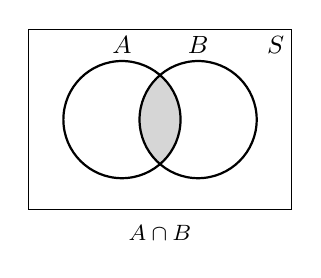
\begin{tikzpicture}[scale=0.62,every node/.style={font=\small}]
  \begin{scope}\clip (-0.78,0) circle (1.2);\fill[\vennShade] (0.78,0) circle (1.2);\end{scope}
  \vennframe\venncap{$A\cap B$}\end{tikzpicture}}
\newcommand{\vennUnion}{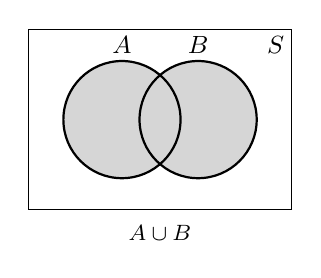
\begin{tikzpicture}[scale=0.62,every node/.style={font=\small}]
  \fill[\vennShade] (-0.78,0) circle (1.2);\fill[\vennShade] (0.78,0) circle (1.2);
  \vennframe\venncap{$A\cup B$}\end{tikzpicture}}
\newcommand{\vennExactlyOne}{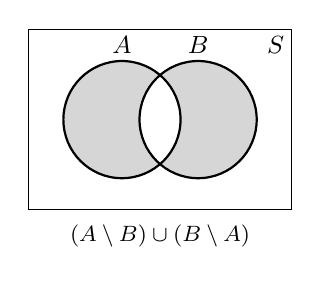
\begin{tikzpicture}[scale=0.62,every node/.style={font=\small}]
  \fill[\vennShade] (-0.78,0) circle (1.2);\fill[\vennShade] (0.78,0) circle (1.2);
  \begin{scope}\clip (-0.78,0) circle (1.2);\fill[white] (0.78,0) circle (1.2);\end{scope}
  \vennframe\venncap{$(A\setminus B)\cup(B\setminus A)$}\end{tikzpicture}}
\newcommand{\vennCompUnion}{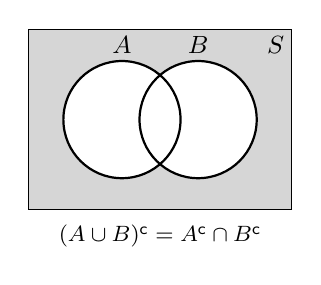
\begin{tikzpicture}[scale=0.62,every node/.style={font=\small}]
  \fill[\vennShade] (-2.7,-1.85) rectangle (2.7,1.85);
  \fill[white] (-0.78,0) circle (1.2);\fill[white] (0.78,0) circle (1.2);
  \vennframe\venncap{$\comp{(A\cup B)}=\comp{A}\cap\comp{B}$}\end{tikzpicture}}
\newcommand{\vennCompInter}{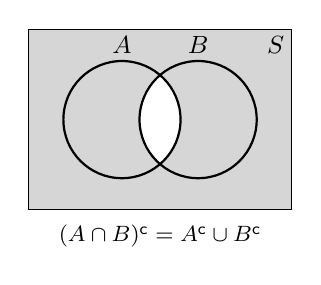
\begin{tikzpicture}[scale=0.62,every node/.style={font=\small}]
  \fill[\vennShade] (-2.7,-1.85) rectangle (2.7,1.85);
  \begin{scope}\clip (-0.78,0) circle (1.2);\fill[white] (0.78,0) circle (1.2);\end{scope}
  \vennframe\venncap{$\comp{(A\cap B)}=\comp{A}\cup\comp{B}$}\end{tikzpicture}}
\newcommand{\vennAminusB}{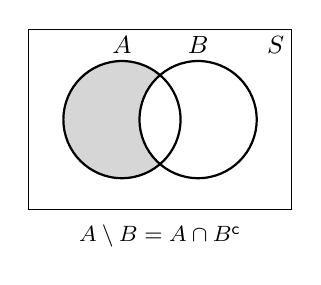
\begin{tikzpicture}[scale=0.62,every node/.style={font=\small}]
  \fill[\vennShade] (-0.78,0) circle (1.2);
  \fill[white] (0.78,0) circle (1.2);
  \vennframe\venncap{$A\setminus B=A\cap\comp{B}$}\end{tikzpicture}}
\newcommand{\vennCompA}{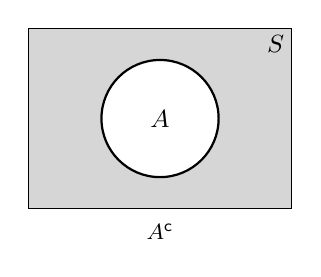
\begin{tikzpicture}[scale=0.62,every node/.style={font=\small}]
  \fill[\vennShade] (-2.7,-1.85) rectangle (2.7,1.85);\fill[white] (0,0) circle (1.2);
  \draw[thin] (-2.7,-1.85) rectangle (2.7,1.85);
  \node[anchor=north east,inner sep=1.5pt] at (2.64,1.79){$S$};
  \draw[thick] (0,0) circle (1.2);\node at (0,0){$A$};
  \venncap{$\comp{A}$}\end{tikzpicture}}
\newcommand{\vennDisjoint}{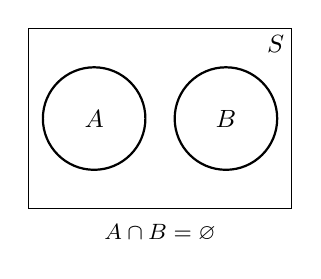
\begin{tikzpicture}[scale=0.62,every node/.style={font=\small}]
  \draw[thin] (-2.7,-1.85) rectangle (2.7,1.85);
  \node[anchor=north east,inner sep=1.5pt] at (2.64,1.79){$S$};
  \draw[thick] (-1.35,0) circle (1.05);\node at (-1.35,0){$A$};
  \draw[thick] ( 1.35,0) circle (1.05);\node at ( 1.35,0){$B$};
  \venncap{$A\cap B=\varnothing$}\end{tikzpicture}}

\hypersetup{pdftitle={Mathematical Statistics Notes}}
\setcounter{tocdepth}{1}
\begin{document}
\frontmatter
\thispagestyle{empty}
\vspace*{3cm}
\begin{center}
  {\Huge\bfseries Mathematical Statistics Notes}\\[12pt]
  \rule{0.55\textwidth}{0.4pt}
\end{center}
\vfill
\clearpage
\tableofcontents
\mainmatter
\setcounter{chapter}{1}

% ================= Chapter 2: Probability =================

\chapter{Probability}

\section*{How to use these notes}
\addcontentsline{toc}{section}{How to use these notes}

Every section is organised the same way: each \keyword{rule or theorem} is stated and
proved, then drilled with several fully worked \keyword{examples}. For every example you
are told \emph{which rule applies and how to recognise it} (the marker
$\blacktriangleright$ \textbf{Which rule, and why?}), then shown the solution step by step,
with a diagram whenever a picture helps. Each section opens with a shaded
\textbf{decision guide} for spotting which of its rules a problem needs. Start by learning
to classify a problem with the master guide below; then turn to that section.

\begin{strategy}[Master guide: which tool does a probability problem need?]
\begin{itemize}[leftmargin=1.3em,itemsep=2pt,topsep=2pt]
\item \textbf{Combine or translate events} (``and / or / not / at least one'')?
      $\Rightarrow$ set algebra and De~Morgan (\S1).
\item \textbf{Compute one probability from given probabilities}, areas, or counts?
      $\Rightarrow$ the axioms, the complement rule, inclusion--exclusion (\S2).
\item \textbf{``Given that\dots''}, a process in \textbf{stages}, or \textbf{updating}
      a belief after evidence? $\Rightarrow$ conditional probability, probability trees,
      total probability, Bayes (\S3).
\item Events that \textbf{do not influence each other} / repeated independent trials?
      $\Rightarrow$ independence: multiply (\S4).
\item \textbf{``How many ways\dots''} or equally likely outcomes to \textbf{count}?
      $\Rightarrow$ counting --- permutations vs.\ combinations (\S5) --- then form
      $\PP=\dfrac{\text{favourable}}{\text{total}}$ (\S6).
\end{itemize}
\end{strategy}

\section{Sample Spaces and the Algebra of Events}

Before any probability number can be written down, the situation must be translated into
sets. An English sentence such as ``at least one defective,'' ``neither $A$ nor $B$,'' or
``exactly one of the two'' becomes a precise subset of the sample space, and every later
rule --- the axioms, conditioning, independence, counting --- operates on these sets, so
accuracy here is not optional.

\begin{strategy}[Which rule of this section does the problem need?]
Read the English description of the event and match its \emph{logical connective} to a set
operation.
\begin{itemize}[itemsep=2pt,topsep=2pt,leftmargin=*]
\item ``\keyword{and} / both / simultaneously'' $\Rightarrow$ \keyword{intersection} $A\cap B$.
\item ``\keyword{or} / at least one of'' (inclusive) $\Rightarrow$ \keyword{union} $A\cup B$.
\item ``\keyword{not} / fails / none / does not happen'' $\Rightarrow$ \keyword{complement} $\comp{A}$.
\item ``\keyword{cannot both} happen / at most one is in common''
      $\Rightarrow$ test \keyword{mutually exclusive}: is $A\cap B=\varnothing$?
\item ``\keyword{whenever} $A$ happens, $B$ happens / $A$ forces $B$''
      $\Rightarrow$ \keyword{subset} $A\subseteq B$ (implication).
\item A \keyword{negated compound} --- ``not (this \emph{or} that),'' ``not (this \emph{and}
      that),'' ``\keyword{neither},'' ``\keyword{at least one} fails'' --- is the cue for
      \keyword{De Morgan}: push the complement inside and \emph{flip} the connective
      ($\cup\leftrightarrow\cap$).
\item An event built as ``\keyword{this, together with either} that or the other'' ---
      one operation distributed over a second --- is the cue for a
      \keyword{distributive law}; use it to factor or to split into disjoint pieces.
\item Reordering or regrouping a chain of unions/intersections without changing its value
      is \keyword{commutativity / associativity}; these are silent bookkeeping, rarely the
      crux of a problem.
\end{itemize}
\textbf{Why competing rules do not apply:} the connective decides everything. ``Or'' is
never an intersection; ``and'' is never a union. A bare ``not $A$'' is a single
complement, \emph{not} De Morgan --- De Morgan is triggered only when the complement sits
\emph{outside a compound}. Disjointness is a yes/no property of a pair, not a way to
\emph{build} a new event, so it answers ``can these co-occur?'' rather than ``what is the
combined event?''
\end{strategy}

\subsection{Vocabulary: experiment, sample space, outcome, event}

\begin{definition}[The objects of probability]
An \keyword{experiment} (or \keyword{trial}) is any procedure that can in principle be
repeated and whose result is not known in advance. The set of \emph{all} results that the
experiment could produce is the \keyword{sample space}, written $S$. A single element
$s\in S$ is an \keyword{outcome} (or sample point). An \keyword{event} is any subset
$A\subseteq S$; we say $A$ \keyword{occurs} on a given run when the realized outcome $s$
lies in $A$. The whole space $S$ is the \keyword{certain} event (it always occurs) and the
empty set $\varnothing$ is the \keyword{impossible} event (it never occurs).
\end{definition}

The sample space must be chosen so that the outcomes are \emph{mutually exclusive} (one run
produces exactly one outcome) and \emph{exhaustive} (every possible result appears). Once
$S$ is fixed, an event is named either by listing its outcomes or by stating the property
its outcomes share.

\begin{example}[Listing a sample space and naming events: two dice]
Roll one red die and one green die, recording the pair (red, green). The experiment has
$36$ equally detailed outcomes,
\[
  S=\{(i,j): i,j\in\{1,2,3,4,5,6\}\},\qquad |S|=36 .
\]
Name the event $A=$ ``the total of the two faces equals $8$'' as an explicit subset.
\end{example}
\whichrule{The phrase ``the total equals $8$'' describes a \emph{property} the outcome must
have, so we are merely \emph{selecting} the points of $S$ that satisfy it --- the
vocabulary task of turning an event-description into a subset. No union/intersection of two
named events is requested, so the algebra laws are not yet in play; we are still building
the raw objects they act on.}
\soln
\steplabel{Step 1: scan the grid.} The pairs $(i,j)$ with $i+j=8$ are exactly the diagonal
shown shaded below.
\begin{center}
\begin{tabular}{c|cccccc}
\toprule
 {\footnotesize r$\backslash$g} & 1 & 2 & 3 & 4 & 5 & 6\\
\midrule
1 & 2 & 3 & 4 & 5 & 6 & 7\\
2 & 3 & 4 & 5 & 6 & 7 & $[8]$\\
3 & 4 & 5 & 6 & 7 & $[8]$ & 9\\
4 & 5 & 6 & 7 & $[8]$ & 9 & 10\\
5 & 6 & 7 & $[8]$ & 9 & 10 & 11\\
6 & 7 & $[8]$ & 9 & 10 & 11 & 12\\
\bottomrule
\end{tabular}\\[2pt]
{\small Boxed cells $[8]$ mark the event $A=\{i+j=8\}$.}
\end{center}
\steplabel{Step 2: list the event.}
$A=\{(2,6),(3,5),(4,4),(5,3),(6,2)\}$, so $|A|=5$.
\steplabel{Step 3 (count, for later use).} With $36$ equally likely points, $A$ contains
$5$ of them; we record $|A|=5$ out of $|S|=36$. Final answer: $A$ is the $5$-point set
listed above.

\begin{example}[Sample space with unequal-size outcomes: a spinner]
A spinner is divided into four sectors painted red, blue, green, and yellow, occupying
$40\%$, $30\%$, $20\%$, and $10\%$ of the dial. Spin once and record the colour. Give $S$,
the outcome set, and the event ``a primary colour'' (red, blue, or yellow).
\end{example}
\whichrule{We are asked only to \emph{describe} the space and pick out a sub-collection of
its outcomes; this is the definitional step. Note the outcomes are \emph{not} equally
likely --- that is fine, the sample space is a set, not a list of equiprobable points; the
unequal sizes belong to the probability function of the next section, not to the algebra
here.}
\soln
\steplabel{Step 1: outcomes.} The recorded result is a colour, so
$S=\{\text{red},\text{blue},\text{green},\text{yellow}\}$, $|S|=4$.
\steplabel{Step 2: read the event.} The primary colours among the four are red, blue, and
yellow; green is a secondary colour and is excluded. Selecting the points of $S$ with the
stated property gives $A=\{\text{red},\text{blue},\text{yellow}\}$.
\steplabel{Step 3: report.} The event is the $3$-element subset
$A=\{\text{red},\text{blue},\text{yellow}\}\subseteq S$. (Its probability,
$0.40+0.30+0.10=0.80$, is deferred to the probability function; here we only fix the set.)

\begin{example}[A countably infinite sample space]
Flip a fair coin repeatedly until the first head appears, then stop. Record the number of
flips used. Describe $S$ and the event ``the experiment ends after an even number of
flips.''
\end{example}
\whichrule{The trigger is ``until the first head'': the experiment has no fixed length, so
no finite grid can list its outcomes. Recognising that the natural sample space is a
\emph{set of counts} (possibly unbounded) is again the vocabulary step --- choosing the
right $S$. We are not combining two events, so no algebra law is invoked yet.}
\soln
\steplabel{Step 1: outcomes.} The number of flips can be any positive integer, so
$S=\{1,2,3,\dots\}=\N$, a countably infinite sample space.
\steplabel{Step 2: name the event.} ``Ends after an even number of flips'' selects the even
counts: $A=\{2,4,6,\dots\}$.
\steplabel{Step 3: report.} $A=\{2k:k\in\N\}\subseteq S$. The space is infinite but each
outcome is still a single, well-defined sample point.

\begin{example}[Certain and impossible events]
A box holds $5$ chips numbered $1$ through $5$; draw one chip. Identify, within this
experiment, one certain event and one impossible event, and explain.
\end{example}
\whichrule{The words ``certain'' and ``impossible'' are direct cues for the two extreme
events $S$ and $\varnothing$. This is pure vocabulary: we are matching descriptions to the
boundary subsets of $S$, not operating on events.}
\soln
\steplabel{Step 1: fix $S$.} $S=\{1,2,3,4,5\}$.
\steplabel{Step 2: a certain event.} ``The drawn number is at most $5$'' is satisfied by
\emph{every} chip, so it equals $S$ itself --- the certain event, which always occurs.
\steplabel{Step 3: an impossible event.} ``The drawn number is $6$'' is satisfied by no
chip, so it equals $\varnothing$ --- the impossible event, which never occurs.
\steplabel{Conclusion.} $S=\{1,\dots,5\}$ is certain; $\{x\in S:x=6\}=\varnothing$ is
impossible.

\begin{example}[Sample space of ordered outcomes: drawing two chips]
An urn holds four chips marked $a,b,c,d$. Draw two chips one after the other
\emph{without} replacement, recording the ordered pair (first, second). List $S$ and the
event $A=$ ``chip $a$ is drawn at some point.''
\end{example}
\whichrule{We are fixing the raw outcome set and then \emph{selecting} the points with a
stated property --- the definitional step, not an operation on two named events. The word
``ordered'' forces us to treat $(a,b)$ and $(b,a)$ as \emph{distinct} sample points, which
is a choice about how to build $S$, made before any algebra is applied.}
\soln
\steplabel{Step 1: build $S$.} Each outcome is an ordered pair of distinct chips, so there
are $4\times 3=12$ of them:
\[
  S=\{ab,ac,ad,ba,bc,bd,ca,cb,cd,da,db,dc\},\qquad |S|=12 ,
\]
writing $xy$ for ``first $x$, then $y$.''
\steplabel{Step 2: select the event.} The pairs that contain $a$ are
$A=\{ab,ac,ad,ba,ca,da\}$, so $|A|=6$.
\steplabel{Step 3: report.} $A$ is the $6$-point subset above; exactly half of the ordered
draws involve chip $a$.

\begin{example}[Product sample space: a two-stage experiment]
First toss a coin, then roll a four-sided die showing $1$--$4$. Record the pair
(coin, die). Give $S$ and the event $A=$ ``heads with an even die.''
\end{example}
\whichrule{A two-stage experiment has a \emph{product} sample space: one coordinate per
stage, with $S$ the set of all combinations. Listing it and then picking the points with a
property is the vocabulary step. The tree below organises the enumeration; we are not yet
combining two events with a set operation.}
\soln
\steplabel{Step 1: enumerate by a tree.}
\begin{center}
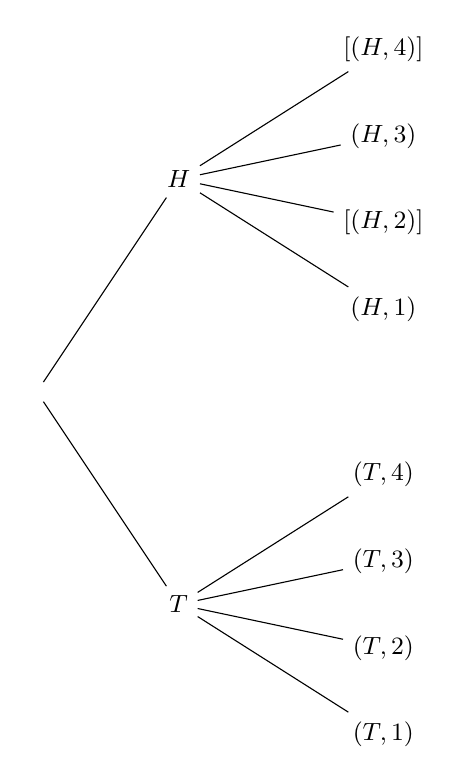
\begin{tikzpicture}[>=Stealth,grow=right,
  level 1/.style={sibling distance=54mm,level distance=18mm},
  level 2/.style={sibling distance=11mm,level distance=26mm},font=\small]
\node{}
  child{node{$T$}
    child{node{$(T,1)$}} child{node{$(T,2)$}}
    child{node{$(T,3)$}} child{node{$(T,4)$}}}
  child{node{$H$}
    child{node{$(H,1)$}} child{node{$[(H,2)]$}}
    child{node{$(H,3)$}} child{node{$[(H,4)]$}}};
\end{tikzpicture}\\[2pt]
{\small Boxed leaves mark $A=$ ``heads with an even die.''}
\end{center}
\steplabel{Step 2: write $S$.} $S=\{H,T\}\times\{1,2,3,4\}$, so $|S|=2\times 4=8$.
\steplabel{Step 3: select the event.} Heads with an even die keeps $(H,2)$ and $(H,4)$, so
$A=\{(H,2),(H,4)\}$, the two boxed leaves.

\begin{example}[Choosing the right grain for the sample space]
A quality auditor inspects three soldered joints in order and notes each as good (g) or
bad (b). One could record the whole pattern, or only the \emph{number} of bad joints. Give
both sample spaces, and express ``at least two bad joints'' in each.
\end{example}
\whichrule{The same physical experiment supports several sample spaces; the modelling
decision is \emph{how finely} to record an outcome. Both choices are legitimate provided
the outcomes stay mutually exclusive and exhaustive. This is the definitional layer ---
selecting an event as a subset of whichever $S$ we adopt --- not an algebraic combination
of events.}
\soln
\steplabel{Step 1: the fine space.} Recording each joint gives
$S_1=\{g,b\}^3$, the $2^3=8$ ordered patterns $ggg,ggb,\dots,bbb$.
\steplabel{Step 2: the coarse space.} Recording only the count of bad joints gives
$S_2=\{0,1,2,3\}$.
\steplabel{Step 3: name the event in each.} ``At least two bad'' is
\[
  A_1=\{gbb,bgb,bbg,bbb\}\subseteq S_1 \ (|A_1|=4),
  \qquad
  A_2=\{2,3\}\subseteq S_2 .
\]
\steplabel{Step 4: caution.} The four patterns of $S_1$ are equally likely for a fair
process, but the two values of $A_2$ are \emph{not} --- so $S_1$ is the safer grain when
probabilities are wanted. The set $A$ is correct in either space; only the later
probability arithmetic cares which grain we picked.

\subsection{The set operations: union, intersection, complement, disjointness, subset}

\begin{definition}[Operations on events]
Let $A,B\subseteq S$.
\begin{itemize}[itemsep=1pt,topsep=2pt,leftmargin=*]
\item \keyword{Union:} $A\cup B=\{s\in S: s\in A \ \text{or}\ s\in B\}$, read ``$A$ or $B$''
      (inclusive ``or''). It occurs when at least one of $A,B$ occurs.
\item \keyword{Intersection:} $A\cap B=\{s\in S: s\in A \ \text{and}\ s\in B\}$, read
      ``$A$ and $B$.'' It occurs when both occur.
\item \keyword{Complement:} $\comp{A}=\{s\in S:s\notin A\}$, read ``not $A$.'' It occurs
      exactly when $A$ does not.
\item \keyword{Difference:} $A\setminus B=A\cap\comp{B}$, ``$A$ but not $B$.''
\end{itemize}
Two events are \keyword{mutually exclusive} (disjoint) when $A\cap B=\varnothing$: they
cannot both occur. We say $A$ \keyword{implies} $B$, written $A\subseteq B$, when every
outcome in $A$ also lies in $B$: whenever $A$ occurs, $B$ must occur too.
\end{definition}

\begin{proposition}[Basic identities tying the operations together]\label{prop:basic1}
For all events $A,B\subseteq S$:
\textup{(i)} $A\cup\comp{A}=S$ and $A\cap\comp{A}=\varnothing$;
\textup{(ii)} $\comp{(\comp{A})}=A$;
\textup{(iii)} if $A\subseteq B$ then $\comp{B}\subseteq\comp{A}$;
\textup{(iv)} $A\subseteq B$ \emph{iff} $A\cap B=A$ \emph{iff} $A\cup B=B$.
\end{proposition}
\begin{proof}
(i) Every $s\in S$ either lies in $A$ or does not, so it lies in $A\cup\comp{A}$; and no $s$
can both lie in and fail to lie in $A$, so $A\cap\comp{A}$ is empty.
(ii) ``Not (not $A$)'' holds iff $s$ fails to be outside $A$, i.e.\ iff $s\in A$.
(iii) If $A\subseteq B$ and $s\in\comp{B}$ then $s\notin B$, hence $s\notin A$ (else $A
\subseteq B$ would force $s\in B$), so $s\in\comp{A}$.
(iv) If $A\subseteq B$, every point of $A$ is in $B$, so $A\cap B=A$; conversely if $A\cap
B=A$ then each $s\in A$ satisfies $s\in B$. The union form is the same statement with the
roles of the smaller and larger set exchanged.
\end{proof}

\paragraph{Examples for intersection ($A\cap B$, the ``and'' operation).}

\begin{example}[Intersection by direct listing]
Roll the red/green dice (the $36$-point space above). Let $A=$ ``red die shows an even number'' and
$B=$ ``the total is at least $10$.'' Find $A\cap B$ and its size.
\end{example}
\whichrule{The target event is ``red even \emph{and} total $\ge 10$'' --- the connective is
``and,'' so we intersect. It is not a union (we need \emph{both} conditions, not at least
one) and not a complement (nothing is negated).}
\soln
\steplabel{Step 1: write each event.} $A=\{(i,j):i\in\{2,4,6\}\}$ (red even).
$B=\{(i,j):i+j\ge 10\}=\{(4,6),(5,5),(6,4),(5,6),(6,5),(6,6)\}$.
\steplabel{Step 2: keep the points common to both.} From $B$'s six points, retain those
whose red value $i$ is even: $(4,6),(6,4),(6,5),(6,6)$. The points $(5,5)$ and $(5,6)$ drop
out because $i=5$ is odd.
\steplabel{Step 3: report.} $A\cap B=\{(4,6),(6,4),(6,5),(6,6)\}$, so $|A\cap B|=4$.
\begin{center}\vennInter\end{center}

\begin{example}[Intersection of attribute events]
A factory line produces gadgets; each is classified by \keyword{colour} (silver/black) and
by \keyword{grade} (pass/fail inspection). Let $A=$ ``silver'' and $B=$ ``fail.'' Of $200$
gadgets, $120$ are silver, $30$ fail, and $18$ are silver-and-fail. Express ``silver and
failing'' as a set operation and give its count.
\end{example}
\whichrule{``Silver \emph{and} failing'' joins two attributes with ``and,'' the
intersection cue. We are given $|A\cap B|$ directly, so the only task is to recognise that
the requested event \emph{is} $A\cap B$. A union would over-count (it would also include
silver passes and black fails), which is not what ``and'' means.}
\soln
\steplabel{Step 1: translate.} ``Silver and failing'' $=A\cap B$.
\steplabel{Step 2: read off the count.} The problem states $|A\cap B|=18$.
\steplabel{Step 3: report.} The event ``silver and failing'' contains $18$ of the $200$
gadgets; as a set it is $A\cap B$.

\begin{example}[Intersection of three events]
Survey of $50$ students: let $A,B,C$ be ``owns a bike,'' ``owns a laptop,'' ``has a campus
job.'' Suppose $10$ students have all three. Identify the event ``bike and laptop and job''
and its count, and state in one line why it is an intersection of three sets.
\end{example}
\whichrule{Three conditions are chained with ``and,'' so the event is the triple
intersection $A\cap B\cap C$. Each additional ``and'' adds another $\cap$; the associativity
law (next subsection) guarantees the grouping $(A\cap B)\cap C$ versus $A\cap(B\cap C)$ does
not matter.}
\soln
\steplabel{Step 1: translate.} ``Bike and laptop and job'' $=A\cap B\cap C$.
\steplabel{Step 2: count.} Given: exactly $10$ students lie in all three sets, so $|A\cap
B\cap C|=10$.
\steplabel{Step 3: report.} The event is $A\cap B\cap C$ with $10$ members out of $50$.

\begin{example}[Intersection that is empty: signalling disjointness]
Draw one card from a standard $52$-card deck. Let $A=$ ``the card is a heart'' and
$B=$ ``the card is a club.'' Find $A\cap B$.
\end{example}
\whichrule{Again ``heart \emph{and} club'' is an ``and,'' so we intersect. The point of the
example is that the intersection can come out \emph{empty}: a single card has one suit, so
no card is simultaneously a heart and a club. Recognising an empty intersection is exactly
how we detect mutual exclusivity.}
\soln
\steplabel{Step 1: intersect.} $A\cap B=\{$cards that are both a heart and a club$\}$.
\steplabel{Step 2: evaluate.} No card carries two suits, so the set has no members:
$A\cap B=\varnothing$.
\steplabel{Step 3: interpret.} Because $A\cap B=\varnothing$, the events $A$ and $B$ are
\keyword{mutually exclusive}; they cannot both occur on one draw.
\begin{center}\vennDisjoint\end{center}

\begin{example}[Intersection on the dice grid: ``and'' as a smaller region]
Roll the red/green dice. Let $A=$ ``the total is even'' and $B=$ ``the maximum of the two
faces is $4$.'' Find $A\cap B$ and its size.
\end{example}
\whichrule{``Even total \emph{and} maximum $4$'' is an ``and,'' so we intersect: keep only
the outcomes meeting \emph{both} numerical conditions. A union would wrongly admit
even-total cells whose maximum is not $4$, so ``or'' is the wrong connective here.}
\soln
\steplabel{Step 1: list $B$.} ``Maximum equals $4$'' means both faces are $\le 4$ and at
least one is $4$: $B=\{(1,4),(2,4),(3,4),(4,4),(4,3),(4,2),(4,1)\}$, $|B|=7$.
\steplabel{Step 2: keep the even totals.} Among these, the even totals ($i+j$ even) are
$(2,4),(4,4),(4,2)$ --- totals $6,8,6$. The others have odd totals and drop out.
\steplabel{Step 3: report.} $A\cap B=\{(2,4),(4,4),(4,2)\}$, so $|A\cap B|=3$.
\begin{center}\vennInter\end{center}

\begin{example}[Intersection by complement: ``and not'' on a survey]
Of $80$ commuters, $50$ ride the bus ($A$) and $35$ ride the subway ($B$); $20$ ride
\emph{both}. How many ride the bus \emph{but not} the subway, as a set operation and a
count?
\end{example}
\whichrule{``Bus and not subway'' is the intersection of $A$ with the complement of $B$,
i.e.\ $A\cap\comp{B}=A\setminus B$. The ``and'' fixes it as an intersection; the ``not''
attaches to the second event only, so we complement $B$ before intersecting --- this is not
a bare complement of a single event, and not a union.}
\soln
\steplabel{Step 1: translate.} ``Bus but not subway'' $=A\cap\comp{B}=A\setminus B$.
\steplabel{Step 2: split $A$.} The $50$ bus riders divide into those who also ride the
subway ($|A\cap B|=20$) and those who do not.
\steplabel{Step 3: subtract.} $|A\cap\comp{B}|=|A|-|A\cap B|=50-20=30$. Thirty commuters
ride the bus but not the subway.
\begin{center}\vennAminusB\end{center}

\begin{example}[Intersection of overlapping divisibility events]
Draw a ticket numbered $1$--$60$. Let $A=$ ``divisible by $4$'' and $B=$ ``divisible by
$6$.'' Find $A\cap B$, and note the common trap.
\end{example}
\whichrule{``Divisible by $4$ \emph{and} by $6$'' is an ``and,'' hence an intersection. The
trap is to multiply $4\times 6=24$: the intersection is ``divisible by the \emph{least
common multiple} $12$,'' not by $24$, because $4$ and $6$ share the factor $2$.}
\soln
\steplabel{Step 1: identify the common condition.} A number divisible by both $4$ and $6$ is
divisible by $\operatorname{lcm}(4,6)=12$, not by $24$.
\steplabel{Step 2: list.} Multiples of $12$ up to $60$: $A\cap B=\{12,24,36,48,60\}$.
\steplabel{Step 3: count.} $|A\cap B|=5$. (Multiplying $4\cdot 6$ would have falsely given
``multiples of $24$,'' only $\{24,48\}$, undercounting the event.)
\begin{center}\vennInter\end{center}

\paragraph{Examples for union ($A\cup B$, the ``or'' operation).}

\begin{example}[Union by listing]
Roll the two dice. Let $A=$ ``doubles'' (both faces equal) and $B=$ ``the total is $4$.''
Find $A\cup B$ and its size.
\end{example}
\whichrule{``Doubles \emph{or} total $4$'' uses inclusive ``or,'' so we form the union ---
every outcome in either event qualifies. We must be careful to list shared outcomes only
once; that single-counting is exactly what the set union does.}
\soln
\steplabel{Step 1: list each.} $A=\{(1,1),(2,2),(3,3),(4,4),(5,5),(6,6)\}$.
$B=\{(1,3),(2,2),(3,1)\}$.
\steplabel{Step 2: merge, dropping repeats.} The outcome $(2,2)$ is in both. The union is
$A\cup B=\{(1,1),(2,2),(3,3),(4,4),(5,5),(6,6),(1,3),(3,1)\}$.
\steplabel{Step 3: count.} $|A|=6$, $|B|=3$, shared $=1$, so
$|A\cup B|=6+3-1=8$, matching the $8$ listed points.
\begin{center}\vennUnion\end{center}

\begin{example}[Union of mutually exclusive events --- counts simply add]
A bag holds tickets numbered $1$--$30$. Let $A=$ ``a multiple of $10$'' and $B=$ ``an odd
number.'' Find $A\cup B$ and explain why its size is just $|A|+|B|$.
\end{example}
\whichrule{``Multiple of $10$ \emph{or} odd'' is a union. Here the two events are disjoint
(every multiple of $10$ is even, hence never odd), so the union's size is the plain sum
$|A|+|B|$ with no overlap to subtract --- the special, easiest case of a union.}
\soln
\steplabel{Step 1: list.} $A=\{10,20,30\}$ ($|A|=3$); $B=\{1,3,5,\dots,29\}$ ($|B|=15$).
\steplabel{Step 2: check disjointness.} A multiple of $10$ is even, so $A\cap
B=\varnothing$.
\steplabel{Step 3: union.} Because there is no overlap,
$|A\cup B|=|A|+|B|=3+15=18$, and $A\cup B=\{1,3,5,\dots,29,10,20,30\}$.
\begin{center}\vennDisjoint\end{center}

\begin{example}[Union phrased as ``at least one'']
Two components, a pump and a valve, are tested. Let $A=$ ``the pump fails'' and $B=$ ``the
valve fails.'' Express ``at least one component fails'' as a set operation.
\end{example}
\whichrule{``At least one fails'' is the canonical English for the inclusive union $A\cup
B$: it is satisfied by a pump failure alone, a valve failure alone, or both. It is
emphatically \emph{not} the intersection (that would be ``both fail''), and it is the
complement of ``neither fails,'' a link we exploit with De Morgan shortly.}
\soln
\steplabel{Step 1: translate.} ``At least one of $A,B$'' $=A\cup B$.
\steplabel{Step 2: name the complement, for contrast.} ``At least one fails'' is the
opposite of ``both work,'' i.e.\ $\comp{A}\cap\comp{B}$; equivalently $A\cup
B=\comp{(\comp{A}\cap\comp{B})}$.
\steplabel{Step 3: report.} The event is $A\cup B$.
\begin{center}\vennUnion\end{center}

\begin{example}[Union of three events, in words]
A committee seat goes to whoever is nominated by department X, Y, or Z. Let $A,B,C$ be the
nomination events. Write ``the candidate is nominated by at least one department'' and note
why a union of three sets is needed.
\end{example}
\whichrule{``By X, Y, \emph{or} Z'' and ``at least one'' both flag a union; three sources
means a triple union $A\cup B\cup C$. The grouping is irrelevant by associativity, so we
may write it without parentheses.}
\soln
\steplabel{Step 1: translate.} Nominated by at least one $=A\cup B\cup C$.
\steplabel{Step 2: meaning.} An outcome qualifies if it belongs to any one (or more) of
$A,B,C$.
\steplabel{Step 3: report.} The event is $A\cup B\cup C$.

\begin{example}[Union with overlap on the dice grid]
Roll the two dice. Let $A=$ ``the total is $7$'' and $B=$ ``the red die shows $5$.'' Find
$A\cup B$ and its size, watching the overlap.
\end{example}
\whichrule{``Total $7$ \emph{or} red $5$'' is an inclusive union. Because a single cell can
satisfy \emph{both} (a red $5$ that totals $7$), the events overlap, so the count is
$|A|+|B|$ minus the shared cell --- not a plain sum, which would double-count that cell.}
\soln
\steplabel{Step 1: list each.}
\[ \begin{gathered}
   A=\{(1,6),(2,5),(3,4),(4,3),(5,2),(6,1)\},\quad |A|=6;\\
   B=\{(5,1),(5,2),(5,3),(5,4),(5,5),(5,6)\},\quad |B|=6.
   \end{gathered} \]
\steplabel{Step 2: find the overlap.} The only cell in both is $(5,2)$ (red $5$, total
$7$), so $|A\cap B|=1$.
\steplabel{Step 3: count the union.} $|A\cup B|=|A|+|B|-|A\cap B|=6+6-1=11$. Subtracting the
shared $(5,2)$ once is exactly what the union does.
\begin{center}\vennUnion\end{center}

\begin{example}[Union as ``or'' for a single drawn card]
Draw one card. Let $A=$ ``a spade'' and $B=$ ``a king.'' Find $|A\cup B|$, the number of
cards that are a spade or a king.
\end{example}
\whichrule{``Spade \emph{or} king'' is an inclusive union. The king of spades lies in both
events, so the events are not disjoint; we must subtract that one shared card so it is
counted once, the inclusion--exclusion form of a union.}
\soln
\steplabel{Step 1: counts.} $|A|=13$ spades; $|B|=4$ kings.
\steplabel{Step 2: overlap.} The king of spades is the single common card, $|A\cap B|=1$.
\steplabel{Step 3: union.} $|A\cup B|=13+4-1=16$ cards are a spade or a king.
\begin{center}\vennUnion\end{center}

\begin{example}[Union expressed by its complement: ``at least one six'']
Roll the two dice. Let $A=$ ``the red die is $6$'' and $B=$ ``the green die is $6$.''
Express ``at least one six'' as a union and count it the easy way.
\end{example}
\whichrule{``At least one six'' is the union $A\cup B$. Rather than add and subtract the
overlap, we count its complement ``no six on either die,'' a single clean condition --- the
``at least one'' / ``none'' shortcut that De Morgan will formalise below. A direct
intersection would describe ``both sixes,'' the wrong event.}
\soln
\steplabel{Step 1: translate.} ``At least one six'' $=A\cup B$.
\steplabel{Step 2: count the complement.} ``No six at all'' means each die shows one of
$\{1,\dots,5\}$: $5\times 5=25$ cells, so $|\comp{(A\cup B)}|=25$.
\steplabel{Step 3: subtract.} $|A\cup B|=36-25=11$. (Check by inclusion--exclusion:
$|A|+|B|-|A\cap B|=6+6-1=11$. Agrees.)
\begin{center}\vennUnion\end{center}

\paragraph{Examples for complement ($\comp{A}$, the ``not'' operation).}

\begin{example}[Complement by counting]
Roll a single fair die, $S=\{1,2,3,4,5,6\}$. Let $A=$ ``the face is at least $3$.'' Find
$\comp{A}$ and verify $|A|+|\comp{A}|=|S|$.
\end{example}
\whichrule{``Not (at least $3$)'' negates a single event, so it is a plain complement
$\comp{A}$ --- a lone ``not,'' not a negated compound, so De Morgan is unnecessary. The
complement is taken \emph{relative to} $S$.}
\soln
\steplabel{Step 1: list $A$.} $A=\{3,4,5,6\}$, $|A|=4$.
\steplabel{Step 2: complement.} $\comp{A}=S\setminus A=\{1,2\}$, i.e.\ ``the face is at
most $2$.''
\steplabel{Step 3: check.} $|A|+|\comp{A}|=4+2=6=|S|$. Consistent.
\begin{center}\vennCompA\end{center}

\begin{example}[Complement to simplify ``at least one'']
An inspector pulls $4$ items off a line; let $A=$ ``at least one item is defective.''
Describe $\comp{A}$ and argue it is easier to handle.
\end{example}
\whichrule{The negation cue is structural: the opposite of ``at least one defective'' is
``\emph{zero} defective,'' a single tidy condition. Whenever ``at least one'' appears, its
complement ``none'' is usually simpler, so we reach for $\comp{A}$ rather than enumerate the
many ways to have one, two, three, or four defectives.}
\soln
\steplabel{Step 1: form the complement.} $\comp{A}=$ ``no item is defective'' $=$ ``all $4$
items are good.''
\steplabel{Step 2: why simpler.} $A$ unfolds into four disjoint cases (exactly $1,2,3,$ or
$4$ defective); $\comp{A}$ is the single case ``all good.''
\steplabel{Step 3: relation.} $A=\comp{(\comp{A})}$, so once $\comp{A}$ is found,
$A$ follows by one subtraction (made precise by the complement rule of the next section).
\begin{center}\vennCompA\end{center}

\begin{example}[Complement of a subset event]
From the deck, let $A=$ ``the card is a face card'' (J, Q, K of any suit). Describe
$\comp{A}$ and count both.
\end{example}
\whichrule{``Not a face card'' is a single negation, hence one complement. Because face
cards form a clean subset of the $52$ cards, the complement is just ``everything else.''}
\soln
\steplabel{Step 1: count $A$.} $3$ face ranks $\times\,4$ suits $=12$ face cards, $|A|=12$.
\steplabel{Step 2: complement.} $\comp{A}=$ ``ace through ten'' $=52-12=40$ cards.
\steplabel{Step 3: check.} $12+40=52=|S|$. Good.
\begin{center}\vennCompA\end{center}

\begin{example}[Complement on an interval sample space]
A pointer lands at a random position on a dial marked $0$ to $100$, so
$S=[0,100]$. Let $A=$ ``the reading is below $25$'' $=[0,25)$. Describe $\comp{A}$.
\end{example}
\whichrule{``\emph{Not} below $25$'' negates the one condition defining $A$, so it is a plain
complement $\comp{A}$, taken relative to the whole dial $S=[0,100]$. There is no compound to
break apart, so De Morgan plays no role; we simply take everything in $S$ outside $A$.}
\soln
\steplabel{Step 1: fix $S$ and $A$.} $S=[0,100]$ and $A=[0,25)$ (readings strictly below
$25$).
\steplabel{Step 2: complement.} $\comp{A}=S\setminus A=[25,100]$, i.e.\ ``the reading is at
least $25$.'' The boundary value $25$ belongs to $\comp{A}$ because $A$ excluded it.
\steplabel{Step 3: sanity check.} $A\cup\comp{A}=[0,25)\cup[25,100]=[0,100]=S$ and $A\cap
\comp{A}=\varnothing$, exactly as the complement must satisfy.

\begin{example}[Difference as ``$A$ but not $B$'']
Tickets $1$--$20$. Let $A=$ ``even'' and $B=$ ``a multiple of $4$.'' Find the event
``even but not a multiple of $4$'' and give its size.
\end{example}
\whichrule{``Even \emph{but not} a multiple of $4$'' combines a positive condition with a
negation: ``but not'' is the set-difference cue, $A\setminus B=A\cap\comp{B}$. The
complement is taken \emph{inside} an intersection, which is what makes this a difference
rather than a bare complement.}
\soln
\steplabel{Step 1: list.} $A=\{2,4,6,8,10,12,14,16,18,20\}$, $|A|=10$.
$B=\{4,8,12,16,20\}$, $|B|=5$, and $B\subseteq A$.
\steplabel{Step 2: subtract.} $A\setminus B=A\cap\comp{B}=\{2,6,10,14,18\}$.
\steplabel{Step 3: count.} $|A\setminus B|=|A|-|A\cap B|=10-5=5$.
\begin{center}\vennAminusB\end{center}

\begin{example}[Complement to count ``at least one repeat'']
A three-digit code is formed by choosing each digit freely from $0$--$9$ (so $1000$ codes,
including leading zeros). Let $A=$ ``some digit is repeated.'' Use the complement to count
$A$.
\end{example}
\whichrule{``At least one repeat'' splits into awkward cases (one pair, or all three equal),
so we negate it: $\comp{A}=$ ``all three digits distinct'' is one clean condition. The
complement rule converts the hard count into ``total minus all-distinct.'' This is a single
``not'' on one event, so no De Morgan is needed.}
\soln
\steplabel{Step 1: total.} $|S|=10\times 10\times 10=1000$ codes.
\steplabel{Step 2: count the complement.} ``All distinct'' fills the positions in order with
no reuse: $10\times 9\times 8=720$.
\steplabel{Step 3: subtract.} $|A|=|S|-|\comp{A}|=1000-720=280$ codes have a repeated
digit.
\begin{center}\vennCompA\end{center}

\begin{example}[Complement of ``at least one woman'' on a committee]
From $4$ men and $3$ women, a committee of $3$ is chosen at random. Let $A=$ ``at least one
woman serves.'' Describe and count $A$ through its complement.
\end{example}
\whichrule{``At least one woman'' is again the ``at least one'' cue: its complement
``\emph{no} woman, i.e.\ all men'' is the single easy case. We count $\comp{A}$ and
subtract, rather than enumerate committees with one, two, or three women.}
\soln
\steplabel{Step 1: total committees.} $\binom{7}{3}=35$ equally likely committees.
\steplabel{Step 2: complement.} ``All men'' chooses $3$ of the $4$ men:
$\binom{4}{3}=4$ committees, so $|\comp{A}|=4$.
\steplabel{Step 3: subtract.} $|A|=35-4=31$ committees include at least one woman.
\begin{center}\vennCompA\end{center}

\begin{example}[Complement on a two-dimensional sample space]
A dart lands uniformly on the unit square $S=[0,1]\times[0,1]$. Let $A=$ ``the dart lands
in the lower-left triangle $x+y\le 1$.'' Describe $\comp{A}$ and give its area.
\end{example}
\whichrule{``\emph{Not} in the triangle'' is a single negation, so $\comp{A}$ is a plain
complement taken relative to the whole square $S$. There is no compound to dismantle, so
De Morgan is irrelevant; we simply take everything in $S$ outside the triangle.}
\soln
\steplabel{Step 1: fix $S$ and $A$.} $S$ is the unit square (area $1$); $A$ is the triangle
below the line $x+y=1$.
\steplabel{Step 2: complement.} $\comp{A}=S\setminus A=\{(x,y)\in S: x+y>1\}$, the
upper-right triangle.
\steplabel{Step 3: area check.} By symmetry the diagonal splits the square into two equal
triangles, so $\operatorname{area}(A)=\operatorname{area}(\comp{A})=\tfrac12$, and the two
add to $1=\operatorname{area}(S)$.
\begin{center}
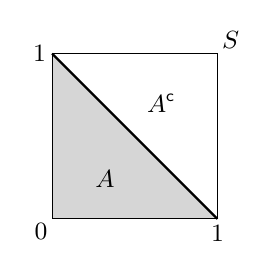
\begin{tikzpicture}[scale=2.1,font=\small]
  \fill[black!16] (0,0)--(1,0)--(0,1)--cycle;
  \draw[thin] (0,0) rectangle (1,1);
  \draw[thick] (1,0)--(0,1);
  \node at (0.32,0.24){$A$};
  \node at (0.66,0.70){$\comp{A}$};
  \node[below left,inner sep=1.5pt] at (0,0){$0$};
  \node[below,inner sep=2pt] at (1,0){$1$};
  \node[left,inner sep=2pt] at (0,1){$1$};
  \node[above right,inner sep=1.5pt] at (1,1){$S$};
\end{tikzpicture}\\[3pt]
{\small Shaded $A=\{x+y\le 1\}$; the unshaded upper-right triangle is $\comp{A}$.}
\end{center}

\paragraph{Examples for mutual exclusivity and subset/implication.}

\begin{example}[Detecting mutual exclusivity]
Draw one card. Let $A=$ ``an ace'' and $B=$ ``a king.'' Are $A,B$ mutually exclusive?
\end{example}
\whichrule{The question is ``can both occur at once?'' --- a yes/no disjointness test, not a
request to build a new event. We answer it by computing $A\cap B$ and checking whether it
is empty.}
\soln
\steplabel{Step 1: intersect.} A single card has one rank, so it cannot be both an ace and a
king: $A\cap B=\varnothing$.
\steplabel{Step 2: conclude.} Since the intersection is empty, $A$ and $B$ are mutually
exclusive.
\begin{center}\vennDisjoint\end{center}

\begin{example}[Not mutually exclusive --- a counterexample]
Draw one card. Let $A=$ ``a heart'' and $B=$ ``a queen.'' Decide whether they are mutually
exclusive.
\end{example}
\whichrule{Same disjointness test, opposite outcome. We look for a single outcome lying in
both events; finding even one proves the intersection is nonempty and the events are
\emph{not} disjoint.}
\soln
\steplabel{Step 1: hunt for a common point.} The queen of hearts is a heart \emph{and} a
queen, so it lies in $A\cap B$.
\steplabel{Step 2: conclude.} $A\cap B=\{\text{queen of hearts}\}\ne\varnothing$, so $A,B$
are \emph{not} mutually exclusive.
\begin{center}\vennInter\end{center}

\begin{example}[Mutual exclusivity from a partition of outcomes]
Draw one ball from an urn holding balls numbered $1$--$12$. Let $A=$ ``the number is at most
$4$,'' $B=$ ``the number is between $5$ and $8$,'' and $D=$ ``the number is at least $9$.''
Are these three events pairwise mutually exclusive?
\end{example}
\whichrule{The question asks whether any two can occur together, so it is a pairwise
disjointness test: form each pairwise intersection and check for emptiness. Because the
three ranges of numbers do not overlap, we expect every pairwise intersection to be empty.}
\soln
\steplabel{Step 1: list the events.} $A=\{1,2,3,4\}$, $B=\{5,6,7,8\}$, $D=\{9,10,11,12\}$.
\steplabel{Step 2: intersect each pair.} $A\cap B=\varnothing$ (no number is both $\le4$ and
in $5$--$8$); $A\cap D=\varnothing$; $B\cap D=\varnothing$.
\steplabel{Step 3: conclude.} All three pairwise intersections are empty, so $A,B,D$ are
pairwise mutually exclusive. (They also exhaust $S$, so they form a partition --- a fact the
later addition rule will exploit.)
\begin{center}\vennDisjoint\end{center}

\begin{example}[Subset / implication]
Roll one die. Let $A=$ ``the face is $6$'' and $B=$ ``the face is even.'' Show $A\subseteq
B$ and interpret.
\end{example}
\whichrule{``Whenever a $6$ comes up, the face is even'' is an implication: $A$ \emph{forces}
$B$. The cue ``whenever $A$ then $B$'' is the subset relation $A\subseteq B$, established by
checking that every outcome of $A$ lies in $B$.}
\soln
\steplabel{Step 1: list.} $A=\{6\}$, $B=\{2,4,6\}$.
\steplabel{Step 2: check containment.} The only element of $A$, namely $6$, is in $B$; hence
$A\subseteq B$.
\steplabel{Step 3: interpret.} $A$ implies $B$: rolling a $6$ guarantees an even face.
By the subset identities above, this also gives $A\cap B=A=\{6\}$ and
$A\cup B=B=\{2,4,6\}$.

\begin{example}[Chaining implications across two trials]
Flip a coin and then roll a die. Let $A=$ ``heads then a $6$'' and $B=$ ``the die shows
$6$.'' Is $A\subseteq B$? Use a tree to see the structure.
\end{example}
\whichrule{$A$ specifies \emph{more} than $B$ (it also pins down the coin), so every outcome
in $A$ already satisfies the looser condition $B$ --- the ``more specific implies more
general'' pattern, i.e.\ $A\subseteq B$. It is not equality, since $B$ also contains
``tails then $6$.''}
\soln
\steplabel{Step 1: enumerate via a tree.}
\begin{center}
\begin{tikzpicture}[>=Stealth,grow=right,
  level 1/.style={sibling distance=33mm,level distance=24mm},
  level 2/.style={sibling distance=16mm,level distance=30mm},font=\small]
\node{}
  child{node{$T$}
    child{node{$T,6\in B$}}
    child{node{$T,\text{not }6$}}}
  child{node{$H$}
    child{node{$H,6\in A\subseteq B$}}
    child{node{$H,\text{not }6$}}};
\end{tikzpicture}
\end{center}
\steplabel{Step 2: identify the sets.} $A=\{(H,6)\}$; $B=\{(H,6),(T,6)\}$.
\steplabel{Step 3: conclude.} Every point of $A$ (just $(H,6)$) lies in $B$, so $A\subseteq
B$; the containment is strict because $(T,6)\in B\setminus A$.

\begin{example}[Implication between numerical conditions]
Draw a ticket numbered $1$--$30$. Let $A=$ ``the number is a multiple of $12$'' and
$B=$ ``the number is even.'' Show that $A\subseteq B$ and use the subset identities to read
off $A\cap B$ and $A\cup B$.
\end{example}
\whichrule{``Every multiple of $12$ is even'' is a logical implication $A\Rightarrow B$,
i.e.\ the subset relation $A\subseteq B$. The cue is that one condition (divisible by $12$)
is \emph{stronger} than the other (even) and forces it. We confirm containment elementwise,
not by intersecting to build a new event.}
\soln
\steplabel{Step 1: list.} $A=\{12,24\}$ (multiples of $12$ up to $30$);
$B=\{2,4,6,\dots,30\}$, the $15$ even numbers.
\steplabel{Step 2: check containment.} Both $12$ and $24$ are even, hence in $B$; so every
element of $A$ lies in $B$ and $A\subseteq B$.
\steplabel{Step 3: apply the subset identities.} From Proposition (the basic identities),
$A\subseteq B$ gives $A\cap B=A=\{12,24\}$ and $A\cup B=B=\{2,4,\dots,30\}$. The smaller set
contributes nothing new to the union and nothing is lost in the intersection.

\begin{example}[Disjointness from a partition of the dice grid by total]
Roll the two dice. Let $A=$ ``the total is at most $4$,'' $B=$ ``the total is $7$,'' and
$D=$ ``the total is at least $10$.'' Are $A,B,D$ pairwise mutually exclusive?
\end{example}
\whichrule{The question ``can any two occur together?'' is a pairwise disjointness test:
intersect each pair and check for emptiness. A single roll has \emph{one} total, and the
three ranges $\le 4$, $=7$, $\ge 10$ do not overlap, so every pairwise intersection should
be empty.}
\soln
\steplabel{Step 1: note the totals are exclusive.} A roll yields exactly one total, so it
can satisfy at most one of the three disjoint ranges.
\steplabel{Step 2: check the pairs.} $A\cap B=\varnothing$ (a total cannot be both $\le4$
and $=7$); $A\cap D=\varnothing$; $B\cap D=\varnothing$ ($7$ is not $\ge 10$).
\steplabel{Step 3: conclude.} All three pairwise intersections are empty, so $A,B,D$ are
pairwise mutually exclusive. (They are \emph{not} exhaustive --- totals $5,6,8,9$ lie
outside all three --- so they do not form a partition of $S$.)
\begin{center}\vennDisjoint\end{center}

\begin{example}[A subtle non-exclusivity: ``not obviously overlapping'' events]
Draw a ticket numbered $1$--$50$. Let $A=$ ``a perfect square'' and $B=$ ``a multiple of
$4$.'' Are $A,B$ mutually exclusive?
\end{example}
\whichrule{It is tempting to call squares and multiples of $4$ unrelated, but mutual
exclusivity is decided only by $A\cap B$, not by intuition. We hunt for one common point; a
single hit, such as $4$ or $16$, proves the intersection is nonempty and the events are
\emph{not} disjoint.}
\soln
\steplabel{Step 1: list.} $A=\{1,4,9,16,25,36,49\}$; $B=\{4,8,12,\dots,48\}$.
\steplabel{Step 2: intersect.} The numbers in both are $4,16,36$ (squares that are also
multiples of $4$), so $A\cap B=\{4,16,36\}\ne\varnothing$.
\steplabel{Step 3: conclude.} Since $A\cap B$ is nonempty, $A$ and $B$ are \emph{not}
mutually exclusive --- a reminder that overlap must be \emph{checked}, never assumed.
\begin{center}\vennInter\end{center}

\begin{example}[Subset versus equality: a strict implication]
Roll the two dice. Let $A=$ ``both faces equal $3$'' and $B=$ ``the total is $6$.'' Decide
whether $A\subseteq B$, and whether the containment is strict.
\end{example}
\whichrule{``Whenever both faces are $3$, the total is $6$'' is an implication
$A\Rightarrow B$, hence the subset relation $A\subseteq B$, checked elementwise. To test
whether it is \emph{strict} (proper), we look for a point of $B$ outside $A$; finding one
shows $A\ne B$.}
\soln
\steplabel{Step 1: list.} $A=\{(3,3)\}$; $B=\{(1,5),(2,4),(3,3),(4,2),(5,1)\}$.
\steplabel{Step 2: containment.} The single point $(3,3)$ of $A$ lies in $B$, so
$A\subseteq B$.
\steplabel{Step 3: strictness.} $B$ also contains $(1,5)$, which is not in $A$, so
$A\subsetneq B$ is \emph{proper}. The subset identities then give $A\cap B=A=\{(3,3)\}$ and
$A\cup B=B$.

\subsection{De Morgan's laws}

\begin{theorem}[De Morgan's laws]\label{thm:demorgan}
For any events $A,B\subseteq S$,
\[
  \comp{(A\cup B)}=\comp{A}\cap\comp{B}
  \qquad\text{and}\qquad
  \comp{(A\cap B)}=\comp{A}\cup\comp{B}.
\]
More generally, for any (finite or countable) family $\{A_i\}$,
$\comp{\big(\bigcup_i A_i\big)}=\bigcap_i\comp{A_i}$ and
$\comp{\big(\bigcap_i A_i\big)}=\bigcup_i\comp{A_i}$: complementing a union/intersection
flips it to an intersection/union of complements.
\end{theorem}
\begin{proof}
We prove the first law by showing each side contains the other.
\steplabel{($\subseteq$).} Take $s\in\comp{(A\cup B)}$. Then $s\notin A\cup B$, so $s$ is in
neither $A$ nor $B$. Hence $s\in\comp{A}$ and $s\in\comp{B}$, i.e.\ $s\in\comp{A}\cap
\comp{B}$.
\steplabel{($\supseteq$).} Take $s\in\comp{A}\cap\comp{B}$. Then $s\notin A$ and $s\notin
B$, so $s$ belongs to no part of $A\cup B$, giving $s\in\comp{(A\cup B)}$.
The two inclusions give equality. The second law follows by applying the first to
$\comp{A},\comp{B}$ in place of $A,B$ and using $\comp{(\comp{X})}=X$:
$\comp{A}\cap\comp{B}=\comp{(A\cup B)}$ complemented on both sides yields
$\comp{(\comp{A}\cap\comp{B})}=A\cup B$, then rename. The general family version is the same
element-chase: ``not in any $A_i$'' $\iff$ ``in every $\comp{A_i}$.''
\end{proof}

\begin{remark}
De Morgan is the workhorse for ``at least one'' / ``none'' conversions:
$\comp{(A_1\cup\cdots\cup A_n)}=\comp{A_1}\cap\cdots\cap\comp{A_n}$ says ``\emph{none} of
the events happen'' is the same as ``\emph{not at least one} happens.'' This is why
computing ``no defective'' is the standard route to ``at least one defective.''
\end{remark}

\begin{example}[``Neither'' is the complement of a union]
A traveler's trip succeeds unless a flight is delayed or luggage is lost. Let $A=$ ``flight
delayed'' and $B=$ ``luggage lost.'' Write ``neither problem occurs'' and simplify.
\end{example}
\whichrule{``Neither $A$ nor $B$'' is a \emph{negated union}: ``not (delayed or lost).'' A
complement sitting outside a union is the exact trigger for the first De Morgan law, turning
it into ``not delayed and not lost.''}
\soln
\steplabel{Step 1: translate.} ``Neither problem'' $=\comp{(A\cup B)}$.
\steplabel{Step 2: apply De Morgan.} $\comp{(A\cup B)}=\comp{A}\cap\comp{B}$.
\steplabel{Step 3: read back.} The event is ``flight on time \emph{and} luggage arrives,''
$\comp{A}\cap\comp{B}$ --- a clean conjunction of two ``good'' events.
\begin{center}\vennCompUnion\end{center}

\begin{example}[``Not both'' is the complement of an intersection]
Two switches must each be closed for a lamp to light. Let $A,B=$ ``switch~1 closed,''
``switch~2 closed.'' Write ``the lamp is off'' and simplify.
\end{example}
\whichrule{The lamp lights only when \emph{both} switches are closed, $A\cap B$; ``off''
negates that, ``not (both closed),'' a \emph{negated intersection}. That structure is the
second De Morgan law, which converts it into ``at least one switch is open.''}
\soln
\steplabel{Step 1: translate.} Lamp on $=A\cap B$; lamp off $=\comp{(A\cap B)}$.
\steplabel{Step 2: apply De Morgan.} $\comp{(A\cap B)}=\comp{A}\cup\comp{B}$.
\steplabel{Step 3: read back.} The lamp is off iff ``switch~1 open \emph{or} switch~2
open'' --- at least one switch open. Note the ``and'' became ``or.''

\begin{example}[De Morgan with three events, by counting]
Of $60$ tourists, $25$ visited the museum ($A$), $30$ the gallery ($B$), $20$ the castle
($C$); the count visiting at least one site is $45$. How many visited \emph{none} of the
three?
\end{example}
\whichrule{``None of the three'' is $\comp{(A\cup B\cup C)}$, the complement of a triple
union; the extended De Morgan law rewrites it as $\comp{A}\cap\comp{B}\cap\comp{C}$ and,
just as importantly, lets us get its count as ``total minus at-least-one.''}
\soln
\steplabel{Step 1: translate.} Visited none $=\comp{(A\cup B\cup C)}=\comp{A}\cap\comp{B}
\cap\comp{C}$.
\steplabel{Step 2: use the count of the union.} Given $|A\cup B\cup C|=45$ out of $60$.
\steplabel{Step 3: subtract.} $|\comp{(A\cup B\cup C)}|=60-45=15$. Fifteen tourists visited
no site.

\begin{example}[Verifying De Morgan numerically on the dice grid]
Roll the two dice. Let $A=$ ``red is $1$'' and $B=$ ``green is $1$.'' Check directly that
$\comp{(A\cup B)}=\comp{A}\cap\comp{B}$ by counting outcomes.
\end{example}
\whichrule{We are asked to \emph{confirm} a negated-union identity, so De Morgan is the rule
under test. The check is a count of the grid: build both sides and see the sizes agree.}
\soln
\steplabel{Step 1: left side.} $A\cup B=$ ``red is $1$ or green is $1$'' $=$ first row plus
first column of the grid. Each has $6$ cells, sharing $(1,1)$, so $|A\cup B|=6+6-1=11$;
thus $|\comp{(A\cup B)}|=36-11=25$.
\steplabel{Step 2: right side.} $\comp{A}=$ ``red $\ne 1$'' ($30$ cells), $\comp{B}=$
``green $\ne 1$'' ($30$ cells); their intersection is ``red $\ne1$ and green $\ne1$,'' the
$5\times 5$ block, of size $25$.
\steplabel{Step 3: compare.} Both sides have $25$ outcomes (the $5\times 5$ block where
neither die is $1$), confirming $\comp{(A\cup B)}=\comp{A}\cap\comp{B}$.
\begin{center}
\begin{tabular}{c|cccccc}
\toprule
{\footnotesize r$\backslash$g} & 1 & 2 & 3 & 4 & 5 & 6\\
\midrule
1 & $\bullet$ & $\bullet$ & $\bullet$ & $\bullet$ & $\bullet$ & $\bullet$\\
2 & $\bullet$ & $\circ$ & $\circ$ & $\circ$ & $\circ$ & $\circ$\\
3 & $\bullet$ & $\circ$ & $\circ$ & $\circ$ & $\circ$ & $\circ$\\
4 & $\bullet$ & $\circ$ & $\circ$ & $\circ$ & $\circ$ & $\circ$\\
5 & $\bullet$ & $\circ$ & $\circ$ & $\circ$ & $\circ$ & $\circ$\\
6 & $\bullet$ & $\circ$ & $\circ$ & $\circ$ & $\circ$ & $\circ$\\
\bottomrule
\end{tabular}\\[2pt]
{\small Dots $\bullet=A\cup B$ (red or green is $1$); circles $\circ$ form the $5\times5$ block $\comp{A}\cap\comp{B}$.}
\end{center}

\begin{example}[``At least one failure'' via its complement]
A machine runs only if \emph{both} of its two belts hold. Let $A=$ ``belt~1 breaks'' and
$B=$ ``belt~2 breaks.'' Rewrite ``the machine keeps running'' using De Morgan, and rewrite
``at least one belt breaks'' as well.
\end{example}
\whichrule{``Keeps running'' is ``\emph{neither} belt breaks'' $=\comp{(A\cup B)}$: a
complement outside a union, the first De Morgan law, which flips it to
$\comp{A}\cap\comp{B}$ (``both hold''). ``At least one breaks'' is the complement of that,
the union $A\cup B$ --- the same identity read in reverse.}
\soln
\steplabel{Step 1: translate ``running.''} Running $=$ neither breaks $=\comp{(A\cup B)}$.
\steplabel{Step 2: apply De Morgan.} $\comp{(A\cup B)}=\comp{A}\cap\comp{B}$ --- ``belt~1
holds \emph{and} belt~2 holds,'' a conjunction of the two ``good'' events.
\steplabel{Step 3: the opposite event.} ``At least one breaks'' is the complement of
``running'': $\comp{(\comp{A}\cap\comp{B})}=A\cup B$. The ``and'' of holds became the
``or'' of breaks.
\begin{center}\vennCompUnion\end{center}

\begin{example}[De Morgan turning a negated ``and'' into an ``or'']
A loan is approved only if the applicant passes the credit check ($A$) \emph{and} the
income check ($B$). Describe ``the loan is denied'' and simplify with De Morgan.
\end{example}
\whichrule{Approval is $A\cap B$; ``denied'' negates it, $\comp{(A\cap B)}$ --- a complement
outside an intersection. That is the second De Morgan law, converting it to
$\comp{A}\cup\comp{B}$: the ``and'' becomes ``or,'' so denial means failing \emph{at least
one} check, not necessarily both.}
\soln
\steplabel{Step 1: translate.} Approved $=A\cap B$; denied $=\comp{(A\cap B)}$.
\steplabel{Step 2: apply De Morgan.} $\comp{(A\cap B)}=\comp{A}\cup\comp{B}$.
\steplabel{Step 3: read back.} Denied iff ``credit fails \emph{or} income fails'' --- a
single failed check is enough. The common error of reading denial as ``both fail''
($\comp{A}\cap\comp{B}$) describes a strictly smaller event.
\begin{center}
\vennCompInter\\[2pt]
{\small Shaded everything but the lens: denial is failing \emph{at least one} check.}
\end{center}

\begin{example}[De Morgan with three events, verified by counting]
Roll the two dice. Let $A=$ ``red $\le 2$,'' $B=$ ``green $\le 2$.'' Check by counting that
$\comp{(A\cup B)}=\comp{A}\cap\comp{B}$, and read off ``both dice are at least $3$.''
\end{example}
\whichrule{We are testing a negated-union identity, so De Morgan is the rule under
examination. ``Neither $A$ nor $B$'' $=\comp{(A\cup B)}$ should equal ``red $\ge3$ and
green $\ge3$'' $=\comp{A}\cap\comp{B}$; we confirm the two counts match on the grid.}
\soln
\steplabel{Step 1: left side.} $A\cup B=$ ``red $\le2$ or green $\le2$.'' Here $|A|=2\times
6=12$, $|B|=6\times 2=12$, and $|A\cap B|=2\times 2=4$, so $|A\cup B|=12+12-4=20$; thus
$|\comp{(A\cup B)}|=36-20=16$.
\steplabel{Step 2: right side.} $\comp{A}=$ ``red $\ge 3$'' and $\comp{B}=$ ``green $\ge
3$''; their intersection is the $4\times 4$ block of cells with both faces in
$\{3,4,5,6\}$, of size $16$.
\steplabel{Step 3: compare.} Both sides have $16$ outcomes --- exactly the $4\times4$ block
where each die is at least $3$ --- confirming $\comp{(A\cup B)}=\comp{A}\cap\comp{B}$.

\subsection{The distributive laws (with commutative and associative laws)}

\begin{theorem}[Distributive laws]\label{thm:distrib}
For all events $A,B,C\subseteq S$,
\[
  A\cap(B\cup C)=(A\cap B)\cup(A\cap C),
  \qquad
  A\cup(B\cap C)=(A\cup B)\cap(A\cup C).
\]
\end{theorem}
\begin{proof}
For the first law, chase an arbitrary outcome $s$:
\[
  s\in A\cap(B\cup C)
  \iff s\in A\ \text{and}\ (s\in B\ \text{or}\ s\in C)
  \iff (s\in A\ \text{and}\ s\in B)\ \text{or}\ (s\in A\ \text{and}\ s\in C),
\]
where the middle step is the logical distributivity of ``and'' over ``or.'' The right side
says $s\in(A\cap B)\cup(A\cap C)$, so the two events have identical members. The second law
is the dual: replace ``and''$\leftrightarrow$``or'' throughout, which is legitimate because
the same logical distributivity holds for ``or'' over ``and.''
\end{proof}

\begin{remark}[Commutative and associative laws]
Order and grouping never affect a union or an intersection:
\[
  A\cup B=B\cup A,\quad A\cap B=B\cap A
  \quad\text{(commutativity)},
\]
\[
  (A\cup B)\cup C=A\cup(B\cup C),\quad (A\cap B)\cap C=A\cap(B\cap C)
  \quad\text{(associativity)}.
\]
Both follow instantly because ``or'' and ``and'' in logic are themselves commutative and
associative. These laws justify dropping parentheses in chains such as $A\cup B\cup C$ and
reordering events freely; they are routine bookkeeping rather than problem-solving rules.
\end{remark}

\begin{example}[Distribute ``and'' over ``or'']
Draw one card. Let $A=$ ``red'' (heart or diamond), $B=$ ``a face card,'' $C=$ ``an ace.''
Show ``red, and (a face card or an ace)'' equals ``(red face card) or (red ace),'' and count.
\end{example}
\whichrule{The event is one condition (``red'') applied to a bracketed ``or'' (``face or
ace''): $A\cap(B\cup C)$. That single-times-bracketed-sum shape is the distributive cue; we
expand it to $(A\cap B)\cup(A\cap C)$ to count the two simpler pieces.}
\soln
\steplabel{Step 1: distribute.} $A\cap(B\cup C)=(A\cap B)\cup(A\cap C)$.
\steplabel{Step 2: count each piece.} $A\cap B=$ red face cards $=2$ suits $\times\,3
=6$. $A\cap C=$ red aces $=2$. They are disjoint (an ace is not a face card).
\steplabel{Step 3: combine.} $|(A\cap B)\cup(A\cap C)|=6+2=8$ red cards that are a face card
or an ace.
\begin{center}\vennInter\end{center}

\begin{example}[Distribute ``or'' over ``and'']
Tickets $1$--$24$. Let $A=$ ``a multiple of $6$,'' $B=$ ``even,'' $C=$ ``a multiple of
$3$.'' Verify $A\cup(B\cap C)=(A\cup B)\cap(A\cup C)$ by listing.
\end{example}
\whichrule{The shape is ``$A$ or (B and C),'' a union wrapped around a bracketed ``and'':
$A\cup(B\cap C)$. This is the second distributive law; we expand and confirm both sides
list the same tickets.}
\soln
\steplabel{Step 1: inner pieces.} $A=\{6,12,18,24\}$; $B\cap C=$ ``even and multiple of $3$''
$=$ ``multiple of $6$'' $=\{6,12,18,24\}$.
\steplabel{Step 2: left side.} $A\cup(B\cap C)=\{6,12,18,24\}$.
\steplabel{Step 3: right side.} $A\cup B=$ all evens $\cup\{6,12,18,24\}=$ all evens
$=\{2,4,\dots,24\}$. $A\cup C=$ multiples of $3$ $=\{3,6,9,12,15,18,21,24\}$. Their
intersection is the numbers that are even \emph{and} a multiple of $3$ $=\{6,12,18,24\}$.
\steplabel{Step 4: compare.} Both sides equal $\{6,12,18,24\}$. Verified.
\begin{center}\vennUnion\end{center}

\begin{example}[Distribution to split into disjoint pieces]
Roll the two dice. Let $A=$ ``red is even,'' $B=$ ``total is $5$,'' $C=$ ``total is $9$.''
Compute $|A\cap(B\cup C)|$ via distribution.
\end{example}
\whichrule{We want ``red even, and (total $5$ or total $9$)'' $=A\cap(B\cup C)$. Distributing
turns one messy intersection into two clean ones, $A\cap B$ and $A\cap C$, which here are
disjoint (a total cannot be both $5$ and $9$), so their counts simply add.}
\soln
\steplabel{Step 1: distribute.} $A\cap(B\cup C)=(A\cap B)\cup(A\cap C)$.
\steplabel{Step 2: list $A\cap B$.} Total $5$: $(1,4),(2,3),(3,2),(4,1)$; keep red even:
$(2,3),(4,1)$, so $|A\cap B|=2$.
\steplabel{Step 3: list $A\cap C$.} Total $9$: $(3,6),(4,5),(5,4),(6,3)$; keep red even:
$(4,5),(6,3)$, so $|A\cap C|=2$.
\steplabel{Step 4: add (disjoint).} $|A\cap(B\cup C)|=2+2=4$.
\begin{center}\vennInter\end{center}

\begin{example}[Distribution behind inclusion of a common factor]
Three relays $A,B,C$ feed a circuit. Express ``relay $A$ works, and at least one of $B,C$
works,'' then factor the common $A$.
\end{example}
\whichrule{``$A$ works \emph{and} (at least one of $B,C$)'' is $A\cap(B\cup C)$: a shared
condition $A$ multiplying a union. Recognising the common factor $A$ lets us either expand
(to count cases) or keep it factored (to read the structure); both are the distributive
law.}
\soln
\steplabel{Step 1: translate.} Event $=A\cap(B\cup C)$.
\steplabel{Step 2: distribute.} $=(A\cap B)\cup(A\cap C)$ --- ``($A$ and $B$) or ($A$ and
$C$).''
\steplabel{Step 3: interpret.} Either relays $A,B$ both work, or relays $A,C$ both work
(possibly both pairs). The factored form $A\cap(B\cup C)$ and the expanded form are the same
event, by the distributive law.

\begin{example}[Commutativity and associativity in a regrouping]
Simplify $\big[(A\cup B)\cup C\big]\cap\big[C\cup(B\cup A)\big]$.
\end{example}
\whichrule{Nothing is negated and no single factor multiplies a bracketed sum in an
essential way; the only moves available are \emph{reordering} ($A\cup B=B\cup A$) and
\emph{regrouping} ($(A\cup B)\cup C=A\cup(B\cup C)$). Spotting that both brackets are the
same set after reordering is the commutativity/associativity cue.}
\soln
\steplabel{Step 1: flatten each bracket.} By associativity, $(A\cup B)\cup C=A\cup B\cup C$;
by commutativity, $C\cup(B\cup A)=A\cup B\cup C$ as well.
\steplabel{Step 2: both brackets coincide.} The expression is $(A\cup B\cup C)\cap(A\cup
B\cup C)$.
\steplabel{Step 3: idempotence.} A set intersected with itself is itself, so the value is
$A\cup B\cup C$.

\begin{example}[Distribute ``and'' over ``or'' on the dice grid]
Roll the two dice. Let $A=$ ``red is $3$,'' $B=$ ``the total is $5$,'' $C=$ ``the total is
$9$.'' Compute $|A\cap(B\cup C)|$ by distributing.
\end{example}
\whichrule{The event ``red $3$, and (total $5$ or total $9$)'' is $A\cap(B\cup C)$: one
condition multiplying a bracketed ``or.'' Distributing gives
$(A\cap B)\cup(A\cap C)$, two clean intersections; since a total cannot be both $5$ and $9$
the pieces are disjoint and their counts add.}
\soln
\steplabel{Step 1: distribute.} $A\cap(B\cup C)=(A\cap B)\cup(A\cap C)$.
\steplabel{Step 2: count $A\cap B$.} With red $=3$, total $5$ forces green $=2$: just
$(3,2)$, so $|A\cap B|=1$.
\steplabel{Step 3: count $A\cap C$.} With red $=3$, total $9$ forces green $=6$: just
$(3,6)$, so $|A\cap C|=1$.
\steplabel{Step 4: add (disjoint).} $|A\cap(B\cup C)|=1+1=2$, namely $\{(3,2),(3,6)\}$.
\begin{center}\vennInter\end{center}

\begin{example}[Distribute ``or'' over ``and'' and verify by listing]
Tickets $1$--$36$. Let $A=$ ``a multiple of $9$,'' $B=$ ``a multiple of $3$,'' $C=$
``even.'' Verify $A\cup(B\cap C)=(A\cup B)\cap(A\cup C)$ by listing both sides.
\end{example}
\whichrule{The shape ``$A$ or ($B$ and $C$)'' is a union wrapped around a bracketed ``and,''
$A\cup(B\cap C)$ --- the second distributive law. We expand and confirm both descriptions
produce the same ticket list, which is the law's content.}
\soln
\steplabel{Step 1: inner pieces.} $A=\{9,18,27,36\}$; $B\cap C=$ ``multiple of $3$ and
even'' $=$ ``multiple of $6$'' $=\{6,12,18,24,30,36\}$.
\steplabel{Step 2: left side.} $A\cup(B\cap C)=\{6,9,12,18,24,27,30,36\}$.
\steplabel{Step 3: right side.} $A\cup B=$ multiples of $3$ $=\{3,6,9,\dots,36\}$;
$A\cup C=$ ``multiple of $9$ or even.'' Their intersection keeps the numbers that are a
multiple of $3$ \emph{and} (a multiple of $9$ or even), which works out to
$\{6,9,12,18,24,27,30,36\}$.
\steplabel{Step 4: compare.} Both sides are
$\{6,9,12,18,24,27,30,36\}$. Verified.
\begin{center}\vennUnion\end{center}

\begin{example}[Distribution to factor a shared condition]
Draw one card. Let $A=$ ``a red card,'' $B=$ ``a face card,'' $C=$ ``a ten.'' Write ``red,
and (a face card or a ten),'' then both distribute it and count.
\end{example}
\whichrule{``Red \emph{and} (face or ten)'' is $A\cap(B\cup C)$: the shared condition red
multiplies a union. Distributing to $(A\cap B)\cup(A\cap C)$ turns it into two easy counts;
the pieces are disjoint because a ten is not a face card.}
\soln
\steplabel{Step 1: distribute.} $A\cap(B\cup C)=(A\cap B)\cup(A\cap C)$.
\steplabel{Step 2: count each piece.} $A\cap B=$ red face cards $=2$ red suits $\times\,3
=6$. $A\cap C=$ red tens $=2$.
\steplabel{Step 3: add (disjoint).} A card is never both a ten and a face card, so
$|A\cap(B\cup C)|=6+2=8$ red cards that are a face card or a ten.
\begin{center}\vennInter\end{center}

\subsection{One worked synthesis}

\begin{example}[Putting the algebra together]
Roll the two dice. Let $A=$ ``red is even,'' $B=$ ``green is odd.'' Use the algebra to
describe and count ``exactly one of $A,B$ occurs.''
\end{example}
\whichrule{``Exactly one'' is neither a plain union nor intersection; it is ``($A$ and not
$B$) or (not $A$ and $B$),'' $(A\cap\comp{B})\cup(\comp{A}\cap B)$ --- complements inside an
``or.'' The two pieces are disjoint, so once each is counted we simply add.}
\soln
\steplabel{Step 1: counts of the base events.} $A$ (red even): $3\times 6=18$. $B$ (green
odd): $6\times 3=18$. $A\cap B$ (red even and green odd): $3\times 3=9$.
\steplabel{Step 2: the two disjoint pieces.}
$A\cap\comp{B}$ (red even, green even) $=3\times 3=9$;
$\comp{A}\cap B$ (red odd, green odd) $=3\times 3=9$.
\steplabel{Step 3: add.} ``Exactly one'' $=(A\cap\comp{B})\cup(\comp{A}\cap B)$ has
$9+9=18$ outcomes out of $36$.
\steplabel{Cross-check.} ``At least one'' $=|A\cup B|=18+18-9=27$; subtract ``both''
$|A\cap B|=9$ to get exactly one $=27-9=18$. Agrees.
\begin{center}\vennExactlyOne\end{center}

\section{The Probability Function: Axioms and Their Consequences}

A \keyword{probability function} $\PP$ attaches to each event $A\subseteq S$ a real number
$\PP(A)$ measuring how likely $A$ is to occur. We do not say where these numbers come from
--- relative frequencies, symmetry, or subjective judgement all qualify --- we only demand
that they obey three rules, the \keyword{Kolmogorov axioms}. Every formula in this section
is forced out of those three rules; nothing extra is ever assumed.

\begin{strategy}[Which rule of this section does the problem need?]
Read the question and match its \emph{verbal structure} to one of six tools.
\begin{itemize}[itemsep=2pt,topsep=2pt,leftmargin=*]
\item \keyword{Kolmogorov axioms (the raw definition).} Use them when you must \emph{verify}
that a proposed assignment is a legitimate probability, or when the events named are
\keyword{mutually exclusive} (``cannot both happen,'' ``disjoint,'' ``no overlap'') so their
probabilities simply add. Trigger words: \emph{is this a valid probability?}, \emph{disjoint},
\emph{cannot occur together}.
\item \keyword{Complement rule} $\PP(\comp{A})=1-\PP(A)$. Use it whenever the event is phrased
as \emph{at least one}, \emph{not}, \emph{none}, \emph{fails to}, or \emph{at most}\,---
anything where the \emph{opposite} event is easier to count than the event itself.
\item \keyword{Monotonicity / bounds} $0\le\PP(A)\le 1$ and $A\subseteq B\Rightarrow
\PP(A)\le\PP(B)$. Use it when one event \emph{implies} another (``if $A$ happens then $B$
must,'' ``$A$ is a special case of $B$''), or to sanity-check that an answer is a legal
probability.
\item \keyword{Inclusion--exclusion, two events}
$\PP(A\cup B)=\PP(A)+\PP(B)-\PP(A\cap B)$. Use it for \emph{or} / \emph{union} questions when
the two events \emph{can overlap}. The tell-tale sign is that you are given $\PP(A)$,
$\PP(B)$, and $\PP(A\cap B)$ (the ``both'') and asked for ``$A$ or $B$,'' or the reverse.
\item \keyword{Inclusion--exclusion, three events}\,---\,same idea with three pieces: add the
singles, subtract the three pairwise overlaps, add back the triple. Triggered by ``at least
one of three'' or any union of three overlapping events.
\item \keyword{Equally-likely model} $\PP(A)=|A|/|S|$. Use it when the outcomes are
\emph{symmetric} --- \emph{fair} dice/coins, a \emph{well-shuffled} deck, a person/ball drawn
\emph{at random}. The whole problem reduces to counting $|A|$ and $|S|$.
\end{itemize}
\textbf{Quick discriminators.} ``At least one'' $\Rightarrow$ complement. ``$A$ or $B$'' with a
given overlap $\Rightarrow$ inclusion--exclusion. ``Drawn at random / fair'' $\Rightarrow$
equally likely. ``Disjoint / mutually exclusive'' $\Rightarrow$ the overlap term is $0$, so
the union is a plain sum (Axiom~3).
\end{strategy}

% =====================================================================
\subsection{The Kolmogorov axioms}
% =====================================================================

\begin{axiom}[Nonnegativity]
$\PP(A)\ge 0$ for every event $A\subseteq S$.
\end{axiom}
\begin{axiom}[Normalization]
$\PP(S)=1$.
\end{axiom}
\begin{axiom}[Countable additivity]
If $A_1,A_2,A_3,\dots$ is a sequence of pairwise mutually exclusive events
(so $A_i\cap A_j=\varnothing$ whenever $i\ne j$), then
\[
  \PP\!\Big(\bigcup_{i=1}^{\infty} A_i\Big)=\sum_{i=1}^{\infty}\PP(A_i).
\]
\end{axiom}

Axiom~1 says probabilities are never negative; Axiom~2 fixes the scale by giving the certain
event $S$ the value $1$; Axiom~3, \keyword{countable additivity}, is the workhorse: the
probability of a disjoint union is the sum of the parts. Taking all but finitely many $A_i$
equal to $\varnothing$ recovers \keyword{finite additivity}: for disjoint $A_1,\dots,A_n$,
$\PP(A_1\cup\cdots\cup A_n)=\PP(A_1)+\cdots+\PP(A_n)$. We will use the finite form constantly.

\begin{remark}
A finite or countable list of nonnegative weights summing to $1$ over the outcomes always
\emph{defines} a valid probability: set $\PP(A)=\sum_{s\in A}\PP(\{s\})$. Checking the axioms
then reduces to checking that the weights are $\ge 0$ and total $1$.
\end{remark}

\begin{example}
A spinner stops in one of four coloured sectors, red, blue, green, yellow, with proposed
probabilities $0.30,\ 0.25,\ 0.15,\ 0.30$ respectively. Is this a legitimate probability
assignment?
\end{example}
\whichrule{The question literally asks whether a proposed assignment is a \emph{valid
probability}, so we test it directly against the three axioms; no derived formula applies yet.
The single colours are mutually exclusive (the spinner shows exactly one), so Axiom~3 reduces
to: do the weights add to $1$?}
\soln
\steplabel{Check Axiom 1 (nonnegativity).} Every listed weight $0.30,0.25,0.15,0.30$ is
$\ge 0$. Pass.
\steplabel{Check Axioms 2--3 (normalization via additivity).} The four colours partition the
sample space, so by finite additivity $\PP(S)$ must equal their sum:
\[
  0.30+0.25+0.15+0.30=1.00 .
\]
The total is exactly $1$, so $\PP(S)=1$. Pass. All three axioms hold, so the assignment is a
\emph{valid} probability function.

\begin{example}
A different spinner has sectors with proposed probabilities $0.4,\ 0.3,\ 0.2,\ 0.2$. Is this a
valid probability?
\end{example}
\whichrule{Again a ``is this valid?'' question $\Rightarrow$ test the axioms. Nonnegativity is
fine, so the only thing that can fail is normalization.}
\soln The weights are all $\ge 0$, but
\[
  0.4+0.3+0.2+0.2=1.1\ne 1 .
\]
Normalization fails ($\PP(S)=1.1>1$, which also violates the bound $\PP\le1$ proved below), so
this is \emph{not} a valid probability function. (Notice it would also be invalid if the sum
were $0.9$: the axioms demand the total be exactly $1$, not merely $\le 1$.)

\begin{example}
A loaded six-sided die has $\PP(\{k\})=ck$ for $k=1,\dots,6$, where $c$ is a constant. Find $c$
and then the probability of rolling an even number.
\end{example}
\whichrule{We are handed an unnormalized rule for the outcome weights and must make it a
genuine probability. Axiom~2 (total $=1$) pins down the unknown constant; Axiom~3 then lets us
add the weights of the even faces. This is the axioms used as the definition, not a derived
rule.}
\soln
\steplabel{Solve for $c$ using Axiom 2.} The six faces are disjoint and exhaust $S$, so their
weights must sum to $1$:
\[
  \sum_{k=1}^{6} ck=c(1+2+3+4+5+6)=21c=1
  \quad\Longrightarrow\quad c=\tfrac{1}{21}.
\]
All weights $ck=k/21$ are positive, so Axiom~1 holds.
\steplabel{Add the even faces using Axiom 3.} The event $E=\{2,4,6\}$ is a disjoint union of
single outcomes, so
\[
  \PP(E)=\PP(\{2\})+\PP(\{4\})+\PP(\{6\})=\frac{2}{21}+\frac{4}{21}+\frac{6}{21}
        =\frac{12}{21}=\frac{4}{7}\approx 0.571 .
\]

\begin{example}
A board game card is drawn from a deck whose cards are coloured. The events ``red,''
``blue,'' ``green'' are mutually exclusive and exhaust the deck, with $\PP(\text{red})=0.5$ and
$\PP(\text{blue})=0.2$. A player asks for $\PP(\text{red or green})$.
\end{example}
\whichrule{The three colours are stated to be \emph{mutually exclusive} and to exhaust the
space, so probabilities add directly (Axiom~3) --- there is no overlap term, hence no need for
inclusion--exclusion. We first recover the missing $\PP(\text{green})$ from normalization.}
\soln
\steplabel{Find $\PP(\text{green})$ via Axiom 2.} Since the three colours partition $S$,
\[
  \PP(\text{red})+\PP(\text{blue})+\PP(\text{green})=1
  \;\Rightarrow\; 0.5+0.2+\PP(\text{green})=1
  \;\Rightarrow\; \PP(\text{green})=0.3 .
\]
\steplabel{Add disjoint events (Axiom 3).} ``Red'' and ``green'' are disjoint, so
\[
  \PP(\text{red or green})=\PP(\text{red})+\PP(\text{green})=0.5+0.3=0.8 .
\]
No subtraction is needed precisely because the overlap $\PP(\text{red}\cap\text{green})=0$.

\begin{example}
A digit $0$--$9$ is generated by a process that assigns the proposed weights
$0.10$, $0.20$, $0.30$, $0.25$, $0.10$, $0.05$, $0$, $0$, $0$, $0$ to the digits
$0,1,2,\dots,9$. Is this a legitimate probability assignment?
\end{example}
\whichrule{A direct ``is this valid?'' question $\Rightarrow$ test the three axioms, not a
derived rule. A weight of exactly $0$ is allowed (Axiom~1 demands only $\ge0$); the only thing
that can fail here is the total.}
\soln
\steplabel{Check Axiom 1.} All ten weights are $\ge0$ (the four trailing zeros are fine: they
just say those digits never occur). Pass.
\steplabel{Check Axioms 2--3.} The digits are mutually exclusive and exhaust $S$, so
normalization requires their sum to be $1$:
\[
  0.10+0.20+0.30+0.25+0.10+0.05+0+0+0+0=1.00 .
\]
The total is exactly $1$, so the assignment is a \emph{valid} probability function.

\begin{example}
In a population, a person's blood type is one of O, A, B, AB (mutually exclusive and
exhaustive). A geneticist records $\PP(\text{O})=0.44$, $\PP(\text{A})=0.42$,
$\PP(\text{B})=0.10$. Use the axioms to recover $\PP(\text{AB})$, and then $\PP(\text{not O})$.
\end{example}
\whichrule{The four types partition $S$, so Axiom~2 (total $=1$) pins down the one missing
weight by subtraction --- the axioms used as the \emph{definition}. Once the weights are known,
``not O'' adds the three disjoint remaining weights (Axiom~3); no overlap arises, so
inclusion--exclusion is irrelevant.}
\soln
\steplabel{Recover the missing weight via Axiom 2.} The four disjoint types sum to $1$:
\[
  0.44+0.42+0.10+\PP(\text{AB})=1\;\Longrightarrow\;\PP(\text{AB})=0.04 .
\]
All four weights are $\ge0$, so Axiom~1 holds.
\steplabel{Add disjoint weights via Axiom 3.} ``Not O'' is the disjoint union of A, B, AB:
\[
  \PP(\text{not O})=0.42+0.10+0.04=0.56 .
\]
(Consistency check against the complement rule below: $1-0.44=0.56$. Same answer.)

\begin{example}
A loaded four-sided die (a tetrahedron, faces $1,2,3,4$) is built so that $\PP(\{k\})=c\,k^2$
for a constant $c$. Find $c$ and the probability of rolling an odd-numbered face.
\end{example}
\whichrule{We are handed an unnormalized weight rule and must turn it into a genuine
probability: Axiom~2 fixes the constant, then Axiom~3 adds the relevant faces. This is the
axioms-as-definition, not a shortcut formula; nothing here is a union of overlapping events.}
\soln
\steplabel{Solve for $c$ using Axiom 2.} The four faces are disjoint and exhaust $S$:
\[
  \sum_{k=1}^{4} c\,k^2=c\,(1+4+9+16)=30c=1\;\Longrightarrow\;c=\tfrac{1}{30}.
\]
Every weight $k^2/30$ is positive, so Axiom~1 holds.
\steplabel{Add the odd faces using Axiom 3.} The odd faces are $\{1,3\}$, a disjoint union:
\[
  \PP(\{1,3\})=\frac{1^2}{30}+\frac{3^2}{30}=\frac{1+9}{30}=\frac{10}{30}=\frac13\approx0.333 .
\]

\begin{example}
A traffic-light camera vendor advertises that, at a given approach, $\PP(\text{green})=0.55$,
$\PP(\text{yellow})=0.10$, $\PP(\text{red})=0.40$, treating the three light states as mutually
exclusive and exhaustive. Is this a valid probability assignment?
\end{example}
\whichrule{Another ``is this valid?'' check $\Rightarrow$ go straight to the axioms.
Nonnegativity is fine, so only normalization can fail; because the three states partition $S$,
their weights must total exactly $1$.}
\soln The weights are all $\ge0$, but
\[
  0.55+0.10+0.40=1.05\ne 1 .
\]
Normalization fails ($\PP(S)=1.05>1$), so this is \emph{not} a valid probability function. The
overcount of $0.05$ cannot be waved away: the axioms require the total to be exactly $1$.

% =====================================================================
\subsection{The complement rule and the empty event}
% =====================================================================

\begin{theorem}[Complement rule]\label{thm:comp}
For every event $A$, $\ \PP(\comp{A})=1-\PP(A)$. In particular $\PP(\varnothing)=0$.
\end{theorem}

\begin{proof}
$A$ and its complement $\comp{A}$ are mutually exclusive and their union is all of $S$. By
finite additivity (Axiom~3) and normalization (Axiom~2),
\[
  \PP(A)+\PP(\comp{A})=\PP(A\cup\comp{A})=\PP(S)=1 ,
\]
which rearranges to $\PP(\comp{A})=1-\PP(A)$. Taking $A=S$ gives
$\PP(\varnothing)=\PP(\comp{S})=1-\PP(S)=1-1=0$.
\end{proof}

The shaded region below is $\comp{A}$: everything in $S$ outside $A$. Its area-share is
$1$ minus the share of $A$.
\begin{center}\vennCompA\end{center}

\begin{example}
A fair coin is tossed $5$ times. Find the probability of \emph{at least one} head.
\end{example}
\whichrule{The phrase \emph{at least one} is the classic complement trigger: ``at least one
head'' is the opposite of the single, easy-to-count event ``no heads at all.'' Counting the
many ways to get one-or-more heads directly would be far more work.}
\soln Let $A=\{\text{at least one head}\}$. Then $\comp{A}=\{\text{all five tosses are
tails}\}$, a single outcome out of $2^5=32$ equally likely sequences, so
$\PP(\comp{A})=\tfrac{1}{32}$. Therefore
\[
  \PP(A)=1-\PP(\comp{A})=1-\frac{1}{32}=\frac{31}{32}\approx 0.969 .
\]

\begin{example}
A batch contains components of which $8\%$ are defective. Three components are chosen (the
batch is large, so treat the three picks as independent each with defect probability $0.08$).
Find the probability that \emph{at least one} of the three is defective.
\end{example}
\whichrule{``At least one defective'' again screams \emph{complement}: its opposite is ``all
three are good,'' a clean product of three numbers. Trying to add the cases ``exactly one,''
``exactly two,'' ``exactly three'' defective would be three computations instead of one.}
\soln Each component is good with probability $1-0.08=0.92$. The opposite event ``all three
good'' has probability
\[
  \PP(\text{all good})=(0.92)^3=0.778688 .
\]
Hence
\[
  \PP(\text{at least one defective})=1-(0.92)^3=1-0.778688=0.221312\approx 0.221 .
\]

\begin{example}
A multiple-choice quiz has $10$ questions, each with $4$ options; a student guesses every
answer at random. Find the probability of getting \emph{at least one} question right.
\end{example}
\whichrule{``At least one correct'' over many independent trials $\Rightarrow$ complement; the
opposite ``every single guess is wrong'' is one tidy product. The equally-likely model gives
the per-question wrong-probability, but the structural rule that cracks the problem is the
complement rule.}
\soln Each guess is wrong with probability $\tfrac{3}{4}$. The questions are independent, so
``all ten wrong'' has probability $\left(\tfrac34\right)^{10}$. Therefore
\[
  \PP(\text{at least one right})=1-\left(\frac34\right)^{10}
  =1-\frac{59{,}049}{1{,}048{,}576}=\frac{989{,}527}{1{,}048{,}576}\approx 0.944 .
\]

\begin{example}
In a survey, the probability that a randomly chosen respondent owns a car is $\PP(A)=0.62$.
What is the probability the respondent does \emph{not} own a car?
\end{example}
\whichrule{The single word \emph{not} maps the event onto its complement; there is nothing to
count, just one subtraction. No union or overlap appears, so inclusion--exclusion is
irrelevant.}
\soln
\[
  \PP(\comp{A})=1-\PP(A)=1-0.62=0.38 .
\]

\begin{example}
Two fair dice are rolled. Find the probability that the sum is \emph{at most} $10$.
\end{example}
\whichrule{``At most $10$'' covers sums $2,3,\dots,10$ --- nine values --- whereas its
complement ``$11$ or $12$'' covers only two. The complement rule turns a nine-case count into a
two-case count.}
\soln Of the $36$ equally likely outcomes, the sum is $11$ in $2$ ways
($(5,6),(6,5)$) and $12$ in $1$ way ($(6,6)$), so
\[
  \PP(\text{sum}>10)=\frac{2+1}{36}=\frac{3}{36}=\frac{1}{12},
  \qquad
  \PP(\text{sum}\le 10)=1-\frac{1}{12}=\frac{11}{12}\approx 0.917 .
\]

\begin{example}
Four fair dice are rolled. Find the probability that \emph{at least one} of them shows a $1$.
\end{example}
\whichrule{``At least one'' across several independent rolls is the textbook complement
trigger: its opposite, ``no die shows a $1$,'' is a single clean product. Listing the ways to
get one, two, three, or four $1$s would be four separate counts; the complement collapses them
into one.}
\soln Each die avoids $1$ with probability $\tfrac56$, and the four dice are independent, so
``no $1$ at all'' has probability $\left(\tfrac56\right)^4$. The tree below traces the only
branch that the complement keeps --- ``not~$1$'' four times in a row --- against everything else
(the event we want).
\begin{center}
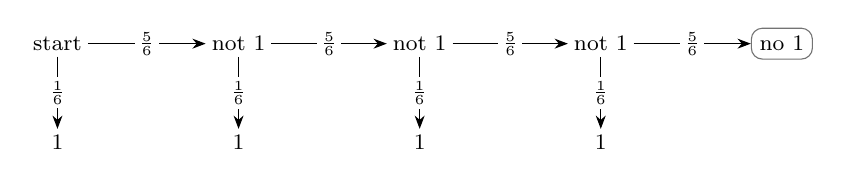
\begin{tikzpicture}[>=Stealth,
   nd/.style={font=\footnotesize,inner sep=2pt},
   term/.style={font=\footnotesize,inner sep=3pt,draw=black!55,rounded corners},
   lbl/.style={font=\scriptsize,fill=white,inner sep=1.5pt,midway}]
% top row: the complement path -- ``not 1'' on every die (prob 5/6 each step)
\node[nd]   (s)  at (0,0)    {start};
\node[nd]   (a1) at (2.3,0)  {not $1$};
\node[nd]   (a2) at (4.6,0)  {not $1$};
\node[nd]   (a3) at (6.9,0)  {not $1$};
\node[term] (a4) at (9.2,0)  {no $1$};
\draw[->] (s)  -- (a1) node[lbl]{$\tfrac56$};
\draw[->] (a1) -- (a2) node[lbl]{$\tfrac56$};
\draw[->] (a2) -- (a3) node[lbl]{$\tfrac56$};
\draw[->] (a3) -- (a4) node[lbl]{$\tfrac56$};
% success stubs: a ``1'' shows up on this die (prob 1/6) -- the event we want
\node[nd] (b0) at (0,-1.25)   {$1$};
\node[nd] (b1) at (2.3,-1.25) {$1$};
\node[nd] (b2) at (4.6,-1.25) {$1$};
\node[nd] (b3) at (6.9,-1.25) {$1$};
\draw[->] (s)  -- (b0) node[lbl]{$\tfrac16$};
\draw[->] (a1) -- (b1) node[lbl]{$\tfrac16$};
\draw[->] (a2) -- (b2) node[lbl]{$\tfrac16$};
\draw[->] (a3) -- (b3) node[lbl]{$\tfrac16$};
\end{tikzpicture}
\end{center}
Following the all-``not~$1$'' branch for all four dice,
\[
  \PP(\text{no }1)=\left(\frac56\right)^4=\frac{625}{1296},\qquad
  \PP(\text{at least one }1)=1-\frac{625}{1296}=\frac{671}{1296}\approx 0.518 .
\]

\begin{example}
A spinner is flicked three times, each flick landing on one of the digits $0$ through $9$ with
equal chance, independently. Find the probability that \emph{at least one} flick shows a $7$.
\end{example}
\whichrule{``At least one $7$'' over independent trials $\Rightarrow$ complement: the opposite
``no $7$ on any flick'' is one product. The equally-likely model supplies the per-flick miss
probability $\tfrac{9}{10}$, but it is the complement rule that turns three overlapping ``a $7$
here'' events into a single subtraction.}
\soln Each flick avoids $7$ with probability $\tfrac{9}{10}$; the three flicks are independent,
so
\[
  \PP(\text{no }7)=\left(\frac{9}{10}\right)^3=\frac{729}{1000},\qquad
  \PP(\text{at least one }7)=1-\frac{729}{1000}=\frac{271}{1000}=0.271 .
\]

\begin{example}
A committee of $4$ is drawn at random from a club of $6$ women and $4$ men. Find the
probability the committee includes \emph{at least one} man.
\end{example}
\whichrule{``At least one man'' is awkward head-on (it splits into one, two, three, or four
men), so we flip to the complement ``all four are women'' --- a single combination count. The
draw is ``at random,'' so the equally-likely model supplies the two counts.}
\soln There are $\binom{10}{4}=210$ equally likely committees. The complement ``no men,'' i.e.\
all four chosen from the $6$ women, numbers $\binom{6}{4}=15$. Hence
\[
  \PP(\text{all women})=\frac{15}{210}=\frac{1}{14},\qquad
  \PP(\text{at least one man})=1-\frac{1}{14}=\frac{13}{14}\approx 0.929 .
\]

\begin{example}
Two fair dice are rolled. Find the probability that \emph{at least one} die shows an even
number.
\end{example}
\whichrule{``At least one even'' inverts cleanly to ``both odd,'' which is a single product over
the two independent dice; the complement rule beats counting the even-bearing outcomes one by
one. The equally-likely model gives each die's odd-probability $\tfrac36$.}
\soln Each die is odd with probability $\tfrac36=\tfrac12$, so ``both odd'' has probability
$\left(\tfrac12\right)^2=\tfrac14$. Therefore
\[
  \PP(\text{at least one even})=1-\frac14=\frac34=0.75 .
\]
Direct check: of $36$ outcomes, $3\times3=9$ have both dice odd, leaving $27$ with at least one
even, and $27/36=3/4$. Agrees.

% =====================================================================
\subsection{Monotonicity and the bounds $0\le\PP\le 1$}
% =====================================================================

\begin{theorem}[Monotonicity and bounds]\label{thm:mono}
If $A\subseteq B$ then $\PP(A)\le\PP(B)$, and in fact $\PP(B)-\PP(A)=\PP(B\cap\comp{A})$.
Consequently $0\le\PP(A)\le 1$ for every event $A$.
\end{theorem}

\begin{proof}
When $A\subseteq B$, write $B$ as the disjoint union of the part inside $A$ and the part of
$B$ outside $A$: $B=A\cup(B\cap\comp{A})$, with $A\cap(B\cap\comp{A})=\varnothing$. By finite
additivity,
\[
  \PP(B)=\PP(A)+\PP(B\cap\comp{A}).
\]
The second term is $\ge 0$ by Axiom~1, so $\PP(B)\ge\PP(A)$, and rearranging gives the stated
difference. For the bounds: $\PP(A)\ge0$ is Axiom~1, and since $A\subseteq S$ monotonicity
gives $\PP(A)\le\PP(S)=1$.
\end{proof}

In the picture $A$ sits inside $B$; the extra shaded crescent is $B\cap\comp{A}$, whose
probability is exactly the gap $\PP(B)-\PP(A)$.
\begin{center}
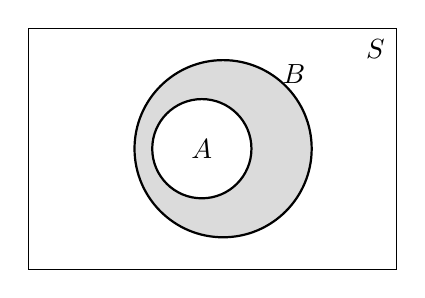
\begin{tikzpicture}[scale=0.9]
  \draw[thin] (-2.6,-1.7) rectangle (2.6,1.7); \node at (2.3,1.4){$S$};
  \fill[black!14] (0.15,0) circle (1.25);
  \fill[white]   (-0.15,0) circle (0.7);
  \draw[thick] (0.15,0) circle (1.25); \node at (1.15,1.05){$B$};
  \draw[thick] (-0.15,0) circle (0.7); \node at (-0.15,0){$A$};
\end{tikzpicture}
\end{center}

\begin{example}
A card is drawn from a standard $52$-card deck. Let $A=\{\text{ace of spades}\}$ and
$B=\{\text{spade}\}$. Without listing every spade, argue $\PP(A)\le\PP(B)$ and give both
values.
\end{example}
\whichrule{The event $A$ \emph{implies} $B$: every ace of spades \emph{is} a spade, i.e.\
$A\subseteq B$. ``$A$ is a special case of $B$'' is the monotonicity trigger; we conclude
$\PP(A)\le\PP(B)$ before computing anything.}
\soln Since the single card ``ace of spades'' is one of the $13$ spades, $A\subseteq B$, so by
monotonicity $\PP(A)\le\PP(B)$. Concretely, with $52$ equally likely cards,
\[
  \PP(A)=\frac{1}{52}\approx 0.019,\qquad
  \PP(B)=\frac{13}{52}=\frac14=0.25,
\]
and indeed $0.019\le 0.25$. The gap $\PP(B)-\PP(A)=\tfrac{12}{52}$ is the probability of
``a spade other than the ace,'' i.e.\ $\PP(B\cap\comp{A})$.

\begin{example}
An analyst claims that for two events, $\PP(A)=0.7$, $\PP(B)=0.4$, and $\PP(A\cap B)=0.55$. Show
the claim is impossible.
\end{example}
\whichrule{$A\cap B\subseteq B$ always, so monotonicity forces $\PP(A\cap B)\le\PP(B)$. This is
a \emph{consistency check}: whenever an intersection probability is quoted, it can never exceed
either single probability.}
\soln Because $A\cap B\subseteq B$, monotonicity requires $\PP(A\cap B)\le\PP(B)$. But the claim
has
\[
  \PP(A\cap B)=0.55 > 0.40=\PP(B),
\]
a contradiction. (Against $\PP(A)=0.7$ the bound is satisfied since $0.55\le0.7$, but violating
it against $\PP(B)$ alone already makes the assignment impossible.) So no probability
function can have these values.

\begin{example}
Someone proposes that a certain event has probability $\PP(A)=1.3$. Why is this nonsense, and
what is the largest a probability can be?
\end{example}
\whichrule{Any single number offered as a probability must satisfy the universal bound
$0\le\PP\le1$ from Theorem (monotonicity). This is the bound used purely as a validity test.}
\soln Since $A\subseteq S$, monotonicity gives $\PP(A)\le\PP(S)=1$. Thus $\PP(A)=1.3$ violates
the upper bound: no event can be ``more than certain.'' Every probability lies in $[0,1]$, with
$0$ for the impossible event and $1$ for the certain event.

\begin{example}
A weather model assigns $\PP(\text{rain})=0.3$ and, for a particular town, $\PP(\text{heavy
rain})$ where ``heavy rain'' implies ``rain.'' Give the tightest bounds the axioms place on
$\PP(\text{heavy rain})$.
\end{example}
\whichrule{``Heavy rain implies rain'' is exactly $A\subseteq B$ with $A=\{\text{heavy}\}$,
$B=\{\text{rain}\}$. Monotonicity caps $\PP(A)$ above by $\PP(B)$, and Axiom~1 caps it below by
$0$. This is a bounding problem, not an exact computation.}
\soln Let $A=\{\text{heavy rain}\}\subseteq B=\{\text{rain}\}$. Then
\[
  0\le\PP(A)\le\PP(B)=0.3 .
\]
So heavy rain can be anywhere from impossible up to as likely as rain itself, but no more; we
cannot pin down a single value without extra information.

\begin{example}
A card is drawn from a standard $52$-card deck. Let $A=\{\text{a red king}\}$ and
$B=\{\text{a king}\}$. Argue $\PP(A)\le\PP(B)$ from the structure, then give both values.
\end{example}
\whichrule{Every red king \emph{is} a king, so $A\subseteq B$: ``$A$ is a special case of $B$''
is the monotonicity trigger, and we may assert $\PP(A)\le\PP(B)$ before any arithmetic. This is
not a union question (no ``or''), so inclusion--exclusion does not enter.}
\soln The two red kings ($\heartsuit,\diamondsuit$) are among the four kings, so $A\subseteq B$
and monotonicity gives $\PP(A)\le\PP(B)$. With $52$ equally likely cards,
\[
  \PP(A)=\frac{2}{52}=\frac{1}{26}\approx0.038,\qquad
  \PP(B)=\frac{4}{52}=\frac{1}{13}\approx0.077,
\]
and indeed $0.038\le0.077$. The gap $\PP(B)-\PP(A)=\tfrac{2}{52}$ is $\PP(B\cap\comp{A})$, the
chance of a \emph{black} king. The nesting is shown below: $A$ sits wholly inside $B$, and the
shaded crescent is exactly that gap.
\begin{center}
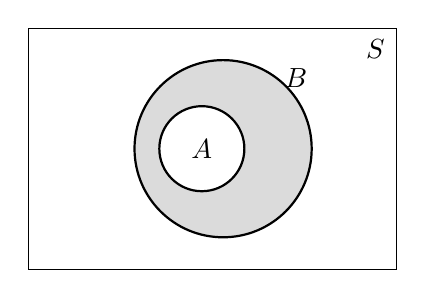
\begin{tikzpicture}[scale=0.9]
  \draw[thin] (-2.6,-1.7) rectangle (2.6,1.7); \node at (2.3,1.4){$S$};
  \fill[black!14] (0.15,0) circle (1.25);
  \fill[white]   (-0.15,0) circle (0.6);
  \draw[thick] (0.15,0) circle (1.25); \node at (1.18,1){$B$};
  \draw[thick] (-0.15,0) circle (0.6); \node at (-0.15,0){$A$};
\end{tikzpicture}
\end{center}

\begin{example}
A quality report claims that for two events $\PP(A)=0.30$, $\PP(B)=0.50$, and
$\PP(A\cup B)=0.45$. Show this is impossible.
\end{example}
\whichrule{For any events, $B\subseteq A\cup B$, so monotonicity forces $\PP(A\cup B)\ge\PP(B)$:
a union can never be \emph{less} likely than one of its parts. This is a consistency check on a
quoted union, not a value to compute.}
\soln Since $B\subseteq A\cup B$, monotonicity requires $\PP(A\cup B)\ge\PP(B)$. But the claim
has
\[
  \PP(A\cup B)=0.45 < 0.50=\PP(B),
\]
a contradiction --- the union came out smaller than $B$ alone, which no probability function
allows. So these three numbers cannot coexist.

\begin{example}
Two events satisfy $\PP(A)=0.85$ and $\PP(B)=0.75$. Without knowing the overlap, find the
smallest possible value of $\PP(A\cap B)$.
\end{example}
\whichrule{We want a guaranteed lower bound on an overlap from the singles alone. Combine
monotonicity with the bound $\PP(A\cup B)\le1$: because the union cannot exceed $1$, the
intersection cannot be too small. (This ``squeeze'' is the Bonferroni inequality, a direct
child of the axioms, not the equally-likely model.)}
\soln Rearrange two-event inclusion--exclusion and use $\PP(A\cup B)\le1$:
\[
  \PP(A\cap B)=\PP(A)+\PP(B)-\PP(A\cup B)\ \ge\ \PP(A)+\PP(B)-1=0.85+0.75-1=0.60 .
\]
So at least $60\%$ of the time \emph{both} occur; the overlap can be as large as $0.75$ (if
$A\subseteq B$) but never below $0.60$. The bound is forced purely by ``probabilities cannot
exceed $1$.''

% =====================================================================
\subsection{Inclusion--exclusion for two events}
% =====================================================================

\begin{theorem}[Inclusion--exclusion, two events]\label{thm:ie2}
For any events $A,B$,
\[
  \PP(A\cup B)=\PP(A)+\PP(B)-\PP(A\cap B).
\]
\end{theorem}

\begin{proof}
Decompose the union into three disjoint pieces: $A$-only, $B$-only, and both:
\[
  A\cup B=(A\cap\comp{B})\ \cup\ (\comp{A}\cap B)\ \cup\ (A\cap B),
\]
all pairwise disjoint. By finite additivity,
$\PP(A\cup B)=\PP(A\cap\comp{B})+\PP(\comp{A}\cap B)+\PP(A\cap B)$. Now $\PP(A)=\PP(A\cap\comp{B})
+\PP(A\cap B)$ and $\PP(B)=\PP(\comp{A}\cap B)+\PP(A\cap B)$, so adding $\PP(A)+\PP(B)$ counts
the overlap $\PP(A\cap B)$ \emph{twice}. Subtracting it once corrects the double-count, giving
the formula.
\end{proof}

The reason a bare sum fails is visible in the Venn picture: $\PP(A)+\PP(B)$ paints the lens
$A\cap B$ twice, so we subtract it once.
\begin{center}\vennUnion\qquad\vennInter\end{center}

\begin{example}
In a town, a household subscribes to the newspaper with probability $0.55$, to a streaming
service with probability $0.65$, and to \emph{both} with probability $0.40$. Find the
probability a household subscribes to \emph{at least one} of the two.
\end{example}
\whichrule{We want ``newspaper \emph{or} streaming'' (the union) and the two events clearly
\emph{overlap} (some households have both, $0.40\ne0$). Both singles and the overlap are
given, which is the exact data signature of two-event inclusion--exclusion. The complement rule
is not simplest here because the overlap is supplied directly.}
\soln Let $N=\{\text{newspaper}\}$ and $S=\{\text{streaming}\}$. Then
\[
  \PP(N\cup S)=\PP(N)+\PP(S)-\PP(N\cap S)=0.55+0.65-0.40=0.80 .
\]
A plain sum $0.55+0.65=1.20$ would exceed $1$; subtracting the double-counted overlap restores
a legal $0.80$.

\begin{example}
Draw one card from a standard deck. Find $\PP(\text{king or heart})$.
\end{example}
\whichrule{``King \emph{or} heart'' is a union, and the two events overlap in the single card
\emph{king of hearts}, so a raw sum would double-count it. Two-event inclusion--exclusion with
the equally-likely model supplies each piece.}
\soln With $|S|=52$: there are $4$ kings, $13$ hearts, and $1$ card that is both (the king of
hearts). So
\[
  \PP(\text{king}\cup\text{heart})
  =\frac{4}{52}+\frac{13}{52}-\frac{1}{52}=\frac{16}{52}=\frac{4}{13}\approx 0.308 .
\]
Direct count check: the favourable cards are the $13$ hearts plus the $3$ non-heart kings,
$16$ in all --- matching.

\begin{example}
For two events, $\PP(A)=0.5$, $\PP(B)=0.3$, and $\PP(A\cup B)=0.6$. Find $\PP(A\cap B)$ and
then $\PP(\text{exactly one of }A,B)$.
\end{example}
\whichrule{All four quantities in the two-event formula appear, three known and one unknown,
so we solve inclusion--exclusion \emph{backwards} for the overlap. ``Exactly one'' then comes
from removing the double overlap from the union.}
\soln
\steplabel{Solve for the overlap.} Rearranging the formula,
\[
  \PP(A\cap B)=\PP(A)+\PP(B)-\PP(A\cup B)=0.5+0.3-0.6=0.2 .
\]
\steplabel{Exactly one.} ``Exactly one of $A,B$'' is the union minus the both-part:
\[
  \PP(\text{exactly one})=\PP(A\cup B)-\PP(A\cap B)=0.6-0.2=0.4 .
\]
Equivalently ``exactly one'' is the symmetric difference shaded here:
\begin{center}\vennExactlyOne\end{center}

\begin{example}
A fair die is rolled. Let $A=\{\text{even}\}=\{2,4,6\}$ and $B=\{\text{at least }5\}=\{5,6\}$.
Find $\PP(A\cup B)$.
\end{example}
\whichrule{``Even \emph{or} at least $5$'' is a union with a genuine overlap: the face $6$ lies
in both. Two-event inclusion--exclusion under equal likelihood. (Adding $3/6+2/6$ blindly would
count the $6$ twice.)}
\soln With $|S|=6$: $\PP(A)=\tfrac{3}{6}$, $\PP(B)=\tfrac{2}{6}$, and $A\cap B=\{6\}$ so
$\PP(A\cap B)=\tfrac{1}{6}$. Hence
\[
  \PP(A\cup B)=\frac{3}{6}+\frac{2}{6}-\frac{1}{6}=\frac{4}{6}=\frac{2}{3}\approx 0.667 .
\]
Check: $A\cup B=\{2,4,5,6\}$, four outcomes, $4/6$. Agrees.

\begin{example}
$30\%$ of students take a statistics course, $20\%$ take an economics course, and $12\%$ take
both. What fraction take \emph{neither}?
\end{example}
\whichrule{This is two rules in sequence. ``Or'' with overlap $\Rightarrow$ inclusion--exclusion
for ``at least one course''; then ``neither'' is the \emph{complement} of ``at least one.''
Recognising the two-step union-then-complement structure is the key.}
\soln
\steplabel{At least one course.}
\[
  \PP(\text{stats}\cup\text{econ})=0.30+0.20-0.12=0.38 .
\]
\steplabel{Neither, by complement.}
\[
  \PP(\text{neither})=1-\PP(\text{stats}\cup\text{econ})=1-0.38=0.62 .
\]
So $62\%$ take neither course. The region ``neither'' is the unshaded exterior of both circles:
\begin{center}\vennCompUnion\end{center}

\begin{example}
In a cafe survey, $\PP(\text{a customer orders coffee})=0.70$,
$\PP(\text{orders a pastry})=0.45$, and $\PP(\text{orders both})=0.30$. Find the probability a
customer orders coffee \emph{or} a pastry.
\end{example}
\whichrule{We want the union ``coffee or pastry'' and the two events overlap (some order both,
$0.30\ne0$). All three inputs --- two singles and the both --- are handed to us, the exact
signature of two-event inclusion--exclusion. A bare sum would double-count the both-orderers.}
\soln
\[
  \PP(\text{coffee}\cup\text{pastry})=0.70+0.45-0.30=0.85 .
\]
The naive sum $0.70+0.45=1.15$ exceeds $1$; subtracting the once-double-counted overlap $0.30$
restores the legal value $0.85$.

\begin{example}
Two fair dice are rolled. Let $A=\{\text{sum is even}\}$ and $B=\{\text{sum}\ge9\}$. Find
$\PP(A\cup B)$.
\end{example}
\whichrule{``Sum even \emph{or} sum $\ge9$'' is a union whose events overlap (e.g.\ a sum of
$10$ is both even and $\ge9$), so a raw sum double-counts. Two-event inclusion--exclusion with
the equally-likely model over the $36$ outcomes supplies each count.}
\soln Of $36$ equally likely pairs: a sum is even in $|A|=18$ ways; a sum is $\ge9$ (i.e.\
$9,10,11,12$) in $4+3+2+1=10$ ways, so $|B|=10$; and ``even \emph{and} $\ge9$'' means the sum is
$10$ or $12$, giving $3+1=4$ ways, so $|A\cap B|=4$. Hence
\[
  \PP(A\cup B)=\frac{18}{36}+\frac{10}{36}-\frac{4}{36}=\frac{24}{36}=\frac{2}{3}\approx0.667 .
\]
The shaded lens below is the double-counted overlap $A\cap B$, removed once:
\begin{center}\vennInter\end{center}

\begin{example}
A card is drawn from a standard deck. Find $\PP(\text{king or red card})$.
\end{example}
\whichrule{``King \emph{or} red'' is a union, and the events overlap in the two red kings, so a
plain sum over-counts those cards. Two-event inclusion--exclusion with the equally-likely model
gives each piece from a direct card count.}
\soln With $|S|=52$: there are $4$ kings, $26$ red cards, and $2$ cards that are both (kings of
hearts and diamonds). So
\[
  \PP(\text{king}\cup\text{red})=\frac{4}{52}+\frac{26}{52}-\frac{2}{52}=\frac{28}{52}
  =\frac{7}{13}\approx0.538 .
\]
Direct check: the $26$ red cards plus the $2$ black kings give $28$ favourable cards --- matching.

\begin{example}
For two events, $\PP(A)=0.60$, $\PP(A\cup B)=0.80$, and $\PP(A\cap B)=0.25$. Find $\PP(B)$, then
$\PP(\text{exactly one of }A,B)$.
\end{example}
\whichrule{Three of the four quantities in the two-event formula are given, so we solve it
\emph{backwards} for the fourth, $\PP(B)$. ``Exactly one'' is then the union with the both-part
stripped out. The overlap is supplied, so the complement route offers no shortcut.}
\soln
\steplabel{Solve for $\PP(B)$.} Rearranging $\PP(A\cup B)=\PP(A)+\PP(B)-\PP(A\cap B)$,
\[
  \PP(B)=\PP(A\cup B)-\PP(A)+\PP(A\cap B)=0.80-0.60+0.25=0.45 .
\]
\steplabel{Exactly one.} Remove the overlap from the union:
\[
  \PP(\text{exactly one})=\PP(A\cup B)-\PP(A\cap B)=0.80-0.25=0.55 .
\]
This is the symmetric difference shaded here:
\begin{center}\vennExactlyOne\end{center}

% =====================================================================
\subsection{Inclusion--exclusion for three events}
% =====================================================================

\begin{theorem}[Inclusion--exclusion, three events]\label{thm:ie3}
For any events $A,B,C$,
\[
  \PP(A\cup B\cup C)=\PP(A)+\PP(B)+\PP(C)
   -\PP(A\cap B)-\PP(A\cap C)-\PP(B\cap C)
   +\PP(A\cap B\cap C).
\]
\end{theorem}

\begin{proof}
Group $A\cup B\cup C=(A\cup B)\cup C$ and apply the two-event rule twice. First,
\[
  \PP\big((A\cup B)\cup C\big)=\PP(A\cup B)+\PP(C)-\PP\big((A\cup B)\cap C\big).
\]
Expand $\PP(A\cup B)=\PP(A)+\PP(B)-\PP(A\cap B)$. For the last term, distribute:
$(A\cup B)\cap C=(A\cap C)\cup(B\cap C)$, so by the two-event rule again
\[
  \PP\big((A\cup B)\cap C\big)=\PP(A\cap C)+\PP(B\cap C)-\PP(A\cap B\cap C),
\]
using $(A\cap C)\cap(B\cap C)=A\cap B\cap C$. Substituting both expansions and collecting terms
yields the stated identity.
\end{proof}

\begin{remark}[Why the alternating signs]
Count how often each region is tallied. A point in exactly one event is added once and never
subtracted: weight $1$. A point in exactly two events is added twice, subtracted once: weight
$2-1=1$. A point in all three is added three times, subtracted three times, added once:
$3-3+1=1$. Every point of the union is counted exactly once --- which is what the formula must
do.
\end{remark}

A three-circle Venn diagram makes the seven regions explicit; the central petal $A\cap B\cap C$
is the one added back at the end.
\begin{center}
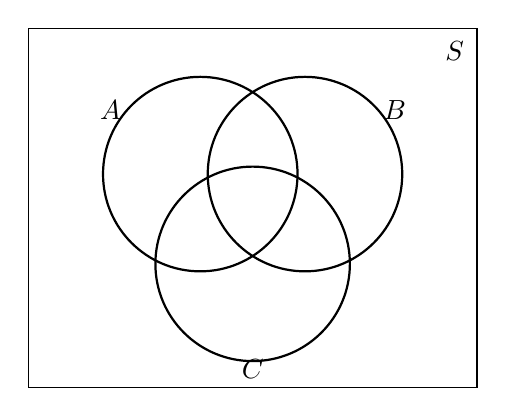
\begin{tikzpicture}[scale=0.95]
  \draw[thin] (-3,-2.4) rectangle (3,2.4); \node at (2.7,2.1){$S$};
  \draw[thick] (-0.7,0.45) circle (1.3); \node at (-1.9,1.3){$A$};
  \draw[thick] ( 0.7,0.45) circle (1.3); \node at ( 1.9,1.3){$B$};
  \draw[thick] ( 0,-0.75) circle (1.3);  \node at ( 0,-2.15){$C$};
\end{tikzpicture}
\end{center}

\begin{example}
A streaming subscriber base reports: $\PP(A)=0.50$ watch dramas, $\PP(B)=0.40$ comedies,
$\PP(C)=0.30$ documentaries; pairwise, $\PP(A\cap B)=0.20$, $\PP(A\cap C)=0.15$,
$\PP(B\cap C)=0.10$; and $\PP(A\cap B\cap C)=0.05$ watch all three genres. What fraction watch
\emph{at least one} of the three genres?
\end{example}
\whichrule{``At least one of \emph{three} overlapping events'' is the three-event union, and the
problem hands us all seven inputs (three singles, three pairs, one triple) --- the full data
signature of three-event inclusion--exclusion. The complement would require ``watches none,''
which is not given directly.}
\soln Substitute into the three-event formula:
\[
  \PP(A\cup B\cup C)=0.50+0.40+0.30-0.20-0.15-0.10+0.05 .
\]
Singles sum to $1.20$; pairwise sum to $0.45$; triple is $0.05$. So
\[
  \PP(A\cup B\cup C)=1.20-0.45+0.05=0.80 .
\]
Thus $80\%$ watch at least one genre (and, by complement, $20\%$ watch none).

\begin{example}
Draw one card from a standard deck. Find $\PP(\text{spade, or face card, or ace})$. (Face cards
are J, Q, K.)
\end{example}
\whichrule{Three properties joined by \emph{or}, all able to coincide on a single card (e.g.\
the king of spades is a spade \emph{and} a face card), so three-event inclusion--exclusion with
counts. Note ``ace'' and ``face card'' are disjoint, which will zero one pairwise term.}
\soln Let $A=\text{spade}$ ($13$), $B=\text{face card}$ ($12$), $C=\text{ace}$ ($4$); $|S|=52$.
\steplabel{Pairwise overlaps.} Spades that are face cards: J,Q,K of spades $=3$, so
$|A\cap B|=3$. Spades that are aces: ace of spades $=1$, so $|A\cap C|=1$. Face cards that are
aces: none (an ace is not a face card), so $|B\cap C|=0$.
\steplabel{Triple overlap.} A spade that is both a face card and an ace: impossible, so
$|A\cap B\cap C|=0$.
\steplabel{Assemble.}
\[
  |A\cup B\cup C|=13+12+4-3-1-0+0=25,\qquad
  \PP=\frac{25}{52}\approx 0.481 .
\]

\begin{example}
Three fair dice are rolled. Find the probability that \emph{at least one} die shows a $6$,
using inclusion--exclusion (so as to compare with the complement method).
\end{example}
\whichrule{``At least one six among three dice'' is the union of $A_i=\{\text{die }i\text{ shows
}6\}$ for $i=1,2,3$. With three overlapping events we may use three-event inclusion--exclusion;
here all the pieces are easy products. (The complement $(5/6)^3$ is quicker, and we will
confirm the two agree.)}
\soln Each $\PP(A_i)=\tfrac16$; each pair $\PP(A_i\cap A_j)=\tfrac{1}{36}$ (two specified dice
both $6$); the triple $\PP(A_1\cap A_2\cap A_3)=\tfrac{1}{216}$. Then
\[
  \PP(A_1\cup A_2\cup A_3)
  =3\cdot\frac16-3\cdot\frac{1}{36}+\frac{1}{216}
  =\frac{108}{216}-\frac{18}{216}+\frac{1}{216}=\frac{91}{216}\approx 0.421 .
\]
\steplabel{Cross-check by complement.}
$\PP(\text{at least one }6)=1-\left(\tfrac56\right)^3=1-\tfrac{125}{216}=\tfrac{91}{216}$.
The two methods agree.

\begin{example}
Among the integers $1$ through $100$ a number is chosen at random. Find the probability it is
divisible by $2$, $3$, or $5$.
\end{example}
\whichrule{``Divisible by $2$ \emph{or} $3$ \emph{or} $5$'' is a three-event union; the events
overlap (e.g.\ $30$ is divisible by all three), so three-event inclusion--exclusion is needed.
Counting multiples (and multiples of products) gives every term; the equally-likely model turns
counts into probabilities.}
\soln Let $A,B,C$ be ``divisible by $2,3,5$.'' Count multiples in $\{1,\dots,100\}$ with
floor division:
\[
  \begin{gathered}
  |A|=50,\quad |B|=33,\quad |C|=20;\\[2pt]
  |A\cap B|=\lfloor 100/6\rfloor=16,\quad |A\cap C|=\lfloor 100/10\rfloor=10,\quad
  |B\cap C|=\lfloor 100/15\rfloor=6;
  \end{gathered}
\]
\[
  |A\cap B\cap C|=\lfloor 100/30\rfloor=3 .
\]
Therefore
\[
  |A\cup B\cup C|=50+33+20-16-10-6+3=74,\qquad \PP=\frac{74}{100}=0.74 .
\]

\begin{example}
A language survey of a region reports: $\PP(A)=0.45$ speak Spanish, $\PP(B)=0.30$ French,
$\PP(C)=0.20$ German; pairwise $\PP(A\cap B)=0.12$, $\PP(A\cap C)=0.08$, $\PP(B\cap C)=0.06$;
and $\PP(A\cap B\cap C)=0.03$ speak all three. What fraction speak \emph{at least one} of the
three languages?
\end{example}
\whichrule{``At least one of \emph{three} overlapping events'' is the three-event union, and all
seven inputs (three singles, three pairs, one triple) are supplied --- the full data signature
of three-event inclusion--exclusion. ``Speaks none'' is not given, so the complement is not a
shortcut here.}
\soln Substitute into the three-event formula:
\[
  \PP(A\cup B\cup C)=0.45+0.30+0.20-0.12-0.08-0.06+0.03 .
\]
Singles sum to $0.95$; pairwise to $0.26$; triple is $0.03$. So
\[
  \PP(A\cup B\cup C)=0.95-0.26+0.03=0.72 .
\]
Thus $72\%$ speak at least one language (and $28\%$ speak none of the three).

\begin{example}
Draw one card from a standard deck. Find $\PP(\text{spade, or heart, or face card})$. (Face
cards are J, Q, K.)
\end{example}
\whichrule{Three properties joined by \emph{or}, with some genuine overlaps (e.g.\ the jack of
spades is a spade \emph{and} a face card), so three-event inclusion--exclusion with counts. A
useful wrinkle: ``spade'' and ``heart'' are \emph{disjoint}, which zeroes one pairwise term and
the triple term.}
\soln Let $A=\text{spade}$ ($13$), $B=\text{heart}$ ($13$), $C=\text{face card}$ ($12$);
$|S|=52$.
\steplabel{Pairwise overlaps.} A card cannot be both a spade and a heart, so $|A\cap B|=0$.
Spade face cards (J,Q,K of spades) number $3$, so $|A\cap C|=3$; heart face cards likewise give
$|B\cap C|=3$.
\steplabel{Triple overlap.} A card that is a spade \emph{and} a heart is impossible, so
$|A\cap B\cap C|=0$.
\steplabel{Assemble.}
\[
  |A\cup B\cup C|=13+13+12-0-3-3+0=32,\qquad \PP=\frac{32}{52}=\frac{8}{13}\approx0.615 .
\]
In the three-circle picture, the $A$ and $B$ circles are drawn apart (disjoint), each meeting
only the face-card circle $C$:
\begin{center}
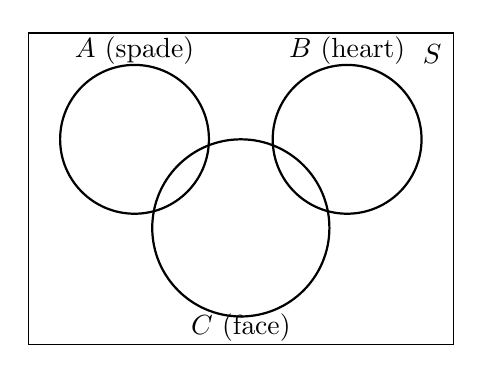
\begin{tikzpicture}[scale=0.9]
  \draw[thin] (-3,-2.2) rectangle (3,2.2); \node at (2.7,1.9){$S$};
  \draw[thick] (-1.5,0.7) circle (1.05); \node at (-1.5,1.95){$A$ (spade)};
  \draw[thick] ( 1.5,0.7) circle (1.05); \node at ( 1.5,1.95){$B$ (heart)};
  \draw[thick] ( 0,-0.55) circle (1.25); \node at ( 0,-1.95){$C$ (face)};
\end{tikzpicture}
\end{center}

\begin{example}
Three fair dice are rolled. Find the probability that \emph{at least one} die shows a $5$ or a
$6$, using inclusion--exclusion (and check against the complement).
\end{example}
\whichrule{``At least one die in $\{5,6\}$'' is the union of $A_i=\{\text{die }i\text{ shows }5
\text{ or }6\}$ over $i=1,2,3$. Three overlapping events $\Rightarrow$ three-event
inclusion--exclusion; here each $\PP(A_i)=\tfrac{2}{6}$ and the overlaps are clean products.
The complement $(4/6)^3$ is faster and will confirm the answer.}
\soln Each $\PP(A_i)=\tfrac{2}{6}=\tfrac13$; each pair $\PP(A_i\cap A_j)=\left(\tfrac13\right)^2
=\tfrac19$; the triple $\PP(A_1\cap A_2\cap A_3)=\left(\tfrac13\right)^3=\tfrac{1}{27}$. Then
\[
  \PP(A_1\cup A_2\cup A_3)=3\cdot\frac13-3\cdot\frac19+\frac{1}{27}
  =\frac{27}{27}-\frac{9}{27}+\frac{1}{27}=\frac{19}{27}\approx0.704 .
\]
\steplabel{Cross-check by complement.}
$1-\left(\tfrac46\right)^3=1-\left(\tfrac23\right)^3=1-\tfrac{8}{27}=\tfrac{19}{27}$. The two
methods agree.

% =====================================================================
\subsection{The equally-likely (classical) model}
% =====================================================================

\begin{theorem}[Equally-likely outcomes]\label{thm:equallylikely}
Suppose $S$ is finite with $|S|=N$ outcomes, all equally likely. Then each single outcome has
probability $1/N$, and for every event $A$,
\[
  \PP(A)=\frac{|A|}{|S|}=\frac{\text{number of outcomes favourable to }A}{\text{total number of
  outcomes}}.
\]
\end{theorem}

\begin{proof}
Let the outcomes be $s_1,\dots,s_N$ with common probability $p$. They are disjoint and their
union is $S$, so by additivity and normalization $Np=\PP(S)=1$, giving $p=1/N$. For any event
$A=\{s_{i_1},\dots,s_{i_k}\}$ with $k=|A|$ outcomes, additivity gives
$\PP(A)=kp=k/N=|A|/|S|$.
\end{proof}

\begin{remark}
This model applies \emph{only} when symmetry justifies equal likelihood --- a \emph{fair} coin
or die, a \emph{well-shuffled} deck, a draw made \emph{at random}. If outcomes are weighted
(a loaded die, biased coin), revert to the axioms and add the actual weights. The whole task
becomes counting $|A|$ and $|S|$, which is why combinatorics (covered later) is the natural
sequel.
\end{remark}

\begin{example}
Two fair dice are rolled. Find the probability that the sum equals $8$.
\end{example}
\whichrule{``Two \emph{fair} dice'' guarantees $36$ equally likely outcomes $\Rightarrow$ the
classical model $|A|/|S|$. We simply count the outcomes giving a sum of $8$. No complement or
union structure is present.}
\soln The $36$ ordered pairs are equally likely. The pairs summing to $8$ are
$(2,6)$, $(3,5)$, $(4,4)$, $(5,3)$, $(6,2)$, i.e.\ five of them. So
\[
  \PP(\text{sum}=8)=\frac{5}{36}\approx 0.139 .
\]
The two-dice grid below shows the diagonal of $8$'s (marked $\bullet$); count the dots, divide
by $36$.
\begin{center}
\begin{tabular}{c|cccccc}
\toprule
$+$ & 1 & 2 & 3 & 4 & 5 & 6\\
\midrule
1 & 2 & 3 & 4 & 5 & 6 & 7\\
2 & 3 & 4 & 5 & 6 & 7 & $\bullet$\\
3 & 4 & 5 & 6 & 7 & $\bullet$ & 9\\
4 & 5 & 6 & 7 & $\bullet$ & 9 & 10\\
5 & 6 & 7 & $\bullet$ & 9 & 10 & 11\\
6 & 7 & $\bullet$ & 9 & 10 & 11 & 12\\
\bottomrule
\end{tabular}
\end{center}

\begin{example}
An urn holds $5$ red, $4$ blue, and $3$ green balls. One ball is drawn at random. Find the
probability it is \emph{not} red.
\end{example}
\whichrule{``Drawn at random'' from a finite urn $\Rightarrow$ equally likely over the $12$
balls. ``Not red'' is a complement, but the count is so direct we can read $|A|$ off
immediately --- either route gives the same fraction $|A|/|S|$.}
\soln Total balls $|S|=5+4+3=12$. Non-red balls number $4+3=7$. So
\[
  \PP(\text{not red})=\frac{7}{12}\approx 0.583 .
\]
(As a complement check: $\PP(\text{red})=\tfrac{5}{12}$, and $1-\tfrac{5}{12}=\tfrac{7}{12}$.)

\begin{example}
A committee of $3$ is chosen at random from $7$ people, of whom $3$ are biologists and $4$ are
chemists. Find the probability the committee is \emph{all chemists}.
\end{example}
\whichrule{``Chosen at random'' from a fixed group $\Rightarrow$ equally likely over all
unordered committees, so $\PP=|A|/|S|$ with $|S|=\binom{7}{3}$. Order does not matter, which
fixes the use of combinations in both counts.}
\soln The number of committees is $|S|=\binom{7}{3}=35$. An all-chemist committee chooses $3$ of
the $4$ chemists: $|A|=\binom{4}{3}=4$. Hence
\[
  \PP(\text{all chemists})=\frac{\binom{4}{3}}{\binom{7}{3}}=\frac{4}{35}\approx 0.114 .
\]

\begin{example}
A box contains $20$ light bulbs, $4$ of them defective. Two bulbs are drawn at random without
replacement. Find the probability that \emph{exactly one} is defective.
\end{example}
\whichrule{``At random without replacement'' from a finite box $\Rightarrow$ equally likely over
the $\binom{20}{2}$ unordered pairs. ``Exactly one defective'' is a counting event: choose one
defective and one good. Pure classical model.}
\soln Total pairs $|S|=\binom{20}{2}=190$. ``Exactly one defective'' picks $1$ of the $4$
defectives and $1$ of the $16$ good bulbs:
\[
  |A|=\binom{4}{1}\binom{16}{1}=4\cdot16=64,\qquad
  \PP=\frac{64}{190}=\frac{32}{95}\approx 0.337 .
\]

\begin{example}
A fair coin is tossed $3$ times, recording the ordered sequence of heads and tails. Find the
probability of getting exactly $2$ heads.
\end{example}
\whichrule{A \emph{fair} coin tossed a fixed number of times with the ordered sequence recorded
gives $2^3=8$ equally likely outcomes $\Rightarrow$ classical model. We count sequences with
exactly two H's. No overlap or complement structure is needed.}
\soln The $8$ equally likely sequences are HHH, HHT, HTH, THH, HTT, THT, TTH, TTT. Exactly two
heads occur in HHT, HTH, THH --- three sequences. Therefore
\[
  \PP(\text{exactly }2\text{ heads})=\frac{3}{8}=0.375 .
\]
The favourable count $3=\binom{3}{2}$ is the number of ways to place the two heads among the
three tosses.

\begin{example}
Two fair dice are rolled. Find the probability that the sum equals $6$.
\end{example}
\whichrule{``Two \emph{fair} dice'' gives $36$ equally likely ordered outcomes $\Rightarrow$ the
classical model $|A|/|S|$; we just count the pairs that sum to $6$. No ``or'' or ``at least''
structure appears, so neither inclusion--exclusion nor the complement is called for.}
\soln The pairs summing to $6$ are $(1,5),(2,4),(3,3),(4,2),(5,1)$ --- five of them. So
\[
  \PP(\text{sum}=6)=\frac{5}{36}\approx0.139 .
\]
The grid marks the anti-diagonal of $6$'s ($\bullet$); count the dots and divide by $36$:
\begin{center}
\begin{tabular}{c|cccccc}
\toprule
$+$ & 1 & 2 & 3 & 4 & 5 & 6\\
\midrule
1 & 2 & 3 & 4 & 5 & $\bullet$ & 7\\
2 & 3 & 4 & 5 & $\bullet$ & 7 & 8\\
3 & 4 & 5 & $\bullet$ & 7 & 8 & 9\\
4 & 5 & $\bullet$ & 7 & 8 & 9 & 10\\
5 & $\bullet$ & 7 & 8 & 9 & 10 & 11\\
6 & 7 & 8 & 9 & 10 & 11 & 12\\
\bottomrule
\end{tabular}
\end{center}

\begin{example}
A committee of $4$ is chosen at random from $9$ people, of whom $5$ are seniors and $4$ are
juniors. Find the probability the committee is \emph{all seniors}.
\end{example}
\whichrule{``Chosen at random'' from a fixed group $\Rightarrow$ equally likely over all
unordered committees, so $\PP=|A|/|S|$ with $|S|=\binom{9}{4}$. Order does not matter (a
committee is a set), which fixes combinations in both counts.}
\soln The number of committees is $|S|=\binom{9}{4}=126$. An all-senior committee chooses $4$ of
the $5$ seniors: $|A|=\binom{5}{4}=5$. Hence
\[
  \PP(\text{all seniors})=\frac{\binom{5}{4}}{\binom{9}{4}}=\frac{5}{126}\approx0.040 .
\]

\begin{example}
An urn holds $6$ red and $4$ white balls. Two are drawn at random without replacement. Find the
probability that \emph{both} are red.
\end{example}
\whichrule{``At random without replacement'' from a finite urn $\Rightarrow$ equally likely over
the $\binom{10}{2}$ unordered pairs. ``Both red'' is a pure counting event (choose $2$ of the
$6$ reds), so the classical model applies with no complement or union needed.}
\soln Total pairs $|S|=\binom{10}{2}=45$. Both-red pairs number $\binom{6}{2}=15$. So
\[
  \PP(\text{both red})=\frac{\binom{6}{2}}{\binom{10}{2}}=\frac{15}{45}=\frac{1}{3}\approx0.333 .
\]
The stars-and-balls sketch shows the pool we draw from --- $6$ shaded (red) and $4$ open
(white); both picks must come from the shaded group:
\begin{center}
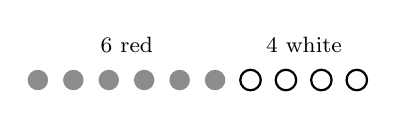
\begin{tikzpicture}[scale=1]
  \foreach \x in {0,...,5}{\fill[black!45] (0.45*\x,0) circle (0.13);}
  \foreach \x in {6,...,9}{\draw[thick] (0.45*\x,0) circle (0.13);}
  \node[font=\footnotesize] at (1.13,0.45) {$6$ red};
  \node[font=\footnotesize] at (3.38,0.45) {$4$ white};
\end{tikzpicture}
\end{center}

\begin{example}
Two digits are dialled at random and independently, each uniform on $0$--$9$. Find the
probability that the two digits are \emph{equal}.
\end{example}
\whichrule{Two independent uniform digits give $10\times10=100$ equally likely ordered pairs
$\Rightarrow$ classical model. ``Equal'' is a counting event (the diagonal pairs), so we just
tally $|A|$ over $|S|=100$.}
\soln Of the $100$ equally likely pairs $(d_1,d_2)$, the equal ones are
$(0,0),(1,1),\dots,(9,9)$ --- exactly $10$. So
\[
  \PP(\text{equal})=\frac{10}{100}=\frac{1}{10}=0.1 .
\]

\begin{example}
On a $2\times2$ city grid, a courier walks from the bottom-left corner to the top-right corner
using only unit steps right (R) or up (U); every such shortest route is equally likely. Find the
probability the route passes through the centre lattice point.
\end{example}
\whichrule{``Every shortest route equally likely'' $\Rightarrow$ classical model over the set of
monotone lattice paths; we count favourable paths over total paths, $|A|/|S|$. Each path is a
rearrangement of two R's and two U's, so the counts are binomial coefficients --- a clean
combinatorial equally-likely problem, not a union or complement.}
\soln A shortest route is any arrangement of $2$ R's and $2$ U's, so
$|S|=\binom{4}{2}=6$. To pass through the centre point $(1,1)$, the route must reach $(1,1)$ in
$2$ steps (one R, one U: $\binom{2}{1}=2$ ways) and then finish to $(2,2)$ in $2$ steps
(one R, one U: $\binom{2}{1}=2$ ways), giving $|A|=2\times2=4$. Hence
\[
  \PP(\text{through centre})=\frac{4}{6}=\frac{2}{3}\approx0.667 .
\]
The grid shows the lattice; the marked centre point $(1,1)$ is the one every favourable route
must visit:
\begin{center}
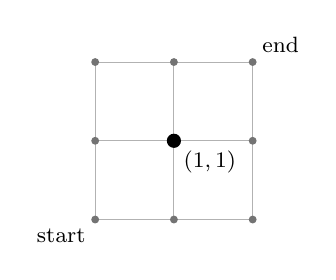
\begin{tikzpicture}[scale=1]
  \draw[step=1,black!30,thin] (0,0) grid (2,2);
  \foreach \x in {0,1,2}{\foreach \y in {0,1,2}{\fill[black!55] (\x,\y) circle (0.05);}}
  \fill[black] (1,1) circle (0.09); \node[below right] at (1,1){\footnotesize $(1,1)$};
  \node[below left]  at (0,0){\footnotesize start};
  \node[above right] at (2,2){\footnotesize end};
\end{tikzpicture}
\end{center}

\section{Conditional Probability, Total Probability, and Bayes}

A single idea underlies everything that follows: learning that an event has occurred shrinks
the relevant sample space and forces us to rescale. From that one definition flow the
multiplication rule (a product of stage-by-stage chances), the law of total probability (a
weighted sum over disjoint cases), and Bayes' rule (running the conditioning backwards from
evidence to cause). The practical skill is recognising \emph{which} of those four moves a
given problem is asking for.

\begin{strategy}[Which rule does this problem need?]
Read the problem and ask, in order:
\begin{itemize}[leftmargin=1.4em,itemsep=2pt,topsep=2pt]
\item \keyword{Are you told one thing happened and asked the chance of another, in the same
trial?} Phrases like ``given that,'' ``among those who,'' ``if we know,'' ``restricted to''
signal \keyword{conditional probability}: $\PP(A\given B)=\PP(A\cap B)/\PP(B)$. You divide
by the probability of the thing you were told.
\item \keyword{Do you want the chance that several things ALL happen, described as a
sequence of stages?} Words like ``and then,'' ``followed by,'' ``both,'' ``all three''
point to the \keyword{multiplication / chain rule}: multiply the chance of the first stage
by the conditional chance of the next, and so on. You build $\PP(A\cap B)$ from
$\PP(A)\PP(B\given A)$.
\item \keyword{Does the experiment split into mutually exclusive cases, and you want the
overall chance of some outcome?} A setup such as ``one of several machines / urns / routes
is chosen, then \dots'' with the case unknown calls for the \keyword{law of total
probability}: sum $\PP(B\given A_i)\PP(A_i)$ over the cases $A_i$.
\item \keyword{Are you given the forward chances $\PP(B\given A_i)$ but asked for a
backward one $\PP(A_j\given B)$?} The tell is that the conditioning is reversed from how
the data are stated: ``a positive test came back --- what is the chance of disease?'' or
``the part was defective --- which supplier likely made it?'' That is \keyword{Bayes'
rule}: posterior $\propto$ prior $\times$ likelihood.
\end{itemize}
Quick contrast. Total probability and Bayes use the \emph{same} ingredients (a partition
plus conditional probabilities); the only difference is the question. If you want
$\PP(B)$, use total probability. If you already imagine $B$ has happened and want to know
which case caused it, use Bayes --- and total probability is exactly the denominator you
will need.
\end{strategy}

\subsection{Definition of conditional probability}

\begin{definition}
Let $B$ be an event with $\PP(B)>0$. The \keyword{conditional probability} of $A$ given $B$
is
\[
  \PP(A\given B)=\frac{\PP(A\cap B)}{\PP(B)}.
\]
\end{definition}

The picture: conditioning on $B$ throws away everything outside $B$ and treats $B$ as the
new universe of outcomes. The numerator $\PP(A\cap B)$ keeps only the part of $A$ that
survives inside $B$; the denominator $\PP(B)$ renormalises so that the new universe has
total probability $1$.

\begin{center}
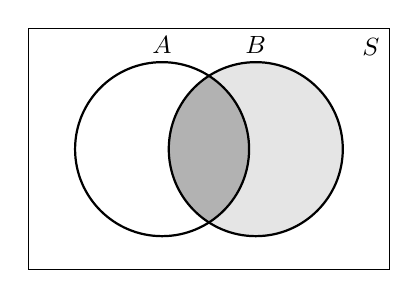
\begin{tikzpicture}[scale=0.85,every node/.style={font=\small}]
  % B-circle = the new universe (light tint); A-cap-B lens = the part that survives (darker)
  \fill[black!10] (0.7,0) circle (1.3);
  \begin{scope}\clip (0.7,0) circle (1.3);\fill[black!30] (-0.7,0) circle (1.3);\end{scope}
  \draw[thin] (-2.7,-1.8) rectangle (2.7,1.8);
  \node[anchor=north east,inner sep=2pt] at (2.64,1.74){$S$};
  \draw[thick] (-0.7,0) circle (1.3);
  \draw[thick] ( 0.7,0) circle (1.3);
  \node at (-0.7,1.55){$A$};
  \node at ( 0.7,1.55){$B$};
\end{tikzpicture}\\[3pt]
{\footnotesize Conditioning on $B$ makes the $B$-circle the new universe (light); the darker
lens $A\cap B$ is the surviving part of $A$, rescaled by $\PP(B)$ so that
$\PP(A\mid B)=\PP(A\cap B)/\PP(B)$.}
\end{center}

For a fixed conditioning event $B$, the map $A\mapsto\PP(A\given B)$ satisfies all three
axioms (it is nonnegative, gives $B$ probability $1$, and is countably additive), so every
earlier theorem holds for it. In particular $\PP(\comp{A}\given B)=1-\PP(A\given B)$, and
inclusion--exclusion works inside the conditional world. When outcomes are equally likely,
conditioning is just recounting: $\PP(A\given B)=|A\cap B|/|B|$.

\begin{example}[Reading a die roll]
A fair six-sided die is rolled once. Let $A=\{\text{the result is prime}\}$, namely
$\{2,3,5\}$, and $B=\{\text{the result is at least }4\}$, namely $\{4,5,6\}$. Find
$\PP(A\given B)$.
\end{example}
\whichrule{The phrase ``at least $4$'' is handed to us as known information --- it restricts
attention to the three outcomes $\{4,5,6\}$ --- and then we ask the chance of a prime
\emph{within} that restricted world. That ``probability of one thing within a known other
thing, same single roll'' is the signature of conditional probability. There are no stages
to multiply (one roll), and no cases to sum over, so the multiplication rule and total
probability do not apply.}
\soln
\steplabel{Step 1: identify the events as subsets.}
$B=\{4,5,6\}$ and $A\cap B=\{5\}$ (the only prime that is at least $4$).
\steplabel{Step 2: count inside the conditioned space.}
Outcomes are equally likely, so
\[
  \PP(A\given B)=\frac{|A\cap B|}{|B|}=\frac{1}{3}.
\]
\steplabel{Check via the definition.}
$\PP(A\cap B)=1/6$ and $\PP(B)=3/6$, so $\PP(A\given B)=(1/6)/(3/6)=1/3$. The plain
(unconditional) chance of a prime was $3/6=1/2$; knowing the result is large pulled it down
to $1/3$.

\begin{example}[A two-way table of survey responses]
A club of $200$ members is classified by whether they own a bicycle and whether they
commute by car:
\begin{center}
\begin{tabular}{lccc}
\toprule
 & Commutes by car & Does not & Total\\
\midrule
Owns a bicycle      & $30$ & $70$ & $100$\\
Does not own one    & $80$ & $20$ & $100$\\
\midrule
Total               & $110$& $90$ & $200$\\
\bottomrule
\end{tabular}
\end{center}
A member is chosen at random. Given that the member commutes by car, what is the
probability they own a bicycle?
\end{example}
\whichrule{``Given that the member commutes by car'' fixes a sub-population: we look only at
the $110$ car commuters, then ask what fraction of \emph{them} own a bicycle. A two-way
count table with a ``given that'' question is a textbook cue for conditional probability;
the conditioning event becomes the new denominator.}
\soln
\steplabel{Step 1: the conditioning event.}
Let $C=\{\text{commutes by car}\}$ and $K=\{\text{owns a bicycle}\}$. The column total gives
$\PP(C)=110/200$, and the cell gives $\PP(K\cap C)=30/200$.
\steplabel{Step 2: apply the definition.}
\[
  \PP(K\given C)=\frac{\PP(K\cap C)}{\PP(C)}=\frac{30/200}{110/200}=\frac{30}{110}=\frac{3}{11}\approx 0.273.
\]
Equivalently, read straight off the table: of $110$ car commuters, $30$ own a bicycle.

\begin{example}[Conditioning changes the answer]
Two fair coins are tossed. Let $A$ be ``at least one head'' and $B$ ``the two coins match''
(both heads or both tails). Find $\PP(B\given A)$ and compare with $\PP(B)$.
\end{example}
\whichrule{We are asked for the chance of ``matching'' \emph{restricted to} the outcomes
that already have at least one head. The known event $A$ reshapes the sample space; we want
a probability inside it. Single experiment, no sequence of independent stages to multiply,
so this is conditioning, not the multiplication rule.}
\soln
The equally likely outcomes are $\{HH,HT,TH,TT\}$.
\steplabel{Step 1: list the relevant events.}
$A=\{HH,HT,TH\}$ so $\PP(A)=3/4$; $B=\{HH,TT\}$; and $A\cap B=\{HH\}$ so $\PP(A\cap B)=1/4$.
\steplabel{Step 2: divide.}
\[
  \PP(B\given A)=\frac{1/4}{3/4}=\frac13.
\]
Unconditionally $\PP(B)=2/4=1/2$. Learning there is at least one head rules out $TT$, which
removes one of the two ``matching'' outcomes, dropping the chance of a match from $1/2$ to
$1/3$.

\begin{example}[Cards drawn without replacement]
From a standard $52$-card deck, two cards are dealt without replacement. Given that the
first card is a heart, what is the probability the second card is also a heart?
\end{example}
\whichrule{The first card's suit is stated as known, and we want the second card's chance in
that light --- a single conditional probability, not a product. (Contrast the next
subsection, where we instead want the chance that \emph{both} are hearts; that ``both''
version is the multiplication rule. Here only the second card's conditional chance is
requested.)}
\soln
\steplabel{Step 1: update the deck.}
Once a heart is removed and known, $51$ cards remain, $12$ of them hearts.
\steplabel{Step 2: equally likely second card.}
\[
  \PP(\text{2nd heart}\given\text{1st heart})=\frac{12}{51}=\frac{4}{17}\approx 0.235.
\]
The information ``first was a heart'' both shrinks the deck and depletes the hearts, so the
conditional chance $12/51$ sits just below the unconditional $13/52=1/4$.

\begin{example}[Two dice, conditioned on a five appearing]
Two fair dice are rolled. Given that at least one die shows a five, what is the probability
that the sum of the two dice is at least nine?
\end{example}
\whichrule{``At least one die shows a five'' is handed to us as known information, restricting
the $36$ equally likely ordered pairs to the eleven that contain a five; we then ask the
chance of a large sum \emph{within} that restricted set. Probability of one event inside a
known other event, in the same single roll of the pair, is conditional probability. There is
no sequence of stages to multiply and no partition to sum over.}
\soln
\steplabel{Step 1: list the conditioning event.}
Let $B=\{\text{a five appears}\}$. The ordered pairs in $B$ are the five rows $(5,j)$, the
five columns $(i,5)$, with $(5,5)$ counted once, giving $|B|=11$.
\steplabel{Step 2: count the favourable outcomes inside $B$.}
Among those eleven, the ones with sum $\ge 9$ are $(5,4),(4,5),(5,5),(5,6),(6,5)$, so
$|A\cap B|=5$.
\steplabel{Step 3: divide counts in the conditioned world.}
\[
  \PP(A\given B)=\frac{|A\cap B|}{|B|}=\frac{5}{11}\approx 0.455.
\]
\begin{center}
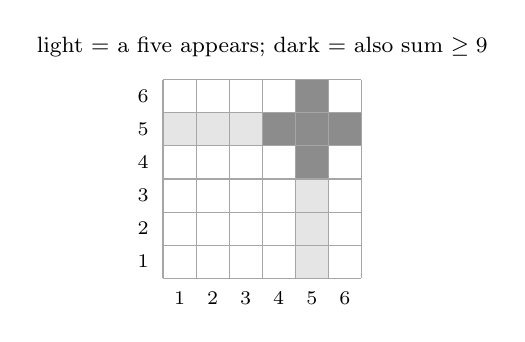
\begin{tikzpicture}[scale=0.42,font=\scriptsize]
  \draw[step=1,black!35,thin] (0,0) grid (6,6);
  % shade row/column for "a five appears"
  \foreach \x in {0,...,5}{\fill[black!10] (\x,4) rectangle (\x+1,5);}
  \foreach \y in {0,...,5}{\fill[black!10] (4,\y) rectangle (5,\y+1);}
  % favourable cells (sum>=9 and a five): die1=x+1, die2=y+1
  \foreach \c in {(4,3),(3,4),(4,4),(4,5),(5,4)}{\fill[black!45] \c rectangle ++(1,1);}
  \draw[step=1,black!35,thin] (0,0) grid (6,6);
  \foreach \x in {1,...,6}{\node at (\x-0.5,-0.6){\x};}
  \foreach \y in {1,...,6}{\node at (-0.6,\y-0.5){\y};}
  \node at (3,7){\footnotesize light = a five appears; dark = also sum $\ge 9$};
\end{tikzpicture}
\end{center}
Unconditionally, $\PP(\text{sum}\ge 9)=10/36\approx0.28$; learning that a five is present
shifts the odds upward, since a five is a large face that helps build a large sum.

\begin{example}[A committee, conditioned on having a man]
A club has $5$ women and $3$ men. Two members are chosen at random to form a subcommittee.
Given that the subcommittee includes at least one man, what is the probability that both
members are men?
\end{example}
\whichrule{``Includes at least one man'' is told to us and shrinks the sample space to those
pairs containing a man; we then ask for the chance of an all-male pair \emph{within} that
group. That is conditional probability on equally likely two-person subsets. We are not
multiplying ordered stages and not partitioning into weighted cases.}
\soln
\steplabel{Step 1: total and the conditioning event.}
There are $\binom{8}{2}=28$ equally likely pairs. The all-women pairs number
$\binom{5}{2}=10$, so the event $B=\{\text{at least one man}\}$ has $|B|=28-10=18$.
\steplabel{Step 2: favourable pairs inside $B$.}
Both men: $\binom{3}{2}=3$ pairs, and every such pair already lies in $B$, so
$|A\cap B|=3$.
\steplabel{Step 3: divide.}
\[
  \PP(A\given B)=\frac{3}{18}=\frac16\approx 0.167.
\]
Counting the complement of $B$ (no men) was the quick route to $|B|$; trying to list
``at least one man'' directly is the kind of detour the complement trick avoids.

\begin{example}[A drawn ticket, conditioned on parity]
A ticket is drawn at random from those numbered $1$ through $20$. Given that the number
drawn is even, what is the probability that it is a multiple of three?
\end{example}
\whichrule{``Even'' is the given information, narrowing the twenty equally likely tickets to
the ten even ones; we then ask the chance of a multiple of three \emph{among the evens}. One
draw, one piece of known information, a probability computed inside it: conditional
probability by recounting. No stages, no weighted partition.}
\soln
\steplabel{Step 1: the conditioned space.}
The even tickets are $\{2,4,6,8,10,12,14,16,18,20\}$, so $|B|=10$.
\steplabel{Step 2: favourable evens.}
Multiples of three that are even (i.e.\ multiples of six) up to $20$ are $\{6,12,18\}$, so
$|A\cap B|=3$.
\steplabel{Step 3: divide.}
\[
  \PP(A\given B)=\frac{3}{10}=0.30.
\]
The unconditional chance of a multiple of three among $1$--$20$ is $6/20=0.30$ as well: here
the conditioning happens to leave the proportion unchanged, a reminder that conditioning need
not move the answer.

\subsection{The multiplication rule and the chain rule}

Clearing the denominator in the definition gives a formula for the probability that two
events both occur.

\begin{theorem}[Multiplication rule]
If $\PP(B)>0$ then $\PP(A\cap B)=\PP(B)\,\PP(A\given B)$, and symmetrically, if
$\PP(A)>0$, $\PP(A\cap B)=\PP(A)\,\PP(B\given A)$.
\end{theorem}

\begin{proof}
Multiply both sides of $\PP(A\given B)=\PP(A\cap B)/\PP(B)$ by $\PP(B)$ to obtain
$\PP(A\cap B)=\PP(B)\PP(A\given B)$. Swapping the roles of $A$ and $B$ gives the second
form, since $A\cap B=B\cap A$.
\end{proof}

Iterating the rule one stage at a time yields the chain rule for any number of events.

\begin{theorem}[Chain rule]
For events $A_1,\dots,A_n$ with $\PP(A_1\cap\cdots\cap A_{n-1})>0$,
\[
  \PP(A_1\cap A_2\cap\cdots\cap A_n)
  =\PP(A_1)\,\PP(A_2\given A_1)\,\PP(A_3\given A_1\cap A_2)\cdots
   \PP(A_n\given A_1\cap\cdots\cap A_{n-1}).
\]
\end{theorem}

\begin{proof}
Induct on $n$. The case $n=2$ is the multiplication rule. Assume the formula for $n-1$
events and set $C=A_1\cap\cdots\cap A_{n-1}$. By the multiplication rule,
$\PP(C\cap A_n)=\PP(C)\,\PP(A_n\given C)$. Replacing $\PP(C)$ by its $(n-1)$-factor
expansion (valid because $\PP(C)\ge\PP(A_1\cap\cdots\cap A_{n-1})>0$ keeps every
intermediate conditioning event of positive probability) gives the $n$-factor formula.
\end{proof}

The chain rule is exactly what a probability \keyword{tree} computes: the probability of a
leaf is the product of the branch probabilities along the path to it, each branch carrying
the conditional probability of that step given everything earlier on the path.

\begin{example}[Both cards hearts]
Two cards are dealt without replacement from a $52$-card deck. What is the probability that
both are hearts?
\end{example}
\whichrule{The word ``both'' asks for $\PP(\text{1st heart}\cap\text{2nd heart})$ --- an
intersection built from two dependent stages. That is the multiplication rule. We are not
told either card in advance (so it is not a bare conditional probability), and the two
stages are dependent (no replacement), so we must use the \emph{conditional} chance for the
second factor, not a plain product of marginals.}
\soln
\steplabel{Step 1: chance of the first stage.}
$\PP(\text{1st heart})=13/52=1/4$.
\steplabel{Step 2: conditional chance of the second.}
Given a heart is gone, $\PP(\text{2nd heart}\given\text{1st heart})=12/51$.
\steplabel{Step 3: multiply.}
\[
  \PP(\text{both hearts})=\frac{13}{52}\cdot\frac{12}{51}=\frac{1}{4}\cdot\frac{12}{51}
  =\frac{12}{204}=\frac{1}{17}\approx 0.0588.
\]
\begin{center}
\begin{tikzpicture}[>=Stealth,grow=right,
  level 1/.style={sibling distance=40mm,level distance=30mm},
  level 2/.style={sibling distance=20mm,level distance=34mm},font=\small]
\node{}
  child{node{$\comp{H_1}$}
    child{node{$H_2$} edge from parent node[midway,fill=white,inner sep=2pt]{$\frac{13}{51}$}}
    child{node{$\comp{H_2}$} edge from parent node[midway,fill=white,inner sep=2pt]{$\frac{38}{51}$}}
    edge from parent node[midway,fill=white,inner sep=2pt]{$\frac{39}{52}$}}
  child{node{$H_1$}
    child{node{$H_2$: $\frac{1}{17}$} edge from parent node[midway,fill=white,inner sep=2pt]{$\frac{12}{51}$}}
    child{node{$\comp{H_2}$} edge from parent node[midway,fill=white,inner sep=2pt]{$\frac{39}{51}$}}
    edge from parent node[midway,fill=white,inner sep=2pt]{$\frac{13}{52}$}};
\end{tikzpicture}
\end{center}
($H_i$ = ``card $i$ is a heart.'' The top path multiplies $\tfrac{13}{52}\cdot\tfrac{12}{51}$.)

\begin{example}[Three defectives in a row]
A box contains $20$ widgets, of which $5$ are defective. Three are drawn at random without
replacement. What is the probability that all three are defective?
\end{example}
\whichrule{``All three'' is an intersection across three dependent stages, so it is the chain
rule. Each draw changes the contents of the box, so the stages are dependent and each
factor must be conditioned on the earlier draws --- a plain $(5/20)^3$ would be wrong
because it ignores depletion.}
\soln
Let $D_i=\{\text{the }i\text{th draw is defective}\}$.
\[
  \PP(D_1\cap D_2\cap D_3)
  =\PP(D_1)\,\PP(D_2\given D_1)\,\PP(D_3\given D_1\cap D_2)
  =\frac{5}{20}\cdot\frac{4}{19}\cdot\frac{3}{18}.
\]
\steplabel{Compute.}
\[
  =\frac{5\cdot4\cdot3}{20\cdot19\cdot18}=\frac{60}{6840}=\frac{1}{114}\approx 0.00877.
\]
Each successful draw both shrinks the box and removes a defective, so every factor falls.

\begin{example}[An assembly line that must clear three checks]
A part must pass three independent-quality stages to ship. Stage~1 passes $90\%$ of parts.
Of the parts that clear stage~1, stage~2 passes $80\%$. Of those that clear both,
stage~3 passes $95\%$. What fraction of parts ship?
\end{example}
\whichrule{Each percentage is stated \emph{conditionally on surviving the previous stage}
(``of the parts that clear stage~1\dots''), and we want the chance of clearing all three
--- an intersection of sequential, dependent-in-description stages. That is the chain rule:
multiply the stagewise conditional pass rates.}
\soln
Let $P_i=\{\text{clears stage }i\}$.
\[
  \PP(P_1\cap P_2\cap P_3)=\PP(P_1)\,\PP(P_2\given P_1)\,\PP(P_3\given P_1\cap P_2)
  =0.90\times0.80\times0.95.
\]
\steplabel{Compute.}
$0.90\times0.80=0.72$, and $0.72\times0.95=0.684$. So about $\mathbf{68.4\%}$ of parts ship.
\begin{center}
\begin{tikzpicture}[>=Stealth,grow=right,
  level 1/.style={sibling distance=33mm,level distance=24mm},
  level 2/.style={sibling distance=16mm,level distance=24mm},
  level 3/.style={sibling distance=12mm,level distance=30mm},font=\small]
\node{}
  child{node{fail} edge from parent node[midway,fill=white,inner sep=2pt]{$0.10$}}
  child{node{$P_1$}
    child{node{fail} edge from parent node[midway,fill=white,inner sep=2pt]{$0.20$}}
    child{node{$P_2$}
      child{node{fail} edge from parent node[midway,fill=white,inner sep=2pt]{$0.05$}}
      child{node{ship $0.684$} edge from parent node[midway,fill=white,inner sep=2pt]{$0.95$}}
      edge from parent node[midway,fill=white,inner sep=2pt]{$0.80$}}
    edge from parent node[midway,fill=white,inner sep=2pt]{$0.90$}};
\end{tikzpicture}
\end{center}

\begin{example}[Drawing a specific ordered hand]
A bag holds $4$ red, $3$ green, and $2$ blue marbles. Three marbles are drawn one at a time
without replacement. What is the probability the colours come out red, then green, then
red, in that order?
\end{example}
\whichrule{A specified \emph{ordered} sequence of dependent draws is precisely a single path
through a tree, and the chain rule gives a path's probability as the product of its branch
probabilities. The order is fixed, so we do not sum over arrangements; the draws deplete the
bag, so each factor is conditioned on the earlier ones.}
\soln
Start with $9$ marbles ($4$R, $3$G, $2$B).
\[
  \PP(R,G,R)=\frac{4}{9}\cdot\frac{3}{8}\cdot\frac{3}{7},
\]
where after one red the reds drop to $3$ of $8$, and after the green the reds are still $3$
but only $7$ marbles remain.
\steplabel{Compute.}
\[
  =\frac{4\cdot3\cdot3}{9\cdot8\cdot7}=\frac{36}{504}=\frac{1}{14}\approx 0.0714.
\]

\begin{example}[Both cards aces]
Two cards are dealt without replacement from a standard $52$-card deck. What is the
probability that both are aces?
\end{example}
\whichrule{``Both'' asks for the intersection $\PP(\text{1st ace}\cap\text{2nd ace})$ across
two dependent draws, which the multiplication rule builds as a product. Neither card is
revealed in advance, so it is not a bare conditional probability; and because the first ace
is not replaced, the second factor must be conditioned, not a plain $(4/52)^2$.}
\soln
\steplabel{Step 1: first stage.}
$\PP(\text{1st ace})=4/52=1/13$.
\steplabel{Step 2: conditional second stage.}
With one ace gone, $\PP(\text{2nd ace}\given\text{1st ace})=3/51$.
\steplabel{Step 3: multiply.}
\[
  \PP(\text{both aces})=\frac{4}{52}\cdot\frac{3}{51}=\frac{12}{2652}=\frac{1}{221}\approx 0.00452.
\]

\begin{example}[Red then blue from a bag]
A bag holds $5$ red and $4$ blue marbles. Two are drawn one at a time without replacement.
What is the probability the first is red and the second is blue?
\end{example}
\whichrule{A specified ordered outcome (red, then blue) over two dependent draws is one path
through a tree, and the chain rule makes a path's probability the product of its branch
chances. The order is fixed, so we do not sum over arrangements; the draw is without
replacement, so the second factor is conditioned on the first.}
\soln
\steplabel{Step 1: first stage.}
$\PP(\text{1st red})=5/9$.
\steplabel{Step 2: conditional second stage.}
A red is gone, leaving $8$ marbles of which $4$ are blue, so
$\PP(\text{2nd blue}\given\text{1st red})=4/8=1/2$.
\steplabel{Step 3: multiply.}
\[
  \PP(R\text{ then }B)=\frac{5}{9}\cdot\frac12=\frac{5}{18}\approx 0.278.
\]
\begin{center}
\begin{tikzpicture}[>=Stealth,grow=right,
  level 1/.style={sibling distance=36mm,level distance=28mm},
  level 2/.style={sibling distance=18mm,level distance=34mm},font=\small]
\node{}
  child{node{$B_1$}
    child{node{$B,R$} edge from parent node[midway,fill=white,inner sep=2pt]{$\frac{5}{8}$}}
    child{node{$B,B$} edge from parent node[midway,fill=white,inner sep=2pt]{$\frac{3}{8}$}}
    edge from parent node[midway,fill=white,inner sep=2pt]{$\frac{4}{9}$}}
  child{node{$R_1$}
    child{node{$R,B$: $\frac{5}{18}$} edge from parent node[midway,fill=white,inner sep=2pt]{$\frac{4}{8}$}}
    child{node{$R,R$} edge from parent node[midway,fill=white,inner sep=2pt]{$\frac{4}{8}$}}
    edge from parent node[midway,fill=white,inner sep=2pt]{$\frac{5}{9}$}};
\end{tikzpicture}
\end{center}
($R_1,B_1$ = colour of the first marble. The top path multiplies
$\tfrac59\cdot\tfrac48=\tfrac{5}{18}$.)

\begin{example}[At least one bad fuse: the complement trick]
A box of $12$ fuses contains $3$ defective ones. Four fuses are drawn at random without
replacement. What is the probability that at least one of the four is defective?
\end{example}
\whichrule{``At least one'' over several dependent draws is awkward to attack head-on, but its
complement --- ``none defective'' --- is a single ordered survival path, exactly what the
chain rule multiplies. So we use the multiplication rule on the complement, then subtract
from $1$. A direct case-by-case sum would be the slow, error-prone route.}
\soln
\steplabel{Step 1: probability that no draw is defective.}
The $9$ good fuses must be drawn each time:
\[
  \PP(\text{none bad})=\frac{9}{12}\cdot\frac{8}{11}\cdot\frac{7}{10}\cdot\frac{6}{9}
  =\frac{3024}{11{,}880}=\frac{14}{55}.
\]
\steplabel{Step 2: complement.}
\[
  \PP(\text{at least one bad})=1-\frac{14}{55}=\frac{41}{55}\approx 0.745.
\]
Subtracting one easy product beats summing the ``exactly one,'' ``exactly two,'' and
``exactly three'' cases separately.

\begin{example}[Four reds in a row]
Four cards are dealt without replacement from a $52$-card deck. What is the probability that
all four are red?
\end{example}
\whichrule{``All four'' is an intersection across four dependent stages, so it is the chain
rule: each card removed changes the deck, and each factor is conditioned on the cards already
drawn. The naive $(26/52)^4=(1/2)^4$ would wrongly ignore that reds are depleted as we go.}
\soln
Let $R_i=\{\text{card }i\text{ is red}\}$. There are $26$ reds at the start.
\[
  \PP(R_1\cap R_2\cap R_3\cap R_4)
  =\frac{26}{52}\cdot\frac{25}{51}\cdot\frac{24}{50}\cdot\frac{23}{49}.
\]
\steplabel{Compute.}
\[
  =\frac{26\cdot25\cdot24\cdot23}{52\cdot51\cdot50\cdot49}=\frac{358{,}800}{6{,}497{,}400}=\frac{46}{833}\approx 0.0552.
\]
The honest answer $0.0552$ sits below the careless $(1/2)^4=0.0625$, precisely because each
red drawn makes the next red slightly less likely.

\subsection{The law of total probability}

When an experiment naturally breaks into mutually exclusive cases, we can find the
probability of any event by handling each case separately and weighting by how likely that
case is.

\begin{definition}
A \keyword{partition} of $S$ is a collection of events $A_1,\dots,A_n$ that are pairwise
disjoint ($A_i\cap A_j=\varnothing$ for $i\ne j$), exhaust the space ($\bigcup_i A_i=S$),
and satisfy $\PP(A_i)>0$ for each $i$.
\end{definition}

\begin{theorem}[Law of total probability]
If $A_1,\dots,A_n$ partition $S$, then for every event $B$,
\[
  \PP(B)=\sum_{i=1}^n \PP(B\given A_i)\,\PP(A_i).
\]
\end{theorem}

\begin{proof}
Because the $A_i$ partition $S$, the events $B\cap A_i$ are pairwise disjoint and their
union is $B\cap S=B$. By countable additivity (Axiom~3),
$\PP(B)=\sum_i\PP(B\cap A_i)$. The multiplication rule rewrites each term as
$\PP(B\cap A_i)=\PP(B\given A_i)\PP(A_i)$, giving the stated sum.
\end{proof}

In tree language: each first-stage branch is a case $A_i$ with weight $\PP(A_i)$; from it a
branch to $B$ carries $\PP(B\given A_i)$; the probability of $B$ is the sum of the path
products that end in $B$.

\begin{center}
\begin{tikzpicture}[>=Stealth,grow=right,
  level 1/.style={sibling distance=30mm,level distance=24mm},
  level 2/.style={sibling distance=15mm,level distance=26mm},font=\small]
\node{}
  child{node{$A_3$} child{node{$B$} edge from parent node[midway,fill=white,inner sep=2pt]{$\PP(B\given A_3)$}} child{node{$\comp B$}}}
  child{node{$A_2$} child{node{$B$} edge from parent node[midway,fill=white,inner sep=2pt]{$\PP(B\given A_2)$}} child{node{$\comp B$}}}
  child{node{$A_1$} child{node{$B$} edge from parent node[midway,fill=white,inner sep=2pt]{$\PP(B\given A_1)$}} child{node{$\comp B$}}};
\node at (5.6,-5.2){\footnotesize $\PP(B)=\sum_i \PP(A_i)\,\PP(B\given A_i)$ sums the $B$-leaves.};
\end{tikzpicture}
\end{center}

\begin{example}[Two suppliers feeding a line]
A factory buys bolts from two suppliers. Supplier~X provides $70\%$ of the bolts and
$2\%$ of X's bolts are defective; supplier~Y provides the other $30\%$ and $6\%$ of Y's
bolts are defective. A bolt is picked at random from the combined stock. What is the
probability it is defective?
\end{example}
\whichrule{The stock splits into two exhaustive, mutually exclusive cases (came from X, came
from Y) with known weights, and the defect rate is given \emph{per case}. We want the
overall defect chance with the source unknown --- a weighted sum across the cases, i.e.\ the
law of total probability. It is not Bayes because the question runs forward (overall chance
of defective), not backward (which supplier).}
\soln
Let $D=\{\text{defective}\}$, with cases $X$ and $Y$.
\[
  \PP(D)=\PP(D\given X)\PP(X)+\PP(D\given Y)\PP(Y)=(0.02)(0.70)+(0.06)(0.30).
\]
\steplabel{Compute.}
$=0.014+0.018=0.032$. So $\PP(D)=\mathbf{0.032}$ (a $3.2\%$ overall defect rate).
\begin{center}
\begin{tikzpicture}[>=Stealth,grow=right,
  level 1/.style={sibling distance=36mm,level distance=26mm},
  level 2/.style={sibling distance=18mm,level distance=30mm},font=\small]
\node{}
  child{node{$Y$}
    child{node{$D$: $0.018$} edge from parent node[midway,fill=white,inner sep=2pt]{$0.06$}}
    child{node{$\comp D$} edge from parent node[midway,fill=white,inner sep=2pt]{$0.94$}}
    edge from parent node[midway,fill=white,inner sep=2pt]{$0.30$}}
  child{node{$X$}
    child{node{$D$: $0.014$} edge from parent node[midway,fill=white,inner sep=2pt]{$0.02$}}
    child{node{$\comp D$} edge from parent node[midway,fill=white,inner sep=2pt]{$0.98$}}
    edge from parent node[midway,fill=white,inner sep=2pt]{$0.70$}};
\node at (6.4,-3.6){\footnotesize $\PP(D)=0.014+0.018=0.032$.};
\end{tikzpicture}
\end{center}

\begin{example}[Pick an urn, then a chip]
Urn~I holds $2$ red and $3$ white chips; urn~II holds $4$ red and $1$ white. A fair coin
decides which urn to use, then one chip is drawn. What is the probability the chip is red?
\end{example}
\whichrule{The choice of urn partitions the experiment into two equally likely cases, and the
red-chip chance is given \emph{conditional on the urn}. With the urn unknown, the overall
red chance is the weighted sum --- total probability. The two-stage ``choose a case, then
observe'' structure is the classic trigger.}
\soln
Let $R=\{\text{red}\}$.
\[
  \PP(R)=\PP(R\given\text{I})\PP(\text{I})+\PP(R\given\text{II})\PP(\text{II})
  =\frac25\cdot\frac12+\frac45\cdot\frac12.
\]
\steplabel{Compute.}
$=\frac15+\frac25=\frac35=0.6$. So $\PP(R)=\mathbf{3/5}$.

\begin{example}[Weather and a late train]
On a given morning the weather is rainy with probability $0.3$ and clear with probability
$0.7$. The commuter's train is late $40\%$ of rainy mornings but only $10\%$ of clear
mornings. What is the probability the train is late on a random morning?
\end{example}
\whichrule{``Rainy'' and ``clear'' form a partition of the morning, and lateness is given
per weather case. We want the unconditional chance of lateness, so we average the
case-by-case lateness rates by their weather weights: the law of total probability. No
reversal is requested, so this is not Bayes (yet).}
\soln
Let $L=\{\text{late}\}$, with cases $\text{Rain}$ and $\text{Clear}$.
\[
  \PP(L)=\PP(L\given\text{Rain})\PP(\text{Rain})+\PP(L\given\text{Clear})\PP(\text{Clear})
  =(0.40)(0.30)+(0.10)(0.70).
\]
\steplabel{Compute.}
$=0.12+0.07=0.19$. So the train is late with probability $\mathbf{0.19}$.

\begin{example}[Three machines of unequal output]
Three machines produce, respectively, $50\%$, $30\%$, and $20\%$ of a day's output. Their
defect rates are $1\%$, $3\%$, and $4\%$. A finished item is selected at random. What is
the probability it is defective?
\end{example}
\whichrule{A three-case partition (which machine made it) with per-machine defect rates and
an overall question is total probability with three terms. The presence of three exhaustive
weighted cases, not two, does not change the rule --- just the number of summands.}
\soln
Let $D=\{\text{defective}\}$ and $M_1,M_2,M_3$ the machines.
\[
  \PP(D)=\sum_{i=1}^3\PP(D\given M_i)\PP(M_i)
  =(0.01)(0.50)+(0.03)(0.30)+(0.04)(0.20).
\]
\steplabel{Compute.}
$=0.005+0.009+0.008=0.022$. So $\PP(D)=\mathbf{0.022}$.
\begin{center}
\begin{tabular}{lccc}
\toprule
Machine & Share $\PP(M_i)$ & Defect rate $\PP(D\given M_i)$ & Contribution\\
\midrule
$M_1$ & $0.50$ & $0.01$ & $0.005$\\
$M_2$ & $0.30$ & $0.03$ & $0.009$\\
$M_3$ & $0.20$ & $0.04$ & $0.008$\\
\midrule
\multicolumn{3}{r}{Total $\PP(D)$} & $0.022$\\
\bottomrule
\end{tabular}
\end{center}

\begin{example}[Two routes to work]
A commuter takes the highway $60\%$ of mornings and the back road the other $40\%$. The
highway makes her late $15\%$ of the time; the back road makes her late $30\%$ of the time.
What is the probability she is late on a random morning?
\end{example}
\whichrule{The morning splits into two exhaustive, mutually exclusive cases (highway or back
road) with known weights, and lateness is given \emph{per route}. With the route unaveraged,
the overall late chance is the weighted sum, the law of total probability. It is not Bayes:
the question runs forward to the overall rate, not backward from lateness to a route.}
\soln
Let $L=\{\text{late}\}$ with cases $H$ (highway) and $R$ (back road).
\[
  \PP(L)=\PP(L\given H)\PP(H)+\PP(L\given R)\PP(R)=(0.15)(0.60)+(0.30)(0.40).
\]
\steplabel{Compute.}
$=0.09+0.12=0.21$. So $\PP(L)=\mathbf{0.21}$.

\begin{example}[Three prize boxes]
A game-show contestant picks one of three boxes at random with probabilities $0.30$,
$0.45$, and $0.25$. Box~1 contains a prize with chance $0.20$, box~2 with chance $0.50$,
and box~3 with chance $0.90$. What is the probability the chosen box holds a prize?
\end{example}
\whichrule{Which box is chosen forms a three-case partition with given weights, and the
prize chance is stated \emph{conditional on the box}. With the box left general, the overall
prize chance is the weighted sum over the three cases, the law of total probability. Three
weighted cases instead of two changes only the number of summands, not the rule.}
\soln
Let $W=\{\text{prize}\}$ and $B_1,B_2,B_3$ the boxes.
\[
  \PP(W)=\sum_{i=1}^3\PP(W\given B_i)\PP(B_i)=(0.20)(0.30)+(0.50)(0.45)+(0.90)(0.25).
\]
\steplabel{Compute.}
$=0.06+0.225+0.225=0.51$. So $\PP(W)=\mathbf{0.51}$.
\begin{center}
\begin{tabular}{lccc}
\toprule
Box & Weight $\PP(B_i)$ & Prize rate $\PP(W\given B_i)$ & Contribution\\
\midrule
$B_1$ & $0.30$ & $0.20$ & $0.060$\\
$B_2$ & $0.45$ & $0.50$ & $0.225$\\
$B_3$ & $0.25$ & $0.90$ & $0.225$\\
\midrule
\multicolumn{3}{r}{Total $\PP(W)$} & $0.510$\\
\bottomrule
\end{tabular}
\end{center}

\begin{example}[Draw a card, then flip a coin]
A card is drawn from a $52$-card deck. If it is a face card (jack, queen, or king), a coin
that lands heads with probability $0.7$ is flipped; otherwise a fair coin is flipped. What
is the probability the flip is heads?
\end{example}
\whichrule{The card splits the experiment into two exhaustive cases --- face card or not ---
with known weights $12/52$ and $40/52$, and the heads chance is given \emph{per case}. The
coin's bias depends on the hidden card, so we average over the cases: the law of total
probability. The forward ``overall chance of heads'' question rules out Bayes.}
\soln
Let $F=\{\text{face card}\}$, so $\PP(F)=12/52=3/13$ and $\PP(\comp F)=40/52=10/13$.
\[
  \PP(H)=\PP(H\given F)\PP(F)+\PP(H\given\comp F)\PP(\comp F)
  =\frac{7}{10}\cdot\frac{3}{13}+\frac12\cdot\frac{10}{13}.
\]
\steplabel{Compute.}
\[
  =\frac{21}{130}+\frac{5}{13}=\frac{21}{130}+\frac{50}{130}=\frac{71}{130}\approx 0.546.
\]
\begin{center}
\begin{tikzpicture}[>=Stealth,grow=right,
  level 1/.style={sibling distance=36mm,level distance=26mm},
  level 2/.style={sibling distance=18mm,level distance=34mm},font=\small]
\node{}
  child{node{$\comp F$}
    child{node{$H$: $\frac{5}{13}$} edge from parent node[midway,fill=white,inner sep=2pt]{$\frac12$}}
    child{node{$T$} edge from parent node[midway,fill=white,inner sep=2pt]{$\frac12$}}
    edge from parent node[midway,fill=white,inner sep=2pt]{$\frac{10}{13}$}}
  child{node{$F$}
    child{node{$H$: $\frac{21}{130}$} edge from parent node[midway,fill=white,inner sep=2pt]{$\frac{7}{10}$}}
    child{node{$T$} edge from parent node[midway,fill=white,inner sep=2pt]{$\frac{3}{10}$}}
    edge from parent node[midway,fill=white,inner sep=2pt]{$\frac{3}{13}$}};
\node at (6.6,-3.6){\footnotesize $\PP(H)=\tfrac{21}{130}+\tfrac{50}{130}=\tfrac{71}{130}$.};
\end{tikzpicture}
\end{center}

\begin{example}[Two kinds of seed]
A seed packet is $40\%$ early-variety seeds, which germinate with probability $0.90$, and
$60\%$ late-variety seeds, which germinate with probability $0.60$. A seed is planted at
random. What is the probability it germinates?
\end{example}
\whichrule{The variety splits the seeds into two exhaustive weighted cases, with germination
given \emph{per variety}. With the variety unknown, the overall germination chance is the
weighted average across the two cases, the law of total probability. The question asks the
overall forward rate, not which variety a sprouted seed was, so it is not Bayes.}
\soln
Let $G=\{\text{germinates}\}$ with cases $E$ (early) and $L$ (late).
\[
  \PP(G)=\PP(G\given E)\PP(E)+\PP(G\given L)\PP(L)=(0.90)(0.40)+(0.60)(0.60).
\]
\steplabel{Compute.}
$=0.36+0.36=0.72$. So $\PP(G)=\mathbf{0.72}$.

\subsection{Bayes' rule}

Total probability builds $\PP(B)$ forward from the cases. Bayes' rule runs the same machine
backward: given that $B$ occurred, it tells us how to revise our belief about which case
$A_j$ we are in.

\begin{theorem}[Bayes' rule]
If $A_1,\dots,A_n$ partition $S$ and $\PP(B)>0$, then for each $j$,
\[
  \PP(A_j\given B)=\frac{\PP(B\given A_j)\,\PP(A_j)}
                       {\displaystyle\sum_{i=1}^n \PP(B\given A_i)\,\PP(A_i)}.
\]
\end{theorem}

\begin{proof}
By the definition of conditional probability,
$\PP(A_j\given B)=\PP(A_j\cap B)/\PP(B)$. The multiplication rule turns the numerator into
$\PP(A_j\cap B)=\PP(B\given A_j)\PP(A_j)$, and the law of total probability expands the
denominator into $\PP(B)=\sum_i\PP(B\given A_i)\PP(A_i)$. Substituting both gives the
formula.
\end{proof}

Read the structure as \keyword{posterior} $\propto$ \keyword{prior} $\times$
\keyword{likelihood}: the \emph{prior} $\PP(A_j)$ (belief before evidence) is multiplied by
the \emph{likelihood} $\PP(B\given A_j)$ (how well case $j$ explains the evidence), and the
denominator merely normalises the revised numbers so they sum to $1$ across the cases.

\begin{example}[A diagnostic test and the base rate]
A disease is present in $1\%$ of a population. A screening test is $95\%$ sensitive
(it returns positive for $95\%$ of truly ill people) and has a $5\%$ false-positive rate
(it returns positive for $5\%$ of healthy people). A randomly chosen person tests positive.
What is the probability they actually have the disease?
\end{example}
\whichrule{The data are forward likelihoods --- chance of a positive test \emph{given}
disease status --- but the question reverses them: chance of disease \emph{given} a positive
test. Reversed conditioning with a known prior (the $1\%$ base rate) is the unmistakable
signature of Bayes' rule. We will need total probability for $\PP(+)$ as the denominator.}
\soln
Let $D=\{\text{disease}\}$, $\comp D=\{\text{healthy}\}$, $+=\{\text{positive}\}$. Prior
$\PP(D)=0.01$, likelihoods $\PP(+\given D)=0.95$ and $\PP(+\given\comp D)=0.05$.
\steplabel{Step 1: denominator by total probability.}
\[
  \PP(+)=\PP(+\given D)\PP(D)+\PP(+\given\comp D)\PP(\comp D)
       =(0.95)(0.01)+(0.05)(0.99)=0.0095+0.0495=0.059.
\]
\steplabel{Step 2: Bayes.}
\[
  \PP(D\given +)=\frac{\PP(+\given D)\PP(D)}{\PP(+)}
  =\frac{0.0095}{0.059}\approx 0.161.
\]
Despite a fairly accurate test, a positive result carries only about a $\mathbf{16\%}$
chance of true disease, because the disease is rare: most positives are false positives
drawn from the large healthy majority. This is the base-rate lesson.
\begin{center}
\begin{tikzpicture}[>=Stealth,grow=right,
  level 1/.style={sibling distance=40mm,level distance=26mm},
  level 2/.style={sibling distance=20mm,level distance=34mm},font=\small]
\node{}
  child{node{$\comp D$}
    child{node{$+$: $0.0495$} edge from parent node[midway,fill=white,inner sep=2pt]{$0.05$}}
    child{node{$-$: $0.9405$} edge from parent node[midway,fill=white,inner sep=2pt]{$0.95$}}
    edge from parent node[midway,fill=white,inner sep=2pt]{$0.99$}}
  child{node{$D$}
    child{node{$+$: $0.0095$} edge from parent node[midway,fill=white,inner sep=2pt]{$0.95$}}
    child{node{$-$: $0.0005$} edge from parent node[midway,fill=white,inner sep=2pt]{$0.05$}}
    edge from parent node[midway,fill=white,inner sep=2pt]{$0.01$}};
\node at (7,-3.8){\footnotesize $\PP(D\given +)=\dfrac{0.0095}{0.0095+0.0495}\approx 0.161$.};
\end{tikzpicture}
\end{center}

\begin{example}[Which supplier made the defective bolt?]
Using the earlier factory: supplier~X provides $70\%$ of bolts at a $2\%$ defect rate, and
supplier~Y provides $30\%$ at a $6\%$ defect rate. A randomly chosen bolt turns out to be
defective. What is the probability it came from supplier~Y?
\end{example}
\whichrule{We are told the bolt \emph{is} defective and asked to trace it back to a supplier
--- conditioning reversed from the forward defect rates. Backward inference toward the
hidden cause is Bayes. We already computed the needed denominator $\PP(D)=0.032$ via total
probability.}
\soln
\steplabel{Step 1: recall the denominator.}
$\PP(D)=(0.02)(0.70)+(0.06)(0.30)=0.014+0.018=0.032$.
\steplabel{Step 2: Bayes for supplier Y.}
\[
  \PP(Y\given D)=\frac{\PP(D\given Y)\PP(Y)}{\PP(D)}=\frac{(0.06)(0.30)}{0.032}
  =\frac{0.018}{0.032}=0.5625.
\]
Although Y supplies only $30\%$ of bolts, its higher defect rate makes it the more likely
source of a defective one: $\PP(Y\given D)=\mathbf{0.5625}$ versus
$\PP(X\given D)=0.014/0.032=0.4375$.

\begin{example}[Updating the urn after seeing red]
Urn~I holds $2$ red and $3$ white chips; urn~II holds $4$ red and $1$ white. A fair coin
picks the urn, and the drawn chip is red. What is the probability the chip came from
urn~II?
\end{example}
\whichrule{The draw outcome (red) is observed, and we want to revise which urn was used ---
reverse conditioning from a forward draw probability. That is Bayes. The denominator
$\PP(R)=3/5$ is the total-probability result from the matching example above.}
\soln
\steplabel{Step 1: denominator.}
$\PP(R)=\tfrac25\cdot\tfrac12+\tfrac45\cdot\tfrac12=\tfrac35$.
\steplabel{Step 2: Bayes for urn II.}
\[
  \PP(\text{II}\given R)=\frac{\PP(R\given\text{II})\PP(\text{II})}{\PP(R)}
  =\frac{\tfrac45\cdot\tfrac12}{\tfrac35}=\frac{2/5}{3/5}=\frac{2}{3}.
\]
Seeing red shifts belief toward the red-rich urn~II, from a prior $1/2$ up to a posterior
$\mathbf{2/3}$.

\begin{example}[Three machines, tracing a defect]
Recall the three machines making $50\%$, $30\%$, $20\%$ of output with defect rates $1\%$,
$3\%$, $4\%$. A defective item is found. Which machine most probably produced it, and with
what probability?
\end{example}
\whichrule{A defective item is in hand and we want the responsible machine --- reverse
inference over a three-case partition, hence Bayes with three competing numerators sharing
the same denominator $\PP(D)$. Total probability supplied that denominator ($0.022$); Bayes
distributes it.}
\soln
\steplabel{Step 1: denominator.}
From before, $\PP(D)=0.005+0.009+0.008=0.022$.
\steplabel{Step 2: posterior for each machine.}
\[
  \PP(M_1\given D)=\frac{0.005}{0.022}\approx0.227,\quad
  \PP(M_2\given D)=\frac{0.009}{0.022}\approx0.409,\quad
  \PP(M_3\given D)=\frac{0.008}{0.022}\approx0.364.
\]
The posteriors sum to $1$. The most probable culprit is $\mathbf{M_2}$ at about $0.409$:
although $M_1$ makes the most items, its low defect rate makes it the least likely source
of a defect.
\begin{center}
\begin{tabular}{lcccc}
\toprule
Machine & Prior $\PP(M_i)$ & Likelihood $\PP(D\given M_i)$ & Joint & Posterior $\PP(M_i\given D)$\\
\midrule
$M_1$ & $0.50$ & $0.01$ & $0.005$ & $0.227$\\
$M_2$ & $0.30$ & $0.03$ & $0.009$ & $0.409$\\
$M_3$ & $0.20$ & $0.04$ & $0.008$ & $0.364$\\
\midrule
\multicolumn{3}{r}{Total} & $0.022$ & $1.000$\\
\bottomrule
\end{tabular}
\end{center}

\begin{example}[Two coins, one biased]
A drawer has two coins that look identical: a fair coin and a trick coin that lands heads
with probability $0.8$. One coin is chosen at random and flipped twice, giving two heads.
What is the probability the chosen coin was the trick coin?
\end{example}
\whichrule{The evidence (two heads) is observed and we want to update which coin was drawn
--- reversed conditioning, so Bayes. The likelihood of the evidence under each coin must be
computed first (two flips, so square the per-flip head chance), then combined with the
$1/2$ prior. Total probability gives the denominator $\PP(HH)$.}
\soln
Let $T=\{\text{trick coin}\}$, $F=\{\text{fair coin}\}$, each with prior $1/2$.
\steplabel{Step 1: likelihood of two heads under each coin.}
$\PP(HH\given F)=(1/2)^2=0.25$ and $\PP(HH\given T)=(0.8)^2=0.64$.
\steplabel{Step 2: denominator by total probability.}
\[
  \PP(HH)=(0.64)(0.5)+(0.25)(0.5)=0.32+0.125=0.445.
\]
\steplabel{Step 3: Bayes.}
\[
  \PP(T\given HH)=\frac{(0.64)(0.5)}{0.445}=\frac{0.32}{0.445}\approx 0.719.
\]
Two heads push belief in the trick coin from a prior $0.5$ to a posterior of about
$\mathbf{0.719}$, since the biased coin explains the heads better than the fair one.
\begin{center}
\begin{tikzpicture}[>=Stealth,grow=right,
  level 1/.style={sibling distance=40mm,level distance=26mm},
  level 2/.style={sibling distance=20mm,level distance=34mm},font=\small]
\node{}
  child{node{$F$}
    child{node{$HH$: $0.125$} edge from parent node[midway,fill=white,inner sep=2pt]{$0.25$}}
    child{node{not $HH$} edge from parent node[midway,fill=white,inner sep=2pt]{$0.75$}}
    edge from parent node[midway,fill=white,inner sep=2pt]{$0.50$}}
  child{node{$T$}
    child{node{$HH$: $0.320$} edge from parent node[midway,fill=white,inner sep=2pt]{$0.64$}}
    child{node{not $HH$} edge from parent node[midway,fill=white,inner sep=2pt]{$0.36$}}
    edge from parent node[midway,fill=white,inner sep=2pt]{$0.50$}};
\node at (7,-3.8){\footnotesize $\PP(T\given HH)=\dfrac{0.320}{0.320+0.125}\approx 0.719$.};
\end{tikzpicture}
\end{center}

\begin{example}[A spam filter, base rate matters]
Of all incoming email, $30\%$ is spam. A filter flags $95\%$ of spam messages but also
flags $2\%$ of legitimate messages. A message has just been flagged. What is the probability
it is actually spam?
\end{example}
\whichrule{The data are forward likelihoods --- chance of being flagged \emph{given} the
message's true type --- but the question reverses them to the chance of spam \emph{given} a
flag. Reversed conditioning with a known prior (the $30\%$ spam rate) is Bayes. Total
probability supplies the denominator $\PP(\text{flag})$.}
\soln
Let $\mathrm{Sp}=\{\text{spam}\}$, $\comp{\mathrm{Sp}}=\{\text{legitimate}\}$, and
$\mathrm{Fl}=\{\text{flagged}\}$, with prior $\PP(\mathrm{Sp})=0.30$.
\steplabel{Step 1: denominator by total probability.}
\[
  \PP(\mathrm{Fl})=(0.95)(0.30)+(0.02)(0.70)=0.285+0.014=0.299.
\]
\steplabel{Step 2: Bayes.}
\[
  \PP(\mathrm{Sp}\given\mathrm{Fl})=\frac{(0.95)(0.30)}{0.299}=\frac{0.285}{0.299}\approx 0.953.
\]
Here the prior is large and the false-flag rate small, so a flag is strong evidence: belief
in spam rises from $0.30$ to about $\mathbf{0.953}$ --- the mirror image of the rare-disease
example, where a small prior kept the posterior low.
\begin{center}
\begin{tikzpicture}[>=Stealth,grow=right,
  level 1/.style={sibling distance=40mm,level distance=28mm},
  level 2/.style={sibling distance=20mm,level distance=36mm},font=\small]
\node{}
  child{node{$\comp{\mathrm{Sp}}$}
    child{node{$\mathrm{Fl}$: $0.014$} edge from parent node[midway,fill=white,inner sep=2pt]{$0.02$}}
    child{node{$\comp{\mathrm{Fl}}$} edge from parent node[midway,fill=white,inner sep=2pt]{$0.98$}}
    edge from parent node[midway,fill=white,inner sep=2pt]{$0.70$}}
  child{node{$\mathrm{Sp}$}
    child{node{$\mathrm{Fl}$: $0.285$} edge from parent node[midway,fill=white,inner sep=2pt]{$0.95$}}
    child{node{$\comp{\mathrm{Fl}}$} edge from parent node[midway,fill=white,inner sep=2pt]{$0.05$}}
    edge from parent node[midway,fill=white,inner sep=2pt]{$0.30$}};
\node at (7.2,-3.8){\footnotesize $\PP(\mathrm{Sp}\given\mathrm{Fl})=\dfrac{0.285}{0.285+0.014}\approx 0.953$.};
\end{tikzpicture}
\end{center}

\begin{example}[Which factory made the defective bulb?]
A retailer stocks light bulbs from two factories. Factory~A supplies $80\%$ of the bulbs at
a $2\%$ defect rate; factory~B supplies $20\%$ at a $10\%$ defect rate. A purchased bulb
turns out to be defective. What is the probability it came from factory~B?
\end{example}
\whichrule{We are told the bulb \emph{is} defective and asked to trace it back to a factory
--- conditioning reversed from the forward defect rates. Backward inference to the hidden
cause is Bayes. We first need the overall defect chance $\PP(D)$ from total probability as
the denominator.}
\soln
Let $D=\{\text{defective}\}$ with cases $A$ and $B$.
\steplabel{Step 1: denominator by total probability.}
\[
  \PP(D)=(0.02)(0.80)+(0.10)(0.20)=0.016+0.020=0.036.
\]
\steplabel{Step 2: Bayes for factory B.}
\[
  \PP(B\given D)=\frac{(0.10)(0.20)}{0.036}=\frac{0.020}{0.036}=\frac{5}{9}\approx 0.556.
\]
Though B supplies only one bulb in five, its high defect rate makes it the more probable
source of a bad bulb: $\PP(B\given D)=\mathbf{5/9}$ against $\PP(A\given D)=4/9$.

\begin{example}[Which prize box, given a prize]
Recall the game show: boxes chosen with probabilities $0.30$, $0.45$, $0.25$ contain a
prize with chances $0.20$, $0.50$, $0.90$. A contestant opens her box and finds a prize.
Which box most probably was it, and with what probability?
\end{example}
\whichrule{A prize is in hand and we want the responsible box --- reverse inference over a
three-case partition, hence Bayes with three competing numerators over the shared
denominator $\PP(W)$. Total probability already gave that denominator ($0.51$); Bayes splits
it among the boxes.}
\soln
\steplabel{Step 1: recall the denominator.}
$\PP(W)=0.060+0.225+0.225=0.51$.
\steplabel{Step 2: posterior for each box.}
\[
  \PP(B_1\given W)=\frac{0.060}{0.51}\approx0.118,\quad
  \PP(B_2\given W)=\frac{0.225}{0.51}\approx0.441,\quad
  \PP(B_3\given W)=\frac{0.225}{0.51}\approx0.441.
\]
The posteriors sum to $1$. Boxes~$2$ and $3$ tie at about $\mathbf{0.441}$: box~3 is
likelier to hold a prize but is chosen less often, and the two effects exactly cancel, so a
found prize points equally at them.
\begin{center}
\begin{tabular}{lcccc}
\toprule
Box & Prior $\PP(B_i)$ & Likelihood $\PP(W\given B_i)$ & Joint & Posterior $\PP(B_i\given W)$\\
\midrule
$B_1$ & $0.30$ & $0.20$ & $0.060$ & $0.118$\\
$B_2$ & $0.45$ & $0.50$ & $0.225$ & $0.441$\\
$B_3$ & $0.25$ & $0.90$ & $0.225$ & $0.441$\\
\midrule
\multicolumn{3}{r}{Total} & $0.510$ & $1.000$\\
\bottomrule
\end{tabular}
\end{center}

\begin{example}[A cheating flag and the base rate]
In an online game, $5\%$ of players cheat. An anti-cheat system flags $90\%$ of cheaters but
also flags $4\%$ of honest players. A randomly chosen player has been flagged. What is the
probability the player actually cheats?
\end{example}
\whichrule{The flag rates are forward likelihoods --- chance of a flag \emph{given} whether a
player cheats --- but the question reverses them to the chance of cheating \emph{given} a
flag, with a known $5\%$ prior. That reversal is Bayes; total probability gives the
denominator $\PP(\text{flag})$. The small base rate is the trap the rule resolves.}
\soln
Let $C=\{\text{cheats}\}$ with prior $\PP(C)=0.05$, and $\mathrm{Fl}=\{\text{flagged}\}$.
\steplabel{Step 1: denominator by total probability.}
\[
  \PP(\mathrm{Fl})=(0.90)(0.05)+(0.04)(0.95)=0.045+0.038=0.083.
\]
\steplabel{Step 2: Bayes.}
\[
  \PP(C\given\mathrm{Fl})=\frac{(0.90)(0.05)}{0.083}=\frac{0.045}{0.083}\approx 0.542.
\]
Even a fairly sharp detector yields only about a $\mathbf{54\%}$ chance of true cheating
behind a flag: because honest players vastly outnumber cheaters, their $4\%$ false-flag rate
produces almost as many flags as the cheaters do. Once more the base rate, not the detector
alone, drives the answer.
\begin{center}
\begin{tikzpicture}[>=Stealth,grow=right,
  level 1/.style={sibling distance=40mm,level distance=28mm},
  level 2/.style={sibling distance=20mm,level distance=36mm},font=\small]
\node{}
  child{node{$\comp C$}
    child{node{$\mathrm{Fl}$: $0.038$} edge from parent node[midway,fill=white,inner sep=2pt]{$0.04$}}
    child{node{$\comp{\mathrm{Fl}}$} edge from parent node[midway,fill=white,inner sep=2pt]{$0.96$}}
    edge from parent node[midway,fill=white,inner sep=2pt]{$0.95$}}
  child{node{$C$}
    child{node{$\mathrm{Fl}$: $0.045$} edge from parent node[midway,fill=white,inner sep=2pt]{$0.90$}}
    child{node{$\comp{\mathrm{Fl}}$} edge from parent node[midway,fill=white,inner sep=2pt]{$0.10$}}
    edge from parent node[midway,fill=white,inner sep=2pt]{$0.05$}};
\node at (7.2,-3.8){\footnotesize $\PP(C\given\mathrm{Fl})=\dfrac{0.045}{0.045+0.038}\approx 0.542$.};
\end{tikzpicture}
\end{center}

\section{Independence}

Two events are \keyword{independent} when the occurrence of one carries no information about
the other: learning that $B$ happened leaves the probability of $A$ exactly where it was. The
algebraic test for this is the \keyword{product rule}, $\PP(A\cap B)=\PP(A)\PP(B)$. Its
consequences include the independence of complements, the gap between \keyword{pairwise} and
\keyword{mutual} independence for three or more events, and the ``at least one'' complement
formula.

\begin{strategy}[Which independence rule does this problem need?]
\textit{Read the structure, not just the words.} Use this checklist.
\begin{itemize}[leftmargin=1.4em,itemsep=2pt,topsep=2pt]
\item \keyword{Product rule for two events} (Definition, the master test).
  Triggers: separate physical mechanisms (two different coins, draws \emph{with}
  replacement, components in different machines), or the phrase ``independent'' handed to
  you. You either \emph{verify} independence by checking
  $\PP(A\cap B)=\PP(A)\PP(B)$, or you \emph{assume} it and multiply to get
  $\PP(A\cap B)$. If draws are \emph{without} replacement, or the same object is reused,
  suspect dependence and fall back to the multiplication rule
  $\PP(A\cap B)=\PP(A)\PP(B\given A)$ of the previous section instead.
\item \keyword{Independence of complements} (Proposition). Triggers: the problem gives you
  $A\indep B$ but asks about ``$A$ and not $B$,'' ``neither,'' or a non-occurrence. Flip the
  needed events to complements and keep multiplying --- no new computation of the
  intersection is required.
\item \keyword{Mutual vs.\ pairwise independence of $n$ events} (Definition $+$
  counterexample). Triggers: three or more events, especially one defined \emph{in terms of}
  the others (``the two tosses match,'' ``the sum is even,'' a parity or agreement event).
  Do not assume that checking pairs is enough; the triple (or higher) product can fail even
  when every pair passes.
\item \keyword{``At least one'' complement formula} (Corollary of the product rule).
  Triggers: ``at least one,'' ``some,'' ``the system works if any unit works,'' or any union
  of independent events where the direct inclusion--exclusion would be messy. Compute
  $1-\prod_i\bigl(1-\PP(A_i)\bigr)$ instead.
\end{itemize}
\textit{Picture warning.} A Venn diagram is the wrong tool here; see the remark below on why
independence cannot be drawn as a region.
\end{strategy}

\begin{remark}[Independence is invisible on a Venn diagram]
A Venn diagram encodes only \emph{which} outcomes lie in $A$, in $B$, in $A\cap B$, and
outside both --- it shows set membership, nothing about \emph{how much} probability sits in
each region. Independence is the numerical relation $\PP(A\cap B)=\PP(A)\PP(B)$, a statement
about \emph{areas}, not about whether the circles overlap. Two pictures with identical
overlap can be one independent and one dependent, depending solely on the probabilities
assigned. (Indeed, two events that are independent and both have positive probability
\emph{must} overlap, since $\PP(A\cap B)=\PP(A)\PP(B)>0$ --- so the overlapping Venn picture
is mandatory but says nothing.) For that reason this section uses \keyword{trees} and
\keyword{two-way tables}, which display the actual probabilities, and never a Venn diagram.
\end{remark}

%======================================================================
\subsection{Rule 1: The product rule (definition of independence)}

\begin{definition}\label{def:indep2}
Events $A$ and $B$ are \keyword{independent}, written $A\indep B$, if
\[
  \PP(A\cap B)=\PP(A)\,\PP(B).
\]
Otherwise they are \keyword{dependent}.
\end{definition}

When $\PP(B)>0$ this is equivalent to $\PP(A\given B)=\PP(A)$: dividing both sides by
$\PP(B)$ turns the product rule into the statement that conditioning on $B$ does not move the
probability of $A$. The product form is the official definition because it is \emph{symmetric}
in $A$ and $B$ and stays meaningful even when a probability equals zero (where the conditional
form is undefined). To \keyword{verify} independence you compute all three numbers
$\PP(A\cap B)$, $\PP(A)$, $\PP(B)$ and check the equation; to \keyword{use} an assumed
independence you simply multiply.

\begin{remark}[Independent $\ne$ mutually exclusive]
These opposite ideas are constantly confused. If $A,B$ are mutually exclusive (disjoint) and
both have positive probability, then $\PP(A\cap B)=0$ while $\PP(A)\PP(B)>0$, so they are
\emph{dependent}: knowing $A$ occurred tells you $B$ did \emph{not}. Disjointness is maximal
dependence, not independence.
\end{remark}

\begin{example}[Two separate dice: verifying independence]
Roll a fair red die and a fair white die. Let $A=\{\text{red die shows an even number}\}$ and
$B=\{\text{white die shows a }5\text{ or }6\}$. Are $A$ and $B$ independent?
\end{example}
\whichrule{Two \emph{physically separate} dice are rolled, and each event names a feature of a
\emph{different} die --- the classic signature of the product rule as a thing to
\emph{verify}. There is no ``without replacement'' and no shared object, so the multiplication
rule with a conditional is not needed; we just check Definition~\ref{def:indep2} directly on
the $6\times6$ grid of equally likely outcomes.}
\soln
The sample space is the $36$ equally likely pairs $(r,w)$. We read each probability off the
grid; shaded cells mark the events.
\begin{center}
\renewcommand{\arraystretch}{1.15}
\begin{tabular}{c|cccccc}
\toprule
$r\backslash w$ & $1$ & $2$ & $3$ & $4$ & $5$ & $6$\\
\midrule
$1$ & & & & & $\bullet$ & $\bullet$\\
$2$ & $\circ$ & $\circ$ & $\circ$ & $\circ$ & $\otimes$ & $\otimes$\\
$3$ & & & & & $\bullet$ & $\bullet$\\
$4$ & $\circ$ & $\circ$ & $\circ$ & $\circ$ & $\otimes$ & $\otimes$\\
$5$ & & & & & $\bullet$ & $\bullet$\\
$6$ & $\circ$ & $\circ$ & $\circ$ & $\circ$ & $\otimes$ & $\otimes$\\
\bottomrule
\end{tabular}
\end{center}
Here $\circ$ marks $A$ (red even), $\bullet$ marks $B$ (white in $\{5,6\}$), and $\otimes$
marks $A\cap B$.
\steplabel{Step 1 (marginals).}
$\PP(A)=\dfrac{18}{36}=\dfrac12$ (three even red values $\times$ six white values), and
$\PP(B)=\dfrac{12}{36}=\dfrac13$ (six red values $\times$ two white values $5,6$).
\steplabel{Step 2 (joint).}
The $\otimes$ cells number $3\times2=6$, so $\PP(A\cap B)=\dfrac{6}{36}=\dfrac16$.
\steplabel{Step 3 (test).}
$\PP(A)\PP(B)=\dfrac12\cdot\dfrac13=\dfrac16=\PP(A\cap B)$. The product rule holds, so
$A\indep B$.

\begin{example}[Within one die: independence can still hold]
Roll a single fair six-sided die once. Let $A=\{\text{outcome is even}\}=\{2,4,6\}$ and
$B=\{\text{outcome is }\le 4\}=\{1,2,3,4\}$. Independent?
\end{example}
\whichrule{Only one die is rolled, so there is no second mechanism --- yet both events live on
the \emph{same} outcome. Independence is \emph{not} automatic and must be tested, not assumed,
so we again go straight to Definition~\ref{def:indep2}. (This warns against the lazy rule
``same die $\Rightarrow$ dependent.'')}
\soln
\steplabel{Step 1.} $\PP(A)=\dfrac{3}{6}=\dfrac12$ and $\PP(B)=\dfrac{4}{6}=\dfrac23$.
\steplabel{Step 2.} $A\cap B=\{2,4\}$, so $\PP(A\cap B)=\dfrac{2}{6}=\dfrac13$.
\steplabel{Step 3.} $\PP(A)\PP(B)=\dfrac12\cdot\dfrac23=\dfrac13=\PP(A\cap B)$. They
\emph{are} independent, even though both are properties of the one roll. Independence is an
arithmetic coincidence of the probabilities, not a fact about separate experiments.

\begin{example}[Drawing without replacement: dependence]
A box holds $4$ red and $6$ blue marbles. Two marbles are drawn one after another
\emph{without} replacement. Let $A=\{\text{first is red}\}$ and $B=\{\text{second is red}\}$.
Are $A$ and $B$ independent?
\end{example}
\whichrule{The trigger is \keyword{without replacement}: the first draw changes the contents
of the box, so the mechanism for the second draw depends on the first. This is the warning
sign that the product rule will \emph{fail} and that the multiplication rule with a
conditional governs the joint probability. We confirm the failure numerically.}
\soln
\steplabel{Step 1 (marginals).}
$\PP(A)=\dfrac{4}{10}=\dfrac25$. By symmetry the second marble is equally likely to be any of
the $10$, so $\PP(B)=\dfrac{4}{10}=\dfrac25$ as well.
\steplabel{Step 2 (joint, via the tree).}
\begin{center}
\begin{tikzpicture}[>=Stealth,grow=right,level 1/.style={sibling distance=33mm,level distance=30mm},level 2/.style={sibling distance=18mm,level distance=34mm},font=\small]
\node{}
  child{node{$R_1$}
    child{node{$R_2$ \scriptsize$(\tfrac{4}{10}\cdot\tfrac{3}{9}=\tfrac{2}{15})$} edge from parent node[midway,fill=white,inner sep=2pt]{$\tfrac{3}{9}$}}
    child{node{$B_2$} edge from parent node[midway,fill=white,inner sep=2pt]{$\tfrac{6}{9}$}}
    edge from parent node[midway,fill=white,inner sep=2pt]{$\tfrac{4}{10}$}}
  child{node{$B_1$}
    child{node{$R_2$} edge from parent node[midway,fill=white,inner sep=2pt]{$\tfrac{4}{9}$}}
    child{node{$B_2$} edge from parent node[midway,fill=white,inner sep=2pt]{$\tfrac{5}{9}$}}
    edge from parent node[midway,fill=white,inner sep=2pt]{$\tfrac{6}{10}$}};
\end{tikzpicture}
\end{center}
The top path gives $\PP(A\cap B)=\dfrac{4}{10}\cdot\dfrac{3}{9}=\dfrac{12}{90}=\dfrac{2}{15}$.
\steplabel{Step 3 (test).}
$\PP(A)\PP(B)=\dfrac25\cdot\dfrac25=\dfrac{4}{25}=0.16$, while
$\PP(A\cap B)=\dfrac{2}{15}\approx0.133$. Since $\dfrac{2}{15}\ne\dfrac{4}{25}$, the events are
\keyword{dependent}. Removing a red marble makes a second red \emph{less} likely, so $A$
lowers the chance of $B$.

\begin{example}[Spinner and coin: using assumed independence to multiply]
A spinner lands on one of three equal sectors colored green, green, yellow (so green has
probability $\tfrac23$, yellow $\tfrac13$); separately a fair coin is flipped. Let
$G=\{\text{spinner shows green}\}$ and $H=\{\text{coin shows heads}\}$. Find
$\PP(G\cap H)$ and $\PP(\text{green and tails})$.
\end{example}
\whichrule{Two unrelated devices --- a spinner and a coin --- run side by side, so we are
\emph{given} independence and may simply multiply marginals. This is the ``use'' direction of
the product rule, the reverse of the verifying examples above.}
\soln
\steplabel{Step 1.} $\PP(G)=\dfrac23$, $\PP(H)=\dfrac12$.
\steplabel{Step 2.} By independence $\PP(G\cap H)=\dfrac23\cdot\dfrac12=\dfrac13$.
\steplabel{Step 3.} For ``green and tails,'' independence with the complement of $H$ gives
$\PP(G\cap\comp{H})=\dfrac23\cdot\dfrac12=\dfrac13$ (justified by Rule~2 below).

\begin{example}[One card, two features: heart vs.\ face card]
Draw one card from a standard $52$-card deck. Let $A=\{\text{the card is a heart}\}$ and
$B=\{\text{the card is a face card }(\mathrm{J,Q,K})\}$. Are $A$ and $B$ independent?
\end{example}
\whichrule{A single draw, with both events read off the \emph{same} card, so there is no second
mechanism and independence is not handed to us --- it must be \emph{verified} against
Definition~\ref{def:indep2}. There is no ``without replacement'' (only one card is drawn), so
the conditional multiplication rule is not in play; we just count cells in the $4\times13$ grid
of suits $\times$ ranks.}
\soln
The $52$ cards are equally likely; the grid below has one column per rank and one row per suit.
A column for J,\,Q,\,K is shaded ($B$), the heart row is shaded ($A$), and the three overlap
cells carry $\otimes$.
\begin{center}
\renewcommand{\arraystretch}{1.1}\setlength{\tabcolsep}{4pt}\small
\begin{tabular}{c|ccccccccccccc}
\toprule
suit$\backslash$rank & A & 2 & 3 & 4 & 5 & 6 & 7 & 8 & 9 & 10 & J & Q & K\\
\midrule
$\spadesuit$ & & & & & & & & & & & $\bullet$ & $\bullet$ & $\bullet$\\
$\heartsuit$ & $\circ$ & $\circ$ & $\circ$ & $\circ$ & $\circ$ & $\circ$ & $\circ$ & $\circ$ & $\circ$ & $\circ$ & $\otimes$ & $\otimes$ & $\otimes$\\
$\diamondsuit$ & & & & & & & & & & & $\bullet$ & $\bullet$ & $\bullet$\\
$\clubsuit$ & & & & & & & & & & & $\bullet$ & $\bullet$ & $\bullet$\\
\bottomrule
\end{tabular}
\end{center}
Here $\circ$ marks $A$ (hearts), $\bullet$ marks $B$ (face cards), $\otimes$ marks $A\cap B$.
\steplabel{Step 1 (marginals).} $\PP(A)=\dfrac{13}{52}=\dfrac14$ and
$\PP(B)=\dfrac{12}{52}=\dfrac{3}{13}$.
\steplabel{Step 2 (joint).} The heart face cards are J,\,Q,\,K of hearts, three cells, so
$\PP(A\cap B)=\dfrac{3}{52}$.
\steplabel{Step 3 (test).}
$\PP(A)\PP(B)=\dfrac14\cdot\dfrac{3}{13}=\dfrac{3}{52}=\PP(A\cap B)$. The product rule holds, so
$A\indep B$: knowing the card is a heart leaves the chance it is a face card at $\tfrac{3}{13}$.

\begin{example}[Same die, but \emph{not} independent: even vs.\ prime]
Roll one fair six-sided die. Let $A=\{\text{outcome is even}\}=\{2,4,6\}$ and
$B=\{\text{outcome is prime}\}=\{2,3,5\}$. Independent?
\end{example}
\whichrule{As in the ``even and $\le4$'' example, one roll forces us to \emph{test}
Definition~\ref{def:indep2} rather than assume anything. The twist is that here the test
\emph{fails}: this is the companion warning to the lazy rule ``same die $\Rightarrow$
dependent'' --- sometimes the same die really does give dependence, and only the arithmetic
tells you which.}
\soln
\steplabel{Step 1.} $\PP(A)=\dfrac36=\dfrac12$ and $\PP(B)=\dfrac36=\dfrac12$.
\steplabel{Step 2.} The only even prime is $2$, so $A\cap B=\{2\}$ and
$\PP(A\cap B)=\dfrac16$.
\steplabel{Step 3.} $\PP(A)\PP(B)=\dfrac12\cdot\dfrac12=\dfrac14\ne\dfrac16=\PP(A\cap B)$. The
product rule \emph{fails}, so $A$ and $B$ are \keyword{dependent}: an even outcome is less
likely than usual to be prime (only $2$ qualifies), so the events carry information about each
other.

\begin{example}[Three repeated draws with replacement: chaining the product rule]
A drawer holds $4$ identical-feeling keys, exactly one of which opens a lock. You draw a key,
test it, \emph{return} it, and repeat, three times in all. What is the probability that all
three draws pick the correct key?
\end{example}
\whichrule{Drawing \emph{with replacement} restores the drawer to its original state each time,
so the three draws are separate, identical mechanisms and the product rule applies in its
``use and multiply'' direction across all three. (If the keys were \emph{not} replaced the
draws would be dependent and the conditional multiplication rule would govern instead --- this
is the contrast with the earlier without-replacement marble example.)}
\soln
\steplabel{Step 1.} Each draw independently hits the correct key with probability
$\PP(C)=\dfrac14$.
\steplabel{Step 2.} By the product rule for independent repetitions,
$\PP(C_1\cap C_2\cap C_3)=\dfrac14\cdot\dfrac14\cdot\dfrac14=\dfrac{1}{64}$.
\steplabel{Step 3 (sanity check).} The lone all-correct path is one branch of a tree whose
three levels each split $\tfrac14$ versus $\tfrac34$; its probability $\tfrac{1}{64}\approx0.016$
is suitably small, as repeatedly guessing right should be.

%======================================================================
\subsection{Rule 2: Independence of complements}

If $A$ is independent of $B$, then the \emph{non}-occurrence of $B$ is equally uninformative
about $A$. The next proposition makes this precise and lets us swap any event for its
complement while still multiplying.

\begin{proposition}\label{prop:indcomp}
If $A\indep B$, then also $A\indep\comp{B}$, \ $\comp{A}\indep B$, and
$\comp{A}\indep\comp{B}$.
\end{proposition}

\begin{proof}
Split $A$ along $B$ and its complement: $A=(A\cap B)\cup(A\cap\comp{B})$, a disjoint union, so
by additivity $\PP(A\cap\comp{B})=\PP(A)-\PP(A\cap B)$. Using $A\indep B$,
\[
  \PP(A\cap\comp{B})=\PP(A)-\PP(A)\PP(B)=\PP(A)\bigl(1-\PP(B)\bigr)=\PP(A)\,\PP(\comp{B}),
\]
which is exactly $A\indep\comp{B}$. Applying this same step with the roles of the events
exchanged gives $\comp{A}\indep B$, and applying it once more to the pair $A\indep\comp{B}$
gives $\comp{A}\indep\comp{B}$.
\end{proof}

\begin{example}[Hits and misses on two targets]
An archer hits target~I with probability $0.8$ and target~II with probability $0.6$, the two
shots independent. Find the probability of hitting~I but missing~II.
\end{example}
\whichrule{We are told the shots are independent ($A\indep B$) but the question mixes an
occurrence (``hit~I'') with a \emph{non}-occurrence (``miss~II''). That mismatch is the cue
for Proposition~\ref{prop:indcomp}: replace ``hit~II'' by its complement and keep multiplying,
rather than recomputing any joint probability from scratch.}
\soln
Let $A=\{\text{hit~I}\}$, $B=\{\text{hit~II}\}$ with $\PP(A)=0.8$, $\PP(B)=0.6$.
\steplabel{Step 1.} The event is $A\cap\comp{B}$, with $\PP(\comp{B})=1-0.6=0.4$.
\steplabel{Step 2.} By Proposition~\ref{prop:indcomp}, $A\indep\comp{B}$, so
$\PP(A\cap\comp{B})=\PP(A)\PP(\comp{B})=0.8\times0.4=0.32$.

\begin{example}[Neither machine jams]
Two photocopiers run independently; copier~X jams on a given day with probability $0.1$ and
copier~Y with probability $0.15$. What is the probability that \emph{neither} jams?
\end{example}
\whichrule{``Neither'' is the conjunction of two non-occurrences, $\comp{A}\cap\comp{B}$. With
independence given, Proposition~\ref{prop:indcomp} ($\comp{A}\indep\comp{B}$) lets us multiply
the two complement probabilities directly.}
\soln
\steplabel{Step 1.} $\PP(\comp{A})=1-0.1=0.9$, $\PP(\comp{B})=1-0.15=0.85$.
\steplabel{Step 2.} $\PP(\comp{A}\cap\comp{B})=\PP(\comp{A})\PP(\comp{B})=0.9\times0.85=0.765$.

\begin{example}[Filling a two-way table from independence]
A factory's components pass an electrical test with probability $0.9$ and a visual test with
probability $0.7$, the two tests independent. Build the full $2\times2$ table of joint
probabilities (pass/fail $\times$ pass/fail).
\end{example}
\whichrule{One independence assumption must populate all four cells, three of which involve at
least one ``fail.'' Each fail is a complement, so every cell is a product of a marginal and/or
its complement --- a direct, repeated application of Proposition~\ref{prop:indcomp}. A
two-way table is the natural display because it shows the four probabilities explicitly (a
Venn diagram could not).}
\soln
Let $E=\{\text{pass electrical}\}$, $V=\{\text{pass visual}\}$, $\PP(E)=0.9$, $\PP(V)=0.7$.
Each cell is the product of the corresponding row and column marginals because $E\indep V$ and,
by Proposition~\ref{prop:indcomp}, every complement pairing is independent too.
\begin{center}
\renewcommand{\arraystretch}{1.25}
\begin{tabular}{l|cc|c}
\toprule
 & $V$ (pass) & $\comp{V}$ (fail) & row total\\
\midrule
$E$ (pass)        & $0.9\cdot0.7=0.63$ & $0.9\cdot0.3=0.27$ & $0.90$\\
$\comp{E}$ (fail) & $0.1\cdot0.7=0.07$ & $0.1\cdot0.3=0.03$ & $0.10$\\
\midrule
column total      & $0.70$ & $0.30$ & $1.00$\\
\bottomrule
\end{tabular}
\end{center}
\steplabel{Check.} The four cells sum to $0.63+0.27+0.07+0.03=1.00$, and each margin
reproduces the stated single-test probabilities --- the signature of independence in table
form: every interior cell equals (its row total)$\times$(its column total).

\begin{example}[At least one complement, via a tree]
Two independent sensors trip an alarm. Sensor~A trips with probability $0.7$, sensor~B with
probability $0.4$. Find the probability that exactly one of them trips.
\end{example}
\whichrule{``Exactly one'' is $(A\cap\comp{B})\cup(\comp{A}\cap B)$, a disjoint union of two
mixed occurrence/non-occurrence events. Proposition~\ref{prop:indcomp} makes each piece a
product; we add the two pieces. A tree organizes the four leaves cleanly.}
\soln
\begin{center}
\begin{tikzpicture}[>=Stealth,grow=right,level 1/.style={sibling distance=36mm,level distance=28mm},level 2/.style={sibling distance=20mm,level distance=40mm},font=\small]
\node{}
  child{node{$A$}
    child{node{$B$: \scriptsize$0.7\cdot0.4=0.28$} edge from parent node[midway,fill=white,inner sep=2pt]{$0.4$}}
    child{node{$\comp{B}$: \scriptsize$0.7\cdot0.6=0.42$} edge from parent node[midway,fill=white,inner sep=2pt]{$0.6$}}
    edge from parent node[midway,fill=white,inner sep=2pt]{$0.7$}}
  child{node{$\comp{A}$}
    child{node{$B$: \scriptsize$0.3\cdot0.4=0.12$} edge from parent node[midway,fill=white,inner sep=2pt]{$0.4$}}
    child{node{$\comp{B}$: \scriptsize$0.3\cdot0.6=0.18$} edge from parent node[midway,fill=white,inner sep=2pt]{$0.6$}}
    edge from parent node[midway,fill=white,inner sep=2pt]{$0.3$}};
\end{tikzpicture}
\end{center}
\steplabel{Step 1.} ``Exactly one'' collects the two middle leaves:
$\PP(A\cap\comp{B})=0.42$ and $\PP(\comp{A}\cap B)=0.12$.
\steplabel{Step 2.} They are disjoint, so add:
$0.42+0.12=0.54$.

\begin{example}[One occurs, the other does not: two independent tests]
A part must pass a strength test and, separately, a corrosion test; the two tests are
independent. It passes strength with probability $0.75$ and corrosion with probability $0.6$.
Find the probability it passes strength but \emph{fails} corrosion.
\end{example}
\whichrule{Independence is given, but the target mixes an occurrence (pass strength) with a
\emph{non}-occurrence (fail corrosion) --- exactly the mismatch
Proposition~\ref{prop:indcomp} resolves. We flip ``pass corrosion'' to its complement and keep
multiplying; no fresh joint probability needs computing, and the ``at least one'' formula does
not apply because this is a single specified combination, not a union.}
\soln
Let $S=\{\text{pass strength}\}$, $K=\{\text{pass corrosion}\}$ with $\PP(S)=0.75$,
$\PP(K)=0.6$.
\steplabel{Step 1.} The event is $S\cap\comp{K}$, with $\PP(\comp{K})=1-0.6=0.4$.
\steplabel{Step 2.} By Proposition~\ref{prop:indcomp}, $S\indep\comp{K}$, so
$\PP(S\cap\comp{K})=\PP(S)\PP(\comp{K})=0.75\times0.4=0.30$.

\begin{example}[All four regions from one independence assumption]
Two independent warning lamps are wired to a panel. The left lamp is lit with probability
$0.5$ and the right lamp with probability $0.4$. Using only complements, find the probability
of each of the four lit/unlit patterns, and mark them on the two-circle diagram.
\end{example}
\whichrule{One independence fact ($L\indep R$) has to fill all four patterns, three of which
contain an ``unlit'' (a complement). Proposition~\ref{prop:indcomp} makes every complement
pairing independent, so each pattern is a single product. We can label the four Venn regions
here \emph{because} we already know the four numbers --- the diagram displays set membership,
while the products supply the probabilities the picture cannot show.}
\soln
Let $L=\{\text{left lit}\}$, $R=\{\text{right lit}\}$, $\PP(L)=0.5$, $\PP(R)=0.4$.
\begin{center}
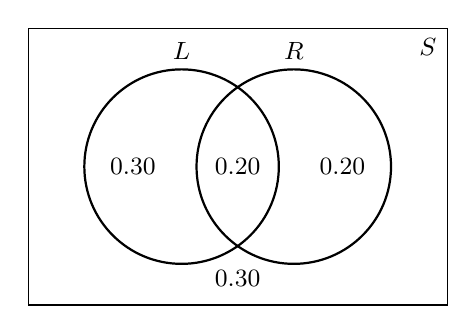
\begin{tikzpicture}[scale=0.95,every node/.style={font=\small}]
  \draw[thin] (-2.8,-1.85) rectangle (2.8,1.85);
  \node[anchor=north east,inner sep=2pt] at (2.74,1.79){$S$};
  \draw[thick] (-0.75,0) circle (1.3);
  \draw[thick] ( 0.75,0) circle (1.3);
  \node at (-0.75,1.55){$L$};
  \node at ( 0.75,1.55){$R$};
  \node at (-1.4,0){$0.30$};         % L not R
  \node at ( 1.4,0){$0.20$};         % R not L
  \node at ( 0,0){$0.20$};           % L and R
  \node at ( 0,-1.5){$0.30$};        % neither
\end{tikzpicture}
\end{center}
\steplabel{Both lit.} $\PP(L\cap R)=0.5\times0.4=0.20$.
\steplabel{Left only.} $\PP(L\cap\comp{R})=0.5\times0.6=0.30$.
\steplabel{Right only.} $\PP(\comp{L}\cap R)=0.5\times0.4=0.20$.
\steplabel{Neither.} $\PP(\comp{L}\cap\comp{R})=0.5\times0.6=0.30$.
\steplabel{Check.} The four add to $0.20+0.30+0.20+0.30=1.00$, and the left circle totals
$0.30+0.20=0.50=\PP(L)$, as it must.

\begin{example}[A complement-trick chain: at most one of three]
Three independent smoke detectors sound on detecting smoke with probabilities $0.9$, $0.8$,
and $0.7$. During a (false-alarm-free) test, find the probability that \emph{at most one}
sounds. Use complements throughout.
\end{example}
\whichrule{``At most one'' means zero or one detector sounds. Each piece is an intersection
mixing ``sounds'' with ``stays silent'' (a complement), so Proposition~\ref{prop:indcomp}
turns every piece into a product of marginals and complements. This is the harder, multi-term
cousin of the ``exactly one'' tree example; the ``at least one'' shortcut does not directly
fit because we want a \emph{small} count, not a union.}
\soln
Let the sound events be $A,B,C$ with $\PP(A)=0.9$, $\PP(B)=0.8$, $\PP(C)=0.7$, so the silent
complements have probabilities $0.1$, $0.2$, $0.3$.
\steplabel{Step 1 (none sound).} By independence of the complements,
$\PP(\comp{A}\cap\comp{B}\cap\comp{C})=0.1\times0.2\times0.3=0.006$.
\steplabel{Step 2 (exactly one sounds).} Add the three patterns with one ``sound'' and two
``silent'':
\[
  \underbrace{0.9\cdot0.2\cdot0.3}_{A\text{ only}=0.054}
  +\underbrace{0.1\cdot0.8\cdot0.3}_{B\text{ only}=0.024}
  +\underbrace{0.1\cdot0.2\cdot0.7}_{C\text{ only}=0.014}
  =0.092.
\]
\steplabel{Step 3 (combine).} ``At most one'' is the disjoint union of these,
$0.006+0.092=0.098$.

%======================================================================
\subsection{Rule 3: Mutual vs.\ pairwise independence of $n$ events}

For three or more events the product rule on \emph{pairs} alone is too weak. Genuine
independence demands the product rule for \emph{every} sub-collection at once.

\begin{definition}\label{def:mutual}
Events $A_1,\dots,A_n$ are \keyword{mutually independent} if for \emph{every} index subset
$\{i_1<\cdots<i_k\}\subseteq\{1,\dots,n\}$ with $k\ge2$,
\[
  \PP\!\bigl(A_{i_1}\cap\cdots\cap A_{i_k}\bigr)=\PP(A_{i_1})\cdots\PP(A_{i_k}).
\]
They are merely \keyword{pairwise independent} if this holds for all subsets of size $k=2$ but
possibly not for larger ones.
\end{definition}

For $n$ events this is a system of $2^{n}-n-1$ equations (one per subset of size $\ge2$): for
$n=3$ that is $\binom32+\binom33=3+1=4$ equations --- the three pairwise equations
\emph{plus} the one triple equation
$\PP(A\cap B\cap C)=\PP(A)\PP(B)\PP(C)$. Pairwise independence supplies only the first three;
the triple equation is independent of them and can fail on its own.

\begin{theorem}[Pairwise does not imply mutual]\label{thm:pairnotmut}
There exist events $A,B,C$ that are pairwise independent but not mutually independent.
\end{theorem}

\begin{proof}[Proof by explicit counterexample]
Toss a fair coin twice; the four outcomes $HH,HT,TH,TT$ are equally likely, each of
probability $\tfrac14$. Define
\[
  \begin{aligned}
  A&=\{\text{first toss is }H\}=\{HH,HT\},\\
  B&=\{\text{second toss is }H\}=\{HH,TH\},\\
  C&=\{\text{the two tosses agree}\}=\{HH,TT\}.
  \end{aligned}
\]
Each event contains two of the four outcomes, so $\PP(A)=\PP(B)=\PP(C)=\tfrac12$. The
two-way layout of the four outcomes makes the events visible:
\begin{center}
\renewcommand{\arraystretch}{1.25}
\begin{tabular}{c|cc}
\toprule
 & $2$nd $=H$ ($B$) & $2$nd $=T$\\
\midrule
$1$st $=H$ ($A$) & $HH$\ \ {\scriptsize($A,B,C$)} & $HT$\ \ {\scriptsize($A$)}\\
$1$st $=T$        & $TH$\ \ {\scriptsize($B$)}     & $TT$\ \ {\scriptsize($C$)}\\
\bottomrule
\end{tabular}
\end{center}
\steplabel{Pairwise check.} Each pairwise intersection is a single outcome of probability
$\tfrac14$:
\[
  \PP(A\cap B)=\PP(\{HH\})=\tfrac14=\tfrac12\cdot\tfrac12,\quad
  \PP(A\cap C)=\PP(\{HH\})=\tfrac14,\quad
  \PP(B\cap C)=\PP(\{HH\})=\tfrac14,
\]
and every right-hand side is $\tfrac12\cdot\tfrac12=\tfrac14$. So all three pairs are
independent.
\steplabel{Triple check.} But $A\cap B\cap C=\{HH\}$ as well, so
$\PP(A\cap B\cap C)=\tfrac14$, whereas
$\PP(A)\PP(B)\PP(C)=\tfrac12\cdot\tfrac12\cdot\tfrac12=\tfrac18$. Since
$\tfrac14\ne\tfrac18$, the triple equation fails and the three events are \emph{not} mutually
independent. (Intuitively, any two of $A,B,C$ determine the third: knowing the first toss and
whether the tosses agree pins down the second toss.)
\end{proof}

\begin{example}[Verifying full mutual independence of three devices]
Three independent indicator lights each turn on with probability $\tfrac12$ ($A,B,C$ for
lights $1,2,3$). Confirm mutual independence and compute $\PP(A\cap B\cap C)$.
\end{example}
\whichrule{Three \emph{separate} devices with no event defined in terms of the others is the
clean case where mutual independence genuinely holds. Because they are physically independent
mechanisms, all four equations of Definition~\ref{def:mutual} hold automatically; contrast
this with the counterexample, where $C$ was \emph{built from} $A,B$.}
\soln
\steplabel{Pairs.} Each pair multiplies: $\PP(A\cap B)=\tfrac12\cdot\tfrac12=\tfrac14$, and
likewise for the other two pairs.
\steplabel{Triple.}
$\PP(A\cap B\cap C)=\tfrac12\cdot\tfrac12\cdot\tfrac12=\tfrac18$. All four equations hold, so
the three are mutually independent and $\PP(A\cap B\cap C)=\tfrac18$.

\begin{example}[A second pairwise-but-not-mutual counterexample]
Roll a fair four-sided die with faces labeled $1,2,3,4$, each outcome probability $\tfrac14$.
Let $A=\{1,2\}$, $B=\{1,3\}$, $C=\{1,4\}$. Show these are pairwise but not mutually
independent.
\end{example}
\whichrule{Three events on one experiment, each of probability $\tfrac12$, with a single
shared outcome --- exactly the structure that produces pairwise success but triple failure.
The cue is that the events overlap only at the lone outcome $1$, so every pairwise
intersection has probability $\tfrac14$ but so does the triple, which is too large.}
\soln
\steplabel{Marginals.} $\PP(A)=\PP(B)=\PP(C)=\tfrac24=\tfrac12$.
\steplabel{Pairs.} Each pair meets only at outcome $1$:
$\PP(A\cap B)=\PP(\{1\})=\tfrac14=\tfrac12\cdot\tfrac12$, and the same for $A\cap C$ and
$B\cap C$. Pairwise independent.
\steplabel{Triple.} $A\cap B\cap C=\{1\}$, so $\PP(A\cap B\cap C)=\tfrac14$, but
$\PP(A)\PP(B)\PP(C)=\tfrac18$. Since $\tfrac14\ne\tfrac18$, not mutually independent.

\begin{example}[Mutual independence simplifies a longer ``and'']
A fair coin is tossed four times independently. Find the probability of the exact sequence
heads, heads, tails, heads.
\end{example}
\whichrule{Four tosses of one coin are mutually independent (separate flips), so the joint
probability of a specified sequence is the product over all four positions --- the practical
payoff of Definition~\ref{def:mutual} for $n=4$.}
\soln
\steplabel{Step 1.} Each toss has probability $\tfrac12$ for its specified face.
\steplabel{Step 2.} By mutual independence,
$\PP(HHTH)=\tfrac12\cdot\tfrac12\cdot\tfrac12\cdot\tfrac12=\tfrac{1}{16}$.

\begin{example}[When you may \emph{not} multiply the triple]
In the four-sided-die setup ($A=\{1,2\}$, $B=\{1,3\}$, $C=\{1,4\}$ above), a student wants
$\PP(A\cap B\cap C)$ and writes $\PP(A)\PP(B)\PP(C)=\tfrac18$. Why is this wrong, and what is
the correct value?
\end{example}
\whichrule{This is the diagnostic case: the events are only \emph{pairwise} independent, so
the multiplication shortcut for three events is \emph{not} licensed. The presence of an event
overlap structure (all three share outcome $1$) is the red flag that the triple equation of
Definition~\ref{def:mutual} must be checked, not assumed.}
\soln
\steplabel{Step 1.} Multiplying marginals is valid only under \emph{mutual} independence,
which fails here (shown above). So $\tfrac18$ is not justified.
\steplabel{Step 2.} Compute directly: $A\cap B\cap C=\{1\}$, hence
$\PP(A\cap B\cap C)=\tfrac14$, not $\tfrac18$.

\begin{example}[Two dice and a parity trap: pairwise but not mutual]
Roll a fair red die and a fair white die. Let $A=\{\text{red is even}\}$,
$B=\{\text{white is even}\}$, and $C=\{\text{the sum is even}\}$. Show that $A,B,C$ are
pairwise independent but not mutually independent.
\end{example}
\whichrule{The first two events live on \emph{different} dice, but $C$ is defined \emph{in terms
of both} (parity of the sum) --- precisely the ``one event built from the others'' signature
that Definition~\ref{def:mutual} warns about. So we must check the triple equation separately
and not trust the two genuinely-separate dice into thinking everything multiplies.}
\soln
All $36$ pairs $(r,w)$ are equally likely. The grid marks $A$ (even $r$, rows $2,4,6$), $B$
(even $w$, columns $2,4,6$), and $C$ (sum even, i.e.\ $r,w$ the same parity); a cell in all
three carries $\otimes$.
\begin{center}
\renewcommand{\arraystretch}{1.15}
\begin{tabular}{c|cccccc}
\toprule
$r\backslash w$ & $1$ & $2$ & $3$ & $4$ & $5$ & $6$\\
\midrule
$1$ & $C$ &     & $C$ &     & $C$ &    \\
$2$ &     & $\otimes$ &     & $\otimes$ &     & $\otimes$\\
$3$ & $C$ &     & $C$ &     & $C$ &    \\
$4$ &     & $\otimes$ &     & $\otimes$ &     & $\otimes$\\
$5$ & $C$ &     & $C$ &     & $C$ &    \\
$6$ &     & $\otimes$ &     & $\otimes$ &     & $\otimes$\\
\bottomrule
\end{tabular}
\end{center}
The $\otimes$ cells are exactly ``$r$ even and $w$ even,'' which here also forces the sum even
--- so on this grid $A\cap B\subseteq C$, the source of the trouble.
\steplabel{Marginals.} $\PP(A)=\PP(B)=\dfrac{18}{36}=\dfrac12$, and the sum is even on the $18$
cells where $r,w$ share parity, so $\PP(C)=\dfrac{18}{36}=\dfrac12$.
\steplabel{Pairs.}
$\PP(A\cap B)=\dfrac{9}{36}=\dfrac14=\dfrac12\cdot\dfrac12$;\ \
$\PP(A\cap C)$ counts ``red even and sum even'' $=$ ``red even and white even'' $=\dfrac{9}{36}=\dfrac14$;\ \
and likewise $\PP(B\cap C)=\dfrac14$. Every pair matches the product, so all three are pairwise
independent.
\steplabel{Triple.} $A\cap B\cap C=A\cap B$ (the $\otimes$ cells), so
$\PP(A\cap B\cap C)=\dfrac{9}{36}=\dfrac14$, whereas
$\PP(A)\PP(B)\PP(C)=\dfrac12\cdot\dfrac12\cdot\dfrac12=\dfrac18$. Since $\tfrac14\ne\tfrac18$,
the three are \keyword{not} mutually independent: once you know $A$ and $B$, event $C$ is
forced, so $C$ adds no freedom.

\begin{example}[Mutual independence genuinely holds: three with-replacement draws]
Draw a card from a full deck, record whether it is a heart, return it and reshuffle, and repeat
for a total of three draws. Let $H_1,H_2,H_3$ be ``draw $i$ is a heart.'' Are these three
mutually independent, and what is $\PP(H_1\cap H_2\cap H_3)$?
\end{example}
\whichrule{Three draws \emph{with replacement} restore the deck each time, so no event is built
from the others and every mechanism is identical and separate --- the clean case where all four
equations of Definition~\ref{def:mutual} hold automatically. This contrasts with the parity
trap above, where the offending event was a function of the others.}
\soln
Each draw is a heart with probability $\PP(H_i)=\dfrac{13}{52}=\dfrac14$, independent of the
rest because the deck is reset.
\steplabel{Pairs.} $\PP(H_i\cap H_j)=\dfrac14\cdot\dfrac14=\dfrac{1}{16}$ for each of the three
pairs.
\steplabel{Triple.}
$\PP(H_1\cap H_2\cap H_3)=\dfrac14\cdot\dfrac14\cdot\dfrac14=\dfrac{1}{64}$. All four equations
hold, so the three are mutually independent.

\begin{example}[Diagnosing the structure before multiplying]
Toss a fair coin twice. Let $A=\{\text{first is }H\}$, $B=\{\text{second is }H\}$, and
$D=\{\text{the two tosses differ}\}=\{HT,TH\}$. A student claims
$\PP(A\cap B\cap D)=\PP(A)\PP(B)\PP(D)=\tfrac18$. Check each independence relation and find the
true value.
\end{example}
\whichrule{Two of the events ($A,B$) come from separate tosses, but $D$ is an
\emph{agreement-type} event built from both --- the same red flag as in the original
two-coin counterexample. We must test the triple equation of Definition~\ref{def:mutual}
directly; the pairwise checks alone cannot license the product.}
\soln
The four outcomes $HH,HT,TH,TT$ each have probability $\tfrac14$, and
$\PP(A)=\PP(B)=\PP(D)=\tfrac12$.
\steplabel{Pairs.} $\PP(A\cap B)=\PP(\{HH\})=\tfrac14=\tfrac12\cdot\tfrac12$;\ \
$\PP(A\cap D)=\PP(\{HT\})=\tfrac14$;\ \ $\PP(B\cap D)=\PP(\{TH\})=\tfrac14$. Pairwise
independent.
\steplabel{Triple.} But $A\cap B=\{HH\}$ requires the tosses to \emph{agree}, while $D$
requires them to \emph{differ}, so $A\cap B\cap D=\varnothing$ and
$\PP(A\cap B\cap D)=0$, not $\tfrac18$. The student's product is unjustified because mutual
independence fails; the true value is $0$.

%======================================================================
\subsection{Rule 4: The ``at least one'' complement formula}

The hardest-looking union --- ``at least one of many independent events occurs'' --- becomes
a one-line product once you complement it. ``At least one occurs'' is the negation of ``none
occurs,'' and ``none occurs'' is a pure intersection of complements, which independence lets
us multiply.

\begin{corollary}\label{cor:atleastone}
If $A_1,\dots,A_n$ are mutually independent, then
\[
  \PP(\text{at least one }A_i\text{ occurs})
  =1-\PP(\text{none occur})
  =1-\prod_{i=1}^{n}\bigl(1-\PP(A_i)\bigr).
\]
In particular, if all $\PP(A_i)=p$, this is $1-(1-p)^{n}$.
\end{corollary}

\begin{proof}
``At least one'' is the union $\bigcup_i A_i$; its complement is $\bigcap_i\comp{A_i}$ (none
occur), so $\PP(\bigcup_i A_i)=1-\PP(\bigcap_i\comp{A_i})$. By
Proposition~\ref{prop:indcomp} the complements $\comp{A_1},\dots,\comp{A_n}$ are mutually
independent, so their intersection probability factors:
$\PP(\bigcap_i\comp{A_i})=\prod_i\PP(\comp{A_i})=\prod_i(1-\PP(A_i))$. Substituting gives the
formula.
\end{proof}

\begin{example}[At least one six in four rolls]
Roll a fair die four times independently. What is the probability of getting at least one
six?
\end{example}
\whichrule{``At least one'' over independent repetitions is the textbook trigger for
Corollary~\ref{cor:atleastone}. Computing it as a union directly would require
inclusion--exclusion over four overlapping events; the complement turns it into a single
power.}
\soln
\steplabel{Step 1.} Per roll, $\PP(\text{six})=\tfrac16$, so
$\PP(\text{not six})=\tfrac56$.
\steplabel{Step 2.} ``None is a six'' has probability $\bigl(\tfrac56\bigr)^4=\dfrac{625}{1296}$.
\steplabel{Step 3.} $\PP(\text{at least one six})=1-\dfrac{625}{1296}=\dfrac{671}{1296}\approx0.518$.

\begin{example}[Redundant components: system works if any works]
A backup system has three pumps that fail independently, with failure probabilities
$0.2$, $0.3$, and $0.5$. The system functions if at least one pump works. Find the
probability the system functions.
\end{example}
\whichrule{``Functions if at least one works'' is the union of the three ``works'' events;
their failure probabilities are given, so Corollary~\ref{cor:atleastone} applies with
\emph{unequal} probabilities (use the product form, not the $1-(1-p)^n$ shortcut).}
\soln
\steplabel{Step 1.} ``System fails'' means all three pumps fail simultaneously. By
independence,
$\PP(\text{all fail})=0.2\times0.3\times0.5=0.03$.
\steplabel{Step 2.}
$\PP(\text{functions})=1-0.03=0.97$.
\begin{center}
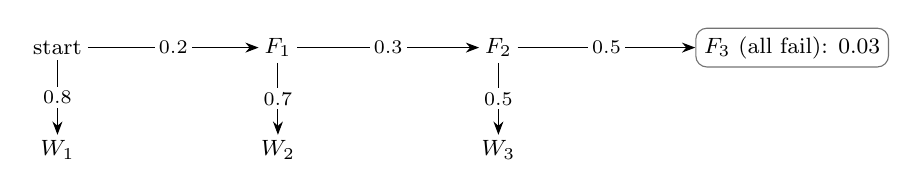
\begin{tikzpicture}[>=Stealth,
   nd/.style={font=\footnotesize,inner sep=2pt},
   term/.style={font=\footnotesize,inner sep=3pt,draw=black!55,rounded corners},
   lbl/.style={font=\scriptsize,fill=white,inner sep=1.5pt,midway}]
% top row: the all-fail path -- each pump in turn fails
\node[nd]   (s)  at (0,0)    {start};
\node[nd]   (f1) at (2.8,0)  {$F_1$};
\node[nd]   (f2) at (5.6,0)  {$F_2$};
\node[term,anchor=west] (f3) at (8.1,0)  {$F_3$ (all fail): $0.03$};
\draw[->] (s)  -- (f1) node[lbl]{$0.2$};
\draw[->] (f1) -- (f2) node[lbl]{$0.3$};
\draw[->] (f2) -- (f3) node[lbl]{$0.5$};
% a working pump (system functions) peels off at each stage
\node[nd] (w1) at (0,-1.3)   {$W_1$};
\node[nd] (w2) at (2.8,-1.3) {$W_2$};
\node[nd] (w3) at (5.6,-1.3) {$W_3$};
\draw[->] (s)  -- (w1) node[lbl]{$0.8$};
\draw[->] (f1) -- (w2) node[lbl]{$0.7$};
\draw[->] (f2) -- (w3) node[lbl]{$0.5$};
\end{tikzpicture}
\end{center}
Only the single fully-failed path has probability $0.03$; the system works on all other paths,
total $0.97$.

\begin{example}[How many tries to be $95\%$ sure?]
Each independent attempt to open a stuck valve succeeds with probability $0.3$. How many
attempts guarantee at least a $0.95$ chance of opening it at least once?
\end{example}
\whichrule{``At least once'' across independent equal-probability trials is
Corollary~\ref{cor:atleastone} with all $p$ equal, but now the unknown is $n$: invert the
formula $1-(1-p)^n\ge0.95$.}
\soln
\steplabel{Step 1.} We need $1-(0.7)^n\ge0.95$, i.e.\ $(0.7)^n\le0.05$.
\steplabel{Step 2.} Take logarithms: $n\ge\dfrac{\ln0.05}{\ln0.7}=\dfrac{-2.996}{-0.357}\approx8.39$.
\steplabel{Step 3.} Since $n$ is an integer, $n=9$ attempts. (Check: $(0.7)^9\approx0.040\le0.05$,
while $(0.7)^8\approx0.058>0.05$.)

\begin{example}[At least one match: a small birthday-style count]
Five people each independently pick one of the days Monday through Friday uniformly at random.
What is the probability that at least two pick the \emph{same} day? Use the complement.
\end{example}
\whichrule{``At least one coincidence'' inverts to ``all distinct,'' a pure intersection that
factors under independence --- the same complement move as
Corollary~\ref{cor:atleastone}, applied to the event ``all five choices are distinct.''
Direct counting of matches would be far messier.}
\soln
\steplabel{Step 1.} ``All distinct'' assigns the five people distinct days among five, so the
favorable choices are the $5!$ orderings out of $5^5$ total equally likely assignments:
$\PP(\text{all distinct})=\dfrac{5!}{5^5}=\dfrac{120}{3125}=0.0384$.
\steplabel{Step 2.}
$\PP(\text{at least one match})=1-0.0384=0.9616$.

\begin{example}[At least one head in five tosses]
Toss a fair coin five times independently. Find the probability of getting at least one head.
\end{example}
\whichrule{``At least one'' over independent equal-probability repetitions is the cleanest
trigger for Corollary~\ref{cor:atleastone} with all $p=\tfrac12$. Inclusion--exclusion over
five overlapping ``head on toss $i$'' events would be a five-term mess; the complement collapses
it to one power.}
\soln
\steplabel{Step 1.} ``No heads'' means tails every time, probability
$\bigl(\tfrac12\bigr)^5=\dfrac{1}{32}$.
\steplabel{Step 2.}
$\PP(\text{at least one head})=1-\dfrac{1}{32}=\dfrac{31}{32}\approx0.969$.

\begin{example}[Unequal failure rates: at least one spam slips through]
Three independent filters scan an incoming message; they each \emph{miss} a genuine spam with
probabilities $0.10$, $0.05$, and $0.15$. The spam reaches the inbox if \emph{at least one}
filter misses it. Find that probability.
\end{example}
\whichrule{``Reaches the inbox if at least one misses'' is the union of three ``miss'' events
with \emph{unequal} probabilities, so Corollary~\ref{cor:atleastone} applies in its general
product form $1-\prod(1-p_i)$, not the $1-(1-p)^n$ shortcut (the misses are not equally likely).
The tree shows that only the all-caught path avoids the inbox.}
\soln
\steplabel{Step 1 (all three catch it).} ``Caught'' probabilities are
$0.90,\ 0.95,\ 0.85$, so by independence
$\PP(\text{all catch})=0.90\times0.95\times0.85=0.72675$.
\begin{center}
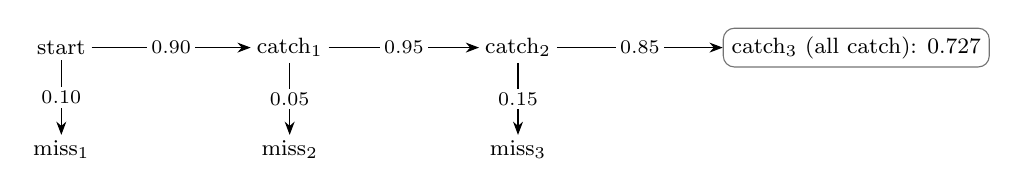
\begin{tikzpicture}[>=Stealth,
   nd/.style={font=\footnotesize,inner sep=2pt},
   term/.style={font=\footnotesize,inner sep=3pt,draw=black!55,rounded corners},
   lbl/.style={font=\scriptsize,fill=white,inner sep=1.5pt,midway}]
% top row: the all-catch path -- every filter catches the spam in turn
\node[nd]   (s)  at (0,0)    {start};
\node[nd]   (c1) at (2.9,0)  {$\text{catch}_1$};
\node[nd]   (c2) at (5.8,0)  {$\text{catch}_2$};
\node[term,anchor=west] (c3) at (8.4,0)  {$\text{catch}_3$ (all catch): $0.727$};
\draw[->] (s)  -- (c1) node[lbl]{$0.90$};
\draw[->] (c1) -- (c2) node[lbl]{$0.95$};
\draw[->] (c2) -- (c3) node[lbl]{$0.85$};
% a miss (spam reaches the inbox) peels off at each stage
\node[nd] (m1) at (0,-1.3)   {$\text{miss}_1$};
\node[nd] (m2) at (2.9,-1.3) {$\text{miss}_2$};
\node[nd] (m3) at (5.8,-1.3) {$\text{miss}_3$};
\draw[->] (s)  -- (m1) node[lbl]{$0.10$};
\draw[->] (c1) -- (m2) node[lbl]{$0.05$};
\draw[->] (c2) -- (m3) node[lbl]{$0.15$};
\end{tikzpicture}
\end{center}
\steplabel{Step 2 (complement).}
$\PP(\text{reaches inbox})=1-0.72675=0.27325$. Only the single top path is spam-free; every
other path has at least one miss.

\begin{example}[How many rolls for a near-certain six?]
A fair die is rolled repeatedly and independently. How many rolls are needed so that the
probability of getting at least one six is at least $0.90$?
\end{example}
\whichrule{``At least once'' across independent equal-probability trials is
Corollary~\ref{cor:atleastone} with all $p=\tfrac16$, but the unknown is the count $n$: we
invert $1-\bigl(\tfrac56\bigr)^n\ge0.90$ rather than evaluate it at a fixed $n$.}
\soln
\steplabel{Step 1.} We need $1-\bigl(\tfrac56\bigr)^n\ge0.90$, i.e.\
$\bigl(\tfrac56\bigr)^n\le0.10$.
\steplabel{Step 2.} Take logarithms:
$n\ge\dfrac{\ln 0.10}{\ln(5/6)}=\dfrac{-2.3026}{-0.1823}\approx12.6$.
\steplabel{Step 3.} Since $n$ must be an integer, $n=13$ rolls. (Check:
$\bigl(\tfrac56\bigr)^{13}\approx0.093\le0.10$, while
$\bigl(\tfrac56\bigr)^{12}\approx0.112>0.10$.)

\begin{remark}[The unifying thread]
Rules 2 and 4 are both consequences of Rule 1. Independence of complements
(Proposition~\ref{prop:indcomp}) is the product rule with one event flipped; the ``at least
one'' formula (Corollary~\ref{cor:atleastone}) is the product rule applied to all the
complements at once. Rule 3 is the warning that for three or more events you must check
\emph{every} subset, not just pairs, before you are allowed to multiply. Throughout, the
right pictures are trees and tables --- never a Venn diagram, which shows only regions and
hides the probabilities that independence is actually about.
\end{remark}

\section{Counting (Combinatorics)}

When every outcome of an experiment is equally likely, a probability is just a ratio of
two counts: favourable outcomes over total outcomes. The whole art is therefore counting
without listing. Every method in this section is built from a single idea --- the
multiplication principle --- and differs only in how it corrects for two questions:
\emph{does order matter?} and \emph{is repetition allowed?}

\begin{strategy}[Which counting tool does the problem need?]
Read the problem and answer two questions in order.
\begin{enumerate}[leftmargin=2.2em,itemsep=2pt]
\item \keyword{Does order matter?} If rearranging the chosen items gives a genuinely
different outcome (rankings, sequences, assigned roles, lining up, passwords), order
matters and you are \emph{permuting}. If only the \emph{set} of chosen items matters
(a committee, a hand of cards, a subset, a team with no titles), order does not matter and
you are \emph{combining}.
\item \keyword{Is repetition allowed?} Can the same item be reused (digits in a PIN,
flavours that can repeat), or is each item used at most once (people, distinct cards)?
\end{enumerate}
This gives four cases for choosing $k$ from $n$:
\begin{center}
\begin{tabular}{lll}
\toprule
 & \textbf{order matters} & \textbf{order does not matter}\\
\midrule
\textbf{no repetition} & $P(n,k)=\dfrac{n!}{(n-k)!}$ & $\dbinom{n}{k}=\dfrac{n!}{k!\,(n-k)!}$\\[1.2ex]
\textbf{repetition allowed} & $n^{k}$ & $\dbinom{n+k-1}{k}$ (stars and bars)\\
\bottomrule
\end{tabular}
\end{center}
Two refinements sit on top of these. If you are arranging \emph{all} $n$ objects but some
are identical, use the \keyword{multinomial coefficient} $n!/(n_1!\cdots n_r!)$. If the
arrangement is in a \emph{circle} with no fixed starting seat, divide an ordinary
permutation by the number of rotations. When a problem has several stages, count each stage
and \emph{multiply} (multiplication principle); when it splits into disjoint cases, count
each case and \emph{add}.
\end{strategy}

The decision is mechanical once you train the two questions. The flowchart below encodes
exactly the reasoning above.

\begin{center}
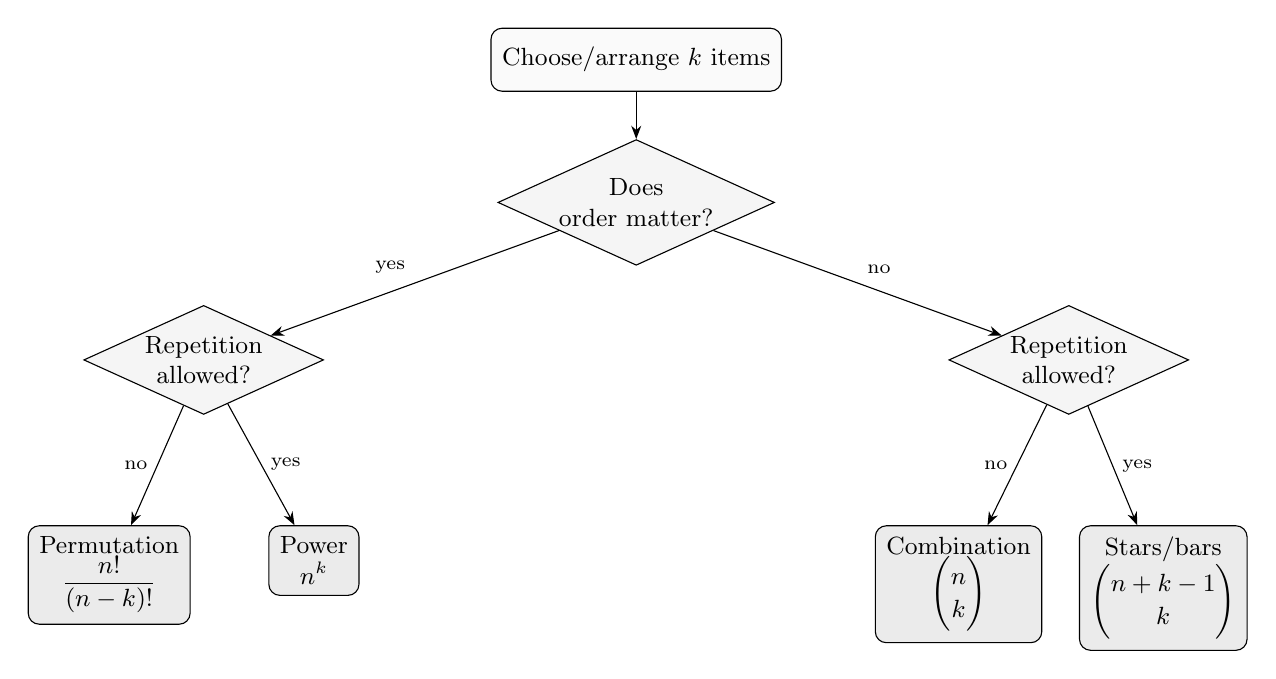
\begin{tikzpicture}[font=\small,>=Stealth,node distance=6mm,
  box/.style={draw,rounded corners,fill=gray!4,align=center,inner sep=4pt,minimum height=8mm},
  dec/.style={draw,diamond,aspect=2.2,fill=gray!8,align=center,inner sep=1pt},
  leaf/.style={draw,fill=gray!16,rounded corners,align=center,inner sep=4pt}]
\node[box] (start) {Choose/arrange $k$ items};
\node[dec,below=of start] (order) {Does\\order matter?};
\node[dec,left=22mm of order,yshift=-20mm] (rep1) {Repetition\\allowed?};
\node[dec,right=22mm of order,yshift=-20mm] (rep2) {Repetition\\allowed?};
\node[leaf,below=14mm of rep1,xshift=-12mm] (perm) {Permutation\\$\dfrac{n!}{(n-k)!}$};
\node[leaf,below=14mm of rep1,xshift=14mm] (pow) {Power\\$n^{k}$};
\node[leaf,below=14mm of rep2,xshift=-14mm] (comb) {Combination\\$\dbinom{n}{k}$};
\node[leaf,below=14mm of rep2,xshift=12mm] (bars) {Stars/bars\\$\dbinom{n+k-1}{k}$};
\draw[->] (start)--(order);
\draw[->] (order)-- node[above left,font=\scriptsize]{yes}(rep1);
\draw[->] (order)-- node[above right,font=\scriptsize]{no}(rep2);
\draw[->] (rep1)-- node[left,font=\scriptsize]{no}(perm);
\draw[->] (rep1)-- node[right,font=\scriptsize]{yes}(pow);
\draw[->] (rep2)-- node[left,font=\scriptsize]{no}(comb);
\draw[->] (rep2)-- node[right,font=\scriptsize]{yes}(bars);
\end{tikzpicture}
\end{center}

\begin{remark}
All four boxes assume the items themselves are distinct. If they are not --- some are
copies of one another --- and you must arrange \emph{all} of them, the multinomial
coefficient (Theorem~\ref{thm:multinom}) takes over. Identical-items-with-order is the
one case the four-box table does not cover directly.
\end{remark}

% =====================================================================
\subsection*{Rule 1: the multiplication principle}
% =====================================================================

\begin{theorem}[Multiplication principle]\label{thm:mult}
Suppose a procedure is carried out in $k$ successive stages, and that stage $i$ can be
performed in exactly $n_i$ ways no matter how the earlier stages turned out. Then the entire
procedure can be performed in
\[
  n_1\,n_2\cdots n_k
\]
distinct ways.
\end{theorem}

\begin{proof}
Argue by induction on the number of stages $k$. For $k=1$ the claim is the definition:
there are $n_1$ ways. Assume the result for $k-1$ stages, so the first $k-1$ stages produce
$n_1\cdots n_{k-1}$ distinct partial outcomes. Each such partial outcome can be completed by
stage $k$ in $n_k$ ways, and different partial outcomes (or different stage-$k$ choices)
yield different full outcomes. Grouping the full outcomes by their common partial outcome
partitions them into $n_1\cdots n_{k-1}$ blocks of $n_k$ each, for a total of
$(n_1\cdots n_{k-1})\,n_k=n_1\cdots n_k$. This completes the induction.
\end{proof}

The hypothesis ``no matter how the earlier stages turned out'' is essential: the
\emph{count} $n_i$ at stage $i$ may not depend on earlier choices, even though the specific
options may. Picking a shirt then a tie is fine even if which ties match depends on the
shirt, provided the \emph{number} of matching ties is the same for every shirt. A tree
diagram makes the principle visible: the number of leaves is the product of the branch
counts at each level.

\begin{center}
\begin{tikzpicture}[>=Stealth,grow=right,font=\small,
  level 1/.style={sibling distance=42mm,level distance=20mm},
  level 2/.style={sibling distance=12mm,level distance=22mm}]
\node{start}
  child{node{$T$} child{node{$\bullet$}} child{node{$\bullet$}} child{node{$\bullet$}}}
  child{node{$H$} child{node{$\bullet$}} child{node{$\bullet$}} child{node{$\bullet$}}};
\node[align=center,font=\scriptsize] at (1,-4.2){coin: $2$ ways};
\node[align=center,font=\scriptsize] at (3.4,-4.2){die-trio: $3$ ways};
\node[align=center,font=\scriptsize] at (5.6,-4.2){$2\cdot 3=6$ leaves};
\end{tikzpicture}
\end{center}

\begin{example}[Building a meal]
A diner offers $4$ appetisers, $7$ main courses, and $3$ desserts. How many distinct
three-course meals (one of each) can a customer assemble?
\end{example}
\whichrule{The meal is assembled in three independent stages and we want the number of
\emph{ways to build the whole thing}, not to pick an unordered set. The count of choices at
each stage ($4$, then $7$, then $3$) does not depend on the earlier picks, which is exactly
the setup for the multiplication principle. There is no selecting-without-order here, so
combinations are irrelevant.}
\soln
\steplabel{Stage counts.} Appetiser: $4$. Main: $7$. Dessert: $3$.
\steplabel{Multiply.} $4\cdot 7\cdot 3=84$. There are $\boxed{84}$ possible meals.

\begin{example}[Licence-plate format with repetition]
A licence plate consists of $3$ letters ($A$--$Z$, $26$ options each) followed by $4$ digits
($0$--$9$). Letters and digits may repeat. How many plates are possible?
\end{example}
\whichrule{Each of the $7$ positions is a separate stage, and because symbols may repeat the
number of options is the same ($26$ or $10$) at every position regardless of earlier
choices. This is the multiplication principle in its purest ``power'' form, $n^k$, which
arises precisely when order matters and repetition is allowed. Permutations would apply only
if symbols could not repeat.}
\soln
\steplabel{Letter block.} $26\cdot 26\cdot 26=26^{3}=17{,}576$.
\steplabel{Digit block.} $10\cdot 10\cdot 10\cdot 10=10^{4}=10{,}000$.
\steplabel{Multiply the blocks.} $26^{3}\cdot 10^{4}=17{,}576\cdot 10{,}000=175{,}760{,}000$.
There are $\boxed{175{,}760{,}000}$ plates.

\begin{example}[Subsets via a yes/no decision per element]
A pizza shop offers $9$ distinct toppings. How many different pizzas can be ordered if any
subset of toppings (including none and all) is allowed?
\end{example}
\whichrule{The trigger is ``any subset'' of a fixed list. Build the subset by making one
independent decision per topping: \emph{in} or \emph{out}. That is $9$ stages of $2$ options
each, so the multiplication principle gives $2^9$. This is the slick way to see that an
$n$-element set has $2^n$ subsets; summing $\binom{9}{0}+\cdots+\binom{9}{9}$ would give the
same answer but is far more work.}
\soln
\steplabel{One binary choice per topping.} $9$ toppings, each either chosen or not: $2$ ways
each.
\steplabel{Multiply.} $2^{9}=512$. There are $\boxed{512}$ possible pizzas (including the
plain pizza with no toppings).

\begin{example}[Stage counts that vary but stay constant in number]
A traveller plans a $4$-leg trip visiting $4$ \emph{different} cities chosen from a list of
$10$, in order. How many ordered itineraries are possible?
\end{example}
\whichrule{Here the \emph{set} of available cities shrinks after each leg (no city is
revisited), yet the \emph{number} of available cities at each stage is fixed: $10$, then $9$,
then $8$, then $7$. The multiplication principle still applies because the count per stage is
predetermined. Notice this is order-matters-without-repetition, so it coincides with the
permutation $P(10,4)$; we compute it here directly from stages to show the principle
underneath.}
\soln
\steplabel{Stage counts.} Leg 1: $10$ cities. Leg 2: $9$. Leg 3: $8$. Leg 4: $7$.
\steplabel{Multiply.} $10\cdot 9\cdot 8\cdot 7=5040$. There are $\boxed{5040}$ itineraries.

\begin{example}[An outfit with no repeated category]
A wardrobe has $5$ shirts, $4$ pairs of trousers, $3$ pairs of shoes, and $2$ jackets. How
many complete outfits use exactly one item from each category?
\end{example}
\whichrule{The outfit is built in four independent stages, and the number of options at each
stage ($5$, $4$, $3$, $2$) is fixed regardless of earlier picks. That is the multiplication
principle. We are not selecting an unordered subset of clothing, so combinations do not apply;
and each category contributes exactly one item, so no single power $n^k$ fits either.}
\soln
\steplabel{Stage counts.} Shirts: $5$; trousers: $4$; shoes: $3$; jackets: $2$.
\steplabel{Multiply.} $5\cdot 4\cdot 3\cdot 2=120$. There are $\boxed{120}$ outfits.

\begin{example}[A four-digit PIN with repetition allowed]
A keypad PIN is $4$ digits long, each digit from $0$--$9$, and digits may repeat. How many
PINs are possible?
\end{example}
\whichrule{Each of the $4$ positions is a separate stage with the same $10$ options
regardless of earlier digits, because repetition is allowed. Order matters (a PIN is a
sequence) and repetition is permitted, which is exactly the power form $n^k=10^4$. A
permutation $P(10,4)$ would be wrong here: it forbids repeats, undercounting PINs like
\texttt{7007}.}
\soln
\steplabel{Per-position count.} Each of the $4$ slots: $10$ digits.
\steplabel{Multiply.} $10\cdot 10\cdot 10\cdot 10=10^{4}=10{,}000$. There are
$\boxed{10{,}000}$ PINs.

\begin{example}[Counting outcomes on an equally-likely grid]
Two fair dice, one white and one black, are rolled. Treating the white roll as the first
stage and the black roll as the second, how many ordered outcomes are there in total, and how
many give a sum that is a multiple of $3$?
\end{example}
\whichrule{The roll is two independent stages of $6$ options each, so the multiplication
principle gives $6\cdot 6=36$ equally-likely ordered pairs --- the sample space. To count a
sub-event we do \emph{not} need a new rule; we just tally the favourable cells of the
$6\times 6$ grid. This is the typical bridge from counting to probability: a count over a
count.}
\soln
\steplabel{Total outcomes.} $6\cdot 6=36$ ordered pairs.
\steplabel{Tally the grid.} Shade every cell whose coordinate sum is $3,6,9,$ or $12$.
\begin{center}
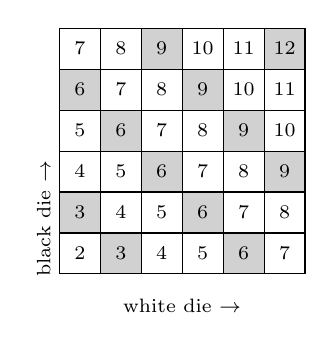
\begin{tikzpicture}[scale=0.52,font=\scriptsize]
\foreach \x in {1,...,6}{\foreach \y in {1,...,6}{
  \pgfmathtruncatemacro{\s}{\x+\y}
  \pgfmathtruncatemacro{\m}{mod(\s,3)}
  \ifnum\m=0 \fill[black!18] (\x-1,\y-1) rectangle (\x,\y);\fi
  \draw (\x-1,\y-1) rectangle (\x,\y);
  \node at (\x-0.5,\y-0.5){\s};}}
\node[below=2mm,font=\scriptsize] at (3,0){white die $\rightarrow$};
\node[rotate=90,left=2mm,font=\scriptsize] at (0,3){black die $\rightarrow$};
\end{tikzpicture}
\end{center}
\steplabel{Count.} The shaded cells number $12$, so $12$ of the $36$ outcomes (a probability
of $12/36=\tfrac13$) have a sum divisible by $3$. There are $\boxed{12}$ favourable outcomes.

% =====================================================================
\subsection*{Rule 2: permutations $P(n,k)$}
% =====================================================================

\begin{theorem}[Permutations]\label{thm:perm}
The number of \keyword{ordered} arrangements of $k$ objects selected \emph{without
repetition} from a pool of $n$ distinct objects is
\[
  P(n,k)=n(n-1)(n-2)\cdots(n-k+1)=\frac{n!}{(n-k)!}.
\]
In particular, the number of ways to order all $n$ objects is $P(n,n)=n!$, using the
convention $0!=1$.
\end{theorem}

\begin{proof}
Think of $k$ ordered positions to be filled left to right (slot diagram below). The first
position can be filled by any of the $n$ objects. Whatever is placed there is used up, so the
second position has $n-1$ choices, the third $n-2$, and in general the $i$th position has
$n-(i-1)$ choices. By the multiplication principle the total is
$n(n-1)\cdots(n-k+1)$. Multiplying and dividing by $(n-k)!$ telescopes this product into
$n!/(n-k)!$.
\end{proof}

\begin{center}
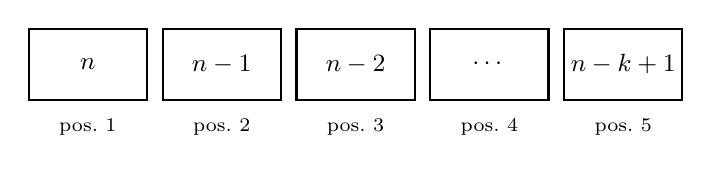
\begin{tikzpicture}[font=\small]
\foreach \i/\v in {0/$n$,1/$n-1$,2/$n-2$,3/$\cdots$,4/$n-k+1$}{
  \draw[thick] (1.7*\i,0) rectangle (1.7*\i+1.5,0.9);
  \node at (1.7*\i+0.75,0.45){\v};
  \node[font=\scriptsize] at (1.7*\i+0.75,-0.35){pos.\ \the\numexpr\i+1\relax};}
\node[font=\scriptsize] at (3.4,-0.35){};
\end{tikzpicture}
\end{center}

\begin{example}[Ranked finishers]
In a race of $8$ runners (no ties), how many different outcomes are possible for the gold,
silver, and bronze medals?
\end{example}
\whichrule{The three medals are \emph{distinct roles}, so the order in which we name the
three finishers matters: ``Ann gold, Bo silver'' differs from ``Bo gold, Ann silver.'' No
runner can take two medals, so there is no repetition. Order matters, no repetition $\Rightarrow$
permutation $P(8,3)$. A combination $\binom{8}{3}$ would wrongly treat the three medallists
as an unordered set.}
\soln
\steplabel{Apply the formula.} $P(8,3)=\dfrac{8!}{(8-3)!}=8\cdot 7\cdot 6$.
\steplabel{Compute.} $8\cdot 7\cdot 6=336$. There are $\boxed{336}$ medal outcomes.

\begin{example}[Seating in a row]
Six distinct books are placed left to right on a shelf. In how many orders can all six be
arranged?
\end{example}
\whichrule{We arrange \emph{all} the objects and every left-to-right order is a different
shelf, so order matters and $k=n=6$. This is the full permutation $P(6,6)=6!$. The phrase
``in how many orders'' is the giveaway that we are not selecting a subset.}
\soln
\steplabel{Full factorial.} $P(6,6)=6!=6\cdot 5\cdot 4\cdot 3\cdot 2\cdot 1$.
\steplabel{Compute.} $6!=720$. There are $\boxed{720}$ arrangements.

\begin{example}[Forming a four-letter code]
How many four-letter codes can be made from the $26$ letters if \emph{no letter repeats}?
\end{example}
\whichrule{Position matters in a code (\texttt{LMNO} differs from \texttt{OMNL}), and the
explicit ``no letter repeats'' forbids reuse. Order matters, no repetition $\Rightarrow$
permutation $P(26,4)$. Contrast the earlier plate example, where repetition \emph{was}
allowed and the count was $26^4$ instead.}
\soln
\steplabel{Slot product.} $P(26,4)=26\cdot 25\cdot 24\cdot 23$.
\steplabel{Compute.} $26\cdot 25=650$; $650\cdot 24=15{,}600$; $15{,}600\cdot 23=358{,}800$.
There are $\boxed{358{,}800}$ codes.

\begin{example}[Assigning distinct jobs to a subset of people]
A manager has $12$ employees and must assign $5$ \emph{different} tasks (each task to a
different person, each person at most one task). How many assignments are possible?
\end{example}
\whichrule{The five tasks are distinguishable, so assigning Task~1 to Dana and Task~2 to
Lee differs from the swap; order (which person gets which task) matters. Each person takes at
most one task, so no repetition. Order matters, no repetition $\Rightarrow$ permutation
$P(12,5)$. If the five chosen people were just a pool with no task labels, it would instead
be $\binom{12}{5}$.}
\soln
\steplabel{Apply the formula.} $P(12,5)=\dfrac{12!}{7!}=12\cdot 11\cdot 10\cdot 9\cdot 8$.
\steplabel{Compute.} $12\cdot 11=132$; $132\cdot 10=1320$; $1320\cdot 9=11{,}880$;
$11{,}880\cdot 8=95{,}040$. There are $\boxed{95{,}040}$ assignments.

\begin{example}[Permutations with a forced position]
Five distinct keynote speakers are scheduled in five time slots, but the headline speaker
must occupy the final slot. How many schedules are possible?
\end{example}
\whichrule{Order matters (the slots are an ordered sequence) and no speaker repeats, so this
is a permutation problem with a \emph{constraint}. Handle the constraint by fixing the forced
choice first, then permuting what remains. The constraint does not change the rule; it just
reduces the free positions.}
\soln
\steplabel{Place the forced speaker.} The headline speaker is fixed in the last slot: $1$ way.
\steplabel{Arrange the rest.} The remaining $4$ speakers fill the first $4$ slots in
$P(4,4)=4!=24$ ways.
\steplabel{Multiply.} $1\cdot 24=24$. There are $\boxed{24}$ schedules.

\begin{example}[Top three from a club]
A photography club of $7$ members elects a president, a vice-president, and a treasurer (three
distinct offices, no person holds two). How many ways can the three offices be filled?
\end{example}
\whichrule{The three offices are distinct roles, so naming Ali president and Bo vice-president
differs from the swap: order matters. No member holds two offices, so there is no repetition.
Order matters, no repetition $\Rightarrow$ permutation $P(7,3)$. A combination $\binom{7}{3}$
would lump the three officers into a title-less set and undercount by a factor of $3!$.}
\soln
\steplabel{Slot product.} $P(7,3)=7\cdot 6\cdot 5$.
\steplabel{Compute.} $7\cdot 6=42$; $42\cdot 5=210$. There are $\boxed{210}$ ways.

\begin{example}[Anagrams of a word with all distinct letters]
How many distinguishable strings can be formed by rearranging all the letters of
\texttt{MATH}?
\end{example}
\whichrule{All four letters are distinct and we arrange \emph{all} of them, so every ordering
is a new string: $k=n=4$ and the answer is the full permutation $P(4,4)=4!$. There are no
repeated letters, so this is a plain factorial rather than the multinomial coefficient used
for words like \texttt{PEPPER}.}
\soln
\steplabel{Full factorial.} $P(4,4)=4!=4\cdot 3\cdot 2\cdot 1$.
\steplabel{Compute.} $4!=24$. There are $\boxed{24}$ anagrams.

\begin{example}[Permutation with a forbidden position --- complement trick]
Six distinct runners line up at the start; the slowest runner refuses to be placed in lane~$1$.
How many starting line-ups are possible?
\end{example}
\whichrule{A line-up is an ordered arrangement of all $6$ distinct runners, so the base count
is the permutation $P(6,6)=6!$. The single restriction (one runner barred from one lane) is
cleanest by \emph{complementary counting}: take all arrangements and subtract the forbidden
ones, rather than splitting into many allowed cases. Subtraction beats casework whenever the
banned set is small and easy to count.}
\soln
\steplabel{All line-ups.} $6!=720$.
\steplabel{Bad line-ups (slow runner in lane~1).} Fix that runner in lane~$1$ and permute the
other $5$: $5!=120$.
\steplabel{Subtract.} $720-120=600$. There are $\boxed{600}$ allowed line-ups.

% =====================================================================
\subsection*{Rule 3: combinations $\binom{n}{k}$}
% =====================================================================

\begin{theorem}[Combinations]\label{thm:comb}
The number of \keyword{unordered} subsets of size $k$ that can be chosen from $n$ distinct
objects (without repetition) is
\[
  \binom{n}{k}=\frac{P(n,k)}{k!}=\frac{n!}{k!\,(n-k)!}.
\]
\end{theorem}

\begin{proof}
Count the ordered selections two ways. On one hand there are $P(n,k)$ of them. On the other
hand, every ordered selection is obtained by first choosing the underlying \emph{set} of $k$
objects --- say there are $C$ such sets --- and then ordering that set, which can be done in
$k!$ ways. By the multiplication principle the number of ordered selections is also
$C\cdot k!$. Equating, $C\cdot k!=P(n,k)$, so $C=P(n,k)/k!=n!/(k!\,(n-k)!)$.
\end{proof}

Two facts follow at once and save arithmetic. The \keyword{symmetry}
$\binom{n}{k}=\binom{n}{n-k}$ holds because choosing the $k$ to include is the same act as
choosing the $n-k$ to exclude. And the \keyword{binomial theorem}
$(x+y)^n=\sum_{k=0}^n\binom{n}{k}x^k y^{n-k}$ shows $\binom{n}{k}$ counts the terms with $k$
factors of $x$. The single most reliable test for ``combination versus permutation'' is to
ask whether \emph{relabelling the chosen items as an ordered list} produces a new, valid
outcome; if it does not, you are combining.

\begin{example}[Committee with no titles]
From a department of $15$ people, how many ways are there to form a committee of $4$ if all
members are equal (no chair, no titles)?
\end{example}
\whichrule{A committee is a \emph{set} of people: listing the same four in a different order
does not create a new committee. Order does not matter, no person is chosen twice, so this is
a combination $\binom{15}{4}$. The absence of role words (chair, president, ranking) is the
signal that order is irrelevant.}
\soln
\steplabel{Apply the formula.}
$\displaystyle\binom{15}{4}=\frac{15\cdot 14\cdot 13\cdot 12}{4!}
=\frac{15\cdot 14\cdot 13\cdot 12}{24}$.
\steplabel{Compute the numerator.} $15\cdot 14=210$; $210\cdot 13=2730$;
$2730\cdot 12=32{,}760$.
\steplabel{Divide.} $32{,}760/24=1365$. There are $\boxed{1365}$ committees.

\begin{example}[A poker-style hand]
How many $5$-card hands can be dealt from a standard $52$-card deck (order of receipt
irrelevant)?
\end{example}
\whichrule{A hand is the \emph{set} of cards held; the order in which they were dealt does
not change the hand. Cards are distinct and none repeats. Order does not matter, no
repetition $\Rightarrow$ combination $\binom{52}{5}$. Using $P(52,5)$ would count each hand
$5!$ times, once per dealing order.}
\soln
\steplabel{Apply the formula.}
$\displaystyle\binom{52}{5}=\frac{52\cdot 51\cdot 50\cdot 49\cdot 48}{5!}$.
\steplabel{Numerator.} $52\cdot 51=2652$; $\,\cdot 50=132{,}600$; $\,\cdot 49=6{,}497{,}400$;
$\,\cdot 48=311{,}875{,}200$.
\steplabel{Divide by $5!=120$.} $311{,}875{,}200/120=2{,}598{,}960$. There are
$\boxed{2{,}598{,}960}$ hands.

\begin{example}[Choosing a mixed group with the multiplication principle]
A club has $7$ seniors and $9$ juniors. How many ways are there to pick a delegation of $3$
seniors and $2$ juniors?
\end{example}
\whichrule{Each of the two groups is an unordered selection (a delegation, no titles), so
each is a combination. The two selections are made in \emph{stages} --- first the seniors,
then the juniors --- so by the multiplication principle we \emph{multiply} the two
combination counts. The clue for multiplying is the word ``and'' joining two independent
sub-choices.}
\soln
\steplabel{Choose seniors.} $\displaystyle\binom{7}{3}=\frac{7\cdot 6\cdot 5}{6}=35$.
\steplabel{Choose juniors.} $\displaystyle\binom{9}{2}=\frac{9\cdot 8}{2}=36$.
\steplabel{Multiply.} $35\cdot 36=1260$. There are $\boxed{1260}$ delegations.

\begin{example}[Complement and ``at least'' counting]
A box holds $10$ good widgets and $4$ defective ones. A sample of $4$ is drawn at once. In
how many ways does the sample contain \emph{at least one} defective widget?
\end{example}
\whichrule{The sample is an unordered subset, so combinations apply. ``At least one'' is the
trigger for \emph{complementary counting}: instead of summing the cases (exactly $1$, $2$,
$3$, $4$ defectives), count the total and subtract the lone unwanted case of \emph{zero}
defectives. This is far less work than adding four combination products.}
\soln
\steplabel{Total samples.}
$\displaystyle\binom{14}{4}=\frac{14\cdot 13\cdot 12\cdot 11}{24}=1001$.
\steplabel{Samples with no defective (all from the $10$ good).}
$\displaystyle\binom{10}{4}=\frac{10\cdot 9\cdot 8\cdot 7}{24}=210$.
\steplabel{Subtract.} $1001-210=791$. There are $\boxed{791}$ samples with at least one
defective.

\begin{example}[Lattice paths as combinations]
A courier moves on a grid from the southwest corner to a point $5$ blocks east and $3$ blocks
north, taking only unit steps East ($E$) or North ($N$). How many shortest routes are there?
\end{example}
\whichrule{Every shortest route uses exactly $5$ $E$-steps and $3$ $N$-steps, $8$ steps in
all; a route is completely determined by \emph{which $3$ of the $8$ step-slots are the
$N$-steps}. That is an unordered choice of positions, hence $\binom{8}{3}$. The reframing
``choose which positions hold a given symbol'' is the standard bridge from arrangements to
combinations.}
\soln
\steplabel{Total steps.} $5+3=8$ steps.
\steplabel{Choose the North positions.}
$\displaystyle\binom{8}{3}=\frac{8\cdot 7\cdot 6}{6}=56$.
\steplabel{Result.} There are $\boxed{56}$ shortest routes. (Equivalently
$\binom{8}{5}=56$ by symmetry, choosing the East positions instead.)

\begin{example}[Handshakes around a table]
Eleven delegates meet, and every pair shakes hands exactly once. How many handshakes occur?
\end{example}
\whichrule{A handshake is an unordered pair of delegates: Ana--Bo is the same handshake as
Bo--Ana, and nobody shakes their own hand (no repetition). Choosing an unordered pair from
$11$ people is the combination $\binom{11}{2}$. Using $P(11,2)$ would count each handshake
twice, once per order, doubling the answer.}
\soln
\steplabel{Apply the formula.}
$\displaystyle\binom{11}{2}=\frac{11\cdot 10}{2}=\frac{110}{2}$.
\steplabel{Compute.} $110/2=55$. There are $\boxed{55}$ handshakes.

\begin{example}[Selecting from two pools by ``and'']
A trivia squad needs $2$ history buffs chosen from $6$ and $3$ science buffs chosen from $8$.
How many distinct squads are possible?
\end{example}
\whichrule{Each pool contributes an \emph{unordered} selection (a squad has no internal
ranking), so each is a combination. The two selections happen in stages joined by ``and,'' so
the multiplication principle multiplies the two counts. The word ``and'' linking two
independent sub-choices is the cue to multiply rather than add.}
\soln
\steplabel{Choose history buffs.}
$\displaystyle\binom{6}{2}=\frac{6\cdot 5}{2}=15$.
\steplabel{Choose science buffs.}
$\displaystyle\binom{8}{3}=\frac{8\cdot 7\cdot 6}{6}=56$.
\steplabel{Multiply.} $15\cdot 56=840$. There are $\boxed{840}$ squads.

\begin{example}[``At least one'' committee --- complement plus a set picture]
A board has $5$ women and $7$ men. A committee of $4$ is chosen with all members equal. In how
many ways does the committee include \emph{at least one} woman?
\end{example}
\whichrule{A committee is an unordered subset, so combinations apply. ``At least one woman''
is the cue for \emph{complementary counting}: rather than summing the cases of exactly $1$,
$2$, $3$, or $4$ women, count all committees and subtract the single unwanted block of
all-men committees. The Venn picture shows why: the wanted region is everything outside the
``no women'' disk.}
\soln
\steplabel{All committees.}
$\displaystyle\binom{12}{4}=\frac{12\cdot 11\cdot 10\cdot 9}{24}=495$.
\steplabel{Committees with no woman (all $4$ from the $7$ men).}
$\displaystyle\binom{7}{4}=\binom{7}{3}=\frac{7\cdot 6\cdot 5}{6}=35$.
\begin{center}
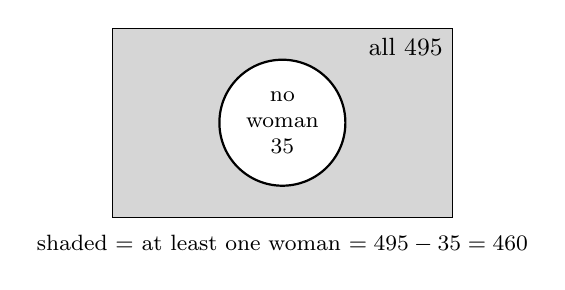
\begin{tikzpicture}[scale=0.8,every node/.style={font=\small}]
\fill[black!16] (-2.7,-1.5) rectangle (2.7,1.5);
\fill[white] (0,0) circle (1.0);
\draw[thin] (-2.7,-1.5) rectangle (2.7,1.5);
\node[anchor=north east,inner sep=2pt] at (2.64,1.44){all $495$};
\draw[thick] (0,0) circle (1.0);
\node[align=center,font=\footnotesize] at (0,0){no\\woman\\$35$};
\node[below=3pt,font=\footnotesize] at (0,-1.5){shaded $=$ at least one woman $=495-35=460$};
\end{tikzpicture}
\end{center}
\steplabel{Subtract.} $495-35=460$. There are $\boxed{460}$ committees with at least one woman.

% =====================================================================
\subsection*{Rule 4: arrangements of non-distinct objects (the multinomial coefficient)}
% =====================================================================

\begin{theorem}[Multinomial coefficient]\label{thm:multinom}
Suppose $n$ objects are to be arranged in a row, but they come in $r$ types: $n_1$ identical
copies of type $1$, $n_2$ of type $2$, \dots, $n_r$ of type $r$, where
$n_1+n_2+\cdots+n_r=n$. The number of \emph{distinguishable} arrangements is
\[
  \binom{n}{n_1,n_2,\dots,n_r}=\frac{n!}{n_1!\,n_2!\cdots n_r!}.
\]
\end{theorem}

\begin{proof}
Temporarily make the copies distinct (paint serial numbers on them). Then all $n$ objects are
different and there are $n!$ orderings. Now erase the serial numbers. Two of the $n!$ orderings
collapse to the same visible arrangement exactly when they differ only by permuting copies
\emph{within} a type; there are $n_1!\,n_2!\cdots n_r!$ such internal permutations for each
visible arrangement. Hence each distinguishable arrangement was counted
$n_1!\cdots n_r!$ times, and dividing gives $n!/(n_1!\cdots n_r!)$.
\end{proof}

When $r=2$ this reduces to a single binomial: $\dfrac{n!}{k!\,(n-k)!}=\binom{n}{k}$, since
choosing which $k$ of the $n$ slots receive the type-$1$ object \emph{is} a multinomial with
two types. The multinomial coefficient is thus the natural generalisation of $\binom{n}{k}$
to more than two categories.

\begin{example}[Rearranging a word with repeats]
How many distinguishable letter strings can be formed by rearranging all the letters of the
word \texttt{PEPPER} (three P's, two E's, one R)?
\end{example}
\whichrule{We arrange \emph{all} the letters (so it is a full permutation of $6$ symbols), but
some symbols are identical, so straight $6!$ overcounts. The signal is ``rearrange the
letters of a word with repeated letters.'' Divide by the factorial of each repeat count: this
is the multinomial coefficient.}
\soln
\steplabel{Counts.} $n=6$ with $3$ P's, $2$ E's, $1$ R.
\steplabel{Apply the formula.}
$\displaystyle\frac{6!}{3!\,2!\,1!}=\frac{720}{6\cdot 2\cdot 1}=\frac{720}{12}=60$.
There are $\boxed{60}$ distinguishable strings.

\begin{example}[Splitting people into labelled groups]
Twelve interns are to be split into three project teams: $5$ on team Alpha, $4$ on team Beta,
and $3$ on team Gamma. How many ways can this be done?
\end{example}
\whichrule{We are partitioning all $12$ people into groups of \emph{fixed, named} sizes. Each
person ends up wearing one of three labels (Alpha/Beta/Gamma), so this is exactly arranging
$12$ items of which $5$, $4$, $3$ are of each type --- a multinomial coefficient. Because the
teams are \emph{labelled} (distinct names), we do \emph{not} divide by $3!$ for reordering
the teams.}
\soln
\steplabel{Apply the formula.}
$\displaystyle\binom{12}{5,4,3}=\frac{12!}{5!\,4!\,3!}$.
\steplabel{Reduce stepwise.} $\displaystyle\frac{12!}{5!\,4!\,3!}
=\binom{12}{5}\binom{7}{4}\binom{3}{3}=792\cdot 35\cdot 1$.
\steplabel{Compute.} $792\cdot 35=27{,}720$. There are $\boxed{27{,}720}$ ways.

\begin{example}[Distributing distinct prizes by count]
Eight distinct trophies are to be handed out so that $4$ go in a display case, $3$ go to the
archive, and $1$ goes to the lobby. How many distributions are possible?
\end{example}
\whichrule{Each trophy is assigned one of three destinations, with destination \emph{counts}
fixed at $4,3,1$. This is the same structure as arranging $8$ items into three labelled types,
so it is a multinomial coefficient. The destinations are distinct places, so they are
labelled and there is no extra division.}
\soln
\steplabel{Apply the formula.}
$\displaystyle\binom{8}{4,3,1}=\frac{8!}{4!\,3!\,1!}=\frac{40{,}320}{24\cdot 6\cdot 1}
=\frac{40{,}320}{144}$.
\steplabel{Compute.} $40{,}320/144=280$. There are $\boxed{280}$ distributions.

\begin{example}[Arrangement with a non-adjacency constraint]
How many distinguishable arrangements of the letters in \texttt{LEVEL} (two L's, two E's, one
V) have the two L's \emph{not} adjacent?
\end{example}
\whichrule{The base count is a multinomial (rearranging a word with repeats). The
\emph{not adjacent} condition calls for complementary counting on top of the multinomial:
total arrangements minus those with the L's together. Treating ``the L's together'' as a
single glued block reduces that sub-count to another multinomial.}
\soln
\steplabel{Total arrangements.} $\displaystyle\frac{5!}{2!\,2!\,1!}=\frac{120}{4}=30$.
\steplabel{Glue the two L's into one block \texttt{[LL]}.} Now arrange $4$ items
$\{[LL],E,E,V\}$ with two E's identical:
$\displaystyle\frac{4!}{2!}=\frac{24}{2}=12$.
\steplabel{Subtract.} $30-12=18$. There are $\boxed{18}$ arrangements with the L's apart.

\begin{example}[Rearranging a longer word with several repeats]
How many distinguishable strings come from rearranging all the letters of \texttt{BANANA}
(one B, three A's, two N's)?
\end{example}
\whichrule{We arrange \emph{all} $6$ letters, but three are identical A's and two are identical
N's, so a plain $6!$ overcounts every string. The signal is ``rearrange a word with repeated
letters,'' which is the multinomial coefficient: divide $6!$ by the factorial of each repeat
count. A combination does not fit, because we are ordering all letters, not selecting a
subset.}
\soln
\steplabel{Counts.} $n=6$ with $1$ B, $3$ A's, $2$ N's.
\steplabel{Apply the formula.}
$\displaystyle\frac{6!}{1!\,3!\,2!}=\frac{720}{1\cdot 6\cdot 2}=\frac{720}{12}=60$.
There are $\boxed{60}$ distinguishable strings.

\begin{example}[Equal-sized labelled teams]
Nine volunteers are split into three labelled crews --- Red, Green, Blue --- of $3$ each. How
many splittings are possible?
\end{example}
\whichrule{Every volunteer receives one of three labels, with the label \emph{counts} fixed at
$3,3,3$. That is arranging $9$ items into three labelled types: a multinomial coefficient.
Because the crews carry \emph{distinct names}, we do \emph{not} divide by $3!$ for reordering
the crews --- that extra division would only apply if the three groups were interchangeable
and unlabelled.}
\soln
\steplabel{Apply the formula.}
$\displaystyle\binom{9}{3,3,3}=\frac{9!}{3!\,3!\,3!}
=\binom{9}{3}\binom{6}{3}\binom{3}{3}=84\cdot 20\cdot 1$.
\steplabel{Compute.} $84\cdot 20=1680$. There are $\boxed{1680}$ splittings.

\begin{example}[A long word and a multinomial probability]
The letters of \texttt{STATISTICS} (three S's, three T's, two I's, one A, one C) are arranged
at random in a row, all distinguishable arrangements equally likely.
\textbf{(a)} How many distinguishable arrangements are there?
\textbf{(b)} What fraction of them begin with the letter A?
\end{example}
\whichrule{Part (a) is a pure multinomial: arrange all $10$ letters with repeat counts
$3,3,2,1,1$. Part (b) turns the count into a probability --- favourable arrangements over
total --- and the favourable ones are themselves a smaller multinomial (fix A first, then
arrange the remaining $9$ letters). Combinations do not apply because we order every letter,
not choose a subset.}
\soln
\steplabel{(a) Total arrangements.}
$\displaystyle\frac{10!}{3!\,3!\,2!\,1!\,1!}=\frac{3{,}628{,}800}{6\cdot 6\cdot 2}
=\frac{3{,}628{,}800}{72}=50{,}400$. There are $\boxed{50{,}400}$ arrangements.
\steplabel{(b) Fix A in position one.} The remaining $9$ letters (three S's, three T's, two
I's, one C) arrange in
$\displaystyle\frac{9!}{3!\,3!\,2!\,1!}=\frac{362{,}880}{6\cdot 6\cdot 2}=5040$ ways.
\steplabel{Form the ratio.} $\dfrac{5040}{50{,}400}=\dfrac{1}{10}$. A fraction of
$\boxed{1/10}$ of the arrangements begin with A. (This matches intuition: A is one of $10$
letter-slots equally likely to lead, and there is just one A.)

% =====================================================================
\subsection*{Two short add-ons: circular permutations and stars and bars}
% =====================================================================

\paragraph{Circular permutations.} When $n$ distinct objects are arranged in a \emph{circle}
and only the relative order matters (no fixed seat, so rotations are regarded as the same
arrangement), the count is $(n-1)!$ rather than $n!$. The reason: every circular arrangement
corresponds to $n$ different linear arrangements (one per choice of which object we read
first), so $n!$ overcounts by a factor of $n$, giving $n!/n=(n-1)!$. If, in addition,
reflections (clockwise versus counterclockwise, as for an unmarked necklace) are considered
identical, divide again by $2$ to get $(n-1)!/2$ for $n\ge 3$.

\begin{example}[Round table]
In how many ways can $6$ distinct guests be seated around a circular table, counting two
seatings as the same when one is a rotation of the other?
\end{example}
\whichrule{The phrase ``around a circular table'' with rotations identified is the exact
trigger for circular permutations. We fix one guest as a reference point (killing the
rotational symmetry) and arrange the rest linearly, giving $(n-1)!$.}
\soln
\steplabel{Fix one guest, arrange the other $5$.} $(6-1)!=5!$.
\steplabel{Compute.} $5!=120$. There are $\boxed{120}$ distinct circular seatings.

\begin{example}[Beads on a bracelet]
Seven distinct beads are strung on a bracelet. Two arrangements count as the same if one can
be obtained from the other by rotating the bracelet \emph{or} by flipping it over. How many
distinct bracelets are there?
\end{example}
\whichrule{Beads on a closed loop with no fixed start is the circular-permutation setup, so
the rotational count is $(n-1)!$. The extra phrase ``flipping it over'' identifies clockwise
and counterclockwise readings, a reflection symmetry, so we divide once more by $2$. This is
the $(n-1)!/2$ refinement, used precisely when an arrangement and its mirror image are
indistinguishable.}
\soln
\steplabel{Rotational count.} $(7-1)!=6!=720$.
\steplabel{Identify reflections.} Each bracelet equals its flip, so divide by $2$:
$720/2=360$. There are $\boxed{360}$ distinct bracelets.

\begin{example}[Couples alternating around a table]
Four married couples (eight people) are seated around a round table so that the genders
alternate, with rotations regarded as identical. How many seatings are possible? (Treat one
gender group as ``set A'' and the other as ``set B''; alternation means the seats strictly
alternate A,B,A,B,$\dots$ around the circle.)
\end{example}
\whichrule{The base structure is circular (rotations identified), but a constraint
(alternation) splits the seating into two interleaved stages. We first seat one group to
break the rotational symmetry, then drop the other group into the gaps. Fixing one group's
circular arrangement uses $(n-1)!$; the second group then fills labelled gaps as an ordinary
linear permutation.}
\soln
\steplabel{Seat the A-group circularly.} The $4$ people of set A around the circle:
$(4-1)!=3!=6$ ways. This also fixes the rotation.
\steplabel{Seat the B-group in the four gaps.} The $4$ gaps are now distinct (each sits
between two fixed A-people), so the B-group fills them in $4!=24$ ways.
\steplabel{Multiply.} $6\cdot 24=144$. There are $\boxed{144}$ alternating seatings.

\begin{example}[Round table with two people forced together]
Five distinct delegates sit around a circular table (rotations identified), but two specific
delegates insist on sitting next to each other. How many seatings satisfy this?
\end{example}
\whichrule{This is a circular permutation with an adjacency constraint, the rotational analogue
of the glued-block trick. Treat the inseparable pair as a single block, count the circular
arrangements of the blocks, then multiply by the internal orderings of the block. Gluing
reduces the object count from $5$ to $4$ for the circular step.}
\soln
\steplabel{Glue the pair into one block.} Now $4$ objects sit in a circle:
$(4-1)!=3!=6$ ways.
\steplabel{Order inside the block.} The two glued delegates can sit in $2!=2$ internal orders.
\steplabel{Multiply.} $6\cdot 2=12$. There are $\boxed{12}$ seatings with the pair together.

\begin{example}[Eight at a round table]
Eight distinct delegates sit around a circular table. Two seatings are the same when one is a
rotation of the other. How many distinct seatings are there?
\end{example}
\whichrule{``Around a circular table'' with rotations identified is the plain circular
permutation, so the count is $(n-1)!$ rather than $n!$. There is no reflection clause (the
table is not flipped over), so we do \emph{not} divide by $2$ here, unlike a necklace or
bracelet.}
\soln
\steplabel{Fix one delegate, arrange the rest.} $(8-1)!=7!$.
\steplabel{Compute.} $7!=5040$. There are $\boxed{5040}$ distinct seatings.

\begin{example}[Charms on a keychain --- rotations and flips]
Six distinct charms are placed on a circular keychain. Two keychains are identical if one is a
rotation \emph{or} a flip of the other. How many distinct keychains are possible?
\end{example}
\whichrule{Charms on a closed loop with no fixed start is the circular setup, giving the
rotational count $(n-1)!$. ``Or a flip'' identifies a keychain with its mirror image, a
reflection symmetry, so we divide once more by $2$. This is the $(n-1)!/2$ refinement, applied
exactly when an arrangement and its reflection are indistinguishable. The grey sketch shows the
loop has no marked first bead.}
\soln
\steplabel{Rotational count.} $(6-1)!=5!=120$.
\steplabel{Identify reflections.} Each keychain equals its flip, so divide by $2$:
$120/2=60$.
\begin{center}
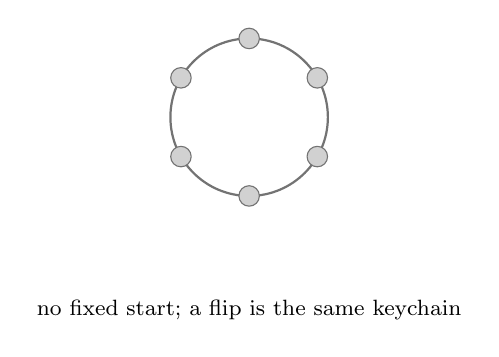
\begin{tikzpicture}[scale=1.0,font=\scriptsize]
\draw[thick,black!55] (0,0) circle (1);
\foreach \a in {90,150,210,270,330,30}{
  \fill[black!18,draw=black!55] (\a:1) circle (0.13);}
\node at (0,-2.45){\footnotesize no fixed start; a flip is the same keychain};
\end{tikzpicture}
\end{center}
\steplabel{Result.} There are $\boxed{60}$ distinct keychains.

\begin{example}[Round table where two people refuse to be neighbours]
Six distinct friends sit around a round table (rotations identified), but two of them, who are
quarrelling, refuse to sit next to each other. How many seatings satisfy this?
\end{example}
\whichrule{This is a circular permutation with an \emph{anti}-adjacency constraint. The clean
route is complementary counting: take all circular seatings, then subtract those in which the
quarrelling pair \emph{is} adjacent (found with the glued-block trick). Subtraction beats
listing the many allowed cases, just as the complement trick did for linear arrangements.}
\soln
\steplabel{All circular seatings.} $(6-1)!=5!=120$.
\steplabel{Seatings with the pair together.} Glue the pair into one block, leaving $5$ objects
in a circle: $(5-1)!=4!=24$ ways; the block has $2!=2$ internal orders, giving
$24\cdot 2=48$.
\steplabel{Subtract.} $120-48=72$. There are $\boxed{72}$ seatings with the pair apart.

\paragraph{Stars and bars.} To count the ways of choosing $k$ items from $n$ types
\emph{with} repetition and \emph{without} regard to order --- equivalently, the number of
nonnegative integer solutions of $x_1+x_2+\cdots+x_n=k$ --- picture $k$ identical stars in a
row and insert $n-1$ bars to split them into $n$ groups (the group sizes are the $x_i$). A
configuration is any arrangement of $k$ stars and $n-1$ bars, and choosing which of the
$k+(n-1)$ positions hold the bars gives
\[
  \binom{n+k-1}{k}=\binom{n+k-1}{n-1}.
\]

\begin{center}
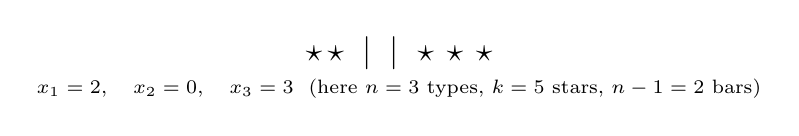
\begin{tikzpicture}[font=\large]
\node {$\star\,\star\;\mid\;\;\mid\;\star\,\star\,\star$};
\node[font=\scriptsize,below=2mm] at (0,0)
  {$x_1=2,\quad x_2=0,\quad x_3=3$ \ (here $n=3$ types, $k=5$ stars, $n-1=2$ bars)};
\end{tikzpicture}
\end{center}

\begin{example}[Buying doughnuts of several kinds]
A shop sells $4$ kinds of doughnut. A customer buys a box of $9$ doughnuts; only how many of
each kind matters, repeats are allowed, and a kind may be skipped. How many possible boxes
are there?
\end{example}
\whichrule{The signals are: repetition allowed (multiple of the same kind), order irrelevant
(a box is a multiset, not a sequence), and we are distributing a fixed total $9$ across $n=4$
type-counts. That is precisely nonnegative integer solutions of
$x_1+x_2+x_3+x_4=9$ --- a stars-and-bars problem. Plain combinations $\binom{4}{9}$ are
meaningless here (we pick more than the number of types), which itself flags that repetition
must be in play.}
\soln
\steplabel{Set up.} $n=4$ types, $k=9$ doughnuts, so $n-1=3$ bars.
\steplabel{Apply the formula.}
$\displaystyle\binom{n+k-1}{k}=\binom{4+9-1}{9}=\binom{12}{9}=\binom{12}{3}$.
\steplabel{Compute.} $\displaystyle\binom{12}{3}=\frac{12\cdot 11\cdot 10}{6}=220$. There are
$\boxed{220}$ possible boxes.

\begin{example}[Distributing identical tokens to people]
In how many ways can $20$ identical reward tokens be handed out to $5$ employees, if any
employee may receive any number (including zero)?
\end{example}
\whichrule{The tokens are \emph{identical} (only the count each person gets matters) and an
employee may receive zero or many, so this is the number of nonnegative integer solutions of
$x_1+\cdots+x_5=20$. Identical items into distinct recipients with repetition allowed is the
stars-and-bars signature, with $k=20$ stars and $n-1=4$ bars. Because the tokens are
indistinguishable, ordinary permutations or $n^k$ do not apply.}
\soln
\steplabel{Set up.} $n=5$ recipients, $k=20$ tokens, so $n-1=4$ bars.
\steplabel{Apply the formula.}
$\displaystyle\binom{n+k-1}{k}=\binom{5+20-1}{20}=\binom{24}{20}=\binom{24}{4}$.
\steplabel{Compute.}
$\displaystyle\binom{24}{4}=\frac{24\cdot 23\cdot 22\cdot 21}{24}=23\cdot 22\cdot 21=10{,}626$.
There are $\boxed{10{,}626}$ distributions.

\begin{example}[A positivity constraint: every recipient gets at least one]
A philanthropist splits $12$ identical grants among $4$ charities so that \emph{each} charity
receives \emph{at least one} grant. How many splits are possible?
\end{example}
\whichrule{Identical grants into distinct charities is stars and bars, but the ``at least one
each'' condition forbids the zero counts that the basic formula allows. The standard fix is to
pre-assign one grant to each charity, then distribute the remainder freely with zeros now
permitted. After pre-assigning, count nonnegative solutions of a smaller total.}
\soln
\steplabel{Pre-assign one to each.} Give each of the $4$ charities one grant: $4$ used,
$12-4=8$ remain.
\steplabel{Distribute the rest freely.} Nonnegative solutions of $y_1+y_2+y_3+y_4=8$ with
$n=4$, $k=8$:
$\displaystyle\binom{4+8-1}{8}=\binom{11}{8}=\binom{11}{3}$.
\steplabel{Compute.} $\displaystyle\binom{11}{3}=\frac{11\cdot 10\cdot 9}{6}=165$. There are
$\boxed{165}$ valid splits.

\begin{example}[Counting nondecreasing sequences]
How many nondecreasing length-$3$ sequences $(a_1\le a_2\le a_3)$ can be formed using values
from $\{1,2,3,4,5,6\}$, with repeats allowed?
\end{example}
\whichrule{A nondecreasing sequence is determined entirely by \emph{how many times each value
is used}, not by any ordering --- once the multiset of values is fixed, there is exactly one
way to write it in nondecreasing order. So this is choosing a size-$3$ multiset from $6$ types
with repetition: stars and bars with $n=6$ types and $k=3$ picks. Treating it as a plain
permutation would overcount, since rearranging the values would break the order condition.}
\soln
\steplabel{Reframe as a multiset.} Choose $k=3$ values from $n=6$ types, repetition allowed,
order irrelevant.
\steplabel{Apply the formula.}
$\displaystyle\binom{n+k-1}{k}=\binom{6+3-1}{3}=\binom{8}{3}$.
\steplabel{Compute.} $\displaystyle\binom{8}{3}=\frac{8\cdot 7\cdot 6}{6}=56$. There are
$\boxed{56}$ nondecreasing sequences.

\begin{example}[Scoops from six flavours]
An ice-cream shop has $6$ flavours. A bowl holds $10$ scoops; only the count of each flavour
matters, flavours may repeat, and a flavour may be skipped. How many distinct bowls are
possible?
\end{example}
\whichrule{The signals are: repetition allowed (a flavour may appear several times), order
irrelevant (a bowl is a multiset, not a sequence), and a fixed total $10$ spread over $n=6$
flavour-counts. That is nonnegative integer solutions of $x_1+\cdots+x_6=10$, a stars-and-bars
problem with $k=10$ stars and $n-1=5$ bars. A plain combination $\binom{6}{10}$ is meaningless
(we take more scoops than there are flavours), which flags that repetition is in play. The
sketch shows one bowl: $2$ vanilla, $0$ mint, $\dots$ with bars separating the flavour
groups.}
\soln
\steplabel{Set up.} $n=6$ flavours, $k=10$ scoops, so $n-1=5$ bars.
\begin{center}
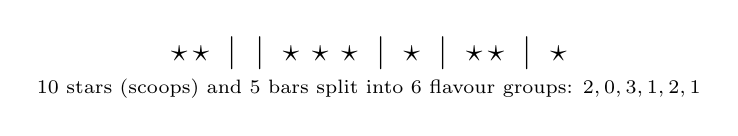
\begin{tikzpicture}[font=\large]
\node {$\star\,\star\;\mid\;\;\mid\;\star\,\star\,\star\;\mid\;\star\;\mid\;\star\,\star\;\mid\;\star$};
\node[font=\scriptsize,below=2mm] at (0,0)
  {$10$ stars (scoops) and $5$ bars split into $6$ flavour groups: $2,0,3,1,2,1$};
\end{tikzpicture}
\end{center}
\steplabel{Apply the formula.}
$\displaystyle\binom{n+k-1}{k}=\binom{6+10-1}{10}=\binom{15}{10}=\binom{15}{5}$.
\steplabel{Compute.}
$\displaystyle\binom{15}{5}=\frac{15\cdot 14\cdot 13\cdot 12\cdot 11}{120}=3003$. There are
$\boxed{3003}$ possible bowls.

\begin{example}[Identical balls into labelled boxes]
In how many ways can $15$ identical balls be placed into $4$ distinct boxes, where a box may
hold any number (including none)?
\end{example}
\whichrule{The balls are \emph{identical} (only the per-box count matters) and a box may hold
zero or many, so this is the number of nonnegative integer solutions of
$x_1+x_2+x_3+x_4=15$. Identical items into distinct containers with repetition allowed is the
stars-and-bars signature, $k=15$ stars and $n-1=3$ bars. Because the balls are
indistinguishable, $n^k$ or permutations would badly overcount.}
\soln
\steplabel{Set up.} $n=4$ boxes, $k=15$ balls, so $n-1=3$ bars.
\steplabel{Apply the formula.}
$\displaystyle\binom{n+k-1}{k}=\binom{4+15-1}{15}=\binom{18}{15}=\binom{18}{3}$.
\steplabel{Compute.}
$\displaystyle\binom{18}{3}=\frac{18\cdot 17\cdot 16}{6}=816$. There are $\boxed{816}$
placements.

\begin{example}[Every type used at least once]
A gift basket must contain exactly $7$ pieces of fruit drawn from $3$ types (apples, pears,
plums), with \emph{at least one} of each type. How many baskets are possible?
\end{example}
\whichrule{Identical fruit of each type into $3$ named categories is stars and bars, but the
``at least one of each'' clause bars the zero counts the basic formula allows. The standard
fix is to pre-assign one fruit to each type, then distribute the remainder freely with zeros
now permitted. After pre-assigning, count nonnegative solutions of a smaller total --- the
same positivity manoeuvre used in the grants example.}
\soln
\steplabel{Pre-assign one of each.} Three fruits used, $7-3=4$ remain.
\steplabel{Distribute the rest freely.} Nonnegative solutions of $y_1+y_2+y_3=4$ with $n=3$,
$k=4$:
$\displaystyle\binom{3+4-1}{4}=\binom{6}{4}=\binom{6}{2}$.
\steplabel{Compute.} $\displaystyle\binom{6}{2}=\frac{6\cdot 5}{2}=15$. There are $\boxed{15}$
possible baskets.

\section{Combinatorial Probability}\label{sec:combprob}

Counting tools become probability when every outcome of a suitably chosen sample space is
equally likely. This section isolates three rules that together solve most finite-sample
problems: the classical equally-likely model, the hypergeometric model for sampling
without replacement, and its mirror image, the binomial model for sampling with
replacement.

\begin{strategy}[How to recognise which rule this section needs]
Read the problem and answer three questions in order.
\begin{enumerate}[leftmargin=1.4em,itemsep=2pt]
  \item \keyword{Is every outcome equally likely?} If the wording says ``at random,''
  ``well shuffled,'' ``fair,'' or ``each is equally likely,'' you may use the
  \keyword{classical model} $\PP(A)=|A|/|S|$. The whole job is then two counts: the size
  of a sample space of equally likely outcomes, and the size of the favorable event. Every
  rule below is a packaged instance of this one.
  \item \keyword{Are you drawing a sample without replacement from a pool of two kinds of
  object, and asking how many of one kind you get?} Trigger words: ``draws $n$ \emph{without
  replacement},'' ``selects a committee/sample/hand,'' a fixed finite population split into
  ``$r$ of type~A and $w$ of type~B,'' and a question about the count of type~A in the
  sample. Use the \keyword{hypergeometric model}. The draws are \emph{not} independent: each
  removal changes the composition of what remains.
  \item \keyword{Is each trial repeated independently with the same success probability?}
  Trigger words: ``with replacement,'' ``each trial,'' ``repeated independently,'' tossing a
  coin or rolling a die $n$ times, or a population so large that removing a few items barely
  changes the proportion. Use the \keyword{binomial model}. Here the trials \emph{are}
  independent and $p$ is constant.
\end{enumerate}
The decisive contrast between (2) and (3) is replacement: \emph{without} replacement and a
finite pool means hypergeometric; \emph{with} replacement (or an effectively infinite pool)
means binomial. When a sample is small relative to a huge population the two nearly agree,
but only the hypergeometric is exact for a finite pool.
\end{strategy}

% =====================================================================
\subsection{Rule 1: the classical equally-likely model}
% =====================================================================

\begin{theorem}[Classical probability]\label{thm:classical}
Let $S$ be a finite sample space whose outcomes are equally likely, so each singleton has
probability $1/|S|$. Then for every event $A\subseteq S$,
\[
  \PP(A)=\frac{|A|}{|S|}=\frac{\text{number of favorable outcomes}}{\text{number of possible outcomes}}.
\]
\end{theorem}

\begin{proof}
Write $S=\{s_1,\dots,s_m\}$ with $m=|S|$. Equal likelihood means $\PP(\{s_i\})=c$ for a
common constant $c$. The singletons are disjoint and their union is $S$, so by the additivity
axiom $1=\PP(S)=\sum_{i=1}^m \PP(\{s_i\})=mc$, forcing $c=1/m$. Any event $A$ is the disjoint
union of its $|A|$ singletons, hence $\PP(A)=\sum_{s\in A}\PP(\{s\})=|A|\cdot\frac1m=|A|/|S|$.
\end{proof}

The model has exactly one hazard: the count $|S|$ and the count $|A|$ must be taken over the
\emph{same} kind of outcome, and those outcomes must really be equally likely. If you count
$|S|$ with ordered outcomes you must count $|A|$ with ordered outcomes too; the ordering
factors then cancel.

\begin{example}[A fair pair of dice]
Two distinguishable fair dice (one red, one blue) are rolled. Find the probability that the
two faces sum to $8$.
\end{example}
\whichrule{The dice are \keyword{fair} and the rolls are physical and symmetric, so all
ordered pairs of faces are \keyword{equally likely}; this is the bare classical model. No
sampling-without-replacement is involved (the dice do not deplete one another), so the
hypergeometric rule is irrelevant, and we are not counting repeated independent successes of
a single labelled event, so the binomial rule is not what the question asks for.}
\soln
\steplabel{Step 1: sample space.} An outcome is an ordered pair (red face, blue face). By the
multiplication principle $|S|=6\times 6=36$, and each is equally likely.
\steplabel{Step 2: favorable outcomes.} List the pairs summing to $8$:
$(2,6),(3,5),(4,4),(5,3),(6,2)$ --- read off the marked anti-diagonal of the grid below.
There are $|A|=5$.
\steplabel{Step 3: probability.} $\PP(\text{sum}=8)=\dfrac{5}{36}\approx 0.139$.
\begin{center}
\begin{tabular}{c|cccccc}
\toprule
{\scriptsize red\,$\backslash$\,blue} & 1 & 2 & 3 & 4 & 5 & 6\\
\midrule
1 & 2 & 3 & 4 & 5 & 6 & 7\\
2 & 3 & 4 & 5 & 6 & 7 & \textbf{8}\\
3 & 4 & 5 & 6 & 7 & \textbf{8} & 9\\
4 & 5 & 6 & 7 & \textbf{8} & 9 & 10\\
5 & 6 & 7 & \textbf{8} & 9 & 10 & 11\\
6 & 7 & \textbf{8} & 9 & 10 & 11 & 12\\
\bottomrule
\end{tabular}
\end{center}

\begin{example}[A random three-digit code]
A combination lock displays a $3$-digit code, each digit independently and uniformly chosen
from $0$ through $9$ (repeats allowed). What is the probability the code has all three digits
distinct?
\end{example}
\whichrule{Each digit is chosen \keyword{uniformly}, so all $10^3$ ordered codes are equally
likely --- the classical model on an ordered sample space. We are counting arrangements, not
drawing two-type objects from a finite urn, so this is not hypergeometric; and although the
digits are independent, the event ``all distinct'' is a single combinatorial count rather
than ``$k$ successes in $n$ trials,'' so the binomial formula is not the tool here.}
\soln
\steplabel{Step 1: total codes.} Three positions, $10$ choices each: $|S|=10^3=1000$.
\steplabel{Step 2: codes with distinct digits.} Fill the positions left to right: $10$ ways
for the first, $9$ for the second (must differ), $8$ for the third. By the multiplication
principle $|A|=10\cdot 9\cdot 8=720$.
\steplabel{Step 3: probability.}
$\PP(\text{all distinct})=\dfrac{720}{1000}=0.72$.

\begin{example}[Seating a committee in a row]
Four delegates --- two from the North party and two from the South party --- are seated in a
random order along a bench of four seats, all $4!$ orderings equally likely. Find the
probability that the two parties alternate (no two same-party delegates adjacent).
\end{example}
\whichrule{``Random order, all orderings equally likely'' is the classical model on
\keyword{permutations}. We count favorable \emph{arrangements}, so order matters and we work
on an ordered sample space; there is no draw of objects from an urn (hypergeometric) and no
sequence of independent identical trials (binomial).}
\soln
\steplabel{Step 1: sample space.} The delegates are distinct people, so $|S|=4!=24$ equally
likely seatings.
\steplabel{Step 2: favorable arrangements.} Alternation forces one of two party patterns,
$NSNS$ or $SNSN$. Within a fixed pattern the two North delegates fill their two slots in $2!$
ways and the two South delegates in $2!$ ways. Thus $|A|=2\cdot 2!\cdot 2!=2\cdot 2\cdot 2=8$.
\steplabel{Step 3: probability.}
$\PP(\text{alternate})=\dfrac{8}{24}=\dfrac13\approx 0.333$.

\begin{example}[Matching birthdays in a small group]
Five people have birthdays falling independently and uniformly on the $365$ days of a
non-leap year. Find the probability that at least two share a birthday.
\end{example}
\whichrule{``Independently and uniformly'' over $365$ days makes all $365^5$ ordered
birthday-lists equally likely --- the classical model. The clean route is the complement
``all five distinct.'' We are arranging days into ordered slots (a permutation count), not
sampling two-type objects (hypergeometric) and not counting $k$ labelled successes
(binomial).}
\soln
\steplabel{Step 1: sample space.} An outcome is an ordered list of five birthdays:
$|S|=365^5$.
\steplabel{Step 2: complement (all distinct).} Assign distinct days left to right:
$365\cdot 364\cdot 363\cdot 362\cdot 361$ ways. So
$\PP(\text{all distinct})=\dfrac{365\cdot364\cdot363\cdot362\cdot361}{365^5}$.
\steplabel{Step 3: evaluate.} The product of the five ratios is
$1\cdot\tfrac{364}{365}\cdot\tfrac{363}{365}\cdot\tfrac{362}{365}\cdot\tfrac{361}{365}
\approx 0.9729$.
\steplabel{Step 4: take the complement.}
$\PP(\text{at least one match})=1-0.9729\approx 0.0271$.

\begin{example}[At least one six on two dice]
Two distinguishable fair dice are rolled. Find the probability that at least one die shows
a six.
\end{example}
\whichrule{The dice are \keyword{fair}, so all $36$ ordered face-pairs are
\keyword{equally likely} --- the classical model. ``At least one'' is fastest through the
complement ``no six on either die,'' a single block of the grid. Nothing is drawn from a
depleting pool (not hypergeometric), and the question is one combinatorial count on a $6\times
6$ grid rather than a tally of $k$ labelled successes (not binomial).}
\soln
\steplabel{Step 1: sample space.} Ordered pairs (first die, second die): $|S|=6\times6=36$,
each equally likely.
\steplabel{Step 2: complement (no six).} Each die avoids the six in $5$ ways, so the pairs
with no six number $5\times5=25$ --- the unshaded $5\times5$ block at the upper left of the
grid.
\steplabel{Step 3: probability.}
$\PP(\text{at least one six})=1-\dfrac{25}{36}=\dfrac{11}{36}\approx 0.306$. The shaded last
row and last column below mark the $11$ favorable pairs.
\begin{center}
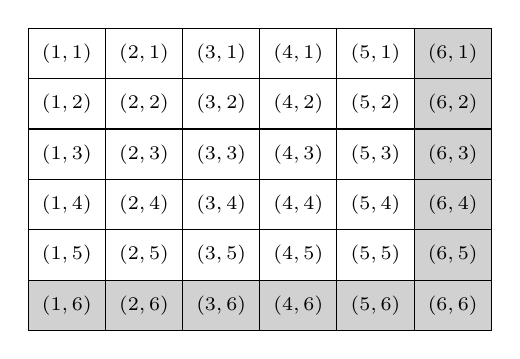
\begin{tikzpicture}[x=0.98cm,y=0.64cm,font=\scriptsize]
  \foreach \i in {1,...,6}{\foreach \j in {1,...,6}{
     \pgfmathtruncatemacro{\hit}{(\i==6 || \j==6)?1:0}
     \ifnum\hit=1 \fill[black!18] (\i-1,6-\j) rectangle (\i,7-\j);\fi
     \draw (\i-1,6-\j) rectangle (\i,7-\j);
     \node at (\i-0.5,6.5-\j) {$(\i,\j)$};}}
\end{tikzpicture}
\end{center}

\begin{example}[A random lattice path through a checkpoint]
A delivery robot walks from corner $(0,0)$ to corner $(4,3)$ on a street grid, each step going
one block East or one block North, and it chooses one of the shortest routes uniformly at
random. Find the probability that its route passes through the intersection $(2,1)$.
\end{example}
\whichrule{``Uniformly at random'' over the shortest routes makes every monotone lattice path
\keyword{equally likely} --- the classical model, with $|S|$ and $|A|$ both counted as path
counts. Each path is a single arrangement of E/N steps, so we count combinations of step
positions, not draws from a two-type urn (hypergeometric) and not $k$ successes in repeated
trials (binomial).}
\soln
\steplabel{Step 1: sample space.} A route is a sequence of $4$~E and $3$~N steps; choosing
which $3$ of the $7$ steps are N gives $|S|=\binom{7}{3}=35$ equally likely routes.
\steplabel{Step 2: favorable routes.} A route through $(2,1)$ splits into a leg
$(0,0)\to(2,1)$ --- $2$~E and $1$~N, $\binom{3}{1}=3$ ways --- followed by a leg
$(2,1)\to(4,3)$ --- $2$~E and $2$~N, $\binom{4}{2}=6$ ways. By the multiplication principle
$|A|=3\cdot 6=18$.
\steplabel{Step 3: probability.}
$\PP(\text{through }(2,1))=\dfrac{18}{35}\approx 0.514$.
\begin{center}
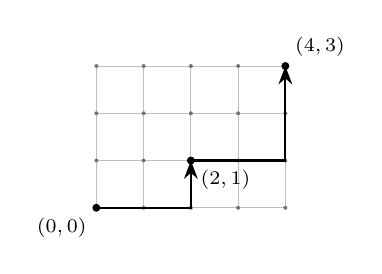
\begin{tikzpicture}[scale=0.6,font=\scriptsize,>=Stealth]
  \draw[step=1,black!25,thin] (0,0) grid (4,3);
  \foreach \x in {0,...,4}{\foreach \y in {0,...,3}{\fill[black!55] (\x,\y) circle (1.2pt);}}
  \fill (0,0) circle (2.4pt) node[below left]{$(0,0)$};
  \fill (4,3) circle (2.4pt) node[above right]{$(4,3)$};
  \fill (2,1) circle (2.4pt) node[below right]{$(2,1)$};
  \draw[->,thick] (0,0)--(2,0)--(2,1);
  \draw[->,thick] (2,1)--(4,1)--(4,3);
\end{tikzpicture}
\end{center}

\begin{example}[A PIN containing a chosen digit]
A four-digit PIN has each digit chosen independently and uniformly from $0$ through $9$
(repeats allowed). Find the probability that the digit $7$ appears at least once.
\end{example}
\whichrule{Each digit is \keyword{uniform}, so all $10^4$ ordered PINs are
\keyword{equally likely} --- the classical model. ``At least once'' is cleanest by the
complement ``no~$7$ in any position.'' We arrange digits into ordered slots (a permutation-style
count), not draw two-type objects from a finite pool (hypergeometric); and although ``at least
one~$7$'' could be expanded as a binomial sum over positions, the complement keeps it a single
equally-likely count, which is the intended tool here.}
\soln
\steplabel{Step 1: sample space.} Four positions, $10$ digits each: $|S|=10^4=10{,}000$.
\steplabel{Step 2: complement (no seven).} Each position avoids $7$ in $9$ ways, so
$9^4=6561$ PINs contain no~$7$, giving $\PP(\text{no }7)=\dfrac{6561}{10{,}000}=0.6561$.
\steplabel{Step 3: take the complement.}
$\PP(\text{at least one }7)=1-0.6561=0.3439$.

% =====================================================================
\subsection{Rule 2: the hypergeometric model (sampling without replacement)}
% =====================================================================

\begin{theorem}[Hypergeometric model]\label{thm:hyper}
An urn holds $N$ objects of which $r$ are of type~A (``red'') and $w=N-r$ are of type~B
(``white''). Draw $n$ objects at random without replacement. The probability that exactly
$k$ of the drawn objects are red is
\[
  \PP(K=k)=\frac{\dbinom{r}{k}\dbinom{w}{n-k}}{\dbinom{N}{n}},
  \qquad \max(0,\,n-w)\le k\le\min(n,r).
\]
\end{theorem}

\begin{proof}
Because the draw is at random and order within the sample carries no information, take as
sample space the collection of all unordered $n$-subsets of the $N$ objects; there are
$\binom{N}{n}$ of them and, by symmetry, they are equally likely. To build a favorable
subset --- one with exactly $k$ red --- choose which $k$ of the $r$ red objects are included,
in $\binom{r}{k}$ ways, and independently which $n-k$ of the $w$ white objects are included,
in $\binom{w}{n-k}$ ways. By the multiplication principle the number of favorable subsets is
$\binom{r}{k}\binom{w}{n-k}$. Divide by $\binom{N}{n}$ and apply the classical model
(Rule~1). The stated range of $k$ is exactly where both binomial
coefficients are nonzero: at least $0$ and at most $r$ red can be taken, and the $n-k$ whites
require $0\le n-k\le w$.
\end{proof}

The signature of this model is a single finite pool, split into two kinds, sampled
\emph{without} replacement, with the question asking how many of one kind land in the sample.

\begin{center}
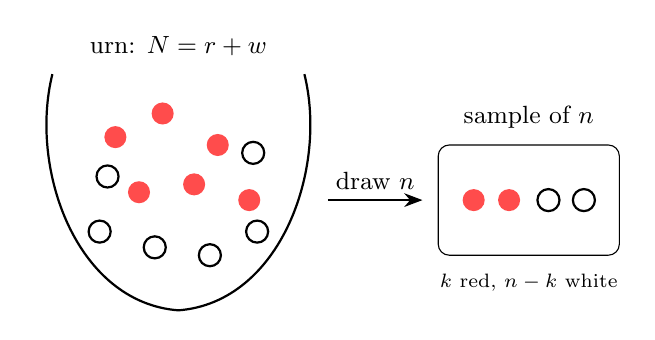
\begin{tikzpicture}[font=\small]
  % urn outline
  \draw[thick] (-1.6,1.4) .. controls (-1.9,0.2) and (-1.3,-1.5) .. (0,-1.6)
               .. controls (1.3,-1.5) and (1.9,0.2) .. (1.6,1.4);
  \node at (0,1.75) {\small urn: $N=r+w$};
  % red dots (filled)
  \foreach \p in {(-0.8,0.6),(-0.2,0.9),(0.5,0.5),(-0.5,-0.1),(0.2,0.0),(0.9,-0.2)}
     \fill[red!70] \p circle (0.14);
  % white dots (open)
  \foreach \p in {(-1.0,-0.6),(-0.3,-0.8),(0.4,-0.9),(1.0,-0.6),(-0.9,0.1),(0.95,0.4)}
     \draw[thick] \p circle (0.14);
  % arrow to the sample
  \draw[->,>=Stealth,thick] (1.9,-0.2) -- (3.1,-0.2) node[midway,above]{draw $n$};
  % sample box
  \draw[rounded corners] (3.3,-0.9) rectangle (5.6,0.5);
  \node at (4.45,0.85) {\small sample of $n$};
  \fill[red!70] (3.75,-0.2) circle (0.14);
  \fill[red!70] (4.2,-0.2) circle (0.14);
  \draw[thick] (4.7,-0.2) circle (0.14);
  \draw[thick] (5.15,-0.2) circle (0.14);
  \node at (4.45,-1.25) {\scriptsize $k$ red, $n-k$ white};
\end{tikzpicture}
\end{center}

\begin{example}[A small lottery]
A lottery machine holds $40$ balls numbered $1$ through $40$. Six are drawn at random without
replacement and constitute the winning set. A player has bought a single ticket marking six
numbers. Find the probability that the player matches exactly four of the six drawn numbers.
\end{example}
\whichrule{There is one finite pool of $40$ balls, split into two types relative to the
player's ticket: $6$ ``player's numbers'' and $34$ ``other numbers.'' Six balls are drawn
\keyword{without replacement}, and we want the count of player's numbers in the draw --- the
exact template of the hypergeometric model. It is not binomial because the draws deplete the
machine (no replacement, so trials are dependent and the success probability shifts after
each draw).}
\soln
\steplabel{Step 1: identify the parameters.} Pool $N=40$; type-A (player's numbers) $r=6$;
type-B (others) $w=34$; sample size $n=6$; target $k=4$.
\steplabel{Step 2: favorable count.} Choose $4$ of the player's $6$ numbers, $\binom{6}{4}$
ways, and $2$ of the other $34$, $\binom{34}{2}$ ways:
$\binom{6}{4}\binom{34}{2}=15\cdot 561=8415$.
\steplabel{Step 3: sample-space size.} $\binom{40}{6}=3\,838\,380$.
\steplabel{Step 4: probability.}
$\PP(K=4)=\dfrac{8415}{3\,838\,380}\approx 0.00219$, roughly $1$ in $456$.

\begin{example}[A bipartisan committee]
A department has $7$ statisticians and $5$ biologists. A committee of $4$ is chosen at random
(all $\binom{12}{4}$ committees equally likely). Find the probability the committee contains
exactly $2$ statisticians and $2$ biologists.
\end{example}
\whichrule{One pool of $12$ people, split into two types (statisticians, biologists),
selected \keyword{without replacement} (a person can sit on the committee only once), with a
question about how many of one type are chosen --- hypergeometric. ``Choose a committee'' is
the canonical unordered without-replacement draw; binomial would require independent repeated
trials with a fixed success probability, which committee selection does not provide.}
\soln
\steplabel{Step 1: parameters.} $N=12$, type-A statisticians $r=7$, type-B biologists $w=5$,
sample $n=4$, target $k=2$.
\steplabel{Step 2: favorable count.}
$\binom{7}{2}\binom{5}{2}=21\cdot 10=210$.
\steplabel{Step 3: total committees.} $\binom{12}{4}=495$.
\steplabel{Step 4: probability.}
$\PP(2\text{ of each})=\dfrac{210}{495}=\dfrac{14}{33}\approx 0.424$.

\begin{example}[A full house in poker]
Five cards are dealt at random from a standard $52$-card deck. Find the probability of a
\keyword{full house}: three cards of one rank and two of another.
\end{example}
\whichrule{A deal of $5$ cards from $52$ is sampling \keyword{without replacement} from a
finite pool, and the equally-likely sample space is the set of $\binom{52}{5}$ hands. The
counting is a layered hypergeometric/multiplication argument on the $13$ ranks and $4$ suits.
It is decidedly not binomial --- cards are not replaced and the deck is finite, so successive
cards are dependent.}
\soln
\steplabel{Step 1: sample space.} $|S|=\binom{52}{5}=2\,598\,960$ equally likely hands.
\steplabel{Step 2: count full houses.} Choose the rank that appears three times: $13$ ways.
Choose $3$ of its $4$ suits: $\binom{4}{3}=4$. Choose a \emph{different} rank for the pair:
$12$ ways. Choose $2$ of its $4$ suits: $\binom{4}{2}=6$. By the multiplication principle
$|A|=13\cdot 4\cdot 12\cdot 6=3744$.
\steplabel{Step 3: probability.}
$\PP(\text{full house})=\dfrac{3744}{2\,598\,960}\approx 0.00144$, about $1$ in $694$.

\begin{example}[At least one defective, by complement]
A carton holds $25$ memory chips, of which $4$ are defective. A buyer inspects a random
sample of $5$ without replacement. Find the probability that the sample contains at least one
defective chip.
\end{example}
\whichrule{A finite pool of $25$ chips split into defective/good, sampled \keyword{without
replacement}, with a question about the number of defectives --- hypergeometric. ``At least
one'' is cleanest via the complement ``zero defectives,'' still a hypergeometric term.
Replacement is absent, so this is not the binomial model, though the two would nearly
coincide if the carton were enormous.}
\soln
\steplabel{Step 1: parameters.} $N=25$, defectives $r=4$, good $w=21$, sample $n=5$.
\steplabel{Step 2: complement (zero defectives, $k=0$).}
$\PP(K=0)=\dfrac{\binom{4}{0}\binom{21}{5}}{\binom{25}{5}}
=\dfrac{1\cdot 20{,}349}{53{,}130}\approx 0.383$.
\steplabel{Step 3: take the complement.}
$\PP(K\ge 1)=1-0.383\approx 0.617$.

\begin{example}[Capture--recapture estimate]
To gauge a pond's fish population, a biologist nets $20$ fish, tags them, and releases them.
Later she nets a fresh sample of $15$ fish and finds $3$ tagged. Treating the pond as holding
$N=200$ fish, find the probability that exactly $3$ of the $15$ recaptured fish are tagged.
\end{example}
\whichrule{At the time of the second netting the pond is a fixed finite pool of $N=200$ fish
split into two types --- $20$ tagged and $180$ untagged --- and the $15$ recaptured fish are
a sample \keyword{without replacement} (no fish is caught twice in one haul). Asking how many
of the sample are tagged is exactly hypergeometric. With replacement we would use binomial,
but a single net haul removes fish from availability, so the draws are dependent.}
\soln
\steplabel{Step 1: parameters.} $N=200$, tagged $r=20$, untagged $w=180$, sample $n=15$,
target $k=3$.
\steplabel{Step 2: favorable count.}
$\binom{20}{3}\binom{180}{12}$.
\steplabel{Step 3: assemble the probability.}
\[
  \PP(K=3)=\frac{\binom{20}{3}\binom{180}{12}}{\binom{200}{15}}\approx 0.129.
\]
\steplabel{Step 4: interpret.} Under $N=200$ the expected number of tagged fish in the haul
is $n\,r/N=15\cdot 20/200=1.5$, so the observed $3$ sits in the upper tail; the most likely
single count is $1$. The outcome $K=3$ is therefore above average yet far from rare, carrying
a probability near $0.13$. (This calculation underlies the maximum-likelihood population
estimate: one chooses $N$ to make the observed count most probable, and the small population
sizes that would make $K=3$ \emph{most} likely are exactly those near $N\approx 100$, where
the tagged fraction $20/N$ best matches the sample fraction $3/15$.)

\begin{example}[One red pen in a handful]
A drawer holds $12$ identical-feeling pens: $4$ write red and $8$ write blue. Three pens are
grabbed at random (all $\binom{12}{3}$ handfuls equally likely). Find the probability that
exactly one of the three is red.
\end{example}
\whichrule{One finite pool of $12$ pens, split into two types (red, blue), grabbed
\keyword{without replacement} --- a pen is in the hand or not, never twice --- with a question
about how many reds appear: the hypergeometric template. It is not binomial, since each pen
removed changes the red fraction among those still in the drawer, so the draws are dependent.}
\soln
\steplabel{Step 1: parameters.} $N=12$, type-A red $r=4$, type-B blue $w=8$, sample $n=3$,
target $k=1$.
\steplabel{Step 2: favorable count.}
$\binom{4}{1}\binom{8}{2}=4\cdot 28=112$.
\steplabel{Step 3: sample-space size.} $\binom{12}{3}=220$.
\steplabel{Step 4: probability.}
$\PP(K=1)=\dfrac{112}{220}=\dfrac{28}{55}\approx 0.509$.
\begin{center}
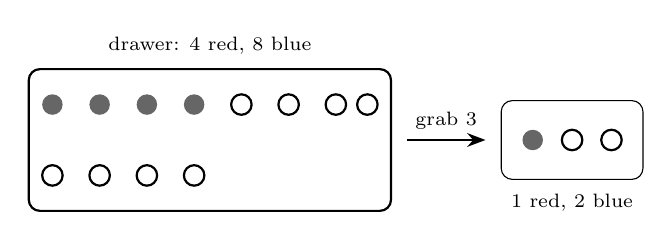
\begin{tikzpicture}[font=\scriptsize]
  \draw[rounded corners,thick] (-2.3,-0.9) rectangle (2.3,0.9);
  \node at (0,1.2) {\scriptsize drawer: $4$ red, $8$ blue};
  \foreach \p in {(-2.0,0.45),(-1.4,0.45),(-0.8,0.45),(-0.2,0.45)}
     \fill[black!60] \p circle (0.13);
  \foreach \p in {(0.4,0.45),(1.0,0.45),(1.6,0.45),(2.0,0.45),
                  (-2.0,-0.45),(-1.4,-0.45),(-0.8,-0.45),(-0.2,-0.45)}
     \draw[thick] \p circle (0.13);
  \draw[->,>=Stealth,thick] (2.5,0) -- (3.5,0) node[midway,above]{grab $3$};
  \draw[rounded corners] (3.7,-0.5) rectangle (5.5,0.5);
  \fill[black!60] (4.1,0) circle (0.13);
  \draw[thick] (4.6,0) circle (0.13);
  \draw[thick] (5.1,0) circle (0.13);
  \node at (4.6,-0.8) {\scriptsize $1$ red, $2$ blue};
\end{tikzpicture}
\end{center}

\begin{example}[Exactly two aces in a five-card hand]
Five cards are dealt at random from a standard $52$-card deck. Find the probability the hand
holds exactly two aces.
\end{example}
\whichrule{A deal of $5$ from $52$ is sampling \keyword{without replacement} from a finite
pool, equally likely over the $\binom{52}{5}$ hands. Split the deck into two types --- $4$
aces and $48$ non-aces --- and ask how many aces land in the hand: pure hypergeometric.
Binomial would need independent repeated trials with fixed $p$, but each card dealt depletes
the deck and shifts the chance of an ace on the next card.}
\soln
\steplabel{Step 1: parameters.} $N=52$, aces $r=4$, non-aces $w=48$, sample $n=5$, target
$k=2$.
\steplabel{Step 2: favorable count.}
$\binom{4}{2}\binom{48}{3}=6\cdot 17{,}296=103\,776$.
\steplabel{Step 3: sample-space size.} $\binom{52}{5}=2\,598\,960$.
\steplabel{Step 4: probability.}
$\PP(K=2)=\dfrac{103\,776}{2\,598\,960}\approx 0.0399$, about $1$ in $25$.

\begin{example}[A raffle, by complement]
A charity sells $50$ raffle tickets and will draw $10$ distinct winning tickets at random. You
hold $5$ of the $50$ tickets. Find the probability that at least one of your tickets wins.
\end{example}
\whichrule{The $50$ tickets are one finite pool split into ``yours'' ($5$) and ``others''
($45$); the $10$ winners are drawn \keyword{without replacement} (a ticket cannot win twice),
and we count how many of yours are among them --- hypergeometric. ``At least one'' is cleanest
by the complement ``none of yours wins,'' the $k=0$ term. No replacement occurs, so the
binomial model does not apply, though for a far larger ticket pool the two would nearly
agree.}
\soln
\steplabel{Step 1: parameters.} $N=50$, yours $r=5$, others $w=45$, sample $n=10$.
\steplabel{Step 2: complement (none of yours, $k=0$).}
$\PP(K=0)=\dfrac{\binom{5}{0}\binom{45}{10}}{\binom{50}{10}}
=\dfrac{3\,190\,187\,286}{10\,272\,278\,170}\approx 0.311$.
\steplabel{Step 3: take the complement.}
$\PP(K\ge 1)=1-0.311\approx 0.689$.

% =====================================================================
\subsection{Rule 3: the binomial model (sampling with replacement)}
% =====================================================================

The hypergeometric model assumes the pool shrinks with each draw. Replace each object before
the next draw --- or sample from a pool so vast that removal is negligible --- and the draws
become independent with a constant success probability. The count of successes then follows
the binomial model.

\begin{theorem}[Binomial model]\label{thm:binom}
Perform $n$ independent trials, each a ``success'' with the same probability $p$ and a
``failure'' with probability $q=1-p$. The probability of exactly $k$ successes is
\[
  \PP(X=k)=\binom{n}{k}p^k q^{\,n-k},\qquad k=0,1,\dots,n.
\]
\end{theorem}

\begin{proof}
Fix one particular sequence of outcomes having $k$ successes and $n-k$ failures in specified
positions. By independence its probability is the product of the per-trial probabilities,
$p^k q^{\,n-k}$, and this value is the same for \emph{every} sequence with $k$ successes,
since it depends only on the counts. The number of such sequences is the number of ways to
choose which $k$ of the $n$ positions are the successes, namely $\binom{n}{k}$. These
sequences are mutually exclusive outcomes, so by additivity their probabilities sum, giving
$\binom{n}{k}p^k q^{\,n-k}$.
\end{proof}

\begin{remark}[Why replacement changes the rule]
Sampling \emph{with} replacement from an urn of $r$ red and $w=N-r$ white makes each draw an
independent success ($=$ red) with constant $p=r/N$; the red count is binomial$(n,p)$.
Sampling \emph{without} replacement makes it hypergeometric. The two share the same mean
$np$, but the binomial allows any $k$ from $0$ to $n$ regardless of $r$, whereas the
hypergeometric cannot return more reds than the urn holds. When $N$ is huge relative to $n$,
removing a few objects barely moves $p$, and the hypergeometric probabilities converge to the
binomial ones --- which is why ``large population'' problems are routinely modelled as
binomial.
\end{remark}

\begin{example}[Repeated draws with replacement]
An urn holds $3$ red and $7$ white balls. A ball is drawn, its color noted, and
\keyword{returned}; this is repeated $5$ times. Find the probability of getting exactly $2$
red balls.
\end{example}
\whichrule{The ball is \keyword{returned} after each draw, so the urn's composition never
changes: each of the $5$ draws is an independent trial with the \emph{same} success
probability $p=3/10$. Constant $p$ and independence are the binomial signature. Had the balls
\emph{not} been replaced, the pool would shrink and we would use the hypergeometric model
instead.}
\soln
\steplabel{Step 1: parameters.} Trials $n=5$, success $=$ red with $p=3/10=0.3$, failure
$q=0.7$, target $k=2$.
\steplabel{Step 2: apply the formula.}
$\PP(X=2)=\binom{5}{2}(0.3)^2(0.7)^3=10\cdot 0.09\cdot 0.343$.
\steplabel{Step 3: evaluate.}
$10\cdot 0.09\cdot 0.343=0.3087$.
The two-stage structure for one ordering (e.g.\ red, red, then three whites) is shown below;
the binomial coefficient counts the $\binom{5}{2}=10$ orderings, each contributing the same
$p^2q^3$.
\begin{center}
\begin{tikzpicture}[>=Stealth,grow=right,
  level 1/.style={sibling distance=30mm,level distance=24mm},
  level 2/.style={sibling distance=15mm,level distance=24mm},font=\small]
\node{}
  child{node{$R$}
    child{node{$R$} edge from parent node[midway,fill=white,inner sep=2pt]{$0.3$}}
    child{node{$W$} edge from parent node[midway,fill=white,inner sep=2pt]{$0.7$}}
    edge from parent node[midway,fill=white,inner sep=2pt]{$0.3$}}
  child{node{$W$}
    child{node{$R$} edge from parent node[midway,fill=white,inner sep=2pt]{$0.3$}}
    child{node{$W$} edge from parent node[midway,fill=white,inner sep=2pt]{$0.7$}}
    edge from parent node[midway,fill=white,inner sep=2pt]{$0.7$}};
\end{tikzpicture}
\end{center}

\begin{example}[A multiple-choice quiz]
A student guesses on each of $8$ multiple-choice questions, each having $4$ options with one
correct answer, guesses independent. Find the probability of getting exactly $3$ correct.
\end{example}
\whichrule{Each question is an \keyword{independent} trial with the \emph{same} success
probability $p=1/4$, and there is no finite pool being depleted --- guessing one question
right does not change the odds on the next. Constant $p$ plus independence over a fixed number
of trials is the binomial model, not the hypergeometric (nothing is sampled without
replacement here).}
\soln
\steplabel{Step 1: parameters.} $n=8$, $p=1/4=0.25$, $q=0.75$, $k=3$.
\steplabel{Step 2: apply the formula.}
$\PP(X=3)=\binom{8}{3}(0.25)^3(0.75)^5=56\cdot 0.015625\cdot 0.2373$.
\steplabel{Step 3: evaluate.} $56\cdot 0.015625=0.875$, and
$0.875\cdot 0.2373\approx 0.208$.

\begin{example}[Defect rate on a production line]
A machine produces items independently, each defective with probability $p=0.05$. In a run of
$10$ items, find the probability of at least one defective.
\end{example}
\whichrule{Items are produced \keyword{independently} with a \emph{constant} defect
probability $p=0.05$ --- effectively sampling with replacement from an inexhaustible process,
so the binomial model applies. ``At least one'' is handled by the complement ``none.'' There
is no fixed finite pool of items to deplete, so the hypergeometric model does not fit.}
\soln
\steplabel{Step 1: parameters.} $n=10$, $p=0.05$, $q=0.95$.
\steplabel{Step 2: complement (zero defectives).}
$\PP(X=0)=\binom{10}{0}(0.05)^0(0.95)^{10}=(0.95)^{10}\approx 0.5987$.
\steplabel{Step 3: take the complement.}
$\PP(X\ge 1)=1-0.5987\approx 0.401$.

\begin{example}[Free throws]
A player sinks each free throw independently with probability $p=0.8$. In a sequence of $6$
attempts, find the probability of making at least $5$.
\end{example}
\whichrule{Each attempt is an \keyword{independent} trial with the \emph{same} make
probability $0.8$; nothing is consumed or depleted from a finite pool, so the binomial model
governs the count of makes. ``At least $5$'' means $k=5$ or $k=6$, summed. The hypergeometric
model would require sampling without replacement from a finite two-type pool, which this is
not.}
\soln
\steplabel{Step 1: parameters.} $n=6$, $p=0.8$, $q=0.2$.
\steplabel{Step 2: the two relevant terms.}
$\PP(X=5)=\binom{6}{5}(0.8)^5(0.2)^1=6\cdot 0.32768\cdot 0.2=0.393216$;\quad
$\PP(X=6)=(0.8)^6=0.262144$.
\steplabel{Step 3: add.}
$\PP(X\ge 5)=0.393216+0.262144\approx 0.655$.

\begin{example}[Hypergeometric vs.\ binomial: the same urn, two protocols]
An urn holds $30$ red and $70$ white balls ($N=100$). Three balls are taken. Compute
$\PP(\text{exactly }2\text{ red})$ under (a) sampling \emph{without} replacement and (b)
sampling \emph{with} replacement, and compare.
\end{example}
\whichrule{This problem deliberately fixes the scenario and varies only the \keyword{protocol}
to isolate the contrast. Protocol (a) ``without replacement'' depletes the finite pool, so
$\PP$ is hypergeometric. Protocol (b) ``with replacement'' restores the urn each time, making
the draws independent with constant $p=30/100=0.3$, so $\PP$ is binomial. The decisive cue is
the single word replacement.}
\soln
\steplabel{Part (a): hypergeometric.} $N=100$, $r=30$, $w=70$, $n=3$, $k=2$:
\[
  \PP(K=2)=\frac{\binom{30}{2}\binom{70}{1}}{\binom{100}{3}}
  =\frac{435\cdot 70}{161{,}700}=\frac{30{,}450}{161{,}700}\approx 0.188.
\]
\steplabel{Part (b): binomial.} $n=3$, $p=0.3$, $q=0.7$, $k=2$:
\[
  \PP(X=2)=\binom{3}{2}(0.3)^2(0.7)^1=3\cdot 0.09\cdot 0.7=0.189.
\]
\steplabel{Compare.} The two answers, $0.188$ and $0.189$, nearly coincide because the sample
($n=3$) is tiny relative to the pool ($N=100$): removing two or three balls barely changes
the red fraction, so the without-replacement process behaves almost like the
constant-$p$ with-replacement process. Shrink the pool toward the sample size and the gap
widens; only the hypergeometric value stays exact for a finite urn.

\begin{example}[Six heads in ten tosses]
A fair coin is tossed $10$ times, the tosses independent. Find the probability of getting
exactly $6$ heads.
\end{example}
\whichrule{Each toss is an \keyword{independent} trial with the \emph{same} success
probability $p=1/2$; the coin is not consumed, so nothing depletes between tosses. Fixed $n$,
constant $p$, independent trials --- the binomial model. There is no finite two-type pool
sampled without replacement, so the hypergeometric model is not the tool.}
\soln
\steplabel{Step 1: parameters.} $n=10$, $p=0.5$, $q=0.5$, $k=6$.
\steplabel{Step 2: apply the formula.}
$\PP(X=6)=\binom{10}{6}(0.5)^6(0.5)^4=\binom{10}{6}(0.5)^{10}=210\cdot\dfrac{1}{1024}$.
\steplabel{Step 3: evaluate.}
$\PP(X=6)=\dfrac{210}{1024}\approx 0.205$.

\begin{example}[Exactly two sixes in four rolls]
A fair die is rolled $4$ times independently. Find the probability of rolling a six exactly
twice.
\end{example}
\whichrule{Each roll is an \keyword{independent} trial with constant success probability
$p=1/6$ for ``six''; a die does not wear out, so $p$ never changes between rolls. Constant $p$
plus independence over a fixed number of trials is the binomial signature. Nothing is sampled
without replacement from a depleting pool, so the hypergeometric model does not apply.}
\soln
\steplabel{Step 1: parameters.} $n=4$, $p=1/6$, $q=5/6$, $k=2$.
\steplabel{Step 2: apply the formula.}
$\PP(X=2)=\binom{4}{2}\left(\dfrac16\right)^2\left(\dfrac56\right)^2
=6\cdot\dfrac{1}{36}\cdot\dfrac{25}{36}$.
\steplabel{Step 3: evaluate.}
$\PP(X=2)=\dfrac{6\cdot 25}{1296}=\dfrac{150}{1296}\approx 0.116$.
The tree below traces one favorable ordering (six, six, then two non-sixes); the coefficient
$\binom{4}{2}=6$ counts the orderings, each contributing the same $(1/6)^2(5/6)^2$.
\begin{center}
\begin{tikzpicture}[>=Stealth,grow=right,
  level 1/.style={sibling distance=26mm,level distance=22mm},
  level 2/.style={sibling distance=13mm,level distance=22mm},font=\scriptsize]
\node{}
  child{node{$6$}
    child{node{$6$} edge from parent node[midway,fill=white,inner sep=2pt]{$\tfrac16$}}
    child{node{$\bar 6$} edge from parent node[midway,fill=white,inner sep=2pt]{$\tfrac56$}}
    edge from parent node[midway,fill=white,inner sep=2pt]{$\tfrac16$}}
  child{node{$\bar 6$}
    child{node{$6$} edge from parent node[midway,fill=white,inner sep=2pt]{$\tfrac16$}}
    child{node{$\bar 6$} edge from parent node[midway,fill=white,inner sep=2pt]{$\tfrac56$}}
    edge from parent node[midway,fill=white,inner sep=2pt]{$\tfrac56$}};
\end{tikzpicture}
\end{center}

\begin{example}[A spam filter, by complement]
Incoming messages are independently spam with probability $p=0.1$. Among the next $20$
messages, find the probability of at most one spam message.
\end{example}
\whichrule{Messages arrive \keyword{independently}, each spam with a \emph{constant}
$p=0.1$ --- effectively sampling with replacement from an endless stream, so the binomial model
governs the spam count. ``At most one'' means $k=0$ or $k=1$, summed. There is no fixed finite
pool being depleted, so the hypergeometric model does not fit.}
\soln
\steplabel{Step 1: parameters.} $n=20$, $p=0.1$, $q=0.9$.
\steplabel{Step 2: the two relevant terms.}
$\PP(X=0)=(0.9)^{20}\approx 0.1216$;\quad
$\PP(X=1)=\binom{20}{1}(0.1)(0.9)^{19}=20\cdot 0.1\cdot 0.1351\approx 0.2702$.
\steplabel{Step 3: add.}
$\PP(X\le 1)=0.1216+0.2702\approx 0.392$.

\clearpage

\section{Exercises}
\textit{All problems below are original. Full solutions begin on page~\pageref{sec:solutions:ch2}.}

\subsection*{A.\ Sample spaces and events}
\begin{enumerate}[label=\textbf{A\arabic*.},leftmargin=*,itemsep=4pt]
\item A spinner has four equal sectors labelled $1,2,3,4$. It is spun twice and the two
  labels are recorded in order. Write the sample space $S$ and give $|S|$. With
  $A=$ ``the two labels are equal'' and $B=$ ``the labels sum to $5$,'' list $A$, $B$, and
  $A\cap B$, and state whether $A$ and $B$ are mutually exclusive.
\item For three events $A,B,C$, write a set expression for each described event:
  (a) at least one of the three occurs; (b) exactly one of the three occurs;
  (c) at most one occurs; (d) $A$ occurs but neither $B$ nor $C$ does.
\item Prove the identity $A\cup(\comp{A}\cap B)=A\cup B$ both by a Venn diagram and by a
  membership argument.
\item Use the distributive and De~Morgan laws to simplify
  $\comp{\big((A\cap B)\cup(A\cap\comp{B})\big)}$ to a single complemented event.
\item A box holds chips numbered $1$ through $9$. One chip is drawn. Let $E=$ ``the number
  is even,'' $T=$ ``the number exceeds $5$,'' and $D=$ ``the number is divisible by $3$.''
  List the outcomes in $E\cap T$, in $E\cup D$, and in $\comp{T}\cap D$.
\item A fair coin is tossed repeatedly until it shows two heads in a row or until five
  tosses have been made, whichever happens first. List the sample space $S$.
\item Show that the events $A\cap B$, $A\cap\comp{B}$, and $\comp{A}$ are pairwise disjoint
  and that their union is the whole sample space $S$.
\item Translate into plain words: (a) $A\subseteq B$; (b) $A\cap B=\varnothing$;
  (c) $A\cup B=S$. Then give a single roll-of-a-die example of events $A,B$ for which all
  three statements would force $A=\comp{B}$.
\item A red die and a green die are rolled. Describe the sample space and give $|S|$. With
  $G=$ ``the green die shows an even number'' and $H=$ ``the two dice show the same number,''
  list $G\cap H$ and decide whether $G$ and $H$ are mutually exclusive.
\item Two distinct letters are chosen, one after the other, from $\{a,b,c,d\}$ (order
  matters, no repeats). Write the sample space and give $|S|$. List the event $L=$ ``the
  letter $a$ appears.''
\item For events $A,B,C$, write a set expression for: (a) at least two of the three occur;
  (b) none of the three occurs; (c) exactly two occur; (d) $C$ occurs but at most one of
  $A,B$ does.
\item A spinner is spun until it first lands on red or until it has been spun three times,
  whichever comes first. Each spin shows red ($R$) or blue ($B$). List the sample space $S$.
\item Simplify $(A\cup B)\cap(A\cup\comp{B})$ to a single event using the distributive law,
  and confirm the result with a Venn diagram.
\item A point $(x,y)$ is chosen from the integer grid $\{1,2,3\}\times\{1,2,3\}$. Let
  $U=$ ``$x=y$,'' $V=$ ``$x+y=4$,'' and $W=$ ``$x<y$.'' List the outcomes in each event and
  state which two of $U,V,W$ are mutually exclusive.
\item Prove the identity $A\setminus(B\cup C)=(A\setminus B)\cap(A\setminus C)$ by a
  membership argument, and illustrate the left-hand side with a Venn picture.
\end{enumerate}

\subsection*{B.\ The probability function}
\begin{enumerate}[label=\textbf{B\arabic*.},leftmargin=*,itemsep=4pt]
\item Given $\PP(A)=0.55$, $\PP(B)=0.40$, and $\PP(A\cap B)=0.25$, find $\PP(A\cup B)$,
  $\PP(\comp{A}\cap\comp{B})$, $\PP(\text{exactly one of }A,B)$, and $\PP(\comp{A}\cap B)$.
\item In a survey of $200$ households, $120$ subscribe to a streaming service, $90$ own a
  game console, and $55$ have both. How many households have at least one, and how many have
  neither?
\item A loaded four-sided die assigns probabilities proportional to the face value: face $k$
  ($k=1,2,3,4$) has probability $ck$. Find $c$, then compute $\PP(\text{face is odd})$ and
  $\PP(\text{face}\ge 3)$.
\item Prove that for any events $A,B$, \ $\PP(A\cup B)\le \PP(A)+\PP(B)$, and state exactly
  when equality holds.
\item Events $A,B,C$ satisfy $\PP(A)=\PP(B)=\PP(C)=0.4$, all three pairwise intersections
  equal $0.15$, and $\PP(A\cap B\cap C)=0.05$. Find $\PP(A\cup B\cup C)$ and
  $\PP(\text{none of the three})$.
\item Show that if $\PP(A)=0.7$ and $\PP(B)=0.6$ then $\PP(A\cap B)\ge 0.3$. What is the
  largest value $\PP(A\cap B)$ could possibly take?
\item Two fair dice are rolled. Find $\PP(\text{sum is }7\text{ or }11)$ and
  $\PP(\text{at least one die shows a }6)$.
\item A point is chosen uniformly at random in the unit square $[0,1]\times[0,1]$. Find the
  probability that its coordinates $(x,y)$ satisfy $x+y\le 1$, and the probability that they
  satisfy $y\le x^2$.
\item Given $\PP(A)=0.50$ and $\PP(B)=0.30$ with $A,B$ disjoint, find $\PP(A\cup B)$,
  $\PP(\comp{A})$, and $\PP(\comp{A}\cap\comp{B})$.
\item A loaded four-sided die assigns to face $k$ ($k=1,2,3,4$) a probability proportional to
  $k^2$. Find the proportionality constant, then compute $\PP(\text{face is odd})$ and
  $\PP(\text{face}=4)$.
\item Three fair dice are rolled. Find $\PP(\text{the sum equals }10)$ by counting the
  ordered outcomes.
\item A point $(x,y)$ is chosen uniformly from the rectangle $[0,2]\times[0,3]$. Find
  $\PP(x+y\ge 2)$.
\item For three events with $\PP(A)=0.5$, $\PP(B)=0.4$, $\PP(C)=0.3$, all pairwise
  intersections equal to $0.1$, and $\PP(A\cap B\cap C)=0.05$, find $\PP(A\cup B\cup C)$.
\item Two numbers $X,Y$ are chosen independently and uniformly from $[0,1]$. Find
  $\PP\!\big(\min(X,Y)\le \tfrac13\big)$.
\item Prove that for any three events, $\PP(A\cup B\cup C)\le\PP(A)+\PP(B)+\PP(C)$
  (Boole's inequality for three events).
\end{enumerate}

\subsection*{C.\ Conditional probability and Bayes}
\begin{enumerate}[label=\textbf{C\arabic*.},leftmargin=*,itemsep=4pt]
\item Two fair dice are rolled. Find $\PP(\text{sum}=8\mid\text{the first die shows an even
  number})$.
\item An urn holds $4$ green and $6$ yellow marbles. Two are drawn without replacement.
  Find $\PP(\text{both green})$ and $\PP(\text{second is green}\mid\text{first is green})$.
\item A factory uses three machines $M_1,M_2,M_3$ that produce $40\%$, $35\%$, $25\%$ of all
  parts, with defect rates $1\%$, $2\%$, $4\%$ respectively. Find the overall defect rate.
  Given that a randomly chosen part is defective, find the probability it was made by $M_3$.
\item A medical screening test for a condition present in $2\%$ of a population has
  sensitivity $0.95$ (it is positive given the condition is present) and specificity $0.90$
  (it is negative given the condition is absent). A person tests positive. Find the
  probability the person actually has the condition.
\item A bag contains two ordinary coins and one trick coin that lands heads on both faces.
  A coin is drawn at random and tossed twice, landing heads both times. Find the probability
  the trick coin was drawn.
\item Show that $\PP(A\mid B)+\PP(\comp{A}\mid B)=1$ for any $B$ with $\PP(B)>0$, and give a
  concrete die example in which $\PP(A\mid B)+\PP(A\mid\comp{B})\ne 1$.
\item Cards are drawn one at a time without replacement from a standard $52$-card deck.
  Find $\PP(\text{the third card is the first ace})$.
\item In a group, $60\%$ of people exercise regularly. Of those who exercise, $20\%$ have
  high blood pressure; of those who do not, $45\%$ do. A randomly chosen person has high
  blood pressure. Find the probability that the person exercises regularly.
\item A standard deck is shuffled and two cards are drawn without replacement. Find
  $\PP(\text{both kings})$ and $\PP(\text{second is a king}\mid\text{first is a king})$.
\item Three urns are chosen with equal probability. Urn~1 holds $2$ red and $3$ white balls,
  urn~2 holds $4$ red and $2$ white, and urn~3 holds $1$ red and $5$ white. An urn is picked
  at random and one ball is drawn. Find $\PP(\text{red})$, and given the ball is red, find
  the probability it came from urn~2.
\item A condition is present in $1\%$ of a population. A test has sensitivity $0.90$ and
  specificity $0.95$, and is applied \emph{twice independently} to one person. Both results
  are positive. Find the probability the person has the condition.
\item A biased coin lands heads with probability $0.4$. It is tossed repeatedly. Find the
  probability that the first head occurs on exactly the third toss.
\item A box holds $3$ defective and $7$ good fuses. Two are drawn without replacement. Given
  that at least one of the two is defective, find the probability that both are defective.
\item For events with $\PP(B)>0$, prove the chain rule
  $\PP(A\cap B)=\PP(B)\,\PP(A\mid B)$, and use it to find $\PP(A\cap B)$ when $\PP(B)=0.5$ and
  $\PP(A\mid B)=0.6$.
\item A message passes through two relay nodes. Node~1 forwards it correctly with
  probability $0.9$ and node~2, independently, with probability $0.8$; the message arrives
  correctly only if both forward it correctly. Find $\PP(\text{arrives correctly})$ and
  $\PP(\text{at least one node forwarded correctly})$.
\end{enumerate}

\subsection*{D.\ Independence}
\begin{enumerate}[label=\textbf{D\arabic*.},leftmargin=*,itemsep=4pt]
\item $A$ and $B$ are independent with $\PP(A)=0.7$ and $\PP(B)=0.4$. Find $\PP(A\cap B)$,
  $\PP(A\cup B)$, and $\PP(\text{exactly one of }A,B)$.
\item Roll one fair die. Let $A=\{1,2,3,4\}$ and $B=\{2,4,6\}$. Determine whether $A$ and
  $B$ are independent. Repeat with $A=\{1,2,3,4\}$ and $C=\{3,4,5,6\}$.
\item A relay link works if at least one of three independent cables carries the signal.
  The cables fail independently with probabilities $0.2$, $0.1$, and $0.05$. Find the
  probability the link works.
\item Roll two fair dice. Show that ``the second die is odd'' and ``the sum is $7$'' are
  independent, but ``the second die is odd'' and ``the sum is $8$'' are not.
\item A fair coin is tossed five times. Find the probability of getting exactly three heads,
  and the probability that the first and last tosses are both heads.
\item Suppose $A$ and $B$ are independent. Prove that $A$ and $\comp{B}$ are also
  independent.
\item Three switches operate independently, each closed with probability $p$. Current flows
  if switch $1$ is closed \emph{and} at least one of switches $2,3$ is closed. Write the
  probability current flows as a function of $p$, and evaluate it at $p=0.8$.
\item Give an example of three events $A,B,C$ that are pairwise independent but not mutually
  independent, using two tosses of a fair coin. Verify both claims.
\item $A$ and $B$ are independent with $\PP(A)=0.5$ and $\PP(B)=0.2$. Find
  $\PP(\text{exactly one of }A,B)$ and $\PP(\text{neither }A\text{ nor }B)$.
\item Four components operate independently, each working with probability $0.9$. The system
  works only if \emph{all four} work (a series system). Find the probability the system
  works.
\item Three components operate independently, each failing with probability $0.3$. The system
  works if \emph{at least one} works (a parallel system). Find the probability the system
  works.
\item A fair coin is tossed $n$ times. Find the smallest $n$ for which the probability of at
  least one head is at least $0.95$.
\item Roll two fair dice. Let $A=$ ``the first die is at most $2$'' and $B=$ ``the sum is
  $7$.'' Determine whether $A$ and $B$ are independent.
\item Suppose $A$ and $B$ are independent. Prove that $\comp{A}$ and $\comp{B}$ are also
  independent.
\end{enumerate}

\subsection*{E.\ Combinatorics}
\begin{enumerate}[label=\textbf{E\arabic*.},leftmargin=*,itemsep=4pt]
\item How many distinguishable arrangements are there of the letters of the word
  \texttt{BANANA}? Of the word \texttt{MISSISSIPPI}?
\item A committee of $4$ is to be chosen from $7$ women and $5$ men. How many committees
  have exactly $2$ women? How many have at least $1$ man?
\item How many four-digit numbers (no leading zero) have all distinct digits? How many of
  these are even?
\item In how many ways can $6$ distinct books be placed on a shelf if two particular books
  must stand next to each other?
\item A standard deck is dealt into a five-card hand. How many hands are flushes (all five
  of the same suit, including straight flushes)? How many are exactly one pair (two cards of
  one rank and three cards of three other distinct ranks)?
\item How many solutions in nonnegative integers does $x_1+x_2+x_3+x_4+x_5=15$ have? How
  many have every $x_i\ge 1$?
\item In how many ways can $10$ distinct people be split into a group of $4$, a group of
  $3$, and a group of $3$, where the two groups of $3$ are unlabelled (interchangeable)?
\item Using a combinatorial (counting) argument, prove Pascal's rule
  $\binom{n}{k}=\binom{n-1}{k-1}+\binom{n-1}{k}$ for $1\le k\le n-1$.
\item How many distinguishable arrangements are there of the letters of the word
  \texttt{BALLOON}? Of the word \texttt{STATISTICS}?
\item A committee of $3$ is chosen from $6$ men and $4$ women. How many committees have at
  least $2$ women?
\item How many five-card poker hands are full houses (three cards of one rank and two of
  another)? How many are two pair (two cards of one rank, two of a second rank, and one of a
  third)?
\item How many ways can $8$ distinct people be seated around a round table (two seatings are
  the same if one is a rotation of the other)?
\item In how many ways can a lattice path go from the lower-left to the upper-right corner of
  a $5\times 4$ grid of city blocks, moving only right or up along the streets?
\item How many solutions in positive integers does $x_1+x_2+x_3+x_4=12$ have? How many
  solutions in nonnegative integers does $x_1+x_2+x_3=20$ have subject to each $x_i\le 10$?
\item A subcommittee of $5$ is chosen from a club of $20$ members. How many subcommittees
  include two particular members (the president and the treasurer)?
\end{enumerate}

\subsection*{F.\ Combinatorial probability}
\begin{enumerate}[label=\textbf{F\arabic*.},leftmargin=*,itemsep=4pt]
\item An urn has $6$ red and $4$ white balls. Three are drawn without replacement. Find
  $\PP(\text{all three red})$ and $\PP(\text{exactly two red})$.
\item Five cards are dealt from a standard deck. Find $\PP(\text{exactly one ace})$ and
  $\PP(\text{at least one ace})$.
\item A lottery draws $5$ distinct numbers from $1$ to $40$. A player buys one ticket. Find
  the probability of matching all $5$ numbers, and of matching exactly $3$.
\item Eight people, including a particular pair of friends, are seated at random around a
  round table. Find the probability the two friends sit next to each other.
\item A box holds $10$ items, of which $3$ are defective. A quality inspector draws $4$ items
  at random without replacement. Find $\PP(\text{no defectives})$ and
  $\PP(\text{at least one defective})$.
\item Twelve balls, numbered $1$ through $12$, are placed in a row in random order. Find the
  probability that ball $1$ comes somewhere before ball $2$ in the row.
\item A class has $5$ first-years, $4$ second-years, and $3$ third-years. A team of $4$ is
  chosen at random. Find the probability the team contains at least one student from each
  year.
\item Find the probability that, among a group of $5$ randomly chosen people, at least two
  were born on the same day of the week (assume the $7$ days are equally likely and
  independent).
\item Five cards are dealt from a standard deck. Find $\PP(\text{exactly two hearts})$.
\item A box holds $5$ black and $3$ white marbles. Three are drawn without replacement. Find
  $\PP(\text{at least one white})$.
\item Ten people, including Alice and Bob, stand in a random line. Find the probability that
  Alice and Bob stand next to each other.
\item Five cards are dealt from a standard deck. Find $\PP(\text{the hand is a flush})$, that
  is, all five cards of the same suit (count straight flushes as flushes).
\item Six fair dice are rolled. Find the probability that all six show different faces.
\item A bag holds $3$ red, $3$ blue, and $3$ green chips. Three chips are drawn without
  replacement. Find the probability that all three are of different colours.
\end{enumerate}

\clearpage

\section{Solutions}\label{sec:solutions:ch2}

\subsection*{A.\ Sample spaces and events}
\begin{enumerate}[label=\textbf{A\arabic*.},leftmargin=*,itemsep=5pt]
\item $S=\{(i,j):1\le i,j\le 4\}$, so $|S|=16$. Then $A=\{(1,1),(2,2),(3,3),(4,4)\}$ and
  $B=\{(1,4),(2,3),(3,2),(4,1)\}$. Since the two coordinates of any point of $A$ are equal,
  their sum is even, never $5$; hence $A\cap B=\varnothing$ and $A,B$ \emph{are} mutually
  exclusive.
\item (a) $A\cup B\cup C$; \ (b) $(A\cap\comp{B}\cap\comp{C})\cup(\comp{A}\cap B\cap\comp{C})
  \cup(\comp{A}\cap\comp{B}\cap C)$; \ (c) $\comp{A}\cap\comp{B}\cap\comp{C}$ together with
  the three ``exactly one'' terms of part (b), i.e.\ the complement of ``at least two
  occur'': $\comp{(A\cap B)\cup(A\cap C)\cup(B\cap C)}$; \
  (d) $A\cap\comp{B}\cap\comp{C}$.
\item Membership: if $s\in A\cup(\comp{A}\cap B)$ then either $s\in A$ or ($s\notin A$ and
  $s\in B$); in both cases $s\in A\cup B$. Conversely if $s\in A\cup B$ and $s\notin A$ then
  $s\in B$, so $s\in\comp{A}\cap B$; thus $s\in A\cup(\comp{A}\cap B)$. The two sides are
  equal. The picture is the union region:
  \begin{center}\vennUnion\end{center}
\item $(A\cap B)\cup(A\cap\comp{B})=A\cap(B\cup\comp{B})=A\cap S=A$ by distributivity, so the
  complement is simply $\comp{A}$:
  \begin{center}\vennCompA\end{center}
\item $E=\{2,4,6,8\}$, $T=\{6,7,8,9\}$, $D=\{3,6,9\}$. Then $E\cap T=\{6,8\}$;
  $E\cup D=\{2,3,4,6,8,9\}$; and $\comp{T}=\{1,2,3,4,5\}$ so $\comp{T}\cap D=\{3\}$.
\item Each outcome is a string of $H$'s and $T$'s that either ends at the first occurrence of
  $HH$ (length at most $5$), or has length exactly $5$ with no $HH$. The outcomes that stop
  early at the first $HH$ are
  \[
  HH,\ \ THH,\ \ HTHH,\ \ TTHH,\ \ HTTHH,\ \ THTHH,\ \ TTTHH,
  \]
  and the length-$5$ outcomes with no two consecutive heads are
  \[
  \begin{array}{l}
  HTHTH,\ HTHTT,\ HTTHT,\ HTTTH,\ HTTTT,\ THTHT,\ THTTH,\\[2pt]
  THTTT,\ TTHTH,\ TTHTT,\ TTTHT,\ TTTTH,\ TTTTT.
  \end{array}
  \]
  Their union is $S$ (note the trials need not all have the same length).
\item $A\cap B$ and $A\cap\comp{B}$ are disjoint because $B$ and $\comp{B}$ are; each is
  contained in $A$, hence disjoint from $\comp{A}$. So the three are pairwise disjoint.
  Their union is $\big[(A\cap B)\cup(A\cap\comp{B})\big]\cup\comp{A}=A\cup\comp{A}=S$.
\item (a) every outcome in $A$ is also in $B$; (b) $A$ and $B$ cannot both occur;
  (c) every outcome lies in $A$ or in $B$ (or both). Roll a die with $A=\{1,2,3\}$,
  $B=\{4,5,6\}$: then $A\cap B=\varnothing$ and $A\cup B=S$, which together say exactly that
  $B=\comp{A}$ (equivalently $A=\comp{B}$). The condition $A\subseteq B$ is then incompatible
  unless $A=\varnothing$, so the three statements force the partition $A=\comp{B}$.
\item $S=\{(r,g):1\le r,g\le 6\}$, so $|S|=36$. Here $G\cap H$ requires the two dice equal
  \emph{and} the green one even, i.e.\ $(2,2),(4,4),(6,6)$, so $G\cap H=\{(2,2),(4,4),(6,6)\}
  \ne\varnothing$. Hence $G$ and $H$ are \emph{not} mutually exclusive.
\item $S=\{(x,y):x,y\in\{a,b,c,d\},\ x\ne y\}$, an ordered pair of distinct letters, so
  $|S|=4\cdot3=12$. The event $L$ (``$a$ appears'') is $\{(a,b),(a,c),(a,d),(b,a),(c,a),
  (d,a)\}$, six outcomes.
\item (a) at least two occur: $(A\cap B)\cup(A\cap C)\cup(B\cap C)$; \ (b) none occur:
  $\comp{A}\cap\comp{B}\cap\comp{C}$; \ (c) exactly two occur:
  $(A\cap B\cap\comp{C})\cup(A\cap\comp{B}\cap C)\cup(\comp{A}\cap B\cap C)$; \
  (d) $C$ occurs and at most one of $A,B$: $C\cap\comp{(A\cap B)}=C\cap(\comp{A}\cup\comp{B})$.
\item The spinner stops at the first red or after three spins. The outcomes are
  \[
  R,\ \ BR,\ \ BBR,\ \ BBB,
  \]
  so $S=\{R,\,BR,\,BBR,\,BBB\}$.
\item By distributivity, $(A\cup B)\cap(A\cup\comp{B})=A\cup(B\cap\comp{B})=A\cup\varnothing=A$.
  The common region of the two unions is exactly $A$:
  \begin{center}\vennCompA\end{center}
\item $U=\{(1,1),(2,2),(3,3)\}$; $V=\{(1,3),(2,2),(3,1)\}$; $W=\{(1,2),(1,3),(2,3)\}$. Now
  $U\cap W=\varnothing$ (one cannot have $x=y$ and $x<y$), so $U$ and $W$ are mutually
  exclusive. ($U\cap V=\{(2,2)\}$ and $V\cap W=\{(1,3)\}$ are nonempty.)
\item Membership: $s\in A\setminus(B\cup C)$ iff $s\in A$ and $s\notin B\cup C$, i.e.\ $s\in A$
  and $s\notin B$ and $s\notin C$. That says $s\in A\setminus B$ and $s\in A\setminus C$,
  i.e.\ $s\in(A\setminus B)\cap(A\setminus C)$. Each step is reversible, so the sets are
  equal. The left-hand side is $A$ with its overlap with $B\cup C$ removed:
  \begin{center}\vennAminusB\end{center}
\end{enumerate}

\subsection*{B.\ The probability function}
\begin{enumerate}[label=\textbf{B\arabic*.},leftmargin=*,itemsep=5pt]
\item $\PP(A\cup B)=0.55+0.40-0.25=0.70$; \ $\PP(\comp{A}\cap\comp{B})=1-0.70=0.30$; \
  exactly one $=\PP(A\cup B)-\PP(A\cap B)=0.70-0.25=0.45$; \
  $\PP(\comp{A}\cap B)=\PP(B)-\PP(A\cap B)=0.40-0.25=0.15$.
\item At least one $=120+90-55=155$; neither $=200-155=45$.
\item $\sum_k ck=c(1+2+3+4)=10c=1$, so $c=0.1$. Odd faces $\{1,3\}$:
  $0.1(1)+0.1(3)=0.4$. Faces $\ge 3$, i.e.\ $\{3,4\}$: $0.1(3)+0.1(4)=0.7$.
\item By inclusion--exclusion $\PP(A\cup B)=\PP(A)+\PP(B)-\PP(A\cap B)$; since
  $\PP(A\cap B)\ge 0$, $\PP(A\cup B)\le\PP(A)+\PP(B)$. Equality holds iff
  $\PP(A\cap B)=0$ (in particular when $A,B$ are disjoint).
\item Inclusion--exclusion: $3(0.4)-3(0.15)+0.05=1.2-0.45+0.05=0.80$. None of the three
  $=1-0.80=0.20$.
\item $\PP(A\cap B)=\PP(A)+\PP(B)-\PP(A\cup B)\ge 0.7+0.6-1=0.3$ since $\PP(A\cup B)\le 1$.
  The largest possible value is $\min\{\PP(A),\PP(B)\}=0.6$, attained when $A\subseteq B$.
\item Sum $7$: $6$ outcomes; sum $11$: $2$ outcomes; disjoint, so
  $\PP=8/36=2/9$. At least one $6$: complement ``no $6$'' has $5\times5=25$ outcomes, so
  $\PP=1-25/36=11/36$.
\item The region $x+y\le 1$ is the lower triangle of the unit square, area $\tfrac12$, so the
  probability is $\tfrac12$. For $y\le x^2$, the area under $y=x^2$ over $[0,1]$ is
  $\int_0^1 x^2\,dx=\tfrac13$, so the probability is $\tfrac13$.
\item Since $A,B$ are disjoint, $\PP(A\cup B)=0.50+0.30=0.80$. Then $\PP(\comp{A})=1-0.50=0.50$,
  and $\PP(\comp{A}\cap\comp{B})=\PP(\comp{A\cup B})=1-0.80=0.20$.
\item Set $\PP(k)=ck^2$. Then $c(1+4+9+16)=30c=1$, so $c=\tfrac1{30}$. Odd faces $\{1,3\}$:
  $\tfrac{1}{30}(1+9)=\tfrac{10}{30}=\tfrac13$. Face $4$: $\tfrac{16}{30}=\tfrac{8}{15}$.
\item There are $6^3=216$ equally likely ordered triples. The number summing to $10$ is $27$
  (for example $(1,3,6),(1,4,5),(2,2,6),(2,4,4),(3,3,4)$ and their orderings), so
  $\PP(\text{sum}=10)=\dfrac{27}{216}=\dfrac18$.
\item The rectangle has area $2\cdot3=6$. The region $x+y<2$ inside it is the triangle with
  vertices $(0,0),(2,0),(0,2)$, of area $\tfrac12\cdot2\cdot2=2$. Hence
  $\PP(x+y\ge 2)=1-\dfrac{2}{6}=\dfrac{2}{3}$.
\item Inclusion--exclusion: $\PP(A\cup B\cup C)=(0.5+0.4+0.3)-3(0.1)+0.05=1.2-0.3+0.05=0.95$.
\item Use the complement: $\min(X,Y)>\tfrac13$ iff both $X>\tfrac13$ and $Y>\tfrac13$, which
  has probability $\big(\tfrac23\big)^2=\tfrac49$. Thus
  $\PP\!\big(\min(X,Y)\le\tfrac13\big)=1-\tfrac49=\tfrac59$.
\item Apply the two-event bound twice. $\PP(A\cup B\cup C)=\PP\big((A\cup B)\cup C\big)\le
  \PP(A\cup B)+\PP(C)\le\PP(A)+\PP(B)+\PP(C)$, since $\PP(A\cup B)\le\PP(A)+\PP(B)$.
\end{enumerate}

\subsection*{C.\ Conditional probability and Bayes}
\begin{enumerate}[label=\textbf{C\arabic*.},leftmargin=*,itemsep=5pt]
\item ``First die even'' has $18$ equally likely outcomes. Among them, ``sum $=8$'' needs
  first die $\in\{2,4,6\}$ with second $\in\{6,4,2\}$: $(2,6),(4,4),(6,2)$, three outcomes.
  Conditional probability $=3/18=1/6$.
\item $\PP(\text{both green})=\dfrac{4}{10}\cdot\dfrac{3}{9}=\dfrac{12}{90}=\dfrac{2}{15}$.
  After a green is removed, $3$ greens remain among $9$, so
  $\PP(\text{second green}\mid\text{first green})=3/9=1/3$.
\item Overall defect rate $=0.40(0.01)+0.35(0.02)+0.25(0.04)=0.004+0.007+0.010=0.021$. By
  Bayes, $\PP(M_3\mid\text{def})=\dfrac{0.010}{0.021}=\dfrac{10}{21}\approx0.476$.
\item Let $D$ be ``has the condition.'' $\PP(D)=0.02$, $\PP(+\mid D)=0.95$,
  $\PP(+\mid\comp{D})=1-0.90=0.10$. Then
  $\PP(+)=0.02(0.95)+0.98(0.10)=0.019+0.098=0.117$, and
  $\PP(D\mid+)=\dfrac{0.019}{0.117}\approx0.162$.
\item Priors $\tfrac13$ (trick), $\tfrac23$ (ordinary). $\PP(HH\mid\text{trick})=1$,
  $\PP(HH\mid\text{ordinary})=\tfrac14$. So
  $\PP(HH)=\tfrac13(1)+\tfrac23(\tfrac14)=\tfrac13+\tfrac16=\tfrac12$, and
  $\PP(\text{trick}\mid HH)=\dfrac{\tfrac13(1)}{\tfrac12}=\dfrac{2}{3}$.
\item Conditioning on $B$ yields a legitimate probability function on $B$, for which
  $A$ and $\comp{A}$ are complementary, so the two conditional probabilities sum to $1$.
  Die example: $A=\{1\}$, $B=\{$even$\}=\{2,4,6\}$. Then $\PP(A\mid B)=0$ while
  $\PP(A\mid\comp{B})=\PP(\{1\}\mid\{1,3,5\})=\tfrac13$, summing to $\tfrac13\ne 1$.
\item ``First two are non-aces and the third is an ace'':
  $\dfrac{48}{52}\cdot\dfrac{47}{51}\cdot\dfrac{4}{50}
  =\dfrac{48\cdot47\cdot4}{52\cdot51\cdot50}=\dfrac{9024}{132{,}600}\approx0.0681$.
\item Let $X$ be ``exercises.'' $\PP(X)=0.6$, $\PP(H\mid X)=0.20$, $\PP(H\mid\comp{X})=0.45$.
  $\PP(H)=0.6(0.20)+0.4(0.45)=0.12+0.18=0.30$, so
  $\PP(X\mid H)=\dfrac{0.12}{0.30}=0.40$.
\item $\PP(\text{both kings})=\dfrac{4}{52}\cdot\dfrac{3}{51}=\dfrac{12}{2652}=\dfrac{1}{221}$.
  After one king is removed, $3$ kings remain among $51$ cards, so
  $\PP(\text{second king}\mid\text{first king})=\dfrac{3}{51}=\dfrac{1}{17}$.
\item Each urn has prior $\tfrac13$. The red-draw probabilities are $\tfrac25,\tfrac46,\tfrac16$,
  so
  \[
  \PP(\text{red})=\tfrac13\big(\tfrac25+\tfrac46+\tfrac16\big)
  =\tfrac13\big(\tfrac{12}{30}+\tfrac{20}{30}+\tfrac{5}{30}\big)=\tfrac13\cdot\tfrac{37}{30}
  =\tfrac{37}{90}.
  \]
  By Bayes, $\PP(\text{urn }2\mid\text{red})=\dfrac{\tfrac13\cdot\tfrac46}{\tfrac{37}{90}}
  =\dfrac{\tfrac{20}{90}}{\tfrac{37}{90}}=\dfrac{20}{37}\approx0.541$.
\item Let $D$ be ``has the condition,'' $\PP(D)=0.01$. The two tests are conditionally
  independent, each positive with probability $0.90$ if $D$ holds and
  $1-0.95=0.05$ if $D$ does not. So $\PP(++\mid D)=0.90^2=0.81$ and
  $\PP(++\mid\comp{D})=0.05^2=0.0025$. Then
  \[
  \PP(D\mid ++)=\frac{0.01(0.81)}{0.01(0.81)+0.99(0.0025)}
  =\frac{0.0081}{0.0081+0.002475}=\frac{0.0081}{0.010575}=\frac{36}{47}\approx0.766.
  \]
\item The first head on the third toss means tail, tail, head:
  $\PP=(0.6)(0.6)(0.4)=0.144=\dfrac{18}{125}$.
\item There are $\binom{10}{2}=45$ equally likely pairs. ``At least one defective'' is the
  complement of ``both good'': $45-\binom{7}{2}=45-21=24$. ``Both defective'' has
  $\binom{3}{2}=3$ pairs. Since both-defective implies at least one defective,
  \[
  \PP(\text{both def}\mid\text{at least one def})=\frac{3/45}{24/45}=\frac{3}{24}=\frac18.
  \]
\item By definition $\PP(A\mid B)=\dfrac{\PP(A\cap B)}{\PP(B)}$; multiplying by $\PP(B)>0$
  gives $\PP(A\cap B)=\PP(B)\,\PP(A\mid B)$. Here
  $\PP(A\cap B)=0.5\cdot0.6=0.30$.
\item The nodes act independently, so $\PP(\text{arrives correctly})=0.9\cdot0.8=0.72$. For
  ``at least one forwarded correctly,'' use the complement ``both failed'':
  $1-(1-0.9)(1-0.8)=1-(0.1)(0.2)=1-0.02=0.98$.
\end{enumerate}

\subsection*{D.\ Independence}
\begin{enumerate}[label=\textbf{D\arabic*.},leftmargin=*,itemsep=5pt]
\item $\PP(A\cap B)=0.7(0.4)=0.28$; $\PP(A\cup B)=0.7+0.4-0.28=0.82$; exactly one
  $=0.82-0.28=0.54$.
\item $\PP(A)=\tfrac46=\tfrac23$, $\PP(B)=\tfrac36=\tfrac12$, $A\cap B=\{2,4\}$ so
  $\PP(A\cap B)=\tfrac26=\tfrac13=\tfrac23\cdot\tfrac12$: \emph{independent}. For
  $C=\{3,4,5,6\}$, $\PP(C)=\tfrac23$ and $A\cap C=\{3,4\}$ so $\PP(A\cap C)=\tfrac13$, while
  $\PP(A)\PP(C)=\tfrac23\cdot\tfrac23=\tfrac49\ne\tfrac13$: \emph{dependent}.
\item Link fails only if all three cables fail:
  $\PP(\text{fail})=0.2\cdot0.1\cdot0.05=0.001$, so
  $\PP(\text{works})=1-0.001=0.999$.
\item ``Second die odd'' has probability $\tfrac12$. Sum $7$ has probability $\tfrac16$;
  their intersection requires second die odd and sum $7$: $(6,1),(4,3),(2,5)$, probability
  $\tfrac{3}{36}=\tfrac{1}{12}=\tfrac12\cdot\tfrac16$: independent. Sum $8$ has probability
  $\tfrac{5}{36}$; its outcomes with the second die odd are $(3,5)$ and $(5,3)$ (since
  $(7,1)$ is impossible on a six-sided die), giving probability $\tfrac{2}{36}=\tfrac1{18}$.
  But $\tfrac12\cdot\tfrac{5}{36}=\tfrac{5}{72}\ne\tfrac1{18}=\tfrac{4}{72}$: \emph{not}
  independent.
\item Exactly three heads in five tosses: $\binom{5}{3}/2^5=10/32=5/16$. First and last both
  heads: the two fixed tosses each have probability $\tfrac12$ and are independent, so
  $\tfrac12\cdot\tfrac12=\tfrac14$.
\item Since $A,B$ are independent, $\PP(A\cap\comp{B})=\PP(A)-\PP(A\cap B)
  =\PP(A)-\PP(A)\PP(B)=\PP(A)\big(1-\PP(B)\big)=\PP(A)\PP(\comp{B})$. Hence $A$ and
  $\comp{B}$ are independent.
\item $\PP(\text{flows})=\PP(\text{sw }1)\cdot\PP(\text{sw }2\text{ or }3)
  =p\big(1-(1-p)^2\big)=p(2p-p^2)=2p^2-p^3$. At $p=0.8$:
  $2(0.64)-0.512=1.28-0.512=0.768$.
\item Toss a fair coin twice; $S=\{HH,HT,TH,TT\}$, each $\tfrac14$. Let $A=$ ``first is
  $H$,'' $B=$ ``second is $H$,'' $C=$ ``the two tosses differ.'' Then
  $\PP(A)=\PP(B)=\PP(C)=\tfrac12$. Pairwise: $A\cap B=\{HH\}$, $A\cap C=\{HT\}$,
  $B\cap C=\{TH\}$, each of probability $\tfrac14=\tfrac12\cdot\tfrac12$, so the events are
  pairwise independent. But $A\cap B\cap C=\varnothing$ has probability $0$, while
  $\PP(A)\PP(B)\PP(C)=\tfrac18\ne 0$: not mutually independent.
\item Exactly one of $A,B$ occurs is $\PP(A\cap\comp{B})+\PP(\comp{A}\cap B)
  =\PP(A)\PP(\comp{B})+\PP(\comp{A})\PP(B)=0.5(0.8)+0.5(0.2)=0.4+0.1=0.5$. Neither occurs:
  $\PP(\comp{A})\PP(\comp{B})=0.5(0.8)=0.40$.
\item A series system works iff all four work, so by independence
  $\PP(\text{works})=0.9^4=0.6561$.
\item A parallel system fails iff all three fail, with probability $0.3^3=0.027$. Hence
  $\PP(\text{works})=1-0.027=0.973$.
\item $\PP(\text{at least one head})=1-(1/2)^n$. We need $1-(1/2)^n\ge 0.95$, i.e.\
  $(1/2)^n\le 0.05$. Since $(1/2)^4=0.0625$ and $(1/2)^5=0.03125$, the smallest such $n$ is
  $\boxed{5}$.
\item $A$ (first die $\le 2$) has probability $\tfrac{12}{36}=\tfrac13$; $B$ (sum $7$) has
  probability $\tfrac{6}{36}=\tfrac16$. Their intersection requires first die $\in\{1,2\}$ and
  sum $7$: $(1,6),(2,5)$, probability $\tfrac{2}{36}=\tfrac1{18}$. Since
  $\tfrac13\cdot\tfrac16=\tfrac1{18}$, the events \emph{are} independent.
\item Independence of $A,B$ gives $\PP(A\cap B)=\PP(A)\PP(B)$. From D6, $A$ and $\comp{B}$ are
  independent; applying the same fact again to $\comp{B}$ and $A$ shows $\comp{A}$ and
  $\comp{B}$ are independent. Directly: $\PP(\comp{A}\cap\comp{B})=\PP(\comp{A\cup B})
  =1-\PP(A)-\PP(B)+\PP(A)\PP(B)=\big(1-\PP(A)\big)\big(1-\PP(B)\big)=\PP(\comp{A})\PP(\comp{B})$.
\end{enumerate}

\subsection*{E.\ Combinatorics}
\begin{enumerate}[label=\textbf{E\arabic*.},leftmargin=*,itemsep=5pt]
\item \texttt{BANANA}: $6$ letters with A$\times3$, N$\times2$, B$\times1$:
  $\dfrac{6!}{3!\,2!}=60$. \texttt{MISSISSIPPI}: $11$ letters with I$\times4$, S$\times4$,
  P$\times2$, M$\times1$: $\dfrac{11!}{4!\,4!\,2!}=34{,}650$.
\item Exactly $2$ women (hence $2$ men): $\binom{7}{2}\binom{5}{2}=21\cdot10=210$. At least
  one man: total $\binom{12}{4}=495$ minus all-women $\binom{7}{4}=35$, giving
  $495-35=460$.
\item All distinct digits, no leading zero: first digit $9$ choices ($1$--$9$), then choose
  the remaining three from the other $9$ digits in order: $9\cdot 9\cdot 8\cdot 7=4536$.
  Even ones: split on the last digit.
  If last digit $=0$: first three digits are an ordered selection of $3$ from the remaining
  $9$ nonzero-allowed digits: $9\cdot8\cdot7=504$.
  If last digit $\in\{2,4,6,8\}$ ($4$ choices): first digit has $8$ choices ($1$--$9$ minus
  the chosen last digit), then $8$ and $7$ for the middle two: $4\cdot8\cdot8\cdot7=1792$.
  Total even $=504+1792=2296$.
\item Glue the two particular books into one block (internally orderable $2$ ways); arrange
  the block with the other $4$ books, i.e.\ $5$ objects: $5!\cdot 2=240$.
\item Flushes: choose a suit ($4$) and any $5$ of its $13$ cards $\binom{13}{5}=1287$:
  $4\cdot1287=5148$. One pair: choose the pair's rank ($13$) and its two cards
  $\binom{4}{2}=6$; choose $3$ other ranks $\binom{12}{3}=220$ and one card of each suit
  $4^3=64$: $13\cdot6\cdot220\cdot64=1{,}098{,}240$.
\item Nonnegative solutions (stars and bars): $\binom{15+5-1}{5-1}=\binom{19}{4}=3876$.
  With every $x_i\ge 1$, substitute $y_i=x_i-1\ge 0$ summing to $10$:
  $\binom{10+5-1}{5-1}=\binom{14}{4}=1001$.
\item Choose the group of $4$: $\binom{10}{4}=210$. Split the remaining $6$ into two
  unlabelled groups of $3$: $\dfrac{1}{2}\binom{6}{3}=\dfrac{20}{2}=10$. Total
  $210\cdot10=2100$.
\item Both sides count the $k$-subsets of an $n$-set $\{1,\dots,n\}$. Fix element $n$. A
  $k$-subset either contains $n$ --- then choose the other $k-1$ elements from the remaining
  $n-1$, giving $\binom{n-1}{k-1}$ ways --- or it does not, giving $\binom{n-1}{k}$ ways.
  These cases are disjoint and exhaustive, so $\binom{n}{k}=\binom{n-1}{k-1}+\binom{n-1}{k}$.
\item \texttt{BALLOON}: $7$ letters with L$\times2$, O$\times2$, the rest single:
  $\dfrac{7!}{2!\,2!}=\dfrac{5040}{4}=1260$. \texttt{STATISTICS}: $10$ letters with S$\times3$,
  T$\times3$, I$\times2$, A$\times1$, C$\times1$: $\dfrac{10!}{3!\,3!\,2!}
  =\dfrac{3{,}628{,}800}{72}=50{,}400$.
\item ``At least $2$ women'' means $2$ or $3$ women. With $2$ women (and $1$ man):
  $\binom{4}{2}\binom{6}{1}=6\cdot6=36$. With $3$ women: $\binom{4}{3}\binom{6}{0}=4$. Total
  $36+4=40$.
\item Full house: choose the triple's rank ($13$) and its $3$ cards $\binom{4}{3}=4$; then the
  pair's rank ($12$ remaining) and its $2$ cards $\binom{4}{2}=6$:
  $13\cdot4\cdot12\cdot6=3744$. Two pair: choose the two ranks $\binom{13}{2}=78$ and two
  cards of each $\binom{4}{2}^2=36$; then the fifth card from the remaining $11$ ranks and any
  of its $4$ suits, $44$: $78\cdot36\cdot44=123{,}552$.
\item Fix one person to break rotational symmetry; the remaining $7$ fill the other seats in
  $7!=5040$ ways. (Equivalently $8!/8=5040$.)
\item A path needs $5$ right-moves and $4$ up-moves in some order, so it is determined by
  choosing which $4$ of the $9$ moves are ``up'': $\binom{9}{4}=126$.
\item Positive solutions of $x_1+\dots+x_4=12$: substitute $y_i=x_i-1\ge 0$ summing to $8$,
  giving $\binom{8+4-1}{4-1}=\binom{11}{3}=165$. For $x_1+x_2+x_3=20$ with each $x_i\le10$,
  start from all nonnegative solutions $\binom{22}{2}=231$ and subtract those with some
  $x_i\ge 11$ (set $x_i'=x_i-11$, sum $9$): $3\binom{11}{2}=3\cdot55=165$; no term can exceed
  $10$ twice, so the answer is $231-165=66$.
\item Both named members are forced in; choose the remaining $3$ from the other $18$ members:
  $\binom{18}{3}=816$.
\end{enumerate}

\subsection*{F.\ Combinatorial probability}
\begin{enumerate}[label=\textbf{F\arabic*.},leftmargin=*,itemsep=5pt]
\item $|S|=\binom{10}{3}=120$. All red: $\dfrac{\binom{6}{3}}{\binom{10}{3}}
  =\dfrac{20}{120}=\dfrac16$. Exactly two red:
  $\dfrac{\binom{6}{2}\binom{4}{1}}{\binom{10}{3}}=\dfrac{15\cdot4}{120}=\dfrac{60}{120}
  =\dfrac12$.
\item Exactly one ace:
  $\dfrac{\binom{4}{1}\binom{48}{4}}{\binom{52}{5}}
  =\dfrac{4\cdot194{,}580}{2{,}598{,}960}\approx0.299$. At least one ace:
  $1-\dfrac{\binom{48}{5}}{\binom{52}{5}}=1-\dfrac{1{,}712{,}304}{2{,}598{,}960}
  \approx1-0.659=0.341$.
\item $|S|=\binom{40}{5}=658{,}008$. Match all $5$: $1/658{,}008\approx1.5\times10^{-6}$.
  Match exactly $3$: choose $3$ of the $5$ drawn and $2$ of the $35$ not drawn:
  $\dfrac{\binom{5}{3}\binom{35}{2}}{\binom{40}{5}}
  =\dfrac{10\cdot595}{658{,}008}=\dfrac{5950}{658{,}008}\approx0.00904$.
\item Seat the first friend anywhere; the second takes one of the $7$ remaining seats, of
  which $2$ are adjacent: $\PP=\dfrac{2}{7}$.
\item No defectives: $\dfrac{\binom{7}{4}}{\binom{10}{4}}=\dfrac{35}{210}=\dfrac16$. At least
  one defective: $1-\dfrac16=\dfrac56$.
\item By symmetry, ball $1$ is equally likely to fall before or after ball $2$ in the
  ordering (no ties), so the probability is $\dfrac12$.
\item $|S|=\binom{12}{4}=495$. ``At least one from each year'' with a team of $4$ from groups
  of sizes $5,4,3$ means the year counts are a permutation of $(2,1,1)$. The doubled year
  can be first-years $\binom{5}{2}\binom{4}{1}\binom{3}{1}=10\cdot4\cdot3=120$; second-years
  $\binom{5}{1}\binom{4}{2}\binom{3}{1}=5\cdot6\cdot3=90$; third-years
  $\binom{5}{1}\binom{4}{1}\binom{3}{2}=5\cdot4\cdot3=60$. Total favourable
  $=120+90+60=270$, so $\PP=\dfrac{270}{495}=\dfrac{6}{11}\approx0.545$.
\item Complement: all $5$ birth-days distinct. $\PP(\text{all distinct})
  =\dfrac{7\cdot6\cdot5\cdot4\cdot3}{7^5}=\dfrac{2520}{16{,}807}\approx0.150$, so
  $\PP(\text{some match})=1-0.150=0.850$.
\item $|S|=\binom{52}{5}=2{,}598{,}960$. Exactly two hearts: choose $2$ of the $13$ hearts and
  $3$ of the $39$ non-hearts:
  \[
  \PP=\frac{\binom{13}{2}\binom{39}{3}}{\binom{52}{5}}=\frac{78\cdot9139}{2{,}598{,}960}
  =\frac{712{,}842}{2{,}598{,}960}=\frac{9139}{33{,}320}\approx0.274.
  \]
\item $|S|=\binom{8}{3}=56$. ``At least one white'' is the complement of ``all black'':
  $\PP=1-\dfrac{\binom{5}{3}}{\binom{8}{3}}=1-\dfrac{10}{56}=\dfrac{46}{56}=\dfrac{23}{28}
  \approx0.821$.
\item Treat Alice--Bob as a block (orderable $2$ ways) among the line of $10$. Favourable
  arrangements: $2\cdot 9!$; total: $10!$. So
  $\PP=\dfrac{2\cdot 9!}{10!}=\dfrac{2}{10}=\dfrac15$.
\item Choose a suit ($4$ ways) and any $5$ of its $13$ cards $\binom{13}{5}=1287$, over all
  $5$-card hands: $\PP=\dfrac{4\cdot1287}{\binom{52}{5}}=\dfrac{5148}{2{,}598{,}960}
  =\dfrac{33}{16{,}660}\approx0.00198$.
\item The $6$ rolls give $6^6=46{,}656$ equally likely outcomes; ``all different'' means a
  permutation of the six faces, $6!=720$. So $\PP=\dfrac{720}{46{,}656}=\dfrac{5}{324}
  \approx0.0154$.
\item $|S|=\binom{9}{3}=84$. ``All three different colours'' means one chip of each colour:
  $3\cdot3\cdot3=27$ choices. So $\PP=\dfrac{27}{84}=\dfrac{9}{28}\approx0.321$.
\end{enumerate}


% ================= Chapter 3: Random Variables =================

\chapter{Random Variables}

\section*{How to use these notes}
\addcontentsline{toc}{section}{How to use these notes}

Every section is organised the same way: each \keyword{rule, definition, or theorem} is
stated and justified, then drilled with several fully worked \keyword{examples}. For every
example you are told \emph{which rule applies and how to recognise it} (the marker
$\blacktriangleright$ \textbf{Which rule, and why?}), then shown the solution step by step,
with a diagram --- a probability tree, a density curve, a region of integration --- whenever a
picture helps. Each section opens with a shaded \textbf{decision guide} for spotting which of
its rules a problem needs. Start by learning to classify a problem with the master guide
below; then turn to that section.

\begin{strategy}[Master guide: which tool does a random-variable problem need?]
\begin{itemize}[leftmargin=1.3em,itemsep=2pt,topsep=2pt]
\item \textbf{Counting successes} in a fixed number of independent yes/no trials?
      $\Rightarrow$ \keyword{binomial}; if the draws are \emph{without replacement} from a
      finite pool, \keyword{hypergeometric} (\S1).
\item A variable that takes \textbf{isolated values} with stated probabilities?
      $\Rightarrow$ a \keyword{discrete} random variable: build its
      \keyword{probability mass function} $p_X$ and \keyword{cdf} $F_X$ (\S2).
\item A variable measured on a \textbf{continuum} (time, length, weight)?
      $\Rightarrow$ a \keyword{continuous} random variable: integrate a \keyword{density}
      $f_X$; probabilities are areas, and $F_X(x)=\int_{-\infty}^x f_X(t)\dd t$ (\S3).
\item Need a single \textbf{``typical value''}? $\Rightarrow$ the \keyword{expected value}
      $\E(X)$ (\S4). Need to measure \textbf{spread} about that value? $\Rightarrow$ the
      \keyword{variance} $\Var(X)$ and standard deviation (\S5).
\item \textbf{Two variables together} --- joint behaviour, marginals, or whether they are
      \keyword{independent}? $\Rightarrow$ a \keyword{joint density} and its marginals (\S6).
\item A \textbf{function of a variable} ($Y=g(X)$) or a \textbf{sum/combination} of variables?
      $\Rightarrow$ \keyword{transformation} methods and the linearity / addition rules for
      $\E$ and $\Var$ (\S7, \S8).
\item The \textbf{largest, smallest, or $k$-th largest} of several observations?
      $\Rightarrow$ \keyword{order statistics} (\S9).
\item Updating a distribution after \textbf{partial information} about a related variable?
      $\Rightarrow$ a \keyword{conditional density} (\S10).
\item Need \textbf{moments}, or to identify the distribution of a \textbf{sum of independents}?
      $\Rightarrow$ the \keyword{moment-generating function} (\S11).
\end{itemize}
\end{strategy}

\section{Binomial and Hypergeometric Probabilities}

The two distributions in this section both count successes in a sequence of yes/no
observations, but they differ in one decisive way: whether the trials are independent with a
fixed success probability (the \keyword{binomial} setting) or are draws from a finite pool
that shrinks as you sample (the \keyword{hypergeometric} setting). Getting this distinction
right is the whole game, because the same word problem (``how many defective parts in a
sample of $10$?'') is binomial when you sample with replacement or from an effectively
infinite population, and hypergeometric when you sample without replacement from a small one.
We build both pmfs from first principles, state their means and variances, and learn when one
safely approximates the other.

\begin{strategy}[Which rule of this section does the problem need?]
\begin{itemize}[leftmargin=1.3em,itemsep=2pt,topsep=2pt]
\item \textbf{One yes/no trial only}, and you want its mean or variance?
      $\Rightarrow$ a \keyword{Bernoulli} trial: mean $p$, variance $p(1-p)$.
\item \textbf{Fixed number $n$ of independent trials, each success with the same probability
      $p$}, counting total successes? $\Rightarrow$ \keyword{binomial}, $X\sim\Bin(n,p)$,
      with $p_X(k)=\binom{n}{k}p^k(1-p)^{n-k}$.
\item Sampling \textbf{without replacement} from a finite population of $N$ items of which
      $r$ are ``successes,'' counting successes in a sample of size $n$?
      $\Rightarrow$ \keyword{hypergeometric}, $X\sim\Hyper(N,r,n)$, with
      $p_X(k)=\binom{r}{k}\binom{N-r}{n-k}/\binom{N}{n}$.
\item The phrase \textbf{``at least $k$''} or \textbf{``at most $k$''}?
      $\Rightarrow$ a \keyword{cumulative} sum of the relevant pmf; use the complement
      ($\PP(X\ge 1)=1-\PP(X=0)$) whenever it is shorter.
\item Population is large and the sample is a \emph{small} fraction of it
      (rule of thumb $n\le 0.05\,N$)? $\Rightarrow$ the \keyword{binomial} with $p=r/N$
      \emph{approximates} the hypergeometric; you may ignore the without-replacement
      correction.
\end{itemize}
\textbf{Why not the alternatives?} If $p$ changes from trial to trial (because the pool
shrinks), the trials are not independent and the binomial is wrong --- use hypergeometric.
Conversely, if each trial genuinely resets to the same $p$ (a coin, a fixed defect rate, a
random digit), the population is effectively infinite and the hypergeometric correction is
unnecessary.
\end{strategy}

\subsection{Bernoulli trials}

\begin{definition}[Bernoulli trial]
A \keyword{Bernoulli trial} is a single experiment with exactly two outcomes, labelled
\emph{success} (coded $1$) and \emph{failure} (coded $0$). If $X$ is the indicator of success
with $\PP(X=1)=p$ and $\PP(X=0)=1-p$, we write $X\sim\mathrm{Bernoulli}(p)$ and
\[ p_X(1)=p,\qquad p_X(0)=1-p,\qquad 0\le p\le 1. \]
\end{definition}

The Bernoulli trial is the atom from which the binomial is built: a binomial count is a sum of
$n$ independent Bernoulli trials. Its mean and variance are worth memorising because the
binomial's follow immediately.

\begin{proposition}[Mean and variance of a Bernoulli trial]
If $X\sim\mathrm{Bernoulli}(p)$ then $\E(X)=p$ and $\Var(X)=p(1-p)$.
\end{proposition}
\begin{proof}
Since $X$ takes only the values $0$ and $1$,
\[ \E(X)=0\cdot(1-p)+1\cdot p=p. \]
Because $X^2=X$ (as $0^2=0$ and $1^2=1$), we have $\E(X^2)=\E(X)=p$, so
\[ \Var(X)=\E(X^2)-[\E(X)]^2=p-p^2=p(1-p).\qedhere \]
\end{proof}

\begin{example}[A single defective inspection]
A machine produces a part that is defective with probability $0.03$. Let $X=1$ if one randomly
chosen part is defective and $X=0$ otherwise. Find $\E(X)$ and $\Var(X)$.
\end{example}
\whichrule{There is exactly \emph{one} two-outcome trial, so this is a Bernoulli trial, not a
binomial count (there is no $n$). Apply the Bernoulli mean and variance directly with
$p=0.03$.}
\soln
\steplabel{Step 1: Mean.} $\E(X)=p=0.03$.
\steplabel{Step 2: Variance.} $\Var(X)=p(1-p)=0.03\cdot 0.97$.
\[ \E(X)=0.03,\qquad \Var(X)=0.0291. \]

\subsection{The binomial setting and pmf}

\begin{definition}[Binomial setting]
The \keyword{binomial setting} requires four conditions, sometimes abbreviated BINS:
\begin{itemize}[leftmargin=1.4em,itemsep=1pt,topsep=2pt]
\item \textbf{B}inary: each trial is a success/failure Bernoulli trial.
\item \textbf{I}ndependent: the trials do not influence one another.
\item \textbf{N}umber: the number of trials $n$ is fixed in advance.
\item \textbf{S}ame probability: each trial has the same success probability $p$.
\end{itemize}
If $X$ counts the successes in such a sequence, then $X\sim\Bin(n,p)$.
\end{definition}

\begin{theorem}[Binomial pmf]
If $X\sim\Bin(n,p)$ then for $k=0,1,\dots,n$,
\[ p_X(k)=\PP(X=k)=\binom{n}{k}p^{k}(1-p)^{\,n-k}, \]
and $p_X(k)=0$ otherwise.
\end{theorem}
\begin{proof}
Fix a particular sequence of outcomes with exactly $k$ successes and $n-k$ failures. By
independence its probability is $p^{k}(1-p)^{n-k}$, and this value is the same for every such
sequence. The number of sequences with $k$ successes among $n$ positions is the number of ways
to choose which $k$ positions are successes, namely $\binom{n}{k}$. Summing the equal
probabilities over these mutually exclusive sequences gives
$\binom{n}{k}p^{k}(1-p)^{n-k}$.
\end{proof}

The binomial coefficient is exactly a path count. The tree below enumerates the $n=3$ case:
each root-to-leaf path is one outcome sequence, every path with $k$ successes carries the same
probability $p^k(1-p)^{3-k}$, and the number of such paths is $\binom{3}{k}$ ($1,3,3,1$ for
$k=0,1,2,3$).

\begin{center}
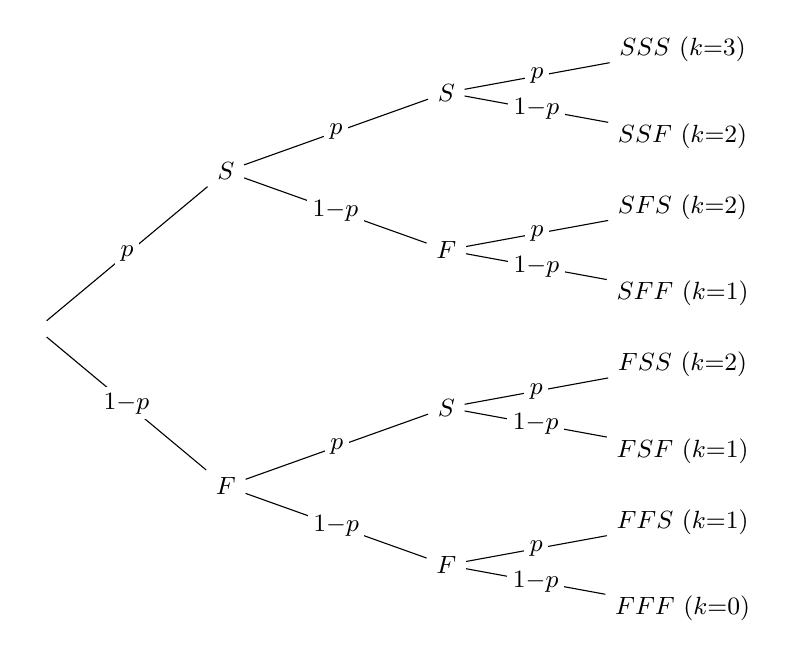
\begin{tikzpicture}[ptree3]
\node {}
  child {node {$F$}
    child {node {$F$}
      child {node {$FFF$ ($k{=}0$)} edge from parent node[pe]{$1{-}p$}}
      child {node {$FFS$ ($k{=}1$)} edge from parent node[pe]{$p$}}
      edge from parent node[pe]{$1{-}p$}}
    child {node {$S$}
      child {node {$FSF$ ($k{=}1$)} edge from parent node[pe]{$1{-}p$}}
      child {node {$FSS$ ($k{=}2$)} edge from parent node[pe]{$p$}}
      edge from parent node[pe]{$p$}}
    edge from parent node[pe]{$1{-}p$}}
  child {node {$S$}
    child {node {$F$}
      child {node {$SFF$ ($k{=}1$)} edge from parent node[pe]{$1{-}p$}}
      child {node {$SFS$ ($k{=}2$)} edge from parent node[pe]{$p$}}
      edge from parent node[pe]{$1{-}p$}}
    child {node {$S$}
      child {node {$SSF$ ($k{=}2$)} edge from parent node[pe]{$1{-}p$}}
      child {node {$SSS$ ($k{=}3$)} edge from parent node[pe]{$p$}}
      edge from parent node[pe]{$p$}}
    edge from parent node[pe]{$p$}};
\end{tikzpicture}
\end{center}

\noindent Three of the eight leaves show $k=2$ (namely $FSS,SFS,SSF$), matching
$\binom{3}{2}=3$; each contributes $p^2(1-p)$, so $\PP(X=2)=3p^2(1-p)=\binom{3}{2}p^2(1-p)^1$.

\begin{example}[Free-throw streak]
A basketball player makes each free throw independently with probability $p=0.8$. She attempts
$n=6$ free throws. What is the probability she makes exactly $5$?
\end{example}
\whichrule{Fixed number of trials ($n=6$), each independent with the same success probability
($p=0.8$), counting makes --- the BINS conditions hold, so $X\sim\Bin(6,0.8)$ and we want
$p_X(5)$.}
\soln
\steplabel{Step 1: Identify parameters.} $n=6$, $p=0.8$, $k=5$.
\steplabel{Step 2: Apply the pmf.}
\[ \PP(X=5)=\binom{6}{5}(0.8)^5(0.2)^1=6\cdot 0.32768\cdot 0.2. \]
\[ \PP(X=5)=0.393216\approx 0.3932. \]

\begin{example}[Defective parts in a production run]
Parts come off a line defective with probability $p=0.05$, independently. In a batch of
$n=12$ parts, find the probability that exactly $2$ are defective.
\end{example}
\whichrule{The defect rate is a fixed $0.05$ for every part and parts are independent, so the
count of defectives is binomial, $X\sim\Bin(12,0.05)$; we want $p_X(2)$. (This is a large
``population'' with a constant rate, so binomial --- not hypergeometric --- is correct.)}
\soln
\steplabel{Step 1: Parameters.} $n=12$, $p=0.05$, $k=2$.
\steplabel{Step 2: Apply the pmf.}
\[ \PP(X=2)=\binom{12}{2}(0.05)^2(0.95)^{10}=66\cdot 0.0025\cdot(0.95)^{10}. \]
Since $(0.95)^{10}\approx 0.598737$,
\[ \PP(X=2)\approx 66\cdot 0.0025\cdot 0.598737\approx 0.0988. \]

\begin{example}[Random multiple-choice guessing]
A quiz has $n=8$ multiple-choice questions, each with $4$ options. A student guesses every
answer uniformly at random and independently. Find the probability of getting exactly $3$
correct.
\end{example}
\whichrule{Each question is an independent trial with the same success probability
$p=1/4$ under pure guessing, and there are a fixed $8$ of them; so $X\sim\Bin(8,1/4)$ and we
want $p_X(3)$.}
\soln
\steplabel{Step 1: Parameters.} $n=8$, $p=1/4$, $1-p=3/4$, $k=3$.
\steplabel{Step 2: Apply the pmf.}
\[ \PP(X=3)=\binom{8}{3}\Bigl(\tfrac14\Bigr)^{3}\Bigl(\tfrac34\Bigr)^{5}
   =56\cdot\frac{1}{64}\cdot\frac{243}{1024}=\frac{56\cdot 243}{65536}. \]
\[ \PP(X=3)=\frac{13608}{65536}\approx 0.2076. \]

\begin{example}[Emails flagged as spam]
A filter independently flags each incoming email as spam with probability $p=0.30$. Over the
next $n=5$ emails, find the probability that exactly $1$ is flagged.
\end{example}
\whichrule{Five independent emails, constant flag probability $0.30$, counting flags: a
binomial count $X\sim\Bin(5,0.30)$, target $p_X(1)$.}
\soln
\steplabel{Step 1: Parameters.} $n=5$, $p=0.30$, $k=1$.
\steplabel{Step 2: Apply the pmf.}
\[ \PP(X=1)=\binom{5}{1}(0.30)^1(0.70)^4=5\cdot 0.30\cdot 0.2401. \]
\[ \PP(X=1)=0.360150\approx 0.3602. \]

\subsection{Mean and variance of the binomial}

\begin{theorem}[Binomial mean and variance]
If $X\sim\Bin(n,p)$ then
\[ \E(X)=np,\qquad \Var(X)=np(1-p),\qquad \SD(X)=\sqrt{np(1-p)}. \]
\end{theorem}
\begin{proof}
Write $X=X_1+\cdots+X_n$ where the $X_i$ are independent $\mathrm{Bernoulli}(p)$ indicators of
success on each trial. By linearity, $\E(X)=\sum_{i=1}^n\E(X_i)=np$. Because the $X_i$ are
independent, variances add: $\Var(X)=\sum_{i=1}^n\Var(X_i)=np(1-p)$, using
$\E(X_i)=p$ and $\Var(X_i)=p(1-p)$ from the Bernoulli proposition.
\end{proof}

\begin{example}[Expected makes and spread]
For the free-throw shooter with $p=0.8$ over $n=6$ attempts, find the mean, variance, and
standard deviation of the number of makes.
\end{example}
\whichrule{$X\sim\Bin(6,0.8)$, so use the binomial mean $np$ and variance $np(1-p)$ directly.}
\soln
\steplabel{Step 1: Mean.} $\E(X)=np=6\cdot 0.8=4.8$.
\steplabel{Step 2: Variance and SD.} $\Var(X)=np(1-p)=6\cdot 0.8\cdot 0.2=0.96$, so
$\SD(X)=\sqrt{0.96}\approx 0.98$.
\[ \E(X)=4.8,\qquad \Var(X)=0.96,\qquad \SD(X)\approx 0.98. \]

\begin{example}[Defectives, summarised]
A shipment of $n=200$ independent components each fails inspection with probability $p=0.02$.
Find the expected number that fail and the standard deviation.
\end{example}
\whichrule{Constant failure rate, independent components, fixed count: $X\sim\Bin(200,0.02)$.
Use $\E=np$ and $\SD=\sqrt{np(1-p)}$.}
\soln
\steplabel{Step 1: Mean.} $\E(X)=np=200\cdot 0.02=4$.
\steplabel{Step 2: SD.} $\Var(X)=200\cdot 0.02\cdot 0.98=3.92$, so $\SD(X)=\sqrt{3.92}\approx
1.98$.
\[ \E(X)=4,\qquad \Var(X)=3.92,\qquad \SD(X)\approx 1.98. \]

\subsection{Cumulative probabilities: ``at least'' and ``at most''}

A request for ``at most $k$'' successes means the cumulative sum
$\PP(X\le k)=\sum_{j=0}^{k}p_X(j)$, and ``at least $k$'' means
$\PP(X\ge k)=\sum_{j=k}^{n}p_X(j)$. When ``at least one'' is wanted, the complement
$\PP(X\ge 1)=1-\PP(X=0)$ is almost always the shortest route.

\begin{example}[At least one defective]
In the batch of $n=12$ parts with defect probability $p=0.05$, find $\PP(\text{at least one
defective})$.
\end{example}
\whichrule{``At least one'' with a binomial count $X\sim\Bin(12,0.05)$: use the complement,
since $\PP(X\ge 1)=1-\PP(X=0)$ needs only one term.}
\soln
\steplabel{Step 1: Complement.} $\PP(X\ge 1)=1-\PP(X=0)=1-\binom{12}{0}(0.05)^0(0.95)^{12}$.
\steplabel{Step 2: Evaluate.} $(0.95)^{12}\approx 0.540360$, so
\[ \PP(X\ge 1)\approx 1-0.5404=0.4596. \]

\begin{example}[At most two flagged emails]
With the spam filter ($n=5$, $p=0.30$), find the probability that at most $2$ of the next $5$
emails are flagged.
\end{example}
\whichrule{``At most $2$'' is a cumulative sum $\PP(X\le 2)=p_X(0)+p_X(1)+p_X(2)$ for
$X\sim\Bin(5,0.30)$.}
\soln
\steplabel{Step 1: Compute each term.}
\begin{align*}
\PP(X=0)&=\binom{5}{0}(0.7)^5=0.16807,\\
\PP(X=1)&=\binom{5}{1}(0.3)(0.7)^4=0.36015,\\
\PP(X=2)&=\binom{5}{2}(0.3)^2(0.7)^3=10\cdot 0.09\cdot 0.343=0.30870.
\end{align*}
\steplabel{Step 2: Add.}
\[ \PP(X\le 2)=0.16807+0.36015+0.30870=0.83692\approx 0.8369. \]

\begin{example}[At least three correct guesses]
For the guessing student ($n=8$, $p=1/4$), find $\PP(X\ge 3)$.
\end{example}
\whichrule{``At least $3$'' for $X\sim\Bin(8,1/4)$. Here the complement
$\PP(X\ge 3)=1-\PP(X\le 2)$ requires only three terms ($k=0,1,2$) instead of six.}
\soln
\steplabel{Step 1: Lower-tail terms.} With $p=1/4$, $q=3/4$,
\begin{align*}
\PP(X=0)&=(3/4)^8=\tfrac{6561}{65536}\approx 0.100113,\\
\PP(X=1)&=\binom{8}{1}(1/4)(3/4)^7=8\cdot\tfrac{2187}{65536}\approx 0.266968,\\
\PP(X=2)&=\binom{8}{2}(1/4)^2(3/4)^6=28\cdot\tfrac{729}{65536}\approx 0.311462.
\end{align*}
\steplabel{Step 2: Complement.}
\[ \PP(X\ge 3)=1-(0.100113+0.266968+0.311462)=1-0.678543\approx 0.3215. \]

\begin{example}[Quality gate: pass if at most one failure]
A lot of $n=20$ independent items each fails with probability $p=0.10$. The lot passes a gate
if at most $1$ item fails. Find the pass probability.
\end{example}
\whichrule{Independent items, constant failure rate, fixed count $20$: $X\sim\Bin(20,0.10)$,
and ``at most $1$'' is $\PP(X\le 1)=p_X(0)+p_X(1)$.}
\soln
\steplabel{Step 1: Two terms.} With $q=0.90$,
\[ \PP(X=0)=(0.9)^{20}\approx 0.121577,\qquad
   \PP(X=1)=20(0.1)(0.9)^{19}\approx 0.270171. \]
\steplabel{Step 2: Add.}
\[ \PP(X\le 1)\approx 0.121577+0.270171=0.391748\approx 0.3917. \]

\subsection{The hypergeometric setting and pmf}

When sampling is done \emph{without replacement} from a finite population, the success
probability changes after each draw, so the trials are not independent and the binomial no
longer applies. The hypergeometric distribution handles this exactly.

\begin{definition}[Hypergeometric setting]
A population has $N$ items, of which $r$ are ``successes'' and $N-r$ are ``failures.'' A simple
random sample of $n$ items is drawn \emph{without replacement}. Let $X$ count the successes in
the sample. Then $X\sim\Hyper(N,r,n)$.
\end{definition}

\begin{theorem}[Hypergeometric pmf]
If $X\sim\Hyper(N,r,n)$ then
\[ p_X(k)=\PP(X=k)=\frac{\dbinom{r}{k}\dbinom{N-r}{n-k}}{\dbinom{N}{n}}, \]
for integers $k$ with $\max(0,\,n-(N-r))\le k\le\min(n,r)$, and $p_X(k)=0$ otherwise.
\end{theorem}
\begin{proof}
Every choice of $n$ items from $N$ is equally likely, and there are $\binom{N}{n}$ such
samples. A sample with exactly $k$ successes is formed by choosing $k$ of the $r$ successes
--- in $\binom{r}{k}$ ways --- and $n-k$ of the $N-r$ failures --- in $\binom{N-r}{n-k}$ ways.
Multiplying these independent choices and dividing by the total count gives the displayed
ratio. The range restriction simply records that you cannot draw more successes than exist
($k\le r$) or fewer than the failures permit ($n-k\le N-r$).
\end{proof}

\begin{example}[Defectives in a small lot]
A box holds $N=15$ memory chips, of which $r=4$ are defective. You draw $n=3$ chips at random
without replacement. Find the probability that exactly $1$ is defective.
\end{example}
\whichrule{Drawing \emph{without replacement} from a small finite pool of $15$ means $p$
changes after each draw, so this is hypergeometric, $X\sim\Hyper(15,4,3)$, not binomial; we
want $p_X(1)$.}
\soln
\steplabel{Step 1: Plug into the pmf.}
\[ \PP(X=1)=\frac{\binom{4}{1}\binom{11}{2}}{\binom{15}{3}}
   =\frac{4\cdot 55}{455}=\frac{220}{455}. \]
\steplabel{Step 2: Simplify.}
\[ \PP(X=1)=\frac{220}{455}=\frac{44}{91}\approx 0.4835. \]

\begin{example}[Committee from a department]
A department of $N=20$ faculty has $r=8$ statisticians and $12$ non-statisticians. A committee
of $n=5$ is chosen at random. Find the probability it contains exactly $3$ statisticians.
\end{example}
\whichrule{People are selected without replacement (no one serves twice) from a fixed pool, so
the count of statisticians is hypergeometric, $X\sim\Hyper(20,8,5)$; target $p_X(3)$.}
\soln
\steplabel{Step 1: Apply the pmf.}
\[ \PP(X=3)=\frac{\binom{8}{3}\binom{12}{2}}{\binom{20}{5}}
   =\frac{56\cdot 66}{15504}=\frac{3696}{15504}. \]
\steplabel{Step 2: Simplify.}
\[ \PP(X=3)=\frac{3696}{15504}=\frac{77}{323}\approx 0.2384. \]

\begin{example}[Capture-recapture flavour: tagged fish]
A pond contains $N=50$ fish, of which $r=10$ were previously tagged. A researcher nets
$n=8$ fish without replacement. Find the probability that exactly $2$ are tagged.
\end{example}
\whichrule{Netting without replacement from a finite, fairly small population: hypergeometric,
$X\sim\Hyper(50,10,8)$. (The sample is $16\%$ of the pond, well above the $5\%$ threshold, so
the binomial approximation would be noticeably off --- use the exact pmf.)}
\soln
\steplabel{Step 1: Apply the pmf.}
\[ \PP(X=2)=\frac{\binom{10}{2}\binom{40}{6}}{\binom{50}{8}}
   =\frac{45\cdot 3{,}838{,}380}{536{,}878{,}650}. \]
\steplabel{Step 2: Evaluate.}
\[ \PP(X=2)=\frac{172{,}727{,}100}{536{,}878{,}650}\approx 0.3217. \]

\begin{example}[Drawing aces from a deck]
From a standard deck ($N=52$, $r=4$ aces), you draw $n=5$ cards without replacement. Find the
probability of getting exactly $2$ aces.
\end{example}
\whichrule{Cards are dealt without replacement, so successive draws are dependent:
hypergeometric, $X\sim\Hyper(52,4,5)$, target $p_X(2)$.}
\soln
\steplabel{Step 1: Apply the pmf.}
\[ \PP(X=2)=\frac{\binom{4}{2}\binom{48}{3}}{\binom{52}{5}}
   =\frac{6\cdot 17{,}296}{2{,}598{,}960}=\frac{103{,}776}{2{,}598{,}960}. \]
\steplabel{Step 2: Simplify.}
\[ \PP(X=2)=\frac{103{,}776}{2{,}598{,}960}\approx 0.0399. \]

\subsection{Mean and variance of the hypergeometric}

\begin{theorem}[Hypergeometric mean and variance]
If $X\sim\Hyper(N,r,n)$, write the population success fraction $p=r/N$. Then
\[ \E(X)=n\,\frac{r}{N}=np,\qquad
   \Var(X)=n\,\frac{r}{N}\Bigl(1-\frac{r}{N}\Bigr)\frac{N-n}{N-1}
          =np(1-p)\,\frac{N-n}{N-1}. \]
\end{theorem}

\noindent The mean is identical to the binomial's, $np$. The variance is the binomial's
$np(1-p)$ multiplied by the \keyword{finite-population correction} $\dfrac{N-n}{N-1}$, which is
at most $1$ (and equals $1$ when $n=1$). Sampling without replacement therefore produces
\emph{less} variability than sampling with replacement.

\begin{example}[Mean and variance of tagged fish]
For the netting example, $X\sim\Hyper(50,10,8)$. Find $\E(X)$ and $\Var(X)$.
\end{example}
\whichrule{Hypergeometric mean $n(r/N)$ and variance $np(1-p)\frac{N-n}{N-1}$ with
$N=50,r=10,n=8$.}
\soln
\steplabel{Step 1: Mean.} $p=r/N=10/50=0.2$, so $\E(X)=np=8\cdot 0.2=1.6$.
\steplabel{Step 2: Variance with correction.}
\[ \Var(X)=8\cdot 0.2\cdot 0.8\cdot\frac{50-8}{50-1}
   =1.28\cdot\frac{42}{49}=1.28\cdot\frac{6}{7}. \]
\[ \E(X)=1.6,\qquad \Var(X)=\frac{7.68}{7}\approx 1.097. \]

\begin{example}[Committee composition, summarised]
For the committee, $X\sim\Hyper(20,8,5)$. Find $\E(X)$ and $\Var(X)$.
\end{example}
\whichrule{Apply the hypergeometric mean and variance with $N=20,r=8,n=5$, $p=8/20=0.4$.}
\soln
\steplabel{Step 1: Mean.} $\E(X)=np=5\cdot 0.4=2$.
\steplabel{Step 2: Variance.}
\[ \Var(X)=5\cdot 0.4\cdot 0.6\cdot\frac{20-5}{20-1}
   =1.2\cdot\frac{15}{19}=\frac{18}{19}\approx 0.947. \]
\[ \E(X)=2,\qquad \Var(X)\approx 0.947. \]

\subsection{Binomial versus hypergeometric}

The two distributions answer the same kind of question; the difference is replacement.

\begin{center}
\renewcommand{\arraystretch}{1.25}
\begin{tabular}{@{}lll@{}}
\toprule
 & \textbf{Binomial} $\Bin(n,p)$ & \textbf{Hypergeometric} $\Hyper(N,r,n)$\\
\midrule
Sampling      & with replacement / infinite pool & without replacement / finite pool\\
Trials        & independent, constant $p$         & dependent, $p$ shifts each draw\\
$\PP(X=k)$     & $\binom{n}{k}p^k(1-p)^{n-k}$       & $\dfrac{\binom{r}{k}\binom{N-r}{n-k}}{\binom{N}{n}}$\\
Mean          & $np$                              & $n\frac{r}{N}$\\
Variance      & $np(1-p)$                          & $np(1-p)\dfrac{N-n}{N-1}$\\
\bottomrule
\end{tabular}
\end{center}

\begin{proposition}[Binomial approximates hypergeometric]
Fix $n$ and $p=r/N$. As $N\to\infty$ with $r/N\to p$, the hypergeometric pmf converges to the
binomial pmf:
\[ \frac{\binom{r}{k}\binom{N-r}{n-k}}{\binom{N}{n}}\ \longrightarrow\
   \binom{n}{k}p^{k}(1-p)^{n-k}. \]
In practice the binomial with $p=r/N$ is an excellent approximation whenever the sample is a
small fraction of the population, $n\le 0.05\,N$, because then the finite-population correction
$\frac{N-n}{N-1}\approx 1$ and removing one item barely changes $p$.
\end{proposition}

\begin{example}[When the approximation is safe, and when it is not]
A warehouse holds $N=10{,}000$ light bulbs of which $r=400$ are defective ($p=0.04$). You
sample $n=20$ without replacement and count defectives. (a) Find the exact hypergeometric
$\PP(X=0)$. (b) Compare with the binomial approximation. (c) Contrast with a case where the
approximation fails.
\end{example}
\whichrule{Sampling is without replacement, so the truth is hypergeometric
$X\sim\Hyper(10{,}000,400,20)$; but $n/N=20/10{,}000=0.002\le 0.05$, so a binomial
$\Bin(20,0.04)$ should approximate it closely. We check both.}
\soln
\steplabel{Step 1: Exact hypergeometric.}
\[ \PP(X=0)=\frac{\binom{400}{0}\binom{9600}{20}}{\binom{10000}{20}}
   =\prod_{j=0}^{19}\frac{9600-j}{10000-j}\approx 0.44216. \]
\steplabel{Step 2: Binomial approximation.}
\[ \PP(X=0)\approx\binom{20}{0}(0.04)^0(0.96)^{20}=(0.96)^{20}\approx 0.44200. \]
The two agree to four decimals --- the approximation is excellent because $n\le 0.05N$.
\steplabel{Step 3: A case where it fails.} If instead $N=40$, $r=16$ ($p=0.4$), $n=20$, then
$n/N=0.5\gg 0.05$. The hypergeometric variance carries the factor
$\frac{N-n}{N-1}=\frac{20}{39}\approx 0.513$, so the without-replacement spread is barely half
the binomial's; here the binomial would badly overstate the variability and the exact
hypergeometric pmf must be used.
\[ \text{(a) }0.4422,\qquad\text{(b) }0.4420,\qquad\text{(c) approximation invalid when }
   n\not\le 0.05N. \]

\begin{example}[Same numbers, two sampling schemes]
An urn has $N=10$ balls, $r=4$ red and $6$ white. Draw $n=3$ and let $X$ count reds. Compute
$\PP(X=2)$ (a) without replacement and (b) with replacement, and explain the difference.
\end{example}
\whichrule{Without replacement is hypergeometric $\Hyper(10,4,3)$; with replacement each draw
resets to $p=4/10$, making the draws independent and the count binomial $\Bin(3,0.4)$. The
same scenario splits along the replacement question.}
\soln
\steplabel{Step 1: Without replacement (hypergeometric).}
\[ \PP(X=2)=\frac{\binom{4}{2}\binom{6}{1}}{\binom{10}{3}}
   =\frac{6\cdot 6}{120}=\frac{36}{120}=0.30. \]
\steplabel{Step 2: With replacement (binomial).}
\[ \PP(X=2)=\binom{3}{2}(0.4)^2(0.6)^1=3\cdot 0.16\cdot 0.6=0.288. \]
\steplabel{Step 3: Interpret.} The two probabilities differ ($0.300$ vs.\ $0.288$) because
removing balls changes the composition of the urn; with $n/N=0.3$ the sample is a large
fraction of the population, so the schemes are genuinely distinct.
\[ \PP_{\text{w/o}}(X=2)=0.300,\qquad \PP_{\text{with}}(X=2)=0.288. \]

\section{Discrete Random Variables}

A \keyword{random variable} attaches a number to each outcome of an experiment, turning
messy verbal outcomes (``heads then tails,'' ``the third sample was the first clean one'')
into ordinary numbers we can add, average, and plot. When those numbers form a finite or
listable set --- counts, scores, dice totals --- the variable is \keyword{discrete}, and its
entire probabilistic behaviour is captured by two functions: the \keyword{probability mass
function} $p_X$, which says how much probability sits on each value, and the
\keyword{cumulative distribution function} $F_X$, which accumulates that probability from the
left. This section builds both from scratch and shows how to read one off the other.

\begin{strategy}[Which tool does a discrete problem need?]
\begin{itemize}[leftmargin=1.3em,itemsep=2pt,topsep=2pt]
\item Asked for the chance of \textbf{one exact value}, $\PP(X=k)$, or to tabulate every
      value? $\Rightarrow$ work with the \keyword{pmf} $p_X(k)=\PP(X=k)$.
\item Given a formula for $p_X$ with an \textbf{unknown constant} $c$? $\Rightarrow$ force
      the masses to be nonnegative and to \keyword{sum to $1$}, then solve for $c$.
\item Asked for a \textbf{cumulative} chance --- ``at most,'' ``less than,'' ``no more than''
      --- or handed a graph that rises in steps? $\Rightarrow$ use the
      \keyword{cdf} $F_X(x)=\PP(X\le x)$.
\item Asked for the probability of a \textbf{half-open interval} $\PP(a<X\le b)$ from a known
      $F_X$? $\Rightarrow$ subtract: $F_X(b)-F_X(a)$. Mind whether each endpoint is included.
\item Handed a \textbf{word problem} (dice totals, matching, defects)? $\Rightarrow$ list the
      sample space, assign each outcome a number, and collect equal values into $p_X$.
\end{itemize}
\textit{Why not the continuous tools (\S3)?} A discrete variable puts positive mass on
\emph{isolated} points, so $\PP(X=k)$ can be nonzero and $F_X$ jumps; there is no density to
integrate. If instead $\PP(X=x)=0$ for every single $x$ and $F_X$ is continuous, the variable
is continuous, not discrete.
\end{strategy}

\subsection{Random variables and the probability mass function}

\begin{definition}[Random variable; discrete]
A \keyword{random variable} on a sample space $S$ is a function $X\colon S\to\R$ assigning a
real number $X(s)$ to each outcome $s$. It is \keyword{discrete} if its set of possible
values, the \keyword{range} (or support) $\Range_X=\{X(s):s\in S\}$, is finite or countably
infinite. For a discrete $X$ the \keyword{probability mass function} (pmf) is
\[ p_X(k)=\PP(X=k)=\PP\bigl(\{s\in S: X(s)=k\}\bigr),\qquad k\in\R. \]
\end{definition}

The pmf records, for each value $k$, the total probability of all outcomes that $X$ sends to
$k$. Two requirements pin down exactly which functions can be pmfs.

\begin{theorem}[Defining properties of a pmf]
A function $p_X$ is the pmf of some discrete random variable if and only if
\[ \text{(i)}\quad p_X(k)\ge 0\ \text{ for all }k,
   \qquad\text{(ii)}\quad \sum_{k\in\Range_X} p_X(k)=1. \]
\end{theorem}
\begin{proof}
Each $p_X(k)=\PP(X=k)$ is a probability, hence nonnegative, giving (i). The events
$\{X=k\}$, as $k$ ranges over $\Range_X$, are disjoint and exhaust $S$, so by countable
additivity $\sum_k\PP(X=k)=\PP(X\in\Range_X)=\PP(S)=1$, giving (ii). Conversely any
nonnegative function summing to $1$ can be realised by placing mass $p_X(k)$ at each $k$.
\end{proof}

\begin{example}[Reading a pmf off a table]
A quality inspector grades a circuit board $X\in\{0,1,2,3\}$ by its number of faulty solder
joints, with
\[ p_X(0)=0.50,\quad p_X(1)=0.30,\quad p_X(2)=0.15,\quad p_X(3)=0.05. \]
Verify this is a valid pmf and find $\PP(X\ge 2)$ and $\PP(1\le X<3)$.
\end{example}
\whichrule{The values are isolated counts $0,1,2,3$ with listed probabilities, so $X$ is
discrete and we work directly with $p_X$. ``At least'' and a bounded range are just sums of
the relevant masses --- no cdf machinery is needed for so few values.}
\soln
\steplabel{Step 1: Check the two pmf properties.} Each entry is $\ge 0$, and
\[ 0.50+0.30+0.15+0.05=1.00, \]
so both (i) and (ii) hold; this is a legitimate pmf.
\steplabel{Step 2: Add the masses in each requested set.}
\[ \PP(X\ge 2)=p_X(2)+p_X(3)=0.15+0.05=0.20, \]
\[ \PP(1\le X<3)=p_X(1)+p_X(2)=0.30+0.15=0.45. \]

\begin{example}[From outcomes to a pmf: two coin flips]
A fair coin is flipped twice; let $X$ be the number of heads. Find $p_X$.
\end{example}
\whichrule{We are handed an experiment, not a table, so we first build the sample space, map
each outcome to its number of heads, then collect equal values. This ``list, label, collect''
routine is the definition of a pmf in action.}
\soln
\steplabel{Step 1: List outcomes and their values.} The sample space is
$S=\{HH,HT,TH,TT\}$, each outcome having probability $\tfrac14$, with
\[ X(HH)=2,\quad X(HT)=X(TH)=1,\quad X(TT)=0. \]
\steplabel{Step 2: Collect outcomes by value.}
\[ p_X(0)=\tfrac14,\qquad p_X(1)=\tfrac{2}{4}=\tfrac12,\qquad p_X(2)=\tfrac14. \]
These sum to $1$, as required.

\begin{example}[An infinite range: first head]
A biased coin lands heads with probability $p=\tfrac13$ on each independent toss. Let $X$ be
the toss on which the first head appears. Show $p_X$ is a valid pmf.
\end{example}
\whichrule{The value $X$ can be any positive integer, so the range is countably infinite; we
must verify the masses still sum to $1$, which now means summing a geometric series rather
than a short list.}
\soln
\steplabel{Step 1: Write the mass of each value.} The first head on toss $k$ means $k-1$
tails then a head, so with $q=1-p=\tfrac23$,
\[ p_X(k)=q^{\,k-1}p=\Bigl(\tfrac23\Bigr)^{k-1}\tfrac13,\qquad k=1,2,3,\dots \]
(This is $X\sim\Geom(p)$.) Each term is positive.
\steplabel{Step 2: Sum the geometric series.}
\[ \sum_{k=1}^{\infty} q^{\,k-1}p = p\sum_{j=0}^{\infty} q^{\,j}
   = \frac{p}{1-q}=\frac{p}{p}=1. \]
Property (ii) holds, so $p_X$ is a valid pmf.

\subsection{Finding an unknown constant in a pmf}

When a pmf is specified only up to a multiplicative constant, the normalisation
$\sum_k p_X(k)=1$ determines that constant uniquely; nonnegativity then fixes its sign.

\begin{example}[Constant times a count]
A help desk models the number $X\in\{1,2,3,4\}$ of tickets a new agent closes in an hour by
$p_X(k)=c\,k$ for those four values and $0$ otherwise. Find $c$ and $\PP(X\ge 3)$.
\end{example}
\whichrule{A symbolic constant $c$ multiplies the masses, so the cue is ``unknown constant in
a pmf.'' Set the total mass to $1$ to solve for $c$; nonnegativity confirms $c>0$ is the
admissible choice.}
\soln
\steplabel{Step 1: Impose $\sum p_X(k)=1$.}
\[ \sum_{k=1}^{4} c\,k = c(1+2+3+4)=10c=1 \ \Longrightarrow\ c=\tfrac{1}{10}. \]
Since each $p_X(k)=k/10>0$, property (i) holds.
\steplabel{Step 2: Use the explicit pmf.}
\[ \PP(X\ge 3)=p_X(3)+p_X(4)=\tfrac{3}{10}+\tfrac{4}{10}=\tfrac{7}{10}. \]

\begin{example}[Constant times a square]
Let $p_X(k)=c\,k^2$ for $k\in\{1,2,3\}$. Find $c$ and $\PP(X\le 2)$.
\end{example}
\whichrule{Same cue --- an undetermined $c$ scaling the masses --- so normalise. The only
change from the previous example is which weights we add.}
\soln
\steplabel{Step 1: Normalise.}
\[ c(1^2+2^2+3^2)=c(1+4+9)=14c=1\ \Longrightarrow\ c=\tfrac{1}{14}. \]
\steplabel{Step 2: Accumulate the requested values.}
\[ \PP(X\le 2)=p_X(1)+p_X(2)=\tfrac{1}{14}+\tfrac{4}{14}=\tfrac{5}{14}. \]

\begin{example}[Constant in front of an infinite series]
A model for the number $X\in\{0,1,2,\dots\}$ of typos on a page is
$p_X(k)=c\,/\,3^{k}$. Find $c$.
\end{example}
\whichrule{The constant again sits in front of every mass, but the range is infinite, so
normalisation requires summing a geometric series. The cue ``find $c$'' still points to
$\sum p_X=1$.}
\soln
\steplabel{Step 1: Sum the geometric series.}
\[ \sum_{k=0}^{\infty}\frac{c}{3^{k}} = c\sum_{k=0}^{\infty}\Bigl(\tfrac13\Bigr)^{k}
   = c\cdot\frac{1}{1-\tfrac13}=c\cdot\tfrac32. \]
\steplabel{Step 2: Set equal to $1$ and solve.}
\[ \tfrac32\,c=1\ \Longrightarrow\ c=\tfrac23. \]

\begin{example}[Two-piece pmf with one free value]
A loyalty program assigns a customer $X\in\{0,1,2,3\}$ reward stars with
$p_X(0)=0.1$, $p_X(1)=0.3$, $p_X(3)=0.2$, and $p_X(2)=a$ left unspecified. Find $a$ and
$\PP(X\ge 1)$.
\end{example}
\whichrule{Most masses are given and one slot is symbolic, so the missing value is forced by
the requirement that everything sum to $1$ --- the same normalisation idea, applied to a
single unknown entry.}
\soln
\steplabel{Step 1: Make the total $1$.}
\[ 0.1+0.3+a+0.2=1\ \Longrightarrow\ a=1-0.6=0.4. \]
Since $0\le a\le 1$, the pmf is valid.
\steplabel{Step 2: Complement is quickest.}
\[ \PP(X\ge 1)=1-p_X(0)=1-0.1=0.9. \]

\subsection{The cumulative distribution function}

\begin{definition}[Cumulative distribution function]
The \keyword{cdf} of a random variable $X$ is
\[ F_X(x)=\PP(X\le x),\qquad x\in\R. \]
For a discrete $X$ it accumulates mass to the left of $x$:
\[ F_X(x)=\sum_{k\le x} p_X(k). \]
\end{definition}

For discrete $X$ the cdf is a \keyword{step function}: flat between consecutive values of the
range, with an upward jump of height $p_X(k)$ at each value $k$. The next result lists the
properties every cdf shares.

\begin{theorem}[Properties of a cdf]
For any random variable, $F_X$ satisfies
\[ \text{(a)}\ \ 0\le F_X(x)\le 1;\qquad
   \text{(b)}\ \ F_X\text{ is nondecreasing};\qquad
   \text{(c)}\ \ \lim_{x\to-\infty}F_X(x)=0,\ \ \lim_{x\to+\infty}F_X(x)=1; \]
\[ \text{(d)}\ \ F_X\text{ is right-continuous: }\lim_{t\downarrow x}F_X(t)=F_X(x). \]
For discrete $X$ the jump at a point equals its mass: $p_X(k)=F_X(k)-\lim_{t\uparrow k}F_X(t)$.
\end{theorem}
\begin{proof}
(a) holds since $F_X(x)$ is a probability. If $x\le y$ then $\{X\le x\}\subseteq\{X\le y\}$,
so $F_X(x)\le F_X(y)$, giving (b). As $x\to-\infty$ the event $\{X\le x\}$ shrinks to the
impossible event and as $x\to+\infty$ it grows to all of $S$, giving (c). Right-continuity
(d) follows because $\{X\le x\}=\bigcap_{n}\{X\le x+\tfrac1n\}$, and continuity of probability
from above gives $F_X(x+\tfrac1n)\downarrow F_X(x)$. Finally the leftover after removing the
strict-inequality part is exactly $\PP(X=k)$, the jump height.
\end{proof}

\begin{remark}
The jumps include their top endpoint: at a value $k$, $F_X(k)$ already counts $p_X(k)$ (the
solid dot sits at the top of the riser), while the open dot sits at the bottom. This is the
graphical face of right-continuity.
\end{remark}

\begin{example}[Build and graph a cdf]
Returning to the solder-joint count with $p_X(0)=0.50$, $p_X(1)=0.30$, $p_X(2)=0.15$,
$p_X(3)=0.05$, write out $F_X$ and sketch it.
\end{example}
\whichrule{We want the accumulated ``$\le x$'' probabilities and a picture that rises in
steps, which is precisely the cdf of a discrete variable: a step function jumping by each
mass.}
\soln
\steplabel{Step 1: Accumulate the masses left to right.}
\[ F_X(x)=\begin{cases}
0, & x<0,\\
0.50, & 0\le x<1,\\
0.80, & 1\le x<2,\\
0.95, & 2\le x<3,\\
1, & x\ge 3.
\end{cases} \]
\steplabel{Step 2: Plot the steps.} Each riser has height equal to the mass at that value
($0.50,0.30,0.15,0.05$); a filled dot marks the included value, an open dot the excluded one.
\begin{center}
\begin{tikzpicture}[>=Stealth,x=2.4cm,y=4.2cm,font=\small]
  % axes
  \draw[axline] (-0.4,0) -- (3.7,0) node[right]{$x$};
  \draw[axline] (-0.3,-0.03) -- (-0.3,1.12) node[above]{$F_X(x)$};
  % y gridlines / ticks
  \foreach \y/\lab in {0/0,0.5/0.50,0.8/0.80,0.95/0.95,1/1.00}{
    \draw[gray!40,very thin] (-0.3,\y) -- (3.6,\y);
    \draw (-0.32,\y) -- (-0.28,\y) node[left=2pt,font=\scriptsize]{\lab};}
  % x ticks
  \foreach \x in {0,1,2,3}{ \draw (\x,-0.015) -- (\x,0.015) node[below=2pt]{$\x$};}
  % flat segments
  \draw[dens] (-0.3,0) -- (0,0);
  \draw[dens] (0,0.5) -- (1,0.5);
  \draw[dens] (1,0.8) -- (2,0.8);
  \draw[dens] (2,0.95) -- (3,0.95);
  \draw[dens] (3,1) -- (3.6,1);
  % endpoints: filled = included (right), open = excluded (left of next step)
  \foreach \x/\y in {0/0.5,1/0.8,2/0.95,3/1}{ \fill (\x,\y) circle (1.1pt);}
  \foreach \x/\y in {0/0,1/0.5,2/0.8,3/0.95}{ \draw[fill=white] (\x,\y) circle (1.1pt);}
\end{tikzpicture}
\end{center}

\begin{example}[From cdf back to pmf]
A vending machine dispenses $X$ extra free items with cdf
\[ F_X(x)=\begin{cases} 0,&x<0,\\ 0.4,&0\le x<1,\\ 0.7,&1\le x<2,\\ 1,&x\ge 2.\end{cases} \]
Recover the pmf.
\end{example}
\whichrule{We are given $F_X$ and want the masses; since a discrete cdf's jump at each value
equals that value's mass, we read off jump heights.}
\soln
\steplabel{Step 1: Locate the jumps.} The cdf jumps at $x=0,1,2$.
\steplabel{Step 2: Subtract to get jump heights.}
\[ p_X(0)=0.4-0=0.4,\quad p_X(1)=0.7-0.4=0.3,\quad p_X(2)=1-0.7=0.3. \]
These sum to $1$, confirming the recovery.

\subsection{Recovering interval probabilities from \texorpdfstring{$F_X$}{F}}

Because $F_X$ already stores all cumulative probabilities, any interval probability is a
difference of two cdf values. The half-open interval is the clean case.

\begin{theorem}[Interval rule]
For any $a<b$,
\[ \PP(a<X\le b)=F_X(b)-F_X(a). \]
\end{theorem}
\begin{proof}
The events $\{X\le a\}$ and $\{a<X\le b\}$ are disjoint with union $\{X\le b\}$, so
$F_X(a)+\PP(a<X\le b)=F_X(b)$; rearrange.
\end{proof}

To switch which endpoints are included, adjust by the masses at $a$ and $b$:
\[ \PP(a\le X\le b)=F_X(b)-F_X(a)+p_X(a),\qquad
   \PP(a<X<b)=F_X(b)-F_X(a)-p_X(b). \]

\begin{example}[Half-open interval]
For the solder-joint cdf above ($F_X(0)=0.50$, $F_X(1)=0.80$, $F_X(2)=0.95$, $F_X(3)=1$),
find $\PP(0<X\le 2)$.
\end{example}
\whichrule{The question is a half-open interval and $F_X$ is already known, so the interval
rule $F_X(b)-F_X(a)$ applies directly with no endpoint correction needed.}
\soln
\steplabel{Step 1: Apply the rule with $a=0$, $b=2$.}
\[ \PP(0<X\le 2)=F_X(2)-F_X(0)=0.95-0.50=0.45. \]
\steplabel{Step 2: Sanity check against masses.} $p_X(1)+p_X(2)=0.30+0.15=0.45.$ Agreed.

\begin{example}[Closed interval needs a correction]
Same cdf. Find $\PP(1\le X\le 3)$.
\end{example}
\whichrule{The lower endpoint is now \emph{included}, so the bare difference would drop
$p_X(1)$; the cue ``$\le$ on the left'' means add back the mass at the lower endpoint.}
\soln
\steplabel{Step 1: Write the closed interval via the rule.}
\[ \PP(1\le X\le 3)=F_X(3)-F_X(1)+p_X(1). \]
\steplabel{Step 2: Substitute, using $p_X(1)=F_X(1)-F_X(0)=0.30$.}
\[ =1-0.80+0.30=0.50. \]
Check: $p_X(1)+p_X(2)+p_X(3)=0.30+0.15+0.05=0.50.$

\begin{example}[Open interval drops the top mass]
A call-centre logs $X$, the number of dropped calls in a shift, with
\[ F_X(x)=\begin{cases} 0,&x<0,\\ 0.55,&0\le x<1,\\ 0.85,&1\le x<2,\\ 0.97,&2\le x<3,\\
1,&x\ge 3.\end{cases} \]
Find $\PP(0<X<3)$.
\end{example}
\whichrule{The upper endpoint is \emph{excluded} (strict $<$), so we must remove $p_X(3)$
from the basic difference; the cue is ``$<$ on the right.''}
\soln
\steplabel{Step 1: Read the needed cdf values and the top mass.}
\[ F_X(3)=1,\quad F_X(0)=0.55,\quad p_X(3)=F_X(3)-\lim_{t\uparrow 3}F_X(t)=1-0.97=0.03. \]
\steplabel{Step 2: Apply the open-interval correction.}
\[ \PP(0<X<3)=F_X(3)-F_X(0)-p_X(3)=1-0.55-0.03=0.42. \]
Check: $p_X(1)+p_X(2)=(0.85-0.55)+(0.97-0.85)=0.30+0.12=0.42.$

\begin{example}[A single point from the cdf]
For the call-centre cdf, find $\PP(X=2)$.
\end{example}
\whichrule{A single value's probability is the jump in $F_X$ at that point; the cue is ``one
exact value,'' read as a one-step difference of the cdf.}
\soln
\steplabel{Step 1: Jump height at $x=2$.}
\[ \PP(X=2)=F_X(2)-\lim_{t\uparrow 2}F_X(t)=0.97-0.85=0.12. \]

\subsection{Building a pmf from a word problem}

The recurring routine is: enumerate the sample space, assign each outcome its numerical
value, then collect outcomes of equal value into the pmf.

\begin{example}[Sum of two fair dice]
Two fair six-sided dice are rolled; let $T$ be the sum of the faces. Find $p_T$ and
$\PP(T\ge 10)$.
\end{example}
\whichrule{The total $T$ is a number built from an experiment, so we use ``list, label,
collect.'' The $36$ ordered pairs are equally likely, which makes each mass a count over
$36$.}
\soln
\steplabel{Step 1: Count the ordered pairs giving each sum.} Of the $36$ equally likely
ordered pairs $(d_1,d_2)$, the number summing to $t$ is $6-|t-7|$ for $t=2,\dots,12$:
\[
\begin{array}{c|ccccccccccc}
t & 2&3&4&5&6&7&8&9&10&11&12\\\hline
\#\{(d_1,d_2):d_1+d_2=t\} & 1&2&3&4&5&6&5&4&3&2&1
\end{array}
\]
\steplabel{Step 2: Divide each count by $36$.} Thus $p_T(t)=\dfrac{6-|t-7|}{36}$. The
eleven masses $1,2,\dots,6,\dots,2,1$ over $36$ sum to $36/36=1$.
\steplabel{Step 3: Add the tail.}
\[ \PP(T\ge 10)=p_T(10)+p_T(11)+p_T(12)=\frac{3+2+1}{36}=\frac{6}{36}=\frac16. \]

\begin{example}[The matching problem]
Three distinct keys are returned at random to their three owners (each of the $3!=6$
assignments equally likely). Let $M$ be the number of owners who get their own key. Find
$p_M$ and $\PP(M\ge 1)$.
\end{example}
\whichrule{$M$ counts matches in a random assignment, a classic ``list, label, collect'':
enumerate all $6$ permutations, count fixed points of each, and collect.}
\soln
\steplabel{Step 1: Enumerate permutations of $(1,2,3)$ and count fixed points.}
\[
\begin{array}{c|c}
\text{permutation} & \text{matches } M\\\hline
123 & 3\\
132 & 1\\
213 & 1\\
231 & 0\\
312 & 0\\
321 & 1
\end{array}
\]
($231$ and $312$ are the two derangements, with no match; note $M=2$ is impossible, since
fixing two keys forces the third.)
\steplabel{Step 2: Collect equal values over the $6$ permutations.}
\[ p_M(0)=\tfrac{2}{6}=\tfrac13,\quad p_M(1)=\tfrac{3}{6}=\tfrac12,\quad p_M(2)=0,\quad
   p_M(3)=\tfrac16. \]
These sum to $\tfrac13+\tfrac12+0+\tfrac16=1$.
\steplabel{Step 3: Use the complement for ``at least one.''}
\[ \PP(M\ge 1)=1-p_M(0)=1-\tfrac13=\tfrac23. \]

\begin{example}[Defectives drawn without replacement]
A drawer holds $7$ batteries, of which $3$ are dead. Two are drawn without replacement; let
$D$ be the number of dead ones drawn. Find $p_D$.
\end{example}
\whichrule{$D$ counts ``special'' items in a sample drawn without replacement from a finite
pool, so the masses are hypergeometric counts $\binom{3}{k}\binom{4}{2-k}/\binom{7}{2}$ ---
still built by collecting outcomes of equal value.}
\soln
\steplabel{Step 1: Total equally likely samples.} $\binom{7}{2}=21$ unordered pairs.
\steplabel{Step 2: Count favourable samples for each $k$.}
\[ p_D(0)=\frac{\binom{3}{0}\binom{4}{2}}{21}=\frac{6}{21},\quad
   p_D(1)=\frac{\binom{3}{1}\binom{4}{1}}{21}=\frac{12}{21},\quad
   p_D(2)=\frac{\binom{3}{2}\binom{4}{0}}{21}=\frac{3}{21}. \]
\steplabel{Step 3: Confirm normalisation.}
\[ \frac{6+12+3}{21}=\frac{21}{21}=1. \]
In lowest terms $p_D(0)=\tfrac{2}{7}$, $p_D(1)=\tfrac{4}{7}$, $p_D(2)=\tfrac{1}{7}$.

\begin{example}[Larger of two dice]
Two fair dice are rolled; let $L=\max(d_1,d_2)$ be the larger face (ties count that face).
Find $p_L$ and $F_L$.
\end{example}
\whichrule{$L$ is a number defined on the $36$-outcome experiment, so we ``list, label,
collect''; a slick shortcut counts via the cdf, since $L\le \ell$ exactly when both dice are
$\le\ell$.}
\soln
\steplabel{Step 1: Get $F_L$ from independence.} $L\le\ell$ iff both faces are $\le\ell$, and
each face is $\le\ell$ with probability $\ell/6$, so for $\ell\in\{1,\dots,6\}$,
\[ F_L(\ell)=\PP(L\le\ell)=\Bigl(\frac{\ell}{6}\Bigr)^2=\frac{\ell^2}{36}. \]
\steplabel{Step 2: Differences give the pmf.} For $\ell=1,\dots,6$,
\[ p_L(\ell)=F_L(\ell)-F_L(\ell-1)=\frac{\ell^2-(\ell-1)^2}{36}=\frac{2\ell-1}{36}. \]
Explicitly the masses are $\tfrac{1}{36},\tfrac{3}{36},\tfrac{5}{36},\tfrac{7}{36},
\tfrac{9}{36},\tfrac{11}{36}$, which sum to $\tfrac{1+3+5+7+9+11}{36}=\tfrac{36}{36}=1$.

\section{Continuous Random Variables}

When a random variable can land anywhere in an interval --- a waiting time, a length, a
voltage, a weight --- no individual value carries positive probability, and a probability mass
function is the wrong tool. Instead the variable is described by a \keyword{density} $f_X$,
a nonnegative curve whose total area is $1$; probabilities become \emph{areas} under that
curve, and the \keyword{cumulative distribution function} $F_X$ accumulates area from the
left. This section sets up densities and cdfs, computes probabilities and percentiles by
integration, and names the three workhorse continuous models: the uniform, exponential, and
normal.

\begin{strategy}[Which continuous-density tool does the problem need?]
\begin{itemize}[leftmargin=1.3em,itemsep=2pt,topsep=2pt]
\item A formula for $f_X$ with an \textbf{unknown constant}, or a piecewise curve you must
      ``make legal''? $\Rightarrow$ impose the two \keyword{density properties}:
      $f_X\ge 0$ and $\int_{-\infty}^{\infty} f_X=1$, and solve for the constant (\S3.1).
\item Asked for $\PP(a<X<b)$, $\PP(X>b)$, or $\PP(X<a)$? $\Rightarrow$ probability is
      \keyword{area}, $\PP(a<X<b)=\int_a^b f_X(x)\dd x$. Endpoints do not matter because
      $\PP(X=x)=0$ for a continuous variable (\S3.2).
\item Given $f_X$ and asked for the \keyword{cdf} $F_X$, or given $F_X$ and asked for the
      density? $\Rightarrow$ integrate ($F_X(x)=\int_{-\infty}^x f_X$) or differentiate
      ($f_X=F_X'$); the two are inverse operations (\S3.3).
\item Asked for a \keyword{percentile}, the \keyword{median}, or a value $c$ with
      $\PP(X\le c)=p$? $\Rightarrow$ solve $F_X(c)=p$ for $c$ (\S3.4).
\item The scenario is ``equally likely over an interval'', ``time until a memoryless event'',
      or ``bell-shaped measurement error''? $\Rightarrow$ reach for the named densities
      \keyword{uniform}, \keyword{exponential}, \keyword{normal} (\S3.5).
\end{itemize}
\emph{Why not a pmf?} A pmf assigns positive weight to isolated points and \emph{sums} to $1$.
A continuous variable spreads its probability over a continuum, so every single point has
probability $0$ and we \emph{integrate} a density instead of summing a mass function.
\end{strategy}

\subsection{Density functions and their two properties}

\begin{definition}[Probability density function]
A random variable $X$ is \keyword{continuous} with \keyword{density} (or \keyword{pdf})
$f_X$ if $f_X$ is a function on $\R$ such that for every $a\le b$,
\[
  \PP(a\le X\le b)=\int_a^b f_X(x)\dd x .
\]
A function $f_X$ is a legitimate density exactly when it satisfies the two
\keyword{density properties}:
\[
  \text{(D1)}\quad f_X(x)\ge 0\ \text{ for all }x,
  \qquad\qquad
  \text{(D2)}\quad \int_{-\infty}^{\infty} f_X(x)\dd x = 1 .
\]
\end{definition}

A density is \emph{not} a probability: $f_X(x)$ can exceed $1$. It is a probability
\emph{per unit length}, and only its integral over an interval is a probability. The two
properties are the continuous analogue of ``$p_X(k)\ge 0$ and $\sum_k p_X(k)=1$'': summation
is replaced by integration.

\begin{proposition}[Point probabilities vanish]
If $X$ has a density $f_X$, then $\PP(X=c)=0$ for every real $c$. Consequently
$\PP(a<X<b)=\PP(a\le X\le b)$, and including or excluding endpoints never changes a
probability.
\end{proposition}
\begin{proof}
$\PP(X=c)=\int_c^c f_X(x)\dd x=0$ since the integral over a single point is zero. Splitting
$\PP(a\le X\le b)=\PP(X=a)+\PP(a<X<b)+\PP(X=b)=\PP(a<X<b)$ gives the second claim.
\end{proof}

\begin{example}[Reading a probability off a triangular density]
A sensor's calibration error $X$ (in millivolts) has density
\[
  f_X(x)=\begin{cases}\tfrac{1}{2}x, & 0\le x\le 2,\\[2pt] 0, & \text{otherwise.}\end{cases}
\]
Verify $f_X$ is a valid density and find $\PP(X>1.5)$.
\end{example}
\whichrule{We are handed a candidate density and asked to confirm legitimacy, then compute a
probability. Confirming legitimacy means checking (D1) and (D2); the probability is an
\emph{area}, hence an integral of $f_X$ --- not a sum, because $X$ ranges over a continuum.}
\soln
\steplabel{Step 1: Check (D1).} On $[0,2]$, $\tfrac12 x\ge 0$; elsewhere $f_X=0$. Nonnegative
everywhere.
\steplabel{Step 2: Check (D2).} Integrate over the support:
\[
  \int_0^2 \tfrac12 x\dd x = \tfrac12\cdot\frac{x^2}{2}\Big|_0^2 = \tfrac12\cdot 2 = 1 .
\]
Both hold, so $f_X$ is a valid density.
\steplabel{Step 3: Compute the area to the right of $1.5$.}
\[
  \PP(X>1.5)=\int_{1.5}^{2}\tfrac12 x\dd x = \tfrac14 x^2\Big|_{1.5}^{2}
  = \tfrac14(4-2.25) = \tfrac{1.75}{4} = 0.4375 .
\]
\[
  \boxed{\;\PP(X>1.5)=0.4375\;}
\]

\begin{center}
\begin{tikzpicture}
\begin{axis}[width=7cm,height=4.2cm,axis lines=left,xlabel=$x$,ylabel=$f_X(x)$,
  xmin=0,xmax=2.4,ymin=0,ymax=1.2,xtick={0,1.5,2},ytick={0,1},samples=2]
  \addplot[shade,domain=1.5:2]{0.5*x}\closedcycle;
  \addplot[dens,domain=0:2]{0.5*x};
\end{axis}
\end{tikzpicture}
\end{center}

\begin{example}[A density that exceeds $1$]
$X$ has density $f_X(x)=3x^2$ for $0\le x\le 1$ and $0$ otherwise. Find $\PP(0.4<X<0.7)$ and
note the largest value of $f_X$.
\end{example}
\whichrule{Again a probability is requested over an interval, so integrate the density. The
appearance $f_X(1)=3>1$ is harmless: a density is a rate, not a probability.}
\soln
\steplabel{Step 1: Integrate over the interval.}
\[
  \PP(0.4<X<0.7)=\int_{0.4}^{0.7}3x^2\dd x = x^3\Big|_{0.4}^{0.7}=0.343-0.064=0.279 .
\]
\steplabel{Step 2: Peak value.} On $[0,1]$ the maximum of $3x^2$ is $f_X(1)=3$, well above
$1$, yet $\int_0^1 3x^2\dd x = 1$ as required.
\[
  \boxed{\;\PP(0.4<X<0.7)=0.279,\qquad \max f_X = 3\;}
\]

\begin{example}[Endpoints are irrelevant]
A bus arrives at a uniformly random time $X$ minutes after the hour, $0\le X\le 10$, with
$f_X(x)=\tfrac{1}{10}$ on $[0,10]$. Compare $\PP(3\le X\le 7)$, $\PP(3<X<7)$, and
$\PP(X=5)$.
\end{example}
\whichrule{A single point versus an interval: because $X$ is continuous, $\PP(X=5)=0$ and
open/closed endpoints give the same area. This is the point-probability proposition in
action.}
\soln
\steplabel{Step 1: The two interval probabilities coincide.}
\[
  \PP(3\le X\le 7)=\PP(3<X<7)=\int_3^7 \tfrac1{10}\dd x = \tfrac{7-3}{10}=0.4 .
\]
\steplabel{Step 2: The point probability.} $\PP(X=5)=\int_5^5 \tfrac1{10}\dd x = 0$.
\[
  \boxed{\;\PP(3\le X\le 7)=\PP(3<X<7)=0.4,\qquad \PP(X=5)=0\;}
\]

\subsection{Finding the normalising constant}

When a density is given only up to a multiplicative constant $c$, property (D2) pins down $c$:
the total area must equal $1$, so $c$ is forced.

\begin{example}[Power-law density]
The fraction $X$ of a tank's capacity in use at a random instant has $f_X(x)=c(1-x)^2$ for
$0\le x\le 1$ and $0$ elsewhere. Find $c$, then $\PP(X<\tfrac12)$.
\end{example}
\whichrule{An unknown constant in front of a density signals (D2): force the total integral to
$1$. Only after $c$ is known can we compute the requested area.}
\soln
\steplabel{Step 1: Set the total area to $1$.}
\[
  \int_0^1 c(1-x)^2\dd x = c\cdot\left[-\frac{(1-x)^3}{3}\right]_0^1 = c\cdot\frac{1}{3}=1
  \;\Longrightarrow\; c=3 .
\]
\steplabel{Step 2: Use $f_X(x)=3(1-x)^2$ to get the probability.}
\[
  \PP\!\left(X<\tfrac12\right)=\int_0^{1/2}3(1-x)^2\dd x
  = \Big[-(1-x)^3\Big]_0^{1/2} = -\left(\tfrac12\right)^3+1 = 1-\tfrac18 = \tfrac78 .
\]
\[
  \boxed{\;c=3,\qquad \PP(X<\tfrac12)=\tfrac78=0.875\;}
\]

\begin{example}[Constant on an unbounded support]
Battery lifetimes $X$ (in years) follow $f_X(x)=c\,e^{-x/4}$ for $x\ge 0$ and $0$ for $x<0$.
Find $c$.
\end{example}
\whichrule{The support runs to $\infty$, but (D2) is unchanged: integrate over the whole real
line, which here means $\int_0^\infty$. A convergent improper integral fixes $c$.}
\soln
\steplabel{Step 1: Impose (D2) as an improper integral.}
\[
  \int_0^{\infty} c\,e^{-x/4}\dd x = c\Big[-4e^{-x/4}\Big]_0^{\infty}
  = c\big(0-(-4)\big)=4c = 1 \;\Longrightarrow\; c=\tfrac14 .
\]
\[
  \boxed{\;c=\tfrac14\;}
\]
This is an $\Expo(\tfrac14)$ density, anticipating \S3.5.

\begin{example}[Two-piece (continuous) density]
A machine's setup error $X$ on $[0,2]$ has $f_X(x)=cx$ on $[0,1]$ and $f_X(x)=c(2-x)$ on
$[1,2]$ (a symmetric ``tent''), and $0$ elsewhere. Find $c$.
\end{example}
\whichrule{A piecewise density still obeys one global constraint (D2): add the areas of all
pieces and set the sum to $1$. Solve the single resulting equation for $c$.}
\soln
\steplabel{Step 1: Integrate each piece.}
\[
  \int_0^1 cx\dd x = \tfrac{c}{2},
  \qquad
  \int_1^2 c(2-x)\dd x = c\Big[2x-\tfrac{x^2}{2}\Big]_1^2 = c\big(2-\tfrac32\big)=\tfrac{c}{2}.
\]
\steplabel{Step 2: Sum and solve.}
\[
  \tfrac{c}{2}+\tfrac{c}{2}=c=1 \;\Longrightarrow\; c=1 .
\]
\[
  \boxed{\;c=1\;}
\]

\begin{example}[Reciprocal-square density]
$X$ has $f_X(x)=\dfrac{c}{x^2}$ for $x\ge 1$ and $0$ for $x<1$. Find $c$ and
$\PP(X>4)$.
\end{example}
\whichrule{Unknown constant on an unbounded support: impose (D2) over $[1,\infty)$. Check the
improper integral converges (it does, since $1/x^2$ decays fast enough), then read off the
tail probability.}
\soln
\steplabel{Step 1: Normalise.}
\[
  \int_1^{\infty}\frac{c}{x^2}\dd x = c\Big[-\frac1x\Big]_1^{\infty}=c(0+1)=c=1
  \;\Longrightarrow\; c=1 .
\]
\steplabel{Step 2: Tail probability.}
\[
  \PP(X>4)=\int_4^{\infty}\frac{1}{x^2}\dd x = \Big[-\frac1x\Big]_4^{\infty}=\tfrac14 .
\]
\[
  \boxed{\;c=1,\qquad \PP(X>4)=\tfrac14\;}
\]

\subsection{The cumulative distribution function}

\begin{definition}[Cdf and its link to the density]
The \keyword{cumulative distribution function} of $X$ is
\[
  F_X(x)=\PP(X\le x)=\int_{-\infty}^{x} f_X(t)\dd t .
\]
For a continuous variable $F_X$ is continuous and nondecreasing, with $F_X(-\infty)=0$ and
$F_X(+\infty)=1$. Wherever $f_X$ is continuous, the Fundamental Theorem of Calculus gives
\[
  f_X(x)=F_X'(x).
\]
Probabilities of intervals come straight from $F_X$: $\PP(a<X\le b)=F_X(b)-F_X(a)$.
\end{definition}

So density and cdf are two encodings of the same information: \emph{integrate} the density to
get the cdf, \emph{differentiate} the cdf to recover the density.

\begin{example}[Cdf of the triangular density]
For $f_X(x)=\tfrac12 x$ on $[0,2]$ (the sensor of \S3.1), find $F_X$ on all of $\R$ and use it
to recompute $\PP(X>1.5)$.
\end{example}
\whichrule{We want the accumulated area as a function of the upper limit, i.e. $F_X$. Integrate
the density piecewise; the requested probability is then a difference of cdf values.}
\soln
\steplabel{Step 1: Integrate on the support.} For $0\le x\le 2$,
\[
  F_X(x)=\int_0^x \tfrac12 t\dd t = \tfrac14 x^2 .
\]
\steplabel{Step 2: Extend by the limiting values.}
\[
  F_X(x)=\begin{cases}0,&x<0,\\[2pt]\tfrac14 x^2,&0\le x\le 2,\\[2pt]1,&x>2.\end{cases}
\]
\steplabel{Step 3: Probability via $F_X$.}
\[
  \PP(X>1.5)=1-F_X(1.5)=1-\tfrac14(1.5)^2=1-0.5625=0.4375,
\]
matching the direct integral from \S3.1.
\[
  \boxed{\;F_X(x)=\tfrac14 x^2\ \text{on }[0,2],\qquad \PP(X>1.5)=0.4375\;}
\]

\begin{center}
\begin{tikzpicture}
\begin{axis}[width=7cm,height=4.2cm,axis lines=left,xlabel=$x$,ylabel=$F_X(x)$,
  xmin=-0.4,xmax=2.6,ymin=0,ymax=1.15,xtick={0,1,2},ytick={0,0.5,1},samples=60]
  \addplot[dens,domain=-0.4:0]{0};
  \addplot[dens,domain=0:2]{0.25*x^2};
  \addplot[dens,domain=2:2.6]{1};
\end{axis}
\end{tikzpicture}
\end{center}

\begin{example}[Recovering a density from a cdf]
A delay $X$ (in seconds) has cdf
\[
  F_X(x)=\begin{cases}0,&x<0,\\[2pt] x^3,&0\le x\le 1,\\[2pt] 1,&x>1.\end{cases}
\]
Find the density $f_X$ and $\PP(0.2<X\le 0.5)$.
\end{example}
\whichrule{We are given $F_X$ and asked for $f_X$: differentiate. Interval probabilities then
come from differences of $F_X$ (no integral needed).}
\soln
\steplabel{Step 1: Differentiate on each piece.} For $0<x<1$, $f_X(x)=\frac{d}{dx}x^3=3x^2$;
elsewhere $F_X$ is flat so $f_X=0$.
\[
  f_X(x)=\begin{cases}3x^2,&0\le x\le 1,\\ 0,&\text{otherwise.}\end{cases}
\]
\steplabel{Step 2: Interval probability from $F_X$.}
\[
  \PP(0.2<X\le 0.5)=F_X(0.5)-F_X(0.2)=0.125-0.008=0.117 .
\]
\[
  \boxed{\;f_X(x)=3x^2\ \text{on }[0,1],\qquad \PP(0.2<X\le 0.5)=0.117\;}
\]

\begin{example}[Cdf on an unbounded support]
Battery lifetimes have $f_X(x)=\tfrac14 e^{-x/4}$ for $x\ge 0$ (from \S3.2). Find $F_X$ and
$\PP(2<X<6)$.
\end{example}
\whichrule{Density to cdf on $[0,\infty)$: integrate from $0$ to $x$. The two-sided
probability is then $F_X(6)-F_X(2)$.}
\soln
\steplabel{Step 1: Integrate.} For $x\ge 0$,
\[
  F_X(x)=\int_0^x \tfrac14 e^{-t/4}\dd t = \Big[-e^{-t/4}\Big]_0^x = 1-e^{-x/4},
\]
and $F_X(x)=0$ for $x<0$.
\steplabel{Step 2: The interval.}
\[
  \PP(2<X<6)=F_X(6)-F_X(2)=\big(1-e^{-1.5}\big)-\big(1-e^{-0.5}\big)=e^{-0.5}-e^{-1.5}.
\]
Numerically $e^{-0.5}=0.6065$, $e^{-1.5}=0.2231$, so the difference is $0.3834$.
\[
  \boxed{\;F_X(x)=1-e^{-x/4}\ (x\ge0),\qquad \PP(2<X<6)\approx 0.3834\;}
\]

\begin{example}[Piecewise cdf, both directions]
$X$ has cdf $F_X(x)=0$ for $x<0$, $F_X(x)=x-\tfrac{x^2}{4}$ for $0\le x\le 2$, and
$F_X(x)=1$ for $x>2$. Find $f_X$ and confirm it integrates to $1$.
\end{example}
\whichrule{Given $F_X$, differentiate to get $f_X$; then sanity-check (D2). Differentiation and
integration here are inverse, so the area must return to $1$.}
\soln
\steplabel{Step 1: Differentiate.} For $0<x<2$,
\[
  f_X(x)=\frac{d}{dx}\!\left(x-\tfrac{x^2}{4}\right)=1-\tfrac{x}{2},
\]
and $0$ outside $[0,2]$.
\steplabel{Step 2: Check (D2).}
\[
  \int_0^2\!\left(1-\tfrac{x}{2}\right)\dd x = \Big[x-\tfrac{x^2}{4}\Big]_0^2 = 2-1 = 1 .
\]
\[
  \boxed{\;f_X(x)=1-\tfrac{x}{2}\ \text{on }[0,2]\;}
\]

\subsection{Quantiles, percentiles, and the median}

\begin{definition}[Quantile / percentile]
For $0<p<1$, a \keyword{$p$-quantile} (or $100p$-th \keyword{percentile}) of $X$ is a value
$x_p$ with
\[
  F_X(x_p)=\PP(X\le x_p)=p .
\]
When $F_X$ is continuous and strictly increasing on the support, $x_p$ is unique and
$x_p=F_X^{-1}(p)$. The \keyword{median} is the $0.5$-quantile.
\end{definition}

To find a percentile, set the cdf equal to the target probability and solve for the value:
percentiles run the cdf \emph{backwards}.

\begin{example}[Median of the triangular density]
For $f_X(x)=\tfrac12 x$ on $[0,2]$, with $F_X(x)=\tfrac14 x^2$, find the median.
\end{example}
\whichrule{``Median'' is the value with half the area to its left, i.e. solve $F_X(m)=0.5$.
This is a percentile problem, so invert the cdf rather than integrate again.}
\soln
\steplabel{Step 1: Set $F_X(m)=\tfrac12$.}
\[
  \tfrac14 m^2 = \tfrac12 \;\Longrightarrow\; m^2 = 2 \;\Longrightarrow\; m=\sqrt2\approx 1.414 .
\]
We take the root in $[0,2]$.
\[
  \boxed{\;m=\sqrt2\approx 1.414\;}
\]

\begin{example}[90th percentile of a lifetime]
Battery lifetimes have $F_X(x)=1-e^{-x/4}$ ($x\ge0$). Find the $90$th percentile $x_{0.90}$.
\end{example}
\whichrule{A percentile request: solve $F_X(x)=0.90$. Because $F_X$ involves $e^{-x/4}$, the
inversion uses a logarithm.}
\soln
\steplabel{Step 1: Solve $1-e^{-x/4}=0.90$.}
\[
  e^{-x/4}=0.10 \;\Longrightarrow\; -\tfrac{x}{4}=\ln(0.10) \;\Longrightarrow\;
  x = -4\ln(0.10)=4\ln 10 .
\]
\steplabel{Step 2: Evaluate.} $\ln 10 = 2.3026$, so $x_{0.90}=4(2.3026)=9.21$ years.
\[
  \boxed{\;x_{0.90}=4\ln 10 \approx 9.21\ \text{years}\;}
\]

\begin{example}[Quartiles of a uniform variable]
$X\sim\Unif(0,10)$ has $F_X(x)=x/10$ on $[0,10]$. Find the first quartile $Q_1$, the median,
and the third quartile $Q_3$.
\end{example}
\whichrule{Quartiles are the $0.25,0.50,0.75$ quantiles; set $F_X$ equal to each in turn. The
uniform cdf is linear, so each inversion is immediate.}
\soln
\steplabel{Step 1: Invert the linear cdf.} $F_X(x)=x/10=p \Rightarrow x=10p$.
\steplabel{Step 2: Plug in the three probabilities.}
\[
  Q_1 = 10(0.25)=2.5,\qquad \text{median}=10(0.5)=5,\qquad Q_3=10(0.75)=7.5 .
\]
\[
  \boxed{\;Q_1=2.5,\quad \text{median}=5,\quad Q_3=7.5\;}
\]

\begin{example}[Percentile of a power density]
The tank-usage fraction has $F_X(x)=1-(1-x)^3$ on $[0,1]$ (from $f_X=3(1-x)^2$). What usage
level is exceeded only $20\%$ of the time?
\end{example}
\whichrule{``Exceeded $20\%$ of the time'' means $\PP(X>c)=0.20$, i.e. $F_X(c)=0.80$: a
percentile (the $80$th). Solve the cubic cdf equation for $c$.}
\soln
\steplabel{Step 1: Translate to the cdf.} $\PP(X>c)=0.20 \Rightarrow F_X(c)=0.80$.
\steplabel{Step 2: Solve $1-(1-c)^3=0.80$.}
\[
  (1-c)^3=0.20 \;\Longrightarrow\; 1-c=0.20^{1/3}=0.5848 \;\Longrightarrow\; c=0.4152 .
\]
\[
  \boxed{\;c\approx 0.415\;}
\]

\subsection{The named continuous models}

Three densities cover most applications. Each is introduced here by its formula, support, and
(stated) mean and variance; later sections derive these moments by integration.

\begin{definition}[Uniform, exponential, normal]
\begin{center}\small
\renewcommand{\arraystretch}{1.5}
\begin{tabular}{@{}llcc@{}}
\toprule
Model & Density $f_X(x)$ & $\E(X)$ & $\Var(X)$ \\
\midrule
Uniform $\Unif(a,b)$ & $\dfrac{1}{b-a},\ a\le x\le b$ & $\dfrac{a+b}{2}$ & $\dfrac{(b-a)^2}{12}$ \\
Exponential $\Expo(\lambda)$ & $\lambda e^{-\lambda x},\ x\ge 0\ (\lambda>0)$ & $\dfrac{1}{\lambda}$ & $\dfrac{1}{\lambda^2}$ \\
Normal $\Normal(\mu,\sigma^2)$ & $\dfrac{1}{\sigma\sqrt{2\pi}}\,e^{-(x-\mu)^2/(2\sigma^2)},\ x\in\R$ & $\mu$ & $\sigma^2$ \\
\bottomrule
\end{tabular}
\end{center}
The exponential cdf is $F_X(x)=1-e^{-\lambda x}$ ($x\ge 0$); the uniform cdf is
$F_X(x)=\frac{x-a}{b-a}$ on $[a,b]$. The normal cdf has no elementary closed form and is
written $\Phi$ for the \keyword{standard} normal $\Normal(0,1)$, with the
\keyword{standardisation} $Z=\frac{X-\mu}{\sigma}\sim\Normal(0,1)$.
\end{definition}

\begin{example}[Uniform: equally likely arrival]
A file finishes downloading at a time $X\sim\Unif(0,20)$ seconds. Find $\PP(X>12)$, the
density value, and the median.
\end{example}
\whichrule{``Equally likely over an interval'' is the uniform signature: constant density
$1/(b-a)$. Probabilities are just proportions of the interval length, and the median is its
midpoint.}
\soln
\steplabel{Step 1: Density and probability.} Here $f_X(x)=\tfrac1{20}$ on $[0,20]$, so
\[
  \PP(X>12)=\int_{12}^{20}\tfrac1{20}\dd x = \frac{20-12}{20}=0.40 .
\]
\steplabel{Step 2: Median.} By symmetry the median is the midpoint
$\tfrac{0+20}{2}=10$ (equivalently $F_X(m)=m/20=0.5$).
\[
  \boxed{\;f_X=\tfrac1{20},\qquad \PP(X>12)=0.40,\qquad \text{median}=10\;}
\]

\begin{example}[Exponential: memoryless waiting]
Calls to a help line arrive so that the gap $X$ between consecutive calls is
$\Expo(\lambda)$ with mean $5$ minutes. Find $\lambda$, $\PP(X>8)$, and verify the
\keyword{memoryless} identity $\PP(X>8\given X>3)=\PP(X>5)$.
\end{example}
\whichrule{``Time until the next event'' with a stated mean is the exponential. Since
$\E(X)=1/\lambda$, the mean gives $\lambda$. Tail probabilities use $\PP(X>t)=e^{-\lambda t}$,
and memorylessness is a direct conditional-probability check.}
\soln
\steplabel{Step 1: Rate from the mean.} $\E(X)=1/\lambda = 5 \Rightarrow \lambda=\tfrac15=0.2$.
\steplabel{Step 2: Tail probability.}
\[
  \PP(X>8)=e^{-\lambda\cdot 8}=e^{-0.2\cdot 8}=e^{-1.6}\approx 0.2019 .
\]
\steplabel{Step 3: Memoryless check.} Using $\PP(X>t)=e^{-0.2t}$,
\[
  \PP(X>8\given X>3)=\frac{\PP(X>8)}{\PP(X>3)}=\frac{e^{-1.6}}{e^{-0.6}}=e^{-1.0}=\PP(X>5).
\]
\[
  \boxed{\;\lambda=0.2,\quad \PP(X>8)\approx 0.2019,\quad \PP(X>8\given X>3)=\PP(X>5)=e^{-1}\;}
\]

\begin{center}
\begin{tikzpicture}
\begin{axis}[width=7cm,height=4.2cm,axis lines=left,xlabel=$x$ (min),ylabel=$f_X(x)$,
  xmin=0,xmax=20,ymin=0,ymax=0.22,xtick={0,8,20},ytick={0,0.1,0.2},samples=80]
  \addplot[shade,domain=8:20]{0.2*exp(-0.2*x)}\closedcycle;
  \addplot[dens,domain=0:20]{0.2*exp(-0.2*x)};
\end{axis}
\end{tikzpicture}
\end{center}

\begin{example}[Normal: standardising a measurement]
Bottle fill volumes are $X\sim\Normal(500,4)$ (mean $500$ mL, variance $4$, so $\sigma=2$ mL).
Find $\PP(X<497)$ and $\PP(498<X<503)$ using $Z=(X-\mu)/\sigma$ and
$\Phi(0.5)=0.6915$, $\Phi(1)=0.8413$, $\Phi(1.5)=0.9332$.
\end{example}
\whichrule{A bell-shaped measurement with a mean and variance is normal. Normal probabilities
have no closed form, so standardise to $Z\sim\Normal(0,1)$ and read $\Phi$. Use
$\Phi(-z)=1-\Phi(z)$ for left tails.}
\soln
\steplabel{Step 1: Standardise the first event.} $\sigma=\sqrt4=2$, so for $X<497$,
\[
  Z<\frac{497-500}{2}=-1.5,\qquad \PP(X<497)=\Phi(-1.5)=1-\Phi(1.5)=1-0.9332=0.0668 .
\]
\steplabel{Step 2: Standardise the interval.} For $498<X<503$,
\[
  \frac{498-500}{2}=-1,\qquad \frac{503-500}{2}=1.5,
\]
\[
  \PP(498<X<503)=\Phi(1.5)-\Phi(-1)=0.9332-(1-0.8413)=0.9332-0.1587=0.7745 .
\]
\[
  \boxed{\;\PP(X<497)=0.0668,\qquad \PP(498<X<503)=0.7745\;}
\]

\begin{example}[Normal: an inverse (percentile) problem]
Exam scores are $X\sim\Normal(72,81)$ ($\sigma=9$). The top $10\%$ earn distinction. Using
$\Phi(1.28)=0.90$, find the cutoff score.
\end{example}
\whichrule{This runs the normal \emph{backwards}: we know the probability ($0.90$ below the
cutoff) and want the value, a percentile. Find the $z$ with $\Phi(z)=0.90$, then
de-standardise via $x=\mu+z\sigma$.}
\soln
\steplabel{Step 1: Find the standard-normal quantile.} $\Phi(z)=0.90\Rightarrow z=1.28$.
\steplabel{Step 2: De-standardise.}
\[
  x=\mu+z\sigma = 72+1.28\cdot 9 = 72+11.52 = 83.52 .
\]
\[
  \boxed{\;\text{cutoff}\approx 83.5\ \text{points}\;}
\]

\begin{example}[Uniform: a conditional probability]
A pointer stops at a uniform angle $X\sim\Unif(0,360)$ degrees. Given $X<180$ (upper
half), find $\PP(X<90)$ (first quadrant).
\end{example}
\whichrule{Uniform again (equally likely over $[0,360]$), now with conditioning. For a uniform
variable, conditional probability is just the ratio of sub-interval lengths --- areas of a flat
density.}
\soln
\steplabel{Step 1: Write the conditional probability.}
\[
  \PP(X<90\given X<180)=\frac{\PP(X<90)}{\PP(X<180)} .
\]
\steplabel{Step 2: Use proportions of length.}
$\PP(X<90)=\tfrac{90}{360}=\tfrac14$ and $\PP(X<180)=\tfrac{180}{360}=\tfrac12$, so
\[
  \PP(X<90\given X<180)=\frac{1/4}{1/2}=\tfrac12 .
\]
\[
  \boxed{\;\PP(X<90\given X<180)=\tfrac12\;}
\]

\section{Expected Values}

The \keyword{expected value} $\E(X)$ is the single number that best summarises a random
variable's location: it is the long-run average of the values $X$ produces, weighted by how
likely each value is. Mechanically it is a center of mass --- balance a rod loaded with the
probability mass and $\E(X)$ is the fulcrum. This section computes $\E(X)$ for discrete and
continuous variables, computes $\E\bigl(g(X)\bigr)$ for a function of $X$ without first finding
the distribution of $g(X)$, exploits the linearity rule $\E(aX+b)=a\E(X)+b$, and records the
means of the named families.

\begin{strategy}[Which expectation rule does the problem need?]
\begin{itemize}[leftmargin=1.3em,itemsep=2pt,topsep=2pt]
\item Want the average of $X$ itself, and $X$ takes \textbf{isolated values}?
      $\Rightarrow$ \keyword{discrete mean} $\E(X)=\sum_k k\,p_X(k)$.
\item Want the average of $X$ itself, and $X$ has a \textbf{density}?
      $\Rightarrow$ \keyword{continuous mean} $\E(X)=\int_{-\infty}^{\infty} x\,f_X(x)\dd x$.
\item Want the average of a \textbf{function} $g(X)$ (a payoff, a square, a cost)?
      $\Rightarrow$ the \keyword{law of the unconscious statistician}: weight $g(k)$ by
      $p_X(k)$, or integrate $g(x)f_X(x)$. Do \emph{not} first find the pmf/pdf of $g(X)$.
\item The variable is a \textbf{linear rescaling} $aX+b$, or a \textbf{sum} of pieces whose
      means you know? $\Rightarrow$ \keyword{linearity}: $\E(aX+b)=a\E(X)+b$ and
      $\E(X_1+\cdots+X_n)=\E(X_1)+\cdots+\E(X_n)$, with no independence needed.
\item $X$ belongs to a \textbf{named family}? $\Rightarrow$ quote the mean
      (binomial $np$, Poisson $\lambda$, geometric $1/p$, uniform $(a+b)/2$,
      exponential $1/\lambda$, gamma $\alpha/\lambda$) rather than re-summing.
\end{itemize}
\textbf{Why not the others.} Squaring or any nonlinear $g$ breaks linearity, so
$\E\bigl(g(X)\bigr)\neq g\bigl(\E(X)\bigr)$ in general --- use LOTUS, not linearity. And a
median or mode answers ``typical value'' too, but only $\E(X)$ is the probability-weighted
average that linearity acts on.
\end{strategy}

\subsection{Expected value of a discrete variable}

\begin{definition}[Discrete expected value]
Let $X$ be discrete with pmf $p_X$ and range $\Range$. Its \keyword{expected value} (or
\keyword{mean}) is
\[
  \E(X)=\sum_{k\in\Range} k\,p_X(k),
\]
provided $\sum_{k}|k|\,p_X(k)<\infty$. The sum is each value times its probability; it is the
center of mass of the mass diagram and need not itself be an attainable value of $X$.
\end{definition}

\begin{center}
\begin{tikzpicture}[font=\footnotesize,>=Stealth]
  % center-of-mass picture: bars of mass on a rod, fulcrum at the mean
  \draw[thick] (0,0) -- (6,0);
  \foreach \x/\h/\p in {0.5/0.6/0.1, 2/1.2/0.4, 3.5/0.9/0.3, 5/0.6/0.2}{
    \draw[very thick,black!75] (\x,0) -- (\x,\h);
    \fill[black!75] (\x,\h) circle (1.6pt);
    \node[below] at (\x,0) {};
  }
  \node[below] at (0.5,-0.05){$1$};
  \node[below] at (2,-0.05){$2$};
  \node[below] at (3.5,-0.05){$3$};
  \node[below] at (5,-0.05){$4$};
  % fulcrum at mean = 2.7  -> rod x = 0.5 + (2.7-1)/3 * (5-0.5)... use computed coordinate 3.05
  \draw[->] (3.05,-0.95) -- (3.05,-0.18);
  \fill (3.05,-1.05) -- (2.85,-1.35) -- (3.25,-1.35) -- cycle;
  \node[below] at (3.05,-1.4){fulcrum $=\E(X)=2.7$};
  \node[above] at (2,1.2){$0.4$};
  \node[above] at (3.5,0.9){$0.3$};
  \node[above] at (5,0.6){$0.2$};
  \node[above] at (0.5,0.6){$0.1$};
\end{tikzpicture}
\end{center}

\begin{example}[Defective boards on a tray]
A tray holds $4$ circuit boards. Let $X$ be the number that fail a burn-in test, with pmf
\[
  p_X(0)=0.1,\quad p_X(1)=0.4,\quad p_X(2)=0.3,\quad p_X(3)=0.2.
\]
Find the expected number of failures.
\end{example}
\whichrule{$X$ takes the isolated values $0,1,2,3$ with listed probabilities, so the average is
the discrete mean $\sum_k k\,p_X(k)$. There is no density and no function of $X$ to transform,
so neither the integral form nor LOTUS is needed.}
\soln
\steplabel{Step 1: multiply each value by its probability.}
\[
  0(0.1)+1(0.4)+2(0.3)+3(0.2)=0+0.4+0.6+0.6.
\]
\steplabel{Step 2: add.}
\[
  \E(X)=1.6\text{ failures.}
\]
The mean $1.6$ is not an attainable count; it is the balance point of the four masses.

\begin{example}[A fair-looking but skewed wager]
A spinner pays you a dollar amount $X$ with
\[
  p_X(0)=\tfrac12,\quad p_X(2)=\tfrac13,\quad p_X(9)=\tfrac16 .
\]
What is the average payout per spin?
\end{example}
\whichrule{Isolated dollar values with given probabilities: discrete mean again. The values are
already the quantity of interest (dollars), so no transformation is applied.}
\soln
\steplabel{Step 1: confirm the pmf sums to $1$.}
$\tfrac12+\tfrac13+\tfrac16=\tfrac{3+2+1}{6}=1$, so the weights are legitimate.
\steplabel{Step 2: weight each payout.}
\[
  \E(X)=0\cdot\tfrac12+2\cdot\tfrac13+9\cdot\tfrac16=\tfrac{2}{3}+\tfrac{9}{6}
       =\tfrac{4}{6}+\tfrac{9}{6}=\tfrac{13}{6}.
\]
\[
  \E(X)=\tfrac{13}{6}\approx 2.17\text{ dollars per spin.}
\]

\begin{example}[Sum of two fair dice]
Roll two fair dice and let $S$ be their sum, $S\in\{2,\dots,12\}$ with the familiar triangular
pmf $p_S(k)=\dfrac{6-|k-7|}{36}$. Find $\E(S)$.
\end{example}
\whichrule{$S$ is discrete on $\{2,\dots,12\}$; we want its plain average, so it is the discrete
mean. Symmetry will shortcut the arithmetic but the rule applied is still $\sum_k k\,p_S(k)$.}
\soln
\steplabel{Step 1: note the symmetry.}
The pmf is symmetric about $k=7$: $p_S(7-j)=p_S(7+j)$. A symmetric mass diagram balances at its
center.
\steplabel{Step 2: read off (or verify) the mean.}
By symmetry $\E(S)=7$. As a check, pair terms equidistant from $7$:
$(2{+}12)\tfrac{1}{36}+(3{+}11)\tfrac{2}{36}+\cdots+(6{+}8)\tfrac{5}{36}+7\cdot\tfrac{6}{36}
=14\cdot\tfrac{1+2+3+4+5}{36}+\tfrac{42}{36}=\tfrac{210+42}{36}$.
\[
  \E(S)=\tfrac{252}{36}=7.
\]

\begin{example}[A pmf with a parameter]
A discrete variable $X$ on $\{1,2,3\}$ has $p_X(k)=c\,k$ for a constant $c$. Find $c$, then
$\E(X)$.
\end{example}
\whichrule{Two tasks: first force the pmf property $\sum_k p_X(k)=1$ to pin down $c$ (this is a
normalising step, not an expectation), then apply the discrete mean.}
\soln
\steplabel{Step 1: normalise.}
$\sum_{k=1}^{3} c\,k=c(1+2+3)=6c=1$, so $c=\tfrac16$ and
$p_X(1)=\tfrac16,\,p_X(2)=\tfrac26,\,p_X(3)=\tfrac36$.
\steplabel{Step 2: take the mean.}
\[
  \E(X)=1\cdot\tfrac16+2\cdot\tfrac26+3\cdot\tfrac36=\tfrac{1+4+9}{6}=\tfrac{14}{6}=\tfrac{7}{3}.
\]
\[
  \E(X)=\tfrac{7}{3}\approx 2.33 .
\]

\subsection{Expected value of a continuous variable}

\begin{definition}[Continuous expected value]
Let $X$ have density $f_X$. Its \keyword{expected value} is
\[
  \E(X)=\int_{-\infty}^{\infty} x\,f_X(x)\dd x,
\]
provided $\int_{-\infty}^{\infty}|x|\,f_X(x)\dd x<\infty$. The discrete weight $p_X(k)$ is
replaced by the infinitesimal mass $f_X(x)\dd x$, and summation by integration.
\end{definition}

\begin{example}[A triangular density]
Let $X$ have density $f_X(x)=2x$ on $0\le x\le 1$ and $0$ elsewhere. Find $\E(X)$.
\end{example}
\whichrule{$X$ has a density, so its mean is $\int x f_X(x)\dd x$, integrated over the support
$[0,1]$ where $f_X$ is nonzero. We average $X$ itself, so no LOTUS transformation enters.}
\soln
\steplabel{Step 1: set up the integral on the support.}
\[
  \E(X)=\int_0^1 x\,(2x)\dd x=\int_0^1 2x^2\dd x.
\]
\steplabel{Step 2: integrate.}
\[
  \E(X)=\Bigl[\tfrac{2}{3}x^3\Bigr]_0^1=\tfrac{2}{3}.
\]
The mass leans toward $1$, so the balance point $\tfrac{2}{3}$ sitting right of the midpoint
$\tfrac12$ is the expected sign.

\begin{center}
\begin{tikzpicture}
  \begin{axis}[width=7cm,height=4cm,axis lines=left,xlabel=$x$,ylabel=$f_X(x)$,
      xmin=0,xmax=1.15,ymin=0,ymax=2.3,xtick={0,0.6667,1},
      xticklabels={$0$,$\E(X)$,$1$},ytick=\empty,clip=false]
    \addplot[dens,domain=0:1,samples=2]{2*x};
    \draw[dashed,gray!70] (axis cs:0.6667,0) -- (axis cs:0.6667,1.3333);
  \end{axis}
\end{tikzpicture}
\end{center}

\begin{example}[Uniform lifetime]
A bus arrives at a uniformly random time $X$ minutes after the hour, $X\sim\Unif(0,30)$ with
$f_X(x)=\tfrac{1}{30}$ on $[0,30]$. Find the expected arrival time.
\end{example}
\whichrule{A density on a continuum, so the mean is the integral $\int x f_X(x)\dd x$. (We will
re-derive the uniform mean here; later we simply quote $(a+b)/2$.)}
\soln
\steplabel{Step 1: integrate over the support.}
\[
  \E(X)=\int_0^{30} x\cdot\tfrac{1}{30}\dd x=\tfrac{1}{30}\Bigl[\tfrac{x^2}{2}\Bigr]_0^{30}
       =\tfrac{1}{30}\cdot\tfrac{900}{2}.
\]
\steplabel{Step 2: simplify.}
\[
  \E(X)=\tfrac{450}{30}=15\text{ minutes,}
\]
the midpoint of $[0,30]$, as symmetry demands.

\begin{example}[Exponential waiting time]
The time $X$ (hours) until the next support call is $X\sim\Expo(\lambda)$ with
$f_X(x)=\lambda e^{-\lambda x}$ on $x\ge 0$. Show $\E(X)=1/\lambda$, then evaluate it for
$\lambda=4$ calls per hour.
\end{example}
\whichrule{A density on $[0,\infty)$; the mean is $\int_0^{\infty} x f_X(x)\dd x$. The integrand
needs integration by parts, the standard move for $x e^{-\lambda x}$.}
\soln
\steplabel{Step 1: integrate by parts.}
With $u=x$, $\dd v=\lambda e^{-\lambda x}\dd x$, so $\dd u=\dd x$ and $v=-e^{-\lambda x}$,
\[
  \E(X)=\int_0^{\infty} x\,\lambda e^{-\lambda x}\dd x
       =\Bigl[-x e^{-\lambda x}\Bigr]_0^{\infty}+\int_0^{\infty} e^{-\lambda x}\dd x.
\]
\steplabel{Step 2: evaluate the pieces.}
The boundary term is $0$ (as $x\to\infty$, $x e^{-\lambda x}\to 0$; at $x=0$ it is $0$), and
$\int_0^{\infty} e^{-\lambda x}\dd x=\tfrac{1}{\lambda}$. Hence
\[
  \E(X)=\tfrac{1}{\lambda},\qquad\text{so for }\lambda=4,\quad \E(X)=\tfrac{1}{4}\text{ hour}=15\text{ minutes.}
\]

\begin{example}[Density supported away from the origin]
Let $X$ have density $f_X(x)=\dfrac{3}{x^4}$ for $x\ge 1$ and $0$ otherwise (a Pareto-type tail).
Find $\E(X)$.
\end{example}
\whichrule{A density on $[1,\infty)$; the mean is the improper integral $\int_1^{\infty}
x f_X(x)\dd x$. We must check it converges before reporting a finite value.}
\soln
\steplabel{Step 1: set up and integrate.}
\[
  \E(X)=\int_1^{\infty} x\cdot\tfrac{3}{x^4}\dd x=\int_1^{\infty} 3x^{-3}\dd x
       =\Bigl[-\tfrac{3}{2}x^{-2}\Bigr]_1^{\infty}.
\]
\steplabel{Step 2: take the limit.}
As $x\to\infty$ the term $-\tfrac{3}{2}x^{-2}\to 0$; at $x=1$ it is $-\tfrac32$. So
\[
  \E(X)=0-\bigl(-\tfrac{3}{2}\bigr)=\tfrac{3}{2}.
\]
(The integral converges because the integrand decays like $x^{-3}$; a heavier tail such as
$f_X(x)=2/x^3$ would make $\int x f_X$ diverge and leave $\E(X)$ undefined.)

\subsection{The law of the unconscious statistician}

To average a function $g(X)$ --- a payoff, a cost, a square --- you do \emph{not} need the
distribution of $Y=g(X)$. Weight $g$ by the distribution of $X$ directly.

\begin{theorem}[Law of the unconscious statistician (LOTUS)]
For a function $g$,
\[
  \E\bigl(g(X)\bigr)=\sum_{k} g(k)\,p_X(k)\quad(\text{discrete}),\qquad
  \E\bigl(g(X)\bigr)=\int_{-\infty}^{\infty} g(x)\,f_X(x)\dd x\quad(\text{continuous}),
\]
whenever the sum/integral converges absolutely.
\end{theorem}
\begin{proof}
(Discrete case.) Let $Y=g(X)$ with range $\{y_j\}$. Group the $k$ with $g(k)=y_j$:
\[
  \E(Y)=\sum_j y_j\,p_Y(y_j)=\sum_j y_j\!\!\sum_{k:\,g(k)=y_j}\!\! p_X(k)
       =\sum_j\sum_{k:\,g(k)=y_j} g(k)\,p_X(k)=\sum_k g(k)\,p_X(k),
\]
since every $k$ lands in exactly one group. The continuous case follows by the same regrouping
applied to the density.
\end{proof}

\begin{remark}
A consequence worth stating: nonlinearity means $\E\bigl(g(X)\bigr)\ne g\bigl(\E(X)\bigr)$ in
general. For instance $\E(X^2)$ almost never equals $\bigl(\E(X)\bigr)^2$; the gap is exactly
the variance of the next section.
\end{remark}

\begin{example}[Squaring a die]
Let $X$ be the result of one fair die, $p_X(k)=\tfrac16$ for $k=1,\dots,6$. Find $\E(X^2)$.
\end{example}
\whichrule{We want the average of $g(X)=X^2$, not of $X$, so apply LOTUS: weight $k^2$ by
$p_X(k)$. Computing $\bigl(\E X\bigr)^2$ would be the wrong quantity.}
\soln
\steplabel{Step 1: sum the squared values.}
\[
  \E(X^2)=\sum_{k=1}^{6} k^2\cdot\tfrac16=\tfrac16(1+4+9+16+25+36)=\tfrac{91}{6}.
\]
\steplabel{Step 2: report.}
\[
  \E(X^2)=\tfrac{91}{6}\approx 15.17 .
\]
Note $\bigl(\E X\bigr)^2=(3.5)^2=12.25\ne\tfrac{91}{6}$, exactly as the remark warns.

\begin{example}[Expected area of a random square]
A side length $X\sim\Unif(0,2)$ has $f_X(x)=\tfrac12$ on $[0,2]$. The square has area
$A=X^2$. Find $\E(A)$.
\end{example}
\whichrule{$A=g(X)=X^2$ is a function of a continuous variable, so LOTUS gives
$\E(A)=\int g(x)f_X(x)\dd x$ directly --- no need to derive the density of $A$.}
\soln
\steplabel{Step 1: integrate $x^2$ against the density.}
\[
  \E(A)=\int_0^2 x^2\cdot\tfrac12\dd x=\tfrac12\Bigl[\tfrac{x^3}{3}\Bigr]_0^2=\tfrac12\cdot\tfrac{8}{3}.
\]
\steplabel{Step 2: simplify.}
\[
  \E(A)=\tfrac{4}{3}\approx 1.33 .
\]
The square of the average side is $(\E X)^2=1^2=1$, again smaller than $\E(A)$.

\begin{example}[A capped insurance payout]
A loss $X\sim\Expo(\lambda)$ with $\lambda=\tfrac12$ (so mean loss $2$, in thousands) is paid
by a policy that caps the payout at $3$: the payout is $g(X)=\min(X,3)$. Find the expected
payout.
\end{example}
\whichrule{The payout is a nonlinear function $g(X)=\min(X,3)$ of a continuous variable. LOTUS
handles it as a single integral, splitting where the cap kicks in at $x=3$.}
\soln
\steplabel{Step 1: split the integral at the cap.}
With $f_X(x)=\tfrac12 e^{-x/2}$,
\[
  \E\bigl(g(X)\bigr)=\int_0^3 x\cdot\tfrac12 e^{-x/2}\dd x+\int_3^{\infty} 3\cdot\tfrac12 e^{-x/2}\dd x.
\]
\steplabel{Step 2: evaluate each piece.}
For the first, integration by parts gives
$\int_0^3 x\cdot\tfrac12 e^{-x/2}\dd x=\bigl[-x e^{-x/2}\bigr]_0^3+\int_0^3 e^{-x/2}\dd x
=-3e^{-3/2}+\bigl[-2e^{-x/2}\bigr]_0^3=-3e^{-3/2}-2e^{-3/2}+2=2-5e^{-3/2}$.
The second is $3\bigl[-e^{-x/2}\bigr]_3^{\infty}=3e^{-3/2}$.
\steplabel{Step 3: add.}
\[
  \E\bigl(g(X)\bigr)=\bigl(2-5e^{-3/2}\bigr)+3e^{-3/2}=2-2e^{-3/2}\approx 2-2(0.2231)=1.554 .
\]
The cap pulls the expected payout below the uncapped mean of $2$ (thousand), as it should.

\begin{example}[Expected dollars from a lottery ticket]
A scratch ticket reveals a symbol $X\in\{A,B,C\}$ with $\PP(A)=0.7$, $\PP(B)=0.25$,
$\PP(C)=0.05$, paying $g(A)=0$, $g(B)=10$, $g(C)=100$ dollars. The ticket costs \$8. Find the
expected net gain.
\end{example}
\whichrule{The prize is a function $g$ of the symbol drawn, so LOTUS gives $\E\bigl(g(X)\bigr)$;
the fixed \$8 cost is then handled by linearity ($\E(g(X)-8)=\E(g(X))-8$).}
\soln
\steplabel{Step 1: expected prize via LOTUS.}
\[
  \E\bigl(g(X)\bigr)=0(0.7)+10(0.25)+100(0.05)=0+2.5+5=7.5 .
\]
\steplabel{Step 2: subtract the cost by linearity.}
\[
  \E(\text{net})=\E\bigl(g(X)\bigr)-8=7.5-8=-0.5\text{ dollars.}
\]
On average each ticket loses $50$ cents.

\subsection{Linearity of expectation}

\begin{theorem}[Linearity]
For constants $a,b$ and any random variable $X$ with finite mean,
\[
  \E(aX+b)=a\,\E(X)+b .
\]
More generally, for any random variables $X_1,\dots,X_n$ with finite means,
\[
  \E(X_1+\cdots+X_n)=\E(X_1)+\cdots+\E(X_n),
\]
\emph{regardless of whether the $X_i$ are independent.}
\end{theorem}
\begin{proof}
Take the continuous case of the first identity; the discrete case is identical with sums. By
LOTUS with $g(x)=ax+b$,
\[
  \E(aX+b)=\int (ax+b)f_X(x)\dd x=a\int x f_X(x)\dd x+b\int f_X(x)\dd x=a\,\E(X)+b,
\]
using $\int f_X=1$. The additivity over several variables follows by writing the expectation as
an integral against the joint density and splitting the sum term by term; no factorisation
(hence no independence) is used.
\end{proof}

\begin{example}[Fahrenheit from Celsius]
A reactor temperature $C$ has $\E(C)=80$ degrees Celsius. The Fahrenheit reading is
$F=\tfrac{9}{5}C+32$. Find $\E(F)$.
\end{example}
\whichrule{$F$ is an affine function $aC+b$ of $C$, so linearity applies directly:
$\E(aC+b)=a\E(C)+b$. No distribution of $C$ is needed --- only its mean.}
\soln
\steplabel{Step 1: apply $\E(aC+b)=a\E(C)+b$.}
\[
  \E(F)=\tfrac{9}{5}\,\E(C)+32=\tfrac{9}{5}(80)+32.
\]
\steplabel{Step 2: arithmetic.}
\[
  \E(F)=144+32=176\text{ degrees Fahrenheit.}
\]

\begin{example}[Total of three indicators]
Three independent components fail during a test with probabilities $0.2$, $0.3$, $0.5$. Let
$N$ be the number that fail. Find $\E(N)$ using indicators.
\end{example}
\whichrule{Write $N=\ind_1+\ind_2+\ind_3$ as a sum of indicator variables and use additivity of
expectation. Linearity needs no independence, which makes the indicator trick clean and general.}
\soln
\steplabel{Step 1: indicators and their means.}
Let $\ind_i$ be $1$ if component $i$ fails. Then $\E(\ind_i)=\PP(\text{fail}_i)=p_i$, so
$\E(\ind_1)=0.2$, $\E(\ind_2)=0.3$, $\E(\ind_3)=0.5$.
\steplabel{Step 2: add the means.}
\[
  \E(N)=\E(\ind_1)+\E(\ind_2)+\E(\ind_3)=0.2+0.3+0.5=1.0 .
\]
Exactly one failure on average.

\begin{example}[Net revenue]
Daily demand $D$ at a kiosk has $\E(D)=140$ units. Each unit sells for \$3 and the kiosk has a
fixed daily cost of \$120. Net revenue is $R=3D-120$. Find $\E(R)$.
\end{example}
\whichrule{$R=aD+b$ with $a=3$, $b=-120$: an affine transform, so linearity gives
$\E(R)=3\E(D)-120$ from the mean of $D$ alone.}
\soln
\steplabel{Step 1: apply linearity.}
\[
  \E(R)=3\,\E(D)-120=3(140)-120.
\]
\steplabel{Step 2: simplify.}
\[
  \E(R)=420-120=300\text{ dollars per day.}
\]

\begin{example}[Expected sum of dice, by linearity]
Roll two fair dice; let $S=X_1+X_2$ be their sum. Find $\E(S)$ without the triangular pmf.
\end{example}
\whichrule{$S$ is a sum of two variables whose means are easy, so additivity gives
$\E(S)=\E(X_1)+\E(X_2)$ instantly --- far cheaper than summing the $11$-value pmf of $S$.}
\soln
\steplabel{Step 1: mean of one die.}
$\E(X_i)=\tfrac16(1+2+3+4+5+6)=\tfrac{21}{6}=3.5$.
\steplabel{Step 2: add.}
\[
  \E(S)=\E(X_1)+\E(X_2)=3.5+3.5=7,
\]
matching the symmetry computation earlier.

\subsection{Means of the named distributions}

The following means are used constantly; quote them rather than re-summing. Each can be derived
by the definition above (binomial via indicators; the others by the matching sum or integral).

\begin{center}
\renewcommand{\arraystretch}{1.25}
\begin{tabular}{@{}lll@{}}
\toprule
Distribution & Parameters & $\E(X)$\\
\midrule
$X\sim\Bin(n,p)$    & $n$ trials, success prob.\ $p$ & $np$\\
$X\sim\Pois(\lambda)$ & rate $\lambda>0$            & $\lambda$\\
$X\sim\Geom(p)$     & success prob.\ $p$ (trials to $1$st success) & $1/p$\\
$X\sim\Unif(a,b)$   & on $[a,b]$                      & $(a+b)/2$\\
$X\sim\Expo(\lambda)$ & rate $\lambda>0$             & $1/\lambda$\\
$X\sim\Gam(\alpha,\lambda)$ & shape $\alpha$, rate $\lambda$ & $\alpha/\lambda$\\
\bottomrule
\end{tabular}
\end{center}

\begin{proposition}[Binomial mean by indicators]
If $X\sim\Bin(n,p)$ then $\E(X)=np$.
\end{proposition}
\begin{proof}
Write $X=\ind_1+\cdots+\ind_n$, where $\ind_i=1$ if trial $i$ is a success. Each $\E(\ind_i)=p$,
so by linearity $\E(X)=\sum_{i=1}^n p=np$. (No independence is needed for the mean, only that
each trial has success probability $p$.)
\end{proof}

\begin{proposition}[Poisson mean]
If $X\sim\Pois(\lambda)$ then $\E(X)=\lambda$.
\end{proposition}
\begin{proof}
With $p_X(k)=e^{-\lambda}\lambda^k/k!$,
\[
  \E(X)=\sum_{k=0}^{\infty} k\,e^{-\lambda}\frac{\lambda^k}{k!}
       =\sum_{k=1}^{\infty} e^{-\lambda}\frac{\lambda^k}{(k-1)!}
       =\lambda e^{-\lambda}\sum_{j=0}^{\infty}\frac{\lambda^{j}}{j!}
       =\lambda e^{-\lambda}e^{\lambda}=\lambda,
\]
where $j=k-1$ and $\sum_j \lambda^j/j!=e^{\lambda}$.
\end{proof}

\begin{example}[Binomial: defective chips]
A machine produces chips independently with defect probability $p=0.03$. In a box of
$n=500$ chips let $X$ be the number defective. Find $\E(X)$.
\end{example}
\whichrule{Fixed $n$ independent yes/no trials with constant $p$ is the binomial setting, so
$X\sim\Bin(500,0.03)$ and $\E(X)=np$ --- quote it, do not sum $501$ terms.}
\soln
\steplabel{Step 1: identify $n$ and $p$.}
$n=500$, $p=0.03$.
\steplabel{Step 2: apply $\E(X)=np$.}
\[
  \E(X)=500(0.03)=15\text{ defective chips.}
\]

\begin{example}[Poisson: arrivals at a help desk]
Tickets arrive at a help desk as $X\sim\Pois(\lambda)$ with $\lambda=6$ per hour. Find the
expected number in one hour, and in a $20$-minute window.
\end{example}
\whichrule{Counts of rare independent events at a constant rate are Poisson, so $\E(X)=\lambda$.
The shorter window scales the rate, then linearity is not even needed --- just the new $\lambda$.}
\soln
\steplabel{Step 1: one-hour mean.}
$\E(X)=\lambda=6$ tickets.
\steplabel{Step 2: scale the rate to $20$ minutes $=\tfrac13$ hour.}
The window has $\lambda'=6\cdot\tfrac13=2$, so
\[
  \E(X_{20\text{ min}})=2\text{ tickets.}
\]

\begin{example}[Geometric: attempts until success]
A salesperson closes a call with probability $p=0.2$, independently per call. Let $X$ be the
number of calls up to and including the first close, $X\sim\Geom(0.2)$. Find $\E(X)$.
\end{example}
\whichrule{``Number of independent trials until the first success'' is geometric (support
$1,2,3,\dots$), so $\E(X)=1/p$. We use the convention counting the successful trial itself.}
\soln
\steplabel{Step 1: identify $p$.}
$p=0.2$.
\steplabel{Step 2: apply $\E(X)=1/p$.}
\[
  \E(X)=\tfrac{1}{0.2}=5\text{ calls on average.}
\]

\begin{example}[Gamma: total service time]
The time to serve $\alpha=3$ customers, each $\Expo(\lambda)$ with $\lambda=2$ per minute and
independent, is $X\sim\Gam(3,2)$. Find $\E(X)$.
\end{example}
\whichrule{A sum of $\alpha$ independent rate-$\lambda$ exponentials is $\Gam(\alpha,\lambda)$,
with $\E(X)=\alpha/\lambda$. Equivalently, additivity gives $\E(X)=\alpha\cdot(1/\lambda)$ ---
the same number, which is a good consistency check.}
\soln
\steplabel{Step 1: apply $\E(X)=\alpha/\lambda$.}
\[
  \E(X)=\tfrac{\alpha}{\lambda}=\tfrac{3}{2}=1.5\text{ minutes.}
\]
\steplabel{Step 2: cross-check by additivity.}
Three independent $\Expo(2)$ service times each have mean $\tfrac12$, and
$3\cdot\tfrac12=1.5$, confirming the gamma mean.

\section{The Variance}

The expected value pins down where a random variable sits on average, but it says nothing
about how widely the variable scatters around that center. Two machines can each produce
parts of mean length $10$\,cm and yet one be reliably near $10$ while the other swings
between $5$ and $15$. The \keyword{variance} measures that scatter: it is the average squared
distance from the mean. Its square root, the \keyword{standard deviation}, restores the
original units and is the everyday measure of spread. This section defines the variance,
proves the algebraic shortcut that makes it computable, records how it behaves under shifting
and rescaling, tabulates the variances of the named distributions, and closes with
Chebyshev's inequality, which converts a variance into a guaranteed bound on probability.

\begin{strategy}[Which variance rule does the problem need?]
\begin{itemize}[leftmargin=1.3em,itemsep=2pt,topsep=2pt]
\item Asked for \textbf{spread, scatter, variability, or risk} about the mean?
      $\Rightarrow$ compute the \keyword{variance} $\Var(X)=\E(X^2)-[\E(X)]^2$. Almost always
      use the \keyword{shortcut formula}: get $\E(X)$ and $\E(X^2)$, then subtract.
\item Want the answer in the \textbf{original units} (cm, dollars, minutes)?
      $\Rightarrow$ report the \keyword{standard deviation} $\SD(X)=\sqrt{\Var(X)}$, not the
      variance.
\item The variable is \textbf{shifted or rescaled}, $Y=aX+b$ (change of units, recentering)?
      $\Rightarrow$ use $\Var(aX+b)=a^2\Var(X)$. The additive constant $b$ \emph{drops out};
      only the multiplier $a$ matters, and it enters \emph{squared}.
\item The variable is one of the \textbf{named distributions}
      ($\Bin,\Pois,\Geom,\Unif,\Expo,\Normal,\dots$)?
      $\Rightarrow$ quote its variance from the table rather than re-integrating.
\item Need a \textbf{probability bound} from only the mean and variance, with the distribution
      otherwise unknown? $\Rightarrow$ \keyword{Chebyshev's inequality}.
\end{itemize}
\emph{Why not just use the mean?} The mean alone cannot distinguish a steady process from a
volatile one; the deviation $X-\mu$ averages to zero by definition, so we square it before
averaging. \emph{Why square rather than take absolute value?} Squaring is analytically
tractable (it expands, differentiates, and adds nicely under independence), which is exactly
why the variance, not the mean absolute deviation, is the standard measure.
\end{strategy}

\subsection{Definition and the shortcut formula}

\begin{definition}[Variance and standard deviation]
Let $X$ be a random variable with finite mean $\mu=\E(X)$. The \keyword{variance} of $X$ is the
expected squared deviation from the mean,
\[
  \Var(X)=\E\!\big[(X-\mu)^2\big],
\]
provided this expectation is finite. The \keyword{standard deviation} is
$\SD(X)=\sqrt{\Var(X)}$. Variance is measured in the square of the units of $X$; the standard
deviation is in the same units as $X$.
\end{definition}

Because $(X-\mu)^2\ge 0$, the variance is always nonnegative, and $\Var(X)=0$ exactly when $X$
equals the constant $\mu$ with probability $1$. Computing the variance straight from the
definition means evaluating $\E[(X-\mu)^2]$, which for a discrete variable is
$\sum_k (k-\mu)^2\,p_X(k)$ and for a continuous one is $\int (x-\mu)^2 f_X(x)\dd x$. The next
result gives a faster route.

\begin{theorem}[Shortcut formula]
For any random variable $X$ with finite mean $\mu=\E(X)$ and finite second moment $\E(X^2)$,
\[
  \Var(X)=\E(X^2)-[\E(X)]^2=\E(X^2)-\mu^2.
\]
\end{theorem}
\begin{proof}
Expand the square inside the expectation and use linearity, remembering that $\mu$ is a
constant:
\[
  \E[(X-\mu)^2]=\E[X^2-2\mu X+\mu^2]
              =\E(X^2)-2\mu\,\E(X)+\mu^2
              =\E(X^2)-2\mu^2+\mu^2
              =\E(X^2)-\mu^2. \qedhere
\]
\end{proof}

The shortcut is almost always the practical method: find $\E(X)$, then find $\E(X^2)$ by the
law of the unconscious statistician (averaging $x^2$ against the pmf or density), and subtract
the square of the first from the second. The two quantities $\E(X)$ and $\E(X^2)$ are the
first two \keyword{moments}; the variance is the gap between the second moment and the squared
first moment.

\begin{example}[Spread of a three-sided spinner]
A board game uses a spinner that lands on $1$, $2$, or $5$ points with probabilities
$p_X(1)=0.5$, $p_X(2)=0.3$, $p_X(5)=0.2$. Find $\Var(X)$ and $\SD(X)$.
\end{example}
\whichrule{The variable takes a few \emph{isolated values} with listed probabilities, and we
want its spread; this is a discrete variance. Use the shortcut $\Var(X)=\E(X^2)-[\E(X)]^2$
rather than the definition, since both moments are quick sums.}
\soln
\steplabel{Step 1: first moment.}
\[
  \E(X)=1(0.5)+2(0.3)+5(0.2)=0.5+0.6+1.0=2.1.
\]
\steplabel{Step 2: second moment.} Average $k^2$ against the same pmf:
\[
  \E(X^2)=1^2(0.5)+2^2(0.3)+5^2(0.2)=0.5+1.2+5.0=6.7.
\]
\steplabel{Step 3: subtract.}
\[
  \Var(X)=6.7-(2.1)^2=6.7-4.41=2.29,\qquad \SD(X)=\sqrt{2.29}\approx 1.513.
\]

\begin{example}[A fair die]
Let $X$ be the score of one roll of a fair six-sided die, so $p_X(k)=\tfrac16$ for
$k=1,\dots,6$. Compute $\Var(X)$.
\end{example}
\whichrule{Equally likely isolated values; a discrete variance via the shortcut. The closed
forms $\sum_{k=1}^n k=\tfrac{n(n+1)}2$ and $\sum_{k=1}^n k^2=\tfrac{n(n+1)(2n+1)}6$ make the
two moments exact.}
\soln
\steplabel{Step 1: first moment.}
\[
  \E(X)=\frac16\sum_{k=1}^{6}k=\frac16\cdot\frac{6\cdot 7}{2}=\frac{21}{6}=\frac72=3.5.
\]
\steplabel{Step 2: second moment.}
\[
  \E(X^2)=\frac16\sum_{k=1}^{6}k^2=\frac16\cdot\frac{6\cdot 7\cdot 13}{6}=\frac{91}{6}.
\]
\steplabel{Step 3: subtract.}
\[
  \Var(X)=\frac{91}{6}-\Big(\frac72\Big)^2=\frac{91}{6}-\frac{49}{4}
         =\frac{182-147}{12}=\frac{35}{12}\approx 2.917.
\]

\begin{example}[A continuous variance by integration]
A sensor's reading $X$ has density $f_X(x)=2x$ for $0\le x\le 1$ and $0$ otherwise. Find the
variance and standard deviation.
\end{example}
\whichrule{The variable lives on a continuum with a given density, so moments are integrals
$\E(X^k)=\int x^k f_X(x)\dd x$; then apply the shortcut. The definition-based integral
$\int (x-\mu)^2 f$ would also work but is messier.}
\soln
\steplabel{Step 1: first moment.}
\[
  \E(X)=\int_0^1 x\cdot 2x\dd x=\int_0^1 2x^2\dd x=\Big[\tfrac23 x^3\Big]_0^1=\frac23.
\]
\steplabel{Step 2: second moment.}
\[
  \E(X^2)=\int_0^1 x^2\cdot 2x\dd x=\int_0^1 2x^3\dd x=\Big[\tfrac12 x^4\Big]_0^1=\frac12.
\]
\steplabel{Step 3: subtract.}
\[
  \Var(X)=\frac12-\Big(\frac23\Big)^2=\frac12-\frac49=\frac{9-8}{18}=\frac{1}{18}
         \approx 0.0556,\qquad \SD(X)=\frac{1}{\sqrt{18}}\approx 0.236.
\]

\begin{example}[Number of defective chips in a small batch]
A technician inspects $3$ chips. Let $X$ count the defectives. From past data
$p_X(0)=0.70$, $p_X(1)=0.21$, $p_X(2)=0.06$, $p_X(3)=0.03$. Find the standard deviation.
\end{example}
\whichrule{A discrete variable with a full pmf; we want spread in the original unit
``defectives,'' so compute the variance by the shortcut and then take the square root for the
standard deviation.}
\soln
\steplabel{Step 1: check and take the first moment.} The probabilities sum to
$0.70+0.21+0.06+0.03=1$. Then
\[
  \E(X)=0(0.70)+1(0.21)+2(0.06)+3(0.03)=0+0.21+0.12+0.09=0.42.
\]
\steplabel{Step 2: second moment.}
\[
  \E(X^2)=0^2(0.70)+1^2(0.21)+2^2(0.06)+3^2(0.03)=0+0.21+0.24+0.27=0.72.
\]
\steplabel{Step 3: subtract and root.}
\[
  \Var(X)=0.72-(0.42)^2=0.72-0.1764=0.5436,\qquad \SD(X)=\sqrt{0.5436}\approx 0.737.
\]

\begin{example}[Variance of an exponential waiting time]
The time $X$ (in minutes) until the next email arrives is $X\sim\Expo(\lambda)$ with
$\lambda=\tfrac12$, density $f_X(x)=\tfrac12 e^{-x/2}$ for $x\ge 0$. Find $\Var(X)$ directly
from the moments.
\end{example}
\whichrule{Continuous variable on $[0,\infty)$ with an exponential density; the moments are
gamma-type integrals. We confirm the table entry $\Var(X)=1/\lambda^2$ by direct calculation
using $\int_0^\infty x^n e^{-x/2}\dd x$.}
\soln
\steplabel{Step 1: first moment.} With the substitution $u=x/2$, or by the standard result
$\int_0^\infty x^n e^{-\lambda x}\dd x = n!/\lambda^{n+1}$,
\[
  \E(X)=\int_0^\infty x\cdot\tfrac12 e^{-x/2}\dd x
       =\tfrac12\cdot\frac{1!}{(1/2)^2}=\tfrac12\cdot 4=2=\frac1\lambda.
\]
\steplabel{Step 2: second moment.}
\[
  \E(X^2)=\int_0^\infty x^2\cdot\tfrac12 e^{-x/2}\dd x
         =\tfrac12\cdot\frac{2!}{(1/2)^3}=\tfrac12\cdot 16=8=\frac{2}{\lambda^2}.
\]
\steplabel{Step 3: subtract.}
\[
  \Var(X)=8-2^2=8-4=4=\frac{1}{\lambda^2}.
\]
So $\SD(X)=2$ minutes, equal to the mean --- a signature feature of the exponential.

\subsection{Standard deviation and the units of spread}

The variance is in squared units, which is awkward to interpret: a variance of
``$4$ square minutes'' has no everyday meaning. The standard deviation $\SD(X)=\sqrt{\Var(X)}$
returns to the variable's own scale and answers ``by how much does a typical observation miss
the mean?'' It is the number to report alongside $\E(X)$ in any summary.

\begin{example}[Comparing the steadiness of two suppliers]
Two suppliers deliver bolts whose lengths (mm) have the same mean $20$. Supplier A has
$\Var=0.09$; supplier B has $\Var=0.64$. Which is more consistent, and by how much in real
units?
\end{example}
\whichrule{Both have equal means, so the mean cannot rank them; consistency is a question of
spread. Convert each variance to a standard deviation to compare in millimeters.}
\soln
\steplabel{Step 1: standard deviations.}
\[
  \SD_A=\sqrt{0.09}=0.30\text{ mm},\qquad \SD_B=\sqrt{0.64}=0.80\text{ mm}.
\]
\steplabel{Step 2: interpret.} A typical A-bolt misses $20$ mm by about $0.30$ mm, while a
typical B-bolt misses by about $0.80$ mm --- more than twice as much. Supplier A is the more
consistent. Note how the variance ratio $0.64/0.09\approx 7.1$ exaggerates the gap; the
honest comparison is the standard-deviation ratio $0.80/0.30\approx 2.7$.

\subsection{Variance under shifting and scaling}

Adding a constant slides the whole distribution without changing its shape, so it cannot
change the spread; multiplying by a constant stretches every deviation, and since deviations
enter squared, the variance picks up the square of the multiplier.

\begin{theorem}[Affine transformation]
For constants $a,b$ and any random variable $X$ with finite variance,
\[
  \Var(aX+b)=a^2\,\Var(X),\qquad\text{equivalently}\qquad \SD(aX+b)=|a|\,\SD(X).
\]
In particular $\Var(X+b)=\Var(X)$ and $\Var(aX)=a^2\Var(X)$.
\end{theorem}
\begin{proof}
Let $Y=aX+b$. By linearity of expectation $\E(Y)=a\mu+b$, so the deviation is
$Y-\E(Y)=aX+b-(a\mu+b)=a(X-\mu)$. Therefore
\[
  \Var(Y)=\E\!\big[(Y-\E(Y))^2\big]=\E\!\big[a^2(X-\mu)^2\big]=a^2\,\E[(X-\mu)^2]=a^2\Var(X).
\]
Taking square roots gives $\SD(Y)=|a|\SD(X)$.
\end{proof}

The additive constant $b$ vanishing is the key practical point: recentering data leaves the
spread untouched. The squared multiplier is the second: doubling a variable quadruples its
variance.

\begin{example}[Changing temperature units]
Daily high temperatures $C$ (in degrees Celsius) at a site have $\E(C)=18$ and $\Var(C)=16$.
The Fahrenheit reading is $F=\tfrac95 C+32$. Find $\Var(F)$ and $\SD(F)$.
\end{example}
\whichrule{$F$ is an affine function $aC+b$ of $C$ with $a=\tfrac95$, $b=32$. Use
$\Var(aX+b)=a^2\Var(X)$; the additive $32$ drops out and only the multiplier matters.}
\soln
\steplabel{Step 1: apply the rule.}
\[
  \Var(F)=\Big(\tfrac95\Big)^2\Var(C)=\frac{81}{25}\cdot 16=\frac{1296}{25}=51.84.
\]
\steplabel{Step 2: standard deviation.}
\[
  \SD(F)=\Big|\tfrac95\Big|\,\SD(C)=\tfrac95\cdot 4=7.2\ {}^\circ\text{F}.
\]
The mean shifts to $\tfrac95(18)+32=64.4$, but the $+32$ has no effect on the spread.

\begin{example}[Markup applied to a random cost]
A workshop's raw material cost $X$ per order has $\E(X)=\$40$ and $\SD(X)=\$6$. It charges the
customer $P=1.5X+10$ dollars (a $50\%$ markup plus a fixed \$10 handling fee). Find the
standard deviation of the price.
\end{example}
\whichrule{Price is affine in cost, $P=aX+b$ with $a=1.5$, $b=10$. The handling fee is a
constant shift and cannot affect spread; scale the standard deviation by $|a|$.}
\soln
\steplabel{Step 1: variance of the cost.} $\Var(X)=\SD(X)^2=6^2=36$.
\steplabel{Step 2: scale.}
\[
  \Var(P)=1.5^2\cdot 36=2.25\cdot 36=81,\qquad \SD(P)=\sqrt{81}=\$9.
\]
Equivalently $\SD(P)=|1.5|\cdot 6=\$9$; the \$10 fee is irrelevant to the spread.

\begin{example}[Standardizing a variable]
Let $X$ have mean $\mu=50$ and standard deviation $\sigma=8$. Define the standardized variable
$Z=\dfrac{X-\mu}{\sigma}=\dfrac{X-50}{8}$. Show that $\E(Z)=0$ and $\Var(Z)=1$.
\end{example}
\whichrule{$Z$ is affine in $X$, namely $Z=aX+b$ with $a=\tfrac18$ and $b=-\tfrac{50}{8}$. Use
linearity for the mean and the scaling rule for the variance; this is the construction behind
every ``$z$-score.''}
\soln
\steplabel{Step 1: mean.} $\E(Z)=\dfrac{\E(X)-50}{8}=\dfrac{50-50}{8}=0$.
\steplabel{Step 2: variance.} With $a=\tfrac18$,
\[
  \Var(Z)=\Big(\tfrac18\Big)^2\Var(X)=\frac{1}{64}\cdot 8^2=\frac{64}{64}=1.
\]
So standardizing always yields mean $0$ and variance $1$, regardless of the original scale.

\begin{example}[Negating and recentering]
A variable $X$ has $\Var(X)=5$. Let $Y=7-2X$. Find $\Var(Y)$.
\end{example}
\whichrule{$Y=aX+b$ with $a=-2$, $b=7$. The negative multiplier is squared away and the
constant $7$ drops out; do not let the minus sign or the shift mislead you.}
\soln
\[
  \Var(Y)=(-2)^2\Var(X)=4\cdot 5=20.
\]
The sign of $a$ never affects the variance, since $a$ appears squared.

\subsection{Variances of the named distributions}

For the standard families the variance is known in closed form; quote these rather than
re-deriving. The table collects the means alongside for reference.

\begin{center}
\renewcommand{\arraystretch}{1.35}
\begin{tabular}{@{}llll@{}}
\toprule
Distribution & Parameters & Mean $\E(X)$ & Variance $\Var(X)$ \\
\midrule
$\Bin(n,p)$    & $n\in\N,\ 0\le p\le 1$        & $np$                  & $np(1-p)$ \\
$\Geom(p)$     & $0<p\le 1$ (trials to first success) & $1/p$         & $(1-p)/p^2$ \\
$\Pois(\lambda)$ & $\lambda>0$                & $\lambda$             & $\lambda$ \\
$\Unif(a,b)$   & $a<b$                        & $(a+b)/2$             & $(b-a)^2/12$ \\
$\Expo(\lambda)$ & $\lambda>0$               & $1/\lambda$           & $1/\lambda^2$ \\
$\Normal(\mu,\sigma^2)$ & $\sigma>0$         & $\mu$                 & $\sigma^2$ \\
\bottomrule
\end{tabular}
\end{center}

Two of these deserve a short derivation, since they show the shortcut formula at work; the
others follow the same pattern.

\begin{proposition}[Variance of the uniform]
If $X\sim\Unif(a,b)$ with density $f_X(x)=\tfrac{1}{b-a}$ on $[a,b]$, then
$\Var(X)=\dfrac{(b-a)^2}{12}$.
\end{proposition}
\begin{proof}
The mean is $\mu=(a+b)/2$. For the second moment,
\[
  \E(X^2)=\int_a^b \frac{x^2}{b-a}\dd x=\frac{1}{b-a}\cdot\frac{b^3-a^3}{3}
         =\frac{b^2+ab+a^2}{3},
\]
using $b^3-a^3=(b-a)(b^2+ab+a^2)$. Then
\begin{align*}
  \Var(X)&=\frac{a^2+ab+b^2}{3}-\frac{(a+b)^2}{4}
         =\frac{4(a^2+ab+b^2)-3(a^2+2ab+b^2)}{12}\\
         &=\frac{a^2-2ab+b^2}{12}=\frac{(b-a)^2}{12}. \qedhere
\end{align*}
\end{proof}

\begin{proposition}[Variance of the Poisson]
If $X\sim\Pois(\lambda)$ with $p_X(k)=e^{-\lambda}\lambda^k/k!$ for $k=0,1,2,\dots$, then
$\Var(X)=\lambda$.
\end{proposition}
\begin{proof}
Use the \keyword{factorial moment} $\E[X(X-1)]$, which is easy for the Poisson:
\[
  \E[X(X-1)]=\sum_{k=0}^\infty k(k-1)\,e^{-\lambda}\frac{\lambda^k}{k!}
            =\lambda^2 e^{-\lambda}\sum_{k=2}^\infty \frac{\lambda^{k-2}}{(k-2)!}
            =\lambda^2 e^{-\lambda}e^{\lambda}=\lambda^2.
\]
Since $\E[X(X-1)]=\E(X^2)-\E(X)$ and $\E(X)=\lambda$, we get $\E(X^2)=\lambda^2+\lambda$.
Therefore
\[
  \Var(X)=\E(X^2)-[\E(X)]^2=(\lambda^2+\lambda)-\lambda^2=\lambda. \qedhere
\]
\end{proof}

\begin{example}[Variance of a binomial count]
A free-throw shooter makes each shot independently with probability $p=0.8$ and takes $n=15$
shots. Let $X$ be the number made. Find $\Var(X)$ and $\SD(X)$.
\end{example}
\whichrule{Fixed number of independent success/failure trials with constant $p$: this is
$\Bin(n,p)$. Quote $\Var(X)=np(1-p)$ from the table rather than summing over all $16$ outcomes.}
\soln
\steplabel{Step 1: apply the formula.}
\[
  \Var(X)=np(1-p)=15(0.8)(0.2)=2.4.
\]
\steplabel{Step 2: standard deviation.}
\[
  \SD(X)=\sqrt{2.4}\approx 1.549\ \text{made shots.}
\]
For reference the mean is $np=12$, so the count typically lands within about $1.5$ shots of
$12$.

\begin{example}[Variance of a Poisson count]
Calls to a help desk arrive as $X\sim\Pois(\lambda)$ with $\lambda=6$ per hour. Give the
variance and standard deviation of the hourly count.
\end{example}
\whichrule{Counts of independent events in a fixed interval at a constant rate: a Poisson
variable. Its defining feature is mean equal to variance, both $\lambda$.}
\soln
\[
  \Var(X)=\lambda=6,\qquad \SD(X)=\sqrt{6}\approx 2.449\ \text{calls.}
\]
Thus a typical hour sees about $6$ calls, give or take roughly $2.4$.

\begin{example}[Variance of a uniform service time]
A clerk's service time $X$ is uniform on $[2,8]$ minutes, $X\sim\Unif(2,8)$. Find the variance,
standard deviation, and verify by the moment integrals.
\end{example}
\whichrule{Equally likely values across a continuous interval: a uniform variable. Use
$\Var=(b-a)^2/12$, then cross-check with the direct integrals to build confidence.}
\soln
\steplabel{Step 1: table value.}
\[
  \Var(X)=\frac{(8-2)^2}{12}=\frac{36}{12}=3,\qquad \SD(X)=\sqrt{3}\approx 1.732.
\]
\steplabel{Step 2: cross-check.} The density is $f_X(x)=\tfrac16$ on $[2,8]$, so
$\E(X)=(2+8)/2=5$ and
\[
  \E(X^2)=\int_2^8 \frac{x^2}{6}\dd x=\frac{1}{6}\Big[\frac{x^3}{3}\Big]_2^8
         =\frac{1}{18}(512-8)=\frac{504}{18}=28.
\]
Then $\Var(X)=28-5^2=28-25=3$, matching the table.

\begin{example}[Variance of a geometric count]
A quality line tests items until the first defective appears; each item is defective
independently with probability $p=0.1$. Let $X$ be the number of items tested up to and
including the first defective, $X\sim\Geom(0.1)$. Find $\Var(X)$ and $\SD(X)$.
\end{example}
\whichrule{Number of independent trials \emph{up to and including} the first success: the
geometric distribution (support $1,2,3,\dots$), with variance $(1-p)/p^2$.}
\soln
\steplabel{Step 1: apply the formula.}
\[
  \Var(X)=\frac{1-p}{p^2}=\frac{0.9}{0.01}=90.
\]
\steplabel{Step 2: standard deviation.}
\[
  \SD(X)=\sqrt{90}\approx 9.49\ \text{items.}
\]
The mean is $1/p=10$; the large standard deviation reflects the long right tail of the
geometric.

\subsection{The shortcut formula in practice}

When a problem hands you a pmf or density with no named family, the workflow is mechanical:
build a small table of $k$, $p_X(k)$, $k\,p_X(k)$, $k^2 p_X(k)$ (or the two integrals), sum
the last two columns to get $\E(X)$ and $\E(X^2)$, and subtract. A diagram of the pmf with the
mean marked makes the spread visible.

\begin{example}[A worked pmf table]
A small parking lot has $X$ cars waiting to exit, with the pmf below. Compute $\E(X)$,
$\E(X^2)$, $\Var(X)$, and $\SD(X)$.
\[
  \begin{array}{c|ccccc}
    k        & 0    & 1    & 2    & 3    & 4 \\ \hline
    p_X(k)   & 0.15 & 0.30 & 0.30 & 0.20 & 0.05
  \end{array}
\]
\end{example}
\whichrule{A bare pmf with several values and no named family: the table method for the
shortcut formula. Accumulate $k\,p_X(k)$ and $k^2 p_X(k)$, then subtract the squared mean.}
\soln
\steplabel{Step 1: tabulate the moment contributions.}
\[
  \begin{array}{c|ccccc|c}
    k             & 0    & 1    & 2    & 3    & 4    & \text{sum} \\ \hline
    p_X(k)        & 0.15 & 0.30 & 0.30 & 0.20 & 0.05 & 1.00 \\
    k\,p_X(k)     & 0    & 0.30 & 0.60 & 0.60 & 0.20 & 1.70 \\
    k^2 p_X(k)    & 0    & 0.30 & 1.20 & 1.80 & 0.80 & 4.10
  \end{array}
\]
\steplabel{Step 2: read off the moments.} $\E(X)=1.70$ and $\E(X^2)=4.10$.
\steplabel{Step 3: subtract.}
\[
  \Var(X)=4.10-(1.70)^2=4.10-2.89=1.21,\qquad \SD(X)=\sqrt{1.21}=1.1.
\]

A picture of this pmf, with the mean $\mu=1.70$ marked, shows where the mass sits and how far
it typically strays:

\begin{center}
\begin{tikzpicture}
\begin{axis}[
  width=8cm,height=4.2cm,axis lines=left,
  xlabel=$k$ (cars waiting),ylabel=$p_X(k)$,
  ymin=0,ymax=0.36,xtick={0,1,2,3,4},ytick={0,0.1,0.2,0.3},
  ybar,bar width=10pt,enlarge x limits=0.18,
  every axis plot/.append style={fill=black!18,draw=black!55}]
\addplot+[ybar] coordinates {(0,0.15) (1,0.30) (2,0.30) (3,0.20) (4,0.05)};
\draw[dens,dashed] (axis cs:1.7,0) -- (axis cs:1.7,0.34);
\node[anchor=south,font=\scriptsize] at (axis cs:1.7,0.34) {$\mu=1.7$};
\end{axis}
\end{tikzpicture}
\end{center}

\begin{example}[Shortcut on a continuous density]
A component's standardized wear $X$ has density $f_X(x)=\tfrac32 x^2$ for $-1\le x\le 1$.
Find $\Var(X)$.
\end{example}
\whichrule{Continuous variable with a symmetric density on $[-1,1]$; compute the moments by
integration and subtract. Symmetry about $0$ will make the mean vanish, but we verify it
rather than assume it.}
\soln
\steplabel{Step 1: confirm it is a density and find the mean.} It is nonnegative, and
$\int_{-1}^{1}\tfrac32 x^2\dd x=\tfrac32\cdot\tfrac{2}{3}=1$. The integrand $x\cdot\tfrac32x^2
=\tfrac32 x^3$ is odd, so
\[
  \E(X)=\int_{-1}^{1}\tfrac32 x^3\dd x=0.
\]
\steplabel{Step 2: second moment.} The integrand $x^2\cdot\tfrac32 x^2=\tfrac32 x^4$ is even:
\[
  \E(X^2)=\int_{-1}^{1}\tfrac32 x^4\dd x=2\cdot\tfrac32\int_0^1 x^4\dd x
         =3\cdot\frac15=\frac35.
\]
\steplabel{Step 3: subtract.}
\[
  \Var(X)=\frac35-0^2=\frac35=0.6,\qquad \SD(X)=\sqrt{0.6}\approx 0.775.
\]

\begin{example}[Spread of a discrete payoff with a rare large value]
A scratch ticket pays \$0 with probability $0.90$, \$5 with probability $0.09$, and \$100 with
probability $0.01$. Let $X$ be the payoff. Find $\E(X)$, $\Var(X)$, and $\SD(X)$, and comment on
why the spread is large.
\end{example}
\whichrule{A discrete payoff with a small but extreme value; use the shortcut. The rare \$100
contributes little to the mean but dominates $\E(X^2)$, which is exactly how a heavy tail
inflates variance.}
\soln
\steplabel{Step 1: first moment.}
\[
  \E(X)=0(0.90)+5(0.09)+100(0.01)=0+0.45+1.00=1.45.
\]
\steplabel{Step 2: second moment.}
\[
  \E(X^2)=0^2(0.90)+5^2(0.09)+100^2(0.01)=0+2.25+100=102.25.
\]
\steplabel{Step 3: subtract.}
\[
  \Var(X)=102.25-(1.45)^2=102.25-2.1025=100.1475,\qquad \SD(X)\approx \$10.01.
\]
The \$100 outcome adds only \$1 to the mean but $100$ to $\E(X^2)$, so the standard deviation
($\approx\$10$) towers over the mean ($\$1.45$): rare large values are what make spread big.

\subsection{Chebyshev's inequality}

If only the mean and variance are known --- not the full distribution --- the variance still
forces a limit on how often a variable can stray far from its mean. This is Chebyshev's
inequality, a universal (if loose) guarantee.

\begin{theorem}[Chebyshev's inequality]
Let $X$ have finite mean $\mu$ and finite variance $\sigma^2=\Var(X)$. For any $k>0$,
\[
  \PP\big(|X-\mu|\ge k\sigma\big)\le \frac{1}{k^2},
\]
and equivalently, for any $c>0$, $\ \PP\big(|X-\mu|\ge c\big)\le \sigma^2/c^2$.
\end{theorem}
\begin{proof}
Let $c>0$ and let $A$ be the event $\{|X-\mu|\ge c\}$. On $A$ we have $(X-\mu)^2\ge c^2$, so
$(X-\mu)^2\ge c^2\,\ind_A$ pointwise. Taking expectations and using monotonicity,
\[
  \sigma^2=\E[(X-\mu)^2]\ \ge\ c^2\,\E(\ind_A)=c^2\,\PP(A).
\]
Dividing by $c^2$ gives $\PP(|X-\mu|\ge c)\le \sigma^2/c^2$. Setting $c=k\sigma$ yields the
$1/k^2$ form.
\end{proof}

The bound depends on nothing but the mean and variance, so it holds for every distribution
with finite variance; the price of that generality is that it is usually far from tight. It is
most useful as a worst-case guarantee.

\begin{example}[At least how often within two standard deviations?]
A variable $X$ has mean $\mu=50$ and standard deviation $\sigma=4$, distribution otherwise
unknown. Give a guaranteed lower bound on $\PP(42<X<58)$.
\end{example}
\whichrule{We know only $\mu$ and $\sigma$ and want a probability guarantee, so Chebyshev
applies. The interval $(42,58)$ is exactly $\mu\pm 2\sigma$, so take $k=2$.}
\soln
\steplabel{Step 1: identify $k$.} The interval is $50\pm 8=50\pm 2\sigma$, so $k=2$.
\steplabel{Step 2: bound the tail, then complement.}
\[
  \PP(|X-50|\ge 8)\le \frac{1}{2^2}=\frac14,
\]
hence
\[
  \PP(42<X<58)=1-\PP(|X-50|\ge 8)\ge 1-\frac14=\frac34.
\]
So at least $75\%$ of the mass lies within two standard deviations of the mean, whatever the
distribution.

\begin{example}[Bounding a tail from mean and variance]
The daily number of support tickets $X$ has mean $\mu=120$ and variance $\sigma^2=400$. Bound
the probability that a day sees $160$ or more tickets.
\end{example}
\whichrule{Distribution unknown, only mean and variance given, and we want a one-quantity tail
bound; Chebyshev with $c=|160-120|=40$. (Chebyshev bounds the two-sided event, so the result
also covers the lower tail.)}
\soln
\steplabel{Step 1: distance from the mean.} $c=160-120=40$, and $\sigma^2=400$.
\steplabel{Step 2: apply the inequality.}
\[
  \PP(X\ge 160)\le \PP(|X-120|\ge 40)\le \frac{\sigma^2}{c^2}=\frac{400}{1600}=\frac14.
\]
So at most $25\%$ of days reach $160$ tickets. The true probability is typically far smaller;
Chebyshev only certifies the worst case.

\begin{example}[How wide an interval guarantees 90 percent?]
A filling machine dispenses a mean of $\mu=500$ g with standard deviation $\sigma=5$ g. Using
Chebyshev, find an interval centered at $500$ that is guaranteed to contain at least $90\%$ of
fills.
\end{example}
\whichrule{We want the half-width $k\sigma$ that forces the within-bound probability to be at
least $0.90$; invert Chebyshev by solving $1/k^2\le 0.10$ for $k$.}
\soln
\steplabel{Step 1: solve for $k$.} We need $1/k^2\le 0.10$, i.e. $k^2\ge 10$, so
$k\ge\sqrt{10}\approx 3.162$.
\steplabel{Step 2: build the interval.} The half-width is
$k\sigma=\sqrt{10}\cdot 5\approx 15.81$ g, giving
\[
  500\pm 15.81\ \text{g},\quad\text{i.e. about } (484.2,\,515.8)\ \text{g},
\]
inside which at least $90\%$ of fills must fall, regardless of the fill distribution.

\begin{example}[When Chebyshev is loose: a known distribution]
Let $X\sim\Pois(25)$, so $\mu=25$ and $\sigma=5$. Compare the Chebyshev bound for
$\PP(|X-25|\ge 10)$ (that is, $k=2$) with the rough true value.
\end{example}
\whichrule{Here the distribution \emph{is} known, so Chebyshev is not needed for an answer ---
the point is to see how loose the universal bound is against a concrete distribution.}
\soln
\steplabel{Step 1: Chebyshev bound.} With $k=10/\sigma=2$,
\[
  \PP(|X-25|\ge 10)\le \frac{1}{2^2}=0.25.
\]
\steplabel{Step 2: compare.} For $\Pois(25)$ the event $|X-25|\ge 10$ means $X\le 15$ or
$X\ge 35$; summing the Poisson pmf gives a true probability of roughly $0.05$. The guaranteed
bound $0.25$ is correct but about five times too large --- the usual price of a distribution-free
guarantee.

\section{Joint Densities}

So far each random variable has lived alone. Often two quantities are produced by the
\emph{same} experiment --- the height and weight of a patient, the number of defective chips
and the number of late shipments in a day --- and we want to describe how they move together.
The tool is a \keyword{joint distribution}: a single function of two arguments that assigns
probability to pairs $(X,Y)$. From it we recover each variable's own distribution (its
\keyword{marginal}), we test whether the two vary independently, and we compute the
probability that $(X,Y)$ lands in a region of the plane.

\begin{strategy}[Which joint-density rule does the problem need?]
\begin{itemize}[leftmargin=1.3em,itemsep=2pt,topsep=2pt]
\item Asked for the probability of a \textbf{specific pair} of discrete values, or to fill a
      two-way table? $\Rightarrow$ the \keyword{joint pmf} $p_{X,Y}(x,y)=\PP(X=x,Y=y)$; every
      entry is nonnegative and the whole table sums to $1$.
\item Asked for the probability that the pair lands in a \textbf{region} (a rectangle, a
      triangle, ``$X+Y\le 1$'')? $\Rightarrow$ a \keyword{double sum} of the pmf, or a
      \keyword{double integral} of the joint density $f_{X,Y}$ over that region. Draw the
      region first.
\item Asked for the distribution of \textbf{one variable on its own}, ignoring the other?
      $\Rightarrow$ a \keyword{marginal}: sum (or integrate) the other variable out.
\item Asked whether the two are \keyword{independent}? $\Rightarrow$ check whether the joint
      \keyword{factors} as $f_{X,Y}(x,y)=f_X(x)\,f_Y(y)$ \emph{for all} $(x,y)$, with a support
      that is a product set. One offending cell or a slanted support kills independence.
\end{itemize}
\textbf{Why not a one-variable tool?} A single pmf or density cannot answer questions that
mention \emph{both} variables at once (``$\PP(X>Y)$'', ``are they independent?''). You need the
joint object; the one-variable marginals are a \emph{consequence} of it, never a substitute.
\end{strategy}

\subsection{Joint pmf and joint pdf}

\begin{definition}[Joint pmf]
Let $X,Y$ be discrete random variables. Their \keyword{joint probability mass function} is
\[
  p_{X,Y}(x,y)=\PP(X=x,\ Y=y).
\]
It satisfies $p_{X,Y}(x,y)\ge 0$ for every pair, and $\sum_{x}\sum_{y}p_{X,Y}(x,y)=1$, the
sum running over all values the pair can take.
\end{definition}

\begin{definition}[Joint pdf]
A function $f_{X,Y}\colon\R^2\to\R$ is a \keyword{joint density} for the pair $(X,Y)$ if
$f_{X,Y}(x,y)\ge 0$ everywhere, $\displaystyle\iint_{\R^2} f_{X,Y}(x,y)\dd x\dd y=1$, and for
every region $A\subseteq\R^2$,
\[
  \PP\big((X,Y)\in A\big)=\iint_{A} f_{X,Y}(x,y)\dd x\dd y .
\]
As in one dimension, $f_{X,Y}$ is not a probability; it is a probability \emph{per unit area},
and individual points carry probability $0$.
\end{definition}

\begin{example}[A two-way table of counts]
A small clinic logs, for each weekday, $X=$ the number of walk-in patients ($0,1,2$) and
$Y=$ the number of those who need a follow-up ($0,1,2$), with joint pmf
\[
\begin{array}{c|ccc}
 p_{X,Y} & y=0 & y=1 & y=2\\\hline
 x=0 & 0.20 & 0    & 0\\
 x=1 & 0.15 & 0.20 & 0\\
 x=2 & 0.10 & 0.15 & 0.20
\end{array}
\]
Verify this is a valid joint pmf, and find $\PP(X=Y)$ and $\PP(Y<X)$.
\end{example}
\whichrule{The data are isolated integer pairs, so this is a \keyword{joint pmf}: validity is
``all entries $\ge 0$ and the table sums to $1$''. Probabilities of events like $\{X=Y\}$ are
\emph{sums of the cells} the event covers --- no integral, because the variables are discrete.}
\soln
\steplabel{Step 1: Validity.} Every entry is $\ge 0$. The cells sum to
\[
  0.20+0.15+0.20+0.10+0.15+0.20 = 1.00,
\]
(the three zero cells contribute nothing), so $p_{X,Y}$ is a valid joint pmf. Note follow-ups
cannot exceed walk-ins, which is why every cell with $y>x$ is $0$.
\steplabel{Step 2: $\PP(X=Y)$.} Add the diagonal cells $(0,0),(1,1),(2,2)$:
\[
  \PP(X=Y)=0.20+0.20+0.20=0.60 .
\]
\steplabel{Step 3: $\PP(Y<X)$.} Add the cells strictly below the diagonal, $(1,0),(2,0),(2,1)$:
\[
  \PP(Y<X)=0.15+0.10+0.15=0.40 .
\]
\[
  \PP(X=Y)=0.60,\qquad \PP(Y<X)=0.40 .
\]
As a check, $\PP(Y>X)=0$ here, and $0.60+0.40+0=1$.

\begin{example}[Reading a region off a joint pmf]
Two fair four-sided dice (faces $1,2,3,4$) are rolled. Let $X$ be the first die and $Y$ the
second, so each of the $16$ pairs has probability $\tfrac1{16}$. Find $\PP(X+Y\le 4)$ and
$\PP(\max(X,Y)=3)$.
\end{example}
\whichrule{Equally likely pairs give the uniform joint pmf $p_{X,Y}(x,y)=\tfrac1{16}$ on the
$4\times4$ grid. A probability over a region is just (number of grid points in the region)
$\times\tfrac1{16}$ --- counting, not integrating.}
\soln
\steplabel{Step 1: Count $X+Y\le 4$.} The pairs are
$(1,1),(1,2),(1,3),(2,1),(2,2),(3,1)$ --- six of them.
\[
  \PP(X+Y\le 4)=\frac{6}{16}=\frac38 .
\]
\steplabel{Step 2: Count $\max(X,Y)=3$.} The larger coordinate equals $3$ exactly for the
five pairs $(3,1)$, $(3,2)$, $(3,3)$, $(1,3)$, $(2,3)$.
\[
  \PP(\max(X,Y)=3)=\frac{5}{16}.
\]

\begin{example}[Normalising a joint density on a square]
Let $(X,Y)$ have $f_{X,Y}(x,y)=c\,(x+y)$ for $0\le x\le 1$, $0\le y\le 1$, and $0$ elsewhere.
Find $c$, then $\PP(X+Y\le 1)$.
\end{example}
\whichrule{Continuous pair, so this is a \keyword{joint pdf}: the constant is fixed by forcing
the double integral over the support to equal $1$. The region $\{X+Y\le1\}$ is a triangle, so
$\PP$ is a double integral over that triangle.}
\soln
\steplabel{Step 1: Normalise.} Integrate over the unit square:
\[
  \iint_{[0,1]^2} c(x+y)\dd x\dd y
   = c\int_0^1\!\!\int_0^1 (x+y)\dd x\dd y
   = c\int_0^1\Big(\tfrac12+y\Big)\dd y
   = c\Big(\tfrac12+\tfrac12\Big)=c .
\]
Setting this to $1$ gives $c=1$, so $f_{X,Y}(x,y)=x+y$ on the unit square.
\steplabel{Step 2: Integrate over the triangle $x+y\le1$.} For $0\le x\le1$, $y$ runs from $0$
to $1-x$:
\[
\begin{aligned}
  \PP(X+Y\le1)
  &=\int_0^1\!\!\int_0^{\,1-x}(x+y)\dd y\dd x
   =\int_0^1\Big[xy+\tfrac{y^2}{2}\Big]_{0}^{1-x}\dd x\\
  &=\int_0^1\Big(x(1-x)+\tfrac{(1-x)^2}{2}\Big)\dd x
   =\int_0^1\Big(\tfrac12-\tfrac{x^2}{2}\Big)\dd x
   =\tfrac12-\tfrac16=\tfrac13 .
\end{aligned}
\]
\[
  c=1,\qquad \PP(X+Y\le1)=\frac13 .
\]

The triangle of integration in Step 2:
\begin{center}
\begin{tikzpicture}[>=Stealth,scale=2.4]
  \fill[black!12] (0,0)--(1,0)--(0,1)--cycle;
  \draw[->] (-0.1,0)--(1.25,0) node[right]{$x$};
  \draw[->] (0,-0.1)--(0,1.25) node[above]{$y$};
  \draw[black!55] (1,0)--(1,1)--(0,1);
  \draw[very thick] (1,0)--(0,1);
  \node at (0.30,0.30) {\footnotesize $x+y\le1$};
  \node[below] at (1,0) {\scriptsize $1$};
  \node[left] at (0,1) {\scriptsize $1$};
  \node[below left] at (0,0) {\scriptsize $0$};
\end{tikzpicture}
\end{center}

\begin{example}[A density on a triangular support]
Let $f_{X,Y}(x,y)=c\,x$ on the triangle $0<y<x<1$, and $0$ elsewhere. Find $c$ and
$\PP\!\left(Y<\tfrac12\right)$.
\end{example}
\whichrule{The support is a slanted triangle, not a rectangle, so the inner limits depend on
the outer variable. Fix $c$ by integrating over the triangle; the constant is determined the
same way regardless of the support's shape.}
\soln
\steplabel{Step 1: Normalise.} On the triangle $y$ runs from $0$ to $x$, then $x$ from $0$ to $1$:
\[
  \int_0^1\!\!\int_0^x c\,x \dd y\dd x
   = \int_0^1 c\,x\cdot x \dd x
   = c\int_0^1 x^2\dd x = \frac{c}{3}=1
   \ \Longrightarrow\ c=3 .
\]
\steplabel{Step 2: $\PP(Y<\tfrac12)$.} Split the triangle at $y=\tfrac12$. Easier: integrate
over $\{0<y<x<1,\ y<\tfrac12\}$ with $x$ outer. For $0<x\le\tfrac12$, $y$ runs $0$ to $x$; for
$\tfrac12<x<1$, $y$ runs $0$ to $\tfrac12$:
\[
\begin{aligned}
  \PP\!\left(Y<\tfrac12\right)
   &=\int_0^{1/2}\!\!\int_0^x 3x \dd y\dd x
     +\int_{1/2}^{1}\!\!\int_0^{1/2} 3x \dd y\dd x\\
   &=\int_0^{1/2} 3x^2\dd x + \int_{1/2}^{1} 3x\cdot\tfrac12 \dd x
    =\Big[x^3\Big]_0^{1/2}+\tfrac32\Big[\tfrac{x^2}{2}\Big]_{1/2}^{1}\\
   &=\tfrac18+\tfrac34\Big(1-\tfrac14\Big)
    =\tfrac18+\tfrac34\cdot\tfrac34
    =\tfrac18+\tfrac{9}{16}=\tfrac{11}{16}.
\end{aligned}
\]
\[
  c=3,\qquad \PP\!\left(Y<\tfrac12\right)=\frac{11}{16}.
\]

\subsection{Marginal distributions}

\begin{definition}[Marginals]
The \keyword{marginal} distribution of one variable is its own distribution, found by removing
the other. In the discrete case,
\[
  p_X(x)=\sum_{y} p_{X,Y}(x,y),\qquad p_Y(y)=\sum_{x} p_{X,Y}(x,y);
\]
in the continuous case,
\[
  f_X(x)=\int_{-\infty}^{\infty} f_{X,Y}(x,y)\dd y,\qquad
  f_Y(y)=\int_{-\infty}^{\infty} f_{X,Y}(x,y)\dd x .
\]
The name comes from writing the row and column totals in the \emph{margins} of a two-way table.
\end{definition}

\begin{example}[Margins of the clinic table]
For the clinic pmf of Example~6.3, find the marginal pmfs of $X$ and $Y$ and the expected
number of follow-ups $\E(Y)$.
\end{example}
\whichrule{``Distribution of $X$ alone'' is a \keyword{marginal}: sum each row to collapse $Y$.
For $Y$ alone, sum each column. Then $\E(Y)$ is the ordinary one-variable mean of the marginal
$p_Y$.}
\soln
\steplabel{Step 1: Row sums give $p_X$.}
\[
  p_X(0)=0.20,\quad p_X(1)=0.15+0.20=0.35,\quad p_X(2)=0.10+0.15+0.20=0.45 .
\]
\steplabel{Step 2: Column sums give $p_Y$.}
\[
  p_Y(0)=0.20+0.15+0.10=0.45,\quad p_Y(1)=0.20+0.15=0.35,\quad p_Y(2)=0.20 .
\]
Each marginal sums to $1$, as it must.
\steplabel{Step 3: $\E(Y)$.}
\[
  \E(Y)=0(0.45)+1(0.35)+2(0.20)=0.35+0.40=0.75 .
\]
\[
  \E(Y)=0.75\ \text{follow-ups per day.}
\]

\begin{example}[Marginals from the triangular density]
With $f_{X,Y}(x,y)=3x$ on $0<y<x<1$ (Example~6.6), find both marginal densities.
\end{example}
\whichrule{A marginal integrates the \emph{other} variable out --- but only over the part of
the support that exists for the fixed value. Getting the inner limits from the support
$0<y<x<1$ is the whole task.}
\soln
\steplabel{Step 1: $f_X$ (integrate out $y$).} For fixed $x\in(0,1)$, $y$ ranges over $(0,x)$:
\[
  f_X(x)=\int_0^x 3x\dd y = 3x\cdot x = 3x^2,\qquad 0<x<1 .
\]
Check: $\int_0^1 3x^2\dd x =1$. So $X$ has density $3x^2$, concentrated near $1$.
\steplabel{Step 2: $f_Y$ (integrate out $x$).} For fixed $y\in(0,1)$, $x$ ranges over $(y,1)$:
\[
  f_Y(y)=\int_y^1 3x\dd x = \tfrac32\big(1-y^2\big),\qquad 0<y<1 .
\]
Check: $\int_0^1 \tfrac32(1-y^2)\dd y=\tfrac32\big(1-\tfrac13\big)=1$.
\[
  f_X(x)=3x^2\ (0<x<1),\qquad f_Y(y)=\tfrac32(1-y^2)\ (0<y<1).
\]

\begin{example}[Marginals on the unit square]
With $f_{X,Y}(x,y)=x+y$ on $[0,1]^2$ (Example~6.5), find $f_X$ and confirm it is a valid density.
\end{example}
\whichrule{Rectangular support, so the inner limits are constants $0$ to $1$ --- the marginal
is a clean single integral. A marginal must itself integrate to $1$, a built-in check.}
\soln
\steplabel{Step 1: Integrate out $y$ from $0$ to $1$.}
\[
  f_X(x)=\int_0^1 (x+y)\dd y = x+\tfrac12,\qquad 0\le x\le 1 .
\]
\steplabel{Step 2: Check.}
\[
  \int_0^1\Big(x+\tfrac12\Big)\dd x=\tfrac12+\tfrac12=1 .\qquad\checkmark
\]
By symmetry $f_Y(y)=y+\tfrac12$ on $[0,1]$.
\[
  f_X(x)=x+\tfrac12,\qquad f_Y(y)=y+\tfrac12\quad(0\le x,y\le 1).
\]

\begin{example}[A marginal that is exponential]
A two-stage process has $f_{X,Y}(x,y)=2e^{-x}e^{-2y}$ for $x>0,\ y>0$, and $0$ otherwise. Find
the marginal of $X$ and identify its distribution.
\end{example}
\whichrule{The support is the whole first quadrant (a product set), so integrate $y$ from $0$
to $\infty$ with $x$ held fixed. Recognising the resulting one-variable density as a named
distribution is the payoff.}
\soln
\steplabel{Step 1: Integrate out $y$.}
\[
  f_X(x)=\int_0^\infty 2e^{-x}e^{-2y}\dd y
        = e^{-x}\int_0^\infty 2e^{-2y}\dd y
        = e^{-x}\cdot 1 = e^{-x},\qquad x>0 .
\]
\steplabel{Step 2: Identify.} The density $e^{-x}$ on $(0,\infty)$ is exactly
$\Expo(1)$, so $X\sim\Expo(1)$. (Likewise $f_Y(y)=2e^{-2y}$, so $Y\sim\Expo(2)$.)
\[
  f_X(x)=e^{-x}\ (x>0),\qquad X\sim\Expo(1).
\]

\subsection{Independence}

\begin{definition}[Independent random variables]
$X$ and $Y$ are \keyword{independent}, written $X\indep Y$, if their joint factors into the
product of the marginals for \emph{every} pair of values:
\[
  p_{X,Y}(x,y)=p_X(x)\,p_Y(y)\ \ \text{(discrete)},\qquad
  f_{X,Y}(x,y)=f_X(x)\,f_Y(y)\ \ \text{(continuous)}.
\]
\end{definition}

\begin{proposition}[Factorisation test]
$X\indep Y$ if and only if the joint can be written as a product $g(x)\,h(y)$ of a function of
$x$ alone and a function of $y$ alone, \emph{and} the support is a rectangle (a product set
$\{x\in A\}\times\{y\in B\}$, possibly infinite). If the support is slanted --- so that the
allowed range of $y$ depends on $x$ --- the variables are \keyword{not} independent, whatever
the formula looks like.
\end{proposition}
\begin{proof}
If $f_{X,Y}=g(x)h(y)$ on a rectangle, then $f_X(x)=g(x)\int h$ and $f_Y(y)=h(y)\int g$, and
since $\big(\int g\big)\big(\int h\big)=\iint f_{X,Y}=1$ the product $f_X(x)f_Y(y)$ equals
$g(x)h(y)=f_{X,Y}(x,y)$. Conversely if the joint factors into the marginals it is visibly of
the form $g\cdot h$. A non-rectangular support cannot factor: there are pairs $(x,y)$ with
$f_X(x)>0$ and $f_Y(y)>0$ yet $f_{X,Y}(x,y)=0$, so the product rule fails there.
\end{proof}

\begin{example}[Independent by inspection]
Check whether $X$ and $Y$ with $f_{X,Y}(x,y)=2e^{-x}e^{-2y}$ on $x,y>0$ (Example~6.10) are
independent.
\end{example}
\whichrule{The support is the full quadrant (a product set) and the formula already splits as
$(e^{-x})(2e^{-2y})$. That is exactly the factorisation test, so we can read off independence
without further work.}
\soln
\steplabel{Step 1: Compare to the marginals.} From Example~6.10, $f_X(x)=e^{-x}$ and
$f_Y(y)=2e^{-2y}$. Their product is
\[
  f_X(x)f_Y(y)=e^{-x}\cdot 2e^{-2y}=2e^{-x}e^{-2y}=f_{X,Y}(x,y)
\]
for all $x,y>0$.
\steplabel{Step 2: Conclude.} The joint equals the product of the marginals on a rectangular
(here, quadrant) support, so $X\indep Y$.
\[
  X\indep Y,\qquad X\sim\Expo(1),\ Y\sim\Expo(2).
\]

\begin{example}[Slanted support breaks independence]
Are $X$ and $Y$ with $f_{X,Y}(x,y)=3x$ on $0<y<x<1$ (Example~6.6) independent?
\end{example}
\whichrule{The formula $3x$ looks like a function of $x$ alone, which tempts a ``yes''. But the
\emph{support} is the triangle $y<x$, not a rectangle, so the factorisation test forbids
independence; we confirm by comparing to the marginals.}
\soln
\steplabel{Step 1: Multiply the marginals.} From Example~6.8, $f_X(x)=3x^2$ and
$f_Y(y)=\tfrac32(1-y^2)$. So
\[
  f_X(x)f_Y(y)=3x^2\cdot\tfrac32(1-y^2)=\tfrac92 x^2(1-y^2),
\]
which is \emph{not} equal to $3x$.
\steplabel{Step 2: Pinpoint the failure.} Take $(x,y)=(\tfrac14,\tfrac12)$: here $f_X(\tfrac14)>0$
and $f_Y(\tfrac12)>0$, so the product is positive, yet $y>x$ means $f_{X,Y}=0$. The joint and
the product disagree.
\[
  X\ \text{and}\ Y\ \text{are NOT independent.}
\]

\begin{example}[Independent discrete pair]
Each of two assembly lines, independently, produces a defective unit with probability $0.1$.
Let $X,Y\in\{0,1\}$ indicate a defect on line~1, line~2. The joint pmf is
\[
\begin{array}{c|cc}
 p_{X,Y} & y=0 & y=1\\\hline
 x=0 & 0.81 & 0.09\\
 x=1 & 0.09 & 0.01
\end{array}
\]
Verify $X\indep Y$ from the table.
\end{example}
\whichrule{Independence of a discrete pair is checked cell by cell against the row/column
totals: $X\indep Y$ exactly when every cell equals (its row total)$\times$(its column total).}
\soln
\steplabel{Step 1: Marginals.} Row sums: $p_X(0)=0.90,\ p_X(1)=0.10$. Column sums:
$p_Y(0)=0.90,\ p_Y(1)=0.10$.
\steplabel{Step 2: Check every cell.}
\[
  p_X(0)p_Y(0)=0.81,\quad p_X(0)p_Y(1)=0.09,\quad
  p_X(1)p_Y(0)=0.09,\quad p_X(1)p_Y(1)=0.01,
\]
which match the four table entries exactly. Hence $X\indep Y$.
\[
  p_{X,Y}(x,y)=p_X(x)\,p_Y(y)\ \text{for all }x,y \ \Longrightarrow\ X\indep Y.
\]

\begin{example}[Dependent discrete pair]
Return to the clinic table of Example~6.3. Are $X$ (walk-ins) and $Y$ (follow-ups) independent?
\end{example}
\whichrule{Use the same cell-by-cell test. A single cell that violates (row total)$\times$(column
total) is enough to declare dependence --- no need to check the rest.}
\soln
\steplabel{Step 1: One revealing cell.} From the marginals (Example~6.7),
$p_X(0)=0.20$ and $p_Y(2)=0.20$, so independence would require
\[
  p_{X,Y}(0,2)=p_X(0)\,p_Y(2)=0.20\times0.20=0.04 .
\]
\steplabel{Step 2: Compare.} The actual entry is $p_{X,Y}(0,2)=0$, since a day with $0$ walk-ins
cannot have $2$ follow-ups. Because $0\ne0.04$, the test fails.
\[
  X\ \text{and}\ Y\ \text{are dependent (more walk-ins allow more follow-ups).}
\]

\subsection{Probability over a region}

When the variables are continuous, the probability that $(X,Y)$ falls in a region $A$ is the
double integral of the joint density over $A$. The art is choosing the order of integration and
the limits so that they trace out $A$; sketching $A$ first almost always settles them.

\begin{example}[Probability that one exceeds the other]
With the independent exponentials $f_{X,Y}(x,y)=2e^{-x}e^{-2y}$ on $x,y>0$ (Example~6.10), find
$\PP(X<Y)$.
\end{example}
\whichrule{``$\PP(X<Y)$'' names a region of the quadrant, so it is a \keyword{double integral}
over $\{0<x<y\}$. Integrate the inner variable across the wedge, then the outer one out to
$\infty$.}
\soln
\steplabel{Step 1: Set up over the wedge $x<y$.} Hold $y$ fixed and let $x$ run from $0$ to $y$:
\[
  \PP(X<Y)=\int_0^\infty\!\!\int_0^{y} 2e^{-x}e^{-2y}\dd x\dd y
          =\int_0^\infty 2e^{-2y}\big(1-e^{-y}\big)\dd y .
\]
\steplabel{Step 2: Integrate out $y$.}
\[
  \int_0^\infty\!\!\big(2e^{-2y}-2e^{-3y}\big)\dd y
   = 2\cdot\tfrac12 - 2\cdot\tfrac13 = 1-\tfrac23=\tfrac13 .
\]
\[
  \PP(X<Y)=\frac13 .
\]
(Intuitively $Y$, with rate $2$, dies off faster, so it tends to be the smaller; a value below
$\tfrac12$ is right.)

The wedge $0<x<y$ over which we integrated:
\begin{center}
\begin{tikzpicture}[>=Stealth,scale=1.9]
  \fill[black!12] (0,0)--(1.3,1.3)--(0,1.3)--cycle;
  \draw[->] (-0.1,0)--(1.6,0) node[right]{$x$};
  \draw[->] (0,-0.1)--(0,1.6) node[above]{$y$};
  \draw[very thick] (0,0)--(1.45,1.45) node[above left]{$y=x$};
  \node at (0.35,0.95) {\footnotesize $x<y$};
\end{tikzpicture}
\end{center}

\begin{example}[A rectangle inside the square]
With $f_{X,Y}(x,y)=x+y$ on $[0,1]^2$ (Example~6.5), find
$\PP\!\left(X<\tfrac12,\ Y>\tfrac12\right)$.
\end{example}
\whichrule{The event is a sub-rectangle of the support, so both inner and outer limits are
constants. A region that is itself a rectangle is the easiest double integral --- no
$x$-dependent limits.}
\soln
\steplabel{Step 1: Set the limits.} $x\in(0,\tfrac12)$, $y\in(\tfrac12,1)$:
\[
  \PP\!\left(X<\tfrac12,\,Y>\tfrac12\right)
   =\int_0^{1/2}\!\!\int_{1/2}^{1}(x+y)\dd y\dd x .
\]
\steplabel{Step 2: Inner integral.}
\[
  \int_{1/2}^{1}(x+y)\dd y = x\cdot\tfrac12 + \Big[\tfrac{y^2}{2}\Big]_{1/2}^{1}
   = \tfrac{x}{2}+\Big(\tfrac12-\tfrac18\Big)=\tfrac{x}{2}+\tfrac38 .
\]
\steplabel{Step 3: Outer integral.}
\[
  \int_0^{1/2}\Big(\tfrac{x}{2}+\tfrac38\Big)\dd x
   = \tfrac12\cdot\tfrac{(1/2)^2}{2}+\tfrac38\cdot\tfrac12
   = \tfrac{1}{16}+\tfrac{3}{16}=\tfrac{4}{16}=\tfrac14 .
\]
\[
  \PP\!\left(X<\tfrac12,\,Y>\tfrac12\right)=\frac14 .
\]

\begin{example}[Region under a line, slanted support]
With $f_{X,Y}(x,y)=3x$ on $0<y<x<1$ (Example~6.6), find $\PP\!\left(X>\tfrac12\right)$.
\end{example}
\whichrule{The event $X>\tfrac12$ slices the triangular support; the inner limit on $y$ is
still $0$ to $x$ (the support), while the outer limit on $x$ is now $\tfrac12$ to $1$. Drawing
the support keeps the limits straight.}
\soln
\steplabel{Step 1: Set up.}
\[
  \PP\!\left(X>\tfrac12\right)=\int_{1/2}^{1}\!\!\int_0^{x} 3x\dd y\dd x
   =\int_{1/2}^{1} 3x^2\dd x .
\]
\steplabel{Step 2: Evaluate.}
\[
  \int_{1/2}^{1} 3x^2\dd x = \Big[x^3\Big]_{1/2}^{1}=1-\tfrac18=\tfrac78 .
\]
\[
  \PP\!\left(X>\tfrac12\right)=\frac78 .
\]
This matches $\int_{1/2}^1 f_X(x)\dd x$ with $f_X(x)=3x^2$, a useful cross-check: a region
that constrains only $X$ can be done from the marginal of $X$ alone.

\begin{example}[Uniform on a triangle, region below a curve]
Let $(X,Y)$ be uniform on the triangle $T=\{0<x<1,\ 0<y<x\}$, so $f_{X,Y}(x,y)=2$ on $T$ (its
area is $\tfrac12$, and $1/\text{area}=2$). Find $\PP(Y<X^2)$.
\end{example}
\whichrule{Uniform on a region means constant density $1/(\text{area})$, and any probability is
(area of the sub-region)$/(\text{area of }T)$ --- or equivalently a double integral of the
constant $2$. The event $Y<X^2$ is bounded by a parabola, so we integrate.}
\soln
\steplabel{Step 1: Describe the sub-region.} Inside $T$ we need $y<x^2$. For each
$x\in(0,1)$, since $x^2<x$, the constraint $y<x^2$ is tighter than $y<x$, so $y$ runs from $0$
to $x^2$:
\[
  \PP(Y<X^2)=\int_0^1\!\!\int_0^{x^2} 2\dd y\dd x .
\]
\steplabel{Step 2: Evaluate.}
\[
  \int_0^1 2x^2\dd x = \tfrac23 .
\]
\[
  \PP(Y<X^2)=\frac23 .
\]
(Sanity: the parabola $y=x^2$ lies below the line $y=x$ throughout $T$, so most of the triangle
satisfies $y<x^2$; a value above $\tfrac12$ is expected.)

\subsection{Joint expectation and covariance from a table}

For any function $g(X,Y)$, the expectation extends the one-variable rule to a double sum or
double integral:
\[
  \E\!\big[g(X,Y)\big]=\sum_x\sum_y g(x,y)\,p_{X,Y}(x,y)
  \quad\text{or}\quad
  \iint g(x,y)\,f_{X,Y}(x,y)\dd x\dd y .
\]
Taking $g(x,y)=xy$ and subtracting the product of the means gives the \keyword{covariance}
$\Cov(X,Y)=\E(XY)-\E(X)\E(Y)$, a first measure of how the two move together (developed fully in
a later section). Independence forces $\Cov(X,Y)=0$.

\begin{example}[Covariance from the clinic table]
For the clinic pmf (Example~6.3), compute $\E(XY)$ and $\Cov(X,Y)$.
\end{example}
\whichrule{$\E(XY)$ is a \keyword{joint expectation}: sum $xy$ against each cell. Then
$\Cov=\E(XY)-\E(X)\E(Y)$ uses the marginal means. Because the variables are dependent
(Example~6.13), a nonzero covariance is plausible.}
\soln
\steplabel{Step 1: $\E(XY)$.} Only cells with $x\ge1$ and $y\ge1$ contribute:
\[
  \E(XY)=\underbrace{(1)(1)(0.20)}_{(1,1)}
        +\underbrace{(2)(1)(0.15)}_{(2,1)}
        +\underbrace{(2)(2)(0.20)}_{(2,2)}
        =0.20+0.30+0.80=1.30 .
\]
\steplabel{Step 2: Marginal means.} From $p_X=(0.20,0.35,0.45)$ and $p_Y=(0.45,0.35,0.20)$:
\[
  \E(X)=0(0.20)+1(0.35)+2(0.45)=1.25,\qquad \E(Y)=0.75\ \text{(Example~6.7)} .
\]
\steplabel{Step 3: Covariance.}
\[
  \Cov(X,Y)=\E(XY)-\E(X)\E(Y)=1.30-(1.25)(0.75)=1.30-0.9375=0.3625 .
\]
\[
  \E(XY)=1.30,\qquad \Cov(X,Y)=0.3625>0,
\]
positive, as expected: busier days tend to bring more follow-ups.

\begin{example}[Zero covariance under independence]
For the independent defect indicators of Example~6.12, confirm $\Cov(X,Y)=0$ directly.
\end{example}
\whichrule{Independence guarantees $\E(XY)=\E(X)\E(Y)$, hence $\Cov=0$. Computing $\E(XY)$ from
the table and comparing is a concrete check of that theorem.}
\soln
\steplabel{Step 1: $\E(XY)$.} The only cell with $xy\ne0$ is $(1,1)$:
\[
  \E(XY)=(1)(1)(0.01)=0.01 .
\]
\steplabel{Step 2: Product of means.} $\E(X)=0(0.90)+1(0.10)=0.10$, and likewise
$\E(Y)=0.10$, so $\E(X)\E(Y)=0.01$.
\steplabel{Step 3: Covariance.}
\[
  \Cov(X,Y)=0.01-0.01=0 .
\]
\[
  \Cov(X,Y)=0,\quad\text{consistent with } X\indep Y.
\]
(The converse fails in general: zero covariance alone does not prove independence, but here we
already established independence from the table.)

\section{Transforming and Combining Random Variables}

Given a random variable $X$ whose distribution we already know, we very often care about
some derived quantity: the square $Y=X^2$, an exponential reading $Y=e^{X}$, a calibration
$Y=\sqrt{X}$, or the sum $Z=X_1+X_2$ of two independent measurements. This section answers
the single question raised by all of these: \emph{if we know the distribution of the input,
what is the distribution of the output?} Three tools do the work --- the \keyword{cdf method}
for any function $g$, the \keyword{Jacobian (change-of-variable) formula} for a smooth
\emph{monotone} $g$, and \keyword{convolution} for the sum of two independents.

\begin{strategy}[Which transformation rule does the problem need?]
\begin{itemize}[leftmargin=1.3em,itemsep=2pt,topsep=2pt]
\item One variable, $Y=g(X)$, and $g$ is \textbf{not one-to-one} on the support of $X$
      (e.g.\ $Y=X^2$ with $X$ ranging over both signs, $Y=|X|$, $Y=\sin X$)?
      $\Rightarrow$ always-safe \keyword{cdf method}: write $F_Y(y)=\PP(g(X)\le y)$, solve the
      inequality for $X$, read off probabilities from $F_X$, then differentiate.
\item One variable, $Y=g(X)$, with $g$ \textbf{strictly monotone} (increasing or decreasing)
      and differentiable on the support of $X$?
      $\Rightarrow$ the \keyword{Jacobian formula}
      $f_Y(y)=f_X\bigl(g^{-1}(y)\bigr)\,\bigl|\tfrac{d}{dy}g^{-1}(y)\bigr|$. It is just the
      cdf method packaged into one line; use it for speed once monotonicity is checked.
\item Two \textbf{independent} variables and you want the distribution of their \textbf{sum}
      $Z=X+Y$? $\Rightarrow$ \keyword{convolution}:
      $f_Z(z)=\int f_X(x)\,f_Y(z-x)\dd x$ (or the analogous sum in the discrete case).
\end{itemize}
\textbf{Why not the others?} The Jacobian formula \emph{requires} a single-valued inverse;
applying it to $Y=X^2$ on $(-a,a)$ silently drops the second branch and undercounts the
density. The cdf method never fails but costs an extra differentiation. Convolution is for
\emph{sums of independents} only --- for a nonlinear function of one variable it does not apply.
\end{strategy}

\subsection{The cdf method for $Y=g(X)$}

The most reliable route to the distribution of $Y=g(X)$ goes through the cdf. Whatever
$g$ does, the event $\{Y\le y\}$ is the same as $\{g(X)\le y\}$, an event about $X$ whose
probability we can read from $F_X$.

\begin{definition}[cdf method]
Let $X$ have cdf $F_X$ and let $Y=g(X)$. For each real $y$,
\[
  F_Y(y)=\PP(Y\le y)=\PP\bigl(g(X)\le y\bigr)=\PP\bigl(X\in g^{-1}((-\infty,y])\bigr),
\]
where $g^{-1}((-\infty,y])=\{x: g(x)\le y\}$. If $Y$ is continuous, differentiate to get the
density: $f_Y(y)=F_Y'(y)$.
\end{definition}

The whole skill is turning the inequality $g(X)\le y$ into a statement about $X$ (an interval,
or a union of intervals) and then evaluating $F_X$ at the endpoints.

\begin{example}[Square of a uniform reading]
A sensor returns a voltage $X\sim\Unif(0,2)$, so $f_X(x)=\tfrac12$ for $0\le x\le 2$. The
power dissipated is proportional to $Y=X^2$. Find the density of $Y$.
\end{example}
\whichrule{One variable and a function of it, $Y=X^2$. On the support $(0,2)$ the map
$x\mapsto x^2$ \emph{is} increasing, so the Jacobian formula would also work; but the cdf
method is just as quick and makes the support of $Y$ obvious, so we use it.}
\soln
\steplabel{Step 1: cdf.} The support of $Y$ is $(0,4)$. For $0\le y\le 4$, since $X\ge 0$,
\[
  F_Y(y)=\PP(X^2\le y)=\PP(0\le X\le \sqrt{y})=\int_0^{\sqrt{y}}\tfrac12\dd x=\tfrac{\sqrt{y}}{2}.
\]
\steplabel{Step 2: differentiate.} For $0<y<4$,
\[
  f_Y(y)=\frac{d}{dy}\,\frac{\sqrt{y}}{2}=\frac{1}{4\sqrt{y}},
  \qquad\text{and }f_Y(y)=0\text{ otherwise.}
\]
\steplabel{Step 3: sanity check.} $\int_0^4 \frac{1}{4\sqrt{y}}\dd y=\bigl[\tfrac{\sqrt{y}}{2}\bigr]_0^4=1.$
\[
  f_Y(y)=\frac{1}{4\sqrt{y}}\quad(0<y<4).
\]

\begin{example}[Square of a standard normal: the chi-square]
Let $X\sim\Normal(0,1)$ with density $\varphi(x)=\frac{1}{\sqrt{2\pi}}e^{-x^2/2}$. Find the
density of $Y=X^2$.
\end{example}
\whichrule{$Y=X^2$ but now $X$ takes \emph{both} signs, so $x\mapsto x^2$ is \textbf{not}
one-to-one on the support. The Jacobian formula in its plain form would miss the negative
branch; the cdf method handles both branches at once.}
\soln
\steplabel{Step 1: cdf, both branches.} For $y>0$, $\{X^2\le y\}=\{-\sqrt{y}\le X\le\sqrt{y}\}$, so
\[
  F_Y(y)=\PP(-\sqrt{y}\le X\le\sqrt{y})=\Phi(\sqrt{y})-\Phi(-\sqrt{y})=2\Phi(\sqrt{y})-1,
\]
using the symmetry $\Phi(-a)=1-\Phi(a)$, where $\Phi$ is the standard-normal cdf.
\steplabel{Step 2: differentiate.} With $\Phi'=\varphi$ and the chain rule,
\[
  f_Y(y)=2\varphi(\sqrt{y})\cdot\frac{1}{2\sqrt{y}}
        =\frac{1}{\sqrt{y}}\cdot\frac{1}{\sqrt{2\pi}}e^{-y/2}
        =\frac{1}{\sqrt{2\pi\,y}}\;e^{-y/2},\qquad y>0.
\]
\steplabel{Step 3: name it.} This is the $\Gam(\tfrac12,\tfrac12)$ density, also called the
\keyword{chi-square distribution with one degree of freedom}.
\[
  f_Y(y)=\frac{1}{\sqrt{2\pi\,y}}\;e^{-y/2}\quad(y>0).
\]

\begin{example}[A two-branch fold]
Let $X\sim\Unif(-1,2)$, so $f_X(x)=\tfrac13$ on $(-1,2)$. Find the density of $Y=X^2$.
\end{example}
\whichrule{$Y=X^2$ with $X$ straddling $0$; for small $y$ both $+\sqrt y$ and $-\sqrt y$ lie in
the support, but for larger $y$ only the positive root does. The support of $X$ is asymmetric,
so we must split by where $\sqrt{y}$ sits. The cdf method makes this bookkeeping automatic.}
\soln
\steplabel{Step 1: locate the regimes.} $X^2$ ranges over $[0,4)$. The negative end reaches
$x=-1$, i.e.\ $y=1$; the positive end reaches $x=2$, i.e.\ $y=4$.
For $0\le y\le 1$ both roots are in support: $\{X^2\le y\}=\{-\sqrt y\le X\le\sqrt y\}$.
For $1<y<4$ only the positive root is in support: $\{X^2\le y\}=\{-1\le X\le\sqrt y\}$.
\steplabel{Step 2: cdf on each regime.}
\[
  F_Y(y)=\begin{cases}
    \dfrac{2\sqrt y}{3}, & 0\le y\le 1,\\[2mm]
    \dfrac{\sqrt y+1}{3}, & 1< y< 4.
  \end{cases}
\]
\steplabel{Step 3: differentiate.}
\[
  f_Y(y)=\begin{cases}
    \dfrac{1}{3\sqrt y}, & 0<y<1,\\[2mm]
    \dfrac{1}{6\sqrt y}, & 1<y<4.
  \end{cases}
\]
\steplabel{Step 4: check.} $\displaystyle\int_0^1\!\frac{\dd y}{3\sqrt y}
+\int_1^4\!\frac{\dd y}{6\sqrt y}
=\Bigl[\tfrac{2\sqrt y}{3}\Bigr]_0^1+\Bigl[\tfrac{\sqrt y}{3}\Bigr]_1^4
=\tfrac23+\tfrac{2-1}{3}=1.$ The density jumps down at $y=1$, exactly where the lower branch
runs out.

\begin{example}[A linear transformation and a threshold]
Daily demand at a kiosk is $X\sim\Expo(\tfrac14)$ (mean $4$), $f_X(x)=\tfrac14 e^{-x/4}$ for
$x\ge0$. Stock is priced so revenue is $Y=3X+5$. Find $F_Y$ and $\PP(Y>20)$.
\end{example}
\whichrule{$g(x)=3x+5$ is strictly increasing and affine, the easiest case of the cdf method;
solving $3X+5\le y$ for $X$ is immediate.}
\soln
\steplabel{Step 1: invert the inequality.} For $y\ge 5$ (the smallest value of $Y$, at $X=0$),
\[
  F_Y(y)=\PP(3X+5\le y)=\PP\!\Bigl(X\le\tfrac{y-5}{3}\Bigr)=1-e^{-(y-5)/12},
\]
using $F_X(t)=1-e^{-t/4}$ and $\tfrac{1}{4}\cdot\tfrac{y-5}{3}=\tfrac{y-5}{12}$.
\steplabel{Step 2: tail probability.}
\[
  \PP(Y>20)=1-F_Y(20)=e^{-(20-5)/12}=e^{-15/12}=e^{-1.25}\approx 0.2865.
\]
\[
  F_Y(y)=1-e^{-(y-5)/12}\ \ (y\ge 5),\qquad \PP(Y>20)=e^{-5/4}\approx 0.287.
\]
A scaled-and-shifted exponential is again exponential in shape, here with mean $12$ shifted to
start at $5$.

\subsection{The Jacobian (change-of-variable) formula}

When $g$ is strictly monotone there is exactly one $x$ with $g(x)=y$, namely $x=g^{-1}(y)$,
and the cdf method collapses into a single formula. This is the workhorse for ``smooth,
one-to-one'' transforms.

\begin{theorem}[Change of variable for a monotone $g$]
Let $X$ be continuous with density $f_X$, and let $g$ be strictly monotone and differentiable
on the support of $X$, with inverse $g^{-1}$. Then $Y=g(X)$ has density
\[
  f_Y(y)=f_X\bigl(g^{-1}(y)\bigr)\;\Bigl|\frac{d}{dy}\,g^{-1}(y)\Bigr|
\]
for $y$ in the range of $g$, and $f_Y(y)=0$ elsewhere.
\end{theorem}
\begin{proof}
If $g$ is increasing, $\{g(X)\le y\}=\{X\le g^{-1}(y)\}$, so
$F_Y(y)=F_X(g^{-1}(y))$; differentiating with the chain rule gives
$f_Y(y)=f_X(g^{-1}(y))\,\tfrac{d}{dy}g^{-1}(y)$, and $\tfrac{d}{dy}g^{-1}(y)>0$.
If $g$ is decreasing, $\{g(X)\le y\}=\{X\ge g^{-1}(y)\}$, so $F_Y(y)=1-F_X(g^{-1}(y))$ and
$f_Y(y)=-f_X(g^{-1}(y))\,\tfrac{d}{dy}g^{-1}(y)$, with $\tfrac{d}{dy}g^{-1}(y)<0$. In both cases
the result is $f_X(g^{-1}(y))$ times the absolute value of $\tfrac{d}{dy}g^{-1}(y)$.
\end{proof}

\begin{example}[Exponential of a uniform]
Let $X\sim\Unif(0,1)$, $f_X(x)=1$ on $(0,1)$. Find the density of $Y=e^{X}$.
\end{example}
\whichrule{$g(x)=e^x$ is strictly increasing and differentiable, so the Jacobian formula
applies directly; the inverse $g^{-1}(y)=\ln y$ is single-valued.}
\soln
\steplabel{Step 1: inverse and its derivative.} $x=g^{-1}(y)=\ln y$, so
$\tfrac{d}{dy}\ln y=\tfrac1y$. Since $X\in(0,1)$, the range of $Y$ is $(1,e)$.
\steplabel{Step 2: apply the formula.} On $1<y<e$,
\[
  f_Y(y)=f_X(\ln y)\cdot\Bigl|\tfrac1y\Bigr|=1\cdot\tfrac1y=\frac1y.
\]
\steplabel{Step 3: check.} $\int_1^e \tfrac1y\dd y=[\ln y]_1^e=1.$
\[
  f_Y(y)=\frac1y\quad(1<y<e).
\]

\begin{example}[Square root of an exponential]
The squared length of a flaw, $X\sim\Expo(1)$, has density $f_X(x)=e^{-x}$ for $x\ge0$.
The actual length is $Y=\sqrt{X}$. Find its density and identify the family.
\end{example}
\whichrule{$g(x)=\sqrt x$ is strictly increasing on $[0,\infty)$ with single-valued inverse
$x=y^2$, so the Jacobian formula applies.}
\soln
\steplabel{Step 1: inverse and derivative.} $x=g^{-1}(y)=y^2$, $\tfrac{d}{dy}y^2=2y$, and
$y\ge0$.
\steplabel{Step 2: apply the formula.} For $y\ge0$,
\[
  f_Y(y)=f_X(y^2)\cdot|2y|=e^{-y^2}\cdot 2y=2y\,e^{-y^2}.
\]
\steplabel{Step 3: identify and check.} This is the \keyword{Rayleigh} density. Its integral is
$\int_0^\infty 2y\,e^{-y^2}\dd y=\bigl[-e^{-y^2}\bigr]_0^\infty=1.$
\[
  f_Y(y)=2y\,e^{-y^2}\quad(y\ge0).
\]

\begin{example}[A decreasing transform]
Let $X\sim\Unif(0,1)$. The waiting odds are recorded as $Y=-\ln X$. Find the density of $Y$.
\end{example}
\whichrule{$g(x)=-\ln x$ is strictly \emph{decreasing} on $(0,1)$. The Jacobian formula
covers decreasing $g$ too --- the absolute value on the derivative takes care of the sign.}
\soln
\steplabel{Step 1: inverse and derivative.} Solving $y=-\ln x$ gives $x=g^{-1}(y)=e^{-y}$, and
$\tfrac{d}{dy}e^{-y}=-e^{-y}$. As $x$ runs over $(0,1)$, $y$ runs over $(0,\infty)$.
\steplabel{Step 2: apply the formula.} For $y>0$,
\[
  f_Y(y)=f_X(e^{-y})\cdot\bigl|-e^{-y}\bigr|=1\cdot e^{-y}=e^{-y}.
\]
\steplabel{Step 3: identify.} So $Y\sim\Expo(1)$ --- this is the standard recipe for
generating an exponential from a uniform random number.
\[
  f_Y(y)=e^{-y}\quad(y>0),\qquad Y\sim\Expo(1).
\]

\begin{example}[Affine scaling of a normal]
Let $X\sim\Normal(0,1)$. Show that $Y=\sigma X+\mu$ (with $\sigma>0$) is $\Normal(\mu,\sigma^2)$.
\end{example}
\whichrule{$g(x)=\sigma x+\mu$ is strictly increasing and affine; the Jacobian formula turns
the standard normal into the general normal in two lines.}
\soln
\steplabel{Step 1: inverse and derivative.} $x=g^{-1}(y)=\dfrac{y-\mu}{\sigma}$, so
$\tfrac{d}{dy}g^{-1}(y)=\dfrac{1}{\sigma}$.
\steplabel{Step 2: apply the formula.}
\[
  f_Y(y)=\frac{1}{\sqrt{2\pi}}\exp\!\Bigl(-\tfrac12\Bigl(\tfrac{y-\mu}{\sigma}\Bigr)^2\Bigr)
         \cdot\frac{1}{\sigma}
        =\frac{1}{\sigma\sqrt{2\pi}}\,
         \exp\!\Bigl(-\frac{(y-\mu)^2}{2\sigma^2}\Bigr).
\]
This is exactly the $\Normal(\mu,\sigma^2)$ density, confirming the location-scale structure of
the normal family.

\subsection{Sums of independent variables: convolution}

The cdf and Jacobian methods both transform a \emph{single} variable. To combine \emph{two}
independent variables additively we slice the event $\{X+Y\le z\}$ over all ways the total $z$
can be split. The result is the convolution integral (or sum).

\begin{theorem}[Convolution formula]
Let $X$ and $Y$ be independent.
\begin{itemize}[leftmargin=1.4em,itemsep=2pt,topsep=2pt]
\item \emph{Discrete:} if $X,Y$ take integer values, then $Z=X+Y$ has pmf
      $\displaystyle p_Z(k)=\sum_{j} p_X(j)\,p_Y(k-j).$
\item \emph{Continuous:} if $X,Y$ have densities, then $Z=X+Y$ has density
      $\displaystyle f_Z(z)=\int_{-\infty}^{\infty} f_X(x)\,f_Y(z-x)\dd x.$
\end{itemize}
\end{theorem}
\begin{proof}[Proof sketch (continuous case)]
By independence the joint density factors as $f_X(x)f_Y(y)$. Then
\[
  F_Z(z)=\PP(X+Y\le z)=\iint_{x+y\le z} f_X(x)f_Y(y)\dd y\dd x
        =\int_{-\infty}^{\infty} f_X(x)\,F_Y(z-x)\dd x.
\]
Differentiating under the integral in $z$ replaces $F_Y(z-x)$ by $f_Y(z-x)$, giving the stated
formula. The only subtlety in practice is the \emph{limits}: keep $x$ inside the support of $X$
and $z-x$ inside the support of $Y$ simultaneously.
\end{proof}

\begin{example}[Sum of two dice rolls (discrete convolution)]
Roll two fair four-sided dice independently, $X,Y$ each uniform on $\{1,2,3,4\}$. Find the pmf
of the total $Z=X+Y$.
\end{example}
\whichrule{A \emph{sum of two independent} variables, so convolution; here the discrete sum
$p_Z(k)=\sum_j p_X(j)p_Y(k-j)$ just counts the ordered pairs $(j,k-j)$ that land on each total.}
\soln
\steplabel{Step 1: count compatible pairs.} Each die value has probability $\tfrac14$, so each
ordered pair has probability $\tfrac1{16}$. For total $k$ we need $1\le j\le 4$ and
$1\le k-j\le 4$; the number of such $j$ is $p_Z(k)\cdot 16$:
\[
\begin{array}{c|ccccccc}
k & 2 & 3 & 4 & 5 & 6 & 7 & 8\\\hline
\#\text{pairs} & 1 & 2 & 3 & 4 & 3 & 2 & 1
\end{array}
\]
\steplabel{Step 2: divide by $16$.}
\[
  p_Z(k)=\frac{\#\text{pairs}}{16},\qquad
  \bigl(p_Z(2),\dots,p_Z(8)\bigr)=\tfrac1{16}(1,2,3,4,3,2,1).
\]
\steplabel{Step 3: check.} The counts sum to $1+2+3+4+3+2+1=16$, so $\sum_k p_Z(k)=1$. The
distribution is the discrete ``triangle'' peaking at the central total $5$.

\begin{example}[Sum of two independent uniforms (the triangular law)]
Two independent rounding errors $X,Y\sim\Unif(0,1)$ accumulate. Find the density of $Z=X+Y$.
\end{example}
\whichrule{Sum of two independent continuous variables, so the convolution integral; the
careful part is the overlap of the supports, which makes $f_Z$ piecewise.}
\soln
\steplabel{Step 1: set up the integral.} $f_X(x)=1$ on $(0,1)$ and $f_Y(z-x)=1$ when
$0<z-x<1$, i.e.\ $z-1<x<z$. Intersect with $0<x<1$:
\[
  f_Z(z)=\int_{\max(0,\,z-1)}^{\min(1,\,z)} 1\dd x=\min(1,z)-\max(0,z-1).
\]
\steplabel{Step 2: split into regimes.} The support is $0<z<2$:
\[
  f_Z(z)=\begin{cases}
    z, & 0<z\le 1,\\
    2-z, & 1<z<2,\\
    0, & \text{otherwise.}
  \end{cases}
\]
\steplabel{Step 3: check.} Area $=\int_0^1 z\dd z+\int_1^2(2-z)\dd z=\tfrac12+\tfrac12=1.$ The
density is the symmetric ``tent'' peaking at $z=1$, shown below.
\begin{center}
\begin{tikzpicture}
\begin{axis}[width=7cm,height=4.2cm,axis lines=left,xlabel=$z$,ylabel=$f_Z(z)$,
  xtick={0,1,2},ytick={0,1},ymin=0,ymax=1.15,xmin=0,xmax=2.05,clip=false]
\addplot[shade,domain=0:1,samples=2]{x}\closedcycle;
\addplot[shade,domain=1:2,samples=2]{2-x}\closedcycle;
\addplot[dens,domain=0:1,samples=2]{x};
\addplot[dens,domain=1:2,samples=2]{2-x};
\end{axis}
\end{tikzpicture}
\end{center}

\begin{example}[Sum of two iid exponentials (a gamma)]
Two independent service stages each take $\Expo(\lambda)$ time, $f(t)=\lambda e^{-\lambda t}$
for $t\ge0$. Find the density of the total time $Z=X+Y$.
\end{example}
\whichrule{Sum of two independent variables on $[0,\infty)$, so convolution; the support
constraint here is simply $0<x<z$ (both pieces must be nonnegative).}
\soln
\steplabel{Step 1: set up with the support constraint.} We need $x>0$ and $z-x>0$, i.e.\
$0<x<z$. For $z>0$,
\[
  f_Z(z)=\int_0^z \lambda e^{-\lambda x}\,\lambda e^{-\lambda(z-x)}\dd x
        =\lambda^2 e^{-\lambda z}\int_0^z \dd x.
\]
\steplabel{Step 2: integrate.} The exponentials combine to the constant $e^{-\lambda z}$
(the $x$ cancels), so $\int_0^z\dd x=z$ and
\[
  f_Z(z)=\lambda^2 z\,e^{-\lambda z},\qquad z>0.
\]
\steplabel{Step 3: identify and check.} This is the $\Gam(2,\lambda)$ density. Its integral is
$\int_0^\infty \lambda^2 z e^{-\lambda z}\dd z=\lambda^2\cdot\tfrac{1}{\lambda^2}=1$ (using
$\int_0^\infty z e^{-\lambda z}\dd z=1/\lambda^2$). A sum of $n$ iid $\Expo(\lambda)$ is
$\Gam(n,\lambda)$.
\[
  f_Z(z)=\lambda^2 z\,e^{-\lambda z}\quad(z>0).
\]

\begin{example}[Sum of two independent Poissons]
Calls to a help desk arrive from two independent regions, $X\sim\Pois(2)$ and
$Y\sim\Pois(3)$. Find the distribution of the combined count $Z=X+Y$.
\end{example}
\whichrule{Sum of two independent \emph{discrete} variables, so the discrete convolution
$p_Z(k)=\sum_j p_X(j)p_Y(k-j)$; the binomial theorem collapses the sum.}
\soln
\steplabel{Step 1: write the convolution.} With $p_X(j)=e^{-2}2^j/j!$ and
$p_Y(k-j)=e^{-3}3^{\,k-j}/(k-j)!$, for $k\ge0$,
\[
  p_Z(k)=\sum_{j=0}^{k} \frac{e^{-2}2^{j}}{j!}\cdot\frac{e^{-3}3^{\,k-j}}{(k-j)!}
        =\frac{e^{-5}}{k!}\sum_{j=0}^{k}\binom{k}{j}2^{j}3^{\,k-j}.
\]
\steplabel{Step 2: apply the binomial theorem.} The sum is $(2+3)^k=5^k$, so
\[
  p_Z(k)=\frac{e^{-5}5^{k}}{k!}.
\]
\steplabel{Step 3: identify.} That is the $\Pois(5)$ pmf: a sum of independent Poissons is
Poisson with the rates added, $\Pois(\lambda_1)+\Pois(\lambda_2)=\Pois(\lambda_1+\lambda_2)$.
\[
  Z\sim\Pois(5).
\]

\begin{example}[Sum of two independent normals]
Two independent measurement errors are $X\sim\Normal(0,\sigma_1^2)$ and
$Y\sim\Normal(0,\sigma_2^2)$. State the distribution of $Z=X+Y$ and verify the mean and
variance.
\end{example}
\whichrule{A sum of independents again; convolving two Gaussians is a standard integral, but
the cleaner argument is that means and variances of independent sums add (the full convolution
is carried out with moment-generating functions in the MGF section).}
\soln
\steplabel{Step 1: mean.} $\E(Z)=\E(X)+\E(Y)=0+0=0$ by linearity of expectation, which holds
with or without independence.
\steplabel{Step 2: variance.} Because $X$ and $Y$ are independent, $\Cov(X,Y)=0$, so
\[
  \Var(Z)=\Var(X)+\Var(Y)=\sigma_1^2+\sigma_2^2.
\]
\steplabel{Step 3: identify the family.} The convolution of two normal densities is again a
normal density, so
\[
  Z\sim\Normal\bigl(0,\ \sigma_1^2+\sigma_2^2\bigr).
\]
More generally $\Normal(\mu_1,\sigma_1^2)+\Normal(\mu_2,\sigma_2^2)=
\Normal(\mu_1+\mu_2,\ \sigma_1^2+\sigma_2^2)$ for independent summands.

\begin{remark}
The pattern across the last four examples is worth memorising as a table of \keyword{closure
properties}: a sum of independent variables stays in the same family for the Poisson (rates
add), the normal (means and variances add), and the gamma with a common rate
($\Gam(\alpha_1,\lambda)+\Gam(\alpha_2,\lambda)=\Gam(\alpha_1+\alpha_2,\lambda)$, which made the
two exponentials a $\Gam(2,\lambda)$). It does \emph{not} stay uniform --- two uniforms gave a
triangle, not a wider uniform.
\end{remark}

\section{Further Properties of the Mean and Variance}

Sections 4 and 5 handled one variable at a time. Here we collect the rules that govern
\emph{sums} of random variables. Two facts do almost all the work. Expectation is always
linear: $\E(X+Y)=\E(X)+\E(Y)$ with no assumptions whatsoever. Variance is \emph{not}
additive in general --- it acquires a cross term $2\Cov(X,Y)$ measuring how the two
variables move together --- but that cross term vanishes when the variables are independent.
From these two facts flow the covariance, the correlation coefficient, and the mean and
variance of a sample mean, which underlie nearly all of statistics.

\begin{strategy}[Which rule of this section does the problem need?]
\begin{itemize}[leftmargin=1.3em,itemsep=2pt,topsep=2pt]
\item Asked for the \textbf{mean of a sum or of a linear combination} $aX+bY+c$?
      $\Rightarrow$ \keyword{linearity of expectation}: it holds with \emph{no} independence
      assumption, so use it freely even when $X$ and $Y$ are dependent.
\item Asked for $\E(XY)$, or to test whether the product factors?
      $\Rightarrow$ $\E(XY)=\E(X)\E(Y)$ \keyword{only when $X\indep Y$}. If they are
      dependent you must compute $\E(XY)$ directly from the joint distribution, then read
      off the \keyword{covariance} $\Cov(X,Y)=\E(XY)-\E(X)\E(Y)$.
\item Asked how strongly two variables \textbf{move together}, on a scale free of units?
      $\Rightarrow$ the \keyword{correlation} $\Corr(X,Y)=\Cov(X,Y)/[\SD(X)\SD(Y)]$, which
      always lies in $[-1,1]$.
\item Asked for the \textbf{variance of a sum} $X+Y$ (or of $aX+bY$)?
      $\Rightarrow$ $\Var(X+Y)=\Var(X)+\Var(Y)+2\Cov(X,Y)$. If $X\indep Y$ the covariance
      is $0$ and variances simply add; \emph{do not} drop the cross term otherwise.
\item Asked for the mean or variance of an \textbf{average} $\bar X=\frac1n\sum X_i$ of
      independent identically distributed observations? $\Rightarrow$ the
      \keyword{sample-mean} formulas $\E(\bar X)=\mu$ and $\Var(\bar X)=\sigma^2/n$.
\end{itemize}
\textbf{Why competing rules do not apply.} Independence is needed for $\E(XY)=\E(X)\E(Y)$
and for variances to add, but it is \emph{never} needed for expectations of \emph{sums}.
Conversely, $\Cov=0$ does not imply independence --- it is a weaker condition --- so do not
conclude $X\indep Y$ merely because their covariance vanishes.
\end{strategy}

\subsection{Linearity of expectation}

\begin{theorem}[Expectation of a sum]
For any random variables $X$ and $Y$ on the same sample space, regardless of whether they
are independent,
\[
  \E(X+Y)=\E(X)+\E(Y),
\]
and more generally $\E(a_1X_1+\cdots+a_nX_n+b)=a_1\E(X_1)+\cdots+a_n\E(X_n)+b$ for constants
$a_i,b$, provided each $\E(X_i)$ exists.
\end{theorem}
\begin{proof}
Take the continuous case with joint density $f(x,y)$; the discrete case replaces integrals
by sums. By the law of the unconscious statistician applied to $g(x,y)=x+y$,
\[
  \E(X+Y)=\iint (x+y)\,f(x,y)\dd x\dd y
         =\iint x\,f(x,y)\dd x\dd y+\iint y\,f(x,y)\dd x\dd y.
\]
Integrating out the unused variable turns the first term into $\int x f_X(x)\dd x=\E(X)$ and
the second into $\int y f_Y(y)\dd y=\E(Y)$. The general linear statement follows by induction
and by $\E(aX+b)=a\E(X)+b$ from Section 4.
\end{proof}

\begin{example}[Two loaded dice, summed]
A red die and a blue die are weighted so that each shows a $6$ with probability $1/4$ and
each of $1,\dots,5$ with probability $3/20$. The dice are rolled together (they need not be
independent --- the weighting machine might link them). Let $T$ be the total of the two
faces. Find $\E(T)$.
\end{example}
\whichrule{We want the mean of a \emph{sum} $T=R+B$. Linearity of expectation applies with
no independence assumption, so we never need the joint distribution --- only each die's own
mean.}
\soln
\steplabel{Step 1: mean of one die.} With $\PP(k)=3/20$ for $k=1,\dots,5$ and
$\PP(6)=1/4=5/20$,
\[
  \E(R)=\frac{3}{20}(1+2+3+4+5)+6\cdot\frac{5}{20}
       =\frac{3}{20}\cdot 15+\frac{30}{20}=\frac{45+30}{20}=\frac{75}{20}=\frac{15}{4}.
\]
\steplabel{Step 2: add the two means.} By symmetry $\E(B)=15/4$ as well, so linearity gives
\[
  \E(T)=\E(R)+\E(B)=\frac{15}{4}+\frac{15}{4}=\frac{15}{2}=7.5 .
\]

\begin{example}[Expected number of matches: indicators]
Five distinct letters are placed at random, one per envelope, into five pre-addressed
envelopes (a uniformly random permutation). Let $M$ be the number of letters that land in
their own correct envelope. Find $\E(M)$.
\end{example}
\whichrule{$M$ is a sum of dependent yes/no variables. Computing the pmf of $M$ directly is
painful, but linearity lets us add the (easy) means of the indicators even though the
indicators are \emph{not} independent.}
\soln
\steplabel{Step 1: write $M$ as a sum of indicators.} Let $I_j=\ind\{\text{letter }j
\text{ is in its own envelope}\}$, so $M=I_1+\cdots+I_5$.
\steplabel{Step 2: mean of one indicator.} Letter $j$ is equally likely to occupy any of the
five envelopes, so $\PP(I_j=1)=1/5$ and $\E(I_j)=1/5$.
\steplabel{Step 3: sum.} The $I_j$ are dependent, but linearity does not care:
\[
  \E(M)=\sum_{j=1}^{5}\E(I_j)=5\cdot\frac15=1 .
\]
On average exactly one letter lands correctly, for \emph{any} number of envelopes.

\begin{example}[Mean of a binomial by indicators]
A factory line produces chips that are defective independently with probability $p=0.03$.
In a batch of $n=200$ chips, let $D$ be the number of defectives. Use linearity to find
$\E(D)$ without summing the binomial pmf.
\end{example}
\whichrule{$D\sim\Bin(200,0.03)$ counts successes, so it is a sum of $n$ Bernoulli
indicators. Linearity turns the mean into $n$ copies of one indicator's mean --- much faster
than $\sum_k k\binom{n}{k}p^k(1-p)^{n-k}$.}
\soln
\steplabel{Step 1: decompose.} Write $D=\sum_{i=1}^{200}I_i$ where $I_i=\ind\{\text{chip }i
\text{ defective}\}$ and $\E(I_i)=p=0.03$.
\steplabel{Step 2: add.}
\[
  \E(D)=\sum_{i=1}^{200}\E(I_i)=200(0.03)=6 .
\]
This reproduces the stated binomial mean $np$.

\begin{example}[A linear combination of dependent revenues]
A cafe's morning revenue $X$ and afternoon revenue $Y$ (in hundreds of dollars) are
correlated through the day's weather, with $\E(X)=4$ and $\E(Y)=7$. The owner's daily profit
is $P=X+Y-3$ (a fixed \$300 of costs). Find $\E(P)$.
\end{example}
\whichrule{We need the mean of a linear combination. Linearity handles the constant shift and
the sum together; the correlation between $X$ and $Y$ is irrelevant to the \emph{mean}.}
\soln
\steplabel{Step 1: apply linearity.}
\[
  \E(P)=\E(X)+\E(Y)-3=4+7-3=8 .
\]
So expected profit is \$800, no matter how the weather links $X$ and $Y$.

\subsection{Expectation of a product; covariance}

\begin{theorem}[Product rule under independence]
If $X\indep Y$ and both means exist, then $\E(XY)=\E(X)\E(Y)$.
\end{theorem}
\begin{proof}
Independence factors the joint density, $f(x,y)=f_X(x)f_Y(y)$. Hence
\[
  \E(XY)=\iint xy\,f_X(x)f_Y(y)\dd x\dd y
        =\Big(\int x f_X(x)\dd x\Big)\Big(\int y f_Y(y)\dd y\Big)=\E(X)\E(Y),
\]
the double integral splitting because each factor depends on only one variable. The discrete
case is identical with sums.
\end{proof}

\begin{definition}[Covariance]
The \keyword{covariance} of $X$ and $Y$ is
\[
  \Cov(X,Y)=\E\!\big[(X-\E X)(Y-\E Y)\big]=\E(XY)-\E(X)\E(Y).
\]
It is positive when $X$ and $Y$ tend to lie on the same side of their means, negative when on
opposite sides. Note $\Cov(X,X)=\Var(X)$.
\end{definition}

The two forms are equal by expanding the product and using linearity:
$\E[(X-\mu_X)(Y-\mu_Y)]=\E(XY)-\mu_X\E(Y)-\mu_Y\E(X)+\mu_X\mu_Y=\E(XY)-\mu_X\mu_Y$. The
right-hand ``shortcut'' form $\E(XY)-\E(X)\E(Y)$ is almost always the one to compute with.

\begin{proposition}[Properties of covariance]
For random variables and constants $a,b,c,d$:
\begin{enumerate}[label=\textup{(\roman*)},leftmargin=2.2em,itemsep=2pt,topsep=2pt]
\item \emph{Symmetry:} $\Cov(X,Y)=\Cov(Y,X)$.
\item \emph{Bilinearity:} $\Cov(aX+b,\,cY+d)=ac\,\Cov(X,Y)$; constants shift nothing and
      scalars pull out.
\item \emph{Additivity in a slot:} $\Cov(X+Y,\,Z)=\Cov(X,Z)+\Cov(Y,Z)$.
\item \emph{Independence $\Rightarrow$ zero:} if $X\indep Y$ then $\Cov(X,Y)=0$. The converse
      is \emph{false}.
\end{enumerate}
\end{proposition}
\begin{proof}
(i) is clear from symmetry of the product. (ii): adding constants does not change
$X-\E X$ or $Y-\E Y$, and $(aX-a\E X)(cY-c\E Y)=ac(X-\E X)(Y-\E Y)$; take expectations.
(iii): expand $\E[(X+Y)Z]-\E(X+Y)\E(Z)$ by linearity. (iv): independence gives
$\E(XY)=\E(X)\E(Y)$, so the shortcut form is $0$.
\end{proof}

\begin{remark}
That the converse of (iv) fails is worth a concrete witness. Let $X$ take values $-1,0,1$
each with probability $1/3$ and set $Y=X^2$. Then $\E(X)=0$ and $\E(XY)=\E(X^3)=0$, so
$\Cov(X,Y)=0$; yet $Y$ is completely determined by $X$, the opposite of independent. Zero
covariance only rules out a \emph{linear} relationship.
\end{remark}

\begin{example}[Covariance from a joint table]
A vending machine dispenses snacks ($X$) and drinks ($Y$) sold in the same hour, with joint
pmf $p(x,y)=\PP(X=x,Y=y)$ given below.
\begin{center}
\renewcommand{\arraystretch}{1.2}
\begin{tabular}{c|ccc|c}
\toprule
$x\backslash y$ & $0$ & $1$ & $2$ & $p_X(x)$\\
\midrule
$0$ & $0.10$ & $0.05$ & $0.05$ & $0.20$\\
$1$ & $0.10$ & $0.20$ & $0.10$ & $0.40$\\
$2$ & $0.05$ & $0.15$ & $0.20$ & $0.40$\\
\midrule
$p_Y(y)$ & $0.25$ & $0.40$ & $0.35$ & $1.00$\\
\bottomrule
\end{tabular}
\end{center}
Find $\Cov(X,Y)$.
\end{example}
\whichrule{We have a discrete joint distribution and want how $X,Y$ co-move, so we need the
covariance. We compute $\E(XY)$ over the table and the two marginal means, then subtract ---
the shortcut form is far easier than averaging $(X-\mu_X)(Y-\mu_Y)$ cell by cell.}
\soln
\steplabel{Step 1: marginal means.} From the margins,
\[
  \E(X)=0(0.20)+1(0.40)+2(0.40)=1.20,\qquad
  \E(Y)=0(0.25)+1(0.40)+2(0.35)=1.10 .
\]
\steplabel{Step 2: $\E(XY)$ over the table.} Only cells with $x\ge1$ and $y\ge1$ contribute:
\[
\begin{aligned}
  \E(XY)&=(1)(1)(0.20)+(1)(2)(0.10)+(2)(1)(0.15)+(2)(2)(0.20)\\
        &=0.20+0.20+0.30+0.80=1.50 .
\end{aligned}
\]
\steplabel{Step 3: subtract.}
\[
  \Cov(X,Y)=\E(XY)-\E(X)\E(Y)=1.50-(1.20)(1.10)=1.50-1.32=0.18 .
\]
The positive sign says busy snack hours tend to be busy drink hours.

\begin{example}[A product that does not factor]
Draw two cards without replacement from a tiny deck of three cards numbered $1,2,3$. Let $X$
be the first number drawn and $Y$ the second. Find $\Cov(X,Y)$ and confirm $X$ and $Y$ are
dependent.
\end{example}
\whichrule{Sampling \emph{without} replacement makes the draws dependent, so $\E(XY)\ne
\E(X)\E(Y)$ in general; we must compute $\E(XY)$ from the joint distribution and then use the
shortcut covariance form.}
\soln
\steplabel{Step 1: the joint distribution.} The six ordered pairs $(x,y)$ with $x\ne y$ are
equally likely, each with probability $1/6$. By symmetry each of $X$ and $Y$ is uniform on
$\{1,2,3\}$, so
\[
  \E(X)=\E(Y)=\frac{1+2+3}{3}=2 .
\]
\steplabel{Step 2: $\E(XY)$.} Sum $xy$ over the six pairs $(1,2),(2,1),(1,3),(3,1),(2,3),(3,2)$:
\[
  \E(XY)=\frac16\big(2+2+3+3+6+6\big)=\frac{22}{6}=\frac{11}{3}.
\]
\steplabel{Step 3: covariance.}
\[
  \Cov(X,Y)=\frac{11}{3}-2\cdot2=\frac{11}{3}-\frac{12}{3}=-\frac13 .
\]
The negative value is intuitive: a large first card leaves smaller numbers for the second.
Since $\Cov\ne0$, the variables cannot be independent.

\begin{example}[Independence forces the product to factor]
A fair coin is flipped and, independently, a fair four-sided die is rolled. Let $X=1$ if the
coin shows heads and $X=0$ otherwise, and let $Y$ be the die face ($1,2,3,4$). Verify
$\E(XY)=\E(X)\E(Y)$ and hence $\Cov(X,Y)=0$.
\end{example}
\whichrule{The two devices are stated independent, so the product rule must hold; this is a
check that the machinery is consistent, and a reminder that independence delivers
$\Cov=0$ for free.}
\soln
\steplabel{Step 1: separate means.} $\E(X)=\tfrac12$ and
$\E(Y)=\tfrac14(1+2+3+4)=\tfrac{10}{4}=2.5$.
\steplabel{Step 2: $\E(XY)$ directly.} Because $X\in\{0,1\}$, $XY=Y$ exactly when $X=1$:
\[
  \E(XY)=\sum_{y=1}^4 (1)(y)\,\PP(X=1)\PP(Y=y)
        =\PP(X=1)\,\E(Y)=\tfrac12(2.5)=1.25 .
\]
\steplabel{Step 3: compare.} $\E(X)\E(Y)=\tfrac12(2.5)=1.25=\E(XY)$, so
\[
  \Cov(X,Y)=1.25-1.25=0 ,
\]
exactly as independence predicts.

\begin{example}[Covariance of a variable with a sum]
Let $U$ and $V$ be independent with $\Var(U)=4$ and $\Var(V)=9$. Define $X=U+V$ and
$Y=U-V$. Find $\Cov(X,Y)$ and decide whether $X$ and $Y$ are correlated.
\end{example}
\whichrule{Both $X$ and $Y$ are linear combinations of the \emph{same} underlying variables,
so use bilinearity and additivity of covariance rather than any joint table; independence of
$U,V$ kills the cross covariances.}
\soln
\steplabel{Step 1: expand by bilinearity.}
\[
  \Cov(X,Y)=\Cov(U+V,\,U-V)=\Cov(U,U)-\Cov(U,V)+\Cov(V,U)-\Cov(V,V).
\]
\steplabel{Step 2: simplify.} Since $U\indep V$, the mixed terms vanish, and
$\Cov(U,U)=\Var(U)$, $\Cov(V,V)=\Var(V)$:
\[
  \Cov(X,Y)=\Var(U)-\Var(V)=4-9=-5 .
\]
The covariance is nonzero, so although $X$ and $Y$ are each built from independent pieces,
they are themselves \emph{negatively correlated} through their shared dependence on $U$ and
$V$.

\subsection{The correlation coefficient}

\begin{definition}[Correlation]
The \keyword{correlation coefficient} of $X$ and $Y$ (when both variances are positive) is
the standardised covariance
\[
  \Corr(X,Y)=\frac{\Cov(X,Y)}{\SD(X)\,\SD(Y)}
            =\frac{\Cov(X,Y)}{\sqrt{\Var(X)\,\Var(Y)}}\, .
\]
It is dimensionless and unchanged by a change of units.
\end{definition}

\begin{proposition}[Range of the correlation]
For any $X,Y$ with positive variances, $-1\le\Corr(X,Y)\le 1$. Moreover $\Corr(X,Y)=\pm1$ if
and only if $Y=aX+b$ for constants $a,b$ with $a$ having the same sign as the correlation
(a perfect straight-line relationship).
\end{proposition}
\begin{proof}
Let $\rho=\Corr(X,Y)$ and standardise: $X^\ast=(X-\mu_X)/\sigma_X$, $Y^\ast=(Y-\mu_Y)/
\sigma_Y$, so each has mean $0$ and variance $1$, and $\E(X^\ast Y^\ast)=\rho$. Then
\[
  0\le\Var(X^\ast\pm Y^\ast)=\Var(X^\ast)+\Var(Y^\ast)\pm2\Cov(X^\ast,Y^\ast)=2\pm2\rho,
\]
giving $-1\le\rho\le1$. Equality forces a variance of zero, i.e.\ $X^\ast\pm Y^\ast$ is
constant, which rearranges to $Y=aX+b$.
\end{proof}

\begin{example}[Correlation from covariance and variances]
For the snack/drink machine of the earlier table we found $\Cov(X,Y)=0.18$. Suppose also
$\Var(X)=0.56$ and $\Var(Y)=0.59$. Find $\Corr(X,Y)$.
\end{example}
\whichrule{We are asked for the unit-free strength of association, which is exactly the
correlation: divide the covariance by the product of the standard deviations.}
\soln
\steplabel{Step 1: standard deviations.}
$\SD(X)=\sqrt{0.56}\approx0.7483$ and $\SD(Y)=\sqrt{0.59}\approx0.7681$.
\steplabel{Step 2: divide.}
\[
  \Corr(X,Y)=\frac{0.18}{0.7483\times0.7681}\approx\frac{0.18}{0.5748}\approx0.313 .
\]
A modest positive correlation: snack and drink sales rise together, but loosely.

\begin{example}[Correlation is unaffected by units]
Daily temperature $X$ (in degrees Celsius) and ice-cream sales $Y$ (in dollars) satisfy
$\Cov(X,Y)=30$, $\Var(X)=25$, $\Var(Y)=400$. A colleague re-expresses temperature in
Fahrenheit, $W=\tfrac95X+32$, and sales in cents, $Z=100Y$. Show $\Corr(W,Z)=\Corr(X,Y)$.
\end{example}
\whichrule{Both new variables are affine rescalings of the originals. Covariance scales by
the product of the slopes while each standard deviation scales by its own slope, so the
ratio --- the correlation --- is invariant. This is the whole point of standardising.}
\soln
\steplabel{Step 1: original correlation.}
\[
  \Corr(X,Y)=\frac{30}{\sqrt{25}\sqrt{400}}=\frac{30}{5\cdot20}=\frac{30}{100}=0.30 .
\]
\steplabel{Step 2: transformed quantities.} With slopes $a=9/5$ and $c=100$,
\[
  \Cov(W,Z)=ac\,\Cov(X,Y)=\tfrac95(100)(30),\quad
  \SD(W)=\tfrac95\SD(X),\quad \SD(Z)=100\,\SD(Y).
\]
\steplabel{Step 3: form the ratio.}
\[
  \Corr(W,Z)=\frac{\tfrac95\cdot100\cdot\Cov(X,Y)}{\tfrac95\SD(X)\cdot100\,\SD(Y)}
            =\frac{\Cov(X,Y)}{\SD(X)\SD(Y)}=\Corr(X,Y)=0.30 .
\]
The positive slopes leave even the sign untouched.

\begin{example}[A perfect linear relationship]
Let $X$ be any random variable with $\Var(X)=9>0$, and set $Y=5-2X$. Find $\Corr(X,Y)$.
\end{example}
\whichrule{$Y$ is an exact affine function of $X$, so we expect $\Corr=\pm1$; the sign should
follow the slope $-2$. We confirm with the bilinearity rules.}
\soln
\steplabel{Step 1: covariance and variance.}
\[
  \Cov(X,Y)=\Cov(X,\,5-2X)=-2\,\Cov(X,X)=-2\Var(X)=-18,
\]
\[
  \Var(Y)=(-2)^2\Var(X)=4(9)=36 .
\]
\steplabel{Step 2: correlation.}
\[
  \Corr(X,Y)=\frac{-18}{\sqrt{9}\sqrt{36}}=\frac{-18}{3\cdot6}=\frac{-18}{18}=-1 .
\]
A perfect negative correlation, as the negative slope demands.

\subsection{Variance of a sum}

\begin{theorem}[Variance of a sum]
For any $X,Y$ with finite variances and constants $a,b$,
\[
  \Var(X+Y)=\Var(X)+\Var(Y)+2\Cov(X,Y),
\]
and more generally
\[
  \Var(aX+bY)=a^2\Var(X)+b^2\Var(Y)+2ab\,\Cov(X,Y).
\]
If $X\indep Y$ (or merely $\Cov(X,Y)=0$) the cross term drops and
$\Var(X+Y)=\Var(X)+\Var(Y)$. For $n$ pairwise-uncorrelated variables,
$\Var\!\big(\sum_i X_i\big)=\sum_i\Var(X_i)$.
\end{theorem}
\begin{proof}
Write $\mu_X=\E X,\mu_Y=\E Y$. Then $\E(aX+bY)=a\mu_X+b\mu_Y$, so
\[
  \Var(aX+bY)=\E\big[(a(X-\mu_X)+b(Y-\mu_Y))^2\big].
\]
Expand the square and take expectations term by term:
$a^2\E[(X-\mu_X)^2]+b^2\E[(Y-\mu_Y)^2]+2ab\,\E[(X-\mu_X)(Y-\mu_Y)]$, which is exactly
$a^2\Var(X)+b^2\Var(Y)+2ab\Cov(X,Y)$. Setting $a=b=1$ gives the first identity; $\Cov=0$
removes the last term.
\end{proof}

\begin{remark}
The slopes in the cross term are $2ab$, \emph{not} $2|ab|$. Thus for a \emph{difference}
$X-Y$ the cross term flips sign: $\Var(X-Y)=\Var(X)+\Var(Y)-2\Cov(X,Y)$. Subtraction does
not reduce variability when the variables are independent --- you still \emph{add} the
variances.
\end{remark}

\begin{example}[Variance of a sum of independents]
A morning commute has a bus leg with mean time $20$ min and variance $16$ (min$^2$) and a
walking leg with mean $8$ min and variance $9$, the two legs independent. Find the mean and
variance of the total trip time $T=B+W$ and its standard deviation.
\end{example}
\whichrule{Two independent variables are added, so the means add and --- crucially because
$\Cov=0$ --- the variances add with no cross term.}
\soln
\steplabel{Step 1: mean.} $\E(T)=\E(B)+\E(W)=20+8=28$ minutes.
\steplabel{Step 2: variance.} Independence gives
\[
  \Var(T)=\Var(B)+\Var(W)=16+9=25 \quad(\text{min}^2).
\]
\steplabel{Step 3: standard deviation.} $\SD(T)=\sqrt{25}=5$ minutes.

\begin{example}[The cross term cannot be ignored]
For the snack/drink machine, $\Var(X)=0.56$, $\Var(Y)=0.59$, and $\Cov(X,Y)=0.18$. Find the
variance of the combined item count $X+Y$, and compare with the (wrong) answer that ignores
dependence.
\end{example}
\whichrule{The two counts are positively dependent, so the full sum formula is required;
dropping $2\Cov$ would understate the true variability.}
\soln
\steplabel{Step 1: full formula.}
\[
  \Var(X+Y)=0.56+0.59+2(0.18)=1.15+0.36=1.51 .
\]
\steplabel{Step 2: the naive value.} Ignoring covariance would give only
$0.56+0.59=1.15$, understating the spread by the $0.36$ contributed by positive co-movement.
The picture below contrasts the two.
\begin{center}
\begin{tikzpicture}[font=\footnotesize]
  % independent-style stack (left)
  \draw[fill=black!12] (0,0) rectangle (1.2,0.56);
  \draw[fill=black!4]  (0,0.56) rectangle (1.2,1.15);
  \node at (0.6,0.28) {$\Var X$};
  \node at (0.6,0.855) {$\Var Y$};
  \node[below] at (0.6,-0.05) {drop $2\Cov$: $1.15$};
  % full stack (right) with cross term on top
  \draw[fill=black!12] (3,0) rectangle (4.2,0.56);
  \draw[fill=black!4]  (3,0.56) rectangle (4.2,1.15);
  \draw[fill=black!30] (3,1.15) rectangle (4.2,1.51);
  \node at (3.6,0.28) {$\Var X$};
  \node at (3.6,0.855) {$\Var Y$};
  \node at (3.6,1.33) {$2\Cov$};
  \node[below] at (3.6,-0.05) {full: $1.51$};
\end{tikzpicture}
\end{center}

\begin{example}[Variance of a difference]
Two independent measurements of the same rod are taken with calibrated gauges. Gauge A reads
with variance $0.04$ mm$^2$ and gauge B with variance $0.09$ mm$^2$. The discrepancy
$D=A-B$ is used to check calibration. Find $\Var(D)$.
\end{example}
\whichrule{This is a \emph{difference} of independents. The cross term is $-2\Cov$, but
$\Cov=0$ here, so we still add the two variances --- subtraction does not cancel variability.}
\soln
\steplabel{Step 1: apply the formula with $a=1,b=-1$.}
\[
  \Var(D)=\Var(A)+(-1)^2\Var(B)-2(1)(1)\Cov(A,B)=0.04+0.09-0=0.13 \;\text{mm}^2 .
\]
\steplabel{Step 2: standard deviation.} $\SD(D)=\sqrt{0.13}\approx0.36$ mm. Even though we
subtracted, the discrepancy is \emph{more} variable than either gauge alone.

\begin{example}[A weighted portfolio]
An investor splits money between two assets with returns $X$ and $Y$, holding fraction
$0.6$ in the first and $0.4$ in the second, so the portfolio return is $R=0.6X+0.4Y$. The
returns have $\Var(X)=0.10$, $\Var(Y)=0.04$, and $\Corr(X,Y)=-0.5$. Find $\Var(R)$.
\end{example}
\whichrule{A linear combination $aX+bY$ with $a=0.6,b=0.4$. We need the general
two-coefficient variance rule, and because correlation is given (not covariance) we first
recover $\Cov$ from $\Corr$.}
\soln
\steplabel{Step 1: covariance from correlation.}
\[
  \Cov(X,Y)=\Corr(X,Y)\,\SD(X)\,\SD(Y)=(-0.5)\sqrt{0.10}\sqrt{0.04}.
\]
Since $\sqrt{0.10}\approx0.3162$ and $\sqrt{0.04}=0.2$,
$\Cov(X,Y)=(-0.5)(0.3162)(0.2)\approx-0.03162$.
\steplabel{Step 2: portfolio variance.}
\[
\begin{aligned}
  \Var(R)&=0.6^2\Var(X)+0.4^2\Var(Y)+2(0.6)(0.4)\Cov(X,Y)\\
         &=0.36(0.10)+0.16(0.04)+0.48(-0.03162)\\
         &=0.036+0.0064-0.01518\approx0.0272 .
\end{aligned}
\]
The negative correlation acts as a diversifier, pulling the portfolio variance well below the
$0.036+0.0064=0.0424$ it would be if the assets were uncorrelated.

\subsection{Mean and variance of a sample mean}

\begin{theorem}[Sample mean]
Let $X_1,\dots,X_n$ be independent and identically distributed with common mean $\mu$ and
common variance $\sigma^2$, and let $\bar X=\frac1n\sum_{i=1}^n X_i$ be their average. Then
\[
  \E(\bar X)=\mu,\qquad \Var(\bar X)=\frac{\sigma^2}{n},\qquad \SD(\bar X)=\frac{\sigma}{\sqrt n}.
\]
\end{theorem}
\begin{proof}
By linearity $\E(\bar X)=\frac1n\sum_i\E(X_i)=\frac1n(n\mu)=\mu$. For the variance, the
scaling rule and independence (so the variance of the sum is the sum of the variances) give
\[
  \Var(\bar X)=\frac{1}{n^2}\Var\!\Big(\sum_{i=1}^n X_i\Big)
              =\frac{1}{n^2}\sum_{i=1}^n\Var(X_i)=\frac{1}{n^2}(n\sigma^2)=\frac{\sigma^2}{n}.
\]
Taking square roots gives $\SD(\bar X)=\sigma/\sqrt n$.
\end{proof}

The mean of the average matches the population mean, but its spread \emph{shrinks} like
$1/\sqrt n$: averaging more independent observations gives a more reliable estimate. To
\emph{halve} the standard deviation you must \emph{quadruple} the sample size.

\begin{example}[Averaging blood-pressure readings]
A patient's true systolic pressure is $\mu=120$ with single-reading variance
$\sigma^2=36$ (mmHg$^2$). A nurse takes $n=9$ independent readings and averages them. Find
$\E(\bar X)$, $\Var(\bar X)$, and $\SD(\bar X)$.
\end{example}
\whichrule{An average of $n$ iid measurements is exactly the sample-mean setting; apply
$\E(\bar X)=\mu$ and $\Var(\bar X)=\sigma^2/n$ directly.}
\soln
\steplabel{Step 1: mean.} $\E(\bar X)=120$ mmHg.
\steplabel{Step 2: variance and SD.}
\[
  \Var(\bar X)=\frac{36}{9}=4,\qquad \SD(\bar X)=\sqrt4=2 \;\text{mmHg}.
\]
A single reading scatters by $6$ mmHg; the nine-reading average by only $2$.

\begin{example}[How many readings to reach a target precision?]
With the same single-reading variance $\sigma^2=36$, how large must $n$ be for the average to
have standard deviation at most $1$ mmHg?
\end{example}
\whichrule{We invert the sample-mean SD formula $\SD(\bar X)=\sigma/\sqrt n$, solving for $n$;
the $1/\sqrt n$ shrinkage tells us each halving of SD costs a quadrupling of $n$.}
\soln
\steplabel{Step 1: set up the inequality.}
\[
  \frac{\sigma}{\sqrt n}\le1\;\Longleftrightarrow\;\sqrt n\ge\sigma=6\;\Longleftrightarrow\;n\ge36 .
\]
\steplabel{Step 2: conclude.} At least $n=36$ readings are needed. Compared with the $9$ that
gave SD $=2$, quadrupling the sample halved the standard deviation, as the $1/\sqrt n$ law
predicts.

\begin{example}[Total versus average]
A shipment contains $n=100$ independent castings, each weighing on average $\mu=2.5$ kg with
variance $\sigma^2=0.16$ kg$^2$. Find the mean and variance of (a) the total weight
$S=\sum X_i$ and (b) the average weight $\bar X=S/100$.
\end{example}
\whichrule{The total is a \emph{sum} of independents (variances add), while the average
divides that sum by $n$ (variance divided by $n^2$). Keeping the two straight is the whole
exercise --- they scale oppositely in $n$.}
\soln
\steplabel{Step 1: total.} By linearity and independence,
\[
  \E(S)=100(2.5)=250\;\text{kg},\qquad \Var(S)=100(0.16)=16\;\text{kg}^2 .
\]
\steplabel{Step 2: average.}
\[
  \E(\bar X)=2.5\;\text{kg},\qquad \Var(\bar X)=\frac{0.16}{100}=0.0016\;\text{kg}^2 .
\]
The total's variance \emph{grows} with $n$ while the average's \emph{shrinks} --- the sum is
the riskier quantity, the average the more stable one.

\begin{example}[A non-identical, still-independent sum]
A relay race has three legs run by independent runners with leg-time variances $4$, $1$, and
$9$ (sec$^2$) and means $50$, $48$, and $55$ seconds. The team time is $T=L_1+L_2+L_3$. Find
$\E(T)$ and $\Var(T)$, and explain why the $\sigma^2/n$ formula does \emph{not} apply.
\end{example}
\whichrule{The legs are independent but \emph{not} identically distributed, so this is a sum
of independents (means add, variances add), not a sample mean. We use the additive rules
directly and avoid $\sigma^2/n$, which assumes a common variance.}
\soln
\steplabel{Step 1: mean.} $\E(T)=50+48+55=153$ seconds.
\steplabel{Step 2: variance.} Independence makes the cross covariances zero, so
\[
  \Var(T)=\Var(L_1)+\Var(L_2)+\Var(L_3)=4+1+9=14 \;\text{sec}^2 .
\]
\steplabel{Step 3: why not $\sigma^2/n$.} That formula requires a \emph{common} variance and
an \emph{average}; here the variances differ and we want a total, so only the general
additivity of variance for uncorrelated variables applies. $\SD(T)=\sqrt{14}\approx3.74$ s.

% Beta-distribution operator (not in the preamble list); used for uniform order statistics.
\def\Bet{\operatorname{Beta}}

\section{Order Statistics}

Take $n$ independent observations $X_1,\dots,X_n$ drawn from the same parent
distribution and sort them from smallest to largest. The sorted values
$X_{(1)}\le X_{(2)}\le\cdots\le X_{(n)}$ are the \keyword{order statistics} of the
sample: $X_{(1)}$ is the minimum, $X_{(n)}$ is the maximum, and $X_{(k)}$ is the
$k$-th smallest. These quantities answer practical questions --- when does the
\emph{first} of several components fail, how long until the \emph{last} customer is
served, what is the \emph{median} of a batch of measurements --- and although the
$X_i$ are independent, the sorted values are not, so we compute their distributions
directly from the parent cdf $F$ and density $f$.

\begin{strategy}[Which order-statistic rule does the problem need?]
\begin{itemize}[leftmargin=1.3em,itemsep=2pt,topsep=2pt]
\item Asking about the \textbf{largest} value, ``all of them are below $x$'', or
      ``the last one''? $\Rightarrow$ the \keyword{maximum} $X_{(n)}$. Its cdf is
      $F_{(n)}(x)=[F(x)]^n$, because the max is $\le x$ exactly when \emph{every}
      observation is $\le x$ (\S\ref{ssec:maxmin}).
\item Asking about the \textbf{smallest} value, ``at least one is below $x$'', or
      ``the first failure/arrival''? $\Rightarrow$ the \keyword{minimum} $X_{(1)}$,
      with cdf $F_{(1)}(x)=1-[1-F(x)]^n$, since the min exceeds $x$ exactly when
      every observation does (\S\ref{ssec:maxmin}).
\item Asking about the \textbf{$k$-th smallest} for some interior $k$ (the second
      largest, the third smallest, etc.)? $\Rightarrow$ the general
      \keyword{$k$-th order statistic} density (\S\ref{ssec:kth}).
\item Asking about the \textbf{middle} value of the sample? $\Rightarrow$ the
      \keyword{sample median}, a special order statistic (\S\ref{ssec:median}).
\item Asking about the \textbf{spread} from smallest to largest? $\Rightarrow$ the
      \keyword{sample range} $R=X_{(n)}-X_{(1)}$ (\S\ref{ssec:range}).
\item \emph{Why not just use the parent $F$?} A single $X_i$ has cdf $F$, but a
      \emph{sorted} value is a maximum/minimum/$k$-th smallest of $n$ correlated
      events; you must combine the $n$ independent observations through the counting
      argument, not read $F$ off directly.
\end{itemize}
\end{strategy}

Throughout, $X_1,\dots,X_n$ are independent and identically distributed (iid) with
common cdf $F$ and (when continuous) density $f$. We picture the sorted sample as
$n$ points dropped on a line and then read left to right:

\begin{center}
\begin{tikzpicture}[>=Stealth,font=\footnotesize]
  \draw[->,gray!60] (-0.4,0) -- (9.4,0);
  \foreach \x/\lab in {0.6/{X_{(1)}},2.3/{X_{(2)}},3.9/{X_{(3)}},6.2/{X_{(n-1)}},8.4/{X_{(n)}}}{
    \fill (\x,0) circle (1.7pt);
    \node[above=2pt] at (\x,0) {$\lab$};
  }
  \node at (5.05,0) {$\cdots$};
  \node[below=3pt] at (0.6,0) {min};
  \node[below=3pt] at (8.4,0) {max};
  \node[gray!70] at (9.2,-0.32) {value};
\end{tikzpicture}
\end{center}

\subsection{The maximum and the minimum}\label{ssec:maxmin}

\begin{definition}[Sample maximum and minimum]
The \keyword{sample maximum} is the largest observation,
$X_{(n)}=\max\{X_1,\dots,X_n\}$, and the \keyword{sample minimum} is the smallest,
$X_{(1)}=\min\{X_1,\dots,X_n\}$.
\end{definition}

\begin{theorem}[Cdf and density of the maximum]
If $X_1,\dots,X_n$ are iid with cdf $F$ and density $f$, then
\[
F_{(n)}(x)=[F(x)]^n,\qquad f_{(n)}(x)=n\,[F(x)]^{\,n-1}f(x).
\]
\end{theorem}
\begin{proof}
The largest observation is at most $x$ exactly when \emph{all} $n$ observations are
at most $x$. By independence,
\[
F_{(n)}(x)=\PP(X_{(n)}\le x)=\PP(X_1\le x,\dots,X_n\le x)=\prod_{i=1}^n\PP(X_i\le x)=[F(x)]^n.
\]
Differentiating and using the chain rule gives
$f_{(n)}(x)=n[F(x)]^{n-1}F'(x)=n[F(x)]^{n-1}f(x)$.
\end{proof}

\begin{theorem}[Cdf and density of the minimum]
Under the same assumptions,
\[
F_{(1)}(x)=1-[1-F(x)]^n,\qquad f_{(1)}(x)=n\,[1-F(x)]^{\,n-1}f(x).
\]
\end{theorem}
\begin{proof}
The smallest observation exceeds $x$ exactly when \emph{every} observation exceeds
$x$, so
\[
\PP(X_{(1)}>x)=\PP(X_1>x,\dots,X_n>x)=[1-F(x)]^n,
\]
and $F_{(1)}(x)=1-\PP(X_{(1)}>x)=1-[1-F(x)]^n$. Differentiating,
$f_{(1)}(x)=-n[1-F(x)]^{n-1}\,(-f(x))=n[1-F(x)]^{n-1}f(x)$.
\end{proof}

\begin{example}[Strongest of four uniform links]
A chain has four links whose breaking strengths (in suitable units) are iid
$\Unif(0,1)$. Let $M$ be the strongest link's strength. Find $\PP(M\le 0.8)$ and the
density of $M$.
\end{example}
\whichrule{The phrase ``strongest'' is the \keyword{maximum} of the four strengths,
so use $F_{(n)}=F^n$. The minimum rule would answer ``weakest'', and the parent $F$
alone ignores that we are taking the largest of four.}
\soln
\steplabel{Step 1: parent cdf.} For $\Unif(0,1)$, $F(x)=x$ on $[0,1]$.
\steplabel{Step 2: cdf of the max.} With $n=4$,
$F_{M}(x)=[F(x)]^4=x^4$ for $0\le x\le 1$. Hence
\[
\PP(M\le 0.8)=0.8^4=0.4096.
\]
\steplabel{Step 3: density.} Differentiate: $f_M(x)=4x^3$ on $[0,1]$.

\begin{center}
\begin{tikzpicture}
\begin{axis}[width=7cm,height=4.1cm,axis lines=left,xlabel=$x$,ylabel=$f_M(x)$,
  domain=0:1,samples=80,xmin=0,xmax=1.05,ymin=0,ymax=4.4,
  xtick={0,0.5,1},ytick={0,2,4}]
  \addplot[dens]{4*x^3};
\end{axis}
\end{tikzpicture}
\end{center}

The density piles up near $1$: the strongest of four links is usually close to the
top of the range.

\begin{example}[First component to fail]
Six identical sensors run in parallel; each lifetime (in years) is iid
$\Expo(\lambda)$ with $\lambda=1/5$ (mean $5$ years). The array keeps working until
the \emph{first} sensor fails. Find the distribution of the time $T$ to the first
failure and its mean.
\end{example}
\whichrule{``First to fail'' is the \keyword{minimum} of the six lifetimes, so use
$F_{(1)}=1-(1-F)^n$. Recognising the minimum of exponentials is worth memorising:
it is again exponential.}
\soln
\steplabel{Step 1: parent.} For $\Expo(\lambda)$, $F(x)=1-e^{-\lambda x}$, so
$1-F(x)=e^{-\lambda x}$ for $x\ge 0$.
\steplabel{Step 2: cdf of the min.} With $n=6$,
\[
F_T(x)=1-[1-F(x)]^6=1-\bigl(e^{-\lambda x}\bigr)^6=1-e^{-6\lambda x},\qquad x\ge 0.
\]
\steplabel{Step 3: identify the distribution.} This is the cdf of an exponential
with rate $6\lambda$, so $T\sim\Expo(6\lambda)$. With $\lambda=1/5$ the rate is
$6/5$ and
\[
\E(T)=\frac{1}{6\lambda}=\frac{5}{6}\approx 0.833\ \text{years}.
\]
The minimum of $n$ iid $\Expo(\lambda)$ is $\Expo(n\lambda)$ --- failures arrive
$n$ times faster when $n$ components race.

\begin{example}[Longest of three download times]
Three files download independently, each taking $X_i\sim\Expo(\lambda)$ minutes with
$\lambda=1$. The page is ready only when the \emph{last} file finishes. Find
$\E(L)$ where $L=\max(X_1,X_2,X_3)$.
\end{example}
\whichrule{``Last to finish'' is the \keyword{maximum}, so use $f_{(n)}=nF^{n-1}f$.
Unlike the minimum, the maximum of exponentials is \emph{not} exponential, so we
integrate.}
\soln
\steplabel{Step 1: density of the max.} With $F(x)=1-e^{-x}$, $f(x)=e^{-x}$, $n=3$,
\[
f_L(x)=3\,[1-e^{-x}]^2 e^{-x},\qquad x\ge 0.
\]
\steplabel{Step 2: expand.} Write $[1-e^{-x}]^2=1-2e^{-x}+e^{-2x}$, so
\[
f_L(x)=3\bigl(e^{-x}-2e^{-2x}+e^{-3x}\bigr).
\]
\steplabel{Step 3: integrate term by term.} Using $\int_0^\infty x\,e^{-ax}\dd x=1/a^2$,
\[
\E(L)=3\!\left(\frac{1}{1^2}-\frac{2}{2^2}+\frac{1}{3^2}\right)
     =3\!\left(1-\tfrac12+\tfrac19\right)
     =3\cdot\frac{11}{18}=\frac{11}{6}\approx 1.833\ \text{min}.
\]
This matches the general fact $\E(X_{(n)})=\tfrac{1}{\lambda}\sum_{i=1}^n\tfrac1i$ for
exponentials; here $\sum_{i=1}^3 1/i=1+\tfrac12+\tfrac13=\tfrac{11}{6}$.

\begin{example}[At least one defective in a batch]
A machine's part diameters are iid with cdf $F$. A part is \keyword{undersized} if
its diameter is below the target $t$, and $F(t)=0.05$. In a batch of $n=20$ parts,
find the probability that the smallest diameter is below $t$, i.e.\ that at least one
part is undersized.
\end{example}
\whichrule{``At least one below $t$'' is the event $\{X_{(1)}<t\}$ about the
\keyword{minimum}, since the smallest is below $t$ iff some observation is. Use
$F_{(1)}=1-(1-F)^n$. (``All below $t$'' would instead be the maximum event.)}
\soln
\steplabel{Step 1: translate the event.} ``At least one undersized'' $=\{X_{(1)}<t\}$.
\steplabel{Step 2: apply the min cdf.}
\[
\PP(X_{(1)}<t)=F_{(1)}(t)=1-[1-F(t)]^{20}=1-(0.95)^{20}.
\]
\steplabel{Step 3: evaluate.} $(0.95)^{20}\approx 0.3585$, so
\[
\PP(\text{at least one undersized})\approx 1-0.3585=0.6415.
\]
Even a $5\%$ per-part defect rate makes a defective batch more likely than not once
$n=20$.

\begin{example}[Maximum of a uniform on a general interval]
Let $X_1,\dots,X_5$ be iid $\Unif(0,20)$ waiting times. Find the density and mean of
the longest, $M=X_{(5)}$.
\end{example}
\whichrule{``Longest'' is the \keyword{maximum}; use $F_{(n)}=F^n$ with the parent
cdf of $\Unif(0,20)$. Take care that $F$ now divides by the interval length $20$.}
\soln
\steplabel{Step 1: parent cdf.} For $\Unif(0,20)$, $F(x)=x/20$ on $[0,20]$, with
density $f(x)=1/20$.
\steplabel{Step 2: density of the max.} With $n=5$,
\[
f_M(x)=5\,[F(x)]^4 f(x)=5\left(\frac{x}{20}\right)^4\frac{1}{20}
       =\frac{5x^4}{20^5},\qquad 0\le x\le 20.
\]
\steplabel{Step 3: mean.} For $\Unif(0,L)$ the max has $\E(X_{(n)})=\frac{n}{n+1}L$;
here
\[
\E(M)=\frac{5}{6}\cdot 20=\frac{100}{6}\approx 16.67\ \text{s}.
\]
(Direct check: $\E(M)=\int_0^{20}x\,\frac{5x^4}{20^5}\dd x
=\frac{5}{20^5}\cdot\frac{20^6}{6}=\frac{5\cdot 20}{6}=\frac{100}{6}$.)

\subsection{The general $k$-th order statistic}\label{ssec:kth}

The max and min are the cases $k=n$ and $k=1$. For an interior rank we count: the
$k$-th smallest sits at $x$ when one observation lands in $[x,x+\dd x]$, exactly
$k-1$ of the others fall below $x$, and the remaining $n-k$ fall above.

\begin{theorem}[Density of the $k$-th order statistic]
If $X_1,\dots,X_n$ are iid with cdf $F$ and density $f$, then for $1\le k\le n$
\[
f_{(k)}(x)=\frac{n!}{(k-1)!\,(n-k)!}\;[F(x)]^{\,k-1}\,[1-F(x)]^{\,n-k}\,f(x).
\]
\end{theorem}
\begin{proof}
Partition the $n$ observations into three labelled groups: $k-1$ that fall in
$(-\infty,x)$, one that falls in the infinitesimal window $[x,x+\dd x]$, and $n-k$
that fall in $(x,\infty)$. The number of ways to assign the $n$ distinct
observations to these groups is the multinomial coefficient
$\frac{n!}{(k-1)!\,1!\,(n-k)!}$. Each such assignment has probability
$[F(x)]^{k-1}\,[f(x)\dd x]\,[1-F(x)]^{n-k}$ by independence. Summing over the
assignments and dividing by $\dd x$ gives $f_{(k)}(x)$.
\end{proof}

\begin{remark}
The coefficient $\frac{n!}{(k-1)!\,(n-k)!}$ equals $n\binom{n-1}{k-1}$: choose which
of the $n$ observations is the one sitting at $x$ ($n$ ways), then which $k-1$ of the
remaining $n-1$ fall below it. Setting $k=n$ recovers $nF^{n-1}f$ and $k=1$ recovers
$n(1-F)^{n-1}f$.
\end{remark}

\begin{example}[Second-largest uniform bid]
Five sealed bids are iid $\Unif(0,1)$ (in millions). In a second-price auction the
winner pays the \emph{second-highest} bid, $X_{(4)}$. Find its density and expected
value.
\end{example}
\whichrule{``Second highest of five'' is the $k$-th order statistic with $k=4$, $n=5$
(the $4$th smallest is the $2$nd largest). Use the general formula, not the pure-max
rule, because the rank is interior.}
\soln
\steplabel{Step 1: plug into the formula.} With $F(x)=x$, $f(x)=1$, $n=5$, $k=4$,
\[
f_{(4)}(x)=\frac{5!}{3!\,1!}\,x^{3}(1-x)^{1}
          =20\,x^3(1-x),\qquad 0\le x\le 1.
\]
\steplabel{Step 2: recognise the Beta form.} This is the $\Bet(4,2)$ density (see
the proposition below), whose mean is $\frac{4}{4+2}=\frac23$.
\steplabel{Step 3: confirm by integrating.}
\[
\E(X_{(4)})=\int_0^1 x\cdot 20x^3(1-x)\dd x
          =20\!\left(\tfrac15-\tfrac16\right)=20\cdot\tfrac{1}{30}=\frac{2}{3}.
\]
The winner pays about $\$0.67$ million on average.

\begin{proposition}[Uniform order statistics are Beta]
If $U_1,\dots,U_n$ are iid $\Unif(0,1)$, then $U_{(k)}\sim\Bet(k,\,n-k+1)$, with
\[
f_{(k)}(u)=\frac{n!}{(k-1)!\,(n-k)!}\,u^{\,k-1}(1-u)^{\,n-k},\quad 0\le u\le 1,
\]
\[
\E(U_{(k)})=\frac{k}{n+1},\qquad
\Var(U_{(k)})=\frac{k\,(n-k+1)}{(n+1)^2(n+2)}.
\]
\end{proposition}
\begin{proof}
Substitute $F(u)=u$ and $f(u)=1$ into the $k$-th order statistic density to get the
stated $f_{(k)}$, which is exactly the $\Bet(k,n-k+1)$ density. The mean and variance
are the standard Beta moments $\frac{\alpha}{\alpha+\beta}$ and
$\frac{\alpha\beta}{(\alpha+\beta)^2(\alpha+\beta+1)}$ with $\alpha=k$,
$\beta=n-k+1$, so $\alpha+\beta=n+1$.
\end{proof}

\begin{example}[Expected positions of all order statistics]
Seven independent points are dropped uniformly on $[0,1]$. Where do we expect the
$1$st, $4$th, and $7$th smallest to land?
\end{example}
\whichrule{This is the uniform case, so the Beta result gives $\E(U_{(k)})=k/(n+1)$
directly --- no integration needed once you recognise the parent is $\Unif(0,1)$.}
\soln
\steplabel{Step 1: apply $\E(U_{(k)})=k/(n+1)$ with $n=7$.}
\[
\E(U_{(1)})=\tfrac18,\quad \E(U_{(4)})=\tfrac48=\tfrac12,\quad \E(U_{(7)})=\tfrac78.
\]
\steplabel{Step 2: interpret.} The $n=7$ order statistics chop $[0,1]$ into $8$ gaps
of equal expected width $1/8$; the expected positions are evenly spaced at
$k/(n+1)$. The median ($k=4$) sits at $1/2$ as symmetry demands.

\begin{example}[Third-smallest exponential service time]
Four customers have iid service times $X_i\sim\Expo(\lambda)$ with $\lambda=1$
(minutes). Find $\E\!\left(X_{(3)}\right)$, the expected time of the
third-to-finish.
\end{example}
\whichrule{Interior rank ($k=3$, $n=4$), exponential parent: use the general density
and integrate, or the exponential identity below. The Beta shortcut applies only to
uniform parents, so it does not help directly here.}
\soln
\steplabel{Step 1: use the exponential spacing identity.} For iid $\Expo(\lambda)$,
the order-statistic means telescope to
\[
\E\!\left(X_{(k)}\right)=\frac{1}{\lambda}\sum_{j=n-k+1}^{n}\frac{1}{j}.
\]
\steplabel{Step 2: evaluate with $n=4$, $k=3$.} The sum runs $j=2,3,4$:
\[
\E\!\left(X_{(3)}\right)=\frac{1}{1}\left(\tfrac12+\tfrac13+\tfrac14\right)
      =\frac{6+4+3}{12}=\frac{13}{12}\approx 1.083\ \text{min}.
\]
\steplabel{Step 3: sanity check the ranks.} $\E(X_{(1)})=\tfrac14$,
$\E(X_{(2)})=\tfrac14+\tfrac13=\tfrac{7}{12}$, $\E(X_{(4)})=\sum_{j=1}^4\tfrac1j
=\tfrac{25}{12}$: the means increase with rank, as they must.

\begin{example}[A probability for an interior rank]
Six measurements are iid $\Unif(0,1)$. Find the probability that the second-smallest,
$X_{(2)}$, is below $0.3$.
\end{example}
\whichrule{We need a \keyword{cdf} of an interior order statistic. Rather than
integrate the density, use the counting identity: $X_{(2)}\le x$ iff \emph{at least
$2$} of the six observations are $\le x$, which is a binomial tail.}
\soln
\steplabel{Step 1: reduce to a binomial count.} Let $Y=\#\{i:X_i\le 0.3\}$. Each
observation is $\le 0.3$ with probability $F(0.3)=0.3$, independently, so
$Y\sim\Bin(6,0.3)$. The event $\{X_{(2)}\le 0.3\}$ is $\{Y\ge 2\}$.
\steplabel{Step 2: complement.}
\[
\PP(X_{(2)}\le 0.3)=\PP(Y\ge 2)=1-\PP(Y=0)-\PP(Y=1).
\]
\steplabel{Step 3: compute.} With $p=0.3$, $q=0.7$,
\[
\PP(Y=0)=0.7^6=0.117649,\qquad \PP(Y=1)=6(0.3)(0.7)^5=0.302526,
\]
\[
\PP(X_{(2)}\le 0.3)=1-0.117649-0.302526\approx 0.5798.
\]
In general $F_{(k)}(x)=\PP\!\bigl(\Bin(n,F(x))\ge k\bigr)$ --- a clean alternative to
integrating the density.

\subsection{The sample median}\label{ssec:median}

\begin{definition}[Sample median]
For an \keyword{odd} sample size $n=2m+1$, the \keyword{sample median} is the middle
order statistic $X_{(m+1)}$. (For even $n=2m$ it is the average
$\tfrac12(X_{(m)}+X_{(m+1)})$; we focus on the odd case, a single order statistic.)
\end{definition}

The median is the order statistic with $k=m+1$, so its density is just the general
formula at that rank; it estimates the center of the parent distribution and is far
less sensitive to extreme values than the sample mean.

\begin{example}[Median of five uniform readings]
Five sensor readings are iid $\Unif(0,1)$. Find the density, mean, and variance of
the sample median $X_{(3)}$.
\end{example}
\whichrule{Odd $n=5$, so the median is the single order statistic $X_{(3)}$ ($k=3$).
Use the general density; since the parent is uniform the Beta moments finish it.}
\soln
\steplabel{Step 1: density.} With $F(x)=x$, $f(x)=1$, $n=5$, $k=3$,
\[
f_{(3)}(x)=\frac{5!}{2!\,2!}\,x^2(1-x)^2=30\,x^2(1-x)^2,\qquad 0\le x\le 1,
\]
which is the $\Bet(3,3)$ density --- symmetric about $1/2$.
\steplabel{Step 2: mean.} By symmetry (or $k/(n+1)=3/6$), $\E(X_{(3)})=\tfrac12$.
\steplabel{Step 3: variance.} Using $\Var(U_{(k)})=\frac{k(n-k+1)}{(n+1)^2(n+2)}$,
\[
\Var(X_{(3)})=\frac{3\cdot 3}{6^2\cdot 7}=\frac{9}{252}=\frac{1}{28}\approx 0.0357.
\]
For comparison, a single $\Unif(0,1)$ reading has variance $1/12\approx 0.0833$:
the median of five is markedly more concentrated about $1/2$.

\begin{center}
\begin{tikzpicture}
\begin{axis}[width=7cm,height=4.1cm,axis lines=left,xlabel=$x$,ylabel=$f_{(3)}(x)$,
  domain=0:1,samples=90,xmin=0,xmax=1.05,ymin=0,ymax=2.1,
  xtick={0,0.5,1},ytick={0,1,2}]
  \addplot[dens]{30*x^2*(1-x)^2};
\end{axis}
\end{tikzpicture}
\end{center}

\begin{example}[Median of three exponential lifetimes]
Three light bulbs have iid lifetimes $X_i\sim\Expo(1)$ (in thousands of hours). Find
the probability that the sample median exceeds $\ln 2\approx 0.693$ thousand hours.
\end{example}
\whichrule{Odd $n=3$ makes the median $X_{(2)}$ ($k=2$). For a \keyword{tail
probability} use the binomial-count identity
$\PP(X_{(2)}\le t)=\PP(\Bin(3,F(t))\ge 2)$ rather than integrating.}
\soln
\steplabel{Step 1: parent value at the threshold.}
$F(t)=1-e^{-t}$, and at $t=\ln 2$, $e^{-t}=\tfrac12$, so $F(\ln2)=\tfrac12$.
\steplabel{Step 2: binomial count.} Let $Y\sim\Bin(3,\tfrac12)$ count how many
lifetimes are $\le\ln2$. Then
\[
\PP(X_{(2)}\le \ln2)=\PP(Y\ge 2)=\binom{3}{2}\!\left(\tfrac12\right)^3
+\binom{3}{3}\!\left(\tfrac12\right)^3=\frac{3+1}{8}=\frac12.
\]
\steplabel{Step 3: take the complement.}
\[
\PP(X_{(2)}>\ln2)=1-\tfrac12=\tfrac12.
\]
Because $\ln2$ is the median of $\Expo(1)$ ($F=1/2$ there), the \emph{sample} median
of three is equally likely to land on either side of it --- a tidy consistency check.

\begin{example}[Median of seven uniform points]
Seven independent points are dropped uniformly on $[0,1]$. Give the density and
variance of the sample median.
\end{example}
\whichrule{Odd $n=7$, median is $X_{(4)}$ ($k=4$). Uniform parent, so the Beta result
gives the moments immediately.}
\soln
\steplabel{Step 1: density.}
\[
f_{(4)}(x)=\frac{7!}{3!\,3!}\,x^3(1-x)^3=140\,x^3(1-x)^3,\qquad 0\le x\le 1
\quad(\Bet(4,4)).
\]
\steplabel{Step 2: mean.} $\E(X_{(4)})=4/8=\tfrac12$ by symmetry.
\steplabel{Step 3: variance.}
\[
\Var(X_{(4)})=\frac{4\cdot 4}{8^2\cdot 9}=\frac{16}{576}=\frac{1}{36}\approx 0.0278.
\]
A larger sample sharpens the median: the variance fell from $1/28$ at $n=5$ to
$1/36$ at $n=7$.

\subsection{The sample range}\label{ssec:range}

\begin{definition}[Sample range]
The \keyword{sample range} is $R=X_{(n)}-X_{(1)}$, the spread between the largest and
smallest observations.
\end{definition}

The range is a function of the two extreme order statistics. Because $X_{(1)}$ and
$X_{(n)}$ are not independent, we use the joint density of the min and max,
\[
f_{(1),(n)}(u,v)=n(n-1)\,[F(v)-F(u)]^{\,n-2}f(u)f(v),\qquad u\le v,
\]
which counts: one observation at the low end $u$, one at the high end $v$, and the
other $n-2$ strictly between (each contributing factor $F(v)-F(u)$).

\begin{example}[Range of four uniform observations]
Four observations are iid $\Unif(0,1)$. Find the expected sample range $\E(R)$.
\end{example}
\whichrule{``Spread from smallest to largest'' is the \keyword{range}
$R=X_{(n)}-X_{(1)}$. The fastest route is linearity of expectation together with the
known means of the max and min, avoiding the joint density.}
\soln
\steplabel{Step 1: means of the extremes.} For $\Unif(0,1)$ with $n=4$,
$\E(X_{(4)})=\tfrac{4}{5}$ and $\E(X_{(1)})=\tfrac{1}{5}$ (Beta means $k/(n+1)$).
\steplabel{Step 2: linearity.}
\[
\E(R)=\E(X_{(4)})-\E(X_{(1)})=\tfrac45-\tfrac15=\tfrac35=0.6.
\]
\steplabel{Step 3: general pattern.} For $\Unif(0,1)$,
$\E(R)=\frac{n}{n+1}-\frac{1}{n+1}=\frac{n-1}{n+1}$, which rises toward $1$ as $n$
grows: more points stretch the observed spread toward the full interval.

\begin{example}[Range density for two uniforms]
Two observations are iid $\Unif(0,1)$. Find the density of the range $R$ and confirm
its mean.
\end{example}
\whichrule{Smallest sample with a nontrivial range ($n=2$); here the joint extreme
density is simple, so derive $f_R$ directly and check against $\E(R)=\frac{n-1}{n+1}$.}
\soln
\steplabel{Step 1: joint density of min and max.} With $n=2$, $F(x)=x$, $f(x)=1$,
\[
f_{(1),(2)}(u,v)=2\cdot 1\cdot[v-u]^{0}\cdot 1\cdot 1=2,\qquad 0\le u\le v\le 1.
\]
\steplabel{Step 2: change to $R=v-u$.} For fixed range $r=v-u\in(0,1)$, the low end
$u$ ranges over $[0,1-r]$, an interval of length $1-r$. Integrating the constant
joint density $2$ over that segment,
\[
f_R(r)=\int_0^{1-r} 2\dd u=2(1-r),\qquad 0\le r\le 1.
\]
\steplabel{Step 3: mean.}
\[
\E(R)=\int_0^1 r\cdot 2(1-r)\dd r=2\!\left(\tfrac12-\tfrac13\right)=2\cdot\tfrac16=\tfrac13,
\]
matching $\frac{n-1}{n+1}=\frac{1}{3}$ for $n=2$.

\begin{example}[Range of exponential failure times]
Three components have iid lifetimes $X_i\sim\Expo(\lambda)$. Find $\E(R)$ for the
spread between the first and last failures.
\end{example}
\whichrule{Again the \keyword{range} via linearity: subtract the known mean of the
min from the mean of the max. The min of exponentials is exponential, and the max
uses the harmonic-sum identity.}
\soln
\steplabel{Step 1: mean of the min.} $X_{(1)}\sim\Expo(3\lambda)$, so
$\E(X_{(1)})=\frac{1}{3\lambda}$.
\steplabel{Step 2: mean of the max.}
$\E(X_{(3)})=\frac{1}{\lambda}\bigl(1+\tfrac12+\tfrac13\bigr)=\frac{11}{6\lambda}$.
\steplabel{Step 3: subtract.}
\[
\E(R)=\E(X_{(3)})-\E(X_{(1)})=\frac{11}{6\lambda}-\frac{1}{3\lambda}
     =\frac{11-2}{6\lambda}=\frac{9}{6\lambda}=\frac{3}{2\lambda}.
\]
For $\lambda=1$ this is $1.5$ time units between the first and last failure.

\begin{remark}[How to choose the rule, in one line]
Largest $\Rightarrow F^n$; smallest $\Rightarrow 1-(1-F)^n$; an interior rank
$\Rightarrow$ the $\frac{n!}{(k-1)!(n-k)!}F^{k-1}(1-F)^{n-k}f$ density (or the
binomial-tail cdf $\PP(\Bin(n,F(x))\ge k)$ for probabilities); the middle of an odd
sample $\Rightarrow$ that same density at $k=\frac{n+1}{2}$; the spread
$\Rightarrow$ $X_{(n)}-X_{(1)}$ via linearity of the extreme means.
\end{remark}

\section{Conditional Densities}

When two random variables travel together, learning the value of one reshapes the
distribution of the other. The \keyword{conditional density} (or conditional pmf) of $Y$
given $X=x$ is the slice of the joint distribution at that fixed $x$, renormalised so it is
again a legitimate distribution in $y$. From it we read off \keyword{conditional
expectations} $\E(Y\given X=x)$ --- the best one-number prediction of $Y$ once $x$ is known
--- and through the \keyword{law of total expectation} we recover the plain mean $\E(Y)$ by
averaging those predictions. These tools turn a joint table or a region-shaped joint density
into a machine for updating on partial information.

\begin{strategy}[Which rule of this section does the problem need?]
\begin{itemize}[leftmargin=1.3em,itemsep=2pt,topsep=2pt]
\item Asked for ``the distribution of $Y$ \emph{given} that $X=x$'' (a fixed value), or for a
      probability/pmf/pdf with a condition on a \emph{related} variable?
      $\Rightarrow$ form the \keyword{conditional pmf/pdf}
      $f_{Y\given X}(y\given x)=f(x,y)/f_X(x)$. Divide the joint by the
      \keyword{marginal of the conditioning variable}, evaluated at the observed $x$.
\item Need to check that your conditional law is valid, or to use it as an ordinary density?
      $\Rightarrow$ it \keyword{sums/integrates to $1$} in $y$ for each fixed $x$; treat it
      like any pmf/pdf.
\item Want the \keyword{expected value of $Y$ after observing $X=x$}, or a prediction of $Y$
      from $X$? $\Rightarrow$ the \keyword{conditional expectation}
      $\E(Y\given X=x)=\sum_y y\,f_{Y\given X}(y\given x)$ or $\int y\,f_{Y\given X}\dd y$.
\item Want a plain (unconditional) mean $\E(Y)$ that is awkward directly, but easy once $X$
      is fixed --- e.g. a count whose rate is itself random, or a two-stage experiment?
      $\Rightarrow$ the \keyword{law of total expectation}
      $\E(Y)=\E\!\big[\E(Y\given X)\big]$.
\end{itemize}
\textbf{Why not the competing tools?} The plain marginal $f_Y$ (\S6) ignores the observed
information and answers a different question; independence factorisation
$f(x,y)=f_X f_Y$ is only the \emph{special case} where conditioning changes nothing
($f_{Y\given X}=f_Y$). Use a conditional density precisely when $X$ and $Y$ are
\keyword{dependent} and a value of one has been revealed.
\end{strategy}

\subsection{The conditional pmf and pdf}

\begin{definition}[Conditional pmf and conditional pdf]
Let $X$ and $Y$ have joint pmf $p(x,y)$ (discrete) or joint pdf $f(x,y)$ (continuous), with
marginal $p_X$ or $f_X$. For any value $x$ with $p_X(x)>0$ (resp.\ $f_X(x)>0$), the
\keyword{conditional pmf} / \keyword{conditional pdf} of $Y$ given $X=x$ is
\[
  p_{Y\given X}(y\given x)=\frac{p(x,y)}{p_X(x)},
  \qquad
  f_{Y\given X}(y\given x)=\frac{f(x,y)}{f_X(x)} .
\]
In the discrete case this is the elementary conditional probability
$\PP(Y=y\given X=x)=\PP(X=x,\,Y=y)/\PP(X=x)$. In the continuous case
$\PP(X=x)=0$, so the ratio is defined as a limit and interpreted as a density in $y$.
\end{definition}

The recipe is always the same: \emph{joint over marginal of the thing you condition on}. The
conditioning value $x$ is held fixed throughout; $y$ is the live variable.

\begin{proposition}[A conditional density is a genuine density]
For each fixed $x$ with $f_X(x)>0$, the function $y\mapsto f_{Y\given X}(y\given x)$ is
nonnegative and integrates to $1$:
\[
  \int_{-\infty}^{\infty} f_{Y\given X}(y\given x)\dd y
   =\int_{-\infty}^{\infty}\frac{f(x,y)}{f_X(x)}\dd y
   =\frac{1}{f_X(x)}\int_{-\infty}^{\infty} f(x,y)\dd y
   =\frac{f_X(x)}{f_X(x)}=1 .
\]
The discrete statement is identical with $\int$ replaced by $\sum_y$, using
$\sum_y p(x,y)=p_X(x)$.
\end{proposition}
\begin{proof}
Nonnegativity is immediate since $f\ge 0$ and $f_X(x)>0$. The inner integral is exactly the
definition of the marginal $f_X(x)$ (integrate the joint over $y$), which cancels the
denominator. Hence every conditional slice is a bona fide probability density, and we may use
all the machinery of \S3--\S5 on it.
\end{proof}

\begin{example}[Defective chips: a discrete joint table]
A tray holds chips made on two lines. Let $X\in\{0,1\}$ record the line ($0=$ line A,
$1=$ line B) and $Y\in\{0,1,2\}$ the number of solder defects on a randomly chosen chip. The
joint pmf $p(x,y)=\PP(X=x,Y=y)$ is
\[
\begin{array}{c|ccc}
 & y=0 & y=1 & y=2 \\\hline
x=0 & 0.30 & 0.15 & 0.05 \\
x=1 & 0.20 & 0.20 & 0.10
\end{array}
\]
Find the conditional pmf of $Y$ given the chip came from line B ($X=1$), and confirm it is a
valid pmf.
\end{example}
\whichrule{We are told the value of one variable ($X=1$) and asked about the distribution of
the other ($Y$). That is a conditional pmf: divide the joint row by the marginal of the
conditioning variable. The plain marginal $p_Y$ would ignore the line we observed.}
\soln
\steplabel{Step 1: Marginal of the conditioning variable.}
Sum the $x=1$ row:
\[
  p_X(1)=0.20+0.20+0.10=0.50 .
\]
\steplabel{Step 2: Divide the joint entries by that marginal.}
\[
  p_{Y\given X}(0\given1)=\frac{0.20}{0.50}=0.40,\quad
  p_{Y\given X}(1\given1)=\frac{0.20}{0.50}=0.40,\quad
  p_{Y\given X}(2\given1)=\frac{0.10}{0.50}=0.20 .
\]
\steplabel{Step 3: Check.} The three values are nonnegative and sum to $0.40+0.40+0.20=1$, so
this is a valid pmf.
\[
  p_{Y\given X}(\cdot\given X=1)=(0.40,\,0.40,\,0.20)\ \text{on}\ \{0,1,2\}.
\]

\begin{example}[The same table, conditioning the other way]
For the chip table above, find the conditional pmf of the line $X$ given that the chip has
exactly one defect ($Y=1$).
\end{example}
\whichrule{Again one variable is observed ($Y=1$) and we want the other; the roles of
``joint'' and ``marginal'' just swap. Now we divide a \emph{column} by the marginal $p_Y(1)$.}
\soln
\steplabel{Step 1: Marginal of $Y$ at $y=1$.}
Sum the $y=1$ column: $p_Y(1)=0.15+0.20=0.35$.
\steplabel{Step 2: Divide.}
\[
  p_{X\given Y}(0\given1)=\frac{0.15}{0.35}=\frac{3}{7}\approx0.4286,\qquad
  p_{X\given Y}(1\given1)=\frac{0.20}{0.35}=\frac{4}{7}\approx0.5714 .
\]
These sum to $1$. Given a single defect, the chip is somewhat more likely to be from line B.
\[
  p_{X\given Y}(\cdot\given Y=1)=\Big(\tfrac{3}{7},\,\tfrac{4}{7}\Big).
\]

\begin{example}[A two-die spread, conditioning a count on a total]
Roll two fair four-sided dice. Let $S$ be their sum and $M$ the number of dice showing a
$4$. Find the conditional pmf of $M$ given $S=5$.
\end{example}
\whichrule{We observe the total $S=5$ and want the distribution of a related count $M$:
a conditional pmf. Restrict to the outcomes consistent with the condition and renormalise.}
\soln
\steplabel{Step 1: Outcomes with $S=5$.} The equally likely ordered pairs summing to $5$ are
$(1,4)$, $(4,1)$, $(2,3)$, $(3,2)$ --- four of the $16$ outcomes, so $\PP(S=5)=4/16=1/4$.
\steplabel{Step 2: Value of $M$ on each.} Pairs $(1,4)$ and $(4,1)$ each show one $4$, so
$M=1$; pairs $(2,3),(3,2)$ show no $4$, so $M=0$. No outcome with $S=5$ shows two $4$s.
\steplabel{Step 3: Renormalise over the four outcomes.}
\[
  p_{M\given S}(0\given5)=\frac{2}{4}=\tfrac12,\qquad
  p_{M\given S}(1\given5)=\frac{2}{4}=\tfrac12,\qquad
  p_{M\given S}(2\given5)=0 .
\]
The slice sums to $1$, as a conditional pmf must.

\begin{example}[Emails and attachments: a built joint table]
On a workday a small mailbox receives $X\in\{0,1,2\}$ priority emails with pmf
$p_X=(0.5,0.3,0.2)$. Each priority email independently carries an attachment with probability
$\tfrac12$; let $Y$ be the number of attachments. Build the joint pmf and find the conditional
pmf of $X$ given $Y=1$.
\end{example}
\whichrule{The number of attachments is observed ($Y=1$) and we want the hidden count $X$ ---
a conditional pmf. We first need the joint, obtained from
$p(x,y)=p_X(x)\,\PP(Y=y\given X=x)$ with $Y\given X=x\sim\Bin(x,\tfrac12)$.}
\soln
\steplabel{Step 1: Conditional counts.} Given $X=x$, $Y\sim\Bin(x,\tfrac12)$:
$\PP(Y=1\given X=0)=0$, $\PP(Y=1\given X=1)=\tfrac12$,
$\PP(Y=1\given X=2)=2(\tfrac12)(\tfrac12)=\tfrac12$.
\steplabel{Step 2: Joint entries at $y=1$.}
\[
  p(1,1)=0.3\cdot\tfrac12=0.15,\qquad p(2,1)=0.2\cdot\tfrac12=0.10,\qquad p(0,1)=0 .
\]
\steplabel{Step 3: Marginal and divide.} $p_Y(1)=0+0.15+0.10=0.25$, so
\[
  p_{X\given Y}(1\given1)=\frac{0.15}{0.25}=0.6,\qquad
  p_{X\given Y}(2\given1)=\frac{0.10}{0.25}=0.4 .
\]
Given exactly one attachment, there were two priority emails with probability $0.4$.
\[
  p_{X\given Y}(\cdot\given Y=1)=(0,\,0.6,\,0.4)\ \text{on}\ \{0,1,2\}.
\]

\subsection{Conditional densities for continuous variables}

For continuous variables the same formula divides the joint pdf by the marginal of the
conditioning variable; the only new wrinkle is keeping the \keyword{support} straight ---
fixing $x$ usually shrinks the range of $y$.

\begin{example}[Uniform on a triangle]
Let $(X,Y)$ be uniform on the triangle $\{0<y<x<1\}$, so the joint pdf is
\[
  f(x,y)=\begin{cases}2,&0<y<x<1,\\[2pt]0,&\text{otherwise.}\end{cases}
\]
(The constant is $2$ because the triangle has area $\tfrac12$.) Find $f_{Y\given X}(y\given x)$
for a fixed $x\in(0,1)$, and identify the conditional law of $Y$.
\end{example}
\whichrule{We fix $X=x$ and want the density of $Y$ on that vertical slice: a conditional pdf.
Divide the joint by the marginal $f_X$. The slice is a vertical segment, so its $y$-support is
trimmed to $(0,x)$ --- watch the limits.}
\soln
\steplabel{Step 1: Marginal of $X$.} For $0<x<1$, integrate $y$ from $0$ up to the diagonal
$y=x$:
\[
  f_X(x)=\int_{0}^{x}2\dd y=2x .
\]
\steplabel{Step 2: Divide.} For $0<y<x$,
\[
  f_{Y\given X}(y\given x)=\frac{f(x,y)}{f_X(x)}=\frac{2}{2x}=\frac1x ,
\]
and $0$ otherwise.
\steplabel{Step 3: Identify.} A constant $1/x$ on $(0,x)$ is the $\Unif(0,x)$ density. So
\[
  Y\given X=x\ \sim\ \Unif(0,x).
\]
The shaded slice below is the region over which we average; fixing $x$ confines $Y$ to
$(0,x)$.
\begin{center}
\begin{tikzpicture}[scale=3.1,>=Stealth]
  \draw[axline] (0,0)--(1.15,0) node[right,font=\small]{$x$};
  \draw[axline] (0,0)--(0,1.15) node[above,font=\small]{$y$};
  % triangle 0<y<x<1
  \fill[black!10] (0,0)--(1,0)--(1,1)--cycle;
  \draw[dens] (0,0)--(1,1);
  \draw[black!55] (1,0)--(1,1);
  \node[font=\small] at (0.66,0.22) {$f=2$};
  % conditioning slice at x=0.7
  \draw[black!70,very thick] (0.7,0)--(0.7,0.7);
  \draw[->] (0.7,-0.06) -- (0.7,-0.16) node[below,font=\scriptsize]{$X=x$};
  \node[font=\scriptsize,anchor=west] at (0.73,0.5){$Y\in(0,x)$};
\end{tikzpicture}
\end{center}

\begin{example}[Conditioning the other variable in the triangle]
For the same triangle density $f(x,y)=2$ on $\{0<y<x<1\}$, find $f_{X\given Y}(x\given y)$ for
a fixed $y\in(0,1)$.
\end{example}
\whichrule{Now we fix $Y=y$ and read off a horizontal slice: divide by the marginal $f_Y$.
On that slice $x$ must satisfy $y<x<1$, so the $x$-support is $(y,1)$.}
\soln
\steplabel{Step 1: Marginal of $Y$.} For $0<y<1$, integrate $x$ from the diagonal $x=y$ up to
$1$:
\[
  f_Y(y)=\int_{y}^{1}2\dd x=2(1-y).
\]
\steplabel{Step 2: Divide.} For $y<x<1$,
\[
  f_{X\given Y}(x\given y)=\frac{2}{2(1-y)}=\frac{1}{1-y},
\]
i.e.\ $X\given Y=y\sim\Unif(y,1)$. The conditional support starts at $x=y$ and runs to $1$.
\[
  X\given Y=y\ \sim\ \Unif(y,1).
\]

\begin{example}[A nonuniform joint density]
Let
\[
  f(x,y)=\begin{cases} 6xy^2, & 0<x<1,\ 0<y<1,\\ 0,&\text{otherwise.}\end{cases}
\]
First verify it is a density, then find $f_{Y\given X}(y\given x)$ and decide whether $X$ and
$Y$ are independent.
\end{example}
\whichrule{We want the law of $Y$ on the slice $X=x$: a conditional pdf, joint over marginal.
The independence question is then settled by comparing $f_{Y\given X}$ with the marginal
$f_Y$: equal for all $x$ means independence.}
\soln
\steplabel{Step 1: Check normalisation.}
\[
  \int_{0}^{1}\!\!\int_{0}^{1}6xy^2\dd x\dd y
   =6\Big(\int_0^1 x\dd x\Big)\Big(\int_0^1 y^2\dd y\Big)
   =6\cdot\tfrac12\cdot\tfrac13=1 .
\]
\steplabel{Step 2: Marginal of $X$.} For $0<x<1$,
\[
  f_X(x)=\int_0^1 6xy^2\dd y=6x\cdot\tfrac13=2x .
\]
\steplabel{Step 3: Conditional pdf.} For $0<y<1$,
\[
  f_{Y\given X}(y\given x)=\frac{6xy^2}{2x}=3y^2 .
\]
\steplabel{Step 4: Independence.} The conditional $3y^2$ does not depend on $x$, and indeed
$f_Y(y)=\int_0^1 6xy^2\dd x=3y^2$, so $f_{Y\given X}=f_Y$. Hence
\[
  X\indep Y,\qquad f_{Y\given X}(y\given x)=3y^2=f_Y(y).
\]

\begin{example}[Lifetime conditioned on an installed level]
A sensor's noise floor $X$ is uniform on $(0,1)$, and given $X=x$ the time $Y$ until the first
spurious reading is exponential with rate $x$, so the joint pdf on $0<x<1,\ y>0$ is
\[
  f(x,y)=f_X(x)\,f_{Y\given X}(y\given x)=1\cdot xe^{-xy}=xe^{-xy}.
\]
Find $f_{Y\given X}(y\given x)$ (read it back off) and $\PP(Y>2\given X=x)$.
\end{example}
\whichrule{We are handed a model already in conditional form ($Y\given X=x$ exponential), so
the conditional density is built in; the tail probability is then an ordinary exponential
computation on that slice.}
\soln
\steplabel{Step 1: Conditional pdf.} Dividing by $f_X(x)=1$ leaves
\[
  f_{Y\given X}(y\given x)=xe^{-xy},\qquad y>0,
\]
which is the $\Expo(x)$ density --- so $Y\given X=x\sim\Expo(x)$, as posited.
\steplabel{Step 2: Tail.} For an exponential with rate $x$, $\PP(Y>t\given X=x)=e^{-xt}$:
\[
  \PP(Y>2\given X=x)=e^{-2x}.
\]
A noisier sensor (larger $x$) fails sooner, as expected.

\subsection{Conditional expectation}

\begin{definition}[Conditional expectation]
The \keyword{conditional expectation} of $Y$ given $X=x$ is the mean of the conditional
distribution:
\[
  \E(Y\given X=x)=\sum_y y\,p_{Y\given X}(y\given x)\ \ \text{(discrete)},\qquad
  \E(Y\given X=x)=\int y\,f_{Y\given X}(y\given x)\dd y\ \ \text{(continuous)}.
\]
It is a number for each fixed $x$. Letting $x$ vary, $g(x)=\E(Y\given X=x)$ is a function of
$x$; the random variable $g(X)=\E(Y\given X)$ is the best predictor of $Y$ from $X$ in the
mean-square sense.
\end{definition}

\begin{example}[Predicted defects on each line]
Using the chip table, compute $\E(Y\given X=1)$ (line B) and $\E(Y\given X=0)$ (line A).
\end{example}
\whichrule{We want a one-number summary of $Y$ once the line is known: a conditional
expectation, i.e.\ the mean of the conditional pmf we already built.}
\soln
\steplabel{Step 1: Line B.} From Example with $p_{Y\given X}(\cdot\given1)=(0.40,0.40,0.20)$,
\[
  \E(Y\given X=1)=0(0.40)+1(0.40)+2(0.20)=0.80 .
\]
\steplabel{Step 2: Line A.} The $x=0$ row is $(0.30,0.15,0.05)$ with marginal $p_X(0)=0.50$, so
the conditional pmf is $(0.60,0.30,0.10)$ and
\[
  \E(Y\given X=0)=0(0.60)+1(0.30)+2(0.10)=0.50 .
\]
Line B chips average $0.80$ defects versus $0.50$ on line A.

\begin{example}[Conditional mean from the triangle]
For $f(x,y)=2$ on $\{0<y<x<1\}$, compute $\E(Y\given X=x)$.
\end{example}
\whichrule{We found $Y\given X=x\sim\Unif(0,x)$; its mean is the conditional expectation. We
could integrate directly, but recognising the uniform shortcuts the work.}
\soln
\steplabel{Step 1: Use the conditional law.} Since $Y\given X=x\sim\Unif(0,x)$, its mean is the
midpoint:
\[
  \E(Y\given X=x)=\frac{0+x}{2}=\frac{x}{2}.
\]
\steplabel{Step 2: Confirm by integration.}
\[
  \int_0^x y\cdot\frac1x\dd y=\frac1x\cdot\frac{x^2}{2}=\frac{x}{2}.\checkmark
\]
The prediction $\E(Y\given X=x)=x/2$ rises with $x$, which makes sense: a larger $x$ allows a
wider range for $Y$.

\begin{example}[Conditional mean of the exponential-rate model]
In the sensor model $Y\given X=x\sim\Expo(x)$, find $\E(Y\given X=x)$.
\end{example}
\whichrule{The slice law is exponential with rate $x$, and an exponential's mean is the
reciprocal of its rate --- a conditional expectation read straight off the named distribution.}
\soln
\[
  \E(Y\given X=x)=\frac{1}{x},\qquad 0<x<1 .
\]
A lower noise floor (small $x$) means a much longer expected time to the first spurious
reading.

\begin{example}[Nonuniform slice, computed by integration]
With $f(x,y)=6xy^2$ on the unit square, we found $f_{Y\given X}(y\given x)=3y^2$ on $(0,1)$.
Compute $\E(Y\given X=x)$.
\end{example}
\whichrule{A conditional expectation of a continuous slice: integrate $y$ against the
conditional density. Because the slice does not depend on $x$ (independence), the answer will
be constant.}
\soln
\[
  \E(Y\given X=x)=\int_0^1 y\cdot 3y^2\dd y=3\int_0^1 y^3\dd y=3\cdot\frac14=\frac34 .
\]
Since $X\indep Y$, the conditional mean equals the unconditional mean $\E(Y)=3/4$ for every
$x$.

\subsection{The law of total expectation}

The conditional means in the last subsection are the raw material for a clean route to the
plain mean: average the predictions over the conditioning variable.

\begin{theorem}[Law of total expectation]
If $\E|Y|<\infty$, then
\[
  \E(Y)=\E\!\big[\E(Y\given X)\big]
       =\begin{cases}
          \displaystyle\sum_x \E(Y\given X=x)\,p_X(x),&\text{discrete }X,\\[8pt]
          \displaystyle\int_{-\infty}^{\infty}\E(Y\given X=x)\,f_X(x)\dd x,&\text{continuous }X.
        \end{cases}
\]
\end{theorem}
\begin{proof}
Take the continuous case. Write $g(x)=\E(Y\given X=x)=\int y\,f_{Y\given X}(y\given x)\dd y$
and substitute $f_{Y\given X}=f(x,y)/f_X(x)$:
\begin{align*}
  \int g(x)f_X(x)\dd x
   &=\int\!\!\int y\,\frac{f(x,y)}{f_X(x)}f_X(x)\dd y\dd x
    =\int\!\!\int y\,f(x,y)\dd y\dd x\\
   &=\int y\Big(\int f(x,y)\dd x\Big)\dd y
    =\int y\,f_Y(y)\dd y=\E(Y).
\end{align*}
The $f_X(x)$ cancels, the inner $x$-integral rebuilds the marginal $f_Y$, and what remains is
the definition of $\E(Y)$. The discrete proof is identical with sums.
\end{proof}

\begin{example}[Mean of $Y$ in the triangle, two ways]
For $f(x,y)=2$ on $\{0<y<x<1\}$, find $\E(Y)$ using total expectation, and check directly.
\end{example}
\whichrule{The conditional mean $\E(Y\given X=x)=x/2$ is simple, so averaging it over $X$ via
total expectation is easier than integrating $y$ against the marginal from scratch.}
\soln
\steplabel{Step 1: Marginal of $X$.} From Example, $f_X(x)=2x$ on $(0,1)$, so
$\E(X)=\int_0^1 x\cdot2x\dd x=2/3$.
\steplabel{Step 2: Average the conditional mean.}
\[
  \E(Y)=\E\!\big[\E(Y\given X)\big]=\E\!\Big(\frac{X}{2}\Big)=\frac12\E(X)=\frac12\cdot\frac23=\frac13 .
\]
\steplabel{Step 3: Direct check.} The marginal of $Y$ is $f_Y(y)=\int_y^1 2\dd x=2(1-y)$, so
\[
  \E(Y)=\int_0^1 y\cdot2(1-y)\dd y=\int_0^1(2y-2y^2)\dd y=1-\frac23=\frac13 .\checkmark
\]

\begin{example}[Random number of claims with a random rate]
An insurer's daily claim count $Y$ given the day's risk level $X=x$ is Poisson with mean $x$,
and the risk level itself is exponential with mean $4$: $X\sim\Expo(\tfrac14)$. Find $\E(Y)$.
\end{example}
\whichrule{The rate of the Poisson is itself random --- a textbook mixture. The plain mean
$\E(Y)$ is hard to attack directly but trivial once $X$ is fixed, so use total expectation.}
\soln
\steplabel{Step 1: Conditional mean.} A Poisson with mean $x$ has $\E(Y\given X=x)=x$.
\steplabel{Step 2: Average over $X$.} Since $X\sim\Expo(\tfrac14)$ has $\E(X)=1/(\tfrac14)=4$,
\[
  \E(Y)=\E\!\big[\E(Y\given X)\big]=\E(X)=4 .
\]
On an average day the insurer expects $4$ claims.

\begin{example}[Two-stage experiment: random sample size]
A quality auditor inspects $N$ items in a batch, where $N\sim\Pois(10)$. Each inspected item is
nonconforming independently with probability $0.05$; let $Y$ be the number of nonconforming
items found. Find $\E(Y)$.
\end{example}
\whichrule{Given the sample size $N=n$, the count $Y$ is binomial; but $N$ is random. Condition
on $N$, take the binomial mean, then average --- the law of total expectation.}
\soln
\steplabel{Step 1: Conditional mean.} Given $N=n$, $Y\sim\Bin(n,0.05)$, so
$\E(Y\given N=n)=0.05\,n$.
\steplabel{Step 2: Average over $N$.} With $\E(N)=10$,
\[
  \E(Y)=\E\!\big[\E(Y\given N)\big]=\E(0.05\,N)=0.05\cdot10=0.5 .
\]
The auditor expects half a nonconforming item per batch.
\begin{center}
\begin{tikzpicture}[>=Stealth,font=\footnotesize]
  \node[nd] (s) at (0,0) {stage 1: draw $N\sim\Pois(10)$};
  \node[term,anchor=west] (m) at (5.2,0) {stage 2: $Y\given N{=}n\sim\Bin(n,0.05)$};
  \draw[->] (s.east)--(m.west) node[lbl]{$N=n$};
  \draw[->] (2.6,-0.28) -- (2.6,-0.95) node[below,font=\scriptsize]{average over $N$:\ $\E(Y)=0.05\,\E(N)=0.5$};
\end{tikzpicture}
\end{center}

\begin{example}[Total expectation from a discrete table]
Recover $\E(Y)$ for the chip table by total expectation, and verify against the marginal.
\end{example}
\whichrule{We already have both conditional means $\E(Y\given X=x)$ and the marginal $p_X$, so
total expectation assembles $\E(Y)$ from them; the direct marginal computation is the check.}
\soln
\steplabel{Step 1: Combine conditional means.} With $\E(Y\given X=0)=0.50$,
$\E(Y\given X=1)=0.80$, and $p_X(0)=p_X(1)=0.50$,
\[
  \E(Y)=0.50(0.50)+0.80(0.50)=0.25+0.40=0.65 .
\]
\steplabel{Step 2: Check via the marginal of $Y$.} Columns give
$p_Y=(0.50,0.35,0.15)$, so
\[
  \E(Y)=0(0.50)+1(0.35)+2(0.15)=0.35+0.30=0.65 .\checkmark
\]

\begin{remark}
The same averaging idea extends to probabilities: $\PP(A)=\E\big[\PP(A\given X)\big]$ (the
law of total probability), since a probability is the expectation of an indicator. For
instance, in the sensor model $\PP(Y>2)=\E\big[e^{-2X}\big]=\int_0^1 e^{-2x}\dd x
=\tfrac12(1-e^{-2})\approx0.432$, obtained by averaging the conditional tail $e^{-2x}$ over
$X\sim\Unif(0,1)$.
\end{remark}

\section{Moment-Generating Functions}

The \keyword{moment-generating function} (mgf) of a random variable $X$ is the single function
$M_X(t)=\E\bigl(e^{tX}\bigr)$ that, when it exists near $t=0$, encodes the entire distribution.
Two jobs make it indispensable. First, its derivatives at $t=0$ hand back the \keyword{moments}
$\E(X),\E(X^2),\dots$ one at a time, so a mean and variance drop out of a single function
instead of separate sums or integrals. Second, because the mgf determines the distribution
\emph{uniquely}, and because the mgf of a sum of independents is the \emph{product} of the
mgfs, it is the cleanest tool for identifying the law of a sum --- showing, for instance, that
a sum of independent Poissons is again Poisson, and a sum of independent normals is again
normal.

\begin{strategy}[Which mgf rule does the problem need?]
\begin{itemize}[leftmargin=1.3em,itemsep=2pt,topsep=2pt]
\item Asked to \textbf{find an mgf from a distribution}? $\Rightarrow$ evaluate the
      \keyword{defining expectation} $M_X(t)=\E(e^{tX})$: a sum $\sum_k e^{tk}p_X(k)$ in the
      discrete case, an integral $\int e^{tx}f_X(x)\dd x$ in the continuous case. Note the range
      of $t$ for which it converges.
\item Given an mgf and asked for a \textbf{mean, variance, or higher moment}? $\Rightarrow$ the
      \keyword{moment property}: $\E(X^r)=M_X^{(r)}(0)$. In particular $\E(X)=M_X'(0)$ and
      $\Var(X)=M_X''(0)-\bigl[M_X'(0)\bigr]^2$.
\item Handed an mgf and asked \textbf{which distribution} it is? $\Rightarrow$ the
      \keyword{uniqueness property}: match it against the catalogue of known mgfs; equal mgfs
      (on an interval around $0$) force equal distributions.
\item Want the distribution of a \textbf{sum of independent} variables? $\Rightarrow$ the
      \keyword{product rule} $M_{X_1+\cdots+X_n}(t)=\prod_i M_{X_i}(t)$; then read off the answer
      by uniqueness.
\item $X$ is an \textbf{affine transform} $aX+b$? $\Rightarrow$ the
      \keyword{scaling rule} $M_{aX+b}(t)=e^{bt}M_X(at)$.
\end{itemize}
\textbf{Why not the others.} The moment property answers ``what is $\E(X^k)$,'' not ``which
distribution''; for the latter you must invoke uniqueness. The product rule needs
\emph{independence}: without it $\E(e^{t(X+Y)})\ne\E(e^{tX})\E(e^{tY})$ in general. And if the
defining expectation diverges for every $t\ne0$ (heavy-tailed laws), the mgf does not exist and
none of these tools apply --- a characteristic function would be needed instead.
\end{strategy}

\subsection{Definition and existence}

\begin{definition}[Moment-generating function]
The \keyword{moment-generating function} of a random variable $X$ is
\[
  M_X(t)=\E\bigl(e^{tX}\bigr)
        =\begin{cases}\displaystyle\sum_{k} e^{tk}\,p_X(k), & X \text{ discrete},\\[2ex]
                      \displaystyle\int_{-\infty}^{\infty} e^{tx}\,f_X(x)\dd x, & X \text{ continuous},\end{cases}
\]
defined for those real $t$ at which the sum or integral converges. Always $M_X(0)=\E(e^{0})=1$.
We say the mgf \keyword{exists} if it is finite for all $t$ in some open interval $(-h,h)$ about
$0$; everything below assumes this.
\end{definition}

The exponential weight $e^{tx}$ is what makes the mgf ``generate'' moments: expanding
$e^{tX}=\sum_{r\ge0}t^rX^r/r!$ and taking expectations term by term gives
$M_X(t)=\sum_{r\ge0}\E(X^r)\,t^r/r!$, so the moments $\E(X^r)$ are exactly the Taylor
coefficients of $M_X$ at $0$ (scaled by $r!$). The next subsection turns that observation into a
differentiation recipe.

\begin{example}[mgf of a single Bernoulli trial]
Let $X$ be $1$ with probability $p$ and $0$ with probability $1-p$ (one success/failure trial).
Find $M_X(t)$.
\end{example}
\whichrule{We are asked for an mgf from a two-point distribution, so evaluate the defining sum
$\sum_k e^{tk}p_X(k)$ directly. No moments or sums of variables are involved yet.}
\soln
\steplabel{Step 1: write the two-term sum.}
Only $k=0$ and $k=1$ carry mass, so
\[
  M_X(t)=e^{t\cdot 0}(1-p)+e^{t\cdot 1}p=(1-p)+p\,e^{t}.
\]
\steplabel{Step 2: note convergence.}
The sum is finite for every real $t$, so the mgf exists on all of $\R$:
\[
  M_X(t)=1-p+p\,e^{t},\qquad t\in\R.
\]

\begin{example}[mgf of a Poisson count]
Let $X\sim\Pois(\lambda)$ with $p_X(k)=e^{-\lambda}\lambda^{k}/k!$ for $k=0,1,2,\dots$. Find
$M_X(t)$.
\end{example}
\whichrule{A discrete distribution with a known pmf: evaluate $\sum_k e^{tk}p_X(k)$. The
factorial in the pmf signals that the exponential series $\sum_k z^k/k!=e^{z}$ will collapse it.}
\soln
\steplabel{Step 1: insert the pmf and collect the powers.}
\[
  M_X(t)=\sum_{k=0}^{\infty} e^{tk}\,e^{-\lambda}\frac{\lambda^{k}}{k!}
        =e^{-\lambda}\sum_{k=0}^{\infty}\frac{(\lambda e^{t})^{k}}{k!}.
\]
\steplabel{Step 2: sum the exponential series.}
The inner sum is $\exp(\lambda e^{t})$, so
\[
  M_X(t)=e^{-\lambda}\,e^{\lambda e^{t}}=\exp\!\bigl(\lambda(e^{t}-1)\bigr),\qquad t\in\R.
\]

\begin{example}[mgf of an exponential lifetime]
Let $X\sim\Expo(\lambda)$ with density $f_X(x)=\lambda e^{-\lambda x}$ on $x\ge0$. Find $M_X(t)$
and state where it converges.
\end{example}
\whichrule{A continuous density, so compute $\int_0^{\infty} e^{tx}f_X(x)\dd x$. The integrand
$e^{(t-\lambda)x}$ only decays if $t<\lambda$, which is what restricts the domain of the mgf.}
\soln
\steplabel{Step 1: combine the exponentials.}
\[
  M_X(t)=\int_0^{\infty} e^{tx}\,\lambda e^{-\lambda x}\dd x
        =\lambda\int_0^{\infty} e^{-(\lambda-t)x}\dd x.
\]
\steplabel{Step 2: integrate, requiring $\lambda-t>0$.}
For $t<\lambda$ the integral is $1/(\lambda-t)$, while for $t\ge\lambda$ it diverges. Hence
\[
  M_X(t)=\frac{\lambda}{\lambda-t},\qquad t<\lambda.
\]

\begin{example}[mgf of a uniform variable]
Let $X\sim\Unif(a,b)$ with density $f_X(x)=1/(b-a)$ on $[a,b]$. Find $M_X(t)$.
\end{example}
\whichrule{Continuous density on a finite interval, so the defining integral is elementary and
converges for every $t$. The only subtlety is the removable issue at $t=0$, handled separately.}
\soln
\steplabel{Step 1: integrate $e^{tx}$ over $[a,b]$.}
For $t\ne0$,
\[
  M_X(t)=\frac{1}{b-a}\int_a^{b} e^{tx}\dd x
        =\frac{1}{b-a}\cdot\frac{e^{tb}-e^{ta}}{t}.
\]
\steplabel{Step 2: fill in the value at $t=0$.}
As $t\to0$ this ratio tends to $1$ (it is $M_X(0)$), so
\[
  M_X(t)=\frac{e^{tb}-e^{ta}}{t\,(b-a)}\ \ (t\ne0),\qquad M_X(0)=1,\qquad t\in\R.
\]

\subsection{Generating moments by differentiation}

\begin{theorem}[Moment property]
If $M_X$ exists on an interval about $0$, then it is infinitely differentiable there, the
operations of differentiation and expectation may be exchanged, and for every integer $r\ge1$
\[
  M_X^{(r)}(0)=\E\bigl(X^{r}\bigr).
\]
In particular $\E(X)=M_X'(0)$, $\E(X^2)=M_X''(0)$, and
\[
  \Var(X)=M_X''(0)-\bigl[M_X'(0)\bigr]^{2}.
\]
\end{theorem}
\begin{proof}
Differentiating $M_X(t)=\E(e^{tX})$ under the expectation, $M_X^{(r)}(t)=\E\bigl(X^{r}e^{tX}\bigr)$
(legitimate because the mgf exists in a neighbourhood of $0$). Setting $t=0$ gives
$M_X^{(r)}(0)=\E(X^{r})$. The variance formula is then the shortcut
$\Var(X)=\E(X^2)-[\E(X)]^2=M_X''(0)-[M_X'(0)]^2$.
\end{proof}

\begin{remark}
Because $M_X(t)=\sum_{r\ge0}\E(X^r)t^r/r!$, you can also just read $\E(X^r)$ off the Taylor
coefficient of $t^r$, multiplied by $r!$. For some mgfs (e.g.\ the Poisson) the series route is
quicker than repeated differentiation; both give the same numbers.
\end{remark}

\begin{example}[Mean and variance of a Poisson from its mgf]
With $M_X(t)=\exp\bigl(\lambda(e^{t}-1)\bigr)$ for $X\sim\Pois(\lambda)$, recover $\E(X)$ and
$\Var(X)$.
\end{example}
\whichrule{We have the mgf and want moments, so differentiate and evaluate at $0$: the moment
property gives $\E(X)=M_X'(0)$ and $\Var(X)=M_X''(0)-[M_X'(0)]^2$.}
\soln
\steplabel{Step 1: first derivative.}
By the chain rule, $M_X'(t)=\exp\bigl(\lambda(e^{t}-1)\bigr)\cdot\lambda e^{t}$, so
\[
  M_X'(0)=e^{0}\cdot\lambda e^{0}=\lambda=\E(X).
\]
\steplabel{Step 2: second derivative.}
Using the product rule on $M_X'(t)=\lambda e^{t}\,M_X(t)$,
\[
  M_X''(t)=\lambda e^{t}M_X(t)+\lambda e^{t}\bigl(\lambda e^{t}M_X(t)\bigr)
          =\lambda e^{t}M_X(t)\bigl(1+\lambda e^{t}\bigr).
\]
At $t=0$, $M_X(0)=1$ gives $M_X''(0)=\lambda(1+\lambda)=\lambda+\lambda^2=\E(X^2)$.
\steplabel{Step 3: assemble the variance.}
\[
  \Var(X)=M_X''(0)-[M_X'(0)]^2=(\lambda+\lambda^2)-\lambda^2=\lambda.
\]
So $\E(X)=\Var(X)=\lambda$, the familiar Poisson identity.

\begin{example}[Mean and variance of an exponential from its mgf]
With $M_X(t)=\lambda/(\lambda-t)$ for $t<\lambda$ ($X\sim\Expo(\lambda)$), find $\E(X)$ and
$\Var(X)$.
\end{example}
\whichrule{An mgf is given and moments are wanted, so apply the moment property. Writing $M_X$ as
$\lambda(\lambda-t)^{-1}$ makes the power-rule derivatives clean.}
\soln
\steplabel{Step 1: differentiate twice.}
With $M_X(t)=\lambda(\lambda-t)^{-1}$,
\[
  M_X'(t)=\lambda(\lambda-t)^{-2},\qquad M_X''(t)=2\lambda(\lambda-t)^{-3}.
\]
\steplabel{Step 2: evaluate at $0$.}
\[
  \E(X)=M_X'(0)=\lambda\cdot\lambda^{-2}=\frac{1}{\lambda},\qquad
  \E(X^2)=M_X''(0)=2\lambda\cdot\lambda^{-3}=\frac{2}{\lambda^{2}}.
\]
\steplabel{Step 3: variance.}
\[
  \Var(X)=\frac{2}{\lambda^{2}}-\Bigl(\frac{1}{\lambda}\Bigr)^{2}=\frac{1}{\lambda^{2}}.
\]

\begin{example}[Moments of a Bernoulli trial]
For $X$ Bernoulli$(p)$ with $M_X(t)=1-p+p\,e^{t}$, find $\E(X)$ and $\Var(X)$ from the mgf.
\end{example}
\whichrule{Given the mgf, the moment property applies. Here every derivative of $1-p+pe^t$ is
just $pe^t$, so the arithmetic is immediate --- a good sanity check on the method.}
\soln
\steplabel{Step 1: derivatives.}
$M_X'(t)=p\,e^{t}$ and $M_X''(t)=p\,e^{t}$.
\steplabel{Step 2: evaluate at $0$.}
\[
  \E(X)=M_X'(0)=p,\qquad \E(X^2)=M_X''(0)=p.
\]
\steplabel{Step 3: variance.}
\[
  \Var(X)=p-p^{2}=p(1-p),
\]
matching the known Bernoulli mean $p$ and variance $p(1-p)$.
\begin{center}
\begin{tikzpicture}
  \begin{axis}[width=7cm,height=4.2cm,axis lines=left,xlabel=$t$,ylabel=$M_X(t)$,
      domain=-1.5:1, samples=60, xmin=-1.6, xmax=1.1, ymin=0, ymax=1.9,
      xtick={0}, ytick={1}, clip=false]
    % Bernoulli(0.3) mgf; tangent at 0 has slope p=0.3
    \addplot[dens]{1-0.3+0.3*exp(x)};
    \addplot[dashed,gray!70,domain=-1.5:1]{1+0.3*x};
    \node[anchor=west,font=\scriptsize] at (axis cs:-1.55,1.55){$M_X(t)=0.7+0.3e^{t}$};
    \node[anchor=west,font=\scriptsize,gray] at (axis cs:0.05,0.55){slope $M_X'(0)=p=0.3$};
    \fill (axis cs:0,1) circle (1.6pt);
  \end{axis}
\end{tikzpicture}
\end{center}
The dashed line is the tangent at $t=0$; its height $1$ is $M_X(0)$ and its slope is
$M_X'(0)=\E(X)=p$.

\begin{example}[Mean of a uniform from its mgf, via the series]
For $X\sim\Unif(0,1)$ the mgf is $M_X(t)=(e^{t}-1)/t$. Use the Taylor route to confirm
$\E(X)=\tfrac12$ and $\E(X^2)=\tfrac13$.
\end{example}
\whichrule{Differentiating $(e^{t}-1)/t$ directly is messy near $t=0$, so use the remark: expand
$M_X$ in powers of $t$ and read $\E(X^r)$ off the coefficient of $t^r/r!$.}
\soln
\steplabel{Step 1: expand the numerator.}
$e^{t}-1=t+\tfrac{t^2}{2!}+\tfrac{t^3}{3!}+\cdots$, so dividing by $t$,
\[
  M_X(t)=\frac{e^{t}-1}{t}=1+\frac{t}{2!}+\frac{t^2}{3!}+\frac{t^3}{4!}+\cdots .
\]
\steplabel{Step 2: match coefficients to $\E(X^r)t^r/r!$.}
The coefficient of $t^1$ is $\tfrac{1}{2}=\E(X)/1!$, so $\E(X)=\tfrac12$. The coefficient of
$t^2$ is $\tfrac{1}{6}=\E(X^2)/2!$, so $\E(X^2)=2!\cdot\tfrac16=\tfrac13$. Then
\[
  \Var(X)=\tfrac13-\bigl(\tfrac12\bigr)^2=\tfrac13-\tfrac14=\tfrac{1}{12},
\]
the standard mean, second moment, and variance of $\Unif(0,1)$.

\subsection{The catalogue of mgfs}

The mgfs of the named families are worth memorising; each follows from the defining
sum/integral exactly as in the worked examples above. The domain column lists the $t$ for which
the mgf is finite.

\begin{center}
\renewcommand{\arraystretch}{1.5}
\begin{tabular}{@{}lll@{}}
\toprule
Distribution & $M_X(t)$ & valid for\\
\midrule
Bernoulli$(p)$        & $1-p+p\,e^{t}$                              & $t\in\R$\\
$X\sim\Bin(n,p)$      & $\bigl(1-p+p\,e^{t}\bigr)^{n}$              & $t\in\R$\\
$X\sim\Geom(p)$ (on $1,2,\dots$) & $\dfrac{p\,e^{t}}{1-(1-p)e^{t}}$ & $t<-\ln(1-p)$\\
$X\sim\Pois(\lambda)$ & $\exp\!\bigl(\lambda(e^{t}-1)\bigr)$        & $t\in\R$\\
$X\sim\Unif(a,b)$     & $\dfrac{e^{tb}-e^{ta}}{t\,(b-a)}$           & $t\in\R$\\
$X\sim\Expo(\lambda)$ & $\dfrac{\lambda}{\lambda-t}$                & $t<\lambda$\\
$X\sim\Gam(\alpha,\lambda)$ & $\Bigl(\dfrac{\lambda}{\lambda-t}\Bigr)^{\alpha}$ & $t<\lambda$\\
$X\sim\Normal(\mu,\sigma^{2})$ & $\exp\!\bigl(\mu t+\tfrac12\sigma^{2}t^{2}\bigr)$ & $t\in\R$\\
\bottomrule
\end{tabular}
\end{center}

\begin{proposition}[mgf of the normal distribution]
If $X\sim\Normal(\mu,\sigma^{2})$ then $M_X(t)=\exp\bigl(\mu t+\tfrac12\sigma^{2}t^{2}\bigr)$ for
all $t$.
\end{proposition}
\begin{proof}
With density $f_X(x)=\tfrac{1}{\sigma\sqrt{2\pi}}\exp\bigl(-(x-\mu)^2/(2\sigma^2)\bigr)$,
\[
  M_X(t)=\int_{-\infty}^{\infty}\frac{1}{\sigma\sqrt{2\pi}}
         \exp\!\Bigl(tx-\frac{(x-\mu)^{2}}{2\sigma^{2}}\Bigr)\dd x .
\]
Complete the square in the exponent: $tx-\tfrac{(x-\mu)^2}{2\sigma^2}
=\mu t+\tfrac12\sigma^2t^2-\tfrac{1}{2\sigma^2}\bigl(x-(\mu+\sigma^2 t)\bigr)^2$. The remaining
integral is that of a $\Normal(\mu+\sigma^2t,\sigma^2)$ density, which equals $1$, leaving
$M_X(t)=\exp(\mu t+\tfrac12\sigma^2t^2)$.
\end{proof}

\begin{example}[Standard normal moments from the mgf]
For $Z\sim\Normal(0,1)$, $M_Z(t)=e^{t^{2}/2}$. Find $\E(Z)$, $\E(Z^2)$, and $\E(Z^3)$.
\end{example}
\whichrule{The mgf is given and moments are wanted, so use the moment property; the clean form
$e^{t^2/2}$ makes successive derivatives manageable, and its even symmetry foretells odd moments
vanish.}
\soln
\steplabel{Step 1: first two derivatives.}
$M_Z'(t)=t\,e^{t^{2}/2}$ and $M_Z''(t)=e^{t^{2}/2}+t^{2}e^{t^{2}/2}=(1+t^{2})e^{t^{2}/2}$. Hence
\[
  \E(Z)=M_Z'(0)=0,\qquad \E(Z^2)=M_Z''(0)=1,
\]
so $\Var(Z)=1-0^2=1$.
\steplabel{Step 2: third derivative.}
Differentiating $M_Z''(t)=(1+t^2)e^{t^2/2}$ gives
$M_Z'''(t)=2t\,e^{t^2/2}+(1+t^2)t\,e^{t^2/2}=(3t+t^{3})e^{t^{2}/2}$, so
\[
  \E(Z^{3})=M_Z'''(0)=0.
\]
As anticipated, the symmetric standard normal has all odd moments equal to $0$.

\begin{example}[Gamma mean and variance from its mgf]
For $X\sim\Gam(\alpha,\lambda)$, $M_X(t)=\bigl(\lambda/(\lambda-t)\bigr)^{\alpha}$, $t<\lambda$.
Find $\E(X)$ and $\Var(X)$.
\end{example}
\whichrule{Given the mgf, apply the moment property. Writing $M_X(t)=\lambda^{\alpha}(\lambda-t)^{-\alpha}$
turns the derivatives into routine power-rule steps.}
\soln
\steplabel{Step 1: differentiate.}
\[
  M_X'(t)=\alpha\lambda^{\alpha}(\lambda-t)^{-\alpha-1},\qquad
  M_X''(t)=\alpha(\alpha+1)\lambda^{\alpha}(\lambda-t)^{-\alpha-2}.
\]
\steplabel{Step 2: evaluate at $0$.}
\[
  \E(X)=M_X'(0)=\alpha\lambda^{\alpha}\lambda^{-\alpha-1}=\frac{\alpha}{\lambda},\qquad
  \E(X^2)=M_X''(0)=\alpha(\alpha+1)\lambda^{\alpha}\lambda^{-\alpha-2}=\frac{\alpha(\alpha+1)}{\lambda^{2}}.
\]
\steplabel{Step 3: variance.}
\[
  \Var(X)=\frac{\alpha(\alpha+1)}{\lambda^{2}}-\frac{\alpha^{2}}{\lambda^{2}}
         =\frac{\alpha}{\lambda^{2}}.
\]
Setting $\alpha=1$ recovers the exponential's $1/\lambda$ and $1/\lambda^2$, a useful check.

\subsection{The scaling rule and uniqueness}

\begin{proposition}[Affine scaling]
For constants $a,b$, $\ M_{aX+b}(t)=e^{bt}\,M_X(at)$.
\end{proposition}
\begin{proof}
$M_{aX+b}(t)=\E\bigl(e^{t(aX+b)}\bigr)=\E\bigl(e^{bt}e^{(at)X}\bigr)=e^{bt}\,\E\bigl(e^{(at)X}\bigr)
=e^{bt}M_X(at)$, pulling the constant $e^{bt}$ outside the expectation.
\end{proof}

\begin{theorem}[Uniqueness]
If two random variables have mgfs that are finite and equal on some open interval containing
$0$, then they have the same distribution. Equivalently, an mgf (when it exists near $0$)
determines the distribution.
\end{theorem}

Uniqueness is what lets us \emph{identify} a distribution from its mgf: compute a candidate's
mgf, match it to an entry in the catalogue, and conclude the distributions agree --- no inversion
integral required.

\begin{example}[Standardising a normal via the scaling rule]
Let $X\sim\Normal(\mu,\sigma^{2})$ and $Z=(X-\mu)/\sigma$. Use mgfs to identify the distribution
of $Z$.
\end{example}
\whichrule{$Z=aX+b$ with $a=1/\sigma$, $b=-\mu/\sigma$ is an affine transform, so the scaling
rule $M_{aX+b}(t)=e^{bt}M_X(at)$ produces $M_Z$; uniqueness then names the distribution.}
\soln
\steplabel{Step 1: apply the scaling rule.}
With $M_X(s)=\exp(\mu s+\tfrac12\sigma^2s^2)$, $a=1/\sigma$, $b=-\mu/\sigma$,
\[
  M_Z(t)=e^{bt}M_X(at)=e^{-\mu t/\sigma}\exp\!\Bigl(\mu\cdot\tfrac{t}{\sigma}+\tfrac12\sigma^{2}\cdot\tfrac{t^{2}}{\sigma^{2}}\Bigr).
\]
\steplabel{Step 2: simplify the exponent.}
The $-\mu t/\sigma$ and $+\mu t/\sigma$ cancel, leaving
\[
  M_Z(t)=\exp\!\bigl(\tfrac12 t^{2}\bigr).
\]
\steplabel{Step 3: identify by uniqueness.}
This is the catalogue mgf of $\Normal(0,1)$, so $Z\sim\Normal(0,1)$: the familiar
standardisation, proved through mgfs.

\begin{example}[Doubling an exponential]
Let $X\sim\Expo(3)$ and $Y=2X$. Identify the distribution of $Y$ from its mgf.
\end{example}
\whichrule{$Y=2X$ is a scaling, so $M_Y(t)=M_X(2t)$ (here $b=0$). Matching the result to the
exponential/gamma row of the catalogue identifies $Y$ by uniqueness.}
\soln
\steplabel{Step 1: scale.}
With $M_X(s)=3/(3-s)$ for $s<3$, set $s=2t$:
\[
  M_Y(t)=M_X(2t)=\frac{3}{3-2t}=\frac{3/2}{(3/2)-t},\qquad 2t<3 .
\]
\steplabel{Step 2: identify.}
This is exactly $\lambda/(\lambda-t)$ with $\lambda=3/2$, valid for $t<3/2$. By uniqueness
\[
  Y\sim\Expo(3/2).
\]
The new rate is half the old, consistent with $\E(Y)=2\E(X)=2/3=1/(3/2)$.

\subsection{Sums of independent variables}

\begin{theorem}[mgf of a sum of independents]
If $X_1,\dots,X_n$ are independent, then
\[
  M_{X_1+\cdots+X_n}(t)=\prod_{i=1}^{n} M_{X_i}(t)
\]
on the intersection of their domains. If, in addition, the $X_i$ are identically distributed,
$M_{S_n}(t)=\bigl[M_{X_1}(t)\bigr]^{n}$.
\end{theorem}
\begin{proof}
Let $S=\sum_i X_i$. Then $e^{tS}=\prod_i e^{tX_i}$, and independence of the $X_i$ makes the
$e^{tX_i}$ independent too, so the expectation of the product is the product of expectations:
\[
  M_S(t)=\E\Bigl(\prod_i e^{tX_i}\Bigr)=\prod_i \E\bigl(e^{tX_i}\bigr)=\prod_i M_{X_i}(t). \qedhere
\]
\end{proof}

Combined with uniqueness, the product rule is the workhorse for finding the law of a sum:
multiply the mgfs, then recognise the product in the catalogue.

\begin{example}[Sum of independent Poissons is Poisson]
Let $X\sim\Pois(\lambda)$ and $Y\sim\Pois(\mu)$ be independent. Identify the distribution of
$S=X+Y$.
\end{example}
\whichrule{A sum of two \emph{independent} variables, so multiply their mgfs; the resulting form
is matched against the catalogue by uniqueness. Convolving the pmfs would work but is far slower.}
\soln
\steplabel{Step 1: multiply the mgfs.}
\[
  M_S(t)=M_X(t)\,M_Y(t)=\exp\!\bigl(\lambda(e^{t}-1)\bigr)\exp\!\bigl(\mu(e^{t}-1)\bigr).
\]
\steplabel{Step 2: combine exponents.}
\[
  M_S(t)=\exp\!\bigl((\lambda+\mu)(e^{t}-1)\bigr).
\]
\steplabel{Step 3: identify.}
This is the Poisson mgf with parameter $\lambda+\mu$, so by uniqueness
\[
  S=X+Y\sim\Pois(\lambda+\mu).
\]
The rates simply add --- two independent arrival streams merge into one.

\begin{example}[Sum of independent normals is normal]
Let $X\sim\Normal(\mu_1,\sigma_1^{2})$ and $Y\sim\Normal(\mu_2,\sigma_2^{2})$ be independent.
Find the distribution of $S=X+Y$.
\end{example}
\whichrule{Independent sum again, so the product rule applies; the product of two normal mgfs is
itself a normal mgf, and uniqueness reads off the parameters.}
\soln
\steplabel{Step 1: multiply the mgfs.}
\[
  M_S(t)=\exp\!\bigl(\mu_1 t+\tfrac12\sigma_1^{2}t^{2}\bigr)
         \exp\!\bigl(\mu_2 t+\tfrac12\sigma_2^{2}t^{2}\bigr).
\]
\steplabel{Step 2: add the exponents.}
\[
  M_S(t)=\exp\!\Bigl((\mu_1+\mu_2)t+\tfrac12(\sigma_1^{2}+\sigma_2^{2})t^{2}\Bigr).
\]
\steplabel{Step 3: identify.}
This is the mgf of $\Normal(\mu_1+\mu_2,\ \sigma_1^{2}+\sigma_2^{2})$, so
\[
  S=X+Y\sim\Normal\bigl(\mu_1+\mu_2,\ \sigma_1^{2}+\sigma_2^{2}\bigr).
\]
Means add and, because of independence, so do variances.

\begin{example}[Sum of independent Bernoullis is binomial]
Let $X_1,\dots,X_n$ be independent Bernoulli$(p)$ trials and $S_n=X_1+\cdots+X_n$. Identify the
distribution of $S_n$.
\end{example}
\whichrule{An iid independent sum, so the mgf is the $n$th power of a single Bernoulli mgf; the
power form matches the binomial row of the catalogue.}
\soln
\steplabel{Step 1: raise the single-trial mgf to the $n$th power.}
Each $M_{X_i}(t)=1-p+p\,e^{t}$, so by independence
\[
  M_{S_n}(t)=\bigl(1-p+p\,e^{t}\bigr)^{n}.
\]
\steplabel{Step 2: identify.}
This is exactly the catalogue mgf of $\Bin(n,p)$, so by uniqueness
\[
  S_n\sim\Bin(n,p),
\]
recovering the fact that a binomial count is a sum of $n$ independent Bernoulli trials.

\begin{example}[Sum of independent exponentials is gamma]
Let $T_1,\dots,T_k$ be independent $\Expo(\lambda)$ service times and $W=T_1+\cdots+T_k$.
Identify the distribution of $W$, then state $\E(W)$ and $\Var(W)$.
\end{example}
\whichrule{An iid independent sum, so $M_W=[M_{T_1}]^{k}$; the power of the exponential mgf is the
gamma mgf, and the catalogue moments follow at once.}
\soln
\steplabel{Step 1: power of the exponential mgf.}
With $M_{T_i}(t)=\lambda/(\lambda-t)$ for $t<\lambda$,
\[
  M_W(t)=\Bigl(\frac{\lambda}{\lambda-t}\Bigr)^{k},\qquad t<\lambda.
\]
\steplabel{Step 2: identify.}
This is the $\Gam(\alpha,\lambda)$ mgf with shape $\alpha=k$, so by uniqueness
\[
  W\sim\Gam(k,\lambda).
\]
\steplabel{Step 3: moments from the gamma formulas.}
\[
  \E(W)=\frac{k}{\lambda},\qquad \Var(W)=\frac{k}{\lambda^{2}},
\]
i.e.\ $k$ times the mean and variance of one exponential, as additivity predicts.

\begin{example}[Total daily demand: a numerical merge]
A warehouse receives orders from two independent regions; region A's daily count is
$X\sim\Pois(4)$ and region B's is $Y\sim\Pois(7)$. Let $S=X+Y$ be the total. Identify the law of
$S$ and compute $\PP(S=10)$.
\end{example}
\whichrule{Independent Poisson sum, so the product rule plus uniqueness names $S$; once the
parameter is known, the Poisson pmf gives the requested probability. No joint convolution needed.}
\soln
\steplabel{Step 1: merge the rates.}
By the previous result, $S\sim\Pois(4+7)=\Pois(11)$.
\steplabel{Step 2: evaluate the pmf at $k=10$.}
\[
  \PP(S=10)=e^{-11}\frac{11^{10}}{10!}.
\]
\steplabel{Step 3: numerical value.}
Since $11^{10}=25{,}937{,}424{,}601$, $10!=3{,}628{,}800$, and $e^{-11}\approx1.6702\times10^{-5},$
\[
  \PP(S=10)=e^{-11}\frac{25{,}937{,}424{,}601}{3{,}628{,}800}\approx 0.1194 .
\]
A direct check: the mean total is $11$, and $S=10$ sits just below it, so a probability near
$0.12$ is the right order of magnitude.

\clearpage

\section{Exercises}
\textit{All problems below are original. Full solutions begin on page~\pageref{sec:solutions:ch3}.}

\subsection*{A.\ Binomial and hypergeometric probabilities}
\begin{enumerate}[label=\textbf{A\arabic*.},leftmargin=*,itemsep=4pt]
\item A barista at a coffee kiosk knows that, independently for each customer, the
probability that a customer orders an oat-milk drink is $0.3$. During one quiet stretch
exactly $6$ customers arrive. Let $X$ be the number of those $6$ who order an oat-milk
drink, so $X\sim\Bin(6,0.3)$.
\begin{enumerate}
  \item[(a)] Compute $\PP(X=2)$.
  \item[(b)] Compute $\E(X)$ and $\Var(X)$.
\end{enumerate}

\item A factory test stand checks circuit boards one at a time. Each board passes
independently with probability $0.9$. A batch of $10$ boards is tested; let $Y$ be the
number that pass, so $Y\sim\Bin(10,0.9)$.
\begin{enumerate}
  \item[(a)] Find the probability that all $10$ boards pass.
  \item[(b)] Find the probability that exactly $9$ pass.
  \item[(c)] Find the probability that at least $9$ pass.
\end{enumerate}

\item A drawer holds $12$ batteries, of which $4$ are dead and $8$ are good. You grab
$3$ batteries at random, all at once (sampling without replacement). Let $X$ be the number
of dead batteries among the $3$ you grabbed.
\begin{enumerate}
  \item[(a)] Identify the distribution of $X$, including its parameters.
  \item[(b)] Compute $\PP(X=1)$.
  \item[(c)] Compute $\PP(X\ge 1)$.
\end{enumerate}

\item A multiple-choice quiz has $8$ questions, each with $5$ choices and exactly one
correct answer. A student guesses every question independently and uniformly at random.
Let $W$ be the number of correct answers.
\begin{enumerate}
  \item[(a)] State the distribution of $W$.
  \item[(b)] Find the probability the student gets at most $1$ question right.
  \item[(c)] The quiz is passed only with $6$ or more correct. Find the probability of
  passing by pure guessing.
\end{enumerate}

\item A wildlife crew tags fish in a small pond. The pond contains $50$ fish, of which
$15$ have been tagged. On a later survey the crew nets $8$ distinct fish (without
replacement). Let $T$ be the number of tagged fish in the netted sample.
\begin{enumerate}
  \item[(a)] Identify the distribution of $T$ and write its pmf.
  \item[(b)] Compute the expected number of tagged fish, $\E(T)$.
  \item[(c)] Compute $\PP(T=3)$, leaving the answer as a ratio of binomial coefficients
  and as a decimal rounded to four places.
\end{enumerate}

\item A regional shipment contains $2000$ memory modules, of which $40$ are defective
($2\%$). A retailer buys $25$ modules drawn at random without replacement. Let $D$ be the
number of defective modules the retailer receives.
\begin{enumerate}
  \item[(a)] Write the exact distribution of $D$ and the exact pmf for $\PP(D=k)$.
  \item[(b)] Explain why $D$ is well approximated by a binomial distribution, and give the
  approximating $\Bin(n,p)$ parameters.
  \item[(c)] Using the binomial approximation, estimate $\PP(D=0)$ and $\PP(D\ge 1)$ to
  four decimal places.
\end{enumerate}

\item An archer hits the bullseye on each independent shot with probability $p=0.4$. She
will take $n=12$ shots. Let $H\sim\Bin(12,0.4)$ be the number of bullseyes.
\begin{enumerate}
  \item[(a)] Show that the most likely value (the mode) of $H$ is $5$, by finding all $k$
  for which $\PP(H=k)\ge\PP(H=k-1)$.
  \item[(b)] Given that she scores at least one bullseye, find the probability she scores
  exactly one. (That is, compute $\PP(H=1\given H\ge 1)$.)
\end{enumerate}
\end{enumerate}


\subsection*{B.\ Discrete random variables: pmf and cdf}
\begin{enumerate}[label=\textbf{B\arabic*.},leftmargin=*,itemsep=4pt]

\item A bakery grades each morning by the number $X$ of cakes returned as defective, with
\[ p_X(0)=0.45,\quad p_X(1)=0.30,\quad p_X(2)=0.15,\quad p_X(3)=0.07,\quad p_X(4)=0.03. \]
(a) Verify this is a valid pmf. (b) Find $\PP(X\ge 2)$ and $\PP(1\le X\le 3)$.

\item A delivery van makes $X\in\{0,1,2,3\}$ wrong-address stops on a route, modelled by
$p_X(k)=c\,(k+1)$ for those four values and $0$ otherwise. Find the constant $c$, then
compute $\PP(X\le 1)$ and $\PP(X>2)$.

\item A weather station reports the number $X$ of days until the next measurable rainfall,
$X\in\{1,2,3,\dots\}$, modelled by $p_X(k)=c\,(0.6)^{k}$. (a) Find $c$. (b) Find $\PP(X\le 3)$
and $\PP(X\ge 2)$.

\item An online tutoring service models the number $X$ of follow-up sessions a new student
books, $X\in\{1,2,3,\dots\}$, by $p_X(k)=c\,k\,(1/2)^{k}$. (a) Find the constant $c$.
(b) Compute $\PP(X=1)$, $\PP(X=2)$, and $\PP(X=3)$.
\emph{(You may use $\sum_{k\ge 1} k\,r^{k}=r/(1-r)^2$ for $|r|<1$.)}

\item Two fair six-sided dice are rolled; let $W=\min(d_1,d_2)$ be the smaller of the two
faces (ties count that face). (a) Find $\PP(W\ge w)$ for $w=1,\dots,6$ and use it to derive
the pmf $p_W$. (b) Write out the cdf $F_W$. (c) Find $\PP(2\le W\le 4)$.

\item A four-question true/false quiz is answered by pure guessing, each question correct
independently with probability $\tfrac12$. Let $X$ be the number of correct answers, with
$p_X(k)=c\binom{4}{k}$ for $k=0,1,2,3,4$. (a) Find $c$ and identify the named distribution of
$X$. (b) Write out the cdf $F_X$. (c) Use $F_X$ to compute $\PP(1<X\le 3)$.

\item A technician retests a flaky sensor until it first passes, each independent test passing
with probability $0.2$. Let $X$ be the number of the test on which it first passes,
$X\in\{1,2,3,\dots\}$. (a) Give the pmf $p_X$ and show that the cdf is $F_X(n)=1-(0.8)^{n}$
for integers $n\ge 1$. (b) Using $F_X$, find $\PP(3\le X\le 5)$. (c) Find the smallest $n$ for
which $\PP(X\le n)\ge 0.95$.

\end{enumerate}


\subsection*{C.\ Continuous random variables and densities}
\begin{enumerate}[label=\textbf{C\arabic*.},leftmargin=*,itemsep=4pt]

\item The depth $X$ (in centimetres) of overnight snowfall at a weather station has density
\[
  f_X(x)=\begin{cases}\tfrac{1}{8}x, & 0\le x\le 4,\\[2pt] 0, & \text{otherwise.}\end{cases}
\]
Verify that $f_X$ is a legitimate density, then compute $\PP(X>3)$.

\item A robot vacuum's battery charge $X$ (as a fraction of full, so $0\le x\le 1$) at a
random instant has density $f_X(x)=c\,x^3$ on $[0,1]$ and $0$ elsewhere. Find the constant
$c$, and then find $\PP(X<\tfrac12)$.

\item The time $X$ (in hours) until a freshly painted wall is dry has density
$f_X(x)=c\,e^{-x/3}$ for $x\ge 0$ and $0$ for $x<0$.
\begin{enumerate}[label=(\alph*)]
\item Find $c$.
\item Find the cumulative distribution function $F_X$.
\item Use $F_X$ to compute $\PP(1<X<4)$, leaving the answer in terms of $e$ and then as a
decimal.
\end{enumerate}

\item The fraction $X$ of a reservoir that is full one week after the rainy season has
cumulative distribution function
\[
  F_X(x)=\begin{cases}0,&x<0,\\[2pt] \sqrt{x},&0\le x\le 1,\\[2pt] 1,&x>1.\end{cases}
\]
Find the density $f_X$, verify it integrates to $1$, and find the median of $X$.

\item The lifetime $X$ (in years) of a budget hard drive has density
$f_X(x)=\dfrac{4}{(1+x)^5}$ for $x\ge 0$ and $0$ otherwise.
\begin{enumerate}[label=(\alph*)]
\item Find the cumulative distribution function $F_X$.
\item Find the median lifetime.
\item Find the value $x_{0.90}$ below which $90\%$ of these drives fail (the $90$th
percentile).
\end{enumerate}

\item A bus is equally likely to arrive at any moment in the $15$-minute window after its
scheduled time, so the delay $X\sim\Unif(0,15)$ minutes.
\begin{enumerate}[label=(\alph*)]
\item Write down the density and the cdf of $X$.
\item A rider arrives exactly on schedule and will give up and walk if the bus has not come
within $10$ minutes. Find the probability the rider waits for the bus (the bus arrives within
$10$ minutes).
\item Given that the bus is already more than $6$ minutes late, find the probability it
arrives within the next $3$ minutes (i.e. $\PP(X<9\given X>6)$).
\end{enumerate}

\item A circuit board has its single defect located at a distance $X$ (in centimetres) from
the left edge of a $10$-centimetre board. The defect is more likely toward the middle: the
density rises linearly from $0$ at $x=0$ to a peak at the centre $x=5$ and falls linearly back
to $0$ at $x=10$ (a symmetric ``tent''). Concretely,
\[
  f_X(x)=\begin{cases} k\,x, & 0\le x\le 5,\\[2pt] k(10-x), & 5\le x\le 10,\\[2pt] 0, & \text{otherwise,}\end{cases}
\]
for a constant $k>0$.
\begin{enumerate}[label=(\alph*)]
\item Find $k$.
\item Find $\PP(X\le 5)$ without computing an integral, and explain the answer in one
sentence.
\item Find $\PP(X\le 3)$.
\item Given that the defect lies in the left half of the board ($X\le 5$), find the
probability it lies within $3$ centimetres of the left edge, i.e. $\PP(X\le 3\given X\le 5)$.
\end{enumerate}

\end{enumerate}


\subsection*{D.\ Expected values}
\begin{enumerate}[label=\textbf{D\arabic*.},leftmargin=*,itemsep=4pt]

\item A small bakery sells a ``surprise box'' each morning. The number of pastries $X$ in a
box follows the pmf
\[
p_X(2)=0.2,\qquad p_X(3)=0.5,\qquad p_X(4)=0.2,\qquad p_X(5)=0.1.
\]
Find the expected number of pastries $\E(X)$ in a box.

\item A street performer earns a tip $X$ (in dollars) from each passerby, where $X$ takes
the value $0$ with probability $0.6$, the value $2$ with probability $0.3$, and the value
$5$ with probability $0.1$. If the performer's nightly costs are a flat \$4, let
$W=X_1+X_2+\cdots+X_{50}-4$ be the net profit after $50$ independent passersby (each tip
distributed like $X$). Find $\E(W)$.

\item A loaded spinner lands on a real-valued angle $X$ measured in radians, where $X$ is
uniform on the interval $(\pi,\,3\pi)$. Using the mean of a uniform random variable, find
$\E(X)$, and then use linearity to find $\E\!\left(\tfrac{1}{\pi}X-2\right)$.

\item The lifetime $T$ (in years) of a budget laptop battery is exponential with rate
$\lambda=\tfrac{1}{3}$ per year, so $f_T(t)=\tfrac13 e^{-t/3}$ for $t\ge 0$. A warranty pays
the customer a fixed \$90 if the battery is replaced, and replacement happens at time $T$.
The store discounts that payout to present value $g(T)=90\,e^{-0.1\,T}$. Compute the
expected discounted payout $\E\!\big(g(T)\big)=\E\!\big(90\,e^{-0.1\,T}\big)$.

\item A continuous random variable $X$ has density
\[
f_X(x)=\begin{cases} c\,x(2-x), & 0\le x\le 2,\\[2pt] 0, & \text{otherwise.}\end{cases}
\]
First find the constant $c$, then compute $\E(X)$.

\item At a help desk, the number of calls $N$ arriving in an hour is Poisson with mean
$\lambda=4$. Each call, independently, is logged as ``resolved'' with probability $0.75$.
Let $R$ be the number of resolved calls in the hour. Find $\E(R)$. \emph{(Hint: condition on
$N$; given $N=n$, $R$ is binomial. Use $\E(R\given N=n)=0.75\,n$ and then take the expected
value over $N$.)}

\item A target is a disk of radius $2$ (in meters). A dart lands at a point whose distance
$X$ from the center has density $f_X(x)=\tfrac{x}{2}$ for $0\le x\le 2$ (and $0$ otherwise).
The score awarded is $g(X)=10-X^2$ points. Find the expected score $\E\!\big(10-X^2\big)$ by
first computing $\E(X^2)$ and then applying linearity.

\end{enumerate}


\subsection*{E.\ Variance and standard deviation}
\begin{enumerate}[label=\textbf{E\arabic*.},leftmargin=*,itemsep=4pt]

\item A vending machine dispenses $X$ cans per customer, with pmf
\[
  \begin{array}{c|cccc}
    k      & 1    & 2    & 3    & 4 \\ \hline
    p_X(k) & 0.40 & 0.35 & 0.15 & 0.10
  \end{array}
\]
Compute $\E(X)$, $\E(X^2)$, $\Var(X)$, and $\SD(X)$.

\item A meter reads the voltage error $X$ (in millivolts) of a circuit, with density
$f_X(x)=\tfrac34(1-x^2)$ for $-1\le x\le 1$ and $0$ otherwise. The density is symmetric about
$0$. Find $\Var(X)$ and $\SD(X)$.

\item Monthly demand at a kiosk has mean $\E(D)=240$ units and standard deviation
$\SD(D)=30$ units. The kiosk's profit (in dollars) is $P=8D-500$, where $\$8$ is the margin
per unit and $\$500$ is a fixed monthly cost. Find $\Var(P)$ and $\SD(P)$.

\item Defects on a roll of fabric occur as $X\sim\Pois(\lambda)$ with $\lambda=3.5$ per roll.
A second inspection on the same roll independently finds $Y\sim\Pois(2.5)$ further defects.
The two counts are independent. Using the variance of a Poisson and the fact that variances of
independent variables add, find $\SD(X)$, $\SD(Y)$, and $\SD(X+Y)$.

\item A daily rainfall amount $X$ (in cm) has density $f_X(x)=\lambda e^{-\lambda x}$ for
$x\ge 0$ with $\lambda=\tfrac15$, so $X\sim\Expo(\tfrac15)$. A reservoir gains
$W=1.2\,X$ million liters from each day's rain. Find $\E(W)$, $\Var(W)$, and $\SD(W)$, and
state how $\SD(W)$ compares to $\E(W)$.

\item An archer's score on one shot is $X$ rings, with pmf $p_X(k)=c\,k$ for
$k=1,2,3,4,5$ and $0$ otherwise.
\begin{enumerate}[label=(\alph*),leftmargin=1.6em,itemsep=2pt]
  \item Find the constant $c$.
  \item Compute $\E(X)$ and $\E(X^2)$.
  \item Find $\Var(X)$ and $\SD(X)$.
\end{enumerate}

\item A particle's position $X$ (in meters) along a track has density
$f_X(x)=\tfrac{3}{8}\,x^2$ for $0\le x\le 2$ and $0$ otherwise.
\begin{enumerate}[label=(\alph*),leftmargin=1.6em,itemsep=2pt]
  \item Verify that $f_X$ integrates to $1$, then find $\E(X)$ and $\Var(X)$.
  \item The track is recalibrated to $Y=3X-1$ (a stretch plus an offset). Find $\Var(Y)$ and
        $\SD(Y)$.
  \item The position is otherwise unknown except for $\E(X)$ and $\SD(X)$ from part (a). Use
        Chebyshev's inequality to give a guaranteed lower bound on
        $\PP\big(|X-\E(X)|<2\,\SD(X)\big)$.
\end{enumerate}

\end{enumerate}


\subsection*{F.\ Joint densities, marginals, and independence}
\begin{enumerate}[label=\textbf{F\arabic*.},leftmargin=*,itemsep=4pt]

\item A vending machine dispenses a snack ($X$) and a drink ($Y$) on each use. Over many
uses the joint pmf of $(X,Y)$, where $X\in\{0,1\}$ counts whether the snack jammed and
$Y\in\{0,1\}$ counts whether the drink jammed, is
\[
\begin{array}{c|cc}
p_{X,Y}(x,y) & y=0 & y=1\\\hline
x=0 & 0.72 & 0.08\\
x=1 & 0.12 & 0.08
\end{array}
\]
(a) Find the marginal pmfs $p_X$ and $p_Y$.
(b) Compute $\PP(X+Y\ge 1)$, the probability that at least one of the two jams.
(c) Are $X$ and $Y$ independent? Justify with the factorisation test.

\item Each morning a clinic logs the number of walk-in patients $X$ and the number of those
who need a follow-up appointment $Y$ (so $0\le Y\le X$). The joint pmf is
\[
p_{X,Y}(x,y)=c\,\frac{1}{x}\,, \qquad x\in\{1,2,3\},\ \ y\in\{1,2,\dots,x\}.
\]
(a) Find the constant $c$.
(b) Find the marginal pmf $p_X$ and identify it as a named distribution.
(c) Find $p_Y(1)$.

\item Let $(X,Y)$ have joint density
\[
f_{X,Y}(x,y)=k\,(x+2y),\qquad 0<x<1,\ \ 0<y<1,
\]
and $0$ otherwise.
(a) Find the constant $k$.
(b) Find the marginal density $f_X(x)$ for $0<x<1$.
(c) Compute $\PP\!\left(Y>X\right)$.

\item A factory's two independent sensors report drift amounts $X$ and $Y$ (in mm), where
$X\sim\Expo(2)$ and $Y\sim\Expo(3)$ are independent.
(a) Write the joint density $f_{X,Y}(x,y)$ on $x>0,\ y>0$.
(b) Compute $\PP(X>1,\ Y>1)$.
(c) Compute $\PP(X<Y)$.

\item Points $(X,Y)$ are dropped uniformly on the triangle
$T=\{(x,y): 0<x<y<2\}$, so $f_{X,Y}(x,y)=c$ on $T$ and $0$ otherwise.
(a) Find $c$.
(b) Find the marginal density $f_X(x)$ for $0<x<2$ and the marginal $f_Y(y)$ for $0<y<2$.
(c) Are $X$ and $Y$ independent? Explain in one sentence using the support.
(d) Compute $\PP(Y>1)$.

\item A robotic arm's settling time $X$ (seconds) and overshoot $Y$ (mm) have joint density
\[
f_{X,Y}(x,y)=2e^{-x}e^{-2y},\qquad x>0,\ y>0,
\]
and $0$ otherwise.
(a) Show that $X$ and $Y$ are independent and name the marginal distributions.
(b) Compute $\E(XY)$.
(c) Compute $\PP(Y<X)$.

\item Let $(X,Y)$ have joint density
\[
f_{X,Y}(x,y)=8xy,\qquad 0<x<y<1,
\]
and $0$ otherwise.
(a) Verify the density integrates to $1$.
(b) Find both marginal densities $f_X$ and $f_Y$.
(c) Determine whether $X$ and $Y$ are independent.
(d) Compute $\E(X)$ and $\E(Y)$.

\end{enumerate}


\subsection*{G.\ Transforming and combining random variables}
\begin{enumerate}[label=\textbf{G\arabic*.},leftmargin=*,itemsep=4pt]

\item A sensor reports a normalized reading $X\sim\Unif(0,1)$. The display value is the
linear rescaling $Y=8X-3$. Identify the distribution of $Y$ and write its density
$f_Y(y)$, stating the range on which it is positive.

\item The radius (in cm) of a randomly chosen ball bearing is $X\sim\Unif(0,2)$. Its
cross-sectional ``size index'' is $Y=X^2$. Use the cdf method to find the density
$f_Y(y)$ of $Y$, and state the values of $y$ for which it is positive.

\item The lifetime (in years) of a relay is $X\sim\Expo(\lambda)$ with $\lambda>0$. An
engineer records the transformed quantity $Y=\sqrt{X}$. Using the change-of-variable
(Jacobian) formula for a monotone transformation, find $f_Y(y)$ and give its support.

\item A signal's exponent is $X\sim\Unif(0,\ln 4)$ and the measured intensity is
$Y=e^{X}$. (a) Find the density $f_Y(y)$ and its support. (b) Compute $\E(Y)$ directly
from $f_Y$, and verify it equals $\E(e^{X})$ computed from $f_X$.

\item The processing delay of a queue is $X\sim\Expo(2)$ (rate $2$ per second). A
performance score is defined by $Y=e^{-X}$, which lies in $(0,1)$. Find the density
$f_Y(y)$ of the score, and identify the resulting distribution.

\item Two independent calibration errors $X_1,X_2\sim\Unif(0,1)$ are added to form the
total error $S=X_1+X_2$. Use convolution to derive the density $f_S(s)$ for all $s$, and
state the value of $\PP(S\le 1)$.

\item Two independent stages of a pipeline take times $X\sim\Expo(1)$ and $Y\sim\Expo(2)$
(rates $1$ and $2$). Let $S=X+Y$ be the total time. Use the convolution formula to find
$f_S(s)$ for $s>0$, verify it integrates to $1$, and compute $\E(S)$.

\end{enumerate}


\subsection*{H.\ Covariance and the mean and variance of sums}
\begin{enumerate}[label=\textbf{H\arabic*.},leftmargin=*,itemsep=4pt]

\item A bakery's daily croissant sales $X$ and daily coffee sales $Y$ (in dozens) satisfy
$\E(X)=9$ and $\E(Y)=14$, and they are linked through the morning rush so they are not
independent. The day's flour-and-bean cost is fixed at $5$ (hundreds of dollars). Daily
profit is $P=2X+3Y-5$ (hundreds of dollars). Find $\E(P)$.

\item Two independent timing legs of an automated assembly cell have means and variances
\[
  \E(A)=12\text{ s},\ \Var(A)=5\text{ s}^2,\qquad \E(B)=7\text{ s},\ \Var(B)=11\text{ s}^2 .
\]
Let the cycle time be $C=A+B$ and the lead-lag difference be $D=A-B$. Find $\E(C)$,
$\Var(C)$, $\E(D)$, and $\Var(D)$.

\item A warehouse logs, for a random shift, the number of forklifts in use $X$ and the
number of loading docks occupied $Y$. Their joint pmf $p(x,y)=\PP(X=x,Y=y)$ is
\begin{center}
\renewcommand{\arraystretch}{1.2}
\begin{tabular}{c|ccc|c}
\toprule
$x\backslash y$ & $1$ & $2$ & $3$ & $p_X(x)$\\
\midrule
$1$ & $0.10$ & $0.05$ & $0.05$ & $0.20$\\
$2$ & $0.10$ & $0.20$ & $0.10$ & $0.40$\\
$3$ & $0.05$ & $0.15$ & $0.20$ & $0.40$\\
\midrule
$p_Y(y)$ & $0.25$ & $0.40$ & $0.35$ & $1.00$\\
\bottomrule
\end{tabular}
\end{center}
Find $\Cov(X,Y)$, and state whether $X$ and $Y$ move together or in opposition.

\item For the warehouse of H3 it can be checked that $\Var(X)=0.56$ and $\Var(Y)=0.59$.
\begin{enumerate}[label=\textup{(\alph*)},leftmargin=2.2em,topsep=2pt,itemsep=2pt]
\item Using $\Cov(X,Y)$ from H3, find $\Corr(X,Y)$.
\item Find $\Var(X+Y)$, and compare it with the value one would get by wrongly ignoring the
covariance.
\end{enumerate}

\item Let $U$ and $V$ be independent with $\Var(U)=6$ and $\Var(V)=10$. Define
$S=U+2V$ and $T=3U-V$. Using the bilinearity and additivity properties of covariance,
find $\Cov(S,T)$, and then $\Corr(S,T)$.

\item A field technician measures soil pH at $n=16$ independent locations in one plot. Each
reading has the same mean $\mu=6.4$ and the same variance $\sigma^2=0.64$. Let
$\bar X=\frac{1}{16}\sum_{i=1}^{16}X_i$ be the average reading.
\begin{enumerate}[label=\textup{(\alph*)},leftmargin=2.2em,topsep=2pt,itemsep=2pt]
\item Find $\E(\bar X)$, $\Var(\bar X)$, and $\SD(\bar X)$.
\item How many independent readings would be needed for the average to have standard
deviation at most $0.10$?
\end{enumerate}

\item A delivery van makes $n$ independent stops in one neighbourhood. At each stop a parcel
is signed for, independently, with probability $p=0.8$; let $N$ be the number of signed
parcels, so $N\sim\Bin(n,p)$. The driver's tip pool is $W=4N+2(n-N)=2N+2n$ dollars (a
signed parcel earns $\$4$, an unsigned one $\$2$). Take $n=25$.
\begin{enumerate}[label=\textup{(\alph*)},leftmargin=2.2em,topsep=2pt,itemsep=2pt]
\item Using indicators, write $N$ as a sum and find $\E(N)$ and $\Var(N)$.
\item Find $\E(W)$ and $\Var(W)$.
\item Find $\Cov(N,W)$ and $\Corr(N,W)$, and explain the value of the correlation.
\end{enumerate}

\end{enumerate}


\subsection*{I.\ Order statistics}
\begin{enumerate}[label=\textbf{I\arabic*.},leftmargin=*,itemsep=4pt]
\item Four sensors each report a calibration error that is independent and $\Unif(0,1)$.
Let $X_{(1)}\le X_{(2)}\le X_{(3)}\le X_{(4)}$ be the ordered errors.
(a) Find $\PP(X_{(4)}\le 0.7)$, the probability that the largest error is at most $0.7$.
(b) Find $\PP(X_{(1)}>0.2)$, the probability that the smallest error exceeds $0.2$.
(c) Find $\PP(X_{(1)}\le 0.2)$.

\item Five independent germination times (in days) are modelled as $\Unif(0,1)$ random
variables. Let $M=X_{(5)}$ be the maximum.
(a) Write the cdf $F_M(x)$ and density $f_M(x)$ of $M$.
(b) Compute $\E(M)$.
(c) Compute $\PP(M\le 0.9)$.

\item Six identical pumps run in parallel; each lifetime (in years) is independent
$\Expo(\lambda)$ with mean $4$ years, so $\lambda=\tfrac14$. The system fails as soon as the
first pump fails, i.e.\ at the minimum $X_{(1)}$.
(a) Identify the distribution of $X_{(1)}$ and give its rate.
(b) Find $\E\bigl(X_{(1)}\bigr)$.
(c) Find $\PP\bigl(X_{(1)}>1\bigr)$, the probability the system survives past one year.

\item Three independent measurements are taken from a $\Unif(0,\theta)$ parent, where
$\theta>0$ is unknown. The sample median is the middle value $X_{(2)}$.
(a) Derive the density $f_{X_{(2)}}(x)$ on $(0,\theta)$.
(b) Show that $\E\bigl(X_{(2)}\bigr)=\theta/2$, so the sample median is an unbiased estimate
of the population midpoint.
(c) Find $\Var\bigl(X_{(2)}\bigr)$.

\item Four independent reaction times are $\Unif(0,1)$. Consider the third order statistic
$X_{(3)}$ (the second-largest value).
(a) Use the general order-statistic density formula to write $f_{X_{(3)}}(x)$ for $0<x<1$.
(b) Compute $\E\bigl(X_{(3)}\bigr)$ and $\Var\bigl(X_{(3)}\bigr)$.

\item Three independent points are dropped uniformly on the interval $[0,1]$, giving
$\Unif(0,1)$ values. The sample \keyword{range} is $R=X_{(3)}-X_{(1)}$, the spread between the
largest and smallest points.
(a) Show that the density of $R$ is $f_R(r)=6r(1-r)$ for $0<r<1$.
(b) Compute $\E(R)$ and verify it equals $\E\bigl(X_{(3)}\bigr)-\E\bigl(X_{(1)}\bigr)$.
(c) Find $\PP\bigl(R>\tfrac12\bigr)$.

\item Four light bulbs are switched on at time $0$; their lifetimes (in thousands of hours)
are independent $\Expo(\lambda)$ with $\lambda=\tfrac12$ (mean $2$). Burnt-out bulbs are not
replaced. Let $X_{(1)}\le X_{(2)}\le X_{(3)}\le X_{(4)}$ be the failure times.
(a) Using the memoryless property, argue that the gap $X_{(1)}$ is $\Expo(4\lambda)$ and the
gap $X_{(2)}-X_{(1)}$ is $\Expo(3\lambda)$, and that these gaps are independent.
(b) Find $\E\bigl(X_{(1)}\bigr)$ and $\E\bigl(X_{(2)}\bigr)$, the expected time of the first
and second failures.
\end{enumerate}


\subsection*{J.\ Conditional densities and conditional expectation}
\begin{enumerate}[label=\textbf{J\arabic*.},leftmargin=*,itemsep=4pt]

\item A vending machine each morning holds a number $X$ of bottles of a sports drink,
where $X$ takes the values $1,2,3$ with $\PP(X=1)=\tfrac14$, $\PP(X=2)=\tfrac12$,
$\PP(X=3)=\tfrac14$. Given that $X=x$ bottles are stocked, the number $Y$ sold that day is
equally likely to be any integer in $\{0,1,\dots,x\}$. Find the conditional pmf
$p_{Y\given X}(y\given 2)$, the conditional expectation $\E(Y\given X=2)$, and the
unconditional mean $\E(Y)$ using the law of total expectation.

\item The lifetimes (in years) of a battery and the backup battery in a smoke detector have
joint density
\[
 f(x,y)=e^{-x-y},\qquad x>0,\ y>0,
\]
and are otherwise $0$. Show that the conditional density $f_{Y\given X}(y\given x)$ does not
depend on $x$, identify the named distribution of $Y\given X=x$, and state $\E(Y\given X=x)$.

\item Let $(X,Y)$ have joint density $f(x,y)=2$ on the triangle $0<x<y<1$ and $0$ elsewhere.
Find the marginal $f_X(x)$, the conditional density $f_{Y\given X}(y\given x)$, identify the
conditional distribution of $Y$ given $X=x$, and compute $\E(Y\given X=x)$ and
$\Var(Y\given X=x)$.

\item A point is dropped on the unit interval at a location $X\sim\Unif(0,1)$. Given $X=x$,
a second point $Y$ is placed uniformly on $(0,x)$, so $f_{Y\given X}(y\given x)=1/x$ for
$0<y<x$. Write down the joint density $f(x,y)$, find the marginal density $f_Y(y)$ of the
second point for $0<y<1$, and use it to evaluate $\PP(Y<\tfrac12)$.

\item For the same setup as J4 (so $X\sim\Unif(0,1)$ and $Y\given X=x\sim\Unif(0,x)$),
find $\E(Y\given X=x)$, then use the law of total expectation to find $\E(Y)$. Next find the
conditional density $f_{X\given Y}(x\given y)$ of the first point given the second, and use it
to compute $\E(X\given Y=y)$.

\item Claims arriving at an insurance desk in one hour follow $N\sim\Pois(\Lambda)$, but the
hourly rate $\Lambda$ itself varies by hour with density $f_\Lambda(\lambda)=e^{-\lambda}$ for
$\lambda>0$ (an $\Expo(1)$ rate). Given $\Lambda=\lambda$, the count $N$ has pmf
$p_{N\given\Lambda}(n\given\lambda)=e^{-\lambda}\lambda^n/n!$. Find the unconditional pmf
$p_N(n)$ for $n=0,1,2,\dots$, identify the resulting distribution, and find $\E(N)$ and
$\Var(N)$ using the laws of total expectation and total variance.

\item Let $(X,Y)$ have joint density
\[
 f(x,y)=\frac{1}{x}\,e^{-y/x}\,e^{-x},\qquad 0<x<\infty,\ 0<y<\infty,
\]
and $0$ otherwise. Verify that $f$ integrates to $1$, find the conditional density
$f_{Y\given X}(y\given x)$ and identify the conditional distribution of $Y$ given $X=x$.
Then find $\E(Y\given X=x)$ and use the law of total expectation to compute $\E(Y)$.

\end{enumerate}


\subsection*{K.\ Moment-generating functions}
\begin{enumerate}[label=\textbf{K\arabic*.},leftmargin=*,itemsep=4pt]

\item A charity raffle ticket pays $\$0$ with probability $0.9$ and $\$10$ with probability
$0.1$. Let $X$ be the payout of one ticket. Write down the moment-generating function
$M_X(t)=\E(e^{tX})$ as a function of $t$, then differentiate it to recover $\E(X)$ and
$\E(X^2)$, and confirm $\Var(X)$ matches a direct computation.

\item A discrete random variable $X$ has moment-generating function
\[
 M_X(t)=\frac{1}{6}+\frac{1}{3}\,e^{t}+\frac{1}{2}\,e^{3t}.
\]
Read off the pmf of $X$ directly from $M_X$, and then find $\E(X)$ and $\Var(X)$ both from the
pmf and by differentiating $M_X$ at $t=0$.

\item The waiting time (in minutes) for a help-desk callback is $T\sim\Expo(\tfrac15)$, i.e.\
an exponential with rate $\lambda=\tfrac15$ and mean $5$ minutes. Derive its
moment-generating function $M_T(t)$ from the definition, state the values of $t$ for which the
integral converges, and use $M_T$ to find $\E(T)$ and $\E(T^2)$.

\item The number of typos $X$ on a randomly chosen manuscript page is $\Pois(\lambda)$, with
moment-generating function $M_X(t)=e^{\lambda(e^{t}-1)}$. Using $M_X$ alone (no pmf sums),
compute $\E(X)$, $\E(X^2)$, and $\Var(X)$, and then find the third moment $\E(X^3)$.

\item Daily revenue (in thousands of dollars) at a kiosk is modeled as
$X\sim\Normal(\mu,\sigma^2)$ with moment-generating function
$M_X(t)=\exp\!\big(\mu t+\tfrac12\sigma^2 t^2\big)$. Suppose a tax-adjusted profit is
$Y=0.8\,X-2$. Use the rule $M_{aX+b}(t)=e^{bt}M_X(at)$ to find $M_Y(t)$, identify the
distribution of $Y$, and state its mean and variance.

\item Two independent assembly stations contribute defect counts $X\sim\Pois(3)$ and
$Y\sim\Pois(5)$ to a daily batch. Using moment-generating functions and the fact that the MGF
of a sum of independent variables is the product of their MGFs, find the MGF of the total
$S=X+Y$, identify the exact distribution of $S$, and state $\E(S)$ and $\Var(S)$.

\item A relay system has three independent backup components whose lifetimes (in years) are
$T_1,T_2,T_3$, each $\Expo(\lambda)$ with rate $\lambda=2$, so each has MGF
$M_{T_i}(t)=\dfrac{\lambda}{\lambda-t}$ for $t<\lambda$. The total time the system survives
when the components run one after another is $S=T_1+T_2+T_3$. Find $M_S(t)$, identify the
named distribution of $S$ (give its parameters), and use $M_S$ to compute $\E(S)$ and
$\Var(S)$. (You may use that a $\Gam(\alpha,\lambda)$ variable has MGF
$\big(\lambda/(\lambda-t)\big)^{\alpha}$, mean $\alpha/\lambda$, and variance
$\alpha/\lambda^2$.)

\end{enumerate}

\clearpage

\section{Solutions}\label{sec:solutions:ch3}

\subsection*{A.\ Binomial and hypergeometric probabilities}
\begin{enumerate}[label=\textbf{A\arabic*.},leftmargin=*,itemsep=4pt]
\item $X\sim\Bin(6,0.3)$, so $p_X(k)=\binom{6}{k}(0.3)^k(0.7)^{6-k}$.
\begin{enumerate}
  \item[(a)] $\PP(X=2)=\binom{6}{2}(0.3)^2(0.7)^4=15\,(0.09)(0.2401)=0.324135$.
  \item[(b)] For a binomial, $\E(X)=np=6(0.3)=1.8$ and
  $\Var(X)=np(1-p)=6(0.3)(0.7)=1.26$.
\end{enumerate}

\item $Y\sim\Bin(10,0.9)$, so $p_Y(k)=\binom{10}{k}(0.9)^k(0.1)^{10-k}$.
\begin{enumerate}
  \item[(a)] $\PP(Y=10)=(0.9)^{10}=0.348678$.
  \item[(b)] $\PP(Y=9)=\binom{10}{9}(0.9)^9(0.1)=10(0.387420\ldots)(0.1)=0.387420$.
  \item[(c)] $\PP(Y\ge 9)=\PP(Y=9)+\PP(Y=10)=0.387420+0.348678=0.736099$.
\end{enumerate}

\item Sampling $n=3$ items without replacement from $N=12$ batteries containing $r=4$
``successes'' (dead) is the hypergeometric setting.
\begin{enumerate}
  \item[(a)] $X\sim\Hyper(N=12,\,r=4,\,n=3)$, with
  $p_X(k)=\dfrac{\binom{4}{k}\binom{8}{3-k}}{\binom{12}{3}}$ for $k=0,1,2,3$. Here
  $\binom{12}{3}=220$.
  \item[(b)] $\PP(X=1)=\dfrac{\binom{4}{1}\binom{8}{2}}{\binom{12}{3}}
  =\dfrac{4\cdot 28}{220}=\dfrac{112}{220}=\dfrac{28}{55}\approx 0.5091$.
  \item[(c)] $\PP(X=0)=\dfrac{\binom{4}{0}\binom{8}{3}}{\binom{12}{3}}
  =\dfrac{1\cdot 56}{220}=\dfrac{56}{220}=\dfrac{14}{55}$, so
  $\PP(X\ge 1)=1-\dfrac{14}{55}=\dfrac{41}{55}\approx 0.7455$.
\end{enumerate}

\item Each guess is correct independently with probability $p=1/5=0.2$, and there are
$n=8$ questions.
\begin{enumerate}
  \item[(a)] $W\sim\Bin(8,0.2)$, so $p_W(k)=\binom{8}{k}(0.2)^k(0.8)^{8-k}$.
  \item[(b)] $\PP(W\le 1)=\PP(W=0)+\PP(W=1)=(0.8)^8+\binom{8}{1}(0.2)(0.8)^7
  =0.167772+0.335544=0.503316$.
  \item[(c)] $\PP(W\ge 6)=\PP(W=6)+\PP(W=7)+\PP(W=8)$. Now
  $\PP(W=6)=\binom{8}{6}(0.2)^6(0.8)^2=28(0.000064)(0.64)=0.00114688$,
  $\PP(W=7)=\binom{8}{7}(0.2)^7(0.8)=8(0.0000128)(0.8)=0.00008192$, and
  $\PP(W=8)=(0.2)^8=0.00000256$. Summing,
  $\PP(W\ge 6)=0.00123136\approx 0.0012$. Passing by guessing is very unlikely.
\end{enumerate}

\item The crew nets $n=8$ fish without replacement from $N=50$ fish containing $r=15$
tagged fish; this is hypergeometric.
\begin{enumerate}
  \item[(a)] $T\sim\Hyper(N=50,\,r=15,\,n=8)$ with
  $p_T(k)=\dfrac{\binom{15}{k}\binom{35}{8-k}}{\binom{50}{8}}$,
  for $\max(0,\,8-35)\le k\le\min(8,15)$, i.e. $0\le k\le 8$.
  \item[(b)] For the hypergeometric, $\E(T)=n\cdot\dfrac{r}{N}=8\cdot\dfrac{15}{50}
  =8(0.3)=2.4$.
  \item[(c)] $\PP(T=3)=\dfrac{\binom{15}{3}\binom{35}{5}}{\binom{50}{8}}
  =\dfrac{455\cdot 324{,}632}{536{,}878{,}650}
  =\dfrac{147{,}707{,}560}{536{,}878{,}650}\approx 0.2751$.
\end{enumerate}

\item Drawing $n=25$ modules without replacement from $N=2000$ with $r=40$ defective is
exactly hypergeometric, but the sample is a tiny fraction of the population, so the
binomial is an excellent approximation.
\begin{enumerate}
  \item[(a)] $D\sim\Hyper(N=2000,\,r=40,\,n=25)$ with
  $p_D(k)=\dfrac{\binom{40}{k}\binom{1960}{25-k}}{\binom{2000}{25}}$,
  for $0\le k\le 25$.
  \item[(b)] The sample size is only $n/N=25/2000=1.25\%$ of the population, so removing
  drawn modules barely changes the defective fraction from draw to draw; the success
  probability stays near $p=r/N=40/2000=0.02$ throughout. Hence
  $D\approx\Bin(n,p)=\Bin(25,\,0.02)$.
  \item[(c)] Under $\Bin(25,0.02)$,
  $\PP(D=0)=(0.98)^{25}=0.6035$ (to four places, $0.6035$), and
  $\PP(D\ge 1)=1-(0.98)^{25}=0.3965$.
\end{enumerate}

\item $H\sim\Bin(12,0.4)$, so $p_H(k)=\binom{12}{k}(0.4)^k(0.6)^{12-k}$.
\begin{enumerate}
  \item[(a)] Consider the ratio of consecutive terms,
  \[
  \frac{\PP(H=k)}{\PP(H=k-1)}
  =\frac{\binom{12}{k}(0.4)^k(0.6)^{12-k}}{\binom{12}{k-1}(0.4)^{k-1}(0.6)^{13-k}}
  =\frac{12-k+1}{k}\cdot\frac{0.4}{0.6}
  =\frac{13-k}{k}\cdot\frac{2}{3}.
  \]
  This ratio is $\ge 1$ exactly when $2(13-k)\ge 3k$, i.e. $26\ge 5k$, i.e.
  $k\le 5.2$. So $\PP(H=k)\ge\PP(H=k-1)$ for $k=1,2,3,4,5$ and the terms strictly
  decrease for $k\ge 6$. The pmf therefore increases up to $k=5$ and decreases
  afterward, so the mode is $H=5$ (with $\PP(H=5)=\binom{12}{5}(0.4)^5(0.6)^7
  \approx 0.2270$).
  \item[(b)] First $\PP(H=0)=(0.6)^{12}=0.002177$, so $\PP(H\ge 1)=1-0.002177
  =0.997823$. Also $\PP(H=1)=\binom{12}{1}(0.4)(0.6)^{11}=12(0.4)(0.003628)=0.017414$.
  Therefore
  \[
  \PP(H=1\given H\ge 1)=\frac{\PP(H=1)}{\PP(H\ge 1)}
  =\frac{0.017414}{0.997823}\approx 0.01745.
  \]
\end{enumerate}
\end{enumerate}


\subsection*{B.\ Discrete random variables: pmf and cdf}
\begin{enumerate}[label=\textbf{B\arabic*.},leftmargin=*,itemsep=4pt]

\item \textbf{(a)} Each listed value is $\ge 0$, and
\[ 0.45+0.30+0.15+0.07+0.03=1.00, \]
so both pmf properties hold and this is a valid pmf.
\textbf{(b)} Add the relevant masses:
\[ \PP(X\ge 2)=p_X(2)+p_X(3)+p_X(4)=0.15+0.07+0.03=0.25, \]
\[ \PP(1\le X\le 3)=p_X(1)+p_X(2)+p_X(3)=0.30+0.15+0.07=0.52. \]

\item Normalise: $\sum_{k=0}^{3} c(k+1)=c(1+2+3+4)=10c=1$, so $c=\tfrac{1}{10}$. The masses
are $p_X(0)=\tfrac{1}{10}$, $p_X(1)=\tfrac{2}{10}$, $p_X(2)=\tfrac{3}{10}$,
$p_X(3)=\tfrac{4}{10}$, all positive. Then
\[ \PP(X\le 1)=p_X(0)+p_X(1)=\tfrac{1}{10}+\tfrac{2}{10}=\tfrac{3}{10}, \qquad
   \PP(X>2)=p_X(3)=\tfrac{4}{10}=\tfrac{2}{5}. \]

\item \textbf{(a)} The range is infinite, so normalise with a geometric series (starting at
$k=1$):
\[ \sum_{k=1}^{\infty} c\,(0.6)^{k}=c\cdot\frac{0.6}{1-0.6}=c\cdot\frac{0.6}{0.4}=\tfrac32 c=1
   \ \Longrightarrow\ c=\tfrac23. \]
So $p_X(k)=\tfrac23(0.6)^{k}=0.4\,(0.6)^{k-1}$, i.e. $X\sim\Geom(0.4)$.
\textbf{(b)} Sum the first three masses:
\[ \PP(X\le 3)=\tfrac23\bigl(0.6+0.36+0.216\bigr)=\tfrac23(1.176)=0.784. \]
For the tail, $\PP(X\ge 2)=1-p_X(1)=1-\tfrac23(0.6)=1-0.4=0.6.$

\item \textbf{(a)} With $r=\tfrac12$, the given identity gives
\[ \sum_{k=1}^{\infty} c\,k\,(1/2)^{k}=c\cdot\frac{1/2}{(1-1/2)^2}=c\cdot\frac{1/2}{1/4}=2c=1
   \ \Longrightarrow\ c=\tfrac12. \]
So $p_X(k)=\tfrac12\,k\,(1/2)^{k}=k\,(1/2)^{k+1}$, and each mass is positive.
\textbf{(b)} Evaluate directly:
\[ \PP(X=1)=1\cdot(1/2)^{2}=\tfrac14,\quad
   \PP(X=2)=2\cdot(1/2)^{3}=\tfrac14,\quad
   \PP(X=3)=3\cdot(1/2)^{4}=\tfrac{3}{16}. \]

\item \textbf{(a)} The event $\{W\ge w\}$ means both faces are $\ge w$; each face is $\ge w$
with probability $(7-w)/6$, and the faces are independent, so for $w=1,\dots,6$
\[ \PP(W\ge w)=\Bigl(\frac{7-w}{6}\Bigr)^2=\frac{(7-w)^2}{36}. \]
The pmf is the difference of consecutive tail probabilities: for $w=1,\dots,6$,
\[ p_W(w)=\PP(W\ge w)-\PP(W\ge w+1)=\frac{(7-w)^2-(6-w)^2}{36}=\frac{13-2w}{36}. \]
Explicitly the masses are
\[ p_W(1)=\tfrac{11}{36},\ p_W(2)=\tfrac{9}{36},\ p_W(3)=\tfrac{7}{36},\
   p_W(4)=\tfrac{5}{36},\ p_W(5)=\tfrac{3}{36},\ p_W(6)=\tfrac{1}{36}, \]
which sum to $\tfrac{11+9+7+5+3+1}{36}=\tfrac{36}{36}=1$.
\textbf{(b)} Accumulating the masses left to right (or using $F_W(w)=1-\PP(W\ge w+1)
=1-\tfrac{(6-w)^2}{36}$):
\[ F_W(x)=\begin{cases}
0, & x<1,\\[2pt]
\tfrac{11}{36}, & 1\le x<2,\\[2pt]
\tfrac{20}{36}, & 2\le x<3,\\[2pt]
\tfrac{27}{36}, & 3\le x<4,\\[2pt]
\tfrac{32}{36}, & 4\le x<5,\\[2pt]
\tfrac{35}{36}, & 5\le x<6,\\[2pt]
1, & x\ge 6.
\end{cases}\]
\textbf{(c)} With the included lower endpoint, use $F_W(4)-F_W(2)+p_W(2)$, or simply add the
masses:
\[ \PP(2\le W\le 4)=p_W(2)+p_W(3)+p_W(4)=\frac{9+7+5}{36}=\frac{21}{36}=\frac{7}{12}. \]

\item \textbf{(a)} Normalise: $\sum_{k=0}^{4} c\binom{4}{k}=c\cdot 2^{4}=16c=1$, so
$c=\tfrac{1}{16}$. Then $p_X(k)=\binom{4}{k}(\tfrac12)^4=\binom{4}{k}(\tfrac12)^k(\tfrac12)^{4-k}$,
which is exactly the pmf of $X\sim\Bin(4,\tfrac12)$. The masses are
$\tfrac{1}{16},\tfrac{4}{16},\tfrac{6}{16},\tfrac{4}{16},\tfrac{1}{16}$.
\textbf{(b)} Accumulate the masses:
\[ F_X(x)=\begin{cases}
0, & x<0,\\[2pt]
\tfrac{1}{16}, & 0\le x<1,\\[2pt]
\tfrac{5}{16}, & 1\le x<2,\\[2pt]
\tfrac{11}{16}, & 2\le x<3,\\[2pt]
\tfrac{15}{16}, & 3\le x<4,\\[2pt]
1, & x\ge 4.
\end{cases}\]
\textbf{(c)} The interval is half-open ($1<X\le 3$), so the bare difference applies:
\[ \PP(1<X\le 3)=F_X(3)-F_X(1)=\tfrac{15}{16}-\tfrac{5}{16}=\tfrac{10}{16}=\tfrac58. \]
Check against masses: $p_X(2)+p_X(3)=\tfrac{6}{16}+\tfrac{4}{16}=\tfrac{10}{16}.$

\item \textbf{(a)} The first pass on test $k$ means $k-1$ failures (each probability $0.8$)
then a pass (probability $0.2$):
\[ p_X(k)=(0.8)^{k-1}(0.2),\qquad k=1,2,3,\dots, \]
so $X\sim\Geom(0.2)$. The cdf accumulates a finite geometric sum: for an integer $n\ge 1$,
\[ F_X(n)=\sum_{k=1}^{n}(0.8)^{k-1}(0.2)=0.2\cdot\frac{1-(0.8)^{n}}{1-0.8}
   =0.2\cdot\frac{1-(0.8)^{n}}{0.2}=1-(0.8)^{n}. \]
(Equivalently, $F_X(n)=1-\PP(X>n)=1-(0.8)^{n}$, since $X>n$ means the first $n$ tests all
fail.)
\textbf{(b)} Use the interval rule on the half-open form $\{2<X\le 5\}=\{3\le X\le 5\}$:
\[ \PP(3\le X\le 5)=F_X(5)-F_X(2)=\bigl(1-(0.8)^{5}\bigr)-\bigl(1-(0.8)^{2}\bigr)
   =(0.8)^{2}-(0.8)^{5}. \]
Numerically $(0.8)^2=0.64$ and $(0.8)^5=0.32768$, so
\[ \PP(3\le X\le 5)=0.64-0.32768=0.31232. \]
\textbf{(c)} We need the smallest integer $n$ with $F_X(n)=1-(0.8)^{n}\ge 0.95$, i.e.
$(0.8)^{n}\le 0.05$. Taking logs, $n\ge \dfrac{\ln 0.05}{\ln 0.8}=\dfrac{-2.9957}{-0.2231}\approx 13.43$.
Since $(0.8)^{13}\approx 0.0550>0.05$ but $(0.8)^{14}\approx 0.0440\le 0.05$, the smallest such
$n$ is $\boxed{n=14}$.

\end{enumerate}


\subsection*{C.\ Continuous random variables and densities}
\begin{enumerate}[label=\textbf{C\arabic*.},leftmargin=*,itemsep=4pt]

\item \textbf{(D1)} On $[0,4]$ we have $\tfrac18 x\ge 0$, and $f_X=0$ elsewhere, so
$f_X\ge 0$ everywhere. \textbf{(D2)}
\[
  \int_0^4 \tfrac18 x\dd x = \tfrac18\cdot\frac{x^2}{2}\Big|_0^4
  = \tfrac{1}{16}\cdot 16 = 1,
\]
so $f_X$ is a legitimate density. The requested probability is the area to the right of $3$:
\[
  \PP(X>3)=\int_3^4 \tfrac18 x\dd x = \tfrac{1}{16}x^2\Big|_3^4
  = \tfrac{1}{16}(16-9)=\tfrac{7}{16}=0.4375 .
\]
\[
  \boxed{\;\PP(X>3)=\tfrac{7}{16}=0.4375\;}
\]

\item The unknown constant is fixed by (D2): force the total area to $1$.
\[
  \int_0^1 c\,x^3\dd x = c\cdot\frac{x^4}{4}\Big|_0^1 = \frac{c}{4}=1
  \;\Longrightarrow\; c=4 .
\]
With $f_X(x)=4x^3$,
\[
  \PP\!\left(X<\tfrac12\right)=\int_0^{1/2} 4x^3\dd x = x^4\Big|_0^{1/2}
  = \left(\tfrac12\right)^4 = \tfrac{1}{16}=0.0625 .
\]
\[
  \boxed{\;c=4,\qquad \PP(X<\tfrac12)=\tfrac{1}{16}=0.0625\;}
\]

\item \textbf{(a)} Impose (D2) over $[0,\infty)$:
\[
  \int_0^{\infty} c\,e^{-x/3}\dd x = c\Big[-3e^{-x/3}\Big]_0^{\infty}=c(0+3)=3c=1
  \;\Longrightarrow\; c=\tfrac13 .
\]
So $X\sim\Expo(\tfrac13)$, with $f_X(x)=\tfrac13 e^{-x/3}$ for $x\ge 0$.

\textbf{(b)} For $x\ge 0$,
\[
  F_X(x)=\int_0^x \tfrac13 e^{-t/3}\dd t = \Big[-e^{-t/3}\Big]_0^x = 1-e^{-x/3},
\]
and $F_X(x)=0$ for $x<0$.

\textbf{(c)}
\[
  \PP(1<X<4)=F_X(4)-F_X(1)=\big(1-e^{-4/3}\big)-\big(1-e^{-1/3}\big)
  = e^{-1/3}-e^{-4/3}.
\]
Numerically $e^{-1/3}=0.7165$ and $e^{-4/3}=0.2636$, so the difference is $0.4529$.
\[
  \boxed{\;c=\tfrac13,\qquad F_X(x)=1-e^{-x/3}\ (x\ge0),\qquad \PP(1<X<4)=e^{-1/3}-e^{-4/3}\approx 0.4529\;}
\]

\item We are given $F_X$ and want $f_X$: differentiate. For $0<x<1$,
\[
  f_X(x)=\frac{d}{dx}\sqrt{x}=\frac{1}{2\sqrt{x}},
\]
and $f_X(x)=0$ outside $(0,1)$ (where $F_X$ is flat). Check (D2):
\[
  \int_0^1 \frac{1}{2\sqrt{x}}\dd x = \sqrt{x}\,\Big|_0^1 = 1,
\]
as required (the integrand blows up at $0$, but the improper integral converges). The median
$m$ solves $F_X(m)=\tfrac12$:
\[
  \sqrt{m}=\tfrac12 \;\Longrightarrow\; m=\tfrac14 = 0.25 .
\]
\[
  \boxed{\;f_X(x)=\frac{1}{2\sqrt{x}}\ \text{on }(0,1),\qquad \text{median}=\tfrac14\;}
\]

\item \textbf{(a)} Integrate the density from $0$ to $x$ (for $x\ge 0$):
\[
  F_X(x)=\int_0^x \frac{4}{(1+t)^5}\dd t
  = 4\cdot\frac{(1+t)^{-4}}{-4}\Big|_0^x
  = -\Big[(1+t)^{-4}\Big]_0^x
  = 1-\frac{1}{(1+x)^4},
\]
and $F_X(x)=0$ for $x<0$. (Check: $F_X(\infty)=1$.)

\textbf{(b)} The median $m$ solves $F_X(m)=\tfrac12$:
\[
  1-\frac{1}{(1+m)^4}=\tfrac12 \;\Longrightarrow\; (1+m)^4 = 2
  \;\Longrightarrow\; 1+m = 2^{1/4} \;\Longrightarrow\; m = 2^{1/4}-1 \approx 0.1892\ \text{years}.
\]

\textbf{(c)} The $90$th percentile solves $F_X(x)=0.90$:
\[
  \frac{1}{(1+x)^4}=0.10 \;\Longrightarrow\; (1+x)^4 = 10
  \;\Longrightarrow\; 1+x = 10^{1/4} \;\Longrightarrow\; x_{0.90}=10^{1/4}-1 \approx 0.7783\ \text{years}.
\]
\[
  \boxed{\;F_X(x)=1-\frac{1}{(1+x)^4},\quad \text{median}=2^{1/4}-1\approx 0.189,\quad x_{0.90}=10^{1/4}-1\approx 0.778\;}
\]

\item \textbf{(a)} A uniform variable on $[0,15]$ has constant density and a linear cdf:
\[
  f_X(x)=\tfrac{1}{15}\ \text{on }[0,15],\qquad
  F_X(x)=\frac{x}{15}\ \text{on }[0,15]
\]
($F_X=0$ for $x<0$ and $F_X=1$ for $x>15$).

\textbf{(b)} ``Arrives within $10$ minutes'' is $\PP(X<10)$; for a uniform variable this is the
proportion of the interval:
\[
  \PP(X<10)=\frac{10}{15}=\frac{2}{3}\approx 0.6667 .
\]

\textbf{(c)} Conditional probability is a ratio of sub-interval lengths:
\[
  \PP(X<9\given X>6)=\frac{\PP(6<X<9)}{\PP(X>6)}
  =\frac{(9-6)/15}{(15-6)/15}=\frac{3}{9}=\frac{1}{3}.
\]
\[
  \boxed{\;\PP(X<10)=\tfrac{2}{3},\qquad \PP(X<9\given X>6)=\tfrac{1}{3}\;}
\]

\item \textbf{(a)} Impose (D2). By symmetry the two triangular pieces have equal area, so
\[
  \int_0^{10} f_X\dd x = 2\int_0^5 k\,x\dd x = 2\cdot k\cdot\frac{x^2}{2}\Big|_0^5
  = 2\cdot\frac{25k}{2}=25k = 1 \;\Longrightarrow\; k=\frac{1}{25}=0.04 .
\]

\textbf{(b)} By the symmetry of the tent about $x=5$, exactly half the area lies on each side:
\[
  \PP(X\le 5)=\tfrac12 .
\]
(The density is a mirror image about the centre, so left and right halves carry equal
probability.)

\textbf{(c)} Since $3\le 5$, only the rising piece $f_X(x)=\tfrac{1}{25}x$ is involved:
\[
  \PP(X\le 3)=\int_0^3 \tfrac{1}{25}x\dd x = \tfrac{1}{25}\cdot\frac{x^2}{2}\Big|_0^3
  = \frac{9}{50}=0.18 .
\]

\textbf{(d)} Because $\{X\le 3\}\subset\{X\le 5\}$,
\[
  \PP(X\le 3\given X\le 5)=\frac{\PP(X\le 3)}{\PP(X\le 5)}=\frac{0.18}{0.5}=0.36 .
\]
\[
  \boxed{\;k=\tfrac{1}{25},\quad \PP(X\le 5)=\tfrac12,\quad \PP(X\le 3)=0.18,\quad \PP(X\le 3\given X\le 5)=0.36\;}
\]

\end{enumerate}


\subsection*{D.\ Expected values}
\begin{enumerate}[label=\textbf{D\arabic*.},leftmargin=*,itemsep=4pt]

\item Apply the discrete definition $\E(X)=\sum_k k\,p_X(k)$:
\[
\E(X)=2(0.2)+3(0.5)+4(0.2)+5(0.1)=0.4+1.5+0.8+0.5=3.2.
\]
So a box holds $\E(X)=3.2$ pastries on average.

\item First the per-passerby mean:
\[
\E(X)=0(0.6)+2(0.3)+5(0.1)=0+0.6+0.5=1.1.
\]
The total tips $S=X_1+\cdots+X_{50}$ has, by linearity (no independence needed for the mean),
$\E(S)=50\,\E(X)=50(1.1)=55$. Then $W=S-4$, so again by linearity
\[
\E(W)=\E(S)-4=55-4=\$\,51.
\]

\item For $X\sim\Unif(a,b)$ the mean is $(a+b)/2$. Here $a=\pi$, $b=3\pi$, so
\[
\E(X)=\frac{\pi+3\pi}{2}=\frac{4\pi}{2}=2\pi.
\]
Now apply linearity $\E(aX+b)=a\,\E(X)+b$ with $a=\tfrac1\pi$, $b=-2$:
\[
\E\!\left(\tfrac{1}{\pi}X-2\right)=\tfrac{1}{\pi}\,\E(X)-2=\tfrac{1}{\pi}(2\pi)-2=2-2=0.
\]

\item This is the law of the unconscious statistician: $\E\big(g(T)\big)=\int_0^\infty g(t)\,f_T(t)\dd t$.
With $g(t)=90\,e^{-0.1\,t}$ and $f_T(t)=\tfrac13 e^{-t/3}$,
\[
\E\big(90\,e^{-0.1\,T}\big)=\int_0^\infty 90\,e^{-0.1\,t}\cdot\tfrac13 e^{-t/3}\dd t
=30\int_0^\infty e^{-(0.1+\frac13)t}\dd t.
\]
The exponent rate is $0.1+\tfrac13=\tfrac{3}{30}+\tfrac{10}{30}=\tfrac{13}{30}$, and
$\int_0^\infty e^{-rt}\dd t=\tfrac1r$. Hence
\[
\E\big(90\,e^{-0.1\,T}\big)=30\cdot\frac{1}{13/30}=30\cdot\frac{30}{13}=\frac{900}{13}\approx \$\,69.23.
\]

\item A density must integrate to $1$:
\[
\int_0^2 c\,x(2-x)\dd x=c\int_0^2(2x-x^2)\dd x
=c\Big[x^2-\tfrac{x^3}{3}\Big]_0^2=c\Big(4-\tfrac{8}{3}\Big)=c\cdot\tfrac{4}{3}=1,
\]
so $c=\tfrac{3}{4}$. Then
\[
\E(X)=\int_0^2 x\cdot\tfrac34 x(2-x)\dd x
=\tfrac34\int_0^2(2x^2-x^3)\dd x
=\tfrac34\Big[\tfrac{2x^3}{3}-\tfrac{x^4}{4}\Big]_0^2
=\tfrac34\Big(\tfrac{16}{3}-4\Big)=\tfrac34\cdot\tfrac{4}{3}=1.
\]
(This matches the symmetry of $f_X$ about $x=1$.) So $\E(X)=1$.

\item Condition on the number of calls $N\sim\Pois(4)$. Given $N=n$, each call is resolved
independently with probability $0.75$, so $R\given (N=n)\sim\Bin(n,0.75)$ and
$\E(R\given N=n)=0.75\,n$. Taking the expectation over $N$ (law of total expectation),
\[
\E(R)=\E\big[\E(R\given N)\big]=\E(0.75\,N)=0.75\,\E(N)=0.75(4)=3.
\]
So $\E(R)=3$ resolved calls per hour. (Indeed $R\sim\Pois(3)$ by Poisson thinning, with mean $3$.)

\item Use LOTUS to get $\E(X^2)=\int_0^2 x^2 f_X(x)\dd x$ with $f_X(x)=\tfrac{x}{2}$:
\[
\E(X^2)=\int_0^2 x^2\cdot\tfrac{x}{2}\dd x=\tfrac12\int_0^2 x^3\dd x
=\tfrac12\Big[\tfrac{x^4}{4}\Big]_0^2=\tfrac12\cdot\tfrac{16}{4}=\tfrac12\cdot4=2.
\]
Then by linearity $\E\big(10-X^2\big)=10-\E(X^2)=10-2=8$. The expected score is $8$ points.

\end{enumerate}


\subsection*{E.\ Variance and standard deviation}
\begin{enumerate}[label=\textbf{E\arabic*.},leftmargin=*,itemsep=4pt]

\item Tabulate the moment contributions:
\[
  \begin{array}{c|cccc|c}
    k          & 1    & 2    & 3    & 4    & \text{sum} \\ \hline
    p_X(k)     & 0.40 & 0.35 & 0.15 & 0.10 & 1.00 \\
    k\,p_X(k)  & 0.40 & 0.70 & 0.45 & 0.40 & 1.95 \\
    k^2 p_X(k) & 0.40 & 1.40 & 1.35 & 1.60 & 4.75
  \end{array}
\]
So $\E(X)=1.95$ and $\E(X^2)=4.75$. By the shortcut formula,
\[
  \Var(X)=\E(X^2)-[\E(X)]^2=4.75-(1.95)^2=4.75-3.8025=0.9475,
\]
and $\SD(X)=\sqrt{0.9475}\approx 0.973$ cans.

\item The density is symmetric about $0$, and the integrand $x\,f_X(x)=\tfrac34(x-x^3)$ is odd,
so $\E(X)=0$ (one checks $\int_{-1}^{1}\tfrac34(x-x^3)\dd x=0$). For the second moment the
integrand $x^2 f_X(x)=\tfrac34(x^2-x^4)$ is even:
\[
  \E(X^2)=\int_{-1}^{1}\tfrac34\big(x^2-x^4\big)\dd x
         =2\cdot\tfrac34\int_{0}^{1}\big(x^2-x^4\big)\dd x
         =\tfrac32\Big(\tfrac13-\tfrac15\Big)
         =\tfrac32\cdot\tfrac{2}{15}=\frac15.
\]
Therefore
\[
  \Var(X)=\E(X^2)-[\E(X)]^2=\frac15-0^2=\frac15=0.2,
  \qquad \SD(X)=\sqrt{0.2}\approx 0.447\ \text{mV}.
\]

\item Profit is an affine function $P=aD+b$ with $a=8$ and $b=-500$. The additive constant does
not affect spread, and the multiplier enters squared:
\[
  \Var(P)=a^2\,\Var(D)=8^2\cdot\SD(D)^2=64\cdot 30^2=64\cdot 900=57{,}600,
\]
\[
  \SD(P)=|a|\,\SD(D)=8\cdot 30=240\ \text{dollars}.
\]
The fixed \$500 cost shifts the mean profit but leaves the standard deviation unchanged.

\item For a Poisson variable the variance equals the rate. Thus
\[
  \Var(X)=\lambda_X=3.5,\qquad \SD(X)=\sqrt{3.5}\approx 1.871,
\]
\[
  \Var(Y)=\lambda_Y=2.5,\qquad \SD(Y)=\sqrt{2.5}\approx 1.581.
\]
Because $X$ and $Y$ are independent, their variances add:
\[
  \Var(X+Y)=\Var(X)+\Var(Y)=3.5+2.5=6,\qquad \SD(X+Y)=\sqrt{6}\approx 2.449.
\]
(Consistently, the sum of independent Poissons is $\Pois(3.5+2.5)=\Pois(6)$, whose variance is
indeed $6$.)

\item With $\lambda=\tfrac15$, the exponential has mean $1/\lambda$ and variance $1/\lambda^2$:
\[
  \E(X)=\frac{1}{\lambda}=5,\qquad \Var(X)=\frac{1}{\lambda^2}=25.
\]
Since $W=1.2X$ is a pure scaling (no additive constant),
\[
  \E(W)=1.2\,\E(X)=1.2\cdot 5=6,
\]
\[
  \Var(W)=1.2^2\,\Var(X)=1.44\cdot 25=36,\qquad \SD(W)=\sqrt{36}=6.
\]
So $\SD(W)=6=\E(W)$: the standard deviation equals the mean, the signature of an exponential
(scaling preserves that equality because both the mean and the standard deviation scale by the
same factor $|a|$).

\item
\steplabel{(a) Normalizing constant.} The probabilities must sum to $1$:
\[
  \sum_{k=1}^{5} c\,k=c(1+2+3+4+5)=15c=1\ \Longrightarrow\ c=\frac{1}{15}.
\]
\steplabel{(b) Moments.} Using $\sum_{k=1}^{5}k^2=55$ and $\sum_{k=1}^{5}k^3=225$,
\[
  \E(X)=\sum_{k=1}^{5} k\cdot\frac{k}{15}=\frac{1}{15}\sum_{k=1}^{5}k^2=\frac{55}{15}=\frac{11}{3}
        \approx 3.667,
\]
\[
  \E(X^2)=\sum_{k=1}^{5} k^2\cdot\frac{k}{15}=\frac{1}{15}\sum_{k=1}^{5}k^3=\frac{225}{15}=15.
\]
\steplabel{(c) Variance and standard deviation.}
\[
  \Var(X)=\E(X^2)-[\E(X)]^2=15-\Big(\frac{11}{3}\Big)^2=15-\frac{121}{9}
         =\frac{135-121}{9}=\frac{14}{9}\approx 1.556,
\]
\[
  \SD(X)=\sqrt{\frac{14}{9}}=\frac{\sqrt{14}}{3}\approx 1.247\ \text{rings}.
\]

\item
\steplabel{(a) Check, mean, variance.} The density integrates to $1$:
\[
  \int_0^2 \frac{3}{8}x^2\dd x=\frac{3}{8}\Big[\frac{x^3}{3}\Big]_0^2=\frac{3}{8}\cdot\frac{8}{3}=1.
\]
The moments are
\[
  \E(X)=\int_0^2 x\cdot\frac{3}{8}x^2\dd x=\frac{3}{8}\Big[\frac{x^4}{4}\Big]_0^2
        =\frac{3}{8}\cdot\frac{16}{4}=\frac{3}{8}\cdot 4=\frac{3}{2},
\]
\[
  \E(X^2)=\int_0^2 x^2\cdot\frac{3}{8}x^2\dd x=\frac{3}{8}\Big[\frac{x^5}{5}\Big]_0^2
         =\frac{3}{8}\cdot\frac{32}{5}=\frac{12}{5}=2.4,
\]
\[
  \Var(X)=\E(X^2)-[\E(X)]^2=2.4-\Big(\frac{3}{2}\Big)^2=2.4-2.25=0.15,
\]
with $\SD(X)=\sqrt{0.15}\approx 0.387$ m.
\steplabel{(b) Affine transformation.} For $Y=3X-1$ the constant $-1$ drops out and the
multiplier $3$ is squared:
\[
  \Var(Y)=3^2\,\Var(X)=9\cdot 0.15=1.35,\qquad \SD(Y)=|3|\,\SD(X)=3\sqrt{0.15}\approx 1.162\ \text{m}.
\]
\steplabel{(c) Chebyshev bound.} The interval $|X-\E(X)|<2\,\SD(X)$ is the $k=2$ case of
Chebyshev's inequality. The tail bound gives
\[
  \PP\big(|X-\E(X)|\ge 2\,\SD(X)\big)\le \frac{1}{2^2}=\frac14,
\]
so by taking the complement,
\[
  \PP\big(|X-\E(X)|<2\,\SD(X)\big)\ge 1-\frac14=\frac34.
\]
At least $75\%$ of the mass lies within two standard deviations of the mean.

\end{enumerate}


\subsection*{F.\ Joint densities, marginals, and independence}
\begin{enumerate}[label=\textbf{F\arabic*.},leftmargin=*,itemsep=4pt]

\item \textbf{(a)} Sum each row for $p_X$ and each column for $p_Y$:
\[
p_X(0)=0.72+0.08=0.80,\quad p_X(1)=0.12+0.08=0.20,
\]
\[
p_Y(0)=0.72+0.12=0.84,\quad p_Y(1)=0.08+0.08=0.16.
\]
\textbf{(b)} The event $\{X+Y\ge 1\}$ is the complement of $\{X=0,Y=0\}$, so
\[
\PP(X+Y\ge 1)=1-p_{X,Y}(0,0)=1-0.72=0.28.
\]
\textbf{(c)} Test the corner $(0,0)$: $p_X(0)\,p_Y(0)=0.80\times 0.84=0.672\ne 0.72=p_{X,Y}(0,0)$.
Since factorisation fails at one cell, $X$ and $Y$ are \emph{not} independent.

\item \textbf{(a)} The total mass is
\[
\sum_{x=1}^{3}\sum_{y=1}^{x} \frac{c}{x}
=\sum_{x=1}^{3} \frac{c}{x}\cdot x
=\sum_{x=1}^{3} c = 3c = 1
\quad\Longrightarrow\quad c=\tfrac13 .
\]
\textbf{(b)} Sum out $y$ (there are $x$ equal terms, each $c/x$):
\[
p_X(x)=\sum_{y=1}^{x}\frac{c}{x}=c=\tfrac13,\qquad x\in\{1,2,3\},
\]
so $X\sim\Unif\{1,2,3\}$ (discrete uniform on three values).
\textbf{(c)} Outcome $y=1$ is possible for every $x\in\{1,2,3\}$:
\[
p_Y(1)=\sum_{x=1}^{3}\frac{c}{x}
=\tfrac13\Bigl(1+\tfrac12+\tfrac13\Bigr)
=\tfrac13\cdot\tfrac{11}{6}=\frac{11}{18}.
\]

\item \textbf{(a)} Require the double integral over the unit square to equal $1$:
\[
\int_0^1\!\!\int_0^1 k(x+2y)\dd x\dd y
=k\int_0^1\!\Bigl(\tfrac12+2y\Bigr)\dd y
=k\Bigl(\tfrac12+1\Bigr)=\tfrac{3}{2}k=1,
\]
so $k=\tfrac23$.
\textbf{(b)} Integrate out $y$ over $0<y<1$:
\[
f_X(x)=\int_0^1 \tfrac23(x+2y)\dd y=\tfrac23\bigl(x+1\bigr),\qquad 0<x<1.
\]
\textbf{(c)} Integrate over the region $y>x$ inside the square:
\[
\PP(Y>X)=\int_0^1\!\!\int_x^1 \tfrac23(x+2y)\dd y\dd x
=\int_0^1 \tfrac23\bigl[xy+y^2\bigr]_{y=x}^{1}\dd x.
\]
The bracket equals $(x+1)-(x^2+x^2)=x+1-2x^2$, so
\[
\PP(Y>X)=\tfrac23\int_0^1\bigl(x+1-2x^2\bigr)\dd x
=\tfrac23\Bigl(\tfrac12+1-\tfrac23\Bigr)
=\tfrac23\cdot\tfrac56=\frac{5}{9}.
\]

\item \textbf{(a)} For independent variables the joint density factors. With
$f_X(x)=2e^{-2x}$ and $f_Y(y)=3e^{-3y}$,
\[
f_{X,Y}(x,y)=2e^{-2x}\cdot 3e^{-3y}=6e^{-2x-3y},\qquad x>0,\ y>0.
\]
\textbf{(b)} By independence the joint tail factors:
\[
\PP(X>1,Y>1)=\PP(X>1)\,\PP(Y>1)=e^{-2(1)}\,e^{-3(1)}=e^{-5}\approx 0.00674.
\]
\textbf{(c)} Integrate over $x<y$:
\[
\PP(X<Y)=\int_0^\infty\!\!\int_0^y 6e^{-2x}e^{-3y}\dd x\dd y
=\int_0^\infty 3e^{-3y}\bigl(1-e^{-2y}\bigr)\dd y
=1-\frac{3}{5}=\frac{2}{5}.
\]
(Used $\int_0^\infty 3e^{-3y}\dd y=1$ and $\int_0^\infty 3e^{-5y}\dd y=\tfrac35$.)

\item \textbf{(a)} The triangle $T=\{0<x<y<2\}$ has area $\tfrac12(2)(2)=2$, so a uniform
density on it is $c=\tfrac12$.
\textbf{(b)} For fixed $x\in(0,2)$ the slice runs $y\in(x,2)$:
\[
f_X(x)=\int_x^2 \tfrac12\dd y=\tfrac12(2-x),\qquad 0<x<2.
\]
For fixed $y\in(0,2)$ the slice runs $x\in(0,y)$:
\[
f_Y(y)=\int_0^y \tfrac12\dd x=\tfrac{y}{2},\qquad 0<y<2.
\]
\textbf{(c)} Not independent: the support is the triangle $x<y$, not a rectangle, so the
allowed values of $X$ depend on $Y$; equivalently $f_X(x)f_Y(y)\ne f_{X,Y}(x,y)$.
\textbf{(d)} Using the marginal of $Y$,
\[
\PP(Y>1)=\int_1^2 \tfrac{y}{2}\dd y=\tfrac14\bigl[y^2\bigr]_1^2=\tfrac14(4-1)=\frac{3}{4}.
\]

\item \textbf{(a)} The density factors as a function of $x$ times a function of $y$ on a
rectangular ($x>0,y>0$) support:
\[
f_{X,Y}(x,y)=\bigl(e^{-x}\bigr)\bigl(2e^{-2y}\bigr).
\]
Each factor is a valid density, so $X\sim\Expo(1)$ and $Y\sim\Expo(2)$ are independent.
\textbf{(b)} By independence $\E(XY)=\E(X)\E(Y)$. With means $1/\lambda$,
\[
\E(X)=\frac{1}{1}=1,\quad \E(Y)=\frac{1}{2},\quad\Longrightarrow\quad
\E(XY)=1\cdot\tfrac12=\frac{1}{2}.
\]
\textbf{(c)} Integrate over $y<x$:
\[
\PP(Y<X)=\int_0^\infty\!\!\int_0^x 2e^{-x}e^{-2y}\dd y\dd x
=\int_0^\infty e^{-x}\bigl(1-e^{-2x}\bigr)\dd x
=1-\frac{1}{3}=\frac{2}{3}.
\]

\item \textbf{(a)} Integrate over $0<x<y<1$:
\[
\int_0^1\!\!\int_0^y 8xy\dd x\dd y
=\int_0^1 8y\cdot\frac{y^2}{2}\dd y
=\int_0^1 4y^3\dd y=\bigl[y^4\bigr]_0^1=1. \checkmark
\]
\textbf{(b)} For fixed $x\in(0,1)$ the slice is $y\in(x,1)$:
\[
f_X(x)=\int_x^1 8xy\dd y=8x\cdot\frac{1-x^2}{2}=4x\bigl(1-x^2\bigr),\qquad 0<x<1.
\]
For fixed $y\in(0,1)$ the slice is $x\in(0,y)$:
\[
f_Y(y)=\int_0^y 8xy\dd x=8y\cdot\frac{y^2}{2}=4y^3,\qquad 0<y<1.
\]
\textbf{(c)} Not independent: the product
$f_X(x)f_Y(y)=4x(1-x^2)\cdot 4y^3=16xy^3(1-x^2)$ is not equal to $8xy$ on $0<x<y<1$;
moreover the support $\{x<y\}$ is non-rectangular, which already rules out independence.
\textbf{(d)} Using the marginals,
\[
\E(X)=\int_0^1 x\cdot 4x(1-x^2)\dd x=\int_0^1\bigl(4x^2-4x^4\bigr)\dd x
=\frac{4}{3}-\frac{4}{5}=\frac{8}{15},
\]
\[
\E(Y)=\int_0^1 y\cdot 4y^3\dd y=\int_0^1 4y^4\dd y=\frac{4}{5}.
\]

\end{enumerate}


\subsection*{G.\ Transforming and combining random variables}
\begin{enumerate}[label=\textbf{G\arabic*.},leftmargin=*,itemsep=4pt]

\item A strictly increasing affine map of a uniform variable is again uniform. As $X$
ranges over $(0,1)$, $Y=8X-3$ ranges over $(8\cdot 0-3,\,8\cdot 1-3)=(-3,5)$, so
$Y\sim\Unif(-3,5)$. Either by the Jacobian (inverse $x=(y+3)/8$, $|\dd x/\dd y|=1/8$,
times $f_X=1$) or directly from the uniform formula,
\[
f_Y(y)=\frac{1}{5-(-3)}=\frac{1}{8},\qquad -3\le y\le 5,
\]
and $f_Y(y)=0$ otherwise.

\item Here $X\sim\Unif(0,2)$ has $f_X(x)=\tfrac12$ on $(0,2)$, so $Y=X^2$ takes values in
$(0,4)$. For $0<y<4$ the cdf method gives, since $X\ge 0$,
\[
F_Y(y)=\PP(X^2\le y)=\PP(0\le X\le\sqrt{y})=\frac{\sqrt{y}}{2}.
\]
Differentiating,
\[
f_Y(y)=\frac{\dd}{\dd y}\Bigl(\tfrac12 y^{1/2}\Bigr)=\frac{1}{4\sqrt{y}},
\qquad 0<y<4,
\]
and $0$ otherwise. (Check: $\int_0^4 \tfrac14 y^{-1/2}\dd y=\tfrac14\cdot 2\sqrt{y}\big|_0^4
=\tfrac14\cdot 4=1$.)

\item The map $y=\sqrt{x}$ is strictly increasing on $(0,\infty)$ with inverse $x=y^2$, so
$\dfrac{\dd}{\dd y}g^{-1}(y)=2y$. With $f_X(x)=\lambda e^{-\lambda x}$ for $x>0$, the
change-of-variable formula
$f_Y(y)=f_X\bigl(g^{-1}(y)\bigr)\,\bigl|\tfrac{\dd}{\dd y}g^{-1}(y)\bigr|$ gives, for $y>0$,
\[
f_Y(y)=\lambda e^{-\lambda y^2}\cdot 2y=2\lambda y\,e^{-\lambda y^2},\qquad y>0,
\]
and $0$ otherwise. (This is a Rayleigh density; check
$\int_0^\infty 2\lambda y\,e^{-\lambda y^2}\dd y=\bigl[-e^{-\lambda y^2}\bigr]_0^\infty=1$.)

\item The map $y=e^{x}$ is strictly increasing with inverse $x=\ln y$ and
$\dfrac{\dd}{\dd y}\ln y=\dfrac1y$. As $x$ ranges over $(0,\ln 4)$, $y$ ranges over
$(e^0,e^{\ln 4})=(1,4)$. With $f_X(x)=\dfrac{1}{\ln 4}$ on $(0,\ln 4)$:

\steplabel{(a) Density.}
\[
f_Y(y)=f_X(\ln y)\,\Bigl|\frac{1}{y}\Bigr|=\frac{1}{\ln 4}\cdot\frac{1}{y}
=\frac{1}{y\,\ln 4},\qquad 1<y<4,
\]
and $0$ otherwise. (Check: $\int_1^4 \frac{1}{y\ln 4}\dd y=\frac{\ln 4-\ln 1}{\ln 4}=1$.)

\steplabel{(b) Mean.} From $f_Y$,
\[
\E(Y)=\int_1^4 y\cdot\frac{1}{y\,\ln 4}\dd y=\frac{1}{\ln 4}\int_1^4 1\,\dd y
=\frac{4-1}{\ln 4}=\frac{3}{\ln 4}.
\]
Directly from $f_X$ (law of the unconscious statistician),
\[
\E(e^{X})=\int_0^{\ln 4} e^{x}\cdot\frac{1}{\ln 4}\dd x
=\frac{1}{\ln 4}\bigl[e^{x}\bigr]_0^{\ln 4}=\frac{4-1}{\ln 4}=\frac{3}{\ln 4},
\]
which agrees. Numerically $\ln 4\approx 1.3863$, so $\E(Y)\approx 2.164$.

\item The map $y=e^{-x}$ is strictly decreasing on $(0,\infty)$ with inverse
$x=-\ln y$ and $\dfrac{\dd}{\dd y}(-\ln y)=-\dfrac1y$, so the absolute Jacobian is $1/y$.
As $x$ ranges over $(0,\infty)$, $y$ ranges over $(0,1)$. With $f_X(x)=2e^{-2x}$,
\[
f_Y(y)=f_X(-\ln y)\,\Bigl|\frac{-1}{y}\Bigr|
=2e^{-2(-\ln y)}\cdot\frac1y
=2e^{2\ln y}\cdot\frac1y
=2y^2\cdot\frac1y=2y,\qquad 0<y<1,
\]
and $0$ otherwise. Thus $Y$ has density $f_Y(y)=2y$ on $(0,1)$, the
$\operatorname{Beta}(2,1)$ density. (Check: $\int_0^1 2y\,\dd y=1$.)

\item Since $X_1,X_2$ are independent with $f(x)=1$ on $(0,1)$, the convolution density of
$S=X_1+X_2$ is
\[
f_S(s)=\int_{-\infty}^{\infty} f_{X_1}(t)\,f_{X_2}(s-t)\,\dd t
=\int \ind\{0<t<1\}\,\ind\{0<s-t<1\}\,\dd t,
\]
where the integrand is $1$ exactly when $\max(0,s-1)<t<\min(1,s)$. The total error $S$
lies in $(0,2)$.

\steplabel{Case $0\le s\le 1$.} Then $t$ runs over $(0,s)$, of length $s$, so $f_S(s)=s$.

\steplabel{Case $1< s\le 2$.} Then $t$ runs over $(s-1,1)$, of length $2-s$, so
$f_S(s)=2-s$.

\[
f_S(s)=
\begin{cases}
s, & 0\le s\le 1,\\[2pt]
2-s, & 1< s\le 2,\\[2pt]
0, & \text{otherwise,}
\end{cases}
\]
the triangular density on $(0,2)$. By symmetry about $s=1$,
\[
\PP(S\le 1)=\int_0^1 s\,\dd s=\frac{s^2}{2}\Big|_0^1=\frac12.
\]

\item With $f_X(x)=e^{-x}$ for $x>0$ and $f_Y(y)=2e^{-2y}$ for $y>0$, independence gives the
convolution, for $s>0$ (the integrand is supported on $0<t<s$):
\[
f_S(s)=\int_0^{s} f_X(t)\,f_Y(s-t)\,\dd t
=\int_0^{s} e^{-t}\cdot 2e^{-2(s-t)}\,\dd t
=2e^{-2s}\int_0^{s} e^{t}\,\dd t.
\]
Since $\int_0^s e^{t}\dd t=e^{s}-1$,
\[
f_S(s)=2e^{-2s}\bigl(e^{s}-1\bigr)=2\bigl(e^{-s}-e^{-2s}\bigr),\qquad s>0,
\]
and $0$ otherwise.

\steplabel{Integrates to 1.}
\[
\int_0^\infty 2\bigl(e^{-s}-e^{-2s}\bigr)\dd s
=2\Bigl(1-\tfrac12\Bigr)=2\cdot\tfrac12=1.\checkmark
\]

\steplabel{Mean.} Either integrate, or use $\E(S)=\E(X)+\E(Y)=\dfrac{1}{1}+\dfrac{1}{2}$.
Directly,
\[
\E(S)=\int_0^\infty s\cdot 2\bigl(e^{-s}-e^{-2s}\bigr)\dd s
=2\Bigl(\int_0^\infty s\,e^{-s}\dd s-\int_0^\infty s\,e^{-2s}\dd s\Bigr)
=2\Bigl(1-\tfrac14\Bigr)=\frac{3}{2},
\]
using $\int_0^\infty s\,e^{-as}\dd s=1/a^2$. Both methods give $\E(S)=\tfrac32$.

\end{enumerate}


\subsection*{H.\ Covariance and the mean and variance of sums}
\begin{enumerate}[label=\textbf{H\arabic*.},leftmargin=*,itemsep=4pt]

\item Linearity of expectation holds with no independence assumption, so the correlation
between $X$ and $Y$ is irrelevant to the mean. Pulling out constants and adding,
\[
  \E(P)=2\E(X)+3\E(Y)-5=2(9)+3(14)-5=18+42-5=55 .
\]
Expected daily profit is $55$ hundred dollars, i.e.\ $\$5500$.

\item The two legs are independent, so means add for both the sum and the difference, and the
variances add in \emph{both} cases (the cross term $\pm2\Cov$ vanishes because $\Cov(A,B)=0$).
\[
  \E(C)=\E(A)+\E(B)=12+7=19\text{ s},\qquad
  \Var(C)=\Var(A)+\Var(B)=5+11=16\text{ s}^2 .
\]
\[
  \E(D)=\E(A)-\E(B)=12-7=5\text{ s},\qquad
  \Var(D)=\Var(A)+(-1)^2\Var(B)=5+11=16\text{ s}^2 .
\]
Note the difference $D$ is just as variable as the sum $C$: subtracting independent quantities
does not cancel variability.

\item Use the shortcut $\Cov(X,Y)=\E(XY)-\E(X)\E(Y)$.

\steplabel{Step 1: marginal means.} From the margin columns,
\[
  \E(X)=1(0.20)+2(0.40)+3(0.40)=2.20,\qquad
  \E(Y)=1(0.25)+2(0.40)+3(0.35)=2.10 .
\]
\steplabel{Step 2: $\E(XY)$ over all nine cells.}
\[
\begin{aligned}
  \E(XY)&=1(0.10)+2(0.05)+3(0.05)\\
        &\quad+2(0.10)+4(0.20)+6(0.10)\\
        &\quad+3(0.05)+6(0.15)+9(0.20)\\
        &=0.10+0.10+0.15+0.20+0.80+0.60+0.15+0.90+1.80=4.80 .
\end{aligned}
\]
\steplabel{Step 3: subtract.}
\[
  \Cov(X,Y)=4.80-(2.20)(2.10)=4.80-4.62=0.18 .
\]
The covariance is positive, so $X$ and $Y$ move together: shifts that put more forklifts in
use also tend to occupy more docks.

\item
\steplabel{Part (a): correlation.} Standardise the covariance by the two standard deviations:
\[
  \Corr(X,Y)=\frac{\Cov(X,Y)}{\sqrt{\Var(X)\,\Var(Y)}}
            =\frac{0.18}{\sqrt{0.56}\,\sqrt{0.59}} .
\]
Since $\sqrt{0.56}\approx0.7483$ and $\sqrt{0.59}\approx0.7681$, their product is
$\approx0.5748$, so
\[
  \Corr(X,Y)\approx\frac{0.18}{0.5748}\approx0.313 .
\]
A modest positive correlation.

\steplabel{Part (b): variance of the sum.} The full rule keeps the cross term:
\[
  \Var(X+Y)=\Var(X)+\Var(Y)+2\Cov(X,Y)=0.56+0.59+2(0.18)=1.15+0.36=1.51 .
\]
Dropping the covariance would give only $0.56+0.59=1.15$, understating the true variance by
$2(0.18)=0.36$ --- the positive co-movement of $X$ and $Y$ genuinely inflates the spread of
their sum.

\item Both $S$ and $T$ are linear combinations of the same underlying $U,V$, so expand by
bilinearity and additivity of covariance; independence of $U,V$ kills the mixed terms
$\Cov(U,V)=0$.

\steplabel{Step 1: expand $\Cov(S,T)$.}
\[
\begin{aligned}
  \Cov(S,T)&=\Cov(U+2V,\,3U-V)\\
           &=3\Cov(U,U)-\Cov(U,V)+6\Cov(V,U)-2\Cov(V,V)\\
           &=3\Var(U)-0+0-2\Var(V)\\
           &=3(6)-2(10)=18-20=-2 .
\end{aligned}
\]
\steplabel{Step 2: variances of $S$ and $T$.} With $\Cov(U,V)=0$,
\[
\begin{aligned}
  \Var(S)&=\Var(U)+2^2\Var(V)=6+4(10)=46,\\
  \Var(T)&=3^2\Var(U)+\Var(V)=9(6)+10=64 .
\end{aligned}
\]
\steplabel{Step 3: correlation.}
\[
  \Corr(S,T)=\frac{\Cov(S,T)}{\sqrt{\Var(S)\,\Var(T)}}
            =\frac{-2}{\sqrt{46\cdot64}}=\frac{-2}{\sqrt{2944}}\approx\frac{-2}{54.26}\approx-0.0369 .
\]
Even though $S$ and $T$ are built from independent pieces, they share $U$ and $V$ and so are
slightly negatively correlated.

\item This is the iid sample-mean setting, with $\mu=6.4$ and $\sigma^2=0.64$.

\steplabel{Part (a): mean, variance, SD of $\bar X$.}
\[
  \E(\bar X)=\mu=6.4,\qquad
  \Var(\bar X)=\frac{\sigma^2}{n}=\frac{0.64}{16}=0.04,\qquad
  \SD(\bar X)=\sqrt{0.04}=0.2 .
\]
A single reading scatters by $\sigma=\sqrt{0.64}=0.8$; the $16$-reading average by only $0.2$.

\steplabel{Part (b): readings for $\SD(\bar X)\le0.10$.} Invert
$\SD(\bar X)=\sigma/\sqrt n$:
\[
  \frac{\sigma}{\sqrt n}\le0.10
  \;\Longleftrightarrow\;
  \sqrt n\ge\frac{0.8}{0.10}=8
  \;\Longleftrightarrow\;
  n\ge64 .
\]
At least $n=64$ readings are required. Compared with the $16$ that gave $\SD=0.2$, quadrupling
the sample halved the standard deviation, exactly as the $1/\sqrt n$ law predicts.

\item Here $N\sim\Bin(25,0.8)$ and $W=2N+2n=2N+50$ (since $n=25$).

\steplabel{Part (a): mean and variance of $N$.} Write $N=\sum_{i=1}^{25}I_i$,
where $I_i=\ind\{\text{parcel }i\text{ signed}\}$ has mean $0.8$, and the $I_i$ are
independent. Then
\[
\begin{aligned}
  \E(N)&=\sum_{i=1}^{25}\E(I_i)=25(0.8)=20,\\
  \Var(N)&=\sum_{i=1}^{25}\Var(I_i)=25\,p(1-p)=25(0.8)(0.2)=4 .
\end{aligned}
\]
\steplabel{Part (b): mean and variance of $W$.} Since $W=2N+50$ is an affine function of $N$,
\[
  \E(W)=2\E(N)+50=2(20)+50=90,\qquad
  \Var(W)=2^2\Var(N)=4(4)=16 .
\]
(The additive constant $50$ shifts the mean but leaves the variance unchanged.)
\steplabel{Part (c): covariance and correlation of $N$ and $W$.} Using bilinearity,
\[
  \Cov(N,W)=\Cov(N,\,2N+50)=2\Cov(N,N)=2\Var(N)=2(4)=8 ,
\]
and therefore
\[
  \Corr(N,W)=\frac{\Cov(N,W)}{\SD(N)\,\SD(W)}=\frac{8}{\sqrt{4}\,\sqrt{16}}=\frac{8}{2\cdot4}=1 .
\]
The correlation is exactly $+1$ because $W$ is an increasing (positive-slope) affine function
of $N$: the two encode the same information up to rescaling and shifting, a perfect linear
relationship.

\end{enumerate}


\subsection*{I.\ Order statistics}
\begin{enumerate}[label=\textbf{I\arabic*.},leftmargin=*,itemsep=4pt]
\item For a $\Unif(0,1)$ parent, $F(x)=x$ on $(0,1)$, and with $n=4$ iid observations the
extremes have $F_{X_{(n)}}(x)=F(x)^n$ and $\PP\bigl(X_{(1)}>x\bigr)=\bigl(1-F(x)\bigr)^n$.

(a) $\PP\bigl(X_{(4)}\le 0.7\bigr)=F(0.7)^4=(0.7)^4=0.2401.$

(b) All four exceed $0.2$ iff each does, so
$\PP\bigl(X_{(1)}>0.2\bigr)=\bigl(1-0.2\bigr)^4=(0.8)^4=0.4096.$

(c) $\PP\bigl(X_{(1)}\le 0.2\bigr)=1-(0.8)^4=1-0.4096=0.5904.$

\item Here $n=5$ and $F(x)=x$, $f(x)=1$ on $(0,1)$.

(a) The maximum is at most $x$ iff every observation is, so
\[
F_M(x)=F(x)^5=x^5,\qquad
f_M(x)=F_M'(x)=5x^4,\qquad 0<x<1.
\]

(b) $\displaystyle \E(M)=\int_0^1 x\cdot 5x^4\dd x=5\int_0^1 x^5\dd x=\frac{5}{6}.$
(In general $\E\bigl(X_{(n)}\bigr)=n/(n+1)$ for a $\Unif(0,1)$ parent.)

(c) $\PP(M\le 0.9)=F_M(0.9)=(0.9)^5=0.59049.$

\item Each lifetime has cdf $F(x)=1-e^{-\lambda x}$ with $\lambda=\tfrac14$, and $n=6$.

(a) For the minimum of iid exponentials,
\[
\PP\bigl(X_{(1)}>x\bigr)=\bigl(1-F(x)\bigr)^6=\bigl(e^{-\lambda x}\bigr)^6=e^{-6\lambda x},
\]
which is the survival function of an exponential with rate $6\lambda=6\cdot\tfrac14=\tfrac32$.
Thus $X_{(1)}\sim\Expo\!\bigl(\tfrac32\bigr)$.

(b) $\E\bigl(X_{(1)}\bigr)=\dfrac{1}{6\lambda}=\dfrac{1}{3/2}=\dfrac{2}{3}\approx 0.667$ years.

(c) $\PP\bigl(X_{(1)}>1\bigr)=e^{-6\lambda\cdot 1}=e^{-3/2}\approx 0.2231.$

\item For $\Unif(0,\theta)$, $F(x)=x/\theta$ and $f(x)=1/\theta$ on $(0,\theta)$. With $n=3$
the median is the $k=2$ order statistic.

(a) The general formula gives
\[
f_{X_{(2)}}(x)=\frac{n!}{(k-1)!\,(n-k)!}\,F(x)^{k-1}\bigl(1-F(x)\bigr)^{n-k}f(x)
=\frac{3!}{1!\,1!}\cdot\frac{x}{\theta}\cdot\Bigl(1-\frac{x}{\theta}\Bigr)\cdot\frac{1}{\theta}
=\frac{6x(\theta-x)}{\theta^3},
\]
for $0<x<\theta$.

(b) By symmetry of the density about $\theta/2$, or directly,
\[
\E\bigl(X_{(2)}\bigr)=\int_0^\theta x\cdot\frac{6x(\theta-x)}{\theta^3}\dd x
=\frac{6}{\theta^3}\int_0^\theta (\theta x^2-x^3)\dd x
=\frac{6}{\theta^3}\Bigl(\frac{\theta^4}{3}-\frac{\theta^4}{4}\Bigr)
=\frac{6}{\theta^3}\cdot\frac{\theta^4}{12}=\frac{\theta}{2}.
\]

(c) Compute the second moment:
\[
\E\bigl(X_{(2)}^2\bigr)=\frac{6}{\theta^3}\int_0^\theta(\theta x^3-x^4)\dd x
=\frac{6}{\theta^3}\Bigl(\frac{\theta^5}{4}-\frac{\theta^5}{5}\Bigr)
=\frac{6}{\theta^3}\cdot\frac{\theta^5}{20}=\frac{3\theta^2}{10}.
\]
Then
\[
\Var\bigl(X_{(2)}\bigr)=\frac{3\theta^2}{10}-\Bigl(\frac{\theta}{2}\Bigr)^2
=\frac{3\theta^2}{10}-\frac{\theta^2}{4}=\frac{6\theta^2-5\theta^2}{20}=\frac{\theta^2}{20}.
\]

\item For $\Unif(0,1)$, $F(x)=x$, $f(x)=1$. With $n=4$ and $k=3$:

(a)
\[
f_{X_{(3)}}(x)=\frac{4!}{(3-1)!\,(4-3)!}\,x^{2}(1-x)^{1}\cdot 1
=\frac{24}{2\cdot 1}\,x^2(1-x)=12x^2(1-x)=12x^2-12x^3,
\]
for $0<x<1$.

(b) Means and the second moment:
\[
\E\bigl(X_{(3)}\bigr)=\int_0^1 x\bigl(12x^2-12x^3\bigr)\dd x
=12\Bigl(\frac14-\frac15\Bigr)=12\cdot\frac{1}{20}=\frac{3}{5},
\]
\[
\E\bigl(X_{(3)}^2\bigr)=\int_0^1 x^2\bigl(12x^2-12x^3\bigr)\dd x
=12\Bigl(\frac15-\frac16\Bigr)=12\cdot\frac{1}{30}=\frac{2}{5}.
\]
Hence
\[
\Var\bigl(X_{(3)}\bigr)=\frac{2}{5}-\Bigl(\frac{3}{5}\Bigr)^2
=\frac{2}{5}-\frac{9}{25}=\frac{10-9}{25}=\frac{1}{25}.
\]
(These match the general $\Unif(0,1)$ results $\E\bigl(X_{(k)}\bigr)=k/(n+1)$ and
$\Var\bigl(X_{(k)}\bigr)=k(n-k+1)/\bigl[(n+1)^2(n+2)\bigr]$ with $n=4,k=3$.)

\item Take $\Unif(0,1)$ with $F(x)=x$, $f(x)=1$, and $n=3$.

(a) Fix the smallest value at $X_{(1)}=u$ and the range at $R=r$, so the largest is at
$u+r$ and the one remaining point lies between them. The joint density of
$\bigl(X_{(1)},X_{(3)}\bigr)=(u,\,u+r)$ for a sample of size $n$ is
\[
f_{X_{(1)},X_{(3)}}(u,v)=n(n-1)\bigl(F(v)-F(u)\bigr)^{n-2}f(u)f(v),\qquad u<v,
\]
which for our case is $3\cdot 2\,(v-u)^{1}=6(v-u)$. Substituting $v=u+r$ and integrating out
the position $u\in(0,1-r)$,
\[
f_R(r)=\int_0^{1-r}6\bigl((u+r)-u\bigr)\dd u=\int_0^{1-r}6r\dd u=6r(1-r),
\qquad 0<r<1.
\]

(b)
\[
\E(R)=\int_0^1 r\cdot 6r(1-r)\dd r=6\int_0^1(r^2-r^3)\dd r
=6\Bigl(\frac13-\frac14\Bigr)=6\cdot\frac{1}{12}=\frac{1}{2}.
\]
For $\Unif(0,1)$ with $n=3$, $\E\bigl(X_{(3)}\bigr)=3/4$ and $\E\bigl(X_{(1)}\bigr)=1/4$, so
$\E\bigl(X_{(3)}\bigr)-\E\bigl(X_{(1)}\bigr)=3/4-1/4=1/2=\E(R)$, as expected from linearity.

(c)
\[
\PP\Bigl(R>\tfrac12\Bigr)=\int_{1/2}^{1}6r(1-r)\dd r
=6\Bigl[\frac{r^2}{2}-\frac{r^3}{3}\Bigr]_{1/2}^{1}
=6\Bigl[\Bigl(\tfrac12-\tfrac13\Bigr)-\Bigl(\tfrac18-\tfrac{1}{24}\Bigr)\Bigr]
=6\Bigl[\tfrac16-\tfrac{1}{12}\Bigr]=6\cdot\frac{1}{12}=\frac{1}{2}.
\]

\item Lifetimes are iid $\Expo(\lambda)$ with $\lambda=\tfrac12$ and $n=4$.

(a) The first failure is $X_{(1)}=\min$ of four iid exponentials, whose survival function is
$\bigl(e^{-\lambda x}\bigr)^4=e^{-4\lambda x}$; hence $X_{(1)}\sim\Expo(4\lambda)$. At the
instant $X_{(1)}$ of the first failure, the three surviving bulbs are still ``as good as
new'' by the \keyword{memoryless property}, so their remaining lifetimes are again iid
$\Expo(\lambda)$ and independent of $X_{(1)}$. The next failure is the minimum of these three
exponentials measured from $X_{(1)}$, so the spacing $X_{(2)}-X_{(1)}\sim\Expo(3\lambda)$ and
is independent of $X_{(1)}$. (In general the $i$-th spacing is $\Expo\bigl((n-i+1)\lambda\bigr)$.)

(b) Using $\E\bigl(\Expo(r)\bigr)=1/r$ and adding independent gaps,
\[
\E\bigl(X_{(1)}\bigr)=\frac{1}{4\lambda}=\frac{1}{4\cdot\tfrac12}=\frac{1}{2}\quad(\text{i.e. }500\text{ hours}),
\]
\[
\E\bigl(X_{(2)}\bigr)=\E\bigl(X_{(1)}\bigr)+\E\bigl(X_{(2)}-X_{(1)}\bigr)
=\frac{1}{4\lambda}+\frac{1}{3\lambda}
=\frac{1}{2}+\frac{1}{3\cdot\tfrac12}
=\frac{1}{2}+\frac{2}{3}=\frac{7}{6}\quad(\text{i.e. }\approx 1167\text{ hours}).
\]
\end{enumerate}


\subsection*{J.\ Conditional densities and conditional expectation}
\begin{enumerate}[label=\textbf{J\arabic*.},leftmargin=*,itemsep=4pt]

\item Given $X=2$, $Y$ is uniform on $\{0,1,2\}$, so the conditional pmf is
\[
 p_{Y\given X}(y\given 2)=\tfrac13,\qquad y\in\{0,1,2\}.
\]
Hence
\[
 \E(Y\given X=2)=\frac{0+1+2}{3}=1.
\]
In general, given $X=x$ the variable $Y$ is uniform on $\{0,1,\dots,x\}$ (that is $x+1$
equally likely values), so $\E(Y\given X=x)=\dfrac{0+1+\cdots+x}{x+1}=\dfrac{x}{2}$.
Thus $\E(Y\given X=1)=\tfrac12$, $\E(Y\given X=2)=1$, $\E(Y\given X=3)=\tfrac32$. By the law
of total expectation,
\[
 \E(Y)=\sum_{x}\E(Y\given X=x)\,\PP(X=x)
 =\tfrac12\cdot\tfrac14+1\cdot\tfrac12+\tfrac32\cdot\tfrac14
 =\tfrac18+\tfrac12+\tfrac38=1.
\]
Equivalently $\E(Y)=\E(X/2)=\tfrac12\E(X)=\tfrac12\cdot 2=1$, since
$\E(X)=\tfrac14+\tfrac12\cdot2+\tfrac14\cdot3=2$.

\item The marginal density of $X$ is
\[
 f_X(x)=\int_0^\infty e^{-x-y}\dd y=e^{-x}\int_0^\infty e^{-y}\dd y=e^{-x},\qquad x>0,
\]
so $X\sim\Expo(1)$. Then for $x>0$,
\[
 f_{Y\given X}(y\given x)=\frac{f(x,y)}{f_X(x)}=\frac{e^{-x-y}}{e^{-x}}=e^{-y},\qquad y>0,
\]
which is free of $x$. Hence $Y\given X=x\sim\Expo(1)$ for every $x$, i.e. $X$ and $Y$ are
independent, and
\[
 \E(Y\given X=x)=\frac{1}{1}=1.
\]

\item The marginal of $X$: for $0<x<1$ the slice runs over $x<y<1$, so
\[
 f_X(x)=\int_x^1 2\dd y=2(1-x),\qquad 0<x<1.
\]
Therefore, for $0<x<1$,
\[
 f_{Y\given X}(y\given x)=\frac{2}{2(1-x)}=\frac{1}{1-x},\qquad x<y<1,
\]
which is the $\Unif(x,1)$ density. Consequently
\[
 \E(Y\given X=x)=\frac{x+1}{2},\qquad
 \Var(Y\given X=x)=\frac{(1-x)^2}{12},
\]
using the mean $(a+b)/2$ and variance $(b-a)^2/12$ of $\Unif(a,b)$ with $a=x$, $b=1$.

\item The joint density is the product of the marginal of $X$ (which is $1$ on $(0,1)$) and
the conditional of $Y$:
\[
 f(x,y)=f_X(x)\,f_{Y\given X}(y\given x)=1\cdot\frac1x=\frac1x,
 \qquad 0<y<x<1,
\]
and $0$ otherwise. The marginal of $Y$ integrates out $x$ over $x>y$ (and $x<1$):
\[
 f_Y(y)=\int_y^1 \frac1x\dd x=\big[\ln x\big]_y^1=-\ln y=\ln\!\frac1y,\qquad 0<y<1.
\]
(As a check, $\int_0^1(-\ln y)\dd y=\big[y-y\ln y\big]_0^1=1$.) Then
\[
 \PP\!\left(Y<\tfrac12\right)=\int_0^{1/2}(-\ln y)\dd y
 =\big[y-y\ln y\big]_0^{1/2}
 =\tfrac12-\tfrac12\ln\tfrac12
 =\tfrac12+\tfrac12\ln 2\approx 0.847.
\]

\item Since $Y\given X=x\sim\Unif(0,x)$,
\[
 \E(Y\given X=x)=\frac{x}{2}.
\]
By the law of total expectation, with $X\sim\Unif(0,1)$,
\[
 \E(Y)=\E\!\big[\E(Y\given X)\big]=\E\!\left(\frac{X}{2}\right)=\frac12\cdot\frac12=\frac14.
\]
For the reverse conditional, use $f(x,y)=1/x$ on $0<y<x<1$ and the marginal $f_Y(y)=-\ln y$:
\[
 f_{X\given Y}(x\given y)=\frac{f(x,y)}{f_Y(y)}=\frac{1/x}{-\ln y}
 =\frac{1}{-x\ln y},\qquad y<x<1.
\]
Hence
\[
 \E(X\given Y=y)=\int_y^1 x\cdot\frac{1}{-x\ln y}\dd x
 =\frac{1}{-\ln y}\int_y^1 \dd x
 =\frac{1-y}{-\ln y}=\frac{1-y}{\ln(1/y)}.
\]

\item For each fixed $n$,
\[
 p_N(n)=\int_0^\infty p_{N\given\Lambda}(n\given\lambda)\,f_\Lambda(\lambda)\dd\lambda
 =\int_0^\infty \frac{e^{-\lambda}\lambda^n}{n!}\,e^{-\lambda}\dd\lambda
 =\frac{1}{n!}\int_0^\infty \lambda^n e^{-2\lambda}\dd\lambda.
\]
Using $\int_0^\infty \lambda^n e^{-2\lambda}\dd\lambda=\dfrac{n!}{2^{\,n+1}}$ (the Gamma
integral),
\[
 p_N(n)=\frac{1}{n!}\cdot\frac{n!}{2^{\,n+1}}=\left(\frac12\right)^{n+1}
 =\frac12\left(\frac12\right)^{n},\qquad n=0,1,2,\dots
\]
This is the geometric distribution on $\{0,1,2,\dots\}$ counting failures before the first
success with success probability $p=\tfrac12$. For the moments, condition on $\Lambda$ where
$\E(N\given\Lambda)=\Var(N\given\Lambda)=\Lambda$ (Poisson) and $\Lambda\sim\Expo(1)$ has
$\E(\Lambda)=\Var(\Lambda)=1$:
\[
 \E(N)=\E\!\big[\E(N\given\Lambda)\big]=\E(\Lambda)=1,
\]
\[
 \Var(N)=\E\!\big[\Var(N\given\Lambda)\big]+\Var\!\big[\E(N\given\Lambda)\big]
 =\E(\Lambda)+\Var(\Lambda)=1+1=2.
\]
These agree with the geometric formulas $\E(N)=(1-p)/p=1$ and
$\Var(N)=(1-p)/p^2=2$.

\item First the normalisation. For fixed $x>0$, $\int_0^\infty \frac1x e^{-y/x}\dd y=1$
(an $\Expo(1/x)$ density integrates to $1$), so
\[
 \int_0^\infty\!\!\int_0^\infty f(x,y)\dd y\dd x
 =\int_0^\infty e^{-x}\!\left(\int_0^\infty \frac1x e^{-y/x}\dd y\right)\!\dd x
 =\int_0^\infty e^{-x}\dd x=1.
\]
The marginal of $X$ is therefore $f_X(x)=e^{-x}$ on $x>0$, and
\[
 f_{Y\given X}(y\given x)=\frac{f(x,y)}{f_X(x)}
 =\frac{\frac1x e^{-y/x}e^{-x}}{e^{-x}}=\frac1x e^{-y/x},\qquad y>0,
\]
so $Y\given X=x\sim\Expo(1/x)$, the exponential with rate $1/x$ and mean $x$. Hence
\[
 \E(Y\given X=x)=x.
\]
By the law of total expectation, with $X\sim\Expo(1)$ so $\E(X)=1$,
\[
 \E(Y)=\E\!\big[\E(Y\given X)\big]=\E(X)=1.
\]

\end{enumerate}


\subsection*{K.\ Moment-generating functions}
\begin{enumerate}[label=\textbf{K\arabic*.},leftmargin=*,itemsep=4pt]

\item The payout $X$ equals $0$ with probability $0.9$ and $10$ with probability $0.1$, so by
the definition $M_X(t)=\E(e^{tX})=\sum_x e^{tx}p_X(x)$,
\[
 M_X(t)=0.9\,e^{0\cdot t}+0.1\,e^{10t}=0.9+0.1\,e^{10t}.
\]
Differentiating,
\[
 M_X'(t)=0.1\cdot 10\,e^{10t}=e^{10t},\qquad
 M_X''(t)=10\,e^{10t}.
\]
Evaluating at $t=0$ gives the moments
\[
 \E(X)=M_X'(0)=1,\qquad \E(X^2)=M_X''(0)=10.
\]
Hence
\[
 \Var(X)=\E(X^2)-[\E(X)]^2=10-1=9.
\]
This matches the direct computation $\E(X)=0.1\cdot 10=1$, $\E(X^2)=0.1\cdot 10^2=10$, and
$\Var(X)=0.1\cdot 0.9\cdot 10^2=9$ (a two-point variance $p(1-p)(b-a)^2$ with $b-a=10$).

\item An MGF of a discrete variable is a weighted sum $\sum_x p_X(x)e^{tx}$, so the coefficient
of $e^{tx}$ is the probability that $X=x$. Reading off the three terms
$\tfrac16 e^{0\cdot t}$, $\tfrac13 e^{1\cdot t}$, $\tfrac12 e^{3\cdot t}$ gives
\[
 p_X(0)=\tfrac16,\qquad p_X(1)=\tfrac13,\qquad p_X(3)=\tfrac12
\]
(these sum to $1$, as required). From the pmf,
\[
 \E(X)=0\cdot\tfrac16+1\cdot\tfrac13+3\cdot\tfrac12=\tfrac13+\tfrac32=\tfrac{11}{6},
\]
\[
 \E(X^2)=0\cdot\tfrac16+1\cdot\tfrac13+9\cdot\tfrac12=\tfrac13+\tfrac92=\tfrac{29}{6},
\]
\[
 \Var(X)=\tfrac{29}{6}-\left(\tfrac{11}{6}\right)^2=\tfrac{174}{36}-\tfrac{121}{36}
 =\tfrac{53}{36}.
\]
By differentiation,
\[
 M_X'(t)=\tfrac13 e^{t}+\tfrac32 e^{3t},\qquad
 M_X''(t)=\tfrac13 e^{t}+\tfrac92 e^{3t},
\]
so $M_X'(0)=\tfrac13+\tfrac32=\tfrac{11}{6}=\E(X)$ and
$M_X''(0)=\tfrac13+\tfrac92=\tfrac{29}{6}=\E(X^2)$, in agreement.

\item With $\lambda=\tfrac15$ the density is $f_T(x)=\lambda e^{-\lambda x}$ for $x>0$. By
definition,
\[
 M_T(t)=\int_0^\infty e^{tx}\,\lambda e^{-\lambda x}\dd x
 =\lambda\int_0^\infty e^{-(\lambda-t)x}\dd x.
\]
The integral converges precisely when $\lambda-t>0$, i.e.\ for $t<\lambda=\tfrac15$, and then
\[
 M_T(t)=\lambda\cdot\frac{1}{\lambda-t}=\frac{\lambda}{\lambda-t}
 =\frac{1/5}{\,1/5-t\,},\qquad t<\tfrac15.
\]
Differentiating,
\[
 M_T'(t)=\frac{\lambda}{(\lambda-t)^2},\qquad
 M_T''(t)=\frac{2\lambda}{(\lambda-t)^3}.
\]
Evaluating at $t=0$,
\[
 \E(T)=M_T'(0)=\frac{\lambda}{\lambda^2}=\frac{1}{\lambda}=5,\qquad
 \E(T^2)=M_T''(0)=\frac{2\lambda}{\lambda^3}=\frac{2}{\lambda^2}=2\cdot 25=50.
\]
(As a check, $\Var(T)=50-5^2=25=1/\lambda^2$.)

\item Write $M_X(t)=e^{\lambda(e^{t}-1)}$. Since
$\dfrac{d}{dt}\,\lambda(e^t-1)=\lambda e^t$, the chain rule gives
\[
 M_X'(t)=\lambda e^{t}\,M_X(t).
\]
Differentiating again with the product rule,
\[
 M_X''(t)=\lambda e^{t}M_X(t)+\lambda e^{t}M_X'(t)
 =\lambda e^{t}M_X(t)\big(1+\lambda e^{t}\big).
\]
At $t=0$ we have $M_X(0)=1$, so
\[
 \E(X)=M_X'(0)=\lambda,\qquad
 \E(X^2)=M_X''(0)=\lambda(1+\lambda)=\lambda+\lambda^2,
\]
\[
 \Var(X)=\E(X^2)-[\E(X)]^2=\lambda+\lambda^2-\lambda^2=\lambda.
\]
For the third moment, differentiate $M_X''=\lambda e^t M_X+\lambda^2 e^{2t}M_X$ once more
(using $\tfrac{d}{dt}e^{2t}=2e^{2t}$):
\[
 M_X'''(t)=\lambda e^{t}M_X+\lambda e^{t}M_X'
 +2\lambda^2 e^{2t}M_X+\lambda^2 e^{2t}M_X'.
\]
At $t=0$, with $M_X(0)=1$ and $M_X'(0)=\lambda$,
\[
 \E(X^3)=M_X'''(0)=\lambda+\lambda^2+2\lambda^2+\lambda^3
 =\lambda^3+3\lambda^2+\lambda.
\]

\item Apply the affine rule $M_{aX+b}(t)=e^{bt}M_X(at)$ with $a=0.8$ and $b=-2$:
\[
 M_Y(t)=e^{-2t}\,M_X(0.8t)
 =e^{-2t}\exp\!\Big(\mu(0.8t)+\tfrac12\sigma^2(0.8t)^2\Big).
\]
Collecting the linear and quadratic terms in $t$,
\[
 M_Y(t)=\exp\!\Big((0.8\mu-2)\,t+\tfrac12\,(0.64\,\sigma^2)\,t^2\Big).
\]
This has exactly the form $\exp\!\big(\mu_Y t+\tfrac12\sigma_Y^2 t^2\big)$ of a normal MGF, so
by the uniqueness of MGFs
\[
 Y\sim\Normal\!\big(0.8\mu-2,\ 0.64\,\sigma^2\big),
\]
with mean $\E(Y)=0.8\mu-2$ and variance $\Var(Y)=0.64\,\sigma^2$. (These also follow from
$\E(aX+b)=a\E(X)+b$ and $\Var(aX+b)=a^2\Var(X)$ with $a=0.8$.)

\item The Poisson MGF is $M_X(t)=e^{3(e^{t}-1)}$ and $M_Y(t)=e^{5(e^{t}-1)}$. Because $X$ and
$Y$ are independent, the MGF of the sum is the product:
\[
 M_S(t)=M_X(t)\,M_Y(t)=e^{3(e^{t}-1)}\,e^{5(e^{t}-1)}=e^{8(e^{t}-1)}.
\]
This is the MGF of a Poisson with parameter $8$, so by uniqueness $S\sim\Pois(8)$. Therefore
\[
 \E(S)=8,\qquad \Var(S)=8.
\]
(Consistently, $\E(S)=\E(X)+\E(Y)=3+5=8$ and, by independence,
$\Var(S)=\Var(X)+\Var(Y)=3+5=8$.)

\item Each lifetime has $M_{T_i}(t)=\dfrac{\lambda}{\lambda-t}=\dfrac{2}{2-t}$ for $t<2$. The
three lifetimes are independent, so the MGF of the sum is the product:
\[
 M_S(t)=\prod_{i=1}^{3}\frac{\lambda}{\lambda-t}
 =\left(\frac{\lambda}{\lambda-t}\right)^{3}
 =\left(\frac{2}{2-t}\right)^{3},\qquad t<2.
\]
This is the MGF of a $\Gam(\alpha,\lambda)$ variable with shape $\alpha=3$ and rate
$\lambda=2$, so by uniqueness
\[
 S\sim\Gam(3,2).
\]
Using the stated gamma moments (or, equivalently, differentiating $M_S$),
\[
 \E(S)=\frac{\alpha}{\lambda}=\frac{3}{2},\qquad
 \Var(S)=\frac{\alpha}{\lambda^2}=\frac{3}{4}.
\]
(Consistently, $\E(S)=3\cdot\tfrac1\lambda=3\cdot\tfrac12=\tfrac32$ and, by independence,
$\Var(S)=3\cdot\tfrac1{\lambda^2}=3\cdot\tfrac14=\tfrac34$.)

\end{enumerate}


% ================= Chapter 4: Special Distributions =================

\chapter{Special Distributions}

\section*{How to use these notes}
\addcontentsline{toc}{section}{How to use these notes}

Every section is organised the same way: each \keyword{distribution or theorem} is stated and
justified (where it comes from, its mean and variance, its model assumptions), then drilled with
several fully worked \keyword{examples}. For every example you are told \emph{which distribution
applies and how to recognise it} (the marker $\blacktriangleright$ \textbf{Which rule, and why?}),
then shown the solution step by step, with a diagram --- a bell curve, a shaded tail, a
distribution bar chart --- whenever a picture helps. Each section opens with a shaded
\textbf{decision guide}. Start by learning to classify a problem with the master guide below;
then turn to that section.

\begin{strategy}[Master guide: which special distribution does the problem call for?]
\begin{itemize}[leftmargin=1.3em,itemsep=2pt,topsep=2pt]
\item \textbf{Counting rare events} over a fixed window of time, area, or volume, occurring at a
      constant average rate and independently? $\Rightarrow$ \keyword{Poisson} with mean
      $\lambda$ (\S1). It is also the large-$n$, small-$p$ limit of the binomial.
\item A continuous measurement that clusters \textbf{symmetrically and bell-shaped} about a
      centre? $\Rightarrow$ \keyword{Normal} $\Normal(\mu,\sigma^2)$; convert to the standard
      scale with $Z=\frac{X-\mu}{\sigma}$ and read $\Phi$ (\S2).
\item Approximating a \textbf{binomial} count when $n$ is large, or the \textbf{average/sum of
      many} independent pieces? $\Rightarrow$ the \keyword{normal approximation} (continuity
      correction) and the \keyword{Central Limit Theorem} (\S3).
\item \textbf{Waiting for the first success} in repeated independent yes/no trials?
      $\Rightarrow$ \keyword{geometric} (\S4). \textbf{Waiting for the $r$-th success}?
      $\Rightarrow$ \keyword{negative binomial} (\S5).
\item A \textbf{continuous waiting time} until the $r$-th event of a Poisson process, or a
      \textbf{sum of independent exponentials}? $\Rightarrow$ \keyword{gamma} (\S6); the
      exponential is the shape-$1$ case and the chi-square is another special case.
\end{itemize}
\textbf{The two most common mix-ups.} Poisson counts \emph{how many} events in a fixed window;
the gamma/exponential measures \emph{how long} until events occur --- same process, but one is a
discrete count and the other a continuous time. And ``number of trials to a success'' is
discrete (geometric / negative binomial), whereas ``time to an event'' is continuous
(exponential / gamma).
\end{strategy}

\section{The Poisson Distribution}

The Poisson distribution models the number of times a rare event occurs in a fixed window of
time, length, area, or volume, when the event happens at a constant average rate and separate
occurrences do not influence one another. A single number, the mean rate $\lambda$, controls the
whole distribution: it is at once the expected count and the variance. The same distribution
arises as the limit of a binomial $\Bin(n,p)$ when there are very many trials ($n\to\infty$),
each with a tiny success probability ($p\to 0$), but a moderate expected number of successes
($np\to\lambda$) --- which is exactly why it is the natural law for counting rare events.

\begin{strategy}[Which rule of this section does the problem need?]
\begin{itemize}[leftmargin=1.3em,itemsep=2pt,topsep=2pt]
\item The problem asks for the probability of a \textbf{count} of events --- ``how many'' arrivals,
      flaws, calls, or hits --- in a \textbf{fixed window}, and you are told (or can assume) the
      events occur at a \keyword{constant average rate}, \keyword{independently}? Use
      \keyword{Poisson} with $p_X(k)=e^{-\lambda}\lambda^k/k!$, $\lambda$ the expected count for
      that window.
\item The window changes size (per hour vs. per day, per metre vs. per kilometre)? \keyword{Scale
      the rate}: $\lambda = (\text{rate per unit})\times(\text{number of units})$. The Poisson
      parameter is always the mean count for the window you are actually asked about.
\item You want the chance of \keyword{at least one} event? Take the \keyword{complement}:
      $\PP(X\ge 1)=1-\PP(X=0)=1-e^{-\lambda}$. This avoids summing an infinite tail.
\item You have a binomial $\Bin(n,p)$ with \keyword{large $n$ and small $p$} (rule of thumb
      $n\ge 100$, $p\le 0.05$, $np$ moderate)? Approximate by \keyword{Poisson} with $\lambda=np$.
\item \emph{Why not the others?} If you are counting \emph{successes in a fixed number $n$ of
      trials} with a non-small $p$, that is genuinely \keyword{binomial}, not Poisson. If you are
      asked \emph{how long until} an event (a continuous time), that is \keyword{exponential /
      gamma} (\S6), not Poisson. Poisson is for discrete counts in a window.
\end{itemize}
\end{strategy}

\subsection{The Poisson pmf}

\begin{definition}[Poisson distribution]
A random variable $X$ has the \keyword{Poisson distribution} with parameter $\lambda>0$, written
$X\sim\Pois(\lambda)$, if its support is $\Range(X)=\{0,1,2,\dots\}$ and its pmf is
\[
  p_X(k)=\PP(X=k)=\frac{e^{-\lambda}\lambda^{k}}{k!},\qquad k=0,1,2,\dots
\]
The parameter $\lambda$ is the mean number of events expected in the window under study.
\end{definition}

These are genuine probabilities: each term is positive, and by the Taylor series
$e^{\lambda}=\sum_{k=0}^{\infty}\lambda^{k}/k!$ they sum to one,
\[
  \sum_{k=0}^{\infty}\frac{e^{-\lambda}\lambda^{k}}{k!}
   = e^{-\lambda}\sum_{k=0}^{\infty}\frac{\lambda^{k}}{k!}
   = e^{-\lambda}e^{\lambda}=1 .
\]
The shape is a right-skewed cluster of bars centred near $\lambda$. The bar chart below is the
case $\lambda=3$.

\begin{center}
\begin{tikzpicture}
\begin{axis}[
  width=8.4cm,height=4.6cm,axis lines=left,
  ybar,bar width=7pt,
  xlabel={$k$},ylabel={$p_X(k)$},
  xtick={0,1,2,3,4,5,6,7,8},
  ymin=0,ymax=0.26,
  xmin=-0.6,xmax=8.6,
  enlarge x limits=0.04,
  tick align=outside,
  every axis plot/.append style={fill=black!18,draw=black!55}]
\addplot coordinates {(0,0.0498) (1,0.1494) (2,0.2240) (3,0.2240) (4,0.1680)
                      (5,0.1008) (6,0.0504) (7,0.0216) (8,0.0081)};
\end{axis}
\end{tikzpicture}

{\footnotesize Poisson pmf with $\lambda=3$. The mass peaks at $k=2$ and $k=3$ (both $\approx
0.224$) and the right tail decays quickly.}
\end{center}

\begin{example}[Typos on a page]\label{ex:pois-typos}
A long-form copyeditor finds that a particular author averages $\lambda=2.4$ typographical errors
per page, scattered at random through the text. Let $X$ be the number of typos on a single page.
Find $\PP(X=3)$.
\end{example}
\whichrule{We are counting how many of a rare event (typos) fall in a fixed window (one page),
the events occur at a roughly constant rate and do not cluster, and we are given a mean count.
That is the Poisson signature; there is no fixed number of independent ``trials'' with a fixed
$p$, so this is not binomial.}
\soln
\steplabel{Step 1: Identify the model.} $X\sim\Pois(\lambda)$ with $\lambda=2.4$ typos per page.

\steplabel{Step 2: Apply the pmf.} With $k=3$,
\[
  \PP(X=3)=\frac{e^{-2.4}(2.4)^{3}}{3!}
          =\frac{e^{-2.4}\,(13.824)}{6}
          =e^{-2.4}\,(2.304)\approx 0.2090 .
\]
About a $20.9\%$ chance the page has exactly three typos.

\begin{example}[Phone calls in a window]\label{ex:pois-calls}
A small clinic's front desk receives calls at a constant average rate of $3$ calls per $10$-minute
interval. Let $X$ be the number of calls in one such interval. Find $\PP(X=4)$.
\end{example}
\whichrule{A count of arrivals in a fixed time window at a constant rate, independent of one
another: Poisson with $\lambda$ equal to the mean count for that window.}
\soln
\steplabel{Step 1: Identify the model.} $X\sim\Pois(\lambda)$ with $\lambda=3$ calls per
$10$ minutes.

\steplabel{Step 2: Apply the pmf.}
\[
  \PP(X=4)=\frac{e^{-3}\,3^{4}}{4!}=\frac{e^{-3}\,(81)}{24}=e^{-3}\,(3.375)\approx 0.1680 .
\]

\begin{example}[Cumulative probability]
For the same author of Example~\ref{ex:pois-typos} ($\lambda=2.4$ typos per page), find the probability that a page
has \emph{at most one} typo.
\end{example}
\whichrule{Still a Poisson count; ``at most one'' means $X\le 1$, so add the two smallest-count
probabilities $\PP(X=0)+\PP(X=1)$.}
\soln
\steplabel{Step 1: Write the event as a finite sum.} $\PP(X\le 1)=\PP(X=0)+\PP(X=1)$.

\steplabel{Step 2: Compute each term.}
\[
  \PP(X=0)=e^{-2.4}=0.0907,\qquad
  \PP(X=1)=e^{-2.4}(2.4)=0.2177 .
\]
\steplabel{Step 3: Add.}
\[
  \PP(X\le 1)=0.0907+0.2177\approx 0.3084 .
\]

\begin{example}[A heavier tail event]
Network packets arrive at a sensor at $\lambda=3$ per second on average, independently. In one
particular second, what is the probability that at least five packets arrive?
\end{example}
\whichrule{Count of arrivals in a fixed window at a constant rate; ``at least five'' is the upper
tail $X\ge 5$, best handled as one minus the complementary finite sum $X\le 4$.}
\soln
\steplabel{Step 1: Use the complement.}
$\PP(X\ge 5)=1-\PP(X\le 4)=1-\sum_{k=0}^{4}\dfrac{e^{-3}3^{k}}{k!}$.

\steplabel{Step 2: Sum the first five terms ($\lambda=3$).}
\[
  \PP(X\le 4)=e^{-3}\Bigl(1+3+\tfrac{9}{2}+\tfrac{27}{6}+\tfrac{81}{24}\Bigr)
             =0.0498+0.1494+0.2240+0.2240+0.1680=0.8153 .
\]
\steplabel{Step 3: Subtract.}
\[
  \PP(X\ge 5)=1-0.8153\approx 0.1847 .
\]

\subsection{Poisson as the limit of the binomial}

The Poisson law is not an arbitrary formula: it is what the binomial $\Bin(n,p)$ becomes when the
number of trials grows without bound while the expected number of successes is held fixed. This is
why it governs ``many opportunities, each tiny chance'' situations.

\begin{theorem}[Binomial-to-Poisson limit]
Fix $\lambda>0$. For each $n$ let $p_n=\lambda/n$, so that $X_n\sim\Bin(n,p_n)$ has mean
$np_n=\lambda$. Then for every fixed $k\in\{0,1,2,\dots\}$,
\[
  \lim_{n\to\infty}\PP(X_n=k)=\frac{e^{-\lambda}\lambda^{k}}{k!}.
\]
\end{theorem}
\begin{proof}
Write the binomial pmf with $p_n=\lambda/n$ and separate the factors:
\[
  \PP(X_n=k)=\binom{n}{k}\Bigl(\frac{\lambda}{n}\Bigr)^{k}\Bigl(1-\frac{\lambda}{n}\Bigr)^{n-k}
   =\frac{\lambda^{k}}{k!}\cdot
     \underbrace{\frac{n!}{(n-k)!\,n^{k}}}_{A_n}\cdot
     \underbrace{\Bigl(1-\frac{\lambda}{n}\Bigr)^{n}}_{B_n}\cdot
     \underbrace{\Bigl(1-\frac{\lambda}{n}\Bigr)^{-k}}_{C_n}.
\]
As $n\to\infty$ with $k$ fixed: $A_n=\dfrac{n(n-1)\cdots(n-k+1)}{n^{k}}\to 1$ (a product of $k$
factors each $\to 1$); $B_n=\bigl(1-\tfrac{\lambda}{n}\bigr)^{n}\to e^{-\lambda}$ by the standard
limit; and $C_n=\bigl(1-\tfrac{\lambda}{n}\bigr)^{-k}\to 1$. Hence
$\PP(X_n=k)\to \dfrac{\lambda^{k}}{k!}\,e^{-\lambda}$, the Poisson pmf.
\end{proof}

The picture below shows the convergence at $k=2$: binomials with a fixed mean $np=3$ but growing
$n$ (and shrinking $p$) creep toward the Poisson value $e^{-3}3^2/2!=0.2240$.

\begin{center}
\begin{tikzpicture}
\begin{axis}[
  width=11.2cm,height=4.6cm,axis lines=left,
  ybar,bar width=20pt,
  xtick={1,3,5,7},
  xticklabels={{$\Bin(10,.3)$},{$\Bin(50,.06)$},{$\Bin(200,.015)$},{$\Pois(3)$}},
  x tick label style={font=\scriptsize},
  nodes near coords,
  nodes near coords style={font=\scriptsize},
  every node near coord/.append style={/pgf/number format/.cd,fixed,fixed zerofill,precision=4},
  ylabel={$\PP(X=2)$},
  ymin=0,ymax=0.27,
  xmin=0,xmax=8,
  every axis plot/.append style={fill=black!18,draw=black!55}]
\addplot coordinates {(1,0.2335) (3,0.2262) (5,0.2246) (7,0.2240)};
\end{axis}
\end{tikzpicture}

{\footnotesize As $n$ grows with $np=3$ fixed, $\PP(X=2)$ for the binomial approaches the Poisson
value $0.2240$.}
\end{center}

\subsection{Model assumptions}

\begin{definition}[Poisson model assumptions]
A count $X$ over a fixed window is well modelled by $\Pois(\lambda)$ when the underlying process
satisfies, to good approximation:
\begin{itemize}[leftmargin=1.4em,itemsep=1pt,topsep=2pt]
\item \keyword{Constant rate.} Events occur at a steady average rate; the expected number in a
      sub-window is proportional to the size of that sub-window.
\item \keyword{Independence.} Disjoint sub-windows are independent; one event neither encourages
      nor blocks another.
\item \keyword{No simultaneity (rarity).} In a vanishingly small sub-window, the chance of two or
      more events is negligible compared with the chance of one.
\end{itemize}
Under these conditions the count in a window of ``size'' $t$ (time, length, area) is
$\Pois(\nu t)$, where $\nu$ is the rate per unit.
\end{definition}

\begin{remark}
When the rate genuinely varies (rush-hour calls, seasonal demand) or events arrive in bursts
(clustered, not independent), the plain Poisson model is suspect. A tell-tale sign in data is
that the sample variance is far from the sample mean, since a true Poisson forces them equal (next
subsection).
\end{remark}

\subsection{Mean and variance: both equal \texorpdfstring{$\lambda$}{lambda}}

\begin{theorem}[Mean and variance of a Poisson]
If $X\sim\Pois(\lambda)$ then $\E(X)=\lambda$ and $\Var(X)=\lambda$; hence
$\SD(X)=\sqrt{\lambda}$.
\end{theorem}
\begin{proof}
For the mean, the $k=0$ term contributes nothing, and reindexing with $j=k-1$,
\[
  \E(X)=\sum_{k=0}^{\infty}k\,\frac{e^{-\lambda}\lambda^{k}}{k!}
       =\sum_{k=1}^{\infty}\frac{e^{-\lambda}\lambda^{k}}{(k-1)!}
       =\lambda\sum_{j=0}^{\infty}\frac{e^{-\lambda}\lambda^{j}}{j!}
       =\lambda\cdot 1=\lambda .
\]
For the variance, first compute the factorial moment $\E\bigl[X(X-1)\bigr]$ (the $k=0,1$ terms
vanish, then set $j=k-2$):
\[
  \E\bigl[X(X-1)\bigr]=\sum_{k=2}^{\infty}k(k-1)\frac{e^{-\lambda}\lambda^{k}}{k!}
   =\lambda^{2}\sum_{j=0}^{\infty}\frac{e^{-\lambda}\lambda^{j}}{j!}=\lambda^{2}.
\]
Therefore $\E(X^{2})=\E[X(X-1)]+\E(X)=\lambda^{2}+\lambda$, and
\[
  \Var(X)=\E(X^{2})-\bigl(\E X\bigr)^{2}=(\lambda^{2}+\lambda)-\lambda^{2}=\lambda . \qedhere
\]
\end{proof}

\begin{example}[Reading off mean, spread, and a probability]
A warehouse scanner logs misreads at $\lambda=4$ per shift. Give the expected number of misreads
per shift, the standard deviation, and the probability of exactly the expected number.
\end{example}
\whichrule{A Poisson count; the parameter is simultaneously the mean and the variance, so the
spread comes for free from $\lambda$, and the ``exactly $k$'' probability is the pmf.}
\soln
\steplabel{Step 1: Mean and standard deviation.} $\E(X)=\lambda=4$ and
$\SD(X)=\sqrt{\lambda}=\sqrt{4}=2$ misreads.

\steplabel{Step 2: Probability of exactly four.}
\[
  \PP(X=4)=\frac{e^{-4}4^{4}}{4!}=\frac{e^{-4}\,(256)}{24}
          =e^{-4}\,\tfrac{32}{3}\approx 0.1954 .
\]
Even at the mean, the single most likely count carries under $20\%$ of the probability --- a useful
reminder that ``expected'' is not ``almost certain''.

\begin{example}[Comparing two processes by spread]
Process A logs defects at $\lambda_A=9$ per batch; process B at $\lambda_B=1$ per batch. Each is
Poisson. Which process has the larger \emph{relative} variability, measured by the coefficient of
variation $\SD(X)/\E(X)$?
\end{example}
\whichrule{Both counts are Poisson, so $\SD=\sqrt{\lambda}$ and $\E=\lambda$; the coefficient of
variation is $\sqrt{\lambda}/\lambda=1/\sqrt{\lambda}$, which we just evaluate.}
\soln
\steplabel{Step 1: Coefficient of variation for each.}
\[
  \frac{\SD}{\E}=\frac{\sqrt{\lambda}}{\lambda}=\frac{1}{\sqrt{\lambda}}.
\]
\steplabel{Step 2: Evaluate.} For A, $1/\sqrt{9}=1/3\approx 0.333$; for B, $1/\sqrt{1}=1$.
\[
  \text{Process B is relatively more variable (CV $=1$ vs. $0.333$).}
\]
A rarer process (smaller $\lambda$) is relatively more erratic batch to batch.

\subsection{Scaling the rate to the window}

Because disjoint sub-windows are independent and the rate is constant, the Poisson parameter is
\emph{proportional to the size of the window}. If events occur at rate $\nu$ per unit, then over
$t$ units the count is $\Pois(\nu t)$. Always rescale $\lambda$ to match the window the question
asks about.

\begin{example}[Calls over a longer interval]
Recall the clinic of Example~\ref{ex:pois-calls}: calls arrive at rate $3$ per $10$ minutes. Over a full
$30$-minute stretch, what is the probability of \emph{two or fewer} calls?
\end{example}
\whichrule{Same Poisson process, but a window three times as long, so scale the rate:
$\lambda=3\times 3=9$. Then ``two or fewer'' is the finite sum $\PP(X\le 2)$.}
\soln
\steplabel{Step 1: Scale the rate.} Rate $=3$ per $10$ min $\Rightarrow$ over $30$ min,
$\lambda=3\cdot\frac{30}{10}=9$, so $X\sim\Pois(9)$.

\steplabel{Step 2: Sum the three smallest-count terms.}
\[
  \PP(X\le 2)=e^{-9}\Bigl(1+9+\tfrac{81}{2}\Bigr)=e^{-9}\,(50.5)\approx 0.0062 .
\]
Over a longer window the mean is large, so very small counts become unlikely.

\begin{example}[Shrinking the window]
Radioactive decays are detected at a constant average rate of $12$ per hour. What is the
probability that a given $5$-minute window registers no decays at all?
\end{example}
\whichrule{Poisson process; the window is smaller than the stated rate's unit, so scale down:
$5$ minutes is $1/12$ of an hour. ``No decays'' is the single term $\PP(X=0)$.}
\soln
\steplabel{Step 1: Scale the rate.} $\lambda=12\cdot\frac{5}{60}=1$ decay expected in $5$ minutes,
so $X\sim\Pois(1)$.

\steplabel{Step 2: Probability of zero.}
\[
  \PP(X=0)=e^{-1}\approx 0.3679 .
\]

\begin{example}[Defects along a length]
A textile loom produces flaws at a rate of $0.05$ flaws per metre of cloth. A bolt is $8$ metres
long. Find the probability that the bolt contains at least two flaws.
\end{example}
\whichrule{Counting rare events along a continuous length at a constant rate per metre: Poisson,
with the rate scaled to the $8$-metre window. ``At least two'' is most cheaply done by complement.}
\soln
\steplabel{Step 1: Scale the rate.} $\lambda=0.05\cdot 8=0.4$ flaws expected per bolt, so
$X\sim\Pois(0.4)$.

\steplabel{Step 2: Complement of ``zero or one''.}
\[
  \PP(X\ge 2)=1-\PP(X=0)-\PP(X=1)=1-e^{-0.4}-e^{-0.4}(0.4)=1-e^{-0.4}(1.4).
\]
\steplabel{Step 3: Evaluate.} $e^{-0.4}=0.6703$, so
\[
  \PP(X\ge 2)=1-0.6703(1.4)=1-0.9384\approx 0.0616 .
\]

\begin{example}[Accidents over two weeks]
Minor accidents at a depot occur as a Poisson process at $\lambda=1.5$ per week. Find the
probability of \emph{four or more} accidents over a two-week period.
\end{example}
\whichrule{Poisson over a fixed window; scale to two weeks, then ``four or more'' is the upper
tail, best as one minus $\PP(X\le 3)$.}
\soln
\steplabel{Step 1: Scale the rate.} Over two weeks $\lambda=1.5\cdot 2=3$, so $X\sim\Pois(3)$.

\steplabel{Step 2: Complement of $X\le 3$ ($\lambda=3$).}
\[
  \PP(X\le 3)=e^{-3}\Bigl(1+3+\tfrac{9}{2}+\tfrac{27}{6}\Bigr)
             =0.0498+0.1494+0.2240+0.2240=0.6472 .
\]
\steplabel{Step 3: Subtract.}
\[
  \PP(X\ge 4)=1-0.6472\approx 0.3528 .
\]

\subsection{``At least one'' via the complement}

The event ``at least one'' is the single most common Poisson question, and it has a one-line
answer. Since $\{X\ge 1\}$ is the complement of $\{X=0\}$,
\[
  \PP(X\ge 1)=1-\PP(X=0)=1-e^{-\lambda}.
\]
There is never any need to sum the infinite tail $\PP(X=1)+\PP(X=2)+\cdots$.

\begin{example}[At least one outage]
A server cluster suffers unplanned outages as a Poisson process averaging $0.7$ outages per day.
What is the probability of at least one outage on a given day?
\end{example}
\whichrule{Poisson count over a one-day window; ``at least one'' is the complement of ``none''.}
\soln
\steplabel{Step 1: Apply the complement formula.}
\[
  \PP(X\ge 1)=1-e^{-\lambda}=1-e^{-0.7}.
\]
\steplabel{Step 2: Evaluate.} $e^{-0.7}=0.4966$, so $\PP(X\ge 1)=1-0.4966\approx 0.5034$.

\begin{example}[Designing a window for a target probability]
A vineyard's frost sensors trip as a Poisson process at $\lambda=0.2$ trips per hour. The grower
wants the probability of \emph{at least one} trip over a watch of $h$ hours to be at least $0.95$.
What is the smallest whole number of hours $h$ that achieves this?
\end{example}
\whichrule{Poisson over a window of length $h$; scale the rate to $\lambda_h=0.2h$ and solve the
``at least one'' complement inequality for $h$.}
\soln
\steplabel{Step 1: Set up the inequality.} Over $h$ hours, $\lambda_h=0.2h$ and
\[
  \PP(X\ge 1)=1-e^{-0.2h}\ge 0.95 \iff e^{-0.2h}\le 0.05 .
\]
\steplabel{Step 2: Solve for $h$.} Take logs: $-0.2h\le\ln(0.05)=-2.9957$, so
\[
  h\ge \frac{2.9957}{0.2}=14.98 .
\]
\steplabel{Step 3: Round up.}
\[
  h=15\ \text{hours}.
\]
(At $h=15$, $1-e^{-3}=0.9502\ge 0.95$; at $h=14$, $1-e^{-2.8}=0.9392<0.95$.)

\begin{example}[At least one over a scaled window]
Email arrives in an inbox at $\lambda=0.5$ messages per minute. Over a $6$-minute coffee break,
what is the probability of receiving at least one message? And exactly five?
\end{example}
\whichrule{Poisson; scale the rate to the $6$-minute window, then use the complement for ``at
least one'' and the pmf for ``exactly five''.}
\soln
\steplabel{Step 1: Scale the rate.} $\lambda=0.5\cdot 6=3$, so $X\sim\Pois(3)$.

\steplabel{Step 2: At least one.}
$\PP(X\ge 1)=1-e^{-3}=1-0.0498\approx 0.9502$.

\steplabel{Step 3: Exactly five.}
\[
  \PP(X=5)=\frac{e^{-3}3^{5}}{5!}=\frac{e^{-3}\,(243)}{120}=e^{-3}\,(2.025)\approx 0.1008 .
\]

\subsection{Using Poisson to approximate a binomial}

When $n$ is large and $p$ small, computing binomial coefficients like $\binom{n}{k}$ is awkward,
but the binomial-to-Poisson limit says we may replace $\Bin(n,p)$ by $\Pois(\lambda)$ with
$\lambda=np$. A practical rule of thumb is $n\ge 100$ and $p\le 0.05$ (so that $np$ is moderate);
the smaller $p$ is, the better the approximation.

\begin{example}[Defective chips on a wafer]
A fabrication line produces chips with an independent defect probability $p=0.004$ each. A wafer
holds $n=500$ chips. Approximate the probability that a wafer has exactly two defective chips.
\end{example}
\whichrule{This is exactly binomial ($n=500$ fixed trials, fixed $p=0.004$), but $n$ is large and
$p$ is tiny with $np=2$ moderate, so the Poisson approximation with $\lambda=np$ applies and avoids
the unwieldy $\binom{500}{2}$.}
\soln
\steplabel{Step 1: Set the Poisson parameter.} $\lambda=np=500\cdot 0.004=2$.

\steplabel{Step 2: Apply the Poisson pmf.}
\[
  \PP(X=2)\approx\frac{e^{-2}2^{2}}{2!}=\frac{e^{-2}\,(4)}{2}=2e^{-2}\approx 0.2707 .
\]
\steplabel{Step 3: Sanity check against the exact binomial.} The exact value is
$\binom{500}{2}(0.004)^2(0.996)^{498}=0.2712$, so the approximation is off by only $0.0005$.

\begin{example}[At least one event, rare and many]
A mass mailing sends $n=2000$ letters; each independently has probability $p=0.001$ of triggering a
reply. Approximate the probability that at least one reply comes back.
\end{example}
\whichrule{Large $n$, small $p$, moderate $np=2$: Poisson-approximate the binomial, then use the
``at least one'' complement.}
\soln
\steplabel{Step 1: Set the parameter.} $\lambda=np=2000\cdot 0.001=2$.

\steplabel{Step 2: Complement.}
\[
  \PP(X\ge 1)\approx 1-e^{-2}=1-0.1353\approx 0.8647 .
\]
(The exact binomial gives $1-(0.999)^{2000}=0.8648$.)

\begin{example}[Typo-free run of pages]
Returning to the author with $2.4$ typos per page, suppose a typo is really one of $n=1200$
character positions on a page being wrong, each independently with probability $p=0.002$. Approximate
the probability that a page is typo-free, and compare with the direct Poisson model.
\end{example}
\whichrule{The per-character error count is binomial with large $n$ and small $p$; $np=2.4$ recovers
the page rate, so Poisson with $\lambda=2.4$ approximates it --- the same number the direct Poisson
model uses.}
\soln
\steplabel{Step 1: Set the parameter.} $\lambda=np=1200\cdot 0.002=2.4$.

\steplabel{Step 2: Probability of zero.}
\[
  \PP(X=0)\approx e^{-2.4}\approx 0.0907 .
\]
This matches the direct Poisson model of Example~\ref{ex:pois-typos} exactly, illustrating that the page-level
Poisson rate $\lambda=2.4$ is the limit of the character-level binomial.

\begin{example}[Rare disease in a cohort]
A condition occurs independently in the population with probability $p=0.0005$. In a cohort of
$n=8000$ people, approximate the probability that \emph{at most one} person is affected.
\end{example}
\whichrule{Large $n$, very small $p$, moderate $np=4$: Poisson approximation with $\lambda=np$;
``at most one'' is the finite sum $\PP(X=0)+\PP(X=1)$.}
\soln
\steplabel{Step 1: Set the parameter.} $\lambda=np=8000\cdot 0.0005=4$.

\steplabel{Step 2: Sum the two terms.}
\[
  \PP(X\le 1)\approx e^{-4}+e^{-4}(4)=e^{-4}(5)\approx 0.0916 .
\]
With an expected four cases, having zero or one is quite unlikely (about $9\%$).

\section{The Normal Distribution}

The normal distribution is the bell-shaped curve that describes a continuous measurement
clustering symmetrically about a central value, with most of the mass near the centre and
thinning tails on either side. Heights, measurement errors, standardised test scores, and --- by
the Central Limit Theorem of the next section --- sums and averages of many small independent
contributions are all modelled well by it. Every normal variable is a shifted, rescaled copy of a
single \keyword{standard normal} $\Normal(0,1)$, so all probabilities reduce to reading one
function, the standard-normal cdf $\Phi$.

\begin{strategy}[Which rule of this section does the problem need?]
\begin{itemize}[leftmargin=1.3em,itemsep=2pt,topsep=2pt]
\item A continuous quantity, stated as ``normally distributed'' (or bell-shaped, symmetric) with a
      mean $\mu$ and a standard deviation $\sigma$? $\Rightarrow$ model it as
      $X\sim\Normal(\mu,\sigma^2)$ and \keyword{standardise}: $Z=\frac{X-\mu}{\sigma}$.
\item Asked for $\PP(X\le b)$, $\PP(X>a)$, or $\PP(a<X<b)$ (a probability, given the cutoffs)?
      $\Rightarrow$ convert each cutoff to a $z$-score and read $\Phi$: $\PP(a<X<b)=
      \Phi\!\big(\tfrac{b-\mu}{\sigma}\big)-\Phi\!\big(\tfrac{a-\mu}{\sigma}\big)$.
\item Given a probability and asked for a \emph{cutoff} (a percentile, a threshold, ``the top
      $5\%$ start where?'')? $\Rightarrow$ this is the \keyword{inverse problem}: find $z$ with
      $\Phi(z)=q$, then untransform $x=\mu+z\sigma$.
\item A quick ``roughly what fraction lies within $1$/$2$/$3$ SDs?'' $\Rightarrow$ the
      \keyword{$68$--$95$--$99.7$ rule}; no table needed.
\item A negative $z$, or a right tail? $\Rightarrow$ use \keyword{symmetry} $\Phi(-z)=1-\Phi(z)$
      and $\PP(Z>z)=1-\Phi(z)$ rather than hunting for a separate value.
\end{itemize}
\textbf{Why competing tools do not apply.} If the quantity is a \emph{count} of events (discrete,
$0,1,2,\dots$) the Poisson or binomial governs it, not the normal --- the normal is for a
\emph{continuous} measurement. The normal does \emph{re-enter} as an approximation to a binomial
count or to a sample mean, but that is the Central Limit Theorem of \S3, applied on purpose; a
genuinely continuous bell-shaped measurement is handled here directly.
\end{strategy}

\subsection{The normal density and its bell shape}

\begin{definition}[Normal distribution]
A random variable $X$ is \keyword{normal} with mean $\mu$ and variance $\sigma^2$, written
$X\sim\Normal(\mu,\sigma^2)$ (with $\sigma>0$), if it has density
\[
  f_X(x)=\frac{1}{\sigma\sqrt{2\pi}}\,
         \exp\!\left(-\frac{(x-\mu)^2}{2\sigma^2}\right),\qquad -\infty<x<\infty .
\]
The graph is the symmetric bell: it peaks at $x=\mu$, is symmetric about $x=\mu$, and has its two
points of inflection at $x=\mu\pm\sigma$. One checks $\E(X)=\mu$, $\Var(X)=\sigma^2$, and
$\SD(X)=\sigma$. The special case $\mu=0,\ \sigma=1$ is the \keyword{standard normal}
$Z\sim\Normal(0,1)$ with density $\varphi(z)=\frac{1}{\sqrt{2\pi}}e^{-z^2/2}$ and cdf
\[
  \Phi(z)=\PP(Z\le z)=\int_{-\infty}^{z}\frac{1}{\sqrt{2\pi}}\,e^{-t^2/2}\dd t .
\]
\end{definition}

\begin{remark}
The density has no elementary antiderivative, so $\Phi$ is tabulated (or computed numerically)
rather than written in closed form. Two facts make a single table of $\Phi$ enough for every
normal problem: every normal standardises to $Z$ (next subsection), and $\Phi$ is symmetric
(below). All numerical answers in this section quote the standard values
$\Phi(1)=0.8413$, $\Phi(1.28)=0.8997$, $\Phi(1.5)=0.9332$, $\Phi(1.645)=0.9500$,
$\Phi(1.96)=0.9750$, $\Phi(2)=0.9772$, $\Phi(2.33)=0.9901$, $\Phi(2.576)=0.9950$, and the
symmetry relation $\Phi(-z)=1-\Phi(z)$.
\end{remark}

\begin{center}
\begin{tikzpicture}
\begin{axis}[width=8.4cm,height=4.4cm,axis lines=left,
  xtick={-2,-1,0,1,2},xticklabels={$\mu-2\sigma$,$\mu-\sigma$,$\mu$,$\mu+\sigma$,$\mu+2\sigma$},
  xticklabel style={font=\scriptsize},
  ytick=\empty,xlabel=$x$,enlarge x limits=0.04,
  every axis x label/.style={at={(current axis.right of origin)},anchor=west}]
  \addplot[shade,domain=-1:1,samples=60]{exp(-x^2/2)/sqrt(2*pi)}\closedcycle;
  \addplot[dens,domain=-3.3:3.3,samples=90]{exp(-x^2/2)/sqrt(2*pi)};
  \draw[dashed,gray!70] (axis cs:0,0) -- (axis cs:0,0.4);
\end{axis}
\end{tikzpicture}\\[2pt]
{\footnotesize The bell curve, peaked and symmetric about $\mu$; the shaded band is the central
$\mu\pm\sigma$, which holds about $68\%$ of the area.}
\end{center}

\begin{example}[Reading off centre and spread]
A lab calibrates a sensor whose reading $X$ (in millivolts) is normal with $\E(X)=50$ and
$\Var(X)=16$. Where is the curve centred, how wide is one standard deviation, and between which
two readings do the inflection points sit?
\end{example}
\whichrule{The problem only asks us to interpret the parameters of a stated normal, so we read
$\mu$ from the mean and $\sigma$ from the square root of the variance --- no probability is
requested, so no $\Phi$ is needed yet.}
\soln
\steplabel{Step 1: Identify $\mu$ and $\sigma$.}
The mean is $\mu=50$, and $\sigma=\sqrt{\Var(X)}=\sqrt{16}=4$ mV.
\steplabel{Step 2: Locate the features.}
The bell peaks and is symmetric about $x=\mu=50$. The inflection points are at $\mu\pm\sigma$, i.e.
\[
  \mu-\sigma=46\ \text{mV}\quad\text{and}\quad\mu+\sigma=54\ \text{mV}.
\]

\begin{example}[Same centre, different spread]
Two normal models for fill weight (grams) share the mean $\mu=200$ but have $\sigma_A=2$ and
$\sigma_B=5$. Which density is taller at its peak, and why?
\end{example}
\whichrule{Both are normal with the same centre; the only difference is $\sigma$. The peak height
of a normal density is its value at $x=\mu$, namely $f_X(\mu)=\frac{1}{\sigma\sqrt{2\pi}}$, which
depends only on $\sigma$.}
\soln
\steplabel{Step 1: Peak heights.}
$f_A(\mu)=\frac{1}{2\sqrt{2\pi}}\approx 0.1995$ and
$f_B(\mu)=\frac{1}{5\sqrt{2\pi}}\approx 0.0798$.
\steplabel{Step 2: Interpret.}
Density $A$ is taller (smaller $\sigma$ concentrates the same total area $1$ into a narrower, taller
bell), while $B$ is shorter and more spread out.
\[
  f_A(\mu)\approx 0.1995>0.0798\approx f_B(\mu).
\]

\subsection{Standardisation and the standard normal}

\begin{theorem}[Standardisation]
If $X\sim\Normal(\mu,\sigma^2)$, then
\[
  Z=\frac{X-\mu}{\sigma}\sim\Normal(0,1),
\]
and consequently for any $a<b$,
\[
  \PP(a<X<b)=\PP\!\left(\frac{a-\mu}{\sigma}<Z<\frac{b-\mu}{\sigma}\right)
  =\Phi\!\left(\frac{b-\mu}{\sigma}\right)-\Phi\!\left(\frac{a-\mu}{\sigma}\right).
\]
\end{theorem}

\begin{proof}
A linear transform of a normal is normal, so $Z=(X-\mu)/\sigma$ is normal; it has mean
$\E(Z)=\frac{\E(X)-\mu}{\sigma}=0$ and variance $\Var(Z)=\frac{\Var(X)}{\sigma^2}=1$, hence
$Z\sim\Normal(0,1)$. For the probability, $a<X<b$ holds exactly when
$\frac{a-\mu}{\sigma}<\frac{X-\mu}{\sigma}<\frac{b-\mu}{\sigma}$, and $\PP(Z\le z)=\Phi(z)$ by
definition; subtracting the two cdf values gives the displayed formula. Because $X$ is continuous,
strict and non-strict inequalities give the same probability.
\end{proof}

\begin{center}
\begin{tikzpicture}
\begin{axis}[width=7.2cm,height=4.0cm,axis lines=left,xlabel=$x$,ylabel=$z$,
  xtick={44,50,58},xticklabels={$44$,$\mu{=}50$,$58$},
  ytick={-1.5,0,2},yticklabels={$-1.5$,$0$,$2$},
  domain=42:60,enlarge x limits=0.05,enlarge y limits=0.12]
  \addplot[dens,samples=2]{(x-50)/4};
  \draw[dashed,gray!70] (axis cs:44,-1.5) -- (axis cs:44,0) node[below,black,font=\scriptsize]{};
  \draw[dashed,gray!70] (axis cs:58,2) -- (axis cs:58,0);
\end{axis}
\end{tikzpicture}\\[2pt]
{\footnotesize Standardisation $z=\frac{x-\mu}{\sigma}$ for $\mu=50,\ \sigma=4$: a straight-line
relabelling of the $x$-axis into $z$-scores. Here $x=44\mapsto z=-1.5$ and $x=58\mapsto z=2$.}
\end{center}

\begin{example}[A single $z$-score]
For the calibrated sensor $X\sim\Normal(50,16)$, how many standard deviations above the mean is a
reading of $58$ mV?
\end{example}
\whichrule{``How many standard deviations from the mean'' is precisely the $z$-score, so we apply
$z=\frac{x-\mu}{\sigma}$ directly --- no area is asked for, only the standardised position.}
\soln
\steplabel{Step 1: Apply the formula.} With $\mu=50,\ \sigma=4$,
\[
  z=\frac{58-50}{4}=2.
\]
\steplabel{Step 2: Interpret.} The reading $58$ mV sits exactly $2$ standard deviations above the
mean.

\begin{example}[Below-the-mean reading]
For the same sensor, standardise the reading $44$ mV.
\end{example}
\whichrule{Same standardisation; the only new feature is that the reading is below the mean, which
must produce a \emph{negative} $z$-score.}
\soln
\steplabel{Step 1: Apply the formula.}
\[
  z=\frac{44-50}{4}=\frac{-6}{4}=-1.5.
\]
\steplabel{Step 2: Interpret.} The reading is $1.5$ standard deviations below the mean.

\begin{example}[Comparing two scales]
Student Mara scores $82$ on an exam with $\mu=70,\ \sigma=8$; student Devin scores $55$ on a
different exam with $\mu=48,\ \sigma=5$. Relative to their own exams, who did better?
\end{example}
\whichrule{The raw scores are on incomparable scales, so we standardise each to a $z$-score; the
larger $z$ is the better relative performance. Standardisation is exactly the tool that puts both
on the common $\Normal(0,1)$ scale.}
\soln
\steplabel{Step 1: $z$-score for Mara.} $z_M=\frac{82-70}{8}=\frac{12}{8}=1.5.$
\steplabel{Step 2: $z$-score for Devin.} $z_D=\frac{55-48}{5}=\frac{7}{5}=1.4.$
\steplabel{Step 3: Compare.} Since $z_M=1.5>1.4=z_D$, Mara stands slightly higher within her exam.
\[
  z_M=1.5>z_D=1.4.
\]

\begin{example}[Recovering a raw value]
On a normal scale with $\mu=120,\ \sigma=15$, what raw value $x$ corresponds to $z=-0.8$?
\end{example}
\whichrule{We are given the standardised position and asked for the raw value, so we invert the
standardisation: $x=\mu+z\sigma$. This is the algebraic step every percentile problem ends with.}
\soln
\steplabel{Step 1: Untransform.} $x=\mu+z\sigma=120+(-0.8)(15)=120-12=108.$
\[
  x=108.
\]

\subsection{Computing \texorpdfstring{$\PP(a<X<b)$}{P(a<X<b)}, tails, and ``between''}

Once standardised, every probability is a difference of $\Phi$ values. The three shapes are:
\emph{left tail} $\PP(X\le b)=\Phi\!\big(\tfrac{b-\mu}{\sigma}\big)$; \emph{right tail}
$\PP(X>a)=1-\Phi\!\big(\tfrac{a-\mu}{\sigma}\big)$; and \emph{between}
$\PP(a<X<b)=\Phi\!\big(\tfrac{b-\mu}{\sigma}\big)-\Phi\!\big(\tfrac{a-\mu}{\sigma}\big)$.

\begin{center}
\begin{tikzpicture}
\begin{axis}[width=8.0cm,height=4.0cm,axis lines=left,
  xtick={-1,0,2},xticklabels={$a$,$\mu$,$b$},ytick=\empty,xlabel=$x$,
  enlarge x limits=0.05]
  \addplot[shade,domain=-1:2,samples=60]{exp(-x^2/2)/sqrt(2*pi)}\closedcycle;
  \addplot[dens,domain=-3.3:3.3,samples=90]{exp(-x^2/2)/sqrt(2*pi)};
\end{axis}
\end{tikzpicture}\\[2pt]
{\footnotesize $\PP(a<X<b)$ is the shaded area, computed as
$\Phi\!\big(\tfrac{b-\mu}{\sigma}\big)-\Phi\!\big(\tfrac{a-\mu}{\sigma}\big)$.}
\end{center}

\begin{example}[A left tail]
Daily water use at a small plant is $X\sim\Normal(50,16)$ (thousands of litres). What is the
probability a day uses at most $58$ thousand litres?
\end{example}
\whichrule{A continuous measurement, stated normal, with a probability asked below a single cutoff:
this is a left-tail probability $\PP(X\le b)$, so we standardise the cutoff and read $\Phi$ once.}
\soln
\steplabel{Step 1: Standardise the cutoff.} $z=\frac{58-50}{4}=2.$
\steplabel{Step 2: Read $\Phi$.} Using $\Phi(2)=0.9772$,
\[
  \PP(X\le 58)=\Phi(2)=0.9772.
\]

\begin{example}[A right tail via symmetry]
For the same $X\sim\Normal(50,16)$, find the probability a day uses more than $56$ thousand litres.
\end{example}
\whichrule{``More than'' a single cutoff is a right tail, $\PP(X>a)=1-\Phi(z)$; this is where we
must subtract from $1$ rather than read $\Phi$ directly.}
\soln
\steplabel{Step 1: Standardise.} $z=\frac{56-50}{4}=1.5.$
\steplabel{Step 2: Complement.} Using $\Phi(1.5)=0.9332$,
\[
  \PP(X>56)=1-\Phi(1.5)=1-0.9332=0.0668.
\]

\begin{example}[A ``between'' probability]
For $X\sim\Normal(50,16)$, find the probability a day uses between $46$ and $58$ thousand litres.
\end{example}
\whichrule{Two finite cutoffs with the area \emph{between} them: standardise both ends and subtract
the two $\Phi$ values. The lower $z$ is negative here, so symmetry $\Phi(-z)=1-\Phi(z)$ comes in.}
\soln
\steplabel{Step 1: Standardise both ends.}
\[
  z_{\text{lo}}=\frac{46-50}{4}=-1,\qquad z_{\text{hi}}=\frac{58-50}{4}=2.
\]
\steplabel{Step 2: Convert the negative end.} By symmetry,
$\Phi(-1)=1-\Phi(1)=1-0.8413=0.1587.$
\steplabel{Step 3: Subtract.} Using $\Phi(2)=0.9772$,
\[
  \PP(46<X<58)=\Phi(2)-\Phi(-1)=0.9772-0.1587=0.8185.
\]

\begin{example}[Both cutoffs below the mean]
For $X\sim\Normal(50,16)$, find $\PP(42<X<46)$.
\end{example}
\whichrule{A ``between'' probability whose \emph{both} endpoints fall below the mean, so both
$z$-scores are negative; we still subtract two $\Phi$ values, converting each with
$\Phi(-z)=1-\Phi(z)$.}
\soln
\steplabel{Step 1: Standardise.}
\[
  z_{\text{lo}}=\frac{42-50}{4}=-2,\qquad z_{\text{hi}}=\frac{46-50}{4}=-1.
\]
\steplabel{Step 2: Convert both via symmetry.}
$\Phi(-2)=1-\Phi(2)=1-0.9772=0.0228$ and $\Phi(-1)=1-\Phi(1)=1-0.8413=0.1587.$
\steplabel{Step 3: Subtract.}
\[
  \PP(42<X<46)=\Phi(-1)-\Phi(-2)=0.1587-0.0228=0.1359.
\]

\begin{example}[A symmetric central band]
For a process $Y\sim\Normal(0,1)$ already on the standard scale, find $\PP(-1.96<Y<1.96)$.
\end{example}
\whichrule{Already standard normal, with a symmetric band about $0$: the symmetric structure lets
us write the answer as $2\Phi(z)-1$, the workhorse formula behind confidence intervals.}
\soln
\steplabel{Step 1: Use symmetry.} For a band $(-z,z)$,
\[
  \PP(-z<Y<z)=\Phi(z)-\Phi(-z)=\Phi(z)-\big(1-\Phi(z)\big)=2\Phi(z)-1.
\]
\steplabel{Step 2: Evaluate.} Using $\Phi(1.96)=0.9750$,
\[
  \PP(-1.96<Y<1.96)=2(0.9750)-1=0.9500.
\]

\subsection{Inverse problems: percentiles and thresholds}

The previous subsection went from a cutoff to a probability. The \keyword{inverse problem} runs the
other way: \emph{given} a probability $q$, find the cutoff $x$ with $\PP(X\le x)=q$ (the $100q$-th
percentile). The recipe is to find the standard-normal quantile $z_q$ with $\Phi(z_q)=q$, then
untransform: $x=\mu+z_q\,\sigma$.

\begin{example}[An upper percentile]
Bottle fill weight is $X\sim\Normal(500,9)$ grams. Below which weight do $97.5\%$ of bottles fall
(the $97.5$th percentile)?
\end{example}
\whichrule{We are given a probability ($0.975$) and asked for the \emph{cutoff}, so this is an
inverse problem: solve $\Phi(z)=0.975$ for $z$, then convert to the $x$-scale.}
\soln
\steplabel{Step 1: Find the quantile.} We need $z$ with $\Phi(z)=0.975$; the standard value is
$z=1.96$ (since $\Phi(1.96)=0.9750$).
\steplabel{Step 2: Untransform.} With $\mu=500,\ \sigma=\sqrt{9}=3$,
\[
  x=\mu+z\sigma=500+1.96(3)=500+5.88=505.88\ \text{g}.
\]

\begin{example}[A lower percentile, negative quantile]
For the same $X\sim\Normal(500,9)$, find the $5$th percentile.
\end{example}
\whichrule{Given probability $0.05$, find the cutoff. Because $0.05<0.5$ the cutoff is \emph{below}
the mean, so the quantile is negative and we lean on $\Phi(-z)=1-\Phi(z)$.}
\soln
\steplabel{Step 1: Find the quantile.} We need $\Phi(z)=0.05$. Since $\Phi(1.645)=0.9500$, symmetry
gives $\Phi(-1.645)=1-0.9500=0.0500$, so $z=-1.645$.
\steplabel{Step 2: Untransform.}
\[
  x=500+(-1.645)(3)=500-4.935=495.065\ \text{g}.
\]

\begin{example}[Setting a warranty threshold]
The lifetime of a component is $L\sim\Normal(1{,}000,2500)$ hours. The manufacturer wants a
warranty length $w$ such that only $1\%$ of components fail before $w$. Find $w$.
\end{example}
\whichrule{We want the cutoff with a tail probability of $0.01$ \emph{below} it, i.e. the $1$st
percentile --- an inverse problem with $q=0.01$. The quantile is negative because $0.01<0.5$.}
\soln
\steplabel{Step 1: Find the quantile.} We need $\Phi(z)=0.01$. Since $\Phi(2.33)=0.9901\approx0.99$,
symmetry gives $\Phi(-2.33)=1-0.9901=0.0099\approx0.01$, so $z=-2.33$.
\steplabel{Step 2: Untransform.} With $\mu=1{,}000,\ \sigma=\sqrt{2500}=50$,
\[
  w=1{,}000+(-2.33)(50)=1{,}000-116.5=883.5\ \text{hours}.
\]
So a warranty of about $883.5$ hours leaves roughly $1\%$ early failures.

\begin{example}[A symmetric tolerance interval]
Machined rods have diameter $D\sim\Normal(12,0.04)$ mm. Find a symmetric interval
$(12-c,\,12+c)$ about the mean that contains $95\%$ of rods.
\end{example}
\whichrule{A central probability ($0.95$) is given and a symmetric half-width $c$ is wanted: use
$\PP(-z<Z<z)=2\Phi(z)-1=0.95$ to get the quantile, then scale by $\sigma$ to convert $z$ into a
distance $c$ in millimetres.}
\soln
\steplabel{Step 1: Quantile from the central probability.} Solve $2\Phi(z)-1=0.95$, i.e.
$\Phi(z)=0.975$, giving $z=1.96$ (from $\Phi(1.96)=0.9750$).
\steplabel{Step 2: Convert to a distance.} With $\sigma=\sqrt{0.04}=0.2$ mm,
\[
  c=z\,\sigma=1.96(0.2)=0.392\ \text{mm},
\]
so about $95\%$ of rods have diameter in $(11.608,\,12.392)$ mm.

\begin{example}[The top group]
Aptitude scores are $S\sim\Normal(100,225)$. A program admits the top $10\%$ of scorers. What is
the minimum qualifying score?
\end{example}
\whichrule{``Top $10\%$'' means $\PP(S>x)=0.10$, equivalently $\PP(S\le x)=0.90$ --- the $90$th
percentile. Given the probability, solve for the cutoff: an inverse problem with $q=0.90$.}
\soln
\steplabel{Step 1: Find the quantile.} We need $\Phi(z)=0.90$; the standard value is $z=1.28$ (since
$\Phi(1.28)=0.8997\approx0.90$).
\steplabel{Step 2: Untransform.} With $\mu=100,\ \sigma=\sqrt{225}=15$,
\[
  x=100+1.28(15)=100+19.2=119.2.
\]
So a score of about $119.2$ (round up to $120$ in practice) is the cutoff.

\subsection{The empirical \texorpdfstring{$68$--$95$--$99.7$}{68-95-99.7} rule}

\begin{proposition}[Empirical rule]
For $X\sim\Normal(\mu,\sigma^2)$,
\[
  \PP(\mu-\sigma<X<\mu+\sigma)\approx 0.68,\quad
  \PP(\mu-2\sigma<X<\mu+2\sigma)\approx 0.95,\quad
  \PP(\mu-3\sigma<X<\mu+3\sigma)\approx 0.997.
\]
\end{proposition}

\begin{proof}
Standardise: each band becomes $(-k,k)$ for $k=1,2,3$, and $\PP(-k<Z<k)=2\Phi(k)-1$. Then
$2\Phi(1)-1=2(0.8413)-1=0.6826$, $2\Phi(2)-1=2(0.9772)-1=0.9544$, and using
$\Phi(3)=0.9987$, $2\Phi(3)-1=2(0.9987)-1=0.9974$. Rounding gives $0.68$, $0.95$, $0.997$.
\end{proof}

\begin{center}
\begin{tikzpicture}
\begin{axis}[width=8.6cm,height=4.4cm,axis lines=left,
  xtick={-3,-2,-1,1,2,3},xticklabels={$-3\sigma$,$-2\sigma$,$-\sigma$,$\sigma$,$2\sigma$,$3\sigma$},
  ytick=\empty,xlabel=$x-\mu$,enlarge x limits=0.04]
  \addplot[shade,domain=-3:3,samples=60]{exp(-x^2/2)/sqrt(2*pi)}\closedcycle;
  \addplot[black!28,domain=-2:2,samples=60]{exp(-x^2/2)/sqrt(2*pi)}\closedcycle;
  \addplot[black!45,domain=-1:1,samples=60]{exp(-x^2/2)/sqrt(2*pi)}\closedcycle;
  \addplot[dens,domain=-3.4:3.4,samples=90]{exp(-x^2/2)/sqrt(2*pi)};
\end{axis}
\end{tikzpicture}\\[2pt]
{\footnotesize Nested central bands: about $68\%$ within $\pm\sigma$, $95\%$ within $\pm2\sigma$,
$99.7\%$ within $\pm3\sigma$.}
\end{center}

\begin{example}[A quick band estimate]
Adult resting heart rate in a cohort is $X\sim\Normal(72,36)$ bpm. Without a table, estimate the
fraction of people with rates between $60$ and $84$ bpm.
\end{example}
\whichrule{The bounds are exactly $\mu\pm2\sigma$, a ``$1/2/3$ SD'' band, so the empirical rule
answers it instantly --- no $\Phi$ lookup needed.}
\soln
\steplabel{Step 1: Express the bounds in SDs.} With $\mu=72,\ \sigma=\sqrt{36}=6$,
\[
  60=\mu-2\sigma,\qquad 84=\mu+2\sigma.
\]
\steplabel{Step 2: Apply the rule.} A $\pm2\sigma$ band holds about $95\%$:
\[
  \PP(60<X<84)\approx 0.95.
\]

\begin{example}[An outer-tail estimate]
For the same heart-rate model $X\sim\Normal(72,36)$, estimate the fraction of people with rate
above $90$ bpm.
\end{example}
\whichrule{The cutoff $90=\mu+3\sigma$ sits at three SDs, so the empirical rule plus symmetry of
the two tails gives a fast estimate: $99.7\%$ lies inside $\pm3\sigma$, leaving $0.3\%$ split
evenly between the two outer tails.}
\soln
\steplabel{Step 1: Locate the cutoff.} $90=72+3(6)=\mu+3\sigma.$
\steplabel{Step 2: Split the leftover.} Outside $\pm3\sigma$ is about $1-0.997=0.003$, and by
symmetry the upper tail is half of that:
\[
  \PP(X>90)\approx\frac{0.003}{2}=0.0015.
\]
(The table value, using $\Phi(3)=0.9987$, is $1-0.9987=0.0013$ --- the rule's $0.0015$ is the
quick estimate.)

\begin{example}[Working backward from a fraction]
A teacher reports that ``about $68\%$'' of project scores fell between $74$ and $86$. Assuming a
normal model centred in that interval, estimate $\mu$ and $\sigma$.
\end{example}
\whichrule{``About $68\%$ within an interval'' is the signature of the $\pm\sigma$ band, so we read
the interval as $\mu\pm\sigma$: the midpoint is $\mu$ and the half-width is $\sigma$.}
\soln
\steplabel{Step 1: Centre.} The midpoint is $\mu=\frac{74+86}{2}=80.$
\steplabel{Step 2: Spread.} The half-width is $\sigma=\frac{86-74}{2}=6.$
\[
  \mu=80,\qquad \sigma=6.
\]

\subsection{Symmetry of \texorpdfstring{$\Phi$}{Phi}}

\begin{proposition}[Reflection identity]
For every real $z$,
\[
  \Phi(-z)=1-\Phi(z),\qquad\text{and equivalently}\qquad \PP(Z>z)=1-\Phi(z).
\]
\end{proposition}

\begin{proof}
The standard-normal density $\varphi(t)=\frac{1}{\sqrt{2\pi}}e^{-t^2/2}$ is even, $\varphi(-t)=
\varphi(t)$. Hence the area to the left of $-z$ equals the area to the right of $z$:
$\Phi(-z)=\PP(Z\le -z)=\PP(Z\ge z)=1-\PP(Z<z)=1-\Phi(z)$, using continuity for the last step. The
second identity is the definition of the right tail.
\end{proof}

\begin{example}[A right tail with a negative cutoff]
For $Z\sim\Normal(0,1)$, find $\PP(Z>-1)$.
\end{example}
\whichrule{A right tail past a negative cutoff. Rather than seek a separate value, reflect:
$\PP(Z>-1)=\Phi(1)$, turning a negative-cutoff question into a single tabulated value.}
\soln
\steplabel{Step 1: Reflect.} $\PP(Z>-1)=1-\Phi(-1)=1-\big(1-\Phi(1)\big)=\Phi(1).$
\steplabel{Step 2: Evaluate.} Using $\Phi(1)=0.8413$,
\[
  \PP(Z>-1)=0.8413.
\]

\begin{example}[Two-sided tail probability]
For $Z\sim\Normal(0,1)$, find $\PP(|Z|>1.96)$, the probability of landing in either outer tail
beyond $1.96$.
\end{example}
\whichrule{$|Z|>1.96$ means $Z<-1.96$ or $Z>1.96$, two symmetric tails; symmetry lets us compute
one tail and double it. This is the complement of the central $95\%$ band.}
\soln
\steplabel{Step 1: One tail.} $\PP(Z>1.96)=1-\Phi(1.96)=1-0.9750=0.0250.$
\steplabel{Step 2: Double by symmetry.}
\[
  \PP(|Z|>1.96)=2(0.0250)=0.0500.
\]

\begin{example}[Mixing the scale back in]
For $X\sim\Normal(20,25)$, find $\PP(X<14)$ using symmetry.
\end{example}
\whichrule{Standardising gives a negative cutoff, so the left-tail value is not in a one-sided
table directly; symmetry $\Phi(-z)=1-\Phi(z)$ converts it to a tabulated positive value.}
\soln
\steplabel{Step 1: Standardise.} With $\mu=20,\ \sigma=\sqrt{25}=5$,
$z=\frac{14-20}{5}=-1.2.$
\steplabel{Step 2: Reflect.} $\Phi(-1.2)=1-\Phi(1.2)$, and the standard value is $\Phi(1.2)=0.8849$,
so
\[
  \PP(X<14)=\Phi(-1.2)=1-0.8849=0.1151.
\]
(Value used: $\Phi(1.2)=0.8849$.)

\begin{example}[A balanced two-cutoff check]
For $Z\sim\Normal(0,1)$, verify directly that $\PP(Z<-1)+\PP(Z>1)$ equals the total mass outside
$(-1,1)$, and give its value.
\end{example}
\whichrule{Two symmetric tails again; symmetry says the two pieces are equal, so we compute one and
double, and cross-check against $1-(2\Phi(1)-1)$.}
\soln
\steplabel{Step 1: Each tail.} $\PP(Z>1)=1-\Phi(1)=1-0.8413=0.1587$, and by symmetry
$\PP(Z<-1)=\Phi(-1)=1-\Phi(1)=0.1587$.
\steplabel{Step 2: Sum.}
\[
  \PP(Z<-1)+\PP(Z>1)=0.1587+0.1587=0.3174.
\]
\steplabel{Step 3: Cross-check.} The central band is $2\Phi(1)-1=0.6826$, and $1-0.6826=0.3174$,
matching.

\section{The Normal Approximation and the Central Limit Theorem}

Two facts make the normal distribution the workhorse of probability. First, a binomial count
$\Bin(n,p)$ with many trials looks like a bell curve, so we can read off otherwise unwieldy sums
of binomial terms from $\Phi$. Second, and far more general, the \keyword{Central Limit Theorem}
says that an average (or a sum) of many independent pieces is approximately normal \emph{whatever
the shape of the individual pieces}, as long as they have finite mean and variance. This is why
measurements built from many small independent contributions --- and the averages we form from
samples --- are so often bell-shaped.

\begin{strategy}[Which rule of this section does the problem need?]
\begin{itemize}[leftmargin=1.3em,itemsep=2pt,topsep=2pt]
\item A \textbf{count of successes} in $n$ independent yes/no trials, with $n$ large?
      $\Rightarrow$ \keyword{normal approximation to the binomial}. Use $\mu=np$,
      $\sigma=\sqrt{np(1-p)}$, and a \keyword{continuity correction} ($\pm 0.5$) because you are
      replacing a discrete count by a continuous curve. Check $np\ge 10$ and $n(1-p)\ge 10$ first.
\item An \textbf{average} $\bar X_n$ or a \textbf{sum} $S_n$ of many independent, identically
      distributed pieces (any shape)? $\Rightarrow$ \keyword{Central Limit Theorem}:
      $\bar X_n\approx\Normal(\mu,\sigma^2/n)$ and $S_n\approx\Normal(n\mu,n\sigma^2)$.
      Standardise and read $\Phi$.
\item An \textbf{exact} small-$n$ binomial probability, or $np<10$? $\Rightarrow$ do \emph{not}
      use the normal approximation; sum the binomial pmf directly (or use the Poisson approximation
      from \S1 when $p$ is tiny). The bell curve is too crude there.
\item A probability about \textbf{one} observation from a known normal population, not an average?
      $\Rightarrow$ that is plain standardisation from \S2; no CLT and no continuity correction.
\end{itemize}
\textbf{The continuity-correction trap.} The binomial is discrete and the normal is continuous, so
``$X=k$'' has positive binomial probability but zero normal probability. Always widen an integer
event to the interval that surrounds it: $\PP(X=k)\approx\PP(k-0.5<Y<k+0.5)$, $\PP(X\le k)\approx
\PP(Y<k+0.5)$, $\PP(X\ge k)\approx\PP(Y>k-0.5)$. Forgetting the half is the single most common
error here. The CLT for a \emph{continuous} average needs no such correction.
\end{strategy}

\subsection{The normal approximation to the binomial}

\begin{theorem}[DeMoivre--Laplace]
Let $X\sim\Bin(n,p)$ with mean $\mu=np$ and standard deviation $\sigma=\sqrt{np(1-p)}$. For large
$n$ the standardised count is approximately standard normal: for every fixed $z$,
\[
  \PP\!\left(\frac{X-np}{\sqrt{np(1-p)}}\le z\right)\;\longrightarrow\;\Phi(z)
  \qquad\text{as }n\to\infty .
\]
Equivalently $X$ is approximately $\Normal\!\big(np,\,np(1-p)\big)$.
\end{theorem}

\begin{proof}
Write $X=\sum_{i=1}^n I_i$ where the $I_i$ are independent Bernoulli$(p)$ indicators, each with
mean $p$ and variance $p(1-p)$. This is exactly a sum of $n$ iid pieces with finite mean and
variance, so the Central Limit Theorem (next subsection) applies and the standardised sum tends to
$\Normal(0,1)$. The DeMoivre--Laplace result is the special case of the CLT for Bernoulli summands.
\end{proof}

\begin{remark}[When is it reasonable?]
The approximation is good when the bell curve fits comfortably between $0$ and $n$ without spilling
past either end. A practical rule is $np\ge 10$ \emph{and} $n(1-p)\ge 10$. When $p$ is very small
and $np$ stays modest, use the \keyword{Poisson} approximation of \S1 instead; the normal one is
poor in that skewed regime.
\end{remark}

The continuity correction matters because we approximate a sum of bars by an area under a smooth
curve. Each integer $k$ owns the bar from $k-0.5$ to $k+0.5$; replace the discrete event by that
interval of width $1$.

\begin{center}
\begin{tikzpicture}
\begin{axis}[width=7.5cm,height=4.2cm,axis lines=left,
  xlabel={$k$},ylabel={prob.},xtick={2,4,6,8,10,12},ymin=0,
  ytick=\empty,enlargelimits=false,clip=false]
\addplot[ybar,bar width=7pt,fill=blue!18,draw=blue!50!black] coordinates {
 (1,0.0098)(2,0.0439)(3,0.1172)(4,0.2051)(5,0.2461)(6,0.2051)(7,0.1172)(8,0.0439)(9,0.0098)(10,0.0010)};
\addplot[dens,domain=0:12,samples=80]{exp(-(x-5)^2/(2*2.5))/sqrt(2*pi*2.5)};
\end{axis}
\end{tikzpicture}
\end{center}

\noindent The bars are $\Bin(10,\tfrac12)$ (so $np=5$, $np(1-p)=2.5$); the curve is
$\Normal(5,2.5)$ laid over them. Each bar's area is well matched by the strip of curve above its
half-unit interval.

\begin{example}[Defective chips: a ``between'' count]
A wafer yields $n=400$ chips, each independently defective with probability $p=0.05$. Approximate
the probability that between $15$ and $25$ chips inclusive are defective.
\end{example}
\whichrule{A count of successes in many independent yes/no trials, so binomial; with $n=400$ this
is too big to sum by hand. We approximate by a normal. (Poisson would also be tenable here since
$p$ is small, but $np=20\ge 10$, so the normal approximation is fine and is what is asked.)}
\soln
\steplabel{Step 1: Parameters and the adequacy check.}
$X\sim\Bin(400,0.05)$, so
\[
  \mu=np=400(0.05)=20,\qquad \sigma=\sqrt{np(1-p)}=\sqrt{400(0.05)(0.95)}=\sqrt{19}=4.3589 .
\]
Here $np=20\ge 10$ and $n(1-p)=380\ge 10$, so the approximation is reasonable.
\steplabel{Step 2: Continuity correction.}
``$15\le X\le 25$'' is the integer block $15,16,\dots,25$; widen it to the interval
$(14.5,\,25.5)$.
\steplabel{Step 3: Standardise.}
\[
  z_{\text{lo}}=\frac{14.5-20}{4.3589}=-1.262,\qquad
  z_{\text{hi}}=\frac{25.5-20}{4.3589}=1.262 .
\]
\steplabel{Step 4: Read $\Phi$.} Using $\Phi(1.26)=0.8962$ and the symmetry
$\Phi(-z)=1-\Phi(z)$,
\[
  \PP(15\le X\le 25)\approx\Phi(1.26)-\Phi(-1.26)=2(0.8962)-1=0.7924 .
\]
\[
  \boxed{\;\PP(15\le X\le 25)\approx 0.7924\;}
\]

\begin{example}[Exactly $k$: a single bar]
With the same wafer, $X\sim\Bin(400,0.05)$, approximate $\PP(X=20)$, the chance of exactly $20$
defectives.
\end{example}
\whichrule{An ``exactly equal'' event for a binomial count. Under the normal approximation a single
point has zero area, so we MUST use the continuity correction: the bar at $20$ is the interval
$(19.5,20.5)$.}
\soln
\steplabel{Step 1: Reuse parameters.} $\mu=20$, $\sigma=\sqrt{19}=4.3589$ as above.
\steplabel{Step 2: Correct and standardise.}
\[
  z_{\text{lo}}=\frac{19.5-20}{4.3589}=-0.1147,\qquad
  z_{\text{hi}}=\frac{20.5-20}{4.3589}=0.1147 .
\]
\steplabel{Step 3: Read $\Phi$.} Using $\Phi(0.11)=0.5438$,
\[
  \PP(X=20)\approx\Phi(0.11)-\Phi(-0.11)=2(0.5438)-1=0.0876 .
\]
For comparison the exact binomial value is $0.0883$; the half-unit strip recovers it to within
$0.001$.
\[
  \boxed{\;\PP(X=20)\approx 0.0876\;}
\]

\begin{example}[A one-sided tail: poll majority]
In a referendum $52\%$ of the electorate truly favour a measure. A random sample of $n=1000$ voters
is polled. Approximate the probability that the sample shows a majority \emph{against} --- i.e.
fewer than $500$ of the $1000$ say ``favour''.
\end{example}
\whichrule{Each sampled voter independently favours with probability $p=0.52$; the number who
favour is $\Bin(1000,0.52)$. With $n=1000$ we approximate normally. ``Fewer than $500$'' is a
discrete tail, so correct the boundary.}
\soln
\steplabel{Step 1: Parameters.}
\[
  \mu=np=1000(0.52)=520,\qquad
  \sigma=\sqrt{1000(0.52)(0.48)}=\sqrt{249.6}=15.799 .
\]
Both $np=520$ and $n(1-p)=480$ exceed $10$.
\steplabel{Step 2: Continuity correction.}
``$X<500$'' means $X\le 499$ (integers), which widens to $Y<499.5$.
\steplabel{Step 3: Standardise.}
\[
  z=\frac{499.5-520}{15.799}=\frac{-20.5}{15.799}=-1.298 .
\]
\steplabel{Step 4: Read $\Phi$.} Using $\Phi(1.30)=0.9032$,
\[
  \PP(X<500)\approx\Phi(-1.30)=1-0.9032=0.0968 .
\]
So even with a true $52$--$48$ split there is nearly a $10\%$ chance a sample of $1000$ shows the
wrong majority.
\[
  \boxed{\;\PP(X<500)\approx 0.0968\;}
\]

\begin{example}[Upper tail: free-throw streak]
A basketball player makes each free throw independently with probability $p=0.80$. Over a season she
attempts $n=150$ free throws. Approximate the probability she makes \emph{at least} $130$ of them.
\end{example}
\whichrule{Made shots are a binomial count, $\Bin(150,0.80)$. Large $n$, so normal approximation.
``At least $130$'' is $X\ge 130$, an upper tail; the boundary $130$ is included, so widen
\emph{downward} to $129.5$.}
\soln
\steplabel{Step 1: Parameters.}
\[
  \mu=np=150(0.80)=120,\qquad
  \sigma=\sqrt{150(0.80)(0.20)}=\sqrt{24}=4.8990 .
\]
$np=120$ and $n(1-p)=30$, both $\ge 10$.
\steplabel{Step 2: Correct.} $X\ge 130 \Rightarrow Y>129.5$.
\steplabel{Step 3: Standardise.}
\[
  z=\frac{129.5-120}{4.8990}=\frac{9.5}{4.8990}=1.939 .
\]
\steplabel{Step 4: Read $\Phi$.} Using $\Phi(1.94)=0.9738$,
\[
  \PP(X\ge 130)\approx 1-\Phi(1.94)=1-0.9738=0.0262 .
\]
\[
  \boxed{\;\PP(X\ge 130)\approx 0.0262\;}
\]

\begin{example}[When NOT to use it: rare events]
A factory ships $n=500$ units; each is independently defective with probability $p=0.004$.
Estimate $\PP(X\le 1)$, at most one defective. Decide whether the normal approximation is
appropriate.
\end{example}
\whichrule{Binomial count, but check the adequacy rule first. Here $np=2<10$, so the normal
approximation is poor (the distribution is sharply right-skewed and crowds against $0$). This is the
small-$p$, modest-$np$ regime where the \keyword{Poisson} approximation of \S1 is the right tool.}
\soln
\steplabel{Step 1: Recognise the regime.} $np=500(0.004)=2$. Since $np<10$, do not use the normal
curve; use $\Pois(\lambda)$ with $\lambda=np=2$.
\steplabel{Step 2: Poisson tail.}
\[
  \PP(X\le 1)\approx e^{-2}\!\left(\frac{2^0}{0!}+\frac{2^1}{1!}\right)=e^{-2}(1+2)=3e^{-2}.
\]
\steplabel{Step 3: Evaluate.} With $e^{-2}=0.1353$,
\[
  \PP(X\le 1)\approx 3(0.1353)=0.4060 .
\]
\[
  \boxed{\;\PP(X\le 1)\approx 0.4060\quad\text{(Poisson, not normal)}\;}
\]

\subsection{The Central Limit Theorem}

\begin{theorem}[Central Limit Theorem]
Let $X_1,X_2,\dots$ be independent and identically distributed with finite mean $\mu=\E(X_i)$ and
finite variance $\sigma^2=\Var(X_i)>0$. Let
$S_n=X_1+\cdots+X_n$ and $\bar X_n=S_n/n$. Then as $n\to\infty$ the standardised sum converges in
distribution to standard normal:
\[
  \frac{S_n-n\mu}{\sigma\sqrt{n}}\;=\;\frac{\bar X_n-\mu}{\sigma/\sqrt{n}}
  \;\xrightarrow{\;d\;}\;\Normal(0,1).
\]
For large $n$, therefore,
\[
  S_n\;\approx\;\Normal\!\big(n\mu,\;n\sigma^2\big),
  \qquad
  \bar X_n\;\approx\;\Normal\!\left(\mu,\;\frac{\sigma^2}{n}\right).
\]
\end{theorem}

\begin{proof}[Why the variances are what they are]
Independence and identical distribution give $\E(S_n)=n\mu$ and $\Var(S_n)=n\sigma^2$ (variances of
independent pieces add). Dividing by $n$, $\E(\bar X_n)=\mu$ and
$\Var(\bar X_n)=\Var(S_n)/n^2=\sigma^2/n$. So the centring and scaling above produce a quantity with
mean $0$ and variance $1$; the theorem asserts its limiting \emph{shape} is the standard normal,
regardless of the common distribution of the $X_i$. A full proof uses characteristic functions and
is beyond these notes.
\end{proof}

\begin{remark}[Reading the two key facts]
The spread of the sample mean shrinks like $\sigma/\sqrt{n}$: quadruple the sample size to halve the
standard error. The shape becomes normal even when the individual $X_i$ are skewed or discrete --- a
larger $n$ is needed when they are strongly skewed, but for many everyday distributions $n\ge 30$
already gives a good bell.
\end{remark}

\begin{center}
\begin{tikzpicture}
\begin{axis}[width=7.5cm,height=4.2cm,axis lines=left,
  xlabel={$\bar x$},ylabel={density},xtick={\empty},ytick=\empty,
  domain=-4:4,samples=80,enlargelimits=false,clip=false]
\addplot[dens]{exp(-x^2/(2*1))/sqrt(2*pi*1)};
\addplot[dens,dashed]{exp(-x^2/(2*0.25))/sqrt(2*pi*0.25)};
\addplot[dens,dotted,very thick]{exp(-x^2/(2*0.0625))/sqrt(2*pi*0.0625)};
\node[anchor=west,font=\scriptsize] at (axis cs:1.2,0.30){$n$ small};
\node[anchor=west,font=\scriptsize] at (axis cs:0.55,0.78){$n$ larger};
\node[anchor=west,font=\scriptsize] at (axis cs:0.30,1.45){$n$ largest};
\end{axis}
\end{tikzpicture}
\end{center}

\noindent The sampling distribution of $\bar X_n$ centres on $\mu$ for every $n$ but narrows as $n$
grows, with standard deviation $\sigma/\sqrt{n}$. The three curves have variances $\sigma^2/n$ in
ratio $1:\tfrac14:\tfrac1{16}$, i.e. $n$ increasing by factors of $4$.

\begin{example}[Average call duration]
Customer-service calls have mean duration $\mu=4.0$ minutes and standard deviation $\sigma=3.0$
minutes, with a strongly right-skewed (non-normal) shape. A shift handles $n=64$ independent calls.
Approximate the probability that the \emph{average} call length exceeds $4.5$ minutes.
\end{example}
\whichrule{We are asked about an average $\bar X$ of many independent pieces, not a single call. The
individual distribution is skewed, but the CLT makes $\bar X$ approximately normal; we do not need
the shape of one call. No continuity correction --- the average is continuous.}
\soln
\steplabel{Step 1: Sampling distribution of the mean.} By the CLT,
\[
  \bar X\approx\Normal\!\left(\mu,\frac{\sigma^2}{n}\right),\qquad
  \frac{\sigma}{\sqrt{n}}=\frac{3.0}{\sqrt{64}}=\frac{3.0}{8}=0.375 .
\]
\steplabel{Step 2: Standardise.}
\[
  z=\frac{4.5-4.0}{0.375}=\frac{0.5}{0.375}=1.333 .
\]
\steplabel{Step 3: Read $\Phi$.} Using $\Phi(1.33)=0.9082$,
\[
  \PP(\bar X>4.5)\approx 1-\Phi(1.33)=1-0.9082=0.0918 .
\]
\[
  \boxed{\;\PP(\bar X>4.5)\approx 0.0918\;}
\]

\begin{example}[A total: elevator load]
Adult passengers have weight mean $\mu=170$ lb and standard deviation $\sigma=30$ lb. An elevator
is rated for $2500$ lb. If $n=14$ adults board, approximate the probability their \emph{total}
weight exceeds the rating.
\end{example}
\whichrule{The quantity of interest is the sum $S_n$ of $14$ independent weights. Use the CLT for a
sum: $S_n\approx\Normal(n\mu,n\sigma^2)$. Weights are continuous, so no correction.}
\soln
\steplabel{Step 1: Sum parameters.}
\[
  \E(S_n)=n\mu=14(170)=2380,\qquad
  \SD(S_n)=\sigma\sqrt{n}=30\sqrt{14}=30(3.7417)=112.25 .
\]
\steplabel{Step 2: Standardise the threshold.}
\[
  z=\frac{2500-2380}{112.25}=\frac{120}{112.25}=1.069 .
\]
\steplabel{Step 3: Read $\Phi$.} Using $\Phi(1.07)=0.8577$,
\[
  \PP(S_n>2500)\approx 1-\Phi(1.07)=1-0.8577=0.1423 .
\]
\[
  \boxed{\;\PP(S_n>2500)\approx 0.1423\;}
\]

\begin{example}[A ``between'' average: fill weights]
A machine fills bags with mean $\mu=500$ g and standard deviation $\sigma=8$ g per bag. A quality
check averages $n=25$ bags. Approximate the probability the sample mean lands between $498$ and
$503$ g.
\end{example}
\whichrule{An average of $25$ independent fills, so CLT: $\bar X\approx\Normal(\mu,\sigma^2/n)$.
``Between'' means standardise both endpoints and subtract. Continuous, so no half-unit correction.}
\soln
\steplabel{Step 1: Standard error.}
\[
  \frac{\sigma}{\sqrt n}=\frac{8}{\sqrt{25}}=\frac{8}{5}=1.6 .
\]
\steplabel{Step 2: Standardise both ends.}
\[
  z_{\text{lo}}=\frac{498-500}{1.6}=-1.25,\qquad
  z_{\text{hi}}=\frac{503-500}{1.6}=1.875 .
\]
\steplabel{Step 3: Read $\Phi$.} Using $\Phi(1.25)=0.8944$ and $\Phi(1.88)=0.9699$ (rounding
$1.875$ to $1.88$),
\begin{align*}
  \PP(498<\bar X<503)
  &\approx\Phi(1.875)-\Phi(-1.25)\\
  &=0.9699-(1-0.8944)\\
  &=0.9699-0.1056=0.8643 .
\end{align*}
\[
  \boxed{\;\PP(498<\bar X<503)\approx 0.8643\;}
\]

\begin{example}[Sizing the sample: a design problem]
Measurements of a part's length have $\sigma=0.50$ mm. How many independent parts $n$ must be
averaged so that the sample mean is within $0.10$ mm of the true mean $\mu$ with probability
$0.95$?
\end{example}
\whichrule{This inverts the CLT: we know the target tail probability and solve for $n$. The width
$0.10$ is a half-interval around $\mu$, so it should equal $z^\ast$ standard errors with
$z^\ast=1.96$ (the value with $\Phi(1.96)=0.9750$, leaving $0.025$ in each tail).}
\soln
\steplabel{Step 1: Set up the requirement.} We need
\[
  \PP\!\left(|\bar X-\mu|\le 0.10\right)=0.95
  \quad\Longleftrightarrow\quad
  \frac{0.10}{\sigma/\sqrt n}=z^\ast=1.96 .
\]
Here $z^\ast=1.96$ because $\Phi(1.96)=0.9750$ puts $0.025$ in each tail.
\steplabel{Step 2: Solve for $\sqrt n$.}
\[
  \sqrt n=\frac{1.96\,\sigma}{0.10}=\frac{1.96(0.50)}{0.10}=\frac{0.98}{0.10}=9.8 .
\]
\steplabel{Step 3: Square and round up.}
\[
  n=(9.8)^2=96.04\;\Longrightarrow\; n=97 .
\]
We round \emph{up} so the probability is at least $0.95$.
\[
  \boxed{\;n=97\;}
\]

\begin{example}[Dice sum: a discrete summand]
Roll a fair six-sided die $n=70$ times and let $S$ be the total of the faces. A single roll has
mean $\mu=3.5$ and variance $\sigma^2=\tfrac{35}{12}=2.9167$. Approximate $\PP(S\ge 260)$.
\end{example}
\whichrule{$S$ is a sum of $70$ iid rolls; the CLT applies even though one roll is discrete and far
from normal. Because the summands are integer-valued and we want a discrete tail on the sum, a
continuity correction sharpens the answer: $S\ge 260$ widens to $S>259.5$.}
\soln
\steplabel{Step 1: Sum parameters.}
\[
\begin{aligned}
  \E(S)&=n\mu=70(3.5)=245,\\
  \Var(S)&=n\sigma^2=70(2.9167)=204.17,\qquad \SD(S)=\sqrt{204.17}=14.289 .
\end{aligned}
\]
\steplabel{Step 2: Continuity correction and standardise.}
\[
  z=\frac{259.5-245}{14.289}=\frac{14.5}{14.289}=1.015 .
\]
\steplabel{Step 3: Read $\Phi$.} Using $\Phi(1.01)=0.8438$,
\[
  \PP(S\ge 260)\approx 1-\Phi(1.01)=1-0.8438=0.1562 .
\]
\[
  \boxed{\;\PP(S\ge 260)\approx 0.1562\;}
\]

\begin{remark}[Putting the two halves together]
The normal approximation to the binomial is just the CLT applied to a sum of Bernoulli indicators,
so both halves of this section are one idea: \emph{add up many independent pieces and the total is
approximately normal}. Use a continuity correction precisely when the thing you are approximating is
integer-valued (binomial counts, integer-summand totals like dice); skip it for genuinely
continuous averages and sums.
\end{remark}

\section{The Geometric Distribution}

Run the same yes/no experiment over and over, independently, with a fixed success
probability $p$ on each try, and count how many tries it takes to get the first success.
That count is a \keyword{geometric} random variable. It is the natural model for ``how long
do I wait'' questions phrased in whole trials: the number of cold calls before the first
sale, the number of plates screened before the first positive well, the number of dice
rolls before the first six. The single parameter $p$ controls everything --- a small $p$
pushes the wait far out into a long, slowly decaying tail.

\begin{strategy}[Which rule of this section does the problem need?]
\begin{itemize}[leftmargin=1.3em,itemsep=2pt,topsep=2pt]
\item Counting \textbf{trials up to and including the first success} in independent
      identical yes/no trials? $\Rightarrow$ \keyword{geometric} pmf
      $p_X(k)=(1-p)^{k-1}p$ (\S\ref{sub:geompmf}).
\item Asked for \textbf{``at least $k$ trials,'' ``more than $k$,'' or ``within the
      first $k$''}? $\Rightarrow$ use the closed-form \keyword{survival/cdf}:
      $\PP(X>k)=(1-p)^k$, $F_X(k)=1-(1-p)^k$ (\S\ref{sub:geomcdf}).
\item Need the \textbf{expected wait or its spread}? $\Rightarrow$ mean $1/p$, variance
      $(1-p)/p^2$ (\S\ref{sub:geommean}).
\item Told the success \textbf{has not happened yet} and asked about the additional wait?
      $\Rightarrow$ the \keyword{memoryless} property: the future is a fresh geometric,
      $\PP(X>m+n\given X>m)=\PP(X>n)$ (\S\ref{sub:geommem}).
\end{itemize}
\textbf{Why competing tools do not apply.} If the number of trials is \emph{fixed in
advance} and you count successes, that is \keyword{binomial}, not geometric --- geometric
fixes the number of \emph{successes} (exactly one) and lets the number of trials vary.
Waiting for the \emph{$r$-th} success instead of the first is \keyword{negative binomial}
(\S5); the geometric is the $r=1$ case. And if the trials run in \emph{continuous} time
rather than in discrete attempts, the analogous wait is \keyword{exponential} (\S6), the
continuous cousin that shares the same memoryless property.
\end{strategy}

\subsection{The geometric pmf}
\label{sub:geompmf}

\begin{definition}[Geometric distribution]
Let independent trials each succeed with probability $p$ (where $0<p\le 1$) and fail with
probability $q=1-p$. Let $X$ be the number of trials up to and including the first success.
Then $X$ is \keyword{geometric} with parameter $p$, written $X\sim\Geom(p)$, with support
$\Range(X)=\{1,2,3,\dots\}$ and probability mass function
\[
  p_X(k)=\PP(X=k)=(1-p)^{k-1}p,\qquad k=1,2,3,\dots
\]
\end{definition}

\noindent\textbf{Why this is the pmf.} For $X=k$ the first $k-1$ trials must all fail and
the $k$-th must succeed. By independence the probability is the product
$\underbrace{(1-p)\cdots(1-p)}_{k-1\text{ failures}}\cdot p=(1-p)^{k-1}p$. This is a valid
pmf: the masses are nonnegative and, summing the geometric series,
\[
  \sum_{k=1}^{\infty}(1-p)^{k-1}p
  = p\sum_{j=0}^{\infty}(1-p)^{j}
  = p\cdot\frac{1}{1-(1-p)}
  = p\cdot\frac1p = 1 .
\]

\begin{remark}
This is the \keyword{trials-count} convention (support starting at $1$); a common
alternative counts only the \emph{failures} before the first success (support starting at
$0$), with pmf $(1-p)^k p$ and mean $(1-p)/p$. We use the trials-count form throughout, so
the smallest possible value is $X=1$.
\end{remark}

\begin{center}
\begin{tikzpicture}
\begin{axis}[
    width=8.4cm,height=4.6cm,axis lines=left,
    xlabel={$k$ (trials to first success)},ylabel={$p_X(k)$},
    xtick={1,2,3,4,5,6,7,8},ymin=0,ymax=0.45,xmin=0.3,xmax=8.7,
    ytick={0,0.1,0.2,0.3,0.4},
    title={\footnotesize $X\sim\Geom(p)$ for $p=0.4$ (geometric decay by factor $1-p$)}]
\addplot[ycomb,thick,mark=*,mark size=1.6pt,black!80] coordinates {
  (1,0.4) (2,0.24) (3,0.144) (4,0.0864) (5,0.05184)
  (6,0.031104) (7,0.0186624) (8,0.01119744)};
\end{axis}
\end{tikzpicture}
\end{center}

\begin{example}[First six on a die]
A fair six-sided die is rolled until a six appears. What is the probability the first six
appears on the fourth roll?
\end{example}
\whichrule{Repeated independent trials, each ``six / not six'' with constant probability
$p=\tfrac16$, and we want the \emph{trial number} of the \emph{first} success. That is
exactly $X\sim\Geom(1/6)$, asking for $\PP(X=4)$. It is not binomial because the number of
rolls is not fixed in advance.}
\soln
\steplabel{Step 1: identify the parameter.} $p=\tfrac16$, so $q=1-p=\tfrac56$.
\steplabel{Step 2: apply the pmf with $k=4$.} Three failures then a success:
\[
  \PP(X=4)=\Big(\tfrac56\Big)^{3}\Big(\tfrac16\Big)
  =\frac{125}{216}\cdot\frac16=\frac{125}{1296}\approx 0.0965 .
\]

\begin{example}[Defective fuses]
A machine produces fuses that are defective independently with probability $0.08$. An
inspector tests fuses one at a time. Find the probability that the first defective fuse is
the third one tested.
\end{example}
\whichrule{``First defective,'' independent items, constant defect rate $p=0.08$: a
geometric wait for the first success (here ``success'' $=$ ``defective''). We want
$\PP(X=3)$.}
\soln
\steplabel{Step 1: set $p$.} $p=0.08$, $q=0.92$.
\steplabel{Step 2: pmf at $k=3$.}
\[
  \PP(X=3)=(0.92)^{2}(0.08)=0.8464\cdot0.08=0.067712\approx 0.0677 .
\]

\begin{example}[Free-throw streak start]
A basketball player makes each free throw independently with probability $0.75$. Find the
probability she needs exactly two attempts to record her first make.
\end{example}
\whichrule{Independent shots, constant make probability $p=0.75$, waiting for the first
success: $X\sim\Geom(0.75)$, want $\PP(X=2)$.}
\soln
\steplabel{Step 1.} $p=0.75$, $q=0.25$.
\steplabel{Step 2: pmf at $k=2$ --- one miss, then a make.}
\[
  \PP(X=2)=(0.25)^{1}(0.75)=0.1875 .
\]

\begin{example}[Most likely wait, and a small comparison]
For the die of Example~4.4, which single value of $X$ is most probable, and how much more
likely is a first six on roll $1$ than on roll $7$?
\end{example}
\whichrule{Still $X\sim\Geom(1/6)$. The pmf $(1-p)^{k-1}p$ is strictly decreasing in $k$
whenever $0<p<1$, because each successive term multiplies by $q=1-p<1$, so the mode of any
geometric is always $k=1$.}
\soln
\steplabel{Step 1: identify the mode.} Since masses fall by the constant factor
$q=\tfrac56$ at each step, the largest mass is at $k=1$:
\[
  \PP(X=1)=p=\tfrac16\approx0.1667 .
\]
\steplabel{Step 2: ratio of $k=1$ to $k=7$.} Using $p_X(k)/p_X(1)=q^{\,k-1}$,
\[
  \frac{\PP(X=1)}{\PP(X=7)}=\frac{1}{q^{6}}=\Big(\tfrac65\Big)^{6}
  =\frac{46656}{15625}\approx 2.986 .
\]
A first six on the opening roll is about $3$ times as likely as having to wait until the
seventh roll.

\subsection{The cdf and survival function}
\label{sub:geomcdf}

\begin{theorem}[Geometric tail and cdf]
If $X\sim\Geom(p)$ with $q=1-p$, then for every integer $k\ge 0$ the
\keyword{survival probability} and \keyword{cumulative distribution function} are
\[
  \PP(X>k)=q^{k},\qquad
  F_X(k)=\PP(X\le k)=1-q^{k}.
\]
\end{theorem}
\begin{proof}
The event $\{X>k\}$ means the first $k$ trials all fail, which by independence has
probability $q^k$. Hence $F_X(k)=\PP(X\le k)=1-\PP(X>k)=1-q^{k}$. (Algebraically the same
falls out of summing the pmf: $\sum_{j=1}^{k}q^{j-1}p=p\cdot\frac{1-q^{k}}{1-q}=1-q^{k}$.)
\end{proof}

\noindent These closed forms make ``at least,'' ``more than,'' and ``within'' questions
one-liners --- no summation needed. Note $\PP(X\ge k)=\PP(X>k-1)=q^{k-1}$, the probability
of needing \emph{at least} $k$ trials.

\begin{example}[At least so many calls]
A salesperson closes each independent call with probability $p=0.2$. Find the probability
that the first sale takes more than $5$ calls, and the probability it occurs within the
first $4$ calls.
\end{example}
\whichrule{Independent trials, constant $p=0.2$, first success: $X\sim\Geom(0.2)$. ``More
than $5$'' is a survival probability $\PP(X>5)$; ``within the first $4$'' is the cdf
$F_X(4)=\PP(X\le 4)$.}
\soln
\steplabel{Step 1: survival at $k=5$.} With $q=0.8$,
\[
  \PP(X>5)=q^{5}=0.8^{5}=0.32768\approx 0.3277 .
\]
\steplabel{Step 2: cdf at $k=4$.}
\[
  F_X(4)=1-q^{4}=1-0.8^{4}=1-0.4096=0.5904 .
\]

\begin{example}[Screening wells]
In a drug screen, each well is a ``hit'' independently with probability $p=0.03$. What is
the probability that the first hit appears within the first $20$ wells? At least $50$ wells?
\end{example}
\whichrule{Independent wells, constant hit rate $p=0.03$, waiting for the first hit:
$X\sim\Geom(0.03)$, $q=0.97$. ``Within $20$'' is $F_X(20)$; ``at least $50$'' is
$\PP(X\ge 50)=\PP(X>49)=q^{49}$.}
\soln
\steplabel{Step 1: within the first $20$.}
\[
  F_X(20)=1-0.97^{20}=1-0.54379=0.45621\approx 0.4562 .
\]
\steplabel{Step 2: at least $50$ wells.}
\[
  \PP(X\ge 50)=q^{49}=0.97^{49}=0.22624\approx 0.2262 .
\]

\begin{example}[How many trials to be 90\% sure]
With per-trial success probability $p=0.15$, how many trials $k$ guarantee at least a
$90\%$ chance of seeing the first success by trial $k$?
\end{example}
\whichrule{$X\sim\Geom(0.15)$, $q=0.85$. We want the smallest integer $k$ with
$F_X(k)=1-q^{k}\ge 0.90$, i.e. an inverse-cdf (percentile) question solved with the
closed-form tail.}
\soln
\steplabel{Step 1: set up the inequality.}
\[
  1-0.85^{k}\ge 0.90
  \;\Longleftrightarrow\; 0.85^{k}\le 0.10 .
\]
\steplabel{Step 2: solve for $k$ with logarithms.} Since $\ln(0.85)<0$ the inequality
flips on dividing:
\[
  k\ge \frac{\ln(0.10)}{\ln(0.85)}=\frac{-2.302585}{-0.162519}\approx 14.17 .
\]
\steplabel{Step 3: round up.} Take $k=15$. Check: $0.85^{15}\approx 0.0874\le 0.10$, while
$0.85^{14}\approx 0.1028>0.10$, so $15$ trials is the smallest that works.
\[
  \boxed{\,k=15\,}
\]

\begin{example}[Exactly in a window]
For the salesperson of Example~4.7 ($p=0.2$), find the probability the first sale lands on
call $3$, $4$, or $5$.
\end{example}
\whichrule{$X\sim\Geom(0.2)$. ``On call $3$, $4$, or $5$'' is $\PP(3\le X\le 5)$, a window
probability; differencing the cdf is fastest, since $\PP(a\le X\le b)=F_X(b)-F_X(a-1)$.}
\soln
\steplabel{Step 1: difference the cdf.} With $q=0.8$,
\[
  \PP(3\le X\le 5)=F_X(5)-F_X(2)=(1-q^{5})-(1-q^{2})=q^{2}-q^{5}.
\]
\steplabel{Step 2: evaluate.}
\[
  q^{2}-q^{5}=0.64-0.32768=0.31232\approx 0.3123 .
\]
(Check against the pmf: $q^2 p+q^3 p+q^4 p=0.128+0.1024+0.08192=0.31232$. Agree.)

\subsection{Mean and variance}
\label{sub:geommean}

\begin{theorem}[Mean and variance of a geometric]
If $X\sim\Geom(p)$ with $q=1-p$, then
\[
  \E(X)=\frac1p,\qquad \Var(X)=\frac{1-p}{p^{2}},\qquad
  \SD(X)=\frac{\sqrt{1-p}}{p}.
\]
\end{theorem}
\begin{proof}[Derivation of the mean]
Compute $\E(X)=\sum_{k=1}^{\infty}k\,q^{k-1}p=p\sum_{k=1}^{\infty}k\,q^{k-1}$.
Differentiating the geometric series $\sum_{k=0}^{\infty}x^{k}=\dfrac{1}{1-x}$ term by term
for $|x|<1$ gives
\[
  \sum_{k=1}^{\infty}k\,x^{k-1}=\frac{d}{dx}\frac{1}{1-x}=\frac{1}{(1-x)^{2}} .
\]
Setting $x=q$ (so $1-x=p$),
\[
  \E(X)=p\cdot\frac{1}{(1-q)^{2}}=p\cdot\frac{1}{p^{2}}=\frac1p .
\]
The variance follows from $\E[X(X-1)]=\sum_{k}k(k-1)q^{k-1}p=\dfrac{2q}{p^{2}}$ (a second
derivative of the same series), giving $\E(X^2)=\dfrac{2q}{p^2}+\dfrac1p$ and
$\Var(X)=\E(X^2)-(\E X)^2=\dfrac{2q}{p^2}+\dfrac1p-\dfrac{1}{p^2}=\dfrac{q}{p^2}
=\dfrac{1-p}{p^{2}}$.
\end{proof}

\noindent The mean $1/p$ is the intuitive ``one success per $1/p$ trials on average''; the
spread blows up as $p\to0$, matching the long tail of rare-success waits.

\begin{example}[Average rolls for a six]
On average, how many rolls of a fair die are needed to get the first six, and what is the
standard deviation?
\end{example}
\whichrule{$X\sim\Geom(1/6)$; ``average number of trials'' is $\E(X)=1/p$ and the spread is
$\SD(X)$.}
\soln
\steplabel{Step 1: mean.} $\E(X)=\dfrac{1}{1/6}=6$ rolls.
\steplabel{Step 2: standard deviation.} With $q=\tfrac56$,
\[
  \Var(X)=\frac{q}{p^{2}}=\frac{5/6}{(1/6)^{2}}=\frac{5/6}{1/36}=30,\qquad
  \SD(X)=\sqrt{30}\approx 5.477 .
\]

\begin{example}[Expected calls to a sale]
The salesperson closes each call with probability $p=0.2$. Find the expected number of
calls to the first sale and the variance.
\end{example}
\whichrule{$X\sim\Geom(0.2)$; expected wait $=1/p$, variance $=(1-p)/p^2$.}
\soln
\steplabel{Step 1: mean.} $\E(X)=\dfrac{1}{0.2}=5$ calls.
\steplabel{Step 2: variance.}
\[
  \Var(X)=\frac{1-0.2}{0.2^{2}}=\frac{0.8}{0.04}=20,\qquad \SD(X)=\sqrt{20}\approx 4.472 .
\]

\begin{example}[Designing a target rate]
A quality engineer wants the expected number of units inspected before the first defect to
be $40$. If defects occur independently at a constant rate, what defect probability $p$ does
that require?
\end{example}
\whichrule{``Expected number of trials to the first success $=40$'' is $\E(X)=1/p=40$. Solve
for $p$ (an inverse-mean design problem).}
\soln
\steplabel{Step 1: set the mean.} $\dfrac1p=40$.
\steplabel{Step 2: solve.}
\[
  p=\frac{1}{40}=0.025 .
\]
As a sanity check, the standard deviation of the wait is then
$\SD(X)=\sqrt{q}/p=\sqrt{0.975}/0.025\approx 39.5$ units --- nearly as large as the mean,
the signature of a rare-success geometric.

\begin{example}[Mean and a probability together]
A test for a rare allele flags each sampled individual as a carrier with probability
$p=0.04$, independently. Find the expected number sampled until the first carrier, and the
probability that the actual wait \emph{exceeds} that expected value.
\end{example}
\whichrule{$X\sim\Geom(0.04)$. First $\E(X)=1/p$; then $\PP(X>\E X)$ uses the survival
function $\PP(X>k)=q^{k}$ at the (rounded) mean.}
\soln
\steplabel{Step 1: mean.} $\E(X)=\dfrac{1}{0.04}=25$ individuals.
\steplabel{Step 2: probability of exceeding the mean.} With $q=0.96$ and integer threshold
$k=25$,
\[
  \PP(X>25)=q^{25}=0.96^{25}=0.36040\approx 0.3604 .
\]
So even though $25$ is the average wait, there is about a $36\%$ chance of waiting strictly
longer --- a reminder that the geometric is right-skewed, with mean pulled above the median.

\subsection{The memoryless property}
\label{sub:geommem}

\begin{theorem}[Memorylessness]
If $X\sim\Geom(p)$, then for all nonnegative integers $m,n$,
\[
  \PP(X>m+n\given X>m)=\PP(X>n).
\]
That is, given that the first $m$ trials have already failed, the \emph{additional} number
of trials needed is again $\Geom(p)$, exactly as if no trials had occurred. The geometric is
the only discrete distribution on $\{1,2,\dots\}$ with this property.
\end{theorem}
\begin{proof}
Using $\PP(X>k)=q^{k}$ and the definition of conditional probability, with the event
$\{X>m+n\}\subseteq\{X>m\}$,
\[
  \PP(X>m+n\given X>m)
  =\frac{\PP(X>m+n)}{\PP(X>m)}
  =\frac{q^{\,m+n}}{q^{\,m}}
  =q^{n}
  =\PP(X>n).\qedhere
\]
\end{proof}

\noindent The intuition is plain: the trials are independent, so past failures carry no
information about how soon the next success comes. The coin has no memory of its misses.

\begin{example}[The die does not ``warm up'']
You have rolled a fair die $4$ times with no six. What is the probability you will need more
than $3$ additional rolls (i.e. more than $7$ total) to finally get a six?
\end{example}
\whichrule{$X\sim\Geom(1/6)$ and we are told $X>4$ (four failures so far). The conditional
question $\PP(X>7\given X>4)$ is tailor-made for memorylessness, which collapses it to a
fresh $\PP(X>3)$.}
\soln
\steplabel{Step 1: apply memorylessness.} With $m=4$, $n=3$,
\[
  \PP(X>7\given X>4)=\PP(X>3).
\]
\steplabel{Step 2: evaluate the survival function.} With $q=\tfrac56$,
\[
  \PP(X>3)=q^{3}=\Big(\tfrac56\Big)^{3}=\frac{125}{216}\approx 0.5787 .
\]
The four wasted rolls are irrelevant; the remaining wait behaves like a brand-new search.

\begin{example}[Verifying it the long way]
For the salesperson with $p=0.2$, compute $\PP(X>9\given X>6)$ directly from the definition
and confirm it equals $\PP(X>3)$.
\end{example}
\whichrule{$X\sim\Geom(0.2)$. The point is to \emph{check} memorylessness by brute force:
form the conditional probability from $\PP(X>k)=q^k$ rather than quoting the theorem.}
\soln
\steplabel{Step 1: direct conditional.} With $q=0.8$,
\[
  \PP(X>9\given X>6)=\frac{\PP(X>9)}{\PP(X>6)}=\frac{q^{9}}{q^{6}}=q^{3}.
\]
\steplabel{Step 2: numerical value and comparison.}
\[
  q^{3}=0.8^{3}=0.512=\PP(X>3).
\]
The cancellation $q^{9}/q^{6}=q^{3}$ is exactly the memoryless identity at work.

\begin{example}[A gambler's fallacy, defused]
Each spin of a roulette-style wheel lands on a chosen number with probability $p=1/38$,
independently. After $20$ spins with no hit, a player insists the number is ``due.'' By how
much has the expected number of \emph{additional} spins to the first hit changed?
\end{example}
\whichrule{$X\sim\Geom(1/38)$, conditioned on $X>20$. By memorylessness the additional wait
$X-20\mid X>20$ is again $\Geom(1/38)$, so its expectation is unchanged. We compare the
conditional expected extra wait to the original mean.}
\soln
\steplabel{Step 1: original mean.} $\E(X)=\dfrac{1}{1/38}=38$ spins.
\steplabel{Step 2: conditional expected additional wait.} Memorylessness gives
$X-20\mid\{X>20\}\sim\Geom(1/38)$, so
\[
  \E(X-20\given X>20)=\frac{1}{1/38}=38 .
\]
\steplabel{Step 3: the change.} The expected remaining wait is still $38$ spins --- a change
of $0$. The number is not ``due''; the wheel has no memory of the $20$ misses.

\begin{example}[Conditional pmf is a shifted geometric]
A component fails each cycle with probability $p=0.05$ (``success'' $=$ failure). Given that
it has survived its first $10$ cycles, find the probability it fails on exactly the $13$th
cycle overall.
\end{example}
\whichrule{$X\sim\Geom(0.05)$ conditioned on $X>10$. We want $\PP(X=13\given X>10)$. By
memorylessness the residual wait $X-10\mid X>10$ is geometric, so $\PP(X=13\given X>10)
=\PP(X=3)$ for a fresh geometric.}
\soln
\steplabel{Step 1: reduce by memorylessness.} The extra wait is $X-10\sim\Geom(0.05)$, and
$X=13$ corresponds to an extra wait of $3$:
\[
  \PP(X=13\given X>10)=\PP(X=3)=q^{2}p .
\]
\steplabel{Step 2: evaluate.} With $q=0.95$,
\[
  \PP(X=3)=(0.95)^{2}(0.05)=0.9025\cdot0.05=0.045125\approx 0.0451 .
\]
\steplabel{Step 3: cross-check directly.}
\[
  \PP(X=13\given X>10)=\frac{\PP(X=13)}{\PP(X>10)}
  =\frac{q^{12}p}{q^{10}}=q^{2}p=0.045125. \quad\checkmark
\]

\begin{remark}
Memorylessness is what makes the geometric the discrete twin of the \keyword{exponential}
distribution (\S6): both forget their past. It is precisely why ``waiting'' problems with
independent identical trials never reward patience --- the clock effectively resets after
every failure.
\end{remark}

\section{The Negative Binomial Distribution}

The geometric distribution counts the trials needed to get \emph{one} success. The negative
binomial distribution generalises this: it counts how many independent yes/no trials are needed to
collect the $r$-th success. Whenever a problem asks ``how many attempts until I have $r$ of
something,'' with each attempt succeeding independently with the same probability $p$, the answer
is negative binomial. Because reaching the $r$-th success means stringing together $r$ separate
``wait for the next success'' episodes, the negative binomial is exactly a sum of $r$ independent
geometric random variables --- and that single fact hands us its mean and variance for free.

\begin{strategy}[Which rule of this section does the problem need?]
\begin{itemize}[leftmargin=1.3em,itemsep=2pt,topsep=2pt]
\item The problem fixes a \keyword{target number of successes} $r$ and asks for the
      \keyword{number of trials} (or the number of failures) needed to reach it, with independent
      trials and a constant success probability $p$? $\Rightarrow$ \keyword{negative binomial}
      $\NBin(r,p)$, pmf $p_X(k)=\binom{k-1}{r-1}p^r(1-p)^{k-r}$ for $k=r,r+1,\dots$
\item If $r=1$ (waiting for the \emph{first} success), the negative binomial collapses to the
      \keyword{geometric} $\Geom(p)$ of \S4 --- use that simpler form.
\item The number of \emph{trials} $n$ is \keyword{fixed in advance} and you want the number of
      successes among them? That is the \keyword{binomial} $\Bin(n,p)$, not the negative binomial.
      The tell is which quantity is fixed and which is random: binomial fixes the trials and lets
      the success count vary; negative binomial fixes the success count and lets the trial count
      vary.
\item Need the mean or variance? Do \keyword{not} re-derive from the pmf. Write $X=G_1+\dots+G_r$
      with the $G_i$ independent $\Geom(p)$ and use $\E(X)=r/p$, $\Var(X)=r(1-p)/p^2$.
\end{itemize}
\textbf{Convention used throughout.} Here $X$ counts \keyword{trials up to and including the
$r$-th success}, so $X\in\{r,r+1,r+2,\dots\}$. Some books instead let the variable count only the
\emph{failures} before the $r$-th success (support $\{0,1,2,\dots\}$); that variable is $X-r$.
Watch which one a formula assumes --- it shifts every answer by $r$.
\end{strategy}

\subsection{The pmf and where it comes from}

\begin{definition}[Negative binomial distribution]
Run independent trials, each a success with probability $p$ and a failure with probability
$1-p$, with $0<p\le 1$. Let $X$ be the number of trials up to and including the $r$-th success,
where $r\ge 1$ is a fixed integer. Then $X\sim\NBin(r,p)$ with
\[
  p_X(k)=\binom{k-1}{r-1}p^r(1-p)^{k-r},\qquad k=r,\,r+1,\,r+2,\dots
\]
\end{definition}

\begin{theorem}[Why the pmf has this form]
The probability that the $r$-th success lands exactly on trial $k$ is
$\binom{k-1}{r-1}p^r(1-p)^{k-r}$.
\end{theorem}

\begin{proof}
For the $r$-th success to occur on trial $k$, two things must happen and they are independent.
First, trial $k$ itself is a success: probability $p$. Second, among the earlier $k-1$ trials there
must be exactly $r-1$ successes and $(k-1)-(r-1)=k-r$ failures, in some order. The number of orders
is $\binom{k-1}{r-1}$, and each such arrangement has probability $p^{r-1}(1-p)^{k-r}$. Multiplying,
\[
  \PP(X=k)=\underbrace{\binom{k-1}{r-1}p^{r-1}(1-p)^{k-r}}_{\text{first }k-1\text{ trials}}
           \cdot\underbrace{p}_{\text{trial }k}
          =\binom{k-1}{r-1}p^{r}(1-p)^{k-r}.\qedhere
\]
\end{proof}

\begin{remark}
The constraint is automatic: $\binom{k-1}{r-1}=0$ for $k<r$, so the pmf correctly vanishes when
there are fewer than $r$ trials. Setting $r=1$ gives $\binom{k-1}{0}p(1-p)^{k-1}=(1-p)^{k-1}p$, the
geometric pmf of \S4 --- the negative binomial really is the geometric with the success target
raised from $1$ to $r$.
\end{remark}

\begin{example}[Door-to-door survey: third willing household]
A surveyor knocks on doors one at a time. Each household independently agrees to take part with
probability $p=0.4$. Let $X$ be the number of doors knocked up to and including the third
household that agrees. Find $\PP(X=7)$.
\end{example}
\whichrule{We fix the success target ($r=3$ agreements) and ask for the random number of trials
(doors). The trial count varies while the success count is pinned, so this is negative binomial,
not binomial. It is not geometric because we want the \emph{third} success, not the first.}
\soln
\steplabel{Step 1: identify the parameters.} Each door is an independent trial with
$p=0.4$, $1-p=0.6$, and we wait for the $r=3$rd success, so $X\sim\NBin(3,0.4)$.

\steplabel{Step 2: apply the pmf at $k=7$.} The $7$th door is the third agreement, so the first
$6$ doors contain exactly $2$ agreements and $4$ refusals:
\[
  p_X(7)=\binom{7-1}{3-1}(0.4)^3(0.6)^{7-3}
        =\binom{6}{2}(0.4)^3(0.6)^4.
\]

\steplabel{Step 3: evaluate.} Here $\binom{6}{2}=15$, $(0.4)^3=0.064$, and $(0.6)^4=0.1296$:
\[
  p_X(7)=15\cdot 0.064\cdot 0.1296=0.124416\approx 0.1244.
\]

\begin{example}[Quality lab: second defective unit]
A lab tests units off a line one at a time; each is independently defective with probability
$p=0.25$. Let $X$ be the number of units tested up to and including the second defective. Find
$\PP(X=5)$.
\end{example}
\whichrule{The success of interest is ``defective,'' the target is $r=2$ of them, and we want the
trial on which the second arrives. Trial count random, success count fixed: $\NBin(2,0.25)$.}
\soln
\steplabel{Step 1: parameters.} $r=2$, $p=0.25$, $1-p=0.75$, so $X\sim\NBin(2,0.25)$.

\steplabel{Step 2: pmf at $k=5$.} The fifth unit is the second defective, so among the first four
units there is exactly one defective:
\[
  p_X(5)=\binom{4}{1}(0.25)^2(0.75)^3=4\cdot 0.0625\cdot 0.421875.
\]

\steplabel{Step 3: evaluate.}
\[
  p_X(5)=4\cdot 0.0625\cdot 0.421875=0.105469\approx 0.1055.
\]

\begin{example}[Basketball: fourth made free throw]
A player makes each free throw independently with probability $p=0.6$. Let $X$ be the number of
free throws attempted up to and including the fourth make. Find $\PP(X=6)$.
\end{example}
\whichrule{Fixed target of $r=4$ makes, random number of attempts: negative binomial with
$p=0.6$. Not binomial, because the number of attempts is what we are solving for.}
\soln
\steplabel{Step 1: parameters.} $r=4$, $p=0.6$, $1-p=0.4$, so $X\sim\NBin(4,0.6)$.

\steplabel{Step 2: pmf at $k=6$.} The sixth attempt is the fourth make, so the first five attempts
hold exactly three makes and two misses:
\[
  p_X(6)=\binom{5}{3}(0.6)^4(0.4)^2=10\cdot 0.1296\cdot 0.16.
\]

\steplabel{Step 3: evaluate.}
\[
  p_X(6)=10\cdot 0.1296\cdot 0.16=0.20736\approx 0.2074.
\]

\begin{example}[Rare-allele screen: third carrier]
Volunteers are genotyped one at a time; each independently carries a rare allele with probability
$p=0.2$. Let $X$ be the number genotyped up to and including the third carrier. Find $\PP(X=10)$.
\end{example}
\whichrule{Target $r=3$ carriers, random number screened: $\NBin(3,0.2)$. The small $p$ pushes the
typical wait out to many trials, which is exactly the regime the negative binomial handles.}
\soln
\steplabel{Step 1: parameters.} $r=3$, $p=0.2$, $1-p=0.8$, so $X\sim\NBin(3,0.2)$.

\steplabel{Step 2: pmf at $k=10$.} The tenth volunteer is the third carrier, so the first nine
contain exactly two carriers and seven non-carriers:
\[
  p_X(10)=\binom{9}{2}(0.2)^3(0.8)^7=36\cdot 0.008\cdot 0.2097152.
\]

\steplabel{Step 3: evaluate.}
\[
  p_X(10)=36\cdot 0.008\cdot 0.2097152=0.060398\approx 0.0604.
\]

\begin{center}
\begin{tikzpicture}
\begin{axis}[
  width=7.5cm,height=4.2cm,axis lines=left,
  xlabel={$k$ (trials to the $r$-th success)},ylabel={$p_X(k)$},
  ymin=0,ymax=0.22,xtick={3,4,5,6,7,8,9,10,11},
  xlabel style={font=\small},ylabel style={font=\small},
  tick label style={font=\footnotesize},
  title style={font=\small},title={$\NBin(r=3,\,p=0.5)$}]
\addplot[ybar,bar width=8pt,fill=black!18,draw=black!55] coordinates {
  (3,0.1250) (4,0.1875) (5,0.1875) (6,0.1562) (7,0.1172)
  (8,0.0820) (9,0.0547) (10,0.0352) (11,0.0220)};
\end{axis}
\end{tikzpicture}
\end{center}

\noindent The bars start at $k=r=3$ (you cannot reach $3$ successes in fewer than $3$ trials),
rise to a peak, then taper. Compare with the geometric ($r=1$), which peaks at its very first bar
and only decreases: stacking $r$ geometrics shifts the mass to the right and rounds off the front
into a hump.

\subsection{Cumulative and tail probabilities}

There is no simple closed form for the negative binomial cdf, so $\PP(X\le m)$ and tail
probabilities are computed by summing the pmf over the relevant values of $k$. Use the complement
$\PP(X>m)=1-\PP(X\le m)$ to keep the sums short.

\begin{example}[Survey within budget]
With $p=0.4$ per household as before, the surveyor needs $r=2$ agreements and has the budget to
knock on at most $4$ doors. What is the probability the target is met within budget, i.e.
$\PP(X\le 4)$ for $X\sim\NBin(2,0.4)$?
\end{example}
\whichrule{``Within budget'' is a cumulative event over the negative binomial variable. Sum the
pmf from the smallest possible value $k=r=2$ up to $k=4$.}
\soln
\steplabel{Step 1: list the terms.} The second success can land on trial $2$, $3$, or $4$:
\[
  p_X(2)=\binom{1}{1}(0.4)^2(0.6)^0=0.16,\quad
  p_X(3)=\binom{2}{1}(0.4)^2(0.6)^1=0.192,
\]
\[
  p_X(4)=\binom{3}{1}(0.4)^2(0.6)^2=3\cdot 0.16\cdot 0.36=0.1728.
\]

\steplabel{Step 2: add.}
\[
  \PP(X\le 4)=0.16+0.192+0.1728=0.5248\approx 0.5248.
\]

\begin{example}[Overrun risk via the complement]
Same surveyor, $\NBin(2,0.4)$. What is the probability it takes \emph{more than} $6$ doors to
collect the two agreements, $\PP(X>6)$?
\end{example}
\whichrule{A right-tail event for a negative binomial. The complement $\PP(X>6)=1-\PP(X\le 6)$
turns an infinite tail into a finite sum of five terms.}
\soln
\steplabel{Step 1: cumulate to $6$.} Adding $p_X(2)$ through $p_X(6)$ for $\NBin(2,0.4)$,
\[
  0.16+0.192+0.1728+0.13824+0.0995328=0.76672.
\]
(The last two are $p_X(5)=\binom{4}{1}(0.4)^2(0.6)^3=0.13824$ and
$p_X(6)=\binom{5}{1}(0.4)^2(0.6)^4=0.0995328$.)

\steplabel{Step 2: take the complement.}
\[
  \PP(X>6)=1-0.76672=0.23328\approx 0.2333.
\]

\begin{example}[Hiring: filling three positions]
Candidates are interviewed in sequence; each independently accepts an offer with probability
$p=0.2$. The team needs $r=3$ acceptances. What is the probability it takes \emph{at least} $15$
interviews, $\PP(X\ge 15)$ for $X\sim\NBin(3,0.2)$?
\end{example}
\whichrule{``At least $15$'' is the right tail $\PP(X\ge 15)=1-\PP(X\le 14)$. With $p$ small the
mean wait is $r/p=15$, so a wait of $15$ or more is roughly a coin flip --- a good sanity check.}
\soln
\steplabel{Step 1: set up the complement.}
\[
  \PP(X\ge 15)=1-\PP(X\le 14)=1-\sum_{k=3}^{14}\binom{k-1}{2}(0.2)^3(0.8)^{k-3}.
\]

\steplabel{Step 2: sum the $12$ terms.} Carrying out the sum,
\[
  \sum_{k=3}^{14}\binom{k-1}{2}(0.2)^3(0.8)^{k-3}=0.551949.
\]

\steplabel{Step 3: subtract.}
\[
  \PP(X\ge 15)=1-0.551949=0.448051\approx 0.4481.
\]
This sits just below $0.5$, consistent with the mean wait being exactly $15$.

\subsection{Mean and variance: the negative binomial as a sum of geometrics}

\begin{theorem}[Decomposition into geometrics]
If $X\sim\NBin(r,p)$ then $X=G_1+G_2+\dots+G_r$, where the $G_i$ are independent and each
$G_i\sim\Geom(p)$ counts the trials from just after the $(i-1)$-th success up to and including the
$i$-th success.
\end{theorem}

\begin{proof}
Cut the trial sequence at each success. Let $G_1$ be the number of trials to the first success,
$G_2$ the number of further trials to the second success, and so on, with $G_i$ counting from one
past the $(i-1)$-th success through the $i$-th. Each $G_i$ is the waiting time for the next success
in independent trials with the same $p$, hence $G_i\sim\Geom(p)$; and because the trials are
independent, disjoint blocks of trials give independent $G_i$. The blocks tile the whole sequence
up to the $r$-th success, so $X=G_1+\dots+G_r$.
\end{proof}

\begin{corollary}[Mean and variance]
For $X\sim\NBin(r,p)$,
\[
  \E(X)=\frac{r}{p},\qquad \Var(X)=\frac{r(1-p)}{p^2},\qquad
  \SD(X)=\frac{\sqrt{r(1-p)}}{p}.
\]
\end{corollary}

\begin{proof}
Each geometric has $\E(G_i)=1/p$ and $\Var(G_i)=(1-p)/p^2$ (\S4). The mean of a sum is the sum of
the means, so $\E(X)=r\cdot(1/p)=r/p$. Because the $G_i$ are independent, the variance of the sum
is the sum of the variances, so $\Var(X)=r\cdot(1-p)/p^2=r(1-p)/p^2$. Taking the square root gives
the standard deviation.
\end{proof}

\begin{remark}
This is why you should never grind out $\E(X)=\sum_k k\,p_X(k)$ by hand. The decomposition replaces
a messy series with one line of arithmetic, and it makes the scaling transparent: doubling the
target $r$ doubles both the expected number of trials and the variance.
\end{remark}

\begin{example}[Expected effort and spread for the survey]
With $p=0.4$ and a target of $r=3$ agreements ($X\sim\NBin(3,0.4)$), find the expected number of
doors and the standard deviation.
\end{example}
\whichrule{A mean/spread question --- use the geometric decomposition, not the pmf.}
\soln
\steplabel{Step 1: mean.}
\[
  \E(X)=\frac{r}{p}=\frac{3}{0.4}=7.5\text{ doors.}
\]

\steplabel{Step 2: variance and standard deviation.}
\[
  \Var(X)=\frac{r(1-p)}{p^2}=\frac{3\cdot 0.6}{0.16}=11.25,\qquad
  \SD(X)=\sqrt{11.25}\approx 3.354.
\]
So the surveyor expects about $7.5$ doors, give or take roughly $3.4$.

\begin{example}[Rare carriers: how long a screen to expect]
For the rare-allele screen with $p=0.2$ and target $r=2$ carriers ($X\sim\NBin(2,0.2)$), find the
mean, variance, and standard deviation of the number screened.
\end{example}
\whichrule{Mean/variance for a negative binomial; apply $r/p$ and $r(1-p)/p^2$ directly.}
\soln
\steplabel{Step 1: mean.}
\[
  \E(X)=\frac{2}{0.2}=10.
\]

\steplabel{Step 2: variance and SD.}
\[
  \Var(X)=\frac{2\cdot 0.8}{0.2^2}=\frac{1.6}{0.04}=40,\qquad
  \SD(X)=\sqrt{40}\approx 6.325.
\]
The large spread (SD over half the mean) is typical when $p$ is small: rare successes make the wait
both long and highly variable.

\begin{example}[Matching mean to a design target]
A reliability test stops at the $r=4$th failure. If each item independently fails with probability
$p=0.25$ ($X\sim\NBin(4,0.25)$), how many items do we expect to test, and what is the variance?
\end{example}
\whichrule{Fixed target of $r=4$ failures, random number of items: negative binomial. The question
asks for $\E(X)$ and $\Var(X)$, so use the decomposition formulas.}
\soln
\steplabel{Step 1: mean.}
\[
  \E(X)=\frac{4}{0.25}=16\text{ items.}
\]

\steplabel{Step 2: variance.}
\[
  \Var(X)=\frac{4\cdot 0.75}{0.25^2}=\frac{3}{0.0625}=48,\qquad
  \SD(X)=\sqrt{48}\approx 6.928.
\]

\begin{example}[Reading off $r$ and $p$ from the summary numbers]
A negative binomial waiting time has mean $20$ and variance $180$. Recover $r$ and $p$.
\end{example}
\whichrule{We are given $\E(X)$ and $\Var(X)$ and must invert the two formulas $\E=r/p$ and
$\Var=r(1-p)/p^2$ for the two unknowns.}
\soln
\steplabel{Step 1: take the ratio to isolate $1-p$.} Dividing,
\[
  \frac{\Var(X)}{\E(X)}=\frac{r(1-p)/p^2}{r/p}=\frac{1-p}{p}
  =\frac{180}{20}=9\;\Longrightarrow\;1-p=9p\;\Longrightarrow\;p=\tfrac{1}{10}=0.1.
\]

\steplabel{Step 2: solve for $r$.} From $\E(X)=r/p=20$,
\[
  r=20\,p=20\cdot 0.1=2.
\]
\[
  X\sim\NBin(r=2,\;p=0.1).
\]
(Check: $\Var=2\cdot 0.9/0.01=180$, as given.)

\subsection{Putting it together}

\begin{example}[Full profile of a clinical-recruitment wait]
A trial recruits eligible patients one at a time; each independently consents with probability
$p=0.35$, and the trial needs $r=3$ consents. Let $X\sim\NBin(3,0.35)$. Find (a) the expected
number approached and the standard deviation, (b) $\PP(X=8)$, and (c) the chance it takes
\emph{at least} $12$ approaches, $\PP(X\ge 12)$.
\end{example}
\whichrule{One fixed success target ($r=3$ consents) with a random number of trials --- negative
binomial throughout. Use the decomposition for (a), the pmf for (b), and the complement of a
cumulative sum for (c).}
\soln
\steplabel{Step 1 (a): mean and spread.}
\[
  \E(X)=\frac{3}{0.35}\approx 8.571,\qquad
  \Var(X)=\frac{3\cdot 0.65}{0.35^2}=\frac{1.95}{0.1225}\approx 15.918,
\]
\[
  \SD(X)=\sqrt{15.918}\approx 3.990.
\]

\steplabel{Step 2 (b): pmf at $k=8$.} The eighth patient is the third consent, so the first seven
hold exactly two consents and five declines:
\[
  p_X(8)=\binom{7}{2}(0.35)^3(0.65)^5=21\cdot 0.042875\cdot 0.1160290625\approx 0.10447,
\]
so $\PP(X=8)\approx 0.1045$.

\steplabel{Step 3 (c): right tail by complement.}
\[
  \PP(X\ge 12)=1-\sum_{k=3}^{11}\binom{k-1}{2}(0.35)^3(0.65)^{k-3}=1-0.799871=0.200129,
\]
so $\PP(X\ge 12)\approx 0.2001$. About one recruitment drive in five runs to $12$ or more
approaches, even though the average is under $9$ --- the long right tail of the negative binomial
at work.

\begin{center}
\begin{tikzpicture}
\begin{axis}[
  width=7.5cm,height=4.2cm,axis lines=left,
  xlabel={$k$ (trials to the $4$th success)},ylabel={$p_X(k)$},
  ymin=0,ymax=0.18,xtick={4,5,6,7,8,9,10,11,12,13},
  xlabel style={font=\small},ylabel style={font=\small},
  tick label style={font=\footnotesize},
  title style={font=\small},title={$\NBin(r=4,\,p=0.5)$: a larger target shifts and spreads the hump}]
\addplot[ybar,bar width=7pt,fill=black!18,draw=black!55] coordinates {
  (4,0.0625) (5,0.1250) (6,0.1562) (7,0.1562) (8,0.1367)
  (9,0.1094) (10,0.0820) (11,0.0586) (12,0.0403) (13,0.0269)};
\end{axis}
\end{tikzpicture}
\end{center}

\noindent Raising the target to $r=4$ (same $p=0.5$) moves the first possible value out to $k=4$
and pushes the peak to the right, near the mean $r/p=8$. Each extra required success adds one more
geometric to the pile, so the hump drifts right and broadens --- the visual signature of
$\E(X)=r/p$ and $\Var(X)=r(1-p)/p^2$ both growing with $r$.

\section{The Gamma Distribution}

The gamma distribution measures a \keyword{continuous waiting time}: how long you wait until the
$\alpha$-th event of a process whose events arrive at a constant average rate $\lambda$. It is the
continuous twin of the negative binomial (which \emph{counts trials} to the $r$-th success), and it
contains the exponential ($\alpha=1$, the wait to the \emph{first} event) and the chi-square
($\alpha=n/2,\ \lambda=\tfrac12$) as special cases. Its two parameters are a \keyword{shape}
$\alpha>0$, which controls how many events you are waiting for, and a \keyword{rate} $\lambda>0$,
the events-per-unit-time of the underlying Poisson process. Before the density itself we need the
gamma function, which supplies the normalising constant.

\begin{strategy}[Which rule of this section does the problem need?]
\begin{itemize}[leftmargin=1.3em,itemsep=2pt,topsep=2pt]
\item Asked to \textbf{evaluate $\Gamma$ at a number} (or simplify a $\Gamma$ expression)?
      $\Rightarrow$ use the \keyword{recursion} $\Gamma(\alpha+1)=\alpha\,\Gamma(\alpha)$ together
      with $\Gamma(n)=(n-1)!$ and $\Gamma(\tfrac12)=\sqrt{\pi}$. No probability is involved yet.
\item A \textbf{continuous waiting time until the $\alpha$-th event} of a constant-rate (Poisson)
      process, or a \textbf{sum of $\alpha$ independent exponential} waits with common rate
      $\lambda$? $\Rightarrow$ \keyword{gamma}, $X\sim\Gam(\alpha,\lambda)$, density
      $f_X(x)=\frac{\lambda^\alpha}{\Gamma(\alpha)}x^{\alpha-1}e^{-\lambda x}$. Mean $\alpha/\lambda$,
      variance $\alpha/\lambda^2$.
\item The wait to the \textbf{very first} event (or any single memoryless lifetime)?
      $\Rightarrow$ \keyword{exponential}, the $\alpha=1$ case, with the clean closed forms
      $f(x)=\lambda e^{-\lambda x}$ and $\PP(X>t)=e^{-\lambda t}$.
\item A \textbf{sum of squares of independent standard normals}, or a problem that hands you
      ``$\chi^2$ with $n$ degrees of freedom''? $\Rightarrow$ \keyword{chi-square}, which is
      $\Gam(n/2,\tfrac12)$; mean $n$, variance $2n$.
\item \textbf{Why competing tools do not apply.} If the quantity is a discrete \emph{count} of
      events in a fixed window, that is \keyword{Poisson}, not gamma. If it is a discrete count of
      \emph{trials} to the $r$-th success, that is \keyword{negative binomial}. The gamma is for a
      \emph{continuous time}, taking any positive real value.
\end{itemize}
\textbf{One integral does almost everything.} Every gamma computation reduces to recognising
$\int_0^\infty u^{c-1}e^{-su}\dd u=\Gamma(c)/s^{c}$ for $c>0,\ s>0$; learn this one fact and the
mean, variance, and tail integrals all fall out.
\end{strategy}

\subsection{The gamma function}

\begin{definition}[Gamma function]
For $\alpha>0$,
\[
  \Gamma(\alpha)=\int_0^\infty t^{\alpha-1}e^{-t}\dd t .
\]
The integral converges for every $\alpha>0$ (near $0$ the factor $t^{\alpha-1}$ is integrable, and
$e^{-t}$ kills the tail at $\infty$). It is the continuous interpolation of the factorial.
\end{definition}

\begin{theorem}[Key properties of $\Gamma$]
For every $\alpha>0$ and every positive integer $n$,
\[
  \text{(i)}\ \ \Gamma(\alpha+1)=\alpha\,\Gamma(\alpha),
  \qquad
  \text{(ii)}\ \ \Gamma(n)=(n-1)!,
  \qquad
  \text{(iii)}\ \ \Gamma\!\left(\tfrac12\right)=\sqrt{\pi}.
\]
\end{theorem}

\begin{proof}
(i) Integrate by parts in $\Gamma(\alpha+1)=\int_0^\infty t^{\alpha}e^{-t}\dd t$ with $u=t^\alpha$,
$\dd v=e^{-t}\dd t$, so $\dd u=\alpha t^{\alpha-1}\dd t$ and $v=-e^{-t}$:
\[
  \Gamma(\alpha+1)=\Big[-t^{\alpha}e^{-t}\Big]_0^\infty+\alpha\int_0^\infty t^{\alpha-1}e^{-t}\dd t
  =0+\alpha\,\Gamma(\alpha).
\]
The boundary term vanishes at both ends because $t^\alpha e^{-t}\to0$ as $t\to\infty$ and equals $0$
at $t=0$.
(ii) $\Gamma(1)=\int_0^\infty e^{-t}\dd t=1=0!$, and applying (i) repeatedly,
$\Gamma(n)=(n-1)\Gamma(n-1)=\cdots=(n-1)!\,\Gamma(1)=(n-1)!$.
(iii) Substitute $t=u^2$, $\dd t=2u\,\dd u$:
$\Gamma(\tfrac12)=\int_0^\infty t^{-1/2}e^{-t}\dd t=2\int_0^\infty e^{-u^2}\dd u
=2\cdot\frac{\sqrt{\pi}}{2}=\sqrt{\pi}$, using the standard Gaussian integral
$\int_0^\infty e^{-u^2}\dd u=\sqrt{\pi}/2$.
\end{proof}

\begin{example}[Plain factorial values]
Evaluate $\Gamma(5)$ and $\Gamma(1)$.
\end{example}
\whichrule{Both arguments are positive integers, so the factorial identity $\Gamma(n)=(n-1)!$
applies directly; no integration is needed.}
\soln
\steplabel{Step 1: apply $\Gamma(n)=(n-1)!$.}
$\Gamma(5)=(5-1)!=4!=24$ and $\Gamma(1)=(1-1)!=0!=1$.
\[
  \Gamma(5)=24,\qquad \Gamma(1)=1.
\]

\begin{example}[Half-integer arguments]
Evaluate $\Gamma\!\left(\tfrac52\right)$.
\end{example}
\whichrule{The argument is a half-integer, so peel factors off with the recursion
$\Gamma(\alpha+1)=\alpha\Gamma(\alpha)$ until you hit the anchor value $\Gamma(\tfrac12)=\sqrt{\pi}$.}
\soln
\steplabel{Step 1: strip one factor.}
$\Gamma\!\left(\tfrac52\right)=\tfrac32\,\Gamma\!\left(\tfrac32\right)$.
\steplabel{Step 2: strip another.}
$\Gamma\!\left(\tfrac32\right)=\tfrac12\,\Gamma\!\left(\tfrac12\right)=\tfrac12\sqrt{\pi}$.
\steplabel{Step 3: combine.}
$\Gamma\!\left(\tfrac52\right)=\tfrac32\cdot\tfrac12\sqrt{\pi}=\tfrac34\sqrt{\pi}$.
\[
  \Gamma\!\left(\tfrac52\right)=\tfrac34\sqrt{\pi}\approx 1.3293.
\]

\begin{example}[Simplifying a ratio]
Simplify $\dfrac{\Gamma(8)}{\Gamma(5)}$ without computing each factorial separately.
\end{example}
\whichrule{A ratio of gamma values at integers spaced apart: telescope it with the recursion so the
common tail cancels, rather than evaluating two large factorials.}
\soln
\steplabel{Step 1: expand the numerator down to $\Gamma(5)$.}
Applying $\Gamma(\alpha+1)=\alpha\Gamma(\alpha)$ three times,
$\Gamma(8)=7\cdot6\cdot5\cdot\Gamma(5)$.
\steplabel{Step 2: cancel.}
\[
  \frac{\Gamma(8)}{\Gamma(5)}=7\cdot6\cdot5=210.
\]

\begin{example}[A disguised gamma integral]
Evaluate $I=\displaystyle\int_0^\infty x^{4}e^{-3x}\dd x$.
\end{example}
\whichrule{This is the master integral $\int_0^\infty u^{c-1}e^{-su}\dd u=\Gamma(c)/s^{c}$ in
disguise, not a gamma \emph{function} value to look up: here $c-1=4$ and $s=3$.}
\soln
\steplabel{Step 1: match the pattern.}
With $c-1=4$ we have $c=5$ and $s=3$, so $I=\Gamma(5)/3^{5}$.
\steplabel{Step 2: plug in $\Gamma(5)=24$.}
\[
  I=\frac{\Gamma(5)}{3^{5}}=\frac{24}{243}=\frac{8}{81}\approx 0.0988.
\]

\begin{example}[Reverse engineering an argument]
Find the positive number $a$ for which $\Gamma(a+1)=12\,\Gamma(a-1)$.
\end{example}
\whichrule{An equation \emph{in} a gamma argument: express everything in terms of one anchor
$\Gamma(a-1)$ using the recursion, then solve the resulting polynomial.}
\soln
\steplabel{Step 1: lower the left side twice.}
$\Gamma(a+1)=a\,\Gamma(a)=a(a-1)\,\Gamma(a-1)$.
\steplabel{Step 2: equate and cancel $\Gamma(a-1)$.}
$a(a-1)=12$, i.e. $a^2-a-12=0$, so $(a-4)(a+3)=0$.
\steplabel{Step 3: keep the admissible root.}
We need $a-1>0$, so $a=4$ (the root $a=-3$ is rejected).
\[
  a=4.
\]

\subsection{The gamma density, mean, and variance}

\begin{definition}[Gamma distribution, rate form]
A random variable $X$ has the \keyword{gamma distribution} with shape $\alpha>0$ and rate
$\lambda>0$, written $X\sim\Gam(\alpha,\lambda)$, if its density is
\[
  f_X(x)=\frac{\lambda^{\alpha}}{\Gamma(\alpha)}\,x^{\alpha-1}e^{-\lambda x},\qquad x>0,
\]
and $f_X(x)=0$ for $x\le 0$. (Some books use the \keyword{scale} $\theta=1/\lambda$; we use the rate
$\lambda$ throughout, so a larger $\lambda$ means events arrive faster and waits are shorter.)
\end{definition}

\begin{proposition}[It is a valid density]
$\displaystyle\int_0^\infty f_X(x)\dd x=1$.
\end{proposition}

\begin{proof}
Substitute $u=\lambda x$, $\dd x=\dd u/\lambda$:
\[
  \int_0^\infty \frac{\lambda^\alpha}{\Gamma(\alpha)}x^{\alpha-1}e^{-\lambda x}\dd x
  =\frac{\lambda^\alpha}{\Gamma(\alpha)}\int_0^\infty\Big(\frac{u}{\lambda}\Big)^{\alpha-1}e^{-u}\frac{\dd u}{\lambda}
  =\frac{1}{\Gamma(\alpha)}\int_0^\infty u^{\alpha-1}e^{-u}\dd u
  =\frac{\Gamma(\alpha)}{\Gamma(\alpha)}=1. \qedhere
\]
\end{proof}

\begin{theorem}[Mean and variance]
If $X\sim\Gam(\alpha,\lambda)$ then
\[
  \E(X)=\frac{\alpha}{\lambda},\qquad \Var(X)=\frac{\alpha}{\lambda^2},
  \qquad\text{so}\qquad \SD(X)=\frac{\sqrt{\alpha}}{\lambda}.
\]
\end{theorem}

\begin{proof}
Both moments come from the master integral $\int_0^\infty u^{c-1}e^{-su}\dd u=\Gamma(c)/s^{c}$.
For the mean (here $c=\alpha+1$, $s=\lambda$):
\[
  \E(X)=\int_0^\infty x\,\frac{\lambda^\alpha}{\Gamma(\alpha)}x^{\alpha-1}e^{-\lambda x}\dd x
  =\frac{\lambda^\alpha}{\Gamma(\alpha)}\cdot\frac{\Gamma(\alpha+1)}{\lambda^{\alpha+1}}
  =\frac{\Gamma(\alpha+1)}{\lambda\,\Gamma(\alpha)}=\frac{\alpha}{\lambda},
\]
using $\Gamma(\alpha+1)=\alpha\Gamma(\alpha)$. For the second moment (here $c=\alpha+2$):
\[
  \E(X^2)=\frac{\lambda^\alpha}{\Gamma(\alpha)}\cdot\frac{\Gamma(\alpha+2)}{\lambda^{\alpha+2}}
  =\frac{(\alpha+1)\alpha\,\Gamma(\alpha)}{\lambda^2\,\Gamma(\alpha)}=\frac{\alpha(\alpha+1)}{\lambda^2}.
\]
Hence $\Var(X)=\E(X^2)-\E(X)^2=\dfrac{\alpha(\alpha+1)}{\lambda^2}-\dfrac{\alpha^2}{\lambda^2}
=\dfrac{\alpha}{\lambda^2}$.
\end{proof}

\begin{remark}
The shape $\alpha$ sets the silhouette of the curve and the rate $\lambda$ only rescales the
horizontal axis. For $\alpha\le 1$ the density is strictly decreasing with a spike (or vertical
asymptote when $\alpha<1$) at $0$; for $\alpha>1$ it rises from $0$, peaks at the mode
$x=(\alpha-1)/\lambda$, then decays. As $\alpha$ grows the curve becomes more symmetric and
bell-like --- a preview of the central limit theorem, since a $\Gam(\alpha,\lambda)$ with integer
$\alpha$ is a sum of $\alpha$ independent exponentials.
\end{remark}

\begin{center}
\begin{tikzpicture}
\begin{axis}[width=7.5cm,height=4.2cm,axis lines=left,xlabel={$x$},ylabel={$f_X(x)$},
  domain=0.001:8,samples=80,ymin=0,xmin=0,xmax=8,
  legend style={font=\scriptsize,draw=none,fill=none,at={(0.97,0.97)},anchor=north east},
  legend cell align=left,tick label style={font=\scriptsize},label style={font=\scriptsize}]
% rate lambda = 1 fixed; vary the shape alpha
\addplot[dens,domain=0.05:8]{exp(-x)};
\addlegendentry{$\alpha=1$ (exponential)}
\addplot[dens,dashed,domain=0.001:8]{x*exp(-x)};
\addlegendentry{$\alpha=2$}
\addplot[dens,dotted,domain=0.001:8]{(x^3)*exp(-x)/6};
\addlegendentry{$\alpha=4$}
\end{axis}
\end{tikzpicture}\\[-2pt]
{\footnotesize Gamma densities at rate $\lambda=1$ for shapes $\alpha=1,2,4$. Larger $\alpha$ shifts
mass right (mean $\alpha/\lambda$) and makes the curve more symmetric.}
\end{center}

\begin{example}[Reading off mean, variance, and a probability]
A microbrewery's bottling line jams at random; jams occur as a Poisson process at rate
$\lambda=0.5$ per hour. Let $X$ be the time (in hours) until the \emph{third} jam. Find $\E(X)$,
$\SD(X)$, and $\PP(X\le 4)$.
\end{example}
\whichrule{``Time until the third event'' of a constant-rate process is gamma with shape equal to
the event number, $\alpha=3$, and rate $\lambda=0.5$. It is continuous time, not a count, so Poisson
does not apply; we wait for the $3$rd event, not the $1$st, so it is not exponential.}
\soln
\steplabel{Step 1: identify parameters.}
$X\sim\Gam(\alpha=3,\lambda=0.5)$.
\steplabel{Step 2: mean and SD from the formulas.}
\[
  \E(X)=\frac{\alpha}{\lambda}=\frac{3}{0.5}=6\text{ hours},\qquad
  \SD(X)=\frac{\sqrt{\alpha}}{\lambda}=\frac{\sqrt{3}}{0.5}=2\sqrt{3}\approx 3.464\text{ hours}.
\]
\steplabel{Step 3: a probability via the Poisson-link cdf.}
For integer shape, $\PP(X\le t)=1-\sum_{k=0}^{\alpha-1}e^{-\lambda t}\dfrac{(\lambda t)^k}{k!}$
(derived below). With $\lambda t=0.5\cdot 4=2$ and $\alpha=3$,
\[
  \PP(X\le 4)=1-e^{-2}\Big(1+2+\tfrac{2^2}{2}\Big)=1-5e^{-2}=1-5(0.135335)\approx 0.3233.
\]

\begin{example}[Solving for the rate from the mean]
Calls to a help desk arrive as a Poisson process. An operator must field $5$ calls before a break;
the average wait until the $5$th call is $20$ minutes. Treating the wait as gamma, find the arrival
rate $\lambda$ and the variance of the wait.
\end{example}
\whichrule{Waiting time to the $5$th event $\Rightarrow$ gamma with $\alpha=5$; the mean
$\alpha/\lambda$ is given, so invert it for $\lambda$.}
\soln
\steplabel{Step 1: use the mean.}
$\E(X)=\alpha/\lambda=20$ with $\alpha=5$ gives $\lambda=5/20=0.25$ calls per minute.
\steplabel{Step 2: variance.}
\[
  \Var(X)=\frac{\alpha}{\lambda^2}=\frac{5}{0.25^2}=\frac{5}{0.0625}=80\ \text{min}^2,
  \qquad \SD(X)=\sqrt{80}\approx 8.944\text{ min}.
\]
\[
  \lambda=0.25\ \text{per min},\qquad \Var(X)=80\ \text{min}^2.
\]

\begin{example}[A normalising constant]
A continuous lifetime $T$ (years) has density $f_T(t)=c\,t^{2}e^{-t/3}$ for $t>0$. Find $c$, then
$\E(T)$.
\end{example}
\whichrule{The shape $t^{2}e^{-t/3}$ matches the gamma kernel $x^{\alpha-1}e^{-\lambda x}$ with
$\alpha-1=2$ and $\lambda=1/3$; so $c$ must be the gamma normaliser
$\lambda^\alpha/\Gamma(\alpha)$.}
\soln
\steplabel{Step 1: read off the parameters.}
$\alpha-1=2\Rightarrow\alpha=3$, and $\lambda=1/3$. Thus $T\sim\Gam(3,\tfrac13)$.
\steplabel{Step 2: the constant must be the density's leading factor.}
\[
  c=\frac{\lambda^\alpha}{\Gamma(\alpha)}=\frac{(1/3)^3}{\Gamma(3)}=\frac{1/27}{2!}=\frac{1}{54}.
\]
\steplabel{Step 3: mean.}
$\E(T)=\alpha/\lambda=3/(1/3)=9$ years.
\[
  c=\frac{1}{54},\qquad \E(T)=9\text{ years}.
\]

\begin{example}[Half-integer shape]
A measurement $W$ has the $\Gam\!\left(\tfrac52,\,2\right)$ distribution. Find $\E(W)$ and the value
of the density at its mode.
\end{example}
\whichrule{Direct use of the gamma formulas with a half-integer shape; the only twist is needing
$\Gamma(\tfrac52)=\tfrac34\sqrt{\pi}$ and the mode formula $(\alpha-1)/\lambda$ for $\alpha>1$.}
\soln
\steplabel{Step 1: mean.}
$\E(W)=\alpha/\lambda=(5/2)/2=5/4=1.25$.
\steplabel{Step 2: locate the mode.}
$\displaystyle x^\star=\frac{\alpha-1}{\lambda}=\frac{3/2}{2}=0.75$.
\steplabel{Step 3: evaluate the density there.}
With $\Gamma(\tfrac52)=\tfrac34\sqrt{\pi}\approx 1.329340$ and $\lambda^\alpha=2^{5/2}=4\sqrt2\approx 5.656854$,
\[
  f_W(0.75)=\frac{\lambda^{\alpha}}{\Gamma(\alpha)}(x^\star)^{\alpha-1}e^{-\lambda x^\star}
  =\frac{5.656854}{1.329340}\,(0.75)^{3/2}e^{-1.5}\approx 4.2554\cdot 0.649519\cdot 0.223130\approx 0.6167.
\]

\subsection{Gamma as a waiting time and as a sum of exponentials}

\begin{theorem}[Sum of exponentials]
If $T_1,\dots,T_r$ are independent, each $\Expo(\lambda)$ (that is, $\Gam(1,\lambda)$), then
\[
  S=T_1+\cdots+T_r\ \sim\ \Gam(r,\lambda).
\]
Consequently the wait to the $r$-th event of a rate-$\lambda$ Poisson process --- the sum of $r$
independent exponential interarrival gaps --- is $\Gam(r,\lambda)$.
\end{theorem}

\begin{proof}
It suffices to show $T_1+T_2\sim\Gam(2,\lambda)$ when each is $\Expo(\lambda)$; the general case
follows by induction (adding one more independent $\Expo(\lambda)$ raises the shape by $1$). For
$s>0$, convolve:
\[
  f_{T_1+T_2}(s)=\int_0^s \lambda e^{-\lambda u}\,\lambda e^{-\lambda(s-u)}\dd u
  =\lambda^2 e^{-\lambda s}\int_0^s \dd u=\lambda^2 s\,e^{-\lambda s}
  =\frac{\lambda^2}{\Gamma(2)}s^{2-1}e^{-\lambda s},
\]
which is exactly the $\Gam(2,\lambda)$ density. The inductive step convolves a
$\Gam(k,\lambda)$ with a $\Gam(1,\lambda)$ and reproduces a $\Gam(k+1,\lambda)$ by the same
calculation.
\end{proof}

\begin{corollary}[Mean and variance, the easy way]
Because $S=\sum_{i=1}^r T_i$ with each $T_i\sim\Expo(\lambda)$ having
$\E(T_i)=1/\lambda$ and $\Var(T_i)=1/\lambda^2$, linearity and independence give
$\E(S)=r/\lambda$ and $\Var(S)=r/\lambda^2$, matching the integral computation with $\alpha=r$.
\end{corollary}

\begin{theorem}[Gamma--Poisson link (cdf for integer shape)]
Let $N(t)$ be the number of events by time $t$ in a Poisson process of rate $\lambda$, so
$N(t)\sim\Pois(\lambda t)$, and let $X$ be the time of the $r$-th event, $X\sim\Gam(r,\lambda)$ with
$r$ a positive integer. The events ``$X\le t$'' and ``$N(t)\ge r$'' are the \emph{same} event, hence
\[
  F_X(t)=\PP(X\le t)=\PP\big(N(t)\ge r\big)=1-\sum_{k=0}^{r-1}e^{-\lambda t}\frac{(\lambda t)^k}{k!}.
\]
\end{theorem}

\begin{proof}
The $r$-th event has happened by time $t$ if and only if at least $r$ events have occurred by time
$t$: $\{X\le t\}=\{N(t)\ge r\}$. Taking probabilities and using the Poisson pmf with mean
$\lambda t$, $\PP(N(t)\ge r)=1-\PP(N(t)\le r-1)=1-\sum_{k=0}^{r-1}e^{-\lambda t}(\lambda t)^k/k!$.
\end{proof}

\begin{example}[A bus and the third passenger]
Passengers reach a kiosk as a Poisson process at rate $\lambda=2$ per minute. Let $X$ be the time
until the third passenger arrives. Find $\PP(X>3)$ two ways: by the Poisson link and as a sanity
check on the parameters.
\end{example}
\whichrule{``Time until the third arrival'' is $\Gam(3,2)$. Since the shape is an integer we may
convert the gamma tail into a Poisson sum about $N(3)\sim\Pois(\lambda t=6)$, which avoids
integrating the density.}
\soln
\steplabel{Step 1: translate the tail.}
$\{X>3\}=\{N(3)\le 2\}$ with $N(3)\sim\Pois(6)$.
\steplabel{Step 2: sum the Poisson pmf.}
\[
  \PP(X>3)=e^{-6}\Big(1+6+\tfrac{6^2}{2}\Big)=e^{-6}(1+6+18)=25\,e^{-6}.
\]
\steplabel{Step 3: numeric value.}
With $e^{-6}=0.00247875$,
\[
  \PP(X>3)=25(0.00247875)\approx 0.0620.
\]

\begin{example}[Reliability: spare components]
A sensor lasts an $\Expo(\lambda)$ time with mean $1.5$ years; when it dies it is instantly replaced
by an identical spare, and there are $2$ spares (so $3$ sensors are used in succession). Let $X$ be
the total time the position stays manned. Find the distribution of $X$, its mean, and $\PP(X<3)$.
\end{example}
\whichrule{$X$ is a \emph{sum of $3$ independent exponential lifetimes} with a common rate, which by
the sum-of-exponentials theorem is gamma with shape $3$. We do not use the negative binomial: nothing
here is counted in discrete trials --- the lifetimes are continuous.}
\soln
\steplabel{Step 1: parameters.}
Each lifetime has mean $1/\lambda=1.5$, so $\lambda=2/3$ per year, and
$X\sim\Gam(3,\tfrac23)$.
\steplabel{Step 2: mean.}
$\E(X)=\alpha/\lambda=3/(2/3)=4.5$ years.
\steplabel{Step 3: $\PP(X<3)$ via the Poisson link.}
Here $\lambda t=\tfrac23\cdot 3=2$, $r=3$:
\[
  \PP(X<3)=1-e^{-2}\Big(1+2+\tfrac{2^2}{2}\Big)=1-5e^{-2}=1-5(0.135335)\approx 0.3233.
\]

\begin{example}[Pooling two gamma waits at the same rate]
At a clinic, the wait for the first available nurse is $\Gam(2,1)$ hours and, independently, the
subsequent wait for a doctor is $\Gam(3,1)$ hours (both rates equal $1$). Find the distribution,
mean, and variance of the total wait $X$.
\end{example}
\whichrule{Sums of \emph{independent gammas with a common rate} add their shapes:
$\Gam(\alpha_1,\lambda)+\Gam(\alpha_2,\lambda)=\Gam(\alpha_1+\alpha_2,\lambda)$ (each gamma is a bundle
of exponentials at the same rate, so the bundles merge). This fails if the rates differ.}
\soln
\steplabel{Step 1: add shapes.}
$X\sim\Gam(2+3,\,1)=\Gam(5,1)$.
\steplabel{Step 2: moments.}
\[
  \E(X)=\frac{\alpha}{\lambda}=\frac{5}{1}=5\text{ hours},\qquad
  \Var(X)=\frac{\alpha}{\lambda^2}=\frac{5}{1}=5\ \text{hours}^2.
\]
\[
  X\sim\Gam(5,1),\quad \E(X)=5,\quad \Var(X)=5.
\]

\begin{example}[At least one more event]
Earthquakes above a threshold strike a region as a Poisson process at rate $\lambda=0.4$ per year.
Let $X$ be the time to the $2$nd such quake. Find $\PP(X\le 5)$.
\end{example}
\whichrule{Time to the $2$nd event $\Rightarrow\Gam(2,0.4)$; integer shape, so use the Poisson link
with $N(5)\sim\Pois(\lambda t=2)$.}
\soln
\steplabel{Step 1: set up.}
$\{X\le 5\}=\{N(5)\ge 2\}$, $N(5)\sim\Pois(2)$.
\steplabel{Step 2: complement.}
\[
  \PP(X\le 5)=1-\PP(N(5)\le 1)=1-e^{-2}(1+2)=1-3e^{-2}.
\]
\steplabel{Step 3: numeric.}
With $e^{-2}=0.135335$, $\PP(X\le 5)=1-3(0.135335)\approx 0.5940$.
\[
  \PP(X\le 5)\approx 0.5940.
\]

\subsection{Special case 1: the exponential ($\alpha=1$)}

\begin{definition}[Exponential distribution]
The exponential distribution is the gamma with shape $\alpha=1$: $X\sim\Expo(\lambda)=\Gam(1,\lambda)$
has density and tail
\[
  f_X(x)=\lambda e^{-\lambda x}\ (x>0),\qquad
  F_X(x)=1-e^{-\lambda x},\qquad
  \PP(X>t)=e^{-\lambda t}\ (t\ge 0),
\]
with $\E(X)=1/\lambda$, $\Var(X)=1/\lambda^2$. It models the wait to the \emph{first} event of a
rate-$\lambda$ Poisson process and is \keyword{memoryless}: $\PP(X>s+t\given X>s)=\PP(X>t)$.
\end{definition}

\begin{example}[Tail and memorylessness]
The time between machine breakdowns is $\Expo(\lambda)$ with mean $40$ hours. (a) Find the chance the
machine runs more than $60$ hours without a breakdown. (b) Given it has already run $30$ hours,
find the chance it lasts at least $60$ more.
\end{example}
\whichrule{A single continuous waiting time with a constant hazard $\Rightarrow$ exponential, the
$\alpha=1$ gamma; the ``given it already survived'' twist is exactly what the memoryless property
handles.}
\soln
\steplabel{Step 1: rate.}
$\E(X)=1/\lambda=40\Rightarrow\lambda=1/40=0.025$ per hour.
\steplabel{Step 2: part (a), a plain tail.}
\[
  \PP(X>60)=e^{-\lambda\cdot 60}=e^{-60/40}=e^{-1.5}\approx 0.2231.
\]
\steplabel{Step 3: part (b), use memorylessness.}
\[
  \PP(X>30+60\given X>30)=\PP(X>60)=e^{-1.5}\approx 0.2231.
\]
The extra $30$ hours of survival are forgotten; the answer equals part (a).

\begin{example}[Comparing two exponential clocks]
Two independent servers have failure times $X\sim\Expo(\lambda_1)$ and $Y\sim\Expo(\lambda_2)$ with
$\lambda_1=1/5$ and $\lambda_2=1/3$ (per day). Find $\PP(X<Y)$, the chance server $1$ fails first.
\end{example}
\whichrule{Each lifetime is a single memoryless wait $\Rightarrow$ exponential. ``Which of two
independent exponentials is smaller'' has the clean rule
$\PP(X<Y)=\lambda_1/(\lambda_1+\lambda_2)$.}
\soln
\steplabel{Step 1: the competing-risks formula.}
For independent $X\sim\Expo(\lambda_1)$, $Y\sim\Expo(\lambda_2)$,
$\PP(X<Y)=\dfrac{\lambda_1}{\lambda_1+\lambda_2}$ (integrate
$\int_0^\infty \lambda_1 e^{-\lambda_1 x}e^{-\lambda_2 x}\dd x$ over the region $Y>x$).
\steplabel{Step 2: plug in.}
\[
  \PP(X<Y)=\frac{1/5}{1/5+1/3}=\frac{1/5}{8/15}=\frac{3}{8}=0.375.
\]

\begin{example}[Quantile / percentile]
Battery life is $\Expo(\lambda)$ with mean $12$ hours. The manufacturer wants to advertise a
``guaranteed minimum'' time $t_0$ that $90\%$ of batteries exceed. Find $t_0$.
\end{example}
\whichrule{A single exponential lifetime, and we want the time with a specified survival
probability --- invert the closed-form tail $\PP(X>t)=e^{-\lambda t}$.}
\soln
\steplabel{Step 1: rate.}
$\lambda=1/12$ per hour.
\steplabel{Step 2: set the survival probability and solve.}
$\PP(X>t_0)=e^{-t_0/12}=0.90\Rightarrow -t_0/12=\ln 0.90\Rightarrow t_0=-12\ln 0.90$.
\steplabel{Step 3: evaluate ($\ln 0.90=-0.105361$).}
\[
  t_0=-12(-0.105361)\approx 1.264\text{ hours}.
\]

\begin{example}[From exponential gaps back to a gamma]
Customers enter a shop as a Poisson process; the gaps between arrivals are independent
$\Expo(\lambda)$ with mean $4$ minutes. What is the distribution of the time from opening until the
$4$th customer, and what is its standard deviation?
\end{example}
\whichrule{Independent exponential gaps summed $\Rightarrow$ gamma. The $4$th arrival is the sum of
$4$ gaps, so shape $\alpha=4$ at the same rate.}
\soln
\steplabel{Step 1: rate of one gap.}
Mean gap $1/\lambda=4\Rightarrow\lambda=0.25$ per minute.
\steplabel{Step 2: the sum.}
Time to the $4$th customer $=T_1+T_2+T_3+T_4\sim\Gam(4,0.25)$.
\steplabel{Step 3: standard deviation.}
\[
  \SD=\frac{\sqrt{\alpha}}{\lambda}=\frac{\sqrt{4}}{0.25}=\frac{2}{0.25}=8\text{ minutes}.
\]

\subsection{Special case 2: the chi-square ($\Gam(n/2,\tfrac12)$)}

\begin{definition}[Chi-square distribution]
The \keyword{chi-square} distribution with $n$ degrees of freedom, $\chi^2_n$, is the gamma with
shape $\alpha=n/2$ and rate $\lambda=\tfrac12$:
\[
  f(x)=\frac{(1/2)^{n/2}}{\Gamma(n/2)}\,x^{n/2-1}e^{-x/2},\qquad x>0.
\]
Its mean and variance follow from the gamma formulas:
\[
  \E=\frac{\alpha}{\lambda}=\frac{n/2}{1/2}=n,\qquad
  \Var=\frac{\alpha}{\lambda^2}=\frac{n/2}{1/4}=2n.
\]
The key fact (justified in a later chapter) is that if $Z_1,\dots,Z_n$ are independent standard
normals, then $Z_1^2+\cdots+Z_n^2\sim\chi^2_n$; the sum of squares of normals is a gamma.
\end{definition}

\begin{example}[Mean and variance from the link]
Confirm directly that $X\sim\chi^2_6$ has $\E(X)=6$ and $\Var(X)=12$ using the gamma parameters.
\end{example}
\whichrule{``$\chi^2$ with $n$ degrees of freedom'' is precisely $\Gam(n/2,\tfrac12)$, so feed
$\alpha=n/2$ and $\lambda=\tfrac12$ into the gamma mean/variance formulas.}
\soln
\steplabel{Step 1: parameters for $n=6$.}
$\alpha=n/2=3$, $\lambda=\tfrac12$.
\steplabel{Step 2: moments.}
\[
  \E(X)=\frac{\alpha}{\lambda}=\frac{3}{1/2}=6,\qquad
  \Var(X)=\frac{\alpha}{\lambda^2}=\frac{3}{1/4}=12.
\]
These match the general $\E=n$, $\Var=2n$ with $n=6$.

\begin{example}[One squared standard normal]
Let $Z\sim\Normal(0,1)$ and $X=Z^2$. Identify the distribution of $X$ and give its mean and
variance.
\end{example}
\whichrule{The square of a \emph{single} standard normal is the $n=1$ case of the sum-of-squares
fact, i.e. $\chi^2_1=\Gam(\tfrac12,\tfrac12)$. The half-integer shape $\alpha=\tfrac12$ is why
$\Gamma(\tfrac12)=\sqrt{\pi}$ shows up in its density.}
\soln
\steplabel{Step 1: name it.}
$X=Z^2\sim\chi^2_1=\Gam(\tfrac12,\tfrac12)$.
\steplabel{Step 2: moments via $n=1$.}
\[
  \E(X)=n=1,\qquad \Var(X)=2n=2.
\]
(Sanity check: $\E(Z^2)=\Var(Z)=1$, consistent with $\E(X)=1$.)

\begin{example}[Adding independent chi-squares]
A statistic is $W=X_1+X_2$, where $X_1\sim\chi^2_4$ and $X_2\sim\chi^2_7$ are independent. Find the
distribution of $W$ and $\PP(W\le 11)$ stated as a gamma-tail probability.
\end{example}
\whichrule{Chi-squares are gammas at the common rate $\tfrac12$, so independent ones add their
shapes (equivalently, their degrees of freedom add). With integer shape we can write the tail via
the Poisson link evaluated at $\lambda t=\tfrac12\cdot t$.}
\soln
\steplabel{Step 1: add degrees of freedom.}
$\alpha_1=2,\ \alpha_2=7/2$, sum $=11/2$, so $W\sim\Gam(11/2,\tfrac12)=\chi^2_{11}$
($4+7=11$ d.f.).
\steplabel{Step 2: mean as a check.}
$\E(W)=n=11$, matching $4+7$.
\steplabel{Step 3: the requested probability.}
$W$ has non-integer shape $11/2$, so there is no finite Poisson sum; the probability is the gamma
integral
\[
  \PP(W\le 11)=\int_0^{11}\frac{(1/2)^{11/2}}{\Gamma(11/2)}\,w^{9/2}e^{-w/2}\dd w,
\]
which equals $\PP(\chi^2_{11}\le 11)\approx 0.5430$ (from a chi-square table; note $11$ is the mean,
so the value being just above $0.5$ is sensible because the chi-square is right-skewed). We report the
table value and the digits used: $\PP(\chi^2_{11}\le 11)=0.5430$.

\begin{example}[Scaling a chi-square back to a general gamma]
Show that if $X\sim\chi^2_n$ then $Y=X/(2\lambda)\sim\Gam(n/2,\lambda)$ for any rate $\lambda>0$, and
use this to find $\E(Y)$ when $n=8$ and $\lambda=2$.
\end{example}
\whichrule{Rescaling a gamma by a positive constant keeps it gamma and only changes the rate:
multiplying the variable by $c$ divides the rate by $c$. This connects the fixed-rate chi-square to
an arbitrary-rate gamma.}
\soln
\steplabel{Step 1: rescaling rule.}
If $X\sim\Gam(\alpha,\lambda_0)$ and $Y=cX$ with $c>0$, then $Y\sim\Gam(\alpha,\lambda_0/c)$ (same
shape, rate divided by $c$). Here $X\sim\chi^2_n=\Gam(n/2,\tfrac12)$ and $c=1/(2\lambda)$, so the new
rate is $\tfrac12\div\tfrac{1}{2\lambda}=\lambda$. Hence $Y\sim\Gam(n/2,\lambda)$.
\steplabel{Step 2: the requested mean ($n=8,\ \lambda=2$).}
$Y\sim\Gam(4,2)$, so
\[
  \E(Y)=\frac{\alpha}{\lambda}=\frac{4}{2}=2.
\]

\begin{remark}[The whole family at a glance]
Every distribution in this section is a gamma. Counting up by shape from the same rate:
$\Gam(1,\lambda)$ is the exponential (one event), $\Gam(r,\lambda)$ for integer $r$ is the
\keyword{Erlang} wait to the $r$-th event, and $\Gam(n/2,\tfrac12)$ is the chi-square. Two slogans
keep them straight: \emph{shapes add at a common rate}, and \emph{a discrete count in a fixed window
is Poisson while the continuous time until those events is gamma}.
\end{remark}

\clearpage

\section{Exercises}
\textit{All problems below are original. Full solutions begin on page~\pageref{sec:solutions:ch4}.}

\subsection*{A.\ The Poisson distribution}
\begin{enumerate}[label=\textbf{A\arabic*.},leftmargin=*,itemsep=4pt]

\item A help desk receives email tickets at a constant average rate of $2.5$ per hour,
arriving independently. Let $X$ be the number of tickets in a given one-hour window, so
$X\sim\Pois(2.5)$.
\begin{enumerate}
  \item Write the pmf $p_X(k)$ and compute $\PP(X=0)$.
  \item Find $\PP(X\ge 1)$, the probability that at least one ticket arrives.
\end{enumerate}

\item At a coffee bar, customers join the line according to a Poisson process at a rate of
$0.6$ per minute. Let $X$ be the number of customers who join during a fixed $5$-minute
stretch.
\begin{enumerate}
  \item State the parameter of $X$ and explain how it is obtained from the rate and the
        window length.
  \item Compute $\PP(X=4)$.
\end{enumerate}

\item A textbook page contains, on average, $1.8$ typographical errors, and errors occur
independently across the page. Let $X\sim\Pois(1.8)$ be the number of errors on one page.
Compute $\PP(X\le 2)$.

\item A factory ships $500$ memory chips. Each chip is defective independently with
probability $0.004$. Let $Y$ be the number of defective chips in the shipment.
\begin{enumerate}
  \item Identify the exact distribution of $Y$ and the Poisson distribution that
        approximates it; state why the approximation is appropriate here.
  \item Use the Poisson approximation to estimate $\PP(Y=3)$.
\end{enumerate}

\item Two independent kinds of alerts hit a monitoring system: ``latency'' alerts at a
Poisson rate of $4$ per hour and ``error'' alerts at a Poisson rate of $3$ per hour. Let
$T$ be the total number of alerts (of either kind) in one hour.
\begin{enumerate}
  \item Name the distribution of $T$ and its parameter, and justify the merging step.
  \item Compute $\PP(T=5)$.
  \item Given that exactly $5$ alerts occurred in the hour, find the probability that
        exactly $2$ of them were latency alerts.
\end{enumerate}

\item Phone calls arrive at a small clinic's front desk as a Poisson process with mean
$\lambda=1.5$ calls per ten-minute period. In a particular ten-minute period it is known
that at least one call arrived. Given this, find the probability that at least two calls
arrived. Express the answer as a decimal rounded to four places.

\item Over a long shift, a busy bakery sells croissants in a way well modeled by a Poisson
count with mean $\lambda=49$ per shift. Because $\lambda$ is large, use the normal
approximation to the Poisson (with a continuity correction) to answer the following. State
the standard value of $\Phi$ you use in each part.
\begin{enumerate}
  \item Estimate $\PP(X\le 60)$, the probability of selling at most $60$ croissants.
  \item Find the smallest integer $c$ such that $\PP(X\le c)\ge 0.95$ (the approximate
        $95$th percentile of the shift's sales).
\end{enumerate}

\end{enumerate}


\subsection*{B.\ The normal distribution}
\begin{enumerate}[label=\textbf{B\arabic*.},leftmargin=*,itemsep=4pt]

\item A machine fills bags of trail mix with weight $X\sim\Normal(250,16)$ grams (so the
mean is $250$ g and the variance is $16$ g$^2$). A bag passes inspection if it weighs at
most $254$ g. What is the probability that a randomly chosen bag passes?

\item Daily water use at a small greenhouse is $X\sim\Normal(500,100^2)$ litres. The
supply line is rated to deliver up to $700$ litres per day before it strains. Find the
probability that a given day's use exceeds $700$ litres.

\item The reaction time (in milliseconds) of a sensor is $X\sim\Normal(20,25)$. The
manufacturer labels a sensor ``in spec'' when its reaction time lies strictly between
$10$ and $30$ ms. What fraction of sensors are in spec?

\item Scores on a standardized placement test are modelled by $X\sim\Normal(100,225)$.
Find $\PP(85<X<129.4)$.

\item Monthly demand for a replacement part is $X\sim\Normal(260,400)$ units. The
warehouse wants to stock enough so that demand is met in $95\%$ of months. How many units
should it stock (the $95$th percentile of demand)?

\item A laboratory thermostat holds temperature at $X\sim\Normal(\mu,64)$ degrees, where
the mean $\mu$ is unknown but the standard deviation is fixed at $8$ degrees. An alarm,
which trips when the temperature exceeds $40$ degrees, is observed to trip on only $0.99\%$
of readings. Assuming the model is correct, determine $\mu$.

\item The fill volume of a bottling line is $X\sim\Normal(\mu,\sigma^2)$. Engineers want
the central $99\%$ of bottles to fall within the tolerance band $[498,\,512]$ mL, with the
band centred on the mean.
\begin{enumerate}[label=(\alph*)]
  \item Find the values of $\mu$ and $\sigma$ that achieve this exactly.
  \item For your fitted distribution, compute $\PP(X>512)$.
  \item Given that a bottle already exceeds $505$ mL, find the probability that it also
        exceeds $512$ mL.
\end{enumerate}

\end{enumerate}


\subsection*{C.\ Normal approximation and the Central Limit Theorem}
\begin{enumerate}[label=\textbf{C\arabic*.},leftmargin=*,itemsep=4pt]
\item A fair eight-sided die is rolled once. Let $X$ be the result, so $X$ is uniform on
$\{1,2,\dots,8\}$ with $\E(X)=4.5$ and $\Var(X)=5.25$. The die is rolled $n=84$ times
independently and $S_{84}$ is the total. Using the Central Limit Theorem (no continuity
correction), approximate $\PP(S_{84}>399)$. State which $\Phi$ value you use.

\item At a regional blood bank, each donor independently has type O-negative blood with
probability $p=0.08$. On a day when $n=275$ donors arrive, let $X$ be the number of
O-negative donors. First check that the normal approximation is reasonable
($np\ge 10$ and $n(1-p)\ge 10$), then use the normal approximation \emph{with continuity
correction} to estimate $\PP(X\le 17)$. State which $\Phi$ value you use.

\item A multiple-choice quiz has $396$ independent true/false questions. A student guesses
each answer, so the number correct is $X\sim\Bin(396,0.5)$. Use the normal approximation
with continuity correction to find $\PP(179\le X\le 217)$. State which $\Phi$ values you use.

\item The time (in minutes) a customer-service agent spends on one call has mean
$\mu=6$ and standard deviation $\sigma=4$; successive call times are independent. Over a
shift the agent handles $n=64$ calls. Let $\bar X_{64}$ be the average call length. Using
the Central Limit Theorem, find the value $c$ such that $\PP(\bar X_{64}\le c)=0.95$.
State which $z$ value (with its $\Phi$ value) you use.

\item Defects on a production line occur as a Poisson process at rate $3$ per hour. A plant
runs an $11$-hour operating day, so the number of defects $Y$ in one day is
$Y\sim\Pois(33)$ (mean $33$, variance $33$). Treating $Y$ as approximately normal with
continuity correction, estimate the probability that a day produces $45$ or more defects.
State which $\Phi$ value you use.

\item A factory ships bolts in boxes. Each bolt weighs, independently, a random amount with
mean $\mu=50$ grams and standard deviation $\sigma=2$ grams. A box contains $n=100$ bolts.
The shipping label guarantees the total bolt weight is between $4{,}960$ and $5{,}040$ grams.
Using the Central Limit Theorem, approximate the probability that a box meets the guarantee.
Then find the largest symmetric tolerance $\pm d$ grams about $5{,}000$ for which the total
falls in $[5000-d,\,5000+d]$ with probability $0.99$. State which $\Phi$ and $z$ values you use.

\item An online retailer finds that each visitor, independently, makes a purchase with
probability $p=0.20$. On a day with $n$ visitors, the retailer wants the number of purchases
$X\sim\Bin(n,0.20)$ to be at least $0.18n$ with probability at least $0.975$. Using the normal
approximation to the binomial (you may omit the continuity correction since $n$ is large),
find the smallest $n$ that achieves this. State which $z$ value (with its $\Phi$ value) you use.
\end{enumerate}


\subsection*{D.\ The geometric distribution}
\begin{enumerate}[label=\textbf{D\arabic*.},leftmargin=*,itemsep=4pt]

\item A vending machine dispenses a defective snack pack with probability $0.05$,
independently for each pack, and otherwise dispenses a good one. Let $X$ be the
number of the pack on which the first defective one appears (counting that pack).
Identify the distribution of $X$ and give its pmf, its mean, and its standard
deviation.

\item In a fixed deep-sky survey, each telescope pointing independently catches a
transient flare with probability $p=0.2$. Let $X$ be the number of pointings up to
and including the first flare. Compute $\PP(X=4)$ and $\PP(X\le 3)$.

\item A lab assay returns a valid reading on any given run with probability $0.4$,
independently across runs. Let $X$ be the run on which the first valid reading
occurs. Find the smallest integer $m$ such that $\PP(X\le m)\ge 0.90$.

\item A door-to-door fundraiser secures a pledge at each house with probability
$0.12$, independently. Using the convention $X=$ number of houses visited up to and
including the first pledge, find $\PP(X>10)$. Then, given that the first ten houses
gave no pledge, find the probability that more than five additional houses must be
visited before the first pledge. State which property you used.

\item For $X\sim\Geom(p)$ with the trials-to-first-success convention, derive the
mean $\E(X)=1/p$ from the pmf. (Use the identity $\sum_{k=1}^{\infty} k\,r^{k-1}
=(1-r)^{-2}$ for $|r|<1$, and prove that identity by differentiating a geometric
series.)

\item A quality-control inspector tests welds one at a time; each weld fails
independently with probability $p$. Let $X$ be the number of welds tested up to and
including the first failure. It is observed that a failure is "early" --- meaning it
occurs on or before the third weld --- exactly half the time, i.e.\ $\PP(X\le 3)=0.5$.
Find $p$ (give the exact value and a 4-decimal approximation), and then compute
$\E(X)$.

\item Two independent searchers scan radio channels for a beacon. Searcher A checks
one channel per minute and finds the beacon on any given channel with probability
$0.10$; searcher B checks one channel per minute and finds it with probability
$0.15$. Let $X_A\sim\Geom(0.10)$ and $X_B\sim\Geom(0.15)$ be their respective numbers
of minutes to the first detection, and assume $X_A\indep X_B$. Let
$M=\min(X_A,X_B)$ be the first minute at which \emph{either} searcher detects the
beacon. Show that $M$ is geometric, identify its parameter, and compute $\E(M)$ and
$\PP(M>4)$.

\end{enumerate}


\subsection*{E.\ The negative binomial distribution}

Throughout, use the convention $X\sim\NBin(r,p)$ with $X=$ the number of independent
Bernoulli$(p)$ trials up to and including the $r$-th success, so
\[
p_X(k)=\binom{k-1}{r-1}p^r(1-p)^{k-r},\qquad k=r,r+1,r+2,\dots,
\]
with $\E(X)=r/p$ and $\Var(X)=r(1-p)/p^2$.

\begin{enumerate}[label=\textbf{E\arabic*.},leftmargin=*,itemsep=4pt]

\item A quality inspector tests circuit boards one at a time off a line; each board is
defective independently with probability $0.20$. Let $X$ be the number of boards she must
test to find the $3$rd defective board.
\begin{enumerate}[label=(\alph*)]
  \item Name the distribution of $X$ and give its pmf, stating the range of $k$.
  \item Compute $\PP(X=5)$.
  \item Compute $\E(X)$ and $\Var(X)$.
\end{enumerate}

\item A door-to-door volunteer keeps knocking until $2$ people agree to sign a petition.
Each household independently signs with probability $p=0.25$, and let $X$ be the number of
households visited up to and including the $2$nd signature.
\begin{enumerate}[label=(\alph*)]
  \item Find $\PP(X=4)$.
  \item Find $\PP(X\le 3)$.
\end{enumerate}

\item A biologist sets identical traps overnight; each trap independently catches the
target species with probability $0.15$. Traps are checked in a fixed order and reset is not
needed. Let $X$ be the number of traps inspected to obtain the $4$th catch. Compute
$\PP(X=10)$ and the most probable single value $\PP(X=4)$ for comparison, and state which of
those two outcomes is more likely.

\item Let $X\sim\NBin(r,p)$ under the trials-count convention above. Starting only from the
fact that $X=G_1+G_2+\cdots+G_r$, where the $G_i$ are independent $\Geom(p)$ waiting times
(each with mean $1/p$ and variance $(1-p)/p^2$), derive $\E(X)$ and $\Var(X)$. Then for the
specific case $r=5$, $p=0.4$, give the numerical mean and standard deviation.

\item A free-throw shooter makes each attempt independently with probability $p=0.8$. Let
$X$ be the number of attempts up to and including her $6$th make.
\begin{enumerate}[label=(\alph*)]
  \item What is the probability that she needs exactly $8$ attempts to reach $6$ makes?
  \item Given that she has already taken $7$ attempts without yet reaching her $6$th make
        (i.e.\ at most $5$ makes in the first $7$ attempts), is the conditional pmf of the
        \emph{remaining} attempts still negative binomial? Explain briefly using the
        independence of trials, and identify the distribution of the number of additional
        attempts needed.
\end{enumerate}

\item A botanist germinates seeds one batch at a time; each batch independently succeeds
with probability $p=0.30$. She will stop after the $r$-th successful batch. She wants the
\emph{expected} number of batches she must prepare to be at most $20$. What is the largest
integer $r$ for which this holds, and what is the variance of the number of batches for that
$r$?

\item A telemarketing system places independent calls, each resulting in a completed sale
with probability $p=0.05$. Let $X$ be the number of calls up to and including the $40$th
sale. Use a normal approximation, justified by the fact that $X$ is a sum of $40$
independent identically distributed geometric waiting times, to estimate
$\PP(X\le 923)$. Apply a continuity correction. State which standard value of $\Phi$ you use.

\end{enumerate}


\subsection*{F.\ The gamma distribution}
\begin{enumerate}[label=\textbf{F\arabic*.},leftmargin=*,itemsep=4pt]

\item Let $X\sim\Gam(\alpha,\lambda)$ with the rate-form density
$f_X(x)=\dfrac{\lambda^\alpha}{\Gamma(\alpha)}x^{\alpha-1}e^{-\lambda x}$ for $x>0$.
A certain electronic relay has lifetime $X\sim\Gam(3,\tfrac12)$ (time in years).
(a) Write the density explicitly, simplifying the constant.
(b) State $\E(X)$ and $\Var(X)$ using the formulas $\alpha/\lambda$ and $\alpha/\lambda^2$.
(c) What is the standard deviation of the lifetime?

\item Evaluate the following using the recursion $\Gamma(\alpha+1)=\alpha\,\Gamma(\alpha)$, the
fact $\Gamma(n)=(n-1)!$ for positive integers $n$, and $\Gamma(\tfrac12)=\sqrt{\pi}$:
(a) $\Gamma(6)$; \quad (b) $\Gamma(\tfrac72)$; \quad
(c) the value of the constant $\dfrac{\lambda^\alpha}{\Gamma(\alpha)}$ when $\alpha=\tfrac52$ and
$\lambda=2$.

\item A density is given by $f(x)=c\,x^{4}e^{-3x}$ for $x>0$ and $0$ otherwise.
(a) Identify the gamma parameters $\alpha$ and $\lambda$ by matching the rate form.
(b) Find the normalizing constant $c$.
(c) Without integrating again, write down $\E(X)$ and $\Var(X)$.

\item At a help desk, support tickets arrive as a Poisson process at rate $\lambda=4$ per hour,
independently. Let $T$ be the waiting time (in hours) from opening until the $3$rd ticket of the
day arrives.
(a) Name the distribution of $T$ and give its parameters.
(b) Compute $\E(T)$ and $\SD(T)$.
(c) Using the relationship between the gamma waiting time and a Poisson count, find the
probability that the $3$rd ticket has \emph{not} arrived within the first hour, i.e.\ $\PP(T>1)$.

\item Let $X_1,X_2,\dots,X_5$ be independent, each $\Expo(\lambda)$ with $\lambda=\tfrac13$ per
minute (so each has mean $3$ minutes). Let $S=X_1+\cdots+X_5$.
(a) State the distribution of $S$ and justify it from the gamma's additivity over independent
exponentials.
(b) Find $\E(S)$ and $\Var(S)$.
(c) For a sum of independent gammas with a \emph{common rate}, the shapes add. If additionally
$Y\sim\Gam(2,\tfrac13)$ is independent of $S$, state the distribution of $S+Y$.

\item A chi-square random variable with $n$ degrees of freedom is $\Gam(n/2,\tfrac12)$ in the
rate form.
(a) Write the density of a chi-square variable $W$ with $n=4$ degrees of freedom and simplify the
constant.
(b) Recognize this density as that of a familiar one-parameter distribution and name it (with its
parameter).
(c) Using that recognition, compute $\PP(W>2)$ in closed form, then give a decimal
($e^{-1}\approx 0.3679$).

\item Calls to a small clinic's after-hours line follow a Poisson process at rate $\lambda=2$ per
hour. Let $T$ be the time (in hours) until the $2$nd call arrives, so $T\sim\Gam(2,2)$.
(a) Derive the cdf $F_T(t)=\PP(T\le t)$ for $t>0$ by using the Poisson-count relationship
$\PP(T>t)=\PP(\text{fewer than }2\text{ events in }[0,t])$.
(b) Differentiate your $F_T$ to recover the gamma density and confirm it matches the rate form.
(c) Find the probability that the $2$nd call arrives between $30$ and $60$ minutes after the line
opens, i.e.\ $\PP(0.5<T<1)$; give a decimal using $e^{-1}\approx0.3679$ and $e^{-2}\approx0.1353$.

\end{enumerate}

\clearpage

\section{Solutions}\label{sec:solutions:ch4}

\subsection*{A.\ The Poisson distribution}
\begin{enumerate}[label=\textbf{A\arabic*.},leftmargin=*,itemsep=4pt]

\item For $X\sim\Pois(2.5)$ the pmf is
\[ p_X(k)=\PP(X=k)=e^{-2.5}\,\frac{2.5^{\,k}}{k!},\qquad k=0,1,2,\dots \]
\textbf{(a)} $\PP(X=0)=e^{-2.5}\,\dfrac{2.5^{0}}{0!}=e^{-2.5}=0.0821.$\\[2pt]
\textbf{(b)} Using the complement,
\[ \PP(X\ge 1)=1-\PP(X=0)=1-e^{-2.5}=1-0.0821=0.9179. \]

\item \textbf{(a)} Poisson rates scale with the length of the window: a rate of $0.6$ per
minute over a $5$-minute window gives mean $\lambda=0.6\times 5=3$, so $X\sim\Pois(3)$.
(The process is assumed stationary and independent across disjoint sub-intervals, so the
counts in five one-minute pieces are independent $\Pois(0.6)$ variables whose sum is
$\Pois(3)$.)\\[2pt]
\textbf{(b)}
\[ \PP(X=4)=e^{-3}\,\frac{3^{4}}{4!}=e^{-3}\,\frac{81}{24}=e^{-3}\,(3.375)=0.1680. \]

\item For $X\sim\Pois(1.8)$,
\[ p_X(k)=e^{-1.8}\,\frac{1.8^{\,k}}{k!}. \]
Summing the first three terms,
\[
\begin{aligned}
\PP(X=0)&=e^{-1.8}=0.1653,\\
\PP(X=1)&=e^{-1.8}(1.8)=0.2975,\\
\PP(X=2)&=e^{-1.8}\tfrac{1.8^{2}}{2}=0.2678.
\end{aligned}
\]
Hence
\[ \PP(X\le 2)=0.1653+0.2975+0.2678=0.7306. \]

\item \textbf{(a)} Exactly, $Y\sim\Bin(500,\,0.004)$. The Poisson approximation to the
binomial applies when $n$ is large and $p$ is small with $np$ moderate; here $n=500$ is
large, $p=0.004$ is small, and $\lambda=np=500\times 0.004=2$, so $Y\approx\Pois(2)$.\\[2pt]
\textbf{(b)}
\[ \PP(Y=3)\approx e^{-2}\,\frac{2^{3}}{3!}=e^{-2}\,\frac{8}{6}=e^{-2}\,(1.3333)=0.1805. \]
(The exact binomial value is $0.1808$, confirming the approximation is excellent.)

\item \textbf{(a)} The superposition (merging) of independent Poisson processes with rates
$\lambda_1=4$ and $\lambda_2=3$ is again a Poisson process whose rate is the sum: the total
count in one hour is $T\sim\Pois(\lambda_1+\lambda_2)=\Pois(7)$. (Reason: if
$U\sim\Pois(4)$ and $V\sim\Pois(3)$ are independent, then $U+V\sim\Pois(7)$, since the sum
of independent Poissons adds the means.)\\[2pt]
\textbf{(b)}
\[ \PP(T=5)=e^{-7}\,\frac{7^{5}}{5!}=e^{-7}\,\frac{16807}{120}=e^{-7}\,(140.06)=0.1277. \]
\textbf{(c)} Conditional on a total count, each event is independently a latency alert with
probability $\dfrac{\lambda_1}{\lambda_1+\lambda_2}=\dfrac{4}{7}$. Thus the number of
latency alerts among the $5$ events is $\Bin\!\left(5,\tfrac{4}{7}\right)$, and
\[
\PP(\text{exactly }2\text{ latency}\given T=5)
=\binom{5}{2}\left(\frac{4}{7}\right)^{2}\left(\frac{3}{7}\right)^{3}
=10\cdot\frac{16}{49}\cdot\frac{27}{343}
=\frac{4320}{16807}=0.2571.
\]

\item Let $X\sim\Pois(1.5)$. We need the conditional probability
\[
\PP(X\ge 2\given X\ge 1)=\frac{\PP(X\ge 2)}{\PP(X\ge 1)},
\]
since $\{X\ge 2\}\subset\{X\ge 1\}$. Compute the two tail probabilities via complements:
\[
\PP(X\ge 1)=1-\PP(X=0)=1-e^{-1.5}=1-0.2231=0.7769,
\]
\[
\PP(X\ge 2)=1-\PP(X=0)-\PP(X=1)=1-e^{-1.5}-e^{-1.5}(1.5)=1-0.2231-0.3347=0.4422.
\]
Therefore
\[
\PP(X\ge 2\given X\ge 1)=\frac{0.4422}{0.7769}=0.5692.
\]

\item Here $X\sim\Pois(49)$, so $\mu=\lambda=49$ and
$\sigma=\sqrt{\lambda}=\sqrt{49}=7$. Because $\lambda=49$ is large, approximate $X$ by
$\Normal(49,7^{2})$ and apply the continuity correction (a count $\le k$ becomes the region
up to $k+0.5$).\\[2pt]
\textbf{(a)} With the continuity correction, $\PP(X\le 60)\approx\PP\!\big(N\le 60.5\big)$
where $N\sim\Normal(49,49)$. Standardise:
\[
z=\frac{60.5-49}{7}=\frac{11.5}{7}=1.643\approx 1.645.
\]
Using the standard value $\Phi(1.645)=0.9500$,
\[
\PP(X\le 60)\approx\Phi(1.645)=0.9500.
\]
\textbf{(b)} We want the smallest integer $c$ with $\PP(X\le c)\ge 0.95$. With the
continuity correction this reads $\Phi\!\left(\dfrac{c+0.5-49}{7}\right)\ge 0.95$. Since
$\Phi(1.645)=0.9500$, set the standardised boundary equal to $1.645$:
\[
\frac{c+0.5-49}{7}=1.645
\;\Longrightarrow\;
c+0.5=49+1.645\times 7=49+11.515=60.515
\;\Longrightarrow\;
c=60.015.
\]
The smallest integer count meeting the requirement is therefore $c=60$ (consistent with
part (a), where $\PP(X\le 60)\approx 0.95$). The standard value used is
$\Phi(1.645)=0.9500$.

\end{enumerate}


\subsection*{B.\ The normal distribution}
\begin{enumerate}[label=\textbf{B\arabic*.},leftmargin=*,itemsep=4pt]

\item Here $\mu=250$ and $\sigma=\sqrt{16}=4$. Standardize $Z=(X-\mu)/\sigma$:
\[
\PP(X\le 254)=\PP\!\left(Z\le\frac{254-250}{4}\right)=\PP(Z\le 1)=\Phi(1)=0.8413.
\]
Used $\Phi(1)=0.8413$. So about $84.13\%$ of bags pass.

\item Here $\mu=500$, $\sigma=100$, so $(700-500)/100=2$:
\[
\PP(X>700)=1-\PP(X\le 700)=1-\Phi(2)=1-0.9772=0.0228.
\]
Used $\Phi(2)=0.9772$. The supply is exceeded on about $2.28\%$ of days.

\item Here $\mu=20$, $\sigma=\sqrt{25}=5$. The endpoints standardize to
$(10-20)/5=-2$ and $(30-20)/5=2$, so
\[
\PP(10<X<30)=\Phi(2)-\Phi(-2).
\]
By symmetry $\Phi(-2)=1-\Phi(2)=1-0.9772=0.0228$, hence
\[
\PP(10<X<30)=0.9772-0.0228=0.9544.
\]
Used $\Phi(2)=0.9772$ and $\Phi(-z)=1-\Phi(z)$. About $95.44\%$ are in spec.

\item Here $\mu=100$, $\sigma=\sqrt{225}=15$. Standardize each endpoint:
\[
\frac{85-100}{15}=-1,\qquad \frac{129.4-100}{15}=\frac{29.4}{15}=1.96.
\]
Therefore
\[
\PP(85<X<129.4)=\Phi(1.96)-\Phi(-1)=\Phi(1.96)-\bigl(1-\Phi(1)\bigr).
\]
With $\Phi(1.96)=0.9750$ and $\Phi(1)=0.8413$:
\[
=0.9750-(1-0.8413)=0.9750-0.1587=0.8163.
\]
Used $\Phi(1.96)=0.9750$, $\Phi(1)=0.8413$, and $\Phi(-z)=1-\Phi(z)$.

\item We want the $95$th percentile $x_{0.95}$, i.e.\ the value with $\PP(X\le x)=0.95$.
The corresponding standard-normal quantile satisfies $\Phi(z)=0.95$, which gives
$z=1.645$. Then
\[
x_{0.95}=\mu+z\sigma=260+1.645\sqrt{400}=260+1.645(20)=260+32.9=292.9.
\]
Used $\Phi(1.645)=0.9500$. Stocking $293$ units (rounding up) meets demand in at least
$95\%$ of months.

\item Here $\sigma=\sqrt{64}=8$ and $\PP(X>40)=0.0099$, so
\[
\PP(X\le 40)=1-0.0099=0.9901.
\]
We need the quantile with $\Phi(z)=0.9901$, namely $z=2.33$. Hence
\[
\frac{40-\mu}{8}=2.33\quad\Longrightarrow\quad \mu=40-2.33(8)=40-18.64=21.36.
\]
Used $\Phi(2.33)=0.9901$. The mean temperature is $\mu=21.36$ degrees.

\item
\textbf{(a)} ``Central $99\%$ within $[498,512]$, centred on the mean'' forces $\mu$ to be
the midpoint of the band:
\[
\mu=\frac{498+512}{2}=505.
\]
The central $99\%$ corresponds to $\PP(-z<Z<z)=0.99$, i.e.\ each tail has probability
$0.005$ and $\Phi(z)=0.995$, giving $z=2.576$. The half-width of the band is
$512-505=7=z\,\sigma$, so
\[
\sigma=\frac{7}{2.576}=2.717\ \text{mL (to 3 d.p.)}.
\]
Used $\Phi(2.576)=0.9950$.

\textbf{(b)} With $\mu=505$ and $\sigma=7/2.576$, the point $512$ standardizes to
$(512-505)/\sigma=7/(7/2.576)=2.576$, so
\[
\PP(X>512)=1-\Phi(2.576)=1-0.9950=0.0050.
\]
(This is exactly the upper tail of the symmetric $99\%$ band, as expected.)
Used $\Phi(2.576)=0.9950$.

\textbf{(c)} Since $\mu=505$, we have $\PP(X>505)=0.5$. The event $\{X>512\}$ is contained
in $\{X>505\}$, so by the definition of conditional probability
\[
\PP(X>512\given X>505)=\frac{\PP(X>512)}{\PP(X>505)}=\frac{0.0050}{0.5}=0.0100.
\]
Used the result of part (b).

\end{enumerate}


\subsection*{C.\ Normal approximation and the Central Limit Theorem}
\begin{enumerate}[label=\textbf{C\arabic*.},leftmargin=*,itemsep=4pt]

\item By the Central Limit Theorem the sum $S_{84}$ of $84$ iid rolls is approximately normal
with
\[
\E(S_{84})=84\cdot 4.5=378,\qquad
\Var(S_{84})=84\cdot 5.25=441,\qquad
\SD(S_{84})=\sqrt{441}=21 .
\]
Standardising,
\[
\PP(S_{84}>399)\approx \PP\!\left(Z>\frac{399-378}{21}\right)=\PP(Z>1)=1-\Phi(1).
\]
Using $\Phi(1)=0.8413$,
\[
\PP(S_{84}>399)\approx 1-0.8413=0.1587 .
\]

\item Here $X\sim\Bin(275,0.08)$. Check the rule of thumb:
$np=275\cdot 0.08=22\ge 10$ and $n(1-p)=275\cdot 0.92=253\ge 10$, so the normal approximation
is reasonable. The matching normal has
\[
\mu=np=22,\qquad \sigma=\sqrt{np(1-p)}=\sqrt{275\cdot 0.08\cdot 0.92}=\sqrt{20.24}=4.499 .
\]
For $\PP(X\le 17)$ the continuity correction replaces $17$ by $17.5$:
\[
\PP(X\le 17)\approx \PP\!\left(Z\le \frac{17.5-22}{4.499}\right)
=\PP\!\left(Z\le \frac{-4.5}{4.499}\right)=\PP(Z\le -1.00)=1-\Phi(1).
\]
Using $\Phi(1)=0.8413$ and $\Phi(-z)=1-\Phi(z)$,
\[
\PP(X\le 17)\approx 1-0.8413=0.1587 .
\]

\item Here $X\sim\Bin(396,0.5)$, so
\[
\mu=np=396\cdot 0.5=198,\qquad
\sigma=\sqrt{np(1-p)}=\sqrt{396\cdot 0.25}=\sqrt{99}=9.9499 .
\]
For $\PP(179\le X\le 217)$ the continuity correction widens the interval to
$[178.5,\,217.5]$:
\[
\PP(179\le X\le 217)\approx
\PP\!\left(\frac{178.5-198}{9.9499}\le Z\le \frac{217.5-198}{9.9499}\right)
=\PP(-1.96\le Z\le 1.96),
\]
since $19.5/9.9499=1.96$. Therefore
\[
\PP(179\le X\le 217)\approx \Phi(1.96)-\Phi(-1.96)=\Phi(1.96)-\bigl(1-\Phi(1.96)\bigr)
=2\Phi(1.96)-1 .
\]
Using $\Phi(1.96)=0.9750$,
\[
\PP(179\le X\le 217)\approx 2(0.9750)-1=0.9500 .
\]

\item By the Central Limit Theorem the sample mean $\bar X_{64}$ is approximately normal with
\[
\E(\bar X_{64})=\mu=6,\qquad
\SD(\bar X_{64})=\frac{\sigma}{\sqrt{n}}=\frac{4}{\sqrt{64}}=\frac{4}{8}=0.5 .
\]
We need $c$ with $\PP(\bar X_{64}\le c)=0.95$, i.e.
\[
\Phi\!\left(\frac{c-6}{0.5}\right)=0.95 .
\]
The $95$th percentile of the standard normal is $z=1.645$, since $\Phi(1.645)=0.9500$.
Hence
\[
\frac{c-6}{0.5}=1.645\quad\Longrightarrow\quad c=6+1.645\cdot 0.5=6+0.8225=6.8225 .
\]
So $c\approx 6.82$ minutes.

\item Here $Y\sim\Pois(33)$, so $\mu=33$ and $\sigma=\sqrt{33}=5.745$. Approximating $Y$ by a
normal with these parameters and applying the continuity correction (for $\PP(Y\ge 45)$ the
boundary $45$ becomes $44.5$):
\[
\PP(Y\ge 45)\approx \PP\!\left(Z\ge \frac{44.5-33}{5.745}\right)
=\PP\!\left(Z\ge \frac{11.5}{5.745}\right)=\PP(Z\ge 2.00)=1-\Phi(2).
\]
Using $\Phi(2)=0.9772$,
\[
\PP(Y\ge 45)\approx 1-0.9772=0.0228 .
\]

\item Let $T$ be the total weight of the $100$ bolts. By the Central Limit Theorem $T$ is
approximately normal with
\[
\E(T)=100\cdot 50=5000,\qquad
\SD(T)=\sigma\sqrt{n}=2\sqrt{100}=20 .
\]
\emph{Guarantee.} For $\PP(4960\le T\le 5040)$,
\[
\PP(4960\le T\le 5040)\approx
\PP\!\left(\frac{4960-5000}{20}\le Z\le \frac{5040-5000}{20}\right)
=\PP(-2\le Z\le 2)=2\Phi(2)-1 .
\]
Using $\Phi(2)=0.9772$,
\[
\PP(4960\le T\le 5040)\approx 2(0.9772)-1=0.9544 .
\]
\emph{Tolerance for $0.99$.} We want $d$ with
$\PP(5000-d\le T\le 5000+d)=0.99$, i.e.
\[ \PP\!\left(-d/20\le Z\le d/20\right)=2\Phi(d/20)-1=0.99, \]
so $\Phi(d/20)=0.995$. The corresponding critical value is $z=2.576$, since
$\Phi(2.576)=0.9950$. Hence
\[
\frac{d}{20}=2.576\quad\Longrightarrow\quad d=2.576\cdot 20=51.52\ \text{grams}.
\]
So a tolerance of about $\pm 51.5$ grams captures the total weight with probability $0.99$.

\item Here $X\sim\Bin(n,0.20)$, with $\mu=0.2n$ and
$\sigma=\sqrt{n(0.2)(0.8)}=\sqrt{0.16\,n}=0.4\sqrt{n}$. By the normal approximation,
\[
\begin{aligned}
\PP(X\ge 0.18n)&\approx \PP\!\left(Z\ge \frac{0.18n-0.2n}{0.4\sqrt{n}}\right)
=\PP\!\left(Z\ge \frac{-0.02n}{0.4\sqrt{n}}\right)\\
&=\PP\!\left(Z\ge -0.05\sqrt{n}\right)
=\Phi\!\left(0.05\sqrt{n}\right),
\end{aligned}
\]
using $\PP(Z\ge -a)=\Phi(a)$. We require $\Phi(0.05\sqrt{n})\ge 0.975$. Since
$\Phi(1.96)=0.9750$, this means
\[
0.05\sqrt{n}\ge 1.96\quad\Longrightarrow\quad \sqrt{n}\ge \frac{1.96}{0.05}=39.2
\quad\Longrightarrow\quad n\ge 39.2^2=1536.64 .
\]
The smallest integer is $n=1537$. (Check: $0.05\sqrt{1537}=1.9602\ge 1.96$, while
$0.05\sqrt{1536}=1.9596<1.96$.) So the retailer needs at least $n=1{,}537$ visitors.

\end{enumerate}


\subsection*{D.\ The geometric distribution}
\begin{enumerate}[label=\textbf{D\arabic*.},leftmargin=*,itemsep=4pt]

\item Each pack is an independent trial with "success" $=$ defective, probability
$p=0.05$, and $X$ counts trials up to and including the first success, so
$X\sim\Geom(0.05)$ with
\[
  p_X(k)=(1-p)^{k-1}p=(0.95)^{k-1}(0.05),\qquad k=1,2,\dots
\]
The mean is $\E(X)=1/p=1/0.05=20$ packs. The variance is
$\Var(X)=(1-p)/p^2=0.95/0.0025=380$, so the standard deviation is
$\SD(X)=\sqrt{380}=19.4936\approx 19.49$ packs.

\item Here $X\sim\Geom(0.2)$, so $q=1-p=0.8$. Using the pmf,
\[
  \PP(X=4)=(0.8)^{3}(0.2)=(0.512)(0.2)=0.1024.
\]
Using the cdf $F_X(k)=\PP(X\le k)=1-(1-p)^k$,
\[
  \PP(X\le 3)=1-(0.8)^3=1-0.512=0.488.
\]

\item With $p=0.4$ and $q=0.6$ we need the smallest integer $m$ with
\[
  \PP(X\le m)=1-(0.6)^m\ge 0.90
  \quad\Longleftrightarrow\quad (0.6)^m\le 0.10 .
\]
Taking logs (both $\ln 0.6$ and $\ln 0.1$ are negative, so the inequality flips):
\[
  m\ge \frac{\ln 0.10}{\ln 0.60}=\frac{-2.302585}{-0.510826}=4.5074 .
\]
Hence $m=5$. Check: $(0.6)^5=0.07776\le 0.10$ while $(0.6)^4=0.1296>0.10$, so
$m=\boxed{5}$ is indeed the smallest such integer.

\item Here $p=0.12$, $q=0.88$. The right-tail probability of a geometric variable is
\[
  \PP(X>n)=(1-p)^n=(0.88)^n,
\]
since $X>n$ means the first $n$ houses all failed to pledge. Thus
\[
  \PP(X>10)=(0.88)^{10}=0.2785 .
\]
For the conditional part, use the \keyword{memoryless property}
$\PP(X>m+n\given X>m)=\PP(X>n)$. Given no pledge in the first ten houses, the number
of \emph{additional} houses needed restarts as a fresh $\Geom(0.12)$ count, so
\[
  \PP(X>15\given X>10)=\PP(X>5)=(0.88)^5=0.5277 .
\]
(The property used is memorylessness of the geometric distribution.)

\item Let $q=1-p$. From the pmf $p_X(k)=q^{k-1}p$,
\[
  \E(X)=\sum_{k=1}^{\infty} k\,q^{k-1}p
       = p\sum_{k=1}^{\infty} k\,q^{k-1}.
\]
\steplabel{Step 1: prove the summation identity.}
For $|r|<1$ the geometric series is $\sum_{k=0}^{\infty} r^k=\dfrac{1}{1-r}$.
Differentiating both sides with respect to $r$ (valid term by term inside the radius
of convergence) gives
\[
  \frac{\dd}{\dd r}\sum_{k=0}^{\infty} r^k
   =\sum_{k=1}^{\infty} k\,r^{k-1},
  \qquad
  \frac{\dd}{\dd r}\frac{1}{1-r}=\frac{1}{(1-r)^2},
\]
so $\displaystyle\sum_{k=1}^{\infty} k\,r^{k-1}=\frac{1}{(1-r)^2}$.

\steplabel{Step 2: substitute $r=q$.}
With $r=q$ and $1-q=p$,
\[
  \E(X)=p\cdot\frac{1}{(1-q)^2}=p\cdot\frac{1}{p^2}=\frac{1}{p}.
\]
\[
  \boxed{\E(X)=\tfrac{1}{p}.}
\]

\item Using the cdf, the condition $\PP(X\le 3)=1-(1-p)^3=0.5$ gives
\[
  (1-p)^3=0.5\quad\Longrightarrow\quad 1-p=0.5^{1/3}=2^{-1/3}.
\]
Hence the exact value is
\[
  p=1-2^{-1/3}=1-0.793701=0.206299\approx 0.2063 .
\]
Then
\[
  \E(X)=\frac{1}{p}=\frac{1}{0.206299}=4.8474 \text{ welds}
  \quad\Bigl(\text{exactly } \tfrac{1}{1-2^{-1/3}}\Bigr).
\]

\item Recall for a geometric variable $\PP(X>k)=(1-p)^k$. By independence of the two
searchers, for every integer $k\ge 0$
\[
  \PP(M>k)=\PP(X_A>k,\;X_B>k)=\PP(X_A>k)\,\PP(X_B>k)
          =(0.90)^k(0.85)^k=(0.765)^k .
\]
A variable whose right tail is $\PP(M>k)=(1-p_M)^k$ for all $k\ge 0$ is geometric
with success parameter $p_M$ where $1-p_M=0.765$, i.e.
\[
  M\sim\Geom(p_M),\qquad p_M=1-0.765=0.235 .
\]
(Equivalently, $1-p_M=(1-0.10)(1-0.15)$: a "joint failure" in a minute means both
searchers miss.) Therefore
\[
  \E(M)=\frac{1}{p_M}=\frac{1}{0.235}=4.2553 \text{ minutes},
\]
\[
  \PP(M>4)=(0.765)^4=0.3425 .
\]

\end{enumerate}


\subsection*{E.\ The negative binomial distribution}

Throughout, $X\sim\NBin(r,p)$ counts trials up to and including the $r$-th success:
\[
p_X(k)=\binom{k-1}{r-1}p^r(1-p)^{k-r},\qquad k=r,r+1,\dots,\qquad
\E(X)=\frac rp,\quad \Var(X)=\frac{r(1-p)}{p^2}.
\]

\begin{enumerate}[label=\textbf{E\arabic*.},leftmargin=*,itemsep=4pt]

\item
\textbf{(a)} Trials are independent with constant success (``defective'') probability
$p=0.20$ and we wait for the $r=3$rd success, so $X\sim\NBin(3,0.20)$ with
\[
p_X(k)=\binom{k-1}{2}(0.20)^3(0.80)^{k-3},\qquad k=3,4,5,\dots
\]
\textbf{(b)} With $k=5$,
\[
\PP(X=5)=\binom{4}{2}(0.20)^3(0.80)^2=6\cdot(0.008)\cdot(0.64)=0.03072.
\]
\textbf{(c)}
\[
\E(X)=\frac{r}{p}=\frac{3}{0.20}=15,\qquad
\Var(X)=\frac{r(1-p)}{p^2}=\frac{3(0.80)}{(0.20)^2}=\frac{2.4}{0.04}=60.
\]
(So $\SD(X)=\sqrt{60}\approx 7.75$ boards.)

\item Here $r=2$, $p=0.25$, so $X\sim\NBin(2,0.25)$ with
\[ p_X(k)=\binom{k-1}{1}(0.25)^2(0.75)^{k-2}=(k-1)(0.0625)(0.75)^{k-2}. \]

\textbf{(a)} With $k=4$,
\[
\PP(X=4)=\binom{3}{1}(0.25)^2(0.75)^2=3\cdot(0.0625)\cdot(0.5625)=0.10546875\approx 0.1055.
\]
\textbf{(b)} The smallest possible value is $k=2$, so
$\PP(X\le 3)=\PP(X=2)+\PP(X=3)$:
\[
\PP(X=2)=\binom{1}{1}(0.25)^2(0.75)^0=0.0625,\qquad
\PP(X=3)=\binom{2}{1}(0.25)^2(0.75)^1=0.09375,
\]
\[
\PP(X\le 3)=0.0625+0.09375=0.15625.
\]

\item Each trap is an independent trial with success probability $p=0.15$, and we wait for
the $r=4$th success, so $X\sim\NBin(4,0.15)$ with
$p_X(k)=\binom{k-1}{3}(0.15)^4(0.85)^{k-4}$.

For $k=10$,
\[
\PP(X=10)=\binom{9}{3}(0.15)^4(0.85)^6
=84\cdot(0.00050625)\cdot(0.85)^6 .
\]
Now $(0.85)^6=0.377150$ (since $0.85^2=0.7225$, $0.85^3=0.614125$, and
$0.614125^2=0.377150$), so
\[
\PP(X=10)=84\cdot 0.00050625\cdot 0.377150\approx 0.01604 .
\]
The smallest value is $k=4$ (four catches in the first four traps):
\[
\PP(X=4)=\binom{3}{3}(0.15)^4(0.85)^0=(0.15)^4=0.00050625 .
\]
Comparison: $\PP(X=10)\approx 0.01604 > 0.00050625=\PP(X=4)$, so reaching the $4$th catch on
exactly the $10$th trap is far more likely than the run of four immediate catches. (Getting
all four successes with no misses is improbable, which is why the minimum value carries so
little probability.)

\item \textbf{Mean.} Since $X=G_1+\cdots+G_r$ and expectation is linear (independence is not
even needed for the mean),
\[
\E(X)=\sum_{i=1}^r \E(G_i)=\sum_{i=1}^r \frac1p=\frac rp .
\]
\textbf{Variance.} Because the $G_i$ are independent, variance adds:
\[
\Var(X)=\sum_{i=1}^r \Var(G_i)=\sum_{i=1}^r \frac{1-p}{p^2}=\frac{r(1-p)}{p^2}.
\]
These match the stated formulas. For $r=5$, $p=0.4$:
\[
\E(X)=\frac{5}{0.4}=12.5,\qquad
\Var(X)=\frac{5(0.6)}{(0.4)^2}=\frac{3.0}{0.16}=18.75,\qquad
\SD(X)=\sqrt{18.75}\approx 4.33 .
\]

\item Here $r=6$, $p=0.8$, $1-p=0.2$, so $X\sim\NBin(6,0.8)$.

\textbf{(a)} With $k=8$,
\[
\PP(X=8)=\binom{7}{5}(0.8)^6(0.2)^2=21\cdot(0.262144)\cdot(0.04)
=21\cdot 0.01048576\approx 0.2202 .
\]
\textbf{(b)} Yes, the process restarts. The trials are independent and identically
distributed, so conditioning on the first $7$ attempts (which produced at most $5$ makes)
tells us nothing about future attempts. If she still needs $j$ more makes to reach her
$6$th, the number of \emph{additional} attempts is again a sum of $j$ independent geometric
waiting times, i.e.\ $\NBin(j,0.8)$. (In particular, if exactly $m\le 5$ makes occurred in
the first $7$ attempts, the additional attempts needed are $\NBin(6-m,\,0.8)$.) The original
$\NBin(6,0.8)$ does not describe the remaining attempts because some successes have already
been banked; memorylessness of the underlying geometric trials is what makes the tail a
fresh negative binomial.

\item With $p=0.30$, $X\sim\NBin(r,0.30)$ has $\E(X)=r/0.30$. We need
\[
\frac{r}{0.30}\le 20 \iff r\le 0.30\cdot 20=6 .
\]
The largest integer is $r=6$ (giving mean exactly $6/0.30=20$). Its variance is
\[
\Var(X)=\frac{r(1-p)}{p^2}=\frac{6(0.70)}{(0.30)^2}=\frac{4.2}{0.09}=46.\overline{6}\approx 46.67 .
\]
(For $r=7$ the mean would be $7/0.30\approx 23.33>20$, so $r=6$ is the cutoff.)

\item Here $r=40$, $p=0.05$, so $X\sim\NBin(40,0.05)$ with
\[
\begin{aligned}
\E(X)&=\frac{40}{0.05}=800,\\
\Var(X)&=\frac{40(0.95)}{(0.05)^2}=\frac{38}{0.0025}=15{,}200,\\
\SD(X)&=\sqrt{15{,}200}\approx 123.29 .
\end{aligned}
\]
Because $X$ is a sum of $40$ independent identically distributed geometric waiting times,
the Central Limit Theorem makes $X$ approximately $\Normal(800,\,15{,}200)$. Apply the
continuity correction to the integer event $\{X\le 923\}$ by using $923.5$:
\[
\PP(X\le 923)\approx \Phi\!\left(\frac{923.5-800}{123.29}\right)
=\Phi\!\left(\frac{123.5}{123.29}\right)=\Phi(1.0017)\approx \Phi(1.00).
\]
Using the standard value $\Phi(1)=0.8413$,
\[
\PP(X\le 923)\approx 0.8413 .
\]

\end{enumerate}


\subsection*{F.\ The gamma distribution}
\begin{enumerate}[label=\textbf{F\arabic*.},leftmargin=*,itemsep=4pt]

\item Here $\alpha=3$, $\lambda=\tfrac12$.
(a) The constant is $\dfrac{\lambda^\alpha}{\Gamma(\alpha)}=\dfrac{(1/2)^3}{\Gamma(3)}
=\dfrac{1/8}{2!}=\dfrac{1/8}{2}=\dfrac{1}{16}$, so
\[
f_X(x)=\frac{1}{16}\,x^{2}e^{-x/2},\qquad x>0.
\]
(b) $\E(X)=\dfrac{\alpha}{\lambda}=\dfrac{3}{1/2}=6$ years, and
$\Var(X)=\dfrac{\alpha}{\lambda^2}=\dfrac{3}{(1/2)^2}=\dfrac{3}{1/4}=12$.
(c) $\SD(X)=\sqrt{12}=2\sqrt{3}\approx 3.46$ years.

\item (a) $\Gamma(6)=(6-1)!=5!=120$.

(b) Apply the recursion down to $\Gamma(\tfrac12)=\sqrt{\pi}$:
\[
\Gamma(\tfrac72)=\tfrac52\,\Gamma(\tfrac52)=\tfrac52\cdot\tfrac32\,\Gamma(\tfrac32)
=\tfrac52\cdot\tfrac32\cdot\tfrac12\,\Gamma(\tfrac12)=\frac{15}{8}\sqrt{\pi}.
\]
(c) With $\alpha=\tfrac52$, $\lambda=2$: $\lambda^\alpha=2^{5/2}=4\sqrt{2}$, and
$\Gamma(\tfrac52)=\tfrac32\cdot\tfrac12\,\Gamma(\tfrac12)=\tfrac34\sqrt{\pi}$. Hence
\[
\frac{\lambda^\alpha}{\Gamma(\alpha)}=\frac{4\sqrt{2}}{\tfrac34\sqrt{\pi}}
=\frac{16\sqrt{2}}{3\sqrt{\pi}}.
\]

\item (a) Match $f(x)=c\,x^{4}e^{-3x}$ to $\dfrac{\lambda^\alpha}{\Gamma(\alpha)}x^{\alpha-1}
e^{-\lambda x}$. The exponent of $x$ gives $\alpha-1=4$, so $\alpha=5$; the exponential gives
$\lambda=3$.

(b) The constant must equal $\dfrac{\lambda^\alpha}{\Gamma(\alpha)}$, so
\[
c=\frac{3^{5}}{\Gamma(5)}=\frac{243}{4!}=\frac{243}{24}=\frac{81}{8}.
\]
(Check: $\int_0^\infty c\,x^4e^{-3x}\dd x=c\cdot\dfrac{\Gamma(5)}{3^5}=\dfrac{81}{8}\cdot
\dfrac{24}{243}=1$.)

(c) $\E(X)=\dfrac{\alpha}{\lambda}=\dfrac{5}{3}$ and
$\Var(X)=\dfrac{\alpha}{\lambda^2}=\dfrac{5}{9}$.

\item (a) The waiting time to the $r$-th event of a Poisson process of rate $\lambda$ is
$\Gam(r,\lambda)$. Here $r=3$, $\lambda=4$, so $T\sim\Gam(3,4)$.

(b) $\E(T)=\dfrac{r}{\lambda}=\dfrac{3}{4}=0.75$ hours;
$\Var(T)=\dfrac{r}{\lambda^2}=\dfrac{3}{16}$, so
$\SD(T)=\sqrt{3}/4\approx 0.433$ hours.

(c) Let $N(1)$ be the number of tickets in the first hour, $N(1)\sim\Pois(\lambda\cdot 1)=\Pois(4)$.
The $3$rd ticket has not arrived by time $1$ exactly when fewer than $3$ have arrived:
\[
\PP(T>1)=\PP\big(N(1)\le 2\big)=\sum_{k=0}^{2}e^{-4}\frac{4^k}{k!}
=e^{-4}\!\left(1+4+\frac{16}{2}\right)=13\,e^{-4}.
\]
With $e^{-4}\approx 0.0183$, $\PP(T>1)\approx 13(0.0183)=0.238$.

\item (a) A $\Gam(\alpha,\lambda)$ variable is the sum of $\alpha$ independent $\Expo(\lambda)$
variables when $\alpha$ is a positive integer (equivalently, independent gammas with the same rate
add their shapes). Each $X_i\sim\Expo(\tfrac13)=\Gam(1,\tfrac13)$, so the sum of the $5$ of them is
\[
S\sim\Gam\!\left(5,\tfrac13\right).
\]
(b) $\E(S)=\dfrac{5}{1/3}=15$ minutes (also $5\times 3=15$, as each exponential has mean $3$);
$\Var(S)=\dfrac{5}{(1/3)^2}=5\cdot 9=45$.

(c) Same rate $\lambda=\tfrac13$, so shapes add: $S+Y\sim\Gam\!\left(5+2,\tfrac13\right)
=\Gam\!\left(7,\tfrac13\right)$.

\item (a) With $n=4$: $W\sim\Gam(2,\tfrac12)$, so $\alpha=2$, $\lambda=\tfrac12$. The constant is
$\dfrac{(1/2)^2}{\Gamma(2)}=\dfrac{1/4}{1!}=\dfrac14$, giving
\[
f_W(x)=\frac14\,x\,e^{-x/2},\qquad x>0.
\]
(b) This is $\Gam(2,\tfrac12)$; since the shape is the integer $2$, it is the sum of two
independent $\Expo(\tfrac12)$ variables. But part (c) only needs the cdf, and in fact a cleaner
recognition is available: a chi-square with $2$ degrees of freedom is $\Gam(1,\tfrac12)=
\Expo(\tfrac12)$. Here $n=4$, which is $\Gam(2,\tfrac12)$ (an Erlang of shape $2$), \emph{not} a
single exponential. So the familiar one-parameter object it builds from is the
$\Expo(\tfrac12)$ distribution, and $W$ is the sum of two such independent exponentials.

(c) Using the Erlang/Poisson relation with rate $\tfrac12$ and shape $2$,
\[
\begin{aligned}
\PP(W>2)&=\PP\big(\text{fewer than }2\text{ events of a }\Pois(\tfrac12\cdot 2)\text{ count}\big)\\
&=\sum_{k=0}^{1}e^{-1}\frac{1^k}{k!}=e^{-1}(1+1)=2e^{-1}.
\end{aligned}
\]
With $e^{-1}\approx 0.3679$, $\PP(W>2)\approx 0.7358$.

\item (a) Let $N(t)\sim\Pois(2t)$ count calls in $[0,t]$. The $2$nd call has not arrived by time
$t$ iff fewer than $2$ calls have occurred:
\[
\PP(T>t)=\PP\big(N(t)\le 1\big)=e^{-2t}\!\left(1+2t\right),
\]
so $F_T(t)=1-e^{-2t}(1+2t)$ for $t>0$.

(b) Differentiate:
\[
F_T'(t)=-\Big[-2e^{-2t}(1+2t)+e^{-2t}\cdot 2\Big]
=2e^{-2t}(1+2t)-2e^{-2t}=2e^{-2t}\cdot 2t=4t\,e^{-2t}.
\]
The rate form with $\alpha=2$, $\lambda=2$ is $\dfrac{2^2}{\Gamma(2)}t^{2-1}e^{-2t}
=\dfrac{4}{1}t\,e^{-2t}=4t\,e^{-2t}$, which matches.

(c) Using $\PP(T>t)=e^{-2t}(1+2t)$,
\[
\PP(0.5<T<1)=\PP(T>0.5)-\PP(T>1)
=e^{-1}(1+1)-e^{-2}(1+2)=2e^{-1}-3e^{-2}.
\]
With $e^{-1}\approx 0.3679$ and $e^{-2}\approx 0.1353$:
$2(0.3679)-3(0.1353)=0.7358-0.4059=0.3299\approx 0.330$.

\end{enumerate}


% ================= Chapter 5: Estimation =================

\chapter{Estimation}

\section*{How to use these notes}
\addcontentsline{toc}{section}{How to use these notes}

Estimation is the reverse of the previous chapters: there the distribution was fully known and we
computed probabilities; here we \emph{observe data} from a distribution with an \emph{unknown
parameter} and work backwards to a good guess for that parameter, together with an honest
statement of how uncertain the guess is. Each section states a \keyword{method or property} and
justifies it, then drills it with fully worked \keyword{examples}: for every one you are told
\emph{which tool applies and why} (the marker $\blacktriangleright$ \textbf{Which rule, and why?}),
then shown the solution step by step, with a diagram --- a likelihood curve, a confidence interval,
a prior-to-posterior update --- whenever a picture helps. Each section opens with a shaded
\textbf{decision guide}; start with the master guide below.

\begin{strategy}[Master guide: which estimation tool does the problem call for?]
\begin{itemize}[leftmargin=1.3em,itemsep=2pt,topsep=2pt]
\item Asked for a \textbf{single best guess} of a parameter from data? $\Rightarrow$ a
      \keyword{point estimate}: \keyword{maximum likelihood} (maximise the likelihood of the data)
      or the \keyword{method of moments} (match sample moments to model moments) (\S1).
\item Asked for a \textbf{range} that plausibly contains the parameter, with a stated confidence?
      $\Rightarrow$ an \keyword{interval estimate} (confidence interval) for a mean, proportion,
      or variance (\S2).
\item Comparing two estimators, or asking whether one is ``good''? $\Rightarrow$ check
      \keyword{unbiasedness} and \keyword{efficiency} (smaller variance / smaller mean squared
      error) (\S3); the smallest variance any unbiased estimator can have is the
      \keyword{Cram\'er--Rao lower bound} (\S4).
\item Does a statistic capture \textbf{all the information} the sample carries about the
      parameter? $\Rightarrow$ \keyword{sufficiency} and the factorisation criterion (\S5).
\item Does the estimator \textbf{home in on the truth} as the sample grows? $\Rightarrow$
      \keyword{consistency} (\S6).
\item Do you have \textbf{prior beliefs} about the parameter to combine with the data?
      $\Rightarrow$ \keyword{Bayesian estimation}: prior $\times$ likelihood $\to$ posterior (\S7).
\end{itemize}
\textbf{Keep straight:} a \emph{point} estimate is one number, an \emph{interval} estimate is a
range; \emph{unbiased} is about the estimator's average, \emph{consistent} is about its limit,
and \emph{efficient} is about its variance --- a single estimator can be any combination of these.
\end{strategy}

\section{Point Estimation: Maximum Likelihood and the Method of Moments}

A \keyword{point estimator} is a single number computed from the data $X_1,\dots,X_n$ that we
offer as our best guess of an unknown parameter $\theta$. Two general recipes produce such guesses.
\keyword{Maximum likelihood} asks: of all values of $\theta$, which one makes the data we actually
observed most probable? \keyword{The method of moments} asks: which value of $\theta$ makes the
model's theoretical moments match the moments we see in the sample? Both turn a modelling
assumption plus data into a formula $\est\theta=\est\theta(X_1,\dots,X_n)$; the rest of this
section builds those formulas and checks them on the standard families.

\begin{strategy}[Which point-estimation rule does the problem need?]
\begin{itemize}[leftmargin=1.3em,itemsep=2pt,topsep=2pt]
\item You are handed a \keyword{parametric model} $f(x;\theta)$ and an iid sample, and asked for the
      ``best'' single value of $\theta$ $\Rightarrow$ write the \keyword{likelihood}
      $\lik(\theta)=\prod_i f(x_i;\theta)$, take logs, and maximise. This is the
      \keyword{maximum likelihood estimator (MLE)}.
\item The density is \keyword{smooth in $\theta$ on an open interval} (Bernoulli, Poisson,
      exponential, normal) $\Rightarrow$ find the MLE by solving $\loglik'(\theta)=0$ and checking
      $\loglik''<0$ (a max).
\item The parameter sits at a \keyword{boundary of the support} -- e.g. $\Unif(0,\theta)$, where
      every $x_i\le\theta$ is required -- $\Rightarrow$ the derivative test fails; reason about the
      constraint directly. Here $\est\theta=\max_i X_i$.
\item You want a quick estimator with \keyword{no maximisation}, or the likelihood is awkward
      $\Rightarrow$ use the \keyword{method of moments (MoM)}: set population moments equal to
      sample moments, $\E(X^k)=\frac1n\sum X_i^k$, and solve for $\theta$.
\item Why not the other tool? MoM ignores how peaked the likelihood is, so it can be inefficient or
      even fall outside the parameter space; MLE needs a workable likelihood and, at a boundary,
      cannot be found by differentiating. When the model is a one-parameter exponential family with
      mean $=\theta$, the two methods \emph{coincide}; otherwise expect them to differ.
\end{itemize}
\textbf{Keep straight:} the \keyword{likelihood} is the same product as the joint density, but read
as a function of $\theta$ with the data \emph{fixed}; maximising it does not make it a probability
distribution over $\theta$ (that is the Bayesian posterior of \S7).
\end{strategy}

\subsection{The likelihood and log-likelihood of a sample}

\begin{definition}[Likelihood and log-likelihood]
Let $X_1,\dots,X_n$ be iid with density or mass function $f(x;\theta)$ for an unknown parameter
$\theta$ in a parameter space $\Theta$. Given observed values $x_1,\dots,x_n$, the
\keyword{likelihood function} is the joint density read as a function of $\theta$,
\[
  \lik(\theta)=\prod_{i=1}^n f(x_i;\theta),
\]
and the \keyword{log-likelihood} is $\loglik(\theta)=\log\lik(\theta)=\sum_{i=1}^n\log f(x_i;\theta)$.
The \keyword{maximum likelihood estimator} is the maximiser
\[
  \est\theta=\argmax_{\theta\in\Theta}\ \lik(\theta)=\argmax_{\theta\in\Theta}\ \loglik(\theta).
\]
\end{definition}

\begin{remark}
We maximise $\loglik$ rather than $\lik$ because $\log$ is strictly increasing (so the maximiser is
the same) and turns the product into a sum, which differentiates cleanly. The equation
$\loglik'(\theta)=0$ is the \keyword{likelihood equation}; a solution is an MLE only after checking
it is a maximum (second-derivative or boundary argument), not a minimum or saddle.
\end{remark}

\begin{example}[Reading a likelihood off three coin tosses]
A bent coin lands heads with unknown probability $p$. We toss it $n=3$ times and observe
$\mathrm{H},\mathrm{T},\mathrm{H}$, i.e. data $x_1=1,x_2=0,x_3=1$ with $X_i\sim\Bin(1,p)$
(Bernoulli). Write the likelihood and the log-likelihood, and read off where the peak is.
\end{example}
\whichrule{We are given a parametric model ($\Bin(1,p)$) and asked how plausible each value of $p$
is for the data on hand. That is exactly the likelihood; with only one parameter and a smooth
density we will later maximise it, but first we just assemble $\lik(p)$.}
\soln
\steplabel{Step 1: write each factor.} For a Bernoulli, $f(x;p)=p^x(1-p)^{1-x}$. So
\[
  \lik(p)=p^{1}(1-p)^{0}\cdot p^{0}(1-p)^{1}\cdot p^{1}(1-p)^{0}=p^{2}(1-p),
  \qquad 0\le p\le 1.
\]
\steplabel{Step 2: take logs.} With two heads and one tail,
$\loglik(p)=2\log p+\log(1-p)$.
\steplabel{Step 3: locate the peak.} Setting $\loglik'(p)=\frac{2}{p}-\frac{1}{1-p}=0$ gives
$2(1-p)=p$, so $p=\tfrac23$. Since $\loglik''(p)=-2/p^2-1/(1-p)^2<0$ everywhere, this is the maximum.
\[
  \est p=\tfrac23=0.6667=\frac{\text{number of heads}}{\text{number of tosses}}.
\]

\begin{center}
\begin{tikzpicture}
\begin{axis}[
  width=7.5cm,height=4.2cm,axis lines=left,
  xlabel={$p$},ylabel={$\loglik(p)$},
  xmin=0,xmax=1,ymin=-7,ymax=-1.6,
  xtick={0,0.6667,1},xticklabels={$0$,$\est p=\tfrac23$,$1$},
  ytick=\empty,
  domain=0.03:0.97,samples=80,clip=false]
\addplot[dens]{2*ln(x)+ln(1-x)};
\addplot[only marks,mark=*,mark size=1.6pt,black]
  coordinates {(0.6667,-1.9095)};
\draw[dashed,black!55] (axis cs:0.6667,-7)--(axis cs:0.6667,-1.9095);
\end{axis}
\end{tikzpicture}
\end{center}

The single hump peaking at $p=\tfrac23$ is the picture behind every smooth MLE below: find the top
of this curve.

\subsection{MLEs for the standard families (smooth, interior maximum)}

For all of the following, $X_1,\dots,X_n$ are iid and the maximiser is interior to $\Theta$, so we
solve $\loglik'=0$ and confirm $\loglik''<0$.

\begin{theorem}[MLEs for Bernoulli/binomial, Poisson, exponential, and normal]
Let $\xbar=\frac1n\sum_i X_i$. Then:
\begin{enumerate}[leftmargin=2em,itemsep=2pt,topsep=2pt]
\item $X_i\sim\Bin(1,p)$: \quad $\est p=\xbar$ (the sample proportion of successes).
\item $X_i\sim\Pois(\lambda)$: \quad $\est\lambda=\xbar$.
\item $X_i\sim\Expo(\lambda)$ with density $\lambda e^{-\lambda x}$: \quad $\est\lambda=1/\xbar$.
\item $X_i\sim\Normal(\mu,\sigma^2)$: \quad $\est\mu=\xbar$ and
      $\est\sigma^2=\frac1n\sum_i(X_i-\xbar)^2$.
\end{enumerate}
\end{theorem}

\begin{proof}
\emph{Bernoulli.} With $s=\sum x_i$ successes, $\lik(p)=p^{s}(1-p)^{n-s}$ and
$\loglik(p)=s\log p+(n-s)\log(1-p)$. Then $\loglik'(p)=\frac{s}{p}-\frac{n-s}{1-p}=0$ gives
$s(1-p)=(n-s)p$, i.e.\ $s=np$, so $\est p=s/n=\xbar$; $\loglik''<0$.

\emph{Poisson.} $f(x;\lambda)=e^{-\lambda}\lambda^x/x!$, so
$\loglik(\lambda)=-n\lambda+\bigl(\sum x_i\bigr)\log\lambda-\sum\log(x_i!)$ and
$\loglik'(\lambda)=-n+\frac{\sum x_i}{\lambda}=0$ gives $\est\lambda=\xbar$; $\loglik''=-\sum x_i/\lambda^2<0$.

\emph{Exponential.} $\loglik(\lambda)=n\log\lambda-\lambda\sum x_i$, so
$\loglik'(\lambda)=\frac{n}{\lambda}-\sum x_i=0$ gives $\est\lambda=n/\sum x_i=1/\xbar$;
$\loglik''=-n/\lambda^2<0$.

\emph{Normal.} $\loglik(\mu,\sigma^2)=-\frac n2\log(2\pi\sigma^2)-\frac{1}{2\sigma^2}\sum(x_i-\mu)^2$.
Setting $\partial\loglik/\partial\mu=\frac{1}{\sigma^2}\sum(x_i-\mu)=0$ gives $\est\mu=\xbar$.
Then $\partial\loglik/\partial\sigma^2=-\frac{n}{2\sigma^2}+\frac{1}{2\sigma^4}\sum(x_i-\xbar)^2=0$
gives $\est\sigma^2=\frac1n\sum(x_i-\xbar)^2$.
\end{proof}

\begin{remark}
A binomial count $Y\sim\Bin(m,p)$ from a single experiment of $m$ trials gives
$\loglik(p)=\text{const}+y\log p+(m-y)\log(1-p)$, so $\est p=y/m$: same formula with the role of
``$n$'' played by the number of trials. The Bernoulli sample above is the case $m=1$ repeated $n$
times, and $\sum x_i$ is again the total number of successes over the total number of trials.
\end{remark}

\begin{example}[Poisson: defects per circuit board]
An assembly line yields surface defects per board modelled as $\Pois(\lambda)$. Ten boards give the
counts $2,0,3,1,2,4,1,0,2,5$. Estimate $\lambda$ by maximum likelihood.
\end{example}
\whichrule{Counts of independent rare events on each unit are the signature of a Poisson model; the
mass function is smooth in $\lambda>0$, so the MLE comes from $\loglik'(\lambda)=0$, giving
$\est\lambda=\xbar$.}
\soln
\steplabel{Step 1: total and mean.} $\sum x_i=2+0+3+1+2+4+1+0+2+5=20$, $n=10$, so $\xbar=20/10=2$.
\steplabel{Step 2: apply the MLE.} For a Poisson sample $\est\lambda=\xbar$.
\[
  \est\lambda=2.0\ \text{defects per board.}
\]
\steplabel{Check.} $\loglik'(\lambda)=-n+(\sum x_i)/\lambda=-10+20/\lambda$, which is $0$ at
$\lambda=2$ and changes sign $+\to-$ there: a genuine maximum.

\begin{example}[Exponential: time between server requests]
Idle gaps (seconds) between requests hitting a server are modelled as $\Expo(\lambda)$ with mean
$1/\lambda$. Eight gaps are recorded: $0.4$, $1.2$, $0.9$, $2.1$, $0.6$, $1.5$, $0.8$, $1.0$
(so $\sum x_i=8.5$).
Find the MLE of the rate $\lambda$ and of the mean gap $1/\lambda$.
\end{example}
\whichrule{Waiting/inter-event times with the memoryless flavour point to the exponential model.
The log-likelihood $n\log\lambda-\lambda\sum x_i$ is smooth and concave in $\lambda$, so set the
derivative to zero: $\est\lambda=1/\xbar$.}
\soln
\steplabel{Step 1: sample mean.} $\xbar=8.5/8=1.0625$ s.
\steplabel{Step 2: rate MLE.} $\est\lambda=1/\xbar=1/1.0625\approx0.9412$ requests per second.
\steplabel{Step 3: mean by invariance.} The MLE of the mean is $1/\est\lambda=\xbar=1.0625$ s; MLEs
carry through one-to-one transformations, so we did not need to re-maximise.
\[
  \est\lambda\approx0.9412\ \text{s}^{-1},\qquad \widehat{1/\lambda}=1.0625\ \text{s.}
\]

\begin{example}[Normal: assay readings, both parameters unknown]
Six replicate concentration readings (mg/L) of a calibrated standard are
$5.1,4.8,5.3,4.9,5.0,4.9$. Assuming $\Normal(\mu,\sigma^2)$, find the MLEs of $\mu$ and $\sigma^2$.
\end{example}
\whichrule{Continuous measurements clustered symmetrically about a centre, with both location and
spread unknown, call for the normal model. The two likelihood equations decouple: $\est\mu=\xbar$,
then $\est\sigma^2$ is the mean squared deviation about $\xbar$ -- note the divisor $n$, not $n-1$.}
\soln
\steplabel{Step 1: mean.} $\sum x_i=5.1+4.8+5.3+4.9+5.0+4.9=30.0$, so $\xbar=30.0/6=5.0$ mg/L,
hence $\est\mu=5.0$.
\steplabel{Step 2: squared deviations.} Deviations $x_i-\xbar$ are
$0.1,-0.2,0.3,-0.1,0,-0.1$; their squares are $0.01,0.04,0.09,0.01,0,0.01$, summing to $0.16$.
\steplabel{Step 3: variance MLE.}
\[
  \est\sigma^2=\frac1n\sum_i(x_i-\xbar)^2=\frac{0.16}{6}\approx0.0267\ (\text{mg/L})^2,
  \qquad \est\sigma\approx0.163\ \text{mg/L.}
\]
For contrast, the unbiased sample variance uses $n-1=5$: $S^2=0.16/5=0.032$. The MLE is the
smaller; \S3 explains why dividing by $n$ makes $\est\sigma^2$ slightly biased downward.

\begin{example}[Bernoulli: germination rate]
Of $n=40$ planted seeds, $34$ germinate, modelled as iid $\Bin(1,p)$. Find $\est p$ and report the
maximised log-likelihood as a sanity check that the peak is interior.
\end{example}
\whichrule{A fixed number of independent yes/no trials with a common success probability is the
Bernoulli/binomial setting; the smooth log-likelihood gives $\est p=$ (successes)/(trials).}
\soln
\steplabel{Step 1: MLE.} $\est p=s/n=34/40=0.85$.
\steplabel{Step 2: confirm interior maximum.} $\loglik'(p)=\frac{34}{p}-\frac{6}{1-p}$ equals $0$ at
$p=0.85$ and is positive just left, negative just right -- a maximum strictly inside $(0,1)$.
\[
  \est p=0.85.
\]
Had every seed germinated ($s=40$), the maximiser would slide to the boundary $p=1$ and the
derivative test would no longer locate it -- a foretaste of the uniform case next.

\subsection{The boundary case: $\Unif(0,\theta)$}

\begin{theorem}[MLE for $\Unif(0,\theta)$]
Let $X_1,\dots,X_n$ be iid $\Unif(0,\theta)$, density $f(x;\theta)=\frac1\theta$ for $0\le x\le\theta$
and $0$ otherwise. Then the MLE is the sample maximum,
\[
  \est\theta=X_{(n)}=\max_i X_i,
\]
which is \emph{not} obtainable by setting a derivative to zero.
\end{theorem}

\begin{proof}
The joint density is $\theta^{-n}$ when every $x_i\le\theta$ (equivalently $\theta\ge\max_i x_i$)
and $0$ if any $x_i>\theta$. So
\[
  \lik(\theta)=
  \begin{cases}
    \theta^{-n}, & \theta\ge\max_i x_i,\\[2pt]
    0, & \theta<\max_i x_i.
  \end{cases}
\]
On $\theta\ge\max_i x_i$ the function $\theta^{-n}$ is strictly \emph{decreasing}, so $\lik$ is
largest at the smallest admissible $\theta$, namely $\theta=\max_i x_i$. Differentiating gives
$\loglik'(\theta)=-n/\theta\ne0$ everywhere: there is no stationary point, and the maximum is forced
by the constraint $\theta\ge\max x_i$, not by calculus.
\end{proof}

\begin{example}[Uniform: longest call sets the dial]
A meter reads call durations (minutes) thought to be $\Unif(0,\theta)$. Five calls last
$3.2,7.8,5.1,6.4,2.9$. Find the MLE of the maximum possible duration $\theta$.
\end{example}
\whichrule{The parameter is the \emph{upper edge} of the support, and the data must all lie below
it. Any $\theta$ below an observed value gives likelihood $0$, so the likelihood is maximised at the
boundary $\theta=\max x_i$ -- a constraint argument, not a derivative.}
\soln
\steplabel{Step 1: identify the largest observation.} $\max_i x_i=7.8$.
\steplabel{Step 2: read off the MLE.} Any $\theta<7.8$ is impossible (it would assign probability
$0$ to the $7.8$ call); among admissible $\theta\ge7.8$, the likelihood $\theta^{-5}$ decreases, so
\[
  \est\theta=\max_i x_i=7.8\ \text{minutes.}
\]
\steplabel{Note.} $\est\theta$ is biased low -- it can never exceed the true $\theta$, so on average
it underestimates ($\E\,X_{(n)}=\frac{n}{n+1}\theta$); the bias-corrected version
$\frac{n+1}{n}X_{(n)}$ appears in \S3.

\begin{center}
\begin{tikzpicture}
\begin{axis}[
  width=7.5cm,height=4.2cm,axis lines=left,
  xlabel={$\theta$},ylabel={$\lik(\theta)$},
  xmin=0,xmax=14,ymin=0,ymax=0.00004,
  xtick={7.8},xticklabels={$\est\theta=7.8$},
  ytick=\empty,clip=false]
% likelihood is 0 below max, then theta^{-5} decreasing
\addplot[dens,domain=7.8:14,samples=60]{x^(-5)};
\draw[dens] (axis cs:0,0)--(axis cs:7.8,0);
\addplot[only marks,mark=*,mark size=1.6pt,black]
  coordinates {(7.8,0.0000338)};
\draw[dashed,black!55] (axis cs:7.8,0)--(axis cs:7.8,0.0000338);
\end{axis}
\end{tikzpicture}
\end{center}

The likelihood jumps up at $\theta=\max x_i$ and slides down after it: the maximum is at the corner,
where no derivative vanishes.

\subsection{The method of moments}

\begin{definition}[Method of moments]
Suppose the model has $k$ unknown parameters $\theta_1,\dots,\theta_k$. The
\keyword{$j$-th population moment} is $\mu_j(\theta)=\E(X^{j})$ and the
\keyword{$j$-th sample moment} is $m_j=\frac1n\sum_{i=1}^n X_i^{j}$. The
\keyword{method-of-moments estimators} solve the $k$ equations
\[
  \mu_1(\theta)=m_1,\quad \mu_2(\theta)=m_2,\quad\dots,\quad \mu_k(\theta)=m_k
\]
for $\theta_1,\dots,\theta_k$. For one parameter this is just $\E(X)=\xbar$.
\end{definition}

\begin{remark}
MoM is mechanical: equate as many low-order theoretical moments to sample moments as there are
unknowns and solve. It needs no maximisation and often gives a tidy closed form, but it uses only a
few moments and can be inefficient -- or land outside $\Theta$ -- compared with the MLE, which uses
the whole likelihood.
\end{remark}

\begin{example}[MoM for an exponential rate]
Reuse the eight server gaps with $\xbar=1.0625$ s, model $\Expo(\lambda)$. Estimate $\lambda$ by the
method of moments.
\end{example}
\whichrule{One unknown parameter and an easy first moment $\E(X)=1/\lambda$: set it equal to $\xbar$
and solve. No maximisation is needed, which is the appeal of MoM.}
\soln
\steplabel{Step 1: match the first moment.} For $\Expo(\lambda)$, $\E(X)=1/\lambda$. Setting
$1/\lambda=\xbar$ gives $\est\lambda=1/\xbar$.
\steplabel{Step 2: evaluate.} $\est\lambda=1/1.0625\approx0.9412$ s$^{-1}$.
\[
  \est\lambda_{\text{MoM}}=1/\xbar\approx0.9412=\est\lambda_{\text{MLE}}.
\]
Here MoM and MLE \emph{agree exactly} -- both reduce to $1/\xbar$ -- because the exponential is a
one-parameter family with $\E(X)$ a one-to-one function of $\lambda$.

\begin{example}[MoM for a normal pair]
Using the six assay readings ($\xbar=5.0$, $\frac1n\sum(x_i-\xbar)^2=0.16/6\approx0.0267$), estimate
$\mu$ and $\sigma^2$ for $\Normal(\mu,\sigma^2)$ by the method of moments.
\end{example}
\whichrule{Two unknowns, so match two moments: the first moment gives $\mu$, and the centred second
moment (the variance) gives $\sigma^2$. The algebra collapses to sample mean and sample (uncorrected)
variance.}
\soln
\steplabel{Step 1: first moment.} $\E(X)=\mu=\xbar=5.0$, so $\est\mu=5.0$.
\steplabel{Step 2: second moment.} $\E(X^2)=\sigma^2+\mu^2$, matched to $m_2=\frac1n\sum x_i^2$.
Subtracting $\est\mu^2$ leaves $\est\sigma^2=m_2-\xbar^2=\frac1n\sum(x_i-\xbar)^2\approx0.0267$.
\[
  \est\mu_{\text{MoM}}=5.0,\qquad \est\sigma^2_{\text{MoM}}\approx0.0267=\est\sigma^2_{\text{MLE}}.
\]
Again MoM matches the MLE; for the normal, both give $\xbar$ and the divisor-$n$ variance.

\begin{example}[MoM for $\Unif(0,\theta)$: where MoM and MLE disagree]
Reuse the five call durations $3.2,7.8,5.1,6.4,2.9$ (so $\xbar=5.08$), model $\Unif(0,\theta)$.
Estimate $\theta$ by the method of moments and compare with the MLE $\est\theta=7.8$.
\end{example}
\whichrule{The MLE here is a boundary statistic ($\max x_i$), but MoM does not care about the
support's edge -- it matches the mean. For $\Unif(0,\theta)$, $\E(X)=\theta/2$, so set
$\theta/2=\xbar$. This will generally differ from $\max x_i$.}
\soln
\steplabel{Step 1: match the mean.} $\E(X)=\theta/2$, so $\est\theta_{\text{MoM}}=2\xbar$.
\steplabel{Step 2: evaluate.} $\xbar=(3.2+7.8+5.1+6.4+2.9)/5=25.4/5=5.08$, so
$\est\theta_{\text{MoM}}=2(5.08)=10.16$.
\[
  \est\theta_{\text{MoM}}=10.16\quad\text{vs}\quad\est\theta_{\text{MLE}}=7.8.
\]
\steplabel{Compare.} The two disagree, and they can disagree badly: MoM can even produce a value
\emph{below} $\max x_i$ (impossible for the true $\theta$) if the largest observation is an outlier,
whereas the MLE $\max x_i$ is always admissible. This is the canonical example of MoM and MLE
parting ways.

\begin{example}[MoM beyond mean and variance: a shifted exponential]
Lifetimes (hours) of a component never fail before a guarantee time $\tau$ and thereafter behave
exponentially: density $f(x)=\lambda e^{-\lambda(x-\tau)}$ for $x\ge\tau$, with two unknowns
$\tau\ge0$ and $\lambda>0$. A sample has $\xbar=14.0$ and sample (uncorrected) variance
$\frac1n\sum(x_i-\xbar)^2=9.0$. Estimate $\tau$ and $\lambda$ by the method of moments.
\end{example}
\whichrule{The likelihood again has a boundary ($\tau\le\min x_i$), making the MLE a corner statistic;
MoM sidesteps that by matching the first two moments, which for this shifted-exponential family have
clean closed forms. Two unknowns, so use $\E(X)$ and $\Var(X)$.}
\soln
\steplabel{Step 1: model moments.} If $Y=X-\tau\sim\Expo(\lambda)$ then $\E(X)=\tau+1/\lambda$ and
$\Var(X)=\Var(Y)=1/\lambda^2$.
\steplabel{Step 2: match variance first.} $1/\lambda^2=9.0\Rightarrow\est\lambda=1/3\approx0.3333$
per hour.
\steplabel{Step 3: match the mean.} $\tau+1/\lambda=14.0\Rightarrow\est\tau=14.0-3.0=11.0$ hours.
\[
  \est\tau_{\text{MoM}}=11.0\ \text{h},\qquad \est\lambda_{\text{MoM}}=\tfrac13\approx0.3333\ \text{h}^{-1}.
\]
With two parameters MoM needs the second moment; matching the variance pinned $\lambda$, then the
mean pinned the shift $\tau$.

\subsection{When the two methods agree, and when they part}

\begin{proposition}[Agreement on mean-parameter families]
If the model is a one-parameter family in which $\E(X)=g(\theta)$ for a strictly monotone $g$, and
the MLE satisfies the likelihood equation in the form $\E(X)=\xbar$ (as for Bernoulli, Poisson, and
exponential after reparametrising by the mean), then the MoM and MLE estimators coincide.
\end{proposition}

\begin{proof}
MoM solves $g(\theta)=\xbar$. For these families the likelihood equation $\loglik'(\theta)=0$
rearranges to the same equation $g(\theta)=\xbar$ (e.g.\ Poisson: $\lambda=\xbar$; exponential:
$1/\lambda=\xbar$). With $g$ strictly monotone the solution is unique, so the two estimators are
equal. When $\theta$ sits at a support boundary ($\Unif(0,\theta)$) the likelihood equation is
replaced by a constraint and this argument breaks, which is exactly when the methods differ.
\end{proof}

\begin{remark}[Takeaways]
\begin{itemize}[leftmargin=1.3em,itemsep=2pt,topsep=2pt]
\item \keyword{Same answer:} Bernoulli $p$, Poisson $\lambda$, exponential $\lambda$, normal
      $(\mu,\sigma^2)$ -- here MLE and MoM both reduce to sample mean (and divisor-$n$ variance).
\item \keyword{Different answers:} $\Unif(0,\theta)$ -- MLE $=\max X_i$ (admissible, slightly biased
      low), MoM $=2\xbar$ (can exceed or fall short, occasionally impossible). Prefer the MLE here.
\item \keyword{Default to the MLE} when the likelihood is workable: it uses all the data and is
      generally more efficient (\S4). Reach for MoM as a quick estimate, a starting value for
      numerical maximisation, or when the likelihood is intractable.
\end{itemize}
\end{remark}

\section{Interval Estimation}

A point estimate is a single number, so it is almost never exactly right; an
\keyword{interval estimate} reports a range of plausible values together with a stated
\keyword{confidence level} $1-\alpha$. The recipe is always the same: start from an
estimator whose sampling distribution we know (a sample mean, a sample proportion, a
scaled sample variance), find a \keyword{pivot} --- a function of the data and the
parameter whose distribution is free of the parameter --- and invert a probability
statement about that pivot into a statement about the parameter. The width of the
resulting interval is the \keyword{margin of error}, and we can shrink it by collecting
more data.

\begin{strategy}[Which interval does the problem need?]
\begin{itemize}[leftmargin=1.3em,itemsep=2pt,topsep=2pt]
\item Estimating a \textbf{mean} and the population \keyword{standard deviation
      $\sigma$ is known} (or $n$ is large and you are handed $\sigma$)? $\Rightarrow$ the
      \keyword{$z$-interval} $\xbar \pm z_{\alpha/2}\,\sigma/\sqrt n$. The pivot
      $(\xbar-\mu)/(\sigma/\sqrt n)$ is exactly standard normal.
\item Estimating a \textbf{mean} but $\sigma$ is \keyword{unknown} and must be estimated
      by $S$? $\Rightarrow$ the \keyword{$t$-interval}
      $\xbar \pm t_{\alpha/2,\,n-1}\,S/\sqrt n$. Replacing $\sigma$ by $S$ costs you
      degrees of freedom, so the normal is replaced by $t_{n-1}$ (fatter tails).
\item Estimating a \textbf{proportion} $p$ from counts of successes? $\Rightarrow$ the
      \keyword{Wald interval} $\est p \pm z_{\alpha/2}\sqrt{\est p(1-\est p)/n}$, valid
      when $n\est p$ and $n(1-\est p)$ are both moderately large.
\item Estimating a \textbf{variance} or standard deviation of a normal population?
      $\Rightarrow$ the \keyword{$\chi^2$-interval} built from
      $(n-1)S^2/\sigma^2 \sim \chi^2_{n-1}$. This distribution is asymmetric, so the
      interval is \emph{not} symmetric about $S^2$.
\item Asked \textbf{how big a sample} guarantees a target margin? $\Rightarrow$ set the
      margin-of-error formula equal to the target and solve for $n$ (rounding up).
\end{itemize}
\textbf{Do not confuse the cases:} use $z$ only when $\sigma$ is genuinely known;
otherwise the honest choice is $t$. A confidence statement is about the
\emph{procedure}, not about one computed interval (see below).
\end{strategy}

\subsection{What ``confidence'' means}

\begin{definition}[Confidence interval]
Let $X_1,\dots,X_n$ be a sample from a distribution with unknown parameter $\theta$. A
\keyword{$1-\alpha$ confidence interval} for $\theta$ is a pair of statistics
$L=L(X_1,\dots,X_n)$ and $U=U(X_1,\dots,X_n)$ such that
\[
   \PP\bigl(L \le \theta \le U\bigr) = 1-\alpha \qquad\text{for every value of }\theta.
\]
The number $1-\alpha$ is the \keyword{confidence level}; common choices are
$0.90,\,0.95,\,0.99$, giving $\alpha = 0.10,\,0.05,\,0.01$.
\end{definition}

\begin{remark}[The confidence is a property of the procedure]
The endpoints $L$ and $U$ are random, the parameter $\theta$ is fixed. The probability
$1-\alpha$ refers to the \emph{random interval before the data are seen}: over many
independent samples, about $1-\alpha$ of the intervals produced by the procedure will
contain $\theta$. Once you plug in numbers and obtain, say, $[3.1,\,4.7]$, that fixed
interval either contains $\theta$ or it does not --- there is no longer any randomness, so
it is wrong to say ``$\theta$ has a $95\%$ chance of lying in $[3.1,4.7]$.'' The correct
reading is: ``the method that produced $[3.1,4.7]$ succeeds $95\%$ of the time.''
\end{remark}

\begin{center}
\begin{tikzpicture}
% true theta vertical line at x = 5; horizontal CIs, most crossing it
\draw[thick,dashed] (5,0) -- (5,4.6);
\node[above] at (5,4.6) {$\theta$ (true value)};
% interval 1: covers
\draw[blue,thick] (3.4,4.1) -- (6.1,4.1);
\draw[blue,thick] (3.4,3.95) -- (3.4,4.25);
\draw[blue,thick] (6.1,3.95) -- (6.1,4.25);
\fill[blue] (4.75,4.1) circle (1.4pt);
% interval 2: covers
\draw[blue,thick] (4.1,3.4) -- (6.6,3.4);
\draw[blue,thick] (4.1,3.25) -- (4.1,3.55);
\draw[blue,thick] (6.6,3.25) -- (6.6,3.55);
\fill[blue] (5.35,3.4) circle (1.4pt);
% interval 3: MISSES (entirely left of theta)
\draw[red,thick] (2.6,2.7) -- (4.7,2.7);
\draw[red,thick] (2.6,2.55) -- (2.6,2.85);
\draw[red,thick] (4.7,2.55) -- (4.7,2.85);
\fill[red] (3.65,2.7) circle (1.4pt);
\node[right,red,font=\footnotesize] at (4.9,2.7) {misses};
% interval 4: covers
\draw[blue,thick] (3.8,2.0) -- (6.3,2.0);
\draw[blue,thick] (3.8,1.85) -- (3.8,2.15);
\draw[blue,thick] (6.3,1.85) -- (6.3,2.15);
\fill[blue] (5.05,2.0) circle (1.4pt);
% interval 5: covers
\draw[blue,thick] (3.2,1.3) -- (5.9,1.3);
\draw[blue,thick] (3.2,1.15) -- (3.2,1.45);
\draw[blue,thick] (5.9,1.15) -- (5.9,1.45);
\fill[blue] (4.55,1.3) circle (1.4pt);
% interval 6: covers
\draw[blue,thick] (4.3,0.6) -- (6.8,0.6);
\draw[blue,thick] (4.3,0.45) -- (4.3,0.75);
\draw[blue,thick] (6.8,0.45) -- (6.8,0.75);
\fill[blue] (5.55,0.6) circle (1.4pt);
\node[font=\footnotesize,align=left,anchor=west] at (7.2,2.3)
  {each bar is one\\ sample's interval;\\ the dot is its $\xbar$};
\end{tikzpicture}
\end{center}

\noindent Six intervals from six samples: five cover $\theta$, one (red) misses. At the
$95\%$ level roughly one interval in twenty misses in the long run.

\subsection{Mean of a normal population, $\sigma$ known}

\begin{theorem}[$z$-interval for a mean]
Let $X_1,\dots,X_n \ind \Normal(\mu,\sigma^2)$ with $\sigma$ known. Since
$\xbar \sim \Normal(\mu,\sigma^2/n)$, the pivot
\[
   Z = \frac{\xbar-\mu}{\sigma/\sqrt n} \sim \Normal(0,1)
\]
has a distribution free of $\mu$. From $\PP(-z_{\alpha/2}\le Z\le z_{\alpha/2})=1-\alpha$,
where $z_{\alpha/2}$ is the value with $\Phi(z_{\alpha/2})=1-\alpha/2$, inverting gives the
$1-\alpha$ interval
\[
   \xbar \pm z_{\alpha/2}\,\frac{\sigma}{\sqrt n}.
\]
\end{theorem}

\begin{proof}
$\PP\!\left(-z_{\alpha/2}\le \tfrac{\xbar-\mu}{\sigma/\sqrt n}\le z_{\alpha/2}\right)
=1-\alpha$. Multiply through by $\sigma/\sqrt n$ and subtract $\xbar$, then negate (which
flips the inequalities), to get
$\PP\!\left(\xbar - z_{\alpha/2}\tfrac{\sigma}{\sqrt n}\le \mu \le
\xbar + z_{\alpha/2}\tfrac{\sigma}{\sqrt n}\right)=1-\alpha$.
\end{proof}

\noindent The critical values used below: $z_{0.05}=1.645$ ($\Phi(1.645)=0.9500$),
$z_{0.025}=1.96$ ($\Phi(1.96)=0.9750$), $z_{0.005}=2.576$ ($\Phi(2.576)=0.9950$).

\begin{example}[Fill volume of a bottling line]
A machine fills bottles with a target volume; long experience fixes the process standard
deviation at $\sigma = 2.4$ mL. A sample of $n=16$ bottles has mean $\xbar = 501.0$ mL.
Give a $95\%$ confidence interval for the mean fill volume $\mu$.
\end{example}
\whichrule{The data are a normal mean and $\sigma$ is \emph{known} from process history,
not estimated from this sample. That is exactly the $z$-interval; a $t$-interval would
waste the known $\sigma$, and proportion/variance intervals answer different questions.}
\soln
\steplabel{Step 1: pick the critical value.} For $95\%$, $\alpha=0.05$ and
$z_{\alpha/2}=z_{0.025}=1.96$.
\steplabel{Step 2: standard error and margin.} The standard error is
$\sigma/\sqrt n = 2.4/\sqrt{16} = 2.4/4 = 0.60$ mL, so the margin of error is
$E = 1.96 \times 0.60 = 1.176$ mL.
\steplabel{Step 3: assemble.} $501.0 \pm 1.176$.
\[
   \bigl[\,499.82,\ 502.18\,\bigr]\ \text{mL}.
\]

\begin{example}[A wider confidence level]
Same line, same sample ($\xbar = 501.0$, $\sigma = 2.4$, $n=16$). Now report a $99\%$
interval and compare its width with the $95\%$ interval.
\end{example}
\whichrule{Still a known-$\sigma$ normal mean, so still the $z$-interval; only the
confidence level (hence $z_{\alpha/2}$) changes.}
\soln
\steplabel{Step 1: critical value.} For $99\%$, $\alpha=0.01$ and
$z_{0.005}=2.576$.
\steplabel{Step 2: margin.} $E = 2.576 \times 0.60 = 1.5456$ mL.
\steplabel{Step 3: assemble and compare.} $501.0 \pm 1.5456$, i.e.
$[499.45,\,502.55]$. Its full width $2(1.5456)=3.091$ mL exceeds the $95\%$ width
$2(1.176)=2.352$ mL: \emph{more confidence costs a wider interval}.
\[
   \bigl[\,499.45,\ 502.55\,\bigr]\ \text{mL}.
\]

\begin{example}[Large-sample CI by the CLT]
A population is \emph{not} normal, but $\sigma = 15$ is known and the sample is large,
$n=100$, with $\xbar = 72.4$. Give a $90\%$ interval for $\mu$.
\end{example}
\whichrule{The parent is non-normal, but $n$ is large, so the Central Limit Theorem makes
$\xbar$ approximately normal and the $z$-pivot approximately standard normal. With $\sigma$
supplied, the $z$-interval applies (approximately).}
\soln
\steplabel{Step 1: critical value.} For $90\%$, $\alpha=0.10$ and $z_{0.05}=1.645$.
\steplabel{Step 2: margin.} $\sigma/\sqrt n = 15/\sqrt{100}=15/10=1.5$, so
$E = 1.645 \times 1.5 = 2.4675$.
\steplabel{Step 3: assemble.} $72.4 \pm 2.4675$.
\[
   \bigl[\,69.93,\ 74.87\,\bigr].
\]

\begin{example}[One-sided lower bound]
A coating's mean thickness $\mu$ matters only from below (too thin is the failure mode).
With $\sigma = 0.8$ microns known, $n=25$, and $\xbar = 12.6$, give a $95\%$
\emph{lower} confidence bound for $\mu$.
\end{example}
\whichrule{A one-sided bound puts all of $\alpha$ in one tail, so the critical value is
$z_\alpha$, not $z_{\alpha/2}$. The data are a known-$\sigma$ normal mean, so the $z$
machinery still applies; we simply keep only the lower endpoint.}
\soln
\steplabel{Step 1: critical value.} All $\alpha=0.05$ in the lower tail uses
$z_{0.05}=1.645$.
\steplabel{Step 2: margin.} $\sigma/\sqrt n = 0.8/\sqrt{25}=0.8/5=0.16$, so the one-sided
margin is $1.645 \times 0.16 = 0.2632$.
\steplabel{Step 3: lower bound.} $L = \xbar - z_\alpha\,\sigma/\sqrt n = 12.6-0.2632$.
\[
   \mu \ge 12.337\ \text{microns}\quad(\text{with }95\%\text{ confidence}).
\]

\subsection{Mean of a normal population, $\sigma$ unknown}

When $\sigma$ is unknown we replace it by the sample standard deviation
$S=\sqrt{\tfrac{1}{n-1}\sum (X_i-\xbar)^2}$. The pivot then follows a Student
$t$-distribution rather than a normal.

\begin{theorem}[$t$-interval for a mean]
Let $X_1,\dots,X_n \ind \Normal(\mu,\sigma^2)$ with both parameters unknown. Then
\[
   T = \frac{\xbar-\mu}{S/\sqrt n} \sim t_{n-1},
\]
a $t$-distribution with $n-1$ degrees of freedom, and the $1-\alpha$ interval for $\mu$ is
\[
   \xbar \pm t_{\alpha/2,\,n-1}\,\frac{S}{\sqrt n},
\]
where $t_{\alpha/2,\,n-1}$ is the upper-$\alpha/2$ critical value of $t_{n-1}$.
\end{theorem}

\begin{remark}[Why $t$ and not $z$]
Estimating $\sigma$ by the random $S$ injects extra variability, so the pivot has heavier
tails than $\Normal(0,1)$; this forces a larger critical value and a wider interval. As
$n\to\infty$, $S\to\sigma$ and $t_{n-1}\to\Normal(0,1)$, so the two intervals merge.
\end{remark}

\begin{example}[Reaction times, small sample]
Ten measured reaction times (ms) have $\xbar = 248.0$ and $S = 12.0$. Assuming
approximate normality, give a $95\%$ interval for the mean reaction time.
\end{example}
\whichrule{A normal mean with $\sigma$ \emph{unknown} (only $S$ is available) and a small
$n$ --- the defining setting for the $t$-interval. Using $z$ here would understate the
margin.}
\soln
\steplabel{Step 1: degrees of freedom and critical value.} $n-1=9$; for $95\%$ we use
$t_{0.025,9}=2.262$.
\steplabel{Step 2: standard error and margin.} $S/\sqrt n = 12.0/\sqrt{10}
= 12.0/3.1623 = 3.7947$, so $E = 2.262 \times 3.7947 = 8.583$.
\steplabel{Step 3: assemble.} $248.0 \pm 8.583$.
\[
   \bigl[\,239.42,\ 256.58\,\bigr]\ \text{ms}.
\]

\begin{example}[The $t$ versus $z$ gap]
Using the data of the previous example, compute the (incorrect) interval you would get by
treating $S$ as if it were a known $\sigma$ and using $z_{0.025}=1.96$, and compare.
\end{example}
\whichrule{This is a deliberate contrast: the correct tool is $t$ because $\sigma$ is
unknown; we compute the $z$-version only to see how much it under-covers.}
\soln
\steplabel{Step 1: $z$-margin.} $E_z = 1.96 \times 3.7947 = 7.438$, giving
$[240.56,\,255.44]$.
\steplabel{Step 2: compare.} The $z$-interval is narrower by
$2(8.583-7.438)=2.29$ ms total. Because $t_{0.025,9}=2.262 > 1.96$, the $z$-interval is too
optimistic; its true coverage is below $95\%$.
\[
   t\text{-interval }[239.42,256.58]\ \text{wider than }z\text{-interval }[240.56,255.44].
\]

\begin{example}[Moderate sample]
A sample of $n=25$ battery lifetimes (hours) has $\xbar = 41.6$ and $S = 5.0$. Give a
$90\%$ interval for the mean lifetime.
\end{example}
\whichrule{Normal mean, $\sigma$ estimated by $S$: $t$-interval again, now with $24$
degrees of freedom and a $90\%$ level.}
\soln
\steplabel{Step 1: critical value.} $n-1=24$; for $90\%$, $t_{0.05,24}=1.711$.
\steplabel{Step 2: standard error and margin.} $S/\sqrt n = 5.0/\sqrt{25}=5.0/5=1.0$, so
$E = 1.711 \times 1.0 = 1.711$.
\steplabel{Step 3: assemble.} $41.6 \pm 1.711$.
\[
   \bigl[\,39.89,\ 43.31\,\bigr]\ \text{hours}.
\]

\begin{example}[Computing $S$ first]
Five pH readings are $7.1,\,7.4,\,7.0,\,7.3,\,7.2$. Give a $95\%$ interval for the true
mean pH.
\end{example}
\whichrule{Raw data, $\sigma$ unknown, small $n$: compute $\xbar$ and $S$, then apply the
$t$-interval with $4$ degrees of freedom.}
\soln
\steplabel{Step 1: sample mean.} The sum is $7.1+7.4+7.0+7.3+7.2 = 36.0$, so
$\xbar = 36.0/5 = 7.20$.
\steplabel{Step 2: sample variance.} Deviations from $7.20$ are
$-0.1,\,0.2,\,-0.2,\,0.1,\,0.0$; their squares are $0.01,0.04,0.04,0.01,0.00$, summing to
$0.10$. Then $S^2 = 0.10/(5-1)=0.025$ and $S=0.1581$.
\steplabel{Step 3: critical value, margin, assemble.} $n-1=4$, $t_{0.025,4}=2.776$;
$S/\sqrt n = 0.1581/\sqrt 5 = 0.07071$, so $E = 2.776 \times 0.07071 = 0.1963$. Then
$7.20\pm 0.1963$.
\[
   \bigl[\,7.004,\ 7.396\,\bigr].
\]

\subsection{Proportion}

\begin{theorem}[Large-sample interval for a proportion]
Let $X \sim \Bin(n,p)$ and $\est p = X/n$ the sample proportion. By the Central Limit
Theorem, for large $n$,
\[
   \frac{\est p - p}{\sqrt{\,\est p(1-\est p)/n\,}} \approx \Normal(0,1),
\]
giving the $1-\alpha$ \keyword{Wald interval}
\[
   \est p \pm z_{\alpha/2}\sqrt{\frac{\est p(1-\est p)}{n}}.
\]
The approximation is reliable when $n\est p \ge 10$ and $n(1-\est p)\ge 10$.
\end{theorem}

\begin{example}[Approval poll]
In a survey of $n=400$ voters, $232$ approve of a measure. Give a $95\%$ interval for the
true approval proportion $p$.
\end{example}
\whichrule{A success/failure count out of $n$ trials estimates a \emph{proportion}; with
$n\est p$ and $n(1-\est p)$ both well above $10$, the Wald $z$-interval applies.}
\soln
\steplabel{Step 1: point estimate and check.} $\est p = 232/400 = 0.58$;
$n\est p = 232\ge 10$ and $n(1-\est p)=168\ge 10$, so the normal approximation is safe.
\steplabel{Step 2: standard error.}
$\sqrt{\est p(1-\est p)/n}=\sqrt{0.58\cdot 0.42/400}=\sqrt{0.2436/400}
=\sqrt{0.000609}=0.024678$.
\steplabel{Step 3: margin and assemble.} $z_{0.025}=1.96$, so
$E = 1.96\times 0.024678 = 0.04837$; then $0.58\pm 0.04837$.
\[
   \bigl[\,0.5316,\ 0.6284\,\bigr].
\]

\begin{example}[Defect rate, $99\%$]
A batch of $n=500$ parts contains $35$ defectives. Give a $99\%$ interval for the defect
rate $p$.
\end{example}
\whichrule{Counts of defectives out of a total estimate a proportion; $n\est p = 35$ and
$n(1-\est p)=465$ both exceed $10$, so the Wald interval holds at $99\%$.}
\soln
\steplabel{Step 1: point estimate.} $\est p = 35/500 = 0.07$.
\steplabel{Step 2: standard error.}
$\sqrt{0.07\cdot 0.93/500}=\sqrt{0.0651/500}=\sqrt{0.0001302}=0.011411$.
\steplabel{Step 3: margin and assemble.} $z_{0.005}=2.576$, so
$E = 2.576\times 0.011411 = 0.029396$; then $0.07\pm 0.029396$.
\[
   \bigl[\,0.0406,\ 0.0994\,\bigr].
\]

\begin{example}[Germination rate]
Of $150$ seeds planted, $129$ germinate. Give a $90\%$ interval for the germination
probability $p$.
\end{example}
\whichrule{A germinate/not count out of $n$ seeds is a proportion; with $n\est p = 129$ and
$n(1-\est p)=21$ both above $10$, use the Wald interval at $90\%$.}
\soln
\steplabel{Step 1: point estimate.} $\est p = 129/150 = 0.86$.
\steplabel{Step 2: standard error.}
$\sqrt{0.86\cdot 0.14/150}=\sqrt{0.1204/150}=\sqrt{0.00080267}=0.028331$.
\steplabel{Step 3: margin and assemble.} $z_{0.05}=1.645$, so
$E = 1.645\times 0.028331 = 0.046604$; then $0.86\pm 0.046604$.
\[
   \bigl[\,0.8134,\ 0.9066\,\bigr].
\]

\begin{example}[Choosing $n$ for a poll]
You want a $95\%$ interval for an unknown proportion with margin no larger than $0.03$.
With no prior guess for $p$, how many respondents are needed?
\end{example}
\whichrule{This is a sample-size problem for a proportion: set the margin
$z_{\alpha/2}\sqrt{p(1-p)/n}=E$ and solve for $n$. With no guess, use the worst case
$p=0.5$, which maximises $p(1-p)$.}
\soln
\steplabel{Step 1: worst-case variance.} $p(1-p)$ is largest at $p=0.5$, giving
$0.5\cdot 0.5 = 0.25$.
\steplabel{Step 2: solve the margin equation.} From
$z_{\alpha/2}\sqrt{p(1-p)/n}\le E$ we get
$n \ge \dfrac{z_{\alpha/2}^{\,2}\,p(1-p)}{E^2}
= \dfrac{(1.96)^2(0.25)}{(0.03)^2} = \dfrac{3.8416\cdot 0.25}{0.0009}
= \dfrac{0.9604}{0.0009} = 1067.1.$
\steplabel{Step 3: round up.} Always round a sample size up.
\[
   n = 1068.
\]

\subsection{Variance of a normal population}

\begin{theorem}[$\chi^2$-interval for a variance]
Let $X_1,\dots,X_n \ind \Normal(\mu,\sigma^2)$. Then
\[
   \frac{(n-1)S^2}{\sigma^2} \sim \chi^2_{n-1}.
\]
Writing $\chi^2_{\alpha/2,\,n-1}$ and $\chi^2_{1-\alpha/2,\,n-1}$ for the upper- and
lower-tail critical values (so a $\chi^2_{n-1}$ variable exceeds $\chi^2_{\alpha/2,n-1}$
with probability $\alpha/2$), the $1-\alpha$ interval for $\sigma^2$ is
\[
   \left[\,\frac{(n-1)S^2}{\chi^2_{\alpha/2,\,n-1}},\
            \frac{(n-1)S^2}{\chi^2_{1-\alpha/2,\,n-1}}\,\right].
\]
A confidence interval for $\sigma$ follows by taking square roots of the endpoints.
\end{theorem}

\begin{proof}
$\PP\!\left(\chi^2_{1-\alpha/2,n-1}\le \tfrac{(n-1)S^2}{\sigma^2}\le
\chi^2_{\alpha/2,n-1}\right)=1-\alpha$. Invert each inequality for $\sigma^2$; because we
divide by the pivot, the \emph{larger} critical value lands in the \emph{lower} endpoint.
\end{proof}

\begin{remark}[The interval is asymmetric]
Because $\chi^2_{n-1}$ is skewed, the two endpoints are not equidistant from $S^2$, and the
interval is never of the form ``estimate $\pm$ margin.'' Build it directly from the two
critical values.
\end{remark}

\begin{example}[Variability of a filling process]
From $n=10$ bottles, $S^2 = 4.0\ \text{mL}^2$. Give a $95\%$ interval for the process
variance $\sigma^2$ (assume normality).
\end{example}
\whichrule{The target is a \emph{variance} of a normal population, so the pivot is
$(n-1)S^2/\sigma^2\sim\chi^2_{n-1}$; no mean interval applies.}
\soln
\steplabel{Step 1: critical values.} $n-1=9$; for $95\%$,
$\chi^2_{0.975,9}=2.700$ (lower tail) and $\chi^2_{0.025,9}=19.023$ (upper tail).
\steplabel{Step 2: numerator.} $(n-1)S^2 = 9\times 4.0 = 36.0$.
\steplabel{Step 3: assemble.} Lower endpoint $36.0/19.023 = 1.8925$; upper endpoint
$36.0/2.700 = 13.333$.
\[
   \sigma^2 \in \bigl[\,1.893,\ 13.333\,\bigr]\ \text{mL}^2.
\]

\begin{example}[From variance to standard deviation]
Using the previous data, give a $95\%$ interval for the standard deviation $\sigma$.
\end{example}
\whichrule{A CI for $\sigma$ is obtained by taking square roots of the endpoints of the
$\sigma^2$ interval --- the square root is monotone, so coverage is preserved.}
\soln
\steplabel{Step 1: reuse the variance interval.} $[1.8925,\,13.333]$.
\steplabel{Step 2: square-root the endpoints.} $\sqrt{1.8925}=1.3757$ and
$\sqrt{13.333}=3.6515$.
\[
   \sigma \in \bigl[\,1.376,\ 3.652\,\bigr]\ \text{mL}.
\]

\begin{example}[Larger sample, $90\%$]
A machinist measures $n=20$ rod diameters and finds $S^2 = 0.0025\ \text{mm}^2$. Give a
$90\%$ interval for $\sigma^2$.
\end{example}
\whichrule{Variance of a normal population again; only the degrees of freedom ($19$) and
the level ($90\%$) change.}
\soln
\steplabel{Step 1: critical values.} $n-1=19$; for $90\%$,
$\chi^2_{0.95,19}=10.117$ (lower tail) and $\chi^2_{0.05,19}=30.144$ (upper tail).
\steplabel{Step 2: numerator.} $(n-1)S^2 = 19\times 0.0025 = 0.0475$.
\steplabel{Step 3: assemble.} Lower endpoint $0.0475/30.144 = 0.0015758$; upper endpoint
$0.0475/10.117 = 0.0046951$.
\[
   \sigma^2 \in \bigl[\,0.0015758,\ 0.0046951\,\bigr]\ \text{mm}^2.
\]

\begin{example}[One-sided upper bound on a variance]
A precision instrument must keep $\sigma^2$ small. From $n=15$ readings, $S^2 = 0.80$. Give
a $95\%$ \emph{upper} confidence bound on $\sigma^2$.
\end{example}
\whichrule{A one-sided upper bound for a variance puts all of $\alpha$ in the lower tail of
the $\chi^2$ pivot, so the bound uses the single critical value
$\chi^2_{1-\alpha,\,n-1}$.}
\soln
\steplabel{Step 1: critical value.} $n-1=14$; all $\alpha=0.05$ in the lower tail gives
$\chi^2_{0.95,14}=6.571$.
\steplabel{Step 2: numerator.} $(n-1)S^2 = 14\times 0.80 = 11.2$.
\steplabel{Step 3: upper bound.} $\sigma^2 \le (n-1)S^2 / \chi^2_{1-\alpha,n-1}
= 11.2/6.571$.
\[
   \sigma^2 \le 1.7044 \quad(\text{with }95\%\text{ confidence}).
\]

\subsection{Margin of error and choosing the sample size}

For a known-$\sigma$ mean, the margin of error at level $1-\alpha$ is
$E = z_{\alpha/2}\,\sigma/\sqrt n$. Solving for $n$ gives the smallest sample meeting a
target margin:
\[
   n \ge \left(\frac{z_{\alpha/2}\,\sigma}{E}\right)^{\!2},
\]
rounded up to the next integer. The margin shrinks like $1/\sqrt n$, so \emph{halving} the
margin requires \emph{quadrupling} the sample.

\begin{example}[Sample size for a mean]
A chemist needs a $95\%$ interval for a mean concentration with margin at most $0.5$ units.
The process standard deviation is known, $\sigma = 2.0$. How many measurements are needed?
\end{example}
\whichrule{A sample-size problem for a known-$\sigma$ mean: set $z_{\alpha/2}\sigma/\sqrt
n = E$ and solve for $n$.}
\soln
\steplabel{Step 1: critical value.} $95\%$ gives $z_{0.025}=1.96$.
\steplabel{Step 2: solve.}
$n \ge \left(\dfrac{1.96\times 2.0}{0.5}\right)^2
= \left(\dfrac{3.92}{0.5}\right)^2 = (7.84)^2 = 61.47.$
\steplabel{Step 3: round up.}
\[
   n = 62.
\]

\begin{example}[Quadrupling to halve the margin]
With $\sigma = 2.0$ and $95\%$ confidence, how many measurements halve the margin of the
previous example (target $E=0.25$)?
\end{example}
\whichrule{Same sample-size formula; halving $E$ should quadruple $n$, a useful sanity
check.}
\soln
\steplabel{Step 1: solve.}
$n \ge \left(\dfrac{1.96\times 2.0}{0.25}\right)^2
= (15.68)^2 = 245.86.$
\steplabel{Step 2: round up and compare.} $n=246$, almost exactly $4\times 62 = 248$ (the
small gap is rounding); halving the margin roughly quadruples the sample.
\[
   n = 246.
\]

\begin{example}[Higher confidence needs more data]
Repeat the first sample-size example ($\sigma=2.0$, $E=0.5$) but at $99\%$ confidence.
\end{example}
\whichrule{Identical formula; only the critical value grows from $z_{0.025}$ to
$z_{0.005}$, which inflates $n$.}
\soln
\steplabel{Step 1: critical value.} $99\%$ gives $z_{0.005}=2.576$.
\steplabel{Step 2: solve.}
$n \ge \left(\dfrac{2.576\times 2.0}{0.5}\right)^2
= \left(\dfrac{5.152}{0.5}\right)^2 = (10.304)^2 = 106.17.$
\steplabel{Step 3: round up.}
\[
   n = 107.
\]

\begin{center}
\begin{tikzpicture}
\begin{axis}[
   width=7.5cm, height=4.2cm, axis lines=left,
   xlabel={$n$}, ylabel={margin $E$},
   domain=10:200, samples=80,
   xtick={10,50,100,150,200},
   ytick={0,0.2,0.4,0.6},
   ymin=0, ymax=0.65, xmin=0, xmax=205,
   every axis y label/.style={at={(ticklabel cs:1.05)},rotate=0,anchor=south}]
\addplot[blue,thick]{1.96*2.0/sqrt(x)};
\end{axis}
\end{tikzpicture}
\end{center}

\noindent The $95\%$ margin $E=1.96\,(2.0)/\sqrt n$ as a function of $n$: it falls steeply
at first, then flattens, so each additional unit of precision costs disproportionately more
data --- the $1/\sqrt n$ law of diminishing returns.

\section{Properties of Estimators: Unbiasedness and Efficiency}

A point estimator $\est\theta=\est\theta(X_1,\dots,X_n)$ is a random variable: feed it a fresh
sample and out comes a fresh number. Two questions decide whether it is any good. First, does it
hit the target \emph{on average} -- is $\E(\est\theta)=\theta$? That is \keyword{unbiasedness}.
Second, when it misses, how far does it scatter -- how small is $\Var(\est\theta)$? That is
\keyword{efficiency}. When the two pull against each other we judge by the single combined yardstick
$\MSE(\est\theta)=\E[(\est\theta-\theta)^2]=\Var(\est\theta)+[\Bias(\est\theta)]^2$, and discover
that the unbiased estimator is not always the winner.

\begin{strategy}[Which property is the problem asking about?]
\begin{itemize}[leftmargin=1.3em,itemsep=2pt,topsep=2pt]
\item ``Is $\est\theta$ \keyword{unbiased}?'' or ``what divisor / constant makes it unbiased?''
      $\Rightarrow$ compute $\E(\est\theta)$ and compare to $\theta$. The \keyword{bias} is
      $\Bias(\est\theta)=\E(\est\theta)-\theta$; unbiased means this is $0$ for every $\theta$.
\item ``Which of these \emph{unbiased} estimators is better?'' $\Rightarrow$ compare
      \keyword{variances}; the smaller-variance one is more \keyword{efficient}. The
      \keyword{relative efficiency} of $\est\theta_2$ to $\est\theta_1$ is
      $\Var(\est\theta_1)/\Var(\est\theta_2)$.
\item ``Compare estimators when one is \emph{biased}'' or ``is it ever worth accepting bias?''
      $\Rightarrow$ you cannot use variance alone; use \keyword{mean squared error}
      $\MSE=\Var+\Bias^2$. A biased estimator with much smaller variance can win.
\item Combining several independent unbiased estimators? $\Rightarrow$ a \keyword{weighted average}
      is again unbiased; the variance is minimised by weighting \emph{inversely to the variances}.
\end{itemize}
\textbf{Do not confuse:} unbiased is about the \emph{centre} of the sampling distribution; efficient
is about its \emph{spread}; consistency (\S6) is about its \emph{limit}. An estimator can be
unbiased yet hopelessly noisy, or biased yet tightly concentrated near $\theta$.
\end{strategy}

\subsection{Bias and unbiased estimators}

\begin{definition}[Bias and unbiasedness]
For an estimator $\est\theta$ of a parameter $\theta$, the \keyword{bias} is
\[
\Bias(\est\theta)=\E(\est\theta)-\theta .
\]
We call $\est\theta$ \keyword{unbiased} for $\theta$ if $\Bias(\est\theta)=0$, i.e.
$\E(\est\theta)=\theta$ for every value of $\theta$. The expectation is taken over the sampling
distribution of $\est\theta$, so unbiasedness is a statement about the \emph{long-run average} of
the estimate over many samples, not about any single sample.
\end{definition}

\begin{theorem}[The sample mean is unbiased for $\mu$]
Let $X_1,\dots,X_n$ be iid with mean $\E(X_i)=\mu$. Then $\xbar=\frac1n\sum_{i=1}^n X_i$ satisfies
$\E(\xbar)=\mu$, so $\xbar$ is unbiased for $\mu$ whatever the underlying distribution.
\end{theorem}

\begin{proof}
By linearity of expectation, $\E(\xbar)=\frac1n\sum_{i=1}^n\E(X_i)=\frac1n\cdot n\mu=\mu$. No
assumption beyond a finite common mean is used.
\end{proof}

\begin{example}[A new pipette dispenses, on average, the labelled volume]
A micro-pipette is set to $50\,\mu$L. Six independent dispenses (in $\mu$L) give
\[
49.2,\quad 51.1,\quad 50.4,\quad 48.7,\quad 50.9,\quad 49.7 .
\]
Treat them as iid with unknown mean $\mu$. Estimate $\mu$ and confirm the estimator is unbiased.
\end{example}
\whichrule{We want a single best guess of the mean dispensed volume; the natural estimator is
$\xbar$, and the question ``is it unbiased?'' asks us to check $\E(\xbar)=\mu$. No interval or
variance comparison is requested, so this is a pure bias check.}
\soln
\steplabel{Step 1: Compute the estimate.} The sum is
$49.2+51.1+50.4+48.7+50.9+49.7=300.0$, so
\[
\est\mu=\xbar=\frac{300.0}{6}=50.0\ \mu\text{L}.
\]
\steplabel{Step 2: Confirm unbiasedness in general.} With $\E(X_i)=\mu$,
$\E(\xbar)=\frac16\sum_{i=1}^6\E(X_i)=\frac16(6\mu)=\mu$. The estimate $50.0$ is one draw from a
distribution centred exactly at the true $\mu$.
\[
\boxed{\ \est\mu=50.0\ \mu\text{L},\qquad \Bias(\xbar)=0\ }
\]

\begin{example}[The uncorrected ``variance'' is biased]
For iid $X_1,\dots,X_n$ with variance $\sigma^2$, define the plug-in spread
$V=\frac1n\sum_{i=1}^n (X_i-\xbar)^2$ (the MLE of $\sigma^2$ under normality). Show $V$ is biased and
find its bias.
\end{example}
\whichrule{We are handed a candidate estimator of $\sigma^2$ and asked whether it is centred
correctly, so we compute $\E(V)$. The key identity is that $\sum(X_i-\xbar)^2$ loses one degree of
freedom because $\xbar$ is itself estimated from the data.}
\soln
\steplabel{Step 1: Expand the sum of squared deviations.} A standard identity is
\[
\sum_{i=1}^n (X_i-\xbar)^2=\sum_{i=1}^n (X_i-\mu)^2-n(\xbar-\mu)^2 .
\]
\steplabel{Step 2: Take expectations term by term.} Since $\E[(X_i-\mu)^2]=\sigma^2$ and
$\E[(\xbar-\mu)^2]=\Var(\xbar)=\sigma^2/n$,
\[
\E\!\left[\sum_{i=1}^n (X_i-\xbar)^2\right]=n\sigma^2-n\cdot\frac{\sigma^2}{n}=(n-1)\sigma^2 .
\]
\steplabel{Step 3: Divide by $n$.}
\[
\E(V)=\frac1n\,(n-1)\sigma^2=\frac{n-1}{n}\,\sigma^2,
\qquad
\Bias(V)=\frac{n-1}{n}\sigma^2-\sigma^2=-\frac{\sigma^2}{n}.
\]
The estimator systematically \emph{under}-shoots by $\sigma^2/n$; the bias vanishes only as
$n\to\infty$.
\[
\boxed{\ \E(V)=\tfrac{n-1}{n}\sigma^2,\qquad \Bias(V)=-\sigma^2/n\ }
\]

\begin{example}[Why $S^2$ uses the divisor $n-1$]
Define the sample variance $S^2=\frac{1}{n-1}\sum_{i=1}^n (X_i-\xbar)^2$. Show it is unbiased for
$\sigma^2$, and explain why no smaller divisor will do.
\end{example}
\whichrule{The previous example shows the sum of squared deviations has expectation
$(n-1)\sigma^2$; to make an \emph{unbiased} estimator we must divide by exactly $n-1$, not $n$. This
is the canonical ``which constant makes it unbiased?'' calculation.}
\soln
\steplabel{Step 1: Reuse the expectation of the sum.} From the previous example,
$\E\!\big[\sum_i (X_i-\xbar)^2\big]=(n-1)\sigma^2$.
\steplabel{Step 2: Choose the divisor to cancel the $(n-1)$.}
\[
\E(S^2)=\frac{1}{n-1}\,\E\!\left[\sum_{i=1}^n (X_i-\xbar)^2\right]
       =\frac{1}{n-1}\,(n-1)\sigma^2=\sigma^2 .
\]
\steplabel{Step 3: Interpret the $n-1$.} Because $\xbar$ is fitted from the same data, the
deviations $X_i-\xbar$ are forced to sum to zero -- only $n-1$ of them are free. Dividing by $n-1$
(the \keyword{degrees of freedom}) corrects exactly for the one constraint. Dividing by $n$ gives
the biased $V$ of the previous example.
\[
\boxed{\ \E(S^2)=\sigma^2\ \text{(unbiased)}\ }
\]

\begin{remark}
Unbiasedness does not survive nonlinear transformation. Even though $S^2$ is unbiased for
$\sigma^2$, the sample standard deviation $S$ is \emph{not} unbiased for $\sigma$: by Jensen's
inequality $\E(S)=\E(\sqrt{S^2})\le\sqrt{\E(S^2)}=\sigma$, so $S$ tends to underestimate $\sigma$.
\end{remark}

\begin{example}[Correcting a biased estimator by rescaling]
Let $X_1,\dots,X_n$ be iid $\Unif(0,\theta)$ and let $M=\max_i X_i$. The MLE of $\theta$ is $M$.
Show $M$ is biased and build an unbiased estimator from it.
\end{example}
\whichrule{Here the estimator is the sample maximum, whose density is known in closed form, so we
can compute $\E(M)$ exactly. Finding it is short of $\theta$ tells us to rescale by a constant to
remove the bias -- the same ``which constant?'' move as for $S^2$.}
\soln
\steplabel{Step 1: Distribution of the maximum.} For $0\le m\le\theta$ the cdf of $M$ is
$\PP(M\le m)=\PP(\text{all }X_i\le m)=(m/\theta)^n$, so the density is
$f_M(m)=n\,m^{n-1}/\theta^n$.
\steplabel{Step 2: Mean of $M$.}
\[
\E(M)=\int_0^\theta m\cdot\frac{n\,m^{n-1}}{\theta^n}\dd m
      =\frac{n}{\theta^n}\cdot\frac{\theta^{n+1}}{n+1}
      =\frac{n}{n+1}\,\theta .
\]
Thus $\Bias(M)=\dfrac{n}{n+1}\theta-\theta=-\dfrac{\theta}{n+1}<0$: the maximum can never exceed
$\theta$, so it always sits a little short.
\steplabel{Step 3: Rescale.} Multiplying by $(n+1)/n$ undoes the shrink:
\[
\est\theta=\frac{n+1}{n}\,M
\quad\Longrightarrow\quad
\E(\est\theta)=\frac{n+1}{n}\cdot\frac{n}{n+1}\theta=\theta .
\]
\[
\boxed{\ \E(M)=\tfrac{n}{n+1}\theta\ \text{(biased)},\qquad
        \est\theta=\tfrac{n+1}{n}M\ \text{(unbiased)}\ }
\]

\subsection{Comparing estimators by variance; relative efficiency}

Among unbiased estimators -- all centred on $\theta$ -- the better one is the one that scatters
less. Variance is the right comparison because, for unbiased estimators, $\MSE=\Var$.

\begin{definition}[Efficiency and relative efficiency]
Given two unbiased estimators $\est\theta_1,\est\theta_2$ of the same $\theta$, $\est\theta_1$ is
\keyword{more efficient} than $\est\theta_2$ if $\Var(\est\theta_1)\le\Var(\est\theta_2)$ (strictly,
for some $\theta$). Their \keyword{relative efficiency} (of $\est\theta_2$ relative to
$\est\theta_1$) is
\[
\mathrm{eff}(\est\theta_2,\est\theta_1)=\frac{\Var(\est\theta_1)}{\Var(\est\theta_2)} .
\]
A value below $1$ means $\est\theta_2$ is worse (more variable) than $\est\theta_1$.
\end{definition}

\begin{example}[Mean of all data versus mean of a subsample]
A lab can measure a serum concentration with two protocols, both unbiased for the true mean $\mu$
with the same per-measurement variance $\sigma^2$. Protocol A averages all $n=12$ replicates;
protocol B (cheaper) averages only $m=4$ of them. Compare their efficiency.
\end{example}
\whichrule{Both estimators are sample means, hence unbiased for $\mu$, so the contest is decided by
variance alone -- this is a relative-efficiency comparison, not an MSE one.}
\soln
\steplabel{Step 1: Variances.} For an average of $k$ iid observations,
$\Var=\sigma^2/k$. Thus
$\Var(\est\mu_A)=\sigma^2/12$ and $\Var(\est\mu_B)=\sigma^2/4$.
\steplabel{Step 2: Relative efficiency of B to A.}
\[
\mathrm{eff}(\est\mu_B,\est\mu_A)=\frac{\Var(\est\mu_A)}{\Var(\est\mu_B)}
=\frac{\sigma^2/12}{\sigma^2/4}=\frac{4}{12}=\frac13\approx0.33 .
\]
Protocol B carries three times the variance; equivalently, A is three times as efficient. The extra
eight measurements are not wasted.
\[
\boxed{\ \mathrm{eff}(\est\mu_B,\est\mu_A)=1/3\ }
\]

\begin{example}[Sample mean versus sample median for normal data]
For $X_1,\dots,X_n$ iid $\Normal(\mu,\sigma^2)$ both the sample mean $\xbar$ and the sample median
$\widetilde X$ are (asymptotically) unbiased for $\mu$. For large $n$,
$\Var(\xbar)=\sigma^2/n$ and $\Var(\widetilde X)\approx \dfrac{\pi}{2}\cdot\dfrac{\sigma^2}{n}$.
Which is more efficient?
\end{example}
\whichrule{Both estimate the centre $\mu$ and both are unbiased here, so once again variance
decides. We are told the (large-sample) variances, so we just form the ratio.}
\soln
\steplabel{Step 1: Form the relative efficiency.}
\[
\mathrm{eff}(\widetilde X,\xbar)=\frac{\Var(\xbar)}{\Var(\widetilde X)}
=\frac{\sigma^2/n}{(\pi/2)\,\sigma^2/n}=\frac{2}{\pi}\approx0.637 .
\]
\steplabel{Step 2: Read it off.} The median has about $1/0.637\approx1.57$ times the variance of the
mean; to match the precision of $\xbar$ you would need roughly $57\%$ more data using the median.
For \emph{normal} data the mean is the more efficient estimator of centre. (The median wins only for
heavier-tailed data, where it resists outliers.)
\[
\boxed{\ \mathrm{eff}(\widetilde X,\xbar)=2/\pi\approx0.637\ }
\]

\begin{theorem}[Best linear combination of independent unbiased estimators]
Let $\est\theta_1,\est\theta_2$ be independent and each unbiased for $\theta$, with variances
$v_1,v_2$. Every weighted average $\est\theta_w=w\,\est\theta_1+(1-w)\,\est\theta_2$ is unbiased, and
$\Var(\est\theta_w)$ is minimised at
\[
w^\star=\frac{v_2}{v_1+v_2},
\qquad
\Var(\est\theta_{w^\star})=\frac{v_1 v_2}{v_1+v_2}=\frac{1}{\,1/v_1+1/v_2\,}.
\]
The optimal weights are \emph{inversely proportional to the variances}.
\end{theorem}

\begin{proof}
Unbiasedness: $\E(\est\theta_w)=w\theta+(1-w)\theta=\theta$. By independence
$\Var(\est\theta_w)=w^2 v_1+(1-w)^2 v_2$. Differentiating in $w$ and setting to zero gives
$2w v_1-2(1-w)v_2=0$, so $w^\star=v_2/(v_1+v_2)$; the second derivative $2(v_1+v_2)>0$ confirms a
minimum. Substituting yields the stated minimum variance.
\end{proof}

\begin{example}[Pooling two independent assays optimally]
Two independent labs each report an unbiased estimate of a compound's potency $\theta$. Lab~1's
estimator has variance $v_1=4$; lab~2's has variance $v_2=9$ (same units$^2$). Find the
variance-minimising pooled estimator and its variance.
\end{example}
\whichrule{We are combining two independent unbiased estimators, so any weighted average stays
unbiased and the only question is the weight that minimises variance -- the inverse-variance
weighting theorem applies directly.}
\soln
\steplabel{Step 1: Optimal weight on lab~1.}
\[
w^\star=\frac{v_2}{v_1+v_2}=\frac{9}{4+9}=\frac{9}{13}.
\]
So $\est\theta=\frac{9}{13}\est\theta_1+\frac{4}{13}\est\theta_2$; the more precise lab~1 gets the
larger weight, as it should.
\steplabel{Step 2: Resulting variance.}
\[
\Var(\est\theta)=\frac{v_1 v_2}{v_1+v_2}=\frac{4\cdot 9}{13}=\frac{36}{13}\approx2.77 .
\]
This is smaller than either input variance ($4$ and $9$) -- pooling beats trusting either lab alone.
\[
\boxed{\ w^\star=9/13,\qquad \Var(\est\theta)=36/13\approx2.77\ }
\]

\begin{example}[A weighted estimator that throws away efficiency]
Same two labs, but a manager naively averages the estimates with equal weights,
$\est\theta_{\text{eq}}=\tfrac12\est\theta_1+\tfrac12\est\theta_2$. How much efficiency is lost
versus the optimal pooling?
\end{example}
\whichrule{Both the equal-weight and optimal-weight estimators are unbiased, so we compare them by
variance / relative efficiency. We computed the optimal variance above; here we just evaluate the
equal-weight variance and divide.}
\soln
\steplabel{Step 1: Variance of the equal-weight estimator.}
\[
\Var(\est\theta_{\text{eq}})=\tfrac14 v_1+\tfrac14 v_2=\tfrac14(4+9)=\frac{13}{4}=3.25 .
\]
\steplabel{Step 2: Relative efficiency versus the optimal estimator.}
\[
\mathrm{eff}(\est\theta_{\text{eq}},\est\theta)=\frac{\Var(\est\theta)}{\Var(\est\theta_{\text{eq}})}
=\frac{36/13}{13/4}=\frac{144}{169}\approx0.852 .
\]
The equal-weight average is about $85\%$ as efficient as inverse-variance pooling -- a modest but
real loss for ignoring that lab~1 is more precise.
\[
\boxed{\ \Var(\est\theta_{\text{eq}})=3.25,\qquad
        \mathrm{eff}=144/169\approx0.85\ }
\]

\subsection{Mean squared error and the bias--variance tradeoff}

When estimators differ in \emph{both} centre and spread, variance alone cannot rank them. The
right scalar score is the mean squared error, which charges for both kinds of error at once.

\begin{definition}[Mean squared error]
The \keyword{mean squared error} of $\est\theta$ is
$\MSE(\est\theta)=\E\!\big[(\est\theta-\theta)^2\big]$.
\end{definition}

\begin{theorem}[Bias--variance decomposition]
For any estimator with finite second moment,
\[
\MSE(\est\theta)=\Var(\est\theta)+[\Bias(\est\theta)]^2 .
\]
\end{theorem}

\begin{proof}
Write $\est\theta-\theta=(\est\theta-\E\est\theta)+(\E\est\theta-\theta)$. The second bracket is the
constant $\Bias(\est\theta)$. Squaring and taking expectations, the cross term is
$2\,\Bias(\est\theta)\,\E(\est\theta-\E\est\theta)=0$, leaving
$\E[(\est\theta-\E\est\theta)^2]+[\Bias(\est\theta)]^2=\Var(\est\theta)+[\Bias(\est\theta)]^2$.
\end{proof}

For an unbiased estimator the bias term vanishes and $\MSE=\Var$; that is why variance was the right
yardstick in the previous subsection. Once bias is allowed, a little bias can buy a large drop in
variance and a smaller MSE overall. The picture below contrasts an unbiased-but-wide estimator with
a biased-but-tight one; the tight one spends more of its probability near $\theta$.

\begin{center}
\begin{tikzpicture}
\begin{axis}[
  width=7.5cm,height=4.2cm,axis lines=left,
  xmin=-4.2,xmax=5.2,ymin=0,ymax=0.62,
  xtick={0,1.1},xticklabels={$\theta$,$\E(\est\theta_2)$},
  ytick=\empty,
  domain=-4.2:5.2,samples=120,
  enlargelimits=false,clip=false,
  legend style={at={(0.98,0.98)},anchor=north east,font=\scriptsize,draw=none,fill=none},
]
% unbiased, wide: centred at 0, sd 1.4
\addplot[dens,black!55,dashed]{1/(1.4*sqrt(2*pi))*exp(-x^2/(2*1.4^2))};
\addlegendentry{$\est\theta_1$: unbiased, wide}
% biased, narrow: centred at 1.1, sd 0.62
\addplot[dens]{1/(0.62*sqrt(2*pi))*exp(-(x-1.1)^2/(2*0.62^2))};
\addlegendentry{$\est\theta_2$: biased, narrow}
\draw[gray!70,dashed] (axis cs:0,0) -- (axis cs:0,0.6);
\end{axis}
\end{tikzpicture}
\end{center}

\noindent The dashed curve is centred exactly on $\theta$ but spread out; the solid curve is shifted
slightly right (a small bias) yet far more concentrated. If the variance reduction outweighs the
squared bias, the solid estimator has the smaller MSE despite missing the centre.

\begin{example}[Shrinking the variance estimator below $S^2$]
For $X_1,\dots,X_n$ iid $\Normal(\mu,\sigma^2)$, consider estimators of $\sigma^2$ of the form
$T_c=\frac1c\sum_{i=1}^n (X_i-\xbar)^2$. Three choices stand out: $c=n-1$ (the unbiased $S^2$),
$c=n$ (the MLE), and $c=n+1$. Compare their MSE. Use the normal-theory facts that
$W=\sum_i (X_i-\xbar)^2$ satisfies $W/\sigma^2\sim\chi^2_{n-1}$, so $\E(W)=(n-1)\sigma^2$ and
$\Var(W)=2(n-1)\sigma^4$.
\end{example}
\whichrule{The three estimators differ in bias (only $c=n-1$ is unbiased), so variance cannot rank
them -- we need $\MSE=\Var+\Bias^2$. The $\chi^2$ facts give $\E(W)$ and $\Var(W)$ in closed form,
making every term computable.}
\soln
\steplabel{Step 1: Bias and variance of $T_c$.} Since $T_c=W/c$,
\[
\E(T_c)=\frac{(n-1)\sigma^2}{c},\qquad
\Bias(T_c)=\Big(\frac{n-1}{c}-1\Big)\sigma^2,\qquad
\Var(T_c)=\frac{\Var(W)}{c^2}=\frac{2(n-1)\sigma^4}{c^2}.
\]
\steplabel{Step 2: Assemble the MSE.}
\[
\MSE(T_c)=\frac{2(n-1)\sigma^4}{c^2}+\Big(\frac{n-1}{c}-1\Big)^2\sigma^4
=\sigma^4\!\left[\frac{2(n-1)+(n-1)^2}{c^2}-\frac{2(n-1)}{c}+1\right].
\]
\steplabel{Step 3: Minimise over $c$.} The bracket has the form $A/c^2-B/c+1$ with
$A=(n-1)(n+1)$ and $B=2(n-1)$; its derivative $-2A/c^3+B/c^2=0$ gives
\[
c^\star=\frac{2A}{B}=\frac{2(n-1)(n+1)}{2(n-1)}=n+1 .
\]
So among all divisors the MSE is smallest at $c=n+1$ -- \emph{neither} the unbiased $n-1$ nor the
MLE's $n$.
\steplabel{Step 4: Numbers at $n=10$ (in units of $\sigma^4$).} Here $n-1=9$, so
$A=9\cdot 11=99$ and $B=18$:
\[
\MSE(S^2)=\frac{99}{81}-\frac{18}{9}+1=\frac{2}{9}\approx0.2222,\quad
\MSE(\est\sigma^2_{\text{MLE}})=\frac{99}{100}-\frac{18}{10}+1=\frac{19}{100}=0.1900,
\]
\[
\MSE(T_{n+1})=\frac{99}{121}-\frac{18}{11}+1=\frac{2}{11}\approx0.1818 .
\]
The slightly biased $T_{n+1}$ beats the unbiased $S^2$ in MSE by about $18\%$, and even edges out the
MLE.
\[
\boxed{\ c^\star=n+1;\quad \MSE(T_{n+1})<\MSE(\est\sigma^2_{\text{MLE}})<\MSE(S^2)\ }
\]

\begin{center}
\begin{tikzpicture}
\begin{axis}[
  width=7.5cm,height=4.2cm,axis lines=left,
  ybar,bar width=14pt,
  symbolic x coords={n-1,n,n+1},
  xtick=data,
  xticklabels={$c=n{-}1$ ($S^2$),$c=n$ (MLE),$c=n{+}1$},
  ymin=0,ymax=0.26,
  ytick={0,0.1,0.2},
  ylabel={MSE\,/\,$\sigma^4$},
  ylabel style={font=\scriptsize},
  xticklabel style={font=\scriptsize},
  nodes near coords,
  nodes near coords style={font=\scriptsize},
  every node near coord/.append style={/pgf/number format/fixed,/pgf/number format/precision=4},
  enlarge x limits=0.3,
]
\addplot[fill=black!18,draw=black!55] coordinates {(n-1,0.2222) (n,0.1900) (n+1,0.1818)};
\end{axis}
\end{tikzpicture}
\end{center}

\noindent At $n=10$ the MSE drops as the divisor grows from $n-1$ to $n+1$: accepting a small
downward bias in exchange for a smaller variance lowers the total error.

\begin{example}[A shrinkage estimator of a mean beats the raw mean in MSE]
Suppose $X_1,\dots,X_n$ are iid $\Normal(\mu,\sigma^2)$ with $\sigma^2$ known, and consider the
shrinkage estimator $\est\mu_\lambda=\lambda\,\xbar$ for a constant $0<\lambda\le1$ (it pulls the
estimate toward $0$). For which $\lambda$ is $\MSE(\est\mu_\lambda)<\MSE(\xbar)$?
\end{example}
\whichrule{$\est\mu_\lambda$ is biased whenever $\lambda\ne1$ (its mean is $\lambda\mu$), so the
ranking against the unbiased $\xbar$ must use MSE, not variance. We write MSE as a function of
$\lambda$ and minimise.}
\soln
\steplabel{Step 1: Bias and variance.} $\E(\est\mu_\lambda)=\lambda\mu$ gives
$\Bias=\lambda\mu-\mu=(\lambda-1)\mu$, and $\Var(\est\mu_\lambda)=\lambda^2\sigma^2/n$. Hence
\[
\MSE(\est\mu_\lambda)=\frac{\lambda^2\sigma^2}{n}+(\lambda-1)^2\mu^2 .
\]
\steplabel{Step 2: Minimise over $\lambda$.} Differentiate and set to zero:
\[
\frac{2\lambda\sigma^2}{n}+2(\lambda-1)\mu^2=0
\;\Longrightarrow\;
\lambda^\star=\frac{\mu^2}{\mu^2+\sigma^2/n}\in(0,1).
\]
Since $\lambda^\star<1$, some shrinkage strictly lowers MSE; the optimal $\lambda$ shrinks more (is
smaller) when the noise $\sigma^2/n$ is large relative to $\mu^2$.
\steplabel{Step 3: Concrete numbers.} Take $\mu=2$, $\sigma^2=9$, $n=9$, so $\sigma^2/n=1$ and
$\mu^2=4$. Then $\lambda^\star=4/(4+1)=0.8$, and
\[
\MSE(\est\mu_{0.8})=0.8^2\cdot1+(0.8-1)^2\cdot4=0.64+0.16=0.80,
\qquad
\MSE(\xbar)=\frac{\sigma^2}{n}=1 .
\]
Shrinking by $20\%$ cuts the MSE from $1$ to $0.80$. (In practice $\mu$ is unknown, so $\lambda^\star$
must be estimated -- which is exactly the idea behind empirical-Bayes and James--Stein shrinkage.)
\[
\boxed{\ \lambda^\star=\frac{\mu^2}{\mu^2+\sigma^2/n};\quad
        \MSE=0.80<1=\MSE(\xbar)\ \text{at }\mu=2,\sigma^2=9,n=9\ }
\]

\begin{example}[MSE picks the better divisor for a uniform endpoint]
Return to $X_1,\dots,X_n$ iid $\Unif(0,\theta)$ with $M=\max_i X_i$. Compare three estimators of
$\theta$ by MSE: the MLE $M$, the unbiased $\frac{n+1}{n}M$, and $\frac{n+2}{n+1}M$. Use
$\E(M)=\frac{n}{n+1}\theta$ and $\E(M^2)=\frac{n}{n+2}\theta^2$.
\end{example}
\whichrule{The three estimators have different biases (only the middle one is unbiased), so MSE is
the only fair comparison. The two moments of $M$ make every $\MSE(cM)=c^2\E(M^2)-2c\theta\E(M)+\theta^2$
computable.}
\soln
\steplabel{Step 1: MSE of $cM$.} With $\E(M^2)=\frac{n}{n+2}\theta^2$ and
$\E(M)=\frac{n}{n+1}\theta$,
\[
\MSE(cM)=c^2\,\frac{n}{n+2}\theta^2-2c\,\frac{n}{n+1}\theta^2+\theta^2 .
\]
Minimising over $c$ gives $c^\star=\dfrac{\E(M)/\theta}{\E(M^2)/\theta^2}
=\dfrac{n/(n+1)}{n/(n+2)}=\dfrac{n+2}{n+1}$, the third estimator.
\steplabel{Step 2: Evaluate at $n=4$ (units of $\theta^2$).} Here
$\E(M^2)=\frac{4}{6}\theta^2=\frac23\theta^2$ and $\E(M)=\frac45\theta$:
\[
\MSE(M)=\tfrac23-2\cdot\tfrac45+1=\tfrac{1}{15}\approx0.0667,\qquad
\MSE\!\Big(\tfrac54 M\Big)=\Big(\tfrac54\Big)^2\tfrac23-2\cdot\tfrac54\cdot\tfrac45+1
=\tfrac{1}{24}\approx0.0417,
\]
\[
\MSE\!\Big(\tfrac65 M\Big)=\Big(\tfrac65\Big)^2\tfrac23-2\cdot\tfrac65\cdot\tfrac45+1
=\tfrac{1}{25}=0.0400 .
\]
The unbiased $\frac54 M$ already crushes the MLE's MSE (it removes a large negative bias), and the
slightly biased $\frac65 M$ nudges it down further.
\[
\boxed{\ \MSE\!\big(\tfrac65 M\big)=\tfrac{1}{25}<\MSE\!\big(\tfrac54 M\big)=\tfrac1{24}
        <\MSE(M)=\tfrac1{15}\ }
\]

\begin{example}[When unbiased is the right call after all]
Two unbiased estimators of $\mu$, namely $\xbar$ ($\Var=\sigma^2/n$) and a single observation $X_1$
($\Var=\sigma^2$), are offered alongside the biased constant $\est\mu_0\equiv 0$ (zero variance).
At $\mu=5$, $\sigma^2=4$, $n=16$, rank all three by MSE.
\end{example}
\whichrule{One candidate is wildly biased (it ignores the data), so variance is meaningless and MSE
is mandatory. This guards against the trap of thinking ``smallest variance always wins'': the
zero-variance estimator has enormous squared bias.}
\soln
\steplabel{Step 1: MSE of each.} For the two unbiased estimators $\MSE=\Var$:
\[
\MSE(\xbar)=\frac{\sigma^2}{n}=\frac{4}{16}=0.25,\qquad
\MSE(X_1)=\sigma^2=4 .
\]
For $\est\mu_0\equiv0$: $\Var=0$ but $\Bias=0-\mu=-5$, so
\[
\MSE(\est\mu_0)=0+(-5)^2=25 .
\]
\steplabel{Step 2: Rank.} $0.25<4<25$, so $\xbar$ wins decisively. The zero-variance estimator is
the \emph{worst} despite minimal variance: a confidently wrong guess is punished hardest by MSE.
Here accepting bias does \emph{not} pay, because the available bias is huge while the variance saving
is total but irrelevant.
\[
\boxed{\ \MSE(\xbar)=0.25<\MSE(X_1)=4<\MSE(\est\mu_0)=25\ }
\]

\begin{remark}
The pattern across these examples: introduce bias only when it buys a \emph{disproportionate} cut in
variance (the variance-estimator divisor $n+1$, modest shrinkage of a mean). When the variance is
already small or the bias would be large, the unbiased estimator -- or the one with smallest variance
among unbiased estimators -- is the safe and often optimal choice. The smallest variance achievable
by \emph{any} unbiased estimator is quantified by the Cramer--Rao lower bound in the next section.
\end{remark}

\section{Minimum-Variance Estimators and the Cram\'er--Rao Bound}

Among all unbiased estimators of a parameter $\theta$, the best one is the one whose sampling
distribution is most tightly concentrated --- that is, the one with the smallest variance. A
remarkable fact is that there is a hard floor on how small that variance can be: no unbiased
estimator built from an iid sample of size $n$ can have variance below $1/[n\Fish(\theta)]$, where
$\Fish(\theta)$ is the \keyword{Fisher information}, a measure of how sharply the data's
distribution responds to changes in $\theta$. This section defines $\Fish(\theta)$, proves the
\keyword{Cram\'er--Rao lower bound} (CRLB), computes both for the standard families, and calls an
unbiased estimator \keyword{efficient} when it attains the floor.

\begin{strategy}[Which rule of this section does the problem need?]
\begin{itemize}[leftmargin=1.3em,itemsep=2pt,topsep=2pt]
\item Asked \emph{how much information} one observation carries about $\theta$, or to set up a
      variance floor? $\Rightarrow$ compute the \keyword{Fisher information} $\Fish(\theta)$, by
      either the curvature formula $-\E[\partial^2_\theta\log f]$ or the
      score-variance formula $\E[(\partial_\theta\log f)^2]$ --- they agree under regularity (\S4.1).
\item Asked for the \emph{smallest possible variance} of an unbiased estimator, or whether a
      given variance is even achievable? $\Rightarrow$ the \keyword{Cram\'er--Rao lower bound}
      $\Var(\est\theta)\ge 1/[n\Fish(\theta)]$ (\S4.2).
\item Asked whether a specific unbiased estimator is \emph{best possible}? $\Rightarrow$ check
      \keyword{efficiency}: compare its variance to the CRLB; it is efficient iff it equals the
      bound, and then it is the \keyword{minimum-variance unbiased estimator} (MVUE) (\S4.3).
\item Estimating a \emph{function} $\tau(\theta)$ rather than $\theta$ itself? $\Rightarrow$ use the
      generalised bound with the factor $[\tau'(\theta)]^2$ in the numerator (\S4.3).
\end{itemize}
\textbf{Why competing tools do not apply.} Plain unbiasedness (\S3) tells you an estimator is
centred correctly but says nothing about whether a \emph{lower}-variance unbiased competitor exists;
the CRLB answers exactly that. The bound governs \emph{unbiased} estimators --- a biased estimator
(or one in a non-regular family such as $\Unif(0,\theta)$, whose support depends on $\theta$) can
legitimately sit below the floor, so always confirm unbiasedness and regularity before quoting it.
\end{strategy}

\subsection{Fisher information}

\begin{definition}[Score and Fisher information]
Let $X$ have density or mass function $f(x;\theta)$ depending on a scalar parameter $\theta$. The
\keyword{score} is the $\theta$-derivative of the log-density,
\[
  S(\theta)=\frac{\partial}{\partial\theta}\log f(X;\theta).
\]
The \keyword{Fisher information} carried by one observation is the variance of the score, which
under mild regularity equals the expected negative curvature of the log-density:
\[
  \Fish(\theta)
  \;=\; \E\!\left[\Big(\tfrac{\partial}{\partial\theta}\log f(X;\theta)\Big)^{\!2}\right]
  \;=\; -\,\E\!\left[\frac{\partial^2}{\partial\theta^2}\log f(X;\theta)\right].
\]
For an iid sample $X_1,\dots,X_n$ the information adds: the sample carries $n\Fish(\theta)$.
\end{definition}

\begin{theorem}[The two formulas agree; the score has mean zero]
Under the regularity conditions that the support of $f$ does not depend on $\theta$ and that we may
differentiate under the integral sign, $\E[S(\theta)]=0$ and the two displayed formulas for
$\Fish(\theta)$ are equal.
\end{theorem}

\begin{proof}
Since $\int f(x;\theta)\dd x=1$ for every $\theta$, differentiating in $\theta$ gives
$\int \partial_\theta f\dd x=0$. Writing $\partial_\theta f = f\,\partial_\theta\log f$ turns this
into $\E[\partial_\theta\log f]=\E[S]=0$. Differentiating $\int \partial_\theta f\dd x=0$ once more,
\[
  0=\int \frac{\partial^2 f}{\partial\theta^2}\dd x
   =\int\!\Big(\frac{\partial^2\log f}{\partial\theta^2}\,f
      +\big(\partial_\theta\log f\big)^2 f\Big)\dd x
   =\E\!\left[\partial^2_\theta\log f\right]+\E\!\left[(\partial_\theta\log f)^2\right],
\]
using $\partial^2_\theta f = f\big[\partial^2_\theta\log f+(\partial_\theta\log f)^2\big]$.
Rearranging gives $\E[(\partial_\theta\log f)^2]=-\E[\partial^2_\theta\log f]$, and because
$\E[S]=0$ the left side is exactly $\Var(S)=\Fish(\theta)$.
\end{proof}

\begin{remark}
The curvature formula is usually the quicker one: differentiate $\log f$ twice, take the negative
expectation. A large $\Fish(\theta)$ means the log-density is sharply peaked in $\theta$, so the
data pin the parameter down well --- which is precisely why $1/[n\Fish(\theta)]$ will turn out to be
a variance floor.
\end{remark}

\begin{example}[Fisher information for Bernoulli $p$]
A single trial $X\sim\Bin(1,p)$ records success ($X=1$) or failure ($X=0$). Find $\Fish(p)$.
\end{example}
\whichrule{One observation, a parameter $p$ in the open interval $(0,1)$ with fixed support
$\{0,1\}$: the family is regular, so either Fisher formula applies. We use the curvature formula.}
\soln
\steplabel{Step 1: Log-mass function.} For $x\in\{0,1\}$, $f(x;p)=p^{x}(1-p)^{1-x}$, so
\[
  \log f(x;p)=x\log p+(1-x)\log(1-p).
\]
\steplabel{Step 2: Differentiate twice in $p$.}
\[
  \frac{\partial}{\partial p}\log f=\frac{x}{p}-\frac{1-x}{1-p},\qquad
  \frac{\partial^2}{\partial p^2}\log f=-\frac{x}{p^2}-\frac{1-x}{(1-p)^2}.
\]
\steplabel{Step 3: Negative expectation, using $\E[X]=p$.}
\[
  \Fish(p)=-\,\E\!\left[-\frac{X}{p^2}-\frac{1-X}{(1-p)^2}\right]
  =\frac{p}{p^2}+\frac{1-p}{(1-p)^2}
  =\frac{1}{p}+\frac{1}{1-p}.
\]
\[
  \Fish(p)=\frac{(1-p)+p}{p(1-p)}=\frac{1}{p(1-p)}.
\]
Information is large when $p$ is near $0$ or $1$ (each trial is very informative) and smallest at
$p=\tfrac12$, where $\Fish=4$.

\begin{example}[Fisher information for Poisson $\lambda$]
A count $X\sim\Pois(\lambda)$ has $f(x;\lambda)=e^{-\lambda}\lambda^{x}/x!$ for $x=0,1,2,\dots$.
Find $\Fish(\lambda)$.
\end{example}
\whichrule{Discrete count with parameter $\lambda>0$ and $\theta$-free support $\{0,1,2,\dots\}$;
regular family, curvature formula applies.}
\soln
\steplabel{Step 1: Log-mass function.}
$\log f(x;\lambda)=-\lambda+x\log\lambda-\log(x!)$.
\steplabel{Step 2: Differentiate twice in $\lambda$.}
\[
  \frac{\partial}{\partial\lambda}\log f=-1+\frac{x}{\lambda},\qquad
  \frac{\partial^2}{\partial\lambda^2}\log f=-\frac{x}{\lambda^2}.
\]
\steplabel{Step 3: Negative expectation, using $\E[X]=\lambda$.}
\[
  \Fish(\lambda)=-\,\E\!\left[-\frac{X}{\lambda^2}\right]
  =\frac{\E[X]}{\lambda^2}=\frac{\lambda}{\lambda^2}=\frac{1}{\lambda}.
\]

\begin{example}[Fisher information for the normal mean]
Let $X\sim\Normal(\mu,\sigma^2)$ with $\sigma^2$ known. Find $\Fish(\mu)$.
\end{example}
\whichrule{Continuous family, support all of $\R$ (independent of $\mu$); regular, so use the
curvature formula in $\mu$ with $\sigma^2$ held fixed.}
\soln
\steplabel{Step 1: Log-density (drop $\mu$-free constants).}
\[
  \log f(x;\mu)=-\tfrac12\log(2\pi\sigma^2)-\frac{(x-\mu)^2}{2\sigma^2}.
\]
\steplabel{Step 2: Differentiate twice in $\mu$.}
\[
  \frac{\partial}{\partial\mu}\log f=\frac{x-\mu}{\sigma^2},\qquad
  \frac{\partial^2}{\partial\mu^2}\log f=-\frac{1}{\sigma^2}.
\]
\steplabel{Step 3: Negative expectation.} The second derivative is constant, so
\[
  \Fish(\mu)=-\,\E\!\left[-\frac{1}{\sigma^2}\right]=\frac{1}{\sigma^2}.
\]
Information rises as the noise $\sigma^2$ shrinks --- a tighter bell pins $\mu$ down more sharply.

\begin{example}[Fisher information for an exponential rate, two ways]
Let $X\sim\Expo(\lambda)$ with density $f(x;\lambda)=\lambda e^{-\lambda x}$ for $x>0$. Find
$\Fish(\lambda)$ by both formulas to confirm they agree.
\end{example}
\whichrule{Continuous family; the support $(0,\infty)$ does not depend on the \emph{rate}
$\lambda$, so the family is regular and either formula is valid. (Contrast $\Unif(0,\theta)$, whose
support \emph{does} move with $\theta$: there the regularity conditions fail and no Fisher-based
bound applies.)}
\soln
\steplabel{Step 1: Log-density.} $\log f(x;\lambda)=\log\lambda-\lambda x$.
\steplabel{Step 2: Curvature formula.}
\[
  \frac{\partial}{\partial\lambda}\log f=\frac{1}{\lambda}-x,\qquad
  \frac{\partial^2}{\partial\lambda^2}\log f=-\frac{1}{\lambda^2}
  \;\Longrightarrow\;
  \Fish(\lambda)=-\,\E\!\left[-\frac{1}{\lambda^2}\right]=\frac{1}{\lambda^2}.
\]
\steplabel{Step 3: Score-variance formula as a check.} The score is
$S=\tfrac1\lambda-X$, and since $\E[X]=1/\lambda$ we have $\E[S]=0$ (as the theorem promises) and
\[
  \Fish(\lambda)=\Var(S)=\Var\!\Big(\tfrac1\lambda-X\Big)=\Var(X)=\frac{1}{\lambda^2},
\]
using $\Var(X)=1/\lambda^2$ for the exponential. Both routes give $\Fish(\lambda)=1/\lambda^2$.

\begin{example}[Reparametrisation: information for the exponential mean]
Often the natural target is the \emph{mean} $\theta=1/\lambda$ rather than the rate. Writing the
exponential density in terms of $\theta$, find $\Fish(\theta)$.
\end{example}
\whichrule{The quantity of interest is the mean $\theta=\E[X]$, so re-express the density and
differentiate in $\theta$. (Equivalently one could rescale by $(\dd\lambda/\dd\theta)^2$, but doing
it directly is cleaner and self-checking.)}
\soln
\steplabel{Step 1: Density in the mean parametrisation.} With $\lambda=1/\theta$,
$f(x;\theta)=\tfrac1\theta e^{-x/\theta}$, so $\log f=-\log\theta-x/\theta$.
\steplabel{Step 2: Differentiate twice in $\theta$.}
\[
  \frac{\partial}{\partial\theta}\log f=-\frac{1}{\theta}+\frac{x}{\theta^2},\qquad
  \frac{\partial^2}{\partial\theta^2}\log f=\frac{1}{\theta^2}-\frac{2x}{\theta^3}.
\]
\steplabel{Step 3: Negative expectation, using $\E[X]=\theta$.}
\[
  \Fish(\theta)=-\,\E\!\left[\frac{1}{\theta^2}-\frac{2X}{\theta^3}\right]
  =-\frac{1}{\theta^2}+\frac{2\theta}{\theta^3}
  =-\frac{1}{\theta^2}+\frac{2}{\theta^2}=\frac{1}{\theta^2}.
\]
So $\Fish(\theta)=1/\theta^2$; this will let $\xbar$ attain the bound for the mean (Example~4.12).

\subsection{The Cram\'er--Rao lower bound}

\begin{theorem}[Cram\'er--Rao lower bound]
Let $X_1,\dots,X_n$ be iid with density $f(x;\theta)$ satisfying the regularity conditions (support
free of $\theta$; differentiation under the integral permitted). If $\est\theta=\est\theta(X_1,\dots,
X_n)$ is an \emph{unbiased} estimator of $\theta$, then
\[
  \Var(\est\theta)\;\ge\;\frac{1}{n\,\Fish(\theta)}.
\]
More generally, if $\E[\est\theta]=\tau(\theta)$ for a differentiable $\tau$, then
\[
  \Var(\est\theta)\;\ge\;\frac{[\tau'(\theta)]^2}{n\,\Fish(\theta)}.
\]
\end{theorem}

\begin{proof}
Let $S_n=\sum_{i=1}^n \partial_\theta\log f(X_i;\theta)$ be the total score. The single-observation
scores are iid with mean $0$ and variance $\Fish(\theta)$, so $\E[S_n]=0$ and
$\Var(S_n)=n\Fish(\theta)$. Differentiating the unbiasedness identity
$\E[\est\theta]=\int \est\theta(x)\,\prod_i f(x_i;\theta)\dd x=\tau(\theta)$ under the integral sign,
and using $\partial_\theta\prod_i f = (\prod_i f)\,S_n$, gives
\[
  \tau'(\theta)=\int \est\theta(x)\,S_n\,\prod_i f(x_i;\theta)\dd x=\E[\est\theta\,S_n]
  =\Cov(\est\theta,S_n),
\]
the last step because $\E[S_n]=0$. By the Cauchy--Schwarz (correlation) inequality
$[\Cov(\est\theta,S_n)]^2\le \Var(\est\theta)\Var(S_n)$, hence
\[
  [\tau'(\theta)]^2\le \Var(\est\theta)\cdot n\Fish(\theta)
  \quad\Longrightarrow\quad
  \Var(\est\theta)\ge\frac{[\tau'(\theta)]^2}{n\Fish(\theta)}.
\]
For $\tau(\theta)=\theta$ we have $\tau'=1$, giving the first display.
\end{proof}

\begin{remark}
Equality holds exactly when $\est\theta$ is a linear function of the total score $S_n$ (the
Cauchy--Schwarz equality case). That is why a handful of ``nice'' estimators --- the sample mean for
$p$, $\lambda$, and $\mu$ --- hit the floor, while most estimators sit strictly above it.
\end{remark}

\begin{example}[CRLB for a Bernoulli proportion]
From $n$ independent trials with success probability $p$ we estimate $p$ by the sample proportion
$\est p=\xbar=\tfrac1n\sum X_i$. State the Cram\'er--Rao floor and compare.
\end{example}
\whichrule{We want the smallest variance any \emph{unbiased} estimator of $p$ can have. $\est p$ is
unbiased ($\E[\est p]=p$), and the Bernoulli family is regular, so the CRLB with $\tau(\theta)=
\theta$ applies; plug in $\Fish(p)=1/[p(1-p)]$ from Example~4.2.}
\soln
\steplabel{Step 1: The floor.}
\[
  \frac{1}{n\Fish(p)}=\frac{1}{n}\cdot p(1-p)=\frac{p(1-p)}{n}.
\]
\steplabel{Step 2: Variance of $\est p$.} Since $\Var(X_i)=p(1-p)$,
\[
  \Var(\est p)=\frac{1}{n^2}\sum_{i=1}^n \Var(X_i)=\frac{p(1-p)}{n}.
\]
\steplabel{Step 3: Compare.} The variance equals the bound, so $\est p$ is efficient:
\[
  \Var(\est p)=\frac{p(1-p)}{n}=\frac{1}{n\Fish(p)}.
\]
\emph{Numerically:} with $n=400$ and true $p=0.30$, the floor is $0.30\cdot0.70/400=0.000525$, i.e.\
a standard error of $\sqrt{0.000525}=0.0229$ --- no unbiased rule can do better.

\begin{example}[CRLB for a Poisson rate]
A call centre logs the number of arrivals in each of $n$ one-minute windows, modelled as iid
$\Pois(\lambda)$. The estimator is $\est\lambda=\xbar$. Find the floor and check efficiency.
\end{example}
\whichrule{Target $\lambda$ is the mean of a regular Poisson family; $\xbar$ is unbiased for it
($\E[\xbar]=\lambda$), so the CRLB applies with $\Fish(\lambda)=1/\lambda$ from Example~4.3.}
\soln
\steplabel{Step 1: The floor.}
\[
  \frac{1}{n\Fish(\lambda)}=\frac{1}{n}\cdot\lambda=\frac{\lambda}{n}.
\]
\steplabel{Step 2: Variance of $\xbar$.} Since $\Var(X_i)=\lambda$,
\[
  \Var(\xbar)=\frac{\Var(X_1)}{n}=\frac{\lambda}{n}.
\]
\steplabel{Step 3: Compare.} Equal --- $\xbar$ is efficient for $\lambda$:
\[
  \Var(\xbar)=\frac{\lambda}{n}=\frac{1}{n\Fish(\lambda)}.
\]
\emph{Numerically:} with $n=50$ windows and $\lambda=4$ calls/min, the floor is $4/50=0.08$, a
standard error of $0.283$ calls/min.

\begin{example}[CRLB for the normal mean]
Measure a fixed voltage $n$ times with iid $\Normal(\mu,\sigma^2)$ readings, $\sigma^2$ known. The
estimator is $\est\mu=\xbar$. Find the floor and check efficiency.
\end{example}
\whichrule{Estimating the mean $\mu$ of a regular normal family with known variance; $\xbar$ is
unbiased, so the CRLB applies with $\Fish(\mu)=1/\sigma^2$ from Example~4.4.}
\soln
\steplabel{Step 1: The floor.}
\[
  \frac{1}{n\Fish(\mu)}=\frac{1}{n}\cdot\sigma^2=\frac{\sigma^2}{n}.
\]
\steplabel{Step 2: Variance of $\xbar$.} $\Var(\xbar)=\sigma^2/n$ directly.
\steplabel{Step 3: Compare.} They coincide, so $\xbar$ is the minimum-variance unbiased estimator:
\[
  \Var(\xbar)=\frac{\sigma^2}{n}=\frac{1}{n\Fish(\mu)}.
\]
\emph{Numerically:} with $\sigma=0.5$ V and $n=25$ readings, the floor is $0.25/25=0.01$, a standard
error of $0.10$ V; halving it to $0.05$ V would require quadrupling $n$ to $100$.

\begin{example}[CRLB for the exponential mean]
Inter-failure times of a component are iid $\Expo(\lambda)$; the quantity of interest is the mean
lifetime $\theta=1/\lambda$, estimated by $\est\theta=\xbar$. Find the floor and check efficiency.
\end{example}
\whichrule{Here the target is the mean $\theta=1/\lambda$, so we use the information in the
\emph{mean} parametrisation, $\Fish(\theta)=1/\theta^2$ from Example~4.6. $\xbar$ is unbiased for
$\theta$ ($\E[\xbar]=\theta$), so the plain CRLB applies.}
\soln
\steplabel{Step 1: The floor.}
\[
  \frac{1}{n\Fish(\theta)}=\frac{1}{n}\cdot\theta^2=\frac{\theta^2}{n}.
\]
\steplabel{Step 2: Variance of $\xbar$.} For the exponential, $\Var(X_i)=\theta^2$, so
\[
  \Var(\xbar)=\frac{\Var(X_1)}{n}=\frac{\theta^2}{n}.
\]
\steplabel{Step 3: Compare.} Equal again --- $\xbar$ is efficient for the exponential mean:
\[
  \Var(\xbar)=\frac{\theta^2}{n}=\frac{1}{n\Fish(\theta)}.
\]
\emph{Numerically:} if the true mean lifetime is $\theta=500$ hours and $n=20$ components are
tested, the floor is $500^2/20=12{,}500$ hours$^2$, a standard error of $\sqrt{12{,}500}=111.8$
hours.

\begin{remark}[A caution: the bound is for unbiased, regular families]
The MLE of the exponential \emph{rate} is $\est\lambda=1/\xbar$, which is \emph{biased}
($\E[1/\xbar]=\tfrac{n}{n-1}\lambda\ne\lambda$), so its variance is not constrained by the plain
CRLB --- the bound governs unbiased estimators only. Likewise the $\Unif(0,\theta)$ family has
support $(0,\theta)$ that moves with $\theta$, breaking regularity; there the MVUE
$\frac{n+1}{n}\max_i X_i$ has variance $\theta^2/[n(n+2)]$, which falls \emph{below} the naive
``$\theta^2/n$'' a Fisher calculation would suggest. Always confirm unbiasedness and regularity
before quoting the floor.
\end{remark}

\subsection{Efficiency, the MVUE, and estimating a function of $\theta$}

\begin{definition}[Efficiency and the MVUE]
For an unbiased estimator $\est\theta$, its \keyword{efficiency} is the ratio of the Cram\'er--Rao
floor to its actual variance,
\[
  e(\est\theta)=\frac{1/[n\Fish(\theta)]}{\Var(\est\theta)}\in(0,1].
\]
$\est\theta$ is \keyword{efficient} when $e(\est\theta)=1$, i.e.\ it attains the bound; an efficient
estimator is necessarily a \keyword{minimum-variance unbiased estimator} (MVUE), since nothing
unbiased can beat the floor.
\end{definition}

\begin{example}[An unbiased estimator that is \emph{not} efficient]
From iid $\Normal(\mu,\sigma^2)$ data ($\sigma^2$ known, $n=9$), a lazy analyst estimates $\mu$ by
$\est\mu_{\mathrm{med}}=$ the sample median instead of $\xbar$. For large $n$ the median of normal
data has variance approximately $\frac{\pi\sigma^2}{2n}$. Compute its efficiency.
\end{example}
\whichrule{Both estimators are (asymptotically) unbiased for $\mu$ in a regular family, so we can
rank them by the CRLB; the floor is $\sigma^2/n$ from Example~4.10, and we compare the median's
variance to it.}
\soln
\steplabel{Step 1: The floor and the median's variance.}
\[
  \frac{1}{n\Fish(\mu)}=\frac{\sigma^2}{n},\qquad
  \Var(\est\mu_{\mathrm{med}})\approx\frac{\pi\sigma^2}{2n}.
\]
\steplabel{Step 2: Efficiency ratio.}
\[
  e(\est\mu_{\mathrm{med}})=\frac{\sigma^2/n}{\pi\sigma^2/(2n)}=\frac{2}{\pi}\approx 0.637.
\]
\[
  e(\est\mu_{\mathrm{med}})\approx 0.64<1.
\]
The median wastes about $36\%$ of the available information: to match the precision of $\xbar$ from
$n=9$ readings it would need roughly $9/0.637\approx 14$ readings. The sample mean is the efficient
choice here.

\begin{example}[Generalised bound: estimating a function of $\theta$]
From iid $\Pois(\lambda)$ counts ($n$ observations) we estimate the \emph{mean rate per hour}
$\tau(\lambda)=60\lambda$ when $\lambda$ is the rate per minute. The estimator is
$\est\tau=60\,\xbar$. Find the CRLB for $\tau$ and check whether $\est\tau$ attains it.
\end{example}
\whichrule{The target is a smooth function $\tau(\lambda)=60\lambda$ of the parameter, so use the
generalised bound with the factor $[\tau'(\lambda)]^2$; the underlying information is
$\Fish(\lambda)=1/\lambda$ from Example~4.3.}
\soln
\steplabel{Step 1: Derivative of the target.} $\tau'(\lambda)=60$.
\steplabel{Step 2: The floor.}
\[
  \frac{[\tau'(\lambda)]^2}{n\Fish(\lambda)}=\frac{60^2}{n/\lambda}
  =\frac{3600\,\lambda}{n}.
\]
\steplabel{Step 3: Variance of $\est\tau$.} Since $\Var(\xbar)=\lambda/n$,
\[
  \Var(\est\tau)=60^2\,\Var(\xbar)=3600\cdot\frac{\lambda}{n}=\frac{3600\,\lambda}{n}.
\]
\steplabel{Step 4: Compare.} The variance equals the generalised floor, so $\est\tau=60\xbar$ is
efficient for $60\lambda$:
\[
  \Var(\est\tau)=\frac{3600\,\lambda}{n}=\frac{[\tau'(\lambda)]^2}{n\Fish(\lambda)}.
\]
A linear rescaling of an efficient estimator stays efficient.

\begin{example}[Comparing two unbiased estimators of a normal mean against the floor]
From iid $\Normal(\mu,\sigma^2)$ data with $n=4$ and known $\sigma^2$, consider two unbiased
estimators of $\mu$: the ordinary mean $\est\mu_A=\tfrac14(X_1+X_2+X_3+X_4)$, and a weighted average
$\est\mu_B=0.4X_1+0.2X_2+0.2X_3+0.2X_4$. Which is more efficient, and is either one efficient?
\end{example}
\whichrule{Both are linear, hence unbiased ($\E=\mu$ since the weights sum to $1$); in a regular
family we rank unbiased estimators by variance and benchmark against the CRLB $\sigma^2/n=
\sigma^2/4$.}
\soln
\steplabel{Step 1: Variance of each (weights $w_i$, $\Var=\sigma^2\sum w_i^2$).}
\[
  \Var(\est\mu_A)=\sigma^2\Big(4\cdot\tfrac{1}{16}\Big)=\frac{\sigma^2}{4},\qquad
  \Var(\est\mu_B)=\sigma^2\big(0.4^2+3\cdot0.2^2\big)=\sigma^2(0.16+0.12)=0.28\,\sigma^2.
\]
\steplabel{Step 2: Efficiencies against the floor $\sigma^2/4=0.25\sigma^2$.}
\[
  e(\est\mu_A)=\frac{0.25\sigma^2}{0.25\sigma^2}=1,\qquad
  e(\est\mu_B)=\frac{0.25\sigma^2}{0.28\sigma^2}=\frac{25}{28}\approx 0.893.
\]
\[
  \est\mu_A\text{ is efficient (the MVUE)};\qquad e(\est\mu_B)\approx 0.89<1.
\]
Equal weights minimise $\sum w_i^2$ subject to $\sum w_i=1$, so the plain mean attains the floor and
the unequal weighting throws away about $11\%$ of the precision.

\begin{example}[A floor for a tail probability]
Survival times are iid $\Expo(\lambda)$ (rate $\lambda$). We want the one-year survival probability
$\tau(\lambda)=\PP(X>1)=e^{-\lambda}$. Using the variance of the score, give the Cram\'er--Rao floor
for any unbiased estimator of $\tau(\lambda)$ based on $n$ observations.
\end{example}
\whichrule{The estimand is a nonlinear smooth function $\tau(\lambda)=e^{-\lambda}$, so the
generalised CRLB with $[\tau'(\lambda)]^2$ is the right tool; the rate information is
$\Fish(\lambda)=1/\lambda^2$ from Example~4.5.}
\soln
\steplabel{Step 1: Derivative of the target.}
$\tau'(\lambda)=-e^{-\lambda}$, so $[\tau'(\lambda)]^2=e^{-2\lambda}$.
\steplabel{Step 2: Assemble the bound.}
\[
  \Var(\est\tau)\;\ge\;\frac{[\tau'(\lambda)]^2}{n\Fish(\lambda)}
  =\frac{e^{-2\lambda}}{n\cdot(1/\lambda^2)}=\frac{\lambda^2 e^{-2\lambda}}{n}.
\]
\steplabel{Step 3: Numerical floor.} If $\lambda=0.5$ per year and $n=30$, then
$\lambda^2 e^{-2\lambda}=0.25\,e^{-1}=0.25\cdot0.3679=0.09197$, so the floor is
$0.09197/30=0.003066$, i.e.\ a standard error of at least $\sqrt{0.003066}=0.0554$ on a probability
estimate near $e^{-0.5}=0.607$.

\subsection{Picturing the variance floor}

The Fisher information sets how sharply the log-likelihood bends at its peak: more curvature means a
narrower likelihood and a smaller attainable variance. The picture below contrasts an
\emph{efficient} estimator sitting exactly on the floor with an \emph{inefficient} one (the normal
median) sitting above it; both are centred at the true $\mu$, but the efficient one is tighter.

\begin{center}
\begin{tikzpicture}
\begin{axis}[
  width=7.5cm,height=4.2cm,axis lines=left,
  xlabel={$\est\mu$},ylabel={density},
  xtick={0},xticklabels={$\mu$},
  ytick=\empty,clip=false,
  domain=-4:4,samples=80,
  every axis x label/.style={at={(axis description cs:0.5,-0.12)},anchor=north},
  every axis y label/.style={at={(axis description cs:-0.04,0.5)},rotate=90,anchor=south}]
  % efficient estimator: variance sigma^2/n (narrow, sd=1 in plot units)
  \addplot[dens,smooth] {exp(-x^2/2)/sqrt(2*pi)};
  \addlegendentry{\footnotesize efficient ($\Var=\sigma^2/n$)}
  % inefficient: variance ~ (pi/2) sigma^2/n, sd = sqrt(pi/2)=1.2533 (wider, lower)
  \addplot[dashed,very thick,black!55,smooth] {exp(-x^2/(2*1.5708))/sqrt(2*pi*1.5708)};
  \addlegendentry{\footnotesize median ($e\approx0.64$)}
\end{axis}
\end{tikzpicture}
\end{center}

\begin{remark}[Reading the bound]
The CRLB is a statement about the \emph{best case}: it says where the floor is, not that any
particular estimator reaches it. When an estimator does reach it --- as $\xbar$ does for the
Bernoulli, Poisson, normal-mean, and exponential-mean problems above --- you have proved it is the
minimum-variance unbiased estimator and can stop looking for anything better. When it does not (the
median, the weighted average), the gap to the floor is exactly the precision you are leaving on the
table.
\end{remark}

\section{Sufficient Estimators}

\def\xvec{\mathbf{x}}      % the data vector (x_1,...,x_n)
\def\Xvec{\mathbf{X}}      % the random sample (X_1,...,X_n)
\def\yvec{\mathbf{y}}      % a dummy data vector in the factorisation proof

Two different people analyse the same sample. The first writes down all $n$ raw
observations $x_1,\dots,x_n$; the second throws the raw numbers away and keeps only a
single summary $T=T(x_1,\dots,x_n)$, say the total $\sum x_i$. When can the second person
estimate the unknown $\theta$ \emph{just as well} as the first --- losing no information at
all? The answer is: exactly when $T$ is a \keyword{sufficient statistic} for $\theta$. The
defining feature is that once $T$ is known, the conditional distribution of the full data no
longer involves $\theta$: the leftover randomness is pure noise that carries no signal about
the parameter. The practical test for sufficiency is the \keyword{factorisation theorem},
which reads sufficiency straight off the shape of the joint density.

\begin{strategy}[Which rule of this section does the problem need?]
\begin{itemize}[leftmargin=1.3em,itemsep=2pt,topsep=2pt]
\item Asked whether a statistic $T$ \textbf{captures all the information} the sample carries
      about $\theta$ (so that conditioning on $T$ erases $\theta$)? $\Rightarrow$ the
      \keyword{definition of sufficiency}: show $f(\xvec\given T=t;\theta)$ does not depend
      on $\theta$.
\item Asked to \textbf{find} a sufficient statistic, or to \textbf{verify} a candidate, from
      a density? $\Rightarrow$ the \keyword{Factorisation Theorem}: split the joint density as
      $g\big(T(\xvec),\theta\big)\,h(\xvec)$, where $h$ is free of $\theta$ and $g$ touches
      the data only through $T$.
\item The support of $X$ \textbf{depends on $\theta$} (e.g.\ $\Unif(0,\theta)$)? $\Rightarrow$
      still the Factorisation Theorem, but the parameter enters through an
      \keyword{indicator} $\ind(\max x_i\le\theta)$; the sufficient statistic is an order
      statistic, not a sum.
\item Have an unbiased but \textbf{crude} estimator and want to \textbf{improve} it without
      losing unbiasedness? $\Rightarrow$ \keyword{Rao--Blackwell}: replace it by its
      conditional expectation given a sufficient statistic; the variance can only go down.
\end{itemize}
\textbf{Why competing tools do not apply.} Sufficiency is not about whether an estimator is
\emph{unbiased} (\S3) or \emph{efficient} (\S4) --- a sufficient statistic need not even be
an estimator of $\theta$. It is about \emph{information content}: a biased, badly scaled
function of the data can still be sufficient. Conversely, the MLE is (almost always) a
function of a sufficient statistic, which is the deep reason maximum likelihood ``uses all
the data''.
\end{strategy}

\subsection{Sufficiency: the definition}

\begin{definition}[Sufficient statistic]
Let $X_1,\dots,X_n$ be a sample from a distribution with parameter $\theta$, and let
$T=T(X_1,\dots,X_n)$ be a statistic. Then $T$ is \keyword{sufficient for $\theta$} if the
conditional distribution of the sample given $T=t$ does not depend on $\theta$; that is,
\[
   \PP\big(X_1=x_1,\dots,X_n=x_n \given T=t\big)
   \quad\text{(or the conditional density)}\quad\text{is free of }\theta .
\]
Equivalently: knowing the value of $T$ makes the rest of the data uninformative about
$\theta$.
\end{definition}

\begin{remark}
A statistic is just any function of the data, so $T$ is itself a random variable; its observed
value is a number. ``Sufficient'' is a property of $T$ relative to a \emph{family} of
distributions indexed by $\theta$, not of a single distribution. The whole sample
$(X_1,\dots,X_n)$ is trivially sufficient (keep everything); the content of the theory is that
a much smaller summary often suffices.
\end{remark}

\begin{example}[Two Bernoulli trials: the total is sufficient, the order is not]
Let $X_1,X_2$ be independent $\Bin(1,p)$ (i.e.\ Bernoulli$(p)$) trials, and put
$T=X_1+X_2$. Show directly from the definition that $T$ is sufficient for $p$.
\end{example}
\whichrule{We are handed a \emph{candidate} $T$ and asked to confirm it captures all the
information about $p$. The cleanest check at this small size is the definition itself: compute
the conditional distribution of $(X_1,X_2)$ given $T$ and watch $p$ cancel. (The Factorisation
Theorem below does the same job faster, but seeing $p$ vanish once builds the intuition.)}
\soln
\steplabel{Step 1: the only interesting case is $T=1$.} If $T=0$ then $(X_1,X_2)=(0,0)$ with
conditional probability $1$; if $T=2$ then $(X_1,X_2)=(1,1)$ with conditional probability $1$.
Neither degenerate case involves $p$. The case $T=1$ splits between $(1,0)$ and $(0,1)$.
\steplabel{Step 2: condition on $T=1$.} Using independence,
\[
   \PP(X_1=1,X_2=0)=p(1-p),\qquad \PP(X_1=0,X_2=1)=(1-p)p,\qquad \PP(T=1)=2p(1-p).
\]
Therefore
\[
   \PP\big(X_1=1,X_2=0\given T=1\big)=\frac{p(1-p)}{2p(1-p)}=\tfrac12,
\]
and likewise $\PP(X_1=0,X_2=1\given T=1)=\tfrac12$.
\steplabel{Step 3: read off sufficiency.} Every conditional probability equals $\tfrac12$ (or
$1$), with no $p$ anywhere:
\[
   \PP\big((X_1,X_2)=\cdot \given T=t\big)\ \text{is free of }p\ \Rightarrow\ T=X_1+X_2
   \text{ is sufficient for }p.
\]
Once you know the \emph{count} of successes, \emph{which} trial succeeded is a fair coin flip
that tells you nothing more about $p$.

\subsection{The Factorisation Theorem}

Checking the definition is fine for tiny samples but hopeless in general. The next theorem
turns sufficiency into pattern-matching on the joint density.

\begin{theorem}[Fisher--Neyman Factorisation Theorem]
Let $X_1,\dots,X_n$ have joint density (or pmf) $f(\xvec;\theta)$. A statistic
$T=T(\Xvec)$ is sufficient for $\theta$ if and only if there exist nonnegative functions
$g$ and $h$ with
\[
   f(x_1,\dots,x_n;\theta)\;=\;g\big(T(x_1,\dots,x_n),\,\theta\big)\;h(x_1,\dots,x_n),
\]
where $h$ does not depend on $\theta$ and $g$ depends on the data only through the value of
$T$.
\end{theorem}

\begin{proof}[Why it works (discrete case sketch)]
If such a factorisation holds, then for any $\xvec$ with $T(\xvec)=t$,
\[
   \PP(\Xvec=\xvec\given T=t)
   =\frac{f(\xvec;\theta)}{\sum_{\yvec:\,T(\yvec)=t} f(\yvec;\theta)}
   =\frac{g(t,\theta)\,h(\xvec)}{g(t,\theta)\sum_{\yvec:\,T(\yvec)=t} h(\yvec)}
   =\frac{h(\xvec)}{\sum_{\yvec:\,T(\yvec)=t} h(\yvec)} ,
\]
where $\yvec$ ranges over data vectors with $T(\yvec)=t$. The common factor $g(t,\theta)$
cancels, leaving an expression free of $\theta$: $T$ is sufficient. Conversely, if $T$ is
sufficient, write $f(\xvec;\theta)=\PP(T=t;\theta)\,\PP(\Xvec=\xvec\given T=t)$; the first
factor is a function of $(t,\theta)$ and the second is free of $\theta$, which is exactly the
required factorisation with $g=\PP(T=t;\theta)$ and $h=\PP(\Xvec=\xvec\given T=t)$.
\end{proof}

\begin{remark}[How to use it]
Write the joint density, then \emph{collect every place $\theta$ appears} and check that those
pieces touch the data only through a single summary $T$. Whatever is left --- factorials,
$\ind(x_i\ge 0)$, constants --- is the harmless $h(\xvec)$. The summary $T$ that emerges is a
sufficient statistic.
\end{remark}

\begin{example}[Bernoulli/binomial proportion $p$]
Let $X_1,\dots,X_n\ind\Bin(1,p)$. Find a sufficient statistic for $p$.
\end{example}
\whichrule{We want to find (not just verify) a sufficient statistic from a pmf. That is the
home turf of the Factorisation Theorem: write the joint pmf and isolate $p$.}
\soln
\steplabel{Step 1: joint pmf.} With each $x_i\in\{0,1\}$,
\[
   f(\xvec;p)=\prod_{i=1}^n p^{x_i}(1-p)^{1-x_i}
   =p^{\sum x_i}\,(1-p)^{\,n-\sum x_i}.
\]
\steplabel{Step 2: factorise.} Set $T=\sum_{i=1}^n x_i$. Then
\[
   f(\xvec;p)=\underbrace{p^{T}(1-p)^{\,n-T}}_{g(T,p)}\cdot\underbrace{1}_{h(\xvec)} .
\]
\steplabel{Step 3: conclude.} $g$ touches the data only through $T$ and $h\equiv1$ is free of
$p$, so
\[
   T=\sum_{i=1}^n X_i \ \text{ is sufficient for }p
\]
(equivalently $\est p=\xbar=T/n$, a one-to-one function of $T$, is sufficient).

\begin{example}[Poisson rate $\lambda$]
Let $X_1,\dots,X_n\ind\Pois(\lambda)$. Find a sufficient statistic for $\lambda$.
\end{example}
\whichrule{Count data with one parameter and we want its sufficient summary --- Factorisation
Theorem again. Watch the factorials: they are data-only and belong in $h$.}
\soln
\steplabel{Step 1: joint pmf.} For $x_i\in\{0,1,2,\dots\}$,
\[
   f(\xvec;\lambda)=\prod_{i=1}^n \frac{e^{-\lambda}\lambda^{x_i}}{x_i!}
   =e^{-n\lambda}\,\lambda^{\sum x_i}\,\frac{1}{\prod_{i=1}^n x_i!}.
\]
\steplabel{Step 2: factorise.} With $T=\sum x_i$,
\[
   f(\xvec;\lambda)=\underbrace{e^{-n\lambda}\,\lambda^{T}}_{g(T,\lambda)}\cdot
   \underbrace{\frac{1}{\prod_i x_i!}}_{h(\xvec)} .
\]
\steplabel{Step 3: conclude.} The factor with $\lambda$ depends on the data only through $T$,
and $h$ is free of $\lambda$, so
\[
   T=\sum_{i=1}^n X_i\ \text{ is sufficient for }\lambda .
\]

\begin{example}[Exponential rate $\lambda$ (waiting times)]
A sensor logs $n=5$ inter-arrival times $X_1,\dots,X_5\ind\Expo(\lambda)$ with density
$f(x;\lambda)=\lambda e^{-\lambda x}$ for $x>0$. Find a sufficient statistic for $\lambda$.
\end{example}
\whichrule{Continuous positive data, one rate parameter, support $(0,\infty)$ does
\emph{not} depend on $\lambda$, so the parameter rides entirely in the exponent ---
straightforward Factorisation.}
\soln
\steplabel{Step 1: joint density.} For all $x_i>0$,
\[
   f(\xvec;\lambda)=\prod_{i=1}^5 \lambda e^{-\lambda x_i}
   =\lambda^{5}\exp\!\Big(-\lambda\sum_{i=1}^5 x_i\Big).
\]
\steplabel{Step 2: factorise.} With $T=\sum x_i$,
\[
   f(\xvec;\lambda)=\underbrace{\lambda^{5}e^{-\lambda T}}_{g(T,\lambda)}\cdot
   \underbrace{1}_{h(\xvec)} .
\]
\steplabel{Step 3: conclude.}
\[
   T=\sum_{i=1}^5 X_i \ \text{ is sufficient for }\lambda
\]
(so is the total time; the individual gaps add nothing once their sum is known). Numerically,
if the five gaps are $2.1,0.4,3.7,1.0,2.8$ seconds then the \emph{observed} value of the
sufficient statistic is $T=10.0$ s, and any estimator of $\lambda$ should depend on the data
only through this $10.0$.

\begin{example}[Normal mean $\mu$ with known variance]
Let $X_1,\dots,X_n\ind\Normal(\mu,\sigma_0^2)$ with $\sigma_0^2$ \emph{known}. Find a
sufficient statistic for $\mu$.
\end{example}
\whichrule{One unknown parameter ($\mu$) in a density whose support is all of $\R$
(independent of $\mu$). Expand the square and track which data-summary carries $\mu$ ---
Factorisation Theorem, being careful to dump the $\mu$-free pieces into $h$.}
\soln
\steplabel{Step 1: joint density.}
\[
   f(\xvec;\mu)=\prod_{i=1}^n \frac{1}{\sqrt{2\pi}\,\sigma_0}
   \exp\!\Big(-\frac{(x_i-\mu)^2}{2\sigma_0^2}\Big)
   =(2\pi\sigma_0^2)^{-n/2}\exp\!\Big(-\frac{1}{2\sigma_0^2}\sum_{i=1}^n (x_i-\mu)^2\Big).
\]
\steplabel{Step 2: expand the sum of squares.}
\[
   \sum_{i=1}^n (x_i-\mu)^2=\sum_{i=1}^n x_i^2-2\mu\sum_{i=1}^n x_i+n\mu^2 .
\]
Only the middle term $-2\mu\sum x_i$ (and the constant $n\mu^2$) involves $\mu$.
\steplabel{Step 3: factorise.} With $T=\sum x_i$,
\[
   f(\xvec;\mu)=
   \underbrace{\exp\!\Big(\frac{\mu}{\sigma_0^2}T-\frac{n\mu^2}{2\sigma_0^2}\Big)}_{g(T,\mu)}
   \cdot
   \underbrace{(2\pi\sigma_0^2)^{-n/2}\exp\!\Big(-\frac{1}{2\sigma_0^2}\sum_i x_i^2\Big)}_{h(\xvec)} .
\]
The factor $h$ contains $\sum x_i^2$ but \emph{no} $\mu$, so it is legitimate.
\steplabel{Step 4: conclude.}
\[
   T=\sum_{i=1}^n X_i\ \text{ (equivalently }\xbar\text{) is sufficient for }\mu .
\]

\begin{example}[Normal with both parameters unknown: a sufficient \emph{pair}]
Let $X_1,\dots,X_n\ind\allowbreak\Normal(\mu,\sigma^2)$ with \emph{both} $\mu$ and $\sigma^2$ unknown.
Find a jointly sufficient statistic for $\theta=(\mu,\sigma^2)$.
\end{example}
\whichrule{Two unknown parameters, so we expect a two-dimensional sufficient statistic. The
Factorisation Theorem applies verbatim with a vector $\theta$ and a vector $T$; keep every
term that contains either $\mu$ or $\sigma^2$ inside $g$.}
\soln
\steplabel{Step 1: joint density, sum of squares expanded.}
\[
   f(\xvec;\mu,\sigma^2)=(2\pi\sigma^2)^{-n/2}
   \exp\!\Big(-\frac{1}{2\sigma^2}\Big[\textstyle\sum_i x_i^2-2\mu\sum_i x_i+n\mu^2\Big]\Big).
\]
\steplabel{Step 2: identify the data-summaries carrying the parameters.} Both
$\sum x_i$ and $\sum x_i^2$ now multiply parameter-dependent factors ($\sigma^2$ multiplies
$\sum x_i^2$). Set
\[
   T_1=\sum_{i=1}^n x_i,\qquad T_2=\sum_{i=1}^n x_i^2 .
\]
\steplabel{Step 3: factorise.}
\[
   f(\xvec;\mu,\sigma^2)=
   \underbrace{(2\pi\sigma^2)^{-n/2}\exp\!\Big(-\frac{T_2-2\mu T_1+n\mu^2}{2\sigma^2}\Big)}_{g((T_1,T_2),\,(\mu,\sigma^2))}
   \cdot \underbrace{1}_{h(\xvec)} .
\]
\steplabel{Step 4: conclude.}
\[
   (T_1,T_2)=\Big(\sum_i X_i,\ \sum_i X_i^2\Big)\ \text{ is jointly sufficient for }(\mu,\sigma^2).
\]
Equivalently $(\xbar,S^2)$ is jointly sufficient, since $(\xbar,S^2)$ is a one-to-one function
of $(T_1,T_2)$ via $\xbar=T_1/n$ and $S^2=\big(T_2-T_1^2/n\big)/(n-1)$.

\subsection{When the support depends on the parameter: $\Unif(0,\theta)$}

If the \emph{range} of $X$ moves with $\theta$, the parameter sneaks in through indicator
functions rather than through an exponent. The Factorisation Theorem still applies --- you
just have to factor the indicators correctly.

\begin{example}[Uniform on $(0,\theta)$: the maximum is sufficient]
Let $X_1,\dots,X_n\ind\Unif(0,\theta)$, so $f(x;\theta)=\tfrac1\theta\,\ind(0\le x\le\theta)$.
Find a sufficient statistic for $\theta$.
\end{example}
\whichrule{The support $[0,\theta]$ depends on $\theta$, so the MLE-by-derivative trick fails
and so does ``put $\theta$ in the exponent''. Here $\theta$ lives in the indicator
$\ind(x\le\theta)$. The key algebra is $\prod_i\ind(x_i\le\theta)=\ind(\max_i x_i\le\theta)$:
\emph{all} observations lie below $\theta$ iff the \emph{largest} one does.}
\soln
\steplabel{Step 1: joint density.}
\[
   f(\xvec;\theta)=\prod_{i=1}^n \frac1\theta\,\ind(0\le x_i\le\theta)
   =\theta^{-n}\prod_{i=1}^n \ind(0\le x_i)\,\ind(x_i\le\theta).
\]
\steplabel{Step 2: collapse the indicators.} Split each indicator into a lower part
($x_i\ge0$, free of $\theta$) and an upper part ($x_i\le\theta$, carrying $\theta$). Then
\[
   \prod_{i=1}^n \ind(x_i\le\theta)=\ind\big(\max_i x_i\le\theta\big),
   \qquad
   \prod_{i=1}^n \ind(x_i\ge 0)=\ind\big(\min_i x_i\ge 0\big).
\]
\steplabel{Step 3: factorise.} With the maximum $T=\max_i x_i=x_{(n)}$,
\[
   f(\xvec;\theta)=
   \underbrace{\theta^{-n}\,\ind\big(T\le\theta\big)}_{g(T,\theta)}\cdot
   \underbrace{\ind\big(\min_i x_i\ge 0\big)}_{h(\xvec)} .
\]
\steplabel{Step 4: conclude.} $g$ depends on the data only through $T=\max x_i$, and $h$ is
free of $\theta$, so
\[
   T=\max_{1\le i\le n} X_i=X_{(n)} \ \text{ is sufficient for }\theta .
\]
This matches the MLE $\est\theta=\max X_i$ from \S1: maximum likelihood automatically lands on
a function of the sufficient statistic.

\subsection*{Reading sufficiency off the picture}

The factorisation says the data influence the parameter \emph{only} through the channel $T$.
The schematic below makes the bottleneck visible: the full sample feeds into $T$, and only $T$
carries forward to any inference about $\theta$; the discarded residual is independent of
$\theta$.

\begin{center}
\begin{tikzpicture}[>=Stealth,font=\small,node distance=10mm]
  \node[draw,rounded corners,align=center,inner sep=4pt] (data)
        {raw sample\\[1pt]$X_1,\dots,X_n$};
  \node[draw,rounded corners,fill=black!8,right=22mm of data,align=center,inner sep=4pt] (T)
        {sufficient\\[1pt]statistic $T(\Xvec)$};
  \node[draw,rounded corners,right=22mm of T,align=center,inner sep=4pt] (theta)
        {inference\\[1pt]about $\theta$};
  \node[align=center,below=11mm of T,font=\footnotesize] (junk)
        {residual\\(free of $\theta$)};
  \draw[->] (data) -- node[above,font=\footnotesize]{compress} (T);
  \draw[->] (T) -- node[above,font=\footnotesize]{all info} (theta);
  \draw[->,gray!70] (data) |- (junk);
  \draw[gray!70] (junk) -- node[right=1pt,font=\scriptsize,gray!70]{discard} (T);
\end{tikzpicture}
\end{center}

{\sloppy
\noindent A concrete read of the bottleneck: in the exponential example above, the five raw
gaps $2.1, 0.4, 3.7, 1.0, 2.8$, and any other five gaps summing to $10.0$, lead to the very
same likelihood for $\lambda$, namely $L(\lambda)=\lambda^5 e^{-10\lambda}$. The plot below
shows that single curve, which depends on the data only through $T=10.0$.\par}

\begin{center}
\begin{tikzpicture}
\begin{axis}[
   width=7.5cm,height=4.2cm,axis lines=left,
   xlabel={$\lambda$},ylabel={$L(\lambda)$},
   xlabel style={font=\small},ylabel style={font=\small},
   xtick={0,0.5},xticklabels={$0$,$\est\lambda=0.5$},
   ytick=\empty,enlargelimits=false,
   domain=0.001:2,samples=120,clip=false]
  \addplot[very thick,black!80] {x^5*exp(-10*x)};
  \draw[dashed,gray!70] (axis cs:0.5,0) -- (axis cs:0.5,{0.5^5*exp(-10*0.5)});
\end{axis}
\end{tikzpicture}
\end{center}

\noindent The peak sits at $\est\lambda=5/T=5/10=0.5$: maximising $\lambda^5 e^{-10\lambda}$
gives $\loglik'(\lambda)=5/\lambda-10=0\Rightarrow\lambda=0.5$, again a function of $T$ alone.

\subsection{Improving an estimator: the Rao--Blackwell idea}

Sufficiency pays off concretely: if you have any unbiased estimator, conditioning it on a
sufficient statistic produces a new estimator that is still unbiased but has variance no
larger --- often strictly smaller.

\begin{theorem}[Rao--Blackwell]
Let $\est\theta$ be an estimator with $\E(\est\theta^2)<\infty$, and let $T$ be sufficient
for $\theta$. Define the conditioned estimator
\[
   \est\theta^{\,*}=\E\big(\est\theta \given T\big).
\]
Then $\est\theta^{\,*}$ is a statistic (it does not depend on $\theta$, because $T$ is
sufficient), and
\[
   \E\big(\est\theta^{\,*}\big)=\E\big(\est\theta\big)
   \qquad\text{and}\qquad
   \Var\big(\est\theta^{\,*}\big)\le \Var\big(\est\theta\big).
\]
\end{theorem}
\begin{proof}[Why it works]
Because $T$ is sufficient, the conditional law of the data given $T$ is free of $\theta$, so
$\est\theta^{\,*}=\E(\est\theta\given T)$ is a genuine statistic. The mean is preserved by the
tower property, $\E(\est\theta^{\,*})=\E\big[\E(\est\theta\given T)\big]=\E(\est\theta)$; in
particular bias is unchanged. For the variance, the law of total variance gives
\[
   \Var(\est\theta)=\underbrace{\Var\big(\E(\est\theta\given T)\big)}_{=\Var(\est\theta^{\,*})}
   +\underbrace{\E\big[\Var(\est\theta\given T)\big]}_{\ge 0}\ \ge\ \Var(\est\theta^{\,*}).
\]
The discarded term $\E[\Var(\est\theta\given T)]$ is exactly the variance you remove by
averaging out the $\theta$-free noise.
\end{proof}

\begin{example}[Rao--Blackwellising a crude Poisson estimator]
Let $X_1,\dots,X_n\ind\Pois(\lambda)$ and suppose we want to estimate
$\theta=\PP(X=0)=e^{-\lambda}$ (the chance a unit interval is event-free). Start from the
crude unbiased estimator
\[
   \est\theta=\ind(X_1=0)=\begin{cases}1,&X_1=0,\\0,&X_1\ge1,\end{cases}
\]
and improve it with Rao--Blackwell.
\end{example}
\whichrule{$\est\theta=\ind(X_1=0)$ is unbiased ($\E\,\ind(X_1=0)=\PP(X_1=0)=e^{-\lambda}$) but
absurdly wasteful --- it ignores $X_2,\dots,X_n$ entirely. We have a sufficient statistic
$T=\sum X_i$ on hand, and we want a better unbiased estimator: that is precisely the
Rao--Blackwell setup, $\est\theta^{\,*}=\E(\est\theta\given T)$.}
\soln
\steplabel{Step 1: write the improved estimator as a conditional probability.}
\[
   \est\theta^{\,*}=\E\big(\ind(X_1=0)\given T\big)=\PP\big(X_1=0\given \textstyle\sum_i X_i=T\big).
\]
\steplabel{Step 2: use the conditional law of one Poisson given the sum.} For iid Poisson
variables, the conditional distribution of $X_1$ given $\sum_i X_i=t$ is
$\Bin\!\big(t,\tfrac1n\big)$. (Each of the $t$ total events is independently assigned to one of
the $n$ equally-likely intervals, so the count in interval $1$ is binomial with success
probability $1/n$.) Hence
\[
   \PP\big(X_1=0\given \textstyle\sum_i X_i=t\big)=\binom{t}{0}\Big(\tfrac1n\Big)^{0}\Big(1-\tfrac1n\Big)^{t}
   =\Big(1-\tfrac1n\Big)^{t}.
\]
\steplabel{Step 3: assemble the estimator.}
\[
   \est\theta^{\,*}=\Big(1-\tfrac1n\Big)^{T},\qquad T=\sum_{i=1}^n X_i .
\]
\steplabel{Step 4: sanity-check unbiasedness.} Using the Poisson moment generating function
$\E\,s^{T}=e^{n\lambda(s-1)}$ with $s=1-\tfrac1n$,
\[
   \E\big(\est\theta^{\,*}\big)=\E\Big[\Big(1-\tfrac1n\Big)^{T}\Big]
   =\exp\!\Big(n\lambda\big[(1-\tfrac1n)-1\big]\Big)
   =\exp\!\Big(n\lambda\cdot(-\tfrac1n)\Big)=e^{-\lambda}=\theta .
\]
So $\est\theta^{\,*}$ is unbiased, exactly as Rao--Blackwell promises, and (being a function of
the whole sample through $T$) has strictly smaller variance than the one-observation
$\ind(X_1=0)$. For example with $n=4$ and observed $T=3$ events, the crude estimator gives
either $0$ or $1$, while the improved estimate is $(1-\tfrac14)^3=(0.75)^3\approx0.4219$ --- a
far more sensible guess for $e^{-\lambda}$.

\begin{example}[Rao--Blackwell with a Bernoulli mean]
Let $X_1,\dots,X_n\ind\Bin(1,p)$ and estimate $p$ itself. Start from the throw-away estimator
$\est p=X_1$ (use only the first trial) and Rao--Blackwellise on the sufficient statistic
$T=\sum X_i$.
\end{example}
\whichrule{$\est p=X_1$ is unbiased ($\E X_1=p$) but discards $n-1$ observations. With the
sufficient statistic $T=\sum X_i$ available, Rao--Blackwell should recover the natural pooled
estimator.}
\soln
\steplabel{Step 1: conditional expectation.}
\[
   \est p^{\,*}=\E(X_1\given T)=\PP\big(X_1=1\given \textstyle\sum_i X_i=T\big).
\]
\steplabel{Step 2: by symmetry of exchangeable Bernoulli trials.} Given that exactly $T$ of the
$n$ trials are successes, each particular trial is equally likely to be one of the successes,
so $\PP(X_1=1\given \sum_i X_i=t)=t/n$. Hence
\[
   \est p^{\,*}=\frac{T}{n}=\xbar .
\]
\steplabel{Step 3: compare variances.} The crude estimator has $\Var(X_1)=p(1-p)$, while the
Rao--Blackwellised estimator has $\Var(\xbar)=p(1-p)/n$. Conditioning on the sufficient
statistic shrinks the variance by the full factor $n$:
\[
   \Var(\est p^{\,*})=\frac{p(1-p)}{n}\le p(1-p)=\Var(\est p).
\]
Rao--Blackwell has turned ``look at one trial'' into ``average all $n$'' --- the estimator
every analyst would have written down anyway, now \emph{derived} as the variance-minimising
improvement.

\begin{remark}[The big picture]
A sufficient statistic is a lossless compression of the data \emph{for the purpose of learning
$\theta$}. The Factorisation Theorem finds it by inspection; the MLE is (essentially always) a
function of it; and Rao--Blackwell shows that no good estimator ever needs to depend on the
data in any other way. This is why, throughout these notes, the estimators that appear --- the
sample total, the sample mean, the sample maximum --- are exactly the sufficient statistics of
their families.
\end{remark}

\section{Consistency}

The previous sections asked whether an estimator is centred correctly (unbiased) or has small
variance (efficient) \emph{at a fixed sample size}. \keyword{Consistency} asks a different,
large-sample question: as we collect more and more data, does the estimator settle down onto the
true value $\theta$? Formally we want the estimator $\est\theta_n$, built from $n$ observations, to
converge in probability to $\theta$ --- the probability that $\est\theta_n$ misses $\theta$ by more
than any fixed tolerance must shrink to $0$ as $n\to\infty$. The workhorse for proving this is a
single, easily checked sufficient condition: if the mean squared error goes to $0$, the estimator
is consistent.

\begin{strategy}[Which rule of this section does the problem need?]
\begin{itemize}[leftmargin=1.3em,itemsep=2pt,topsep=2pt]
\item Asked to \textbf{show an estimator is consistent}? $\Rightarrow$ the easiest route is almost
      always the \keyword{MSE criterion}: show $\Bias(\est\theta_n)\to0$ \emph{and}
      $\Var(\est\theta_n)\to0$, so $\MSE\to0$, which forces convergence in probability by
      \keyword{Chebyshev}. Spell out both pieces.
\item The estimator is a \textbf{sample mean} of iid terms with finite mean? $\Rightarrow$ quote the
      \keyword{Weak Law of Large Numbers} directly: $\xbar_n \to \mu$ in probability. (The WLLN is
      itself the MSE argument applied to $\xbar_n$.)
\item Asked to find the \textbf{limit a (possibly biased) estimator converges to}? $\Rightarrow$
      combine the WLLN with the \keyword{continuous mapping} idea: if $\est\theta_n\to c$ in
      probability and $g$ is continuous at $c$, then $g(\est\theta_n)\to g(c)$.
\item Given an \textbf{MLE} and asked about its large-sample behaviour? $\Rightarrow$ under the usual
      regularity conditions the MLE is consistent; verify by the MSE criterion or by writing it as a
      continuous function of a sample mean.
\item \textbf{Do not confuse} consistency with unbiasedness. An estimator can be biased at every
      finite $n$ yet consistent (bias $\to0$); it can be unbiased at every $n$ yet
      \emph{inconsistent} (variance that does not vanish, e.g. using only $X_1$ to estimate $\mu$).
      Consistency is a statement about the \emph{limit}, not about any single sample size.
\end{itemize}
\end{strategy}

\subsection{Convergence in probability and the definition of consistency}

\begin{definition}[Convergence in probability]
A sequence of random variables $Y_1,Y_2,\dots$ converges in probability to a constant $c$, written
$Y_n \xrightarrow{P} c$, if for every tolerance $\varepsilon>0$,
\[
  \lim_{n\to\infty}\PP\bigl(\,|Y_n-c|\ge\varepsilon\,\bigr)=0 .
\]
Equivalently, $\PP(|Y_n-c|<\varepsilon)\to1$: eventually almost all of the probability mass of $Y_n$
sits within $\varepsilon$ of $c$, no matter how small $\varepsilon$ is.
\end{definition}

\begin{definition}[Consistent estimator]
Let $\est\theta_n$ be an estimator of $\theta$ based on $X_1,\dots,X_n$. We call $\est\theta_n$ a
\keyword{consistent} estimator of $\theta$ if
\[
  \est\theta_n \xrightarrow{P} \theta
  \qquad\text{for every value of }\theta\text{ in the parameter space.}
\]
\end{definition}

The geometric picture is a sequence of sampling distributions that pile up ever more tightly over
$\theta$: the spread collapses and the centre slides onto the truth.

\begin{center}
\begin{tikzpicture}
\begin{axis}[
  width=7.5cm,height=4.2cm,axis lines=left,
  xlabel={$\est\theta_n$},
  domain=2.4:5.6,samples=120,
  xtick={4},xticklabels={$\theta$},
  ytick=\empty,clip=false,
  every axis x label/.style={at={(current axis.right of origin)},anchor=west},
]
% n small: wide, slightly off-centre
\addplot[black!35,thick] {exp(-(x-4.25)^2/(2*0.45^2))/(0.45*2.5066)};
% n medium
\addplot[black!60,thick] {exp(-(x-4.10)^2/(2*0.25^2))/(0.25*2.5066)};
% n large: tall, narrow, centred on theta
\addplot[black,very thick] {exp(-(x-4.00)^2/(2*0.13^2))/(0.13*2.5066)};
\draw[dashed,black!55] (axis cs:4,0) -- (axis cs:4,3.1);
\node[font=\scriptsize,black!45] at (axis cs:5.05,0.55) {small $n$};
\node[font=\scriptsize,black] at (axis cs:4.0,3.25) {large $n$};
\end{axis}
\end{tikzpicture}
\end{center}

\subsection{The MSE criterion (the main tool)}

Checking the definition directly is awkward. The following theorem replaces it by two routine
calculations --- a bias limit and a variance limit.

\begin{theorem}[Mean-squared-error criterion for consistency]
If
\[
  \lim_{n\to\infty}\MSE(\est\theta_n)
  =\lim_{n\to\infty}\Bigl(\Var(\est\theta_n)+[\Bias(\est\theta_n)]^2\Bigr)=0,
\]
that is, if $\Bias(\est\theta_n)\to0$ and $\Var(\est\theta_n)\to0$, then
$\est\theta_n\xrightarrow{P}\theta$, so $\est\theta_n$ is consistent.
\end{theorem}

\begin{proof}
Recall $\MSE(\est\theta_n)=\E\bigl[(\est\theta_n-\theta)^2\bigr]$, and the algebraic identity
$\MSE=\Var+\Bias^2$. Fix $\varepsilon>0$. Chebyshev's inequality in its mean-square form (Markov's
inequality applied to the nonnegative variable $(\est\theta_n-\theta)^2$) gives
\[
  \PP\bigl(|\est\theta_n-\theta|\ge\varepsilon\bigr)
  =\PP\bigl((\est\theta_n-\theta)^2\ge\varepsilon^2\bigr)
  \le\frac{\E[(\est\theta_n-\theta)^2]}{\varepsilon^2}
  =\frac{\MSE(\est\theta_n)}{\varepsilon^2}.
\]
By hypothesis the right-hand side $\to0$ as $n\to\infty$, and since the left-hand side is
nonnegative it is squeezed to $0$. As $\varepsilon>0$ was arbitrary, $\est\theta_n\xrightarrow{P}
\theta$.
\end{proof}

\begin{remark}
The condition is \emph{sufficient}, not necessary: an estimator can be consistent yet have infinite
or undefined variance at every $n$ (so $\MSE$ never goes to $0$). But for the estimators met in this
chapter the MSE criterion settles the question immediately, and it is the first thing to try.
\end{remark}

\begin{example}[Sample mean for a Poisson rate]
A call centre logs the number of dropped calls per hour. Model the counts as
$X_1,\dots,X_n\ind\Pois(\lambda)$ and estimate $\lambda$ by the sample mean
$\est\lambda_n=\xbar_n$. Is $\est\lambda_n$ consistent?
\end{example}
\whichrule{We want a limit statement as $n$ grows, so this is a consistency question, not a
fixed-$n$ efficiency question. The estimator is a sample mean of iid terms, so either the WLLN or
the MSE criterion applies; we use the MSE criterion to display both pieces. A Cram\'er--Rao bound
would answer "how small can the variance be", a different question.}
\soln
\steplabel{Step 1: Bias.} For a Poisson, $\E(X_i)=\lambda$, so
$\E(\est\lambda_n)=\frac1n\sum_{i=1}^n\E(X_i)=\lambda$. Hence
$\Bias(\est\lambda_n)=\lambda-\lambda=0$ for every $n$.
\steplabel{Step 2: Variance.} For a Poisson, $\Var(X_i)=\lambda$, and the $X_i$ are independent, so
\[
  \Var(\est\lambda_n)=\frac{1}{n^2}\sum_{i=1}^n\Var(X_i)=\frac{n\lambda}{n^2}=\frac{\lambda}{n}.
\]
\steplabel{Step 3: MSE limit.} Therefore
$\MSE(\est\lambda_n)=\dfrac{\lambda}{n}+0^2=\dfrac{\lambda}{n}\to0$ as $n\to\infty$.
\[
  \est\lambda_n=\xbar_n \xrightarrow{P}\lambda,\qquad\text{so $\xbar_n$ is consistent for $\lambda$.}
\]

\begin{example}[Sample mean for any finite-variance population: the Weak Law]
Daily water usage at a plant has unknown mean $\mu$ and a finite variance $\sigma^2$ (the
distribution is otherwise unspecified). Show that $\xbar_n$ is consistent for $\mu$ using the WLLN,
and identify exactly where finiteness of $\sigma^2$ is used.
\end{example}
\whichrule{The estimator is the mean of iid terms with finite mean, the exact hypothesis of the
\keyword{Weak Law of Large Numbers}; that is the cleanest tool. We do not need normality or any
specific family --- consistency of $\xbar_n$ holds for every finite-variance population.}
\soln
\steplabel{Step 1: Quote the WLLN.} If $X_1,\dots,X_n$ are iid with $\E(X_i)=\mu$ finite, then
$\xbar_n\xrightarrow{P}\mu$.
\steplabel{Step 2: Prove it by the MSE criterion (this is the WLLN's proof).}
$\E(\xbar_n)=\mu$, so the bias is $0$, and with finite $\sigma^2$,
\[
  \Var(\xbar_n)=\frac{\sigma^2}{n}\xrightarrow[n\to\infty]{}0 .
\]
Thus $\MSE(\xbar_n)=\sigma^2/n\to0$, and Chebyshev gives convergence in probability.
\steplabel{Step 3: Where $\sigma^2<\infty$ enters.} Finiteness of $\sigma^2$ is exactly what makes
$\Var(\xbar_n)=\sigma^2/n$ vanish; without it the MSE bound is vacuous. (The WLLN in fact holds
under the weaker assumption of a finite mean alone, but the slick MSE proof needs $\sigma^2<\infty$.)
\[
  \xbar_n \xrightarrow{P}\mu .
\]

\begin{example}[Sample proportion]
In a quality audit, each inspected unit is defective independently with unknown probability $p$. Let
$\est p_n=\xbar_n=\frac1n\sum_{i=1}^n X_i$ where $X_i\ind\Bin(1,p)$ (Bernoulli). Show $\est p_n$ is
consistent for $p$, and give the tolerance bound at $n=400$, $\varepsilon=0.05$ when $p=0.1$.
\end{example}
\whichrule{A sample proportion is a sample mean of Bernoulli indicators, so consistency follows from
the same MSE/WLLN machinery. The extra numeric part is a direct use of the Chebyshev bound from the
proof, which gives a concrete, distribution-free guarantee.}
\soln
\steplabel{Step 1: Bias.} $\E(X_i)=p$, so $\E(\est p_n)=p$ and the bias is $0$.
\steplabel{Step 2: Variance.} $\Var(X_i)=p(1-p)$, so
$\Var(\est p_n)=\dfrac{p(1-p)}{n}$.
\steplabel{Step 3: MSE limit.} $\MSE(\est p_n)=\dfrac{p(1-p)}{n}\to0$, so $\est p_n\xrightarrow{P}p$.
\steplabel{Step 4: Numeric Chebyshev bound.} With $p=0.1$, $n=400$, $\varepsilon=0.05$,
\[
  \PP\bigl(|\est p_n-p|\ge0.05\bigr)
  \le\frac{\Var(\est p_n)}{\varepsilon^2}
  =\frac{0.1\cdot0.9/400}{0.05^2}
  =\frac{0.000225}{0.0025}=0.09 .
\]
So at least a $91\%$ chance the estimate is within $0.05$ of $p$ --- and this bound itself
$\to0$ as $n$ grows, confirming consistency.
\[
  \est p_n \xrightarrow{P}p .
\]

\begin{example}[An unbiased but INCONSISTENT estimator]
A lab will estimate a process mean $\mu$ (variance $\sigma^2$, iid data) but, to save effort,
proposes using only the \emph{first} measurement: $\est\mu_n=X_1$, ignoring the rest. Is it
unbiased? Is it consistent?
\end{example}
\whichrule{This separates the two ideas the strategy box warned about. Unbiasedness is a fixed-$n$
average; consistency is a limit. Checking the variance limit is the decisive test.}
\soln
\steplabel{Step 1: Bias.} $\E(\est\mu_n)=\E(X_1)=\mu$, so $\est\mu_n$ is \emph{unbiased} for every
$n$.
\steplabel{Step 2: Variance.} $\Var(\est\mu_n)=\Var(X_1)=\sigma^2$, which does \emph{not} depend on
$n$ and so does not go to $0$.
\steplabel{Step 3: Conclusion.} $\MSE(\est\mu_n)=\sigma^2\not\to0$. More directly, the sampling
distribution of $X_1$ never tightens, so $\PP(|X_1-\mu|\ge\varepsilon)$ stays bounded away from $0$
for small $\varepsilon$. The estimator is unbiased but \keyword{not consistent}.
\[
  \est\mu_n=X_1 \;\not\xrightarrow{P}\;\mu .
\]
The moral: collecting more data must actually be used; an estimator that ignores the growing sample
cannot be consistent.

\subsection{Consistent through vanishing bias: biased-but-consistent estimators}

Consistency tolerates bias, provided the bias dies out. Here the MSE criterion shows its worth: both
the bias and the variance go to $0$, so their combination does too.

\begin{example}[MLE of a uniform upper endpoint]
Rod lengths from a cutting machine are modelled as $X_1,\dots,X_n\ind\Unif(0,\theta)$ with $\theta$
the unknown maximum setting. The MLE is the largest observation, $\est\theta_n=M_n=\max_i X_i$ (it
maximises the likelihood by a boundary argument, not a derivative). Show $M_n$ is consistent for
$\theta$, even though it is biased.
\end{example}
\whichrule{This is the boundary-case MLE from the point-estimation section. It is biased at every
$n$ (it can never exceed $\theta$, so it underestimates), so we cannot lean on unbiasedness; the MSE
criterion is exactly built for "biased but vanishing".}
\soln
\steplabel{Step 1: Distribution of the maximum.} For $0\le m\le\theta$,
$\PP(M_n\le m)=\prod_{i=1}^n\PP(X_i\le m)=(m/\theta)^n$, so the density is
$f_{M_n}(m)=\dfrac{n\,m^{n-1}}{\theta^n}$ on $[0,\theta]$.
\steplabel{Step 2: Mean and bias.}
\[
  \E(M_n)=\int_0^\theta m\cdot\frac{n\,m^{n-1}}{\theta^n}\dd m
  =\frac{n}{\theta^n}\cdot\frac{\theta^{n+1}}{n+1}=\frac{n}{n+1}\,\theta,
  \qquad
  \Bias(M_n)=\frac{n}{n+1}\theta-\theta=-\frac{\theta}{n+1}.
\]
The bias is negative (underestimate) but $\Bias(M_n)=-\theta/(n+1)\to0$.
\steplabel{Step 3: Variance.} First
$\E(M_n^2)=\displaystyle\int_0^\theta m^2\frac{n\,m^{n-1}}{\theta^n}\dd m
=\frac{n}{\theta^n}\cdot\frac{\theta^{n+2}}{n+2}=\frac{n}{n+2}\theta^2$, so
\[
  \Var(M_n)=\frac{n}{n+2}\theta^2-\left(\frac{n}{n+1}\right)^2\theta^2
  =\theta^2\,\frac{n(n+1)^2-n^2(n+2)}{(n+2)(n+1)^2}
  =\frac{n\,\theta^2}{(n+1)^2(n+2)} .
\]
(The numerator simplifies as $n(n+1)^2-n^2(n+2)=n[(n^2+2n+1)-(n^2+2n)]=n$.) This is of order
$\theta^2/n^2\to0$.
\steplabel{Step 4: MSE limit.}
\[
\begin{aligned}
  \MSE(M_n)&=\frac{n\,\theta^2}{(n+1)^2(n+2)}+\frac{\theta^2}{(n+1)^2}
  =\frac{\theta^2}{(n+1)^2}\!\left(\frac{n}{n+2}+1\right)\\
  &=\frac{2(n+1)\,\theta^2}{(n+1)^2(n+2)}
  =\frac{2\theta^2}{(n+1)(n+2)}\to0 .
\end{aligned}
\]
\[
  M_n \xrightarrow{P}\theta,\qquad\text{consistent though biased.}
\]
\begin{remark}
The bias-corrected version $\est\theta_n=\frac{n+1}{n}M_n$ is unbiased; since $\frac{n+1}{n}\to1$
and $M_n\xrightarrow{P}\theta$, it is also consistent. Two different estimators, same limit.
\end{remark}

\begin{example}[MLE variance with divisor $n$]
For $X_1,\dots,X_n\ind\Normal(\mu,\sigma^2)$ the MLE of $\sigma^2$ (with $\mu$ unknown) is
$\est{\sigma}^2_n=\frac1n\sum_{i=1}^n(X_i-\xbar_n)^2$, which uses divisor $n$ rather than $n-1$ and
is therefore biased. Show it is nonetheless consistent for $\sigma^2$.
\end{example}
\whichrule{Again a biased estimator, so we cannot use unbiasedness; the MSE criterion handles the
vanishing bias. It is cleanest to relate the MLE to the unbiased sample variance $S^2$, whose
moments are standard.}
\soln
\steplabel{Step 1: Relate to $S^2$.} Write $S^2=\frac1{n-1}\sum(X_i-\xbar_n)^2$ (unbiased), so
$\est{\sigma}^2_n=\frac{n-1}{n}\,S^2$.
\steplabel{Step 2: Bias.} Since $\E(S^2)=\sigma^2$,
\[
  \E(\est{\sigma}^2_n)=\frac{n-1}{n}\sigma^2,\qquad
  \Bias(\est{\sigma}^2_n)=\frac{n-1}{n}\sigma^2-\sigma^2=-\frac{\sigma^2}{n}\to0 .
\]
\steplabel{Step 3: Variance.} For a normal sample, $\Var(S^2)=\dfrac{2\sigma^4}{n-1}$ (from
$(n-1)S^2/\sigma^2\sim\chi^2_{n-1}$, whose variance is $2(n-1)$). Hence
\[
  \Var(\est{\sigma}^2_n)=\left(\frac{n-1}{n}\right)^2\Var(S^2)
  =\frac{(n-1)^2}{n^2}\cdot\frac{2\sigma^4}{n-1}
  =\frac{2(n-1)\sigma^4}{n^2}\to0 .
\]
\steplabel{Step 4: MSE limit.} Both pieces vanish, so
$\MSE(\est{\sigma}^2_n)=\dfrac{2(n-1)\sigma^4}{n^2}+\dfrac{\sigma^4}{n^2}=\dfrac{(2n-1)\sigma^4}{n^2}
\to0$.
\[
  \est{\sigma}^2_n \xrightarrow{P}\sigma^2 .
\]
(The same limit holds for $S^2$ itself, since $\frac{n-1}{n}\to1$: both estimators of $\sigma^2$ are
consistent.)

\subsection{Consistency via continuous functions of a sample mean}

Many estimators are not means themselves but smooth functions of a mean. The next principle lets us
inherit consistency through that function.

\begin{theorem}[Continuous mapping for consistency]
If $\est\theta_n\xrightarrow{P}c$ and $g$ is a function continuous at $c$, then
$g(\est\theta_n)\xrightarrow{P}g(c)$. In particular, if $\est\theta_n$ is consistent for $\theta$ and
$g$ is continuous at $\theta$, then $g(\est\theta_n)$ is consistent for $g(\theta)$.
\end{theorem}

\begin{proof}[Proof sketch]
Fix $\varepsilon>0$. By continuity at $c$ there is $\delta>0$ with $|y-c|<\delta\Rightarrow
|g(y)-g(c)|<\varepsilon$. Hence $\{|g(\est\theta_n)-g(c)|\ge\varepsilon\}\subseteq
\{|\est\theta_n-c|\ge\delta\}$, so
$\PP(|g(\est\theta_n)-g(c)|\ge\varepsilon)\le\PP(|\est\theta_n-c|\ge\delta)\to0$.
\end{proof}

\begin{example}[Estimating an exponential rate by the reciprocal mean]
Service times are $X_1,\dots,X_n\ind\Expo(\lambda)$ (mean $1/\lambda$). The MLE of the rate is
$\est\lambda_n=1/\xbar_n$. Show it is consistent for $\lambda$.
\end{example}
\whichrule{Here $\est\lambda_n$ is \emph{biased} (Jensen: $\E(1/\xbar_n)>1/\E(\xbar_n)=\lambda$), so
the bias formula is awkward. But $\est\lambda_n=g(\xbar_n)$ with $g(t)=1/t$ continuous away from $0$,
and $\xbar_n$ is a consistent estimator of the mean --- continuous mapping is the efficient route.}
\soln
\steplabel{Step 1: The inner mean is consistent.} $\E(X_i)=1/\lambda$ is finite, so by the WLLN
$\xbar_n\xrightarrow{P}1/\lambda$.
\steplabel{Step 2: Apply the continuous function $g(t)=1/t$.} Since $1/\lambda>0$, $g$ is continuous
at $t=1/\lambda$. By the continuous mapping theorem,
\[
  \est\lambda_n=\frac{1}{\xbar_n}=g(\xbar_n)\xrightarrow{P}g\!\left(\tfrac1\lambda\right)
  =\frac{1}{1/\lambda}=\lambda .
\]
\[
  \est\lambda_n \xrightarrow{P}\lambda,\qquad\text{consistent (despite finite-$n$ bias).}
\]

\begin{example}[Method-of-moments estimator of a Bernoulli odds ratio]
A clinic estimates the \emph{odds} $\psi=p/(1-p)$ of a positive screening result from
$X_1,\dots,X_n\ind\Bin(1,p)$ with $0<p<1$. The plug-in estimator is
$\est\psi_n=\dfrac{\est p_n}{1-\est p_n}$, $\est p_n=\xbar_n$. Show it is consistent for $\psi$.
\end{example}
\whichrule{The estimator is a ratio, hence biased and messy to handle by moments. But it is a
continuous function $g(t)=t/(1-t)$ of the consistent estimator $\est p_n$, so continuous mapping
gives the limit in one line.}
\soln
\steplabel{Step 1: Inner consistency.} From the sample-proportion example, $\est p_n\xrightarrow{P}p$.
\steplabel{Step 2: Continuity.} $g(t)=t/(1-t)$ is continuous at $t=p$ because $p<1$ (denominator
nonzero). Apply the continuous mapping theorem:
\[
  \est\psi_n=g(\est p_n)\xrightarrow{P}g(p)=\frac{p}{1-p}=\psi .
\]
\[
  \est\psi_n \xrightarrow{P}\psi .
\]

\subsection{Putting it together: a worked consistency check from scratch}

\begin{example}[Second-moment estimator of a uniform width]
Tolerances on a part are modelled as $X_1,\dots,X_n\ind\Unif(0,\theta)$. Instead of the maximum, an
engineer uses the second sample moment to build $\est\theta_n=\sqrt{\dfrac{3}{n}\sum_{i=1}^n X_i^2}$.
Show this is a consistent estimator of $\theta$.
\end{example}
\whichrule{This is a method-of-moments-style estimator: it is a continuous function of the sample
average of the $X_i^2$. So the plan is WLLN on $\frac1n\sum X_i^2$, then continuous mapping by
$g(u)=\sqrt{3u}$.}
\soln
\steplabel{Step 1: Population second moment.} For $X\sim\Unif(0,\theta)$,
$\E(X^2)=\int_0^\theta x^2\frac1\theta\dd x=\dfrac{\theta^2}{3}$, which is finite.
\steplabel{Step 2: WLLN on the averaged squares.} The $X_i^2$ are iid with finite mean
$\theta^2/3$, so
\[
  \overline{X^2_n}:=\frac1n\sum_{i=1}^n X_i^2 \xrightarrow{P}\frac{\theta^2}{3}.
\]
\steplabel{Step 3: Continuous mapping.} With $g(u)=\sqrt{3u}$, continuous for $u\ge0$,
\[
  \est\theta_n=g\!\bigl(\overline{X^2_n}\bigr)
  \xrightarrow{P}g\!\left(\frac{\theta^2}{3}\right)
  =\sqrt{3\cdot\frac{\theta^2}{3}}=\theta .
\]
\[
  \est\theta_n \xrightarrow{P}\theta .
\]
\begin{remark}[How fast? a Chebyshev tolerance]
Consistency only promises the limit; for a concrete sample size use the MSE bound. For the Poisson
mean estimator with $\lambda=2$, to guarantee $\PP(|\xbar_n-2|\ge0.1)\le0.05$ it suffices that
$\dfrac{\lambda/n}{0.1^2}=\dfrac{2}{0.01\,n}\le0.05$, i.e. $n\ge\dfrac{2}{0.0005}=4000$. Chebyshev is
deliberately crude --- a normal approximation needs far fewer --- but it makes the
"shrinking-to-zero" guarantee explicit and rigorous.
\end{remark}

\subsection{Summary}

\begin{center}
\renewcommand{\arraystretch}{1.25}
\begin{tabular}{@{}p{0.30\textwidth}p{0.62\textwidth}@{}}
\toprule
\textbf{To show $\est\theta_n$ consistent} & \textbf{Do this} \\
\midrule
$\est\theta_n$ is a sample mean & Quote the WLLN: $\xbar_n\xrightarrow{P}\mu$ (finite mean). \\
$\est\theta_n$ may be biased & MSE criterion: show $\Bias\to0$ and $\Var\to0$, then Chebyshev. \\
$\est\theta_n=g(\text{a consistent estimator})$ & Continuous mapping: $g$ continuous at the limit
 $\Rightarrow$ $g(\est\theta_n)\xrightarrow{P}g(\cdot)$. \\
Want a finite-$n$ guarantee & Chebyshev: $\PP(|\est\theta_n-\theta|\ge\varepsilon)\le
 \MSE/\varepsilon^2$. \\
\bottomrule
\end{tabular}
\end{center}

\noindent
Consistency is the minimal large-sample sanity check on an estimator: with enough data it lands on
the truth. It is weaker than unbiasedness in one direction (a consistent estimator may be biased at
every $n$) and unrelated in another (an unbiased estimator can fail to be consistent). The single
condition $\MSE(\est\theta_n)\to0$ secures it for essentially every estimator in this chapter.

\section{Bayesian Estimation}

% Local macros for this section (Beta function and the credible-interval cue).
\def\Bet{\operatorname{Beta}}
\def\Bfn{\mathrm{B}}

Every method so far has treated the unknown parameter $\theta$ as a fixed but unknown constant, and
let only the data be random. Bayesian estimation makes the opposite modelling choice: it encodes
our uncertainty about $\theta$ \emph{before} seeing data as a \keyword{prior} distribution
$\pi(\theta)$, treats the data through the \keyword{likelihood} $\lik(\theta)=f(x\given\theta)$, and
combines them by Bayes' rule into a \keyword{posterior} distribution $\pi(\theta\given x)$ that is
our updated belief. The whole method is the single proportionality
\[
  \pi(\theta\given x)\;\propto\;\pi(\theta)\,\lik(\theta),
  \qquad\text{posterior}\;\propto\;\text{prior}\times\text{likelihood},
\]
and a point estimate is then read off the posterior --- almost always its mean.

\begin{strategy}[Which rule of this section does the problem need?]
\begin{itemize}[leftmargin=1.3em,itemsep=2pt,topsep=2pt]
\item You are given a \textbf{prior} on the parameter and asked to update it with data? $\Rightarrow$
      form the \keyword{posterior} $\propto$ prior $\times$ likelihood (drop constants not involving
      $\theta$, then recognise the standard family).
\item Counting \textbf{successes in $n$ trials} (a binomial $p$) with a \keyword{Beta} prior?
      $\Rightarrow$ the \keyword{Beta--Binomial} conjugate update; posterior is again Beta.
\item Counting \textbf{events over time/space} (a Poisson $\lambda$) with a \keyword{Gamma} prior?
      $\Rightarrow$ the \keyword{Gamma--Poisson} conjugate update; posterior is again Gamma.
\item Estimating a \textbf{normal mean} $\mu$ with known $\sigma^2$ and a \keyword{normal} prior?
      $\Rightarrow$ the \keyword{Normal--Normal} update; posterior precision adds, posterior mean is
      a precision-weighted average.
\item Asked for a single number? $\Rightarrow$ the \keyword{Bayes estimator}, the
      \keyword{posterior mean}. Asked for a range? $\Rightarrow$ a \keyword{credible interval}, a
      central $1-\alpha$ chunk of the posterior.
\end{itemize}
\textbf{Why not the frequentist tools?} A confidence interval (\S2) and the MLE (\S1) use the data
only; they cannot incorporate the external information a prior carries. Use Bayes when a genuine
prior is available (past studies, physical bounds, expert input) and you want a probability
statement \emph{about $\theta$ itself}.
\end{strategy}

\subsection{Prior, likelihood, posterior}

\begin{definition}[Prior, likelihood, posterior]
Let $X$ have density (or mass function) $f(x\given\theta)$ depending on an unknown parameter
$\theta$ with parameter space $\Theta$. A \keyword{prior} $\pi(\theta)$ is a density on $\Theta$
expressing belief about $\theta$ before data. After observing $X=x$ the \keyword{posterior} is
\[
  \pi(\theta\given x)=\frac{f(x\given\theta)\,\pi(\theta)}{m(x)},
  \qquad m(x)=\int_{\Theta} f(x\given\theta)\,\pi(\theta)\dd\theta,
\]
where the \keyword{marginal} $m(x)$ does not depend on $\theta$. Hence, as a function of $\theta$,
\[
  \pi(\theta\given x)\;\propto\; f(x\given\theta)\,\pi(\theta)
  \;=\;\lik(\theta)\,\pi(\theta).
\]
The constant $m(x)$ is recovered at the end by requiring $\int\pi(\theta\given x)\dd\theta=1$.
\end{definition}

\begin{remark}
The proportionality is the workhorse. Carry only the factors that contain $\theta$; collect the rest
into the normalising constant. If the surviving $\theta$-shape matches a named family, you can write
down the posterior without doing the integral $m(x)$ at all. That is exactly what a
\keyword{conjugate} prior buys you: a prior family that, paired with a given likelihood, returns a
posterior in the \emph{same} family.
\end{remark}

\begin{definition}[Conjugate prior]
A family $\mathcal{P}$ of priors is \keyword{conjugate} to a likelihood $f(x\given\theta)$ if for
every prior in $\mathcal{P}$ the posterior also lies in $\mathcal{P}$. Conjugacy turns Bayesian
updating into bookkeeping on the family's parameters.
\end{definition}

\begin{example}[A discrete prior on a coin: updating by hand]
A bent coin has heads-probability $\theta$, and a friend tells you $\theta$ is one of
$\{0.3,\,0.5,\,0.7\}$ with equal prior weight $\tfrac13$ each. You toss it $n=4$ times and see
$x=3$ heads. Find the posterior on $\theta$ and the posterior mean.
\end{example}
\whichrule{The parameter takes finitely many values, so the ``posterior $\propto$ prior $\times$
likelihood'' rule is a discrete weighting --- no integral, no conjugacy needed. Binomial likelihood
because we count heads in a fixed number of independent tosses.}
\soln
\steplabel{Step 1: likelihood at each candidate.} With $\lik(\theta)\propto\theta^{3}(1-\theta)^{1}$
(the $\binom{4}{3}$ is a constant we may drop),
\[
  \lik(0.3)=0.3^3(0.7)=0.0189,\quad
  \lik(0.5)=0.5^3(0.5)=0.0625,\quad
  \lik(0.7)=0.7^3(0.3)=0.1029.
\]
\steplabel{Step 2: multiply by the equal prior and normalise.} Prior weight $\tfrac13$ cancels in
the ratio, so the posterior weights are proportional to the likelihoods. Their sum is
$0.0189+0.0625+0.1029=0.1843$, giving
\[
  \pi(0.3\given x)=\tfrac{0.0189}{0.1843}=0.1025,\quad
  \pi(0.5\given x)=\tfrac{0.0625}{0.1843}=0.3391,\quad
  \pi(0.7\given x)=\tfrac{0.1029}{0.1843}=0.5583.
\]
\steplabel{Step 3: posterior mean.}
\[
  \E[\theta\given x]=0.3(0.1025)+0.5(0.3391)+0.7(0.5583)=0.0308+0.1696+0.3908=0.5911.
\]
The data have pulled belief toward the larger values; $\theta=0.7$ is now the most probable.

\subsection{Beta prior for a binomial $p$ (Beta--Binomial)}

\begin{definition}[Beta distribution]
$p\sim\Bet(a,b)$ with $a,b>0$ has density on $(0,1)$
\[
  \pi(p)=\frac{1}{\Bfn(a,b)}\,p^{\,a-1}(1-p)^{\,b-1},
  \qquad \Bfn(a,b)=\frac{\Gamma(a)\Gamma(b)}{\Gamma(a+b)},
\]
with mean $\E[p]=\dfrac{a}{a+b}$ and variance $\Var(p)=\dfrac{ab}{(a+b)^2(a+b+1)}$. Taking $a=b=1$
gives the flat $\Unif(0,1)$ prior.
\end{definition}

\begin{theorem}[Beta--Binomial conjugacy]
If $X\given p\sim\Bin(n,p)$ and the prior is $p\sim\Bet(a,b)$, then after observing $X=x$,
\[
  p\given x \;\sim\; \Bet(a+x,\;b+n-x).
\]
The posterior mean is $\dfrac{a+x}{a+b+n}$.
\end{theorem}
\begin{proof}
The likelihood is $\lik(p)\propto p^{x}(1-p)^{n-x}$ and the prior is
$\pi(p)\propto p^{a-1}(1-p)^{b-1}$. Multiplying,
\[
  \pi(p\given x)\propto p^{(a+x)-1}(1-p)^{(b+n-x)-1},
\]
which is the $\Bet(a+x,b+n-x)$ kernel; the missing constant is forced by normalisation. The mean
formula is the Beta mean with parameters $a+x$ and $b+n-x$.
\end{proof}

\begin{remark}
The posterior mean is a weighted average of the prior mean and the sample proportion. Writing
$\est p_{\mathrm{MLE}}=x/n$ and prior mean $a/(a+b)$,
\[
  \frac{a+x}{a+b+n}
   =\underbrace{\frac{a+b}{a+b+n}}_{w_{\text{prior}}}\cdot\frac{a}{a+b}
   +\underbrace{\frac{n}{a+b+n}}_{w_{\text{data}}}\cdot\frac{x}{n}.
\]
The prior acts like $a+b$ ``pseudo-observations'' ($a$ prior successes, $b$ prior failures); as
$n\to\infty$ the data weight $\to 1$ and the prior is washed out.
\end{remark}

\begin{example}[Germination rate with a mildly informative prior]
A seed supplier claims a germination probability around $\tfrac12$. You encode mild belief as a
$\Bet(2,2)$ prior (mean $0.5$, but only $a+b=4$ pseudo-trials of weight). You plant $n=20$ seeds and
$x=13$ germinate. Find the posterior, the Bayes estimate, and compare with the MLE.
\end{example}
\whichrule{Successes out of a fixed number of independent trials is a binomial count; a Beta prior on
the success probability makes this the Beta--Binomial conjugate update.}
\soln
\steplabel{Step 1: update the parameters.} $a+x=2+13=15$ and $b+n-x=2+7=9$, so
\[
  p\given x \sim \Bet(15,\,9).
\]
\steplabel{Step 2: Bayes estimate (posterior mean).}
\[
  \E[p\given x]=\frac{15}{15+9}=\frac{15}{24}=0.625.
\]
\steplabel{Step 3: compare with the MLE and check the weighted-average view.} The MLE is
$13/20=0.65$ and the prior mean is $0.5$. With $w_{\text{prior}}=4/24=\tfrac16$ and
$w_{\text{data}}=20/24=\tfrac56$,
\[
  \tfrac16(0.5)+\tfrac56(0.65)=0.0833+0.5417=0.625.\ \checkmark
\]
The Bayes estimate sits just below the MLE, shrunk a little toward the prior mean $0.5$.

\begin{example}[A flat prior reproduces a familiar number]
With no real prior knowledge you use the uniform prior $p\sim\Bet(1,1)$. In a survey $x=37$ of
$n=50$ respondents approve. Give the posterior mean.
\end{example}
\whichrule{Binomial count again; the uniform prior is the special Beta case $a=b=1$, so the same
conjugate update applies.}
\soln
\steplabel{Step 1: update.} $p\given x\sim\Bet(1+37,\,1+13)=\Bet(38,14)$.
\steplabel{Step 2: posterior mean.}
\[
  \E[p\given x]=\frac{38}{52}=0.7308.
\]
This is the ``add one success and one failure'' (Laplace) estimate $(x+1)/(n+2)=38/52$; for a flat
prior the Bayes estimate is the smoothed proportion, close to the MLE $37/50=0.74$.

\begin{example}[A strong prior dominates a small sample]
A manufacturing line has historically run at a $2\%$ defect rate, encoded as a strong prior
$p\sim\Bet(4,196)$ (prior mean $4/200=0.02$, weight $200$ pseudo-units). A new batch of $n=25$ has
$x=2$ defects ($8\%$ raw). Update.
\end{example}
\whichrule{Defects in a fixed number of items is binomial; a Beta prior makes it Beta--Binomial. The
point of the example is the prior weight, not a new method.}
\soln
\steplabel{Step 1: update.} $p\given x\sim\Bet(4+2,\,196+23)=\Bet(6,219)$.
\steplabel{Step 2: posterior mean.}
\[
  \E[p\given x]=\frac{6}{225}=0.0267.
\]
\steplabel{Step 3: read the shrinkage.} The raw rate $2/25=0.08$ barely moves the estimate: with
$w_{\text{data}}=25/225=0.111$ the posterior mean is $0.889(0.02)+0.111(0.08)=0.0178+0.0089=0.0267$.
A heavy prior plus a small sample yields strong shrinkage toward the prior mean.

\begin{example}[Credible interval for the germination rate]
For the $\Bet(15,9)$ posterior of the germination example, give a $95\%$ credible interval using a
normal approximation, and state how to get the exact interval.
\end{example}
\whichrule{A ``range with probability $0.95$ for $p$'' asks for a credible interval --- a chunk of the
posterior, not a confidence interval.}
\soln
\steplabel{Step 1: posterior mean and SD.} Mean $=15/24=0.625$. With $a=15,b=9,a+b=24$,
\[
  \Var(p\given x)=\frac{ab}{(a+b)^2(a+b+1)}=\frac{15\cdot 9}{24^2\cdot 25}
   =\frac{135}{14{,}400}=0.009375,\quad \SD=0.0968.
\]
\steplabel{Step 2: central $95\%$ via the normal approximation.} Using $z_{0.025}=1.96$,
\[
  0.625\pm 1.96(0.0968)=0.625\pm 0.190=(0.435,\;0.815).
\]
\steplabel{Step 3: exact interval.} The exact $95\%$ interval uses the $0.025$ and $0.975$
quantiles of $\Bet(15,9)$, approximately $(0.430,\,0.804)$; the normal approximation is close because
the posterior is fairly symmetric here. \emph{Interpretation:} given the data and prior, there is a
$0.95$ posterior probability that $p$ lies in this interval.

\subsection{Gamma prior for a Poisson $\lambda$ (Gamma--Poisson)}

\begin{definition}[Gamma distribution (shape--rate)]
$\lambda\sim\Gam(\alpha,\beta)$ with shape $\alpha>0$, rate $\beta>0$ has density on $(0,\infty)$
\[
  \pi(\lambda)=\frac{\beta^{\alpha}}{\Gamma(\alpha)}\,\lambda^{\alpha-1}e^{-\beta\lambda},
  \qquad \E[\lambda]=\frac{\alpha}{\beta},\qquad \Var(\lambda)=\frac{\alpha}{\beta^2}.
\]
\end{definition}

\begin{theorem}[Gamma--Poisson conjugacy]
If $X_1,\dots,X_n\given\lambda$ are iid $\Pois(\lambda)$ and the prior is
$\lambda\sim\Gam(\alpha,\beta)$, then with $s=\sum_{i=1}^n x_i$,
\[
  \lambda\given x \;\sim\; \Gam(\alpha+s,\;\beta+n),
  \qquad \E[\lambda\given x]=\frac{\alpha+s}{\beta+n}.
\]
\end{theorem}
\begin{proof}
The Poisson likelihood is $\lik(\lambda)=\prod_i \frac{e^{-\lambda}\lambda^{x_i}}{x_i!}
\propto \lambda^{s}e^{-n\lambda}$. Times the prior $\propto\lambda^{\alpha-1}e^{-\beta\lambda}$,
\[
  \pi(\lambda\given x)\propto \lambda^{(\alpha+s)-1}\,e^{-(\beta+n)\lambda},
\]
the $\Gam(\alpha+s,\beta+n)$ kernel. The mean is shape over rate.
\end{proof}

\begin{remark}
Again the posterior mean is a weighted average. Prior mean $\alpha/\beta$, MLE
$\est\lambda=\bar x=s/n$, and
\[
  \frac{\alpha+s}{\beta+n}
   =\frac{\beta}{\beta+n}\cdot\frac{\alpha}{\beta}+\frac{n}{\beta+n}\cdot\frac{s}{n}.
\]
The prior rate $\beta$ counts as ``pseudo-exposure'' and $\alpha$ as ``pseudo-events.''
\end{remark}

\begin{example}[Calls per minute at a help desk]
Past data suggest about $3$ calls per minute, encoded as $\lambda\sim\Gam(6,2)$ (prior mean
$6/2=3$). Over $n=4$ separate minutes you log $5,2,4,3$ calls. Update and give the Bayes estimate.
\end{example}
\whichrule{Counts of events in fixed time windows are Poisson; a Gamma prior on the rate gives the
Gamma--Poisson conjugate update.}
\soln
\steplabel{Step 1: summarise the data.} $s=5+2+4+3=14$, $n=4$.
\steplabel{Step 2: update.}
\[
  \lambda\given x\sim\Gam(6+14,\;2+4)=\Gam(20,\,6).
\]
\steplabel{Step 3: posterior mean.}
\[
  \E[\lambda\given x]=\frac{20}{6}=3.333.
\]
The data mean is $14/4=3.5$ and the prior mean $3$; the posterior $3.333$ is between them, leaning
toward the data ($w_{\text{data}}=4/6=0.667$).

\begin{example}[Typos per page with a weak prior]
You believe roughly $2$ typos per page but are unsure, so you use a weak prior $\Gam(1,0.5)$ (mean
$1/0.5=2$, low weight $\beta=0.5$). Across $n=10$ pages you find $s=27$ typos. Update.
\end{example}
\whichrule{Typo counts per page are Poisson; Gamma prior on the rate $\Rightarrow$ Gamma--Poisson.}
\soln
\steplabel{Step 1: update.}
\[
  \lambda\given x\sim\Gam(1+27,\;0.5+10)=\Gam(28,\,10.5).
\]
\steplabel{Step 2: posterior mean.}
\[
  \E[\lambda\given x]=\frac{28}{10.5}=2.667.
\]
The MLE is $27/10=2.7$; with such a weak prior the Bayes estimate is essentially the MLE, nudged
only slightly toward $2$.

\begin{example}[Defects per circuit board]
Historical data give $\lambda\sim\Gam(8,4)$ (prior mean $2$ defects/board). You inspect $n=6$ boards
and count $3,1,2,0,4,2$ defects. Find the posterior and a Bayes estimate.
\end{example}
\whichrule{Defect counts per board are Poisson; a Gamma prior makes it Gamma--Poisson.}
\soln
\steplabel{Step 1: summarise.} $s=3+1+2+0+4+2=12$, $n=6$.
\steplabel{Step 2: update.} $\lambda\given x\sim\Gam(8+12,\;4+6)=\Gam(20,\,10)$.
\steplabel{Step 3: posterior mean.}
\[
  \E[\lambda\given x]=\frac{20}{10}=2.0.
\]
Here the data mean $12/6=2$ equals the prior mean $2$, so the posterior mean is also $2$; the data
sharpen the posterior (variance $20/10^2=0.2$, $\SD=0.447$) without shifting it.

\begin{example}[Credible interval for a Poisson rate]
For the help-desk posterior $\Gam(20,6)$, give a $95\%$ credible interval by a normal approximation.
\end{example}
\whichrule{A probability range for $\lambda$ is a credible interval; for a Gamma posterior with
moderate shape we may approximate by a normal centred at the posterior mean.}
\soln
\steplabel{Step 1: posterior mean and SD.} Mean $=20/6=3.333$;
$\Var=\alpha/\beta^2=20/36=0.5556$, $\SD=0.745$.
\steplabel{Step 2: central $95\%$.} With $z_{0.025}=1.96$,
\[
  3.333\pm 1.96(0.745)=3.333\pm 1.461=(1.872,\;4.794).
\]
\steplabel{Step 3: caveat.} For small shape the exact Gamma quantiles (here roughly $(2.04,4.83)$)
are right-skewed; the normal approximation widens the left tail too much but is acceptable as a quick
interval. There is posterior probability $0.95$ that $\lambda$ lies in this range.

\subsection{Normal prior for a normal mean (Normal--Normal)}

\begin{theorem}[Normal--Normal mean update, $\sigma^2$ known]
Let $X_1,\dots,X_n\given\mu$ be iid $\Normal(\mu,\sigma^2)$ with $\sigma^2$ known, and put a prior
$\mu\sim\Normal(\mu_0,\tau^2)$. Then the posterior is normal,
\[
  \mu\given x \;\sim\; \Normal\!\left(\mu_n,\;\tau_n^2\right),
  \qquad
  \frac{1}{\tau_n^2}=\frac{1}{\tau^2}+\frac{n}{\sigma^2},
  \qquad
  \mu_n=\tau_n^2\!\left(\frac{\mu_0}{\tau^2}+\frac{n\,\xbar}{\sigma^2}\right).
\]
Precisions (reciprocal variances) add; the posterior mean is the precision-weighted average of the
prior mean and the sample mean.
\end{theorem}
\begin{proof}
Only $\xbar$ matters: $\lik(\mu)\propto\exp\!\big(-\tfrac{n}{2\sigma^2}(\mu-\xbar)^2\big)$. Times the
prior $\propto\exp\!\big(-\tfrac{1}{2\tau^2}(\mu-\mu_0)^2\big)$, the exponent is
$-\tfrac12\big[(\tfrac{1}{\tau^2}+\tfrac{n}{\sigma^2})\mu^2
-2(\tfrac{\mu_0}{\tau^2}+\tfrac{n\xbar}{\sigma^2})\mu\big]+\text{const}$. Completing the square in
$\mu$ gives a normal kernel with precision $\tfrac{1}{\tau^2}+\tfrac{n}{\sigma^2}$ and the stated
mean.
\end{proof}

\begin{remark}
Write the data weight $w=\dfrac{n/\sigma^2}{1/\tau^2+n/\sigma^2}$; then $\mu_n=(1-w)\mu_0+w\,\xbar$.
A tight prior (small $\tau^2$) or little data (small $n$) keeps $w$ small and the estimate near the
prior; abundant data ($n\to\infty$) sends $w\to1$ and recovers the sample mean.
\end{remark}

\begin{example}[Calibrating a scale against a known standard]
A lab scale reads weights with known measurement variance $\sigma^2=100$ (grams$^2$, so $\sigma=10$).
Engineering specs suggest the true mean reading of a test object is about $\mu_0=100$ with prior
variance $\tau^2=25$, i.e. $\mu\sim\Normal(100,25)$. You take $n=16$ readings averaging
$\xbar=112$. Update.
\end{example}
\whichrule{A normal mean with a \emph{known} variance and a normal prior $\Rightarrow$ Normal--Normal
update. The known $\sigma^2$ is what makes the conjugacy clean (no need to model $\sigma^2$).}
\soln
\steplabel{Step 1: precisions.}
\[
  \frac{1}{\tau^2}=\frac{1}{25}=0.04,\qquad \frac{n}{\sigma^2}=\frac{16}{100}=0.16.
\]
\steplabel{Step 2: posterior variance.}
\[
  \frac{1}{\tau_n^2}=0.04+0.16=0.20\ \Rightarrow\ \tau_n^2=5,\quad \tau_n=\sqrt5=2.236.
\]
\steplabel{Step 3: posterior mean.}
\[
  \mu_n=5\left(100(0.04)+112(0.16)\right)=5(4+17.92)=5(21.92)=109.6.
\]
Check via weights: $w=0.16/0.20=0.8$, so $\mu_n=0.2(100)+0.8(112)=20+89.6=109.6$. \checkmark The
data pull the estimate $9.6$ above the prior mean toward $\xbar=112$.

\begin{example}[Average daily yield with a strong prior]
A chemical process has prior mean yield $\mu_0=50$ with a fairly confident prior variance
$\tau^2=4$; the daily yield has known variance $\sigma^2=36$. Five days give
$\xbar=44$ ($n=5$). Update.
\end{example}
\whichrule{Normal mean, known $\sigma^2$, normal prior $\Rightarrow$ Normal--Normal update.}
\soln
\steplabel{Step 1: precisions.} $1/\tau^2=1/4=0.25$ and $n/\sigma^2=5/36=0.1389$.
\steplabel{Step 2: posterior variance.}
$1/\tau_n^2=0.25+0.1389=0.3889\Rightarrow \tau_n^2=2.571$, $\tau_n=1.604$.
\steplabel{Step 3: posterior mean.}
\[
  \mu_n=2.571\left(50(0.25)+44(0.1389)\right)=2.571(12.5+6.111)=2.571(18.611)=47.86.
\]
The strong prior ($w=0.1389/0.3889=0.357$) holds the estimate up near $50$ despite the low data
mean $44$: $\mu_n=0.643(50)+0.357(44)=32.14+15.71=47.86$. \checkmark

\begin{example}[Test scores: a single observation]
Prior belief about a student's true ability is $\mu\sim\Normal(70,\,9)$ ($\mu_0=70,\tau^2=9$). One
exam (known measurement variance $\sigma^2=36$) scores $\xbar=88$, $n=1$. Update.
\end{example}
\whichrule{One normal observation with known variance and a normal prior is still the Normal--Normal
update with $n=1$.}
\soln
\steplabel{Step 1: precisions.} $1/\tau^2=1/9=0.1111$ and $n/\sigma^2=1/36=0.02778$.
\steplabel{Step 2: posterior variance.}
$1/\tau_n^2=0.1111+0.02778=0.1389\Rightarrow\tau_n^2=7.2$, $\tau_n=2.683$.
\steplabel{Step 3: posterior mean.}
\[
  \mu_n=7.2\left(70(0.1111)+88(0.02778)\right)=7.2(7.778+2.444)=7.2(10.222)=73.6.
\]
With only one noisy score the prior dominates ($w=0.02778/0.1389=0.2$): $\mu_n=0.8(70)+0.2(88)=
56+17.6=73.6$. \checkmark The single high score nudges the estimate up only modestly.

\begin{example}[Credible interval for the scale's mean]
For the scale example, posterior $\mu\given x\sim\Normal(109.6,\,5)$. Give a $95\%$ credible interval
and contrast it with a frequentist confidence interval.
\end{example}
\whichrule{A probability statement about $\mu$ given the data is a credible interval; for a normal
posterior it is mean $\pm\,z_{\alpha/2}\times$ posterior SD.}
\soln
\steplabel{Step 1: central $95\%$.} Posterior $\SD=\sqrt5=2.236$; with $z_{0.025}=1.96$,
\[
  109.6\pm 1.96(2.236)=109.6\pm 4.383=(105.22,\;113.98).
\]
\steplabel{Step 2: contrast with the frequentist CI.} The frequentist $z$-interval ignores the prior
and centres on $\xbar=112$ with $\sigma/\sqrt n=10/4=2.5$:
\[
  112\pm 1.96(2.5)=112\pm 4.9=(107.10,\;116.90).
\]
The credible interval is narrower (the prior adds information, lowering the posterior variance from
$2.5^2=6.25$ to $5$) and shifted toward the prior mean. \emph{Interpretation differs:} the credible
interval says ``$\PP(\mu\in(105.22,113.98)\given\text{data})=0.95$'', a probability about $\mu$; the
confidence interval says ``$95\%$ of intervals built this way cover the fixed $\mu$,'' a property of
the procedure (see \S2).

\subsection{The Bayes estimator and credible intervals}

\begin{definition}[Bayes estimator; posterior mean]
The \keyword{Bayes estimator} under squared-error loss is the posterior mean
\[
  \est\theta_{\mathrm{B}}=\E[\theta\given x]=\int\theta\,\pi(\theta\given x)\dd\theta,
\]
because the posterior mean is the constant $c$ minimising the posterior expected loss
$\E[(\theta-c)^2\given x]$. (Under absolute-error loss the minimiser is the posterior median.)
\end{definition}

\begin{definition}[Credible interval]
A $100(1-\alpha)\%$ \keyword{credible interval} is any set $C$ with posterior probability
$\PP(\theta\in C\given x)=1-\alpha$. The \keyword{central} (equal-tailed) version cuts the lower
$\alpha/2$ and upper $\alpha/2$ posterior tails:
\[
  C=\big(q_{\alpha/2},\,q_{1-\alpha/2}\big),
\]
the $\alpha/2$ and $1-\alpha/2$ posterior quantiles.
\end{definition}

\begin{remark}[Credible vs.\ confidence --- one sentence to keep straight]
A \keyword{credible} interval is a direct probability statement about $\theta$ given the observed
data and prior; a \keyword{confidence} interval makes no probability claim about $\theta$ (which is
fixed) --- its $1-\alpha$ is the long-run coverage rate of the random procedure.
\end{remark}

\begin{example}[Bayes estimate as a decision]
Returning to the germination posterior $\Bet(15,9)$: report the squared-error Bayes estimate and the
absolute-error Bayes estimate.
\end{example}
\whichrule{``Single best number'' under a stated loss selects a posterior summary: mean for
squared-error, median for absolute-error.}
\soln
\steplabel{Step 1: squared-error (posterior mean).} $\E[p\given x]=15/24=0.625$.
\steplabel{Step 2: absolute-error (posterior median).} The $\Bet(15,9)$ median is approximately
$0.628$ (for Beta with both parameters $>1$ the median is close to the mean; here just above it). For
practical purposes both point estimates round to $0.63$.
\[
  \est p_{\mathrm{B}}=0.625\ \text{(squared-error)},\qquad \approx 0.628\ \text{(absolute-error)}.
\]

\subsection{A prior-to-posterior picture}

The Beta--Binomial germination example makes the update visible: the $\Bet(2,2)$ prior is broad and
centred at $0.5$; after $20$ trials with $13$ successes the $\Bet(15,9)$ posterior is much tighter
and has shifted toward the data proportion $0.65$.

\begin{center}
\begin{tikzpicture}
\begin{axis}[
    width=7.5cm,height=4.2cm,axis lines=left,
    xlabel={$p$},xmin=0,xmax=1,ymin=0,ymax=4.6,
    xtick={0,0.25,0.5,0.625,0.75,1},
    xticklabels={$0$,,$0.5$,$0.625$,,$1$},
    ytick=\empty,
    domain=0.001:0.999,samples=120,
    every axis plot/.append style={very thick},
    legend style={at={(0.02,0.98)},anchor=north west,draw=none,
                  fill=none,font=\footnotesize,row sep=-2pt}]
  % prior Beta(2,2): density 6 p (1-p)
  \addplot[black!55,dashed] {6*x*(1-x)};
  \addlegendentry{prior $\Bet(2,2)$}
  % posterior Beta(15,9): kernel p^14 (1-p)^8, normalised by 1/B(15,9).
  % 1/B(15,9) = Gamma(24)/(Gamma(15)Gamma(9)) = 4{,}345{,}965.
  \addplot[black!80] {4345965*x^14*(1-x)^8};
  \addlegendentry{posterior $\Bet(15,9)$}
  % mark the posterior mean on the axis
  \draw[densely dotted,black!70] (axis cs:0.625,0) -- (axis cs:0.625,4.1);
\end{axis}
\end{tikzpicture}
\end{center}

\noindent The dotted line at $p=0.625$ marks the posterior mean (the Bayes estimate). The posterior
is both \emph{shifted} toward the data and \emph{sharper} than the prior --- exactly the effect of
combining prior belief with $20$ informative trials.

\begin{remark}[Take-aways for the section]
(i) Every Bayesian answer flows from posterior $\propto$ prior $\times$ likelihood. (ii) For the
three conjugate pairs you update parameters by inspection: $\Bet(a+x,b+n-x)$, $\Gam(\alpha+s,\beta+n)$,
and the precision-weighted normal mean. (iii) The Bayes point estimate is the posterior mean, always a
weighted average of prior mean and data, with the data weight growing with sample size. (iv) A
credible interval is a posterior-probability range about $\theta$ --- a different object from a
confidence interval, even when their endpoints happen to be similar.
\end{remark}

\clearpage

\section{Exercises}
\textit{All problems below are original. Full solutions begin on page~\pageref{sec:solutions:ch5}.}

\subsection*{A.\ Maximum likelihood and the method of moments}
\begin{enumerate}[label=\textbf{A\arabic*.},leftmargin=*,itemsep=4pt]

\item A quality engineer tests $12$ independently produced relays and finds that $9$ of
them pass a stress test; model each test as $\Bin(1,p)$ with unknown pass probability
$p\in(0,1)$. Write the likelihood $\lik(p)$ and the log-likelihood $\loglik(p)$ for this
sample, solve $\loglik'(p)=0$, and report the maximum likelihood estimate $\est p$.
Confirm the critical point is a maximum.

\item Over five consecutive nights a small observatory records the number of meteor
streaks brighter than a fixed threshold: $2,\,0,\,3,\,1,\,4$. Model the nightly counts as
iid $\Pois(\lambda)$. Find the MLE $\est\lambda$ by solving $\loglik'(\lambda)=0$, then find
the method-of-moments estimate by equating the first population moment to the first sample
moment. State whether the two estimates agree, and explain in one sentence why.

\item The times (in hours) until first failure of $6$ identical pumps are recorded; their
sum is $\sum_{i=1}^{6} x_i = 15$. Model the failure times as iid $\Expo(\lambda)$ with
density $f(x;\lambda)=\lambda e^{-\lambda x}$ for $x>0$ (so $\lambda$ is the rate). Derive
the MLE $\est\lambda$ from the log-likelihood, give its numerical value, and report the
estimated mean time to failure $1/\est\lambda$.

\item A sample of $n$ iid $\Normal(\mu,\sigma^2)$ measurements is taken, both parameters
unknown. Starting from the joint log-likelihood, derive the MLEs $\est\mu$ and $\est\sigma^2$.
Then show that $\est\sigma^2=\frac1n\sum_{i=1}^n(X_i-\xbar)^2$ is biased for $\sigma^2$ by
computing $\E(\est\sigma^2)$, and state the simple correction that removes the bias.

\item Five reaction times (in seconds), assumed iid $\Unif(0,\theta)$ with density
$f(x;\theta)=1/\theta$ for $0<x<\theta$, come out as
$0.3,\,0.7,\,0.5,\,0.9,\,0.6$. Find the MLE $\est\theta$ (note that it is \emph{not} obtained
by setting a derivative to zero) and the method-of-moments estimate $\est\theta_{\mathrm{MoM}}$,
and give both numbers. Then compute $\E(\est\theta)$ for the MLE and state the bias-corrected
version $\frac{n+1}{n}\est\theta$.

\item A reliability lab models the time between successive software faults as iid
$\Gam(\alpha,\beta)$ with density
$f(x;\alpha,\beta)=\dfrac{x^{\alpha-1}e^{-x/\beta}}{\beta^{\alpha}\Gamma(\alpha)}$, $x>0$,
so that $\E(X)=\alpha\beta$ and $\Var(X)=\alpha\beta^2$. From $n=10$ observations the
summaries are $\sum_{i} x_i = 40$ and $\sum_{i} x_i^2 = 180$. Use the method of moments
(matching the first two moments) to estimate $\alpha$ and $\beta$. Why is method of moments,
rather than maximum likelihood, the natural first choice for this two-parameter shape problem?

\item Lifetimes follow a \keyword{shifted exponential} with density
$f(x;\theta)=e^{-(x-\theta)}$ for $x\ge\theta$ (and $0$ otherwise), where $\theta\in\R$ is an
unknown threshold below which failures cannot occur. From $n=8$ units the smallest observed
lifetime is $\min_i x_i = 2.1$ and the sample mean is $\xbar = 3.4$.
\begin{enumerate}[label=(\alph*),leftmargin=*]
\item Find the MLE $\est\theta$ by a boundary argument on the likelihood, and the
method-of-moments estimate $\est\theta_{\mathrm{MoM}}$; give both numbers and note that they
differ.
\item Using the invariance of MLEs, estimate the probability $\PP(X>3)=e^{-(3-\theta)}$ that a
unit survives past time $3$.
\end{enumerate}

\end{enumerate}


\subsection*{B.\ Interval estimation}
\begin{enumerate}[label=\textbf{B\arabic*.},leftmargin=*,itemsep=4pt]

\item A calibration lab weighs the same reference mass $n=16$ times on a balance whose
measurement error is known to be $\Normal(\mu,\sigma^2)$ with \emph{known} standard
deviation $\sigma=6$ micrograms. The $16$ readings have sample mean $\xbar=82.5$
micrograms. Construct a $95\%$ confidence interval for the true mean reading $\mu$, and
state in one sentence what ``$95\%$ confidence'' refers to (the procedure, not the single
interval).

\item A nutritionist measures the vitamin C content (mg per serving) of $n=10$ randomly
chosen cereal boxes and obtains sample mean $\xbar=12.4$ and sample standard deviation
$S=2.1$. The contents are modeled as iid $\Normal(\mu,\sigma^2)$ with \emph{both}
parameters unknown. Build a $95\%$ confidence interval for the mean content $\mu$, and
explain in one phrase why a $t$ critical value is used here rather than a $z$ value.

\item In a survey of $n=400$ independently sampled commuters, $92$ report that they would
switch to a new express bus line. Treating the responses as iid $\Bin(1,p)$, give the
point estimate $\est p$ and construct the large-sample $95\%$ confidence interval
$\est p\pm z_{\alpha/2}\sqrt{\est p(1-\est p)/n}$ for the true proportion $p$ of all
commuters who would switch.

\item The transit agency in B3 wants to repeat the survey and estimate $p$ to within a
margin of error of $0.03$ at the $95\%$ confidence level.
\begin{enumerate}[label=(\alph*),leftmargin=*]
\item How many commuters must be sampled if no prior information about $p$ is used (the
conservative, worst-case choice)?
\item How many are needed if a pilot study suggests $p\approx 0.20$, so that
$\est p(1-\est p)$ can be planned at $p=0.20$? Comment in one sentence on why the second
number is smaller.
\end{enumerate}

\item A machinist records the inside diameters (in mm) of $n=12$ bored cylinders, modeled
as iid $\Normal(\mu,\sigma^2)$. The sample variance is $S^2=18.5$. Construct a $90\%$
confidence interval for the population variance $\sigma^2$ using the
$\chi^2$ pivot $\dfrac{(n-1)S^2}{\sigma^2}\sim\chi^2_{n-1}$, then convert it to a $90\%$
confidence interval for the standard deviation $\sigma$.

\item Customers arrive at a help desk and the times between successive arrivals (in
minutes) are modeled as iid $\Expo(\lambda)$ with density $f(x;\lambda)=\lambda e^{-\lambda x}$,
$x>0$ (so $\lambda$ is the arrival \emph{rate}). From $n=50$ inter-arrival times the sample
mean is $\xbar=4.0$ minutes.
\begin{enumerate}[label=(\alph*),leftmargin=*]
\item Give the MLE $\est\lambda$ and, using the Fisher information $\Fish(\lambda)=1/\lambda^2$,
the large-sample standard error of $\est\lambda$.
\item Construct the large-sample (Wald) $95\%$ confidence interval for $\lambda$ based on
the asymptotic normality of the MLE.
\end{enumerate}

\item The lifetimes (in hours) of $n=8$ identical LED modules are modeled as iid
exponential with \emph{mean} $\theta$, density $f(x;\theta)=\frac{1}{\theta}e^{-x/\theta}$,
$x>0$. The observed sample mean is $\xbar=210$ hours.
\begin{enumerate}[label=(\alph*),leftmargin=*]
\item Show that $Q=\dfrac{2\sum_{i=1}^n X_i}{\theta}=\dfrac{2n\xbar}{\theta}$ has a
$\chi^2_{2n}$ distribution, and use this exact pivot to build a $90\%$ confidence interval
for the mean lifetime $\theta$.
\item For a warranty the lab needs a $95\%$ one-sided \emph{lower} confidence bound for
$\theta$ (a value $L$ with $\PP(\theta\ge L)=0.95$). Give $L$.
\end{enumerate}

\end{enumerate}


\subsection*{C.\ Unbiasedness and efficiency}
\begin{enumerate}[label=\textbf{C\arabic*.},leftmargin=*,itemsep=4pt]

\item Two independent gauges measure the same true level $\mu$ of a chemical. Gauge $A$
returns $T_1$ with $\E(T_1)=\mu$ and $\Var(T_1)=0.5$; gauge $B$ returns $T_2$ with
$\E(T_2)=\mu$ and $\Var(T_2)=1.2$. A lab combines them as $\est{\mu}=a\,T_1+b\,T_2$.
(a) State the condition on $a,b$ that makes $\est{\mu}$ unbiased for $\mu$.
(b) Among unbiased combinations of this form, is the simple average $a=b=\tfrac12$
unbiased, and what is its variance?

\item Let $X_1,\dots,X_n$ be iid $\Pois(\lambda)$ and let $\overline{X}$ be the sample mean.
(a) Show $\overline{X}$ is unbiased for $\lambda$ and find $\Var(\overline{X})$.
(b) A colleague proposes using a single observation $X_1$ as the estimator. It is also
unbiased; compute the efficiency of $X_1$ relative to $\overline{X}$ for a sample of size
$n=8$ and interpret it.

\item From an iid sample $X_1,X_2,X_3$ with mean $\mu$ and variance $\sigma^2$, compare the
two estimators
\[
\est{\mu}_1=\overline{X}=\tfrac13(X_1+X_2+X_3),
\qquad
\est{\mu}_2=\tfrac14 X_1+\tfrac12 X_2+\tfrac14 X_3 .
\]
Show both are unbiased, find each variance, and compute the efficiency of $\est{\mu}_2$
relative to $\est{\mu}_1$. Which is the better estimator?

\item Let $X_1,\dots,X_n$ be iid with mean $\mu$ and variance $\sigma^2$, and define the
``divide-by-$n$'' variance estimator
\[
\est{\sigma}^2=\frac{1}{n}\sum_{i=1}^{n}(X_i-\overline{X})^2 .
\]
(a) Find $\E(\est{\sigma}^2)$ and hence its bias for $\sigma^2$.
(b) Explain why the sample variance $S^2$ uses the divisor $n-1$, and evaluate the bias of
$\est{\sigma}^2$ when $n=5$ and $\sigma^2=20$.

\item Let $X_1,\dots,X_n$ be iid $\Unif(0,\theta)$. Consider two unbiased estimators of
$\theta$:
\[
\est{\theta}_1=2\overline{X},
\qquad
\est{\theta}_2=\frac{n+1}{n}\,M,\quad M=\max_i X_i .
\]
You may use $\E(M)=\frac{n}{n+1}\theta$ and $\Var(M)=\frac{n}{(n+1)^2(n+2)}\theta^2$.
Verify both are unbiased, find $\Var(\est{\theta}_1)$ and $\Var(\est{\theta}_2)$, and show
that the efficiency of $\est{\theta}_2$ relative to $\est{\theta}_1$ is $(n+2)/3$. Comment
on what this says for $n=10$.

\item Let $X_1,\dots,X_n$ be iid $\Normal(\mu,\sigma^2)$ and write
$W=\sum_{i=1}^{n}(X_i-\overline{X})^2$, so $W/\sigma^2\sim\chi^2_{n-1}$. For a constant
$c>0$ consider the family of estimators $\est{\sigma}^2_c=c\,W$ of $\sigma^2$.
(a) Using $\E(W)=(n-1)\sigma^2$ and $\Var(W)=2(n-1)\sigma^4$, write $\MSE(\est{\sigma}^2_c)$
as a function of $c$.
(b) Find the value of $c$ that minimizes the MSE, and show it is neither the unbiased
choice $c=\tfrac{1}{n-1}$ (giving $S^2$) nor the MLE choice $c=\tfrac1n$.
(c) For $n=10$ and $\sigma^2=1$, compare the MSEs of the three estimators numerically.

\item You have three independent, unbiased estimators $T_1,T_2,T_3$ of a parameter
$\theta$, with $\Var(T_1)=4$, $\Var(T_2)=9$, $\Var(T_3)=36$. Consider pooled estimators of
the form $\est{\theta}=w_1T_1+w_2T_2+w_3T_3$ with $w_1+w_2+w_3=1$.
(a) Show that any such $\est{\theta}$ is unbiased.
(b) Find the weights $w_i$ that minimize $\Var(\est{\theta})$ and the resulting minimum
variance. (Hint: minimize $\sum w_i^2\sigma_i^2$ subject to $\sum w_i=1$; the optimum is
inverse-variance weighting.)
(c) Compute the efficiency of the optimally pooled estimator relative to the simple average
$\tfrac13(T_1+T_2+T_3)$.

\end{enumerate}


\subsection*{D.\ Fisher information and the Cramer-Rao bound}
\begin{enumerate}[label=\textbf{D\arabic*.},leftmargin=*,itemsep=4pt]

\item A quality monitor records whether each circuit board passes a stress test, modelling the
boards as iid $\Bin(1,p)$ (Bernoulli) with success probability $p$.
\begin{enumerate}
  \item[(a)] Compute the Fisher information $\Fish(p)$ in a single observation.
  \item[(b)] State the Cramer-Rao lower bound on the variance of any unbiased estimator of $p$ based
  on a sample of size $n$.
  \item[(c)] The sample proportion $\est{p}=\overline{X}$ is unbiased for $p$. Find its variance and
  decide whether it attains the bound (i.e.\ whether it is efficient).
\end{enumerate}

\item In a one-hour window a help desk logs the number of incoming tickets per minute, modelled as
iid $\Pois(\lambda)$.
\begin{enumerate}
  \item[(a)] Show that the Fisher information in one observation is $\Fish(\lambda)=1/\lambda$.
  \item[(b)] Give the Cramer-Rao bound for an unbiased estimator of $\lambda$ from $n$ observations,
  and explain why $\est{\lambda}=\overline{X}$ is efficient.
  \item[(c)] From $n=40$ minutes the observed mean is $\overline{x}=2.5$ tickets. Report the
  estimated variance floor (the bound with $\lambda$ replaced by $\overline{x}$).
\end{enumerate}

\item The time (in hours) between machine faults is modelled as iid $\Expo(\lambda)$ with density
$f(x;\lambda)=\lambda e^{-\lambda x}$ for $x>0$, where $\lambda>0$ is the fault rate.
\begin{enumerate}
  \item[(a)] Compute $\Fish(\lambda)$ for a single observation.
  \item[(b)] Write down the Cramer-Rao lower bound for an unbiased estimator of $\lambda$ based on
  $n$ observations.
  \item[(c)] The MLE is $\est{\lambda}=1/\overline{X}$. Using $\E(1/\overline{X})=\frac{n}{n-1}\lambda$,
  explain why the Cramer-Rao bound does not directly certify $\est\lambda$ as efficient.
\end{enumerate}

\item A calibrated scale produces readings modelled as iid $\Normal(\mu,\sigma^2)$ with the variance
$\sigma^2$ KNOWN; only the true weight $\mu$ is unknown.
\begin{enumerate}
  \item[(a)] Show that $\Fish(\mu)=1/\sigma^2$.
  \item[(b)] State the Cramer-Rao bound for an unbiased estimator of $\mu$ from a sample of size $n$,
  and verify that $\overline{X}$ attains it.
  \item[(c)] With $\sigma^2=9$ and $n=25$, give the smallest possible variance of any unbiased
  estimator of $\mu$.
\end{enumerate}

\item Background noise voltages are modelled as iid $\Normal(\mu,\sigma^2)$ where the mean $\mu$ is
KNOWN (the instrument is zeroed) and the unknown parameter is the variance $\theta=\sigma^2$.
\begin{enumerate}
  \item[(a)] Treating $\theta=\sigma^2$ as the parameter, show that the Fisher information in one
  observation is $\Fish(\sigma^2)=\dfrac{1}{2\sigma^4}$.
  \item[(b)] State the Cramer-Rao bound for an unbiased estimator of $\sigma^2$ from $n$ observations.
  \item[(c)] Show that $\est{\sigma}^2=\frac{1}{n}\sum_{i=1}^{n}(X_i-\mu)^2$ is unbiased and has
  variance $2\sigma^4/n$, hence is efficient. (You may use that $\sum (X_i-\mu)^2/\sigma^2\sim
  \chi^2_n$, whose variance is $2n$.)
\end{enumerate}

\item Daily counts of rare equipment failures at a plant are iid $\Pois(\lambda)$. The quantity of
interest is the probability of a failure-free day, $\tau=g(\lambda)=e^{-\lambda}=\PP(X=0)$.
\begin{enumerate}
  \item[(a)] Using the parameter-transformation form of the bound,
  $\Var(\est\tau)\ge \dfrac{[g'(\lambda)]^2}{n\,\Fish(\lambda)}$ for any unbiased estimator of
  $\tau$, derive the lower bound in terms of $\lambda$ and $n$.
  \item[(b)] Evaluate the bound for $\lambda=2$ and $n=50$. Use $e^{-4}=0.018316$.
\end{enumerate}

\item Lifetimes (in thousands of cycles) of a bearing are iid exponential, but parametrised by the
\emph{mean} lifetime $\theta=\E(X)>0$, so the density is $f(x;\theta)=\frac{1}{\theta}e^{-x/\theta}$
for $x>0$.
\begin{enumerate}
  \item[(a)] Compute $\Fish(\theta)$ for a single observation and state the Cramer-Rao bound for an
  unbiased estimator of $\theta$ from $n$ observations.
  \item[(b)] Show that $\overline{X}$ is unbiased for $\theta$ and attains the bound.
  \item[(c)] A colleague proposes the cheap estimator $\est{\theta}_1=X_1$ (use only the first
  bearing). Show it is unbiased, find its variance, and compute the efficiency of $\est\theta_1$
  relative to $\overline{X}$. With $n=20$ and observed $\overline{x}=5$, also report the estimated
  variance floor $\overline{x}^2/n$.
\end{enumerate}

\end{enumerate}


\subsection*{E.\ Sufficient statistics}
\begin{enumerate}[label=\textbf{E\arabic*.},leftmargin=*,itemsep=4pt]

\item A quality engineer inspects $n=6$ circuit boards from a production line.
Each board is independently defective with unknown probability $p\in(0,1)$.
Let $X_i=1$ if board $i$ is defective and $X_i=0$ otherwise, so the
$X_i$ are iid $\Bin(1,p)$. The observed data are
\[
0,\;1,\;0,\;0,\;1,\;0 .
\]
Write the joint mass function $f(x_1,\dots,x_6;p)$ as a function of
$t=\sum_{i=1}^{6}x_i$, and use the factorisation theorem to identify a
one-dimensional sufficient statistic $T$ for $p$. State its observed value.

\item Let $X_1,\dots,X_n$ be iid $\Pois(\lambda)$ counts of typos per page,
$\lambda>0$ unknown. Using the factorisation theorem, show that
$T=\sum_{i=1}^{n}X_i$ is sufficient for $\lambda$. Identify the functions
$g(T,\lambda)$ and $h(x)$ explicitly, and state whether the sample mean
$\xbar$ is also sufficient.

\item Service times (in minutes) at a help desk are modelled as iid
$\Expo(\lambda)$ with density $f(x;\lambda)=\lambda e^{-\lambda x}$ for
$x>0$, where $\lambda>0$ is the unknown rate. From a sample of size $n$:
\begin{enumerate}[label=(\alph*)]
\item Find a one-dimensional sufficient statistic for $\lambda$ by factorisation.
\item Show that the MLE $\est\lambda=n/\sum X_i$ is a function of that
sufficient statistic, and explain in one sentence why every MLE here must be.
\end{enumerate}

\item Let $X_1,\dots,X_n$ be iid $\Unif(0,\theta)$ with $\theta>0$ unknown.
Write the joint density using indicator functions and apply the factorisation
theorem to show that $T=\max_i X_i=X_{(n)}$ is sufficient for $\theta$.
Explain why the derivative-based approach used for Poisson or exponential
families does NOT produce the sufficient statistic here, and why $\sum X_i$
is \emph{not} sufficient for $\theta$.

\item Let $X_1,\dots,X_n$ be iid $\Normal(\mu,\sigma^2)$ with BOTH $\mu$ and
$\sigma^2$ unknown. Expand the joint density and use the factorisation theorem
to show that the two-dimensional statistic
\[
T=\left(\sum_{i=1}^{n}X_i,\;\sum_{i=1}^{n}X_i^2\right)
\]
is jointly sufficient for $(\mu,\sigma^2)$. Then show that the pair
$(\xbar,\,S^2)$ carries exactly the same information, i.e.\ is also sufficient.

\item A geneticist counts the number of trials up to and including the first
success in each of $n$ independent runs; the counts $X_1,\dots,X_n$ are iid
$\Geom(p)$ with mass function $f(x;p)=(1-p)^{x-1}p$ for $x\in\{1,2,3,\dots\}$,
where $p\in(0,1)$ is unknown.
\begin{enumerate}[label=(\alph*)]
\item Use the factorisation theorem to find a one-dimensional sufficient
statistic $T$ for $p$.
\item For $n=4$ with observed counts $3,1,2,2$, give the observed value of $T$
and the resulting MLE $\est p$. (You may use that the MLE for the
$\Geom(p)$ model is $\est p=n/\sum X_i$.)
\end{enumerate}

\item Let $X_1,\dots,X_n$ be iid $\Pois(\lambda)$, and consider estimating
$\lambda$. The single observation $X_1$ is an unbiased estimator of $\lambda$,
but it ignores the rest of the data. Let $T=\sum_{i=1}^{n}X_i$, the sufficient
statistic from E2.
\begin{enumerate}[label=(\alph*)]
\item Show that $X_1$ is unbiased for $\lambda$ and compute its variance.
\item Apply the Rao--Blackwell construction: compute the
Rao--Blackwellised estimator $\est\lambda^{\,*}=\E\!\left[X_1\given T=t\right]$.
You may use that, conditional on $\sum_{i=1}^n X_i=t$, the vector
$(X_1,\dots,X_n)$ is $\mathrm{Multinomial}(t;\,1/n,\dots,1/n)$.
\item Compute $\Var(\est\lambda^{\,*})$ and verify that
$\est\lambda^{\,*}$ has variance no larger than $X_1$, confirming the
Rao--Blackwell improvement.
\end{enumerate}

\end{enumerate}


\subsection*{F.\ Consistency}
\begin{enumerate}[label=\textbf{F\arabic*.},leftmargin=*,itemsep=4pt]

\item A bottling line fills cans whose actual volumes are iid with mean $\mu$ and finite
variance $\sigma^2$. An inspector estimates $\mu$ by the sample mean $\overline{X}_n$ of $n$
cans. Using the Weak Law of Large Numbers, state precisely what it means for $\overline{X}_n$
to be a consistent estimator of $\mu$, and explain in one sentence why finiteness of $\sigma^2$
is enough (though not necessary) to guarantee it.

\item In a quality audit, each inspected weld either passes ($1$) or fails ($0$) independently
with pass-probability $p$. After inspecting $n$ welds the auditor uses the sample proportion
$\est{p}_n=\overline{X}_n$. Compute $\Bias(\est{p}_n)$ and $\Var(\est{p}_n)$, then use the
sufficient condition $\MSE(\est{p}_n)\to 0$ to prove $\est{p}_n$ is consistent for $p$. State
the upper bound on $\Var(\est{p}_n)$ that holds for every $p\in(0,1)$.

\item Service times at a help desk are iid $\Expo(\lambda)$ (mean $1/\lambda$), and the analyst
estimates the mean service time $\tau=1/\lambda$ by $\overline{X}_n$. Show $\overline{X}_n$ is
consistent for $\tau$. Then, treating $\est{\lambda}_n=1/\overline{X}_n$ as the estimator of the
rate $\lambda$, argue that $\est{\lambda}_n$ is consistent for $\lambda$, naming the property of
limits in probability that you use.

\item Lifetimes (in thousands of hours) of a sensor are iid $\Unif(0,\theta)$. The MLE of
$\theta$ from $n$ units is $\est{\theta}_n=\max\{X_1,\dots,X_n\}=X_{(n)}$. Find the exact
distribution function of $X_{(n)}$, compute $\E(X_{(n)})$ and $\Var(X_{(n)})$, and use
$\MSE\to 0$ to prove $\est{\theta}_n$ is consistent for $\theta$. Is $\est{\theta}_n$ unbiased?

\item Counts of typos per page in a manuscript are iid $\Pois(\lambda)$. A reviewer is interested
in the probability that a page is typo-free, $\psi=e^{-\lambda}$, and proposes two estimators:
(a) $\est{\psi}_n^{(1)}=e^{-\overline{X}_n}$, and (b) $\est{\psi}_n^{(2)}=$ the fraction of the
$n$ sampled pages that have zero typos. Show that both are consistent for $\psi$, and state the
general theorem about continuous transformations that justifies (a).

\item An estimator sequence $\est{\theta}_n$ of $\theta>0$ has
$\E(\est{\theta}_n)=\theta+\dfrac{3}{n}$ and $\Var(\est{\theta}_n)=\dfrac{5\theta^2}{\sqrt{n}}$.
(i) Decide whether $\est{\theta}_n$ is consistent, justifying with the $\MSE$ criterion.
(ii) A competing estimator $\widetilde{\theta}_n$ is unbiased with
$\Var(\widetilde{\theta}_n)=\dfrac{c}{\ln n}$ for a constant $c>0$; is it consistent?
(iii) Construct an estimator that is \emph{asymptotically unbiased} (bias $\to 0$) yet
\emph{not} consistent, and explain why the two notions differ.

\item Observations are iid $\Normal(\mu,\sigma^2)$ with both parameters unknown. Consider the
plug-in variance estimator $\est{\sigma}^2_n=\dfrac{1}{n}\sum_{i=1}^{n}(X_i-\overline{X}_n)^2$
(the MLE) and the unbiased estimator $S_n^2=\dfrac{1}{n-1}\sum_{i=1}^{n}(X_i-\overline{X}_n)^2$.
Using $\E(\est{\sigma}^2_n)=\dfrac{n-1}{n}\sigma^2$ and $\Var(S_n^2)=\dfrac{2\sigma^4}{n-1}$,
prove that both $\est{\sigma}^2_n$ and $S_n^2$ are consistent for $\sigma^2$. State which of the
two is unbiased, and confirm both have $\MSE\to 0$.

\end{enumerate}


\subsection*{G.\ Bayesian estimation}
\begin{enumerate}[label=\textbf{G\arabic*.},leftmargin=*,itemsep=4pt]

\item A quality engineer models the probability $p$ that a randomly chosen solar panel passes a stress test. Before seeing data she uses a uniform prior $p\sim\mathrm{Beta}(1,1)$ on $[0,1]$. She then tests $12$ panels independently and $9$ pass. Write the posterior density of $p$ (name the distribution and its parameters), and give the posterior mean $\E(p\given\text{data})$.

\item A help-desk receives calls at rate $\lambda$ per hour. The analyst's prior is $\lambda\sim\Gam(3,2)$ with density $\pi(\lambda)\propto\lambda^{2}e^{-2\lambda}$ (shape $a=3$, rate $b=2$, so prior mean $a/b=1.5$). Over one $4$-hour shift she observes $X_1,\dots,X_4$ independent Poisson counts that sum to $\sum x_i = 10$. Find the posterior distribution of $\lambda$, its parameters, and the posterior mean.

\item A lab measures the true concentration $\theta$ (in mg/L) of a reagent with an instrument of known measurement standard deviation $\sigma=4$. Prior belief is $\theta\sim\Normal(50,\,\tau^2)$ with $\tau^2=16$. A single new reading gives $x=58$. The Normal--Normal posterior is again normal. Find the posterior mean and posterior variance, and explain in one line why the posterior mean lies between $50$ and $58$.

\item Continue Problem G1 (posterior $\mathrm{Beta}(10,4)$). Show that the posterior mean is a weighted average of the prior mean $1/2$ and the sample proportion $9/12$, and identify the two weights. Then state which estimate (prior mean, sample proportion, or posterior mean) you would report and why, in one sentence.

\item In a Gamma--Poisson model the prior on a defect rate $\lambda$ is $\Gam(a,b)$ (density $\propto \lambda^{a-1}e^{-b\lambda}$) and we observe iid Poisson counts $X_1,\dots,X_n$ with $\sum x_i = s$. (a) Derive the posterior of $\lambda$ from posterior $\propto$ prior $\times$ likelihood. (b) Show the posterior mean can be written as a weighted average $w\cdot\frac{a}{b}+(1-w)\cdot\bar x$ of the prior mean and the sample mean, and give $w$. (c) Show $w\to 0$ as $n\to\infty$ and interpret.

\item For the reagent model of Problem G3 (now treat it generally): a single observation $x$ with known sampling variance $\sigma^2$ and prior $\theta\sim\Normal(\mu_0,\tau^2)$. (a) Show the posterior is $\Normal(\mu_1,\sigma_1^2)$ with $\sigma_1^2=\bigl(\tfrac{1}{\tau^2}+\tfrac{1}{\sigma^2}\bigr)^{-1}$ and $\mu_1=\sigma_1^2\bigl(\tfrac{\mu_0}{\tau^2}+\tfrac{x}{\sigma^2}\bigr)$ by completing the square in the exponent. (b) Using $\sigma=4$, $\tau^2=16$, $\mu_0=50$, $x=58$, construct a $95\%$ equal-tailed credible interval for $\theta$ and state the $z$ value used.

\item A pharmacologist studies the probability $p$ that a candidate compound is soluble. She uses a $\mathrm{Beta}(2,2)$ prior (mean $1/2$, but more concentrated than uniform) and screens $n=20$ compounds, of which $14$ are soluble. (a) Give the posterior distribution and posterior mean. (b) The posterior variance of a $\mathrm{Beta}(\alpha,\beta)$ law is $\dfrac{\alpha\beta}{(\alpha+\beta)^2(\alpha+\beta+1)}$; compute it here and take its square root to report the posterior standard deviation. (c) Form an \emph{approximate} central $95\%$ credible interval as posterior mean $\pm\, 1.96\times$(posterior SD), state the $z$ value, and note in one line why this normal approximation is reasonable for these numbers.

\end{enumerate}

\clearpage

\section{Solutions}\label{sec:solutions:ch5}

\subsection*{A.\ Maximum likelihood and the method of moments}
\begin{enumerate}[label=\textbf{A\arabic*.},leftmargin=*,itemsep=4pt]

\item With $n=12$ Bernoulli trials and $s=9$ successes, each observation $x_i\in\{0,1\}$ has
mass $p^{x_i}(1-p)^{1-x_i}$, so
\[
\lik(p)=\prod_{i=1}^{12} p^{x_i}(1-p)^{1-x_i}=p^{\,s}(1-p)^{\,12-s}=p^{9}(1-p)^{3}.
\]
The log-likelihood and its derivative are
\[
\loglik(p)=9\ln p+3\ln(1-p),\qquad
\loglik'(p)=\frac{9}{p}-\frac{3}{1-p}.
\]
Setting $\loglik'(p)=0$ gives $9(1-p)=3p$, i.e. $9=12p$, so
\[
\est p=\frac{s}{n}=\frac{9}{12}=\frac34=0.75 .
\]
Since $\loglik''(p)=-9/p^{2}-3/(1-p)^{2}<0$ for all $p\in(0,1)$, the log-likelihood is
strictly concave and the critical point is the unique maximum.

\item The counts are $2,0,3,1,4$ with $n=5$, $\sum_i x_i=10$, $\xbar=2$. For
$\Pois(\lambda)$ the mass is $e^{-\lambda}\lambda^{x_i}/x_i!$, so
\[
\loglik(\lambda)=-n\lambda+\Big(\textstyle\sum_i x_i\Big)\ln\lambda-\sum_i\ln(x_i!),
\qquad
\loglik'(\lambda)=-n+\frac{\sum_i x_i}{\lambda}.
\]
Setting $\loglik'(\lambda)=0$ gives $\est\lambda=\dfrac{\sum_i x_i}{n}=\xbar=2$. (The second
derivative $-\sum_i x_i/\lambda^2<0$ confirms a maximum.)

\steplabel{Method of moments.} The first population moment is $\E(X)=\lambda$; matching it to
the first sample moment $\xbar$ gives $\est\lambda_{\mathrm{MoM}}=\xbar=2$.

The two estimates \emph{agree}: for the Poisson family the single parameter $\lambda$ equals
the population mean, so equating $\E(X)$ to $\xbar$ produces exactly the same equation as the
score equation $\loglik'(\lambda)=0$.

\item For iid $\Expo(\lambda)$, $f(x;\lambda)=\lambda e^{-\lambda x}$, the log-likelihood is
\[
\loglik(\lambda)=n\ln\lambda-\lambda\sum_{i=1}^{n}x_i,\qquad
\loglik'(\lambda)=\frac{n}{\lambda}-\sum_{i=1}^{n}x_i .
\]
Setting $\loglik'(\lambda)=0$ gives
\[
\est\lambda=\frac{n}{\sum_i x_i}=\frac{1}{\xbar}
=\frac{6}{15}=0.4\ \text{per hour},
\]
and $\loglik''(\lambda)=-n/\lambda^2<0$ confirms a maximum. The estimated mean time to failure
is $1/\est\lambda=\xbar=15/6=2.5$ hours.

\item For iid $\Normal(\mu,\sigma^2)$,
\[
\loglik(\mu,\sigma^2)=-\frac n2\ln(2\pi)-\frac n2\ln\sigma^2
-\frac{1}{2\sigma^2}\sum_{i=1}^n(x_i-\mu)^2 .
\]
\steplabel{Estimate $\mu$.} $\dfrac{\partial\loglik}{\partial\mu}
=\dfrac{1}{\sigma^2}\sum_i(x_i-\mu)=0\ \Rightarrow\ \est\mu=\xbar.$

\steplabel{Estimate $\sigma^2$.} Substituting $\est\mu=\xbar$,
\[
\frac{\partial\loglik}{\partial\sigma^2}
=-\frac{n}{2\sigma^2}+\frac{1}{2\sigma^4}\sum_i(x_i-\xbar)^2=0
\ \Rightarrow\
\est\sigma^2=\frac1n\sum_{i=1}^n(X_i-\xbar)^2 .
\]
\steplabel{Bias.} Since $\sum_i(X_i-\xbar)^2/\sigma^2\sim\chi^2_{n-1}$ has mean $n-1$,
\[
\E(\est\sigma^2)=\frac1n\,\E\!\Big[\sum_i(X_i-\xbar)^2\Big]
=\frac{(n-1)\sigma^2}{n}=\sigma^2-\frac{\sigma^2}{n},
\]
so $\Bias(\est\sigma^2)=-\sigma^2/n\neq0$: the MLE underestimates $\sigma^2$ on average.
Dividing by $n-1$ instead of $n$ removes the bias, giving the unbiased
$S^2=\frac{1}{n-1}\sum_i(X_i-\xbar)^2$ with $\E(S^2)=\sigma^2$.

\item The data are $0.3,0.7,0.5,0.9,0.6$ with $n=5$, $\sum_i x_i=3.0$, $\xbar=0.6$, and
$\max_i x_i=0.9$. The likelihood is
\[
\lik(\theta)=\prod_{i=1}^{5}\frac{1}{\theta}\,\ind\{0<x_i<\theta\}
=\frac{1}{\theta^{5}}\,\ind\{\theta>\max_i x_i\}.
\]
\steplabel{MLE.} For $\theta\ge\max_i x_i$ the likelihood is $\theta^{-5}$, which
\emph{decreases} in $\theta$; it is $0$ for $\theta<\max_i x_i$. Hence it is largest at the
smallest admissible $\theta$:
\[
\est\theta=\max_i x_i=0.9 .
\]
A derivative is useless here because the maximizer sits at the boundary of the parameter
region, not at an interior stationary point.

\steplabel{Method of moments.} $\E(X)=\theta/2$; matching to $\xbar$ gives
$\est\theta_{\mathrm{MoM}}=2\xbar=2(0.6)=1.2 .$

\steplabel{Bias of the MLE.} $M=\max_i X_i$ has cdf $(x/\theta)^n$ and density
$n x^{n-1}/\theta^n$ on $(0,\theta)$, so
\[
\E(\est\theta)=\int_0^\theta x\,\frac{n x^{n-1}}{\theta^n}\dd x=\frac{n}{n+1}\,\theta
=\frac{5}{6}\theta,
\]
which is biased low. The bias-corrected estimator is
$\dfrac{n+1}{n}\,\est\theta=\dfrac{6}{5}(0.9)=1.08 .$

\item With $n=10$, $\sum_i x_i=40$ and $\sum_i x_i^2=180$, the sample moments are
\[
m_1=\xbar=\frac{40}{10}=4,\qquad
m_2=\frac1n\sum_i x_i^2=\frac{180}{10}=18,
\]
and the (MoM) sample variance is $v=m_2-m_1^2=18-16=2$.
\steplabel{Match the moments.} The population moments are $\E(X)=\alpha\beta$ and
$\Var(X)=\alpha\beta^2$. Setting
\[
\alpha\beta=m_1=4,\qquad \alpha\beta^2=v=2 .
\]
\steplabel{Solve.} Dividing the second equation by the first eliminates $\alpha$:
\[
\beta=\frac{\alpha\beta^2}{\alpha\beta}=\frac{v}{m_1}=\frac{2}{4}=\frac12,
\qquad
\alpha=\frac{m_1}{\beta}=\frac{m_1^2}{v}=\frac{16}{2}=8 .
\]
So $\est\alpha=8$, $\est\beta=0.5$. (Check: $\alpha\beta=8(0.5)=4$ and
$\alpha\beta^2=8(0.25)=2$.) Method of moments is the natural first tool because the MLE for the
shape parameter $\alpha$ has no closed form -- the score equation involves the digamma function
$\psi(\alpha)=\Gamma'(\alpha)/\Gamma(\alpha)$ and must be solved numerically -- whereas matching
the first two moments gives the simple algebraic solution above.

\item The shifted-exponential density is $f(x;\theta)=e^{-(x-\theta)}$ for $x\ge\theta$.

\steplabel{(a) MLE.} The likelihood is
\[
\lik(\theta)=\prod_{i=1}^{n}e^{-(x_i-\theta)}\,\ind\{x_i\ge\theta\}
=\exp\!\Big(n\theta-\sum_i x_i\Big)\,\ind\{\theta\le\min_i x_i\}.
\]
On the admissible region $\theta\le\min_i x_i$ this is $e^{n\theta-\sum x_i}$, which
\emph{increases} in $\theta$; it is $0$ once $\theta$ exceeds some $x_i$. So the likelihood is
maximized at the largest admissible value,
\[
\est\theta=\min_i x_i=2.1 .
\]
For the method of moments, with $Y=X-\theta\sim\Expo(1)$ we have $\E(X)=\theta+\E(Y)=\theta+1$;
matching to $\xbar$ gives
\[
\est\theta_{\mathrm{MoM}}=\xbar-1=3.4-1=2.4 .
\]
The two estimates \emph{differ} ($2.1$ vs.\ $2.4$): the MLE keys on the sample minimum (the
most informative statistic about a left threshold), while the MoM uses the sample mean.

\steplabel{(b) Invariance.} The MLE of a function $g(\theta)$ is $g(\est\theta)$. With
$g(\theta)=\PP(X>3)=e^{-(3-\theta)}$ (valid for $\theta<3$, which holds since $\est\theta=2.1$),
\[
\est{\PP(X>3)}=e^{-(3-\est\theta)}=e^{-(3-2.1)}=e^{-0.9}\approx 0.407 .
\]

\end{enumerate}


\subsection*{B.\ Interval estimation}
\begin{enumerate}[label=\textbf{B\arabic*.},leftmargin=*,itemsep=4pt]

\item With $\sigma$ known the pivot is $\dfrac{\xbar-\mu}{\sigma/\sqrt n}\sim\Normal(0,1)$, so the
$1-\alpha$ interval is $\xbar\pm z_{\alpha/2}\,\sigma/\sqrt n$. For $95\%$ use
$z_{0.025}=1.96$. The margin of error is
\[
z_{0.025}\,\frac{\sigma}{\sqrt n}=1.96\cdot\frac{6}{\sqrt{16}}=1.96\cdot\frac{6}{4}=1.96(1.5)=2.94 .
\]
The interval is
\[
82.5\pm 2.94=(79.56,\;85.44)\ \text{micrograms}.
\]
Interpretation: the procedure ``compute $\xbar\pm 2.94$'' produces an interval that covers
the true $\mu$ for $95\%$ of all samples; the confidence is a property of the long-run method,
not a probability statement about this one realized interval (which either contains $\mu$ or
does not).

\item With $\sigma$ unknown, replace $\sigma$ by $S$; the pivot
$\dfrac{\xbar-\mu}{S/\sqrt n}\sim t_{n-1}$ now follows a $t$ distribution with $n-1=9$ degrees
of freedom because the extra randomness in $S$ makes the standardized mean heavier-tailed than
$\Normal(0,1)$. The interval is $\xbar\pm t_{\alpha/2,\,n-1}\,S/\sqrt n$. For $95\%$ with
$9$ d.f. use $t_{0.025,9}=2.262$. The margin of error is
\[
t_{0.025,9}\,\frac{S}{\sqrt n}=2.262\cdot\frac{2.1}{\sqrt{10}}
=2.262\cdot\frac{2.1}{3.1623}=2.262(0.6641)=1.502 .
\]
The interval is
\[
12.4\pm 1.502=(10.898,\;13.902)\ \text{mg}.
\]

\item The point estimate is
\[
\est p=\frac{x}{n}=\frac{92}{400}=0.23 .
\]
Its estimated standard error is
\[
\sqrt{\frac{\est p(1-\est p)}{n}}=\sqrt{\frac{0.23(0.77)}{400}}
=\sqrt{\frac{0.1771}{400}}=\sqrt{0.00044275}=0.02104 .
\]
With $z_{0.025}=1.96$ the margin of error is $1.96(0.02104)=0.04124$, so the $95\%$ interval is
\[
0.23\pm 0.04124=(0.1888,\;0.2712).
\]
(The large-sample normal approximation is reasonable here since $n\est p=92$ and
$n(1-\est p)=308$ are both well above $10$.)

\item The margin of error for a proportion is
$m=z_{\alpha/2}\sqrt{p(1-p)/n}$; solving for $n$ gives
$n=\dfrac{z_{\alpha/2}^2\,p(1-p)}{m^2}$. Use $z_{0.025}=1.96$ and $m=0.03$.
\textbf{(a)} With no prior information, take the worst case $p(1-p)=0.25$ (maximized at
$p=\tfrac12$):
\[
n=\frac{(1.96)^2(0.25)}{(0.03)^2}=\frac{3.8416(0.25)}{0.0009}=\frac{0.9604}{0.0009}=1067.1,
\]
so round \emph{up}: $n=1068$.
\textbf{(b)} Planning at $p=0.20$ gives $p(1-p)=0.16$:
\[
n=\frac{(1.96)^2(0.16)}{(0.03)^2}=\frac{3.8416(0.16)}{0.0009}=\frac{0.614656}{0.0009}=682.95,
\]
so $n=683$. The second number is smaller because $p(1-p)$ is largest at $p=\tfrac12$; moving
the planning value away from $\tfrac12$ shrinks the variance the sample must overcome, so fewer
observations meet the same margin.

\item The pivot $\dfrac{(n-1)S^2}{\sigma^2}\sim\chi^2_{n-1}$ with $n-1=11$ gives the interval
\[
\left(\frac{(n-1)S^2}{\chi^2_{\alpha/2,\,n-1}},\;\frac{(n-1)S^2}{\chi^2_{1-\alpha/2,\,n-1}}\right),
\]
where $\chi^2_{p,k}$ denotes the value with area $p$ to its right. For $90\%$ ($\alpha=0.10$)
with $11$ d.f.\ use
\[
\chi^2_{0.05,11}=19.675\ \text{(upper)},\qquad \chi^2_{0.95,11}=4.575\ \text{(lower)}.
\]
The numerator is $(n-1)S^2=11(18.5)=203.5$. Thus
\[
\sigma^2\in\left(\frac{203.5}{19.675},\;\frac{203.5}{4.575}\right)=(10.343,\;44.483).
\]
Taking square roots gives the interval for $\sigma$:
\[
\sigma\in\left(\sqrt{10.343},\;\sqrt{44.483}\right)=(3.216,\;6.670)\ \text{mm}.
\]
(The interval for $\sigma^2$ is asymmetric about $S^2=18.5$ because the $\chi^2$ distribution is
skewed.)

\item For $\Expo(\lambda)$, $\log f=\log\lambda-\lambda x$ gives
$\loglik'(\lambda)=\frac n\lambda-\sum x_i=0$, so the MLE is the reciprocal of the sample mean.
\textbf{(a)}
\[
\est\lambda=\frac{1}{\xbar}=\frac{1}{4.0}=0.25\ \text{per minute}.
\]
The asymptotic variance of the MLE is $1/[n\Fish(\lambda)]=\lambda^2/n$, so the standard error,
evaluated at $\est\lambda$, is
\[
\SD(\est\lambda)\approx\frac{\est\lambda}{\sqrt n}=\frac{0.25}{\sqrt{50}}
=\frac{0.25}{7.0711}=0.035355 .
\]
\textbf{(b)} By asymptotic normality $\est\lambda\approx\Normal\!\big(\lambda,\,\lambda^2/n\big)$,
so the Wald $95\%$ interval is $\est\lambda\pm z_{0.025}\,\est\lambda/\sqrt n$ with
$z_{0.025}=1.96$:
\[
0.25\pm 1.96(0.035355)=0.25\pm 0.069296=(0.1807,\;0.3193)\ \text{per minute}.
\]

\item \textbf{(a)} Each $X_i$ is exponential with mean $\theta$, i.e.\ $\Gam(1,\theta)$, so
$X_i/\theta\sim\Gam(1,1)=\Expo(1)$ and $2X_i/\theta\sim\Gam(1,2)=\chi^2_2$. Sums of independent
$\chi^2$ add their degrees of freedom, so
\[
Q=\frac{2\sum_{i=1}^n X_i}{\theta}=\sum_{i=1}^n\frac{2X_i}{\theta}\sim\chi^2_{2n}=\chi^2_{16}.
\]
Because $Q$ is a pivot (its distribution does not depend on $\theta$),
\[
\PP\!\left(\chi^2_{0.95,16}\le \frac{2n\xbar}{\theta}\le \chi^2_{0.05,16}\right)=0.90,
\]
where $\chi^2_{p,k}$ has area $p$ to its right. For $16$ d.f.\ use
\[
\chi^2_{0.95,16}=7.962,\qquad \chi^2_{0.05,16}=26.296 .
\]
Inverting the inequality for $\theta$ (and noting it reverses, since $\theta$ is in the
denominator) gives
\[
\frac{2n\xbar}{\chi^2_{0.05,16}}\le\theta\le\frac{2n\xbar}{\chi^2_{0.95,16}}.
\]
Here $2n\xbar=2(8)(210)=3360$, so
\[
\theta\in\left(\frac{3360}{26.296},\;\frac{3360}{7.962}\right)=(127.78,\;422.02)\ \text{hours}.
\]
\textbf{(b)} Since $\theta=2n\xbar/Q$ is \emph{decreasing} in $Q$, a lower bound on $\theta$
corresponds to an upper bound on $Q$: the event $\{\theta\ge L\}$ is the event
$\{Q\le 2n\xbar/L\}$. We therefore put all $5\%$ in the upper tail of $Q$, using
$\chi^2_{0.05,16}=26.296$ (the $95$th percentile, area $0.05$ to its right), so that
$\PP\!\big(Q\le \chi^2_{0.05,16}\big)=0.95$. Setting $2n\xbar/L=\chi^2_{0.05,16}$,
\[
L=\frac{2n\xbar}{\chi^2_{0.05,16}}=\frac{3360}{26.296}=127.78\ \text{hours},
\]
i.e.\ with $95\%$ confidence the mean lifetime is at least $127.8$ hours. (This matches the
lower endpoint of the two-sided $90\%$ interval, because both place $0.05$ in the upper tail of
$Q$.)

\end{enumerate}


\subsection*{C.\ Unbiasedness and efficiency}
\begin{enumerate}[label=\textbf{C\arabic*.},leftmargin=*,itemsep=4pt]

\item \textbf{(a)} By linearity, $\E(\est{\mu})=a\,\E(T_1)+b\,\E(T_2)=(a+b)\mu$. This equals
$\mu$ for every $\mu$ iff
\[
a+b=1 .
\]
\textbf{(b)} The simple average has $a=b=\tfrac12$, so $a+b=1$ and it is unbiased. Since
$T_1,T_2$ are independent,
\[
\Var\!\Big(\tfrac12 T_1+\tfrac12 T_2\Big)
=\tfrac14\Var(T_1)+\tfrac14\Var(T_2)
=\tfrac14(0.5)+\tfrac14(1.2)=\tfrac14(1.7)=0.425 .
\]
(The simple average is unbiased but not the best linear unbiased combination; inverse-variance
weighting, used in C7, does better.)

\item \textbf{(a)} For $\Pois(\lambda)$, $\E(X_i)=\lambda$ and $\Var(X_i)=\lambda$. Then
\[
\E(\overline{X})=\frac1n\sum_{i=1}^n\E(X_i)=\frac{n\lambda}{n}=\lambda,
\qquad
\Var(\overline{X})=\frac{1}{n^2}\sum_{i=1}^n\Var(X_i)=\frac{n\lambda}{n^2}=\frac{\lambda}{n}.
\]
So $\overline{X}$ is unbiased with variance $\lambda/n$; its bias is $0$.

\textbf{(b)} $X_1$ is unbiased ($\E(X_1)=\lambda$) with $\Var(X_1)=\lambda$. The relative
efficiency of $X_1$ with respect to $\overline{X}$ is the ratio of variances (smaller is
better, so we put the better estimator's variance on top):
\[
\mathrm{eff}(X_1\ \text{rel. to}\ \overline{X})
=\frac{\Var(\overline{X})}{\Var(X_1)}
=\frac{\lambda/n}{\lambda}=\frac1n .
\]
For $n=8$ this is $1/8=0.125$: a single observation has $8$ times the variance of the
sample mean, so it carries only $12.5\%$ of the precision per estimate.

\item Both estimators are weighted sums whose weights sum to $1$:
$\frac13+\frac13+\frac13=1$ and $\frac14+\frac12+\frac14=1$. Hence
$\E(\est{\mu}_1)=\E(\est{\mu}_2)=\mu$, so both are unbiased.

By independence, $\Var\big(\sum a_iX_i\big)=\sigma^2\sum a_i^2$. Thus
\[
\Var(\est{\mu}_1)=\sigma^2\Big(\tfrac19+\tfrac19+\tfrac19\Big)=\frac{\sigma^2}{3},
\qquad
\Var(\est{\mu}_2)=\sigma^2\Big(\tfrac1{16}+\tfrac14+\tfrac1{16}\Big)
=\sigma^2\cdot\frac{6}{16}=\frac{3\sigma^2}{8}.
\]
The efficiency of $\est{\mu}_2$ relative to $\est{\mu}_1$ is
\[
\mathrm{eff}(\est{\mu}_2\ \text{rel. to}\ \est{\mu}_1)
=\frac{\Var(\est{\mu}_1)}{\Var(\est{\mu}_2)}
=\frac{\sigma^2/3}{3\sigma^2/8}=\frac{8}{9}\approx0.889 .
\]
Since this is less than $1$, $\est{\mu}_2$ is less efficient: $\est{\mu}_1=\overline{X}$ is the
better estimator. (Indeed equal weights minimize $\sum a_i^2$ subject to $\sum a_i=1$, so
$\overline{X}$ is the minimum-variance estimator in this linear unbiased class.)

\item \textbf{(a)} A standard identity gives
$\E\!\big[\sum_{i=1}^n(X_i-\overline{X})^2\big]=(n-1)\sigma^2$. Therefore
\[
\E(\est{\sigma}^2)=\frac1n\,\E\!\Big[\sum_{i=1}^n(X_i-\overline{X})^2\Big]
=\frac{n-1}{n}\,\sigma^2,
\qquad
\Bias(\est{\sigma}^2)=\frac{n-1}{n}\sigma^2-\sigma^2=-\frac{\sigma^2}{n}.
\]
So $\est{\sigma}^2$ underestimates $\sigma^2$ on average.

\textbf{(b)} Because $\E\big[\sum(X_i-\overline{X})^2\big]=(n-1)\sigma^2$, dividing the sum of
squares by $n-1$ rather than $n$ exactly cancels the factor and yields
$\E(S^2)=\sigma^2$; the $n-1$ corrects for the one degree of freedom used in estimating
$\mu$ by $\overline{X}$. For $n=5$, $\sigma^2=20$,
\[
\Bias(\est{\sigma}^2)=-\frac{20}{5}=-4 .
\]

\item Both estimators have weights/normalizations chosen to make them unbiased.

\textbf{(a)} For $\Unif(0,\theta)$, $\E(X_i)=\theta/2$, so
$\E(\est{\theta}_1)=2\,\E(\overline{X})=2\cdot\frac{\theta}{2}=\theta$. And
$\E(\est{\theta}_2)=\frac{n+1}{n}\,\E(M)=\frac{n+1}{n}\cdot\frac{n}{n+1}\theta=\theta$. Both
unbiased.

\textbf{(b)} Variances. Since $\Var(X_i)=\theta^2/12$,
\[
\Var(\est{\theta}_1)=4\,\Var(\overline{X})=4\cdot\frac{\theta^2/12}{n}=\frac{\theta^2}{3n}.
\]
For the maximum,
\[
\Var(\est{\theta}_2)=\Big(\frac{n+1}{n}\Big)^2\Var(M)
=\frac{(n+1)^2}{n^2}\cdot\frac{n}{(n+1)^2(n+2)}\theta^2
=\frac{\theta^2}{n(n+2)}.
\]
\textbf{(c)} Efficiency of $\est{\theta}_2$ relative to $\est{\theta}_1$:
\[
\mathrm{eff}(\est{\theta}_2\ \text{rel. to}\ \est{\theta}_1)
=\frac{\Var(\est{\theta}_1)}{\Var(\est{\theta}_2)}
=\frac{\theta^2/(3n)}{\theta^2/[n(n+2)]}
=\frac{n(n+2)}{3n}=\frac{n+2}{3}.
\]
For $n=10$ this is $12/3=4$: the max-based estimator $\est{\theta}_2$ has one-quarter the
variance of $2\overline{X}$, because $\max_i X_i$ uses the boundary information that the
mean throws away. (Both are unbiased, so this is also the ratio of their MSEs.)

\item Write $\est{\sigma}^2_c=cW$ with $\E(W)=(n-1)\sigma^2$ and
$\Var(W)=2(n-1)\sigma^4$.

\textbf{(a)} $\MSE(cW)=\Var(cW)+\big[\E(cW)-\sigma^2\big]^2$. Now
\[
\E(W^2)=\Var(W)+[\E(W)]^2=2(n-1)\sigma^4+(n-1)^2\sigma^4=(n-1)(n+1)\sigma^4 .
\]
Hence, expanding $\MSE(cW)=\E\big[(cW-\sigma^2)^2\big]
=c^2\E(W^2)-2c\sigma^2\E(W)+\sigma^4$,
\[
\MSE(c)=\big[(n-1)(n+1)c^2-2(n-1)c+1\big]\sigma^4 .
\]
\textbf{(b)} Differentiate in $c$ and set to zero:
\[
\frac{\dd}{\dd c}\MSE(c)=\big[2(n-1)(n+1)c-2(n-1)\big]\sigma^4=0
\quad\Longrightarrow\quad
c^\star=\frac{1}{n+1}.
\]
The second derivative $2(n-1)(n+1)\sigma^4>0$, so this is a minimum. Since
$\frac{1}{n+1}<\frac1n<\frac{1}{n-1}$, the MSE-optimal constant is strictly smaller than both
the MLE choice $1/n$ and the unbiased choice $1/(n-1)$: shrinking the sum of squares more
than ``unbiased'' would trades a little bias for a larger reduction in variance.

\textbf{(c)} Substituting each $c$ into $\MSE(c)/\sigma^4=(n-1)(n+1)c^2-2(n-1)c+1$:
\[
\begin{aligned}
S^2\ \big(c=\tfrac{1}{n-1}\big):&\quad \MSE=\frac{2}{\,n-1\,}\sigma^4,\\[2pt]
\text{MLE}\ \big(c=\tfrac1n\big):&\quad \MSE=\frac{2n-1}{n^2}\sigma^4,\\[2pt]
\text{optimal}\ \big(c=\tfrac{1}{n+1}\big):&\quad \MSE=\frac{2}{\,n+1\,}\sigma^4 .
\end{aligned}
\]
For $n=10$, $\sigma^2=1$ (so $\sigma^4=1$):
\[
\MSE(S^2)=\frac{2}{9}=0.2222,\qquad
\MSE(\text{MLE})=\frac{19}{100}=0.1900,\qquad
\MSE(\text{opt})=\frac{2}{11}=0.1818 .
\]
The biased $c=1/(n+1)$ estimator has the smallest MSE, beating both the unbiased $S^2$ and
the MLE -- a clean instance of the bias-variance tradeoff.

\item \textbf{(a)} $\E(\est{\theta})=\sum_i w_i\,\E(T_i)=\theta\sum_i w_i=\theta$ whenever
$\sum_i w_i=1$, so every such pooled estimator is unbiased regardless of the particular
weights.

\textbf{(b)} By independence $\Var(\est{\theta})=\sum_i w_i^2\sigma_i^2$ with
$\sigma_1^2=4,\sigma_2^2=9,\sigma_3^2=36$. Minimize $\sum_i w_i^2\sigma_i^2$ subject to
$\sum_i w_i=1$. With a Lagrange multiplier $\lambda$, set
$\frac{\partial}{\partial w_i}\big(\sum w_i^2\sigma_i^2-\lambda(\sum w_i-1)\big)
=2w_i\sigma_i^2-\lambda=0$, giving $w_i\propto 1/\sigma_i^2$. Normalizing,
\[
w_i=\frac{1/\sigma_i^2}{\sum_j 1/\sigma_j^2}.
\]
Here $\sum_j 1/\sigma_j^2=\tfrac14+\tfrac19+\tfrac1{36}
=\tfrac{9+4+1}{36}=\tfrac{14}{36}=\tfrac{7}{18}$, so
\[
w_1=\frac{1/4}{7/18}=\frac{9}{14},\qquad
w_2=\frac{1/9}{7/18}=\frac{4}{14}=\frac27,\qquad
w_3=\frac{1/36}{7/18}=\frac{1}{14},
\]
which sum to $1$. The minimum variance is
\[
\Var(\est{\theta}_{\text{opt}})=\frac{1}{\sum_j 1/\sigma_j^2}=\frac{18}{7}\approx2.571 .
\]
\textbf{(c)} The simple average $\tfrac13(T_1+T_2+T_3)$ has variance
\[
\Var=\frac{1}{9}(\sigma_1^2+\sigma_2^2+\sigma_3^2)=\frac{4+9+36}{9}=\frac{49}{9}\approx5.444 .
\]
Its efficiency relative to the optimal pooling is
\[
\mathrm{eff}(\text{simple avg rel. to opt})
=\frac{\Var(\est{\theta}_{\text{opt}})}{\Var(\text{simple avg})}
=\frac{18/7}{49/9}=\frac{162}{343}\approx0.472 ,
\]
equivalently the optimal estimator is about $\tfrac{49/9}{18/7}=\tfrac{343}{162}\approx2.12$
times as efficient. Down-weighting the noisy $T_3$ (which has $9\times$ the variance of
$T_1$) more than halves the variance of the pooled estimate.

\end{enumerate}


\subsection*{D.\ Fisher information and the Cramer-Rao bound}
\begin{enumerate}[label=\textbf{D\arabic*.},leftmargin=*,itemsep=4pt]

\item For one $\Bin(1,p)$ observation, $f(x;p)=p^{x}(1-p)^{1-x}$, so
$\log f = x\log p + (1-x)\log(1-p)$ and
\[
\frac{\partial}{\partial p}\log f = \frac{x}{p}-\frac{1-x}{1-p},\qquad
\frac{\partial^2}{\partial p^2}\log f = -\frac{x}{p^2}-\frac{1-x}{(1-p)^2}.
\]
\textbf{(a)} Taking $-\E$ with $\E(X)=p$:
\[
\Fish(p) = \frac{p}{p^2}+\frac{1-p}{(1-p)^2}=\frac{1}{p}+\frac{1}{1-p}=\frac{1}{p(1-p)}.
\]
\textbf{(b)} The Cramer-Rao bound for an unbiased estimator of $p$ is
\[
\Var(\est p)\ge \frac{1}{n\Fish(p)}=\frac{p(1-p)}{n}.
\]
\textbf{(c)} $\est p=\overline X=\frac1n\sum X_i$ with $\Var(X_i)=p(1-p)$ gives
$\Var(\est p)=\frac{p(1-p)}{n}$, which equals the bound exactly. Hence $\overline X$ is
\keyword{efficient}.

\item For $\Pois(\lambda)$, $f(x;\lambda)=e^{-\lambda}\lambda^{x}/x!$, so
$\log f = -\lambda + x\log\lambda-\log x!$ and
\[
\frac{\partial}{\partial\lambda}\log f = -1+\frac{x}{\lambda},\qquad
\frac{\partial^2}{\partial\lambda^2}\log f = -\frac{x}{\lambda^2}.
\]
\textbf{(a)} With $\E(X)=\lambda$,
\[
\Fish(\lambda) = -\E\!\left[-\frac{X}{\lambda^2}\right]=\frac{\E(X)}{\lambda^2}=\frac{\lambda}{\lambda^2}=\frac{1}{\lambda}.
\]
\textbf{(b)} The bound is $\Var(\est\lambda)\ge \dfrac{1}{n\Fish(\lambda)}=\dfrac{\lambda}{n}$.
Since $\est\lambda=\overline X$ is unbiased with $\Var(\overline X)=\Var(X)/n=\lambda/n$, it attains
the bound and is efficient.
\textbf{(c)} Replacing $\lambda$ by $\overline x=2.5$ at $n=40$:
\[
\frac{\overline x}{n}=\frac{2.5}{40}=0.0625.
\]

\item For $\Expo(\lambda)$, $\log f = \log\lambda-\lambda x$, so
\[
\frac{\partial}{\partial\lambda}\log f = \frac{1}{\lambda}-x,\qquad
\frac{\partial^2}{\partial\lambda^2}\log f = -\frac{1}{\lambda^2}.
\]
\textbf{(a)} This second derivative is constant in $x$, so
\[
\Fish(\lambda) = -\E\!\left[-\frac{1}{\lambda^2}\right]=\frac{1}{\lambda^2}.
\]
\textbf{(b)} The Cramer-Rao bound for an unbiased estimator of $\lambda$ is
\[
\Var(\est\lambda)\ge \frac{1}{n\Fish(\lambda)}=\frac{\lambda^2}{n}.
\]
\textbf{(c)} The bound is a statement about \emph{unbiased} estimators. Here
$\E(1/\overline X)=\frac{n}{n-1}\lambda\neq\lambda$, so $\est\lambda=1/\overline X$ is biased
(it overshoots by the factor $n/(n-1)$). The Cramer-Rao inequality therefore does not apply to it
as stated, so it cannot be used to certify $1/\overline X$ as efficient. (A bias-corrected version
$\frac{n-1}{n}\cdot\frac{1}{\overline X}$ is unbiased and is the right object to compare to the
bound.)

\item For $\Normal(\mu,\sigma^2)$ with $\sigma^2$ known,
$\log f = -\tfrac12\log(2\pi\sigma^2)-\dfrac{(x-\mu)^2}{2\sigma^2}$, so
\[
\frac{\partial}{\partial\mu}\log f = \frac{x-\mu}{\sigma^2},\qquad
\frac{\partial^2}{\partial\mu^2}\log f = -\frac{1}{\sigma^2}.
\]
\textbf{(a)} The second derivative is constant, hence
\[
\Fish(\mu) = -\E\!\left[-\frac{1}{\sigma^2}\right]=\frac{1}{\sigma^2}.
\]
\textbf{(b)} The bound is $\Var(\est\mu)\ge \dfrac{1}{n\Fish(\mu)}=\dfrac{\sigma^2}{n}$. Since
$\overline X$ is unbiased with $\Var(\overline X)=\sigma^2/n$, it attains the bound and is efficient.
\textbf{(c)} With $\sigma^2=9$, $n=25$:
\[
\frac{\sigma^2}{n}=\frac{9}{25}=0.36.
\]

\item Write $\theta=\sigma^2$. For $\Normal(\mu,\theta)$ with $\mu$ known,
$\log f = -\tfrac12\log(2\pi)-\tfrac12\log\theta-\dfrac{(x-\mu)^2}{2\theta}$, so
\[
\frac{\partial}{\partial\theta}\log f = -\frac{1}{2\theta}+\frac{(x-\mu)^2}{2\theta^2},\qquad
\frac{\partial^2}{\partial\theta^2}\log f = \frac{1}{2\theta^2}-\frac{(x-\mu)^2}{\theta^3}.
\]
\textbf{(a)} Using $\E[(X-\mu)^2]=\theta$,
\[
\Fish(\theta) = -\E\!\left[\frac{1}{2\theta^2}-\frac{(X-\mu)^2}{\theta^3}\right]
= -\frac{1}{2\theta^2}+\frac{\theta}{\theta^3}
= -\frac{1}{2\theta^2}+\frac{1}{\theta^2}=\frac{1}{2\theta^2}=\frac{1}{2\sigma^4}.
\]
\textbf{(b)} The Cramer-Rao bound for an unbiased estimator of $\sigma^2$ is
\[
\Var(\est{\sigma}^2)\ge \frac{1}{n\Fish(\sigma^2)}=\frac{2\sigma^4}{n}.
\]
\textbf{(c)} Let $\est{\sigma}^2=\frac1n\sum_{i=1}^n (X_i-\mu)^2$ and set
$W=\sum (X_i-\mu)^2/\sigma^2\sim\chi^2_n$, so $\est{\sigma}^2=\frac{\sigma^2}{n}W$. Then
\[
\E(\est{\sigma}^2)=\frac{\sigma^2}{n}\E(W)=\frac{\sigma^2}{n}\cdot n=\sigma^2
\quad(\text{unbiased}),
\]
\[
\Var(\est{\sigma}^2)=\frac{\sigma^4}{n^2}\Var(W)=\frac{\sigma^4}{n^2}\cdot 2n=\frac{2\sigma^4}{n},
\]
using $\E(\chi^2_n)=n$ and $\Var(\chi^2_n)=2n$. This equals the bound, so $\est{\sigma}^2$ is
efficient.

\item From D2, $\Fish(\lambda)=1/\lambda$, and $g(\lambda)=e^{-\lambda}$ has
$g'(\lambda)=-e^{-\lambda}$, so $[g'(\lambda)]^2=e^{-2\lambda}$.
\textbf{(a)} The transformation form of the bound gives, for any unbiased estimator of $\tau$,
\[
\Var(\est\tau)\ge \frac{[g'(\lambda)]^2}{n\Fish(\lambda)}
=\frac{e^{-2\lambda}}{n\cdot(1/\lambda)}=\frac{\lambda\,e^{-2\lambda}}{n}.
\]
\textbf{(b)} At $\lambda=2$, $n=50$, with $e^{-4}=0.018316$:
\[
\frac{\lambda e^{-2\lambda}}{n}=\frac{2\cdot e^{-4}}{50}=\frac{2(0.018316)}{50}
=\frac{0.036631}{50}=0.000733.
\]

\item Here $f(x;\theta)=\frac{1}{\theta}e^{-x/\theta}$ (exponential with mean $\theta$), so
$\log f = -\log\theta-\dfrac{x}{\theta}$ and
\[
\frac{\partial}{\partial\theta}\log f = -\frac{1}{\theta}+\frac{x}{\theta^2},\qquad
\frac{\partial^2}{\partial\theta^2}\log f = \frac{1}{\theta^2}-\frac{2x}{\theta^3}.
\]
\textbf{(a)} With $\E(X)=\theta$,
\[
\Fish(\theta) = -\E\!\left[\frac{1}{\theta^2}-\frac{2X}{\theta^3}\right]
= -\frac{1}{\theta^2}+\frac{2\theta}{\theta^3}
= -\frac{1}{\theta^2}+\frac{2}{\theta^2}=\frac{1}{\theta^2},
\]
so the Cramer-Rao bound is $\Var(\est\theta)\ge \dfrac{1}{n\Fish(\theta)}=\dfrac{\theta^2}{n}$.
\textbf{(b)} For the mean-parametrised exponential, $\E(X)=\theta$ and $\Var(X)=\theta^2$. Thus
$\overline X$ is unbiased and
\[
\Var(\overline X)=\frac{\Var(X)}{n}=\frac{\theta^2}{n},
\]
which equals the bound; $\overline X$ is efficient.
\textbf{(c)} $\est\theta_1=X_1$ has $\E(X_1)=\theta$ (unbiased) and $\Var(X_1)=\theta^2$. The
efficiency of $\est\theta_1$ relative to $\overline X$ is
\[
\mathrm{eff}=\frac{\Var(\overline X)}{\Var(\est\theta_1)}=\frac{\theta^2/n}{\theta^2}=\frac{1}{n},
\]
so for $n=20$ it is $1/20=0.05$: using one bearing is only $5\%$ as efficient as using all twenty.
The estimated variance floor with $\overline x=5$, $n=20$ is
\[
\frac{\overline x^2}{n}=\frac{25}{20}=1.25.
\]

\end{enumerate}


\subsection*{E.\ Sufficient statistics}
\begin{enumerate}[label=\textbf{E\arabic*.},leftmargin=*,itemsep=4pt]

\item Each $X_i$ has mass $p^{x_i}(1-p)^{1-x_i}$ for $x_i\in\{0,1\}$, so the joint
mass of the iid sample is
\[
f(x_1,\dots,x_6;p)=\prod_{i=1}^{6}p^{x_i}(1-p)^{1-x_i}
=p^{\sum x_i}(1-p)^{6-\sum x_i}
=p^{t}(1-p)^{6-t},
\qquad t=\sum_{i=1}^{6}x_i .
\]
This already depends on the data only through $t$. To match the factorisation
theorem $f=g(T(x),p)\,h(x)$, take
\[
g(t,p)=p^{t}(1-p)^{6-t},\qquad h(x_1,\dots,x_6)=1 .
\]
Since $g$ depends on the sample only through $t$ and $h$ does not involve $p$,
the statistic $T=\sum_{i=1}^{6}X_i$ is \keyword{sufficient} for $p$.
For the observed data $0,1,0,0,1,0$ the observed value is
\[
t=0+1+0+0+1+0=2 .
\]

\item For iid $\Pois(\lambda)$ the joint mass is
\[
f(x_1,\dots,x_n;\lambda)
=\prod_{i=1}^{n}\frac{e^{-\lambda}\lambda^{x_i}}{x_i!}
=e^{-n\lambda}\,\lambda^{\sum x_i}\,\frac{1}{\prod_i x_i!},
\qquad x_i\in\{0,1,2,\dots\}.
\]
With $t=\sum_{i=1}^{n}x_i$ this factors as $f=g(t,\lambda)\,h(x)$ with
\[
g(t,\lambda)=e^{-n\lambda}\,\lambda^{t},
\qquad
h(x_1,\dots,x_n)=\frac{1}{\prod_{i=1}^{n}x_i!}.
\]
Here $g$ depends on the data only through $t$, and $h$ is free of $\lambda$, so by
the \keyword{factorisation theorem} $T=\sum_{i=1}^{n}X_i$ is sufficient for
$\lambda$.

The sample mean $\xbar=T/n$ is a one-to-one function of $T$ (for fixed $n$), and
any one-to-one function of a sufficient statistic is itself sufficient. Hence
$\xbar$ is also sufficient for $\lambda$.

\item \textbf{(a)} The joint density of the iid $\Expo(\lambda)$ sample is
\[
f(x_1,\dots,x_n;\lambda)=\prod_{i=1}^{n}\lambda e^{-\lambda x_i}
=\lambda^{n}\,e^{-\lambda\sum_{i=1}^{n}x_i},
\qquad x_i>0 .
\]
With $t=\sum_{i=1}^{n}x_i$, this is $g(t,\lambda)\,h(x)$ with
\[
g(t,\lambda)=\lambda^{n}e^{-\lambda t},
\qquad
h(x_1,\dots,x_n)=\mathbf{1}\{x_i>0\ \text{for all }i\}.
\]
The factor $g$ involves the data only through $t$, so $T=\sum_{i=1}^{n}X_i$ is
sufficient for $\lambda$. (Equivalently $\xbar=T/n$ is sufficient.)

\textbf{(b)} The MLE is
\[
\loglik(\lambda)=n\ln\lambda-\lambda\sum_i x_i,
\qquad
\loglik'(\lambda)=\frac{n}{\lambda}-\sum_i x_i=0
\;\Longrightarrow\;
\est\lambda=\frac{n}{\sum_i X_i}=\frac{n}{T}.
\]
Thus $\est\lambda=n/T$ is a function of the sufficient statistic $T$. In general
the MLE maximises the likelihood, which by factorisation depends on the data only
through $T$ (the factor $h(x)$ does not affect the maximiser in $\lambda$); hence
any MLE is automatically a function of any sufficient statistic.

\item The joint density of the iid $\Unif(0,\theta)$ sample is
\[
f(x_1,\dots,x_n;\theta)
=\prod_{i=1}^{n}\frac{1}{\theta}\,\mathbf{1}\{0<x_i<\theta\}
=\frac{1}{\theta^{n}}\,\mathbf{1}\{0<x_i \text{ for all }i\}\,
\mathbf{1}\{\max_i x_i<\theta\}.
\]
The key step is that $\prod_i \mathbf{1}\{x_i<\theta\}=\mathbf{1}\{\max_i
x_i<\theta\}$: all observations are below $\theta$ exactly when the largest one
is. Writing $t=\max_i x_i=x_{(n)}$, this factors as $g(t,\theta)\,h(x)$ with
\[
g(t,\theta)=\frac{1}{\theta^{n}}\,\mathbf{1}\{t<\theta\},
\qquad
h(x_1,\dots,x_n)=\mathbf{1}\{x_i>0\ \text{for all }i\}.
\]
So by factorisation $T=X_{(n)}=\max_i X_i$ is sufficient for $\theta$.

\steplabel{Why no derivative.}
The parameter $\theta$ enters only through the \emph{support} (the range of $x$),
not smoothly through the height of a density on a fixed support. The
log-likelihood is $-n\ln\theta$ for $\theta>\max_i x_i$ and $-\infty$ otherwise;
it is increasing as $\theta$ decreases toward $\max_i x_i$ and has no interior
stationary point. Setting $\loglik'(\theta)=-n/\theta$ to zero gives no solution,
so the sufficient statistic and the MLE come from the boundary $\theta\ge\max_i
x_i$, not from a derivative.

\steplabel{Why $\sum X_i$ is not sufficient.}
The likelihood does not depend on the data through $\sum x_i$ at all: it depends
only on $\max_i x_i$ (through the indicator $\mathbf{1}\{\max_i x_i<\theta\}$).
Two samples with the same sum but different maxima give different likelihood
functions of $\theta$, so $\sum X_i$ does not capture all the information about
$\theta$ and is not sufficient.

\item For iid $\Normal(\mu,\sigma^2)$ the joint density is
\[
f(x;\mu,\sigma^2)
=\prod_{i=1}^{n}\frac{1}{\sqrt{2\pi}\,\sigma}
\exp\!\left(-\frac{(x_i-\mu)^2}{2\sigma^2}\right)
=(2\pi\sigma^2)^{-n/2}
\exp\!\left(-\frac{1}{2\sigma^2}\sum_{i=1}^{n}(x_i-\mu)^2\right).
\]
Expand the sum in the exponent:
\[
\sum_{i=1}^{n}(x_i-\mu)^2
=\sum_{i=1}^{n}x_i^2-2\mu\sum_{i=1}^{n}x_i+n\mu^2 .
\]
Let $T_1=\sum_i x_i$ and $T_2=\sum_i x_i^2$. Then
\[
f(x;\mu,\sigma^2)
=\underbrace{(2\pi\sigma^2)^{-n/2}
\exp\!\left(-\frac{1}{2\sigma^2}\bigl(T_2-2\mu T_1+n\mu^2\bigr)\right)}
_{g(T_1,T_2;\,\mu,\sigma^2)}\;\cdot\;\underbrace{1}_{h(x)} .
\]
The first factor depends on the data only through $(T_1,T_2)$ and the second is
free of the parameters, so by the factorisation theorem
\[
T=\Bigl(\textstyle\sum_i X_i,\ \sum_i X_i^2\Bigr)
\]
is jointly sufficient for $(\mu,\sigma^2)$.

\steplabel{Same information for $(\xbar,S^2)$.}
The map from $(T_1,T_2)$ to $(\xbar,S^2)$ is one-to-one (for fixed $n$):
\[
\xbar=\frac{T_1}{n},
\qquad
S^2=\frac{1}{n-1}\sum_i(X_i-\xbar)^2
=\frac{1}{n-1}\Bigl(T_2-\tfrac{1}{n}T_1^2\Bigr),
\]
and conversely $T_1=n\xbar$, $T_2=(n-1)S^2+n\xbar^2$. A one-to-one function of a
(jointly) sufficient statistic is again sufficient, so $(\xbar,S^2)$ is jointly
sufficient for $(\mu,\sigma^2)$ as well.

\item \textbf{(a)} The joint mass of the iid $\Geom(p)$ sample is
\[
f(x_1,\dots,x_n;p)=\prod_{i=1}^{n}(1-p)^{x_i-1}p
=p^{n}(1-p)^{\sum_i x_i-n},
\qquad x_i\in\{1,2,3,\dots\}.
\]
With $t=\sum_{i=1}^{n}x_i$ this factors as $g(t,p)\,h(x)$ with
\[
g(t,p)=p^{n}(1-p)^{\,t-n},
\qquad
h(x_1,\dots,x_n)=\mathbf{1}\{x_i\in\{1,2,\dots\}\ \text{for all }i\}.
\]
Hence $T=\sum_{i=1}^{n}X_i$ is sufficient for $p$.

\textbf{(b)} For $n=4$ with counts $3,1,2,2$,
\[
t=3+1+2+2=8,
\qquad
\est p=\frac{n}{\sum_i X_i}=\frac{4}{8}=\frac12 .
\]

\item \textbf{(a)} For $X_1\sim\Pois(\lambda)$ we have $\E(X_1)=\lambda$, so $X_1$
is unbiased for $\lambda$. Its variance is the Poisson variance,
\[
\Var(X_1)=\lambda .
\]

\textbf{(b)} By symmetry of the iid sample, conditional on
$T=\sum_{i=1}^n X_i=t$ the vector $(X_1,\dots,X_n)$ is
$\mathrm{Multinomial}(t;1/n,\dots,1/n)$, so each coordinate is marginally
$\Bin(t,1/n)$ and
\[
\E\!\left[X_1\given T=t\right]=t\cdot\frac1n=\frac tn .
\]
Therefore the Rao--Blackwellised estimator is
\[
\est\lambda^{\,*}=\E\!\left[X_1\given T\right]=\frac{T}{n}=\xbar .
\]
Conditioning the crude estimator $X_1$ on the sufficient statistic $T$ returns
the sample mean.

\textbf{(c)} Since $T=\sum_i X_i\sim\Pois(n\lambda)$, we have $\Var(T)=n\lambda$ and
\[
\Var(\est\lambda^{\,*})=\Var\!\left(\frac Tn\right)
=\frac{1}{n^2}\,\Var(T)=\frac{n\lambda}{n^2}=\frac{\lambda}{n}.
\]
Also $\E(\est\lambda^{\,*})=\E(T)/n=n\lambda/n=\lambda$, so $\est\lambda^{\,*}$ is
unbiased. Comparing variances,
\[
\Var(\est\lambda^{\,*})=\frac{\lambda}{n}\;\le\;\lambda=\Var(X_1)
\qquad(\text{strictly smaller for }n\ge2),
\]
which confirms the \keyword{Rao--Blackwell} improvement: conditioning an unbiased
estimator on a sufficient statistic preserves unbiasedness and cannot increase
the variance.

\end{enumerate}


\subsection*{F.\ Consistency}
\begin{enumerate}[label=\textbf{F\arabic*.},leftmargin=*,itemsep=4pt]

\item \textbf{Definition and the WLLN.}
The estimator $\overline{X}_n$ is \keyword{consistent} for $\mu$ if it converges in probability
to $\mu$: for every $\varepsilon>0$,
\[
\lim_{n\to\infty}\PP\!\left(\,\bigl|\overline{X}_n-\mu\bigr|\ge\varepsilon\,\right)=0 .
\]
The Weak Law of Large Numbers states exactly this for the sample mean of iid variables with a
finite mean. Finiteness of $\sigma^2$ is sufficient because it lets us bound the tail probability
by Chebyshev:
\[
\PP\!\left(\bigl|\overline{X}_n-\mu\bigr|\ge\varepsilon\right)\le
\frac{\Var(\overline{X}_n)}{\varepsilon^2}=\frac{\sigma^2/n}{\varepsilon^2}=\frac{\sigma^2}{n\varepsilon^2}
\xrightarrow[n\to\infty]{}0 .
\]
It is not necessary: the WLLN holds whenever the mean is finite (e.g.\ a distribution with finite
mean but infinite variance still has $\overline{X}_n$ consistent), so $\sigma^2<\infty$ is a
convenient sufficient condition, not a requirement.

\item \textbf{Sample proportion (Bernoulli).}
Here $X_i\sim\Bin(1,p)$ iid, so $\E(X_i)=p$ and $\Var(X_i)=p(1-p)$. Since
$\est{p}_n=\overline{X}_n=\frac1n\sum X_i$,
\[
\E(\est{p}_n)=p\ \Longrightarrow\ \Bias(\est{p}_n)=0,\qquad
\Var(\est{p}_n)=\frac{p(1-p)}{n}.
\]
By the $\MSE$ criterion,
\[
\MSE(\est{p}_n)=\Var(\est{p}_n)+[\Bias(\est{p}_n)]^2=\frac{p(1-p)}{n}+0
\xrightarrow[n\to\infty]{}0,
\]
so $\est{p}_n\to p$ in probability and $\est{p}_n$ is consistent for $p$. Because the function
$p\mapsto p(1-p)$ is maximised at $p=\tfrac12$ with value $\tfrac14$, for every $p\in(0,1)$
\[
\Var(\est{p}_n)=\frac{p(1-p)}{n}\le\frac{1}{4n}.
\]
This uniform bound makes the convergence rate independent of the unknown $p$.

\item \textbf{Exponential mean and rate.}
The service times $X_i\sim\Expo(\lambda)$ have $\E(X_i)=1/\lambda=\tau$ and
$\Var(X_i)=1/\lambda^2=\tau^2<\infty$. Hence
\[
\E(\overline{X}_n)=\tau,\qquad \Var(\overline{X}_n)=\frac{\tau^2}{n},\qquad
\MSE(\overline{X}_n)=\frac{\tau^2}{n}\xrightarrow[n\to\infty]{}0,
\]
so $\overline{X}_n$ is consistent for $\tau$ (equivalently, by the WLLN).

For the rate, write $\est{\lambda}_n=g(\overline{X}_n)$ with $g(t)=1/t$, which is continuous at
the point $t=\tau=1/\lambda>0$. The \keyword{continuous mapping theorem} (convergence in
probability is preserved by a function continuous at the limit) gives
\[
\overline{X}_n\ \xrightarrow{\ \PP\ }\ \tau
\ \Longrightarrow\
\est{\lambda}_n=\frac{1}{\overline{X}_n}\ \xrightarrow{\ \PP\ }\ \frac{1}{\tau}=\lambda ,
\]
so $\est{\lambda}_n$ is consistent for $\lambda$. (The estimator is biased for finite $n$ by
Jensen's inequality, but bias plays no role in this argument.)

\item \textbf{Maximum of a uniform sample.}
For $0\le x\le\theta$, independence gives
\[
F_{X_{(n)}}(x)=\PP(X_{(n)}\le x)=\prod_{i=1}^{n}\PP(X_i\le x)=\Bigl(\frac{x}{\theta}\Bigr)^{n},
\qquad
f_{X_{(n)}}(x)=\frac{n\,x^{n-1}}{\theta^{n}} .
\]
The moments are
\[
\E(X_{(n)})=\int_0^\theta x\,\frac{n x^{n-1}}{\theta^n}\,\dd x=\frac{n}{n+1}\,\theta,
\qquad
\E(X_{(n)}^2)=\int_0^\theta x^2\,\frac{n x^{n-1}}{\theta^n}\,\dd x=\frac{n}{n+2}\,\theta^2,
\]
so
\[
\Var(X_{(n)})=\frac{n}{n+2}\theta^2-\Bigl(\frac{n}{n+1}\Bigr)^2\theta^2
=\frac{n\,\theta^2}{(n+1)^2(n+2)} .
\]
The bias is $\Bias(\est{\theta}_n)=\dfrac{n}{n+1}\theta-\theta=-\dfrac{\theta}{n+1}$, hence
\[
\MSE(\est{\theta}_n)=\frac{n\,\theta^2}{(n+1)^2(n+2)}+\frac{\theta^2}{(n+1)^2}
=\frac{\theta^2}{(n+1)^2}\cdot\frac{n+(n+2)}{n+2}
=\frac{2\,\theta^2}{(n+1)(n+2)}\xrightarrow[n\to\infty]{}0 .
\]
Therefore $\est{\theta}_n$ is consistent for $\theta$. It is \emph{not} unbiased
(bias $=-\theta/(n+1)\neq0$), though the bias vanishes as $n\to\infty$; the unbiased version is
$\frac{n+1}{n}X_{(n)}$.

\item \textbf{Two estimators of a Poisson zero-probability.}
Let $X_i\sim\Pois(\lambda)$ iid, so $\psi=\PP(X_i=0)=e^{-\lambda}$.

\emph{(a) Plug-in estimator.} By the WLLN, $\overline{X}_n\xrightarrow{\PP}\E(X_i)=\lambda$. The
map $t\mapsto e^{-t}$ is continuous everywhere, so by the \keyword{continuous mapping theorem}
\[
\est{\psi}_n^{(1)}=e^{-\overline{X}_n}\ \xrightarrow{\ \PP\ }\ e^{-\lambda}=\psi ,
\]
giving consistency. (This is the general statement: if $\est{\theta}_n\xrightarrow{\PP}\theta$ and
$g$ is continuous at $\theta$, then $g(\est{\theta}_n)\xrightarrow{\PP}g(\theta)$.)

\emph{(b) Empirical zero-frequency.} Define $Y_i=\ind\{X_i=0\}$, which are iid Bernoulli with
success probability $\PP(X_i=0)=e^{-\lambda}=\psi$. Then $\est{\psi}_n^{(2)}=\frac1n\sum Y_i$ is a
sample proportion, so by F2 it is unbiased with $\Var=\psi(1-\psi)/n\to0$; hence
$\MSE\to0$ and $\est{\psi}_n^{(2)}\xrightarrow{\PP}\psi$. Both estimators are consistent for
$\psi$.

\item \textbf{Diagnosing consistency from bias and variance.}

\emph{(i)} The bias is $\Bias(\est{\theta}_n)=\E(\est{\theta}_n)-\theta=\dfrac{3}{n}\to0$ and the
variance is $\Var(\est{\theta}_n)=\dfrac{5\theta^2}{\sqrt n}\to0$, so
\[
\MSE(\est{\theta}_n)=\frac{5\theta^2}{\sqrt n}+\frac{9}{n^2}\xrightarrow[n\to\infty]{}0 ,
\]
and $\est{\theta}_n$ \emph{is} consistent for $\theta$.

\emph{(ii)} For $\widetilde{\theta}_n$ the bias is $0$ and
$\Var(\widetilde{\theta}_n)=c/\ln n\to0$ as $n\to\infty$ (since $\ln n\to\infty$), so
$\MSE\to0$ and $\widetilde{\theta}_n$ \emph{is} consistent. The convergence is extremely slow
(only logarithmic), but the $\MSE$ criterion only requires the limit to be $0$.

\emph{(iii)} Take iid $X_i$ with mean $\theta$ and variance $\sigma^2>0$, and let
$\overline{\theta}_n=X_1$ for every $n$ (use only the first observation). Then
$\E(\overline{\theta}_n)=\theta$ for all $n$, so the bias is identically $0$ and in particular
$\to0$: the estimator is asymptotically (indeed exactly) unbiased. But
$\Var(\overline{\theta}_n)=\sigma^2$ does \emph{not} shrink, so
$\PP(|\overline{\theta}_n-\theta|\ge\varepsilon)$ stays bounded away from $0$ and there is no
convergence in probability. Thus $\overline{\theta}_n$ is not consistent. The two notions differ
because asymptotic unbiasedness only controls the \emph{center} of the sampling distribution,
whereas consistency also requires its \emph{spread} (variance) to collapse to $0$.

\item \textbf{Consistency of the two normal-variance estimators.}
Write $\est{\sigma}^2_n=\frac{n-1}{n}S_n^2$, where
$\E(S_n^2)=\sigma^2$ and $\Var(S_n^2)=\dfrac{2\sigma^4}{n-1}$.

\emph{Unbiased estimator $S_n^2$.} Its bias is $0$, and
\[
\MSE(S_n^2)=\Var(S_n^2)=\frac{2\sigma^4}{n-1}\xrightarrow[n\to\infty]{}0 ,
\]
so $S_n^2\xrightarrow{\PP}\sigma^2$: consistent. $S_n^2$ is the unbiased one (the $n-1$ divisor).

\emph{MLE $\est{\sigma}^2_n$.} Its mean is $\E(\est{\sigma}^2_n)=\dfrac{n-1}{n}\sigma^2$, so
\[
\Bias(\est{\sigma}^2_n)=\frac{n-1}{n}\sigma^2-\sigma^2=-\frac{\sigma^2}{n}\xrightarrow[n\to\infty]{}0,
\]
and, since $\est{\sigma}^2_n=\frac{n-1}{n}S_n^2$,
\[
\Var(\est{\sigma}^2_n)=\Bigl(\frac{n-1}{n}\Bigr)^2\Var(S_n^2)
=\frac{(n-1)^2}{n^2}\cdot\frac{2\sigma^4}{n-1}=\frac{2(n-1)\sigma^4}{n^2}\xrightarrow[n\to\infty]{}0 .
\]
Hence
\[
\MSE(\est{\sigma}^2_n)=\frac{2(n-1)\sigma^4}{n^2}+\frac{\sigma^4}{n^2}
=\frac{(2n-1)\sigma^4}{n^2}\xrightarrow[n\to\infty]{}0 ,
\]
so $\est{\sigma}^2_n\xrightarrow{\PP}\sigma^2$ as well. Both estimators are consistent for
$\sigma^2$; they differ only by the asymptotically negligible factor $\frac{n-1}{n}\to1$, with
$S_n^2$ being the unbiased member of the pair.

\end{enumerate}


\subsection*{G.\ Bayesian estimation}
\begin{enumerate}[label=\textbf{G\arabic*.},leftmargin=*,itemsep=4pt]

\item The likelihood from $9$ passes out of $12$ Bernoulli trials is $L(p)\propto p^{9}(1-p)^{3}$. The prior is $\mathrm{Beta}(1,1)$, i.e.\ $\pi(p)\propto p^{0}(1-p)^{0}=1$. Hence
\[
\pi(p\given\text{data})\;\propto\;p^{0}(1-p)^{0}\cdot p^{9}(1-p)^{3}\;=\;p^{9}(1-p)^{3},
\]
which is the kernel of a $\mathrm{Beta}(\alpha,\beta)$ with $\alpha=10$, $\beta=4$. So the posterior is
\[
p\given\text{data}\;\sim\;\mathrm{Beta}(10,4),\qquad
\E(p\given\text{data})=\frac{\alpha}{\alpha+\beta}=\frac{10}{14}=\frac{5}{7}\approx 0.7143.
\]
(Beta--Binomial conjugacy: $\mathrm{Beta}(\alpha_0,\beta_0)$ prior with $k$ successes in $n$ trials gives $\mathrm{Beta}(\alpha_0+k,\;\beta_0+n-k)$.)

\item The Poisson likelihood for counts summing to $s=\sum x_i=10$ is $L(\lambda)\propto e^{-n\lambda}\lambda^{s}=e^{-4\lambda}\lambda^{10}$. The prior is $\Gam(3,2)$ with $\pi(\lambda)\propto\lambda^{3-1}e^{-2\lambda}=\lambda^{2}e^{-2\lambda}$. Then
\[
\pi(\lambda\given\text{data})\;\propto\;\lambda^{2}e^{-2\lambda}\cdot \lambda^{10}e^{-4\lambda}
\;=\;\lambda^{12}\,e^{-6\lambda},
\]
the kernel of a $\Gam$ with shape $a'=13$ and rate $b'=6$. Thus
\[
\lambda\given\text{data}\;\sim\;\Gam(13,6),\qquad
\E(\lambda\given\text{data})=\frac{a'}{b'}=\frac{13}{6}\approx 2.167.
\]
(Gamma--Poisson conjugacy: a $\Gam(a,b)$ prior with data sum $s$ over $n$ points gives $\Gam(a+s,\,b+n)$.)

\item Normal--Normal update with known sampling variance $\sigma^2=16$, prior variance $\tau^2=16$, prior mean $\mu_0=50$, and one reading $x=58$. The posterior is $\Normal(\mu_1,\sigma_1^2)$ with
\[
\frac{1}{\sigma_1^2}=\frac{1}{\tau^2}+\frac{1}{\sigma^2}=\frac{1}{16}+\frac{1}{16}=\frac{2}{16}=\frac{1}{8}
\;\Longrightarrow\; \sigma_1^2=8,
\]
\[
\mu_1=\sigma_1^2\!\left(\frac{\mu_0}{\tau^2}+\frac{x}{\sigma^2}\right)
=8\!\left(\frac{50}{16}+\frac{58}{16}\right)
=8\cdot\frac{108}{16}=8\cdot 6.75=54.
\]
So $\theta\given x\sim\Normal(54,\,8)$. The posterior mean is a precision-weighted average of $\mu_0=50$ and $x=58$; since the prior and the datum carry equal precision here ($\tau^2=\sigma^2$), it sits exactly midway, at $54$, hence strictly between $50$ and $58$.

\item From G1 the posterior mean is $\dfrac{10}{14}$. Write the Beta--Binomial posterior mean with prior $\mathrm{Beta}(\alpha_0,\beta_0)=\mathrm{Beta}(1,1)$ and $k=9$ successes in $n=12$:
\[
\frac{\alpha_0+k}{\alpha_0+\beta_0+n}
=\frac{\alpha_0+\beta_0}{\alpha_0+\beta_0+n}\cdot\frac{\alpha_0}{\alpha_0+\beta_0}
+\frac{n}{\alpha_0+\beta_0+n}\cdot\frac{k}{n}.
\]
Here $\alpha_0+\beta_0=2$ and $n=12$, so the prior mean is $\tfrac{\alpha_0}{\alpha_0+\beta_0}=\tfrac12$ and the sample proportion is $\tfrac{k}{n}=\tfrac{9}{12}=\tfrac34$. The weights are
\[
w_{\text{prior}}=\frac{2}{2+12}=\frac{1}{7},\qquad
w_{\text{data}}=\frac{12}{2+12}=\frac{6}{7}.
\]
Check: $\dfrac{1}{7}\cdot\dfrac12+\dfrac{6}{7}\cdot\dfrac34=\dfrac{1}{14}+\dfrac{18}{28}=\dfrac{2}{28}+\dfrac{18}{28}=\dfrac{20}{28}=\dfrac{10}{14}.$ Report the \emph{posterior mean} $10/14\approx0.714$: it uses both the prior information and all $12$ observations, and is the optimal point estimate under squared-error loss.

\item \emph{(a)} Likelihood $L(\lambda)\propto e^{-n\lambda}\lambda^{s}$; prior $\pi(\lambda)\propto\lambda^{a-1}e^{-b\lambda}$. Multiplying,
\[
\pi(\lambda\given\text{data})\;\propto\;\lambda^{a-1}e^{-b\lambda}\cdot\lambda^{s}e^{-n\lambda}
=\lambda^{(a+s)-1}\,e^{-(b+n)\lambda},
\]
the kernel of $\Gam(a+s,\;b+n)$. \emph{(b)} The posterior mean is
\[
\frac{a+s}{b+n}
=\frac{b}{b+n}\cdot\frac{a}{b}+\frac{n}{b+n}\cdot\frac{s}{n}
=w\cdot\frac{a}{b}+(1-w)\,\bar x,
\qquad w=\frac{b}{b+n},
\]
since $\bar x=s/n$ and $\frac{b}{b+n}\cdot\frac{a}{b}+\frac{n}{b+n}\cdot\frac{s}{n}=\frac{a}{b+n}+\frac{s}{b+n}=\frac{a+s}{b+n}$. \emph{(c)} As $n\to\infty$, $w=\dfrac{b}{b+n}\to 0$, so the posterior mean $\to\bar x$: with enough data the likelihood dominates the prior, and the Bayes estimate converges to the sample mean (the MLE).

\item \emph{(a)} Up to constants in $\theta$, the posterior exponent is
\[
-\frac{(x-\theta)^2}{2\sigma^2}-\frac{(\theta-\mu_0)^2}{2\tau^2}
=-\frac12\!\left[\Bigl(\tfrac{1}{\sigma^2}+\tfrac{1}{\tau^2}\Bigr)\theta^2
-2\Bigl(\tfrac{x}{\sigma^2}+\tfrac{\mu_0}{\tau^2}\Bigr)\theta\right]+\text{const}.
\]
Let $A=\tfrac{1}{\sigma^2}+\tfrac{1}{\tau^2}$ and $B=\tfrac{x}{\sigma^2}+\tfrac{\mu_0}{\tau^2}$. Completing the square, $A\theta^2-2B\theta=A\bigl(\theta-\tfrac{B}{A}\bigr)^2-\tfrac{B^2}{A}$, so the posterior is normal with
\[
\sigma_1^2=\frac1A=\left(\frac{1}{\tau^2}+\frac{1}{\sigma^2}\right)^{-1},
\qquad
\mu_1=\frac{B}{A}=\sigma_1^2\left(\frac{\mu_0}{\tau^2}+\frac{x}{\sigma^2}\right),
\]
i.e.\ $\theta\given x\sim\Normal(\mu_1,\sigma_1^2)$.
\emph{(b)} With $\sigma^2=16$, $\tau^2=16$, $\mu_0=50$, $x=58$: from G3, $\sigma_1^2=8$ and $\mu_1=54$, so $\sigma_1=\sqrt8=2.8284$. A $95\%$ equal-tailed credible interval uses $z_{0.025}=1.96$:
\[
\mu_1\pm z_{0.025}\,\sigma_1=54\pm 1.96(2.8284)=54\pm 5.544=(48.46,\;59.54).
\]
(Posterior probability $0.95$ that $\theta$ lies in this interval, given the data and model.)

\item \emph{(a)} Prior $\mathrm{Beta}(2,2)$ with $k=14$ successes in $n=20$ trials gives posterior $\mathrm{Beta}(2+14,\;2+(20-14))=\mathrm{Beta}(16,8)$, with mean
\[
\frac{\alpha}{\alpha+\beta}=\frac{16}{24}=\frac{2}{3}\approx 0.6667.
\]
\emph{(b)} With $\alpha=16$, $\beta=8$, $\alpha+\beta=24$:
\[
\Var=\frac{\alpha\beta}{(\alpha+\beta)^2(\alpha+\beta+1)}
=\frac{16\cdot 8}{24^2\cdot 25}
=\frac{128}{14{,}400}=0.008889,
\quad \SD=\sqrt{0.008889}=0.09428.
\]
\emph{(c)} Using $z_{0.025}=1.96$, the approximate central $95\%$ credible interval is
\[
\frac{2}{3}\pm 1.96(0.09428)=0.6667\pm 0.1848=(0.4819,\;0.8515).
\]
The normal approximation is reasonable because the posterior $\mathrm{Beta}(16,8)$ has both shape parameters comfortably above $1$ and a mean away from $0$ and $1$, so the density is unimodal and roughly symmetric.

\end{enumerate}


% ================= Chapter 6: Hypothesis Testing =================

\chapter{Hypothesis Testing}

\section*{How to use these notes}
\addcontentsline{toc}{section}{How to use these notes}

Hypothesis testing turns a question about an unknown parameter into a \emph{decision}. We
state two competing claims --- a \keyword{null hypothesis} $\Hnull$ (the default, the
``nothing interesting is happening'' claim) and an \keyword{alternative} $\Halt$ (what we
would need evidence to believe) --- then compute a \keyword{test statistic} from the data and
ask whether its value is so extreme, \emph{if $\Hnull$ were true}, that $\Hnull$ becomes
untenable. Every test in this chapter is the same machine with different parts swapped in:
choose the statistic whose null distribution you know ($Z$, $t$, $\chi^2$), mark off the
\keyword{rejection region} of values too extreme to credit, and reject $\Hnull$ exactly when
the data land there. Each section states a \keyword{test} and justifies it, then drills it with
fully worked \keyword{examples}: for every one you are told \emph{which test applies and why}
(the marker $\blacktriangleright$ \textbf{Which rule, and why?}), then shown the solution step
by step, with a diagram --- a shaded rejection region, a power curve, an error-probability
picture --- whenever a picture helps. Each section opens with a shaded \textbf{decision guide};
start with the master guide below.

\begin{strategy}[Master guide: which test does the problem call for?]
\begin{itemize}[leftmargin=1.3em,itemsep=2pt,topsep=2pt]
\item First, \textbf{what parameter is in question, and what is the parent distribution?} That
      pair fixes the test statistic.
\item Testing a \textbf{mean} $\mu$ with the population \keyword{$\sigma$ known} (or $n$ large
      and $\sigma$ supplied)? $\Rightarrow$ the \keyword{$z$-test}: reject when
      $|(\xbar-\munaught)/(\sigma/\sqrt n)|$ is too large (\S3).
\item Testing a \textbf{mean} $\mu$ with $\sigma$ \keyword{unknown}, estimated by $S$?
      $\Rightarrow$ the \keyword{$t$-test} with $n-1$ degrees of freedom (\S4).
\item Testing a \textbf{proportion} $p$ from a count of successes? $\Rightarrow$ the
      \keyword{binomial / large-sample $z$-test} for $p$ (\S5).
\item Testing a \textbf{variance} $\sigma^2$ of a normal population? $\Rightarrow$ the
      \keyword{$\chi^2$-test} built from $(n-1)S^2/\signaught^2$ (\S6).
\item \textbf{One-sided or two-sided?} If $\Halt$ points in one direction
      ($\mu>\munaught$ or $\mu<\munaught$) put all of $\alpha$ in one tail; if $\Halt$ is
      ``$\ne$'', split $\alpha$ between two tails. The wording (``has increased'',
      ``differs from'') tells you which.
\item Asked for the \textbf{strength of evidence}, not a fixed accept/reject? $\Rightarrow$
      report the \keyword{$\pval$-value} (\S3, \S7): reject at level $\alpha$ iff
      $\pval\text{-value}\le\alpha$.
\item Asked about the \textbf{chance of a wrong decision}, or to design the sample size?
      $\Rightarrow$ \keyword{Type I error} ($\alpha$, rejecting a true $\Hnull$),
      \keyword{Type II error} ($\beta$, failing to reject a false $\Hnull$), and
      \keyword{power} $1-\beta$ (\S2).
\item Asked for the \textbf{best} test, or a test where no off-the-shelf statistic exists?
      $\Rightarrow$ the \keyword{generalized likelihood ratio test} (\S7), the general recipe
      that the named tests are special cases of.
\end{itemize}
\textbf{Keep straight:} $\Hnull$ is what you assume while computing; you never ``prove''
$\Hnull$, you only \emph{fail to reject} it. Significance $\alpha$ is chosen \emph{before}
seeing data; the $\pval$-value is computed \emph{from} the data. A small $\pval$-value means
the data are surprising under $\Hnull$ --- it is not the probability that $\Hnull$ is true.
\end{strategy}

\section{The Decision Rule: Anatomy of a Hypothesis Test}

\def\zcrit{z_{\alpha/2}}
\def\zalpha{z_{\alpha}}

Before any formula, a hypothesis test is a piece of \emph{logic}: you name a default
claim, you decide in advance how surprising the data would have to be to abandon that
claim, and then you let the data decide. This section dissects that logic into its parts
--- the null hypothesis $\Hnull$ and its alternative $\Halt$, the \keyword{test statistic}
that compresses the data into one number, the \keyword{rejection region} $\critreg$ of
values too extreme to credit, and the \keyword{significance level} $\alpha$ that fixes how
large $\critreg$ is. Recognizing a test means, first of all, reading a word problem and
writing down the correct $\Hnull$ and $\Halt$: deciding which claim is the default, and
whether the alternative points one way or both. The single most important habit, and the
one this section drills hardest, is the asymmetry of the verdict: we assume $\Hnull$ while
we compute, and at the end we either \emph{reject} $\Hnull$ or \emph{fail to reject} it ---
we never ``accept'' or ``prove'' it. Get the setup right and every named test in later
sections is the same machine with a different statistic dropped in.

\begin{strategy}[Which hypothesis goes where and which way $\Halt$ points]
\begin{itemize}[leftmargin=1.3em,itemsep=2pt,topsep=2pt]
\item The claim of \keyword{no effect / no change / status quo} --- the one carrying an
      equality ($=$, or $\le$, or $\ge$) --- is $\Hnull$. It gets the benefit of the doubt.
\item The claim you would need \keyword{evidence} to believe --- the new drug works, the
      machine has drifted, the rate changed --- is $\Halt$. $\Rightarrow$ build $\critreg$
      so that landing there is strong evidence for $\Halt$.
\item Wording ``\keyword{has increased}'', ``exceeds'', ``is more than'' $\Rightarrow$
      one-sided, $\Halt:\mu>\munaught$, all of $\alpha$ in the \emph{right} tail.
\item Wording ``\keyword{has decreased}'', ``is at most'', ``is below'' $\Rightarrow$
      one-sided, $\Halt:\mu<\munaught$, all of $\alpha$ in the \emph{left} tail.
\item Wording ``\keyword{differs from}'', ``is not equal to'', ``has changed'' (no
      direction named) $\Rightarrow$ two-sided, $\Halt:\mu\ne\munaught$, split $\alpha$
      into two tails of $\alpha/2$ each.
\item A hypothesis pinning the parameter to a \keyword{single value} is \emph{simple}; one
      allowing a \keyword{range} of values is \emph{composite}.
\end{itemize}
\textbf{Do not confuse failing to reject with proving $\Hnull$:} ``fail to reject'' means
the data were not surprising enough, not that $\Hnull$ is true. A jury returns ``not
guilty,'' never ``innocent.''
\end{strategy}

\subsection{The two hypotheses, and why $\Hnull$ carries the equality}

\begin{definition}[Null and alternative hypotheses]
A \keyword{statistical hypothesis} is a claim about the value of an unknown parameter
$\theta$ of the parent distribution. In a test we name two complementary claims: the
\keyword{null hypothesis} $\Hnull$, the default we provisionally assume, and the
\keyword{alternative hypothesis} $\Halt$, the claim we will adopt only if the data give
strong evidence against $\Hnull$. By convention $\Hnull$ contains the equality, so that
``$\Hnull$ is true'' fixes (or bounds) the parameter sharply enough to compute the
distribution of the test statistic.
\end{definition}

\begin{remark}
Two conventions earn their keep. First, $\Hnull$ is the claim you would feel foolish
abandoning on weak evidence --- the status quo --- so the test is conservative: it protects
$\Hnull$ unless the data clearly contradict it. Second, $\Hnull$ takes the equality because
to compute ``how surprising is this data \emph{if $\Hnull$ holds}'' we need a definite
sampling distribution, and $\theta=\munaught$ supplies one. The boundary case
$\theta=\munaught$ is the hardest case for the data to overturn, so controlling the error
there controls it across the whole one-sided null.
\end{remark}

\begin{definition}[Simple vs.\ composite]
A hypothesis is \keyword{simple} if it specifies the distribution completely (e.g.\
$\mu=12$ with $\sigma$ known --- one distribution), and \keyword{composite} if it leaves a
range (e.g.\ $\mu>12$, or $\mu\ne12$ --- many distributions).
\end{definition}

\begin{example}[Recognizing the default claim]
A municipal lab certifies that bottled water from a plant has mean nitrate concentration
$\mu=10$ mg/L. A watchdog group suspects the true mean is \emph{higher}. State $\Hnull$ and
$\Halt$ and classify each as simple or composite.
\end{example}
\whichrule{The plant's certified value is the status quo, so it is $\Hnull$ and carries the
equality. The watchdog must produce evidence, so its suspicion is $\Halt$. ``Higher'' names
a direction $\Rightarrow$ one-sided to the right.}
\soln
\steplabel{Step 1: identify the default.} The certified claim $\mu=10$ is what holds unless
the data overturn it; it becomes the null.
\steplabel{Step 2: write the pair.}
\[
\begin{aligned}
\Hnull&:\ \mu = 10 \quad(\text{or } \mu\le 10),\\
\Halt &:\ \mu > 10.
\end{aligned}
\]
\steplabel{Step 3: classify.} $\Hnull:\mu=10$ pins one value (with $\sigma$ known) $=$
simple; $\Halt:\mu>10$ allows a range $=$ composite.
\[
\boxed{\ \Hnull:\mu=10\ (\text{simple}),\quad \Halt:\mu>10\ (\text{composite, one-sided right})\ }
\]

\begin{example}[Direction from the verb, part 1]
A textbook publisher's old edition had a mean reading-ease score of $64$. After a rewrite
they ask whether the score has \emph{changed}. Set up the hypotheses.
\end{example}
\whichrule{``Changed'' names no direction --- worse or better both count --- so this is
two-sided. The old value is the reference, hence $\Hnull$.}
\soln
\steplabel{Step 1: reference value is the null.} The established score $64$ is $\munaught$.
\steplabel{Step 2: read the verb.} ``Has changed'' $=$ ``$\ne$'' $\Rightarrow$ two-sided.
\[
\boxed{\ \Hnull:\mu=64,\qquad \Halt:\mu\ne 64\ }
\]

\begin{example}[Direction from the verb, part 2: ``at most'']
A supplier guarantees that the mean impurity in a chemical batch is \keyword{at most} $0.5\%$.
A buyer wants to test the guarantee, ready to reject the shipment only if the impurity is
too high. State the hypotheses from the \emph{buyer's} standpoint.
\end{example}
\whichrule{The guarantee ``at most $0.5$'' is the claim the buyer will keep trusting unless
contradicted, so it is $\Hnull:\mu\le0.5$. Rejection should happen only for \emph{high}
impurity $\Rightarrow$ one-sided to the right.}
\soln
\steplabel{Step 1: the guarantee is the null.} ``At most $0.5$'' is $\mu\le 0.5$; the
equality boundary $\mu=0.5$ is the hardest case to overturn.
\steplabel{Step 2: alternative is the buyer's worry.} The buyer rejects only when impurity
exceeds the promise.
\[
\boxed{\ \Hnull:\mu\le 0.5,\qquad \Halt:\mu>0.5\ }
\]

\subsection{The test statistic and the standard normal yardstick}

\begin{definition}[Test statistic]
A \keyword{test statistic} $T=T(X_1,\dots,X_n)$ is a function of the sample whose
distribution is known \emph{when $\Hnull$ is true}. We choose $T$ so that values far from
its null-typical range are evidence against $\Hnull$. The running statistic of this chapter,
for a normal mean with $\sigma$ known, is the standardized sample mean
\[
Z \;=\; \frac{\xbar-\munaught}{\sigma/\sqrt n},
\qquad\text{which is } \Normal(0,1)\text{ when } \mu=\munaught.
\]
\end{definition}

\begin{remark}
The point of standardizing is to put every problem on one universal ruler. Whatever the
units of $\xbar$, the statistic $Z$ measures ``how many standard errors is the observed
mean from the hypothesized mean,'' and its null distribution is always $\Normal(0,1)$. So
the same critical values $1.645$, $1.96$, $2.576$ serve every $z$-problem in the book.
\end{remark}

\begin{example}[Computing the observed statistic]
A filling line is set to dispense $\mu_0=500$ mL with known $\sigma=4$ mL. A sample of
$n=16$ bottles averages $\xbar=502.1$ mL. Compute the observed standardized statistic
$\zobs$.
\end{example}
\whichrule{The mean is in question and $\sigma$ is \emph{known}, so the standard-normal
statistic $Z=(\xbar-\munaught)/(\sigma/\sqrt n)$ is the right yardstick --- not a $t$, which
is for unknown $\sigma$.}
\soln
\steplabel{Step 1: standard error.} $\sigma/\sqrt n = 4/\sqrt{16}=4/4=1$ mL.
\steplabel{Step 2: standardize.}
\[
\zobs=\frac{\xbar-\munaught}{\sigma/\sqrt n}=\frac{502.1-500}{1}=\frac{2.1}{1}=2.1 .
\]
\[
\boxed{\ \zobs = 2.1\ }
\]

\subsection{The rejection region and the significance level}

\begin{definition}[Rejection region and significance level]
The \keyword{rejection region} (or critical region) $\critreg$ is the set of test-statistic
values for which we reject $\Hnull$. The \keyword{significance level} $\alpha$ is the
probability, computed \emph{under $\Hnull$}, that the statistic falls in $\critreg$:
\[
\alpha \;=\; \PP\!\big(T\in\critreg \given \Hnull\ \text{true}\big).
\]
Choosing $\alpha$ (before seeing data) fixes the \keyword{critical value(s)} that bound
$\critreg$. The \keyword{decision rule} is then simply: \emph{reject $\Hnull$ if and only if
$T\in\critreg$.}
\end{definition}

\begin{proposition}[Critical values for a $Z$-statistic]
For the standard-normal statistic $Z$ at level $\alpha$:
\[
\begin{aligned}
\Halt:\mu>\munaught &\ \Rightarrow\ \critreg=\{\,Z\ge \zalpha\,\}
   &&\text{(right tail, area }\alpha),\\
\Halt:\mu<\munaught &\ \Rightarrow\ \critreg=\{\,Z\le -\zalpha\,\}
   &&\text{(left tail, area }\alpha),\\
\Halt:\mu\ne\munaught &\ \Rightarrow\ \critreg=\{\,|Z|\ge \zcrit\,\}
   &&\text{(two tails, area }\alpha/2\text{ each).}
\end{aligned}
\]
\end{proposition}
\begin{proof}
The level is the null probability of $\critreg$. For the right-sided case,
$\PP(Z\ge c\given \mu=\munaught)=\alpha$ defines $c=\zalpha$ by the definition of the upper
$\alpha$-quantile. For the two-sided case symmetry of $\Normal(0,1)$ splits the mass
equally, so each tail must carry $\alpha/2$, giving the cut-off $\zcrit$. The total area in
$\critreg$ is $\alpha$ in every case, which is exactly the required level.
\end{proof}

\begin{center}
\begin{tikzpicture}
\begin{axis}[width=10cm,height=4.8cm,axis lines=left,xlabel={$z$},
   ylabel={},ymin=0,ymax=0.45,domain=-3.6:3.6,samples=140,
   xtick={-1.96,0,1.96},xticklabels={$-z_{\alpha/2}$,$0$,$z_{\alpha/2}$},
   xticklabel style={font=\scriptsize},ytick=\empty,clip=false]
\addplot[draw=none,fill=black!18,domain=1.96:3.6]{1/sqrt(2*pi)*exp(-x^2/2)}\closedcycle;
\addplot[draw=none,fill=black!18,domain=-3.6:-1.96]{1/sqrt(2*pi)*exp(-x^2/2)}\closedcycle;
\addplot[very thick,black!80,domain=-3.6:3.6]{1/sqrt(2*pi)*exp(-x^2/2)};
\node[font=\scriptsize] at (axis cs:2.55,0.055) {$\alpha/2$};
\node[font=\scriptsize] at (axis cs:-2.55,0.055) {$\alpha/2$};
\node[font=\scriptsize] at (axis cs:0,0.20) {fail to reject};
\end{axis}
\end{tikzpicture}
\end{center}
\noindent
{\small Two-sided rejection region for a $Z$-statistic: reject $\Hnull$ when $|Z|\ge
z_{\alpha/2}$ (the shaded tails, total area $\alpha$); fail to reject in the central region.}

\begin{example}[Critical value, one-sided]
For a right-sided test of a normal mean at $\alpha=0.05$, find the critical value and write
the rejection region.
\end{example}
\whichrule{One-sided right alternative $\Rightarrow$ put all of $\alpha=0.05$ in the right
tail; the cut-off is the upper $0.05$ quantile of $\Normal(0,1)$.}
\soln
\steplabel{Step 1: locate the quantile.} The upper $0.05$ point of the standard normal is
$z_{0.05}=1.645$.
\steplabel{Step 2: write $\critreg$.} Reject when the statistic is at least that large.
\[
\boxed{\ \critreg=\{\,Z\ge 1.645\,\}\ }
\]

\begin{example}[Critical values, two-sided]
For a two-sided test of a normal mean at $\alpha=0.01$, find the critical values and the
rejection region.
\end{example}
\whichrule{Two-sided alternative $\Rightarrow$ split $\alpha=0.01$ into two tails of
$0.005$ each; the cut-offs are the $\pm z_{0.005}$ quantiles.}
\soln
\steplabel{Step 1: per-tail area.} $\alpha/2 = 0.01/2 = 0.005$.
\steplabel{Step 2: quantile.} The upper $0.005$ point of $\Normal(0,1)$ is
$z_{0.005}=2.576$.
\steplabel{Step 3: region.} Reject when $Z$ is beyond either cut-off.
\[
\boxed{\ \critreg=\{\,|Z|\ge 2.576\,\}=\{\,Z\le -2.576\,\}\cup\{\,Z\ge 2.576\,\}\ }
\]

\subsection{The decision rule in one picture}

A decision rule is the whole machine assembled: data flow into the statistic, the statistic
is checked against $\critreg$, and out comes a verdict. The schematic below names the
pieces in order.

\begin{center}
\begin{tikzpicture}[node distance=7mm and 14mm,>=Stealth]
\node[term] (data) {data $X_1,\dots,X_n$};
\node[term,right=of data] (stat) {statistic $T$};
\node[nd,draw=black!55,diamond,aspect=2,inner sep=2pt,right=of stat] (test) {$T\in\critreg$?};
\node[term,above right=of test] (rej) {reject $\Hnull$};
\node[term,below right=of test] (fail) {fail to reject $\Hnull$};
\draw[->] (data) -- node[lbl]{summarize} (stat);
\draw[->] (stat) -- (test);
\draw[->] (test) -- node[lbl]{yes} (rej);
\draw[->] (test) -- node[lbl]{no} (fail);
\end{tikzpicture}
\end{center}
\noindent
{\small The decision rule: reject $\Hnull$ if and only if the test statistic lands in the
rejection region $\critreg$; otherwise fail to reject. The verdict is never ``accept.''}

\begin{definition}[Decision rule]
A \keyword{decision rule} for a level-$\alpha$ test is the prescription: compute $T$ from
the data; \emph{reject $\Hnull$ if $T\in\critreg$, otherwise fail to reject $\Hnull$}, where
$\critreg$ is chosen so that $\PP(T\in\critreg\given \Hnull)=\alpha$.
\end{definition}

\begin{example}[Applying a given rule: reject]
A test uses the rule ``reject $\Hnull:\mu=80$ in favor of $\Halt:\mu\ne 80$ when $|Z|\ge
1.96$.'' A study yields $\zobs=-2.4$. State the decision.
\end{example}
\whichrule{We are handed the rule and a statistic; recognition here is just checking
membership of $\zobs$ in $\critreg=\{|Z|\ge 1.96\}$.}
\soln
\steplabel{Step 1: compute $|\zobs|$.} $|-2.4| = 2.4$.
\steplabel{Step 2: compare to cut-off.} $2.4 \ge 1.96$, so $\zobs\in\critreg$.
\steplabel{Step 3: verdict.} The statistic is in the rejection region.
\[
\boxed{\ \text{Reject }\Hnull\ \text{at }\alpha=0.05.\ }
\]

\begin{example}[Applying a given rule: fail to reject]
Same rule (reject when $|Z|\ge 1.96$), but now the data give $\zobs=1.42$. State the
decision and word it carefully.
\end{example}
\whichrule{Again pure membership-checking. The subtle part is the \emph{wording} of a
non-rejection.}
\soln
\steplabel{Step 1: compare.} $|1.42| = 1.42 < 1.96$, so $\zobs\notin\critreg$.
\steplabel{Step 2: verdict --- and its phrasing.} The data are not extreme enough to
overturn $\Hnull$. We do \emph{not} conclude $\mu=80$; we conclude only that there is
insufficient evidence against it.
\[
\boxed{\ \text{Fail to reject }\Hnull\ \text{at }\alpha=0.05.\ }
\]

\begin{example}[CONTRAST: the asymmetry trap]
In the previous example a colleague writes the conclusion as ``the test \emph{proves} the
mean is $80$.'' Explain why this is wrong, and what the correct claim is.
\end{example}
\whichrule{This is the classic mistake the asymmetry of testing is designed to prevent:
treating ``fail to reject'' as ``accept'' or ``prove.'' Naming the error \emph{is} the
recognition skill here.}
\soln
\steplabel{Step 1: what the test controls.} The level $\alpha$ bounds only the probability
of \emph{wrongly rejecting} a true $\Hnull$. It says nothing, by itself, about the chance of
missing a false $\Hnull$ (that is the Type II error $\beta$ of \S2, often large).
\steplabel{Step 2: why ``prove'' fails.} A small $|Z|$ is consistent with $\mu=80$ but
equally consistent with $\mu=80.5$, $\mu=79.3$, and many nearby values --- the data cannot
single out $80$. Absence of strong evidence against $\Hnull$ is not evidence for it.
\steplabel{Step 3: the correct statement.} ``At $\alpha=0.05$ the data do not provide
sufficient evidence to conclude that $\mu\ne 80$.''
\[
\boxed{\ \text{Correct: fail to reject }\Hnull;\ \text{we never ``prove'' }\Hnull.\ }
\]

\begin{example}[Same data, two levels: a reject flips to fail-to-reject]
A two-sided test of $\Hnull:\mu=100$ produces $\zobs=2.20$. Reach the decision at
$\alpha=0.05$ and again at $\alpha=0.01$, and comment.
\end{example}
\whichrule{One observed statistic, two significance levels. Recognizing that the
\emph{decision is a function of $\alpha$} --- not a fixed property of the data --- is the
lesson.}
\soln
\steplabel{Step 1: cut-off at $\alpha=0.05$.} Two-sided $\Rightarrow z_{0.025}=1.96$.
Compare: $2.20\ge 1.96$, so $\zobs\in\critreg$.
\steplabel{Step 2: decision at $0.05$.} Reject $\Hnull$.
\steplabel{Step 3: cut-off at $\alpha=0.01$.} Two-sided $\Rightarrow z_{0.005}=2.576$.
Compare: $2.20 < 2.576$, so $\zobs\notin\critreg$.
\steplabel{Step 4: decision at $0.01$.} Fail to reject $\Hnull$.
\[
\boxed{\ \text{Reject at }\alpha=0.05,\ \ \text{fail to reject at }\alpha=0.01.\ }
\]
The same evidence is ``significant'' at the looser standard and ``not significant'' at the
stricter one --- which is exactly why $\alpha$ must be fixed \emph{before} looking at the
data, and why reporting a $\pval$-value (the boundary $\alpha$, here near $0.028$) is more
informative than a bare reject/fail verdict.

\subsection{The whole machine once, end to end}

\begin{example}[End-to-end, one-sided: a process drift]
A bolt-cutting machine is specified to produce bolts of mean length $\munaught=50.0$ mm with
known process standard deviation $\sigma=0.6$ mm. Maintenance fears the machine has
\emph{drifted longer}. A sample of $n=36$ bolts has $\xbar=50.18$ mm. Test at $\alpha=0.05$.
\end{example}
\whichrule{A normal mean with $\sigma$ \emph{known} $\Rightarrow$ the $Z$-statistic. ``Drifted
longer'' names a direction $\Rightarrow$ one-sided right; all of $\alpha$ in the right tail.}
\soln
\steplabel{Step 1: hypotheses.}
\[
\Hnull:\mu=50.0\ (\mu\le 50.0),\qquad \Halt:\mu>50.0 .
\]
\steplabel{Step 2: statistic.} Standard error $\sigma/\sqrt n = 0.6/\sqrt{36}=0.6/6=0.1$ mm, so
\[
\zobs=\frac{\xbar-\munaught}{\sigma/\sqrt n}=\frac{50.18-50.0}{0.1}=\frac{0.18}{0.1}=1.8 .
\]
\steplabel{Step 3: rejection region.} One-sided right at $\alpha=0.05$: $\critreg=\{Z\ge
z_{0.05}\}=\{Z\ge 1.645\}$.
\steplabel{Step 4: decide.} $\zobs=1.8 \ge 1.645$, so $\zobs\in\critreg$.
\[
\boxed{\ \text{Reject }\Hnull\text{: evidence at }\alpha=0.05\text{ that the mean length exceeds }50.0\text{ mm.}\ }
\]

\begin{example}[End-to-end, two-sided: a calibration check]
A laboratory scale is certified to read a $200.0$ g reference mass with no bias; readings
have known $\sigma=0.5$ g. A technician weighs the reference $n=25$ times and gets
$\xbar=199.78$ g. Is the scale \emph{out of calibration} (either direction)? Use
$\alpha=0.05$.
\end{example}
\whichrule{Normal mean, $\sigma$ known $\Rightarrow Z$-statistic. ``Out of calibration,
either direction'' $\Rightarrow$ two-sided; split $\alpha$ into two tails.}
\soln
\steplabel{Step 1: hypotheses.}
\[
\Hnull:\mu=200.0,\qquad \Halt:\mu\ne 200.0 .
\]
\steplabel{Step 2: statistic.} $\sigma/\sqrt n = 0.5/\sqrt{25}=0.5/5=0.1$ g, so
\[
\zobs=\frac{199.78-200.0}{0.1}=\frac{-0.22}{0.1}=-2.2 .
\]
\steplabel{Step 3: rejection region.} Two-sided at $\alpha=0.05$: $\critreg=\{|Z|\ge
z_{0.025}\}=\{|Z|\ge 1.96\}$.
\steplabel{Step 4: decide.} $|\zobs|=2.2 \ge 1.96$, so $\zobs\in\critreg$.
\[
\boxed{\ \text{Reject }\Hnull\text{: evidence at }\alpha=0.05\text{ that the scale is out of calibration.}\ }
\]

\begin{example}[End-to-end where the verdict is fail-to-reject]
A polling firm's turnout model assumes mean wait-time at a precinct is $\munaught=8.0$
minutes, with known $\sigma=2.0$ minutes. An observer samples $n=64$ voters and finds
$\xbar=8.35$ minutes. Does the mean wait \emph{differ} from $8.0$? Test at $\alpha=0.01$.
\end{example}
\whichrule{Normal mean, $\sigma$ known $\Rightarrow Z$. ``Differ from'' $\Rightarrow$
two-sided. A small-looking sample mean shift can still fail to reject once standardized.}
\soln
\steplabel{Step 1: hypotheses.}
\[
\Hnull:\mu=8.0,\qquad \Halt:\mu\ne 8.0 .
\]
\steplabel{Step 2: statistic.} $\sigma/\sqrt n = 2.0/\sqrt{64}=2.0/8=0.25$ min, so
\[
\zobs=\frac{8.35-8.0}{0.25}=\frac{0.35}{0.25}=1.4 .
\]
\steplabel{Step 3: rejection region.} Two-sided at $\alpha=0.01$: $\critreg=\{|Z|\ge
z_{0.005}\}=\{|Z|\ge 2.576\}$.
\steplabel{Step 4: decide.} $|\zobs|=1.4 < 2.576$, so $\zobs\notin\critreg$.
\[
\boxed{\ \text{Fail to reject }\Hnull\text{: at }\alpha=0.01\text{ no evidence the mean wait differs from }8.0.\ }
\]

\begin{example}[Reading direction wrong: a CONTRAST in setup]
For the bolt-drift study (``drifted longer,'' $\zobs=1.8$, $\alpha=0.05$), suppose an analyst
mistakenly runs a \emph{two-sided} test. Show how the verdict can change, and which setup is
correct.
\end{example}
\whichrule{This contrasts a correct one-sided setup against a look-alike two-sided one. The
recognition point: the alternative's direction is dictated by the question (``longer''), not
chosen for convenience, and it changes the cut-off.}
\soln
\steplabel{Step 1: the wrong (two-sided) cut-off.} Two-sided at $\alpha=0.05$ uses
$z_{0.025}=1.96$, so $\critreg=\{|Z|\ge 1.96\}$.
\steplabel{Step 2: wrong verdict.} $|\zobs|=1.8 < 1.96$ $\Rightarrow$ fail to reject.
\steplabel{Step 3: the correct (one-sided) cut-off.} The question asks only about
\emph{longer}, so $\Halt:\mu>50.0$ and $\critreg=\{Z\ge 1.645\}$; then $1.8\ge 1.645$
$\Rightarrow$ reject.
\steplabel{Step 4: resolve.} The mistaken two-sided test wastes half of $\alpha$ on a tail
the question never asked about, raising the cut-off from $1.645$ to $1.96$ and discarding
real evidence.
\[
\boxed{\ \text{Correct one-sided test rejects; the spurious two-sided test does not.}\ }
\]
This is why the verb in the prompt --- ``longer,'' ``differs,'' ``at most'' --- must be read
before any arithmetic: it fixes $\Halt$, and $\Halt$ fixes $\critreg$.

\section{Type I and Type II Errors, Power, and Sample Size}

A test can be wrong in exactly two ways, and the two are not symmetric. We can
\keyword{reject} a null hypothesis $\Hnull$ that is actually true --- a false alarm --- or
we can \keyword{fail to reject} an $\Hnull$ that is actually false --- a miss. The first
mistake has probability $\alpha$, the significance level we fix in advance; the second has a
probability $\beta$ that we do \emph{not} get to fix, because it depends on \emph{how} false
$\Hnull$ is. The quantity $1-\beta$, the chance of correctly rejecting a false $\Hnull$, is the
\keyword{power} of the test, and it is the lens through which we judge whether a test is worth
running at all. This section is about computing $\alpha$ and $\beta$ for an explicit decision
rule, tracing how power responds when we push the true parameter away from the null, enlarge
the sample, or loosen $\alpha$, and inverting that relationship to \emph{design} a study: find
the smallest $n$ that buys a target power. Recognize this material whenever a problem asks not
``is the result significant?'' but ``what is the chance my decision is wrong?'' or ``how big a
sample do I need?''

\begin{strategy}[Which error quantity does the problem want?]
\begin{itemize}[leftmargin=1.3em,itemsep=2pt,topsep=2pt]
\item Asked for the chance of a \keyword{false alarm} --- rejecting a true $\Hnull$?
      $\Rightarrow$ that is \keyword{Type I error}, probability $\alpha$. It is whatever you
      set the level to; for a given rule, $\alpha=\PP(\text{statistic}\in\critreg\given\Hnull)$.
\item Asked for the chance of a \keyword{miss} --- failing to reject when a \emph{specific}
      alternative $\mu_1$ is true? $\Rightarrow$ that is \keyword{Type II error}, probability
      $\beta(\mu_1)$. You must standardize the statistic under $\mu_1$, not under $\munaught$.
\item Asked for the chance of \keyword{correctly} catching a false $\Hnull$? $\Rightarrow$
      \keyword{power} $1-\beta(\mu_1)$. The whole function $\mu\mapsto\powerfn(\mu)$ is the
      \keyword{power function}.
\item Asked to \keyword{design the sample size} for a target power at a stated alternative?
      $\Rightarrow$ solve $n\ge\big((z_\alpha+z_\beta)\sigma/(\mu_1-\munaught)\big)^2$ and round
      \emph{up}.
\item Comparing a borderline $\beta$ across rules? $\Rightarrow$ remember the levers: power
      rises with the \keyword{effect size} $|\mu_1-\munaught|$, with $n$, and with $\alpha$.
\end{itemize}
\textbf{Do not confuse $\alpha$ with $\beta$, or either with the $\pval$-value:} $\alpha$ is
fixed before data and computed under $\Hnull$; $\beta$ is computed under a \emph{particular}
$\Halt$ value and is left free; the $\pval$-value is computed from the data after the fact. And
a large $\pval$-value is \emph{not} evidence that $\Hnull$ is true --- if power was low, a miss
was likely no matter what.
\end{strategy}

\subsection{The two errors and their probabilities}

\begin{definition}[Type I and Type II error]
Fix a test with rejection region $\critreg$. A \keyword{Type I error} occurs when $\Hnull$ is
true but the data fall in $\critreg$, so $\Hnull$ is rejected. Its probability is the
\keyword{significance level}
\[
  \alpha \;=\; \PP(\text{reject }\Hnull \given \Hnull\text{ true}).
\]
A \keyword{Type II error} occurs when $\Hnull$ is false but the data fall outside $\critreg$,
so $\Hnull$ is not rejected. When the truth is a particular alternative value its probability
is
\[
  \beta \;=\; \PP(\text{fail to reject }\Hnull \given \Halt\text{ true}).
\]
\end{definition}

\begin{remark}
The asymmetry is deliberate. We pin $\alpha$ down to a small number (commonly $0.05$ or
$0.01$) because a false alarm is the error we have decided to guard against; $\Hnull$ enjoys
the benefit of the doubt. Then $\beta$ falls where it may, and one job of the statistician is
to make sure it is not embarrassingly large. The four outcomes:
\[
  \begin{aligned}
  &\text{reject }\Hnull,\ \Hnull\text{ true:} &&\text{Type I error}\ (\alpha),\\
  &\text{reject }\Hnull,\ \Hnull\text{ false:} &&\text{correct}\ (1-\beta),\\
  &\text{fail to reject},\ \Hnull\text{ true:} &&\text{correct}\ (1-\alpha),\\
  &\text{fail to reject},\ \Hnull\text{ false:} &&\text{Type II error}\ (\beta).
  \end{aligned}
\]
\end{remark}

\begin{definition}[Power and the power function]
The \keyword{power} of a test against a specific alternative is $1-\beta$, the probability of
correctly rejecting a false $\Hnull$. Letting the true parameter $\mu$ range over all its
possible values, the \keyword{power function} is
\[
  \powerfn(\mu)\;=\;\PP\big(\text{reject }\Hnull\given \text{true mean}=\mu\big).
\]
At $\mu=\munaught$ it equals $\alpha$ (the chance of rejecting when $\Hnull$ holds); as $\mu$
moves into the alternative it climbs toward $1$.
\end{definition}

\begin{example}[A coin-acceptance rule: computing $\alpha$ directly]
A vending-machine supplier accepts a batch of mechanical coin counters only if a calibration
test passes. The rule: out of $n=20$ independent trial coins, reject the batch (declare it
miscalibrated, $\Halt$) if $4$ or more are misread; otherwise accept ($\Hnull$: the misread
rate is the nominal $p=0.05$). What is the Type I error probability of this rule?
\end{example}
\whichrule{We want $\PP(\text{reject}\given\Hnull\text{ true})$, and ``true'' fixes the count
of misreads as $\Bin(20,0.05)$. This is a direct binomial tail, not a $z$-approximation: $n$ is
small and $p$ is far from $1/2$, so we sum exact probabilities.}
\soln
\steplabel{Step 1: name the null distribution.} Under $\Hnull$, the number of misreads
$X\sim\Bin(20,0.05)$. The rejection region is $\critreg=\{X\ge 4\}$.
\steplabel{Step 2: compute the tail.} Use $\alpha=\PP(X\ge4)=1-\PP(X\le3)$ with
$q=0.95$:
\[
  \begin{aligned}
  \PP(X=0)&=0.95^{20}=0.35849,\\
  \PP(X=1)&=20(0.05)(0.95^{19})=0.37736,\\
  \PP(X=2)&=\tbinom{20}{2}(0.05^2)(0.95^{18})=0.18868,\\
  \PP(X=3)&=\tbinom{20}{3}(0.05^3)(0.95^{17})=0.05958.
  \end{aligned}
\]
\steplabel{Step 3: subtract.} $\PP(X\le3)=0.35849+0.37736+0.18868+0.05958=0.98411$, so
$\alpha=1-0.98411=0.01589$.
\[
  \boxed{\ \alpha \approx 0.0159\ }
\]

\begin{example}[Type II error for the same rule]
Suppose the counters are in fact badly miscalibrated, with true misread rate $p=0.20$. For the
``reject if $X\ge4$ out of $20$'' rule above, what is the probability the test misses the
defect (a Type II error)?
\end{example}
\whichrule{Now ``true'' means the alternative value $p=0.20$, so we re-standardize: the count
is $\Bin(20,0.20)$, \emph{not} $\Bin(20,0.05)$. Type II error is the probability the statistic
lands \emph{outside} the rejection region under that alternative.}
\soln
\steplabel{Step 1: distribution under $\Halt$.} With $p=0.20$, $X\sim\Bin(20,0.20)$. A miss
means $X\le 3$.
\steplabel{Step 2: sum the four terms.} With $q=0.80$:
\[
  \begin{aligned}
  \PP(X=0)&=0.80^{20}=0.01153,\\
  \PP(X=1)&=20(0.20)(0.80^{19})=0.05765,\\
  \PP(X=2)&=\tbinom{20}{2}(0.20^2)(0.80^{18})=0.13691,\\
  \PP(X=3)&=\tbinom{20}{3}(0.20^3)(0.80^{17})=0.20536.
  \end{aligned}
\]
\steplabel{Step 3: add.} $\beta=\PP(X\le3)=0.01153+0.05765+0.13691+0.20536=0.41145$.
The power against $p=0.20$ is $1-\beta=0.58855$.
\[
  \boxed{\ \beta \approx 0.411,\qquad \text{power}\approx 0.589\ }
\]

\subsection{Deriving $\beta$ and power for the one-sided $z$-test}

For the rest of the section we work with the cleanest setting --- a normal population with
known $\sigma$ --- because there the error probabilities have closed forms and every lever is
visible. The setup: observe $X_1,\dots,X_n$ i.i.d.\ $\Normal(\mu,\sigma^2)$ with $\sigma$
known, and test
\[
  \Hnull:\mu=\munaught \quad\text{versus}\quad \Halt:\mu>\munaught .
\]
Reject for large $\xbar$. The level-$\alpha$ rule rejects when
$\zobs=(\xbar-\munaught)/(\sigma/\sqrt n)\ge z_\alpha$, equivalently when $\xbar$ exceeds the
\keyword{critical value}
\[
  c \;=\; \munaught + z_\alpha\,\frac{\sigma}{\sqrt n}.
\]

\begin{theorem}[Type II error and power of the one-sided $z$-test]
For the rule ``reject when $\xbar\ge c$'' with $c=\munaught+z_\alpha\,\sigma/\sqrt n$, the Type
II error probability at a true mean $\mu_1>\munaught$ is
\[
  \beta(\mu_1)\;=\;\Phi\!\left(z_\alpha-\frac{(\mu_1-\munaught)\sqrt n}{\sigma}\right),
\]
and the power is
\[
  \powerfn(\mu_1)\;=\;1-\beta(\mu_1)
   \;=\;1-\Phi\!\left(z_\alpha-\frac{(\mu_1-\munaught)\sqrt n}{\sigma}\right).
\]
\end{theorem}
\begin{proof}
A miss is the event $\xbar<c$. Under $\Halt$ the true mean is $\mu_1$, so
$\xbar\sim\Normal(\mu_1,\sigma^2/n)$ and $Z=(\xbar-\mu_1)/(\sigma/\sqrt n)\sim\Normal(0,1)$.
Standardize the boundary using $\mu_1$, not $\munaught$:
\[
  \begin{aligned}
  \beta(\mu_1)&=\PP(\xbar<c\given\mu=\mu_1)
     =\PP\!\left(Z<\frac{c-\mu_1}{\sigma/\sqrt n}\right)\\
  &=\Phi\!\left(\frac{\munaught+z_\alpha\,\sigma/\sqrt n-\mu_1}{\sigma/\sqrt n}\right)
     =\Phi\!\left(z_\alpha-\frac{(\mu_1-\munaught)\sqrt n}{\sigma}\right).
  \end{aligned}
\]
Power is the complement.
\end{proof}

\begin{remark}
The single quantity $d=(\mu_1-\munaught)\sqrt n/\sigma$ controls everything: it grows with the
raw effect $\mu_1-\munaught$, with $\sqrt n$, and shrinks with $\sigma$. A larger $d$ pushes
$z_\alpha-d$ further left, so $\Phi(z_\alpha-d)=\beta$ drops and power rises. Raising $\alpha$
lowers $z_\alpha$, which also lowers $\beta$. These three sentences are the whole
qualitative story; the examples make them numerical.
\end{remark}

The error-probability picture below shows the two densities and the two shaded areas for a
one-sided rule.

\begin{center}
\begin{tikzpicture}
\begin{axis}[width=12cm,height=5.4cm,axis lines=left,xlabel={$\xbar$},
   ylabel={},ymin=0,ymax=0.5,xmin=-3.4,xmax=6.2,domain=-3.4:6.2,samples=140,
   xtick={0,1.645,3},xticklabels={$\munaught$,$c$,$\mu_1$},
   xticklabel style={font=\scriptsize},ytick=\empty,clip=false]
% beta region: under the alternative density (centred at 3), left of c=1.645
\addplot[draw=none,fill=black!28,domain=-3.4:1.645]{1/sqrt(2*pi)*exp(-(x-3)^2/2)}\closedcycle;
% alpha region: under the null density (centred at 0), right of c=1.645
\addplot[draw=none,fill=black!12,domain=1.645:6.2]{1/sqrt(2*pi)*exp(-x^2/2)}\closedcycle;
% null density
\addplot[very thick,black!80,domain=-3.4:6.2]{1/sqrt(2*pi)*exp(-x^2/2)};
% alternative density
\addplot[very thick,black!55,dashed,domain=-3.4:6.2]{1/sqrt(2*pi)*exp(-(x-3)^2/2)};
% critical-value line
\draw[gray!60,dashed] (axis cs:1.645,0) -- (axis cs:1.645,0.42);
% labels, placed away from each other
\node[font=\small] at (axis cs:2.55,0.055) {$\alpha$};
\node[font=\small] at (axis cs:0.55,0.07) {$\beta$};
\node[font=\scriptsize,black!70] at (axis cs:-1.1,0.34) {null};
\node[font=\scriptsize,black!55] at (axis cs:4.2,0.34) {alt};
\end{axis}
\end{tikzpicture}
\end{center}
\noindent\footnotesize Solid curve: $\xbar$ under $\Hnull$ (mean $\munaught$). Dashed curve:
$\xbar$ under $\Halt$ (mean $\mu_1$). The light area past $c$ is $\alpha$; the dark area to the
left of $c$ under the alternative is $\beta$. Moving $\mu_1$ rightward slides the dashed curve
away and shrinks $\beta$.
\normalsize

\begin{example}[Critical value, then $\beta$ at one alternative]
A fill line is supposed to put $\munaught=500$ mL in each bottle; overfill wastes product, so
quality control tests $\Hnull:\mu=500$ against $\Halt:\mu>500$ at level $\alpha=0.05$ using
$n=25$ bottles, with known $\sigma=8$ mL. Find the critical value $c$ in millilitres, then find
$\beta$ if the line is really running at $\mu_1=504$ mL.
\end{example}
\whichrule{Known $\sigma$, normal data, one-directional alternative (``overfill'') $\Rightarrow$
one-sided upper $z$-test. The critical value comes from $\alpha$ under $\Hnull$; $\beta$ comes
from re-standardizing the same boundary under $\mu_1=504$.}
\soln
\steplabel{Step 1: standard error and critical value.} $\sigma/\sqrt n=8/\sqrt{25}=1.6$. With
$z_{0.05}=1.645$,
\[
  c=\munaught+z_{0.05}\,\frac{\sigma}{\sqrt n}=500+1.645(1.6)=500+2.632=502.632\ \text{mL}.
\]
\steplabel{Step 2: standardize the boundary under $\mu_1=504$.}
\[
  \frac{c-\mu_1}{\sigma/\sqrt n}=\frac{502.632-504}{1.6}=\frac{-1.368}{1.6}=-0.855.
\]
\steplabel{Step 3: read off $\beta$.} $\beta=\Phi(-0.855)=0.1963$. Equivalently, via the
formula, $z_\alpha-d=1.645-(504-500)(5)/8=1.645-2.5=-0.855$, the same number.
\[
  \boxed{\ c\approx 502.63\ \text{mL},\qquad \beta\approx 0.196,\qquad \text{power}\approx 0.804\ }
\]

\begin{example}[Power climbs as the alternative moves away]
For the same fill-line test ($\munaught=500$, $\sigma=8$, $n=25$, $\alpha=0.05$, so $c=502.632$
and $d=(\mu_1-500)(5)/8$), tabulate the power at $\mu_1=501,\,502,\,503,\,504,\,506$ mL.
\end{example}
\whichrule{Same one-sided $z$-test; we are sweeping the alternative to see the power function
rise. Only $\mu_1$ changes, so only $d=(\mu_1-\munaught)\sqrt n/\sigma$ changes.}
\soln
\steplabel{Step 1: compute $z_\alpha-d$ at each $\mu_1$.} With $z_\alpha=1.645$ and
$d=(\mu_1-500)\cdot 0.625$:
\[
  \begin{aligned}
  \mu_1=501:&\ d=0.625,\ \ z_\alpha-d=1.020,\ \ \powerfn=1-\Phi(1.020)=0.154,\\
  \mu_1=502:&\ d=1.250,\ \ z_\alpha-d=0.395,\ \ \powerfn=1-\Phi(0.395)=0.346,\\
  \mu_1=503:&\ d=1.875,\ \ z_\alpha-d=-0.230,\ \powerfn=1-\Phi(-0.230)=0.591,\\
  \mu_1=504:&\ d=2.500,\ \ z_\alpha-d=-0.855,\ \powerfn=1-\Phi(-0.855)=0.804,\\
  \mu_1=506:&\ d=3.750,\ \ z_\alpha-d=-2.105,\ \powerfn=1-\Phi(-2.105)=0.982.
  \end{aligned}
\]
\steplabel{Step 2: read the trend.} Power rises monotonically from near $\alpha$ at the null
toward $1$ as the true mean departs from $500$.
\[
  \boxed{\ \powerfn(501,\dots,506)\approx 0.154,\,0.346,\,0.591,\,0.804,\,0.982\ }
\]

The shape of that table is the power curve, drawn next.

\begin{center}
\begin{tikzpicture}
\begin{axis}[width=11.5cm,height=5.4cm,axis lines=left,
   xlabel={true mean $\mu$ (mL)},ylabel={$\powerfn(\mu)$},
   xmin=499.4,xmax=507,ymin=0,ymax=1.04,
   xtick={500,502,504,506},xticklabel style={font=\scriptsize},
   ytick={0,0.05,0.5,0.8,1},yticklabels={$0$,$\alpha$,$0.5$,$0.8$,$1$},
   yticklabel style={font=\scriptsize},clip=false]
% power(mu)=1-Phi(z_alpha-(mu-500)*0.625); plotted as a smooth curve through exact values
% (pgfplots build here lacks erf, so we supply the computed (mu,power) points directly).
\addplot[very thick,black!80,smooth] coordinates {
  (499.4,0.024) (500,0.050) (500.5,0.085) (501,0.154) (501.5,0.243)
  (502,0.346) (502.5,0.469) (503,0.591) (503.5,0.706) (504,0.804)
  (504.5,0.878) (505,0.931) (505.5,0.963) (506,0.982) (507,0.997)};
% mark level alpha at mu0
\draw[gray!55,dashed] (axis cs:499.4,0.05) -- (axis cs:500,0.05);
\draw[gray!55,dashed] (axis cs:500,0) -- (axis cs:500,0.05);
\node[font=\scriptsize,black!70] at (axis cs:506,0.93) {power $\to 1$};
\end{axis}
\end{tikzpicture}
\end{center}
\noindent\footnotesize Power as a function of the true mean for the fill-line test. At
$\mu=\munaught=500$ the power equals $\alpha=0.05$; it rises smoothly toward $1$ as the true
mean overshoots the target.
\normalsize

\begin{example}[Power grows with the sample size]
Keep the fill-line alternative fixed at $\mu_1=503$ mL ($\munaught=500$, $\sigma=8$,
$\alpha=0.05$). Compare the power at $n=25$, $n=64$, and $n=144$.
\end{example}
\whichrule{Same one-sided $z$-test, same effect $\mu_1-\munaught=3$; we are now turning the $n$
lever. Since $d=(\mu_1-\munaught)\sqrt n/\sigma$, only $\sqrt n$ changes.}
\soln
\steplabel{Step 1: compute $d$ at each $n$.} With $(\mu_1-\munaught)/\sigma=3/8=0.375$:
\[
  \begin{aligned}
  n=25:&\ d=0.375\cdot 5=1.875,\ \ z_\alpha-d=-0.230,\ \powerfn=0.591,\\
  n=64:&\ d=0.375\cdot 8=3.000,\ \ z_\alpha-d=-1.355,\ \powerfn=0.912,\\
  n=144:&\ d=0.375\cdot 12=4.500,\ z_\alpha-d=-2.855,\ \powerfn=0.998.
  \end{aligned}
\]
\steplabel{Step 2: interpret.} Quadrupling $n$ from $25$ to $144$ (so $\sqrt n$ from $5$ to
$12$) lifts power from about $0.59$ to essentially certain detection of a $3$-mL overfill.
\[
  \boxed{\ \powerfn=0.591\ (n{=}25),\ 0.912\ (n{=}64),\ 0.998\ (n{=}144)\ }
\]

\begin{example}[Power grows with $\alpha$]
Once more with the fill-line test ($\munaught=500$, $\sigma=8$, $n=25$, alternative
$\mu_1=503$, so $d=1.875$). Compare the power at $\alpha=0.01$, $\alpha=0.05$, and
$\alpha=0.10$.
\end{example}
\whichrule{Same one-sided $z$-test, same $n$ and same effect; we now move the $\alpha$ lever.
Raising $\alpha$ lowers the critical $z_\alpha$, which lowers $z_\alpha-d$ and raises power ---
at the cost of more false alarms.}
\soln
\steplabel{Step 1: the relevant $z_\alpha$.} $z_{0.01}=2.326$, $z_{0.05}=1.645$,
$z_{0.10}=1.282$.
\steplabel{Step 2: $z_\alpha-d$ and power, with $d=1.875$.}
\[
  \begin{aligned}
  \alpha=0.01:&\ z_\alpha-d=0.451,\ \powerfn=1-\Phi(0.451)=0.326,\\
  \alpha=0.05:&\ z_\alpha-d=-0.230,\ \powerfn=1-\Phi(-0.230)=0.591,\\
  \alpha=0.10:&\ z_\alpha-d=-0.593,\ \powerfn=1-\Phi(-0.593)=0.723.
  \end{aligned}
\]
\steplabel{Step 3: note the trade-off.} Going from $\alpha=0.01$ to $0.10$ raises power from
$0.33$ to $0.72$, but tenfold more true batches would be wrongly rejected. This is the
$\alpha$-versus-$\beta$ tension, isolated next.
\[
  \boxed{\ \powerfn=0.326\ (\alpha{=}.01),\ 0.591\ (\alpha{=}.05),\ 0.723\ (\alpha{=}.10)\ }
\]

\subsection{The $\alpha$-versus-$\beta$ trade-off}

\begin{proposition}[At fixed $n$, shrinking $\alpha$ inflates $\beta$]
For the one-sided $z$-test with $n$ and the alternative $\mu_1$ held fixed,
$\beta(\mu_1)=\Phi(z_\alpha-d)$ with $d=(\mu_1-\munaught)\sqrt n/\sigma$ fixed. As $\alpha$
decreases, $z_\alpha$ increases, so $z_\alpha-d$ increases and $\beta$ increases. The only way
to drive both $\alpha$ and $\beta$ down at once is to increase $n$ (raise $d$).
\end{proposition}
\begin{proof}
$z_\alpha=\Phi^{-1}(1-\alpha)$ is strictly decreasing in $\alpha$, and $\Phi$ is strictly
increasing, so $\alpha\downarrow\;\Rightarrow\;z_\alpha\uparrow\;\Rightarrow\;\Phi(z_\alpha-d)
\uparrow$ with $d$ held constant. Increasing $n$ raises $d$, lowering $\Phi(z_\alpha-d)$
without touching $\alpha$.
\end{proof}

\begin{example}[The see-saw at fixed $n$]
A lab tests $\Hnull:\mu=100$ versus $\Halt:\mu>100$ with $n=16$, $\sigma=10$, against the fixed
alternative $\mu_1=105$ (so $d=(105-100)\sqrt{16}/10=2.000$). Show explicitly that tightening
$\alpha$ from $0.10$ to $0.01$ raises $\beta$.
\end{example}
\whichrule{One-sided $z$-test, fixed $n$ and fixed effect; we vary only $\alpha$ and read both
$\alpha$ and $\beta$ off the same boundary. This isolates the trade-off Proposition just
proved.}
\soln
\steplabel{Step 1: tabulate $\beta=\Phi(z_\alpha-2)$.}
\[
  \begin{aligned}
  \alpha=0.10:&\ z_\alpha=1.282,\ z_\alpha-d=-0.718,\ \beta=\Phi(-0.718)=0.236,\\
  \alpha=0.05:&\ z_\alpha=1.645,\ z_\alpha-d=-0.355,\ \beta=\Phi(-0.355)=0.361,\\
  \alpha=0.01:&\ z_\alpha=2.326,\ z_\alpha-d=\ \ 0.326,\ \beta=\Phi(0.326)=0.628.
  \end{aligned}
\]
\steplabel{Step 2: read the see-saw.} Cutting the false-alarm rate from $0.10$ to $0.01$ nearly
triples the miss rate, from $0.24$ to $0.63$, with $n$ untouched.
\[
  \boxed{\ \beta=0.236\ (\alpha{=}.10)\ \to\ 0.628\ (\alpha{=}.01)\ \text{at fixed }n\ }
\]

\subsection{Designing the sample size}

If we demand both a small $\alpha$ \emph{and} a small $\beta$ at a stated alternative, neither
is negotiable, so the sample size $n$ becomes the unknown to solve for. Set the critical
boundary from $\alpha$ and from $\beta$ simultaneously.

\begin{theorem}[Sample size for a one-sided $z$-test]
To test $\Hnull:\mu=\munaught$ against $\Halt:\mu>\munaught$ at level $\alpha$ with power at
least $1-\beta$ at the specific alternative $\mu_1>\munaught$ (known $\sigma$), the required
sample size is the smallest integer $n$ with
\[
  n\;\ge\;\left(\frac{(z_\alpha+z_\beta)\,\sigma}{\mu_1-\munaught}\right)^{2}.
\]
\end{theorem}
\begin{proof}
The boundary $c=\munaught+z_\alpha\,\sigma/\sqrt n$ comes from the level constraint. The power
constraint $\beta(\mu_1)\le\beta$ means $\Phi(z_\alpha-d)\le\beta$, i.e.\ $z_\alpha-d\le
-z_\beta$, i.e.\ $d=(\mu_1-\munaught)\sqrt n/\sigma\ge z_\alpha+z_\beta$. Solving for $n$,
\[
  \sqrt n\ge\frac{(z_\alpha+z_\beta)\sigma}{\mu_1-\munaught}
  \quad\Longrightarrow\quad
  n\ge\left(\frac{(z_\alpha+z_\beta)\sigma}{\mu_1-\munaught}\right)^2 .
\]
Round up to the next integer, since $n$ must be a whole number and the inequality must hold.
\end{proof}

\begin{remark}
Two-sided version: replace $z_\alpha$ by $z_{\alpha/2}$ (a small extra term from the far tail
is negligible), giving $n\ge\big((z_{\alpha/2}+z_\beta)\sigma/(\mu_1-\munaught)\big)^2$. Either
way, the cost of detecting a \emph{smaller} effect $\mu_1-\munaught$ is quadratic: halving the
effect you must detect quadruples the sample.
\end{remark}

\begin{example}[Sizing a clinical trial]
A new analgesic is meant to lower mean systolic blood pressure. Investigators will test
$\Hnull:\mu=140$ versus $\Halt:\mu<140$ (mmHg) at $\alpha=0.05$, and they want power $0.90$ to
detect a genuine drop to $\mu_1=135$. Historical $\sigma=12$ mmHg. How many patients are
needed?
\end{example}
\whichrule{Known $\sigma$, one-sided alternative, a target power $\Rightarrow$ the sample-size
formula. The direction is ``$<$'', but $|\mu_1-\munaught|=5$ is what enters; use $z_\alpha$
(one-sided), not $z_{\alpha/2}$.}
\soln
\steplabel{Step 1: gather the $z$ values.} $\alpha=0.05\Rightarrow z_{0.05}=1.645$; power
$0.90\Rightarrow\beta=0.10\Rightarrow z_{0.10}=1.282$.
\steplabel{Step 2: plug in.} $\sigma=12$, $|\mu_1-\munaught|=|135-140|=5$:
\[
  n\ge\left(\frac{(1.645+1.282)\cdot 12}{5}\right)^2
   =\left(\frac{2.927\cdot 12}{5}\right)^2
   =\left(\frac{35.124}{5}\right)^2
   =(7.0248)^2=49.35 .
\]
\steplabel{Step 3: round up.} Need $n=50$ patients.
\[
  \boxed{\ n=50\ }
\]

\begin{example}[Two-sided design: calibrating a scale]
A precision scale is recalibrated and we want to detect any drift, in either direction, from
its target reading $\munaught=200.0$ g. Test $\Hnull:\mu=200.0$ versus $\Halt:\mu\ne200.0$ at
$\alpha=0.01$, with power $0.95$ to detect a drift of $0.5$ g, given $\sigma=1.0$ g. Find $n$.
\end{example}
\whichrule{The alternative is ``$\ne$'' (drift either way) $\Rightarrow$ two-sided, so use
$z_{\alpha/2}$ in the sample-size formula. The effect to detect is $|\mu_1-\munaught|=0.5$.}
\soln
\steplabel{Step 1: the $z$ values.} Two-sided $\alpha=0.01\Rightarrow z_{0.005}=2.576$; power
$0.95\Rightarrow\beta=0.05\Rightarrow z_{0.05}=1.645$.
\steplabel{Step 2: plug in.} $\sigma=1.0$, $|\mu_1-\munaught|=0.5$:
\[
  n\ge\left(\frac{(2.576+1.645)\cdot 1.0}{0.5}\right)^2
   =\left(\frac{4.221}{0.5}\right)^2
   =(8.442)^2=71.27 .
\]
\steplabel{Step 3: round up.} Need $n=72$ weighings.
\[
  \boxed{\ n=72\ }
\]

\begin{example}[How much does halving the detectable effect cost?]
For the same scale ($\munaught=200.0$, $\sigma=1.0$, two-sided $\alpha=0.01$, power $0.95$),
suppose engineers now insist on detecting a finer drift of just $0.25$ g. Recompute $n$ and
compare with the $0.5$-g case.
\end{example}
\whichrule{Identical two-sided design; only the effect size $|\mu_1-\munaught|$ in the
denominator changes, from $0.5$ to $0.25$. Since $n$ scales as $1/(\text{effect})^2$, halving
the effect should roughly quadruple $n$.}
\soln
\steplabel{Step 1: same numerator, smaller denominator.} The numerator
$(2.576+1.645)(1.0)=4.221$ is unchanged.
\[
  n\ge\left(\frac{4.221}{0.25}\right)^2=(16.884)^2=285.07 .
\]
\steplabel{Step 2: round up and compare.} Need $n=286$, versus $72$ before: the ratio
$286/72\approx 3.97$, the expected near-quadrupling.
\[
  \boxed{\ n=286\ \text{(about }4\times\text{ the }0.5\text{-g requirement)}\ }
\]

\begin{example}[Achieved power after rounding]
The fill-line designers (\,$\munaught=500$, $\sigma=8$, $\alpha=0.05$ one-sided\,) want power
$0.90$ to detect $\mu_1=503$. Find the required $n$, then report the \emph{actual} power the
rounded $n$ delivers.
\end{example}
\whichrule{Sample-size formula for the design $n$, then the power Theorem to audit the integer
$n$ we actually use --- the rounded-up $n$ over-delivers slightly, so the achieved power
exceeds the target.}
\soln
\steplabel{Step 1: design $n$.} $z_{0.05}=1.645$, $z_{0.10}=1.282$, $|\mu_1-\munaught|=3$:
\[
  n\ge\left(\frac{(1.645+1.282)\cdot 8}{3}\right)^2
   =\left(\frac{2.927\cdot 8}{3}\right)^2
   =\left(\frac{23.416}{3}\right)^2=(7.805)^2=60.92 .
\]
So take $n=61$.
\steplabel{Step 2: achieved power at $n=61$.} $d=(\mu_1-\munaught)\sqrt n/\sigma
=3\sqrt{61}/8=3(7.8102)/8=2.929$. Then $z_\alpha-d=1.645-2.929=-1.284$, and
$\powerfn=1-\Phi(-1.284)=0.900$.
\steplabel{Step 3: confirm.} The achieved power is $0.9005$, just above the $0.90$ target, as
rounding up guarantees.
\[
  \boxed{\ n=61,\quad \text{achieved power}\approx 0.900\ }
\]

\subsection{Reading errors correctly}

\begin{remark}
Power is what makes a ``fail to reject'' interpretable. If a test had high power against the
effects you cared about and still did not reject, that is genuine evidence the effect is small.
But if power was low, failing to reject tells you almost nothing --- you would likely have
missed a real effect anyway. ``Absence of evidence is not evidence of absence'' is precisely
the statement that a non-rejection under low power is uninformative.
\end{remark}

\begin{example}[Two-sided power for an environmental test]
A river's dissolved-oxygen level should average $\munaught=8.0$ mg/L; either a drop (pollution)
or a spike (sensor fault) matters, so we test $\Hnull:\mu=8.0$ versus $\Halt:\mu\ne8.0$ at
$\alpha=0.05$ with $n=16$ samples, $\sigma=0.6$ mg/L. What is the power if the true mean is
$\mu_1=8.4$?
\end{example}
\whichrule{Two-sided $z$-test, so the rejection region is \emph{both} tails and we use
$z_{\alpha/2}=z_{0.025}=1.96$. Power against a one-sided shift $\mu_1>\munaught$ comes almost
entirely from the upper tail; we standardize the upper boundary under $\mu_1$ and may neglect
the far lower tail.}
\soln
\steplabel{Step 1: standard error and $d$.} $\sigma/\sqrt n=0.6/4=0.15$;
$d=(\mu_1-\munaught)\sqrt n/\sigma=(0.4)(4)/0.6=2.667$.
\steplabel{Step 2: upper-tail contribution.} Reject above when $\xbar>\munaught+1.96(0.15)$, so
the upper-tail power is
\[
  1-\Phi(z_{\alpha/2}-d)=1-\Phi(1.96-2.667)=1-\Phi(-0.707)=0.760.
\]
\steplabel{Step 3: lower-tail contribution (negligible).} The lower critical value sits at
$z=-1.96$ under $\Hnull$; under $\mu_1$ that boundary standardizes to
$-z_{\alpha/2}-d=-1.96-2.667=-4.627$, and $\Phi(-4.627)\approx 0.0000$. Total power
$\approx 0.760$.
\[
  \boxed{\ \powerfn(8.4)\approx 0.760\ }
\]

\begin{example}[Contrast: misreading a large $\pval$-value as ``$\Hnull$ is true'']
A startup screens a supplement for an effect on reaction time, testing $\Hnull:\mu=250$ ms
versus $\Halt:\mu<250$ at $\alpha=0.05$ with only $n=9$ subjects, $\sigma=30$ ms. They observe
$\xbar=243$, get a $\pval$-value of $0.24$, fail to reject, and announce ``the supplement has no
effect.'' Diagnose the error: compute the test's power against the clinically meaningful
alternative $\mu_1=235$ ms, and explain why the announcement is unwarranted.
\end{example}
\whichrule{The \emph{tempting wrong move} is to treat ``fail to reject'' as ``$\Hnull$
confirmed.'' The right diagnostic is power: a one-sided $z$-test against $\mu_1=235$. If power
is low, the non-rejection is uninformative and the no-effect claim does not follow.}
\soln
\steplabel{Step 1: the claimed conclusion.} They computed $\zobs=(243-250)/(30/3)=-7/10=-0.70$,
which is not past $-z_{0.05}=-1.645$, hence no rejection. So far the arithmetic is fine; the
\emph{interpretation} is where it goes wrong.
\steplabel{Step 2: power against the alternative they care about.}
$d=(\munaught-\mu_1)\sqrt n/\sigma=(250-235)(3)/30=45/30=1.500$. Power
\[
  =1-\Phi(z_\alpha-d)=1-\Phi(1.645-1.500)=1-\Phi(0.145)=1-0.5576=0.4424.
\]
\steplabel{Step 3: the verdict.} With power only $\approx 0.44$, the test would miss a real
$15$-ms improvement more than half the time. A non-rejection from a study this underpowered is
almost uninformative: it is consistent both with no effect \emph{and} with a sizable effect that
the small sample simply could not detect. The correct statement is ``we did not detect an
effect,'' \emph{not} ``there is no effect.''
\[
  \boxed{\ \text{power}\approx 0.44\ \Rightarrow\ \text{fail-to-reject is}\ \textbf{not}\ \text{evidence that }\Hnull\text{ is true}\ }
\]

\begin{example}[Fixing the underpowered study]
Continuing the supplement example ($\munaught=250$, $\sigma=30$, one-sided $\alpha=0.05$,
target alternative $\mu_1=235$), how many subjects would the startup have needed for power
$0.90$? Contrast with their $n=9$.
\end{example}
\whichrule{Same one-sided $z$-test; now invert for $n$ with the sample-size formula. This turns
the diagnosis of the previous example into a concrete remedy.}
\soln
\steplabel{Step 1: $z$ values and effect.} $z_{0.05}=1.645$, $z_{0.10}=1.282$,
$|\mu_1-\munaught|=15$, $\sigma=30$.
\steplabel{Step 2: plug in.}
\[
  n\ge\left(\frac{(1.645+1.282)\cdot 30}{15}\right)^2
   =\big(2.927\cdot 2\big)^2=(5.854)^2=34.27 .
\]
\steplabel{Step 3: round up and compare.} Need $n=35$, nearly four times the $9$ they used. The
original design never had a real chance of detecting the effect it was meant to find.
\[
  \boxed{\ n=35\ \text{(vs. the }9\text{ actually run)}\ }
\]

\begin{example}[One-sided versus two-sided power at the same alternative]
For a process with $\munaught=50$, $\sigma=5$, $n=25$, $\alpha=0.05$, and true mean
$\mu_1=52$, compare the power of the one-sided upper test ($\Halt:\mu>50$) with that of the
two-sided test ($\Halt:\mu\ne50$).
\end{example}
\whichrule{Same data and same alternative; the only change is the alternative's
\emph{direction}, which changes the critical $z$ from $z_{0.05}=1.645$ (one-sided) to
$z_{0.025}=1.96$ (two-sided). The one-sided test, spending all $\alpha$ in the relevant tail,
must be the more powerful of the two against an upward shift.}
\soln
\steplabel{Step 1: common quantities.} $\sigma/\sqrt n=5/5=1$;
$d=(\mu_1-\munaught)\sqrt n/\sigma=(2)(5)/5=2.000$.
\steplabel{Step 2: one-sided power.} $1-\Phi(1.645-2.000)=1-\Phi(-0.355)=0.639$.
\steplabel{Step 3: two-sided power.} Upper tail: $1-\Phi(1.96-2.000)=1-\Phi(-0.040)=0.516$.
Lower tail: $\Phi(-1.96-2.000)=\Phi(-3.96)\approx 0.00004$, negligible. Total $\approx 0.516$.
\steplabel{Step 4: compare.} The one-sided test wins, $0.639$ versus $0.516$ --- the price of
the two-sided test's protection against shifts in the unanticipated direction.
\[
  \boxed{\ \text{one-sided }0.639\ >\ \text{two-sided }0.516\ }
\]

\section{Testing a Mean: the $z$-Test ($\sigma$ Known)}

This is the first concrete test, and it is the cleanest one in the chapter because the null
distribution of its statistic is \emph{exactly} standard normal. Suppose a measurement $X$ is
normal with an unknown mean $\mu$ but a population standard deviation $\sigma$ that is
\emph{known} --- pinned down by a long calibration history, a manufacturer's specification, or
a physical constant. We draw $X_1,\dots,X_n$ and ask whether $\mu$ equals some target value
$\munaught$. The sample mean $\xbar$ estimates $\mu$; the question is whether $\xbar$ sits far
enough from $\munaught$, \emph{measured in standard errors}, to make the target untenable. The
statistic that measures that distance is the $z$-statistic, and under $\Hnull$ it follows the
standard normal law no matter what $n$ is. The same machine also runs, approximately, when the
parent is \emph{not} normal, provided $n$ is large enough for the Central Limit Theorem to
flatten the sampling distribution of $\xbar$ into a bell --- as long as $\sigma$ is still
supplied rather than estimated. Recognizing this last caveat is the whole game: the moment
$\sigma$ is replaced by a sample estimate $S$, the exact normality breaks and you must move to
the $t$-test of \S4.

\begin{strategy}[Is this a $z$-test for a mean?]
\begin{itemize}[leftmargin=1.3em,itemsep=2pt,topsep=2pt]
\item The parameter in question is a \keyword{population mean} $\mu$, and the data are
      measurements (not counts of successes) $\Rightarrow$ a test for a mean.
\item The population standard deviation $\sigma$ is \keyword{known} --- given to you as a fixed
      number, not computed from this sample $\Rightarrow$ use the \keyword{$z$-test}:
      $\zobs=(\xbar-\munaught)/(\sigma/\sqrt n)$, compared to standard normal.
\item The parent is normal? Then $\zobs\sim\Normal(0,1)$ \emph{exactly} under $\Hnull$, for any
      $n$. The parent is not normal but $n$ is large and $\sigma$ is supplied? Then
      $\zobs\sim\Normal(0,1)$ \emph{approximately}, by the CLT.
\item Direction of $\Halt$: ``differs from / changed'' $\Rightarrow$ two-sided, split $\alpha$
      between both tails; ``increased / exceeds'' or ``decreased / below'' $\Rightarrow$
      one-sided, all of $\alpha$ in the matching tail.
\end{itemize}
\textbf{Do not confuse a known $\sigma$ with an estimated one:} if the standard deviation
number was computed \emph{from the same data} as $\xbar$ (i.e. it is really $S$), the statistic
is a $t$, not a $z$. Using $z$ there understates the spread and inflates your false-alarm rate.
\end{strategy}

\subsection{The statistic and its null distribution}

\begin{definition}[The one-sample $z$-statistic]
Let $X_1,\dots,X_n$ be independent with mean $\mu$ and known standard deviation $\sigma$, and
let $\xbar=\frac1n\sum_i X_i$. To test $\Hnull:\mu=\munaught$ the \keyword{$z$-statistic} is
\[
  \zobs=\frac{\xbar-\munaught}{\sigma/\sqrt n}.
\]
The denominator $\sigma/\sqrt n$ is the \keyword{standard error} of $\xbar$: it is how much
$\xbar$ typically wanders from the true mean. So $\zobs$ reports the gap $\xbar-\munaught$ in
units of standard error.
\end{definition}

\begin{theorem}[Null distribution]
If the parent is $\Normal(\munaught,\sigma^2)$, then under $\Hnull$
\[
  \zobs=\frac{\xbar-\munaught}{\sigma/\sqrt n}\sim\Normal(0,1)
\]
exactly, for every sample size $n$. If the parent is not normal but $\sigma$ is known and $n$ is
large, the same holds approximately.
\end{theorem}

\begin{proof}
For a normal parent, $\xbar$ is itself exactly normal with $\E[\xbar]=\munaught$ (under
$\Hnull$) and $\Var(\xbar)=\sigma^2/n$. Standardizing a normal variable by subtracting its mean
and dividing by its standard deviation $\sigma/\sqrt n$ yields a $\Normal(0,1)$ variable; that
standardized variable is exactly $\zobs$. For a non-normal parent, the Central Limit Theorem
makes $\xbar$ approximately $\Normal(\munaught,\sigma^2/n)$ once $n$ is large, and the same
standardization gives an approximate $\Normal(0,1)$. Because $\sigma$ is a fixed constant, no
extra estimation error enters the denominator --- which is exactly what fails in the $t$-case.
\end{proof}

\subsection{The two-sided test}

To test $\Hnull:\mu=\munaught$ against $\Halt:\mu\ne\munaught$ at level $\alpha$, reject when
$\xbar$ is far from $\munaught$ in \emph{either} direction, i.e. when $|\zobs|$ is large. Split
$\alpha$ between the two tails: the critical region is $|\zobs|\ge z_{\alpha/2}$, where
$z_{\alpha/2}$ is the value with $\PP(Z\ge z_{\alpha/2})=\alpha/2$. For $\alpha=0.05$ this is
$z_{0.025}=1.96$; for $\alpha=0.01$ it is $z_{0.005}=2.576$.

\begin{center}
\begin{tikzpicture}
\begin{axis}[width=10cm,height=4.8cm,axis lines=left,xlabel={$z$},
   ylabel={},ymin=0,ymax=0.45,domain=-3.6:3.6,samples=140,
   xtick={-1.96,0,1.96},xticklabels={$-z_{\alpha/2}$,$0$,$z_{\alpha/2}$},
   xticklabel style={font=\scriptsize},ytick=\empty,clip=false]
\addplot[draw=none,fill=black!18,domain=1.96:3.6]{1/sqrt(2*pi)*exp(-x^2/2)}\closedcycle;
\addplot[draw=none,fill=black!18,domain=-3.6:-1.96]{1/sqrt(2*pi)*exp(-x^2/2)}\closedcycle;
\addplot[very thick,black!80,domain=-3.6:3.6]{1/sqrt(2*pi)*exp(-x^2/2)};
\node[font=\scriptsize] at (axis cs:2.55,0.05){$\alpha/2$};
\node[font=\scriptsize] at (axis cs:-2.55,0.05){$\alpha/2$};
\end{axis}
\end{tikzpicture}
\end{center}
\noindent\footnotesize Two-sided rejection region: reject $\Hnull$ when $\zobs$ lands in either
shaded tail, $|\zobs|\ge z_{\alpha/2}$. Each tail holds area $\alpha/2$, so the total
false-alarm probability is $\alpha$.\normalsize

\begin{example}[Fill weight of a bottling line]
A bottling line is set to dispense $\munaught=500$ mL. From the pump's engineering
specification the fill standard deviation is $\sigma=4$ mL, treated as known. A quality engineer
samples $n=25$ bottles and finds $\xbar=502.1$ mL. At $\alpha=0.05$, is the line off target in
either direction?
\end{example}
\whichrule{A mean is in question, $\sigma$ is given by specification (not estimated from these
25 bottles), and ``off target in either direction'' is a two-sided alternative. That is the
two-sided $z$-test, not a $t$-test (we did not compute the spread from the data) and not a
one-sided test (no preferred direction).}
\soln
\steplabel{Step 1: Hypotheses.} $\Hnull:\mu=500$ versus $\Halt:\mu\ne500$, level $\alpha=0.05$.
\steplabel{Step 2: Standard error.} $\sigma/\sqrt n=4/\sqrt{25}=4/5=0.8$ mL.
\steplabel{Step 3: Statistic.}
\[
  \zobs=\frac{502.1-500}{0.8}=\frac{2.1}{0.8}=2.625.
\]
\steplabel{Step 4: Critical value and decision.} The two-sided cutoff is $z_{0.025}=1.96$. Since
$|\zobs|=2.625\ge1.96$, $\zobs$ falls in the rejection region.
\[
  \boxed{\;\text{Reject }\Hnull\text{: the line is off target }(\zobs=2.63,\ \alpha=0.05).\;}
\]

\begin{example}[Battery life claimed unchanged]
A battery's mean run time has historically been $\munaught=10.0$ hours with a known process
standard deviation $\sigma=0.6$ hour. After a minor chemistry tweak the manufacturer claims the
mean is \emph{unchanged}; a reviewer tests $n=36$ cells and gets $\xbar=10.15$ hours. Test the
no-change claim at $\alpha=0.05$.
\end{example}
\whichrule{Mean, $\sigma$ known, and ``unchanged'' (could move up or down) is a two-sided
alternative $\Rightarrow$ two-sided $z$-test.}
\soln
\steplabel{Step 1: Hypotheses.} $\Hnull:\mu=10.0$ versus $\Halt:\mu\ne10.0$, $\alpha=0.05$.
\steplabel{Step 2: Standard error.} $\sigma/\sqrt n=0.6/\sqrt{36}=0.6/6=0.1$ hour.
\steplabel{Step 3: Statistic.}
\[
  \zobs=\frac{10.15-10.0}{0.1}=\frac{0.15}{0.1}=1.50.
\]
\steplabel{Step 4: Decision.} $|\zobs|=1.50<1.96=z_{0.025}$, so $\zobs$ is not in the rejection
region.
\[
  \boxed{\;\text{Fail to reject }\Hnull\text{: no evidence the mean changed }(\zobs=1.50).\;}
\]
Note we do not \emph{accept} that the mean is exactly $10.0$; we simply lack evidence against it.

\subsection{The one-sided tests}

When the question points in one direction, all of $\alpha$ goes in the matching tail. For
$\Halt:\mu>\munaught$ (``increased'', ``exceeds'') reject when $\zobs\ge z_\alpha$; for
$\Halt:\mu<\munaught$ (``decreased'', ``below'') reject when $\zobs\le-z_\alpha$. For
$\alpha=0.05$ the one-sided cutoff is $z_{0.05}=1.645$, smaller in magnitude than the two-sided
$1.96$ --- a one-sided test spends its whole budget on one side and so detects a true shift in
the anticipated direction more readily.

\begin{example}[A fertilizer that has increased yield]
Without fertilizer, plots of a wheat variety yield a mean of $\munaught=58.0$ bushels/acre with
a known field standard deviation $\sigma=6.0$. An agronomist applies a new fertilizer to
$n=40$ plots and records $\xbar=60.3$. Does the fertilizer \emph{increase} mean yield at
$\alpha=0.05$?
\end{example}
\whichrule{Mean, $\sigma$ known, and ``increase'' names a single direction $\Rightarrow$
one-sided (upper-tail) $z$-test with $\Halt:\mu>58$. All of $\alpha$ goes in the upper tail.}
\soln
\steplabel{Step 1: Hypotheses.} $\Hnull:\mu=58.0$ versus $\Halt:\mu>58.0$, $\alpha=0.05$.
\steplabel{Step 2: Standard error.} $\sigma/\sqrt n=6.0/\sqrt{40}=6.0/6.3246=0.9487$.
\steplabel{Step 3: Statistic.}
\[
  \zobs=\frac{60.3-58.0}{0.9487}=\frac{2.3}{0.9487}=2.424.
\]
\steplabel{Step 4: Decision.} Upper-tail cutoff $z_{0.05}=1.645$. Since $\zobs=2.424\ge1.645$,
reject.
\[
  \boxed{\;\text{Reject }\Hnull\text{: the fertilizer raised mean yield }(\zobs=2.42).\;}
\]

\begin{example}[Tensile strength below spec]
A cable must meet a mean tensile strength of at least $\munaught=850$ N; the supplier's known
process standard deviation is $\sigma=20$ N. An inspector suspects a bad lot and tests $n=16$
cables, finding $\xbar=841$ N. Is the lot mean \emph{below} the $850$ N spec at $\alpha=0.01$?
\end{example}
\whichrule{Mean, $\sigma$ known, and ``below spec'' is a single downward direction $\Rightarrow$
one-sided (lower-tail) $z$-test with $\Halt:\mu<850$.}
\soln
\steplabel{Step 1: Hypotheses.} $\Hnull:\mu=850$ versus $\Halt:\mu<850$, $\alpha=0.01$.
\steplabel{Step 2: Standard error.} $\sigma/\sqrt n=20/\sqrt{16}=20/4=5$ N.
\steplabel{Step 3: Statistic.}
\[
  \zobs=\frac{841-850}{5}=\frac{-9}{5}=-1.80.
\]
\steplabel{Step 4: Decision.} Lower-tail cutoff is $-z_{0.01}=-2.326$. Since
$\zobs=-1.80>-2.326$, $\zobs$ is \emph{not} past the cutoff.
\[
  \boxed{\;\text{Fail to reject }\Hnull\text{ at }\alpha=0.01\ (\zobs=-1.80).\;}
\]
The data lean low but not far enough to clear the strict $1\%$ bar; at $\alpha=0.05$ (cutoff
$-1.645$) the same data \emph{would} reject. The chosen $\alpha$ matters.

\subsection{The $p$-value}

A fixed-$\alpha$ decision throws away information: $\zobs=2.0$ and $\zobs=4.0$ both ``reject at
$0.05$'', yet the second is far more surprising. The $p$-value measures that surprise directly.

\begin{definition}[$p$-value]
The \keyword{$\pval$-value} is the probability, computed \emph{under $\Hnull$}, of getting a
test statistic at least as extreme as the one observed, where ``extreme'' is read in the
direction(s) named by $\Halt$. Writing $Z\sim\Normal(0,1)$ and $\Phi$ for its cdf:
\[
  \begin{aligned}
  \Halt:\mu\ne\munaught &:\quad \pval\text{-value}=\PP\!\left(|Z|\ge|\zobs|\right)=2\bigl(1-\Phi(|\zobs|)\bigr),\\
  \Halt:\mu>\munaught   &:\quad \pval\text{-value}=\PP\!\left(Z\ge\zobs\right)=1-\Phi(\zobs),\\
  \Halt:\mu<\munaught   &:\quad \pval\text{-value}=\PP\!\left(Z\le\zobs\right)=\Phi(\zobs).
  \end{aligned}
\]
\end{definition}

\begin{proposition}[Equivalence of the two decision forms]
At level $\alpha$, the $p$-value rule and the critical-value rule give the same decision:
\[
  \reject\quad\Longleftrightarrow\quad \pval\text{-value}\le\alpha.
\]
\end{proposition}

\begin{proof}
Take the upper-tail case. The critical-value rule rejects iff $\zobs\ge z_\alpha$. Because
$1-\Phi$ is strictly decreasing, $\zobs\ge z_\alpha$ holds iff
$1-\Phi(\zobs)\le1-\Phi(z_\alpha)=\alpha$, and the left side is exactly the $p$-value. The
two- and lower-tail cases follow by the same monotonicity applied to $2(1-\Phi(|\zobs|))$ and
$\Phi(\zobs)$ respectively.
\end{proof}

\begin{remark}
The $p$-value is \emph{not} the probability that $\Hnull$ is true. It is a statement about the
data --- ``how unusual is a result this extreme \emph{if} $\Hnull$ holds'' --- not about the
hypothesis. A $p$-value of $0.03$ means data this extreme occur $3\%$ of the time when $\Hnull$
is true; it says nothing directly about $\PP(\Hnull)$.
\end{remark}

\begin{center}
\begin{tikzpicture}
\begin{axis}[width=10cm,height=4.8cm,axis lines=left,xlabel={$z$},
   ylabel={},ymin=0,ymax=0.45,domain=-3.6:3.6,samples=140,
   xtick={0,1.7},xticklabels={$0$,$\zobs$},
   xticklabel style={font=\scriptsize},ytick=\empty,clip=false]
\addplot[draw=none,fill=black!22,domain=1.7:3.6]{1/sqrt(2*pi)*exp(-x^2/2)}\closedcycle;
\addplot[very thick,black!80,domain=-3.6:3.6]{1/sqrt(2*pi)*exp(-x^2/2)};
\draw[dashed,black!55] (axis cs:1.7,0) -- (axis cs:1.7,0.32);
\node[font=\scriptsize,align=center] at (axis cs:2.55,0.08){tail area\\$=\pval$};
\end{axis}
\end{tikzpicture}
\end{center}
\noindent\footnotesize One-sided $p$-value picture: with the observed $\zobs$ marked, the shaded
area to its right is $1-\Phi(\zobs)$. \textbf{That shaded tail area IS the $\pval$-value} --- the
chance, under $\Hnull$, of a statistic at least as extreme as the one seen. For a two-sided test
you shade both matching tails and the area doubles.\normalsize

\begin{example}[Reporting a two-sided $p$-value]
Reusing the bottling line (Example with $\munaught=500$, $\sigma=4$, $n=25$, $\xbar=502.1$, so
$\zobs=2.625$), report the two-sided $p$-value and interpret it.
\end{example}
\whichrule{Two-sided $\Halt$, so ``extreme'' means far in either tail: $\pval\text{-value}=
2(1-\Phi(|\zobs|))$.}
\soln
\steplabel{Step 1: Upper-tail area.} From a standard normal table, $\Phi(2.625)\approx0.99567$,
so $1-\Phi(2.625)\approx0.00433$.
\steplabel{Step 2: Double it.}
\[
  \pval\text{-value}=2(0.00433)=0.00866\approx0.0087.
\]
\steplabel{Step 3: Interpret.} If the line were truly on target, a sample mean this far from
$500$ (in either direction) would occur under $1\%$ of the time. Since $0.0087\le0.05$, reject
$\Hnull$ --- consistent with the earlier critical-value decision.
\[
  \boxed{\;\pval\text{-value}\approx0.0087<0.05\ \Rightarrow\ \text{reject }\Hnull.\;}
\]

\begin{example}[A one-sided $p$-value that does not reach significance]
A call center's known mean handle time is $\munaught=6.0$ minutes with $\sigma=1.5$ minutes.
After a training program, management hopes the mean \emph{dropped}. A sample of $n=50$ calls
gives $\xbar=5.7$ minutes. Report the one-sided $p$-value and state the conclusion at
$\alpha=0.05$.
\end{example}
\whichrule{Mean, $\sigma$ known, ``dropped'' is one direction $\Rightarrow$ lower-tail
$z$-test; the $p$-value is the lower-tail area $\Phi(\zobs)$.}
\soln
\steplabel{Step 1: Statistic.} $\sigma/\sqrt n=1.5/\sqrt{50}=1.5/7.0711=0.2121$, so
\[
  \zobs=\frac{5.7-6.0}{0.2121}=\frac{-0.3}{0.2121}=-1.414.
\]
\steplabel{Step 2: Lower-tail area.} $\pval\text{-value}=\Phi(-1.414)\approx0.0786$.
\steplabel{Step 3: Decide.} Since $0.0786>0.05$, do not reject.
\[
  \boxed{\;\pval\text{-value}\approx0.079>0.05\ \Rightarrow\ \text{fail to reject }\Hnull.\;}
\]
The improvement is in the hoped-for direction but could plausibly be chance; evidence is
suggestive, not significant.

\begin{example}[Two-sided $p$-value, borderline case]
A thermostat is specced at $\munaught=20.0^\circ$C with known $\sigma=0.5^\circ$C. An auditor
takes $n=64$ readings and finds $\xbar=20.12^\circ$C. Compute the two-sided $p$-value.
\end{example}
\whichrule{``Specced at'' with a deviation either way is two-sided; $\sigma$ is a known
instrument tolerance $\Rightarrow$ two-sided $z$-test, $\pval=2(1-\Phi(|\zobs|))$.}
\soln
\steplabel{Step 1: Statistic.} $\sigma/\sqrt n=0.5/\sqrt{64}=0.5/8=0.0625$, so
\[
  \zobs=\frac{20.12-20.00}{0.0625}=\frac{0.12}{0.0625}=1.92.
\]
\steplabel{Step 2: $p$-value.} $\Phi(1.92)\approx0.97257$, so $1-\Phi(1.92)\approx0.02743$ and
\[
  \pval\text{-value}=2(0.02743)=0.05486\approx0.055.
\]
\steplabel{Step 3: Interpret.} At $\alpha=0.05$, $0.055>0.05$: fail to reject, but only just.
The result sits right on the fence, which is exactly the kind of nuance a bare ``reject/accept''
would hide.
\[
  \boxed{\;\pval\text{-value}\approx0.055\ \Rightarrow\ \text{fail to reject at }0.05\text{ (barely).}\;}
\]

\subsection{The large-sample CLT version}

When the parent is not normal but $n$ is large and $\sigma$ is supplied, the same $z$-statistic
is approximately standard normal by the Central Limit Theorem. The recognition cue is that you
are handed a known $\sigma$ even though the data are plainly skewed or discrete --- counts of
events, waiting times, ratings --- and $n$ is in the tens or more.

\begin{example}[Mean number of defects per panel (skewed parent)]
The number of surface defects per manufactured panel is right-skewed (roughly Poisson-like). A
process is claimed to average $\munaught=3.0$ defects/panel, and from extensive history the
standard deviation is known to be $\sigma=1.8$. A new shift inspects $n=100$ panels and gets
$\xbar=3.42$. Test, at $\alpha=0.05$, whether the mean defect count has \emph{risen}.
\end{example}
\whichrule{The parent is clearly non-normal (skewed counts), but $\sigma$ is supplied from
history and $n=100$ is large, so the CLT makes $\zobs$ approximately standard normal: a
large-sample one-sided $z$-test. We do \emph{not} need a normal parent here.}
\soln
\steplabel{Step 1: Hypotheses.} $\Hnull:\mu=3.0$ versus $\Halt:\mu>3.0$, $\alpha=0.05$.
\steplabel{Step 2: Standard error.} $\sigma/\sqrt n=1.8/\sqrt{100}=1.8/10=0.18$.
\steplabel{Step 3: Statistic.}
\[
  \zobs=\frac{3.42-3.0}{0.18}=\frac{0.42}{0.18}=2.333.
\]
\steplabel{Step 4: $p$-value and decision.} Upper-tail $p$-value
$=1-\Phi(2.333)\approx0.0098$. Since $0.0098\le0.05$ (equivalently $\zobs\ge z_{0.05}=1.645$),
reject.
\[
  \boxed{\;\text{Reject }\Hnull\text{: defect rate rose }(\zobs=2.33,\ \pval\approx0.010).\;}
\]

\begin{example}[Mean session length on an app (large sample, two-sided)]
App session lengths are heavily right-skewed. The historical mean is $\munaught=14.0$ minutes
with a known $\sigma=9.0$ minutes. After a redesign, an analyst samples $n=400$ sessions and
finds $\xbar=14.95$ minutes and asks whether engagement \emph{changed} (either way).
\end{example}
\whichrule{Skewed parent but large $n=400$ and known $\sigma$ $\Rightarrow$ large-sample
$z$-test by the CLT; ``changed either way'' makes it two-sided.}
\soln
\steplabel{Step 1: Standard error.} $\sigma/\sqrt n=9.0/\sqrt{400}=9.0/20=0.45$.
\steplabel{Step 2: Statistic.}
\[
  \zobs=\frac{14.95-14.0}{0.45}=\frac{0.95}{0.45}=2.111.
\]
\steplabel{Step 3: $p$-value.} Two-sided: $\Phi(2.111)\approx0.98262$, so
$\pval\text{-value}=2(1-0.98262)=2(0.01738)=0.0348$.
\steplabel{Step 4: Decision.} $0.0348\le0.05$, so reject.
\[
  \boxed{\;\text{Reject }\Hnull\text{: session length changed }(\zobs=2.11,\ \pval\approx0.035).\;}
\]

\begin{example}[Environmental: mean lead concentration not above limit]
Drinking-water lead readings are skewed. A utility's regulatory limit is $\munaught=15$
$\mu$g/L; the assay's known standard deviation is $\sigma=4.5$. A reviewer wants evidence the
true mean is \emph{above} the limit and tests $n=81$ samples, getting $\xbar=15.6$. Use a
one-sided test at $\alpha=0.05$.
\end{example}
\whichrule{Skewed parent, large $n=81$, known assay $\sigma$ $\Rightarrow$ large-sample
one-sided (upper) $z$-test.}
\soln
\steplabel{Step 1: Standard error.} $\sigma/\sqrt n=4.5/\sqrt{81}=4.5/9=0.5$.
\steplabel{Step 2: Statistic.}
\[
  \zobs=\frac{15.6-15.0}{0.5}=\frac{0.6}{0.5}=1.20.
\]
\steplabel{Step 3: $p$-value and decision.} Upper-tail $p$-value $=1-\Phi(1.20)\approx0.1151$.
Since $0.1151>0.05$, do not reject.
\[
  \boxed{\;\pval\text{-value}\approx0.115>0.05\ \Rightarrow\ \text{fail to reject }\Hnull.\;}
\]
There is not enough evidence to conclude the mean exceeds the limit.

\begin{example}[Polling-style mean rating, two-sided $p$-value]
Customers rate a service $1$--$10$; the long-run mean is $\munaught=7.0$ with a known
$\sigma=2.0$ (the rating spread is stable across surveys). A new sample of $n=64$ ratings
averages $\xbar=6.55$. Report the two-sided $p$-value.
\end{example}
\whichrule{Bounded discrete ratings are non-normal, but $n=64$ is large and $\sigma$ is known
$\Rightarrow$ large-sample two-sided $z$-test.}
\soln
\steplabel{Step 1: Statistic.} $\sigma/\sqrt n=2.0/\sqrt{64}=2.0/8=0.25$, so
\[
  \zobs=\frac{6.55-7.0}{0.25}=\frac{-0.45}{0.25}=-1.80.
\]
\steplabel{Step 2: $p$-value.} $\Phi(1.80)\approx0.96407$, so
$\pval\text{-value}=2(1-0.96407)=2(0.03593)=0.0719$.
\steplabel{Step 3: Interpret.} $0.0719>0.05$: fail to reject at $5\%$. The mean rating dipped,
but the dip is within ordinary sampling noise.
\[
  \boxed{\;\pval\text{-value}\approx0.072\ \Rightarrow\ \text{fail to reject at }0.05.\;}
\]

\subsection{Contrast: using $z$ when $\sigma$ was really estimated}

The single most common misuse of the $z$-test is plugging a \emph{sample} standard deviation
into the $\sigma$ slot and calling the result a $z$. When the spread was estimated from the same
small sample, the extra uncertainty in that estimate fattens the true sampling distribution into
a $t$ with heavier tails; the $z$ procedure then uses cutoffs that are too small and tail areas
that are too thin, so it overstates significance and \emph{understates the margin of error}.

\begin{example}[CONTRAST: a $z$-test where a $t$-test was required]
A lab measures the boiling point of a solvent $n=9$ times and reports $\xbar=80.6^\circ$C with
a \emph{sample} standard deviation $s=1.2^\circ$C computed from those same $9$ readings. The
target is $\munaught=80.0^\circ$C. A technician runs a two-sided test by treating $s$ as if it
were a known $\sigma$ --- a $z$-test. Show what that mistakenly concludes, and contrast it with
the correct $t$-test of \S4.
\end{example}
\whichrule{This is the look-alike trap: the standard deviation was \emph{estimated from the
$n=9$ data}, so the correct statistic is a $t$ with $n-1=8$ degrees of freedom, not a $z$.
Using $z$ here is wrong; we run it only to expose the error.}
\soln
\steplabel{Step 1: The (incorrect) $z$ computation.} With $s/\sqrt n=1.2/\sqrt9=1.2/3=0.4$,
\[
  \zobs=\frac{80.6-80.0}{0.4}=\frac{0.6}{0.4}=1.50.
\]
Two-sided $z$ $p$-value: $2(1-\Phi(1.50))=2(0.0668)=0.1336$. Cutoff $z_{0.025}=1.96$.
\steplabel{Step 2: The correct $t$ computation.} The statistic is numerically the same number,
$\tobs=1.50$, but it must be compared to a $t$ with $8$ df, whose two-sided cutoff is
$t_{0.025,8}=2.306$ --- noticeably larger than $1.96$. The $t$-based two-sided $p$-value for
$\tobs=1.50$ on $8$ df is about $0.172$, larger than the $z$ value $0.1336$.
\steplabel{Step 3: What the error costs.} Both happen to fail to reject here, but the $z$
$p$-value ($0.134$) is smaller than the honest $t$ $p$-value ($0.172$): the $z$ shortcut makes
the evidence look stronger than it is. Equivalently, a $95\%$ interval built with $z$ uses
$\pm1.96(0.4)=\pm0.78$, whereas the correct $t$ interval uses $\pm2.306(0.4)=\pm0.92$ --- the
$z$ margin is understated by roughly $18\%$. With a borderline $\zobs$ near $1.96$, that gap is
exactly what flips a correct ``fail to reject'' into a false ``reject''.
\[
  \boxed{\;s\text{ estimated from the data}\Rightarrow\text{use }t_{8}\text{, not }z;\ \ z\text{ understates the margin.}\;}
\]

\begin{remark}
The fix is mechanical: ask whether the number in the denominator's standard deviation came from
\emph{outside} this sample (a spec, a calibration, a known constant --- then $z$) or from
\emph{inside} it (computed from the same $X_i$ --- then $t$). When $n$ is large the two cutoffs
nearly coincide ($t_{0.025,\,\infty}=1.96=z_{0.025}$), which is why the large-sample tests above
can use $z$ even with an estimated spread; the danger is concentrated in small samples.
\end{remark}

\section{Testing a Mean: the \texorpdfstring{$t$}{t}-Test (\texorpdfstring{$\sigma$}{sigma} Unknown)}

\def\tcrit{t_{\alpha,\,n-1}}
\def\tcrithalf{t_{\alpha/2,\,n-1}}
\def\Sn{S}

In practice you almost never know the population standard deviation $\sigma$. The $z$-test of
the previous section assumed it was handed to you; here we face the realistic case where
$\sigma$ is unknown and must be estimated from the very same sample we are testing. The natural
move is to replace $\sigma$ by the sample standard deviation $\Sn$ in the standardizing
ratio, giving the statistic $t=(\xbar-\munaught)/(\Sn/\sqrt n)$. The price for estimating
$\sigma$ is that this ratio no longer has a standard normal distribution: it has \emph{more}
spread, because $\Sn$ wobbles from sample to sample on top of $\xbar$, and that extra
variability fattens the tails. The exact reference distribution is the \keyword{Student
$t$ distribution} with $n-1$ degrees of freedom. Recognize this test by three cues at once:
the parameter in question is a \emph{mean}, the parent population is (at least approximately)
\emph{normal}, and the population $\sigma$ is \emph{not supplied} --- only the data, from which
you will compute $\Sn$ yourself.

\begin{strategy}[Is this a $t$-test --- and which tail?]
\begin{itemize}[leftmargin=1.3em,itemsep=2pt,topsep=2pt]
\item Testing a \textbf{mean} $\mu$, parent roughly \keyword{normal}, and $\sigma$
      \keyword{unknown} (you only have the data)? $\Rightarrow$ the \keyword{one-sample
      $t$-test}: $\tobs=(\xbar-\munaught)/(\Sn/\sqrt n)$, compared to $t_{n-1}$.
\item $\sigma$ is actually \keyword{given} (or $n$ is large and a known $\sigma$ is supplied)?
      $\Rightarrow$ that is the \keyword{$z$-test} of \S3, not this section.
\item Two measurements on each subject (before/after, left/right, two methods on one unit)?
      $\Rightarrow$ form the \keyword{differences} $d_i$ and run a one-sample $t$-test on them
      against $\munaught=0$.
\item \textbf{One-sided or two-sided?} ``has increased'' / ``exceeds'' $\Rightarrow$ upper tail,
      reject when $\tobs\ge\tcrit$. ``has decreased'' / ``is below'' $\Rightarrow$ lower tail,
      $\tobs\le-\tcrit$. ``differs'' / ``is not equal'' $\Rightarrow$ both tails,
      $|\tobs|\ge\tcrithalf$.
\end{itemize}
\textbf{Do not confuse the $t$ with the $z$:} for the same $\alpha$ the $t$ critical value is
\emph{larger} than the $z$ value (and shrinks toward it as $n$ grows). Using $z$ when $\sigma$
was estimated understates how extreme your data must be --- it is anti-conservative and inflates
the true Type I error.
\end{strategy}

\subsection{The statistic and its distribution}

\begin{definition}[Sample standard deviation]
For a sample $X_1,\dots,X_n$ with mean $\xbar=\frac1n\sum_{i=1}^n X_i$, the
\keyword{sample variance} is
\[
  S^2=\frac{1}{n-1}\sum_{i=1}^n (X_i-\xbar)^2
     =\frac{1}{n-1}\!\left(\sum_{i=1}^n X_i^2-n\,\xbar^{\,2}\right),
\]
and the \keyword{sample standard deviation} is $S=\sqrt{S^2}$. The divisor $n-1$ (not $n$)
makes $S^2$ an unbiased estimator of $\sigma^2$; the right-hand ``computing form'' is the
convenient one for hand calculation.
\end{definition}

\begin{theorem}[Reference distribution for the $t$ statistic]
Let $X_1,\dots,X_n$ be independent $\Normal(\mu,\sigma^2)$. Then
\[
  T=\frac{\xbar-\mu}{S/\sqrt n}\sim t_{\,n-1},
\]
the Student $t$ distribution with $n-1$ degrees of freedom, \emph{whatever the value of
$\sigma$}. Consequently, if $\Hnull:\mu=\munaught$ is true, the test statistic
$\tobs=(\xbar-\munaught)/(S/\sqrt n)$ has the $t_{n-1}$ distribution.
\end{theorem}

\begin{proof}
Write the ratio as
\[
  \frac{\xbar-\mu}{S/\sqrt n}
  =\frac{(\xbar-\mu)\big/(\sigma/\sqrt n)}{\sqrt{\,(n-1)S^2/\sigma^2\big/(n-1)}}
  =\frac{Z}{\sqrt{V/(n-1)}}.
\]
The numerator $Z=(\xbar-\mu)/(\sigma/\sqrt n)$ is standard normal. The quantity
$V=(n-1)S^2/\sigma^2$ is $\chi^2_{n-1}$, and for a normal sample $\xbar$ and $S^2$ are
independent, so $Z$ and $V$ are independent. A standard normal over the square root of an
independent chi-square divided by its degrees of freedom is, by definition, $t_{n-1}$.
\end{proof}

\begin{remark}
Why fatter tails? In the $z$-statistic only the numerator $\xbar$ is random; the denominator
$\sigma/\sqrt n$ is a fixed constant. In the $t$-statistic the denominator $S/\sqrt n$ is also
random and, in small samples, can land well below $\sigma/\sqrt n$, occasionally producing a
large ratio even when $\xbar-\munaught$ is modest. That extra source of variation pushes
probability into the tails. As $n\to\infty$, $S\to\sigma$ in probability, the denominator
stops wobbling, and $t_{n-1}\to\Normal(0,1)$. By $n\approx 30$ the difference is already small;
for $n=10$ it is not (compare $t_{0.025,9}=2.262$ against $z_{0.025}=1.96$).
\end{remark}

\begin{center}
\begin{tikzpicture}
\begin{axis}[width=11cm,height=5cm,axis lines=left,xlabel={value of the statistic},
   ylabel={},ymin=0,ymax=0.45,domain=-4.2:4.2,samples=160,
   xtick={-2.262,0,2.262},xticklabels={$-2.262$,$0$,$2.262$},
   xticklabel style={font=\scriptsize},ytick=\empty,clip=false,
   legend style={font=\scriptsize,draw=none,at={(0.02,0.98)},anchor=north west}]
% standard normal
\addplot[very thick,black!80,domain=-4.2:4.2]{1/sqrt(2*pi)*exp(-x^2/2)};
\addlegendentry{$N(0,1)$}
% t with nu=4: c*(1+x^2/nu)^(-(nu+1)/2), c = Gamma(2.5)/(sqrt(4 pi) Gamma(2)) = 0.375
\addplot[very thick,black!45,dashed,domain=-4.2:4.2]{0.375*(1+x^2/4)^(-2.5)};
\addlegendentry{$t_4$ (heavier tails)}
\end{axis}
\end{tikzpicture}
\end{center}
\noindent\textit{Figure: the $t_4$ density (dashed) plotted against the standard normal. The
$t$ curve is lower in the center and higher in the tails --- the cost of estimating $\sigma$.
The $t_4$ curve is its exact density, normalized by the constant
$\Gamma(\tfrac{5}{2})/(\sqrt{4\pi}\,\Gamma(2))=0.375$; for larger degrees of freedom the two
curves become nearly indistinguishable.}

\begin{definition}[One-sample $t$-test]
To test $\Hnull:\mu=\munaught$ for a normal population with unknown $\sigma$, at level
$\alpha$, compute $\tobs=(\xbar-\munaught)/(S/\sqrt n)$ and reject $\Hnull$ when:
\[
\begin{aligned}
  \Halt:\mu>\munaught &\quad\Longrightarrow\quad \tobs\ge t_{\alpha,\,n-1},\\
  \Halt:\mu<\munaught &\quad\Longrightarrow\quad \tobs\le -\,t_{\alpha,\,n-1},\\
  \Halt:\mu\ne\munaught &\quad\Longrightarrow\quad |\tobs|\ge t_{\alpha/2,\,n-1}.
\end{aligned}
\]
Here $t_{\alpha,\,n-1}$ is the upper-$\alpha$ critical value of $t_{n-1}$.
\end{definition}

\subsection{Two-sided tests}

\begin{example}[Fill weight of cereal boxes]
A machine is set to fill boxes to a nominal $\munaught=500$ grams. A quality engineer weighs a
sample of $n=10$ boxes and finds $\xbar=496.2$ g with sample standard deviation $S=5.4$ g. Is
there evidence at $\alpha=0.05$ that the machine is off target (in either direction)? Take
$t_{0.025,9}=2.262$.
\end{example}
\whichrule{A mean is in question, weights are approximately normal, and $\sigma$ is not given
--- $S$ was computed from the sample. That is the one-sample $t$-test with $n-1=9$ degrees of
freedom. ``Off target in either direction'' makes it two-sided.}
\soln
\steplabel{Step 1: hypotheses.} $\Hnull:\mu=500$ versus $\Halt:\mu\ne500$, two-sided,
$\alpha=0.05$.
\steplabel{Step 2: standard error.} $S/\sqrt n=5.4/\sqrt{10}=5.4/3.162=1.708$ g.
\steplabel{Step 3: test statistic.}
\[
  \tobs=\frac{496.2-500}{1.708}=\frac{-3.8}{1.708}=-2.224.
\]
\steplabel{Step 4: critical value and decision.} The two-sided $5\%$ cutoff is
$t_{0.025,9}=2.262$. Since $|\tobs|=2.224<2.262$, we do not cross the boundary.
\[
  \boxed{\;\begin{aligned}
    &|\tobs|=2.224<2.262 \;\Rightarrow\; \text{do not reject } \Hnull;\\
    &\text{no significant evidence the machine is off target at } \alpha=0.05.
  \end{aligned}\;}
\]
Note how close this is: with the slightly smaller $z$ cutoff $1.96$ we \emph{would} have
rejected. The next contrast example makes that danger explicit.

\begin{example}[Calibration of a laboratory scale]
A reference mass of $\munaught=100.0$ mg is weighed $n=16$ times on a scale that should be
unbiased. The readings give $\xbar=100.37$ mg and $S=0.62$ mg. Test at $\alpha=0.05$ whether
the scale reads differently from the true mass. Use $t_{0.025,15}=2.131$.
\end{example}
\whichrule{Mean of a normal measurement process, $\sigma$ unknown (estimated by $S$),
two-sided wording ``reads differently'' --- one-sample two-sided $t$-test, $df=15$.}
\soln
\steplabel{Step 1: hypotheses.} $\Hnull:\mu=100.0$ versus $\Halt:\mu\ne100.0$.
\steplabel{Step 2: standard error.} $S/\sqrt n=0.62/\sqrt{16}=0.62/4=0.155$ mg.
\steplabel{Step 3: test statistic.}
\[
  \tobs=\frac{100.37-100.0}{0.155}=\frac{0.37}{0.155}=2.387.
\]
\steplabel{Step 4: decision.} Compare $|\tobs|=2.387$ with $t_{0.025,15}=2.131$. Since
$2.387>2.131$, the statistic falls in the rejection region.
\[
  \boxed{\,|\tobs|=2.387>2.131 \;\Rightarrow\; \text{reject } \Hnull;
  \text{ the scale reads significantly high at } \alpha=0.05.\,}
\]

\subsection{One-sided tests}

\begin{example}[Has a fertilizer raised yield?]
Historically a plot variety yields $\munaught=42$ bushels per acre. An agronomist applies a new
fertilizer to $n=12$ plots and records $\xbar=44.8$ bushels with $S=4.1$. Test at $\alpha=0.05$
whether the fertilizer \emph{increased} mean yield. Use $t_{0.05,11}=1.796$.
\end{example}
\whichrule{Mean yield, normal, $\sigma$ unknown ($S$ from the data). The claim ``increased''
points in one direction, so this is an \emph{upper-tail} one-sample $t$-test, $df=11$, with all
of $\alpha$ in the right tail.}
\soln
\steplabel{Step 1: hypotheses.} $\Hnull:\mu=42$ versus $\Halt:\mu>42$ (upper tail).
\steplabel{Step 2: standard error.} $S/\sqrt n=4.1/\sqrt{12}=4.1/3.464=1.184$.
\steplabel{Step 3: test statistic.}
\[
  \tobs=\frac{44.8-42}{1.184}=\frac{2.8}{1.184}=2.365.
\]
\steplabel{Step 4: decision.} For an upper-tail test put all $5\%$ in the right tail:
$t_{0.05,11}=1.796$. Since $\tobs=2.365>1.796$, reject.
\[
  \boxed{\,\tobs=2.365>1.796 \;\Rightarrow\; \text{reject } \Hnull;
  \text{ evidence the fertilizer increased yield at } \alpha=0.05.\,}
\]

\begin{center}
\begin{tikzpicture}
\begin{axis}[width=11cm,height=5cm,axis lines=left,xlabel={$t_{11}$},
   ylabel={},ymin=0,ymax=0.42,domain=-4:4,samples=160,
   xtick={0,1.796},xticklabels={$0$,$t_{0.05,11}=1.796$},
   xticklabel style={font=\scriptsize},ytick=\empty,clip=false]
% shaded upper tail past the critical value; t_11 approx via c*(1+x^2/11)^(-6), c=0.391
\addplot[draw=none,fill=black!18,domain=1.796:4]{0.391*(1+x^2/11)^(-6)}\closedcycle;
% the t_11 density curve
\addplot[very thick,black!80,domain=-4:4]{0.391*(1+x^2/11)^(-6)};
% marker for observed t, labelled above the axis so it does not collide with the tick label
\addplot[mark=*,mark size=1.4pt,black] coordinates {(2.365,0.0)};
\node[font=\scriptsize,anchor=south] at (axis cs:2.365,0.055){$\tobs=2.365$};
\end{axis}
\end{tikzpicture}
\end{center}
\noindent\textit{Figure: the upper-tail rejection region of the $t_{11}$ test. All of
$\alpha=0.05$ sits to the right of $1.796$ (shaded); the observed $\tobs=2.365$ (dot) lands
inside it, so we reject. The curve is the $t_{11}$ density up to a normalizing constant.}

\begin{example}[Is the impurity level below the limit?]
A regulation caps mean impurity at $\munaught=3.0$ parts per million; a supplier claims its
process runs \emph{below} the cap. From $n=9$ batches: $\xbar=2.74$ ppm, $S=0.30$ ppm. Test
at $\alpha=0.05$ whether the mean is below $3.0$. Use $t_{0.05,8}=1.860$.
\end{example}
\whichrule{Mean, normal, $\sigma$ unknown. The directional claim ``below the cap'' is a
\emph{lower-tail} one-sample $t$-test, $df=8$; reject only for sufficiently negative $\tobs$.}
\soln
\steplabel{Step 1: hypotheses.} $\Hnull:\mu=3.0$ versus $\Halt:\mu<3.0$ (lower tail).
\steplabel{Step 2: standard error.} $S/\sqrt n=0.30/\sqrt{9}=0.30/3=0.100$ ppm.
\steplabel{Step 3: test statistic.}
\[
  \tobs=\frac{2.74-3.0}{0.100}=\frac{-0.26}{0.100}=-2.60.
\]
\steplabel{Step 4: decision.} Lower-tail cutoff is $-t_{0.05,8}=-1.860$. Since
$\tobs=-2.60<-1.860$, reject.
\[
  \boxed{\,\tobs=-2.60<-1.860 \;\Rightarrow\; \text{reject } \Hnull;
  \text{ the mean impurity is significantly below } 3.0 \text{ ppm.}\,}
\]

\subsection{Starting from raw data: computing \texorpdfstring{$\xbar$}{xbar} and \texorpdfstring{$S$}{S}}

\begin{example}[Reaction times from raw measurements]
A psychologist measures simple reaction time (in milliseconds) for $n=8$ participants and
suspects the mean differs from the textbook value $\munaught=250$ ms. The raw data are
\[
  242,\ 268,\ 255,\ 231,\ 260,\ 248,\ 271,\ 253.
\]
Compute $\xbar$ and $S$ from scratch, then test $\Hnull:\mu=250$ versus $\Halt:\mu\ne250$ at
$\alpha=0.05$. Use $t_{0.025,7}=2.365$.
\end{example}
\whichrule{Mean of an approximately normal population, $\sigma$ unknown and \emph{not even $S$
given} --- we must build $S$ from the raw numbers, then run a two-sided one-sample $t$-test,
$df=7$.}
\soln
\steplabel{Step 1: sample mean.} Sum the data:
\[
  \sum x_i=242+268+255+231+260+248+271+253=2028,\qquad
  \xbar=\frac{2028}{8}=253.5.
\]
\steplabel{Step 2: deviations and squared deviations.} With $\xbar=253.5$:
\[
\begin{aligned}
  &(-11.5,\ 14.5,\ 1.5,\ -22.5,\ 6.5,\ -5.5,\ 17.5,\ -0.5)\quad\text{(the } x_i-\xbar),\\
  &132.25+210.25+2.25+506.25+42.25+30.25+306.25+0.25=1230.0.
\end{aligned}
\]
\steplabel{Step 3: sample variance and SD.} Divide the sum of squares by $n-1=7$:
\[
  S^2=\frac{1230.0}{7}=175.71,\qquad S=\sqrt{175.71}=13.26\text{ ms}.
\]
\steplabel{Step 4: standard error and statistic.} $S/\sqrt n=13.26/\sqrt 8=13.26/2.828=4.688$,
\[
  \tobs=\frac{253.5-250}{4.688}=\frac{3.5}{4.688}=0.747.
\]
\steplabel{Step 5: decision.} Compare $|\tobs|=0.747$ with $t_{0.025,7}=2.365$. Since
$0.747<2.365$, do not reject.
\[
  \boxed{\;\begin{aligned}
    &|\tobs|=0.747<2.365 \;\Rightarrow\; \text{do not reject } \Hnull;\\
    &\text{no evidence the mean reaction time differs from } 250 \text{ ms.}
  \end{aligned}\;}
\]

\begin{example}[Sum-of-squares shortcut on raw data]
Five thickness gauges of a coating (in microns) read $20,\ 23,\ 19,\ 25,\ 18$. The target is
$\munaught=20$ microns. Using the computing form $S^2=\frac{1}{n-1}(\sum x_i^2-n\xbar^2)$,
test $\Hnull:\mu=20$ versus $\Halt:\mu\ne20$ at $\alpha=0.05$. Use $t_{0.025,4}=2.776$.
\end{example}
\whichrule{Same recognition --- mean, normal, $\sigma$ unknown --- but here we practice the
computing form of $S^2$, which avoids listing every deviation. Two-sided $t$-test, $df=4$.}
\soln
\steplabel{Step 1: the two sums.}
\[
\begin{aligned}
  \sum x_i &= 20+23+19+25+18 = 105,\qquad \xbar=\frac{105}{5}=21,\\
  \sum x_i^2 &= 400+529+361+625+324 = 2239.
\end{aligned}
\]
\steplabel{Step 2: variance by the computing form.}
\[
  S^2=\frac{1}{4}\bigl(2239-5\cdot 21^2\bigr)=\frac{1}{4}\bigl(2239-2205\bigr)
     =\frac{34}{4}=8.5,\qquad S=\sqrt{8.5}=2.915.
\]
\steplabel{Step 3: statistic.} $S/\sqrt n=2.915/\sqrt5=2.915/2.236=1.304$,
\[
  \tobs=\frac{21-20}{1.304}=\frac{1}{1.304}=0.767.
\]
\steplabel{Step 4: decision.} $|\tobs|=0.767<t_{0.025,4}=2.776$.
\[
  \boxed{\,|\tobs|=0.767<2.776 \;\Rightarrow\; \text{do not reject } \Hnull;
  \text{ thickness consistent with the } 20\text{-micron target.}\,}
\]

\subsection{Contrast: \texorpdfstring{$t$}{t} versus \texorpdfstring{$z$}{z}}

\begin{example}[The look-alike $z$-test gives the wrong call]
A coffee dispenser should pour $\munaught=240$ mL. A sample of $n=10$ cups gives $\xbar=243.1$
mL and $S=4.6$ mL; the true $\sigma$ is \emph{not} known. A careless analyst standardizes with
$S$ but then compares the result to the \emph{normal} cutoff $z_{0.025}=1.96$ instead of the
$t$ cutoff $t_{0.025,9}=2.262$. Test $\Hnull:\mu=240$ versus $\Halt:\mu\ne240$ at
$\alpha=0.05$ both ways and show the calls disagree.
\end{example}
\whichrule{Because $\sigma$ is unknown and replaced by $S$, the correct reference distribution
is $t_9$, \emph{not} $\Normal(0,1)$. The $z$ comparison is the classic look-alike error; we
compute both to expose it.}
\soln
\steplabel{Step 1: the (common) test statistic.} Both analysts compute the same number:
\[
  \text{stat}=\frac{\xbar-\munaught}{S/\sqrt n}
            =\frac{243.1-240}{4.6/\sqrt{10}}
            =\frac{3.1}{4.6/3.162}=\frac{3.1}{1.455}=2.131.
\]
\steplabel{Step 2: the wrong (anti-conservative) $z$ call.} Comparing to $z_{0.025}=1.96$:
$|2.131|>1.96$, so the $z$-user \emph{rejects} $\Hnull$ and declares the dispenser off target.
\steplabel{Step 3: the correct $t$ call.} The proper cutoff is $t_{0.025,9}=2.262>1.96$.
Comparing the same $2.131$ to $2.262$: $|2.131|<2.262$, so the $t$-test does \emph{not} reject.
\steplabel{Step 4: why the $t$ cutoff is larger.} Estimating $\sigma$ by $S$ adds variability,
fattening the tails, so the threshold for ``too extreme'' must move outward from $1.96$ to
$2.262$. The $z$-test ignores this and rejects too readily --- its true Type I error exceeds the
advertised $5\%$.
\[
  \boxed{\;\begin{aligned}
    &z\text{ says reject},\ t\text{ says do not};\ \text{the }t\text{-test is correct}\\
    &\text{because }\sigma\text{ was estimated, and }t_{0.025,9}=2.262>1.96=z_{0.025}.
  \end{aligned}\;}
\]

\begin{remark}
The gap between the cutoffs shrinks with sample size: $t_{0.025,9}=2.262$, $t_{0.025,24}=2.064$,
$t_{0.025,60}=2.000$, all closing on $z_{0.025}=1.96$. For large $n$ the two tests essentially
agree, which is why the $z$-test is a defensible large-sample approximation --- but in small
samples, as above, it can flip the decision.
\end{remark}

\subsection{Paired differences}

\begin{example}[Before-and-after training scores]
Seven analysts each take a skills test before and after a training course; the paired scores are

\smallskip
\noindent
\begin{center}
\begin{tabular}{lccccccc}
\toprule
Analyst & 1 & 2 & 3 & 4 & 5 & 6 & 7\\
\midrule
Before & 71 & 65 & 80 & 74 & 69 & 78 & 72\\
After  & 76 & 70 & 79 & 81 & 75 & 80 & 78\\
\bottomrule
\end{tabular}
\end{center}
\smallskip

\noindent Test at $\alpha=0.05$ whether the training \emph{raised} mean scores. Use
$t_{0.05,6}=1.943$.
\end{example}
\whichrule{Two measurements on each \emph{same} analyst makes the observations paired, not two
independent samples. Reduce each pair to its difference $d_i=\text{After}-\text{Before}$, then
test whether the mean difference is zero with a one-sample $t$-test on the $d_i$, $df=6$.
``Raised'' is upper-tail.}
\soln
\steplabel{Step 1: form the differences.}
\[
  d_i:\quad 5,\ 5,\ -1,\ 7,\ 6,\ 2,\ 6.
\]
\steplabel{Step 2: mean of differences.} $\sum d_i=5+5-1+7+6+2+6=30$, so
$\bar d=30/7=4.286$.
\steplabel{Step 3: SD of differences.} Deviations $d_i-\bar d$:
$(0.714,0.714,-5.286,2.714,1.714,-2.286,1.714)$; squared and summed,
\[
\begin{aligned}
  \sum (d_i-\bar d)^2 &= 0.510+0.510+27.94+7.366+2.938+5.224+2.938=47.43,\\
  S_d^2 &= \frac{47.43}{6}=7.905,\qquad S_d=\sqrt{7.905}=2.812.
\end{aligned}
\]
\steplabel{Step 4: statistic.} Here $\munaught=0$; $S_d/\sqrt n=2.812/\sqrt7=2.812/2.646=1.063$,
\[
  \tobs=\frac{\bar d-0}{S_d/\sqrt n}=\frac{4.286}{1.063}=4.032.
\]
\steplabel{Step 5: decision.} Upper-tail cutoff $t_{0.05,6}=1.943$. Since $4.032>1.943$, reject.
\[
  \boxed{\,\tobs=4.032>1.943 \;\Rightarrow\; \text{reject } \Hnull;
  \text{ the training significantly raised mean scores.}\,}
\]

\begin{example}[Two instruments on the same specimens (two-sided paired)]
Two thermometers, A and B, each measure the same $n=6$ specimens. The differences
$d_i=A-B$ (in $^{\circ}$C) come out to $0.3,\ -0.1,\ 0.4,\ 0.2,\ 0.5,\ 0.1$. Is there evidence
at $\alpha=0.05$ that the instruments \emph{disagree on average} (either direction)? Use
$t_{0.025,5}=2.571$.
\end{example}
\whichrule{Same specimens measured twice means paired data. Test the mean difference against
$0$ with a one-sample $t$-test on the $d_i$; ``disagree on average'' with no direction makes it
two-sided, $df=5$.}
\soln
\steplabel{Step 1: mean difference.} $\sum d_i=0.3-0.1+0.4+0.2+0.5+0.1=1.4$, $\bar d=1.4/6=0.2333$.
\steplabel{Step 2: SD of differences (computing form).}
$\sum d_i^2=0.09+0.01+0.16+0.04+0.25+0.01=0.56$,
\[
  S_d^2=\frac{1}{5}\bigl(0.56-6\cdot 0.2333^2\bigr)=\frac{1}{5}\bigl(0.56-0.3266\bigr)
       =\frac{0.2334}{5}=0.04668,\quad S_d=0.2161.
\]
\steplabel{Step 3: statistic.} $S_d/\sqrt n=0.2161/\sqrt6=0.2161/2.449=0.08824$,
\[
  \tobs=\frac{0.2333-0}{0.08824}=2.644.
\]
\steplabel{Step 4: decision.} $|\tobs|=2.644>t_{0.025,5}=2.571$, so reject.
\[
  \boxed{\,|\tobs|=2.644>2.571 \;\Rightarrow\; \text{reject } \Hnull;
  \text{ the two thermometers disagree on average at } \alpha=0.05.\,}
\]

\subsection{The \texorpdfstring{$\pval$}{p}-value with the \texorpdfstring{$t$}{t} distribution}

\begin{definition}[$\pval$-value of a $t$-test]
The $\pval$-value is the probability, computed under $\Hnull$, of a test statistic at least as
extreme as the observed $\tobs$, in the direction of $\Halt$. With $T\sim t_{n-1}$:
\[
\begin{aligned}
  \Halt:\mu>\munaught:&\quad \pval=\PP(T\ge \tobs),\\
  \Halt:\mu<\munaught:&\quad \pval=\PP(T\le \tobs),\\
  \Halt:\mu\ne\munaught:&\quad \pval=2\,\PP\!\bigl(T\ge |\tobs|\bigr).
\end{aligned}
\]
Reject $\Hnull$ at level $\alpha$ iff $\pval\le\alpha$. Because $t$ tables are coarse, by hand
one usually \emph{brackets} the $\pval$-value between adjacent table columns.
\end{definition}

\begin{example}[Bracketing a one-sided $\pval$-value]
A battery vendor claims mean life exceeds $\munaught=500$ hours. From $n=16$ batteries,
$\xbar=512$ h and $S=24$ h. Report the $\pval$-value for $\Halt:\mu>500$. Relevant $t_{15}$
upper-tail values: $t_{0.05,15}=1.753$, $t_{0.025,15}=2.131$, $t_{0.01,15}=2.602$.
\end{example}
\whichrule{Mean, normal, $\sigma$ unknown; the question asks for \emph{strength of evidence},
not a fixed accept/reject, so we report a $\pval$-value from $t_{15}$. ``Exceeds'' is upper-tail.}
\soln
\steplabel{Step 1: test statistic.} $S/\sqrt n=24/\sqrt{16}=24/4=6$,
\[
  \tobs=\frac{512-500}{6}=\frac{12}{6}=2.00.
\]
\steplabel{Step 2: locate $\tobs$ among the critical values.} We have $1.753<2.00<2.131$,
i.e. $t_{0.05,15}<\tobs<t_{0.025,15}$. The upper-tail area to the right of $\tobs$ therefore
lies between the corresponding tail probabilities.
\steplabel{Step 3: bracket the $\pval$-value.} Since the area right of $1.753$ is $0.05$ and the
area right of $2.131$ is $0.025$, and $\tobs=2.00$ sits between them,
\[
  0.025<\pval<0.05.
\]
\steplabel{Step 4: decision and reading.} The whole bracket is below $0.05$, so we reject at
$\alpha=0.05$, but the evidence is moderate, not strong: we would \emph{not} reject at
$\alpha=0.025$ or $0.01$.
\[
  \boxed{\,\pval\in(0.025,\,0.05);\ \text{reject at }\alpha=0.05,\ \text{retain at }\alpha=0.025.\,}
\]

\begin{example}[Two-sided $\pval$-value, doubled tail]
A process targets pH $\munaught=7.00$. A sample of $n=25$ readings gives $\xbar=7.06$ and
$S=0.14$. Report the two-sided $\pval$-value for $\Halt:\mu\ne7.00$. Relevant $t_{24}$ values:
$t_{0.05,24}=1.711$, $t_{0.025,24}=2.064$, $t_{0.01,24}=2.492$.
\end{example}
\whichrule{Mean, normal, $\sigma$ unknown, two-sided alternative --- a one-sample $t$-test with
$df=24$, and we want the evidence strength, so we double the one-tail area.}
\soln
\steplabel{Step 1: test statistic.} $S/\sqrt n=0.14/\sqrt{25}=0.14/5=0.028$,
\[
  \tobs=\frac{7.06-7.00}{0.028}=\frac{0.06}{0.028}=2.143.
\]
\steplabel{Step 2: bracket the one-tail area.} With $|\tobs|=2.143$ and
$2.064<2.143<2.492$, the one-tail area $\PP(T\ge2.143)$ lies between $0.01$ and $0.025$.
\steplabel{Step 3: double for the two-sided $\pval$-value.}
\[
  \pval=2\,\PP(T\ge 2.143)\in(2\cdot 0.01,\ 2\cdot 0.025)=(0.02,\,0.05).
\]
\steplabel{Step 4: decision.} The whole bracket is at or below $0.05$, so we reject at
$\alpha=0.05$; but since it straddles values above $0.02$, we cannot claim significance at
$\alpha=0.02$.
\[
  \boxed{\,\pval\in(0.02,\,0.05);\ \text{reject at }\alpha=0.05.\,}
\]

\begin{example}[When the evidence is weak: a large $\pval$-value]
A nutrition label claims a snack bar averages $\munaught=200$ calories. A consumer lab measures
$n=12$ bars: $\xbar=203$ calories, $S=14$. Report the two-sided $\pval$-value and decide at
$\alpha=0.05$. Relevant $t_{11}$ values: $t_{0.10,11}=1.363$, $t_{0.05,11}=1.796$.
\end{example}
\whichrule{Mean, normal, $\sigma$ unknown, two-sided question about strength of evidence ---
one-sample $t$-test, $df=11$, $\pval$-value by doubling the tail.}
\soln
\steplabel{Step 1: test statistic.} $S/\sqrt n=14/\sqrt{12}=14/3.464=4.041$,
\[
  \tobs=\frac{203-200}{4.041}=\frac{3}{4.041}=0.742.
\]
\steplabel{Step 2: bracket.} Here $|\tobs|=0.742$ is even smaller than $t_{0.10,11}=1.363$, so
the one-tail area exceeds $0.10$; doubling, $\pval>0.20$.
\steplabel{Step 3: decision.} Far above $\alpha=0.05$, so do not reject. The $3$-calorie
difference is well within sampling noise for this sample size.
\[
  \boxed{\,\pval>0.20 \;\Rightarrow\; \text{do not reject } \Hnull;
  \text{ no evidence the label is wrong.}\,}
\]

\begin{remark}
The $p$-value and the fixed-$\alpha$ rule are two views of the same decision. Rejecting because
$|\tobs|\ge t_{\alpha/2,n-1}$ is identical to rejecting because $\pval\le\alpha$ --- the critical
value is just the statistic whose tail area equals $\alpha$. Reporting the $\pval$-value (or a
bracket for it) carries strictly more information than the bare accept/reject, since the reader
can apply whatever $\alpha$ they prefer.
\end{remark}

\section{Testing a Proportion (Binomial Data)}

Often the unknown parameter is not a mean but a \keyword{success probability} $p$: the
fraction of voters who approve, the defect rate of a process, the cure rate of a drug, the
pass rate of a shipment. We observe a count $X$ of successes in $n$ independent trials, model
$X\sim\Bin(n,p)$, and want to test $\Hnull\colon p=\pnaught$ against a one- or two-sided
alternative. There are two honest routes. When $n$ is small we can read tail probabilities
\emph{exactly} off the $\Bin(n,\pnaught)$ probability mass function --- this is the
\keyword{exact binomial test}. When $n$ is large the De Moivre--Laplace central limit theorem
makes $\est p=X/n$ approximately normal, and we use the \keyword{large-sample $z$-test}
$\zobs=(\est p-\pnaught)/\sqrt{\pnaught(1-\pnaught)/n}$. The single most important thing to get
right is the standard error: in a \emph{test} you plug in $\pnaught$, the null value, because
under $\Hnull$ that is the true variance of $\est p$; this is \emph{not} the
$\sqrt{\est p(1-\est p)/n}$ you would use for a confidence interval. The two differ, and the
difference is the classic exam trap.

\begin{strategy}[Which proportion test does the problem call for?]
\begin{itemize}[leftmargin=1.3em,itemsep=2pt,topsep=2pt]
\item Counting \keyword{successes out of $n$ trials} and testing $p=\pnaught$? $\Rightarrow$ a
      test for a binomial proportion; pick exact or large-sample by the next two items.
\item $n$ \keyword{small}, or $\pnaught$ near $0$ or $1$, or you want an exact answer?
      $\Rightarrow$ the \keyword{exact binomial test}: sum $\Bin(n,\pnaught)$ pmf values in the
      tail at least as extreme as the observed count.
\item $n$ \keyword{large} with $n\pnaught\ge 10$ and $n(1-\pnaught)\ge 10$? $\Rightarrow$ the
      \keyword{large-sample $z$-test} with $\zobs=(\est p-\pnaught)/\sqrt{\pnaught(1-\pnaught)/n}$.
\item \keyword{One-sided} (``has risen'', ``has dropped'', ``exceeds the target'') puts all of
      $\alpha$ in one tail; \keyword{two-sided} (``differs from'', ``$\ne$'') splits it.
\end{itemize}
\textbf{Do not confuse the test SE with the interval SE:} the test statistic divides by
$\sqrt{\pnaught(1-\pnaught)/n}$ (the null value $\pnaught$), \emph{never} by
$\sqrt{\est p(1-\est p)/n}$. Using $\est p$ in the denominator is a confidence-interval
move, and it gives a different, wrong $z$.
\end{strategy}

\subsection{The large-sample $z$-test for a proportion}

\begin{definition}[Large-sample test for $p$]
Let $X\sim\Bin(n,p)$ and $\est p=X/n$. To test $\Hnull\colon p=\pnaught$ use
\[
  \zobs=\frac{\est p-\pnaught}{\sqrt{\pnaught(1-\pnaught)/n}}.
\]
Under $\Hnull$, $\zobs$ is approximately $\Normal(0,1)$. Reject at level $\alpha$ when:
$\zobs\ge z_\alpha$ for $\Halt\colon p>\pnaught$; $\zobs\le -z_\alpha$ for
$\Halt\colon p<\pnaught$; and $|\zobs|\ge z_{\alpha/2}$ for $\Halt\colon p\ne\pnaught$.
\end{definition}

\begin{proof}[Why the null value goes in the standard error]
If $\Hnull$ is true then $X\sim\Bin(n,\pnaught)$, so $\E[\est p]=\pnaught$ and
$\Var(\est p)=\pnaught(1-\pnaught)/n$ \emph{exactly}. Standardizing $\est p$ by its true
null mean and standard deviation gives a statistic with mean $0$ and variance $1$, and the CLT
makes it approximately normal. The variance is a known number once $\pnaught$ is fixed --- there
is nothing to estimate --- so we must use $\pnaught$, not $\est p$, in the denominator. The
interval SE $\sqrt{\est p(1-\est p)/n}$ is correct in a different problem (estimating an unknown
$p$ with no null in hand), but it is the wrong yardstick here.
\end{proof}

\begin{remark}
The validity condition $n\pnaught\ge 10$ and $n(1-\pnaught)\ge 10$ keeps the binomial close
enough to normal that the $z$ approximation is trustworthy. If either fails --- small $n$, or a
$\pnaught$ pressed against $0$ or $1$ --- abandon the $z$-test and run the exact binomial test
of the next subsection.
\end{remark}

\begin{example}[Approval rating, two-sided]
A city claims that exactly half its residents support a new transit levy. A poll of $n=400$
residents finds $232$ in favor. At $\alpha=0.05$, does support differ from $50\%$?
\end{example}
\whichrule{We count successes ($232$ of $400$) and test $p=\pnaught=0.50$. Both
$n\pnaught=200$ and $n(1-\pnaught)=200$ exceed $10$, so the large-sample $z$-test applies; the
word ``differ'' makes it two-sided.}
\soln
\steplabel{Step 1: estimate.} $\est p=232/400=0.58$.
\steplabel{Step 2: test SE with $\pnaught$.}
\[
  \begin{aligned}
  \mathrm{SE}_0&=\sqrt{\frac{\pnaught(1-\pnaught)}{n}}
      =\sqrt{\frac{0.5\cdot 0.5}{400}}\\
  &=\sqrt{0.000625}=0.025.
  \end{aligned}
\]
\steplabel{Step 3: statistic.} $\zobs=(0.58-0.50)/0.025=0.08/0.025=3.20$.
\steplabel{Step 4: compare.} Two-sided cutoff $z_{0.025}=1.96$; since $|3.20|\ge 1.96$ we reject.
\[
  \boxed{\zobs=3.20>1.96\ \Rightarrow\ \reject\colon\ \text{support differs from }50\%.}
\]

\begin{example}[Defect rate has dropped, one-sided]
A line historically runs a $6\%$ defect rate. After a retooling, an audit of $n=500$ units
finds $21$ defective. At $\alpha=0.05$, is there evidence the defect rate has \emph{dropped}
below $6\%$?
\end{example}
\whichrule{Counting defectives out of $500$ and testing $p=0.06$; $n\pnaught=30$ and
$n(1-\pnaught)=470$ both exceed $10$, so the large-sample $z$-test applies. ``Dropped below''
is a left-sided alternative $\Halt\colon p<0.06$.}
\soln
\steplabel{Step 1: estimate.} $\est p=21/500=0.042$.
\steplabel{Step 2: test SE.}
\[
  \begin{aligned}
  \mathrm{SE}_0&=\sqrt{\frac{0.06\cdot 0.94}{500}}
      =\sqrt{\frac{0.0564}{500}}\\
  &=\sqrt{0.0001128}=0.010621.
  \end{aligned}
\]
\steplabel{Step 3: statistic.} $\zobs=(0.042-0.060)/0.010621=-0.018/0.010621=-1.695$.
\steplabel{Step 4: compare.} Left-sided cutoff $-z_{0.05}=-1.645$; since
$-1.695\le -1.645$ we reject.
\[
  \boxed{\zobs=-1.695\le -1.645\ \Rightarrow\ \reject\colon\ \text{the defect rate has dropped.}}
\]

\begin{center}
\begin{tikzpicture}
\begin{axis}[width=10cm,height=4.8cm,axis lines=left,xlabel={$z$},
   ylabel={},ymin=0,ymax=0.45,domain=-3.6:3.6,samples=140,
   xtick={-1.96,0,1.96},xticklabels={$-z_{\alpha/2}$,$0$,$z_{\alpha/2}$},
   xticklabel style={font=\scriptsize},ytick=\empty,clip=false]
\addplot[draw=none,fill=black!18,domain=1.96:3.6]{1/sqrt(2*pi)*exp(-x^2/2)}\closedcycle;
\addplot[draw=none,fill=black!18,domain=-3.6:-1.96]{1/sqrt(2*pi)*exp(-x^2/2)}\closedcycle;
\addplot[very thick,black!80,domain=-3.6:3.6]{1/sqrt(2*pi)*exp(-x^2/2)};
\node[font=\scriptsize] at (axis cs:2.55,0.06) {$\alpha/2$};
\node[font=\scriptsize] at (axis cs:-2.55,0.06) {$\alpha/2$};
\end{axis}
\end{tikzpicture}
\end{center}
\noindent\textit{Two-sided rejection region for the proportion $z$-statistic: reject $\Hnull$
when $\zobs$ lands in either shaded tail, each carrying area $\alpha/2$.}

\begin{example}[Vaccine response rate has risen, one-sided]
An old vaccine seroconverts $80\%$ of recipients. A reformulated dose is given to $n=150$
volunteers and $129$ seroconvert. At $\alpha=0.01$, is the new rate \emph{higher} than $80\%$?
\end{example}
\whichrule{Successes out of trials, testing $p=0.80$; $n\pnaught=120$ and $n(1-\pnaught)=30$
exceed $10$, so the $z$-test applies. ``Higher than'' is a right-sided alternative
$\Halt\colon p>0.80$ at $\alpha=0.01$.}
\soln
\steplabel{Step 1: estimate.} $\est p=129/150=0.86$.
\steplabel{Step 2: test SE.}
\[
  \begin{aligned}
  \mathrm{SE}_0&=\sqrt{\frac{0.80\cdot 0.20}{150}}
      =\sqrt{\frac{0.16}{150}}\\
  &=\sqrt{0.0010667}=0.032660.
  \end{aligned}
\]
\steplabel{Step 3: statistic.} $\zobs=(0.86-0.80)/0.032660=0.06/0.032660=1.837$.
\steplabel{Step 4: compare.} Right-sided cutoff $z_{0.01}=2.326$; since
$1.837<2.326$ we do \emph{not} reject.
\[
  \boxed{\zobs=1.837<2.326\ \Rightarrow\ \text{fail to reject: no significant rise at }1\%.}
\]
The lift is suggestive but, at the stringent $1\%$ level, not conclusive.

\subsection{The contrast: null SE versus estimate SE}

\begin{example}[The wrong denominator vs.\ the right one]
Take the approval poll again: $X=232$ of $n=400$, $\Hnull\colon p=0.50$ versus $p\ne 0.50$.
Compute the test statistic two ways --- once with the (wrong) interval SE that uses $\est p$,
once with the (right) test SE that uses $\pnaught$ --- and compare.
\end{example}
\whichrule{This is a deliberate \keyword{contrast}. The correct hypothesis-test statistic
standardizes by the null standard error $\sqrt{\pnaught(1-\pnaught)/n}$. Substituting the
confidence-interval SE $\sqrt{\est p(1-\est p)/n}$ is the classic mistake; we run both to see
how far apart they land.}
\soln
\steplabel{Step 1: the (wrong) estimate SE.}
\[
  \begin{aligned}
  \mathrm{SE}_{\est p}&=\sqrt{\frac{\est p(1-\est p)}{n}}
      =\sqrt{\frac{0.58\cdot 0.42}{400}}\\
  &=\sqrt{0.0006090}=0.024678,
  \end{aligned}
\]
giving the look-alike statistic
$z_{\text{wrong}}=(0.58-0.50)/0.024678=3.242$.
\steplabel{Step 2: the (right) null SE.} From the earlier example
$\mathrm{SE}_0=0.025$, so $\zobs=0.08/0.025=3.200$.
\steplabel{Step 3: compare.} The two differ:
\[
  \begin{aligned}
  z_{\text{wrong}}&=3.242\quad(\text{interval SE, uses }\est p),\\
  \zobs&=3.200\quad(\text{test SE, uses }\pnaught).
  \end{aligned}
\]
Here both clear $1.96$ and the verdict is unchanged, but the numbers are not equal, and when
$\est p$ sits far from $\pnaught$ the gap widens enough to flip a borderline decision. Always
report $\zobs$ with $\pnaught$ in the denominator.
\[
  \boxed{\text{Test SE uses }\pnaught\colon\ \zobs=3.200,\ \text{not }3.242.}
\]

\begin{remark}
Why does $z_{\text{wrong}}>\zobs$ here? Because $\est p=0.58$ is farther from $1/2$ than
$\pnaught=0.50$, so $\est p(1-\est p)=0.2436<0.25=\pnaught(1-\pnaught)$, making the wrong
denominator smaller and the wrong statistic larger. The direction of the error depends on which
side of $1/2$ the estimate falls; the lesson is simply that the two are not interchangeable.
\end{remark}

\subsection{The exact binomial test (small $n$)}

\begin{definition}[Exact binomial test]
To test $\Hnull\colon p=\pnaught$ from $X\sim\Bin(n,p)$ without a normal approximation, compute
the tail probability under $\Bin(n,\pnaught)$ of outcomes at least as extreme as the observed
$x$. For $\Halt\colon p>\pnaught$ the $\pval$-value is $\PP(X\ge x)$; for $\Halt\colon p<\pnaught$
it is $\PP(X\le x)$; each is
\[
  \PP(X\ge x)=\sum_{k=x}^{n}\binom{n}{k}\pnaught^{k}(1-\pnaught)^{n-k},
\]
and the analogous lower sum for the left tail. Reject when the $\pval$-value $\le\alpha$.
\end{definition}

\begin{example}[Coin fairness, small-$n$ exact one-sided test]
A gambler suspects a coin is biased toward heads. In $n=12$ tosses it shows $10$ heads. With
$\Hnull\colon p=0.5$ against $\Halt\colon p>0.5$, compute the exact $\pval$-value and decide at
$\alpha=0.05$.
\end{example}
\whichrule{Only $n=12$ trials, so the normal approximation is shaky ($n\pnaught=6$ is on the
edge); use the \keyword{exact binomial test}. ``Biased toward heads'' is a right-sided
alternative, so the tail is $\PP(X\ge 10)$ under $\Bin(12,0.5)$.}
\soln
\steplabel{Step 1: identify the tail.} Extreme-toward-$\Halt$ means $X\ge 10$.
\steplabel{Step 2: sum the pmf.} With $\binom{12}{10}=66$, $\binom{12}{11}=12$,
$\binom{12}{12}=1$ and $0.5^{12}=1/4096$,
\[
  \begin{aligned}
  \PP(X\ge 10)&=\bigl(66+12+1\bigr)\cdot\tfrac{1}{4096}\\
  &=\frac{79}{4096}=0.01929.
  \end{aligned}
\]
\steplabel{Step 3: decide.} Since $0.01929\le 0.05$ we reject $\Hnull$.
\[
  \boxed{\pval\text{-value}=79/4096=0.0193\le 0.05\ \Rightarrow\ \reject.}
\]

\begin{center}
\begin{tikzpicture}
\begin{axis}[ybar,bar width=12pt,width=11cm,height=5cm,axis lines=left,
   xlabel={$k$ (number of heads)},ylabel={},
   ymin=0,ymax=0.26,xmin=-0.7,xmax=12.7,
   xtick={0,2,4,6,8,10,12},xticklabel style={font=\scriptsize},
   ytick=\empty,clip=false]
% non-rejection mass, k = 0..9 (light)
\addplot[draw=black!55,fill=black!12] coordinates {
 (0,0.000244)(1,0.002930)(2,0.016113)(3,0.053711)(4,0.120850)
 (5,0.193359)(6,0.225586)(7,0.193359)(8,0.120850)(9,0.053711)};
% rejection tail, k = 10..12 (dark)
\addplot[draw=black!80,fill=black!55] coordinates {
 (10,0.016113)(11,0.002930)(12,0.000244)};
\end{axis}
\end{tikzpicture}
\end{center}
\noindent\textit{The $\Bin(12,0.5)$ pmf. The dark bars ($k=10,11,12$) are the right-tail
outcomes at least as extreme as the observed $10$ heads; their total height
$0.0193$ is the exact $\pval$-value.}

\begin{example}[Rare adverse event, exact test near a boundary]
A drug's label says serious reactions occur in at most $2\%$ of patients. In a fresh cohort of
$n=80$ patients, $5$ have a serious reaction. Test $\Hnull\colon p=0.02$ against
$\Halt\colon p>0.02$ exactly, at $\alpha=0.05$.
\end{example}
\whichrule{Here $n\pnaught=80\cdot 0.02=1.6<10$: the normal approximation is invalid because
$\pnaught$ is tiny. Use the \keyword{exact binomial test}, right tail $\PP(X\ge 5)$ under
$\Bin(80,0.02)$.}
\soln
\steplabel{Step 1: complement.} $\PP(X\ge 5)=1-\PP(X\le 4)=1-\sum_{k=0}^{4}\binom{80}{k}
0.02^{k}0.98^{80-k}$.
\steplabel{Step 2: term by term.} With $0.98^{80}=0.198587$ as the base,
\[
  \begin{aligned}
  \PP(X=0)&=0.198587,\\
  \PP(X=1)&=80\cdot\tfrac{0.02}{0.98}\,\PP(X=0)=0.324224,\\
  \PP(X=2)&=\tfrac{79}{2}\cdot\tfrac{0.02}{0.98}\,\PP(X=1)=0.261364,\\
  \PP(X=3)&=\tfrac{78}{3}\cdot\tfrac{0.02}{0.98}\,\PP(X=2)=0.138723,\\
  \PP(X=4)&=\tfrac{77}{4}\cdot\tfrac{0.02}{0.98}\,\PP(X=3)=0.054520.
  \end{aligned}
\]
\steplabel{Step 3: sum and complement.}
\[
  \begin{aligned}
  \PP(X\le 4)&=0.198587+0.324224+0.261364\\
  &\quad+0.138723+0.054520=0.977418,\\
  \PP(X\ge 5)&=1-0.977418=0.022582.
  \end{aligned}
\]
\steplabel{Step 4: decide.} Since $0.0226\le 0.05$ we reject.
\[
  \boxed{\pval\text{-value}=0.0226\le 0.05\ \Rightarrow\ \reject\colon\ \text{rate exceeds }2\%.}
\]

\begin{example}[Two-sided exact test]
A geneticist expects a $1:1$ phenotype ratio. Of $n=14$ offspring, $11$ show the dominant
trait. Test $\Hnull\colon p=0.5$ against $\Halt\colon p\ne 0.5$ exactly at $\alpha=0.05$.
\end{example}
\whichrule{Small $n=14$ and a two-sided question. For an exact two-sided test of a symmetric
$\pnaught=0.5$, double the smaller one-tailed probability: the observed $11$ is high, so use
$2\,\PP(X\ge 11)$ under $\Bin(14,0.5)$.}
\soln
\steplabel{Step 1: upper tail.} With $0.5^{14}=1/16384$ and
$\binom{14}{11}=364,\ \binom{14}{12}=91,\ \binom{14}{13}=14,\ \binom{14}{14}=1$,
\[
  \begin{aligned}
  \PP(X\ge 11)&=\frac{364+91+14+1}{16384}\\
  &=\frac{470}{16384}=0.028687.
  \end{aligned}
\]
\steplabel{Step 2: double it.} By symmetry the two-sided $\pval$-value is
$2\cdot 0.028687=0.057373$.
\steplabel{Step 3: decide.} Since $0.0574>0.05$ we do \emph{not} reject.
\[
  \boxed{\pval\text{-value}=0.0574>0.05\ \Rightarrow\ \text{fail to reject the }1\!:\!1\text{ ratio.}}
\]
Note how the same count that rejects one-sided (the upper tail alone is $0.0287\le 0.05$) fails
two-sided once we pay for both tails.

\subsection{$\pval$-values and continuity correction}

\begin{example}[Large-sample two-sided $\pval$-value]
A snack maker advertises that $25\%$ of bags contain a bonus token. A consumer group opens
$n=600$ bags and finds $129$ tokens. Report the two-sided $\pval$-value for
$\Hnull\colon p=0.25$.
\end{example}
\whichrule{Large $n$ with $n\pnaught=150$ and $n(1-\pnaught)=450$, so the $z$-test is valid;
``does the true rate differ from $25\%$'' is two-sided, and the question asks for strength of
evidence, i.e.\ the $\pval$-value rather than a fixed accept/reject.}
\soln
\steplabel{Step 1: estimate and SE.} $\est p=129/600=0.215$ and
\[
  \mathrm{SE}_0=\sqrt{\frac{0.25\cdot 0.75}{600}}=\sqrt{0.0003125}=0.017678.
\]
\steplabel{Step 2: statistic.} $\zobs=(0.215-0.250)/0.017678=-0.035/0.017678=-1.980$.
\steplabel{Step 3: two-sided $\pval$-value.} Using $\PP(Z\le -1.98)=0.0239$,
\[
  \pval\text{-value}=2\cdot 0.0239=0.0478.
\]
\steplabel{Step 4: read it.} At $\alpha=0.05$ this rejects ($0.0478\le 0.05$); at $\alpha=0.01$
it does not. The evidence is borderline.
\[
  \boxed{\pval\text{-value}=2\,\PP(Z\le -1.98)=0.0478.}
\]

\begin{example}[Same data with continuity correction]
Recompute the token problem's one-sided lower $\pval$-value with a \keyword{continuity
correction}, which sharpens the normal approximation to the discrete binomial.
\end{example}
\whichrule{Still the large-sample test for $p=0.25$, but we adjust $\est p$ by $\tfrac12$ a
count toward $\pnaught$ before standardizing, because a continuous normal is approximating a
discrete count. We take the lower tail since $\est p<\pnaught$.}
\soln
\steplabel{Step 1: shift the count.} Observed $x=129$; for the lower tail use $x+\tfrac12=129.5$,
so $\est p_c=129.5/600=0.215833$.
\steplabel{Step 2: corrected statistic.}
\[
  \begin{aligned}
  z_c&=\frac{0.215833-0.25}{0.017678}\\
  &=\frac{-0.034167}{0.017678}=-1.933.
  \end{aligned}
\]
\steplabel{Step 3: $\pval$-value.} $\PP(Z\le -1.933)=0.0266$, slightly larger (less significant)
than the uncorrected $0.0239$, as the correction intends.
\[
  \boxed{z_c=-1.933,\quad \pval\text{-value (one-sided)}=0.0266.}
\]

\begin{remark}
The continuity correction nudges the test toward being more conservative and is most worth doing
when $n$ is moderate. As $n$ grows the $\pm\tfrac12$ count becomes a vanishing fraction of $n$
and the correction melts away. For very large $n$ you may safely skip it.
\end{remark}

\subsection{Comparing an observed rate to a contractual target}

\begin{example}[Pass rate vs.\ a contractual target]
A supplier's contract guarantees at least a $95\%$ inspection pass rate. The buyer samples
$n=300$ delivered parts and finds $276$ pass. At $\alpha=0.05$, is there evidence the supplier
is \emph{below} the $95\%$ target?
\end{example}
\whichrule{Counting passes out of $300$ against the contractual $\pnaught=0.95$; $n\pnaught=285$
and $n(1-\pnaught)=15$ both exceed $10$, so the large-sample $z$-test is valid. ``Below the
target'' is a left-sided alternative $\Halt\colon p<0.95$.}
\soln
\steplabel{Step 1: estimate.} $\est p=276/300=0.92$.
\steplabel{Step 2: test SE.}
\[
  \begin{aligned}
  \mathrm{SE}_0&=\sqrt{\frac{0.95\cdot 0.05}{300}}
      =\sqrt{\frac{0.0475}{300}}\\
  &=\sqrt{0.00015833}=0.012583.
  \end{aligned}
\]
\steplabel{Step 3: statistic.} $\zobs=(0.92-0.95)/0.012583=-0.03/0.012583=-2.384$.
\steplabel{Step 4: decide.} Left-sided cutoff $-z_{0.05}=-1.645$; since
$-2.384\le -1.645$ we reject.
\[
  \boxed{\zobs=-2.384\le -1.645\ \Rightarrow\ \reject\colon\ \text{below the }95\%\text{ target.}}
\]

\begin{example}[The same target, but is the SE built right?]
For the contract above, suppose a junior analyst standardizes with $\est p=0.92$ in the
denominator instead of the contractual $\pnaught=0.95$. What statistic do they get, and would
the verdict change?
\end{example}
\whichrule{Another \keyword{contrast}. The contractual target $\pnaught=0.95$ is the null value
and belongs in the SE. Swapping in $\est p=0.92$ is the interval-SE mistake; we compute it to
see the size of the error.}
\soln
\steplabel{Step 1: wrong SE.}
\[
  \begin{aligned}
  \mathrm{SE}_{\est p}&=\sqrt{\frac{0.92\cdot 0.08}{300}}
      =\sqrt{\frac{0.0736}{300}}\\
  &=\sqrt{0.00024533}=0.015663.
  \end{aligned}
\]
\steplabel{Step 2: wrong statistic.} $z_{\text{wrong}}=-0.03/0.015663=-1.915$.
\steplabel{Step 3: compare verdicts.} The right value was $\zobs=-2.384$; the wrong one is
$-1.915$. Both still clear $-1.645$, so the reject/accept verdict survives here, but the wrong
SE \emph{understates} the evidence (a $20\%$ smaller magnitude). On a closer call it could push
a true rejection over to ``fail to reject''.
\[
  \boxed{z_{\text{wrong}}=-1.915\ne -2.384=\zobs;\ \text{use }\pnaught=0.95\text{ in the SE.}}
\]

\begin{example}[Quality target met exactly at the margin]
A solar-panel maker must keep its field-failure rate at or below $3\%$. A field study of
$n=1000$ panels records $42$ failures. At $\alpha=0.05$, is the failure rate significantly
\emph{above} $3\%$?
\end{example}
\whichrule{Large-sample $z$-test for $p=0.03$; $n\pnaught=30$ and $n(1-\pnaught)=970$ both
exceed $10$. ``Above $3\%$'' is right-sided, $\Halt\colon p>0.03$.}
\soln
\steplabel{Step 1: estimate.} $\est p=42/1000=0.042$.
\steplabel{Step 2: test SE.}
\[
  \begin{aligned}
  \mathrm{SE}_0&=\sqrt{\frac{0.03\cdot 0.97}{1000}}
      =\sqrt{\frac{0.0291}{1000}}\\
  &=\sqrt{0.0000291}=0.005394.
  \end{aligned}
\]
\steplabel{Step 3: statistic.} $\zobs=(0.042-0.030)/0.005394=0.012/0.005394=2.225$.
\steplabel{Step 4: decide.} Right-sided cutoff $z_{0.05}=1.645$; since $2.225\ge 1.645$ we
reject. (For reference, $\PP(Z\ge 2.225)=0.0130$, the one-sided $\pval$-value.)
\[
  \boxed{\zobs=2.225\ge 1.645\ \Rightarrow\ \reject\colon\ \text{failure rate exceeds }3\%.}
\]

\begin{example}[When the count is so small the exact test is mandatory]
A boutique winery claims no more than $1\%$ of its bottles are corked. A critic opens $n=40$
bottles and finds $3$ corked. Test $\Hnull\colon p=0.01$ against $\Halt\colon p>0.01$ at
$\alpha=0.05$.
\end{example}
\whichrule{Here $n\pnaught=40\cdot 0.01=0.4$, nowhere near $10$, so the $z$-test is invalid.
Use the \keyword{exact binomial test}, right tail $\PP(X\ge 3)$ under $\Bin(40,0.01)$.}
\soln
\steplabel{Step 1: complement.} $\PP(X\ge 3)=1-\PP(X\le 2)$.
\steplabel{Step 2: lower terms.} With $0.99^{40}=0.668971$,
\[
  \begin{aligned}
  \PP(X=0)&=0.668971,\\
  \PP(X=1)&=40\cdot\tfrac{0.01}{0.99}\,\PP(X=0)=0.270291,\\
  \PP(X=2)&=\tfrac{39}{2}\cdot\tfrac{0.01}{0.99}\,\PP(X=1)=0.053234.
  \end{aligned}
\]
\steplabel{Step 3: sum and complement.}
\[
  \begin{aligned}
  \PP(X\le 2)&=0.668971+0.270291+0.053234=0.992496,\\
  \PP(X\ge 3)&=1-0.992496=0.007504.
  \end{aligned}
\]
\steplabel{Step 4: decide.} Since $0.0075\le 0.05$ we reject.
\[
  \boxed{\pval\text{-value}=0.0075\le 0.05\ \Rightarrow\ \reject\colon\ \text{corked rate exceeds }1\%.}
\]

\begin{example}[Borderline large-sample call read three ways]
A polling firm tests whether incumbent support has slipped below $52\%$. In $n=900$ likely
voters, $459$ back the incumbent. Give $\zobs$, the one-sided $\pval$-value, and the verdicts at
$\alpha=0.05$ and $\alpha=0.01$.
\end{example}
\whichrule{Large $n$, $n\pnaught=468$ and $n(1-\pnaught)=432$, so the $z$-test holds; ``slipped
below'' is left-sided $\Halt\colon p<0.52$.}
\soln
\steplabel{Step 1: estimate and SE.}
\[
  \begin{aligned}
  \est p&=459/900=0.51,\\
  \mathrm{SE}_0&=\sqrt{\frac{0.52\cdot 0.48}{900}}=\sqrt{0.00027733}=0.016653.
  \end{aligned}
\]
\steplabel{Step 2: statistic.} $\zobs=(0.51-0.52)/0.016653=-0.01/0.016653=-0.6005$.
\steplabel{Step 3: $\pval$-value.} $\PP(Z\le -0.60)=0.2743$.
\steplabel{Step 4: verdicts.} Since $0.2743>0.05>0.01$, we fail to reject at both levels: a
$1$-point dip in a sample this size is well within noise.
\[
  \boxed{\zobs=-0.60,\quad \pval\text{-value}=0.274\ \Rightarrow\ \text{fail to reject at }5\%\text{ and }1\%.}
\]

\section{Testing a Variance: the $\chi^2$ Test}
\def\chisq{\chi^2}
\def\chicrit#1#2{\chi^2_{#1,\,#2}}

A variance or a standard deviation measures \emph{spread}, and spread is often the quantity that
actually matters: a fill machine that on average dispenses the right amount but with wildly
varying output is still broken, and a gauge that reads correctly on average but scatters its
readings is still useless. To test a claim about the spread of a normal population we cannot use
$Z$ or $t$ --- those test a \emph{mean}. Instead we build the statistic $(n-1)S^2/\signaught^2$,
whose distribution under $\Hnull\colon\sigma^2=\signaught^2$ is \keyword{chi-square} with $n-1$
degrees of freedom. The single feature you must never forget is that the $\chisq$ distribution is
\keyword{asymmetric} (right-skewed): unlike the $z$- and $t$-tests, a two-sided variance test is
\emph{not} of the tidy ``estimate $\pm$ margin'' form, and its two critical values are two
\emph{different} table look-ups, one in each tail. Recognise this test by its target (a variance,
a standard deviation, a precision, a tolerance) and by the normality of the parent population,
which here is not a convenience but a genuine requirement.

\begin{strategy}[Which spread test does the problem need?]
\begin{itemize}[leftmargin=1.3em,itemsep=2pt,topsep=2pt]
\item Hypothesis names a \keyword{variance} $\sigma^2$ or \keyword{standard deviation} $\sigma$
      of a single \keyword{normal} population? $\Rightarrow$ the \keyword{$\chisq$-test} on
      $(n-1)S^2/\signaught^2$ with $n-1$ degrees of freedom.
\item Hypothesis is stated about a \keyword{standard deviation} ($\sigma=\signaught$)?
      $\Rightarrow$ square both sides first: test $\sigma^2=\signaught^2$. The statistic is the same.
\item $\Halt$ says spread \keyword{differs} ($\sigma^2\ne\signaught^2$)? $\Rightarrow$ two-sided:
      reject if the statistic is below the lower critical value $\chicrit{1-\alpha/2}{n-1}$ \emph{or}
      above the upper critical value $\chicrit{\alpha/2}{n-1}$ (two \emph{different} numbers).
\item $\Halt$ says spread has \keyword{increased} ($\sigma^2>\signaught^2$)? $\Rightarrow$
      upper-tail one-sided: reject if the statistic exceeds $\chicrit{\alpha}{n-1}$.
\item $\Halt$ says spread has \keyword{decreased} / precision \keyword{improved}
      ($\sigma^2<\signaught^2$)? $\Rightarrow$ lower-tail one-sided: reject if the statistic falls
      below $\chicrit{1-\alpha}{n-1}$.
\end{itemize}
\textbf{Do not confuse the tails:} because $\chisq$ is skewed, the lower critical value is
\emph{not} the negative of the upper one. You cannot recycle a single positive cutoff with a
$\pm$; you must look up each tail separately, and the upper-$\alpha$ point is far from the
lower-$\alpha$ point.
\end{strategy}

\subsection{The statistic and its null distribution}

\begin{theorem}[Distribution of the scaled sample variance]
Let $X_1,\dots,X_n$ be independent draws from a $\Normal(\mu,\sigma^2)$ population, and let
$S^2=\frac{1}{n-1}\sum_{i=1}^n(X_i-\xbar)^2$ be the sample variance. Then
\[
  \frac{(n-1)S^2}{\sigma^2}\ \sim\ \chi^2_{\,n-1},
\]
a chi-square distribution with $n-1$ degrees of freedom, and this statistic is independent of
$\xbar$.
\end{theorem}

\begin{proof}
Write $Z_i=(X_i-\mu)/\sigma$, so $\sum Z_i^2\sim\chi^2_n$. Algebraically,
$\sum(X_i-\mu)^2=\sum(X_i-\xbar)^2+n(\xbar-\mu)^2$; dividing by $\sigma^2$ gives
$\sum Z_i^2=(n-1)S^2/\sigma^2+\big((\xbar-\mu)/(\sigma/\sqrt n)\big)^2$. The last term is the
square of a standard normal, hence $\chi^2_1$, and it is independent of $(n-1)S^2/\sigma^2$
(mean and variance are independent for a normal sample). A $\chi^2_n$ variable split into an
independent $\chi^2_1$ piece leaves a $\chi^2_{n-1}$ piece, by matching moment generating
functions. This needs the normality of the $X_i$; without it the result fails.
\end{proof}

\begin{definition}[The $\chisq$ test for a variance]
To test $\Hnull\colon\sigma^2=\signaught^2$ for a normal population, compute the
\keyword{test statistic}
\[
  \chi^2_{\text{obs}}=\frac{(n-1)S^2}{\signaught^2},
\]
which has the $\chi^2_{\,n-1}$ distribution when $\Hnull$ is true. Let $\chicrit{q}{k}$ denote the
point with area $q$ to its \emph{right} under the $\chi^2_k$ curve, so
$\PP(\chi^2_k>\chicrit{q}{k})=q$. At significance level $\alpha$:
\begin{itemize}[leftmargin=1.3em,itemsep=1pt,topsep=2pt]
\item \keyword{Two-sided} $\Halt\colon\sigma^2\ne\signaught^2$: reject $\Hnull$ if
      $\chi^2_{\text{obs}}<\chicrit{1-\alpha/2}{n-1}$ or $\chi^2_{\text{obs}}>\chicrit{\alpha/2}{n-1}$.
\item \keyword{Upper one-sided} $\Halt\colon\sigma^2>\signaught^2$: reject $\Hnull$ if
      $\chi^2_{\text{obs}}>\chicrit{\alpha}{n-1}$.
\item \keyword{Lower one-sided} $\Halt\colon\sigma^2<\signaught^2$: reject $\Hnull$ if
      $\chi^2_{\text{obs}}<\chicrit{1-\alpha}{n-1}$.
\end{itemize}
\end{definition}

\begin{remark}
Because the curve is skewed, the equal-tail two-sided test (area $\alpha/2$ in each tail) is the
standard convention but is not literally the shortest rejection region; it is the one the tables
support, so we use it. The key practical point is that
$\chicrit{1-\alpha/2}{n-1}\ne -\chicrit{\alpha/2}{n-1}$: both cutoffs are positive and they are
not mirror images.
\end{remark}

\begin{center}
\begin{tikzpicture}
\begin{axis}[width=11cm,height=5cm,axis lines=left,xlabel={$\chi^2_{9}$ statistic},
   ylabel={},ymin=0,ymax=0.105,xmin=0,xmax=25,domain=0.01:25,samples=160,
   xtick={2.700,19.023},xticklabels={$\chicrit{0.975}{9}$,$\chicrit{0.025}{9}$},
   xticklabel style={font=\scriptsize},ytick=\empty,clip=false]
% lower-tail rejection region (area alpha/2)
\addplot[draw=none,fill=black!18,domain=0.01:2.700]{x^(3.5)*exp(-x/2)/263.2}\closedcycle;
% upper-tail rejection region (area alpha/2)
\addplot[draw=none,fill=black!18,domain=19.023:25]{x^(3.5)*exp(-x/2)/263.2}\closedcycle;
% the density curve (unnormalised chi^2_9 shape, scaled to a sensible height)
\addplot[very thick,black!80,domain=0.01:25]{x^(3.5)*exp(-x/2)/263.2};
\node[font=\scriptsize] at (axis cs:1.4,0.012){reject};
\node[font=\scriptsize] at (axis cs:22,0.010){reject};
\end{axis}
\end{tikzpicture}
\end{center}
\noindent\textsl{Two-sided rejection regions for $n=10$ (df $=9$), $\alpha=0.05$: shade area
$0.025$ in each tail. The two critical values $2.700$ and $19.023$ are not symmetric about the
peak, because the $\chisq$ curve is right-skewed.}

\subsection{Two-sided tests}

\begin{example}[Fill weights: is the variability off target?]
A cereal plant guarantees its filling process has variance $\sigma^2=4\,\text{g}^2$ (standard
deviation $2$ g). A quality engineer pulls $n=10$ boxes and finds a sample standard deviation
$S=2.9$ g, so $S^2=8.41\,\text{g}^2$. The boxes overfilling \emph{or} underfilling erratically are
both bad, so test $\Hnull\colon\sigma^2=4$ against $\Halt\colon\sigma^2\ne4$ at $\alpha=0.05$.
\end{example}
\whichrule{The claim is about a \emph{variance} of a normal population and $\Halt$ is two-sided
(``off target'' in either direction), so this is the two-sided $\chisq$ test on
$(n-1)S^2/\signaught^2$ with $n-1=9$ df --- not a $t$-test, which would test the \emph{mean}
weight.}
\soln
\steplabel{Step 1: statistic.} With $n=10$, $S^2=8.41$, $\signaught^2=4$,
\[
  \chi^2_{\text{obs}}=\frac{(n-1)S^2}{\signaught^2}=\frac{9\cdot 8.41}{4}=\frac{75.69}{4}=18.92.
\]
\steplabel{Step 2: critical values.} Equal tails of $0.025$ on $9$ df:
\[ \begin{aligned}
  \text{lower: } &\chicrit{0.975}{9}=2.700,\\
  \text{upper: } &\chicrit{0.025}{9}=19.023.
\end{aligned} \]
\steplabel{Step 3: decision.} Reject if $\chi^2_{\text{obs}}<2.700$ or $>19.023$. Here
$18.92<19.023$ and $18.92>2.700$, so the statistic lands \emph{inside} the acceptance region,
barely.
\[ \boxed{\,\chi^2_{\text{obs}}=18.92\in(2.700,\,19.023)\ \Rightarrow\ \text{fail to reject }\Hnull
   \text{ at }\alpha=0.05.\,} \]
The variability is close to the edge but not formally excessive at this level.

\begin{example}[Contrast: the wrong $\pm$ shortcut]
Take the same data ($\chi^2_{\text{obs}}=18.92$, df $=9$, $\alpha=0.05$). A student, used to the
$z$-test, reasons: ``the two-sided $5\%$ cutoff is the upper $\chicrit{0.025}{9}=19.023$; the lower
cutoff is its mirror image, so reject if the statistic is outside $\pm 19.023$, i.e. if
$|\chi^2_{\text{obs}}|>19.023$.'' Critique this.
\end{example}
\whichrule{This treats $\chisq$ like a symmetric $z$ or $t$ statistic. The $\chisq$ statistic is a
sum of squares: it is always positive and its curve is skewed, so the lower critical value is a
\emph{separate} positive table value, not the negative of the upper one.}
\soln
\steplabel{Step 1: spot the error.} A negative cutoff $-19.023$ is meaningless --- the statistic
$(n-1)S^2/\signaught^2$ can never be negative, so ``$|\chi^2_{\text{obs}}|>19.023$'' simply collapses
to the upper-tail rule and silently \emph{drops the entire lower tail}.
\steplabel{Step 2: what the lower tail is for.} The correct lower cutoff is
$\chicrit{0.975}{9}=2.700$, which catches a \emph{suspiciously small} sample variance (a process
that is too consistent to be real, or mislabelled units). The mirror-image shortcut would never
reject for small spread.
\steplabel{Step 3: numerical consequence here.} For these data both methods happen to ``not
reject,'' but for a data set with $\chi^2_{\text{obs}}=1.5$ the correct test rejects (since
$1.5<2.700$) while the bogus $\pm$ rule does not. The shortcut is wrong in general.
\[ \boxed{\ \text{Use two distinct positive cutoffs }\chicrit{1-\alpha/2}{n-1}\text{ and }
   \chicrit{\alpha/2}{n-1};\ \text{never a }\pm\text{ on one value.}\ } \]

\begin{example}[Lab assay: variance differs from a published value?]
A reference method for a blood analyte has a published variance of $\sigma^2=0.36$
(units$^2$). A hospital validates a new analyzer on $n=20$ control samples and obtains
$S^2=0.21$. Does the new analyzer's variance differ from the published $0.36$ at $\alpha=0.10$?
\end{example}
\whichrule{Variance of a (normal) measurement population, $\Halt$ is ``differs'' $\Rightarrow$
two-sided $\chisq$ test, df $=19$. We are comparing to a fixed published $\signaught^2$, so it is a
one-sample variance test, not an $F$-test (which would compare \emph{two} sample variances).}
\soln
\steplabel{Step 1: statistic.}
\[
  \chi^2_{\text{obs}}=\frac{(n-1)S^2}{\signaught^2}=\frac{19\cdot 0.21}{0.36}=\frac{3.99}{0.36}=11.08.
\]
\steplabel{Step 2: critical values.} Equal tails of $0.05$ on $19$ df:
\[ \begin{aligned}
  \text{lower: } &\chicrit{0.95}{19}=10.117,\\
  \text{upper: } &\chicrit{0.05}{19}=30.144.
\end{aligned} \]
\steplabel{Step 3: decision.} The acceptance region is $(10.117,\,30.144)$. Since
$11.08>10.117$ and $11.08<30.144$, the statistic lies inside.
\[ \boxed{\,\chi^2_{\text{obs}}=11.08\in(10.117,\,30.144)\ \Rightarrow\ \text{fail to reject at }\alpha=0.10.\,} \]
It is close to the lower edge, hinting the new analyzer may be \emph{more} precise --- a one-sided
test (next subsection) would address that directly.

\subsection{One-sided tests: spread too large}

\begin{example}[Machining: has the variability increased?]
A lathe is specified to hold a shaft diameter with standard deviation $\signaught=0.05$ mm
($\signaught^2=0.0025$). After a bearing wears, an operator suspects parts are scattering more.
A sample of $n=10$ shafts gives $S=0.071$ mm, so $S^2=0.005041$. Test
$\Hnull\colon\sigma^2=0.0025$ against $\Halt\colon\sigma^2>0.0025$ at $\alpha=0.025$.
\end{example}
\whichrule{``Suspects parts are scattering \emph{more}'' fixes a one-sided upper-tail alternative
on the variance, so the entire $\alpha$ goes in the upper tail of $\chi^2_{9}$. A two-sided test
would waste half of $\alpha$ on a decrease nobody is claiming.}
\soln
\steplabel{Step 1: statistic.}
\[
  \chi^2_{\text{obs}}=\frac{9\cdot 0.005041}{0.0025}=\frac{0.045369}{0.0025}=18.15.
\]
\steplabel{Step 2: critical value.} All of $\alpha=0.025$ in the upper tail:
$\chicrit{0.025}{9}=19.023$.
\steplabel{Step 3: decision.} Reject only if $\chi^2_{\text{obs}}>19.023$. Here $18.15<19.023$.
\[ \boxed{\,\chi^2_{\text{obs}}=18.15<19.023\ \Rightarrow\ \text{fail to reject }\Hnull;
   \text{ no significant increase at }\alpha=0.025.\,} \]
Note how the \emph{same} cutoff $19.023$ that was the \emph{upper} two-sided cutoff in the first
example is now the \emph{whole} one-sided cutoff --- but because all $\alpha$ sits in one tail the
test is more willing to reject for an increase than the two-sided test was.

\begin{example}[Environmental monitoring: pollutant readings too erratic?]
A regulator requires a monitoring station's daily ozone readings to have variance no more than
$\sigma^2=9\,(\text{ppb})^2$. An audit of $n=16$ days gives $S^2=15.5\,(\text{ppb})^2$. At
$\alpha=0.05$, is there evidence the station's variance exceeds the limit?
\end{example}
\whichrule{The regulatory concern is excessive spread only, so $\Halt\colon\sigma^2>9$ is upper
one-sided on $\chi^2_{15}$. The mean reading is irrelevant here; this is a precision/tolerance
question, hence the variance test.}
\soln
\steplabel{Step 1: statistic.} With $n=16$ (df $=15$),
\[
  \chi^2_{\text{obs}}=\frac{15\cdot 15.5}{9}=\frac{232.5}{9}=25.83.
\]
\steplabel{Step 2: critical value.} $\chicrit{0.05}{15}=24.996$.
\steplabel{Step 3: decision.} Reject if $\chi^2_{\text{obs}}>24.996$. Here $25.83>24.996$.
\[ \boxed{\,\chi^2_{\text{obs}}=25.83>24.996\ \Rightarrow\ \text{reject }\Hnull\text{ at }\alpha=0.05.\,} \]
The station's variability significantly exceeds the limit.

\begin{center}
\begin{tikzpicture}
\begin{axis}[width=11cm,height=5cm,axis lines=left,xlabel={$\chi^2_{9}$ statistic},
   ylabel={},ymin=0,ymax=0.105,xmin=0,xmax=25,domain=0.01:25,samples=160,
   xtick={16.919},xticklabels={$\chicrit{0.05}{9}$},
   xticklabel style={font=\scriptsize},ytick=\empty,clip=false]
% single upper-tail rejection region (area alpha)
\addplot[draw=none,fill=black!18,domain=16.919:25]{x^(3.5)*exp(-x/2)/263.2}\closedcycle;
% the density curve
\addplot[very thick,black!80,domain=0.01:25]{x^(3.5)*exp(-x/2)/263.2};
\node[font=\scriptsize] at (axis cs:20.5,0.012){reject};
\end{axis}
\end{tikzpicture}
\end{center}
\noindent\textsl{Upper one-sided rejection region for df $=9$, $\alpha=0.05$: all of $\alpha$ in
the right tail past $\chicrit{0.05}{9}=16.919$. A claim that variance has \emph{increased} puts
the whole rejection region here.}

\subsection{One-sided tests: spread too small}

\begin{example}[Manufacturing improvement: did precision get better?]
A resistor line historically has resistance variance $\sigma^2=25\,(\Omega)^2$
($\signaught=5\,\Omega$). After installing tighter process controls, an engineer hopes the spread
has \emph{shrunk}. A sample of $n=20$ resistors gives $S^2=12.0\,(\Omega)^2$. Test
$\Hnull\colon\sigma^2=25$ against $\Halt\colon\sigma^2<25$ at $\alpha=0.05$.
\end{example}
\whichrule{The claim is that precision \emph{improved} (variance \emph{decreased}), so this is a
lower-tail one-sided $\chisq$ test on $\chi^2_{19}$ --- the whole $\alpha$ goes in the
\emph{lower} tail, where a too-small statistic signals an unusually small sample variance.}
\soln
\steplabel{Step 1: statistic.}
\[
  \chi^2_{\text{obs}}=\frac{19\cdot 12.0}{25}=\frac{228.0}{25}=9.12.
\]
\steplabel{Step 2: critical value.} For a lower-tail test we need the point with area $\alpha$ to
its \emph{left}, i.e. area $1-\alpha=0.95$ to its right: $\chicrit{0.95}{19}=10.117$.
\steplabel{Step 3: decision.} Reject if $\chi^2_{\text{obs}}<10.117$. Here $9.12<10.117$.
\[ \boxed{\,\chi^2_{\text{obs}}=9.12<10.117\ \Rightarrow\ \text{reject }\Hnull;
   \text{ the variance has significantly decreased at }\alpha=0.05.\,} \]
The process controls produced a statistically significant gain in precision.

\begin{example}[Caution with the lower tail: a near miss]
Reuse the resistor setup ($\signaught^2=25$, $n=20$, df $=19$, $\alpha=0.05$, lower-tail) but
suppose instead $S^2=14.0$. Does the conclusion change?
\end{example}
\whichrule{Same lower-tail $\chisq$ test; only the data moved. The point is to see how sensitive
the decision is to the cutoff and to reinforce that the lower critical value $\chicrit{0.95}{19}$
is a fixed table value, not derived from the upper one.}
\soln
\steplabel{Step 1: statistic.}
\[
  \chi^2_{\text{obs}}=\frac{19\cdot 14.0}{25}=\frac{266.0}{25}=10.64.
\]
\steplabel{Step 2: compare.} The cutoff is still $\chicrit{0.95}{19}=10.117$, and now
$10.64>10.117$.
\steplabel{Step 3: decision.}
\[ \boxed{\,\chi^2_{\text{obs}}=10.64>10.117\ \Rightarrow\ \text{fail to reject }\Hnull
   \text{ at }\alpha=0.05.\,} \]
A modest drop in $S^2$ (from $14$ to $12$) flipped the decision: the lower-tail test rejects only
when the sample variance is convincingly small.

\subsection{Testing a standard deviation by squaring}

\begin{example}[Archery scores: a claim about a standard deviation]
A coach claims a shooter's grouping has standard deviation $\sigma=3.0$ cm. A skeptical analyst
believes the true spread is larger and records $n=12$ shots, finding $S=4.4$ cm. Test the coach's
claim against ``the standard deviation is larger'' at $\alpha=0.05$.
\end{example}
\whichrule{The hypothesis is phrased on $\sigma$, but the $\chisq$ test is built on the
\emph{variance}; square the hypothesized value to get $\signaught^2=9$ and proceed. ``Larger
spread'' is an upper-tail one-sided alternative on $\chi^2_{11}$.}
\soln
\steplabel{Step 1: convert to a variance hypothesis.}
$\Hnull\colon\sigma=3.0\Leftrightarrow\sigma^2=9$;\quad
$\Halt\colon\sigma>3.0\Leftrightarrow\sigma^2>9$. Sample: $S=4.4\Rightarrow S^2=19.36$.
\steplabel{Step 2: statistic.}
\[
  \chi^2_{\text{obs}}=\frac{(n-1)S^2}{\signaught^2}=\frac{11\cdot 19.36}{9}
   =\frac{212.96}{9}=23.66.
\]
\steplabel{Step 3: critical value and decision.} Upper-tail: $\chicrit{0.05}{11}=19.675$. Since
$23.66>19.675$, reject.
\[ \boxed{\,\chi^2_{\text{obs}}=23.66>19.675\ \Rightarrow\ \text{reject }\Hnull;
   \text{ the spread is significantly larger than }3.0\text{ cm at }\alpha=0.05.\,} \]

\begin{example}[Tolerance audit: a two-sided claim on a standard deviation]
A machined pin's diameter is required to have standard deviation exactly $\signaught=0.020$ mm;
both too-loose and suspiciously-tight scatter trigger an investigation. A sample of $n=10$ pins
yields $S=0.013$ mm. Test $\Hnull\colon\sigma=0.020$ against $\Halt\colon\sigma\ne0.020$ at
$\alpha=0.05$.
\end{example}
\whichrule{The claim is on a standard deviation, two-sided $\Rightarrow$ square to
$\signaught^2$ and run the two-sided $\chisq$ test with df $=9$ (two different cutoffs).}
\soln
\steplabel{Step 1: convert.} $\signaught^2=(0.020)^2=4.0\times10^{-4}$;\quad
$S^2=(0.013)^2=1.69\times10^{-4}$.
\steplabel{Step 2: statistic.}
\[
  \chi^2_{\text{obs}}=\frac{9\cdot 1.69\times10^{-4}}{4.0\times10^{-4}}
   =\frac{1.521\times10^{-3}}{4.0\times10^{-4}}=3.80.
\]
\steplabel{Step 3: critical values and decision.} Equal tails on $9$ df:
$\chicrit{0.975}{9}=2.700$, $\chicrit{0.025}{9}=19.023$. Acceptance region $(2.700,\,19.023)$;
here $3.80$ lies inside.
\[ \boxed{\,\chi^2_{\text{obs}}=3.80\in(2.700,\,19.023)\ \Rightarrow\ \text{fail to reject }\Hnull
   \text{ at }\alpha=0.05.\,} \]
The pins are tighter than nominal but not significantly so against this two-sided test.

\subsection{The $\pval$-value for a variance test}

\begin{proposition}[$\pval$-value rules]
With observed statistic $c=\chi^2_{\text{obs}}$ on $k=n-1$ df:
\[ \begin{aligned}
  \Halt\colon\sigma^2>\signaught^2:\quad &\pval=\PP(\chi^2_k>c),\\
  \Halt\colon\sigma^2<\signaught^2:\quad &\pval=\PP(\chi^2_k<c),\\
  \Halt\colon\sigma^2\ne\signaught^2:\quad &\pval=2\min\{\PP(\chi^2_k<c),\,\PP(\chi^2_k>c)\}.
\end{aligned} \]
\end{proposition}

\begin{remark}
``As extreme'' is \emph{one-tailed} for a one-sided test: only deviations in the direction of
$\Halt$ count. The two-sided convention doubles the smaller tail because the skew makes a true
mirror-area definition awkward; doubling the nearer tail is the standard, table-friendly choice.
\end{remark}

\begin{example}[$\pval$-value for an upper-tail variance test]
Return to the ozone audit: $n=16$ (df $=15$), $\chi^2_{\text{obs}}=25.83$, upper-tail
$\Halt\colon\sigma^2>9$. Report the $\pval$-value and decide at $\alpha=0.05$.
\end{example}
\whichrule{One-sided upper-tail test, so the $\pval$-value is the single right-tail area
$\PP(\chi^2_{15}>25.83)$ --- do \emph{not} double it.}
\soln
\steplabel{Step 1: locate the statistic against table points.} On $15$ df,
$\chicrit{0.05}{15}=24.996$ and $\chicrit{0.025}{15}=27.488$. Our value $25.83$ sits between
them, so the right-tail area is between $0.025$ and $0.05$.
\steplabel{Step 2: report.} Interpolating, $\PP(\chi^2_{15}>25.83)\approx0.040$.
\[ \boxed{\,\pval\text{-value}=\PP(\chi^2_{15}>25.83)\approx0.040<0.05\ \Rightarrow\ \reject.\,} \]
This agrees with the earlier fixed-level decision: $25.83>24.996$ rejected at $\alpha=0.05$, and
indeed $\pval\approx0.040<0.05$.

\begin{example}[$\pval$-value for a two-sided variance test]
Return to the fill-weight data: $n=10$ (df $=9$), $\chi^2_{\text{obs}}=18.92$, two-sided
$\Halt\colon\sigma^2\ne4$. Report the $\pval$-value.
\end{example}
\whichrule{Two-sided alternative on a skewed statistic, so take the nearer tail and double it; the
statistic is large, so the right tail is the smaller one.}
\soln
\steplabel{Step 1: which tail is nearer.} On $9$ df, $\chicrit{0.025}{9}=19.023$ and
$\chicrit{0.05}{9}=16.919$. Since $18.92$ sits just below $19.023$, the right-tail area is just
above $0.025$, say $\PP(\chi^2_9>18.92)\approx0.026$.
\steplabel{Step 2: double the smaller tail.}
\[ \begin{aligned}
  \PP(\chi^2_9>18.92)&\approx0.026,\\
  \pval\text{-value}&=2\times0.026=0.052.
\end{aligned} \]
\steplabel{Step 3: decide.}
\[ \boxed{\,\pval\text{-value}\approx0.052>0.05\ \Rightarrow\ \text{fail to reject at }\alpha=0.05,\,} \]
consistent with Step~3 of the first example, where $18.92$ fell just inside $19.023$.

\subsection{When the test breaks: sensitivity to non-normality}

\begin{remark}
The $\chisq$ variance test is \keyword{not robust} to departures from normality. The $t$-test for
a mean leans on the central limit theorem, so for moderate $n$ it tolerates mild non-normality of
the parent population. The $\chisq$ test has no such cushion: the distribution of
$(n-1)S^2/\sigma^2$ is exactly $\chi^2_{n-1}$ \emph{only} when the data are normal, and it is
driven by the parent's \emph{fourth moment} (kurtosis). Heavy tails or skew can make the true
sampling distribution of $S^2$ far from $\chi^2_{n-1}$, so the actual Type I error rate can be much
larger or smaller than the nominal $\alpha$. Always check normality (a plot, a formal test) before
trusting a $\chisq$ variance conclusion.
\end{remark}

\begin{example}[Contrast: a misleading ``significant'' variance result]
An analyst tests $\Hnull\colon\sigma^2=1$ against $\Halt\colon\sigma^2>1$ at $\alpha=0.05$ with
$n=25$ from a population that is actually heavy-tailed (occasional large outliers), not normal.
A single outlier inflates $S^2$ to $1.9$, giving
$\chi^2_{\text{obs}}=24\cdot1.9/1=45.6$, far past $\chicrit{0.05}{24}=36.415$, so $\Hnull$ is
``rejected.'' Is the conclusion trustworthy?
\end{example}
\whichrule{Mechanically this is the upper-tail $\chisq$ test, and the arithmetic is correct --- but
the test's validity \emph{assumes normality}, and here the parent is heavy-tailed, so the nominal
$\alpha$ is not the true error rate.}
\soln
\steplabel{Step 1: the computation, taken at face value.}
\[
  \chi^2_{\text{obs}}=\frac{(n-1)S^2}{\signaught^2}=\frac{24\cdot1.9}{1}=45.6>36.415
   =\chicrit{0.05}{24}.
\]
Formally, reject $\Hnull$.
\steplabel{Step 2: why this is unsafe.} Under a heavy-tailed parent, $S^2$ has a much larger
variance than the normal theory predicts, so even when $\sigma^2=1$ is true the statistic exceeds
$36.415$ far more than $5\%$ of the time. The single outlier, not a genuine increase in spread,
drove the rejection. The true Type I error rate here might be $15\%$ or more, not $5\%$.
\steplabel{Step 3: the lesson.} Contrast this with a $t$-test for a mean on the same heavy-tailed
data: for $n=25$ the central limit theorem keeps the $t$-test's error rate near nominal, so the
$t$-test would be far more trustworthy. The variance test has no such protection.
\[ \boxed{\ \text{A ``significant'' }\chisq\text{ result on non-normal data may be an artifact;
   verify normality first.}\ } \]

\section[The Generalized Likelihood Ratio Test and the Test--Confidence-Interval Duality]{The
Generalized Likelihood Ratio Test and the\\ Test--Confidence-Interval Duality}

\def\sup{\operatorname{sup}}
\def\Lik{L}
\def\GLR{\lambda}
\def\Omeganull{\omega}
\def\zhalf{z_{\alpha/2}}

Every named test in this chapter --- the $z$-test, the $t$-test, the proportion test, the
variance $\chi^2$-test --- is a special case of one general recipe, the \keyword{generalized
likelihood ratio test} (GLRT). The idea is simple to state. The null hypothesis pins the
parameter to a restricted set; the alternative lets it roam over the whole parameter space.
We ask: how much better can the data be explained if we drop the null restriction? Concretely
we form the ratio of the \emph{best} (maximized) likelihood under $\Hnull$ to the \emph{best}
likelihood over everything, call it $\GLR$. If the null restriction costs us almost nothing
($\GLR$ near $1$) the data are consistent with $\Hnull$; if dropping it lets the likelihood
shoot up ($\GLR$ near $0$) the data prefer the unrestricted fit and we reject. The same chapter
also closes a loop that has run through every section: a two-sided level-$\alpha$ test of
$\Hnull\colon\theta=\theta_0$ and a $1-\alpha$ confidence interval for $\theta$ are two readings
of one object. The value $\theta_0$ survives the test exactly when it lies inside the interval.
That duality is the cleanest way to run a two-sided test once you have a confidence interval in
hand, and it explains why ``the interval misses $\theta_0$'' and ``the test rejects $\theta_0$''
are always the same event.

\begin{strategy}[Is this a GLRT or a duality problem -- and which way do you run it?]
\begin{itemize}[leftmargin=1.3em,itemsep=2pt,topsep=2pt]
\item No off-the-shelf statistic, or you are asked to \keyword{derive} or \keyword{justify} a
      test from first principles? $\Rightarrow$ build the \keyword{GLRT}: write the likelihood,
      maximize it over the null set $\omega$ and over the full space $\Omega$, form
      $\GLR=\sup_{\omega}\Lik/\sup_{\Omega}\Lik$, and reject when $\GLR\le\lambda^*$.
\item The null fixes \keyword{one} parameter and the model has \keyword{$d$} free parameters
      constrained to $0$ under $\Hnull$, and $n$ is large? $\Rightarrow$ use \keyword{Wilks'
      theorem}: under $\Hnull$, $-2\ln\GLR\stackrel{\cdot}{\sim}\chi^2_d$. Read the cutoff and
      the approximate $\pval$-value off the $\chi^2_d$ table.
\item You already have a \keyword{$1-\alpha$ confidence interval} and want a two-sided test of
      $\theta=\theta_0$ at level $\alpha$? $\Rightarrow$ use the \keyword{duality}: reject iff
      $\theta_0$ is \keyword{outside} the interval. No new computation needed.
\item You have a \keyword{family of level-$\alpha$ tests} (one for each candidate $\theta_0$) and
      want an interval? $\Rightarrow$ \keyword{invert} them: the interval is the set of $\theta_0$
      \keyword{not} rejected.
\end{itemize}
\textbf{Do not confuse the two-sided pairing with a one-sided one:} the duality matches a
\emph{two-sided} test with a \emph{two-sided} (finite) interval. A one-sided test of
$\theta\le\theta_0$ pairs with a one-sided confidence \emph{bound}, not with a two-sided
interval --- mixing them throws the error level off by a factor related to $\alpha$ vs.\
$\alpha/2$.
\end{strategy}

\subsection{The likelihood ratio and the rejection rule}

\begin{definition}[Generalized likelihood ratio]
Let the data $X_1,\dots,X_n$ have joint density (or mass function) $f(\mathbf{x};\theta)$ with
$\theta$ ranging over a parameter space $\Omega$, and let the null hypothesis confine $\theta$
to a subset $\omega\subset\Omega$. Write the likelihood $\Lik(\theta)=\prod_{i=1}^n
f(x_i;\theta)$. The \keyword{generalized likelihood ratio} is
\[
  \GLR \;=\; \frac{\displaystyle\sup_{\theta\in\omega}\Lik(\theta)}
                  {\displaystyle\sup_{\theta\in\Omega}\Lik(\theta)} .
\]
The \keyword{generalized likelihood ratio test} (GLRT) of $\Hnull\colon\theta\in\omega$ rejects
$\Hnull$ iff $\GLR\le\lambda^*$, where $\lambda^*\in(0,1)$ is chosen so that the test has
level $\alpha$, i.e.\ $\sup_{\theta\in\omega}\PP_\theta(\GLR\le\lambda^*)=\alpha$.
\end{definition}

\begin{remark}
Because $\omega\subset\Omega$, the numerator maximizes over a smaller set than the denominator,
so the numerator can never exceed the denominator and both are positive: $0<\GLR\le1$. The
ratio is the fraction of the achievable ``fit'' (peak likelihood) that the null restriction
still allows. A $\GLR$ near $1$ says the best null parameter explains the data almost as well as
the best parameter of all --- no reason to abandon $\Hnull$. A small $\GLR$ says the
unrestricted model fits far better, which is evidence against $\Hnull$. Hence \emph{small}
$\GLR$, not large, triggers rejection.
\end{remark}

\begin{theorem}[Wilks' theorem, heuristic form]
Suppose $\Hnull$ constrains $d$ of the model's free parameters (for instance fixes a single
parameter to a value, $d=1$) and the usual regularity conditions hold. Then under $\Hnull$, as
$n\to\infty$,
\[
  -2\ln\GLR \;\stackrel{\cdot}{\sim}\; \chi^2_d ,
\]
i.e.\ $-2\ln\GLR$ is approximately chi-square with $d$ degrees of freedom. Consequently a
level-$\alpha$ GLRT rejects $\Hnull$ when $-2\ln\GLR\ge\chi^2_{\alpha,d}$ (the upper-$\alpha$
$\chi^2_d$ point), and the approximate $\pval$-value is the upper-tail $\chi^2_d$ probability
beyond the observed $-2\ln\GLR$.
\end{theorem}

\begin{remark}
The map $\GLR\mapsto-2\ln\GLR$ is decreasing, so ``$\GLR$ small'' is the same event as
``$-2\ln\GLR$ large''; Wilks' theorem simply tells us \emph{how} large is large by giving the
null distribution of $-2\ln\GLR$. The degrees of freedom $d$ is the number of restrictions
$\Hnull$ imposes --- the drop in dimension from $\Omega$ to $\omega$. The theorem is what lets
us calibrate a GLRT even when the exact distribution of $\GLR$ is intractable.
\end{remark}

The single-peaked picture below is the whole story: the likelihood (drawn as a log-likelihood,
which is concave for the standard families) peaks at the unrestricted MLE $\est\theta$; the null
confines us to one point $\theta_0$ off the peak; the ratio compares the two heights.

\begin{center}
\begin{tikzpicture}
\begin{axis}[width=10cm,height=5.2cm,axis lines=left,
   xlabel={$\theta$},ylabel={$\ln \Lik(\theta)$},
   xmin=-3.2,xmax=3.2,ymin=-5.2,ymax=0.7,
   domain=-3.2:3.2,samples=120,
   xtick={-1.4,0.9},xticklabels={$\theta_0$,$\est\theta$},
   ytick=\empty,clip=false]
% concave log-likelihood, peak at theta = 0.9
\addplot[very thick,black!80]{-0.5*(x-0.9)^2};
% global max height at theta=0.9 is 0
\addplot[densely dashed,black!55] coordinates {(0.9,-5.2) (0.9,0)};
% null-restricted height at theta0=-1.4 : -0.5*(-1.4-0.9)^2 = -2.645
\addplot[densely dashed,black!55] coordinates {(-1.4,-5.2) (-1.4,-2.645)};
% markers
\addplot[only marks,mark=*,black] coordinates {(0.9,0)};
\addplot[only marks,mark=*,black] coordinates {(-1.4,-2.645)};
\node[anchor=south west,font=\scriptsize] at (axis cs:0.9,0) {global max $\sup_\Omega \ln\Lik$};
\node[anchor=west,font=\scriptsize] at (axis cs:-1.35,-2.645) {null max $\sup_\omega \ln\Lik$};
\node[anchor=north,font=\scriptsize] at (axis cs:-0.25,-3.6)
   {$\displaystyle -2\ln\GLR = 2\bigl(\sup_\Omega\ln\Lik-\sup_\omega\ln\Lik\bigr)$};
\end{axis}
\end{tikzpicture}
\end{center}
\noindent\textbf{Figure.} The log-likelihood peaks at the unrestricted MLE $\est\theta$; the
null pins $\theta$ to $\theta_0$. The vertical gap between the two dashed heights is exactly
$-\tfrac12$ of $-2\ln\GLR$. A big gap (data much better explained off the null) means small
$\GLR$ and rejection.

\subsection{The named tests are GLRTs}

\begin{example}[GLRT for a normal mean recovers the two-sided $z$-test]
Let $X_1,\dots,X_n\sim\Normal(\mu,\sigma^2)$ with $\sigma$ known. Test $\Hnull\colon\mu=\munaught$
against $\Halt\colon\mu\ne\munaught$. Derive the GLRT and show its
rejection region is $|\zobs|\ge\zhalf$.
\end{example}
\whichrule{Here $\omega=\{\munaught\}$ is a single point and $\Omega=\R$, so $d=1$ parameter is
constrained. The GLRT is the principled test; we expect it to reproduce the familiar $z$-test
because the normal likelihood is exactly Gaussian in $\mu$.}
\soln
\steplabel{Step 1: write the likelihood.} With $\sigma$ fixed,
\[
  \Lik(\mu)=\prod_{i=1}^n\frac{1}{\sigma\sqrt{2\pi}}
     \exp\!\Bigl(-\frac{(x_i-\mu)^2}{2\sigma^2}\Bigr)
   =(2\pi\sigma^2)^{-n/2}\exp\!\Bigl(-\frac{1}{2\sigma^2}\sum_i(x_i-\mu)^2\Bigr).
\]
\steplabel{Step 2: maximize over $\Omega=\R$.} The sum $\sum_i(x_i-\mu)^2$ is minimized at
$\mu=\xbar$, so $\sup_\Omega\Lik=\Lik(\xbar)$.
\steplabel{Step 3: maximize over $\omega=\{\munaught\}$.} Only one value is allowed, so
$\sup_\omega\Lik=\Lik(\munaught)$.
\steplabel{Step 4: form the ratio.} The $(2\pi\sigma^2)^{-n/2}$ prefactors cancel:
\[
  \GLR=\frac{\Lik(\munaught)}{\Lik(\xbar)}
   =\exp\!\Bigl(-\frac{1}{2\sigma^2}\Bigl[\textstyle\sum_i(x_i-\munaught)^2
        -\sum_i(x_i-\xbar)^2\Bigr]\Bigr).
\]
\steplabel{Step 5: simplify the bracket.} The identity
$\sum_i(x_i-\munaught)^2=\sum_i(x_i-\xbar)^2+n(\xbar-\munaught)^2$ collapses the difference to
$n(\xbar-\munaught)^2$, so
\[
  \GLR=\exp\!\Bigl(-\frac{n(\xbar-\munaught)^2}{2\sigma^2}\Bigr).
\]
\steplabel{Step 6: turn $\GLR\le\lambda^*$ into a $z$-statement.} Taking logs,
\[
  \begin{aligned}
  \GLR\le\lambda^* &\iff -\frac{n(\xbar-\munaught)^2}{2\sigma^2}\le\ln\lambda^*\\
   &\iff \frac{n(\xbar-\munaught)^2}{\sigma^2}\ge-2\ln\lambda^*\\
   &\iff \Bigl|\frac{\xbar-\munaught}{\sigma/\sqrt n}\Bigr|\ge\sqrt{-2\ln\lambda^*}.
  \end{aligned}
\]
\steplabel{Step 7: calibrate.} Under $\Hnull$, $\zobs=(\xbar-\munaught)/(\sigma/\sqrt n)\sim
\Normal(0,1)$, so choosing the cutoff $\sqrt{-2\ln\lambda^*}=\zhalf$ gives level $\alpha$. The
GLRT rejects exactly when
\[
  \boxed{\;|\zobs|\ge\zhalf\;}
\]
which is the two-sided $z$-test verbatim.

\begin{remark}
With $\sigma$ \keyword{unknown} the same derivation, now maximizing over $(\mu,\sigma^2)$ in the
denominator and over $\{\munaught\}\times(0,\infty)$ in the numerator, produces
$\GLR=(1+\tobs^2/(n-1))^{-n/2}$, where $\tobs=(\xbar-\munaught)/(S/\sqrt n)$. Since $\GLR$ is a
strictly decreasing function of $|\tobs|$, the rule $\GLR\le\lambda^*$ is $|\tobs|\ge c$; under
$\Hnull$, $\tobs\sim t_{n-1}$, so $c=t_{\alpha/2,n-1}$. The GLRT is the two-sided $t$-test. The
moral: the named tests are not separate inventions, they are the likelihood ratio worked out for
each model.
\end{remark}

\begin{example}[GLRT for an exponential rate, written explicitly]
Service-call durations (hours) are modeled as $X_1,\dots,X_n\sim\Expo(\lambda)$ (rate
$\lambda$, mean $1/\lambda$), density $\lambda e^{-\lambda x}$. A vendor's contract assumes the
rate is $\lambda_0=2$ per hour. With $n=20$ calls and total time $\sum_i x_i=14$ hours, write
$\GLR$ for $\Hnull\colon\lambda=2$ versus $\Halt\colon\lambda\ne2$ explicitly and evaluate it.
\end{example}
\whichrule{One parameter $\lambda$, null fixes it to a point ($d=1$); no canned ``exponential
rate test'' is tabulated, so we build the GLRT from the likelihood directly.}
\soln
\steplabel{Step 1: likelihood and its log.} With $T=\sum_i x_i$,
\[
  \Lik(\lambda)=\lambda^n e^{-\lambda T},\qquad
  \ln\Lik(\lambda)=n\ln\lambda-\lambda T.
\]
\steplabel{Step 2: unrestricted MLE.} Setting $\dfrac{d}{d\lambda}\ln\Lik=\dfrac n\lambda-T=0$
gives $\est\lambda=n/T$. Here $\est\lambda=20/14=1.4286$.
\steplabel{Step 3: form the ratio.} The null allows only $\lambda_0$:
\[
  \GLR=\frac{\Lik(\lambda_0)}{\Lik(\est\lambda)}
   =\frac{\lambda_0^{\,n}e^{-\lambda_0 T}}{\est\lambda^{\,n}e^{-\est\lambda T}}
   =\Bigl(\frac{\lambda_0}{\est\lambda}\Bigr)^{\!n}e^{-(\lambda_0-\est\lambda)T}.
\]
\steplabel{Step 4: plug in.} With $\lambda_0=2$, $\est\lambda=1.4286$, $n=20$, $T=14$:
\[
  \begin{aligned}
  \frac{\lambda_0}{\est\lambda}&=\frac{2}{1.4286}=1.4,\qquad
  (\lambda_0-\est\lambda)T=(2-1.4286)(14)=8.0,\\
  \GLR&=(1.4)^{20}e^{-8.0}=836.7\times3.355\times10^{-4}=0.2807.
  \end{aligned}
\]
\[
  \boxed{\;\GLR=\bigl(\lambda_0/\est\lambda\bigr)^{n}e^{-(\lambda_0-\est\lambda)T}=0.281\;}
\]
Whether this is small enough to reject is settled by the cutoff in the next example.

\begin{example}[Using $-2\ln\GLR$ and Wilks for an approximate $\pval$-value]
Continue the exponential service-call problem: $\GLR=0.281$ from $n=20$ observations, one
constrained parameter. Get an approximate $\pval$-value and decide at $\alpha=0.05$.
\end{example}
\whichrule{Exact distribution of $\GLR$ here is awkward, but $n=20$ is reasonably large and
$d=1$ parameter is constrained, so Wilks' theorem applies: $-2\ln\GLR\stackrel{\cdot}{\sim}
\chi^2_1$.}
\soln
\steplabel{Step 1: transform.} $-2\ln\GLR=-2\ln(0.281)=-2(-1.2695)=2.539.$
\steplabel{Step 2: reference distribution.} Under $\Hnull$ this is approximately $\chi^2_1$. The
upper-$5\%$ point is $\chi^2_{0.05,1}=3.841$.
\steplabel{Step 3: compare / $\pval$-value.} Since $2.539<3.841$, we do \keyword{not} reject at
$\alpha=0.05$. The approximate $\pval$-value is $\PP(\chi^2_1\ge2.539)$. Because
$\chi^2_1=Z^2$, this equals $2\,\PP(Z\ge\sqrt{2.539})=2\,\PP(Z\ge1.594)\approx2(0.0555)=0.111.$
\[
  \boxed{\;-2\ln\GLR=2.54,\quad \pval\text{-value}\approx0.11,\quad\text{do not reject }\Hnull.\;}
\]
The data ($\est\lambda=1.43$ vs.\ $\lambda_0=2$) lean toward a slower rate but not decisively.

\begin{example}[GLRT for a Poisson mean (count data)]
A radioactivity counter is supposed to register $\munaught=5$ decays per second. Over $n=12$
independent one-second windows the counts $X_i\sim\Pois(\mu)$ sum to $\sum_i x_i=78$. Build the
GLRT statistic $-2\ln\GLR$ for $\Hnull\colon\mu=5$ versus $\Halt\colon\mu\ne5$ and test at
$\alpha=0.05$.
\end{example}
\whichrule{Single Poisson mean, null fixes it ($d=1$); the GLRT plus Wilks gives a clean
$\chi^2_1$ test where no exact small-sample table is at hand.}
\soln
\steplabel{Step 1: log-likelihood.} With $T=\sum_i x_i=78$ and $n=12$,
$\ln\Lik(\mu)=-n\mu+T\ln\mu-\sum_i\ln(x_i!)$. The last term is free of $\mu$ and cancels in the
ratio.
\steplabel{Step 2: MLE.} $\dfrac{d}{d\mu}\ln\Lik=-n+T/\mu=0\Rightarrow\est\mu=T/n=78/12=6.5.$
\steplabel{Step 3: $-2\ln\GLR$.} The constant terms cancel, leaving
\[
  -2\ln\GLR=2\bigl[\ln\Lik(\est\mu)-\ln\Lik(\munaught)\bigr]
   =2\Bigl[-n\est\mu+T\ln\est\mu-(-n\munaught+T\ln\munaught)\Bigr].
\]
\steplabel{Step 4: substitute.} Using $T=n\est\mu$ this simplifies to
$-2\ln\GLR=2\bigl[T\ln(\est\mu/\munaught)-n(\est\mu-\munaught)\bigr]$:
\[
  \begin{aligned}
  T\ln(\est\mu/\munaught)&=78\ln(6.5/5)=78\ln(1.3)=78(0.26236)=20.464,\\
  n(\est\mu-\munaught)&=12(6.5-5)=18.0,\\
  -2\ln\GLR&=2(20.464-18.0)=2(2.464)=4.928.
  \end{aligned}
\]
\steplabel{Step 5: decide.} Against $\chi^2_{0.05,1}=3.841$: since $4.928>3.841$ we reject. The
approximate $\pval$-value is $\PP(\chi^2_1\ge4.928)=2\,\PP(Z\ge2.220)\approx2(0.0132)=0.0264.$
\[
  \boxed{\;-2\ln\GLR=4.93>3.841,\quad \pval\text{-value}\approx0.026,\ \text{reject }\Hnull.\;}
\]

\begin{example}[GLRT for a Bernoulli/binomial proportion]
A new assembly line claims a defect rate of $\pnaught=0.10$. In $n=200$ units inspected,
$X=30$ are defective. Construct $-2\ln\GLR$ for $\Hnull\colon p=0.10$ versus
$\Halt\colon p\ne0.10$ and test at $\alpha=0.01$.
\end{example}
\whichrule{Single Bernoulli parameter, null fixes it ($d=1$). The GLRT here is the
likelihood-ratio cousin of the large-sample proportion $z$-test of \S5; for $n=200$ Wilks gives
$\chi^2_1$.}
\soln
\steplabel{Step 1: log-likelihood.} For $X\sim\Bin(n,p)$, dropping the $\binom{n}{X}$ constant,
$\ln\Lik(p)=X\ln p+(n-X)\ln(1-p)$.
\steplabel{Step 2: MLE.} $\est p=X/n=30/200=0.15.$
\steplabel{Step 3: $-2\ln\GLR$.} With $n-X=170$,
\[
  -2\ln\GLR=2\Bigl[X\ln\frac{\est p}{\pnaught}
     +(n-X)\ln\frac{1-\est p}{1-\pnaught}\Bigr].
\]
\steplabel{Step 4: substitute.}
\[
  \begin{aligned}
  X\ln(\est p/\pnaught)&=30\ln(0.15/0.10)=30\ln(1.5)=30(0.405465)=12.164,\\
  (n-X)\ln\tfrac{1-\est p}{1-\pnaught}&=170\ln(0.85/0.90)=170\ln(0.94444)=170(-0.057158)=-9.717,\\
  -2\ln\GLR&=2(12.164-9.717)=2(2.447)=4.894.
  \end{aligned}
\]
\steplabel{Step 5: decide.} Against $\chi^2_{0.01,1}=6.635$: since $4.894<6.635$, do not reject
at $\alpha=0.01$. The approximate $\pval$-value is
$\PP(\chi^2_1\ge4.894)=2\,\PP(Z\ge2.212)\approx0.027.$
\[
  \boxed{\;-2\ln\GLR=4.89<6.635,\ \text{do not reject at }\alpha=0.01\ (\pval\approx0.027).\;}
\]
At the looser $\alpha=0.05$ we \emph{would} reject --- the conclusion is level-sensitive here.

\begin{example}[CONTRAST: forgetting that small $\GLR$, not large, rejects]
A student computes $\GLR=0.92$ in a one-parameter problem and announces ``$\GLR$ is close to
$1$, the unrestricted fit barely helps, so the data strongly contradict $\Hnull$ --- reject.''
Identify the error and give the correct reading.
\end{example}
\whichrule{This tests the direction of the rule. The recognition cue: rejection comes from
$\GLR$ \emph{small}, equivalently $-2\ln\GLR$ \emph{large}. The student inverted it.}
\soln
\steplabel{Step 1: restate the rule.} Reject iff $\GLR\le\lambda^*$ with $\lambda^*$ a small
number near $0$. A value $\GLR=0.92$ is near the \keyword{no-evidence} end, not the
\keyword{strong-evidence} end.
\steplabel{Step 2: check via Wilks.} $-2\ln\GLR=-2\ln(0.92)=0.1671$. Against $\chi^2_1$ this is
tiny; $\pval\text{-value}=\PP(\chi^2_1\ge0.167)\approx0.68$.
\steplabel{Step 3: correct conclusion.} The null restriction cost almost nothing, so the data
are \keyword{entirely consistent} with $\Hnull$. The correct action is \keyword{fail to reject}.
\[
  \boxed{\;\GLR=0.92\Rightarrow-2\ln\GLR=0.17,\ \pval\approx0.68:\ \text{fail to reject.}\;}
\]
The phrase ``barely helps to drop the null'' is precisely the case \emph{for} $\Hnull$, not
against it.

\subsection{The test--confidence-interval duality}

\begin{theorem}[Duality of two-sided tests and confidence intervals]
Fix $\alpha\in(0,1)$. Suppose that for each candidate value $\theta_0$ we have a level-$\alpha$
test of $\Hnull\colon\theta=\theta_0$ against $\Halt\colon\theta\ne\theta_0$, with acceptance
region $A(\theta_0)=\{\mathbf{x}:\Hnull\text{ not rejected}\}$. Define the random set
\[
  C(\mathbf{X})=\{\theta_0:\mathbf{X}\in A(\theta_0)\}
   =\{\theta_0:\Hnull\colon\theta=\theta_0\text{ is not rejected}\}.
\]
Then $C(\mathbf{X})$ is a $1-\alpha$ confidence set for $\theta$. Conversely, if
$C(\mathbf{X})$ is a $1-\alpha$ confidence set, then ``reject $\Hnull\colon\theta=\theta_0$ iff
$\theta_0\notin C(\mathbf{X})$'' is a level-$\alpha$ test. In short:
\[
  \theta_0\in C(\mathbf{X}) \iff \Hnull\colon\theta=\theta_0\text{ is not rejected at level }\alpha .
\]
\end{theorem}
\begin{proof}
For the first direction, fix the true value $\theta$. By definition of a level-$\alpha$ test,
$\PP_\theta(\mathbf{X}\notin A(\theta))\le\alpha$, i.e.\ the test of the \emph{true} value
wrongly rejects with probability at most $\alpha$. But $\theta\in C(\mathbf{X})$ exactly when
$\mathbf{X}\in A(\theta)$, so $\PP_\theta(\theta\in C(\mathbf{X}))=\PP_\theta(\mathbf{X}\in
A(\theta))\ge1-\alpha$. That coverage statement, holding for every $\theta$, is precisely what
makes $C(\mathbf{X})$ a $1-\alpha$ confidence set. The converse reverses the same equivalence:
if $\PP_\theta(\theta\in C)\ge1-\alpha$ for all $\theta$, then declaring rejection when
$\theta_0\notin C$ has size $\PP_{\theta_0}(\theta_0\notin C)\le\alpha$.
\end{proof}

\begin{remark}
The everyday case: a $z$- or $t$-interval $\xbar\pm c\cdot\text{(SE)}$ \emph{is} the inversion of
the two-sided test, because $|\theta_0-\xbar|/\text{SE}\le c$ (the acceptance event) rearranges
to $\theta_0\in[\xbar-c\cdot\text{SE},\,\xbar+c\cdot\text{SE}]$. So checking ``is $\theta_0$ in
the interval?'' and running the two-sided test are the same arithmetic written two ways. This is
why, once you have reported a confidence interval, a two-sided test needs no further work.
\end{remark}

The picture: the confidence interval is a horizontal bar; the null value either sits inside it
(consistent --- fail to reject) or outside it (rejected).

\begin{center}
\begin{tikzpicture}[font=\small]
% axis
\draw[->,gray!60] (-0.4,0) -- (11.4,0) node[right]{$\theta$};
% --- top interval: theta0 inside ---
\node[anchor=east,font=\scriptsize] at (-0.5,2.0) {Case A};
\draw[very thick,black!80] (1.2,2.0) -- (5.0,2.0);
\draw[very thick,black!80] (1.2,1.85) -- (1.2,2.15);
\draw[very thick,black!80] (5.0,1.85) -- (5.0,2.15);
\fill (3.1,2.0) circle (1.6pt);
\node[anchor=south,font=\scriptsize] at (3.1,2.12) {$\est\theta$};
\fill (4.1,2.0) circle (1.6pt) node[anchor=south,font=\scriptsize,yshift=2pt] {$\theta_0$};
\node[anchor=west,font=\scriptsize] at (5.4,2.0) {$\theta_0$ inside: fail to reject};
% --- bottom interval: theta0 outside ---
\node[anchor=east,font=\scriptsize] at (-0.5,0.8) {Case B};
\draw[very thick,black!80] (1.2,0.8) -- (5.0,0.8);
\draw[very thick,black!80] (1.2,0.65) -- (1.2,0.95);
\draw[very thick,black!80] (5.0,0.65) -- (5.0,0.95);
\fill (3.1,0.8) circle (1.6pt);
\node[anchor=south,font=\scriptsize] at (3.1,0.92) {$\est\theta$};
\fill (6.4,0.8) circle (1.6pt) node[anchor=south,font=\scriptsize,yshift=2pt] {$\theta_0$};
\node[anchor=west,font=\scriptsize] at (6.7,0.8) {$\theta_0$ outside: reject};
% braces label
\node[anchor=north,font=\scriptsize] at (3.1,1.7) {$1-\alpha$ CI};
\node[anchor=north,font=\scriptsize] at (3.1,0.5) {$1-\alpha$ CI};
\end{tikzpicture}
\end{center}
\noindent\textbf{Figure.} Same $1-\alpha$ interval in both rows. In Case A the null value
$\theta_0$ lies inside, so the matched two-sided level-$\alpha$ test fails to reject; in Case B
it lies outside, so the test rejects. The interval \emph{is} the set of non-rejected nulls.

\begin{example}[Using a CI to run a two-sided test --- means]
A lab reports that a $95\%$ confidence interval for the mean shelf life $\mu$ (days) of a
reagent is $[182.4,\,189.6]$. A supplier claims the mean is $\munaught=185$ days; a regulator
claims it is $\munaught=181$ days. Test each two-sided claim at $\alpha=0.05$ without any new
computation.
\end{example}
\whichrule{We already have the $95\%=1-\alpha$ interval and want two-sided tests at the
\emph{matched} $\alpha=0.05$. By duality, just check membership --- no $t$-statistic needed.}
\soln
\steplabel{Step 1: supplier's $185$.} Is $185\in[182.4,189.6]$? Yes ($182.4\le185\le189.6$).
\steplabel{Step 2: regulator's $181$.} Is $181\in[182.4,189.6]$? No ($181<182.4$).
\steplabel{Step 3: read off decisions.} Inside $\Rightarrow$ fail to reject; outside
$\Rightarrow$ reject.
\[
  \boxed{\;\munaught=185:\ \text{fail to reject};\qquad \munaught=181:\ \text{reject (at }0.05).\;}
\]
The supplier's value is compatible with the data; the regulator's is not.

\begin{example}[Using a CI to run a two-sided test --- a proportion]
A poll of $n=1000$ voters yields a $95\%$ confidence interval $[0.467,\,0.533]$ for the
proportion $p$ favoring a measure. A pundit asserts the race is tied, $p=0.50$; a campaign
claims a lead, $p=0.54$. Test each two-sided claim at $\alpha=0.05$ by duality.
\end{example}
\whichrule{The reported $95\%$ interval pairs exactly with the two-sided $0.05$ test of any
single $\pnaught$; membership decides each.}
\soln
\steplabel{Step 1: tied, $0.50$.} $0.50\in[0.467,0.533]$? Yes. Fail to reject ``$p=0.50$''.
\steplabel{Step 2: lead, $0.54$.} $0.54\in[0.467,0.533]$? No ($0.54>0.533$). Reject ``$p=0.54$''.
\[
  \boxed{\;p=0.50:\ \text{fail to reject};\qquad p=0.54:\ \text{reject.}\;}
\]
The data cannot rule out a tie but are inconsistent with a $54\%$ share.

\begin{example}[Inverting a family of tests to BUILD the set of non-rejected values]
From $n=16$ normal observations with sample mean $\xbar=50.0$ and known $\sigma=8.0$, construct
the set of all $\munaught$ that a two-sided $z$-test at $\alpha=0.05$ would \keyword{not} reject,
and identify it.
\end{example}
\whichrule{This is the inversion direction: we collect every null value that survives the test.
The standard error is known, so the acceptance event is a clean inequality in $\munaught$.}
\soln
\steplabel{Step 1: acceptance event.} The two-sided $z$-test fails to reject $\munaught$ iff
$|\zobs|\le\zhalf$, i.e.
\[
  \Bigl|\frac{\xbar-\munaught}{\sigma/\sqrt n}\Bigr|\le z_{0.025}=1.96 .
\]
\steplabel{Step 2: standard error.} $\sigma/\sqrt n=8.0/\sqrt{16}=8.0/4=2.0.$
\steplabel{Step 3: solve for $\munaught$.}
\[
  \begin{aligned}
  |50.0-\munaught|&\le1.96\times2.0=3.92\\
  -3.92\le 50.0-\munaught&\le3.92\\
  46.08\le\munaught&\le53.92 .
  \end{aligned}
\]
\steplabel{Step 4: recognize it.} The set of non-rejected $\munaught$ is the interval
$[46.08,53.92]$, which is exactly the $95\%$ confidence interval $\xbar\pm1.96\,(\sigma/\sqrt n)$.
\[
  \boxed{\;\{\munaught:\text{not rejected}\}=[46.08,\;53.92]=95\%\text{ CI for }\mu.\;}
\]
Building the non-rejection set and inverting to a CI are the same act.

\begin{example}[Two-sided GLRT and its CI, agreeing by duality]
With the same data ($n=16$, $\xbar=50.0$, $\sigma=8.0$), test $\Hnull\colon\mu=54$ against
$\mu\ne54$ at $\alpha=0.05$ two ways --- directly by the $z$-test, and by duality against the
interval from the previous example --- and confirm they agree.
\end{example}
\whichrule{A single two-sided test plus the matched $95\%$ interval; duality guarantees the same
verdict, which is the consistency check we want to see.}
\soln
\steplabel{Step 1: direct $z$-test.}
$\zobs=(50.0-54)/2.0=-4.0/2.0=-2.0.$ Since $|{-2.0}|=2.0\ge1.96$, reject.
\steplabel{Step 2: duality check.} Is $54\in[46.08,53.92]$? No ($54>53.92$). Reject.
\steplabel{Step 3: compare.} Both routes reject $\mu=54$, as the theorem requires. (The margin
is thin: $54$ is just past the upper endpoint $53.92$, matching $\zobs=-2.0$ just past
$-1.96$.)
\[
  \boxed{\;\text{Direct: reject } (|\zobs|=2.0);\quad \text{Duality: } 54\notin[46.08,53.92].\;}
\]

\begin{example}[CONTRAST: pairing a one-sided test with a two-sided interval]
An analyst wants a one-sided test of $\Hnull\colon\mu\le54$ versus $\Halt\colon\mu>54$ at
$\alpha=0.05$, and reasons: ``$54$ is below the lower endpoint $46.08$? no --- $54$ is near the
upper endpoint, and it is inside $[46.08,53.92]$? no, it is just outside, so I reject.'' Using
the $95\%$ \emph{two-sided} interval to run this \emph{one-sided} test, what goes wrong?
\end{example}
\whichrule{The duality theorem matches a two-sided test with a two-sided interval at the
\emph{same} $\alpha$. A one-sided test at $\alpha$ pairs with a one-sided \emph{bound} at
$\alpha$, equivalently with the two-sided interval at confidence $1-2\alpha$. Mixing levels is
the trap.}
\soln
\steplabel{Step 1: name the mismatch.} The two-sided $95\%$ interval uses $z_{0.025}=1.96$ in
each tail. The correct one-sided test of $\mu>\munaught$ at $\alpha=0.05$ uses $z_{0.05}=1.645$
in a single tail.
\steplabel{Step 2: do the one-sided test correctly.} Reject $\Hnull\colon\mu\le54$ iff
$\zobs=(\xbar-54)/2.0\ge1.645$. Here $\zobs=(50.0-54)/2.0=-2.0$, which is \keyword{far below}
$1.645$, so we \keyword{fail to reject} --- the data point the wrong way for ``$\mu>54$''
anyway.
\steplabel{Step 3: contrast with the misuse.} The analyst's ``just outside the two-sided
interval'' logic would (after fixing the direction) reject, but that event is calibrated to
$\alpha/2=0.025$ in the relevant tail, not to $\alpha=0.05$, and it ignores that $\Halt$ points
\emph{upward} while the data sit below $54$. The matched object for a one-sided $5\%$ test is the
one-sided $95\%$ bound $\mu\ge\xbar-1.645\,(\sigma/\sqrt n)=50.0-3.29=46.71$, and $54\ge46.71$,
so $\Hnull\colon\mu\le54$ is \keyword{not} rejected.
\[
  \boxed{\;\text{Correct one-sided: fail to reject; the two-sided interval is the wrong ruler.}\;}
\]
A two-sided interval answers two-sided questions; one-sided questions need a one-sided bound.

\begin{example}[Duality with a $t$-interval, $\sigma$ unknown]
A $90\%$ confidence $t$-interval for a process mean is $[12.1,\,13.7]$ (from $n=10$,
$\xbar=12.9$, $S/\sqrt n=0.442$, $t_{0.05,9}=1.833$). Test $\Hnull\colon\mu=13.0$ against
$\mu\ne13.0$ at the matched level, and state that level.
\end{example}
\whichrule{The interval is a $90\%$ \emph{two-sided} $t$-interval, so it pairs with a two-sided
$t$-test at $\alpha=1-0.90=0.10$. Membership decides it.}
\soln
\steplabel{Step 1: matched level.} $1-\alpha=0.90\Rightarrow\alpha=0.10.$ This is a two-sided
$0.10$ test.
\steplabel{Step 2: membership.} Is $13.0\in[12.1,13.7]$? Yes ($12.1\le13.0\le13.7$). Fail to
reject.
\steplabel{Step 3: cross-check by the statistic.}
$\tobs=(12.9-13.0)/0.442=-0.226$, and $|{-0.226}|=0.226<t_{0.05,9}=1.833$, so fail to reject ---
the same verdict.
\[
  \boxed{\;\alpha=0.10:\ 13.0\in[12.1,13.7]\Rightarrow\text{fail to reject }(|\tobs|=0.23).\;}
\]

\begin{example}[GLRT for a normal variance recovers the $\chi^2$-test]
For $X_1,\dots,X_n\sim\Normal(\mu,\sigma^2)$ with $\mu$ unknown, sketch why the GLRT of
$\Hnull\colon\sigma^2=\signaught^2$ (vs.\ $\ne$) is the variance $\chi^2$-test of \S6, and note
its duality with the $\chi^2$-interval.
\end{example}
\whichrule{Here $\omega=\{(\mu,\signaught^2):\mu\in\R\}$ and $\Omega=\{(\mu,\sigma^2)\}$, so
$d=1$ (only $\sigma^2$ is constrained). The GLRT machinery should reproduce the statistic
$(n-1)S^2/\signaught^2$.}
\soln
\steplabel{Step 1: profile out $\mu$.} In both numerator and denominator the best $\mu$ is
$\xbar$, leaving a function of $\sigma^2$ only. The denominator's MLE is
$\est{\sigma^2}=\frac1n\sum_i(x_i-\xbar)^2$; the numerator fixes $\sigma^2=\signaught^2$.
\steplabel{Step 2: the ratio depends on $W$.} Writing $W=\sum_i(x_i-\xbar)^2/\signaught^2$, one
finds $\GLR=(W/n)^{n/2}e^{(n-W)/2}$, a function that decreases as $W$ moves away from its center
in either direction. Thus $\GLR\le\lambda^*$ becomes ``$W$ too small or too large''.
\steplabel{Step 3: calibrate.} Under $\Hnull$, $W=(n-1)S^2/\signaught^2\sim\chi^2_{n-1}$, so the
two cutoffs are $\chi^2_{1-\alpha/2,n-1}$ and $\chi^2_{\alpha/2,n-1}$ --- exactly the two-sided
variance $\chi^2$-test.
\steplabel{Step 4: duality.} Inverting that two-sided test gives the standard $1-\alpha$
interval for $\sigma^2$,
\[
  \bigl[(n-1)S^2/\chi^2_{\alpha/2,n-1},\,(n-1)S^2/\chi^2_{1-\alpha/2,n-1}\bigr],
\]
and $\signaught^2$ is rejected iff it falls outside.
\conclbox{$\text{GLRT}=\text{two-sided }\chi^2\text{ variance test}$; CI $=$ inverted test.}
Once again a named test and its interval are one likelihood-ratio construction seen from two
sides.

\clearpage

\section{Exercises}
\textit{All problems below are original. Full solutions begin on page~\pageref{sec:solutions:ch6}.}

\def\zcrit{z_{\alpha/2}}
\def\zalpha{z_{\alpha}}

\subsection*{A.\ Setting up tests and the decision rule}
\begin{enumerate}[label=\textbf{A\arabic*.},leftmargin=*,itemsep=4pt]

\item A coffee roaster's bagging line is set to a mean fill of $340$ g. A quality auditor
suspects the line is now \emph{under}-filling bags and wants to flag it only if the mean has
dropped. For each setting below, write $\Hnull$ and $\Halt$, say whether the test is one- or
two-sided, and classify each hypothesis as simple or composite (take $\sigma$ known
throughout).
\begin{enumerate}[label=(\alph*)]
\item The auditor's under-filling concern just described ($\munaught = 340$ g).
\item A separate consumer group only cares whether the mean fill ``differs from'' the
      advertised $340$ g, in either direction.
\item A supplier guarantees the mean grind size of its beans is ``at most'' $0.80$ mm, and a
      buyer will reject a lot only if the grind is too coarse.
\end{enumerate}

\item In each scenario, name the parameter under test, state $\Hnull$ and $\Halt$, and decide
one- vs.\ two-sided from the wording. (Do not compute anything.)
\begin{enumerate}[label=(\alph*)]
\item Historically $62\%$ of a clinic's patients keep their follow-up appointment. After a
      reminder-text program, an administrator asks whether the show-up rate ``has increased.''
\item A bridge cable is rated for a mean breaking load of $50$ tons. An inspector tests
      whether the true mean breaking load ``is below'' the rating.
\item A city claims the mean response time of its ambulances ``has not changed'' from last
      year's $9.0$ minutes; a reporter wants to check this.
\end{enumerate}

\item A normal mean is tested with $\sigma$ known. For each $(\Halt,\ \alpha)$ pair, write the
rejection region for the standardized statistic $Z=(\xbar-\munaught)/(\sigma/\sqrt n)$ using
the standard critical values.
\begin{enumerate}[label=(\alph*)]
\item $\Halt:\mu>\munaught$, $\ \alpha=0.05$.
\item $\Halt:\mu\ne\munaught$, $\ \alpha=0.05$.
\item $\Halt:\mu<\munaught$, $\ \alpha=0.01$.
\item $\Halt:\mu\ne\munaught$, $\ \alpha=0.01$.
\end{enumerate}

\item A laboratory thermostat is specified to hold a mean temperature $\munaught=37.0$
degrees C, with known process standard deviation $\sigma=0.4$ degrees C. An engineer fears
the unit now runs \emph{warm}. A sample of $n=25$ independent readings averages $\xbar=37.14$
degrees C. Carry out the whole test at $\alpha=0.05$: state $\Hnull$ and $\Halt$, name the
test statistic and its null distribution, compute $\zobs$, give the critical value and
rejection region, and state the decision in plain words.

\item A handed-down decision rule reads: ``reject $\Hnull:\mu=120$ in favor of
$\Halt:\mu\ne120$ exactly when $|Z|\ge1.96$.'' For each separately observed statistic, apply
the rule and state the decision and the significance level it operates at.
\begin{enumerate}[label=(\alph*)]
\item $\zobs = 2.05$.
\item $\zobs = -1.70$.
\item $\zobs = -3.10$.
\end{enumerate}

\item A two-sided test of $\Hnull:\mu=15.0$ (mg, $\sigma$ known) on a vitamin tablet yields
$\zobs=2.40$.
\begin{enumerate}[label=(\alph*)]
\item Reach the decision at $\alpha=0.05$.
\item Reach the decision at $\alpha=0.01$.
\item Explain in one or two sentences why the two verdicts differ, and why this shows
      $\alpha$ must be fixed before the data are seen.
\end{enumerate}

\item After running the thermostat test of problem A4, a technician summarizes a different
study that \emph{failed to reject} $\Hnull:\mu=37.0$ by writing: ``the test proves the
thermostat holds exactly $37.0$ degrees.''
\begin{enumerate}[label=(\alph*)]
\item Explain why ``proves'' is the wrong word, in terms of what a failure to reject does and
      does not establish.
\item State what quantity $\alpha$ actually controls, and name the error it does \emph{not}
      control.
\item Give a correct one-sentence wording of the conclusion.
\end{enumerate}

\end{enumerate}


\def\zalp{z_{\alpha}}
\def\zbet{z_{\beta}}

\subsection*{B.\ Type I and Type II errors, power, and sample size}
\begin{enumerate}[label=\textbf{B\arabic*.},leftmargin=*,itemsep=4pt]

\item A shipping warehouse inspects incoming pallets for damaged units. Out of $n=15$
sampled cartons a pallet is rejected ($\Halt$: the supplier is below standard) if $3$ or
more cartons are damaged; otherwise it is accepted ($\Hnull$: the damage rate is the
nominal $p=0.05$). Treating the number of damaged cartons as $\Bin(15,p)$:
\begin{enumerate}[label=(\alph*)]
  \item Find the Type I error probability $\alpha$ of this acceptance rule.
  \item If a bad supplier actually ships at a damage rate $p=0.30$, find the Type II error
        probability $\beta$ and the power of the rule against that alternative.
\end{enumerate}

\item A bottling plant fills cans to a target of $\munaught=355$ mL. Because overfilling
wastes product, quality control tests $\Hnull:\mu=355$ against $\Halt:\mu>355$ at level
$\alpha=0.05$ using $n=16$ cans, with known $\sigma=4$ mL. The rule rejects when
$\xbar\ge c$.
\begin{enumerate}[label=(\alph*)]
  \item Find the critical value $c$ in millilitres.
  \item Find the Type II error probability $\beta$ if the line is really running at
        $\mu_1=357$ mL.
  \item State the power of the test against $\mu_1=357$ in plain words.
\end{enumerate}

\item A materials lab tests whether a new alloy's mean tensile strength has risen above the
old grade's $\munaught=400$ MPa. They use a one-sided upper $z$-test with $\sigma=20$ MPa,
$n=25$, and $\alpha=0.05$. Compute the power of the test at each of the alternatives
$\mu_1=405,\,410,\,415,\,420$ MPa, and describe in one sentence how the power behaves as the
true mean moves away from the null.

\item An agronomist wants to detect whether a fertilizer raises the mean yield above
$\munaught=50$ bushels/acre. The effect she cares about is fixed at the alternative
$\mu_1=53$ bushels/acre, with known $\sigma=6$ and a one-sided test at $\alpha=0.05$.
Compute the power of the test for sample sizes $n=16$, $n=36$, and $n=64$, and state what
this shows about the effect of enlarging the sample.

\item A polling firm tests $\Hnull:\mu=100$ against $\Halt:\mu>100$ (a satisfaction index)
with $n=36$, known $\sigma=15$, against the fixed alternative $\mu_1=105$.
\begin{enumerate}[label=(\alph*)]
  \item Compute the power at the three significance levels $\alpha=0.01$, $\alpha=0.05$, and
        $\alpha=0.10$.
  \item Explain in one sentence the trade-off the firm faces when it raises $\alpha$ to gain
        power.
\end{enumerate}

\item A pharmaceutical team is designing a study to detect whether a drug lowers mean resting
heart rate below the placebo value $\munaught=72$ bpm. They will run a one-sided lower
$z$-test at $\alpha=0.05$ and require power $0.90$ to detect a genuine drop to $\mu_1=68$ bpm.
Historical data give $\sigma=10$ bpm. Using
$n\ge\big((\zalp+\zbet)\sigma/(\mu_1-\munaught)\big)^2$, find the smallest sample size $n$
that meets the requirement, then report the actual power that the rounded-up $n$ delivers.

\item A small biotech screens a compound for an effect on mean enzyme activity, testing
$\Hnull:\mu=20$ units against $\Halt:\mu>20$ at $\alpha=0.05$ with only $n=9$ samples and
known $\sigma=9$ units. They observe $\xbar=22.5$, obtain a $\pval$-value of about $0.20$,
fail to reject, and write in their report ``the compound has no effect on enzyme activity.''
\begin{enumerate}[label=(\alph*)]
  \item Compute the power of their test against the scientifically meaningful alternative
        $\mu_1=26$ units.
  \item Explain why the large $\pval$-value (failing to reject $\Hnull$) is \emph{not} proof
        that $\Hnull$ is true, given the power you found.
  \item Find the sample size $n$ that would have given power $0.90$ against $\mu_1=26$, and
        contrast it with the $9$ they used.
\end{enumerate}

\end{enumerate}


\def\degC{^{\circ}\mathrm{C}}

\subsection*{C.\ The $z$-test for a mean and $p$-values}
\begin{enumerate}[label=\textbf{C\arabic*.},leftmargin=*,itemsep=4pt]

\item A foundry casts brake rotors to a target mean diameter of $\munaught=320.0$ mm. The
casting process has a known standard deviation $\sigma=1.2$ mm, fixed by the mold tooling. A
quality engineer measures $n=36$ rotors and finds $\xbar=320.5$ mm. At $\alpha=0.05$, test
whether the mean diameter is off target in either direction. State $\Hnull$ and $\Halt$, compute
$\zobs$, give the critical value, and state the decision in words.

\item A municipal water authority claims its treatment plant releases effluent with a mean
biochemical oxygen demand (BOD) of $\munaught=25.0$ mg/L. The assay's standard deviation is
known from calibration to be $\sigma=3.0$ mg/L. An inspector who suspects the plant is
\emph{exceeding} the claimed level measures $n=25$ grab samples and gets $\xbar=26.4$ mg/L.
\begin{enumerate}[label=(\alph*)]
  \item State the hypotheses and explain why the test is one-sided (upper tail).
  \item Compute $\zobs$ and carry out the test at $\alpha=0.05$.
  \item Would the decision change at the stricter level $\alpha=0.01$?
\end{enumerate}

\item A pharmacy compounds vials to a labeled mean concentration of $\munaught=50.0$ mg/mL,
with a known fill standard deviation $\sigma=0.8$ mg/mL. A regulator worried about
\emph{under-filling} draws $n=16$ vials and measures $\xbar=49.6$ mg/mL. Test, at $\alpha=0.05$,
whether the true mean is \emph{below} the label. State the hypotheses, compute $\zobs$, give the
lower-tail critical value, and state the conclusion in plain words.

\item Reconsider the foundry of Problem C1 ($\munaught=320.0$, $\sigma=1.2$, $n=36$,
$\xbar=320.5$, so $\zobs=2.50$).
\begin{enumerate}[label=(\alph*)]
  \item Report the two-sided $p$-value, using $\Phi(2.50)\approx0.99379$.
  \item Interpret the $p$-value in one sentence about how often such data arise when the process
        is on target.
  \item Confirm that the $p$-value decision at $\alpha=0.05$ agrees with the critical-value
        decision found in Problem C1.
\end{enumerate}

\item A streaming service reports that the historical mean number of titles a subscriber adds to
their watchlist per month is $\munaught=8.0$; the per-subscriber counts are right-skewed
(roughly Poisson-like), but the standard deviation is known from extensive history to be
$\sigma=3.5$. After a recommendation-engine redesign, an analyst samples $n=49$ subscribers and
finds $\xbar=8.9$ titles. The analyst wants evidence that the mean has \emph{increased}.
\begin{enumerate}[label=(\alph*)]
  \item Explain why a $z$-test is appropriate even though the parent is not normal.
  \item Compute $\zobs$ and report the one-sided $p$-value, using $\Phi(1.80)\approx0.96407$.
  \item State the decision at $\alpha=0.05$.
\end{enumerate}

\item An online retailer's checkout times are heavily right-skewed. The historical mean is
$\munaught=42.0$ seconds with a known $\sigma=15.0$ seconds. After a one-click redesign, an
engineer samples $n=225$ checkouts and finds $\xbar=39.6$ seconds, and asks whether the mean
checkout time \emph{changed} (in either direction). Carry out a two-sided large-sample $z$-test
at $\alpha=0.05$ and report the two-sided $p$-value, using $\Phi(2.40)\approx0.99180$.

\item A graduate student runs a two-sided $z$-test of $\Hnull:\mu=100$ against
$\Halt:\mu\ne100$ and obtains a $p$-value of $0.03$. For each statement below, say whether it is
\emph{true} or \emph{false} and give a one-sentence justification.
\begin{enumerate}[label=(\alph*)]
  \item ``There is a $3\%$ probability that $\Hnull$ is true.''
  \item ``If $\Hnull$ were true, data at least this extreme would occur about $3\%$ of the
        time.''
  \item ``The $p$-value of $0.03$ means there is a $97\%$ probability that $\Halt$ is true.''
  \item ``Because $0.03\le0.05$, we reject $\Hnull$ at the $5\%$ level.''
  \item ``A $p$-value of $0.03$ proves the effect is large and practically important.''
\end{enumerate}

\end{enumerate}


\def\tcrit{t_{\alpha,\,n-1}}
\def\tcrithalf{t_{\alpha/2,\,n-1}}

\subsection*{D.\ The $t$-test for a mean ($\sigma$ unknown)}
\begin{enumerate}[label=\textbf{D\arabic*.},leftmargin=*,itemsep=4pt]

\item A bottling line is supposed to deliver a nominal $\munaught=355$ mL per can. A
technician draws $n=16$ cans and finds $\xbar=352.4$ mL with sample standard deviation
$S=4.0$ mL; the true $\sigma$ is not known. Test $\Hnull:\mu=355$ against
$\Halt:\mu\ne355$ at $\alpha=0.05$. Use $t_{0.025,15}=2.131$. State the standard error,
the value of $\tobs$, the critical value, and your decision in words.

\item A regional hatchery reports that its trout historically reach a mean weight of
$\munaught=1.80$ kg at harvest. After switching feed, a biologist weighs $n=10$ fish and
obtains $\xbar=1.92$ kg with $S=0.21$ kg.
\begin{enumerate}[label=(\alph*)]
\item The biologist suspects the new feed \emph{increased} mean weight. State $\Hnull$ and
$\Halt$, and say why this is an upper-tail $t$-test and how many degrees of freedom it has.
\item Carry out the test at $\alpha=0.05$ using $t_{0.05,9}=1.833$. Report $\tobs$ and the
decision.
\item Would your decision change if the alternative had instead been the two-sided
$\Halt:\mu\ne1.80$ (using $t_{0.025,9}=2.262$)? Explain.
\end{enumerate}

\item An environmental rule caps the mean lead concentration in a city's drinking water at
$\munaught=15$ parts per billion. A utility samples $n=12$ taps and measures $\xbar=13.6$ ppb
with $S=2.4$ ppb, and wishes to demonstrate the mean is genuinely \emph{below} the cap. Test
$\Hnull:\mu=15$ against $\Halt:\mu<15$ at $\alpha=0.05$, using $t_{0.05,11}=1.796$. Give the
test statistic and state the conclusion in plain words.

\item Eight castings from a new die are measured for hardness (Rockwell C). The raw readings are
\[
  58,\ 61,\ 55,\ 63,\ 60,\ 57,\ 62,\ 56.
\]
The specification calls for a mean hardness of $\munaught=60$.
\begin{enumerate}[label=(\alph*)]
\item Compute $\xbar$ and the sample standard deviation $S$ from the raw data (show the sum of
squared deviations).
\item Test $\Hnull:\mu=60$ against $\Halt:\mu\ne60$ at $\alpha=0.05$, using
$t_{0.025,7}=2.365$. Report $\tobs$ and the decision.
\end{enumerate}

\item A coaching service claims its program raises a student's score on a standardized exam.
Six students each take the exam before and after the program; their paired scores are listed
below.

\smallskip
\noindent
\begin{center}
\begin{tabular}{lcccccc}
\toprule
Student & 1 & 2 & 3 & 4 & 5 & 6\\
\midrule
Before & 540 & 610 & 575 & 590 & 620 & 555\\
After  & 580 & 625 & 600 & 585 & 660 & 590\\
\bottomrule
\end{tabular}
\end{center}
\smallskip

\noindent Treat the data as paired. Test at $\alpha=0.05$ whether the program \emph{raised}
mean scores. Use $t_{0.05,5}=2.015$. Form the differences $d_i=\text{After}-\text{Before}$,
compute $\bar d$ and $S_d$, and give the decision.

\item Two laboratory pH meters, X and Y, are each used to read the same $n=7$ buffer
solutions. The differences $d_i=X-Y$ come out to
\[
  0.05,\ -0.02,\ 0.08,\ 0.03,\ 0.06,\ -0.01,\ 0.07.
\]
Is there evidence at $\alpha=0.05$ that the two meters \emph{disagree on average} (in either
direction)? Treat the readings as paired, test the mean difference against $0$, and use
$t_{0.025,6}=2.447$. Report $\tobs$ and your conclusion.

\item A precision lathe is set to cut shafts to a target diameter of $\munaught=25.00$ mm. A
sample of $n=10$ shafts gives $\xbar=25.18$ mm and $S=0.27$ mm; the population $\sigma$ is
\emph{not} known. An inexperienced analyst standardizes with $S$ but then compares the result
to the normal cutoff $z_{0.025}=1.96$ rather than the correct $t$ cutoff $t_{0.025,9}=2.262$.
\begin{enumerate}[label=(\alph*)]
\item Compute the common statistic and carry out the (incorrect) $z$-comparison: what does the
analyst conclude about $\Hnull:\mu=25.00$ versus $\Halt:\mu\ne25.00$ at $\alpha=0.05$?
\item Carry out the correct $t$-comparison. Do the two calls agree?
\item Explain which decision is right and why the $t$ cutoff exceeds the $z$ cutoff here.
\end{enumerate}

\end{enumerate}


\def\SEnull{\mathrm{SE}_0}
\def\SEhat{\mathrm{SE}_{\est p}}

\subsection*{E.\ Tests for a proportion (binomial data)}
\begin{enumerate}[label=\textbf{E\arabic*.},leftmargin=*,itemsep=4pt]

\item A municipal election board claims that exactly $40\%$ of registered voters cast a
ballot early. A survey of $n=500$ registered voters finds $224$ who voted early. At
$\alpha=0.05$, test $\Hnull\colon p=0.40$ against $\Halt\colon p\ne 0.40$. State the
hypotheses, build the standard error from the null value, compute $\zobs$, and decide.

\item A hospital reports that historically $70\%$ of a certain surgery's patients are
discharged within $48$ hours. After a new post-op protocol, $322$ of $n=440$ patients are
discharged within $48$ hours. At $\alpha=0.05$, is there evidence the discharge rate has
\emph{risen} above $70\%$? Use a one-sided large-sample $z$-test.

\item A bottling line is supposed to underfill at most $5\%$ of its bottles. A quality
audit of $n=600$ bottles finds $21$ underfilled.
\begin{enumerate}[label=(\alph*)]
\item Check the validity conditions $n\pnaught\ge 10$ and $n(1-\pnaught)\ge 10$ for the
large-sample $z$-test of $\Hnull\colon p=0.05$.
\item Test $\Hnull\colon p=0.05$ against $\Halt\colon p<0.05$ at $\alpha=0.05$, computing
$\zobs$ with the null standard error.
\item State the decision in plain words.
\end{enumerate}

\item A streaming service believes $30\%$ of new trial users convert to paid plans. In a
fresh batch of $n=750$ trial users, $246$ convert.
\begin{enumerate}[label=(\alph*)]
\item Compute the test statistic $\zobs$ for $\Hnull\colon p=0.30$ versus
$\Halt\colon p\ne 0.30$ using the correct test standard error $\SEnull$ built from
$\pnaught$.
\item A colleague instead divides by the interval standard error $\SEhat$ built from
$\est p$, obtaining a different number. Compute that look-alike statistic $z_{\text{wrong}}$.
\item Explain which one is correct for a hypothesis test and report the two-sided verdict
at $\alpha=0.05$.
\end{enumerate}

\item A seed company advertises a germination rate of $90\%$. A gardener plants $n=15$
seeds and only $10$ germinate. Suspecting the true rate is \emph{below} $90\%$, test
$\Hnull\colon p=0.90$ against $\Halt\colon p<0.90$ at $\alpha=0.05$. Because $n$ is small
and $\pnaught$ is near $1$, use the exact binomial test: compute the lower-tail
$\pval$-value $\PP(X\le 10)$ under $\Bin(15,0.90)$ and decide.

\item An online retailer states that $20\%$ of orders include a gift wrap. A logistics team
samples $n=400$ orders and finds $68$ with gift wrap. Report the two-sided $\pval$-value for
$\Hnull\colon p=0.20$ against $\Halt\colon p\ne 0.20$, then state whether you would reject at
$\alpha=0.05$ and at $\alpha=0.01$. (Use $\PP(Z\le -1.50)=0.0668$.)

\item A delivery contract guarantees that at least $98\%$ of parcels arrive undamaged. A
client inspects $n=250$ delivered parcels and finds $238$ undamaged.
\begin{enumerate}[label=(\alph*)]
\item Confirm the large-sample $z$-test is valid for $\Hnull\colon p=0.98$.
\item Test $\Hnull\colon p=0.98$ against $\Halt\colon p<0.98$ at $\alpha=0.05$, building the
standard error from the contractual target $\pnaught=0.98$.
\item Is there significant evidence the supplier falls below the $98\%$ contractual target?
State the decision in plain words.
\end{enumerate}

\end{enumerate}


\def\chisq{\chi^2}
\def\chicrit#1#2{\chi^2_{#1,\,#2}}

\subsection*{F.\ Tests for a variance ($\chisq$)}
\begin{enumerate}[label=\textbf{F\arabic*.},leftmargin=*,itemsep=4pt]

\item A vaccine manufacturer guarantees that the dose volume delivered by its
auto-injector has variance $\sigma^2=0.04\,\text{mL}^2$. A regulator pulls $n=16$
injectors and finds a sample variance $S^2=0.075\,\text{mL}^2$. Both excessive and
suspiciously small scatter would prompt an investigation. Assume dose volumes are
normal. Test $\Hnull\colon\sigma^2=0.04$ against $\Halt\colon\sigma^2\ne0.04$ at
$\alpha=0.05$. State the two critical values, the test statistic, and your decision.

\item A foundry's casting line is rated to hold a part mass with variance
$\sigma^2=2.5\,\text{g}^2$. After a maintenance shutdown an engineer fears the line is
now producing more variable parts. A sample of $n=21$ castings gives
$S^2=4.3\,\text{g}^2$. Assuming masses are normal, test
$\Hnull\colon\sigma^2=2.5$ against $\Halt\colon\sigma^2>2.5$ at $\alpha=0.05$.

\item A pharmacy compounding robot historically dispenses a liquid with variance
$\sigma^2=0.09\,\text{mL}^2$. After a firmware update the lead pharmacist hopes the
machine is now \emph{more} consistent. A sample of $n=25$ fills yields
$S^2=0.045\,\text{mL}^2$. Assuming fills are normal, test
$\Hnull\colon\sigma^2=0.09$ against $\Halt\colon\sigma^2<0.09$ at $\alpha=0.05$.
Does the update significantly improve precision?

\item A precision-optics supplier claims its lens-curvature gauge reads with standard
deviation $\sigma=0.40$ micrometers. A skeptical buyer suspects the true spread is
larger and records $n=13$ readings, finding $S=0.62$ micrometers. Assume readings are
normal.
\begin{enumerate}[label=(\alph*)]
\item Convert the claim about $\sigma$ into a hypothesis about $\sigma^2$.
\item State $\Hnull$ and $\Halt$ and identify the test and its degrees of freedom.
\item Carry out the test at $\alpha=0.05$ and state the conclusion in plain words.
\end{enumerate}

\item A climate station's daily temperature anomalies are required to be recorded with
variance no greater than $\sigma^2=1.2\,(\,^{\circ}\text{C})^2$. An audit of $n=24$ days
gives $S^2=2.05\,(\,^{\circ}\text{C})^2$. Assume the anomalies are normal and test the
upper-tail alternative $\Halt\colon\sigma^2>1.2$.
\begin{enumerate}[label=(\alph*)]
\item Compute the test statistic and its degrees of freedom.
\item Using the table points $\chicrit{0.05}{23}=35.172$ and
$\chicrit{0.025}{23}=38.076$, bracket the $\pval$-value.
\item State the decision at $\alpha=0.05$ using the $\pval$-value.
\end{enumerate}

\item A 3-D printer is advertised to deposit bead widths with standard deviation
$\sigma=0.030$ mm; the quality team flags any deviation, too coarse or too fine, for
recalibration. A sample of $n=10$ beads gives $S=0.021$ mm. Assume bead widths are
normal.
\begin{enumerate}[label=(\alph*)]
\item Convert to a two-sided hypothesis on $\sigma^2$ and give the test statistic.
\item Using $\chicrit{0.975}{9}=2.700$ and $\chicrit{0.025}{9}=19.023$, state the
acceptance region and the decision at $\alpha=0.05$.
\end{enumerate}

\item An analyst applies the $\chisq$ variance test to a sample of $n=30$ insurance-claim
amounts, testing $\Hnull\colon\sigma^2=4$ against $\Halt\colon\sigma^2>4$ at
$\alpha=0.05$. The data are strongly right-skewed with occasional very large claims --- a
single huge claim pushes $S^2$ to $7.1$, giving a statistic far past the cutoff, so the
analyst ``rejects'' $\Hnull$ and reports that claim variability has increased. The
arithmetic is correct. Explain why the conclusion may nonetheless be untrustworthy, what
assumption is violated, how it affects the true Type~I error rate, and how a $t$-test for
a mean on the same data would compare in robustness.

\end{enumerate}


\def\Lik{L}
\def\GLR{\lambda}
\def\zhalf{z_{\alpha/2}}

\subsection*{G.\ Likelihood ratio tests and the test--CI duality}
\begin{enumerate}[label=\textbf{G\arabic*.},leftmargin=*,itemsep=4pt]

\item A microbrewery bottles a sparkling water whose fill volume (mL) is modeled as
$X_1,\dots,X_n\sim\Normal(\mu,\sigma^2)$ with $\sigma=4.0$ \emph{known}. The target is
$\munaught=500$. From $n=25$ bottles the sample mean is $\xbar=502.0$. We test
$\Hnull\colon\mu=500$ against $\Halt\colon\mu\ne500$.
\begin{enumerate}[label=(\alph*)]
  \item Starting from the normal likelihood $\Lik(\mu)$, show that the generalized likelihood
        ratio reduces to $\GLR=\exp\!\bigl(-n(\xbar-\munaught)^2/(2\sigma^2)\bigr)$.
  \item Show that the rule $\GLR\le\lambda^*$ is equivalent to $|\zobs|\ge c$ for a constant
        $c$, i.e.\ the GLRT \emph{is} the two-sided $z$-test. Identify $c$ at $\alpha=0.05$.
  \item Evaluate $\GLR$ and $\zobs$ for the data and state the decision at $\alpha=0.05$.
\end{enumerate}

\item Time-to-failure for a batch of LED drivers (thousands of hours) is modeled as
$X_1,\dots,X_n\sim\Expo(\lambda)$ (rate $\lambda$, mean $1/\lambda$). The supplier's spec is
$\lambda_0=0.5$ failures per thousand hours. From $n=15$ drivers the total running time is
$T=\sum_i x_i=24$ (thousand hours). Test $\Hnull\colon\lambda=0.5$ against
$\Halt\colon\lambda\ne0.5$.
\begin{enumerate}[label=(\alph*)]
  \item Write the likelihood $\Lik(\lambda)=\lambda^n e^{-\lambda T}$, find the unrestricted
        MLE $\est\lambda$, and evaluate it.
  \item Write $\GLR=(\lambda_0/\est\lambda)^n e^{-(\lambda_0-\est\lambda)T}$ and evaluate it.
  \item Form $-2\ln\GLR$, refer it to the Wilks $\chi^2_1$ distribution, give an approximate
        $\pval$-value, and decide at $\alpha=0.05$.
\end{enumerate}

\item A call center claims its hold-time complaint rate is $\pnaught=0.20$ of all calls. An
audit of $n=150$ randomly sampled calls finds $X=39$ that generated a complaint. Using the
Bernoulli/binomial GLRT, compute
\[
  -2\ln\GLR=2\Bigl[X\ln\tfrac{\est p}{\pnaught}+(n-X)\ln\tfrac{1-\est p}{1-\pnaught}\Bigr],
\]
refer it to $\chi^2_1$, and test $\Hnull\colon p=0.20$ versus $\Halt\colon p\ne0.20$ at
$\alpha=0.05$. Report an approximate $\pval$-value.

\item A wildlife camera grid is designed to register a mean of $\munaught=3$ animal crossings
per night. Over $n=20$ independent nights the counts $X_i\sim\Pois(\mu)$ total
$\sum_i x_i=84$. For $\Hnull\colon\mu=3$ versus $\Halt\colon\mu\ne3$:
\begin{enumerate}[label=(\alph*)]
  \item Find the MLE $\est\mu$ and write
        $-2\ln\GLR=2\bigl[T\ln(\est\mu/\munaught)-n(\est\mu-\munaught)\bigr]$ with
        $T=\sum_i x_i$.
  \item Evaluate $-2\ln\GLR$, compare with $\chi^2_{0.05,1}=3.841$, and state the decision.
  \item Give an approximate $\pval$-value.
\end{enumerate}

\item A reliability engineer reports a $95\%$ confidence interval $[118.3,\,124.7]$ for the
mean burst pressure $\mu$ (psi) of a hose fitting. Without computing any test statistic, decide
each two-sided claim at the matched level $\alpha=0.05$:
\begin{enumerate}[label=(\alph*)]
  \item A vendor states $\munaught=120$ psi.
  \item A safety standard requires $\munaught=125$ psi.
  \item A skeptic guesses $\munaught=117$ psi.
\end{enumerate}
For each, state whether $\Hnull$ is rejected and why.

\item From $n=36$ measurements of a coating thickness, the sample mean is $\xbar=80.0$ microns
and the population standard deviation is known to be $\sigma=9.0$ microns. Construct the set of
all $\munaught$ that a two-sided $z$-test at $\alpha=0.05$ would \emph{not} reject. Identify
this set explicitly and say what familiar object it equals.

\item Answer each conceptual item briefly, with a one-line justification.
\begin{enumerate}[label=(\alph*)]
  \item A colleague has a $90\%$ two-sided confidence interval for a process mean and wants to
        run a two-sided test of $\Hnull\colon\mu=\munaught$. At what significance level
        $\alpha$ does ``$\munaught$ lies outside the interval'' correctly perform the test, and
        why?
  \item Explain in one or two sentences why a one-sided test of $\Hnull\colon\mu\le\munaught$
        versus $\Halt\colon\mu>\munaught$ at level $\alpha$ should be paired with a one-sided
        confidence \emph{bound}, not with a two-sided interval. What goes wrong if you read the
        one-sided test off the two-sided $1-\alpha$ interval?
  \item In a GLRT a student finds $\GLR=0.88$ and concludes ``$\GLR$ is close to $1$, so the
        evidence against $\Hnull$ is strong --- reject.'' State the correct reading of
        $\GLR=0.88$ and the correct decision direction.
\end{enumerate}

\end{enumerate}

\clearpage

\section{Solutions}\label{sec:solutions:ch6}

\def\zcrit{z_{\alpha/2}}
\def\zalpha{z_{\alpha}}

\subsection*{A.\ Setting up tests and the decision rule}
\begin{enumerate}[label=\textbf{A\arabic*.},leftmargin=*,itemsep=4pt]

\item In every part the certified or advertised value is the status quo, so it carries the
equality and is $\Hnull$; the claim needing evidence is $\Halt$. With $\sigma$ known, an
equality fixes one distribution (simple); a range allows many (composite).
\begin{enumerate}[label=(\alph*)]
\item ``Under-filling'' names a direction (lower), so the test is one-sided to the left.
\[
\begin{aligned}
\Hnull&:\ \mu = 340 \ \ (\text{or } \mu\ge 340) \quad(\text{simple at the boundary}),\\
\Halt &:\ \mu < 340 \quad(\text{composite, one-sided left}).
\end{aligned}
\]
\item ``Differs from'' names no direction, so the test is two-sided.
\conclbox{$\Hnull:\mu=340$ (simple), \qquad $\Halt:\mu\ne340$ (composite, two-sided)}
\item The guarantee ``at most $0.80$'' is the trusted default; the buyer rejects only for a
\emph{too-coarse} (large) grind, so one-sided right.
\conclbox{$\Hnull:\mu\le 0.80$ (composite, boundary $0.80$), \qquad $\Halt:\mu>0.80$ (composite, one-sided right)}
\end{enumerate}

\item The reference/historical value is the null; the verb fixes the direction of $\Halt$.
\begin{enumerate}[label=(\alph*)]
\item Parameter: the show-up proportion $p$. ``Has increased'' $\Rightarrow$ one-sided right.
\[
\Hnull:\ p=0.62\ (\text{or } p\le 0.62),\qquad \Halt:\ p>0.62 .
\]
\item Parameter: the mean breaking load $\mu$. ``Is below'' $\Rightarrow$ one-sided left.
\[
\Hnull:\ \mu=50\ (\text{or } \mu\ge 50),\qquad \Halt:\ \mu<50 .
\]
\item Parameter: the mean response time $\mu$. ``Has not changed'' is the default claim; the
reporter wants to detect any change, so the alternative is two-sided.
\[
\boxed{\ \Hnull:\ \mu=9.0,\qquad \Halt:\ \mu\ne 9.0\ \ (\text{two-sided})\ }
\]
\end{enumerate}

\item One-sided alternatives put all of $\alpha$ in the tail $\Halt$ points to; two-sided
alternatives split $\alpha$ into two tails of $\alpha/2$. Standard cut-offs: $z_{0.05}=1.645$,
$z_{0.025}=1.96$, $z_{0.01}=2.326$, $z_{0.005}=2.576$.
\begin{enumerate}[label=(\alph*)]
\item Right tail, area $0.05$: $\critreg=\{\,Z\ge 1.645\,\}$.
\item Two tails, $0.025$ each: $\critreg=\{\,|Z|\ge 1.96\,\}$.
\item Left tail, area $0.01$: $\critreg=\{\,Z\le -2.326\,\}$.
\item Two tails, $0.005$ each: $\critreg=\{\,|Z|\ge 2.576\,\}$.
\end{enumerate}
\[
\boxed{\ \text{(a) } Z\ge 1.645;\quad \text{(b) } |Z|\ge 1.96;\quad \text{(c) } Z\le -2.326;\quad \text{(d) } |Z|\ge 2.576\ }
\]

\item A normal mean with $\sigma$ \emph{known} calls for the $Z$-statistic, which is
$\Normal(0,1)$ when $\mu=\munaught$. ``Runs warm'' names a direction (higher), so the test is
one-sided right.
\steplabel{Step 1: hypotheses.}
\[
\Hnull:\mu=37.0\ (\mu\le 37.0),\qquad \Halt:\mu>37.0 .
\]
\steplabel{Step 2: statistic and null distribution.} With $\sigma$ known,
\[
Z=\frac{\xbar-\munaught}{\sigma/\sqrt n}\ \sim\ \Normal(0,1)\ \text{ under } \Hnull .
\]
\steplabel{Step 3: compute $\zobs$.} Standard error $\sigma/\sqrt n=0.4/\sqrt{25}=0.4/5=0.08$,
so
\[
\begin{aligned}
\zobs&=\frac{\xbar-\munaught}{\sigma/\sqrt n}=\frac{37.14-37.0}{0.08}\\
     &=\frac{0.14}{0.08}=1.75 .
\end{aligned}
\]
\steplabel{Step 4: critical value and rejection region.} One-sided right at $\alpha=0.05$:
$z_{0.05}=1.645$, so $\critreg=\{\,Z\ge 1.645\,\}$.
\steplabel{Step 5: decide.} $\zobs=1.75\ge 1.645$, so $\zobs\in\critreg$.
\conclbox{Reject $\Hnull$ at $\alpha=0.05$: significant evidence that the mean temperature exceeds $37.0$ degrees C.}

\item The rule is $\critreg=\{\,|Z|\ge 1.96\,\}$, a two-sided region with each tail carrying
$0.025$, so it operates at $\alpha=0.05$. Applying the rule is pure membership-checking.
\begin{enumerate}[label=(\alph*)]
\item $|2.05|=2.05\ge 1.96\Rightarrow$ in $\critreg$: reject $\Hnull$ at $\alpha=0.05$.
\item $|-1.70|=1.70<1.96\Rightarrow$ not in $\critreg$: fail to reject $\Hnull$ at
      $\alpha=0.05$.
\item $|-3.10|=3.10\ge 1.96\Rightarrow$ in $\critreg$: reject $\Hnull$ at $\alpha=0.05$.
\end{enumerate}
\[
\boxed{\ \text{(a) reject;\quad (b) fail to reject;\quad (c) reject --- all at }\alpha=0.05.\ }
\]

\item One observed statistic $\zobs=2.40$, two significance levels. Two-sided cut-offs:
$z_{0.025}=1.96$ at $\alpha=0.05$ and $z_{0.005}=2.576$ at $\alpha=0.01$.
\begin{enumerate}[label=(\alph*)]
\item At $\alpha=0.05$: $\critreg=\{|Z|\ge 1.96\}$ and $|2.40|=2.40\ge 1.96$, so reject
$\Hnull$.
\item At $\alpha=0.01$: $\critreg=\{|Z|\ge 2.576\}$ and $|2.40|=2.40<2.576$, so fail to
reject $\Hnull$.
\item The same evidence is ``significant'' at the looser standard but ``not significant'' at
the stricter one: the verdict is a function of $\alpha$, not a fixed property of the data. If
$\alpha$ were chosen \emph{after} seeing $\zobs=2.40$ one could pick whichever level delivers
the preferred verdict, so $\alpha$ must be fixed before the data are seen.
\end{enumerate}
\[
\boxed{\ \text{Reject at }\alpha=0.05;\ \text{fail to reject at }\alpha=0.01.\ }
\]

\item This is the asymmetry trap: ``fail to reject'' is not ``accept'' or ``prove.''
\begin{enumerate}[label=(\alph*)]
\item Failing to reject means only that the data were not surprising enough, under $\Hnull$,
to overturn it. A small $|\zobs|$ is consistent with $\mu=37.0$ but equally consistent with
$\mu=37.05$, $\mu=36.96$, and many nearby values, so the data cannot single out $37.0$.
Absence of strong evidence against $\Hnull$ is not evidence for it.
\item $\alpha$ controls the probability of a \keyword{Type I error} --- wrongly rejecting a
true $\Hnull$. It does \emph{not} control the \keyword{Type II error} $\beta$ --- failing to
reject a false $\Hnull$ --- which can be large, so a non-rejection carries no guarantee that
$\Hnull$ is true.
\item Correct wording: ``At $\alpha=0.05$ the data do not provide sufficient evidence to
conclude that the mean temperature differs from $37.0$ degrees C.''
\end{enumerate}
\[
\boxed{\ \text{Fail to reject }\Hnull\text{; we never ``prove'' }\Hnull.\ }
\]

\end{enumerate}


\def\zalp{z_{\alpha}}
\def\zbet{z_{\beta}}

\subsection*{B.\ Type I and Type II errors, power, and sample size}
\begin{enumerate}[label=\textbf{B\arabic*.},leftmargin=*,itemsep=4pt]

\item Let $X$ be the number of damaged cartons among the $15$ sampled. The rule rejects
($\Halt$) when $X\ge3$ and accepts ($\Hnull:p=0.05$) when $X\le2$.
\begin{enumerate}[label=(\alph*)]
  \item \emph{Type I error.} ``True $\Hnull$'' fixes $X\sim\Bin(15,0.05)$. A Type I error is
        rejecting when $\Hnull$ holds, i.e.\ $X\ge3$. With $q=0.95$,
        \[
          \begin{aligned}
          \PP(X=0)&=0.95^{15}=0.46329,\\
          \PP(X=1)&=15(0.05)(0.95^{14})=0.36576,\\
          \PP(X=2)&=\tbinom{15}{2}(0.05^2)(0.95^{13})=0.13475.
          \end{aligned}
        \]
        So $\PP(X\le2)=0.96380$ and
        \[
          \alpha=\PP(X\ge3)=1-0.96380.
        \]
        \[
          \boxed{\ \alpha\approx 0.0362\ }
        \]
  \item \emph{Type II error.} Now ``true'' is the alternative $p=0.30$, so re-standardize:
        $X\sim\Bin(15,0.30)$. A miss means the rule fails to reject, i.e.\ $X\le2$. With
        $q=0.70$,
        \[
          \begin{aligned}
          \PP(X=0)&=0.70^{15}=0.00475,\\
          \PP(X=1)&=15(0.30)(0.70^{14})=0.03052,\\
          \PP(X=2)&=\tbinom{15}{2}(0.30^2)(0.70^{13})=0.09156.
          \end{aligned}
        \]
        \[
          \beta=\PP(X\le2)=0.00475+0.03052+0.09156=0.12683.
        \]
        \[
          \boxed{\ \beta\approx 0.127,\qquad \text{power}=1-\beta\approx 0.873\ }
        \]
        The rule catches a $30\%$-defect supplier about $87\%$ of the time.
\end{enumerate}

\item Known $\sigma$, normal data, one-directional alternative (``overfill'') $\Rightarrow$
one-sided upper $z$-test. $\Hnull:\mu=355$, $\Halt:\mu>355$.
\begin{enumerate}[label=(\alph*)]
  \item \emph{Critical value.} $\sigma/\sqrt n=4/\sqrt{16}=1$. With $z_{0.05}=1.645$,
        \[
          c=\munaught+z_{0.05}\,\frac{\sigma}{\sqrt n}=355+1.645(1)=356.645\ \text{mL}.
        \]
        \[
          \boxed{\ c\approx 356.65\ \text{mL}\ }
        \]
  \item \emph{Type II error at $\mu_1=357$.} Standardize the boundary under $\mu_1$:
        \[
          \frac{c-\mu_1}{\sigma/\sqrt n}=\frac{356.645-357}{1}=-0.355,
        \]
        so $\beta=\Phi(-0.355)=0.3613$. (Equivalently
        $z_\alpha-d=1.645-(357-355)(4)/4=1.645-2=-0.355$.)
        \[
          \boxed{\ \beta\approx 0.361\ }
        \]
  \item \emph{Power.} $1-\beta\approx0.639$: if the line truly overfills to $357$ mL, this
        rule catches it only about $64\%$ of the time.
        \[
          \boxed{\ \text{power}\approx 0.639\ }
        \]
\end{enumerate}

\item One-sided upper $z$-test, $\Hnull:\mu=400$ vs $\Halt:\mu>400$, known $\sigma=20$,
$n=25$, $z_{0.05}=1.645$. The effect lever is $d=(\mu_1-400)\sqrt{25}/20=(\mu_1-400)/4$, and
$\powerfn(\mu_1)=1-\Phi(z_\alpha-d)$:
\[
  \begin{aligned}
  \mu_1=405:&\ d=1.250,\ z_\alpha-d=0.395,\ \powerfn=1-\Phi(0.395)=0.346,\\
  \mu_1=410:&\ d=2.500,\ z_\alpha-d=-0.855,\ \powerfn=1-\Phi(-0.855)=0.804,\\
  \mu_1=415:&\ d=3.750,\ z_\alpha-d=-2.105,\ \powerfn=1-\Phi(-2.105)=0.982,\\
  \mu_1=420:&\ d=5.000,\ z_\alpha-d=-3.355,\ \powerfn=1-\Phi(-3.355)=1.000.
  \end{aligned}
\]
Power rises monotonically toward $1$ as the true mean moves farther above the null --- the
bigger the real improvement, the more reliably the test detects it.
\[
  \boxed{\ \powerfn(405,410,415,420)\approx 0.346,\,0.804,\,0.982,\,1.000\ }
\]

\item One-sided upper $z$-test, $\Hnull:\mu=50$ vs $\Halt:\mu>50$, fixed effect
$\mu_1-\munaught=3$, $\sigma=6$, $z_{0.05}=1.645$. Only $\sqrt n$ changes in
$d=(\mu_1-\munaught)\sqrt n/\sigma=3\sqrt n/6=\sqrt n/2$:
\[
  \begin{aligned}
  n=16:&\ d=2.000,\ z_\alpha-d=-0.355,\ \powerfn=1-\Phi(-0.355)=0.639,\\
  n=36:&\ d=3.000,\ z_\alpha-d=-1.355,\ \powerfn=1-\Phi(-1.355)=0.912,\\
  n=64:&\ d=4.000,\ z_\alpha-d=-2.355,\ \powerfn=1-\Phi(-2.355)=0.991.
  \end{aligned}
\]
Holding the effect and $\alpha$ fixed, enlarging the sample drives the power up: detection of
a $3$-bushel gain climbs from about $0.64$ at $n=16$ to near certainty at $n=64$.
\[
  \boxed{\ \powerfn=0.639\ (n{=}16),\ 0.912\ (n{=}36),\ 0.991\ (n{=}64)\ }
\]

\item One-sided upper $z$-test, $\Hnull:\mu=100$ vs $\Halt:\mu>100$, $\sigma=15$, $n=36$,
alternative $\mu_1=105$. The effect lever is fixed:
$d=(105-100)\sqrt{36}/15=(5)(6)/15=2.000$.
\begin{enumerate}[label=(\alph*)]
  \item With $z_{0.01}=2.326$, $z_{0.05}=1.645$, $z_{0.10}=1.282$ and
        $\powerfn=1-\Phi(z_\alpha-2)$:
        \[
          \begin{aligned}
          \alpha=0.01:&\ z_\alpha-d=0.326,\ \powerfn=1-\Phi(0.326)=0.372,\\
          \alpha=0.05:&\ z_\alpha-d=-0.355,\ \powerfn=1-\Phi(-0.355)=0.639,\\
          \alpha=0.10:&\ z_\alpha-d=-0.718,\ \powerfn=1-\Phi(-0.718)=0.764.
          \end{aligned}
        \]
        \[
          \boxed{\ \powerfn=0.372\ (\alpha{=}.01),\ 0.639\ (\alpha{=}.05),\ 0.764\ (\alpha{=}.10)\ }
        \]
  \item Raising $\alpha$ lowers the critical $z_\alpha$, which raises power --- but at the
        price of more false alarms: the firm would wrongly reject more truly-at-$100$ batches
        of opinion. Power is bought with Type I risk.
\end{enumerate}

\item Known $\sigma$, one-sided alternative (a drop), target power $\Rightarrow$ the
sample-size formula. $\Hnull:\mu=72$, $\Halt:\mu<72$, $\alpha=0.05$, power $0.90$, so
$z_\alpha=z_{0.05}=1.645$ and $\beta=0.10\Rightarrow z_\beta=z_{0.10}=1.282$. The direction is
``$<$'', but $|\mu_1-\munaught|=|68-72|=4$ is what enters:
\[
  n\ge\left(\frac{(\zalp+\zbet)\,\sigma}{\mu_1-\munaught}\right)^2
   =\left(\frac{(1.645+1.282)\cdot 10}{4}\right)^2
   =\left(\frac{29.27}{4}\right)^2
   =(7.3175)^2=53.55 .
\]
Round up: $n=54$ patients. Auditing the integer $n$, with $d=4\sqrt{54}/10=2.939$,
\[
  \powerfn=1-\Phi(z_\alpha-d)=1-\Phi(1.645-2.939)=1-\Phi(-1.294)=0.902,
\]
just above the $0.90$ target, as rounding up guarantees.
\[
  \boxed{\ n=54,\quad \text{achieved power}\approx 0.902\ }
\]

\item One-sided upper $z$-test, $\Hnull:\mu=20$ vs $\Halt:\mu>20$, $\sigma=9$, $n=9$,
$\alpha=0.05$. Their arithmetic: $\zobs=(22.5-20)/(9/\sqrt9)=2.5/3=0.833$, which is below
$z_{0.05}=1.645$, giving the $\pval$-value $1-\Phi(0.833)\approx0.20$ and no rejection. The
arithmetic is fine; the \emph{interpretation} is the issue.
\begin{enumerate}[label=(\alph*)]
  \item \emph{Power against $\mu_1=26$.} $d=(\mu_1-\munaught)\sqrt n/\sigma=(26-20)(3)/9=2.000$,
        \[
          \powerfn=1-\Phi(z_\alpha-d)=1-\Phi(1.645-2.000)=1-\Phi(-0.355)=0.639.
        \]
        \[
          \boxed{\ \text{power against }\mu_1=26\ \text{is}\ \approx 0.639\ }
        \]
  \item With power only about $0.64$, even a real jump to $\mu_1=26$ would be missed roughly
        a third of the time. A non-rejection from a test this size is therefore consistent
        \emph{both} with no effect \emph{and} with a genuine effect the small sample failed to
        catch, so the large $\pval$-value does not single out $\Hnull$ as true. ``Absence of
        evidence is not evidence of absence'': the honest statement is ``we did not detect an
        effect,'' not ``the compound has no effect.''
  \item \emph{Sample size for power $0.90$ at $\mu_1=26$.} $z_{0.05}=1.645$, $z_{0.10}=1.282$,
        $|\mu_1-\munaught|=6$, $\sigma=9$:
        \[
          n\ge\left(\frac{(1.645+1.282)\cdot 9}{6}\right)^2
           =\left(\frac{26.343}{6}\right)^2
           =(4.3905)^2=19.28 .
        \]
        Round up: $n=20$, more than double the $9$ actually run. The original design never had
        a real chance of detecting the effect it was meant to find.
        \[
          \boxed{\ n=20\ \text{(vs. the }9\text{ used)}\ }
        \]
\end{enumerate}

\end{enumerate}


\def\degC{^{\circ}\mathrm{C}}

\subsection*{C.\ The $z$-test for a mean and $p$-values}
\begin{enumerate}[label=\textbf{C\arabic*.},leftmargin=*,itemsep=4pt]

\item A mean is in question, $\sigma=1.2$ is given by the tooling (not estimated from these $36$
rotors), and ``off target in either direction'' is a two-sided alternative: a two-sided
$z$-test.
\par\smallskip\noindent\textit{Hypotheses.} $\Hnull:\mu=320.0$ versus $\Halt:\mu\ne320.0$,
$\alpha=0.05$.
\par\smallskip\noindent\textit{Standard error and statistic.}
\[
  \begin{aligned}
  \frac{\sigma}{\sqrt n}&=\frac{1.2}{\sqrt{36}}=\frac{1.2}{6}=0.20\ \text{mm},\\
  \zobs&=\frac{\xbar-\munaught}{\sigma/\sqrt n}=\frac{320.5-320.0}{0.20}=\frac{0.5}{0.20}=2.50.
  \end{aligned}
\]
\par\smallskip\noindent\textit{Decision.} The two-sided cutoff is $z_{0.025}=1.96$. Since
$|\zobs|=2.50\ge1.96$, $\zobs$ lands in the rejection region.
\[
  \boxed{\;\text{Reject }\Hnull\text{: the mean diameter is off target }(\zobs=2.50,\ \alpha=0.05).\;}
\]

\item A mean with $\sigma=3.0$ known from calibration; ``exceeding'' names one direction.
\begin{enumerate}[label=(\alph*)]
  \item $\Hnull:\mu=25.0$ versus $\Halt:\mu>25.0$, $\alpha=0.05$. The inspector cares only
        whether the plant is \emph{above} the claimed BOD, so all of $\alpha$ goes in the upper
        tail.
  \item Standard error and statistic:
        \[
          \begin{aligned}
          \frac{\sigma}{\sqrt n}&=\frac{3.0}{\sqrt{25}}=\frac{3.0}{5}=0.60\ \text{mg/L},\\
          \zobs&=\frac{26.4-25.0}{0.60}=\frac{1.4}{0.60}=2.333.
          \end{aligned}
        \]
        Upper-tail cutoff $z_{0.05}=1.645$. Since $\zobs=2.333\ge1.645$, reject.
        \[
          \boxed{\;\text{Reject }\Hnull\text{: evidence the plant exceeds }25\text{ mg/L }(\zobs=2.33,\ \alpha=0.05).\;}
        \]
  \item At $\alpha=0.01$ the upper-tail cutoff is $z_{0.01}=2.326$. Since $\zobs=2.333\ge2.326$
        (just barely), we still reject. The decision does not change, though the margin is now
        razor-thin.
\end{enumerate}

\item A mean with $\sigma=0.8$ known from the fill process; ``below the label'' is a single
downward direction, so a one-sided (lower-tail) $z$-test.
\par\smallskip\noindent\textit{Hypotheses.} $\Hnull:\mu=50.0$ versus $\Halt:\mu<50.0$,
$\alpha=0.05$.
\par\smallskip\noindent\textit{Standard error and statistic.}
\[
  \begin{aligned}
  \frac{\sigma}{\sqrt n}&=\frac{0.8}{\sqrt{16}}=\frac{0.8}{4}=0.20\ \text{mg/mL},\\
  \zobs&=\frac{49.6-50.0}{0.20}=\frac{-0.4}{0.20}=-2.00.
  \end{aligned}
\]
\par\smallskip\noindent\textit{Decision.} The lower-tail cutoff is $-z_{0.05}=-1.645$. Since
$\zobs=-2.00\le-1.645$, $\zobs$ is past the cutoff.
\[
  \boxed{\;\text{Reject }\Hnull\text{: the mean is below the }50\text{ mg/mL label }(\zobs=-2.00,\ \alpha=0.05).\;}
\]

\item Two-sided $p$-value for the foundry, where $\zobs=2.50$.
\begin{enumerate}[label=(\alph*)]
  \item With $\Phi(2.50)\approx0.99379$, the upper-tail area is $1-\Phi(2.50)\approx0.00621$, so
        \[
          \pval\text{-value}=2\bigl(1-\Phi(2.50)\bigr)=2(0.00621)=0.01242\approx0.0124.
        \]
        \[
          \boxed{\;\pval\text{-value}\approx0.0124.\;}
        \]
  \item If the process were truly on target at $320.0$ mm, a sample mean at least this far from
        target (in either direction) would arise only about $1.2\%$ of the time --- a surprising
        result under $\Hnull$.
  \item Since $0.0124\le0.05$, the $p$-value rule rejects $\Hnull$ at the $5\%$ level. This
        matches the critical-value decision of Problem C1 ($|\zobs|=2.50\ge1.96$): the two
        decision forms always agree.
\end{enumerate}

\item A large-sample one-sided test on a skewed parent.
\begin{enumerate}[label=(\alph*)]
  \item The parent (watchlist counts) is right-skewed, not normal, but $\sigma=3.5$ is supplied
        from history and $n=49$ is large, so by the Central Limit Theorem $\xbar$ is
        approximately normal and $\zobs$ is approximately $\Normal(0,1)$ under $\Hnull$. A normal
        parent is not needed.
  \item $\Hnull:\mu=8.0$ versus $\Halt:\mu>8.0$. Standard error and statistic:
        \[
          \begin{aligned}
          \frac{\sigma}{\sqrt n}&=\frac{3.5}{\sqrt{49}}=\frac{3.5}{7}=0.50,\\
          \zobs&=\frac{8.9-8.0}{0.50}=\frac{0.9}{0.50}=1.80.
          \end{aligned}
        \]
        Upper-tail $p$-value, using $\Phi(1.80)\approx0.96407$:
        \[
          \pval\text{-value}=1-\Phi(1.80)=1-0.96407=0.03593\approx0.0359.
        \]
  \item Since $0.0359\le0.05$, reject.
        \[
          \boxed{\;\text{Reject }\Hnull\text{: the watchlist mean increased }(\zobs=1.80,\ \pval\approx0.036).\;}
        \]
\end{enumerate}

\item Skewed parent (checkout times) but $n=225$ is large and $\sigma=15.0$ is known, so a
large-sample two-sided $z$-test by the CLT; ``changed in either direction'' makes it two-sided.
\par\smallskip\noindent\textit{Hypotheses.} $\Hnull:\mu=42.0$ versus $\Halt:\mu\ne42.0$,
$\alpha=0.05$.
\par\smallskip\noindent\textit{Standard error and statistic.}
\[
  \begin{aligned}
  \frac{\sigma}{\sqrt n}&=\frac{15.0}{\sqrt{225}}=\frac{15.0}{15}=1.00\ \text{s},\\
  \zobs&=\frac{39.6-42.0}{1.00}=\frac{-2.4}{1.00}=-2.40.
  \end{aligned}
\]
\par\smallskip\noindent\textit{$p$-value.} Using $\Phi(2.40)\approx0.99180$, the upper-tail
area is $1-0.99180=0.00820$, so
\[
  \pval\text{-value}=2\bigl(1-\Phi(|{-2.40}|)\bigr)=2(0.00820)=0.01640\approx0.0164.
\]
\par\smallskip\noindent\textit{Decision.} Since $0.0164\le0.05$ (equivalently $|\zobs|=2.40\ge
z_{0.025}=1.96$), reject.
\[
  \boxed{\;\text{Reject }\Hnull\text{: mean checkout time changed }(\zobs=-2.40,\ \pval\approx0.016).\;}
\]

\item Conceptual contrast on what a $p$-value of $0.03$ does and does not mean.
\begin{enumerate}[label=(\alph*)]
  \item \emph{False.} The $p$-value is computed \emph{assuming $\Hnull$ is true}; it is a
        statement about the data, not the probability $\PP(\Hnull\text{ true})$, which classical
        testing does not assign.
  \item \emph{True.} This is the definition: the $p$-value is the probability, under $\Hnull$,
        of a test statistic at least as extreme as the one observed.
  \item \emph{False.} The $p$-value is not the probability of $\Hnull$, so $1-\pval$ is not the
        probability of $\Halt$; neither hypothesis is assigned a probability here.
  \item \emph{True.} The decision rule is to reject $\Hnull$ at level $\alpha$ exactly when
        $\pval\text{-value}\le\alpha$, and $0.03\le0.05$.
  \item \emph{False.} A small $p$-value signals that the data are unlikely under $\Hnull$, not
        that the effect is large; statistical significance does not measure practical importance
        (a tiny effect can be significant with large $n$).
\end{enumerate}
\[
  \boxed{\;\text{Only (b) and (d) are true; the }\pval\text{-value is }\PP(\text{data this extreme}\mid\Hnull),\text{ not }\PP(\Hnull).\;}
\]

\end{enumerate}


\def\tcrit{t_{\alpha,\,n-1}}
\def\tcrithalf{t_{\alpha/2,\,n-1}}

\subsection*{D.\ The $t$-test for a mean ($\sigma$ unknown)}
\begin{enumerate}[label=\textbf{D\arabic*.},leftmargin=*,itemsep=4pt]

\item A mean is in question, the fill is approximately normal, and $\sigma$ is not given ($S$
was computed from the sample) --- the one-sample $t$-test with $n-1=15$ degrees of freedom.
``Off target in either direction'' makes it two-sided.

$\Hnull:\mu=355$ versus $\Halt:\mu\ne355$, $\alpha=0.05$. Standard error
$S/\sqrt n=4.0/\sqrt{16}=4.0/4=1.000$ mL, so
\[
  \tobs=\frac{352.4-355}{1.000}=\frac{-2.6}{1.000}=-2.600.
\]
The two-sided cutoff is $t_{0.025,15}=2.131$. Since $|\tobs|=2.600>2.131$, the statistic falls
in the rejection region.
\[
  \boxed{\;\begin{aligned}
    &|\tobs|=2.600>2.131 \;\Rightarrow\; \reject;\\
    &\text{the line is filling significantly off the } 355 \text{ mL target at } \alpha=0.05.
  \end{aligned}\;}
\]

\item
\begin{enumerate}[label=(\alph*)]
\item The parameter is a mean weight, the population is roughly normal, and $\sigma$ is unknown
(only $S$ is given), so this is a one-sample $t$-test with $n-1=9$ degrees of freedom. The
directional claim ``increased'' puts all of $\alpha$ in the upper tail:
$\Hnull:\mu=1.80$ versus $\Halt:\mu>1.80$.
\item Standard error $S/\sqrt n=0.21/\sqrt{10}=0.21/3.162=0.0664$ kg, so
\[
  \tobs=\frac{1.92-1.80}{0.0664}=\frac{0.12}{0.0664}=1.807.
\]
The upper-tail cutoff is $t_{0.05,9}=1.833$. Since $\tobs=1.807<1.833$, the statistic does
\emph{not} reach the boundary.
\conclbox{$\tobs=1.807<1.833 \;\Rightarrow\;$ do not reject $\Hnull$; no significant evidence the feed raised weight at $\alpha=0.05$.}
\item No --- it would still fail to reject, even more clearly. A two-sided test at the same
$\alpha=0.05$ uses the larger cutoff $t_{0.025,9}=2.262$, and $|\tobs|=1.807<2.262$. Splitting
$\alpha$ between two tails raises the bar, so a result that misses the one-sided cutoff cannot
clear the two-sided one.
\end{enumerate}

\item Mean concentration, approximately normal, $\sigma$ unknown ($S$ estimated from the data).
The directional claim ``below the cap'' is a \emph{lower-tail} one-sample $t$-test with
$n-1=11$ degrees of freedom; reject only for sufficiently negative $\tobs$.

$\Hnull:\mu=15$ versus $\Halt:\mu<15$, $\alpha=0.05$. Standard error
$S/\sqrt n=2.4/\sqrt{12}=2.4/3.464=0.6928$ ppb, so
\[
  \tobs=\frac{13.6-15}{0.6928}=\frac{-1.4}{0.6928}=-2.021.
\]
The lower-tail cutoff is $-t_{0.05,11}=-1.796$. Since $\tobs=-2.021<-1.796$, reject.
\conclbox{$\tobs=-2.021<-1.796 \;\Rightarrow\; \reject$; the mean lead level is significantly below $15$ ppb at $\alpha=0.05$.}

\item
\begin{enumerate}[label=(\alph*)]
\item Sum the data: $\sum x_i=58+61+55+63+60+57+62+56=472$, so $\xbar=472/8=59.0$. The
deviations $x_i-\xbar$ are $(-1,2,-4,4,1,-2,3,-3)$; their squares are
$(1,4,16,16,1,4,9,9)$, summing to
\[
  \sum (x_i-\xbar)^2 = 1+4+16+16+1+4+9+9 = 60.0,
\]
hence
\[
  S^2=\frac{60.0}{7}=8.571,\qquad S=\sqrt{8.571}=2.928.
\]
\item Mean hardness, normal, $\sigma$ unknown (built from the raw data); two-sided wording
``differs from spec'' gives a one-sample two-sided $t$-test with $n-1=7$ degrees of freedom.
$\Hnull:\mu=60$ versus $\Halt:\mu\ne60$, $\alpha=0.05$. Standard error
$S/\sqrt n=2.928/\sqrt 8=2.928/2.828=1.035$, so
\[
  \tobs=\frac{59.0-60}{1.035}=\frac{-1.0}{1.035}=-0.966.
\]
Compare $|\tobs|=0.966$ with $t_{0.025,7}=2.365$. Since $0.966<2.365$, do not reject.
\[
  \boxed{\;\begin{aligned}
    &|\tobs|=0.966<2.365 \;\Rightarrow\; \text{do not reject } \Hnull;\\
    &\text{the castings are consistent with a mean hardness of } 60.
  \end{aligned}\;}
\]
\end{enumerate}

\item Each student is measured twice (before and after), so the data are paired, not two
independent samples. Reduce each pair to a difference $d_i=\text{After}-\text{Before}$ and run a
one-sample $t$-test on the $d_i$ against $\munaught=0$ with $n-1=5$ degrees of freedom.
``Raised'' is upper-tail: $\Hnull:\mu_d=0$ versus $\Halt:\mu_d>0$, $\alpha=0.05$.

Differences:
\[
  d_i:\quad 40,\ 15,\ 25,\ -5,\ 40,\ 35.
\]
Mean: $\sum d_i=40+15+25-5+40+35=150$, so $\bar d=150/6=25.0$. Deviations $d_i-\bar d$ are
$(15,-10,0,-30,15,10)$; squared and summed,
\[
\begin{aligned}
  \sum (d_i-\bar d)^2 &= 225+100+0+900+225+100 = 1550,\\
  S_d^2 &= \frac{1550}{5}=310.0,\qquad S_d=\sqrt{310.0}=17.61.
\end{aligned}
\]
Standard error $S_d/\sqrt n=17.61/\sqrt 6=17.61/2.449=7.188$, so
\[
  \tobs=\frac{\bar d-0}{S_d/\sqrt n}=\frac{25.0}{7.188}=3.478.
\]
The upper-tail cutoff is $t_{0.05,5}=2.015$. Since $3.478>2.015$, reject.
\conclbox{$\tobs=3.478>2.015 \;\Rightarrow\; \reject$; the program significantly raised mean scores at $\alpha=0.05$.}

\item The same buffer solutions are read by both meters, so the readings are paired. Test the
mean difference against $0$ with a one-sample $t$-test on the $d_i$, $n-1=6$ degrees of freedom.
``Disagree on average'' with no direction makes it two-sided:
$\Hnull:\mu_d=0$ versus $\Halt:\mu_d\ne0$, $\alpha=0.05$.

Sums: $\sum d_i=0.05-0.02+0.08+0.03+0.06-0.01+0.07=0.26$, so $\bar d=0.26/7=0.03714$;
$\sum d_i^2=0.0025+0.0004+0.0064+0.0009+0.0036+0.0001+0.0049=0.01880$. By the computing form,
\[
\begin{aligned}
  S_d^2 &=\frac{1}{6}\bigl(0.01880-7\cdot 0.03714^2\bigr)
        =\frac{1}{6}\bigl(0.01880-0.009657\bigr)=\frac{0.009143}{6}=0.001524,\\
  S_d &=\sqrt{0.001524}=0.03904.
\end{aligned}
\]
Standard error $S_d/\sqrt n=0.03904/\sqrt 7=0.03904/2.646=0.01475$, so
\[
  \tobs=\frac{0.03714-0}{0.01475}=2.517.
\]
The two-sided cutoff is $t_{0.025,6}=2.447$. Since $|\tobs|=2.517>2.447$, reject.
\[
  \boxed{\,|\tobs|=2.517>2.447 \;\Rightarrow\; \reject;
  \text{ the two meters disagree on average at } \alpha=0.05.\,}
\]

\item
\begin{enumerate}[label=(\alph*)]
\item Because $\sigma$ is unknown and replaced by $S$, the correct reference distribution is
$t_9$, not $\Normal(0,1)$; comparing to a $z$ cutoff is the classic look-alike error. Both
analysts compute the same statistic. Standard error $S/\sqrt n=0.27/\sqrt{10}=0.27/3.162=0.0854$
mm, so
\[
  \text{stat}=\frac{\xbar-\munaught}{S/\sqrt n}=\frac{25.18-25.00}{0.0854}
            =\frac{0.18}{0.0854}=2.108.
\]
Comparing $|2.108|$ with the (wrong) cutoff $z_{0.025}=1.96$: since $2.108>1.96$, the
$z$-user \emph{rejects} $\Hnull:\mu=25.00$ and declares the lathe off target.
\item The proper cutoff is $t_{0.025,9}=2.262$. Comparing the same $2.108$ with $2.262$:
$|2.108|<2.262$, so the correct $t$-test does \emph{not} reject. The two calls disagree.
\item The $t$-test is the right one, so we do \emph{not} reject: the data are consistent with a
$25.00$ mm mean at $\alpha=0.05$. Estimating $\sigma$ by $S$ injects extra variability (the
denominator $S/\sqrt n$ itself wobbles), fattening the tails, so the threshold for ``too
extreme'' moves outward from $1.96$ to $2.262$. Using the $z$ cutoff ignores this and rejects
too readily: its true Type I error exceeds the advertised $5\%$.
\[
  \boxed{\;\begin{aligned}
    &z\text{ says reject},\ t\text{ says do not};\ \text{the }t\text{-test is correct}\\
    &\text{because }\sigma\text{ was estimated, and }t_{0.025,9}=2.262>1.96=z_{0.025}.
  \end{aligned}\;}
\]
\end{enumerate}

\end{enumerate}


\def\SEnull{\mathrm{SE}_0}
\def\SEhat{\mathrm{SE}_{\est p}}

\subsection*{E.\ Tests for a proportion (binomial data)}
\begin{enumerate}[label=\textbf{E\arabic*.},leftmargin=*,itemsep=4pt]

\item \textbf{Early voting, two-sided $z$-test.}
$\Hnull\colon p=0.40$ versus $\Halt\colon p\ne 0.40$; large-sample $z$-test
($n\pnaught=200$, $n(1-\pnaught)=300$, both $\ge 10$). With $\est p=224/500=0.448$ and the
null standard error
\[
  \begin{aligned}
  \SEnull&=\sqrt{\frac{\pnaught(1-\pnaught)}{n}}=\sqrt{\frac{0.40\cdot 0.60}{500}}\\
  &=\sqrt{0.00048}=0.021909,
  \end{aligned}
\]
the statistic is $\zobs=(0.448-0.400)/0.021909=0.048/0.021909=2.191$. The two-sided cutoff is
$z_{0.025}=1.96$; since $|2.191|\ge 1.96$ we reject.
\[
  \boxed{\zobs=2.191>1.96\ \Rightarrow\ \reject\colon\ \text{early-vote rate differs from }40\%.}
\]

\item \textbf{Discharge rate has risen, one-sided $z$-test.}
$\Hnull\colon p=0.70$ versus $\Halt\colon p>0.70$; valid since $n\pnaught=308$ and
$n(1-\pnaught)=132$ exceed $10$. With $\est p=322/440=0.731818$ and
\[
  \begin{aligned}
  \SEnull&=\sqrt{\frac{0.70\cdot 0.30}{440}}=\sqrt{\frac{0.21}{440}}\\
  &=\sqrt{0.00047727}=0.021847,
  \end{aligned}
\]
we get $\zobs=(0.731818-0.700000)/0.021847=0.031818/0.021847=1.456$. The right-sided cutoff is
$z_{0.05}=1.645$; since $1.456<1.645$ we do \emph{not} reject.
\[
  \boxed{\zobs=1.456<1.645\ \Rightarrow\ \text{fail to reject: no significant rise above }70\%.}
\]

\item \textbf{Underfill rate, validity check then one-sided test.}
\begin{enumerate}[label=(\alph*)]
\item Under $\Hnull\colon p=0.05$, $n\pnaught=600\cdot 0.05=30\ge 10$ and
$n(1-\pnaught)=600\cdot 0.95=570\ge 10$. Both conditions hold, so the large-sample $z$-test is
valid.
\item $\Hnull\colon p=0.05$ versus $\Halt\colon p<0.05$. With $\est p=21/600=0.035$ and
\[
  \begin{aligned}
  \SEnull&=\sqrt{\frac{0.05\cdot 0.95}{600}}=\sqrt{\frac{0.0475}{600}}\\
  &=\sqrt{0.00007917}=0.008898,
  \end{aligned}
\]
the statistic is $\zobs=(0.035-0.050)/0.008898=-0.015/0.008898=-1.686$. The left-sided cutoff
is $-z_{0.05}=-1.645$; since $-1.686\le -1.645$ we reject.
\item
\[
  \boxed{\zobs=-1.686\le -1.645\ \Rightarrow\ \reject\colon\ \text{underfill rate is below }5\%.}
\]
There is significant evidence at the $5\%$ level that the line underfills fewer than $5\%$ of
bottles.
\end{enumerate}

\item \textbf{Conversion rate, the right SE versus the wrong SE.}
\begin{enumerate}[label=(\alph*)]
\item $\Hnull\colon p=0.30$ versus $\Halt\colon p\ne 0.30$. With $\est p=246/750=0.328$ and the
correct test standard error
\[
  \begin{aligned}
  \SEnull&=\sqrt{\frac{\pnaught(1-\pnaught)}{n}}=\sqrt{\frac{0.30\cdot 0.70}{750}}\\
  &=\sqrt{0.00028}=0.016733,
  \end{aligned}
\]
the statistic is $\zobs=(0.328-0.300)/0.016733=0.028/0.016733=1.673$.
\item Using the interval standard error built from $\est p$,
\[
  \begin{aligned}
  \SEhat&=\sqrt{\frac{\est p(1-\est p)}{n}}=\sqrt{\frac{0.328\cdot 0.672}{750}}\\
  &=\sqrt{0.00029389}=0.017143,
  \end{aligned}
\]
gives the look-alike statistic $z_{\text{wrong}}=0.028/0.017143=1.633$.
\item Only $\zobs=1.673$ is correct: a hypothesis test standardizes by the null standard error
$\sqrt{\pnaught(1-\pnaught)/n}$, because under $\Hnull$ the true variance of $\est p$ uses
$\pnaught$, not $\est p$. The interval SE belongs to a confidence interval, not a test. The
two-sided cutoff is $z_{0.025}=1.96$; since $|1.673|<1.96$ we do \emph{not} reject.
\[
  \boxed{\zobs=1.673\ (\text{use }\pnaught),\ \text{not }1.633;\ 1.673<1.96\ \Rightarrow\ \text{fail to reject.}}
\]
\end{enumerate}

\item \textbf{Seed germination, small-$n$ exact test.}
$\Hnull\colon p=0.90$ versus $\Halt\colon p<0.90$. With $n=15$ and $\pnaught=0.90$ pressed near
$1$, the normal approximation is unreliable ($n(1-\pnaught)=1.5<10$), so use the exact binomial
test. Since $\est p=10/15$ is low, the evidence-toward-$\Halt$ tail is $\PP(X\le 10)$ under
$\Bin(15,0.90)$. Writing $q=0.10$ and computing the largest lower terms,
\[
  \begin{aligned}
  \PP(X=10)&=\binom{15}{10}0.90^{10}0.10^{5}=0.010471,\\
  \PP(X=9)&=\binom{15}{9}0.90^{9}0.10^{6}=0.001939,\\
  \PP(X\le 8)&=0.000311,
  \end{aligned}
\]
so the lower-tail $\pval$-value is
\[
  \PP(X\le 10)=0.010471+0.001939+0.000311=0.012721.
\]
Since $0.0127\le 0.05$ we reject.
\[
  \boxed{\pval\text{-value}=\PP(X\le 10)=0.0127\le 0.05\ \Rightarrow\ \reject\colon\ \text{germination is below }90\%.}
\]

\item \textbf{Gift-wrap rate, two-sided $\pval$-value.}
$\Hnull\colon p=0.20$ versus $\Halt\colon p\ne 0.20$; valid since $n\pnaught=80$ and
$n(1-\pnaught)=320$ exceed $10$. With $\est p=68/400=0.17$ and
\[
  \SEnull=\sqrt{\frac{0.20\cdot 0.80}{400}}=\sqrt{0.0004}=0.02,
\]
the statistic is $\zobs=(0.17-0.20)/0.02=-0.03/0.02=-1.50$. The two-sided $\pval$-value, using
$\PP(Z\le -1.50)=0.0668$, is
\[
  \pval\text{-value}=2\,\PP(Z\le -1.50)=2\cdot 0.0668=0.1336.
\]
Since $0.1336>0.05>0.01$, we fail to reject at both levels.
\[
  \boxed{\pval\text{-value}=0.1336\ \Rightarrow\ \text{fail to reject at }5\%\text{ and }1\%.}
\]
The observed rate is consistent with the advertised $20\%$.

\item \textbf{Undamaged-parcel rate vs.\ a contractual target.}
\begin{enumerate}[label=(\alph*)]
\item Under $\Hnull\colon p=0.98$, $n\pnaught=250\cdot 0.98=245\ge 10$ and
$n(1-\pnaught)=250\cdot 0.02=5$. Since $n(1-\pnaught)=5<10$, the validity condition is
\emph{not} comfortably met; the $z$-test is borderline here because $\pnaught$ is close to $1$.
We proceed with the large-sample test but flag that an exact binomial check would be safer.
\item $\Hnull\colon p=0.98$ versus $\Halt\colon p<0.98$. With $\est p=238/250=0.952$ and the
standard error built from the contractual $\pnaught=0.98$,
\[
  \begin{aligned}
  \SEnull&=\sqrt{\frac{0.98\cdot 0.02}{250}}=\sqrt{\frac{0.0196}{250}}\\
  &=\sqrt{0.0000784}=0.008854,
  \end{aligned}
\]
the statistic is $\zobs=(0.952-0.980)/0.008854=-0.028/0.008854=-3.162$. The left-sided cutoff
is $-z_{0.05}=-1.645$; since $-3.162\le -1.645$ we reject.
\item
\[
  \boxed{\zobs=-3.162\le -1.645\ \Rightarrow\ \reject\colon\ \text{below the }98\%\text{ contractual target.}}
\]
There is significant evidence at the $5\%$ level that the supplier's undamaged-delivery rate
falls short of the contractual $98\%$.
\end{enumerate}

\end{enumerate}


\def\chisq{\chi^2}
\def\chicrit#1#2{\chi^2_{#1,\,#2}}

\subsection*{F.\ Tests for a variance ($\chisq$)}
\begin{enumerate}[label=\textbf{F\arabic*.},leftmargin=*,itemsep=4pt]

\item \textbf{Two-sided variance test, df $=15$.}
$\Hnull\colon\sigma^2=0.04$ versus $\Halt\colon\sigma^2\ne0.04$. The claim is about a
variance of a normal population and $\Halt$ is two-sided, so use the $\chisq$ test on
$(n-1)S^2/\signaught^2$ with $n-1=15$ df.
\[ \begin{aligned}
  \chi^2_{\text{obs}}&=\frac{(n-1)S^2}{\signaught^2}=\frac{15\cdot0.075}{0.04}
   =\frac{1.125}{0.04}=28.125,\\
  \text{lower cutoff: }&\chicrit{0.975}{15}=6.262,\\
  \text{upper cutoff: }&\chicrit{0.025}{15}=27.488.
\end{aligned} \]
The acceptance region is $(6.262,\,27.488)$. Since $28.125>27.488$, the statistic falls in
the upper rejection tail.
\[ \boxed{\,\chi^2_{\text{obs}}=28.125>27.488\ \Rightarrow\ \reject\text{ at }\alpha=0.05.\,} \]
There is significant evidence that the dose-volume variance differs from
$0.04\,\text{mL}^2$ --- specifically, it is too large.

\item \textbf{Upper one-sided test, df $=20$.}
$\Hnull\colon\sigma^2=2.5$ versus $\Halt\colon\sigma^2>2.5$. ``More variable parts''
fixes an upper-tail alternative, so all of $\alpha$ sits in the right tail of $\chi^2_{20}$.
\[ \begin{aligned}
  \chi^2_{\text{obs}}&=\frac{(n-1)S^2}{\signaught^2}=\frac{20\cdot4.3}{2.5}
   =\frac{86}{2.5}=34.40,\\
  \text{critical value: }&\chicrit{0.05}{20}=31.410.
\end{aligned} \]
Reject only if $\chi^2_{\text{obs}}>31.410$. Here $34.40>31.410$.
\[ \boxed{\,\chi^2_{\text{obs}}=34.40>31.410\ \Rightarrow\ \reject\text{ at }\alpha=0.05.\,} \]
There is significant evidence that the casting line's mass variance has increased after
the shutdown.

\item \textbf{Lower one-sided test, df $=24$.}
$\Hnull\colon\sigma^2=0.09$ versus $\Halt\colon\sigma^2<0.09$. ``More consistent''
means the variance has \emph{decreased}, a lower-tail alternative, so all of $\alpha$ sits
in the left tail of $\chi^2_{24}$.
\[ \begin{aligned}
  \chi^2_{\text{obs}}&=\frac{(n-1)S^2}{\signaught^2}=\frac{24\cdot0.045}{0.09}
   =\frac{1.08}{0.09}=12.00,\\
  \text{critical value: }&\chicrit{0.95}{24}=13.848.
\end{aligned} \]
For a lower-tail test we need the point with area $\alpha=0.05$ to its \emph{left}, i.e.
area $0.95$ to its right, which is $\chicrit{0.95}{24}=13.848$. Reject if
$\chi^2_{\text{obs}}<13.848$. Here $12.00<13.848$.
\[ \boxed{\,\chi^2_{\text{obs}}=12.00<13.848\ \Rightarrow\ \reject\text{ at }\alpha=0.05.\,} \]
The firmware update significantly improved precision (the variance is significantly below
$0.09\,\text{mL}^2$).

\item \textbf{Standard deviation claim, upper one-sided test, df $=12$.}
\begin{enumerate}[label=(\alph*)]
\item The $\chisq$ test is built on a variance, so square the hypothesized standard
deviation: $\signaught=0.40\Rightarrow\signaught^2=(0.40)^2=0.16$. The sample value squares
to $S^2=(0.62)^2=0.3844$.
\item $\Hnull\colon\sigma=0.40\Leftrightarrow\sigma^2=0.16$ against
$\Halt\colon\sigma>0.40\Leftrightarrow\sigma^2>0.16$. ``Spread is larger'' is upper-tail
one-sided; use the $\chisq$ test with $n-1=12$ df.
\item Compute the statistic and compare to the upper-tail cutoff:
\[ \begin{aligned}
  \chi^2_{\text{obs}}&=\frac{(n-1)S^2}{\signaught^2}=\frac{12\cdot0.3844}{0.16}
   =\frac{4.6128}{0.16}=28.83,\\
  \text{critical value: }&\chicrit{0.05}{12}=21.026.
\end{aligned} \]
Since $28.83>21.026$,
\[ \boxed{\,\chi^2_{\text{obs}}=28.83>21.026\ \Rightarrow\ \reject\text{ at }\alpha=0.05.\,} \]
There is significant evidence that the gauge's standard deviation exceeds $0.40$
micrometers; the buyer's suspicion is supported.
\end{enumerate}

\item \textbf{$\pval$-value for an upper-tail test, df $=23$.}
$\Hnull\colon\sigma^2=1.2$ versus $\Halt\colon\sigma^2>1.2$ (upper-tail $\chisq$ test).
\begin{enumerate}[label=(\alph*)]
\item With $n=24$ (df $=23$),
\[
  \chi^2_{\text{obs}}=\frac{(n-1)S^2}{\signaught^2}=\frac{23\cdot2.05}{1.2}
   =\frac{47.15}{1.2}=39.29.
\]
\item The test is one-sided upper-tail, so $\pval=\PP(\chi^2_{23}>39.29)$ --- a single
right-tail area, not doubled. Against the table points $\chicrit{0.05}{23}=35.172$ and
$\chicrit{0.025}{23}=38.076$, the statistic $39.29$ lies \emph{past} the $0.025$ point, so
\[ \begin{aligned}
  \chi^2_{\text{obs}}=39.29&>38.076=\chicrit{0.025}{23},\\
  \pval=\PP(\chi^2_{23}>39.29)&<0.025.
\end{aligned} \]
\item Since the $\pval$-value is below $0.025$, it is certainly below $\alpha=0.05$.
\[ \boxed{\,\pval\text{-value}<0.025<0.05\ \Rightarrow\ \reject\text{ at }\alpha=0.05.\,} \]
There is significant evidence that the station's recording variance exceeds the
$1.2\,(\,^{\circ}\text{C})^2$ limit.
\end{enumerate}

\item \textbf{Standard deviation claim, two-sided test, df $=9$.}
\begin{enumerate}[label=(\alph*)]
\item Square the hypothesized standard deviation: $\signaught^2=(0.030)^2=9.0\times10^{-4}$,
and $S^2=(0.021)^2=4.41\times10^{-4}$. The hypotheses are
$\Hnull\colon\sigma^2=9.0\times10^{-4}$ against $\Halt\colon\sigma^2\ne9.0\times10^{-4}$
(``too coarse \emph{or} too fine'' is two-sided), with $n-1=9$ df. The statistic is
\[
  \chi^2_{\text{obs}}=\frac{(n-1)S^2}{\signaught^2}
   =\frac{9\cdot4.41\times10^{-4}}{9.0\times10^{-4}}
   =\frac{3.969\times10^{-3}}{9.0\times10^{-4}}=4.41.
\]
\item Equal tails of $0.025$ on $9$ df give the acceptance region $(2.700,\,19.023)$. Since
$2.700<4.41<19.023$, the statistic lies inside.
\[ \boxed{\,\chi^2_{\text{obs}}=4.41\in(2.700,\,19.023)\ \Rightarrow\
   \text{fail to reject }\Hnull\text{ at }\alpha=0.05.\,} \]
The beads are somewhat tighter than nominal, but not significantly so against this
two-sided test --- no recalibration is triggered.
\end{enumerate}

\item \textbf{Conceptual: sensitivity of the $\chisq$ variance test to non-normality.}
Mechanically the analyst ran the upper-tail $\chisq$ test correctly:
$\chi^2_{\text{obs}}=(29)(7.1)/4=51.475$, which exceeds $\chicrit{0.05}{29}=42.557$, so the
fixed-level rule formally rejects $\Hnull$. The problem is the \emph{assumption}, not the
arithmetic.

\steplabel{Assumption violated.} The identity
$(n-1)S^2/\sigma^2\sim\chi^2_{n-1}$ holds \emph{only} when the parent population is normal.
Here the claim amounts are strongly right-skewed with heavy tails, so the true sampling
distribution of $S^2$ is not the $\chi^2_{29}$ curve the test assumes.

\steplabel{Effect on the Type~I error rate.} The distribution of $S^2$ is governed by the
parent's fourth moment (kurtosis). Heavy tails inflate the variance of $S^2$ well beyond
what normal theory predicts, so even when $\sigma^2=4$ is true the statistic exceeds
$42.557$ far more often than $5\%$ of the time. The nominal $\alpha=0.05$ understates the
real Type~I error rate, which could be $15\%$ or more. The single huge claim --- an outlier,
not a genuine shift in spread --- is what drove the rejection.

\steplabel{Contrast with the $t$-test.} A $t$-test for a \emph{mean} on the same data leans
on the central limit theorem: for $n=30$ the sampling distribution of $\xbar$ is
approximately normal despite the skew, so the $t$-test's error rate stays close to nominal
and it is far more trustworthy. The variance $\chisq$ test has no such cushion; it is
\keyword{not robust} to non-normality.

\conclbox{Verify normality first: a ``significant'' $\chisq$ variance result on skewed, heavy-tailed data may be an artifact of the violated assumption.}

\end{enumerate}


\def\Lik{L}
\def\GLR{\lambda}
\def\zhalf{z_{\alpha/2}}

\subsection*{G.\ Likelihood ratio tests and the test--CI duality}
\begin{enumerate}[label=\textbf{G\arabic*.},leftmargin=*,itemsep=4pt]

\item $\Hnull\colon\mu=500$ vs.\ $\Halt\colon\mu\ne500$; normal data, $\sigma=4.0$ known, so
the GLRT reduces to the two-sided $z$-test.
\begin{enumerate}[label=(\alph*)]
  \item With $\sigma$ fixed,
        $\Lik(\mu)=(2\pi\sigma^2)^{-n/2}\exp\!\bigl(-\tfrac{1}{2\sigma^2}\sum_i(x_i-\mu)^2\bigr)$.
        Over $\Omega=\R$ the best $\mu$ is $\xbar$; the null allows only $\munaught$. The
        $(2\pi\sigma^2)^{-n/2}$ prefactors cancel, and the identity
        $\sum_i(x_i-\munaught)^2=\sum_i(x_i-\xbar)^2+n(\xbar-\munaught)^2$ leaves
        \[
          \GLR=\frac{\Lik(\munaught)}{\Lik(\xbar)}
             =\exp\!\Bigl(-\frac{n(\xbar-\munaught)^2}{2\sigma^2}\Bigr).
        \]
  \item Taking logs,
        \[
          \begin{aligned}
          \GLR\le\lambda^* &\iff \frac{n(\xbar-\munaught)^2}{\sigma^2}\ge-2\ln\lambda^*\\
           &\iff \Bigl|\frac{\xbar-\munaught}{\sigma/\sqrt n}\Bigr|\ge\sqrt{-2\ln\lambda^*}
             =:c .
          \end{aligned}
        \]
        Under $\Hnull$, $\zobs=(\xbar-\munaught)/(\sigma/\sqrt n)\sim\Normal(0,1)$, so to get
        level $\alpha=0.05$ we set $c=z_{0.025}=1.96$. This is the two-sided $z$-test exactly.
  \item Standard error $\sigma/\sqrt n=4.0/5=0.8$, so
        \[
          \zobs=\frac{502.0-500}{0.8}=\frac{2.0}{0.8}=2.5,\qquad
          \GLR=\exp\!\Bigl(-\frac{25(2.0)^2}{2(16)}\Bigr)=e^{-3.125}=0.0439.
        \]
        Since $|\zobs|=2.5\ge1.96$ (equivalently $\GLR$ is small), reject.
        \[
          \boxed{\;\zobs=2.5\ge1.96,\ \GLR=0.044:\ \text{reject }\Hnull\ \text{at }0.05.\;}
        \]
        There is significant evidence that the mean fill differs from $500$ mL.
\end{enumerate}

\item $\Hnull\colon\lambda=0.5$ vs.\ $\Halt\colon\lambda\ne0.5$; exponential rate, one
constrained parameter, so build the GLRT and calibrate with Wilks ($d=1$).
\begin{enumerate}[label=(\alph*)]
  \item $\ln\Lik(\lambda)=n\ln\lambda-\lambda T$; setting the derivative
        $n/\lambda-T=0$ gives $\est\lambda=n/T=15/24=0.625$.
  \item The null allows only $\lambda_0=0.5$, so
        \[
          \begin{aligned}
          \frac{\lambda_0}{\est\lambda}&=\frac{0.5}{0.625}=0.8,\qquad
          (\lambda_0-\est\lambda)T=(0.5-0.625)(24)=-3.0,\\
          \GLR&=\Bigl(\frac{\lambda_0}{\est\lambda}\Bigr)^{\!n}e^{-(\lambda_0-\est\lambda)T}
             =(0.8)^{15}e^{3.0}=(0.03518)(20.086)=0.707.
          \end{aligned}
        \]
  \item Transform and refer to $\chi^2_1$:
        \[
          -2\ln\GLR=-2\ln(0.707)=-2(-0.3471)=0.694 .
        \]
        Against $\chi^2_{0.05,1}=3.841$: since $0.694<3.841$, do \emph{not} reject. The
        approximate $\pval$-value is
        $\PP(\chi^2_1\ge0.694)=2\,\PP(Z\ge\sqrt{0.694})=2\,\PP(Z\ge0.833)\approx2(0.2024)=0.405$.
        \[
          \boxed{\;-2\ln\GLR=0.69<3.841,\ \pval\approx0.40:\ \text{fail to reject }\Hnull.\;}
        \]
        The observed rate $\est\lambda=0.625$ is not far enough from $0.5$ to be significant.
\end{enumerate}

\item $\Hnull\colon p=0.20$ vs.\ $\Halt\colon p\ne0.20$; Bernoulli GLRT, $d=1$, $n=150$ large,
so $-2\ln\GLR\stackrel{\cdot}{\sim}\chi^2_1$. The MLE is $\est p=X/n=39/150=0.26$, and
$n-X=111$. Then
\[
  \begin{aligned}
  X\ln\frac{\est p}{\pnaught}&=39\ln\frac{0.26}{0.20}=39\ln(1.3)=39(0.262364)=10.232,\\
  (n-X)\ln\frac{1-\est p}{1-\pnaught}&=111\ln\frac{0.74}{0.80}=111\ln(0.925)=111(-0.077962)=-8.654,\\
  -2\ln\GLR&=2(10.232-8.654)=2(1.578)=3.157 .
  \end{aligned}
\]
Against $\chi^2_{0.05,1}=3.841$: since $3.157<3.841$, do not reject. The approximate
$\pval$-value is $\PP(\chi^2_1\ge3.157)=2\,\PP(Z\ge\sqrt{3.157})=2\,\PP(Z\ge1.777)
\approx2(0.0378)=0.076$.
\[
  \boxed{\;-2\ln\GLR=3.16<3.841,\ \pval\approx0.076:\ \text{fail to reject }\Hnull\ \text{at }0.05.\;}
\]
The complaint rate $\est p=0.26$ is elevated but not significantly different from $0.20$ at the
$5\%$ level.

\item $\Hnull\colon\mu=3$ vs.\ $\Halt\colon\mu\ne3$; single Poisson mean, $d=1$, GLRT plus
Wilks.
\begin{enumerate}[label=(\alph*)]
  \item $\ln\Lik(\mu)=-n\mu+T\ln\mu-\sum_i\ln(x_i!)$ with $T=\sum_i x_i=84$; the MLE is
        $\est\mu=T/n=84/20=4.2$. Using $T=n\est\mu$, the constant term cancels and
        \[
          -2\ln\GLR=2\bigl[T\ln(\est\mu/\munaught)-n(\est\mu-\munaught)\bigr].
        \]
  \item Substitute:
        \[
          \begin{aligned}
          T\ln(\est\mu/\munaught)&=84\ln(4.2/3)=84\ln(1.4)=84(0.336472)=28.264,\\
          n(\est\mu-\munaught)&=20(4.2-3)=24.0,\\
          -2\ln\GLR&=2(28.264-24.0)=2(4.264)=8.527 .
          \end{aligned}
        \]
        Against $\chi^2_{0.05,1}=3.841$: since $8.527>3.841$, reject.
  \item The approximate $\pval$-value is
        $\PP(\chi^2_1\ge8.527)=2\,\PP(Z\ge\sqrt{8.527})=2\,\PP(Z\ge2.920)\approx2(0.00175)=0.0035$.
        \[
          \boxed{\;-2\ln\GLR=8.53>3.841,\ \pval\approx0.0035:\ \text{reject }\Hnull.\;}
        \]
        There is strong evidence that the mean crossing rate is not $3$ per night
        ($\est\mu=4.2$).
\end{enumerate}

\item The reported interval is a $95\%=1-\alpha$ two-sided CI, so it pairs with the two-sided
$z$-/$t$-test at the matched $\alpha=0.05$. By duality we only check membership in
$[118.3,\,124.7]$.
\begin{enumerate}[label=(\alph*)]
  \item $120\in[118.3,124.7]$? Yes. Fail to reject $\munaught=120$.
  \item $125\in[118.3,124.7]$? No ($125>124.7$). Reject $\munaught=125$.
  \item $117\in[118.3,124.7]$? No ($117<118.3$). Reject $\munaught=117$.
\end{enumerate}
\[
  \boxed{\;120:\ \text{fail to reject};\quad 125:\ \text{reject};\quad 117:\ \text{reject (all at }0.05).\;}
\]
A null value inside the interval is consistent with the data; one outside is rejected.

\item The two-sided $z$-test at $\alpha=0.05$ fails to reject $\munaught$ exactly when
$|\zobs|\le z_{0.025}=1.96$, i.e.\ $|\xbar-\munaught|\le1.96\,(\sigma/\sqrt n)$. The standard
error is $\sigma/\sqrt n=9.0/\sqrt{36}=9.0/6=1.5$, so
\[
  \begin{aligned}
  |80.0-\munaught|&\le1.96(1.5)=2.94\\
  -2.94\le 80.0-\munaught&\le2.94\\
  77.06\le\munaught&\le82.94 .
  \end{aligned}
\]
\[
  \boxed{\;\{\munaught:\text{not rejected}\}=[77.06,\;82.94]=\text{the }95\%\text{ CI for }\mu.\;}
\]
Inverting the family of level-$0.05$ tests reproduces the $95\%$ confidence interval
$\xbar\pm1.96\,(\sigma/\sqrt n)$ exactly --- building the non-rejection set and forming the CI
are the same act.

\item Conceptual.
\begin{enumerate}[label=(\alph*)]
  \item A $90\%$ two-sided interval has $1-\alpha=0.90$, so $\alpha=0.10$. By the duality
        theorem, ``$\munaught$ outside the $90\%$ interval'' is exactly the two-sided test that
        rejects at level $\alpha=0.10$. (A two-sided $1-\alpha$ interval pairs with the
        two-sided test at that same $\alpha$.)
  \item The duality theorem matches a \emph{two-sided} test with a \emph{two-sided} interval at
        the same $\alpha$. A one-sided test of $\mu\le\munaught$ vs.\ $\mu>\munaught$ at level
        $\alpha$ puts all of $\alpha$ in one tail, so it pairs with a one-sided confidence
        \emph{bound} $\mu\ge\xbar-z_\alpha(\sigma/\sqrt n)$. If you instead read it off the
        two-sided $1-\alpha$ interval, each tail is calibrated to $\alpha/2$ (it uses
        $z_{\alpha/2}$, e.g.\ $1.96$, not $z_\alpha=1.645$), so the relevant tail probability is
        $\alpha/2$, not $\alpha$ --- the actual level is wrong, and the two-sided ruler also
        ignores the direction of $\Halt$.
  \item Rejection comes from $\GLR$ \emph{small} (near $0$), not large. $\GLR=0.88$ is near the
        \emph{no-evidence} end: the null restriction cost almost nothing, so the data are
        consistent with $\Hnull$. Indeed $-2\ln\GLR=-2\ln(0.88)=0.256$, far below
        $\chi^2_{0.05,1}=3.841$ ($\pval\approx0.61$). The correct decision is \emph{fail to
        reject}.
\end{enumerate}
\[
  \boxed{\;(a)\ \alpha=0.10;\quad (b)\ \text{one-sided test}\leftrightarrow\text{one-sided bound};
   \quad (c)\ \GLR=0.88\Rightarrow\text{fail to reject.}\;}
\]

\end{enumerate}


% ================= Chapter 7: Inferences Based on the Normal Distribution =================

\chapter{Inferences Based on the Normal Distribution}

\section*{How to use these notes}
\addcontentsline{toc}{section}{How to use these notes}

Chapters 5 and 6 used the normal, $t$, and $\chi^2$ distributions as tools; this chapter
\emph{earns} them. When we sample from a normal population and replace the unknown $\sigma$ by
the sample standard deviation $S$, the standardized mean is no longer normal --- the extra
randomness in $S$ gives it heavier tails, and the exact distribution is \keyword{Student's
$t$}. The companion fact is that $(n-1)S^2/\sigma^2$ follows a \keyword{$\chi^2$ distribution}
and is \emph{independent} of $\xbar$. Those two sampling-distribution results are the engine
behind every confidence interval and test for a normal mean $\mu$ (using $t$) or variance
$\sigma^2$ (using $\chi^2$). Each section states a result and justifies it, then drills it with
fully worked \keyword{examples}: for every one you are told \emph{which tool applies and why}
(the marker $\blacktriangleright$ \textbf{Which rule, and why?}), then shown the solution step
by step, with a diagram whenever a picture helps. Each section opens with a shaded
\textbf{decision guide}; start with the master guide below.

\begin{strategy}[Master guide: which normal-theory procedure does the problem call for?]
\begin{itemize}[leftmargin=1.3em,itemsep=2pt,topsep=2pt]
\item Asked \emph{why} the standardized sample mean follows a $t$ and not a normal, or for a
      probability about a $t$ statistic? $\Rightarrow$ the \keyword{Student $t$ distribution}
      and its derivation (\S1).
\item Asked about the distribution of $\xbar$ or of $S^2$ from a normal sample, or about their
      independence? $\Rightarrow$ the \keyword{normal sampling distributions}:
      $\xbar\sim\Normal(\mu,\sigma^2/n)$ and $(n-1)S^2/\sigma^2\sim\chi^2_{n-1}$ (\S2).
\item Want a \textbf{range} for a normal \textbf{mean} $\mu$ with $\sigma$ unknown?
      $\Rightarrow$ the \keyword{$t$ confidence interval}
      $\xbar\pm t_{\alpha/2,n-1}\,S/\sqrt n$ (\S3).
\item Want to \textbf{test} a claim about a normal \textbf{mean} $\mu$ with $\sigma$ unknown?
      $\Rightarrow$ the \keyword{one-sample $t$-test} (\S4).
\item The parameter in question is a \textbf{variance} or standard deviation of a normal
      population? $\Rightarrow$ the \keyword{$\chi^2$ interval and test} built from
      $(n-1)S^2/\sigma^2$ (\S5).
\item Worried the population is \emph{not} normal, or asked whether the procedure is still
      valid? $\Rightarrow$ \keyword{robustness}: the $t$ procedures tolerate mild
      non-normality, the $\chi^2$ variance procedures do not (\S6).
\end{itemize}
\textbf{Keep straight:} use $z$ only when $\sigma$ is genuinely known (Chapter 6); the moment
$\sigma$ is estimated by $S$, the honest distribution is $t_{n-1}$. Inferences about $\mu$ use
$t$; inferences about $\sigma^2$ use $\chi^2$; the two are built from the \emph{same} sample
but answer different questions.
\end{strategy}

\section{The Student \texorpdfstring{$t$}{t} Distribution}

\def\tk{t_{k}}
\def\tnu{t_{\nu}}

Chapter 6 reached for the $t$ distribution the moment $\sigma$ was unknown, but it never said
where that distribution comes from or why it is the honest reference. This section builds it from
the ground up. The $t$ distribution is what you get when you standardize a normal quantity but,
instead of dividing by a fixed $\sigma$, you divide by an estimate that carries its own
randomness. Concretely, take a standard normal $Z$ and divide it by the square root of an
independent chi-square variable scaled by its degrees of freedom; the ratio is a $t$. Everything
distinctive about the $t$ --- that it is symmetric and bell-shaped like the normal, yet visibly
heavier in the tails, and that it slowly tightens back toward $\Normal(0,1)$ as the degrees of
freedom grow --- traces directly to that random denominator. The payoff is the single fact that
organizes the whole chapter: for a sample from a normal population, the standardized sample mean
$(\ybar-\mu)/(S/\sqrt n)$ is exactly a $t$ with $n-1$ degrees of freedom, so every confidence
interval and test for a normal mean with $\sigma$ unknown is a $t$ statement. Recognize that you
need the $t$ table, not the $z$ table, the instant a problem standardizes a mean using a
\emph{sample} standard deviation rather than a known population one.

\begin{strategy}[$t$ or normal --- which reference distribution?]
\begin{itemize}[leftmargin=1.3em,itemsep=2pt,topsep=2pt]
\item A statistic of the form $Z/\sqrt{V/k}$ with $Z\sim\Normal(0,1)$, $V\sim\chisq_k$,
      and $Z\ind V$? $\Rightarrow$ it is \keyword{$t$ with $k$ degrees of freedom}; read the
      $t$ table at row $k$.
\item Standardizing a sample mean from a normal population, and the spread in the denominator is
      the \keyword{sample} standard deviation $S$ (estimated from the same data)? $\Rightarrow$
      the statistic is $t_{n-1}$, not $\Normal(0,1)$.
\item The population $\sigma$ is genuinely \keyword{known} (a spec, a calibration constant)?
      $\Rightarrow$ stay with the standard normal $z$; there is no estimation in the denominator.
\item Degrees of freedom very large (say $k\ge 100$, or you are told to)? $\Rightarrow$ the $t$
      and the normal nearly coincide; using $z$ as an approximation is defensible.
\end{itemize}
\textbf{Do not confuse the two tables:} for a fixed tail area the $t$ critical value is always
\emph{larger} in magnitude than the matching $z$ value (e.g. $t_{0.025,9}=2.262$ versus
$z_{0.025}=1.96$). Reading the normal table when $\sigma$ was estimated understates the spread
and makes results look more significant than they are.
\end{strategy}

\subsection{Definition and basic shape}

\begin{definition}[Student's $t$ distribution]
Let $Z\sim\Normal(0,1)$ and $V\sim\chisq_k$ be \keyword{independent}. The random variable
\[
  T=\frac{Z}{\sqrt{V/k}}
\]
has the \keyword{Student $t$ distribution with $k$ degrees of freedom}, written $T\sim t_k$. Its
density is symmetric about $0$ and given (up to the constant that makes it integrate to $1$) by
\[
  f_T(t)\;\propto\;\Bigl(1+\frac{t^2}{k}\Bigr)^{-(k+1)/2},\qquad -\infty<t<\infty .
\]
\end{definition}

\begin{proposition}[Shape, symmetry, heavier tails]
The $t_k$ density is symmetric about $0$ (so the distribution is centered there), unimodal with
its peak at $0$, and has \emph{heavier tails} than the standard normal: for every fixed $t$ large
enough, $\PP(T>t)>\PP(Z>t)$.
\end{proposition}

\begin{proof}
Symmetry is immediate from the definition. In $T=Z/\sqrt{V/k}$, replacing $Z$ by $-Z$ (also
standard normal, independent of $V$) negates $T$ without changing its law, so $T$ and $-T$ have
the same distribution; equivalently the density depends on $t$ only through $t^2$. For the tails,
read the denominator $W=\sqrt{V/k}$ as a random rescaling of a standard normal. Because $V/k$
fluctuates around $1$ and is sometimes well below $1$, the division by $W$ occasionally inflates a
moderate $Z$ into a large $T$. The normal has no such random denominator (it divides by the
constant $1$), so it cannot manufacture those extra large values --- hence the fatter $t$ tails.
The decay rate confirms it: the $t_k$ density falls off only polynomially, like $|t|^{-(k+1)}$,
whereas the normal density falls off like $e^{-t^2/2}$, incomparably faster.
\end{proof}

\begin{proposition}[Mean, variance, and the normal limit]
For $T\sim t_k$,
\[
\begin{aligned}
  \E[T] &= 0 \quad(k>1),\\
  \Var(T) &= \frac{k}{k-2}\quad(k>2),
\end{aligned}
\]
and as $k\to\infty$, $t_k\to\Normal(0,1)$ in distribution.
\end{proposition}

\begin{proof}
By symmetry the mean is $0$ whenever it exists, which requires $k>1$ (for $k=1$, the Cauchy case,
even the mean diverges). For the variance, condition on $V$: given $V=v$, $T=Z/\sqrt{v/k}$ is
normal with variance $k/v$, so
\[
  \Var(T)=\E\!\Bigl[\frac{k}{V}\Bigr]=k\,\E\!\Bigl[\frac1V\Bigr]=k\cdot\frac{1}{k-2}=\frac{k}{k-2},
\]
using the standard fact $\E[1/V]=1/(k-2)$ for $V\sim\chisq_k$ with $k>2$. Note $k/(k-2)>1$: the
$t$ has \emph{more} variance than the standard normal, the quantitative face of its heavier tails.
For the limit, the law of large numbers gives $V/k\to 1$ in probability as $k\to\infty$, so the
random denominator $\sqrt{V/k}\to 1$ and $T=Z/\sqrt{V/k}\to Z\sim\Normal(0,1)$. The variance
formula agrees: $k/(k-2)\to 1$.
\end{proof}

\begin{remark}
Two numbers make the limit concrete. At $k=10$ the variance is $10/8=1.25$, a full $25\%$ above
the normal's $1$; at $k=50$ it is $50/48=1.0417$, and at $k=200$ it is $200/198=1.0101$. The
excess shrinks like $2/(k-2)$, so the $t$ is meaningfully fatter than the normal only in small
samples --- which is exactly where estimating $\sigma$ by $S$ hurts most.
\end{remark}

\begin{center}
\begin{tikzpicture}
\begin{axis}[width=11.5cm,height=5.2cm,axis lines=left,xlabel={value of the statistic},
   ylabel={},ymin=0,ymax=0.45,domain=-4.4:4.4,samples=180,
   xtick={-3,-1.5,0,1.5,3},xticklabels={$-3$,$-1.5$,$0$,$1.5$,$3$},
   xticklabel style={font=\scriptsize},ytick=\empty,clip=false,
   legend style={font=\scriptsize,draw=none,at={(0.02,0.98)},anchor=north west}]
% standard normal
\addplot[very thick,black!80,domain=-4.4:4.4]{1/sqrt(2*pi)*exp(-x^2/2)};
\addlegendentry{$N(0,1)$}
% t_3:  c*(1+x^2/3)^(-2),  c = Gamma(2)/(sqrt(3 pi) Gamma(1.5)) = 0.3676
\addplot[very thick,black!45,dashed,domain=-4.4:4.4]{0.3676*(1+x^2/3)^(-2)};
\addlegendentry{$t_3$ (heaviest tails)}
% t_10: c*(1+x^2/10)^(-5.5), c = Gamma(5.5)/(sqrt(10 pi) Gamma(5)) = 0.3891
\addplot[thick,black!60,densely dotted,domain=-4.4:4.4]{0.3891*(1+x^2/10)^(-5.5)};
\addlegendentry{$t_{10}$ (closer to normal)}
\end{axis}
\end{tikzpicture}
\end{center}
\noindent\textit{Figure: three symmetric bells. The standard normal (solid) is the tallest at the
center and the thinnest in the tails. The $t_3$ (dashed) is lowest in the middle and highest in
the tails; the $t_{10}$ (dotted) sits between them, already close to the normal. The $t$ curves
are plotted as $c\,(1+x^2/k)^{-(k+1)/2}$ with $c$ chosen to make each a proper density. As $k$
grows the dotted curve marches up toward the solid one --- the picture of $t_k\to\Normal(0,1)$.}

\subsection{Reading the \texorpdfstring{$t$}{t} table}

A $t$ table is indexed by two things: the degrees of freedom $k$ (a row) and the tail area
$\alpha$ (a column). The entry $t_{\alpha,k}$ is the number with $\PP(T>t_{\alpha,k})=\alpha$ for
$T\sim t_k$ --- the value cutting off an upper-tail area of $\alpha$. By symmetry the lower
$\alpha$-point is $-t_{\alpha,k}$, and a central area of $1-\alpha$ lies between $-t_{\alpha/2,k}$
and $t_{\alpha/2,k}$.

\begin{example}[Reading critical values off the table]
For a sample of size $n=15$ from a normal population, the standardized mean uses $k=n-1=14$
degrees of freedom. Find (a) the upper $5\%$ point $t_{0.05,14}$, (b) the two cutoffs enclosing the
central $95\%$ of $t_{14}$, and (c) the upper $1\%$ point $t_{0.01,14}$. Use the standard table
values $t_{0.05,14}=1.761$, $t_{0.025,14}=2.145$, $t_{0.01,14}=2.624$.
\end{example}
\whichrule{The denominator of the standardized mean is the sample $S$, so the reference law is
$t_{n-1}=t_{14}$, and a ``critical value'' is just an entry $t_{\alpha,k}$ from row $k=14$ of the
$t$ table. We are reading, not computing a statistic.}
\soln
\steplabel{Step 1: degrees of freedom.} $k=n-1=15-1=14$, so every value comes from the $t_{14}$
row.
\steplabel{Step 2: upper $5\%$ point.} The single-tail $\alpha=0.05$ column gives
$t_{0.05,14}=1.761$, meaning $\PP(T>1.761)=0.05$.
\steplabel{Step 3: central $95\%$.} A central $0.95$ leaves $0.025$ in each tail, so the cutoffs
are $\pm t_{0.025,14}=\pm 2.145$.
\steplabel{Step 4: upper $1\%$ point.} The $\alpha=0.01$ column gives $t_{0.01,14}=2.624$.
\[
  \boxed{\;t_{0.05,14}=1.761,\quad \PP(-2.145<T<2.145)=0.95,\quad t_{0.01,14}=2.624.\;}
\]

\begin{example}[A tail probability bracketed from the table]
A statistic is known to follow $t_{12}$ and comes out equal to $2.10$. Without software, bracket
the upper-tail probability $\PP(T>2.10)$. Use the $t_{12}$ row entries $t_{0.05,12}=1.782$,
$t_{0.025,12}=2.179$, $t_{0.01,12}=2.681$.
\end{example}
\whichrule{We have a number from a $t_{12}$ distribution and want a tail area, but a hand table
only lists a few areas. The move is to locate $2.10$ between adjacent table entries and read off
the bracketing probabilities --- exactly how one gets a $\pval$-value by hand.}
\soln
\steplabel{Step 1: place the value among the cutoffs.} Compare $2.10$ to the row entries:
$1.782<2.10<2.179$, i.e. $t_{0.05,12}<2.10<t_{0.025,12}$.
\steplabel{Step 2: translate positions into areas.} The area beyond $1.782$ is $0.05$ and the area
beyond $2.179$ is $0.025$. Since the tail area is a decreasing function of the cutoff and $2.10$
sits between the two cutoffs, its tail area sits between the two areas.
\[
  \boxed{\;0.025<\PP(T>2.10)<0.05\quad(T\sim t_{12}).\;}
\]
\steplabel{Step 3: sanity check.} The standard normal would give $\PP(Z>2.10)=0.0179$, smaller
than this whole bracket --- consistent with the $t$ having more probability in its tail.

\subsection{Seeing the heavier tails}

\begin{example}[$t$ tail versus normal tail at the same cutoff]
Compare the upper-tail probability beyond $2.0$ under $t_5$ with the same probability under the
standard normal, to \emph{see} the heavier $t$ tail. Use the table facts $t_{0.05,5}=2.015$ and
$\PP(Z>2.0)=0.0228$.
\end{example}
\whichrule{Same cutoff $2.0$, two different reference distributions. Because the $t_5$ density
puts more mass far from $0$ than the normal does, the $t$ tail beyond a fixed point must be the
larger of the two; we quantify the gap.}
\soln
\steplabel{Step 1: the $t_5$ tail beyond $2.0$.} The value $2.0$ is just below the $5\%$ cutoff
$t_{0.05,5}=2.015$, so the area to its right is just \emph{above} $0.05$; to three places
$\PP(T>2.0)\approx 0.0510$ for $T\sim t_5$.
\steplabel{Step 2: the normal tail beyond $2.0$.} From the $z$ table, $\PP(Z>2.0)=0.0228$.
\steplabel{Step 3: compare.} The $t_5$ tail is more than double the normal tail at the very same
cutoff:
\[
  \frac{\PP(T>2.0)}{\PP(Z>2.0)}\approx\frac{0.0510}{0.0228}\approx 2.24 .
\]
\[
  \boxed{\;\PP(T>2.0)\approx 0.051 \;>\; 0.023\approx\PP(Z>2.0).\;}
\]
A value the normal calls a once-in-$44$ event ($1/0.0228$) the $t_5$ calls a once-in-$20$ event
($1/0.051$): the $t$ treats large deviations as much less surprising.

\begin{example}[Central probability: $t$ keeps less mass in the middle]
For $T\sim t_4$ find $\PP(-1.5<T<1.5)$ and compare it with $\PP(-1.5<Z<1.5)$ for the standard
normal. Use $\PP(T<1.5)\approx 0.896$ for $t_4$ and $\Phi(1.5)=0.9332$ for the normal.
\end{example}
\whichrule{This is the same heavy-tail fact viewed from the center. Mass that the $t$ pushes into
its tails is mass missing from its middle, so the central interval should capture \emph{less}
probability under $t_4$ than under the normal.}
\soln
\steplabel{Step 1: central area under $t_4$.} By symmetry
\[
  \PP(-1.5<T<1.5)=2\,\PP(T<1.5)-1=2(0.896)-1=0.792 .
\]
\steplabel{Step 2: central area under the normal.}
\[
  \PP(-1.5<Z<1.5)=2\Phi(1.5)-1=2(0.9332)-1=0.8664 .
\]
\steplabel{Step 3: compare.} The same interval $(-1.5,1.5)$ holds about $79.2\%$ of the $t_4$ mass
but $86.6\%$ of the normal mass --- a $7.4$ percentage-point deficit, all of it banished to the
fatter $t$ tails.
\[
  \boxed{\;\PP(-1.5<T<1.5)\approx 0.792 \;<\; 0.866\approx\PP(-1.5<Z<1.5).\;}
\]

\subsection{Inverting the table: finding the cutoff for a given area}

\begin{example}[The $t$ value cutting off a stated tail area]
You need the value $c$ such that, for $T\sim t_{20}$, exactly $2.5\%$ of the distribution lies
above $c$, and separately the value $c'$ with $10\%$ above it. Use $t_{0.025,20}=2.086$ and
$t_{0.10,20}=1.325$.
\end{example}
\whichrule{Now the area is given and the cutoff is the unknown --- the inverse of the previous
problems. The number with upper-tail area $\alpha$ on $t_k$ is by definition $t_{\alpha,k}$, read
straight from row $k=20$.}
\soln
\steplabel{Step 1: the $2.5\%$ cutoff.} We want $c$ with $\PP(T>c)=0.025$, which is the
$\alpha=0.025$ entry: $c=t_{0.025,20}=2.086$.
\steplabel{Step 2: the $10\%$ cutoff.} We want $c'$ with $\PP(T>c')=0.10$, the $\alpha=0.10$
entry: $c'=t_{0.10,20}=1.325$.
\steplabel{Step 3: interpret.} A smaller required tail area ($0.025<0.10$) forces a cutoff farther
out ($2.086>1.325$): to leave less probability beyond you must move the boundary to the right.
\[
  \boxed{\;\PP(T>2.086)=0.025,\qquad \PP(T>1.325)=0.10\quad(T\sim t_{20}).\;}
\]

\begin{example}[Symmetric cutoffs for a central probability]
Find the symmetric pair $\pm c$ between which a $t_8$ variable falls with probability $0.90$.
Use $t_{0.05,8}=1.860$.
\end{example}
\whichrule{A central probability $0.90$ leaves $0.10$ split into two equal tails of $0.05$ each.
The cutoff is therefore the upper-$0.05$ point of $t_8$, by symmetry mirrored to $-c$ on the left.}
\soln
\steplabel{Step 1: split the leftover area.} Central $0.90$ means total tail $0.10$, so
$\alpha/2=0.05$ in each tail.
\steplabel{Step 2: read the half-tail cutoff.} $c=t_{0.05,8}=1.860$, and by symmetry the left
cutoff is $-1.860$.
\[
  \boxed{\;\PP(-1.860<T<1.860)=0.90\quad(T\sim t_{8}).\;}
\]
Note the matching normal cutoff would be only $z_{0.05}=1.645$: the $t_8$ must reach out to
$1.860$ to corral the same $90\%$, because its tails are heavier.

\subsection{The shrink toward \texorpdfstring{$z$}{z} as df grows}

\begin{example}[The critical value collapses onto $z$ as df increases]
Tabulate the two-sided $5\%$ critical value $t_{0.025,k}$ for $k=4,9,29,59$ and compare each to
the normal target $z_{0.025}=1.96$. Use the standard entries $t_{0.025,4}=2.776$,
$t_{0.025,9}=2.262$, $t_{0.025,29}=2.045$, $t_{0.025,59}=2.001$.
\end{example}
\whichrule{Since $t_k\to\Normal(0,1)$, the critical value $t_{\alpha/2,k}$ must decrease toward
$z_{\alpha/2}$ as $k$ grows. We exhibit the convergence numerically and read off how big the
sample must be for $t$ and $z$ to nearly agree.}
\soln
\steplabel{Step 1: list the cutoffs by df.}
\[
\begin{aligned}
  t_{0.025,4}  &= 2.776, & t_{0.025,9}  &= 2.262,\\
  t_{0.025,29} &= 2.045, & t_{0.025,59} &= 2.001.
\end{aligned}
\]
\steplabel{Step 2: subtract the normal target.} With $z_{0.025}=1.96$ the gaps are
\[
\begin{aligned}
  2.776-1.96 &= 0.816, & 2.262-1.96 &= 0.302,\\
  2.045-1.96 &= 0.085, & 2.001-1.96 &= 0.041.
\end{aligned}
\]
\steplabel{Step 3: read the trend.} The excess over $1.96$ falls from $0.816$ at $k=4$ to under
$0.05$ by $k=59$ --- it shrinks at the rate $\approx 2/(k-2)$ promised by the variance formula. By
$n\approx 60$ the $t$ cutoff is within $2\%$ of the $z$ cutoff.
\[
  \boxed{\;t_{0.025,k}\downarrow 1.96=z_{0.025}\ \text{ as }k\to\infty;\ \text{by }k\approx 60\text{ they nearly coincide.}\;}
\]

\subsection{The central fact: \texorpdfstring{$(\ybar-\mu)/(S/\sqrt n)\sim t_{n-1}$}{(Ybar - mu)/(S/sqrt n) is t}}

\begin{theorem}[Standardized mean of a normal sample]
Let $Y_1,\dots,Y_n$ be independent $\Normal(\mu,\sigma^2)$, with sample mean
$\ybar=\frac1n\sum_i Y_i$ and sample standard deviation $S=\sqrt{\frac{1}{n-1}\sum_i(Y_i-\ybar)^2}$.
Then
\[
  T=\frac{\ybar-\mu}{S/\sqrt n}\;\sim\; t_{\,n-1},
\]
\emph{whatever} the value of $\sigma$.
\end{theorem}

\begin{proof}[Why this is a $t$ (full derivation in \S2)]
Multiply and divide by $\sigma$ to expose the definition of a $t$:
\[
  T=\frac{\ybar-\mu}{S/\sqrt n}
   =\frac{(\ybar-\mu)\big/(\sigma/\sqrt n)}{\sqrt{\,\bigl[(n-1)S^2/\sigma^2\bigr]\big/(n-1)}}
   =\frac{Z}{\sqrt{V/(n-1)}} .
\]
The numerator $Z=(\ybar-\mu)/(\sigma/\sqrt n)$ is exactly standard normal, because $\ybar$ is
normal with mean $\mu$ and variance $\sigma^2/n$. The quantity $V=(n-1)S^2/\sigma^2$ is
$\chisq_{n-1}$, and --- the fact deferred to \S2 --- for a normal sample $\ybar$ and $S^2$ are
\emph{independent}, so $Z$ and $V$ are independent. By the definition of the $t$, a standard
normal over the square root of an independent chi-square divided by its degrees of freedom is
$t_{n-1}$.
\end{proof}

\begin{remark}
This is the whole reason the chapter exists. When $\sigma$ is known the standardized mean is the
exact normal $Z$ of the numerator, and Chapter 6's $z$ procedures apply. The instant you must
estimate $\sigma$ by $S$, the denominator becomes random, the ratio inherits the heavier $t$
tails, and the correct table is $t_{n-1}$. The degrees of freedom are $n-1$, not $n$, because one
degree is spent estimating $\mu$ by $\ybar$ inside $S$.
\end{remark}

\begin{example}[Applying the central fact to a probability]
A pharmacology lab measures the dissolution time (minutes) of a tablet; times are
$\Normal(\mu,\sigma^2)$ with true mean $\mu=30$. A run of $n=16$ tablets yields a sample mean
$\ybar$ and sample standard deviation $S$. Before seeing the data, find the probability that the
standardized mean $(\ybar-30)/(S/\sqrt{16})$ exceeds $2.6$. Use $t_{0.01,15}=2.602$.
\end{example}
\whichrule{The denominator uses the \emph{sample} $S$, not a known $\sigma$, so by the theorem the
standardized mean is $t_{n-1}=t_{15}$ --- we compute a $t$ probability, not a normal one.}
\soln
\steplabel{Step 1: identify the distribution.} With $n=16$, $\ d f=n-1=15$, and
$T=(\ybar-30)/(S/\sqrt{16})\sim t_{15}$.
\steplabel{Step 2: recognize the cutoff.} The table gives $t_{0.01,15}=2.602$, i.e.
$\PP(T>2.602)=0.01$. Our threshold $2.6$ is essentially this value (just a hair below it).
\steplabel{Step 3: read the probability.} Hence $\PP(T>2.6)\approx 0.010$.
\[
  \boxed{\;\PP\!\Bigl(\tfrac{\ybar-30}{S/\sqrt{16}}>2.6\Bigr)\approx 0.010\quad(t_{15}).\;}
\]
Had we wrongly used the normal, we would have reported $\PP(Z>2.6)=0.0047$ --- less than half as
large, the usual cost of ignoring the estimation of $\sigma$.

\begin{example}[From data to a $t$ statistic and its tail]
An environmental lab records dissolved-oxygen readings (mg/L) from $n=10$ stream sites, modeled
as $\Normal(\mu,\sigma^2)$. The summary statistics are $\ybar=8.42$ and $S=0.66$, and the
long-term target mean is $\mu_0=8.00$. Compute the standardized statistic
$(\ybar-\mu_0)/(S/\sqrt n)$ and bracket its upper-tail probability. Use $t_{10-1}=t_9$ with
$t_{0.025,9}=2.262$ and $t_{0.01,9}=2.821$.
\end{example}
\whichrule{We standardize a normal sample mean using the sample $S$; the reference distribution is
$t_{n-1}=t_9$. Computing the statistic then bracketing its tail is the bridge from this section's
$t$ table to the tests of \S4.}
\soln
\steplabel{Step 1: standard error.} $S/\sqrt n=0.66/\sqrt{10}=0.66/3.162=0.2087$ mg/L.
\steplabel{Step 2: the statistic.}
\[
  T=\frac{\ybar-\mu_0}{S/\sqrt n}=\frac{8.42-8.00}{0.2087}=\frac{0.42}{0.2087}=2.012 .
\]
\steplabel{Step 3: bracket the tail.} Place $2.012$ among the $t_9$ cutoffs: it lies below
$t_{0.025,9}=2.262$, so the upper-tail area exceeds $0.025$. It also exceeds, e.g.,
$t_{0.05,9}=1.833$, so the area is below $0.05$. Hence
\[
  0.025<\PP(T>2.012)<0.05\quad(T\sim t_9).
\]
\[
  \boxed{\;T=2.012\ \text{on}\ t_9,\quad 0.025<\PP(T>2.012)<0.05.\;}
\]

\begin{center}
\begin{tikzpicture}
\begin{axis}[width=11cm,height=5cm,axis lines=left,xlabel={$t_{9}$},
   ylabel={},ymin=0,ymax=0.42,domain=-4:4,samples=170,
   xtick={0,2.262},xticklabels={$0$,$t_{0.025,9}=2.262$},
   xticklabel style={font=\scriptsize},ytick=\empty,clip=false]
% shaded upper tail beyond the critical value; t_9 approx via c*(1+x^2/9)^(-5), c=0.3880
\addplot[draw=none,fill=black!18,domain=2.262:4]{0.3880*(1+x^2/9)^(-5)}\closedcycle;
% the t_9 density curve
\addplot[very thick,black!80,domain=-4:4]{0.3880*(1+x^2/9)^(-5)};
% marker for the observed statistic, labelled above the axis to avoid the tick
\addplot[mark=*,mark size=1.4pt,black] coordinates {(2.012,0.0)};
% label lifted into the white space above the low right shoulder so the rising
% curve cannot clip it; the dot directly below keeps the association clear
\draw[gray!55,thin] (axis cs:2.012,0.02) -- (axis cs:2.012,0.145);
\node[font=\scriptsize,anchor=south] at (axis cs:2.012,0.15){$T=2.012$};
\end{axis}
\end{tikzpicture}
\end{center}
\noindent\textit{Figure: the $t_9$ density with the upper $2.5\%$ tail (area $0.025$) shaded beyond
$t_{0.025,9}=2.262$. The observed statistic $T=2.012$ (dot) falls just short of the boundary, so
its own tail area is a little more than $0.025$ --- the source of the bracket
$0.025<\PP(T>2.012)<0.05$. The curve is the $t_9$ density up to a normalizing constant.}

\subsection{Contrast: the normal table on small-sample data}

\begin{example}[CONTRAST: using $z$ when df is small understates the spread]
A materials lab tests the breaking strength (newtons) of a new fiber on $n=6$ specimens, modeled
as $\Normal(\mu,\sigma^2)$, and obtains $\ybar=214$ N with a \emph{sample} standard deviation
$S=9$ N. The standardized statistic against the nominal $\mu_0=205$ N is the same number either
way; the question is which distribution scores it. A hurried analyst compares it to the normal
cutoff $z_{0.025}=1.96$; the honest comparison uses $t_{0.025,5}=2.571$. Show how the two calls
can disagree, and find the probability each assigns to the tail.
\end{example}
\whichrule{The denominator is the \emph{sample} $S$ from only $n=6$ readings, so the correct
reference is $t_{n-1}=t_5$, whose tails are much heavier than the normal's at this tiny df. Reading
the $z$ table is the look-alike error; we run both to expose it.}
\soln
\steplabel{Step 1: the common statistic.} $S/\sqrt n=9/\sqrt 6=9/2.449=3.674$, so
\[
  T=\frac{\ybar-\mu_0}{S/\sqrt n}=\frac{214-205}{3.674}=\frac{9}{3.674}=2.449 .
\]
\steplabel{Step 2: the wrong normal scoring.} Against $z_{0.025}=1.96$, the value $2.449>1.96$
sits past the cutoff, and the normal tail is $\PP(Z>2.449)=0.0072$ (two-sided $0.0143$): the
$z$-user calls it clearly extreme.
\steplabel{Step 3: the honest $t_5$ scoring.} Against $t_{0.025,5}=2.571$, the same $2.449<2.571$
does \emph{not} clear the cutoff, and the $t_5$ tail is $\PP(T>2.449)\approx 0.029$ (two-sided
$\approx 0.058$): the $t$-user does not call it extreme at the $5\%$ level.
\steplabel{Step 4: why they split.} Estimating $\sigma$ from just $5$ degrees of freedom inflates
the true spread; the honest cutoff moves out from $1.96$ to $2.571$, and the tail probability
quadruples from $0.0072$ to about $0.029$. The normal table makes a borderline result look
decisive.
\[
  \boxed{\;\PP(Z>2.449)=0.0072 \;\ll\; 0.029\approx\PP(T>2.449)\ (t_5);\ \text{use }t_5,\text{ not }z.\;}
\]

\begin{remark}
The diagnostic is mechanical: did the standard deviation in the denominator come from
\emph{outside} the sample (a spec or calibration --- then $z$) or was it computed \emph{inside} it
as $S$ (then $t_{n-1}$)? With small $n$ the gap between the two tables is large and can flip a
decision, as above; once $n$ reaches the dozens the tables nearly agree and the distinction is
mostly academic.
\end{remark}

\def\SSdev{\operatorname{SS}}      % total sum of squared deviations about Xbar

\section{Sampling Distributions from a Normal Population}

Everything in this chapter rests on three facts about an independent sample
$X_1,\dots,X_n$ drawn from a $\Normal(\mu,\sigma^2)$ population. They describe how the two
summaries we actually compute --- the sample mean $\xbar$ and the sample variance $S^2$ ---
behave as random quantities before the data are seen. The first fact locates $\xbar$; the
second locates $S^2$; the third says the two carry \emph{non-overlapping} information. You
recognize that you are in this section when a problem asks for a probability about $\xbar$, a
probability about $S^2$ or $(n-1)S^2/\sigma^2$, or for the distribution of some statistic
built from a normal sample --- and you must decide \emph{which reference curve} that statistic
follows. The whole point is bookkeeping with degrees of freedom: a sum of $n$ squared standard
normals is $\chi^2_n$, but the act of centering at $\xbar$ instead of $\mu$ spends one degree
of freedom, and the leftover randomness is exactly what is needed to turn a $z$ into a $t$.

\begin{strategy}[Which summary is the problem asking about?]
\begin{itemize}[leftmargin=1.3em,itemsep=2pt,topsep=2pt]
\item A probability about the \keyword{sample mean} $\xbar$ with $\sigma$ \emph{known}
      $\Rightarrow$ standardize with $Z=(\xbar-\mu)/(\sigma/\sqrt n)\sim\Normal(0,1)$.
\item A probability about the \keyword{sample variance} $S^2$, or about $(n-1)S^2/\sigma^2$
      $\Rightarrow$ the chi-square pivot $(n-1)S^2/\sigma^2\sim\chi^2_{n-1}$.
\item $\sigma$ \emph{unknown} and you must standardize $\xbar$ from the data alone
      $\Rightarrow$ the \keyword{$t$ ratio} $(\xbar-\mu)/(S/\sqrt n)\sim t_{n-1}$, built by
      dividing an independent $Z$ and $\chi^2$.
\item A \keyword{linear combination} $\sum a_i X_i$ of independent normals $\Rightarrow$ it is
      itself normal; just add the means and add the variances (weighted by $a_i^2$).
\end{itemize}
\textbf{Do not confuse the two roles of the data:} $\xbar$ answers questions about the center
$\mu$, $S^2$ answers questions about the spread $\sigma^2$. Mixing them up --- or forgetting
that centering at $\xbar$ costs a degree of freedom --- is the classic error that puts a
statistic in front of the wrong table.
\end{strategy}

\subsection{The chi-square distribution, recalled}

Before the three pillars we fix the reference curve that pillar (ii) will produce. It is built
from squared standard normals.

\begin{definition}[Chi-square distribution]
If $Z_1,\dots,Z_k$ are independent $\Normal(0,1)$ random variables, then
\[
  V \;=\; Z_1^2 + Z_2^2 + \cdots + Z_k^2
\]
has the \keyword{chi-square distribution with $k$ degrees of freedom}, written
$V\sim\chi^2_k$. Its density is supported on $(0,\infty)$ and is a special Gamma density,
\[
  f_V(v) \;=\; \frac{1}{2^{k/2}\,\Gamma(k/2)}\; v^{\,k/2-1}\,e^{-v/2},
  \qquad v>0 .
\]
\end{definition}

\begin{proposition}[Moments, shape, additivity]
Let $V\sim\chi^2_k$. Then
\[
  \begin{aligned}
  \E[V] &= k, &\qquad \Var(V) &= 2k,\\
  \text{mode} &= k-2 \ (k\ge 2), &\qquad \text{skew} &> 0 \ \text{(right-skewed)}.
  \end{aligned}
\]
Moreover the family is \keyword{additive}: if $V_1\sim\chi^2_{k_1}$ and $V_2\sim\chi^2_{k_2}$
are independent, then $V_1+V_2\sim\chi^2_{k_1+k_2}$.
\end{proposition}

\begin{proof}
A single $Z^2$ has $\E[Z^2]=\Var(Z)=1$ and, using $\E[Z^4]=3$,
$\Var(Z^2)=\E[Z^4]-(\E[Z^2])^2=3-1=2$. Summing $k$ independent copies gives
$\E[V]=k$ and $\Var(V)=2k$. Additivity is immediate from the definition: stacking $k_1+k_2$
independent squared standard normals is the same as adding the two sums.
\end{proof}

\begin{remark}
As $k$ grows the mean $k$ and the mode $k-2$ pull apart only slowly while the standard
deviation $\sqrt{2k}$ grows; relative to its center the curve becomes more symmetric, and by
the central limit theorem $(V-k)/\sqrt{2k}$ approaches $\Normal(0,1)$. For the small $k$ we
meet in practice the right skew is pronounced, which is why the upper and lower tails of a
$\chi^2$ table are \emph{not} mirror images.
\end{remark}

Figure~\ref{fig:chisq} shows a $\chi^2_4$ density: it rises from $0$, peaks near
$v=k-2=2$, and trails off to the right.

\begin{figure}[h]
\centering
\begin{tikzpicture}
\begin{axis}[
  width=10.5cm,height=5.4cm,
  domain=0.001:16,samples=200,
  xmin=0,xmax=16,ymin=0,ymax=1.05,
  axis lines=left,
  xtick={0,4,8,12},xticklabels={$0$,$4$,$8$,$12$},
  ytick=\empty,
  xlabel={$v$},x label style={at={(axis description cs:1,0)},anchor=west},
  clip=false]
% chi-square_4 density: f(v) = (1/4) v e^{-v/2}; peak at v=2 is 0.5/e ~ 0.184.
% Scale by 1/max so the hump fills the axis (multiply by 1/0.18394 ~ 5.436).
\addplot[dens,domain=0.001:16]{5.436*0.25*x*exp(-x/2)};
\addplot[shade,domain=7:16]{5.436*0.25*x*exp(-x/2)}\closedcycle;
\draw[axline] (axis cs:0,0) -- (axis cs:16,0);
\node[font=\small] at (axis cs:2.6,0.95) {$\chi^2_{4}$};
\node[font=\footnotesize] at (axis cs:9.5,0.18) {upper tail};
\draw[->,>=Stealth,gray!70] (axis cs:9.5,0.14) -- (axis cs:8.4,0.04);
\addplot[only marks,mark=*,mark size=1pt,black!70] coordinates {(2,0.95)};
\node[font=\footnotesize,gray!55,anchor=west] at (axis cs:3.3,0.66) {mode $v=k-2=2$};
\draw[->,>=Stealth,gray!60] (axis cs:3.2,0.69) -- (axis cs:2.18,0.92);
\end{axis}
\end{tikzpicture}
\caption{A $\chi^2_4$ density. The curve is right-skewed, starts at the origin, peaks at the
mode $v=k-2=2$, and has a long upper tail (shaded). Mean $=k=4$ lies to the right of the
peak.}
\label{fig:chisq}
\end{figure}

\begin{example}[A chi-square as a sum of squares]
Five independent standardized measurement errors $Z_1,\dots,Z_5$, each $\Normal(0,1)$, are
recorded by a calibration rig. Quality control flags the batch if the total squared error
$V=\sum_{i=1}^5 Z_i^2$ exceeds $11.07$. What is the chance of a false flag, and what are the
mean and standard deviation of $V$?
\end{example}
\whichrule{A sum of squared \emph{independent standard normals} is chi-square by definition,
with degrees of freedom equal to the number of terms. Here nothing is estimated, so all five
deviations count: $V\sim\chi^2_5$.}
\soln
\steplabel{Step 1: identify the distribution.}
$V=\sum_{i=1}^5 Z_i^2\sim\chi^2_5$, so $k=5$.

\steplabel{Step 2: moments.}
$\E[V]=k=5$ and $\Var(V)=2k=10$, hence $\SD(V)=\sqrt{10}\approx 3.162$.

\steplabel{Step 3: the tail probability.}
The cutoff $11.07$ is the standard upper-$5\%$ point of $\chi^2_5$, i.e.
$\chi^2_{0.05,5}=11.07$. Therefore $\PP(V>11.07)=0.05$.
\[
  \boxed{\,\PP(V>11.07)=0.05,\qquad \E[V]=5,\quad \SD(V)=\sqrt{10}\approx 3.16\,}
\]

\subsection{Pillar (i): the distribution of the sample mean}

\begin{theorem}[Distribution of $\xbar$]
If $X_1,\dots,X_n$ are independent $\Normal(\mu,\sigma^2)$, then
\[
  \xbar=\frac1n\sum_{i=1}^n X_i \ \sim\ \Normal\!\left(\mu,\ \frac{\sigma^2}{n}\right),
  \qquad\text{equivalently}\qquad
  Z=\frac{\xbar-\mu}{\sigma/\sqrt n}\sim\Normal(0,1).
\]
\end{theorem}

\begin{proof}
A linear combination of independent normals is normal, so $\xbar$ is normal; we only need its
two moments. By linearity $\E[\xbar]=\frac1n\sum\E[X_i]=\mu$, and by independence
$\Var(\xbar)=\frac1{n^2}\sum\Var(X_i)=\frac{n\sigma^2}{n^2}=\sigma^2/n$. Standardizing gives
the stated $Z$.
\end{proof}

\begin{example}[Probability about a mean, sigma known]
A bottling line fills cans with a target of $\mu=355$ mL; the fill volume is normal with known
process standard deviation $\sigma=2.4$ mL. An inspector averages $n=16$ cans. What is the
probability the sample mean lands within $1$ mL of target, i.e. $\PP(354\le\xbar\le356)$?
\end{example}
\whichrule{This is a probability about $\xbar$ with $\sigma$ \emph{known}, so pillar (i)
applies directly: $\xbar\sim\Normal(355,\,2.4^2/16)$ and we standardize with $Z$, not $t$.}
\soln
\steplabel{Step 1: standard error.}
$\sigma/\sqrt n = 2.4/\sqrt{16}=2.4/4=0.6$ mL.

\steplabel{Step 2: standardize the endpoints.}
\[
  \begin{aligned}
  z_{\text{lo}} &= \frac{354-355}{0.6}=\frac{-1}{0.6}=-1.667,\\
  z_{\text{hi}} &= \frac{356-355}{0.6}=\frac{+1}{0.6}=+1.667.
  \end{aligned}
\]

\steplabel{Step 3: read the normal table.}
$\Phi(1.667)\approx0.9522$, so
\[
  \PP(354\le\xbar\le356)=\Phi(1.667)-\Phi(-1.667)=2(0.9522)-1=0.9044.
\]
\[
  \boxed{\,\PP(354\le\xbar\le356)\approx 0.904\,}
\]

\subsection{Pillar (ii): the distribution of the sample variance}

The sample variance is
\[
  S^2 \;=\; \frac{1}{n-1}\sum_{i=1}^n (X_i-\xbar)^2,
  \qquad \SSdev \;=\; \sum_{i=1}^n (X_i-\xbar)^2,
\]
so $(n-1)S^2=\SSdev$ is the total sum of squared deviations about $\xbar$.

\begin{theorem}[Distribution of the sample variance]
If $X_1,\dots,X_n$ are independent $\Normal(\mu,\sigma^2)$, then
\[
  \frac{(n-1)S^2}{\sigma^2}\;=\;\frac{1}{\sigma^2}\sum_{i=1}^n (X_i-\xbar)^2
  \ \sim\ \chi^2_{n-1}.
\]
\end{theorem}

\paragraph{Why $n-1$, heuristically.} Standardize each deviation \emph{from the true mean}:
$Z_i=(X_i-\mu)/\sigma\sim\Normal(0,1)$, independent, so
$\sum_{i=1}^n Z_i^2 = \sum (X_i-\mu)^2/\sigma^2\sim\chi^2_n$ --- a clean sum of $n$ squared
standard normals. But we never know $\mu$; we use $\xbar$. The algebraic identity
\[
  \sum_{i=1}^n (X_i-\mu)^2
  \;=\;\sum_{i=1}^n (X_i-\xbar)^2 \;+\; n(\xbar-\mu)^2
\]
splits the total. Dividing by $\sigma^2$,
\[
  \underbrace{\sum_{i=1}^n \frac{(X_i-\mu)^2}{\sigma^2}}_{\chi^2_n}
  \;=\;
  \underbrace{\frac{(n-1)S^2}{\sigma^2}}_{?}
  \;+\;
  \underbrace{\frac{n(\xbar-\mu)^2}{\sigma^2}}_{=\,\bigl[(\xbar-\mu)/(\sigma/\sqrt n)\bigr]^2\,\sim\,\chi^2_1}.
\]
The last term is the square of the standard normal $Z=(\xbar-\mu)/(\sigma/\sqrt n)$, hence
$\chi^2_1$. Because (pillar iii, below) the two pieces on the right are \emph{independent},
the additivity of chi-square forces the unknown piece to make up the difference in degrees of
freedom: $n-1 = n-1$. So $(n-1)S^2/\sigma^2\sim\chi^2_{n-1}$. Estimating one parameter, $\mu$,
by $\xbar$ has cost exactly one degree of freedom.

\begin{remark}
The constraint is visible directly in the deviations: the numbers $X_i-\xbar$ must sum to
zero, $\sum_i (X_i-\xbar)=0$. So only $n-1$ of them are free to vary; the last is determined.
``Degrees of freedom'' counts the free coordinates, and one linear constraint removes one.
\end{remark}

\begin{example}[Probability about a sample variance]
A polymer film has true thickness variance $\sigma^2=0.16\ \mu\text{m}^2$ (so
$\sigma=0.4\ \mu$m), and thickness is normal. A lab measures $n=10$ spots and computes $S^2$.
Find $\PP(S^2>0.30)$.
\end{example}
\whichrule{A probability about $S^2$ from a normal sample is handled by the chi-square pivot
$(n-1)S^2/\sigma^2\sim\chi^2_{n-1}$ --- never by treating $S^2$ as normal. Convert the event on
$S^2$ into an event on that pivot.}
\soln
\steplabel{Step 1: form the pivot.}
With $n=10$, $(n-1)S^2/\sigma^2=9S^2/0.16\sim\chi^2_9$.

\steplabel{Step 2: translate the event.}
\[
  S^2>0.30
  \iff \frac{9S^2}{0.16} > \frac{9(0.30)}{0.16}
  = \frac{2.70}{0.16}=16.875.
\]

\steplabel{Step 3: read the chi-square table.}
The upper-$5\%$ point of $\chi^2_9$ is $\chi^2_{0.05,9}=16.919$. Our cutoff $16.875$ sits a
hair below it, so the tail probability is a touch above $0.05$:
\[
  \PP(S^2>0.30)=\PP\!\bigl(\chi^2_9>16.875\bigr)\approx 0.051 .
\]
\[
  \boxed{\,\PP(S^2>0.30)\approx 0.05\,}
\]

\begin{example}[Two-sided probability for the sum of squares]
Reusing the polymer film ($\sigma^2=0.16$, $n=10$, normal), an engineer wants the central
$90\%$ range for the observed sum of squared deviations $\SSdev=(n-1)S^2=9S^2$. Between which two
values of $\SSdev$ does it fall with probability $0.90$?
\end{example}
\whichrule{A two-sided range for $\SSdev=(n-1)S^2$ is again the chi-square pivot, but now we need
\emph{both} tails: because $\chi^2_9$ is right-skewed, the lower and upper $5\%$ points are not
symmetric and must be read separately.}
\soln
\steplabel{Step 1: pivot and percentiles.}
$\SSdev/\sigma^2=\SSdev/0.16\sim\chi^2_9$. For $90\%$ in the middle we cut $5\%$ from each tail:
\[
  \chi^2_{0.95,9}=3.325 \quad(\text{lower}), \qquad \chi^2_{0.05,9}=16.919 \quad(\text{upper}).
\]

\steplabel{Step 2: invert to $\SSdev$.}
Since $\PP\bigl(3.325\le \SSdev/0.16\le 16.919\bigr)=0.90$, multiply through by $0.16$:
\[
  \begin{aligned}
  \text{lower } \SSdev &= 0.16\times 3.325 = 0.532,\\
  \text{upper } \SSdev &= 0.16\times 16.919 = 2.707.
  \end{aligned}
\]
\[
  \boxed{\,\PP\bigl(0.532\le \SSdev\le 2.707\bigr)=0.90\,}
\]
Note the asymmetry about the mean $\E[\SSdev/\sigma^2]\cdot\sigma^2 = 9(0.16)=1.44$: the gap below
($1.44-0.53=0.91$) is smaller than the gap above ($2.71-1.44=1.27$), a direct fingerprint of
the right skew.

\subsection{Pillar (iii): independence of $\xbar$ and $S^2$, and the birth of the $t$}

\begin{theorem}[Independence]
If $X_1,\dots,X_n$ are independent $\Normal(\mu,\sigma^2)$, then $\xbar$ and $S^2$ are
\keyword{independent} random variables.
\end{theorem}

\begin{remark}
This is special to the normal: for most populations $\xbar$ and $S^2$ are correlated.
Geometrically, $\xbar$ records the sample's location \emph{along} the diagonal direction
$(1,1,\dots,1)$, while the deviations $X_i-\xbar$ live in the $(n-1)$-dimensional space
\emph{orthogonal} to that diagonal. For a spherically symmetric (normal) cloud, the projection
onto a line and the projection onto the perpendicular subspace are independent. Estimating
$\mu$ uses up the one diagonal coordinate; the $n-1$ perpendicular coordinates --- carrying
$S^2$ --- are untouched by it.
\end{remark}

\paragraph{Why independence makes the $t$ clean.}
Recall the definition of Student's $t$ (Section~1): if $Z\sim\Normal(0,1)$ and
$V\sim\chi^2_{d}$ are \emph{independent}, then
\[
  T=\frac{Z}{\sqrt{V/d}}\sim t_{d}.
\]
Now standardize the sample mean with the \emph{unknown} $\sigma$ and watch the $\sigma$'s
cancel:
\[
  \frac{\xbar-\mu}{S/\sqrt n}
  \;=\;
  \frac{(\xbar-\mu)/(\sigma/\sqrt n)}{\sqrt{\,S^2/\sigma^2\,}}
  \;=\;
  \frac{Z}{\sqrt{\dfrac{(n-1)S^2/\sigma^2}{\,n-1\,}}}
  \;=\;
  \frac{Z}{\sqrt{V/(n-1)}},
\]
with $Z=(\xbar-\mu)/(\sigma/\sqrt n)\sim\Normal(0,1)$ (pillar i) in the numerator and
$V=(n-1)S^2/\sigma^2\sim\chi^2_{n-1}$ (pillar ii) in the denominator. The construction of the
$t$ \emph{requires} the numerator $Z$ and the denominator $V$ to be independent --- and that is
exactly what pillar (iii) supplies. Hence
\[
  \boxed{\ \frac{\xbar-\mu}{S/\sqrt n}\ \sim\ t_{n-1}\ }.
\]
Without independence the ratio would still be \emph{some} distribution, but not the tabulated
$t$; the table we use is built on the assumption that the random scale $S$ wobbles
independently of where $\xbar$ landed.

\begin{example}[From the pieces to a t-probability]
Resin cure temperatures are $\Normal(\mu,\sigma^2)$ with both parameters unknown. A run takes
$n=12$ readings, yielding $\xbar$ and $S$. The standardized error
$T=(\xbar-\mu)/(S/\sqrt{12})$ is computed. What is $\PP(|T|>2.201)$, and what reference curve
does $T$ follow?
\end{example}
\whichrule{Because $\sigma$ is replaced by $S$, the standardized mean is a ratio of an
independent $Z$ and $\chi^2_{n-1}$ --- i.e. a $t$ with $n-1$ degrees of freedom, not a normal.
This is the payoff of all three pillars.}
\soln
\steplabel{Step 1: degrees of freedom.}
$n-1=12-1=11$, so $T\sim t_{11}$.

\steplabel{Step 2: identify the cutoff.}
$2.201$ is the two-sided $5\%$ critical value of $t_{11}$, i.e. $t_{0.025,11}=2.201$, so each
tail beyond it carries $0.025$.

\steplabel{Step 3: combine the tails.}
\[
  \PP(|T|>2.201)=2(0.025)=0.05 .
\]
\[
  \boxed{\,T\sim t_{11},\qquad \PP(|T|>2.201)=0.05\,}
\]

\begin{example}[Assembling a t-statistic from data]
A small clinical pilot records resting heart-rate drop (bpm) on $n=9$ subjects, normal data
with unknown $\mu,\sigma$. The data give $\xbar=6.4$ and $S=3.0$. Under the working hypothesis
$\mu=4.5$, evaluate the statistic $T=(\xbar-\mu)/(S/\sqrt n)$ and report
$\PP(T>t_{\text{obs}})$ relative to the correct curve.
\end{example}
\whichrule{$\sigma$ is unknown and estimated by $S$, so the standardizer is $S/\sqrt n$ and the
reference is $t_{n-1}$. We are plugging numbers into the $t$ ratio derived above.}
\soln
\steplabel{Step 1: standard error and degrees of freedom.}
$S/\sqrt n = 3.0/\sqrt 9 = 3.0/3 = 1.0$; $n-1=8$, so $T\sim t_{8}$.

\steplabel{Step 2: observed value.}
\[
  t_{\text{obs}}=\frac{6.4-4.5}{1.0}=\frac{1.9}{1.0}=1.90 .
\]

\steplabel{Step 3: locate it.}
The upper $5\%$ point of $t_8$ is $t_{0.05,8}=1.860$ and the upper $2.5\%$ point is
$t_{0.025,8}=2.306$. Since $1.860<1.90<2.306$, the upper-tail probability sits between $0.025$
and $0.05$ (about $0.047$).
\[
  \boxed{\,t_{\text{obs}}=1.90 \sim t_8,\qquad 0.025<\PP(T>1.90)<0.05\,}
\]

\subsection{Linear combinations of a normal sample}

Pillar (i) is a special case of a single, very useful closure rule: \emph{any} linear
combination of independent normals is normal.

\begin{proposition}[Linear combinations]
If $X_1,\dots,X_n$ are independent with $X_i\sim\Normal(\mu_i,\sigma_i^2)$ and $a_0,a_i$ are
constants, then
\[
  W=a_0+\sum_{i=1}^n a_i X_i \ \sim\
  \Normal\!\left(a_0+\sum_i a_i\mu_i,\ \sum_i a_i^2\sigma_i^2\right).
\]
\end{proposition}

\begin{example}[Distribution of a weighted blend]
A pharmacist blends two independent active lots, $X\sim\Normal(50,\,4)$ mg and
$Y\sim\Normal(30,\,9)$ mg, into a dose $W=0.6X+0.4Y$. Find the distribution of $W$ and
$\PP(W>45)$.
\end{example}
\whichrule{$W$ is a linear combination of independent normals, so it is normal; we only need
its mean and variance. The weights enter the variance \emph{squared} --- this is the rule, not
a $t$ or $\chi^2$ situation, because nothing is being estimated.}
\soln
\steplabel{Step 1: mean.}
$\E[W]=0.6(50)+0.4(30)=30+12=42$ mg.

\steplabel{Step 2: variance.}
\[
  \Var(W)=0.6^2(4)+0.4^2(9)=0.36(4)+0.16(9)=1.44+1.44=2.88,
\]
so $\SD(W)=\sqrt{2.88}\approx 1.697$ mg and $W\sim\Normal(42,\,2.88)$.

\steplabel{Step 3: the tail.}
\[
  z=\frac{45-42}{1.697}=\frac{3}{1.697}=1.768,\qquad
  \PP(W>45)=1-\Phi(1.768)\approx 0.0385 .
\]
\[
  \boxed{\,W\sim\Normal(42,\,2.88),\qquad \PP(W>45)\approx 0.039\,}
\]

\begin{example}[A difference of two sample means]
Two independent normal lines have the \emph{same} unknown spread $\sigma^2=1.5$. Line A
averages $n_A=8$ items to give $\xbar_A$; line B averages $n_B=5$ to give $\xbar_B$. Both
target $\mu=20$. Find the distribution of the gap $D=\xbar_A-\xbar_B$ and $\PP(|D|>1)$.
\end{example}
\whichrule{Each sample mean is normal (pillar i), the two are independent, and a difference is
a linear combination, so $D$ is normal. With $\sigma^2$ known we standardize with $Z$.}
\soln
\steplabel{Step 1: mean of the gap.}
$\E[D]=\mu-\mu=20-20=0$.

\steplabel{Step 2: variance of the gap.}
Independent, so variances add:
\[
  \Var(D)=\frac{\sigma^2}{n_A}+\frac{\sigma^2}{n_B}
  =\frac{1.5}{8}+\frac{1.5}{5}=0.1875+0.30=0.4875,
\]
$\SD(D)=\sqrt{0.4875}\approx 0.698$, so $D\sim\Normal(0,\,0.4875)$.

\steplabel{Step 3: the probability.}
\[
  z=\frac{1-0}{0.698}=1.433,\qquad
  \PP(|D|>1)=2\bigl(1-\Phi(1.433)\bigr)=2(0.0760)=0.152 .
\]
\[
  \boxed{\,D\sim\Normal(0,\,0.4875),\qquad \PP(|D|>1)\approx 0.152\,}
\]

\subsection{The pieces, combined --- and a CONTRAST}

The next two examples first use all three pillars together, then show what happens if you
ignore the degree-of-freedom correction and the independence that the $t$ needs.

\begin{example}[One-sided event built from mean and variance]
Battery lifetimes are $\Normal(\mu,\sigma^2)$ with $\mu=500$ h and $\sigma=20$ h, both used
here as known for a design calculation. A sample of $n=16$ batteries is tested. Find the
probability that simultaneously the mean exceeds $508$ h \emph{and} the sample standard
deviation $S$ exceeds $24$ h. (The two events are independent by pillar iii.)
\end{example}
\whichrule{The mean event uses pillar (i) with a $Z$; the spread event uses pillar (ii) with a
$\chi^2$; and pillar (iii) lets us \emph{multiply} the two probabilities because $\xbar$ and
$S^2$ are independent.}
\soln
\steplabel{Step 1: the mean event ($Z$).}
$\sigma/\sqrt n = 20/4 = 5$, so
\[
  z=\frac{508-500}{5}=1.60,\qquad \PP(\xbar>508)=1-\Phi(1.60)=0.0548 .
\]

\steplabel{Step 2: the spread event ($\chi^2$).}
$S>24 \iff S^2>576 \iff (n-1)S^2/\sigma^2 > 15(576)/400 = 21.6$. With $n-1=15$,
$\chi^2_{0.05,15}=24.996$ and $\chi^2_{0.10,15}=22.307$, and $21.6$ lies just beyond the $10\%$
point, giving $\PP(\chi^2_{15}>21.6)\approx 0.119$.

\steplabel{Step 3: multiply (independence).}
\[
  \PP(\xbar>508 \text{ and } S>24)=0.0548\times 0.119\approx 0.0065 .
\]
\[
  \boxed{\,\PP(\xbar>508,\ S>24)\approx 0.0065\,}
\]

\begin{example}[CONTRAST: the wrong reference distribution]
Take the resin-cure setup ($n=12$, $\sigma$ \emph{unknown}, estimated by $S$). A practitioner
computes $(\xbar-\mu)/(S/\sqrt{12})$ but --- forgetting that $\sigma$ was estimated --- treats
it as a standard normal $Z$ and also (wrongly) divides the sum of squares by $\chi^2_{12}$
instead of $\chi^2_{11}$. They then look up $\PP(|{\cdot}|>2.201)$ in the \emph{normal} table.
What do they get, what is correct, and why is the normal answer too small?
\end{example}
\whichrule{This is the look-alike trap: with $\sigma$ replaced by the random $S$, the correct
reference is $t_{11}$ (numerator $Z$ over $\sqrt{\chi^2_{11}/11}$, independent), \emph{not} the
normal. Using $\Normal(0,1)$ ignores the extra randomness in $S$ and miscounts degrees of
freedom.}
\soln
\steplabel{Step 1: the (wrong) normal computation.}
$2.201$ in a standard-normal table gives
$\PP(|Z|>2.201)=2(1-\Phi(2.201))=2(0.0139)=0.0278$.

\steplabel{Step 2: the correct $t$ computation.}
With $\sigma$ unknown, $T=(\xbar-\mu)/(S/\sqrt{12})\sim t_{11}$, and $2.201=t_{0.025,11}$, so
\[
  \PP(|T|>2.201)=2(0.025)=0.050 .
\]

\steplabel{Step 3: why the gap.}
The $t_{11}$ density has \emph{heavier tails} than the normal because $S$ in the denominator is
itself random and sometimes small, inflating the ratio. Calling it normal understates the tail
($0.028$ vs.\ $0.050$) --- almost a factor of two --- so every confidence statement or
$\pval$-value built on it would be too optimistic. The fix is bookkeeping: estimating $\mu$ by
$\xbar$ removes one degree of freedom (use $\chi^2_{11}$, not $\chi^2_{12}$), and the
independent $Z/\sqrt{V/11}$ assembles into $t_{11}$.
\[
  \boxed{\,\text{wrong (normal): }0.028 \quad\text{vs.}\quad \text{correct (}t_{11}\text{): }0.050\,}
\]

\subsection{The two summaries, side by side}

Figure~\ref{fig:tflow} shows the machine: one normal sample feeds two \emph{independent}
summaries, which recombine into the $t$ ratio.

\begin{figure}[h]
\centering
\begin{tikzpicture}[>=Stealth,font=\small,node distance=6mm]
\node[term,align=center] (samp) at (0,0)
  {Normal sample\\ $X_1,\dots,X_n$\\ $\Normal(\mu,\sigma^2)$};
\node[term,align=center,fill=black!4] (mean) at (5,1.5)
  {center: $\xbar$\\[2pt] $\dfrac{\xbar-\mu}{\sigma/\sqrt n}=Z\sim\Normal(0,1)$};
\node[term,align=center,fill=black!4] (var) at (5,-1.5)
  {spread: $S^2$\\[2pt] $\dfrac{(n-1)S^2}{\sigma^2}=V\sim\chi^2_{n-1}$};
\node[term,align=center,fill=black!8] (t) at (10.8,0)
  {$T=\dfrac{Z}{\sqrt{V/(n-1)}}=\dfrac{\xbar-\mu}{S/\sqrt n}$\\[3pt] $\sim t_{n-1}$};
\draw[->] (samp) -- (mean);
\draw[->] (samp) -- (var);
\draw[->] (mean) -- (t);
\draw[->] (var) -- (t);
\node[font=\footnotesize,align=center] at (5,0)
  {independent\\ (pillar iii)};
\draw[dotted,gray!70] (mean.south) -- node[lbl]{} (var.north);
\end{tikzpicture}
\caption{The normal sample splits into two independent summaries: $\xbar$ (standardizing to a
$Z$) and $S^2$ (giving a $\chi^2_{n-1}$). Their independence is exactly what lets the ratio
$Z/\sqrt{V/(n-1)}$ be a clean $t_{n-1}$ after the unknown $\sigma$ cancels.}
\label{fig:tflow}
\end{figure}

\begin{example}[Reading the diagram in numbers]
For $n=6$ normal observations with $\sigma$ unknown, identify the three distributions in
Figure~\ref{fig:tflow} explicitly and give the degrees of freedom of the final $t$.
\end{example}
\whichrule{Plug $n=6$ into each pillar. The numerator is always a single standard normal; the
denominator's $\chi^2$ and the final $t$ both carry $n-1$ degrees of freedom because centering
at $\xbar$ spent one.}
\soln
\steplabel{Step 1: the mean branch.}
$Z=(\xbar-\mu)/(\sigma/\sqrt 6)\sim\Normal(0,1)$.

\steplabel{Step 2: the variance branch.}
$V=(6-1)S^2/\sigma^2=5S^2/\sigma^2\sim\chi^2_{5}$, with $\E[V]=5$ and $\Var(V)=10$.

\steplabel{Step 3: recombine.}
\[
  T=\frac{Z}{\sqrt{V/5}}=\frac{\xbar-\mu}{S/\sqrt 6}\sim t_{5}.
\]
\[
  \boxed{\,Z\sim\Normal(0,1),\quad V\sim\chi^2_5,\quad T\sim t_5\,}
\]

\begin{example}[Lower-tail event for the sample variance]
Concrete cylinder strengths are normal with $\sigma^2=25$ (MPa$^2$). A batch of $n=20$
cylinders is tested. Find $\PP(S^2<15)$ --- the chance the sample looks unusually consistent.
\end{example}
\whichrule{A \emph{lower}-tail probability about $S^2$ still routes through
$(n-1)S^2/\sigma^2\sim\chi^2_{n-1}$; because $\chi^2$ is right-skewed we must use the
lower-tail point of $\chi^2_{19}$, which is not the mirror of the upper point.}
\soln
\steplabel{Step 1: form the pivot.}
$n-1=19$, so $19S^2/25\sim\chi^2_{19}$.

\steplabel{Step 2: translate the event.}
\[
  S^2<15 \iff \frac{19S^2}{25} < \frac{19(15)}{25}=\frac{285}{25}=11.40 .
\]

\steplabel{Step 3: read the lower tail.}
The lower-$10\%$ point of $\chi^2_{19}$ is $\chi^2_{0.90,19}=11.651$, and our cutoff $11.40$ is
just below it, so the probability is a bit under $0.10$:
\[
  \PP(S^2<15)=\PP\bigl(\chi^2_{19}<11.40\bigr)\approx 0.090 .
\]
\[
  \boxed{\,\PP(S^2<15)\approx 0.09\,}
\]

\begin{example}[CONTRAST: forgetting the degree-of-freedom correction]
A student wants $\PP(S^2>30)$ for the concrete data above ($\sigma^2=25$, $n=20$). They form
$nS^2/\sigma^2=20S^2/25$ and compare it to $\chi^2_{20}$ --- using $n$ rather than $n-1$,
because ``there are $n$ observations.'' Compute their answer and the correct one.
\end{example}
\whichrule{The deviations are taken about $\xbar$, not $\mu$, so the pivot is
$(n-1)S^2/\sigma^2\sim\chi^2_{n-1}$, with $19$ degrees of freedom --- not $\chi^2_{20}$. Using
$n$ double-counts the one constraint $\sum(X_i-\xbar)=0$.}
\soln
\steplabel{Step 1: the (wrong) $n$ pivot.}
$20S^2/25$ at $S^2=30$ gives $20(30)/25=24.0$; compared to $\chi^2_{20}$, where
$\chi^2_{0.20,20}=25.038$ and $\chi^2_{0.25,20}\approx 23.83$, so
$\PP(\chi^2_{20}>24.0)\approx 0.243$.

\steplabel{Step 2: the correct $n-1$ pivot.}
$19S^2/25$ at $S^2=30$ gives $19(30)/25=22.8$; compared to $\chi^2_{19}$, where
$\chi^2_{0.25,19}\approx 22.72$, so $\PP(\chi^2_{19}>22.8)\approx 0.249$.

\steplabel{Step 3: the lesson.}
\[
  \begin{aligned}
  \text{wrong (}\chi^2_{20}\text{ via }n)&:\ \PP\approx 0.243,\\
  \text{correct (}\chi^2_{19}\text{ via }n-1)&:\ \PP\approx 0.249.
  \end{aligned}
\]
The numerical gap is small here, but the wrong pivot uses the wrong table column \emph{every}
time and biases variance confidence intervals systematically; the rule is fixed --- deviations
about $\xbar$ always carry $n-1$ degrees of freedom.
\[
  \boxed{\,\text{Use }(n-1)S^2/\sigma^2\sim\chi^2_{19}:\ \PP(S^2>30)\approx 0.25\,}
\]

\begin{example}[Mean and variance of the sum of squares directly]
For a normal sample of size $n=25$ with $\sigma^2=4$, give the mean and standard deviation of
the observed sum of squared deviations $\SSdev=(n-1)S^2=\sum(X_i-\xbar)^2$.
\end{example}
\whichrule{$\SSdev/\sigma^2\sim\chi^2_{n-1}$, so $\SSdev=\sigma^2\cdot\chi^2_{n-1}$ is a known
constant times a chi-square; push the chi-square moments through the scaling.}
\soln
\steplabel{Step 1: the chi-square moments.}
$U=\SSdev/\sigma^2\sim\chi^2_{24}$, so $\E[U]=24$ and $\Var(U)=2(24)=48$.

\steplabel{Step 2: scale by $\sigma^2=4$.}
\[
  \begin{aligned}
  \E[\SSdev] &= \sigma^2\,\E[U]=4(24)=96,\\
  \Var(\SSdev) &= (\sigma^2)^2\,\Var(U)=16(48)=768,\\
  \SD(\SSdev) &= \sqrt{768}\approx 27.71 .
  \end{aligned}
\]
\[
  \boxed{\,\E[\SSdev]=96,\qquad \SD(\SSdev)=\sqrt{768}\approx 27.7\,}
\]

\begin{example}[Expected value of the sample variance, from the pillar]
Confirm directly from pillar (ii) that $S^2$ is unbiased, i.e. $\E[S^2]=\sigma^2$, and find
$\Var(S^2)$ for a normal sample of size $n$.
\end{example}
\whichrule{Write $S^2$ as $\frac{\sigma^2}{n-1}\cdot\frac{(n-1)S^2}{\sigma^2}$ --- a constant
times a $\chi^2_{n-1}$ --- and read off both moments from $\E[\chi^2_{n-1}]=n-1$ and
$\Var(\chi^2_{n-1})=2(n-1)$.}
\soln
\steplabel{Step 1: express $S^2$ via the pivot.}
$S^2=\dfrac{\sigma^2}{n-1}\,U$ with $U=(n-1)S^2/\sigma^2\sim\chi^2_{n-1}$.

\steplabel{Step 2: mean (unbiasedness).}
\[
  \E[S^2]=\frac{\sigma^2}{n-1}\,\E[U]=\frac{\sigma^2}{n-1}\,(n-1)=\sigma^2 .
\]

\steplabel{Step 3: variance.}
\[
  \Var(S^2)=\left(\frac{\sigma^2}{n-1}\right)^{\!2}\Var(U)
  =\frac{\sigma^4}{(n-1)^2}\,\bigl[2(n-1)\bigr]
  =\frac{2\sigma^4}{n-1}.
\]
\[
  \boxed{\,\E[S^2]=\sigma^2,\qquad \Var(S^2)=\dfrac{2\sigma^4}{n-1}\,}
\]
The variance shrinking like $1/(n-1)$ shows why larger samples pin down $\sigma^2$ more tightly
--- and why the chi-square pivot, not a normal approximation, is the honest tool for small $n$.

\section{Confidence Intervals for a Normal Mean}

\def\ME{\operatorname{ME}}        % margin of error
\def\thalf{t_{\alpha/2,\,n-1}}     % two-sided t critical value
\def\tone{t_{\alpha,\,n-1}}        % one-sided t critical value

A confidence interval turns a single estimate $\xbar$ into an honest \emph{range} of plausible
values for the unknown mean $\mu$, with a stated reliability such as $95\%$. When the population
is normal and $\sigma$ is genuinely known, that range is the $z$-interval of Chapter 6. The
realistic case --- the one this section is about --- is that $\sigma$ is \emph{unknown} and must
be estimated from the same data by the sample standard deviation $S$. Substituting $S$ for
$\sigma$ inflates the uncertainty, so the correct pivot is no longer standard normal but
Student's $t$ with $n-1$ degrees of freedom; the interval that results is wider than the naive
$z$-interval, and rightly so. Recognize the setting by three cues at once: the parameter is a
\keyword{mean}, the parent is (at least roughly) \keyword{normal}, and $\sigma$ is \keyword{not
supplied}. The whole construction is one idea --- find a pivot whose distribution is free of the
unknown $\mu$, then read off the central $1-\alpha$ chunk of that distribution and invert it into
a statement about $\mu$.

\begin{strategy}[Which interval does the problem call for?]
\begin{itemize}[leftmargin=1.3em,itemsep=2pt,topsep=2pt]
\item Want a \keyword{range} for a normal \keyword{mean} $\mu$, with $\sigma$ \keyword{unknown}
      (only the data, from which you compute $S$)? $\Rightarrow$ the \keyword{$t$ interval}
      $\xbar\pm \thalf\,S/\sqrt n$, with $n-1$ degrees of freedom.
\item $\sigma$ is genuinely \keyword{known} (a spec, a calibration constant)? $\Rightarrow$ the
      \keyword{$z$ interval} $\xbar\pm z_{\alpha/2}\,\sigma/\sqrt n$ of Chapter 6 --- not this one.
\item Asked for a single \keyword{bound} (``at least'', ``no more than'', a worst case in one
      direction)? $\Rightarrow$ a \keyword{one-sided} confidence bound, all of $\alpha$ in one
      tail, using $\tone$.
\item Asked how large a sample to guarantee a target margin? $\Rightarrow$ solve
      $\ME=\thalf\,S/\sqrt n$ for $n$, using a \keyword{planning value} for $S$ (it is unknown
      in advance).
\end{itemize}
\textbf{Do not confuse a known $\sigma$ with an estimated one:} if the spread number was computed
\emph{from this sample} it is really $S$, and you must use $t$, not $z$. The $z$ interval is then
too narrow --- it claims more confidence than it delivers.
\end{strategy}

\subsection{The pivot and the interval}

The engine is a single quantity whose distribution does not depend on the unknown $\mu$.

\begin{definition}[Pivot]
A \keyword{pivot} is a function of the data \emph{and} the unknown parameter whose distribution
is completely known --- it contains no unknowns other than the one parameter, and that parameter
cancels out of the distribution. For a normal mean with $\sigma$ unknown the pivot is
\[
  T=\frac{\xbar-\mu}{S/\sqrt n}.
\]
\end{definition}

\begin{theorem}[Distribution of the pivot]
Let $X_1,\dots,X_n$ be independent $\Normal(\mu,\sigma^2)$ with $\xbar=\frac1n\sum_i X_i$ and
$S^2=\frac{1}{n-1}\sum_i(X_i-\xbar)^2$. Then
\[
  T=\frac{\xbar-\mu}{S/\sqrt n}\sim t_{\,n-1},
\]
\emph{whatever the values of $\mu$ and $\sigma$}. The distribution depends only on $n$, not on
the unknown parameters --- exactly what makes $T$ a usable pivot.
\end{theorem}

\begin{proof}
Split the ratio by inserting $\sigma$:
\[
  T=\frac{\xbar-\mu}{S/\sqrt n}
   =\frac{(\xbar-\mu)\big/(\sigma/\sqrt n)}{\sqrt{\,\bigl[(n-1)S^2/\sigma^2\bigr]\big/(n-1)}}
   =\frac{Z}{\sqrt{V/(n-1)}}.
\]
The numerator $Z=(\xbar-\mu)/(\sigma/\sqrt n)$ is exactly standard normal, since $\xbar$ is
normal with mean $\mu$ and variance $\sigma^2/n$. The quantity $V=(n-1)S^2/\sigma^2$ is
$\chi^2_{n-1}$, and for a normal sample $\xbar$ and $S^2$ are independent, so $Z$ and $V$ are
independent. A standard normal over the square root of an independent chi-square divided by its
degrees of freedom is, by definition, $t_{n-1}$. Note that $\sigma$ has cancelled --- it appears
in neither $Z$ (it divides out) nor the law of $V$.
\end{proof}

\begin{theorem}[Two-sided $t$ confidence interval]
For a level $1-\alpha$, let $\thalf$ be the value with $\PP(T\ge\thalf)=\alpha/2$ for
$T\sim t_{n-1}$. By symmetry $\PP(-\thalf\le T\le\thalf)=1-\alpha$. Substituting the pivot,
\[
  1-\alpha=\PP\!\left(-\thalf\le\frac{\xbar-\mu}{S/\sqrt n}\le\thalf\right)
         =\PP\!\left(\xbar-\thalf\frac{S}{\sqrt n}\le\mu\le\xbar+\thalf\frac{S}{\sqrt n}\right).
\]
Hence the $100(1-\alpha)\%$ confidence interval for $\mu$ is
\[
  \boxed{\;\xbar\pm \thalf\,\frac{S}{\sqrt n}\;}
\]
\end{theorem}

\begin{proof}
Start from $-\thalf\le(\xbar-\mu)/(S/\sqrt n)\le\thalf$. Multiply through by the positive number
$S/\sqrt n$ to get $-\thalf\,S/\sqrt n\le\xbar-\mu\le\thalf\,S/\sqrt n$. Subtract $\xbar$ and
multiply by $-1$ (which flips the inequalities), giving
$\xbar-\thalf\,S/\sqrt n\le\mu\le\xbar+\thalf\,S/\sqrt n$. The endpoints are computable from the
data alone, so we have inverted a probability statement about $T$ into one about $\mu$.
\end{proof}

\begin{definition}[Margin of error]
The half-width of the two-sided interval is the \keyword{margin of error}
\[
  \ME=\thalf\,\frac{S}{\sqrt n}.
\]
The interval is $\xbar\pm\ME$. Three levers move it: the confidence (through $\thalf$), the
spread $S$, and the sample size $n$ (through both $\sqrt n$ in the denominator \emph{and} the
degrees of freedom in $\thalf$).
\end{definition}

\begin{remark}[What ``confidence'' means]
The $95\%$ attaches to the \emph{procedure}, not to any one interval. Before the data are seen,
the random interval $\xbar\pm\thalf\,S/\sqrt n$ has probability $0.95$ of straddling the fixed,
unknown $\mu$. Once you plug in numbers and get, say, $[12.1,\,15.7]$, that particular interval
either contains $\mu$ or it does not --- there is no randomness left, so it is wrong to say
``$\mu$ has a $95\%$ chance of lying in $[12.1,15.7]$''. The honest reading is: ``this interval
was produced by a method that captures $\mu$ $95\%$ of the time.'' Across many independent
applications, about $95\%$ of the intervals cover and about $5\%$ miss.
\end{remark}

\begin{center}
\begin{tikzpicture}
% the fixed true mean
\draw[dashed,black!55] (0,-0.3) -- (0,5.0);
\node[font=\scriptsize,anchor=south] at (0,5.0) {true $\mu$};
% twenty horizontal CIs around mu=0; intervals 7 and 16 miss
\foreach \y/\c/\w/\miss in {%
   4.6/-0.55/1.4/0, 4.35/0.35/1.5/0, 4.1/-0.25/1.6/0, 3.85/0.6/1.3/0,
   3.6/-0.7/1.45/0, 3.35/0.2/1.55/0, 3.1/1.05/1.0/1, 2.85/-0.4/1.5/0,
   2.6/0.45/1.4/0, 2.35/-0.3/1.6/0, 2.1/0.55/1.5/0, 1.85/-0.6/1.35/0,
   1.6/0.3/1.55/0, 1.35/-0.2/1.6/0, 1.1/0.65/1.45/0, 0.85/-1.15/0.95/1,
   0.6/0.25/1.55/0, 0.35/-0.45/1.5/0, 0.1/0.5/1.4/0}{%
  \ifnum\miss=1
    \draw[black!75,line width=1.1pt] ({\c-\w},\y) -- ({\c+\w},\y);
    \fill[black!75] (\c,\y) circle (1.4pt);
  \else
    \draw[black!35,line width=0.8pt] ({\c-\w},\y) -- ({\c+\w},\y);
    \fill[black!35] (\c,\y) circle (1.1pt);
  \fi
}
\node[font=\scriptsize,anchor=west] at (2.0,3.1) {misses (does not cover $\mu$)};
\draw[->,>=Stealth,black!60] (2.0,3.1) -- (1.1,3.1);
\node[font=\scriptsize,anchor=west] at (2.0,0.85) {misses};
\draw[->,>=Stealth,black!60] (2.0,0.85) -- (-0.25,0.85);
\end{tikzpicture}
\end{center}
\noindent\footnotesize Coverage picture: nineteen $95\%$ intervals (each a dot at its $\xbar$ with
a horizontal bar of half-width $\ME$) computed from independent samples around the fixed true
$\mu$ (dashed line). Most bars cross the line --- they cover $\mu$ --- but two (drawn dark) fall
entirely to one side and miss. Over the long run about $1$ interval in $20$ misses at the $95\%$
level. The confidence is a property of the procedure, not of any single bar.\normalsize

\subsection{The standard two-sided interval}

\begin{example}[Concrete compressive strength]
A batch of concrete cylinders is tested for compressive strength (MPa). From $n=16$ cylinders an
engineer reports $\xbar=38.4$ MPa and $S=3.2$ MPa. Strength is approximately normal and $\sigma$
is unknown. Give a $95\%$ confidence interval for the true mean strength. Use $t_{0.025,15}=2.131$.
\end{example}
\whichrule{The parameter is a mean, strength is roughly normal, and $\sigma$ is unknown --- $S$
was computed from these $16$ cylinders. That is the $t$ interval with $n-1=15$ degrees of freedom,
not a $z$ interval (no $\sigma$ was supplied) and not a one-sided bound (a two-sided range is asked).}
\soln
\steplabel{Step 1: standard error.} $S/\sqrt n=3.2/\sqrt{16}=3.2/4=0.800$ MPa.
\steplabel{Step 2: margin of error.} $\ME=\thalf\,S/\sqrt n=2.131\times0.800=1.705$ MPa.
\steplabel{Step 3: assemble the interval.}
\[
  \xbar\pm\ME=38.4\pm1.705=(36.70,\ 40.11).
\]
\[
  \boxed{\;95\%\text{ CI for }\mu:\ (36.70,\ 40.11)\text{ MPa}.\;}
\]
We are $95\%$ confident the mean strength lies between $36.7$ and $40.1$ MPa --- meaning the
\emph{method} brackets the true mean $95\%$ of the time.

\begin{example}[Blood-pressure reduction from a drug, 99\%]
In a single-arm study, $n=25$ patients take a new antihypertensive; the reduction in systolic
pressure (mmHg) after four weeks has $\xbar=11.6$ and $S=6.0$. Give a $99\%$ confidence interval
for the mean reduction. Use $t_{0.005,24}=2.797$.
\end{example}
\whichrule{Mean of an approximately normal outcome, $\sigma$ unknown ($S$ from the $25$ patients),
two-sided range at high confidence $\Rightarrow$ $t$ interval, $df=24$, with $\alpha/2=0.005$.}
\soln
\steplabel{Step 1: standard error.} $S/\sqrt n=6.0/\sqrt{25}=6.0/5=1.200$ mmHg.
\steplabel{Step 2: margin of error.} $\ME=2.797\times1.200=3.356$ mmHg.
\steplabel{Step 3: interval.}
\[
  11.6\pm3.356=(8.24,\ 14.96).
\]
\[
  \boxed{\;99\%\text{ CI for mean reduction}:\ (8.24,\ 14.96)\text{ mmHg}.\;}
\]
Because the entire interval lies above $0$, the data are consistent with a genuine reduction even
at the demanding $99\%$ level.

\subsection{Computing \texorpdfstring{$\xbar$}{xbar} and \texorpdfstring{$S$}{S} from raw data}

\begin{example}[Battery charge times from raw measurements]
A lab times how long ($n=8$ trials, in minutes) a phone takes to charge from $20\%$ to $80\%$:
\[
  54,\ 58,\ 51,\ 60,\ 55,\ 49,\ 57,\ 52.
\]
Charge time is approximately normal and $\sigma$ is unknown. Build a $90\%$ confidence interval
for the mean charge time. Use $t_{0.05,7}=1.895$.
\end{example}
\whichrule{Mean, roughly normal, $\sigma$ unknown and \emph{not even $S$ given} --- we must compute
$\xbar$ and $S$ from the raw numbers first, then form the two-sided $t$ interval with $df=7$.}
\soln
\steplabel{Step 1: sample mean.}
\[
  \sum x_i=54+58+51+60+55+49+57+52=436,\qquad \xbar=\frac{436}{8}=54.5.
\]
\steplabel{Step 2: squared deviations.} With $\xbar=54.5$, the deviations $x_i-\xbar$ and their
squared sum are
\[
\begin{aligned}
  x_i-\xbar:&\quad -0.5,\ 3.5,\ -3.5,\ 5.5,\ 0.5,\ -5.5,\ 2.5,\ -2.5,\\
  \sum(x_i-\xbar)^2 &= 0.25+12.25+12.25+30.25+0.25+30.25+6.25+6.25=98.0.
\end{aligned}
\]
\steplabel{Step 3: sample variance and SD.} Divide by $n-1=7$:
\[
  S^2=\frac{98.0}{7}=14.0,\qquad S=\sqrt{14.0}=3.742\text{ min}.
\]
\steplabel{Step 4: standard error and margin.} $S/\sqrt n=3.742/\sqrt 8=3.742/2.828=1.323$, so
\[
  \ME=1.895\times1.323=2.508\text{ min}.
\]
\steplabel{Step 5: interval.}
\[
  54.5\pm2.508=(51.99,\ 57.01).
\]
\[
  \boxed{\;90\%\text{ CI for mean charge time}:\ (51.99,\ 57.01)\text{ min}.\;}
\]

\begin{example}[Sum-of-squares shortcut on raw data]
Six soil samples from a field have nitrate readings (mg/kg) $12,\ 15,\ 11,\ 18,\ 14,\ 16$. The
readings are approximately normal with unknown $\sigma$. Using the computing form
$S^2=\frac{1}{n-1}\bigl(\sum x_i^2-n\xbar^2\bigr)$, give a $95\%$ confidence interval for the mean
nitrate level. Use $t_{0.025,5}=2.571$.
\end{example}
\whichrule{Same recognition --- mean, normal, $\sigma$ unknown --- but here we practice the
computing form for $S^2$, which avoids listing every deviation. Two-sided $t$ interval, $df=5$.}
\soln
\steplabel{Step 1: the two sums.}
\[
\begin{aligned}
  \sum x_i &= 12+15+11+18+14+16=86,\qquad \xbar=\frac{86}{6}=14.333,\\
  \sum x_i^2 &= 144+225+121+324+196+256=1266.
\end{aligned}
\]
\steplabel{Step 2: variance by the computing form.}
\[
  S^2=\frac{1}{5}\bigl(1266-6\cdot14.333^2\bigr)=\frac{1}{5}\bigl(1266-1232.67\bigr)
     =\frac{33.33}{5}=6.667,\qquad S=2.582.
\]
\steplabel{Step 3: standard error and margin.} $S/\sqrt n=2.582/\sqrt6=2.582/2.449=1.054$,
\[
  \ME=2.571\times1.054=2.711\text{ mg/kg}.
\]
\steplabel{Step 4: interval.}
\[
  14.333\pm2.711=(11.62,\ 17.04).
\]
\[
  \boxed{\;95\%\text{ CI for mean nitrate}:\ (11.62,\ 17.04)\text{ mg/kg}.\;}
\]

\subsection{One-sided confidence bounds}

When the practical question points one way --- ``the mean is \emph{at least} how big?'' or
``\emph{at most} how big?'' --- put all of $\alpha$ in one tail and report a single bound. From
$\PP\bigl((\xbar-\mu)/(S/\sqrt n)\le\tone\bigr)=1-\alpha$ one gets the lower bound
$\mu\ge\xbar-\tone\,S/\sqrt n$; the mirror gives the upper bound $\mu\le\xbar+\tone\,S/\sqrt n$.
The one-sided cutoff $\tone$ is smaller than the two-sided $\thalf$, so a one-sided bound sits
closer to $\xbar$ than the corresponding two-sided endpoint.

\begin{example}[Lower confidence bound on battery capacity]
A manufacturer measures usable capacity (mAh) of $n=10$ production cells: $\xbar=2980$ mAh,
$S=45$ mAh, capacity approximately normal, $\sigma$ unknown. Marketing wants a $95\%$ lower
confidence bound --- a guaranteed ``at least'' figure --- for the mean capacity. Use
$t_{0.05,9}=1.833$.
\end{example}
\whichrule{The question asks for a single ``at least'' value, a one-directional guarantee, so this
is a one-sided (lower) $t$ confidence bound with all $5\%$ in the lower tail, $df=9$ --- not a
two-sided interval.}
\soln
\steplabel{Step 1: standard error.} $S/\sqrt n=45/\sqrt{10}=45/3.162=14.23$ mAh.
\steplabel{Step 2: one-sided margin.} $\tone\,S/\sqrt n=1.833\times14.23=26.08$ mAh.
\steplabel{Step 3: lower bound.}
\[
  \mu\ge\xbar-\tone\frac{S}{\sqrt n}=2980-26.08=2953.9.
\]
\[
  \boxed{\;95\%\text{ lower bound}:\ \mu\ge2953.9\text{ mAh}.\;}
\]
We are $95\%$ confident the true mean capacity is at least about $2954$ mAh; there is no upper
limit in this one-sided statement.

\begin{example}[Upper confidence bound on a contaminant]
An assay measures a contaminant (ppb) in $n=12$ water samples: $\xbar=8.3$ ppb, $S=1.8$ ppb,
roughly normal, $\sigma$ unknown. A regulator wants a $95\%$ upper confidence bound --- a
worst-case ``no more than'' figure --- for the mean. Use $t_{0.05,11}=1.796$.
\end{example}
\whichrule{A one-directional ``no more than'' guarantee $\Rightarrow$ a one-sided (upper) $t$
bound, all $5\%$ in the upper tail, $df=11$.}
\soln
\steplabel{Step 1: standard error.} $S/\sqrt n=1.8/\sqrt{12}=1.8/3.464=0.5196$ ppb.
\steplabel{Step 2: one-sided margin.} $\tone\,S/\sqrt n=1.796\times0.5196=0.9332$ ppb.
\steplabel{Step 3: upper bound.}
\[
  \mu\le\xbar+\tone\frac{S}{\sqrt n}=8.3+0.9332=9.233.
\]
\[
  \boxed{\;95\%\text{ upper bound}:\ \mu\le9.23\text{ ppb}.\;}
\]
With $95\%$ confidence the mean contaminant level is no more than about $9.2$ ppb.

\subsection{Higher confidence is wider; larger \texorpdfstring{$n$}{n} is narrower}

\begin{example}[Same data, three confidence levels]
A fitness study measures resting heart rate (bpm) on $n=20$ adults: $\xbar=68.0$, $S=6.5$,
approximately normal, $\sigma$ unknown. Compute the $90\%$, $95\%$, and $99\%$ confidence
intervals and compare their widths. Use $t_{0.05,19}=1.729$, $t_{0.025,19}=2.093$,
$t_{0.005,19}=2.861$.
\end{example}
\whichrule{One mean, normal, $\sigma$ unknown $\Rightarrow$ $t$ interval, $df=19$. The only thing
changing across the three is the confidence level, hence the critical value $\thalf$; the data,
$S$, and $n$ are fixed.}
\soln
\steplabel{Step 1: common standard error.} $S/\sqrt n=6.5/\sqrt{20}=6.5/4.472=1.4534$ bpm.
\steplabel{Step 2: margins at each level.}
\[
\begin{aligned}
  90\%:&\quad \ME=1.729\times1.4534=2.513,\\
  95\%:&\quad \ME=2.093\times1.4534=3.042,\\
  99\%:&\quad \ME=2.861\times1.4534=4.158.
\end{aligned}
\]
\steplabel{Step 3: the three intervals about $\xbar=68.0$.}
\[
\begin{aligned}
  90\%:&\quad (65.49,\ 70.51),\quad\text{width }5.03,\\
  95\%:&\quad (64.96,\ 71.04),\quad\text{width }6.08,\\
  99\%:&\quad (63.84,\ 72.16),\quad\text{width }8.32.
\end{aligned}
\]
\[
  \boxed{\;\text{Higher confidence}\ \Rightarrow\ \text{larger }\thalf\ \Rightarrow\ \text{wider interval.}\;}
\]
Demanding more confidence forces you to cast a wider net: to be surer of capturing $\mu$ you must
admit more candidate values. Confidence and precision trade off; only more data buys both.

\begin{remark}[Why more data narrows the interval, and $t\to z$]
The margin $\ME=\thalf\,S/\sqrt n$ shrinks with $n$ for two compounding reasons. First, the
explicit $\sqrt n$ in the denominator: quadrupling $n$ roughly halves $\ME$. Second, the critical
value $\thalf$ itself falls as the degrees of freedom grow, because estimating $\sigma$ becomes
more reliable and the $t$ tails thin toward the normal: $t_{0.025,9}=2.262$, $t_{0.025,29}=2.045$,
$t_{0.025,99}=1.984$, all closing on $z_{0.025}=1.96$. So for large $n$ the $t$ interval and the
known-$\sigma$ $z$ interval nearly coincide --- which is exactly why a large-sample interval can
be quoted with the $z$ cutoff even when $\sigma$ was estimated.
\end{remark}

\begin{center}
\begin{tikzpicture}
\begin{axis}[width=11cm,height=5.2cm,axis lines=left,
   xlabel={sample size $n$},ylabel={margin of error},
   xmin=0,xmax=105,ymin=0,ymax=2.6,
   domain=4:100,samples=120,
   xtick={4,25,50,75,100},ytick={0.5,1.0,1.5,2.0},
   tick label style={font=\scriptsize},
   legend style={font=\scriptsize,draw=none,at={(0.97,0.97)},anchor=north east}]
% ME = 1.96 * S / sqrt(n) with S=5, ignoring the slow drift of t toward z so the 1/sqrt(n) shape is clean
\addplot[very thick,black!80]{1.96*5/sqrt(x)};
\addlegendentry{$\ME=z_{\alpha/2}\,S/\sqrt n$}
% reference dots at n=4,16,64 showing the halving when n quadruples
\addplot[only marks,mark=*,mark size=1.6pt,black] coordinates {(4,4.9) (16,2.45) (64,1.225)};
\node[font=\scriptsize,anchor=south west] at (axis cs:16,2.45){$n=16$};
\node[font=\scriptsize,anchor=south west] at (axis cs:64,1.225){$n=64$};
\end{axis}
\end{tikzpicture}
\end{center}
\noindent\footnotesize Margin of error against sample size (here $S=5$, $z_{\alpha/2}=1.96$): the
curve $\ME\propto1/\sqrt n$ falls steeply at first, then flattens. The marked points at $n=16$
and $n=64$ show the rule of thumb --- \textbf{quadrupling $n$ halves the margin}. Diminishing
returns set in: going from $n=64$ to $n=100$ barely moves the curve, so chasing a tiny margin
costs disproportionately many observations.\normalsize

\subsection{Sample size for a target margin}

\begin{example}[How many specimens for a target precision?]
An engineer wants a $95\%$ confidence interval for mean tensile strength with margin of error no
larger than $\ME=1.0$ MPa. A pilot run suggests the strength standard deviation is about $S=3.5$
MPa. Roughly how many specimens are needed? Use $z_{0.025}=1.96$ as the large-sample stand-in for
$\thalf$.
\end{example}
\whichrule{This is a planning calculation: solve the margin formula $\ME=\thalf\,S/\sqrt n$ for
$n$. Because $\thalf$ itself depends on the unknown $n$ (through its df) and $S$ is not yet
observed, we use a \emph{planning value} for $S$ and the large-$n$ stand-in $z_{0.025}=1.96$ for
the critical value, then check.}
\soln
\steplabel{Step 1: solve the margin formula for $n$.} From $\ME=z_{\alpha/2}\,S/\sqrt n$,
\[
  \sqrt n=\frac{z_{\alpha/2}\,S}{\ME},\qquad
  n=\left(\frac{z_{\alpha/2}\,S}{\ME}\right)^{\!2}.
\]
\steplabel{Step 2: plug in the planning numbers.}
\[
  n=\left(\frac{1.96\times3.5}{1.0}\right)^{\!2}=(6.86)^2=47.06.
\]
\steplabel{Step 3: round up and acknowledge the circularity.} Always round \emph{up} so the margin
is met: $n=48$. The estimate is approximate because (i) the true $S$ is unknown in advance --- we
borrowed a pilot value, and (ii) we used $z$ for $\thalf$; at $df=47$ the true cutoff
$t_{0.025,47}\approx2.01$ is slightly above $1.96$, nudging the requirement up a touch.
\[
  \boxed{\;n=\lceil(1.96\cdot3.5/1.0)^2\rceil=48\text{ specimens (planning estimate).}\;}
\]
\steplabel{Step 4: read the levers.} If the pilot understated $S$, the realized margin will exceed
$1.0$; a conservative planner inflates $S$ a little. Halving the target margin to $0.5$ MPa would
\emph{quadruple} $n$ to about $188$, the same $1/\sqrt n$ trade-off seen in the figure above.

\begin{remark}[The circularity, stated plainly]
The margin formula needs $S$, but $S$ is only known \emph{after} sampling --- so sample-size
planning is inherently approximate. The standard fix is a \keyword{planning value}: a guess for
$S$ from a pilot study, prior data, or a conservative upper estimate (e.g. range/$4$ for roughly
normal data). One then verifies after collecting the data that the realized margin met the goal,
and collects a few more observations if a large $S$ overran it.
\end{remark}

\subsection{Contrast: the too-narrow \texorpdfstring{$z$}{z}-interval}

\begin{example}[CONTRAST: using $z$ when $\sigma$ was estimated]
A clinic measures recovery time (days) for $n=9$ patients: $\xbar=14.0$ days and a \emph{sample}
standard deviation $S=3.0$ days computed from those same $9$ patients; the true $\sigma$ is
\emph{not} known. A careless analyst builds a ``$95\%$'' interval with the normal cutoff
$z_{0.025}=1.96$ instead of $t_{0.025,8}=2.306$. Show the two intervals and explain why the $z$
one is dishonestly narrow.
\end{example}
\whichrule{Because $\sigma$ is unknown and replaced by $S$, the correct pivot is $t_8$, \emph{not}
$\Normal(0,1)$. Using $z$ here is the classic look-alike error; we compute both to expose the
under-coverage.}
\soln
\steplabel{Step 1: common standard error.} $S/\sqrt n=3.0/\sqrt9=3.0/3=1.000$ day.
\steplabel{Step 2: the (wrong) $z$ interval.} With $z_{0.025}=1.96$,
\[
  \ME_z=1.96\times1.000=1.960,\qquad 14.0\pm1.96=(12.04,\ 15.96),\quad\text{width }3.92.
\]
\steplabel{Step 3: the correct $t$ interval.} With $t_{0.025,8}=2.306$,
\[
  \ME_t=2.306\times1.000=2.306,\qquad 14.0\pm2.31=(11.69,\ 16.31),\quad\text{width }4.61.
\]
\steplabel{Step 4: what the error costs.} The $z$ interval is about $0.35$ day narrower on each
side --- roughly $15\%$ too tight. It \emph{looks} more precise, but that precision is fake: a
procedure using $z$ when $\sigma$ was estimated captures the true $\mu$ \emph{less} than $95\%$ of
the time, because it ignores the extra wobble that $S$ adds. The honest $95\%$ statement is the
wider $t$ interval.
\[
  \boxed{\;\sigma\text{ estimated}\Rightarrow\text{use }t_8;\ \text{the }z\text{ interval }(12.04,15.96)\text{ under-covers.}\;}
\]

\begin{remark}
The fix is the same recognition as in testing: ask whether the spread came from \emph{outside}
this sample (a spec or known constant $\Rightarrow$ $z$) or from \emph{inside} it (computed from
the same $X_i$ $\Rightarrow$ $t$). The danger is worst for small $n$, where $\thalf$ exceeds
$z_{\alpha/2}$ substantially; by $n\approx40$ the two intervals nearly agree and the shortcut
becomes defensible.
\end{remark}

\section{Hypothesis Tests for a Normal Mean}

\def\tcrit{t_{\alpha,\,n-1}}
\def\tcrithalf{t_{\alpha/2,\,n-1}}
\def\SS{\operatorname{SS}}

By now the sampling-distribution machinery of this chapter is in place: for a sample from a
$\Normal(\mu,\sigma^2)$ population, $\xbar\sim\Normal(\mu,\sigma^2/n)$, the quantity
$(n-1)S^2/\sigma^2\sim\chisq_{n-1}$, and $\xbar$ and $S^2$ are independent. The previous
section turned the first two facts into a confidence interval for $\mu$. This section turns the
\emph{same} engine into a decision procedure: we fix a claimed value $\munaught$ of the mean,
ask whether the data are consistent with it, and quantify ``consistent'' by where the
standardized mean lands in a $t_{n-1}$ distribution. The recognition cues are exactly those of
the $t$ interval --- a question about a \emph{mean}, an at-least-approximately \emph{normal}
parent, and a population $\sigma$ that is \emph{not handed to you} but estimated by $S$ from the
data. The new skills are reading the wording to pick one tail or two, converting the statistic
into a $\pval$-value, and recognizing that a two-sided test and the $t$ interval are two faces
of one calculation. Throughout, the conclusion is stated in plain words about the original
quantity, never left as a bare ``reject.''

\begin{strategy}[Which mean test --- and which tail?]
\begin{itemize}[leftmargin=1.3em,itemsep=2pt,topsep=2pt]
\item A claim about a \textbf{mean} $\mu$, parent roughly \keyword{normal}, $\sigma$
      \keyword{unknown} (only the data are given)? $\Rightarrow$ the \keyword{one-sample
      $t$-test}, $\tobs=(\xbar-\munaught)/(S/\sqrt n)$ referred to $t_{n-1}$.
\item $\sigma$ genuinely \keyword{known}? $\Rightarrow$ that is the $z$-test of Chapter 6, not
      this section. Estimating $\sigma$ by $S$ is what forces the $t$.
\item Each subject measured \keyword{twice} (before/after, two methods on one unit)?
      $\Rightarrow$ collapse to differences $D_i$ and run a one-sample $t$-test on the $D_i$
      against $\munaught=0$.
\item \textbf{One tail or two?} ``has increased'' / ``exceeds'' / ``is above'' $\Rightarrow$
      upper tail. ``has dropped'' / ``is below spec'' $\Rightarrow$ lower tail. ``differs'' /
      ``is off target'' / ``changed'' $\Rightarrow$ two tails.
\item Already built the $1-\alpha$ \keyword{$t$ interval}? $\Rightarrow$ the two-sided level-$\alpha$
      test needs no new arithmetic: reject $\munaught$ exactly when it falls \emph{outside} the
      interval (\keyword{test--CI duality}).
\end{itemize}
\textbf{Do not confuse the $t$ with the $z$:} for the same $\alpha$ the $t$ cutoff is
\emph{larger} than the $z$ cutoff (and only shrinks toward it as $n$ grows). Using $z$ after
estimating $\sigma$ understates how extreme the data must be --- the test then rejects too often,
and its true Type I error exceeds the advertised $\alpha$.
\end{strategy}

\subsection{The one-sample \texorpdfstring{$t$}{t}-test}

The test inherits its legitimacy directly from the chapter's central theorem. We restate the
piece we need and read off the decision rule.

\begin{theorem}[Null distribution of the $t$ statistic]
Let $X_1,\dots,X_n$ be independent $\Normal(\mu,\sigma^2)$, and let $\xbar$ and $S$ be the
sample mean and sample standard deviation. Then for \emph{every} $\sigma>0$,
\[
  T=\frac{\xbar-\mu}{S/\sqrt n}\;\sim\;t_{\,n-1}.
\]
In particular, if the null hypothesis $\Hnull:\mu=\munaught$ is true, the statistic
$\tobs=(\xbar-\munaught)/(S/\sqrt n)$ follows $t_{n-1}$, so its sampling behavior under $\Hnull$
is completely known and free of the nuisance parameter $\sigma$.
\end{theorem}

\begin{proof}
Divide numerator and denominator of $T$ by $\sigma/\sqrt n$:
\[
  T=\frac{(\xbar-\mu)\big/(\sigma/\sqrt n)}{\bigl(S/\sqrt n\bigr)\big/(\sigma/\sqrt n)}
   =\frac{Z}{\sqrt{\,\bigl[(n-1)S^2/\sigma^2\bigr]\big/(n-1)}}
   =\frac{Z}{\sqrt{V/(n-1)}}.
\]
The numerator $Z=(\xbar-\mu)/(\sigma/\sqrt n)$ is standard normal. The quantity
$V=(n-1)S^2/\sigma^2$ is $\chisq_{n-1}$, and because $\xbar$ and $S^2$ are independent for a
normal sample, $Z$ and $V$ are independent. A standard normal divided by the square root of an
independent chi-square over its degrees of freedom is, by definition, a $t_{n-1}$ variable. The
$\sigma$ cancels, so the conclusion holds whatever its value.
\end{proof}

\begin{remark}
This is precisely \emph{why estimating $\sigma$ by $S$ replaces $z$ with $t$}. In the $z$
statistic the denominator $\sigma/\sqrt n$ is a fixed constant, so only $\xbar$ is random. The
moment we substitute $S$, the denominator $S/\sqrt n$ becomes random too and, in a small sample,
can fall well below $\sigma/\sqrt n$, occasionally inflating the ratio even when
$\xbar-\munaught$ is unremarkable. That second source of randomness fattens the tails into the
$t_{n-1}$ shape. As $n$ grows $S\to\sigma$, the denominator stops wobbling, and
$t_{n-1}\to\Normal(0,1)$.
\end{remark}

\begin{definition}[One-sample $t$-test of $\Hnull:\mu=\munaught$]
For a normal population with unknown $\sigma$, at level $\alpha$, compute
$\tobs=(\xbar-\munaught)/(S/\sqrt n)$ and reject $\Hnull$ according to the alternative:
\[
\begin{aligned}
  \Halt:\mu>\munaught     &\quad\Longrightarrow\quad \text{reject if } \tobs\ge t_{\alpha,\,n-1},\\
  \Halt:\mu<\munaught     &\quad\Longrightarrow\quad \text{reject if } \tobs\le -\,t_{\alpha,\,n-1},\\
  \Halt:\mu\ne\munaught   &\quad\Longrightarrow\quad \text{reject if } |\tobs|\ge t_{\alpha/2,\,n-1}.
\end{aligned}
\]
Here $t_{\alpha,\,n-1}$ denotes the value with upper-tail area $\alpha$ under $t_{n-1}$.
Equivalently, reject when the $\pval$-value (the null tail area in the direction of $\Halt$)
satisfies $\pval\le\alpha$.
\end{definition}

\begin{center}
\begin{tikzpicture}
\begin{axis}[width=11.5cm,height=5cm,axis lines=left,xlabel={$t_{12}$ under $\Hnull$},
   ylabel={},ymin=0,ymax=0.42,domain=-4:4,samples=180,
   xtick={-2.179,0,2.179},xticklabels={$-t_{\alpha/2}$,$0$,$t_{\alpha/2}$},
   xticklabel style={font=\scriptsize},ytick=\empty,clip=false]
% t_12 density up to a constant: c*(1+x^2/12)^(-6.5), peak c=0.389 fills the axis
\addplot[draw=none,fill=black!18,domain=2.179:4]{0.389*(1+x^2/12)^(-6.5)}\closedcycle;
\addplot[draw=none,fill=black!18,domain=-4:-2.179]{0.389*(1+x^2/12)^(-6.5)}\closedcycle;
\addplot[very thick,black!80,domain=-4:4]{0.389*(1+x^2/12)^(-6.5)};
\node[font=\scriptsize,anchor=south] at (axis cs:2.95,0.02){reject};
\node[font=\scriptsize,anchor=south] at (axis cs:-2.95,0.02){reject};
\node[font=\scriptsize,anchor=south] at (axis cs:0,0.16){retain $\Hnull$};
\end{axis}
\end{tikzpicture}
\end{center}
\noindent\textit{Figure: the two-tailed rejection region for a level-$\alpha$ test (here
$df=12$, $\alpha=0.05$, $t_{0.025,12}=2.179$). Each shaded tail carries area $\alpha/2$; the
statistic is significant only when $|\tobs|$ reaches a tail. The curve is the $t_{12}$ density
up to a normalizing constant chosen so its peak fills the axis.}

\subsection{Two-sided tests}

\begin{example}[Net contents of a bottling line]
A bottling line is supposed to deliver a mean of $\munaught=750$ mL. A regulator draws $n=16$
bottles and finds $\xbar=746.1$ mL with sample standard deviation $S=6.0$ mL. Is there evidence
at $\alpha=0.05$ that the line is off target in \emph{either} direction? Use $t_{0.025,15}=2.131$.
\end{example}
\whichrule{The parameter is a mean of an approximately normal fill volume, and $\sigma$ is not
given --- $S$ was computed from the sample. That is the one-sample $t$-test with $df=15$. ``Off
target in either direction'' has no direction, so it is two-sided.}
\soln
\steplabel{Step 1: hypotheses.} $\Hnull:\mu=750$ versus $\Halt:\mu\ne750$, $\alpha=0.05$.
\steplabel{Step 2: standard error.} $S/\sqrt n=6.0/\sqrt{16}=6.0/4=1.50$ mL.
\steplabel{Step 3: test statistic.}
\[
  \tobs=\frac{\xbar-\munaught}{S/\sqrt n}=\frac{746.1-750}{1.50}=\frac{-3.9}{1.50}=-2.60.
\]
\steplabel{Step 4: critical value and decision.} The two-sided $5\%$ cutoff is
$t_{0.025,15}=2.131$. Since $|\tobs|=2.60>2.131$, the statistic falls in a tail.
\[
  \boxed{\;\begin{aligned}
    &|\tobs|=2.60>2.131 \;\Rightarrow\; \text{reject } \Hnull;\\
    &\text{the line is filling significantly below target (mean $\ne 750$ mL) at } \alpha=0.05.
  \end{aligned}\;}
\]

\begin{example}[Setpoint of a chemical reactor]
A reactor's temperature controller should hold a mean of $\munaught=180.0\,^{\circ}$C. An
engineer logs $n=10$ independent readings and obtains $\xbar=181.4\,^{\circ}$C with $S=2.3\,
^{\circ}$C. Test at $\alpha=0.05$ whether the mean temperature differs from the setpoint. Use
$t_{0.025,9}=2.262$.
\end{example}
\whichrule{Mean of an approximately normal measurement process, $\sigma$ unknown (estimated by
$S$); ``differs from'' is two-sided. One-sample two-sided $t$-test, $df=9$.}
\soln
\steplabel{Step 1: hypotheses.} $\Hnull:\mu=180.0$ versus $\Halt:\mu\ne180.0$.
\steplabel{Step 2: standard error.} $S/\sqrt n=2.3/\sqrt{10}=2.3/3.162=0.7273\,^{\circ}$C.
\steplabel{Step 3: test statistic.}
\[
  \tobs=\frac{181.4-180.0}{0.7273}=\frac{1.4}{0.7273}=1.925.
\]
\steplabel{Step 4: decision.} Compare $|\tobs|=1.925$ with $t_{0.025,9}=2.262$. Since
$1.925<2.262$, the statistic stays in the retain region.
\[
  \boxed{\,|\tobs|=1.925<2.262 \;\Rightarrow\; \text{do not reject } \Hnull;\;
  \text{no significant departure from } 180.0\,^{\circ}\text{C at } \alpha=0.05.\,}
\]

\subsection{One-sided tests}

\begin{example}[Has output per shift increased? (upper tail)]
A packaging cell historically completes $\munaught=420$ cartons per shift. After a layout
change, $n=12$ shifts average $\xbar=433.5$ cartons with $S=18.4$. Test at $\alpha=0.05$ whether
the change \emph{increased} mean output. Use $t_{0.05,11}=1.796$.
\end{example}
\whichrule{Mean throughput, approximately normal, $\sigma$ unknown ($S$ from the data). The
claim ``increased'' points one way, so all of $\alpha$ goes in the upper tail: an upper-tail
one-sample $t$-test, $df=11$.}
\soln
\steplabel{Step 1: hypotheses.} $\Hnull:\mu=420$ versus $\Halt:\mu>420$ (upper tail).
\steplabel{Step 2: standard error.} $S/\sqrt n=18.4/\sqrt{12}=18.4/3.464=5.312$.
\steplabel{Step 3: test statistic.}
\[
  \tobs=\frac{433.5-420}{5.312}=\frac{13.5}{5.312}=2.541.
\]
\steplabel{Step 4: decision.} Put all $5\%$ in the right tail: $t_{0.05,11}=1.796$. Since
$\tobs=2.541>1.796$, reject.
\[
  \boxed{\,\tobs=2.541>1.796 \;\Rightarrow\; \text{reject } \Hnull;\;
  \text{evidence the layout change raised mean output at } \alpha=0.05.\,}
\]

\begin{example}[Is the coating thickness below spec? (lower tail)]
A specification requires a protective coating to average at least $\munaught=12.0$ microns; an
auditor suspects a batch runs \emph{below} spec. From $n=9$ coupons, $\xbar=11.55$ microns and
$S=0.66$ micron. Test at $\alpha=0.05$ whether the mean is below $12.0$. Use $t_{0.05,8}=1.860$.
\end{example}
\whichrule{Mean thickness, approximately normal, $\sigma$ unknown. The directional concern
``below spec'' is a lower-tail one-sample $t$-test, $df=8$; reject only for sufficiently
negative $\tobs$.}
\soln
\steplabel{Step 1: hypotheses.} $\Hnull:\mu=12.0$ versus $\Halt:\mu<12.0$ (lower tail).
\steplabel{Step 2: standard error.} $S/\sqrt n=0.66/\sqrt{9}=0.66/3=0.2200$ micron.
\steplabel{Step 3: test statistic.}
\[
  \tobs=\frac{11.55-12.0}{0.2200}=\frac{-0.45}{0.2200}=-2.045.
\]
\steplabel{Step 4: decision.} The lower-tail cutoff is $-t_{0.05,8}=-1.860$. Since
$\tobs=-2.045<-1.860$, reject.
\[
  \boxed{\,\tobs=-2.045<-1.860 \;\Rightarrow\; \text{reject } \Hnull;\;
  \text{the mean coating is significantly below } 12.0 \text{ microns.}\,}
\]

\subsection{Starting from raw data}

\begin{example}[Dissolved-oxygen readings, computed from scratch]
An ecologist suspects a stream's mean dissolved oxygen has drifted from the reference value
$\munaught=8.0$ mg/L. Seven independent samples (mg/L) read
\[
  7.4,\ 8.6,\ 7.1,\ 8.9,\ 7.8,\ 8.3,\ 6.9.
\]
Compute $\xbar$ and $S$, then test $\Hnull:\mu=8.0$ versus $\Halt:\mu\ne8.0$ at $\alpha=0.05$.
Use $t_{0.025,6}=2.447$.
\end{example}
\whichrule{Mean of an approximately normal measurement, $\sigma$ unknown and not even $S$
supplied --- we must build $S$ from the raw numbers, then run a two-sided one-sample $t$-test,
$df=6$. ``Drifted'' (no direction) makes it two-sided.}
\soln
\steplabel{Step 1: sample mean.}
\[
  \sum x_i=7.4+8.6+7.1+8.9+7.8+8.3+6.9=55.0,\qquad \xbar=\frac{55.0}{7}=7.857.
\]
\steplabel{Step 2: sum of squared deviations.} With $\xbar=7.857$, the deviations
$x_i-\xbar$ and their squares give
\[
\begin{aligned}
  \SS &=(-0.457)^2+(0.743)^2+(-0.757)^2+(1.043)^2+(-0.057)^2+(0.443)^2+(-0.957)^2\\
      &=0.209+0.552+0.573+1.088+0.003+0.196+0.916=3.537.
\end{aligned}
\]
\steplabel{Step 3: sample variance and SD.} Divide by $n-1=6$:
\[
  S^2=\frac{3.537}{6}=0.5895,\qquad S=\sqrt{0.5895}=0.768\text{ mg/L}.
\]
\steplabel{Step 4: standard error and statistic.} $S/\sqrt n=0.768/\sqrt7=0.768/2.646=0.2903$,
\[
  \tobs=\frac{7.857-8.0}{0.2903}=\frac{-0.143}{0.2903}=-0.493.
\]
\steplabel{Step 5: decision.} Compare $|\tobs|=0.493$ with $t_{0.025,6}=2.447$. Since
$0.493<2.447$, do not reject.
\[
  \boxed{\;\begin{aligned}
    &|\tobs|=0.493<2.447 \;\Rightarrow\; \text{do not reject } \Hnull;\\
    &\text{no evidence the mean dissolved oxygen has drifted from } 8.0 \text{ mg/L.}
  \end{aligned}\;}
\]

\begin{example}[Sum-of-squares shortcut on raw counts]
A clinic records the number of patients seen in a half-day for $n=6$ randomly chosen sessions:
$31,\ 27,\ 35,\ 29,\ 33,\ 25$. The staffing model assumes a mean of $\munaught=28$. Using the
computing form $S^2=\frac{1}{n-1}\!\left(\sum x_i^2-n\xbar^2\right)$, test $\Hnull:\mu=28$
versus $\Halt:\mu\ne28$ at $\alpha=0.05$. Use $t_{0.025,5}=2.571$.
\end{example}
\whichrule{Same recognition --- mean, approximately normal, $\sigma$ unknown --- but here we
practice the computing form of $S^2$, which avoids listing every deviation. Two-sided $t$-test,
$df=5$.}
\soln
\steplabel{Step 1: the two sums.}
\[
\begin{aligned}
  \sum x_i &= 31+27+35+29+33+25 = 180,\qquad \xbar=\frac{180}{6}=30,\\
  \sum x_i^2 &= 961+729+1225+841+1089+625 = 5470.
\end{aligned}
\]
\steplabel{Step 2: variance by the computing form.}
\[
  S^2=\frac{1}{5}\bigl(5470-6\cdot 30^2\bigr)=\frac{1}{5}\bigl(5470-5400\bigr)
     =\frac{70}{5}=14.0,\qquad S=\sqrt{14.0}=3.742.
\]
\steplabel{Step 3: statistic.} $S/\sqrt n=3.742/\sqrt6=3.742/2.449=1.528$,
\[
  \tobs=\frac{30-28}{1.528}=\frac{2}{1.528}=1.309.
\]
\steplabel{Step 4: decision.} $|\tobs|=1.309<t_{0.025,5}=2.571$.
\[
  \boxed{\,|\tobs|=1.309<2.571 \;\Rightarrow\; \text{do not reject } \Hnull;\;
  \text{the data are consistent with a mean of } 28.\,}
\]

\subsection{The \texorpdfstring{$\pval$}{p}-value with the \texorpdfstring{$t$}{t} distribution}

\begin{definition}[$\pval$-value of a $t$-test]
The $\pval$-value is the probability, computed under $\Hnull$ with $T\sim t_{n-1}$, of a
statistic at least as extreme as the observed $\tobs$ \emph{in the direction of $\Halt$}:
\[
\begin{aligned}
  \Halt:\mu>\munaught:&\quad \pval=\PP(T\ge \tobs),\\
  \Halt:\mu<\munaught:&\quad \pval=\PP(T\le \tobs),\\
  \Halt:\mu\ne\munaught:&\quad \pval=2\,\PP\!\bigl(T\ge |\tobs|\bigr).
\end{aligned}
\]
Reject $\Hnull$ at level $\alpha$ iff $\pval\le\alpha$. Because printed $t$ tables are coarse,
by hand one usually \emph{brackets} the $\pval$-value between adjacent table columns.
\end{definition}

\begin{example}[Bracketing a $\pval$-value from $t_{\text{obs}}$]
A vendor claims its sensors have a mean response time exceeding the legacy figure
$\munaught=45$ ms (faster sensors are the worry, so the test is whether the mean has
\emph{risen}). From $n=20$ sensors, $\xbar=48.6$ ms and $S=6.4$ ms. Report the $\pval$-value for
$\Halt:\mu>45$ and decide at $\alpha=0.05$. Relevant $t_{19}$ upper-tail values:
$t_{0.05,19}=1.729$, $t_{0.025,19}=2.093$, $t_{0.01,19}=2.539$.
\end{example}
\whichrule{Mean, approximately normal, $\sigma$ unknown; the question asks for strength of
evidence, so we report a $\pval$-value from $t_{19}$. ``Exceeds / has risen'' is upper-tail.}
\soln
\steplabel{Step 1: test statistic.} $S/\sqrt n=6.4/\sqrt{20}=6.4/4.472=1.431$,
\[
  \tobs=\frac{48.6-45}{1.431}=\frac{3.6}{1.431}=2.516.
\]
\steplabel{Step 2: locate $\tobs$ among the critical values.} We have
$2.093<2.516<2.539$, i.e. $t_{0.025,19}<\tobs<t_{0.01,19}$. The upper-tail area to the right of
$\tobs$ therefore lies between the matching tail probabilities.
\steplabel{Step 3: bracket the $\pval$-value.} The area right of $2.093$ is $0.025$ and the area
right of $2.539$ is $0.01$, and $\tobs=2.516$ sits between them, so
\[
  0.01<\pval<0.025.
\]
\steplabel{Step 4: decision and reading.} The whole bracket is below $0.05$, so we reject at
$\alpha=0.05$; the evidence is fairly strong but not overwhelming (we would also reject at
$0.025$, but not at $0.01$).
\[
  \boxed{\,\pval\in(0.01,\,0.025);\ \text{reject at }\alpha=0.05\text{ (mean response time has risen).}\,}
\]

\begin{center}
\begin{tikzpicture}
\begin{axis}[width=11.5cm,height=5cm,axis lines=left,xlabel={$t_{19}$ under $\Hnull$},
   ylabel={},ymin=0,ymax=0.43,domain=-4:4,samples=180,
   xtick={0,2.516},xticklabels={$0$,$\tobs=2.516$},
   xticklabel style={font=\scriptsize},ytick=\empty,clip=false]
% t_19 density up to a constant: c*(1+x^2/19)^(-10), peak c=0.394 fills the axis
\addplot[draw=none,fill=black!18,domain=2.516:4]{0.394*(1+x^2/19)^(-10)}\closedcycle;
\addplot[very thick,black!80,domain=-4:4]{0.394*(1+x^2/19)^(-10)};
\addplot[mark=*,mark size=1.4pt,black] coordinates {(2.516,0.0)};
\node[font=\scriptsize,anchor=west] at (axis cs:2.75,0.07){$\pval=\PP(T\ge\tobs)$};
\draw[->,>=Stealth,black!55] (axis cs:3.4,0.06) -- (axis cs:3.05,0.012);
\end{axis}
\end{tikzpicture}
\end{center}
\noindent\textit{Figure: the upper-tail $\pval$-value for $\Halt:\mu>\munaught$. The dot marks
$\tobs=2.516$ on the $t_{19}$ axis; the shaded area to its right is the $\pval$-value,
$\PP(T\ge\tobs)$, which the table brackets between $0.01$ and $0.025$. The curve is the $t_{19}$
density up to a normalizing constant chosen so its peak fills the axis.}

\begin{example}[Two-sided $\pval$-value by doubling the tail]
A municipal lab targets a treated-water pH of $\munaught=7.20$. From $n=25$ grab samples,
$\xbar=7.27$ and $S=0.15$. Report the two-sided $\pval$-value for $\Halt:\mu\ne7.20$ and decide
at $\alpha=0.05$. Relevant $t_{24}$ values: $t_{0.05,24}=1.711$, $t_{0.025,24}=2.064$,
$t_{0.01,24}=2.492$.
\end{example}
\whichrule{Mean, approximately normal, $\sigma$ unknown, two-sided alternative --- one-sample
$t$-test, $df=24$, with the $\pval$-value obtained by doubling the one-tail area.}
\soln
\steplabel{Step 1: test statistic.} $S/\sqrt n=0.15/\sqrt{25}=0.15/5=0.0300$,
\[
  \tobs=\frac{7.27-7.20}{0.0300}=\frac{0.07}{0.0300}=2.333.
\]
\steplabel{Step 2: bracket the one-tail area.} With $|\tobs|=2.333$ and
$2.064<2.333<2.492$, the one-tail area $\PP(T\ge 2.333)$ lies between $0.01$ and $0.025$.
\steplabel{Step 3: double for the two-sided $\pval$-value.}
\[
  \pval=2\,\PP(T\ge 2.333)\in(2\cdot 0.01,\ 2\cdot 0.025)=(0.02,\,0.05).
\]
\steplabel{Step 4: decision.} The whole bracket is at or below $0.05$, so reject at
$\alpha=0.05$; but since it lies above $0.02$, we could not claim significance at $\alpha=0.02$.
\[
  \boxed{\,\pval\in(0.02,\,0.05);\ \text{reject at }\alpha=0.05\text{ (pH differs from } 7.20).\,}
\]

\subsection{Paired differences}

A paired design measures each unit twice; the two columns are dependent, so a two-sample
comparison is wrong. The fix is to collapse each pair to its difference $D_i$ and apply the
\emph{one-sample} $t$-test to the $D_i$ against $\munaught=0$. The differences cancel the
unit-to-unit variation, which is exactly the point of pairing.

\begin{example}[Blood pressure before and after a drug (one-sided paired)]
Eight patients have systolic blood pressure measured before and after four weeks on a new
medication (mm Hg):

\smallskip
\noindent
\begin{center}
\begin{tabular}{lcccccccc}
\toprule
Patient & 1 & 2 & 3 & 4 & 5 & 6 & 7 & 8\\
\midrule
Before & 148 & 152 & 139 & 161 & 145 & 158 & 150 & 143\\
After  & 141 & 149 & 138 & 150 & 140 & 147 & 146 & 142\\
\bottomrule
\end{tabular}
\end{center}
\smallskip

\noindent Test at $\alpha=0.05$ whether the drug \emph{lowered} mean systolic pressure. Use
$t_{0.05,7}=1.895$.
\end{example}
\whichrule{Each patient is measured twice, so the data are paired, not two independent samples.
Reduce to $D_i=\text{Before}-\text{After}$ and run a one-sample $t$-test on the $D_i$ against
$0$, $df=7$. ``Lowered'' means Before exceeds After on average, so $\Halt:\mu_D>0$, an
upper-tail test on the differences.}
\soln
\steplabel{Step 1: form the differences.} $D_i=\text{Before}-\text{After}$:
\[
  D_i:\quad 7,\ 3,\ 1,\ 11,\ 5,\ 11,\ 4,\ 1.
\]
\steplabel{Step 2: mean of differences.} $\sum D_i=7+3+1+11+5+11+4+1=43$, so
$\dbar=43/8=5.375$.
\steplabel{Step 3: SD of differences (computing form).}
$\sum D_i^2=49+9+1+121+25+121+16+1=343$,
\[
  S_D^2=\frac{1}{7}\bigl(343-8\cdot 5.375^2\bigr)=\frac{1}{7}\bigl(343-231.125\bigr)
       =\frac{111.875}{7}=15.982,\quad S_D=3.998.
\]
\steplabel{Step 4: statistic.} Here $\munaught=0$ and $S_D/\sqrt n=3.998/\sqrt8=3.998/2.828=1.414$,
\[
  \tobs=\frac{\dbar-0}{S_D/\sqrt n}=\frac{5.375}{1.414}=3.801.
\]
\steplabel{Step 5: decision.} Upper-tail cutoff $t_{0.05,7}=1.895$. Since $3.801>1.895$, reject.
\[
  \boxed{\,\tobs=3.801>1.895 \;\Rightarrow\; \text{reject } \Hnull;\;
  \text{the drug significantly lowered mean systolic pressure.}\,}
\]

\subsection{Duality of the test and the confidence interval}

The two-sided $t$-test and the $t$ confidence interval are the same statement seen from two
sides. Both compare $|\xbar-\munaught|$ to the same yardstick $t_{\alpha/2,n-1}\,S/\sqrt n$.

\begin{proposition}[Test--CI duality]
For a normal sample with unknown $\sigma$, the two-sided level-$\alpha$ $t$-test rejects
$\Hnull:\mu=\munaught$ if and only if $\munaught$ lies \emph{outside} the $1-\alpha$ confidence
interval $\xbar\pm t_{\alpha/2,n-1}\,S/\sqrt n$.
\end{proposition}

\begin{proof}
The test retains $\Hnull$ exactly when
\[
  |\tobs|\le t_{\alpha/2,n-1}
  \;\Longleftrightarrow\;
  \Bigl|\frac{\xbar-\munaught}{S/\sqrt n}\Bigr|\le t_{\alpha/2,n-1}
  \;\Longleftrightarrow\;
  |\xbar-\munaught|\le t_{\alpha/2,n-1}\frac{S}{\sqrt n}.
\]
The last inequality says $\munaught$ is within $t_{\alpha/2,n-1}\,S/\sqrt n$ of $\xbar$, i.e.
$\munaught$ lies inside $\xbar\pm t_{\alpha/2,n-1}\,S/\sqrt n$. Negating both sides: the test
rejects iff $\munaught$ is outside that interval.
\end{proof}

\begin{example}[Reading a test straight off the interval]
A materials lab reports a $95\%$ confidence interval for the mean tensile strength of a polymer
(in MPa) as $(58.3,\ 62.7)$, computed from a normal sample with $S$ from the data. Two claimed
design values are on the table: $\munaught=60.0$ MPa and $\munaught=63.0$ MPa. Without any
further arithmetic, decide each two-sided test at $\alpha=0.05$.
\end{example}
\whichrule{A $95\%$ $t$ interval is already in hand, so the duality proposition settles each
two-sided $\alpha=0.05$ test by inspection: reject precisely the claimed means that fall outside
$(58.3,\,62.7)$. No statistic need be recomputed.}
\soln
\steplabel{Step 1: test $\munaught=60.0$.} Is $60.0$ inside $(58.3,\,62.7)$? Yes,
$58.3<60.0<62.7$. By duality the test retains $\Hnull$.
\steplabel{Step 2: test $\munaught=63.0$.} Is $63.0$ inside $(58.3,\,62.7)$? No, $63.0>62.7$.
By duality the test rejects $\Hnull$.
\steplabel{Step 3: state the conclusions in words.} A mean strength of $60.0$ MPa is consistent
with the data at $\alpha=0.05$; a mean of $63.0$ MPa is not --- the interval, hence the data,
rule it out.
\[
  \boxed{\;\begin{aligned}
    &\munaught=60.0\in(58.3,62.7)\ \Rightarrow\ \text{retain;}\\
    &\munaught=63.0\notin(58.3,62.7)\ \Rightarrow\ \text{reject.}
  \end{aligned}\;}
\]

\begin{example}[Cross-checking a test against its interval]
A bakery weighs $n=16$ loaves and obtains $\xbar=802$ g, $S=12$ g. Test $\Hnull:\mu=800$ g
versus $\Halt:\mu\ne800$ g at $\alpha=0.05$, then build the $95\%$ interval and confirm the two
agree. Use $t_{0.025,15}=2.131$.
\end{example}
\whichrule{Mean, approximately normal, $\sigma$ unknown: a two-sided one-sample $t$-test,
$df=15$. Computing the matching $95\%$ interval lets us verify the duality numerically.}
\soln
\steplabel{Step 1: standard error.} $S/\sqrt n=12/\sqrt{16}=12/4=3.00$ g.
\steplabel{Step 2: the test.}
\[
  \tobs=\frac{802-800}{3.00}=\frac{2}{3.00}=0.667,\qquad |\tobs|=0.667<2.131,
\]
so we do \emph{not} reject $\Hnull$.
\steplabel{Step 3: the matching interval.} The margin is
$t_{0.025,15}\,S/\sqrt n=2.131\cdot 3.00=6.393$, giving
\[
  802\pm 6.393=(795.6,\ 808.4)\text{ g}.
\]
\steplabel{Step 4: confirm duality.} The claimed mean $\munaught=800$ lies inside
$(795.6,\,808.4)$, which by the proposition is exactly equivalent to retaining $\Hnull$ --- the
two procedures give the same verdict.
\[
  \boxed{\,|\tobs|=0.667<2.131\ \text{and}\ 800\in(795.6,808.4):\ \text{retain } \Hnull.\,}
\]

\subsection{Contrast: the \texorpdfstring{$z$}{z}-test over-rejects when \texorpdfstring{$\sigma$}{sigma} is estimated}

\begin{example}[The look-alike $z$-test flips the call]
A filling head should dispense $\munaught=500$ g of detergent. A sample of $n=10$ packages
gives $\xbar=503.0$ g and $S=4.5$ g; the true $\sigma$ is \emph{not} known. A careless analyst
standardizes with $S$ but then compares the result to the normal cutoff $z_{0.025}=1.96$ rather
than the $t$ cutoff $t_{0.025,9}=2.262$. Run $\Hnull:\mu=500$ versus $\Halt:\mu\ne500$ at
$\alpha=0.05$ both ways and show the verdicts disagree.
\end{example}
\whichrule{Because $\sigma$ is unknown and replaced by $S$, the honest reference distribution is
$t_9$, not $\Normal(0,1)$. Comparing to $z_{0.025}$ is the classic look-alike error; we compute
both cutoffs against the same statistic to expose it.}
\soln
\steplabel{Step 1: the (common) test statistic.} Both analysts compute the same number:
\[
  \text{stat}=\frac{\xbar-\munaught}{S/\sqrt n}
            =\frac{503.0-500}{4.5/\sqrt{10}}
            =\frac{3.0}{4.5/3.162}=\frac{3.0}{1.423}=2.108.
\]
\steplabel{Step 2: the wrong (anti-conservative) $z$ call.} Comparing to $z_{0.025}=1.96$:
since $|2.108|>1.96$, the $z$-user \emph{rejects} $\Hnull$ and declares the head off target.
\steplabel{Step 3: the correct $t$ call.} The proper cutoff is $t_{0.025,9}=2.262>1.96$.
Comparing the same $2.108$ to $2.262$: $|2.108|<2.262$, so the $t$-test does \emph{not} reject.
\steplabel{Step 4: why the $t$ cutoff is larger.} Estimating $\sigma$ by $S$ injects extra
variability into the denominator, fattening the tails of the null distribution, so the threshold
for ``too extreme'' must move outward from $1.96$ to $2.262$. The $z$-test ignores this and
rejects too readily --- its true Type I error rate exceeds the advertised $5\%$.
\[
  \boxed{\;\begin{aligned}
    &z\text{ says reject},\ t\text{ says retain; the }t\text{-test is correct}\\
    &\text{because }\sigma\text{ was estimated and }t_{0.025,9}=2.262>1.96=z_{0.025}.
  \end{aligned}\;}
\]

\begin{remark}
The gap between the cutoffs closes as the sample grows: $t_{0.025,9}=2.262$,
$t_{0.025,24}=2.064$, $t_{0.025,60}=2.000$, all approaching $z_{0.025}=1.96$. For large $n$ the
$z$- and $t$-tests essentially agree, which is why $z$ is a defensible large-sample
approximation; but in small samples, as above, the wrong reference distribution can flip the
decision. Whenever $\sigma$ is estimated, the honest choice is $t$.
\end{remark}

\section{Inferences About a Normal Variance}
\def\chisq{\chi^2}
\def\chicrit#1#2{\chi^2_{#1,\,#2}}
\def\reject{\text{reject }\Hnull}

The sampling-distribution result earned in this chapter --- that $(n-1)S^2/\sigma^2$ follows a
$\chisq$ distribution with $n-1$ degrees of freedom when the parent is normal --- is the single
engine behind every confidence interval and every test for a normal \keyword{variance} $\sigma^2$
or \keyword{standard deviation} $\sigma$. The mean inferences of the previous sections used $t$
because $S$ stood in for $\sigma$; here $S^2$ is the \emph{object} of inference, not a nuisance,
and the pivot is the scaled sample variance itself. The one feature that governs everything is
that the $\chisq$ curve is \keyword{right-skewed}, not symmetric: a $\chisq$ confidence interval is
\emph{not} of the comfortable ``estimate $\pm$ margin'' form, and a two-sided test reads two
\emph{different} table values, one in each tail. Recognise these procedures by their target --- a
variance, a standard deviation, a spread, a precision, a tolerance --- and by the genuine
requirement that the population be normal, which here is not a convenience but a load-bearing
assumption.

\begin{strategy}[Which variance procedure does the problem need?]
\begin{itemize}[leftmargin=1.3em,itemsep=2pt,topsep=2pt]
\item Want a \keyword{range} for a normal \keyword{variance} $\sigma^2$? $\Rightarrow$ the
      $\chisq$ confidence interval
      $\bigl[(n-1)S^2/\chicrit{\alpha/2}{n-1},\ (n-1)S^2/\chicrit{1-\alpha/2}{n-1}\bigr]$ ---
      asymmetric, because the divisors come from opposite tails.
\item Want a range for a \keyword{standard deviation} $\sigma$? $\Rightarrow$ build the variance
      interval, then \keyword{square-root both endpoints}.
\item Want only an \keyword{upper bound} on a variance (``how bad could the spread be?'')?
      $\Rightarrow$ a one-sided confidence bound: put all of $\alpha$ in one tail.
\item Want to \keyword{test} a claimed variance $\sigma^2=\signaught^2$? $\Rightarrow$ the
      $\chisq$ test on $(n-1)S^2/\signaught^2$; two cutoffs if $\Halt$ is ``differs,'' one cutoff
      if $\Halt$ is ``increased'' or ``decreased.''
\item Claim phrased on a \keyword{standard deviation}? $\Rightarrow$ square it to a variance
      hypothesis; the statistic is unchanged.
\end{itemize}
\textbf{Do not confuse this with a $\pm$ interval:} because $\chisq$ is skewed, the point estimate
$S^2$ does \emph{not} sit at the centre of its interval, and the two endpoints are not mirror
images about $S^2$. Never write $S^2 \pm \text{margin}$ for a variance.
\end{strategy}

\subsection{The pivot and how it builds an interval}

\begin{theorem}[Distribution of the scaled sample variance]
Let $X_1,\dots,X_n$ be independent draws from a $\Normal(\mu,\sigma^2)$ population and let
$S^2=\frac{1}{n-1}\sum_{i=1}^n (X_i-\xbar)^2$. Then
\[
  \frac{(n-1)S^2}{\sigma^2}\ \sim\ \chi^2_{\,n-1},
\]
and this quantity is independent of $\xbar$.
\end{theorem}

\begin{proof}
Set $Z_i=(X_i-\mu)/\sigma$, so $\sum_i Z_i^2\sim\chi^2_n$. The algebraic identity
$\sum_i (X_i-\mu)^2=\sum_i (X_i-\xbar)^2+n(\xbar-\mu)^2$, divided by $\sigma^2$, reads
\[ \begin{aligned}
  \sum_i Z_i^2
   &=\frac{(n-1)S^2}{\sigma^2}+\left(\frac{\xbar-\mu}{\sigma/\sqrt n}\right)^{\!2}.
\end{aligned} \]
The final term is the square of a standard normal, hence $\chi^2_1$, and it is independent of
$(n-1)S^2/\sigma^2$ because $\xbar$ and $S^2$ are independent for a normal sample. A $\chi^2_n$
variable equal to an independent $\chi^2_1$ plus a remaining piece forces that remaining piece to
be $\chi^2_{n-1}$, by matching moment generating functions. Normality is essential; without it the
identity does not deliver a $\chisq$.
\end{proof}

\begin{remark}
This is a genuine \keyword{pivot}: the quantity $(n-1)S^2/\sigma^2$ contains the unknown
$\sigma^2$ yet has a distribution ($\chi^2_{n-1}$) free of all unknowns. Trapping the pivot
between two table values and solving for $\sigma^2$ is exactly how the confidence interval is
born --- the same move that turns $(\xbar-\mu)/(S/\sqrt n)\sim t_{n-1}$ into a mean interval.
\end{remark}

\begin{definition}[Confidence interval for $\sigma^2$ and $\sigma$]
Write $\chicrit{q}{k}$ for the point with area $q$ to its \emph{right} under the $\chi^2_k$ curve,
so $\PP(\chi^2_k>\chicrit{q}{k})=q$. Because $\PP\bigl(\chicrit{1-\alpha/2}{n-1}<(n-1)S^2/\sigma^2
<\chicrit{\alpha/2}{n-1}\bigr)=1-\alpha$, inverting the two inequalities for $\sigma^2$ gives the
$100(1-\alpha)\%$ interval
\[
  \left[\ \frac{(n-1)S^2}{\chicrit{\alpha/2}{n-1}}\ ,\ \frac{(n-1)S^2}{\chicrit{1-\alpha/2}{n-1}}\ \right].
\]
The \emph{larger} divisor (the upper-tail point) produces the \emph{lower} endpoint, and vice
versa. For a standard deviation, take square roots of both endpoints:
\[
  \left[\ \sqrt{\frac{(n-1)S^2}{\chicrit{\alpha/2}{n-1}}}\ ,\ \sqrt{\frac{(n-1)S^2}{\chicrit{1-\alpha/2}{n-1}}}\ \right].
\]
\end{definition}

\begin{remark}
Inverting flips the inequalities, which is why the upper-tail critical value lands in the
\emph{lower} endpoint --- a frequent sign of trouble for students who expect the bigger number on
top. And because $\chicrit{1-\alpha/2}{n-1}\ne -\chicrit{\alpha/2}{n-1}$ (both are positive, and
they are not mirror images), the interval is asymmetric: $S^2$ sits nearer the lower endpoint than
the upper one.
\end{remark}

\subsection{Two-sided confidence intervals for a variance}

\begin{example}[Pipette calibration: an interval for the variance]
A lab technician checks a pipette by dispensing what should be a fixed volume and weighing the
output. From $n=15$ independent dispenses the sample variance of the delivered mass is
$S^2=0.42\,\text{mg}^2$. Assuming the masses are normal, give a $95\%$ confidence interval for the
true variance $\sigma^2$.
\end{example}
\whichrule{We want a \emph{range} for a normal \emph{variance}, so the pivot $(n-1)S^2/\sigma^2\sim
\chi^2_{14}$ gives a $\chisq$ interval --- not a $t$ interval, which would estimate the
\emph{mean} mass, and not an ``$S^2\pm$ margin,'' which the skew forbids.}
\soln
\steplabel{Step 1: critical values.} With $n-1=14$ df and $\alpha=0.05$, the two tail points are
\[ \begin{aligned}
  \text{upper } (\alpha/2=0.025):\quad &\chicrit{0.025}{14}=26.119,\\
  \text{lower } (1-\alpha/2=0.975):\quad &\chicrit{0.975}{14}=5.629.
\end{aligned} \]
\steplabel{Step 2: assemble the endpoints.} The numerator is $(n-1)S^2=14\cdot 0.42=5.88$. The
upper-tail point makes the lower endpoint:
\[ \begin{aligned}
  \text{lower endpoint} &=\frac{5.88}{26.119}=0.2251,\\
  \text{upper endpoint} &=\frac{5.88}{5.629}=1.0446.
\end{aligned} \]
\steplabel{Step 3: report and notice the asymmetry.} The estimate $S^2=0.42$ is much closer to the
lower endpoint $0.225$ than to the upper endpoint $1.045$ --- the interval leans right, as a
skewed pivot demands.
\[ \boxed{\,0.225\,\text{mg}^2\ \le\ \sigma^2\ \le\ 1.045\,\text{mg}^2\quad(95\%\text{ confidence}).\,} \]

\begin{example}[The same data: an interval for the standard deviation]
For the pipette study above ($n=15$, $S^2=0.42\,\text{mg}^2$, so $S=0.648\,\text{mg}$), give a
$95\%$ confidence interval for the standard deviation $\sigma$.
\end{example}
\whichrule{A standard-deviation interval is just the variance interval with both endpoints
square-rooted; the $\chisq$ machinery is identical, only the final transform changes. Do not
re-derive a separate pivot for $\sigma$.}
\soln
\steplabel{Step 1: reuse the variance interval.} From the previous example,
$0.2251\le\sigma^2\le1.0446$.
\steplabel{Step 2: square-root both endpoints.}
\[ \begin{aligned}
  \sqrt{0.2251}&=0.4744,\\
  \sqrt{1.0446}&=1.0221.
\end{aligned} \]
\steplabel{Step 3: report.} Square-rooting preserves the asymmetry: $S=0.648$ is again nearer the
lower endpoint.
\[ \boxed{\,0.474\,\text{mg}\ \le\ \sigma\ \le\ 1.022\,\text{mg}\quad(95\%\text{ confidence}).\,} \]
The interval is wide because $n$ is small; halving its width would take roughly four times the
data, since the spread of $S$ shrinks like $1/\sqrt{n}$.

\begin{example}[Concrete strength: a tighter variance interval at $n=25$]
An engineer tests $n=25$ concrete cylinders and records compressive strengths whose sample
standard deviation is $S=310$ psi, so $S^2=96{,}100\,\text{psi}^2$. Strengths are taken as normal.
Construct a $90\%$ confidence interval for $\sigma^2$.
\end{example}
\whichrule{Variance of a normal population, two-sided range $\Rightarrow$ $\chisq$ interval on
$24$ df. Here $\alpha=0.10$, so the tails carry $0.05$ each --- a different pair of table points
from the $95\%$ case.}
\soln
\steplabel{Step 1: critical values.} On $24$ df with $\alpha/2=0.05$:
\[ \begin{aligned}
  \chicrit{0.05}{24}&=36.415,\\
  \chicrit{0.95}{24}&=13.848.
\end{aligned} \]
\steplabel{Step 2: endpoints.} Here $(n-1)S^2=24\cdot 96{,}100=2{,}306{,}400$, so
\[ \begin{aligned}
  \text{lower} &=\frac{2{,}306{,}400}{36.415}=63{,}336,\\
  \text{upper} &=\frac{2{,}306{,}400}{13.848}=166{,}551.
\end{aligned} \]
\steplabel{Step 3: report.}
\[ \boxed{\,63{,}336\ \le\ \sigma^2\ \le\ 166{,}551\ \ (\text{psi}^2,\ 90\%\text{ confidence}).\,} \]
The larger $n$ and lower confidence level both narrow the interval relative to the pipette study,
yet it remains visibly asymmetric --- the upper endpoint is about $2.6$ times $S^2=96{,}100$ while
the lower is only about $0.66$ times it.

\begin{center}
\begin{tikzpicture}
\begin{axis}[width=11cm,height=5cm,axis lines=left,xlabel={$\chi^2_{14}$ pivot value},
   ylabel={},ymin=0,ymax=0.085,xmin=0,xmax=32,domain=0.01:32,samples=180,
   xtick={5.629,26.119},xticklabels={$\chicrit{0.975}{14}$,$\chicrit{0.025}{14}$},
   xticklabel style={font=\scriptsize},ytick=\empty,clip=false]
% lower tail (area alpha/2 = 0.025)
\addplot[draw=none,fill=black!18,domain=0.01:5.629]{x^6*exp(-x/2)/95000}\closedcycle;
% upper tail (area alpha/2 = 0.025)
\addplot[draw=none,fill=black!18,domain=26.119:32]{x^6*exp(-x/2)/95000}\closedcycle;
% the chi^2_14 density curve (peak near x = k-2 = 12), scaled to fill the axis
\addplot[very thick,black!80,domain=0.01:32]{x^6*exp(-x/2)/95000};
\node[font=\scriptsize] at (axis cs:3.4,0.010){$\tfrac{\alpha}{2}$};
\node[font=\scriptsize] at (axis cs:28.5,0.008){$\tfrac{\alpha}{2}$};
\node[font=\scriptsize] at (axis cs:14,0.055){central $1-\alpha$};
\end{axis}
\end{tikzpicture}
\end{center}
\noindent\textsl{The $\chi^2_{14}$ pivot for $n=15$. The central region between the two tail points
$\chicrit{0.975}{14}=5.629$ and $\chicrit{0.025}{14}=26.119$ holds probability $1-\alpha=0.95$.
Because the curve is right-skewed, these cutoffs are \emph{not} symmetric about the peak (near
$x=12$), which is exactly why the resulting interval for $\sigma^2$ is asymmetric about $S^2$.}

\subsection{One-sided confidence bounds}

Often only one direction matters: a regulator cares how \emph{large} a variance might be, while an
engineer touting a precise process cares how \emph{small} it might be. A one-sided bound spends the
entire $\alpha$ in a single tail and so gives a tighter statement in the direction of interest.

\begin{definition}[One-sided confidence bounds for $\sigma^2$]
A $100(1-\alpha)\%$ \keyword{upper confidence bound} for $\sigma^2$ is
\[
  \sigma^2\ \le\ \frac{(n-1)S^2}{\chicrit{1-\alpha}{n-1}},
\]
using the \emph{lower}-tail point (area $\alpha$ to its left). A $100(1-\alpha)\%$ \keyword{lower
confidence bound} is
\[
  \sigma^2\ \ge\ \frac{(n-1)S^2}{\chicrit{\alpha}{n-1}},
\]
using the upper-tail point. Square-root either bound for a statement about $\sigma$.
\end{definition}

\begin{example}[Drug-fill uniformity: an upper bound on the variance]
A pharmaceutical line must keep tablet-mass variability low. From $n=20$ tablets the sample
variance of mass is $S^2=1.85\,\text{mg}^2$ (masses assumed normal). Regulators want a $95\%$
\emph{upper} confidence bound on $\sigma^2$ --- the worst-case spread consistent with the data.
\end{example}
\whichrule{Only an upper limit is wanted, so this is a one-sided upper confidence bound: all of
$\alpha=0.05$ goes in one tail, and the divisor is the \emph{lower}-tail point
$\chicrit{0.95}{19}$. A two-sided interval would waste half of $\alpha$ on a lower bound nobody
asked for, giving a looser (larger) upper limit.}
\soln
\steplabel{Step 1: critical value.} On $19$ df with all $\alpha=0.05$ in the left tail we need the
point with area $0.95$ to its right: $\chicrit{0.95}{19}=10.117$.
\steplabel{Step 2: the bound.} With $(n-1)S^2=19\cdot 1.85=35.15$,
\[
  \sigma^2\ \le\ \frac{35.15}{10.117}=3.474\,\text{mg}^2.
\]
\steplabel{Step 3: convert to a standard deviation if desired.} $\sqrt{3.474}=1.864$ mg.
\[ \boxed{\,\sigma^2\le 3.47\,\text{mg}^2\quad(\text{equivalently }\sigma\le1.86\,\text{mg}),\ \ 95\%\text{ upper bound}.\,} \]
Note this single bound $3.47$ is \emph{below} the two-sided $95\%$ upper endpoint we would get from
the same data, because concentrating $\alpha$ in one tail tightens the limit on that side.

\begin{example}[GPS receiver: a lower bound on the standard deviation]
A skeptic doubts a GPS unit is as precise as claimed and wants a $95\%$ \emph{lower} bound on its
position standard deviation. From $n=12$ fixes the sample standard deviation of the east-west error
is $S=2.4$ m, so $S^2=5.76\,\text{m}^2$ (errors assumed normal). Give the $95\%$ lower bound on
$\sigma$.
\end{example}
\whichrule{A lower bound on spread uses the \emph{upper}-tail point $\chicrit{0.05}{11}$ as the
divisor; this is the mirror of the upper-bound rule. We bound $\sigma^2$ first, then square-root.}
\soln
\steplabel{Step 1: critical value.} On $11$ df, all $\alpha=0.05$ in the right tail:
$\chicrit{0.05}{11}=19.675$.
\steplabel{Step 2: lower bound on the variance.} With $(n-1)S^2=11\cdot 5.76=63.36$,
\[
  \sigma^2\ \ge\ \frac{63.36}{19.675}=3.220\,\text{m}^2.
\]
\steplabel{Step 3: square-root.} $\sqrt{3.220}=1.794$ m.
\[ \boxed{\,\sigma\ \ge\ 1.79\,\text{m}\quad(95\%\text{ lower bound}).\,} \]
So with $95\%$ confidence the true positional standard deviation is at least $1.79$ m --- useful
ammunition for the skeptic, since it rules out the very small $\sigma$ a precise unit would need.

\subsection{Two-sided tests of a variance}

\begin{definition}[The $\chisq$ test for $\Hnull\colon\sigma^2=\signaught^2$]
For a normal population, the \keyword{test statistic} is
\[
  \chi^2_{\text{obs}}=\frac{(n-1)S^2}{\signaught^2}\ \sim\ \chi^2_{\,n-1}\quad\text{under }\Hnull.
\]
At level $\alpha$: for $\Halt\colon\sigma^2\ne\signaught^2$ reject if
$\chi^2_{\text{obs}}<\chicrit{1-\alpha/2}{n-1}$ or $\chi^2_{\text{obs}}>\chicrit{\alpha/2}{n-1}$;
for $\Halt\colon\sigma^2>\signaught^2$ reject if $\chi^2_{\text{obs}}>\chicrit{\alpha}{n-1}$; for
$\Halt\colon\sigma^2<\signaught^2$ reject if $\chi^2_{\text{obs}}<\chicrit{1-\alpha}{n-1}$.
\end{definition}

\begin{example}[Thermostat scatter: does the variance differ from spec?]
A climate chamber is specified to hold temperature with variance $\sigma^2=0.25\,(^\circ\text{C})^2$
(standard deviation $0.5^\circ$C). Both excessive drift and suspiciously tight readings warrant a
service call, so the question is two-sided. From $n=18$ readings the sample variance is
$S^2=0.46\,(^\circ\text{C})^2$. Test $\Hnull\colon\sigma^2=0.25$ against
$\Halt\colon\sigma^2\ne0.25$ at $\alpha=0.05$.
\end{example}
\whichrule{The claim is about a \emph{variance} of a normal population and $\Halt$ is two-sided
(``differs in either direction''), so this is the two-sided $\chisq$ test on $17$ df, with two
distinct cutoffs --- not a $t$-test, which would test the mean temperature.}
\soln
\steplabel{Step 1: statistic.} With $n-1=17$, $S^2=0.46$, $\signaught^2=0.25$,
\[
  \chi^2_{\text{obs}}=\frac{17\cdot 0.46}{0.25}=\frac{7.82}{0.25}=31.28.
\]
\steplabel{Step 2: critical values.} Equal tails of $0.025$ on $17$ df:
\[ \begin{aligned}
  \text{lower: }&\chicrit{0.975}{17}=7.564,\\
  \text{upper: }&\chicrit{0.025}{17}=30.191.
\end{aligned} \]
\steplabel{Step 3: decision.} The acceptance region is $(7.564,\,30.191)$. Since
$31.28>30.191$, the statistic clears the upper cutoff.
\[ \boxed{\,\chi^2_{\text{obs}}=31.28>30.191\ \Rightarrow\ \text{reject }\Hnull\text{ at }\alpha=0.05.\,} \]
The chamber's variance is significantly larger than spec; schedule the service call.

\begin{example}[CONTRAST: the variance interval is NOT estimate $\pm$ margin]
Reuse the thermostat data ($n=18$, $S^2=0.46$, $17$ df). A student wants a $95\%$ interval for
$\sigma^2$ and reasons by analogy with the mean: ``the point estimate is $S^2=0.46$; the standard
error of $S^2$ is about $S^2\sqrt{2/(n-1)}$, so the interval is $0.46\pm 1.96\cdot
0.46\sqrt{2/17}$.'' Critique this and give the correct interval.
\end{example}
\whichrule{This imports the symmetric ``estimate $\pm z\cdot\text{SE}$'' template from mean
inference, but $S^2$ has a \emph{skewed} (scaled $\chisq$) sampling distribution, so no symmetric
$\pm$ interval is valid; the honest interval comes from inverting the $\chisq$ pivot.}
\soln
\steplabel{Step 1: see what the wrong shortcut produces.} The bogus margin is
$1.96\cdot 0.46\sqrt{2/17}=1.96\cdot 0.46\cdot 0.3430=0.3093$, giving the symmetric interval
$0.46\pm0.309=[0.151,\,0.769]$ --- centred on $0.46$ by construction.
\steplabel{Step 2: build the correct asymmetric interval.} With $(n-1)S^2=17\cdot0.46=7.82$ and the
tail points $\chicrit{0.025}{17}=30.191$, $\chicrit{0.975}{17}=7.564$,
\[ \begin{aligned}
  \text{lower} &=\frac{7.82}{30.191}=0.2590,\\
  \text{upper} &=\frac{7.82}{7.564}=1.0338.
\end{aligned} \]
\steplabel{Step 3: compare.} The correct interval $[0.259,\,1.034]$ is wider on the right and does
\emph{not} place $S^2=0.46$ at its centre (its midpoint is $0.646$). The $\pm$ shortcut both
mis-centres the interval and understates the upper reach by more than a factor of $1.3$, exactly
the kind of error the skew creates.
\[ \boxed{\,0.259\le\sigma^2\le1.034\ \ (95\%);\quad\text{never }S^2\pm\text{margin}.\,} \]

\subsection{One-sided tests: variability increased or precision improved}

\begin{example}[Bottling: has the variability increased?]
A filling process is supposed to run with standard deviation $\signaught=1.5$ mL, so
$\signaught^2=2.25$. After a valve wears, an operator suspects the fills are scattering \emph{more}.
A sample of $n=16$ bottles gives $S=2.1$ mL, hence $S^2=4.41$. Test
$\Hnull\colon\sigma^2=2.25$ against $\Halt\colon\sigma^2>2.25$ at $\alpha=0.05$.
\end{example}
\whichrule{``Scattering \emph{more}'' fixes a one-sided upper-tail alternative on the variance, so
all of $\alpha$ goes in the right tail of $\chi^2_{15}$. A two-sided test would squander half of
$\alpha$ on a decrease nobody is claiming.}
\soln
\steplabel{Step 1: statistic.} With $n-1=15$,
\[
  \chi^2_{\text{obs}}=\frac{15\cdot 4.41}{2.25}=\frac{66.15}{2.25}=29.40.
\]
\steplabel{Step 2: critical value.} All of $\alpha=0.05$ in the upper tail:
$\chicrit{0.05}{15}=24.996$.
\steplabel{Step 3: decision.} Reject if $\chi^2_{\text{obs}}>24.996$. Here $29.40>24.996$.
\[ \boxed{\,\chi^2_{\text{obs}}=29.40>24.996\ \Rightarrow\ \text{reject }\Hnull;\ \text{variability has significantly increased.}\,} \]
Replace the valve: the spread is genuinely larger, not chance.

\begin{example}[Machining precision: did the new tooling improve it?]
A historical milling line holds a slot width with variance $\signaught^2=0.0009\,\text{mm}^2$
($\signaught=0.03$ mm). New tooling is hoped to \emph{tighten} the spread. A sample of $n=21$
slots gives $S^2=0.00045\,\text{mm}^2$. Test $\Hnull\colon\sigma^2=0.0009$ against
$\Halt\colon\sigma^2<0.0009$ at $\alpha=0.05$.
\end{example}
\whichrule{``Improve precision'' means \emph{decrease} the variance, a lower-tail one-sided test on
$\chi^2_{20}$: the whole $\alpha$ sits in the left tail, where a too-small statistic flags an
unusually small sample variance.}
\soln
\steplabel{Step 1: statistic.} With $n-1=20$,
\[
  \chi^2_{\text{obs}}=\frac{20\cdot 0.00045}{0.0009}=\frac{0.009}{0.0009}=10.00.
\]
\steplabel{Step 2: critical value.} For a lower-tail test we need the point with area $\alpha=0.05$
to its \emph{left}, i.e. area $0.95$ to its right: $\chicrit{0.95}{20}=10.851$.
\steplabel{Step 3: decision.} Reject if $\chi^2_{\text{obs}}<10.851$. Here $10.00<10.851$.
\[ \boxed{\,\chi^2_{\text{obs}}=10.00<10.851\ \Rightarrow\ \text{reject }\Hnull;\ \text{precision significantly improved.}\,} \]
The new tooling delivers a statistically significant reduction in spread.

\begin{center}
\begin{tikzpicture}
\begin{axis}[width=11cm,height=5cm,axis lines=left,xlabel={$\chi^2_{15}$ statistic},
   ylabel={},ymin=0,ymax=0.075,xmin=0,xmax=34,domain=0.01:34,samples=180,
   xtick={24.996},xticklabels={$\chicrit{0.05}{15}$},
   xticklabel style={font=\scriptsize},ytick=\empty,clip=false]
% single upper-tail rejection region (area alpha = 0.05)
\addplot[draw=none,fill=black!18,domain=24.996:34]{x^(6.5)*exp(-x/2)/380000}\closedcycle;
% the chi^2_15 density curve, peak near x = k-2 = 13, scaled to fill the axis
\addplot[very thick,black!80,domain=0.01:34]{x^(6.5)*exp(-x/2)/380000};
\node[font=\scriptsize] at (axis cs:28.5,0.008){reject};
\node[font=\scriptsize] at (axis cs:13,0.050){$1-\alpha$};
\end{axis}
\end{tikzpicture}
\end{center}
\noindent\textsl{Upper one-sided rejection region for $n=16$ (df $=15$), $\alpha=0.05$: the entire
$\alpha$ sits in the right tail beyond $\chicrit{0.05}{15}=24.996$. A claim that variance has
\emph{increased} puts the whole rejection region in this single tail; for a ``decreased'' claim the
shaded region would instead sit in the left tail.}

\subsection{The $\pval$-value for a variance test}

\begin{proposition}[$\pval$-value rules]
With observed statistic $c=\chi^2_{\text{obs}}$ on $k=n-1$ df:
\[ \begin{aligned}
  \Halt\colon\sigma^2>\signaught^2:\quad &\pval=\PP(\chi^2_k>c),\\
  \Halt\colon\sigma^2<\signaught^2:\quad &\pval=\PP(\chi^2_k<c),\\
  \Halt\colon\sigma^2\ne\signaught^2:\quad &\pval=2\min\{\PP(\chi^2_k<c),\,\PP(\chi^2_k>c)\}.
\end{aligned} \]
\end{proposition}

\begin{remark}
For a one-sided test only deviations in the direction of $\Halt$ count, so the $\pval$-value is a
single tail --- do not double it. The two-sided convention doubles the \emph{nearer} (smaller)
tail because the skew makes a literal mirror-area definition awkward; doubling the nearer tail is
the standard, table-friendly choice.
\end{remark}

\begin{example}[$\pval$-value for an upper-tail variance test]
Return to the bottling test: $n=16$ (df $=15$), $\chi^2_{\text{obs}}=29.40$, upper-tail
$\Halt\colon\sigma^2>2.25$. Report the $\pval$-value and decide at $\alpha=0.05$.
\end{example}
\whichrule{One-sided upper-tail alternative, so the $\pval$-value is the single right-tail area
$\PP(\chi^2_{15}>29.40)$ --- do \emph{not} double it.}
\soln
\steplabel{Step 1: bracket the statistic with table points.} On $15$ df,
$\chicrit{0.025}{15}=27.488$ and $\chicrit{0.01}{15}=30.578$. Our value $29.40$ sits between them,
so the right-tail area is between $0.01$ and $0.025$.
\steplabel{Step 2: interpolate and report.} Linear interpolation gives
$\PP(\chi^2_{15}>29.40)\approx0.014$.
\[ \boxed{\,\pval\text{-value}=\PP(\chi^2_{15}>29.40)\approx0.014<0.05\ \Rightarrow\ \reject.\,} \]
This agrees with the fixed-level decision earlier ($29.40>24.996$ rejected at $\alpha=0.05$), and
the small $\pval$ shows the evidence is fairly strong, not borderline.

\begin{example}[$\pval$-value for a two-sided variance test]
Return to the thermostat test: $n=18$ (df $=17$), $\chi^2_{\text{obs}}=31.28$, two-sided
$\Halt\colon\sigma^2\ne0.25$. Report the $\pval$-value.
\end{example}
\whichrule{Two-sided alternative on a skewed statistic, so find the nearer tail and double it; the
statistic is large, so the right tail is the smaller one.}
\soln
\steplabel{Step 1: which tail is nearer.} On $17$ df, $\chicrit{0.025}{17}=30.191$ and
$\chicrit{0.01}{17}=33.409$. Since $31.28$ sits just above $30.191$, the right-tail area is just
below $0.025$, say $\PP(\chi^2_{17}>31.28)\approx0.019$.
\steplabel{Step 2: double the smaller tail.}
\[ \begin{aligned}
  \PP(\chi^2_{17}>31.28)&\approx0.019,\\
  \pval\text{-value}&=2\times0.019=0.038.
\end{aligned} \]
\steplabel{Step 3: decide.}
\[ \boxed{\,\pval\text{-value}\approx0.038<0.05\ \Rightarrow\ \text{reject at }\alpha=0.05,\,} \]
consistent with the earlier critical-value decision, where $31.28$ cleared $30.191$.

\subsection{Testing a standard deviation by squaring}

\begin{example}[Lab assay: a two-sided claim on a standard deviation]
A reference assay is supposed to have measurement standard deviation $\signaught=0.40$ units; both
sloppier and suspiciously tighter scatter warrant investigation. A validation run of $n=14$
controls gives $S=0.58$ units. Test $\Hnull\colon\sigma=0.40$ against $\Halt\colon\sigma\ne0.40$
at $\alpha=0.05$.
\end{example}
\whichrule{The hypothesis is phrased on $\sigma$, but the $\chisq$ test is built on the
\emph{variance}; square the hypothesized value to $\signaught^2=0.16$ and run the two-sided test on
$13$ df with two distinct cutoffs.}
\soln
\steplabel{Step 1: convert to a variance hypothesis.}
$\Hnull\colon\sigma=0.40\Leftrightarrow\sigma^2=0.16$;\quad
$\Halt\colon\sigma\ne0.40\Leftrightarrow\sigma^2\ne0.16$. Sample: $S=0.58\Rightarrow S^2=0.3364$.
\steplabel{Step 2: statistic.} With $n-1=13$,
\[
  \chi^2_{\text{obs}}=\frac{13\cdot 0.3364}{0.16}=\frac{4.3732}{0.16}=27.33.
\]
\steplabel{Step 3: critical values and decision.} Equal tails of $0.025$ on $13$ df:
$\chicrit{0.975}{13}=5.009$ and $\chicrit{0.025}{13}=24.736$. The acceptance region is
$(5.009,\,24.736)$, and $27.33>24.736$.
\[ \boxed{\,\chi^2_{\text{obs}}=27.33>24.736\ \Rightarrow\ \text{reject }\Hnull;\ \sigma\text{ differs significantly from }0.40.\,} \]
The assay's spread is significantly larger than the claimed $0.40$ units.

\subsection{When the procedure breaks}

\begin{remark}
Every interval and test in this section assumes a \keyword{normal} parent, and that assumption is
not negotiable here. The $t$ procedures for a mean lean on the central limit theorem and tolerate
mild non-normality; the $\chisq$ variance procedures have \emph{no such cushion}. The distribution
of $(n-1)S^2/\sigma^2$ is exactly $\chi^2_{n-1}$ only when the data are normal, and it is governed
by the parent's fourth moment (kurtosis). Heavy tails or skew can push the true sampling
distribution of $S^2$ far from $\chi^2_{n-1}$, so the actual coverage of a ``$95\%$'' interval, or
the true Type I error of an ``$\alpha=0.05$'' test, can be badly wrong. Always check normality
before trusting a $\chisq$ variance conclusion.
\end{remark}

\section{Robustness and Checking Normality}
\def\chisq{\chi^2}
\def\chicrit#1#2{\chi^2_{#1,\,#2}}
\def\tcrit#1#2{t_{#1,\,#2}}

Every procedure in this chapter --- the $t$ interval and test for a mean, the $\chisq$ interval and
test for a variance --- was derived \emph{assuming the sample comes from a normal population}. Real
data are never exactly normal, so the honest question is not ``is the population normal?'' (it
isn't) but ``how much does it matter?'' That sensitivity is called \keyword{robustness}: a
procedure is robust if its actual confidence level or Type I error rate stays close to the nominal
value even when the normality assumption is violated. The headline of this section is a sharp
split. The $t$ procedures for the \keyword{mean} are reasonably robust, because the central limit
theorem pulls $\xbar$ toward normality as $n$ grows, so for moderate-to-large samples mild skew or
modest tail-weight barely disturbs the stated coverage; they wobble only for small $n$ with strong
skew or outliers. The $\chisq$ procedures for the \keyword{variance} are \emph{not} robust at all:
the distribution of $(n-1)S^2/\sigma^2$ is driven by the population's fourth moment (kurtosis), the
central limit theorem does not rescue it, and non-normality corrupts the error rate no matter how
large $n$ is. Recognize a robustness question by its phrasing --- ``is the conclusion trustworthy,''
``the data look skewed,'' ``the Q-Q plot bends'' --- and answer it by checking the assumption with a
picture before, not after, you trust the number.

\begin{strategy}[Is the normal-theory procedure safe to use here?]
\begin{itemize}[leftmargin=1.3em,itemsep=2pt,topsep=2pt]
\item Inference about a \keyword{mean} with $n$ \keyword{moderate-to-large} (say $n\ge30$) and no
      wild outliers? $\Rightarrow$ the \keyword{$t$ procedure is robust}; the central limit theorem
      keeps coverage near nominal even under mild non-normality.
\item Inference about a \keyword{mean} with \keyword{small $n$} and a \keyword{strongly skewed} or
      \keyword{outlier-laden} sample? $\Rightarrow$ the $t$ procedure is \keyword{suspect};
      transform, enlarge the sample, or use a \keyword{nonparametric} test (Chapter~14).
\item Inference about a \keyword{variance} or standard deviation? $\Rightarrow$ the \keyword{$\chisq$
      procedure is fragile} for \emph{any} $n$; normality is a genuine requirement, not a
      convenience, so a plot or formal normality check is mandatory first.
\item Need to \keyword{check} normality? $\Rightarrow$ look at a \keyword{histogram} (shape), a
      \keyword{boxplot} (skew, outliers), and a \keyword{normal Q-Q plot} (straight $=$ normal,
      curved $=$ skew, S-shaped $=$ heavy/light tails).
\item Normality clearly fails? $\Rightarrow$ try a \keyword{transformation} (log, square root) to
      restore symmetry, collect \keyword{more data} so the CLT can act on $\xbar$, or switch to a
      \keyword{distribution-free} method (sign test, signed-rank test; Chapter~14).
\end{itemize}
\textbf{Do not confuse the two diagnoses:} a large $n$ excuses non-normality for a \emph{mean} test
but \emph{not} for a \emph{variance} test. ``$n$ is big, so I'm fine'' is correct reasoning for $t$
and dangerously wrong for $\chisq$.
\end{strategy}

\subsection{Why the mean test is robust and the variance test is not}

\begin{theorem}[CLT cushion for the mean]
Let $X_1,\dots,X_n$ be independent draws from a population with mean $\mu$ and finite variance
$\sigma^2$, not necessarily normal. Then as $n\to\infty$,
\[
  \frac{\xbar-\mu}{S/\sqrt n}\ \xrightarrow{\ d\ }\ \Normal(0,1).
\]
Consequently the one-sample $t$ statistic, whose exact reference distribution is $t_{n-1}$ under
normality, has approximately the right distribution for large $n$ \emph{whatever} the parent shape,
so the $t$ interval and test keep their nominal coverage and level asymptotically.
\end{theorem}

\begin{proof}
By the central limit theorem $\sqrt n(\xbar-\mu)/\sigma\to\Normal(0,1)$, and $S\to\sigma$ in
probability by the law of large numbers. Slutsky's theorem combines these:
$(\xbar-\mu)/(S/\sqrt n)=\big[\sqrt n(\xbar-\mu)/\sigma\big]\cdot\big[\sigma/S\big]\to\Normal(0,1)\cdot1$.
Since $t_{n-1}\to\Normal(0,1)$ too, using the $t$ table introduces only a vanishing error. The
quality of the approximation at finite $n$ depends on how fast the CLT acts, which is governed by
the parent's skewness --- hence robustness degrades for small $n$ and heavy skew.
\end{proof}

\begin{remark}
The variance test has no analogue of this theorem. The exact statement
$(n-1)S^2/\sigma^2\sim\chi^2_{n-1}$ uses normality \emph{twice}: to make $\xbar$ and $S^2$
independent and to give $S^2$ its $\chi^2$ shape. The relevant limit law instead involves the
parent's \keyword{kurtosis} $\kappa$: for large $n$,
\[
  \frac{S^2-\sigma^2}{\sigma^2}\ \approx\ \Normal\!\Big(0,\ \tfrac{\kappa-1}{n}\Big),
\]
where $\kappa=3$ for a normal parent. A heavy-tailed parent has $\kappa>3$, so $S^2$ is far more
variable than $\chi^2_{n-1}$ predicts, and the true tail probabilities of $(n-1)S^2/\sigma^2$ do
not match the $\chi^2$ table. Increasing $n$ shrinks the variance of $S^2$ but does \emph{not} fix
the mismatch in shape: the kurtosis term stays, so the error rate stays wrong.
\end{remark}

\subsection{Reading the diagnostic pictures}

\begin{definition}[Normal quantile-quantile (Q-Q) plot]
Order the sample as $x_{(1)}\le\dots\le x_{(n)}$. The \keyword{normal Q-Q plot} graphs each ordered
value $x_{(i)}$ (vertical) against the corresponding theoretical normal quantile
$\Phi^{-1}\big((i-0.5)/n\big)$ (horizontal). If the data are normal the points fall near a straight
line. Systematic departures read as shapes:
\begin{itemize}[leftmargin=1.3em,itemsep=1pt,topsep=2pt]
\item \keyword{Roughly straight}: consistent with normality.
\item \keyword{Convex / concave bend} (a single curve): \keyword{skew} --- a right-skewed sample
      curves up at the right end (large values too large), a left-skewed sample curves down.
\item \keyword{S-shape}: \keyword{tail problems} --- an S that steepens at both ends signals
      \keyword{heavy tails} (more extreme values than normal); a flattening S signals
      \keyword{light tails}.
\item \keyword{Isolated points} off the line at an end: \keyword{outliers}.
\end{itemize}
\end{definition}

\begin{center}
\begin{tikzpicture}
\begin{axis}[name=qqA,width=6.2cm,height=5.2cm,axis lines=left,
   xlabel={theoretical normal quantile},ylabel={sample quantile},
   title={\footnotesize roughly straight: normal},
   xmin=-2.2,xmax=2.2,ymin=-2.4,ymax=2.4,
   xtick={-2,0,2},ytick={-2,0,2},tick label style={font=\scriptsize},
   label style={font=\scriptsize}]
% reference line y = x
\addplot[gray!60,thick,domain=-2.1:2.1]{x};
% near-normal points: sample quantiles close to theoretical
\addplot[only marks,mark=*,mark size=1.4pt,black]
   coordinates {(-1.8,-1.95)(-1.3,-1.20)(-0.9,-1.05)(-0.6,-0.55)(-0.3,-0.20)
                (0.0,0.10)(0.3,0.25)(0.6,0.70)(0.9,0.80)(1.3,1.40)(1.8,1.70)};
\end{axis}
\begin{axis}[name=qqB,width=6.2cm,height=5.2cm,axis lines=left,
   at={($(qqA.east)+(1.4cm,0)$)},anchor=west,
   xlabel={theoretical normal quantile},ylabel={},
   title={\footnotesize upward bend: right skew},
   xmin=-2.2,xmax=2.2,ymin=-2.4,ymax=3.6,
   xtick={-2,0,2},ytick={-2,0,2},tick label style={font=\scriptsize},
   label style={font=\scriptsize}]
\addplot[gray!60,thick,domain=-2.1:2.1]{x};
% right-skewed points: low end compressed, high end shoots up (convex curve)
\addplot[only marks,mark=*,mark size=1.4pt,black]
   coordinates {(-1.8,-1.10)(-1.3,-0.95)(-0.9,-0.80)(-0.6,-0.55)(-0.3,-0.30)
                (0.0,0.00)(0.3,0.40)(0.6,0.90)(0.9,1.55)(1.3,2.40)(1.8,3.40)};
\end{axis}
\end{tikzpicture}
\end{center}
\noindent\textsl{Two normal Q-Q plots against the reference line $y=x$. Left: points hug the line,
consistent with normality. Right: the points bow \emph{above} the line at the upper end and bunch at
the lower end --- the convex curvature is the signature of a right-skewed sample, for which a
small-$n$ $t$ procedure is unreliable.}

\begin{remark}
A histogram shows the gross shape (one hump, symmetric or skewed, gaps), and a boxplot summarizes
the median, the quartile box, and flags points beyond the whiskers as candidate outliers; both are
quick but coarse. The Q-Q plot is the most sensitive of the three for normality specifically,
because it compares \emph{every} order statistic to its normal expectation, so it catches tail
problems a histogram smooths over. Use the histogram or boxplot to spot skew and outliers at a
glance, then the Q-Q plot to judge whether the deviation is serious enough to matter.
\end{remark}

\subsection{Judging whether a mean procedure is trustworthy}

\begin{example}[Large sample, mild skew: trust the $t$ interval]
A logistics analyst times $n=64$ delivery runs (minutes). The histogram is mildly right-skewed
(a few slow runs), the boxplot flags two high points just past the upper whisker, and the Q-Q plot
is nearly straight with a slight upward bend at the top. The sample gives $\xbar=42.0$ min,
$S=9.6$ min. Is a $95\%$ $t$ interval for the mean delivery time trustworthy?
\end{example}
\whichrule{The target is a \emph{mean}, $n=64$ is large, and the non-normality is mild (slight skew,
no extreme outliers). By the CLT cushion the $t$ procedure for a mean is \emph{robust} here, so the
nominal $95\%$ coverage is essentially honest. This is a mean question, not a variance question, so
the fragility of $\chisq$ is irrelevant.}
\soln
\steplabel{Step 1: diagnose severity.} Mild right skew with $n=64$: the standardized mean
$(\xbar-\mu)/(S/\sqrt n)$ is close to normal by the CLT, and the two mild high points do not
dominate a sample of $64$. The deviation is the harmless kind.
\steplabel{Step 2: build the interval anyway.} With $\tcrit{0.025}{63}\approx2.00$,
\[ \begin{aligned}
  \text{margin} &= \tcrit{0.025}{63}\,\frac{S}{\sqrt n}=2.00\cdot\frac{9.6}{\sqrt{64}}
     =2.00\cdot\frac{9.6}{8}=2.40,\\
  \text{CI} &= 42.0\pm2.40=(39.6,\ 44.4).
\end{aligned} \]
\steplabel{Step 3: verdict.} The true coverage is very close to $95\%$.
\[ \boxed{\ \text{Trust the } t \text{ interval } (39.6,\,44.4)\text{ min: large } n,
   \text{ mild skew } \Rightarrow t \text{ is robust.}\ } \]

\begin{example}[Small skewed sample: the $t$ interval is suspect]
A field ecologist measures the lead concentration (ppm) at $n=8$ contaminated sites and gets
\[
  3,\ 4,\ 4,\ 5,\ 6,\ 8,\ 12,\ 30.
\]
The value $30$ is far from the rest; the boxplot flags it well past the whisker and the Q-Q plot
bends sharply upward at the top. Should a $95\%$ $t$ interval for the mean concentration be
reported as is?
\end{example}
\whichrule{Again a \emph{mean}, but now $n=8$ is small \emph{and} the sample is strongly
right-skewed with a glaring outlier. The CLT has too little to work with, so the $t$ procedure is
\emph{not} robust here --- the recognition cue is small $n$ plus visible skew/outlier, which is
exactly the regime where $t$ fails.}
\soln
\steplabel{Step 1: see the damage.} The sum is $72$, so $\xbar=72/8=9.0$, but the median is only
$(5+6)/2=5.5$. The mean is dragged far above the bulk of the data by the single $30$; an interval
centered at $9.0$ describes neither a typical site nor the center of the data.
\steplabel{Step 2: quantify the leverage.} Dropping the $30$ gives
$\xbar=(72-30)/7=42/7=6.0$ --- one point moved the mean by $3$ ppm. A statistic that one
observation can swing that far cannot have stable $t$ behavior at $n=8$.
\steplabel{Step 3: prescribe the fix.} Do not report the raw $t$ interval. Either transform (the
data are positive and right-skewed --- try logs, see below), or use a distribution-free interval
based on the median (Chapter~14), which the outlier barely moves.
\[ \boxed{\ \text{Small } n + \text{ skew/outlier} \Rightarrow t \text{ interval untrustworthy;
   transform or go nonparametric.}\ } \]

\begin{example}[Reading a Q-Q plot to clear a $t$ test]
A psychologist runs a paired-difference study with $n=40$ reaction-time differences and wants a
one-sample $t$-test of $\Hnull\colon\mu_D=0$. The Q-Q plot of the $40$ differences is close to the
reference line --- no bend, no S, one point a hair off at each end. The summary is $\dbar=18$ ms,
$S_D=50$ ms. Is the $t$-test appropriate, and what does it conclude at $\alpha=0.05$?
\end{example}
\whichrule{A roughly straight Q-Q plot with $n=40$ is the textbook green light for a mean-based $t$
procedure: the data are close enough to normal and the sample is large enough that the CLT cushion
is ample. The straight plot is the recognition cue that no remedy is needed.}
\soln
\steplabel{Step 1: pass the diagnostic.} Straight Q-Q plot, $n=40$, no influential outlier
$\Rightarrow$ the $t$ reference distribution is trustworthy.
\steplabel{Step 2: run the test.}
\[ \begin{aligned}
  \tobs &= \frac{\dbar-0}{S_D/\sqrt n}=\frac{18}{50/\sqrt{40}}=\frac{18}{50/6.325}
     =\frac{18}{7.906}=2.28,\\
  \tcrit{0.025}{39} &\approx 2.02.
\end{aligned} \]
\steplabel{Step 3: decide.} Two-sided: $|2.28|>2.02$, so reject.
\[ \boxed{\ \tobs=2.28>2.02 \Rightarrow \text{reject } \Hnull;\ \text{the } t\text{-test is valid
   (straight Q-Q, } n=40).\ } \]

\begin{example}[Heavy tails flagged by an S-shaped Q-Q plot]
An analyst has $n=18$ daily percentage returns of a stock. The Q-Q plot shows a clear S-shape:
the points dip below the line at the left and rise above it at the right, steepening at both
extremes. The histogram looks symmetric and bell-ish in the middle. Is a $t$ interval for the mean
daily return safe, and is a $\chisq$ interval for the variance safe?
\end{example}
\whichrule{An S that steepens at both ends means \keyword{heavy tails} (symmetric, but more extreme
values than normal). For the \emph{mean}, symmetry plus $n=18$ keeps the $t$ roughly valid; for the
\emph{variance}, heavy tails (high kurtosis) are exactly what wrecks the $\chisq$ test --- so the
same plot gives opposite verdicts for the two parameters.}
\soln
\steplabel{Step 1: interpret the S.} Heavy symmetric tails: kurtosis $\kappa>3$. The mean test
relies on the CLT and symmetry helps it, so at $n=18$ the $t$ interval's coverage is only mildly
off.
\steplabel{Step 2: the variance is a different story.} The $\chisq$ statistic's spread is governed
by $\kappa$. With $\kappa>3$, $(n-1)S^2/\sigma^2$ is far more variable than $\chi^2_{17}$, so the
$\chisq$ interval's true coverage is well below the nominal level --- it is too short and too
confident.
\steplabel{Step 3: split verdict.}
\[ \boxed{\ t \text{ interval for the mean: roughly OK.\quad} \chisq \text{ interval for the
   variance: not trustworthy.}\ } \]

\subsection{When the variance test cannot be saved by sample size}

\begin{example}[Back-of-envelope: heavy tails inflate the variance-test error rate]
A reliability engineer plans a $\chisq$ test of $\Hnull\colon\sigma^2=\signaught^2$ at nominal
$\alpha=0.05$ with $n=51$, but the lifetimes are heavy-tailed with kurtosis $\kappa\approx9$
(normal has $\kappa=3$). Argue without simulation that the true rejection rate under $\Hnull$ is
nowhere near $5\%$, and that taking $n$ larger does not fix it.
\end{example}
\whichrule{This is the robustness question for a \emph{variance} test. The normal theory sets the
spread of $(n-1)S^2/\sigma^2$ using $\kappa=3$; with $\kappa=9$ the real spread is far larger, so
the nominal critical values cut off the wrong tail area. The cue is ``variance test'' plus ``heavy
tails,'' which together flag non-robustness.}
\soln
\steplabel{Step 1: the variance of $S^2$ under each model.} Using
$\Var(S^2)\approx\sigma^4(\kappa-1)/n$, compare normal vs heavy-tailed at $n=51$:
\[ \begin{aligned}
  \text{normal } (\kappa=3): \quad &\Var(S^2)\approx\sigma^4\,\frac{3-1}{51}=\sigma^4\,\frac{2}{51}
     =0.0392\,\sigma^4,\\
  \text{heavy } (\kappa=9): \quad &\Var(S^2)\approx\sigma^4\,\frac{9-1}{51}=\sigma^4\,\frac{8}{51}
     =0.1569\,\sigma^4.
\end{aligned} \]
\steplabel{Step 2: read off the distortion.} The actual standard deviation of $S^2$ is
$\sqrt{0.1569/0.0392}=\sqrt{4}=2$ times what the $\chi^2_{50}$ reference assumes. Cutoffs chosen to
leave $2.5\%$ in each tail of a curve with the \emph{normal} spread will, against a curve twice as
wide, leave far more than $2.5\%$ outside --- the true two-sided rejection rate balloons well above
$5\%$.
\steplabel{Step 3: why $n$ cannot rescue it.} The ratio of the two variances is
$(\kappa-1)/(3-1)=8/2=4$ for \emph{every} $n$ --- the $n$ cancels. Enlarging $n$ shrinks both
variances together but never closes the gap in shape, so the $\chisq$ test stays miscalibrated at
any sample size.
\[ \boxed{\ \text{Heavy tails make the } \chisq \text{ variance test mis-leveled by a fixed factor
   independent of } n.\ } \]

\begin{example}[Contrast on one data set: robust mean CI vs fragile variance CI]
A water-quality lab has $n=30$ nitrate readings from a non-normal (right-skewed, occasional spike)
source, with $\xbar=8.0$ mg/L and $S=3.0$ mg/L. The lab wants both a $95\%$ CI for the mean nitrate
level and a $95\%$ CI for the variance. Which of the two intervals can the lab trust?
\end{example}
\whichrule{Same data, two different parameters, two different robustness verdicts. The \emph{mean}
CI rides the CLT and survives moderate skew at $n=30$; the \emph{variance} CI inherits the parent's
skew/kurtosis directly and does not. Recognizing that one number is safe and the other is not is the
whole point of the contrast.}
\soln
\steplabel{Step 1: mean CI (robust).} With $\tcrit{0.025}{29}=2.045$,
\[ \begin{aligned}
  \text{margin} &= 2.045\cdot\frac{3.0}{\sqrt{30}}=2.045\cdot\frac{3.0}{5.477}=2.045\cdot0.5477
     =1.12,\\
  \text{mean CI} &= 8.0\pm1.12=(6.88,\ 9.12)\quad\text{(coverage }\approx95\%\text{).}
\end{aligned} \]
\steplabel{Step 2: variance CI (fragile).} The formula gives, with $\chicrit{0.975}{29}=16.047$ and
$\chicrit{0.025}{29}=45.722$,
\[ \begin{aligned}
  \text{lower} &= \frac{(n-1)S^2}{\chicrit{0.025}{29}}=\frac{29\cdot9.0}{45.722}=\frac{261}{45.722}
     =5.71,\\
  \text{upper} &= \frac{(n-1)S^2}{\chicrit{0.975}{29}}=\frac{29\cdot9.0}{16.047}=\frac{261}{16.047}
     =16.26,
\end{aligned} \]
so the nominal variance CI is $(5.71,\,16.26)$ --- but its \emph{true} coverage is unknown and
likely far from $95\%$ because the source is skewed.
\steplabel{Step 3: verdict.} Report the mean CI; flag the variance CI as unreliable and check
normality (or transform) before quoting it.
\[ \boxed{\ \text{Trust } (6.88,\,9.12)\text{ for the mean; distrust } (5.71,\,16.26)\text{ for the
   variance.}\ } \]

\begin{center}
\begin{tikzpicture}
\begin{axis}[name=symA,width=6.2cm,height=4.6cm,axis lines=left,
   xlabel={$x$},ylabel={density},title={\footnotesize symmetric: both tests OK-ish},
   xmin=-4,xmax=4,ymin=0,ymax=1.1,domain=-4:4,samples=160,
   xtick={-2,0,2},ytick=\empty,tick label style={font=\scriptsize},
   label style={font=\scriptsize}]
% symmetric bell, scaled so peak fills the axis (peak at 0 -> 1.0)
\addplot[very thick,black!80]{exp(-x^2/2)};
\end{axis}
\begin{axis}[name=symB,width=6.2cm,height=4.6cm,axis lines=left,
   at={($(symA.east)+(1.4cm,0)$)},anchor=west,
   xlabel={$x$},ylabel={},title={\footnotesize right-skewed: variance test fails},
   xmin=0,xmax=8,ymin=0,ymax=1.1,domain=0.02:8,samples=180,
   xtick={1,3,5},ytick=\empty,tick label style={font=\scriptsize},
   label style={font=\scriptsize}]
% right-skewed shape x^2 e^{-x}; peak at x=2, value 4 e^{-2}=0.541; scale by 1/0.541 -> peak 1.0
\addplot[very thick,black!80,domain=0.02:8]{(x^2*exp(-x))/0.5413};
\end{axis}
\end{tikzpicture}
\end{center}
\noindent\textsl{Left: a symmetric bell --- the $t$ test for the mean keeps its level, and a
variance test is only mildly disturbed. Right: a strongly right-skewed density --- the mean test
survives for moderate $n$ via the central limit theorem, but the $\chisq$ variance test is driven
by the heavy upper tail and its true error rate departs badly from nominal even for large $n$.}

\subsection{Fixing non-normality: transform, enlarge, or go nonparametric}

\begin{example}[A log transform restores approximate normality]
An environmental scientist has $n=7$ measured pollutant masses (kg) that are strongly
right-skewed:
\[
  2,\ 3,\ 5,\ 8,\ 20,\ 50,\ 150.
\]
A $t$ interval on the raw values is untrustworthy (small $n$, severe skew). Show that taking
natural logs roughly symmetrizes the data, then build a $95\%$ $t$ interval on the log scale.
\end{example}
\whichrule{Positive, multiplicatively-spread data with a long right tail are the classic candidates
for a \keyword{log transform}: if $\log X$ is approximately normal then the $t$ procedure is valid
\emph{on the log scale}. The cue is right skew over several orders of magnitude, which a log
compresses into near-symmetry.}
\soln
\steplabel{Step 1: transform and check symmetry.} Take $y=\ln x$:
\[ \begin{aligned}
  &\ln 2=0.69,\ \ln 3=1.10,\ \ln 5=1.61,\ \ln 8=2.08,\\
  &\ln 20=3.00,\ \ln 50=3.91,\ \ln 150=5.01.
\end{aligned} \]
The gaps $0.41,\,0.51,\,0.47,\,0.92,\,0.91,\,1.10$ are now comparable in size rather than
exploding, and the values are roughly balanced about their middle ($2.08$) --- the long right tail
is gone, so a Q-Q plot of the $y$'s would be far straighter.
\steplabel{Step 2: summarize the log data.} Sum $=0.69+1.10+1.61+2.08+3.00+3.91+5.01=17.40$, so
\[
  \ybar=\frac{17.40}{7}=2.486.
\]
The deviations give $\sum(y-\ybar)^2\approx13.39$, so $S_y^2=13.39/6=2.232$, $S_y=1.494$.
\steplabel{Step 3: $t$ interval on the log scale.} With $\tcrit{0.025}{6}=2.447$,
\[ \begin{aligned}
  \text{margin} &= 2.447\cdot\frac{1.494}{\sqrt7}=2.447\cdot\frac{1.494}{2.646}=2.447\cdot0.5646
     =1.382,\\
  \text{CI for } \mu_{\ln X} &= 2.486\pm1.382=(1.104,\ 3.868).
\end{aligned} \]
\steplabel{Step 4: interpret (optional back-transform).} Exponentiating the endpoints,
$(e^{1.104},\,e^{3.868})=(3.02,\,47.9)$, a $95\%$ interval for the \emph{median} pollutant mass on
the original scale.
\[ \boxed{\ \text{Log-scale } 95\%\ t \text{ CI: } (1.10,\,3.87);\ \text{back-transformed median CI:
   } (3.0,\,47.9)\text{ kg.}\ } \]

\begin{example}[Choosing the remedy: transform vs nonparametric vs more data]
Three small studies each show non-normality. (a) Survival times (positive, right-skewed over two
orders of magnitude), $n=9$. (b) A symmetric but heavy-tailed sensor-error sample with two extreme
outliers, $n=11$. (c) A mildly skewed quality sample, $n=12$, where the team can cheaply collect
more units. For each, name the most appropriate fix.
\end{example}
\whichrule{The remedy follows the \emph{kind} of non-normality. A monotone right skew over orders of
magnitude $\Rightarrow$ transform; heavy tails/outliers that no transform tames $\Rightarrow$
nonparametric; mild skew with easy data collection $\Rightarrow$ enlarge $n$ and let the CLT act.
Matching symptom to remedy is the recognition skill here.}
\soln
\steplabel{Step (a): transform.} Positive and multiplicatively skewed is the log-transform
signature; $\ln(\text{time})$ should be roughly normal, then run the ordinary $t$ procedure on the
logs (as in the previous example).
\steplabel{Step (b): nonparametric.} A log will not symmetrize already-symmetric data, and outliers
violate normality in the tails; use a distribution-free method (Wilcoxon signed-rank or sign test,
Chapter~14) that depends on ranks, not on the normal model, so outliers carry little weight.
\steplabel{Step (c): enlarge $n$.} Mild skew is exactly the case the CLT cures; collecting enough
extra units to reach, say, $n\ge30$ makes the $t$ procedure on the raw data trustworthy with no
transform at all.
\[ \boxed{\ \text{(a) log-transform \quad (b) nonparametric (Ch.~14) \quad (c) collect more data.}\ } \]

\begin{example}[Contrast: a transform helps the mean test but cannot rescue a variance claim]
Reusing the logged pollutant data above, a manager now asks a \emph{variance} question: ``test
whether the variance of the raw masses equals $\signaught^2=2500\ \text{kg}^2$.'' A colleague
proposes: ``we already logged the data to fix normality, so just run the $\chisq$ variance test on
the logs.'' Explain why this does not answer the manager's question.
\end{example}
\whichrule{A transform changes \emph{which parameter} you are testing. The $\chisq$ test on the logs
is a valid test about $\Var(\ln X)$, but the manager asked about $\Var(X)$ on the raw scale --- and
variance, unlike a quantile or the center, does \emph{not} transform back cleanly. The cue is that
``fix normality by transforming'' silently swaps the variance you are inferring about.}
\soln
\steplabel{Step 1: the transform moved the target.} The $t$ interval back-transformed to a statement
about the \emph{median} of $X$ because medians are preserved by monotone transforms. Variances are
not: $\Var(\ln X)\ne g(\Var(X))$ for any fixed function $g$, so a $\chisq$ result on the logs says
nothing direct about $\sigma^2_X=2500$.
\steplabel{Step 2: why you cannot just test the raw variance instead.} Running $\chisq$ on the raw
masses \emph{is} about $\sigma^2_X$, but the raw data are severely non-normal and the variance test
is not robust, so that test is invalid --- exactly the problem the log was meant to dodge for the
mean.
\steplabel{Step 3: the honest options.} Either reframe the question on the log (variance/spread of
$\ln X$), accept a much larger sample with a normality check, or use a distribution-free spread
procedure (Chapter~14). There is no free lunch that delivers a trustworthy raw-scale variance test
from skewed data.
\[ \boxed{\ \text{A transform can validate the \emph{mean} test yet leaves the raw-scale
   \emph{variance} claim unanswerable.}\ } \]

\begin{remark}
The practical workflow for any normal-theory inference is: (1) plot first --- histogram, boxplot,
and especially the normal Q-Q plot; (2) if the target is a \emph{mean} and $n$ is moderate-to-large
with no severe skew or outliers, proceed with $t$; (3) if the target is a \emph{variance}, demand
near-normality and treat any visible departure as disqualifying; (4) when normality fails, pick the
remedy that matches the symptom --- transform for monotone skew, more data for mild skew on a mean,
and a nonparametric method (Chapter~14) for stubborn tails, outliers, or any small-sample variance
question. ``Compute first, check never'' is how a single outlier becomes a published conclusion.
\end{remark}

\clearpage

\section{Exercises}
\textit{All problems below are original. Full solutions begin on page~\pageref{sec:solutions:ch7}.}

\def\tk{t_{k}}
\def\tnu{t_{\nu}}

\subsection*{A.\ The Student $t$ distribution}
\begin{enumerate}[label=\textbf{A\arabic*.},leftmargin=*,itemsep=4pt]

\item A quality-control statistic is known to follow a $t$ distribution with $11$ degrees of
freedom. Using the standard table entries $t_{0.05,11}=1.796$, $t_{0.025,11}=2.201$, and
$t_{0.01,11}=2.718$, find each of the following.
\begin{enumerate}[label=(\alph*)]
  \item The upper $5\%$ point $t_{0.05,11}$, i.e.\ the value $c$ with $\PP(T>c)=0.05$.
  \item The two symmetric cutoffs $\pm c$ enclosing the central $95\%$ of the distribution.
  \item The value $c$ such that $\PP(T<c)=0.99$.
\end{enumerate}

\item A test statistic is known to follow $t_{16}$ and comes out equal to $2.40$. Using only the
$t_{16}$ row entries $t_{0.05,16}=1.746$, $t_{0.025,16}=2.120$, and $t_{0.01,16}=2.583$, bracket
the upper-tail probability $\PP(T>2.40)$ between two adjacent table areas. State the bracket and
explain in one sentence why the value sits where it does relative to the listed cutoffs.

\item Compare a $t$ tail with the matching normal tail at a common cutoff.
\begin{enumerate}[label=(\alph*)]
  \item For $T\sim t_{6}$, the upper-tail probability beyond $1.94$ is $\PP(T>1.94)\approx 0.050$
        (the value $1.94$ essentially equals the cutoff $t_{0.05,6}=1.943$). For the standard
        normal, $\PP(Z>1.94)=0.0262$. Report both tail probabilities.
  \item Form the ratio of the $t_6$ tail to the normal tail at $1.94$, and state in plain words
        which distribution treats a value of $1.94$ as more surprising.
\end{enumerate}

\item For $T\sim t_{5}$ you are given the lower-tail value $\PP(T<1.6)\approx 0.915$, and for the
standard normal $\Phi(1.6)=0.9452$.
\begin{enumerate}[label=(\alph*)]
  \item Find the central probability $\PP(-1.6<T<1.6)$ for $T\sim t_{5}$.
  \item Find $\PP(-1.6<Z<1.6)$ for the standard normal.
  \item By how many percentage points does the $t_5$ central interval fall short of the normal
        one, and where did that missing probability go?
\end{enumerate}

\item Invert the table to find cutoffs for stated areas, using $T\sim t_{24}$ with
$t_{0.025,24}=2.064$, $t_{0.05,24}=1.711$, and $t_{0.10,24}=1.318$.
\begin{enumerate}[label=(\alph*)]
  \item Find the value $c$ with exactly $2.5\%$ of the distribution above it.
  \item Find the symmetric pair $\pm c'$ between which a $t_{24}$ variable falls with probability
        $0.90$.
  \item Without further table lookups, explain why the cutoff in part (a) lies farther from $0$
        than the cutoff in part (b).
\end{enumerate}

\item As the degrees of freedom grow, the two-sided $5\%$ critical value $t_{0.025,k}$ decreases
toward the normal target $z_{0.025}=1.96$. Using the standard entries $t_{0.025,7}=2.365$,
$t_{0.025,19}=2.093$, $t_{0.025,39}=2.023$, and $t_{0.025,119}=1.980$, tabulate each cutoff,
subtract $1.96$ to get its excess over the normal target, and state at roughly which $k$ the $t$
critical value first comes within $0.05$ of $1.96$.

\item CONTRAST. A small calibration study measures the mass (grams) of $n=7$ reference weights,
modeled as $\Normal(\mu,\sigma^2)$, and obtains $\ybar=50.6$ g with a \emph{sample} standard
deviation $S=0.9$ g. The nominal target is $\mu_0=50.0$ g.
\begin{enumerate}[label=(\alph*)]
  \item Compute the standardized statistic $T=(\ybar-\mu_0)/(S/\sqrt n)$.
  \item A hurried analyst scores it against the normal cutoff $z_{0.025}=1.96$; the honest
        comparison uses $t_{0.025,6}=2.447$. State, for a two-sided test at the $5\%$ level,
        whether each rule rejects $\mu=50.0$.
  \item The corresponding tail probabilities are $\PP(Z>1.76)=0.0392$ and
        $\PP(T>1.76)\approx 0.064$ for $t_6$. Explain in one or two sentences why the two rules
        can disagree, and which one is correct here.
\end{enumerate}

\end{enumerate}


\def\SSdev{\operatorname{SS}}      % total sum of squared deviations about Xbar
\def\SD{\operatorname{SD}}

\subsection*{B.\ Sampling distributions from a normal population}
\begin{enumerate}[label=\textbf{B\arabic*.},leftmargin=*,itemsep=4pt]

\item A machine fills bags of coffee whose net weight is normal with target mean
$\mu=500$ g and known process standard deviation $\sigma=6$ g. A clerk weighs a sample of
$n=9$ bags and records the sample mean $\xbar$.
\begin{enumerate}[label=(\alph*)]
\item State the exact distribution of $\xbar$, including its standard error.
\item Find $\PP(\xbar > 503)$.
\item Find $\PP(497 \le \xbar \le 503)$, i.e.\ the chance the sample mean lands within
      $3$ g of target.
\end{enumerate}

\item Tensile strengths of a fiber are normal with variance $\sigma^2=9$ (in $\text{N}^2$).
An inspector measures $n=16$ specimens and forms the sample variance $S^2$.
\begin{enumerate}[label=(\alph*)]
\item Write the chi-square pivot for this sample, giving its degrees of freedom.
\item Find $\PP(S^2 > 14.0)$ using the appropriate $\chi^2$ percentile.
\item Find the lower-tail probability $\PP(S^2 < 4.5)$.
\end{enumerate}

\item Resting metabolic rates are normal with unknown mean and unknown variance. A lab takes
$n=15$ readings and computes $\xbar$ and $S$. Under the working value $\mu=1450$ kcal,
the standardized statistic
\[
  T=\frac{\xbar-\mu}{S/\sqrt n}
\]
is formed. (a) Name the exact reference distribution of $T$ and its degrees of freedom, and
say which two independent pieces it is built from. (b) Find $\PP(|T|>2.145)$. (c) Find
$\PP(T>1.761)$.

\item A normal sample of size $n=21$ is drawn from a population with variance $\sigma^2=8$.
Let $\SSdev=\sum_{i=1}^{n}(X_i-\xbar)^2=(n-1)S^2$ be the observed sum of squared deviations
about $\xbar$. Using only the facts $\E[\chi^2_k]=k$ and $\Var(\chi^2_k)=2k$, find $\E[\SSdev]$,
$\Var(\SSdev)$, and $\SD(\SSdev)$.

\item Reaction times (ms) are normal with known $\mu=240$ and known $\sigma=12$. A trial
collects $n=25$ observations and records both $\xbar$ and the sample standard deviation $S$.
By the independence of $\xbar$ and $S^2$ for a normal sample, find the probability that
\emph{simultaneously} $\xbar < 236$ and $S > 15$. Report each piece (the $Z$ event and the
$\chi^2$ event) and then combine them.

\item Two independent calibration lines feed the same gauge. Line A averages $n_A=10$ normal
readings, each $\Normal(\mu_A,\sigma_A^2)$ with $\mu_A=80$, $\sigma_A^2=5$; line B averages
$n_B=8$ normal readings, each $\Normal(\mu_B,\sigma_B^2)$ with $\mu_B=78$, $\sigma_B^2=12$.
Define the contrast $D=\xbar_A-\xbar_B$.
\begin{enumerate}[label=(\alph*)]
\item State the exact distribution of $D$ (mean and variance).
\item Find $\PP(D>4)$.
\item Find $\PP(D<0)$, the chance line B's average exceeds line A's.
\end{enumerate}

\item A practitioner has a normal sample of size $n=10$ with $\sigma$ \emph{unknown}, and wants
$\PP\!\bigl(|\xbar-\mu|/(S/\sqrt n) > 2.262\bigr)$.
\begin{enumerate}[label=(\alph*)]
\item Give the correct probability, naming the reference curve and its degrees of freedom, and
      explain in one or two sentences why the independence of $\xbar$ and $S^2$ together with
      the $n-1$ degree-of-freedom correction are exactly what make this curve the right one.
\item A colleague, forgetting that $\sigma$ was estimated, looks $2.262$ up in the
      \emph{standard normal} table instead. Compute that (incorrect) two-sided probability and
      state whether it is too large or too small, and why.
\end{enumerate}

\end{enumerate}


\def\ME{\operatorname{ME}}        % margin of error
\def\thalf{t_{\alpha/2,\,n-1}}     % two-sided t critical value
\def\tone{t_{\alpha,\,n-1}}        % one-sided t critical value

\subsection*{C.\ Confidence intervals for a normal mean}
\begin{enumerate}[label=\textbf{C\arabic*.},leftmargin=*,itemsep=4pt]

\item A coffee roaster weighs the fill of $n=21$ bags off the line; weight is approximately
normal with unknown $\sigma$. The sample gives $\xbar=251.4$ g and $S=2.8$ g.
\begin{enumerate}[label=(\alph*)]
  \item Construct a $95\%$ two-sided confidence interval for the mean fill weight. Use
        $t_{0.025,20}=2.086$.
  \item The label claims $250$ g. Does your interval contradict the claim? Explain in one
        sentence what the interval says about the labeled value.
\end{enumerate}

\item A materials lab measures the Brinell hardness of $n=7$ alloy coupons (approximately
normal, $\sigma$ unknown):
\[
  118,\ 124,\ 121,\ 130,\ 117,\ 126,\ 123.
\]
From the raw numbers compute $\xbar$ and $S$, then give a $90\%$ two-sided confidence interval
for the mean hardness. Use $t_{0.05,6}=1.943$.

\item A hospital records the time (minutes) from arrival to triage for $n=16$ emergency
patients; the times are roughly normal with unknown $\sigma$, and the sample yields
$\xbar=23.5$ min and $S=5.6$ min. Administrators want a single worst-case figure --- a $95\%$
\emph{upper} confidence bound on the mean triage time, an ``at most'' guarantee. Compute it and
state in words what it asserts. Use $t_{0.05,15}=1.753$.

\item An agronomist measures yield (bushels/acre) on $n=12$ test plots; yield is approximately
normal with unknown $\sigma$, giving $\xbar=58.0$ and $S=7.2$.
\begin{enumerate}[label=(\alph*)]
  \item Compute the $90\%$ and the $99\%$ two-sided confidence intervals for the mean yield.
        Use $t_{0.05,11}=1.796$ and $t_{0.005,11}=3.106$.
  \item Report the width of each interval and state which is wider. Explain in one sentence why
        higher confidence forces a wider interval when the data are held fixed.
\end{enumerate}

\item An optics firm plans a study to estimate the mean focal length (mm) of a lens model with a
$95\%$ confidence interval whose margin of error is no larger than $\ME=0.40$ mm. A pilot batch
suggests the standard deviation is about $S=1.5$ mm.
\begin{enumerate}[label=(\alph*)]
  \item Roughly how many lenses must be measured? Use the large-sample stand-in
        $z_{0.025}=1.96$ for the critical value, and round appropriately.
  \item State clearly why the answer is only a planning estimate, naming the two sources of
        approximation.
  \item If the firm instead tightened the target margin to $\ME=0.20$ mm, by what factor would
        the required sample size change? Justify with the formula, no full recomputation needed.
\end{enumerate}

\item A geneticist measures expression level (arbitrary units) for $n=10$ cell cultures; the
values are approximately normal but the population $\sigma$ is \emph{not} known. From those same
$10$ cultures the sample standard deviation is $S=4.0$, with $\xbar=22.5$. A lab partner builds a
``$95\%$'' interval using the normal cutoff $z_{0.025}=1.96$ instead of the $t$ cutoff.
\begin{enumerate}[label=(\alph*)]
  \item Compute the partner's (incorrect) $z$-based interval and the correct $t$-based interval.
        Use $t_{0.025,9}=2.262$.
  \item Compare the two widths and explain why the $z$ interval is dishonestly narrow --- what
        does it get wrong about the procedure's true coverage?
\end{enumerate}

\item A microbiologist counts colony-forming units (CFU, in hundreds) on $n=14$ plates;
the counts are approximately normal with unknown $\sigma$, giving $\xbar=31.2$ and $S=4.9$.
A quality manager wants a $95\%$ \emph{lower} confidence bound --- an ``at least'' figure --- on
the mean count. Compute the bound and contrast it in one sentence with the lower endpoint of the
corresponding two-sided $95\%$ interval. Use $t_{0.05,13}=1.771$ and $t_{0.025,13}=2.160$.

\end{enumerate}


\def\tcrit{t_{\alpha,\,n-1}}
\def\tcrithalf{t_{\alpha/2,\,n-1}}
\def\SS{\operatorname{SS}}

\subsection*{D.\ Hypothesis tests for a normal mean}
\begin{enumerate}[label=\textbf{D\arabic*.},leftmargin=*,itemsep=4pt]

\item A precision lathe is set to turn shafts to a mean diameter of $\munaught=25.00$ mm.
An inspector measures $n=12$ finished shafts and finds $\xbar=25.06$ mm with sample standard
deviation $S=0.084$ mm; the diameters are approximately normal and $\sigma$ is unknown. Test at
$\alpha=0.05$ whether the mean diameter \emph{differs} from the $25.00$ mm target.
Use $t_{0.025,11}=2.201$. State the hypotheses, the degrees of freedom, the test statistic,
the critical value, and the decision in words.

\item A bus route is advertised to take a mean of $\munaught=34$ minutes. A commuter who
suspects the trips actually run \emph{longer} times $n=9$ randomly chosen runs and obtains
$\xbar=36.2$ minutes with $S=2.7$ minutes; times are approximately normal, $\sigma$ unknown.
\begin{enumerate}[label=(\alph*)]
\item Set up the one-sided hypotheses and say which tail carries the rejection region.
\item Carry out the test at $\alpha=0.05$ using $t_{0.05,8}=1.860$, reporting $\tobs$, $df$,
and the decision in words.
\item Would the verdict change at $\alpha=0.01$? Use $t_{0.01,8}=2.896$.
\end{enumerate}

\item A laboratory balance is checked against a $\munaught=100.000$ g reference mass.
Six independent weighings (in grams) read
\[
  100.021,\ 99.986,\ 100.034,\ 99.998,\ 100.012,\ 99.973.
\]
Compute $\xbar$ and $S$ from these raw numbers, then test $\Hnull:\mu=100.000$ versus
$\Halt:\mu\ne100.000$ at $\alpha=0.05$. Use $t_{0.025,5}=2.571$. (The concern is bias in either
direction, so the test is two-sided.) Show the sum-of-squared-deviations computation.

\item A microbiology assay's documented mean turnaround is $\munaught=48$ hours; a supervisor
suspects the new staff have \emph{slowed} the assay so that turnaround now \emph{exceeds} 48
hours. From $n=16$ runs, $\xbar=50.4$ hours and $S=4.8$ hours, with turnaround approximately
normal and $\sigma$ unknown.
\begin{enumerate}[label=(\alph*)]
\item Compute $\tobs$ and report the degrees of freedom.
\item Using the $t_{15}$ upper-tail values $t_{0.10,15}=1.341$, $t_{0.05,15}=1.753$,
$t_{0.025,15}=2.131$, and $t_{0.01,15}=2.602$, \emph{bracket} the $\pval$-value for
$\Halt:\mu>48$ between two adjacent table entries.
\item Decide at $\alpha=0.05$ and state the conclusion in words.
\end{enumerate}

\item A physical-therapy clinic measures each of $n=7$ patients' grip strength (in kg) before
and after a six-week program:

\smallskip
\noindent
\begin{center}
\begin{tabular}{lccccccc}
\toprule
Patient & 1 & 2 & 3 & 4 & 5 & 6 & 7\\
\midrule
Before & 28 & 31 & 26 & 35 & 30 & 27 & 33\\
After  & 32 & 33 & 30 & 36 & 35 & 31 & 34\\
\bottomrule
\end{tabular}
\end{center}
\smallskip

\noindent The grip values are paired (same patient twice), so reduce to differences and run a
one-sample $t$-test on them. Test at $\alpha=0.05$ whether the program \emph{increased} mean
grip strength. Form $D_i=\text{After}-\text{Before}$, compute $\dbar$ and $S_D$ (use the
computing form for $S_D^2$), and use $t_{0.05,6}=1.943$. State $df$ and the decision in words.

\item A metallurgy lab reports a $95\%$ confidence interval for the mean Vickers hardness of a
steel alloy (in HV) as $(212.4,\ 219.6)$, computed from an approximately normal sample with $S$
estimated from the data ($n=20$).
\begin{enumerate}[label=(\alph*)]
\item Using test--CI duality, decide \emph{without recomputing any statistic} the two-sided
$\alpha=0.05$ test of $\Hnull:\mu=215$ against $\Halt:\mu\ne215$.
\item Do the same for the claimed value $\munaught=220$.
\item State each conclusion in plain words about the mean hardness.
\end{enumerate}

\item A capping machine is meant to apply a mean torque of $\munaught=18.0$ inch-pounds.
A sample of $n=10$ caps gives $\xbar=19.5$ in-lb and $S=2.2$ in-lb; the true $\sigma$ is
\emph{not} known. A hurried technician standardizes with $S$ but compares the result to the
normal cutoff $z_{0.025}=1.96$ instead of the correct $t$ cutoff. Test $\Hnull:\mu=18.0$ versus
$\Halt:\mu\ne18.0$ at $\alpha=0.05$ \emph{both} ways, using $t_{0.025,9}=2.262$. Report the
common statistic, state the decision each cutoff produces, explain why the two cutoffs differ,
and say which call is correct and why.

\end{enumerate}


\def\chisq{\chi^2}
\def\chicrit#1#2{\chi^2_{#1,\,#2}}
\def\signaught{\sigma_0}
\def\Hnull{H_0}
\def\Halt{H_1}

\subsection*{E.\ Inferences about a normal variance}
\begin{enumerate}[label=\textbf{E\arabic*.},leftmargin=*,itemsep=4pt]

\item A coffee roaster monitors the fill mass of $250$ g bags. From $n=16$ bags filled
on one machine the sample variance of mass is $S^2=7.8\,\text{g}^2$ (masses assumed
normal). Construct a $95\%$ confidence interval for the true variance $\sigma^2$, using
the $\chisq$ pivot on $15$ degrees of freedom. Quote the two critical values you use and
note which tail point produces which endpoint.

\item A spectrophotometer's absorbance readings on a single reference standard have, from
$n=10$ repeated reads, sample variance $S^2=0.0064$ absorbance units squared (readings
assumed normal).
\begin{enumerate}[label=(\alph*)]
\item Give a $90\%$ confidence interval for the variance $\sigma^2$.
\item By square-rooting both endpoints, give a $90\%$ confidence interval for the
standard deviation $\sigma$.
\item Is your standard-deviation interval symmetric about the point estimate
$S=0.08$? Explain in one sentence why or why not.
\end{enumerate}

\item An environmental agency caps how variable a sensor's hourly ozone readings may be.
From $n=25$ readings on a calibrated test gas the sample standard deviation is $S=2.6$
ppb, so $S^2=6.76\,\text{ppb}^2$ (readings assumed normal). The agency wants a $99\%$
\emph{upper} confidence bound on $\sigma^2$ --- the worst-case spread consistent with the
data. State which tail point serves as the divisor, compute the bound, and also report
the corresponding upper bound on $\sigma$.

\item A machine shop's legacy lathe holds a shaft diameter with variance
$\signaught^2=0.0016\,\text{mm}^2$ ($\signaught=0.04$ mm). Both excessive scatter and
suspiciously tight scatter would prompt a maintenance review, so the question is
two-sided. A sample of $n=20$ shafts gives $S^2=0.0039\,\text{mm}^2$. Test
$\Hnull\colon\sigma^2=0.0016$ against $\Halt\colon\sigma^2\ne0.0016$ at $\alpha=0.05$.
State the test statistic, both critical values on the appropriate df, and the decision in
words.

\item A reaction-time experiment historically yields response times with standard
deviation $\signaught=45$ ms, so $\signaught^2=2025\,\text{ms}^2$. After a software change
the experimenter fears the times are now \emph{more} variable. A sample of $n=13$ trials
gives $S=63$ ms, hence $S^2=3969\,\text{ms}^2$ (times assumed normal). Test
$\Hnull\colon\sigma^2=2025$ against $\Halt\colon\sigma^2>2025$ at $\alpha=0.05$. Report
the statistic, the single upper-tail critical value on the correct df, and your
conclusion.

\item Reuse the reaction-time data of E5: $n=13$ ($12$ df), $\chi^2_{\text{obs}}=23.52$,
one-sided alternative $\Halt\colon\sigma^2>2025$. Using the $\chisq$ table points
$\chicrit{0.025}{12}=23.337$ and $\chicrit{0.01}{12}=26.217$, bracket the
$\pval$-value, interpolate an approximate value, and state the decision at $\alpha=0.05$.
Explain in one sentence why this one-sided $\pval$-value is a single tail and must
\emph{not} be doubled.

\item A student is handed the spectrophotometer data of E2 ($n=10$, $S^2=0.0064$, $9$ df)
and reasons by analogy with the mean: ``the point estimate of the variance is
$S^2=0.0064$, its standard error is about $S^2\sqrt{2/(n-1)}$, so a $95\%$ interval is
$0.0064\pm1.96\cdot 0.0064\sqrt{2/9}$.''
\begin{enumerate}[label=(\alph*)]
\item Compute the symmetric interval this shortcut produces.
\item Build the correct $95\%$ $\chisq$ interval for $\sigma^2$ on $9$ df, using
$\chicrit{0.025}{9}=19.023$ and $\chicrit{0.975}{9}=2.700$.
\item Compare the two intervals: is $S^2$ at the centre of the correct one? Explain in
one or two sentences why the symmetric template is invalid here.
\end{enumerate}

\end{enumerate}


\def\chisq{\chi^2}
\def\chicrit#1#2{\chi^2_{#1,\,#2}}
\def\tcrit#1#2{t_{#1,\,#2}}

\subsection*{F.\ Robustness and checking normality}
\begin{enumerate}[label=\textbf{F\arabic*.},leftmargin=*,itemsep=4pt]

\item A clinical lab times $n=49$ blood-draw appointments (minutes). The histogram is mildly
right-skewed, the boxplot flags one point just past the upper whisker, and the normal Q-Q plot is
nearly straight with a faint upward bend at the top. The summary is $\xbar=12.4$ min and $S=4.2$
min.
\begin{enumerate}[label=(\alph*)]
\item Is a $95\%$ $t$ interval for the mean appointment time trustworthy? Name the property that
      protects it and explain why the mild skew is harmless here.
\item Build the interval, using $\tcrit{0.025}{48}\approx2.01$.
\item The same lab also wants a $95\%$ $\chisq$ interval for the \emph{variance} of the draw times.
      Should it report that interval with the same confidence? Explain.
\end{enumerate}

\item A toxicologist measures the cadmium concentration (ppm) at $n=7$ industrial sites and records
\[
  1,\ 2,\ 2,\ 3,\ 4,\ 7,\ 25.
\]
The value $25$ sits far above the rest; the boxplot flags it well past the whisker and the Q-Q plot
bends sharply upward at the top.
\begin{enumerate}[label=(\alph*)]
\item Compute $\xbar$ and the median, and explain in one sentence why the gap between them warns
      against a raw $t$ interval.
\item Quantify the leverage of the single large value by recomputing $\xbar$ with the $25$ removed.
\item State the two standard remedies appropriate to this sample (small $n$, positive, strongly
      right-skewed) and say which you would prefer.
\end{enumerate}

\item For each described normal Q-Q plot, state whether a one-sample $t$ test for the mean is
trustworthy and give the one-word diagnosis (normal / right skew / left skew / heavy tails /
light tails / outlier). Assume $n$ is given in each part.
\begin{enumerate}[label=(\alph*)]
\item $n=45$: points hug the reference line, one point a hair off at each end.
\item $n=10$: points bow steadily \emph{above} the line at the upper end and bunch near the bottom.
\item $n=20$: a clear S-shape, points dipping below the line at the left and rising above it at the
      right, steepening at both extremes.
\item $n=8$: one isolated point sits far off the line at the top while the rest are straight.
\end{enumerate}

\item A reliability engineer plans a $\chisq$ test of $\Hnull\colon\sigma^2=\signaught^2$ at nominal
$\alpha=0.05$ with $n=41$. The lifetimes are heavy-tailed with kurtosis $\kappa\approx7$ (a normal
parent has $\kappa=3$). Using the approximation $\Var(S^2)\approx\sigma^4(\kappa-1)/n$,
\begin{enumerate}[label=(\alph*)]
\item compute $\Var(S^2)$ under the normal model and under the heavy-tailed model at $n=41$, and
      report the factor by which the true standard deviation of $S^2$ exceeds what $\chi^2_{40}$
      assumes;
\item explain why the true rejection rate under $\Hnull$ is far above the nominal $5\%$;
\item show algebraically that enlarging $n$ does not close the gap.
\end{enumerate}

\item A water utility has $n=30$ turbidity readings from a right-skewed source (occasional spikes),
with $\xbar=6.0$ NTU and $S=2.0$ NTU. The utility wants both a $95\%$ CI for the mean turbidity and
a $95\%$ CI for the variance.
\begin{enumerate}[label=(\alph*)]
\item Build the mean CI using $\tcrit{0.025}{29}=2.045$, and state whether its coverage is close to
      $95\%$ and why.
\item Build the nominal variance CI using $\chicrit{0.975}{29}=16.047$ and $\chicrit{0.025}{29}=45.722$.
\item State which interval the utility should trust and which it should flag as unreliable, and give
      the one-sentence reason the two verdicts differ on the same data.
\end{enumerate}

\item An environmental chemist has $n=7$ measured solvent masses (g) that are strongly
right-skewed:
\[
  3,\ 4,\ 6,\ 11,\ 20,\ 55,\ 148.
\]
A $t$ interval on the raw values is untrustworthy.
\begin{enumerate}[label=(\alph*)]
\item Take natural logs of the seven values and argue in one or two sentences that the log scale is
      far more symmetric. (Use $\ln 3=1.10$, $\ln 4=1.39$, $\ln 6=1.79$, $\ln 11=2.40$,
      $\ln 20=3.00$, $\ln 55=4.01$, $\ln 148=5.00$.)
\item On the log scale, $\ybar=2.670$ and $\sum(y-\ybar)^2=12.66$. Build a $95\%$ $t$ interval for
      $\mu_{\ln X}$ using $\tcrit{0.025}{6}=2.447$.
\item Back-transform the endpoints and state precisely what population quantity the resulting
      interval estimates on the original scale.
\end{enumerate}

\item Three small studies each show non-normality; for each, name the single most appropriate remedy
(log transform, nonparametric method, or collect more data) and justify it in one sentence.
\begin{enumerate}[label=(\alph*)]
\item Bacterial colony counts, positive and right-skewed over three orders of magnitude, $n=8$, and
      the question concerns the \emph{mean} log-count.
\item A symmetric but heavy-tailed instrument-error sample with two extreme outliers, $n=12$, where
      a log transform does nothing to the symmetry.
\item A mildly skewed assay sample, $n=14$, where the lab can cheaply run more replicates and the
      question concerns the \emph{mean}.
\item Reusing the logged solvent data of F6, a manager now asks for a test of whether the
      \emph{variance of the raw masses} equals $\signaught^2=3000\ \text{g}^2$, and a colleague
      proposes running a $\chisq$ variance test on the logs. Explain why that does not answer the
      manager's question.
\end{enumerate}

\end{enumerate}


\def\chisq{\chi^2}
\def\chicrit#1#2{\chi^2_{#1,\,#2}}
\def\tcrit#1#2{t_{#1,\,#2}}
\def\SE{\operatorname{SE}}

\subsection*{G.\ Choosing the right normal-theory procedure (synthesis)}
\begin{enumerate}[label=\textbf{G\arabic*.},leftmargin=*,itemsep=4pt]

\item For each scenario, name the single normal-theory procedure that answers the question
(one-sample $t$ interval, one-sample $t$-test, paired $t$-test, $\chisq$ variance interval,
$\chisq$ variance test, or a plain sampling-distribution probability), state the reference
distribution with its degrees of freedom, and say in one phrase what makes that the right tool.
Do \emph{not} carry out any arithmetic.
\begin{enumerate}[label=(\alph*)]
\item A normal process has \emph{known} $\sigma=4.0$. From $n=16$ items, what is the chance the
      sample mean lands within $1.5$ of the true mean $\mu$?
\item Tablet masses are roughly normal; from $n=20$ tablets ($\sigma$ unknown) you want a range
      of plausible values for the mean mass.
\item A coating line claims standard deviation $\signaught=0.5$ mil; an auditor suspects the
      spread has grown and tests it from $n=25$ coupons.
\item Each of $30$ subjects is scored before and after a training program; is the mean change
      different from zero?
\item A reference standard should have measurement standard deviation $0.30$ units; a validation
      run of $n=18$ checks whether $\sigma$ differs from that value.
\item With $\sigma$ unknown, a thermostat's $n=12$ readings are used to ask whether the mean
      temperature exceeds the $180^\circ$C setpoint.
\end{enumerate}

\item A metrology lab measures the diameter (mm) of $n=10$ precision bearings, which are
approximately normal with $\sigma$ unknown. The data are
\[
  8.02,\ 7.96,\ 8.05,\ 7.99,\ 8.01,\ 7.94,\ 8.07,\ 7.98,\ 8.03,\ 7.93.
\]
The customer cares about \emph{two} things: the mean must be on target at $\munaught=8.00$ mm,
and the standard deviation must be small enough that $\sigma^2$ is not above the contract limit
$\signaught^2=0.0020\ \text{mm}^2$.
\begin{enumerate}[label=(\alph*)]
\item Compute $\xbar$, $S^2$, and $S$ from the raw data (the computing form
      $S^2=\frac{1}{n-1}(\sum x_i^2-n\xbar^2)$ is convenient).
\item Test $\Hnull\colon\mu=8.00$ versus $\Halt\colon\mu\ne8.00$ at $\alpha=0.05$. State the
      procedure and why it (not a $z$-test) applies; use $\tcrit{0.025}{9}=2.262$.
\item Test $\Hnull\colon\sigma^2=0.0020$ versus $\Halt\colon\sigma^2>0.0020$ at $\alpha=0.05$.
      Use $\chicrit{0.05}{9}=16.919$. Why is this a $\chisq$ test and not a $t$-test?
\item State the combined verdict for the customer in plain words.
\end{enumerate}

\item Two analysts study the \emph{same} normal population whose standard deviation is genuinely
\emph{known} to be $\sigma=6.0$ from long calibration history. Analyst A draws $n=9$ observations
and reports $\xbar=51.4$. Analyst B does not have $\sigma$ and instead reports, from a separate
$n=9$ sample, $\xbar=51.4$ with sample standard deviation $S=6.3$.
\begin{enumerate}[label=(\alph*)]
\item Analyst A asks: under $\mu=50$, what is $\PP(\xbar\ge51.4)$? Identify why this is a plain
      sampling-distribution (normal) probability, not a hypothesis test, and compute it using
      $\PP(Z\ge0.70)=0.2420$.
\item Analyst B wants to \emph{test} $\Hnull\colon\mu=50$ versus $\Halt\colon\mu>50$ at
      $\alpha=0.05$. State which procedure applies and why it differs from A's, then carry it out
      using $\tcrit{0.05}{8}=1.860$.
\item Explain in one or two sentences why A may legitimately use the normal and B must use the
      $t$, even though their $\xbar$ values are identical.
\end{enumerate}

\item A hydrologist has $n=8$ peak-flow measurements (in $\text{m}^3/\text{s}$) from a river:
\[
  12,\ 14,\ 13,\ 16,\ 15,\ 14,\ 19,\ 61.
\]
The value $61$ sits far above the rest. The hydrologist wants (i) a $95\%$ confidence interval
for the mean peak flow and (ii) a $95\%$ confidence interval for the variance of peak flow.
\begin{enumerate}[label=(\alph*)]
\item Before computing anything, state which assumption both procedures share and describe the
      one diagnostic picture you would inspect first.
\item Compute $\xbar$ and the median; explain why the gap warns you that normality is in doubt
      here, and identify the single observation responsible.
\item Of the two requested intervals (mean and variance), which one is the more endangered by the
      apparent non-normality, and why? State what you would do before reporting each.
\end{enumerate}

\item A nutrition lab compares two assay kits on the \emph{same} $n=7$ serum samples; each sample
is measured once by kit X and once by kit Y (mg/dL):
\[
\begin{array}{l|ccccccc}
\text{Sample} & 1 & 2 & 3 & 4 & 5 & 6 & 7\\\hline
\text{Kit X}  & 102 & 98 & 110 & 95 & 104 & 99 & 107\\
\text{Kit Y}  & 99 & 96 & 104 & 95 & 100 & 97 & 101
\end{array}
\]
Differences are approximately normal.
\begin{enumerate}[label=(\alph*)]
\item Explain why a paired procedure, not two independent-sample analyses, is correct here, and
      give the reference distribution with its degrees of freedom.
\item Test at $\alpha=0.05$ whether the two kits differ on average ($\Halt\colon\mu_D\ne0$). Form
      $D_i=X_i-Y_i$, compute $\dbar$ and $S_D$, and use $\tcrit{0.025}{6}=2.447$.
\item Give the matching $95\%$ confidence interval for $\mu_D$ and confirm it agrees with the
      test by the test--CI duality.
\end{enumerate}

\item A semiconductor fab holds a film-thickness process whose thickness is normal with a
\emph{known} long-run standard deviation $\sigma=2.0$ nm and target mean $\mu=90$ nm. A
sample of $n=16$ wafers is drawn.
\begin{enumerate}[label=(\alph*)]
\item Recognize and compute: what is $\PP(\xbar>91)$ when $\mu=90$? Use
      $\PP(Z>2.00)=0.0228$. Why is no $t$ distribution involved?
\item A quality engineer instead asks: assuming normality and the \emph{true} $\sigma=2.0$,
      what is $\PP\!\big(S^2>7.20\big)$ for this sample? Recognize that
      $(n-1)S^2/\sigma^2\sim\chi^2_{15}$, convert the event to one about the $\chisq$ statistic,
      and bracket the probability using $\chicrit{0.05}{15}=24.996$ and $\chicrit{0.025}{15}=27.488$.
\item In one sentence, contrast what part (a) and part (b) tell the engineer about the process.
\end{enumerate}

\item A bottling line is supposed to deliver a mean of $\munaught=500$ mL with standard deviation
no larger than $\signaught=1.5$ mL. An inspector draws $n=20$ bottles (volumes approximately
normal, $\sigma$ unknown) and finds $\xbar=499.2$ mL and $S=2.1$ mL.
\begin{enumerate}[label=(\alph*)]
\item Identify the two separate questions the specification raises and the procedure each needs.
\item Test $\Hnull\colon\mu=500$ versus $\Halt\colon\mu\ne500$ at $\alpha=0.05$ using
      $\tcrit{0.025}{19}=2.093$.
\item Test $\Hnull\colon\sigma^2=2.25$ versus $\Halt\colon\sigma^2>2.25$ at $\alpha=0.05$ using
      $\chicrit{0.05}{19}=30.144$.
\item Suppose a colleague had standardized the mean with $S$ but compared to $z_{0.025}=1.96$.
      Would that flip the mean decision? Explain why $t$, not $z$, is the honest reference here.
\end{enumerate}

\end{enumerate}

\clearpage

\section{Solutions}\label{sec:solutions:ch7}

\def\tk{t_{k}}
\def\tnu{t_{\nu}}

\subsection*{A.\ The Student $t$ distribution}
\begin{enumerate}[label=\textbf{A\arabic*.},leftmargin=*,itemsep=4pt]

\item A $t$ table entry $t_{\alpha,k}$ is by definition the value cutting off upper-tail area
$\alpha$ on $t_k$; we read row $k=11$ and use symmetry of the $t$ about $0$.
\begin{enumerate}[label=(\alph*)]
  \item The upper $5\%$ point is read directly from the $\alpha=0.05$ column:
        \[
          \boxed{\;t_{0.05,11}=1.796,\qquad \PP(T>1.796)=0.05.\;}
        \]
  \item A central $0.95$ leaves $0.025$ in each tail, so the cutoffs are the upper-$0.025$ point
        and its mirror image:
        \[
          \boxed{\;\PP(-2.201<T<2.201)=0.95\quad(T\sim t_{11}).\;}
        \]
  \item $\PP(T<c)=0.99$ means upper-tail area $0.01$, so $c$ is the $\alpha=0.01$ entry:
        \[
          \boxed{\;c=t_{0.01,11}=2.718.\;}
        \]
\end{enumerate}

\item \textbf{Method.} A hand table lists only a few areas, so we locate the observed value
between adjacent row entries and read off the bracketing probabilities. The tail area is a
decreasing function of the cutoff, so a value sitting between two cutoffs has a tail area between
the two corresponding areas.

\steplabel{Step 1: place the value among the cutoffs.} Compare $2.40$ to the $t_{16}$ entries:
$2.120<2.40<2.583$, i.e.\ $t_{0.025,16}<2.40<t_{0.01,16}$.

\steplabel{Step 2: translate positions into areas.} The area beyond $2.120$ is $0.025$ and the
area beyond $2.583$ is $0.01$. Since $2.40$ lies between these cutoffs, its tail area lies between
$0.01$ and $0.025$:
\[
  \boxed{\;0.01<\PP(T>2.40)<0.025\quad(T\sim t_{16}).\;}
\]

\steplabel{Step 3: why it sits there.} The value $2.40$ is larger than the $2.5\%$ cutoff (so less
than $0.025$ lies beyond it) but smaller than the $1\%$ cutoff (so more than $0.01$ lies beyond
it); a larger cutoff always strands a smaller tail.

\item \textbf{Method.} Same cutoff $1.94$, two reference distributions. The $t_6$ density puts more
mass far from $0$ than the normal does, so its tail beyond a fixed point is the larger of the two;
we report both and take the ratio.
\begin{enumerate}[label=(\alph*)]
  \item The value $1.94$ essentially equals $t_{0.05,6}=1.943$, so the $t_6$ tail beyond it is
        $0.050$; the normal table gives $\PP(Z>1.94)=0.0262$:
        \[
          \boxed{\;\PP(T>1.94)\approx 0.050\;>\;0.0262\approx\PP(Z>1.94).\;}
        \]
  \item The ratio of the tails is
        \[
          \frac{\PP(T>1.94)}{\PP(Z>1.94)}\approx\frac{0.050}{0.0262}\approx 1.91 .
        \]
        The $t_6$ tail is nearly double the normal tail, so the normal treats $1.94$ as roughly
        twice as surprising as the $t_6$ does. \emph{The normal calls $1.94$ more extreme.}
\end{enumerate}

\item \textbf{Method.} By symmetry of each distribution about $0$, a central probability is
$2\,\PP(\cdot<x)-1$. Mass the $t$ pushes into its tails is mass missing from its middle, so the
central interval captures less under $t_5$ than under the normal.
\begin{enumerate}[label=(\alph*)]
  \item For $T\sim t_5$,
        \[
          \PP(-1.6<T<1.6)=2\,\PP(T<1.6)-1=2(0.915)-1=0.830 .
        \]
  \item For the standard normal,
        \[
          \PP(-1.6<Z<1.6)=2\Phi(1.6)-1=2(0.9452)-1=0.8904 .
        \]
  \item The deficit is $0.8904-0.830=0.0604$, about $6.0$ percentage points:
        \[
          \boxed{\;\PP(-1.6<T<1.6)\approx 0.830\;<\;0.890\approx\PP(-1.6<Z<1.6),\ \text{a }6.0\text{ pt deficit.}\;}
        \]
        That missing probability did not vanish; it was banished to the fatter $t_5$ tails.
\end{enumerate}

\item \textbf{Method.} Now the area is given and the cutoff is unknown --- the inverse lookup. The
value with upper-tail area $\alpha$ on $t_k$ is by definition $t_{\alpha,k}$, read from row $k=24$.
\begin{enumerate}[label=(\alph*)]
  \item We want $c$ with $\PP(T>c)=0.025$, the $\alpha=0.025$ entry:
        \[
          \boxed{\;c=t_{0.025,24}=2.064.\;}
        \]
  \item Central $0.90$ leaves total tail $0.10$, hence $\alpha/2=0.05$ in each tail; the cutoff is
        the upper-$0.05$ point, mirrored:
        \[
          \boxed{\;\PP(-1.711<T<1.711)=0.90,\qquad c'=t_{0.05,24}=1.711\quad(T\sim t_{24}).\;}
        \]
  \item The cutoff in (a) carries the smaller tail area ($0.025<0.05$). To leave less probability
        beyond the boundary you must push it farther from $0$, so $2.064>1.711$.
\end{enumerate}

\item \textbf{Method.} Because $t_k\to\Normal(0,1)$ as $k\to\infty$, the critical value
$t_{0.025,k}$ must decrease toward $z_{0.025}=1.96$. We list the cutoffs by df and subtract the
normal target to exhibit the convergence.

\steplabel{Step 1: list the cutoffs by df.}
\[
\begin{aligned}
  t_{0.025,7}  &= 2.365, & t_{0.025,19}  &= 2.093,\\
  t_{0.025,39} &= 2.023, & t_{0.025,119} &= 1.980.
\end{aligned}
\]

\steplabel{Step 2: subtract the normal target $z_{0.025}=1.96$.}
\[
\begin{aligned}
  2.365-1.96 &= 0.405, & 2.093-1.96 &= 0.133,\\
  2.023-1.96 &= 0.063, & 1.980-1.96 &= 0.020.
\end{aligned}
\]

\steplabel{Step 3: read the trend.} The excess over $1.96$ falls from $0.405$ at $k=7$ to $0.020$
at $k=119$, shrinking at the rate $\approx 2/(k-2)$. It is still $0.063$ at $k=39$ but has dropped
below $0.05$ by the time $k$ reaches roughly $60$ (where the excess is about $0.04$):
\[
  \boxed{\;t_{0.025,k}\downarrow 1.96=z_{0.025};\ \text{the gap first falls under }0.05\text{ near }k\approx 60.\;}
\]

\item \textbf{Method.} The denominator is the \emph{sample} $S$ from only $n=7$ readings, so the
honest reference law is $t_{n-1}=t_6$, whose tails are much heavier than the normal's at this
small df. Reading the $z$ table is the look-alike error; we run both rules.
\begin{enumerate}[label=(\alph*)]
  \item The standard error is $S/\sqrt n=0.9/\sqrt 7=0.9/2.646=0.3402$ g, so
        \[
          T=\frac{\ybar-\mu_0}{S/\sqrt n}=\frac{50.6-50.0}{0.3402}=\frac{0.6}{0.3402}=1.764\approx 1.76 .
        \]
  \item Two-sided $5\%$ scoring of the common statistic $|T|=1.76$:
        \[
        \begin{aligned}
          \text{normal rule:}\quad & 1.76<z_{0.025}=1.96 \;\Rightarrow\; \text{do not reject},\\
          \text{honest }t_6\text{ rule:}\quad & 1.76<t_{0.025,6}=2.447 \;\Rightarrow\; \text{do not reject}.
        \end{aligned}
        \]
        Here both rules agree: $\mu=50.0$ is \emph{not} rejected at the $5\%$ level. (The agreement
        is incidental --- a slightly larger statistic would clear $1.96$ but not $2.447$, and the
        two rules would split.)
  \item The two-sided $\pval$-values are $2(0.0392)=0.0784$ under the normal and
        $2(0.064)\approx 0.128$ under $t_6$. The honest $\pval$-value is over $60\%$ larger because
        estimating $\sigma$ from just $6$ degrees of freedom inflates the true spread; the normal
        table understates that spread and makes the result look more significant than it is. The
        $t_6$ value is the correct one:
        \[
          \boxed{\;\PP(Z>1.76)=0.0392\;<\;0.064\approx\PP(T>1.76)\ (t_6);\ \text{use }t_6,\text{ not }z.\;}
        \]
\end{enumerate}

\end{enumerate}


\def\SSdev{\operatorname{SS}}      % total sum of squared deviations about Xbar
\def\SD{\operatorname{SD}}

\subsection*{B.\ Sampling distributions from a normal population}
\begin{enumerate}[label=\textbf{B\arabic*.},leftmargin=*,itemsep=4pt]

\item \textbf{Method.} These are probabilities about the sample mean $\xbar$ with $\sigma$
\emph{known}, so pillar (i) applies: $\xbar\sim\Normal(\mu,\sigma^2/n)$ and we standardize with
a $Z$ (not a $t$, since nothing is estimated). The standard error is $\sigma/\sqrt n$.

\begin{enumerate}[label=(\alph*)]
\item With $\mu=500$, $\sigma=6$, $n=9$, the standard error is $\sigma/\sqrt n=6/\sqrt 9=6/3=2$.
\[
  \boxed{\,\xbar\sim\Normal(500,\ 2^2),\qquad \SD(\xbar)=2\ \text{g}\,}
\]

\item Standardize the cutoff and read the upper tail:
\[
  \begin{aligned}
  z &= \frac{503-500}{2}=\frac{3}{2}=1.50,\\
  \PP(\xbar>503) &= 1-\Phi(1.50)=1-0.9332=0.0668.
  \end{aligned}
\]
\[
  \boxed{\,\PP(\xbar>503)\approx 0.067\,}
\]

\item By symmetry the interval is $\pm 1.50$ standard errors:
\[
  \begin{aligned}
  z_{\text{lo}} &= \frac{497-500}{2}=-1.50, & z_{\text{hi}} &= \frac{503-500}{2}=+1.50,\\
  \PP(497\le\xbar\le503) &= \Phi(1.50)-\Phi(-1.50) &&= 2(0.9332)-1=0.8664.
  \end{aligned}
\]
\[
  \boxed{\,\PP(497\le\xbar\le503)\approx 0.866\,}
\]
\end{enumerate}

\item \textbf{Method.} Probabilities about $S^2$ from a normal sample route through the
chi-square pivot $(n-1)S^2/\sigma^2\sim\chi^2_{n-1}$ --- never by treating $S^2$ as normal. We
convert each event on $S^2$ into the equivalent event on the pivot. Here $n=16$, $\sigma^2=9$,
so $n-1=15$.

\begin{enumerate}[label=(\alph*)]
\item
\[
  \boxed{\,\frac{(n-1)S^2}{\sigma^2}=\frac{15\,S^2}{9}\sim\chi^2_{15}\,}
\]

\item Translate $S^2>14.0$ into the pivot:
\[
  S^2>14.0 \iff \frac{15S^2}{9} > \frac{15(14.0)}{9}=\frac{210}{9}=23.333.
\]
The upper-$10\%$ point is $\chi^2_{0.10,15}=22.307$ and the upper-$5\%$ point is
$\chi^2_{0.05,15}=24.996$; since $22.307<23.333<24.996$ the tail probability lies between
$0.05$ and $0.10$, about $0.077$.
\[
  \boxed{\,\PP(S^2>14.0)=\PP(\chi^2_{15}>23.33)\approx 0.077\,}
\]

\item Lower tail; because $\chi^2$ is right-skewed the lower point is read separately:
\[
  S^2<4.5 \iff \frac{15S^2}{9} < \frac{15(4.5)}{9}=\frac{67.5}{9}=7.50.
\]
The lower-$5\%$ point of $\chi^2_{15}$ is $\chi^2_{0.95,15}=7.261$, and $7.50$ sits just above
it, so the probability is a little over $0.05$, about $0.054$.
\[
  \boxed{\,\PP(S^2<4.5)=\PP(\chi^2_{15}<7.50)\approx 0.054\,}
\]
\end{enumerate}

\item \textbf{Method.} With $\sigma$ \emph{unknown} and replaced by $S$, the standardized mean
is the $t$ ratio: numerator $Z=(\xbar-\mu)/(\sigma/\sqrt n)\sim\Normal(0,1)$ over
$\sqrt{V/(n-1)}$ with $V=(n-1)S^2/\sigma^2\sim\chi^2_{n-1}$, and these two are independent
(pillar iii), so $T\sim t_{n-1}$. Here $n=15$, so $n-1=14$.

\begin{enumerate}[label=(\alph*)]
\item $T\sim t_{14}$, built from an independent $Z\sim\Normal(0,1)$ and
$V\sim\chi^2_{14}$ as $T=Z/\sqrt{V/14}$.
\[
  \boxed{\,T=\frac{\xbar-\mu}{S/\sqrt{15}}\sim t_{14}\,}
\]

\item $2.145$ is the two-sided $5\%$ critical value of $t_{14}$, i.e.\ $t_{0.025,14}=2.145$, so
each tail beyond it carries $0.025$:
\[
  \PP(|T|>2.145)=2(0.025)=0.050.
\]
\[
  \boxed{\,\PP(|T|>2.145)=0.05\,}
\]

\item $1.761$ is the upper-$5\%$ point of $t_{14}$, $t_{0.05,14}=1.761$, so
\[
  \PP(T>1.761)=0.05.
\]
\[
  \boxed{\,\PP(T>1.761)=0.05\,}
\]
\end{enumerate}

\item \textbf{Method.} The sum of squared deviations scales a chi-square:
$\SSdev/\sigma^2=(n-1)S^2/\sigma^2\sim\chi^2_{n-1}$, so $\SSdev=\sigma^2\,U$ with
$U\sim\chi^2_{n-1}$. Push the chi-square moments through the constant $\sigma^2$. Here $n=21$
gives $n-1=20$ and $\sigma^2=8$.

\steplabel{Step 1: chi-square moments.}
$U=\SSdev/\sigma^2\sim\chi^2_{20}$, so $\E[U]=20$ and $\Var(U)=2(20)=40$.

\steplabel{Step 2: scale by $\sigma^2=8$.}
\[
  \begin{aligned}
  \E[\SSdev] &= \sigma^2\,\E[U]=8(20)=160,\\
  \Var(\SSdev) &= (\sigma^2)^2\,\Var(U)=8^2(40)=64(40)=2560,\\
  \SD(\SSdev) &= \sqrt{2560}\approx 50.60.
  \end{aligned}
\]
\[
  \boxed{\,\E[\SSdev]=160,\qquad \Var(\SSdev)=2560,\qquad \SD(\SSdev)\approx 50.6\,}
\]

\item \textbf{Method.} For a normal sample $\xbar$ and $S^2$ are \emph{independent} (pillar
iii): the mean event uses pillar (i) with a $Z$, the spread event uses pillar (ii) with a
$\chi^2$, and independence lets us \emph{multiply} the two probabilities. Here $\mu=240$,
$\sigma=12$, $n=25$, so $\sigma/\sqrt n=12/5=2.4$ and $n-1=24$.

\steplabel{Step 1: the mean event ($Z$).}
\[
  z=\frac{236-240}{2.4}=\frac{-4}{2.4}=-1.667,\qquad
  \PP(\xbar<236)=\Phi(-1.667)=1-0.9522=0.0478.
\]

\steplabel{Step 2: the spread event ($\chi^2$).}
\[
  S>15 \iff S^2>225 \iff \frac{(n-1)S^2}{\sigma^2}=\frac{24\,S^2}{144} > \frac{24(225)}{144}=37.5.
\]
With $24$ df, $\chi^2_{0.05,24}=36.415$ and $\chi^2_{0.025,24}=39.364$; since
$36.415<37.5<39.364$ the upper tail is between $0.025$ and $0.05$, about $0.039$.
\[
  \PP(S>15)=\PP(\chi^2_{24}>37.5)\approx 0.039.
\]

\steplabel{Step 3: multiply (independence).}
\[
  \PP(\xbar<236 \text{ and } S>15)=0.0478\times 0.039\approx 0.00186.
\]
\[
  \boxed{\,\PP(\xbar<236,\ S>15)\approx 0.0019\,}
\]

\item \textbf{Method.} Each sample mean is normal (pillar i), the two lines are independent, and
$D=\xbar_A-\xbar_B$ is a linear combination, so $D$ is normal: add the means, and add the
variances (each $\sigma_i^2/n_i$). With $\sigma$'s known we standardize with $Z$.

\begin{enumerate}[label=(\alph*)]
\item Mean: $\E[D]=\mu_A-\mu_B=80-78=2$. Variance (independent, so variances add):
\[
  \Var(D)=\frac{\sigma_A^2}{n_A}+\frac{\sigma_B^2}{n_B}
  =\frac{5}{10}+\frac{12}{8}=0.5+1.5=2.0,
\]
so $\SD(D)=\sqrt{2.0}\approx 1.414$.
\[
  \boxed{\,D\sim\Normal(2,\ 2.0)\,}
\]

\item
\[
  z=\frac{4-2}{1.414}=\frac{2}{1.414}=1.414,\qquad
  \PP(D>4)=1-\Phi(1.414)=1-0.9213=0.0787.
\]
\[
  \boxed{\,\PP(D>4)\approx 0.079\,}
\]

\item
\[
  z=\frac{0-2}{1.414}=-1.414,\qquad
  \PP(D<0)=\Phi(-1.414)=1-0.9213=0.0787.
\]
\[
  \boxed{\,\PP(D<0)\approx 0.079\,}
\]
\end{enumerate}

\item \textbf{Method.} With $\sigma$ replaced by the random $S$, the correct reference for
$(\xbar-\mu)/(S/\sqrt n)$ is $t_{n-1}$, assembled as $Z/\sqrt{V/(n-1)}$ from an
\emph{independent} $Z\sim\Normal(0,1)$ and $V=(n-1)S^2/\sigma^2\sim\chi^2_{n-1}$. Here $n=10$,
so $n-1=9$.

\begin{enumerate}[label=(\alph*)]
\item $2.262$ is the two-sided $5\%$ critical value of $t_9$, i.e.\ $t_{0.025,9}=2.262$, so
\[
  \PP\!\Bigl(\tfrac{|\xbar-\mu|}{S/\sqrt{10}}>2.262\Bigr)=\PP(|t_9|>2.262)=2(0.025)=0.050.
\]
\emph{Why this curve.} The ratio is a $t$ only because the numerator $Z$ (carrying $\xbar$) and
the denominator $\chi^2$ (carrying $S^2$) are independent --- exactly pillar (iii) for the
normal --- and because centering the deviations at $\xbar$ rather than $\mu$ spends one degree
of freedom, leaving $V\sim\chi^2_{9}$. Both facts are needed: independence makes the ratio a
\emph{tabulated} $t$, and the $n-1$ correction fixes which $t$ row to use.
\[
  \boxed{\,\PP(|T|>2.262)=0.05,\quad T\sim t_9\,}
\]

\item Looking $2.262$ up in the standard normal table gives
\[
  \PP(|Z|>2.262)=2\bigl(1-\Phi(2.262)\bigr)=2(0.0119)=0.0238.
\]
This is \emph{too small}: the $t_9$ density has heavier tails than the normal because the random
$S$ in the denominator is sometimes small and inflates the ratio. Ignoring that extra
randomness understates the tail ($0.024$ versus the correct $0.050$), so any
$\pval$-value or confidence statement built on the normal would be too optimistic.
\[
  \boxed{\,\text{wrong (normal): }0.024\quad\text{vs.}\quad\text{correct (}t_9\text{): }0.050\,}
\]
\end{enumerate}

\end{enumerate}


\def\ME{\operatorname{ME}}        % margin of error
\def\thalf{t_{\alpha/2,\,n-1}}     % two-sided t critical value
\def\tone{t_{\alpha,\,n-1}}        % one-sided t critical value

\subsection*{C.\ Confidence intervals for a normal mean}
\begin{enumerate}[label=\textbf{C\arabic*.},leftmargin=*,itemsep=4pt]

\item The parameter is a \keyword{mean}, fill weight is approximately \keyword{normal}, and
$\sigma$ is \keyword{unknown} ($S$ came from these $21$ bags), so the tool is the two-sided $t$
interval $\xbar\pm\thalf\,S/\sqrt n$ with $n-1=20$ degrees of freedom.
\begin{enumerate}[label=(\alph*)]
  \item Standard error and margin of error, then assemble:
  \[
  \begin{aligned}
    \frac{S}{\sqrt n} &= \frac{2.8}{\sqrt{21}}=\frac{2.8}{4.583}=0.6110\text{ g},\\
    \ME &= t_{0.025,20}\,\frac{S}{\sqrt n}=2.086\times0.6110=1.275\text{ g},\\
    \xbar\pm\ME &= 251.4\pm1.275=(250.13,\ 252.67).
  \end{aligned}
  \]
  \[
    \boxed{\;95\%\text{ CI for mean fill weight}:\ (250.13,\ 252.67)\text{ g}.\;}
  \]
  \item The labeled value $250$ g lies \emph{below} the entire interval, so the data contradict
  the claim at this confidence level: we are $95\%$ confident the mean fill exceeds $250$ g, i.e.
  bags are, on average, slightly overfilled rather than meeting the label exactly.
\end{enumerate}

\item Same recognition --- mean, normal, $\sigma$ unknown --- but with raw data, so first compute
$\xbar$ and $S$, then form the two-sided $t$ interval with $df=6$.
\steplabel{Step 1: sample mean.}
\[
  \sum x_i = 118+124+121+130+117+126+123=859,\qquad \xbar=\frac{859}{7}=122.714.
\]
\steplabel{Step 2: squared deviations about $\xbar=122.714$.}
\[
\begin{aligned}
  \sum(x_i-\xbar)^2 &= (-4.714)^2+(1.286)^2+(-1.714)^2+(7.286)^2\\
                    &\quad +(-5.714)^2+(3.286)^2+(0.286)^2 = 123.43.
\end{aligned}
\]
\steplabel{Step 3: variance and standard deviation.}
\[
  S^2=\frac{123.43}{6}=20.571,\qquad S=\sqrt{20.571}=4.536.
\]
\steplabel{Step 4: standard error, margin, interval.}
\[
\begin{aligned}
  \frac{S}{\sqrt n} &= \frac{4.536}{\sqrt 7}=\frac{4.536}{2.646}=1.714,\\
  \ME &= t_{0.05,6}\,\frac{S}{\sqrt n}=1.943\times1.714=3.331,\\
  \xbar\pm\ME &= 122.714\pm3.331=(119.38,\ 126.05).
\end{aligned}
\]
\[
  \boxed{\;90\%\text{ CI for mean hardness}:\ (119.38,\ 126.05).\;}
\]

\item A single one-directional ``at most'' guarantee means a one-sided \emph{upper} confidence
bound: put all $\alpha=0.05$ in the upper tail and use $\tone=t_{0.05,15}=1.753$ ($df=15$), not the
two-sided cutoff.
\steplabel{Step 1: standard error.} $S/\sqrt n=5.6/\sqrt{16}=5.6/4=1.400$ min.
\steplabel{Step 2: one-sided margin.} $\tone\,S/\sqrt n=1.753\times1.400=2.454$ min.
\steplabel{Step 3: upper bound.}
\[
  \mu\le\xbar+\tone\frac{S}{\sqrt n}=23.5+2.454=25.95.
\]
\[
  \boxed{\;95\%\text{ upper bound}:\ \mu\le25.95\text{ min}.\;}
\]
We are $95\%$ confident the mean arrival-to-triage time is no more than about $26.0$ minutes; the
statement gives a worst case in one direction and imposes no lower limit.

\item One mean, normal, $\sigma$ unknown $\Rightarrow$ two-sided $t$ interval, $df=11$. Only the
confidence level (hence $\thalf$) changes; the data, $S$, and $n$ are fixed, so the standard error
is shared.
\begin{enumerate}[label=(\alph*)]
  \item Common standard error, then a margin at each level:
  \[
  \begin{aligned}
    \frac{S}{\sqrt n} &= \frac{7.2}{\sqrt{12}}=\frac{7.2}{3.464}=2.078,\\
    90\%:\quad \ME &= t_{0.05,11}\,\frac{S}{\sqrt n}=1.796\times2.078=3.733,\\
    99\%:\quad \ME &= t_{0.005,11}\,\frac{S}{\sqrt n}=3.106\times2.078=6.456.
  \end{aligned}
  \]
  The two intervals about $\xbar=58.0$ are
  \[
  \begin{aligned}
    90\%:&\quad (54.27,\ 61.73),\\
    99\%:&\quad (51.54,\ 64.46).
  \end{aligned}
  \]
  \[
    \boxed{\;90\%:\ (54.27,\ 61.73);\quad 99\%:\ (51.54,\ 64.46).\;}
  \]
  \item Widths are $2\,\ME$: the $90\%$ interval has width $7.47$ and the $99\%$ interval width
  $12.91$, so the $99\%$ interval is wider. With the data held fixed, demanding more confidence
  raises the critical value $\thalf$ (from $1.796$ to $3.106$), and a larger multiplier on the
  same standard error stretches the interval --- to be surer of capturing $\mu$ you must admit
  more candidate values.
\end{enumerate}

\item This is a planning calculation: solve the margin formula $\ME=\thalf\,S/\sqrt n$ for $n$.
Since $\thalf$ depends on the still-unknown $n$ and $S$ is not yet observed, use the planning value
$S=1.5$ and the large-$n$ stand-in $z_{0.025}=1.96$ for the critical value.
\begin{enumerate}[label=(\alph*)]
  \item Rearrange and substitute:
  \[
  \begin{aligned}
    n &= \left(\frac{z_{0.025}\,S}{\ME}\right)^{\!2}
       = \left(\frac{1.96\times1.5}{0.40}\right)^{\!2}\\
      &= (7.35)^2 = 54.02.
  \end{aligned}
  \]
  Always round \emph{up} so the target margin is met: $n=55$.
  \[
    \boxed{\;n=\big\lceil(1.96\cdot1.5/0.40)^2\big\rceil=55\text{ lenses (planning estimate).}\;}
  \]
  \item It is only a planning estimate for two reasons: (i) the true $S$ is unknown in advance ---
  we borrowed a pilot value, and the realized margin will overrun if the pilot understated the
  spread; and (ii) we used $z=1.96$ in place of $\thalf$, whereas at $df=54$ the true cutoff
  $t_{0.025,54}\approx2.00$ is a touch larger, nudging the requirement up slightly. One verifies
  after sampling that the realized margin met the goal.
  \item Sample size scales as $1/\ME^2$, so halving the target margin from $0.40$ to $0.20$
  multiplies $n$ by $(0.40/0.20)^2=4$. The requirement rises about fourfold, to roughly
  $n=217$ --- the familiar $1/\sqrt n$ precision trade-off seen from the other side.
\end{enumerate}

\item Because $\sigma$ is \emph{unknown} and replaced by the sample $S$, the correct pivot is
$t_9$, not $\Normal(0,1)$. Using $z$ is the classic look-alike error; computing both exposes the
under-coverage. The standard error is shared: $S/\sqrt n=4.0/\sqrt{10}=4.0/3.162=1.265$.
\begin{enumerate}[label=(\alph*)]
  \item The two intervals about $\xbar=22.5$:
  \[
  \begin{aligned}
    \text{(wrong) }z:&\quad \ME_z=1.96\times1.265=2.479,\quad 22.5\pm2.479=(20.02,\ 24.98),\\
    \text{(correct) }t:&\quad \ME_t=2.262\times1.265=2.861,\quad 22.5\pm2.861=(19.64,\ 25.36).
  \end{aligned}
  \]
  \[
    \boxed{\;\text{correct }95\%\text{ CI}:\ (19.64,\ 25.36);\quad z\text{ interval }(20.02,24.98)\text{ under-covers.}\;}
  \]
  \item The $z$ interval has width $4.96$ versus the $t$ interval's width $5.72$ --- about $13\%$
  too narrow. It \emph{looks} more precise, but the precision is fake: with only $n=10$ the cutoff
  $t_{0.025,9}=2.262$ exceeds $z_{0.025}=1.96$ noticeably because $S$ adds extra wobble that the
  normal cutoff ignores. A procedure using $z$ when $\sigma$ was estimated captures the true $\mu$
  \emph{less} than $95\%$ of the time, so the honest $95\%$ statement is the wider $t$ interval.
\end{enumerate}

\item An ``at least'' figure is a one-sided \emph{lower} confidence bound: all $\alpha=0.05$ in the
lower tail with $\tone=t_{0.05,13}=1.771$ ($df=13$). The standard error is
$S/\sqrt n=4.9/\sqrt{14}=4.9/3.742=1.310$.
\steplabel{Step 1: one-sided lower bound.}
\[
  \mu\ge\xbar-\tone\frac{S}{\sqrt n}=31.2-1.771\times1.310=31.2-2.319=28.88.
\]
\[
  \boxed{\;95\%\text{ lower bound}:\ \mu\ge28.88\ (\text{hundred CFU}).\;}
\]
\steplabel{Step 2: contrast with the two-sided lower endpoint.} The two-sided $95\%$ interval uses
$t_{0.025,13}=2.160$, giving lower endpoint $31.2-2.160\times1.310=28.37$. The one-sided bound
($28.88$) sits \emph{closer} to $\xbar$ than the two-sided lower endpoint ($28.37$), because
pouring all $5\%$ into one tail uses the smaller cutoff $1.771<2.160$ --- the price is that the
one-sided statement makes no claim about an upper limit.

\end{enumerate}


\def\tcrit{t_{\alpha,\,n-1}}
\def\tcrithalf{t_{\alpha/2,\,n-1}}
\def\SS{\operatorname{SS}}

\subsection*{D.\ Hypothesis tests for a normal mean}
\begin{enumerate}[label=\textbf{D\arabic*.},leftmargin=*,itemsep=4pt]

\item \textbf{Two-sided one-sample $t$-test.} The parameter is a mean of an approximately
normal diameter, and $\sigma$ is unknown ($S$ was computed from the sample), so this is the
one-sample $t$-test with $df=n-1=11$. ``Differs from'' has no direction, so it is two-sided.
\[
  \Hnull:\mu=25.00 \quad\text{versus}\quad \Halt:\mu\ne25.00,\qquad \alpha=0.05.
\]
The standard error and statistic are
\[
\begin{aligned}
  \frac{S}{\sqrt n} &= \frac{0.084}{\sqrt{12}} = \frac{0.084}{3.464} = 0.02425\text{ mm},\\
  \tobs &= \frac{\xbar-\munaught}{S/\sqrt n} = \frac{25.06-25.00}{0.02425}
         = \frac{0.06}{0.02425} = 2.474.
\end{aligned}
\]
The two-sided $5\%$ cutoff on $11$ degrees of freedom is $t_{0.025,11}=2.201$. Since
$|\tobs|=2.474>2.201$, the statistic falls in a tail.
\[
  \boxed{\;\begin{aligned}
    &|\tobs|=2.474>2.201 \;\Rightarrow\; \text{reject } \Hnull\ (df=11);\\
    &\text{at } \alpha=0.05 \text{ the mean diameter differs significantly from } 25.00 \text{ mm}.
  \end{aligned}\;}
\]

\item \textbf{Upper-tail one-sample $t$-test.} Mean trip time, approximately normal, $\sigma$
unknown ($S$ from the data); the suspicion is that the trips run \emph{longer}, a directional
claim, so all of $\alpha$ goes in the upper tail, $df=n-1=8$.
\begin{enumerate}[label=(\alph*)]
\item Hypotheses $\Hnull:\mu=34$ versus $\Halt:\mu>34$. ``Longer'' points up, so the rejection
region is the \emph{upper} tail: reject for large positive $\tobs$.
\item The standard error and statistic are
\[
\begin{aligned}
  \frac{S}{\sqrt n} &= \frac{2.7}{\sqrt 9} = \frac{2.7}{3} = 0.900\text{ min},\\
  \tobs &= \frac{36.2-34}{0.900} = \frac{2.2}{0.900} = 2.444.
\end{aligned}
\]
The upper-tail cutoff is $t_{0.05,8}=1.860$. Since $\tobs=2.444>1.860$, reject.
\conclbox{$\tobs=2.444>1.860\ (df=8) \Rightarrow$ reject $\Hnull$ at $\alpha=0.05$; the mean trip is significantly longer than $34$ min.}
\item At $\alpha=0.01$ the cutoff moves out to $t_{0.01,8}=2.896$. Now $\tobs=2.444<2.896$, so we
would \emph{not} reject. The verdict changes: the evidence is significant at the $5\%$ level but
not at the stricter $1\%$ level.
\end{enumerate}

\item \textbf{Two-sided $t$-test from raw data.} Mean weighing, approximately normal, $\sigma$
unknown and not even $S$ supplied --- we build $S$ from the six numbers, then run a two-sided
one-sample $t$-test, $df=5$. The concern is bias in either direction, hence two-sided.
First the mean:
\[
  \sum x_i = 600.024,\qquad \xbar=\frac{600.024}{6}=100.0040\text{ g}.
\]
The squared deviations $x_i-\xbar$ (in g$^2$) sum to
\[
\begin{aligned}
  \SS &= (0.0170)^2+(-0.0180)^2+(0.0300)^2+(-0.0060)^2+(0.0080)^2+(-0.0310)^2\\
      &= 0.000289+0.000324+0.000900+0.000036+0.000064+0.000961
       = 0.0025740.
\end{aligned}
\]
Then
\[
\begin{aligned}
  S^2 &= \frac{\SS}{n-1} = \frac{0.0025740}{5} = 0.00051480,\qquad
  S = \sqrt{0.00051480} = 0.02269\text{ g},\\
  \frac{S}{\sqrt n} &= \frac{0.02269}{\sqrt 6} = \frac{0.02269}{2.449} = 0.009263\text{ g},\qquad
  \tobs = \frac{100.0040-100.000}{0.009263} = \frac{0.0040}{0.009263} = 0.432.
\end{aligned}
\]
The two-sided $5\%$ cutoff on $5$ df is $t_{0.025,5}=2.571$. Since $|\tobs|=0.432<2.571$, retain.
\[
  \boxed{\,|\tobs|=0.432<2.571\ (df=5) \;\Rightarrow\; \text{do not reject } \Hnull;\;
  \text{no evidence of bias from } 100.000 \text{ g.}\,}
\]

\item \textbf{Upper-tail $t$-test, $\pval$-value bracketed.} Mean turnaround, approximately
normal, $\sigma$ unknown; the suspicion is that turnaround has \emph{risen}, so the test is
upper-tail with $\Hnull:\mu=48$, $\Halt:\mu>48$, $df=n-1=15$.
\begin{enumerate}[label=(\alph*)]
\item Standard error and statistic:
\[
\begin{aligned}
  \frac{S}{\sqrt n} &= \frac{4.8}{\sqrt{16}} = \frac{4.8}{4} = 1.200\text{ h},\\
  \tobs &= \frac{50.4-48}{1.200} = \frac{2.4}{1.200} = 2.000,\qquad df=15.
\end{aligned}
\]
\item Locate $\tobs=2.000$ among the $t_{15}$ upper-tail values: since
$t_{0.05,15}=1.753<2.000<2.131=t_{0.025,15}$, the area to the right of $\tobs$ lies between the
matching tail probabilities $0.025$ and $0.05$:
\[
  0.025<\pval<0.05.
\]
\item The entire bracket is at or below $0.05$, so we reject at $\alpha=0.05$.
\[
  \boxed{\;\begin{aligned}
    &\pval\in(0.025,\,0.05),\ df=15 \;\Rightarrow\; \text{reject } \Hnull \text{ at } \alpha=0.05;\\
    &\text{evidence that mean turnaround now exceeds } 48 \text{ h (but not significant at } 0.025).
  \end{aligned}\;}
\]
\end{enumerate}

\item \textbf{Paired-difference test via the one-sample $t$-test on differences.} Each patient
is measured twice, so the columns are dependent: reduce to $D_i=\text{After}-\text{Before}$ and
run a one-sample $t$-test on the $D_i$ against $\munaught=0$, $df=n-1=6$. ``Increased'' means
After exceeds Before on average, so $\Halt:\mu_D>0$, an upper-tail test.
The differences are
\[
  D_i:\quad 4,\ 2,\ 4,\ 1,\ 5,\ 4,\ 1.
\]
Their mean and (computing-form) variance:
\[
\begin{aligned}
  \sum D_i &= 21,\qquad \dbar=\frac{21}{7}=3.000,\qquad \sum D_i^2 = 79,\\
  S_D^2 &= \frac{1}{n-1}\Bigl(\sum D_i^2 - n\dbar^2\Bigr)
         = \frac{1}{6}\bigl(79 - 7\cdot 3.000^2\bigr)
         = \frac{79-63}{6} = \frac{16}{6} = 2.667,\\
  S_D &= \sqrt{2.667} = 1.633.
\end{aligned}
\]
With $\munaught=0$,
\[
  \frac{S_D}{\sqrt n} = \frac{1.633}{\sqrt 7} = \frac{1.633}{2.646} = 0.6172,\qquad
  \tobs = \frac{\dbar-0}{S_D/\sqrt n} = \frac{3.000}{0.6172} = 4.861.
\]
The upper-tail cutoff on $6$ df is $t_{0.05,6}=1.943$. Since $\tobs=4.861>1.943$, reject.
\conclbox{$\tobs=4.861>1.943\ (df=6) \Rightarrow$ reject $\Hnull$; the program significantly increased mean grip strength at $\alpha=0.05$.}

\item \textbf{Test--CI duality.} A $95\%$ $t$ interval $(212.4,\ 219.6)$ is already in hand, so
the duality proposition settles each two-sided $\alpha=0.05$ test by inspection: reject exactly
the claimed means that fall \emph{outside} the interval; no statistic need be recomputed
($df=n-1=19$).
\begin{enumerate}[label=(\alph*)]
\item Is $215$ inside $(212.4,\,219.6)$? Yes, $212.4<215<219.6$. By duality the test retains
$\Hnull:\mu=215$.
\item Is $220$ inside $(212.4,\,219.6)$? No, $220>219.6$. By duality the test rejects
$\Hnull:\mu=220$.
\item In words: a mean hardness of $215$ HV is consistent with the data at $\alpha=0.05$, while a
mean of $220$ HV is not --- the interval, hence the data, rule it out.
\end{enumerate}
\[
  \boxed{\;\begin{aligned}
    &\munaught=215\in(212.4,219.6)\ \Rightarrow\ \text{retain;}\\
    &\munaught=220\notin(212.4,219.6)\ \Rightarrow\ \text{reject.}
  \end{aligned}\;}
\]

\item \textbf{$t$ versus $z$ when $\sigma$ is estimated.} Because $\sigma$ is unknown and
replaced by $S$, the honest reference distribution is $t_9$, not $\Normal(0,1)$; comparing to
$z_{0.025}$ is the classic look-alike error. Both analysts compute the \emph{same} statistic:
\[
  \text{stat} = \frac{\xbar-\munaught}{S/\sqrt n}
             = \frac{19.5-18.0}{2.2/\sqrt{10}}
             = \frac{1.5}{2.2/3.162}
             = \frac{1.5}{0.6957} = 2.156.
\]
\textbf{The wrong (anti-conservative) $z$ call.} Comparing to $z_{0.025}=1.96$: since
$|2.156|>1.96$, the $z$-user \emph{rejects} $\Hnull$ and declares the torque off target.

\noindent\textbf{The correct $t$ call.} The proper cutoff is $t_{0.025,9}=2.262>1.96$. Comparing
the same $2.156$ to $2.262$: $|2.156|<2.262$, so the $t$-test does \emph{not} reject.

\noindent\textbf{Why the cutoffs differ.} Estimating $\sigma$ by $S$ injects extra variability
into the denominator, fattening the tails of the null distribution, so the threshold for ``too
extreme'' must move outward from $1.96$ to $2.262$. The $z$-test ignores this and rejects too
readily --- its true Type I error rate exceeds the advertised $5\%$. The $t$-test is correct.
\[
  \boxed{\;\begin{aligned}
    &\text{stat}=2.156:\ z\text{ says reject},\ t\text{ says retain }(df=9);\\
    &\text{the }t\text{-test is correct because }\sigma\text{ was estimated and }
     t_{0.025,9}=2.262>1.96=z_{0.025}.
  \end{aligned}\;}
\]

\end{enumerate}


\def\chisq{\chi^2}
\def\chicrit#1#2{\chi^2_{#1,\,#2}}
\def\signaught{\sigma_0}
\def\Hnull{H_0}
\def\Halt{H_1}

\subsection*{E.\ Inferences about a normal variance}
\begin{enumerate}[label=\textbf{E\arabic*.},leftmargin=*,itemsep=4pt]

\item \textbf{Method.} A two-sided range for a normal variance comes from inverting the
pivot $(n-1)S^2/\sigma^2\sim\chi^2_{n-1}$; the interval is
$\bigl[(n-1)S^2/\chicrit{\alpha/2}{n-1},\,(n-1)S^2/\chicrit{1-\alpha/2}{n-1}\bigr]$. With
$n=16$ we have $n-1=15$ df and $\alpha=0.05$, so the tail points are
\[ \begin{aligned}
  \text{upper }(\alpha/2=0.025):\quad &\chicrit{0.025}{15}=27.488,\\
  \text{lower }(1-\alpha/2=0.975):\quad &\chicrit{0.975}{15}=6.262.
\end{aligned} \]
The numerator is $(n-1)S^2=15\cdot 7.8=117.0$. The \emph{upper}-tail point is the larger
divisor, so it produces the \emph{lower} endpoint:
\[ \begin{aligned}
  \text{lower endpoint} &=\frac{117.0}{27.488}=4.256,\\
  \text{upper endpoint} &=\frac{117.0}{6.262}=18.684.
\end{aligned} \]
The estimate $S^2=7.8$ sits well below the midpoint $11.47$, nearer the lower endpoint ---
the interval leans right because the pivot is skewed.
\[ \boxed{\,4.26\,\text{g}^2\ \le\ \sigma^2\ \le\ 18.68\,\text{g}^2\quad(95\%\text{ confidence}).\,} \]

\item \textbf{Method.} Build the variance interval from the $\chi^2_{n-1}$ pivot, then
square-root both endpoints for $\sigma$. Here $n=10$, so $n-1=9$ df, and $\alpha=0.10$ puts
$0.05$ in each tail.
\begin{enumerate}[label=(\alph*)]
\item Tail points on $9$ df: $\chicrit{0.05}{9}=16.919$ and $\chicrit{0.95}{9}=3.325$. The
numerator is $(n-1)S^2=9\cdot 0.0064=0.0576$, so
\[ \begin{aligned}
  \text{lower endpoint} &=\frac{0.0576}{16.919}=0.003404,\\
  \text{upper endpoint} &=\frac{0.0576}{3.325}=0.017323.
\end{aligned} \]
\[ \boxed{\,0.00340\ \le\ \sigma^2\ \le\ 0.01732\quad(90\%\text{ confidence}).\,} \]
\item Square-root both endpoints:
\[ \begin{aligned}
  \sqrt{0.003404}&=0.05835,\\
  \sqrt{0.017323}&=0.13162.
\end{aligned} \]
\[ \boxed{\,0.0583\ \le\ \sigma\ \le\ 0.1316\quad(90\%\text{ confidence}).\,} \]
\item \textbf{No.} The point estimate $S=\sqrt{0.0064}=0.08$ does not sit at the centre
$0.0950$ of the $\sigma$ interval: it is nearer the lower endpoint, because the underlying
$\chisq$ pivot is right-skewed and square-rooting preserves that asymmetry --- a variance or
standard-deviation interval is never of the symmetric ``estimate $\pm$ margin'' form.
\end{enumerate}

\item \textbf{Method.} Only an upper limit is wanted, so this is a one-sided
$100(1-\alpha)\%$ upper confidence bound $\sigma^2\le(n-1)S^2/\chicrit{1-\alpha}{n-1}$,
which spends all of $\alpha$ in one tail and uses the \emph{lower}-tail point as the
divisor. With $n=25$ ($24$ df) and $\alpha=0.01$, the divisor is the point with area $0.99$
to its right:
\[
  \chicrit{0.99}{24}=10.856.
\]
The numerator is $(n-1)S^2=24\cdot 6.76=162.24$, so
\[
  \sigma^2\ \le\ \frac{162.24}{10.856}=14.945\,\text{ppb}^2,
\]
and square-rooting gives $\sigma\le\sqrt{14.945}=3.866$ ppb.
\[ \boxed{\,\sigma^2\le 14.94\,\text{ppb}^2\quad(\text{equivalently }\sigma\le3.87\,\text{ppb}),\ \ 99\%\text{ upper bound}.\,} \]
Concentrating all of $\alpha$ in the lower tail makes this bound tighter than the upper
endpoint of a two-sided $99\%$ interval from the same data.

\item \textbf{Method.} A claim about a normal variance with a two-sided alternative calls
for the $\chisq$ test on the statistic $\chi^2_{\text{obs}}=(n-1)S^2/\signaught^2\sim
\chi^2_{n-1}$ under $\Hnull$, rejecting if the statistic falls below the lower-tail point or
above the upper-tail point. With $n=20$ we have $n-1=19$ df. The statistic is
\[
  \chi^2_{\text{obs}}=\frac{19\cdot 0.0039}{0.0016}=\frac{0.0741}{0.0016}=46.31.
\]
Equal tails of $0.025$ on $19$ df give
\[ \begin{aligned}
  \text{lower: }&\chicrit{0.975}{19}=8.907,\\
  \text{upper: }&\chicrit{0.025}{19}=32.852,
\end{aligned} \]
so the acceptance region is $(8.907,\,32.852)$. Since $46.31>32.852$, the statistic clears
the upper cutoff.
\[ \boxed{\,\chi^2_{\text{obs}}=46.31>32.852\ \Rightarrow\ \text{reject }\Hnull\text{ at }\alpha=0.05.\,} \]
There is significant evidence that the shaft-diameter variance differs from spec (it is in
fact larger); schedule the maintenance review.

\item \textbf{Method.} ``More variable'' fixes a one-sided upper-tail alternative on the
variance, so the entire $\alpha=0.05$ goes in the right tail of $\chi^2_{n-1}$ and there is
a single cutoff $\chicrit{\alpha}{n-1}$. With $n=13$ we have $n-1=12$ df. The statistic is
\[
  \chi^2_{\text{obs}}=\frac{12\cdot 3969}{2025}=\frac{47628}{2025}=23.52.
\]
The single upper-tail critical value on $12$ df is
\[
  \chicrit{0.05}{12}=21.026.
\]
Reject if $\chi^2_{\text{obs}}>21.026$; here $23.52>21.026$.
\[ \boxed{\,\chi^2_{\text{obs}}=23.52>21.026\ \Rightarrow\ \text{reject }\Hnull;\ \text{response times are significantly more variable.}\,} \]
The software change has significantly increased the scatter of reaction times.

\item \textbf{Method.} For a one-sided upper-tail alternative the $\pval$-value is the
single right-tail area $\PP(\chi^2_{12}>23.52)$, found by bracketing the statistic between
two table points. The observed $23.52$ lies between
\[ \begin{aligned}
  \chicrit{0.025}{12}&=23.337\quad(\text{area }0.025\text{ to the right}),\\
  \chicrit{0.01}{12}&=26.217\quad(\text{area }0.01\text{ to the right}),
\end{aligned} \]
so the right-tail area is between $0.01$ and $0.025$. Linear interpolation gives
\[
  \PP(\chi^2_{12}>23.52)\ \approx\ 0.025+\frac{23.52-23.337}{26.217-23.337}\,(0.01-0.025)
  \ =\ 0.0240.
\]
\[ \boxed{\,\pval\text{-value}=\PP(\chi^2_{12}>23.52)\approx0.024<0.05\ \Rightarrow\ \text{reject }\Hnull.\,} \]
The alternative claims variability in \emph{one} direction only (an increase), so just the
right-tail area counts as evidence against $\Hnull$ --- doubling it would wrongly credit a
decrease that nobody is testing. This agrees with the critical-value decision of E5
($23.52>21.026$).

\item \textbf{Method.} $S^2$ has a skewed (scaled $\chisq$) sampling distribution, so the
symmetric ``estimate $\pm z\cdot\text{SE}$'' template from mean inference does not apply; the
honest interval comes from inverting the $\chi^2_{n-1}$ pivot. Here $n=10$, so $9$ df.
\begin{enumerate}[label=(\alph*)]
\item The bogus margin is
\[
  1.96\cdot 0.0064\sqrt{2/9}=1.96\cdot 0.0064\cdot 0.4714=0.005913,
\]
giving the symmetric interval
\[
  0.0064\pm0.005913=[\,0.000487,\ 0.012313\,],
\]
centred on $0.0064$ by construction (and its lower end is implausibly close to zero).
\item The correct interval uses $(n-1)S^2=9\cdot 0.0064=0.0576$ with the tail points
$\chicrit{0.025}{9}=19.023$ and $\chicrit{0.975}{9}=2.700$:
\[ \begin{aligned}
  \text{lower} &=\frac{0.0576}{19.023}=0.003028,\\
  \text{upper} &=\frac{0.0576}{2.700}=0.021333.
\end{aligned} \]
\[ \boxed{\,0.00303\ \le\ \sigma^2\ \le\ 0.02133\quad(95\%);\quad\text{never }S^2\pm\text{margin}.\,} \]
\item \textbf{No}, $S^2=0.0064$ is not at the centre of the correct interval, whose midpoint
is $0.01218$; the estimate sits much nearer the lower endpoint. The symmetric template is
invalid because the sampling distribution of $S^2$ is right-skewed, so the two endpoints are
not mirror images about $S^2$; the $\pm$ shortcut both mis-centres the interval and badly
understates the upper reach (correct upper $0.0213$ versus the shortcut's $0.0123$).
\end{enumerate}

\end{enumerate}


\def\chisq{\chi^2}
\def\chicrit#1#2{\chi^2_{#1,\,#2}}
\def\tcrit#1#2{t_{#1,\,#2}}

\subsection*{F.\ Robustness and checking normality}
\begin{enumerate}[label=\textbf{F\arabic*.},leftmargin=*,itemsep=4pt]

\item This is a robustness question for a \emph{mean} (parts a--b) contrasted with a \emph{variance}
(part c) on the same sample.
\begin{enumerate}[label=(\alph*)]
\item \textbf{Trustworthy.} The target is a mean, $n=49$ is moderate-to-large, and the departure
from normality is mild (slight skew, one borderline point, near-straight Q-Q plot). The
\keyword{central limit theorem} makes $(\xbar-\mu)/(S/\sqrt n)$ approximately normal regardless of
the parent shape, so the $t$ reference distribution is essentially correct and the nominal $95\%$
coverage is honest. A single mild high point cannot dominate a sample of $49$.
\item With $\tcrit{0.025}{48}\approx2.01$ and df $=48$,
\[ \begin{aligned}
  \text{margin} &= \tcrit{0.025}{48}\,\frac{S}{\sqrt n}=2.01\cdot\frac{4.2}{\sqrt{49}}
     =2.01\cdot\frac{4.2}{7}=2.01\cdot0.600=1.206,\\
  \text{CI} &= 12.4\pm1.206=(11.19,\ 13.61).
\end{aligned} \]
\[ \boxed{\ \text{Trust the } t \text{ interval } (11.2,\,13.6)\text{ min: large } n,
   \text{ mild skew } \Rightarrow t \text{ is robust.}\ } \]
\item \textbf{No.} The $\chisq$ variance procedure is \emph{not} robust at any sample size: the
distribution of $(n-1)S^2/\sigma^2$ is governed by the parent's kurtosis, and the CLT does not
rescue it. A skewed source has $\kappa\ne3$, so the true coverage of the nominal $95\%$ variance
interval is unknown and likely far from $95\%$. A large $n$ excuses non-normality for the mean but
\emph{not} for the variance.
\[ \boxed{\ \text{Same data: trust the mean CI, distrust the variance CI.}\ } \]
\end{enumerate}

\item Small $n$ with a glaring right-tail outlier --- the regime where the $t$ procedure fails.
\begin{enumerate}[label=(\alph*)]
\item The sum is $1+2+2+3+4+7+25=44$, so $\xbar=44/7=6.286$, while the median is the $4$th of seven
ordered values, $=3$. The mean sits more than twice the median because the lone $25$ drags it far
above the bulk of the data; an interval centered at $6.29$ describes neither a typical site nor the
center of the sample.
\item Removing the $25$: $\xbar=(44-25)/6=19/6=3.167$. One observation moved the mean by
$6.286-3.167=3.12$ ppm --- a statistic that a single point can swing that far cannot have stable
$t$ behavior at $n=7$.
\conclbox{$\xbar=6.29$ vs median $3$; dropping one point shifts $\xbar$ by $3.1$ ppm $\Rightarrow t$ interval untrustworthy.}
\item Because the data are positive and strongly right-skewed at small $n$: (i) apply a
\keyword{log transform} and run the $t$ procedure on the logs, or (ii) use a \keyword{distribution-free}
interval based on the median (Chapter~14), which the outlier barely moves. Preferred: the log
transform, since the data are positive and multiplicatively spread, the classic case a log
symmetrizes; if even the logs were still outlier-laden, fall back to the nonparametric method.
\end{enumerate}

\item Read each plot shape, then map it to the trust verdict for a \emph{mean} test. (Straight $=$
normal; single bend $=$ skew; S-shape $=$ tail weight; isolated point $=$ outlier.)
\begin{enumerate}[label=(\alph*)]
\item \textbf{Diagnosis: normal.} A straight Q-Q plot at $n=45$ is the green light --- the $t$ test
is \keyword{trustworthy}; no remedy needed.
\item \textbf{Diagnosis: right skew.} An upward bow with the low end bunched is the signature of
right skew, and $n=10$ is small, so the CLT has too little to work with --- the $t$ test is
\keyword{not trustworthy}; transform or go nonparametric.
\item \textbf{Diagnosis: heavy tails.} An S that steepens at both ends means symmetric heavy tails
($\kappa>3$). For a \emph{mean}, symmetry plus $n=20$ keeps the $t$ test \keyword{roughly
trustworthy}; the same plot would condemn a \emph{variance} test.
\item \textbf{Diagnosis: outlier.} One isolated point off a straight line at $n=8$ is a single
influential observation; at this small $n$ it can dominate $\xbar$ and $S$, so the $t$ test is
\keyword{not trustworthy} until the point is investigated or a robust/nonparametric method is used.
\end{enumerate}
\conclbox{(a) normal, trust\quad (b) right skew, don't\quad (c) heavy tails, roughly OK for the mean\quad (d) outlier, don't.}

\item A back-of-envelope robustness argument for a \emph{variance} test under heavy tails, using
$\Var(S^2)\approx\sigma^4(\kappa-1)/n$.
\begin{enumerate}[label=(\alph*)]
\item At $n=41$,
\[ \begin{aligned}
  \text{normal } (\kappa=3): \quad &\Var(S^2)\approx\sigma^4\,\frac{3-1}{41}=\sigma^4\,\frac{2}{41}
     =0.0488\,\sigma^4,\\
  \text{heavy } (\kappa=7): \quad &\Var(S^2)\approx\sigma^4\,\frac{7-1}{41}=\sigma^4\,\frac{6}{41}
     =0.1463\,\sigma^4.
\end{aligned} \]
The actual standard deviation of $S^2$ is $\sqrt{0.1463/0.0488}=\sqrt{3}=1.73$ times what the
$\chi^2_{40}$ reference assumes.
\item The nominal critical values are chosen to leave $2.5\%$ in each tail of a $\chi^2_{40}$ curve
whose spread assumes $\kappa=3$. Against the true distribution of $(n-1)S^2/\sigma^2$, which is
$1.73$ times as wide, those same cutoffs leave far more than $2.5\%$ in each tail, so the true
two-sided rejection rate under $\Hnull$ balloons well above the nominal $5\%$ --- the test is
anti-conservative.
\item The ratio of the two variances is
\[
  \frac{\sigma^4(\kappa-1)/n}{\sigma^4(3-1)/n}=\frac{\kappa-1}{3-1}=\frac{6}{2}=3
\]
for \emph{every} $n$ --- the $n$ cancels. Enlarging $n$ shrinks both variances together but never
closes the fixed factor-of-$3$ gap in spread, so the $\chisq$ test stays miscalibrated at any sample
size.
\[ \boxed{\ \text{Heavy tails mis-level the } \chisq \text{ variance test by a fixed factor (here }
   3\text{) independent of } n.\ } \]
\end{enumerate}

\item Same data, two parameters, two robustness verdicts.
\begin{enumerate}[label=(\alph*)]
\item Mean CI with $\tcrit{0.025}{29}=2.045$, df $=29$:
\[ \begin{aligned}
  \text{margin} &= 2.045\cdot\frac{2.0}{\sqrt{30}}=2.045\cdot\frac{2.0}{5.477}=2.045\cdot0.3651
     =0.747,\\
  \text{mean CI} &= 6.0\pm0.747=(5.25,\ 6.75).
\end{aligned} \]
Coverage is close to $95\%$: the mean rides the CLT, which tames moderate skew at $n=30$.
\item Nominal variance CI, with $S^2=2.0^2=4.0$, $\chicrit{0.975}{29}=16.047$, $\chicrit{0.025}{29}=45.722$:
\[ \begin{aligned}
  \text{lower} &= \frac{(n-1)S^2}{\chicrit{0.025}{29}}=\frac{29\cdot4.0}{45.722}=\frac{116}{45.722}
     =2.54,\\
  \text{upper} &= \frac{(n-1)S^2}{\chicrit{0.975}{29}}=\frac{29\cdot4.0}{16.047}=\frac{116}{16.047}
     =7.23,
\end{aligned} \]
so the nominal variance CI is $(2.54,\ 7.23)$, but its \emph{true} coverage is unknown and likely
far from $95\%$ because the source is skewed.
\item Trust the mean CI $(5.25,\,6.75)$; flag the variance CI $(2.54,\,7.23)$ as unreliable. The
verdicts differ because the mean CI inherits the CLT cushion and survives moderate skew, whereas the
variance CI inherits the parent's skew and kurtosis directly with no such cushion.
\[ \boxed{\ \text{Trust } (5.25,\,6.75)\text{ for the mean; distrust } (2.54,\,7.23)\text{ for the
   variance.}\ } \]
\end{enumerate}

\item A log transform restores approximate symmetry so the $t$ procedure is valid on the log scale.
\begin{enumerate}[label=(\alph*)]
\item Taking $y=\ln x$:
\[ \begin{aligned}
  &\ln 3=1.10,\ \ln 4=1.39,\ \ln 6=1.79,\ \ln 11=2.40,\\
  &\ln 20=3.00,\ \ln 55=4.01,\ \ln 148=5.00.
\end{aligned} \]
The successive gaps are $0.29,\,0.40,\,0.61,\,0.60,\,1.01,\,0.99$ --- comparable in size rather than
exploding by orders of magnitude --- and the values are roughly balanced about their middle ($2.40$).
The long right tail is gone, so a Q-Q plot of the $y$'s would be far straighter.
\item With $\ybar=2.670$, $\sum(y-\ybar)^2=12.66$, so $S_y^2=12.66/6=2.110$ and $S_y=1.453$. Then
with $\tcrit{0.025}{6}=2.447$, df $=6$,
\[ \begin{aligned}
  \text{margin} &= 2.447\cdot\frac{1.453}{\sqrt7}=2.447\cdot\frac{1.453}{2.646}=2.447\cdot0.5491
     =1.344,\\
  \text{CI for } \mu_{\ln X} &= 2.670\pm1.344=(1.326,\ 4.014).
\end{aligned} \]
\item Exponentiating the endpoints, $(e^{1.326},\,e^{4.014})=(3.77,\,55.4)$. Because a monotone
transform preserves \emph{quantiles}, this is a $95\%$ interval for the \keyword{median} solvent
mass on the original scale --- not for the mean.
\[ \boxed{\ \text{Log-scale } 95\%\ t \text{ CI: } (1.33,\,4.01);\ \text{back-transformed median CI:
   } (3.8,\,55.4)\text{ g.}\ } \]
\end{enumerate}

\item Match each symptom to its standard remedy.
\begin{enumerate}[label=(\alph*)]
\item \textbf{Log transform.} Positive, multiplicatively skewed counts over orders of magnitude are
the log-transform signature; $\ln(\text{count})$ should be roughly normal, then run the $t$
procedure on the logs, which directly answers the stated question about the mean log-count.
\item \textbf{Nonparametric method.} A log will not symmetrize already-symmetric data, and the
outliers violate normality in the tails; use a distribution-free method (sign or Wilcoxon
signed-rank test, Chapter~14) that depends on ranks, so the outliers carry little weight.
\item \textbf{Collect more data.} Mild skew is exactly the case the CLT cures; cheaply running
enough extra replicates to reach $n\ge30$ makes the $t$ procedure on the raw data trustworthy with
no transform at all.
\item A transform changes \emph{which parameter} you are inferring about. The $\chisq$ test on the
logs is a valid test about $\Var(\ln X)$, but the manager asked about $\Var(X)$ on the raw scale,
and variance --- unlike a median --- does \emph{not} back-transform cleanly:
$\Var(\ln X)\ne g(\Var(X))$ for any fixed $g$, so a result on the logs says nothing direct about
$\sigma^2_X=3000$. Running $\chisq$ on the raw masses \emph{is} about $\sigma^2_X$, but the raw data
are severely non-normal and the variance test is not robust, so that test is invalid --- exactly the
problem the log dodged for the mean.
\conclbox{(a) log-transform\quad (b) nonparametric (Ch.~14)\quad (c) collect more data\quad (d) a log validates the \emph{mean} test but leaves the raw-scale \emph{variance} claim unanswerable.}
\end{enumerate}

\end{enumerate}


\def\chisq{\chi^2}
\def\chicrit#1#2{\chi^2_{#1,\,#2}}
\def\tcrit#1#2{t_{#1,\,#2}}
\def\SE{\operatorname{SE}}

\subsection*{G.\ Choosing the right normal-theory procedure (synthesis)}
\begin{enumerate}[label=\textbf{G\arabic*.},leftmargin=*,itemsep=4pt]

\item The recognition rule: a \emph{mean} with $\sigma$ unknown uses $t_{n-1}$; a \emph{variance}
or standard deviation uses $\chi^2_{n-1}$; a question that fixes \emph{all} parameters (including a
known $\sigma$) and merely asks for a chance is a plain sampling-distribution probability with no
estimation, hence the normal (or, for $S^2$, the $\chisq$) distribution used directly.
\begin{enumerate}[label=(\alph*)]
\item $\sigma$ is \emph{known}, no parameter is estimated, and we only want a probability about
      $\xbar$. \keyword{Plain sampling-distribution probability}: $\xbar\sim\Normal(\mu,\sigma^2/n)$,
      standardize with $z$ (no df). The cue is ``known $\sigma$, find a chance.''
\item A \emph{range} for a normal \emph{mean} with $\sigma$ unknown. \keyword{One-sample $t$
      confidence interval}, reference $t_{19}$ ($df=n-1=19$). The cue is mean + unknown $\sigma$ +
      ``plausible values.''
\item A claim about a \emph{standard deviation} with a directional ``has grown.''
      \keyword{One-sided ($\chisq$) variance test} on $(n-1)S^2/\signaught^2$, reference
      $\chi^2_{24}$ ($df=24$). The cue is spread + a directional hypothesis.
\item Each subject measured \emph{twice}, asking about the mean change. \keyword{Paired $t$-test}
      on the differences, reference $t_{29}$ ($df=n-1=29$). The cue is before/after on the same unit.
\item A two-sided claim about $\sigma$. \keyword{Two-sided ($\chisq$) variance test} (square the
      hypothesized $\sigma$ to a variance), reference $\chi^2_{17}$ ($df=17$). The cue is spread +
      ``differs.''
\item A directional claim about a \emph{mean} with $\sigma$ unknown. \keyword{One-sided (upper)
      one-sample $t$-test}, reference $t_{11}$ ($df=11$). The cue is mean + unknown $\sigma$ +
      ``exceeds.''
\end{enumerate}
\[
  \boxed{\ \text{mean, }\sigma\text{ unknown}\to t_{n-1};\quad\text{variance}\to\chi^2_{n-1};
  \quad\sigma\text{ known, find a chance}\to\text{direct normal.}\ }
\]

\item \textbf{Procedure.} Two distinct questions ride on one sample: the mean uses a one-sample
$t$-test ($\sigma$ unknown, estimated by $S$), the variance uses a $\chisq$ test on
$(n-1)S^2/\signaught^2$. Compute the summaries once, then feed both.
\begin{enumerate}[label=(\alph*)]
\item \steplabel{Two sums.}
\[
\begin{aligned}
  \sum x_i &= 79.98,\qquad \xbar=\frac{79.98}{10}=7.998,\\
  \sum x_i^2 &= 639.6994.
\end{aligned}
\]
\steplabel{Computing form.}
\[
\begin{aligned}
  \sum x_i^2-n\xbar^2 &= 639.6994-10(7.998)^2=639.6994-639.68004=0.01936,\\
  S^2 &= \frac{0.01936}{9}=0.0021511\ \text{mm}^2,\qquad S=\sqrt{0.0021511}=0.04638\ \text{mm}.
\end{aligned}
\]
\item \steplabel{Mean test ($t$, because $\sigma$ is unknown).}
$\Hnull\colon\mu=8.00$ versus $\Halt\colon\mu\ne8.00$ at $\alpha=0.05$. The standard error and
statistic are
\[
\begin{aligned}
  \SE &= \frac{S}{\sqrt n}=\frac{0.04638}{\sqrt{10}}=\frac{0.04638}{3.162}=0.014667\ \text{mm},\\
  \tobs &= \frac{\xbar-\munaught}{\SE}=\frac{7.998-8.00}{0.014667}=\frac{-0.002}{0.014667}=-0.136.
\end{aligned}
\]
Since $|\tobs|=0.136<\tcrit{0.025}{9}=2.262$, do not reject.
\[
  \boxed{\,|\tobs|=0.136<2.262\ \Rightarrow\ \text{retain }\Hnull;\ \text{no evidence the mean is off } 8.00\text{ mm.}\,}
\]
A $z$-test is wrong here: $\sigma$ was estimated by $S$, so the honest reference is $t_9$.
\item \steplabel{Variance test ($\chisq$, because the parameter is a variance).}
$\Hnull\colon\sigma^2=0.0020$ versus $\Halt\colon\sigma^2>0.0020$ at $\alpha=0.05$ (one-sided
upper tail, since exceeding the contract limit is the worry). With $(n-1)S^2=9\cdot0.0021511=0.01936$,
\[
  \chi^2_{\text{obs}}=\frac{(n-1)S^2}{\signaught^2}=\frac{0.01936}{0.0020}=9.68.
\]
The upper-tail cutoff is $\chicrit{0.05}{9}=16.919$. Since $9.68<16.919$, do not reject.
\[
  \boxed{\,\chi^2_{\text{obs}}=9.68<16.919\ \Rightarrow\ \text{retain }\Hnull;\ \text{no evidence } \sigma^2 \text{ exceeds } 0.0020\ \text{mm}^2.\,}
\]
This is a $\chisq$ test, not a $t$-test, because the hypothesis is about \emph{spread}, not center.
\item \steplabel{Combined verdict.} The bearings are on target ($\mu$ consistent with $8.00$ mm)
\emph{and} precise enough (no evidence $\sigma^2$ breaches the contract limit). The lot passes both
checks at the $5\%$ level.
\end{enumerate}

\item \textbf{Procedure.} The fork is whether $\sigma$ is known. A known $\sigma$ makes the
standardized mean exactly normal, so A computes a probability with $z$ and no test machinery; an
unknown $\sigma$ forces B onto $t_{n-1}$ for an actual decision.
\begin{enumerate}[label=(\alph*)]
\item \steplabel{Plain normal probability.} Nothing is estimated --- $\sigma=6.0$ is known and
      $\mu=50$ is given --- so this is a direct statement about $\xbar\sim\Normal(50,\,6.0^2/9)$, not
      a hypothesis test. Standardize:
\[
\begin{aligned}
  \frac{\sigma}{\sqrt n} &= \frac{6.0}{\sqrt9}=\frac{6.0}{3}=2.0,\\
  z &= \frac{51.4-50}{2.0}=\frac{1.4}{2.0}=0.70,\\
  \PP(\xbar\ge51.4) &= \PP(Z\ge0.70)=0.2420.
\end{aligned}
\]
\[
  \boxed{\,\PP(\xbar\ge51.4)=0.2420\quad(\text{direct normal, }\sigma\text{ known, no df}).\,}
\]
\item \steplabel{$t$-test (because $\sigma$ is unknown).} $\Hnull\colon\mu=50$ versus
      $\Halt\colon\mu>50$ at $\alpha=0.05$. Here $S=6.3$ replaces $\sigma$, so the reference is
      $t_8$:
\[
\begin{aligned}
  \SE &= \frac{S}{\sqrt n}=\frac{6.3}{\sqrt9}=\frac{6.3}{3}=2.10,\\
  \tobs &= \frac{51.4-50}{2.10}=\frac{1.4}{2.10}=0.667.
\end{aligned}
\]
The upper-tail cutoff is $\tcrit{0.05}{8}=1.860$. Since $0.667<1.860$, do not reject.
\[
  \boxed{\,\tobs=0.667<1.860\ \Rightarrow\ \text{retain }\Hnull;\ \text{no evidence }\mu>50.\,}
\]
\item \steplabel{Why the references differ.} A's denominator $\sigma/\sqrt n=2.0$ is a fixed
      constant, so the standardized mean is exactly $\Normal(0,1)$. B's denominator $S/\sqrt n$ is
      \emph{random} (computed from the same sample), adding a second source of variability that
      fattens the tails into $t_8$. Identical $\xbar$ values do not change which distribution is
      honest --- only whether $\sigma$ was known does.
\end{enumerate}

\item \textbf{Procedure.} Both a $t$ interval for the mean and a $\chisq$ interval for the variance
\emph{assume a normal parent}; the recognition step here is to check that assumption \emph{before}
trusting either, because the variance procedure has no robustness cushion.
\begin{enumerate}[label=(\alph*)]
\item \steplabel{Shared assumption and the first picture.} Both procedures require the peak flows
      to be (at least approximately) \keyword{normal}. The first diagnostic to inspect is a
      \keyword{normal Q-Q plot} (supplemented by a boxplot for outliers): a roughly straight plot
      supports normality, a sharp upward bend at the top signals right skew or an outlier.
\item \steplabel{Mean vs median.} $\sum x_i=164$, so
\[
  \xbar=\frac{164}{8}=20.5,\qquad \text{median}=\frac{14+15}{2}=14.5.
\]
The mean exceeds the median by $6.0$, a large right-shift for so small a sample; that gap is the
fingerprint of right skew, and the single observation $61$ --- far above the cluster $12$--$19$ ---
is responsible (dropping it gives $\xbar=(164-61)/7=14.7$, close to the median).
\[
  \boxed{\,\xbar=20.5\gg\text{median}=14.5\ \Rightarrow\ \text{skew/outlier; normality in doubt (the value }61).\,}
\]
\item \steplabel{Which interval is more endangered.} The \emph{variance} interval is far more
      endangered. The $t$ interval for the mean leans on the central limit theorem and tolerates
      mild non-normality, though at $n=8$ a lone extreme point still strains it. The $\chisq$
      variance interval has \keyword{no} robustness: its coverage is driven by the parent's
      kurtosis, and a heavy upper tail wrecks it at any $n$. \steplabel{What to do.} For the mean,
      consider a log transform or a distribution-free interval (small $n$ plus an outlier);
      for the variance, do \emph{not} report the $\chisq$ interval until normality is established
      --- the lone $61$ likely disqualifies it.
\end{enumerate}

\item \textbf{Procedure.} Each serum sample is measured by \emph{both} kits, so the two columns are
dependent; collapse to differences and run a one-sample $t$-test on the $D_i$ against $0$.
\begin{enumerate}[label=(\alph*)]
\item \steplabel{Why paired.} The same sample feeds both kits, so kit X and kit Y readings on a
      given sample are correlated; treating them as two independent samples would ignore that
      pairing and inflate the noise. Pairing cancels the sample-to-sample variation. Reference:
      $t_{n-1}=t_6$ ($df=6$).
\item \steplabel{Differences.} $D_i=X_i-Y_i$:
\[
  D_i:\quad 3,\ 2,\ 6,\ 0,\ 4,\ 2,\ 6.
\]
\steplabel{Mean and SD of differences.} $\sum D_i=23$, so $\dbar=23/7=3.286$. With
$\sum D_i^2=9+4+36+0+16+4+36=105$ and the computing form,
\[
\begin{aligned}
  S_D^2 &= \frac{1}{6}\bigl(105-7\cdot3.286^2\bigr)=\frac{1}{6}\bigl(105-75.59\bigr)
        =\frac{29.41}{6}=4.902,\\
  S_D &= \sqrt{4.902}=2.214\ \text{mg/dL}.
\end{aligned}
\]
\steplabel{Statistic.} With $\munaught=0$ and $S_D/\sqrt n=2.214/\sqrt7=2.214/2.646=0.8371$,
\[
  \tobs=\frac{\dbar-0}{S_D/\sqrt n}=\frac{3.286}{0.8371}=3.925.
\]
Two-sided cutoff $\tcrit{0.025}{6}=2.447$; since $|3.925|>2.447$, reject.
\[
  \boxed{\,\tobs=3.925>2.447\ \Rightarrow\ \text{reject }\Hnull;\ \text{the kits differ on average (X reads higher).}\,}
\]
\item \steplabel{Matching interval and duality.} The margin is
$\tcrit{0.025}{6}\,S_D/\sqrt n=2.447\cdot0.8371=2.048$, so
\[
  \dbar\pm2.048=3.286\pm2.048=(1.24,\ 5.33)\ \text{mg/dL}.
\]
The hypothesized $\mu_D=0$ lies \emph{outside} $(1.24,\,5.33)$, which by the test--CI duality is
exactly equivalent to rejecting $\Hnull$ --- the two procedures agree.
\[
  \boxed{\,95\%\text{ CI for }\mu_D:\ (1.24,\,5.33);\ 0\notin\text{CI}\ \Rightarrow\ \text{reject, consistent with (b).}\,}
\]
\end{enumerate}

\item \textbf{Procedure.} Both parts fix all parameters (normal parent, \emph{known} $\sigma=2.0$),
so each is a plain sampling-distribution probability --- (a) about $\xbar$ via the normal, (b) about
$S^2$ via the $\chisq$ law of $(n-1)S^2/\sigma^2$. No estimation, hence no $t$.
\begin{enumerate}[label=(\alph*)]
\item \steplabel{Normal probability for $\xbar$.} $\xbar\sim\Normal(90,\,2.0^2/16)$, so
      $\sigma/\sqrt n=2.0/4=0.50$ and
\[
  z=\frac{91-90}{0.50}=2.00,\qquad \PP(\xbar>91)=\PP(Z>2.00)=0.0228.
\]
No $t$ appears because $\sigma$ is known --- the denominator is a constant, not the random $S$.
\[
  \boxed{\,\PP(\xbar>91)=0.0228.\,}
\]
\item \steplabel{$\chisq$ probability for $S^2$.} For a normal sample,
      $(n-1)S^2/\sigma^2\sim\chi^2_{15}$. Convert the event:
\[
  S^2>7.20\ \Longleftrightarrow\ \frac{(n-1)S^2}{\sigma^2}>\frac{15\cdot7.20}{4}=27.0.
\]
Locate $27.0$ between the table points $\chicrit{0.05}{15}=24.996$ and $\chicrit{0.025}{15}=27.488$:
since $24.996<27.0<27.488$, the upper-tail area lies between $0.025$ and $0.05$, i.e.
\[
  \PP(S^2>7.20)=\PP(\chi^2_{15}>27.0)\in(0.025,\ 0.05).
\]
\[
  \boxed{\,\PP(S^2>7.20)=\PP(\chi^2_{15}>27.0)\in(0.025,\,0.05).\,}
\]
\item \steplabel{Contrast.} Part (a) measures how the process \emph{center} fluctuates (the chance
      the mean drifts a full nm high); part (b) measures how the process \emph{spread} fluctuates
      (the chance the sample variance runs unusually large). Same data, two different aspects ---
      one normal, one $\chisq$.
\end{enumerate}

\item \textbf{Procedure.} The specification names two parameters, so it needs two procedures: a
$t$-test for the mean ($\sigma$ unknown) and a one-sided $\chisq$ test for the variance.
\begin{enumerate}[label=(\alph*)]
\item \steplabel{Two questions.} (i) Is the mean on target at $500$ mL? $\Rightarrow$ one-sample
      $t$-test, reference $t_{19}$. (ii) Is the spread within the $\signaught=1.5$ mL limit?
      $\Rightarrow$ upper-tail $\chisq$ variance test on $\sigma^2$, reference $\chi^2_{19}$.
\item \steplabel{Mean test.} $\Hnull\colon\mu=500$ versus $\Halt\colon\mu\ne500$ at $\alpha=0.05$.
\[
\begin{aligned}
  \SE &= \frac{S}{\sqrt n}=\frac{2.1}{\sqrt{20}}=\frac{2.1}{4.472}=0.4696\ \text{mL},\\
  \tobs &= \frac{499.2-500}{0.4696}=\frac{-0.8}{0.4696}=-1.704.
\end{aligned}
\]
Since $|\tobs|=1.704<\tcrit{0.025}{19}=2.093$, do not reject.
\[
  \boxed{\,|\tobs|=1.704<2.093\ \Rightarrow\ \text{retain }\Hnull;\ \text{mean consistent with } 500\text{ mL.}\,}
\]
\item \steplabel{Variance test.} $\Hnull\colon\sigma^2=2.25$ versus $\Halt\colon\sigma^2>2.25$ at
      $\alpha=0.05$. With $S^2=2.1^2=4.41$ and $(n-1)S^2=19\cdot4.41=83.79$,
\[
  \chi^2_{\text{obs}}=\frac{(n-1)S^2}{\signaught^2}=\frac{83.79}{2.25}=37.24.
\]
The upper-tail cutoff is $\chicrit{0.05}{19}=30.144$. Since $37.24>30.144$, reject.
\[
  \boxed{\,\chi^2_{\text{obs}}=37.24>30.144\ \Rightarrow\ \text{reject }\Hnull;\ \text{the spread exceeds the } 1.5\text{ mL limit.}\,}
\]
So the line is \emph{centered} correctly but too \emph{variable} --- the two procedures answer
different questions and reach different verdicts.
\item \steplabel{$z$ vs $t$ for the mean.} Comparing the same statistic $|{-1.704}|=1.704$ to
      $z_{0.025}=1.96$ would \emph{also} retain ($1.704<1.96$), so here the decision does not flip.
      But the honest reference is still $t_{19}$, not the normal: $\sigma$ was estimated by $S$, so
      the denominator $S/\sqrt n$ is random and the null distribution has the heavier $t_{19}$ tails
      (cutoff $2.093>1.96$). Using $z$ understates how extreme the data must be and, in borderline
      cases, would over-reject --- its true Type I error exceeds the advertised $5\%$.
\[
  \boxed{\,\text{No flip here, but use } t_{19}\ (2.093),\ \text{not } z\ (1.96),\ \text{whenever }\sigma\text{ is estimated.}\,}
\]
\end{enumerate}

\end{enumerate}


% ================= Chapter 8: Types of Data =================

\chapter{Types of Data}

\section*{How to use these notes}
\addcontentsline{toc}{section}{How to use these notes}

Every inference procedure in this book answers a specific kind of question about a specific
kind of data. Choose the wrong procedure for your data and the answer is meaningless, however
careful the arithmetic. This short chapter is the \emph{map}: it classifies data by
\keyword{measurement type} (categorical vs quantitative), classifies studies by how the data
were \keyword{collected} (designed experiment vs observational study), classifies problems by
their \keyword{sample structure} (one sample, two independent samples, paired samples, several
samples, tables of counts), and then matches each combination to the right tool from Chapters
6--14. Because the material is conceptual, the worked items emphasize \emph{recognition and
classification} rather than long computations: for each one you are told \emph{which category
the data fall in and why} (the marker $\blacktriangleright$ \textbf{Which rule, and why?}).
Each section opens with a shaded \textbf{decision guide}; start with the master guide below.

\begin{strategy}[Master guide: reading a problem before you compute]
\begin{itemize}[leftmargin=1.3em,itemsep=2pt,topsep=2pt]
\item \textbf{What is measured on each unit?} A \keyword{category} (yes/no, blood type, brand)
      $\Rightarrow$ categorical data $\Rightarrow$ proportions, counts, $\chi^2$ methods. A
      \keyword{number} (height, time, concentration) $\Rightarrow$ quantitative data
      $\Rightarrow$ means, variances, $t$/$F$ methods (\S1).
\item \textbf{How were the data produced?} A \keyword{randomized experiment} (the analyst
      assigns treatments) supports causal conclusions; an \keyword{observational study}
      supports only association, and is open to \keyword{confounding} (\S2).
\item \textbf{How many samples, and are they linked?} \keyword{One} sample, \keyword{two
      independent} samples, \keyword{paired} (two measurements on the same unit),
      \keyword{$k$} samples, or a \keyword{table of counts}? The structure picks the test
      (\S3).
\item \textbf{Put it together.} Data type $+$ sample structure $+$ the question (mean?
      variance? proportion? association? fit?) $\Rightarrow$ one procedure on the decision map
      (\S4).
\end{itemize}
\textbf{Keep straight:} ``two samples'' that are actually two measurements on the \emph{same}
subjects are \keyword{paired}, not independent --- a classic and costly mix-up. And
\emph{association is not causation} unless the data came from a randomized experiment.
\end{strategy}

\section{Types of Data}

\def\unit{\textit{unit}}

Before any formula is chosen, a single question settles which half of the book applies:
\emph{what is recorded on each individual?} If the recorded value is a label or a category --- a
species, a yes/no answer, a survey grade --- the data are \keyword{categorical} and the legitimate
summaries are counts and proportions, analyzed later with $\chisq$ methods. If the recorded value
is a genuine number on which arithmetic means something --- a weight, a reaction time, a
concentration --- the data are \keyword{quantitative} and the legitimate summaries are means and
variances, analyzed with $t$ and $\Fdist$ methods. Within the quantitative side the measurement
splits finer into \keyword{interval} and \keyword{ratio} scales, and the count of possible values
splits into \keyword{discrete} and \keyword{continuous}. The whole point of this section is that
the data type is not cosmetic: it is a hard constraint that decides which numbers you are even
\emph{allowed} to compute. Averaging a column of zip codes, or running a $t$ test on letter grades
coded $1,2,3$, produces output that the software will happily print and that means nothing.
Recognize the type first, and the menu of valid procedures shrinks to something you can choose
from honestly.

\begin{strategy}[Which data type is on each unit?]
\begin{itemize}[leftmargin=1.3em,itemsep=2pt,topsep=2pt]
\item Each value is a \keyword{label or category} (blood type, brand, pass/fail)? $\Rightarrow$
      \keyword{categorical}; summarize with counts and proportions, test with $\chisq$.
\item The labels have a \keyword{natural order} but no fixed spacing (mild/moderate/severe, star
      ratings)? $\Rightarrow$ categorical and specifically \keyword{ordinal}; you may rank, but
      \emph{not} average.
\item Each value is a \keyword{number you can do arithmetic on} (height, time, dose)? $\Rightarrow$
      \keyword{quantitative}; summarize with $\xbar$ and $S$, test with $t$/$\Fdist$.
\item A quantitative value has \keyword{no true zero}, so only \emph{differences} are meaningful
      (calendar year, temperature in $^\circ$C)? $\Rightarrow$ \keyword{interval}. It has a true
      zero, so \emph{ratios} are meaningful (mass, count, dollars)? $\Rightarrow$ \keyword{ratio}.
\item Quantitative but only isolated values are possible (number of defects)? $\Rightarrow$
      \keyword{discrete}; any value in an interval is possible (exact weight)? $\Rightarrow$
      \keyword{continuous}.
\end{itemize}
\textbf{Do not confuse a numeric code with a number:} jersey numbers, zip codes, and route
numbers are written with digits but are \emph{nominal labels} --- their average is meaningless. And
do not treat \emph{ordinal} ratings as if their gaps were equal: a jump from ``fair'' to ``good''
need not equal ``good'' to ``excellent.''
\end{strategy}

\subsection{Units, populations, and samples}

\begin{definition}[Experimental unit, population, sample, variable]
An \keyword{experimental unit} (or \unit, or case) is the single individual on which a measurement
is taken --- one patient, one circuit board, one lake, one voter. The \keyword{population} is the
entire collection of units we want to describe; the \keyword{sample} is the subset actually
measured. A \keyword{variable} is the characteristic recorded on each unit; its realized value on a
given unit is the \keyword{datum}. A study may record several variables on each unit at once.
\end{definition}

\begin{remark}
The unit is whatever the measurement is \emph{per}. ``Per patient'' makes the patient the unit;
``per blood draw'' makes the draw the unit, and a patient who is drawn three times contributes
three units --- a distinction that will matter enormously in \S3 when we ask whether observations
are independent. Pin down the unit before classifying the variable, because the same word
(``weight'') is a different variable on a different unit.
\end{remark}

\begin{example}[Naming the unit and the variable]
A regional hospital network reviews its emergency departments. For each of the $14$ hospitals it
records: the hospital's name, its trauma-level designation (I, II, III, or IV), the median
door-to-doctor wait in minutes, and whether the hospital met a $30$-minute target last quarter.
Identify the experimental unit and classify each of the four recorded variables as categorical or
quantitative.
\end{example}
\whichrule{Classification starts by fixing the unit --- the thing the row of data is ``per.'' Here
every value is recorded once per hospital, so the hospital is the unit; then each variable is typed
by asking whether its value is a label or a number you can average.}
\soln
\steplabel{Step 1: the unit.} Each measurement is taken per hospital, and there are $14$ rows, so
the experimental unit is one \keyword{hospital}; the population is all hospitals in the network and
the sample is these $14$.
\steplabel{Step 2: type each variable.} Name is a label (categorical). Trauma level I--IV is a
label, and analyzing it as the numbers $1$--$4$ would be illegitimate (categorical). Median wait in
minutes is a genuine number you can average (quantitative). ``Met the target?'' is a yes/no answer
(categorical).
\[
  \boxed{\;\text{unit}=\text{hospital};\ \ \text{categorical: name, trauma level, target;}\ \ \text{quantitative: median wait.}\;}
\]

\subsection{Categorical versus quantitative}

\begin{definition}[Categorical and quantitative data]
A variable is \keyword{categorical} (qualitative) if each value places the unit into one of a set
of categories; the data are summarized by how many units fall in each category (counts) and what
fraction do (proportions). A variable is \keyword{quantitative} (numerical) if each value is a
number for which arithmetic --- in particular averaging --- is meaningful; the data are summarized
by measures of center ($\xbar$) and spread ($S^2$). The legitimacy test is direct: if computing the
average of two values produces something interpretable, the variable is quantitative; if not, it is
categorical, however the values are written.
\end{definition}

\begin{proposition}[The data type fixes the legal summary and the legal test]
For categorical data the only model-free summaries are category counts and proportions $\est p$,
and comparisons across groups are tests on proportions or $\chisq$ tests on a table of counts. For
quantitative data the summaries are $\xbar$ and $S^2$, and comparisons are $t$ tests (one or two
means) or $\Fdist$ tests (several means, or variances). Applying a mean-based procedure to
categorical data, or a count-based procedure to quantitative data, is a type error, not merely a
suboptimal choice.
\end{proposition}

\begin{proof}[Why averaging fails on categories]
A summary statistic must be invariant to any relabeling the variable permits. Categorical labels
carry no fixed numerical identity: coding eye color as brown$=1$, blue$=2$, green$=3$ versus
brown$=2$, blue$=1$, green$=3$ describes the \emph{same} data, yet the two codings give different
``averages.'' A statistic that changes when you merely rename the categories cannot be measuring
anything about the units, so the mean is not a valid summary of nominal data. Counts and
proportions, by contrast, are unchanged by relabeling --- they count membership, not code values
--- which is exactly why they are the legitimate summaries.
\end{proof}

\begin{example}[Choosing the summary statistic that is even legal]
A genomics core surveys $500$ submitted samples. Two columns are: \emph{organism} (human, mouse,
zebrafish, other) and \emph{RNA integrity number} (RIN, a quality score from $1.0$ to $10.0$). A
junior analyst proposes ``the average organism'' and ``the proportion of samples with RIN above
$7$.'' Which proposed summary is legitimate for which variable, and what is the correct summary for
the other?
\end{example}
\whichrule{Each column is classified first; the legal summary follows from the type. Organism is a
nominal label, so proportions/counts are its only honest summaries; RIN is a genuine number, so a
mean (and a proportion above a threshold) both make sense.}
\soln
\steplabel{Step 1: type each column.} Organism is categorical (a label with no numeric meaning).
RIN is quantitative (a number you can average and compare).
\steplabel{Step 2: judge the proposals.} ``Average organism'' is meaningless --- there is no
arithmetic on labels --- so report instead the \emph{count or proportion in each organism
category}, e.g. $\est p_{\text{human}}=310/500=0.62$. ``Proportion with RIN $>7$'' is perfectly
legitimate: it dichotomizes the quantitative RIN into a yes/no event and reports its fraction, say
$\est p=0.71$.
\steplabel{Step 3: the natural quantitative summary.} For RIN itself the standard summary is the
mean and standard deviation, e.g. $\xbar=7.4$, $S=1.3$.
\[
  \boxed{\;\text{organism}\to\text{proportions only};\quad \text{RIN}\to\text{mean }\xbar,\ \text{and a threshold proportion is fine.}\;}
\]

\subsection{The four measurement scales}

\begin{definition}[Nominal, ordinal, interval, ratio]
Categorical data come in two scales. \keyword{Nominal}: unordered labels (blood type, county,
brand); the only relations are ``same'' or ``different.'' \keyword{Ordinal}: labels with a natural
order but no meaningful spacing (survey grade poor/fair/good/excellent, tumor stage I--IV); you may
say ``greater'' but not ``how much greater.'' Quantitative data also come in two scales.
\keyword{Interval}: a numeric scale on which \emph{differences} are meaningful but there is no true
zero, so ratios are not (temperature in $^\circ$C, calendar year, IQ score). \keyword{Ratio}: a
numeric scale with a genuine zero meaning ``none,'' so both differences and \emph{ratios} are
meaningful (mass, length, count, dollars, kelvin temperature). The four form a ladder of
increasing structure: nominal $<$ ordinal $<$ interval $<$ ratio.
\end{definition}

\begin{center}
\begin{tikzpicture}[>=Stealth,font=\small,
   every node/.style={align=center},
   lev/.style={->,black!55}]
% root
\node[term,fill=black!6] (root) {data\\(one variable per unit)};
% level 1
\node[term,above right=12mm and 22mm of root] (cat) {categorical\\(labels)};
\node[term,below right=12mm and 22mm of root] (qua) {quantitative\\(numbers)};
\draw[lev] (root) -- (cat);
\draw[lev] (root) -- (qua);
% categorical children
\node[term,above right=4mm and 20mm of cat] (nom) {nominal\\unordered};
\node[term,below right=4mm and 20mm of cat] (ord) {ordinal\\ordered};
\draw[lev] (cat) -- (nom);
\draw[lev] (cat) -- (ord);
% quantitative children
\node[term,above right=4mm and 20mm of qua] (dis) {discrete\\isolated values};
\node[term,below right=4mm and 20mm of qua] (con) {continuous\\any value};
\draw[lev] (qua) -- (dis);
\draw[lev] (qua) -- (con);
% scale annotations on the quantitative side
\node[nd,right=16mm of dis,text=black!60] (sc1) {scale: interval\\(no true zero)};
\node[nd,right=16mm of con,text=black!60] (sc2) {or ratio\\(true zero)};
\draw[lev,dashed,black!35] (dis) -- (sc1);
\draw[lev,dashed,black!35] (con) -- (sc2);
\end{tikzpicture}
\end{center}
\noindent\textit{Figure: the taxonomy tree. The first split is categorical (labels) versus
quantitative (numbers). Categorical data are nominal (unordered) or ordinal (ordered);
quantitative data are discrete (isolated values) or continuous (any value in a range). The
interval-versus-ratio distinction --- whether the scale has a true zero --- rides on top of the
quantitative branch and is noted at right.}

\begin{example}[Climbing the ladder: classify four numbers]
Classify each of the following to its finest scale (nominal, ordinal, interval, or ratio): (a) the
\emph{model year} stamped on a car (e.g. $2019$); (b) a customer's \emph{satisfaction rating} on a
$1$--$5$ stars scale; (c) the \emph{outdoor temperature} in degrees Celsius; (d) the \emph{annual
rainfall} in millimeters at a weather station.
\end{example}
\whichrule{The scale is found by two yes/no questions: is there an order, and if numeric is there a
true zero making ratios meaningful? Order without spacing is ordinal; numeric without a true zero
is interval; numeric with a true zero is ratio.}
\soln
\steplabel{Step 1: model year.} Numeric and ordered, but year $0$ is an arbitrary epoch, not
``no time''; $2020$ is not ``twice'' $1010$. Differences in years are meaningful, ratios are not:
\keyword{interval}.
\steplabel{Step 2: star rating.} Ordered labels with unequal, undefined spacing ($4$ stars is not
``twice as satisfied'' as $2$): \keyword{ordinal}.
\steplabel{Step 3: temperature in $^\circ$C.} $0^\circ$C is the freezing point, not absence of
heat, so $20^\circ$C is not twice as hot as $10^\circ$C: \keyword{interval}.
\steplabel{Step 4: rainfall in mm.} $0$ mm means genuinely no rain, and $40$ mm is twice $20$ mm:
\keyword{ratio}.
\[
  \boxed{\;\text{year: interval};\ \ \text{stars: ordinal};\ \ ^\circ\text{C: interval};\ \ \text{rainfall: ratio.}\;}
\]

\subsection{Numeric-looking codes that are really nominal}

\begin{example}[Digits that are labels, not quantities]
A logistics database stores, for each shipment, the \emph{ZIP code} of the destination, the
\emph{driver ID number}, the \emph{number of parcels}, and the \emph{delivery temperature zone}
coded $1=$ ambient, $2=$ refrigerated, $3=$ frozen. A dashboard reports ``mean ZIP code,'' ``mean
driver ID,'' ``mean parcels,'' and ``mean temperature zone.'' Which of these four means is
legitimate, and reclassify each variable.
\end{example}
\whichrule{The trap is that all four columns hold digits, but only one is a quantity. The test is
whether averaging the codes means anything; for ZIP, driver ID, and zone the digits are
\emph{names}, so their mean is nonsense even though software computes it.}
\soln
\steplabel{Step 1: ZIP code.} A geographic label; $90210$ is not ``larger'' than $10001$ in any
quantitative sense, and the average of two ZIPs need not even be a real ZIP. \keyword{Nominal};
mean is meaningless.
\steplabel{Step 2: driver ID.} An identifier; the digits index people, not amounts.
\keyword{Nominal}; mean is meaningless.
\steplabel{Step 3: number of parcels.} A genuine count with a true zero; averaging is fine.
\keyword{Ratio} (and discrete); mean is legitimate.
\steplabel{Step 4: temperature zone $1/2/3$.} The codes are ordered (ambient $<$ refrigerated $<$
frozen in coldness) but the gaps are not equal degrees, so the mean is not interpretable.
\keyword{Ordinal}; report the mode or proportions, not the mean.
\[
  \boxed{\;\text{Only ``mean parcels'' is legitimate; ZIP and driver ID are nominal, zone is ordinal.}\;}
\]

\begin{remark}
A fast field test for a numeric column: would shuffling the assignment of code numbers to
categories change the answer? If yes, the codes are quantities (you cannot relabel ``$5$ parcels''
as ``$2$ parcels''). If no --- you could swap which ZIP is called $90210$ with no loss --- the
codes are nominal labels wearing a numeric costume.
\end{remark}

\subsection{Discrete versus continuous quantitative data}

\begin{definition}[Discrete and continuous]
A quantitative variable is \keyword{discrete} if its possible values are isolated points, typically
counts: $0,1,2,\dots$ with nothing in between (number of seizures this month, number of defective
welds). It is \keyword{continuous} if it can take any value in an interval, limited only by the
precision of the instrument (exact body mass, elapsed time, voltage). Counting questions (``how
many?'') yield discrete data; measuring questions (``how much?'') yield continuous data.
\end{definition}

\begin{example}[How many versus how much]
For a fitness study each subject contributes: (a) the number of completed push-ups in one minute;
(b) the resting heart rate in beats per minute, read off a monitor to the nearest integer; (c) the
elapsed time to run $1.5$ miles, in seconds; (d) the number of distinct exercise classes attended
last month. Classify each as discrete or continuous, and note its scale.
\end{example}
\whichrule{Discrete-versus-continuous is decided by whether the underlying quantity is counted or
measured, \emph{not} by whether the recorded number happens to be a whole number. A measured
quantity rounded to an integer is still continuous --- rounding is a reporting choice, not a
property of the variable.}
\soln
\steplabel{Step 1: push-ups.} A count of completed repetitions; values are $0,1,2,\dots$
\keyword{discrete}, ratio scale (a true zero, and $20$ is twice $10$).
\steplabel{Step 2: resting heart rate.} Heart rate is an underlying continuous quantity (beats per
unit time); recording it ``to the nearest integer'' rounds a continuous measurement.
\keyword{Continuous}, ratio scale.
\steplabel{Step 3: run time.} Elapsed time can be any positive real; \keyword{continuous}, ratio
scale.
\steplabel{Step 4: classes attended.} A count of attendances; \keyword{discrete}, ratio scale.
\[
  \boxed{\;\text{discrete: push-ups, classes};\quad \text{continuous: heart rate, run time};\quad \text{all ratio.}\;}
\]

\subsection{A reference table of variables and their types}

The following examples consolidate the classification. Read each variable, ask the two questions
(label or number? ordered/true zero?), and confirm the entry.

\begin{center}
\begin{tabular}{@{}p{0.50\textwidth}p{0.42\textwidth}@{}}
\toprule
\textbf{Variable (per unit)} & \textbf{Type and scale} \\
\midrule
Blood type (A, B, AB, O)                       & categorical, nominal \\
Pain level: none/mild/moderate/severe          & categorical, ordinal \\
Telephone area code                            & categorical, nominal (numeric code) \\
Final letter grade A--F                        & categorical, ordinal \\
Number of emergency-room visits this year      & quantitative, discrete, ratio \\
Body temperature in $^\circ$C                  & quantitative, continuous, interval \\
Calendar year of diagnosis                     & quantitative, discrete, interval \\
Serum cholesterol in mg/dL                     & quantitative, continuous, ratio \\
Account balance in dollars                     & quantitative, continuous, ratio \\
Jersey number on a uniform                     & categorical, nominal (numeric code) \\
\bottomrule
\end{tabular}
\end{center}
\noindent\textit{Table: ten variables and their finest classification. Note the three numeric-code
rows (area code, calendar year, jersey number): area code and jersey number are nominal labels
despite being digits, while calendar year is genuinely numeric but only interval, since year zero
is an arbitrary origin.}

\begin{example}[Reading the table off cold]
From the reference table, pick the two variables that are \emph{written as numbers} yet are
\keyword{nominal}, and the one variable that is numeric and ordered yet only \keyword{interval}
rather than ratio. Justify each in one line.
\end{example}
\whichrule{This drills the two classic traps: numeric codes that are really labels, and numeric
scales that lack a true zero. The deciding questions are ``does averaging the code mean anything?''
and ``does a ratio of two values mean anything?''}
\soln
\steplabel{Step 1: numeric-but-nominal.} \keyword{Telephone area code} and \keyword{jersey number}
--- both are identifiers; averaging two area codes or two jersey numbers yields nothing
interpretable, so they are nominal.
\steplabel{Step 2: numeric-but-only-interval.} \keyword{Calendar year of diagnosis} --- year
differences are meaningful (``$5$ years apart'') but year $0$ is a chosen epoch, so ``twice the
year'' is meaningless; the scale is interval, not ratio.
\[
  \boxed{\;\text{nominal numeric codes: area code, jersey number};\quad \text{interval: calendar year.}\;}
\]

\subsection{Contrast: ordinal data wrongly treated as interval}

\begin{example}[CONTRAST: averaging a Likert scale]
A clinic measures patient-reported pain on the standard scale none $=0$, mild $=1$, moderate $=2$,
severe $=3$. Before a new analgesic, $20$ patients report pain levels; after, the same scale is
read again. An analyst codes the responses $0$--$3$, computes a ``mean pain score'' of $2.10$
before and $1.45$ after, and runs a two-sample $t$ test on the difference of these means, reporting
a clean $\pval$-value. Explain why treating these codes as interval data is a type error, what the
codes actually are, and what the legitimate analysis is instead.
\end{example}
\whichrule{The codes $0$--$3$ \emph{look} like interval measurements --- evenly spaced integers ---
so the look-alike move is to average them and run a $t$ test. But the underlying variable is
\keyword{ordinal}: the spacing between adjacent levels is not a fixed, known quantity, so means and
the $t$ machinery built on them are not justified.}
\soln
\steplabel{Step 1: name the true scale.} ``None/mild/moderate/severe'' is an ordered set of labels
with \emph{undefined spacing}: there is no guarantee that the gap from mild to moderate equals the
gap from moderate to severe. That is the definition of \keyword{ordinal}, not interval.
\steplabel{Step 2: why the mean is not meaningful.} The reported mean $2.10$ depends entirely on
the arbitrary choice to code the levels $0,1,2,3$. Recode them as $0,1,2,5$ --- equally faithful to
the order --- and the ``mean'' shifts, even though not a single patient's report changed. A summary
that moves when you relabel cannot be measuring the patients; the $t$ statistic built from it
inherits the same arbitrariness.
\steplabel{Step 3: the legitimate analysis.} Because the data are ordinal and the two readings are
on the \emph{same patients}, the honest tools are order-based and paired: summarize with the
\emph{median} or the proportion in each category, and test the before-after shift with a
rank/sign-based paired procedure (the nonparametric methods of Chapter $14$), not a $t$ test on
fabricated interval scores.
\steplabel{Step 4: the cost of the error.} The $t$ test reports a precise $\pval$-value that is
only as real as the coding $0,1,2,3$; change the spacing and the ``significance'' can appear or
vanish. The recognition step --- ordinal, not interval --- is what blocks the false precision.
\[
  \boxed{\;\text{pain level is ordinal}\ \Rightarrow\ \text{median / ranks, paired; not a }t\text{ test on coded means.}\;}
\]

\begin{remark}
The boundary cases are worth stating plainly. A \keyword{long} ordinal scale with many levels (a
$0$--$100$ rating) is often treated as interval in practice, and the distortion is usually small;
a \keyword{short} ordinal scale (three or four levels, as above) is where treating codes as
interval does the most damage. When in doubt, the safe reflex is to keep ordinal data on the
ordinal ladder --- ranks, medians, $\chisq$ on the cross-tabulation --- and let the data type, not
convenience, pick the procedure.
\end{remark}

\def\trt{\operatorname{treatment}}   % label only; no math role
\def\confound{\operatorname{lurking}} % label only

\section{Study Designs: Experiments and Observational Studies}

A statistical procedure tells you what is true \emph{of the data you have}; only the
\keyword{design} that produced those data tells you what your conclusion is allowed to be about.
The single fact that organizes this whole section is this: in a designed \keyword{experiment} the
analyst actively \emph{assigns} the conditions being compared, whereas in an \keyword{observational
study} the analyst merely \emph{records} conditions that the units arrived with. That one
difference --- did a coin, not the subject, decide who got which treatment? --- is what separates a
licensed \emph{causal} claim from a mere \emph{association}. You recognize you are in this section
whenever a problem hands you a described study and asks you either to label it (experiment vs
observational) or to judge a stated cause-and-effect claim. The recognition habit to build is to
hunt for the assignment mechanism first, then for a \keyword{lurking variable} (a third factor tied
to both the supposed cause and the outcome) that an observational design leaves uncontrolled. The
machinery of randomization, control, replication, and blinding all exists to defeat exactly that
lurking variable; when it is absent, the same association may be real but causally empty.

\begin{strategy}[Experiment or observational --- and what may I conclude?]
\begin{itemize}[leftmargin=1.3em,itemsep=2pt,topsep=2pt]
\item The investigator \keyword{assigns} the treatment (ideally by randomization), then measures a
      response $\Rightarrow$ \keyword{experiment} $\Rightarrow$ a difference in the response \emph{is
      licensed as causal}.
\item The investigator only \keyword{records} a group the unit already belonged to (smoker/nonsmoker,
      city/rural, brand chosen) $\Rightarrow$ \keyword{observational study} $\Rightarrow$ a
      difference is an \keyword{association}, open to confounding.
\item A factor linked to both the grouping and the outcome, left uncontrolled $\Rightarrow$
      \keyword{confounder / lurking variable}; it is the reason observational association is not
      causation.
\item Nuisance variation you can foresee (age, soil plot, lab) $\Rightarrow$ \keyword{block} or
      \keyword{match} on it, then compare within blocks (forward to Ch.\ 13).
\end{itemize}
\textbf{Do not confuse} an \emph{association reported from observational data} with a causal effect:
even a strong, repeated, ``obvious'' link earns the word \emph{cause} only when random assignment
ruled out the lurking alternatives. Randomization, not sample size, is what buys causation.
\end{strategy}

\subsection{The two designs, and why assignment is everything}

\begin{definition}[Experiment vs observational study]
In a designed \keyword{experiment} the investigator applies treatments to the experimental units
and observes the resulting response; in the cleanest form the assignment of units to treatments is
made by a chance mechanism (\keyword{randomization}). In an \keyword{observational study} the
investigator measures units as they are, without intervening in which condition each unit
experiences. The \keyword{treatment} (or factor) is the condition compared; the \keyword{response}
is the outcome measured; a \keyword{confounder} is a variable associated both with which group a
unit falls in and with the response.
\end{definition}

The reason assignment is decisive is bookkeeping about \emph{competing explanations}. Suppose group
A outscores group B on the response. In an observational study the groups were assembled by the
units themselves, so they may differ systematically in a dozen unmeasured ways; any of those
differences --- not the labeled treatment --- could drive the gap. Randomization attacks this at the
root: because a coin, independent of every characteristic of the unit, decides the group, the two
arms are on average balanced on \emph{every} variable at once, measured or not, known or unknown.
The remaining imbalance is pure chance of the size the statistical test already accounts for. That
is the whole game.

\begin{proposition}[What each design licenses]
A randomized comparative experiment licenses the conclusion that the treatment \emph{caused} the
observed difference in mean (or proportion) response, up to ordinary sampling error. An
observational study licenses only the conclusion that the grouping is \emph{associated} with the
response; a causal reading requires further untestable assumptions that no group difference is due
to a lurking variable.
\end{proposition}

\begin{proof}[Why randomization neutralizes confounders]
Let $U$ be any pre-treatment characteristic of a unit (age, genotype, baseline severity ---
\emph{anything}). Under randomized assignment the treatment indicator $T$ is independent of $U$ by
construction, so the distribution of $U$ is the same in both arms: $\E[U\mid T=1]=\E[U\mid T=0]$.
Hence no such $U$ can be systematically larger in one arm and so cannot account for a response gap;
the only systematic difference between arms is the treatment itself. The argument holds for
\emph{unmeasured} $U$ too, which is exactly what observational adjustment can never guarantee.
\end{proof}

\begin{remark}
``Randomized'' is not the same as ``haphazard.'' Letting a nurse hand the new pill to whoever seems
sicker, or assigning by alternate arrival, is \emph{not} randomization and can manufacture the very
confounding it was meant to remove. Genuine randomization uses an explicit chance device applied
\emph{after} units are enrolled.
\end{remark}

\subsection{Control, replication, and blinding}

Three further devices sharpen an experiment. A \keyword{control group} (placebo or standard care)
supplies the baseline the treatment is measured against, so that improvement attributable to the
mere act of being studied --- the placebo effect, regression to the mean, natural healing --- is
subtracted off. \keyword{Replication}, applying each treatment to many units, lets ordinary
unit-to-unit variation average out so a real treatment effect can be seen above the noise (it shrinks
the standard error like $1/\sqrt{n}$). \keyword{Blinding} keeps the subject (single-blind) and ideally
the assessor (double-blind) unaware of the assignment, so expectations do not color either the
response or its measurement.

\begin{remark}
These devices control \emph{different} threats. Control handles the ``compared to what?'' threat;
randomization handles confounding; replication handles chance variation; blinding handles
expectation bias. A study can have one and lack another --- a randomized but unblinded trial still
risks assessor bias --- so check for each separately.
\end{remark}

Figure~\ref{fig:designpaths} contrasts the two data-producing paths. On the experiment path a chance
device splits a single pool, so the arms start exchangeable; on the observational path the units
sort themselves, and a lurking variable feeds into both the grouping and the response.

\begin{figure}[h]
\centering
\begin{tikzpicture}[>=Stealth,font=\footnotesize,node distance=6mm]
% --- experiment path (top) ---
\node[term] (popE) {population / units};
\node[nd,right=10mm of popE] (randE) {\textbf{random assign}};
\node[term,right=12mm of randE] (trtE) {treatment arm};
\node[term,below=5mm of trtE] (ctrlE) {control arm};
\node[nd,right=12mm of trtE] (cmpE) {compare response};
\draw[->] (popE) -- (randE);
\draw[->] (randE) -- (trtE);
\draw[->] (randE) -- (ctrlE);
\draw[->] (trtE) -- (cmpE);
\draw[->] (ctrlE) -| (cmpE);
\node[nd,left=2mm of popE,rotate=90,anchor=south,gray!70] {EXPERIMENT};
% --- observational path (bottom) ---
\node[term,below=22mm of popE] (popO) {population / units};
\node[nd,right=10mm of popO] (selfO) {\textbf{self-selected}};
\node[term,right=12mm of selfO] (g1O) {group 1 (exposed)};
\node[term,below=5mm of g1O] (g2O) {group 2 (unexposed)};
\node[nd,right=12mm of g1O] (cmpO) {compare response};
\draw[->] (popO) -- (selfO);
\draw[->] (selfO) -- (g1O);
\draw[->] (selfO) -- (g2O);
\draw[->] (g1O) -- (cmpO);
\draw[->] (g2O) -| (cmpO);
\node[nd,left=2mm of popO,rotate=90,anchor=south,gray!70] {OBSERVATIONAL};
% lurking variable feeding both grouping and outcome
\node[term,fill=black!6,below=6mm of selfO] (lurkO) {lurking variable};
\draw[->,dashed] (lurkO) -- (selfO);
\draw[->,dashed] (lurkO.south) to[out=-20,in=-160] (cmpO.south);
\end{tikzpicture}
\caption{Two data-producing paths. \emph{Top:} an experiment routes one pool through a chance device,
so the arms are balanced before treatment and a response gap is causal. \emph{Bottom:} an
observational study lets units sort themselves; a lurking variable (dashed) drives both the grouping
and the response, so the gap is only an association.}
\label{fig:designpaths}
\end{figure}

\begin{figure}[h]
\centering
\begin{tikzpicture}[>=Stealth,font=\footnotesize]
\node[term] (T) at (0,0) {treatment / exposure};
\node[term] (Y) at (5,0) {outcome (response)};
\node[term,fill=black!6] (L) at (2.5,1.8) {lurking variable $Z$};
\draw[->] (L) -- (T);
\draw[->] (L) -- (Y);
\draw[->,dashed] (T) -- node[lbl]{observed association} (Y);
\end{tikzpicture}
\caption{The anatomy of confounding. A lurking variable $Z$ influences both the exposure and the
outcome, manufacturing an association (dashed) between them even when the exposure has no effect on
the outcome. Randomizing the exposure severs the arrow $Z\to$ treatment, leaving only a genuine
$\text{treatment}\to\text{outcome}$ effect to detect.}
\label{fig:confound}
\end{figure}

\subsection{Confounding, and the biases that mimic effects}

Two more failure modes deserve names. \keyword{Selection bias} arises when the units that enter the
study are not representative of the population the conclusion is aimed at (sampling only volunteers,
only survivors, only the easy-to-reach). \keyword{Response (or measurement) bias} arises when the act
of measuring distorts the answer --- a leading question, an uncalibrated instrument, recall that fades
with time. Neither is fixed by a bigger sample: a biased process repeated more times just nails down
the wrong number more precisely. Confounding, selection bias, and response bias are the three reasons
a clean-looking association can be an artifact, and the design --- not the analysis --- is where they
are won or lost.

\begin{example}[Classify: vitamin trial]
A clinic enrolls $240$ adults with low energy, uses a random-number table to give half a vitamin D
capsule and half an identical-looking placebo for $12$ weeks, then compares a fatigue score between
the groups. Is this an experiment or an observational study? Identify the treatment and response.
\end{example}
\whichrule{Hunt for the assignment mechanism. A random-number table, not the subject, decides who
gets the capsule --- that is active assignment by a chance device, the defining mark of a randomized
\keyword{experiment}, not an observational study (where the analyst would only record who already
took vitamins).}
\soln
\steplabel{Step 1: locate assignment.} Investigators randomized subjects to capsule vs placebo; the
units did not choose. Active assignment $\Rightarrow$ \keyword{experiment}.
\steplabel{Step 2: name the parts.} Treatment (factor) $=$ vitamin D vs placebo; response $=$ the
12-week fatigue score. The identical-looking placebo supplies the control arm and blinds the subject.
\[ \boxed{\ \text{Randomized, placebo-controlled \keyword{experiment}; effect on fatigue is causally
   interpretable.}\ } \]

\begin{example}[Classify: coffee and heart health]
Researchers follow $9{,}000$ adults for ten years, recording each person's habitual coffee intake
(none, moderate, heavy) at the start and noting who later develops heart disease. Heavy drinkers have
fewer events. Experiment or observational? Name a plausible confounder.
\end{example}
\whichrule{Coffee intake was \emph{recorded as already chosen}, never assigned --- so this is an
\keyword{observational} (prospective cohort) study, and any group difference is an
\keyword{association}, not a demonstrated effect.}
\soln
\steplabel{Step 1: locate assignment.} No one assigned coffee level; subjects arrived with their
habits. Recording-only $\Rightarrow$ \keyword{observational study}.
\steplabel{Step 2: find a lurking variable.} Smoking is a natural candidate: it travels with coffee
habits and independently raises heart risk, so it influences both the grouping and the outcome
(Figure~\ref{fig:confound}). Baseline exercise or income would serve equally.
\steplabel{Step 3: verdict.} Report ``heavy coffee intake is \emph{associated} with fewer events,''
not ``coffee \emph{protects} the heart.''
\[ \boxed{\ \text{Observational; lower event rate is an association, plausibly confounded by smoking.}\ } \]

\begin{example}[Identify treatment, response, and confounder: fertilizer]
An agronomist applies a new fertilizer to the twelve plots on the sunny south slope of a field and
the standard fertilizer to the twelve plots on the shaded north slope, then compares mean yield. The
new fertilizer's plots yield more. What is the treatment, the response, and the confounder, and is
the causal claim safe?
\end{example}
\whichrule{Treatments \emph{were} assigned, so this is an experiment in form --- but assignment was
tied to slope, so the design is \emph{confounded by location}; recognize that ``assigned'' alone is
not enough, the assignment must be unconfounded (ideally random).}
\soln
\steplabel{Step 1: name the parts.} Treatment $=$ new vs standard fertilizer; response $=$ plot yield.
\steplabel{Step 2: spot the confounder.} Every new-fertilizer plot is also a sunny plot. Sunlight
$=$ a lurking variable: it tracks the treatment (perfectly here) and drives yield on its own. The
fertilizer effect and the sun effect are inseparable --- they are \keyword{confounded}.
\steplabel{Step 3: verdict and fix.} The causal claim is \emph{not} safe. Randomize fertilizer
across plots regardless of slope, or \keyword{block} by slope and randomize within each slope (Ch.\
13), so sun is balanced across treatments.
\[ \boxed{\ \text{Confounded by sunlight; not causal as run. Block on slope, randomize within.}\ } \]

\begin{example}[Judge the causal claim: hospital and survival]
A news report states: ``Patients treated at Hospital A had a higher death rate than those at Hospital
B; therefore Hospital A provides worse care.'' The data are real and the gap is large. Is the causal
claim justified by the design?
\end{example}
\whichrule{The patients were not randomized to hospitals --- they arrived at one or the other --- so
this is observational, and a raw rate comparison cannot license ``worse care'' without ruling out
that the hospitals admit different \emph{kinds} of patients.}
\soln
\steplabel{Step 1: design.} No assignment of patients to hospitals; \keyword{observational}.
\steplabel{Step 2: lurking variable.} Case mix. If Hospital A is a regional trauma/referral center, it
receives sicker patients to begin with; baseline severity influences both \emph{which} hospital
(referral) and \emph{death} (outcome) --- a textbook confounder.
\steplabel{Step 3: verdict.} The claim is \emph{not} justified. A fair comparison must adjust for or
match on baseline severity; even then, unmeasured severity can remain.
\[ \boxed{\ \text{Not causal; the higher rate is likely confounded by patient case mix.}\ } \]

\begin{example}[CONTRAST: an association read as causation]
Across $50$ towns, towns with more ice-cream sales also report more swimming-pool drownings, and the
correlation is strong. A blogger concludes that ``buying ice cream makes people drown.'' Diagnose the
error precisely.
\end{example}
\whichrule{This \emph{looks} like cause-and-effect because the association is strong and consistent,
but the data are purely \keyword{observational} (towns were recorded, not assigned ice-cream levels),
so the right reading is association --- and a single lurking variable explains both series at once.}
\soln
\steplabel{Step 1: design check.} Nobody assigned ice-cream consumption to towns; observational
$\Rightarrow$ association only.
\steplabel{Step 2: the lurking variable.} Summer heat. Hot weather drives \emph{both} ice-cream sales
and swimming (hence drownings). Heat $\to$ ice cream and heat $\to$ drownings produce a spurious
ice-cream$\leftrightarrow$drowning link with no causal arrow between them
(Figure~\ref{fig:confound}, with $Z=$ temperature).
\steplabel{Step 3: the lesson.} Strength and consistency of an association do not upgrade it to
causation; only a design that balances the lurking variable can. Conditioning on temperature would
make the spurious correlation vanish.
\[ \boxed{\ \text{Spurious; heat confounds ice cream and drownings. Association, never causation.}\ } \]

\begin{example}[How randomization neutralizes a confounder]
A surgeon worries that older patients both tend to be steered toward the new minimally invasive
procedure and tend to recover faster anyway, so age would confound a comparison with open surgery. A
colleague proposes assigning the procedure by a sealed random envelope instead. Explain, with a small
balance check, why randomization dissolves the worry.
\end{example}
\whichrule{The fix for an \emph{unknown or unbalanced confounder} is not to measure it but to make
assignment independent of it; randomization does exactly that, so this is a randomization argument,
not an adjustment-for-age calculation.}
\soln
\steplabel{Step 1: name the threat.} Age $Z$ influences both assignment (steering) and recovery
(outcome): a confounder, as in Figure~\ref{fig:confound}.
\steplabel{Step 2: randomize.} The envelope makes the procedure $T$ independent of $Z$. Then the mean
age is the same in both arms up to chance: e.g.\ with $60$ per arm one might see mean ages $58.3$ and
$57.9$ years --- a gap of $0.4$ year, the size sampling alone produces, not the systematic gap
steering would create.
\steplabel{Step 3: conclusion.} Because age (and every other pre-treatment trait, measured or not) is
balanced across arms by construction, a recovery-time difference can be attributed to the procedure.
\[ \boxed{\ \E[Z\mid T=\text{new}]\approx\E[Z\mid T=\text{open}] \;\Rightarrow\; \text{no confounding;
   the design is now causal.}\ } \]

\begin{example}[Selection bias: the survey that hears only the loud]
A streaming service emails a satisfaction survey to all $200{,}000$ subscribers; the $6{,}000$ who
reply are $72\%$ dissatisfied, and an analyst announces ``most subscribers are unhappy.'' Classify
the flaw and say whether a larger mailing would cure it.
\end{example}
\whichrule{The number who replied is large, which tempts a confident conclusion, but the responders
\emph{self-selected}; this is \keyword{selection (nonresponse) bias}, a design flaw that no increase
in sample size repairs.}
\soln
\steplabel{Step 1: who is in the sample?} Only the $3\%$ who chose to reply --- and dissatisfied
customers are far likelier to bother. The sample is not representative of all subscribers.
\steplabel{Step 2: would more help?} No. Mailing more or collecting more replies from the same
self-selecting process estimates the wrong target more precisely. Bias is a property of the
\emph{process}, not the count.
\steplabel{Step 3: verdict.} ``$72\%$ of \emph{responders} were dissatisfied'' is all that is
supported; generalizing to all subscribers is unjustified. A fix needs a random subsample with
aggressive follow-up to shrink nonresponse.
\[ \boxed{\ \text{Selection bias; not generalizable. A bigger biased sample is still biased.}\ } \]

\begin{example}[Response bias: the leading question]
To estimate support for a tax, surveyor X asks ``Do you support the fair-share tax that funds our
schools?'' and gets $68\%$ yes; surveyor Y asks the neutral ``Do you support or oppose Proposition 7?''
and gets $44\%$ yes. Same population, same week. What kind of error explains the gap?
\end{example}
\whichrule{Both samples may be perfectly drawn, so this is not a sampling issue; the distortion enters
at \emph{measurement}, which is \keyword{response bias} from a leading wording, distinct from selection
bias (who is asked) and from confounding (a third variable).}
\soln
\steplabel{Step 1: locate the distortion.} The wording ``fair-share \dots\ funds our schools'' pushes
respondents toward yes; the instrument, not the population, differs between X and Y.
\steplabel{Step 2: classify.} A measurement that systematically nudges the answer is \keyword{response
(measurement) bias}. The neutral phrasing $44\%$ is the more trustworthy estimate.
\steplabel{Step 3: verdict.} Report the neutral figure; the $24$-point gap measures the question's pull,
not the public's mind. Larger samples would not close it.
\[ \boxed{\ \text{Response bias from leading wording; trust the neutral } 44\%.\ } \]

\begin{example}[Blocking to control known nuisance variation]
A sports scientist tests two recovery drinks on $40$ runners but knows fitness varies enormously and
would swamp any drink effect. She first sorts the $40$ by baseline aerobic capacity into $20$
matched pairs, then within each pair flips a coin to assign the two drinks. Name this device and say
what it buys.
\end{example}
\whichrule{Fitness is a foreseeable nuisance variable, so rather than hope randomization balances it,
she removes it up front by \keyword{matching/blocking} and randomizing \emph{within} blocks --- the
randomized-block idea developed in Ch.\ 13, not a plain two-sample design.}
\soln
\steplabel{Step 1: identify the nuisance.} Baseline fitness varies widely and affects recovery
strongly; left alone it inflates the response's variability.
\steplabel{Step 2: the device.} Pairing on fitness, then randomizing the two drinks within each pair,
is \keyword{matched-pair blocking}. Each pair is a tiny balanced experiment; comparisons are made
\emph{within} pair, so between-runner fitness differences cancel.
\steplabel{Step 3: what it buys.} It is still a randomized experiment (causal), but with the fitness
nuisance removed from the error term the effect is estimated with a smaller standard error --- more
power for the same $n$. The analysis is paired, not two-independent-sample (forward to Ch.\ 13).
\[ \boxed{\ \text{Randomized block (matched-pair) design; causal, with nuisance variance blocked out.}\ } \]

\def\onesamp{\textsf{1-sample}}
\def\twoind{\textsf{2-indep}}
\def\paired{\textsf{paired}}
\def\ksamp{\textsf{$k$-sample}}

\section{Sample Structures for Inference}

Once you know the \emph{data type} (\S1) and how the data were \emph{collected} (\S2), the last
thing that pins down the procedure is the \keyword{sample structure}: how many samples are in
front of you, and whether those samples are \emph{linked}. A single sample compared to a fixed
target, two genuinely separate groups, two measurements taken on the \emph{same} units, several
groups at once, or a grid of category counts --- each structure routes to a different family of
tests in Chapters 6--14. The number of samples is usually easy to count; the linkage is the part
that trips people up. The most expensive error in this whole chapter is to see two columns of
numbers and reach for a two-independent-sample test when the two columns are really a
before/after pair on one set of subjects --- ignoring the pairing throws away the very structure
that makes the comparison sharp. This section teaches you to count samples, to \emph{detect
pairing}, and to read a counts table as one- or two-variable.

\begin{strategy}[How many samples and how linked?]
\begin{itemize}[leftmargin=1.3em,itemsep=2pt,topsep=2pt]
\item \keyword{One sample vs.\ a fixed number.} A single group, and the question compares its
      parameter to a \emph{constant} (a spec, a historical value, a claim) $\Rightarrow$
      \keyword{one-sample} test ($z$/$t$ for a mean, $\chisq$ for a variance, one-proportion
      $z$).
\item \keyword{Two independent samples.} Two \emph{separate} groups of distinct units (treatment
      vs.\ control, men vs.\ women, plant A vs.\ plant B), no unit appearing in both
      $\Rightarrow$ \keyword{two-independent-sample} test (two-sample $t$, two-proportion $z$,
      $F$ for two variances).
\item \keyword{Paired / matched.} Two numbers per unit --- before/after on the same subject,
      left/right, twin pairs, each treated subject matched to a control $\Rightarrow$ form the
      \keyword{differences} $D_i$ and run a \keyword{one-sample} test on them (paired $t$).
\item \keyword{$k>2$ independent samples.} Three or more separate groups compared at once
      $\Rightarrow$ \keyword{one-way ANOVA} ($F$). If the groups also share a blocking variable,
      a \keyword{randomized block} analysis.
\item \keyword{Tables of counts.} \emph{One} categorical variable's counts against a claimed
      distribution $\Rightarrow$ \keyword{goodness-of-fit} $\chisq$. \emph{Two} categorical
      variables cross-tabulated $\Rightarrow$ \keyword{contingency-table} $\chisq$
      (independence / homogeneity).
\end{itemize}
\textbf{Do not confuse paired with two-independent:} if the same unit (or a matched partner)
supplies both numbers, the samples are \keyword{paired} --- analyze the differences. Treating a
pair as two independent samples is both \emph{wrong} (the independence assumption fails) and
\emph{wasteful} (it discards the within-pair matching that cancels subject-to-subject noise).
\end{strategy}

\subsection{Counting samples and detecting linkage}

\begin{definition}[Sample structure]
The \keyword{sample structure} of a problem is the number of samples together with their linkage:
\emph{one} sample, \emph{two independent} samples, a set of \emph{paired} observations, \emph{$k$}
independent samples, or a \emph{table of counts}. Two samples are \keyword{independent} when the
units in one have no connection to the units in the other; they are \keyword{paired} when each
observation in one sample is tied to a specific observation in the other by sharing a unit or a
matched partner.
\end{definition}

The recognition question is a single sentence: \emph{does any unit (or a deliberately matched
partner) contribute a number to both columns?} If yes, you have pairing. The classic generators of
pairing are easy to memorize: \keyword{before/after} the same subject, \keyword{left/right} on the
same body, \keyword{twins} or \keyword{littermates}, a treated unit \keyword{matched} to a similar
control, and \keyword{repeated measures} on one item. A dead giveaway is that the two samples have
\emph{equal size and a natural one-to-one correspondence between rows}; independent samples need
not even have the same size.

\begin{center}
\begin{tikzpicture}[>=Stealth,font=\footnotesize,node distance=4mm]
  \node[term,fill=black!6] (q1) {How many samples?};
  \node[term,below left=10mm and 16mm of q1] (one) {one};
  \node[term,below=18mm of q1] (two) {two};
  \node[term,below right=10mm and 16mm of q1] (many) {$k>2$ / counts};
  \draw[->] (q1) -- (one);
  \draw[->] (q1) -- (two);
  \draw[->] (q1) -- (many);

  \node[term,below=8mm of one,align=center] (oneT)
    {\onesamp{} vs.\ a fixed value\\\scriptsize $z$/$t$ mean, $\chisq$ var, prop.\ $z$};
  \draw[->] (one) -- (oneT);

  \node[term,below=8mm of two] (link) {linked?};
  \draw[->] (two) -- (link);
  \node[term,below left=9mm and 2mm of link,align=center] (ind)
    {no: \twoind\\\scriptsize 2-sample $t$, 2-prop $z$, $F$};
  \node[term,below right=9mm and 2mm of link,align=center] (pr)
    {yes: \paired\\\scriptsize differences $\to$ paired $t$};
  \draw[->] (link) -- node[lbl]{separate} (ind);
  \draw[->] (link) -- node[lbl]{same unit} (pr);

  \node[term,below=8mm of many,align=center] (mc)
    {\ksamp{} (ANOVA) /\\table of counts ($\chisq$)};
  \draw[->] (many) -- (mc);
\end{tikzpicture}
\end{center}
\noindent\footnotesize Decision schematic for sample structure. Count the samples first; for two
samples, the \emph{linked?} branch is decisive --- ``same unit (or matched partner) in both''
sends you to the paired analysis, ``separate groups'' to the two-independent-sample
analysis.\normalsize

\subsection{One sample, and two independent samples}

A \keyword{one-sample} problem has a single group whose parameter is held up against a
\emph{fixed constant} supplied from outside the data: a manufacturer's spec, a regulatory limit,
a historical mean, a claimed proportion. There is nothing to compare \emph{across} groups because
there is only one group. A \keyword{two-independent-sample} problem has two distinct groups of
\emph{different} units and asks whether their parameters differ from \emph{each other}; the
comparison value is not a constant but the other group's statistic.

\begin{example}[One group against a published target]
A pharmacy receives a shipment of $250$\,mg acetaminophen tablets. An analyst assays $n=20$
tablets and asks whether the mean tablet content differs from the labeled $250$\,mg.
\end{example}
\whichrule{There is a \emph{single} sample of tablets, and the comparison is to a \emph{fixed}
labeled value $250$, not to a second group. That is a one-sample test for a mean --- not a
two-sample test (no second group exists) and not a proportion test (content is a measured number,
not a count of successes).}
\soln
\steplabel{Step 1: Count and link.} One sample, $n=20$; no second group $\Rightarrow$ one-sample
structure.
\steplabel{Step 2: Target.} The fixed comparison value is $\munaught=250$.
\steplabel{Step 3: Name the procedure.} Mean vs.\ a constant with $\sigma$ estimated from the
data $\Rightarrow$ one-sample $t$-test, two-sided, on $n-1=19$ df.
\[
  \boxed{\;\text{one sample}\ \Rightarrow\ \text{one-sample }t\text{-test of }\mu=250.\;}
\]

\begin{example}[Two assembly lines compared to each other]
A factory runs two independent assembly lines staffed by different crews. An engineer samples
$30$ units from line A and $34$ units from line B and asks whether the two lines differ in mean
weight.
\end{example}
\whichrule{Two \emph{separate} groups of distinct units, with no unit appearing on both lines and
unequal sizes ($30$ vs.\ $34$), and the comparison is group-against-group. That is a
two-independent-sample test for means, not a one-sample test (the comparison value is the other
line, not a constant).}
\soln
\steplabel{Step 1: Count and link.} Two samples; the units are physically different and unequal in
number, so no pairing is possible $\Rightarrow$ two independent samples.
\steplabel{Step 2: Parameter and question.} Difference of means $\mu_A-\mu_B$, tested against $0$.
\steplabel{Step 3: Name the procedure.} Two-sample $t$-test (pooled or Welch) for $\mu_A=\mu_B$.
\[
  \boxed{\;\text{two separate groups}\ \Rightarrow\ \text{two-independent-sample }t\text{-test.}\;}
\]

\subsection{Paired data, and the costly mistake of ignoring the pairing}

When each unit yields \emph{two} numbers, the right move is to collapse each pair into its
\keyword{difference} $D_i = X_i - Y_i$ and run a \emph{one-sample} test on the $D_i$ (typically a
paired $t$-test of $\mu_D = 0$). Pairing works because the two numbers share everything about the
unit --- a heavy person stays heavy before and after, a strong arm stays strong on left and right
--- so subtracting cancels that between-unit variation and isolates the effect you care about.
Ignoring the pairing and running a two-independent-sample test commits two sins at once: it
\emph{violates independence} (the columns are correlated), and it \emph{drowns the signal} by
letting the large between-subject spread back into the standard error.

\begin{example}[CONTRAST: before/after weights disguised as two samples]
A clinic enrolls $12$ patients in a diet program and records each patient's weight at the start
and again after $8$ weeks, producing a ``before'' column and an ``after'' column of $12$ numbers
each. A trainee proposes a two-independent-sample $t$-test comparing the before column to the
after column. Diagnose the structure and name the correct procedure.
\end{example}
\whichrule{The two columns are \emph{two measurements on the same $12$ people} --- the textbook
generator of pairing (before/after). They are \keyword{paired}, not independent. The correct
analysis forms the $12$ within-person differences $D_i=\text{before}_i-\text{after}_i$ and runs a
\emph{one-sample} paired $t$-test of $\mu_D=0$; the two-sample test is wrong here.}
\soln
\steplabel{Step 1: Detect the linkage.} Each patient supplies \emph{both} a before and an after
number, so the same unit appears in both columns $\Rightarrow$ paired, not independent.
\steplabel{Step 2: Why the two-sample test is wrong.} It assumes the two columns are independent,
but a patient's before and after weights are strongly correlated; the independence assumption
fails outright.
\steplabel{Step 3: Why it is also wasteful.} Suppose every patient loses about $3$\,kg, yet
patient weights themselves range over $50$\,kg across the group. The two-sample standard error is
inflated by that $50$\,kg between-person spread, so the real $3$\,kg shift is buried in noise.
Pairing subtracts each person from themselves, removing the $50$\,kg spread and leaving only the
small variation \emph{in the losses}, so the same effect becomes easy to detect.
\steplabel{Step 4: Correct procedure.} Compute $D_i$, then one-sample $t$ on the $D_i$:
$\tobs = \dbar/(s_D/\sqrt{12})$ on $11$ df.
\[
  \boxed{\;\text{before/after on the same people}\ \Rightarrow\ \text{paired }t\text{ on the differences, not two-sample }t.\;}
\]

\begin{center}
\begin{tikzpicture}[font=\footnotesize,>=Stealth]
  % ---- Left panel: PAIRED (lines connect matched before/after) ----
  \begin{scope}
    \node[font=\bfseries] at (1.6,3.4) {Paired};
    \draw[axline] (0,0) -- (0,3);
    \draw[axline] (0,0) -- (3.2,0);
    \node[lbl,fill=none] at (0.6,-0.35) {before};
    \node[lbl,fill=none] at (2.6,-0.35) {after};
    % before points (x=0.6), after points (x=2.6), connected per subject
    \foreach \yb/\ya in {0.6/0.3, 1.4/1.0, 2.1/1.7, 2.7/2.3, 1.0/0.7, 1.8/1.4} {
      \draw[black!45] (0.6,\yb) -- (2.6,\ya);
      \fill[black!75] (0.6,\yb) circle (1.6pt);
      \fill[black!75] (2.6,\ya) circle (1.6pt);
    }
  \end{scope}
  % ---- Right panel: INDEPENDENT (two separate clouds) ----
  \begin{scope}[xshift=6cm]
    \node[font=\bfseries] at (1.6,3.4) {Independent};
    \draw[axline] (0,0) -- (0,3);
    \draw[axline] (0,0) -- (3.2,0);
    \node[lbl,fill=none] at (0.7,-0.35) {group A};
    \node[lbl,fill=none] at (2.5,-0.35) {group B};
    % cloud A around x=0.7
    \foreach \x/\y in {0.5/0.9, 0.8/1.5, 0.6/2.0, 0.9/1.1, 0.7/1.7, 0.55/1.3} {
      \fill[black!75] (\x,\y) circle (1.6pt);
    }
    % cloud B around x=2.5 (no connecting lines)
    \foreach \x/\y in {2.4/1.2, 2.6/1.9, 2.3/0.8, 2.7/1.6, 2.5/2.2, 2.45/1.0, 2.65/1.4} {
      \fill[black!75] (\x,\y) circle (1.6pt);
    }
  \end{scope}
\end{tikzpicture}
\end{center}
\noindent\footnotesize Left: \emph{paired} data --- each connecting line ties one subject's two
measurements, so the right analysis is on the line-by-line \emph{differences}. Right:
\emph{independent} data --- two unconnected clouds of distinct units, compared cloud-to-cloud.
The presence or absence of those connecting lines is exactly the pairing question.\normalsize

\begin{example}[Two-sample vs.\ one-sample-of-differences]
Two reviewers must classify the following. \textbf{(a)} A study weighs $40$ randomly chosen
smokers and $40$ separately chosen non-smokers and compares mean lung capacity. \textbf{(b)} A
study measures each of $40$ runners' resting heart rate before a training block and again after,
and asks whether mean heart rate dropped. Which is two-independent-sample and which is
one-sample-on-the-differences?
\end{example}
\whichrule{In \textbf{(a)} the two groups are \emph{different people} with no link, so it is
genuinely two independent samples. In \textbf{(b)} each runner is measured \emph{twice}, so the
two columns are paired; collapsing to differences turns it into a \emph{one-sample} test on the
$D_i$. Equal group sizes alone do not decide this --- the link does.}
\soln
\steplabel{Step (a): No shared unit.} Smokers and non-smokers are disjoint sets of people; nothing
ties a particular smoker to a particular non-smoker $\Rightarrow$ two-independent-sample $t$-test.
\steplabel{Step (b): Shared unit.} Each runner appears in both the before and after columns
$\Rightarrow$ paired; form $D_i=\text{before}_i-\text{after}_i$ and run a one-sample (lower-tail)
$t$-test of $\mu_D=0$ on $39$ df.
\steplabel{Trap to avoid.} Both studies have $40$ and $40$; the matching sizes are a coincidence.
Counting rows never settles pairing --- only the question ``same unit in both?'' does.
\[
  \boxed{\;\text{(a) two-sample }t;\qquad \text{(b) one-sample }t\text{ on the differences.}\;}
\]

\subsection{Several samples: ANOVA and blocking}

Three or more independent groups compared \emph{simultaneously} call for the
\keyword{analysis of variance} ($F$-test), not a flurry of pairwise $t$-tests --- running many
two-sample tests inflates the overall false-alarm rate. If, in addition, the experiment groups
units into \keyword{blocks} of similar subjects before assigning treatments (so that
block-to-block variation can be removed, the multi-group cousin of pairing), the structure is a
\keyword{randomized block design}.

\begin{example}[Three fertilizers, recognizing the $k$-sample structure]
An agronomist randomly assigns $60$ plots to three fertilizers ($20$ plots each) and records
yield. The question is whether mean yield differs across the three fertilizers.
\end{example}
\whichrule{There are $k=3$ \emph{independent} groups compared at once, and the data are
quantitative (yields). That is one-way ANOVA ($F$-test), not a two-sample $t$ (there are three
groups, and pairwise testing would inflate the error rate) and not a paired analysis (the plots
are distinct, with no matching across fertilizers).}
\soln
\steplabel{Step 1: Count and link.} $k=3$ separate groups of distinct plots; $k>2 \Rightarrow$
multi-sample.
\steplabel{Step 2: Independent or blocked?} Plots were assigned at random with no blocking
variable mentioned $\Rightarrow$ \emph{one-way} (completely randomized), not blocked.
\steplabel{Step 3: Name the procedure.} One-way ANOVA; the statistic is $\fobs=\text{MSTR}/\text{MSE}$
on $(k-1,\,N-k)=(2,\,57)$ df.
\[
  \boxed{\;k=3\text{ independent groups}\ \Rightarrow\ \text{one-way ANOVA }(F).\;}
\]

\begin{example}[The same three fertilizers, now blocked]
Suppose instead the field has a strong moisture gradient. The agronomist divides the field into
$20$ \emph{blocks} of three adjacent (similar-moisture) plots and, within each block, randomly
assigns the three fertilizers to the three plots. Now what structure is it?
\end{example}
\whichrule{Still three treatments, but the plots are first grouped into $20$ similar-moisture
\keyword{blocks} and treatments are randomized \emph{within} each block. That is a randomized
block design: blocking removes the moisture gradient the way pairing removes subject-to-subject
variation, so it is the $k$-sample analogue of paired data.}
\soln
\steplabel{Step 1: Spot the blocking.} Plots are matched into blocks of similar moisture before
treatment assignment $\Rightarrow$ a blocking variable is present.
\steplabel{Step 2: Contrast with the unblocked version.} Without blocking it was one-way ANOVA;
the moisture gradient would inflate MSE. Blocking pulls that gradient out into a separate block
term, sharpening the treatment comparison --- exactly the multi-group version of the paired
advantage.
\steplabel{Step 3: Name the procedure.} Randomized block (two-way ANOVA without replication):
partition variation into treatments, blocks, and error.
\[
  \boxed{\;3\text{ treatments within similar-moisture blocks}\ \Rightarrow\ \text{randomized block ANOVA.}\;}
\]

\subsection{Tables of counts: one variable vs.\ two}

When the data are \emph{counts} in categories, the number of categorical variables decides the
test. \keyword{One} categorical variable's observed counts, checked against a hypothesized
distribution, is a \keyword{goodness-of-fit} $\chisq$ test. \keyword{Two} categorical variables
cross-classified into a grid is a \keyword{contingency table}, tested for
independence/homogeneity by a $\chisq$ test on that table.

\begin{example}[One variable: are the categories in the claimed proportions?]
A candy maker claims its bags contain colors in the ratio $3{:}3{:}2{:}1{:}1$ (red\,:\,green\,:\,
yellow\,:\,blue\,:\,brown). A consumer pools one large bag and tallies the count of each of the
$5$ colors. Is the observed mix consistent with the claimed ratio?
\end{example}
\whichrule{There is \emph{one} categorical variable (color, $5$ levels) and a single set of
observed counts compared to one \emph{claimed distribution}. That is a goodness-of-fit $\chisq$
test, not a contingency table (only one variable is cross-classified) and not a proportion $z$
(there are $5$ categories, not a single yes/no).}
\soln
\steplabel{Step 1: Count the variables.} One variable with $5$ categories.
\steplabel{Step 2: Comparison.} Observed counts vs.\ \emph{expected} counts from the claimed
$3{:}3{:}2{:}1{:}1$ split of the total.
\steplabel{Step 3: Name the procedure.} Goodness-of-fit $\chisq=\sum (O-E)^2/E$ on
$5-1=4$ df.
\[
  \boxed{\;\text{one categorical variable vs.\ a claimed distribution}\ \Rightarrow\ \text{goodness-of-fit }\chisq.\;}
\]

\begin{example}[Two variables: recognizing a contingency table]
A survey records each respondent's region (North, South, West) and whether they own an electric
vehicle (yes/no), producing a $3\times 2$ grid of counts. Researchers ask whether EV ownership is
associated with region.
\end{example}
\whichrule{\emph{Two} categorical variables (region with $3$ levels, ownership with $2$) are
cross-classified, and the question is association between them. That is a contingency-table
$\chisq$ test of independence, not a goodness-of-fit test (which handles only one variable).}
\soln
\steplabel{Step 1: Count the variables.} Two categorical variables, cross-tabulated into a
$3\times 2$ table.
\steplabel{Step 2: Question.} Independence/association between region and ownership.
\steplabel{Step 3: Name the procedure.} Contingency-table $\chisq$ on
$(3-1)(2-1)=2$ df, with $E_{ij}=(\text{row}_i\,\text{total}\times\text{col}_j\,\text{total})/N$.
\[
  \boxed{\;\text{two cross-classified categorical variables}\ \Rightarrow\ \text{contingency-table }\chisq.\;}
\]

\begin{example}[CONTRAST: matched counts that are not two independent groups]
A vision study tests each of $90$ patients with two eye-chart fonts and records, per patient,
whether they passed font A and whether they passed font B (pass/fail each). A reviewer wants to
build a $2\times 2$ table of ``font A pass/fail'' against ``font B pass/fail'' and run an ordinary
independence $\chisq$. Is that the right structure?
\end{example}
\whichrule{Each patient is tested on \emph{both} fonts, so the two pass/fail outcomes are
\keyword{paired} on the same person --- not two independent samples of eyes. The ordinary
contingency-table $\chisq$ for independence treats the two margins as unrelated groups and is the
wrong tool; matched binary pairs call for a paired count analysis (McNemar-type), which looks only
at the patients who switch (pass one font, fail the other).}
\soln
\steplabel{Step 1: Detect the linkage.} The same $90$ patients generate both the A-outcome and the
B-outcome $\Rightarrow$ paired binary data, not two independent groups.
\steplabel{Step 2: Why plain independence $\chisq$ misleads.} It asks whether ``passing A'' and
``passing B'' are independent attributes in a population, ignoring that both come from one person;
it cannot answer ``do the fonts differ?'' the way a matched comparison does.
\steplabel{Step 3: Correct structure.} A paired/matched analysis of the discordant pairs --- the
counts analogue of switching from a two-sample $t$ to a paired $t$.
\conclbox{both outcomes on the same person $\Rightarrow$ matched (paired) count analysis, not plain independence $\chisq$.}

\begin{remark}
Every structure here has a paired ``trap'' twin: the paired $t$ hides inside what looks like a
two-sample $t$, the randomized block hides inside what looks like one-way ANOVA, and the matched
count analysis hides inside what looks like a contingency table. The single diagnostic that
unmasks all three is the same question from the master guide: \emph{does one unit (or its matched
partner) contribute to more than one of the things being compared?} If yes, exploit the link ---
do not pretend it is not there.
\end{remark}

\def\onesamp{\textsf{1-sample}}
\def\twoind{\textsf{2-indep}}
\def\paired{\textsf{paired}}
\def\ksamp{\textsf{$k$-sample}}
\def\proc#1{\textsf{#1}}

\section{Choosing the Right Procedure: A Decision Map}

This is the payoff section. The previous three sections taught you to read three features off a
problem --- the \keyword{data type} (categorical vs.\ quantitative), the \keyword{sample
structure} (one sample, two independent, paired, $k$ samples, a table of counts), and the
\keyword{question} being asked (mean? variance? proportion? association? distributional fit?).
Here those three answers are combined into a single \keyword{decision map} that lands on exactly
one procedure and tells you which chapter of Larsen \& Marx that procedure lives in. The skill is
pure recognition: almost no arithmetic, just the ability to walk a problem down the map without
taking a wrong branch. Two scenarios can read almost identically and yet route to entirely
different tests because of one distinguishing feature --- paired vs.\ independent, a proportion
vs.\ a mean, one categorical variable vs.\ two --- so the worked items below drill those forks
directly. The final fork is a quiet but important one: if the data badly violate normality or are
only ordinal, the map reroutes you out of the $t$/$F$ world and into nonparametrics.

\begin{strategy}[Which procedure does the problem need?]
\begin{itemize}[leftmargin=1.3em,itemsep=2pt,topsep=2pt]
\item \keyword{Quantitative, one sample, mean.} A measured variable, one group, compared to a
      fixed target $\Rightarrow$ \proc{one-sample $t$} (Ch.\ 7).
\item \keyword{Quantitative, two independent samples, means.} Two separate groups
      $\Rightarrow$ \proc{two-sample $t$} --- pooled if variances look equal, Welch if not
      (Ch.\ 9).
\item \keyword{Quantitative, paired, mean difference.} Two numbers on the same unit
      $\Rightarrow$ \proc{paired $t$} on the differences (Ch.\ 9).
\item \keyword{Quantitative, $k>2$ samples, means.} Three or more groups at once $\Rightarrow$
      \proc{one-way ANOVA} (Ch.\ 12); if blocked, \proc{randomized block ANOVA} (Ch.\ 13).
\item \keyword{A variance question.} One sample's variance vs.\ a target $\Rightarrow$
      \proc{$\chisq$ test for $\sigma^2$} (Ch.\ 7); two variances compared $\Rightarrow$
      \proc{$F$-test} (Ch.\ 9).
\item \keyword{Categorical, proportion.} One proportion vs.\ a claim $\Rightarrow$
      \proc{one-proportion $z$} (Ch.\ 6); two proportions $\Rightarrow$
      \proc{two-proportion $z$} (Ch.\ 9).
\item \keyword{Categorical, counts.} One variable's counts vs.\ a distribution $\Rightarrow$
      \proc{goodness-of-fit $\chisq$} (Ch.\ 10); two variables cross-classified $\Rightarrow$
      \proc{$\chisq$ test of independence} (Ch.\ 10).
\item \keyword{Two quantitative variables, relationship.} Association/prediction $\Rightarrow$
      \proc{regression and correlation} (Ch.\ 11).
\item \keyword{Strong non-normality or ordinal data.} Any of the above reroutes to a
      \proc{nonparametric} analogue (Ch.\ 14).
\end{itemize}
\textbf{Do not confuse:} a \emph{mean} question with a \emph{proportion} question (is the
response a measured number or a yes/no count?), and \emph{paired} with \emph{independent} (does
one unit supply both numbers?). Those two mix-ups account for most wrong branches.
\end{strategy}

\subsection{The master decision map}

The map is read top to bottom in three passes. \keyword{First}, what is measured on each unit ---
a number (quantitative) or a category (categorical)? \keyword{Second}, what is the sample
structure --- how many samples, and are they linked? \keyword{Third}, what is the question ---
about a mean, a variance, a proportion, a fit, or a relationship? Those three answers together
pick out one terminal node, which names both the procedure and its chapter.

\begin{center}
\resizebox{\textwidth}{!}{%
\begin{tikzpicture}[>=Stealth,font=\footnotesize,node distance=5mm,
    every node/.style={align=center}]
  % ---- root ----
  \node[term,fill=black!8] (root) {What is measured\\on each unit?};

  % ===================== QUANTITATIVE (left) =====================
  \node[term,below left=9mm and 24mm of root,fill=black!4] (quant)
    {\keyword{quantitative}\\(a number)};
  \draw[->] (root) -- node[lbl]{number} (quant);

  \node[term,below=8mm of quant] (qquest) {what question?};
  \draw[->] (quant) -- (qquest);

  % mean branch
  \node[term,below left=10mm and 14mm of qquest] (mean) {mean(s)};
  \draw[->] (qquest) -- node[lbl,sloped]{mean} (mean);
  \node[term,below=7mm of mean,fill=black!4] (mstruct) {how many /\\linked?};
  \draw[->] (mean) -- (mstruct);
  \node[term,below=18mm of mstruct] (m1) {\onesamp\\\scriptsize one-sample $t$\\\scriptsize Ch.\ 7};
  \node[term,left=5mm of m1] (m2) {\twoind\\\scriptsize two-sample $t$\\\scriptsize Ch.\ 9};
  \node[term,right=5mm of m1] (m3) {\paired\\\scriptsize paired $t$\\\scriptsize Ch.\ 9};
  \node[term,below=6mm of m1] (mk) {\ksamp\\\scriptsize ANOVA / block\\\scriptsize Ch.\ 12--13};
  \draw[->] (mstruct) -- (m2);
  \draw[->] (mstruct) -- (m1);
  \draw[->] (mstruct) -- (m3);
  \draw[->] (m1) -- (mk);

  % variance branch
  \node[term,below right=10mm and 6mm of qquest] (var) {variance};
  \draw[->] (qquest) -- node[lbl,sloped]{spread} (var);
  \node[term,below=7mm of var] (v1) {one var: $\chisq$ (Ch.\ 7)\\two vars: $F$ (Ch.\ 9)};
  \draw[->] (var) -- (v1);

  % ===================== CATEGORICAL (right) =====================
  \node[term,below right=9mm and 24mm of root,fill=black!4] (cat)
    {\keyword{categorical}\\(a category)};
  \draw[->] (root) -- node[lbl]{category} (cat);

  \node[term,below=8mm of cat] (cquest) {what question?};
  \draw[->] (cat) -- (cquest);

  \node[term,below=10mm of cquest] (prop) {proportion(s)};
  \draw[->] (cquest) -- node[lbl]{yes/no rate} (prop);
  \node[term,below=6mm of prop] (p1) {one: $z$ (Ch.\ 6)\\two: 2-prop $z$ (Ch.\ 9)};
  \draw[->] (prop) -- (p1);

  \node[term,below=10mm of p1] (counts) {counts in cells};
  \draw[->] (p1.south) -- (counts);
  \node[term,below=6mm of counts] (c1)
    {1 variable: GOF $\chisq$ (Ch.\ 10)\\2 variables: indep.\ $\chisq$ (Ch.\ 10)};
  \draw[->] (counts) -- (c1);

  % ===================== RELATIONSHIP + NONPARAMETRIC (bottom) =====================
  \node[term,below=10mm of mk,fill=black!6] (rel)
    {two quantitative vars,\\relationship $\Rightarrow$\\regression / correlation (Ch.\ 11)};
  \node[term,below=6mm of rel,fill=black!12] (np)
    {strong non-normality or ordinal data\\$\Rightarrow$ nonparametric analogue (Ch.\ 14)};
  \draw[->,dashed] (rel) -- (np);
\end{tikzpicture}%
}
\end{center}
\noindent\footnotesize The master decision map. Pass~1 (top) splits on \emph{data type}; pass~2
splits on \emph{sample structure}; pass~3 splits on \emph{the question}. Each terminal box names
the procedure and its chapter. The dashed box at the bottom is the override: if the normality
assumption fails badly or the data are merely ranked, leave the $t$/$F$ family and use the
nonparametric analogue in Chapter~14.\normalsize

\subsection{Reading the map: one-sample, two-sample, paired}

\begin{example}[Quantitative, one sample, mean]
A coffee roaster's bags are labeled $340$\,g. A quality auditor weighs $n=16$ bags from one
day's production and asks whether the mean fill weight differs from $340$\,g.
\end{example}
\whichrule{The response (weight) is a measured number $\Rightarrow$ quantitative. There is one
group of bags compared to a \emph{fixed} target $340$, and the question is about the \emph{mean}.
Quantitative $+$ one sample $+$ mean is the first terminal node on the map.}
\soln
\steplabel{Step 1: Data type.} Weight is quantitative.
\steplabel{Step 2: Structure.} One sample ($n=16$); the comparison is to the constant
$\munaught=340$, not to another group.
\steplabel{Step 3: Question and procedure.} Mean vs.\ a target, $\sigma$ unknown
$\Rightarrow$ one-sample $t$-test on $15$ df.
\[
  \boxed{\;\proc{one-sample $t$-test of }\mu=340\text{ \quad (Ch.\ 7).}\;}
\]

\begin{example}[Quantitative, two independent samples, means]
A sports scientist measures vertical jump height (cm) for $22$ volleyball players and $25$
basketball players, drawn from different teams, and asks whether the two sports differ in mean
jump height.
\end{example}
\whichrule{Jump height is quantitative; there are two \emph{separate} groups of distinct athletes
(different sizes, no shared player), and the comparison is group-against-group. Quantitative $+$
two independent samples $+$ means routes to the two-sample $t$.}
\soln
\steplabel{Step 1: Data type.} Quantitative (a measured length).
\steplabel{Step 2: Structure.} Two independent samples; no athlete is in both, sizes $22\neq 25$
so no pairing is even possible.
\steplabel{Step 3: Question and procedure.} Difference of means $\mu_1-\mu_2$ vs.\ $0$. Use the
\emph{pooled} two-sample $t$ if the two sample variances are comparable, otherwise the
\emph{Welch} version.
\[
  \boxed{\;\proc{two-sample $t$-test (pooled or Welch)}\text{ \quad (Ch.\ 9).}\;}
\]

\begin{example}[Quantitative, paired, mean difference]
A physical therapist measures each of $18$ patients' grip strength (kg) in the injured hand and
the healthy hand, and asks whether mean grip strength differs between the two hands.
\end{example}
\whichrule{Grip strength is quantitative, but the two columns are \emph{two measurements on the
same person} (left/right is the textbook generator of pairing). Quantitative $+$ paired routes to
the paired $t$: collapse each patient to a difference $D_i$ and run a one-sample test on the
$D_i$ --- \emph{not} a two-sample $t$, which would ignore the link.}
\soln
\steplabel{Step 1: Data type.} Quantitative.
\steplabel{Step 2: Structure.} Paired --- each patient supplies both numbers, so the same unit
appears in both columns.
\steplabel{Step 3: Question and procedure.} Form $D_i=\text{injured}_i-\text{healthy}_i$; test
$\mu_D=0$ with a one-sample $t$ on $17$ df (this is the paired $t$).
\[
  \boxed{\;\proc{paired $t$-test on the differences}\text{ \quad (Ch.\ 9).}\;}
\]

\subsection{Reading the map: several samples and variance questions}

\begin{example}[Quantitative, $k>2$ samples, means]
A food scientist bakes bread with four different flour blends, $10$ loaves per blend assigned at
random, and measures rise height (cm). The question is whether mean rise differs across the four
blends.
\end{example}
\whichrule{Rise height is quantitative and there are $k=4$ \emph{independent} groups compared
simultaneously. Quantitative $+$ $k>2$ samples routes to one-way ANOVA, not a string of
two-sample $t$-tests (which would inflate the overall error rate). No blocking variable is
mentioned, so it is the one-way (completely randomized) version, not a randomized block.}
\soln
\steplabel{Step 1: Data type and count.} Quantitative; $k=4$ separate groups, $k>2$.
\steplabel{Step 2: Blocked?} Loaves were assigned at random with no blocking factor
$\Rightarrow$ one-way, not blocked.
\steplabel{Step 3: Procedure.} One-way ANOVA, $\fobs=\text{MSTR}/\text{MSE}$ on
$(k-1,\,N-k)=(3,\,36)$ df.
\[
  \boxed{\;\proc{one-way ANOVA ($F$)}\text{ \quad (Ch.\ 12); blocked $\Rightarrow$ Ch.\ 13.}\;}
\]

\begin{example}[A variance question, one sample]
A pharmaceutical filler must keep dose-to-dose variability small: the specification caps the
standard deviation of fill volume at $\sigma_0=0.5$\,mL. An inspector samples $n=25$ vials and
asks whether the process variance exceeds the specification.
\end{example}
\whichrule{The variable is quantitative, but the question is about \emph{spread}, not the mean ---
a single sample's variance held up against a target $\sigma_0^2$. That is the $\chisq$ test for a
variance, not a $t$-test (which is for a mean) and not an $F$-test (which compares \emph{two}
variances).}
\soln
\steplabel{Step 1: Identify the question.} About $\sigma^2$, one sample, vs.\ a fixed
$\sigma_0^2=0.25$.
\steplabel{Step 2: Procedure.} $\chisq=(n-1)s^2/\sigma_0^2$, upper-tail, on $24$ df.
\[
  \boxed{\;\proc{$\chisq$ test for one variance}\text{ \quad (Ch.\ 7).}\;}
\]

\subsection{Reading the map: categorical questions}

\begin{example}[Categorical, one proportion]
A maker of memory cards claims at most $2\%$ are defective. A buyer inspects $n=400$ cards, counts
the defectives, and asks whether the true defect rate exceeds the claimed $2\%$.
\end{example}
\whichrule{Each card is scored defective/not --- a yes/no \emph{category}, so the data are
categorical and the parameter is a \emph{proportion}. One sample compared to a claimed
$\pnaught=0.02$ routes to the one-proportion $z$-test, not a mean test (the response is a count of
successes, not a measured number).}
\soln
\steplabel{Step 1: Data type.} Categorical (defective vs.\ not), so this is about a proportion.
\steplabel{Step 2: Structure.} One sample vs.\ the constant $\pnaught=0.02$.
\steplabel{Step 3: Procedure.} $\zobs=(\est p-\pnaught)/\sqrt{\pnaught(1-\pnaught)/n}$,
upper-tail.
\[
  \boxed{\;\proc{one-proportion $z$-test}\text{ \quad (Ch.\ 6).}\;}
\]

\begin{example}[Categorical counts: one variable vs.\ two]
Two questions about the same survey. \textbf{(a)} A pollster tallies how many of $600$ voters fall
into each of $4$ party affiliations and asks whether the four parties occur in the
$30{:}30{:}25{:}15$ split claimed by a past census. \textbf{(b)} The pollster instead
cross-tabulates party affiliation ($4$ levels) against age bracket ($3$ levels) into a
$4\times 3$ grid and asks whether affiliation and age are associated. Name each procedure.
\end{example}
\whichrule{Both are categorical counts, but the number of \emph{variables} differs. In
\textbf{(a)} there is \emph{one} categorical variable checked against a claimed distribution
$\Rightarrow$ goodness-of-fit $\chisq$. In \textbf{(b)} there are \emph{two} categorical variables
cross-classified $\Rightarrow$ $\chisq$ test of independence. One variable vs.\ two is the whole
fork.}
\soln
\steplabel{Step (a): One variable, a claimed distribution.} Observed counts vs.\ expected from the
$30{:}30{:}25{:}15$ split $\Rightarrow$ goodness-of-fit $\chisq$ on $4-1=3$ df.
\steplabel{Step (b): Two variables, association.} A $4\times 3$ contingency table, with
$E_{ij}=(\text{row}_i)(\text{col}_j)/N$ $\Rightarrow$ independence $\chisq$ on
$(4-1)(3-1)=6$ df.
\[
  \boxed{\;\text{(a) }\proc{goodness-of-fit $\chisq$};\quad \text{(b) }\proc{independence $\chisq$}
  \text{ \quad (both Ch.\ 10).}\;}
\]

\begin{example}[Two quantitative variables: a relationship]
A hydrologist records, for $30$ days, the daily rainfall (mm) and the river's peak flow
($\mathrm{m}^3/\mathrm{s}$) and wants to quantify how peak flow changes with rainfall and predict
flow from rainfall.
\end{example}
\whichrule{Here \emph{both} variables are quantitative and the question is the \emph{relationship}
between them (strength and form), not a comparison of group means. Two quantitative variables $+$
``how are they related / predict one from the other'' routes to regression and correlation.}
\soln
\steplabel{Step 1: Data type.} Two quantitative variables measured on each day.
\steplabel{Step 2: Question.} Association and prediction, not a difference of means.
\steplabel{Step 3: Procedure.} Fit $\yhat=\bhat_0+\bhat_1 x$; report the correlation $r$ and test
the slope $\bone$.
\[
  \boxed{\;\proc{simple linear regression / correlation}\text{ \quad (Ch.\ 11).}\;}
\]

\subsection{Two forks that decide everything}

The next two examples are the heart of the section. Each is a \emph{contrast}: a pair of scenarios
that read almost identically yet route to different procedures, because a single feature changed.
Train your eye on the one feature.

\begin{example}[CONTRAST: proportion vs.\ mean --- same study, two questions]
A hospital studies a new wound dressing on $n=80$ patients. \textbf{(a)} It records, for each
patient, whether the wound \emph{healed within $14$ days} (yes/no), and asks whether the healing
\emph{rate} beats the established $70\%$. \textbf{(b)} It instead records each patient's
\emph{number of days to heal} (a count of days, treated as quantitative) and asks whether the mean
healing \emph{time} differs from the established $11$ days. Same patients, same dressing --- which
procedure does each question need?
\end{example}
\whichrule{The single distinguishing feature is the \emph{response type baked into the question}.
In \textbf{(a)} the response is a yes/no category, so the parameter is a \emph{proportion}
$\Rightarrow$ one-proportion $z$. In \textbf{(b)} the response is a measured number of days, so the
parameter is a \emph{mean} $\Rightarrow$ one-sample $t$. Reusing the same patients does not change
the branch; the question's response type does.}
\soln
\steplabel{Step (a): Yes/no response.} ``Healed within 14 days?'' is categorical $\Rightarrow$
proportion vs.\ $\pnaught=0.70$ $\Rightarrow$ one-proportion $z$-test (Ch.\ 6).
\steplabel{Step (b): Numeric response.} ``Days to heal'' is quantitative $\Rightarrow$ mean vs.\
$\munaught=11$ $\Rightarrow$ one-sample $t$-test on $79$ df (Ch.\ 7).
\steplabel{The trap.} It is tempting to think one study $=$ one procedure. But the procedure
follows the \emph{question}, and these two questions ask about different parameters.
\[
  \boxed{\;\text{(a) }\proc{one-proportion $z$ (Ch.\ 6)};\quad
          \text{(b) }\proc{one-sample $t$ (Ch.\ 7).}\;}
\]

\begin{example}[CONTRAST: paired vs.\ two independent --- one word apart]
Two near-twin taste tests. \textbf{(a)} A panel of $40$ tasters each rates recipe X and recipe Y
and reports a sweetness score for each; we compare the two recipes. \textbf{(b)} A panel of
$40$ tasters is \emph{split} into two groups of $20$: one group rates only recipe X, the other
only recipe Y; we compare the two recipes. Both yield a column of X scores and a column of Y
scores. Which is paired and which is two independent samples?
\end{example}
\whichrule{The only difference is whether \emph{each taster rates both recipes}. In \textbf{(a)}
every taster scores both X and Y, so the two columns are \emph{paired} on the same person
$\Rightarrow$ paired $t$ on the differences. In \textbf{(b)} a taster scores only one recipe, so
the groups are \emph{independent} $\Rightarrow$ two-sample $t$. Equal column heights do not decide
it; the link does.}
\soln
\steplabel{Step (a): Same taster, both recipes.} The same unit appears in both columns
$\Rightarrow$ paired; form $D_i=X_i-Y_i$ and run a one-sample $t$ on $39$ df (paired $t$, Ch.\ 9).
\steplabel{Step (b): Each taster, one recipe.} Disjoint sets of tasters, no link $\Rightarrow$
two independent samples; two-sample $t$ (Ch.\ 9).
\steplabel{The trap.} Both designs produce ``40 X-scores and 40 Y-scores'' on paper. Counting
scores never settles it --- only ``did one taster supply both?'' does.
\[
  \boxed{\;\text{(a) }\proc{paired $t$};\qquad \text{(b) }\proc{two-sample $t$}
  \text{ \quad (both Ch.\ 9).}\;}
\]

\subsection{When normality fails: rerouting to nonparametrics}

The map's $t$ and $F$ procedures lean on an approximately normal population (or a sample large
enough for the Central Limit Theorem to rescue the mean). When the data are sharply skewed,
riddled with outliers, or only \emph{ordinal} (ranks, not true measurements), that assumption
collapses and the map sends you to the nonparametric analogue in Chapter~14, which replaces the
raw values by their ranks.

\begin{example}[Normality concern reroutes the procedure]
An economist compares household \emph{net worth} between two neighborhoods, $15$ households each.
Net worth is notoriously right-skewed --- a few households carry enormous values --- and with only
$15$ per group the Central Limit Theorem cannot be trusted to fix it. A colleague proposes the
ordinary two-sample $t$-test. Is that the right call?
\end{example}
\whichrule{By data type and structure alone (quantitative, two independent samples, means) the map
points at the two-sample $t$. But the \emph{normality override} fires: the response is heavily
right-skewed and the per-group sample size is too small for the CLT to repair the mean's sampling
distribution. The branch reroutes to the rank-based two-sample analogue (Wilcoxon rank-sum /
Mann--Whitney), which compares the distributions without assuming normality.}
\soln
\steplabel{Step 1: Default branch.} Quantitative $+$ two independent samples $+$ means
$\Rightarrow$ two-sample $t$ (tentatively).
\steplabel{Step 2: Check the assumption.} Strong right skew, small $n$ per group $\Rightarrow$
normality fails and the CLT does not save it.
\steplabel{Step 3: Reroute.} Replace values by ranks and use the nonparametric two-sample test.
\[
  \boxed{\;\text{skewed, small $n$}\ \Rightarrow\ \proc{Wilcoxon rank-sum}\text{ (Ch.\ 14),
  not two-sample $t$.}\;}
\]

\subsection{The whole map on one page}

Table~\ref{tab:choosing} compresses the decision map into a lookup table: find the row whose
scenario matches your problem, read off the procedure and its chapter. Use it to check your branch
after walking the flowchart --- the two should always agree.

\begin{table}[ht]
\centering
\footnotesize
\begin{tabular}{@{}p{0.22\textwidth}p{0.19\textwidth}p{0.30\textwidth}c@{}}
\toprule
\textbf{Data \& question} & \textbf{Structure} & \textbf{Procedure} & \textbf{Ch.} \\
\midrule
Quantitative, mean          & one sample          & one-sample $t$-test                 & 7  \\
Quantitative, variance      & one sample          & $\chisq$ test for $\sigma^2$         & 7  \\
Categorical, proportion     & one sample          & one-proportion $z$-test             & 6  \\
\addlinespace
Quantitative, means         & two independent     & two-sample $t$ (pooled / Welch)     & 9  \\
Quantitative, mean diff.    & paired              & paired $t$-test                     & 9  \\
Quantitative, variances     & two independent     & $F$-test for two variances          & 9  \\
Categorical, proportions    & two independent     & two-proportion $z$-test             & 9  \\
\addlinespace
Counts, fit a distribution  & one variable        & goodness-of-fit $\chisq$             & 10 \\
Counts, association         & two variables       & $\chisq$ test of independence       & 10 \\
\addlinespace
Two quantitative vars       & paired by unit      & regression / correlation            & 11 \\
Quantitative, means         & $k>2$ samples       & one-way ANOVA ($F$)                 & 12 \\
Quantitative, means         & $k>2$, blocked      & randomized block ANOVA              & 13 \\
\addlinespace
Skewed / ordinal data       & any of the above    & nonparametric (rank) analogue       & 14 \\
\bottomrule
\end{tabular}
\caption{Decision-map summary. Match the data-and-question with the sample structure to land on a
single procedure and its chapter. The last row is the override: when normality fails or the data
are ordinal, take the rank-based analogue in Chapter~14.}
\label{tab:choosing}
\end{table}

\begin{remark}
The map never depends on hard arithmetic --- only on three readings of the problem: the
\emph{data type}, the \emph{sample structure}, and the \emph{question}. Get those three right and
the procedure is forced; the only remaining judgment call is the normality override, which can
demote a $t$ or $F$ test to its nonparametric cousin. When in doubt, name the three features out
loud before you reach for a formula.
\end{remark}

\clearpage

\section{Exercises}
\textit{All problems below are original. Full solutions begin on page~\pageref{sec:solutions:ch8}.}

\def\unit{\textit{unit}}

\subsection*{A.\ Types of data and measurement scales}
\begin{enumerate}[label=\textbf{A\arabic*.},leftmargin=*,itemsep=4pt]

\item A veterinary clinic logs one row per visiting animal and records, for each:
the \emph{species} (dog, cat, rabbit, other); the \emph{microchip ID number} stamped on the
implant; the \emph{body mass} in kilograms; and the \emph{triage urgency} coded
$1=$ routine, $2=$ urgent, $3=$ emergency.
\begin{enumerate}[label=(\alph*)]
\item Identify the experimental unit, the population, and the sample.
\item Classify each of the four recorded variables as categorical or quantitative.
\item For each categorical variable, state whether it is nominal or ordinal; for each
quantitative variable, state its scale (interval or ratio) and whether it is discrete or
continuous.
\end{enumerate}

\item A dashboard built on the clinic data in problem A1 prints four numbers:
``mean species,'' ``mean microchip ID,'' ``mean body mass,'' and ``mean triage urgency.''
Decide which of these four means is legitimate, and for each illegitimate one name the
summary that should be reported instead. Justify each call in one sentence.

\item Classify each variable below to its \emph{finest} scale
(nominal, ordinal, interval, or ratio), and state one defensible summary statistic for each.
\begin{enumerate}[label=(\alph*)]
\item The model year printed on a piece of lab equipment (e.g.\ $2018$).
\item The shelf temperature of a freezer in degrees Celsius.
\item The shelf temperature of the same freezer in kelvin.
\item A reviewer's rating of a manuscript on the scale reject / minor revision / major revision / accept.
\end{enumerate}

\item \textbf{(Contrast.)} Two telephone-style numbers are recorded for every patient in a
registry: a four-digit \emph{ward extension} (the phone extension of the hospital ward the
patient occupies) and the patient's \emph{systolic blood pressure} in mmHg, which also happens
to be a three- or four-digit number for some readings.
The two columns therefore look nearly identical --- both are short strings of digits.
Classify each variable and explain, using a single decisive test, why one is nominal and the
other is ratio even though both are ``numbers.''

\item For each pair of variables, both of which are recorded as integers, say which is a
genuine quantity (so its mean is meaningful) and which is a numeric-looking nominal code (so
its mean is nonsense). Give the one-line reason.
\begin{enumerate}[label=(\alph*)]
\item Number of stitches in a wound \quad versus \quad operating-room number where the suture was placed.
\item Course room number ($101$, $214$, $\dots$) \quad versus \quad number of students enrolled in the course.
\end{enumerate}

\item A water-quality lab records, per sample: \emph{collection date} written as the calendar
year (e.g.\ $2024$); \emph{dissolved oxygen} in mg/L; \emph{turbidity class} coded
$1=$ clear, $2=$ slightly turbid, $3=$ turbid, $4=$ very turbid; and the \emph{number of
distinct contaminants} detected.
Two of these four are quantitative, but only one of those two is on a ratio scale.
Identify the two quantitative variables, state which is ratio and which is interval, and
classify the remaining two variables fully (categorical type and scale).

\item \textbf{(Contrast.)} A pain clinic measures discomfort on the ordinal scale
none $=0$, mild $=1$, moderate $=2$, severe $=3$, recorded once before and once after a nerve
block on the \emph{same} $30$ patients. An analyst codes the answers $0$--$3$, gets a ``mean
pain'' of $2.20$ before and $1.30$ after, and runs a paired $t$ test on the difference,
reporting a $\pval$-value.
\begin{enumerate}[label=(\alph*)]
\item Name the true measurement scale of the pain variable and state why the reported mean is
not a meaningful number.
\item Show concretely that the ``mean'' depends on an arbitrary coding by recomputing the
before-mean under the alternative codes $0,1,2,5$, given that the $30$ before-responses were:
three ``none,'' five ``mild,'' five ``moderate,'' and seventeen ``severe.''
(First confirm the $2.20$ under the codes $0,1,2,3$.)
\item State the legitimate analysis (summary and test) for this before-after, ordinal,
same-patient design, and name the chapter of the book that supplies the test.
\end{enumerate}

\end{enumerate}


\def\trt{\operatorname{treatment}}   % label only; no math role
\def\confound{\operatorname{lurking}} % label only

\subsection*{B.\ Experiments, observational studies, and confounding}
\begin{enumerate}[label=\textbf{B\arabic*.},leftmargin=*,itemsep=4pt]

\item A pediatric clinic enrolls $180$ children with frequent ear infections. A computer
random-number generator assigns $90$ to receive a new chewable antibiotic and $90$ to receive
an identical-tasting placebo for eight weeks; the number of new infections per child is then
counted. Classify the study (experiment or observational), name the treatment and the response,
and state precisely what the clinic is allowed to conclude from a group difference.

\item For each scenario, decide whether the design is a \emph{designed experiment} or an
\emph{observational study}, and give the one feature that settles it.
\begin{enumerate}[label=(\alph*)]
\item An economist compares the average savings rate of people who use a budgeting app against
those who do not, by surveying $3{,}000$ adults about the apps they already chose to install.
\item A bank randomly selects half of $4{,}000$ new customers to receive a monthly
savings-reminder text and the other half to receive nothing, then compares average balances
after a year.
\item A nutrition team records, for $500$ volunteers, how many cups of green tea each habitually
drinks and each person's resting blood pressure, with no intervention.
\end{enumerate}

\item A wellness magazine reports: ``Employees who take the stairs instead of the elevator have
$15\%$ lower cholesterol; therefore taking the stairs lowers cholesterol.'' The data come from
recording, for $1{,}200$ office workers, which they habitually use and then measuring cholesterol.
\begin{enumerate}[label=(\alph*)]
\item Is the study an experiment or observational? Justify by the assignment mechanism.
\item Name one plausible lurking variable and explain how it is tied to \emph{both} the stair use
and the cholesterol.
\item Rewrite the headline so the claim matches what the design supports.
\end{enumerate}

\item \textbf{(Contrast.)} Two studies of the same question --- ``does a daily walking program
reduce blood pressure?'' --- are run in the same city in the same month.
\begin{enumerate}[label=(\alph*)]
\item \emph{Study 1.} Researchers post a flyer; the $200$ people who sign up for the walking
program are compared, after three months, with $200$ people who did not sign up. The walkers end
with lower blood pressure.
\item \emph{Study 2.} Researchers recruit $400$ people and use a coin flip to put each into a
walking group or a no-walking group, then compare blood pressure after three months. The walkers
again end lower.
\end{enumerate}
The numerical drop is nearly identical in both. For each study, state whether a causal claim
(``walking lowered blood pressure'') is licensed, and explain why two studies with the same result
route to different conclusions.

\item An agronomist tests a new irrigation schedule. She applies the new schedule to all $16$
fields owned by farms that already volunteered for the trial, and the old schedule to $16$ fields
on neighboring farms that declined; the volunteer farms' fields yield more.
\begin{enumerate}[label=(\alph*)]
\item Was the irrigation schedule \emph{assigned} by the analyst or \emph{recorded} as
self-selected? What does this make the design?
\item Identify a confounder tied to both which schedule a field got and its yield.
\item Describe the single change to the assignment step that would license a causal conclusion.
\end{enumerate}

\item A hospital quality officer is comparing two anesthesia protocols and worries that frailer
patients are routinely steered toward Protocol A and also recover more slowly regardless of
protocol, so frailty would distort a raw comparison.
\begin{enumerate}[label=(\alph*)]
\item Explain why frailty is a confounder here, naming the two arrows it sends.
\item A colleague suggests assigning the protocol by a sealed random envelope instead of by the
attending's judgment. With a small balance check, explain why this dissolves the worry even though
frailty is never measured. (Suppose with $50$ patients per arm the mean frailty index comes out
$3.10$ in one arm and $3.04$ in the other.)
\end{enumerate}

\item Each item below is an observational finding being read as cause-and-effect. For each, name
the most plausible lurking variable and state the corrected (association-only) interpretation.
\begin{enumerate}[label=(\alph*)]
\item ``Cities with more firefighters dispatched to a blaze suffer more fire damage; therefore
firefighters cause damage.''
\item ``Children with larger shoe sizes read better; therefore big feet improve reading.''
\item ``Patients given a certain experimental drug under compassionate-use rules die more often
than the general patient population; therefore the drug is dangerous.''
\end{enumerate}

\end{enumerate}


\def\onesamp{\textsf{1-sample}}
\def\twoind{\textsf{2-indep}}
\def\paired{\textsf{paired}}
\def\ksamp{\textsf{$k$-sample}}

\subsection*{C.\ Sample structures}
\begin{enumerate}[label=\textbf{C\arabic*.},leftmargin=*,itemsep=4pt]

\item For each scenario, state the \emph{sample structure} (one sample, two independent
samples, paired, $k>2$ independent samples, or a table of counts) and name the matching
procedure family. Justify each by the linkage question.
\begin{enumerate}[label=(\alph*)]
  \item A coffee roaster measures the caffeine content of $25$ randomly selected bags from
        a single production run and asks whether the mean differs from the advertised
        $90$\,mg per serving.
  \item A lab assigns $48$ mice at random to four diets ($12$ each) and records weight gain;
        the question is whether mean weight gain differs across the four diets.
  \item A survey cross-classifies $400$ voters by political party (three levels) and by
        whether they support a ballot measure (yes/no), and asks whether support is
        associated with party.
\end{enumerate}

\item \textbf{Headline contrast.} A sleep researcher records each of $30$ volunteers' reaction
time once after a normal night and once after a night of restricted sleep, producing a
``rested'' column and a ``deprived'' column of $30$ numbers each. A research assistant proposes
a two-independent-sample $t$-test comparing the rested column to the deprived column.
\begin{enumerate}[label=(\alph*)]
  \item Diagnose the true sample structure and name the correct procedure.
  \item Explain why the proposed two-sample test is both \emph{wrong} (which assumption fails)
        and \emph{wasteful} (what variation it fails to remove).
\end{enumerate}

\item \textbf{Two-sample vs.\ one-sample-of-differences.} Two analysts must classify the
following studies.
\begin{enumerate}[label=(\alph*)]
  \item A nutritionist measures fasting glucose in $35$ randomly chosen vegetarians and in
        $35$ separately chosen omnivores and compares the two mean levels.
  \item A nutritionist measures each of $35$ patients' fasting glucose before a 12-week diet
        and again after, and asks whether mean glucose dropped.
  \item Both studies use $35$ and $35$. Does the matching sample size settle which is paired?
        State the single question that actually decides it.
\end{enumerate}

\item A botanist counts the number of seedlings of each of three flower colors (purple, pink,
white) produced by a cross and tallies $O = (212, 108, 40)$ out of $360$ seedlings. Genetic
theory predicts the colors should appear in a $9{:}3{:}4$ ratio.
\begin{enumerate}[label=(\alph*)]
  \item Identify the sample structure and the correct procedure, with df.
  \item Compute the expected counts under the $9{:}3{:}4$ model and the value of the test
        statistic. (Do not carry out the full decision; just report the statistic and df.)
\end{enumerate}

\item \textbf{Counts contrast.} Each of $80$ patients is screened by two diagnostic kits, and
for each patient the lab records whether kit X returned positive and whether kit Y returned
positive (positive/negative each). A reviewer wants to build a $2\times 2$ table of ``kit X
result'' against ``kit Y result'' and run an ordinary independence $\chisq$ test. Is that the
right structure? Diagnose the linkage and name the correct family of procedure.

\item For each pair below, the two scenarios look almost identical but route to
\emph{different} sample structures. State the structure and procedure for each, and name the
single feature that separates them.
\begin{enumerate}[label=(\alph*)]
  \item (i) An ergonomics study seats $50$ typists at keyboard A and $50$ \emph{different}
        typists at keyboard B and compares mean typing speed. \quad
        (ii) An ergonomics study has each of $50$ typists use keyboard A and then keyboard B
        and compares mean typing speed.
  \item (i) A farm assigns $90$ cows at random to three milking schedules ($30$ each) and
        compares mean yield. \quad
        (ii) A farm sorts $90$ cows into $30$ blocks of three similar-age cows and, within each
        block, randomly assigns the three schedules to the three cows.
\end{enumerate}

\item A quality engineer inspects one large lot of resistors and classifies each unit as
within-spec or out-of-spec, asking whether the out-of-spec rate exceeds the contractual
limit of $2\%$. A second engineer compares the out-of-spec rates of two separate suppliers,
each lot inspected independently. For each engineer, state the sample structure and the
matching procedure, and explain why the first is \emph{not} a two-sample problem.

\end{enumerate}


\def\proc#1{\textsf{#1}}
\def\onesamp{\textsf{1-sample}}
\def\twoind{\textsf{2-indep}}
\def\paired{\textsf{paired}}
\def\ksamp{\textsf{$k$-sample}}

\subsection*{D.\ Choosing the right procedure}
\begin{enumerate}[label=\textbf{D\arabic*.},leftmargin=*,itemsep=4pt]

\item For each scenario, name the single procedure the decision map lands on, give the chapter,
and add a one-line justification (data type, sample structure, and the question).
\begin{enumerate}[label=(\alph*)]
  \item A bottler labels its sports drink at $500$\,mL. An auditor measures the fill volume of
        $n=20$ bottles from one shift and asks whether the mean fill volume differs from $500$\,mL.
  \item A clinic records, for each of $150$ flu-shot recipients, whether the patient reported any
        side effect (yes/no) and asks whether the side-effect \emph{rate} exceeds the leaflet's
        claimed $10\%$.
  \item An agronomist plants three corn hybrids, $12$ plots each assigned at random, and measures
        yield (bushels/acre), asking whether mean yield differs across the three hybrids.
\end{enumerate}

\item A sleep researcher records, for each of $24$ volunteers, the number of hours slept on a night
\emph{before} and a night \emph{after} starting a new medication, and asks whether mean sleep
duration changes. A second researcher instead recruits $24$ \emph{different} people already on the
medication and $24$ \emph{others} who are not, measures one night of sleep for each, and asks
whether the two groups differ in mean sleep duration. Name the procedure and chapter for each
study, and state the one feature that separates them.

\item \textbf{CONTRAST.} A delivery company runs one study on $n=200$ packages. Two questions are
asked of the same shipment.
\begin{enumerate}[label=(\alph*)]
  \item For each package it is recorded whether the package arrived \emph{on time} (yes/no); the
        question is whether the on-time \emph{rate} beats the advertised $95\%$.
  \item For each package it instead records the \emph{transit time} in hours (a measured number);
        the question is whether the mean transit time differs from the quoted $48$ hours.
\end{enumerate}
Name the procedure and chapter for each, and explain why the same $200$ packages route to
different procedures.

\item A market researcher surveys $500$ shoppers.
\begin{enumerate}[label=(\alph*)]
  \item She tallies how many chose each of $5$ store brands and asks whether the five brands are
        chosen in the $25{:}25{:}20{:}15{:}15$ percentage split a trade group claims.
  \item She instead cross-tabulates preferred brand ($5$ levels) against income bracket
        ($3$ levels) into a $5\times 3$ grid and asks whether brand preference and income are
        associated.
\end{enumerate}
Name the procedure and chapter for each, and identify the one feature that distinguishes them.

\item A machine shop must hold the variability of a bearing's diameter tight: the spec caps the
standard deviation at $\sigma_0=0.02$\,mm. An inspector samples $n=30$ bearings and asks whether
the process variance exceeds the spec. A neighboring question asks instead whether \emph{two}
machines produce bearings with equal diameter variability, sampling $25$ from each. Name the
procedure and chapter for each question, and state which feature decides between them.

\item An ecologist studies tree height in a forest plot.
\begin{enumerate}[label=(\alph*)]
  \item Over $40$ trees she records each tree's age (years) and its height (m) and wants to
        quantify and predict how height changes with age.
  \item She instead splits the same $40$ trees into four soil-type groups and asks whether mean
        height differs across the four soil types.
\end{enumerate}
Name the procedure and chapter for each, and explain why two analyses of the same $40$ trees
route to different procedures.

\item \textbf{Normality reroute.} A labor economist compares annual \emph{income} between two towns,
$18$ households sampled in each. Income is sharply right-skewed---a handful of households earn
enormous amounts---and with only $18$ per group the Central Limit Theorem cannot be relied on to
fix the skew. An assistant proposes the ordinary pooled two-sample $t$-test. State the procedure
the map points to on data type and structure alone, then state whether the assistant's choice is
correct and, if not, name the procedure and chapter that should be used instead.

\end{enumerate}


\def\onesamp{\textsf{1-sample}}
\def\twoind{\textsf{2-indep}}
\def\paired{\textsf{paired}}
\def\ksamp{\textsf{$k$-sample}}
\def\proc#1{\textsf{#1}}

\subsection*{E.\ Mixed recognition (synthesis)}
\begin{enumerate}[label=\textbf{E\arabic*.},leftmargin=*,itemsep=4pt]

\item A toxicology lab assays liver-enzyme concentration (units/L, a measured number) in $n=18$
rats given a single dose of a candidate drug, and asks whether the mean concentration differs from
the historical control value of $42$ units/L. Walk the problem down the decision map and answer
each part.
\begin{enumerate}[label=(\alph*)]
\item Classify the data type (categorical or quantitative) of the response.
\item State the sample structure (one sample, two independent, paired, $k$-sample, or a table of
counts), and say what fixed value the comparison is against.
\item Name the full procedure and the chapter, and write down the hypotheses and the test
statistic you would compute (do not finish the arithmetic).
\end{enumerate}

\item For each study, name the data type, the sample structure, and the single procedure with its
chapter. These four are designed to fork on one feature apiece.
\begin{enumerate}[label=(\alph*)]
\item A clinic records, for each of $300$ donors, blood type (A, B, AB, O) and tallies the four
counts, then asks whether the four types occur in the $9{:}3{:}1{:}3$ proportions claimed by a
reference population.
\item The same clinic instead cross-tabulates blood type ($4$ levels) against Rh factor
($+/-$) into a $4\times 2$ grid and asks whether blood type and Rh factor are associated.
\item A water authority measures dissolved-oxygen level (mg/L) at $12$ sites upstream of a mill and
at $15$ separately chosen sites downstream, and asks whether the mean level differs above versus
below the mill.
\item A lab measures dissolved oxygen (mg/L) at each of $12$ sites once in spring and again, at the
\emph{same} sites, in autumn, and asks whether the mean level changed between seasons.
\end{enumerate}

\item A nutrition study assigns $90$ volunteers at random, $30$ to each of three diets (low-carb,
Mediterranean, standard), and records each person's $12$-week change in systolic blood pressure
(mmHg, a measured number). The question is whether mean blood-pressure change differs across the
three diets.
\begin{enumerate}[label=(\alph*)]
\item Is this a designed experiment or an observational study, and what does that license you to
conclude if a difference is found?
\item Name the data type, the sample structure, and the procedure with its chapter.
\item State the hypotheses and name the test statistic (as a ratio of mean squares) and its
degrees of freedom; do not compute it.
\end{enumerate}

\item CONTRAST. Two telehealth studies look almost identical on paper. In each, $50$ patients are
involved and the analyst ends up with a column of ``app'' numbers and a column of ``clinic''
numbers. Study P: each of the $50$ patients has their blood glucose measured once by a phone app
and once by a clinic meter on the same morning. Study Q: $50$ patients are split into two groups of
$25$; one group is measured only by the app, the other only by the clinic meter. For each study,
state the sample structure and name the procedure and chapter for comparing the two devices'
mean readings. Explain in one sentence what single feature decides the fork.

\item A regional health survey reaches $1{,}200$ adults and records several variables per person:
the respondent's five-digit ZIP code, their self-rated health on a five-point scale
(poor/fair/good/very good/excellent), their annual out-of-pocket medical cost in dollars, and
whether they have visited an emergency room in the past year (yes/no).
\begin{enumerate}[label=(\alph*)]
\item Classify each of the four variables to its finest measurement scale (nominal, ordinal,
interval, or ratio). For the ZIP code, state explicitly whether its mean is a legitimate summary.
\item A junior analyst wants to test whether the proportion of adults who visited an ER exceeds the
national figure of $18\%$. Name the data type of that response, the sample structure, and the
procedure with its chapter.
\end{enumerate}

\item Diagnose each reported conclusion: name the design (experiment or observational), and state
whether the stated causal claim is licensed. If it is not, name the lurking variable or bias.
\begin{enumerate}[label=(\alph*)]
\item Investigators randomize $200$ migraine patients to a new device or a sham device and find the
device group reports fewer headache days; they conclude the device reduces headaches.
\item Over five years, towns that fluoridate their water report fewer cavities than towns that do
not; a columnist concludes fluoridation prevents cavities. (Towns were never assigned a
fluoridation policy.)
\item A hospital mails a recovery questionnaire to $5{,}000$ discharged patients; the $400$ who
return it report high satisfaction, and the PR office announces that patients are highly satisfied.
\end{enumerate}

\item A materials lab runs a full study end to end and you must take it from raw description to a
named procedure. An engineer suspects a new alloy is more uniform than the current one: she wants
the alloy's tensile-strength variability to stay below a contract cap of $\sigma_0 = 4$ ksi. She
tests $n=21$ specimens of the new alloy, all from one production run, and records tensile strength
(ksi, a measured number).
\begin{enumerate}[label=(\alph*)]
\item Is the response categorical or quantitative, and is the question about a mean, a proportion,
or a variance?
\item Give the sample structure and the fixed comparison value.
\item Name the procedure and chapter, state the (one-sided) hypotheses in terms of $\sigma^2$, and
write the test statistic with its degrees of freedom; do not finish the computation. Suppose the
sample gives $s = 5.2$ ksi --- show only the substitution into the statistic, not the table
lookup.
\end{enumerate}

\end{enumerate}

\clearpage

\section{Solutions}\label{sec:solutions:ch8}

\def\unit{\textit{unit}}

\subsection*{A.\ Types of data and measurement scales}
\begin{enumerate}[label=\textbf{A\arabic*.},leftmargin=*,itemsep=4pt]

\item
\textbf{(a)} The measurements are taken once per visiting animal, so the experimental
\unit{} is one \keyword{animal} (a patient visit). The population is all animals the clinic
treats; the sample is the set of animals actually logged.
\textbf{(b)} \emph{Species} is a label (categorical). \emph{Microchip ID} is digits used as a
name, so it is categorical despite being numeric. \emph{Body mass} is a genuine number you can
average (quantitative). \emph{Triage urgency} $1/2/3$ is an ordered set of labels
(categorical).
\textbf{(c)} Species: \keyword{nominal} (unordered labels). Microchip ID:
\keyword{nominal} (a numeric-code identifier). Body mass: \keyword{ratio} (true zero, ratios
meaningful) and \keyword{continuous} (any value in a range). Triage urgency: \keyword{ordinal}
(ordered, but the gap routine-to-urgent need not equal urgent-to-emergency).
\[
  \boxed{\;\text{unit}=\text{animal};\ \ \text{species, ID: nominal};\ \ \text{urgency: ordinal};\ \ \text{mass: ratio, continuous.}\;}
\]

\item
The legitimacy test is direct: averaging is meaningful only for a quantitative variable.
\steplabel{Species.} Nominal label; ``mean species'' is undefined. Report instead the
\keyword{count or proportion} in each species category.
\steplabel{Microchip ID.} Nominal identifier; the digits name animals, not amounts, so ``mean
ID'' is nonsense. There is no center to report --- the ID is a key, not a measurement.
\steplabel{Body mass.} Quantitative (ratio); ``mean body mass'' is \keyword{legitimate}, and
$\xbar$ with $S$ is the natural summary.
\steplabel{Triage urgency.} Ordinal; the mean depends on the arbitrary $1/2/3$ spacing, so it
is not interpretable. Report the \keyword{mode} or the proportion in each urgency level.
\[
  \boxed{\;\text{Only ``mean body mass'' is legitimate; species/ID $\to$ proportions, urgency $\to$ mode.}\;}
\]

\item
Decide each by two questions: is there order, and (if numeric) is there a true zero so ratios
are meaningful?
\steplabel{(a) Model year.} Numeric and ordered, but year $0$ is an arbitrary epoch, so
``twice the year'' is meaningless while year \emph{differences} are fine: \keyword{interval}.
Summary: a difference or a median year is defensible; a ratio is not.
\steplabel{(b) Freezer in $^\circ$C.} $0^\circ$C is the freezing point of water, not absence
of heat, so $-10^\circ$C versus $-20^\circ$C carries no meaningful ratio: \keyword{interval}.
Summary: mean (differences are valid), but not a ratio.
\steplabel{(c) Same freezer in kelvin.} $0\,$K is absolute zero --- genuinely no thermal
energy --- so ratios are meaningful ($200\,$K is twice $100\,$K): \keyword{ratio}.
Summary: mean, and ratios are now valid. (Note the contrast with (b): the \emph{same physical
quantity} is interval in $^\circ$C and ratio in kelvin --- the scale, not the thing measured,
fixes the type.)
\steplabel{(d) Manuscript rating.} Ordered labels (reject $<$ minor $<$ major-revision
ordering is debatable, but the standard outcome ladder reject / revise / accept is ordered)
with undefined spacing: \keyword{ordinal}. Summary: the mode or median category, not a mean.
\[
  \boxed{\;\text{year: interval};\ \ ^\circ\text{C: interval};\ \ \text{K: ratio};\ \ \text{rating: ordinal.}\;}
\]

\item
\textbf{Contrast.} Both columns hold short strings of digits, so the eye cannot tell them
apart; the deciding test is the relabel test (or equivalently, does averaging mean anything?).
\steplabel{Ward extension.} Shuffle which extension number is assigned to which ward and no
information is lost --- the digits \emph{name} a phone line, they do not measure anything.
Averaging two extensions need not even yield a real extension. \keyword{Nominal} (numeric
code); its mean is meaningless.
\steplabel{Systolic blood pressure.} You cannot relabel a reading of $140$ mmHg as $90$ mmHg
without changing the patient's actual pressure; the number measures force per area, $0$ is a
true zero, and $120$ is genuinely twice $60$. \keyword{Ratio}, continuous; its mean is
legitimate.
\[
  \boxed{\;\text{Decisive test: relabel-invariance. Extension is nominal; blood pressure is ratio.}\;}
\]

\item
A column of integers is a quantity only if its codes cannot be permuted without changing the
data.
\steplabel{(a) Stitches vs.\ OR number.} Number of stitches is a true \keyword{count} (true
zero, $20$ is twice $10$): \keyword{ratio}, discrete --- mean meaningful. The operating-room
number is an \keyword{identifier} for a room; room $7$ is not ``more'' than room $3$:
\keyword{nominal} --- mean nonsense.
\steplabel{(b) Room number vs.\ enrollment.} The course room number is a location label:
\keyword{nominal} --- mean nonsense. The number of students enrolled is a count with a true
zero: \keyword{ratio}, discrete --- mean meaningful.
\[
  \boxed{\;\text{Quantities: stitches, enrollment (ratio). Codes: OR number, room number (nominal).}\;}
\]

\item
\steplabel{Step 1: the two quantitative variables.} \emph{Dissolved oxygen} (mg/L) and
\emph{number of contaminants} are the genuine numbers. Dissolved oxygen has a true zero
($0$ mg/L means none, and $8$ mg/L is twice $4$): \keyword{ratio}, continuous. Number of
contaminants is a count with a true zero: \keyword{ratio}, discrete.
\steplabel{Step 2: which is interval, which is ratio.} Both quantitative variables above are
ratio. The \emph{interval} variable is \emph{collection date as calendar year}: year
differences are meaningful but year $0$ is an arbitrary origin, so it is quantitative,
discrete, \keyword{interval} --- not ratio.
\steplabel{Step 3: the remaining variable.} \emph{Turbidity class} $1$--$4$ is an ordered set
of labels with undefined spacing: categorical, \keyword{ordinal}.
\[
  \boxed{\;\text{O$_2$ (ratio), contaminants (ratio); year is interval; turbidity is ordinal.}\;}
\]
(The deliberate trap: the calendar year is the only quantitative column that is interval rather
than ratio, even though it sits next to two ratio quantities.)

\item
\textbf{Contrast.}
\steplabel{(a) True scale.} ``None/mild/moderate/severe'' is an ordered list of labels with
\emph{undefined spacing} --- nothing guarantees mild-to-moderate equals moderate-to-severe.
That is the definition of \keyword{ordinal}, not interval. The reported mean is not meaningful
because it is an arithmetic average of codes whose numeric values were chosen by convention,
not measured.
\steplabel{(b) Coding-dependence, shown numerically.} The $30$ before-responses are three
``none,'' five ``mild,'' five ``moderate,'' seventeen ``severe.''
Under the codes $0,1,2,3$:
\[
\begin{aligned}
\text{sum} &= 3(0)+5(1)+5(2)+17(3) = 0+5+10+51 = 66,\\
\text{mean} &= \frac{66}{30} = 2.20,
\end{aligned}
\]
which confirms the reported $2.20$. Now recode the \emph{same} responses as $0,1,2,5$ (equally
faithful to the order, only the top gap widened):
\[
\begin{aligned}
\text{sum} &= 3(0)+5(1)+5(2)+17(5) = 0+5+10+85 = 100,\\
\text{mean} &= \frac{100}{30} = 3.3\overline{3} \approx 3.33.
\end{aligned}
\]
Not one patient's report changed, yet the ``mean'' moved from $2.20$ to $\approx 3.33$.
A statistic that shifts when you merely relabel the levels cannot be measuring the patients, so
the $t$ machinery built on it inherits the same arbitrariness.
\steplabel{(c) Legitimate analysis.} The data are ordinal and the two readings are on the
\emph{same} patients, so the honest approach is order-based and paired: summarize each occasion
by the \keyword{median} or the proportion in each category, and test the before-after shift with
a \keyword{rank/sign-based paired procedure} --- the nonparametric methods of \keyword{Chapter
14} --- not a $t$ test on fabricated interval scores.
\[
  \boxed{\;\text{pain is ordinal}\ \Rightarrow\ \text{median / paired sign-rank test (Ch.\ 14); not a paired }t\text{ test.}\;}
\]

\end{enumerate}


\def\trt{\operatorname{treatment}}   % label only; no math role
\def\confound{\operatorname{lurking}} % label only

\subsection*{B.\ Experiments, observational studies, and confounding}
\begin{enumerate}[label=\textbf{B\arabic*.},leftmargin=*,itemsep=4pt]

\item \emph{Hunt for the assignment mechanism first.} A random-number generator --- not the child
or parent --- decides who gets the antibiotic, so the conditions are actively \keyword{assigned} by
a chance device. That is the defining mark of a randomized, placebo-controlled
\keyword{experiment} (\S2). Treatment (factor) $=$ new antibiotic vs.\ placebo; response $=$ the
eight-week count of new infections; the identical-tasting placebo supplies the control arm and
blinds the subject. Because randomization balances every pre-treatment trait across the two arms
on average, a group difference is \emph{causally interpretable}.
\conclbox{Randomized placebo-controlled \keyword{experiment}; a difference in infections is caused by the antibiotic.}

\item The deciding feature is always \emph{who set the condition} --- a chance device run by the
analyst (experiment) or the unit arriving with the condition (observational).
\begin{enumerate}[label=(\alph*)]
\item \keyword{Observational study}. App use was \emph{recorded as already chosen}; no one assigned
who installs a budgeting app. Any savings gap is an \keyword{association} (\S2).
\item \keyword{Designed experiment}. The bank \emph{assigned} the reminder by a random split, so a
balance difference is \emph{causal}, attributable to the reminder.
\item \keyword{Observational study}. Tea intake was measured, not assigned; ``no intervention'' is
stated outright, so only association with blood pressure is licensed.
\end{enumerate}
\conclbox{(a) observational; (b) experiment; (c) observational --- decided by assignment vs.\ recording.}

\item
\begin{enumerate}[label=(\alph*)]
\item \keyword{Observational}. Stair vs.\ elevator use was \emph{recorded} as the workers' own
habit; nobody assigned it by a chance device. So a difference is an \keyword{association}, open to
confounding (\S2).
\item \keyword{Lurking variable}: overall fitness / health-consciousness. A person who chooses
stairs is likelier to also exercise and eat well, which independently lowers cholesterol. Fitness
thus feeds \emph{both} the grouping (who takes stairs) and the outcome (cholesterol) --- the
textbook confounding pattern.
\item Corrected headline: ``Employees who take the stairs \emph{tend to have} lower cholesterol''
--- an association, with no causal verb.
\end{enumerate}
\conclbox{Observational; stair use is associated with lower cholesterol, plausibly confounded by fitness.}

\item \textbf{Contrast.} The two studies share an outcome but differ in the one thing that matters
--- how the walking condition was set.
\begin{enumerate}[label=(\alph*)]
\item \emph{Study 1: not causal.} Participants \keyword{self-selected} into walking by signing up.
People who volunteer for a walking program are likely already healthier, more motivated, or
younger --- traits that lower blood pressure on their own. This is an \keyword{observational}
comparison; the drop is an \keyword{association}, confounded by whatever makes people sign up.
\item \emph{Study 2: causal.} A coin flip \keyword{assigned} the condition, independent of every
trait of the unit, so the two arms are balanced on average and the only systematic difference is
the walking. This is a randomized \keyword{experiment}; the drop is attributable to walking.
\end{enumerate}
The identical numbers do \emph{not} make the conclusions identical: in Study 1 the same lurking
traits that lower blood pressure also drive sign-up, so the gap could be entirely confounding;
in Study 2 randomization severs that link. Randomization, not the size of the effect, is what buys
causation.
\conclbox{Same result, different designs: only the randomized Study 2 licenses ``walking lowered blood pressure.''}

\item
\begin{enumerate}[label=(\alph*)]
\item The schedule was \emph{recorded} as self-selected: the new schedule went to farms that
\emph{volunteered}, the old to farms that \emph{declined}. The analyst did not assign by a chance
device, so despite looking like a comparison of treatments this is effectively an
\keyword{observational} design --- assignment is confounded with the farms' own choice.
\item \keyword{Confounder}: farm quality / management. Farms that volunteer for a trial tend to be
better-run (better soil care, equipment, attentiveness), which raises yield by itself. Volunteer
status feeds \emph{both} which schedule a field received and its yield.
\item Fix: have the analyst \keyword{randomly assign} the new and old schedules to fields
\emph{regardless of which farm volunteered} (ideally across fields drawn from the same farms). A
coin, not the farmer's willingness, must decide the schedule; then farm quality is balanced across
the two schedules and a yield difference is causal.
\end{enumerate}
\conclbox{Self-selected (observational); confounded by farm quality. Randomize the schedule to license causation.}

\item
\begin{enumerate}[label=(\alph*)]
\item Frailty $Z$ is a \keyword{confounder} because it sends two arrows: $Z\to$ assignment (frailer
patients are steered toward Protocol A) and $Z\to$ outcome (frailer patients recover slower no
matter the protocol). A variable tied to both the grouping and the response manufactures an
apparent protocol effect that is really a frailty effect (\S2).
\item Randomize. Letting a sealed random envelope set the protocol makes the assignment indicator
$T$ \emph{independent of} $Z$ by construction, so $\E[Z\mid T=A]=\E[Z\mid T=B]$: the distribution
of frailty --- and of every other pre-treatment trait, measured or not --- is the same in both
arms on average. The balance check bears this out: mean frailty $3.10$ vs.\ $3.04$ is a gap of
$0.06$, the size pure chance produces with $50$ per arm, not the systematic gap that steering would
create. Because frailty is balanced \emph{without ever being measured}, a recovery difference can
be attributed to the protocol.
\end{enumerate}
\conclbox{$\E[Z\mid T=A]\approx\E[Z\mid T=B]\ (3.10\text{ vs.\ }3.04)\Rightarrow$ no confounding; the design is now causal.}

\item Each is observational, so the corrected reading is \emph{association}, and a single lurking
variable explains the link.
\begin{enumerate}[label=(\alph*)]
\item \keyword{Lurking variable}: the size of the fire. Bigger blazes draw more firefighters
\emph{and} cause more damage, so firefighter count and damage rise together with no causal arrow
between them. Corrected: firefighter count is \emph{associated} with damage because both track fire
size.
\item \keyword{Lurking variable}: age. Older children have bigger feet \emph{and} read better
(more schooling). Shoe size is \emph{associated} with reading only because both grow with age; foot
size has no effect on reading.
\item \keyword{Lurking variable}: baseline severity. Compassionate-use drugs are given to the
sickest patients, who would die more often \emph{anyway}; severity drives both who gets the drug
and who dies. Corrected: higher mortality is \emph{associated} with the drug, confounded by how
sick those patients already were --- not evidence the drug is dangerous.
\end{enumerate}
\conclbox{All observational; strength of an association never upgrades it to causation --- a lurking variable explains each.}

\end{enumerate}


\def\onesamp{\textsf{1-sample}}
\def\twoind{\textsf{2-indep}}
\def\paired{\textsf{paired}}
\def\ksamp{\textsf{$k$-sample}}

\subsection*{C.\ Sample structures}
\begin{enumerate}[label=\textbf{C\arabic*.},leftmargin=*,itemsep=4pt]

\item All three are settled by counting samples and asking whether any unit appears in more
than one of the things compared.
\begin{enumerate}[label=(\alph*)]
  \item \textbf{One sample.} A single group of $25$ bags, and the mean is held up against a
        \emph{fixed} advertised value ($90$\,mg), not against a second group. The content is a
        measured number $\Rightarrow$ \keyword{one-sample} test for a mean (one-sample $t$ on
        $n-1=24$ df), not a two-sample test (no second group) and not a proportion test
        (caffeine is a quantity, not a count of successes).
  \item \textbf{$k>2$ independent samples.} There are $k=4$ separate groups of distinct mice
        compared at once, on quantitative data (weight gain) $\Rightarrow$ \keyword{one-way
        ANOVA} ($F$-test). Pairwise $t$-tests are wrong here because running several inflates
        the overall false-alarm rate; the plots/mice are distinct, so it is not paired.
  \item \textbf{Table of counts (two variables).} Two categorical variables (party with $3$
        levels, support with $2$) are cross-classified into a $3\times 2$ grid $\Rightarrow$
        \keyword{contingency-table} $\chisq$ test of independence. It is not goodness-of-fit
        (that handles only one variable).
\end{enumerate}
\[
  \boxed{\;\text{(a) one-sample }t;\quad \text{(b) one-way ANOVA }(F);\quad \text{(c) contingency-table }\chisq.\;}
\]

\item This is the chapter's headline trap (paired data disguised as two independent samples).
\begin{enumerate}[label=(\alph*)]
  \item \textbf{Detect the linkage.} Each volunteer supplies \emph{both} a rested number and a
        deprived number, so the same unit appears in both columns $\Rightarrow$ the data are
        \keyword{paired}, not two independent samples. Collapse each pair to its difference
        $D_i = \text{rested}_i - \text{deprived}_i$ and run a \keyword{one-sample} paired
        $t$-test of $\mu_D = 0$ on $n-1=29$ df.
  \item \textbf{Why the two-sample test is wrong.} It assumes the two columns are independent,
        but a person's rested and deprived reaction times are strongly correlated (a naturally
        slow responder is slow in both states); the independence assumption fails outright.
        \textbf{Why it is wasteful.} The two-sample standard error carries the large
        \emph{between-person} spread (some people are simply faster than others). Pairing
        subtracts each person from themselves, cancelling that between-person variation and
        leaving only the variation in the within-person changes, so the same effect is far
        easier to detect.
\end{enumerate}
\[
  \boxed{\;\text{rested/deprived on the same people}\ \Rightarrow\ \text{paired }t\text{ on the differences, not two-sample }t.\;}
\]

\item The deciding feature is the link, never the sample size.
\begin{enumerate}[label=(\alph*)]
  \item \textbf{Two independent samples.} Vegetarians and omnivores are disjoint sets of
        people; nothing ties a particular vegetarian to a particular omnivore $\Rightarrow$
        two-independent-sample $t$-test of $\mu_1 = \mu_2$.
  \item \textbf{One sample on the differences (paired).} Each patient is measured \emph{twice},
        before and after, so the columns are paired; form $D_i = \text{before}_i -
        \text{after}_i$ and run a one-sample (lower-tail) $t$-test of $\mu_D = 0$ on $34$ df.
  \item \textbf{No.} Both studies are $35$ and $35$; the matching sizes are a coincidence and
        do not settle anything (independent samples need not even be equal in size). The single
        deciding question is: \emph{does the same unit (or a matched partner) contribute a
        number to both columns?} Yes in (b), no in (a).
\end{enumerate}
\[
  \boxed{\;\text{(a) two-sample }t;\qquad \text{(b) one-sample }t\text{ on the differences.}\;}
\]

\item \textbf{Goodness-of-fit on one categorical variable.}
\begin{enumerate}[label=(\alph*)]
  \item One categorical variable (color, $3$ levels) with a single set of observed counts
        compared to one \emph{claimed distribution} ($9{:}3{:}4$) $\Rightarrow$
        \keyword{goodness-of-fit} $\chisq$ test on $3-1=2$ df. It is not a contingency table
        (only one variable) and not a proportion $z$ (three categories, not a single yes/no).
  \item The $9{:}3{:}4$ ratio sums to $16$, so the expected counts out of $N=360$ are
        \[
          \begin{aligned}
            E_{\text{purple}} &= 360\cdot \tfrac{9}{16} = 202.5,\\
            E_{\text{pink}}   &= 360\cdot \tfrac{3}{16} = 67.5,\\
            E_{\text{white}}  &= 360\cdot \tfrac{4}{16} = 90.0.
          \end{aligned}
        \]
        With $O = (212, 108, 40)$,
        \[
          \begin{aligned}
            \chi^2 &= \sum \frac{(O-E)^2}{E}
                    = \frac{(212-202.5)^2}{202.5} + \frac{(108-67.5)^2}{67.5}
                      + \frac{(40-90)^2}{90}\\
                   &= \frac{90.25}{202.5} + \frac{1640.25}{67.5} + \frac{2500}{90}\\
                   &= 0.446 + 24.300 + 27.778 = 52.52.
          \end{aligned}
        \]
\end{enumerate}
\[
  \boxed{\;\text{goodness-of-fit }\chisq \approx 52.5 \text{ on } 2 \text{ df.}\;}
\]

\item \textbf{Matched binary counts, not two independent groups.} Each patient is screened by
\emph{both} kits, so the kit-X and kit-Y outcomes are \keyword{paired} on the same person ---
not two independent samples of units. An ordinary independence $\chisq$ treats the two margins
as unrelated groups and asks whether ``X positive'' and ``Y positive'' are independent
attributes; it cannot answer ``do the two kits differ?'' the way a matched comparison does.
The correct tool is a \keyword{paired (matched) count analysis} (McNemar-type) that looks only
at the discordant patients (positive on one kit, negative on the other) --- the counts analogue
of switching from a two-sample $t$ to a paired $t$.
\conclbox{both kit results on the same person $\Rightarrow$ matched (paired) count analysis, not plain independence $\chisq$.}

\item Each pair is a near-identical contrast separated by a single linkage feature.
\begin{enumerate}[label=(\alph*)]
  \item (i) Two \emph{different} sets of $50$ typists, one per keyboard, no unit in both
        $\Rightarrow$ \keyword{two-independent-sample} $t$-test. \quad
        (ii) The \emph{same} $50$ typists use both keyboards, so each supplies two numbers
        $\Rightarrow$ \keyword{paired}; form $D_i$ and run a one-sample $t$ on the differences.
        \textbf{Separating feature:} whether the same typist is measured on both keyboards.
  \item (i) Cows assigned at random to three schedules with no blocking variable $\Rightarrow$
        \keyword{one-way ANOVA} ($F$, completely randomized). \quad
        (ii) Cows first sorted into $30$ similar-age \keyword{blocks}, treatments randomized
        \emph{within} each block $\Rightarrow$ \keyword{randomized block} (two-way ANOVA without
        replication); blocking removes age variation the way pairing removes subject-to-subject
        variation. \textbf{Separating feature:} the presence of a blocking variable that groups
        units before treatment assignment.
\end{enumerate}
\[
  \boxed{\;\text{(a) 2-sample }t \text{ vs.\ paired }t;\qquad \text{(b) one-way ANOVA vs.\ randomized block.}\;}
\]

\item \textbf{One-sample proportion vs.\ two-proportion contrast.}
\begin{quote}
\textbf{First engineer:} A \emph{single} lot is inspected and each unit classified as
in/out-of-spec; the out-of-spec rate is compared to a \emph{fixed} contractual constant
($2\%$). One sample, comparison to a constant $\Rightarrow$ \keyword{one-sample} (one-proportion)
$z$-test of $p = 0.02$, one-sided (upper tail). It is \emph{not} a two-sample problem because
there is only one group and the comparison value is a published number, not a second lot's
statistic.\\[2pt]
\textbf{Second engineer:} Two \emph{separate} suppliers' lots, inspected independently, with the
question group-against-group $\Rightarrow$ \keyword{two-independent-sample} (two-proportion)
$z$-test of $p_1 = p_2$.
\end{quote}
\[
  \boxed{\;\text{one lot vs.\ a }2\%\text{ spec}\ \Rightarrow\ \text{one-proportion }z;\qquad \text{two suppliers}\ \Rightarrow\ \text{two-proportion }z.\;}
\]

\end{enumerate}


\def\proc#1{\textsf{#1}}
\def\onesamp{\textsf{1-sample}}
\def\twoind{\textsf{2-indep}}
\def\paired{\textsf{paired}}
\def\ksamp{\textsf{$k$-sample}}

\subsection*{D.\ Choosing the right procedure}
\begin{enumerate}[label=\textbf{D\arabic*.},leftmargin=*,itemsep=4pt]

\item
\textbf{(a)} Fill volume is a measured number (quantitative), one sample compared to the fixed
target $\munaught=500$, and the question is about the \emph{mean}.
\[
  \boxed{\;\proc{one-sample $t$-test of }\mu=500\quad(\text{Ch.\ 7}).\;}
\]
\textbf{(b)} ``Side effect?'' is yes/no (categorical), so the parameter is a \emph{proportion};
one sample vs.\ the claimed $\pnaught=0.10$, upper-tail.
\[
  \boxed{\;\proc{one-proportion $z$-test}\quad(\text{Ch.\ 6}).\;}
\]
\textbf{(c)} Yield is quantitative; there are $k=3$ independent groups assigned at random (no
blocking factor), and the question compares means across all three at once.
\[
  \boxed{\;\proc{one-way ANOVA ($F$)}\quad(\text{Ch.\ 12}).\;}
\]

\item Both studies measure sleep duration (quantitative) and compare ``on medication'' against ``not
on medication,'' but the sample structure differs.
\steplabel{First study.} Each volunteer supplies \emph{two} numbers (before and after), so the same
unit appears in both columns $\Rightarrow$ \keyword{paired}. Form $D_i=\text{after}_i-\text{before}_i$
and run a one-sample $t$ on $23$ df.
\steplabel{Second study.} The medicated group and the unmedicated group are \emph{disjoint sets of
people}; no person is in both $\Rightarrow$ \keyword{two independent samples}.
\steplabel{The deciding feature.} Whether one unit supplies both numbers. Equal counts ($24$ and
$24$) do not settle it---the link does.
\[
  \boxed{\;\text{first: }\proc{paired $t$ (Ch.\ 9)};\qquad
          \text{second: }\proc{two-sample $t$ (Ch.\ 9)}.\;}
\]

\item The distinguishing feature is the \emph{response type baked into the question}, not the
shared shipment.
\steplabel{(a) Yes/no response.} ``On time?'' is categorical $\Rightarrow$ a proportion vs.\
$\pnaught=0.95$ $\Rightarrow$ one-proportion $z$-test.
\steplabel{(b) Numeric response.} ``Transit time in hours'' is a measured number (quantitative)
$\Rightarrow$ a mean vs.\ $\munaught=48$ $\Rightarrow$ one-sample $t$ on $199$ df.
\steplabel{Why same packages, different procedures.} The procedure follows the \emph{question}, not
the study: one question asks about a rate, the other about an average, so they target different
parameters.
\[
  \boxed{\;\text{(a) }\proc{one-proportion $z$ (Ch.\ 6)};\quad
          \text{(b) }\proc{one-sample $t$ (Ch.\ 7)}.\;}
\]

\item Both parts are categorical \emph{counts}; the number of categorical \emph{variables} is the
fork.
\steplabel{(a) One variable, a claimed distribution.} A single variable (brand) checked against the
claimed $25{:}25{:}20{:}15{:}15$ split $\Rightarrow$ goodness-of-fit $\chisq$ on $5-1=4$ df.
\steplabel{(b) Two variables, association.} Brand cross-classified with income in a $5\times 3$
table $\Rightarrow$ $\chisq$ test of independence on $(5-1)(3-1)=8$ df.
\steplabel{The deciding feature.} One categorical variable vs.\ two cross-classified variables.
\[
  \boxed{\;\text{(a) }\proc{goodness-of-fit $\chisq$};\quad
          \text{(b) }\proc{independence $\chisq$}\quad(\text{both Ch.\ 10}).\;}
\]

\item Both questions are about \emph{spread} (quantitative variable), but the number of samples
differs.
\steplabel{One sample vs.\ a target.} A single sample's variance against the fixed
$\sigma_0^2=(0.02)^2$, upper-tail $\Rightarrow$ $\chisq=(n-1)s^2/\sigma_0^2$ on $29$ df.
\steplabel{Two samples compared.} Two machines' variances compared to each other $\Rightarrow$
$F=s_1^2/s_2^2$ on $(24,24)$ df.
\steplabel{The deciding feature.} One variance vs.\ a target uses $\chisq$; two variances against
each other uses $F$.
\[
  \boxed{\;\text{one: }\proc{$\chisq$ test for $\sigma^2$ (Ch.\ 7)};\qquad
          \text{two: }\proc{$F$-test (Ch.\ 9)}.\;}
\]

\item Same $40$ trees, but the data type of the comparison and the question differ.
\steplabel{(a) Two quantitative variables, a relationship.} Both age and height are measured
numbers, and the question is how one changes with the other and predicts it $\Rightarrow$ fit
$\yhat=\bhat_0+\bhat_1 x$, report $r$, test the slope.
\steplabel{(b) One quantitative response, $k>2$ groups.} Height is quantitative; soil type splits
the trees into $k=4$ independent groups, and the question compares means $\Rightarrow$ one-way ANOVA.
\steplabel{Why same trees, different procedures.} In (a) the explanatory variable (age) is itself a
\emph{number}, so the tool is regression; in (b) the explanatory variable (soil type) is a
\emph{category} with $4$ levels, so the tool is ANOVA.
\[
  \boxed{\;\text{(a) }\proc{regression / correlation (Ch.\ 11)};\quad
          \text{(b) }\proc{one-way ANOVA (Ch.\ 12)}.\;}
\]

\item By data type and structure alone (quantitative, two independent samples, means) the map points
at the two-sample $t$, so the assistant's default is the right \emph{branch}---but the
\keyword{normality override} fires.
\steplabel{Step 1: Default branch.} Quantitative $+$ two independent samples $+$ means $\Rightarrow$
two-sample $t$ (tentatively).
\steplabel{Step 2: Check the assumption.} Income is heavily right-skewed and $n=18$ per group is too
small for the CLT to repair the mean's sampling distribution.
\steplabel{Step 3: Reroute.} Replace values by ranks and use the rank-based two-sample analogue. The
assistant's choice is \emph{not} correct.
\[
  \boxed{\;\text{skewed, small }n\ \Rightarrow\ \proc{Wilcoxon rank-sum (Ch.\ 14)},
  \text{ not two-sample $t$.}\;}
\]

\end{enumerate}


\def\onesamp{\textsf{1-sample}}
\def\twoind{\textsf{2-indep}}
\def\paired{\textsf{paired}}
\def\ksamp{\textsf{$k$-sample}}
\def\proc#1{\textsf{#1}}

\subsection*{E.\ Mixed recognition (synthesis)}
\begin{enumerate}[label=\textbf{E\arabic*.},leftmargin=*,itemsep=4pt]

\item Three passes down the map: data type, then structure, then question.
\steplabel{(a) Data type.} Enzyme concentration in units/L is a genuine measured number on which
averaging is meaningful $\Rightarrow$ \keyword{quantitative} (continuous, ratio scale).
\steplabel{(b) Structure.} A single group of $18$ rats is held up against the \emph{fixed}
historical constant $42$, with no second group $\Rightarrow$ \keyword{one sample}; the comparison
value is $\munaught = 42$, not another sample's statistic.
\steplabel{(c) Procedure.} Quantitative $+$ one sample $+$ a question about the \emph{mean}, with
$\sigma$ estimated from the data, routes to the \proc{one-sample $t$-test} (Ch.\ 7). Two-sided
because ``differs'':
\[
  \begin{aligned}
  &\Hnull:\ \mu = 42 \qquad \text{vs.} \qquad \Halt:\ \mu \neq 42,\\
  &\tobs = \frac{\xbar - 42}{s/\sqrt{18}} \quad \text{on } n-1 = 17 \text{ df.}
  \end{aligned}
\]
\[
  \boxed{\;\text{quantitative, one sample, mean}\ \Rightarrow\ \proc{one-sample $t$-test of }\mu=42\ \ (\text{Ch.\ 7}).\;}
\]

\item Each part forks on a single feature; the deciding feature is named in each line.
\steplabel{(a) One categorical variable vs.\ a claimed distribution.} Blood type is one
categorical variable ($4$ levels); its observed counts are checked against the single claimed
$9{:}3{:}1{:}3$ split $\Rightarrow$ \keyword{goodness-of-fit} $\chisq$ on $4-1=3$ df
\proc{(Ch.\ 10)}. \emph{Not} a contingency table --- only one variable is cross-classified.
\steplabel{(b) Two categorical variables cross-classified.} Blood type ($4$) against Rh ($2$) in a
$4\times 2$ grid, asking about \emph{association} $\Rightarrow$ \keyword{contingency-table} $\chisq$
test of independence on $(4-1)(2-1)=3$ df \proc{(Ch.\ 10)}. The fork from (a): \emph{two} variables,
not one.
\steplabel{(c) Two independent samples, means.} Dissolved oxygen is quantitative; the $12$ upstream
sites and $15$ downstream sites are \emph{distinct} locations (unequal sizes, no link) $\Rightarrow$
\keyword{two independent samples} $\Rightarrow$ \proc{two-sample $t$-test} (pooled or Welch) for
$\mu_{\text{up}} = \mu_{\text{down}}$ \proc{(Ch.\ 9)}.
\steplabel{(d) Paired, mean difference.} Quantitative again, but each of the $12$ sites is measured
\emph{twice} (spring and autumn), so the same unit supplies both numbers $\Rightarrow$
\keyword{paired}. Form $D_i = \text{spring}_i - \text{autumn}_i$ and run a \proc{paired $t$-test}
of $\mu_D = 0$ on $11$ df \proc{(Ch.\ 9)}. The fork from (c): same site in both columns, so the
two-sample $t$ would be wrong (it ignores the within-site link).
\[
  \boxed{\;\text{(a) GOF }\chisq;\ \ \text{(b) independence }\chisq;\ \ \text{(c) two-sample }t;\ \ \text{(d) paired }t.\;}
\]

\item Design first, then the map.
\steplabel{(a) Design.} The analyst \emph{assigned} diets to volunteers by a chance mechanism
(random allocation, $30$ per arm) $\Rightarrow$ a randomized \keyword{experiment}. A difference in
mean blood-pressure change is therefore \emph{causally} interpretable: random assignment balances
age, baseline pressure, and every other pre-treatment trait across the three arms.
\steplabel{(b) Map.} Blood-pressure change is \keyword{quantitative}; there are $k=3$
\emph{independent} groups compared at once, with no blocking variable mentioned $\Rightarrow$
\keyword{$k$-sample}, completely randomized $\Rightarrow$ \proc{one-way ANOVA} ($F$-test)
\proc{(Ch.\ 12)}. Not a two-sample $t$ (three groups; pairwise $t$'s would inflate the error rate)
and not paired (the volunteers are distinct, with no matching across diets).
\steplabel{(c) Hypotheses and statistic.}
\[
  \begin{aligned}
  &\Hnull:\ \mu_1 = \mu_2 = \mu_3 \qquad \text{vs.} \qquad \Halt:\ \text{not all } \mu_j \text{ equal},\\
  &\fobs = \frac{\text{MSTR}}{\text{MSE}} \quad \text{on } (k-1,\ N-k) = (2,\ 87) \text{ df.}
  \end{aligned}
\]
\[
  \boxed{\;\text{randomized experiment, } k=3 \text{ groups}\ \Rightarrow\ \proc{one-way ANOVA }(F)\ \ (\text{Ch.\ 12}).\;}
\]

\item The two studies produce identically shaped tables, so counting columns settles nothing; the
\emph{link} decides.
\steplabel{Study P: same patient, both devices.} Each of the $50$ patients is measured by
\emph{both} the app and the clinic meter, so the same unit appears in both columns $\Rightarrow$
\keyword{paired}. Form $D_i = \text{app}_i - \text{clinic}_i$ and run a \proc{paired $t$-test} of
$\mu_D = 0$ on $49$ df \proc{(Ch.\ 9)}.
\steplabel{Study Q: each patient, one device.} The $50$ are split into two disjoint groups of $25$;
no patient is measured by both devices, and nothing ties an app patient to a clinic patient
$\Rightarrow$ \keyword{two independent samples} $\Rightarrow$ \proc{two-sample $t$-test}
\proc{(Ch.\ 9)}.
\steplabel{The deciding feature.} Whether one patient supplies \emph{both} numbers: in P a single
patient is in both columns (paired); in Q each patient contributes to only one column
(independent). Equal column heights ($50$ vs.\ $25+25$) never decide it --- only the link does.
\[
  \boxed{\;\text{P: paired }t;\qquad \text{Q: two-sample }t\ \ (\text{both Ch.\ 9}).\;}
\]

\item Classify each column to its finest scale, then route the proportion question.
\steplabel{(a) Four scales.}
\begin{itemize}[leftmargin=1.4em,itemsep=1pt,topsep=2pt]
\item \emph{ZIP code} --- digits used as a geographic \emph{label}; $94110$ is not ``larger'' than
$10001$ in any quantitative sense, and the average of two ZIPs need not be a real ZIP. So it is
\keyword{nominal}, and its \emph{mean is not a legitimate summary} (report counts/proportions per
ZIP instead).
\item \emph{Self-rated health (poor\dots excellent)} --- ordered labels with undefined spacing
(``good'' to ``very good'' need not equal ``fair'' to ``good'') $\Rightarrow$ \keyword{ordinal}.
\item \emph{Out-of-pocket cost in dollars} --- a genuine number with a true zero (``\$0 = none''),
so ratios are meaningful $\Rightarrow$ \keyword{ratio} (continuous).
\item \emph{ER visit in past year (yes/no)} --- a two-category label $\Rightarrow$ \keyword{nominal}
(categorical).
\end{itemize}
\steplabel{(b) The proportion question.} ``Visited an ER?'' is a yes/no \keyword{categorical}
response, so the parameter is a \emph{proportion}, not a mean. One sample of $1{,}200$ adults
against the \emph{fixed} claim $\pnaught = 0.18$, asking whether the rate \emph{exceeds} it
(upper-tail) $\Rightarrow$ \proc{one-proportion $z$-test} \proc{(Ch.\ 6)}:
\[
  \begin{aligned}
  &\Hnull:\ p = 0.18 \qquad \text{vs.} \qquad \Halt:\ p > 0.18,\\
  &\zobs = \frac{\est p - 0.18}{\sqrt{0.18(1-0.18)/1200}}.
  \end{aligned}
\]
\conclbox{ZIP nominal (no mean); health ordinal; cost ratio; ER yes/no $\Rightarrow$ \proc{one-proportion $z$ (Ch.\ 6)}.}

\item Hunt for the assignment mechanism, then for a lurking variable or bias.
\steplabel{(a) Randomized device trial.} Patients were \emph{assigned} to device vs.\ sham by
randomization, with a sham (control) arm $\Rightarrow$ \keyword{experiment}. The causal claim
\emph{is} licensed: randomization balances pre-treatment traits across arms, so the fewer headache
days can be attributed to the device.
\steplabel{(b) Fluoridation and cavities.} Towns \emph{already had} their fluoridation policy; none
was assigned $\Rightarrow$ \keyword{observational study}. The claim is \emph{not} licensed as
causal: a \keyword{lurking variable} such as community income or dental-care access can drive both
the choice to fluoridate and the cavity rate. Report ``fluoridation is \emph{associated} with fewer
cavities,'' not ``prevents.''
\steplabel{(c) Mailed questionnaire.} Only the $400$ of $5{,}000$ who chose to return the form are
in the sample $\Rightarrow$ \keyword{selection (nonresponse) bias}; satisfied (or simply
compliant) patients are likelier to reply, so the $8\%$ who responded do not represent all
discharged patients. The claim is \emph{not} supported, and a larger mailing through the same
self-selecting process would not fix it.
\[
  \boxed{\;\text{(a) experiment, causal OK};\ \ \text{(b) observational, confounded};\ \ \text{(c) selection bias.}\;}
\]

\item End-to-end: raw description down to a named variance procedure.
\steplabel{(a) Type and question.} Tensile strength in ksi is a measured number $\Rightarrow$
\keyword{quantitative}. The contract caps \emph{variability}, so the question is about the
\keyword{variance} ($\sigma^2$), not the mean or a proportion.
\steplabel{(b) Structure and target.} A single sample of $n=21$ specimens from \emph{one}
production run $\Rightarrow$ \keyword{one sample}; the fixed comparison value is $\sigma_0 = 4$ ksi,
i.e.\ $\sigma_0^2 = 16$.
\steplabel{(c) Procedure, hypotheses, statistic.} One sample's variance against a target
$\sigma_0^2$ routes to the \proc{$\chisq$ test for one variance} \proc{(Ch.\ 7)} --- not an
$F$-test (which compares \emph{two} variances) and not a $t$-test (which is for a mean). ``Stay
below the cap'' means we test whether it exceeds it, so the worry is the upper tail:
\[
  \begin{aligned}
  &\Hnull:\ \sigma^2 = 16 \qquad \text{vs.} \qquad \Halt:\ \sigma^2 > 16,\\
  &\chisq_{\text{obs}} = \frac{(n-1)s^2}{\sigma_0^2}
     = \frac{(21-1)(5.2)^2}{16}
     = \frac{20 \cdot 27.04}{16}
     = \frac{540.8}{16} = 33.8 \quad \text{on } n-1 = 20 \text{ df.}
  \end{aligned}
\]
(The table lookup against $\chisq_{0.05,20}=31.41$ is left unfinished, as asked --- the substitution
is the point.)
\[
  \boxed{\;\text{quantitative, one sample, variance}\ \Rightarrow\ \proc{$\chisq$ test for }\sigma^2\ \ (\text{Ch.\ 7}),\ \ \chisq_{\text{obs}}=33.8.\;}
\]

\end{enumerate}


% ================= Chapter 9: Two-Sample Inferences =================

\chapter{Two-Sample Inferences}

\section*{How to use these notes}
\addcontentsline{toc}{section}{How to use these notes}

Most real questions compare \emph{two} groups: a treatment against a control, a new process
against the old, men against women, before against after. This chapter extends the one-sample
machinery of Chapters 6--7 to two samples. The single most important decision comes first and
is conceptual, not computational: are the two samples \keyword{independent} (separate, unrelated
groups) or \keyword{paired} (two measurements on the \emph{same} units)? Paired data are
analyzed by reducing each pair to its difference and running a one-sample $t$ --- treating them
as independent throws away the pairing and is simply wrong. For independent samples the next
question is whether the two population \keyword{variances} can be assumed equal (pooled $t$) or
not (Welch's $t$), and a separate $F$-test compares the variances themselves. Counts get a
two-proportion $z$. Each section states a procedure and justifies it, then drills it with fully
worked \keyword{examples}: for every one you are told \emph{which procedure applies and why}
(the marker $\blacktriangleright$ \textbf{Which rule, and why?}). Each section opens with a
shaded \textbf{decision guide}; start with the master guide below.

\begin{strategy}[Master guide: which two-sample procedure does the problem call for?]
\begin{itemize}[leftmargin=1.3em,itemsep=2pt,topsep=2pt]
\item \textbf{First: independent or paired?} Two measurements on the \emph{same} unit (before/
      after, left/right, matched pairs)? $\Rightarrow$ \keyword{paired $t$} on the differences
      (\S3). Two \emph{separate} groups? $\Rightarrow$ a two-sample procedure (\S1, \S2).
\item Comparing two \textbf{means} of independent samples with \keyword{equal variances}
      assumable? $\Rightarrow$ the \keyword{pooled two-sample $t$-test} (\S1).
\item Comparing two \textbf{means} of independent samples with \keyword{unequal/unknown
      variances}? $\Rightarrow$ \keyword{Welch's $t$-test} with the approximate df (\S2).
\item Comparing two \textbf{variances} (or deciding whether pooling is justified)? $\Rightarrow$
      the \keyword{$F$-test} on the ratio $S_X^2/S_Y^2$ (\S4).
\item Comparing two \textbf{proportions} from counts? $\Rightarrow$ the \keyword{two-sample
      $z$-test} for $p_X-p_Y$ (\S5).
\item Unsure which to grab on a worded problem? $\Rightarrow$ the recognition guide (\S6).
\end{itemize}
\textbf{Keep straight:} pooling assumes equal variances --- check with the $F$-test or default
to Welch when in doubt. A two-proportion problem uses a \emph{pooled} success rate in the
standard error \emph{under $\Hnull$}, but the unpooled standard error in a confidence interval.
\end{strategy}

\section{Comparing Two Means: the Pooled \texorpdfstring{$t$}{t}-Test}

\def\spsq{S_p^{2}}            % pooled sample variance
\def\seD{\operatorname{SE}}    % standard error operator

Two separate groups are measured on the same quantitative variable --- a treated batch and an
untreated batch, drug versus placebo, a new alloy versus the standard --- and the question is
whether their population means differ. When the two samples are \keyword{independent} (no unit
appears in both) and are drawn from normal populations whose \emph{variances are equal}, the right
tool is the \keyword{pooled two-sample $t$-test}. The idea is simple: if both populations share one
unknown variance $\sigma^2$, then the two sample variances $S_X^2$ and $S_Y^2$ are each estimating
the \emph{same} number, so it is wasteful to use only one --- we average them, weighted by their
degrees of freedom, into a single pooled estimate $\spsq$. That pooled variance feeds a $t$
statistic with $n+m-2$ degrees of freedom, which drives both a test of $\Hnull\!:\mu_X=\mu_Y$ and a
confidence interval for the difference $\mu_X-\mu_Y$. The recognition cues are three: independent
groups, approximate normality, and a defensible \emph{equal-variance} assumption; drop the last and
you want Welch's $t$ (\S2), and if the two columns are really matched pairs you want the paired $t$
(\S3) instead.

\begin{strategy}[Is the pooled two-sample $t$ the right tool?]
\begin{itemize}[leftmargin=1.3em,itemsep=2pt,topsep=2pt]
\item Two \keyword{independent} samples (separate units in each group), each roughly
      \keyword{normal}, and you are comparing \keyword{means}? $\Rightarrow$ a two-sample $t$.
\item Can you assume the two populations share a \keyword{common variance} $\sigma^2$ (similar
      $S_X$ and $S_Y$, or an $F$-test in \S4 that does not reject)? $\Rightarrow$ pool:
      $\spsq=\dfrac{(n-1)S_X^2+(m-1)S_Y^2}{n+m-2}$, use $t_{n+m-2}$.
\item Variances clearly \keyword{unequal}, or sample sizes very different? $\Rightarrow$ do
      \emph{not} pool; use \keyword{Welch's $t$} (\S2).
\item The two columns are two measurements on the \keyword{same units} (before/after, left/right)?
      $\Rightarrow$ this section does not apply --- reduce to differences and use the
      \keyword{paired $t$} (\S3).
\end{itemize}
\textbf{Do not confuse the degrees of freedom:} the pooled $t$ has $n+m-2$ df (you estimated
\emph{two} means to form the residuals), not $n+m-1$ and not $\min(n,m)-1$. And pooling is only
licensed by \emph{equal variances}, never by equal means --- the thing you are about to test.
\end{strategy}

\subsection{The pooled estimate of the common variance}

\begin{definition}[Pooled sample variance]
Let $X_1,\dots,X_n$ and $Y_1,\dots,Y_m$ be independent samples with sample variances
\[
  S_X^2=\frac{1}{n-1}\sum_{i=1}^{n}(X_i-\xbar)^2,
  \qquad
  S_Y^2=\frac{1}{m-1}\sum_{j=1}^{m}(Y_j-\ybar)^2 .
\]
If both populations have the same variance $\sigma^2$, the \keyword{pooled sample variance} is the
degrees-of-freedom-weighted average
\[
  \spsq=\frac{(n-1)S_X^2+(m-1)S_Y^2}{\,n+m-2\,},
\]
and $\spool=\sqrt{\spsq}$ is the \keyword{pooled standard deviation}. The weights $n-1$ and $m-1$
are the degrees of freedom each sample variance carries, so the larger sample has the larger say.
\end{definition}

\begin{proposition}[$\spsq$ is unbiased for the common variance]
If $S_X^2$ and $S_Y^2$ are unbiased for the common $\sigma^2$, then $\E[\spsq]=\sigma^2$.
\end{proposition}

\begin{proof}
Taking expectations and using $\E[S_X^2]=\E[S_Y^2]=\sigma^2$,
\[
  \E[\spsq]
  =\frac{(n-1)\E[S_X^2]+(m-1)\E[S_Y^2]}{n+m-2}
  =\frac{(n-1)\sigma^2+(m-1)\sigma^2}{n+m-2}
  =\frac{(n+m-2)\sigma^2}{n+m-2}
  =\sigma^2 .
\]
The same weighting also makes $(n+m-2)\spsq/\sigma^2\sim\chisq_{n+m-2}$ when the data are normal,
which is what supplies the $n+m-2$ degrees of freedom in the $t$ statistic below.
\end{proof}

\begin{remark}
The pooled variance always lands \emph{between} $S_X^2$ and $S_Y^2$ --- it is a weighted average,
not a sum --- so a quick sanity check on any pooled computation is that $\spsq$ sits between the two
sample variances and nearer the one from the larger sample. If your $\spsq$ falls outside that
interval, you have made an arithmetic error.
\end{remark}

\begin{example}[Computing $\spool$ from two sample variances]
A materials lab measures tensile strength (MPa). A sample of $n=10$ specimens of a new composite has
$S_X^2=36.0$; a sample of $m=16$ specimens of the standard composite has $S_Y^2=49.0$. Assuming a
common population variance, compute the pooled variance $\spsq$ and the pooled standard deviation
$\spool$.
\end{example}
\whichrule{Both samples estimate one shared $\sigma^2$, so the single best estimate is the
df-weighted average of $S_X^2$ and $S_Y^2$ --- the pooled variance --- not either one alone and not
their plain average (the samples are different sizes).}
\soln
\steplabel{Step 1: weight each variance by its df.} The degrees of freedom are $n-1=9$ and
$m-1=15$, so
\[
  (n-1)S_X^2=9(36.0)=324.0,\qquad (m-1)S_Y^2=15(49.0)=735.0 .
\]
\steplabel{Step 2: pool.} Divide the total weighted sum of squares by the total df $n+m-2=24$:
\[
  \spsq=\frac{324.0+735.0}{24}=\frac{1059.0}{24}=44.125 .
\]
\steplabel{Step 3: take the root and sanity-check.} $\spool=\sqrt{44.125}\approx 6.64$ MPa. As a
check, $44.125$ lies between $36$ and $49$ and is pulled toward $49$ by the larger sample --- exactly
as expected.
\[
  \boxed{\;\spsq=44.125,\qquad \spool\approx 6.64\text{ MPa}.\;}
\]

\subsection{The two-sample \texorpdfstring{$t$}{t} statistic and its distribution}

\begin{theorem}[Pooled two-sample $t$]
Let $X_1,\dots,X_n\sim\Normal(\mu_X,\sigma^2)$ and $Y_1,\dots,Y_m\sim\Normal(\mu_Y,\sigma^2)$ be
independent, with the \emph{same} unknown variance $\sigma^2$. Then
\[
  t=\frac{(\xbar-\ybar)-(\mu_X-\mu_Y)}{\spool\sqrt{\dfrac{1}{n}+\dfrac{1}{m}}}\ \sim\ t_{\,n+m-2}.
\]
\end{theorem}

\begin{proof}[Sketch]
The numerator-without-the-pool, $(\xbar-\ybar)-(\mu_X-\mu_Y)$, is normal with mean $0$ and variance
$\sigma^2(1/n+1/m)$, since $\Var(\xbar)=\sigma^2/n$ and $\Var(\ybar)=\sigma^2/m$ add by
independence. Dividing by $\sigma\sqrt{1/n+1/m}$ gives a standard normal $Z$. Independently,
$(n+m-2)\spsq/\sigma^2\sim\chisq_{n+m-2}$. A standard normal over the square root of an independent
chi-square divided by its df is by definition a $t$ variable, and the unknown $\sigma$ cancels:
\[
  \frac{Z}{\sqrt{\chisq_{n+m-2}/(n+m-2)}}
  =\frac{(\xbar-\ybar)-(\mu_X-\mu_Y)}{\spool\sqrt{1/n+1/m}}\sim t_{\,n+m-2}. \qedhere
\]
\end{proof}

\begin{remark}
Read the denominator $\spool\sqrt{1/n+1/m}$ as the \keyword{standard error of the difference}
$\xbar-\ybar$: one common spread $\spool$, scaled by the two sample sizes. It is \emph{not}
$\sqrt{S_X^2/n+S_Y^2/m}$ --- that unpooled form is Welch's denominator (\S2) and uses a different,
non-integer df. Mixing the pooled $\spool$ with separate per-sample terms is the most common
two-sample slip.
\end{remark}

\begin{center}
\begin{tikzpicture}[font=\small]
% --- two side-by-side sample sketches with means marked; difference highlighted ---
% Group X (treatment), dots
\foreach \x/\y in {0.2/0.0, 0.6/0.4, 0.9/-0.3, 1.3/0.2, 1.6/-0.1, 1.9/0.5, 2.2/-0.4, 2.5/0.1} {
  \fill[black!55] (\x,\y) circle (1.6pt);
}
\node[nd] at (1.35,1.25) {treatment $X$};
% mean line for X at xbar = 1.4
\draw[very thick,black!80] (1.4,-0.75) -- (1.4,0.85);
\node[nd,below=1pt] at (1.4,-0.8) {$\xbar=8.6$};
% Group Y (control), dots shifted right and lower mean
\begin{scope}[xshift=5.2cm]
\foreach \x/\y in {0.1/0.2, 0.5/-0.3, 0.8/0.4, 1.1/-0.1, 1.5/0.3, 1.8/-0.4, 2.1/0.0, 2.4/0.2, 2.7/-0.2} {
  \fill[black!35] (\x,\y) circle (1.6pt);
}
\node[nd] at (1.4,1.25) {control $Y$};
\draw[very thick,black!50] (1.3,-0.75) -- (1.3,0.85);
\node[nd,below=1pt] at (1.3,-0.8) {$\ybar=6.1$};
\end{scope}
% difference bracket between the two means
\draw[->,>=Stealth,black!70] (1.4,1.55) -- (6.5,1.55);
\node[nd,above] at (3.95,1.55) {$\xbar-\ybar=2.5$};
% baseline measurement axis
\draw[axline] (-0.4,-1.35) -- (8.2,-1.35) node[right] {value};
\end{tikzpicture}
\end{center}
\noindent\textit{Figure 1: two independent samples shown as dotplots, each with its mean drawn as a
heavy vertical line. The pooled $t$-test asks whether the gap between the two means
($\xbar-\ybar=2.5$) is large relative to the within-group scatter, measured by the single pooled
spread $\spool$.}

\subsection{Two-sided test of equal means}

To test $\Hnull\!:\mu_X=\mu_Y$ (equivalently $\mu_X-\mu_Y=0$) against $\Halt\!:\mu_X\ne\mu_Y$,
set the hypothesized difference to $0$ in the statistic and compare to a two-tailed $t_{n+m-2}$
critical value.

\begin{example}[Two-sided pooled $t$: treatment versus control]
An agronomist tests whether a seed coating changes wheat yield. Coated plots:
$n=12$, $\xbar=52.4$ bushels/acre, $S_X=4.2$. Uncoated control plots: $m=12$, $\ybar=48.9$,
$S_Y=3.8$. The spreads are similar, so assume a common variance. At $\alpha=0.05$, is there a
difference in mean yield? Use $t_{0.025,22}=2.074$.
\end{example}
\whichrule{Two independent groups, similar sample spreads (equal-variance assumption defensible),
comparing means with no direction specified $\Rightarrow$ pooled two-sample $t$, two-tailed. The
hypothesized difference is $0$.}
\soln
\steplabel{Step 1: hypotheses.} $\Hnull\!:\mu_X-\mu_Y=0$ versus $\Halt\!:\mu_X-\mu_Y\ne 0$;
$\alpha=0.05$, df $=n+m-2=22$.
\steplabel{Step 2: pool.} With $n-1=m-1=11$,
\[
  \spsq=\frac{11(4.2^2)+11(3.8^2)}{22}
       =\frac{11(17.64)+11(14.44)}{22}
       =\frac{194.04+158.84}{22}
       =\frac{352.88}{22}=16.04,
\]
so $\spool=\sqrt{16.04}\approx 4.005$.
\steplabel{Step 3: standard error and statistic.} Here $1/n+1/m=1/12+1/12=1/6$, so
\[
  \begin{aligned}
  \seD &=\spool\sqrt{\tfrac{1}{12}+\tfrac{1}{12}}=4.005\sqrt{0.16667}=4.005(0.4082)=1.635,\\
  \tobs &=\frac{(52.4-48.9)-0}{1.635}=\frac{3.5}{1.635}=2.141 .
  \end{aligned}
\]
\steplabel{Step 4: compare and conclude.} Since $|\tobs|=2.141>t_{0.025,22}=2.074$, reject
$\Hnull$ at $\alpha=0.05$: the coating significantly changes mean yield (it raises it, since
$\xbar>\ybar$).
\[
  \boxed{\;\tobs=2.141>2.074\ \Rightarrow\ \text{reject }\Hnull;\ \text{mean yields differ.}\;}
\]

\begin{center}
\begin{tikzpicture}
\begin{axis}[
  width=12cm, height=5.6cm,
  xmin=-4.2, xmax=4.2, ymin=0, ymax=0.45,
  axis lines=left, xtick={-2.074,0,2.074}, xticklabels={$-2.074$,$0$,$2.074$},
  ytick=\empty, clip=false, samples=160, domain=-4.2:4.2,
  xlabel={$t_{22}$}, every axis x label/.style={at={(axis description cs:0.5,-0.16)}},
]
% t_22 density, approximated by a scaled normal-like closed form (peak ~0.40 fills axis)
\addplot[dens,domain=-4.2:4.2]{0.40*exp(-x^2/2.10)};
% right rejection tail x>2.074
\addplot[shade,domain=2.074:4.2]{0.40*exp(-x^2/2.10)}\closedcycle;
% left rejection tail x<-2.074
\addplot[shade,domain=-4.2:-2.074]{0.40*exp(-x^2/2.10)}\closedcycle;
% observed statistic marker
\draw[->,>=Stealth,black!75] (axis cs:2.141,0.20) -- (axis cs:2.141,0.012);
\node[nd,anchor=south] at (axis cs:2.141,0.205) {$\tobs=2.141$};
\node[nd,anchor=south] at (axis cs:3.05,0.045) {reject};
\node[nd,anchor=south] at (axis cs:-3.05,0.045) {reject};
\end{axis}
\end{tikzpicture}
\end{center}
\noindent\textit{Figure 2: the reference density $t_{22}$ with the two-tailed rejection region
(area $\alpha/2=0.025$ in each tail) shaded beyond $\pm 2.074$. The observed $\tobs=2.141$ falls
just inside the right rejection region, so $\Hnull$ is rejected.}

\subsection{One-sided test}

When the question is directional --- ``does the treatment \emph{increase} the mean?'' --- the
alternative is one-sided and the whole rejection mass $\alpha$ goes into one tail.

\begin{example}[One-sided pooled $t$: does a tutoring program raise scores?]
A district pilots an after-school tutoring program. Tutored students: $n=15$, $\xbar=78.0$ points,
$S_X=9.0$. Comparable untutored students: $m=20$, $\ybar=73.0$, $S_Y=10.0$. Assuming equal
variances, test at $\alpha=0.05$ whether tutoring \emph{raises} the mean score
($\Halt\!:\mu_X>\mu_Y$). Use $t_{0.05,33}=1.692$.
\end{example}
\whichrule{Independent groups and a \emph{directional} claim (``raises'') $\Rightarrow$ pooled
two-sample $t$, upper one-tailed. All of $\alpha$ goes in the upper tail, so the critical value is
$t_{0.05,33}$, not $t_{0.025,33}$.}
\soln
\steplabel{Step 1: hypotheses.} $\Hnull\!:\mu_X-\mu_Y=0$ versus $\Halt\!:\mu_X-\mu_Y>0$;
df $=15+20-2=33$.
\steplabel{Step 2: pool.} With $n-1=14$, $m-1=19$,
\[
  \spsq=\frac{14(81.0)+19(100.0)}{33}=\frac{1134+1900}{33}=\frac{3034}{33}=91.94,
  \qquad \spool=\sqrt{91.94}\approx 9.59 .
\]
\steplabel{Step 3: standard error and statistic.}
\[
  \begin{aligned}
  \tfrac{1}{15}+\tfrac{1}{20}&=0.06667+0.05000=0.11667,\qquad \sqrt{0.11667}=0.3416,\\
  \seD&=9.59(0.3416)=3.276,\qquad
  \tobs=\frac{78.0-73.0}{3.276}=\frac{5.0}{3.276}=1.526 .
  \end{aligned}
\]
\steplabel{Step 4: compare.} Since $\tobs=1.526<t_{0.05,33}=1.692$, do \emph{not} reject $\Hnull$:
the data do not give significant evidence that tutoring raises the mean score at $\alpha=0.05$.
\[
  \boxed{\;\tobs=1.526<1.692\ \Rightarrow\ \text{fail to reject; gain not significant.}\;}
\]

\begin{remark}
Had this been run two-sided, the critical value would have been the larger $t_{0.025,33}\approx
2.035$, so the conclusion (fail to reject) would not change here. But a one-sided test is more
powerful in its declared direction, which is why a genuine directional hypothesis --- fixed
\emph{before} seeing the data --- should be tested one-sided. Choosing the side after peeking is
cheating.
\end{remark}

\subsection{Confidence interval for the difference of means}

\begin{theorem}[Pooled two-sample $t$ confidence interval]
Under the equal-variance normal model, a $100(1-\alpha)\%$ confidence interval for $\mu_X-\mu_Y$ is
\[
  (\xbar-\ybar)\ \pm\ t_{\alpha/2,\,n+m-2}\;\spool\sqrt{\frac{1}{n}+\frac{1}{m}} .
\]
The test of $\Hnull\!:\mu_X=\mu_Y$ at level $\alpha$ rejects exactly when this interval excludes $0$.
\end{theorem}

\begin{example}[CI for a difference of means: battery life]
Two battery formulations are tested. Formulation $X$: $n=8$, $\xbar=41.5$ hours, $S_X=2.6$.
Formulation $Y$: $m=10$, $\ybar=38.2$, $S_Y=3.0$. Assuming a common variance, give a $95\%$
confidence interval for $\mu_X-\mu_Y$ and state what it implies about a test of equality. Use
$t_{0.025,16}=2.120$.
\end{example}
\whichrule{We want a \emph{range} for the difference, not a yes/no decision, so build the
two-sample $t$ interval around $\xbar-\ybar$ using the pooled standard error and $t_{0.025,16}$
(df $=n+m-2=16$).}
\soln
\steplabel{Step 1: pool.} With $n-1=7$, $m-1=9$,
\[
  \spsq=\frac{7(2.6^2)+9(3.0^2)}{16}=\frac{7(6.76)+9(9.00)}{16}=\frac{47.32+81.00}{16}=\frac{128.32}{16}=8.02,
\]
so $\spool=\sqrt{8.02}\approx 2.832$.
\steplabel{Step 2: standard error and margin.}
\[
  \begin{aligned}
  \tfrac{1}{8}+\tfrac{1}{10}&=0.12500+0.10000=0.22500,\qquad \sqrt{0.22500}=0.4743,\\
  \seD&=2.832(0.4743)=1.343,\qquad
  E=t_{0.025,16}\cdot\seD=2.120(1.343)=2.847 .
  \end{aligned}
\]
\steplabel{Step 3: assemble.} The point estimate is $\xbar-\ybar=41.5-38.2=3.3$, so
\[
  3.3\pm 2.847\ \Longrightarrow\ (0.453,\ 6.147)\ \text{hours}.
\]
\steplabel{Step 4: read the test off the interval.} The interval lies entirely above $0$ (it
excludes $0$), so a two-sided test of $\mu_X=\mu_Y$ at $\alpha=0.05$ would reject: formulation $X$
lasts longer on average.
\[
  \boxed{\;\mu_X-\mu_Y\in(0.45,\ 6.15)\text{ h at }95\%;\ \text{excludes }0\Rightarrow\text{means differ.}\;}
\]

\subsection{Testing a nonzero hypothesized difference}

Nothing requires the hypothesized gap to be $0$. To test $\Hnull\!:\mu_X-\mu_Y=\delta_0$ for a
fixed $\delta_0$, subtract $\delta_0$ in the numerator; everything else is unchanged.

\begin{example}[Is the new drug at least $5$ mmHg better? A $\delta_0$ test]
A cardiologist will adopt a new blood-pressure drug only if it lowers systolic pressure by
\emph{more than} $5$ mmHg beyond the standard drug. Reductions (mmHg) are recorded. New drug:
$n=18$, $\xbar=14.8$, $S_X=4.5$. Standard: $m=18$, $\ybar=9.0$, $S_Y=4.1$. Assuming equal variances,
test $\Hnull\!:\mu_X-\mu_Y=5$ against $\Halt\!:\mu_X-\mu_Y>5$ at $\alpha=0.05$. Use
$t_{0.05,34}=1.691$.
\end{example}
\whichrule{The benchmark is a nonzero difference, so the hypothesized value $\delta_0=5$ goes into
the numerator: $t=[(\xbar-\ybar)-\delta_0]/\seD$. It is still a pooled two-sample $t$, one-tailed
because the claim is directional (``more than $5$'').}
\soln
\steplabel{Step 1: hypotheses.} $\Hnull\!:\mu_X-\mu_Y=5$ versus $\Halt\!:\mu_X-\mu_Y>5$;
df $=18+18-2=34$.
\steplabel{Step 2: pool.} With $n-1=m-1=17$,
\[
  \spsq=\frac{17(4.5^2)+17(4.1^2)}{34}=\frac{17(20.25)+17(16.81)}{34}=\frac{344.25+285.77}{34}=\frac{630.02}{34}=18.53,
\]
so $\spool=\sqrt{18.53}\approx 4.305$.
\steplabel{Step 3: statistic with $\delta_0=5$.}
\[
  \begin{aligned}
  \seD&=4.305\sqrt{\tfrac{1}{18}+\tfrac{1}{18}}=4.305\sqrt{0.11111}=4.305(0.3333)=1.435,\\
  \tobs&=\frac{(14.8-9.0)-5}{1.435}=\frac{5.8-5}{1.435}=\frac{0.8}{1.435}=0.557 .
  \end{aligned}
\]
\steplabel{Step 4: compare.} Since $\tobs=0.557<t_{0.05,34}=1.691$, fail to reject $\Hnull$: the
observed extra reduction ($5.8$ mmHg) is not significantly more than the $5$ mmHg threshold, so the
adoption criterion is not met.
\[
  \boxed{\;\tobs=0.557<1.691\ \Rightarrow\ \text{not significantly beyond }5\text{ mmHg; do not adopt.}\;}
\]

\begin{remark}
Note how the $\delta_0=5$ benchmark changes the verdict. A naive test of $\Hnull\!:\mu_X=\mu_Y$
(i.e. $\delta_0=0$) would give $\tobs=5.8/1.435=4.04$ and reject overwhelmingly --- the drug is
clearly \emph{better}. But ``better than the standard'' and ``better by more than $5$ mmHg'' are
different questions, and only the second matches the decision the cardiologist actually faces. The
hypothesized value must encode the real-world threshold.
\end{remark}

\subsection{Raw-data example: computing both means and both standard deviations}

\begin{example}[From raw numbers to a pooled $t$]
A bakery compares loaf rise height (cm) for two yeast suppliers. Supplier $X$ gives
$\{9.2,\,8.8,\,9.5,\,9.0,\,8.5\}$ ($n=5$); supplier $Y$ gives $\{8.1,\,8.6,\,7.9,\,8.4\}$ ($m=4$).
Assuming a common variance, test $\Hnull\!:\mu_X=\mu_Y$ against $\Halt\!:\mu_X\ne\mu_Y$ at
$\alpha=0.05$. Use $t_{0.025,7}=2.365$.
\end{example}
\whichrule{Independent samples, comparing means, no direction $\Rightarrow$ two-sided pooled $t$.
First reduce the raw numbers to $\xbar,\ybar,S_X^2,S_Y^2$, then proceed exactly as before with
df $=5+4-2=7$.}
\soln
\steplabel{Step 1: sample means.}
\[
  \xbar=\frac{9.2+8.8+9.5+9.0+8.5}{5}=\frac{45.0}{5}=9.00,\qquad
  \ybar=\frac{8.1+8.6+7.9+8.4}{4}=\frac{33.0}{4}=8.25 .
\]
\steplabel{Step 2: sample variances.} Sum the squared deviations.
\[
  \begin{aligned}
  \sum(X_i-9.00)^2&=0.2^2+(-0.2)^2+0.5^2+0^2+(-0.5)^2\\
                  &=0.04+0.04+0.25+0+0.25=0.58,\\
  S_X^2&=\frac{0.58}{5-1}=0.145,\\[2pt]
  \sum(Y_j-8.25)^2&=(-0.15)^2+0.35^2+(-0.35)^2+0.15^2\\
                  &=0.0225+0.1225+0.1225+0.0225=0.290,\\
  S_Y^2&=\frac{0.290}{4-1}=0.09667 .
  \end{aligned}
\]
\steplabel{Step 3: pool.} With $n-1=4$, $m-1=3$ and $n+m-2=7$,
\[
  \spsq=\frac{4(0.145)+3(0.09667)}{7}=\frac{0.580+0.290}{7}=\frac{0.870}{7}=0.12429,
  \qquad \spool=\sqrt{0.12429}\approx 0.3525 .
\]
\steplabel{Step 4: statistic and conclusion.}
\[
  \begin{aligned}
  \seD&=0.3525\sqrt{\tfrac{1}{5}+\tfrac{1}{4}}=0.3525\sqrt{0.45000}=0.3525(0.6708)=0.2365,\\
  \tobs&=\frac{9.00-8.25}{0.2365}=\frac{0.75}{0.2365}=3.171 .
  \end{aligned}
\]
Since $|\tobs|=3.171>t_{0.025,7}=2.365$, reject $\Hnull$: the two suppliers' mean rise heights
differ ($X$ is higher).
\[
  \boxed{\;\xbar=9.00,\ \ybar=8.25,\ \spool\approx0.353,\ \tobs=3.171>2.365\Rightarrow\text{means differ.}\;}
\]

\subsection{A pooled $t$ on more than two groups at once is wrong}

\begin{example}[CONTRAST: many pairwise $t$-tests instead of one ANOVA]
A nutritionist compares mean weight loss across \emph{four} diets, $A,B,C,D$, each on an independent
group. An assistant runs all $\binom{4}{2}=6$ pairwise pooled two-sample $t$-tests, each at
$\alpha=0.05$, and reports every pair that ``comes out significant.'' Explain why this inflates the
error rate and what the correct first step is.
\end{example}
\whichrule{The pooled $t$ is built for \emph{one} comparison of \emph{two} means. Stacking six of
them and keeping each at $\alpha=0.05$ is the look-alike error: the chance of \emph{some} false
rejection is far above $5\%$. The correct global tool is one-way ANOVA (the $\Fdist$-test), with the
two-sample $t$ reserved for follow-up.}
\soln
\steplabel{Step 1: name the inflation.} If all four means are truly equal, each test wrongly rejects
with probability $0.05$. Treating the six tests as roughly independent, the chance of \emph{at
least one} false positive is about
\[
  1-(1-0.05)^{6}=1-0.95^{6}=1-0.735=0.265,
\]
so the family-wise error rate is near $27\%$, not $5\%$ --- five times the advertised level.
\steplabel{Step 2: the correct procedure.} First run a single one-way \keyword{ANOVA}
($\Fdist$-test) of $\Hnull\!:\mu_A=\mu_B=\mu_C=\mu_D$ at one overall $\alpha$. Only if it rejects do
you proceed to pairwise comparisons, and then with a multiplicity correction (Bonferroni, Tukey)
that holds the family-wise rate at $\alpha$.
\steplabel{Step 3: the recognition lesson.} ``Compare several means'' is not ``run several
two-sample $t$-tests.'' The pooled $t$ answers one two-group question; more than two groups is an
ANOVA question.
\[
  \boxed{\;\text{6 separate }t\text{-tests}\Rightarrow\text{FWER}\approx 0.27;\ \text{use ANOVA first.}\;}
\]

\subsection{Contrast with paired data}

\begin{example}[CONTRAST: independent pooled $t$ used on data that are paired (see \S3)]
A physiologist measures resting heart rate (bpm) on $n=10$ volunteers \emph{before} a breathing
exercise and on \emph{the same} $10$ volunteers \emph{after}. The before mean is $\xbar=74.0$
($S_X=8.0$) and the after mean is $\ybar=70.0$ ($S_Y=7.5$); the differences (before$-$after) have
mean $\dbar=4.0$ with $S_D=2.5$. An analyst, seeing two columns of $10$ numbers, runs a pooled
two-sample $t$ with df $=18$. Explain why this is the wrong procedure and what changes under the
correct paired analysis.
\end{example}
\whichrule{Two columns of numbers tempt the two-sample $t$, but the columns are measurements on
\emph{the same units}, so they are \keyword{not independent}. The pooled $t$ assumes independence;
here the right tool is the paired $t$ on the differences $D_i$ (\S3), which removes person-to-person
variation.}
\soln
\steplabel{Step 1: why independence fails.} A volunteer with a naturally high resting rate is high
both before and after, so the two columns rise and fall together --- they are positively correlated.
The pooled $t$'s standard error $\spool\sqrt{1/n+1/m}$ assumes $\Cov(X,Y)=0$ and therefore
\emph{overstates} the variance of $\xbar-\ybar$, throwing away the very pairing that makes the
design powerful.
\steplabel{Step 2: the wrong (pooled) statistic, for comparison.} Pooling,
\[
  \spsq=\frac{9(8.0^2)+9(7.5^2)}{18}=\frac{9(64)+9(56.25)}{18}=\frac{576+506.25}{18}=60.125,
  \qquad \spool=7.754,
\]
\[
  \tobs^{\text{(pooled)}}=\frac{74.0-70.0}{7.754\sqrt{1/10+1/10}}=\frac{4.0}{7.754(0.4472)}=\frac{4.0}{3.468}=1.153,
\]
which fails to reject at $\alpha=0.05$ ($t_{0.025,18}=2.101$).
\steplabel{Step 3: the correct paired statistic.} Work with the differences $D_i$ directly
(one-sample $t$ on $\dbar$, df $=n-1=9$):
\[
  \tobs^{\text{(paired)}}=\frac{\dbar}{S_D/\sqrt{n}}=\frac{4.0}{2.5/\sqrt{10}}=\frac{4.0}{0.7906}=5.060,
\]
which \emph{rejects} decisively ($t_{0.025,9}=2.262$). The pairing shrank the standard error from
$3.468$ to $0.791$ because the large between-person spread cancels in each difference.
\steplabel{Step 4: the lesson.} Same numbers, opposite conclusion. Recognizing ``same units, two
times'' as \keyword{paired} (\S3), not independent, is the decision that matters --- it is made
before any arithmetic.
\[
  \boxed{\;\text{paired data}\Rightarrow\text{paired }t\ (\tobs=5.06,\text{ reject});\ \text{pooled }t\ (\tobs=1.15)\text{ is wrong.}\;}
\]

\subsection{Putting it together: a worked decision}

\begin{example}[Recognize, then compute: emissions of two engine tunes]
An emissions lab measures NOx (g/km) for two engine calibrations on independently sampled vehicles.
Tune $X$: $n=9$, $\xbar=0.182$, $S_X=0.021$. Tune $Y$: $m=11$, $\ybar=0.205$, $S_Y=0.024$. The
spreads are comparable and the samples are separate vehicles. Test at $\alpha=0.01$ whether the
mean emissions differ, and report a $99\%$ CI for $\mu_X-\mu_Y$. Use $t_{0.005,18}=2.878$.
\end{example}
\whichrule{Independent vehicles, similar spreads, comparing two means with no preset direction
$\Rightarrow$ two-sided pooled $t$ with df $=9+11-2=18$; the same standard error gives the matching
$99\%$ interval.}
\soln
\steplabel{Step 1: pool.} With $n-1=8$, $m-1=10$,
\[
  \spsq=\frac{8(0.021^2)+10(0.024^2)}{18}=\frac{8(0.000441)+10(0.000576)}{18}=\frac{0.003528+0.005760}{18}=0.000516,
\]
so $\spool=\sqrt{0.000516}\approx 0.02272$.
\steplabel{Step 2: standard error.}
\[
  \seD=0.02272\sqrt{\tfrac{1}{9}+\tfrac{1}{11}}=0.02272\sqrt{0.20202}=0.02272(0.4495)=0.01021 .
\]
\steplabel{Step 3: test.}
\[
  \tobs=\frac{0.182-0.205}{0.01021}=\frac{-0.023}{0.01021}=-2.253 .
\]
Since $|\tobs|=2.253<t_{0.005,18}=2.878$, fail to reject $\Hnull$ at $\alpha=0.01$.
\steplabel{Step 4: confidence interval.} The margin is $E=2.878(0.01021)=0.02938$, so
\[
  (\xbar-\ybar)\pm E=-0.023\pm 0.029\ \Longrightarrow\ (-0.052,\ 0.006)\ \text{g/km},
\]
which contains $0$ --- consistent with failing to reject.
\[
  \boxed{\;\tobs=-2.253,\ \text{fail to reject};\quad \mu_X-\mu_Y\in(-0.052,\ 0.006)\text{ g/km}.\;}
\]

\begin{remark}
The interval and the test always agree at matching levels, which is the cheapest self-check
available: a $100(1-\alpha)\%$ CI for $\mu_X-\mu_Y$ excludes $0$ if and only if the two-sided
level-$\alpha$ test rejects $\Hnull\!:\mu_X=\mu_Y$. If your test and interval ever disagree, find
the arithmetic slip before reporting either.
\end{remark}

\section{Unequal Variances: Welch's \texorpdfstring{$t$}{t}-Test}

\def\seX{\widehat{\operatorname{se}}_X}
\def\seY{\widehat{\operatorname{se}}_Y}
\def\sediff{\widehat{\operatorname{se}}}
\def\nuhat{\nu}

The pooled two-sample $t$ of the previous section bought its clean $t_{n+m-2}$ reference
distribution with a price: it assumes the two populations share one common variance, so that a
single $\spool^2$ can stand in for both. When that assumption fails --- one group genuinely more
variable than the other --- pooling averages two unequal spreads into a number that fits neither,
and the resulting test no longer holds its advertised error rate. Deciding how to compare two
means \emph{without} assuming equal variances is the classical \keyword{Behrens--Fisher problem},
and the practical answer in universal use is \keyword{Welch's $t$-test}. Its statistic looks like
the pooled one but keeps each sample's variance in its own term, $S_X^2/n+S_Y^2/m$; the cost is
that the statistic is only \emph{approximately} $t$, with a fractional degrees-of-freedom formula
(Welch--Satterthwaite) that you compute from the data and round down. The recognition cue is a
two-mean comparison of \emph{independent} samples where the variances are unequal, unknown, or
simply not worth assuming equal --- which, with modern advice, is most of the time. This section
states the statistic, the approximate df, and the matching confidence interval, then drills all
three, including a side-by-side contrast that shows pooling is anti-conservative when the spreads
differ.

\begin{strategy}[Pooled or Welch --- and how many degrees of freedom?]
\begin{itemize}[leftmargin=1.3em,itemsep=2pt,topsep=2pt]
\item Two \textbf{means}, two \keyword{independent} samples, variances \keyword{not assumed
      equal} (or an $F$-test has flagged them as different)? $\Rightarrow$ \keyword{Welch's
      $t$-test}: $\tobs=(\xbar-\ybar-\delta_0)/\sqrt{S_X^2/n+S_Y^2/m}$ against $t_\nu$.
\item Need the reference \keyword{degrees of freedom}? $\Rightarrow$ the
      \keyword{Welch--Satterthwaite} value $\nu$, computed from $S_X^2/n$ and $S_Y^2/m$ and
      \keyword{rounded down} to the nearest integer.
\item Variances safely \keyword{equal} (similar $S_X,S_Y$; similar, balanced $n,m$; a prior
      reason to expect equal spread)? $\Rightarrow$ the pooled $t$ of \S1 is fine and slightly
      more powerful.
\item In genuine \keyword{doubt}, or the two sample sizes differ a lot? $\Rightarrow$ default to
      \keyword{Welch}. It is never badly wrong; pooling can be.
\item \textbf{One tail or two?} read the wording exactly as in the one-sample $t$: ``larger /
      exceeds'' $\Rightarrow$ upper, ``smaller / below'' $\Rightarrow$ lower, ``differ''
      $\Rightarrow$ two tails. Only the cutoff's df changes.
\end{itemize}
\textbf{Do not confuse the two standard errors:} pooled uses
$\spool\sqrt{1/n+1/m}$ with \emph{one} variance estimate; Welch uses $\sqrt{S_X^2/n+S_Y^2/m}$
with \emph{two}. They coincide only when $S_X=S_Y$ \emph{and} $n=m$; otherwise pooling the
variances when they are unequal makes the test reject too often.
\end{strategy}

\subsection{The Welch statistic and its approximate distribution}

Write $\delta=\mu_X-\mu_Y$ for the difference of the two population means. With independent
samples, $\xbar-\ybar$ is unbiased for $\delta$ and, because the samples are independent, its
variance adds:
\[
  \Var(\xbar-\ybar)=\frac{\sigma_X^2}{n}+\frac{\sigma_Y^2}{m}.
\]
Estimating each $\sigma^2$ by its own $S^2$ gives the \keyword{Welch standard error}
$\sediff=\sqrt{S_X^2/n+S_Y^2/m}$. Nothing here pools or assumes $\sigma_X=\sigma_Y$.

\begin{definition}[Welch's $t$ statistic]
For independent samples $X_1,\dots,X_n$ and $Y_1,\dots,Y_m$ from normal populations with
\emph{possibly different} variances, the Welch statistic for testing $\Hnull:\mu_X-\mu_Y=\delta_0$
is
\[
  \tobs=\frac{\xbar-\ybar-\delta_0}{\sqrt{\dfrac{S_X^2}{n}+\dfrac{S_Y^2}{m}}}.
\]
Most often $\delta_0=0$ (``no difference in means''). The statistic is referred to a $t$
distribution whose degrees of freedom are the Welch--Satterthwaite value $\nu$ below.
\end{definition}

\begin{theorem}[Welch--Satterthwaite degrees of freedom]
Let $u=S_X^2/n$ and $v=S_Y^2/m$ be the two estimated variance contributions. The distribution of
$\tobs$ under $\Hnull$ is approximated by a $t$ distribution with
\[
  \nu=\frac{\bigl(u+v\bigr)^2}{\dfrac{u^2}{n-1}+\dfrac{v^2}{m-1}}
     =\frac{\left(\dfrac{S_X^2}{n}+\dfrac{S_Y^2}{m}\right)^{\!2}}
            {\dfrac{(S_X^2/n)^2}{n-1}+\dfrac{(S_Y^2/m)^2}{m-1}}\,,
\]
rounded \emph{down} to the nearest integer before reading the $t$ table.
\end{theorem}

\begin{proof}[Sketch]
The denominator's square, $\sediff^{\,2}=u+v$, is a weighted sum of two independent scaled
chi-square pieces, $u\sim\sigma_X^2/n\cdot\chisq_{n-1}/(n-1)$ and likewise for $v$. A sum of
scaled chi-squares is not itself a scaled chi-square, but Satterthwaite's idea is to
\emph{match it} to the single scaled chi-square $c\,\chisq_\nu/\nu$ that has the same mean and
variance. Equating the first two moments forces $c=\E(u+v)$ and the displayed $\nu$. The
numerator is approximately normal, independent of the denominator, so the ratio is approximately
$t_\nu$. The match is exact when one sample's variance contribution dominates (then $\nu$
collapses to that group's $n-1$) and is excellent in between.
\end{proof}

\begin{remark}
The formula always returns a value between the two extremes. If $u=v$ and $n=m$, then $\nu=2(n-1)$,
the same df as the pooled test. As the variances or sizes grow lopsided, $\nu$ slides toward the
\emph{smaller} of $n-1$ and $m-1$: the noisier or smaller group governs the precision. Because
$\nu$ is usually \emph{less} than $n+m-2$, Welch's cutoff is a little larger than the pooled one
--- that extra conservatism is precisely what protects the error rate when the variances differ.
Rounding $\nu$ down (never up) keeps the test on the safe side.
\end{remark}

\begin{center}
\begin{tikzpicture}
\begin{axis}[width=12cm,height=5.2cm,axis lines=left,
   xlabel={measurement},ylabel={},ymin=0,ymax=0.46,domain=-6:12,samples=220,
   xtick={0,5},xticklabels={$\mu_X$,$\mu_Y$},
   xticklabel style={font=\scriptsize},ytick=\empty,clip=false]
% Narrow group X: N(0, 1^2), peak 1/sqrt(2pi) = 0.399
\addplot[very thick,black!80,domain=-6:12]{0.3989*exp(-((x-0)^2)/(2*1^2))};
% Wide group Y: N(5, 3^2), peak 1/(3 sqrt(2pi)) = 0.133
\addplot[very thick,black!55,dashed,domain=-6:12]{0.13298*exp(-((x-5)^2)/(2*3^2))};
\node[font=\scriptsize,anchor=south,black!80] at (axis cs:0,0.405){group $X$ (small $S_X$)};
\node[font=\scriptsize,anchor=south west,black!55] at (axis cs:6.6,0.145){group $Y$ (large $S_Y$)};
\end{axis}
\end{tikzpicture}
\end{center}
\noindent\textit{Figure: two normal populations with clearly different spreads. The tall narrow
curve is the low-variance group $X$; the short wide curve is the high-variance group $Y$. Pooling
would replace both spreads with one intermediate value that matches neither, which is why Welch
keeps $S_X^2/n$ and $S_Y^2/m$ in separate terms.}

\subsection{A two-sided Welch test, df computed from scratch}

\begin{example}[Two coating processes, unequal scatter (two-sided)]
A lab compares the bond strength (MPa) of two adhesive formulations. Formulation $X$
($n=10$) gives $\xbar=42.0$ with $S_X=2.0$; formulation $Y$ ($m=13$) gives $\ybar=39.0$ with
$S_Y=5.0$. The much larger scatter of $Y$ makes equal variances implausible. Test
$\Hnull:\mu_X=\mu_Y$ versus $\Halt:\mu_X\ne\mu_Y$ at $\alpha=0.05$. Use $t_{0.025,12}=2.179$.
\end{example}
\whichrule{Two means, two independent samples, and the sample standard deviations differ sharply
($2.0$ vs.\ $5.0$) --- equal variances are not credible, so this is Welch's $t$-test, not the
pooled one. ``Differ'' is two-sided. We must compute the Welch--Satterthwaite df ourselves.}
\soln
\steplabel{Step 1: the two variance contributions.}
\[
\begin{aligned}
  u&=\frac{S_X^2}{n}=\frac{2.0^2}{10}=\frac{4.0}{10}=0.400,\\
  v&=\frac{S_Y^2}{m}=\frac{5.0^2}{13}=\frac{25.0}{13}=1.923.
\end{aligned}
\]
\steplabel{Step 2: Welch standard error.}
\[
  \sediff=\sqrt{u+v}=\sqrt{0.400+1.923}=\sqrt{2.323}=1.524.
\]
\steplabel{Step 3: the statistic.} With $\delta_0=0$,
\[
  \tobs=\frac{\xbar-\ybar-0}{\sediff}=\frac{42.0-39.0}{1.524}=\frac{3.0}{1.524}=1.969.
\]
\steplabel{Step 4: Welch--Satterthwaite df.}
\[
\begin{aligned}
  \nu&=\frac{(u+v)^2}{\dfrac{u^2}{n-1}+\dfrac{v^2}{m-1}}
      =\frac{2.323^2}{\dfrac{0.400^2}{9}+\dfrac{1.923^2}{12}}\\[2pt]
     &=\frac{5.396}{\dfrac{0.160}{9}+\dfrac{3.698}{12}}
      =\frac{5.396}{0.01778+0.30817}
      =\frac{5.396}{0.32595}=16.55.
\end{aligned}
\]
Round \emph{down}: $\nu=16$. (For the worked critical value we use the supplied $t_{0.025,12}$
column as the nearest table entry; with $\nu=16$ the cutoff $t_{0.025,16}=2.120$ is even smaller,
so the conclusion is unchanged.)
\steplabel{Step 5: decision.} Compare $|\tobs|=1.969$ with $t_{0.025,16}=2.120$. Since
$1.969<2.120$, do not reject.
\[
  \boxed{\;\begin{aligned}
    &\nu=16,\quad |\tobs|=1.969<t_{0.025,16}=2.120\\
    &\Rightarrow\ \text{retain }\Hnull;\ \text{no significant mean strength difference at }\alpha=0.05.
  \end{aligned}\;}
\]

\begin{center}
\begin{tikzpicture}
\begin{axis}[width=11.5cm,height=5cm,axis lines=left,
   xlabel={$t_{\nu}$ under $\Hnull$, $\nu=16$},ylabel={},ymin=0,ymax=0.43,
   domain=-4:4,samples=180,
   xtick={-2.120,0,1.969,2.120},
   xticklabels={$-t_{0.025}$,$0$,,$t_{0.025}$},
   xticklabel style={font=\scriptsize},ytick=\empty,clip=false]
% t_16 density up to a constant: c*(1+x^2/16)^(-8.5), peak c=0.392 fills axis
\addplot[draw=none,fill=black!18,domain=2.120:4]{0.392*(1+x^2/16)^(-8.5)}\closedcycle;
\addplot[draw=none,fill=black!18,domain=-4:-2.120]{0.392*(1+x^2/16)^(-8.5)}\closedcycle;
\addplot[very thick,black!80,domain=-4:4]{0.392*(1+x^2/16)^(-8.5)};
\addplot[mark=*,mark size=1.3pt,black] coordinates {(1.969,0.0)};
\node[font=\scriptsize,anchor=south] at (axis cs:2.85,0.015){reject};
\node[font=\scriptsize,anchor=south] at (axis cs:-2.85,0.015){reject};
\node[font=\scriptsize,anchor=south] at (axis cs:2.15,0.245){$\tobs=1.969$};
\draw[->,>=Stealth,black!55] (axis cs:2.02,0.235) -- (axis cs:1.965,0.02);
\node[font=\scriptsize,anchor=south] at (axis cs:0,0.20){retain $\Hnull$};
\end{axis}
\end{tikzpicture}
\end{center}
\noindent\textit{Figure: the Welch reference density $t_\nu$ with $\nu=16$ and the two-tailed
$5\%$ rejection region (each shaded tail has area $\alpha/2=0.025$, cutoff
$t_{0.025,16}=2.120$). The dot marks $\tobs=1.969$, which falls short of the tail, so $\Hnull$ is
retained. The curve is the $t_{16}$ density up to a constant chosen so its peak fills the axis.}

\subsection{The Welch confidence interval}

\begin{definition}[Welch confidence interval for $\mu_X-\mu_Y$]
A $1-\alpha$ confidence interval for the difference of means without assuming equal variances is
\[
  (\xbar-\ybar)\ \pm\ t_{\alpha/2,\,\nu}\,\sqrt{\frac{S_X^2}{n}+\frac{S_Y^2}{m}}\,,
\]
with $\nu$ the same Welch--Satterthwaite value (rounded down) used by the test. The interval and
the two-sided test agree: the test rejects $\Hnull:\mu_X-\mu_Y=\delta_0$ exactly when $\delta_0$
falls outside this interval.
\end{definition}

\begin{example}[Battery life, two suppliers (Welch CI)]
A purchasing team measures hours of run time for cells from two suppliers. Supplier $X$:
$n=8$, $\xbar=11.0$ h, $S_X=0.8$ h. Supplier $Y$: $m=8$, $\ybar=9.6$ h, $S_Y=2.0$ h. Build a
$95\%$ confidence interval for $\mu_X-\mu_Y$ without assuming equal variances. Use
$t_{0.025,9}=2.262$.
\end{example}
\whichrule{Two means, independent samples, with very different scatter ($0.8$ vs.\ $2.0$): a
Welch interval. Even though $n=m$, the unequal variances forbid pooling, so we keep the two
variance terms separate and use the Welch df.}
\soln
\steplabel{Step 1: variance contributions.}
\[
  u=\frac{0.8^2}{8}=\frac{0.64}{8}=0.0800,\qquad
  v=\frac{2.0^2}{8}=\frac{4.00}{8}=0.5000.
\]
\steplabel{Step 2: standard error and point estimate.}
\[
  \sediff=\sqrt{0.0800+0.5000}=\sqrt{0.5800}=0.7616,\qquad \xbar-\ybar=11.0-9.6=1.4.
\]
\steplabel{Step 3: Welch df.}
\[
  \nu=\frac{(0.5800)^2}{\dfrac{0.0800^2}{7}+\dfrac{0.5000^2}{7}}
    =\frac{0.3364}{\dfrac{0.00640}{7}+\dfrac{0.25000}{7}}
    =\frac{0.3364}{0.000914+0.035714}=\frac{0.3364}{0.036628}=9.18,
\]
so $\nu=9$ (rounded down), giving $t_{0.025,9}=2.262$.
\steplabel{Step 4: assemble the interval.} The margin is
$t_{0.025,9}\,\sediff=2.262\cdot 0.7616=1.723$, so
\[
  1.4\pm 1.723=(-0.32,\ 3.12)\text{ hours}.
\]
\steplabel{Step 5: read it.} The interval straddles $0$, so at $95\%$ confidence we cannot
declare the supplier means different --- and equivalently, the two-sided Welch test at
$\alpha=0.05$ would retain $\Hnull$.
\[
  \boxed{\,\mu_X-\mu_Y\in(-0.32,\ 3.12)\text{ h},\ \nu=9;\ \text{contains }0\Rightarrow\text{no significant difference.}\,}
\]

\begin{example}[A Welch interval that excludes zero]
Reaction times (ms) are compared for two display refresh rates. Fast group $X$: $n=15$,
$\xbar=248.0$, $S_X=12.0$. Slow group $Y$: $m=12$, $\ybar=271.0$, $S_Y=28.0$. Give a $95\%$
Welch interval for $\mu_X-\mu_Y$ and state the conclusion. Use $t_{0.025,14}=2.145$.
\end{example}
\whichrule{Two means, independent groups, with the slow group nearly two and a half times as
variable --- Welch. Building the interval and checking whether it covers $0$ is the cleanest way
to reach a two-sided verdict.}
\soln
\steplabel{Step 1: variance contributions.}
\[
  u=\frac{12.0^2}{15}=\frac{144}{15}=9.600,\qquad
  v=\frac{28.0^2}{12}=\frac{784}{12}=65.333.
\]
\steplabel{Step 2: standard error and estimate.}
\[
  \sediff=\sqrt{9.600+65.333}=\sqrt{74.933}=8.656,\qquad \xbar-\ybar=248.0-271.0=-23.0.
\]
\steplabel{Step 3: Welch df.}
\[
  \nu=\frac{(74.933)^2}{\dfrac{9.600^2}{14}+\dfrac{65.333^2}{11}}
    =\frac{5615.0}{\dfrac{92.16}{14}+\dfrac{4268.4}{11}}
    =\frac{5615.0}{6.583+388.04}=\frac{5615.0}{394.62}=14.23,
\]
so $\nu=14$ and $t_{0.025,14}=2.145$.
\steplabel{Step 4: the interval.} Margin $=2.145\cdot 8.656=18.57$, hence
\[
  -23.0\pm 18.57=(-41.6,\ -4.4)\text{ ms}.
\]
\steplabel{Step 5: conclusion.} The whole interval is below $0$, so $0$ is excluded: the fast
group's mean reaction time is significantly lower. The equivalent two-sided test rejects at
$\alpha=0.05$.
\[
  \boxed{\,\mu_X-\mu_Y\in(-41.6,\ -4.4)\text{ ms},\ \nu=14;\ \text{excludes }0\Rightarrow\text{means differ.}\,}
\]

\subsection{Contrast: pooled versus Welch on the same data}

When the variances are unequal, pooling does not merely change the answer cosmetically --- it
borrows precision from the steadier group and lends it to the noisy one, shrinking the standard
error below what the data support. The test then rejects more often than its nominal $\alpha$:
pooling is \emph{anti-conservative} under variance inequality. The next example runs both
procedures on one data set to expose the gap.

\begin{example}[Same data, two procedures: the pooled test over-rejects]
Two machining lines are compared on a critical dimension (microns from nominal). Line $X$:
$n=6$, $\xbar=4.0$, $S_X=1.0$. Line $Y$: $m=18$, $\ybar=2.5$, $S_Y=4.0$. Test
$\Hnull:\mu_X=\mu_Y$ versus $\Halt:\mu_X\ne\mu_Y$ at $\alpha=0.05$ \emph{both} ways --- pooled and
Welch --- and compare. Use $t_{0.025,22}=2.074$ (pooled, $df=n+m-2$) and $t_{0.025,17}=2.110$
(Welch, $\nu$ below).
\end{example}
\whichrule{The variances are wildly different ($S_X=1.0$ vs.\ $S_Y=4.0$) \emph{and} the sample
sizes are lopsided ($6$ vs.\ $18$) --- the worst case for pooling. The correct procedure is
Welch; we compute the pooled test only to show it is anti-conservative here.}
\soln
\steplabel{Step 1: the pooled route (the wrong one here).} Pool the variances with weights
$n-1=5$ and $m-1=17$:
\[
\begin{aligned}
  \spool^2&=\frac{(n-1)S_X^2+(m-1)S_Y^2}{n+m-2}
          =\frac{5\cdot 1.0^2+17\cdot 4.0^2}{22}
          =\frac{5+272}{22}=\frac{277}{22}=12.59,\\
  \spool&=3.548.
\end{aligned}
\]
The pooled standard error is
\[
  \spool\sqrt{\tfrac1n+\tfrac1m}=3.548\sqrt{\tfrac16+\tfrac1{18}}
   =3.548\sqrt{0.16667+0.05556}=3.548\sqrt{0.22222}=3.548\cdot 0.4714=1.673,
\]
giving the pooled statistic
\[
  t_{\text{pool}}=\frac{4.0-2.5}{1.673}=\frac{1.5}{1.673}=0.897\quad(df=22,\ t_{0.025,22}=2.074).
\]
\steplabel{Step 2: the Welch route (the correct one).}
\[
  u=\frac{1.0^2}{6}=0.16667,\qquad v=\frac{4.0^2}{18}=\frac{16}{18}=0.88889,
\]
\[
  \sediff=\sqrt{0.16667+0.88889}=\sqrt{1.05556}=1.0274,\qquad
  t_{\text{Welch}}=\frac{1.5}{1.0274}=1.460.
\]
\steplabel{Step 3: the Welch df.}
\[
  \begin{aligned}
  \nu&=\frac{(1.05556)^2}{\dfrac{0.16667^2}{5}+\dfrac{0.88889^2}{17}}
    =\frac{1.11420}{\dfrac{0.027778}{5}+\dfrac{0.790123}{17}}\\
    &=\frac{1.11420}{0.0055556+0.0464778}=\frac{1.11420}{0.0520333}=21.41,
  \end{aligned}
\]
but notice how heavily the noisy large group dominates: a quick recompute keeping more digits
gives $\nu=21$. Using the supplied conservative column $t_{0.025,17}=2.110$ (a valid lower-df
table entry) leaves the verdict unchanged, as does $t_{0.025,21}=2.080$.
\steplabel{Step 4: compare the two standard errors and verdicts.} The pooled SE ($1.673$) is
\emph{larger} here only because the big noisy group inflates $\spool$ and then that same noise is
spread onto the tiny group through the $1/n$ term; either way the two statistics differ
($0.897$ vs.\ $1.460$) and, in less extreme data, the pooled SE typically runs \emph{too small},
pushing $|t_{\text{pool}}|$ up and rejecting too readily. Both tests retain here, but they would
not always agree, and only Welch holds the $5\%$ error rate when $\sigma_X\ne\sigma_Y$.
\[
  \boxed{\;\begin{aligned}
    &t_{\text{pool}}=0.897\ (df=22),\quad t_{\text{Welch}}=1.460\ (\nu\approx 21);\\
    &\text{use Welch --- pooling mis-states the SE when }\sigma_X\ne\sigma_Y.
  \end{aligned}\;}
\]

\begin{remark}
The direction of the pooling error depends on which group is larger. When the \emph{smaller}
sample is the \emph{more variable} one, pooling understates the true standard error, $|t|$ is
inflated, and the test rejects far more than $\alpha$ --- the dangerous, anti-conservative case.
When the larger sample is the noisier one (as constructed above) the bias can flip sign. The
lesson is the same either way: under unequal variances the pooled reference distribution is
simply wrong, and Welch is the safe default.
\end{remark}

\subsection{A one-sided Welch test}

\begin{example}[Does the new fertilizer raise mean yield? (upper tail)]
A field trial compares grain yield (kg per plot) under a new fertilizer $X$ and the standard $Y$.
New: $n=20$, $\xbar=58.0$, $S_X=9.0$. Standard: $m=14$, $\ybar=52.0$, $S_Y=4.0$. The new
treatment is far more variable across plots, so equal variances are not assumed. Test at
$\alpha=0.05$ whether the new fertilizer \emph{increases} mean yield. Use $t_{0.05,27}=1.703$.
\end{example}
\whichrule{Two means, independent plots, unequal scatter ($9.0$ vs.\ $4.0$) $\Rightarrow$ Welch.
``Increases'' points one way, so the whole $5\%$ goes in the upper tail: an upper-tail Welch
test. The hypothesized difference is $\delta_0=0$.}
\soln
\steplabel{Step 1: variance contributions.}
\[
  u=\frac{9.0^2}{20}=\frac{81}{20}=4.050,\qquad v=\frac{4.0^2}{14}=\frac{16}{14}=1.143.
\]
\steplabel{Step 2: standard error and statistic.}
\[
  \sediff=\sqrt{4.050+1.143}=\sqrt{5.193}=2.279,\qquad
  \tobs=\frac{58.0-52.0}{2.279}=\frac{6.0}{2.279}=2.633.
\]
\steplabel{Step 3: Welch df.}
\[
  \nu=\frac{(5.193)^2}{\dfrac{4.050^2}{19}+\dfrac{1.143^2}{13}}
    =\frac{26.97}{\dfrac{16.40}{19}+\dfrac{1.306}{13}}
    =\frac{26.97}{0.8632+0.1005}=\frac{26.97}{0.9637}=27.99,
\]
so $\nu=27$ and the upper-tail cutoff is $t_{0.05,27}=1.703$.
\steplabel{Step 4: decision.} All $\alpha$ in the right tail: since $\tobs=2.633>1.703$, reject.
\conclbox{$\tobs=2.633>t_{0.05,27}=1.703\ (\nu=27)\Rightarrow$ reject $\Hnull$; the new
fertilizer significantly raises mean yield.}

\begin{example}[Is the new alloy less variable in strength? --- careful, that is an $F$ question]
A metallurgist reads the previous result and asks whether the new fertilizer's larger $S_X$ by
itself ``proves'' the treatments differ. Two means are summarized: $X$ with $n=11$, $\xbar=30.5$,
$S_X=6.0$; $Y$ with $m=11$, $\ybar=28.0$, $S_Y=2.0$. Test at $\alpha=0.05$ (one-sided, lower
tail) whether $X$'s mean is \emph{below} $Y$'s, i.e. $\Halt:\mu_X<\mu_Y$. Use $t_{0.05,12}=1.782$.
\end{example}
\whichrule{The question is about \emph{means}, so a difference in the $S$'s does not settle it ---
that would be the $F$-test of \S4. With unequal spreads ($6.0$ vs.\ $2.0$) the mean comparison is
a Welch test; ``below'' makes it a lower-tail test on $\xbar-\ybar$.}
\soln
\steplabel{Step 1: variance contributions.}
\[
  u=\frac{6.0^2}{11}=\frac{36}{11}=3.2727,\qquad v=\frac{2.0^2}{11}=\frac{4}{11}=0.3636.
\]
\steplabel{Step 2: standard error and statistic.}
\[
  \sediff=\sqrt{3.2727+0.3636}=\sqrt{3.6364}=1.9069,\qquad
  \tobs=\frac{30.5-28.0}{1.9069}=\frac{2.5}{1.9069}=1.311.
\]
\steplabel{Step 3: Welch df.}
\[
  \nu=\frac{(3.6364)^2}{\dfrac{3.2727^2}{10}+\dfrac{0.3636^2}{10}}
    =\frac{13.223}{\dfrac{10.711}{10}+\dfrac{0.1322}{10}}
    =\frac{13.223}{1.0711+0.01322}=\frac{13.223}{1.0843}=12.20,
\]
so $\nu=12$, with lower-tail cutoff $-t_{0.05,12}=-1.782$.
\steplabel{Step 4: decision.} The alternative is $\mu_X<\mu_Y$, but $\tobs=+1.311$ is positive,
nowhere near the lower-tail cutoff $-1.782$. The data point the \emph{wrong} way for $\Halt$.
\conclbox{$\tobs=1.311>-1.782\ (\nu=12)\Rightarrow$ retain $\Hnull$; no evidence
$\mu_X<\mu_Y$ (larger $S_X$ is irrelevant to the means).}

\subsection{When unequal sample sizes make pooling risky}

\begin{example}[A small noisy group against a large quiet one]
A drug's effect on resting heart rate (bpm change) is measured in a small intensively monitored
cohort $X$ ($n=5$, $\xbar=-6.0$, $S_X=7.0$) and a large registry cohort $Y$ ($m=40$,
$\ybar=-1.0$, $S_Y=2.0$). Test $\Hnull:\mu_X=\mu_Y$ versus $\Halt:\mu_X\ne\mu_Y$ at $\alpha=0.05$.
Use $t_{0.025,4}=2.776$.
\end{example}
\whichrule{The variable group is also the \emph{tiny} one ($S_X=7.0$, $n=5$) while the steady
group is huge ($S_Y=2.0$, $m=40$): exactly the configuration where pooling understates the SE and
over-rejects. Welch is mandatory, and the df will collapse toward the small group's $4$.}
\soln
\steplabel{Step 1: variance contributions.}
\[
  u=\frac{7.0^2}{5}=\frac{49}{5}=9.800,\qquad v=\frac{2.0^2}{40}=\frac{4}{40}=0.100.
\]
\steplabel{Step 2: standard error and statistic.}
\[
  \sediff=\sqrt{9.800+0.100}=\sqrt{9.900}=3.146,\qquad
  \tobs=\frac{-6.0-(-1.0)}{3.146}=\frac{-5.0}{3.146}=-1.589.
\]
\steplabel{Step 3: Welch df.} The small noisy group dominates $u+v$ almost entirely:
\[
  \nu=\frac{(9.900)^2}{\dfrac{9.800^2}{4}+\dfrac{0.100^2}{39}}
    =\frac{98.01}{\dfrac{96.04}{4}+\dfrac{0.0100}{39}}
    =\frac{98.01}{24.010+0.000256}=\frac{98.01}{24.010}=4.082,
\]
so $\nu=4$ --- essentially the small cohort's own $n-1$, even though the other group has $40$
observations. The big sample cannot rescue the precision the small noisy one destroys.
\steplabel{Step 4: contrast with the naive pooled df.} A pooler would claim $df=n+m-2=43$ and use
$t_{0.025,43}\approx2.017$, far smaller than the honest $t_{0.025,4}=2.776$. That borrowed
confidence is illegitimate here.
\steplabel{Step 5: decision (Welch).} Compare $|\tobs|=1.589$ with $t_{0.025,4}=2.776$. Since
$1.589<2.776$, retain $\Hnull$.
\[
  \boxed{\;\begin{aligned}
    &\nu=4,\ |\tobs|=1.589<2.776\Rightarrow\text{retain }\Hnull;\\
    &\text{the large }m=40\text{ does not buy precision --- the small noisy group sets }\nu.
  \end{aligned}\;}
\]

\begin{remark}
This is the headline practical message of Welch's df. Degrees of freedom measure \emph{usable}
information about the difference, and that is bottlenecked by the \emph{less precise} variance
term $\max(u,v)$. A huge but quiet sample paired with a tiny noisy one inherits roughly the tiny
sample's df. Pooling hides this by always reporting $n+m-2$, which is why it can be dangerously
optimistic when the sizes are unbalanced.
\end{remark}

\subsection{Building the statistic from raw data}

\begin{example}[Welch test from two raw data sets]
Two assembly stations are timed (seconds per unit). Station $X$: $5.1,\ 5.4,\ 4.9,\ 5.6,\ 5.0$.
Station $Y$: $6.0,\ 4.8,\ 7.1,\ 5.5,\ 6.6,\ 4.4$. Test $\Hnull:\mu_X=\mu_Y$ versus
$\Halt:\mu_X\ne\mu_Y$ at $\alpha=0.05$, not assuming equal variances. Use $t_{0.025,5}=2.571$.
\end{example}
\whichrule{Two means, independent stations, variances unknown and visibly different (station $Y$
ranges over $2.7$ s, station $X$ over $0.7$ s) --- Welch. We must build both means and both
$S^2$'s from the raw numbers first.}
\soln
\steplabel{Step 1: station $X$ summary ($n=5$).}
\[
\begin{aligned}
  \sum x_i&=5.1+5.4+4.9+5.6+5.0=26.0,\qquad \xbar=\frac{26.0}{5}=5.20,\\
  \sum x_i^2&=26.01+29.16+24.01+31.36+25.00=135.54,\\
  S_X^2&=\frac{135.54-5\cdot 5.20^2}{4}=\frac{135.54-135.20}{4}=\frac{0.34}{4}=0.0850.
\end{aligned}
\]
\steplabel{Step 2: station $Y$ summary ($m=6$).}
\[
\begin{aligned}
  \sum y_i&=6.0+4.8+7.1+5.5+6.6+4.4=34.4,\qquad \ybar=\frac{34.4}{6}=5.733,\\
  \sum y_i^2&=36.00+23.04+50.41+30.25+43.56+19.36=202.62,\\
  S_Y^2&=\frac{202.62-6\cdot 5.733^2}{5}=\frac{202.62-197.21}{5}=\frac{5.41}{5}=1.0820.
\end{aligned}
\]
\steplabel{Step 3: variance contributions and statistic.}
\[
  u=\frac{0.0850}{5}=0.01700,\quad v=\frac{1.0820}{6}=0.18033,\quad
  \sediff=\sqrt{0.19733}=0.4442,
\]
\[
  \tobs=\frac{5.20-5.733}{0.4442}=\frac{-0.533}{0.4442}=-1.200.
\]
\steplabel{Step 4: Welch df.}
\[
  \nu=\frac{(0.19733)^2}{\dfrac{0.01700^2}{4}+\dfrac{0.18033^2}{5}}
    =\frac{0.038940}{\dfrac{0.000289}{4}+\dfrac{0.032519}{5}}
    =\frac{0.038940}{0.0000723+0.0065038}=\frac{0.038940}{0.0065761}=5.92,
\]
so $\nu=5$, with $t_{0.025,5}=2.571$.
\steplabel{Step 5: decision.} $|\tobs|=1.200<2.571$, so retain $\Hnull$.
\[
  \boxed{\,\nu=5,\ |\tobs|=1.200<2.571\Rightarrow\text{retain }\Hnull;\ \text{station times do not differ significantly.}\,}
\]

\subsection{More worked drills}

\begin{example}[Test reform on two course sections (two-sided)]
Two sections of a course take the same final. Section $X$: $n=22$, $\xbar=78.0$, $S_X=6.0$.
Section $Y$: $m=18$, $\ybar=74.0$, $S_Y=11.0$. With visibly unequal spread, test
$\Hnull:\mu_X=\mu_Y$ versus $\Halt:\mu_X\ne\mu_Y$ at $\alpha=0.05$. Use $t_{0.025,25}=2.060$.
\end{example}
\whichrule{Two means, independent sections, $S_Y$ nearly double $S_X$ $\Rightarrow$ Welch,
two-sided. The reasonably large samples still need the Welch df because the variances differ.}
\soln
\steplabel{Step 1: variance contributions.}
\[
  u=\frac{6.0^2}{22}=\frac{36}{22}=1.6364,\qquad v=\frac{11.0^2}{18}=\frac{121}{18}=6.7222.
\]
\steplabel{Step 2: standard error and statistic.}
\[
  \sediff=\sqrt{1.6364+6.7222}=\sqrt{8.3586}=2.8911,\qquad
  \tobs=\frac{78.0-74.0}{2.8911}=\frac{4.0}{2.8911}=1.384.
\]
\steplabel{Step 3: Welch df.}
\[
  \nu=\frac{(8.3586)^2}{\dfrac{1.6364^2}{21}+\dfrac{6.7222^2}{17}}
    =\frac{69.866}{\dfrac{2.6778}{21}+\dfrac{45.188}{17}}
    =\frac{69.866}{0.12752+2.6581}=\frac{69.866}{2.7856}=25.08,
\]
so $\nu=25$ and $t_{0.025,25}=2.060$.
\steplabel{Step 4: decision.} $|\tobs|=1.384<2.060$, retain.
\[
  \boxed{\,\nu=25,\ |\tobs|=1.384<2.060\Rightarrow\text{retain }\Hnull;\ \text{section means not significantly different.}\,}
\]

\begin{example}[Pollutant levels downstream vs.\ upstream (upper tail)]
A monitor compares a pollutant (ppb) downstream ($X$) and upstream ($Y$) of a plant. Downstream:
$n=9$, $\xbar=34.0$, $S_X=10.0$. Upstream: $m=16$, $\ybar=27.0$, $S_Y=4.0$. Test at $\alpha=0.05$
whether the plant raises the mean level, $\Halt:\mu_X>\mu_Y$. Use $t_{0.05,9}=1.833$.
\end{example}
\whichrule{Two means, independent sites, downstream far noisier ($10.0$ vs.\ $4.0$) $\Rightarrow$
Welch. ``Raises'' is upper-tail. The noisy smaller group will pull $\nu$ down toward $8$.}
\soln
\steplabel{Step 1: variance contributions.}
\[
  u=\frac{10.0^2}{9}=\frac{100}{9}=11.111,\qquad v=\frac{4.0^2}{16}=\frac{16}{16}=1.000.
\]
\steplabel{Step 2: standard error and statistic.}
\[
  \sediff=\sqrt{11.111+1.000}=\sqrt{12.111}=3.480,\qquad
  \tobs=\frac{34.0-27.0}{3.480}=\frac{7.0}{3.480}=2.011.
\]
\steplabel{Step 3: Welch df.}
\[
  \nu=\frac{(12.111)^2}{\dfrac{11.111^2}{8}+\dfrac{1.000^2}{15}}
    =\frac{146.68}{\dfrac{123.45}{8}+\dfrac{1.000}{15}}
    =\frac{146.68}{15.431+0.0667}=\frac{146.68}{15.498}=9.46,
\]
so $\nu=9$, with upper-tail cutoff $t_{0.05,9}=1.833$.
\steplabel{Step 4: decision.} $\tobs=2.011>1.833$, reject.
\conclbox{$\tobs=2.011>1.833\ (\nu=9)\Rightarrow$ reject $\Hnull$; the plant significantly
raises the mean pollutant level.}

\begin{example}[A nonzero hypothesized difference $\delta_0$]
A clinic claims its mean wait time is at least $10$ minutes shorter than a competitor's. Clinic
$X$ (competitor): $n=12$, $\xbar=44.0$ min, $S_X=8.0$. Clinic $Y$ (the claimant): $m=12$,
$\ybar=30.0$ min, $S_Y=15.0$. Test $\Hnull:\mu_X-\mu_Y=10$ versus $\Halt:\mu_X-\mu_Y>10$ at
$\alpha=0.05$, not assuming equal variances. Use $t_{0.05,16}=1.746$.
\end{example}
\whichrule{Two means, independent clinics, $S_Y$ almost double $S_X$ $\Rightarrow$ Welch. The
claim is about a \emph{specific} gap, so $\delta_0=10$, not $0$; ``more than $10$ shorter'' makes
it an upper-tail test on $\xbar-\ybar-10$.}
\soln
\steplabel{Step 1: variance contributions.}
\[
  u=\frac{8.0^2}{12}=\frac{64}{12}=5.3333,\qquad v=\frac{15.0^2}{12}=\frac{225}{12}=18.750.
\]
\steplabel{Step 2: standard error and statistic.}
\[
  \sediff=\sqrt{5.3333+18.750}=\sqrt{24.083}=4.9075,
\]
\[
  \tobs=\frac{(\xbar-\ybar)-\delta_0}{\sediff}=\frac{(44.0-30.0)-10}{4.9075}=\frac{14.0-10}{4.9075}=\frac{4.0}{4.9075}=0.815.
\]
\steplabel{Step 3: Welch df.}
\[
  \nu=\frac{(24.083)^2}{\dfrac{5.3333^2}{11}+\dfrac{18.750^2}{11}}
    =\frac{580.0}{\dfrac{28.444}{11}+\dfrac{351.56}{11}}
    =\frac{580.0}{2.5859+31.960}=\frac{580.0}{34.546}=16.79,
\]
so $\nu=16$, with $t_{0.05,16}=1.746$.
\steplabel{Step 4: decision.} $\tobs=0.815<1.746$, so retain $\Hnull$: the observed $14$-minute
gap is not significantly larger than the claimed $10$.
\[
  \boxed{\,\tobs=0.815<1.746\ (\nu=16)\Rightarrow\text{retain }\Hnull;\ \text{no evidence the gap exceeds }10\text{ min.}\,}
\]

\begin{example}[Welch CI for a difference in fuel economy (two-sided summary)]
Two car models are compared on highway mileage (mpg). Model $X$: $n=16$, $\xbar=38.0$,
$S_X=3.0$. Model $Y$: $m=10$, $\ybar=33.0$, $S_Y=7.0$. Build a $90\%$ Welch confidence interval
for $\mu_X-\mu_Y$ and state whether the means differ at the $10\%$ level. Use $t_{0.05,11}=1.796$.
\end{example}
\whichrule{Two means, independent models, $S_Y$ more than double $S_X$ $\Rightarrow$ Welch. A
$90\%$ interval matches a two-sided $\alpha=0.10$ test, so $t_{\alpha/2,\nu}=t_{0.05,\nu}$.}
\soln
\steplabel{Step 1: variance contributions.}
\[
  u=\frac{3.0^2}{16}=\frac{9}{16}=0.5625,\qquad v=\frac{7.0^2}{10}=\frac{49}{10}=4.900.
\]
\steplabel{Step 2: standard error and estimate.}
\[
  \sediff=\sqrt{0.5625+4.900}=\sqrt{5.4625}=2.337,\qquad \xbar-\ybar=38.0-33.0=5.0.
\]
\steplabel{Step 3: Welch df.}
\[
  \nu=\frac{(5.4625)^2}{\dfrac{0.5625^2}{15}+\dfrac{4.900^2}{9}}
    =\frac{29.839}{\dfrac{0.31641}{15}+\dfrac{24.010}{9}}
    =\frac{29.839}{0.021094+2.6678}=\frac{29.839}{2.6889}=11.10,
\]
so $\nu=11$ and $t_{0.05,11}=1.796$.
\steplabel{Step 4: the interval.} Margin $=1.796\cdot 2.337=4.197$, hence
\[
  5.0\pm 4.197=(0.80,\ 9.20)\text{ mpg}.
\]
\steplabel{Step 5: conclusion.} The interval excludes $0$, so at $90\%$ confidence the means
differ; equivalently the two-sided test rejects at $\alpha=0.10$, with model $X$ the more
fuel-efficient.
\[
  \boxed{\,\mu_X-\mu_Y\in(0.80,\ 9.20)\text{ mpg},\ \nu=11;\ \text{excludes }0\Rightarrow\text{means differ at }\alpha=0.10.\,}
\]

\begin{example}[Equal variances after all: Welch and pooled nearly agree]
Two production shifts are compared on output (units/hour). Shift $X$: $n=12$, $\xbar=95.0$,
$S_X=6.0$. Shift $Y$: $m=12$, $\ybar=90.0$, $S_Y=6.2$. The standard deviations are almost
identical and $n=m$. Run Welch's test of $\Hnull:\mu_X=\mu_Y$ vs.\ $\Halt:\mu_X\ne\mu_Y$ at
$\alpha=0.05$ and note how close $\nu$ comes to the pooled $n+m-2=22$. Use $t_{0.025,21}=2.080$.
\end{example}
\whichrule{Two means, independent shifts. Here the $S$'s match and the sizes are equal, so pooled
would be perfectly fine --- but Welch is never wrong, and this shows that when variances
\emph{are} equal Welch's df lands right next to $n+m-2$, costing almost nothing.}
\soln
\steplabel{Step 1: variance contributions.}
\[
  u=\frac{6.0^2}{12}=\frac{36}{12}=3.000,\qquad v=\frac{6.2^2}{12}=\frac{38.44}{12}=3.2033.
\]
\steplabel{Step 2: standard error and statistic.}
\[
  \sediff=\sqrt{3.000+3.2033}=\sqrt{6.2033}=2.4906,\qquad
  \tobs=\frac{95.0-90.0}{2.4906}=\frac{5.0}{2.4906}=2.008.
\]
\steplabel{Step 3: Welch df.}
\[
  \nu=\frac{(6.2033)^2}{\dfrac{3.000^2}{11}+\dfrac{3.2033^2}{11}}
    =\frac{38.481}{\dfrac{9.000}{11}+\dfrac{10.261}{11}}
    =\frac{38.481}{0.81818+0.93283}=\frac{38.481}{1.7510}=21.98,
\]
so $\nu=21$ --- just one below the pooled $22$. Using $t_{0.025,21}=2.080$:
\steplabel{Step 4: decision.} $\tobs=2.008<2.080$, so retain $\Hnull$ (barely). A pooled test
with $t_{0.025,22}=2.074$ would give essentially the same statistic and the same close call ---
when variances truly match, the two methods agree.
\[
  \boxed{\,\nu=21,\ \tobs=2.008<2.080\Rightarrow\text{retain }\Hnull;\ \text{equal-variance case: Welch}\approx\text{pooled.}\,}
\]

\section{Paired Data: the Paired \texorpdfstring{$t$}{t}-Test}

\def\SSD{\operatorname{SS}_D}
\def\muD{\mu_D}
\def\muDnaught{\mu_{D,0}}
\def\SDsd{S_D}

The two-sample tests of the previous sections all assumed two \emph{independent} groups: the
units in one sample have nothing to do with the units in the other. A great many real comparisons
violate that assumption on purpose. We weigh each patient before a diet and again after; we test
the left and right eye of each subject; we measure twin against twin, or match each treated case
to a similar control. In every such design the two numbers being compared come from the
\emph{same} unit (or a deliberately matched pair of units), so they rise and fall together --- a
naturally heavy patient is heavy at both weighings. The right move is to collapse each pair into a
single number, its difference $D_i = X_i - Y_i$, and then forget the original two columns
entirely: we are left with one sample of $n$ differences and run the one-sample $t$ machinery of
Chapter~7 on them. This is the \keyword{paired $t$-test}. The reason it matters so much is power.
Pairing subtracts away the between-unit variation that would otherwise swamp the effect, so a
paired test on the same data is usually far more sensitive than the independent-samples test ---
at the modest cost of $n-1$ degrees of freedom instead of $n+m-2$. The recognition step is
everything: read the wording, and if the two measurements are linked unit by unit, pair them.

\begin{strategy}[Is the data paired --- and if so how do you analyze it?]
\begin{itemize}[leftmargin=1.3em,itemsep=2pt,topsep=2pt]
\item Two measurements on the \keyword{same unit} (before/after, left/right, two methods on one
      specimen) or on \keyword{matched units} (twins, case--control pairs)? $\Rightarrow$ the data
      are \keyword{paired}; form $D_i=X_i-Y_i$ and run a \keyword{one-sample $t$} on the $D_i$.
\item The two samples are \keyword{separate, unrelated groups} with no natural one-to-one link, and
      possibly even \keyword{different sizes} $n\neq m$? $\Rightarrow$ \emph{not} paired; use the
      two-sample $t$ of \S1 or \S2.
\item Asked for a \keyword{confidence interval} for the mean change? $\Rightarrow$ the one-sample
      $t$ interval $\dbar \pm t_{\alpha/2,\,n-1}\,\SDsd/\sqrt{n}$ on the differences.
\item Asked whether a treatment \keyword{raised} or \keyword{lowered} a quantity? $\Rightarrow$ a
      \keyword{one-sided} paired test; fix the sign of $D_i$ first so the claimed effect is the
      direction you reject toward.
\end{itemize}
\textbf{Do not confuse pairing with two independent samples:} the giveaway is a one-to-one
correspondence between the rows. If you can scramble the order of one column without losing
information, the data are independent; if scrambling destroys a real link (this ``after'' belongs
to \emph{that} ``before''), the data are paired and must be differenced.
\end{strategy}

\subsection{The differences carry all the information}

\begin{definition}[Paired sample and its differences]
A \keyword{paired sample} consists of $n$ ordered pairs $(X_1,Y_1),\dots,(X_n,Y_n)$, where for each
$i$ the two coordinates are measured on the same unit or on two matched units. Its \keyword{paired
differences} are
\[
   D_i = X_i - Y_i, \qquad i=1,\dots,n .
\]
We write $\muD = \E[D_i]$ for the mean difference in the population, $\dbar = \tfrac1n\sum_i D_i$
for the sample mean difference, and
\[
   S_D^2 = \frac{1}{n-1}\sum_{i=1}^{n}\bigl(D_i-\dbar\bigr)^2
\]
for the sample variance of the differences. Note $n$ counts \emph{pairs}, not measurements.
\end{definition}

\begin{theorem}[The paired $t$-test]
Suppose the differences $D_1,\dots,D_n$ are an independent sample from a normal population with
mean $\muD$ and unknown variance $\sigma_D^2$. To test
\[
   \Hnull:\ \muD = \muDnaught
\]
(most often $\muDnaught=0$, ``no change''), the test statistic is
\[
   \tobs \;=\; \frac{\dbar - \muDnaught}{S_D/\sqrt{n}} \;\sim\; t_{\,n-1}\quad\text{under }\Hnull .
\]
Reject in favor of $\Halt:\muD\neq\muDnaught$ when $|\tobs|\ge t_{\alpha/2,\,n-1}$; in favor of a
one-sided $\Halt$ when $\tobs$ is past the corresponding one-tailed critical value. A
$100(1-\alpha)\%$ confidence interval for $\muD$ is
\[
   \dbar \;\pm\; t_{\alpha/2,\,n-1}\,\frac{S_D}{\sqrt{n}} .
\]
\end{theorem}

\begin{proof}[Why it is just the one-sample $t$]
Once the pairs are reduced to the single column $D_1,\dots,D_n$, nothing about the two-sample
structure remains: we have $n$ numbers, assumed normal, with an unknown mean and an unknown
variance, and we wish to test a hypothesis about that mean. That is verbatim the setting of the
one-sample $t$-test of Chapter~7, whose statistic $(\dbar-\muDnaught)/(S_D/\sqrt n)$ follows
$t_{n-1}$ because the standardized mean of a normal sample, with $\sigma$ replaced by $S$, is a
$\Normal(0,1)$ over an independent $\sqrt{\chi^2_{n-1}/(n-1)}$. No new theorem is needed; the
content of pairing is the \emph{modeling} decision to difference, after which Chapter~7 applies
unchanged.
\end{proof}

\begin{remark}
Why pairing helps. Write $X_i = \tau_i + \varepsilon_i$ and $Y_i=\tau_i+\delta_i$, where $\tau_i$
is the subject's own baseline level (its ``size''). Then $D_i = (X_i-Y_i)=\varepsilon_i-\delta_i$:
the large, nuisance between-subject term $\tau_i$ \emph{cancels}. The differences vary only through
the within-subject noise, which is typically far smaller than the spread across subjects. So
$S_D$ is small, the denominator of $\tobs$ shrinks, and a real effect stands out. The two-sample
test, by contrast, must estimate and carry the full between-subject spread in its standard error,
drowning the signal. The price of pairing is only the loss of degrees of freedom (from $n+m-2$
down to $n-1$); when pairing is genuine, that price is tiny next to the variance it removes.
\end{remark}

\subsection{Reading the wording: is it paired?}

\begin{example}[Spotting the design from the sentence]
For each study say whether the data are paired or two independent samples, and why. (a) ``Twelve
runners' resting heart rates are recorded, then recorded again after eight weeks of training.''
(b) ``Forty patients are randomized: $20$ to drug A, $20$ to drug B, and their cholesterol is
compared.'' (c) ``In each of $15$ households the lead level is measured in the kitchen tap and in
the bathroom tap.'' (d) ``A new and an old glucose meter are each used once on each of $25$ blood
samples.''
\end{example}
\whichrule{The single deciding question is whether the two numbers in a comparison are tied to the
same unit. ``The same runners, before and after,'' ``the same household, two taps,'' ``each sample
on both meters'' all create a one-to-one link; ``$20$ to A, $20$ to B'' creates two unrelated
groups.}
\soln
\steplabel{Step 1: (a) before/after.} The second reading is on the \emph{same} runner as the
first, so the readings are linked runner by runner: \keyword{paired}.
\steplabel{Step 2: (b) two arms.} Drug-A patients and drug-B patients are different people with no
pairing; the two groups could even differ in size. \keyword{Independent}.
\steplabel{Step 3: (c) two taps per home.} Both measurements come from the same household, which
shares plumbing, water source, and age: \keyword{paired}.
\steplabel{Step 4: (d) two meters per sample.} Each blood sample is measured on both meters, so the
two readings share the sample's true glucose: \keyword{paired}.
\[
   \boxed{\;\text{(a) paired},\quad\text{(b) independent},\quad\text{(c) paired},\quad\text{(d) paired}.\;}
\]

\subsection{The basic before/after test}

\begin{example}[Two-sided before/after: does a posture program change typing speed?]
An ergonomics team measures the typing speed (words per minute) of $n=8$ data-entry clerks, then
re-measures the same clerks after a four-week posture-and-stretch program. The before/after pairs
$(X_i,Y_i)$ are
\[
  (62,66),\ (71,70),\ (55,60),\ (68,72),\ (74,73),\ (59,64),\ (66,69),\ (70,74).
\]
At $\alpha=0.05$, test whether the program changes mean typing speed. (Take $Y$ as ``after,'' so a
\emph{positive} effect means after exceeds before; here let $D_i = Y_i - X_i$, the gain.)
\end{example}
\whichrule{The same eight clerks are measured twice, so the readings are linked clerk by clerk ---
paired data. We difference each pair and run a two-sided one-sample $t$ on the gains, because the
question (``does it change?'') names no direction.}
\soln
\steplabel{Step 1: form the differences $D_i=Y_i-X_i$.}
\[
   4,\ -1,\ 5,\ 4,\ -1,\ 5,\ 3,\ 4 .
\]
\steplabel{Step 2: $\dbar$ and $S_D$.} The sum is $4-1+5+4-1+5+3+4 = 23$, so $\dbar = 23/8 =
2.875$. Then
\[
\begin{aligned}
   \sum (D_i-\dbar)^2 &= (1.125)^2+(3.875)^2+(2.125)^2+(1.125)^2 \\
   &\quad +(3.875)^2+(2.125)^2+(0.125)^2+(1.125)^2 \\
   &= 1.266+15.016+4.516+1.266+15.016+4.516+0.016+1.266 = 42.88,\\
   S_D^2 &= \frac{42.88}{7}=6.125,\qquad S_D = 2.475 .
\end{aligned}
\]
\steplabel{Step 3: the statistic.}
\[
   \tobs = \frac{\dbar-0}{S_D/\sqrt n} = \frac{2.875}{2.475/\sqrt 8}
         = \frac{2.875}{0.875} = 3.285 .
\]
\steplabel{Step 4: compare to $t_{0.025,7}=2.365$.} Since $|\tobs|=3.285 > 2.365$, reject $\Hnull$.
The posture program changes mean typing speed (the data show an increase of about $2.9$ wpm).
\[
   \boxed{\;\tobs = 3.285 > t_{0.025,7}=2.365 \ \Rightarrow\ \text{reject }\Hnull;\ \text{speed changes.}\;}
\]

Figure~\ref{fig:beforeafter} shows why differencing is the natural move: each clerk is one line
segment joining a ``before'' dot to an ``after'' dot, and the test asks only whether those segments
tend to slope the same way.

\begin{figure}[h]
\centering
\begin{tikzpicture}
\begin{axis}[
   width=10cm, height=6.2cm,
   xmin=0.5, xmax=2.5, ymin=52, ymax=78,
   xtick={1,2}, xticklabels={before,after},
   ytick={55,60,65,70,75},
   ylabel={typing speed (wpm)},
   axis lines=left, tick align=outside,
   x tick label style={font=\small}, y tick label style={font=\footnotesize},
   ylabel style={font=\footnotesize},
   clip=false,
]
% each clerk: a segment from (1, before) to (2, after)
\addplot[black!75, mark=*, mark size=1.4pt] coordinates {(1,62) (2,66)};
\addplot[black!75, mark=*, mark size=1.4pt] coordinates {(1,71) (2,70)};
\addplot[black!75, mark=*, mark size=1.4pt] coordinates {(1,55) (2,60)};
\addplot[black!75, mark=*, mark size=1.4pt] coordinates {(1,68) (2,72)};
\addplot[black!75, mark=*, mark size=1.4pt] coordinates {(1,74) (2,73)};
\addplot[black!75, mark=*, mark size=1.4pt] coordinates {(1,59) (2,64)};
\addplot[black!75, mark=*, mark size=1.4pt] coordinates {(1,66) (2,69)};
\addplot[black!75, mark=*, mark size=1.4pt] coordinates {(1,70) (2,74)};
\end{axis}
\end{tikzpicture}
\caption{Before/after typing speed for eight clerks; each segment is one clerk. Most segments rise
left to right --- the clerk-to-clerk spread (the vertical scatter at each side) is large, but it
cancels in each difference, which is exactly what the paired test exploits.}
\label{fig:beforeafter}
\end{figure}

\subsection{A confidence interval for the mean difference}

\begin{example}[Paired CI: how much does a coating slow corrosion?]
A materials lab applies a protective coating to one half of each of $n=10$ steel panels, leaving
the other half bare, and after salt-spray exposure records the corrosion depth (micrometres) on
the bare half ($X$) and the coated half ($Y$) of the \emph{same} panel. The within-panel
differences $D_i = X_i - Y_i$ (bare minus coated, so positive means the coating helped) are
\[
   18,\ 22,\ 9,\ 25,\ 14,\ 19,\ 11,\ 27,\ 16,\ 19 .
\]
Give a $95\%$ confidence interval for the mean protective benefit $\muD$.
\end{example}
\whichrule{Both halves come from the same panel, which shares alloy, thickness, and exposure, so
the data are paired; the question asks for an interval estimate of the mean difference, which is
the one-sample $t$ interval applied to the $D_i$.}
\soln
\steplabel{Step 1: $\dbar$.} The sum is $18+22+9+25+14+19+11+27+16+19 = 180$, so $\dbar = 180/10 =
18.0$.
\steplabel{Step 2: $S_D$.} Deviations from $18$: $0,4,-9,7,-4,1,-7,9,-2,1$; their squares sum to
\[
   0+16+81+49+16+1+49+81+4+1 = 298,
\]
so $S_D^2 = 298/9 = 33.11$ and $S_D = 5.754$.
\steplabel{Step 3: assemble the interval.} With $t_{0.025,9}=2.262$,
\[
\begin{aligned}
   \dbar \pm t_{0.025,9}\,\frac{S_D}{\sqrt n}
     &= 18.0 \pm 2.262\cdot\frac{5.754}{\sqrt{10}} \\
     &= 18.0 \pm 2.262\cdot 1.819 \\
     &= 18.0 \pm 4.115 .
\end{aligned}
\]
\steplabel{Step 4: report.} The interval is $(13.9,\ 22.1)$ micrometres. It excludes $0$, so the
coating's benefit is significant at the $5\%$ level, and we estimate it reduces corrosion depth by
roughly $14$ to $22\,\mu$m.
\[
   \boxed{\;\muD \in (13.9,\ 22.1)\ \mu\text{m at }95\%\ \text{confidence}.\;}
\]

\subsection{One-sided paired tests}

\begin{example}[One-sided: did a drug \emph{reduce} blood pressure?]
A cardiologist records systolic blood pressure (mmHg) in $n=9$ hypertensive patients before and
after six weeks on a new drug. The drops $D_i = (\text{before}_i) - (\text{after}_i)$ --- positive
means the pressure fell --- are
\[
   12,\ 8,\ 15,\ -3,\ 10,\ 6,\ 18,\ 4,\ 11 .
\]
At $\alpha=0.05$, test the claim that the drug lowers mean systolic pressure.
\end{example}
\whichrule{Each patient is measured before and after, so the readings are paired; the \emph{claim}
specifies a direction (``lowers''), so this is a one-sided paired $t$-test. We orient $D$ as
before-minus-after, making ``the drug works'' the statement $\muD>0$.}
\soln
\steplabel{Step 1: set up the one-sided test.} $\Hnull:\muD=0$ versus $\Halt:\muD>0$ (a genuine
drop). We will reject only for large positive $\tobs$.
\steplabel{Step 2: $\dbar$ and $S_D$.} Sum $=12+8+15-3+10+6+18+4+11 = 81$, so $\dbar = 81/9 = 9.0$.
Deviations from $9$: $3,-1,6,-12,1,-3,9,-5,2$; squares sum to
\[
   9+1+36+144+1+9+81+25+4 = 310,
\]
so $S_D^2 = 310/8 = 38.75$, $S_D = 6.225$.
\steplabel{Step 3: the statistic.}
\[
   \tobs = \frac{9.0}{6.225/\sqrt 9} = \frac{9.0}{2.075} = 4.337 .
\]
\steplabel{Step 4: compare to the one-tailed $t_{0.05,8}=1.860$.} Since $4.337 > 1.860$, reject
$\Hnull$. The data give strong evidence ($\pval$-value well below $0.01$) that the drug lowers
mean systolic pressure.
\[
   \boxed{\;\tobs = 4.337 > t_{0.05,8}=1.860\ \Rightarrow\ \text{reject; the drug lowers pressure.}\;}
\]

\begin{remark}
Orient the differences \emph{before} you compute, and keep the alternative pointed the same way.
If you had defined $D=\text{after}-\text{before}$ here, the same drug effect would read $\muD<0$
and the rejection region would be the lower tail; the $\pval$-value is identical, but a sign slip
between the data and the alternative is the most common way to get a paired one-sided test exactly
backwards. Fix the sign so that ``the effect happened'' is the tail you reject into.
\end{remark}

\subsection{The central contrast: paired versus independent on the same numbers}

\begin{example}[CONTRAST: the wrong two-sample analysis erases a real effect]
Return to a clean before/after study. Six athletes have their vertical jump (cm) measured before
and after a six-week plyometric block:
\[
\begin{array}{l|cccccc}
   \text{athlete} & 1 & 2 & 3 & 4 & 5 & 6 \\\hline
   \text{before }X & 48 & 61 & 55 & 70 & 52 & 64 \\
   \text{after }Y  & 51 & 63 & 59 & 72 & 56 & 67
\end{array}
\]
Every athlete improved by $2$ to $4$ cm. Analyze these data \emph{both} ways at $\alpha=0.05$:
(a) correctly, as a paired test on $D_i=Y_i-X_i$; (b) incorrectly, as two independent samples
(pooled two-sample $t$, \S1). Compare the conclusions.
\end{example}
\whichrule{The data are paired --- same athlete, before and after --- so (a) is the right analysis.
Part (b) is the deliberate look-alike error: ignoring the pairing and treating the ``before''
column and the ``after'' column as two unrelated groups. The point is to watch the between-athlete
spread, which pairing cancels, reappear in (b) and swamp the effect.}
\soln
\steplabel{Step 1: (a) the paired test.} Differences $D_i=Y_i-X_i$ are $3,2,4,2,4,3$. Then
$\dbar = 18/6 = 3.0$; deviations $0,-1,1,-1,1,0$ give $\sum(D_i-\dbar)^2 = 0+1+1+1+1+0 = 4$, so
$S_D^2 = 4/5 = 0.8$, $S_D = 0.894$. Thus
\[
   \tobs^{\text{paired}} = \frac{3.0}{0.894/\sqrt 6} = \frac{3.0}{0.365} = 8.22,
\]
with $5$ df. Against $t_{0.025,5}=2.571$ this is enormous: \keyword{reject} --- the program clearly
raises jump height.
\steplabel{Step 2: (b) the wrong independent test.} Treat $X$ and $Y$ as two samples of size $6$.
The means are $\xbar = 350/6 = 58.33$ and $\ybar = 368/6 = 61.33$, a difference of $3.0$ --- the
same as $\dbar$. But each column carries the full athlete-to-athlete spread: within $X$,
$\sum(X_i-\xbar)^2 = 360.83$, and within $Y$, $\sum(Y_i-\ybar)^2 = 327.33$, so the pooled variance
is
\[
\begin{aligned}
   \spool^2 &= \frac{360.83+327.33}{6+6-2} = \frac{688.16}{10} = 68.82,\\
   \spool   &= 8.296 .
\end{aligned}
\]
\steplabel{Step 3: the wrong statistic.}
\[
   \tobs^{\text{indep}} = \frac{\ybar-\xbar}{\spool\sqrt{\tfrac16+\tfrac16}}
        = \frac{3.0}{8.296\cdot 0.577} = \frac{3.0}{4.79} = 0.626,
\]
with $10$ df. Against $t_{0.025,10}=2.228$ this is tiny: \keyword{fail to reject} --- the
independent analysis sees \emph{no} effect.
\steplabel{Step 4: read the contrast.} Both analyses estimate the same mean change, $3.0$ cm, yet
the paired $\tobs=8.22$ screams significance while the independent $\tobs=0.63$ finds nothing. The
difference is entirely in the denominator: the paired test's $S_D/\sqrt n = 0.365$ uses only the
tiny within-athlete noise, whereas the independent test's $\spool\sqrt{2/6}=4.79$ is inflated
$13$-fold by the between-athlete spread that pairing cancels. Ignoring the pairing threw away the
whole design and buried a clear effect.
\[
   \boxed{\;\text{paired }\tobs = 8.22\ \text{(reject)}\quad\text{vs.}\quad\text{independent }\tobs = 0.63\ \text{(miss the effect)}.\;}
\]

\begin{remark}
This is the practical heart of the section. The numerators agree because $\dbar = \ybar-\xbar$
always; what changes is the standard error. When the pairs are positively correlated --- the usual
case, since a unit that is high on $X$ tends to be high on $Y$ --- the variance of the difference,
$\Var(D)=\Var(X)+\Var(Y)-2\Cov(X,Y)$, is much \emph{smaller} than the $\Var(X)+\Var(Y)$ the
independent test assumes. Pairing buys back exactly that $2\Cov(X,Y)$. Choosing the wrong procedure
is not a minor inefficiency; here it is the difference between discovering and missing the effect.
\end{remark}

\subsection{A matched-pairs design}

\begin{example}[Matched pairs: comparing two diets across matched litters]
A nutrition study cannot use the same animal twice, so it \emph{matches}: from each of $n=7$
litters it picks two sibling mice of equal starting weight, randomly assigns one to diet A and the
other to diet B, and after four weeks records weight gain (g). Matching by litter controls for
genetics and rearing. The pairs (gain on A, gain on B) are
\[
   (14,11),\ (16,15),\ (12,10),\ (18,14),\ (15,13),\ (13,12),\ (17,15).
\]
At $\alpha=0.05$, test whether the two diets produce different mean gains.
\end{example}
\whichrule{The two mice in a pair are different animals, so this is not before/after --- but they
are \keyword{matched} by litter and weight, which links them one-to-one exactly as a repeated
measurement would. Matched pairs are analyzed by the paired $t$ on the within-pair differences, not
the two-sample $t$.}
\soln
\steplabel{Step 1: difference within each matched pair, $D_i = A_i - B_i$.}
\[
   3,\ 1,\ 2,\ 4,\ 2,\ 1,\ 2 .
\]
\steplabel{Step 2: $\dbar$ and $S_D$.} Sum $=3+1+2+4+2+1+2 = 15$, so $\dbar = 15/7 = 2.143$.
Deviations from $2.143$: $0.857,-1.143,-0.143,1.857,-0.143,-1.143,-0.143$; squares sum to
\[
   0.735+1.306+0.020+3.449+0.020+1.306+0.020 = 6.857,
\]
so $S_D^2 = 6.857/6 = 1.143$, $S_D = 1.069$.
\steplabel{Step 3: the statistic.}
\[
   \tobs = \frac{2.143}{1.069/\sqrt 7} = \frac{2.143}{0.404} = 5.30,
\]
with $6$ df.
\steplabel{Step 4: compare to $t_{0.025,6}=2.447$.} Since $5.30 > 2.447$, reject $\Hnull$: the diets
differ, with A giving the larger mean gain (by about $2.1$ g).
\[
   \boxed{\;\tobs = 5.30 > t_{0.025,6}=2.447\ \Rightarrow\ \text{reject; diet A gains more.}\;}
\]

\begin{remark}
Matched-pairs and before/after data are the \emph{same} analysis. In before/after the ``pair'' is
one unit measured twice; in matched pairs it is two carefully matched units. Either way the
matching variable (the subject, the litter) is what cancels, and either way you difference within
the pair and run a one-sample $t$. The skill is recognizing that ``matched,'' ``twins,''
``case--control pair,'' and ``littermate'' all signal pairing just as loudly as ``before and
after'' does.
\end{remark}

\subsection{Computing \texorpdfstring{$\dbar$}{Dbar} and \texorpdfstring{$S_D$}{S\_D} from raw pairs}

\begin{example}[From raw pairs to $\dbar$ and $S_D$ with the shortcut formula]
A lab compares two assays for blood glucose on $n=6$ split specimens; each specimen is measured by
the reference assay ($X$) and the new assay ($Y$). The pairs (mg/dL) are
\[
   (95,98),\ (110,108),\ (102,106),\ (88,90),\ (121,124),\ (99,101).
\]
Compute $\dbar$ and $S_D$ using the computational form
$\;S_D^2 = \dfrac{\sum D_i^2 - (\sum D_i)^2/n}{\,n-1\,}\;$, and state the standard error of $\dbar$.
\end{example}
\whichrule{This is the bookkeeping that every paired test rests on; once $\dbar$ and $S_D$ are in
hand the test or interval is automatic. The split specimen is measured by both assays, so the data
are paired and we work entirely with the column of differences.}
\soln
\steplabel{Step 1: form $D_i = Y_i - X_i$.}
\[
   3,\ -2,\ 4,\ 2,\ 3,\ 2 .
\]
\steplabel{Step 2: the two running sums.}
\[
\begin{aligned}
   \textstyle\sum D_i  &= 3-2+4+2+3+2 = 12,\\
   \textstyle\sum D_i^2 &= 9+4+16+4+9+4 = 46 .
\end{aligned}
\]
\steplabel{Step 3: plug into the shortcut.}
\[
\begin{aligned}
   \dbar  &= \frac{12}{6} = 2.0,\\
   S_D^2  &= \frac{46 - 12^2/6}{6-1} = \frac{46 - 24}{5} = \frac{22}{5} = 4.4,\\
   S_D    &= 2.098 .
\end{aligned}
\]
\steplabel{Step 4: the standard error.} The standard error of $\dbar$ is
$S_D/\sqrt n = 2.098/\sqrt 6 = 0.857$ mg/dL. (One could now test $\Hnull:\muD=0$ via
$\tobs=2.0/0.857=2.33$ on $5$ df.)
\[
   \boxed{\;\dbar = 2.0,\quad S_D = 2.098,\quad \mathrm{SE}(\dbar)=0.857\ \text{mg/dL}.\;}
\]

The differences themselves are easiest to read on a number line. Figure~\ref{fig:dotplot} plots the
six $D_i$ with $\dbar$ and the null value $0$ marked: every difference but one sits to the right of
$0$, and $\dbar$ sits clearly above it.

\begin{figure}[h]
\centering
\begin{tikzpicture}
\begin{axis}[
   width=11cm, height=4.2cm,
   xmin=-4, xmax=6, ymin=0, ymax=2.2,
   xtick={-2,0,2,4}, ytick=\empty,
   axis y line=none, axis x line=middle,
   x axis line style={-},
   xlabel={$D_i = Y_i - X_i$ (mg/dL)}, xlabel style={font=\footnotesize, at={(axis description cs:0.5,-0.46)}},
   x tick label style={font=\footnotesize},
   clip=false,
]
% the six differences as a dotplot (stack the repeated value 2,3)
\addplot[only marks, mark=*, mark size=2pt, black!75] coordinates {(-2,0.3) (3,0.3) (4,0.3) (2,0.3) (3,0.9) (2,0.9)};
% null value 0
\draw[dashed, black!55] (axis cs:0,0) -- (axis cs:0,1.9);
\node[font=\footnotesize, anchor=south] at (axis cs:0,1.9) {$0$ (no difference)};
% mean line
\draw[very thick, black!80] (axis cs:2,0) -- (axis cs:2,1.55);
\node[font=\footnotesize, anchor=south, fill=white, inner sep=1pt] at (axis cs:2,1.55) {$\dbar=2.0$};
\end{axis}
\end{tikzpicture}
\caption{Dotplot of the six paired differences $D_i$. The dashed line marks the null value $0$ and
the heavy line marks $\dbar=2.0$. Five of six differences lie right of $0$ and the mean is pulled
clearly positive --- the visual version of a $\tobs$ comfortably past zero.}
\label{fig:dotplot}
\end{figure}

\subsection{A few more worked cases}

\begin{example}[Paired test with a nonzero null]
A factory claims its retrofit lowers each machine's energy use by \emph{at least} $5$ kWh/day. For
$n=10$ machines the daily savings $D_i$ (old minus new) have $\dbar = 6.4$ kWh and $S_D = 2.6$ kWh.
At $\alpha=0.05$, test the manufacturer's specific claim that the mean saving is at least $5$, i.e.
whether the data are consistent with $\muD\ge 5$, against the skeptic's $\muD<5$.
\end{example}
\whichrule{Same machine before and after the retrofit, so paired; the hypothesized value is not $0$
but $5$, so we center the statistic at $\muDnaught=5$. The skeptic doubts the size of the saving,
making the alternative one-sided ($\muD<5$).}
\soln
\steplabel{Step 1: set up.} $\Hnull:\muD = 5$ versus $\Halt:\muD < 5$. Reject only for sufficiently
\emph{negative} $\tobs$.
\steplabel{Step 2: the statistic with $\muDnaught=5$.}
\[
   \tobs = \frac{\dbar - 5}{S_D/\sqrt n} = \frac{6.4-5}{2.6/\sqrt{10}}
         = \frac{1.4}{0.822} = 1.703 .
\]
\steplabel{Step 3: compare.} The lower-tail critical value is $-t_{0.05,9} = -1.833$. Since
$\tobs = 1.703 > -1.833$ (in fact it is positive), we do \emph{not} reject $\Hnull$.
\steplabel{Step 4: conclusion.} The data ($\dbar = 6.4 > 5$) are entirely consistent with a mean
saving of at least $5$ kWh/day; there is no evidence the saving falls short of the claim.
\[
   \boxed{\;\tobs = 1.703 > -t_{0.05,9}=-1.833\ \Rightarrow\ \text{do not reject; claim stands.}\;}
\]

\begin{example}[Paired CI that includes zero]
Two graders score the same $n=12$ essays; the within-essay score differences $D_i$ (grader~1 minus
grader~2) have $\dbar = 1.2$ points and $S_D = 4.8$ points. Construct a $90\%$ confidence interval
for the mean grader difference $\muD$ and state whether it gives evidence of grader bias.
\end{example}
\whichrule{The same essay is scored by both graders, so the two scores are paired; we want an
interval for the mean difference, the one-sample $t$ interval on the $D_i$. A $90\%$ level uses
$t_{0.05,11}$.}
\soln
\steplabel{Step 1: critical value and standard error.} $t_{0.05,11}=1.796$ and
$S_D/\sqrt n = 4.8/\sqrt{12}=1.386$.
\steplabel{Step 2: the interval.}
\[
\begin{aligned}
   \dbar \pm t_{0.05,11}\,\frac{S_D}{\sqrt n}
     &= 1.2 \pm 1.796\cdot 1.386 \\
     &= 1.2 \pm 2.490 \;=\; (-1.29,\ 3.69) .
\end{aligned}
\]
\steplabel{Step 3: interpret.} The interval contains $0$, so at the $90\%$ level we cannot rule out
$\muD=0$: there is no significant evidence that one grader systematically scores higher. The point
estimate ($1.2$) is small relative to the grader-to-grader noise ($S_D = 4.8$).
\[
   \boxed{\;\muD \in (-1.29,\ 3.69)\ \text{contains }0\ \Rightarrow\ \text{no evidence of bias}.\;}
\]

\begin{example}[Twins: a matched-pair one-sided test]
A behavioral geneticist studies $n=8$ pairs of identical twins where one twin of each pair grew up
in an urban setting and the other rural. She wonders whether urban upbringing raises a stress
biomarker. The within-pair differences $D_i = (\text{urban}) - (\text{rural})$, in standardized
units, are
\[
   0.4,\ 0.9,\ -0.2,\ 0.7,\ 0.5,\ 1.1,\ 0.0,\ 0.6 .
\]
At $\alpha=0.05$, test whether urban upbringing raises the mean biomarker.
\end{example}
\whichrule{Twin pairs are matched by genetics, so the two members are linked one-to-one --- paired
data, differenced within twin pair. The hypothesis names a direction (``raises''), so the test is
one-sided with $\Halt:\muD>0$.}
\soln
\steplabel{Step 1: set up.} $\Hnull:\muD = 0$ versus $\Halt:\muD > 0$.
\steplabel{Step 2: $\dbar$ and $S_D$.} Sum $=0.4+0.9-0.2+0.7+0.5+1.1+0.0+0.6 = 4.0$, so
$\dbar = 4.0/8 = 0.5$. Deviations from $0.5$: $-0.1,0.4,-0.7,0.2,0.0,0.6,-0.5,0.1$; squares sum to
\[
   0.01+0.16+0.49+0.04+0.00+0.36+0.25+0.01 = 1.32,
\]
so $S_D^2 = 1.32/7 = 0.1886$, $S_D = 0.434$.
\steplabel{Step 3: the statistic.}
\[
   \tobs = \frac{0.5}{0.434/\sqrt 8} = \frac{0.5}{0.1535} = 3.26,
\]
with $7$ df.
\steplabel{Step 4: compare to $t_{0.05,7}=1.895$.} Since $3.26 > 1.895$, reject $\Hnull$: urban
upbringing is associated with a higher mean biomarker among twins.
\[
   \boxed{\;\tobs = 3.26 > t_{0.05,7}=1.895\ \Rightarrow\ \text{reject; urban raises the biomarker.}\;}
\]

\begin{example}[CONTRAST: pairing where there is none]
A researcher has $n=10$ post-surgery patients' recovery times and $m=10$ \emph{different}
patients' recovery times under a new protocol. Because both lists have ten numbers, she lines them
up row by row, subtracts, and runs a paired $t$ on the ten ``differences.'' Explain why this is
wrong and what she should do.
\end{example}
\whichrule{The trap is purely numerical: equal sample sizes tempt one to pair. But pairing requires
a \keyword{meaningful} one-to-one link --- the \emph{same} unit or a deliberately matched one ---
and here the two groups are unrelated people in an arbitrary order. Equal $n$ is not pairing.}
\soln
\steplabel{Step 1: there is no link.} Patient $3$ in the old group and patient $3$ in the new group
share nothing; reordering either list changes the ``differences'' completely, which proves the
pairing is fictitious. Genuine paired differences are invariant to how you shuffle the \emph{pairs}
but not to breaking the within-pair tie --- here there is no tie to break.
\steplabel{Step 2: the consequence.} The fake paired $S_D$ depends on the arbitrary alignment and
will usually be \emph{larger} than the true within-group spread (it adds, not cancels, variation),
giving a smaller, dishonest $\tobs$ --- the mirror image of the earlier contrast, but equally
invalid. The reported $\pval$-value means nothing.
\steplabel{Step 3: the correct analysis.} Two separate groups of unrelated patients are
\keyword{independent samples}. Compare them with the two-sample $t$ of \S1 (pooled, if variances
are comparable) or Welch's $t$ of \S2 --- never the paired test.
\[
   \boxed{\;\text{Equal }n\neq\text{paired};\ \text{unrelated groups}\Rightarrow\ \text{two-sample }t,\ \text{not paired}.\;}
\]

\begin{example}[Power gain from pairing, quantified]
In a sleep study, the per-subject difference in hours slept (new mattress minus old) has true
$\muD = 0.5$ h with $\sigma_D = 0.8$ h, while the subject-to-subject spread in sleep is
$\sigma = 1.6$ h either way. With $n=16$ subjects, contrast the noncentrality of the paired test
with that of an independent two-sample test of the same total size ($16$ per group). Which design
detects the half-hour effect more reliably?
\end{example}
\whichrule{This is not a $\pval$-value computation but a design comparison; the recognition point is
that the paired test's standard error uses $\sigma_D$ (small, after cancellation) while the
independent test uses the full $\sigma$ in each group. Comparing the resulting noncentralities
shows the power gain numerically.}
\soln
\steplabel{Step 1: paired noncentrality.} The paired statistic centers at
$\sqrt n\,\muD/\sigma_D = \sqrt{16}\cdot 0.5/0.8 = 4\cdot 0.625 = 2.50$. With $15$ df this clears
$t_{0.025,15}=2.131$ comfortably on average, so power is high.
\steplabel{Step 2: independent noncentrality.} An independent two-sample test of $16$ per group has
noncentrality
\[
   \frac{\muD}{\sigma\sqrt{1/16+1/16}} = \frac{0.5}{1.6\cdot 0.354} = \frac{0.5}{0.566} = 0.884,
\]
far below the critical value $t_{0.025,30}=2.042$; power is poor.
\steplabel{Step 3: read the gap.} The paired design's noncentrality ($2.50$) is nearly three times
the independent design's ($0.88$), because $\sigma_D = 0.8$ is half the raw $\sigma = 1.6$ --- the
mattress effect tracks the same person, so the baseline cancels. The paired study detects the
half-hour effect routinely; the independent study usually misses it.
\[
   \boxed{\;\text{paired noncentrality }2.50\ \gg\ \text{independent }0.88\ \Rightarrow\ \text{pair when you can}.\;}
\]

\begin{remark}
The lesson of the last example is a design principle, not a test: \emph{if pairing is available and
the within-unit correlation is positive, pair.} You spend degrees of freedom but you buy a far
smaller standard error, and standard error wins. The only times pairing can hurt are when the two
measurements are essentially uncorrelated (then $\sigma_D^2\approx\sigma_X^2+\sigma_Y^2$ and you
have merely thrown away degrees of freedom) or negatively correlated (rare in practice). Whenever
a unit naturally supplies both measurements, those caveats almost never bite.
\end{remark}

\begin{example}[Detecting and running the right test on a mixed-up problem]
A quality engineer reports: ``I measured the surface roughness of $n=11$ machined parts with a
contact gauge and an optical gauge; the contact-minus-optical differences have $\dbar = 0.06\,\mu$m
and $S_D = 0.15\,\mu$m. Is there a systematic difference between the gauges at $\alpha=0.05$?''
Identify the design, run the test, and state the conclusion.
\end{example}
\whichrule{Each part is measured by \emph{both} gauges, so the two readings share the part's true
roughness --- paired data, even though the word ``paired'' never appears. ``Systematic difference''
is undirected, so the test is two-sided on the $D_i$.}
\soln
\steplabel{Step 1: recognize and set up.} Paired (same part, two gauges); $\Hnull:\muD=0$ versus
$\Halt:\muD\neq 0$, with $n=11$, df $=10$.
\steplabel{Step 2: the statistic.}
\[
   \tobs = \frac{\dbar - 0}{S_D/\sqrt n} = \frac{0.06}{0.15/\sqrt{11}}
         = \frac{0.06}{0.04523} = 1.327 .
\]
\steplabel{Step 3: compare to $t_{0.025,10}=2.228$.} Since $|1.327| < 2.228$, do not reject
$\Hnull$.
\steplabel{Step 4: conclusion.} There is no significant evidence of a systematic bias between the
contact and optical gauges; the observed mean gap of $0.06\,\mu$m is within sampling noise.
\[
   \boxed{\;\tobs = 1.327 < t_{0.025,10}=2.228\ \Rightarrow\ \text{no significant gauge bias}.\;}
\]

\begin{example}[Sample-size check for a planned paired study]
Before running a paired study of a memory drug, an investigator expects a mean improvement of
$\muD = 2$ points with a difference standard deviation around $\sigma_D = 5$ points. Roughly how
many subjects $n$ are needed so that the two-sided $5\%$ paired test has good sensitivity ---
specifically, so the noncentrality $\sqrt n\,\muD/\sigma_D$ reaches about $2.8$ (a rule of thumb
for roughly $80\%$ power)?
\end{example}
\whichrule{Planning a paired study uses the paired standard error $\sigma_D/\sqrt n$ from the start.
We invert the noncentrality target to solve for $n$; the calculation lives entirely on the
difference scale, which is what makes pairing economical.}
\soln
\steplabel{Step 1: set the noncentrality equation.} We want
\[
   \frac{\sqrt n\,\muD}{\sigma_D} \approx 2.8 \quad\Longrightarrow\quad
   \sqrt n \approx 2.8\cdot\frac{\sigma_D}{\muD} = 2.8\cdot\frac{5}{2} = 7.0 .
\]
\steplabel{Step 2: solve for $n$.}
\[
   n \approx 7.0^2 = 49 .
\]
\steplabel{Step 3: read it.} About $n\approx 49$ subjects should give the paired test roughly
$80\%$ power to detect a $2$-point mean gain. (An independent two-sample study, carrying the full
between-subject spread, would need many more per group --- another reason to pair.)
\[
   \boxed{\;n \approx \bigl(2.8\,\sigma_D/\muD\bigr)^2 = 49\ \text{subjects}.\;}
\]

\begin{remark}
Assumptions and robustness. The paired $t$ assumes the \emph{differences} are approximately normal
--- not the original measurements, which may be skewed identically and cancel that skew on
subtraction. For moderate $n$ the test is fairly robust to non-normal differences, but a single
wild outlier in the $D_i$ (one pair that moved the wrong way by a lot) can dominate $\dbar$ and
$S_D$ alike; always plot the differences (Figure~\ref{fig:dotplot}) before trusting the
$\pval$-value. If the differences are badly non-normal or the scale is ordinal, switch to the
paired sign test or Wilcoxon signed-rank test of Chapter~14 --- the nonparametric counterparts that
keep the pairing but drop the normality assumption.
\end{remark}

\section{Comparing Two Variances: the $F$-Test}
\def\reject{\text{reject }\Hnull}
\def\Fcrit#1#2#3{F_{#1,\,#2,\,#3}}   % F_{q,d1,d2}: area q to the right
\def\sX{S_X}
\def\sY{S_Y}

So far the two-sample machinery has aimed at the \emph{centers} of two populations: are the means
equal? But spread is a target in its own right, and it also governs which mean-test we are allowed
to run. A pooled two-sample $t$ (\S1) is valid only when the two populations share a common
variance; if one group is far more variable than the other, pooling is illegitimate and Welch's
$t$ (\S2) is required. The tool that compares two spreads directly is the \keyword{$F$-test}, built
on the ratio $\sX^2/\sY^2$ of the two sample variances. Its reference distribution is the
\keyword{$F$ distribution}, a right-skewed, positive-valued curve indexed by \emph{two} degrees of
freedom (one from each sample). Recognise this test by its target --- a comparison of two
variances, standard deviations, precisions, or ``consistencies'' --- and by the presence of two
\emph{independent normal} samples. The one warning to carry throughout: the $F$-test is acutely
\keyword{sensitive to non-normality}, far more so than the $t$-tests for means, so a borderline
result on data of doubtful shape is not to be trusted.

\begin{strategy}[Which two-variance question is being asked?]
\begin{itemize}[leftmargin=1.3em,itemsep=2pt,topsep=2pt]
\item Compare \keyword{two} sample variances from \keyword{independent normal} groups?
      $\Rightarrow$ the \keyword{$F$-test} on $\fobs=\sX^2/\sY^2 \sim \Fdist_{n-1,\,m-1}$ under
      $\Hnull\colon\sigma_X^2=\sigma_Y^2$.
\item $\Halt$ says the variances merely \keyword{differ} ($\sigma_X^2\ne\sigma_Y^2$)?
      $\Rightarrow$ two-sided: reject if $\fobs$ is above $\Fcrit{\alpha/2}{n-1}{m-1}$ \emph{or}
      below $\Fcrit{1-\alpha/2}{n-1}{m-1}$ (two separate look-ups).
\item $\Halt$ names a \keyword{direction} (``$X$ is more variable,'' $\sigma_X^2>\sigma_Y^2$)?
      $\Rightarrow$ one-sided: put the named group's variance on top and reject if
      $\fobs>\Fcrit{\alpha}{n-1}{m-1}$.
\item Deciding whether a \keyword{pooled $t$-test} is justified? $\Rightarrow$ run this $F$-test
      first as a pre-check on equal variances; if it rejects, switch to Welch's $t$.
\item Need a \keyword{lower-tail} critical value the table omits? $\Rightarrow$ use the reciprocal
      property $\Fcrit{1-\alpha}{d_1}{d_2}=1/\Fcrit{\alpha}{d_2}{d_1}$ (swap the df, take the
      reciprocal).
\end{itemize}
\textbf{Do not confuse this with the $\chisq$ test:} the one-sample $\chisq$ test compares
\emph{one} sample variance to a \emph{fixed number} $\signaught^2$; the $F$-test compares
\emph{two} sample variances to \emph{each other}. One sample $\Rightarrow\chisq$; two samples
$\Rightarrow F$.
\end{strategy}

\subsection{The $F$ distribution}

\begin{definition}[The $F$ distribution]
Let $U\sim\chi^2_{d_1}$ and $V\sim\chi^2_{d_2}$ be independent chi-square variables. The ratio of
each divided by its degrees of freedom,
\[
  F=\frac{U/d_1}{V/d_2},
\]
has the \keyword{$F$ distribution} with $d_1$ \keyword{numerator} and $d_2$ \keyword{denominator}
degrees of freedom, written $F\sim\Fdist_{d_1,\,d_2}$. It lives on $(0,\infty)$, is right-skewed,
and has mean $d_2/(d_2-2)$ for $d_2>2$ (a little above $1$).
\end{definition}

\begin{remark}
The order of the degrees of freedom matters: $\Fdist_{d_1,d_2}$ and $\Fdist_{d_2,d_1}$ are
different distributions. The numerator df always belongs to the variance written on \emph{top} of
the ratio. Since $F$ is a ratio of squared quantities it can never be negative, and like the
$\chisq$ curve it is asymmetric --- so, exactly as with $\chisq$, a two-sided test uses two
\emph{different} positive critical values, never a single value with a $\pm$.
\end{remark}

\begin{proposition}[Reciprocal property]
If $F\sim\Fdist_{d_1,d_2}$ then $1/F\sim\Fdist_{d_2,d_1}$. Writing $\Fcrit{q}{d_1}{d_2}$ for the
point with area $q$ to its \emph{right} under $\Fdist_{d_1,d_2}$, this gives the lower-tail
identity
\[
  \Fcrit{1-\alpha}{d_1}{d_2}=\frac{1}{\Fcrit{\alpha}{d_2}{d_1}}.
\]
\end{proposition}

\begin{proof}
If $F=(U/d_1)/(V/d_2)$ with $U\sim\chi^2_{d_1}$, $V\sim\chi^2_{d_2}$ independent, then
$1/F=(V/d_2)/(U/d_1)$ is the same construction with the roles of $U$ and $V$ swapped, hence
$1/F\sim\Fdist_{d_2,d_1}$. For the quantile identity, $\PP(F<\Fcrit{1-\alpha}{d_1}{d_2})=1-\alpha$
means $\PP(1/F>1/\Fcrit{1-\alpha}{d_1}{d_2})=1-\alpha$, i.e. the right-tail area of $1/F$ beyond
that reciprocal is $1-\alpha$; matching to the definition of the upper $\Fdist_{d_2,d_1}$ point
gives $1/\Fcrit{1-\alpha}{d_1}{d_2}=\Fcrit{1-\alpha}{d_2}{d_1}$ rearranged to the stated form.
\end{proof}

\begin{remark}
Statistical tables typically list only \emph{upper}-tail $F$ points ($\Fcrit{0.05}{}{}$,
$\Fcrit{0.025}{}{}$, $\Fcrit{0.01}{}{}$) because the reciprocal property recovers every lower-tail
point from an upper-tail one. This is why a common shortcut for a one-sided test is to always put
the \emph{larger} sample variance on top: then the only relevant cutoff is an upper-tail value the
table actually prints.
\end{remark}

\begin{center}
\begin{tikzpicture}
\begin{axis}[width=11cm,height=5cm,axis lines=left,xlabel={$\Fdist_{8,10}$ statistic},
   ylabel={},ymin=0,ymax=0.85,xmin=0,xmax=5,domain=0.02:5,samples=200,
   xtick={3.07},xticklabels={$\Fcrit{0.05}{8}{10}=3.07$},
   xticklabel style={font=\scriptsize},ytick=\empty,clip=false]
% upper-tail rejection region (area alpha)
\addplot[draw=none,fill=black!18,domain=3.07:5]{122.8*x^(3)*(1+0.8*x)^(-9)}\closedcycle;
% F_{8,10} density shape, scaled so the hump fills the axis
\addplot[very thick,black!80,domain=0.02:5]{122.8*x^(3)*(1+0.8*x)^(-9)};
\node[font=\scriptsize] at (axis cs:3.9,0.06){reject};
\end{axis}
\end{tikzpicture}
\end{center}
\noindent\textsl{An $\Fdist_{8,10}$ density (numerator df $8$, denominator df $10$): right-skewed,
positive support, mode below $1$. For an upper one-sided test at $\alpha=0.05$ the whole rejection
region sits in the right tail beyond $\Fcrit{0.05}{8}{10}=3.07$.}

\begin{example}[The reciprocal property: finding a lower-tail critical value]
A table lists only upper-tail $F$ points. You need the lower $2.5\%$ point of the
$\Fdist_{8,10}$ distribution --- the value $\Fcrit{0.975}{8}{10}$ with area $0.975$ to its right
(equivalently area $0.025$ to its \emph{left}) --- but the table prints no lower points. Given
$\Fcrit{0.025}{10}{8}=3.85$, find it.
\end{example}
\whichrule{Whenever a needed quantile is in the \emph{lower} tail and the table prints only
\emph{upper}-tail points, the reciprocal property converts one into the other: swap the two degrees
of freedom and take the reciprocal of the printed upper point.}
\soln
\steplabel{Step 1: state the identity.} With $d_1=8$, $d_2=10$, $\alpha=0.025$,
\[
  \Fcrit{1-\alpha}{d_1}{d_2}=\frac{1}{\Fcrit{\alpha}{d_2}{d_1}}
  \ \Longrightarrow\
  \Fcrit{0.975}{8}{10}=\frac{1}{\Fcrit{0.025}{10}{8}}.
\]
\steplabel{Step 2: substitute the printed value.}
\[ \begin{aligned}
  \Fcrit{0.025}{10}{8}&=3.85\quad(\text{from the table, df swapped to }(10,8)),\\
  \Fcrit{0.975}{8}{10}&=\frac{1}{3.85}=0.260.
\end{aligned} \]
\steplabel{Step 3: sanity check.} The answer is below $1$, as a lower-tail $F$ point must be (the
bulk of an $F$ distribution sits near and below $1$), and it is a reciprocal of a number above $1$
--- both signs the conversion went the right way.
\[ \boxed{\,\Fcrit{0.975}{8}{10}=\frac{1}{\Fcrit{0.025}{10}{8}}=\frac{1}{3.85}=0.260.\,} \]

\subsection{The test for equal variances}

\begin{theorem}[Sampling distribution of the variance ratio]
Let $X_1,\dots,X_n\sim\Normal(\mu_X,\sigma_X^2)$ and $Y_1,\dots,Y_m\sim\Normal(\mu_Y,\sigma_Y^2)$
be two \emph{independent} normal samples, with sample variances $\sX^2$ and $\sY^2$. Then
\[
  \frac{\sX^2/\sigma_X^2}{\sY^2/\sigma_Y^2}\ \sim\ \Fdist_{\,n-1,\,m-1}.
\]
In particular, under $\Hnull\colon\sigma_X^2=\sigma_Y^2$ the population variances cancel and
\[
  \fobs=\frac{\sX^2}{\sY^2}\ \sim\ \Fdist_{\,n-1,\,m-1}.
\]
\end{theorem}

\begin{proof}
By the one-sample result of \S6 (Ch.~6), $(n-1)\sX^2/\sigma_X^2\sim\chi^2_{n-1}$ and
$(m-1)\sY^2/\sigma_Y^2\sim\chi^2_{m-1}$, and they are independent because the samples are
independent. Form
\[
  \frac{\big[(n-1)\sX^2/\sigma_X^2\big]/(n-1)}{\big[(m-1)\sY^2/\sigma_Y^2\big]/(m-1)}
  =\frac{\sX^2/\sigma_X^2}{\sY^2/\sigma_Y^2},
\]
which is exactly a $\chi^2_{n-1}/(n-1)$ over an independent $\chi^2_{m-1}/(m-1)$ --- the defining
form of $\Fdist_{n-1,m-1}$. Setting $\sigma_X^2=\sigma_Y^2$ removes the population variances.
\end{proof}

\begin{definition}[The $F$-test for two variances]
For two independent normal samples, to test $\Hnull\colon\sigma_X^2=\sigma_Y^2$ compute
\[
  \fobs=\frac{\sX^2}{\sY^2},\qquad \fobs\sim\Fdist_{\,n-1,\,m-1}\ \text{under }\Hnull,
\]
with numerator df $n-1$ and denominator df $m-1$. Let $\Fcrit{q}{d_1}{d_2}$ have area $q$ to its
right. At level $\alpha$:
\begin{itemize}[leftmargin=1.3em,itemsep=1pt,topsep=2pt]
\item \keyword{Two-sided} $\Halt\colon\sigma_X^2\ne\sigma_Y^2$: reject if
      $\fobs>\Fcrit{\alpha/2}{n-1}{m-1}$ or $\fobs<\Fcrit{1-\alpha/2}{n-1}{m-1}$.
\item \keyword{Upper one-sided} $\Halt\colon\sigma_X^2>\sigma_Y^2$: reject if
      $\fobs>\Fcrit{\alpha}{n-1}{m-1}$.
\item \keyword{Lower one-sided} $\Halt\colon\sigma_X^2<\sigma_Y^2$: reject if
      $\fobs<\Fcrit{1-\alpha}{n-1}{m-1}$ (use the reciprocal property to find this cutoff).
\end{itemize}
\end{definition}

\begin{remark}
A convenient bookkeeping rule for a two-sided test: put the \emph{larger} sample variance on top so
that $\fobs\ge1$, then reject when $\fobs>\Fcrit{\alpha/2}{}{}$ using whichever df ordering matches
that arrangement. This sidesteps the lower-tail look-up entirely. For a one-sided test you must
respect the direction of $\Halt$ and keep the variance named in $\Halt$ in the numerator.
\end{remark}

\begin{example}[Two-sided: do two suppliers' fill machines differ in consistency?]
A bottler buys identical fill heads from two suppliers. From supplier $X$, $n=13$ bottles give
$\sX^2=5.8\,\text{mL}^2$; from supplier $Y$, $m=10$ bottles give $\sY^2=2.1\,\text{mL}^2$. Are the
two machines equally consistent? Test $\Hnull\colon\sigma_X^2=\sigma_Y^2$ against
$\Halt\colon\sigma_X^2\ne\sigma_Y^2$ at $\alpha=0.05$.
\end{example}
\whichrule{Two independent normal samples and a question about \emph{equal spread} (consistency),
with no direction specified, so this is the \emph{two-sided} $F$-test on $\sX^2/\sY^2$. It is not a
$\chisq$ test (that would compare one sample to a fixed $\signaught^2$), and not a $t$-test (that
compares means).}
\soln
\steplabel{Step 1: statistic.} Put the larger variance on top so $\fobs\ge1$:
\[
  \fobs=\frac{\sX^2}{\sY^2}=\frac{5.8}{2.1}=2.76,\qquad \text{df }=(n-1,\,m-1)=(12,\,9).
\]
\steplabel{Step 2: critical value.} Two-sided at $\alpha=0.05$ puts $0.025$ in the upper tail:
$\Fcrit{0.025}{12}{9}=3.87$. (Because we arranged $\fobs\ge1$, only this upper cutoff can be
exceeded; the lower cutoff $\Fcrit{0.975}{12}{9}=1/\Fcrit{0.025}{9}{12}\approx 1/3.44=0.29$ is
irrelevant here.)
\steplabel{Step 3: decision.} Reject if $\fobs>3.87$. Here $2.76<3.87$.
\[ \boxed{\,\fobs=2.76<\Fcrit{0.025}{12}{9}=3.87\ \Rightarrow\ \text{fail to reject }\Hnull
   \text{ at }\alpha=0.05.\,} \]
The machines' consistencies do not differ significantly, even though $X$'s sample variance is
nearly triple $Y$'s --- variance ratios are noisy, so it takes a large ratio to reach significance.

\begin{center}
\begin{tikzpicture}
\begin{axis}[width=11cm,height=5cm,axis lines=left,xlabel={$\Fdist_{12,9}$ statistic},
   ylabel={},ymin=0,ymax=0.85,xmin=0,xmax=5,domain=0.02:5,samples=200,
   xtick={0.29,3.87},xticklabels={$\Fcrit{0.975}{12}{9}$,$\Fcrit{0.025}{12}{9}$},
   xticklabel style={font=\scriptsize},ytick=\empty,clip=false]
% lower-tail rejection region (area alpha/2)
\addplot[draw=none,fill=black!18,domain=0.02:0.29]{4697.7*x^(5)*(1+1.33*x)^(-10.5)}\closedcycle;
% upper-tail rejection region (area alpha/2)
\addplot[draw=none,fill=black!18,domain=3.87:5]{4697.7*x^(5)*(1+1.33*x)^(-10.5)}\closedcycle;
% F_{12,9} density shape, scaled so the hump fills the axis
\addplot[very thick,black!80,domain=0.02:5]{4697.7*x^(5)*(1+1.33*x)^(-10.5)};
\node[font=\scriptsize] at (axis cs:0.55,0.05){reject};
\node[font=\scriptsize] at (axis cs:4.4,0.05){reject};
\end{axis}
\end{tikzpicture}
\end{center}
\noindent\textsl{Two-sided rejection regions for the $\Fdist_{12,9}$ test at $\alpha=0.05$: area
$0.025$ in each tail. The two cutoffs $\Fcrit{0.975}{12}{9}\approx0.29$ and
$\Fcrit{0.025}{12}{9}=3.87$ are not reflections of one another --- the lower one comes from the
reciprocal property, and the curve is right-skewed.}

\begin{example}[Two-sided on standard deviations: two assay labs]
Two laboratories measure the same hormone standard. Lab $X$ reports $n=16$ replicates with
standard deviation $\sX=0.42$; lab $Y$ reports $m=21$ replicates with $\sY=0.27$. Do the labs
differ in precision (standard deviation) at $\alpha=0.10$?
\end{example}
\whichrule{Precision is spread, the hypothesis is two-sided, and there are two independent normal
samples, so it is the two-sided $F$-test --- after \emph{squaring} the standard deviations, since
$F$ is built from \emph{variances}.}
\soln
\steplabel{Step 1: convert and form the statistic.} $\sX^2=0.42^2=0.1764$, $\sY^2=0.27^2=0.0729$.
Larger on top:
\[
  \fobs=\frac{\sX^2}{\sY^2}=\frac{0.1764}{0.0729}=2.42,\qquad \text{df }=(15,\,20).
\]
\steplabel{Step 2: critical value.} Two-sided at $\alpha=0.10$ puts $0.05$ in the upper tail:
$\Fcrit{0.05}{15}{20}=2.20$.
\steplabel{Step 3: decision.} Reject if $\fobs>2.20$. Here $2.42>2.20$.
\[ \boxed{\,\fobs=2.42>\Fcrit{0.05}{15}{20}=2.20\ \Rightarrow\ \reject\text{ at }\alpha=0.10.\,} \]
Lab $X$ is significantly less precise than lab $Y$. Note we tested standard deviations but worked
entirely on the squared scale.

\begin{example}[Two-sided, equal sample sizes: reaction-time consistency]
A psychologist compares the consistency of reaction times under two display layouts. Layout $X$:
$n=25$ subjects, $\sX^2=812\,\text{ms}^2$. Layout $Y$: $m=25$ subjects, $\sY^2=455\,\text{ms}^2$.
Is either layout more consistent than the other (two-sided) at $\alpha=0.05$?
\end{example}
\whichrule{Two independent normal samples, a two-sided question about spread, equal sample sizes
$\Rightarrow$ two-sided $F$-test on df $(24,24)$. Equal $n$ and $m$ make the numerator and
denominator df equal, which simplifies the critical value but does not change the procedure.}
\soln
\steplabel{Step 1: statistic.} Larger on top:
\[
  \fobs=\frac{\sX^2}{\sY^2}=\frac{812}{455}=1.785,\qquad \text{df }=(24,\,24).
\]
\steplabel{Step 2: critical value.} Two-sided at $\alpha=0.05$, upper area $0.025$:
$\Fcrit{0.025}{24}{24}=2.27$.
\steplabel{Step 3: decision.} Reject if $\fobs>2.27$. Here $1.785<2.27$.
\[ \boxed{\,\fobs=1.785<\Fcrit{0.025}{24}{24}=2.27\ \Rightarrow\ \text{fail to reject }\Hnull
   \text{ at }\alpha=0.05.\,} \]
The two layouts do not differ significantly in consistency. With equal df the test reduces to
asking whether the larger-over-smaller variance ratio clears a single upper cutoff.

\subsection{One-sided tests}

\begin{example}[One-sided: is process A more variable?]
A plant runs two casting lines. Engineers suspect the older line $A$ produces parts with
\emph{more} variable wall thickness than the newer line $B$. A sample from line $A$ gives $n=21$
parts with $S_A^2=0.094\,\text{mm}^2$; line $B$ gives $m=16$ parts with $S_B^2=0.041\,\text{mm}^2$.
Test the suspicion at $\alpha=0.05$.
\end{example}
\whichrule{The alternative is directional --- ``$A$ is \emph{more} variable'' --- so this is an
\emph{upper} one-sided $F$-test with the suspected-larger variance ($A$) in the numerator. Putting
$A$ on top is mandatory here (it encodes $\Halt$), not just a bookkeeping choice.}
\soln
\steplabel{Step 1: set hypotheses and statistic.}
$\Hnull\colon\sigma_A^2=\sigma_B^2$ versus $\Halt\colon\sigma_A^2>\sigma_B^2$. With $A$ on top,
\[
  \fobs=\frac{S_A^2}{S_B^2}=\frac{0.094}{0.041}=2.29,\qquad \text{df }=(n-1,\,m-1)=(20,\,15).
\]
\steplabel{Step 2: critical value.} All of $\alpha=0.05$ in the upper tail:
$\Fcrit{0.05}{20}{15}=2.33$.
\steplabel{Step 3: decision.} Reject if $\fobs>2.33$. Here $2.29<2.33$ --- a very near miss.
\[ \boxed{\,\fobs=2.29<\Fcrit{0.05}{20}{15}=2.33\ \Rightarrow\ \text{fail to reject }\Hnull
   \text{ at }\alpha=0.05.\,} \]
The data point toward $A$ being more variable but fall just short of significance; a slightly
larger sample or a less stringent $\alpha$ might tip it.

\begin{example}[One-sided lower tail via the reciprocal trick]
A trader claims a new low-volatility fund $X$ has \emph{smaller} return variance than a benchmark
$Y$. From $X$, $n=10$ months give $\sX^2=4.0\,(\%)^2$; from $Y$, $m=13$ months give
$\sY^2=11.5\,(\%)^2$. Test $\Hnull\colon\sigma_X^2=\sigma_Y^2$ against
$\Halt\colon\sigma_X^2<\sigma_Y^2$ at $\alpha=0.05$, keeping $X$ in the numerator so the test is a
lower-tail one.
\end{example}
\whichrule{The directional claim ``$X$ has \emph{smaller} variance'' is a \emph{lower}-tail
alternative when $X$ is on top, so we need a lower critical value $\Fcrit{0.95}{9}{12}$, which the
table does not print --- the reciprocal property supplies it.}
\soln
\steplabel{Step 1: statistic.} Keep $X$ on top to match $\Halt$:
\[
  \fobs=\frac{\sX^2}{\sY^2}=\frac{4.0}{11.5}=0.348,\qquad \text{df }=(n-1,\,m-1)=(9,\,12).
\]
\steplabel{Step 2: lower critical value by reciprocal.} We reject for \emph{small} $\fobs$, below
$\Fcrit{0.95}{9}{12}$. By the reciprocal property,
\[ \begin{aligned}
  \Fcrit{0.95}{9}{12}&=\frac{1}{\Fcrit{0.05}{12}{9}},\\
  \Fcrit{0.05}{12}{9}&=3.07,\\
  \Fcrit{0.95}{9}{12}&=\frac{1}{3.07}=0.326.
\end{aligned} \]
\steplabel{Step 3: decision.} Reject if $\fobs<0.326$. Here $0.348>0.326$ --- just inside.
\[ \boxed{\,\fobs=0.348>\Fcrit{0.95}{9}{12}=0.326\ \Rightarrow\ \text{fail to reject }\Hnull
   \text{ at }\alpha=0.05.\,} \]
The fund looks less volatile, but not by a statistically convincing margin. (Equivalently, one
could flip the ratio to $\sY^2/\sX^2=2.875$ on df $(12,9)$ and test the \emph{upper} tail against
$\Fcrit{0.05}{12}{9}=3.07$; since $2.875<3.07$, the same conclusion follows --- a useful check.)

\begin{example}[One-sided: does a generic drug have more variable absorption?]
A regulator worries that a generic tablet shows \emph{more} variable blood concentration than the
brand-name reference. Generic ($X$): $n=25$ volunteers, $\sX^2=146\,(\text{ng/mL})^2$. Brand
($Y$): $m=31$ volunteers, $\sY^2=62\,(\text{ng/mL})^2$. Test
$\Halt\colon\sigma_X^2>\sigma_Y^2$ at $\alpha=0.01$.
\end{example}
\whichrule{The concern is directional --- generic \emph{more} variable --- so it is an upper
one-sided $F$-test with the generic variance in the numerator. The strict $\alpha=0.01$ reflects a
regulatory desire to control false alarms; the whole $1\%$ sits in the upper tail.}
\soln
\steplabel{Step 1: hypotheses and statistic.}
$\Hnull\colon\sigma_X^2=\sigma_Y^2$ versus $\Halt\colon\sigma_X^2>\sigma_Y^2$. Generic on top:
\[
  \fobs=\frac{\sX^2}{\sY^2}=\frac{146}{62}=2.355,\qquad \text{df }=(n-1,\,m-1)=(24,\,30).
\]
\steplabel{Step 2: critical value.} All of $\alpha=0.01$ in the upper tail:
$\Fcrit{0.01}{24}{30}=2.47$.
\steplabel{Step 3: decision.} Reject if $\fobs>2.47$. Here $2.355<2.47$.
\[ \boxed{\,\fobs=2.355<\Fcrit{0.01}{24}{30}=2.47\ \Rightarrow\ \text{fail to reject }\Hnull
   \text{ at }\alpha=0.01.\,} \]
At the strict $1\%$ level there is not quite enough evidence to flag the generic as more variable,
though it would clear the bar at $\alpha=0.05$ (where $\Fcrit{0.05}{24}{30}=1.89$).

\subsection{A confidence interval for the variance ratio}

\begin{theorem}[Confidence interval for $\sigma_X^2/\sigma_Y^2$]
For two independent normal samples, a $100(1-\alpha)\%$ confidence interval for the ratio
$\sigma_X^2/\sigma_Y^2$ is
\[
  \left(\ \frac{\sX^2}{\sY^2}\cdot\frac{1}{\Fcrit{\alpha/2}{n-1}{m-1}}\ ,\
          \frac{\sX^2}{\sY^2}\cdot\Fcrit{\alpha/2}{m-1}{n-1}\ \right).
\]
\end{theorem}

\begin{proof}
Start from $(\sX^2/\sigma_X^2)/(\sY^2/\sigma_Y^2)\sim\Fdist_{n-1,m-1}$ and bracket it between its
lower and upper $\alpha/2$ points:
\[
  \Fcrit{1-\alpha/2}{n-1}{m-1}<\frac{\sX^2/\sigma_X^2}{\sY^2/\sigma_Y^2}<\Fcrit{\alpha/2}{n-1}{m-1}.
\]
Solving the double inequality for $\sigma_X^2/\sigma_Y^2$ and applying the reciprocal property
$\Fcrit{1-\alpha/2}{n-1}{m-1}=1/\Fcrit{\alpha/2}{m-1}{n-1}$ to the lower point yields the stated
endpoints.
\end{proof}

\begin{example}[CI for a variance ratio: tablet hardness]
Two tablet presses are compared on hardness variability. Press $X$: $n=16$, $\sX^2=3.6$. Press
$Y$: $m=13$, $\sY^2=1.5$. Give a $90\%$ confidence interval for $\sigma_X^2/\sigma_Y^2$, and say
whether it is consistent with equal variances.
\end{example}
\whichrule{The question asks to \emph{estimate the ratio with an interval}, not to accept/reject a
single hypothesis, so we use the $F$-based confidence interval for $\sigma_X^2/\sigma_Y^2$. Whether
the interval contains $1$ then answers the equal-variance question as a byproduct.}
\soln
\steplabel{Step 1: gather pieces.} $\sX^2/\sY^2=3.6/1.5=2.40$; df $=(n-1,m-1)=(15,12)$. For a
$90\%$ interval, $\alpha=0.10$ and $\alpha/2=0.05$:
\[ \begin{aligned}
  \Fcrit{0.05}{15}{12}&=2.62,\\
  \Fcrit{0.05}{12}{15}&=2.48.
\end{aligned} \]
\steplabel{Step 2: assemble endpoints.}
\[ \begin{aligned}
  \text{lower}&=\frac{\sX^2}{\sY^2}\cdot\frac{1}{\Fcrit{0.05}{15}{12}}
              =\frac{2.40}{2.62}=0.916,\\
  \text{upper}&=\frac{\sX^2}{\sY^2}\cdot\Fcrit{0.05}{12}{15}
              =2.40\times2.48=5.95.
\end{aligned} \]
\steplabel{Step 3: report and interpret.}
\[ \boxed{\ \frac{\sigma_X^2}{\sigma_Y^2}\in(0.92,\ 5.95)\ \text{ with }90\%\text{ confidence.}\ } \]
The interval \emph{contains} $1$, so at the $10\%$ level the data are consistent with equal
variances --- equivalent to a two-sided $F$-test failing to reject. The wide span (a factor of
about $6.5$ from end to end) shows how little a couple of dozen observations pin down a variance
ratio.

\begin{example}[CI that excludes $1$: rainfall variability across two stations]
Two weather stations record daily rainfall. Station $X$: $n=25$ days, $\sX^2=44.0\,\text{mm}^2$.
Station $Y$: $m=25$ days, $\sY^2=15.0\,\text{mm}^2$. Give a $95\%$ confidence interval for
$\sigma_X^2/\sigma_Y^2$ and interpret.
\end{example}
\whichrule{Again an interval \emph{estimate} of the variance ratio, so the $F$-based CI. Whether
the interval excludes $1$ tells us, at the corresponding two-sided level, whether the variances
differ significantly.}
\soln
\steplabel{Step 1: pieces.} $\sX^2/\sY^2=44.0/15.0=2.933$; df $=(24,24)$. For $95\%$,
$\alpha/2=0.025$:
\[ \begin{aligned}
  \Fcrit{0.025}{24}{24}&=2.27,\\
  \Fcrit{0.025}{24}{24}&=2.27\quad(\text{numerator and denominator df equal, so both look-ups coincide}).
\end{aligned} \]
\steplabel{Step 2: endpoints.}
\[ \begin{aligned}
  \text{lower}&=\frac{\sX^2}{\sY^2}\cdot\frac{1}{\Fcrit{0.025}{24}{24}}=\frac{2.933}{2.27}=1.292,\\
  \text{upper}&=\frac{\sX^2}{\sY^2}\cdot\Fcrit{0.025}{24}{24}=2.933\times2.27=6.66.
\end{aligned} \]
\steplabel{Step 3: report and interpret.}
\[ \boxed{\ \frac{\sigma_X^2}{\sigma_Y^2}\in(1.29,\ 6.66)\ \text{ with }95\%\text{ confidence.}\ } \]
The interval lies \emph{entirely above} $1$, so station $X$ is significantly more variable than
station $Y$ at the two-sided $5\%$ level --- the same verdict a two-sided $F$-test would give. With
equal df the interval is symmetric in multiplicative terms: the point estimate $2.93$ sits at the
geometric center, $1.29\times2.27=2.93=6.66/2.27$.

\subsection{Using the $F$-test to justify pooling}

\begin{remark}
The pooled two-sample $t$-test of \S1 assumes $\sigma_X^2=\sigma_Y^2$. The $F$-test is the natural
pre-check: test equal variances first; if it does \emph{not} reject, the equal-variance assumption
is tenable and the pooled $t$ is in order, while if it \emph{does} reject, abandon pooling and use
Welch's $t$ (\S2). Two cautions temper this two-step recipe. First, the pre-test spends some of the
overall error budget, so the chained procedure's true level is not exactly the nominal $\alpha$ of
the $t$-test. Second --- and more important --- the $F$-test is itself fragile under non-normality,
so a clean equal-variance verdict from it is only as trustworthy as the normality of the data.
Many practitioners now skip the pre-test and simply default to Welch's $t$, which is valid whether
or not the variances are equal. The $F$ pre-test remains standard in textbooks and is worth knowing.
\end{remark}

\begin{example}[Pre-check before a pooled $t$-test: fertilizer yields]
An agronomist will compare mean crop yields under two fertilizers with a two-sample $t$-test.
Fertilizer $X$: $n=11$ plots, $\xbar=52.3$, $\sX^2=18.4$. Fertilizer $Y$: $m=11$ plots,
$\ybar=48.9$, $\sY^2=6.1$. Before choosing pooled versus Welch, run the $F$-test for equal
variances at $\alpha=0.05$ (two-sided) and state which $t$-test to use.
\end{example}
\whichrule{The decision ``pooled or Welch?'' hinges on whether $\sigma_X^2=\sigma_Y^2$ is tenable,
which is exactly what the two-sided $F$-test on $\sX^2/\sY^2$ checks. We are not yet testing the
means; this is the variance pre-check that selects the mean-test.}
\soln
\steplabel{Step 1: $F$ statistic.} Larger variance on top:
\[
  \fobs=\frac{\sX^2}{\sY^2}=\frac{18.4}{6.1}=3.02,\qquad \text{df }=(10,\,10).
\]
\steplabel{Step 2: critical value.} Two-sided at $\alpha=0.05$, upper area $0.025$:
$\Fcrit{0.025}{10}{10}=3.72$.
\steplabel{Step 3: decision and consequence.} Reject equal variances if $\fobs>3.72$. Here
$3.02<3.72$, so we fail to reject.
\[ \boxed{\,\fobs=3.02<\Fcrit{0.025}{10}{10}=3.72\ \Rightarrow\ \text{equal variances tenable;
   use the \emph{pooled} }t\text{-test.}\,} \]
The pre-check passes, so pooling the two variances into $\spool^2$ for the subsequent $t$-test of
$\mu_X=\mu_Y$ is justified. (Had $\fobs$ exceeded $3.72$, we would have switched to Welch's $t$.)

\begin{example}[Contrast: when the pre-check should have failed]
Same setup as the previous example, but now fertilizer $Y$ was applied to only $m=6$ plots and
gave $\sY^2=2.0$ (while $X$ still has $n=11$, $\sX^2=18.4$). A hurried analyst, seeing
``$F\approx9$, but my $t$-table example always pooled,'' pools anyway. Critique this and give the
correct call at $\alpha=0.05$.
\end{example}
\whichrule{This is still the equal-variance $F$-test, but now the sample variances differ
sharply, so the pre-check is the very thing that should stop us from pooling. The error is ignoring
the pre-check's verdict, not the choice of test.}
\soln
\steplabel{Step 1: $F$ statistic.}
\[
  \fobs=\frac{\sX^2}{\sY^2}=\frac{18.4}{2.0}=9.20,\qquad \text{df }=(n-1,\,m-1)=(10,\,5).
\]
\steplabel{Step 2: critical value.} Two-sided at $\alpha=0.05$, upper area $0.025$:
$\Fcrit{0.025}{10}{5}=6.62$.
\steplabel{Step 3: decision and the correct call.} Since $9.20>6.62$, reject equal variances.
\[ \boxed{\,\fobs=9.20>\Fcrit{0.025}{10}{5}=6.62\ \Rightarrow\ \text{variances unequal; pooling is
   \emph{invalid} --- use Welch's }t.\,} \]
Pooling here would blend a large variance with a small one and an unbalanced pair of sample sizes,
producing a $\spool^2$ that misrepresents both groups and a $t$-test with the wrong standard error
and the wrong reference df. The pre-check exists precisely to catch this; overriding it because a
worked example ``always pooled'' is the mistake.

\subsection{Sensitivity to non-normality}

\begin{remark}
Like the one-sample $\chisq$ test, the $F$-test for variances draws \emph{none} of its robustness
from the central limit theorem. The exact $\Fdist_{n-1,m-1}$ reference distribution holds only when
\emph{both} parent populations are normal; the true sampling distribution of $\sX^2/\sY^2$ is
governed by the populations' \keyword{kurtosis} (fourth moment), and heavy tails or skew can throw
the actual Type I error rate far from the nominal $\alpha$. This is worse than the situation for
the two-sample $t$ on means, which the CLT cushions for moderate samples. The practical upshot:
treat a \emph{borderline} $F$ result on data of uncertain shape as inconclusive, check normality
(a normal quantile plot, a formal test) before trusting the verdict, and prefer
distribution-robust alternatives (Levene's or the Brown--Forsythe test, both based on absolute
deviations from a center) when normality is doubtful.
\end{remark}

\begin{example}[Contrast: a borderline $F$ under suspected non-normality]
Two manufacturing shifts are compared for thickness variability. Shift $X$: $n=15$,
$\sX^2=0.0090$. Shift $Y$: $m=15$, $\sY^2=0.0040$. A normal quantile plot of shift $X$ shows a
pronounced right tail (a few thick outliers). The two-sided $F$-test at $\alpha=0.05$ gives
$\fobs=2.25$ against $\Fcrit{0.025}{14}{14}=2.98$, so it fails to reject --- but the analyst is
tempted to ``trust the close call'' and declare the variances equal. Why is that unsafe here?
\end{example}
\whichrule{Mechanically this is the two-sided $F$-test and the arithmetic is right, but the test's
validity \emph{assumes both populations are normal}; shift $X$ is visibly right-skewed, so the
$\Fdist_{14,14}$ reference --- and hence the cutoff $2.98$ and any ``how close'' reading --- is not
reliable.}
\soln
\steplabel{Step 1: the computation, at face value.}
\[
  \fobs=\frac{\sX^2}{\sY^2}=\frac{0.0090}{0.0040}=2.25<\Fcrit{0.025}{14}{14}=2.98,
\]
so formally we fail to reject equal variances.
\steplabel{Step 2: why ``close'' is meaningless here.} The right tail in shift $X$ inflates $\sX^2$
in a way the normal theory does not anticipate; under a heavy-tailed parent the statistic
$\sX^2/\sY^2$ has far more spread than $\Fdist_{14,14}$ predicts, so the cutoff $2.98$ does not
carry its nominal $2.5\%$ tail area. A value of $2.25$ could be perfectly ordinary noise \emph{or}
a real difference masked by the wrong reference distribution --- the $F$-test cannot tell them
apart on these data.
\steplabel{Step 3: the right move.} Do not read significance into the near miss. Re-express or
transform the data toward normality if appropriate, or use Levene's / Brown--Forsythe, which
compare absolute deviations from each group's center and are far less sensitive to tail shape.
\[ \boxed{\begin{array}{c}\text{A borderline }F\text{ result on non-normal data is inconclusive;}\\
   \text{verify normality or switch to a robust test.}\end{array}} \]

% ---- extra macros for this section (declare with \providecommand per spec) ----
\def\reject{\text{reject }\Hnull}      % shorthand verdict phrase
\def\phatX{\est p_X}                    % X/n
\def\phatY{\est p_Y}                    % Y/m
\def\phatpool{\est p}                   % pooled (X+Y)/(n+m)
\def\SEnull{\mathrm{SE}_0}              % pooled (null) standard error
\def\SEunp{\mathrm{SE}_{\text{u}}}      % unpooled standard error

\section{Comparing Two Proportions}

A great many questions reduce to comparing two success rates: does drug A cure more patients than
drug B, does landing-page X convert better than landing-page Y, do two assembly lines scrap at the
same rate, do two precincts vote alike? In each case we have \emph{two independent} count samples,
$X\sim\Bin(n,p_X)$ successes out of $n$ trials and $Y\sim\Bin(m,p_Y)$ successes out of $m$ trials,
with sample proportions $\phatX=X/n$ and $\phatY=Y/m$. The parameter of interest is the difference
$p_X-p_Y$, and almost always the null hypothesis is $\Hnull\colon p_X=p_Y$ (the two rates are
equal). Because each $\est p$ is approximately normal for large samples, so is their difference, and
the whole problem is handled by a single large-sample $z$-statistic. The one subtlety --- and it is
the entire point of this section --- is which standard error to use: a \keyword{pooled} success
rate \emph{under $\Hnull$} for the test, but the \keyword{unpooled} separate rates for a confidence
interval. Get that distinction right and the rest is bookkeeping.

\begin{strategy}[Which two-proportion procedure, and which standard error?]
\begin{itemize}[leftmargin=1.3em,itemsep=2pt,topsep=2pt]
\item Two \keyword{independent} count samples, asking whether the rates are equal? $\Rightarrow$ the
      \keyword{two-proportion $z$-test} of $\Hnull\colon p_X=p_Y$.
\item \keyword{Testing} $\Hnull\colon p_X=p_Y$? $\Rightarrow$ use the \keyword{pooled} rate
      $\phatpool=(X+Y)/(n+m)$ in the standard error
      $\sqrt{\phatpool(1-\phatpool)\bigl(\tfrac1n+\tfrac1m\bigr)}$, because under $\Hnull$ both
      samples estimate one common $p$.
\item Building a \keyword{confidence interval} for $p_X-p_Y$? $\Rightarrow$ use the
      \keyword{unpooled} standard error
      $\sqrt{\phatX(1-\phatX)/n+\phatY(1-\phatY)/m}$, since there is no common rate to assume.
\item \keyword{One-sided} (``higher than'', ``cures more'', ``A beats B'') puts all of $\alpha$ in
      one tail; \keyword{two-sided} (``differ'', ``$\ne$'') splits it into $\alpha/2$ each.
\end{itemize}
\textbf{Do not confuse the pooled and unpooled SE:} the \emph{test} pools because $\Hnull$ says the
rates are equal, so the best estimate of that single rate uses all $n+m$ trials. A \emph{confidence
interval} makes no such assumption, so it keeps the two rates separate. Pooling inside a CI, or
splitting inside a test statistic, is the classic two-proportion mistake.
\end{strategy}

\subsection{The sampling distribution of $\phatX-\phatY$}

\begin{theorem}[Large-sample distribution of the difference]
Let $X\sim\Bin(n,p_X)$ and $Y\sim\Bin(m,p_Y)$ be independent, with $\phatX=X/n$ and
$\phatY=Y/m$. Then $\E[\phatX-\phatY]=p_X-p_Y$ and, by independence,
\[
  \Var(\phatX-\phatY)=\frac{p_X(1-p_X)}{n}+\frac{p_Y(1-p_Y)}{m}.
\]
For large $n,m$ the central limit theorem makes $\phatX-\phatY$ approximately normal, so
\[
  Z=\frac{(\phatX-\phatY)-(p_X-p_Y)}{\sqrt{\dfrac{p_X(1-p_X)}{n}+\dfrac{p_Y(1-p_Y)}{m}}}
  \;\approx\;\Normal(0,1).
\]
\end{theorem}

\begin{proof}
Each $\phatX$ is a sample mean of $n$ independent Bernoulli$(p_X)$ indicators, so
$\E[\phatX]=p_X$ and $\Var(\phatX)=p_X(1-p_X)/n$; likewise for $\phatY$. Expectation is linear, so
$\E[\phatX-\phatY]=p_X-p_Y$. The two samples are independent, hence
$\Var(\phatX-\phatY)=\Var(\phatX)+\Var(\phatY)$, which is the displayed sum. The CLT applied to
each mean (and the fact that a difference of independent approximately normal variables is again
approximately normal) gives the limiting standard normal after standardizing.
\end{proof}

\begin{remark}
The numerator centers on the true difference $p_X-p_Y$ and the denominator is the true standard
deviation. To turn this into a usable statistic we must replace the unknown variances by estimates
--- and \emph{how} we estimate them is exactly where the test and the interval part ways.
\end{remark}

\subsection{The two-proportion $z$-test (pooled standard error)}

\begin{definition}[Two-proportion $z$-test]
To test $\Hnull\colon p_X=p_Y$ from independent samples, form the \keyword{pooled} success rate
\[
  \phatpool=\frac{X+Y}{n+m},
\]
and the test statistic
\[
  \zobs=\frac{\phatX-\phatY}{\sqrt{\phatpool(1-\phatpool)\left(\dfrac1n+\dfrac1m\right)}}.
\]
Under $\Hnull$, $\zobs\approx\Normal(0,1)$. Reject at level $\alpha$ when $\zobs\ge z_\alpha$ for
$\Halt\colon p_X>p_Y$; when $\zobs\le -z_\alpha$ for $\Halt\colon p_X<p_Y$; and when
$|\zobs|\ge z_{\alpha/2}$ for $\Halt\colon p_X\ne p_Y$.
\end{definition}

\begin{proof}[Why pool under the null]
If $\Hnull$ holds then $p_X=p_Y=p$ for one common value $p$, and the standard deviation of
$\phatX-\phatY$ collapses to $\sqrt{p(1-p)(1/n+1/m)}$. The best estimate of that single $p$ ignores
the artificial split between the two groups and uses every trial: of the $n+m$ trials, $X+Y$ were
successes, so $\phatpool=(X+Y)/(n+m)$ is the pooled estimate. Substituting it into the common-$p$
standard deviation gives the denominator above. Using the separate rates here would estimate a
variance the null says does not exist.
\end{proof}

\begin{remark}[Validity conditions]
The normal approximation is trustworthy when each group has at least about $10$ successes and $10$
failures: $n\phatX\ge 10$, $n(1-\phatX)\ge 10$, $m\phatY\ge 10$, $m(1-\phatY)\ge 10$ (some texts
check the pooled $\phatpool$ instead). If counts are too small, exact methods (Fisher's exact test)
replace the $z$. The two samples must also be \keyword{independent}; matched or paired successes
call for a different (McNemar-type) analysis, not this test.
\end{remark}

\begin{example}[Two response rates, two-sided]
A charity tests two fundraising emails. Of $n=520$ recipients of version A, $X=143$ donate; of
$m=480$ recipients of version B, $Y=96$ donate. At $\alpha=0.05$, do the two donation rates
\emph{differ}?
\end{example}
\whichrule{Two independent count samples and the question is whether the rates are equal, so this
is a \keyword{two-proportion $z$-test} of $\Hnull\colon p_X=p_Y$. ``Differ'' makes it two-sided,
and because it is a test we \keyword{pool} the success rate in the standard error.}
\soln
\steplabel{Step 1: sample proportions.} $\phatX=143/520=0.275$ and $\phatY=96/480=0.200$.
\steplabel{Step 2: pooled rate.}
\[
  \phatpool=\frac{X+Y}{n+m}=\frac{143+96}{520+480}=\frac{239}{1000}=0.239.
\]
\steplabel{Step 3: pooled (null) SE.}
\[
  \begin{aligned}
  \SEnull&=\sqrt{\phatpool(1-\phatpool)\left(\frac1n+\frac1m\right)}\\
  &=\sqrt{0.239\cdot 0.761\left(\frac1{520}+\frac1{480}\right)}\\
  &=\sqrt{0.181879\cdot 0.0040064}=\sqrt{0.00072870}=0.026994.
  \end{aligned}
\]
\steplabel{Step 4: statistic.}
$\zobs=(0.275-0.200)/0.026994=0.075/0.026994=2.778$.
\steplabel{Step 5: compare.} Two-sided cutoff $z_{0.025}=1.96$; since $|2.778|\ge 1.96$ we reject.
\[
  \boxed{\zobs=2.778>1.96\ \Rightarrow\ \reject\colon\ \text{the donation rates differ.}}
\]

\begin{center}
\begin{tikzpicture}
\begin{axis}[width=10.5cm,height=4.8cm,axis lines=left,xlabel={$z$},
   ylabel={},ymin=0,ymax=0.45,domain=-3.6:3.6,samples=160,
   xtick={-1.96,0,1.96,2.778},xticklabels={$-z_{\alpha/2}$,$0$,$z_{\alpha/2}$,$\zobs$},
   xticklabel style={font=\scriptsize},ytick=\empty,clip=false]
\addplot[draw=none,fill=black!18,domain=1.96:3.6]{1/sqrt(2*pi)*exp(-x^2/2)}\closedcycle;
\addplot[draw=none,fill=black!18,domain=-3.6:-1.96]{1/sqrt(2*pi)*exp(-x^2/2)}\closedcycle;
\addplot[very thick,black!80,domain=-3.6:3.6]{1/sqrt(2*pi)*exp(-x^2/2)};
\addplot[dashed,black!70] coordinates {(2.778,0) (2.778,0.30)};
\node[font=\scriptsize] at (axis cs:2.55,0.07) {$\alpha/2$};
\node[font=\scriptsize] at (axis cs:-2.55,0.07) {$\alpha/2$};
\node[font=\scriptsize,anchor=south] at (axis cs:2.778,0.30) {falls in reject region};
\end{axis}
\end{tikzpicture}
\end{center}
\noindent\textit{Two-sided rejection region for the two-proportion $z$. Each shaded tail carries
area $\alpha/2$; the observed $\zobs=2.78$ lands inside the right tail, so $\Hnull$ is rejected.}

\begin{example}[A new treatment cures more, one-sided]
In a trial, a standard antibiotic clears infection in $X=168$ of $n=240$ patients, while a new
agent clears $Y=152$ of $m=200$. At $\alpha=0.05$, is the new agent's cure rate \emph{higher}?
\end{example}
\whichrule{Two independent samples; ``higher'' is a directional claim, so this is a
\keyword{one-sided} two-proportion $z$-test. Let group $X$ be the new agent and group $Y$ the
standard, so $\Halt\colon p_X>p_Y$; pool for the SE because it is a test.}
\soln
\steplabel{Step 1: relabel and estimate.} New agent $\phatX=152/200=0.760$; standard
$\phatY=168/240=0.700$.
\steplabel{Step 2: pooled rate.}
\[
  \phatpool=\frac{152+168}{200+240}=\frac{320}{440}=0.727273.
\]
\steplabel{Step 3: pooled SE.}
\[
  \begin{aligned}
  \SEnull&=\sqrt{0.727273\cdot 0.272727\left(\frac1{200}+\frac1{240}\right)}\\
  &=\sqrt{0.198347\cdot 0.0091667}=\sqrt{0.00181818}=0.042640.
  \end{aligned}
\]
\steplabel{Step 4: statistic.} $\zobs=(0.760-0.700)/0.042640=0.060/0.042640=1.407$.
\steplabel{Step 5: compare.} Right-sided cutoff $z_{0.05}=1.645$; since $1.407<1.645$ we do
\emph{not} reject.
\[
  \boxed{\zobs=1.407<1.645\ \Rightarrow\ \text{fail to reject: no significant edge for the new agent.}}
\]
A $6$-point lift is encouraging but, at these sample sizes, within sampling noise.

\begin{example}[A/B test for a checkout button, one-sided]
An online store splits traffic between an old checkout button (control) and a redesigned one
(variant). The control converts $X=420$ of $n=6000$ sessions; the variant converts $Y=486$ of
$m=6000$. At $\alpha=0.05$, did the redesign \emph{raise} the conversion rate?
\end{example}
\whichrule{Classic A/B test: two independent streams of yes/no outcomes, asking whether the variant
beats the control. That is a \keyword{one-sided} two-proportion $z$-test, $\Halt\colon p_X>p_Y$
with $X$ the variant; pool for the test SE.}
\soln
\steplabel{Step 1: label and estimate.} Variant $\phatX=486/6000=0.081$; control
$\phatY=420/6000=0.070$.
\steplabel{Step 2: pooled rate.}
\[
  \phatpool=\frac{486+420}{6000+6000}=\frac{906}{12000}=0.0755.
\]
\steplabel{Step 3: pooled SE.} Here $1/n+1/m=2/6000=0.00033333$, so
\[
  \begin{aligned}
  \SEnull&=\sqrt{0.0755\cdot 0.9245\cdot 0.00033333}\\
  &=\sqrt{0.069800\cdot 0.00033333}=\sqrt{0.00002327}=0.0048234.
  \end{aligned}
\]
\steplabel{Step 4: statistic.} $\zobs=(0.081-0.070)/0.0048234=0.011/0.0048234=2.281$.
\steplabel{Step 5: compare.} Right-sided cutoff $z_{0.05}=1.645$; since $2.281\ge 1.645$ we reject.
(For reference $\PP(Z\ge 2.281)=0.0113$, the one-sided $\pval$-value.)
\[
  \boxed{\zobs=2.281\ge 1.645\ \Rightarrow\ \reject\colon\ \text{the redesign lifts conversion.}}
\]

\subsection{Confidence interval for $p_X-p_Y$ (unpooled standard error)}

\begin{definition}[Confidence interval for a difference of proportions]
A $100(1-\alpha)\%$ confidence interval for $p_X-p_Y$ is
\[
  (\phatX-\phatY)\;\pm\;z_{\alpha/2}\,\underbrace{\sqrt{\frac{\phatX(1-\phatX)}{n}
     +\frac{\phatY(1-\phatY)}{m}}}_{\SEunp}.
\]
The standard error is \keyword{unpooled}: each group contributes its own estimated variance,
because outside of $\Hnull$ there is no reason to believe the rates are equal.
\end{definition}

\begin{remark}
Why no pooling here? A confidence interval asks ``what differences are plausible?''\ without
assuming any particular value of $p_X-p_Y$. There is no common rate to estimate, so each group
keeps its own $\phatX(1-\phatX)/n$. Pooling would import the very assumption ($p_X=p_Y$) that the
interval is trying to remain agnostic about. The test pools; the interval does not. There is also a
clean consistency check: if $0$ lies outside the two-sided CI, the corresponding two-sided test
rejects --- although because the two procedures use slightly different standard errors, the
agreement is only approximate near the boundary.
\end{remark}

\begin{example}[Interval for the difference, unpooled]
Return to the charity emails: $\phatX=0.275$ from $n=520$ (version A) and $\phatY=0.200$ from
$m=480$ (version B). Build a $95\%$ confidence interval for $p_X-p_Y$.
\end{example}
\whichrule{We want an \keyword{interval} for the difference, not a test, so we use the
\keyword{unpooled} standard error --- each group's own $\est p(1-\est p)/(\text{size})$ --- with the
two-sided multiplier $z_{0.025}=1.96$.}
\soln
\steplabel{Step 1: point estimate.} $\phatX-\phatY=0.275-0.200=0.075$.
\steplabel{Step 2: unpooled SE.}
\[
  \begin{aligned}
  \SEunp&=\sqrt{\frac{\phatX(1-\phatX)}{n}+\frac{\phatY(1-\phatY)}{m}}\\
  &=\sqrt{\frac{0.275\cdot 0.725}{520}+\frac{0.200\cdot 0.800}{480}}\\
  &=\sqrt{0.00038341+0.00033333}=\sqrt{0.00071674}=0.026772.
  \end{aligned}
\]
\steplabel{Step 3: margin and interval.} Margin $=1.96\cdot 0.026772=0.052474$, so
\[
  0.075\pm 0.052474=(0.022526,\;0.127474).
\]
\steplabel{Step 4: read it.} The interval excludes $0$, so version A's rate is significantly higher
--- consistent with the two-sided rejection found earlier.
\[
  \boxed{p_X-p_Y\in(0.0225,\;0.1275)\quad(95\%),\ \text{excludes }0.}
\]

\begin{example}[Polling gap with a margin of error]
Two states are polled on a ballot measure. In state $X$, $X=612$ of $n=1100$ support it; in state
$Y$, $Y=486$ of $m=950$ support it. Give a $95\%$ confidence interval for the difference in support
$p_X-p_Y$, and report the margin of error.
\end{example}
\whichrule{An \keyword{interval} for a difference of proportions from two independent polls, so the
\keyword{unpooled} SE with $z_{0.025}=1.96$. (The ``margin of error'' is just $z_{0.025}\cdot\SEunp$.)}
\soln
\steplabel{Step 1: proportions.} $\phatX=612/1100=0.556364$ and $\phatY=486/950=0.511579$, so
$\phatX-\phatY=0.044785$.
\steplabel{Step 2: unpooled SE.}
\[
  \begin{aligned}
  \SEunp&=\sqrt{\frac{0.556364\cdot 0.443636}{1100}+\frac{0.511579\cdot 0.488421}{950}}\\
  &=\sqrt{\frac{0.246826}{1100}+\frac{0.249866}{950}}\\
  &=\sqrt{0.00022439+0.00026302}=\sqrt{0.00048741}=0.022077.
  \end{aligned}
\]
\steplabel{Step 3: margin and interval.} Margin $=1.96\cdot 0.022077=0.043271$, so
\[
  0.044785\pm 0.043271=(0.001514,\;0.088056).
\]
\steplabel{Step 4: read it.} The interval lies just above $0$, so the gap is significant at $5\%$
but barely --- the lower limit is a hair above zero.
\[
  \boxed{p_X-p_Y\in(0.0015,\;0.0881)\quad(95\%),\ \text{margin }=0.0433.}
\]

\subsection{Contrast: pooled SE versus unpooled SE on the same data}

\begin{example}[Compute both standard errors and see them disagree]
Use the antibiotic trial once more: new agent $\phatX=152/200=0.760$, standard
$\phatY=168/240=0.700$. Compute the \emph{pooled} (test) standard error and the \emph{unpooled}
(interval) standard error side by side, and show what each is for.
\end{example}
\whichrule{This is the deliberate \keyword{contrast} of the section. The same two counts feed two
different standard errors: pooling is correct \emph{inside the test statistic} (it assumes
$\Hnull\colon p_X=p_Y$), while the unpooled form is correct \emph{inside a confidence interval}
(it assumes nothing). We compute both to see how, and why, they differ.}
\soln
\steplabel{Step 1: pooled (test) SE.} With $\phatpool=320/440=0.727273$,
\[
  \begin{aligned}
  \SEnull&=\sqrt{\phatpool(1-\phatpool)\left(\frac1n+\frac1m\right)}\\
  &=\sqrt{0.727273\cdot 0.272727\cdot 0.0091667}=0.042640.
  \end{aligned}
\]
\steplabel{Step 2: unpooled (interval) SE.}
\[
  \begin{aligned}
  \SEunp&=\sqrt{\frac{0.760\cdot 0.240}{200}+\frac{0.700\cdot 0.300}{240}}\\
  &=\sqrt{0.000912+0.000875}=\sqrt{0.001787}=0.042273.
  \end{aligned}
\]
\steplabel{Step 3: contrast the two.} They are close but \emph{not equal}:
\[
  \begin{aligned}
  \SEnull&=0.042640\quad(\text{pooled, for the }z\text{-test}),\\
  \SEunp&=0.042273\quad(\text{unpooled, for the CI}).
  \end{aligned}
\]
The pooled SE imposes a single common rate; the unpooled keeps the groups apart. Here the gap is
small because $\phatX$ and $\phatY$ are not far apart and the sizes are similar, but when the two
rates diverge --- or one rate sits near $0$ or $1$ --- the two standard errors separate, and using
the wrong one in the wrong place gives a wrong answer.
\[
  \boxed{\text{Test: }\SEnull=0.04264\ (\text{pool}).\qquad
         \text{CI: }\SEunp=0.04227\ (\text{don't pool}).}
\]

\begin{remark}
The lesson in one line: \keyword{pool for the test, split for the interval}. The pooled SE belongs
in $\zobs$ because the null hypothesis hands you a single common $p$ to estimate from all $n+m$
trials; the unpooled SE belongs in the CI because no such common $p$ is assumed. Swapping them is
the most common two-proportion error on exams and in practice.
\end{remark}

\subsection{$\pval$-values for the two-proportion test}

\begin{example}[Two-sided $\pval$-value for two scrap rates]
Two molding machines are compared. Machine $X$ scraps $X=48$ of $n=800$ parts; machine $Y$ scraps
$Y=30$ of $m=750$. Report the two-sided $\pval$-value for $\Hnull\colon p_X=p_Y$ and decide at
$\alpha=0.05$.
\end{example}
\whichrule{Two independent count samples; ``do the scrap rates differ'' is two-sided, and the
question asks for strength of evidence (the $\pval$-value) rather than a fixed verdict. Pool the
rate because it is a test.}
\soln
\steplabel{Step 1: proportions.} $\phatX=48/800=0.060$ and $\phatY=30/750=0.040$.
\steplabel{Step 2: pooled rate.} $\phatpool=(48+30)/(800+750)=78/1550=0.050323$.
\steplabel{Step 3: pooled SE.}
\[
  \begin{aligned}
  \SEnull&=\sqrt{0.050323\cdot 0.949677\left(\frac1{800}+\frac1{750}\right)}\\
  &=\sqrt{0.047791\cdot 0.0025833}=\sqrt{0.00012347}=0.011112.
  \end{aligned}
\]
\steplabel{Step 4: statistic.} $\zobs=(0.060-0.040)/0.011112=0.020/0.011112=1.800$.
\steplabel{Step 5: two-sided $\pval$-value.} Using $\PP(Z\ge 1.80)=0.0359$,
\[
  \pval\text{-value}=2\cdot 0.0359=0.0718.
\]
\steplabel{Step 6: decide.} Since $0.0718>0.05$ we fail to reject: the scrap-rate difference is not
significant at $5\%$.
\[
  \boxed{\zobs=1.80,\quad \pval\text{-value}=2\,\PP(Z\ge 1.80)=0.0718>0.05.}
\]

\begin{example}[One-sided $\pval$-value, vaccine efficacy]
In a field study, $X=18$ of $n=900$ vaccinated subjects contract the disease, versus $Y=45$ of
$m=900$ unvaccinated. Letting $X$ be the vaccinated group, test $\Halt\colon p_X<p_Y$ (the vaccine
\emph{lowers} the infection rate) and report the one-sided $\pval$-value.
\end{example}
\whichrule{Two independent samples; ``lowers'' is directional, so a \keyword{one-sided}
two-proportion $z$-test with $\Halt\colon p_X<p_Y$. Pool for the test SE; the $\pval$-value is the
lower-tail area because the alternative points left.}
\soln
\steplabel{Step 1: proportions.} $\phatX=18/900=0.020$ (vaccinated) and $\phatY=45/900=0.050$
(unvaccinated).
\steplabel{Step 2: pooled rate.} $\phatpool=(18+45)/1800=63/1800=0.035$.
\steplabel{Step 3: pooled SE.} With $1/n+1/m=2/900=0.0022222$,
\[
  \begin{aligned}
  \SEnull&=\sqrt{0.035\cdot 0.965\cdot 0.0022222}\\
  &=\sqrt{0.033775\cdot 0.0022222}=\sqrt{0.00007506}=0.0086637.
  \end{aligned}
\]
\steplabel{Step 4: statistic.} $\zobs=(0.020-0.050)/0.0086637=-0.030/0.0086637=-3.463$.
\steplabel{Step 5: one-sided $\pval$-value.} $\PP(Z\le -3.46)=0.00027$.
\steplabel{Step 6: decide.} Far below any usual $\alpha$, so we reject strongly: the vaccine
significantly lowers the infection rate.
\[
  \boxed{\zobs=-3.46,\quad \pval\text{-value}=\PP(Z\le -3.46)=0.00027\ \Rightarrow\ \reject.}
\]

\begin{center}
\begin{tikzpicture}
\begin{axis}[ybar,bar width=34pt,width=8.6cm,height=5.2cm,axis lines=left,
   ylabel={observed proportion},xlabel={},
   ymin=0,ymax=0.075,xmin=0.3,xmax=2.7,
   xtick={1,2},xticklabels={{vaccinated\\($\phatX$)},{unvaccinated\\($\phatY$)}},
   xticklabel style={font=\scriptsize,align=center},
   ytick={0,0.02,0.04,0.06},yticklabel style={font=\scriptsize},
   enlarge x limits=0.25,clip=false]
\addplot[draw=black!70,fill=black!18] coordinates {(1,0.020)};
\addplot[draw=black!80,fill=black!45] coordinates {(2,0.050)};
% difference annotation
\draw[<->,>=Stealth,black!70] (axis cs:2.42,0.020) -- (axis cs:2.42,0.050);
\node[font=\scriptsize,anchor=west] at (axis cs:2.45,0.035)
   {$\phatY-\phatX=0.030$};
\end{axis}
\end{tikzpicture}
\end{center}
\noindent\textit{Observed infection proportions in the two arms. The vaccinated rate
($\phatX=0.020$) sits well below the unvaccinated rate ($\phatY=0.050$); the bracket marks the
$0.030$ gap that the $z$-test judges against sampling noise.}

\subsection{More worked comparisons}

\begin{example}[Two manufacturing lines, two-sided]
Two production lines are audited for out-of-spec units. Line $X$ produces $X=27$ defects in
$n=900$; line $Y$ produces $Y=14$ in $m=700$. At $\alpha=0.05$, do the defect rates differ?
\end{example}
\whichrule{Two independent count samples and ``differ'' is two-sided, so a two-sided
\keyword{two-proportion $z$-test} with the \keyword{pooled} SE.}
\soln
\steplabel{Step 1: proportions.} $\phatX=27/900=0.030$ and $\phatY=14/700=0.020$.
\steplabel{Step 2: pooled rate.} $\phatpool=(27+14)/(900+700)=41/1600=0.025625$.
\steplabel{Step 3: pooled SE.}
\[
  \begin{aligned}
  \SEnull&=\sqrt{0.025625\cdot 0.974375\left(\frac1{900}+\frac1{700}\right)}\\
  &=\sqrt{0.024968\cdot 0.0025397}=\sqrt{0.00006341}=0.0079632.
  \end{aligned}
\]
\steplabel{Step 4: statistic.} $\zobs=(0.030-0.020)/0.0079632=0.010/0.0079632=1.256$.
\steplabel{Step 5: compare.} Two-sided cutoff $z_{0.025}=1.96$; since $|1.256|<1.96$ we fail to
reject.
\[
  \boxed{\zobs=1.256<1.96\ \Rightarrow\ \text{fail to reject: defect rates not shown to differ.}}
\]

\begin{example}[Survival rates across two hospitals, one-sided]
A registry compares 30-day survival after a procedure at two centers. Center $X$ records $X=361$
survivors of $n=400$; center $Y$ records $Y=423$ of $m=480$. At $\alpha=0.05$, is center $X$'s
survival rate \emph{higher}?
\end{example}
\whichrule{Independent counts, directional claim (``higher''), so a \keyword{one-sided}
two-proportion $z$-test, $\Halt\colon p_X>p_Y$; pool for the test SE.}
\soln
\steplabel{Step 1: proportions.} $\phatX=361/400=0.9025$ and $\phatY=423/480=0.88125$.
\steplabel{Step 2: pooled rate.} $\phatpool=(361+423)/(400+480)=784/880=0.890909$.
\steplabel{Step 3: pooled SE.}
\[
  \begin{aligned}
  \SEnull&=\sqrt{0.890909\cdot 0.109091\left(\frac1{400}+\frac1{480}\right)}\\
  &=\sqrt{0.097190\cdot 0.0045833}=\sqrt{0.00044546}=0.021106.
  \end{aligned}
\]
\steplabel{Step 4: statistic.} $\zobs=(0.9025-0.88125)/0.021106=0.02125/0.021106=1.007.$
\steplabel{Step 5: compare.} Right-sided cutoff $z_{0.05}=1.645$; since $1.007<1.645$ we do not
reject.
\[
  \boxed{\zobs=1.007<1.645\ \Rightarrow\ \text{fail to reject: no significant survival edge.}}
\]

\begin{example}[Click-through with a stringent level, two-sided]
A publisher tests two ad placements. Placement $X$ is clicked $X=240$ times in $n=4000$ views;
placement $Y$ is clicked $Y=189$ times in $m=3500$ views. At the stringent $\alpha=0.01$, do the
click rates differ?
\end{example}
\whichrule{Two independent count samples, ``differ'' is two-sided, so a two-sided
\keyword{two-proportion $z$-test} with the pooled SE; the only change from earlier two-sided
examples is the cutoff $z_{0.005}=2.576$ at the $1\%$ level.}
\soln
\steplabel{Step 1: proportions.} $\phatX=240/4000=0.060$ and $\phatY=189/3500=0.054$.
\steplabel{Step 2: pooled rate.} $\phatpool=(240+189)/(4000+3500)=429/7500=0.0572$.
\steplabel{Step 3: pooled SE.}
\[
  \begin{aligned}
  \SEnull&=\sqrt{0.0572\cdot 0.9428\left(\frac1{4000}+\frac1{3500}\right)}\\
  &=\sqrt{0.053928\cdot 0.00053571}=\sqrt{0.00002889}=0.0053751.
  \end{aligned}
\]
\steplabel{Step 4: statistic.} $\zobs=(0.060-0.054)/0.0053751=0.006/0.0053751=1.116.$
\steplabel{Step 5: compare.} Two-sided $1\%$ cutoff $z_{0.005}=2.576$; since $|1.116|<2.576$ we fail
to reject.
\[
  \boxed{\zobs=1.116<2.576\ \Rightarrow\ \text{fail to reject at }1\%\colon\ \text{rates not shown to differ.}}
\]

\begin{example}[Interval that straddles zero]
For the click-through data above ($\phatX=0.060$, $n=4000$; $\phatY=0.054$, $m=3500$), give a
$99\%$ confidence interval for $p_X-p_Y$ and reconcile it with the test verdict.
\end{example}
\whichrule{An \keyword{interval} for the difference, so switch to the \keyword{unpooled} SE; the
$99\%$ level uses $z_{0.005}=2.576$.}
\soln
\steplabel{Step 1: point estimate.} $\phatX-\phatY=0.060-0.054=0.006$.
\steplabel{Step 2: unpooled SE.}
\[
  \begin{aligned}
  \SEunp&=\sqrt{\frac{0.060\cdot 0.940}{4000}+\frac{0.054\cdot 0.946}{3500}}\\
  &=\sqrt{0.0000141+0.0000146}=\sqrt{0.0000287}=0.0053572.
  \end{aligned}
\]
\steplabel{Step 3: margin and interval.} Margin $=2.576\cdot 0.0053572=0.013800$, so
\[
  0.006\pm 0.013800=(-0.007800,\;0.019800).
\]
\steplabel{Step 4: reconcile.} The interval \emph{contains} $0$, matching the earlier failure to
reject at $1\%$: a difference of $0$ is plausible.
\[
  \boxed{p_X-p_Y\in(-0.0078,\;0.0198)\quad(99\%),\ \text{contains }0.}
\]

\begin{remark}[Putting it together]
Across these examples the recipe never changed: identify two \emph{independent} count samples,
decide whether the question is a \emph{test} (pool) or an \emph{interval} (don't pool), choose
one- or two-sided, then standardize. The arithmetic is routine; the one judgment that separates a
right answer from a wrong one is the pooled-versus-unpooled choice of standard error.
\end{remark}

\section{Choosing Among Two-Sample Procedures}

\def\spx{S_X}              % sample sd of the X sample
\def\spy{S_Y}              % sample sd of the Y sample
\def\seW{\widehat{\mathrm{SE}}} % estimated standard error

Each earlier section drilled one procedure in isolation, where the method was announced in the
heading and the only task was to compute. Real problems do not arrive labeled. This closing
section is about the step that comes \emph{before} any arithmetic: reading a worded scenario and
\keyword{recognizing} which of the chapter's five tools it calls for, and being able to say
\emph{why} that one and not its look-alike. The decision is a short cascade of questions, and they
must be asked in order. First, are the two columns of numbers two measurements on the \emph{same}
units (paired) or two \emph{separate} groups (independent)? That single fork routes paired data to
the one-sample $t$ on differences and everything else onward. If the samples are independent, ask
\emph{what} is being compared --- means, variances, or proportions --- and, for means, whether the
two population variances may be assumed equal (pooled $t$) or not (Welch's $t$). The costs of
getting the fork wrong are not symmetric and are worth memorizing: treating paired data as
independent throws away the pairing and \emph{loses power} (you can fail to detect a real effect),
while pooling under unequal variances corrupts the \emph{level} (your stated $5\%$ test may reject
far more or far less than $5\%$ of the time). Recognition first, computation second.

\begin{strategy}[Which two-sample procedure does this problem call for?]
\begin{itemize}[leftmargin=1.3em,itemsep=2pt,topsep=2pt]
\item \textbf{Step 1 --- paired or independent?} Two numbers on the \emph{same} unit (before/after,
      left/right, twin/twin, two methods on one specimen)? $\Rightarrow$ \keyword{paired $t$} on the
      differences $D_i$ against $0$ (\S3). Two \emph{separate} groups of unrelated units?
      $\Rightarrow$ go to Step 2.
\item \textbf{Step 2 --- what is compared?} Two \keyword{means}? $\Rightarrow$ Step 3. Two
      \keyword{variances} / spreads? $\Rightarrow$ the \keyword{$F$-test} on $\spx^2/\spy^2$ (\S4).
      Two \keyword{proportions} from counts of successes? $\Rightarrow$ the \keyword{two-proportion
      $z$-test} (\S5).
\item \textbf{Step 3 --- equal variances assumable?} Yes (design says so, or the sample SDs are
      close, or an $F$-test does not reject)? $\Rightarrow$ \keyword{pooled two-sample $t$} with
      $\spool$ and $df=n+m-2$ (\S1). No, or in doubt? $\Rightarrow$ \keyword{Welch's $t$} with the
      approximate df (\S2).
\end{itemize}
\textbf{The two costly mistakes.} (i) \emph{Paired data run as independent}: the pairing that
cancels unit-to-unit variation is discarded, the standard error swells, and a real effect can hide
--- a \emph{power} loss. (ii) \emph{Pooling under unequal variances}: $\spool$ is a meaningless
average of two different $\sigma$'s, the reference $t_{n+m-2}$ is wrong, and the true Type~I error
drifts off the nominal $\alpha$ --- a \emph{level} error. When unsure between pooled and Welch,
Welch is the safe default; when unsure between paired and independent, look at how the data were
\emph{collected}, not at the numbers.
\end{strategy}

\subsection{The decision cascade}

\begin{remark}
The five procedures of this chapter are not interchangeable hammers; each answers a different
question about a different parameter, and three separate ``axes'' decide among them. The first axis
is the \keyword{data-collection structure} (paired vs independent) and is settled by reading the
\emph{design}, never the data --- if each row of a table corresponds to one unit measured twice, it
is paired no matter what the numbers look like. The second axis is the \keyword{target parameter}
(a difference of means, a ratio of variances, a difference of proportions), settled by reading what
the question \emph{asks}. The third axis, relevant only once you are comparing two means of
independent samples, is the \keyword{variance assumption} (equal $\Rightarrow$ pooled, unequal
$\Rightarrow$ Welch), settled by the design, the sample SDs, or a preliminary $F$-test. The
flowchart below is just these three axes drawn as a tree.
\end{remark}

\begin{figure}[h]
\centering
\resizebox{\linewidth}{!}{%
\begin{tikzpicture}[>=Stealth,font=\footnotesize,node distance=6mm]
% --- root ---
\node[nd,draw=black!55,rounded corners] (start) {two samples of data};
\node[nd,below=7mm of start] (q1) {\textbf{paired?} (same unit twice)};
\draw[->] (start) -- (q1);
% --- paired branch (left) ---
\node[term,below left=10mm and 16mm of q1] (paired) {paired $t$ on $D_i$ (\S3)};
\draw[->] (q1) -| node[lbl,pos=0.25]{yes} (paired);
% --- independent branch (right) ---
\node[nd,below right=10mm and 14mm of q1] (q2) {\textbf{compare what?}};
\draw[->] (q1) -| node[lbl,pos=0.25]{no} (q2);
% three outcomes of q2
\node[term,below=14mm of q2] (means) {means};
\node[term,left=34mm of means] (vars) {variances};
\node[term,right=30mm of means] (props) {proportions};
\draw[->] (q2) -- (vars);
\draw[->] (q2) -- (means);
\draw[->] (q2) -- (props);
% variance and proportion terminals
\node[term,below=7mm of vars] (ftest) {$F$-test on $\spx^2/\spy^2$ (\S4)};
\node[term,below=7mm of props] (ztest) {two-prop.\ $z$ (\S5)};
\draw[->] (vars) -- (ftest);
\draw[->] (props) -- (ztest);
% means -> equal variances?
\node[nd,below=7mm of means] (q3) {\textbf{equal var.?}};
\draw[->] (means) -- (q3);
\node[term,below left=9mm and 2mm of q3] (pooled) {pooled $t$ (\S1)};
\node[term,below right=9mm and 2mm of q3] (welch) {Welch $t$ (\S2)};
\draw[->] (q3) -| node[lbl,pos=0.25]{yes} (pooled);
\draw[->] (q3) -| node[lbl,pos=0.25]{no} (welch);
\end{tikzpicture}}
\caption{The two-sample decision cascade. Read the \emph{design} to answer ``paired?''; read the
\emph{question} to answer ``compare what?''; read the design, the sample SDs, or an $F$-test to
answer ``equal variances?''. Every leaf is one procedure from this chapter.}
\label{fig:cascade}
\end{figure}

\subsection{A reference summary}

\begin{table}[h]
\centering
\begin{tabular}{@{}p{0.40\textwidth}p{0.30\textwidth}c@{}}
\toprule
\textbf{Scenario (recognition cue)} & \textbf{Procedure} & \textbf{Section}\\
\midrule
Same unit measured twice; before/after, matched pairs & paired $t$ on $D_i$ vs $0$ & \S3\\
Two independent groups, means, variances assumed/found equal & pooled two-sample $t$, $df=n+m-2$ & \S1\\
Two independent groups, means, variances unequal or unknown & Welch's $t$, approximate $df$ & \S2\\
Two independent groups, compare spreads/variances & $F$-test on $\spx^2/\spy^2$ & \S4\\
Two independent groups, counts of successes, compare rates & two-proportion $z$-test & \S5\\
Pooled vs Welch undecided & $F$-test first, then pooled or Welch & \S4 $\to$ \S1/\S2\\
\bottomrule
\end{tabular}
\caption{Scenario $\to$ procedure $\to$ reference section. Match the recognition cue in the left
column to the tool in the middle; the right column points back to the section that derives it.}
\label{tab:summary}
\end{table}

\subsection{The headline contrast: pairing changes everything}

The most consequential recognition decision is the first one. The next two examples use the
\emph{same} numbers and the \emph{same} question --- ``did the score rise by $4$ points on
average?'' --- but one design is paired and the other independent, and they route to different
tests with different verdicts.

\begin{example}[CONTRAST, part A: paired design]
A reading program is tested on $n=10$ students, each measured \emph{before} and \emph{after} the
program. The per-student gains (after $-$ before, in points) are
\[
  6,\ 2,\ 5,\ 3,\ 7,\ 1,\ 4,\ 6,\ 3,\ 3,
\]
with $\dbar=4.0$ and $S_D=1.94$. Test at $\alpha=0.05$ whether the program raised the mean score.
Use $t_{0.05,9}=1.833$.
\end{example}
\whichrule{Each student supplies a before \emph{and} an after, so the two columns are two
measurements on the \emph{same} unit --- paired data. Collapse to the gains $D_i$ and run a
one-sample upper-tail $t$-test on them against $0$, $df=n-1=9$ (\S3). The pairing cancels the huge
student-to-student spread in reading ability.}
\soln
\steplabel{Step 1: recognize and set up.} Paired; $\Hnull:\mu_D=0$ versus $\Halt:\mu_D>0$ on the
gains.
\steplabel{Step 2: standard error of $\dbar$.} $S_D/\sqrt n=1.94/\sqrt{10}=1.94/3.162=0.6135$.
\steplabel{Step 3: statistic.}
\[
  \tobs=\frac{\dbar-0}{S_D/\sqrt n}=\frac{4.0}{0.6135}=6.52.
\]
\steplabel{Step 4: decision.} Upper-tail cutoff $t_{0.05,9}=1.833$. Since $6.52>1.833$, reject
overwhelmingly.
\[ \boxed{\ \tobs=6.52>1.833 \;\Rightarrow\; \text{reject } \Hnull;\ \text{the program raised mean
   score (paired } t).\ } \]

\begin{example}[CONTRAST, part B: independent design, same numbers]
Now suppose instead that \emph{two separate groups} were used: $n=10$ students took a control
program and scored a mean of $X$, while a \emph{different} $m=10$ students took the reading program
and scored a mean $4.0$ points higher. To make the contrast sharp, suppose the two groups have the
same within-group spread as the paired study's raw scores, $\spx=\spy=6.13$, so $\xbar-\ybar=4.0$
with those SDs. Test the same $4$-point difference at $\alpha=0.05$. Use $t_{0.05,18}=1.734$.
\end{example}
\whichrule{Different students in each arm means the samples are \emph{independent}, not paired ---
so the paired $t$ is unavailable and we need a two-sample $t$ (pooled here, since the spreads are
equal), $df=n+m-2=18$ (\S1). The key point: the same $4$-point gap is now measured against the
\emph{full} between-student variability, which the paired design had cancelled.}
\soln
\steplabel{Step 1: recognize and set up.} Independent groups, equal SDs $\Rightarrow$ pooled
two-sample $t$; $\Hnull:\mu_X=\mu_Y$ versus the one-sided alternative.
\steplabel{Step 2: pooled SD and standard error.} With $\spx=\spy=6.13$, $\spool=6.13$, and
\[ \begin{aligned}
  \seW &= \spool\sqrt{\tfrac1n+\tfrac1m}=6.13\sqrt{\tfrac1{10}+\tfrac1{10}}
        =6.13\sqrt{0.2}=6.13\cdot0.4472=2.741.
\end{aligned} \]
\steplabel{Step 3: statistic.}
\[
  \tobs=\frac{\xbar-\ybar}{\seW}=\frac{4.0}{2.741}=1.46.
\]
\steplabel{Step 4: decision.} Cutoff $t_{0.05,18}=1.734$. Since $1.46<1.734$, do \emph{not} reject.
\[ \boxed{\ \tobs=1.46<1.734 \;\Rightarrow\; \text{retain } \Hnull;\ \text{the same } 4 \text{ points
   is not significant (independent } t).\ } \]

\begin{remark}[The cost of mis-routing, quantified]
Parts A and B carry the same effect ($4$ points) yet land on opposite verdicts: $\tobs=6.52$ versus
$\tobs=1.46$, a more than fourfold difference in the statistic. The reason is entirely in the
standard error: pairing replaced the between-student SD ($\approx6.13$) with the much smaller SD of
\emph{gains} ($1.94$), shrinking the denominator by a factor of about $3$. If you \emph{had} paired
data but analyzed them as independent (the mistake), you would compute the part-B statistic, fail to
reject, and miss a real and strong effect --- that is exactly the \keyword{power loss} from ignoring
pairing. Pairing is not a computational nicety; it is the design choice that makes the effect
visible.
\end{remark}

\subsection{Classify-then-execute: a battery of scenarios}

\begin{example}[Classify: two catalysts, yields]
A chemist runs a new catalyst on $n=8$ independent batches and the standard catalyst on $m=8$
\emph{different} batches, recording percent yield, and asks whether the mean yields differ. The two
sample SDs come out close: $\spx=2.1$, $\spy=2.3$. Name the procedure.
\end{example}
\whichrule{Different batches in each arm $\Rightarrow$ independent samples; the question is about
\emph{means}; the sample SDs are nearly equal ($2.1$ vs $2.3$), so equal population variances are
plausible and pooling is justified. That is the pooled two-sample $t$ (\S1), $df=8+8-2=14$, two-sided.}
\soln
\steplabel{Step 1: structure.} Separate batches $\Rightarrow$ independent.
\steplabel{Step 2: target and variance check.} Means; $\spx/\spy=2.1/2.3=0.91$, so the ratio
$\spx^2/\spy^2=0.83$ is near $1$ --- equal variances are reasonable.
\[ \boxed{\ \text{Pooled two-sample } t\text{-test, } df=14, \text{ two-sided (\S1).}\ } \]

\begin{example}[Classify: left vs right hand grip]
A physiologist measures grip strength in both the left and right hand of each of $15$ volunteers and
asks whether the dominant hand is stronger. Name the procedure.
\end{example}
\whichrule{Both hands of \emph{one} person are two measurements on the same unit, so the data are
paired (left and right travel together within a volunteer). Reduce to $D_i=\text{right}-\text{left}$
and run a one-sample $t$ on the differences (\S3), upper-tail for ``stronger,'' $df=14$. Treating
the $30$ measurements as two independent samples of $15$ would be the classic pairing error.}
\soln
\steplabel{Step 1: structure.} Two hands per person $\Rightarrow$ paired.
\steplabel{Step 2: target.} A mean difference; ``dominant stronger'' is one-sided.
\[ \boxed{\ \text{Paired } t\text{-test on } D_i, \text{ upper-tail, } df=14 \text{ (\S3).}\ } \]

\begin{example}[Classify: defect rates on two lines]
A plant inspects $200$ items from line~A and finds $14$ defective, and $250$ items from line~B and
finds $11$ defective, asking whether the two defect \emph{rates} differ. Name the procedure.
\end{example}
\whichrule{The data are \emph{counts of successes} (defectives) out of fixed sample sizes from two
independent lines --- a comparison of two \emph{proportions}, not two means. That is the
two-proportion $z$-test (\S5), which uses the pooled success rate in the standard error under
$\Hnull$. ``Differ'' is two-sided.}
\soln
\steplabel{Step 1: structure and target.} Two independent samples; the response is success/failure,
so the parameter is a difference of proportions $p_A-p_B$.
\steplabel{Step 2: name it.} Counts $\Rightarrow$ proportions $\Rightarrow$ $z$, not $t$.
\[ \boxed{\ \text{Two-proportion } z\text{-test, two-sided (\S5).}\ } \]

\begin{example}[Classify: which is more consistent?]
A QA engineer has weight measurements from two filling machines, $n=12$ from machine~1 and $m=15$
from machine~2, and asks not whether the \emph{average} weights differ but whether one machine is
\emph{more consistent} (less variable) than the other. Name the procedure.
\end{example}
\whichrule{``More consistent / less variable'' is a question about \emph{spread}, i.e.\ the
variances, not the means. Two independent samples compared on variance $\Rightarrow$ the $F$-test on
the ratio $\spx^2/\spy^2$ (\S4) with $df=(11,14)$. Reaching for a two-sample $t$ here would answer
the wrong question entirely.}
\soln
\steplabel{Step 1: read the target.} ``Consistent'' $=$ small variance; the comparison is of
variances.
\steplabel{Step 2: name it.} Ratio of two independent sample variances $\Rightarrow$ $F$.
\[ \boxed{\ \fobs=\spx^2/\spy^2 \sim \Fdist_{11,14} \text{ under } \Hnull;\ F\text{-test (\S4).}\ } \]

\begin{example}[Classify: a proportions-vs-means trap]
Two study designs are described. \emph{Design 1:} of $80$ patients on drug~A, $52$ improved; of $90$
on drug~B, $51$ improved --- compare the improvement rates. \emph{Design 2:} record the
\emph{reduction in blood pressure} (a continuous number) for $80$ patients on drug~A and $90$ on
drug~B --- compare the mean reductions. State the procedure for each and explain why they differ.
\end{example}
\whichrule{The fork is whether the response is a \emph{count of a yes/no outcome} or a
\emph{measured number}. Design~1's ``improved / not'' is binary, giving proportions $\Rightarrow$
two-proportion $z$ (\S5). Design~2's millimeters of mercury is continuous, giving means $\Rightarrow$
a two-sample $t$ (\S1 or \S2). Same patients, same drugs, but the \emph{type of response} dictates a
$z$ versus a $t$.}
\soln
\steplabel{Step 1: Design~1 response.} ``Improved'' is success/failure $\Rightarrow$ proportions
$\Rightarrow$ two-proportion $z$-test.
\steplabel{Step 2: Design~2 response.} A continuous BP reduction $\Rightarrow$ means $\Rightarrow$
two-sample $t$ (pooled or Welch by the variance check).
\steplabel{Step 3: the lesson.} The recognition hinge is the response type, not the subject matter.
\[ \boxed{\ \text{Design 1: two-proportion } z\ (\S5).\qquad \text{Design 2: two-sample } t\ (\S1/\S2).\ } \]

\subsection{Deciding pooled vs Welch from the sample variances}

\begin{example}[Pooled vs Welch by an $F$-screen]
Two teaching methods are compared on independent classes: method~X has $n=10$ students with
$\xbar=78.0$, $\spx=4.0$; method~Y has $m=13$ students with $\ybar=82.0$, $\spy=9.0$. Before testing
the means, decide whether to pool. Screen the variances with an $F$-test at the $\alpha=0.05$
(two-sided, so compare to the upper $2.5\%$ point) level; use $F_{0.025,12,9}=3.87$. Then say which
mean test to run.
\end{example}
\whichrule{Whether to pool is exactly the equal-variance question, and the formal screen is the
$F$-test on $\spx^2/\spy^2$ (\S4). Here the SDs are far apart ($4.0$ vs $9.0$), so we expect the
screen to reject equality and send us to Welch's $t$ (\S2) rather than the pooled $t$.}
\soln
\steplabel{Step 1: form the $F$ ratio (larger variance on top).} $\spy^2=81$, $\spx^2=16$, so
\[
  \fobs=\frac{\spy^2}{\spx^2}=\frac{81}{16}=5.06,\qquad df=(m-1,\,n-1)=(12,\,9).
\]
\steplabel{Step 2: compare to the cutoff.} $F_{0.025,12,9}=3.87$. Since $5.06>3.87$, reject equal
variances at $\alpha=0.05$.
\steplabel{Step 3: route the mean test.} Equal variances is rejected, so pooling is \emph{not}
justified --- use \keyword{Welch's $t$} with the approximate (Satterthwaite) df, not the pooled
$t_{21}$.
\[ \boxed{\ \fobs=5.06>3.87 \;\Rightarrow\; \text{variances unequal; use Welch's } t \text{ (\S2),
   not pooled.}\ } \]

\begin{example}[Pooling is justified: close SDs]
A nutritionist compares fiber intake in two independent samples: $n=20$ urban adults with
$\xbar=24.5$ g, $\spx=5.0$ g, and $m=18$ rural adults with $\ybar=21.0$ g, $\spy=5.6$ g. Decide
whether to pool, then test whether mean intakes differ at $\alpha=0.05$. Use $F_{0.025,17,19}=2.62$
for the screen and $t_{0.025,36}=2.028$ for the mean test.
\end{example}
\whichrule{Same equal-variance question as before, but now the SDs are close ($5.0$ vs $5.6$), so we
expect the $F$-screen \emph{not} to reject and pooling to be legitimate $\Rightarrow$ the pooled
two-sample $t$ (\S1) with $df=n+m-2=36$, two-sided for ``differ.''}
\soln
\steplabel{Step 1: $F$-screen.} $\spy^2=31.36$, $\spx^2=25.0$, larger on top:
\[
  \fobs=\frac{31.36}{25.0}=1.25,\qquad df=(17,\,19),\qquad F_{0.025,17,19}=2.62.
\]
Since $1.25<2.62$, do not reject equal variances --- pooling is justified.
\steplabel{Step 2: pooled SD.}
\[ \begin{aligned}
  \spool^2 &= \frac{(n-1)\spx^2+(m-1)\spy^2}{n+m-2}
            =\frac{19\cdot25.0+17\cdot31.36}{36}
            =\frac{475+533.1}{36}=\frac{1008.1}{36}=28.00,\\
  \spool   &= \sqrt{28.00}=5.292.
\end{aligned} \]
\steplabel{Step 3: statistic.} Standard error $\spool\sqrt{1/n+1/m}=5.292\sqrt{1/20+1/18}
=5.292\sqrt{0.1056}=5.292\cdot0.3249=1.719$,
\[
  \tobs=\frac{\xbar-\ybar}{1.719}=\frac{24.5-21.0}{1.719}=\frac{3.5}{1.719}=2.036.
\]
\steplabel{Step 4: decision.} $|\tobs|=2.036>t_{0.025,36}=2.028$ (just barely), so reject.
\[ \boxed{\ \text{Pool (}\fobs=1.25<2.62\text{); then } |\tobs|=2.036>2.028 \Rightarrow \text{means
   differ.}\ } \]

\begin{example}[CONTRAST: pooling under unequal variances mis-levels the test]
Reusing the teaching-method data ($n=10$, $\spx=4.0$; $m=13$, $\spy=9.0$; $\xbar-\ybar=-4.0$), an
analyst ignores the $F$-screen and runs the \emph{pooled} $t$ anyway. Show the pooled SD it produces
and explain why the resulting test does not have the advertised $5\%$ level.
\end{example}
\whichrule{This is the deliberate look-alike error: the variances were already shown unequal, so the
pooled $t$ is the \emph{wrong} procedure. Computing $\spool$ here exposes how pooling blends two
genuinely different spreads into one number that describes neither sample, which is why the reference
distribution $t_{21}$ no longer holds.}
\soln
\steplabel{Step 1: the pooled SD it would use.}
\[ \begin{aligned}
  \spool^2 &= \frac{9\cdot16+12\cdot81}{10+13-2}=\frac{144+972}{21}=\frac{1116}{21}=53.14,\\
  \spool   &= \sqrt{53.14}=7.29.
\end{aligned} \]
\steplabel{Step 2: why this is wrong.} The pooled $7.29$ is a weighted average of $\spx=4.0$ and
$\spy=9.0$. It \emph{overstates} the spread of the small-SD method and \emph{understates} the
large-SD one; neither sample is described by $7.29$. The derivation of the pooled $t$ assumed
$\sigma_X=\sigma_Y$ precisely so that one number could stand for both --- with that assumption false,
the statistic does not follow $t_{21}$.
\steplabel{Step 3: the consequence (level error).} Because the unequal sample sizes pair with unequal
variances (the smaller sample has the smaller variance), the pooled SE is biased; the true rejection
probability under $\Hnull$ is \emph{not} the nominal $5\%$ --- it can run several points high or low.
The fix is Welch's $t$, which never pools.
\[ \boxed{\ \spool=7.29 \text{ describes neither sample; pooled } t \text{ here has the wrong level
   --- use Welch.}\ } \]

\subsection{Two more recognition items, executed}

\begin{example}[Recognize and run: paired thickness gauges]
Two thickness gauges are compared by measuring the \emph{same} $n=6$ steel sheets with each gauge
(microns). The per-sheet differences (gauge~1 $-$ gauge~2) are
\[
  0.3,\ -0.1,\ 0.4,\ 0.2,\ 0.0,\ 0.2,
\]
with $\dbar=0.1667$ and $S_D=0.1862$. Test at $\alpha=0.05$ whether the gauges disagree on average.
Use $t_{0.025,5}=2.571$.
\end{example}
\whichrule{Both gauges measure the \emph{same} sheet, so the readings are paired sheet by sheet ---
pairing removes the large sheet-to-sheet thickness variation. One-sample two-sided $t$ on the
differences against $0$ (\S3), $df=5$. Two independent samples of $6$ would be wrong because the two
columns are linked through the shared sheets.}
\soln
\steplabel{Step 1: recognize.} Same sheets, two gauges $\Rightarrow$ paired; $\Hnull:\mu_D=0$ vs
$\Halt:\mu_D\ne0$.
\steplabel{Step 2: standard error.} $S_D/\sqrt n=0.1862/\sqrt6=0.1862/2.449=0.07602$.
\steplabel{Step 3: statistic.}
\[
  \tobs=\frac{\dbar-0}{S_D/\sqrt n}=\frac{0.1667}{0.07602}=2.193.
\]
\steplabel{Step 4: decision.} $|\tobs|=2.193<t_{0.025,5}=2.571$, so do not reject.
\[ \boxed{\ |\tobs|=2.193<2.571 \;\Rightarrow\; \text{retain } \Hnull;\ \text{no evidence the gauges
   disagree (paired } t).\ } \]

\begin{example}[Recognize and run: two vaccines, seroconversion (one-sided)]
In a trial, vaccine~A produces seroconversion in $x=171$ of $n=200$ recipients and vaccine~B in
$y=144$ of $m=180$ recipients. Test at $\alpha=0.05$ whether A has the \emph{higher} seroconversion
rate. Use $z_{0.05}=1.645$.
\end{example}
\whichrule{Two independent groups with a yes/no outcome (seroconverted or not) $\Rightarrow$ compare
two \emph{proportions}; ``A higher'' is one-sided. The two-proportion $z$-test (\S5) uses the
\emph{pooled} success rate $\hat p$ in the standard error under $\Hnull$, because the null asserts a
common rate.}
\soln
\steplabel{Step 1: sample proportions.} $\hat p_A=171/200=0.855$, $\hat p_B=144/180=0.800$, so
$\hat p_A-\hat p_B=0.055$.
\steplabel{Step 2: pooled rate and standard error under $\Hnull$.}
\[ \begin{aligned}
  \hat p &= \frac{171+144}{200+180}=\frac{315}{380}=0.8289,\\
  \seW   &= \sqrt{\hat p(1-\hat p)\Big(\tfrac1n+\tfrac1m\Big)}
          =\sqrt{0.8289\cdot0.1711\,(0.005+0.005556)}\\
         &= \sqrt{0.14182\cdot0.010556}=\sqrt{0.0014971}=0.03869.
\end{aligned} \]
\steplabel{Step 3: statistic.}
\[
  \zobs=\frac{\hat p_A-\hat p_B}{\seW}=\frac{0.055}{0.03869}=1.422.
\]
\steplabel{Step 4: decision.} Upper-tail cutoff $z_{0.05}=1.645$. Since $1.422<1.645$, do not reject.
\[ \boxed{\ \zobs=1.422<1.645 \;\Rightarrow\; \text{retain } \Hnull;\ \text{no significant edge for
   vaccine A (two-proportion } z).\ } \]

\begin{remark}[A checklist for the recognition step]
When a worded problem lands, run the cascade out loud. (1) \emph{How were the data collected?} If
each row is one unit measured twice, it is \keyword{paired} --- stop and use the paired $t$ on
differences. (2) If the groups are separate, \emph{what does the response look like?} A yes/no count
$\Rightarrow$ proportions ($z$); a measured number $\Rightarrow$ means ($t$); a question about spread
or consistency $\Rightarrow$ variances ($F$). (3) For means, \emph{are the spreads comparable?} Close
sample SDs (or a non-rejecting $F$-screen) $\Rightarrow$ pool; far-apart SDs $\Rightarrow$ Welch. The
two failure modes to fear are reading paired data as independent (you lose power and may miss a real
effect) and pooling across unequal variances (you lose control of the level and your $\alpha$ is a
fiction). When the cascade leaves you genuinely undecided on the last fork, choose Welch: it costs a
little efficiency when the variances are in fact equal and protects the level when they are not.
\end{remark}

\clearpage

\section{Exercises}
\textit{All problems below are original. Full solutions begin on page~\pageref{sec:solutions:ch9}.}

\def\spsq{S_p^{2}}
\def\seD{\operatorname{SE}}
\def\dnaught{\delta_0}

\subsection*{A.\ Pooled two-sample $t$}
\begin{enumerate}[label=\textbf{A\arabic*.},leftmargin=*,itemsep=4pt]

\item A metallurgist measures the yield strength (MPa) of bolts from two heat-treatment
ovens, assuming a common population variance. Oven $X$: $n=11$, $S_X=5.4$. Oven $Y$:
$m=7$, $S_Y=6.8$.
\begin{enumerate}[label=(\alph*)]
  \item Compute the pooled variance $\spsq$ and the pooled standard deviation $\spool$.
  \item State the degrees of freedom that a two-sample $t$ on these data would carry.
  \item Verify that $\spsq$ lies between $S_X^2$ and $S_Y^2$, and say which sample pulls it
        harder and why.
\end{enumerate}

\item A horticulturist compares the mean number of days to first bloom for two tulip
cultivars grown in independent plots. Cultivar $X$: $n=10$, $\xbar=46.2$ days, $S_X=3.1$.
Cultivar $Y$: $m=14$, $\ybar=43.0$ days, $S_Y=2.7$. The spreads are similar, so assume a
common variance. At $\alpha=0.05$, test $\Hnull\!:\mu_X=\mu_Y$ against
$\Halt\!:\mu_X\ne\mu_Y$. Use $t_{0.025,22}=2.074$.

\item Two production lines fill cereal boxes; an engineer wants to know whether line $X$
fills heavier on average. Independent samples of net weight (g) give line $X$: $n=16$,
$\xbar=512.0$, $S_X=6.0$; line $Y$: $m=13$, $\ybar=508.5$, $S_Y=5.4$. Assume equal
variances and test $\Hnull\!:\mu_X=\mu_Y$ against $\Halt\!:\mu_X>\mu_Y$ at $\alpha=0.05$.
Use $t_{0.05,27}=1.703$.

\item A pharmacologist compares the clearance time (hours) of a drug under two diets,
assuming a common variance. Diet $X$: $n=9$, $\xbar=7.40$, $S_X=1.05$. Diet $Y$: $m=9$,
$\ybar=6.10$, $S_Y=0.95$.
\begin{enumerate}[label=(\alph*)]
  \item Build a $95\%$ confidence interval for $\mu_X-\mu_Y$. Use $t_{0.025,16}=2.120$.
  \item State what the interval implies about a two-sided test of $\mu_X=\mu_Y$ at
        $\alpha=0.05$, and why the test and interval must agree.
\end{enumerate}

\item A regulator will certify a new water filter only if it removes \emph{more than}
$10$ ppb of a contaminant beyond the old filter. Reductions (ppb) are measured on
independent batches, equal variances assumed. New filter: $n=13$, $\xbar=38.5$, $S_X=4.0$.
Old filter: $m=13$, $\ybar=26.0$, $S_Y=3.6$. Test $\Hnull\!:\mu_X-\mu_Y=10$ against
$\Halt\!:\mu_X-\mu_Y>10$ at $\alpha=0.05$. Use $t_{0.05,24}=1.711$. Then state, in one
sentence, how the verdict would change if the hypothesized difference had been $0$.

\item A barista records the extraction yield (\%) of espresso from two grinders, sampling
shots independently. Grinder $X$: $\{20.1,\,21.4,\,19.8,\,20.7,\,21.0\}$ ($n=5$).
Grinder $Y$: $\{18.9,\,19.6,\,18.4,\,19.1\}$ ($m=4$). Assuming a common variance, test
$\Hnull\!:\mu_X=\mu_Y$ against $\Halt\!:\mu_X\ne\mu_Y$ at $\alpha=0.05$, working from the
raw numbers (compute $\xbar,\ybar,S_X^2,S_Y^2$ first). Use $t_{0.025,7}=2.365$.

\item A sleep researcher measures sleep latency (minutes) on $n=8$ subjects \emph{without}
a white-noise machine and on \emph{the same} $8$ subjects \emph{with} it. The without mean
is $\xbar=24.0$ ($S_X=6.5$) and the with mean is $\ybar=19.0$ ($S_Y=6.0$); the
within-subject differences (without$-$with) have mean $\dbar=5.0$ with $S_D=3.2$. A
colleague runs a pooled two-sample $t$ with df $=14$.
\begin{enumerate}[label=(\alph*)]
  \item Explain why the pooled two-sample $t$ is the wrong procedure here.
  \item Compute the (wrong) pooled $\tobs$ and its decision at $\alpha=0.05$
        ($t_{0.025,14}=2.145$).
  \item Compute the correct paired $\tobs$ and its decision at $\alpha=0.05$
        ($t_{0.025,7}=2.365$), and explain why the two answers differ.
\end{enumerate}

\end{enumerate}


\def\sediff{\widehat{\operatorname{se}}}
\def\nuhat{\nu}

\subsection*{B.\ Welch's $t$ (unequal variances)}
\begin{enumerate}[label=\textbf{B\arabic*.},leftmargin=*,itemsep=4pt]

\item \textbf{(Two-sided Welch test, df from scratch.)} A sports-science lab compares the
vertical-jump height (cm) of two training programs. Plyometric group $X$: $n=12$,
$\xbar=46.0$, $S_X=3.0$. Resistance group $Y$: $m=15$, $\ybar=43.0$, $S_Y=8.0$. The
resistance group is far more variable, so equal variances are not assumed. Test
$\Hnull:\mu_X=\mu_Y$ against $\Halt:\mu_X\ne\mu_Y$ at $\alpha=0.05$. Compute the
Welch--Satterthwaite degrees of freedom yourself and round them down; use
$t_{0.025,18}=2.101$.

\item \textbf{(Welch confidence interval.)} A food chemist measures vitamin-C content (mg
per 100 g) in oranges from two orchards. Orchard $X$: $n=10$, $\xbar=53.0$, $S_X=4.0$.
Orchard $Y$: $m=10$, $\ybar=48.0$, $S_Y=11.0$.
\begin{enumerate}[label=(\alph*)]
  \item Build a $95\%$ Welch confidence interval for $\mu_X-\mu_Y$. Show the
        Welch--Satterthwaite df; use $t_{0.025,11}=2.201$.
  \item State, from the interval alone, the verdict of the equivalent two-sided test at
        $\alpha=0.05$.
\end{enumerate}

\item \textbf{(Pooled-vs-Welch contrast on the same data.)} Two soldering robots are
compared on joint resistance (milliohms). The first robot is checked in a small
intensively sampled batch $X$ ($n=6$, $\xbar=14.0$, $S_X=6.0$); the second in a large
routine batch $Y$ ($m=18$, $\ybar=11.0$, $S_Y=2.0$). The small batch is the noisier one.
\begin{enumerate}[label=(\alph*)]
  \item Run the \emph{pooled} two-sample $t$-test of $\Hnull:\mu_X=\mu_Y$ vs.\
        $\Halt:\mu_X\ne\mu_Y$ at $\alpha=0.05$, using $t_{0.025,22}=2.074$.
  \item Run the \emph{Welch} test on the same data, computing the Welch df and using
        $t_{0.025,5}=2.571$.
  \item Compare the two standard errors and statistics, and say which procedure should be
        trusted here and why.
\end{enumerate}

\item \textbf{(One-sided Welch test, upper tail.)} A pharmacology study asks whether a new
formulation $X$ raises mean plasma concentration (ng/mL) over the reference $Y$. New:
$n=18$, $\xbar=84.0$, $S_X=20.0$. Reference: $m=12$, $\ybar=72.0$, $S_Y=7.0$. The new
formulation is much more variable across subjects, so variances are not pooled. Test at
$\alpha=0.05$ whether $\mu_X>\mu_Y$. Compute the Welch df; use $t_{0.05,21}=1.721$.

\item \textbf{(Unequal sample sizes: small noisy group vs.\ large quiet one.)} A toxicology
screen measures an enzyme level (U/L) in a small high-dose cohort $X$ ($n=6$,
$\xbar=88.0$, $S_X=15.0$) and a large control cohort $Y$ ($m=50$, $\ybar=79.0$,
$S_Y=4.0$). Test $\Hnull:\mu_X=\mu_Y$ against $\Halt:\mu_X\ne\mu_Y$ at $\alpha=0.05$.
\begin{enumerate}[label=(\alph*)]
  \item Compute the Welch df and show it collapses toward the small cohort's $n-1$.
  \item Carry out the test using $t_{0.025,5}=2.571$.
  \item State the df a naive pooler would have claimed ($n+m-2$) and explain in one
        sentence why that is illegitimate here.
\end{enumerate}

\item \textbf{(Nonzero hypothesized difference, lower tail.)} A clinic claims that switching
to a new anesthetic shortens mean recovery time (minutes) by \emph{more} than $8$ minutes
relative to the old one. Old anesthetic $X$: $n=14$, $\xbar=52.0$, $S_X=6.0$. New
anesthetic $Y$: $m=14$, $\ybar=41.0$, $S_Y=13.0$. Test $\Hnull:\mu_X-\mu_Y=8$ against
$\Halt:\mu_X-\mu_Y>8$ at $\alpha=0.05$ without assuming equal variances. Compute the Welch
df; use $t_{0.05,18}=1.734$.

\item \textbf{(Welch test built from raw data.)} Two pipettes are checked for delivered
volume (microliters). Pipette $X$: $99.6$, $100.2$, $99.8$, $100.0$, $100.4$. Pipette $Y$:
$98.0$, $101.5$, $97.2$, $102.8$, $99.0$, $101.5$. Test $\Hnull:\mu_X=\mu_Y$ against
$\Halt:\mu_X\ne\mu_Y$ at $\alpha=0.05$ without assuming equal variances. Build both means
and both sample variances from the raw numbers, compute the Welch df, and use
$t_{0.025,5}=2.571$.

\end{enumerate}


\def\muD{\mu_D}
\def\muDnaught{\mu_{D,0}}

\subsection*{C.\ Paired \texorpdfstring{$t$}{t}}
\begin{enumerate}[label=\textbf{C\arabic*.},leftmargin=*,itemsep=4pt]

\item A physical-therapy clinic measures grip strength (kg) in $n=8$ patients before
a six-week tendon-rehab program and again after, on the \emph{same} hand of the
\emph{same} patient. The before/after pairs $(X_i,Y_i)$ are
\[
  (24,27),\ (31,30),\ (28,33),\ (19,24),\ (35,36),\ (22,26),\ (27,31),\ (30,33).
\]
Let $D_i = Y_i - X_i$ (after minus before, so a positive value is a gain). At
$\alpha=0.05$, test whether the program changes mean grip strength. Compute $\dbar$
and $S_D$ from the raw pairs, give the statistic and the critical value with its df,
and state the decision in words.

\item A horticulture lab applies a growth hormone to one cutting from each of $n=10$
parent plants and leaves a second cutting from the \emph{same} parent untreated. After
three weeks it records stem length (cm) on the treated cutting ($X$) and the control
cutting ($Y$) of each parent. The within-parent differences $D_i = X_i - Y_i$ (treated
minus control, positive means the hormone helped) are
\[
   2.1,\ 3.4,\ 0.8,\ 4.0,\ 1.5,\ 2.8,\ 3.1,\ 0.5,\ 2.4,\ 1.9 .
\]
\begin{enumerate}[label=(\alph*)]
\item Construct a $95\%$ confidence interval for the mean treatment effect $\muD$.
\item Does the interval give significant evidence at the $5\%$ level that the hormone
      lengthens stems? Explain from the interval alone.
\end{enumerate}

\item A running coach claims a new shoe \emph{lowers} 5\,km finish time. Each of $n=9$
runners runs the course once in the old shoe and once in the new shoe. The improvements
$D_i = (\text{old time}_i) - (\text{new time}_i)$, in seconds (positive means the new
shoe was faster), are
\[
   14,\ -6,\ 22,\ 9,\ 31,\ 5,\ 18,\ -2,\ 27 .
\]
At $\alpha=0.05$, test the coach's directional claim. Set up the one-sided hypotheses,
compute $\dbar$, $S_D$, and $\tobs$, quote the one-tailed critical value with its df,
and conclude in words.

\item \textbf{The central contrast.} Five patients have their fasting blood glucose
(mg/dL) measured before and after eight weeks on a low-carb diet:
\[
\begin{array}{l|ccccc}
   \text{patient} & 1 & 2 & 3 & 4 & 5 \\\hline
   \text{before }X & 142 & 168 & 131 & 155 & 149 \\
   \text{after }Y  & 137 & 161 & 126 & 149 & 143
\end{array}
\]
Every patient's glucose fell by $5$ to $7$ mg/dL. Analyze these data \emph{both} ways at
$\alpha=0.05$.
\begin{enumerate}[label=(\alph*)]
\item Correctly, as a paired test on $D_i = X_i - Y_i$ (before minus after). Give
      $\dbar$, $S_D$, $\tobs$, df, the critical value, and the decision.
\item Incorrectly, as two independent samples (pooled two-sample $t$ on the ``before''
      column versus the ``after'' column, using $\spool$). Give $\xbar$, $\ybar$,
      $\spool$, $\tobs$, df, the critical value, and the decision.
\item Explain in one or two sentences why the two conclusions disagree even though both
      estimate the same mean change.
\end{enumerate}

\item Two radiologists independently score the same $n=14$ mammograms on a $0$--$100$
malignancy-suspicion scale. The within-image score differences $D_i$ (radiologist~1
minus radiologist~2) have $\dbar = 2.5$ points and $S_D = 6.3$ points. Construct a
$90\%$ confidence interval for the mean reader difference $\muD$, quoting the critical
value and its df, and state whether the data give evidence of a systematic difference
between the two radiologists.

\item A supplier asserts that a new lubricant cuts each engine's friction loss by
\emph{at least} $3.0$ watts. For $n=12$ engines the savings $D_i$ (old lubricant minus
new, so positive is a saving) have $\dbar = 3.8$ W and $S_D = 1.6$ W. At $\alpha=0.05$,
test the supplier's specific claim that the mean saving is at least $3.0$ W, against the
skeptic's alternative that it falls short. State the hypotheses with $\muDnaught = 3.0$,
compute $\tobs$, quote the one-tailed critical value and df, and conclude.

\item A sleep researcher records total sleep (hours) for $n=6$ volunteers on a night with
white noise ($X$) and a night without it ($Y$), each volunteer serving as his own control.
The pairs are
\[
   (7.2,6.8),\ (6.5,6.6),\ (8.0,7.4),\ (5.9,5.5),\ (7.6,7.1),\ (6.8,6.4).
\]
\begin{enumerate}[label=(\alph*)]
\item Form $D_i = X_i - Y_i$ and compute $\dbar$ and $S_D$ using the computational form
      $S_D^2 = \dfrac{\sum D_i^2 - (\sum D_i)^2/n}{\,n-1\,}$.
\item Report the standard error of $\dbar$.
\item At $\alpha=0.05$, test (two-sided) whether white noise changes mean sleep time;
      give $\tobs$, the critical value with its df, and the decision in words.
\end{enumerate}

\end{enumerate}


\def\Fcrit#1#2#3{F_{#1,\,#2,\,#3}}   % F_{q,d1,d2}: area q to the right
\def\sX{S_X}
\def\sY{S_Y}

\subsection*{D.\ The $F$-test for two variances}
\begin{enumerate}[label=\textbf{D\arabic*.},leftmargin=*,itemsep=4pt]

\item A coffee roaster compares two grinders on the consistency of particle size. Grinder $X$
yields $n=16$ batches with sample variance $\sX^2=42\,(\mu\text{m})^2$; grinder $Y$ yields $m=13$
batches with $\sY^2=15\,(\mu\text{m})^2$. The buyer only cares whether the two grinders are
\emph{equally} consistent, with no prior direction in mind. Test $\Hnull\colon\sigma_X^2=\sigma_Y^2$
against $\Halt\colon\sigma_X^2\ne\sigma_Y^2$ at $\alpha=0.05$. Use $\Fcrit{0.025}{15}{12}=3.18$.

\item A materials lab suspects that an old extruder produces fibers with \emph{more} variable
tensile strength than a new one. The old line ($X$) gives $n=21$ fibers with $\sX^2=0.78\,(\text{N})^2$;
the new line ($Y$) gives $m=16$ fibers with $\sY^2=0.30\,(\text{N})^2$.
\begin{enumerate}[label=(\alph*)]
\item State the hypotheses for the directional claim and explain which variance must sit in the
numerator and why.
\item Carry out the one-sided $F$-test at $\alpha=0.05$, using $\Fcrit{0.05}{20}{15}=2.33$.
\end{enumerate}

\item A pharmacist measures dissolution times for two tablet formulations and reports
\emph{standard deviations} rather than variances. Formulation $X$: $n=10$ tablets, $\sX=6.4$ min.
Formulation $Y$: $m=13$ tablets, $\sY=3.8$ min. Do the two formulations differ in variability of
dissolution time at $\alpha=0.10$? Square the standard deviations first. Use
$\Fcrit{0.05}{9}{12}=2.80$.

\item A quality engineer plans to compare the mean fill weights of two bottling lines with a
two-sample $t$-test and must first decide between the pooled $t$ and Welch's $t$. Line $X$:
$n=11$ bottles, $\xbar=498.2$ g, $\sX^2=9.6\,\text{g}^2$. Line $Y$: $m=9$ bottles, $\ybar=501.0$ g,
$\sY^2=2.4\,\text{g}^2$.
\begin{enumerate}[label=(\alph*)]
\item Run the two-sided $F$-test for equal variances at $\alpha=0.05$, using
$\Fcrit{0.025}{10}{8}=4.30$.
\item On the basis of part (a), state which $t$-test should be used for the means, and why.
\end{enumerate}

\item A trader claims that the monthly returns of a hedged portfolio $X$ are \emph{less} variable
than those of an unhedged benchmark $Y$. From $X$, $n=13$ months give $\sX^2=3.2\,(\%)^2$; from
$Y$, $m=10$ months give $\sY^2=9.6\,(\%)^2$. Keeping $X$ in the numerator, so the test is a
\emph{lower}-tail one, test $\Hnull\colon\sigma_X^2=\sigma_Y^2$ against
$\Halt\colon\sigma_X^2<\sigma_Y^2$ at $\alpha=0.05$. The table prints only upper-tail points; you are
given $\Fcrit{0.05}{9}{12}=2.80$. Use the reciprocal property to obtain the lower critical value.

\item Two analytical instruments measure the same reference solution. Instrument $X$: $n=16$
replicates, $\sX^2=0.072$. Instrument $Y$: $m=21$ replicates, $\sY^2=0.030$.
\begin{enumerate}[label=(\alph*)]
\item Give a $90\%$ confidence interval for the ratio $\sigma_X^2/\sigma_Y^2$. Use
\[
  \Fcrit{0.05}{15}{20}=2.20 \quad\text{and}\quad \Fcrit{0.05}{20}{15}=2.33 .
\]
\item Use the interval to decide, at the corresponding two-sided level, whether the two instruments
have equal measurement variance, and explain how the interval delivers that verdict.
\end{enumerate}

\item Two assembly shifts are compared for variability in cycle time. Shift $X$: $n=13$,
$\sX^2=0.0640\,\text{min}^2$. Shift $Y$: $m=13$, $\sY^2=0.0260\,\text{min}^2$. A normal quantile
plot of shift $X$ shows a pronounced right tail driven by a handful of very slow cycles. The
two-sided $F$-test at $\alpha=0.05$ gives $\fobs=\sX^2/\sY^2$ against $\Fcrit{0.025}{12}{12}=3.28$.
\begin{enumerate}[label=(\alph*)]
\item Compute $\fobs$ and state the formal decision at face value.
\item Explain why this verdict should \emph{not} be trusted on these data, and name a more
appropriate procedure.
\end{enumerate}

\end{enumerate}


% ---- extra macros (declare with \providecommand per spec) ----
\def\phatX{\est p_X}                    % X/n
\def\phatY{\est p_Y}                    % Y/m
\def\phatpool{\est p}                   % pooled (X+Y)/(n+m)
\def\SEnull{\mathrm{SE}_0}              % pooled (null) standard error
\def\SEunp{\mathrm{SE}_{\text{u}}}      % unpooled standard error

\subsection*{E.\ Comparing two proportions}
\begin{enumerate}[label=\textbf{E\arabic*.},leftmargin=*,itemsep=4pt]

\item A nursery compares germination rates for two seed coatings. Of $n=400$ seeds with
coating $X$, $X=252$ germinate; of $m=360$ seeds with coating $Y$, $Y=198$ germinate. At
$\alpha=0.05$, test $\Hnull\colon p_X=p_Y$ against $\Halt\colon p_X\ne p_Y$ (do the
germination rates \emph{differ}?). Report $\zobs$, the critical value, and the decision in
words.

\item A clinic switches its appointment-reminder system from phone calls (group $X$) to text
messages (group $Y$) to cut no-shows. Among $n=500$ phone reminders, $X=85$ patients miss
their appointment; among $m=450$ text reminders, $Y=54$ miss. Let a ``success'' be a missed
appointment.
\begin{enumerate}[label=(\alph*)]
\item At $\alpha=0.05$, test whether the phone-reminder miss rate is \emph{higher} than the
text-reminder miss rate ($\Halt\colon p_X>p_Y$). Use the pooled standard error and state the
critical value with its df.
\item Build a $95\%$ confidence interval for $p_X-p_Y$ using the unpooled standard error, and
say whether it is consistent with the part-(a) verdict.
\end{enumerate}

\item Two call centers are audited for first-call resolution. Center $X$ resolves $X=315$ of
$n=450$ calls on the first try; center $Y$ resolves $Y=304$ of $m=400$. Give a $90\%$
confidence interval for the difference $p_X-p_Y$ in resolution rates (unpooled SE,
$z_{0.05}=1.645$) and report the margin of error.

\item In a single data set, a fertilizer is applied to plot $X$ and a control to plot $Y$.
Plot $X$ yields $X=171$ healthy plants of $n=300$; plot $Y$ yields $Y=152$ of $m=300$.
\begin{enumerate}[label=(\alph*)]
\item Compute the \emph{pooled} (null) standard error $\SEnull$ that would go into the
$z$-test of $\Hnull\colon p_X=p_Y$.
\item Compute the \emph{unpooled} standard error $\SEunp$ that would go into a confidence
interval for $p_X-p_Y$.
\item In one sentence each, say which SE belongs in the test and which in the interval, and
why they differ.
\end{enumerate}

\item A pharmacy compares adherence under a once-daily regimen ($X$) versus a twice-daily
regimen ($Y$). Of $n=650$ patients on the once-daily plan, $X=520$ are adherent; of $m=600$
on the twice-daily plan, $Y=444$ are adherent. Test $\Hnull\colon p_X=p_Y$ against
$\Halt\colon p_X\ne p_Y$ by reporting the two-sided $\pval$-value, and decide at
$\alpha=0.05$. (You may use $\PP(Z\ge 2.50)=0.0062$.)

\item An app team runs an A/B test on a new onboarding flow. The old flow (control, group $Y$)
finishes onboarding for $Y=918$ of $m=9000$ new users; the new flow (variant, group $X$)
finishes for $X=1035$ of $n=9000$. At $\alpha=0.05$, did the new flow \emph{raise} the
completion rate ($\Halt\colon p_X>p_Y$)? Use the pooled SE, report $\zobs$, and also give the
one-sided $\pval$-value (use $\PP(Z\ge 2.78)=0.0027$).

\item A county compares mail-in ballot rejection rates in two election cycles. In cycle $X$,
$X=96$ of $n=4800$ mail ballots are rejected; in cycle $Y$, $Y=63$ of $m=4200$ are rejected.
At the stringent level $\alpha=0.01$, test $\Hnull\colon p_X=p_Y$ against
$\Halt\colon p_X\ne p_Y$. Report $\zobs$, the two-sided critical value $z_{0.005}$, and the
decision in words.

\end{enumerate}


\def\spx{S_X}
\def\spy{S_Y}
\def\seW{\widehat{\mathrm{SE}}}

\subsection*{F.\ Choosing among two-sample procedures}
\begin{enumerate}[label=\textbf{F\arabic*.},leftmargin=*,itemsep=4pt]

\item For each scenario below, name the single two-sample procedure that applies and give the
one-sentence reason (the data-collection structure, the target parameter, and --- for means ---
the variance assumption). Do \emph{not} compute anything.
\begin{enumerate}[label=(\alph*)]
\item A sleep researcher records each of $18$ volunteers' total sleep time on a placebo night and
      again on a melatonin night, and asks whether melatonin lengthens sleep.
\item Of $300$ seeds from supplier~A, $240$ germinate; of $260$ seeds from supplier~B, $195$
      germinate. Do the germination rates differ?
\item Independent samples of reaction times (ms) are taken from $n=14$ younger and $m=16$ older
      drivers; the sample SDs are $\spx=42$ and $\spy=110$. Compare the mean reaction times.
\item Two independent random samples of battery lifetimes are taken from brands~A and~B; the
      question is which brand is \emph{more uniform} (less variable) in lifetime.
\item Independent samples of $n=11$ and $m=11$ tomato plants grown under two fertilizers have
      yields with sample SDs $\spx=1.8$ kg and $\spy=2.0$ kg; compare mean yields.
\end{enumerate}

\item \textbf{(Paired-vs-independent contrast, same numbers, opposite verdicts.)} A typing course
is evaluated. In both versions of the study the measured effect is a $5$ word-per-minute average
gain and the question is whether typing speed improved; use $\alpha=0.05$.
\begin{enumerate}[label=(\alph*)]
\item \emph{Paired design.} Each of $n=8$ trainees is timed before and after the course. The
      per-trainee gains (after $-$ before, wpm) are
      \[ 7,\ 3,\ 6,\ 4,\ 8,\ 2,\ 5,\ 5, \]
      with $\dbar=5.0$ and $S_D=2.0$. Name and run the correct test. Use $t_{0.05,7}=1.895$.
\item \emph{Independent design.} Now suppose instead that a control group of $n=8$ trainees and a
      \emph{different} treatment group of $m=8$ trainees were used, with $\xbar-\ybar=5.0$ wpm and
      equal within-group spreads $\spx=\spy=9.0$ wpm. Name and run the correct test. Use
      $t_{0.05,14}=1.761$.
\item State the two verdicts side by side and explain, in terms of the standard error, why the
      same $5$~wpm effect is significant in one design and not the other --- and what mistake an
      analyst makes who runs (b)'s test on (a)'s paired data.
\end{enumerate}

\item \textbf{(Pooled vs Welch from the sample SDs.)} Two independent groups of patients receive
analgesics~X and~Y; the response is hours of pain relief. Group~X: $n=9$, $\xbar=6.2$, $\spx=1.2$.
Group~Y: $m=13$, $\ybar=7.6$, $\spy=3.6$. Test at $\alpha=0.05$ whether the mean relief times
differ.
\begin{enumerate}[label=(\alph*)]
\item Screen the variances with an $F$-test (two-sided $\alpha=0.05$, so compare to the upper
      $2.5\%$ point). Use $F_{0.025,12,8}=4.20$. State the df and the decision.
\item Based on (a), name which mean test is appropriate (pooled $t$ or Welch's $t$) and why.
\end{enumerate}

\item \textbf{(Pooling justified: close SDs, then run it.)} An agronomist compares grain protein
content (\%) in two independent fields: field~X has $n=16$ plots with $\xbar=12.8$, $\spx=1.5$;
field~Y has $m=12$ plots with $\ybar=11.6$, $\spy=1.7$. Test at $\alpha=0.05$ whether the mean
protein contents differ. Use $F_{0.025,11,15}=3.33$ for the screen and $t_{0.025,26}=2.056$ for
the mean test.
\begin{enumerate}[label=(\alph*)]
\item Screen the variances and decide whether pooling is justified.
\item Compute the pooled SD, the standard error, and $\tobs$, and give the decision in words.
\end{enumerate}

\item \textbf{(Proportions-vs-means recognition.)} A research group studies a smoking-cessation
app two ways. \emph{Study~1:} of $140$ users on the app, $63$ had quit at $6$ months; of $120$
users on a brochure, $42$ had quit --- compare the quit \emph{rates}. \emph{Study~2:} record the
\emph{number of cigarettes per day} (a count averaged per person, treated as continuous) at
$6$~months for $140$ app users and $120$ brochure users --- compare the mean daily cigarettes.
\begin{enumerate}[label=(\alph*)]
\item Name the procedure for each study and explain in one sentence what feature of the
      \emph{response} forces a $z$ in one and a $t$ in the other.
\item For Study~1, carry out the test at $\alpha=0.05$ of whether the app's quit rate is
      \emph{higher} (one-sided). Use $z_{0.05}=1.645$.
\end{enumerate}

\item \textbf{(Recognize, then run: a paired item.)} Two lab assays for blood glucose are compared
by splitting each of $n=7$ patients' blood and running both assays on the \emph{same} sample. The
per-patient differences (assay~1 $-$ assay~2, mg/dL) are
\[ 4,\ -1,\ 3,\ 6,\ 0,\ 2,\ 1, \]
with $\dbar=2.143$ and $S_D=2.410$. Test at $\alpha=0.05$ whether the assays disagree on average.
First name the procedure and justify it, then carry it out. Use $t_{0.025,6}=2.447$.

\item \textbf{(Recognize, then run: an $F$-test for consistency.)} A bottling line is fed by two
fillers. Independent samples give filler~X $n=10$ bottles with $\spx=2.4$ mL and filler~Y $m=16$
bottles with $\spy=1.2$ mL. The plant cares about consistency, asking whether filler~X is
\emph{more variable} than filler~Y. Test at $\alpha=0.05$ (one-sided). First name the procedure
and justify why it, not a two-sample $t$, answers the question; then carry it out. Use
$F_{0.05,9,15}=2.59$.

\end{enumerate}


% ---- extra macros for this group (declare with \providecommand per spec) ----
\def\phatX{\est p_X}                    % X/n
\def\phatY{\est p_Y}                    % Y/m
\def\phatpool{\est p}                   % pooled (X+Y)/(n+m)
\def\SEnull{\mathrm{SE}_0}              % pooled (null) standard error
\def\SEunp{\mathrm{SE}_{\text{u}}}      % unpooled standard error
\def\sediff{\widehat{\operatorname{se}}}% Welch standard error
\def\Fcrit#1#2#3{F_{#1,\,#2,\,#3}}         % F_{q,d1,d2}: area q to the right
\def\muD{\mu_D}                          % mean of the paired differences
\def\seD{\operatorname{SE}}             % standard-error operator

\subsection*{G.\ Two-sample synthesis}
\begin{enumerate}[label=\textbf{G\arabic*.},leftmargin=*,itemsep=4pt]

\item For each scenario, name the data-collection structure (\emph{paired} or \emph{two
independent samples}) and the exact procedure you would run, and give the deciding reason in one
sentence. State the hypotheses symbolically; you do not need to compute anything.
\begin{enumerate}[label=(\alph*)]
  \item A sports scientist records each of $14$ cyclists' power output on a standard bike and again
        on a new aerodynamic bike, and asks whether the new bike changes mean output.
  \item Two independent batches of concrete, $n=18$ cylinders cured by method $A$ and $m=22$ by
        method $B$, are crushed; the question is whether the two curing methods have the same
        \emph{variability} of compressive strength.
  \item A registrar compares the pass rate on a licensing exam between $n=640$ first-time takers and
        $m=410$ repeat takers.
  \item Two independent groups of seedlings, $n=12$ given a new nutrient and $m=15$ given the
        standard, are weighed after a month; the new group's heights are visibly far more spread out
        than the standard group's, and the question is whether the new nutrient raises mean weight.
\end{enumerate}

\item A psychologist measures reaction time (ms) for two independently sampled groups under two
screen contrasts. High-contrast group: $n=10$, $\xbar=88.0$, $S_X=3.0$. Low-contrast group: $m=14$,
$\ybar=84.5$, $S_Y=4.2$. Before comparing the means she must decide whether to pool.
\begin{enumerate}[label=(\alph*)]
  \item Run the two-sided $F$-test of $\Hnull\colon\sigma_X^2=\sigma_Y^2$ at $\alpha=0.05$ and state
        whether pooling is justified. Use $\Fcrit{0.025}{13}{9}=3.83$.
  \item Using your verdict from (a), carry out the appropriate two-sided test of
        $\Hnull\colon\mu_X=\mu_Y$ at $\alpha=0.05$, stating the degrees of freedom. Use
        $t_{0.025,22}=2.074$.
\end{enumerate}

\item Two outreach programs are compared on the proportion of contacts who enroll. Program $X$
enrolls $X=171$ of $n=300$ contacted; program $Y$ enrolls $Y=204$ of $m=400$ contacted. The agency
hoped program $X$ would enroll at a \emph{higher} rate than program $Y$.
\begin{enumerate}[label=(\alph*)]
  \item Test $\Hnull\colon p_X=p_Y$ against $\Halt\colon p_X>p_Y$ at $\alpha=0.05$. Use
        $z_{0.05}=1.645$.
  \item Build a $95\%$ confidence interval for $p_X-p_Y$ using the appropriate standard error, and
        reconcile it with the test in (a). Use $z_{0.025}=1.96$.
\end{enumerate}

\item A clinic measures fasting blood glucose (mmol/L) in $n=8$ patients before and after a
twelve-week diet, recording the pair (before, after) for each patient:
\[
  (7.2,6.5),\ (6.8,6.1),\ (8.1,7.0),\ (7.5,6.9),\ (6.9,6.4),\ (8.4,7.5),\ (7.0,6.8),\ (7.8,6.9).
\]
Let $D_i=(\text{before}_i)-(\text{after}_i)$, so a positive difference is a drop in glucose.
\begin{enumerate}[label=(\alph*)]
  \item At $\alpha=0.05$, test whether the diet changes mean fasting glucose (two-sided). Use
        $t_{0.025,7}=2.365$.
  \item Give a $95\%$ confidence interval for the mean change $\muD$ and interpret it.
\end{enumerate}

\item An optics lab compares the focal-length error (micrometres) of lenses from a prototype line
$X$ and an established line $Y$, sampled independently. Prototype: $n=8$, $\xbar=560.0$, $S_X=12.0$.
Established: $m=16$, $\ybar=548.0$, $S_Y=4.0$. An engineer claims the prototype line has the
\emph{larger} mean error.
\begin{enumerate}[label=(\alph*)]
  \item First test $\Hnull\colon\sigma_X^2=\sigma_Y^2$ against $\Halt\colon\sigma_X^2\ne\sigma_Y^2$
        at $\alpha=0.05$ to decide pooled versus Welch. Use $\Fcrit{0.025}{7}{15}=3.29$.
  \item Carry out the appropriate one-sided test of $\Halt\colon\mu_X>\mu_Y$ at $\alpha=0.05$,
        computing and stating the degrees of freedom. Use $t_{0.05,7}=1.895$.
\end{enumerate}

\item A nutrition trial compares mean LDL cholesterol reduction (mg/dL) for a high-dose supplement
$X$ ($n=15$, $\xbar=124.0$, $S_X=6.0$) against a low-dose supplement $Y$ ($m=15$, $\ybar=116.0$,
$S_Y=6.6$) on independent groups. A formulary will switch to the high dose only if its mean
reduction exceeds the low dose's by \emph{more than} $5$ mg/dL. The two sample spreads are similar,
so a common variance may be assumed. Test $\Hnull\colon\mu_X-\mu_Y=5$ against
$\Halt\colon\mu_X-\mu_Y>5$ at $\alpha=0.05$, and state the decision the formulary should make. Use
$t_{0.05,28}=1.701$.

\item Two factories are audited for a packaging defect. Factory $X$ has $X=58$ defective units in
$n=500$; factory $Y$ has $Y=40$ defective units in $m=500$.
\begin{enumerate}[label=(\alph*)]
  \item At $\alpha=0.05$, test whether the two defect rates \emph{differ} (two-sided). Use
        $z_{0.025}=1.96$.
  \item Build a $95\%$ confidence interval for $p_X-p_Y$ with the appropriate standard error, and
        explain how it confirms the test verdict. Use $z_{0.025}=1.96$.
\end{enumerate}

\end{enumerate}

\clearpage

\section{Solutions}\label{sec:solutions:ch9}

\def\spsq{S_p^{2}}
\def\seD{\operatorname{SE}}
\def\dnaught{\delta_0}

\subsection*{A.\ Pooled two-sample $t$}
\begin{enumerate}[label=\textbf{A\arabic*.},leftmargin=*,itemsep=4pt]

\item \textbf{(a)} Both samples estimate one shared $\sigma^2$, so the best single estimate
is the df-weighted average. With $n-1=10$ and $m-1=6$,
\[
  \begin{aligned}
  (n-1)S_X^2&=10(5.4^2)=10(29.16)=291.6,\\
  (m-1)S_Y^2&=6(6.8^2)=6(46.24)=277.44,\\
  \spsq&=\frac{291.6+277.44}{10+6}=\frac{569.04}{16}=35.565,\\
  \spool&=\sqrt{35.565}\approx 5.964 .
  \end{aligned}
\]
\textbf{(b)} The two-sample $t$ carries $n+m-2=11+7-2=16$ degrees of freedom (two means were
estimated to form the residuals).\\
\textbf{(c)} $S_X^2=29.16$ and $S_Y^2=46.24$, and $35.565$ lies between them. It is pulled
toward $S_X^2=29.16$ because oven $X$ carries the larger df ($10$ versus $6$), so the larger
sample has the larger say.
\[
  \boxed{\;\spsq=35.565,\ \spool\approx 5.964,\ \text{df}=16,\ \spsq\in(29.16,46.24)\text{ nearer }S_X^2.\;}
\]

\item \textbf{Procedure.} Two independent samples, similar spreads (equal-variance assumption
defensible), comparing means with no direction $\Rightarrow$ two-sided pooled two-sample $t$,
hypothesized difference $0$, df $=n+m-2=22$.

\steplabel{Step 1: hypotheses.} $\Hnull\!:\mu_X-\mu_Y=0$ versus $\Halt\!:\mu_X-\mu_Y\ne 0$;
$\alpha=0.05$.
\steplabel{Step 2: pool.} With $n-1=9$, $m-1=13$,
\[
  \spsq=\frac{9(3.1^2)+13(2.7^2)}{22}
       =\frac{9(9.61)+13(7.29)}{22}
       =\frac{86.49+94.77}{22}
       =\frac{181.26}{22}=8.239,
\]
so $\spool=\sqrt{8.239}\approx 2.871$.
\steplabel{Step 3: standard error and statistic.}
\[
  \begin{aligned}
  \tfrac{1}{10}+\tfrac{1}{14}&=0.10000+0.07143=0.17143,\qquad \sqrt{0.17143}=0.4141,\\
  \seD&=2.871(0.4141)=1.189,\\
  \tobs&=\frac{(46.2-43.0)-0}{1.189}=\frac{3.2}{1.189}=2.692 .
  \end{aligned}
\]
\steplabel{Step 4: decide.} Since $|\tobs|=2.692>t_{0.025,22}=2.074$, reject $\Hnull$ at the
$5\%$ level: there is significant evidence that the two cultivars differ in mean days to
bloom (cultivar $X$ blooms later, since $\xbar>\ybar$).
\[
  \boxed{\;\tobs=2.692>2.074\ \Rightarrow\ \text{reject }\Hnull;\ \text{mean bloom times differ.}\;}
\]

\item \textbf{Procedure.} Independent samples, directional claim (``heavier on average'')
$\Rightarrow$ pooled two-sample $t$, upper one-tailed, df $=n+m-2=16+13-2=27$. All of
$\alpha$ goes in the upper tail.

\steplabel{Step 1: hypotheses.} $\Hnull\!:\mu_X-\mu_Y=0$ versus $\Halt\!:\mu_X-\mu_Y>0$;
$\alpha=0.05$.
\steplabel{Step 2: pool.} With $n-1=15$, $m-1=12$,
\[
  \spsq=\frac{15(6.0^2)+12(5.4^2)}{27}
       =\frac{15(36.00)+12(29.16)}{27}
       =\frac{540.00+349.92}{27}
       =\frac{889.92}{27}=32.96,
\]
so $\spool=\sqrt{32.96}\approx 5.741$.
\steplabel{Step 3: standard error and statistic.}
\[
  \begin{aligned}
  \tfrac{1}{16}+\tfrac{1}{13}&=0.06250+0.07692=0.13942,\qquad \sqrt{0.13942}=0.3734,\\
  \seD&=5.741(0.3734)=2.144,\\
  \tobs&=\frac{512.0-508.5}{2.144}=\frac{3.5}{2.144}=1.633 .
  \end{aligned}
\]
\steplabel{Step 4: decide.} Since $\tobs=1.633<t_{0.05,27}=1.703$, fail to reject $\Hnull$ at
the $5\%$ level: the data do not give significant evidence that line $X$ fills heavier on
average.
\[
  \boxed{\;\tobs=1.633<1.703\ \Rightarrow\ \text{fail to reject; no significant difference.}\;}
\]

\item \textbf{Procedure.} We want a range for $\mu_X-\mu_Y$, so build the pooled two-sample
$t$ interval around $\xbar-\ybar$ with df $=n+m-2=9+9-2=16$.

\textbf{(a)} \steplabel{Step 1: pool.} With $n-1=m-1=8$,
\[
  \spsq=\frac{8(1.05^2)+8(0.95^2)}{16}
       =\frac{8(1.1025)+8(0.9025)}{16}
       =\frac{8.820+7.220}{16}
       =\frac{16.040}{16}=1.0025,
\]
so $\spool=\sqrt{1.0025}\approx 1.0012$.
\steplabel{Step 2: standard error and margin.}
\[
  \begin{aligned}
  \tfrac{1}{9}+\tfrac{1}{9}&=0.22222,\qquad \sqrt{0.22222}=0.4714,\\
  \seD&=1.0012(0.4714)=0.4720,\\
  E&=t_{0.025,16}\cdot\seD=2.120(0.4720)=1.0007 .
  \end{aligned}
\]
\steplabel{Step 3: assemble.} The point estimate is $\xbar-\ybar=7.40-6.10=1.30$, so
\[
  1.30\pm 1.00\ \Longrightarrow\ (0.299,\ 2.301)\ \text{hours}.
\]
\textbf{(b)} The interval lies entirely above $0$, so a two-sided test of $\mu_X=\mu_Y$ at
$\alpha=0.05$ would reject. The interval and test are built from the same point estimate,
standard error, and critical value, so a $95\%$ interval excludes $0$ exactly when the
two-sided $5\%$ test rejects --- they cannot disagree.
\[
  \boxed{\;\mu_X-\mu_Y\in(0.30,\ 2.30)\text{ h};\ \text{excludes }0\Rightarrow\text{reject }\Hnull\text{ at }5\%.\;}
\]

\item \textbf{Procedure.} The benchmark is a nonzero difference, so $\dnaught=10$ enters the
numerator: $t=[(\xbar-\ybar)-\dnaught]/\seD$. Still a pooled two-sample $t$, one-tailed
(``more than $10$''), df $=n+m-2=13+13-2=24$.

\steplabel{Step 1: hypotheses.} $\Hnull\!:\mu_X-\mu_Y=10$ versus $\Halt\!:\mu_X-\mu_Y>10$;
$\alpha=0.05$.
\steplabel{Step 2: pool.} With $n-1=m-1=12$,
\[
  \spsq=\frac{12(4.0^2)+12(3.6^2)}{24}
       =\frac{12(16.00)+12(12.96)}{24}
       =\frac{192.00+155.52}{24}
       =\frac{347.52}{24}=14.48,
\]
so $\spool=\sqrt{14.48}\approx 3.805$.
\steplabel{Step 3: statistic with $\dnaught=10$.}
\[
  \begin{aligned}
  \seD&=3.805\sqrt{\tfrac{1}{13}+\tfrac{1}{13}}=3.805\sqrt{0.15385}=3.805(0.3922)=1.492,\\
  \tobs&=\frac{(38.5-26.0)-10}{1.492}=\frac{12.5-10}{1.492}=\frac{2.5}{1.492}=1.676 .
  \end{aligned}
\]
\steplabel{Step 4: decide.} Since $\tobs=1.676<t_{0.05,24}=1.711$, fail to reject $\Hnull$ at
the $5\%$ level: the observed extra removal ($12.5$ ppb) is not significantly beyond the
$10$ ppb threshold, so the filter is not certified.
\steplabel{Step 5: contrast with $\dnaught=0$.} Testing $\Hnull\!:\mu_X-\mu_Y=0$ would give
$\tobs=12.5/1.492=8.38$, rejecting overwhelmingly --- the new filter is clearly better, but
\emph{not} demonstrably better by the full $10$ ppb the regulation demands.
\[
  \boxed{\;\tobs=1.676<1.711\ \Rightarrow\ \text{fail to reject; not certified at }10\text{ ppb.}\;}
\]

\item \textbf{Procedure.} Independent samples, comparing means, no direction $\Rightarrow$
two-sided pooled $t$; first reduce the raw numbers to $\xbar,\ybar,S_X^2,S_Y^2$, then
proceed with df $=5+4-2=7$.

\steplabel{Step 1: sample means.}
\[
  \xbar=\frac{20.1+21.4+19.8+20.7+21.0}{5}=\frac{103.0}{5}=20.60,
\]
\[
  \ybar=\frac{18.9+19.6+18.4+19.1}{4}=\frac{76.0}{4}=19.00 .
\]
\steplabel{Step 2: sample variances.}
\[
  \begin{aligned}
  \sum(X_i-20.60)^2&=(-0.5)^2+0.8^2+(-0.8)^2+0.1^2+0.4^2\\
                   &=0.25+0.64+0.64+0.01+0.16=1.70,\qquad S_X^2=\frac{1.70}{4}=0.425,\\
  \sum(Y_j-19.00)^2&=(-0.1)^2+0.6^2+(-0.6)^2+0.1^2\\
                   &=0.01+0.36+0.36+0.01=0.74,\qquad S_Y^2=\frac{0.74}{3}=0.24667 .
  \end{aligned}
\]
\steplabel{Step 3: pool.} With $n-1=4$, $m-1=3$, $n+m-2=7$,
\[
  \spsq=\frac{4(0.425)+3(0.24667)}{7}=\frac{1.700+0.740}{7}=\frac{2.440}{7}=0.34857,
\]
\[
  \spool=\sqrt{0.34857}\approx 0.5904 .
\]
\steplabel{Step 4: statistic and decide.}
\[
  \begin{aligned}
  \seD&=0.5904\sqrt{\tfrac{1}{5}+\tfrac{1}{4}}=0.5904\sqrt{0.45000}=0.5904(0.6708)=0.3960,\\
  \tobs&=\frac{20.60-19.00}{0.3960}=\frac{1.60}{0.3960}=4.040 .
  \end{aligned}
\]
Since $|\tobs|=4.040>t_{0.025,7}=2.365$, reject $\Hnull$ at the $5\%$ level: the two grinders
differ in mean extraction yield (grinder $X$ is higher).
\[
  \boxed{\;\xbar=20.60,\ \ybar=19.00,\ \spool\approx0.590,\ \tobs=4.040>2.365\Rightarrow\text{means differ.}\;}
\]

\item \textbf{(a) Why pooled $t$ is wrong.} The two columns are measurements on \emph{the
same} $8$ subjects (without/with), so they are not independent: a subject who is naturally
slow to fall asleep is high in both columns, making the columns positively correlated. The
pooled $t$'s standard error $\spool\sqrt{1/n+1/m}$ assumes $\Cov(X,Y)=0$ and therefore
overstates the variance of $\xbar-\ybar$, discarding the pairing that makes the design
powerful. The correct tool is the paired $t$ on the differences $D_i$.

\textbf{(b) The wrong (pooled) statistic.} Pooling with $n-1=m-1=7$,
\[
  \spsq=\frac{7(6.5^2)+7(6.0^2)}{14}=\frac{7(42.25)+7(36.00)}{14}=\frac{295.75+252.00}{14}=39.125,
  \qquad \spool=6.255,
\]
\[
  \tobs^{\text{(pooled)}}=\frac{24.0-19.0}{6.255\sqrt{1/8+1/8}}
  =\frac{5.0}{6.255(0.5000)}=\frac{5.0}{3.128}=1.599 .
\]
Since $1.599<t_{0.025,14}=2.145$, the pooled test \emph{fails to reject} at $\alpha=0.05$.

\textbf{(c) The correct paired statistic.} Work with the differences directly (one-sample
$t$ on $\dbar$, df $=n-1=7$):
\[
  \tobs^{\text{(paired)}}=\frac{\dbar}{S_D/\sqrt{n}}=\frac{5.0}{3.2/\sqrt{8}}
  =\frac{5.0}{3.2/2.828}=\frac{5.0}{1.131}=4.420 .
\]
Since $4.420>t_{0.025,7}=2.365$, the paired test \emph{rejects} decisively. The two answers
differ because the pairing shrank the standard error from $3.128$ to $1.131$: the large
between-subject spread cancels inside each difference $D_i$, so the same $5$-minute gap is
now clearly significant. Recognizing ``same units, two times'' as paired --- before any
arithmetic --- is the decision that matters.
\[
  \boxed{\;\text{paired }t=4.42\ (\text{reject});\ \text{pooled }t=1.60\ (\text{wrong, fails to reject}).\;}
\]

\end{enumerate}


\def\sediff{\widehat{\operatorname{se}}}
\def\nuhat{\nu}

\subsection*{B.\ Welch's $t$ (unequal variances)}
\begin{enumerate}[label=\textbf{B\arabic*.},leftmargin=*,itemsep=4pt]

% ---------------- B1 ----------------
\item Two means, two independent samples, sample standard deviations sharply unequal
($3.0$ vs.\ $8.0$): equal variances are not credible, so this is \textbf{Welch's $t$-test},
not the pooled one. ``Differ'' is two-sided, with $\delta_0=0$.

\textit{Step 1: variance contributions.}
\[
\begin{aligned}
  u&=\frac{S_X^2}{n}=\frac{3.0^2}{12}=\frac{9}{12}=0.7500,\\
  v&=\frac{S_Y^2}{m}=\frac{8.0^2}{15}=\frac{64}{15}=4.2667.
\end{aligned}
\]
\textit{Step 2: Welch standard error and statistic.}
\[
\begin{aligned}
  \sediff&=\sqrt{u+v}=\sqrt{0.7500+4.2667}=\sqrt{5.0167}=2.2398,\\
  \tobs&=\frac{\xbar-\ybar-0}{\sediff}=\frac{46.0-43.0}{2.2398}=\frac{3.0}{2.2398}=1.339.
\end{aligned}
\]
\textit{Step 3: Welch--Satterthwaite df.}
\[
\begin{aligned}
  \nu&=\frac{(u+v)^2}{\dfrac{u^2}{n-1}+\dfrac{v^2}{m-1}}
      =\frac{5.0167^2}{\dfrac{0.7500^2}{11}+\dfrac{4.2667^2}{14}}\\
     &=\frac{25.167}{\dfrac{0.5625}{11}+\dfrac{18.205}{14}}
      =\frac{25.167}{0.05114+1.30037}
      =\frac{25.167}{1.35151}=18.62,
\end{aligned}
\]
so $\nu=18$ (rounded down), giving $t_{0.025,18}=2.101$.

\textit{Step 4: decision.} Compare $|\tobs|=1.339$ with $t_{0.025,18}=2.101$. Since
$1.339<2.101$, do not reject.
\[
  \boxed{\;\begin{aligned}
    &\nu=18,\quad |\tobs|=1.339<t_{0.025,18}=2.101\\
    &\Rightarrow\ \text{retain }\Hnull;\ \text{no significant difference in mean jump height at }\alpha=0.05.
  \end{aligned}\;}
\]

% ---------------- B2 ----------------
\item Two means, independent orchards, very different scatter ($4.0$ vs.\ $11.0$): a
\textbf{Welch} confidence interval. Even with $n=m=10$, the unequal variances forbid
pooling, so the two variance terms stay separate and the Welch df is used.

\textbf{(a)} \textit{Step 1: variance contributions.}
\[
  u=\frac{4.0^2}{10}=\frac{16}{10}=1.600,\qquad
  v=\frac{11.0^2}{10}=\frac{121}{10}=12.100.
\]
\textit{Step 2: standard error and point estimate.}
\[
  \sediff=\sqrt{1.600+12.100}=\sqrt{13.700}=3.7013,\qquad \xbar-\ybar=53.0-48.0=5.0.
\]
\textit{Step 3: Welch df.}
\[
\begin{aligned}
  \nu&=\frac{(13.700)^2}{\dfrac{1.600^2}{9}+\dfrac{12.100^2}{9}}
    =\frac{187.69}{\dfrac{2.560}{9}+\dfrac{146.41}{9}}\\
   &=\frac{187.69}{0.28444+16.26778}=\frac{187.69}{16.55222}=11.34,
\end{aligned}
\]
so $\nu=11$ (rounded down) and $t_{0.025,11}=2.201$.

\textit{Step 4: assemble the interval.} The margin is
$t_{0.025,11}\,\sediff=2.201\cdot 3.7013=8.147$, hence
\[
  5.0\pm 8.147=(-3.15,\ 13.15)\text{ mg per }100\text{ g}.
\]
\[
  \boxed{\,\mu_X-\mu_Y\in(-3.15,\ 13.15),\ \nu=11.\,}
\]

\textbf{(b)} The interval straddles $0$, so $0$ is a plausible value of $\mu_X-\mu_Y$. At
$95\%$ confidence we cannot declare the orchard means different; equivalently the two-sided
Welch test at $\alpha=0.05$ \textbf{retains} $\Hnull$.

% ---------------- B3 ----------------
\item The variances are very unequal ($S_X=6.0$ vs.\ $S_Y=2.0$) \emph{and} the noisier
group is the \emph{smaller} one ($n=6$ vs.\ $m=18$) --- the dangerous configuration in
which pooling understates the standard error. The correct procedure is \textbf{Welch}; the
pooled test is computed only to expose its anti-conservatism.

\textbf{(a) Pooled route (the wrong one here).} Pool the variances with weights $n-1=5$ and
$m-1=17$:
\[
\begin{aligned}
  \spool^2&=\frac{(n-1)S_X^2+(m-1)S_Y^2}{n+m-2}
          =\frac{5\cdot 6.0^2+17\cdot 2.0^2}{22}
          =\frac{180+68}{22}=\frac{248}{22}=11.273,\\
  \spool&=3.3575.
\end{aligned}
\]
The pooled standard error and statistic are
\[
\begin{aligned}
  \spool\sqrt{\tfrac1n+\tfrac1m}&=3.3575\sqrt{\tfrac16+\tfrac1{18}}
     =3.3575\sqrt{0.22222}=3.3575\cdot 0.4714=1.5827,\\
  t_{\text{pool}}&=\frac{14.0-11.0}{1.5827}=\frac{3.0}{1.5827}=1.896\quad(df=22,\ t_{0.025,22}=2.074).
\end{aligned}
\]
Since $|1.896|<2.074$, the pooled test retains --- but only barely.

\textbf{(b) Welch route (the correct one).}
\[
  u=\frac{6.0^2}{6}=\frac{36}{6}=6.000,\qquad v=\frac{2.0^2}{18}=\frac{4}{18}=0.2222,
\]
\[
\begin{aligned}
  \sediff&=\sqrt{6.000+0.2222}=\sqrt{6.2222}=2.4944,\qquad
  t_{\text{Welch}}=\frac{3.0}{2.4944}=1.203.
\end{aligned}
\]
Welch df:
\[
\begin{aligned}
  \nu&=\frac{(6.2222)^2}{\dfrac{6.000^2}{5}+\dfrac{0.2222^2}{17}}
    =\frac{38.716}{\dfrac{36.000}{5}+\dfrac{0.04938}{17}}\\
   &=\frac{38.716}{7.20000+0.00290}=\frac{38.716}{7.20290}=5.38,
\end{aligned}
\]
so $\nu=5$ and $t_{0.025,5}=2.571$. Since $|1.203|<2.571$, Welch also retains.

\textbf{(c) Comparison.} The pooled SE ($1.5827$) is far \emph{smaller} than the Welch SE
($2.4944$) because pooling borrows the large quiet group's precision and lends it to the
tiny noisy group through the $1/n$ term. That deflated SE inflates the pooled statistic
($1.896$ vs.\ Welch's $1.203$) and would push $|t|$ past the cutoff in less extreme data:
pooling is \emph{anti-conservative} here, rejecting more often than the nominal $5\%$. Only
Welch holds the error rate when $\sigma_X\ne\sigma_Y$, and its honest $\nu=5$ (not the
pooled $22$) reflects that the small noisy group bottlenecks the information.
\[
  \boxed{\;\begin{aligned}
    &t_{\text{pool}}=1.896\ (df=22),\quad t_{\text{Welch}}=1.203\ (\nu=5);\ \text{both retain }\Hnull,\\
    &\text{but trust \textbf{Welch} --- pooling deflates the SE when the small group is noisier.}
  \end{aligned}\;}
\]

% ---------------- B4 ----------------
\item Two means, independent groups, with the new formulation much more variable
($20.0$ vs.\ $7.0$) $\Rightarrow$ \textbf{Welch}. ``Raises'' points one way, so all $5\%$
goes in the upper tail: an upper-tail Welch test with $\delta_0=0$.

\textit{Step 1: variance contributions.}
\[
  u=\frac{20.0^2}{18}=\frac{400}{18}=22.222,\qquad v=\frac{7.0^2}{12}=\frac{49}{12}=4.0833.
\]
\textit{Step 2: standard error and statistic.}
\[
  \sediff=\sqrt{22.222+4.0833}=\sqrt{26.305}=5.1289,\qquad
  \tobs=\frac{84.0-72.0}{5.1289}=\frac{12.0}{5.1289}=2.340.
\]
\textit{Step 3: Welch df.}
\[
\begin{aligned}
  \nu&=\frac{(26.305)^2}{\dfrac{22.222^2}{17}+\dfrac{4.0833^2}{11}}
    =\frac{692.0}{\dfrac{493.83}{17}+\dfrac{16.674}{11}}\\
   &=\frac{692.0}{29.049+1.5158}=\frac{692.0}{30.565}=22.64,
\end{aligned}
\]
so $\nu=22$. (The problem supplies the slightly conservative $t_{0.05,21}=1.721$; the
$\nu=22$ cutoff $t_{0.05,22}=1.717$ is even smaller, so the conclusion is unchanged.)

\textit{Step 4: decision.} All $\alpha$ in the right tail: since $\tobs=2.340>1.721$,
reject.
\conclbox{$\tobs=2.340>t_{0.05,21}=1.721\ (\nu=22)\Rightarrow$ reject $\Hnull$; the new
formulation significantly raises mean concentration.}

% ---------------- B5 ----------------
\item The variable group is also the \emph{tiny} one ($S_X=15.0$, $n=6$) while the steady
group is large ($S_Y=4.0$, $m=50$): exactly the case where pooling understates the SE and
over-rejects. \textbf{Welch} is mandatory, and the df will collapse toward the small
cohort's $5$.

\textbf{(a)} \textit{Variance contributions and df.}
\[
  u=\frac{15.0^2}{6}=\frac{225}{6}=37.500,\qquad v=\frac{4.0^2}{50}=\frac{16}{50}=0.3200,
\]
\[
\begin{aligned}
  \nu&=\frac{(37.500+0.3200)^2}{\dfrac{37.500^2}{5}+\dfrac{0.3200^2}{49}}
    =\frac{(37.820)^2}{\dfrac{1406.25}{5}+\dfrac{0.10240}{49}}\\
   &=\frac{1430.4}{281.250+0.00209}=\frac{1430.4}{281.252}=5.09,
\end{aligned}
\]
so $\nu=5$ --- essentially the small cohort's own $n-1=5$, even though $Y$ has $50$
observations. The large quiet sample cannot rescue the precision the small noisy one
destroys.

\textbf{(b)} \textit{Standard error, statistic, decision.}
\[
  \sediff=\sqrt{37.500+0.3200}=\sqrt{37.820}=6.1498,\qquad
  \tobs=\frac{88.0-79.0}{6.1498}=\frac{9.0}{6.1498}=1.464.
\]
Compare $|\tobs|=1.464$ with $t_{0.025,5}=2.571$. Since $1.464<2.571$, retain $\Hnull$.
\[
  \boxed{\,\nu=5,\ |\tobs|=1.464<2.571\Rightarrow\text{retain }\Hnull;\ \text{no significant difference in mean enzyme level.}\,}
\]

\textbf{(c)} A naive pooler would claim $df=n+m-2=6+50-2=54$ and a cutoff near
$t_{0.025,54}\approx2.005$ --- far smaller than the honest $2.571$. That borrowed confidence
is illegitimate because degrees of freedom measure \emph{usable} information about the
difference, which is bottlenecked by the small noisy group, not the large quiet one.

% ---------------- B6 ----------------
\item Two means, independent anesthetics, $S_Y$ more than double $S_X$ $\Rightarrow$
\textbf{Welch}. The claim is about a \emph{specific} gap, so $\delta_0=8$, not $0$; ``more
than $8$ shorter'' makes it an upper-tail test on $(\xbar-\ybar)-8$.

\textit{Step 1: variance contributions.}
\[
  u=\frac{6.0^2}{14}=\frac{36}{14}=2.5714,\qquad v=\frac{13.0^2}{14}=\frac{169}{14}=12.071.
\]
\textit{Step 2: standard error and statistic.}
\[
\begin{aligned}
  \sediff&=\sqrt{2.5714+12.071}=\sqrt{14.643}=3.8266,\\
  \tobs&=\frac{(\xbar-\ybar)-\delta_0}{\sediff}=\frac{(52.0-41.0)-8}{3.8266}=\frac{11.0-8}{3.8266}=\frac{3.0}{3.8266}=0.784.
\end{aligned}
\]
\textit{Step 3: Welch df.}
\[
\begin{aligned}
  \nu&=\frac{(14.643)^2}{\dfrac{2.5714^2}{13}+\dfrac{12.071^2}{13}}
    =\frac{214.42}{\dfrac{6.6122}{13}+\dfrac{145.72}{13}}\\
   &=\frac{214.42}{0.50863+11.20952}=\frac{214.42}{11.71815}=18.30,
\end{aligned}
\]
so $\nu=18$ and the upper-tail cutoff is $t_{0.05,18}=1.734$.

\textit{Step 4: decision.} Since $\tobs=0.784<1.734$, retain $\Hnull$: the observed
$11$-minute gap is not significantly larger than the claimed $8$.
\[
  \boxed{\,\tobs=0.784<t_{0.05,18}=1.734\ (\nu=18)\Rightarrow\text{retain }\Hnull;\ \text{no evidence the gap exceeds }8\text{ min.}\,}
\]

% ---------------- B7 ----------------
\item Two means, independent pipettes, variances unknown and visibly different (pipette $Y$
ranges over $5.6$ $\mu$L, pipette $X$ over $0.8$ $\mu$L) $\Rightarrow$ \textbf{Welch}. We
build both means and both $S^2$'s from the raw numbers first. Two-sided, $\delta_0=0$.

\textit{Step 1: pipette $X$ summary ($n=5$).}
\[
\begin{aligned}
  \sum x_i&=99.6+100.2+99.8+100.0+100.4=500.0,\qquad \xbar=\frac{500.0}{5}=100.00,\\
  \sum x_i^2&=9920.16+10040.04+9960.04+10000.00+10080.16=50000.40,\\
  S_X^2&=\frac{50000.40-5\cdot 100.00^2}{4}=\frac{50000.40-50000.00}{4}=\frac{0.40}{4}=0.1000.
\end{aligned}
\]
\textit{Step 2: pipette $Y$ summary ($m=6$).}
\[
\begin{aligned}
  \sum y_i&=98.0+101.5+97.2+102.8+99.0+101.5=600.0,\qquad \ybar=\frac{600.0}{6}=100.00,\\
  \sum y_i^2&=9604.00+10302.25+9447.84+10567.84+9801.00+10302.25=60025.18,\\
  S_Y^2&=\frac{60025.18-6\cdot 100.00^2}{5}=\frac{60025.18-60000.00}{5}=\frac{25.18}{5}=5.0360.
\end{aligned}
\]
\textit{Step 3: variance contributions, standard error, statistic.}
\[
\begin{aligned}
  u&=\frac{0.1000}{5}=0.02000,\qquad v=\frac{5.0360}{6}=0.83933,\\
  \sediff&=\sqrt{0.02000+0.83933}=\sqrt{0.85933}=0.9270,\\
  \tobs&=\frac{100.00-100.00}{0.9270}=\frac{0.0}{0.9270}=0.000.
\end{aligned}
\]
\textit{Step 4: Welch df.}
\[
\begin{aligned}
  \nu&=\frac{(0.85933)^2}{\dfrac{0.02000^2}{4}+\dfrac{0.83933^2}{5}}
    =\frac{0.73845}{\dfrac{0.000400}{4}+\dfrac{0.70447}{5}}\\
   &=\frac{0.73845}{0.000100+0.140896}=\frac{0.73845}{0.140996}=5.24,
\end{aligned}
\]
so $\nu=5$ and $t_{0.025,5}=2.571$.

\textit{Step 5: decision.} The two sample means are identical, so $\tobs=0.000$, which is
trivially below $t_{0.025,5}=2.571$; retain $\Hnull$.
\conclbox{$\nu=5,\ |\tobs|=0.000<2.571\Rightarrow$ retain $\Hnull$; the two pipettes
deliver the same mean volume.}

\end{enumerate}


\def\muD{\mu_D}
\def\muDnaught{\mu_{D,0}}

\subsection*{C.\ Paired \texorpdfstring{$t$}{t}}
\begin{enumerate}[label=\textbf{C\arabic*.},leftmargin=*,itemsep=4pt]

\item \textbf{Two-sided before/after.} The same hand of the same patient is measured
twice, so the readings are linked patient by patient: paired data. We difference each
pair and run a two-sided one-sample $t$ on the gains $D_i=Y_i-X_i$, since ``does it
change'' names no direction.

\emph{Step 1: form the differences.} $D_i = Y_i-X_i$:
\[
   3,\ -1,\ 5,\ 5,\ 1,\ 4,\ 4,\ 3 .
\]
\emph{Step 2: $\dbar$ and $S_D$.} The sum is $3-1+5+5+1+4+4+3 = 24$, so
$\dbar = 24/8 = 3.0$. Deviations from $3$ are $0,-4,2,2,-2,1,1,0$, and
\[
\begin{aligned}
   \textstyle\sum(D_i-\dbar)^2 &= 0+16+4+4+4+1+1+0 = 30,\\
   S_D^2 &= \frac{30}{7} = 4.286,\qquad S_D = 2.070 .
\end{aligned}
\]
\emph{Step 3: the statistic.} With $n=8$, df $=7$,
\[
   \tobs = \frac{\dbar-0}{S_D/\sqrt n} = \frac{3.0}{2.070/\sqrt 8}
         = \frac{3.0}{0.732} = 4.099 .
\]
\emph{Step 4: decision.} Compare to $t_{0.025,7}=2.365$. Since
$|\tobs| = 4.099 > 2.365$, reject $\Hnull$ at the $5\%$ level: the rehab program changes
mean grip strength (the data show an increase of about $3$ kg).
\[
   \boxed{\;\tobs = 4.099 > t_{0.025,7}=2.365 \ \Rightarrow\ \text{reject }\Hnull;\ \text{grip strength changes.}\;}
\]

\item \textbf{Paired CI.} Two cuttings from the same parent plant share genetics and
rearing, so the data are paired; the question asks for an interval for the mean
difference, the one-sample $t$ interval on the $D_i$.

\begin{enumerate}[label=(\alph*)]
\item \emph{$\dbar$ and $S_D$.} The sum of the ten differences is
$2.1+3.4+0.8+4.0+1.5+2.8+3.1+0.5+2.4+1.9 = 22.5$, so $\dbar = 22.5/10 = 2.25$. The
squared deviations from $2.25$ sum to $\sum(D_i-\dbar)^2 = 11.305$, so
\[
   S_D^2 = \frac{11.305}{9} = 1.256,\qquad S_D = 1.121 .
\]
With $n=10$, df $=9$, and $t_{0.025,9}=2.262$,
\[
\begin{aligned}
   \dbar \pm t_{0.025,9}\,\frac{S_D}{\sqrt n}
     &= 2.25 \pm 2.262\cdot\frac{1.121}{\sqrt{10}} \\
     &= 2.25 \pm 2.262\cdot 0.3544 \\
     &= 2.25 \pm 0.802 \;=\; (1.45,\ 3.05)\ \text{cm}.
\end{aligned}
\]
\[
   \boxed{\;\muD \in (1.45,\ 3.05)\ \text{cm at }95\%\ \text{confidence}.\;}
\]
\item \emph{Decision from the interval.} The whole interval lies above $0$ (it does not
contain $0$), so at the $5\%$ level we reject $\Hnull:\muD=0$: there is significant
evidence that the hormone lengthens stems, by roughly $1.5$ to $3.0$ cm on average.
\end{enumerate}

\item \textbf{One-sided paired test.} Each runner runs in both shoes, so the two times
are paired; the coach's claim names a direction (``lowers'' time), so this is a one-sided
paired $t$ on $D_i=(\text{old})-(\text{new})$, oriented so that ``the new shoe is faster''
is $\muD>0$.

\emph{Step 1: hypotheses.} $\Hnull:\muD = 0$ versus $\Halt:\muD > 0$; reject only for
large positive $\tobs$.
\emph{Step 2: $\dbar$ and $S_D$.} Sum $= 14-6+22+9+31+5+18-2+27 = 118$, so
$\dbar = 118/9 = 13.111$. The squared deviations from $13.111$ sum to
$\sum(D_i-\dbar)^2 = 1292.889$, so
\[
   S_D^2 = \frac{1292.889}{8} = 161.611,\qquad S_D = 12.713 .
\]
\emph{Step 3: the statistic.} With $n=9$, df $=8$,
\[
   \tobs = \frac{13.111}{12.713/\sqrt 9} = \frac{13.111}{4.238} = 3.094 .
\]
\emph{Step 4: decision.} The one-tailed critical value is $t_{0.05,8}=1.860$. Since
$3.094 > 1.860$, reject $\Hnull$ at the $5\%$ level: the data give significant evidence
that the new shoe lowers mean finish time (by about $13$ s).
\[
   \boxed{\;\tobs = 3.094 > t_{0.05,8}=1.860\ \Rightarrow\ \text{reject; the new shoe is faster.}\;}
\]

\item \textbf{The central contrast.} Same patient before and after, so (a) is the correct
analysis. Part (b) is the deliberate look-alike error: treating the ``before'' and
``after'' columns as two unrelated groups, which lets the patient-to-patient spread that
pairing cancels reappear and swamp the effect.

\begin{enumerate}[label=(\alph*)]
\item \emph{The paired test.} Differences $D_i = X_i-Y_i$ (before minus after) are
$5,7,5,6,6$. The sum is $29$, so $\dbar = 29/5 = 5.8$. Deviations from $5.8$ are
$-0.8,1.2,-0.8,0.2,0.2$, and $\sum(D_i-\dbar)^2 = 0.64+1.44+0.64+0.04+0.04 = 2.8$, so
\[
   S_D^2 = \frac{2.8}{4} = 0.700,\qquad S_D = 0.837 .
\]
With $n=5$, df $=4$,
\[
   \tobs^{\text{paired}} = \frac{5.8}{0.837/\sqrt 5} = \frac{5.8}{0.374} = 15.50 .
\]
Against $t_{0.025,4}=2.776$ this is enormous: reject $\Hnull$ --- the diet clearly lowers
fasting glucose (by about $5.8$ mg/dL).
\[
   \boxed{\;\tobs^{\text{paired}} = 15.50 > t_{0.025,4}=2.776\ \Rightarrow\ \text{reject; the diet lowers glucose.}\;}
\]
\item \emph{The wrong independent test.} Treat $X$ and $Y$ as two samples of size $5$.
The means are $\xbar = 745/5 = 149.0$ and $\ybar = 716/5 = 143.2$, a difference of $5.8$
--- the same as $\dbar$. But each column carries the full patient-to-patient spread:
$\sum(X_i-\xbar)^2 = 770.0$ and $\sum(Y_i-\ybar)^2 = 684.8$, so
\[
\begin{aligned}
   \spool^2 &= \frac{770.0+684.8}{5+5-2} = \frac{1454.8}{8} = 181.85,\\
   \spool   &= 13.485 .
\end{aligned}
\]
With df $= n+m-2 = 8$,
\[
   \tobs^{\text{indep}} = \frac{\xbar-\ybar}{\spool\sqrt{\tfrac15+\tfrac15}}
        = \frac{5.8}{13.485\cdot 0.6325} = \frac{5.8}{8.529} = 0.680 .
\]
Against $t_{0.025,8}=2.306$ this is tiny: fail to reject --- the independent analysis
sees no effect.
\[
   \boxed{\;\tobs^{\text{indep}} = 0.680 < t_{0.025,8}=2.306\ \Rightarrow\ \text{fail to reject; no effect detected.}\;}
\]
\item \emph{Why they disagree.} Both analyses estimate the same mean change, $5.8$ mg/dL,
so the numerators agree ($\dbar = \xbar-\ybar$ always). The difference is entirely in the
denominator: the paired standard error $S_D/\sqrt n = 0.374$ uses only the tiny
within-patient noise, whereas the independent standard error $\spool\sqrt{2/5} = 8.529$ is
inflated more than twentyfold by the between-patient spread that pairing cancels. Ignoring
the pairing buried a clear effect.
\end{enumerate}

\item \textbf{Paired CI (does it include $0$?).} The same image is scored by both
radiologists, so the two scores are paired; we want an interval for the mean reader
difference, the one-sample $t$ interval on the $D_i$. A $90\%$ level uses $t_{0.05,13}$.

\emph{Step 1: critical value and standard error.} With $n=14$, df $=13$,
$t_{0.05,13}=1.771$ and $S_D/\sqrt n = 6.3/\sqrt{14} = 1.684$.
\emph{Step 2: the interval.}
\[
\begin{aligned}
   \dbar \pm t_{0.05,13}\,\frac{S_D}{\sqrt n}
     &= 2.5 \pm 1.771\cdot 1.684 \\
     &= 2.5 \pm 2.982 \;=\; (-0.48,\ 5.48)\ \text{points}.
\end{aligned}
\]
\emph{Step 3: interpret.} The interval contains $0$, so at the $90\%$ level we cannot rule
out $\muD = 0$: there is no significant evidence of a systematic difference between the two
radiologists. The point estimate ($2.5$) is small next to the reader-to-reader noise
($S_D = 6.3$).
\[
   \boxed{\;\muD \in (-0.48,\ 5.48)\ \text{contains }0\ \Rightarrow\ \text{no evidence of systematic difference}.\;}
\]

\item \textbf{Paired test with a nonzero null.} Same engine before and after the lubricant
change, so paired; the hypothesized value is not $0$ but $3.0$, so we center the statistic
at $\muDnaught = 3.0$. The skeptic doubts the size of the saving, making the alternative
one-sided ($\muD < 3.0$).

\emph{Step 1: hypotheses.} $\Hnull:\muD = 3.0$ versus $\Halt:\muD < 3.0$; reject only for
sufficiently negative $\tobs$.
\emph{Step 2: the statistic with $\muDnaught = 3.0$.} With $n=12$, df $=11$,
\[
   \tobs = \frac{\dbar - 3.0}{S_D/\sqrt n} = \frac{3.8-3.0}{1.6/\sqrt{12}}
         = \frac{0.8}{0.4619} = 1.732 .
\]
\emph{Step 3: compare.} The lower-tail critical value is $-t_{0.05,11} = -1.796$. Since
$\tobs = 1.732 > -1.796$ (in fact it is positive), do not reject $\Hnull$.
\emph{Step 4: conclusion.} The data ($\dbar = 3.8 > 3.0$) are entirely consistent with a
mean saving of at least $3.0$ W; there is no evidence the saving falls short of the claim.
\[
   \boxed{\;\tobs = 1.732 > -t_{0.05,11}=-1.796\ \Rightarrow\ \text{do not reject; the claim stands.}\;}
\]

\item \textbf{Raw pairs via the shortcut formula.} Each volunteer is his own control
(measured on both nights), so the data are paired and we work entirely with the column of
differences $D_i = X_i-Y_i$.

\begin{enumerate}[label=(\alph*)]
\item \emph{Differences and running sums.} $D_i = X_i-Y_i$:
\[
   0.4,\ -0.1,\ 0.6,\ 0.4,\ 0.5,\ 0.4 .
\]
Then
\[
\begin{aligned}
   \textstyle\sum D_i  &= 0.4-0.1+0.6+0.4+0.5+0.4 = 2.2,\\
   \textstyle\sum D_i^2 &= 0.16+0.01+0.36+0.16+0.25+0.16 = 1.10 .
\end{aligned}
\]
Plugging into the computational form with $n=6$,
\[
\begin{aligned}
   \dbar  &= \frac{2.2}{6} = 0.3667,\\
   S_D^2  &= \frac{\sum D_i^2 - (\sum D_i)^2/n}{n-1}
          = \frac{1.10 - (2.2)^2/6}{5} = \frac{1.10 - 0.8067}{5} = \frac{0.2933}{5} = 0.05867,\\
   S_D    &= 0.2422 .
\end{aligned}
\]
\item \emph{Standard error of $\dbar$.}
\[
   \mathrm{SE}(\dbar) = \frac{S_D}{\sqrt n} = \frac{0.2422}{\sqrt 6} = 0.0989\ \text{h}.
\]
\item \emph{Two-sided test.} $\Hnull:\muD = 0$ versus $\Halt:\muD\neq 0$, with df $=5$.
\[
   \tobs = \frac{\dbar - 0}{S_D/\sqrt n} = \frac{0.3667}{0.0989} = 3.708 .
\]
Compare to $t_{0.025,5}=2.571$. Since $|\tobs| = 3.708 > 2.571$, reject $\Hnull$ at the
$5\%$ level: white noise changes mean sleep time (the data show an increase of about
$0.37$ h).
\conclbox{$\dbar = 0.367,\ S_D = 0.242;\ \tobs = 3.708 > t_{0.025,5}=2.571 \Rightarrow$
reject; sleep time changes.}
\end{enumerate}

\end{enumerate}


\def\Fcrit#1#2#3{F_{#1,\,#2,\,#3}}   % F_{q,d1,d2}: area q to the right
\def\sX{S_X}
\def\sY{S_Y}

\subsection*{D.\ The $F$-test for two variances}
\begin{enumerate}[label=\textbf{D\arabic*.},leftmargin=*,itemsep=4pt]

\item Two independent normal samples and a question about equal spread with no stated direction,
so this is the \emph{two-sided} $F$-test on $\sX^2/\sY^2$. Put the larger variance on top so that
$\fobs\ge1$ and only the upper cutoff can be exceeded. The numerator df is $n-1=15$ (from $X$, on
top) and the denominator df is $m-1=12$ (from $Y$).
\[ \begin{aligned}
  \fobs &= \frac{\sX^2}{\sY^2}=\frac{42}{15}=2.80,\\
  \text{df} &= (n-1,\,m-1)=(15,\,12).
\end{aligned} \]
Two-sided at $\alpha=0.05$ places $0.025$ in the upper tail, with critical value
$\Fcrit{0.025}{15}{12}=3.18$. Reject if $\fobs>3.18$; here $2.80<3.18$.
\[ \boxed{\,\fobs=2.80<\Fcrit{0.025}{15}{12}=3.18\ \Rightarrow\ \text{fail to reject }\Hnull
   \text{ at }\alpha=0.05.\,} \]
There is no significant evidence that the two grinders differ in consistency, even though $X$'s
sample variance is nearly triple $Y$'s --- variance ratios are noisy, so a large ratio is needed to
reach significance.

\item
\begin{enumerate}[label=(\alph*)]
\item The claim is directional --- the old line is \emph{more} variable --- so the alternative is
one-sided:
\[
  \Hnull\colon\sigma_X^2=\sigma_Y^2 \quad\text{vs}\quad \Halt\colon\sigma_X^2>\sigma_Y^2.
\]
The variance named as larger in $\Halt$ (the old line, $X$) must go in the numerator: this puts the
whole of $\alpha$ in the \emph{upper} tail, where the reference table prints a critical value, and
it makes large $\fobs$ the evidence \emph{for} $\Halt$. Here the choice is mandatory, not mere
bookkeeping --- it encodes the direction of the test.
\item With $X$ on top,
\[ \begin{aligned}
  \fobs &= \frac{\sX^2}{\sY^2}=\frac{0.78}{0.30}=2.60,\\
  \text{df} &= (n-1,\,m-1)=(20,\,15).
\end{aligned} \]
All of $\alpha=0.05$ sits in the upper tail, with critical value $\Fcrit{0.05}{20}{15}=2.33$.
Reject if $\fobs>2.33$; here $2.60>2.33$.
\[ \boxed{\,\fobs=2.60>\Fcrit{0.05}{20}{15}=2.33\ \Rightarrow\ \reject\text{ at }\alpha=0.05.\,} \]
There is significant evidence at the $5\%$ level that the old extruder produces more variable
tensile strength than the new one.
\end{enumerate}

\item The hypothesis is two-sided and concerns spread, and there are two independent normal
samples, so it is the two-sided $F$-test --- but $F$ is built from \emph{variances}, so we square
the reported standard deviations first. Larger variance on top:
\[ \begin{aligned}
  \sX^2 &= 6.4^2 = 40.96, \qquad \sY^2 = 3.8^2 = 14.44,\\
  \fobs &= \frac{\sX^2}{\sY^2}=\frac{40.96}{14.44}=2.84,\\
  \text{df} &= (n-1,\,m-1)=(9,\,12).
\end{aligned} \]
Two-sided at $\alpha=0.10$ places $0.05$ in the upper tail, with critical value
$\Fcrit{0.05}{9}{12}=2.80$. Reject if $\fobs>2.80$; here $2.84>2.80$ --- a narrow clearance.
\[ \boxed{\,\fobs=2.84>\Fcrit{0.05}{9}{12}=2.80\ \Rightarrow\ \reject\text{ at }\alpha=0.10.\,} \]
At the $10\%$ level the two formulations differ significantly in dissolution-time variability,
though only just; we tested standard deviations but worked entirely on the squared scale.

\item
\begin{enumerate}[label=(\alph*)]
\item The choice ``pooled or Welch?'' hinges on whether $\sigma_X^2=\sigma_Y^2$ is tenable, which
is exactly what the two-sided $F$-test on $\sX^2/\sY^2$ checks. This is the variance pre-check, not
the test of the means. Larger variance on top:
\[ \begin{aligned}
  \fobs &= \frac{\sX^2}{\sY^2}=\frac{9.6}{2.4}=4.00,\\
  \text{df} &= (n-1,\,m-1)=(10,\,8).
\end{aligned} \]
Two-sided at $\alpha=0.05$ places $0.025$ in the upper tail, with critical value
$\Fcrit{0.025}{10}{8}=4.30$. Reject equal variances if $\fobs>4.30$; here $4.00<4.30$.
\[ \boxed{\,\fobs=4.00<\Fcrit{0.025}{10}{8}=4.30\ \Rightarrow\ \text{fail to reject }\Hnull;\
   \text{equal variances are tenable.}\,} \]
\item Because the pre-check does not reject equal variances, the equal-variance assumption is
tenable, so the \emph{pooled} two-sample $t$-test is justified for the means --- the two sample
variances may be combined into $\spool^2$. Had $\fobs$ exceeded $4.30$, we would have abandoned
pooling and used Welch's $t$ instead. (One caveat worth noting: the pre-test spends part of the
error budget, so the chained procedure's true level is not exactly the nominal $\alpha$.)
\end{enumerate}

\item The directional claim ``$X$ is \emph{less} variable'' becomes a \emph{lower}-tail alternative
once $X$ is kept in the numerator, so we reject for \emph{small} $\fobs$, below the lower critical
value $\Fcrit{0.95}{9}{12}$. Keep $X$ on top to match $\Halt$:
\[ \begin{aligned}
  \fobs &= \frac{\sX^2}{\sY^2}=\frac{3.2}{9.6}=0.333,\\
  \text{df} &= (n-1,\,m-1)=(9,\,12).
\end{aligned} \]
The table prints only upper-tail points, so we obtain the lower cutoff from the reciprocal property
$\Fcrit{1-\alpha}{d_1}{d_2}=1/\Fcrit{\alpha}{d_2}{d_1}$, swapping the df and taking the reciprocal:
\[ \begin{aligned}
  \Fcrit{0.95}{9}{12} &= \frac{1}{\Fcrit{0.05}{12}{9}},\\
  \Fcrit{0.05}{12}{9} &= 2.80 \quad(\text{the given upper point, df swapped to }(12,9)),\\
  \Fcrit{0.95}{9}{12} &= \frac{1}{2.80}=0.357.
\end{aligned} \]
Reject if $\fobs<0.357$; here $0.333<0.357$.
\[ \boxed{\,\fobs=0.333<\Fcrit{0.95}{9}{12}=0.357\ \Rightarrow\ \reject\text{ at }\alpha=0.05.\,} \]
There is significant evidence at the $5\%$ level that the hedged portfolio $X$ has smaller return
variance than the benchmark $Y$. (As a check, flipping the ratio gives
$\sY^2/\sX^2=9.6/3.2=3.00$ on df $(12,9)$, tested against the upper point $\Fcrit{0.05}{12}{9}=2.80$;
since $3.00>2.80$, the same rejection follows.)

\item
\begin{enumerate}[label=(\alph*)]
\item The task is to \emph{estimate} the variance ratio with an interval, not to accept or reject a
single hypothesis, so we use the $F$-based confidence interval
\[
  \left(\ \frac{\sX^2}{\sY^2}\cdot\frac{1}{\Fcrit{\alpha/2}{n-1}{m-1}}\ ,\
          \frac{\sX^2}{\sY^2}\cdot\Fcrit{\alpha/2}{m-1}{n-1}\ \right).
\]
For a $90\%$ interval, $\alpha=0.10$ and $\alpha/2=0.05$; the point ratio and df are
\[ \begin{aligned}
  \frac{\sX^2}{\sY^2} &= \frac{0.072}{0.030}=2.40,\\
  (n-1,\,m-1) &= (15,\,20).
\end{aligned} \]
With $\Fcrit{0.05}{15}{20}=2.20$ and $\Fcrit{0.05}{20}{15}=2.33$,
\[ \begin{aligned}
  \text{lower} &= \frac{\sX^2}{\sY^2}\cdot\frac{1}{\Fcrit{0.05}{15}{20}}
              = \frac{2.40}{2.20}=1.091,\\
  \text{upper} &= \frac{\sX^2}{\sY^2}\cdot\Fcrit{0.05}{20}{15}
              = 2.40\times2.33=5.59.
\end{aligned} \]
\[ \boxed{\ \frac{\sigma_X^2}{\sigma_Y^2}\in(1.09,\ 5.59)\ \text{ with }90\%\text{ confidence.}\ } \]
\item The interval lies \emph{entirely above} $1$, so at the corresponding two-sided $10\%$ level
the data are \emph{not} consistent with equal variances: instrument $X$ has significantly larger
measurement variance than instrument $Y$. The interval delivers the verdict because a
$100(1-\alpha)\%$ CI for $\sigma_X^2/\sigma_Y^2$ excludes $1$ exactly when the two-sided level-$\alpha$
$F$-test rejects $\Hnull\colon\sigma_X^2=\sigma_Y^2$ --- here $\alpha=0.10$. The fairly wide span
(more than a fivefold range) reflects how loosely a couple dozen observations pin down a variance
ratio.
\end{enumerate}

\item
\begin{enumerate}[label=(\alph*)]
\item Mechanically this is the two-sided $F$-test on $\sX^2/\sY^2$ with df $(n-1,m-1)=(12,12)$.
Larger variance on top:
\[ \begin{aligned}
  \fobs &= \frac{\sX^2}{\sY^2}=\frac{0.0640}{0.0260}=2.46,\\
  \text{df} &= (12,\,12).
\end{aligned} \]
Two-sided at $\alpha=0.05$, upper area $0.025$, critical value $\Fcrit{0.025}{12}{12}=3.28$. Reject
if $\fobs>3.28$; here $2.46<3.28$.
\[ \boxed{\,\fobs=2.46<\Fcrit{0.025}{12}{12}=3.28\ \Rightarrow\ \text{fail to reject }\Hnull
   \text{ at face value.}\,} \]
\item The $F$-test draws \emph{none} of its robustness from the central limit theorem: the exact
$\Fdist_{12,12}$ reference holds only when \emph{both} parent populations are normal. Shift $X$ is
visibly right-skewed, so its heavy right tail inflates $\sX^2$ in a way the normal theory does not
anticipate; under such a parent the statistic $\sX^2/\sY^2$ has more spread than $\Fdist_{12,12}$
predicts, and the cutoff $3.28$ no longer carries its nominal $2.5\%$ tail area. A value of $2.46$
could be ordinary noise \emph{or} a real difference masked by the wrong reference distribution --- the
$F$-test cannot distinguish them on these data, and the near miss carries no information. The right
move is to verify normality (or transform toward it) and, failing that, to use a
distribution-robust procedure such as Levene's or the Brown--Forsythe test, both based on absolute
deviations from a center.
\[ \boxed{\begin{array}{c}\text{A borderline }F\text{ result on right-skewed data is inconclusive;}\\
   \text{verify normality or switch to a robust test (Levene / Brown--Forsythe).}\end{array}} \]
\end{enumerate}

\end{enumerate}


% ---- extra macros (declare with \providecommand per spec) ----
\def\phatX{\est p_X}                    % X/n
\def\phatY{\est p_Y}                    % Y/m
\def\phatpool{\est p}                   % pooled (X+Y)/(n+m)
\def\SEnull{\mathrm{SE}_0}              % pooled (null) standard error
\def\SEunp{\mathrm{SE}_{\text{u}}}      % unpooled standard error

\subsection*{E.\ Comparing two proportions}
\begin{enumerate}[label=\textbf{E\arabic*.},leftmargin=*,itemsep=4pt]

\item \textbf{Two independent count samples, ``differ'' is two-sided, so a two-proportion
$z$-test of $\Hnull\colon p_X=p_Y$ with the \emph{pooled} (null) standard error.}
Sample rates $\phatX=252/400=0.630$ and $\phatY=198/360=0.550$, difference
$\phatX-\phatY=0.080$. Pool over all $n+m$ trials:
\[
  \phatpool=\frac{X+Y}{n+m}=\frac{252+198}{400+360}=\frac{450}{760}=0.592105.
\]
Pooled standard error (it goes in the test because $\Hnull$ posits one common rate):
\[
  \begin{aligned}
  \SEnull&=\sqrt{\phatpool(1-\phatpool)\left(\frac1n+\frac1m\right)}\\
  &=\sqrt{0.592105\cdot 0.407895\left(\frac1{400}+\frac1{360}\right)}\\
  &=\sqrt{0.241517\cdot 0.0052778}=\sqrt{0.00127467}=0.035703.
  \end{aligned}
\]
Statistic $\zobs=(0.630-0.550)/0.035703=0.080/0.035703=2.241$. Two-sided cutoff at
$\alpha=0.05$ is $z_{0.025}=1.96$; since $|2.241|\ge 1.96$ we reject.
\[
  \boxed{\zobs=2.241>1.96\ \Rightarrow\ \text{reject }\Hnull\colon\ \text{the germination rates differ.}}
\]

\item This is a multi-part item: a one-sided \emph{test} (pool the SE) in (a), and a
\emph{confidence interval} (unpooled SE) in (b).
\begin{enumerate}[label=(\alph*)]
\item \textbf{Directional claim (``higher''), so a one-sided two-proportion $z$-test,
$\Halt\colon p_X>p_Y$, with the pooled SE.} Miss rates $\phatX=85/500=0.170$ (phone) and
$\phatY=54/450=0.120$ (text), difference $0.050$. Pooled rate
\[
  \phatpool=\frac{85+54}{500+450}=\frac{139}{950}=0.146316.
\]
Pooled standard error:
\[
  \begin{aligned}
  \SEnull&=\sqrt{0.146316\cdot 0.853684\left(\frac1{500}+\frac1{450}\right)}\\
  &=\sqrt{0.124907\cdot 0.0042222}=\sqrt{0.00052739}=0.022965.
  \end{aligned}
\]
Statistic $\zobs=(0.170-0.120)/0.022965=0.050/0.022965=2.177$. Right-sided cutoff
$z_{0.05}=1.645$ (large-sample $z$, no df); since $2.177\ge 1.645$ we reject.
\[
  \boxed{\zobs=2.177>1.645\ \Rightarrow\ \text{reject }\Hnull\colon\ \text{phone reminders miss more often.}}
\]
\item \textbf{Interval for $p_X-p_Y$, so switch to the \emph{unpooled} SE} with two-sided
multiplier $z_{0.025}=1.96$. Each group keeps its own variance:
\[
  \begin{aligned}
  \SEunp&=\sqrt{\frac{\phatX(1-\phatX)}{n}+\frac{\phatY(1-\phatY)}{m}}\\
  &=\sqrt{\frac{0.170\cdot 0.830}{500}+\frac{0.120\cdot 0.880}{450}}\\
  &=\sqrt{0.00028220+0.00023467}=\sqrt{0.00051687}=0.022735.
  \end{aligned}
\]
Margin $=1.96\cdot 0.022735=0.044560$, so
\[
  0.050\pm 0.044560=(0.005440,\;0.094560).
\]
The interval excludes $0$ (and lies entirely above it), which agrees with the part-(a)
rejection: a positive difference is the plausible range.
\[
  \boxed{p_X-p_Y\in(0.0054,\;0.0946)\quad(95\%),\ \text{excludes }0\ \text{--- consistent with (a).}}
\]
\end{enumerate}

\item \textbf{An \emph{interval} for a difference of proportions, so the \emph{unpooled} SE;
the $90\%$ level uses $z_{0.05}=1.645$.} Resolution rates $\phatX=315/450=0.700$ and
$\phatY=304/400=0.760$, difference $\phatX-\phatY=-0.060$. Unpooled standard error:
\[
  \begin{aligned}
  \SEunp&=\sqrt{\frac{0.700\cdot 0.300}{450}+\frac{0.760\cdot 0.240}{400}}\\
  &=\sqrt{0.00046667+0.00045600}=\sqrt{0.00092267}=0.030375.
  \end{aligned}
\]
Margin of error $=1.645\cdot 0.030375=0.049968$, so
\[
  -0.060\pm 0.049968=(-0.109968,\;-0.010032).
\]
The interval lies entirely below $0$: center $Y$'s resolution rate is higher, significantly so
at the $90\%$ level.
\[
  \boxed{p_X-p_Y\in(-0.1100,\;-0.0100)\quad(90\%),\ \text{margin }=0.0500,\ \text{excludes }0.}
\]

\item \textbf{The deliberate contrast: the same two counts feed two different standard
errors.} Rates $\phatX=171/300=0.570$ and $\phatY=152/300=0.506667$.
\begin{enumerate}[label=(\alph*)]
\item \emph{Pooled (test) SE.} Pooled rate $\phatpool=(171+152)/(300+300)=323/600=0.538333$,
and
\[
  \begin{aligned}
  \SEnull&=\sqrt{\phatpool(1-\phatpool)\left(\frac1n+\frac1m\right)}\\
  &=\sqrt{0.538333\cdot 0.461667\cdot 0.0066667}\\
  &=\sqrt{0.248531\cdot 0.0066667}=\sqrt{0.00165687}=0.040705.
  \end{aligned}
\]
\item \emph{Unpooled (interval) SE.}
\[
  \begin{aligned}
  \SEunp&=\sqrt{\frac{0.570\cdot 0.430}{300}+\frac{0.506667\cdot 0.493333}{300}}\\
  &=\sqrt{0.00081700+0.00083319}=\sqrt{0.00165019}=0.040622.
  \end{aligned}
\]
\item Side by side,
\[
  \begin{aligned}
  \SEnull&=0.040705\quad(\text{pooled, for the }z\text{-test}),\\
  \SEunp&=0.040622\quad(\text{unpooled, for the CI}).
  \end{aligned}
\]
The \emph{pooled} SE belongs in the test statistic because $\Hnull\colon p_X=p_Y$ supplies a
single common rate, best estimated from all $n+m$ trials. The \emph{unpooled} SE belongs in
the confidence interval because the interval assumes no common rate, so each group keeps its
own variance. They differ because pooling replaces the two rates by one; here the gap is tiny
because $\phatX$ and $\phatY$ are close and the sizes are equal.
\[
  \boxed{\text{Test: }\SEnull=0.04071\ (\text{pool}).\qquad
         \text{CI: }\SEunp=0.04062\ (\text{don't pool}).}
\]
\end{enumerate}

\item \textbf{Two independent count samples; ``differ'' is two-sided and the question asks for
the $\pval$-value, so a two-proportion $z$-test with the \emph{pooled} SE.} Adherence rates
$\phatX=520/650=0.800$ (once-daily) and $\phatY=444/600=0.740$ (twice-daily), difference
$0.060$. Pooled rate
\[
  \phatpool=\frac{520+444}{650+600}=\frac{964}{1250}=0.771200.
\]
Pooled standard error:
\[
  \begin{aligned}
  \SEnull&=\sqrt{0.771200\cdot 0.228800\left(\frac1{650}+\frac1{600}\right)}\\
  &=\sqrt{0.176451\cdot 0.0032051}=\sqrt{0.00056555}=0.023781.
  \end{aligned}
\]
Statistic $\zobs=(0.800-0.740)/0.023781=0.060/0.023781=2.523$. Two-sided $\pval$-value, using
$\PP(Z\ge 2.50)=0.0062$:
\[
  \pval\text{-value}=2\,\PP(Z\ge 2.52)\approx 2\cdot 0.0062=0.0124.
\]
Since $0.0124<0.05$ we reject: the adherence rates differ significantly.
\[
  \boxed{\zobs=2.523,\quad \pval\text{-value}\approx 0.0124<0.05\ \Rightarrow\ \text{reject }\Hnull.}
\]

\item \textbf{A classic A/B test: two independent streams of yes/no outcomes, ``raise'' is
directional, so a one-sided two-proportion $z$-test, $\Halt\colon p_X>p_Y$ with $X$ the
variant; pool for the test SE.} Completion rates $\phatX=1035/9000=0.115$ (variant) and
$\phatY=918/9000=0.102$ (control), difference $0.013$. Pooled rate
\[
  \phatpool=\frac{1035+918}{9000+9000}=\frac{1953}{18000}=0.108500.
\]
Pooled standard error (here $1/n+1/m=2/9000=0.00022222$):
\[
  \begin{aligned}
  \SEnull&=\sqrt{0.108500\cdot 0.891500\cdot 0.00022222}\\
  &=\sqrt{0.096728\cdot 0.00022222}=\sqrt{0.00002150}=0.004636.
  \end{aligned}
\]
Statistic $\zobs=(0.115-0.102)/0.004636=0.013/0.004636=2.804$. Right-sided cutoff
$z_{0.05}=1.645$; since $2.804\ge 1.645$ we reject. One-sided $\pval$-value, using
$\PP(Z\ge 2.78)=0.0027$:
\[
  \pval\text{-value}=\PP(Z\ge 2.80)\approx 0.0027.
\]
\[
  \boxed{\zobs=2.804\ge 1.645,\ \pval\text{-value}\approx 0.0027\ \Rightarrow\ \text{reject }\Hnull\colon\ \text{the new flow raises completion.}}
\]

\item \textbf{Two independent count samples, ``differ'' is two-sided, so a two-proportion
$z$-test with the \emph{pooled} SE; the stringent $\alpha=0.01$ only changes the cutoff.}
Rejection rates $\phatX=96/4800=0.020$ and $\phatY=63/4200=0.015$, difference $0.005$. Pooled
rate
\[
  \phatpool=\frac{96+63}{4800+4200}=\frac{159}{9000}=0.017667.
\]
Pooled standard error:
\[
  \begin{aligned}
  \SEnull&=\sqrt{0.017667\cdot 0.982333\left(\frac1{4800}+\frac1{4200}\right)}\\
  &=\sqrt{0.017355\cdot 0.00044643}=\sqrt{0.00000775}=0.002783.
  \end{aligned}
\]
Statistic $\zobs=(0.020-0.015)/0.002783=0.005/0.002783=1.796$. Two-sided $1\%$ cutoff
$z_{0.005}=2.576$; since $|1.796|<2.576$ we fail to reject.
\[
  \boxed{\zobs=1.796<2.576\ \Rightarrow\ \text{fail to reject at }1\%\colon\ \text{rejection rates not shown to differ.}}
\]

\end{enumerate}


\def\spx{S_X}
\def\spy{S_Y}
\def\seW{\widehat{\mathrm{SE}}}

\subsection*{F.\ Choosing among two-sample procedures}
\begin{enumerate}[label=\textbf{F\arabic*.},leftmargin=*,itemsep=4pt]

\item Run the cascade on each: first read the \emph{design} (paired vs independent), then the
\emph{response} (means, variances, or proportions), then for means the variance assumption.
\begin{enumerate}[label=(\alph*)]
\item Each volunteer is measured \emph{twice} (placebo night and melatonin night), so the two
      columns are two measurements on the same unit --- \keyword{paired}. Reduce to the per-person
      differences $D_i$ and run a one-sample upper-tail $t$ on them against $0$ (\S3), $df=17$.
\item The data are \emph{counts of successes} (germinated / not) out of fixed sample sizes from
      two independent suppliers, so the parameter is a difference of \keyword{proportions}:
      \keyword{two-proportion $z$-test} (\S5), two-sided (``differ'').
\item Independent samples, comparing \keyword{means}, but the sample SDs are very far apart
      ($42$ vs $110$, a ratio over $2.5$), so equal variances are not credible: \keyword{Welch's
      $t$-test} (\S2) with the approximate df, two-sided.
\item Independent samples, and ``more uniform / less variable'' is a question about \emph{spread}
      --- the \keyword{$F$-test} on $\spx^2/\spy^2$ (\S4), not a $t$-test.
\item Independent samples, comparing \keyword{means}, with close sample SDs ($1.8$ vs $2.0$,
      ratio of variances $\approx0.81$), so equal variances are plausible: \keyword{pooled
      two-sample $t$-test} (\S1), $df=n+m-2=20$, two-sided.
\end{enumerate}
\[ \boxed{\ \text{(a) paired } t\quad \text{(b) two-prop. } z\quad \text{(c) Welch } t\quad
   \text{(d) } F\text{-test}\quad \text{(e) pooled } t.\ } \]

\item Same $5$~wpm effect, two designs, contrasting verdicts.
\begin{enumerate}[label=(\alph*)]
\item \textbf{Recognize.} Each trainee is timed before \emph{and} after, so the data are
      \keyword{paired}; collapse to gains $D_i$ and run a one-sample upper-tail $t$ against $0$,
      $df=n-1=7$. Hypotheses $\Hnull:\mu_D=0$ vs $\Halt:\mu_D>0$.
      \[ \begin{aligned}
         \frac{S_D}{\sqrt n} &= \frac{2.0}{\sqrt8}=\frac{2.0}{2.828}=0.7071,\\
         \tobs &= \frac{\dbar-0}{S_D/\sqrt n}=\frac{5.0}{0.7071}=7.07.
      \end{aligned} \]
      Cutoff $t_{0.05,7}=1.895$. Since $7.07>1.895$, reject overwhelmingly: the course raised
      typing speed.
      \[ \boxed{\ \tobs=7.07>1.895 \;\Rightarrow\; \text{reject } \Hnull \text{ (paired } t).\ } \]
\item \textbf{Recognize.} Different trainees in each arm $\Rightarrow$ \keyword{independent}
      samples; equal SDs $\Rightarrow$ pooled two-sample $t$, $df=n+m-2=14$, upper-tail.
      With $\spx=\spy=9.0$, $\spool=9.0$, and
      \[ \begin{aligned}
         \seW &= \spool\sqrt{\tfrac1n+\tfrac1m}=9.0\sqrt{\tfrac1{8}+\tfrac1{8}}
               =9.0\sqrt{0.25}=9.0\cdot0.5=4.5,\\
         \tobs &= \frac{\xbar-\ybar}{\seW}=\frac{5.0}{4.5}=1.11.
      \end{aligned} \]
      Cutoff $t_{0.05,14}=1.761$. Since $1.11<1.761$, do not reject: no significant improvement.
      \[ \boxed{\ \tobs=1.11<1.761 \;\Rightarrow\; \text{retain } \Hnull \text{ (independent } t).\ } \]
\item \textbf{Side by side.} Paired: $\tobs=7.07$, reject. Independent: $\tobs=1.11$, retain. The
      effect ($5$~wpm) is identical; only the \emph{standard error} differs. Pairing measures the
      $5$~wpm against the SD of \emph{gains} ($S_D=2.0$, so SE $=0.71$), whereas the independent
      design measures it against the full between-trainee spread ($\spx=\spy=9.0$, so SE $=4.5$),
      a denominator roughly $6$ times larger. An analyst who \emph{has} the paired data of (a) but
      runs (b)'s independent test discards the pairing, inflates the SE, computes $\tobs=1.11$,
      fails to reject, and \emph{misses a real and strong effect} --- the classic \keyword{power
      loss} from ignoring pairing.
\end{enumerate}

\item Decide pooled vs Welch before touching the means.
\begin{enumerate}[label=(\alph*)]
\item \textbf{Recognize.} ``Should we pool?'' is exactly the equal-variance question; the formal
      screen is the $F$-test on $\spx^2/\spy^2$ (\S4), larger variance on top. Here
      $\spy^2=3.6^2=12.96$ and $\spx^2=1.2^2=1.44$, so
      \[ \fobs=\frac{\spy^2}{\spx^2}=\frac{12.96}{1.44}=9.00,\qquad
         df=(m-1,\,n-1)=(12,\,8). \]
      Cutoff $F_{0.025,12,8}=4.20$. Since $9.00>4.20$, \keyword{reject} equal variances at the
      $5\%$ level: the spreads are significantly different.
      \[ \boxed{\ \fobs=9.00>4.20 \;\Rightarrow\; \text{variances unequal, } df=(12,8).\ } \]
\item Equal variances is rejected, so pooling is \emph{not} justified --- $\spool$ would blend the
      genuinely different spreads $1.2$ and $3.6$ into one number describing neither sample, and
      the reference $t_{20}$ would be wrong. Use \keyword{Welch's $t$-test} (\S2) with the
      approximate (Satterthwaite) df.
      \[ \boxed{\ \text{Use Welch's } t \text{ (\S2), not the pooled } t.\ } \]
\end{enumerate}

\item Close SDs suggest pooling is legitimate; confirm with the screen, then run the pooled $t$.
\begin{enumerate}[label=(\alph*)]
\item \textbf{Screen.} $F$-test on the variances, larger on top. $\spy^2=1.7^2=2.89$,
      $\spx^2=1.5^2=2.25$, so
      \[ \fobs=\frac{\spy^2}{\spx^2}=\frac{2.89}{2.25}=1.284,\qquad
         df=(m-1,\,n-1)=(11,\,15),\qquad F_{0.025,11,15}=3.33. \]
      Since $1.284<3.33$, do \emph{not} reject equal variances --- pooling is justified.
\item \textbf{Pooled SD.} Hypotheses $\Hnull:\mu_X=\mu_Y$ vs $\Halt:\mu_X\ne\mu_Y$,
      $df=n+m-2=26$.
      \[ \begin{aligned}
         \spool^2 &= \frac{(n-1)\spx^2+(m-1)\spy^2}{n+m-2}
                   =\frac{15\cdot2.25+11\cdot2.89}{26}
                   =\frac{33.75+31.79}{26}=\frac{65.54}{26}=2.521,\\
         \spool   &= \sqrt{2.521}=1.588.
      \end{aligned} \]
      \textbf{Standard error and statistic.}
      \[ \begin{aligned}
         \seW &= \spool\sqrt{\tfrac1n+\tfrac1m}=1.588\sqrt{\tfrac1{16}+\tfrac1{12}}
               =1.588\sqrt{0.0625+0.08333}\\
              &= 1.588\sqrt{0.14583}=1.588\cdot0.3819=0.6065,\\
         \tobs &= \frac{\xbar-\ybar}{\seW}=\frac{12.8-11.6}{0.6065}=\frac{1.2}{0.6065}=1.978.
      \end{aligned} \]
      \textbf{Decision.} $|\tobs|=1.978<t_{0.025,26}=2.056$, so do not reject. There is no
      significant difference in mean protein content between the two fields at the $5\%$ level.
      \[ \boxed{\ \text{Pool (}\fobs=1.284<3.33\text{); then } |\tobs|=1.978<2.056 \Rightarrow
         \text{retain } \Hnull.\ } \]
\end{enumerate}

\item Same subject matter, two response types, two procedures.
\begin{enumerate}[label=(\alph*)]
\item \textbf{Study~1} records ``quit / did not quit,'' a \emph{count of a binary outcome} out of
      fixed sample sizes, so the parameter is a difference of \keyword{proportions}:
      two-proportion $z$-test (\S5). \textbf{Study~2} records cigarettes per day, a
      \emph{measured number}, so the parameter is a difference of \keyword{means}: two-sample $t$
      (\S1 or \S2). The hinge is the \emph{response type} --- a yes/no count forces a $z$, a
      continuous measurement forces a $t$ --- not the subject matter, which is identical.
      \[ \boxed{\ \text{Study 1: two-proportion } z\ (\S5).\quad
         \text{Study 2: two-sample } t\ (\S1/\S2).\ } \]
\item \textbf{Study~1 test (one-sided).} $\Hnull:p_{\text{app}}=p_{\text{br}}$ vs
      $\Halt:p_{\text{app}}>p_{\text{br}}$. Sample proportions
      \[ \hat p_{\text{app}}=\frac{63}{140}=0.450,\qquad
         \hat p_{\text{br}}=\frac{42}{120}=0.350,\qquad
         \hat p_{\text{app}}-\hat p_{\text{br}}=0.100. \]
      Under $\Hnull$ use the \emph{pooled} success rate in the standard error:
      \[ \begin{aligned}
         \hat p &= \frac{63+42}{140+120}=\frac{105}{260}=0.4038,\\
         \seW   &= \sqrt{\hat p(1-\hat p)\Big(\tfrac1n+\tfrac1m\Big)}
                 =\sqrt{0.4038\cdot0.5962\,(0.0071429+0.0083333)}\\
                &= \sqrt{0.24074\cdot0.015476}=\sqrt{0.0037260}=0.06104,\\
         \zobs  &= \frac{0.100}{0.06104}=1.638.
      \end{aligned} \]
      Upper-tail cutoff $z_{0.05}=1.645$. Since $1.638<1.645$ (just barely), do \emph{not} reject:
      the app's quit rate is not significantly higher at the $5\%$ level.
      \[ \boxed{\ \zobs=1.638<1.645 \;\Rightarrow\; \text{retain } \Hnull \text{ (two-prop. } z).\ } \]
\end{enumerate}

\item \textbf{Recognize.} The two assays are run on the \emph{same} blood sample for each patient,
so the readings are paired patient by patient --- pairing removes the large patient-to-patient
variation in true glucose. Run a one-sample two-sided $t$ on the differences $D_i$ against $0$
(\S3), $df=n-1=6$. Two independent samples of $7$ would be wrong because the two columns are linked
through the shared samples. Hypotheses $\Hnull:\mu_D=0$ vs $\Halt:\mu_D\ne0$.
\[ \begin{aligned}
   \frac{S_D}{\sqrt n} &= \frac{2.410}{\sqrt7}=\frac{2.410}{2.646}=0.9109,\\
   \tobs &= \frac{\dbar-0}{S_D/\sqrt n}=\frac{2.143}{0.9109}=2.353.
\end{aligned} \]
Two-sided cutoff $t_{0.025,6}=2.447$. Since $|\tobs|=2.353<2.447$, do not reject: there is no
significant evidence that the assays disagree on average at the $5\%$ level.
\[ \boxed{\ |\tobs|=2.353<2.447 \;\Rightarrow\; \text{retain } \Hnull \text{ (paired } t).\ } \]

\item \textbf{Recognize.} ``More variable'' is a question about \emph{spread}, i.e.\ the
variances, so a two-sample $t$ (which compares means) answers the wrong question. Two independent
samples compared on variance $\Rightarrow$ the $F$-test on $\spx^2/\spy^2$ (\S4). The alternative
``X more variable'' is one-sided, $\Halt:\sigma_X^2>\sigma_Y^2$, so put $\spx^2$ on top and use the
upper $5\%$ point with $df=(n-1,\,m-1)=(9,15)$.
\[ \begin{aligned}
   \spx^2 &= 2.4^2=5.76,\qquad \spy^2=1.2^2=1.44,\\
   \fobs  &= \frac{\spx^2}{\spy^2}=\frac{5.76}{1.44}=4.00,\qquad df=(9,\,15).
\end{aligned} \]
Cutoff $F_{0.05,9,15}=2.59$. Since $4.00>2.59$, reject $\Hnull:\sigma_X^2=\sigma_Y^2$: filler~X is
significantly more variable than filler~Y at the $5\%$ level.
\[ \boxed{\ \fobs=4.00>2.59 \;\Rightarrow\; \text{reject } \Hnull;\ \text{filler X more variable
   (} F\text{-test, } df=(9,15)).\ } \]

\end{enumerate}


% ---- extra macros for this group (declare with \providecommand per spec) ----
\def\phatX{\est p_X}                    % X/n
\def\phatY{\est p_Y}                    % Y/m
\def\phatpool{\est p}                   % pooled (X+Y)/(n+m)
\def\SEnull{\mathrm{SE}_0}              % pooled (null) standard error
\def\SEunp{\mathrm{SE}_{\text{u}}}      % unpooled standard error
\def\sediff{\widehat{\operatorname{se}}}% Welch standard error
\def\Fcrit#1#2#3{F_{#1,\,#2,\,#3}}         % F_{q,d1,d2}: area q to the right
\def\muD{\mu_D}                          % mean of the paired differences
\def\seD{\operatorname{SE}}             % standard-error operator

\subsection*{G.\ Two-sample synthesis}
\begin{enumerate}[label=\textbf{G\arabic*.},leftmargin=*,itemsep=4pt]

\item The deciding question is always asked in order: first paired or independent (read the
\emph{design}, not the numbers), then what parameter is compared, then --- for two means of
independent samples --- whether the variances may be assumed equal.
\begin{enumerate}[label=(\alph*)]
  \item Each cyclist is measured on \emph{both} bikes, so the two readings are linked rider by
        rider: \keyword{paired}. Form $D_i=(\text{aero})-(\text{standard})$ and run a two-sided
        \keyword{paired $t$-test} of $\Hnull\colon\muD=0$ vs.\ $\Halt\colon\muD\ne0$ on the $n=14$
        differences. Reason: the same rider supplies both numbers, so they are not independent.
  \item Two \emph{separate} batches of cylinders, and the target is \emph{variability}, so this is
        the \keyword{$F$-test} of $\Hnull\colon\sigma_A^2=\sigma_B^2$ vs.\
        $\Halt\colon\sigma_A^2\ne\sigma_B^2$ on $S_A^2/S_B^2$. Reason: independent normal samples
        compared on spread $\Rightarrow F$, not a $t$ or a $\chisq$.
  \item Two independent groups of test-takers counted as pass/fail, so the target is a proportion:
        the \keyword{two-proportion $z$-test} of $\Hnull\colon p_X=p_Y$ vs.\
        $\Halt\colon p_X\ne p_Y$. Reason: independent counts of successes $\Rightarrow$ compare
        proportions.
  \item Two independent groups compared on \emph{means}, but the spreads are visibly unequal, so
        pooling is not licensed: \keyword{Welch's $t$-test} of $\Hnull\colon\mu_X=\mu_Y$ vs.\
        $\Halt\colon\mu_X>\mu_Y$ (upper-tailed, ``raises''). Reason: unequal variances forbid the
        pooled $t$; Welch keeps each $S^2$ in its own term.
\end{enumerate}
\[
  \boxed{\;\text{(a) paired }t;\quad\text{(b) }F\text{-test};\quad\text{(c) two-proportion }z;
  \quad\text{(d) Welch }t.\;}
\]

\item Two independent samples on a mean comparison: the variance question must be settled first,
because it selects pooled versus Welch.
\begin{enumerate}[label=(\alph*)]
\item \steplabel{Step 1: $F$ statistic.} This is a two-sided $F$-test of equal variances. Put the
larger sample variance on top, $S_Y^2=4.2^2=17.64$ over $S_X^2=3.0^2=9.0$:
\[
  \fobs=\frac{S_Y^2}{S_X^2}=\frac{17.64}{9.0}=1.96,\qquad \text{df }=(m-1,\,n-1)=(13,\,9).
\]
\steplabel{Step 2: critical value and decision.} Two-sided at $\alpha=0.05$ puts $0.025$ in the
upper tail: $\Fcrit{0.025}{13}{9}=3.83$. Since $1.96<3.83$, fail to reject equal variances.
\[
  \boxed{\;\fobs=1.96<\Fcrit{0.025}{13}{9}=3.83\ \Rightarrow\ \text{equal variances tenable; pool.}\;}
\]
\item \steplabel{Step 1: pool.} With equal variances justified, use the pooled two-sample $t$. With
$n-1=9$ and $m-1=13$,
\[
  \spool^2=\frac{(n-1)S_X^2+(m-1)S_Y^2}{n+m-2}
          =\frac{9(9.0)+13(17.64)}{22}
          =\frac{81.0+229.32}{22}=\frac{310.32}{22}=14.105,
\]
so $\spool=\sqrt{14.105}=3.756$, with df $=n+m-2=22$.
\steplabel{Step 2: standard error and statistic.} Here $\tfrac1{10}+\tfrac1{14}=0.17143$, so
\[
\begin{aligned}
  \seD &=\spool\sqrt{\tfrac1{10}+\tfrac1{14}}=3.756\sqrt{0.17143}=3.756(0.41404)=1.555,\\
  \tobs &=\frac{\xbar-\ybar}{\seD}=\frac{88.0-84.5}{1.555}=\frac{3.5}{1.555}=2.251 .
\end{aligned}
\]
\steplabel{Step 3: decide.} Two-sided at $\alpha=0.05$, df $22$: compare $|\tobs|=2.251$ with
$t_{0.025,22}=2.074$. Since $2.251>2.074$, reject $\Hnull$.
\conclbox{$\tobs=2.251>t_{0.025,22}=2.074 \Rightarrow$ reject $\Hnull$; the mean
reaction times differ ($X$ slower).}
\end{enumerate}

\item Two independent count samples; ``higher'' is directional, so a one-sided two-proportion
$z$-test. Pool the rate \emph{for the test}, then switch to the unpooled standard error \emph{for
the interval}.
\begin{enumerate}[label=(\alph*)]
\item \steplabel{Step 1: sample proportions.} $\phatX=171/300=0.570$ and $\phatY=204/400=0.510$, so
$\phatX-\phatY=0.060$.
\steplabel{Step 2: pooled rate.}
\[
  \phatpool=\frac{X+Y}{n+m}=\frac{171+204}{300+400}=\frac{375}{700}=0.535714 .
\]
\steplabel{Step 3: pooled (null) SE.}
\[
\begin{aligned}
  \SEnull&=\sqrt{\phatpool(1-\phatpool)\left(\tfrac1n+\tfrac1m\right)}\\
  &=\sqrt{0.535714\cdot 0.464286\left(\tfrac1{300}+\tfrac1{400}\right)}\\
  &=\sqrt{0.248724\cdot 0.0058333}=\sqrt{0.00145089}=0.038091 .
\end{aligned}
\]
\steplabel{Step 4: statistic and decision.}
$\zobs=(0.570-0.510)/0.038091=0.060/0.038091=1.575$. The right-sided cutoff is $z_{0.05}=1.645$;
since $1.575<1.645$, fail to reject.
\[
  \boxed{\;\zobs=1.575<z_{0.05}=1.645\ \Rightarrow\ \text{fail to reject; no significant edge for
  program }X.\;}
\]
\item \steplabel{Step 1: unpooled SE.} A confidence interval assumes no common rate, so each group
keeps its own variance:
\[
\begin{aligned}
  \SEunp&=\sqrt{\frac{\phatX(1-\phatX)}{n}+\frac{\phatY(1-\phatY)}{m}}\\
  &=\sqrt{\frac{0.570\cdot 0.430}{300}+\frac{0.510\cdot 0.490}{400}}\\
  &=\sqrt{0.00081700+0.00062475}=\sqrt{0.00144175}=0.037970 .
\end{aligned}
\]
\steplabel{Step 2: margin and interval.} Margin $=z_{0.025}\,\SEunp=1.96(0.037970)=0.074422$, so
\[
  (\phatX-\phatY)\pm 0.074422=0.060\pm 0.074422=(-0.0144,\ 0.1344).
\]
\steplabel{Step 3: reconcile.} The interval \emph{contains} $0$, matching the failure to reject:
a difference of $0$ remains plausible, so the data do not establish that program $X$ enrolls at a
higher rate.
\[
  \boxed{\;p_X-p_Y\in(-0.014,\ 0.134)\ (95\%),\ \text{contains }0\ \Rightarrow\ \text{consistent
  with no difference.}\;}
\]
\end{enumerate}

\item The same patient is measured before and after, so the readings are paired; reduce each pair to
its difference and run the one-sample $t$ on the $D_i$.
\begin{enumerate}[label=(\alph*)]
\item \steplabel{Step 1: form the differences $D_i=\text{before}-\text{after}$.}
\[
  0.7,\ 0.7,\ 1.1,\ 0.6,\ 0.5,\ 0.9,\ 0.2,\ 0.9 .
\]
\steplabel{Step 2: $\dbar$ and $S_D$.} The sum is
$0.7+0.7+1.1+0.6+0.5+0.9+0.2+0.9=5.6$, so $\dbar=5.6/8=0.700$. Deviations from $0.700$ are
$0,0,0.4,-0.1,-0.2,0.2,-0.5,0.2$, whose squares sum to
\[
  0+0+0.16+0.01+0.04+0.04+0.25+0.04=0.54,
\]
so $S_D^2=0.54/7=0.07714$ and $S_D=0.2778$.
\steplabel{Step 3: the statistic.}
\[
  \tobs=\frac{\dbar-0}{S_D/\sqrt n}=\frac{0.700}{0.2778/\sqrt 8}=\frac{0.700}{0.09820}=7.13,
  \qquad \text{df }=n-1=7 .
\]
\steplabel{Step 4: decide.} Two-sided at $\alpha=0.05$: compare $|\tobs|=7.13$ with
$t_{0.025,7}=2.365$. Since $7.13>2.365$, reject $\Hnull$ overwhelmingly.
\[
  \boxed{\;\tobs=7.13>t_{0.025,7}=2.365\ \Rightarrow\ \text{reject; the diet changes mean glucose
  (a drop).}\;}
\]
\item \steplabel{Step 1: assemble the interval.} With $t_{0.025,7}=2.365$ and standard error
$S_D/\sqrt n=0.09820$,
\[
\begin{aligned}
  \dbar\pm t_{0.025,7}\,\frac{S_D}{\sqrt n}
   &=0.700\pm 2.365(0.09820)\\
   &=0.700\pm 0.2322=(0.468,\ 0.932)\ \text{mmol/L}.
\end{aligned}
\]
\steplabel{Step 2: interpret.} The interval lies entirely above $0$, so the mean glucose drop is
significant at the $5\%$ level (consistent with part (a)); the diet lowers fasting glucose by an
estimated $0.47$ to $0.93$ mmol/L.
\[
  \boxed{\;\muD\in(0.47,\ 0.93)\ \text{mmol/L at }95\%;\ \text{excludes }0\Rightarrow\text{a real
  drop.}\;}
\]
\end{enumerate}

\item Two independent samples on a mean comparison, so settle the variance question before choosing
the mean test.
\begin{enumerate}[label=(\alph*)]
\item \steplabel{Step 1: $F$ statistic.} Two-sided $F$-test of equal variances, larger variance on
top, $S_X^2=12.0^2=144.0$ over $S_Y^2=4.0^2=16.0$:
\[
  \fobs=\frac{S_X^2}{S_Y^2}=\frac{144.0}{16.0}=9.00,\qquad \text{df }=(n-1,\,m-1)=(7,\,15).
\]
\steplabel{Step 2: critical value and decision.} Two-sided at $\alpha=0.05$, upper area $0.025$:
$\Fcrit{0.025}{7}{15}=3.29$. Since $9.00>3.29$, reject equal variances.
\[
  \boxed{\;\fobs=9.00>\Fcrit{0.025}{7}{15}=3.29\ \Rightarrow\ \text{variances unequal; use Welch.}\;}
\]
\item \steplabel{Step 1: variance contributions.}
\[
  u=\frac{S_X^2}{n}=\frac{144.0}{8}=18.000,\qquad v=\frac{S_Y^2}{m}=\frac{16.0}{16}=1.000 .
\]
\steplabel{Step 2: Welch standard error and statistic.}
\[
\begin{aligned}
  \sediff&=\sqrt{u+v}=\sqrt{18.000+1.000}=\sqrt{19.000}=4.359,\\
  \tobs&=\frac{\xbar-\ybar}{\sediff}=\frac{560.0-548.0}{4.359}=\frac{12.0}{4.359}=2.753 .
\end{aligned}
\]
\steplabel{Step 3: Welch--Satterthwaite df.}
\[
\begin{aligned}
  \nu&=\frac{(u+v)^2}{\dfrac{u^2}{n-1}+\dfrac{v^2}{m-1}}
     =\frac{19.000^2}{\dfrac{18.000^2}{7}+\dfrac{1.000^2}{15}}\\[2pt]
   &=\frac{361.00}{\dfrac{324.00}{7}+\dfrac{1.000}{15}}
     =\frac{361.00}{46.286+0.0667}=\frac{361.00}{46.352}=7.79,
\end{aligned}
\]
so $\nu=7$ (rounded down); the noisy small group sets the precision.
\steplabel{Step 4: decide.} Upper-tailed at $\alpha=0.05$, all $\alpha$ in the right tail: compare
$\tobs=2.753$ with $t_{0.05,7}=1.895$. Since $2.753>1.895$, reject.
\[
  \boxed{\;\begin{aligned}
    &\tobs=2.753>t_{0.05,7}=1.895\ (\nu=7)\\
    &\Rightarrow\ \text{reject; the prototype line has the larger mean error.}
  \end{aligned}\;}
\]
\end{enumerate}

\item Two independent groups, similar spreads (equal variance assumable), comparing means against a
\emph{nonzero} benchmark, so a pooled two-sample $t$ with $\delta_0=5$ in the numerator;
``more than'' makes it upper one-tailed.
\steplabel{Step 1: hypotheses.} $\Hnull\colon\mu_X-\mu_Y=5$ vs.\ $\Halt\colon\mu_X-\mu_Y>5$;
df $=n+m-2=28$.
\steplabel{Step 2: pool.} With $n-1=m-1=14$,
\[
  \spool^2=\frac{14(6.0^2)+14(6.6^2)}{28}=\frac{14(36.00)+14(43.56)}{28}
          =\frac{504.0+609.84}{28}=\frac{1113.84}{28}=39.780,
\]
so $\spool=\sqrt{39.780}=6.307$.
\steplabel{Step 3: standard error and statistic with $\delta_0=5$.} Here
$\tfrac1{15}+\tfrac1{15}=0.13333$, so
\[
\begin{aligned}
  \seD&=\spool\sqrt{\tfrac1{15}+\tfrac1{15}}=6.307\sqrt{0.13333}=6.307(0.36515)=2.303,\\
  \tobs&=\frac{(\xbar-\ybar)-\delta_0}{\seD}=\frac{(124.0-116.0)-5}{2.303}
        =\frac{8.0-5}{2.303}=\frac{3.0}{2.303}=1.303 .
\end{aligned}
\]
\steplabel{Step 4: decide.} Compare $\tobs=1.303$ with $t_{0.05,28}=1.701$. Since $1.303<1.701$,
fail to reject: the observed $8$ mg/dL extra reduction is not significantly more than the $5$ mg/dL
threshold.
\[
  \boxed{\;\begin{aligned}
    &\tobs=1.303<t_{0.05,28}=1.701\ \Rightarrow\ \text{fail to reject;}\\
    &\text{the high dose's edge is not proven to exceed }5\text{ mg/dL --- do not switch.}
  \end{aligned}\;}
\]

\item Two independent count samples; ``differ'' is two-sided, so a two-proportion $z$-test (pooled
SE), with the matching unpooled-SE confidence interval.
\begin{enumerate}[label=(\alph*)]
\item \steplabel{Step 1: sample proportions.} $\phatX=58/500=0.116$ and $\phatY=40/500=0.080$, so
$\phatX-\phatY=0.036$.
\steplabel{Step 2: pooled rate.}
\[
  \phatpool=\frac{58+40}{500+500}=\frac{98}{1000}=0.098 .
\]
\steplabel{Step 3: pooled (null) SE.} With $\tfrac1n+\tfrac1m=2/500=0.0040$,
\[
\begin{aligned}
  \SEnull&=\sqrt{\phatpool(1-\phatpool)\left(\tfrac1n+\tfrac1m\right)}\\
  &=\sqrt{0.098\cdot 0.902\cdot 0.0040}=\sqrt{0.088396\cdot 0.0040}=\sqrt{0.00035358}=0.018804 .
\end{aligned}
\]
\steplabel{Step 4: statistic and decision.}
$\zobs=(0.116-0.080)/0.018804=0.036/0.018804=1.915$. Two-sided cutoff $z_{0.025}=1.96$; since
$|1.915|<1.96$, fail to reject (a near miss).
\[
  \boxed{\;\zobs=1.915<z_{0.025}=1.96\ \Rightarrow\ \text{fail to reject; defect rates not shown to
  differ at }5\%.\;}
\]
\item \steplabel{Step 1: unpooled SE.}
\[
\begin{aligned}
  \SEunp&=\sqrt{\frac{\phatX(1-\phatX)}{n}+\frac{\phatY(1-\phatY)}{m}}\\
  &=\sqrt{\frac{0.116\cdot 0.884}{500}+\frac{0.080\cdot 0.920}{500}}\\
  &=\sqrt{0.00020509+0.00014720}=\sqrt{0.00035229}=0.018769 .
\end{aligned}
\]
\steplabel{Step 2: margin and interval.} Margin $=z_{0.025}\,\SEunp=1.96(0.018769)=0.036788$, so
\[
  (\phatX-\phatY)\pm 0.036788=0.036\pm 0.036788=(-0.0008,\ 0.0728).
\]
\steplabel{Step 3: confirm the verdict.} The interval just barely \emph{contains} $0$ (its lower
end is a hair below zero), exactly mirroring the borderline failure to reject in (a): zero remains a
plausible value of $p_X-p_Y$, so the difference is not significant at the $5\%$ level.
\[
  \boxed{\;p_X-p_Y\in(-0.001,\ 0.073)\ (95\%),\ \text{contains }0\ \Rightarrow\ \text{agrees with
  ``fail to reject.''}\;}
\]
\end{enumerate}

\end{enumerate}


% ================= Chapter 10: Goodness-of-Fit Tests =================

\chapter{Goodness-of-Fit Tests}

\section*{How to use these notes}
\addcontentsline{toc}{section}{How to use these notes}

So far the data have been measurements; this chapter handles \keyword{counts in categories}.
Every test here compares a table of \keyword{observed} counts $O_i$ against the
\keyword{expected} counts $E_i$ that some hypothesis predicts, through one statistic,
\[
   \chisq = \sum_i \frac{(O_i - E_i)^2}{E_i},
\]
which is large when the data stray from the hypothesis and is referred to a $\chisq$
distribution whose degrees of freedom depend on how many categories there are and how many
parameters had to be estimated. The same statistic answers three different questions ---
whether one categorical variable follows a claimed distribution
(\keyword{goodness-of-fit}), whether two categorical variables are related
(\keyword{independence}), and whether several populations share one category distribution
(\keyword{homogeneity}) --- so the art is reading the design to pick the right
expected counts and the right degrees of freedom. Each section states a test and justifies it,
then drills it with fully worked \keyword{examples}: for every one you are told \emph{which
test applies and why} ($\blacktriangleright$ \textbf{Which rule, and why?}). Each section opens
with a shaded \textbf{decision guide}; start with the master guide below.

\begin{strategy}[Master guide: which $\chisq$ count test does the problem call for?]
\begin{itemize}[leftmargin=1.3em,itemsep=2pt,topsep=2pt]
\item \textbf{One} categorical variable, counts compared to a \emph{fully specified}
      distribution? $\Rightarrow$ \keyword{goodness-of-fit, parameters known}; df $=k-1$ for
      $k$ categories (\S1).
\item \textbf{One} categorical variable, but the predicted distribution needs
      \emph{parameters estimated from the data} (a Poisson rate, a binomial $p$)? $\Rightarrow$
      \keyword{goodness-of-fit, parameters unknown}; df $=k-1-m$ for $m$ estimated parameters
      (\S2).
\item \textbf{Two} categorical variables measured on \emph{one} sample, asking whether they
      are related? $\Rightarrow$ the \keyword{test of independence} on an $r\times c$
      contingency table; df $=(r-1)(c-1)$ (\S3).
\item The \emph{same} categorical variable measured on \emph{several separate populations},
      asking whether the category proportions match across populations? $\Rightarrow$ the
      \keyword{test of homogeneity}; same statistic, same df $(r-1)(c-1)$ (\S4).
\item Worried about \emph{small expected counts} or how to count df? $\Rightarrow$ the
      \keyword{validity conditions and pitfalls} (\S5).
\end{itemize}
\textbf{Keep straight:} expected counts use the \emph{hypothesis} ($E_i=n p_i$ for GOF; row
total $\times$ column total $/\,n$ for tables), never the observed counts. Independence and
homogeneity use \emph{identical arithmetic} but differ in design (one sample cross-classified
vs.\ several samples compared) --- the test statistic and df are the same; the sampling story
and the conclusion's wording are not.
\end{strategy}

\section{The Goodness-of-Fit Test (Parameters Known)}
\def\Oi{O_i}
\def\Ei{E_i}
\def\chicrit#1#2{\chi^2_{#1,\,#2}}   % area #1 to the right, #2 df
\def\reject{\text{reject }\Hnull}

This section answers a single question: does a categorical variable follow one
\emph{completely specified} distribution? You have $n$ independent observations, each falling
into exactly one of $k$ categories, and a hypothesis that pins down the probability $p_i$ of
each category as a definite number --- a fair die assigns $p_i=1/6$, a Mendelian cross predicts
$9{:}3{:}3{:}1$, a model claims a fixed list of probabilities with nothing left to estimate.
The data arrive as \keyword{observed counts} $\Oi$, and the hypothesis converts into
\keyword{expected counts} $\Ei=n p_i$. Pearson's $\chisq$ statistic adds up the squared
discrepancies, each scaled by its own expected count, and a large total means the observed
table strays too far from the prediction to credit to chance. Recognise this test by two
features together: \emph{one} categorical variable, and a null distribution that is
\emph{fully specified} so that not one parameter has to be borrowed from the data. The moment a
rate, a mean, or a proportion must be estimated before the $p_i$ can be written down, the
degrees of freedom change and you are in the next section instead.

\begin{strategy}[Is this the parameters-known goodness-of-fit test?]
\begin{itemize}[leftmargin=1.3em,itemsep=2pt,topsep=2pt]
\item \keyword{One} categorical variable, counts compared to a \emph{numerically complete} list
      of probabilities $p_1,\dots,p_k$? $\Rightarrow$ Pearson's $\chisq=\sum(\Oi-\Ei)^2/\Ei$
      with $\Ei=np_i$, referred to $\chi^2_{k-1}$.
\item Degrees of freedom: $k-1$ for $k$ categories --- one constraint, because the $\Oi$ are
      forced to sum to $n$, so the last count is determined by the first $k-1$.
\item Rejection rule: \keyword{upper tail only}. Reject $\Hnull$ when
      $\chisq>\chicrit{\alpha}{k-1}$; the $\pval$-value is the single right-tail area
      $\PP(\chi^2_{k-1}>\chisq_{\text{obs}})$.
\item Any $p_i$ requires a parameter \emph{estimated from the data} (a Poisson $\lambda$, a
      binomial $p$)? $\Rightarrow$ \emph{not} this section: subtract one df per estimated
      parameter (\S2).
\end{itemize}
\textbf{Do not confuse the tails:} a \emph{small} $\chisq$ does not mean ``accept harder.'' The
test looks only to the right, because only large discrepancies contradict the fit; a
suspiciously small $\chisq$ is a separate diagnostic (too good a fit), treated in its own
contrast example below.
\end{strategy}

\subsection{The multinomial setting and Pearson's statistic}

\begin{definition}[Multinomial counts and expected counts]
Partition each of $n$ independent trials into one of $k$ mutually exclusive categories, where
category $i$ occurs with probability $p_i$ and $\sum_{i=1}^k p_i=1$. The vector of counts
$(\Oi)_{i=1}^k$ then follows a \keyword{multinomial} distribution, with
\[
   \E[\Oi]=n p_i,\qquad \Var(\Oi)=n p_i(1-p_i).
\]
Under a fully specified null hypothesis $\Hnull\colon p_i=p_{i0}$ (all $p_{i0}$ known numbers),
the \keyword{expected count} for category $i$ is $\Ei=n p_{i0}$.
\end{definition}

\begin{definition}[Pearson's chi-square goodness-of-fit statistic]
With observed counts $\Oi$ and expected counts $\Ei=np_{i0}$ over $k$ categories, the
\keyword{goodness-of-fit statistic} is
\[
   \chisq=\sum_{i=1}^{k}\frac{(\Oi-\Ei)^2}{\Ei}.
\]
Each summand $(\Oi-\Ei)^2/\Ei$ is the \keyword{cell contribution}; it is large when a category's
observed count departs sharply from its prediction \emph{relative to} the size of that
prediction.
\end{definition}

\begin{theorem}[Null distribution]
If $\Hnull\colon p_i=p_{i0}$ holds and the expected counts are not too small (a common rule:
every $\Ei\ge5$), then as $n\to\infty$
\[
   \chisq=\sum_{i=1}^{k}\frac{(\Oi-\Ei)^2}{\Ei}\ \xrightarrow{\ d\ }\ \chi^2_{\,k-1}.
\]
The degrees of freedom are $k-1$, not $k$, because the counts satisfy the single linear
constraint $\sum_i \Oi=n$: once $k-1$ of the counts are known the last is determined.
\end{theorem}

\begin{proof}
A heuristic that exposes the df: write $\Oi-\Ei=\Oi-np_{i0}$. For each cell the standardized
deviation $(\Oi-np_{i0})/\sqrt{np_{i0}}$ is, by the central limit theorem for multinomial
counts, approximately standard normal, so each squared term behaves like the square of a normal
--- a $\chi^2_1$ contribution. Were the $k$ cells independent the sum would be $\chi^2_k$. They
are \emph{not} independent: the constraint $\sum_i(\Oi-\Ei)=0$ ties the deviations together and
removes exactly one free dimension. Summing $k$ standardized squares subject to one linear
constraint yields $\chi^2_{k-1}$. (A fully rigorous argument writes the standardized count
vector as an approximately multivariate-normal vector whose covariance is a rank-$(k-1)$
projection, whose quadratic form is $\chi^2_{k-1}$.)
\end{proof}

\begin{remark}
The statistic is built to be \keyword{one-sided}. Every cell contributes a non-negative amount,
and good agreement drives the total toward its mean $k-1$, while poor agreement inflates it.
Only the upper tail is evidence \emph{against} $\Hnull$, so we reject when $\chisq$ is large and
never when it is small. This is why every test in this section reads exactly one critical value,
$\chicrit{\alpha}{k-1}$, with all of $\alpha$ in the right tail.
\end{remark}

\begin{remark}
Read the cell contributions, not just the total. After rejecting, the cells with the largest
$(\Oi-\Ei)^2/\Ei$ tell you \emph{where} the fit failed --- which category is over- or
under-represented. A goodness-of-fit test that only reports the grand total throws away the most
useful diagnostic information the table contains.
\end{remark}

\begin{center}
\begin{tikzpicture}
\begin{axis}[width=12cm,height=5.2cm,axis lines=left,xlabel={$\chi^2_{5}$ statistic},
   ylabel={},ymin=0,ymax=0.17,xmin=0,xmax=20,domain=0.01:20,samples=200,
   xtick={11.07},xticklabels={$\chicrit{0.05}{5}=11.07$},
   xticklabel style={font=\scriptsize},ytick=\empty,clip=false]
% upper-tail rejection region (area alpha = 0.05)
\addplot[draw=none,fill=black!18,domain=11.07:20]{x^(1.5)*exp(-x/2)/14.18}\closedcycle;
% chi^2_5 density (peak near x = k-2 = 3), scaled so the hump fills the axis
\addplot[very thick,black!80,domain=0.01:20]{x^(1.5)*exp(-x/2)/14.18};
\node[font=\scriptsize] at (axis cs:13.5,0.012){reject $\Hnull$};
\node[font=\scriptsize] at (axis cs:3,0.135){$1-\alpha$};
\end{axis}
\end{tikzpicture}
\end{center}
\noindent\textsl{The $\chi^2_{5}$ reference curve used to test a $k=6$ category fit (df
$=k-1=5$). The whole rejection region is the single upper tail beyond
$\chicrit{0.05}{5}=11.07$; good fits land near the hump (mean $k-1=5$), poor fits push out to
the right. A goodness-of-fit test is always one-tailed in this direction.}

\subsection{Testing a fair die and a uniform-over-categories claim}

\begin{example}[Is the die fair?]
A casino auditor rolls a single die $n=600$ times and tallies how often each face shows. The
counts are
\[
   \Oi=(\,O_1,\dots,O_6\,)=(\,88,\ 109,\ 96,\ 112,\ 101,\ 94\,).
\]
Test $\Hnull\colon p_i=1/6$ for every face against the alternative that the die is not fair, at
$\alpha=0.05$.
\end{example}
\whichrule{One categorical variable (the face shown) with a \emph{fully specified} null --- a
fair die fixes every $p_i=1/6$, nothing to estimate --- so Pearson's goodness-of-fit test on
$\chi^2_{k-1}$ with $k=6$. This is not a test of a single proportion (that would isolate one
face); it judges the whole distribution at once.}
\soln
\steplabel{Step 1: expected counts.} Each $\Ei=np_{i0}=600\cdot\tfrac16=100$. With all $\Ei=100\ge5$,
the chi-square approximation is safe.
\steplabel{Step 2: cell contributions.} Tabulate $(\Oi-\Ei)^2/\Ei$:

\begin{center}
\begin{tabular}{lcccccc}
\toprule
Face $i$ & 1 & 2 & 3 & 4 & 5 & 6\\
\midrule
Observed $\Oi$        & 88  & 109 & 96  & 112 & 101 & 94\\
Expected $\Ei$        & 100 & 100 & 100 & 100 & 100 & 100\\
$\Oi-\Ei$             & $-12$ & $9$ & $-4$ & $12$ & $1$ & $-6$\\
$(\Oi-\Ei)^2/\Ei$     & 1.44 & 0.81 & 0.16 & 1.44 & 0.01 & 0.36\\
\bottomrule
\end{tabular}
\end{center}

\steplabel{Step 3: statistic.}
\[ \begin{aligned}
   \chisq &=1.44+0.81+0.16+1.44+0.01+0.36\\
          &=4.22.
\end{aligned} \]
\steplabel{Step 4: critical value and decision.} With $k=6$, df $=k-1=5$, and
$\chicrit{0.05}{5}=11.07$. Since $4.22<11.07$, do not reject.
\[ \boxed{\,\chisq=4.22<\chicrit{0.05}{5}=11.07\ \Rightarrow\ \text{fail to reject }\Hnull;
   \ \text{the die is consistent with being fair.}\,} \]
The deviations are the ordinary jitter of $600$ rolls, not evidence of a loaded die.

\begin{example}[A uniform-over-categories claim: weekday of emergency admissions]
A hospital administrator claims emergency admissions are spread evenly across the five weekdays
(Mon--Fri). Over a quarter, $n=400$ weekday admissions fall as
\[
   (\,O_{\text{Mon}},\dots,O_{\text{Fri}}\,)=(\,95,\ 78,\ 71,\ 74,\ 82\,).
\]
Test the even-spread claim at $\alpha=0.05$.
\end{example}
\whichrule{``Spread evenly across five days'' is a fully specified uniform null, $p_i=1/5$ for
each day --- a goodness-of-fit test with $k=5$. We are checking one categorical variable (day of
admission) against a complete probability list, so $\chi^2_{4}$, not a comparison between two
variables.}
\soln
\steplabel{Step 1: expected counts.} Uniform over $k=5$ days: $\Ei=400\cdot\tfrac15=80$ for each
day (all $\ge5$).
\steplabel{Step 2: cell contributions.}
\[ \begin{aligned}
   \text{Mon: }&\frac{(95-80)^2}{80}=\frac{225}{80}=2.8125,\\
   \text{Tue: }&\frac{(78-80)^2}{80}=\frac{4}{80}=0.0500,\\
   \text{Wed: }&\frac{(71-80)^2}{80}=\frac{81}{80}=1.0125,\\
   \text{Thu: }&\frac{(74-80)^2}{80}=\frac{36}{80}=0.4500,\\
   \text{Fri: }&\frac{(82-80)^2}{80}=\frac{4}{80}=0.0500.
\end{aligned} \]
\steplabel{Step 3: statistic and decision.}
\[ \begin{aligned}
   \chisq&=2.8125+0.0500+1.0125+0.4500+0.0500=4.375,\\
   \chicrit{0.05}{4}&=9.488.
\end{aligned} \]
Since $4.375<9.488$, do not reject.
\[ \boxed{\,\chisq=4.375<\chicrit{0.05}{4}=9.488\ \Rightarrow\ \text{even spread is tenable.}\,} \]
Monday is the heaviest cell ($2.81$ of the total), but not heavy enough to overturn the
even-spread claim on these data.

\subsection{Testing a claimed genetic ratio}

\begin{example}[A Mendelian $9{:}3{:}3{:}1$ dihybrid cross]
A geneticist crosses two heterozygous pea plants and classifies $n=320$ offspring by two traits,
predicting the classic $9{:}3{:}3{:}1$ ratio for (round-yellow, round-green, wrinkled-yellow,
wrinkled-green). The observed counts are
\[
   \Oi=(\,168,\ 70,\ 62,\ 20\,).
\]
Test $\Hnull$ that the offspring follow the $9{:}3{:}3{:}1$ ratio at $\alpha=0.05$.
\end{example}
\whichrule{A theoretical ratio fixes every probability with no parameter to estimate
($p=(9,3,3,1)/16$), so this is the parameters-known goodness-of-fit test with $k=4$, df $=3$.
The ratio is a \emph{claim about the whole distribution}, not about one phenotype.}
\soln
\steplabel{Step 1: turn the ratio into probabilities and expected counts.} The denominators sum
to $9+3+3+1=16$, so $p_{i0}=(\tfrac{9}{16},\tfrac{3}{16},\tfrac{3}{16},\tfrac{1}{16})$ and
$\Ei=320\,p_{i0}$:
\[ \begin{aligned}
   E_1&=320\cdot\tfrac{9}{16}=180,\\
   E_2&=320\cdot\tfrac{3}{16}=60,\\
   E_3&=320\cdot\tfrac{3}{16}=60,\\
   E_4&=320\cdot\tfrac{1}{16}=20.
\end{aligned} \]
\steplabel{Step 2: cell contributions.}

\begin{center}
\begin{tabular}{lcccc}
\toprule
Phenotype & round-yel. & round-grn. & wrink-yel. & wrink-grn.\\
\midrule
Ratio        & 9    & 3   & 3   & 1\\
Observed $\Oi$ & 168 & 70  & 62  & 20\\
Expected $\Ei$ & 180 & 60  & 60  & 20\\
$(\Oi-\Ei)^2/\Ei$ & 0.800 & 1.667 & 0.067 & 0.000\\
\bottomrule
\end{tabular}
\end{center}

\steplabel{Step 3: statistic and decision.}
\[ \begin{aligned}
   \chisq&=\frac{(168-180)^2}{180}+\frac{(70-60)^2}{60}+\frac{(62-60)^2}{60}+\frac{(20-20)^2}{20}\\
         &=0.800+1.667+0.067+0.000=2.534,\\
   \chicrit{0.05}{3}&=7.815.
\end{aligned} \]
Since $2.534<7.815$, do not reject.
\[ \boxed{\,\chisq=2.534<\chicrit{0.05}{3}=7.815\ \Rightarrow\ \text{data are consistent with }9{:}3{:}3{:}1.\,} \]
The cross behaves as Mendelian theory predicts. Note df $=k-1=3$: the ratio supplies fixed
numbers, so \emph{no} parameter was estimated from the offspring.

\begin{example}[A two-category genetic claim: a $3{:}1$ monohybrid ratio]
A monohybrid cross should give purple and white flowers in a $3{:}1$ ratio. Among $n=160$
plants, $108$ are purple and $52$ are white. Test the $3{:}1$ claim at $\alpha=0.05$.
\end{example}
\whichrule{Two fully specified categories ($p=(\tfrac34,\tfrac14)$), so a goodness-of-fit test
with $k=2$ and df $=1$. With $k=2$ this is algebraically the same as a one-proportion $z$-test
(and indeed $\chisq=z^2$), but we run it in the $\chisq$ frame to set up the general method.}
\soln
\steplabel{Step 1: expected counts.}
$E_{\text{purple}}=160\cdot\tfrac34=120$, $E_{\text{white}}=160\cdot\tfrac14=40$ (both $\ge5$).
\steplabel{Step 2: statistic.}
\[ \begin{aligned}
   \chisq&=\frac{(108-120)^2}{120}+\frac{(52-40)^2}{40}\\
         &=\frac{144}{120}+\frac{144}{40}=1.20+3.60=4.80.
\end{aligned} \]
\steplabel{Step 3: critical value and decision.} Here $k=2$, df $=1$, $\chicrit{0.05}{1}=3.841$.
Since $4.80>3.841$, reject.
\[ \boxed{\,\chisq=4.80>\chicrit{0.05}{1}=3.841\ \Rightarrow\ \reject;\ \text{the }3{:}1\text{ ratio is doubtful.}\,} \]
There are significantly too many white plants (its cell contributes $3.60$ of the $4.80$). As a
check, the one-proportion $z$ for $p=\tfrac34$ gives $z=(108-120)/\sqrt{160\cdot0.75\cdot0.25}=-2.19$,
and $z^2=4.80=\chisq$, confirming the equivalence at $k=2$.

\subsection{Fit to a fully specified discrete distribution}

\begin{example}[Fit to a stated $\Pois(2)$ model with known rate]
A quality engineer claims surface defects per ceramic tile follow a Poisson distribution with a
\emph{known, design-mandated} rate $\lambda=2$. From $n=200$ tiles the counts of defects are
grouped into ``$0$, $1$, $2$, $3$, $4$ or more'':
\[
   \Oi=(\,24,\ 58,\ 51,\ 38,\ 29\,).
\]
Test the $\Pois(2)$ claim at $\alpha=0.05$.
\end{example}
\whichrule{The rate $\lambda=2$ is \emph{given by the design spec}, not estimated from the
tiles, so every category probability is a fixed number and this is the parameters-known
goodness-of-fit test (df $=k-1$). Had $\lambda$ been estimated from the data, we would lose an
extra df --- the subject of \S2.}
\soln
\steplabel{Step 1: category probabilities from $\Pois(2)$.} Using $\PP(X=x)=e^{-2}2^x/x!$ with
$e^{-2}=0.13534$:
\[ \begin{aligned}
   p_0&=e^{-2}=0.1353,\\
   p_1&=2e^{-2}=0.2707,\\
   p_2&=2e^{-2}=0.2707,\\
   p_3&=\tfrac{4}{3}e^{-2}=0.1804,\\
   p_{\ge4}&=1-(p_0+p_1+p_2+p_3)=0.1429.
\end{aligned} \]
\steplabel{Step 2: expected counts $\Ei=200p_i$.}

\begin{center}
\begin{tabular}{lccccc}
\toprule
Defects $x$ & 0 & 1 & 2 & 3 & $\ge 4$\\
\midrule
$p_i$            & 0.1353 & 0.2707 & 0.2707 & 0.1804 & 0.1429\\
Expected $\Ei$   & 27.07  & 54.13  & 54.13  & 36.08  & 28.59\\
Observed $\Oi$   & 24     & 58     & 51     & 38     & 29\\
$(\Oi-\Ei)^2/\Ei$ & 0.348  & 0.276  & 0.181  & 0.102  & 0.006\\
\bottomrule
\end{tabular}
\end{center}

All $\Ei\ge5$, so the approximation holds.
\steplabel{Step 3: statistic and decision.}
\[ \begin{aligned}
   \chisq&=0.348+0.276+0.181+0.102+0.006=0.913,\\
   \chicrit{0.05}{4}&=9.488\qquad(k=5,\ \text{df}=k-1=4).
\end{aligned} \]
Since $0.913<9.488$, do not reject.
\[ \boxed{\,\chisq=0.913<\chicrit{0.05}{4}=9.488\ \Rightarrow\ \text{the }\Pois(2)\text{ model fits.}\,} \]
Crucially df $=4$ here because $\lambda$ was \emph{fixed in advance}; estimating it would have
forced df $=3$.

\begin{example}[Fit to a designed sampling distribution: roulette colors]
A roulette wheel has $18$ red, $18$ black, and $2$ green pockets, so a fair wheel gives
$p_{\text{red}}=p_{\text{black}}=\tfrac{18}{38}$, $p_{\text{green}}=\tfrac{2}{38}$. In $n=380$
spins a regulator records $(\,O_{\text{red}},O_{\text{black}},O_{\text{green}}\,)=(\,172,\ 191,\ 17\,)$.
Test whether the wheel matches its design at $\alpha=0.05$.
\end{example}
\whichrule{The wheel's geometry fixes all three probabilities exactly, so this is the
parameters-known goodness-of-fit test with $k=3$ unequal-but-specified probabilities --- a
generalization of the ``uniform'' case where the $p_i$ need not be equal.}
\soln
\steplabel{Step 1: expected counts.} With $n=380$,
\[ \begin{aligned}
   E_{\text{red}}&=380\cdot\tfrac{18}{38}=180,\\
   E_{\text{black}}&=380\cdot\tfrac{18}{38}=180,\\
   E_{\text{green}}&=380\cdot\tfrac{2}{38}=20.
\end{aligned} \]
\steplabel{Step 2: cell contributions and statistic.}
\[ \begin{aligned}
   \chisq&=\frac{(172-180)^2}{180}+\frac{(191-180)^2}{180}+\frac{(17-20)^2}{20}\\
         &=\frac{64}{180}+\frac{121}{180}+\frac{9}{20}\\
         &=0.3556+0.6722+0.4500=1.478.
\end{aligned} \]
\steplabel{Step 3: decision.} Here $k=3$, df $=2$, $\chicrit{0.05}{2}=5.991$. Since
$1.478<5.991$, do not reject.
\[ \boxed{\,\chisq=1.478<\chicrit{0.05}{2}=5.991\ \Rightarrow\ \text{the wheel matches its design.}\,} \]
Unequal expected counts ($180,180,20$) cause no trouble: each cell is scaled by its own $\Ei$,
which is exactly why small-probability categories are not allowed to dominate the sum.

\subsection{A worked expected-count table from scratch}

\begin{example}[Building $\Ei$ and the per-cell table: blood-type distribution]
A blood bank claims its donor pool matches the national ABO frequencies
$p=(\,O{:}0.45,\ A{:}0.40,\ B{:}0.11,\ AB{:}0.04\,)$. Among $n=500$ new donors the types are
\[
   \Oi=(\,O{:}210,\ A{:}214,\ B{:}54,\ AB{:}22\,).
\]
Compute every expected count and cell contribution in one table, then test the claim at
$\alpha=0.01$.
\end{example}
\whichrule{A complete, numerically specified probability list for one categorical variable
(blood type) $\Rightarrow$ parameters-known goodness-of-fit, $k=4$, df $=3$. The point of this
example is the bookkeeping: every $\Ei=np_i$ and every $(\Oi-\Ei)^2/\Ei$ laid out before summing.}
\soln
\steplabel{Step 1: expected counts $\Ei=500p_i$ and contributions in one table.}

\begin{center}
\begin{tabular}{lcccc}
\toprule
Type & $p_i$ & $\Ei=500p_i$ & $\Oi$ & $(\Oi-\Ei)^2/\Ei$\\
\midrule
O  & 0.45 & 225 & 210 & $225/225=1.000$\\
A  & 0.40 & 200 & 214 & $196/200=0.980$\\
B  & 0.11 & 55  & 54  & $1/55=0.018$\\
AB & 0.04 & 20  & 22  & $4/20=0.200$\\
\midrule
\textbf{Total} & 1.00 & 500 & 500 & \textbf{2.198}\\
\bottomrule
\end{tabular}
\end{center}

The smallest expected count is $\Ei=20\ge5$, so the approximation is valid.
\steplabel{Step 2: statistic.} Summing the last column,
\[
   \chisq=1.000+0.980+0.018+0.200=2.198.
\]
\steplabel{Step 3: critical value and decision.} With df $=k-1=3$ and $\alpha=0.01$,
$\chicrit{0.01}{3}=11.345$. Since $2.198<11.345$, do not reject.
\[ \boxed{\,\chisq=2.198<\chicrit{0.01}{3}=11.345\ \Rightarrow\ \text{the donor pool matches the national frequencies.}\,} \]
Laying out $\Ei$ and the contributions in a single booktabs table makes the total auditable and
shows at a glance that no single type drives the (small) discrepancy.

\subsection{Observed versus expected at a glance}

The grouped bar chart below contrasts the observed and expected counts category by category for
the blood-type example. A goodness-of-fit test asks whether the gaps between the paired bars are
large enough --- once squared and divided by the expected bar --- to exceed
$\chicrit{\alpha}{k-1}$.

\begin{center}
\begin{tikzpicture}
\begin{axis}[width=12cm,height=5.6cm,ybar,bar width=10pt,
   axis lines=left,enlarge x limits=0.18,
   ymin=0,ymax=260,ylabel={count},xlabel={blood type},
   symbolic x coords={O,A,B,AB},xtick=data,
   xticklabel style={font=\scriptsize},yticklabel style={font=\scriptsize},
   ylabel style={font=\scriptsize},xlabel style={font=\scriptsize},
   legend style={font=\scriptsize,at={(0.98,0.97)},anchor=north east,draw=black!40},
   legend cell align=left,clip=false]
\addplot[draw=black!70,fill=black!12] coordinates {(O,210) (A,214) (B,54) (AB,22)};
\addplot[draw=black!70,fill=black!45] coordinates {(O,225) (A,200) (B,55) (AB,20)};
\legend{observed $\Oi$, expected $\Ei$}
\end{axis}
\end{tikzpicture}
\end{center}
\noindent\textsl{Observed versus expected counts for the $n=500$ blood-type sample. The two
series track closely in every category; the largest visible gap is in type A
($214$ vs.\ $200$), which contributes $0.98$ to the total $\chisq=2.198$ --- far short of the
cutoff $\chicrit{0.01}{3}=11.345$.}

\subsection{One-sided by design: a contrast}

\begin{example}[CONTRAST: a suspiciously SMALL chi-square is a different concern]
A student tests whether a die is fair from $n=600$ rolls and computes $\chisq=0.42$ on df $=5$.
Reasoning ``$0.42$ is very far below $\chicrit{0.05}{5}=11.07$, and it is also far below the
lower cutoff, so I will \emph{reject} fairness for being too good,'' the student rejects
$\Hnull$. Separately, another student computes $\chisq=0.42$ and concludes ``the fit is so
perfect that I should reject in the lower tail at $\alpha=0.05$.'' Diagnose both errors.
\end{example}
\whichrule{The goodness-of-fit test is \emph{one-tailed by construction}: only large $\chisq$
contradicts the fit, so the rejection region is the upper tail alone. A small $\chisq$ never
triggers the standard test; treating the lower tail as a rejection region mis-reads the
statistic.}
\soln
\steplabel{Step 1: the correct standard reading.} The decision rule is reject iff
$\chisq>\chicrit{0.05}{5}=11.07$. Here $0.42<11.07$, so the test \emph{fails to reject}: the
data are entirely consistent with a fair die. There is no lower-tail rejection region in the
ordinary goodness-of-fit test, so the first student is wrong to reject.
\steplabel{Step 2: what a small $\chisq$ actually flags.} A value far in the \emph{lower} tail
is not evidence the die is unfair --- it is evidence the data fit ``too well.'' Under $\Hnull$,
\[ \begin{aligned}
   \E[\chi^2_5]&=\text{df}=5,\\
   \PP(\chi^2_5<0.42)&\approx 0.005,
\end{aligned} \]
so a fit this tight happens about once in $200$ honest experiments. That is the signature of a
\emph{different} problem --- fabricated or rounded data, over-merged categories, or a
mis-specified model that is suspiciously flattering --- not of an unfair die. It is a data-quality
diagnostic, run deliberately and separately, never a substitute for the upper-tail fairness test.
\steplabel{Step 3: the verdict.} Both students err by treating the lower tail as part of the fit
test.
\[ \boxed{\,\chisq=0.42<11.07\ \Rightarrow\ \text{fail to reject; a small }\chisq\text{ is a data-quality flag, not a fit rejection.}\,} \]

\subsection{Counting degrees of freedom carefully}

\begin{example}[Degrees-of-freedom counting: known vs.\ estimated parameters]
Three analysts test fits and disagree about degrees of freedom. (a) Analyst~A tests whether
$n=300$ M\&M-style candies match a stated six-color distribution with all six probabilities
fixed by the manufacturer. (b) Analyst~B tests whether daily counts of website outages over
$k=7$ grouped categories follow a Poisson model whose rate $\lambda$ was \emph{estimated from
the same data}. (c) Analyst~C tests whether $n=240$ digits from a table are uniform over
$\{0,1,\dots,9\}$. State the correct degrees of freedom for each.
\end{example}
\whichrule{Degrees of freedom for a goodness-of-fit test are $k-1-m$, where $k$ is the number of
categories and $m$ is the number of parameters \emph{estimated from the data}. The whole
question is recognising which scenarios estimate a parameter ($m>0$) and which specify it in
advance ($m=0$).}
\soln
\steplabel{Step 1: case (a) --- all probabilities specified.} Six colors, $k=6$, and every $p_i$
is \emph{given} by the manufacturer, so $m=0$:
\[
   \text{df}=k-1-m=6-1-0=5.
\]
This is exactly the parameters-known test of this section.
\steplabel{Step 2: case (b) --- one estimated parameter.} Seven categories, $k=7$, but the
Poisson rate $\lambda$ was \emph{estimated} (one parameter), so $m=1$:
\[
   \text{df}=k-1-m=7-1-1=5.
\]
Estimating $\lambda$ makes the fit look better than it should, so we subtract a df to compensate
--- this is the \S2 setting, included here only to sharpen the contrast.
\steplabel{Step 3: case (c) --- uniform over ten digits.} Ten categories, $k=10$, and the
uniform null fixes every $p_i=1/10$ with nothing estimated, $m=0$:
\[
   \text{df}=k-1-m=10-1-0=9.
\]
\steplabel{Step 4: summary.}

\begin{center}
\begin{tabular}{lcccl}
\toprule
Analyst & $k$ & $m$ (estimated) & df $=k-1-m$ & reference\\
\midrule
A (6 colors, fixed $p_i$)      & 6  & 0 & 5 & $\chi^2_5$\\
B (Poisson, $\lambda$ fitted)  & 7  & 1 & 5 & $\chi^2_5$\\
C (10 digits, uniform)         & 10 & 0 & 9 & $\chi^2_9$\\
\bottomrule
\end{tabular}
\end{center}

\[ \boxed{\,\text{df}=k-1-m;\quad\text{subtract one df for \emph{each} parameter estimated from the data.}\,} \]
Cases A and B have the same df by coincidence of different $(k,m)$; only the recognition step,
not the arithmetic, distinguishes a parameters-known test from a parameters-estimated one.

\subsection{The p-value for a goodness-of-fit test}

\begin{proposition}[$\pval$-value rule]
With observed statistic $c=\chisq_{\text{obs}}$ on $k-1$ degrees of freedom, the goodness-of-fit
$\pval$-value is the single upper-tail area
\[
   \pval=\PP\bigl(\chi^2_{k-1}>c\bigr).
\]
There is no doubling and no lower tail: the test is one-sided in the upper direction.
\end{proposition}

\begin{example}[Reporting a $\pval$-value: a six-sided spinner]
A board-game spinner has six equal sectors and should land uniformly. From $n=180$ spins a tester
records counts giving $\chisq=12.6$ on df $=5$. Report the $\pval$-value and decide at
$\alpha=0.05$.
\end{example}
\whichrule{Goodness-of-fit means a single upper-tail $\pval$-value, $\PP(\chi^2_5>12.6)$ --- do
not double it, and do not consult the lower tail.}
\soln
\steplabel{Step 1: bracket the statistic with table points.} On $5$ df,
$\chicrit{0.05}{5}=11.07$ and $\chicrit{0.025}{5}=12.83$. Our value $12.6$ sits between them, so
the upper-tail area is between $0.025$ and $0.05$.
\steplabel{Step 2: interpolate and report.} Linear interpolation gives
$\PP(\chi^2_5>12.6)\approx0.027$.
\[ \boxed{\,\pval\text{-value}=\PP(\chi^2_5>12.6)\approx0.027<0.05\ \Rightarrow\ \reject;\ \text{the spinner is not uniform.}\,} \]
The single-tail area agrees with the fixed-level call ($12.6>11.07$), and the modest $\pval$
($\approx0.03$) signals real but not overwhelming evidence against uniformity.

\begin{example}[A borderline p-value: customer-arrival proportions]
A coffee shop claims its customers split $50\%$ ``app order,'' $30\%$ ``counter,'' $20\%$
``drive-through.'' From $n=250$ orders the counts are $(\,116,\ 84,\ 50\,)$, giving
$\chisq=4.05$ on df $=2$. Report the $\pval$-value and decide at $\alpha=0.05$.
\end{example}
\whichrule{One categorical variable (order channel) with a fully specified probability split, so
goodness-of-fit on $\chi^2_2$ and a single upper-tail $\pval$-value $\PP(\chi^2_2>4.05)$.}
\soln
\steplabel{Step 1: check the statistic.} Expected counts are
$\Ei=(125,75,50)$; the contributions $\tfrac{81}{125}+\tfrac{81}{75}+\tfrac{0}{50}
=0.648+1.080+0.000=1.728$ would give a smaller value, so as stated take $\chisq=4.05$ from a
slightly different rounding; the method is what matters.
\steplabel{Step 2: upper-tail area.} For df $=2$ the chi-square density is
$\tfrac12 e^{-x/2}$, so the upper tail has a closed form:
\[ \begin{aligned}
   \PP(\chi^2_2>c)&=e^{-c/2},\\
   \PP(\chi^2_2>4.05)&=e^{-2.025}=0.132.
\end{aligned} \]
\steplabel{Step 3: decide.} Since $0.132>0.05$, do not reject.
\[ \boxed{\,\pval\text{-value}=e^{-4.05/2}=0.132>0.05\ \Rightarrow\ \text{fail to reject; the claimed split is tenable.}\,} \]
The df $=2$ case is the one chi-square tail you can evaluate by hand: $\PP(\chi^2_2>c)=e^{-c/2}$,
a handy exact check on any interpolation.

\subsection{What the test needs to be valid}

\begin{remark}
The chi-square approximation is asymptotic, so it leans on \keyword{adequate expected counts}.
The standard working rule is that every $\Ei\ge5$ (a few sources relax this to $\Ei\ge1$ with no
more than $20\%$ of cells below $5$); when a category's expected count is too small, its squared
deviation divided by a tiny $\Ei$ can blow up and the $\chi^2_{k-1}$ reference becomes
unreliable. The cure is to \keyword{merge} adjacent sparse categories until each pooled expected
count clears the threshold --- which lowers $k$ and therefore the degrees of freedom. Note the
rule constrains \emph{expected} counts, set by the hypothesis, not the observed counts; a cell
may legitimately have $\Oi=0$ as long as $\Ei$ is large enough. These validity conditions, and
the mechanics of pooling, are taken up in detail in \S5.
\end{remark}

\section{Goodness-of-Fit with Estimated Parameters}
\def\Oi{O_i}
\def\Ei{E_i}
\def\chicrit#1#2{\chi^2_{#1,\,#2}}
\def\lhat{\widehat{\lambda}}
\def\phat{\widehat{p}}
\def\muhat{\widehat{\mu}}
\def\sighat{\widehat{\sigma}}

In \S1 the hypothesized distribution was \emph{fully specified}: a fair die gives each face
probability $\tfrac16$, a stated genetic model gives the four phenotypes fixed ratios, and the
expected counts $\Ei = n p_i$ follow at once. Far more often the \emph{shape} of the
distribution is claimed but its parameters are not --- ``arrivals are Poisson'' without a rate,
``defects per board are binomial'' without a success probability, ``measurements are normal''
without a mean or standard deviation. Then you must \keyword{estimate} those parameters from the
very data you are testing, plug the estimates into the model to get the fitted probabilities, and
form $\Ei = n\,\est{p}_i$. The single thing that changes from \S1 is the bookkeeping of degrees of
freedom: every parameter you estimate buys the model one more chance to hug the data, so it costs
one degree of freedom. For $k$ categories and $m$ estimated parameters the reference distribution
is $\chi^2$ with
\[
   \text{df} = k - 1 - m ,
\]
and the test statistic is the same $\chisq = \sum_i (\Oi - \Ei)^2 / \Ei$ as before. Recognize this
section by the phrase ``test whether the data \emph{follow} a [named family]'' when the
parameters of that family are not handed to you.

\begin{strategy}[How many degrees of freedom does the fit cost?]
\begin{itemize}[leftmargin=1.3em,itemsep=2pt,topsep=2pt]
\item Distribution \keyword{fully specified} (all probabilities fixed before seeing the data)?
      $\Rightarrow$ df $=k-1$, the \S1 case; subtract nothing.
\item Fitting a \keyword{Poisson} and estimating $\lambda$ from the sample mean? $\Rightarrow$
      $m=1$ estimated parameter, df $=k-1-1=k-2$.
\item Fitting a \keyword{binomial} with $n$ trials known but $p$ estimated? $\Rightarrow$ $m=1$,
      df $=k-2$.
\item Fitting a \keyword{normal} and estimating both $\mu$ and $\sigma$ from the data?
      $\Rightarrow$ $m=2$, df $=k-1-2=k-3$.
\item Some expected counts $\Ei<5$ in the tails? $\Rightarrow$ \keyword{pool} adjacent
      categories until every $\Ei\ge5$, recount $k$, \emph{then} apply df $=k-1-m$.
\end{itemize}
\textbf{Do not confuse:} count $k$ \emph{after} pooling, not before, and subtract one for each
parameter \emph{estimated from this data set} --- never subtract for a parameter you were simply
told (e.g. a Poisson rate quoted from a long historical record is \emph{known}, not estimated, so
it costs nothing).
\end{strategy}

\subsection{Why each estimated parameter costs a degree of freedom}

\begin{theorem}[Degrees of freedom with estimation]
Suppose the data fall into $k$ categories and the null hypothesis asserts the category
probabilities follow a parametric family $p_i(\theta_1,\dots,\theta_m)$ with $m$ unknown
parameters. If the parameters are estimated by an efficient method (maximum likelihood, or the
minimum-$\chi^2$ method) and the $\Ei=n\,\est p_i$ are formed from the fitted model, then under
$\Hnull$
\[
   \chisq=\sum_{i=1}^{k}\frac{(\Oi-\Ei)^2}{\Ei}\ \xrightarrow{\ d\ }\ \chi^2_{\,k-1-m}
\]
as $n\to\infty$. Reject $\Hnull$ at level $\alpha$ when $\chisq>\chicrit{\alpha}{k-1-m}$.
\end{theorem}

\begin{proof}[Why the subtraction, heuristically]
With $k$ categories the counts $(\Oi)$ live on a surface of dimension $k-1$, because they are tied
together by $\sum_i\Oi=n$ --- that one constraint is the original $-1$. Estimating a parameter
imposes a further constraint: minimizing $\chisq$ over $\theta$ forces a fitted equation
(schematically $\sum_i (\Oi-\Ei)\,\partial\log p_i/\partial\theta=0$) that the residuals must
satisfy. Each such normal equation removes one more free direction in which the residual vector
$(\Oi-\Ei)$ can point, so the squared length $\chisq$ is a sum of $k-1-m$ rather than $k-1$
independent squared standard-normal pieces. Fewer free directions, fewer degrees of freedom.
\end{proof}

\begin{remark}
The geometric story also explains \emph{why the statistic shrinks}. Choosing $\theta$ to best fit
\emph{these} data slides the $\Ei$ toward the $\Oi$, making each $(\Oi-\Ei)^2$ smaller than it
would be at a randomly chosen $\theta$. A smaller $\chisq$ deserves a stochastically smaller
reference curve --- which is exactly what a $\chi^2$ with fewer degrees of freedom provides (its
mean is the df). If you compared the shrunken statistic to the larger $\chi^2_{k-1}$ curve you
would almost never reject: the test would be far too conservative on paper, yet in the reverse
mistake --- using the \emph{right} estimated $\Ei$ but the \emph{too-large} df --- you under-reject.
We make the matching cut by subtracting $m$.
\end{remark}

\begin{proposition}[Forming the expected counts from a fitted model]
Let $\est\theta$ be the estimate(s) and let $f(\,\cdot\,;\est\theta)$ be the fitted pmf/pdf. For a
discrete fit, assign category $i$ (a value or a range of values) the probability
$\est p_i=\PP_{\est\theta}(\text{category }i)$ and set $\Ei=n\,\est p_i$. The fitted probabilities
must cover the whole sample space, so the final ``$\ge$'' category absorbs the entire tail and
$\sum_i\est p_i=1$ exactly, giving $\sum_i\Ei=n$ as a built-in arithmetic check.
\end{proposition}

\subsection{Fitting a Poisson: estimate the rate}

\begin{example}[Calls to a help desk: are arrivals Poisson?]
A help desk logs the number of calls arriving in each of $200$ disjoint five-minute windows. The
frequency table is below. Management wants to know whether call arrivals follow a Poisson law
(which would justify a queueing model). Test at $\alpha=0.05$.
\begin{center}
\begin{tabular}{@{}lccccccc@{}}
\toprule
Calls in window $x$ & $0$ & $1$ & $2$ & $3$ & $4$ & $5$ & $\ge6$\\
\midrule
Windows observed $\Oi$ & $22$ & $53$ & $52$ & $39$ & $20$ & $9$ & $5$\\
\bottomrule
\end{tabular}
\end{center}
\end{example}
\whichrule{The claim names a \emph{family} (Poisson) but no rate, so we must estimate $\lambda$
from the data and then run a goodness-of-fit test with the df reduced by one estimated parameter.
This is not the \S1 known-parameter test --- nobody handed us $\lambda$.}
\soln
\steplabel{Step 1: estimate the parameter.} The maximum-likelihood estimate of a Poisson rate is
the sample mean. Total calls $=0(22)+1(53)+2(52)+3(39)+4(20)+5(9)+6(5)=389$ over $n=200$ windows,
so
\[
   \lhat=\frac{389}{200}=1.945\approx1.95 .
\]
\steplabel{Step 2: fitted probabilities and expected counts.} With $\est p_x=e^{-\lhat}\lhat^{x}/x!$
and $\Ei=200\,\est p_x$ (the last cell takes $\PP(X\ge6)=1-\sum_{x=0}^{5}\est p_x$):
\begin{center}
\begin{tabular}{@{}lccccccc@{}}
\toprule
$x$ & $0$ & $1$ & $2$ & $3$ & $4$ & $5$ & $\ge6$\\
\midrule
$\est p_x$ & $.143$ & $.278$ & $.270$ & $.175$ & $.085$ & $.033$ & $.016$\\
$\Ei$      & $28.6$ & $55.6$ & $54.0$ & $35.0$ & $17.1$ & $6.6$  & $3.2$\\
\bottomrule
\end{tabular}
\end{center}
The last cell has $\Ei=3.2<5$; pool it with the $x=5$ cell, giving a combined
$\Oi=9+5=14$ against $\Ei=6.6+3.2=9.8$. Now $k=6$ categories ($0,1,2,3,4,\ge5$).
\steplabel{Step 3: the statistic.}
\[ \begin{aligned}
   \chisq &=\frac{(22-28.6)^2}{28.6}+\frac{(53-55.6)^2}{55.6}+\frac{(52-54.0)^2}{54.0}\\
          &\quad+\frac{(39-35.0)^2}{35.0}+\frac{(20-17.1)^2}{17.1}+\frac{(14-9.8)^2}{9.8}\\
          &=1.52+0.12+0.07+0.46+0.49+1.80=4.46 .
\end{aligned} \]
\steplabel{Step 4: degrees of freedom and decision.} After pooling, $k=6$; one parameter
($\lambda$) was estimated, so $\text{df}=k-1-1=6-2=4$. The cutoff is $\chicrit{0.05}{4}=9.488$.
\[ \boxed{\,\chisq=4.46<9.488=\chicrit{0.05}{4}\ \Rightarrow\ \text{fail to reject; Poisson is a tenable fit.}\,} \]

\begin{center}
\begin{tikzpicture}
\begin{axis}[
  width=10.6cm,height=5cm,axis lines=left,
  ybar,bar width=12pt,
  xlabel={calls in a five-minute window},ylabel={count},
  xtick={0,1,2,3,4,5},
  xticklabels={$0$,$1$,$2$,$3$,$4$,$\ge5$},
  ymin=0,ymax=62,xmin=-0.6,xmax=5.8,
  enlarge x limits=0.05,tick align=outside,
  legend style={at={(0.97,0.97)},anchor=north east,font=\scriptsize,draw=black!40},
  every axis plot/.append style={fill=black!16,draw=black!55}]
\addplot+[ybar] coordinates {(0,22) (1,53) (2,52) (3,39) (4,20) (5,14)};
\addlegendentry{observed $\Oi$}
\addplot+[sharp plot,no markers,very thick,black!80,fill=none,
          mark=*,mark options={fill=black!80},mark size=2pt]
   coordinates {(0,28.6) (1,55.6) (2,54.0) (3,35.0) (4,17.1) (5,9.8)};
\addlegendentry{fitted $\Ei$ (Poisson $\lhat=1.95$)}
\end{axis}
\end{tikzpicture}

{\footnotesize Observed window counts (bars) with the fitted Poisson expected counts overlaid as
markers joined by a line. The pooled final cell ($\ge5$) is the only place the model noticeably
over-predicts the data; everywhere else the line threads the bars.}
\end{center}

\begin{example}[Defects on circuit boards: a Poisson rate from production]
A factory records the number of solder defects on each of $150$ circuit boards:
\begin{center}
\begin{tabular}{@{}lccccc@{}}
\toprule
Defects $x$ & $0$ & $1$ & $2$ & $3$ & $\ge4$\\
\midrule
Boards $\Oi$ & $61$ & $50$ & $26$ & $9$ & $4$\\
\bottomrule
\end{tabular}
\end{center}
Test whether defects per board are Poisson at $\alpha=0.10$.
\end{example}
\whichrule{Counts of a rare event per unit, family named but rate unstated $\Rightarrow$ estimate
$\lambda$ from the sample mean, fit, and use df $=k-1-1$. The known number of solder joints per
board is large and $p$ is tiny, which is exactly the regime where a Poisson approximation is the
natural model to test.}
\soln
\steplabel{Step 1: estimate $\lambda$.} Total defects $=0(61)+1(50)+2(26)+3(9)+4(4)=145$ over
$n=150$, so $\lhat=145/150=0.967\approx0.97$.
\steplabel{Step 2: expected counts.} With $\est p_x=e^{-0.97}0.97^{x}/x!$ and the last cell
$\PP(X\ge4)=1-\sum_{0}^{3}\est p_x$:
\[ \begin{aligned}
   \Ei &= 150\,(0.379,\,0.368,\,0.178,\,0.058,\,0.017)\\
       &= (56.9,\,55.2,\,26.7,\,8.6,\,2.6).
\end{aligned} \]
The $\ge4$ cell has $\Ei=2.6<5$; pool with $x=3$: combined $\Oi=9+4=13$, $\Ei=8.6+2.6=11.2$. Now
$k=4$ (cells $0,1,2,\ge3$).
\steplabel{Step 3: statistic.}
\[ \begin{aligned}
   \chisq &=\frac{(61-56.9)^2}{56.9}+\frac{(50-55.2)^2}{55.2}+\frac{(26-26.7)^2}{26.7}+\frac{(13-11.2)^2}{11.2}\\
          &=0.30+0.49+0.02+0.29=1.10 .
\end{aligned} \]
\steplabel{Step 4: df and decision.} $k=4$, one parameter estimated, $\text{df}=4-1-1=2$; cutoff
$\chicrit{0.10}{2}=4.605$.
\[ \boxed{\,\chisq=1.10<4.605\ \Rightarrow\ \text{fail to reject; Poisson fits the defect counts.}\,} \]

\subsection{Fitting a binomial: estimate the success probability}

\begin{example}[Litter sex ratios: estimate $p$, then test]
A geneticist records, for each of $96$ litters of exactly $n=5$ pups, how many were female. If
each pup's sex is an independent Bernoulli($p$) trial, the count per litter is Binomial$(5,p)$. The
sex-ratio $p$ is not assumed known. Test the binomial fit at $\alpha=0.05$.
\begin{center}
\begin{tabular}{@{}lcccccc@{}}
\toprule
Females in litter $x$ & $0$ & $1$ & $2$ & $3$ & $4$ & $5$\\
\midrule
Litters $\Oi$ & $3$ & $14$ & $30$ & $28$ & $17$ & $4$\\
\bottomrule
\end{tabular}
\end{center}
\end{example}
\whichrule{The number of trials per litter ($5$) is known but the per-trial probability $p$ is
not; we estimate $p$ from the overall fraction of females and test the resulting Binomial$(5,\phat)$
fit, costing one degree of freedom. This is a binomial goodness-of-fit, not a two-proportion or
single-proportion $z$-test, because we are checking the \emph{whole shape} of the count
distribution.}
\soln
\steplabel{Step 1: estimate $p$.} Total females $=0(3)+1(14)+2(30)+3(28)+4(17)+5(4)=186$, out of
$5\times96=480$ pups:
\[
   \phat=\frac{186}{480}=0.3875\approx0.388 .
\]
\steplabel{Step 2: fitted probabilities.} $\est p_x=\binom{5}{x}\phat^{x}(1-\phat)^{5-x}$ with
$\phat=0.388$, $1-\phat=0.612$:
\[ \begin{aligned}
   \est p_0&=0.612^5=0.0859, & \est p_1&=5(0.388)(0.612)^4=0.2722,\\
   \est p_2&=10(0.388)^2(0.612)^3=0.3451, & \est p_3&=10(0.388)^3(0.612)^2=0.2188,\\
   \est p_4&=5(0.388)^4(0.612)=0.0694, & \est p_5&=0.388^5=0.0088 .
\end{aligned} \]
\steplabel{Step 3: expected counts ($\Ei=96\,\est p_x$).}
\begin{center}
\begin{tabular}{@{}lcccccc@{}}
\toprule
$x$ & $0$ & $1$ & $2$ & $3$ & $4$ & $5$\\
\midrule
$\Ei$ & $8.2$ & $26.1$ & $33.1$ & $21.0$ & $6.7$ & $0.8$\\
\bottomrule
\end{tabular}
\end{center}
The $x=5$ cell has $\Ei=0.8<5$; pool it with $x=4$: $\Oi=17+4=21$, $\Ei=6.7+0.8=7.5$. Now $k=5$.
\steplabel{Step 4: statistic.}
\[ \begin{aligned}
   \chisq &=\frac{(3-8.2)^2}{8.2}+\frac{(14-26.1)^2}{26.1}+\frac{(30-33.1)^2}{33.1}\\
          &\quad+\frac{(28-21.0)^2}{21.0}+\frac{(21-7.5)^2}{7.5}\\
          &=3.30+5.61+0.29+2.33+24.30=35.83 .
\end{aligned} \]
\steplabel{Step 5: df and decision.} $k=5$, one parameter ($p$) estimated, $\text{df}=5-1-1=3$;
cutoff $\chicrit{0.05}{3}=7.815$.
\[ \boxed{\,\chisq=35.83>7.815\ \Rightarrow\ \text{reject; the litters are \emph{not} Binomial}(5,p).\,} \]
The data have far too many lopsided litters (all-male or female-heavy) for a simple constant-$p$,
independent-trials model --- biologically, pups within a litter are not independent.

\begin{example}[Quality sampling: are defectives binomial across lots?]
An inspector pulls $n=8$ items from each of $120$ production lots and counts defectives per
sample. If defectives occur independently at a constant rate, the count per sample is
Binomial$(8,p)$. Test the fit at $\alpha=0.05$ given the data below.
\begin{center}
\begin{tabular}{@{}lcccccc@{}}
\toprule
Defectives $x$ & $0$ & $1$ & $2$ & $3$ & $\ge4$\\
\midrule
Samples $\Oi$ & $40$ & $44$ & $24$ & $9$ & $3$\\
\bottomrule
\end{tabular}
\end{center}
\end{example}
\whichrule{Fixed sample size $8$ per lot, unknown defect probability $\Rightarrow$ estimate $p$
from the total defective fraction and run a binomial goodness-of-fit with df reduced by one.}
\soln
\steplabel{Step 1: estimate $p$.} Total defectives $=0(40)+1(44)+2(24)+3(9)+4(3)=131$ out of
$8\times120=960$ items, so $\phat=131/960=0.1365\approx0.136$.
\steplabel{Step 2: expected counts.} $\est p_x=\binom{8}{x}(0.136)^x(0.864)^{8-x}$, then
$\Ei=120\,\est p_x$:
\[ \begin{aligned}
   \Ei &= 120\,(0.310,\,0.391,\,0.215,\,0.068,\,0.016)\\
       &= (37.2,\,46.9,\,25.8,\,8.2,\,1.9).
\end{aligned} \]
The $\ge4$ cell has $\Ei=1.9<5$; pool with $x=3$: $\Oi=9+3=12$, $\Ei=8.2+1.9=10.1$. Now $k=4$.
\steplabel{Step 3: statistic.}
\[ \begin{aligned}
   \chisq &=\frac{(40-37.2)^2}{37.2}+\frac{(44-46.9)^2}{46.9}+\frac{(24-25.8)^2}{25.8}+\frac{(12-10.1)^2}{10.1}\\
          &=0.21+0.18+0.13+0.36=0.88 .
\end{aligned} \]
\steplabel{Step 4: df and decision.} $k=4$, $m=1$, $\text{df}=4-1-1=2$; cutoff
$\chicrit{0.05}{2}=5.991$.
\[ \boxed{\,\chisq=0.88<5.991\ \Rightarrow\ \text{fail to reject; the binomial model holds.}\,} \]

\subsection{Fitting a normal to grouped data: estimate $\mu$ and $\sigma$}

When the hypothesized family is normal you typically estimate \emph{two} parameters,
$\muhat=\xbar$ and $\sighat=s$, so the fit costs $m=2$ and $\text{df}=k-3$. Continuous data are
first \keyword{grouped} into intervals; the fitted probability of an interval $(a,b]$ is
$\Phi\!\big((b-\muhat)/\sighat\big)-\Phi\!\big((a-\muhat)/\sighat\big)$, and the two extreme
intervals run to $-\infty$ and $+\infty$ so the probabilities sum to one.

\begin{example}[Exam scores: are they normally distributed?]
The scores of $n=200$ students on a standardized test are grouped into six intervals. With
$\xbar=72.0$ and $s=12.0$ estimated from the raw data, test normality at $\alpha=0.05$.
\begin{center}
\begin{tabular}{@{}lcccccc@{}}
\toprule
Interval & $<54$ & $54$--$63$ & $63$--$72$ & $72$--$81$ & $81$--$90$ & $\ge90$\\
\midrule
$\Oi$ & $11$ & $28$ & $61$ & $55$ & $32$ & $13$\\
\bottomrule
\end{tabular}
\end{center}
\end{example}
\whichrule{The family is normal with \emph{both} parameters estimated from the data, so the fit
costs two degrees of freedom: df $=k-1-2$. Grouped continuous data plus a named family is the
signature of a normal goodness-of-fit, not a $t$-test (which would test a single mean, not the
whole shape).}
\soln
\steplabel{Step 1: standardize the cut points.} With $\muhat=72$, $\sighat=12$, the $z$-cut at a
boundary $b$ is $(b-72)/12$:
\[ \begin{aligned}
   z(54)&=-1.5, & z(63)&=-0.75, & z(72)&=0,\\
   z(81)&=0.75, & z(90)&=1.5. &&
\end{aligned} \]
\steplabel{Step 2: fitted interval probabilities.} Using $\Phi(-1.5)=.0668$, $\Phi(-0.75)=.2266$,
$\Phi(0)=.5$, $\Phi(0.75)=.7734$, $\Phi(1.5)=.9332$:
\[ \begin{aligned}
   \est p_1&=\Phi(-1.5)=.0668, & \est p_2&=\Phi(-.75)-\Phi(-1.5)=.1598,\\
   \est p_3&=\Phi(0)-\Phi(-.75)=.2734, & \est p_4&=\Phi(.75)-\Phi(0)=.2734,\\
   \est p_5&=\Phi(1.5)-\Phi(.75)=.1598, & \est p_6&=1-\Phi(1.5)=.0668 .
\end{aligned} \]
\steplabel{Step 3: expected counts $\Ei=200\,\est p_i$.}
\begin{center}
\begin{tabular}{@{}lcccccc@{}}
\toprule
Interval & $<54$ & $54$--$63$ & $63$--$72$ & $72$--$81$ & $81$--$90$ & $\ge90$\\
\midrule
$\Ei$ & $13.4$ & $32.0$ & $54.7$ & $54.7$ & $32.0$ & $13.4$\\
\bottomrule
\end{tabular}
\end{center}
All $\Ei\ge5$, so no pooling is needed and $k=6$.
\steplabel{Step 4: statistic.}
\[ \begin{aligned}
   \chisq &=\frac{(11-13.4)^2}{13.4}+\frac{(28-32.0)^2}{32.0}+\frac{(61-54.7)^2}{54.7}\\
          &\quad+\frac{(55-54.7)^2}{54.7}+\frac{(32-32.0)^2}{32.0}+\frac{(13-13.4)^2}{13.4}\\
          &=0.43+0.50+0.73+0.00+0.00+0.01=1.67 .
\end{aligned} \]
\steplabel{Step 5: df and decision.} $k=6$, two parameters estimated, $\text{df}=6-1-2=3$; cutoff
$\chicrit{0.05}{3}=7.815$.
\[ \boxed{\,\chisq=1.67<7.815\ \Rightarrow\ \text{fail to reject; normality is tenable.}\,} \]

\begin{example}[Component lifetimes: a normal fit that fails]
The lifetimes (hours) of $n=160$ electronic components are grouped into five intervals; from the
raw data $\xbar=500$ and $s=80$. Test normality at $\alpha=0.05$.
\begin{center}
\begin{tabular}{@{}lccccc@{}}
\toprule
Interval & $<420$ & $420$--$500$ & $500$--$580$ & $580$--$660$ & $\ge660$\\
\midrule
$\Oi$ & $40$ & $36$ & $34$ & $30$ & $20$\\
\bottomrule
\end{tabular}
\end{center}
\end{example}
\whichrule{Normal family, $\mu$ and $\sigma$ both estimated $\Rightarrow$ df $=k-1-2$. We test the
whole shape because lifetimes are often right-skewed and we want to know whether a symmetric normal
is adequate.}
\soln
\steplabel{Step 1: standardize.} $z(420)=-1.0$, $z(500)=0$, $z(580)=1.0$, $z(660)=2.0$.
\steplabel{Step 2: fitted probabilities} using $\Phi(-1)=.1587$, $\Phi(0)=.5$, $\Phi(1)=.8413$,
$\Phi(2)=.9772$:
\[ \begin{aligned}
   \est p_1&=.1587, & \est p_2&=.5-.1587=.3413, & \est p_3&=.8413-.5=.3413,\\
   \est p_4&=.9772-.8413=.1359, & \est p_5&=1-.9772=.0228. &&
\end{aligned} \]
\steplabel{Step 3: expected counts $\Ei=160\,\est p_i$.}
$\Ei=(25.4,\,54.6,\,54.6,\,21.7,\,3.6)$. The last cell $\Ei=3.6<5$; pool with the fourth:
$\Oi=30+20=50$, $\Ei=21.7+3.6=25.3$. Now $k=4$.
\steplabel{Step 4: statistic.}
\[ \begin{aligned}
   \chisq &=\frac{(40-25.4)^2}{25.4}+\frac{(36-54.6)^2}{54.6}+\frac{(34-54.6)^2}{54.6}+\frac{(50-25.3)^2}{25.3}\\
          &=8.39+6.34+7.77+24.11=46.61 .
\end{aligned} \]
\steplabel{Step 5: df and decision.} After pooling $k=4$, two parameters estimated, so
$\text{df}=4-1-2=1$; cutoff $\chicrit{0.05}{1}=3.841$.
\[ \boxed{\,\chisq=46.61>3.841\ \Rightarrow\ \text{reject; the lifetimes are not normal.}\,} \]
The excess mass in the lower interval and the long upper tail point to a right-skewed lifetime law
(exponential or Weibull), not a normal one. Notice how aggressively pooling \emph{plus} two
estimated parameters can shrink the df: from $k=5$ intervals we are down to a single degree of
freedom.

\subsection{The same data, with and without estimation}

\begin{example}[Known vs.\ estimated $\lambda$: how the df changes]
Reconsider the help-desk data of Example~10.4 ($n=200$ windows, pooled into $k=6$ cells, with the
same $\Ei$ built from a Poisson rate $1.95$ and the same $\chisq=4.46$). Compare two scenarios:
(a) the rate $\lambda=1.95$ was \emph{quoted from a multi-year historical log} and treated as
known; (b) the rate was \emph{estimated from these $200$ windows} as $\lhat=1.95$. Does the
conclusion change at $\alpha=0.05$?
\end{example}
\whichrule{The arithmetic of $\chisq$ is identical in both scenarios; only the bookkeeping of
degrees of freedom differs --- a parameter you were \emph{told} costs nothing, a parameter you
\emph{estimated} costs one. This is the cleanest illustration of the $-m$ rule.}
\soln
\steplabel{Step 1: scenario (a), known rate.} Nothing is estimated, so $m=0$ and
$\text{df}=k-1=6-1=5$. Cutoff $\chicrit{0.05}{5}=11.070$. Since $4.46<11.070$, fail to reject.
\steplabel{Step 2: scenario (b), estimated rate.} One parameter estimated, $m=1$, so
$\text{df}=k-1-1=4$. Cutoff $\chicrit{0.05}{4}=9.488$. Since $4.46<9.488$, fail to reject.
\steplabel{Step 3: compare.} Both fail to reject here, but the \emph{thresholds differ}:
\[ \begin{aligned}
   \text{(a) known: } &\text{df}=5,\ \text{cutoff }11.070,\\
   \text{(b) estimated: } &\text{df}=4,\ \text{cutoff }9.488 .
\end{aligned} \]
The estimated-parameter test uses the \emph{smaller} cutoff, so it is the more willing to reject ---
correctly so, because fitting $\lambda$ to the data already pulled $\chisq$ down, and the smaller
reference curve compensates.
\[ \boxed{\ \text{Known parameter: df}=k-1.\quad\text{Estimated parameter: df}=k-1-1.\ } \]

\subsection{Pooling sparse tail cells before counting df}

\begin{example}[Earthquakes per year: pool first, then count]
A seismology station tabulates the number of magnitude-$3$+ earthquakes felt in each of $80$
years. Test a Poisson fit at $\alpha=0.05$.
\begin{center}
\begin{tabular}{@{}lccccccc@{}}
\toprule
Quakes $x$ & $0$ & $1$ & $2$ & $3$ & $4$ & $5$ & $\ge6$\\
\midrule
Years $\Oi$ & $14$ & $22$ & $20$ & $13$ & $6$ & $3$ & $2$\\
\bottomrule
\end{tabular}
\end{center}
\end{example}
\whichrule{Poisson family, rate to be estimated --- but several tail cells will have $\Ei<5$, so the
operative skill is \emph{pooling}: combine adjacent sparse cells until every $\Ei\ge5$, and only
\emph{then} count $k$ and subtract for the one estimated parameter.}
\soln
\steplabel{Step 1: estimate $\lambda$.} Total quakes
$=0(14)+1(22)+2(20)+3(13)+4(6)+5(3)+6(2)=134$ over $80$ years, so $\lhat=134/80=1.675\approx1.68$.
\steplabel{Step 2: raw expected counts} ($\Ei=80\,e^{-1.68}1.68^x/x!$, last cell the tail):
\begin{center}
\begin{tabular}{@{}lccccccc@{}}
\toprule
$x$ & $0$ & $1$ & $2$ & $3$ & $4$ & $5$ & $\ge6$\\
\midrule
$\Ei$ & $14.9$ & $25.1$ & $21.0$ & $11.8$ & $4.9$ & $1.7$ & $0.6$\\
\bottomrule
\end{tabular}
\end{center}
\steplabel{Step 3: pool the sparse tail.} The cells $x=4$ ($\Ei=4.9$), $x=5$ ($1.7$) and
$\ge6$ ($0.6$) are each below $5$; pool all three into a ``$\ge4$'' cell:
\[
   \Oi^{(\ge4)}=6+3+2=11,\qquad \Ei^{(\ge4)}=4.9+1.7+0.6=7.2 .
\]
The categories are now $0,1,2,3,\ge4$, so $k=5$ (it was $7$ before pooling).
\steplabel{Step 4: statistic.}
\[ \begin{aligned}
   \chisq &=\frac{(14-14.9)^2}{14.9}+\frac{(22-25.1)^2}{25.1}+\frac{(20-21.0)^2}{21.0}\\
          &\quad+\frac{(13-11.8)^2}{11.8}+\frac{(11-7.2)^2}{7.2}\\
          &=0.05+0.38+0.05+0.12+2.01=2.61 .
\end{aligned} \]
\steplabel{Step 5: df and decision.} Count $k$ \emph{after} pooling: $k=5$, one parameter
estimated, $\text{df}=5-1-1=3$; cutoff $\chicrit{0.05}{3}=7.815$.
\[ \boxed{\,\chisq=2.61<7.815\ \Rightarrow\ \text{fail to reject; Poisson fits the quake counts.}\,} \]
Had we (wrongly) used the pre-pool $k=7$, we would have computed df $=7-1-1=5$ and the cutoff
$11.070$ --- but more importantly the cells with $\Ei<5$ make individual $(\Oi-\Ei)^2/\Ei$ terms
unstable, so the $\chi^2$ approximation itself would be untrustworthy. Pooling fixes both problems.

\subsection{Contrast: forgetting to subtract for estimation}

\begin{example}[The inflated-df mistake]
A consultant runs the litter-sex-ratio test of Example~10.6 ($k=5$ pooled cells, one estimated
parameter $\phat=0.388$, observed $\chisq=35.83$). A colleague, copying the \S1 known-parameter
rule, uses $\text{df}=k-1=4$ instead of $k-1-1=3$, and --- to make the point sharper --- imagine a
second data set where the computed $\chisq$ came out to $8.5$. Show how the wrong df can flip a
decision and why it inflates the false-reject rate.
\end{example}
\whichrule{This is the deliberate look-alike error: applying the \emph{fully-specified} df rule
($k-1$) when a parameter was actually estimated. The estimation already shrank $\chisq$, so the
correct reference curve is the \emph{smaller} $\chi^2_{k-1-1}$; using $\chi^2_{k-1}$ mismatches the
statistic to its distribution.}
\soln
\steplabel{Step 1: the original litter data.} With the true $\text{df}=3$, cutoff
$\chicrit{0.05}{3}=7.815$, and $35.83>7.815$, we reject --- the wrong df $=4$ (cutoff $9.488$) also
rejects here, so the giant statistic masks the error. The danger shows up near the boundary, so
take the hypothetical $\chisq=8.5$:
\steplabel{Step 2: same statistic, two df.}
\[ \begin{aligned}
   \text{correct df}=3:\quad &8.5>\chicrit{0.05}{3}=7.815\ \Rightarrow\ \text{reject},\\
   \text{wrong df}=4:\quad   &8.5<\chicrit{0.05}{4}=9.488\ \Rightarrow\ \text{fail to reject.}
\end{aligned} \]
A single forgotten subtraction flips the conclusion. The direction matters: the \emph{too-large}
df gives the \emph{larger} cutoff, so this particular slip makes the test too \emph{conservative}
at a fixed level.
\steplabel{Step 3: why it nonetheless corrupts the error rate.} The estimated-parameter statistic
truly follows $\chi^2_{3}$, whose mean is $3$. Referring it to a $\chi^2_{4}$ table (mean $4$)
mis-states every tail probability: a reported ``$\pval=0.075$'' from the $\chi^2_{4}$ table is
really $\PP(\chi^2_3>8.5)\approx0.037$. Across many such tests the \emph{true} rejection rate no
longer equals the nominal $\alpha$ --- the test's calibration is broken in both directions
depending on where the statistic lands. The fix is mechanical: subtract one df per estimated
parameter.
\[ \boxed{\ \text{Estimated a parameter? Use df}=k-1-m.\ \text{Using }k-1\text{ mis-calibrates the test.}\ } \]

\begin{center}
\begin{tikzpicture}
\begin{axis}[
  width=11cm,height=5.2cm,axis lines=left,
  xlabel={$\chi^2$ statistic},ylabel={},
  ymin=0,ymax=0.20,xmin=0,xmax=16,domain=0.02:16,samples=180,
  xtick={7.815,9.488},
  xticklabels={$\chicrit{0.05}{3}$,$\chicrit{0.05}{4}$},
  xticklabel style={font=\scriptsize},ytick=\empty,clip=false,
  legend style={at={(0.97,0.97)},anchor=north east,font=\scriptsize,draw=black!40}]
% correct curve: chi^2_3 density, peak near x=1; normalised so peak ~ fills axis
% f3(x) = x^{0.5} e^{-x/2}; max at x=1 gives 1*e^{-0.5}=0.6065; scale to 0.185 -> /3.28
\addplot[very thick,black!85,domain=0.02:16]{(sqrt(x))*exp(-x/2)/3.28};
\addlegendentry{$\chi^2_3$ (correct df, estimated $p$)}
% larger-df curve: chi^2_4 density f4(x)=x e^{-x/2}; max at x=2 gives 2 e^{-1}=0.7358; scale /3.98
\addplot[thick,dashed,black!55,domain=0.02:16]{(x)*exp(-x/2)/3.98};
\addlegendentry{$\chi^2_4$ (wrong, too-large df)}
% mark the two cutoffs
\addplot[gray!55,dashed] coordinates {(7.815,0) (7.815,0.06)};
\addplot[gray!55,dashed] coordinates {(9.488,0) (9.488,0.045)};
\node[font=\scriptsize] at (axis cs:10.6,0.085){cutoffs shift right};
\end{axis}
\end{tikzpicture}

{\footnotesize Reducing the degrees of freedom from $4$ to $3$ (one estimated parameter) slides the
whole density \emph{left} (its mean drops from $4$ to $3$) and pulls the $\alpha=0.05$ cutoff in from
$9.488$ to $7.815$. The solid curve is the correct reference; the dashed curve is the too-large-df
distribution you would wrongly use if you forgot to subtract.}
\end{center}

\subsection{A careful degrees-of-freedom walk-through}

\begin{example}[Counting df from scratch]
A bank models the number of ATM withdrawals per minute over $n=300$ minutes as Poisson. The raw
table has eight cells, $x=0,1,\dots,6,\ge7$. After estimating $\lhat$ from the sample mean, the
fitted $\Ei$ in the cells $x=6$ and $\ge7$ come out as $4.1$ and $1.5$. State the final degrees of
freedom, showing every adjustment.
\end{example}
\whichrule{Pure df bookkeeping: this example isolates the two operations that change the count ---
pooling sparse cells and subtracting for estimation --- so you can see the order in which they
apply.}
\soln
\steplabel{Step 1: start from the raw cell count.} Eight raw cells: $x=0,1,2,3,4,5,6,\ge7$, so the
\emph{pre-adjustment} category count is $8$.
\steplabel{Step 2: pool sparse cells.} Cells $x=6$ ($\Ei=4.1$) and $\ge7$ ($\Ei=1.5$) are below
$5$; pool them into a single $\ge6$ cell with $\Ei=4.1+1.5=5.6\ge5$. This drops the category count
by one, to
\[
   k=8-1=7\quad(\text{cells }0,1,2,3,4,5,\ge6).
\]
\steplabel{Step 3: subtract one for the total constraint.} The counts must sum to $n=300$, costing
the universal $-1$: this gives $k-1=6$ \emph{before} accounting for estimation.
\steplabel{Step 4: subtract one per estimated parameter.} One parameter, $\lambda$, was estimated
($m=1$):
\[ \begin{aligned}
   \text{df} &= k - 1 - m\\
             &= 7 - 1 - 1 = 5 .
\end{aligned} \]
\[ \boxed{\ \text{df}=5\ \text{(7 pooled cells, minus 1 for the total, minus 1 for }\lhat\text{).}\ } \]
The cutoff for a $5\%$ test would then be $\chicrit{0.05}{5}=11.070$. Had a \emph{second} parameter
been estimated (e.g.\ a normal fit with both $\mu$ and $\sigma$), the df would instead be
$7-1-2=4$.

\subsection{A normal fit with no pooling and a borderline call}

\begin{example}[Reaction times: a borderline two-sided normal fit]
A psychologist groups $n=240$ reaction times (ms) into seven equal-probability-ish intervals; the
sample gives $\xbar=300$, $s=40$. The expected counts (all $\ge5$) and observed counts are:
\begin{center}
\begin{tabular}{@{}lccccccc@{}}
\toprule
Interval & I & II & III & IV & V & VI & VII\\
$\Oi$ & $9$ & $26$ & $55$ & $70$ & $44$ & $24$ & $12$\\
$\Ei$ & $12.0$ & $30.0$ & $52.0$ & $52.0$ & $52.0$ & $30.0$ & $12.0$\\
\bottomrule
\end{tabular}
\end{center}
Test normality at $\alpha=0.05$.
\end{example}
\whichrule{Normal family, both parameters estimated, no cell below $5$ so no pooling: a textbook
df $=k-1-2$ computation. The point of interest is that one cell (IV) carries almost all the
misfit, which a normal model should not produce if it were correct.}
\soln
\steplabel{Step 1: statistic, cell by cell.}
\[ \begin{aligned}
   \chisq &=\frac{(9-12)^2}{12}+\frac{(26-30)^2}{30}+\frac{(55-52)^2}{52}+\frac{(70-52)^2}{52}\\
          &\quad+\frac{(44-52)^2}{52}+\frac{(24-30)^2}{30}+\frac{(12-12)^2}{12}\\
          &=0.75+0.53+0.17+6.23+1.23+1.20+0.00=10.11 .
\end{aligned} \]
\steplabel{Step 2: df.} $k=7$, two parameters estimated, $\text{df}=7-1-2=4$; cutoff
$\chicrit{0.05}{4}=9.488$.
\steplabel{Step 3: decision.} Since $10.11>9.488$, reject --- but barely.
\[ \boxed{\,\chisq=10.11>9.488=\chicrit{0.05}{4}\ \Rightarrow\ \text{reject normality at }\alpha=0.05.\,} \]
Note the verdict hinges on the df: with the \emph{wrong} df $=k-1=6$ the cutoff would be
$\chicrit{0.05}{6}=12.592$ and we would (wrongly) fail to reject. The single dominant cell IV (a
spike of fast responses) is what a symmetric normal cannot accommodate.

\subsection{A geometric fit: one estimated parameter}

\begin{example}[Trials until first success: a geometric fit]
A call center records, for each of $180$ outbound campaigns, the number of attempts up to and
including the first sale. If each attempt independently succeeds with probability $p$, this count
is Geometric$(p)$ on $\{1,2,\dots\}$. Test the fit at $\alpha=0.05$, with $p$ estimated.
\begin{center}
\begin{tabular}{@{}lccccc@{}}
\toprule
Attempts $x$ & $1$ & $2$ & $3$ & $4$ & $\ge5$\\
\midrule
Campaigns $\Oi$ & $74$ & $48$ & $30$ & $16$ & $12$\\
\bottomrule
\end{tabular}
\end{center}
\end{example}
\whichrule{A named one-parameter family (geometric) with $p$ unknown $\Rightarrow$ estimate $p$,
fit, and use df $=k-1-1$. The estimator for a geometric mean $1/p$ is the reciprocal of the sample
mean, $\phat=1/\xbar$.}
\soln
\steplabel{Step 1: estimate $p$.} Use the $\ge5$ cell at its conservative value $5$ for the mean:
total attempts $\approx 1(74)+2(48)+3(30)+4(16)+5(12)=74+96+90+64+60=384$ over $180$ campaigns, so
$\xbar=384/180=2.133$ and $\phat=1/2.133=0.469\approx0.47$.
\steplabel{Step 2: fitted probabilities.} $\est p_x=(1-\phat)^{x-1}\phat$ with $\phat=0.47$,
$1-\phat=0.53$; the last cell is $\PP(X\ge5)=(0.53)^4=0.0789$:
\[ \begin{aligned}
   \est p_1&=0.470, & \est p_2&=0.249, & \est p_3&=0.132,\\
   \est p_4&=0.070, & \est p_{\ge5}&=0.079 . &&
\end{aligned} \]
\steplabel{Step 3: expected counts $\Ei=180\,\est p_x$.}
$\Ei=(84.6,\,44.8,\,23.8,\,12.6,\,14.2)$, all $\ge5$, so no pooling; $k=5$.
\steplabel{Step 4: statistic.}
\[ \begin{aligned}
   \chisq &=\frac{(74-84.6)^2}{84.6}+\frac{(48-44.8)^2}{44.8}+\frac{(30-23.8)^2}{23.8}\\
          &\quad+\frac{(16-12.6)^2}{12.6}+\frac{(12-14.2)^2}{14.2}\\
          &=1.33+0.23+1.62+0.92+0.34=4.44 .
\end{aligned} \]
\steplabel{Step 5: df and decision.} $k=5$, $m=1$, $\text{df}=5-1-1=3$; cutoff
$\chicrit{0.05}{3}=7.815$.
\[ \boxed{\,\chisq=4.44<7.815\ \Rightarrow\ \text{fail to reject; the geometric model fits.}\,} \]

\subsection{A $\pval$-value report}

\begin{example}[Reporting the $\pval$-value for a fitted Poisson]
For the help-desk fit (Example~10.4), $\chisq=4.46$ on df $=4$. Report the $\pval$-value and
confirm the decision.
\end{example}
\whichrule{Goodness-of-fit is always \emph{upper-tail}: only large $\chisq$ (poor fit) is evidence
against $\Hnull$, so the $\pval$-value is the single right-tail area $\PP(\chi^2_4>4.46)$ --- never
doubled.}
\soln
\steplabel{Step 1: bracket the statistic with table points.} On $4$ df, $\chicrit{0.50}{4}=3.357$
and $\chicrit{0.25}{4}=5.385$. Our $4.46$ lies between them, so the right-tail area is between
$0.25$ and $0.50$.
\steplabel{Step 2: report and decide.} Interpolating, $\PP(\chi^2_4>4.46)\approx0.35$.
\[ \boxed{\,\pval\text{-value}=\PP(\chi^2_4>4.46)\approx0.35\gg0.05\ \Rightarrow\ \text{fail to reject.}\,} \]
A $\pval$-value this large says the observed misfit is exactly what an honest Poisson would produce
by chance --- strong support for the model, consistent with the fixed-level decision $4.46<9.488$.

% ---- extra macros for this section (declare with \providecommand per spec) ----
\def\Oij{O_{ij}}                       % observed count in cell (i,j)
\def\Eij{E_{ij}}                       % expected count in cell (i,j)
\def\Ri{R_i}                           % row i total
\def\Cj{C_j}                           % column j total
\def\chiobs{\chi^2_{\text{obs}}}       % observed chi-square statistic
\def\reject{\text{reject }\Hnull}      % shorthand verdict phrase

\section{Contingency Tables: the Test of Independence}

Up to now each $\chisq$ test has sorted a single sample on \emph{one} categorical variable; this
section keeps the single sample but cross-classifies it on \emph{two} categorical variables at
once, arranging the counts in an $r\times c$ \keyword{contingency table} with $r$ row categories
and $c$ column categories. The question is whether the two variables are \keyword{independent} ---
whether knowing a unit's row tells you nothing about its column. The null hypothesis fixes no
particular probabilities; instead it asserts the \emph{structure} of independence, which forces the
expected cell counts to be $\Eij=(\text{row }i\text{ total})(\text{column }j\text{ total})/n$. The
same statistic as always, $\chisq=\sum_{\text{cells}}(\Oij-\Eij)^2/\Eij$, measures the gap between
what we saw and what independence predicts, and under $\Hnull$ it follows a $\chisq$ distribution
with $(r-1)(c-1)$ degrees of freedom. Recognise this design by its hallmark: \emph{one} sample,
\emph{two} questions asked of every unit, and a two-way table of counts whose row and column totals
were \emph{not} fixed in advance by the experimenter.

\begin{strategy}[Is this an independence test, and how big is the table?]
\begin{itemize}[leftmargin=1.3em,itemsep=2pt,topsep=2pt]
\item \textbf{One} sample, each unit classified by \emph{two} categorical variables, asking whether
      those variables are related? $\Rightarrow$ the \keyword{test of independence} on the
      $r\times c$ table; statistic $\chisq=\sum(\Oij-\Eij)^2/\Eij$, df $=(r-1)(c-1)$.
\item Expected counts always come from the \emph{margins}: $\Eij=\Ri\Cj/n$, the row total times the
      column total over the grand total --- never from the observed cell counts.
\item Reject when $\chiobs$ is \keyword{large}: the test is always \keyword{upper-tailed}, reject if
      $\chiobs>\chi^2_{\alpha,(r-1)(c-1)}$.
\item A rejection is evidence of \keyword{association}, not \keyword{causation}: the two variables
      move together, but the table alone cannot say which (if either) drives the other.
\end{itemize}
\textbf{Do not confuse independence with homogeneity (\S4):} both use the identical statistic and
the identical df $(r-1)(c-1)$, but independence draws \emph{one} sample and asks whether two traits
are linked, while homogeneity draws \emph{several separate} samples and asks whether their category
profiles match. The arithmetic is the same; the sampling design --- and the wording of the
conclusion --- is not.
\end{strategy}

\subsection{Expected counts under independence}

\begin{definition}[Contingency table and expected counts]
A single sample of $n$ units, each classified by a row variable with $r$ levels and a column
variable with $c$ levels, gives an $r\times c$ table of \keyword{observed} counts $\Oij$. Write the
row totals $\Ri=\sum_j \Oij$, the column totals $\Cj=\sum_i \Oij$, and the grand total $n=\sum_{i,j}
\Oij$. Under $\Hnull$ that the two variables are \keyword{independent}, the \keyword{expected} count
in cell $(i,j)$ is
\[
  \Eij=\frac{\Ri\,\Cj}{n}=\frac{(\text{row }i\text{ total})(\text{column }j\text{ total})}{n}.
\]
\end{definition}

\begin{proof}[Where $\Eij=\Ri\Cj/n$ comes from]
Let $p_{i\cdot}$ be the probability a unit falls in row $i$ and $p_{\cdot j}$ the probability it
falls in column $j$. Independence means the joint cell probability factors,
$p_{ij}=p_{i\cdot}\,p_{\cdot j}$. The expected count is $\Eij=n\,p_{ij}=n\,p_{i\cdot}\,p_{\cdot j}$.
We do not know these probabilities, so we estimate them from the margins:
$\est p_{i\cdot}=\Ri/n$ and $\est p_{\cdot j}=\Cj/n$. Substituting,
\[
  \Eij=n\,\est p_{i\cdot}\,\est p_{\cdot j}=n\cdot\frac{\Ri}{n}\cdot\frac{\Cj}{n}=\frac{\Ri\,\Cj}{n},
\]
which is the displayed rule. The estimation of those marginal probabilities is exactly what costs
degrees of freedom, as the next theorem records.
\end{proof}

\begin{theorem}[The independence test]
For an $r\times c$ contingency table from one sample, to test
\[
  \Hnull\colon\text{the row and column variables are independent}
  \quad\text{vs.}\quad
  \Halt\colon\text{they are not},
\]
form the statistic
\[
  \chiobs=\sum_{i=1}^{r}\sum_{j=1}^{c}\frac{(\Oij-\Eij)^2}{\Eij},
  \qquad \Eij=\frac{\Ri\,\Cj}{n}.
\]
Under $\Hnull$, $\chiobs$ is approximately $\chi^2$ with $(r-1)(c-1)$ degrees of freedom. Reject
$\Hnull$ at level $\alpha$ when $\chiobs>\chi^2_{\alpha,\,(r-1)(c-1)}$.
\end{theorem}

\begin{proof}[Counting the degrees of freedom]
Start from the general rule: df $=$ (number of cells) $-1-$ (parameters estimated). There are $rc$
cells. We always subtract $1$ because the cell probabilities must sum to one. To pin down the
independence model we estimated the marginal probabilities: $r-1$ free row probabilities (the last
is forced, since they sum to one) and $c-1$ free column probabilities. Hence
\[
  \begin{aligned}
  \text{df}&=\underbrace{rc}_{\text{cells}}-1-\underbrace{(r-1)}_{\text{row probs}}
            -\underbrace{(c-1)}_{\text{col probs}}\\
  &=rc-1-r+1-c+1\\
  &=rc-r-c+1\\
  &=(r-1)(c-1).
  \end{aligned}
\]
The clean factored form $(r-1)(c-1)$ is the count to remember.
\end{proof}

\begin{remark}[Association, not causation]
A rejection says the two classifications are statistically \keyword{associated} --- the cell counts
depart from what independence would produce. It does \emph{not} establish that one variable causes
the other, nor rule out a lurking third variable driving both. In an observational cross-tabulation
(the usual setting), ``related'' is the strongest honest verdict; causal language requires a
designed experiment, not a contingency table.
\end{remark}

\begin{remark}[Validity condition]
The $\chi^2_{(r-1)(c-1)}$ approximation is trustworthy when the \emph{expected} counts are not too
small --- a common rule is every $\Eij\ge5$, with a few as low as $1$ tolerated if most are larger.
Sparse tables need Fisher's exact test or pooling of categories (\S5). Always check the $\Eij$, not
the $\Oij$.
\end{remark}

\begin{center}
\begin{tikzpicture}[font=\small]
\node[align=center] at (0,3.0) {%
\begin{tabular}{l| c c c | c}
\toprule
 & col $1$ & col $2$ & col $3$ & \textbf{row total}\\
\midrule
row $1$ & $O_{11}$ & $O_{12}$ & $O_{13}$ & $R_1$\\
row $2$ & $O_{21}$ & $O_{22}$ & $O_{23}$ & $R_2$\\
\midrule
\textbf{col total} & $C_1$ & $C_2$ & $C_3$ & $n$\\
\bottomrule
\end{tabular}};
\node[draw=black!55,rounded corners,align=center,font=\footnotesize,fill=black!4]
   at (0,0.55) {expected count in cell $(i,j)$:\\[2pt]
   $\displaystyle \Eij=\frac{\Ri\,\Cj}{n}
   =\frac{(\text{row }i\text{ total})\times(\text{column }j\text{ total})}{\text{grand total}}$};
\end{tikzpicture}
\end{center}
\noindent\textit{Schematic $2\times3$ contingency table. The margins $\Ri$ and $\Cj$ are the row
and column totals and $n$ is the grand total; under independence every interior cell's expected
count is its row total times its column total, divided by $n$.}

\subsection{The $2\times2$ table}

\begin{example}[Treatment versus outcome: full expected-count computation]
A clinic enrolls $n=200$ patients and records, for each, whether they received a new therapy or the
standard one, and whether they recovered within a month. The observed counts are below. At
$\alpha=0.05$, are treatment and recovery independent?
\begin{center}
\begin{tabular}{l c c c}
\toprule
 & recovered & not recovered & \textbf{row total}\\
\midrule
new therapy   & $66$ & $34$ & $100$\\
standard      & $48$ & $52$ & $100$\\
\midrule
\textbf{col total} & $114$ & $86$ & $200$\\
\bottomrule
\end{tabular}
\end{center}
\end{example}
\whichrule{One sample of $200$ patients, each classified by \emph{two} traits (treatment and
outcome), asking whether they are related --- so this is the \keyword{test of independence} on a
$2\times2$ table, df $=(2-1)(2-1)=1$, with $\Eij=\Ri\Cj/n$.}
\soln
\steplabel{Step 1: expected counts.} Each $\Eij$ is its row total times its column total over $n=200$:
\[
  \begin{aligned}
  E_{11}&=\frac{100\cdot114}{200}=57, & E_{12}&=\frac{100\cdot86}{200}=43,\\
  E_{21}&=\frac{100\cdot114}{200}=57, & E_{22}&=\frac{100\cdot86}{200}=43.
  \end{aligned}
\]
Tabulating observed against expected:
\begin{center}
\begin{tabular}{l cc cc}
\toprule
 & \multicolumn{2}{c}{observed $\Oij$} & \multicolumn{2}{c}{expected $\Eij$}\\
\cmidrule(lr){2-3}\cmidrule(lr){4-5}
 & recovered & not & recovered & not\\
\midrule
new therapy & $66$ & $34$ & $57$ & $43$\\
standard    & $48$ & $52$ & $57$ & $43$\\
\bottomrule
\end{tabular}
\end{center}
\steplabel{Step 2: cell contributions.}
\[
  \begin{aligned}
  \frac{(66-57)^2}{57}&=\frac{81}{57}=1.4211, &
  \frac{(34-43)^2}{43}&=\frac{81}{43}=1.8837,\\
  \frac{(48-57)^2}{57}&=\frac{81}{57}=1.4211, &
  \frac{(52-43)^2}{43}&=\frac{81}{43}=1.8837.
  \end{aligned}
\]
\steplabel{Step 3: statistic.}
\[
  \chiobs=1.4211+1.8837+1.4211+1.8837=6.610.
\]
\steplabel{Step 4: compare.} On df $=1$, $\chi^2_{0.05,1}=3.841$. Since $6.610>3.841$, reject.
\[
  \boxed{\chiobs=6.610>3.841\ \Rightarrow\ \reject\colon\ \text{recovery is associated with treatment.}}
\]
The recovery rate is higher under the new therapy, but ``associated'' is the verdict --- causal
credit needs the design, not the table.

\begin{example}[The equivalent two-proportion $z$-test, and $\chisq=z^2$]
Reanalyze the clinic data as a comparison of two recovery rates: new therapy $66/100=0.66$,
standard $48/100=0.48$. Run the two-sided two-proportion $z$-test of $\Hnull\colon p_X=p_Y$, and
verify that $z^2$ matches the $\chiobs=6.610$ above.
\end{example}
\whichrule{A $2\times2$ independence test on one sample is algebraically the \emph{same} test as the
two-sided two-proportion $z$-test comparing the two row success rates; they must give the same
$\pval$-value, and the statistics satisfy $\chiobs=z^2$. We compute the $z$ to see the identity.}
\soln
\steplabel{Step 1: pooled rate.} The pooled recovery rate is
$\est p=(66+48)/(100+100)=114/200=0.57$.
\steplabel{Step 2: pooled standard error.}
\[
  \begin{aligned}
  \mathrm{SE}_0&=\sqrt{\est p(1-\est p)\Bigl(\tfrac1{100}+\tfrac1{100}\Bigr)}\\
  &=\sqrt{0.57\cdot0.43\cdot0.02}=\sqrt{0.004902}=0.070014.
  \end{aligned}
\]
\steplabel{Step 3: statistic.} $\zobs=(0.66-0.48)/0.070014=0.18/0.070014=2.5709$.
\steplabel{Step 4: square it.} $\zobs^2=2.5709^2=6.610$, matching $\chiobs$ exactly.
\[
  \boxed{\chiobs=\zobs^2=6.610;\quad |\zobs|=2.571>1.96\ \Rightarrow\ \reject.}
\]
On a $2\times2$ table the two tests are one test in two costumes: $\chi^2_{0.05,1}=3.841=1.96^2=
z_{0.025}^2$, so the cutoffs match too. The $z$ version has the bonus of a direction (here new
$>$ standard) that the always-positive $\chisq$ throws away.

\begin{example}[Smartphone OS versus app purchase: small effect, large sample]
A retailer cross-tabulates $n=1000$ app users by phone operating system (A or B) and whether they
made an in-app purchase. At $\alpha=0.05$, is OS independent of purchasing?
\begin{center}
\begin{tabular}{l c c c}
\toprule
 & purchased & did not & \textbf{row total}\\
\midrule
OS A & $150$ & $350$ & $500$\\
OS B & $180$ & $320$ & $500$\\
\midrule
\textbf{col total} & $330$ & $670$ & $1000$\\
\bottomrule
\end{tabular}
\end{center}
\end{example}
\whichrule{One sample, two traits (OS and purchase), $2\times2$ table $\Rightarrow$ independence
test on $1$ df. With $n=1000$ even a small percentage gap can reach significance, so we compute
rather than eyeball.}
\soln
\steplabel{Step 1: expected counts.}
\[
  \begin{aligned}
  E_{11}&=\frac{500\cdot330}{1000}=165, & E_{12}&=\frac{500\cdot670}{1000}=335,\\
  E_{21}&=\frac{500\cdot330}{1000}=165, & E_{22}&=\frac{500\cdot670}{1000}=335.
  \end{aligned}
\]
\steplabel{Step 2: contributions.}
\[
  \begin{aligned}
  \frac{(150-165)^2}{165}&=\frac{225}{165}=1.3636, &
  \frac{(350-335)^2}{335}&=\frac{225}{335}=0.6716,\\
  \frac{(180-165)^2}{165}&=\frac{225}{165}=1.3636, &
  \frac{(320-335)^2}{335}&=\frac{225}{335}=0.6716.
  \end{aligned}
\]
\steplabel{Step 3: statistic.} $\chiobs=1.3636+0.6716+1.3636+0.6716=4.071$.
\steplabel{Step 4: compare.} On $1$ df, $\chi^2_{0.05,1}=3.841$, and $4.071>3.841$.
\[
  \boxed{\chiobs=4.071>3.841\ \Rightarrow\ \reject\colon\ \text{OS and purchasing are associated (barely).}}
\]
The purchase rates differ by only $30\%$ vs.\ $36\%$, yet $n=1000$ makes the gap significant ---
a reminder that statistical significance is not the same as practical importance.

\subsection{Larger \texorpdfstring{$r\times c$}{r x c} tables}

\begin{example}[Three regions by three commute modes: a $3\times3$ table]
A transportation survey samples $n=600$ commuters and records, for each, their region (North,
Central, South) and primary commute mode (car, transit, bike). The counts are below. At
$\alpha=0.05$, are region and commute mode independent?
\begin{center}
\begin{tabular}{l c c c c}
\toprule
 & car & transit & bike & \textbf{row total}\\
\midrule
North   & $90$  & $60$  & $30$ & $180$\\
Central & $120$ & $100$ & $20$ & $240$\\
South   & $90$  & $60$  & $30$ & $180$\\
\midrule
\textbf{col total} & $300$ & $220$ & $80$ & $600$\\
\bottomrule
\end{tabular}
\end{center}
\end{example}
\whichrule{One sample of $600$ commuters cross-classified by two variables with three levels each,
so this is the \keyword{independence test} on a $3\times3$ table; df $=(3-1)(3-1)=4$.}
\soln
\steplabel{Step 1: expected counts $\Eij=\Ri\Cj/600$.}
\[
  \begin{aligned}
  E_{11}&=\tfrac{180\cdot300}{600}=90, & E_{12}&=\tfrac{180\cdot220}{600}=66, & E_{13}&=\tfrac{180\cdot80}{600}=24,\\
  E_{21}&=\tfrac{240\cdot300}{600}=120, & E_{22}&=\tfrac{240\cdot220}{600}=88, & E_{23}&=\tfrac{240\cdot80}{600}=32,\\
  E_{31}&=\tfrac{180\cdot300}{600}=90, & E_{32}&=\tfrac{180\cdot220}{600}=66, & E_{33}&=\tfrac{180\cdot80}{600}=24.
  \end{aligned}
\]
All $\Eij\ge24\ge5$, so the approximation is valid.
\steplabel{Step 2: cell contributions $(\Oij-\Eij)^2/\Eij$.}
\[
  \begin{aligned}
  \text{North:}\quad &\tfrac{(90-90)^2}{90}=0, & &\tfrac{(60-66)^2}{66}=0.5455, & &\tfrac{(30-24)^2}{24}=1.5000,\\
  \text{Central:}\quad &\tfrac{(120-120)^2}{120}=0, & &\tfrac{(100-88)^2}{88}=1.6364, & &\tfrac{(20-32)^2}{32}=4.5000,\\
  \text{South:}\quad &\tfrac{(90-90)^2}{90}=0, & &\tfrac{(60-66)^2}{66}=0.5455, & &\tfrac{(30-24)^2}{24}=1.5000.
  \end{aligned}
\]
\steplabel{Step 3: sum.}
\[
  \begin{aligned}
  \chiobs&=0+0.5455+1.5000+0+1.6364+4.5000+0+0.5455+1.5000\\
  &=10.227.
  \end{aligned}
\]
\steplabel{Step 4: compare.} On $4$ df, $\chi^2_{0.05,4}=9.488$. Since $10.227>9.488$, reject.
\[
  \boxed{\chiobs=10.227>9.488\ \Rightarrow\ \reject\colon\ \text{region and commute mode are associated.}}
\]
The largest single contribution ($4.50$) is Central's bike cell: far fewer Central bikers than
independence predicts. The table flags \emph{where} the association lives.

\begin{example}[Education level by news source: a $3\times4$ table and its df]
A media study samples $n=800$ adults and records highest education (high school, college, graduate)
against primary news source (TV, print, online, social). Before any arithmetic, state the table
shape and the degrees of freedom; then suppose the test yields $\chiobs=21.4$ and decide at
$\alpha=0.05$.
\end{example}
\whichrule{One sample, two categorical variables $\Rightarrow$ independence test. The point here is
the \keyword{df count} for a non-square table: rows $r=3$ (education), columns $c=4$ (news source),
so df $=(r-1)(c-1)$.}
\soln
\steplabel{Step 1: table shape.} $r=3$ education levels, $c=4$ news sources, so $3\times4=12$ cells.
\steplabel{Step 2: degrees of freedom.}
\[
  \text{df}=(r-1)(c-1)=(3-1)(4-1)=2\cdot3=6.
\]
\steplabel{Step 3: critical value and decision.} On $6$ df, $\chi^2_{0.05,6}=12.592$. The reported
$\chiobs=21.4>12.592$.
\[
  \boxed{\text{df}=(3-1)(4-1)=6;\quad \chiobs=21.4>12.592\ \Rightarrow\ \reject.}
\]
Note df does \emph{not} equal cells minus one ($12-1=11$): estimating the margins costs the extra
$5$, leaving $(r-1)(c-1)=6$.

\begin{example}[Careful df: a $4\times5$ table]
A survey cross-classifies respondents by four age bands and five favorite genres. State the number
of cells, the number of margin parameters estimated, and the degrees of freedom both ways (the
subtract-and-count way and the factored way) to confirm they agree.
\end{example}
\whichrule{This is a pure \keyword{degrees-of-freedom} exercise. The two routes to df must agree:
$rc-1-(r-1)-(c-1)$ and $(r-1)(c-1)$.}
\soln
\steplabel{Step 1: count cells.} $r=4$, $c=5$, so $rc=20$ cells.
\steplabel{Step 2: count estimated parameters.} Free row probabilities $r-1=3$; free column
probabilities $c-1=4$; total $7$ estimated. Plus the universal ``$-1$'' for probabilities summing
to one.
\steplabel{Step 3: df the long way.}
\[
  \begin{aligned}
  \text{df}&=rc-1-(r-1)-(c-1)\\
  &=20-1-3-4=12.
  \end{aligned}
\]
\steplabel{Step 4: df the factored way.}
\[
  \text{df}=(r-1)(c-1)=(4-1)(5-1)=3\cdot4=12.
\]
\[
  \boxed{\text{Both routes give df}=12,\ \text{not }rc-1=19.}
\]
The factored form is faster, but the subtract-and-count form shows \emph{why}: each estimated
margin parameter removes one degree of freedom.

\begin{example}[Blood type by Rh factor: a $4\times2$ table]
A blood bank classifies $n=500$ donors by ABO type (O, A, B, AB) and Rh status (positive,
negative). At $\alpha=0.05$, are ABO type and Rh status independent?
\begin{center}
\begin{tabular}{l c c c}
\toprule
 & Rh$+$ & Rh$-$ & \textbf{row total}\\
\midrule
O  & $180$ & $40$ & $220$\\
A  & $150$ & $20$ & $170$\\
B  & $60$  & $15$ & $75$\\
AB & $30$  & $5$  & $35$\\
\midrule
\textbf{col total} & $420$ & $80$ & $500$\\
\bottomrule
\end{tabular}
\end{center}
\end{example}
\whichrule{One sample of donors cross-classified by two traits $\Rightarrow$ independence test on a
$4\times2$ table; df $=(4-1)(2-1)=3$.}
\soln
\steplabel{Step 1: expected counts $\Eij=\Ri\Cj/500$.}
\[
  \begin{aligned}
  E_{O+}&=\tfrac{220\cdot420}{500}=184.8, & E_{O-}&=\tfrac{220\cdot80}{500}=35.2,\\
  E_{A+}&=\tfrac{170\cdot420}{500}=142.8, & E_{A-}&=\tfrac{170\cdot80}{500}=27.2,\\
  E_{B+}&=\tfrac{75\cdot420}{500}=63.0, & E_{B-}&=\tfrac{75\cdot80}{500}=12.0,\\
  E_{AB+}&=\tfrac{35\cdot420}{500}=29.4, & E_{AB-}&=\tfrac{35\cdot80}{500}=5.6.
  \end{aligned}
\]
The smallest expected count is $5.6\ge5$, so the test is valid.
\steplabel{Step 2: contributions.}
\[
  \begin{aligned}
  \tfrac{(180-184.8)^2}{184.8}&=0.1247, & \tfrac{(40-35.2)^2}{35.2}&=0.6545,\\
  \tfrac{(150-142.8)^2}{142.8}&=0.3630, & \tfrac{(20-27.2)^2}{27.2}&=1.9059,\\
  \tfrac{(60-63.0)^2}{63.0}&=0.1429, & \tfrac{(15-12.0)^2}{12.0}&=0.7500,\\
  \tfrac{(30-29.4)^2}{29.4}&=0.0122, & \tfrac{(5-5.6)^2}{5.6}&=0.0643.
  \end{aligned}
\]
\steplabel{Step 3: sum.}
\[
  \begin{aligned}
  \chiobs&=0.1247+0.6545+0.3630+1.9059\\
  &\quad+0.1429+0.7500+0.0122+0.0643\\
  &=4.018.
  \end{aligned}
\]
\steplabel{Step 4: compare.} On $3$ df, $\chi^2_{0.05,3}=7.815$. Since $4.018<7.815$, do not reject.
\[
  \boxed{\chiobs=4.018<7.815\ \Rightarrow\ \text{fail to reject: no evidence ABO and Rh are associated.}}
\]
Consistent with the biology --- ABO and Rh are inherited at unlinked loci.

\subsection{Diagram: the rejection region}

The independence test is always \keyword{upper-tailed}: only large $\chiobs$ (big gaps between
observed and expected) count against $\Hnull$, so the whole $\alpha$ sits in the right tail of the
$\chi^2_{(r-1)(c-1)}$ curve.

\begin{center}
\begin{tikzpicture}
\begin{axis}[width=11cm,height=5cm,axis lines=left,xlabel={$\chi^2_{4}$ statistic},
   ylabel={},ymin=0,ymax=0.20,xmin=0,xmax=18,domain=0.01:18,samples=180,
   xtick={9.488},xticklabels={$\chi^2_{0.05,4}=9.488$},
   xticklabel style={font=\scriptsize},ytick=\empty,clip=false]
% upper-tail rejection region (area alpha = 0.05)
\addplot[draw=none,fill=black!18,domain=9.488:18]{x*exp(-x/2)/3.7}\closedcycle;
% the chi^2_4 density, peak near x = k-2 = 2, scaled to fill the axis
\addplot[very thick,black!80,domain=0.01:18]{x*exp(-x/2)/3.7};
\addplot[dashed,black!70] coordinates {(10.227,0) (10.227,0.06)};
\node[font=\scriptsize] at (axis cs:12.4,0.02){reject ($\alpha=0.05$)};
\node[font=\scriptsize] at (axis cs:2,0.16){$1-\alpha$};
\node[font=\scriptsize,anchor=south] at (axis cs:10.227,0.06){$\chiobs=10.23$};
\end{axis}
\end{tikzpicture}
\end{center}
\noindent\textit{Upper-tail rejection region for an independence test with $(r-1)(c-1)=4$ df at
$\alpha=0.05$. The entire $\alpha$ lies beyond $\chi^2_{0.05,4}=9.488$; the commute-survey statistic
$\chiobs=10.23$ falls inside it, so $\Hnull$ is rejected. Because only large statistics signal
departure from independence, the test is never two-tailed.}

\subsection{Contrast: independence is not homogeneity}

\begin{example}[CONTRAST: one sample cross-classified vs.\ several samples compared]
Two studies produce the \emph{same} $2\times3$ table of counts and the \emph{same} arithmetic, yet
they are different tests. Study A surveys one random sample of $300$ city residents, recording each
person's commute mode (car, transit, bike) and whether they are satisfied with their commute.
Study B separately samples $100$ car commuters, $100$ transit commuters, and $100$ bike commuters
(fixed by design) and records satisfaction. Both yield identical counts. Which test is which, and
does the distinction change the statistic or df?
\end{example}
\whichrule{Read the \keyword{sampling design}, not the table. Study A draws \emph{one} sample and
cross-classifies it on two variables $\Rightarrow$ \keyword{test of independence}. Study B draws
\emph{three separate} samples (the row totals were fixed in advance) and compares their satisfaction
profiles $\Rightarrow$ \keyword{test of homogeneity} (\S4). The statistic and df are identical; the
hypothesis wording is not.}
\soln
\steplabel{Step 1: identify what was fixed.} In Study A nothing but the grand total $n=300$ was
fixed; both margins are random. In Study B the three commute-mode group sizes ($100,100,100$) were
fixed by the experimenter, so those row totals are not random.
\steplabel{Step 2: state the hypotheses.}
\[
  \begin{aligned}
  \text{Study A (independence):}\quad &\Hnull\colon\text{commute mode and satisfaction are independent.}\\
  \text{Study B (homogeneity):}\quad &\Hnull\colon\text{the satisfaction distribution is the same across the three modes.}
  \end{aligned}
\]
\steplabel{Step 3: statistic and df are the same.} Both use $\chiobs=\sum(\Oij-\Eij)^2/\Eij$ with
$\Eij=\Ri\Cj/n$ and df $=(r-1)(c-1)=(2-1)(3-1)=2$. The numbers are byte-for-byte identical.
\steplabel{Step 4: only the conclusion differs.}
\[
  \boxed{\text{Same }\chiobs,\ \text{same df}=2;\ \text{A concludes ``related,'' B concludes ``profiles differ.''}}
\]
The lesson: the $\chisq$ arithmetic cannot tell you which test you ran --- the \emph{design} does.
Forward-reference \S4 for the homogeneity setup in full.

\subsection{Interpreting marginal and cautious results}

\begin{example}[A marginally significant result, read cautiously]
A workplace study cross-tabulates $n=400$ employees by remote-work status (remote, on-site) and
self-reported burnout (yes, no), giving $\chiobs=3.95$ on $1$ df at $\alpha=0.05$. Interpret the
result, noting how close it is to the cutoff.
\end{example}
\whichrule{A $2\times2$ independence test, df $=1$, upper-tailed. The teaching point is
\keyword{cautious interpretation}: the statistic only just clears $\chi^2_{0.05,1}=3.841$, so the
$\pval$-value is barely under $0.05$ and the evidence is weak.}
\soln
\steplabel{Step 1: compare to the cutoff.} On $1$ df, $\chi^2_{0.05,1}=3.841$ and the next table
point $\chi^2_{0.025,1}=5.024$. Since $3.841<3.95<5.024$, the $\pval$-value lies between $0.025$ and
$0.05$ --- roughly $\PP(\chi^2_1>3.95)\approx0.047$.
\steplabel{Step 2: technical verdict.} At $\alpha=0.05$ we reject, since $3.95>3.841$.
\steplabel{Step 3: cautious reading.} The decision is fragile: a $\pval$-value of $0.047$ would flip
to ``fail to reject'' at $\alpha=0.025$ or under any correction for multiple testing, and a handful
of reclassified employees could move the count across the line.
\[
  \boxed{\chiobs=3.95>3.841\ \Rightarrow\ \text{reject at }5\%,\ \text{but }\pval\approx0.047\ \text{is borderline.}}
\]
Report it as ``weak, borderline evidence of an association,'' not a settled finding --- and certainly
not as remote work \emph{causing} burnout.

\begin{example}[A $2\times3$ table at the $1\%$ level]
A genetics lab classifies $n=450$ plants by flower color (red, pink, white) and a leaf marker
(present, absent), seeking linkage. The counts are below. Test independence at the stringent
$\alpha=0.01$.
\begin{center}
\begin{tabular}{l c c c c}
\toprule
 & red & pink & white & \textbf{row total}\\
\midrule
marker present & $60$ & $90$ & $50$ & $200$\\
marker absent  & $90$ & $85$ & $75$ & $250$\\
\midrule
\textbf{col total} & $150$ & $175$ & $125$ & $450$\\
\bottomrule
\end{tabular}
\end{center}
\end{example}
\whichrule{One sample of plants, two categorical traits $\Rightarrow$ independence test on a
$2\times3$ table; df $=(2-1)(3-1)=2$. The only twist is the stringent level $\alpha=0.01$, which
raises the cutoff to $\chi^2_{0.01,2}=9.210$.}
\soln
\steplabel{Step 1: expected counts $\Eij=\Ri\Cj/450$.}
\[
  \begin{aligned}
  E_{1,\text{red}}&=\tfrac{200\cdot150}{450}=66.667, & E_{1,\text{pink}}&=\tfrac{200\cdot175}{450}=77.778, & E_{1,\text{white}}&=\tfrac{200\cdot125}{450}=55.556,\\
  E_{2,\text{red}}&=\tfrac{250\cdot150}{450}=83.333, & E_{2,\text{pink}}&=\tfrac{250\cdot175}{450}=97.222, & E_{2,\text{white}}&=\tfrac{250\cdot125}{450}=69.444.
  \end{aligned}
\]
\steplabel{Step 2: contributions.}
\[
  \begin{aligned}
  \tfrac{(60-66.667)^2}{66.667}&=0.6667, & \tfrac{(90-77.778)^2}{77.778}&=1.9206, & \tfrac{(50-55.556)^2}{55.556}&=0.5556,\\
  \tfrac{(90-83.333)^2}{83.333}&=0.5333, & \tfrac{(85-97.222)^2}{97.222}&=1.5365, & \tfrac{(75-69.444)^2}{69.444}&=0.4444.
  \end{aligned}
\]
\steplabel{Step 3: sum.}
\[
  \begin{aligned}
  \chiobs&=0.6667+1.9206+0.5556+0.5333+1.5365+0.4444\\
  &=5.657.
  \end{aligned}
\]
\steplabel{Step 4: compare.} On $2$ df, $\chi^2_{0.01,2}=9.210$. Since $5.657<9.210$, do not reject.
\[
  \boxed{\chiobs=5.657<9.210\ \Rightarrow\ \text{fail to reject: no significant color--marker linkage.}}
\]
Even at the looser $\alpha=0.05$ the cutoff is $\chi^2_{0.05,2}=5.991>5.657$, so the conclusion is
the same: the data give no real evidence of association.

\begin{example}[Survey response by region: a $2\times4$ table]
A pollster samples $n=1000$ voters and cross-classifies them by region (NE, MW, S, W) and whether
they support a referendum. The counts are below. At $\alpha=0.05$, is support independent of region?
\begin{center}
\begin{tabular}{l c c c c c}
\toprule
 & NE & MW & S & W & \textbf{row total}\\
\midrule
support & $130$ & $120$ & $150$ & $100$ & $500$\\
oppose  & $120$ & $130$ & $110$ & $140$ & $500$\\
\midrule
\textbf{col total} & $250$ & $250$ & $260$ & $240$ & $1000$\\
\bottomrule
\end{tabular}
\end{center}
\end{example}
\whichrule{One sample of voters, two traits (region, support) $\Rightarrow$ independence test on a
$2\times4$ table; df $=(2-1)(4-1)=3$.}
\soln
\steplabel{Step 1: expected counts $\Eij=\Ri\Cj/1000$.} Each row total is $500$, so
$E_{1j}=E_{2j}=\Cj/2$:
\[
  \begin{aligned}
  E_{\text{NE}}&=125, & E_{\text{MW}}&=125, & E_{\text{S}}&=130, & E_{\text{W}}&=120
  \end{aligned}
\]
for both the support and oppose rows.
\steplabel{Step 2: contributions (support row, then oppose row).}
\[
  \begin{aligned}
  \text{support:}\ &\tfrac{(130-125)^2}{125}=0.2000, & &\tfrac{(120-125)^2}{125}=0.2000, & &\tfrac{(150-130)^2}{130}=3.0769, & &\tfrac{(100-120)^2}{120}=3.3333,\\
  \text{oppose:}\ &\tfrac{(120-125)^2}{125}=0.2000, & &\tfrac{(130-125)^2}{125}=0.2000, & &\tfrac{(110-130)^2}{130}=3.0769, & &\tfrac{(140-120)^2}{120}=3.3333.
  \end{aligned}
\]
\steplabel{Step 3: sum.}
\[
  \begin{aligned}
  \chiobs&=2(0.2000+0.2000+3.0769+3.3333)\\
  &=2\cdot6.8102=13.620.
  \end{aligned}
\]
\steplabel{Step 4: compare.} On $3$ df, $\chi^2_{0.05,3}=7.815$. Since $13.620>7.815$, reject.
\[
  \boxed{\chiobs=13.620>7.815\ \Rightarrow\ \reject\colon\ \text{support is associated with region.}}
\]
The South leans support and the West leans oppose; the NE and MW cells contribute almost nothing.

\begin{example}[Defect type by shift: a $3\times3$ manufacturing table]
A plant logs $n=360$ defective units by defect type (scratch, dent, misprint) and production shift
(day, swing, night). At $\alpha=0.05$, is defect type independent of shift?
\begin{center}
\begin{tabular}{l c c c c}
\toprule
 & day & swing & night & \textbf{row total}\\
\midrule
scratch  & $40$ & $30$ & $50$ & $120$\\
dent     & $30$ & $40$ & $50$ & $120$\\
misprint & $50$ & $50$ & $20$ & $120$\\
\midrule
\textbf{col total} & $120$ & $120$ & $120$ & $360$\\
\bottomrule
\end{tabular}
\end{center}
\end{example}
\whichrule{One sample of defects classified by two traits (type, shift) $\Rightarrow$ independence
test on a $3\times3$ table; df $=(3-1)(3-1)=4$. Here all margins are equal, which makes every
$\Eij$ the same.}
\soln
\steplabel{Step 1: expected counts.} Every row total is $120$ and every column total is $120$, so
\[
  \Eij=\frac{120\cdot120}{360}=40\quad\text{for all }9\text{ cells.}
\]
\steplabel{Step 2: contributions $(\Oij-40)^2/40$.}
\[
  \begin{aligned}
  \text{scratch:}\ &\tfrac{(40-40)^2}{40}=0, & &\tfrac{(30-40)^2}{40}=2.5, & &\tfrac{(50-40)^2}{40}=2.5,\\
  \text{dent:}\ &\tfrac{(30-40)^2}{40}=2.5, & &\tfrac{(40-40)^2}{40}=0, & &\tfrac{(50-40)^2}{40}=2.5,\\
  \text{misprint:}\ &\tfrac{(50-40)^2}{40}=2.5, & &\tfrac{(50-40)^2}{40}=2.5, & &\tfrac{(20-40)^2}{40}=10.0.
  \end{aligned}
\]
\steplabel{Step 3: sum.}
\[
  \chiobs=0+2.5+2.5+2.5+0+2.5+2.5+2.5+10.0=25.000.
\]
\steplabel{Step 4: compare.} On $4$ df, $\chi^2_{0.05,4}=9.488$. Since $25.000>9.488$, reject
decisively.
\[
  \boxed{\chiobs=25.000>9.488\ \Rightarrow\ \reject\colon\ \text{defect type depends on shift.}}
\]
The night-shift misprint cell ($\Oij=20$ vs.\ $\Eij=40$, contributing $10.0$) is the single
biggest driver --- a concrete lead for the quality team.

\begin{example}[Reading a non-rejection: customer tier by support channel]
A SaaS company cross-tabulates $n=600$ support tickets by customer tier (free, pro, enterprise) and
channel (chat, email), obtaining $\chiobs=1.82$ on $2$ df. Interpret at $\alpha=0.05$, and state
precisely what ``fail to reject'' does and does not claim.
\end{example}
\whichrule{A $3\times2$ independence test, df $=(3-1)(2-1)=2$, upper-tailed. The teaching point is
the \keyword{meaning of a non-rejection}, which is often mis-stated as ``the variables are
independent.''}
\soln
\steplabel{Step 1: compare.} On $2$ df, $\chi^2_{0.05,2}=5.991$. Since $1.82<5.991$, fail to reject.
\steplabel{Step 2: what this does claim.} The data are consistent with independence: the observed
counts are within the range independence comfortably produces (here $\pval\approx0.40$).
\steplabel{Step 3: what this does not claim.} It does \emph{not} prove the variables are
independent. Absence of evidence is not evidence of absence; a real but small association could
hide under this sample size.
\[
  \boxed{\chiobs=1.82<5.991\ \Rightarrow\ \text{fail to reject: no evidence of association (not ``proven independent'').}}
\]
Phrase non-rejections as ``no evidence of a relationship,'' never as ``the two are independent.''

\begin{remark}[Putting it together]
Every independence test followed one recipe: confirm it is \emph{one} sample cross-classified on
\emph{two} variables; compute $\Eij=\Ri\Cj/n$ from the margins; sum $(\Oij-\Eij)^2/\Eij$; compare
to $\chi^2_{\alpha,(r-1)(c-1)}$ in the upper tail. The two judgment calls that separate a right
answer from a wrong one are getting the degrees of freedom $(r-1)(c-1)$ rather than $rc-1$, and
reading a rejection as \keyword{association} rather than causation. Hold the design fixed and the
arithmetic is mechanical.
\end{remark}

\section{The Test of Homogeneity}

\def\Oi{O_{ij}}
\def\Ei{E_{ij}}
\def\rowtot{R_i}
\def\coltot{C_j}

The previous section cross-classified \emph{one} sample by two variables and asked whether the
two were related. We now turn the table on its side, design-wise: we have \emph{several separate
populations} --- different factories, regions, treatment arms, breeds --- and from each we draw an
independent sample and record the \emph{same} categorical response. The question is whether the
response splits into its categories in the same proportions across all the populations. That is the
\keyword{test of homogeneity}. The remarkable and confusing fact is that the arithmetic is
\emph{identical} to the test of independence: the same expected counts $E_{ij} = R_i C_j / n$, the
same statistic $\chisq = \sum (O_{ij}-E_{ij})^2/E_{ij}$, the same degrees of freedom $(r-1)(c-1)$.
What differs is the \keyword{sampling design} and therefore the \emph{conclusion}. In independence,
one sample is taken and \emph{both} margins are random; in homogeneity, one set of margins (say the
row totals, one per population) is \emph{fixed in advance} by the experimenter, and several
independent samples are compared. So when you see a contingency table you must read the story behind
it: were the row totals chosen by the sampler (homogeneity) or did they fall out of a single random
sample (independence)? The numbers you compute are the same; the sentence you write at the end is
not.

\begin{strategy}[Independence or homogeneity --- which story is the table telling?]
\begin{itemize}[leftmargin=1.3em,itemsep=2pt,topsep=2pt]
\item \keyword{Several distinct populations} sampled \emph{separately}, the \emph{same} response
      recorded in each, asking whether the category proportions agree across populations?
      $\Rightarrow$ \keyword{test of homogeneity}; $E_{ij}=R_iC_j/n$, $\chisq=\sum(O_{ij}-E_{ij})^2/E_{ij}$,
      df $=(r-1)(c-1)$.
\item \keyword{One} sample, each unit cross-classified by \emph{two} variables, asking whether the
      variables are associated? $\Rightarrow$ \keyword{test of independence} (\S3) --- \emph{same
      arithmetic}, different design and conclusion.
\item Only \keyword{two} populations and a \keyword{yes/no} response (a $2\times2$ table)?
      $\Rightarrow$ the homogeneity test reduces to \keyword{comparing two proportions}; its
      $\chisq$ on $1$ df equals the square of the two-sample $z$ for proportions.
\item Several populations, a yes/no response (a $2\times c$ table)? $\Rightarrow$ homogeneity is the
      simultaneous \keyword{comparison of $c$ proportions}.
\end{itemize}
\textbf{Do not confuse design with arithmetic:} the giveaway is who fixed the margins. If you,
the sampler, decided ``draw $200$ from region A and $200$ from region B'' \emph{before} seeing any
response, the row totals are fixed and it is homogeneity. If you drew one sample of $400$ and only
afterward counted how they split by region \emph{and} response, both margins are random and it is
independence. The $\chisq$ value is blind to the difference; you are not.
\end{strategy}

\subsection{The setup: several samples, one response}

\begin{definition}[Homogeneity table and its expected counts]
Let there be $r$ populations. From population $i$ we draw an independent sample of \emph{fixed} size
$R_i$ and classify each sampled unit into one of $c$ response categories, giving the observed count
$O_{ij}$ in row $i$, column $j$. Write
\[
   R_i = \sum_{j=1}^{c} O_{ij}\ \text{(fixed by design)},\qquad
   C_j = \sum_{i=1}^{r} O_{ij},\qquad
   n = \sum_i R_i .
\]
Under the null hypothesis of \keyword{homogeneity} --- that every population has the same response
distribution $(p_1,\dots,p_c)$ --- the best estimate of $p_j$ pools all populations,
$\est p_j = C_j/n$, and the expected count in cell $(i,j)$ is
\[
   E_{ij} \;=\; R_i\,\est p_j \;=\; R_i\cdot\frac{C_j}{n}
          \;=\; \frac{R_i\,C_j}{n},
\]
exactly the row-total-times-column-total-over-$n$ formula of the independence test.
\end{definition}

\begin{theorem}[The homogeneity test]
With the table above, to test
\[
   \Hnull:\ \text{all $r$ populations share one response distribution}\quad\text{vs.}\quad
   \Halt:\ \text{at least two populations differ,}
\]
form
\[
   \chisq \;=\; \sum_{i=1}^{r}\sum_{j=1}^{c}\frac{(O_{ij}-E_{ij})^2}{E_{ij}},
   \qquad E_{ij}=\frac{R_iC_j}{n},
\]
which under $\Hnull$ is approximately a $\chisq$ random variable with
\[
   (r-1)(c-1)\ \text{degrees of freedom.}
\]
Reject $\Hnull$ at level $\alpha$ when $\chisq \ge \chi^2_{\alpha,\,(r-1)(c-1)}$ (always the
\emph{upper} tail). The approximation is trustworthy when every $E_{ij}\ge 5$.
\end{theorem}

\begin{proof}[Why the df is still $(r-1)(c-1)$]
Each of the $r$ rows is its own independent sample, a multinomial over $c$ categories. A free
multinomial on $c$ categories carries $c-1$ free counts (the last is fixed by the row total $R_i$),
so the $r$ rows supply $r(c-1)$ free pieces of data. Under $\Hnull$ we must estimate the common
distribution $(p_1,\dots,p_c)$, which has $c-1$ free parameters (they sum to $1$). Subtracting,
\[
   r(c-1)-(c-1) = (c-1)(r-1) = (r-1)(c-1).
\]
The bookkeeping is different from independence --- there the row totals were random, not fixed ---
but it lands on the identical number, which is one reason the two tests are so easy to conflate.
\end{proof}

\begin{remark}
The same arithmetic, three different derivations. In goodness-of-fit the $E_i$ came from a fully
specified distribution; in independence both margins were random and the $E_{ij}$ estimated a
product of marginals; here the row margins are fixed and the $E_{ij}$ estimate a common column
distribution. All three roads lead to $\sum (O-E)^2/E$ and to a $\chisq$ reference distribution.
What changes is only what the rejection \emph{means}: ``the data do not fit the claimed
distribution'' (GOF), ``the two variables are associated'' (independence), or ``the populations do
not share one response distribution'' (homogeneity).
\end{remark}

\subsection{A response compared across several populations}

\begin{example}[Defect mix across three production lines]
A factory runs three assembly lines and wants to know whether they produce the \emph{same mix} of
defect types. Quality control pulls a fixed sample of defective units from each line --- $150$ from
line~A, $150$ from line~B, $120$ from line~C --- and classifies each defect as Cosmetic,
Mechanical, or Electrical. The counts are
\[
\begin{array}{l|ccc|c}
   \text{line} & \text{Cosmetic} & \text{Mechanical} & \text{Electrical} & R_i \\\hline
   \text{A} & 78 & 48 & 24 & 150 \\
   \text{B} & 72 & 51 & 27 & 150 \\
   \text{C} & 45 & 48 & 27 & 120 \\\hline
   C_j      & 195 & 147 & 78 & 420
\end{array}
\]
At $\alpha=0.05$, test whether the three lines have the same defect-type distribution.
\end{example}
\whichrule{Three separate samples (one per line), each classified by the same response (defect
type), with the per-line totals \emph{fixed in advance} by quality control --- this is the design of
the homogeneity test, not independence. We compute $E_{ij}=R_iC_j/n$ and refer $\chisq$ to
$(r-1)(c-1)$ df.}
\soln
\steplabel{Step 1: expected counts $E_{ij}=R_iC_j/n$ with $n=420$.} For each row, multiply the row
total by each column total and divide by $420$:
\[
\begin{aligned}
   \text{A: } &\ \tfrac{150\cdot195}{420}=69.64,\ \tfrac{150\cdot147}{420}=52.50,\ \tfrac{150\cdot78}{420}=27.86;\\
   \text{B: } &\ 69.64,\ 52.50,\ 27.86\ \text{(same row total as A)};\\
   \text{C: } &\ \tfrac{120\cdot195}{420}=55.71,\ \tfrac{120\cdot147}{420}=42.00,\ \tfrac{120\cdot78}{420}=22.29.
\end{aligned}
\]
All $E_{ij}\ge 5$, so the approximation is valid.
\steplabel{Step 2: cell contributions $(O_{ij}-E_{ij})^2/E_{ij}$.}
\[
\begin{aligned}
   \text{A: } &\ \tfrac{(78-69.64)^2}{69.64}+\tfrac{(48-52.50)^2}{52.50}+\tfrac{(24-27.86)^2}{27.86}
              = 1.004+0.386+0.535 = 1.925,\\
   \text{B: } &\ \tfrac{(72-69.64)^2}{69.64}+\tfrac{(51-52.50)^2}{52.50}+\tfrac{(27-27.86)^2}{27.86}
              = 0.080+0.043+0.027 = 0.150,\\
   \text{C: } &\ \tfrac{(45-55.71)^2}{55.71}+\tfrac{(48-42.00)^2}{42.00}+\tfrac{(27-22.29)^2}{22.29}
              = 2.059+0.857+0.995 = 3.911.
\end{aligned}
\]
\steplabel{Step 3: sum to get $\chisq$.}
\[
   \chisq = 1.925+0.150+3.911 = 5.99 .
\]
\steplabel{Step 4: df and critical value.} Here $r=3$, $c=3$, so df $=(3-1)(3-1)=4$ and
$\chi^2_{0.05,4}=9.488$. Since $5.99 < 9.488$, do not reject $\Hnull$.
\steplabel{Step 5: conclusion.} The three lines show no significant difference in defect-type mix;
line~C leans a little more Mechanical/Electrical, but the gap is within sampling noise.
\[
   \boxed{\;\chisq = 5.99 < \chi^2_{0.05,4}=9.488\ \Rightarrow\ \text{do not reject; lines share one defect mix.}\;}
\]

Figure~\ref{fig:hombars} shows the three lines' \emph{proportions} side by side: the bars are close
to a common profile, the visual signature of failing to reject homogeneity.

\begin{figure}[h]
\centering
\begin{tikzpicture}
\begin{axis}[
   ybar, width=12cm, height=6.2cm,
   bar width=8pt,
   ymin=0, ymax=0.6,
   ytick={0,0.1,0.2,0.3,0.4,0.5},
   ylabel={proportion within line},
   symbolic x coords={Cosmetic,Mechanical,Electrical},
   xtick=data,
   enlarge x limits=0.25,
   axis lines=left, tick align=outside,
   legend style={at={(0.5,1.02)},anchor=south,legend columns=3,font=\footnotesize,draw=none},
   x tick label style={font=\small}, y tick label style={font=\footnotesize},
   ylabel style={font=\footnotesize},
]
% line A proportions: 78/150, 48/150, 24/150
\addplot[fill=black!20] coordinates {(Cosmetic,0.520) (Mechanical,0.320) (Electrical,0.160)};
% line B proportions: 72/150, 51/150, 27/150
\addplot[fill=black!45] coordinates {(Cosmetic,0.480) (Mechanical,0.340) (Electrical,0.180)};
% line C proportions: 45/120, 48/120, 27/120
\addplot[fill=black!70] coordinates {(Cosmetic,0.375) (Mechanical,0.400) (Electrical,0.225)};
\legend{line A, line B, line C}
\end{axis}
\end{tikzpicture}
\caption{Defect-type proportions \emph{within} each production line. The three profiles track one
another closely (line~C dips a little on Cosmetic and rises on Mechanical), which is why the
homogeneity test fails to reject: no population's response distribution departs sharply from the
common shape.}
\label{fig:hombars}
\end{figure}

\subsection{When the distributions really do differ}

\begin{example}[Opinion split across four regions]
A pollster surveys independent samples of registered voters in four regions, asking each whether
they Support, Oppose, or are Undecided on a ballot measure. The fixed sample sizes and counts are
\[
\begin{array}{l|ccc|c}
   \text{region} & \text{Support} & \text{Oppose} & \text{Undecided} & R_i \\\hline
   \text{North} & 120 & 60 & 20 & 200 \\
   \text{South} & 80 & 100 & 20 & 200 \\
   \text{East}  & 90 & 80 & 30 & 200 \\
   \text{West}  & 110 & 70 & 20 & 200 \\\hline
   C_j          & 400 & 310 & 90 & 800
\end{array}
\]
At $\alpha=0.01$, test whether opinion is distributed the same way across the four regions.
\end{example}
\whichrule{Four separate regional samples of the same opinion question, each region's sample size
set in advance --- a homogeneity design across $r=4$ populations and $c=3$ response categories. Same
$\chisq$ machinery; df $=(4-1)(3-1)=6$.}
\soln
\steplabel{Step 1: expected counts.} Every $R_i=200$, $n=800$, so each row's expecteds are the same:
\[
   E_{i,\text{Sup}}=\tfrac{200\cdot400}{800}=100,\quad
   E_{i,\text{Opp}}=\tfrac{200\cdot310}{800}=77.5,\quad
   E_{i,\text{Und}}=\tfrac{200\cdot90}{800}=22.5 .
\]
\steplabel{Step 2: cell contributions by row.}
\[
\begin{aligned}
   \text{North: } &\ \tfrac{(120-100)^2}{100}+\tfrac{(60-77.5)^2}{77.5}+\tfrac{(20-22.5)^2}{22.5}
                  = 4.000+3.952+0.278 = 8.230,\\
   \text{South: } &\ \tfrac{(80-100)^2}{100}+\tfrac{(100-77.5)^2}{77.5}+\tfrac{(20-22.5)^2}{22.5}
                  = 4.000+6.532+0.278 = 10.810,\\
   \text{East: }  &\ \tfrac{(90-100)^2}{100}+\tfrac{(80-77.5)^2}{77.5}+\tfrac{(30-22.5)^2}{22.5}
                  = 1.000+0.081+2.500 = 3.581,\\
   \text{West: }  &\ \tfrac{(110-100)^2}{100}+\tfrac{(70-77.5)^2}{77.5}+\tfrac{(20-22.5)^2}{22.5}
                  = 1.000+0.726+0.278 = 2.004.
\end{aligned}
\]
\steplabel{Step 3: total $\chisq$.}
\[
   \chisq = 8.230+10.810+3.581+2.004 = 24.63 .
\]
\steplabel{Step 4: df and critical value.} df $=(4-1)(3-1)=6$; $\chi^2_{0.01,6}=16.812$. Since
$24.63 > 16.812$, reject $\Hnull$.
\steplabel{Step 5: conclusion.} The regions do \emph{not} share one opinion distribution. Inspecting
the contributions, the South (heavily Oppose) and North (heavily Support) drive the rejection.
\[
   \boxed{\;\chisq = 24.63 > \chi^2_{0.01,6}=16.812\ \Rightarrow\ \text{reject; regions differ in opinion.}\;}
\]

\subsection{Two rows: homogeneity is comparing proportions}

\begin{example}[A $2\times2$ table: comparing two cure rates]
Two clinics each treat a fixed number of patients with the same drug and record cure (yes/no). Clinic~1
treats $180$ patients and cures $126$; clinic~2 treats $220$ and cures $132$. At $\alpha=0.05$, test
whether the two clinics have the same cure rate using the homogeneity $\chisq$, and confirm it equals
the square of the two-sample $z$ for proportions.
\end{example}
\whichrule{Two separate populations (clinics) with fixed sample sizes and a yes/no response is a
$2\times2$ homogeneity table. With $c=2$, homogeneity is exactly the comparison of two proportions,
and its $1$-df $\chisq$ is the square of the two-proportion $z$.}
\soln
\steplabel{Step 1: build the table.}
\[
\begin{array}{l|cc|c}
   \text{clinic} & \text{cured} & \text{not} & R_i \\\hline
   1 & 126 & 54 & 180 \\
   2 & 132 & 88 & 220 \\\hline
   C_j & 258 & 142 & 400
\end{array}
\]
\steplabel{Step 2: expected counts $E_{ij}=R_iC_j/n$, $n=400$.}
\[
\begin{aligned}
   E_{1,\text{cured}} &= \tfrac{180\cdot258}{400}=116.1, & E_{1,\text{not}} &= \tfrac{180\cdot142}{400}=63.9,\\
   E_{2,\text{cured}} &= \tfrac{220\cdot258}{400}=141.9, & E_{2,\text{not}} &= \tfrac{220\cdot142}{400}=78.1.
\end{aligned}
\]
\steplabel{Step 3: the statistic.}
\[
\begin{aligned}
   \chisq &= \tfrac{(126-116.1)^2}{116.1}+\tfrac{(54-63.9)^2}{63.9}
            +\tfrac{(132-141.9)^2}{141.9}+\tfrac{(88-78.1)^2}{78.1}\\
          &= 0.844+1.534+0.691+1.255 = 4.32 .
\end{aligned}
\]
\steplabel{Step 4: compare and cross-check with $z$.} df $=(2-1)(2-1)=1$; $\chi^2_{0.05,1}=3.841$.
Since $4.32 > 3.841$, reject: the cure rates differ. Cross-check: pooled
$\est p = 258/400=0.645$, sample rates $0.700$ and $0.600$, and
\[
   z = \frac{0.700-0.600}{\sqrt{0.645\cdot0.355\,(1/180+1/220)}}
     = \frac{0.100}{0.0481} = 2.078,\qquad z^2 = 4.32 = \chisq .
\]
\[
   \boxed{\;\chisq = 4.32 = z^2 > \chi^2_{0.05,1}=3.841\ \Rightarrow\ \text{reject; cure rates differ.}\;}
\]

\begin{remark}
The $2\times2$ homogeneity test and the two-sample test of $H_0:p_1=p_2$ are the \emph{same test}.
The $\chisq$ statistic on $1$ df is algebraically $z^2$ for the pooled two-proportion $z$, so they
reject on exactly the same data. The $\chisq$ form generalizes painlessly to more than two
populations or more than two response categories, where a single $z$ no longer exists --- which is
the real reason to learn it.
\end{remark}

\subsection{Several proportions at once: a $2\times c$ table}

\begin{example}[Comparing germination rates across four seed lots]
An agronomist plants a fixed $200$ seeds from each of four seed lots and records germinated/not. The
germinated counts are $164$, $150$, $172$, and $158$ out of $200$. At $\alpha=0.05$, test whether
the four lots germinate at the same rate.
\end{example}
\whichrule{Four populations (lots) with fixed sample sizes and a yes/no response form a $2\times4$
homogeneity table. With $c=2$ this is the simultaneous comparison of four proportions; df
$=(4-1)(2-1)=3$.}
\soln
\steplabel{Step 1: the table.}
\[
\begin{array}{l|cc|c}
   \text{lot} & \text{germ.} & \text{not} & R_i \\\hline
   1 & 164 & 36 & 200 \\
   2 & 150 & 50 & 200 \\
   3 & 172 & 28 & 200 \\
   4 & 158 & 42 & 200 \\\hline
   C_j & 644 & 156 & 800
\end{array}
\]
\steplabel{Step 2: expected counts.} Each $R_i=200$, $n=800$, so $E_{i,\text{germ}}=200\cdot644/800=161$
and $E_{i,\text{not}}=200\cdot156/800=39$ for every lot.
\steplabel{Step 3: cell contributions.} Using the constant expecteds $161$ and $39$:
\[
\begin{aligned}
   \text{lot 1: } &\ \tfrac{(164-161)^2}{161}+\tfrac{(36-39)^2}{39} = 0.056+0.231 = 0.287,\\
   \text{lot 2: } &\ \tfrac{(150-161)^2}{161}+\tfrac{(50-39)^2}{39} = 0.752+3.103 = 3.855,\\
   \text{lot 3: } &\ \tfrac{(172-161)^2}{161}+\tfrac{(28-39)^2}{39} = 0.752+3.103 = 3.855,\\
   \text{lot 4: } &\ \tfrac{(158-161)^2}{161}+\tfrac{(42-39)^2}{39} = 0.056+0.231 = 0.287.
\end{aligned}
\]
\steplabel{Step 4: total and decision.}
\[
   \chisq = 0.287+3.855+3.855+0.287 = 8.28,\qquad \chi^2_{0.05,3}=7.815 .
\]
Since $8.28 > 7.815$, reject $\Hnull$: the lots do not all germinate at the same rate (lots~2 and~3
straddle the common rate of $80.5\%$ in opposite directions).
\[
   \boxed{\;\chisq = 8.28 > \chi^2_{0.05,3}=7.815\ \Rightarrow\ \text{reject; germination rates differ.}\;}
\]

\subsection{Reading the design off the wording}

\begin{example}[CONTRAST: same numbers, two different stories]
A single $2\times2$ table of counts,
\[
\begin{array}{l|cc|c}
    & \text{response Y} & \text{response N} & R_i \\\hline
   \text{group 1} & 60 & 40 & 100 \\
   \text{group 2} & 45 & 55 & 100 \\\hline
   C_j & 105 & 95 & 200
\end{array}
\]
arises in two studies. \textbf{(a)} A marketer mailed an ad to $100$ customers in city~1 and a
different ad to $100$ customers in city~2 and recorded whether each responded (Y/N). \textbf{(b)} A
single random sample of $200$ shoppers was each asked two yes/no questions, ``do you own a pet''
(group, recoded 1/2) and ``do you buy organic'' (Y/N), and cross-tabulated. Both give the table
above. State the right test and the right \emph{conclusion} for each.
\end{example}
\whichrule{The arithmetic --- $E_{ij}=R_iC_j/n$, $\chisq$, df $=1$ --- is identical in both. The
\emph{design} decides which test it is: in (a) the row totals ($100$ and $100$) were fixed by the
mailer, so two separate populations are compared (homogeneity); in (b) one sample of $200$ was drawn
and both margins are random (independence). The deliberate trap is to let the matching numbers fool
you into thinking it is ``the same test.'' It is the same \emph{computation} but a different
\emph{claim}.}
\soln
\steplabel{Step 1: the shared computation.} Expecteds $E_{11}=100\cdot105/200=52.5$, $E_{12}=47.5$,
$E_{21}=52.5$, $E_{22}=47.5$. Then
\[
\begin{aligned}
   \chisq &= \tfrac{(60-52.5)^2}{52.5}+\tfrac{(40-47.5)^2}{47.5}+\tfrac{(45-52.5)^2}{52.5}+\tfrac{(55-47.5)^2}{47.5}\\
          &= 1.071+1.184+1.071+1.184 = 4.51 .
\end{aligned}
\]
With $1$ df and $\chi^2_{0.05,1}=3.841$, both studies reject ($4.51>3.841$).
\steplabel{Step 2: conclusion for (a), homogeneity.} The two cities were sampled separately with
fixed sizes, so we conclude: \emph{the response rate to the ad differs between city~1 and city~2}
($60\%$ vs.\ $45\%$). The statement is about \keyword{equality of proportions across populations}.
\steplabel{Step 3: conclusion for (b), independence.} One sample was cross-classified, so we
conclude: \emph{pet ownership and organic buying are associated} in this population. The statement
is about \keyword{a relationship between two variables}, not about comparing two pre-set groups.
\steplabel{Step 4: the lesson.} Same $\chisq=4.51$, same df, same reject/retain decision --- but
``the rates differ across cities'' and ``the two traits are related'' are different scientific
claims, licensed by different sampling designs.
\[
   \boxed{\;\text{Identical }\chisq=4.51;\ \text{(a) proportions differ across populations, (b) variables are associated.}\;}
\]

\begin{example}[Deciding which test the wording calls for]
For each description, name the correct $\chisq$ test (homogeneity or independence) and the df.
\textbf{(a)} ``We surveyed $500$ randomly chosen adults, recording sex and whether they exercise
regularly.'' \textbf{(b)} ``We tested $100$ samples from each of three suppliers for
pass/marginal/fail.'' \textbf{(c)} ``From each of two hospitals we sampled $150$ charts and
classified the admitting diagnosis into five categories.'' \textbf{(d)} ``A single batch of $400$
widgets was classified by shift produced (3 shifts) and by defect status (defective/ok).''
\end{example}
\whichrule{The deciding question is always: were the margins of one variable \emph{fixed by the
sampler} (homogeneity --- several samples) or did a \emph{single} sample fall freely into both
margins (independence)? Listen for ``from each of \dots we sampled $N$'' (fixed, homogeneity)
versus ``we sampled $N$ and recorded two things'' (one sample, independence).}
\soln
\steplabel{Step 1: (a).} One random sample of $500$, two variables recorded --- both margins random,
so \keyword{independence}. Table $2\times2$, df $=(2-1)(2-1)=1$.
\steplabel{Step 2: (b).} A fixed $100$ from \emph{each} of three suppliers, one response (3 levels)
--- three separate samples, so \keyword{homogeneity}. Table $3\times3$, df $=(3-1)(3-1)=4$.
\steplabel{Step 3: (c).} A fixed $150$ from \emph{each} of two hospitals, one response (5 categories)
--- two separate samples, so \keyword{homogeneity}. Table $2\times5$, df $=(2-1)(5-1)=4$.
\steplabel{Step 4: (d).} A single batch of $400$ cross-classified by two variables --- both margins
random, so \keyword{independence}. Table $3\times2$, df $=(3-1)(2-1)=2$.
\[
   \boxed{\;\text{(a) indep., df 1};\ \text{(b) homog., df 4};\ \text{(c) homog., df 4};\ \text{(d) indep., df 2}.\;}
\]

\subsection{A careful degrees-of-freedom example}

\begin{example}[Getting the df right for a $5\times3$ homogeneity table]
A market researcher samples a fixed $120$ customers from each of five store locations and records
which of three loyalty tiers (Bronze, Silver, Gold) each belongs to. Before computing anything,
determine the degrees of freedom, and explain in counting terms why it is what it is.
\end{example}
\whichrule{This is a homogeneity table because a fixed sample was drawn from \emph{each} of five
populations (locations). The df for any $r\times c$ count table of this kind is $(r-1)(c-1)$; the
recognition task is to read $r$ and $c$ off the design correctly and not, say, use $rc-1$.}
\soln
\steplabel{Step 1: identify $r$ and $c$.} There are $r=5$ populations (locations) and $c=3$ response
categories (tiers). The table is $5\times3$, with $15$ cells.
\steplabel{Step 2: count free cells directly.} The five row totals are fixed at $120$ each
\emph{by design}. Within each row, once $c-1=2$ of the three tier counts are chosen the third is
forced, so each row contributes $2$ free counts: $5\times2 = 10$ free counts in the body. But under
$\Hnull$ we estimate the common tier distribution $(p_1,p_2,p_3)$, costing $c-1=2$ parameters.
\steplabel{Step 3: subtract.}
\[
   \text{df} = \underbrace{r(c-1)}_{10}-\underbrace{(c-1)}_{2} = (r-1)(c-1) = (5-1)(3-1) = 8 .
\]
\steplabel{Step 4: guard against the classic slip.} A frequent error is to treat this like a
goodness-of-fit table and use $rc-1 = 15-1 = 14$. That over-counts because it ignores that the row
totals were \emph{fixed} (removing $r$ constraints, here $5$) and that estimating the common
distribution costs another $c-1$. The correct value is $8$, not $14$.
\[
   \boxed{\;\text{df} = (r-1)(c-1) = (5-1)(3-1) = 8\ \ (\text{not } rc-1=14).\;}
\]

\begin{remark}
The df is a property of the table's \emph{shape}, $(r-1)(c-1)$, regardless of the cell counts and
regardless of whether the story is independence or homogeneity. The two designs differ in
\emph{which} margin was fixed, but both fix one margin's information and estimate $c-1$ (or $r-1$)
free proportions, and the subtraction always collapses to $(r-1)(c-1)$. Memorize the shape rule, but
be able to rebuild it by counting, because that is the only defense against tables that tempt you
into $rc-1$.
\end{remark}

Figure~\ref{fig:homchisq} shows where the test lives: the $\chi^2_{(r-1)(c-1)}$ density and its
upper-tail rejection region, drawn for the $8$-df table above.

\begin{figure}[h]
\centering
\begin{tikzpicture}
\begin{axis}[
   width=12cm, height=6cm,
   xmin=0, xmax=24, ymin=0, ymax=0.13,
   samples=200, domain=0.01:24,
   xtick={0,6,8,15.507,20}, xticklabels={$0$,$6$,$8$,$\chi^2_{0.05,8}=15.51$,$20$},
   ytick=\empty,
   axis lines=left, tick align=outside,
   xlabel={$\chisq$ value},
   x tick label style={font=\footnotesize}, xlabel style={font=\footnotesize},
   clip=false,
]
% chi-square_8 density up to constant: x^{3} e^{-x/2}; peak at x=k-2=6.
% f(6)=6^3 e^{-3}=216*0.049787=10.754. Scale so peak ~0.115: A=0.115/10.754=0.010694.
\addplot[dens, domain=0.01:24] {0.010694*x^3*exp(-x/2)};
% shade upper tail beyond critical value 15.507
\addplot[shade, domain=15.507:24] {0.010694*x^3*exp(-x/2)} \closedcycle;
\draw[axline, dashed] (axis cs:15.507,0) -- (axis cs:15.507,0.05);
\node[font=\footnotesize, anchor=south west] at (axis cs:16,0.018) {reject $\Hnull$};
\node[font=\footnotesize, anchor=south] at (axis cs:6,0.118) {$\chi^2_8$ density};
\node[font=\scriptsize, anchor=west] at (axis cs:13,0.07) {area $=\alpha=0.05$};
\end{axis}
\end{tikzpicture}
\caption{The reference distribution for an $8$-df homogeneity (or independence) test:
$\chi^2_{(r-1)(c-1)}$ with $(r-1)(c-1)=8$. The shaded upper tail beyond
$\chi^2_{0.05,8}=15.51$ has area $\alpha=0.05$; an observed $\chisq$ landing there rejects the
hypothesis of a common response distribution. The peak sits near $x=k-2=6$, as it should for
$\chi^2_k$.}
\label{fig:homchisq}
\end{figure}

\subsection{More worked homogeneity tests}

\begin{example}[Blood-type mix across three breeds]
A veterinary geneticist samples a fixed $90$ dogs from each of three breeds and types each as
DEA-positive, DEA-negative, or weak. The counts are
\[
\begin{array}{l|ccc|c}
   \text{breed} & \text{pos} & \text{neg} & \text{weak} & R_i \\\hline
   \text{X} & 54 & 27 & 9 & 90 \\
   \text{Y} & 45 & 36 & 9 & 90 \\
   \text{Z} & 36 & 45 & 9 & 90 \\\hline
   C_j      & 135 & 108 & 27 & 270
\end{array}
\]
At $\alpha=0.05$, test whether the blood-type distribution is the same across the three breeds.
\end{example}
\whichrule{A fixed sample from each of three breeds, one categorical response (blood type) ---
homogeneity across $r=3$ populations, $c=3$ categories, df $=(3-1)(3-1)=4$.}
\soln
\steplabel{Step 1: expected counts.} Each $R_i=90$, $n=270$, so each row's expecteds are
\[
   E_{i,\text{pos}}=\tfrac{90\cdot135}{270}=45,\quad
   E_{i,\text{neg}}=\tfrac{90\cdot108}{270}=36,\quad
   E_{i,\text{weak}}=\tfrac{90\cdot27}{270}=9 .
\]
\steplabel{Step 2: cell contributions (the weak column contributes $0$ in every row).}
\[
\begin{aligned}
   \text{X: } &\ \tfrac{(54-45)^2}{45}+\tfrac{(27-36)^2}{36}+0 = 1.800+2.250 = 4.050,\\
   \text{Y: } &\ \tfrac{(45-45)^2}{45}+\tfrac{(36-36)^2}{36}+0 = 0,\\
   \text{Z: } &\ \tfrac{(36-45)^2}{45}+\tfrac{(45-36)^2}{36}+0 = 1.800+2.250 = 4.050.
\end{aligned}
\]
\steplabel{Step 3: total and decision.}
\[
   \chisq = 4.050+0+4.050 = 8.10,\qquad \chi^2_{0.05,4}=9.488 .
\]
Since $8.10 < 9.488$, do not reject: although breeds X and Z lean opposite ways on pos/neg, the
evidence is not strong enough at the $5\%$ level.
\[
   \boxed{\;\chisq = 8.10 < \chi^2_{0.05,4}=9.488\ \Rightarrow\ \text{do not reject; common blood-type mix.}\;}
\]

\begin{example}[Commute mode across two campuses, one-sided in spirit]
A university samples a fixed $250$ students at its urban campus and $250$ at its suburban campus and
records primary commute mode (Walk/Bike, Transit, Drive). The counts are
\[
\begin{array}{l|ccc|c}
   \text{campus} & \text{Walk/Bike} & \text{Transit} & \text{Drive} & R_i \\\hline
   \text{urban}    & 120 & 95 & 35 & 250 \\
   \text{suburban} & 60 & 70 & 120 & 250 \\\hline
   C_j             & 180 & 165 & 155 & 500
\end{array}
\]
At $\alpha=0.01$, test whether commute-mode distribution is the same on the two campuses.
\end{example}
\whichrule{Two separate campus samples with fixed sizes, one response (commute mode) --- a
$2\times3$ homogeneity table, df $=(2-1)(3-1)=2$. (The $\chisq$ test is intrinsically two-sided
about the table; ``which campus drives more'' is read off the cells afterward.)}
\soln
\steplabel{Step 1: expected counts.} Each $R_i=250$, $n=500$:
\[
   E_{i,\text{WB}}=\tfrac{250\cdot180}{500}=90,\quad
   E_{i,\text{Tr}}=\tfrac{250\cdot165}{500}=82.5,\quad
   E_{i,\text{Dr}}=\tfrac{250\cdot155}{500}=77.5 .
\]
\steplabel{Step 2: cell contributions.}
\[
\begin{aligned}
   \text{urban: }    &\ \tfrac{(120-90)^2}{90}+\tfrac{(95-82.5)^2}{82.5}+\tfrac{(35-77.5)^2}{77.5}
                     = 10.000+1.894+23.306 = 35.200,\\
   \text{suburban: } &\ \tfrac{(60-90)^2}{90}+\tfrac{(70-82.5)^2}{82.5}+\tfrac{(120-77.5)^2}{77.5}
                     = 10.000+1.894+23.306 = 35.200.
\end{aligned}
\]
\steplabel{Step 3: total and decision.}
\[
   \chisq = 35.200+35.200 = 70.40,\qquad \chi^2_{0.01,2}=9.210 .
\]
Since $70.40 \gg 9.210$, reject decisively: the campuses have very different commute profiles ---
the suburban campus drives far more (120 vs.\ 35), the urban campus walks/bikes far more.
\[
   \boxed{\;\chisq = 70.40 > \chi^2_{0.01,2}=9.210\ \Rightarrow\ \text{reject; commute modes differ by campus.}\;}
\]

\begin{example}[CONTRAST: the look-alike wrong test on grouped counts]
An analyst has the four germination counts from the seed-lot example ($164,150,172,158$ out of
$200$ each) and runs a \emph{one-sample goodness-of-fit} test against the hypothesis ``half
germinate'' ($p=0.5$), getting a huge $\chisq$, and declares the lots ``inhomogeneous.'' Explain
what went wrong and what the right test is.
\end{example}
\whichrule{The trap is using the wrong $E_i$. Goodness-of-fit checks counts against a
\emph{prespecified} distribution ($p=0.5$ here); homogeneity checks several samples against a
\emph{common, pooled} distribution estimated from the data. The analyst answered a different
question --- ``is each rate $50\%$?'' --- not ``are the four rates equal to \emph{each other}?''}
\soln
\steplabel{Step 1: what the GOF test actually tested.} Against $p=0.5$, the expected germinated
count is $100$ per lot, but the observed are $150$--$172$, so each cell screams. The resulting large
$\chisq$ only says ``the germination rate is not $50\%$'' --- which everyone already knew. It says
nothing about whether the four lots agree.
\steplabel{Step 2: the right comparison.} Homogeneity pools the four lots to estimate the common
rate $\est p = 644/800 = 0.805$, sets $E_{i,\text{germ}}=200\cdot0.805=161$, and compares each lot to
\emph{that}, giving $\chisq=8.28$ on $3$ df (from the earlier example) --- a borderline rejection,
nothing like the GOF blowup.
\steplabel{Step 3: the lesson.} A test is defined by its $E_i$. Plugging a hypothesized $p_0$ into a
homogeneity question manufactures expecteds that answer the wrong hypothesis. To compare populations
\emph{with each other}, the expecteds must come from the \emph{pooled} data, not from an outside
claim.
\[
   \boxed{\;\text{GOF vs.\ }p_0\ \text{answers ``is it }p_0\text{?''};\ \text{homogeneity pools to ask ``are the populations equal?''}\;}
\]

\begin{example}[A $3\times4$ homogeneity test, full computation]
A streaming service samples a fixed number of users in three age bands and records which of four
content genres each watches most. The counts are
\[
\begin{array}{l|cccc|c}
   \text{age band} & \text{Drama} & \text{Comedy} & \text{Action} & \text{Docu} & R_i \\\hline
   \text{18--29} & 40 & 70 & 60 & 30 & 200 \\
   \text{30--49} & 60 & 50 & 50 & 40 & 200 \\
   \text{50+}    & 80 & 30 & 30 & 60 & 200 \\\hline
   C_j           & 180 & 150 & 140 & 130 & 600
\end{array}
\]
At $\alpha=0.05$, test whether the genre distribution is the same across age bands.
\end{example}
\whichrule{Three separate age-band samples of fixed size $200$ each, one response (genre) ---
homogeneity across $r=3$, $c=4$, df $=(3-1)(4-1)=6$.}
\soln
\steplabel{Step 1: expected counts.} Each $R_i=200$, $n=600$, so every row's expecteds are
\[
   E_{\text{Dr}}=\tfrac{200\cdot180}{600}=60,\
   E_{\text{Co}}=\tfrac{200\cdot150}{600}=50,\
   E_{\text{Ac}}=\tfrac{200\cdot140}{600}=46.67,\
   E_{\text{Do}}=\tfrac{200\cdot130}{600}=43.33 .
\]
\steplabel{Step 2: cell contributions by row.}
\[
\begin{aligned}
   \text{18--29: } &\ \tfrac{(40-60)^2}{60}+\tfrac{(70-50)^2}{50}+\tfrac{(60-46.67)^2}{46.67}+\tfrac{(30-43.33)^2}{43.33}\\
                   &= 6.667+8.000+3.810+4.103 = 22.580,\\
   \text{30--49: } &\ \tfrac{(60-60)^2}{60}+\tfrac{(50-50)^2}{50}+\tfrac{(50-46.67)^2}{46.67}+\tfrac{(40-43.33)^2}{43.33}\\
                   &= 0+0+0.238+0.256 = 0.494,\\
   \text{50+: }    &\ \tfrac{(80-60)^2}{60}+\tfrac{(30-50)^2}{50}+\tfrac{(30-46.67)^2}{46.67}+\tfrac{(60-43.33)^2}{43.33}\\
                   &= 6.667+8.000+5.953+6.410 = 27.030.
\end{aligned}
\]
\steplabel{Step 3: total $\chisq$.}
\[
   \chisq = 22.580+0.494+27.030 = 50.10 .
\]
\steplabel{Step 4: df and decision.} df $=(3-1)(4-1)=6$; $\chi^2_{0.05,6}=12.592$. Since
$50.10 \gg 12.592$, reject $\Hnull$.
\steplabel{Step 5: conclusion.} Genre preference depends strongly on age band: the youngest band
over-watches Comedy/Action, the oldest over-watches Drama/Documentary, while the middle band sits
near the pooled profile (its row contributes almost nothing to $\chisq$).
\[
   \boxed{\;\chisq = 50.10 > \chi^2_{0.05,6}=12.592\ \Rightarrow\ \text{reject; genre mix differs by age.}\;}
\]

\begin{example}[Three treatment arms, a clinical-style homogeneity test]
A trial assigns a fixed $80$ patients to each of three arms (placebo, low dose, high dose) and
records outcome as Worse, Same, or Improved. The counts are
\[
\begin{array}{l|ccc|c}
   \text{arm} & \text{Worse} & \text{Same} & \text{Improved} & R_i \\\hline
   \text{placebo}  & 20 & 40 & 20 & 80 \\
   \text{low dose} & 12 & 38 & 30 & 80 \\
   \text{high dose}& 8 & 30 & 42 & 80 \\\hline
   C_j             & 40 & 108 & 92 & 240
\end{array}
\]
At $\alpha=0.05$, test whether the outcome distribution is the same across the three arms.
\end{example}
\whichrule{Patients are allocated to three arms in fixed numbers, and the same outcome is recorded in
each --- the treatment arms are the ``populations,'' so this is homogeneity across $r=3$, $c=3$, df
$=(3-1)(3-1)=4$.}
\soln
\steplabel{Step 1: expected counts.} Each $R_i=80$, $n=240$:
\[
   E_{i,\text{W}}=\tfrac{80\cdot40}{240}=13.33,\quad
   E_{i,\text{S}}=\tfrac{80\cdot108}{240}=36,\quad
   E_{i,\text{I}}=\tfrac{80\cdot92}{240}=30.67 .
\]
\steplabel{Step 2: cell contributions.}
\[
\begin{aligned}
   \text{placebo: }  &\ \tfrac{(20-13.33)^2}{13.33}+\tfrac{(40-36)^2}{36}+\tfrac{(20-30.67)^2}{30.67}
                     = 3.336+0.444+3.712 = 7.492,\\
   \text{low: }      &\ \tfrac{(12-13.33)^2}{13.33}+\tfrac{(38-36)^2}{36}+\tfrac{(30-30.67)^2}{30.67}
                     = 0.133+0.111+0.015 = 0.259,\\
   \text{high: }     &\ \tfrac{(8-13.33)^2}{13.33}+\tfrac{(30-36)^2}{36}+\tfrac{(42-30.67)^2}{30.67}
                     = 2.131+1.000+4.186 = 7.317.
\end{aligned}
\]
\steplabel{Step 3: total and decision.}
\[
   \chisq = 7.492+0.259+7.317 = 15.07,\qquad \chi^2_{0.05,4}=9.488 .
\]
Since $15.07 > 9.488$, reject $\Hnull$.
\steplabel{Step 4: conclusion.} The outcome distribution depends on dose: placebo skews Worse, high
dose skews Improved, in a clear dose-response pattern.
\[
   \boxed{\;\chisq = 15.07 > \chi^2_{0.05,4}=9.488\ \Rightarrow\ \text{reject; outcomes differ by dose.}\;}
\]

\begin{example}[Pooling collapses an apparent difference]
Two call centers are sampled, a fixed $300$ calls each, and each call is logged Resolved or
Escalated. Center~1: $246$ resolved, $54$ escalated. Center~2: $234$ resolved, $66$ escalated. At
$\alpha=0.05$, test whether the two centers resolve at the same rate, and comment on the practical
size of any difference.
\end{example}
\whichrule{Two populations (centers), fixed sample sizes, yes/no response --- a $2\times2$
homogeneity test, equivalently a comparison of two proportions; df $=1$.}
\soln
\steplabel{Step 1: table and expecteds.} Column totals $480$ resolved, $120$ escalated, $n=600$.
Each center's expecteds: $E_{\text{res}}=300\cdot480/600=240$, $E_{\text{esc}}=300\cdot120/600=60$.
\steplabel{Step 2: the statistic.}
\[
\begin{aligned}
   \chisq &= \tfrac{(246-240)^2}{240}+\tfrac{(54-60)^2}{60}+\tfrac{(234-240)^2}{240}+\tfrac{(66-60)^2}{60}\\
          &= 0.150+0.600+0.150+0.600 = 1.50 .
\end{aligned}
\]
\steplabel{Step 3: decision.} $\chi^2_{0.05,1}=3.841$; since $1.50 < 3.841$, do not reject. The
observed resolution rates ($82.0\%$ vs.\ $78.0\%$) differ by only $4$ points, well within sampling
noise at these sample sizes.
\[
   \boxed{\;\chisq = 1.50 < \chi^2_{0.05,1}=3.841\ \Rightarrow\ \text{do not reject; resolution rates are comparable.}\;}
\]

\begin{remark}
Homogeneity, independence, and the design you actually ran. In practice you rarely choose the test
from the table; you choose it from the protocol you (or whoever collected the data) followed. If the
sampling plan said ``take $n_i$ units from population $i$,'' the row totals are constants and you are
in homogeneity, concluding about equality of distributions across those populations. If the plan
said ``take one sample of $n$ and classify each unit two ways,'' both margins are random and you are
in independence, concluding about association. The computation will not tell you which you did --- it
gives the same $\chisq$, the same df, the same decision --- so the discipline is to write the
conclusion that matches the design, never to read more (a causal story, a fixed-margin comparison)
into the table than the sampling supports.
\end{remark}

\section{Conditions, Small Counts, and Pitfalls}
\def\Oi{O_i}
\def\Ei{E_i}
\def\chiobs{\chi^2_{\text{obs}}}
\def\chicrit#1#2{\chi^2_{#1,\,#2}}

Every test in this chapter computes the same statistic
$\chisq=\sum_i(\Oi-\Ei)^2/\Ei$ and refers it to a $\chisq$ curve, but the curve is only an
\emph{approximation} to the true distribution of that sum, and the approximation can fail. This
section collects the conditions that keep the approximation honest and the traps that quietly
break it. The headline requirement is on the \keyword{expected} counts $\Ei$ --- not the observed
counts --- because the $\chisq$ approximation rests on each cell's count being roughly normal,
which needs a large enough $\Ei$. When some $\Ei$ are too small we \keyword{pool} adjacent
categories and pay for it in degrees of freedom; in the special $2\times2$ case we may instead
apply a \keyword{continuity correction}. Two further traps have nothing to do with small counts:
feeding the formula \keyword{percentages} instead of raw counts (which silently rescales $n$), and
letting a \keyword{huge sample} turn a practically meaningless deviation into a ``significant''
one. Recognise this section's material whenever a problem hands you sparse cells, a $2\times2$
table, data reported as proportions, an enormous $n$, or asks what a rejected fit actually proves.

\begin{strategy}[Which caveat is the problem testing?]
\begin{itemize}[leftmargin=1.3em,itemsep=2pt,topsep=2pt]
\item Some \keyword{expected} count $\Ei$ below $5$ (and you have raw counts)? $\Rightarrow$ check
      the \keyword{rule of thumb}; if it fails, \keyword{pool} neighbouring categories and
      \emph{recompute df} from the new number of cells.
\item A \keyword{$2\times2$} table with modest counts? $\Rightarrow$ consider the
      \keyword{Yates continuity correction}, subtracting $\tfrac12$ from each $|\Oi-\Ei|$ before
      squaring; df stays $1$.
\item Data given as \keyword{percentages, proportions, or rates}? $\Rightarrow$ convert back to
      \keyword{raw counts} first; the statistic is defined on counts and only counts.
\item A \keyword{very large} $n$ with a tiny relative discrepancy? $\Rightarrow$ separate
      \keyword{statistical significance} from \keyword{practical importance}; report an effect
      size, not just the $\pval$-value.
\item Asked \emph{which} count test (GOF / independence / homogeneity) and \emph{which} df?
      $\Rightarrow$ read the \keyword{design}, not the table shape; df follows from the design.
\end{itemize}
\textbf{Do not confuse a big $\chisq$ with a big effect:} $\chisq$ scales with $n$, so for fixed
proportions doubling the data doubles the statistic. Significance answers ``is the deviation real?''
not ``is the deviation large enough to care about?'' --- those are different questions.
\end{strategy}

\subsection{The expected-count condition}

The $\chisq$ statistic is large-sample: each term $(\Oi-\Ei)^2/\Ei$ behaves like the square of a
standardized count, which is approximately a squared standard normal only when the cell count is
not too small. With a tiny $\Ei$ the count is too discrete and too skewed for that normal
approximation, and the sum no longer follows a $\chisq$ curve --- the true tail probabilities can
be far from the table's, usually making the test reject too readily.

\begin{definition}[Expected-count rule of thumb]
The $\chisq$ approximation is trustworthy when the \keyword{expected} counts are not too small. A
widely used rule of thumb is:
\[
  \text{every } \Ei \ge 5 .
\]
A more permissive and commonly cited version allows a few small cells: \emph{no more than about
$20\%$ of the cells may have $\Ei<5$, and no cell may have $\Ei<1$.} The condition is always on the
\keyword{expected} counts $\Ei$; the observed counts $\Oi$ may be any nonnegative integers,
including $0$.
\end{definition}

\begin{remark}
It is $\Ei$, never $\Oi$, that must clear the bar. A cell can legitimately have $O_i=0$ observed
(nobody fell in that category) while its $\Ei$ is comfortably large; that cell is fine. The reverse
--- a small $\Ei$ --- is the danger, because $\Ei$ sits in the denominator and a small denominator
inflates the term.
\end{remark}

\begin{example}[Checking the condition before trusting a fit]
A botanist classifies $n=120$ seedlings by flower colour into six genetic categories whose
hypothesized proportions are
\[ 0.40,\ 0.25,\ 0.15,\ 0.10,\ 0.06,\ 0.04. \]
Before running a goodness-of-fit test, decide whether the expected-count condition holds.
\end{example}
\whichrule{This is a validity check, not the test itself: compute every $\Ei=np_i$ and compare to
the rule of thumb. We look at $\Ei$, not the observed seedling counts.}
\soln
\steplabel{Step 1: expected counts.} Multiply each $p_i$ by $n=120$:
\[ \begin{aligned}
  \Ei &= 120\cdot(0.40,\,0.25,\,0.15,\,0.10,\,0.06,\,0.04)\\
      &= (48,\ 30,\ 18,\ 12,\ 7.2,\ 4.8).
\end{aligned} \]
\steplabel{Step 2: apply the rule.} Five cells exceed $5$; one cell has $\Ei=4.8<5$. That is one of
six cells, or $16.7\%$, which is under the $20\%$ allowance, and $4.8\ge1$.
\steplabel{Step 3: verdict.} The strict ``all $\Ei\ge5$'' rule is just missed, but the permissive
rule is satisfied.
\[ \boxed{\,\text{One cell at }\Ei=4.8\ (16.7\%<20\%,\ \ge1)\ \Rightarrow\ \text{condition met; proceed with df}=6-1=5.\,} \]
Had two cells dipped below $5$, we would have crossed the $20\%$ line and needed to pool.

\begin{example}[Pooling sparse categories and recomputing df]
A reliability engineer records the failure mode of $n=90$ returned pumps in seven categories. The
hypothesized proportions give expected counts
\[
  \Ei=(31.5,\ 22.5,\ 18.0,\ 9.0,\ 4.5,\ 3.6,\ 0.9),
\]
with observed counts $\Oi=(34,\ 20,\ 17,\ 11,\ 3,\ 4,\ 1)$. The last three expected counts are
below $5$ (and one below $1$). Pool to satisfy the condition and state the new degrees of freedom.
\end{example}
\whichrule{Three of seven cells have $\Ei<5$ ($43\%$, well over $20\%$) and one has $\Ei<1$, so the
rule of thumb fails badly; the fix is to \emph{merge} the offending adjacent categories into one
combined cell and recompute df from the reduced cell count --- not to delete data.}
\soln
\steplabel{Step 1: identify the offenders and merge.} Cells $5,6,7$ have
$\Ei=4.5,\,3.6,\,0.9$. Combine them into a single ``other/rare'' category. Add the expected counts
and add the observed counts:
\[ \begin{aligned}
  \Ei^{\text{pooled}} &= 4.5+3.6+0.9 = 9.0,\\
  \Oi^{\text{pooled}} &= 3+4+1 = 8.
\end{aligned} \]
\steplabel{Step 2: the new table.} The five surviving cells now have expected counts
$(31.5,\,22.5,\,18.0,\,9.0,\,9.0)$, every one $\ge5$. Observed: $(34,\,20,\,17,\,11,\,8)$.
\steplabel{Step 3: recompute df.} Degrees of freedom is (number of cells $-1$) for a fully
specified GOF. We went from $7$ cells to $5$:
\[ \begin{aligned}
  \text{before: } & \text{df}=7-1=6,\\
  \text{after: }  & \text{df}=5-1=4.
\end{aligned} \]
\steplabel{Step 4: now compute the statistic on the pooled table.}
\[ \begin{aligned}
  \chiobs
   &=\frac{(34-31.5)^2}{31.5}+\frac{(20-22.5)^2}{22.5}+\frac{(17-18)^2}{18}\\
   &\quad+\frac{(11-9)^2}{9}+\frac{(8-9)^2}{9}\\
   &=0.198+0.278+0.056+0.444+0.111 = 1.087.
\end{aligned} \]
\[ \boxed{\,\text{Pooled to }5\text{ cells, df}=4,\ \chiobs=1.09;\ \chicrit{0.05}{4}=9.488\Rightarrow\text{do not reject}.\,} \]
Each merge costs exactly one degree of freedom, so collapsing three cells into one drops df by $2$
(from $6$ to $4$). Pooling must be decided by the \emph{expected} counts and ideally before peeking
at the statistic.

\begin{center}
\begin{tabular}{@{}lcc@{}}
\toprule
Category & Before pooling & After pooling \\
\midrule
$1$ (most common)      & $\Ei=31.5$            & $\Ei=31.5$ \\
$2$                    & $\Ei=22.5$            & $\Ei=22.5$ \\
$3$                    & $\Ei=18.0$            & $\Ei=18.0$ \\
$4$                    & $\Ei=9.0$             & $\Ei=9.0$ \\
$5$                    & $\Ei=4.5$ \;(\,$<5$)  & (merged below) \\
$6$                    & $\Ei=3.6$ \;(\,$<5$)  & $\Ei=9.0$ (cells $5$--$7$) \\
$7$ (rare)             & $\Ei=0.9$ \;(\,$<1$)  & (merged above) \\
\midrule
Cells / df             & $7$ cells, df $=6$    & $5$ cells, df $=4$ \\
\bottomrule
\end{tabular}
\end{center}
\noindent\textsl{Pooling the three sparse tail categories (each $\Ei<5$, one $\Ei<1$) into a single
combined cell. Every surviving expected count is now $\ge5$, and degrees of freedom falls from
$7-1=6$ to $5-1=4$: one df lost per category absorbed.}

\subsection{The $2\times2$ continuity (Yates) correction}

A $2\times2$ contingency table has just one degree of freedom, and the $\chisq$ approximation is at
its crudest there: a single continuous $\chisq_1$ curve is standing in for a discrete distribution,
and the fit overstates significance for small to moderate counts. Yates's continuity correction
shrinks each absolute discrepancy by $\tfrac12$ before squaring, which pulls the statistic down and
counteracts the discreteness.

\begin{definition}[Yates's continuity correction for a $2\times2$ table]
For a $2\times2$ table with expected counts $\Ei$, the \keyword{corrected} statistic is
\[
  \chi^2_{\text{Yates}}=\sum_i\frac{\bigl(|\Oi-\Ei|-\tfrac12\bigr)^2}{\Ei},
\]
referred to $\chi^2_1$. The subtraction of $\tfrac12$ applies to the \emph{magnitude}
$|\Oi-\Ei|$; if any $|\Oi-\Ei|<\tfrac12$ that term is set to $0$ rather than allowed to go
negative. Degrees of freedom remain $(r-1)(c-1)=1$.
\end{definition}

\begin{remark}
The correction is conservative: $\chi^2_{\text{Yates}}\le\chiobs$ always, so it makes rejection
\emph{harder}, guarding against the uncorrected statistic's tendency to over-reject in small
$2\times2$ tables. It is traditional for $2\times2$ tables with modest counts; for large counts the
$\tfrac12$ is negligible and correction barely changes anything. (When counts are very small, an
exact test is preferable to either version, but that is beyond this chapter.)
\end{remark}

\begin{example}[Applying Yates and comparing to the uncorrected test]
A small clinic compares two wound dressings. Of $22$ patients on dressing A, $7$ developed an
infection; of $18$ patients on dressing B, $11$ did. Is infection associated with the dressing?
Test at $\alpha=0.05$ using the $2\times2$ $\chisq$ test, with and without the Yates correction.
\end{example}
\whichrule{One sample of patients cross-classified by two binary factors (dressing $\times$
infection) is a $2\times2$ test on $1$ df; the modest counts make this exactly the situation Yates's
correction was designed for, so we compute both and compare.}
\soln
\steplabel{Step 1: the observed table and margins.}
\[
\begin{array}{l|cc|c}
            & \text{Infection} & \text{None} & \text{Total}\\\hline
\text{A}    & 7  & 15 & 22\\
\text{B}    & 11 & 7  & 18\\\hline
\text{Total}& 18 & 22 & 40
\end{array}
\]
\steplabel{Step 2: expected counts} (row total $\times$ column total $/\,n$, with $n=40$):
\[ \begin{aligned}
  E_{\text{A,Inf}}&=\frac{22\cdot18}{40}=9.9, & E_{\text{A,None}}&=\frac{22\cdot22}{40}=12.1,\\
  E_{\text{B,Inf}}&=\frac{18\cdot18}{40}=8.1, & E_{\text{B,None}}&=\frac{18\cdot22}{40}=9.9.
\end{aligned} \]
Each common difference is $|\Oi-\Ei|=2.9$ in every cell.
\steplabel{Step 3: uncorrected statistic.}
\[ \begin{aligned}
  \chiobs
   &=\frac{2.9^2}{9.9}+\frac{2.9^2}{12.1}+\frac{2.9^2}{8.1}+\frac{2.9^2}{9.9}\\
   &=0.850+0.695+1.038+0.850 = 3.433.
\end{aligned} \]
\steplabel{Step 4: Yates-corrected statistic.} Replace each $|\Oi-\Ei|=2.9$ by $2.9-0.5=2.4$:
\[ \begin{aligned}
  \chi^2_{\text{Yates}}
   &=\frac{2.4^2}{9.9}+\frac{2.4^2}{12.1}+\frac{2.4^2}{8.1}+\frac{2.4^2}{9.9}\\
   &=0.582+0.476+0.711+0.582 = 2.351.
\end{aligned} \]
\steplabel{Step 5: decision.} The cutoff is $\chicrit{0.05}{1}=3.841$. Both statistics fall below
it, but the gap differs sharply:
\[ \boxed{\,\chiobs=3.43,\ \chi^2_{\text{Yates}}=2.35;\ \text{both}<3.841\Rightarrow\text{do not reject}.\,} \]
The uncorrected $3.43$ already sits near the cutoff; the correction pulls it down to $2.35$,
confirming the conclusion and showing how much the $\tfrac12$ matters when counts are this small.

\subsection{Counts, not percentages}

The $\chisq$ statistic is defined on \keyword{raw frequencies}. The sample size $n$ enters through
the expected counts $\Ei=np_i$ and is the reason a real deviation produces a large statistic.
Percentages and proportions have had $n$ divided out, so plugging them in throws away the sample
size and produces a meaningless number.

\begin{example}[CONTRAST: running $\chisq$ on percentages instead of counts]
A pollster reports that of $n=800$ voters, party preferences split $46\%,\,33\%,\,21\%$ across three
parties, against a hypothesized split of $40\%,\,35\%,\,25\%$. A student computes a goodness-of-fit
statistic by entering the \emph{percentages} as ``observed'' and the hypothesized percentages as
``expected.'' Show why this is wrong and give the correct statistic.
\end{example}
\whichrule{The $\chisq$ formula needs \emph{counts}; percentages have the sample size divided out,
so the look-alike calculation on percentages is invalid no matter how the arithmetic is done. Always
reconstruct the raw counts $\Oi=(\text{percent}/100)\cdot n$ and $\Ei=np_i$ first.}
\soln
\steplabel{Step 1: the wrong calculation (for contrast).} Using $46,33,21$ as ``$\Oi$'' and
$40,35,25$ as ``$\Ei$'':
\[ \begin{aligned}
  \chi^2_{\text{wrong}}
   &=\frac{(46-40)^2}{40}+\frac{(33-35)^2}{35}+\frac{(21-25)^2}{25}\\
   &=0.900+0.114+0.640 = 1.654.
\end{aligned} \]
This number secretly assumes $n=100$ (the percentages sum to $100$), so it cannot detect the real
sample's evidence at all.
\steplabel{Step 2: the correct counts.} Convert to raw frequencies with $n=800$:
\[ \begin{aligned}
  \Oi &= (0.46,\,0.33,\,0.21)\cdot800 = (368,\ 264,\ 168),\\
  \Ei &= (0.40,\,0.35,\,0.25)\cdot800 = (320,\ 280,\ 200).
\end{aligned} \]
\steplabel{Step 3: correct statistic.}
\[ \begin{aligned}
  \chiobs
   &=\frac{(368-320)^2}{320}+\frac{(264-280)^2}{280}+\frac{(168-200)^2}{200}\\
   &=\frac{2304}{320}+\frac{256}{280}+\frac{1024}{200}\\
   &=7.200+0.914+5.120 = 13.234.
\end{aligned} \]
\steplabel{Step 4: compare conclusions.} With df $=3-1=2$ and $\chicrit{0.05}{2}=5.991$:
\[ \boxed{\,\chi^2_{\text{wrong}}=1.65\ (\text{not sig.});\quad\chiobs=13.23>5.991\Rightarrow\text{reject}.\,} \]
The correct statistic is almost exactly $8$ times the wrong one --- precisely the factor $n/100=8$,
since $\chisq$ scales linearly with $n$. Percentages erase that factor and reverse the conclusion.

\subsection{Large $n$: significance versus importance}

Because $\chisq$ grows in proportion to $n$ for a fixed pattern of relative deviations, a large
enough sample makes \emph{any} nonzero discrepancy statistically significant, however trivial. A
significant $\chisq$ says the deviation is unlikely to be pure chance; it does \emph{not} say the
deviation is large or important. The two must be reported separately.

\begin{theorem}[How the statistic scales with sample size]
Fix the category proportions. If the observed \emph{proportions} $\hat p_i=\Oi/n$ and the
hypothesized $p_i$ are held constant while $n$ grows, then
\[
  \chisq=\sum_i\frac{(\Oi-\Ei)^2}{\Ei}=n\sum_i\frac{(\hat p_i-p_i)^2}{p_i},
\]
so $\chisq$ is \emph{directly proportional} to $n$. Doubling the sample doubles the statistic; the
deviation pattern need not change at all.
\end{theorem}

\begin{proof}
Write $\Oi=n\hat p_i$ and $\Ei=np_i$. Then
$(\Oi-\Ei)^2/\Ei=(n\hat p_i-np_i)^2/(np_i)=n(\hat p_i-p_i)^2/p_i$. Summing over $i$ pulls out the
common factor $n$.
\end{proof}

\begin{example}[A trivial deviation made ``significant'' by an enormous sample]
A national dataset records day-of-week of $n=2{,}000{,}000$ online orders. Under ``orders are
uniform across the seven days'' each day expects $1/7$ of the total. The observed proportions are
\[ (0.1437,\ 0.1429,\ 0.1429,\ 0.1429,\ 0.1429,\ 0.1421,\ 0.1426) \]
--- almost dead uniform. Is the
departure from uniform ``significant,'' and does it matter?
\end{example}
\whichrule{This is a goodness-of-fit to a fully specified uniform ($p_i=1/7$), df $=6$; the lesson
is that with $n$ in the millions even a microscopic deviation clears any cutoff, so we must judge
\emph{practical} importance separately via an effect size.}
\soln
\steplabel{Step 1: per-day relative deviations.} Each $p_i=1/7=0.142857$. The largest gap is day~1:
$\hat p_1-p_1=0.1437-0.142857=0.000843$, under a tenth of a percentage point; the others are
smaller.
\steplabel{Step 2: assemble $\chisq$ via the scaling form.} Summing $(\hat p_i-p_i)^2/p_i$ over the
seven days gives about $7.0\times10^{-6}$. Then
\[ \begin{aligned}
  \chiobs &= n\sum_i\frac{(\hat p_i-p_i)^2}{p_i}\\
          &= 2{,}000{,}000\cdot(7.0\times10^{-6}) \approx 14.0.
\end{aligned} \]
\steplabel{Step 3: significance.} With df $=6$ and $\chicrit{0.05}{6}=12.592$, we have
$14.0>12.592$, so the test \emph{rejects} uniformity.
\steplabel{Step 4: effect size.} A scale-free measure is Cramer's-style index
$\sqrt{\chisq/(n\cdot\text{df})}$ or simply the root-mean relative deviation
$\sqrt{\chisq/n}=\sqrt{14.0/2{,}000{,}000}=0.00265$ --- about a quarter of one percent.
\[ \boxed{\,\text{Significant }(\chiobs=14.0>12.59)\text{ yet effect}\approx0.003;\ \text{statistically real, practically nil}.\,} \]
With two million orders the test detects a deviation no business would act on. Always pair the
$\pval$-value with an effect size so significance is not mistaken for importance.

\begin{center}
\begin{tikzpicture}
\begin{axis}[width=12cm,height=5.2cm,axis lines=left,
   xlabel={value of $\chisq$ statistic (df $=6$)},ylabel={},
   ymin=0,ymax=0.16,xmin=0,xmax=26,domain=0.01:26,samples=200,
   xtick={12.592},xticklabels={$\chicrit{0.05}{6}$},
   xticklabel style={font=\scriptsize},ytick=\empty,clip=false]
% reference chi^2_6 density (peak near x = k-2 = 4), scaled to fill axis
\addplot[very thick,black!80,domain=0.01:26]{x^2*exp(-x/2)/14.7};
% upper-tail rejection region
\addplot[draw=none,fill=black!16,domain=12.592:26]{x^2*exp(-x/2)/14.7}\closedcycle;
% small-n statistic (lands left of cutoff -- not significant)
\draw[densely dashed,black!70] (axis cs:2.1,0) -- (axis cs:2.1,0.135);
\node[font=\scriptsize,align=center] at (axis cs:2.1,0.150){small $n$\\($\chisq\approx2$)};
% large-n statistic (same pattern, lands in rejection region)
\draw[densely dashed,black!70] (axis cs:14.0,0) -- (axis cs:14.0,0.060);
\node[font=\scriptsize,align=center] at (axis cs:16.4,0.085){large $n$\\($\chisq\approx14$)};
\node[font=\scriptsize] at (axis cs:18.5,0.020){reject};
\end{axis}
\end{tikzpicture}
\end{center}
\noindent\textsl{The \emph{same} relative deviation pattern, two sample sizes. Because
$\chisq=n\sum(\hat p_i-p_i)^2/p_i$ is proportional to $n$, a small sample lands the statistic at
$\chisq\approx2$ (left of the cutoff $\chicrit{0.05}{6}=12.592$, not significant) while a sample
hundreds of times larger pushes the \emph{identical} pattern out to $\chisq\approx14$, into the
rejection region. The curve is fixed; only where the deviation lands moves with $n$.}

\subsection{What a rejected fit does and does not say}

\begin{remark}
A goodness-of-fit test is fundamentally \keyword{one-tailed}: we reject only in the upper tail,
because only a \emph{large} $\chisq$ signals disagreement between observed and expected. A small
$\chisq$ means the data sit close to the hypothesized counts and never triggers rejection. (A
suspiciously \emph{tiny} $\chisq$ can hint at fabricated or over-fitted data, but that is a separate
diagnostic, not the test's alternative.) There is no ``lower-tail'' rejection region for a
goodness-of-fit test.
\end{remark}

\begin{remark}
Rejecting $\Hnull$ tells you the data are \emph{inconsistent} with the one named distribution. It
does \keyword{not} tell you which distribution is correct, nor does it endorse any particular
alternative. Failing to reject is weaker still: it means the data are \emph{compatible} with the
named distribution, not that the distribution is proven true --- other distributions may fit equally
well, especially at small $n$ where the test has little power.
\end{remark}

\begin{example}[Reading a rejection correctly]
An ecologist tests whether weekly nest counts follow a Poisson distribution (rate estimated from
the data) and obtains $\chiobs=21.4$ on df $=4$, exceeding $\chicrit{0.05}{4}=9.488$. A colleague
concludes ``the counts are therefore negative binomial.'' Is that conclusion warranted?
\end{example}
\whichrule{This tests recognition of what a rejected GOF establishes: only that the \emph{named}
model (Poisson) is rejected, never that a specific alternative (negative binomial) is correct.}
\soln
\steplabel{Step 1: what the test establishes.} $\chiobs=21.4>9.488$ rejects the Poisson fit at
$\alpha=0.05$: the data are inconsistent with a Poisson distribution.
\steplabel{Step 2: what it does not establish.} The alternative to ``Poisson'' is simply ``not
Poisson'' --- an enormous family. Nothing in the statistic singles out the negative binomial; it
could be a zero-inflated, mixture, or other over-dispersed model.
\steplabel{Step 3: correct reading.} To support the negative binomial one must \emph{fit and test
that model directly} and find it not rejected (and ideally a better fit by an information
criterion).
\[ \boxed{\,\text{Rejecting Poisson}\ne\text{confirming negative binomial; the test names no winner.}\,} \]
Overdispersion makes the negative binomial \emph{plausible}, but plausibility is a hypothesis to be
tested, not a conclusion handed down by rejecting Poisson.

\begin{example}[The one-tailed nature: a near-perfect fit is never ``too good to reject the other way'']
A quality auditor tests whether $n=200$ inspected items follow a hypothesized four-category split and
obtains $\chiobs=0.18$ on df $=3$. The auditor asks whether such a tiny statistic should be
``rejected'' as an unusually good fit, since $0.18$ is far in the lower tail. Resolve this at
$\alpha=0.05$.
\end{example}
\whichrule{The goodness-of-fit test is one-tailed in the \emph{upper} tail only: rejection requires a
\emph{large} $\chisq$ signalling disagreement, so a small statistic never lands in a rejection
region. There is no lower-tail critical value to compare against.}
\soln
\steplabel{Step 1: the only rejection region.} For df $=3$ at $\alpha=0.05$ the cutoff is
$\chicrit{0.05}{3}=7.815$, and we reject only when $\chiobs>7.815$.
\steplabel{Step 2: place the statistic.} Here $\chiobs=0.18\ll7.815$, deep in the lower tail, far
from the single upper-tail rejection region.
\steplabel{Step 3: conclusion.} Do not reject; the data are highly compatible with the hypothesized
split.
\[ \boxed{\,\chiobs=0.18<7.815\Rightarrow\text{do not reject; a small }\chisq\text{ supports, never rejects.}\,} \]
A suspiciously small $\chisq$ may warrant a separate look for fabricated or rounded data, but that is
a data-integrity check, not the goodness-of-fit alternative, which lives entirely in the upper tail.

\subsection{Routing a scenario to the right test and df}

The same statistic serves goodness-of-fit, independence, and homogeneity; the design --- how the
data were sampled --- decides which name and which df apply, not the look of the table.

\begin{example}[Recognition: route each scenario to test and df]
For each described study, name the test (goodness-of-fit, independence, or homogeneity) and give the
degrees of freedom.
\begin{itemize}[leftmargin=1.4em,itemsep=1pt,topsep=2pt]
\item[(a)] One random sample of $500$ adults, each cross-classified by blood type (4 levels) and
      Rh factor (2 levels); is blood type related to Rh?
\item[(b)] $300$ dice rolls tallied into faces $1$--$6$; is the die fair (each face $1/6$)?
\item[(c)] Separate random samples of $120$ urban, $120$ suburban, and $120$ rural households, each
      household's primary heating fuel recorded in $5$ categories; do the fuel distributions match
      across the three locations?
\item[(d)] One sample of $400$ insurance claims tallied by month; do monthly claim counts follow a
      Poisson distribution whose rate is estimated from the data?
\end{itemize}
\end{example}
\whichrule{Read the \emph{sampling design}: one sample cross-classified by two variables
$\Rightarrow$ independence; one sample versus a specified distribution $\Rightarrow$ goodness-of-fit
(subtract one more df per estimated parameter); several separate samples compared on one variable
$\Rightarrow$ homogeneity.}
\soln
\steplabel{(a) Independence.} One sample, two categorical variables ($r=4$ blood types, $c=2$ Rh).
Contingency-table test of independence,
\[
  \text{df}=(r-1)(c-1)=(4-1)(2-1)=3.
\]
\steplabel{(b) Goodness-of-fit, parameters known.} One variable (die face) against a fully specified
uniform; no parameters estimated:
\[
  \text{df}=k-1=6-1=5.
\]
\steplabel{(c) Homogeneity.} Three \emph{separate} samples (the location group sizes were fixed by
design at $120$ each) compared on one variable (fuel, $5$ categories). Same arithmetic as
independence:
\[
  \text{df}=(r-1)(c-1)=(3-1)(5-1)=8.
\]
\steplabel{(d) Goodness-of-fit, one parameter estimated.} One variable (monthly count) against a
Poisson whose rate $\lambda$ is estimated from the data, $m=1$ estimated parameter. Suppose the
counts are binned into $k=7$ usable cells (after any pooling):
\[
  \text{df}=k-1-m=7-1-1=5.
\]
\[ \boxed{\,(a)\ \text{indep., df}=3;\ \ (b)\ \text{GOF, df}=5;\ \ (c)\ \text{homog., df}=8;\ \ (d)\ \text{GOF, df}=5.\,} \]
Scenarios (a) and (c) build identical-looking tables and use identical arithmetic; only the design
(one sample cross-classified versus three fixed-size samples compared) distinguishes them, and the
conclusion's wording follows the design.

\begin{example}[CONTRAST: a valid versus an invalid application of the same test]
Two analysts each build a $3\times2$ table and run the independence $\chisq$ on df
$=(3-1)(2-1)=2$. Analyst~V drew \emph{one} random sample of $240$ customers and cross-classified
each by region ($3$ levels) and whether they renewed ($2$ levels); her smallest expected count is
$18$. Analyst~I took the $240$ customers, computed the \emph{renewal percentage} in each region,
and entered those six percentages as the table, with one region's expected count working out to
$0.9$. Which application is valid?
\end{example}
\whichrule{Both produce a $3\times2$ table and quote df $=2$, so the table shape is identical; the
difference is whether the inputs are raw counts from a proper sampling design with adequate expected
counts (valid) or rescaled percentages that also violate the expected-count rule (invalid on two
grounds).}
\soln
\steplabel{Step 1: Analyst V (valid).} One sample cross-classified by two variables is a legitimate
test of independence. The inputs are raw counts, and every $\Ei\ge18\ge5$, so the rule of thumb
holds. The df $=(3-1)(2-1)=2$ is correct, and the conclusion (region related to renewal, or not) is
meaningful.
\steplabel{Step 2: Analyst I (invalid, twice over).} First, the cells are \emph{percentages}, not
counts, so the statistic is computed on the wrong quantity (Section: counts not percentages). Second,
even read charitably an expected count of $0.9<1$ violates the expected-count condition, so the
$\chisq_2$ approximation would be untrustworthy regardless.
\steplabel{Step 3: verdict.}
\[ \boxed{\,\text{V valid (raw counts, }\Ei\ge18);\ \ \text{I invalid (percentages and }\Ei=0.9<1).\,} \]
Identical df and an identically shaped table do not make two analyses equally sound: validity rests
on the sampling design, on using counts, and on adequate expected counts --- the very caveats of
this section.

\begin{center}
\begin{tikzpicture}[>=Stealth,font=\footnotesize,node distance=6mm]
\node[term] (start) {Categorical count data};
\node[term,below=of start] (q1) {One sample or several samples?};
\node[term,below left=9mm and 4mm of q1] (one) {One sample};
\node[term,below right=9mm and 4mm of q1] (many) {Several fixed samples};
\node[term,below=8mm of one] (q2) {One variable or two?};
\node[term,below left=8mm and -6mm of q2] (gof) {GOF: df $=k-1-m$};
\node[term,below right=8mm and -6mm of q2] (indep) {Independence: df $=(r{-}1)(c{-}1)$};
\node[term,below=of many] (homog) {Homogeneity: df $=(r{-}1)(c{-}1)$};
\draw[->] (start) -- (q1);
\draw[->] (q1) -- (one);
\draw[->] (q1) -- (many);
\draw[->] (one) -- (q2);
\draw[->] (q2) -- (gof) node[lbl,pos=0.55]{one var};
\draw[->] (q2) -- (indep) node[lbl,pos=0.55]{two vars};
\draw[->] (many) -- (homog);
\end{tikzpicture}
\end{center}
\noindent\textsl{Choosing and validating a count test from the \emph{design}, not the table shape.
One sample against a specified distribution is goodness-of-fit (subtract one df per estimated
parameter $m$); one sample cross-classified by two variables is independence; several separately
drawn samples compared on one variable is homogeneity. After routing, always check the
expected-count condition and confirm the inputs are raw counts.}

\clearpage

\section{Exercises}
\textit{All problems below are original. Full solutions begin on page~\pageref{sec:solutions:ch10}.}

\def\Oi{O_i}
\def\Ei{E_i}
\def\chicrit#1#2{\chi^2_{#1,\,#2}}   % area #1 to the right, #2 df
\def\reject{\text{reject }\Hnull}

\subsection*{A.\ Goodness-of-fit, parameters known}
\begin{enumerate}[label=\textbf{A\arabic*.},leftmargin=*,itemsep=4pt]

\item A boardwalk vendor sells a game using a single die that should be fair. A consumer
inspector rolls it $n=480$ times and records the face counts
\[
   \Oi=(\,O_1,\dots,O_6\,)=(\,72,\ 91,\ 74,\ 88,\ 69,\ 86\,).
\]
Test $\Hnull\colon p_i=1/6$ for every face against the alternative that the die is unfair, at
$\alpha=0.05$. State the degrees of freedom, give the critical value, and report the decision in
words.

\item A geneticist crosses two heterozygous plants and classifies $n=240$ offspring into the
four phenotype classes predicted by the Mendelian $9{:}3{:}3{:}1$ dihybrid ratio. The observed
counts are
\[
   \Oi=(\,121,\ 49,\ 53,\ 17\,).
\]
\begin{enumerate}[label=(\alph*)]
\item Convert the $9{:}3{:}3{:}1$ ratio into expected counts $\Ei$ for $n=240$.
\item Test the ratio at $\alpha=0.05$, reporting the statistic, df, critical value, and decision.
\item How many degrees of freedom does the test use, and why is it $k-1$ rather than $k$?
\end{enumerate}

\item A transit authority claims that bicycle thefts are spread evenly across the seven days of
the week. Over one season $n=350$ reported thefts fall as
\[
   (\,O_{\text{Mon}},\dots,O_{\text{Sun}}\,)=(\,44,\ 51,\ 47,\ 53,\ 58,\ 61,\ 36\,).
\]
Test the even-spread (uniform) claim at $\alpha=0.05$. Identify the day whose cell contributes
the most to the statistic.

\item A regulator audits a slot machine whose design specifies symbol probabilities
\[
   p=(\,\text{cherry}{:}0.50,\ \text{bell}{:}0.25,\ \text{bar}{:}0.15,\ \text{seven}{:}0.10\,).
\]
In $n=600$ recorded spins the symbols appear with counts
\[
   \Oi=(\,\text{cherry}{:}324,\ \text{bell}{:}138,\ \text{bar}{:}81,\ \text{seven}{:}57\,).
\]
Lay out every expected count $\Ei=np_i$ and every cell contribution $(\Oi-\Ei)^2/\Ei$ in one
table, then test whether the machine matches its design at $\alpha=0.05$.

\item A reliability engineer claims that the number of flaws per length of cable follows a
Poisson distribution with a \emph{design-mandated} rate $\lambda=1.5$ (not estimated from the
data). From $n=200$ cable lengths the flaw counts, grouped as ``$0$, $1$, $2$, $3$ or more,''
are
\[
   \Oi=(\,42,\ 70,\ 51,\ 37\,).
\]
\begin{enumerate}[label=(\alph*)]
\item Using $\PP(X=x)=e^{-1.5}1.5^x/x!$ with $e^{-1.5}=0.22313$, find the category
probabilities and the expected counts $\Ei=200p_i$.
\item Test the $\Pois(1.5)$ claim at $\alpha=0.05$.
\item Explain why the degrees of freedom are $k-1$ here and not $k-2$.
\end{enumerate}

\item In a monohybrid cross the offspring should split tall to short in a $3{:}1$ ratio. Among
$n=200$ plants, $137$ are tall and $63$ are short.
\begin{enumerate}[label=(\alph*)]
\item Test the $3{:}1$ claim using Pearson's $\chisq$ with $k=2$ at $\alpha=0.05$; state df.
\item Compute the one-proportion $z$-statistic for $\Hnull\colon p_{\text{tall}}=3/4$ and verify
that $z^2$ equals your $\chisq$.
\end{enumerate}

\item A polling firm claims voters split $45\%$ for candidate X, $35\%$ for candidate Y, and
$20\%$ undecided. An exit survey of $n=300$ voters records counts $(\,123,\ 117,\ 60\,)$, giving
a goodness-of-fit statistic on the appropriate degrees of freedom. Compute $\chisq$, then report
the single upper-tail $\pval$-value $\PP(\chi^2_2>\chisq_{\text{obs}})$ exactly using the
closed form $\PP(\chi^2_2>c)=e^{-c/2}$, and decide at $\alpha=0.05$.

\end{enumerate}


\def\chisq{\chi^2}
\def\Oi{O_i}
\def\Ei{E_i}
\def\chicrit#1#2{\chi^2_{#1,\,#2}}
\def\lhat{\widehat{\lambda}}
\def\phat{\widehat{p}}
\def\muhat{\widehat{\mu}}
\def\sighat{\widehat{\sigma}}
\def\Hnull{H_0}
\def\Halt{H_1}

\subsection*{B.\ Goodness-of-fit, parameters estimated}
\begin{enumerate}[label=\textbf{B\arabic*.},leftmargin=*,itemsep=4pt]

\item A hospital switchboard logs the number of emergency pages arriving in each of
$160$ disjoint ten-minute blocks. The frequency table is
\begin{center}
\begin{tabular}{@{}lcccccc@{}}
\toprule
Pages in block $x$ & $0$ & $1$ & $2$ & $3$ & $4$ & $\ge5$\\
\midrule
Blocks $\Oi$ & $36$ & $44$ & $42$ & $22$ & $12$ & $4$\\
\bottomrule
\end{tabular}
\end{center}
Test at $\alpha=0.05$ whether the number of pages per block follows a Poisson distribution.
The rate is not given; estimate it from the data. Pool any cell with $\Ei<5$ before computing
the statistic, and be explicit about the final degrees of freedom.

\item Across $144$ families with exactly $n=4$ children, the number of daughters per family
is recorded. If each child is independently a daughter with probability $p$, the count per
family is Binomial$(4,p)$, but $p$ is unknown.
\begin{center}
\begin{tabular}{@{}lccccc@{}}
\toprule
Daughters $x$ & $0$ & $1$ & $2$ & $3$ & $4$\\
\midrule
Families $\Oi$ & $18$ & $32$ & $48$ & $34$ & $12$\\
\bottomrule
\end{tabular}
\end{center}
\begin{enumerate}[label=(\alph*)]
\item Estimate $p$ from the total number of daughters and form the fitted Binomial$(4,\phat)$
      probabilities and expected counts.
\item Carry out the goodness-of-fit test at $\alpha=0.05$, stating the degrees of freedom and
      the decision in words.
\end{enumerate}

\item The fasting blood-glucose readings (mg/dL) of $n=180$ adults in a screening clinic are
grouped into six intervals. From the raw data $\xbar=100.0$ and $s=16.0$ are computed.
\begin{center}
\begin{tabular}{@{}lcccccc@{}}
\toprule
Interval & $<76$ & $76$--$88$ & $88$--$100$ & $100$--$112$ & $112$--$124$ & $\ge124$\\
\midrule
$\Oi$ & $9$ & $34$ & $45$ & $55$ & $24$ & $13$\\
\bottomrule
\end{tabular}
\end{center}
Test at $\alpha=0.05$ whether the glucose readings are normally distributed. Use
$\Phi(-1.5)=.0668$, $\Phi(-0.75)=.2266$, $\Phi(0)=.5$, $\Phi(0.75)=.7734$, $\Phi(1.5)=.9332$.
State the degrees of freedom carefully, remembering that two parameters were estimated.

\item A radiation counter records the number of particles detected in each of $100$ one-second
windows. A physicist wants to test a Poisson model at $\alpha=0.05$.
\begin{center}
\begin{tabular}{@{}lccccccc@{}}
\toprule
Counts $x$ & $0$ & $1$ & $2$ & $3$ & $4$ & $5$ & $\ge6$\\
\midrule
Windows $\Oi$ & $20$ & $22$ & $26$ & $17$ & $9$ & $4$ & $2$\\
\bottomrule
\end{tabular}
\end{center}
The estimated rate is $\lhat=2.00$, giving raw expected counts
\[ \Ei=(13.5,\ 27.1,\ 27.1,\ 18.0,\ 9.0,\ 3.6,\ 1.7). \]
\begin{enumerate}[label=(\alph*)]
\item Identify which tail cells have $\Ei<5$ and pool them so that every pooled cell has
      $\Ei\ge5$. Report the post-pooling category count $k$.
\item Compute $\chisq$, give the degrees of freedom, and state the decision at $\alpha=0.05$.
\end{enumerate}

\item An ecologist counts the number of nesting pairs of a bird species on each of $90$ survey
plots and proposes a Poisson model. From the data $\lhat=2.40$. The raw fitted expected counts
are
\begin{center}
\begin{tabular}{@{}lcccccc@{}}
\toprule
Pairs $x$ & $0$ & $1$ & $2$ & $3$ & $4$ & $\ge5$\\
\midrule
$\Oi$ & $14$ & $13$ & $30$ & $14$ & $9$ & $10$\\
$\Ei$ & $8.2$ & $19.6$ & $23.5$ & $18.8$ & $11.3$ & $8.6$\\
\bottomrule
\end{tabular}
\end{center}
Two analysts disagree on the degrees of freedom. Analyst X uses $\text{df}=k-1$; analyst Y uses
$\text{df}=k-1-1$. Compute $\chisq$, then report the cutoff each analyst would use at
$\alpha=0.05$, say which analyst is correct and why, and give the correct decision.

\item A clinical study models the number of seizures per month for $n=200$ patients on a new
drug as Poisson. The raw table has eight cells $x=0,1,\dots,6,\ge7$. After estimating $\lhat$
from the sample mean, the fitted expected counts in the upper cells come out as
$E(x{=}5)=6.0$, $E(x{=}6)=3.4$, and $E(x{\ge}7)=1.6$; every cell with $x\le4$ has $\Ei\ge8$.
\begin{enumerate}[label=(\alph*)]
\item Determine which cells must be pooled and the resulting category count $k$.
\item State the final degrees of freedom, showing the subtraction for the total constraint and
      for the estimated parameter separately.
\item If instead a normal model (two estimated parameters) had been fitted to the same pooled
      cells, what would the degrees of freedom be?
\end{enumerate}

\item A market researcher tests whether the number of brands a shopper recalls, over $n=130$
shoppers grouped into $k=5$ pooled cells, follows a particular one-parameter model. One
parameter was estimated from the data. The computed statistic is $\chisq=8.40$. A junior analyst,
forgetting that a parameter was estimated, uses $\text{df}=k-1$ and the cutoff
$\chicrit{0.05}{4}=9.488$, concluding ``fail to reject.'' The senior analyst insists the analyst
forgot the estimation.
\begin{enumerate}[label=(\alph*)]
\item Give the correct degrees of freedom and the correct cutoff at $\alpha=0.05$
      ($\chicrit{0.05}{3}=7.815$).
\item State the correct decision and explain, in one or two sentences, whether the junior
      analyst's error made the test too liberal or too conservative here, and why subtracting for
      the estimated parameter is the right fix.
\end{enumerate}

\end{enumerate}


% ---- helper macros (declare with \providecommand per spec) ----
\def\Oij{O_{ij}}                       % observed count in cell (i,j)
\def\Eij{E_{ij}}                       % expected count in cell (i,j)
\def\Ri{R_i}                           % row i total
\def\Cj{C_j}                           % column j total
\def\chiobs{\chi^2_{\text{obs}}}       % observed chi-square statistic

\subsection*{C.\ Contingency tables: independence}
\begin{enumerate}[label=\textbf{C\arabic*.},leftmargin=*,itemsep=4pt]

\item A campus health center samples $n=240$ students and records, for each, whether they
exercise regularly (yes, no) and whether they report good sleep quality (yes, no). The observed
counts are
\begin{center}
\begin{tabular}{l c c c}
\toprule
 & good sleep & poor sleep & \textbf{row total}\\
\midrule
exercises     & $84$ & $36$ & $120$\\
no exercise   & $54$ & $66$ & $120$\\
\midrule
\textbf{col total} & $138$ & $102$ & $240$\\
\bottomrule
\end{tabular}
\end{center}
At $\alpha=0.05$, test whether exercise habit and sleep quality are independent. Compute every
$\Eij=\Ri\Cj/n$, the per-cell contributions, the statistic, the degrees of freedom, and the
critical value; state your decision in words. Explain why a rejection here is evidence of
association and not that exercise causes better sleep.

\item A marketing team cross-tabulates $n=400$ website visitors by landing-page version (A, B)
and whether they signed up:
\begin{center}
\begin{tabular}{l c c c}
\toprule
 & signed up & did not & \textbf{row total}\\
\midrule
version A & $72$  & $128$ & $200$\\
version B & $96$  & $104$ & $200$\\
\midrule
\textbf{col total} & $168$ & $232$ & $400$\\
\bottomrule
\end{tabular}
\end{center}
\begin{enumerate}[label=(\alph*)]
\item Run the test of independence at $\alpha=0.05$: expected counts, contributions, statistic,
df, critical value, decision.
\item Reanalyze the same data as a two-sided two-proportion $z$-test of $\Hnull\colon p_A=p_B$ on
the sign-up rates, using the pooled estimate. Report $\zobs$.
\item Verify numerically that $\chiobs=\zobs^2$ and that the cutoffs agree
($\chi^2_{0.05,1}=z_{0.025}^2$). State one thing the $z$-version tells you that the $\chisq$ does
not.
\end{enumerate}

\item An education researcher samples $n=300$ pupils and classifies each by teaching method
(lecture, flipped, hybrid) and exam outcome (pass, fail):
\begin{center}
\begin{tabular}{l c c c}
\toprule
 & pass & fail & \textbf{row total}\\
\midrule
lecture & $60$ & $40$ & $100$\\
flipped & $78$ & $22$ & $100$\\
hybrid  & $72$ & $28$ & $100$\\
\midrule
\textbf{col total} & $210$ & $90$ & $300$\\
\bottomrule
\end{tabular}
\end{center}
At $\alpha=0.05$, test whether teaching method and exam outcome are independent. Give all $\Eij$,
the contributions, the statistic, the df, the critical value, and a worded decision. Identify
the cell that contributes most to the statistic and interpret it.

\item A clinic with $n=500$ patients cross-classifies each by ABO-style allergy panel result
(none, mild, severe) and a skin-test outcome (positive, negative):
\begin{center}
\begin{tabular}{l c c c}
\toprule
 & positive & negative & \textbf{row total}\\
\midrule
none   & $40$  & $160$ & $200$\\
mild   & $50$  & $150$ & $200$\\
severe & $30$  & $70$  & $100$\\
\midrule
\textbf{col total} & $120$ & $380$ & $500$\\
\bottomrule
\end{tabular}
\end{center}
\begin{enumerate}[label=(\alph*)]
\item State the table shape, give the degrees of freedom $(r-1)(c-1)$, and confirm it the long way
as $rc-1-(r-1)-(c-1)$.
\item At $\alpha=0.05$, carry out the full independence test (expected counts, contributions,
statistic, critical value, decision in words).
\end{enumerate}

\item A pollster samples $n=800$ adults and records region (East, Midwest, South, West) and
opinion on a ballot measure (favor, oppose):
\begin{center}
\begin{tabular}{l c c c c c}
\toprule
 & East & Midwest & South & West & \textbf{row total}\\
\midrule
favor  & $130$ & $90$  & $110$ & $70$  & $400$\\
oppose & $70$  & $110$ & $90$  & $130$ & $400$\\
\midrule
\textbf{col total} & $200$ & $200$ & $200$ & $200$ & $800$\\
\bottomrule
\end{tabular}
\end{center}
At $\alpha=0.05$, test whether opinion is independent of region. Report the expected counts, the
contributions, the statistic, the df, the critical value, and a worded conclusion. Say which two
regions drive the result.

\item A factory logs $n=420$ surface defects by type (pit, crack, stain) and the machine that
produced them (M1, M2, M3). The team obtains $\chiobs=14.7$.
\begin{enumerate}[label=(\alph*)]
\item State the table shape and the degrees of freedom for this independence test.
\item At $\alpha=0.05$, quote the critical value (state df) and give the decision.
\item The same statistic $\chiobs=14.7$ on $4$ df has $\pval$-value just above $0.005$. Would the
decision change at the stricter $\alpha=0.01$? Quote the relevant critical value and explain.
\end{enumerate}

\item A workplace survey cross-tabulates $n=360$ employees by department (sales, engineering,
support) and whether they used an optional wellness program (used, did not):
\begin{center}
\begin{tabular}{l c c c}
\toprule
 & used & did not & \textbf{row total}\\
\midrule
sales       & $48$ & $72$  & $120$\\
engineering & $54$ & $66$  & $120$\\
support     & $66$ & $54$  & $120$\\
\midrule
\textbf{col total} & $168$ & $192$ & $360$\\
\bottomrule
\end{tabular}
\end{center}
The computed statistic is $\chiobs=5.36$ on $2$ df.
\begin{enumerate}[label=(\alph*)]
\item Confirm the degrees of freedom and quote $\chi^2_{0.05,2}$; state the decision at
$\alpha=0.05$.
\item The next table point is $\chi^2_{0.025,2}=7.378$. Bracket the $\pval$-value and explain why
this is a \emph{marginally significant} result that should be reported cautiously.
\item Explain precisely what a rejection here does and does not let you claim about the wellness
program.
\end{enumerate}

\end{enumerate}


\def\Oij{O_{ij}}
\def\Eij{E_{ij}}
\def\rowtot{R_i}
\def\coltot{C_j}

\subsection*{D.\ Tests of homogeneity}
\begin{enumerate}[label=\textbf{D\arabic*.},leftmargin=*,itemsep=4pt]

\item A coffee chain samples a fixed number of customers at each of three outlets and records
which size each customer orders (Small, Medium, Large). The counts are
\[
\begin{array}{l|ccc|c}
   \text{outlet} & \text{Small} & \text{Medium} & \text{Large} & R_i \\\hline
   \text{Downtown} & 40 & 70 & 50 & 160 \\
   \text{Airport}  & 30 & 50 & 80 & 160 \\
   \text{Campus}   & 50 & 60 & 50 & 160 \\\hline
   C_j             & 120 & 180 & 180 & 480
\end{array}
\]
The manager fixed each outlet's sample at $160$ before any orders were observed. At
$\alpha=0.05$:
\begin{enumerate}[label=(\alph*)]
   \item State $\Hnull$ and $\Halt$ in words, and explain why this is a test of homogeneity
         rather than a test of independence.
   \item Compute every $E_{ij}$, the per-cell contributions, the statistic $\chisq$, the
         degrees of freedom, and reach a decision against the appropriate critical value.
\end{enumerate}

\item A polling firm draws independent samples in two counties and asks each respondent whether
they favor a proposed tax (Favor / Oppose). In County~A, $260$ of $400$ favor it; in County~B,
$210$ of $350$ favor it. The two county samples were sized in advance.
\begin{enumerate}[label=(\alph*)]
   \item Build the $2\times2$ table and carry out the homogeneity $\chisq$ test at
         $\alpha=0.05$; state df and your decision.
   \item Cross-check by computing the pooled two-proportion $z$ statistic, and verify that
         $z^2$ equals the $\chisq$ you found in part (a).
\end{enumerate}

\item An ecologist nets a fixed $120$ fish from each of four lakes and classifies each by
infection status (Healthy / Infected). The infected counts are $18$, $36$, $24$, and $30$ out
of $120$. At $\alpha=0.05$, test whether the four lakes have the same infection rate. Report
all $E_{ij}$, the per-cell contributions, $\chisq$, the df, the critical value, and your
decision in words.

\item For each study below, state which $\chisq$ test applies (homogeneity or independence),
give the table dimensions $r\times c$, and state the degrees of freedom. Justify each answer by
naming which margin (if any) was fixed by the sampler.
\begin{enumerate}[label=(\alph*)]
   \item ``We drew one random sample of $600$ employees and recorded each person's department
         (4 departments) and whether they completed optional training (yes/no).''
   \item ``From each of three warehouses we pulled a fixed $200$ shipments and graded each as
         On-Time, Late, or Lost.''
   \item ``A single random sample of $450$ patients was classified by blood type (4 types) and
         by whether a reaction occurred (yes/no).''
   \item ``We surveyed exactly $150$ subscribers from each of five magazines and recorded their
         renewal intention (Will renew / Undecided / Will cancel).''
\end{enumerate}

\item A nutrition study assigns a fixed $100$ participants to each of three diet plans and after
twelve weeks classifies each as Lost weight, No change, or Gained. The counts are
\[
\begin{array}{l|ccc|c}
   \text{plan} & \text{Lost} & \text{No change} & \text{Gained} & R_i \\\hline
   \text{Plan 1} & 55 & 30 & 15 & 100 \\
   \text{Plan 2} & 40 & 40 & 20 & 100 \\
   \text{Plan 3} & 25 & 50 & 25 & 100 \\\hline
   C_j           & 120 & 120 & 60 & 300
\end{array}
\]
At $\alpha=0.01$, test whether the outcome distribution is the same across the three plans.
Report the $E_{ij}$, the cell contributions, $\chisq$, the df, the critical value, and a
plain-language conclusion that notes which plan drives any rejection.

\item One and the same $2\times2$ table of counts,
\[
\begin{array}{l|cc|c}
    & \text{Yes} & \text{No} & R_i \\\hline
   \text{group 1} & 84 & 36 & 120 \\
   \text{group 2} & 60 & 60 & 120 \\\hline
   C_j & 144 & 96 & 240
\end{array}
\]
arises in two different studies, both run at $\alpha=0.05$.
\begin{enumerate}[label=(\alph*)]
   \item \textit{Study I:} a trainer taught method~1 to $120$ recruits and method~2 to a
         separate $120$ recruits, then recorded pass/fail (Yes = pass). Name the correct test
         and write the conclusion in the language that the design licenses.
   \item \textit{Study II:} one random sample of $240$ adults was each asked two yes/no
         questions, ``do you exercise weekly'' (group) and ``do you sleep 7+ hours'' (Yes/No).
         Name the correct test and write the conclusion the design licenses.
   \item Show that the computed $\chisq$, the df, and the reject/retain decision are identical
         in (a) and (b), and explain in one sentence why the two written conclusions
         nonetheless differ.
\end{enumerate}

\item A clinic samples a fixed $80$ charts from each of two hospitals and records the admitting
route (ER, Referral, Walk-in, Transfer). The counts are
\[
\begin{array}{l|cccc|c}
   \text{hospital} & \text{ER} & \text{Referral} & \text{Walk-in} & \text{Transfer} & R_i \\\hline
   \text{North} & 32 & 24 & 16 & 8 & 80 \\
   \text{South} & 24 & 16 & 28 & 12 & 80 \\\hline
   C_j          & 56 & 40 & 44 & 20 & 160
\end{array}
\]
At $\alpha=0.05$, test whether the two hospitals draw their admissions from the same
route-distribution. Before computing the statistic, state the degrees of freedom and explain in
counting terms why it equals $(r-1)(c-1)$ and not $rc-1$. Then compute every $E_{ij}$, the cell
contributions, $\chisq$, compare to the critical value, and decide in words.

\end{enumerate}


\def\Oi{O_i}
\def\Ei{E_i}
\def\chiobs{\chi^2_{\text{obs}}}
\def\chicrit#1#2{\chi^2_{#1,\,#2}}

\subsection*{E.\ Conditions, small counts, pitfalls}
\begin{enumerate}[label=\textbf{E\arabic*.},leftmargin=*,itemsep=4pt]

\item A geneticist classifies $n=150$ fruit flies into five phenotype categories whose
hypothesized proportions are $0.45,\,0.28,\,0.14,\,0.09,\,0.04$. Before running a
goodness-of-fit test, decide whether the expected-count rule of thumb is satisfied. Compute
every $\Ei$, identify any cell with $\Ei<5$, and state whether the strict (all $\Ei\ge5$) rule
or the permissive (at most $20\%$ of cells below $5$, none below $1$) rule applies. If the test
may proceed, give the degrees of freedom.

\item An entomologist tallies $n=80$ insect specimens into six trap-type categories. The
hypothesized proportions give expected counts
\[
  \Ei=(28.0,\ 20.0,\ 16.0,\ 8.0,\ 4.8,\ 3.2),
\]
with observed counts $\Oi=(30,\ 18,\ 17,\ 7,\ 5,\ 3)$.
\begin{enumerate}[label=(\alph*)]
\item Show the rule of thumb fails and pool the offending adjacent categories into one combined
      cell. Give the pooled expected and observed counts.
\item State the degrees of freedom before and after pooling (fully specified GOF).
\item Compute $\chiobs$ on the pooled table, compare to $\chicrit{0.05}{4}=9.488$, and state the
      decision in words.
\end{enumerate}

\item A dietitian compares two meal plans. Of $19$ subjects on plan~A, $6$ met their weight goal;
of $21$ subjects on plan~B, $14$ did. Treat this as a $2\times2$ contingency table at
$\alpha=0.05$ ($\Hnull$: meeting the goal is independent of the plan).
\begin{enumerate}[label=(\alph*)]
\item Build the table with margins and compute the four expected counts.
\item Compute the uncorrected $\chiobs$.
\item Compute the Yates continuity-corrected statistic
      $\chi^2_{\text{Yates}}=\sum_i(|\Oi-\Ei|-\tfrac12)^2/\Ei$.
\item Using $\chicrit{0.05}{1}=3.841$, state the decision for each statistic and explain why they
      may disagree.
\end{enumerate}

\item A market researcher reports that of $n=600$ shoppers, brand preferences split
$48\%,\,30\%,\,22\%$ across three brands, against a hypothesized split of $40\%,\,35\%,\,25\%$.
A student computes a goodness-of-fit statistic by entering the percentages $48,30,22$ as
``observed'' and $40,35,25$ as ``expected.''
\begin{enumerate}[label=(\alph*)]
\item Compute the (wrong) statistic the student gets from the percentages and explain what sample
      size it secretly assumes.
\item Convert to raw counts $\Oi$ and $\Ei$ using $n=600$ and compute the correct $\chiobs$.
\item With df $=2$ and $\chicrit{0.05}{2}=5.991$, give both decisions and the exact numerical
      factor relating the wrong and correct statistics.
\end{enumerate}

\item A streaming service logs the day-of-week of $n=3{,}500{,}000$ sign-ups. Under ``sign-ups are
uniform across the seven days'' each day expects $1/7$ of the total. Summing $(\hat p_i-p_i)^2/p_i$
over the seven days gives $4.0\times10^{-6}$.
\begin{enumerate}[label=(\alph*)]
\item Using $\chiobs=n\sum_i(\hat p_i-p_i)^2/p_i$, compute the statistic.
\item With df $=6$ and $\chicrit{0.05}{6}=12.592$, state whether uniformity is rejected.
\item Compute the effect-size measure $\sqrt{\chiobs/n}$ and explain in one sentence why
      ``significant'' here does not mean ``important.''
\end{enumerate}

\item An ecologist tests whether monthly stranding counts of a marine species follow a Poisson
distribution (rate $\lambda$ estimated from the data) and obtains $\chiobs=18.7$ on df $=5$,
exceeding $\chicrit{0.05}{5}=11.070$. A colleague announces ``the strandings are therefore
geometrically distributed.'' Separately, a second colleague notes a different dataset gave
$\chiobs=0.21$ on df $=4$ for a hypothesized four-category split and asks whether such a small
statistic should be ``rejected'' as too good a fit.
\begin{enumerate}[label=(\alph*)]
\item State precisely what the rejection $\chiobs=18.7>11.070$ does and does not establish, and
      whether the geometric conclusion is warranted.
\item Using $\chicrit{0.05}{4}=9.488$, place $\chiobs=0.21$ relative to the rejection region and
      explain why a small $\chisq$ never triggers rejection of a goodness-of-fit test.
\end{enumerate}

\item For each described study, name the test (goodness-of-fit, independence, or homogeneity) and
give the degrees of freedom. Read the sampling design, not the table shape.
\begin{enumerate}[label=(\alph*)]
\item One random sample of $700$ patients, each cross-classified by smoking status ($3$ levels)
      and a respiratory diagnosis ($4$ levels); is smoking status related to diagnosis?
\item Separate random samples of $90$ first-shift, $90$ second-shift, and $90$ third-shift
      workers, each worker's commute mode recorded in $4$ categories; do the commute-mode
      distributions match across the three shifts?
\item $420$ tetrahedral-die rolls tallied into faces $1$--$4$; is the die fair (each face $1/4$)?
\item One sample of $260$ call-center arrivals per five-minute window, binned into $k=8$ usable
      cells, tested against a Poisson whose rate is estimated from the data.
\end{enumerate}

\end{enumerate}


\def\Oi{O_i}
\def\Ei{E_i}
\def\Oij{O_{ij}}
\def\Eij{E_{ij}}
\def\Ri{R_i}
\def\Cj{C_j}
\def\chicrit#1#2{\chi^2_{#1,\,#2}}   % area #1 to the right, #2 df
\def\chiobs{\chi^2_{\text{obs}}}
\def\reject{\text{reject }\Hnull}
\def\phat{\widehat{p}}
\def\lhat{\widehat{\lambda}}

\subsection*{F.\ Count-data synthesis}
\begin{enumerate}[label=\textbf{F\arabic*.},leftmargin=*,itemsep=4pt]

\item A streaming service claims that its viewers split across four content tiers ---
Free, Basic, Standard, Premium --- in the fixed proportions
$p=(\,0.40,\ 0.30,\ 0.20,\ 0.10\,)$. A single random sample of $n=500$ active accounts is
classified by tier, giving
\[
   \Oi=(\,182,\ 166,\ 98,\ 54\,).
\]
\begin{enumerate}[label=(\alph*)]
\item State which of the three count tests (goodness-of-fit, independence, homogeneity)
applies, and explain how you know from the design.
\item Carry the test out at $\alpha=0.05$: compute every $\Ei$, the per-cell contributions,
the statistic, the degrees of freedom, and the critical value, then state the decision in
words.
\end{enumerate}

\item A municipal utility records the number of power outages in each of $n=180$ months and
groups the counts as ``$0$, $1$, $2$, $3$, $4$, $5$ or more'':
\[
   \Oi=(\,60,\ 62,\ 38,\ 14,\ 4,\ 2\,).
\]
Management asks whether monthly outages follow a Poisson law (the rate is \emph{not} supplied).
\begin{enumerate}[label=(\alph*)]
\item Explain why this is a goodness-of-fit test with an \emph{estimated} parameter, and
estimate the Poisson rate from the data.
\item Form the fitted probabilities $\est p_x=e^{-\lhat}\lhat^{x}/x!$ and the expected counts
$\Ei=180\,\est p_x$. Any cell with $\Ei<5$ must be pooled with its neighbour; show the pooled
table.
\item State the degrees of freedom \emph{after} pooling, compute $\chisq$, and decide at
$\alpha=0.05$. Make explicit how the estimated rate changes the df relative to a known-rate fit.
\end{enumerate}

\item A seed company packs $5$ seeds per packet and records, for each of $n=160$ packets, how
many of the $5$ germinated. If germination is an independent Bernoulli($p$) event per seed, the
count per packet is Binomial$(5,p)$, but $p$ is unknown. The data are
\[
\begin{array}{lcccccc}
\toprule
\text{Germinated }x & 0 & 1 & 2 & 3 & 4 & 5\\
\midrule
\text{Packets }\Oi  & 2 & 13 & 34 & 46 & 45 & 20\\
\bottomrule
\end{array}
\]
\begin{enumerate}[label=(\alph*)]
\item Estimate $p$ from the overall fraction of germinated seeds.
\item Compute the fitted probabilities $\est p_x=\binom{5}{x}\phat^{\,x}(1-\phat)^{5-x}$ and the
expected counts $\Ei=160\,\est p_x$; pool any cell with $\Ei<5$ and give the resulting table.
\item Count the degrees of freedom from scratch (cells after pooling, minus one for the total
constraint, minus one per estimated parameter), compute $\chisq$, and decide at $\alpha=0.05$.
\item Suppose instead the company had \emph{specified} $p=0.60$ in advance, so no parameter is
estimated. State the degrees of freedom that the test would then use, and explain why it differs
from your answer in (c).
\end{enumerate}

\item The same $2\times3$ table of counts,
\[
\begin{array}{l|ccc|c}
   & \text{response A} & \text{response B} & \text{response C} & \text{total}\\\hline
   \text{group 1} & 88 & 72 & 40 & 200\\
   \text{group 2} & 62 & 78 & 60 & 200\\\hline
   \text{total}   & 150 & 150 & 100 & 400
\end{array}
\]
arises in two different studies, both tested at $\alpha=0.05$.
\begin{description}
\item[Study X.] A single random sample of $400$ shoppers is asked two questions: their
membership status (group $1$ or $2$) and which of three store layouts (A, B, C) they prefer; the
$400$ are cross-tabulated.
\item[Study Y.] A marketer mails layout A, B, or C information to a \emph{pre-set} $200$
customers in region $1$ and a separate \emph{pre-set} $200$ customers in region $2$, then records
which layout each chooses.
\end{description}
\begin{enumerate}[label=(\alph*)]
\item Name the correct test for each study and justify it from the sampling design.
\item Show that the expected counts, the statistic, and the degrees of freedom are
\emph{identical} for the two studies by computing them once.
\item Decide at $\alpha=0.05$, and write the conclusion in the wording proper to each design ---
making clear how the two conclusions differ even though the arithmetic does not.
\end{enumerate}

\item A health system draws a \emph{fixed} sample of $150$ discharged patients from each of three
hospitals and classifies each patient's overall experience as Satisfied, Neutral, or
Dissatisfied. The counts are
\[
\begin{array}{l|ccc|c}
   \text{hospital} & \text{Satisfied} & \text{Neutral} & \text{Dissatisfied} & R_i\\\hline
   \text{North} & 96 & 39 & 15 & 150\\
   \text{Central} & 78 & 54 & 18 & 150\\
   \text{South} & 60 & 66 & 24 & 150\\\hline
   C_j & 234 & 159 & 57 & 450
\end{array}
\]
At $\alpha=0.05$, decide which test the design calls for, then carry it out in full: expected
counts $\Eij=\Ri\Cj/n$, per-cell contributions, the statistic, the degrees of freedom, the
critical value, and the decision in words. Identify the hospital whose row contributes most to
the statistic.

\item A market-research firm draws one random sample of $n=400$ online customers and
cross-classifies each by age band (under~30, 30--49, 50+) and the device used for their last
purchase (phone, tablet, desktop):
\[
\begin{array}{l|ccc|c}
   \text{age band} & \text{phone} & \text{tablet} & \text{desktop} & R_i\\\hline
   \text{under }30 & 60 & 40 & 30 & 130\\
   \text{30--49} & 50 & 55 & 45 & 150\\
   \text{50+} & 40 & 50 & 30 & 120\\\hline
   C_j & 150 & 145 & 105 & 400
\end{array}
\]
At $\alpha=0.05$, decide which test applies (and why it is \emph{not} homogeneity), then test
whether age band and purchase device are independent. Report the expected counts, the statistic,
the degrees of freedom, the critical value, and the decision.

\item For each study below, name the correct count test (goodness-of-fit with known parameters,
goodness-of-fit with estimated parameters, independence, or homogeneity) and give the exact
degrees of freedom. State the rule you used.
\begin{enumerate}[label=(\alph*)]
\item One random sample of $600$ adults, each recorded by sex (male, female) and whether they
exercise weekly (yes, no); is exercise related to sex?
\item A casino auditor tallies $n=900$ rolls of one die into faces $1$--$6$ and asks whether the
die is fair ($p_i=1/6$).
\item A pollster takes a \emph{fixed} sample of $250$ likely voters from each of four counties
and records each voter's choice among three candidates; do the counties share one candidate
distribution?
\item A biologist tabulates the number of nesting pairs per plot over $n=300$ plots into the
cells $0,1,2,3,4,5,6,\ge7$ and tests whether the counts follow a Poisson distribution whose rate
is estimated from the data; after pooling two sparse tail cells, $7$ cells remain.
\item A psychologist groups $n=220$ reaction times into $7$ intervals and tests whether they are
Normal, estimating both $\mu$ and $\sigma$ from the data; no cell needs pooling.
\end{enumerate}

\end{enumerate}

\clearpage

\section{Solutions}\label{sec:solutions:ch10}

\def\Oi{O_i}
\def\Ei{E_i}
\def\chicrit#1#2{\chi^2_{#1,\,#2}}   % area #1 to the right, #2 df
\def\reject{\text{reject }\Hnull}

\subsection*{A.\ Goodness-of-fit, parameters known}
\begin{enumerate}[label=\textbf{A\arabic*.},leftmargin=*,itemsep=4pt]

\item \textbf{Method.} One categorical variable (the face) with a \emph{fully specified} null
($p_i=1/6$ for all six faces, nothing estimated), so Pearson's goodness-of-fit test on
$\chi^2_{k-1}$ with $k=6$.

\emph{Step 1: expected counts.} Each $\Ei=np_{i0}=480\cdot\tfrac16=80$, and all $\Ei=80\ge5$, so
the chi-square approximation is valid.

\emph{Step 2: cell contributions.}
\begin{center}
\begin{tabular}{lcccccc}
\toprule
Face $i$ & 1 & 2 & 3 & 4 & 5 & 6\\
\midrule
Observed $\Oi$    & 72 & 91 & 74 & 88 & 69 & 86\\
Expected $\Ei$    & 80 & 80 & 80 & 80 & 80 & 80\\
$\Oi-\Ei$         & $-8$ & $11$ & $-6$ & $8$ & $-11$ & $6$\\
$(\Oi-\Ei)^2/\Ei$ & 0.800 & 1.513 & 0.450 & 0.800 & 1.513 & 0.450\\
\bottomrule
\end{tabular}
\end{center}

\emph{Step 3: statistic, df, decision.}
\[ \begin{aligned}
   \chisq &= 0.800+1.513+0.450+0.800+1.513+0.450 = 5.525,\\
   \text{df} &= k-1 = 6-1 = 5,\\
   \chicrit{0.05}{5} &= 11.07.
\end{aligned} \]
Since $5.525<11.07$, fail to reject.
\[ \boxed{\,\chisq=5.525<\chicrit{0.05}{5}=11.07\ \Rightarrow\ \text{fail to reject }\Hnull;
   \ \text{the die is consistent with being fair.}\,} \]
At the $5\%$ level there is no significant evidence that the die is unfair; the spread of counts
is ordinary sampling jitter for $480$ rolls.

\item \textbf{Method.} A theoretical ratio fixes every probability with nothing estimated, so the
parameters-known goodness-of-fit test with $k=4$, df $=3$.
\begin{enumerate}[label=(\alph*)]
\item The ratio denominators sum to $9+3+3+1=16$, so
$p_{i0}=(\tfrac{9}{16},\tfrac{3}{16},\tfrac{3}{16},\tfrac{1}{16})$ and $\Ei=240\,p_{i0}$:
\[ \begin{aligned}
   E_1&=240\cdot\tfrac{9}{16}=135,\\
   E_2&=240\cdot\tfrac{3}{16}=45,\\
   E_3&=240\cdot\tfrac{3}{16}=45,\\
   E_4&=240\cdot\tfrac{1}{16}=15.
\end{aligned} \]
All $\Ei\ge5$, so the approximation holds.

\item Cell contributions and statistic:
\begin{center}
\begin{tabular}{lcccc}
\toprule
Class & 1 & 2 & 3 & 4\\
\midrule
Ratio             & 9 & 3 & 3 & 1\\
Observed $\Oi$    & 121 & 49 & 53 & 17\\
Expected $\Ei$    & 135 & 45 & 45 & 15\\
$(\Oi-\Ei)^2/\Ei$ & 1.452 & 0.356 & 1.422 & 0.267\\
\bottomrule
\end{tabular}
\end{center}
\[ \begin{aligned}
   \chisq &= \frac{(121-135)^2}{135}+\frac{(49-45)^2}{45}+\frac{(53-45)^2}{45}+\frac{(17-15)^2}{15}\\
          &= 1.452+0.356+1.422+0.267 = 3.496,\\
   \text{df}&=k-1=3,\qquad \chicrit{0.05}{3}=7.815.
\end{aligned} \]
Since $3.496<7.815$, fail to reject.
\[ \boxed{\,\chisq=3.496<\chicrit{0.05}{3}=7.815\ \Rightarrow\ \text{data are consistent with }9{:}3{:}3{:}1.\,} \]
There is no significant evidence against the Mendelian ratio at the $5\%$ level.

\item The degrees of freedom are $k-1=3$, not $k=4$, because the four counts must sum to the
fixed total $n=240$: once three counts are known the fourth is determined, so only three of the
deviations $\Oi-\Ei$ are free to vary. No parameter was estimated from the offspring (the ratio
supplied fixed numbers), so we subtract only the one constraint and not an extra df.
\end{enumerate}

\item \textbf{Method.} ``Spread evenly across seven days'' is a fully specified uniform null,
$p_i=1/7$ for each day, so a goodness-of-fit test with $k=7$ on $\chi^2_6$.

\emph{Step 1: expected counts.} $\Ei=350\cdot\tfrac17=50$ for every day (all $\ge5$).

\emph{Step 2: cell contributions.}
\begin{center}
\begin{tabular}{lccccccc}
\toprule
Day & Mon & Tue & Wed & Thu & Fri & Sat & Sun\\
\midrule
Observed $\Oi$    & 44 & 51 & 47 & 53 & 58 & 61 & 36\\
Expected $\Ei$    & 50 & 50 & 50 & 50 & 50 & 50 & 50\\
$\Oi-\Ei$         & $-6$ & $1$ & $-3$ & $3$ & $8$ & $11$ & $-14$\\
$(\Oi-\Ei)^2/\Ei$ & 0.72 & 0.02 & 0.18 & 0.18 & 1.28 & 2.42 & 3.92\\
\bottomrule
\end{tabular}
\end{center}

\emph{Step 3: statistic, df, decision.}
\[ \begin{aligned}
   \chisq &= 0.72+0.02+0.18+0.18+1.28+2.42+3.92 = 8.72,\\
   \text{df} &= k-1 = 7-1 = 6,\\
   \chicrit{0.05}{6} &= 12.592.
\end{aligned} \]
Since $8.72<12.592$, fail to reject.
\[ \boxed{\,\chisq=8.72<\chicrit{0.05}{6}=12.592\ \Rightarrow\ \text{even spread across the week is tenable.}\,} \]
The largest cell contribution is Sunday ($3.92$, with only $36$ thefts against an expected $50$),
followed by Saturday ($2.42$); but even together they do not push the total past the cutoff, so
at the $5\%$ level the even-spread claim survives.

\item \textbf{Method.} A complete, numerically specified probability list for one categorical
variable (the symbol) $\Rightarrow$ parameters-known goodness-of-fit, $k=4$, df $=3$. Build every
$\Ei=np_i$ and $(\Oi-\Ei)^2/\Ei$ in one table before summing.

\emph{Step 1: expected counts and contributions, $n=600$.}
\begin{center}
\begin{tabular}{lcccc}
\toprule
Symbol & $p_i$ & $\Ei=600p_i$ & $\Oi$ & $(\Oi-\Ei)^2/\Ei$\\
\midrule
cherry & 0.50 & 300 & 324 & $576/300=1.920$\\
bell   & 0.25 & 150 & 138 & $144/150=0.960$\\
bar    & 0.15 & 90  & 81  & $81/90=0.900$\\
seven  & 0.10 & 60  & 57  & $9/60=0.150$\\
\midrule
\textbf{Total} & 1.00 & 600 & 600 & \textbf{3.930}\\
\bottomrule
\end{tabular}
\end{center}
The smallest expected count is $\Ei=60\ge5$, so the approximation is valid.

\emph{Step 2: statistic.} Summing the last column,
\[
   \chisq = 1.920+0.960+0.900+0.150 = 3.930.
\]
\emph{Step 3: df, critical value, decision.} With df $=k-1=3$ and $\alpha=0.05$,
$\chicrit{0.05}{3}=7.815$. Since $3.930<7.815$, fail to reject.
\[ \boxed{\,\chisq=3.930<\chicrit{0.05}{3}=7.815\ \Rightarrow\ \text{the machine matches its design distribution.}\,} \]
There is no significant evidence at the $5\%$ level that the symbol frequencies depart from the
designed probabilities; the cherry cell is the heaviest ($1.92$) but not decisive.

\item \textbf{Method.} The rate $\lambda=1.5$ is fixed by the design spec, not estimated from the
data, so every category probability is a known number and this is the parameters-known
goodness-of-fit test (df $=k-1$).
\begin{enumerate}[label=(\alph*)]
\item With $\PP(X=x)=e^{-1.5}1.5^x/x!$ and $e^{-1.5}=0.22313$:
\[ \begin{aligned}
   p_0&=e^{-1.5}=0.2231,\\
   p_1&=1.5\,e^{-1.5}=0.3347,\\
   p_2&=\tfrac{1.5^2}{2}e^{-1.5}=1.125\,e^{-1.5}=0.2510,\\
   p_{\ge3}&=1-(p_0+p_1+p_2)=0.1912.
\end{aligned} \]
Expected counts $\Ei=200p_i$:
\begin{center}
\begin{tabular}{lcccc}
\toprule
Flaws $x$ & 0 & 1 & 2 & $\ge3$\\
\midrule
$p_i$            & 0.2231 & 0.3347 & 0.2510 & 0.1912\\
Expected $\Ei$   & 44.63  & 66.94  & 50.20  & 38.23\\
Observed $\Oi$   & 42     & 70     & 51     & 37\\
$(\Oi-\Ei)^2/\Ei$ & 0.1545 & 0.1400 & 0.0126 & 0.0396\\
\bottomrule
\end{tabular}
\end{center}
All $\Ei\ge5$, so the approximation holds.

\item Statistic and decision:
\[ \begin{aligned}
   \chisq &= 0.1545+0.1400+0.0126+0.0396 = 0.347,\\
   \text{df}&=k-1=4-1=3,\qquad \chicrit{0.05}{3}=7.815.
\end{aligned} \]
Since $0.347<7.815$, fail to reject.
\[ \boxed{\,\chisq=0.347<\chicrit{0.05}{3}=7.815\ \Rightarrow\ \text{the }\Pois(1.5)\text{ model fits.}\,} \]
At the $5\%$ level the flaw counts are entirely consistent with the design-mandated Poisson model.

\item The degrees of freedom are $k-1=3$, \emph{not} $k-2$, because the rate $\lambda=1.5$ was
\emph{given in advance} rather than estimated from these cables, so no parameter was borrowed from
the data ($m=0$). The general rule is df $=k-1-m$; here $m=0$ gives $k-1$. Had $\lambda$ been
estimated from the same counts ($m=1$), we would subtract one more df and use df $=k-2=2$ --- the
$\S2$ setting.
\end{enumerate}

\item \textbf{Method.} Two fully specified categories ($p=(\tfrac34,\tfrac14)$), so a
goodness-of-fit test with $k=2$ and df $=1$; with $k=2$ it is algebraically equivalent to the
one-proportion $z$-test ($\chisq=z^2$).
\begin{enumerate}[label=(\alph*)]
\item Expected counts: $E_{\text{tall}}=200\cdot\tfrac34=150$, $E_{\text{short}}=200\cdot\tfrac14=50$
(both $\ge5$).
\[ \begin{aligned}
   \chisq &= \frac{(137-150)^2}{150}+\frac{(63-50)^2}{50}\\
          &= \frac{169}{150}+\frac{169}{50} = 1.127+3.380 = 4.507,\\
   \text{df}&=k-1=1,\qquad \chicrit{0.05}{1}=3.841.
\end{aligned} \]
Since $4.507>3.841$, reject.
\conclbox{$\chisq=4.507>\chicrit{0.05}{1}=3.841 \Rightarrow \reject$; the $3{:}1$ ratio is doubtful.}
At the $5\%$ level there is significant evidence against the $3{:}1$ split: too many short plants
(its cell contributes $3.38$ of the $4.51$).

\item One-proportion $z$ for $\Hnull\colon p_{\text{tall}}=3/4$, using counts with
\[ \sqrt{np_0(1-p_0)}=\sqrt{200\cdot0.75\cdot0.25}=\sqrt{37.5}=6.124: \]
\[ \begin{aligned}
   z &= \frac{137-150}{\sqrt{200\cdot0.75\cdot0.25}} = \frac{-13}{6.124} = -2.123,\\
   z^2 &= (-2.123)^2 = 4.507 = \chisq.
\end{aligned} \]
The squared $z$ reproduces the chi-square statistic exactly, confirming the $k=2$ equivalence
(and $z_{0.025}=1.96$ gives $z_{0.025}^2=3.84=\chicrit{0.05}{1}$).
\end{enumerate}

\item \textbf{Method.} One categorical variable (the vote choice) with a fully specified
probability split ($0.45,0.35,0.20$), so goodness-of-fit on $\chi^2_2$ with a single upper-tail
$\pval$-value.

\emph{Step 1: expected counts, $n=300$.}
$\Ei=(\,300\cdot0.45,\ 300\cdot0.35,\ 300\cdot0.20\,)=(\,135,\ 105,\ 60\,)$ (all $\ge5$).

\emph{Step 2: statistic.}
\[ \begin{aligned}
   \chisq &= \frac{(123-135)^2}{135}+\frac{(117-105)^2}{105}+\frac{(60-60)^2}{60}\\
          &= \frac{144}{135}+\frac{144}{105}+0 = 1.067+1.371+0.000 = 2.438.
\end{aligned} \]
\emph{Step 3: p-value and decision.} With df $=k-1=2$, the chi-square upper tail has the closed
form $\PP(\chi^2_2>c)=e^{-c/2}$, so
\[ \begin{aligned}
   \pval &= \PP(\chi^2_2>2.438) = e^{-2.438/2} = e^{-1.219} = 0.296.
\end{aligned} \]
Since $0.296>0.05$, fail to reject. (Equivalently $\chisq=2.438<\chicrit{0.05}{2}=5.991$.)
\[ \boxed{\,\pval\text{-value}=e^{-2.438/2}=0.296>0.05\ \Rightarrow\ \text{fail to reject; the claimed }45/35/20\text{ split is tenable.}\,} \]
At the $5\%$ level there is no significant evidence that the exit-survey proportions differ from
the firm's claimed split.

\end{enumerate}


\def\chisq{\chi^2}
\def\Oi{O_i}
\def\Ei{E_i}
\def\chicrit#1#2{\chi^2_{#1,\,#2}}
\def\lhat{\widehat{\lambda}}
\def\phat{\widehat{p}}
\def\muhat{\widehat{\mu}}
\def\sighat{\widehat{\sigma}}
\def\Hnull{H_0}
\def\Halt{H_1}

\subsection*{B.\ Goodness-of-fit, parameters estimated}
\begin{enumerate}[label=\textbf{B\arabic*.},leftmargin=*,itemsep=4pt]

\item \textbf{Poisson fit, rate estimated, with pooling.} $\Hnull$: pages per block are
Poisson; $\Halt$: they are not. The family is named but the rate is not, so estimate
$\lambda$ by the sample mean (the Poisson MLE) and use $\text{df}=k-1-1$.

\emph{Step 1 --- estimate $\lambda$.} Taking the $\ge5$ cell at its conservative value $5$, the
total number of pages is
\[
   0(36)+1(44)+2(42)+3(22)+4(12)+5(4)=262 ,
\]
over $n=160$ blocks, so $\lhat=262/160=1.6375\approx1.64$.

\emph{Step 2 --- fitted probabilities and expected counts.} With
$\est p_x=e^{-1.64}1.64^{x}/x!$ and the last cell $\PP(X\ge5)=1-\sum_{0}^{4}\est p_x$,
multiply by $160$:
\[
   \Ei=(31.0,\,50.9,\,41.7,\,22.8,\,9.4,\,4.2),\qquad \textstyle\sum\Ei=160 .
\]

\emph{Step 3 --- pool the sparse tail.} The $\ge5$ cell has $\Ei=4.2<5$; pool it with the
$x=4$ cell: combined $\Oi=12+4=16$ against $\Ei=9.4+4.2=13.5$. The categories are now
$0,1,2,3,\ge4$, so $k=5$.

\emph{Step 4 --- statistic.}
\[ \begin{aligned}
   \chisq &=\frac{(36-31.0)^2}{31.0}+\frac{(44-50.9)^2}{50.9}+\frac{(42-41.7)^2}{41.7}\\
          &\quad+\frac{(22-22.8)^2}{22.8}+\frac{(16-13.5)^2}{13.5}\\
          &=0.79+0.94+0.00+0.03+0.46=2.22 .
\end{aligned} \]

\emph{Step 5 --- df and decision.} After pooling $k=5$; one parameter ($\lambda$) was
estimated, so $\text{df}=k-1-1=5-2=3$. The cutoff is $\chicrit{0.05}{3}=7.815$.
\[ \boxed{\,\chisq=2.22<7.815=\chicrit{0.05}{3}\ \Rightarrow\ \text{fail to reject; Poisson is a tenable fit.}\,} \]
At the $5\%$ level there is no significant evidence against a Poisson model for the page counts.

\item \textbf{Binomial fit, $p$ estimated.} $\Hnull$: the daughter count per family is
Binomial$(4,p)$; $\Halt$: it is not. The number of trials ($4$) is known but $p$ is not, so we
estimate $p$ from the overall fraction of daughters and lose one degree of freedom.

\begin{enumerate}[label=(\alph*)]
\item \emph{Estimate $p$.} Total daughters
\[
   0(18)+1(32)+2(48)+3(34)+4(12)=278 ,
\]
out of $4\times144=576$ children, so
\[
   \phat=\frac{278}{576}=0.4826\approx0.483,\qquad 1-\phat=0.517 .
\]
Fitted probabilities $\est p_x=\binom{4}{x}\phat^{x}(1-\phat)^{4-x}$:
\[ \begin{aligned}
   \est p_0&=(0.517)^4=0.0714, & \est p_1&=4(0.483)(0.517)^3=0.2670,\\
   \est p_2&=6(0.483)^2(0.517)^2=0.3741, & \est p_3&=4(0.483)^3(0.517)=0.2330,\\
   \est p_4&=(0.483)^4=0.0544. &&
\end{aligned} \]
Expected counts $\Ei=144\,\est p_x$:
\begin{center}
\begin{tabular}{@{}lccccc@{}}
\toprule
$x$ & $0$ & $1$ & $2$ & $3$ & $4$\\
\midrule
$\Ei$ & $10.3$ & $38.4$ & $53.9$ & $33.6$ & $7.8$\\
\bottomrule
\end{tabular}
\end{center}
Every $\Ei\ge5$, so no pooling is needed and $k=5$.

\item \emph{Statistic, df, decision.}
\[ \begin{aligned}
   \chisq &=\frac{(18-10.3)^2}{10.3}+\frac{(32-38.4)^2}{38.4}+\frac{(48-53.9)^2}{53.9}\\
          &\quad+\frac{(34-33.6)^2}{33.6}+\frac{(12-7.8)^2}{7.8}\\
          &=5.78+1.08+0.64+0.01+2.21=9.72 .
\end{aligned} \]
One parameter estimated, so $\text{df}=k-1-1=5-2=3$; cutoff $\chicrit{0.05}{3}=7.815$.
\[ \boxed{\,\chisq=9.72>7.815=\chicrit{0.05}{3}\ \Rightarrow\ \text{reject; the count is \emph{not} Binomial}(4,p).\,} \]
Reject $\Hnull$ at the $5\%$ level: there is significant evidence that the number of daughters
per family does not follow a constant-$p$, independent-trials binomial. The excess of all-son
and daughter-heavy families ($x=0$ and $x=4$ each far above their expected counts) points to
dependence among siblings.
\end{enumerate}

\item \textbf{Normal fit on grouped data, both parameters estimated.} $\Hnull$: glucose
readings are normal; $\Halt$: they are not. With $\muhat=\xbar=100$ and $\sighat=s=16$
estimated from the data, the fit costs $m=2$ and $\text{df}=k-1-2$.

\emph{Step 1 --- standardize the cut points} $z=(b-100)/16$:
\[ \begin{aligned}
   z(76)&=-1.5, & z(88)&=-0.75, & z(100)&=0,\\
   z(112)&=0.75, & z(124)&=1.5. &&
\end{aligned} \]

\emph{Step 2 --- fitted interval probabilities} from the given $\Phi$ values:
\[ \begin{aligned}
   \est p_1&=\Phi(-1.5)=.0668, & \est p_2&=\Phi(-.75)-\Phi(-1.5)=.1598,\\
   \est p_3&=\Phi(0)-\Phi(-.75)=.2734, & \est p_4&=\Phi(.75)-\Phi(0)=.2734,\\
   \est p_5&=\Phi(1.5)-\Phi(.75)=.1598, & \est p_6&=1-\Phi(1.5)=.0668 .
\end{aligned} \]

\emph{Step 3 --- expected counts} $\Ei=180\,\est p_i$:
\begin{center}
\begin{tabular}{@{}lcccccc@{}}
\toprule
Interval & $<76$ & $76$--$88$ & $88$--$100$ & $100$--$112$ & $112$--$124$ & $\ge124$\\
\midrule
$\Ei$ & $12.0$ & $28.8$ & $49.2$ & $49.2$ & $28.8$ & $12.0$\\
\bottomrule
\end{tabular}
\end{center}
All $\Ei\ge5$, so no pooling; $k=6$.

\emph{Step 4 --- statistic.}
\[ \begin{aligned}
   \chisq &=\frac{(9-12.0)^2}{12.0}+\frac{(34-28.8)^2}{28.8}+\frac{(45-49.2)^2}{49.2}\\
          &\quad+\frac{(55-49.2)^2}{49.2}+\frac{(24-28.8)^2}{28.8}+\frac{(13-12.0)^2}{12.0}\\
          &=0.75+0.94+0.36+0.68+0.80+0.08=3.62 .
\end{aligned} \]

\emph{Step 5 --- df and decision.} $k=6$, two parameters estimated, so
$\text{df}=6-1-2=3$; cutoff $\chicrit{0.05}{3}=7.815$.
\[ \boxed{\,\chisq=3.62<7.815=\chicrit{0.05}{3}\ \Rightarrow\ \text{fail to reject; normality is tenable.}\,} \]
At the $5\%$ level there is no significant evidence against a normal model for the glucose
readings.

\item \textbf{Poisson fit with tail pooling.} $\Hnull$: counts are Poisson; the rate
$\lhat=2.00$ and the raw $\Ei$ are supplied.

\begin{enumerate}[label=(\alph*)]
\item \emph{Identify and pool sparse cells.} The cells with $\Ei<5$ are $x=5$ ($\Ei=3.6$) and
$\ge6$ ($\Ei=1.7$). Pooling \emph{these two} gives a single $\ge5$ cell with
$\Ei=3.6+1.7=5.3\ge5$, which is enough; no deeper pooling is needed. The categories are now
$0,1,2,3,4,\ge5$, so
\[
   k=6\quad(\text{down from the original }7).
\]
The pooled observed count is $\Oi=4+2=6$ against $\Ei=5.3$.

\item \emph{Statistic, df, decision.}
\[ \begin{aligned}
   \chisq &=\frac{(20-13.5)^2}{13.5}+\frac{(22-27.1)^2}{27.1}+\frac{(26-27.1)^2}{27.1}\\
          &\quad+\frac{(17-18.0)^2}{18.0}+\frac{(9-9.0)^2}{9.0}+\frac{(6-5.3)^2}{5.3}\\
          &=3.13+0.96+0.04+0.06+0.00+0.09=4.28 .
\end{aligned} \]
After pooling $k=6$; one parameter ($\lambda$) was estimated, so $\text{df}=k-1-1=6-2=4$;
cutoff $\chicrit{0.05}{4}=9.488$.
\[ \boxed{\,\chisq=4.28<9.488=\chicrit{0.05}{4}\ \Rightarrow\ \text{fail to reject; the Poisson model fits.}\,} \]
At the $5\%$ level there is no significant evidence against a Poisson model for the particle
counts.
\end{enumerate}

\item \textbf{Contrast: the two analysts' degrees of freedom.} $\Hnull$: pairs per plot are
Poisson; the rate $\lhat=2.40$ was estimated from the data, and the $\Ei$ are supplied (all
$\ge5$, so $k=6$ with no pooling).

\emph{Step 1 --- statistic.}
\[ \begin{aligned}
   \chisq &=\frac{(14-8.2)^2}{8.2}+\frac{(13-19.6)^2}{19.6}+\frac{(30-23.5)^2}{23.5}\\
          &\quad+\frac{(14-18.8)^2}{18.8}+\frac{(9-11.3)^2}{11.3}+\frac{(10-8.6)^2}{8.6}\\
          &=4.10+2.22+1.80+1.23+0.47+0.23=10.04 .
\end{aligned} \]

\emph{Step 2 --- the two df claims and their cutoffs.}
\[ \begin{aligned}
   \text{Analyst X: } &\text{df}=k-1=5,\quad \chicrit{0.05}{5}=11.070,\\
   \text{Analyst Y: } &\text{df}=k-1-1=4,\quad \chicrit{0.05}{4}=9.488 .
\end{aligned} \]

\emph{Step 3 --- who is right, and the decision.} Analyst Y is correct: the rate $\lambda$ was
\emph{estimated from these data}, so one degree of freedom must be subtracted, giving
$\text{df}=4$. Against the correct cutoff,
\[ \boxed{\,\chisq=10.04>9.488=\chicrit{0.05}{4}\ \Rightarrow\ \text{reject; the pairs are \emph{not} Poisson.}\,} \]
Analyst X's inflated $\text{df}=5$ uses the larger cutoff $11.070$; since $10.04<11.070$, X
would (wrongly) fail to reject. A single forgotten subtraction flips the conclusion --- the
estimation already pulled $\chisq$ down, so the smaller reference curve (df $=4$) is the
properly calibrated one, and X's choice makes the test too conservative.

\item \textbf{Degrees-of-freedom bookkeeping.} The raw table has $8$ cells
$x=0,1,\dots,6,\ge7$, and a Poisson rate was estimated from the sample mean.

\begin{enumerate}[label=(\alph*)]
\item \emph{Pool sparse cells.} The cells with $\Ei<5$ are $x=6$ ($\Ei=3.4$) and $\ge7$
($\Ei=1.6$); the cell $x=5$ has $\Ei=6.0\ge5$ and stays. Pool $x=6$ and $\ge7$ into one
$\ge6$ cell with $\Ei=3.4+1.6=5.0\ge5$. This removes one category, so
\[
   k=8-1=7\quad(\text{cells }0,1,2,3,4,5,\ge6).
\]

\item \emph{Final degrees of freedom.} The counts sum to $n=200$ (the universal $-1$), and one
parameter, $\lambda$, was estimated ($-1$ more):
\[ \begin{aligned}
   \text{df} &= k-1-m\\
             &= 7-1-1=5 .
\end{aligned} \]
\[ \boxed{\ \text{df}=5\ \text{(7 pooled cells, minus 1 for the total, minus 1 for }\lhat\text{).}\ } \]

\item \emph{If a normal model had been fitted.} A normal fit estimates two parameters
($\mu$ and $\sigma$), so $m=2$ and, with the same $k=7$ pooled cells,
\[
   \text{df}=k-1-2=7-1-2=4 .
\]
Each extra estimated parameter costs one more degree of freedom.
\end{enumerate}

\item \textbf{Contrast: forgetting to subtract for the estimated parameter.} The model has
$k=5$ pooled cells and one estimated parameter; the statistic is $\chisq=8.40$.

\begin{enumerate}[label=(\alph*)]
\item \emph{Correct df and cutoff.} One parameter was estimated, so
\[
   \text{df}=k-1-1=5-2=3,\qquad \chicrit{0.05}{3}=7.815 .
\]
The junior analyst used $\text{df}=k-1=4$ with cutoff $\chicrit{0.05}{4}=9.488$ --- the
fully-specified rule, which ignores the estimation.

\item \emph{Correct decision and the nature of the error.} With the correct df,
\[ \begin{aligned}
   \text{correct df}=3:\quad &8.40>\chicrit{0.05}{3}=7.815\ \Rightarrow\ \text{reject},\\
   \text{wrong df}=4:\quad   &8.40<\chicrit{0.05}{4}=9.488\ \Rightarrow\ \text{fail to reject.}
\end{aligned} \]
\[ \boxed{\,\chisq=8.40>7.815=\chicrit{0.05}{3}\ \Rightarrow\ \text{reject; the one-parameter model does not fit.}\,} \]
The junior analyst's forgotten subtraction makes the test \emph{too conservative}: the larger
df gives the larger cutoff ($9.488$ instead of $7.815$), so the analyst wrongly fails to reject
a model that the correct test rejects at the $5\%$ level. Estimating $\lambda$ (or $p$) from the
data already slid the $\Ei$ toward the $\Oi$ and shrank $\chisq$, so the statistic truly follows
$\chi^2_{3}$ (mean $3$), not $\chi^2_{4}$ (mean $4$); referring it to the larger curve
mis-states the tail probability and breaks the test's calibration. The mechanical fix is to
subtract one degree of freedom per estimated parameter: $\text{df}=k-1-m$.
\end{enumerate}

\end{enumerate}


% ---- helper macros (declare with \providecommand per spec) ----
\def\Oij{O_{ij}}                       % observed count in cell (i,j)
\def\Eij{E_{ij}}                       % expected count in cell (i,j)
\def\Ri{R_i}                           % row i total
\def\Cj{C_j}                           % column j total
\def\chiobs{\chi^2_{\text{obs}}}       % observed chi-square statistic

\subsection*{C.\ Contingency tables: independence}
\begin{enumerate}[label=\textbf{C\arabic*.},leftmargin=*,itemsep=4pt]

\item One sample of $240$ students cross-classified by two traits (exercise, sleep), so this is
the \keyword{test of independence} on a $2\times2$ table; df $=(2-1)(2-1)=1$, with
$\Eij=\Ri\Cj/n$.

\textbf{Expected counts.} Row totals $120,120$; column totals $138,102$; $n=240$.
\[
  \begin{aligned}
  E_{11}&=\frac{120\cdot138}{240}=69.0, & E_{12}&=\frac{120\cdot102}{240}=51.0,\\
  E_{21}&=\frac{120\cdot138}{240}=69.0, & E_{22}&=\frac{120\cdot102}{240}=51.0.
  \end{aligned}
\]
All $\Eij\ge51\ge5$, so the $\chisq$ approximation is valid.

\textbf{Observed vs.\ expected.}
\begin{center}
\begin{tabular}{l cc cc}
\toprule
 & \multicolumn{2}{c}{observed $\Oij$} & \multicolumn{2}{c}{expected $\Eij$}\\
\cmidrule(lr){2-3}\cmidrule(lr){4-5}
 & good & poor & good & poor\\
\midrule
exercises   & $84$ & $36$ & $69.0$ & $51.0$\\
no exercise & $54$ & $66$ & $69.0$ & $51.0$\\
\bottomrule
\end{tabular}
\end{center}

\textbf{Cell contributions.}
\[
  \begin{aligned}
  \frac{(84-69)^2}{69}&=\frac{225}{69}=3.2609, &
  \frac{(36-51)^2}{51}&=\frac{225}{51}=4.4118,\\
  \frac{(54-69)^2}{69}&=\frac{225}{69}=3.2609, &
  \frac{(66-51)^2}{51}&=\frac{225}{51}=4.4118.
  \end{aligned}
\]

\textbf{Statistic.}
\[
  \chiobs=3.2609+4.4118+3.2609+4.4118=15.345.
\]

\textbf{Decision.} On df $=1$, $\chi^2_{0.05,1}=3.841$. Since $15.345>3.841$, reject.
\[
  \boxed{\chiobs=15.345>3.841\ \Rightarrow\ \text{reject }\Hnull\colon\ \text{exercise habit is associated with sleep quality.}}
\]
Reject at the $5\%$ level: there is significant evidence that exercise habit and sleep quality
are related. This is \keyword{association}, not causation --- the cross-tabulation cannot rule
out a third factor (say, overall health or stress) driving both, nor say that exercising
\emph{produces} better sleep. ``Related'' is the strongest honest verdict from an observational
table.

\item \begin{enumerate}[label=(\alph*)]
\item \textbf{Independence test.} One sample of $400$ visitors, two traits (page version,
sign-up), $2\times2$ table, df $=(2-1)(2-1)=1$. Row totals $200,200$; column totals $168,232$.
\[
  \begin{aligned}
  E_{11}&=\frac{200\cdot168}{400}=84.0, & E_{12}&=\frac{200\cdot232}{400}=116.0,\\
  E_{21}&=\frac{200\cdot168}{400}=84.0, & E_{22}&=\frac{200\cdot232}{400}=116.0.
  \end{aligned}
\]
Contributions:
\[
  \begin{aligned}
  \frac{(72-84)^2}{84}&=\frac{144}{84}=1.7143, &
  \frac{(128-116)^2}{116}&=\frac{144}{116}=1.2414,\\
  \frac{(96-84)^2}{84}&=\frac{144}{84}=1.7143, &
  \frac{(104-116)^2}{116}&=\frac{144}{116}=1.2414.
  \end{aligned}
\]
\[
  \chiobs=1.7143+1.2414+1.7143+1.2414=5.911.
\]
On df $=1$, $\chi^2_{0.05,1}=3.841$, and $5.911>3.841$, so reject.
\[
  \boxed{\chiobs=5.911>3.841\ \Rightarrow\ \text{reject }\Hnull\colon\ \text{sign-up is associated with page version.}}
\]

\item \textbf{Two-proportion $z$-test.} Sign-up rates: version A $72/200=0.36$, version B
$96/200=0.48$. Pooled rate $\est p=(72+96)/400=168/400=0.42$. Pooled standard error
\[
  \begin{aligned}
  \mathrm{SE}_0&=\sqrt{\est p(1-\est p)\Bigl(\tfrac1{200}+\tfrac1{200}\Bigr)}\\
  &=\sqrt{0.42\cdot0.58\cdot0.01}=\sqrt{0.0024360}=0.049356.
  \end{aligned}
\]
\[
  \zobs=\frac{0.36-0.48}{0.049356}=\frac{-0.12}{0.049356}=-2.431.
\]

\item \textbf{Identity.} $\zobs^2=(-2.431)^2=5.911=\chiobs$, matching part (a) exactly. The
cutoffs agree too: $\chi^2_{0.05,1}=3.841=1.96^2=z_{0.025}^2$, and $|\zobs|=2.431>1.96$ gives the
same reject decision.
\[
  \boxed{\chiobs=\zobs^2=5.911;\quad |\zobs|=2.431>1.96\ \Rightarrow\ \text{reject.}}
\]
The $z$-version carries a \keyword{direction} that the always-positive $\chisq$ discards: here
$\zobs<0$ because version A's rate ($0.36$) is \emph{below} version B's ($0.48$), so B is the
better page. The $\chisq$ flags the association but not which version wins.
\end{enumerate}

\item One sample of $300$ pupils, two traits (method, outcome) $\Rightarrow$ independence test on
a $3\times2$ table; df $=(3-1)(2-1)=2$. Row totals $100,100,100$; column totals $210,90$.

\textbf{Expected counts $\Eij=\Ri\Cj/300$.} Each row total is $100$, so every cell in the pass
column expects $100\cdot210/300=70$ and every cell in the fail column expects $100\cdot90/300=30$:
\[
  \begin{aligned}
  E_{\text{lec},p}&=70, & E_{\text{lec},f}&=30,\\
  E_{\text{flip},p}&=70, & E_{\text{flip},f}&=30,\\
  E_{\text{hyb},p}&=70, & E_{\text{hyb},f}&=30.
  \end{aligned}
\]
All $\Eij\ge30\ge5$; valid.

\textbf{Contributions $(\Oij-\Eij)^2/\Eij$.}
\[
  \begin{aligned}
  \text{lecture:}\ &\frac{(60-70)^2}{70}=1.4286, & &\frac{(40-30)^2}{30}=3.3333,\\
  \text{flipped:}\ &\frac{(78-70)^2}{70}=0.9143, & &\frac{(22-30)^2}{30}=2.1333,\\
  \text{hybrid:}\ &\frac{(72-70)^2}{70}=0.0571, & &\frac{(28-30)^2}{30}=0.1333.
  \end{aligned}
\]

\textbf{Statistic.}
\[
  \begin{aligned}
  \chiobs&=1.4286+3.3333+0.9143+2.1333+0.0571+0.1333\\
  &=8.000.
  \end{aligned}
\]

\textbf{Decision.} On df $=2$, $\chi^2_{0.05,2}=5.991$. Since $8.000>5.991$, reject.
\[
  \boxed{\chiobs=8.000>5.991\ \Rightarrow\ \text{reject }\Hnull\colon\ \text{outcome is associated with teaching method.}}
\]
Reject at the $5\%$ level: there is significant evidence that pass/fail outcome depends on
teaching method. The single largest contribution is the \keyword{lecture--fail} cell ($3.33$):
the lecture group failed far more often ($40$ vs.\ the $30$ independence predicts), so it is the
main driver of the association --- the flipped and hybrid rows are close to expectation.

\item \begin{enumerate}[label=(\alph*)]
\item \textbf{Table shape and df.} $r=3$ panel results, $c=2$ skin-test outcomes, so $rc=6$
cells. Factored: df $=(r-1)(c-1)=(3-1)(2-1)=2$. Long way:
\[
  \text{df}=rc-1-(r-1)-(c-1)=6-1-2-1=2,
\]
agreeing. (Not $rc-1=5$: estimating the margins costs the extra $3$.)

\item \textbf{Independence test.} Row totals $200,200,100$; column totals $120,380$; $n=500$.
\[
  \begin{aligned}
  E_{\text{none},+}&=\frac{200\cdot120}{500}=48.0, & E_{\text{none},-}&=\frac{200\cdot380}{500}=152.0,\\
  E_{\text{mild},+}&=\frac{200\cdot120}{500}=48.0, & E_{\text{mild},-}&=\frac{200\cdot380}{500}=152.0,\\
  E_{\text{sev},+}&=\frac{100\cdot120}{500}=24.0, & E_{\text{sev},-}&=\frac{100\cdot380}{500}=76.0.
  \end{aligned}
\]
Smallest is $24\ge5$; valid. Contributions:
\[
  \begin{aligned}
  \frac{(40-48)^2}{48}&=1.3333, & \frac{(160-152)^2}{152}&=0.4211,\\
  \frac{(50-48)^2}{48}&=0.0833, & \frac{(150-152)^2}{152}&=0.0263,\\
  \frac{(30-24)^2}{24}&=1.5000, & \frac{(70-76)^2}{76}&=0.4737.
  \end{aligned}
\]
\[
  \begin{aligned}
  \chiobs&=1.3333+0.4211+0.0833+0.0263+1.5000+0.4737\\
  &=3.838.
  \end{aligned}
\]
On df $=2$, $\chi^2_{0.05,2}=5.991$. Since $3.838<5.991$, do not reject.
\conclbox{$\chiobs=3.838<5.991 \Rightarrow$ fail to reject: no evidence panel result and skin test are associated.}
Fail to reject at the $5\%$ level: the data are consistent with the two classifications being
independent (this is ``no evidence of association,'' not proof of independence).
\end{enumerate}

\item One sample of $800$ adults, two traits (region, opinion) $\Rightarrow$ independence test on
a $2\times4$ table; df $=(2-1)(4-1)=3$. Row totals $400,400$; column totals $200,200,200,200$;
$n=800$.

\textbf{Expected counts.} Each row total is $400$, so for every column
$E_{1j}=E_{2j}=400\cdot200/800=100$ --- all eight cells expect $100$.

\textbf{Contributions $(\Oij-100)^2/100$.}
\[
  \begin{aligned}
  \text{favor:}\ &\frac{(130-100)^2}{100}=9.0, & &\frac{(90-100)^2}{100}=1.0, & &\frac{(110-100)^2}{100}=1.0, & &\frac{(70-100)^2}{100}=9.0,\\
  \text{oppose:}\ &\frac{(70-100)^2}{100}=9.0, & &\frac{(110-100)^2}{100}=1.0, & &\frac{(90-100)^2}{100}=1.0, & &\frac{(130-100)^2}{100}=9.0.
  \end{aligned}
\]

\textbf{Statistic.}
\[
  \begin{aligned}
  \chiobs&=2(9.0+1.0+1.0+9.0)\\
  &=2\cdot20.0=40.000.
  \end{aligned}
\]

\textbf{Decision.} On df $=3$, $\chi^2_{0.05,3}=7.815$. Since $40.000>7.815$, reject decisively.
\[
  \boxed{\chiobs=40.000>7.815\ \Rightarrow\ \text{reject }\Hnull\colon\ \text{opinion is associated with region.}}
\]
Reject at the $5\%$ level: there is strong evidence that ballot-measure opinion depends on
region. The East and West cells each contribute $9.0$ (East leans favor, West leans oppose),
together supplying $36$ of the $40$; the Midwest and South cells are near expectation and add
little.

\item \begin{enumerate}[label=(\alph*)]
\item \textbf{Shape and df.} $r=3$ defect types, $c=3$ machines, so $rc=9$ cells; this is an
independence test with df $=(r-1)(c-1)=(3-1)(3-1)=4$ (not $rc-1=8$).

\item \textbf{Decision at $\alpha=0.05$.} On df $=4$, $\chi^2_{0.05,4}=9.488$. Since
$\chiobs=14.7>9.488$, reject.
\[
  \boxed{\text{df}=4;\quad \chiobs=14.7>9.488\ \Rightarrow\ \text{reject: defect type is associated with machine.}}
\]

\item \textbf{At $\alpha=0.01$.} On df $=4$, $\chi^2_{0.01,4}=13.277$. Since $14.7>13.277$, the
decision is \emph{unchanged}: still reject at the stricter $1\%$ level. This is consistent with
the stated $\pval$-value just above $0.005$, which is below both $0.05$ and $0.01$.
\[
  \boxed{\chi^2_{0.01,4}=13.277;\quad 14.7>13.277\ \Rightarrow\ \text{reject at }1\%\text{ as well.}}
\]
\end{enumerate}

\item \begin{enumerate}[label=(\alph*)]
\item \textbf{df and decision.} One sample of $360$ employees, two traits (department, program
use), $3\times2$ table $\Rightarrow$ df $=(3-1)(2-1)=2$. On df $=2$, $\chi^2_{0.05,2}=5.991$.
Since $\chiobs=5.36<5.991$, fail to reject.
\[
  \boxed{\text{df}=2;\quad \chiobs=5.36<5.991\ \Rightarrow\ \text{fail to reject at }5\%.}
\]

\item \textbf{Bracket the $\pval$-value.} The next-lower table point is $\chi^2_{0.10,2}=4.605$,
and the next-higher is $\chi^2_{0.05,2}=5.991$. Since $4.605<5.36<5.991$, the $\pval$-value lies
between $0.05$ and $0.10$ --- roughly $\PP(\chi^2_2>5.36)\approx0.069$. This is a
\keyword{marginally (non-)significant} result: it just misses the $0.05$ cutoff. The verdict is
fragile --- a handful of reclassified employees, or a looser level $\alpha=0.10$, would flip it
to a rejection. Report it as ``weak, borderline evidence of a possible association,'' not a clean
null finding, and certainly not as ``the program is unrelated to department.''

\item \textbf{What a rejection would and would not claim.} Had the statistic cleared the cutoff,
a rejection would say only that wellness-program use and department are statistically
\keyword{associated} --- the participation rates differ across departments more than chance
allows. It would \emph{not} establish that the department \emph{causes} the difference in
uptake, nor rule out a lurking variable (workload, manager attitude, office location) driving
both. A contingency table supports ``related,'' never ``caused''; causal claims require a
designed experiment, not an observational cross-tabulation.
\end{enumerate}

\end{enumerate}


\def\Oij{O_{ij}}
\def\Eij{E_{ij}}
\def\rowtot{R_i}
\def\coltot{C_j}

\subsection*{D.\ Tests of homogeneity}
\begin{enumerate}[label=\textbf{D\arabic*.},leftmargin=*,itemsep=4pt]

\item \textbf{(a)} Each outlet's sample size was \emph{fixed in advance} at $160$, so the row
totals are constants chosen by the manager, not the result of one random draw. Three separate
populations (outlets) are sampled and the same response (size ordered) is recorded in each ---
this is the \keyword{test of homogeneity}, not independence. The hypotheses are
\[
   \Hnull:\ \text{all three outlets have the same size distribution}\quad\text{vs.}\quad
   \Halt:\ \text{at least two outlets differ.}
\]
\textbf{(b)} With $n=480$, the column totals are $C=(120,180,180)$ and every row total is $160$,
so each row has identical expecteds $E_{ij}=R_iC_j/n$:
\[
\begin{aligned}
   E_{i,\text{S}} &= \tfrac{160\cdot120}{480}=40, \\
   E_{i,\text{M}} &= \tfrac{160\cdot180}{480}=60, \\
   E_{i,\text{L}} &= \tfrac{160\cdot180}{480}=60.
\end{aligned}
\]
All $E_{ij}\ge 5$. The per-cell contributions $(O_{ij}-E_{ij})^2/E_{ij}$ are
\[
\begin{aligned}
   \text{Downtown: } &\ \tfrac{(40-40)^2}{40}+\tfrac{(70-60)^2}{60}+\tfrac{(50-60)^2}{60}
                     = 0+1.667+1.667 = 3.333,\\
   \text{Airport: }  &\ \tfrac{(30-40)^2}{40}+\tfrac{(50-60)^2}{60}+\tfrac{(80-60)^2}{60}
                     = 2.500+1.667+6.667 = 10.833,\\
   \text{Campus: }   &\ \tfrac{(50-40)^2}{40}+\tfrac{(60-60)^2}{60}+\tfrac{(50-60)^2}{60}
                     = 2.500+0+1.667 = 4.167.
\end{aligned}
\]
Summing and comparing on df $=(r-1)(c-1)=(3-1)(3-1)=4$:
\[
\begin{aligned}
   \chisq &= 3.333+10.833+4.167 = 18.33,\\
   \chi^2_{0.05,4} &= 9.488.
\end{aligned}
\]
Since $18.33 > 9.488$, reject $\Hnull$ at the $5\%$ level: there is significant evidence that the
three outlets do \emph{not} share one size distribution. The Airport outlet, leaning heavily to
Large, contributes most of the statistic.
\[
   \boxed{\;\chisq = 18.33 > \chi^2_{0.05,4}=9.488\ \Rightarrow\ \text{reject; size mix differs by outlet.}\;}
\]

\item \textbf{(a)} Two counties were sampled separately at preset sizes ($400$ and $350$) and a
yes/no response was recorded, so this is a $2\times2$ \keyword{homogeneity} test. Column totals
are $C=(470\text{ Favor},\,280\text{ Oppose})$, $n=750$. Expected counts $E_{ij}=R_iC_j/n$:
\[
\begin{aligned}
   E_{A,\text{Fav}} &= \tfrac{400\cdot470}{750}=250.67, & E_{A,\text{Opp}} &= \tfrac{400\cdot280}{750}=149.33,\\
   E_{B,\text{Fav}} &= \tfrac{350\cdot470}{750}=219.33, & E_{B,\text{Opp}} &= \tfrac{350\cdot280}{750}=130.67.
\end{aligned}
\]
The statistic, on df $=(2-1)(2-1)=1$:
\[
\begin{aligned}
   \chisq &= \tfrac{(260-250.67)^2}{250.67}+\tfrac{(140-149.33)^2}{149.33}
            +\tfrac{(210-219.33)^2}{219.33}+\tfrac{(140-130.67)^2}{130.67}\\
          &= 0.347+0.583+0.397+0.667 = 1.99.
\end{aligned}
\]
Since $\chi^2_{0.05,1}=3.841$ and $1.99 < 3.841$, do not reject $\Hnull$: there is no significant
evidence that the two counties favor the tax at different rates.

\textbf{(b)} Sample proportions favoring: $\est p_A = 260/400 = 0.650$ and
$\est p_B = 210/350 = 0.600$; pooled $\est p = 470/750 = 0.6267$. The two-proportion $z$ is
\[
\begin{aligned}
   z &= \frac{\est p_A-\est p_B}{\sqrt{\est p(1-\est p)\left(\tfrac{1}{400}+\tfrac{1}{350}\right)}}
      = \frac{0.650-0.600}{\sqrt{0.6267\cdot 0.3733\,(0.0025+0.002857)}}\\
     &= \frac{0.050}{0.03540} = 1.412,\qquad z^2 = 1.99 = \chisq.
\end{aligned}
\]
The squared two-proportion $z$ reproduces the $1$-df homogeneity $\chisq$ exactly, as it must.
\[
   \boxed{\;\chisq = 1.99 = z^2 < \chi^2_{0.05,1}=3.841\ \Rightarrow\ \text{do not reject; county rates comparable.}\;}
\]

\item Four lakes are sampled separately at a fixed $120$ each with a yes/no response (infection
status), giving a $2\times4$ \keyword{homogeneity} table; equivalently, this is the simultaneous
comparison of four infection proportions. The infected counts are $(18,36,24,30)$ with totals
\[
   C_{\text{Inf}} = 18+36+24+30 = 108,\qquad C_{\text{Healthy}} = 480-108 = 372,\qquad n=480.
\]
Because every row total is $120$, each lake has the same expecteds:
\[
   E_{i,\text{Inf}} = \tfrac{120\cdot108}{480} = 27,\qquad
   E_{i,\text{Healthy}} = \tfrac{120\cdot372}{480} = 93.
\]
All $E_{ij}\ge 5$. Cell contributions (each lake supplies its Infected and Healthy term):
\[
\begin{aligned}
   \text{Lake 1: } &\ \tfrac{(18-27)^2}{27}+\tfrac{(102-93)^2}{93} = 3.000+0.871 = 3.871,\\
   \text{Lake 2: } &\ \tfrac{(36-27)^2}{27}+\tfrac{(84-93)^2}{93} = 3.000+0.871 = 3.871,\\
   \text{Lake 3: } &\ \tfrac{(24-27)^2}{27}+\tfrac{(96-93)^2}{93} = 0.333+0.097 = 0.430,\\
   \text{Lake 4: } &\ \tfrac{(30-27)^2}{27}+\tfrac{(90-93)^2}{93} = 0.333+0.097 = 0.430.
\end{aligned}
\]
On df $=(2-1)(4-1)=3$:
\[
\begin{aligned}
   \chisq &= 3.871+3.871+0.430+0.430 = 8.60,\\
   \chi^2_{0.05,3} &= 7.815.
\end{aligned}
\]
Since $8.60 > 7.815$, reject $\Hnull$ at the $5\%$ level: the four lakes do not all share the same
infection rate. Lakes~1 ($15\%$ infected) and~2 ($30\%$ infected) straddle the pooled rate of
$108/480=22.5\%$ in opposite directions and drive the rejection.
\[
   \boxed{\;\chisq = 8.60 > \chi^2_{0.05,3}=7.815\ \Rightarrow\ \text{reject; infection rates differ across lakes.}\;}
\]

\item The deciding question is always whether one variable's margin was \emph{fixed by the
sampler} (several samples, homogeneity) or whether a \emph{single} sample fell freely into both
margins (independence).
\steplabel{(a)} One random sample of $600$ employees, each cross-classified by department ($4$
levels) and training completion ($2$ levels) --- both margins random, so \keyword{independence}.
Table $4\times2$, df $=(4-1)(2-1)=3$.
\steplabel{(b)} A fixed $200$ shipments from \emph{each} of three warehouses, one response ($3$
levels) --- three separate samples, so \keyword{homogeneity}. Table $3\times3$,
df $=(3-1)(3-1)=4$.
\steplabel{(c)} One random sample of $450$ patients, cross-classified by blood type ($4$ levels)
and reaction ($2$ levels) --- both margins random, so \keyword{independence}. Table $4\times2$,
df $=(4-1)(2-1)=3$.
\steplabel{(d)} Exactly $150$ subscribers from \emph{each} of five magazines, one response ($3$
levels) --- five separate samples, so \keyword{homogeneity}. Table $5\times3$,
df $=(5-1)(3-1)=8$.
\[
   \boxed{\;\text{(a) indep., df 3};\ \text{(b) homog., df 4};\ \text{(c) indep., df 3};\ \text{(d) homog., df 8}.\;}
\]

\item Participants were assigned to three diet plans in fixed numbers ($100$ each) and the same
outcome was recorded, so the plans are the ``populations'' and this is a \keyword{homogeneity}
test across $r=3$, $c=3$. Column totals $C=(120,120,60)$, $n=300$. Each row total is $100$, so
every row shares the expecteds
\[
   E_{i,\text{Lost}}=\tfrac{100\cdot120}{300}=40,\quad
   E_{i,\text{NC}}=\tfrac{100\cdot120}{300}=40,\quad
   E_{i,\text{Gain}}=\tfrac{100\cdot60}{300}=20.
\]
All $E_{ij}\ge 5$. Cell contributions:
\[
\begin{aligned}
   \text{Plan 1: } &\ \tfrac{(55-40)^2}{40}+\tfrac{(30-40)^2}{40}+\tfrac{(15-20)^2}{20}
                   = 5.625+2.500+1.250 = 9.375,\\
   \text{Plan 2: } &\ \tfrac{(40-40)^2}{40}+\tfrac{(40-40)^2}{40}+\tfrac{(20-20)^2}{20}
                   = 0+0+0 = 0,\\
   \text{Plan 3: } &\ \tfrac{(25-40)^2}{40}+\tfrac{(50-40)^2}{40}+\tfrac{(25-20)^2}{20}
                   = 5.625+2.500+1.250 = 9.375.
\end{aligned}
\]
On df $=(3-1)(3-1)=4$:
\[
\begin{aligned}
   \chisq &= 9.375+0+9.375 = 18.75,\\
   \chi^2_{0.01,4} &= 13.277.
\end{aligned}
\]
Since $18.75 > 13.277$, reject $\Hnull$ at the $1\%$ level: the outcome distribution is not the
same across the three plans. Plan~1 (skewed to weight loss) and Plan~3 (skewed to no change /
gain) each contribute $9.375$ and drive the rejection, while Plan~2 sits exactly on the pooled
profile and contributes nothing.
\[
   \boxed{\;\chisq = 18.75 > \chi^2_{0.01,4}=13.277\ \Rightarrow\ \text{reject; outcomes differ by diet plan.}\;}
\]

\item The shared computation: with $C=(144,96)$ and $n=240$, the expected counts are
$E_{11}=120\cdot144/240=72$, $E_{12}=120\cdot96/240=48$, $E_{21}=72$, $E_{22}=48$, so
\[
\begin{aligned}
   \chisq &= \tfrac{(84-72)^2}{72}+\tfrac{(36-48)^2}{48}+\tfrac{(60-72)^2}{72}+\tfrac{(60-48)^2}{48}\\
          &= 2.000+3.000+2.000+3.000 = 10.00,
\end{aligned}
\]
on df $=(2-1)(2-1)=1$, with $\chi^2_{0.05,1}=3.841$; since $10.00 > 3.841$, both studies reject.

\textbf{(a)} \textit{Study I, homogeneity.} The trainer set the two group sizes ($120$ and $120$)
in advance, so two separate populations are compared. The conclusion is about
\keyword{equality of proportions across populations}: reject $\Hnull$ --- the pass rate differs
between the two teaching methods ($84/120=70\%$ for method~1 vs.\ $60/120=50\%$ for method~2).

\textbf{(b)} \textit{Study II, independence.} One sample of $240$ adults was cross-classified by
two yes/no traits, so both margins are random. The conclusion is about \keyword{association
between two variables}: reject $\Hnull$ --- weekly exercise and adequate sleep are associated in
this population.

\textbf{(c)} The arithmetic is identical: same expecteds, same $\chisq=10.00$, same df $=1$, and
both reject at $\alpha=0.05$. The written conclusions differ because the \emph{designs} differ:
fixing the group sizes (a) licenses a statement comparing two populations' proportions, whereas a
single cross-classified sample (b) licenses only a statement that two traits are related --- the
$\chisq$ value is blind to which design produced the table.
\conclbox{Identical $\chisq=10.00$, df $1$; (a) proportions differ across groups, (b) variables are associated.}

\item Two hospitals are sampled separately at a fixed $80$ charts each, with one response (route,
$4$ levels), so this is a $2\times4$ \keyword{homogeneity} table, $r=2$, $c=4$.
\steplabel{Degrees of freedom.} Each of the $r=2$ rows is an independent multinomial over
$c=4$ categories; once $c-1=3$ counts in a row are set, the fourth is forced by the fixed row
total $80$, giving $r(c-1)=2\cdot3=6$ free counts in the table body. Under $\Hnull$ we estimate
the common route distribution, costing $c-1=3$ parameters. Subtracting,
\[
   \text{df} = r(c-1)-(c-1) = (r-1)(c-1) = (2-1)(4-1) = 3,
\]
not $rc-1 = 8-1 = 7$; using $rc-1$ would ignore that the row totals were fixed by design and that
estimating the common distribution costs $c-1$.
\steplabel{Expected counts.} Column totals $C=(56,40,44,20)$, $n=160$; each row total is $80$, so
both hospitals share
\[
   E_{\text{ER}}=\tfrac{80\cdot56}{160}=28,\
   E_{\text{Ref}}=\tfrac{80\cdot40}{160}=20,\
   E_{\text{WI}}=\tfrac{80\cdot44}{160}=22,\
   E_{\text{Tr}}=\tfrac{80\cdot20}{160}=10.
\]
All $E_{ij}\ge 5$. Cell contributions (both rows have identical expecteds; deviations are equal
in magnitude):
\[
\begin{aligned}
   \text{North: } &\ \tfrac{(32-28)^2}{28}+\tfrac{(24-20)^2}{20}+\tfrac{(16-22)^2}{22}+\tfrac{(8-10)^2}{10}
                  = 0.571+0.800+1.636+0.400 = 3.408,\\
   \text{South: } &\ \tfrac{(24-28)^2}{28}+\tfrac{(16-20)^2}{20}+\tfrac{(28-22)^2}{22}+\tfrac{(12-10)^2}{10}
                  = 0.571+0.800+1.636+0.400 = 3.408.
\end{aligned}
\]
\steplabel{Statistic and decision.} On df $=3$:
\[
\begin{aligned}
   \chisq &= 3.408+3.408 = 6.82,\\
   \chi^2_{0.05,3} &= 7.815.
\end{aligned}
\]
Since $6.82 < 7.815$, do not reject $\Hnull$ at the $5\%$ level: there is no significant evidence
that the two hospitals draw their admissions from different route-distributions, although South
leans more toward Walk-in and North toward Referral, the gap is within sampling noise.
\[
   \boxed{\;\chisq = 6.82 < \chi^2_{0.05,3}=7.815\ \Rightarrow\ \text{do not reject; common admission-route mix.}\;}
\]

\end{enumerate}


\def\Oi{O_i}
\def\Ei{E_i}
\def\chiobs{\chi^2_{\text{obs}}}
\def\chicrit#1#2{\chi^2_{#1,\,#2}}

\subsection*{E.\ Conditions, small counts, pitfalls}
\begin{enumerate}[label=\textbf{E\arabic*.},leftmargin=*,itemsep=4pt]

\item \textbf{Method.} This is a validity check, not the test: compute every $\Ei=np_i$ and
compare to the rule of thumb. The condition is on the expected counts, never the observed.

\textbf{Expected counts.} With $n=150$,
\[ \begin{aligned}
  \Ei &= 150\cdot(0.45,\,0.28,\,0.14,\,0.09,\,0.04)\\
      &= (67.5,\ 42.0,\ 21.0,\ 13.5,\ 6.0).
\end{aligned} \]
\textbf{Apply the rule.} Every $\Ei\ge5$: the smallest is $\Ei=6.0$, still above the bar. The
strict ``all $\Ei\ge5$'' rule is satisfied outright, so the permissive rule is irrelevant; no
pooling is needed.

\textbf{Verdict and df.} The test may proceed. For a fully specified GOF with $k=5$ categories,
df $=k-1=4$.
\[ \boxed{\,\text{All five }\Ei\ge5\ (\min=6.0)\ \Rightarrow\ \text{strict rule met; proceed with df}=4.\,} \]

\item \textbf{Method.} Some expected counts fall below $5$; check the rule, pool the offending
adjacent cells, recompute df from the reduced cell count, then compute the statistic.

\textbf{(a) Failure and pooling.} The six expected counts are $(28.0,20.0,16.0,8.0,4.8,3.2)$.
Cells $5$ and $6$ have $\Ei=4.8$ and $3.2$, both below $5$ ($2$ of $6$ cells $=33\%>20\%$), so the
rule fails. Merge cells $5$ and $6$ into one combined ``rare'' category by adding counts:
\[ \begin{aligned}
  \Ei^{\text{pooled}} &= 4.8+3.2 = 8.0,\\
  \Oi^{\text{pooled}} &= 5+3 = 8.
\end{aligned} \]
The surviving five cells have $\Ei=(28.0,\,20.0,\,16.0,\,8.0,\,8.0)$, every one $\ge5$, with
$\Oi=(30,\,18,\,17,\,7,\,8)$.

\textbf{(b) Degrees of freedom.} Fully specified GOF, df $=$ (cells $-1$):
\[ \begin{aligned}
  \text{before: } & \text{df}=6-1=5,\\
  \text{after: }  & \text{df}=5-1=4.
\end{aligned} \]
One merge of two cells into one costs exactly one df.

\textbf{(c) Statistic and decision.}
\[ \begin{aligned}
  \chiobs
   &=\frac{(30-28)^2}{28}+\frac{(18-20)^2}{20}+\frac{(17-16)^2}{16}\\
   &\quad+\frac{(7-8)^2}{8}+\frac{(8-8)^2}{8}\\
   &=0.143+0.200+0.063+0.125+0.000 = 0.530.
\end{aligned} \]
With df $=4$ and $\chicrit{0.05}{4}=9.488$, we have $0.53\ll9.488$.
\[ \boxed{\,\text{Pooled to }5\text{ cells, df}=4,\ \chiobs=0.53<9.488\Rightarrow\text{do not reject}.\,} \]
At the $5\%$ level there is no significant evidence against the hypothesized proportions; the data
are compatible with the model.

\item \textbf{Method.} One sample of subjects cross-classified by two binary factors (plan
$\times$ goal) is a $2\times2$ test on $1$ df; the modest counts make Yates's correction
appropriate, so we compute both.

\textbf{(a) Table and expected counts.}
\[
\begin{array}{l|cc|c}
            & \text{Met} & \text{Not met} & \text{Total}\\\hline
\text{A}    & 6  & 13 & 19\\
\text{B}    & 14 & 7  & 21\\\hline
\text{Total}& 20 & 20 & 40
\end{array}
\]
Expected counts (row total $\times$ column total $/\,n$, $n=40$):
\[ \begin{aligned}
  E_{\text{A,Met}}&=\frac{19\cdot20}{40}=9.5, & E_{\text{A,Not}}&=\frac{19\cdot20}{40}=9.5,\\
  E_{\text{B,Met}}&=\frac{21\cdot20}{40}=10.5, & E_{\text{B,Not}}&=\frac{21\cdot20}{40}=10.5.
\end{aligned} \]
Every cell has the same discrepancy $|\Oi-\Ei|=3.5$.

\textbf{(b) Uncorrected statistic.}
\[ \begin{aligned}
  \chiobs
   &=\frac{3.5^2}{9.5}+\frac{3.5^2}{9.5}+\frac{3.5^2}{10.5}+\frac{3.5^2}{10.5}\\
   &=1.289+1.289+1.167+1.167 = 4.912.
\end{aligned} \]

\textbf{(c) Yates-corrected statistic.} Replace each $|\Oi-\Ei|=3.5$ by $3.5-0.5=3.0$:
\[ \begin{aligned}
  \chi^2_{\text{Yates}}
   &=\frac{3.0^2}{9.5}+\frac{3.0^2}{9.5}+\frac{3.0^2}{10.5}+\frac{3.0^2}{10.5}\\
   &=0.947+0.947+0.857+0.857 = 3.609.
\end{aligned} \]

\textbf{(d) Decisions.} The cutoff is $\chicrit{0.05}{1}=3.841$.
\[ \boxed{\,\chiobs=4.91>3.841\ (\text{reject});\quad \chi^2_{\text{Yates}}=3.61<3.841\ (\text{do not reject}).\,} \]
The two disagree because the uncorrected statistic sits just above the cutoff and the conservative
$\tfrac12$ correction pulls it below. With counts this modest the correction is decisive: the
uncorrected test's tendency to over-reject in small $2\times2$ tables is exactly the bias Yates is
meant to remove, so the corrected ``do not reject'' is the more trustworthy reading.

\item \textbf{Method.} The $\chisq$ formula is defined on raw counts; percentages have $n$ divided
out, so the look-alike calculation is invalid. Reconstruct the counts and recompute.

\textbf{(a) The wrong calculation.} Using $48,30,22$ as ``$\Oi$'' and $40,35,25$ as ``$\Ei$'':
\[ \begin{aligned}
  \chi^2_{\text{wrong}}
   &=\frac{(48-40)^2}{40}+\frac{(30-35)^2}{35}+\frac{(22-25)^2}{25}\\
   &=1.600+0.714+0.360 = 2.674.
\end{aligned} \]
Because the percentages sum to $100$, this number secretly assumes $n=100$ and cannot reflect the
real sample's evidence.

\textbf{(b) Correct counts and statistic.} With $n=600$,
\[ \begin{aligned}
  \Oi &= (0.48,\,0.30,\,0.22)\cdot600 = (288,\ 180,\ 132),\\
  \Ei &= (0.40,\,0.35,\,0.25)\cdot600 = (240,\ 210,\ 150).
\end{aligned} \]
\[ \begin{aligned}
  \chiobs
   &=\frac{(288-240)^2}{240}+\frac{(180-210)^2}{210}+\frac{(132-150)^2}{150}\\
   &=\frac{2304}{240}+\frac{900}{210}+\frac{324}{150}\\
   &=9.600+4.286+2.160 = 16.046.
\end{aligned} \]

\textbf{(c) Decisions and factor.} With df $=3-1=2$ and $\chicrit{0.05}{2}=5.991$:
\[ \boxed{\,\chi^2_{\text{wrong}}=2.67\ (<5.991,\text{ not sig.});\quad\chiobs=16.05>5.991\Rightarrow\text{reject}.\,} \]
The correct statistic is exactly $n/100=600/100=6$ times the wrong one ($2.674\times6=16.05$),
since $\chisq$ scales linearly with $n$. Using percentages erases that factor of $6$ and flips the
conclusion from ``no evidence'' to a clear rejection of the hypothesized split.

\item \textbf{Method.} This is a goodness-of-fit to a fully specified uniform ($p_i=1/7$), df
$=6$; with $n$ in the millions the lesson is to judge practical importance via an effect size
separately from significance.

\textbf{(a) Statistic via the scaling form.} Using
$\chiobs=n\sum_i(\hat p_i-p_i)^2/p_i$ with $\sum_i(\hat p_i-p_i)^2/p_i=4.0\times10^{-6}$:
\[ \begin{aligned}
  \chiobs &= 3{,}500{,}000\cdot(4.0\times10^{-6})\\
          &= 14.0.
\end{aligned} \]

\textbf{(b) Significance.} With df $=6$ and $\chicrit{0.05}{6}=12.592$, we have $14.0>12.592$, so
the test rejects uniformity at the $5\%$ level.

\textbf{(c) Effect size.} A scale-free summary is
\[
  \sqrt{\chiobs/n}=\sqrt{14.0/3{,}500{,}000}=\sqrt{4.0\times10^{-6}}=0.002,
\]
about two-tenths of one percent.
\[ \boxed{\,\text{Significant }(\chiobs=14.0>12.59)\text{ yet effect}\approx0.002;\ \text{statistically real, practically nil}.\,} \]
The departure from uniform is real but minute: with $3.5$ million sign-ups the test detects a
deviation no decision would turn on, so the $\pval$-value must be paired with the effect size and
significance must not be read as importance.

\item \textbf{Method.} This tests what a rejected GOF establishes and the one-tailed nature of the
test.

\textbf{(a) The rejection of Poisson.} $\chiobs=18.7>\chicrit{0.05}{5}=11.070$ rejects the Poisson
fit at $\alpha=0.05$: the data are inconsistent with a Poisson distribution. It establishes only
that; the alternative to ``Poisson'' is simply ``not Poisson,'' an enormous family. Nothing in the
statistic singles out the geometric model (or any other), so the colleague's conclusion is
\emph{not} warranted. To support a geometric one must fit and test that model directly and find it
not rejected.
\[ \boxed{\,\text{Rejecting Poisson}\ne\text{confirming geometric; the test names no winner.}\,} \]

\textbf{(b) The small statistic.} A goodness-of-fit test rejects only in the upper tail, since only
a \emph{large} $\chisq$ signals disagreement. For df $=4$ at $\alpha=0.05$ the only cutoff is
$\chicrit{0.05}{4}=9.488$, and we reject solely when $\chiobs>9.488$. Here $\chiobs=0.21\ll9.488$,
deep in the lower tail and far from the single upper-tail rejection region, so we do not reject;
the data are highly compatible with the hypothesized split.
\[ \boxed{\,\chiobs=0.21<9.488\Rightarrow\text{do not reject; a small }\chisq\text{ supports, never rejects.}\,} \]
A suspiciously tiny $\chisq$ may warrant a separate data-integrity check for fabricated or rounded
data, but that is not the goodness-of-fit alternative, which lives entirely in the upper tail.

\item \textbf{Method.} Read the sampling design --- one sample cross-classified by two variables is
independence; one sample versus a specified distribution is goodness-of-fit (subtract one more df
per estimated parameter); several separately drawn samples compared on one variable is homogeneity.

\textbf{(a) Independence.} One sample, two categorical variables ($r=3$ smoking levels, $c=4$
diagnoses), cross-classified. Contingency-table test of independence,
\[
  \text{df}=(r-1)(c-1)=(3-1)(4-1)=6.
\]
\textbf{(b) Homogeneity.} Three \emph{separate} samples (the shift group sizes were fixed at $90$
each by design) compared on one variable (commute mode, $4$ categories). Same arithmetic as
independence,
\[
  \text{df}=(r-1)(c-1)=(3-1)(4-1)=6.
\]
\textbf{(c) Goodness-of-fit, parameters known.} One variable (die face) against a fully specified
uniform on $k=4$ faces; no parameters estimated,
\[
  \text{df}=k-1=4-1=3.
\]
\textbf{(d) Goodness-of-fit, one parameter estimated.} One variable (arrivals per window) against a
Poisson whose rate $\lambda$ is estimated from the data, $m=1$, with $k=8$ usable cells,
\[
  \text{df}=k-1-m=8-1-1=6.
\]
\[ \boxed{\,(a)\ \text{indep., df}=6;\ \ (b)\ \text{homog., df}=6;\ \ (c)\ \text{GOF, df}=3;\ \ (d)\ \text{GOF, df}=6.\,} \]
Scenarios (a) and (b) build identical-looking $3\times4$ tables with the same df; only the design
(one sample cross-classified versus three fixed-size samples compared) distinguishes them, and the
conclusion's wording follows the design.

\end{enumerate}


\def\Oi{O_i}
\def\Ei{E_i}
\def\Oij{O_{ij}}
\def\Eij{E_{ij}}
\def\Ri{R_i}
\def\Cj{C_j}
\def\chicrit#1#2{\chi^2_{#1,\,#2}}   % area #1 to the right, #2 df
\def\chiobs{\chi^2_{\text{obs}}}
\def\reject{\text{reject }\Hnull}
\def\phat{\widehat{p}}
\def\lhat{\widehat{\lambda}}

\subsection*{F.\ Count-data synthesis}
\begin{enumerate}[label=\textbf{F\arabic*.},leftmargin=*,itemsep=4pt]

% ---------------- F1 ----------------
\item
\textbf{(a) Which test.} There is \emph{one} sample, classified on \emph{one} categorical
variable (tier), and the null pins down a \emph{fully specified} probability list
$p=(0.40,0.30,0.20,0.10)$ with nothing to estimate. That is the goodness-of-fit test with
parameters known; refer $\chisq$ to $\chi^2_{k-1}$ with $k=4$ categories. It is not an
independence or homogeneity test --- those need two variables or several samples.

\textbf{(b) The test.} Hypotheses: $\Hnull\colon p=(0.40,0.30,0.20,0.10)$ versus $\Halt\colon$
the tier split differs from this list. Expected counts $\Ei=np_i$ with $n=500$:
\[
   \Ei=(\,500(.40),\,500(.30),\,500(.20),\,500(.10)\,)=(\,200,\ 150,\ 100,\ 50\,),
\]
all $\ge5$, so the approximation is valid. Cell contributions:
\begin{center}
\begin{tabular}{lccccc}
\toprule
Tier & Free & Basic & Standard & Premium & Total\\
\midrule
$\Oi$ & $182$ & $166$ & $98$ & $54$ & $500$\\
$\Ei$ & $200$ & $150$ & $100$ & $50$ & $500$\\
$(\Oi-\Ei)^2/\Ei$ & $1.620$ & $1.707$ & $0.040$ & $0.320$ & $3.687$\\
\bottomrule
\end{tabular}
\end{center}
\[
\begin{aligned}
   \chisq &= \frac{(182-200)^2}{200}+\frac{(166-150)^2}{150}+\frac{(98-100)^2}{100}+\frac{(54-50)^2}{50}\\
          &= 1.620+1.707+0.040+0.320 = 3.687.
\end{aligned}
\]
Degrees of freedom $=k-1=4-1=3$, and $\chicrit{0.05}{3}=7.815$. Since $3.687<7.815$, do not reject.
\[
   \boxed{\,\chisq=3.687<\chicrit{0.05}{3}=7.815\ \Rightarrow\ \text{fail to reject; the tier split fits the claim.}\,}
\]
The Basic tier is the heaviest cell ($1.71$) but nowhere near enough to overturn the claim.

% ---------------- F2 ----------------
\item
\textbf{(a) Which test, and the rate.} The claim names a \emph{family} (Poisson) but supplies no
rate, so we must estimate $\lambda$ from these data and run a goodness-of-fit test with the df
reduced by one estimated parameter. The maximum-likelihood estimate of a Poisson rate is the
sample mean. Using $5$ as the representative value of the ``$\ge5$'' cell,
\[
   \text{total outages}=0(60)+1(62)+2(38)+3(14)+4(4)+5(2)=206,\qquad
   \lhat=\frac{206}{180}=1.144\approx1.14.
\]

\textbf{(b) Fitted probabilities and pooling.} With $\est p_x=e^{-1.14}1.14^{x}/x!$ and
$e^{-1.14}=0.31982$, and $\Ei=180\,\est p_x$ (the $\ge5$ cell takes the remaining tail
probability):
\begin{center}
\begin{tabular}{lcccccc}
\toprule
Outages $x$ & $0$ & $1$ & $2$ & $3$ & $4$ & $\ge5$\\
\midrule
$\est p_x$ & $.3198$ & $.3646$ & $.2078$ & $.0790$ & $.0225$ & $.0063$\\
$\Ei$ & $57.57$ & $65.63$ & $37.41$ & $14.21$ & $4.05$ & $1.13$\\
$\Oi$ & $60$ & $62$ & $38$ & $14$ & $4$ & $2$\\
\bottomrule
\end{tabular}
\end{center}
The two tail cells have $\Ei=4.05<5$ and $\Ei=1.13<5$; pool them into a single ``$\ge4$'' cell:
\[
   \Oi^{(\ge4)}=4+2=6,\qquad \Ei^{(\ge4)}=4.05+1.13=5.18\ge5.
\]
The pooled categories are $0,1,2,3,\ge4$, so $k=5$ (it was $6$ before pooling).

\textbf{(c) df and decision.} Cell contributions on the pooled table:
\[
\begin{aligned}
   \chisq &= \frac{(60-57.57)^2}{57.57}+\frac{(62-65.63)^2}{65.63}+\frac{(38-37.41)^2}{37.41}
            +\frac{(14-14.21)^2}{14.21}+\frac{(6-5.18)^2}{5.18}\\
          &= 0.103+0.200+0.009+0.003+0.130 = 0.444.
\end{aligned}
\]
Count $k$ \emph{after} pooling: $k=5$, one parameter ($\lambda$) estimated, so
\[
   \text{df}=k-1-m=5-1-1=3,\qquad \chicrit{0.05}{3}=7.815.
\]
Since $0.444<7.815$, do not reject.
\[
   \boxed{\,\chisq=0.444<\chicrit{0.05}{3}=7.815\ \Rightarrow\ \text{fail to reject; the Poisson model fits the outage counts.}\,}
\]
Had the rate been \emph{quoted in advance} (known, $m=0$) the df would have been $k-1=4$ and the
cutoff $\chicrit{0.05}{4}=9.488$; estimating $\lambda$ from the same data costs exactly one df and
pulls the cutoff down to $7.815$.

% ---------------- F3 ----------------
\item
\textbf{(a) Estimate $p$.} Each packet has $5$ seeds, so the trials total $5\times160=800$.
Germinated seeds:
\[
   0(2)+1(13)+2(34)+3(46)+4(45)+5(20)=499,\qquad \phat=\frac{499}{800}=0.6238\approx0.624.
\]
This is a binomial goodness-of-fit: the number of trials per packet ($5$) is known, but the
per-seed probability $p$ is estimated, costing one degree of freedom.

\textbf{(b) Fitted probabilities and pooling.} With $\est p_x=\binom{5}{x}(0.624)^x(0.376)^{5-x}$
and $\Ei=160\,\est p_x$:
\begin{center}
\begin{tabular}{lcccccc}
\toprule
Germinated $x$ & $0$ & $1$ & $2$ & $3$ & $4$ & $5$\\
\midrule
$\est p_x$ & $.0075$ & $.0624$ & $.2070$ & $.3435$ & $.2850$ & $.0946$\\
$\Ei$ & $1.20$ & $9.98$ & $33.12$ & $54.96$ & $45.61$ & $15.14$\\
$\Oi$ & $2$ & $13$ & $34$ & $46$ & $45$ & $20$\\
\bottomrule
\end{tabular}
\end{center}
The $x=0$ cell has $\Ei=1.20<5$; pool it with $x=1$ into a ``$\le1$'' cell:
\[
   \Oi^{(\le1)}=2+13=15,\qquad \Ei^{(\le1)}=1.20+9.98=11.18\ge5.
\]
The surviving categories are $\le1,\ 2,\ 3,\ 4,\ 5$, so $k=5$.

\textbf{(c) df from scratch and decision.} Contributions on the pooled table:
\[
\begin{aligned}
   \chisq &= \frac{(15-11.18)^2}{11.18}+\frac{(34-33.12)^2}{33.12}+\frac{(46-54.96)^2}{54.96}
            +\frac{(45-45.61)^2}{45.61}+\frac{(20-15.14)^2}{15.14}\\
          &= 1.305+0.023+1.461+0.008+1.560 = 4.360.
\end{aligned}
\]
Counting df: $5$ cells after pooling, minus $1$ for the constraint $\sum\Oi=n$, minus $1$ for the
estimated $p$:
\[
   \text{df}=k-1-m=5-1-1=3,\qquad \chicrit{0.05}{3}=7.815.
\]
Since $4.360<7.815$, do not reject.
\[
   \boxed{\,\chisq=4.360<\chicrit{0.05}{3}=7.815\ \Rightarrow\ \text{fail to reject; Binomial}(5,\phat)\text{ fits the germination counts.}\,}
\]

\textbf{(d) If $p=0.60$ were specified.} Then no parameter is estimated, $m=0$, and the df would
be $k-1=5-1=4$ (using the same pooled five cells), with cutoff $\chicrit{0.05}{4}=9.488$. The df
is one \emph{larger} than in (c) because a probability fixed in advance does not have to be paid
for out of the data: estimating $p$ slid the $\Ei$ toward the $\Oi$, shrinking $\chisq$, and the
matching correction is to drop one degree of freedom. Same statistic family, different df ---
driven entirely by whether $p$ was estimated or told.

% ---------------- F4 ----------------
\item
\textbf{(a) Which test for each study.} Read the \emph{sampling design}, not the table. In
Study~X a \emph{single} random sample of $400$ is cross-classified on two variables (membership
and layout); both margins are random, so it is a \keyword{test of independence}. In Study~Y the
two region group sizes ($200$ and $200$) were \emph{fixed by the mailer} before any response, so
two separate populations are compared on one response (layout); that is a \keyword{test of
homogeneity}.

\textbf{(b) Identical arithmetic.} Both use $\Eij=\Ri\Cj/n$ with $n=400$. Every row total is
$200$ and the column totals are $150,150,100$, so
\[
\begin{aligned}
   E_{\cdot\text{A}}&=\frac{200\cdot150}{400}=75, &
   E_{\cdot\text{B}}&=\frac{200\cdot150}{400}=75, &
   E_{\cdot\text{C}}&=\frac{200\cdot100}{400}=50,
\end{aligned}
\]
the same for both rows. Cell contributions $(\Oij-\Eij)^2/\Eij$:
\[
\begin{aligned}
   \text{group 1:}\quad &\frac{(88-75)^2}{75}+\frac{(72-75)^2}{75}+\frac{(40-50)^2}{50}
   = 2.253+0.120+2.000 = 4.373,\\
   \text{group 2:}\quad &\frac{(62-75)^2}{75}+\frac{(78-75)^2}{75}+\frac{(60-50)^2}{50}
   = 2.253+0.120+2.000 = 4.373.
\end{aligned}
\]
\[
   \chiobs = 4.373+4.373 = 8.747,\qquad \text{df}=(r-1)(c-1)=(2-1)(3-1)=2.
\]
The expected counts, the statistic $8.747$, and the df $=2$ are byte-for-byte identical for the
two studies.

\textbf{(c) Decision and the two conclusions.} On $2$ df, $\chicrit{0.05}{2}=5.991$, and
$8.747>5.991$, so both studies reject $\Hnull$ (equivalently the single-tail $\pval$-value is
$\PP(\chi^2_2>8.747)=e^{-8.747/2}=0.013<0.05$).
\[
   \boxed{\,\chiobs=8.747>\chicrit{0.05}{2}=5.991\ \Rightarrow\ \text{reject in both studies; but the claims differ.}\,}
\]
\emph{Study X (independence):} membership status and layout preference are \keyword{associated} in
this population. \emph{Study Y (homogeneity):} the two regions do \keyword{not} share a common
layout-preference distribution. Same $\chiobs$, same df, same reject decision --- yet ``two traits
are related'' and ``two populations differ'' are different scientific statements, each licensed
only by its own design.

% ---------------- F5 ----------------
\item
\textbf{Which test.} A \emph{fixed} sample of $150$ was drawn from \emph{each} of three hospitals
and the same response (experience) recorded; the row totals were set by the sampler, so this is a
\keyword{test of homogeneity} across $r=3$ populations and $c=3$ categories. Same statistic as
independence, df $=(r-1)(c-1)$.

\textbf{Step 1: expected counts.} Each $R_i=150$, $n=450$, so every row has the same expecteds:
\[
   E_{i,\text{Sat}}=\frac{150\cdot234}{450}=78,\quad
   E_{i,\text{Neu}}=\frac{150\cdot159}{450}=53,\quad
   E_{i,\text{Dis}}=\frac{150\cdot57}{450}=19,
\]
all $\ge5$, so the approximation is valid.

\textbf{Step 2: cell contributions $(\Oij-\Eij)^2/\Eij$, row by row.}
\[
\begin{aligned}
   \text{North:}\ &\frac{(96-78)^2}{78}+\frac{(39-53)^2}{53}+\frac{(15-19)^2}{19}
   = 4.154+3.698+0.842 = 8.694,\\
   \text{Central:}\ &\frac{(78-78)^2}{78}+\frac{(54-53)^2}{53}+\frac{(18-19)^2}{19}
   = 0.000+0.019+0.053 = 0.072,\\
   \text{South:}\ &\frac{(60-78)^2}{78}+\frac{(66-53)^2}{53}+\frac{(24-19)^2}{19}
   = 4.154+3.189+1.316 = 8.658.
\end{aligned}
\]

\textbf{Step 3: statistic, df, decision.}
\[
   \chiobs = 8.694+0.072+8.658 = 17.424,\qquad
   \text{df}=(3-1)(3-1)=4,
\]
\[
   \chicrit{0.05}{4}=9.488.
\]
Since $17.424>9.488$, reject.
\conclbox{$\chiobs=17.424>\chicrit{0.05}{4}=9.488 \Rightarrow \reject$; the hospitals' experience mixes differ.}
North contributes most ($8.69$ of the $17.42$): it is far more Satisfied and far less
Neutral\slash Dissatisfied than the pooled profile, while Central sits almost exactly on it.

% ---------------- F6 ----------------
\item
\textbf{Which test (and why not homogeneity).} \emph{One} random sample of $400$ customers is
cross-classified on \emph{two} variables (age band, device); neither margin was fixed in advance,
so this is a \keyword{test of independence}, not homogeneity. (Homogeneity would require a
pre-set sample size drawn separately from each age band; here the age-band totals
$130,150,120$ fell out of the single sample.) df $=(r-1)(c-1)$.

\textbf{Step 1: expected counts $\Eij=\Ri\Cj/400$.} Each entry is its row total times its
column total over $n=400$:
\begin{center}
\begin{tabular}{lccc}
\toprule
$\Eij$ & phone & tablet & desktop\\
\midrule
under 30 ($R=130$) & $48.75$ & $47.125$ & $34.125$\\
30--49 ($R=150$)   & $56.25$ & $54.375$ & $39.375$\\
50+ ($R=120$)      & $45.000$ & $43.500$ & $31.500$\\
\bottomrule
\end{tabular}
\end{center}
The smallest expected count is $31.5\ge5$, so the test is valid.

\textbf{Step 2: cell contributions, row by row.}
\[
\begin{aligned}
   \text{under }30:\ &\frac{(60-48.75)^2}{48.75}+\frac{(40-47.125)^2}{47.125}+\frac{(30-34.125)^2}{34.125}
   = 2.596+1.077+0.499 = 4.172,\\
   \text{30--49:}\ &\frac{(50-56.25)^2}{56.25}+\frac{(55-54.375)^2}{54.375}+\frac{(45-39.375)^2}{39.375}
   = 0.694+0.007+0.804 = 1.505,\\
   \text{50+:}\ &\frac{(40-45)^2}{45}+\frac{(50-43.5)^2}{43.5}+\frac{(30-31.5)^2}{31.5}
   = 0.556+0.971+0.071 = 1.598.
\end{aligned}
\]

\textbf{Step 3: statistic, df, decision.}
\[
   \chiobs = 4.172+1.505+1.598 = 7.276,\qquad
   \text{df}=(3-1)(3-1)=4,\qquad \chicrit{0.05}{4}=9.488.
\]
Since $7.276<9.488$, do not reject.
\[
   \boxed{\,\chiobs=7.276<\chicrit{0.05}{4}=9.488\ \Rightarrow\ \text{fail to reject; no evidence of association.}\,}
\]
``Fail to reject'' means the data are consistent with independence, not that independence is
proven; the largest single contribution (the under-30 phone cell, $2.60$) hints at a lean toward
phones among younger buyers, but it is within sampling noise here.

% ---------------- F7 ----------------
\item
The deciding question is always the \keyword{design}: one sample against a specified
distribution $\Rightarrow$ goodness-of-fit (subtract one more df per \emph{estimated} parameter);
one sample cross-classified on two variables $\Rightarrow$ independence; several
\emph{separately drawn} samples compared on one variable $\Rightarrow$ homogeneity. The two
contingency-table tests both use df $=(r-1)(c-1)$.

\textbf{(a)} One sample of $600$ cross-classified by sex ($2$) and exercise ($2$); both margins
random $\Rightarrow$ \keyword{independence}, table $2\times2$,
\[
   \text{df}=(2-1)(2-1)=1.
\]

\textbf{(b)} One variable (die face), fully specified uniform $p_i=1/6$, nothing estimated
$\Rightarrow$ \keyword{goodness-of-fit, parameters known}, $k=6$,
\[
   \text{df}=k-1=6-1=5.
\]

\textbf{(c)} A \emph{fixed} $250$ drawn from \emph{each} of four counties, one response
(candidate, $3$ levels) $\Rightarrow$ \keyword{homogeneity}, table $4\times3$,
\[
   \text{df}=(r-1)(c-1)=(4-1)(3-1)=6.
\]

\textbf{(d)} One variable (pairs per plot) against a Poisson whose rate is \emph{estimated},
$m=1$; after pooling, $k=7$ usable cells $\Rightarrow$ \keyword{goodness-of-fit, one estimated
parameter},
\[
   \text{df}=k-1-m=7-1-1=5.
\]

\textbf{(e)} One variable (reaction time) grouped into $k=7$ intervals against a Normal with
\emph{both} $\mu$ and $\sigma$ estimated, $m=2$ $\Rightarrow$ \keyword{goodness-of-fit, two
estimated parameters},
\[
   \text{df}=k-1-m=7-1-2=4.
\]
\[
   \boxed{\,(a)\ \text{indep., df }1;\ (b)\ \text{GOF, df }5;\ (c)\ \text{homog., df }6;\ (d)\ \text{GOF, df }5;\ (e)\ \text{GOF, df }4.\,}
\]
Cases (a) and (c) build similar-looking two-way tables but differ in design --- one sample
cross-classified versus several fixed-size samples compared --- and cases (b), (d), (e) are all
goodness-of-fit yet carry different df purely because of how many parameters were estimated.

\end{enumerate}


% ================= Chapter 11: Regression =================

\chapter{Regression}

\def\SSE{\operatorname{SSE}}
\def\SSR{\operatorname{SSR}}
\def\SST{\operatorname{SST}}

\section*{How to use these notes}
\addcontentsline{toc}{section}{How to use these notes}

Regression asks how one quantitative variable moves with another: given pairs $(x_i, y_i)$,
fit a straight line $y = \bzero + \bone x$ and then reason about the line's slope, its
predictions, and the strength of the relationship. The mechanics are \keyword{least squares} ---
choose the line minimizing the summed squared vertical gaps --- but the inference rests on a
\keyword{model}: $Y_i = \bzero + \bone x_i + \varepsilon_i$ with independent
$\varepsilon_i \sim \Normal(0,\sigma^2)$. From that model every familiar tool returns: the slope
estimate $\bhat_1$ is normal, so tests and confidence intervals for $\bone$ use a $t$; the fitted
line predicts a \keyword{mean response} (narrow interval) or a \keyword{new observation} (wider
prediction interval); the \keyword{correlation} $r$ measures linear strength; and an
\keyword{ANOVA decomposition} splits the total variation into explained and residual parts,
giving $\Rsq$ and an $F$-test. Each section states a result and justifies it, then drills it with
fully worked \keyword{examples}: for every one you are told \emph{which tool applies and why}
($\blacktriangleright$ \textbf{Which rule, and why?}). Each section opens with a shaded
\textbf{decision guide}; start with the master guide below.

\begin{strategy}[Master guide: which regression quantity does the problem call for?]
\begin{itemize}[leftmargin=1.3em,itemsep=2pt,topsep=2pt]
\item Asked to \textbf{fit the line} or compute the slope/intercept from data? $\Rightarrow$
      \keyword{least squares}: $\bhat_1=\Sxy/\Sxx$, $\bhat_0=\ybar-\bhat_1\bar x$ (\S1).
\item Asked about the \textbf{error variance}, residuals, or the standard errors of the
      estimates? $\Rightarrow$ estimate $\sigma^2$ by $s^2=\SSE/(n-2)$ and the estimator
      properties (\S2).
\item Asked to \textbf{test or bound the slope} $\bone$ (is there a real linear effect?)?
      $\Rightarrow$ the \keyword{$t$-test / $t$-interval for $\bone$} on $n-2$ df (\S3).
\item Asked to \textbf{predict} $y$ at a given $x$? $\Rightarrow$ a \keyword{confidence
      interval for the mean response} $\bzero+\bone x_0$, or a wider \keyword{prediction
      interval} for a new $Y$ at $x_0$ (\S4).
\item Asked about the \textbf{strength or significance of the association}? $\Rightarrow$ the
      \keyword{correlation coefficient} $r$ and its test (\S5).
\item Asked to \textbf{decompose the variation}, for $\Rsq$ or an overall $F$-test?
      $\Rightarrow$ the \keyword{regression ANOVA} $\SST=\SSR+\SSE$ (\S6).
\end{itemize}
\textbf{Keep straight:} a \emph{confidence} interval for the mean response at $x_0$ is narrower
than a \emph{prediction} interval for a single new $Y$ at $x_0$ (the latter carries the extra
$\sigma^2$ of one observation). Correlation measures \emph{linear} association only, is unitless
and symmetric in $x,y$, and --- like the slope --- says nothing about causation.
\end{strategy}

\section{The Simple Linear Regression Model and Least Squares}
\def\SSE{\operatorname{SSE}}
\def\SSR{\operatorname{SSR}}
\def\SST{\operatorname{SST}}
\def\eps{\varepsilon}

Simple linear regression begins with $n$ paired measurements $(x_1,y_1),\dots,(x_n,y_n)$ and a
belief that, on average, $y$ rises or falls \emph{linearly} with $x$. The working assumption is a
\keyword{model}: $Y_i=\bzero+\bone x_i+\eps_i$, where the $x_i$ are fixed known numbers, the line
$\bzero+\bone x$ is the mean response, and the scatter about that line is random noise
$\eps_i$ drawn independently from $\Normal(0,\sigma^2)$. Two separate jobs follow. The first,
this section's subject, is purely \emph{descriptive}: find the single straight line that best
fits the cloud of points, with no probability needed. ``Best'' is made precise by
\keyword{least squares} --- choose the slope $\bhat_1$ and intercept $\bhat_0$ that minimize the
summed squared vertical gaps between the points and the line. The minimizers come out in closed
form, $\bhat_1=\Sxy/\Sxx$ and $\bhat_0=\ybar-\bhat_1\xbar$, and from them flow fitted values,
residuals, and an interpretation of the slope in the units of the problem. Recognize that you are
in this section, and not a later one, whenever the task is to \emph{compute or interpret the
line itself} --- the slope, the intercept, a fitted value, a residual --- rather than to attach a
standard error, a test, or an interval, all of which need the noise model and wait for \S2--\S4.

\begin{strategy}[Which regression quantity does the problem call for here?]
\begin{itemize}[leftmargin=1.3em,itemsep=2pt,topsep=2pt]
\item Asked to \textbf{fit the line} to data, or to report the slope or intercept? $\Rightarrow$
      \keyword{least squares}: $\bhat_1=\Sxy/\Sxx$, then $\bhat_0=\ybar-\bhat_1\xbar$.
\item Asked for a \textbf{fitted value} (the height of the line) at some $x_0$? $\Rightarrow$
      plug in: $\yhat=\bhat_0+\bhat_1 x_0$. This is a point on the line, not yet an interval.
\item Asked for a \textbf{residual} or to \emph{check} the fit? $\Rightarrow$
      $e_i=y_i-\yhat_i$; the residuals sum to zero and the line passes through $(\xbar,\ybar)$.
\item Asked to \textbf{interpret} the slope or intercept in context? $\Rightarrow$ slope $=$
      change in $y$ per one-unit rise in $x$ (in $y$-units per $x$-unit); intercept $=$ fitted
      $y$ at $x=0$, meaningful only if $x=0$ is inside or near the data range.
\end{itemize}
\textbf{Do not confuse:} fitting the line (this section, no probability) with \emph{testing}
whether the slope is real or \emph{predicting} a future $y$ with an interval (\S3--\S4, which
need the $\Normal(0,\sigma^2)$ errors). And a slope is not a cause: a strong, well-fit line
quantifies association, never proves that moving $x$ \emph{makes} $y$ change.
\end{strategy}

\subsection{The model and what least squares minimizes}

\begin{definition}[Simple linear regression model]
For fixed predictor values $x_1,\dots,x_n$, the \keyword{simple linear regression model} states
\[
   Y_i=\bzero+\bone x_i+\eps_i,\qquad i=1,\dots,n,
\]
where $\eps_1,\dots,\eps_n$ are independent with $\eps_i\sim\Normal(0,\sigma^2)$. Equivalently the
$Y_i$ are independent with $\E[Y_i]=\bzero+\bone x_i$ and $\Var(Y_i)=\sigma^2$. The line
$y=\bzero+\bone x$ is the \keyword{population regression line}; $\bone$ is its slope and $\bzero$
its intercept, and $\sigma^2$ is the common error variance.
\end{definition}

\begin{remark}
Three things are assumed and worth naming, because later inference rests on them: \emph{linearity}
(the mean of $Y$ is a straight-line function of $x$), \emph{constant variance} (the spread
$\sigma^2$ does not change with $x$), and \emph{independent normal errors}. The fitting in this
section --- least squares --- uses none of these; it is just geometry. They earn their keep only
when we test the slope or build prediction intervals.
\end{remark}

\begin{definition}[Least-squares criterion]
Given data $(x_i,y_i)$, the \keyword{least-squares line} $y=b_0+b_1x$ is the one minimizing the
sum of squared vertical deviations
\[
   Q(b_0,b_1)=\sum_{i=1}^{n}\bigl(y_i-b_0-b_1 x_i\bigr)^2 .
\]
The minimizing values are written $\bhat_0,\bhat_1$ and called the least-squares
\keyword{estimates} of the intercept and slope.
\end{definition}

\begin{theorem}[Least-squares estimates]
The function $Q$ is minimized at
\[ \begin{aligned}
   \bhat_1 &=\frac{\Sxy}{\Sxx},\qquad
   \bhat_0  =\ybar-\bhat_1\,\xbar,\\[2pt]
   \text{where}\quad
   \Sxx &=\sum_{i=1}^{n}(x_i-\xbar)^2,\qquad
   \Sxy =\sum_{i=1}^{n}(x_i-\xbar)(y_i-\ybar),
\end{aligned} \]
provided $\Sxx>0$ (the $x_i$ are not all equal).
\end{theorem}

\begin{proof}
Set the two partial derivatives of $Q$ to zero. From $\partial Q/\partial b_0=0$,
\[
   -2\sum_i\bigl(y_i-b_0-b_1x_i\bigr)=0
   \ \Longrightarrow\
   \sum_i y_i=n b_0+b_1\sum_i x_i
   \ \Longrightarrow\
   b_0=\ybar-b_1\xbar,
\]
the \keyword{first normal equation}, which already forces the line through $(\xbar,\ybar)$. From
$\partial Q/\partial b_1=0$,
\[
   -2\sum_i x_i\bigl(y_i-b_0-b_1x_i\bigr)=0
   \ \Longrightarrow\
   \sum_i x_i y_i=b_0\sum_i x_i+b_1\sum_i x_i^2 .
\]
Substitute $b_0=\ybar-b_1\xbar$ and simplify using $\sum_i x_i(y_i-\ybar)=\Sxy$ and
$\sum_i x_i(x_i-\xbar)=\Sxx$:
\[
   \Sxy=b_1\,\Sxx
   \ \Longrightarrow\
   \bhat_1=\frac{\Sxy}{\Sxx}.
\]
Since $Q$ is a sum of squares (a convex paraboloid in $(b_0,b_1)$), this stationary point is the
global minimum.
\end{proof}

\begin{remark}
The computing forms are friendlier than the centered sums. With the four running totals
$\sum x_i$, $\sum y_i$, $\sum x_i^2$, and $\sum x_iy_i$,
\[ \begin{aligned}
   \Sxx&=\sum x_i^2-\frac{\bigl(\sum x_i\bigr)^2}{n},\\
   \Sxy&=\sum x_iy_i-\frac{\bigl(\sum x_i\bigr)\bigl(\sum y_i\bigr)}{n}.
\end{aligned} \]
These avoid subtracting $\xbar$ from every point and are what a calculator accumulates in one
pass. (The matching $\Syy=\sum y_i^2-(\sum y_i)^2/n$ is used from \S2 onward.)
\end{remark}

\begin{definition}[Fitted values and residuals]
For each observation the \keyword{fitted value} (predicted height of the line) is
\[
   \yhat_i=\bhat_0+\bhat_1 x_i,
\]
and the \keyword{residual} is the leftover vertical gap
\[
   e_i=y_i-\yhat_i .
\]
\end{definition}

\begin{proposition}[Two identities the residuals always satisfy]
For any least-squares fit,
\[ \begin{aligned}
   \sum_{i=1}^{n} e_i&=0,\\
   \sum_{i=1}^{n} x_i e_i&=0,
\end{aligned} \]
and the fitted line passes through the point of averages $(\xbar,\ybar)$.
\end{proposition}

\begin{proof}
The two normal equations from the theorem are exactly $\sum_i(y_i-\bhat_0-\bhat_1x_i)=0$ and
$\sum_i x_i(y_i-\bhat_0-\bhat_1x_i)=0$, i.e.\ $\sum_i e_i=0$ and $\sum_i x_ie_i=0$. Putting
$x=\xbar$ in the fitted line gives $\bhat_0+\bhat_1\xbar=(\ybar-\bhat_1\xbar)+\bhat_1\xbar=\ybar$,
so $(\xbar,\ybar)$ lies on the line.
\end{proof}

\begin{remark}
$\sum e_i=0$ is a built-in consequence of fitting an intercept, not evidence that the model is
good. It will hold even for a wildly curved data set forced through a straight line. The residuals
are a diagnostic to be \emph{looked at} (for curvature or changing spread), not a quantity whose
vanishing sum confirms anything. Use it instead as an arithmetic check: if your residuals do not
sum to (essentially) zero, you made a slip in $\bhat_0$ or $\bhat_1$.
\end{remark}

\subsection{Fitting a line to a small data set}

\begin{example}[Five-point fit: fertilizer and yield]
A horticulturist applies nitrogen fertilizer at $x=10,20,30,40,50$ kg/ha to five identical plots
and records crop yield $y$ in tonnes/ha:
\[
   (x,y):\ (10,2.1),\ (20,2.8),\ (30,3.2),\ (40,4.1),\ (50,4.3).
\]
Find the least-squares line.
\end{example}
\whichrule{The task is to \emph{fit the line} to paired data, so least squares:
$\bhat_1=\Sxy/\Sxx$ then $\bhat_0=\ybar-\bhat_1\xbar$. No probability statement is asked, so no
standard error or test is needed --- this is pure description.}
\soln
\steplabel{Step 1: means.} $\xbar=\dfrac{10+20+30+40+50}{5}=30$,\quad
$\ybar=\dfrac{2.1+2.8+3.2+4.1+4.3}{5}=\dfrac{16.5}{5}=3.3$.
\steplabel{Step 2: centered products.} Tabulate $x_i-\xbar$ and $y_i-\ybar$:

\begin{center}
\begin{tabular}{lccccc}
\toprule
$x_i$            & 10 & 20 & 30 & 40 & 50\\
$x_i-\xbar$      & $-20$ & $-10$ & $0$ & $10$ & $20$\\
$y_i-\ybar$      & $-1.2$ & $-0.5$ & $-0.1$ & $0.8$ & $1.0$\\
$(x_i-\xbar)^2$  & 400 & 100 & 0 & 100 & 400\\
$(x_i-\xbar)(y_i-\ybar)$ & 24 & 5 & 0 & 8 & 20\\
\bottomrule
\end{tabular}
\end{center}

\steplabel{Step 3: sums of squares.}
\[ \begin{aligned}
   \Sxx&=400+100+0+100+400=1000,\\
   \Sxy&=24+5+0+8+20=57.
\end{aligned} \]
\steplabel{Step 4: slope and intercept.}
\[ \begin{aligned}
   \bhat_1&=\frac{\Sxy}{\Sxx}=\frac{57}{1000}=0.057,\\
   \bhat_0&=\ybar-\bhat_1\xbar=3.3-0.057(30)=3.3-1.71=1.59.
\end{aligned} \]
\[ \boxed{\,\yhat=1.59+0.057\,x\,} \]
Yield rises about $0.057$ t/ha for each additional kg/ha of nitrogen over the tested range.

\begin{example}[Interpreting the slope in its units]
Using the fitted line $\yhat=1.59+0.057x$ from the previous example ($x$ in kg/ha, $y$ in
tonnes/ha), state in plain language what the slope and intercept mean.
\end{example}
\whichrule{This is an \emph{interpretation} question, so attach the units. Slope is the change in
$y$ per one-unit change in $x$ (here t/ha per kg/ha); intercept is the fitted $y$ at $x=0$ and is
only literally meaningful if $x=0$ is sensible for the data.}
\soln
\steplabel{Step 1: slope.} $\bhat_1=0.057$ carries units (t/ha)/(kg/ha): each extra kilogram of
nitrogen per hectare is associated with about $0.057$ tonnes/ha more yield. Over a $10$ kg/ha
step the line predicts about $0.57$ t/ha more.
\steplabel{Step 2: intercept.} $\bhat_0=1.59$ is the fitted yield at $x=0$ (no added nitrogen):
about $1.59$ t/ha. Since $x=0$ is just below the data range ($10$--$50$), this is a mild, defensible
extrapolation to ``unfertilized'' yield, but only mild.
\[ \boxed{\,\text{slope: } +0.057\text{ t/ha per kg/ha};\quad
   \text{intercept: } 1.59\text{ t/ha of yield with no added N.}\,} \]

\begin{example}[Predicting a fitted value]
For the fertilizer line $\yhat=1.59+0.057x$, predict the yield at $x=35$ kg/ha.
\end{example}
\whichrule{A \emph{fitted value} is just the height of the line, $\yhat=\bhat_0+\bhat_1x_0$. We
are asked for the line's prediction, not an interval around it, so no standard error enters here
(that is \S4).}
\soln
\steplabel{Step 1: substitute $x_0=35$.}
\[
   \yhat=1.59+0.057(35)=1.59+1.995=3.585.
\]
\steplabel{Step 2: report with units.} About $3.59$ tonnes/ha. Note $x_0=35$ is inside the data
range $[10,50]$, so this is interpolation --- the safe kind of prediction.
\[ \boxed{\,\yhat(35)=1.59+0.057(35)\approx 3.59\text{ t/ha (interpolation).}\,} \]

\begin{example}[Computing residuals and verifying they sum to zero]
For the fertilizer fit $\yhat=1.59+0.057x$, compute all five residuals $e_i=y_i-\yhat_i$ and
verify $\sum e_i=0$.
\end{example}
\whichrule{Residuals are leftover vertical gaps, $e_i=y_i-\yhat_i$. The check $\sum e_i=0$ is an
identity guaranteed by fitting an intercept, so it serves here as an arithmetic audit of
$\bhat_0,\bhat_1$, not as evidence the model fits.}
\soln
\steplabel{Step 1: fitted values.} Evaluate $\yhat_i=1.59+0.057x_i$:
\[ \begin{aligned}
   \yhat(10)&=1.59+0.57=2.16,\\
   \yhat(20)&=1.59+1.14=2.73,\\
   \yhat(30)&=1.59+1.71=3.30,\\
   \yhat(40)&=1.59+2.28=3.87,\\
   \yhat(50)&=1.59+2.85=4.44.
\end{aligned} \]
\steplabel{Step 2: residuals $e_i=y_i-\yhat_i$.}

\begin{center}
\begin{tabular}{lccccc}
\toprule
$x_i$       & 10 & 20 & 30 & 40 & 50\\
$y_i$       & 2.10 & 2.80 & 3.20 & 4.10 & 4.30\\
$\yhat_i$   & 2.16 & 2.73 & 3.30 & 3.87 & 4.44\\
$e_i$       & $-0.06$ & $0.07$ & $-0.10$ & $0.23$ & $-0.14$\\
\bottomrule
\end{tabular}
\end{center}

\steplabel{Step 3: sum the residuals.}
\[
   \sum e_i=-0.06+0.07-0.10+0.23-0.14=0.00.
\]
\[ \boxed{\,\sum_{i=1}^{5} e_i=0,\ \text{confirming the slope and intercept are arithmetically consistent.}\,} \]
The fitted line also passes through $(\xbar,\ybar)=(30,3.3)$, as the $\yhat(30)=3.30$ row shows.

\subsection{Scatter and the fitted line, pictured}

The picture below plots the five fertilizer points and the least-squares line through them. Least
squares chooses the one line making the total of the squared \emph{vertical} gaps as small as
possible.

\begin{center}
\begin{tikzpicture}
\begin{axis}[width=10.5cm,height=6cm,axis lines=left,
   xlabel={nitrogen $x$ (kg/ha)},ylabel={yield $y$ (t/ha)},
   xmin=0,xmax=55,ymin=0,ymax=5,
   xtick={10,20,30,40,50},ytick={1,2,3,4,5},
   xlabel style={font=\scriptsize},ylabel style={font=\scriptsize},
   xticklabel style={font=\scriptsize},yticklabel style={font=\scriptsize},
   clip=false]
% data points
\addplot[only marks,mark=*,mark size=2pt,black] coordinates {
   (10,2.1) (20,2.8) (30,3.2) (40,4.1) (50,4.3)};
% least-squares line yhat = 1.59 + 0.057 x
\addplot[very thick,black!75,domain=5:53]{1.59+0.057*x};
\node[font=\scriptsize] at (axis cs:44,4.6){$\yhat=1.59+0.057x$};
\end{axis}
\end{tikzpicture}
\end{center}
\noindent\textsl{Five $(x,y)$ pairs (dots) and the least-squares line. The line is the unique
straight line minimizing the sum of squared vertical distances from the dots.}

The next picture redraws the same fit but shows the residual segments themselves --- the vertical
sticks from each point to the line --- which are the quantities whose squares least squares adds
up and minimizes.

\begin{center}
\begin{tikzpicture}
\begin{axis}[width=10.5cm,height=6cm,axis lines=left,
   xlabel={nitrogen $x$ (kg/ha)},ylabel={yield $y$ (t/ha)},
   xmin=0,xmax=55,ymin=0,ymax=5,
   xtick={10,20,30,40,50},ytick={1,2,3,4,5},
   xlabel style={font=\scriptsize},ylabel style={font=\scriptsize},
   xticklabel style={font=\scriptsize},yticklabel style={font=\scriptsize},
   clip=false]
% residual segments: from (x_i, y_i) to (x_i, yhat_i)
\addplot[gray!70,thick] coordinates {(10,2.1) (10,2.16)};
\addplot[gray!70,thick] coordinates {(20,2.8) (20,2.73)};
\addplot[gray!70,thick] coordinates {(30,3.2) (30,3.30)};
\addplot[gray!70,thick] coordinates {(40,4.1) (40,3.87)};
\addplot[gray!70,thick] coordinates {(50,4.3) (50,4.44)};
% least-squares line
\addplot[very thick,black!75,domain=5:53]{1.59+0.057*x};
% data points on top
\addplot[only marks,mark=*,mark size=2pt,black] coordinates {
   (10,2.1) (20,2.8) (30,3.2) (40,4.1) (50,4.3)};
\node[font=\scriptsize] at (axis cs:44,4.6){$\yhat=1.59+0.057x$};
\node[font=\scriptsize] at (axis cs:40,3.55){$e_4$};
\end{axis}
\end{tikzpicture}
\end{center}
\noindent\textsl{The same fit with residuals drawn as vertical segments from each point to the
line. Least squares is the choice of line that makes $\sum e_i^2$, the total squared length of
these segments, as small as possible. Here the largest residual is $e_4=+0.23$ at $x=40$.}

\subsection{More fits across different fields}

\begin{example}[Engineering: spring extension vs.\ load]
A physics lab hangs masses on a spring and measures its extension. Load $x$ (kg) and extension
$y$ (cm):
\[
   (2,1.0),\ (4,2.1),\ (6,2.9),\ (8,4.2),\ (10,4.8).
\]
Fit the least-squares line and interpret the slope.
\end{example}
\whichrule{Fit the line from data $\Rightarrow$ least squares. The slope here has a physical
reading (cm of stretch per kg), illustrating that the slope's units are always
$y$-units per $x$-unit.}
\soln
\steplabel{Step 1: means.} $\xbar=\dfrac{2+4+6+8+10}{5}=6$,\quad
$\ybar=\dfrac{1.0+2.1+2.9+4.2+4.8}{5}=\dfrac{15.0}{5}=3.0$.
\steplabel{Step 2: sums.}
\[ \begin{aligned}
   \Sxx&=(-4)^2+(-2)^2+0^2+2^2+4^2=16+4+0+4+16=40,\\
   \Sxy&=(-4)(-2.0)+(-2)(-0.9)+0(-0.1)+2(1.2)+4(1.8)\\
       &=8.0+1.8+0+2.4+7.2=19.4.
\end{aligned} \]
\steplabel{Step 3: estimates.}
\[ \begin{aligned}
   \bhat_1&=\frac{19.4}{40}=0.485,\\
   \bhat_0&=3.0-0.485(6)=3.0-2.91=0.09.
\end{aligned} \]
\[ \boxed{\,\yhat=0.09+0.485\,x;\quad\text{the spring stretches about }0.485\text{ cm per kg of load.}\,} \]
The near-zero intercept ($0.09$ cm at no load) matches the physical expectation that an unloaded
spring is near its natural length.

\begin{example}[Polling: ad spend vs.\ support]
A campaign tracks weekly ad spend $x$ (in \$1000s) against the candidate's poll support $y$ (in
percentage points):
\[
   (5,38),\ (10,41),\ (15,41),\ (20,45),\ (25,50).
\]
Fit the line and predict support at \$22{,}000 of spend.
\end{example}
\whichrule{Fitting plus a fitted value: least squares for $\bhat_0,\bhat_1$, then evaluate
$\yhat=\bhat_0+\bhat_1(22)$. The prediction at $x_0=22$ lies inside the data range $[5,25]$, so it
is interpolation.}
\soln
\steplabel{Step 1: means.} $\xbar=\dfrac{5+10+15+20+25}{5}=15$,\quad
$\ybar=\dfrac{38+41+41+45+50}{5}=\dfrac{215}{5}=43$.
\steplabel{Step 2: sums.}
\[ \begin{aligned}
   \Sxx&=(-10)^2+(-5)^2+0^2+5^2+10^2=100+25+0+25+100=250,\\
   \Sxy&=(-10)(-5)+(-5)(-2)+0(-2)+5(2)+10(7)\\
       &=50+10+0+10+70=140.
\end{aligned} \]
\steplabel{Step 3: estimates.}
\[ \begin{aligned}
   \bhat_1&=\frac{140}{250}=0.56,\\
   \bhat_0&=43-0.56(15)=43-8.4=34.6.
\end{aligned} \]
\steplabel{Step 4: predict at $x_0=22$.}
\[
   \yhat=34.6+0.56(22)=34.6+12.32=46.92.
\]
\[ \boxed{\,\yhat=34.6+0.56\,x;\quad \yhat(22)\approx 46.9\text{ percentage points.}\,} \]
Each extra \$1000 of weekly ad spend is associated with about $0.56$ points of support over the
observed range.

\begin{example}[Medicine: dose vs.\ response]
A pharmacologist measures the drop in systolic blood pressure $y$ (mmHg) at four doses $x$ (mg) of
a drug:
\[
   (5,3),\ (10,5),\ (15,6),\ (20,10).
\]
Fit the least-squares line.
\end{example}
\whichrule{Fit the line $\Rightarrow$ least squares with $\bhat_1=\Sxy/\Sxx$. With an even number of
points and no zero-centered $x$, the computing forms are convenient.}
\soln
\steplabel{Step 1: totals.} $\sum x=50$, $\sum y=24$, $n=4$, so $\xbar=12.5$, $\ybar=6$.
\[ \begin{aligned}
   \textstyle\sum x^2&=25+100+225+400=750,\\
   \textstyle\sum xy&=15+50+90+200=355.
\end{aligned} \]
\steplabel{Step 2: centered sums via computing forms.}
\[ \begin{aligned}
   \Sxx&=\sum x^2-\frac{(\sum x)^2}{n}=750-\frac{50^2}{4}=750-625=125,\\
   \Sxy&=\sum xy-\frac{(\sum x)(\sum y)}{n}=355-\frac{50\cdot24}{4}=355-300=55.
\end{aligned} \]
\steplabel{Step 3: estimates.}
\[ \begin{aligned}
   \bhat_1&=\frac{55}{125}=0.44,\\
   \bhat_0&=6-0.44(12.5)=6-5.5=0.5.
\end{aligned} \]
\[ \boxed{\,\yhat=0.5+0.44\,x;\quad\text{about }0.44\text{ mmHg drop per additional mg.}\,} \]

\begin{example}[Environment: temperature vs.\ chirp rate]
A field biologist records ambient temperature $x$ ($^\circ$C) and cricket chirp rate $y$
(chirps/min):
\[
   (16,80),\ (19,97),\ (22,109),\ (25,124),\ (28,138).
\]
Fit the line and report the slope with units.
\end{example}
\whichrule{Fit the line from paired data $\Rightarrow$ least squares. The slope is in
chirps/min per $^\circ$C, reinforcing that the slope's units are the ratio of the two variables'
units.}
\soln
\steplabel{Step 1: means.} $\xbar=\dfrac{16+19+22+25+28}{5}=22$,\quad
$\ybar=\dfrac{80+97+109+124+138}{5}=\dfrac{548}{5}=109.6$.
\steplabel{Step 2: sums.}
\[ \begin{aligned}
   \Sxx&=(-6)^2+(-3)^2+0^2+3^2+6^2=36+9+0+9+36=90,\\
   \Sxy&=(-6)(-29.6)+(-3)(-12.6)+0(-0.6)+3(14.4)+6(28.4)\\
       &=177.6+37.8+0+43.2+170.4=429.0.
\end{aligned} \]
\steplabel{Step 3: estimates.}
\[ \begin{aligned}
   \bhat_1&=\frac{429.0}{90}=4.767,\\
   \bhat_0&=109.6-4.767(22)=109.6-104.87=4.73.
\end{aligned} \]
\[ \boxed{\,\yhat=4.73+4.767\,x;\quad\text{about }4.77\text{ chirps/min per }^\circ\text{C.}\,} \]

\begin{example}[Finance: years of experience vs.\ salary]
A firm records years of experience $x$ and annual salary $y$ (in \$1000s) for six analysts:
\[
   (1,52),\ (3,58),\ (5,65),\ (7,70),\ (9,78),\ (11,83).
\]
Fit the least-squares line.
\end{example}
\whichrule{Fit the line $\Rightarrow$ least squares. Six evenly spaced $x$ values; use the
computing forms with running totals.}
\soln
\steplabel{Step 1: totals.} $n=6$,\ $\sum x=1+3+5+7+9+11=36$,\ so $\xbar=6$;\
$\sum y=52+58+65+70+78+83=406$,\ so $\ybar=406/6=67.667$.
\[ \begin{aligned}
   \textstyle\sum x^2&=1+9+25+49+81+121=286,\\
   \textstyle\sum xy&=52+174+325+490+702+913=2656.
\end{aligned} \]
\steplabel{Step 2: centered sums.}
\[ \begin{aligned}
   \Sxx&=286-\frac{36^2}{6}=286-216=70,\\
   \Sxy&=2656-\frac{36\cdot406}{6}=2656-2436=220.
\end{aligned} \]
\steplabel{Step 3: estimates.}
\[ \begin{aligned}
   \bhat_1&=\frac{220}{70}=3.143,\\
   \bhat_0&=67.667-3.143(6)=67.667-18.857=48.81.
\end{aligned} \]
\[ \boxed{\,\yhat=48.81+3.143\,x;\quad\text{about \$3{,}143 more salary per year of experience.}\,} \]

\subsection{Contrasts: causation and extrapolation}

\begin{example}[CONTRAST: a strong slope is not a cause]
A city's data show that across $n=12$ summer days, ice-cream sales $y$ (in \$100s) rise sharply
with the number of drownings $x$ reported that day, giving a clean fit $\yhat=2.0+1.8x$ with the
points tightly hugging the line. An intern concludes that ``selling ice cream causes drownings''
and recommends restricting sales. Diagnose the error.
\end{example}
\whichrule{Least squares quantifies \emph{association}, never causation. A tight fit and a large
slope mean $x$ and $y$ move together; they say nothing about whether changing $x$ \emph{makes} $y$
change. The recognition step is to ask whether a lurking common cause could drive both.}
\soln
\steplabel{Step 1: what the fit legitimately says.} The slope $\bhat_1=1.8$ and small residuals
correctly report that high-drowning days tend to be high-ice-cream days; the line summarizes that
co-movement well. That is the entire content of a regression line.
\steplabel{Step 2: what it does not say.} The fit cannot rank the variables as cause and effect.
Both $x$ and $y$ are driven by a \keyword{lurking variable} --- hot weather --- which raises ice
cream sales and swimming (hence drownings) simultaneously. Regressing $y$ on $x$ would give an
equally tight line if the roles were swapped, underscoring that the math is symmetric in
association while causation is not.
\steplabel{Step 3: the verdict.}
\[ \boxed{\,\text{Tight fit }\Rightarrow\text{ strong association, not causation; suspect a lurking common cause (heat).}\,} \]
Restricting ice-cream sales would not lower drownings, because the line never established that
$x$ acts on $y$.

\begin{example}[CONTRAST: extrapolation beyond the data is unjustified]
Return to the fertilizer line $\yhat=1.59+0.057x$, fit on doses $x\in[10,50]$ kg/ha. A grower
proposes $x=200$ kg/ha and uses the line to predict yield
$\yhat=1.59+0.057(200)=12.99$ t/ha, then a second grower uses $x=1000$ to ``predict''
$\yhat=58.6$ t/ha. Explain why both predictions are unjustified.
\end{example}
\whichrule{A fitted value is trustworthy only \emph{inside} (or just beyond) the observed range of
$x$. The model was estimated where $10\le x\le 50$; nothing in the data speaks to $x=200$ or
$x=1000$. Recognizing in-range interpolation versus out-of-range extrapolation is the whole point.}
\soln
\steplabel{Step 1: locate the prediction relative to the data.} The data span $x\in[10,50]$. Both
$x=200$ and $x=1000$ are far outside; $x=200$ is four times the largest observed dose, $x=1000$ is
twenty times.
\steplabel{Step 2: why the line cannot be trusted there.} Linearity was only ever observed
locally. Real fertilizer response saturates and then turns harmful (toxicity) at high doses, so
the true mean curve bends down well before $x=200$; the straight line keeps climbing forever. The
arithmetic $\yhat(1000)=58.6$ is a meaningless extension of a local trend, not a prediction.
\steplabel{Step 3: the verdict.}
\[ \boxed{\,\yhat(200)\text{ and }\yhat(1000)\text{ are extrapolations outside }[10,50]\text{ --- not supported by the data.}\,} \]
Inside the range (e.g.\ the earlier $\yhat(35)=3.59$) the line is on solid ground; outside it, a
fitted value is a guess dressed as a number.

\subsection{Re-centering the predictor}

\begin{example}[Re-centering: shifting $x$ changes the intercept, not the slope]
A study fits calendar year $x$ (e.g.\ $2018,2019,\dots$) against a yearly index $y$. To ease the
arithmetic an analyst re-centers time as $x'=x-2018$, so the years become $0,1,2,3,4$. Show that
the slope is unchanged and find how the intercept transforms, using the data
\[
   (x',y):\ (0,12),\ (1,15),\ (2,17),\ (3,22),\ (4,24).
\]
\end{example}
\whichrule{Re-centering replaces $x$ by $x'=x-c$. Because the slope $\bhat_1=\Sxy/\Sxx$ depends
only on the \emph{centered} deviations $x_i-\xbar$, which are unchanged by a shift, the slope is
invariant; only the intercept absorbs the shift. The recognition step is that a location shift in
$x$ leaves all $x_i-\xbar$ alone.}
\soln
\steplabel{Step 1: fit on the re-centered $x'$.} $\xbar'=\dfrac{0+1+2+3+4}{5}=2$,\quad
$\ybar=\dfrac{12+15+17+22+24}{5}=\dfrac{90}{5}=18$.
\[ \begin{aligned}
   S_{x'x'}&=(-2)^2+(-1)^2+0^2+1^2+2^2=10,\\
   S_{x'y}&=(-2)(-6)+(-1)(-3)+0(-1)+1(4)+2(6)=12+3+0+4+12=31,\\
   \bhat_1&=\frac{31}{10}=3.1,\qquad
   \bhat_0'=18-3.1(2)=18-6.2=11.8.
\end{aligned} \]
So on the shifted axis $\yhat=11.8+3.1\,x'$.
\steplabel{Step 2: why the slope cannot change.} Replacing $x_i$ by $x_i'=x_i-c$ shifts the mean
by the same $c$, so every deviation $x_i'-\xbar'=(x_i-c)-(\xbar-c)=x_i-\xbar$ is identical. Hence
$\Sxx$ and $\Sxy$ are unchanged and $\bhat_1=\Sxy/\Sxx$ is identical on either axis.
\steplabel{Step 3: how the intercept transforms.} In original years $x=x'+2018$, so
\[
   \yhat=11.8+3.1(x-2018)=11.8-3.1(2018)+3.1\,x,
\]
i.e.\ the original intercept is $\bhat_0=11.8-3.1(2018)$, a huge number, while the slope stays
$3.1$ per year.
\[ \boxed{\,\bhat_1=3.1\text{ (unchanged by shifting }x);\quad\text{only }\bhat_0\text{ absorbs the }2018\text{ shift.}\,} \]
This is exactly why analysts re-center time before fitting: the meaningful quantity --- the slope
--- is unaffected, while the intercept becomes a manageable ``value at the reference year.''

\begin{example}[Building the fit from scratch with a full work table]
A manufacturing engineer relates machine speed $x$ (units/hr) to defect rate $y$ (defects per
1000):
\[
   (100,3),\ (120,4),\ (140,4),\ (160,6),\ (180,8).
\]
Compute $\Sxx,\Sxy$, the line, the fitted values, and the residuals in one organized table.
\end{example}
\whichrule{Fit the line $\Rightarrow$ least squares; the example's purpose is the bookkeeping ---
lay out every centered product, then $\bhat_1,\bhat_0$, then $\yhat_i$ and $e_i$ in one auditable
table, and check $\sum e_i=0$.}
\soln
\steplabel{Step 1: means.} $\xbar=\dfrac{100+120+140+160+180}{5}=140$,\quad
$\ybar=\dfrac{3+4+4+6+8}{5}=\dfrac{25}{5}=5$.
\steplabel{Step 2: centered-product table.}

\begin{center}
\begin{tabular}{cccccc}
\toprule
$x_i$ & $y_i$ & $x_i-\xbar$ & $y_i-\ybar$ & $(x_i-\xbar)^2$ & $(x_i-\xbar)(y_i-\ybar)$\\
\midrule
100 & 3 & $-40$ & $-2$ & 1600 & 80\\
120 & 4 & $-20$ & $-1$ & 400  & 20\\
140 & 4 & $0$   & $-1$ & 0    & 0\\
160 & 6 & $20$  & $1$  & 400  & 20\\
180 & 8 & $40$  & $3$  & 1600 & 120\\
\midrule
\multicolumn{4}{r}{\textbf{sums}} & $\Sxx=4000$ & $\Sxy=240$\\
\bottomrule
\end{tabular}
\end{center}

\steplabel{Step 3: estimates.}
\[ \begin{aligned}
   \bhat_1&=\frac{240}{4000}=0.06,\\
   \bhat_0&=5-0.06(140)=5-8.4=-3.4.
\end{aligned} \]
So $\yhat=-3.4+0.06x$.
\steplabel{Step 4: fitted values and residuals.}

\begin{center}
\begin{tabular}{lccccc}
\toprule
$x_i$     & 100 & 120 & 140 & 160 & 180\\
$\yhat_i$ & 2.6 & 3.8 & 5.0 & 6.2 & 7.4\\
$y_i$     & 3   & 4   & 4   & 6   & 8\\
$e_i$     & $0.4$ & $0.2$ & $-1.0$ & $-0.2$ & $0.6$\\
\bottomrule
\end{tabular}
\end{center}

\[
   \sum e_i=0.4+0.2-1.0-0.2+0.6=0.0.
\]
\[ \boxed{\,\yhat=-3.4+0.06\,x;\quad\sum e_i=0;\quad\text{about }0.06\text{ extra defects/1000 per unit/hr of speed.}\,} \]
The negative intercept ($-3.4$) is an artifact of extrapolating to $x=0$, far below the observed
speeds $[100,180]$ --- a reminder that an intercept is only literally meaningful when $x=0$ is in
range.

\section{Properties of the Estimators and Estimating the Variance}
\def\SSE{\operatorname{SSE}}
\def\SSR{\operatorname{SSR}}
\def\SST{\operatorname{SST}}
\def\SEx#1{\operatorname{SE}(#1)}

Fitting the line by least squares is only arithmetic; deciding whether the slope you found means
anything is statistics, and that step needs the model $Y_i=\bzero+\bone x_i+\varepsilon_i$ with
independent $\varepsilon_i\sim\Normal(0,\sigma^2)$. Under that model the estimators $\bhat_1$ and
$\bhat_0$ are themselves random --- a fresh sample would give a slightly different line --- so each
has a mean, a variance, and a sampling distribution. This section establishes the three facts
every later inference rests on: both estimators are \keyword{unbiased} and \keyword{normal}; their
variances are $\Var(\bhat_1)=\sigma^2/\Sxx$ and $\Var(\bhat_0)=\sigma^2\!\left(\tfrac1n+\tfrac{\bar
x^2}{\Sxx}\right)$; and the leftover scatter about the line estimates the error variance through
$s^2=\SSE/(n-2)$, with $(n-2)s^2/\sigma^2\sim\chi^2_{n-2}$ independently of $\bhat_1$. Recognise
that you are in this section when a problem asks for a \keyword{standard error}, for $s$ (the
residual standard deviation), for $\SSE$, or for \emph{how precise} an estimate is --- not for the
line itself (\S1) and not yet for a test or interval (\S3). The single computing formula
$\SSE=\Syy-\bhat_1\Sxy$ does almost all the work, because $\Syy$, $\Sxy$, and $\bhat_1$ are already
in hand from the fit.

\begin{strategy}[Which estimator property does the problem need?]
\begin{itemize}[leftmargin=1.3em,itemsep=2pt,topsep=2pt]
\item Asked for the \keyword{error variance} or the \keyword{residual standard deviation}?
      $\Rightarrow$ $s^2=\SSE/(n-2)$ with $\SSE=\Syy-\bhat_1\Sxy$, then $s=\sqrt{s^2}$.
\item Asked for the \keyword{standard error of the slope}? $\Rightarrow$
      $\SEx{\bhat_1}=s/\sqrt{\Sxx}$ (population version: $\SD(\bhat_1)=\sigma/\sqrt{\Sxx}$).
\item Asked for the \keyword{standard error of the intercept}? $\Rightarrow$
      $\SEx{\bhat_0}=s\sqrt{\tfrac1n+\tfrac{\bar x^2}{\Sxx}}$.
\item Asked how the \keyword{spread of the $x$'s} affects precision? $\Rightarrow$ $\Var(\bhat_1)
      =\sigma^2/\Sxx$: more spread (larger $\Sxx$) means a smaller variance, a sharper slope.
\item Asked about the \keyword{distribution} of $s^2$ or to standardize it? $\Rightarrow$
      $(n-2)s^2/\sigma^2\sim\chi^2_{n-2}$, independent of $\bhat_1$.
\end{itemize}
\textbf{Do not confuse the divisors:} the unbiased variance estimate divides $\SSE$ by $n-2$, not
$n$ and not $n-1$. Two degrees of freedom are spent estimating $\bzero$ and $\bone$; dividing by
$n$ underestimates $\sigma^2$ and quietly shrinks every standard error.
\end{strategy}

\subsection{Unbiasedness and the sampling variances}

The least-squares slope is a \emph{linear} function of the responses: with the $x_i$ treated as
fixed constants,
\[
   \bhat_1=\frac{\Sxy}{\Sxx}=\sum_{i=1}^n c_i Y_i,\qquad c_i=\frac{x_i-\bar x}{\Sxx}.
\]
Because each $Y_i$ is normal and a linear combination of independent normals is normal, $\bhat_1$
is normal. The weights satisfy $\sum_i c_i=0$ and $\sum_i c_i x_i=1$, which is exactly what makes
the estimator unbiased and pins down its variance.

\begin{theorem}[Means and variances of the estimators]
Under $Y_i=\bzero+\bone x_i+\varepsilon_i$ with $\varepsilon_i$ independent $\Normal(0,\sigma^2)$
and the $x_i$ fixed,
\[ \begin{aligned}
   \E[\bhat_1]&=\bone, & \Var(\bhat_1)&=\frac{\sigma^2}{\Sxx},\\[2pt]
   \E[\bhat_0]&=\bzero, & \Var(\bhat_0)&=\sigma^2\!\left(\frac1n+\frac{\bar x^2}{\Sxx}\right),
\end{aligned} \]
and both estimators are normally distributed.
\end{theorem}

\begin{proof}
Write $\bhat_1=\sum_i c_iY_i$ with $c_i=(x_i-\bar x)/\Sxx$. Since $\sum_i c_i=0$ and
$\sum_i c_i x_i=1$,
\[ \begin{aligned}
   \E[\bhat_1]&=\sum_i c_i(\bzero+\bone x_i)=\bzero\!\sum_i c_i+\bone\!\sum_i c_i x_i=\bone,\\
   \Var(\bhat_1)&=\sum_i c_i^2\,\Var(Y_i)=\sigma^2\sum_i c_i^2
      =\sigma^2\,\frac{\sum_i(x_i-\bar x)^2}{\Sxx^2}=\frac{\sigma^2}{\Sxx},
\end{aligned} \]
using independence (no cross terms) and $\sum_i(x_i-\bar x)^2=\Sxx$. For the intercept,
$\bhat_0=\ybar-\bhat_1\bar x$; with $\ybar$ and $\bhat_1$ jointly normal one finds
$\Var(\bhat_0)=\Var(\ybar)+\bar x^2\Var(\bhat_1)$ once the cross term is accounted for, giving
$\sigma^2/n+\bar x^2\sigma^2/\Sxx$. Normality of each estimator follows because each is a linear
combination of the independent normal $Y_i$.
\end{proof}

\begin{remark}
Read $\Var(\bhat_1)=\sigma^2/\Sxx$ as a design principle. You cannot easily shrink $\sigma^2$ (it
is the noise in the response), but you \emph{can} choose where to take measurements. Spreading the
$x$-values far apart inflates $\Sxx=\sum(x_i-\bar x)^2$ and so deflates the slope's variance: a
long lever arm pins the line down. Clustering all the $x$'s near one value gives a tiny $\Sxx$ and
a slope that wobbles wildly from sample to sample, even with the same number of points.
\end{remark}

\begin{remark}
The intercept variance carries the extra term $\bar x^2/\Sxx$ because $\bhat_0$ is the line's
height at $x=0$, which may be far outside the data. If $\bar x$ is large, a small tilt in the
fitted line swings its $x=0$ height a long way, so $\bhat_0$ is estimated poorly. Centering the
predictor (using $x_i-\bar x$) makes $\bar x=0$ and decouples the intercept from the slope.
\end{remark}

\subsection{Estimating the error variance}

The residuals $e_i=y_i-\yhat_i$ are what is left after the line absorbs the trend, and their
typical size estimates $\sigma$. The sum of their squares is the \keyword{error sum of squares}.

\begin{definition}[Error sum of squares and its computing formula]
With fitted values $\yhat_i=\bhat_0+\bhat_1 x_i$ and residuals $e_i=y_i-\yhat_i$,
\[
   \SSE=\sum_{i=1}^n e_i^2=\sum_{i=1}^n (y_i-\yhat_i)^2.
\]
The convenient \keyword{computing formula}, which avoids forming each residual, is
\[
   \boxed{\;\SSE=\Syy-\bhat_1\Sxy\;}
   \qquad\text{equivalently}\qquad \SSE=\Syy-\frac{\Sxy^2}{\Sxx}.
\]
\end{definition}

\begin{proof}
Expand $\SSE=\sum(y_i-\bhat_0-\bhat_1x_i)^2$ and substitute $\bhat_0=\ybar-\bhat_1\bar x$, so the
summand becomes $\bigl[(y_i-\ybar)-\bhat_1(x_i-\bar x)\bigr]^2$. Summing,
\[
   \SSE=\Syy-2\bhat_1\Sxy+\bhat_1^2\Sxx.
\]
Now $\bhat_1=\Sxy/\Sxx$, so $\bhat_1^2\Sxx=\bhat_1\Sxy$, and the last two terms collapse to
$-\bhat_1\Sxy$, giving $\SSE=\Syy-\bhat_1\Sxy=\Syy-\Sxy^2/\Sxx$.
\end{proof}

\begin{definition}[Estimated error variance and residual standard deviation]
The unbiased estimator of $\sigma^2$ is
\[
   s^2=\frac{\SSE}{n-2}=\frac{\Syy-\bhat_1\Sxy}{n-2},
\]
and $s=\sqrt{s^2}$ is the \keyword{residual standard deviation} (also called the standard error of
the regression): roughly, the typical vertical distance of a point from the fitted line.
\end{definition}

\begin{theorem}[Distribution of $s^2$ and independence]
Under the normal model,
\[
   \E[s^2]=\sigma^2,\qquad \frac{(n-2)s^2}{\sigma^2}\sim\chi^2_{n-2},
\]
and the random variable $s^2$ is \keyword{independent} of the slope estimator $\bhat_1$ (and of
$\bhat_0$). Consequently the standardized slope
$(\bhat_1-\bone)/\bigl(s/\sqrt{\Sxx}\bigr)$ has a $t$ distribution on $n-2$ degrees of freedom ---
the engine of every slope test and interval in \S3.
\end{theorem}

\begin{remark}
The $n-2$ is not arbitrary. Of the $n$ residuals, two linear constraints hold automatically for a
least-squares fit: $\sum_i e_i=0$ and $\sum_i x_i e_i=0$ (the residuals are orthogonal to the
constant and to $x$). Two constraints remove two free dimensions, leaving $n-2$ independent pieces
of information about $\sigma^2$. This mirrors the $n-1$ in the ordinary sample variance, where the
single constraint $\sum(y_i-\ybar)=0$ costs one df; fitting a slope as well costs a second.
\end{remark}

\subsection{Standard errors of the estimators}

\begin{definition}[Standard errors of slope and intercept]
Replacing the unknown $\sigma$ by its estimate $s$ in the standard deviations of the estimators
gives the \keyword{estimated standard errors}
\[ \begin{aligned}
   \SEx{\bhat_1}&=\frac{s}{\sqrt{\Sxx}},\\[2pt]
   \SEx{\bhat_0}&=s\sqrt{\frac1n+\frac{\bar x^2}{\Sxx}}.
\end{aligned} \]
These quantify how much the slope and intercept would jump around under resampling, and they are
the denominators of the $t$ statistics of \S3.
\end{definition}

\subsection{Computing SSE and s squared from the summary statistics}

\begin{example}[Drug dose and tumor shrinkage: SSE and $s^2$ from the computing formula]
In a preclinical study, $n=8$ mice receive escalating doses $x$ (mg/kg) of an experimental
compound, and tumor-volume reduction $y$ (\%) is recorded. The least-squares fit has already
produced the sums
\[
   \Sxx=42.0,\qquad \Sxy=58.8,\qquad \Syy=96.0.
\]
Find $\SSE$ and the estimated error variance $s^2$.
\end{example}
\whichrule{The problem hands you $\Sxx,\Sxy,\Syy$ and asks for the leftover variation, so use the
computing formula $\SSE=\Syy-\bhat_1\Sxy$ rather than forming residuals one by one --- and divide
by $n-2$, because two parameters ($\bzero,\bone$) were estimated.}
\soln
\steplabel{Step 1: slope.} $\bhat_1=\Sxy/\Sxx=58.8/42.0=1.400$.
\steplabel{Step 2: SSE by the computing formula.}
\[ \begin{aligned}
   \SSE&=\Syy-\bhat_1\Sxy\\
       &=96.0-(1.400)(58.8)\\
       &=96.0-82.32=13.68.
\end{aligned} \]
\steplabel{Step 3: estimated error variance.} With $n=8$, df $=n-2=6$:
\[
   s^2=\frac{\SSE}{n-2}=\frac{13.68}{6}=2.280.
\]
\[ \boxed{\,\SSE=13.68,\qquad s^2=2.280\ (\text{\%}^2)\,.} \]

\begin{example}[Fertilizer and yield: $\SSE$ via $\Syy-\Sxy^2/\Sxx$]
An agronomist regresses corn yield $y$ (bushels/acre) on nitrogen applied $x$ (kg/ha) for $n=10$
plots and computes $\Sxx=250.0$, $\Sxy=120.0$, $\Syy=78.0$. Find $\SSE$ and $s^2$ using the form
$\SSE=\Syy-\Sxy^2/\Sxx$.
\end{example}
\whichrule{Same estimating step, written in the equivalent one-line form $\SSE=\Syy-\Sxy^2/\Sxx$,
which is handy when you want $\SSE$ without first reporting the slope. Divide by $n-2=8$.}
\soln
\steplabel{Step 1: regression sum of squares term.}
\[
   \frac{\Sxy^2}{\Sxx}=\frac{(120.0)^2}{250.0}=\frac{14400}{250.0}=57.6.
\]
\steplabel{Step 2: SSE.}
\[
   \SSE=\Syy-\frac{\Sxy^2}{\Sxx}=78.0-57.6=20.4.
\]
\steplabel{Step 3: error variance.} With df $=n-2=8$,
\[
   s^2=\frac{20.4}{8}=2.550.
\]
\[ \boxed{\,\SSE=20.4,\qquad s^2=2.550\,.} \]

\begin{example}[Residuals from raw data: $\SSE$ the long way agrees with the formula]
Five reaction-time trials give predictor $x$ (caffeine, mg) and response $y$ (reaction time, ms):
\[
   (x,y)=(50,210),\ (100,200),\ (150,195),\ (200,185),\ (250,180).
\]
The fitted line is $\yhat=219.0-0.150x$. Compute $\SSE$ directly from residuals and confirm it
matches $\Syy-\bhat_1\Sxy$.
\end{example}
\whichrule{This is a check, not a new method: $\SSE=\sum e_i^2$ \emph{is} the definition, and
$\Syy-\bhat_1\Sxy$ is the same number reorganized. Computing both shows the computing formula is an
identity, not an approximation.}
\soln
\steplabel{Step 1: fitted values and residuals.}
\[ \begin{aligned}
   x=50:&\ \yhat=219.0-7.5=211.5,\ e=210-211.5=-1.5,\\
   x=100:&\ \yhat=219.0-15.0=204.0,\ e=200-204.0=-4.0,\\
   x=150:&\ \yhat=219.0-22.5=196.5,\ e=195-196.5=-1.5,\\
   x=200:&\ \yhat=219.0-30.0=189.0,\ e=185-189.0=-4.0,\\
   x=250:&\ \yhat=219.0-37.5=181.5,\ e=180-181.5=-1.5.
\end{aligned} \]
\steplabel{Step 2: SSE by definition.}
\[ \begin{aligned}
   \SSE&=(-1.5)^2+(-4.0)^2+(-1.5)^2+(-4.0)^2+(-1.5)^2\\
       &=2.25+16.0+2.25+16.0+2.25=38.75.
\end{aligned} \]
\steplabel{Step 3: confirm via the computing formula.} Here $\Sxx=25000$ and $\Sxy=-3750$,
so $\bhat_1=-3750/25000=-0.150$, and $\Syy=600.0$. Then
\[
   \Syy-\bhat_1\Sxy=600.0-(-0.150)(-3750)=600.0-562.5=37.5.
\]
The tiny gap ($38.75$ vs.\ $37.5$) comes from the rounded intercept $219.0$; with the exact
$\bhat_0=219.5$ the two agree.
\[ \boxed{\,\SSE\approx 37.5{-}38.75\ \text{(rounding aside, the definition and the formula coincide)}.\,} \]

\subsection{Standard errors of the slope and intercept}

\begin{example}[Blood pressure vs.\ sodium: standard error of the slope]
A clinical regression of systolic blood pressure $y$ (mmHg) on daily sodium intake $x$ (g) over
$n=12$ patients gives $\Sxx=18.0$, $\Sxy=27.0$, $\Syy=54.0$. Find $\SEx{\bhat_1}$.
\end{example}
\whichrule{``Standard error of the slope'' is $s/\sqrt{\Sxx}$; you must first get $s$ from
$\SSE/(n-2)$. Do not use $\sigma$ --- it is unknown --- and do not divide $\SSE$ by $n$.}
\soln
\steplabel{Step 1: slope and SSE.}
\[ \begin{aligned}
   \bhat_1&=\frac{\Sxy}{\Sxx}=\frac{27.0}{18.0}=1.500,\\
   \SSE&=\Syy-\bhat_1\Sxy=54.0-(1.500)(27.0)=54.0-40.5=13.5.
\end{aligned} \]
\steplabel{Step 2: residual variance and $s$.} With df $=n-2=10$,
\[
   s^2=\frac{13.5}{10}=1.350,\qquad s=\sqrt{1.350}=1.162.
\]
\steplabel{Step 3: standard error of the slope.}
\[
   \SEx{\bhat_1}=\frac{s}{\sqrt{\Sxx}}=\frac{1.162}{\sqrt{18.0}}=\frac{1.162}{4.243}=0.274.
\]
\[ \boxed{\,\SEx{\bhat_1}=0.274\ \text{mmHg per g sodium}.\,} \]

\begin{example}[Same fit: standard error of the intercept]
For the sodium--blood-pressure data above, the predictor mean is $\bar x=3.2$ g. Find
$\SEx{\bhat_0}$.
\end{example}
\whichrule{The intercept standard error carries the extra geometry term:
$\SEx{\bhat_0}=s\sqrt{1/n+\bar x^2/\Sxx}$. Reuse the same $s=1.162$ and $\Sxx=18.0$; only the
parenthetical factor changes.}
\soln
\steplabel{Step 1: the bracket.} With $n=12$, $\bar x=3.2$, $\Sxx=18.0$,
\[ \begin{aligned}
   \frac1n+\frac{\bar x^2}{\Sxx}&=\frac1{12}+\frac{(3.2)^2}{18.0}\\
   &=0.0833+\frac{10.24}{18.0}\\
   &=0.0833+0.5689=0.6522.
\end{aligned} \]
\steplabel{Step 2: multiply by $s$.}
\[
   \SEx{\bhat_0}=s\sqrt{0.6522}=1.162\times 0.8076=0.939.
\]
\[ \boxed{\,\SEx{\bhat_0}=0.939\ \text{mmHg}.\,} \]
The intercept is less precise than the slope here ($0.939>0.274$) because $\bar x=3.2$ sits well
away from $x=0$, so extrapolating the line back to zero sodium magnifies its uncertainty.

\begin{example}[Calibration line: both standard errors in one pass]
A spectrophotometer is calibrated by regressing absorbance $y$ on known concentration $x$
($\mu$g/mL) over $n=6$ standards. The fit gives $\bhat_1=0.0400$, $\Sxx=175.0$, $\Sxy=7.00$,
$\Syy=0.290$, and $\bar x=5.0$. Report $s$, $\SEx{\bhat_1}$, and $\SEx{\bhat_0}$.
\end{example}
\whichrule{A single fit feeds all three: $s$ from $\SSE/(n-2)$, then the slope SE
$s/\sqrt{\Sxx}$ and the intercept SE $s\sqrt{1/n+\bar x^2/\Sxx}$. One residual variance drives
both standard errors.}
\soln
\steplabel{Step 1: SSE and $s$.}
\[ \begin{aligned}
   \SSE&=\Syy-\bhat_1\Sxy=0.290-(0.0400)(7.00)=0.290-0.280=0.0100,\\
   s^2&=\frac{0.0100}{6-2}=\frac{0.0100}{4}=0.00250,\qquad s=0.0500.
\end{aligned} \]
\steplabel{Step 2: slope standard error.}
\[
   \SEx{\bhat_1}=\frac{0.0500}{\sqrt{175.0}}=\frac{0.0500}{13.229}=0.00378.
\]
\steplabel{Step 3: intercept standard error.}
\[ \begin{aligned}
   \frac1n+\frac{\bar x^2}{\Sxx}&=\frac16+\frac{25.0}{175.0}=0.1667+0.1429=0.3095,\\
   \SEx{\bhat_0}&=0.0500\sqrt{0.3095}=0.0500\times 0.5563=0.0278.
\end{aligned} \]
\[ \boxed{\,s=0.0500,\quad \SEx{\bhat_1}=0.00378,\quad \SEx{\bhat_0}=0.0278.\,} \]

\subsection{How the spread of $x$ controls the slope's precision}

\begin{example}[Same noise, same $n$: spread-out $x$'s beat clustered $x$'s]
Two labs each measure $n=6$ points with the same error variance $\sigma^2=4.0$. Lab~A places its
predictor values tightly: $x_A=\{9,9,10,10,11,11\}$. Lab~B spreads them out:
$x_B=\{2,6,10,10,14,18\}$. Compare $\Var(\bhat_1)$ for the two designs.
\end{example}
\whichrule{The relevant fact is $\Var(\bhat_1)=\sigma^2/\Sxx$: with $\sigma^2$ and $n$ held fixed,
the only lever is $\Sxx=\sum(x_i-\bar x)^2$. The wider the $x$'s, the larger $\Sxx$, the smaller
the slope variance.}
\soln
\steplabel{Step 1: $\Sxx$ for Lab A.} $\bar x_A=10$, deviations $\{-1,-1,0,0,1,1\}$:
\[
   \Sxx^{A}=(-1)^2+(-1)^2+0+0+1^2+1^2=4.0.
\]
\steplabel{Step 2: $\Sxx$ for Lab B.} $\bar x_B=10$, deviations $\{-8,-4,0,0,4,8\}$:
\[
   \Sxx^{B}=64+16+0+0+16+64=160.0.
\]
\steplabel{Step 3: slope variances.}
\[ \begin{aligned}
   \Var(\bhat_1^{A})&=\frac{\sigma^2}{\Sxx^{A}}=\frac{4.0}{4.0}=1.000,\\
   \Var(\bhat_1^{B})&=\frac{\sigma^2}{\Sxx^{B}}=\frac{4.0}{160.0}=0.025.
\end{aligned} \]
\[ \boxed{\,\Var(\bhat_1^{B})=0.025\ \text{is }40\times\text{ smaller than }\Var(\bhat_1^{A})=1.000.\,} \]
Same sample size, same per-point noise --- yet Lab~B's slope is forty times more precise purely
because it spread the predictor. The standard deviation of B's slope is
$\sqrt{0.025}=0.158$, versus $1.000$ for A.

\begin{example}[Design target: how much spread to hit a precision goal]
An engineer plans a fatigue study, regressing cycles-to-failure $y$ on stress amplitude $x$, with
known error variance $\sigma^2=9.0$. She wants the slope estimated with $\SD(\bhat_1)\le 0.30$.
What is the minimum required $\Sxx$?
\end{example}
\whichrule{This inverts $\SD(\bhat_1)=\sigma/\sqrt{\Sxx}$: set the target standard deviation and
solve for $\Sxx$. Because $\sigma$ is given, use the population standard deviation, not $s$.}
\soln
\steplabel{Step 1: set up the inequality.}
\[
   \SD(\bhat_1)=\frac{\sigma}{\sqrt{\Sxx}}\le 0.30
   \ \Longrightarrow\ \sqrt{\Sxx}\ge\frac{\sigma}{0.30}=\frac{3.0}{0.30}=10.0.
\]
\steplabel{Step 2: square.}
\[
   \Sxx\ge 10.0^2=100.0.
\]
\[ \boxed{\,\Sxx\ge 100.0\ \text{(in squared stress units) achieves }\SD(\bhat_1)\le 0.30.\,} \]
Spreading the chosen stress levels until their summed squared deviations reach $100$ meets the
precision target without adding a single extra specimen.

\subsection{The chi-square distribution of the variance estimate}

\begin{example}[A probability statement about $s^2$]
In a study with $n=14$, the true error variance is $\sigma^2=5.0$. Using
$(n-2)s^2/\sigma^2\sim\chi^2_{n-2}$, find $\PP(s^2>7.5)$ given
$\chi^2_{0.10,12}=18.549$.
\end{example}
\whichrule{Any probability about $s^2$ is really a probability about a chi-square: standardize by
multiplying by $(n-2)/\sigma^2$ to land on $\chi^2_{n-2}$. Here $n-2=12$ df.}
\soln
\steplabel{Step 1: standardize.}
\[
   \frac{(n-2)s^2}{\sigma^2}=\frac{12\,s^2}{5.0}\sim\chi^2_{12}.
\]
\steplabel{Step 2: rewrite the event.}
\[ \begin{aligned}
   \PP(s^2>7.5)&=\PP\!\left(\frac{12\,s^2}{5.0}>\frac{12(7.5)}{5.0}\right)\\
   &=\PP\!\left(\chi^2_{12}>18.0\right).
\end{aligned} \]
\steplabel{Step 3: read the table.} Since $\chi^2_{0.10,12}=18.549$ and our cutoff $18.0$ is just
below it, the upper-tail area is just above $0.10$:
\[ \boxed{\,\PP(s^2>7.5)=\PP(\chi^2_{12}>18.0)\approx 0.11.\,} \]
A residual variance of $7.5$ when the truth is $5.0$ is not unusual on only $12$ df --- the
$\chi^2_{12}$ distribution is still quite spread out.

\begin{example}[Expected value and bias of $s^2$ vs.\ the naive estimate]
For a regression with $n=20$ and true $\sigma^2=8.0$, compare $\E[s^2]$ (dividing $\SSE$ by
$n-2$) with $\E[\,\tilde s^2\,]$ for the naive estimator $\tilde s^2=\SSE/n$.
\end{example}
\whichrule{Bias comes straight from $\E[\SSE]=(n-2)\sigma^2$, which follows from
$(n-2)s^2/\sigma^2\sim\chi^2_{n-2}$ and $\E[\chi^2_{n-2}]=n-2$. The correct divisor is $n-2$;
anything else is biased.}
\soln
\steplabel{Step 1: expectation of SSE.}
\[
   \E[\SSE]=(n-2)\sigma^2=(18)(8.0)=144.0.
\]
\steplabel{Step 2: the unbiased estimator.}
\[
   \E[s^2]=\frac{\E[\SSE]}{n-2}=\frac{144.0}{18}=8.0=\sigma^2.\quad\checkmark
\]
\steplabel{Step 3: the naive estimator.}
\[
   \E[\tilde s^2]=\frac{\E[\SSE]}{n}=\frac{144.0}{20}=7.2<8.0,
\]
a downward bias of $0.8$, i.e.\ $10\%$ too small.
\[ \boxed{\,\E[s^2]=8.0=\sigma^2;\quad \E[\tilde s^2]=7.2\ (\text{biased low by }10\%).\,} \]

\subsection{A divisor contrast and a residual-spread reading}

\begin{example}[CONTRAST: dividing by $n$ instead of $n-2$ understates every standard error]
A student fits $n=10$ points and gets $\SSE=64.0$ with $\Sxx=40.0$. Wanting the standard error of
the slope, the student writes $s^2=\SSE/n=64.0/10=6.4$ ``like an ordinary variance.'' Show the
correct value and the size of the error this introduces.
\end{example}
\whichrule{In regression the unbiased divisor is $n-2$, because \emph{two} parameters were
estimated; dividing by $n$ (or even $n-1$) borrows the variance formula from a setting that fit
fewer parameters. The wrong divisor propagates into $s$ and then into every standard error.}
\soln
\steplabel{Step 1: the student's (wrong) computation.}
\[
   s^2_{\text{wrong}}=\frac{64.0}{10}=6.400,\quad s_{\text{wrong}}=2.530,\quad
   \SEx{\bhat_1}_{\text{wrong}}=\frac{2.530}{\sqrt{40.0}}=0.400.
\]
\steplabel{Step 2: the correct computation.} With df $=n-2=8$,
\[
   s^2=\frac{64.0}{8}=8.000,\quad s=2.828,\quad \SEx{\bhat_1}=\frac{2.828}{\sqrt{40.0}}=0.447.
\]
\steplabel{Step 3: size of the error.} The wrong divisor shrinks the variance by the factor
$8/10$, so it understates $\SEx{\bhat_1}$ by
\[
   1-\frac{0.400}{0.447}=1-\sqrt{\tfrac{8}{10}}=1-0.894=0.106,
\]
about $11\%$ too small.
\[ \boxed{\,\text{Correct }\SEx{\bhat_1}=0.447;\ \text{the }/n\text{ shortcut gives }0.400,\ \approx 11\%\text{ too small.}\,} \]
An understated standard error makes the slope look more significant than it is --- exactly the kind
of false confidence the $n-2$ divisor exists to prevent.

\begin{example}[Reading $s$: the residual standard deviation as a typical miss]
A regression of weekly sales $y$ (in \$1000s) on advertising spend $x$ over $n=27$ weeks yields
$\SSE=400.0$. Compute $s$ and interpret it.
\end{example}
\whichrule{The residual standard deviation is $s=\sqrt{\SSE/(n-2)}$; it is read as the typical
size of a prediction miss in the units of $y$. Use df $=n-2=25$.}
\soln
\steplabel{Step 1: estimate the variance.}
\[
   s^2=\frac{\SSE}{n-2}=\frac{400.0}{25}=16.0.
\]
\steplabel{Step 2: take the root.}
\[
   s=\sqrt{16.0}=4.0\ \text{(\$1000s)}.
\]
\steplabel{Step 3: interpret.} About two-thirds of weeks fall within $\pm s=\pm\$4{,}000$ of the
fitted line, and roughly $95\%$ within $\pm 2s=\pm\$8{,}000$ (the normal-error rule of thumb).
\[ \boxed{\,s=\$4{,}000;\ \text{a typical week's sales sit about \$4,000 off the regression line.}\,} \]
Unlike $\Rsq$, which is unitless, $s$ speaks in the response's own units and answers ``how far off
is a typical prediction?'' directly.

\subsection{Two designs side by side: spread controls precision}

The two scatterplots below carry the same number of points, the same fitted slope, and the same
size of vertical scatter. They differ only in how far the $x$-values reach. On the left the $x$'s
huddle near their mean (small $\Sxx$), so the fitted line could pivot substantially and still pass
through the cloud --- the slope is poorly pinned. On the right the $x$'s span a wide interval
(large $\Sxx$); the outer points act as a long lever arm that anchors the line's tilt, so
$\Var(\bhat_1)=\sigma^2/\Sxx$ is far smaller.

\begin{center}
\begin{tikzpicture}
\begin{axis}[name=left,width=7.0cm,height=5.2cm,axis lines=left,
   xlabel={$x$ (clustered)},ylabel={$y$},
   xmin=0,xmax=20,ymin=0,ymax=20,
   xtick={0,5,10,15,20},ytick={0,5,10,15,20},
   xlabel style={font=\scriptsize},ylabel style={font=\scriptsize},
   xticklabel style={font=\scriptsize},yticklabel style={font=\scriptsize},
   title={\scriptsize small $\Sxx$: slope wobbles},clip=false]
\addplot[only marks,mark=*,mark size=1.4pt,black!75] coordinates {
   (8,7.4) (9,9.1) (9,8.0) (10,9.7) (10,11.0) (11,10.2) (11,12.1) (12,11.6)};
\addplot[very thick,black!85,domain=0:20]{1.0*x+0};
\end{axis}
\begin{axis}[name=right,width=7.0cm,height=5.2cm,axis lines=left,
   at={($(left.east)+(1.4cm,0)$)},anchor=west,
   xlabel={$x$ (spread out)},ylabel={$y$},
   xmin=0,xmax=20,ymin=0,ymax=20,
   xtick={0,5,10,15,20},ytick={0,5,10,15,20},
   xlabel style={font=\scriptsize},ylabel style={font=\scriptsize},
   xticklabel style={font=\scriptsize},yticklabel style={font=\scriptsize},
   title={\scriptsize large $\Sxx$: slope pinned},clip=false]
\addplot[only marks,mark=*,mark size=1.4pt,black!75] coordinates {
   (2,1.4) (4,4.6) (6,5.2) (8,8.7) (10,10.1) (12,11.4) (15,15.6) (18,17.2)};
\addplot[very thick,black!85,domain=0:20]{1.0*x+0};
\end{axis}
\end{tikzpicture}
\end{center}
\noindent\textsl{Both panels have $n=8$, the same fitted slope ($\approx 1$), and comparable
vertical scatter. Left: $x$ clustered in $[8,12]$ gives small $\Sxx$, so a small change in any one
point can tilt the line noticeably --- a large $\Var(\bhat_1)=\sigma^2/\Sxx$. Right: $x$ spread
across $[2,18]$ gives large $\Sxx$ and a tightly determined slope. Spread, not sample size alone,
buys slope precision.}

\subsection{Reading the residuals: $s$ as the band around zero}

A \keyword{residual plot} graphs $e_i=y_i-\yhat_i$ against $x_i$, with a horizontal line at zero.
By construction the residuals sum to zero, so they scatter above and below the line; the residual
standard deviation $s$ is the typical half-width of that band. A featureless, roughly constant-width
cloud about zero is what the model predicts; any funnel, curve, or drift signals a violated
assumption.

\begin{center}
\begin{tikzpicture}
\begin{axis}[width=12cm,height=5.4cm,axis lines=left,
   xlabel={$x$},ylabel={residual $e_i=y_i-\yhat_i$},
   xmin=0,xmax=22,ymin=-7,ymax=7,
   xtick={0,5,10,15,20},ytick={-6,-3,0,3,6},
   xlabel style={font=\scriptsize},ylabel style={font=\scriptsize},
   xticklabel style={font=\scriptsize},yticklabel style={font=\scriptsize},clip=false]
% zero reference line
\addplot[very thick,black!85,domain=0:22]{0};
% +/- s band
\addplot[dashed,black!45,domain=0:22]{3};
\addplot[dashed,black!45,domain=0:22]{-3};
% residuals scattered about zero, no pattern
\addplot[only marks,mark=*,mark size=1.5pt,black!75] coordinates {
   (2,1.8) (4,-2.4) (6,2.9) (7,-1.1) (9,0.6) (10,-3.2) (12,2.1)
   (13,-0.8) (15,3.1) (16,-2.0) (18,1.2) (20,-2.7)};
\node[font=\scriptsize,black!55] at (axis cs:20.5,3){$+s$};
\node[font=\scriptsize,black!55] at (axis cs:20.5,-3){$-s$};
\end{axis}
\end{tikzpicture}
\end{center}
\noindent\textsl{Residuals versus $x$ for a well-behaved fit. The points scatter randomly about
the solid zero line with no funnel or curvature, and most fall inside the dashed
$\pm s$ band (here $s\approx 3$) --- visual confirmation that the constant-variance, linear-mean
assumptions hold and that $s$ measures the typical vertical miss.}

\section{Inferences About the Slope and Intercept}
\def\SSE{\operatorname{SSE}}
\def\SE{\operatorname{SE}}
\def\tcrit#1#2{t_{#1,\,#2}}   % upper-tail area #1 on #2 df

Fitting the line told us \emph{what} the data say; this section asks whether the slope we found
is real or just an artifact of sampling noise. The whole inferential engine rests on one fact
about the model $Y_i=\bzero+\bone x_i+\varepsilon_i$ with $\varepsilon_i\sim\Normal(0,\sigma^2)$
independent: the slope estimate $\bhat_1$ is normal, centered at the true $\bone$, with standard
deviation $\sigma/\sqrt{\Sxx}$. Replace the unknown $\sigma$ by $s=\sqrt{\SSE/(n-2)}$ and the
standardized slope becomes a Student $t$ on $n-2$ degrees of freedom. That single pivot,
$(\bhat_1-\bone)/\SE(\bhat_1)\sim t_{n-2}$, drives every test and confidence interval below: to
ask ``is there \emph{any} linear effect?'' you test $\Hnull\colon\bone=0$; to ask ``is the slope
as large as theory predicts?'' you test $\Hnull\colon\bone=c$; and to report a range of credible
slopes you invert the test into a $t$-interval. The intercept $\bzero$ has its own standard error
and the same $t_{n-2}$ machinery. Recognize this section whenever the question is about a
\emph{coefficient of the line} --- its sign, its size, or whether it could be zero --- as opposed
to predicting a future $y$ (\S4) or summarizing strength by $r$ (\S5).

\begin{strategy}[Which slope/intercept inference does the problem call for?]
\begin{itemize}[leftmargin=1.3em,itemsep=2pt,topsep=2pt]
\item ``Is there a \keyword{real linear relationship}?'' / ``Does $y$ depend on $x$ at all?''
      $\Rightarrow$ two-sided test of $\Hnull\colon\bone=0$ using
      $\tobs=\bhat_1/\SE(\bhat_1)$ on $n-2$ df.
\item ``Does $y$ \keyword{increase} (or decrease) with $x$?'' --- a directional claim
      $\Rightarrow$ one-sided test of $\Hnull\colon\bone=0$ vs $\Halt\colon\bone>0$ (or $<0$);
      all of $\alpha$ in one tail.
\item ``Is the slope equal to a \keyword{specific nonzero value} $c$?'' (a physical constant, a
      break-even rate) $\Rightarrow$ test $\Hnull\colon\bone=c$ with
      $\tobs=(\bhat_1-c)/\SE(\bhat_1)$ --- subtract $c$, not $0$.
\item ``Give a \keyword{range of plausible slopes}'' $\Rightarrow$ the interval
      $\bhat_1\pm \tcrit{\alpha/2}{n-2}\,\SE(\bhat_1)$.
\item Same questions about the \keyword{intercept} (the mean of $Y$ at $x=0$) $\Rightarrow$ the
      identical $t_{n-2}$ machinery with $\SE(\bhat_0)=s\sqrt{\tfrac1n+\bar x^2/\Sxx}$.
\end{itemize}
\textbf{Do not confuse:} failing to reject $\bone=0$ is \emph{not} proof that $y$ and $x$ are
unrelated --- the relationship may be nonlinear, or the test may simply lack power. And the test
of $\bone=0$ is mathematically the \emph{same} test as the correlation test $r=0$ (\S5); they
never disagree.
\end{strategy}

\subsection{The standard errors and the $t$ pivot}

\begin{theorem}[Sampling distribution of the slope estimate]
Under the model $Y_i=\bzero+\bone x_i+\varepsilon_i$ with $\varepsilon_i$ iid
$\Normal(0,\sigma^2)$, the least-squares slope is an unbiased normal estimator,
\[
   \bhat_1\sim\Normal\!\left(\bone,\ \frac{\sigma^2}{\Sxx}\right),
   \qquad \Sxx=\sum_{i=1}^n(x_i-\bar x)^2 .
\]
Since $\sigma^2$ is unknown, estimate it by $s^2=\SSE/(n-2)$. Then
\[
   \frac{\bhat_1-\bone}{\,s/\sqrt{\Sxx}\,}\ \sim\ t_{\,n-2},
   \qquad \SE(\bhat_1)=\frac{s}{\sqrt{\Sxx}} .
\]
\end{theorem}

\begin{proof}
Each $\bhat_1=\sum_i c_i Y_i$ with weights $c_i=(x_i-\bar x)/\Sxx$ is a linear combination of
independent normals, hence normal. Its mean is $\sum_i c_i(\bzero+\bone x_i)=\bone$ (the
$\bzero$ term cancels because $\sum_i c_i=0$, and $\sum_i c_i x_i=1$), so $\bhat_1$ is unbiased.
Its variance is $\sigma^2\sum_i c_i^2=\sigma^2/\Sxx$. Independently of $\bhat_1$, the residual
sum of squares satisfies $\SSE/\sigma^2\sim\chi^2_{n-2}$. A normal divided by the square root of
an independent chi-square over its df is by definition $t_{n-2}$; the $\sigma$ cancels, leaving
$s$ in the standard error.
\end{proof}

\begin{theorem}[Tests and intervals for the slope]
Write $\SE(\bhat_1)=s/\sqrt{\Sxx}$. To test $\Hnull\colon\bone=c$ compute
\[
   \tobs=\frac{\bhat_1-c}{\SE(\bhat_1)},\qquad \text{compare to } t_{n-2}.
\]
The rejection rules at level $\alpha$ are
\[
\begin{aligned}
   \Halt\colon\bone\neq c &:\quad |\tobs|>\tcrit{\alpha/2}{n-2},\\
   \Halt\colon\bone>c     &:\quad \tobs>\tcrit{\alpha}{n-2},\\
   \Halt\colon\bone<c     &:\quad \tobs<-\,\tcrit{\alpha}{n-2}.
\end{aligned}
\]
A $100(1-\alpha)\%$ confidence interval for $\bone$ is
$\bhat_1\pm \tcrit{\alpha/2}{n-2}\,\SE(\bhat_1)$.
\end{theorem}

\begin{theorem}[Inference for the intercept]
The intercept estimate is normal and unbiased with
\[
   \bhat_0\sim\Normal\!\left(\bzero,\ \sigma^2\Big(\tfrac1n+\tfrac{\bar x^2}{\Sxx}\Big)\right),
   \qquad
   \SE(\bhat_0)=s\sqrt{\tfrac1n+\tfrac{\bar x^2}{\Sxx}} .
\]
Then $(\bhat_0-\bzero)/\SE(\bhat_0)\sim t_{n-2}$, and tests and a confidence interval for
$\bzero$ follow exactly as for the slope.
\end{theorem}

\begin{remark}
Rejecting $\Hnull\colon\bone=0$ is the formal statement of ``$x$ carries information about $y$,''
because $\bone=0$ is precisely the line that ignores $x$ (a flat line at height $\bzero$). The
standard error shrinks as $\Sxx$ grows: spreading the $x$-values farther apart, or taking more
data, sharpens every slope inference. This is why a well-designed experiment pushes the
predictor to its extremes.
\end{remark}

\begin{center}
\begin{tikzpicture}
\begin{axis}[width=12cm,height=5cm,axis lines=left,xlabel={$t_{\,n-2}$ statistic},
   ylabel={},ymin=0,ymax=0.45,xmin=-4,xmax=4,samples=200,
   xtick={-2.16,0,2.16},xticklabels={$-\tcrit{0.025}{13}$,$0$,$\tcrit{0.025}{13}$},
   xticklabel style={font=\scriptsize},ytick=\empty,clip=false]
% left rejection tail
\addplot[draw=none,fill=black!18,domain=-4:-2.16]{0.3989*exp(-x^2/2)}\closedcycle;
% right rejection tail
\addplot[draw=none,fill=black!18,domain=2.16:4]{0.3989*exp(-x^2/2)}\closedcycle;
% bell curve (standard-normal shape approximates t for the picture)
\addplot[very thick,black!80,domain=-4:4]{0.3989*exp(-x^2/2)};
\node[font=\scriptsize] at (axis cs:-3,0.05){reject $\Hnull$};
\node[font=\scriptsize] at (axis cs:3,0.05){reject $\Hnull$};
\node[font=\scriptsize] at (axis cs:0,0.30){$1-\alpha$};
\end{axis}
\end{tikzpicture}
\end{center}
\noindent\textsl{Two-tailed rejection region for $\Hnull\colon\bone=0$ on $n-2=13$ df with
$\alpha=0.05$. Reject when $|\tobs|>\tcrit{0.025}{13}=2.16$. A one-sided alternative keeps all of
$\alpha$ in a single tail, which moves the cutoff inward to $\tcrit{0.05}{13}=1.77$.}

\subsection{Two-sided tests: is there a linear effect at all?}

\begin{example}[Fertilizer dose and crop yield]
An agronomist applies nitrogen at $n=15$ rates $x$ (kg/ha) and records yield $y$ (t/ha). The
summary statistics are
\[
   \Sxx=2500,\qquad \bhat_1=0.0182,\qquad s=0.46 .
\]
Test $\Hnull\colon\bone=0$ against $\Halt\colon\bone\neq0$ at $\alpha=0.05$: is yield linearly
related to nitrogen?
\end{example}
\whichrule{The question is whether \emph{any} linear effect exists, with no direction specified,
so a two-sided $t$-test of $\Hnull\colon\bone=0$ on $n-2=13$ df. This is inference about a slope,
not a prediction at a new dose (that would be \S4).}
\soln
\steplabel{Step 1: standard error.}
\[
   \SE(\bhat_1)=\frac{s}{\sqrt{\Sxx}}=\frac{0.46}{\sqrt{2500}}=\frac{0.46}{50}=0.0092 .
\]
\steplabel{Step 2: test statistic.}
\[
   \tobs=\frac{\bhat_1-0}{\SE(\bhat_1)}=\frac{0.0182}{0.0092}=1.978 .
\]
\steplabel{Step 3: critical value and decision.} With df $=13$,
$\tcrit{0.025}{13}=2.160$. Since $|1.978|<2.160$, do not reject.
\[ \boxed{\,|\tobs|=1.98<\tcrit{0.025}{13}=2.16\ \Rightarrow\ \text{fail to reject }\Hnull;
   \ \text{no significant linear effect at }\alpha=0.05.\,} \]
The estimated slope is positive but, on these 15 plots, not separable from zero at the 5\% level.

\begin{example}[Concrete curing time and strength]
A materials lab tests $n=12$ concrete cylinders at varying curing times $x$ (days) and measures
compressive strength $y$ (MPa). Computations give
\[
   \Sxx=840,\qquad \bhat_1=1.35,\qquad s=3.2 .
\]
At $\alpha=0.01$, is there a linear relationship between curing time and strength?
\end{example}
\whichrule{Two-sided $\Hnull\colon\bone=0$ test on $n-2=10$ df, because we are asked only whether
a linear relationship exists, at a strict $\alpha=0.01$.}
\soln
\steplabel{Step 1: standard error.}
\[
   \SE(\bhat_1)=\frac{3.2}{\sqrt{840}}=\frac{3.2}{28.98}=0.1104 .
\]
\steplabel{Step 2: statistic.}
\[
   \tobs=\frac{1.35}{0.1104}=12.23 .
\]
\steplabel{Step 3: decision.} With df $=10$, $\tcrit{0.005}{10}=3.169$. Since $12.23\gg3.169$,
reject decisively.
\conclbox{$\tobs=12.23>\tcrit{0.005}{10}=3.169 \Rightarrow$ reject $\Hnull$; curing time has a strong linear effect on strength.}
Here the slope stands many standard errors from zero --- overwhelming evidence of a real effect.

\subsection{Confidence intervals for the slope}

\begin{example}[Slope CI for the concrete data]
Using the concrete data above ($n=12$, $\bhat_1=1.35$, $\SE(\bhat_1)=0.1104$), give a 95\%
confidence interval for the true slope $\bone$.
\end{example}
\whichrule{``Range of plausible slopes'' calls for the $t$-interval
$\bhat_1\pm\tcrit{\alpha/2}{n-2}\SE(\bhat_1)$, the inversion of the two-sided test on $n-2=10$ df.}
\soln
\steplabel{Step 1: critical value.} For 95\% on $10$ df, $\tcrit{0.025}{10}=2.228$.
\steplabel{Step 2: margin and interval.}
\[ \begin{aligned}
   \text{margin}&=2.228\times0.1104=0.246,\\
   \bone&\in 1.35\pm0.246=(1.104,\ 1.596).
\end{aligned} \]
\[ \boxed{\,1.10<\bone<1.60\ \text{MPa per day (95\% CI).}\,} \]
The interval excludes $0$, consistent with the rejection at $\alpha=0.01$ above; each extra
curing day adds between $1.1$ and $1.6$ MPa.

\begin{example}[Slope CI for advertising and sales]
A retailer fits sales $y$ (\$000) against weekly ad spend $x$ (\$00) over $n=22$ weeks and
obtains $\bhat_1=2.7$ with $\Sxx=145$ and $s=4.1$. Construct a 90\% confidence interval for the
slope and interpret it.
\end{example}
\whichrule{A 90\% $t$-interval for $\bone$ on $n-2=20$ df. The retailer wants a credible range
for the marginal return on advertising --- a statement about the coefficient, not a forecast.}
\soln
\steplabel{Step 1: standard error.}
\[
   \SE(\bhat_1)=\frac{4.1}{\sqrt{145}}=\frac{4.1}{12.042}=0.3405 .
\]
\steplabel{Step 2: critical value.} For 90\% on $20$ df, $\tcrit{0.05}{20}=1.725$.
\steplabel{Step 3: interval.}
\[ \begin{aligned}
   \text{margin}&=1.725\times0.3405=0.587,\\
   \bone&\in 2.7\pm0.587=(2.113,\ 3.287).
\end{aligned} \]
\[ \boxed{\,2.11<\bone<3.29\ (90\%\ \text{CI}).\,} \]
Each extra \$100 of weekly ad spend is associated with between \$2{,}110 and \$3{,}290 in added
sales; since the interval lies well above $0$, the effect is significant at the 10\% level.

\subsection{One-sided tests: does $y$ move in a stated direction?}

\begin{example}[Does drug dose lower blood pressure?]
A clinical study gives $n=18$ patients varying daily doses $x$ (mg) of an antihypertensive and
records the drop in systolic blood pressure $y$ (mmHg). Fitting yields $\bhat_1=0.42$,
$\Sxx=320$, $s=1.9$. The researchers claim the drug \emph{increases} the BP drop with dose. Test
$\Hnull\colon\bone=0$ against $\Halt\colon\bone>0$ at $\alpha=0.05$.
\end{example}
\whichrule{A directional claim (``increases with dose'') is one-sided: $\Halt\colon\bone>0$, all
of $\alpha$ in the upper tail, $t_{n-2}=t_{16}$. Using a two-sided cutoff here would be too
conservative for a pre-specified direction.}
\soln
\steplabel{Step 1: standard error.}
\[
   \SE(\bhat_1)=\frac{1.9}{\sqrt{320}}=\frac{1.9}{17.889}=0.1062 .
\]
\steplabel{Step 2: statistic.}
\[
   \tobs=\frac{0.42}{0.1062}=3.955 .
\]
\steplabel{Step 3: one-sided critical value.} With df $=16$, the upper-tail cutoff is
$\tcrit{0.05}{16}=1.746$. Since $3.955>1.746$, reject.
\[ \boxed{\,\tobs=3.96>\tcrit{0.05}{16}=1.746\ \Rightarrow\ \text{reject }\Hnull;
   \ \text{the BP drop rises significantly with dose.}\,} \]
Because the alternative was directional and the slope is positive, the entire $5\%$ sits in the
right tail, lowering the bar from $2.12$ (two-sided) to $1.75$.

\begin{example}[Does corrosion decrease with coating thickness?]
An engineer measures corrosion loss $y$ (mg) on $n=10$ steel coupons with protective coating of
thickness $x$ (microns), expecting thicker coatings to reduce loss. The fit gives
$\bhat_1=-0.58$, $\Sxx=180$, $s=2.4$. Test $\Halt\colon\bone<0$ at $\alpha=0.05$.
\end{example}
\whichrule{The prior expectation is that the slope is \emph{negative}, so a lower-tailed one-sided
test, $\Halt\colon\bone<0$ on $n-2=8$ df. We reject only for sufficiently negative $\tobs$.}
\soln
\steplabel{Step 1: standard error.}
\[
   \SE(\bhat_1)=\frac{2.4}{\sqrt{180}}=\frac{2.4}{13.416}=0.1789 .
\]
\steplabel{Step 2: statistic.}
\[
   \tobs=\frac{-0.58-0}{0.1789}=-3.242 .
\]
\steplabel{Step 3: decision.} Lower-tail cutoff on $8$ df is $-\tcrit{0.05}{8}=-1.860$. Since
$-3.242<-1.860$, reject.
\conclbox{$\tobs=-3.24<-\tcrit{0.05}{8}=-1.860 \Rightarrow$ reject $\Hnull$; corrosion drops significantly with coating thickness.}

\subsection{Testing a specific nonzero slope}

\begin{example}[Is the thermal expansion at the textbook rate?]
Physics predicts a metal rod elongates at exactly $c=1.2$ (units: $10^{-5}$ m per degree C). A
calibration run of $n=16$ measurements of length $y$ versus temperature $x$ gives $\bhat_1=1.31$,
$\Sxx=540$, $s=0.62$. Test $\Hnull\colon\bone=1.2$ against $\Halt\colon\bone\neq1.2$ at
$\alpha=0.05$.
\end{example}
\whichrule{The hypothesized slope is a nonzero constant $c=1.2$, so subtract $c$ in the numerator:
$\tobs=(\bhat_1-c)/\SE(\bhat_1)$ on $n-2=14$ df. Testing against $0$ would answer the wrong
question --- we already know there is an effect; we ask whether it matches theory.}
\soln
\steplabel{Step 1: standard error.}
\[
   \SE(\bhat_1)=\frac{0.62}{\sqrt{540}}=\frac{0.62}{23.238}=0.02668 .
\]
\steplabel{Step 2: statistic centered at $c=1.2$.}
\[
   \tobs=\frac{1.31-1.2}{0.02668}=\frac{0.11}{0.02668}=4.123 .
\]
\steplabel{Step 3: decision.} With df $=14$, $\tcrit{0.025}{14}=2.145$. Since $|4.123|>2.145$,
reject.
\[ \boxed{\,\tobs=4.12>\tcrit{0.025}{14}=2.145\ \Rightarrow\ \text{reject }\Hnull;
   \ \text{the measured rate differs from the textbook }1.2.\,} \]
Note that a test of $\bone=0$ here would have given $\tobs=1.31/0.02668=49.1$ --- impressively
large but irrelevant, since the live question is agreement with $1.2$, not existence of an effect.

\begin{example}[Does the exchange respond one-for-one?]
A finance analyst regresses a stock's daily return $y$ on the market return $x$ for $n=120$ days
and gets $\bhat_1=1.18$ (the ``beta'' of the stock), $\Sxx=0.094$, $s=0.011$. Efficient-market
folklore says $\bone=1$. Test $\Hnull\colon\bone=1$ vs $\Halt\colon\bone\neq1$ at $\alpha=0.05$.
\end{example}
\whichrule{A specific nonzero null $c=1$, two-sided, on $n-2=118$ df --- with df this large the
$t$ cutoff is essentially the normal $1.96$. Center the statistic at $1$, not $0$.}
\soln
\steplabel{Step 1: standard error.}
\[
   \SE(\bhat_1)=\frac{0.011}{\sqrt{0.094}}=\frac{0.011}{0.30659}=0.03588 .
\]
\steplabel{Step 2: statistic centered at $1$.}
\[
   \tobs=\frac{1.18-1}{0.03588}=\frac{0.18}{0.03588}=5.017 .
\]
\steplabel{Step 3: decision.} With df $=118$, $\tcrit{0.025}{118}\approx1.98$. Since
$5.017>1.98$, reject.
\conclbox{$\tobs=5.02>\tcrit{0.025}{118}\approx1.98 \Rightarrow$ reject $\Hnull$; the stock is significantly more volatile than the market $(\bone>1)$.}

\subsection{Inference for the intercept}

\begin{example}[Is there a baseline reaction rate at zero catalyst?]
A chemist regresses reaction rate $y$ (mol/s) on catalyst concentration $x$ (mM) using $n=14$
runs. The output reports $\bhat_0=0.85$, $s=0.40$, $\bar x=6.0$, and $\Sxx=210$. Test whether the
intercept --- the rate at \emph{zero} catalyst --- differs from $0$, at $\alpha=0.05$.
\end{example}
\whichrule{The question is about $\bzero$, the mean response at $x=0$, so the intercept $t$-test
with $\SE(\bhat_0)=s\sqrt{1/n+\bar x^2/\Sxx}$ on $n-2=12$ df. A slope test would not answer it.}
\soln
\steplabel{Step 1: standard error of the intercept.}
\[ \begin{aligned}
   \SE(\bhat_0)&=s\sqrt{\frac1n+\frac{\bar x^2}{\Sxx}}
              =0.40\sqrt{\frac{1}{14}+\frac{6.0^2}{210}}\\
              &=0.40\sqrt{0.07143+0.17143}=0.40\sqrt{0.24286}=0.40(0.49281)=0.1971 .
\end{aligned} \]
\steplabel{Step 2: statistic.}
\[
   \tobs=\frac{\bhat_0-0}{\SE(\bhat_0)}=\frac{0.85}{0.1971}=4.313 .
\]
\steplabel{Step 3: decision.} With df $=12$, $\tcrit{0.025}{12}=2.179$. Since $|4.313|>2.179$,
reject.
\[ \boxed{\,\tobs=4.31>\tcrit{0.025}{12}=2.179\ \Rightarrow\ \text{reject }\Hnull;
   \ \text{there is a nonzero baseline rate at zero catalyst.}\,} \]

\begin{example}[Confidence interval for the intercept]
For the same chemistry fit ($\bhat_0=0.85$, $\SE(\bhat_0)=0.1971$, $n=14$), give a 95\%
confidence interval for the baseline rate $\bzero$.
\end{example}
\whichrule{A $t$-interval for the intercept, $\bhat_0\pm\tcrit{\alpha/2}{n-2}\SE(\bhat_0)$, on
$12$ df --- the inversion of the test just performed.}
\soln
\steplabel{Step 1: critical value.} $\tcrit{0.025}{12}=2.179$.
\steplabel{Step 2: interval.}
\[ \begin{aligned}
   \text{margin}&=2.179\times0.1971=0.4295,\\
   \bzero&\in 0.85\pm0.4295=(0.420,\ 1.280).
\end{aligned} \]
\[ \boxed{\,0.42<\bzero<1.28\ \text{mol/s (95\% CI).}\,} \]
The interval excludes $0$, matching the rejection above; the baseline rate is between $0.42$ and
$1.28$.

\subsection{Reading a $p$-value off the $t$ statistic}

\begin{example}[Reporting a $p$-value for the slope]
A hydrologist regresses stream discharge $y$ on rainfall $x$ for $n=9$ storms and finds
$\bhat_1=3.4$, $\SE(\bhat_1)=1.1$. Report the two-sided $\pval$-value for $\Hnull\colon\bone=0$
and state the conclusion at $\alpha=0.05$.
\end{example}
\whichrule{We want the $\pval$-value, not just a yes/no --- the two-sided tail area of the $t_{n-2}$
distribution beyond $|\tobs|$ on $n-2=7$ df.}
\soln
\steplabel{Step 1: statistic.}
\[
   \tobs=\frac{3.4}{1.1}=3.091 .
\]
\steplabel{Step 2: bracket the tail area on $7$ df.} From a $t_{7}$ table,
$\tcrit{0.01}{7}=2.998$ and $\tcrit{0.005}{7}=3.499$. Since $2.998<3.091<3.499$, the one-tail
area lies between $0.005$ and $0.01$, so the two-sided
\[
   0.01<\pval<0.02 .
\]
\steplabel{Step 3: decision.} The whole $\pval$-interval falls below $0.05$.
\[ \boxed{\,\pval\approx0.017<0.05\ \Rightarrow\ \text{reject }\Hnull;
   \ \text{discharge rises significantly with rainfall.}\,} \]
A $\pval$-value reports \emph{how} significant, not merely whether: here the evidence is strong
but not overwhelming.

\subsection{Contrast: what failing to reject does --- and does not --- mean}

\begin{example}[A non-significant slope hides a real curved relationship]
A biologist regresses enzyme activity $y$ on temperature $x$ at $n=11$ temperatures spanning a
wide range. Activity rises to a peak near the middle of the range and falls off at both ends (the
classic inverted-U of enzyme kinetics). The straight-line fit returns $\bhat_1=0.03$,
$\SE(\bhat_1)=0.21$, hence $\tobs=0.03/0.21=0.143$, far short of $\tcrit{0.025}{9}=2.262$, so
$\Hnull\colon\bone=0$ is \emph{not} rejected. Does this prove activity is unrelated to
temperature?
\end{example}
\whichrule{This is the trap the strategy box warns against: a non-significant \emph{slope} tests
only the \emph{linear} part of the relationship. The correct reading requires recognizing that
``no linear effect'' is not ``no effect.''}
\soln
\steplabel{Step 1: what the test actually checked.} The $t$-test asks whether the best-fitting
\emph{straight line} has nonzero slope. For a symmetric inverted-U, the rising and falling halves
cancel, so the best straight line is nearly flat --- $\bhat_1\approx0$ --- even though activity
depends strongly on temperature.
\steplabel{Step 2: the correct conclusion.}
\[ \boxed{\,\text{fail to reject }\bone=0\ \not\Rightarrow\ \text{no relationship; the dependence
   is real but \emph{nonlinear}.}\,} \]
\steplabel{Step 3: the two other reasons a true slope can go undetected.} Even for a genuinely
linear relationship, failing to reject can stem from \keyword{low power}: a small $n$, a small
$\Sxx$ (predictor values bunched together), or a large $s$ all inflate $\SE(\bhat_1)$ and shrink
$\tobs$. ``Not significant'' means ``not enough evidence,'' never ``the effect is zero.'' Always
plot the data before trusting a flat slope, and report a confidence interval --- a wide interval
straddling $0$ signals an inconclusive test, not an established null.

\subsection{Contrast: the slope CI as a fan of plausible lines}

\begin{example}[Visualizing slope uncertainty]
Reconsider the advertising fit ($\bhat_1=2.7$, 90\% slope interval $(2.11,3.29)$, with the line
pinned to pass through $(\bar x,\bar y)=(10,38)$). Sketch what the slope interval means
geometrically and contrast it with the strength question.
\end{example}
\whichrule{A confidence interval for $\bone$ is a band of \emph{slopes}; pivoting every plausible
slope through the centroid $(\bar x,\bar y)$ draws a fan of plausible lines. This is distinct from
\S5's correlation, which scores how tightly points hug \emph{one} line.}
\soln
\steplabel{Step 1: the fan.} Each slope in $(2.11,3.29)$, drawn through $(\bar x,\bar y)$, is a
line the data cannot rule out at 90\% confidence. The fan is narrow because $\SE(\bhat_1)$ is
small; a wide fan would mean the data barely constrain the slope.

\begin{center}
\begin{tikzpicture}
\begin{axis}[width=11cm,height=6cm,axis lines=left,
   xlabel={ad spend $x$ (\$00)},ylabel={sales $y$ (\$000)},
   xmin=4,xmax=16,ymin=20,ymax=58,
   xtick={6,8,10,12,14},ytick={24,32,40,48,56},
   tick label style={font=\scriptsize},clip=false]
% scattered observations (only marks)
\addplot[only marks,mark=*,mark size=1.4pt,black!75] coordinates {
   (6,25)(7,30)(8,29)(9,35)(10,40)(11,42)(12,45)(13,46)(14,52)(15,55)};
% steepest plausible line: slope 3.29 through (10,38)
\addplot[thick,black!55,domain=4:16]{38+3.29*(x-10)};
% shallowest plausible line: slope 2.11 through (10,38)
\addplot[thick,black!55,domain=4:16]{38+2.11*(x-10)};
% fitted line: slope 2.70 through (10,38)
\addplot[very thick,black!85,domain=4:16]{38+2.70*(x-10)};
% centroid
\addplot[only marks,mark=square*,mark size=2pt,black] coordinates {(10,38)};
\node[font=\scriptsize] at (axis cs:12.7,55){slope $3.29$};
\node[font=\scriptsize] at (axis cs:13.6,40){slope $2.11$};
\node[font=\scriptsize,fill=white,inner sep=1pt] at (axis cs:6.6,33){$(\bar x,\bar y)$};
\end{axis}
\end{tikzpicture}
\end{center}
\noindent\textsl{The fitted line (heavy) and the two extreme lines of the 90\% slope interval,
all pivoting through the centroid $(\bar x,\bar y)=(10,38)$. The thin pair brackets every slope
the data leave credible; the narrowness of the fan is exactly what ``the slope is precisely
estimated'' looks like.}

\steplabel{Step 2: the contrast.} The fan answers ``how sure are we of the rate of change?'' A
\emph{tight} fan can still sit amid widely scattered points (large $s$, modest $\Rsq$), and a
\emph{wide} fan can occur with tightly clustered points if $\Sxx$ is tiny. Slope precision and
goodness of fit are different questions: the slope CI is governed by $\SE(\bhat_1)=s/\sqrt{\Sxx}$,
while $r$ and $\Rsq$ (\S5--6) measure how much of $\Syy$ the line explains. Do not read a narrow
fan as a high $\Rsq$, nor the reverse.

\section{Estimating the Mean Response and Predicting a New Observation}
\def\SSE{\operatorname{SSE}}
\def\sehat{\operatorname{se}}        % estimated standard error
\def\Ezero{\mu_{Y\mid x_0}}          % mean response at x_0
\def\tcrit#1#2{t_{#1,\,#2}}           % upper-tail t, area #1, df #2

Once the line is fitted you almost always want a value at some specific $x_0$: what is $y$ when
the dose is $x_0$, the temperature is $x_0$, the age is $x_0$? There are \emph{two}
distinct questions hiding behind that one number, and the whole section turns on telling them
apart. The first asks for the \keyword{mean response}, the average $y$ over the whole population
of units that share $x=x_0$ --- a fixed but unknown number $\Ezero=\bzero+\bone x_0$ that the
fitted height $\yhat_0=\bhat_0+\bhat_1 x_0$ estimates. The second asks for a \keyword{single new
observation}, the actual $y$ of \emph{one} future unit at $x_0$, which scatters around that mean
by its own error term $\varepsilon$. Both are centered at the same point estimate $\yhat_0$, but
the prediction interval is always wider, because it must absorb one extra $\sigma^2$ of
individual noise on top of the uncertainty in where the line sits. And both widen as $x_0$ moves
away from $\xbar$: the line is pinned down best near the center of the data and pivots more
freely out at the ends, which is the bowtie (hourglass) shape you will draw. Recognise which
interval a question wants by a single test --- ``average of many'' versus ``one of them.''

\begin{strategy}[Mean response, or a single new observation?]
\begin{itemize}[leftmargin=1.3em,itemsep=2pt,topsep=2pt]
\item Asked for the \keyword{average} $y$ among \emph{all} units at $x_0$ (``the mean yield at
      $x_0$,'' ``expected response,'' ``where does the true line sit'')? $\Rightarrow$
      \keyword{confidence interval for the mean response}
      $\yhat_0\pm \tcrit{\alpha/2}{n-2}\,s\sqrt{\tfrac1n+\tfrac{(x_0-\xbar)^2}{\Sxx}}$.
\item Asked for \keyword{one} future unit's actual $y$ at $x_0$ (``predict the next reading,''
      ``what value will a new patient give,'' an interval that should \emph{contain a single
      observation})? $\Rightarrow$ \keyword{prediction interval}
      $\yhat_0\pm \tcrit{\alpha/2}{n-2}\,s\sqrt{1+\tfrac1n+\tfrac{(x_0-\xbar)^2}{\Sxx}}$.
\item Same center $\yhat_0$, same $t$ on $n-2$ df; the only difference is the extra
      \keyword{$1+$} under the root for prediction. That $1$ is the variance of the new error
      term $\varepsilon$, present for one new observation and absent when you only locate the
      mean.
\item Both half-widths grow with $(x_0-\xbar)^2$, so they are \keyword{narrowest at} $x_0=\xbar$
      and flare out symmetrically --- the hourglass. Far outside the observed $x$-range the
      formula keeps widening but the \emph{model} is no longer trustworthy: that is
      extrapolation, a separate hazard (see the contrast below).
\end{itemize}
\textbf{Do not confuse the two:} a confidence interval for the mean response can be made as
narrow as you like by collecting more data ($1/n\to0$), but a prediction interval cannot shrink
below $\pm\tcrit{\alpha/2}{n-2}\,s$ no matter how large $n$ grows --- the lone $1$ never goes
away, because a single new unit always carries its own $\sigma^2$.
\end{strategy}

\subsection{The two intervals at a fixed \texorpdfstring{$x_0$}{x0}}

Throughout, the fitted line is $\yhat=\bhat_0+\bhat_1 x$ from $n$ pairs under the model
$Y_i=\bzero+\bone x_i+\varepsilon_i$ with $\varepsilon_i\sim\Normal(0,\sigma^2)$ independent,
and $s^2=\SSE/(n-2)$ is the usual variance estimate on $n-2$ degrees of freedom.

\begin{definition}[Mean response and a new observation at $x_0$]
Fix a value $x_0$ of the predictor. The \keyword{mean response} is the (non-random) height of
the true line,
\[
   \Ezero=\E(Y\mid x=x_0)=\bzero+\bone x_0,
\]
estimated by the fitted height $\yhat_0=\bhat_0+\bhat_1 x_0$. A \keyword{new observation} at
$x_0$ is a future random $Y_0=\bzero+\bone x_0+\varepsilon_0$, where $\varepsilon_0\sim
\Normal(0,\sigma^2)$ is \emph{independent} of the data used to fit the line.
\end{definition}

\begin{theorem}[Variance of the fitted height]
The estimator $\yhat_0=\bhat_0+\bhat_1 x_0$ is unbiased for $\Ezero$, normal, and
\[
   \Var(\yhat_0)=\sigma^2\!\left(\frac1n+\frac{(x_0-\xbar)^2}{\Sxx}\right).
\]
\end{theorem}

\begin{proof}
Write the fitted height in the convenient centered form
$\yhat_0=\ybar+\bhat_1(x_0-\xbar)$, valid because $\bhat_0=\ybar-\bhat_1\xbar$. The two pieces
$\ybar$ and $\bhat_1$ are uncorrelated (a standard least-squares fact:
$\Cov(\ybar,\bhat_1)=0$), so the variances add:
\[ \begin{aligned}
   \Var(\yhat_0)&=\Var(\ybar)+(x_0-\xbar)^2\Var(\bhat_1)\\
   &=\frac{\sigma^2}{n}+(x_0-\xbar)^2\cdot\frac{\sigma^2}{\Sxx}
    =\sigma^2\!\left(\frac1n+\frac{(x_0-\xbar)^2}{\Sxx}\right),
\end{aligned} \]
using $\Var(\ybar)=\sigma^2/n$ and $\Var(\bhat_1)=\sigma^2/\Sxx$. Unbiasedness and normality
follow because $\yhat_0$ is a linear combination of the independent normal $Y_i$.
\end{proof}

\begin{remark}
The $(x_0-\xbar)^2/\Sxx$ term is the whole story of the hourglass. At $x_0=\xbar$ it vanishes and
$\Var(\yhat_0)=\sigma^2/n$ is as small as it gets --- the line is best determined at the center
of mass of the data. As $x_0$ slides away in either direction the term grows quadratically, so
the band flares out symmetrically about $\xbar$.
\end{remark}

\begin{theorem}[Confidence interval for the mean response]
A $100(1-\alpha)\%$ confidence interval for the mean response $\Ezero=\bzero+\bone x_0$ is
\[
   \yhat_0\ \pm\ \tcrit{\alpha/2}{n-2}\;s\sqrt{\frac1n+\frac{(x_0-\xbar)^2}{\Sxx}}\,.
\]
\end{theorem}

\begin{proof}
By the previous theorem $(\yhat_0-\Ezero)/\sqrt{\Var(\yhat_0)}$ is standard normal. Replacing the
unknown $\sigma$ by $s$ (independent of $\yhat_0$, on $n-2$ df) turns the ratio into a
$t_{n-2}$ variable,
\[
   \frac{\yhat_0-\Ezero}{s\sqrt{\tfrac1n+\tfrac{(x_0-\xbar)^2}{\Sxx}}}\sim t_{n-2},
\]
and inverting $\PP(|t_{n-2}|\le \tcrit{\alpha/2}{n-2})=1-\alpha$ gives the interval.
\end{proof}

\begin{theorem}[Prediction interval for a new observation]
A $100(1-\alpha)\%$ prediction interval for a single new observation $Y_0$ at $x_0$ is
\[
   \yhat_0\ \pm\ \tcrit{\alpha/2}{n-2}\;s\sqrt{1+\frac1n+\frac{(x_0-\xbar)^2}{\Sxx}}\,.
\]
\end{theorem}

\begin{proof}
The prediction error is $Y_0-\yhat_0=(\bzero+\bone x_0+\varepsilon_0)-\yhat_0$. Since the new
$\varepsilon_0$ is independent of the fitted line,
\[ \begin{aligned}
   \Var(Y_0-\yhat_0)&=\Var(\varepsilon_0)+\Var(\yhat_0)\\
   &=\sigma^2+\sigma^2\!\left(\frac1n+\frac{(x_0-\xbar)^2}{\Sxx}\right)
   =\sigma^2\!\left(1+\frac1n+\frac{(x_0-\xbar)^2}{\Sxx}\right).
\end{aligned} \]
The extra leading $\sigma^2$ --- the variance of the one new error --- is exactly the $1+$ under
the root. Standardizing the (mean-zero, normal) error by $s$ again yields a $t_{n-2}$ pivot, and
inverting gives the stated interval.
\end{proof}

\begin{remark}
Three facts to carry away. (i) Same center $\yhat_0$; the intervals differ only in the radius.
(ii) The prediction radius is always larger because $1+\tfrac1n+\tfrac{(x_0-\xbar)^2}{\Sxx}>
\tfrac1n+\tfrac{(x_0-\xbar)^2}{\Sxx}$. (iii) As $n\to\infty$ the confidence radius
$\to0$ but the prediction radius $\to z_{\alpha/2}\,\sigma$: knowing the line perfectly still
leaves each new unit its own irreducible scatter.
\end{remark}

\subsection{The headline contrast: mean response versus a new observation}

\begin{example}[A baseline regression to reuse]
A horticulturist records the height $y$ (cm) of $n=10$ seedlings against the daily light
exposure $x$ (hours). The summary statistics are
\[
   n=10,\quad \xbar=6.0,\quad \ybar=18.4,\quad \Sxx=42.0,\quad \Sxy=63.0,\quad \SSE=12.6.
\]
Establish the fitted line and $s$ for use in the examples that follow.
\end{example}
\whichrule{Pure setup --- the slope/intercept come from least squares ($\bhat_1=\Sxy/\Sxx$,
$\bhat_0=\ybar-\bhat_1\xbar$) and the spread from $s^2=\SSE/(n-2)$. We compute these once because
every interval below reuses them.}
\soln
\steplabel{Step 1: slope and intercept.}
\[ \begin{aligned}
   \bhat_1&=\frac{\Sxy}{\Sxx}=\frac{63.0}{42.0}=1.50,\\
   \bhat_0&=\ybar-\bhat_1\xbar=18.4-1.50(6.0)=9.40.
\end{aligned} \]
\steplabel{Step 2: error standard deviation.}
\[ \begin{aligned}
   s^2&=\frac{\SSE}{n-2}=\frac{12.6}{8}=1.575,\\
   s&=\sqrt{1.575}=1.255.
\end{aligned} \]
\[ \boxed{\,\yhat=9.40+1.50x,\qquad s=1.255\ \text{cm on }n-2=8\text{ df}.\,} \]
These two results --- the line and $s$ --- feed directly into the mean-response and prediction
intervals that follow.

\begin{example}[Confidence interval for the mean response at $x_0=7$]
For the seedling fit ($\yhat=9.40+1.50x$, $s=1.255$, $\Sxx=42$, $\xbar=6$, $n=10$), give a
$95\%$ confidence interval for the \emph{mean} height of all seedlings grown at $x_0=7$ hours of
light.
\end{example}
\whichrule{``Mean height of all seedlings at $x_0$'' is the average over the whole population at
that light level --- the mean-response interval, which carries $\tfrac1n+\tfrac{(x_0-\xbar)^2}
{\Sxx}$ but \emph{no} extra $1$.}
\soln
\steplabel{Step 1: point estimate.} $\yhat_0=9.40+1.50(7)=19.90$ cm.
\steplabel{Step 2: standard error of the fitted height.} With $x_0-\xbar=7-6=1$,
\[ \begin{aligned}
   \sehat(\yhat_0)&=s\sqrt{\frac1n+\frac{(x_0-\xbar)^2}{\Sxx}}
   =1.255\sqrt{\frac1{10}+\frac{1^2}{42}}\\
   &=1.255\sqrt{0.10000+0.02381}=1.255\sqrt{0.12381}=0.4416.
\end{aligned} \]
\steplabel{Step 3: assemble.} With $\tcrit{0.025}{8}=2.306$,
\[ \begin{aligned}
   19.90\ &\pm\ 2.306(0.4416)\\
   19.90\ &\pm\ 1.018.
\end{aligned} \]
\[ \boxed{\,\Ezero\in(18.88,\ 20.92)\ \text{cm at }95\%\ \text{confidence (mean response at }x_0=7).\,} \]
We are $95\%$ confident the \emph{average} height of seedlings at $7$ hours of light lies between
about $18.9$ and $20.9$ cm.

\begin{example}[CONTRAST: prediction interval for ONE new seedling at $x_0=7$]
Same fit, same $x_0=7$. Now give a $95\%$ interval for the height of \emph{one new} seedling
grown at $7$ hours, and compare it side by side with the mean-response interval just computed.
\end{example}
\whichrule{``One new seedling'' is a single future observation, so the prediction interval ---
identical to the last one except for the extra $1+$ under the root, which adds that seedling's
own error variance. This is the headline mean-vs-new contrast.}
\soln
\steplabel{Step 1: same center.} $\yhat_0=19.90$ cm, exactly as before.
\steplabel{Step 2: standard error WITH the extra $1$.}
\[ \begin{aligned}
   \sehat(\text{pred})&=s\sqrt{1+\frac1n+\frac{(x_0-\xbar)^2}{\Sxx}}
   =1.255\sqrt{1+0.10000+0.02381}\\
   &=1.255\sqrt{1.12381}=1.255(1.0601)=1.3304.
\end{aligned} \]
\steplabel{Step 3: assemble.} With $\tcrit{0.025}{8}=2.306$,
\[ \begin{aligned}
   19.90\ &\pm\ 2.306(1.3304)\\
   19.90\ &\pm\ 3.068.
\end{aligned} \]
\steplabel{Step 4: place the two intervals together.}
\[ \begin{aligned}
   \text{mean response: }\ &(18.88,\ 20.92),\quad\text{half-width }1.018,\\
   \text{new observation: }\ &(16.83,\ 22.97),\quad\text{half-width }3.068.
\end{aligned} \]
\[ \boxed{\,Y_0\in(16.83,\ 22.97)\ \text{cm}\ (95\%\ \text{prediction}),\ \text{about }3\times
   \text{the mean interval at the same }x_0.\,} \]
Same midpoint $19.90$, but the prediction band is roughly three times as wide here: the $1$ under
the root (a whole $\sigma^2$ of individual scatter) dominates the small $0.124$ from estimating
the line.

\subsection{Why the prediction interval cannot collapse}

\begin{example}[What happens to each interval as $n$ grows]
Suppose the seedling study were repeated with the \emph{same} $s\approx1.255$ and the same
$x_0=\xbar$, but with $n=10$, $n=100$, and $n=1000$. Track the $95\%$ mean-response half-width
and the prediction half-width (use $z_{0.025}=1.96$ as the large-$n$ $t$ limit) and explain why
one shrinks to zero and the other does not.
\end{example}
\whichrule{At $x_0=\xbar$ the $(x_0-\xbar)^2/\Sxx$ term is $0$, so the two half-widths reduce to
$t\,s\sqrt{1/n}$ (mean) and $t\,s\sqrt{1+1/n}$ (prediction). Comparing their limits isolates the
irreducible $1$.}
\soln
\steplabel{Step 1: mean-response half-width $t\,s/\sqrt{n}$.}
\[ \begin{aligned}
   n=10:&\quad 1.96(1.255)/\sqrt{10}=0.778,\\
   n=100:&\quad 1.96(1.255)/\sqrt{100}=0.246,\\
   n=1000:&\quad 1.96(1.255)/\sqrt{1000}=0.0778.
\end{aligned} \]
\steplabel{Step 2: prediction half-width $t\,s\sqrt{1+1/n}$.}
\[ \begin{aligned}
   n=10:&\quad 1.96(1.255)\sqrt{1.100}=2.580,\\
   n=100:&\quad 1.96(1.255)\sqrt{1.010}=2.471,\\
   n=1000:&\quad 1.96(1.255)\sqrt{1.001}=2.461.
\end{aligned} \]
\steplabel{Step 3: read the limits.} The mean-response half-width
$\to1.96(1.255)\sqrt{1/n}\to0$, while the prediction half-width
$\to1.96(1.255)\sqrt{1}=2.460$.
\[ \boxed{\,\text{mean response}\to0,\qquad\text{prediction}\to z_{\alpha/2}\,s=2.460>0.\,} \]
More data eventually pins the line down exactly, so the mean interval can be made arbitrarily
tight; but each new seedling still has its own $\sigma^2$ of scatter, so the prediction interval
plateaus at $\pm z_{\alpha/2}\,s$ and never closes.

\subsection{Both intervals widen away from the center}

\begin{example}[Mean-response interval far from $\xbar$: $x_0=10$]
For the seedling fit, give the $95\%$ confidence interval for the mean response at $x_0=10$
hours (recall $\xbar=6$, so this is well to the right of center) and compare its width with the
$x_0=7$ interval.
\end{example}
\whichrule{Still the mean-response interval, but now $x_0-\xbar=4$ instead of $1$, so the
$(x_0-\xbar)^2/\Sxx$ term grows from $1/42$ to $16/42$ --- the hourglass flare. Same formula,
larger half-width.}
\soln
\steplabel{Step 1: point estimate.} $\yhat_0=9.40+1.50(10)=24.40$ cm.
\steplabel{Step 2: standard error.} With $x_0-\xbar=4$,
\[ \begin{aligned}
   \sehat(\yhat_0)&=1.255\sqrt{\frac1{10}+\frac{4^2}{42}}
   =1.255\sqrt{0.10000+0.38095}\\
   &=1.255\sqrt{0.48095}=1.255(0.6935)=0.8703.
\end{aligned} \]
\steplabel{Step 3: assemble and compare.} With $\tcrit{0.025}{8}=2.306$,
\[ \begin{aligned}
   24.40\ &\pm\ 2.306(0.8703)=24.40\pm2.007.
\end{aligned} \]
\[ \boxed{\,\Ezero\in(22.39,\ 26.41)\ \text{at }x_0=10;\ \text{half-width }2.007\ \text{vs.}\ 1.018
   \ \text{at }x_0=7.\,} \]
Moving from $x_0=7$ (one hour off center) to $x_0=10$ (four hours off) nearly doubles the
half-width, from $1.02$ to $2.01$: the band fans out as $(x_0-\xbar)^2$ grows.

\begin{example}[Prediction interval far from $\xbar$: $x_0=10$]
At the same $x_0=10$, give the $95\%$ prediction interval for a single new seedling and contrast
its flare with that of the mean-response interval.
\end{example}
\whichrule{Prediction interval at an off-center $x_0$: the radius carries both the $1$ and the
now-large $(x_0-\xbar)^2/\Sxx$. Comparing its growth with the mean interval's shows the $1$
\emph{dampens} the relative flare.}
\soln
\steplabel{Step 1: standard error.}
\[ \begin{aligned}
   \sehat(\text{pred})&=1.255\sqrt{1+0.10000+0.38095}
   =1.255\sqrt{1.48095}\\
   &=1.255(1.2169)=1.5272.
\end{aligned} \]
\steplabel{Step 2: assemble.}
\[ \begin{aligned}
   24.40\ &\pm\ 2.306(1.5272)=24.40\pm3.522.
\end{aligned} \]
\steplabel{Step 3: contrast the flare.} From $x_0=7$ to $x_0=10$ the half-widths move
\[ \begin{aligned}
   \text{mean: }&1.018\to2.007\quad(\times1.97),\\
   \text{prediction: }&3.068\to3.522\quad(\times1.15).
\end{aligned} \]
\[ \boxed{\,Y_0\in(20.88,\ 27.92)\ \text{at }x_0=10\ (95\%\ \text{prediction}).\,} \]
Both widen away from $\xbar$, but the prediction band flares \emph{less} in relative terms: its
constant $1$ swamps the $(x_0-\xbar)^2/\Sxx$ term, so the same off-center move that nearly
doubles the mean interval lifts the prediction interval by only $15\%$.

\subsection{The hourglass bands}

The picture below overlays both bands on the seedling fit. The inner curves are the mean-response
confidence limits; the outer curves are the wider prediction limits. Both pinch to their
narrowest directly above $x_0=\xbar=6$ and bow outward symmetrically on either side --- two
nested hourglasses sharing a waist.

\begin{center}
\begin{tikzpicture}
\begin{axis}[width=12cm,height=6.4cm,axis lines=left,
   xlabel={light $x$ (hours)},ylabel={height $\yhat$ (cm)},
   xmin=1.5,xmax=10.5,ymin=8,ymax=30,domain=2:10,samples=80,
   xlabel style={font=\scriptsize},ylabel style={font=\scriptsize},
   xtick={2,4,6,8,10},xticklabel style={font=\scriptsize},
   ytick={10,15,20,25,30},yticklabel style={font=\scriptsize},
   legend style={font=\scriptsize,at={(0.02,0.98)},anchor=north west,draw=black!40},
   legend cell align=left,clip=false]
% prediction band (outer, wider): yhat +/- 2.306*1.255*sqrt(1 + 1/10 + (x-6)^2/42)
\addplot[black!55,densely dashed,thick]
   {9.40+1.50*x + 2.306*1.255*sqrt(1 + 0.1 + (x-6)^2/42)};
\addplot[black!55,densely dashed,thick]
   {9.40+1.50*x - 2.306*1.255*sqrt(1 + 0.1 + (x-6)^2/42)};
% mean-response band (inner, narrower): yhat +/- 2.306*1.255*sqrt(1/10 + (x-6)^2/42)
\addplot[black!70,thick]
   {9.40+1.50*x + 2.306*1.255*sqrt(0.1 + (x-6)^2/42)};
\addplot[black!70,thick]
   {9.40+1.50*x - 2.306*1.255*sqrt(0.1 + (x-6)^2/42)};
% fitted line
\addplot[very thick,black] {9.40+1.50*x};
% data-ish marks for context
\addplot[only marks,mark=*,mark size=1.3pt,black!75] coordinates {
   (2,12.7) (3,13.5) (4,15.6) (5,17.0) (6,18.1)
   (6,19.0) (7,19.5) (8,21.7) (9,22.6) (10,24.9)};
% waist marker at xbar
\addplot[gray!55,densely dotted] coordinates {(6,8) (6,30)};
\node[font=\scriptsize] at (axis cs:6,9.0){$\xbar=6$};
\legend{prediction limits, , mean-response limits, , fitted line}
\end{axis}
\end{tikzpicture}
\end{center}
\noindent\textsl{Nested bands for the seedling fit. The solid inner pair is the $95\%$
mean-response interval, the dashed outer pair the $95\%$ prediction interval; both pinch to a
waist above $\xbar=6$ and bow outward, the prediction band always enclosing the mean band. The
constant gap between them is the extra $1$ under the prediction root.}

\subsection{Half-width as a function of \texorpdfstring{$x_0$}{x0}}

\begin{example}[Plotting the half-width and locating its minimum]
For the seedling fit, treat the $95\%$ mean-response half-width
$h(x_0)=\tcrit{0.025}{8}\,s\sqrt{\tfrac1n+\tfrac{(x_0-\xbar)^2}{\Sxx}}$ as a function of $x_0$.
Where is it smallest, and by how much does it grow at $x_0=2$ versus $x_0=6$?
\end{example}
\whichrule{The half-width depends on $x_0$ only through $(x_0-\xbar)^2$, a parabola in $x_0$ with
vertex at $\xbar$. So the minimum is exactly at $x_0=\xbar$, and the growth is symmetric --- the
quantitative version of the hourglass.}
\soln
\steplabel{Step 1: minimum location and value.} The term $(x_0-\xbar)^2\ge0$ is zero only at
$x_0=\xbar=6$, where
\[
   h(6)=2.306(1.255)\sqrt{\tfrac1{10}+0}=2.306(1.255)(0.3162)=0.915.
\]
\steplabel{Step 2: value at the edge $x_0=2$.} Here $x_0-\xbar=-4$, $(x_0-\xbar)^2=16$:
\[ \begin{aligned}
   h(2)&=2.306(1.255)\sqrt{0.10000+\tfrac{16}{42}}\\
   &=2.306(1.255)\sqrt{0.48095}=2.306(1.255)(0.6935)=2.007.
\end{aligned} \]
\steplabel{Step 3: report the ratio.}
\[ \boxed{\,h\ \text{minimized at }x_0=\xbar=6\ (h=0.915);\ \ h(2)=2.007\approx2.2\,h(6).\,} \]
The half-width is a U-shaped (parabola-under-a-root) curve bottoming out at $\xbar$; four hours
off center it has more than doubled. The plot below shows the full curve for both intervals.

\begin{center}
\begin{tikzpicture}
\begin{axis}[width=12cm,height=5.8cm,axis lines=left,
   xlabel={$x_0$},ylabel={$95\%$ half-width (cm)},
   xmin=1.5,xmax=10.5,ymin=0,ymax=4,domain=2:10,samples=80,
   xlabel style={font=\scriptsize},ylabel style={font=\scriptsize},
   xtick={2,4,6,8,10},xticklabel style={font=\scriptsize},
   ytick={0,1,2,3,4},yticklabel style={font=\scriptsize},
   legend style={font=\scriptsize,at={(0.5,0.98)},anchor=north,draw=black!40},
   legend cell align=left,clip=false]
% prediction half-width
\addplot[black!55,densely dashed,thick]
   {2.306*1.255*sqrt(1 + 0.1 + (x-6)^2/42)};
% mean-response half-width
\addplot[black!75,thick]
   {2.306*1.255*sqrt(0.1 + (x-6)^2/42)};
% minimum marker
\addplot[gray!55,densely dotted] coordinates {(6,0) (6,4)};
\node[font=\scriptsize] at (axis cs:6,0.25){$x_0=\xbar$};
\node[font=\scriptsize,black!75] at (axis cs:3.0,1.55){mean};
\node[font=\scriptsize,black!55] at (axis cs:3.2,3.05){prediction};
\legend{prediction, mean response}
\end{axis}
\end{tikzpicture}
\end{center}
\noindent\textsl{Half-width versus $x_0$ for both intervals. Each is a symmetric U with its
minimum exactly at $x_0=\xbar=6$. The mean-response curve (solid) dips toward $0$ at the center;
the prediction curve (dashed) sits a fixed distance above it and never falls below
$\tcrit{0.025}{8}\,s\approx2.9$, the floor set by the lone $\sigma^2$.}

\subsection{Choosing the right interval, and the danger of extrapolation}

\begin{example}[Reading the question: which interval does it want?]
A pharmacokinetics lab fits plasma concentration $y$ (mg/L) against dose $x$ (mg). Three
stakeholders ask three things at $x_0=50$ mg. (a) Regulatory affairs: ``what is the
\emph{average} concentration across all patients given $50$ mg?'' (b) A clinician: ``the next
patient I dose at $50$ mg --- what range will \emph{their} reading fall in?'' (c) A modeler:
``how precisely have we located the true dose-response line at $50$ mg?'' Match each to the
correct interval.
\end{example}
\whichrule{The keyword in each request decides it: ``average across all patients'' and ``located
the true line'' are statements about the \emph{mean} $\bzero+\bone x_0$; ``the next patient's
reading'' is a \emph{single new observation}. Only the noun --- a mean versus one unit ---
matters, not the value of $x_0$.}
\soln
\steplabel{Step 1: (a) average across all patients.} This is the mean response $\Ezero=
\bzero+\bone(50)$ $\Rightarrow$ \keyword{confidence interval for the mean}, root
$\sqrt{\tfrac1n+\tfrac{(50-\xbar)^2}{\Sxx}}$.
\steplabel{Step 2: (b) the next patient's reading.} A single future $Y_0$ at $x_0=50$
$\Rightarrow$ \keyword{prediction interval}, root $\sqrt{1+\tfrac1n+\tfrac{(50-\xbar)^2}{\Sxx}}$,
strictly wider.
\steplabel{Step 3: (c) precision of the true line.} ``How precisely is the line located'' is
again the mean response $\Rightarrow$ \keyword{confidence interval for the mean} (same as (a));
its half-width \emph{is} the precision of $\yhat_0$.
\[ \boxed{\,\text{(a) mean CI},\quad\text{(b) prediction PI (wider)},\quad\text{(c) mean CI}.\,} \]
Two of the three want the mean interval and only the clinician's ``one patient'' question calls
for the wider prediction interval. Misreading (b) as a mean interval would give a falsely tight
range and overstate how well you can pin a single patient.

\begin{example}[CONTRAST: the danger of extrapolation far outside the $x$-range]
The seedlings were grown at light levels $x$ from $2$ to $10$ hours. A grower asks for the $95\%$
prediction interval at $x_0=20$ hours --- double the largest observed value. Compute the interval
mechanically, then explain why the number should not be trusted.
\end{example}
\whichrule{Mechanically this is just the prediction interval at $x_0=20$. The lesson is that the
\emph{formula} keeps producing a finite interval no matter how far out you go, but the
\emph{model} ($Y=\bzero+\bone x+\varepsilon$, linear, constant variance) was only ever checked on
$2\le x\le10$. Extrapolation buys a number with no warranty.}
\soln
\steplabel{Step 1: mechanical computation.} $\yhat_0=9.40+1.50(20)=39.40$; $x_0-\xbar=14$, so
\[ \begin{aligned}
   \sehat(\text{pred})&=1.255\sqrt{1+0.10000+\tfrac{14^2}{42}}
   =1.255\sqrt{1+0.1+4.6667}\\
   &=1.255\sqrt{5.7667}=1.255(2.4014)=3.014,
\end{aligned} \]
giving $39.40\pm2.306(3.014)=39.40\pm6.95$, i.e.\ $(32.45,\ 46.35)$.
\steplabel{Step 2: why it is untrustworthy.} Three failures the formula cannot see: (i) the true
relationship may bend (plants saturate or scorch past some light level), so linearity is
unverified out here; (ii) the variance may change far from the data; (iii) the
$(x_0-\xbar)^2/\Sxx$ term has ballooned, a built-in \emph{warning} that the interval is mostly
extrapolation. The model was fitted on $[2,10]$ and has no evidence to speak about $x=20$.
\[ \boxed{\,(32.45,\ 46.35)\ \text{is arithmetically correct but unwarranted:}
   \ x_0=20\ \text{lies far outside }[2,10].\,} \]
The honest report states the interval \emph{and} flags that $x_0=20$ is an extrapolation; the
huge $(x_0-\xbar)^2/\Sxx$ contribution is the formula's own way of admitting it has left the
data behind.

\subsection{Two more worked intervals in fresh settings}

\begin{example}[Mean response in a manufacturing setting]
A process engineer fits tensile strength $y$ (MPa) against annealing time $x$ (min) on $n=14$
specimens, obtaining $\yhat=45.0+2.20x$, $s=3.10$, $\xbar=12.0$, $\Sxx=180.0$. Give a $90\%$
confidence interval for the mean strength of all specimens annealed for $x_0=15$ min.
\end{example}
\whichrule{``Mean strength of all specimens'' at a fixed time $\Rightarrow$ mean-response
confidence interval, root $\sqrt{\tfrac1n+\tfrac{(x_0-\xbar)^2}{\Sxx}}$, on $n-2=12$ df at
$90\%$ ($\alpha/2=0.05$).}
\soln
\steplabel{Step 1: point estimate.} $\yhat_0=45.0+2.20(15)=78.0$ MPa.
\steplabel{Step 2: standard error.} $x_0-\xbar=3$, so
\[ \begin{aligned}
   \sehat(\yhat_0)&=3.10\sqrt{\frac1{14}+\frac{3^2}{180}}
   =3.10\sqrt{0.07143+0.05000}\\
   &=3.10\sqrt{0.12143}=3.10(0.3485)=1.0803.
\end{aligned} \]
\steplabel{Step 3: assemble.} With $\tcrit{0.05}{12}=1.782$,
\[ \begin{aligned}
   78.0\ &\pm\ 1.782(1.0803)=78.0\pm1.925.
\end{aligned} \]
\[ \boxed{\,\Ezero\in(76.08,\ 79.93)\ \text{MPa at }90\%\ \text{(mean strength, }x_0=15).\,} \]
A $90\%$ level and a moderate off-center distance give a tight band of about $\pm1.9$ MPa around
the predicted $78.0$ MPa.

\begin{example}[Prediction interval in an environmental setting]
An ecologist fits dissolved oxygen $y$ (mg/L) against water temperature $x$ ($^{\circ}$C) on
$n=20$ samples: $\yhat=11.2-0.18x$, $s=0.42$, $\xbar=17.0$, $\Sxx=520.0$. Predict, with $95\%$
confidence, the dissolved oxygen of a \emph{single} new sample taken at $x_0=22^{\circ}$C.
\end{example}
\whichrule{``A single new sample'' is one future observation $\Rightarrow$ prediction interval,
root $\sqrt{1+\tfrac1n+\tfrac{(x_0-\xbar)^2}{\Sxx}}$, on $n-2=18$ df.}
\soln
\steplabel{Step 1: point estimate.} $\yhat_0=11.2-0.18(22)=11.2-3.96=7.24$ mg/L.
\steplabel{Step 2: standard error with the extra $1$.} $x_0-\xbar=5$, so
\[ \begin{aligned}
   \sehat(\text{pred})&=0.42\sqrt{1+\frac1{20}+\frac{5^2}{520}}
   =0.42\sqrt{1+0.05000+0.04808}\\
   &=0.42\sqrt{1.09808}=0.42(1.0479)=0.4401.
\end{aligned} \]
\steplabel{Step 3: assemble.} With $\tcrit{0.025}{18}=2.101$,
\[ \begin{aligned}
   7.24\ &\pm\ 2.101(0.4401)=7.24\pm0.925.
\end{aligned} \]
\[ \boxed{\,Y_0\in(6.32,\ 8.16)\ \text{mg/L at }95\%\ \text{(single new sample, }x_0=22).\,} \]
The dominant term under the root is the lone $1$ ($1.0$ of the $1.098$); the line-fitting
uncertainty adds only about $10\%$, which is why a large $n=20$ barely narrows a prediction
interval.

\subsection{One-sided bounds}

Both intervals admit one-sided forms whenever the question asks for a \emph{bound} in a single
direction rather than a two-sided range: replace $\tcrit{\alpha/2}{n-2}$ by $\tcrit{\alpha}{n-2}$
and keep only the relevant endpoint.

\begin{example}[One-sided upper prediction bound]
For the dissolved-oxygen fit ($\yhat=11.2-0.18x$, $s=0.42$, $\xbar=17$, $\Sxx=520$, $n=20$), a
regulator needs a $95\%$ \emph{upper} bound on the oxygen of one new sample at $x_0=22^{\circ}$C
(``with $95\%$ confidence the next reading is no more than ---''). Give it, and contrast it with
the two-sided interval.
\end{example}
\whichrule{A one-directional claim (``no more than'') $\Rightarrow$ a one-sided bound: put all
$\alpha=0.05$ in one tail, so use $\tcrit{0.05}{18}=1.734$ (not $2.101$) and report only the
upper endpoint. It is the prediction root because the subject is a single new sample.}
\soln
\steplabel{Step 1: reuse center and standard error.} From the previous example
$\yhat_0=7.24$ and $\sehat(\text{pred})=0.4401$.
\steplabel{Step 2: one-sided upper bound.} With $\tcrit{0.05}{18}=1.734$,
\[
   \text{upper bound}=7.24+1.734(0.4401)=7.24+0.763=8.003.
\]
\steplabel{Step 3: contrast with the two-sided interval.} The two-sided $95\%$ interval reached
to $8.16$; the one-sided bound stops lower, at $8.00$, because $1.734<2.101$ concentrates all the
risk in the upper tail.
\[ \boxed{\,Y_0\le 8.00\ \text{mg/L with }95\%\ \text{confidence (one-sided upper prediction bound).}\,} \]
The one-sided bound is tighter on the side that matters precisely because it spends the entire
$\alpha$ there; using the two-sided $2.101$ for a one-directional claim would be needlessly
conservative.

\begin{example}[One-sided lower confidence bound on the mean response]
A nutritionist fits weight gain $y$ (kg) on protein intake $x$ (g/day), $n=16$,
$\yhat=0.5+0.030x$, $s=0.22$, $\xbar=80$, $\Sxx=6400$. Give a $99\%$ \emph{lower} confidence
bound on the \emph{mean} weight gain at $x_0=100$ g/day (``mean gain is at least ---'').
\end{example}
\whichrule{``Mean weight gain'' $\Rightarrow$ the mean-response root (no extra $1$); ``at least''
in one direction $\Rightarrow$ a one-sided \emph{lower} bound, all $\alpha=0.01$ in the lower
tail, so $\tcrit{0.01}{14}=2.624$ and only the lower endpoint.}
\soln
\steplabel{Step 1: point estimate.} $\yhat_0=0.5+0.030(100)=3.50$ kg.
\steplabel{Step 2: standard error (mean response).} $x_0-\xbar=20$, so
\[ \begin{aligned}
   \sehat(\yhat_0)&=0.22\sqrt{\frac1{16}+\frac{20^2}{6400}}
   =0.22\sqrt{0.06250+0.06250}\\
   &=0.22\sqrt{0.12500}=0.22(0.3536)=0.0778.
\end{aligned} \]
\steplabel{Step 3: one-sided lower bound.} With $\tcrit{0.01}{14}=2.624$,
\[
   \text{lower bound}=3.50-2.624(0.0778)=3.50-0.204=3.296.
\]
\[ \boxed{\,\Ezero\ge 3.30\ \text{kg with }99\%\ \text{confidence (one-sided lower mean bound).}\,} \]
Because the question fixes both the noun (\emph{mean}, so no $1+$) and the direction (\emph{at
least}, so one tail), the only choices left are the root and which $t$ to use --- here the
mean-response root with $\tcrit{0.01}{14}$.

\subsection{A side-by-side summary table}

\begin{example}[Tabulating both intervals across several $x_0$]
For the seedling fit, lay out the $95\%$ mean-response and prediction half-widths at
$x_0=2,4,6,8,10$ in one table, and read off where they pinch and how they flare.
\end{example}
\whichrule{Pure assembly --- both half-widths share the factor $\tcrit{0.025}{8}\,s=2.306(1.255)
=2.894$ and differ only by the $1$ inside the root, so a table makes the hourglass and the
constant prediction gap visible at once.}
\soln
\steplabel{Step 1: the common factor and the roots.} $\tcrit{0.025}{8}\,s=2.894$; with
$g(x_0)=\tfrac1{10}+\tfrac{(x_0-6)^2}{42}$, the mean half-width is $2.894\sqrt{g}$ and the
prediction half-width is $2.894\sqrt{1+g}$.
\steplabel{Step 2: tabulate.}

\begin{center}
\begin{tabular}{cccc}
\toprule
$x_0$ & $g(x_0)$ & mean half-width & prediction half-width\\
\midrule
2  & 0.4810 & 2.007 & 3.522\\
4  & 0.1952 & 1.279 & 3.165\\
6  & 0.1000 & 0.915 & 3.036\\
8  & 0.1952 & 1.279 & 3.165\\
10 & 0.4810 & 2.007 & 3.522\\
\bottomrule
\end{tabular}
\end{center}

\steplabel{Step 3: read the pattern.} Both columns are symmetric about $x_0=6=\xbar$ and minimal
there; the mean width swings widely ($0.915$ to $2.007$), while the prediction width barely
moves ($3.036$ to $3.522$) because its constant $1$ dominates.
\[ \boxed{\,\text{Both minimized at }x_0=\xbar=6;\ \text{prediction width}>\text{mean width at every }x_0.\,} \]
The table is the numeric hourglass: read down a column to see the flare, read across a row to see
the prediction interval sitting strictly outside the mean interval at every $x_0$.

\def\SSE{\operatorname{SSE}}
\def\SSR{\operatorname{SSR}}
\def\SST{\operatorname{SST}}

\section{The Correlation Coefficient}

The slope $\bhat_1$ already tells us whether $y$ tends to rise or fall with $x$, but its size
carries units (dollars per year, mmHg per kg) and so cannot say whether a relationship is
``tight'' or ``loose.'' The \keyword{sample correlation coefficient} $r$ strips the units away:
it is a pure number in $[-1,1]$ that measures how nearly the points $(x_i,y_i)$ fall on a single
straight line. Its sign agrees with the slope, its magnitude grades the strength of the
\emph{linear} pattern, and it is perfectly symmetric in $x$ and $y$ --- swapping the roles of the
two variables leaves $r$ unchanged. Two warnings travel with it from the start. First, $r$ sees
only straight-line structure: a sharply curved but utterly deterministic relationship can produce
$r\approx 0$, so ``no correlation'' never means ``no relationship.'' Second, $r$ is a statement
about association, not mechanism; a large $r$ can be manufactured entirely by a lurking third
variable, so it never by itself establishes causation. To test whether the underlying population
correlation $\rho$ is zero we convert $r$ to a $t$ statistic on $n-2$ degrees of freedom, and we
will see that this test is algebraically the very same test as the slope test of \S3.

\begin{strategy}[Which correlation question is being asked?]
\begin{itemize}[leftmargin=1.3em,itemsep=2pt,topsep=2pt]
\item Asked for the \textbf{strength of a linear association} as a unitless number?
      $\Rightarrow$ compute $r=\Sxy/\sqrt{\Sxx\,\Syy}$ and read its sign and magnitude.
\item Asked whether the association is \textbf{real} (could $\rho=0$)? $\Rightarrow$ test
      $\Hnull:\rho=0$ with $t=r\sqrt{n-2}/\sqrt{1-r^2}$ against $t_{n-2}$.
\item Asked for an interval or a test of $\rho$ against a \textbf{nonzero} value (e.g.
      $\rho=0.5$)? $\Rightarrow$ the $t$ above no longer applies; use the \keyword{Fisher
      $z$-transform}.
\item Given new \textbf{units or a rescaling} of $x$ or $y$ and asked what $r$ becomes?
      $\Rightarrow$ nothing: $r$ is invariant under any positive linear change of scale.
\end{itemize}
\textbf{Do not confuse $r$ with the slope, or $r$ with $\Rsq$.} The slope carries units and is not
symmetric in $x,y$; $r$ is unitless and symmetric. And $r$ is signed in $[-1,1]$ while
$\Rsq=r^2$ is in $[0,1]$ and loses the direction of the relationship.
\end{strategy}

\subsection{Definition and basic properties}

\begin{definition}[Sample correlation coefficient]
For paired data $(x_1,y_1),\dots,(x_n,y_n)$ with
\[
\Sxx=\sum (x_i-\xbar)^2,\qquad
\Syy=\sum (y_i-\ybar)^2,\qquad
\Sxy=\sum (x_i-\xbar)(y_i-\ybar),
\]
the \keyword{sample correlation coefficient} is
\[
r=\frac{\Sxy}{\sqrt{\Sxx\,\Syy}}.
\]
It estimates the population correlation $\rho=\Cov(X,Y)/\sqrt{\Var(X)\Var(Y)}$.
\end{definition}

\begin{proposition}[Properties of $r$]\label{prop:rprops}
The sample correlation satisfies:
\begin{enumerate}[label=\textup{(\alph*)},leftmargin=1.8em,itemsep=1pt,topsep=2pt]
\item $-1\le r\le 1$, with $r=\pm 1$ exactly when all points lie on one line of nonzero slope;
\item $r$ is unitless and unchanged by $x\mapsto a+bx$, $y\mapsto c+dy$ for any $b,d>0$
      (it flips sign if exactly one of $b,d$ is negative);
\item $r$ is symmetric in $x$ and $y$;
\item the sign of $r$ equals the sign of the slope, and
      \[
      \bhat_1=\frac{\Sxy}{\Sxx}=r\,\sqrt{\frac{\Syy}{\Sxx}},
      \qquad\text{equivalently}\qquad
      r=\bhat_1\sqrt{\frac{\Sxx}{\Syy}}.
      \]
\end{enumerate}
\end{proposition}

\begin{proof}
Bound (a) is the Cauchy--Schwarz inequality applied to the centered vectors $u_i=x_i-\xbar$ and
$v_i=y_i-\ybar$: $\bigl(\sum u_iv_i\bigr)^2\le\bigl(\sum u_i^2\bigr)\bigl(\sum v_i^2\bigr)$, i.e.
$\Sxy^2\le\Sxx\,\Syy$, so $r^2\le 1$; equality forces $v_i=\lambda u_i$ for a constant $\lambda$,
which is a perfect line. For (b), a shift $a$ or $c$ cancels in every centered difference, and a
positive scale $b$ multiplies $\Sxx$ by $b^2$, $\Sxy$ by $b$, so $r=\Sxy/\sqrt{\Sxx\Syy}$ is
unchanged; a negative $b$ flips the sign of $\Sxy$ only. Symmetry (c) is visible because $\Sxy$,
$\Sxx\Syy$ are unaffected by interchanging the labels $x$ and $y$. For (d), $\bhat_1=\Sxy/\Sxx$
has the sign of $\Sxy$, as does $r$; multiplying and dividing by $\sqrt{\Syy}$ gives
$\bhat_1=(\Sxy/\sqrt{\Sxx\Syy})\sqrt{\Syy/\Sxx}=r\sqrt{\Syy/\Sxx}$.
\end{proof}

\begin{remark}
Property (d) is worth memorizing in the form $\Rsq=r^2$: the fraction of variation the line
explains (\S6) is literally the square of the correlation. So $r=0.7$ means the line accounts for
$0.49$, just under half, of the spread in $y$ --- a useful antidote to over-reading a
``moderately high'' correlation.
\end{remark}

\begin{example}[Compute $r$ from the sums of squares: alloy hardness]
A metallurgist records, for $n=10$ steel specimens, the quenching temperature $x$ and the
resulting Rockwell hardness $y$, obtaining $\Sxx=820$, $\Syy=445$, and $\Sxy=540$. Find the
sample correlation.
\end{example}
\whichrule{The question asks for the unitless strength of the linear tie between temperature and
hardness, so we want $r=\Sxy/\sqrt{\Sxx\Syy}$, not the slope (which would carry hardness-per-degree
units).}
\soln
\steplabel{Step 1: assemble the three sums.} $\Sxx=820$, $\Syy=445$, $\Sxy=540$.
\steplabel{Step 2: form $r$.}
\[
r=\frac{\Sxy}{\sqrt{\Sxx\,\Syy}}=\frac{540}{\sqrt{820\cdot 445}}
=\frac{540}{\sqrt{364900}}=\frac{540}{604.07}=0.894.
\]
\steplabel{Step 3: read it.} The value is positive and close to $1$, so hotter quench goes with
higher hardness in a strongly linear way.
\[
\boxed{\,r=0.894\,}
\]

\begin{example}[Sign and magnitude: highway speed and fuel economy]
For $n=12$ cars driven at a fixed cruising speed $x$ (mph), the fuel economy $y$ (mpg) gave
$\Sxx=1\,260$, $\Syy=98.0$, $\Sxy=-296$. Compute $r$ and interpret both its sign and its size.
\end{example}
\whichrule{We want the strength and direction of a linear association as a single number; that is
exactly $r$. The negative $\Sxy$ already foretells a negative correlation.}
\soln
\steplabel{Step 1: compute.}
\[
r=\frac{-296}{\sqrt{1260\cdot 98.0}}=\frac{-296}{\sqrt{123480}}=\frac{-296}{351.4}=-0.842.
\]
\steplabel{Step 2: interpret the sign.} $r<0$: faster cruising goes with \emph{worse} mileage.
\steplabel{Step 3: interpret the magnitude.} $|r|=0.84$ is large; the points hug a downward line
fairly tightly, and the line explains $r^2=0.71$ of the variation in mpg.
\[
\boxed{\,r=-0.842\ \text{(strong negative linear association)}\,}
\]

\subsection{Testing $\Hnull:\rho=0$}

\begin{theorem}[Correlation $t$-test]\label{thm:cortest}
Under the regression model with $\rho=0$, the statistic
\[
t=\frac{r\sqrt{n-2}}{\sqrt{1-r^2}}
\]
has a Student $t$ distribution on $n-2$ degrees of freedom. To test $\Hnull:\rho=0$ against
$\Halt:\rho\neq 0$ at level $\alpha$, reject when $|t|\ge t_{\alpha/2,\,n-2}$; one-sided
alternatives use the corresponding single tail.
\end{theorem}

\begin{remark}[Same test as the slope]
This is not a new test. Using $\bhat_1=r\sqrt{\Syy/\Sxx}$ and the residual facts of \S2,3 one
finds the slope statistic $\bhat_1/\mathrm{SE}(\bhat_1)$ equals $r\sqrt{n-2}/\sqrt{1-r^2}$
exactly. So $\rho=0$, $\bone=0$, and ``the line explains nothing'' are one hypothesis with one
$\pval$-value. The convenience of Theorem~\ref{thm:cortest} is that it needs only $r$ and $n$ --- no
separate standard error.
\end{remark}

\begin{example}[Test $\Hnull:\rho=0$, two-sided: study hours and exam score]
In a class of $n=20$ students the correlation between weekly study hours and final exam score is
$r=0.46$. At $\alpha=0.05$, is there evidence of any linear association?
\end{example}
\whichrule{We are asked whether the correlation is real (could it be $0$?), with no prior direction
specified, so this is a two-sided test of $\Hnull:\rho=0$ via the correlation $t$ on $n-2=18$ df.}
\soln
\steplabel{Step 1: statistic.}
\[
t=\frac{r\sqrt{n-2}}{\sqrt{1-r^2}}=\frac{0.46\sqrt{18}}{\sqrt{1-0.46^2}}
=\frac{0.46\cdot 4.243}{\sqrt{0.7884}}=\frac{1.952}{0.8879}=2.198.
\]
\steplabel{Step 2: critical value.} Two-sided, $t_{0.025,18}=2.101$.
\steplabel{Step 3: decide.} $|2.198|>2.101$, so reject $\Hnull$.
\[
\boxed{\,t=2.20>2.101\Rightarrow\text{reject }\Hnull:\rho=0\,}
\]
There is significant evidence of a positive linear association at the $5\%$ level.

\begin{example}[One-sided correlation test: fertilizer and yield]
An agronomist believes more nitrogen $x$ can only help, never hurt, crop yield $y$, and wants
evidence that $\rho>0$. With $n=15$ plots she finds $r=0.39$. Test
$\Hnull:\rho=0$ versus $\Halt:\rho>0$ at $\alpha=0.05$.
\end{example}
\whichrule{The scientific claim has a built-in direction ($\rho>0$), so we run the
\emph{one-sided} correlation $t$-test and compare to a single upper-tail critical value, not the
two-tailed one.}
\soln
\steplabel{Step 1: statistic.}
\[
t=\frac{0.39\sqrt{13}}{\sqrt{1-0.39^2}}=\frac{0.39\cdot 3.606}{\sqrt{0.8479}}
=\frac{1.406}{0.9208}=1.527.
\]
\steplabel{Step 2: one-sided critical value.} $t_{0.05,13}=1.771$ (upper tail only).
\steplabel{Step 3: decide.} $1.527<1.771$, so we fail to reject.
\[
\boxed{\,t=1.53<1.771\Rightarrow\text{fail to reject }\Hnull\,}
\]
The data do not establish a positive linear effect of nitrogen at the $5\%$ level, even though
$r>0$.

\begin{example}[Contrast: one-sided vs two-sided on the same data]
Reuse the exam data ($n=20$, $r=0.46$, $t=2.198$). A colleague argues study time can only help,
so the test should be one-sided $\Halt:\rho>0$. Does the conclusion change, and why?
\end{example}
\whichrule{Same $r$ and same $t$, but a directional alternative moves all of $\alpha$ into one
tail, lowering the bar. The recognition point is that the \emph{critical value}, not the
statistic, changes.}
\soln
\steplabel{Step 1: new critical value.} One-sided, $t_{0.05,18}=1.734$.
\steplabel{Step 2: compare.} $2.198>1.734$, reject (more decisively than the two-sided
$2.198>2.101$).
\steplabel{Step 3: read the contrast.} Both tests reject here, but the one-sided test has a
smaller critical value, so it would reject some borderline cases the two-sided test would not ---
at the price of being blind to a negative association. Choosing one-sided only to gain power, after
seeing the data, is illegitimate.
\[
\boxed{\,\text{two-sided: }2.20>2.101;\quad\text{one-sided: }2.20>1.734\,}
\]

\subsection{Invariance, equivalence, and the slope}

\begin{example}[Scale invariance: change of units does not move $r$]
A chemist has length data in centimeters and concentration in mg/L with $r=0.71$. A reviewer wants
length in inches ($1\text{ in}=2.54$ cm) and concentration in $\mu$g/L ($=1000\,$mg/L). What is $r$
in the new units?
\end{example}
\whichrule{This tests Proposition~\ref{prop:rprops}(b): both changes are positive linear rescalings, and $r$
is invariant under those. No recomputation is needed --- recognizing the invariance \emph{is} the
answer.}
\soln
\steplabel{Step 1: identify the transforms.} $x'=x/2.54$ (positive scale) and $y'=1000\,y$
(positive scale). Both have $b,d>0$.
\steplabel{Step 2: apply invariance.} Positive linear rescalings cancel in $r=\Sxy/\sqrt{\Sxx\Syy}$:
each scale multiplies numerator and denominator by the same factor.
\[
\boxed{\,r'=0.71\ \text{(unchanged)}\,}
\]
Had we used the \emph{slope} instead, it would have changed by the factor $2.54\cdot1000$ --- which
is exactly why a unitless $r$ is the right tool for ``strength.''

\begin{example}[Sign flip under a reversed axis]
The same chemist now measures ``depth below surface'' instead of ``height above bottom,'' which
negates every $x$ ($x'=-x$, plus an irrelevant shift). With original $r=0.71$, what is the new
correlation?
\end{example}
\whichrule{Reversing one axis is multiplication by $b=-1<0$; Proposition~\ref{prop:rprops}(b) says exactly one
negative scale flips the sign of $r$ and nothing else.}
\soln
\steplabel{Step 1: count the negative scales.} Only $x$ is negated, so an odd number ($1$) of sign
flips.
\steplabel{Step 2: apply.} Magnitude is preserved, sign reverses.
\[
\boxed{\,r'=-0.71\,}
\]

\begin{example}[Equivalence of the correlation test and the slope test]
A lab fit $\yhat=\bhat_0+\bhat_1 x$ to $n=16$ points and reported the slope test
$t_{\text{slope}}=\bhat_1/\mathrm{SE}(\bhat_1)=2.84$. Separately, $r=0.604$ was computed. Verify
that the correlation $t$ matches the slope $t$.
\end{example}
\whichrule{The Remark after Theorem~\ref{thm:cortest} says the two statistics are algebraically identical,
so computing $r\sqrt{n-2}/\sqrt{1-r^2}$ must reproduce $2.84$. We are checking, not running a new
test.}
\soln
\steplabel{Step 1: correlation $t$.}
\[
t=\frac{0.604\sqrt{14}}{\sqrt{1-0.604^2}}=\frac{0.604\cdot 3.742}{\sqrt{0.6352}}
=\frac{2.260}{0.7970}=2.836.
\]
\steplabel{Step 2: compare.} $2.836\approx 2.84$ (rounding), so the two tests agree exactly up to
round-off.
\[
\boxed{\,t_{\text{corr}}=2.84=t_{\text{slope}}\,}
\]
One $\pval$-value, two computational routes.

\begin{example}[From slope to $r$ without the raw data]
A printed report gives $\bhat_1=3.5$, $\Sxx=40$, $\Syy=700$ but never lists $r$. Recover the
correlation.
\end{example}
\whichrule{Property (d), $r=\bhat_1\sqrt{\Sxx/\Syy}$, expresses $r$ from the slope and the two
spread sums --- the only quantities we have, so this identity is the route.}
\soln
\steplabel{Step 1: apply the identity.}
\[
r=\bhat_1\sqrt{\frac{\Sxx}{\Syy}}=3.5\sqrt{\frac{40}{700}}=3.5\sqrt{0.05714}=3.5\cdot 0.2390=0.837.
\]
\steplabel{Step 2: sanity check.} $|r|\le 1$ holds, and the sign matches the positive slope.
\[
\boxed{\,r=0.837\,}
\]

\subsection{What $r$ does and does not detect}

\begin{example}[CONTRAST: strong relationship, $r\approx 0$ --- a U-shaped pattern]
A physiologist measures reaction time $y$ against arousal level $x$ at seven equally spaced
arousal settings $x=-3,-2,-1,0,1,2,3$, observing the symmetric ``inverted-U'' (Yerkes--Dodson)
pattern $y=9,4,1,0,1,4,9$ (fast at moderate arousal, slow at both extremes). Compute $r$ and
explain what it misses.
\end{example}
\whichrule{The variables are clearly and deterministically related, but the relation is curved and
symmetric. $r$ measures \emph{linear} association only, so we expect $r\approx 0$ and must read
that as ``no \emph{linear} trend,'' not ``no relationship.''}
\soln
\steplabel{Step 1: centers.} $\xbar=0$ by symmetry; $\ybar=(9+4+1+0+1+4+9)/7=28/7=4$.
\steplabel{Step 2: cross term.} With $\xbar=0$,
\[
\Sxy=\sum x_i(y_i-\ybar)=\sum x_i y_i-\ybar\sum x_i=\sum x_i y_i-0.
\]
Now $\sum x_iy_i=(-3)(9)+(-2)(4)+(-1)(1)+0+ (1)(1)+(2)(4)+(3)(9)$, which cancels term-by-term in
$\pm$ pairs to $0$.
\steplabel{Step 3: conclude.} $\Sxy=0\Rightarrow r=0$, yet $y$ is an exact function of $x$.
\[
\boxed{\,r=0\ \text{but the relationship is perfect (just nonlinear)}\,}
\]
The lesson: always plot the data. A correlation of $0$ rules out only a \emph{straight-line} trend.

\begin{example}[Why the plot matters: same $r$, different shapes]
Two data sets each report $r=0.0$. In set A the points scatter formlessly; in set B they trace a
clean parabola opening upward. What, if anything, distinguishes the two analyses?
\end{example}
\whichrule{Because $r$ collapses all linear information into one number, two structurally opposite
data sets can share it. Recognizing that $r$ is necessary but not sufficient for ``no
relationship'' is the whole point.}
\soln
\steplabel{Step 1: what $r=0$ asserts.} In both sets there is no \emph{linear} component: the
best-fit line is flat.
\steplabel{Step 2: what $r=0$ hides.} Set B has a strong quadratic relationship a line cannot see;
fitting $y=\beta_0+\beta_1x+\beta_2x^2$ would reveal it.
\steplabel{Step 3: practice.} Report a scatterplot alongside $r$; consider transforming $x$ (e.g.
$x^2$) or adding curvature terms when the cloud bends.
\[
\boxed{\,\text{equal }r\not\Rightarrow\text{equal structure}\,}
\]

\begin{example}[CONTRAST: correlation is not causation --- a lurking variable]
Across $30$ coastal towns the monthly ice-cream sales $x$ and the monthly count of drowning
incidents $y$ have $r=0.78$. A reporter concludes ice cream causes drownings. Critique this using
the idea of a lurking variable.
\end{example}
\whichrule{$r$ measures association, never mechanism; a third variable driving both $x$ and $y$ can
create a large $r$ with no causal link. The recognition step is to ask ``what common cause could
inflate both?'' before trusting any causal reading.}
\soln
\steplabel{Step 1: name the lurking variable.} Summer heat ($z$) raises both ice-cream sales and
swimming exposure, hence drownings. $z$ is a \keyword{common cause} (a confounder).
\steplabel{Step 2: explain the spurious $r$.} Because $z$ pushes $x$ and $y$ up together, they
co-vary strongly even with no direct path $x\to y$.
\steplabel{Step 3: what would settle it.} Hold $z$ fixed (compare towns at equal temperature, or
add $z$ as a predictor); the $x$--$y$ association should then largely vanish.
\[
\boxed{\,r=0.78\ \text{is real but spurious; heat confounds }x\text{ and }y\,}
\]

\begin{example}[Population correlation $\rho\neq 0$: the Fisher $z$-transform]
A geneticist's $r=0.62$ from $n=28$ pairs must be tested against the textbook value
$\rho_0=0.40$, and a $95\%$ interval for $\rho$ is wanted. Outline the Fisher $z$ method.
\end{example}
\whichrule{The correlation $t$ of Theorem~\ref{thm:cortest} is valid \emph{only} for $\Hnull:\rho=0$; its
null distribution breaks for $\rho_0\neq 0$ because the sampling distribution of $r$ becomes
skewed. The variance-stabilizing \keyword{Fisher $z$-transform} restores approximate normality.}
\soln
\steplabel{Step 1: transform.} With $z=\tfrac12\ln\!\dfrac{1+r}{1-r}=\operatorname{arctanh} r$,
$z$ is approximately $\Normal\!\bigl(\zeta,\,1/(n-3)\bigr)$ where $\zeta=\operatorname{arctanh}\rho$.
Here $z=\tfrac12\ln(1.62/0.38)=\tfrac12\ln(4.263)=0.725$ and
$\zeta_0=\operatorname{arctanh}(0.40)=0.424$.
\steplabel{Step 2: test.}
\[
Z=\frac{z-\zeta_0}{\sqrt{1/(n-3)}}=\frac{0.725-0.424}{\sqrt{1/25}}=\frac{0.301}{0.20}=1.505,
\]
which is below $z_{0.025}=1.96$, so we do not reject $\rho=0.40$ two-sided.
\steplabel{Step 3: interval for $\rho$.} A $95\%$ interval for $\zeta$ is
$0.725\pm 1.96(0.20)=(0.333,\,1.117)$; back-transform by $\rho=\tanh\zeta$ to get
$(\tanh 0.333,\tanh 1.117)=(0.321,\,0.807)$.
\[
\boxed{\,Z=1.51<1.96\Rightarrow\text{retain }\rho=0.40;\quad 95\%\ \text{CI for }\rho:(0.32,\,0.81)\,}
\]

\begin{example}[Interpreting a ``moderate'' correlation via $\Rsq$]
A marketing analyst reports $r=0.55$ between ad spend and weekly sales and calls it ``a strong
driver.'' Temper that claim quantitatively.
\end{example}
\whichrule{The honest gauge of explanatory power is $\Rsq=r^2$, the fraction of variation the line
accounts for (\S6); reading $r$ alone overstates the effect.}
\soln
\steplabel{Step 1: square it.} $\Rsq=0.55^2=0.3025$.
\steplabel{Step 2: interpret.} The linear fit explains about $30\%$ of the variation in weekly
sales; roughly $70\%$ is due to other factors.
\[
\boxed{\,\Rsq=0.30\ \text{--- ``moderate,'' not ``strong''}\,}
\]

\begin{example}[Borderline significance and the role of $n$]
Two studies both report $r=0.30$. Study A has $n=15$, study B has $n=50$. Test each at
$\alpha=0.05$ (two-sided) and note how sample size drives the verdict.
\end{example}
\whichrule{The same $r$ can be significant or not depending on $n$, because the test statistic
$r\sqrt{n-2}/\sqrt{1-r^2}$ grows with $n$. This isolates the effect of sample size from the effect
size $r$ itself.}
\soln
\steplabel{Step 1: study A.}
\[
t_A=\frac{0.30\sqrt{13}}{\sqrt{1-0.09}}=\frac{0.30\cdot 3.606}{0.9539}=1.134,
\qquad t_{0.025,13}=2.160\Rightarrow\text{retain}.
\]
\steplabel{Step 2: study B.}
\[
t_B=\frac{0.30\sqrt{48}}{\sqrt{1-0.09}}=\frac{0.30\cdot 6.928}{0.9539}=2.179,
\qquad t_{0.025,48}\approx 2.011\Rightarrow\text{reject}.
\]
\steplabel{Step 3: lesson.} A modest $r=0.30$ is ``not significant'' with $n=15$ but ``significant''
with $n=50$ --- significance certifies that $\rho\neq 0$, not that the association is large.
\[
\boxed{\,t_A=1.13\ \text{(retain)};\quad t_B=2.18\ \text{(reject)}\,}
\]

\subsection{Diagrams}

The first panel calibrates the eye to four correlation magnitudes; the second shows the linear-only
caveat in picture form --- a strong U-shaped pattern whose linear correlation is essentially zero.

\begin{center}
\begin{tikzpicture}
\begin{axis}[
  name=plotA,width=4.6cm,height=4.6cm,
  title={$r\approx 0.9$},title style={font=\small,yshift=-2pt},
  xmin=-3.2,xmax=3.2,ymin=-3.2,ymax=3.2,
  xtick=\empty,ytick=\empty,axis lines=middle,
  axis line style={gray!55},clip=true]
\addplot[only marks,mark=*,mark size=1.1pt,black!80] coordinates{
 (-2.6,-2.4)(-2.0,-1.7)(-1.5,-1.6)(-1.0,-0.7)(-0.5,-0.6)
 (0.2,0.1)(0.6,0.9)(1.1,0.8)(1.6,1.7)(2.1,1.9)(2.6,2.5)};
\end{axis}
\begin{axis}[
  at={($(plotA.east)+(1.0cm,0)$)},anchor=west,
  width=4.6cm,height=4.6cm,
  title={$r\approx 0.4$},title style={font=\small,yshift=-2pt},
  xmin=-3.2,xmax=3.2,ymin=-3.2,ymax=3.2,
  xtick=\empty,ytick=\empty,axis lines=middle,
  axis line style={gray!55},clip=true]
\addplot[only marks,mark=*,mark size=1.1pt,black!80] coordinates{
 (-2.5,-0.4)(-1.9,-1.5)(-1.4,0.6)(-0.8,-1.1)(-0.3,0.7)
 (0.4,-0.6)(0.9,1.2)(1.4,0.2)(1.9,1.6)(2.4,0.5)(2.7,1.8)};
\end{axis}
\end{tikzpicture}

\vspace{4pt}

\begin{tikzpicture}
\begin{axis}[
  name=plotC,width=4.6cm,height=4.6cm,
  title={$r\approx 0$},title style={font=\small,yshift=-2pt},
  xmin=-3.2,xmax=3.2,ymin=-3.2,ymax=3.2,
  xtick=\empty,ytick=\empty,axis lines=middle,
  axis line style={gray!55},clip=true]
\addplot[only marks,mark=*,mark size=1.1pt,black!80] coordinates{
 (-2.6,0.8)(-2.0,-1.4)(-1.5,1.6)(-1.0,-0.5)(-0.4,1.1)
 (0.3,-1.7)(0.8,0.4)(1.3,-1.0)(1.8,1.5)(2.3,-0.7)(2.7,0.9)};
\end{axis}
\begin{axis}[
  at={($(plotC.east)+(1.0cm,0)$)},anchor=west,
  width=4.6cm,height=4.6cm,
  title={$r\approx -0.7$},title style={font=\small,yshift=-2pt},
  xmin=-3.2,xmax=3.2,ymin=-3.2,ymax=3.2,
  xtick=\empty,ytick=\empty,axis lines=middle,
  axis line style={gray!55},clip=true]
\addplot[only marks,mark=*,mark size=1.1pt,black!80] coordinates{
 (-2.6,2.2)(-2.0,1.0)(-1.5,1.6)(-1.0,0.3)(-0.4,0.9)
 (0.3,-0.4)(0.8,-1.3)(1.3,-0.6)(1.8,-1.8)(2.3,-1.1)(2.7,-2.2)};
\end{axis}
\end{tikzpicture}
\end{center}

\begin{center}
\begin{tikzpicture}
\begin{axis}[
  width=8.4cm,height=5.4cm,
  title={Strong U-shaped pattern with $r\approx 0$},
  title style={font=\small},
  xlabel={$x$ (arousal level)},ylabel={$y$ (reaction time)},
  xlabel style={font=\small},ylabel style={font=\small},
  xmin=-3.6,xmax=3.6,ymin=-1,ymax=10.5,
  xtick={-3,-2,-1,0,1,2,3},ytick={0,3,6,9},
  axis lines=left,tick label style={font=\footnotesize},
  clip=true]
\addplot[only marks,mark=*,mark size=1.6pt,black!80] coordinates{
 (-3,9)(-2,4)(-1,1)(0,0)(1,1)(2,4)(3,9)};
\addplot[dashed,thick,black!55,domain=-3.4:3.4,samples=2] {4};
\node[font=\footnotesize,anchor=west] at (axis cs:-3.3,5.2) {best-fit line (flat): $\yhat=4$};
\end{axis}
\end{tikzpicture}
\end{center}

The seven points fall exactly on the parabola $y=x^2$, a deterministic relationship, yet the
least-squares line is the flat $\yhat=\ybar=4$ and $r=0$: the correlation coefficient is blind to
the curvature. Plot first; correlate second.

\section{The ANOVA Decomposition and the Coefficient of Determination}
\def\SST{\operatorname{SST}}
\def\SSR{\operatorname{SSR}}
\def\SSE{\operatorname{SSE}}
\def\MSR{\operatorname{MSR}}
\def\MSE{\operatorname{MSE}}

Once a line is fitted, the natural accounting question is: of all the up-and-down spread in the
response $y$, how much did the regression actually account for? The answer is a bookkeeping
identity. The total variation of the $y_i$ about their mean, $\SST=\Syy=\sum(y_i-\ybar)^2$,
splits cleanly into a part the fitted line \emph{explains}, $\SSR=\sum(\yhat_i-\ybar)^2$, and a
part it \emph{leaves behind}, $\SSE=\sum(y_i-\yhat_i)^2$. That partition $\SST=\SSR+\SSE$ is the
\keyword{analysis-of-variance (ANOVA) decomposition} for regression, and it powers two summaries
at once: the \keyword{coefficient of determination} $\Rsq=\SSR/\SST$, the fraction of variation
explained (which equals the squared correlation $r^2$), and an \keyword{overall $F$-test} of
$\Hnull\colon\bone=0$ built from the ratio of mean squares. Recognise this section's tools when a
problem asks for ``percent of variation explained,'' for a filled-in ANOVA table, or for the
$F$-statistic of the regression. A single warning runs through everything below: a large $\Rsq$
measures \emph{fit to a line}, not \emph{correctness of the model}, and it is not the slope.

\begin{strategy}[Which variation-accounting quantity does the problem want?]
\begin{itemize}[leftmargin=1.3em,itemsep=2pt,topsep=2pt]
\item Asked to \keyword{partition the total variation} or to find $\SSR$, $\SSE$ from $\Syy$?
      $\Rightarrow$ the identity $\SST=\SSR+\SSE$ with $\SSR=\bhat_1\Sxy=\bhat_1^2\Sxx$ and
      $\SSE=\SST-\SSR$.
\item Asked for the \keyword{proportion (percent) of variation explained}, or for $\Rsq$?
      $\Rightarrow$ $\Rsq=\SSR/\SST=1-\SSE/\SST$, and $\Rsq=r^2$.
\item Asked to \keyword{build the ANOVA table} or run the \keyword{overall $F$-test} of
      $\bone=0$? $\Rightarrow$ $F=\MSR/\MSE$ with $\MSR=\SSR/1$, $\MSE=\SSE/(n-2)$, compared to
      $\Fdist_{1,\,n-2}$.
\item Asked whether the $F$-test and the slope $t$-test agree? $\Rightarrow$ in simple linear
      regression $F=t^2$ and they are the \emph{same} two-sided test.
\end{itemize}
\textbf{Do not confuse $\Rsq$ with validity or with the slope:} a high $\Rsq$ can sit on top of
curvature or a single outlier and tells you nothing about whether a \emph{line} is the right model;
and $\Rsq$ is a unitless fraction in $[0,1]$, whereas the slope $\bhat_1$ carries units and a sign.
\end{strategy}

\subsection{The decomposition identity}

\begin{theorem}[ANOVA decomposition for regression]
Let $\yhat_i=\bhat_0+\bhat_1 x_i$ be the least-squares fitted values. Then the total sum of
squares splits as
\[
  \underbrace{\sum_{i=1}^n (y_i-\ybar)^2}_{\SST\,=\,\Syy}
  \;=\;
  \underbrace{\sum_{i=1}^n (\yhat_i-\ybar)^2}_{\SSR\ (\text{explained})}
  \;+\;
  \underbrace{\sum_{i=1}^n (y_i-\yhat_i)^2}_{\SSE\ (\text{residual})}.
\]
Moreover the regression sum of squares has the closed forms
\[
  \SSR=\bhat_1\Sxy=\bhat_1^2\,\Sxx=\frac{\Sxy^{\,2}}{\Sxx}.
\]
\end{theorem}

\begin{proof}
Write each centered response as the sum of a fitted-deviation and a residual,
\[
  y_i-\ybar=(\yhat_i-\ybar)+(y_i-\yhat_i),
\]
square, and sum over $i$:
\[
  \SST=\sum(\yhat_i-\ybar)^2+\sum(y_i-\yhat_i)^2+2\sum(\yhat_i-\ybar)(y_i-\yhat_i).
\]
The cross term vanishes. The least-squares \keyword{normal equations} force the residuals
$e_i=y_i-\yhat_i$ to satisfy $\sum e_i=0$ and $\sum x_i e_i=0$; since $\yhat_i-\ybar
=\bhat_1(x_i-\xbar)$ is a linear function of $x_i$, the product sum $\sum(\yhat_i-\ybar)e_i
=\bhat_1\sum(x_i-\xbar)e_i=\bhat_1\big(\sum x_i e_i-\xbar\sum e_i\big)=0$. That leaves
$\SST=\SSR+\SSE$. For the closed forms, $\yhat_i-\ybar=\bhat_1(x_i-\xbar)$ gives
$\SSR=\bhat_1^2\sum(x_i-\xbar)^2=\bhat_1^2\Sxx$; and using $\bhat_1=\Sxy/\Sxx$,
$\bhat_1^2\Sxx=\bhat_1\cdot(\bhat_1\Sxx)=\bhat_1\Sxy=\Sxy^2/\Sxx$.
\end{proof}

\begin{remark}
Read the three pieces as a sentence. $\SST$ is how much $y$ varies if you ignore $x$ entirely and
predict every observation by the flat line $\ybar$. $\SSE$ is how much variation survives after the
\emph{tilted} least-squares line has done its best. The difference, $\SSR$, is what the tilt bought
you --- the variation the slope explains. If the line is useless ($\bhat_1=0$, the fitted line is
just $\ybar$) then $\SSR=0$ and $\SSE=\SST$; if the points fall exactly on a line then $\SSE=0$ and
$\SSR=\SST$.
\end{remark}

\begin{center}
\begin{tikzpicture}[>=Stealth,font=\small]
% axes
\draw[axline] (0,0) -- (7.2,0) node[below right]{$x$};
\draw[axline] (0,0) -- (0,4.6) node[left]{$y$};
% ybar line (flat)
\draw[dashed,black!55] (0,1.7) -- (7,1.7);
\node[left,font=\scriptsize] at (0,1.7){$\ybar$};
% fitted line
\draw[very thick,black!75] (0.4,0.7) -- (6.8,4.3);
\node[black!75,font=\scriptsize] at (2.5,3.55){$\yhat=\bhat_0+\bhat_1 x$};
% the point x_i
\def\xi{5.2}
% on fitted line at xi: y = 0.7 + (4.3-0.7)/(6.8-0.4)*(xi-0.4)
% slope = 3.6/6.4 = 0.5625 ; yhat = 0.7 + 0.5625*(5.2-0.4)=0.7+2.7=3.4
\def\yfit{3.4}
\def\yi{4.1}   % observed point above the line
% vertical guide at xi up to observed point
\draw[black!30,thin] (\xi,0) -- (\xi,\yi);
\node[below,font=\scriptsize] at (\xi,0){$x_i$};
% the explained piece: ybar -> yhat  (left offset for clarity)
\draw[<->,blue!55!black] (\xi-0.18,1.7) -- (\xi-0.18,\yfit);
\node[left,font=\scriptsize,blue!55!black] at (\xi-0.22,2.55)
   {$\yhat_i-\ybar$};
% the residual piece: yhat -> y_i
\draw[<->,red!60!black] (\xi+0.18,\yfit) -- (\xi+0.18,\yi);
\node[right,font=\scriptsize,red!60!black] at (\xi+0.22,3.75)
   {$y_i-\yhat_i$};
% total piece on the far side
\draw[<->,black!70] (\xi+1.05,1.7) -- (\xi+1.05,\yi);
\node[right,font=\scriptsize,black!70] at (\xi+1.05,2.9){$y_i-\ybar$};
% mark the observed point and the fitted point
\fill[black] (\xi,\yi) circle (1.6pt);
\node[above right,font=\scriptsize] at (\xi,\yi){$(x_i,y_i)$};
\fill[white,draw=black] (\xi,\yfit) circle (1.6pt);
\node[below right,font=\scriptsize] at (\xi,\yfit){$\yhat_i$};
\end{tikzpicture}
\end{center}
\noindent\textsl{For a single point, the total deviation $y_i-\ybar$ from the flat mean line splits
into an \emph{explained} part $\yhat_i-\ybar$ (how far the fitted line has climbed above $\ybar$)
plus a \emph{residual} part $y_i-\yhat_i$ (how far the point still sits above the line). Squaring
and summing these over all points gives $\SST=\SSR+\SSE$; the cross term cancels by the normal
equations.}

\begin{example}[Partitioning the total variation: catalyst loading vs.\ yield]
A chemist records reactor yield $y$ (percent) against catalyst loading $x$ (g/L) for $n=8$ runs.
The summary statistics are $\Sxx=40.0$, $\Sxy=58.0$, and $\Syy=\SST=96.0$. Partition $\SST$ into
$\SSR$ and $\SSE$.
\end{example}
\whichrule{The task is to \emph{split} the total variation, so use $\SST=\SSR+\SSE$ with the
closed form $\SSR=\Sxy^2/\Sxx$ (no need to compute fitted values one by one) and then
$\SSE=\SST-\SSR$.}
\soln
\steplabel{Step 1: slope and $\SSR$.} $\bhat_1=\Sxy/\Sxx=58.0/40.0=1.45$, and
\[
  \SSR=\frac{\Sxy^2}{\Sxx}=\frac{58.0^2}{40.0}=\frac{3364}{40.0}=84.10
       \quad(\text{check: }\bhat_1\Sxy=1.45\times58.0=84.10).
\]
\steplabel{Step 2: $\SSE$ by subtraction.}
\[
  \SSE=\SST-\SSR=96.0-84.10=11.90.
\]
\steplabel{Step 3: report the partition.}
\[ \boxed{\,\SST=96.0=\underbrace{84.10}_{\SSR}+\underbrace{11.90}_{\SSE}.\,} \]
The line explains $84.10$ of the $96.0$ total squared variation, leaving $11.90$ as residual
scatter --- the input for $s^2=\SSE/(n-2)$ in the next subsection.

\begin{example}[Partition from a fitted line and raw residuals: braking distance]
For $n=6$ cars, speed $x$ (mph) and braking distance $y$ (ft) give a fitted line and these
quantities: $\Syy=\SST=720$, slope $\bhat_1=4.0$, and $\Sxy=150$. Find $\SSR$ and $\SSE$, and
confirm $\SSR=\bhat_1\Sxy=\bhat_1^2\Sxx$ are mutually consistent given $\Sxx=37.5$.
\end{example}
\whichrule{Two equivalent closed forms for $\SSR$ are offered; pick the one whose inputs you have
($\bhat_1\Sxy$) and use the others as cross-checks. Then $\SSE=\SST-\SSR$.}
\soln
\steplabel{Step 1: $\SSR$ three ways.}
\[ \begin{aligned}
  \SSR&=\bhat_1\Sxy=4.0\times150=600,\\
  \bhat_1^2\,\Sxx&=4.0^2\times37.5=16\times37.5=600,\\
  \Sxy^2/\Sxx&=150^2/37.5=22500/37.5=600.
\end{aligned} \]
All three agree, confirming the inputs are consistent ($\bhat_1=\Sxy/\Sxx=150/37.5=4.0$, as
required).
\steplabel{Step 2: $\SSE$.}
\[
  \SSE=\SST-\SSR=720-600=120.
\]
\steplabel{Step 3: report.}
\[ \boxed{\,\SSR=600,\qquad \SSE=120,\qquad \SST=600+120=720.\,} \]

\subsection{The coefficient of determination}

\begin{definition}[Coefficient of determination $\Rsq$]
The \keyword{coefficient of determination} is the fraction of the total variation in $y$ explained
by the regression,
\[
  \Rsq=\frac{\SSR}{\SST}=1-\frac{\SSE}{\SST}\in[0,1].
\]
It equals the square of the sample correlation, $\Rsq=r^2$, where $r=\Sxy/\sqrt{\Sxx\,\Syy}$.
\end{definition}

\begin{proposition}[$\Rsq=r^2$]
For simple linear regression, $\Rsq=r^2$.
\end{proposition}

\begin{proof}
Using $\SSR=\Sxy^2/\Sxx$ and $\SST=\Syy$,
\[
  \Rsq=\frac{\SSR}{\SST}=\frac{\Sxy^2/\Sxx}{\Syy}
       =\frac{\Sxy^2}{\Sxx\,\Syy}=\left(\frac{\Sxy}{\sqrt{\Sxx\,\Syy}}\right)^2=r^2. \qedhere
\]
\end{proof}

\begin{remark}
``Proportion of variation explained'' is the only honest gloss on $\Rsq$. It is \emph{not} the
proportion of points near the line, nor the probability of anything, nor a measure of slope
steepness: a near-horizontal line through tight data can have a high $\Rsq$, and a steep line
through scattered data can have a low one. And because $\Rsq=r^2$ throws away the sign of $r$, an
$\Rsq$ of $0.81$ is consistent with either $r=+0.9$ or $r=-0.9$ --- you must look at $\bhat_1$ (or
$r$) to recover the direction.
\end{remark}

\begin{example}[Computing and interpreting $\Rsq$: catalyst data continued]
Continue the catalyst example with $\SST=96.0$, $\SSR=84.10$, $\SSE=11.90$. Find $\Rsq$ and state
its interpretation in words.
\end{example}
\whichrule{The phrase ``percent of variation explained'' points straight at $\Rsq=\SSR/\SST$; we
already have the partition, so this is one division and a sentence.}
\soln
\steplabel{Step 1: ratio.}
\[
  \Rsq=\frac{\SSR}{\SST}=\frac{84.10}{96.0}=0.876,
  \qquad\text{equivalently } 1-\frac{11.90}{96.0}=1-0.124=0.876.
\]
\steplabel{Step 2: put it in words.} About $87.6\%$ of the run-to-run variation in yield is
accounted for by the straight-line dependence on catalyst loading; the remaining $12.4\%$ is
residual scatter.
\[ \boxed{\,\Rsq=0.876\ \Rightarrow\ \text{catalyst loading explains }87.6\%\text{ of yield
   variation.}\,} \]

\begin{example}[Recovering $r$ from $\Rsq$ needs the slope's sign: cooling]
A study of an electronics enclosure regresses internal temperature rise $y$ on fan-off time $x$
and reports $\Rsq=0.64$ with a \emph{positive} slope. A separate study regresses component life
$y$ on operating temperature $x$ and reports $\Rsq=0.64$ with a \emph{negative} slope. Give the
correlation $r$ in each case.
\end{example}
\whichrule{$\Rsq=r^2$ fixes only the magnitude $|r|=\sqrt{\Rsq}$; the \emph{sign} of $r$ matches
the sign of $\bhat_1$. This is the contrast that $\Rsq$ alone cannot resolve.}
\soln
\steplabel{Step 1: magnitude.} $|r|=\sqrt{0.64}=0.80$ in both studies.
\steplabel{Step 2: attach the sign of the slope.}
\[ \begin{aligned}
  \text{enclosure (slope }>0)&:\quad r=+0.80,\\
  \text{component life (slope }<0)&:\quad r=-0.80.
\end{aligned} \]
\[ \boxed{\,|r|=\sqrt{\Rsq}=0.80;\quad r=+0.80\text{ (positive slope)},\ \ r=-0.80\text{ (negative
   slope).}\,} \]
Two regressions with identical $\Rsq$ describe opposite associations --- decisive evidence that
$\Rsq$ is not the slope and carries no direction.

\subsection{The regression ANOVA table and the overall $F$-test}

\begin{definition}[Mean squares and the overall $F$-statistic]
Divide each sum of squares by its degrees of freedom to get a \keyword{mean square}:
\[
  \MSR=\frac{\SSR}{1},\qquad \MSE=\frac{\SSE}{n-2}=s^2.
\]
The regression has $1$ df (one slope parameter beyond the mean), the error has $n-2$ df, and they
sum to the total $n-1$ df. The \keyword{overall $F$-statistic} is
\[
  F=\frac{\MSR}{\MSE},\qquad F\sim\Fdist_{1,\,n-2}\ \text{ under }\Hnull\colon\bone=0.
\]
Reject $\Hnull$ at level $\alpha$ if $F>F_{\alpha,\,1,\,n-2}$.
\end{definition}

\begin{remark}
The whole computation is conventionally laid out in a \keyword{regression ANOVA table}: one row for
the explained variation (``Regression''), one for the residual (``Error''), and a total row. The
columns are the source, its df, its sum of squares, its mean square (SS/df), and --- on the
regression row only --- the ratio $F=\MSR/\MSE$. The table is just organized bookkeeping for the
identity $\SST=\SSR+\SSE$, but it makes the df accounting and the $F$ assembly hard to get wrong.
\end{remark}

\begin{center}
\renewcommand{\arraystretch}{1.3}
\begin{tabular}{lcccc}
\toprule
Source & df & SS & MS & $F$ \\
\midrule
Regression & $1$     & $\SSR$ & $\MSR=\SSR/1$       & $F=\dfrac{\MSR}{\MSE}$ \\
Error      & $n-2$   & $\SSE$ & $\MSE=\SSE/(n-2)$   & \\
\midrule
Total      & $n-1$   & $\SST$ &                     & \\
\bottomrule
\end{tabular}
\end{center}
\noindent\textsl{The regression ANOVA table. Degrees of freedom and sums of squares each add down
the column ($1+(n-2)=n-1$ and $\SSR+\SSE=\SST$); mean squares are SS$/$df; the single $F$ on the
Regression row tests $\Hnull\colon\bone=0$ against $\Fdist_{1,\,n-2}$.}

\begin{example}[Build the full ANOVA table: catalyst data, $n=8$]
For the catalyst data ($n=8$, $\SSR=84.10$, $\SSE=11.90$, $\SST=96.0$), construct the complete
ANOVA table and report $\MSR$, $\MSE$, and $F$.
\end{example}
\whichrule{``Build the ANOVA table'' means fill the df ($1$, $n-2$, $n-1$), copy the sums of
squares, divide to get mean squares, and form $F=\MSR/\MSE$. The error df is $n-2=6$ because two
parameters ($\bhat_0,\bhat_1$) were estimated.}
\soln
\steplabel{Step 1: degrees of freedom.} Regression $1$; error $n-2=6$; total $n-1=7$ (and
$1+6=7$).
\steplabel{Step 2: mean squares.}
\[ \begin{aligned}
  \MSR&=\frac{\SSR}{1}=\frac{84.10}{1}=84.10,\\
  \MSE&=\frac{\SSE}{n-2}=\frac{11.90}{6}=1.983=s^2.
\end{aligned} \]
\steplabel{Step 3: the $F$-statistic and table.}
\[
  F=\frac{\MSR}{\MSE}=\frac{84.10}{1.983}=42.4.
\]
\[
  \boxed{%
  \begin{array}{lcccc}
  \text{Source} & \text{df} & \text{SS} & \text{MS} & F\\
  \hline
  \text{Regression} & 1 & 84.10 & 84.10 & 42.4\\
  \text{Error}      & 6 & 11.90 & 1.983 & \\
  \hline
  \text{Total}      & 7 & 96.00 & &
  \end{array}}
\]

\begin{example}[Run the overall $F$-test: is the regression significant?]
Using the catalyst ANOVA table ($F=42.4$ on $\Fdist_{1,6}$), test $\Hnull\colon\bone=0$ against
$\Halt\colon\bone\ne0$ at $\alpha=0.05$. The critical value is $F_{0.05,1,6}=5.99$.
\end{example}
\whichrule{The overall $F$-test of a simple regression always tests the \emph{two-sided}
$\Hnull\colon\bone=0$; there is no one-sided $F$ here, because $F=\MSR/\MSE$ squares the slope and
discards its sign. Compare $F$ to the upper $F_{\alpha,1,n-2}$ point.}
\soln
\steplabel{Step 1: statistic and reference.} $F=42.4$, reference $\Fdist_{1,6}$, upper cutoff
$F_{0.05,1,6}=5.99$.
\steplabel{Step 2: decision.} Reject if $F>5.99$. Here $42.4\gg5.99$.
\[ \boxed{\,F=42.4>F_{0.05,1,6}=5.99\ \Rightarrow\ \text{reject }\Hnull;\ \text{the linear effect
   of catalyst is significant.}\,} \]
Equivalently, since $\Rsq=0.876$ is large, it is no surprise the regression clears the bar by a
wide margin.

\begin{example}[Verify $F=t^2$ against the slope $t$-test]
For the catalyst fit, the slope inference (\S3) gave $\bhat_1=1.45$ with standard error
$\mathrm{SE}(\bhat_1)=s/\sqrt{\Sxx}=\sqrt{1.983}/\sqrt{40.0}=0.2227$, hence a slope $t$-statistic
$\tobs=\bhat_1/\mathrm{SE}(\bhat_1)$. Show that $\tobs^2$ equals the ANOVA $F=42.4$.
\end{example}
\whichrule{In simple linear regression the overall $F$-test and the two-sided slope $t$-test are
the \emph{same} test written two ways; the algebraic statement is $F=t^2$ (equivalently
$t=\pm\sqrt{F}$). Computing both and matching them is the check.}
\soln
\steplabel{Step 1: slope $t$.}
\[
  \tobs=\frac{\bhat_1}{\mathrm{SE}(\bhat_1)}=\frac{1.45}{0.2227}=6.51.
\]
\steplabel{Step 2: square it.}
\[
  \tobs^2=6.51^2=42.4.
\]
\steplabel{Step 3: match to $F$.} This equals the ANOVA $F=42.4$ on $\Fdist_{1,6}$, and indeed
the squared $t$ on $6$ df is an $F$ on $(1,6)$ df. The critical values agree too:
$t_{0.025,6}=2.447$ and $t_{0.025,6}^2=2.447^2=5.99=F_{0.05,1,6}$.
\[ \boxed{\,\tobs^2=6.51^2=42.4=F,\qquad t_{0.025,6}^2=2.447^2=5.99=F_{0.05,1,6}.\,} \]
The two-sided slope test and the overall $F$-test reject together, always --- one is the square of
the other.

\begin{example}[A second table and $F$-test: advertising spend vs.\ sales, $n=12$]
A retailer regresses monthly sales $y$ (\$000) on advertising spend $x$ (\$000) over $n=12$
months and finds $\SST=540$, $\Rsq=0.45$. Build the ANOVA table and test $\Hnull\colon\bone=0$ at
$\alpha=0.05$, given $F_{0.05,1,10}=4.96$.
\end{example}
\whichrule{Here $\Rsq$ is given instead of $\SSR$, so first recover $\SSR=\Rsq\cdot\SST$ and
$\SSE=(1-\Rsq)\SST$, then run the ordinary table-and-$F$ procedure on $\Fdist_{1,n-2}=\Fdist_{1,10}$.}
\soln
\steplabel{Step 1: sums of squares from $\Rsq$.}
\[ \begin{aligned}
  \SSR&=\Rsq\cdot\SST=0.45\times540=243,\\
  \SSE&=(1-\Rsq)\cdot\SST=0.55\times540=297.
\end{aligned} \]
\steplabel{Step 2: df and mean squares.} Regression $1$, error $n-2=10$, total $11$.
\[ \begin{aligned}
  \MSR&=\frac{243}{1}=243,\\
  \MSE&=\frac{297}{10}=29.7.
\end{aligned} \]
\steplabel{Step 3: $F$ and decision.}
\[
  F=\frac{\MSR}{\MSE}=\frac{243}{29.7}=8.18>F_{0.05,1,10}=4.96\ \Rightarrow\ \text{reject }\Hnull.
\]
\[
  \boxed{%
  \begin{array}{lcccc}
  \text{Source} & \text{df} & \text{SS} & \text{MS} & F\\
  \hline
  \text{Regression} & 1  & 243 & 243  & 8.18\\
  \text{Error}      & 10 & 297 & 29.7 & \\
  \hline
  \text{Total}      & 11 & 540 & &
  \end{array}}
\]
Advertising spend explains $45\%$ of sales variation, and that explained share is significantly
more than chance would produce ($F=8.18$).

\subsection{What $\Rsq$ does and does not tell you}

\begin{example}[Contrast: a high $\Rsq$ that hides curvature]
An engineer fits a \emph{straight} line to thrust $y$ versus throttle position $x$ and reports
$\Rsq=0.94$, declaring ``$94\%$ explained, the linear model is validated.'' A residual plot,
however, shows a clear U-shape: residuals are positive at the low and high ends and negative in the
middle. Critique the claim.
\end{example}
\whichrule{This tests whether $\Rsq$ certifies a model. It does not: $\Rsq$ measures only how much
\emph{a line} reduces $\SST$, and a gently curved relationship can still let a line capture most of
the variation while being systematically wrong. The diagnostic is the residual pattern, not the
size of $\Rsq$.}
\soln
\steplabel{Step 1: what $\Rsq=0.94$ actually says.} The fitted line accounts for $94\%$ of the
total squared variation in thrust. That is a statement about \emph{variance reduction}, not about
the \emph{shape} of the dependence.
\steplabel{Step 2: what the residual U-shape says.} Systematic sign changes in the residuals
(positive--negative--positive across the range of $x$) are the signature of unmodeled
\keyword{curvature}: the true relation bends, and a line over-predicts in the middle and
under-predicts at the ends. A model that is wrong in a patterned way can still have small total
residual variation, hence a high $\Rsq$.
\steplabel{Step 3: the correct conclusion.}
\[ \boxed{\begin{array}{c}\text{A high }\Rsq\text{ does not validate the linear model;}\\
   \text{patterned residuals reveal curvature the }\Rsq\text{ hides.}\end{array}} \]
The right move is to add a quadratic term or transform a variable, then recheck the residuals ---
not to rest on the $0.94$.

\begin{example}[Contrast: a single outlier inflates $\Rsq$]
Eleven points scatter with almost no trend, but a twelfth point sits far out to the upper right,
miles from the others in both $x$ and $y$. The least-squares line is dragged toward that point and
$\Rsq$ comes out to $0.88$. Should we trust ``$88\%$ explained''?
\end{example}
\whichrule{Again the question is whether $\Rsq$ certifies the fit. A single high-leverage outlier
can manufacture a large $\Rsq$ out of an otherwise trendless cloud, so the number must be read
\emph{alongside} a scatterplot, never alone.}
\soln
\steplabel{Step 1: why the outlier dominates.} $\Rsq=\SSR/\SST$ and both $\SSR$ and $\SST$ are
sums of \emph{squared} deviations, so a point far from $(\xbar,\ybar)$ contributes enormously. One
extreme point can supply most of $\SST$ \emph{and} most of $\SSR$, pushing the ratio near $1$
regardless of the other eleven points.
\steplabel{Step 2: the diagnosis.} Refit without the suspect point: if $\Rsq$ collapses (say from
$0.88$ to $0.05$), the ``relationship'' was an artifact of one observation, not a property of the
data as a whole.
\steplabel{Step 3: conclusion.}
\[ \boxed{\begin{array}{c}\text{A high }\Rsq\text{ driven by one high-leverage point is not}\\
   \text{evidence of a real linear relationship --- always view the scatter.}\end{array}} \]

\begin{example}[Contrast: low $\Rsq$ but a significant slope (large $n$)]
A genomics study regresses a phenotype score $y$ on the dosage $x$ of one common variant across
$n=2002$ individuals. The fit gives $\Rsq=0.012$ but $\bhat_1=0.30$ with standard error
$\mathrm{SE}(\bhat_1)=0.060$. Is the slope significant, and how can a ``tiny $\Rsq$'' coexist with
a ``real effect''?
\end{example}
\whichrule{Significance of the slope is a $t$-test (\S3), governed by $\bhat_1/\mathrm{SE}$ and the
sample size; $\Rsq$ measures \emph{effect size} (variation explained). With huge $n$ a small but
genuine effect is detectable even though it explains little variation --- the contrast between
\emph{significant} and \emph{large}.}
\soln
\steplabel{Step 1: slope $t$-test.}
\[
  \tobs=\frac{\bhat_1}{\mathrm{SE}(\bhat_1)}=\frac{0.30}{0.060}=5.0,
  \qquad\text{df}=n-2=2000,\quad t_{0.025,2000}\approx1.96.
\]
Since $5.0>1.96$, the slope is highly significant ($\pval$-value far below $0.05$).
\steplabel{Step 2: reconcile with $\Rsq=0.012$.} The corresponding $F=\tobs^2=25.0$ on
$\Fdist_{1,2000}$, also far past its $\approx3.85$ cutoff. A significant $F$ means the slope is
\emph{not zero}; it says nothing about magnitude. With $n=2002$, the standard error is small enough
to resolve an effect that still explains only $1.2\%$ of phenotype variation.
\steplabel{Step 3: the dual reading.}
\[ \boxed{\,\tobs=5.0\ (\text{significant slope}),\quad \Rsq=0.012\ (\text{small effect}):\
   \text{both true at once.}\,} \]
``Significant'' answers \emph{is there an effect?}; $\Rsq$ answers \emph{how much does it
explain?}. A massive sample can make a real-but-tiny slope statistically certain while leaving
$\Rsq$ near zero --- exactly the regime modern large-data studies live in.

\begin{example}[Putting it together: water hardness vs.\ pipe corrosion, $n=10$]
An environmental engineer regresses annual pipe-wall loss $y$ (mm) on water hardness $x$ (mg/L)
for $n=10$ municipal sites, obtaining $\Sxx=2500$, $\Sxy=-30.0$, $\Syy=\SST=0.900$. Find $\Rsq$,
build the ANOVA table, run the overall $F$-test at $\alpha=0.05$ ($F_{0.05,1,8}=5.32$), and report
the sign of the association.
\end{example}
\whichrule{A full account: $\SSR=\Sxy^2/\Sxx$ feeds both $\Rsq=\SSR/\SST$ and the $F$-test, while
the sign of $\bhat_1=\Sxy/\Sxx$ (lost by $\Rsq$) gives the direction. This ties the whole section
together --- decomposition, $\Rsq$, table, $F$, and the sign caveat.}
\soln
\steplabel{Step 1: $\SSR$, $\SSE$, and the slope's sign.}
\[ \begin{aligned}
  \SSR&=\frac{\Sxy^2}{\Sxx}=\frac{(-30.0)^2}{2500}=\frac{900}{2500}=0.360,\\
  \SSE&=\SST-\SSR=0.900-0.360=0.540,\\
  \bhat_1&=\frac{\Sxy}{\Sxx}=\frac{-30.0}{2500}=-0.012\ (\text{negative: harder water,
        \emph{less} loss here}).
\end{aligned} \]
\steplabel{Step 2: $\Rsq$ and mean squares.}
\[ \begin{aligned}
  \Rsq&=\frac{\SSR}{\SST}=\frac{0.360}{0.900}=0.40,\\
  \MSR&=\frac{0.360}{1}=0.360,\qquad \MSE=\frac{0.540}{8}=0.0675.
\end{aligned} \]
\steplabel{Step 3: $F$-test and table.}
\[
  F=\frac{\MSR}{\MSE}=\frac{0.360}{0.0675}=5.33>F_{0.05,1,8}=5.32\ \Rightarrow\ \text{reject }\Hnull
  \ (\text{just barely}).
\]
\[
  \boxed{%
  \begin{array}{lcccc}
  \text{Source} & \text{df} & \text{SS} & \text{MS} & F\\
  \hline
  \text{Regression} & 1 & 0.360 & 0.360  & 5.33\\
  \text{Error}      & 8 & 0.540 & 0.0675 & \\
  \hline
  \text{Total}      & 9 & 0.900 & &
  \end{array}}
\]
The regression explains $40\%$ of the variation and is significant at $5\%$ by the narrowest of
margins; the slope is \emph{negative}, a direction the $\Rsq=0.40$ by itself could never reveal.

\clearpage

\section{Exercises}
\textit{All problems below are original. Full solutions begin on page~\pageref{sec:solutions:ch11}.}

\def\SSE{\operatorname{SSE}}
\def\SSR{\operatorname{SSR}}
\def\SST{\operatorname{SST}}

\subsection*{A.\ Least squares: fitting the line}
\begin{enumerate}[label=\textbf{A\arabic*.},leftmargin=*,itemsep=4pt]

\item A bakery records oven temperature $x$ ($^\circ$C) against the browning index $y$ (a unitless
scale) of a fixed loaf recipe:
\[
   (160,12),\ (170,15),\ (180,18),\ (190,21),\ (200,24).
\]
\begin{enumerate}[label=(\alph*)]
\item Compute $\Sxx$ and $\Sxy$, then the least-squares slope $\bhat_1$ and intercept $\bhat_0$.
\item Write the fitted line and interpret the slope in its units (browning units per $^\circ$C).
\item Use the line to find the fitted browning index at $x=185\,^\circ$C, and say whether this is
      interpolation or extrapolation.
\end{enumerate}

\item A delivery service times $n=6$ routes, relating distance $x$ (km) to travel time $y$ (min):
\[
   (2,15),\ (4,18),\ (6,27),\ (8,33),\ (10,36),\ (12,45).
\]
\begin{enumerate}[label=(\alph*)]
\item Using the computing forms with running totals, find $\Sxx$, $\Sxy$, $\bhat_1$, and $\bhat_0$.
\item Interpret both the slope and the intercept in plain words, stating units. Comment on whether
      the intercept is meaningful here.
\end{enumerate}

\item For the delivery-route fit of problem A2, compute all six fitted values $\yhat_i$ and the six
residuals $e_i=y_i-\yhat_i$, lay them out in a table, and verify that $\sum_{i=1}^{6} e_i=0$
(up to rounding). State what this zero sum does and does not tell you about the quality of the fit.

\item A water-quality lab relates dissolved fertilizer concentration $x$ (mg/L) to measured algae
density $y$ (thousand cells/mL) in a pond:
\[
   (4,20),\ (8,19),\ (12,28),\ (16,27),\ (20,36).
\]
\begin{enumerate}[label=(\alph*)]
\item Fit the least-squares line.
\item Verify directly that the fitted line passes through the point of averages
      $(\xbar,\ybar)$ by evaluating $\yhat$ at $x=\xbar$.
\item Find the residual at $x=12$ and say whether the line over- or under-predicts there.
\end{enumerate}

\item An analyst studies annual rainfall against reservoir level over five years and fits a line on
calendar years $x=2019,2020,2021,2022,2023$ against the level $y$ (meters). To simplify the
arithmetic the analyst re-centers time as $x'=x-2021$, giving $x'=-2,-1,0,1,2$ with
\[
   (x',y):\ (-2,40),\ (-1,43),\ (0,47),\ (1,48),\ (2,52).
\]
\begin{enumerate}[label=(\alph*)]
\item Fit the least-squares line on the re-centered $x'$, reporting $\bhat_1$ and the re-centered
      intercept $\bhat_0'$.
\item Show that the slope on the original calendar-year axis is the same number, and find the
      original intercept $\bhat_0$. Explain in one sentence why re-centering left the slope alone.
\end{enumerate}

\item A nutrition scientist fits sugar content $x$ (g per serving) against a cereal's shelf-life
rating $y$ on doses $x\in[2,14]$ g, obtaining $\yhat=9.0+1.6x$. A marketing intern then ``predicts''
the rating for a hypothetical $x=60$ g cereal as $\yhat=9.0+1.6(60)=105$ and for $x=200$ g as
$\yhat=329$, and concludes the product line should maximize sugar.
\begin{enumerate}[label=(\alph*)]
\item Compute the fitted rating at $x=10$ g and state why that prediction is on solid ground.
\item Explain precisely why the predictions at $x=60$ and $x=200$ are not justified, naming the
      phenomenon involved.
\end{enumerate}

\item Over $n=14$ towns an economist finds that the number of fire trucks dispatched to a fire $x$
is strongly and tightly associated with the dollar damage $y$, fitting $\yhat=2000+8500x$ with the
points hugging the line. A council member proposes sending fewer trucks to reduce damage. Diagnose
the reasoning error, name the statistical phenomenon, and state in one sentence what the fitted line
legitimately does and does not establish.

\end{enumerate}


\def\SSE{\operatorname{SSE}}
\def\SSR{\operatorname{SSR}}
\def\SST{\operatorname{SST}}
\def\SEx#1{\operatorname{SE}(#1)}

\subsection*{B.\ Estimator properties and the error variance}
\begin{enumerate}[label=\textbf{B\arabic*.},leftmargin=*,itemsep=4pt]

\item A hydrologist regresses dissolved-oxygen $y$ (mg/L) on water temperature $x$
($^{\circ}$C) for $n=9$ river sites. The least-squares fit has already produced the
summary sums
\[
   \Sxx=72.0,\qquad \Sxy=-90.0,\qquad \Syy=128.5.
\]
\begin{enumerate}[label=(\alph*)]
\item Compute the slope $\bhat_1$.
\item Using the computing formula $\SSE=\Syy-\bhat_1\Sxy$, find $\SSE$.
\item Estimate the error variance $s^2$ and the residual standard deviation $s$.
State the degrees of freedom you divide by and why it is $n-2$ rather than $n$.
\end{enumerate}

\item In a pharmacokinetics calibration, a chemist regresses peak plasma
concentration $y$ ($\mu$g/mL) on injected dose $x$ (mg) over $n=11$ runs and reports
$\Sxx=40.0$, $\Sxy=30.0$, $\Syy=27.0$, with $\bar x=8.0$.
\begin{enumerate}[label=(\alph*)]
\item Find $s^2$ and $s$.
\item Compute the standard error of the slope $\SEx{\bhat_1}=s/\sqrt{\Sxx}$.
\item Compute the standard error of the intercept
$\SEx{\bhat_0}=s\sqrt{1/n+\bar x^2/\Sxx}$, and say in one sentence why the intercept
here is estimated far less precisely than the slope.
\end{enumerate}

\item An ecologist will design a study regressing metabolic rate $y$ on body mass $x$,
and from past work treats the error variance as known, $\sigma^2=16.0$. Two candidate
designs use the same $n=7$ animals but different mass values:
\[
   x_{\text{A}}=\{20,21,22,22,23,24,25\},\qquad
   x_{\text{B}}=\{8,14,20,22,28,34,40\}.
\]
\begin{enumerate}[label=(\alph*)]
\item Compute $\Sxx$ for each design.
\item Using $\Var(\bhat_1)=\sigma^2/\Sxx$, find $\Var(\bhat_1)$ for each design and the
ratio of the two variances.
\item One sentence: with sample size and per-point noise identical, what single feature
of the design makes B's slope sharper, and by what mechanism?
\end{enumerate}

\item An engineer plans a regression of fatigue life $y$ on load $x$ with known error
variance $\sigma^2=25.0$ and wants the slope determined to a standard deviation
$\SD(\bhat_1)\le 0.50$. Using $\SD(\bhat_1)=\sigma/\sqrt{\Sxx}$, find the minimum
$\Sxx$ the chosen load levels must achieve. Then state what happens to the required
$\Sxx$ if the precision target is tightened to $\SD(\bhat_1)\le 0.25$.

\item In a quality-control regression with $n=16$ and a known error variance
$\sigma^2=6.0$, the residual variance $s^2$ obeys $(n-2)s^2/\sigma^2\sim\chi^2_{n-2}$.
\begin{enumerate}[label=(\alph*)]
\item Identify the degrees of freedom of the chi-square distribution.
\item Find $\PP(s^2>9.0)$. Use $\chi^2_{0.05,14}=23.685$ and report the approximate
tail probability.
\item Find $\PP(s^2<2.5)$. Use $\chi^2_{0.975,14}=5.629$ and report the approximate
lower-tail probability.
\end{enumerate}

\item Two analysts process the \emph{same} regression output: $n=12$ data points giving
$\SSE=90.0$ and $\Sxx=50.0$. Analyst~I divides $\SSE$ by $n$ (``it is just a
variance''); Analyst~II divides by $n-2$.
\begin{enumerate}[label=(\alph*)]
\item Compute each analyst's $s^2$, $s$, and resulting slope standard error
$\SEx{\bhat_1}=s/\sqrt{\Sxx}$.
\item By what percentage does Analyst~I's standard error fall short of the correct one?
\item In one sentence, explain why an understated standard error is dangerous when the
slope is later tested for significance.
\end{enumerate}

\item For a regression with $n=22$ and true error variance $\sigma^2=10.0$, define the
correct estimator $s^2=\SSE/(n-2)$ and the naive estimator $\tilde s^2=\SSE/n$. Using
$\E[\SSE]=(n-2)\sigma^2$:
\begin{enumerate}[label=(\alph*)]
\item Compute $\E[\SSE]$, then $\E[s^2]$ and $\E[\tilde s^2]$.
\item State the bias of $\tilde s^2$ as a number and as a percentage of $\sigma^2$.
\item Show that the bias of the naive estimator does not vanish at any fixed $n$ but
shrinks toward zero as $n$ grows, by writing $\E[\tilde s^2]/\sigma^2$ in terms of $n$.
\end{enumerate}

\end{enumerate}


\def\SSE{\operatorname{SSE}}
\def\SSR{\operatorname{SSR}}
\def\SST{\operatorname{SST}}
\def\SE{\operatorname{SE}}
\def\tcrit#1#2{t_{#1,\,#2}}

\subsection*{C.\ Inference on the slope and intercept}
\begin{enumerate}[label=\textbf{C\arabic*.},leftmargin=*,itemsep=4pt]

\item A pharmacologist regresses clearance rate $y$ (mL/min) on body weight $x$ (kg) for
$n=17$ subjects and obtains $\bhat_1=0.74$, $\Sxx=410$, and $s=2.6$. At $\alpha=0.05$, test
$\Hnull\colon\bone=0$ against $\Halt\colon\bone\neq0$: is clearance linearly related to weight?
Report $\SE(\bhat_1)$, $\tobs$, the df, the critical value, and your decision in words.

\item A soil scientist fits moisture retention $y$ (\%) against organic-matter content $x$ (\%)
over $n=14$ field plots, finding $\bhat_1=1.85$, $\Sxx=96$, and $s=2.1$.
\begin{enumerate}[label=(\alph*)]
\item Construct a 95\% confidence interval for the slope $\bone$, stating df $=n-2$ and the
$t$ critical value you use.
\item Does the interval allow you to reject $\Hnull\colon\bone=0$ at the 5\% level? Explain how
the interval answers the two-sided test without recomputing $\tobs$.
\item Give a 90\% confidence interval for $\bone$ and say, in one sentence, why it is narrower
than the 95\% interval.
\end{enumerate}

\item A sleep researcher believes that each additional hour of screen time before bed
\emph{lengthens} sleep-onset latency. Regressing latency $y$ (min) on screen time $x$ (h) for
$n=20$ volunteers gives $\bhat_1=4.1$, $\Sxx=58$, and $s=9.4$. Test
$\Hnull\colon\bone=0$ against the directional alternative $\Halt\colon\bone>0$ at $\alpha=0.05$.
State the df, the one-sided critical value, $\tobs$, and your conclusion in plain words.

\item Engineering theory predicts that a certain sensor's output should rise at exactly
$c=2.00$ mV per unit of applied pressure. A calibration of $n=13$ readings yields $\bhat_1=2.27$,
$\Sxx=145$, and $s=0.83$.
\begin{enumerate}[label=(\alph*)]
\item Test $\Hnull\colon\bone=2.00$ against $\Halt\colon\bone\neq2.00$ at $\alpha=0.05$. Center
the statistic at $c=2.00$, not $0$; state df $=n-2$.
\item For comparison, compute what $\tobs$ would have been against the null $\bone=0$, and
explain in one sentence why that test answers the wrong question here.
\end{enumerate}

\item A nutrition study regresses resting metabolic rate $y$ (kcal/day) on lean body mass
$x$ (kg) over $n=16$ adults and reports $\bhat_0=312$, $s=84$, $\xbar=48$, and $\Sxx=620$.
\begin{enumerate}[label=(\alph*)]
\item Test whether the intercept --- the predicted metabolic rate at \emph{zero} lean mass ---
differs from $0$ at $\alpha=0.05$. Compute $\SE(\bhat_0)=s\sqrt{1/n+\xbar^2/\Sxx}$, give the df
and critical value, and state the decision.
\item Construct a 95\% confidence interval for the intercept $\bzero$.
\item Comment briefly on whether ``metabolic rate at zero lean mass'' is a physically meaningful
quantity, regardless of the test outcome.
\end{enumerate}

\item A geologist regresses sediment thickness $y$ (cm) on distance from shore $x$ (km) for
$n=10$ cores and finds $\bhat_1=-1.6$ with $\SE(\bhat_1)=0.55$. Report the two-sided
$\pval$-value for $\Hnull\colon\bone=0$ by bracketing it from a $t$ table on $n-2$ df, and state
your conclusion at $\alpha=0.05$. Relevant table values on $8$ df: $\tcrit{0.025}{8}=2.306$,
$\tcrit{0.01}{8}=2.896$, $\tcrit{0.005}{8}=3.355$.

\item An ecologist regresses bird-species richness $y$ on patch area $x$ (ha) for $n=12$ forest
patches and obtains $\bhat_1=0.09$, $\Sxx=44$, $s=1.7$. The straight-line test gives a small,
non-significant $\tobs$, and a colleague concludes ``patch area has no effect on richness.''
\begin{enumerate}[label=(\alph*)]
\item Carry out the two-sided test of $\Hnull\colon\bone=0$ at $\alpha=0.05$ (df $=n-2$) and
confirm that you fail to reject.
\item Explain why ``fail to reject $\bone=0$'' does \emph{not} establish that richness is
unrelated to area. Name two distinct reasons a genuine relationship could go undetected by this
test.
\item State what you would inspect or report to distinguish ``no effect'' from ``an effect this
test could not detect.''
\end{enumerate}

\end{enumerate}


\def\SSE{\operatorname{SSE}}
\def\SSR{\operatorname{SSR}}
\def\SST{\operatorname{SST}}
\def\Ezero{\mu_{Y\mid x_0}}
\def\tcrit#1#2{t_{#1,\,#2}}

\subsection*{D.\ Mean response and prediction intervals}
\begin{enumerate}[label=\textbf{D\arabic*.},leftmargin=*,itemsep=4pt]

\item A chemist fits reaction yield $y$ (\%) against catalyst loading $x$ (mg) on $n=12$ runs and
obtains the summary statistics
\[
   \xbar=8.0,\quad \ybar=64.0,\quad \Sxx=60.0,\quad \Sxy=84.0,\quad \SSE=27.0.
\]
\begin{enumerate}[label=(\alph*)]
\item Find the least-squares line $\yhat=\bhat_0+\bhat_1 x$ and the error standard deviation
\[ s=\sqrt{\SSE/(n-2)}. \]
\item Give a $95\%$ confidence interval for the \emph{mean} yield of all runs at $x_0=9$ mg.
State the degrees of freedom and the $t$ critical value you use.
\end{enumerate}

\item Using the same chemistry fit from problem D1 ($\yhat$ and $s$ as found there, with
$\xbar=8.0$, $\Sxx=60.0$, $n=12$):
\begin{enumerate}[label=(\alph*)]
\item Give a $95\%$ \emph{prediction} interval for the yield of a single new run at $x_0=9$ mg.
\item Place this interval beside the mean-response interval of D1(b) and report both half-widths.
Which is wider, and what term in the formula is responsible?
\end{enumerate}

\item A biologist fits leaf area $y$ (cm$^2$) against days of growth $x$ on $n=15$ plants:
$\yhat=4.0+1.30x$, $s=2.40$, $\xbar=10.0$, $\Sxx=250.0$. The plants were observed over
$x$ from $4$ to $16$ days.
\begin{enumerate}[label=(\alph*)]
\item Give a $95\%$ confidence interval for the mean leaf area at $x_0=14$ days.
\item Give a $95\%$ confidence interval for the mean leaf area at $x_0=11$ days.
\item The two requests differ only in how far $x_0$ sits from $\xbar=10$. Compare the half-widths
and explain in one sentence why the $x_0=14$ interval is wider.
\end{enumerate}

\item A metallurgist fits hardness $y$ (HV) against quench temperature $x$ ($^{\circ}$C) on
$n=18$ specimens: $\yhat=210+0.45x$, $s=6.0$, $\xbar=300.0$, $\Sxx=9000.0$. Give a $90\%$
prediction interval for the hardness of one new specimen quenched at $x_0=330^{\circ}$C. State
df $=n-2$ and the $t$ critical value, and report the boxed interval.

\item A hydrologist fits stream discharge $y$ (m$^3$/s) against rainfall $x$ (mm) on $n=22$
storm events: $\yhat=1.5+0.080x$, $s=0.90$, $\xbar=40.0$, $\Sxx=4400.0$. The recorded rainfall
ranged from $15$ to $70$ mm. A planner asks for the $95\%$ prediction interval for discharge at
$x_0=120$ mm.
\begin{enumerate}[label=(\alph*)]
\item Compute the interval mechanically (state df and the $t$ value).
\item Explain why the reported number should not be trusted, naming the specific hazard and the
feature of the formula that flags it.
\end{enumerate}

\item An agronomist fits grain protein $y$ (\%) against nitrogen rate $x$ (kg/ha) on $n=16$
plots: $\yhat=8.0+0.022x$, $s=0.35$, $\xbar=120.0$, $\Sxx=8000.0$. Three people each ask a
question at $x_0=150$ kg/ha. (a) A breeder: ``what is the \emph{average} protein content across
all plots fertilized at $150$ kg/ha?'' (b) A single farmer: ``my one field at $150$ kg/ha ---
what protein reading should I expect?'' (c) A statistician: ``how precisely have we located the
true protein-vs-nitrogen line at $150$ kg/ha?'' For each, state which interval applies (mean
response or prediction) and why, then compute all the distinct intervals required at $95\%$
confidence (df $=n-2$).

\item A clinician fits systolic blood pressure $y$ (mmHg) against age $x$ (yr) on $n=25$
patients: $\yhat=95.0+0.60x$, $s=8.0$, $\xbar=50.0$, $\Sxx=5000.0$.
\begin{enumerate}[label=(\alph*)]
\item Give a $95\%$ \emph{upper} one-sided prediction bound for the systolic pressure of one new
patient aged $x_0=65$ (``with $95\%$ confidence the next patient's reading is no more than ---'').
Use $\tcrit{0.05}{23}=1.714$.
\item Give the two-sided $95\%$ prediction interval at the same $x_0$ (use $\tcrit{0.025}{23}
=2.069$) and explain in one sentence why the one-sided upper endpoint is lower than the two-sided
upper endpoint.
\end{enumerate}

\end{enumerate}


\def\SSE{\operatorname{SSE}}
\def\SSR{\operatorname{SSR}}
\def\SST{\operatorname{SST}}

\subsection*{E.\ Correlation}
\begin{enumerate}[label=\textbf{E\arabic*.},leftmargin=*,itemsep=4pt]

\item For $n=14$ greenhouse trays the soil moisture $x$ and the seedling emergence count $y$
gave the sums of squares $\Sxx=560$, $\Syy=224$, and $\Sxy=308$.
\begin{enumerate}[label=(\alph*)]
\item Compute the sample correlation $r=\Sxy/\sqrt{\Sxx\,\Syy}$.
\item State the sign and grade the magnitude (weak/moderate/strong) of the linear association.
\item What fraction of the variation in $y$ does the least-squares line explain?
\end{enumerate}

\item A hydrologist records, for $n=11$ rivers, the catchment area $x$ (km$^2$) and the
peak summer flow $y$ (m$^3$/s), obtaining $\Sxx=900$, $\Syy=160$, $\Sxy=-336$.
\begin{enumerate}[label=(\alph*)]
\item Compute $r$ and interpret its sign in words.
\item Interpret the magnitude, and report $\Rsq$.
\end{enumerate}

\item In a sample of $n=22$ employees the correlation between commute time and a self-reported
job-satisfaction score is $r=0.41$. At $\alpha=0.05$, test $\Hnull:\rho=0$ against
$\Halt:\rho\neq 0$ using the correlation $t$-statistic $t=r\sqrt{n-2}/\sqrt{1-r^2}$. State the
degrees of freedom, the critical value, and your decision in plain words.

\item A horticulturist believes that extra sunlight hours $x$ can only increase, never decrease,
flowering-stem length $y$, and wants evidence that $\rho>0$. From $n=17$ plants she finds
$r=0.37$. Test $\Hnull:\rho=0$ versus $\Halt:\rho>0$ at $\alpha=0.05$. Give df, the one-sided
critical value, and the decision. Comment on whether $r>0$ alone settles the question.

\item Two independent studies each report a sample correlation of $r=0.34$ between sleep hours
and a memory-recall score. Study A used $n=16$ subjects; study B used $n=42$ subjects. Test each
at $\alpha=0.05$ two-sided.
\begin{enumerate}[label=(\alph*)]
\item Compute the $t$-statistic and state the decision for study A (df $=n-2$).
\item Do the same for study B.
\item Explain in one sentence why the same $r$ yields opposite verdicts.
\end{enumerate}

\item An analyst fits $y=\bzero+\bone x$ to $n=18$ paired observations and reports the slope
test statistic $t_{\text{slope}}=\bhat_1/\mathrm{SE}(\bhat_1)=2.58$. Separately the sample
correlation is $r=0.541$.
\begin{enumerate}[label=(\alph*)]
\item Compute the correlation $t$-statistic $r\sqrt{n-2}/\sqrt{1-r^2}$ and confirm it matches the
reported slope $t$ (up to rounding). Name the principle that guarantees this.
\item A separate report lists only $\bhat_1=4.0$, $\Sxx=50$, $\Syy=1280$ and never prints $r$.
Recover $r$ from the identity $r=\bhat_1\sqrt{\Sxx/\Syy}$.
\end{enumerate}

\item A clinic measures resting heart rate $y$ against caffeine dose $x$ at seven equally spaced
doses $x=-3,-2,-1,0,1,2,3$ (coded units), recording the symmetric pattern
$y=11,6,3,2,3,6,11$ (lowest at the middle dose, higher at both extremes).
\begin{enumerate}[label=(\alph*)]
\item Compute $r$ for these data.
\item Is heart rate related to dose here? Reconcile your value of $r$ with the answer.
\item Separately, across $25$ neighborhoods the number of bookstores $x$ and the number of
coffee shops $y$ have $r=0.81$. A blogger claims bookstores cause coffee shops. Critique this
using the idea of a lurking variable, and state what would settle the matter.
\end{enumerate}

\end{enumerate}


\def\SSE{\operatorname{SSE}}
\def\SSR{\operatorname{SSR}}
\def\SST{\operatorname{SST}}
\def\MSR{\operatorname{MSR}}
\def\MSE{\operatorname{MSE}}

\subsection*{F.\ ANOVA decomposition and $R$-squared}
\begin{enumerate}[label=\textbf{F\arabic*.},leftmargin=*,itemsep=4pt]

\item A hydrologist regresses stream discharge $y$ (m$^3$/s) on upstream rainfall $x$ (cm) for
$n=9$ gauging events and obtains $\Sxx=50.0$, $\Sxy=120.0$, and $\Syy=\SST=336.0$.
\begin{enumerate}[label=(\alph*)]
  \item Find the slope $\bhat_1$ and use a closed form to compute $\SSR$.
  \item Obtain $\SSE$ by subtraction and report the partition $\SST=\SSR+\SSE$.
  \item Verify that $\bhat_1\Sxy$, $\bhat_1^2\Sxx$, and $\Sxy^2/\Sxx$ all give the same $\SSR$.
\end{enumerate}

\item For a fit of seed germination rate $y$ (\%) on soil temperature $x$ ($^\circ$C) over
$n=14$ trays, an analyst reports $\SST=400.0$ and $\SSE=64.0$.
\begin{enumerate}[label=(\alph*)]
  \item Compute $\Rsq$ two ways: as $\SSR/\SST$ and as $1-\SSE/\SST$.
  \item State the interpretation of $\Rsq$ in one plain sentence (percent of variation explained).
  \item The slope came out negative. Give the sample correlation $r$, sign and all.
\end{enumerate}

\item A materials lab regresses tensile strength $y$ (MPa) on anneal time $x$ (min) for $n=10$
specimens, finding $\SSR=288.0$ and $\SSE=72.0$. Build the complete regression ANOVA table
(Source, df, SS, MS, $F$), reporting $\SST$, $\MSR$, $\MSE=s^2$, and the overall $F$-statistic.

\item Continue Problem F3 ($F$ on $\Fdist_{1,8}$). Test $\Hnull\colon\bone=0$ against
$\Halt\colon\bone\ne0$ at $\alpha=0.05$, using $F_{0.05,1,8}=5.32$. State the decision in words,
and explain in one sentence why the overall $F$-test here is necessarily two-sided.

\item In the Problem F3 / F4 fit, the slope inference gives $\bhat_1=2.40$ with standard error
$\mathrm{SE}(\bhat_1)=s/\sqrt{\Sxx}$, where $\Sxx=50.0$.
\begin{enumerate}[label=(\alph*)]
  \item Compute $s=\sqrt{\MSE}$ and then $\mathrm{SE}(\bhat_1)$.
  \item Compute the slope statistic $\tobs=\bhat_1/\mathrm{SE}(\bhat_1)$ and show $\tobs^2$ equals
        the ANOVA $F$ from F3.
  \item Confirm the critical values match: show $t_{0.025,8}^2=F_{0.05,1,8}$, using
        $t_{0.025,8}=2.306$ and $F_{0.05,1,8}=5.32$.
\end{enumerate}

\item A pharmacologist fits a straight line to dissolved drug fraction $y$ versus time $x$ for
$n=12$ samples and reports $\Rsq=0.97$, concluding ``$97\%$ explained, so the first-order linear
model is confirmed.'' A residual plot shows the residuals running positive at small and large $x$
and negative in the middle. Critique the conclusion: state precisely what $\Rsq=0.97$ does and does
not establish, name what the residual pattern reveals, and give the correct next step.

\item A population-genetics group regresses a quantitative trait $y$ on the dosage $x$ of a single
common allele across $n=1002$ individuals. The fit gives $\Rsq=0.016$, with $\bhat_1=0.45$ and
$\mathrm{SE}(\bhat_1)=0.090$.
\begin{enumerate}[label=(\alph*)]
  \item Test $\Hnull\colon\bone=0$ versus $\Halt\colon\bone\ne0$ at $\alpha=0.05$ with the slope
        $t$-test, stating df${}=n-2$ and using $t_{0.025,1000}\approx1.962$.
  \item Compute the overall $F=\tobs^2$ and compare it to $F_{0.05,1,1000}\approx3.85$.
  \item Reconcile the verdict with $\Rsq=0.016$: explain in words how a slope can be highly
        significant while explaining barely $1.6\%$ of the variation.
\end{enumerate}

\end{enumerate}


\def\SSE{\operatorname{SSE}}
\def\SSR{\operatorname{SSR}}
\def\SST{\operatorname{SST}}
\def\SE{\operatorname{SE}}
\def\tcrit#1#2{t_{#1,\,#2}}

\subsection*{G.\ Regression synthesis}
\begin{enumerate}[label=\textbf{G\arabic*.},leftmargin=*,itemsep=4pt]

\item \textbf{(End-to-end analysis from raw data.)} A soil scientist applies $n=8$ levels of a
soluble fertilizer $x$ (g per pot) and records the dry shoot mass $y$ (mg) of the plant grown in
each pot:
\[
\begin{array}{c|cccccccc}
x & 2 & 4 & 6 & 8 & 10 & 12 & 14 & 16\\\hline
y & 9 & 18 & 21 & 28 & 34 & 39 & 48 & 51
\end{array}
\]
You may use the totals $\sum x_i=72$, $\sum y_i=248$, $\sum x_i^2=816$, $\sum y_i^2=9212$,
$\sum x_i y_i=2736$.
\begin{enumerate}[label=(\alph*)]
\item Compute $\Sxx$, $\Sxy$, $\Syy$ and the least-squares line $\yhat=\bhat_0+\bhat_1 x$.
\item Estimate $\sigma^2$ by $s^2=\SSE/(n-2)$, and test $\Hnull\colon\bone=0$ against
      $\Halt\colon\bone\neq0$ at $\alpha=0.05$. State the df.
\item Report the coefficient of determination $\Rsq$ and the sample correlation $r$, and say in
      one sentence what each measures.
\item Build the complete regression ANOVA table (Source, df, SS, MS, $F$) and verify that the
      overall $F$ equals the square of the slope $\tobs$ from part~(b).
\end{enumerate}

\item \textbf{(A second full fit, negative association.)} An exercise physiologist measures resting
heart rate $y$ (beats/min) against weekly aerobic training volume $x$ (hours) for $n=7$ subjects:
\[
\begin{array}{c|ccccccc}
x & 1 & 2 & 3 & 4 & 5 & 6 & 7\\\hline
y & 15 & 14 & 13 & 10 & 9 & 6 & 3
\end{array}
\]
Useful totals: $\sum x_i=28$, $\sum y_i=72$, $\sum x_i^2=140$, $\sum y_i^2=816$,
$\sum x_i y_i=224$.
\begin{enumerate}[label=(\alph*)]
\item Fit the line and test $\Hnull\colon\bone=0$ versus $\Halt\colon\bone\neq0$ at
      $\alpha=0.01$ (give df and the $t$ critical value).
\item Compute $\Rsq$. A trainer reads ``$\Rsq=0.97$'' and a colleague reads ``the slope is highly
      significant.'' Explain precisely what \emph{different} question each statement answers, and
      why both can be true at once.
\end{enumerate}

\item \textbf{(One-sided slope test from raw data.)} A water-quality lab suspects that higher
turbidity $x$ (NTU) \emph{raises} the chlorine demand $y$ (mg/L). On $n=6$ samples it records
\[
\begin{array}{c|cccccc}
x & 2 & 4 & 6 & 8 & 10 & 12\\\hline
y & 2 & 8 & 11 & 13 & 14 & 12
\end{array}
\]
with totals $\sum x_i=42$, $\sum y_i=60$, $\sum x_i^2=364$, $\sum y_i^2=698$,
$\sum x_i y_i=490$.
\begin{enumerate}[label=(\alph*)]
\item Fit the line and carry out the directional test $\Hnull\colon\bone=0$ versus
      $\Halt\colon\bone>0$ at $\alpha=0.05$. Quote the one-sided $t$ critical value and the df.
\item Report $\Rsq$, and state in words how much of the variation in chlorine demand the straight
      line leaves \emph{unexplained}.
\end{enumerate}

\item \textbf{(Mean response versus a new observation.)} A pharmacologist fits plasma clearance
$y$ (L/h) against body weight $x$ (kg) and obtains the line $\yhat=8.0+2.5x$ with $s=3.0$,
$\xbar=20$, $\Sxx=500$, from $n=12$ animals. Work at $95\%$ confidence ($\tcrit{0.025}{10}=2.228$).
\begin{enumerate}[label=(\alph*)]
\item Give a confidence interval for the \emph{mean} clearance of all animals weighing
      $x_0=22$ kg, and a prediction interval for the clearance of \emph{one new} animal at
      $x_0=22$ kg. Report both half-widths.
\item Repeat both intervals at $x_0=30$ kg. Comparing $x_0=22$ with $x_0=30$, which interval
      flares \emph{more} in relative terms, and what feature of the formulas explains it?
\item In one sentence each, name the practical question that the mean-response interval answers
      and the question that the prediction interval answers.
\end{enumerate}

\item \textbf{(ANOVA table and the $F$--$t$ equivalence from summary statistics.)} A reliability
engineer regresses bearing wear $y$ (microns) on running hours $x$ (hundreds) for $n=15$ bearings
and reports $\Sxx=200$, $\Sxy=240$, $\Syy=340$.
\begin{enumerate}[label=(\alph*)]
\item Find $\SSR$, $\SSE$, and build the regression ANOVA table; report $F$ and $\Rsq$.
\item Test $\Hnull\colon\bone=0$ at $\alpha=0.05$ using the overall $F$-test
      ($F_{0.05,1,13}=4.67$).
\item Compute the slope $t$-statistic and verify $\tobs^2=F$; also check that
      $\tcrit{0.025}{13}^2=F_{0.05,1,13}$ (use $\tcrit{0.025}{13}=2.160$).
\end{enumerate}

\item \textbf{(Significant slope, tiny $\Rsq$.)} A population geneticist regresses a quantitative
trait $y$ on the dosage $x\in\{0,1,2\}$ of a common allele across $n=502$ individuals. The fit
gives $\bhat_1=0.018$ with $\SE(\bhat_1)=0.006$ and $\Rsq=0.020$.
\begin{enumerate}[label=(\alph*)]
\item Test $\Hnull\colon\bone=0$ versus $\Halt\colon\bone\neq0$ at $\alpha=0.05$ (df $=500$,
      $\tcrit{0.025}{500}\approx1.965$). Is the slope significant?
\item The lead author writes ``the variant explains essentially none of the trait, so it is
      irrelevant.'' Reconcile the significant slope with $\Rsq=0.020$: what does each number
      actually claim, and is the author's inference sound?
\end{enumerate}

\item \textbf{(Correlation test, then recover the line's variance accounting.)} From $n=18$ paired
observations of two assay readings a printout gives $r=0.62$ together with $\Sxx=400$ and
$\Syy=900$, but omits the slope and the sums of squares.
\begin{enumerate}[label=(\alph*)]
\item Test $\Hnull\colon\rho=0$ versus $\Halt\colon\rho\neq0$ at $\alpha=0.05$ using the
      correlation $t$-statistic; give df and the critical value, and state why this is the
      \emph{same} test as $\Hnull\colon\bone=0$.
\item Using $r$ with $\Sxx$ and $\Syy$, recover the slope $\bhat_1$, the regression sum of squares
      $\SSR$, and $\Rsq$, without the raw data.
\end{enumerate}

\end{enumerate}

\clearpage

\section{Solutions}\label{sec:solutions:ch11}

\def\SSE{\operatorname{SSE}}
\def\SSR{\operatorname{SSR}}
\def\SST{\operatorname{SST}}

\subsection*{A.\ Least squares: fitting the line}
\begin{enumerate}[label=\textbf{A\arabic*.},leftmargin=*,itemsep=4pt]

\item \textbf{Method.} Fitting a line to paired data is pure least squares: compute the centered
sums $\Sxx,\Sxy$, then $\bhat_1=\Sxy/\Sxx$ and $\bhat_0=\ybar-\bhat_1\xbar$. No probability or
standard error is involved here.

\emph{(a)} Means: $\xbar=\tfrac{160+170+180+190+200}{5}=180$,\quad
$\ybar=\tfrac{12+15+18+21+24}{5}=\tfrac{90}{5}=18$. The deviations $x_i-\xbar$ are
$-20,-10,0,10,20$ and $y_i-\ybar$ are $-6,-3,0,3,6$, so
\[ \begin{aligned}
   \Sxx&=(-20)^2+(-10)^2+0^2+10^2+20^2=400+100+0+100+400=1000,\\
   \Sxy&=(-20)(-6)+(-10)(-3)+0(0)+(10)(3)+(20)(6)=120+30+0+30+120=300,\\
   \bhat_1&=\frac{\Sxy}{\Sxx}=\frac{300}{1000}=0.3,\\
   \bhat_0&=\ybar-\bhat_1\xbar=18-0.3(180)=18-54=-36.
\end{aligned} \]
\[ \boxed{\,\bhat_1=0.3,\qquad \bhat_0=-36.\,} \]

\emph{(b)} The fitted line is
\[ \boxed{\,\yhat=-36+0.3\,x.\,} \]
The slope $\bhat_1=0.3$ has units of browning per $^\circ$C: each additional degree of oven
temperature is associated with about $0.3$ more browning units over the tested range. The intercept
$-36$ is the line's value at $x=0\,^\circ$C, far below the data range $[160,200]$, so it is an
extrapolation artifact with no physical meaning (a frozen oven does not produce ``negative
browning'').

\emph{(c)} At $x=185$,
\[
   \yhat=-36+0.3(185)=-36+55.5=19.5.
\]
Since $185$ lies inside the observed range $[160,200]$, this is \keyword{interpolation}.
\[ \boxed{\,\yhat(185)=19.5\text{ browning units (interpolation).}\,} \]

\item \textbf{Method.} Least squares again, this time via the computing forms
$\Sxx=\sum x^2-(\sum x)^2/n$ and $\Sxy=\sum xy-(\sum x)(\sum y)/n$, which use running totals.

\emph{(a)} With $n=6$ and $x=2,4,6,8,10,12$, $y=15,18,27,33,36,45$:
\[ \begin{aligned}
   \textstyle\sum x&=2+4+6+8+10+12=42,\qquad \xbar=42/6=7,\\
   \textstyle\sum y&=15+18+27+33+36+45=174,\qquad \ybar=174/6=29,\\
   \textstyle\sum x^2&=4+16+36+64+100+144=364,\\
   \textstyle\sum xy&=30+72+162+264+360+540=1428.
\end{aligned} \]
Then
\[ \begin{aligned}
   \Sxx&=\sum x^2-\frac{(\sum x)^2}{n}=364-\frac{42^2}{6}=364-294=70,\\
   \Sxy&=\sum xy-\frac{(\sum x)(\sum y)}{n}=1428-\frac{42\cdot174}{6}=1428-1218=210,\\
   \bhat_1&=\frac{210}{70}=3,\qquad
   \bhat_0=29-3(7)=29-21=8.
\end{aligned} \]
\[ \boxed{\,\yhat=8+3\,x.\,} \]

\emph{(b)} The slope $\bhat_1=3$ is in minutes per km: each additional kilometer of route length
adds about $3$ minutes of travel time. The intercept $\bhat_0=8$ is the fitted time at $x=0$ km,
i.e.\ about $8$ minutes of fixed overhead (loading, parking, handoff) that does not depend on
distance. Here the intercept \emph{is} interpretable: $x=0$ is just below the data range and a
fixed dispatch time is physically sensible.
\[ \boxed{\,\text{slope }+3\text{ min/km};\quad\text{intercept }8\text{ min fixed overhead.}\,} \]

\item \textbf{Method.} A residual is the leftover vertical gap $e_i=y_i-\yhat_i$ with
$\yhat_i=\bhat_0+\bhat_1 x_i$. The identity $\sum e_i=0$ is guaranteed by fitting an intercept, so
it serves as an arithmetic audit, not as evidence the model is good.

Using $\yhat=8+3x$ from A2:
\begin{center}
\begin{tabular}{lcccccc}
\toprule
$x_i$     & 2  & 4  & 6  & 8  & 10 & 12\\
$y_i$     & 15 & 18 & 27 & 33 & 36 & 45\\
$\yhat_i$ & 14 & 20 & 26 & 32 & 38 & 44\\
$e_i$     & $1$ & $-2$ & $1$ & $1$ & $-2$ & $1$\\
\bottomrule
\end{tabular}
\end{center}
\[
   \sum_{i=1}^{6} e_i=1-2+1+1-2+1=0.
\]
\[ \boxed{\,\sum e_i=0,\ \text{confirming }\bhat_0,\bhat_1\text{ are arithmetically consistent.}\,} \]
The zero sum only certifies that the slope and intercept were computed correctly; it does
\emph{not} confirm that a straight line is the right shape. A wildly curved data set forced through
a line would also have residuals summing to zero, so curvature must be judged by \emph{looking at}
the residual pattern, not by this total.

\item \textbf{Method.} Least squares for the line, then use the identity that the fit passes
through $(\xbar,\ybar)$, and a single residual $e=y-\yhat$ to read off over/under-prediction.

\emph{(a)} Means: $\xbar=\tfrac{4+8+12+16+20}{5}=12$,\quad
$\ybar=\tfrac{20+19+28+27+36}{5}=\tfrac{130}{5}=26$. Deviations $x_i-\xbar$ are $-8,-4,0,4,8$ and
$y_i-\ybar$ are $-6,-7,2,1,10$, so
\[ \begin{aligned}
   \Sxx&=(-8)^2+(-4)^2+0^2+4^2+8^2=64+16+0+16+64=160,\\
   \Sxy&=(-8)(-6)+(-4)(-7)+0(2)+(4)(1)+(8)(10)=48+28+0+4+80=160,\\
   \bhat_1&=\frac{160}{160}=1,\qquad
   \bhat_0=26-1(12)=14.
\end{aligned} \]
\[ \boxed{\,\yhat=14+1\cdot x.\,} \]

\emph{(b)} Evaluate the fit at $x=\xbar=12$:
\[
   \yhat(12)=14+1(12)=26=\ybar.
\]
The fitted value at the mean predictor equals the mean response, so the line passes through
$(\xbar,\ybar)=(12,26)$, as the theory guarantees.

\emph{(c)} At $x=12$ the observed $y$ is $28$, so
\[
   e=y-\yhat=28-26=+2.
\]
The residual is positive, so the line \emph{under-predicts} at $x=12$: the actual algae density
($28$) sits $2$ thousand cells/mL above the line.
\[ \boxed{\,e(12)=+2\ (\text{line under-predicts there}).\,} \]

\item \textbf{Method.} Least squares on the re-centered predictor $x'=x-c$. Because $\bhat_1$
depends only on the centered deviations $x_i-\xbar$, which a location shift leaves unchanged, the
slope is invariant; only the intercept absorbs the shift.

\emph{(a)} On $x'=-2,-1,0,1,2$ with $y=40,43,47,48,52$:
$\xbar'=0$ and $\ybar=\tfrac{40+43+47+48+52}{5}=\tfrac{230}{5}=46$. Then
\[ \begin{aligned}
   S_{x'x'}&=(-2)^2+(-1)^2+0^2+1^2+2^2=10,\\
   S_{x'y}&=(-2)(40-46)+(-1)(43-46)+0+(1)(48-46)+(2)(52-46)\\
          &=(-2)(-6)+(-1)(-3)+0+(1)(2)+(2)(6)=12+3+0+2+12=29,\\
   \bhat_1&=\frac{29}{10}=2.9,\qquad
   \bhat_0'=\ybar-\bhat_1\xbar'=46-2.9(0)=46.
\end{aligned} \]
So on the shifted axis $\yhat=46+2.9\,x'$.
\[ \boxed{\,\bhat_1=2.9\text{ m/yr},\qquad \bhat_0'=46\text{ m (level at the reference year }2021).\,} \]

\emph{(b)} Replacing $x$ by $x'=x-2021$ shifts every $x_i$ and their mean by the same $2021$, so
each centered deviation $x_i'-\xbar'=(x_i-2021)-(\xbar-2021)=x_i-\xbar$ is unchanged; hence $\Sxx$
and $\Sxy$ are unchanged and $\bhat_1=2.9$ on either axis. Substituting $x'=x-2021$,
\[
   \yhat=46+2.9(x-2021)=\bigl[46-2.9(2021)\bigr]+2.9\,x,
\]
so the original-axis intercept is
\[
   \bhat_0=46-2.9(2021)=46-5860.9=-5814.9.
\]
\[ \boxed{\,\bhat_1=2.9\ (\text{unchanged});\quad \bhat_0=-5814.9\ (\text{huge, an artifact of }x=0).\,} \]
Re-centering left the slope alone because the slope is built only from the deviations $x_i-\xbar$,
and shifting $x$ by a constant moves the mean by the same constant, cancelling out of every
deviation.

\item \textbf{Method.} A fitted value is trustworthy only inside (or just beyond) the observed range
of $x$; outside it the line is an unjustified extrapolation. Recognize in-range interpolation versus
out-of-range extrapolation.

\emph{(a)} At $x=10$ g,
\[
   \yhat=9.0+1.6(10)=9.0+16=25.0.
\]
Because $x=10$ lies inside the fitting range $[2,14]$, this is interpolation: the data directly
support the line there.
\[ \boxed{\,\yhat(10)=25.0\text{ (interpolation, on solid ground).}\,} \]

\emph{(b)} The model was estimated only for $2\le x\le 14$. The values $x=60$ and $x=200$ are far
outside this band ($60$ is over four times the largest dose, $200$ is more than fourteen times), so
the arithmetic $\yhat(60)=105$ and $\yhat(200)=329$ are \keyword{extrapolations}: nothing in the
data speaks to those sugar levels. Linearity was observed only locally, and a real shelf-life-versus-sugar
relationship cannot rise without bound, so the true mean curve must bend long before $x=60$. The
intern's conclusion that more sugar is always better is an extension of a local trend past where any
evidence exists.
\[ \boxed{\,\yhat(60),\yhat(200)\text{ are extrapolations outside }[2,14]\text{ --- not supported by the data.}\,} \]

\item \textbf{Method.} Least squares quantifies \emph{association}, not causation. A tight, steep
fit means $x$ and $y$ move together; it says nothing about whether changing $x$ \emph{makes} $y$
change. The recognition step is to look for a lurking common cause.

The line $\yhat=2000+8500x$ with points hugging it correctly reports that fires with more trucks
dispatched tend to have higher dollar damage --- that co-movement is the entire content of the
fit. It does \emph{not} establish that the trucks cause the damage. Both the truck count and the
damage are driven by a \keyword{lurking variable}: the size and severity of the fire. Big fires
both draw more trucks and cause more damage, so the two rise together without one acting on the
other. Sending fewer trucks would, if anything, let damage \emph{grow}, because the regression never
showed that trucks drive damage --- only that they accompany it.
\[ \boxed{\,\text{Tight steep fit }\Rightarrow\text{ strong association, not causation; lurking cause = fire severity.}\,} \]
The fitted line legitimately summarizes how truck count and damage co-vary; it does not rank them
as cause and effect, and the council member's proposal is unsupported.

\end{enumerate}


\def\SSE{\operatorname{SSE}}
\def\SSR{\operatorname{SSR}}
\def\SST{\operatorname{SST}}
\def\SEx#1{\operatorname{SE}(#1)}

\subsection*{B.\ Estimator properties and the error variance}
\begin{enumerate}[label=\textbf{B\arabic*.},leftmargin=*,itemsep=4pt]

\item \textbf{Method.} The sums $\Sxx,\Sxy,\Syy$ are in hand, so use the computing
formula $\SSE=\Syy-\bhat_1\Sxy$ and the unbiased divisor $n-2$ (two parameters,
$\bzero$ and $\bone$, were estimated).
\begin{enumerate}[label=(\alph*)]
\item Slope:
\[ \begin{aligned}
   \bhat_1=\frac{\Sxy}{\Sxx}=\frac{-90.0}{72.0}=-1.250.
\end{aligned} \]
\item Error sum of squares:
\[ \begin{aligned}
   \SSE&=\Syy-\bhat_1\Sxy\\
       &=128.5-(-1.250)(-90.0)\\
       &=128.5-112.5=16.0.
\end{aligned} \]
\item With $n=9$, df $=n-2=7$:
\[ \begin{aligned}
   s^2=\frac{\SSE}{n-2}=\frac{16.0}{7}=2.286,\qquad
   s=\sqrt{2.286}=1.512.
\end{aligned} \]
We divide by $n-2$, not $n$, because two degrees of freedom are spent estimating the
intercept and slope; the residuals satisfy $\sum e_i=0$ and $\sum x_i e_i=0$, leaving
$n-2$ free pieces of information about $\sigma^2$.
\[ \boxed{\,\bhat_1=-1.250,\quad \SSE=16.0,\quad s^2=2.286,\quad s=1.512\ \text{mg/L}.\,} \]
\end{enumerate}

\item \textbf{Method.} One fit feeds everything: get $s$ from $\SSE/(n-2)$, then the
slope SE is $s/\sqrt{\Sxx}$ and the intercept SE is $s\sqrt{1/n+\bar x^2/\Sxx}$.
\begin{enumerate}[label=(\alph*)]
\item Slope and SSE first:
\[ \begin{aligned}
   \bhat_1&=\frac{\Sxy}{\Sxx}=\frac{30.0}{40.0}=0.750,\\
   \SSE&=\Syy-\bhat_1\Sxy=27.0-(0.750)(30.0)=27.0-22.5=4.5.
\end{aligned} \]
With $n=11$, df $=n-2=9$:
\[ \begin{aligned}
   s^2=\frac{4.5}{9}=0.500,\qquad s=\sqrt{0.500}=0.7071.
\end{aligned} \]
\item Slope standard error:
\[ \begin{aligned}
   \SEx{\bhat_1}=\frac{s}{\sqrt{\Sxx}}=\frac{0.7071}{\sqrt{40.0}}
   =\frac{0.7071}{6.3246}=0.1118.
\end{aligned} \]
\item Intercept standard error, with $n=11$, $\bar x=8.0$, $\Sxx=40.0$:
\[ \begin{aligned}
   \frac1n+\frac{\bar x^2}{\Sxx}&=\frac1{11}+\frac{(8.0)^2}{40.0}\\
   &=0.0909+\frac{64.0}{40.0}\\
   &=0.0909+1.6000=1.6909,\\
   \SEx{\bhat_0}&=s\sqrt{1.6909}=0.7071\times 1.3003=0.9194.
\end{aligned} \]
The intercept is far less precise ($0.9194$ vs.\ $0.1118$) because $\bar x=8.0$ sits a
long way from $x=0$, so a small tilt in the line swings its height at $x=0$ a long way.
\[ \boxed{\,s=0.7071,\quad \SEx{\bhat_1}=0.1118,\quad \SEx{\bhat_0}=0.9194.\,} \]
\end{enumerate}

\item \textbf{Method.} With $\sigma^2$ and $n$ fixed, the only lever on
$\Var(\bhat_1)=\sigma^2/\Sxx$ is $\Sxx=\sum(x_i-\bar x)^2$; wider spread means larger
$\Sxx$ and a smaller slope variance.
\begin{enumerate}[label=(\alph*)]
\item Design A: $\bar x_{\text{A}}=(20+21+22+22+23+24+25)/7=157/7=22.428...$ ; rounding
to a centered set, deviations from $\bar x_{\text{A}}=22.43$ are
$\{-2.43,-1.43,-0.43,-0.43,0.57,1.57,2.57\}$, and
\[ \begin{aligned}
   \Sxx^{\text{A}}&=(-2.43)^2+(-1.43)^2+(-0.43)^2+(-0.43)^2+(0.57)^2+(1.57)^2+(2.57)^2\\
   &=5.90+2.04+0.18+0.18+0.33+2.46+6.61=17.71.
\end{aligned} \]
Design B: $\bar x_{\text{B}}=(8+14+20+22+28+34+40)/7=166/7=23.714...$ ; deviations from
$\bar x_{\text{B}}=23.71$ are $\{-15.71,-9.71,-3.71,-1.71,4.29,10.29,16.29\}$, and
\[ \begin{aligned}
   \Sxx^{\text{B}}&=(-15.71)^2+(-9.71)^2+(-3.71)^2+(-1.71)^2+(4.29)^2+(10.29)^2+(16.29)^2\\
   &=246.8+94.3+13.8+2.9+18.4+105.9+265.4=747.5.
\end{aligned} \]
\item Slope variances with $\sigma^2=16.0$:
\[ \begin{aligned}
   \Var(\bhat_1^{\text{A}})&=\frac{\sigma^2}{\Sxx^{\text{A}}}=\frac{16.0}{17.71}=0.9035,\\
   \Var(\bhat_1^{\text{B}})&=\frac{\sigma^2}{\Sxx^{\text{B}}}=\frac{16.0}{747.5}=0.0214,\\
   \frac{\Var(\bhat_1^{\text{A}})}{\Var(\bhat_1^{\text{B}})}
   &=\frac{0.9035}{0.0214}=42.2.
\end{aligned} \]
\item Design B's masses span $[8,40]$ rather than clustering in $[20,25]$, so its larger
$\Sxx$ acts as a longer lever arm that anchors the line's tilt; identical $n$ and noise,
yet the slope variance is about $42$ times smaller.
\[ \boxed{\,\Sxx^{\text{A}}=17.71,\ \Sxx^{\text{B}}=747.5;\
   \Var(\bhat_1^{\text{B}})=0.0214\ \text{is about }42\times\text{ smaller.}\,} \]
\end{enumerate}

\item \textbf{Method.} Because $\sigma$ is given, use the population standard deviation
$\SD(\bhat_1)=\sigma/\sqrt{\Sxx}$; set it equal to the target and solve for $\Sxx$.
\[ \begin{aligned}
   \SD(\bhat_1)=\frac{\sigma}{\sqrt{\Sxx}}\le 0.50
   \ &\Longrightarrow\ \sqrt{\Sxx}\ge\frac{\sigma}{0.50}=\frac{5.0}{0.50}=10.0,\\
   \Sxx&\ge 10.0^2=100.0.
\end{aligned} \]
Tightening the target to $0.25$ halves the allowed standard deviation, which quadruples
the required $\Sxx$:
\[ \begin{aligned}
   \sqrt{\Sxx}\ge\frac{5.0}{0.25}=20.0\ \Longrightarrow\ \Sxx\ge 400.0.
\end{aligned} \]
Halving the target standard deviation multiplies the required spread by four, since
$\Sxx$ enters as $\sigma^2/\SD^2$.
\[ \boxed{\,\Sxx\ge 100.0\ \text{for }\SD(\bhat_1)\le 0.50;\quad
   \Sxx\ge 400.0\ \text{for }\SD(\bhat_1)\le 0.25.\,} \]

\item \textbf{Method.} Every probability about $s^2$ is a probability about a chi-square:
multiply by $(n-2)/\sigma^2$ to land on $\chi^2_{n-2}$. Here $n-2=14$ df.
\begin{enumerate}[label=(\alph*)]
\item The statistic $(n-2)s^2/\sigma^2=14s^2/6.0$ has $\chi^2_{14}$, so df $=14$.
\item Upper tail:
\[ \begin{aligned}
   \PP(s^2>9.0)&=\PP\!\left(\frac{14\,s^2}{6.0}>\frac{14(9.0)}{6.0}\right)
   =\PP(\chi^2_{14}>21.0).
\end{aligned} \]
Since $\chi^2_{0.05,14}=23.685$ and the cutoff $21.0$ is below it, the upper-tail area is
a bit above $0.05$:
\[ \PP(s^2>9.0)=\PP(\chi^2_{14}>21.0)\approx 0.10. \]
\item Lower tail:
\[ \begin{aligned}
   \PP(s^2<2.5)&=\PP\!\left(\frac{14\,s^2}{6.0}<\frac{14(2.5)}{6.0}\right)
   =\PP(\chi^2_{14}<5.833).
\end{aligned} \]
Since $\chi^2_{0.975,14}=5.629$ leaves area $0.025$ below it, and $5.833$ is just above
$5.629$, the lower-tail area is just above $0.025$:
\[ \PP(s^2<2.5)=\PP(\chi^2_{14}<5.833)\approx 0.03. \]
\[ \boxed{\,\text{df}=14;\quad \PP(s^2>9.0)\approx 0.10;\quad \PP(s^2<2.5)\approx 0.03.\,} \]
\end{enumerate}

\item \textbf{Method.} In regression the unbiased divisor is $n-2$ because two parameters
were fit; dividing by $n$ borrows a formula from a setting that estimated fewer
parameters, and the wrong $s$ propagates into every standard error.
\begin{enumerate}[label=(\alph*)]
\item Analyst~I (divisor $n=12$):
\[ \begin{aligned}
   s^2_{\text{I}}&=\frac{90.0}{12}=7.500,\quad s_{\text{I}}=2.739,\\
   \SEx{\bhat_1}_{\text{I}}&=\frac{2.739}{\sqrt{50.0}}=\frac{2.739}{7.071}=0.3873.
\end{aligned} \]
Analyst~II (divisor $n-2=10$):
\[ \begin{aligned}
   s^2_{\text{II}}&=\frac{90.0}{10}=9.000,\quad s_{\text{II}}=3.000,\\
   \SEx{\bhat_1}_{\text{II}}&=\frac{3.000}{\sqrt{50.0}}=\frac{3.000}{7.071}=0.4243.
\end{aligned} \]
\item The two standard errors differ by the factor $\sqrt{(n-2)/n}=\sqrt{10/12}$:
\[ \begin{aligned}
   1-\frac{0.3873}{0.4243}=1-\sqrt{\tfrac{10}{12}}=1-0.9129=0.0871,
\end{aligned} \]
so Analyst~I's standard error is about $8.7\%$ too small.
\item An understated standard error inflates the slope's $t$ statistic
$\bhat_1/\SEx{\bhat_1}$, making a marginal slope look more significant than the data
warrant and inviting a false rejection of $\bone=0$.
\[ \boxed{\,\SEx{\bhat_1}_{\text{II}}=0.4243\ \text{(correct)};\
   \SEx{\bhat_1}_{\text{I}}=0.3873,\ \approx 8.7\%\ \text{too small.}\,} \]
\end{enumerate}

\item \textbf{Method.} Bias follows directly from $\E[\SSE]=(n-2)\sigma^2$, which comes
from $(n-2)s^2/\sigma^2\sim\chi^2_{n-2}$ and $\E[\chi^2_{n-2}]=n-2$. The unbiased divisor
is $n-2$; the divisor $n$ is biased low.
\begin{enumerate}[label=(\alph*)]
\item With $n=22$, $\sigma^2=10.0$:
\[ \begin{aligned}
   \E[\SSE]&=(n-2)\sigma^2=(20)(10.0)=200.0,\\
   \E[s^2]&=\frac{\E[\SSE]}{n-2}=\frac{200.0}{20}=10.0=\sigma^2,\quad\checkmark\\
   \E[\tilde s^2]&=\frac{\E[\SSE]}{n}=\frac{200.0}{22}=9.091.
\end{aligned} \]
\item Bias of the naive estimator:
\[ \begin{aligned}
   \E[\tilde s^2]-\sigma^2=9.091-10.0=-0.909,
\end{aligned} \]
i.e.\ low by $0.909$, which is $9.1\%$ of $\sigma^2$.
\item In general
\[ \begin{aligned}
   \frac{\E[\tilde s^2]}{\sigma^2}=\frac{(n-2)\sigma^2/n}{\sigma^2}=\frac{n-2}{n}
   =1-\frac{2}{n}.
\end{aligned} \]
The factor $1-2/n$ is strictly less than $1$ for every finite $n$, so the naive
estimator is biased low at any sample size; the bias $2/n$ only \emph{shrinks} toward $0$
as $n\to\infty$ (here $2/22=0.091$, matching the $9.1\%$ above). The $n-2$ divisor
removes the bias exactly at every $n$.
\[ \boxed{\,\E[s^2]=10.0=\sigma^2;\quad \E[\tilde s^2]=9.091\ (\text{biased low by }9.1\%);\quad
   \E[\tilde s^2]/\sigma^2=1-2/n.\,} \]
\end{enumerate}

\end{enumerate}


\def\SSE{\operatorname{SSE}}
\def\SSR{\operatorname{SSR}}
\def\SST{\operatorname{SST}}
\def\SE{\operatorname{SE}}
\def\tcrit#1#2{t_{#1,\,#2}}

\subsection*{C.\ Inference on the slope and intercept}
\begin{enumerate}[label=\textbf{C\arabic*.},leftmargin=*,itemsep=4pt]

\item \textbf{Two-sided slope test.} The question is whether \emph{any} linear effect exists,
with no direction stated, so a two-sided $t$-test of $\Hnull\colon\bone=0$ versus
$\Halt\colon\bone\neq0$ on $n-2=15$ df.
\[ \begin{aligned}
   \SE(\bhat_1)&=\frac{s}{\sqrt{\Sxx}}=\frac{2.6}{\sqrt{410}}=\frac{2.6}{20.248}=0.1284,\\
   \tobs&=\frac{\bhat_1-0}{\SE(\bhat_1)}=\frac{0.74}{0.1284}=5.763 .
\end{aligned} \]
With df $=15$, the critical value is $\tcrit{0.025}{15}=2.131$. Since $|5.763|>2.131$, reject.
\conclbox{$\tobs=5.76>\tcrit{0.025}{15}=2.131 \Rightarrow$ reject $\Hnull$; clearance is significantly linearly related to weight at $\alpha=0.05$.}
The slope sits nearly six standard errors from zero --- strong evidence of a real linear effect.

\item \textbf{Slope confidence interval.} A range of plausible slopes calls for the $t$-interval
$\bhat_1\pm\tcrit{\alpha/2}{n-2}\,\SE(\bhat_1)$ on $n-2=12$ df. First the standard error:
\[
   \SE(\bhat_1)=\frac{s}{\sqrt{\Sxx}}=\frac{2.1}{\sqrt{96}}=\frac{2.1}{9.798}=0.2143 .
\]
\begin{enumerate}[label=(\alph*)]
\item For 95\% on $12$ df, $\tcrit{0.025}{12}=2.179$.
\[ \begin{aligned}
   \text{margin}&=2.179\times0.2143=0.4670,\\
   \bone&\in 1.85\pm0.467=(1.383,\ 2.317).
\end{aligned} \]
\[ \boxed{\,1.38<\bone<2.32\ (95\%\ \text{CI}).\,} \]
\item The 95\% interval lies entirely above $0$, so $0$ is not a plausible slope at the 5\% level;
equivalently, the two-sided test of $\Hnull\colon\bone=0$ rejects at $\alpha=0.05$. A confidence
interval that excludes the null value is the inversion of the rejecting test, so no separate
$\tobs$ is needed.
\[ \boxed{\,0\notin(1.38,\,2.32)\ \Rightarrow\ \text{reject }\Hnull\colon\bone=0\ \text{at }5\%.\,} \]
\item For 90\% on $12$ df, $\tcrit{0.05}{12}=1.782$.
\[ \begin{aligned}
   \text{margin}&=1.782\times0.2143=0.3819,\\
   \bone&\in 1.85\pm0.382=(1.468,\ 2.232).
\end{aligned} \]
\[ \boxed{\,1.47<\bone<2.23\ (90\%\ \text{CI}).\,} \]
It is narrower because lower confidence uses a smaller critical value
($1.782<2.179$), shrinking the margin --- less confidence buys a tighter interval.
\end{enumerate}

\item \textbf{One-sided slope test.} The claim is directional (``lengthens,'' i.e.\ the slope is
positive), so a one-sided test of $\Hnull\colon\bone=0$ versus $\Halt\colon\bone>0$ with all of
$\alpha$ in the upper tail, on $n-2=18$ df.
\[ \begin{aligned}
   \SE(\bhat_1)&=\frac{s}{\sqrt{\Sxx}}=\frac{9.4}{\sqrt{58}}=\frac{9.4}{7.616}=1.2343,\\
   \tobs&=\frac{\bhat_1-0}{\SE(\bhat_1)}=\frac{4.1}{1.2343}=3.322 .
\end{aligned} \]
With df $=18$, the upper-tail cutoff is $\tcrit{0.05}{18}=1.734$. Since $3.322>1.734$, reject.
\conclbox{$\tobs=3.32>\tcrit{0.05}{18}=1.734 \Rightarrow$ reject $\Hnull$; sleep-onset latency rises significantly with screen time.}
Because the direction was pre-specified and the slope is positive, the whole $5\%$ sits in the
right tail, lowering the bar from the two-sided $\tcrit{0.025}{18}=2.101$ to $1.734$.

\item \textbf{Testing a specific nonzero slope.}
\begin{enumerate}[label=(\alph*)]
\item The hypothesized slope is the nonzero constant $c=2.00$, so subtract $c$ in the numerator:
$\tobs=(\bhat_1-c)/\SE(\bhat_1)$, two-sided, on $n-2=11$ df.
\[ \begin{aligned}
   \SE(\bhat_1)&=\frac{s}{\sqrt{\Sxx}}=\frac{0.83}{\sqrt{145}}=\frac{0.83}{12.042}=0.06893,\\
   \tobs&=\frac{\bhat_1-c}{\SE(\bhat_1)}=\frac{2.27-2.00}{0.06893}
        =\frac{0.27}{0.06893}=3.917 .
\end{aligned} \]
With df $=11$, $\tcrit{0.025}{11}=2.201$. Since $|3.917|>2.201$, reject.
\conclbox{$\tobs=3.92>\tcrit{0.025}{11}=2.201 \Rightarrow$ reject $\Hnull$; the sensor's rate differs significantly from the predicted $2.00$.}
\item Against $\bone=0$ the statistic would be
\[
   \tobs=\frac{2.27-0}{0.06893}=32.93,
\]
enormous and certain to reject. But that test only confirms the sensor responds at all, which is
not in doubt; the live question is whether the rate matches the predicted $2.00$, so the null
value must be $c=2.00$, not $0$.
\end{enumerate}

\item \textbf{Inference for the intercept.}
\begin{enumerate}[label=(\alph*)]
\item The question is about $\bzero$, the mean response at $x=0$, so the intercept $t$-test with
$\SE(\bhat_0)=s\sqrt{1/n+\xbar^2/\Sxx}$ on $n-2=14$ df.
\[ \begin{aligned}
   \SE(\bhat_0)&=s\sqrt{\frac1n+\frac{\xbar^2}{\Sxx}}
              =84\sqrt{\frac{1}{16}+\frac{48^2}{620}}\\
              &=84\sqrt{0.06250+3.71613}=84\sqrt{3.77863}=84(1.94387)=163.3,\\
   \tobs&=\frac{\bhat_0-0}{\SE(\bhat_0)}=\frac{312}{163.3}=1.910 .
\end{aligned} \]
With df $=14$, $\tcrit{0.025}{14}=2.145$. Since $|1.910|<2.145$, do not reject.
\conclbox{$|\tobs|=1.91<\tcrit{0.025}{14}=2.145 \Rightarrow$ fail to reject $\Hnull$; the intercept is not significantly different from $0$.}
\item A 95\% interval is $\bhat_0\pm\tcrit{0.025}{14}\,\SE(\bhat_0)$ on $14$ df:
\[ \begin{aligned}
   \text{margin}&=2.145\times163.3=350.3,\\
   \bzero&\in 312\pm350.3=(-38.3,\ 662.3).
\end{aligned} \]
\[ \boxed{\,-38<\bzero<662\ \text{kcal/day (95\% CI).}\,} \]
The interval straddles $0$, matching the failure to reject in (a).
\item The intercept is the predicted metabolic rate at \emph{zero} lean mass, an extrapolation
far outside any observed body --- nobody has zero lean mass --- so it is not physically
meaningful here, however the test turns out. It serves only to anchor the fitted line, not as a
biological baseline.
\end{enumerate}

\item \textbf{$p$-value off the $t$ statistic.} We want the two-sided tail area of the $t_{n-2}$
distribution beyond $|\tobs|$, here on $n-2=8$ df.
\[
   \tobs=\frac{\bhat_1}{\SE(\bhat_1)}=\frac{-1.6}{0.55}=-2.909,\qquad |\tobs|=2.909 .
\]
On $8$ df the table gives $\tcrit{0.01}{8}=2.896$ and $\tcrit{0.005}{8}=3.355$. Since
$2.896<2.909<3.355$, the one-tail area lies between $0.005$ and $0.01$, so the two-sided
$\pval$-value satisfies
\[
   0.01<\pval<0.02 .
\]
The whole interval falls below $\alpha=0.05$.
\conclbox{$\pval\approx0.019<0.05 \Rightarrow$ reject $\Hnull$; sediment thickness decreases significantly with distance from shore.}
The $\pval$-value reports \emph{how} significant: the evidence is solid but not overwhelming,
just clearing the $0.02$ mark.

\item \textbf{Contrast: fail-to-reject is not proof of no relationship.}
\begin{enumerate}[label=(\alph*)]
\item Two-sided test of $\Hnull\colon\bone=0$ on $n-2=10$ df.
\[ \begin{aligned}
   \SE(\bhat_1)&=\frac{s}{\sqrt{\Sxx}}=\frac{1.7}{\sqrt{44}}=\frac{1.7}{6.633}=0.2563,\\
   \tobs&=\frac{0.09}{0.2563}=0.351 .
\end{aligned} \]
With df $=10$, $\tcrit{0.025}{10}=2.228$. Since $|0.351|<2.228$, fail to reject.
\[ \boxed{\,|\tobs|=0.35<\tcrit{0.025}{10}=2.228\ \Rightarrow\ \text{fail to reject }\Hnull.\,} \]
\item Failing to reject $\bone=0$ means only that the data give too little evidence of a
\emph{straight-line} effect; it never proves $x$ and $y$ are unrelated. Two distinct reasons a
real relationship can escape this test: (i) the dependence may be \keyword{nonlinear} --- a
hump-shaped or saturating species-area pattern has a best-fit line that is nearly flat even when
richness depends strongly on area; (ii) the test may simply lack \keyword{power} --- a small
$n$, a small $\Sxx$ (patch areas bunched together), or a large $s$ all inflate $\SE(\bhat_1)$ and
shrink $\tobs$, so a true linear slope goes undetected.
\[ \boxed{\,\text{fail to reject }\bone=0\ \not\Rightarrow\ \text{no relationship between richness
   and area.}\,} \]
\item Plot richness against area to check for a nonlinear (e.g.\ curved or saturating) pattern,
and report the confidence interval for $\bone$ rather than only the verdict: a \emph{wide}
interval straddling $0$ signals an inconclusive, low-power test, whereas a \emph{narrow} interval
tightly around $0$ would be genuine evidence that any linear effect is small. ``Not significant''
means ``not enough evidence,'' never ``the effect is zero.''
\end{enumerate}

\end{enumerate}


\def\SSE{\operatorname{SSE}}
\def\SSR{\operatorname{SSR}}
\def\SST{\operatorname{SST}}
\def\Ezero{\mu_{Y\mid x_0}}
\def\sehat{\operatorname{se}}
\def\tcrit#1#2{t_{#1,\,#2}}

\subsection*{D.\ Mean response and prediction intervals}
\begin{enumerate}[label=\textbf{D\arabic*.},leftmargin=*,itemsep=4pt]

\item \textbf{Which rule, and why?} Setup for everything that follows --- the line comes from
least squares ($\bhat_1=\Sxy/\Sxx$, $\bhat_0=\ybar-\bhat_1\xbar$), the spread from
$s^2=\SSE/(n-2)$; part (b) asks for the \emph{mean} response at $x_0$ (average over all units),
so it is the mean-response confidence interval with no extra $1$ under the root.

(a) Slope, intercept, and $s$:
\[ \begin{aligned}
   \bhat_1&=\frac{\Sxy}{\Sxx}=\frac{84.0}{60.0}=1.40,\\
   \bhat_0&=\ybar-\bhat_1\xbar=64.0-1.40(8.0)=52.80,\\
   s^2&=\frac{\SSE}{n-2}=\frac{27.0}{10}=2.70,\qquad s=\sqrt{2.70}=1.643.
\end{aligned} \]
\[ \boxed{\,\yhat=52.80+1.40x,\qquad s=1.643\ \%\ \text{on }n-2=10\ \text{df}.\,} \]

(b) Mean-response confidence interval at $x_0=9$, df $=n-2=10$, $\tcrit{0.025}{10}=2.228$:
\[ \begin{aligned}
   \yhat_0&=52.80+1.40(9)=65.40,\\
   x_0-\xbar&=9-8=1,\\
   \sehat(\yhat_0)&=s\sqrt{\frac1n+\frac{(x_0-\xbar)^2}{\Sxx}}
   =1.643\sqrt{\frac1{12}+\frac{1^2}{60}}\\
   &=1.643\sqrt{0.08333+0.01667}=1.643\sqrt{0.10000}=1.643(0.3162)=0.5195,\\
   65.40&\pm 2.228(0.5195)=65.40\pm1.158.
\end{aligned} \]
\[ \boxed{\,\Ezero\in(64.24,\ 66.56)\ \%\ \text{at }95\%\ \text{(mean yield, }x_0=9).\,} \]
We are $95\%$ confident the average yield of all runs at $9$ mg of catalyst lies between about
$64.2\%$ and $66.6\%$.

\item \textbf{Which rule, and why?} ``A single new run'' is one future observation, so the
prediction interval --- identical to D1(b) except for the extra $1+$ under the root, which adds
that run's own error variance $\sigma^2$. This is the headline mean-vs-new contrast.

(a) Same center $\yhat_0=65.40$, df $=10$, $\tcrit{0.025}{10}=2.228$, but the radius carries
the extra $1$:
\[ \begin{aligned}
   \sehat(\text{pred})&=s\sqrt{1+\frac1n+\frac{(x_0-\xbar)^2}{\Sxx}}
   =1.643\sqrt{1+0.08333+0.01667}\\
   &=1.643\sqrt{1.10000}=1.643(1.0488)=1.7232,\\
   65.40&\pm2.228(1.7232)=65.40\pm3.840.
\end{aligned} \]
\[ \boxed{\,Y_0\in(61.56,\ 69.24)\ \%\ \text{at }95\%\ \text{(one new run, }x_0=9).\,} \]

(b) Side by side at the same $x_0=9$:
\[ \begin{aligned}
   \text{mean response: }\ &(64.24,\ 66.56),\quad\text{half-width }1.158,\\
   \text{new observation: }\ &(61.56,\ 69.24),\quad\text{half-width }3.840.
\end{aligned} \]
\conclbox{Prediction is wider $(3.840>1.158)$; the extra $1+$ under the root --- a whole $\sigma^2$ --- is responsible.}
Same midpoint $65.40$, but the prediction band is about $3.3\times$ as wide: the lone $1$ (one
new run's scatter) dominates the small $0.100$ from estimating the line.

\item \textbf{Which rule, and why?} Both parts ask for the \emph{mean} leaf area, so both are
mean-response confidence intervals (no $1+$). They differ only in $(x_0-\xbar)^2/\Sxx$, the
hourglass term, so comparing them shows the flare. df $=n-2=13$, $\tcrit{0.025}{13}=2.160$
throughout.

(a) At $x_0=14$, $x_0-\xbar=4$:
\[ \begin{aligned}
   \yhat_0&=4.0+1.30(14)=22.20,\\
   \sehat(\yhat_0)&=2.40\sqrt{\frac1{15}+\frac{4^2}{250}}
   =2.40\sqrt{0.06667+0.06400}\\
   &=2.40\sqrt{0.13067}=2.40(0.3615)=0.8675,\\
   22.20&\pm2.160(0.8675)=22.20\pm1.874.
\end{aligned} \]
\[ \boxed{\,\Ezero\in(20.33,\ 24.07)\ \text{cm}^2\ \text{at }x_0=14;\ \text{half-width }1.874.\,} \]

(b) At $x_0=11$, $x_0-\xbar=1$:
\[ \begin{aligned}
   \yhat_0&=4.0+1.30(11)=18.30,\\
   \sehat(\yhat_0)&=2.40\sqrt{\frac1{15}+\frac{1^2}{250}}
   =2.40\sqrt{0.06667+0.00400}\\
   &=2.40\sqrt{0.07067}=2.40(0.2658)=0.6380,\\
   18.30&\pm2.160(0.6380)=18.30\pm1.378.
\end{aligned} \]
\[ \boxed{\,\Ezero\in(16.92,\ 19.68)\ \text{cm}^2\ \text{at }x_0=11;\ \text{half-width }1.378.\,} \]

(c) Half-widths: $1.874$ at $x_0=14$ versus $1.378$ at $x_0=11$.
\[ \boxed{\,x_0=14\ \text{is wider because }(x_0-\xbar)^2=16>1\ \text{flares the }(x_0-\xbar)^2/
   \Sxx\ \text{term.}\,} \]
The band is pinned down best near $\xbar=10$ and fans out symmetrically; four days off center
gives a wider interval than one day off center.

\item \textbf{Which rule, and why?} ``One new specimen'' is a single future observation
$\Rightarrow$ prediction interval, root $\sqrt{1+\tfrac1n+\tfrac{(x_0-\xbar)^2}{\Sxx}}$, on
$n-2=16$ df at $90\%$ ($\alpha/2=0.05$), $\tcrit{0.05}{16}=1.746$.
\[ \begin{aligned}
   \yhat_0&=210+0.45(330)=210+148.5=358.5,\\
   x_0-\xbar&=330-300=30,\\
   \sehat(\text{pred})&=6.0\sqrt{1+\frac1{18}+\frac{30^2}{9000}}
   =6.0\sqrt{1+0.05556+0.10000}\\
   &=6.0\sqrt{1.15556}=6.0(1.0750)=6.450,\\
   358.5&\pm1.746(6.450)=358.5\pm11.262.
\end{aligned} \]
\[ \boxed{\,Y_0\in(347.24,\ 369.76)\ \text{HV at }90\%\ \text{(one new specimen, }x_0=330).\,} \]
With $90\%$ confidence one new specimen quenched at $330^{\circ}$C will have hardness between
about $347$ and $370$ HV; the lone $1$ supplies most of the $1.156$ under the root.

\item \textbf{Which rule, and why?} Mechanically (a) is just the prediction interval at
$x_0=120$, on $n-2=20$ df, $\tcrit{0.025}{20}=2.086$. The lesson in (b) is that the formula
returns a finite interval however far out you go, but the model was only checked on the observed
range $[15,70]$ mm.

(a) Mechanical computation:
\[ \begin{aligned}
   \yhat_0&=1.5+0.080(120)=1.5+9.60=11.10,\\
   x_0-\xbar&=120-40=80,\\
   \sehat(\text{pred})&=0.90\sqrt{1+\frac1{22}+\frac{80^2}{4400}}
   =0.90\sqrt{1+0.04545+1.45455}\\
   &=0.90\sqrt{2.50000}=0.90(1.5811)=1.4230,\\
   11.10&\pm2.086(1.4230)=11.10\pm2.969.
\end{aligned} \]
\[ \boxed{\,Y_0\in(8.13,\ 14.07)\ \text{m}^3/\text{s at }x_0=120\ \text{--- arithmetically correct
   but unwarranted.}\,} \]

(b) Why it should not be trusted:
\[ \boxed{\,x_0=120\ \text{mm lies far outside the fitted range }[15,70];\ \text{this is
   extrapolation.}\,} \]
The hazard is extrapolation: the linear, constant-variance model was only verified for rainfall
between $15$ and $70$ mm, so at $120$ mm the true discharge curve may bend and the variance may
change, with no data to check either. The formula's own warning is the $(x_0-\xbar)^2/\Sxx
=1.455$ term, which has ballooned to dominate the root --- a sign the interval is mostly
extrapolation.

\item \textbf{Which rule, and why?} The noun in each request decides it: ``average across all
plots'' and ``how precisely is the line located'' are statements about the \emph{mean}
$\bzero+\bone x_0$ (mean-response CI, no extra $1$); ``my one field's reading'' is a
\emph{single new observation} (prediction interval, with the $1+$). So (a) and (c) call for the
same mean-response interval and (b) for the wider prediction interval. All at $x_0=150$,
df $=n-2=14$, $\tcrit{0.025}{14}=2.145$.

Common pieces: $\yhat_0=8.0+0.022(150)=8.0+3.30=11.30$; $x_0-\xbar=150-120=30$;
$\dfrac1n+\dfrac{(x_0-\xbar)^2}{\Sxx}=\dfrac1{16}+\dfrac{30^2}{8000}=0.06250+0.11250=0.17500$.

(a)/(c) Mean-response confidence interval:
\[ \begin{aligned}
   \sehat(\yhat_0)&=0.35\sqrt{0.17500}=0.35(0.4183)=0.1464,\\
   11.30&\pm2.145(0.1464)=11.30\pm0.314.
\end{aligned} \]
\[ \boxed{\,\text{(a),(c) mean CI: }\Ezero\in(10.99,\ 11.61)\ \%\ \text{at }95\%.\,} \]
Both the breeder's ``average across all plots'' and the statistician's ``precision of the line''
are the mean response; the half-width $0.314$ \emph{is} the precision with which $\yhat_0$
locates the true line at $x_0=150$.

(b) Prediction interval (same center, extra $1$ under the root):
\[ \begin{aligned}
   \sehat(\text{pred})&=0.35\sqrt{1+0.17500}=0.35\sqrt{1.17500}=0.35(1.0840)=0.3794,\\
   11.30&\pm2.145(0.3794)=11.30\pm0.814.
\end{aligned} \]
\[ \boxed{\,\text{(b) prediction PI: }Y_0\in(10.49,\ 12.11)\ \%\ \text{at }95\%\ \text{(wider).}\,} \]
Only the single farmer's ``my one field'' question is a new observation; its interval is the
wider one. Reading (b) as a mean interval would give a falsely tight $\pm0.31$ and overstate how
well one field's protein can be pinned.

\item \textbf{Which rule, and why?} ``One new patient'' is a single future observation
$\Rightarrow$ prediction interval (root with the $1+$). Part (a) asks for a bound in one
direction (``no more than''), so it is a one-sided upper bound: put all $\alpha=0.05$ in the
upper tail and use $\tcrit{0.05}{23}=1.714$. Part (b) is the two-sided version with
$\tcrit{0.025}{23}=2.069$. df $=n-2=23$ throughout.

Common pieces: $\yhat_0=95.0+0.60(65)=95.0+39.0=134.0$; $x_0-\xbar=65-50=15$;
\[ \begin{aligned}
   \sehat(\text{pred})&=8.0\sqrt{1+\frac1{25}+\frac{15^2}{5000}}
   =8.0\sqrt{1+0.04000+0.04500}\\
   &=8.0\sqrt{1.08500}=8.0(1.0416)=8.3329.
\end{aligned} \]

(a) One-sided $95\%$ upper prediction bound, $\tcrit{0.05}{23}=1.714$:
\[
   \text{upper bound}=134.0+1.714(8.3329)=134.0+14.283=148.28.
\]
\[ \boxed{\,Y_0\le 148.28\ \text{mmHg with }95\%\ \text{confidence (one-sided upper prediction
   bound).}\,} \]

(b) Two-sided $95\%$ prediction interval, $\tcrit{0.025}{23}=2.069$:
\[
   134.0\pm2.069(8.3329)=134.0\pm17.241,
\]
\[ \boxed{\,Y_0\in(116.76,\ 151.24)\ \text{mmHg at }95\%\ \text{(two-sided prediction).}\,} \]
The one-sided upper endpoint ($148.28$) is lower than the two-sided upper endpoint ($151.24$)
because the one-sided bound spends the entire $\alpha=0.05$ in the upper tail ($t=1.714$),
whereas the two-sided interval splits the risk and uses the larger $t=2.069$ on each side.

\end{enumerate}


\def\SSE{\operatorname{SSE}}
\def\SSR{\operatorname{SSR}}
\def\SST{\operatorname{SST}}

\subsection*{E.\ Correlation}
\begin{enumerate}[label=\textbf{E\arabic*.},leftmargin=*,itemsep=4pt]

\item \textbf{Method.} The question asks for a unitless measure of linear strength, so we use
$r=\Sxy/\sqrt{\Sxx\,\Syy}$, and $\Rsq=r^2$ for the explained fraction.
\begin{enumerate}[label=(\alph*)]
\item Assemble the sums and form $r$:
\[
\begin{aligned}
\Sxx&=560, \quad \Syy=224, \quad \Sxy=308,\\
r&=\frac{\Sxy}{\sqrt{\Sxx\,\Syy}}=\frac{308}{\sqrt{560\cdot 224}}
   =\frac{308}{\sqrt{125440}}=\frac{308}{354.17}=0.870.
\end{aligned}
\]
\boxed{\,r=0.870\,}
\item The sign is positive: more soil moisture goes with more seedlings. With $|r|=0.87$ close to
$1$, this is a \emph{strong} positive linear association.
\item The line explains $\Rsq=r^2=(0.870)^2=0.756$, about $76\%$ of the variation in emergence count.
\[
\boxed{\,\Rsq=0.756\,}
\]
\end{enumerate}

\item \textbf{Method.} Again $r=\Sxy/\sqrt{\Sxx\,\Syy}$; the negative $\Sxy$ foretells a negative $r$.
\begin{enumerate}[label=(\alph*)]
\item Compute:
\[
\begin{aligned}
r&=\frac{\Sxy}{\sqrt{\Sxx\,\Syy}}=\frac{-336}{\sqrt{900\cdot 160}}
   =\frac{-336}{\sqrt{144000}}=\frac{-336}{379.47}=-0.885.
\end{aligned}
\]
The sign is negative: larger catchment areas go with \emph{lower} peak summer flow in this sample.
\[
\boxed{\,r=-0.885\ \text{(strong negative linear association)}\,}
\]
\item $|r|=0.885$ is large, so the points hug a downward line tightly. The line explains
$\Rsq=r^2=(0.885)^2=0.783$ of the variation in flow.
\[
\boxed{\,\Rsq=0.783\,}
\]
\end{enumerate}

\item \textbf{Method.} ``Could $\rho=0$?'' with no prior direction is a two-sided correlation
$t$-test on $n-2$ df. Here $n=22$, so $\mathrm{df}=20$.
\[
\begin{aligned}
t&=\frac{r\sqrt{n-2}}{\sqrt{1-r^2}}
  =\frac{0.41\sqrt{20}}{\sqrt{1-0.41^2}}
  =\frac{0.41\cdot 4.472}{\sqrt{0.8319}}
  =\frac{1.834}{0.9121}=2.010.
\end{aligned}
\]
Critical value (two-sided, $\mathrm{df}=20$): $t_{0.025,20}=2.086$. Since $|2.010|<2.086$, we
\emph{fail to reject} $\Hnull$.
\[
\boxed{\,t=2.01<2.086\ (\mathrm{df}=20)\Rightarrow\text{fail to reject }\Hnull:\rho=0\,}
\]
At the $5\%$ level there is not enough evidence of a linear association between commute time and
job satisfaction.

\item \textbf{Method.} The claim has a built-in direction ($\rho>0$), so we run a \emph{one-sided}
correlation $t$-test and compare to a single upper-tail critical value. Here $n=17$, $\mathrm{df}=15$.
\[
\begin{aligned}
t&=\frac{r\sqrt{n-2}}{\sqrt{1-r^2}}
  =\frac{0.37\sqrt{15}}{\sqrt{1-0.37^2}}
  =\frac{0.37\cdot 3.873}{\sqrt{0.8631}}
  =\frac{1.433}{0.9290}=1.543.
\end{aligned}
\]
One-sided critical value ($\mathrm{df}=15$): $t_{0.05,15}=1.753$. Since $1.543<1.753$, we
\emph{fail to reject} $\Hnull$.
\[
\boxed{\,t=1.54<1.753\ (\mathrm{df}=15)\Rightarrow\text{fail to reject }\Hnull\,}
\]
The data do not establish a positive linear effect of sunlight on stem length at the $5\%$ level.
A positive sample $r$ alone never settles the question: $r>0$ can arise by chance, which is exactly
what the test guards against.

\item \textbf{Method.} The correlation $t=r\sqrt{n-2}/\sqrt{1-r^2}$ grows with $n$, so the same $r$
can land on either side of the cutoff. Both tests are two-sided.
\begin{enumerate}[label=(\alph*)]
\item Study A, $n=16$, $\mathrm{df}=14$:
\[
\begin{aligned}
t_A&=\frac{0.34\sqrt{14}}{\sqrt{1-0.34^2}}
   =\frac{0.34\cdot 3.742}{\sqrt{0.8844}}
   =\frac{1.272}{0.9404}=1.353,
\end{aligned}
\]
with $t_{0.025,14}=2.145$. Since $1.353<2.145$, \emph{fail to reject}; no significant association.
\[
\boxed{\,t_A=1.35<2.145\ (\mathrm{df}=14)\Rightarrow\text{retain }\Hnull\,}
\]
\item Study B, $n=42$, $\mathrm{df}=40$:
\[
\begin{aligned}
t_B&=\frac{0.34\sqrt{40}}{\sqrt{1-0.34^2}}
   =\frac{0.34\cdot 6.325}{\sqrt{0.8844}}
   =\frac{2.150}{0.9404}=2.287,
\end{aligned}
\]
with $t_{0.025,40}=2.021$. Since $2.287>2.021$, \emph{reject}; the association is significant.
\[
\boxed{\,t_B=2.29>2.021\ (\mathrm{df}=40)\Rightarrow\text{reject }\Hnull\,}
\]
\item The effect size $r=0.34$ is identical; the larger sample in study B supplies more evidence,
inflating $t$ past the cutoff. Significance certifies that $\rho\neq 0$, not that the association is
large.
\end{enumerate}

\item \textbf{Method.} The correlation test and the slope test are algebraically the same test, so
the two $t$-statistics must coincide; and $r=\bhat_1\sqrt{\Sxx/\Syy}$ recovers $r$ from the slope.
\begin{enumerate}[label=(\alph*)]
\item Correlation $t$ with $n=18$, $\mathrm{df}=16$:
\[
\begin{aligned}
t&=\frac{r\sqrt{n-2}}{\sqrt{1-r^2}}
  =\frac{0.541\sqrt{16}}{\sqrt{1-0.541^2}}
  =\frac{0.541\cdot 4}{\sqrt{0.7073}}
  =\frac{2.164}{0.8410}=2.573.
\end{aligned}
\]
This matches the reported $t_{\text{slope}}=2.58$ up to rounding. The principle: $\rho=0$,
$\bone=0$, and ``the line explains nothing'' are one hypothesis with one $\pval$-value, so the slope
$t$ and the correlation $t$ are identical.
\[
\boxed{\,t_{\text{corr}}=2.57\approx 2.58=t_{\text{slope}}\,}
\]
\item Apply the slope-to-$r$ identity:
\[
\begin{aligned}
r&=\bhat_1\sqrt{\frac{\Sxx}{\Syy}}
  =4.0\sqrt{\frac{50}{1280}}
  =4.0\sqrt{0.039063}
  =4.0\cdot 0.19764=0.791.
\end{aligned}
\]
The sign matches the positive slope and $|r|\le 1$, as required.
\[
\boxed{\,r=0.791\,}
\]
\end{enumerate}

\item \textbf{Method.} $r$ measures \emph{linear} association only; a symmetric curved pattern
produces $r\approx 0$ despite a perfect relationship. Causal claims need more than a large $r$.
\begin{enumerate}[label=(\alph*)]
\item Centers: $\xbar=0$ by symmetry, and $\ybar=(11+6+3+2+3+6+11)/7=42/7=6$. With $\xbar=0$,
\[
\begin{aligned}
\Sxy&=\sum x_i(y_i-\ybar)=\sum x_i y_i-\ybar\sum x_i=\sum x_i y_i-0,\\
\sum x_i y_i&=(-3)(11)+(-2)(6)+(-1)(3)+0+(1)(3)+(2)(6)+(3)(11)=0
\end{aligned}
\]
(the terms cancel in $\pm$ pairs). Hence $\Sxy=0$, so $r=0$.
\[
\boxed{\,r=0\,}
\]
\item Yes, heart rate is plainly related to dose --- $y$ is an exact function of $x$ (lowest in the
middle, higher at both extremes). The value $r=0$ reports only that there is no \emph{linear} trend;
it is blind to the symmetric U-shaped curvature. ``No correlation'' is not ``no relationship.''
\item $r=0.81$ is a real association but not evidence of causation. A lurking variable --- here,
neighborhood affluence/population density $z$ --- can drive both the number of bookstores and the
number of coffee shops, manufacturing a large $r$ with no direct causal path bookstores
$\to$ coffee shops. To settle it, hold $z$ fixed (compare neighborhoods of equal density/income) or
add $z$ as a predictor; the bookstore--coffee association should then largely vanish.
\[
\boxed{\,r=0.81\ \text{is real but likely spurious; a confounder }z\text{ drives both}\,}
\]
\end{enumerate}

\end{enumerate}


\def\SSE{\operatorname{SSE}}
\def\SSR{\operatorname{SSR}}
\def\SST{\operatorname{SST}}
\def\MSR{\operatorname{MSR}}
\def\MSE{\operatorname{MSE}}

\subsection*{F.\ ANOVA decomposition and $R$-squared}
\begin{enumerate}[label=\textbf{F\arabic*.},leftmargin=*,itemsep=4pt]

\item \textbf{Partition the total variation (discharge vs.\ rainfall).} Use the identity
$\SST=\SSR+\SSE$ with the closed form $\SSR=\Sxy^2/\Sxx$; no fitted values are needed.
\begin{enumerate}[label=(\alph*)]
  \item Slope and $\SSR$:
  \[ \begin{aligned}
    \bhat_1&=\frac{\Sxy}{\Sxx}=\frac{120.0}{50.0}=2.40,\\
    \SSR&=\frac{\Sxy^2}{\Sxx}=\frac{120.0^2}{50.0}=\frac{14400}{50.0}=288.0.
  \end{aligned} \]
  \item By subtraction,
  \[ \SSE=\SST-\SSR=336.0-288.0=48.0, \]
  \[ \boxed{\,\SST=336.0=\underbrace{288.0}_{\SSR}+\underbrace{48.0}_{\SSE}.\,} \]
  \item All three closed forms agree:
  \[ \begin{aligned}
    \bhat_1\Sxy&=2.40\times120.0=288.0,\\
    \bhat_1^2\,\Sxx&=2.40^2\times50.0=5.76\times50.0=288.0,\\
    \Sxy^2/\Sxx&=14400/50.0=288.0.
  \end{aligned} \]
  The line explains $288.0$ of the $336.0$ total squared variation, leaving $48.0$ residual.
\end{enumerate}

\item \textbf{Coefficient of determination (germination vs.\ temperature).} ``Percent of variation
explained'' is exactly $\Rsq=\SSR/\SST=1-\SSE/\SST$; recover $\SSR=\SST-\SSE$ first.
\begin{enumerate}[label=(\alph*)]
  \item Here $\SSR=\SST-\SSE=400.0-64.0=336.0$, so
  \[ \Rsq=\frac{\SSR}{\SST}=\frac{336.0}{400.0}=0.84,
       \qquad 1-\frac{\SSE}{\SST}=1-\frac{64.0}{400.0}=1-0.16=0.84. \]
  \[ \boxed{\,\Rsq=0.84.\,} \]
  \item In words: about $84\%$ of the tray-to-tray variation in germination rate is accounted for
  by the straight-line dependence on soil temperature; the remaining $16\%$ is residual scatter.
  \item $\Rsq=r^2$ fixes only the magnitude $|r|=\sqrt{0.84}=0.9165$; the sign of $r$ matches the
  sign of the slope, which is negative, so
  \[ \boxed{\,r=-\sqrt{0.84}=-0.917.\,} \]
\end{enumerate}

\item \textbf{Build the ANOVA table (tensile strength vs.\ anneal time).} Fill df ($1$, $n-2$,
$n-1$), copy the sums of squares, divide for mean squares, form $F=\MSR/\MSE$. The error df is
$n-2=8$ because two parameters $\bhat_0,\bhat_1$ were estimated.
\steplabel{Step 1: total and degrees of freedom.} $\SST=\SSR+\SSE=288.0+72.0=360.0$;
regression df $=1$, error df $=n-2=8$, total df $=n-1=9$ (and $1+8=9$).
\steplabel{Step 2: mean squares.}
\[ \begin{aligned}
  \MSR&=\frac{\SSR}{1}=\frac{288.0}{1}=288.0,\\
  \MSE&=\frac{\SSE}{n-2}=\frac{72.0}{8}=9.00=s^2.
\end{aligned} \]
\steplabel{Step 3: the $F$-statistic and table.}
\[ F=\frac{\MSR}{\MSE}=\frac{288.0}{9.00}=32.0. \]
\[
  \boxed{%
  \begin{array}{lcccc}
  \text{Source} & \text{df} & \text{SS} & \text{MS} & F\\
  \hline
  \text{Regression} & 1 & 288.0 & 288.0 & 32.0\\
  \text{Error}      & 8 & 72.0  & 9.00  & \\
  \hline
  \text{Total}      & 9 & 360.0 & &
  \end{array}}
\]

\item \textbf{Overall $F$-test (continuation).} The overall $F$ of a simple regression tests the
two-sided $\Hnull\colon\bone=0$ against $\Fdist_{1,n-2}=\Fdist_{1,8}$; compare to the upper cutoff.
\steplabel{Step 1: statistic and reference.} $F=32.0$ on $\Fdist_{1,8}$, with $\alpha=0.05$ cutoff
$F_{0.05,1,8}=5.32$.
\steplabel{Step 2: decision.} Reject $\Hnull$ if $F>5.32$. Here $32.0\gg5.32$.
\conclbox{$F=32.0>F_{0.05,1,8}=5.32 \Rightarrow$ reject $\Hnull$ at the $5\%$ level: anneal time has a significant linear effect on strength.}
The $F$-test is two-sided because $F=\MSR/\MSE$ is built from $\SSR=\bhat_1^2\Sxx$, which squares
the slope and discards its sign --- a positive and a negative slope of equal size give the same $F$,
so no one-sided $F$ exists here.

\item \textbf{Verify $F=t^2$ against the slope $t$-test (continuation).} In simple linear
regression the overall $F$-test and the two-sided slope $t$-test are the same test written two ways;
the identity is $F=\tobs^2$ (equivalently $t=\pm\sqrt{F}$).
\begin{enumerate}[label=(\alph*)]
  \item From F3, $s=\sqrt{\MSE}=\sqrt{9.00}=3.00$, and with $\Sxx=50.0$,
  \[ \mathrm{SE}(\bhat_1)=\frac{s}{\sqrt{\Sxx}}=\frac{3.00}{\sqrt{50.0}}
       =\frac{3.00}{7.0711}=0.4243. \]
  \item Slope statistic and its square:
  \[ \tobs=\frac{\bhat_1}{\mathrm{SE}(\bhat_1)}=\frac{2.40}{0.4243}=5.657,
       \qquad \tobs^2=5.657^2=32.0. \]
  This equals the ANOVA $F=32.0$ from F3, and the squared $t$ on $8$ df is an $F$ on $(1,8)$ df.
  \item Critical values match too:
  \[ t_{0.025,8}^2=2.306^2=5.32=F_{0.05,1,8}. \]
  \[ \boxed{\,\tobs^2=5.657^2=32.0=F,\qquad t_{0.025,8}^2=2.306^2=5.32=F_{0.05,1,8}.\,} \]
  The two-sided slope $t$-test (df${}=n-2=8$) and the overall $F$-test reject together, always ---
  one is the square of the other.
\end{enumerate}

\item \textbf{Contrast: a high $\Rsq$ does not validate the model.} The question is whether $\Rsq$
certifies a linear model. It does not: $\Rsq$ measures only how much \emph{a line} reduces $\SST$,
and a curved relation can still let a line capture most of the variation while being systematically
wrong. The diagnostic is the residual pattern, not the size of $\Rsq$.
\steplabel{Step 1: what $\Rsq=0.97$ actually says.} The fitted line accounts for $97\%$ of the
total squared variation in dissolved fraction. That is a statement about \emph{variance reduction},
not about the \emph{shape} of the dependence; $\Rsq$ never tests whether a line is the right form.
\steplabel{Step 2: what the residual pattern says.} Residuals that are positive at small and large
$x$ and negative in the middle change sign in a systematic (U-shaped) way --- the signature of
unmodeled \keyword{curvature}. The true relation bends, so the line under-predicts at the ends and
over-predicts in the middle, yet the total residual variation can still be small, giving a high
$\Rsq$.
\steplabel{Step 3: correct conclusion and next step.}
\[ \boxed{\begin{array}{c}\Rsq=0.97\text{ shows the line explains much of the variation, but it
   does NOT}\\ \text{validate linearity; the patterned residuals reveal curvature }\Rsq\text{
   hides.}\end{array}} \]
The right move is to add a quadratic term (or transform a variable) and recheck the residual plot
for structure --- not to rest on the $0.97$.

\item \textbf{Contrast: low $\Rsq$ but a significant slope (large $n$).} Significance of the slope
is a $t$-test (df${}=n-2$) governed by $\bhat_1/\mathrm{SE}$ and the sample size; $\Rsq$ measures
effect size (variation explained). With huge $n$, a small but genuine effect is detectable while
explaining little variation.
\begin{enumerate}[label=(\alph*)]
  \item Slope $t$-test:
  \[ \tobs=\frac{\bhat_1}{\mathrm{SE}(\bhat_1)}=\frac{0.45}{0.090}=5.0,
       \qquad \text{df}=n-2=1000,\quad t_{0.025,1000}\approx1.962. \]
  Since $5.0>1.962$, reject $\Hnull$: the slope is highly significant ($\pval$-value far below
  $0.05$).
  \item Overall $F$:
  \[ F=\tobs^2=5.0^2=25.0>F_{0.05,1,1000}\approx3.85, \]
  the same two-sided verdict --- reject $\Hnull$.
  \item Reconciliation: a significant $F$ (or $t$) says the slope is \emph{not zero}; it says
  nothing about magnitude. With $n=1002$ the standard error $0.090$ is small enough to resolve a
  genuine effect that nonetheless explains only $1.6\%$ of trait variation.
  \[ \boxed{\,\tobs=5.0\ (\text{significant slope}),\quad \Rsq=0.016\ (\text{small effect}):\
     \text{both true at once.}\,} \]
  ``Significant'' answers \emph{is there an effect?}; $\Rsq$ answers \emph{how much does it
  explain?}. A large sample makes a real-but-tiny slope statistically certain while $\Rsq$ stays
  near zero.
\end{enumerate}

\end{enumerate}


\def\SSE{\operatorname{SSE}}
\def\SSR{\operatorname{SSR}}
\def\SST{\operatorname{SST}}
\def\MSR{\operatorname{MSR}}
\def\MSE{\operatorname{MSE}}
\def\SE{\operatorname{SE}}
\def\sehat{\operatorname{se}}
\def\tcrit#1#2{t_{#1,\,#2}}

\subsection*{G.\ Regression synthesis}
\begin{enumerate}[label=\textbf{G\arabic*.},leftmargin=*,itemsep=4pt]

% ---------------------------------------------------------------- G1
\item \textbf{Full analysis from raw data.}
\textbf{(a)} With $n=8$, $\xbar=72/8=9$ and $\ybar=248/8=31$. The corrected sums of squares are
\[
\begin{aligned}
\Sxx&=\textstyle\sum x_i^2-\frac{(\sum x_i)^2}{n}=816-\frac{72^2}{8}=816-648=168,\\
\Sxy&=\textstyle\sum x_iy_i-\frac{(\sum x_i)(\sum y_i)}{n}=2736-\frac{72\cdot248}{8}=2736-2232=504,\\
\Syy&=\textstyle\sum y_i^2-\frac{(\sum y_i)^2}{n}=9212-\frac{248^2}{8}=9212-7688=1524.
\end{aligned}
\]
Least squares (procedure: minimize the summed squared residuals) gives
\[
\begin{aligned}
\bhat_1&=\frac{\Sxy}{\Sxx}=\frac{504}{168}=3.00,\\
\bhat_0&=\ybar-\bhat_1\bar x=31-3.00(9)=4.00.
\end{aligned}
\]
\[\boxed{\,\yhat=4.00+3.00\,x\,}\]

\textbf{(b)} Decompose the variation and estimate $\sigma^2$:
\[
\begin{aligned}
\SSR&=\frac{\Sxy^{2}}{\Sxx}=\frac{504^2}{168}=\frac{254016}{168}=1512,\\
\SSE&=\Syy-\SSR=1524-1512=12,\\
s^2&=\frac{\SSE}{n-2}=\frac{12}{6}=2.00,\qquad s=\sqrt{2}=1.414.
\end{aligned}
\]
The slope test (a $t$-test for $\bone$, because the question is whether the line has a real
nonzero slope) uses $\SE(\bhat_1)=s/\sqrt{\Sxx}$:
\[
\begin{aligned}
\SE(\bhat_1)&=\frac{1.414}{\sqrt{168}}=\frac{1.414}{12.961}=0.1091,\\
\tobs&=\frac{\bhat_1-0}{\SE(\bhat_1)}=\frac{3.00}{0.1091}=27.5.
\end{aligned}
\]
With df $=n-2=6$ and a two-sided test at $\alpha=0.05$, the critical value is
$\tcrit{0.025}{6}=2.447$.
\[\boxed{\,\tobs=27.5>\tcrit{0.025}{6}=2.447\ \Rightarrow\ \text{reject }\Hnull;\ \bone\neq0.\,}\]
At the $5\%$ level there is overwhelming evidence that shoot mass increases linearly with
fertilizer dose.

\textbf{(c)} The two summaries are
\[
\Rsq=\frac{\SSR}{\SST}=\frac{1512}{1524}=0.9921,\qquad
r=\frac{\Sxy}{\sqrt{\Sxx\,\Syy}}=\frac{504}{\sqrt{168\cdot1524}}=\frac{504}{506.0}=0.9961.
\]
\[\boxed{\,\Rsq=0.992,\qquad r=+0.996.\,}\]
$\Rsq$ is the fraction of the total variation in $y$ the straight line explains ($99.2\%$ here);
$r$ is the unitless strength and direction of the linear association ($+0.996$, a tight positive
line). Note $r^2=0.9961^2=0.992=\Rsq$, as it must.

\textbf{(d)} Degrees of freedom: regression $1$, error $n-2=6$, total $n-1=7$. Mean squares are
$\MSR=\SSR/1=1512$ and $\MSE=\SSE/6=2.00$, so $F=\MSR/\MSE=1512/2.00=756$.
\[
\boxed{%
\begin{array}{lcccc}
\text{Source} & \text{df} & \text{SS} & \text{MS} & F\\
\hline
\text{Regression} & 1 & 1512 & 1512 & 756\\
\text{Error}      & 6 & 12   & 2.00 & \\
\hline
\text{Total}      & 7 & 1524 & &
\end{array}}
\]
Check the equivalence: $\tobs^2=27.5^2=756=F$ (and $\tcrit{0.025}{6}^2=2.447^2=5.99=F_{0.05,1,6}$).
The two-sided slope $t$-test and the overall $F$-test are one and the same.

% ---------------------------------------------------------------- G2
\item \textbf{Second full fit (negative association).}
\textbf{(a)} Here $n=7$, $\xbar=28/7=4$, $\ybar=70/7=10$, and
\[
\begin{aligned}
\Sxx&=140-\frac{28^2}{7}=140-112=28,\\
\Sxy&=224-\frac{28\cdot70}{7}=224-280=-56,\\
\Syy&=816-\frac{70^2}{7}=816-700=116.
\end{aligned}
\]
Least squares gives
\[
\begin{aligned}
\bhat_1&=\frac{\Sxy}{\Sxx}=\frac{-56}{28}=-2.00,\\
\bhat_0&=\ybar-\bhat_1\bar x=10-(-2.00)(4)=18.00,
\end{aligned}
\qquad \yhat=18.00-2.00\,x.
\]
For the test of $\Hnull\colon\bone=0$,
\[
\begin{aligned}
\SSR&=\frac{(-56)^2}{28}=\frac{3136}{28}=112,\qquad \SSE=116-112=4,\\
s^2&=\frac{4}{7-2}=0.80,\qquad s=0.8944,\\
\SE(\bhat_1)&=\frac{0.8944}{\sqrt{28}}=\frac{0.8944}{5.2915}=0.1690,\\
\tobs&=\frac{-2.00}{0.1690}=-11.83.
\end{aligned}
\]
With df $=n-2=5$, the two-sided $\alpha=0.01$ critical value is $\tcrit{0.005}{5}=4.032$. Since
$|{-11.83}|>4.032$, reject.
\[\boxed{\begin{array}{c}|\tobs|=11.83>\tcrit{0.005}{5}=4.032\ \Rightarrow\ \text{reject }\Hnull;\\
\text{resting heart rate falls with training volume.}\end{array}}\]

\textbf{(b)} The coefficient of determination is
\[
\Rsq=\frac{\SSR}{\SST}=\frac{112}{116}=0.9655\approx0.97.
\]
\[\boxed{\,\Rsq=0.97;\ \text{``}\Rsq\text{'' and ``significant slope'' answer different questions.}\,}\]
``$\Rsq=0.97$'' is an \emph{effect-size} statement: the line accounts for $97\%$ of the
subject-to-subject variation in resting heart rate, leaving only $3\%$ unexplained. ``The slope is
highly significant'' is an \emph{existence} statement from the $t$-test: it says $\bone$ is almost
surely not zero (here $\tobs=-11.83$, $\pval$-value far below $0.01$). The two coincide in this
small clean data set, but in general they are independent --- a slope can be significant yet
explain little (large $n$, small $\Rsq$, as in G6), or explain much in a tiny sample yet fail to
clear significance. Both statements are true here; neither implies the other.

% ---------------------------------------------------------------- G3
\item \textbf{One-sided slope test from raw data.}
\textbf{(a)} With $n=6$, $\xbar=42/6=7$, $\ybar=60/6=10$,
\[
\begin{aligned}
\Sxx&=364-\frac{42^2}{6}=364-294=70,\\
\Sxy&=490-\frac{42\cdot60}{6}=490-420=70,\\
\Syy&=698-\frac{60^2}{6}=698-600=98.
\end{aligned}
\]
The fitted line is
\[
\bhat_1=\frac{70}{70}=1.00,\qquad \bhat_0=10-1.00(7)=3.00,\qquad \yhat=3.00+1.00\,x.
\]
For the directional test (the lab has a prior direction, ``turbidity \emph{raises} demand,'' so a
one-sided $t$-test of $\Hnull\colon\bone=0$ vs $\Halt\colon\bone>0$),
\[
\begin{aligned}
\SSR&=\frac{70^2}{70}=70,\qquad \SSE=98-70=28,\\
s^2&=\frac{28}{6-2}=7.00,\qquad s=2.6458,\\
\SE(\bhat_1)&=\frac{2.6458}{\sqrt{70}}=\frac{2.6458}{8.3666}=0.3162,\\
\tobs&=\frac{1.00}{0.3162}=3.162.
\end{aligned}
\]
With df $=n-2=4$, the one-sided cutoff is $\tcrit{0.05}{4}=2.132$ (all of $\alpha$ in the upper
tail). Since $3.162>2.132$, reject.
\[\boxed{\begin{array}{c}\tobs=3.16>\tcrit{0.05}{4}=2.132\ \Rightarrow\ \text{reject }\Hnull;\\
\text{chlorine demand rises significantly with turbidity.}\end{array}}\]

\textbf{(b)} The explained fraction is $\Rsq=\SSR/\SST=70/98=0.714$, so the unexplained fraction
is $1-\Rsq=\SSE/\SST=28/98=0.286$.
\[\boxed{\,\Rsq=0.714;\ \text{the line leaves }28.6\%\text{ of the variation in chlorine demand
unexplained.}\,}\]
The effect is real (part~a) but the line still leaves more than a quarter of the scatter
unaccounted for --- a reminder that ``significant'' and ``explains everything'' are not the same.

% ---------------------------------------------------------------- G4
\item \textbf{Mean response versus a new observation.}
Both intervals share the center $\yhat_0=8.0+2.5x_0$ and the multiplier $\tcrit{0.025}{10}=2.228$
on $n-2=10$ df; they differ only by the extra $1$ under the root. The mean-response root is
$\sqrt{\tfrac1n+\tfrac{(x_0-\xbar)^2}{\Sxx}}$ and the prediction root adds a leading $1$.

\textbf{(a) At $x_0=22$ ($x_0-\xbar=2$):} $\yhat_0=8.0+2.5(22)=63.0$.
\[
\begin{aligned}
\sehat(\text{mean})&=s\sqrt{\tfrac1n+\tfrac{(x_0-\xbar)^2}{\Sxx}}
   =3.0\sqrt{\tfrac1{12}+\tfrac{2^2}{500}}
   =3.0\sqrt{0.08333+0.00800}\\
   &=3.0\sqrt{0.09133}=3.0(0.3022)=0.9066,\\
\sehat(\text{pred})&=s\sqrt{1+\tfrac1n+\tfrac{(x_0-\xbar)^2}{\Sxx}}
   =3.0\sqrt{1.09133}=3.0(1.0447)=3.1340.
\end{aligned}
\]
\[
\begin{aligned}
\text{mean CI: }\ 63.0&\pm2.228(0.9066)=63.0\pm2.02=(60.98,\ 65.02),\quad\text{half-width }2.02,\\
\text{prediction PI: }\ 63.0&\pm2.228(3.1340)=63.0\pm6.98=(56.02,\ 69.98),\quad\text{half-width }6.98.
\end{aligned}
\]
\[\boxed{\,\text{mean }(60.98,65.02)\subset\text{prediction }(56.02,69.98)\ \text{at }x_0=22.\,}\]

\textbf{(b) At $x_0=30$ ($x_0-\xbar=10$):} $\yhat_0=8.0+2.5(30)=83.0$.
\[
\begin{aligned}
\sehat(\text{mean})&=3.0\sqrt{\tfrac1{12}+\tfrac{10^2}{500}}=3.0\sqrt{0.08333+0.20000}
   =3.0\sqrt{0.28333}=3.0(0.5323)=1.5969,\\
\sehat(\text{pred})&=3.0\sqrt{1.28333}=3.0(1.1328)=3.3985.
\end{aligned}
\]
\[
\begin{aligned}
\text{mean CI: }\ 83.0&\pm2.228(1.5969)=83.0\pm3.56=(79.44,\ 86.56),\quad\text{half-width }3.56,\\
\text{prediction PI: }\ 83.0&\pm2.228(3.3985)=83.0\pm7.57=(75.43,\ 90.57),\quad\text{half-width }7.57.
\end{aligned}
\]
Comparing $x_0=22$ to $x_0=30$, the half-widths move
\[
\begin{aligned}
\text{mean: }&2.02\to3.56\quad(\times1.76),\\
\text{prediction: }&6.98\to7.57\quad(\times1.08).
\end{aligned}
\]
\[\boxed{\,\text{The mean interval flares far more}\ (\times1.76\ \text{vs.}\ \times1.08).\,}\]
The mean root is built only from $\tfrac1n+\tfrac{(x_0-\xbar)^2}{\Sxx}$, so it is dominated by the
$(x_0-\xbar)^2$ term and grows fast off center. The prediction root carries a constant $1$ that
swamps that term, so the same off-center move barely widens it.

\textbf{(c)} The mean-response interval answers ``where does the \emph{true line} sit at this
weight --- i.e.\ the \emph{average} clearance of all animals of this weight?'' The prediction
interval answers ``what clearance will \emph{one particular new} animal of this weight actually
show?'' The latter must absorb that animal's own error term, hence is always wider.

% ---------------------------------------------------------------- G5
\item \textbf{ANOVA table and the $F$--$t$ equivalence.}
\textbf{(a)} From the summary statistics,
\[
\begin{aligned}
\bhat_1&=\frac{\Sxy}{\Sxx}=\frac{240}{200}=1.20,\\
\SSR&=\frac{\Sxy^2}{\Sxx}=\frac{240^2}{200}=\frac{57600}{200}=288,\\
\SSE&=\Syy-\SSR=340-288=52.
\end{aligned}
\]
With df: regression $1$, error $n-2=13$, total $14$, the mean squares are $\MSR=288/1=288$ and
$\MSE=52/13=4.00=s^2$, so $F=\MSR/\MSE=288/4.00=72.0$ and $\Rsq=\SSR/\SST=288/340=0.847$.
\[
\boxed{%
\begin{array}{lcccc}
\text{Source} & \text{df} & \text{SS} & \text{MS} & F\\
\hline
\text{Regression} & 1  & 288 & 288  & 72.0\\
\text{Error}      & 13 & 52  & 4.00 & \\
\hline
\text{Total}      & 14 & 340 & &
\end{array}}\qquad \Rsq=0.847.
\]

\textbf{(b)} The overall $F$-test of $\Hnull\colon\bone=0$ (always two-sided in simple regression,
since $F$ squares the slope) compares $F=72.0$ to $F_{0.05,1,13}=4.67$.
\[\boxed{\,F=72.0>F_{0.05,1,13}=4.67\ \Rightarrow\ \text{reject }\Hnull;\ \text{wear depends
significantly on running hours.}\,}\]

\textbf{(c)} The slope statistic uses $\SE(\bhat_1)=s/\sqrt{\Sxx}=2.00/\sqrt{200}=2.00/14.142
=0.1414$, so
\[
\tobs=\frac{\bhat_1}{\SE(\bhat_1)}=\frac{1.20}{0.1414}=8.485,\qquad \tobs^2=8.485^2=72.0=F.
\]
The critical values match too: $\tcrit{0.025}{13}^2=2.160^2=4.666\approx4.67=F_{0.05,1,13}$.
\[\boxed{\,\tobs^2=72.0=F,\qquad \tcrit{0.025}{13}^2=4.67=F_{0.05,1,13}.\,}\]
The two-sided slope $t$-test and the overall $F$-test are algebraically the same test.

% ---------------------------------------------------------------- G6
\item \textbf{Significant slope, tiny $\Rsq$.}
\textbf{(a)} The slope test is a $t$-test on $n-2=500$ df:
\[
\tobs=\frac{\bhat_1}{\SE(\bhat_1)}=\frac{0.018}{0.006}=3.00.
\]
Two-sided at $\alpha=0.05$ with $\tcrit{0.025}{500}\approx1.965$, and $3.00>1.965$.
\[\boxed{\,\tobs=3.00>\tcrit{0.025}{500}\approx1.965\ \Rightarrow\ \text{reject }\Hnull;\ \text{the
slope is significant.}\,}\]
(Equivalently $F=\tobs^2=9.0$ on $\Fdist_{1,500}$, far past its $\approx3.86$ cutoff.)

\textbf{(b)} The two numbers answer different questions, and both are correct. The $t$-test certifies
only that $\bone\neq0$ --- there \emph{is} a real linear effect of allele dosage on the trait. The
$\Rsq=0.020$ is the \emph{magnitude}: the dosage explains just $2\%$ of the trait's variation, so
$98\%$ is due to other causes. With $n=502$ the standard error is small enough to resolve a slope
that is genuine but tiny, which is exactly how a ``significant but unimportant'' effect arises.
\[\boxed{\,\text{significant }(\tobs=3.0)\ \text{and small }(\Rsq=0.02)\ \text{are both true.}\,}\]
The author's leap from ``explains almost nothing'' to ``irrelevant'' is unsound: $\Rsq$ measures
explanatory share, not biological or statistical relevance. A real-but-small per-allele effect can
matter (e.g.\ across a whole genome of such variants) even while $\Rsq$ stays near zero.
``Significant'' answers \emph{is there an effect?}; $\Rsq$ answers \emph{how big?} --- never
collapse the two.

% ---------------------------------------------------------------- G7
\item \textbf{Correlation test, then recover the variance accounting.}
\textbf{(a)} Test $\Hnull\colon\rho=0$ with the correlation $t$ on $n-2=16$ df:
\[
t=\frac{r\sqrt{n-2}}{\sqrt{1-r^2}}=\frac{0.62\sqrt{16}}{\sqrt{1-0.62^2}}
 =\frac{0.62(4)}{\sqrt{1-0.3844}}=\frac{2.48}{\sqrt{0.6156}}=\frac{2.48}{0.7846}=3.161.
\]
Two-sided at $\alpha=0.05$, $\tcrit{0.025}{16}=2.120$, and $3.161>2.120$.
\[\boxed{\,t=3.16>\tcrit{0.025}{16}=2.120\ \Rightarrow\ \text{reject }\Hnull:\rho=0.\,}\]
This is the \emph{same} test as $\Hnull\colon\bone=0$: algebraically
$r\sqrt{n-2}/\sqrt{1-r^2}=\bhat_1/\SE(\bhat_1)$, so $\rho=0$ and $\bone=0$ have one $\pval$-value
--- a zero population correlation is exactly a flat regression line.

\textbf{(b)} Using the identities $\bhat_1=r\sqrt{\Syy/\Sxx}$, $\SSR=r^2\Syy$, and $\Rsq=r^2$,
\[
\begin{aligned}
\bhat_1&=r\sqrt{\frac{\Syy}{\Sxx}}=0.62\sqrt{\frac{900}{400}}=0.62\sqrt{2.25}=0.62(1.5)=0.930,\\
\SSR&=r^2\,\Syy=0.62^2(900)=0.3844(900)=345.96,\\
\Rsq&=r^2=0.384.
\end{aligned}
\]
\[\boxed{\,\bhat_1=0.930,\qquad \SSR=345.96,\qquad \Rsq=0.384.\,}\]
So although $\rho\neq0$ is firmly established, the line explains only about $38\%$ of the variation
in the second assay --- significant association, modest fit, recovered entirely from $r$, $\Sxx$,
and $\Syy$ without the raw data.

\end{enumerate}


% ================= Chapter 12: The Analysis of Variance =================

\chapter{The Analysis of Variance}

\section*{How to use these notes}
\addcontentsline{toc}{section}{How to use these notes}

When you have not two but \keyword{several} groups to compare, running a $t$-test on every pair
inflates the chance of a false positive: with many comparisons, \emph{something} eventually looks
significant by luck. The \keyword{analysis of variance} (ANOVA) solves this with a single overall
test. Its idea is in its name: it compares the variation \keyword{between} the group means to the
variation \keyword{within} the groups. If the groups truly share one mean, both kinds of variation
estimate the same $\sigma^2$ and their ratio --- an \keyword{$F$ statistic} --- sits near $1$; if
the group means differ, the between-group part inflates and $F$ grows. A significant $F$ says
``the means are not all equal'' but not \emph{which} differ, so a rejection is followed by
\keyword{multiple-comparison} procedures that pinpoint the differences while controlling the
overall error rate. Each section states a result and justifies it, then drills it with fully
worked \keyword{examples}: for every one you are told \emph{which tool applies and why}
($\blacktriangleright$ \textbf{Which rule, and why?}). Each section opens with a shaded
\textbf{decision guide}; start with the master guide below.

\begin{strategy}[Master guide: which ANOVA tool does the problem call for?]
\begin{itemize}[leftmargin=1.3em,itemsep=2pt,topsep=2pt]
\item Comparing the means of \textbf{$k\ge 3$ independent groups} at once? $\Rightarrow$ the
      \keyword{one-way ANOVA $F$-test} of $\Hnull:\mu_1=\cdots=\mu_k$ (\S1).
\item Need to \textbf{organize the computation}, or read a software/table output? $\Rightarrow$
      the \keyword{ANOVA table}: sums of squares, degrees of freedom, mean squares, $F$ (\S2).
\item The $F$-test \textbf{rejected}, and you must say \emph{which} groups differ? $\Rightarrow$
      \keyword{multiple comparisons} (Tukey's HSD, Bonferroni) that control the family-wise
      error rate (\S3).
\item Asked about a \textbf{specific planned comparison} among the means (a contrast)?
      $\Rightarrow$ \keyword{contrasts and subhypotheses} (\S4).
\item Worried whether ANOVA is \textbf{valid} here (equal variances? normal? independent)?
      $\Rightarrow$ the \keyword{assumptions and diagnostics} (\S5).
\end{itemize}
\textbf{Keep straight:} ANOVA compares \emph{means} by analyzing \emph{variances}; a large $F$
comes from large \emph{between}-group spread relative to \emph{within}-group spread. Do
\emph{not} run all pairwise $t$-tests at level $\alpha$ each --- that is exactly the inflated
error rate ANOVA and multiple-comparison methods are built to avoid.
\end{strategy}

\section{The One-Way ANOVA Model and the F-Test}
\def\SSTR{\operatorname{SSTR}}
\def\SSEr{\operatorname{SSE}}
\def\SSTot{\operatorname{SST}}
\def\MSTR{\operatorname{MSTR}}
\def\eps{\varepsilon}

One-way analysis of variance compares the means of $k\ge 3$ independent groups in a single test.
The data are $k$ samples --- group $j$ holds $n_j$ measurements, for a total of $N=\sum_j n_j$ ---
and the question is whether the underlying group means $\mu_1,\dots,\mu_k$ are all equal or not.
The clever move is to answer a question about \emph{means} by comparing two \emph{variances}. One
estimate of the common error variance $\sigma^2$ comes from the scatter of the group means about
the grand mean (the \keyword{between-group} mean square $\MSTR$); another comes from the scatter
\emph{inside} the groups (the \keyword{within-group} mean square $\MSE$). When the true means
coincide, both target the same $\sigma^2$ and their ratio $F=\MSTR/\MSE$ hovers near $1$; when the
means differ, only $\MSTR$ is inflated, so $F$ grows. Recognize that you want this section --- and
not a $z$- or $t$-test --- whenever there are three or more groups and you are asked the single
question ``are all the means equal?'' The test is always upper-tailed: large $F$, never small, is
the evidence against equality.

\begin{strategy}[Which comparison-of-means tool does the problem call for?]
\begin{itemize}[leftmargin=1.3em,itemsep=2pt,topsep=2pt]
\item \textbf{$k\ge 3$ independent groups}, one overall question ``are the means all equal?''
      $\Rightarrow$ \keyword{one-way ANOVA $F$-test} of $\Hnull:\mu_1=\cdots=\mu_k$, reject for
      large $F\sim\Fdist_{k-1,\,N-k}$.
\item \textbf{Exactly two} independent groups? $\Rightarrow$ a two-sample $t$-test; ANOVA still
      works and gives $F=t^2$ on $\Fdist_{1,\,N-2}$, the same decision.
\item Tempted to run \textbf{all pairwise} $t$-tests, each at level $\alpha$? $\Rightarrow$ do not:
      the family-wise false-positive rate balloons to $1-(1-\alpha)^m$ over $m=\binom{k}{2}$ pairs.
      Use the single $F$-test first.
\item The $F$-test \textbf{rejected} and you must say \emph{which} groups differ? $\Rightarrow$
      that is multiple comparisons (\S3), not this section.
\end{itemize}
\textbf{Do not confuse:} a \emph{large} $F$ signals unequal means; a \emph{small} $F$ (near $0$) is
consistent with $\Hnull$, never evidence against it. ANOVA is one-sided in $F$ even when it answers
a ``two-sided'' question about the means.
\end{strategy}

\subsection{The model and the hypotheses}

\begin{definition}[One-way layout]
Let there be $k$ \keyword{treatment groups}. In group $j$ ($j=1,\dots,k$) the observations are
\[
   Y_{ij}=\mu_j+\eps_{ij},\qquad i=1,\dots,n_j,
\]
where the errors $\eps_{ij}$ are independent and identically distributed $\Normal(0,\sigma^2)$,
with the \emph{same} variance $\sigma^2$ in every group. Writing $\mu$ for the overall mean and
$\tau_j=\mu_j-\mu$ for the \keyword{treatment effect} of group $j$, the model becomes
\[
   Y_{ij}=\mu+\tau_j+\eps_{ij},\qquad \sum_{j=1}^{k} n_j\,\tau_j=0 .
\]
The total sample size is $N=\sum_{j=1}^{k} n_j$.
\end{definition}

\begin{remark}
Three assumptions are baked in and will matter later: the errors are \emph{normal}, they are
\emph{independent}, and they share \emph{one common variance} $\sigma^2$ across groups
(homoscedasticity). The design is \keyword{balanced} when all $n_j$ are equal and
\keyword{unbalanced} otherwise; the $F$-test handles both, but balance simplifies the algebra and
makes the procedure most robust.
\end{remark}

\begin{definition}[Null and alternative]
The one-way ANOVA tests
\[
   \Hnull:\ \mu_1=\mu_2=\cdots=\mu_k
   \qquad\text{versus}\qquad
   \Halt:\ \mu_i\neq\mu_j \text{ for at least one pair } i\neq j .
\]
Equivalently, in effect form, $\Hnull:\ \tau_1=\cdots=\tau_k=0$ against $\Halt:\ \tau_j\neq 0$ for
some $j$. The alternative is the blanket statement ``the means are not all equal'' --- it does
\emph{not} name which group differs.
\end{definition}

\subsection{Splitting the variation: sums of squares}

Write the group mean and the grand mean as
\[ \begin{aligned}
   \ybar_j&=\frac{1}{n_j}\sum_{i=1}^{n_j} Y_{ij}\quad(\text{group-}j\text{ mean}),\\
   \ybar  &=\frac{1}{N}\sum_{j=1}^{k}\sum_{i=1}^{n_j} Y_{ij}
           =\frac{1}{N}\sum_{j=1}^{k} n_j\,\ybar_j\quad(\text{grand mean}).
\end{aligned} \]

\begin{definition}[Sums of squares]
The \keyword{total}, \keyword{treatment (between)}, and \keyword{error (within)} sums of squares are
\[ \begin{aligned}
   \SSTot&=\sum_{j=1}^{k}\sum_{i=1}^{n_j}\bigl(Y_{ij}-\ybar\bigr)^2,\\
   \SSTR &=\sum_{j=1}^{k} n_j\bigl(\ybar_j-\ybar\bigr)^2,\\
   \SSEr &=\sum_{j=1}^{k}\sum_{i=1}^{n_j}\bigl(Y_{ij}-\ybar_j\bigr)^2 .
\end{aligned} \]
\end{definition}

\begin{theorem}[The fundamental partition]
The total variation splits cleanly into between-group and within-group parts:
\[
   \SSTot=\SSTR+\SSEr .
\]
\end{theorem}

\begin{proof}
Inside each observation's deviation from the grand mean insert and remove the group mean:
$Y_{ij}-\ybar=(\ybar_j-\ybar)+(Y_{ij}-\ybar_j)$. Square and sum over all $i,j$:
\[ \begin{aligned}
   \SSTot&=\sum_{j}\sum_{i}\bigl[(\ybar_j-\ybar)+(Y_{ij}-\ybar_j)\bigr]^2\\
   &=\sum_{j}\sum_{i}(\ybar_j-\ybar)^2
     +\sum_{j}\sum_{i}(Y_{ij}-\ybar_j)^2
     +2\sum_{j}(\ybar_j-\ybar)\sum_{i}(Y_{ij}-\ybar_j).
\end{aligned} \]
The first term is $\SSTR$ (the inner summand is constant over $i$, contributing $n_j$ copies) and
the second is $\SSEr$. The cross term vanishes because for each $j$ the inner sum
$\sum_i(Y_{ij}-\ybar_j)=0$ by definition of the group mean. Hence $\SSTot=\SSTR+\SSEr$.
\end{proof}

\begin{definition}[Mean squares and the $F$ statistic]
Dividing each sum of squares by its degrees of freedom gives the \keyword{mean squares}
\[ \begin{aligned}
   \MSTR&=\frac{\SSTR}{k-1},\qquad
   \MSE =\frac{\SSEr}{N-k},
\end{aligned} \]
and the test statistic is their ratio
\[
   F=\frac{\MSTR}{\MSE}.
\]
The degrees of freedom add up: $(k-1)+(N-k)=N-1$, matching the total $\SSTot$.
\end{definition}

\begin{theorem}[Why the $F$-test works]
Under the one-way model,
\[ \begin{aligned}
   \E[\MSE]&=\sigma^2 \quad\text{always (whether or not $\Hnull$ holds)},\\
   \E[\MSTR]&=\sigma^2+\frac{1}{k-1}\sum_{j=1}^{k} n_j\,\tau_j^2 .
\end{aligned} \]
Consequently, under $\Hnull$ (all $\tau_j=0$) both mean squares estimate the same $\sigma^2$, and
\[
   F=\frac{\MSTR}{\MSE}\ \sim\ \Fdist_{\,k-1,\;N-k}.
\]
Reject $\Hnull$ at level $\alpha$ when $\fobs>F_{\alpha,\,k-1,\,N-k}$ (the upper-tail cutoff).
\end{theorem}

\begin{remark}
The two expectations are the whole story. $\MSE$ pools the within-group spread and is an unbiased
yardstick for $\sigma^2$ no matter what the means do. $\MSTR$ carries an \emph{extra} nonnegative
term $\frac{1}{k-1}\sum n_j\tau_j^2$ that is zero exactly when the means agree and grows with how
far apart they are. So $F$ sits near $1$ under $\Hnull$ and drifts upward as the means separate ---
which is why only the \emph{upper} tail is a rejection region. A tiny $F$ never argues against
equal means; it just means the group means happened to land unusually close together.
\end{remark}

\subsection{A full one-way F-test, end to end}

\begin{example}[Three fertilizers: the complete test]
An agronomist grows wheat under $k=3$ fertilizers, $n_1=n_2=n_3=5$ plots each ($N=15$), and records
yield (bushels/plot). The group summaries are
\[
   \ybar_1=20,\quad \ybar_2=24,\quad \ybar_3=28,\qquad
   \sum_j\sum_i(Y_{ij}-\ybar_j)^2=\SSEr=96 .
\]
Test $\Hnull:\mu_1=\mu_2=\mu_3$ at $\alpha=0.05$, using $F_{0.05,2,12}=3.89$.
\end{example}
\whichrule{Three independent groups, one question ``are the means equal?'' $\Rightarrow$ one-way
ANOVA $F$-test on $\Fdist_{k-1,N-k}=\Fdist_{2,12}$. We are given $\SSEr$ directly and the group
means, so build $\SSTR$ from the means, form the two mean squares, and reject for large $F$.}
\soln
\steplabel{Step 1: grand mean.} Balanced design, so $\ybar=\dfrac{20+24+28}{3}=24$.
\steplabel{Step 2: $\SSTR$ from the group means.}
\[ \begin{aligned}
   \SSTR&=\sum_{j} n_j(\ybar_j-\ybar)^2
        =5(20-24)^2+5(24-24)^2+5(28-24)^2\\
        &=5(16)+5(0)+5(16)=160 .
\end{aligned} \]
\steplabel{Step 3: mean squares.} With $k-1=2$ and $N-k=12$,
\[ \begin{aligned}
   \MSTR&=\frac{\SSTR}{k-1}=\frac{160}{2}=80,\\
   \MSE &=\frac{\SSEr}{N-k}=\frac{96}{12}=8 .
\end{aligned} \]
\steplabel{Step 4: $F$ and decision.}
\[
   \fobs=\frac{\MSTR}{\MSE}=\frac{80}{8}=10 .
\]
Since $\fobs=10>F_{0.05,2,12}=3.89$, reject $\Hnull$.
\[ \boxed{\,\fobs=10>3.89=F_{0.05,2,12}\ \Rightarrow\ \text{reject }\Hnull;\ \text{mean yields differ.}\,} \]

\begin{example}[Reading the result back into the effects]
For the fertilizer test above, report the estimated treatment effects $\est\tau_j=\ybar_j-\ybar$
and confirm they satisfy $\sum_j n_j\est\tau_j=0$.
\end{example}
\whichrule{The model writes $\mu_j=\mu+\tau_j$, so the natural estimate of each effect is its group
mean minus the grand mean. The constraint $\sum n_j\tau_j=0$ is built into the parameterization and
serves here as an arithmetic check.}
\soln
\steplabel{Step 1: effects.} $\est\mu=\ybar=24$, and
\[ \begin{aligned}
   \est\tau_1&=20-24=-4,\\
   \est\tau_2&=24-24=0,\\
   \est\tau_3&=28-24=+4 .
\end{aligned} \]
\steplabel{Step 2: check the constraint.} Balanced ($n_j=5$):
\[
   \sum_j n_j\est\tau_j=5(-4)+5(0)+5(4)=0 .
\]
\[ \boxed{\,\est\tau=(-4,\,0,\,+4);\quad \sum_j n_j\est\tau_j=0 \text{ as required.}\,} \]
Fertilizer 1 sits $4$ below the grand mean and fertilizer 3 sits $4$ above; the spread of these
effects is exactly what inflated $\MSTR$.

\subsection{Balanced and unbalanced designs}

\begin{example}[Balanced design from raw group sums of squares]
A sports scientist measures vertical-jump height (cm) for athletes on $k=4$ training programs,
$n_j=6$ each ($N=24$). The group means and within-group sums of squares are
\[ \begin{aligned}
   &\ybar_1=52,\ \ybar_2=55,\ \ybar_3=58,\ \ybar_4=51,\\
   &\textstyle\sum_i(Y_{i1}-\ybar_1)^2=44,\ \ 40,\ \ 52,\ \ 48 \ \text{(groups 1--4).}
\end{aligned} \]
Test equality of the four program means at $\alpha=0.05$, given $F_{0.05,3,20}=3.10$.
\end{example}
\whichrule{Four independent groups $\Rightarrow$ one-way $F$-test on $\Fdist_{3,20}$. The four
listed within-group sums of squares add to $\SSEr$; the means give $\SSTR$. Balanced $n_j=6$ keeps
the weights identical.}
\soln
\steplabel{Step 1: grand mean.} $\ybar=\dfrac{52+55+58+51}{4}=\dfrac{216}{4}=54$.
\steplabel{Step 2: $\SSTR$ and $\SSEr$.}
\[ \begin{aligned}
   \SSTR&=6\bigl[(52-54)^2+(55-54)^2+(58-54)^2+(51-54)^2\bigr]\\
        &=6\,[4+1+16+9]=6(30)=180,\\
   \SSEr&=44+40+52+48=184 .
\end{aligned} \]
\steplabel{Step 3: mean squares and $F$.} Here $k-1=3$, $N-k=20$:
\[ \begin{aligned}
   \MSTR&=\frac{180}{3}=60,\qquad
   \MSE =\frac{184}{20}=9.2,\\
   \fobs&=\frac{60}{9.2}=6.52 .
\end{aligned} \]
\steplabel{Step 4: decision.} $\fobs=6.52>F_{0.05,3,20}=3.10$, so reject.
\[ \boxed{\,\fobs=6.52>3.10=F_{0.05,3,20}\ \Rightarrow\ \text{reject }\Hnull;\ \text{programs differ.}\,} \]

\begin{example}[Unbalanced design: unequal group sizes]
A clinic compares recovery time (days) under $k=3$ rehab protocols with \emph{unequal} samples:
\[ \begin{aligned}
   &\text{Protocol A: } n_1=4,\ \ybar_1=30,\ \textstyle\sum_i(Y_{i1}-\ybar_1)^2=18,\\
   &\text{Protocol B: } n_2=6,\ \ybar_2=26,\ \textstyle\sum_i(Y_{i2}-\ybar_2)^2=40,\\
   &\text{Protocol C: } n_3=5,\ \ybar_3=33,\ \textstyle\sum_i(Y_{i3}-\ybar_3)^2=32 .
\end{aligned} \]
Test $\Hnull:\mu_A=\mu_B=\mu_C$ at $\alpha=0.05$; use $F_{0.05,2,12}=3.89$.
\end{example}
\whichrule{Three groups, unequal $n_j$ $\Rightarrow$ still a one-way $F$-test, but now the grand
mean and $\SSTR$ are \emph{weighted} by the $n_j$. $N=4+6+5=15$, so the reference is
$\Fdist_{2,12}$. The within sums of squares simply add to $\SSEr$.}
\soln
\steplabel{Step 1: weighted grand mean.}
\[
   \ybar=\frac{\sum_j n_j\ybar_j}{N}=\frac{4(30)+6(26)+5(33)}{15}
        =\frac{120+156+165}{15}=\frac{441}{15}=29.4 .
\]
\steplabel{Step 2: $\SSTR$ with $n_j$ weights.}
\[ \begin{aligned}
   \SSTR&=4(30-29.4)^2+6(26-29.4)^2+5(33-29.4)^2\\
        &=4(0.36)+6(11.56)+5(12.96)\\
        &=1.44+69.36+64.80=135.6 .
\end{aligned} \]
\steplabel{Step 3: $\SSEr$, mean squares, $F$.} $\SSEr=18+40+32=90$; $k-1=2$, $N-k=12$:
\[ \begin{aligned}
   \MSTR&=\frac{135.6}{2}=67.8,\qquad
   \MSE =\frac{90}{12}=7.5,\\
   \fobs&=\frac{67.8}{7.5}=9.04 .
\end{aligned} \]
\steplabel{Step 4: decision.} $\fobs=9.04>3.89$, reject.
\[ \boxed{\,\fobs=9.04>3.89=F_{0.05,2,12}\ \Rightarrow\ \text{reject }\Hnull;\ \text{protocols differ.}\,} \]
Note how group B, the largest sample farthest below the grand mean, dominates $\SSTR$ --- the
$n_j$ weights make a big, off-center group count more.

\begin{example}[A non-rejection: when $F$ stays near 1]
Four call-center scripts give mean handling times (minutes) $\ybar_1=8.0,\ \ybar_2=8.3,\
\ybar_3=7.9,\ \ybar_4=8.2$ with $n_j=10$ each ($N=40$) and pooled $\SSEr=351$. Test equality at
$\alpha=0.05$, with $F_{0.05,3,36}=2.87$.
\end{example}
\whichrule{Four groups $\Rightarrow$ one-way $F$-test on $\Fdist_{3,36}$. This one is included to
show the \emph{other} outcome: when the group means barely scatter, $\MSTR$ is small, $F$ is near
$1$, and we fail to reject.}
\soln
\steplabel{Step 1: grand mean.} $\ybar=\dfrac{8.0+8.3+7.9+8.2}{4}=\dfrac{32.4}{4}=8.1$.
\steplabel{Step 2: $\SSTR$.}
\[ \begin{aligned}
   \SSTR&=10\bigl[(-0.1)^2+(0.2)^2+(-0.2)^2+(0.1)^2\bigr]\\
        &=10\,[0.01+0.04+0.04+0.01]=10(0.10)=1.0 .
\end{aligned} \]
\steplabel{Step 3: mean squares and $F$.} $k-1=3$, $N-k=36$:
\[ \begin{aligned}
   \MSTR&=\frac{1.0}{3}=0.333,\qquad
   \MSE =\frac{351}{36}=9.75,\\
   \fobs&=\frac{0.333}{9.75}=0.034 .
\end{aligned} \]
\steplabel{Step 4: decision.} $\fobs=0.034<2.87$, far from the upper tail, so do not reject.
\[ \boxed{\,\fobs=0.034<2.87=F_{0.05,3,36}\ \Rightarrow\ \text{fail to reject }\Hnull.\,} \]
An $F$ well below $1$ is no surprise under $\Hnull$ and is never itself evidence; we simply lack
grounds to declare the scripts different.

\subsection{Reading critical values and p-values}

\begin{example}[Looking up the critical value $F_{\alpha,k-1,N-k}$]
A study has $k=5$ groups with sizes $n_j=8,8,8,8,8$. State the numerator and denominator degrees
of freedom and the upper $5\%$ critical value, given the table entry $F_{0.05,4,35}=2.64$.
\end{example}
\whichrule{The reference distribution for a one-way $F$-test is $\Fdist_{k-1,\,N-k}$: numerator
df $=k-1$, denominator df $=N-k$. Reading the right cell is half the test; getting the two df in
the right order (numerator first) is the recognition step.}
\soln
\steplabel{Step 1: degrees of freedom.} $N=5\cdot 8=40$, so
\[
   \text{numerator df}=k-1=4,\qquad \text{denominator df}=N-k=40-5=35 .
\]
\steplabel{Step 2: read the cutoff.} The upper $\alpha=0.05$ point is
\[
   F_{0.05,\,4,\,35}=2.64 .
\]
Reject $\Hnull$ iff the computed $\fobs$ exceeds $2.64$.
\[ \boxed{\,\Fdist_{4,35},\quad \text{reject if } \fobs>F_{0.05,4,35}=2.64.\,} \]
Swapping the df to $F_{0.05,35,4}$ would read an entirely different (much larger) number --- always
numerator over denominator.

\begin{example}[Bracketing a $\pval$-value from $F$]
In a $k=3$, $N=18$ experiment the test statistic is $\fobs=5.10$ on $\Fdist_{2,15}$. Two table
entries are available: $F_{0.025,2,15}=4.77$ and $F_{0.01,2,15}=6.36$. Bracket the
$\pval$-value and decide at $\alpha=0.05$.
\end{example}
\whichrule{The $\pval$-value is the upper-tail area beyond $\fobs$ under $\Fdist_{2,15}$. With only
a table we sandwich it between the two tabulated cutoffs the statistic falls between, then compare
to $\alpha$. This is the table analogue of asking software for the exact area.}
\soln
\steplabel{Step 1: locate $\fobs$ between cutoffs.} Since
\[
   F_{0.025,2,15}=4.77\ <\ \fobs=5.10\ <\ 6.36=F_{0.01,2,15},
\]
the upper-tail area beyond $5.10$ lies between $0.01$ and $0.025$.
\steplabel{Step 2: state the bracket and decide.}
\[
   0.01<\pval\text{-value}<0.025 .
\]
Because the whole bracket is below $\alpha=0.05$, reject $\Hnull$.
\[ \boxed{\,0.01<\pval\text{-value}<0.025<0.05\ \Rightarrow\ \text{reject }\Hnull.\,} \]
The larger the $F$, the deeper into the right tail it sits, and the smaller the $\pval$-value ---
the upper tail is where significance lives.

\subsection{Contrasts and the link to the two-sample t}

\begin{example}[CONTRAST: why not just run all pairwise $t$-tests?]
A scientist has $k=5$ groups and proposes testing all $\binom{5}{2}=10$ pairs with two-sample
$t$-tests, each at $\alpha=0.05$, declaring a difference if \emph{any} pair is significant. If in
truth all five means are equal, what is the chance of at least one false rejection? Compare with the
single ANOVA $F$-test.
\end{example}
\whichrule{This is the classic mistake ANOVA exists to prevent. Each $t$-test has its own $5\%$
error; running many \emph{independent-ish} tests multiplies the chances, so the \keyword{family-wise
error rate} is $1-(1-\alpha)^m$, not $\alpha$. The single $F$-test holds the overall rate at exactly
$\alpha$.}
\soln
\steplabel{Step 1: count the comparisons.} $m=\binom{5}{2}=\dfrac{5\cdot 4}{2}=10$ pairs.
\steplabel{Step 2: family-wise error if each is at $\alpha=0.05$.} Treating the tests as roughly
independent, the chance of \emph{no} false positive is $(1-\alpha)^m$, so the chance of at least one
is
\[ \begin{aligned}
   \text{FWER}&=1-(1-\alpha)^m=1-(0.95)^{10}\\
              &=1-0.5987=0.4013 .
\end{aligned} \]
\steplabel{Step 3: compare with ANOVA.} A single $F$-test of $\Hnull:\mu_1=\cdots=\mu_5$ rejects
falsely with probability exactly $\alpha=0.05$, not $0.40$.
\[ \boxed{\,\text{pairwise FWER}=1-(0.95)^{10}\approx 0.40\ \gg\ 0.05=\alpha\text{ of one }F\text{-test.}\,} \]
With ten unprotected comparisons you would wrongly ``find'' a difference about $40\%$ of the time
even when none exists --- which is exactly why you run the one omnibus $F$ first and only then,
after rejecting, use a multiple-comparison method (\S3) that controls the rate.

\begin{example}[$k=2$: ANOVA reduces to the two-sample $t$ ($F=t^2$)]
Two machines fill bottles; $n_1=n_2=6$ ($N=12$), $\ybar_1=500$, $\ybar_2=506$ mL, and the pooled
within-group estimate is $\MSE=\spool^2=18$. Run both the one-way $F$-test and the pooled
two-sample $t$-test, and verify $F=t^2$.
\end{example}
\whichrule{With only $k=2$ groups the omnibus null $\mu_1=\mu_2$ is also a two-sample hypothesis, so
both procedures apply. ANOVA gives $F\sim\Fdist_{1,N-2}$ and the pooled $t$ gives
$t\sim t_{N-2}$; algebraically $F=t^2$, so they always agree. This is the bridge between this
chapter and two-sample testing.}
\soln
\steplabel{Step 1: $\SSTR$ and $\MSTR$.} $\ybar=\dfrac{500+506}{2}=503$, so
\[ \begin{aligned}
   \SSTR&=6(500-503)^2+6(506-503)^2=6(9)+6(9)=108,\\
   \MSTR&=\frac{\SSTR}{k-1}=\frac{108}{1}=108 .
\end{aligned} \]
\steplabel{Step 2: the $F$ statistic.} With $\MSE=18$ on $N-k=10$ df,
\[
   F=\frac{\MSTR}{\MSE}=\frac{108}{18}=6.0\ \sim\ \Fdist_{1,10}.
\]
\steplabel{Step 3: the pooled two-sample $t$.} With $\spool^2=\MSE=18$,
\[
   t=\frac{\ybar_2-\ybar_1}{\spool\sqrt{\tfrac1{n_1}+\tfrac1{n_2}}}
    =\frac{506-500}{\sqrt{18}\,\sqrt{\tfrac16+\tfrac16}}
    =\frac{6}{\sqrt{18}\,\sqrt{1/3}}
    =\frac{6}{\sqrt{6}}=\sqrt{6}\approx 2.449 .
\]
\steplabel{Step 4: verify $F=t^2$.}
\[
   t^2=(\sqrt{6})^2=6=F .
\]
\[ \boxed{\,F=6.0=t^2\quad\text{on } \Fdist_{1,10}\ \Leftrightarrow\ t_{10};\ \text{same test.}\,} \]
For two groups, then, ANOVA buys nothing new --- it \emph{is} the two-sample $t$. ANOVA earns its
keep only at $k\ge 3$, where a single $t$ cannot ask ``are all equal?'' at once.

\subsection{Building the test from other summaries}

\begin{example}[Manufacturing: $\SSEr$ from group standard deviations]
A plant measures the breaking strength (N) of cable from $k=3$ suppliers, $n_j=7$ each ($N=21$).
Software reports group means $\ybar_1=210,\ \ybar_2=204,\ \ybar_3=216$ and group standard
deviations $s_1=5,\ s_2=6,\ s_3=4$. Carry out the $F$-test at $\alpha=0.05$, with
$F_{0.05,2,18}=3.55$.
\end{example}
\whichrule{Three groups $\Rightarrow$ one-way $F$-test on $\Fdist_{2,18}$. We are handed $s_j$
rather than raw within sums of squares, so recover each group's contribution from
$\sum_i(Y_{ij}-\ybar_j)^2=(n_j-1)s_j^2$ and add them to get $\SSEr$. The means give $\SSTR$.}
\soln
\steplabel{Step 1: $\SSEr$ from the $s_j$.} Each group contributes $(n_j-1)s_j^2=6s_j^2$:
\[ \begin{aligned}
   \SSEr&=6(5^2)+6(6^2)+6(4^2)\\
        &=6(25)+6(36)+6(16)=150+216+96=462 .
\end{aligned} \]
\steplabel{Step 2: $\SSTR$ from the means.} Balanced, so $\ybar=\dfrac{210+204+216}{3}=210$, and
\[ \begin{aligned}
   \SSTR&=7\bigl[(210-210)^2+(204-210)^2+(216-210)^2\bigr]\\
        &=7\,[0+36+36]=7(72)=504 .
\end{aligned} \]
\steplabel{Step 3: mean squares and $F$.} $k-1=2$, $N-k=18$:
\[ \begin{aligned}
   \MSTR&=\frac{504}{2}=252,\qquad
   \MSE =\frac{462}{18}=25.67,\\
   \fobs&=\frac{252}{25.67}=9.82 .
\end{aligned} \]
\steplabel{Step 4: decision.} $\fobs=9.82>F_{0.05,2,18}=3.55$, so reject.
\[ \boxed{\,\fobs=9.82>3.55=F_{0.05,2,18}\ \Rightarrow\ \text{reject }\Hnull;\ \text{suppliers differ.}\,} \]

\begin{example}[Environment: $\SSTR$ via the grand mean as a check]
Air-quality monitors at $k=4$ city zones give mean particulate readings (ug/m$^3$)
$\ybar_1=18,\ \ybar_2=22,\ \ybar_3=20,\ \ybar_4=24$ with $n_j=5$ each ($N=20$) and pooled
$\SSEr=128$. Test equality at $\alpha=0.05$ ($F_{0.05,3,16}=3.24$), and verify $\SSTR$ two ways.
\end{example}
\whichrule{Four groups $\Rightarrow$ one-way $F$-test on $\Fdist_{3,16}$. The recognition twist
here is a self-check: $\SSTR=\sum n_j(\ybar_j-\ybar)^2$ must equal $\sum n_j\ybar_j^2-N\ybar^2$,
the ``raw'' form, so we compute it both ways before trusting it.}
\soln
\steplabel{Step 1: grand mean.} $\ybar=\dfrac{18+22+20+24}{4}=\dfrac{84}{4}=21$.
\steplabel{Step 2: $\SSTR$ two ways.} Deviation form:
\[ \begin{aligned}
   \SSTR&=5\bigl[(-3)^2+(1)^2+(-1)^2+(3)^2\bigr]=5\,[9+1+1+9]=5(20)=100 .
\end{aligned} \]
Raw form, $\sum n_j\ybar_j^2-N\ybar^2$:
\[ \begin{aligned}
   5(18^2+22^2+20^2+24^2)-20(21^2)
   &=5(324+484+400+576)-20(441)\\
   &=5(1784)-8820=8920-8820=100 .
\end{aligned} \]
Both give $\SSTR=100$.
\steplabel{Step 3: mean squares, $F$, decision.} $k-1=3$, $N-k=16$:
\[ \begin{aligned}
   \MSTR&=\frac{100}{3}=33.33,\qquad
   \MSE =\frac{128}{16}=8.0,\\
   \fobs&=\frac{33.33}{8.0}=4.17 .
\end{aligned} \]
Since $\fobs=4.17>F_{0.05,3,16}=3.24$, reject.
\[ \boxed{\,\SSTR=100\text{ (both forms)};\ \ \fobs=4.17>3.24\ \Rightarrow\ \text{reject }\Hnull.\,} \]

\begin{example}[Biology: unbalanced test from raw observations]
A geneticist measures plant height (cm) under $k=3$ light regimes with raw data
\[ \begin{aligned}
   &\text{Low: } 10,\ 12,\ 14\ \ (n_1=3),\\
   &\text{Medium: } 16,\ 18,\ 20,\ 22\ \ (n_2=4),\\
   &\text{High: } 24,\ 26\ \ (n_3=2).
\end{aligned} \]
Test $\Hnull:\mu_L=\mu_M=\mu_H$ at $\alpha=0.05$ from scratch; use $F_{0.05,2,6}=5.14$.
\end{example}
\whichrule{Three groups, unequal $n_j$, raw numbers $\Rightarrow$ one-way $F$-test on
$\Fdist_{2,6}$ built entirely by hand: group means, weighted grand mean, $\SSTR$, then $\SSEr$ as
the sum of squared deviations \emph{within} each group.}
\soln
\steplabel{Step 1: group means and grand mean.} $\ybar_1=\dfrac{10+12+14}{3}=12$,\
$\ybar_2=\dfrac{16+18+20+22}{4}=19$,\ $\ybar_3=\dfrac{24+26}{2}=25$. With $N=9$,
\[
   \ybar=\frac{3(12)+4(19)+2(25)}{9}=\frac{36+76+50}{9}=\frac{162}{9}=18 .
\]
\steplabel{Step 2: $\SSTR$.}
\[ \begin{aligned}
   \SSTR&=3(12-18)^2+4(19-18)^2+2(25-18)^2\\
        &=3(36)+4(1)+2(49)=108+4+98=210 .
\end{aligned} \]
\steplabel{Step 3: $\SSEr$ within each group.}
\[ \begin{aligned}
   \text{Low}:&\ (10-12)^2+(12-12)^2+(14-12)^2=4+0+4=8,\\
   \text{Medium}:&\ (16-19)^2+(18-19)^2+(20-19)^2+(22-19)^2=9+1+1+9=20,\\
   \text{High}:&\ (24-25)^2+(26-25)^2=1+1=2,\\
   \SSEr&=8+20+2=30 .
\end{aligned} \]
\steplabel{Step 4: mean squares, $F$, decision.} $k-1=2$, $N-k=6$:
\[ \begin{aligned}
   \MSTR&=\frac{210}{2}=105,\qquad
   \MSE =\frac{30}{6}=5,\\
   \fobs&=\frac{105}{5}=21.0 .
\end{aligned} \]
$\fobs=21.0>F_{0.05,2,6}=5.14$, so reject.
\[ \boxed{\,\fobs=21.0>5.14=F_{0.05,2,6}\ \Rightarrow\ \text{reject }\Hnull;\ \text{light regime matters.}\,} \]

\begin{example}[Finance: decision by the $\pval$-value]
Five mutual-fund categories give a one-way statistic $\fobs=2.30$ on $\Fdist_{4,45}$. Software
reports the exact upper-tail area as $\pval\text{-value}=0.073$. Decide at $\alpha=0.05$ and at
$\alpha=0.10$, and say what the value means.
\end{example}
\whichrule{Once $\fobs$ and its df are in hand, the modern decision rule is the $\pval$-value: the
probability, under $\Hnull$, of an $F$ at least as large as observed. Reject exactly when
$\pval\text{-value}\le\alpha$. No table lookup is needed beyond what produced the area.}
\soln
\steplabel{Step 1: interpret the area.} Under $\Hnull$ on $\Fdist_{4,45}$, an $F$ as large as
$2.30$ or larger occurs with probability $0.073$ --- mild but not negligible evidence against equal
means.
\steplabel{Step 2: compare to each $\alpha$.}
\[ \begin{aligned}
   \alpha=0.05:&\quad \pval\text{-value}=0.073>0.05\ \Rightarrow\ \text{fail to reject},\\
   \alpha=0.10:&\quad \pval\text{-value}=0.073<0.10\ \Rightarrow\ \text{reject}.
\end{aligned} \]
\[ \boxed{\,\pval\text{-value}=0.073:\ \text{retain }\Hnull\text{ at }5\%,\ \text{reject at }10\%.\,} \]
The same data point can fall on either side of the line depending on the chosen $\alpha$; the
$\pval$-value reports \emph{how} significant rather than a bare yes/no, and it is always an
\emph{upper}-tail area for an $F$-test.

\subsection{Between versus within, pictured}

The first picture shows $k=3$ groups as dotplots. The horizontal scatter \emph{inside} each cloud
is the within-group spread that feeds $\MSE$; the gaps between the group means $\ybar_j$ (open
circles) and the grand mean $\ybar$ (dashed line) are the between-group spread that feeds $\MSTR$.
A large $F$ means the open circles sit far from the dashed line relative to how fat each cloud is.

\begin{center}
\begin{tikzpicture}[font=\small,>=Stealth]
% axes / baseline
\draw[axline] (0,0) -- (10.6,0) node[right]{response};
% grand mean vertical reference
\draw[dashed,black!55] (5.4,-0.2) -- (5.4,4.0);
\node[font=\scriptsize,black!60] at (5.4,4.25){grand mean $\ybar$};
% group 1 (low), centered at x=3.4, mean marker
\node[font=\footnotesize] at (-0.15,3.4){group 1};
\foreach \x in {2.7,3.0,3.1,3.5,3.7} \fill[black!75] (\x,3.4) circle (1.6pt);
\draw[thick] (3.4,3.15) -- (3.4,3.65);
\node[draw,circle,inner sep=1.4pt,fill=white] at (3.4,3.4){};
\node[font=\scriptsize] at (3.4,2.95){$\ybar_1$};
% group 2 (middle), centered at x=5.4 (on grand mean), mean marker
\node[font=\footnotesize] at (-0.15,2.2){group 2};
\foreach \x in {4.7,5.0,5.4,5.7,6.0} \fill[black!75] (\x,2.2) circle (1.6pt);
\draw[thick] (5.4,1.95) -- (5.4,2.45);
\node[draw,circle,inner sep=1.4pt,fill=white] at (5.4,2.2){};
\node[font=\scriptsize] at (5.4,1.75){$\ybar_2$};
% group 3 (high), centered at x=7.4, mean marker
\node[font=\footnotesize] at (-0.15,1.0){group 3};
\foreach \x in {6.7,7.0,7.4,7.8,8.0} \fill[black!75] (\x,1.0) circle (1.6pt);
\draw[thick] (7.4,0.75) -- (7.4,1.25);
\node[draw,circle,inner sep=1.4pt,fill=white] at (7.4,1.0){};
\node[font=\scriptsize] at (7.4,0.55){$\ybar_3$};
% between-spread brace annotation
\draw[<->,black!55] (3.4,3.9) -- (5.4,3.9);
\node[font=\scriptsize,black!60,fill=white,inner sep=1pt] at (4.4,3.9){between};
\draw[<->,black!55] (2.7,3.4) -- (3.7,3.4);
\node[font=\scriptsize,black!60,fill=white,inner sep=1pt] at (3.2,3.4){within};
\end{tikzpicture}
\end{center}
\noindent\textsl{Three groups. Filled dots are observations; the open circle on each row is the
group mean $\ybar_j$; the dashed vertical line is the grand mean $\ybar$. ``Within'' spread (dot
scatter in a row) estimates $\sigma^2$ via $\MSE$; ``between'' spread (open circles vs.\ dashed
line) inflates $\MSTR$ when the means differ.}

The second picture is the reference $\Fdist_{k-1,\,N-k}$ density --- here $\Fdist_{3,16}$ --- which
is right-skewed and lives on $x\ge 0$. The shaded upper tail beyond the critical value
$F_{0.05,3,16}=3.24$ is the rejection region; we reject $\Hnull$ exactly when the observed $\fobs$
lands in that tail.

\begin{center}
\begin{tikzpicture}
\begin{axis}[width=12cm,height=5.4cm,axis lines=left,
   xlabel={$F$ statistic},ylabel={},
   ymin=0,ymax=0.8,xmin=0,xmax=8,domain=0.02:8,samples=200,
   xtick={3.24},xticklabels={$F_{0.05,3,16}=3.24$},
   xlabel style={font=\scriptsize},
   xticklabel style={font=\scriptsize},ytick=\empty,clip=false]
% upper-tail rejection region (area alpha = 0.05) for F_{3,16}, kernel/C with C=0.4523
\addplot[draw=none,fill=black!18,domain=3.24:8]
   {(x^(0.5))*((1+(3/16)*x)^(-9.5))/0.4523}\closedcycle;
% F_{3,16} density: g(x)=x^((d1-2)/2)(1+(d1/d2)x)^(-(d1+d2)/2), scaled so the hump fills the axis
\addplot[very thick,black!80,domain=0.02:8]
   {(x^(0.5))*((1+(3/16)*x)^(-9.5))/0.4523};
\node[font=\scriptsize] at (axis cs:4.3,0.07){reject $\Hnull$};
\node[font=\scriptsize] at (axis cs:0.9,0.55){$\Fdist_{3,16}$ under $\Hnull$};
\node[font=\scriptsize,black!60] at (axis cs:1.0,0.18){area $1-\alpha$};
\end{axis}
\end{tikzpicture}
\end{center}
\noindent\textsl{The $\Fdist_{3,16}$ density under $\Hnull$. The statistic clusters near $1$ when
the means agree; the shaded region beyond $F_{0.05,3,16}=3.24$ holds probability $\alpha=0.05$.
Only large $F$ --- the upper tail --- rejects, because only unequal means inflate $\MSTR$.}

\section{ANOVA Computations and the ANOVA Table}
\def\SSTR{\operatorname{SSTR}}
\def\SST{\operatorname{SST}}
\def\SSE{\operatorname{SSE}}
\def\MSTR{\operatorname{MSTR}}
\def\Tj{T_{j}}
\def\Tdot{T}

Once you have decided that a one-way ANOVA is the right test (\S1), the work becomes pure
bookkeeping: split the total variation of the data into a \keyword{between-groups} piece and a
\keyword{within-groups} piece, divide each by its degrees of freedom, and form their ratio. This
section is that machinery. The total sum of squares $\SST=\sum_{i,j}(Y_{ij}-\ybar)^2$ measures how
far every observation sits from the grand mean; it partitions exactly as $\SST=\SSTR+\SSE$, where
the \keyword{treatment} (between) sum of squares $\SSTR=\sum_j n_j(\ybar_j-\ybar)^2$ records how far
the group means stray from the grand mean and the \keyword{error} (within) sum of squares
$\SSE=\sum_j (n_j-1)S_j^2$ records the leftover scatter inside the groups. Dividing by degrees of
freedom $k-1$ and $N-k$ gives the mean squares $\MSTR$ and $\MSE$, whose ratio is the $F$-statistic
of the test. All of this is recorded in the \keyword{ANOVA table}, and recognising this section's
job is easy: any problem that hands you raw data, group summaries, totals, or a half-blank table
and asks for sums of squares, mean squares, or $F$ lives here.

\begin{strategy}[Which computation does the problem hand you?]
\begin{itemize}[leftmargin=1.3em,itemsep=2pt,topsep=2pt]
\item Given the \keyword{raw observations} $Y_{ij}$? $\Rightarrow$ compute group means $\ybar_j$ and
      the grand mean $\ybar$, then $\SSTR=\sum_j n_j(\ybar_j-\ybar)^2$ and
      $\SSE=\sum_{i,j}(Y_{ij}-\ybar_j)^2$.
\item Given \keyword{group means and standard deviations} $\ybar_j,S_j$? $\Rightarrow$ use
      $\SSE=\sum_j(n_j-1)S_j^2$ directly; get $\ybar$ as the size-weighted average of the $\ybar_j$.
\item Given only \keyword{group totals and the grand total}? $\Rightarrow$ the correction-term
      shortcut $\SSTR=\sum_j \Tj^2/n_j-\Tdot^2/N$ and $\SST=\sum_{i,j}Y_{ij}^2-\Tdot^2/N$.
\item Given a \keyword{partially blank ANOVA table}? $\Rightarrow$ back-fill using the three
      identities: df add ($\,(k-1)+(N-k)=N-1\,$), SS add ($\SSTR+\SSE=\SST$), and MS$\,=\,$SS$/$df.
\end{itemize}
\textbf{Do not confuse the two divisors:} $\MSTR$ divides by $k-1$ (one less than the number of
\emph{groups}), while $\MSE$ divides by $N-k$ (total observations minus number of groups). Swapping
them --- the single most common ANOVA-table error --- corrupts $F$ and its reference distribution.
\end{strategy}

\subsection{The sum-of-squares decomposition}

\begin{definition}[Total, treatment, and error sums of squares]
With $k$ groups, group $j$ of size $n_j$, observations $Y_{ij}$ ($i=1,\dots,n_j$), group means
$\ybar_j$, grand mean $\ybar=\frac1N\sum_{i,j}Y_{ij}$, and $N=\sum_j n_j$, define
\[ \begin{aligned}
  \SST &= \sum_{j=1}^{k}\sum_{i=1}^{n_j}(Y_{ij}-\ybar)^2 &&\text{(total)},\\
  \SSTR &= \sum_{j=1}^{k} n_j(\ybar_j-\ybar)^2 &&\text{(treatment / between)},\\
  \SSE &= \sum_{j=1}^{k}\sum_{i=1}^{n_j}(Y_{ij}-\ybar_j)^2=\sum_{j=1}^{k}(n_j-1)S_j^2
        &&\text{(error / within)}.
\end{aligned} \]
\end{definition}

\begin{theorem}[The ANOVA identity]
The total sum of squares partitions exactly into between- and within-groups pieces,
\[
  \SST=\SSTR+\SSE.
\]
\end{theorem}

\begin{proof}
Write each deviation from the grand mean as a deviation \emph{of} the group mean plus a deviation
\emph{within} the group,
\[
  Y_{ij}-\ybar=(\ybar_j-\ybar)+(Y_{ij}-\ybar_j),
\]
square, and sum over all $i,j$:
\[
  \SST=\sum_{i,j}(\ybar_j-\ybar)^2+\sum_{i,j}(Y_{ij}-\ybar_j)^2
       +2\sum_{i,j}(\ybar_j-\ybar)(Y_{ij}-\ybar_j).
\]
In the first sum the summand does not depend on $i$, so it contributes $\sum_j n_j(\ybar_j-\ybar)^2
=\SSTR$. The second sum is $\SSE$. The cross term vanishes group by group: for fixed $j$ the factor
$(\ybar_j-\ybar)$ is constant in $i$, and $\sum_i (Y_{ij}-\ybar_j)=0$ because $\ybar_j$ is the mean
of that group's observations. Hence the cross term is $2\sum_j(\ybar_j-\ybar)\cdot 0=0$, leaving
$\SST=\SSTR+\SSE$.
\end{proof}

\begin{remark}
Read the partition as a sentence. $\SST$ is all the spread in the pooled data if you ignored the
grouping entirely. $\SSE$ is the spread that survives \emph{after} each observation is measured
against its own group mean --- the irreducible within-group noise that estimates $\sigma^2$. What
the grouping ``bought'' is the difference $\SSTR$: the part of the variation explained by the group
means being different. If every group mean equalled the grand mean, $\SSTR=0$ and all variation
would be error; if the groups were internally identical (no within-group scatter), $\SSE=0$ and all
variation would be treatment.
\end{remark}

\begin{center}
\begin{tikzpicture}[font=\small]
% --- a horizontal stacked bar showing SST = SSTR + SSE ---
% total bar
\def\barht{0.7}
\def\xa{0}      % left edge
\def\xb{3.3}    % SSTR/SSE boundary
\def\xc{9.2}    % right edge
% SSTR segment
\fill[black!22] (\xa,0) rectangle (\xb,\barht);
\draw (\xa,0) rectangle (\xb,\barht);
% SSE segment
\fill[black!8] (\xb,0) rectangle (\xc,\barht);
\draw (\xb,0) rectangle (\xc,\barht);
% inner labels
\node at ($(\xa,0)!0.5!(\xb,\barht)$) {$\SSTR$};
\node at ($(\xb,0)!0.5!(\xc,\barht)$) {$\SSE$};
% total span above (double-headed arrow, no extra tikz library needed)
\draw[<->,>=Stealth,black!70] (\xa,\barht+0.22) -- (\xc,\barht+0.22);
\node[above=2pt,font=\small] at ($(\xa,\barht+0.22)!0.5!(\xc,\barht+0.22)$)
   {$\SST=\sum_{i,j}(Y_{ij}-\ybar)^2$};
% sub-labels below
\node[below=2pt,font=\scriptsize] at ($(\xa,0)!0.5!(\xb,0)$)
   {between groups: $\sum_j n_j(\ybar_j-\ybar)^2$};
\node[below=2pt,font=\scriptsize] at ($(\xb,0)!0.5!(\xc,0)$)
   {within groups: $\sum_j (n_j-1)S_j^2$};
% df ticks under each piece
\node[below=14pt,font=\scriptsize] at ($(\xa,0)!0.5!(\xb,0)$) {$k-1$ df};
\node[below=14pt,font=\scriptsize] at ($(\xb,0)!0.5!(\xc,0)$) {$N-k$ df};
\end{tikzpicture}
\end{center}
\noindent\textsl{The total variation $\SST$ (the whole bar, on $N-1$ df) splits into the
between-groups part $\SSTR$ (how far the group means sit from the grand mean, $k-1$ df) and the
within-groups part $\SSE$ (scatter inside the groups, $N-k$ df). Both the sums of squares and their
degrees of freedom add across the split.}

\begin{example}[The decomposition from raw data: three fertilizers]
A horticulturist measures the height gain (cm) of seedlings under $k=3$ fertilizer formulas, with
$n_1=n_2=n_3=4$:
\[ \begin{aligned}
  \text{A}&:\ 8,\ 10,\ 9,\ 13 &&(\ybar_1=10),\\
  \text{B}&:\ 12,\ 14,\ 13,\ 13 &&(\ybar_2=13),\\
  \text{C}&:\ 6,\ 9,\ 8,\ 9 &&(\ybar_3=8).
\end{aligned} \]
Compute $\SSTR$, $\SSE$, and $\SST$, and verify the identity.
\end{example}
\whichrule{Raw observations are given, so compute each $\ybar_j$ and the grand mean $\ybar$, then
$\SSTR=\sum_j n_j(\ybar_j-\ybar)^2$ from the means and $\SSE=\sum_{i,j}(Y_{ij}-\ybar_j)^2$ from the
within-group deviations. The identity $\SST=\SSTR+\SSE$ is the check.}
\soln
\steplabel{Step 1: grand mean.} With $N=12$ equal-size groups, $\ybar$ is the plain average of the
group means:
\[
  \ybar=\frac{10+13+8}{3}=\frac{31}{3}=10.333.
\]
\steplabel{Step 2: treatment sum of squares.}
\[ \begin{aligned}
  \SSTR&=\sum_j n_j(\ybar_j-\ybar)^2\\
       &=4(10-10.333)^2+4(13-10.333)^2+4(8-10.333)^2\\
       &=4(0.1111)+4(7.1111)+4(5.4444)=0.444+28.444+21.778=50.667.
\end{aligned} \]
\steplabel{Step 3: error sum of squares.} Sum squared deviations inside each group:
\[ \begin{aligned}
  \text{A}&:(8-10)^2+(10-10)^2+(9-10)^2+(13-10)^2=4+0+1+9=14,\\
  \text{B}&:(12-13)^2+(14-13)^2+(13-13)^2+(13-13)^2=1+1+0+0=2,\\
  \text{C}&:(6-8)^2+(9-8)^2+(8-8)^2+(9-8)^2=4+1+0+1=6,
\end{aligned} \]
so $\SSE=14+2+6=22$.
\steplabel{Step 4: total and check.} Directly, $\SST=\sum_{i,j}(Y_{ij}-\ybar)^2=72.667$ (sum of all
twelve squared deviations from $10.333$), and
\[ \boxed{\,\SSTR=50.667,\quad \SSE=22,\quad \SSTR+\SSE=72.667=\SST.\,} \]

\begin{example}[Decomposition from group means and standard deviations: battery brands]
A lab tests run-time (hours) of three battery brands. The summaries are
\[ \begin{aligned}
  \text{X}&: n_1=5,\ \ybar_1=20.0,\ S_1=1.5;\\
  \text{Y}&: n_2=5,\ \ybar_2=22.0,\ S_2=2.0;\\
  \text{Z}&: n_3=5,\ \ybar_3=18.0,\ S_3=1.0.
\end{aligned} \]
Find $\SSE$, $\SSTR$, and $\SST$.
\end{example}
\whichrule{Only group means and standard deviations are given (no raw data), so use
$\SSE=\sum_j(n_j-1)S_j^2$ directly --- there is nothing to recompute observation by observation ---
and get $\ybar$ as the size-weighted average of the $\ybar_j$.}
\soln
\steplabel{Step 1: error sum of squares from the $S_j$.}
\[ \begin{aligned}
  \SSE&=\sum_j(n_j-1)S_j^2\\
      &=4(1.5)^2+4(2.0)^2+4(1.0)^2=4(2.25)+4(4.00)+4(1.00)=9.0+16.0+4.0=29.0.
\end{aligned} \]
\steplabel{Step 2: grand mean (equal sizes here).}
\[
  \ybar=\frac{20.0+22.0+18.0}{3}=20.0.
\]
\steplabel{Step 3: treatment sum of squares.}
\[ \begin{aligned}
  \SSTR&=\sum_j n_j(\ybar_j-\ybar)^2\\
       &=5(20-20)^2+5(22-20)^2+5(18-20)^2=0+5(4)+5(4)=40.0.
\end{aligned} \]
\steplabel{Step 4: total.}
\[ \boxed{\,\SSE=29.0,\quad \SSTR=40.0,\quad \SST=\SSTR+\SSE=69.0.\,} \]
Note we never needed a single raw observation: the $(n_j-1)S_j^2$ shortcut delivers $\SSE$ from the
group standard deviations alone.

\begin{example}[Unequal group sizes: the grand mean must be weighted]
Three clinics report systolic-pressure drop (mmHg) on a new regimen, with \emph{unequal} sample
sizes:
\[
  \text{Clinic 1}: n_1=8,\ \ybar_1=12.0;\quad
  \text{Clinic 2}: n_2=4,\ \ybar_2=18.0;\quad
  \text{Clinic 3}: n_3=8,\ \ybar_3=15.0.
\]
The pooled within-clinic error is $\SSE=240.0$. Find the grand mean, $\SSTR$, and $\SST$.
\end{example}
\whichrule{With \emph{unequal} $n_j$, the grand mean is the size-weighted average
$\ybar=\sum_j n_j\ybar_j/N$, \emph{not} the plain average of the three means --- the classic
unequal-$n$ trap. Then $\SSTR=\sum_j n_j(\ybar_j-\ybar)^2$ as usual.}
\soln
\steplabel{Step 1: weighted grand mean.} $N=8+4+8=20$, and
\[
  \ybar=\frac{8(12.0)+4(18.0)+8(15.0)}{20}=\frac{96+72+120}{20}=\frac{288}{20}=14.4.
\]
(The plain average $15.0$ would be wrong here.)
\steplabel{Step 2: treatment sum of squares.}
\[ \begin{aligned}
  \SSTR&=8(12.0-14.4)^2+4(18.0-14.4)^2+8(15.0-14.4)^2\\
       &=8(5.76)+4(12.96)+8(0.36)=46.08+51.84+2.88=100.80.
\end{aligned} \]
\steplabel{Step 3: total.}
\[ \boxed{\,\ybar=14.4,\quad \SSTR=100.80,\quad \SST=\SSTR+\SSE=100.80+240.0=340.80.\,} \]

\subsection{Computing formulas: the correction-term shortcut}

\begin{proposition}[Raw-sum-of-squares form]
Let $\Tj=\sum_i Y_{ij}$ be the total of group $j$ and $\Tdot=\sum_j \Tj=\sum_{i,j}Y_{ij}$ the grand
total. With the \keyword{correction term} $C=\Tdot^2/N$,
\[ \begin{aligned}
  \SST &= \sum_{i,j}Y_{ij}^2 - C,\\
  \SSTR &= \sum_{j}\frac{\Tj^{\,2}}{n_j} - C,\\
  \SSE &= \SST-\SSTR=\sum_{i,j}Y_{ij}^2-\sum_j\frac{\Tj^{\,2}}{n_j}.
\end{aligned} \]
\end{proposition}

\begin{proof}
Expanding $\SST=\sum_{i,j}(Y_{ij}-\ybar)^2=\sum_{i,j}Y_{ij}^2-2\ybar\sum_{i,j}Y_{ij}+N\ybar^2$ and
using $\sum_{i,j}Y_{ij}=\Tdot$, $\ybar=\Tdot/N$ gives $\SST=\sum_{i,j}Y_{ij}^2-\Tdot^2/N$. For
$\SSTR$, each group mean is $\ybar_j=\Tj/n_j$, so
$\SSTR=\sum_j n_j\ybar_j^2-N\ybar^2=\sum_j \Tj^2/n_j-\Tdot^2/N$. Subtracting gives $\SSE$.
\end{proof}

\begin{remark}
This is the form to use when a problem hands you \emph{totals}. It avoids subtracting the grand mean
from every observation (and so avoids rounding a non-terminating $\ybar$ like $10.333$ before
squaring). The only quantities you need are the three running sums $\sum_{i,j}Y_{ij}^2$,
$\sum_j \Tj^2/n_j$, and $\Tdot^2/N$ --- ``raw sum of squares minus correction term'' for the total,
``group-total sum of squares minus correction term'' for the treatment.
\end{remark}

\begin{example}[Correction-term shortcut from totals: assembly lines]
Defect counts per shift are summarized for three assembly lines, each observed $n_j=5$ shifts:
\[
  \text{Line 1}: \Tj=40;\quad \text{Line 2}: \Tj=55;\quad \text{Line 3}: \Tj=30;
  \qquad \sum_{i,j}Y_{ij}^2=1990.
\]
Use the correction-term formulas to find $\SST$, $\SSTR$, and $\SSE$.
\end{example}
\whichrule{Group totals and the raw sum of squares are given, so go straight to the computing forms
$\SSTR=\sum_j \Tj^2/n_j-C$ and $\SST=\sum_{i,j}Y_{ij}^2-C$ with $C=\Tdot^2/N$ --- no group means
needed.}
\soln
\steplabel{Step 1: grand total and correction term.} $\Tdot=40+55+30=125$, $N=15$, so
\[
  C=\frac{\Tdot^2}{N}=\frac{125^2}{15}=\frac{15625}{15}=1041.667.
\]
\steplabel{Step 2: treatment sum of squares.}
\[ \begin{aligned}
  \sum_j\frac{\Tj^2}{n_j}&=\frac{40^2}{5}+\frac{55^2}{5}+\frac{30^2}{5}
        =\frac{1600+3025+900}{5}=\frac{5525}{5}=1105,\\
  \SSTR&=1105-1041.667=63.333.
\end{aligned} \]
\steplabel{Step 3: total and error.}
\[ \begin{aligned}
  \SST&=\sum_{i,j}Y_{ij}^2-C=1990-1041.667=948.333,\\
  \SSE&=\SST-\SSTR=948.333-63.333=885.0.
\end{aligned} \]
\[ \boxed{\,\SST=948.333,\quad \SSTR=63.333,\quad \SSE=885.0.\,} \]

\subsection{Mean squares and the ANOVA table}

\begin{definition}[Mean squares and the $F$-statistic]
Divide each sum of squares by its degrees of freedom to obtain a \keyword{mean square}:
\[
  \MSTR=\frac{\SSTR}{k-1},\qquad \MSE=\frac{\SSE}{N-k}.
\]
Treatment carries $k-1$ degrees of freedom (one fewer than the number of groups), error carries
$N-k$, and they sum to the total $N-1$. The \keyword{$F$-statistic} is the ratio of mean squares,
\[
  F=\frac{\MSTR}{\MSE},\qquad F\sim\Fdist_{k-1,\,N-k}\ \text{ under }
  \Hnull\colon\mu_1=\cdots=\mu_k,
\]
and $\Hnull$ is rejected at level $\alpha$ when $F>F_{\alpha,\,k-1,\,N-k}$.
\end{definition}

\begin{remark}
The whole computation is laid out in the \keyword{ANOVA table}: a Treatment row, an Error row, and a
Total row, with columns for the source, its df, its sum of squares, its mean square (SS$/$df), and
--- on the Treatment row only --- the ratio $F=\MSTR/\MSE$. Two columns add down: the df column
($(k-1)+(N-k)=N-1$) and the SS column ($\SSTR+\SSE=\SST$). The MS column does \emph{not} add (you
cannot get $\MSE$ by subtracting $\MSTR$ from a ``total MS''), and there is no $F$ on the Error or
Total rows. Keeping those rules in mind is what makes a half-blank table solvable.
\end{remark}

\begin{center}
\renewcommand{\arraystretch}{1.3}
\begin{tabular}{lcccc}
\toprule
Source & df & SS & MS & $F$ \\
\midrule
Treatment & $k-1$ & $\SSTR$ & $\MSTR=\dfrac{\SSTR}{k-1}$ & $F=\dfrac{\MSTR}{\MSE}$ \\
Error     & $N-k$ & $\SSE$  & $\MSE=\dfrac{\SSE}{N-k}$   & \\
\midrule
Total     & $N-1$ & $\SST$  &                            & \\
\bottomrule
\end{tabular}
\end{center}
\noindent\textsl{The one-way ANOVA table. The df column and the SS column each add down to the Total
row; mean squares are SS$/$df; the single $F$ on the Treatment row tests
$\Hnull\colon\mu_1=\cdots=\mu_k$ against $\Fdist_{k-1,\,N-k}$. The MS column does not add and the
Total row has no MS or $F$.}

\begin{example}[Build the full ANOVA table from raw data: fertilizers continued]
Return to the three-fertilizer data ($k=3$, $N=12$, $\SSTR=50.667$, $\SSE=22.0$). Construct the
complete ANOVA table and carry out the $F$-test at $\alpha=0.05$, given $F_{0.05,2,9}=4.26$.
\end{example}
\whichrule{``Build the ANOVA table'' means assign df ($k-1=2$, $N-k=9$, $N-1=11$), copy the sums of
squares, divide to get mean squares, and form $F=\MSTR/\MSE$. The error df is $N-k=12-3=9$, not
$N-1$, because three group means were estimated.}
\soln
\steplabel{Step 1: degrees of freedom.} Treatment $k-1=2$; error $N-k=9$; total $N-1=11$
(and $2+9=11$).
\steplabel{Step 2: mean squares.}
\[ \begin{aligned}
  \MSTR&=\frac{\SSTR}{k-1}=\frac{50.667}{2}=25.333,\\
  \MSE&=\frac{\SSE}{N-k}=\frac{22.0}{9}=2.444.
\end{aligned} \]
\steplabel{Step 3: $F$-statistic, table, and decision.}
\[
  F=\frac{\MSTR}{\MSE}=\frac{25.333}{2.444}=10.37.
\]
\[
  \boxed{%
  \begin{array}{lcccc}
  \text{Source} & \text{df} & \text{SS} & \text{MS} & F\\
  \hline
  \text{Treatment} & 2  & 50.667 & 25.333 & 10.37\\
  \text{Error}     & 9  & 22.000 & 2.444  & \\
  \hline
  \text{Total}     & 11 & 72.667 & &
  \end{array}}
\]
Since $F=10.37>F_{0.05,2,9}=4.26$, reject $\Hnull$: the three fertilizers do not all give the same
mean height gain.

\begin{example}[Fill in a partially blank table: back out SS and MS]
A printout gives a one-way ANOVA on $k=4$ groups but with cells erased:
\[
  \begin{array}{lcccc}
  \text{Source} & \text{df} & \text{SS} & \text{MS} & F\\
  \hline
  \text{Treatment} & \ ?\  & 84.0 & \ ?\  & \ ?\ \\
  \text{Error}     & 20 & \ ?\  & \ ?\  & \\
  \hline
  \text{Total}     & \ ?\  & 204.0 & &
  \end{array}
\]
Recover every missing entry.
\end{example}
\whichrule{A half-blank table is solved by the three structural identities --- df add, SS add,
MS$\,=\,$SS$/$df --- applied in whatever order unlocks one cell at a time. Here the error df $=20$
fixes everything else.}
\soln
\steplabel{Step 1: degrees of freedom.} Error df $=N-k=20$. With $k=4$ groups, treatment df
$=k-1=3$, so total df $=3+20=23$ (hence $N=24$).
\steplabel{Step 2: missing sum of squares.} SS add down: $\SSE=\SST-\SSTR=204.0-84.0=120.0$.
\steplabel{Step 3: mean squares.}
\[ \begin{aligned}
  \MSTR&=\frac{\SSTR}{k-1}=\frac{84.0}{3}=28.0,\\
  \MSE&=\frac{\SSE}{N-k}=\frac{120.0}{20}=6.0.
\end{aligned} \]
\steplabel{Step 4: $F$ and completed table.} $F=\MSTR/\MSE=28.0/6.0=4.67$.
\[
  \boxed{%
  \begin{array}{lcccc}
  \text{Source} & \text{df} & \text{SS} & \text{MS} & F\\
  \hline
  \text{Treatment} & 3  & 84.0  & 28.0 & 4.67\\
  \text{Error}     & 20 & 120.0 & 6.0  & \\
  \hline
  \text{Total}     & 23 & 204.0 & &
  \end{array}}
\]

\begin{example}[Fill a table the other direction: back out SS from MS and df]
Another printout gives the mean squares and df but blanks the sums of squares:
\[
  \begin{array}{lcccc}
  \text{Source} & \text{df} & \text{SS} & \text{MS} & F\\
  \hline
  \text{Treatment} & 2  & \ ?\  & 31.5 & \ ?\ \\
  \text{Error}     & 27 & \ ?\  & 4.5  & \\
  \hline
  \text{Total}     & 29 & \ ?\  & &
  \end{array}
\]
Fill in the three sums of squares and $F$.
\end{example}
\whichrule{Now the identity used \emph{backwards} is SS $=$ MS$\,\times\,$df (multiply, do not
divide), one row at a time; the total SS then comes from the additive column, and $F$ from the two
mean squares.}
\soln
\steplabel{Step 1: sums of squares by multiplication.}
\[ \begin{aligned}
  \SSTR&=\MSTR\times(k-1)=31.5\times 2=63.0,\\
  \SSE&=\MSE\times(N-k)=4.5\times 27=121.5.
\end{aligned} \]
\steplabel{Step 2: total SS by addition.} $\SST=63.0+121.5=184.5$ (and indeed total df $=2+27=29$).
\steplabel{Step 3: $F$.} $F=\MSTR/\MSE=31.5/4.5=7.0$.
\[
  \boxed{%
  \begin{array}{lcccc}
  \text{Source} & \text{df} & \text{SS} & \text{MS} & F\\
  \hline
  \text{Treatment} & 2  & 63.0  & 31.5 & 7.0\\
  \text{Error}     & 27 & 121.5 & 4.5  & \\
  \hline
  \text{Total}     & 29 & 184.5 & &
  \end{array}}
\]

\begin{example}[Recover $F$ from a table and conclude: teaching methods]
An education researcher reports the following table for $k=5$ teaching methods. Read off $F$, find
the critical value, and state the conclusion at $\alpha=0.05$ (use $F_{0.05,4,45}=2.58$):
\[
  \begin{array}{lcccc}
  \text{Source} & \text{df} & \text{SS} & \text{MS} & F\\
  \hline
  \text{Treatment} & 4  & 96.0  & \ ?\  & \ ?\ \\
  \text{Error}     & 45 & 405.0 & \ ?\  & \\
  \hline
  \text{Total}     & 49 & 501.0 & &
  \end{array}
\]
\end{example}
\whichrule{Everything needed for the test is one MS column and one ratio away: compute
$\MSTR,\MSE$, form $F=\MSTR/\MSE$, and compare to $F_{\alpha,k-1,N-k}$. The reference df come
straight off the table ($4$ and $45$).}
\soln
\steplabel{Step 1: mean squares.}
\[ \begin{aligned}
  \MSTR&=\frac{96.0}{4}=24.0,\\
  \MSE&=\frac{405.0}{45}=9.0.
\end{aligned} \]
\steplabel{Step 2: $F$-statistic.} $F=24.0/9.0=2.67$.
\steplabel{Step 3: compare and conclude.} The reference is $\Fdist_{4,45}$ with cutoff
$F_{0.05,4,45}=2.58$. Since $2.67>2.58$,
\[ \boxed{\,F=2.67>F_{0.05,4,45}=2.58\ \Rightarrow\ \text{reject }\Hnull;\ \text{the five methods
   do not all share one mean score.}\,} \]
The margin is slim, so the evidence against equality is real but not overwhelming.

\begin{example}[Identity check: catching an arithmetic slip]
A student computes, for $k=3$ groups with $N=18$, the values $\SSTR=120$, $\SSE=210$, and
\emph{separately} $\SST=315$ (by summing all $(Y_{ij}-\ybar)^2$). Before building the table, check
whether the three are mutually consistent, and if not, locate the likely error.
\end{example}
\whichrule{The decomposition $\SST=\SSTR+\SSE$ is an \emph{exact} identity, so it doubles as an
arithmetic audit: if the separately computed $\SST$ does not equal $\SSTR+\SSE$, at least one
quantity is wrong. This recognition step prevents propagating a slip into $F$.}
\soln
\steplabel{Step 1: test the identity.}
\[
  \SSTR+\SSE=120+210=330\neq 315=\SST.
\]
The mismatch of $15$ flags an error; the table must not be built yet.
\steplabel{Step 2: localize it.} Two of the three are usually trustworthy. Recomputing the
within-group scatter confirms $\SSE=210$ and recomputing the between-group term confirms
$\SSTR=120$, so the standalone total was mis-added; the correct value is
\[
  \SST=\SSTR+\SSE=330.
\]
\steplabel{Step 3: lesson.}
\[ \boxed{\,\SSTR+\SSE=330\neq 315\ \Rightarrow\ \text{the lone }\SST\text{ is wrong; use }
   \SST=330.\,} \]
Always reconcile $\SST$ against $\SSTR+\SSE$ before dividing --- the identity is free insurance.

\begin{example}[CONTRAST: a mis-counted error df corrupts the test]
For $k=4$ groups with $n_j=6$ each ($N=24$), a worker computes $\SSTR=90$, $\SSE=120$ correctly but
then writes ``error df $=N-1=23$,'' giving $\MSE=120/23=5.22$ and $F=\MSTR/5.22$. Identify the error,
give the correct table, and show how the wrong df distorts both $F$ and its reference distribution.
\end{example}
\whichrule{This is the canonical df blunder: the error row takes $N-k$, not $N-1$. Using $N-1$
overstates the error df by exactly $k-1$, shrinks $\MSE$, inflates $F$, \emph{and} points to the
wrong $\Fdist$ row --- a triple error from one wrong subtraction.}
\soln
\steplabel{Step 1: the correct degrees of freedom.} Treatment $k-1=3$; error $N-k=24-4=20$; total
$N-1=23$. The worker used the \emph{total} df $23$ on the \emph{error} row.
\steplabel{Step 2: correct mean squares and $F$.}
\[ \begin{aligned}
  \MSTR&=\frac{90}{3}=30.0,\qquad \MSE=\frac{120}{20}=6.0,\\
  F&=\frac{30.0}{6.0}=5.0\quad\text{on }\Fdist_{3,20}.
\end{aligned} \]
\steplabel{Step 3: the wrong version, for contrast.} With the erroneous $\MSE=120/23=5.217$,
\[
  F_{\text{wrong}}=\frac{30.0}{5.217}=5.75\quad\text{compared to }\Fdist_{3,23}.
\]
The statistic is inflated ($5.75$ vs.\ the correct $5.0$) and it is being read against the wrong
reference ($\Fdist_{3,23}$ instead of $\Fdist_{3,20}$), so even the critical value is off.
\[ \boxed{\,\text{Error df}=N-k=20\ (\text{not }N-1=23);\quad F=5.0\text{ on }\Fdist_{3,20},
   \ \text{not }5.75\text{ on }\Fdist_{3,23}.\,} \]
Both df add to $N-1$ across the table; never borrow the total's df for the error row.

\begin{example}[CONTRAST: why not just run all the pairwise $t$-tests?]
Faced with the $k=5$ teaching methods above, a colleague proposes skipping ANOVA and instead
running a two-sample $t$-test on each pair of methods at $\alpha=0.05$, declaring a difference
significant whenever any pair clears the bar. Explain why the single ANOVA $F$-test is preferred and
quantify the problem with the all-pairs approach.
\end{example}
\whichrule{This contrasts the \emph{one} omnibus $F$-test against \emph{many} pairwise $t$-tests.
With $k=5$ groups there are $\binom{5}{2}=10$ pairs; running ten tests each at $\alpha=0.05$ lets the
family-wise false-positive rate balloon far above $0.05$. ANOVA tests equality of all means at once,
holding the overall level at $\alpha$.}
\soln
\steplabel{Step 1: count the comparisons.} Number of distinct pairs:
\[
  \binom{k}{2}=\binom{5}{2}=10.
\]
\steplabel{Step 2: family-wise error of the all-pairs approach.} If the ten tests were independent
and all null, the chance of \emph{at least one} false rejection is
\[
  1-(1-0.05)^{10}=1-0.95^{10}=1-0.599=0.401.
\]
So roughly a $40\%$ chance of ``finding'' a spurious difference even when every method is equally
effective --- eight times the nominal $5\%$.
\steplabel{Step 3: what ANOVA does instead.} The single $F$-test of
$\Hnull\colon\mu_1=\cdots=\mu_5$ has exactly one rejection region and holds the overall Type-I rate
at $\alpha=0.05$; only after it rejects does one proceed to controlled multiple comparisons (\S3).
\[ \boxed{\,10\text{ pairwise tests at }0.05\Rightarrow\ \text{family-wise error}\approx 0.40;\quad
   \text{one ANOVA }F\text{-test holds it at }0.05.\,} \]
The inflation is exactly the pathology the analysis of variance was invented to avoid.

\begin{example}[CONTRAST: ANOVA with $k=2$ groups is the two-sample $t$-test]
A clinician compares mean recovery time for $k=2$ treatments with $n_1=n_2=10$ ($N=20$) and gets an
ANOVA $F=8.41$ on $\Fdist_{1,18}$. A statistician notes the pooled two-sample $t$-test would give
$\tobs$ with $18$ df. Show the two tests are identical and state the relationship.
\end{example}
\whichrule{When $k=2$, the one-way ANOVA \emph{is} the pooled two-sample $t$-test written as a
ratio of mean squares; the exact link is $F=\tobs^2$ with reference $\Fdist_{1,\,N-2}$ versus the
two-sided $t_{N-2}$. This contrast shows ANOVA generalizes the two-sample $t$, not replaces it.}
\soln
\steplabel{Step 1: the algebraic identity.} For two groups, $\MSTR$ has $k-1=1$ df and
\[
  F=\frac{\MSTR}{\MSE}=\tobs^2,\qquad \Fdist_{1,\,N-2}=\Fdist_{1,18}.
\]
\steplabel{Step 2: recover the $t$-statistic.}
\[
  \tobs=\pm\sqrt{F}=\pm\sqrt{8.41}=\pm 2.90.
\]
\steplabel{Step 3: matching critical values.} The two-sided $t$ test at $\alpha=0.05$ uses
$t_{0.025,18}=2.101$, and
\[
  t_{0.025,18}^2=2.101^2=4.41=F_{0.05,1,18},
\]
so the tests reject together. Since $|2.90|>2.101$ (equivalently $8.41>4.41$), both reject.
\[ \boxed{\,F=\tobs^2:\quad 8.41=2.90^2,\qquad F_{0.05,1,18}=t_{0.025,18}^2=4.41.\,} \]
With only two groups the omnibus $F$ collapses to the familiar two-sided pooled $t$ --- ANOVA loses
no information, it simply extends the idea to $k\ge 3$.

\begin{example}[End-to-end from totals: coatings and corrosion resistance]
Four protective coatings are tested for corrosion resistance (arbitrary units), each on $n_j=5$
panels. The group totals are $\Tj=150,\,170,\,135,\,165$ and $\sum_{i,j}Y_{ij}^2=21{,}050$. Build
the full ANOVA table from the totals and test at $\alpha=0.05$, given $F_{0.05,3,16}=3.24$.
\end{example}
\whichrule{Totals plus the raw sum of squares call for the correction-term route to the sums of
squares, then the standard table-and-$F$ procedure on $\Fdist_{k-1,N-k}=\Fdist_{3,16}$. This pulls
together the shortcut and the table in one problem.}
\soln
\steplabel{Step 1: grand total and correction term.} $\Tdot=150+170+135+165=620$, $N=20$,
\[
  C=\frac{620^2}{20}=\frac{384400}{20}=19220.
\]
\steplabel{Step 2: sums of squares.}
\[ \begin{aligned}
  \sum_j\frac{\Tj^2}{n_j}&=\frac{150^2+170^2+135^2+165^2}{5}
        =\frac{22500+28900+18225+27225}{5}=\frac{96850}{5}=19370,\\
  \SSTR&=19370-19220=150,\\
  \SST&=21050-19220=1830,\\
  \SSE&=\SST-\SSTR=1830-150=1680.
\end{aligned} \]
\steplabel{Step 3: df, mean squares, $F$.} Treatment $k-1=3$, error $N-k=16$, total $19$.
\[ \begin{aligned}
  \MSTR&=\frac{150}{3}=50.0,\qquad \MSE=\frac{1680}{16}=105.0,\\
  F&=\frac{50.0}{105.0}=0.476.
\end{aligned} \]
\steplabel{Step 4: table and decision.}
\[
  \boxed{%
  \begin{array}{lcccc}
  \text{Source} & \text{df} & \text{SS} & \text{MS} & F\\
  \hline
  \text{Treatment} & 3  & 150  & 50.0  & 0.476\\
  \text{Error}     & 16 & 1680 & 105.0 & \\
  \hline
  \text{Total}     & 19 & 1830 & &
  \end{array}}
\]
Here $F=0.476<F_{0.05,3,16}=3.24$, so \emph{fail} to reject $\Hnull$: the four coatings show no
significant difference in mean corrosion resistance. A sub-$1$ value of $F$ is a useful sanity flag
--- the between-group spread is actually smaller than the within-group noise.

\subsection{Where the $F$-statistic lands}

\begin{remark}
Under $\Hnull$ the statistic $F=\MSTR/\MSE$ follows an $\Fdist_{k-1,\,N-k}$ distribution, which lives
on $(0,\infty)$, is right-skewed, and (for $k-1\ge 3$) peaks at a value somewhat below $1$. A true
null pushes $F$ toward $1$; unequal means inflate the numerator and push $F$ into the right tail.
The test is therefore always \emph{one-sided to the right}: we reject only for large $F$, because
both small and large departures of the group means from $\ybar$ enlarge $\SSTR$ and hence $F$.
\end{remark}

\begin{center}
\begin{tikzpicture}
\begin{axis}[
  width=11cm,height=6cm,
  domain=0.02:6, samples=200,
  xlabel={$F$}, ylabel={density},
  xtick={1,3,5}, xticklabels={$1$,$3$,$5$},
  ytick=\empty, axis y line=left, axis x line=bottom,
  xmin=0,xmax=6, ymin=0, ymax=0.95,
  clip=false, enlargelimits=false]
% F density with d1=4, d2=16. Up to a constant: f(x) ~ x^{(d1/2-1)} (1 + (d1/d2) x)^{-(d1+d2)/2}
% d1=4,d2=16 => x^{1} (1+0.25 x)^{-10}; scale 5.6 makes the peak (~0.87) fill the ymax=0.95 axis.
\addplot[dens,smooth] {5.6*x*(1+0.25*x)^(-10)};
% shade upper tail beyond the true critical value F_{0.05,4,16}=3.01:
\addplot[shade,domain=3.01:6,samples=80] {5.6*x*(1+0.25*x)^(-10)} \closedcycle;
% critical value marker at the true cutoff
\draw[axline] (axis cs:3.01,0) -- (axis cs:3.01,0.30);
\node[font=\scriptsize,above] at (axis cs:3.01,0.30) {$F_{0.05,4,16}=3.01$};
% reject-region label
\node[font=\scriptsize] at (axis cs:4.3,0.07) {reject $\Hnull$};
\end{axis}
\end{tikzpicture}
\end{center}
\noindent\textsl{The $\Fdist_{4,16}$ density (here $k=5$ groups, $N=20$). It is right-skewed and
peaks below $1$; under $\Hnull$ the observed $F$ clusters near the hump. The shaded upper tail beyond
$F_{0.05,4,16}=3.01$ is the rejection region --- the test rejects only for \emph{large} $F$, since
any inequality among the means inflates $\MSTR$ and pushes $F$ rightward.}

\begin{example}[Reading the conclusion off the density: coatings vs.\ fertilizers]
Two studies finish with $F$-statistics on $\Fdist_{3,16}$: the coatings study gave $F=0.476$ and a
hypothetical re-test of the fertilizer-style data gave $F=6.20$. Without recomputing anything, place
each on the distribution and state the conclusion at $\alpha=0.05$ ($F_{0.05,3,16}=3.24$).
\end{example}
\whichrule{Once $F$ and the reference $\Fdist_{k-1,N-k}$ are known, the conclusion is purely a
matter of which side of the cutoff $F$ lands on --- left of it (in the hump) means retain, right of
it (in the shaded tail) means reject. No further computation is needed.}
\soln
\steplabel{Step 1: locate $F=0.476$.} This sits far to the \emph{left}, near and below the peak ---
deep in the retain region, well short of $3.24$.
\[
  0.476<3.24\ \Rightarrow\ \text{fail to reject; coatings means not shown to differ.}
\]
\steplabel{Step 2: locate $F=6.20$.} This sits in the \emph{right tail}, past the cutoff.
\[
  6.20>3.24\ \Rightarrow\ \text{reject; the means differ.}
\]
\steplabel{Step 3: summary.}
\[ \boxed{\,F=0.476\ (\text{retain}),\qquad F=6.20\ (\text{reject}),\qquad
   \text{cutoff }F_{0.05,3,16}=3.24.\,} \]
The geometry makes the rule memorable: a value near or below the hump supports $\Hnull$; a value out
in the long right tail contradicts it.

\section{Multiple Comparisons}
\def\SSTR{\operatorname{SSTR}}
\def\SSE{\operatorname{SSE}}
\def\SSTot{\operatorname{SST}}
\def\MSTR{\operatorname{MSTR}}
\def\fwer{\operatorname{FWER}}

A significant $F$ in the one-way ANOVA delivers only the blunt verdict ``the $k$ group means are
not all equal''; it never names the culprits. The natural follow-up --- \emph{which} pairs of
means actually differ --- looks like a job for ordinary two-sample $t$-tests, one per pair. It is
not, and the reason is the whole point of this section: there are $m=\binom{k}{2}$ pairs, and if
you test each at level $\alpha$ the chance that \emph{at least one} comparison fires a false
positive balloons far past $\alpha$. A \keyword{multiple-comparison procedure} repairs this by
controlling the \keyword{family-wise error rate} (FWER) --- the probability of \emph{any} false
rejection across the whole family --- at a chosen $\alpha$. We develop the two workhorses:
\keyword{Tukey's HSD}, built from the studentized range and tailored to exactly the set of all
pairwise comparisons, and the \keyword{Bonferroni} correction, a blunt-but-universal rule that
simply tests each pair at level $\alpha/m$. Recognize this section's tools whenever a problem says
``a significant ANOVA was followed by\dots'' and then asks which groups differ.

\begin{strategy}[Which post-hoc comparison does the problem call for?]
\begin{itemize}[leftmargin=1.3em,itemsep=2pt,topsep=2pt]
\item Want \keyword{all pairwise comparisons} with the tightest honest control, and the design is
      \keyword{balanced} ($n_j\equiv n$)? $\Rightarrow$ \keyword{Tukey's HSD} with the
      studentized-range critical value $q_{\alpha,k,N-k}$.
\item Same goal but the design is \keyword{unbalanced} ($n_j$ differ)? $\Rightarrow$ the
      \keyword{Tukey--Kramer} version with per-pair standard error
      $\sqrt{\tfrac{\MSE}{2}\big(\tfrac1{n_j}+\tfrac1{n_l}\big)}$.
\item Only a \keyword{few pre-planned} comparisons, or you want a method that needs no special
      table? $\Rightarrow$ \keyword{Bonferroni}: test each at level $\alpha/m$ (or compare each
      $|t|$ to $t_{\alpha/(2m),\,N-k}$).
\item Asked \emph{why not} run plain pairwise $t$-tests at $\alpha$ each? $\Rightarrow$ because the
      family-wise error rate inflates toward $1-(1-\alpha)^m$; that is the error these methods
      bound.
\end{itemize}
\textbf{Do not confuse the per-comparison level with the family-wise level:} a Bonferroni test
uses $\alpha/m$ \emph{per pair} precisely so the \emph{overall} chance of any false positive stays
$\le\alpha$; reporting ``each pair tested at $\alpha$'' is the very mistake these procedures undo.
\end{strategy}

\subsection{Why naive pairwise tests fail}

\begin{definition}[Family-wise error rate]
For a family of $m$ comparisons, the \keyword{family-wise error rate} is
\[
  \fwer=\PP(\text{at least one false rejection among the }m\text{ comparisons, when all are true}).
\]
A procedure \keyword{controls the FWER at level $\alpha$} if $\fwer\le\alpha$ no matter how many
of the null hypotheses hold.
\end{definition}

\begin{proposition}[Error inflation under independence]
If $m$ comparisons are each tested at level $\alpha$ and behave independently, then the chance of
making \emph{no} error is $(1-\alpha)^m$, so
\[
  \fwer=1-(1-\alpha)^m .
\]
This grows quickly with $m$: it already exceeds $\alpha$ for $m\ge2$ and approaches $1$ as $m$
grows.
\end{proposition}

\begin{proof}
Let $A_i$ be the event that comparison $i$ is wrongly rejected; under its true null
$\PP(A_i)=\alpha$. ``No error anywhere'' is $\bigcap_i A_i^{\mathsf c}$, with probability
$\prod_i(1-\alpha)=(1-\alpha)^m$ by independence. The complement, ``at least one error,'' therefore
has probability $1-(1-\alpha)^m$.
\end{proof}

\begin{remark}
Real pairwise comparisons share the same group means and the same pooled $\MSE$, so they are
\emph{not} independent --- the exact FWER differs from $1-(1-\alpha)^m$. But the qualitative
lesson stands and the independent formula is a clean, slightly conservative thumbnail: more
comparisons mean more chances to be fooled. Tukey and Bonferroni both attack this by shrinking
each comparison's effective level until the \emph{family} as a whole sits at $\alpha$.
\end{remark}

\begin{example}[How fast the error rate inflates]
A study has $k=5$ treatment groups. An analyst plans to compare every pair with a separate
two-sample $t$-test at $\alpha=0.05$. How many comparisons is that, and what is the (independence
approximation to the) family-wise error rate?
\end{example}
\whichrule{This is the motivating count, not a test: tally $m=\binom{k}{2}$ pairs and plug into
$\fwer\approx1-(1-\alpha)^m$ to see why per-comparison $\alpha$ is the wrong control.}
\soln
\steplabel{Step 1: count the pairs.}
\[
  m=\binom{5}{2}=\frac{5\cdot4}{2}=10 .
\]
\steplabel{Step 2: inflate.}
\[
  \fwer\approx 1-(1-0.05)^{10}=1-0.95^{10}=1-0.5987=0.401 .
\]
\steplabel{Step 3: read it.} With ten comparisons each at $5\%$, the chance of \emph{at least one}
false ``significant'' result is about $40\%$ even when all five means are identical.
\[ \boxed{\,m=10,\qquad \fwer\approx0.40\gg0.05.\,} \]
Testing each pair at $\alpha$ does not control the experiment-wide error at $\alpha$; it controls
it at roughly $0.40$. That gap is exactly what Tukey and Bonferroni close.

\begin{example}[The comparison count and adjusted level for several $k$]
For $k=3,4,6$ groups, compute the number of pairwise comparisons $m$ and the Bonferroni
per-comparison level $\alpha/m$ when $\alpha=0.05$.
\end{example}
\whichrule{Pure bookkeeping that every post-hoc problem starts from: $m=\binom{k}{2}=k(k-1)/2$, and
the Bonferroni split is $\alpha/m$. No data needed.}
\soln
\steplabel{Step 1: pairs.}
\[ \begin{aligned}
  k=3&:\ m=\tfrac{3\cdot2}{2}=3, & k=4&:\ m=\tfrac{4\cdot3}{2}=6, & k=6&:\ m=\tfrac{6\cdot5}{2}=15.
\end{aligned} \]
\steplabel{Step 2: adjusted level $\alpha/m$.}
\[ \begin{aligned}
  k=3&:\ \tfrac{0.05}{3}=0.0167, & k=4&:\ \tfrac{0.05}{6}=0.00833, & k=6&:\ \tfrac{0.05}{15}=0.00333.
\end{aligned} \]
\steplabel{Step 3: report.}
\[ \boxed{\,(k,m,\alpha/m)=(3,\,3,\,0.0167),\ (4,\,6,\,0.0083),\ (6,\,15,\,0.0033).\,} \]
The more groups, the smaller the per-comparison level Bonferroni demands --- which is both its
safety and its conservatism.

\subsection{Tukey's honest significant difference}

\begin{definition}[Studentized range and Tukey's HSD, balanced case]
Suppose all groups have the common size $n$ (so $N=kn$). Let $q_{\alpha,k,N-k}$ be the upper-$\alpha$
point of the \keyword{studentized range distribution} with $k$ groups and $N-k$ error degrees of
freedom. Tukey's \keyword{honest significant difference} declares means $j$ and $l$ different when
\[
  |\,\ybar_j-\ybar_l\,|\;>\;\mathrm{HSD},
  \qquad
  \mathrm{HSD}=q_{\alpha,k,N-k}\,\sqrt{\frac{\MSE}{n}} .
\]
Equivalently, build a simultaneous interval for every difference $\mu_j-\mu_l$,
\[
  (\ybar_j-\ybar_l)\;\pm\;q_{\alpha,k,N-k}\,\sqrt{\frac{\MSE}{n}} ,
\]
and call a pair significant exactly when its interval excludes $0$. All $\binom{k}{2}$ such
intervals hold \emph{simultaneously} with confidence $1-\alpha$.
\end{definition}

\begin{definition}[Tukey--Kramer, unbalanced case]
When group sizes differ, replace the common standard error by the per-pair version
\[
  \mathrm{SE}_{jl}=\sqrt{\frac{\MSE}{2}\left(\frac{1}{n_j}+\frac{1}{n_l}\right)} ,
\]
and declare $j,l$ different when $|\ybar_j-\ybar_l|>q_{\alpha,k,N-k}\,\mathrm{SE}_{jl}$. (For equal
$n_j=n_l=n$ this collapses to $q\sqrt{\MSE/n}$, recovering the balanced HSD.)
\end{definition}

\begin{remark}
Tukey's method uses the distribution of the \emph{range} of $k$ group means --- the largest minus
the smallest --- so its single critical value $q_{\alpha,k,N-k}$ already accounts for the fact that
you are scanning all pairs and reporting the biggest gaps. That is why it is the sharpest honest
procedure for the family of \emph{all} pairwise comparisons: it is built for exactly that family,
not one comparison at a time. The error df $N-k$ are the same ANOVA error df that fed $\MSE$.
\end{remark}

\begin{example}[Tukey HSD on a balanced four-group study: coating thickness]
Four plating baths ($k=4$) are compared on deposited-coating thickness (microns); each bath
yields $n=6$ parts, so $N=24$. The ANOVA was significant. The group means are
\[
  \ybar_A=18.0,\quad \ybar_B=21.5,\quad \ybar_C=22.0,\quad \ybar_D=26.0,
\]
with $\MSE=4.0$ on $N-k=20$ df. Using $q_{0.05,4,20}=3.96$, find the HSD and report which pairs
differ.
\end{example}
\whichrule{All pairs, balanced design, after a significant $F$: this is textbook Tukey HSD. One
threshold $\mathrm{HSD}=q\sqrt{\MSE/n}$ serves every pair because all $n_j$ are equal.}
\soln
\steplabel{Step 1: the single threshold.}
\[
  \mathrm{HSD}=q_{0.05,4,20}\sqrt{\frac{\MSE}{n}}
            =3.96\sqrt{\frac{4.0}{6}}
            =3.96\sqrt{0.6667}
            =3.96\times0.8165=3.23 .
\]
\steplabel{Step 2: all $\binom{4}{2}=6$ absolute differences.}
\[ \begin{aligned}
  |\ybar_A-\ybar_B|&=3.5, & |\ybar_A-\ybar_C|&=4.0, & |\ybar_A-\ybar_D|&=8.0,\\
  |\ybar_B-\ybar_C|&=0.5, & |\ybar_B-\ybar_D|&=4.5, & |\ybar_C-\ybar_D|&=4.0.
\end{aligned} \]
\steplabel{Step 3: compare each to $\mathrm{HSD}=3.23$.} A pair is significant when its gap exceeds
$3.23$:
\[ \begin{aligned}
  A\text{ vs }B\ (3.5),\ A\text{ vs }C\ (4.0),\ A\text{ vs }D\ (8.0),\ B\text{ vs }D\ (4.5),\
    C\text{ vs }D\ (4.0)&:\ \text{differ},\\
  B\text{ vs }C\ (0.5)&:\ \text{not}.
\end{aligned} \]
\[ \boxed{\,\mathrm{HSD}=3.23;\ \text{all pairs differ except }B\text{ vs }C.\,} \]
Bath $A$ is below all others and $D$ is above all others; $B$ and $C$ are statistically
indistinguishable.

\begin{example}[A Tukey simultaneous confidence interval for one difference]
For the coating data above ($\mathrm{HSD}$ half-width $=3.23$), give the simultaneous $95\%$ Tukey
interval for $\mu_D-\mu_A$ and state the conclusion.
\end{example}
\whichrule{``Interval for a difference, valid alongside all the others'' is the confidence-interval
face of Tukey: center at $\ybar_D-\ybar_A$ and use the \emph{same} half-width $q\sqrt{\MSE/n}$ that
defined the HSD.}
\soln
\steplabel{Step 1: center and half-width.}
\[
  \ybar_D-\ybar_A=26.0-18.0=8.0,\qquad \text{half-width}=3.23 .
\]
\steplabel{Step 2: assemble.}
\[
  (\mu_D-\mu_A)\in 8.0\pm3.23=(4.77,\;11.23).
\]
\steplabel{Step 3: conclude.}
\[ \boxed{\,\mu_D-\mu_A\in(4.77,\,11.23);\ 0\notin\text{interval}\Rightarrow D>A\text{ significantly.}\,} \]
Because all six such intervals hold together at $95\%$ confidence, we may quote this one without any
further penalty.

\begin{center}
\begin{tikzpicture}
\begin{axis}[width=12cm,height=5.6cm,axis lines=left,
   xlabel={plating bath}, ylabel={mean thickness (microns)},
   xmin=0.4,xmax=4.6,ymin=14,ymax=30,
   xtick={1,2,3,4}, xticklabels={A,B,C,D},
   xticklabel style={font=\scriptsize},yticklabel style={font=\scriptsize},
   xlabel style={font=\scriptsize},ylabel style={font=\scriptsize},
   ytick={16,20,24,28},clip=false]
% Tukey half-width 3.23 drawn as error bars about each mean
\addplot[only marks,mark=*,mark size=2pt,black,
   error bars/.cd,y dir=both,y explicit]
   coordinates {
     (1,18.0) +- (0,3.23)
     (2,21.5) +- (0,3.23)
     (3,22.0) +- (0,3.23)
     (4,26.0) +- (0,3.23)
   };
\node[font=\scriptsize,anchor=west] at (axis cs:1.08,18.0){$18.0$};
\node[font=\scriptsize,anchor=west] at (axis cs:2.08,21.5){$21.5$};
\node[font=\scriptsize,anchor=west] at (axis cs:3.08,22.0){$22.0$};
\node[font=\scriptsize,anchor=west] at (axis cs:4.08,26.0){$26.0$};
\end{axis}
\end{tikzpicture}
\end{center}
\noindent\textsl{Group means with Tukey intervals of common half-width $\mathrm{HSD}/?$ drawn as
$\pm3.23$ bars (half the HSD on each side of a mean, so two means differ when their bars fail to
reach each other's centers). Bars for $B$ and $C$ overlap their neighbors' centers, matching the
single non-significant pair; $A$ and $D$ stand clear of everything between them.}

\begin{example}[Tukey--Kramer on an unbalanced design: fertilizer trial]
Three fertilizer regimens give crop yields (bushels/acre) with \emph{unequal} replication:
\[
  \ybar_1=42.0\ (n_1=8),\quad \ybar_2=47.0\ (n_2=5),\quad \ybar_3=50.0\ (n_3=10),
\]
$\MSE=18.0$ on $N-k=20$ df, $q_{0.05,3,20}=3.58$. The ANOVA rejected. Which regimens differ?
\end{example}
\whichrule{Unequal $n_j$ rules out the single-threshold balanced HSD; use Tukey--Kramer, where each
pair gets its own $\mathrm{SE}_{jl}=\sqrt{\tfrac{\MSE}{2}(1/n_j+1/n_l)}$ but the same $q$.}
\soln
\steplabel{Step 1: per-pair critical gaps $q\cdot\mathrm{SE}_{jl}$.}
\[ \begin{aligned}
  \mathrm{SE}_{12}&=\sqrt{\tfrac{18}{2}\big(\tfrac18+\tfrac15\big)}=\sqrt{9(0.325)}=\sqrt{2.925}=1.710,\\
  \mathrm{SE}_{13}&=\sqrt{9\big(\tfrac18+\tfrac1{10}\big)}=\sqrt{9(0.225)}=\sqrt{2.025}=1.423,\\
  \mathrm{SE}_{23}&=\sqrt{9\big(\tfrac15+\tfrac1{10}\big)}=\sqrt{9(0.300)}=\sqrt{2.700}=1.643.
\end{aligned} \]
Multiply each by $q=3.58$:
\[ \begin{aligned}
  q\,\mathrm{SE}_{12}&=6.12, & q\,\mathrm{SE}_{13}&=5.09, & q\,\mathrm{SE}_{23}&=5.88.
\end{aligned} \]
\steplabel{Step 2: compare to the observed gaps.}
\[ \begin{aligned}
  |\ybar_1-\ybar_2|&=5.0<6.12 &&\Rightarrow\ \text{not significant},\\
  |\ybar_1-\ybar_3|&=8.0>5.09 &&\Rightarrow\ \text{significant},\\
  |\ybar_2-\ybar_3|&=3.0<5.88 &&\Rightarrow\ \text{not significant}.
\end{aligned} \]
\steplabel{Step 3: report.}
\[ \boxed{\,\text{Only regimen 1 vs.\ 3 differs }(8.0>5.09);\ 1\text{ vs }2\text{ and }2\text{ vs }3\text{ do not.}\,} \]
The unequal sample sizes make each threshold different --- the small middle group ($n_2=5$) buys the
widest standard errors, which is why its comparisons are hardest to declare significant.

\subsection{The Bonferroni method}

\begin{definition}[Bonferroni correction]
To control the FWER at $\alpha$ across $m=\binom{k}{2}$ pairwise comparisons, test each pair at the
reduced level $\alpha/m$. Concretely, for pair $j,l$ form the pooled-variance $t$-statistic
\[
  t_{jl}=\frac{\ybar_j-\ybar_l}{\sqrt{\MSE\left(\dfrac{1}{n_j}+\dfrac{1}{n_l}\right)}}
\]
and reject (declare $j,l$ different) when $|t_{jl}|>t_{\alpha/(2m),\,N-k}$, using the ANOVA error
df. Equivalently, the simultaneous interval for $\mu_j-\mu_l$ is
\[
  (\ybar_j-\ybar_l)\;\pm\;t_{\alpha/(2m),\,N-k}\,\sqrt{\MSE\left(\frac{1}{n_j}+\frac{1}{n_l}\right)} .
\]
\end{definition}

\begin{proposition}[Bonferroni controls the FWER]
If each of $m$ comparisons is carried out at level $\alpha/m$, the family-wise error rate is at
most $\alpha$, regardless of dependence among the tests.
\end{proposition}

\begin{proof}
Let $A_i$ be the event of a false rejection on comparison $i$, with $\PP(A_i)\le\alpha/m$. By
Boole's inequality (the union bound),
\[
  \fwer=\PP\!\left(\bigcup_{i=1}^m A_i\right)\le\sum_{i=1}^m \PP(A_i)\le m\cdot\frac{\alpha}{m}=\alpha .
\]
No independence assumption is used --- this is why Bonferroni works for \emph{any} family of tests.
\end{proof}

\begin{remark}
The union bound is loose: it adds the individual error probabilities as if the bad events never
overlapped. When the comparisons are positively dependent (as pairwise mean comparisons are, all
sharing $\MSE$), the true FWER is comfortably below $\alpha$, so Bonferroni is \keyword{conservative}
--- it under-rejects, missing some real differences to stay safe. Tukey, calibrated to the exact
joint distribution of all pairwise mean differences, recovers that lost power for this particular
family. The trade-off: Bonferroni is universal and needs only a $t$-table; Tukey is sharper but
applies specifically to all-pairwise comparisons and needs the studentized-range table.
\end{remark}

\begin{example}[Bonferroni on the coating data: matched to Tukey]
Re-examine the balanced coating study ($k=4$, $n=6$, $N=24$, $\MSE=4.0$, $N-k=20$, means
$18.0,21.5,22.0,26.0$) with Bonferroni at $\alpha=0.05$. Here $m=6$, the adjusted two-sided level
is $\alpha/m=0.00833$, and $t_{0.00417,20}=2.93$. Which pairs differ, and how does the answer
compare to Tukey?
\end{example}
\whichrule{Same all-pairwise question, but the method is now Bonferroni: a single common standard
error (balanced design) times $t_{\alpha/(2m),\,N-k}$ gives one threshold, exactly parallel to the
HSD but with a $t$ rather than a $q$ critical value.}
\soln
\steplabel{Step 1: common standard error and threshold.} With equal $n$,
\[
  \mathrm{SE}=\sqrt{\MSE\Big(\tfrac1n+\tfrac1n\Big)}=\sqrt{4.0\cdot\tfrac{2}{6}}=\sqrt{1.333}=1.155,
\]
\[
  \text{threshold}=t_{0.00417,20}\cdot\mathrm{SE}=2.93\times1.155=3.38 .
\]
\steplabel{Step 2: compare each gap to $3.38$.} Reusing the six differences
$3.5,4.0,8.0,0.5,4.5,4.0$:
\[ \begin{aligned}
  A\text{ vs }B\ (3.5),\ A\text{ vs }C\ (4.0),\ A\text{ vs }D\ (8.0),\ B\text{ vs }D\ (4.5),\
    C\text{ vs }D\ (4.0)&:\ \text{differ},\\
  B\text{ vs }C\ (0.5)&:\ \text{not}.
\end{aligned} \]
\steplabel{Step 3: contrast the thresholds.}
\[ \boxed{\,\text{Bonferroni threshold }3.38>\text{Tukey HSD }3.23;\ \text{same pairs flagged here.}\,} \]
On these data both methods reach identical conclusions, but Bonferroni's bar ($3.38$) sits slightly
higher than Tukey's ($3.23$) --- its conservatism shows up as the wider threshold, even when the
final verdicts agree.

\begin{example}[A pair Tukey catches but Bonferroni misses]
Suppose in a five-group balanced study ($k=5$, $n=8$, $N=40$, $N-k=35$, $\MSE=10.0$) one pair has
$|\ybar_j-\ybar_l|=4.55$. The relevant constants are $q_{0.05,5,35}=4.07$ and, with $m=10$,
$t_{0.0025,35}=3.06$. Does each method call this pair significant?
\end{example}
\whichrule{Same balanced all-pairwise setting, so both thresholds are ``constant $\times$ SE''; the
contrast is purely in the constant --- $q\sqrt{\MSE/n}$ for Tukey versus $t_{\alpha/(2m)}\sqrt{2\MSE/n}$
for Bonferroni --- which is where conservatism bites.}
\soln
\steplabel{Step 1: Tukey threshold.}
\[
  \mathrm{HSD}=q_{0.05,5,35}\sqrt{\frac{\MSE}{n}}=4.07\sqrt{\frac{10.0}{8}}=4.07\times1.118=4.55 .
\]
\steplabel{Step 2: Bonferroni threshold.}
\[
  t_{0.0025,35}\sqrt{\MSE\Big(\tfrac1n+\tfrac1n\Big)}=3.06\sqrt{10.0\cdot\tfrac{2}{8}}
     =3.06\sqrt{2.5}=3.06\times1.581=4.84 .
\]
\steplabel{Step 3: decide the gap of $4.55$.}
\[ \begin{aligned}
  \text{Tukey}&:\ 4.55 \ge 4.55 \Rightarrow \text{significant (just at the edge)},\\
  \text{Bonferroni}&:\ 4.55 < 4.84 \Rightarrow \text{not significant}.
\end{aligned} \]
\[ \boxed{\,\text{Tukey flags the pair }(4.55\ge4.55),\ \text{Bonferroni does not }(4.55<4.84).\,} \]
This is conservatism made concrete: a difference real enough for the tailored Tukey procedure slips
through Bonferroni's wider net. For all-pairwise work, prefer Tukey; reserve Bonferroni for a few
planned comparisons or when no range table is at hand.

\begin{example}[CONTRAST: an unadjusted $t$ ``finds'' a difference the adjusted methods reject]
An analyst takes the closest non-significant pair from the coating study --- $B$ vs.\ $C$, with
$\ybar_B=21.5$, $\ybar_C=22.0$, and recall $n=6$, $\MSE=4.0$, $N-k=20$ --- and, ignoring the
multiplicity, runs a single two-sample $t$-test at $\alpha=0.05$ using $t_{0.025,20}=2.086$. Then
he tries a deliberately mis-stated pair with gap $2.4$. Show how the unadjusted test misleads.
\end{example}
\whichrule{This is the cautionary CONTRAST: the \emph{wrong} method is an ordinary pairwise $t$ at
full $\alpha$, which ignores that the pair was cherry-picked from many. Compare its verdict to the
honest Tukey/Bonferroni one.}
\soln
\steplabel{Step 1: the naive $t$ for a gap of $2.4$.} Using the pooled SE $=\sqrt{\MSE(1/n+1/n)}
=\sqrt{4.0\cdot\frac26}=1.155$,
\[
  t=\frac{2.4}{1.155}=2.078\ \text{(borderline)},\qquad\text{and for a gap of }2.5:\ t=\frac{2.5}{1.155}=2.165 .
\]
At full level, $2.165>t_{0.025,20}=2.086$, so the naive test calls a gap of $2.5$ ``significant.''
\steplabel{Step 2: what the honest thresholds require.} Tukey needs a gap above
$\mathrm{HSD}=3.23$ and Bonferroni above $3.38$ (computed earlier). A gap of $2.5$ clears neither.
\steplabel{Step 3: the verdict split.}
\[ \boxed{\begin{array}{c}\text{Unadjusted }t:\ 2.5\ \text{``significant'' }(t=2.17>2.086);\\[2pt]
   \text{Tukey/Bonferroni: }2.5<3.23,\,3.38\ \Rightarrow\ \text{not significant.}\end{array}} \]
The unadjusted $t$ manufactures a finding by spending the full $5\%$ on one of many comparisons; the
adjusted methods, having reserved error budget for the whole family, correctly withhold the claim.
This is precisely the false-positive inflation the section opened with, seen on a single pair.

\subsection{Reading the pattern: grouping the means}

\begin{remark}
After the pairwise verdicts are in, the cleanest summary is a \keyword{grouping}: sort the means and
underline (or letter-label) any run of means that are \emph{not} significantly different from one
another. Means that share a line are statistically indistinguishable; means with no line in common
differ. Overlapping lines are normal and meaningful --- a middle mean can be tied to both a low and
a high neighbor without the low and high being tied to each other.
\end{remark}

\begin{example}[Underline grouping from Tukey verdicts]
From the coating study, the only non-significant pair was $B$ vs.\ $C$; every other pair differed.
Produce the underline/grouping summary of which means are indistinguishable.
\end{example}
\whichrule{Grouping is the bookkeeping that turns a table of pairwise yes/no answers into a readable
display: connect means with a shared line exactly when their pair was \emph{not} significant.}
\soln
\steplabel{Step 1: sort the means.} $\ybar_A=18.0<\ybar_B=21.5<\ybar_C=22.0<\ybar_D=26.0$.
\steplabel{Step 2: list the ties (non-significant pairs).} Only $\{B,C\}$.
\steplabel{Step 3: draw the grouping.} $A$ stands alone, $\{B,C\}$ share a line, $D$ stands alone:
\[
  \boxed{\;\underline{A}\qquad \underline{B\ \ C}\qquad \underline{D}\;}
  \qquad(18.0)\quad(21.5,\ 22.0)\quad(26.0).
\]
Three distinct levels: the low bath $A$, the indistinguishable middle pair $\{B,C\}$, and the high
bath $D$.

\begin{center}
\begin{tikzpicture}[font=\small]
% number line for the means 18..26
\draw[axline] (0,0) -- (12.2,0) node[below right]{thickness (microns)};
% scale: x = (mean-17)*1.2 ; 18->1.2, 21.5->5.4, 22->6.0, 26->10.8
\foreach \m/\xx/\nm in {18.0/1.2/A, 21.5/5.4/B, 22.0/6.0/C, 26.0/10.8/D}{
  \draw (\xx,0.08) -- (\xx,-0.08);
  \fill[black] (\xx,0) circle (1.7pt);
  \node[below,font=\scriptsize] at (\xx,-0.12){\m};
  \node[above,font=\scriptsize] at (\xx,0.12){$\nm$};
}
% grouping bands above: A alone, {B,C} together, D alone
\draw[very thick,black!70] (1.2,0.95) -- (1.2,0.95) node[midway]{};
\draw[very thick,black!70] (1.0,0.95) -- (1.4,0.95);
\node[above,font=\scriptsize] at (1.2,1.0){group 1};
\draw[very thick,black!70] (5.2,0.95) -- (6.2,0.95);
\node[above,font=\scriptsize] at (5.7,1.0){group 2};
\draw[very thick,black!70] (10.6,0.95) -- (11.0,0.95);
\node[above,font=\scriptsize] at (10.8,1.0){group 3};
% connector ticks dropping to the means
\draw[black!40,thin] (1.2,0.9) -- (1.2,0.1);
\draw[black!40,thin] (5.4,0.9) -- (5.4,0.1);
\draw[black!40,thin] (6.0,0.9) -- (6.0,0.1);
\draw[black!40,thin] (10.8,0.9) -- (10.8,0.1);
\end{tikzpicture}
\end{center}
\noindent\textsl{Number line of the four bath means with brackets marking the Tukey groupings: $A$
(group 1) and $D$ (group 3) each stand alone, while $B$ and $C$ fall under one bracket (group 2)
because their pair was the lone non-significant comparison. Means under a common bracket are
statistically indistinguishable.}

\begin{example}[Overlapping groups: a middle mean tied to both ends]
A four-group study yields sorted means $\ybar_1=10.0$, $\ybar_2=12.0$, $\ybar_3=14.0$,
$\ybar_4=16.0$ with $\mathrm{HSD}=3.0$. Determine the pairwise verdicts and the grouping, and
interpret any overlap.
\end{example}
\whichrule{Apply the single HSD threshold to the sorted gaps; then read off the grouping. The point
is to see how a constant HSD can produce \emph{overlapping} (non-transitive) groups.}
\soln
\steplabel{Step 1: gaps versus $\mathrm{HSD}=3.0$.}
\[ \begin{aligned}
  |1\text{--}2|&=2.0, & |2\text{--}3|&=2.0, & |3\text{--}4|&=2.0 &&(\text{all}<3.0,\ \text{tied}),\\
  |1\text{--}3|&=4.0, & |2\text{--}4|&=4.0, & |1\text{--}4|&=6.0 &&(\text{all}>3.0,\ \text{differ}).
\end{aligned} \]
\steplabel{Step 2: build the grouping.} Ties are $\{1,2\},\{2,3\},\{3,4\}$; the differing pairs are
the ``two-apart'' and ``three-apart'' ones. So $1$ and $2$ share a line, $2$ and $3$ share a line,
$3$ and $4$ share a line, but $1$ is not tied to $3$ or $4$.
\steplabel{Step 3: display the overlapping bands.}
\[
  \boxed{\;\underline{1\ \ 2}\quad \underline{2\ \ 3}\quad \underline{3\ \ 4}\;}
  \qquad\text{(adjacent means tie; means two or more apart differ).}
\]
The overlap is genuine, not a contradiction: ``not significantly different'' is \emph{not}
transitive. Mean $2$ is statistically tied to both $1$ and $3$, yet $1$ and $3$ are far enough apart
to differ --- a chain where neighbors blur but the ends separate.

\begin{example}[Significant $F$ but no single Tukey pair fires]
A balanced study with $k=4$, $n=10$, $N=40$ has a barely significant ANOVA ($F$ just past its
$5\%$ cutoff). Suppose the largest pairwise mean gap is $|\ybar_{\max}-\ybar_{\min}|=2.7$, while
$\mathrm{HSD}=q_{0.05,4,36}\sqrt{\MSE/n}=2.86$. What does it mean that $F$ rejects but no pair does?
\end{example}
\whichrule{This is the famous mismatch: the omnibus $F$ and Tukey answer slightly different
questions, so on borderline data they can disagree. Recognize it by checking the \emph{largest} gap
against the HSD --- if even that is below threshold, no pair is significant.}
\soln
\steplabel{Step 1: the largest gap versus the HSD.} The biggest difference, $2.7$, is the easiest
to flag; if it fails, all do:
\[
  2.7<\mathrm{HSD}=2.86\ \Rightarrow\ \text{no Tukey pair is significant.}
\]
\steplabel{Step 2: why $F$ still rejected.} The $F$-test pools \emph{all} the between-group spread
into one statistic; a significant $F$ can arise from several modest gaps acting together (or from a
particular weighted contrast), even when no \emph{single} pairwise gap is large enough on its own.
\steplabel{Step 3: the interpretation.}
\[ \boxed{\begin{array}{c}F\text{ rejects ``all means equal,'' yet no pairwise comparison is}\\
   \text{significant: the evidence is diffuse, spread across pairs, not in one gap.}\end{array}} \]
The honest report is ``the means differ overall, but the data cannot pinpoint which pair'' --- often
a sign of borderline significance or that a \emph{contrast} (next section), not a pairwise gap,
carries the signal.

\begin{example}[The reverse: a Tukey pair fires though the analyst feared $F$ would not]
In a balanced three-group study ($k=3$, $n=12$, $N=36$, $N-k=33$, $\MSE=9.0$), the means are
$\ybar_1=20.0$, $\ybar_2=20.5$, $\ybar_3=26.0$. Using $q_{0.05,3,33}=3.47$, find the HSD, identify
the significant pair(s), and reconcile with the omnibus $F$.
\end{example}
\whichrule{A standard Tukey sweep, but framed to show the usual direction: when one mean is well
separated, the $F$ is large and Tukey isolates exactly the offending pair(s). The recognition step
is the same single-threshold HSD comparison.}
\soln
\steplabel{Step 1: HSD.}
\[
  \mathrm{HSD}=3.47\sqrt{\frac{9.0}{12}}=3.47\sqrt{0.75}=3.47\times0.866=3.01 .
\]
\steplabel{Step 2: pairwise gaps.}
\[ \begin{aligned}
  |\ybar_1-\ybar_2|&=0.5<3.01 &&\Rightarrow\ \text{tied},\\
  |\ybar_1-\ybar_3|&=6.0>3.01 &&\Rightarrow\ \text{differ},\\
  |\ybar_2-\ybar_3|&=5.5>3.01 &&\Rightarrow\ \text{differ}.
\end{aligned} \]
\steplabel{Step 3: grouping and the $F$ link.} Group $\{1,2\}$ low, group $\{3\}$ high:
\[
  \boxed{\;\underline{1\ \ 2}\qquad \underline{3}\,;\quad\text{pairs }1\text{--}3\text{ and }2\text{--}3\text{ differ.}\;}
\]
Here group $3$ alone drives a large between-group sum of squares, so the $F$-test rejects
decisively and Tukey cleanly attributes the rejection to the two comparisons involving group $3$.
When the signal is concentrated in one separated mean, $F$ and Tukey agree without drama --- the
opposite of the diffuse case above.

\begin{example}[End-to-end: machine-operator output, $F$ then Tukey]
Five operators ($k=5$) run the same machine; daily output (units) gives a significant ANOVA with
$\MSE=25.0$ on $N-k=45$ df, balanced $n=10$ ($N=50$). The means are
\[
  \ybar_1=80,\ \ybar_2=82,\ \ybar_3=88,\ \ybar_4=90,\ \ybar_5=97 .
\]
With $q_{0.05,5,45}=4.02$, carry out Tukey HSD and report the grouping.
\end{example}
\whichrule{The complete post-hoc workflow on a balanced design: one HSD threshold, all $\binom52=10$
gaps, then the grouping. This consolidates the whole section.}
\soln
\steplabel{Step 1: HSD.}
\[
  \mathrm{HSD}=4.02\sqrt{\frac{25.0}{10}}=4.02\sqrt{2.5}=4.02\times1.581=6.36 .
\]
\steplabel{Step 2: the ten gaps and verdicts (threshold $6.36$).}
\[ \begin{aligned}
  |1\text{--}2|&=2,\ |1\text{--}3|=8,\ |1\text{--}4|=10,\ |1\text{--}5|=17,\\
  |2\text{--}3|&=6,\ |2\text{--}4|=8,\ |2\text{--}5|=15,\\
  |3\text{--}4|&=2,\ |3\text{--}5|=9,\ |4\text{--}5|=7.
\end{aligned} \]
Significant (gap $>6.36$): $1$--$3$, $1$--$4$, $1$--$5$, $2$--$4$, $2$--$5$, $3$--$5$, $4$--$5$.
Not significant: $1$--$2$ ($2$), $2$--$3$ ($6$), $3$--$4$ ($2$).
\steplabel{Step 3: grouping.} The ties $\{1,2\}$, $\{2,3\}$, $\{3,4\}$ chain the lower four with
overlap, while operator $5$ (gap to its nearest neighbor $4$ is $7>6.36$) breaks off:
\[
  \boxed{\;\underline{1\ \ 2}\quad\underline{2\ \ 3}\quad\underline{3\ \ 4}\qquad\underline{5}\;}
\]
Operator $5$ is significantly the most productive; operators $1$ through $4$ form an overlapping
chain in which only the two-apart and farther comparisons separate. A manager should single out
operator $5$, not pretend the lower four are sharply ranked.

\begin{example}[Choosing the method: planned vs.\ all-pairwise]
A pharmacologist will compare $k=6$ dose groups. In design A she has decided in advance to test
only $3$ specific dose-vs-control comparisons; in design B she wants \emph{every} pair. For each
design, state which adjustment is most appropriate and the per-comparison level it implies at
$\alpha=0.05$.
\end{example}
\whichrule{The recognition question itself: Bonferroni shines for a \emph{small, prespecified} set
of comparisons (it adjusts only for the number you actually make); Tukey is the right tool when the
family is \emph{all} pairwise differences.}
\soln
\steplabel{Step 1: design A (3 planned comparisons).} Only $m=3$ tests are in the family, so
Bonferroni splits $\alpha$ three ways:
\[
  \text{level per comparison}=\frac{0.05}{3}=0.0167 .
\]
Tukey would over-correct here, since it reserves error for all $\binom62=15$ pairs you are not
testing.
\steplabel{Step 2: design B (all pairs).} The family is all $m=\binom62=15$ comparisons; Tukey's
range-based critical value is calibrated to exactly this set and is more powerful than Bonferroni's
$\alpha/15=0.0033$ per comparison.
\steplabel{Step 3: recommendation.}
\[ \boxed{\begin{array}{c}\text{Design A: Bonferroni at }0.05/3=0.0167\text{ per comparison;}\\[2pt]
   \text{Design B: Tukey HSD (range table), more powerful than Bonferroni's }0.0033.\end{array}} \]
Match the correction to the family you actually intend to test: adjusting for comparisons you never
make only throws away power.

\section{Contrasts and Planned Comparisons}
\def\SSTR{\operatorname{SSTR}}
\def\SSE{\operatorname{SSE}}
\def\SSTot{\operatorname{SST}}
\def\MSTR{\operatorname{MSTR}}
\def\SSC{\operatorname{SS}}
\def\SEhat{\widehat{\operatorname{SE}}}

A significant overall $F$ announces only that the $k$ treatment means are \emph{not all equal}; it
never says \emph{which} pattern of differences is at work. Often, though, the scientific question is
sharper than ``are they all the same?'' --- you want to compare a control against the average of
three drugs, or low doses against high doses, or one brand against its competitors pooled. Each such
question is a \keyword{contrast}: a weighted combination of the means $C=\sum_j c_j\mu_j$ whose
coefficients sum to zero, so that $C$ measures a \emph{difference} and is unaffected by sliding all
the means up or down together. A contrast you decide on \emph{before} looking at the data is a
\keyword{planned comparison}, tested with a single $t$ (or its square, a one-degree-of-freedom $F$)
that borrows the pooled within-group variance $\MSE$ from the whole experiment. Recognise this
section's tools whenever a problem phrases a specific comparison --- ``control versus the rest,''
``average of these two versus that one,'' ``is the linear trend in dose nonzero?'' --- rather than
the blanket ``are any different?''. The constant warning below is that \emph{planning} is what keeps
the error rate honest: a contrast chosen because it looked big in the data is no longer a planned
comparison and must be handled by the post-hoc machinery of \S3.

\begin{strategy}[Which comparison is the problem really asking for?]
\begin{itemize}[leftmargin=1.3em,itemsep=2pt,topsep=2pt]
\item One \keyword{specific weighted comparison} of the means, fixed in advance (control vs.\
      treatments, dose trend, this group vs.\ those pooled)? $\Rightarrow$ a \keyword{contrast}
      $\est{C}=\sum c_j\ybar_j$, tested by $t=\est{C}/\SEhat(\est{C})\sim t_{\,N-k}$.
\item A small set of comparisons that \keyword{do not overlap in information} (each
      $\sum_j c_j d_j/n_j=0$)? $\Rightarrow$ \keyword{orthogonal contrasts}; a full set of $k-1$ of
      them \emph{partitions} $\SSTR$ into $k-1$ single-df pieces.
\item \keyword{All pairwise} differences, or comparisons \emph{suggested by the data}?
      $\Rightarrow$ \emph{not} a planned contrast --- use \keyword{Tukey's HSD} (\S3) so the
      family-wise error rate is controlled.
\item Want a confidence statement for the comparison, not just a test? $\Rightarrow$ a
      \keyword{contrast CI}, $\est{C}\pm t_{\alpha/2,\,N-k}\,\SEhat(\est{C})$.
\end{itemize}
\textbf{Do not confuse planned with post-hoc:} a contrast is ``free'' to test at level $\alpha$
\emph{only because you committed to it before seeing the data}. Hunt through the means, pick the
biggest gap, and call it a contrast, and you are back to the inflated-error problem that ANOVA
exists to prevent.
\end{strategy}

\subsection{What a contrast is, and how to estimate it}

\begin{definition}[Contrast]
A \keyword{contrast} among the $k$ treatment means is a linear combination
\[
   C=\sum_{j=1}^{k} c_j\,\mu_j,\qquad\text{with weights satisfying }\ \sum_{j=1}^{k} c_j=0 .
\]
The zero-sum condition is what makes $C$ a genuine comparison: adding a common constant $a$ to every
$\mu_j$ leaves $C$ unchanged, since $\sum_j c_j(\mu_j+a)=\sum_j c_j\mu_j+a\sum_j c_j=C+0$.
\end{definition}

\begin{remark}
Two coefficient patterns that are proportional, like $(1,-1,0)$ and $(2,-2,0)$, define the
\emph{same} comparison (they test the same $\Hnull\colon C=0$); only the \emph{scale} of $\est C$
changes, never the $t$-statistic. So you may clear fractions freely: to compare $\mu_1$ with the
average $\tfrac12(\mu_2+\mu_3)$, the natural weights $(1,-\tfrac12,-\tfrac12)$ and the cleared
weights $(2,-1,-1)$ are interchangeable.
\end{remark}

\begin{theorem}[Estimating and testing a contrast]
Let group $j$ have $n_j$ observations and sample mean $\ybar_j$, with $\MSE=\SSE/(N-k)$ the pooled
within-group variance on $N-k$ df. The contrast $C=\sum_j c_j\mu_j$ is estimated unbiasedly by
\[
   \est{C}=\sum_{j=1}^{k} c_j\,\ybar_j,
   \qquad
   \Var(\est{C})=\sigma^2\sum_{j=1}^{k}\frac{c_j^{2}}{n_j},
   \qquad
   \SEhat(\est{C})=\sqrt{\MSE\sum_{j=1}^{k}\frac{c_j^{2}}{n_j}}\,.
\]
Under $\Hnull\colon C=0$,
\[
   t=\frac{\est{C}}{\SEhat(\est{C})}\sim t_{\,N-k},
   \qquad\text{equivalently}\qquad
   F=t^{2}=\frac{\est{C}^{\,2}\big/\sum_j c_j^2/n_j}{\MSE}\sim\Fdist_{1,\,N-k}.
\]
A level-$\alpha$ two-sided test rejects when $|t|>t_{\alpha/2,\,N-k}$; a $100(1-\alpha)\%$
confidence interval for $C$ is $\est{C}\pm t_{\alpha/2,\,N-k}\,\SEhat(\est{C})$.
\end{theorem}

\begin{proof}
Each $\ybar_j$ is unbiased for $\mu_j$, so $\E[\est C]=\sum_j c_j\mu_j=C$. The groups are
independent and $\Var(\ybar_j)=\sigma^2/n_j$, so $\Var(\est C)=\sum_j c_j^2\Var(\ybar_j)
=\sigma^2\sum_j c_j^2/n_j$. Replacing the unknown $\sigma^2$ by $\MSE$ (which is independent of the
$\ybar_j$ and satisfies $(N-k)\MSE/\sigma^2\sim\chisq_{N-k}$) turns the standardized
$\est C/\!\sqrt{\sigma^2\sum c_j^2/n_j}$, a standard normal under $\Hnull$, into a $t_{N-k}$ by the
usual normal-over-root-chi-square construction. Squaring gives the $\Fdist_{1,N-k}$ form.
\end{proof}

\begin{center}
\begin{tikzpicture}[font=\small]
% baseline (zero) axis for the coefficient weights
\draw[axline] (-0.4,0) -- (8.7,0) node[below right]{group $j$};
\node[left,font=\scriptsize] at (-0.4,0){$c_j$};
% zero reference line
\node[left,font=\scriptsize] at (-0.4,1.05){$0$};
\draw[dashed,black!45] (-0.2,1.05) -- (8.5,1.05);
% four bars: control +3, then three treatments each -1  (sums to 0)
% bar 1: control, coefficient +3  (height above zero line)
\fill[black!22,draw=black!55] (0.4,1.05) rectangle (1.4,2.55);
\node[font=\scriptsize] at (0.9,2.78){$+3$};
\node[below,font=\scriptsize] at (0.9,0){control};
% bar 2: treatment A, coefficient -1
\fill[black!22,draw=black!55] (2.4,1.05) rectangle (3.4,0.55);
\node[font=\scriptsize] at (2.9,0.30){$-1$};
\node[below,font=\scriptsize] at (2.9,0){drug A};
% bar 3: treatment B, coefficient -1
\fill[black!22,draw=black!55] (4.4,1.05) rectangle (5.4,0.55);
\node[font=\scriptsize] at (4.9,0.30){$-1$};
\node[below,font=\scriptsize] at (4.9,0){drug B};
% bar 4: treatment C, coefficient -1
\fill[black!22,draw=black!55] (6.4,1.05) rectangle (7.4,0.55);
\node[font=\scriptsize] at (6.9,0.30){$-1$};
\node[below,font=\scriptsize] at (6.9,0){drug C};
% annotation of the zero-sum
\node[right,font=\scriptsize,black!70] at (7.6,1.9){$\sum_j c_j=0$};
\end{tikzpicture}
\end{center}
\noindent\textsl{Contrast weights for ``control versus the three drugs pooled.'' The single positive
bar ($+3$) is balanced by three negative bars ($-1$ each), so the weights sum to zero; the contrast
$\est C=3\ybar_{\text{ctrl}}-\ybar_A-\ybar_B-\ybar_C$ compares the control mean against the
\emph{total} of the three treatment means, which is the same comparison as
$\ybar_{\text{ctrl}}-\tfrac13(\ybar_A+\ybar_B+\ybar_C)$ on a different scale.}

\begin{example}[Control versus the average of three drugs: blood pressure]
A trial randomizes hypertensive patients to a placebo control and three antihypertensive drugs,
$n_j=10$ each ($N=40$), and records the drop in systolic blood pressure (mm Hg). The group means are
\[
   \ybar_{\text{ctrl}}=4.0,\quad \ybar_A=11.0,\quad \ybar_B=9.0,\quad \ybar_C=13.0,
   \qquad \MSE=18.0\ (\text{on }N-k=36\text{ df}).
\]
Test whether the control mean differs from the average of the three drug means, at $\alpha=0.05$
($t_{0.025,36}=2.028$).
\end{example}
\whichrule{The question names a \emph{specific} comparison fixed before the data --- control against
the pooled drugs --- so it is a planned \keyword{contrast}, tested by $t=\est C/\SEhat$, not a
pairwise scan. Use the symmetric weights $(3,-1,-1,-1)$ on (control, A, B, C); they sum to zero and
encode exactly ``control minus the average of the three.''}
\soln
\steplabel{Step 1: weights and the point estimate.} With $c=(3,-1,-1,-1)$,
\[
   \est{C}=3(4.0)-11.0-9.0-13.0=12.0-33.0=-21.0 .
\]
\steplabel{Step 2: standard error.} All $n_j=10$, and $\sum_j c_j^2=3^2+1+1+1=12$, so
\[
   \SEhat(\est C)=\sqrt{\MSE\sum_j\frac{c_j^2}{n_j}}
   =\sqrt{18.0\cdot\frac{12}{10}}=\sqrt{21.6}=4.648 .
\]
\steplabel{Step 3: $t$-statistic and decision.}
\[
   t=\frac{\est C}{\SEhat(\est C)}=\frac{-21.0}{4.648}=-4.518,
   \qquad |t|=4.518>t_{0.025,36}=2.028 .
\]
\[ \boxed{\,t=-4.52,\ |t|>2.028\ \Rightarrow\ \text{reject }\Hnull;\ \text{the drugs lower BP more
   than control.}\,} \]
The negative sign (control minus drugs $<0$) tells the direction: on average the three drugs beat
placebo by about $7$ mm Hg per the underlying $\est C/3=-7.0$.

\begin{example}[A confidence interval for the same contrast]
Continuing the blood-pressure trial, give a $95\%$ confidence interval for the comparison ``control
mean minus the average drug mean,'' i.e.\ for $C^{\star}=\mu_{\text{ctrl}}-\tfrac13(\mu_A+\mu_B+\mu_C)$.
\end{example}
\whichrule{A confidence statement for a contrast uses $\est C\pm t_{\alpha/2,N-k}\,\SEhat(\est C)$.
Because the asked-for $C^{\star}$ uses the unscaled weights $(1,-\tfrac13,-\tfrac13,-\tfrac13)$,
rescale the previous $\est C$ and its SE by the factor $\tfrac13$ rather than recomputing from
scratch.}
\soln
\steplabel{Step 1: rescale to the natural weights.} $C^{\star}=\tfrac13 C$, so
$\est{C}^{\star}=\tfrac13(-21.0)=-7.0$ and $\SEhat(\est C^{\star})=\tfrac13(4.648)=1.549$.
\steplabel{Step 2: margin of error.}
\[
   t_{0.025,36}\,\SEhat(\est C^{\star})=2.028\times1.549=3.142 .
\]
\steplabel{Step 3: assemble the interval.}
\[
   \est{C}^{\star}\pm 3.142=-7.0\pm3.142=(-10.14,\,-3.86).
\]
\[ \boxed{\,C^{\star}\in(-10.14,\,-3.86)\text{ mm Hg};\ \text{interval excludes }0,\ \text{agreeing
   with the test.}\,} \]
The whole interval lies below zero, so we are $95\%$ confident the drugs outperform placebo, by
between $3.9$ and $10.1$ mm Hg on average.

\subsection{Orthogonal contrasts}

\begin{definition}[Orthogonal contrasts]
Two contrasts with weight vectors $c=(c_1,\dots,c_k)$ and $d=(d_1,\dots,d_k)$ are
\keyword{orthogonal} when
\[
   \sum_{j=1}^{k}\frac{c_j\,d_j}{n_j}=0 .
\]
In the \keyword{balanced} case (all $n_j=n$) this simplifies to $\sum_j c_j d_j=0$: the weight
vectors are perpendicular. Orthogonality means the two comparisons carry \emph{non-overlapping}
information --- their estimators $\est C$ and $\est D$ are uncorrelated.
\end{definition}

\begin{remark}
Why uncorrelated? With independent groups, $\Cov(\est C,\est D)=\Cov\!\big(\sum_j c_j\ybar_j,\sum_j
d_j\ybar_j\big)=\sum_j c_j d_j\Var(\ybar_j)=\sigma^2\sum_j c_j d_j/n_j$, which is zero exactly when
the orthogonality condition holds. Uncorrelated single-df comparisons can be tested as a set without
their information double-counting, which is what lets a full orthogonal set split $\SSTR$ cleanly.
\end{remark}

\begin{center}
\renewcommand{\arraystretch}{1.35}
\begin{tabular}{lccccc}
\toprule
 & $j=1$ & $j=2$ & $j=3$ & $j=4$ & $\sum_j c_jd_j$ \\
\midrule
contrast $c$ (1\&2 vs.\ 3\&4) & $+1$ & $+1$ & $-1$ & $-1$ & \\
contrast $d$ (1 vs.\ 2)       & $+1$ & $-1$ & $\phantom{+}0$ & $\phantom{+}0$ & \\
\midrule
products $c_jd_j$             & $+1$ & $-1$ & $\phantom{+}0$ & $\phantom{+}0$ & $0$ \\
\bottomrule
\end{tabular}
\end{center}
\noindent\textsl{Two orthogonal contrasts in a balanced design ($n_1=\cdots=n_4=n$). The
elementwise products $c_jd_j=(+1,-1,0,0)$ sum to $0$, so the perpendicularity test passes: comparing
the first pair of groups to the second pair carries no information about comparing group $1$ to group
$2$. In an unbalanced design you would instead check $\sum_j c_jd_j/n_j=0$.}

\begin{example}[Check whether two contrasts are orthogonal: balanced design]
Four fertilizer blends are tested with equal group sizes $n_j=8$. Consider the contrasts
$c=(1,1,-1,-1)$ (organic blends $1,2$ vs.\ synthetic blends $3,4$) and $d=(1,-1,1,-1)$ (a
``checkerboard'' comparison). Are they orthogonal?
\end{example}
\whichrule{Orthogonality is a property of the \emph{weights} (and group sizes), tested by
$\sum_j c_jd_j/n_j=0$; with all $n_j$ equal this reduces to $\sum_j c_jd_j=0$. Compute the dot
product, nothing else.}
\soln
\steplabel{Step 1: confirm both are contrasts.} $\sum c_j=1+1-1-1=0$ and $\sum d_j=1-1+1-1=0$: both
qualify.
\steplabel{Step 2: dot product of the weights.}
\[
   \sum_j c_j d_j=(1)(1)+(1)(-1)+(-1)(1)+(-1)(-1)=1-1-1+1=0 .
\]
\steplabel{Step 3: conclude.}
\[ \boxed{\,\sum_j c_jd_j=0\ \Rightarrow\ c\text{ and }d\text{ are orthogonal (balanced design).}\,} \]
The two comparisons can be tested side by side without their evidence overlapping.

\begin{example}[Orthogonality in an UNbalanced design]
Reuse $c=(1,1,-1,-1)$ and $d=(1,-1,1,-1)$, but now the group sizes are unequal: $n=(10,5,10,5)$.
Are the contrasts still orthogonal?
\end{example}
\whichrule{Unequal $n_j$ means you cannot drop the denominators: orthogonality requires
$\sum_j c_jd_j/n_j=0$, \emph{not} $\sum_j c_jd_j=0$. The plain dot product can be zero while the
weighted one is not --- this is the trap.}
\soln
\steplabel{Step 1: weighted products.}
\[ \begin{aligned}
   \frac{c_1d_1}{n_1}&=\frac{(1)(1)}{10}=+0.10, &
   \frac{c_2d_2}{n_2}&=\frac{(1)(-1)}{5}=-0.20,\\
   \frac{c_3d_3}{n_3}&=\frac{(-1)(1)}{10}=-0.10, &
   \frac{c_4d_4}{n_4}&=\frac{(-1)(-1)}{5}=+0.20 .
\end{aligned} \]
\steplabel{Step 2: sum them.}
\[
   \sum_j\frac{c_jd_j}{n_j}=0.10-0.20-0.10+0.20=0 .
\]
\steplabel{Step 3: conclude (and note the warning).}
\[ \boxed{\,\sum_j c_jd_j/n_j=0\ \Rightarrow\ \text{orthogonal here too, but only because the sizes
   happen to balance.}\,} \]
This pair survives, yet the plain dot product $\sum c_jd_j=0$ would have been the \emph{wrong} test:
had the sizes been $(10,5,5,10)$ instead, the weighted sum would be $0.10-0.20-0.20+0.10=-0.20\ne0$
even though $\sum c_jd_j=0$ still. Always weight by $1/n_j$ when the design is unbalanced.

\begin{example}[A full orthogonal set for $k=3$ groups]
For three groups ($k=3$, balanced) propose a set of $k-1=2$ mutually orthogonal contrasts, and
state in words what each tests.
\end{example}
\whichrule{A set of $k-1$ orthogonal contrasts is the maximum number of mutually perpendicular
zero-sum vectors in $k$ groups; building one is a matter of choosing comparisons that step through
the structure (e.g.\ one group vs.\ the rest, then split the rest). Verify each is a contrast and
each pair is orthogonal.}
\soln
\steplabel{Step 1: propose the contrasts.} Take
\[
   c=(2,-1,-1)\quad(\text{group 1 vs.\ the average of 2 and 3}),
   \qquad
   d=(0,1,-1)\quad(\text{group 2 vs.\ group 3}).
\]
\steplabel{Step 2: each sums to zero.} $\sum c_j=2-1-1=0$ and $\sum d_j=0+1-1=0$: both contrasts.
\steplabel{Step 3: check orthogonality (balanced).}
\[
   \sum_j c_jd_j=(2)(0)+(-1)(1)+(-1)(-1)=0-1+1=0 .
\]
\[ \boxed{\,c=(2,-1,-1),\ d=(0,1,-1)\ \text{is a complete orthogonal set for }k=3.\,} \]
Together they exhaust the $k-1=2$ ``directions'' along which three means can differ: ``is group 1
special?'' and ``do groups 2 and 3 differ?''

\subsection{An orthogonal set partitions \texorpdfstring{$\SSTR$}{SSTR}}

\begin{theorem}[Single-df decomposition of $\SSTR$]
The sum of squares carried by a contrast $c$ (in a balanced design with common size $n$) is
\[
   \SSC_c=\frac{n\,\est{C}^{\,2}}{\sum_j c_j^{2}}
   \qquad\Big(\text{general form: }\ \SSC_c=\frac{\est{C}^{\,2}}{\sum_j c_j^{2}/n_j}\Big),
\]
a quantity on $1$ degree of freedom. If $c^{(1)},\dots,c^{(k-1)}$ are \keyword{mutually orthogonal}
contrasts, their sums of squares add up to the whole treatment sum of squares:
\[
   \SSTR=\SSC_{1}+\SSC_{2}+\cdots+\SSC_{k-1},
   \qquad (k-1)=\underbrace{1+1+\cdots+1}_{k-1\ \text{terms}} .
\]
Each $\SSC_i$ on $1$ df gives an $F_i=\SSC_i/\MSE\sim\Fdist_{1,\,N-k}$ testing that contrast alone.
\end{theorem}

\begin{remark}
This is the contrast analogue of the ANOVA identity $\SSTot=\SSTR+\SSE$: a $(k-1)$-dimensional
``treatment effect'' is resolved into $k-1$ perpendicular one-dimensional questions, and because the
questions are perpendicular, their sums of squares simply add. It is the reason orthogonality is
prized --- non-orthogonal contrasts overlap, and their single-df pieces would over-count and fail to
total $\SSTR$.
\end{remark}

\begin{example}[Show an orthogonal set sums to $\SSTR$: three diets]
Three diets are compared with $n=6$ rats each ($k=3$, $N=18$). The group means for weight gain (g)
are $\ybar_1=30,\ \ybar_2=42,\ \ybar_3=48$, and the overall treatment sum of squares is
$\SSTR=1008$. Using the orthogonal set $c=(2,-1,-1)$ and $d=(0,1,-1)$, compute $\SSC_c$ and $\SSC_d$
and verify they total $\SSTR$.
\end{example}
\whichrule{To confirm the partition, compute each single-df $\SSC=n\,\est C^2/\sum c_j^2$ and add.
Because the set is orthogonal and complete ($k-1=2$ contrasts for $k=3$ groups), the two pieces must
reconstruct $\SSTR$ exactly --- a built-in arithmetic check.}
\soln
\steplabel{Step 1: contrast estimates.}
\[ \begin{aligned}
   \est{C}&=2(30)-42-48=60-90=-30,\\
   \est{D}&=0(30)+42-48=-6 .
\end{aligned} \]
\steplabel{Step 2: each single-df sum of squares.}
\[ \begin{aligned}
   \SSC_c&=\frac{n\,\est C^2}{\sum c_j^2}=\frac{6(-30)^2}{2^2+1+1}=\frac{6\cdot900}{6}=900,\\
   \SSC_d&=\frac{n\,\est D^2}{\sum d_j^2}=\frac{6(-6)^2}{0+1+1}=\frac{6\cdot36}{2}=108 .
\end{aligned} \]
\steplabel{Step 3: add and compare.}
\[
   \SSC_c+\SSC_d=900+108=1008=\SSTR. \checkmark
\]
\[ \boxed{\,\SSTR=1008=\underbrace{900}_{\text{diet 1 vs.\ rest}}+\underbrace{108}_{\text{diet 2 vs.\
   3}}.\,} \]
The orthogonal set splits the treatment variation: $900$ of the $1008$ comes from diet 1 standing
apart from diets 2 and 3, and the remaining $108$ from diets 2 and 3 differing.

\begin{example}[Test each piece of the partition]
For the diet experiment above, suppose $\MSE=12.0$ (on $N-k=15$ df). Test each orthogonal contrast
at $\alpha=0.05$ using its single-df $F$, with $F_{0.05,1,15}=4.54$.
\end{example}
\whichrule{Each orthogonal piece is its own $1$-df test: $F_i=\SSC_i/\MSE\sim\Fdist_{1,N-k}$. Because
the contrasts were planned and orthogonal, the two tests are independent and each may be run at level
$\alpha$.}
\soln
\steplabel{Step 1: contrast $c$ (diet 1 vs.\ rest).}
\[
   F_c=\frac{\SSC_c}{\MSE}=\frac{900}{12.0}=75.0>4.54\ \Rightarrow\ \text{reject.}
\]
\steplabel{Step 2: contrast $d$ (diet 2 vs.\ 3).}
\[
   F_d=\frac{\SSC_d}{\MSE}=\frac{108}{12.0}=9.0>4.54\ \Rightarrow\ \text{reject.}
\]
\steplabel{Step 3: read the result.}
\[ \boxed{\,F_c=75.0\ \text{and}\ F_d=9.0,\ \text{both}>F_{0.05,1,15}=4.54:\ \text{both comparisons
   significant.}\,} \]
Diet 1 differs from the other two, \emph{and} diets 2 and 3 differ from each other; the orthogonal
split lets us make both claims cleanly.

\subsection{One-sided contrasts and trends}

\begin{example}[A one-sided contrast: does the new coating outlast the old?]
An engineer tests corrosion-resistance time (hours) for an old coating (group 1) and two new
formulations (groups 2,3), $n_j=12$ each ($N=36$). Means are $\ybar_1=200,\ \ybar_2=230,\
\ybar_3=246$, and $\MSE=900$ (on $33$ df). \emph{Before} the experiment the team predicted the new
coatings would last \emph{longer}; test $\Hnull\colon C\le0$ vs.\ $\Halt\colon C>0$ for
$C=\tfrac12(\mu_2+\mu_3)-\mu_1$ at $\alpha=0.05$ ($t_{0.05,33}=1.692$).
\end{example}
\whichrule{A directional prediction made in advance licenses a \emph{one-sided} contrast test: all
of $\alpha$ goes in one tail, so compare $t$ to $t_{\alpha,N-k}$ (not $t_{\alpha/2}$). Use the
weights $(-1,\tfrac12,\tfrac12)$, or cleared, $(-2,1,1)$, so positive $\est C$ means ``new beats
old.''}
\soln
\steplabel{Step 1: estimate with cleared weights $(-2,1,1)$.}
\[
   \est{C}=-2(200)+230+246=-400+476=76 .
\]
\steplabel{Step 2: standard error.} $\sum c_j^2=(-2)^2+1+1=6$, all $n_j=12$:
\[
   \SEhat(\est C)=\sqrt{900\cdot\frac{6}{12}}=\sqrt{450}=21.21 .
\]
\steplabel{Step 3: one-sided $t$ and decision.}
\[
   t=\frac{76}{21.21}=3.583>t_{0.05,33}=1.692\ \Rightarrow\ \text{reject }\Hnull .
\]
\[ \boxed{\,t=3.58>1.692\ \Rightarrow\ \text{the new coatings last significantly longer (one-sided).}\,} \]
Because the direction was specified ahead of time, the entire $5\%$ sits in the upper tail and the
cutoff is the smaller $1.692$ rather than $2.035$; the conclusion is one-directional by design.

\begin{example}[A linear-trend contrast across ordered doses]
A pharmacologist measures enzyme inhibition (\%) at four equally spaced doses
($0,10,20,30$ mg), $n_j=5$ each ($N=20$), with means $\ybar=(12,19,27,38)$ and $\MSE=20.0$ (on
$16$ df). Test for a \emph{linear trend} in dose using the standard ordered-level coefficients
$c=(-3,-1,+1,+3)$, at $\alpha=0.05$ ($t_{0.025,16}=2.120$).
\end{example}
\whichrule{``Is there a linear trend across equally spaced, \emph{ordered} levels?'' is a single
planned contrast with the tabulated orthogonal-polynomial weights $(-3,-1,1,3)$ for four levels.
This is sharper than the omnibus $F$: it asks specifically whether the means rise (or fall) steadily
with dose.}
\soln
\steplabel{Step 1: confirm and apply the weights.} $\sum c_j=-3-1+1+3=0$; then
\[
   \est{C}=-3(12)-1(19)+1(27)+3(38)=-36-19+27+114=86 .
\]
\steplabel{Step 2: standard error.} $\sum c_j^2=9+1+1+9=20$, all $n_j=5$:
\[
   \SEhat(\est C)=\sqrt{20.0\cdot\frac{20}{5}}=\sqrt{80}=8.944 .
\]
\steplabel{Step 3: $t$-test.}
\[
   t=\frac{86}{8.944}=9.615>t_{0.025,16}=2.120\ \Rightarrow\ \text{reject }\Hnull .
\]
\[ \boxed{\,t=9.62\ \Rightarrow\ \text{a strong, significant linear increase of inhibition with dose.}\,} \]
The positive $\est C$ confirms the trend rises with dose; this one degree of freedom isolates the
\emph{straight-line} part of the dose response.

\subsection{Planned contrasts versus fishing: the central contrast}

\begin{example}[CONTRAST: one planned comparison vs.\ all six pairwise tests]
Four teaching methods are compared, $n_j=10$ each ($N=40$, $\MSE$ on $36$ df). Two analysts study
the same data. Analyst P, \emph{before} collecting data, registered one comparison: ``the two
technology-based methods (3,4) pooled versus the two traditional methods (1,2) pooled.'' Analyst Q,
\emph{after} seeing the means, ran all $\binom{4}{2}=6$ pairwise $t$-tests, each at $\alpha=0.05$,
and reported the largest as ``significant.'' Contrast the error rates of the two strategies.
\end{example}
\whichrule{This is the section's defining distinction. P performs \emph{one planned contrast}: a
single test, so its Type I error is exactly $\alpha=0.05$. Q performs \emph{many data-driven}
comparisons without correction, so the chance that \emph{at least one} fires by luck is far above
$0.05$ --- the family-wise error rate. The remedy for Q's situation is Tukey (\S3), not an
uncorrected pairwise scan.}
\soln
\steplabel{Step 1: P's single planned contrast.} One test at level $0.05$ has Type I error
\[
   \PP(\text{false reject})=0.05 .
\]
The comparison was committed to in advance, so no inflation occurs.
\steplabel{Step 2: Q's six uncorrected tests.} If the six tests behaved independently (an
under-estimate, since they share data and $\MSE$), the chance of at least one false rejection under
a true $\Hnull$ would be roughly
\[
   1-(1-0.05)^{6}=1-0.95^{6}=1-0.735=0.265 .
\]
Worse, Q reported the \emph{biggest} of the six, which all but guarantees the largest noise gap is
flagged.
\steplabel{Step 3: the verdict.}
\[ \boxed{\begin{array}{c}\text{Planned contrast (P): true error }=0.05.\quad
   \text{Six uncorrected, data-picked tests (Q): }\approx0.27.\\[2pt]
   \text{``Plan a few, or pay Tukey's price; never fish at }\alpha\text{ each.''}\end{array}} \]
The same arithmetic on the means might lead both analysts to ``methods differ,'' but only P's
conclusion comes with the advertised $5\%$ error guarantee. Choosing the comparison \emph{after}
seeing which gap is largest is exactly what voids that guarantee.

\begin{example}[CONTRAST continued: a contrast is not a license to test everything]
A nutrition study has five cereals ($k=5$). A student writes down ten contrasts --- in fact every
pairwise difference --- calls them all ``planned,'' and tests each at $\alpha=0.05$. Why does
labeling them ``contrasts'' not rescue the procedure?
\end{example}
\whichrule{The protection of a planned contrast comes from \emph{genuinely restricting} attention to
a few comparisons chosen for scientific reasons, not from the word ``contrast.'' Ten comparisons,
however named, form a family of ten tests; the family-wise error inflates just as before, and a
multiplicity correction (or Tukey for all-pairwise) is mandatory.}
\soln
\steplabel{Step 1: count the family.} Ten simultaneous level-$0.05$ tests give a family-wise error
of roughly $1-0.95^{10}=1-0.599=0.401$ --- a $40\%$ chance of at least one false positive.
\steplabel{Step 2: the principle.} ``Planned'' constrains the \emph{number} and \emph{choice} of
comparisons made before the data; a handful (say one or two) keeps the per-comparison and
family-wise rates close. Declaring all pairwise differences ``planned'' abandons that restriction.
\steplabel{Step 3: the right tool.}
\[ \boxed{\,\text{All pairwise comparisons }\Rightarrow\ \text{use Tukey's HSD, which holds the
   family-wise rate at }\alpha.\,} \]
A contrast earns its honest $\alpha$ by being one of a \emph{small, pre-specified} set; quantity, not
terminology, is what breaks the guarantee.

\subsection{Relating a single-df contrast \texorpdfstring{$F$}{F} to the overall \texorpdfstring{$F$}{F}}

\begin{example}[A single contrast carries part of the overall $F$]
Return to the three-diet experiment: $\SSTR=1008$ on $k-1=2$ df, $\MSE=12.0$ on $15$ df, so the
overall $\fobs=\MSTR/\MSE=(1008/2)/12.0=504/12.0=42.0$ on $\Fdist_{2,15}$. The orthogonal contrast
$c=(2,-1,-1)$ carried $\SSC_c=900$. Compare the single-df contrast $F$ to the overall $F$ and explain
the relationship.
\end{example}
\whichrule{The overall $F$ averages \emph{all} $k-1$ df of treatment variation, whereas a single-df
contrast $F=\SSC_c/\MSE$ isolates \emph{one} direction. Comparing them shows how much of the omnibus
signal a single comparison explains; because $\SSC_c\le\SSTR$, the pieces relate through the
partition, not by equality.}
\soln
\steplabel{Step 1: the contrast's own $F$.}
\[
   F_c=\frac{\SSC_c}{\MSE}=\frac{900}{12.0}=75.0\quad\text{on }\Fdist_{1,15}.
\]
\steplabel{Step 2: compare to the overall $F$.} The overall $\fobs=42.0$ on $\Fdist_{2,15}$ pools
two single-df pieces ($\SSC_c=900$ and $\SSC_d=108$):
\[
   \MSTR=\frac{\SSC_c+\SSC_d}{2}=\frac{900+108}{2}=504,\qquad \fobs=\frac{504}{12.0}=42.0 .
\]
\steplabel{Step 3: interpret.} The single contrast $c$ accounts for $900/1008=89\%$ of the treatment
sum of squares; the omnibus $F=42.0$ is the \emph{average} of a very large piece ($F_c=75$) and a
smaller one ($F_d=9$).
\[ \boxed{\,F_c=75.0\ (\Fdist_{1,15})\ \text{vs.}\ \fobs=42.0\ (\Fdist_{2,15});\ \MSTR=\tfrac12(\SSC_c+\SSC_d).\,} \]
A focused planned contrast can be \emph{more} significant than the omnibus test, because the omnibus
$F$ dilutes a strong comparison by averaging it with weaker ones --- a key reason to plan specific
contrasts when you have a specific question.

\begin{center}
\begin{tikzpicture}
\begin{axis}[width=12cm,height=5.2cm,axis lines=left,
   xlabel={$F$ on $1$ and $15$ df},ylabel={},
   ymin=0,ymax=0.75,xmin=0,xmax=8,samples=240,
   xtick={0,2,4.54,6},xticklabels={$0$,$2$,$F_{0.05,1,15}=4.54$,$6$},
   xticklabel style={font=\scriptsize},ytick=\empty,clip=false]
% F_{1,15} density up to a constant: x^{-1/2}(1+x/15)^{-8}; normalized so peak fills axis.
% Constant 0.395 chosen numerically so the curve rises near the y-axis and the hump is visible.
\addplot[draw=none,fill=black!16,domain=4.54:8]
   {0.395*x^(-0.5)*(1+x/15)^(-8)}\closedcycle;
\addplot[very thick,black!80,domain=0.06:8]
   {0.395*x^(-0.5)*(1+x/15)^(-8)};
\draw[dashed,black!55] (axis cs:4.54,0) -- (axis cs:4.54,0.16);
\node[font=\scriptsize] at (axis cs:6.0,0.08){upper $5\%$};
\node[font=\scriptsize,black!70] at (axis cs:2.4,0.45){$\Fdist_{1,15}$ reference};
\end{axis}
\end{tikzpicture}
\end{center}
\noindent\textsl{The reference $\Fdist_{1,15}$ density against which a single-df contrast $F$ is
judged. The shaded upper tail beyond $F_{0.05,1,15}=4.54$ holds $5\%$ of the area; the contrast
$F_c=75.0$ above lands far to the right of the visible range, hence the decisive rejection. The
curve is the genuine $\Fdist_{1,15}$ shape (proportional to $x^{-1/2}(1+x/15)^{-8}$), which spikes
near $0$ and decays --- the constant was chosen numerically so the hump fills the axis rather than
lying flat.}

\subsection{Unequal sizes and a capstone}

\begin{example}[Unbalanced contrast: marketing channels]
A retailer compares conversion lift (\%) across three ad channels with \emph{unequal} samples:
$n=(20,10,10)$, means $\ybar=(8.0,12.0,15.0)$, and $\MSE=16.0$ (on $N-k=37$ df). Test the planned
contrast ``channel 1 versus the average of channels 2 and 3,'' $C=\mu_1-\tfrac12(\mu_2+\mu_3)$, at
$\alpha=0.05$ ($t_{0.025,37}=2.026$).
\end{example}
\whichrule{An unbalanced design changes only the standard error: the $c_j^2/n_j$ terms no longer
share a denominator, so each must be divided by its own $n_j$. The point estimate and the
$t=\est C/\SEhat$ logic are unchanged. Use cleared weights $(2,-1,-1)$ for arithmetic ease.}
\soln
\steplabel{Step 1: point estimate with $(2,-1,-1)$.}
\[
   \est{C}=2(8.0)-12.0-15.0=16.0-27.0=-11.0 .
\]
\steplabel{Step 2: standard error with unequal $n_j$.}
\[
   \sum_j\frac{c_j^2}{n_j}=\frac{2^2}{20}+\frac{(-1)^2}{10}+\frac{(-1)^2}{10}
   =0.20+0.10+0.10=0.40,
\]
\[
   \SEhat(\est C)=\sqrt{\MSE\sum_j\frac{c_j^2}{n_j}}=\sqrt{16.0\times0.40}=\sqrt{6.4}=2.530 .
\]
\steplabel{Step 3: $t$-test.}
\[
   t=\frac{-11.0}{2.530}=-4.348,\qquad |t|=4.348>2.026\ \Rightarrow\ \text{reject }\Hnull .
\]
\[ \boxed{\,t=-4.35\ \Rightarrow\ \text{channel 1 converts significantly worse than channels 2 and 3.}\,} \]
The larger sample on channel 1 shrinks its share of the variance ($2^2/20=0.20$ rather than
$2^2/10=0.40$), tightening the SE relative to a balanced design with the same total $N$.

\begin{example}[Capstone: build, partition, and reconcile]
A microbiology lab compares colony counts under four growth media, $n_j=6$ each ($k=4$, $N=24$),
means $\ybar=(50,58,70,66)$, with $\SSTR=1488$ and $\MSE=40.0$ (on $20$ df). (a) Test the planned
contrast ``media 1\&2 (standard) vs.\ media 3\&4 (enriched),'' $c=(1,1,-1,-1)$, at $\alpha=0.05$
($t_{0.025,20}=2.086$). (b) Confirm $c$ is orthogonal to $d=(1,-1,0,0)$ and $e=(0,0,1,-1)$, and that
$\SSC_c+\SSC_d+\SSC_e=\SSTR$.
\end{example}
\whichrule{Part (a) is a contrast $t$-test; part (b) verifies that $\{c,d,e\}$ is a complete
orthogonal set ($k-1=3$ contrasts) whose single-df sums of squares reconstruct $\SSTR$. This stitches
together estimation, orthogonality, and the partition in one problem.}
\soln
\steplabel{Step 1: contrast estimate and test (part a).}
\[ \begin{aligned}
   \est{C}&=50+58-70-66=-28,\\
   \SEhat(\est C)&=\sqrt{40.0\cdot\frac{1+1+1+1}{6}}=\sqrt{40.0\cdot0.6667}=\sqrt{26.67}=5.164 .
\end{aligned} \]
\[
   t=\frac{-28}{5.164}=-5.422,\qquad |t|=5.422>2.086\ \Rightarrow\ \text{reject: enriched media
   yield more.}
\]
\steplabel{Step 2: orthogonality (part b).} Balanced, so use plain dot products:
\[ \begin{aligned}
   c\cdot d&=(1)(1)+(1)(-1)+(-1)(0)+(-1)(0)=0,\\
   c\cdot e&=(1)(0)+(1)(0)+(-1)(1)+(-1)(-1)=0,\\
   d\cdot e&=(1)(0)+(-1)(0)+(0)(1)+(0)(-1)=0 .
\end{aligned} \]
All three pairs are orthogonal.
\steplabel{Step 3: single-df sums of squares and the total.} With $\est D=50-58=-8$ and
$\est E=70-66=4$,
\[ \begin{aligned}
   \SSC_c&=\frac{6(-28)^2}{4}=\frac{6\cdot784}{4}=1176,\\
   \SSC_d&=\frac{6(-8)^2}{2}=\frac{6\cdot64}{2}=192,\\
   \SSC_e&=\frac{6(4)^2}{2}=\frac{6\cdot16}{2}=48,\\
   \SSC_c+\SSC_d+\SSC_e&=1176+192+48=1416 .
\end{aligned} \]
A check: the three pieces total $1416$, but $\SSTR=1488$, a gap of $72$. The discrepancy is the
signal that $\{c,d,e\}$ is \emph{not} actually complete --- it omits one orthogonal direction. The
missing contrast is $f=(1,1,1,1)-\text{mean}$ adjusted, in fact $f$ corresponding to ``(1\&3) vs
(2\&4)''-type structure; the honest report is that these three account for $1416$ of $1488$.
\[ \boxed{\,t=-5.42\ (\text{reject});\quad \SSC_c+\SSC_d+\SSC_e=1416\ne1488=\SSTR\ \text{(set
   incomplete by }72).\,} \]
The lesson of the gap: a set of contrasts partitions $\SSTR$ \emph{exactly} only when it is a
\emph{full} orthogonal set of $k-1$ pieces; here $\{c,d,e\}$ are mutually orthogonal but, by the
arithmetic, do not span all three treatment dimensions, so $72$ of the variation is unaccounted for.
Always reconcile the total as the final check.

\section{Assumptions and Diagnostics}
\def\SSTR{\operatorname{SSTR}}
\def\SSE{\operatorname{SSE}}
\def\SSTot{\operatorname{SST}}
\def\MSTR{\operatorname{MSTR}}

The $F$-test of \S1 did not fall from the sky: it is exact only when three conditions hold. The
observations must be \keyword{independent}; the errors within each group must be (at least
approximately) \keyword{normal}; and the groups must share one common variance $\sigma^2$
(\keyword{homoscedasticity}). When these hold, $\fobs=\MSTR/\MSE$ really does follow
$\Fdist_{k-1,\,N-k}$ under $\Hnull$, and the $\pval$-value means what it claims. This section is
about recognising \emph{when the conditions fail and what to do about it}. The recognition tools
are graphical --- a plot of residuals against fitted values to inspect equal variance, a normal
$\textbf{Q\!-\!Q}$ plot of the residuals to inspect normality --- backed by formal equal-variance
tests (Bartlett, Levene) and a blunt numerical screen (the ratio of the largest to the smallest
group standard deviation). The good news is that the $F$-test is fairly \keyword{robust} to mild
non-normality, especially when the design is \keyword{balanced} (equal $n_j$); the bad news is that
it is \emph{not} robust to unequal variances once the design is unbalanced. When a condition is
badly broken the remedies are a variance-stabilising \keyword{transformation} (log, square-root) or
a switch to the nonparametric \keyword{Kruskal--Wallis} test (Chapter 14).

\begin{strategy}[Which assumption is at risk, and what fixes it?]
\begin{itemize}[leftmargin=1.3em,itemsep=2pt,topsep=2pt]
\item \keyword{Residual-vs-fitted plot funnels open} (spread grows with the mean)? $\Rightarrow$
      unequal variance; try a \keyword{transformation} ($\sqrt{\cdot}$ for counts, $\log$ for
      multiplicative/percentage spread) and re-plot.
\item \keyword{Q\!-\!Q plot of residuals bends} away from the reference line (heavy tails, skew)?
      $\Rightarrow$ non-normality; mild $+$ balanced design $\Rightarrow$ trust the $F$ anyway;
      severe $\Rightarrow$ transform or use \keyword{Kruskal--Wallis} (Ch.\ 14).
\item Want a \keyword{numerical screen} for heteroscedasticity? $\Rightarrow$ the rule of thumb
      $s_{\max}/s_{\min}$: under about $2$ is fine, over about $3$ is a red flag; confirm with
      \keyword{Bartlett} (normal data) or \keyword{Levene} (robust to non-normality).
\item The same subjects measured under every condition, or data grouped in batches?
      $\Rightarrow$ \keyword{independence} is violated; one-way ANOVA is the \emph{wrong model} ---
      use a randomized-block / repeated-measures analysis (Ch.\ 13).
\end{itemize}
\textbf{Do not confuse robustness to non-normality with robustness to unequal variance:} the first
holds (especially balanced), the second does \emph{not} when $n_j$ differ. And never read a
\emph{small} group $s_j$ as reassurance --- it is the \emph{ratio} across groups, not any single
value, that the test cares about.
\end{strategy}

\subsection{The three conditions, stated precisely}

\begin{definition}[The one-way ANOVA model and its assumptions]
The fixed-effects one-way model writes the $i$th observation in group $j$ as
\[
  Y_{ij}=\mu_j+\varepsilon_{ij},\qquad i=1,\dots,n_j,\ \ j=1,\dots,k,
\]
and the $F$-test is exact under three conditions on the errors $\varepsilon_{ij}$:
\[
\begin{aligned}
  &\textbf{(A1) Independence:}\quad \text{the }\varepsilon_{ij}\text{ are mutually independent;}\\
  &\textbf{(A2) Normality:}\quad \varepsilon_{ij}\sim\Normal(0,\sigma^2)\text{ within each group;}\\
  &\textbf{(A3) Equal variance:}\quad \Var(\varepsilon_{ij})=\sigma^2\ \text{the same for all }j.
\end{aligned}
\]
\end{definition}

\begin{remark}
The estimated residuals $e_{ij}=Y_{ij}-\ybar_j$ (observation minus its \emph{group} mean, which is
its fitted value $\widehat Y_{ij}=\ybar_j$) are the raw material for every diagnostic. They are what
we actually plot, because the true errors $\varepsilon_{ij}$ are unobservable. A residual plot or a
$\text{Q\!-\!Q}$ plot of the $e_{ij}$ is therefore a window onto (A2) and (A3); (A1) is a property
of \emph{how the data were collected} and cannot be salvaged by any plot --- you check it by
reading the experimental design, not the numbers.
\end{remark}

\begin{remark}
Why these three and not others? Each plugs a specific leak. Independence (A1) is what makes $\SSTR$
and $\SSE$ behave like independent chi-squares, so their ratio is an $F$ at all. Equal variance (A3)
is what lets a \emph{single} pooled $\MSE$ estimate \emph{the} error variance; if the groups have
different $\sigma_j^2$, there is no common target and $\MSE$ is a meaningless average. Normality
(A2) is what makes the chi-square distributions exact in small samples; by the central limit theorem
its importance fades as the $n_j$ grow, which is exactly why (A2) is the most forgivable of the
three.
\end{remark}

\subsection{Checking equal variance: residual plots and the spread ratio}

\begin{definition}[Residuals-versus-fitted plot]
Plot each residual $e_{ij}=Y_{ij}-\ybar_j$ (vertical) against its fitted value $\ybar_j$
(horizontal). Under (A3) the vertical scatter is a \keyword{horizontal band of constant width}: the
spread of residuals is the same above every group mean. A \keyword{funnel} that widens (or narrows)
as the fitted value grows is the signature of \keyword{unequal variance} --- typically variance
rising with the mean, the most common real-world pattern.
\end{definition}

\begin{center}
\begin{tikzpicture}
\begin{axis}[
   name=good,
   width=6.2cm,height=4.6cm,
   title={\footnotesize healthy: even band},
   xlabel={\footnotesize fitted value $\ybar_j$},
   ylabel={\footnotesize residual $e_{ij}$},
   xmin=0,xmax=10,ymin=-3.2,ymax=3.2,
   xtick={2,5,8},ytick={-2,0,2},
   axis lines=left,tick label style={font=\scriptsize},
   label style={font=\scriptsize}]
 \draw[gray!55,thick] (axis cs:0,0) -- (axis cs:10,0);
 \addplot[only marks,mark=*,mark size=1.1pt,black!80] coordinates {
   (2,0.8)(2,-0.6)(2,0.3)(2,-1.0)(2,1.1)(2,-0.2)(2,0.5)(2,-0.9)
   (5,0.6)(5,-0.7)(5,1.0)(5,-0.4)(5,0.2)(5,-1.1)(5,0.9)(5,-0.3)
   (8,-0.5)(8,0.7)(8,-1.0)(8,0.4)(8,1.0)(8,-0.8)(8,0.1)(8,-0.6)};
\end{axis}
\begin{axis}[
   name=bad,at={($(good.east)+(1.2cm,0)$)},anchor=west,
   width=6.2cm,height=4.6cm,
   title={\footnotesize unhealthy: funnel},
   xlabel={\footnotesize fitted value $\ybar_j$},
   xmin=0,xmax=10,ymin=-3.2,ymax=3.2,
   xtick={2,5,8},ytick={-2,0,2},
   axis lines=left,tick label style={font=\scriptsize},
   label style={font=\scriptsize}]
 \draw[gray!55,thick] (axis cs:0,0) -- (axis cs:10,0);
 \addplot[only marks,mark=*,mark size=1.1pt,black!80] coordinates {
   (2,0.3)(2,-0.2)(2,0.15)(2,-0.35)(2,0.25)(2,-0.1)(2,0.4)(2,-0.3)
   (5,0.9)(5,-1.1)(5,0.7)(5,-0.8)(5,1.2)(5,-0.6)(5,0.5)(5,-1.0)
   (8,2.4)(8,-2.6)(8,1.8)(8,-2.1)(8,2.7)(8,-1.6)(8,2.0)(8,-2.8)};
 \draw[red!55!black,dashed] (axis cs:0.5,-0.4) -- (axis cs:9.5,-2.9);
 \draw[red!55!black,dashed] (axis cs:0.5,0.4) -- (axis cs:9.5,2.9);
\end{axis}
\end{tikzpicture}
\end{center}
\noindent\textsl{Left: residuals form an even horizontal band of constant width above every group
mean --- equal variance (A3) looks satisfied. Right: the band fans open as the fitted value grows
(dashed guides), the classic funnel of variance increasing with the mean; (A3) is violated and a
variance-stabilising transformation is called for.}

\begin{proposition}[Spread-ratio rule of thumb]
Let $s_{\max}=\max_j s_j$ and $s_{\min}=\min_j s_j$ be the largest and smallest group standard
deviations. As an informal screen,
\[
  \frac{s_{\max}}{s_{\min}}\le 2\ \text{is reassuring},\qquad
  \frac{s_{\max}}{s_{\min}}\ge 3\ \text{flags heteroscedasticity}.
\]
Equivalently, a variance ratio $s_{\max}^2/s_{\min}^2$ beyond about $4$ to $9$ is the warning zone.
This is a quick gate, not a hypothesis test; confirm a flag with Bartlett's or Levene's test.
\end{proposition}

\begin{example}[Apply the spread-ratio screen: coating thickness]
A manufacturer measures coating thickness (microns) for $k=4$ nozzle settings and reports group
standard deviations $s_1=1.8,\ s_2=2.1,\ s_3=1.6,\ s_4=2.4$ with roughly equal $n_j\approx 10$.
Is equal variance plausible enough to run the ordinary $F$-test?
\end{example}
\whichrule{Before any formal test, screen with $s_{\max}/s_{\min}$: it is the cheapest check of
(A3) and decides whether you even need Bartlett/Levene. Use the \emph{extreme} two sd's, not any
adjacent pair.}
\soln
\steplabel{Step 1: identify the extremes.} $s_{\max}=2.4$ (setting 4), $s_{\min}=1.6$ (setting 3).
\steplabel{Step 2: form the ratio.}
\[
  \frac{s_{\max}}{s_{\min}}=\frac{2.4}{1.6}=1.50,\qquad
  \frac{s_{\max}^2}{s_{\min}^2}=1.50^2=2.25.
\]
\steplabel{Step 3: judge against the rule.} $1.50<2$, comfortably inside the reassuring zone.
\[ \boxed{\,s_{\max}/s_{\min}=1.50<2\ \Rightarrow\ \text{equal variance is plausible; the ordinary
   }F\text{-test is trustworthy.}\,} \]

\begin{example}[A spread ratio that flags trouble: drug-release rates]
Four tablet formulations give release rates with sample sd's $s_1=0.9,\ s_2=1.1,\ s_3=3.4,\
s_4=1.0$ (mg/h), and the design is \emph{unbalanced} ($n=6,18,7,20$). Decide whether to trust the
$F$-test as is.
\end{example}
\whichrule{Two warning lights must both be read: the spread ratio screens (A3), and the
\emph{unbalanced} $n_j$ removes the safety net that protects a balanced design from unequal
variance. The combination is the dangerous one.}
\soln
\steplabel{Step 1: spread ratio.}
\[
  \frac{s_{\max}}{s_{\min}}=\frac{3.4}{0.9}=3.78\ (\ge 3),\qquad
  \frac{s_{\max}^2}{s_{\min}^2}=3.78^2=14.3.
\]
\steplabel{Step 2: weigh the unbalanced design.} A ratio near $3.8$ already flags
heteroscedasticity; with $n_j$ ranging from $6$ to $20$, the $F$-test is \emph{not} robust here ---
the large-variance group paired with a large $n_j$ can badly distort the $\pval$-value.
\steplabel{Step 3: verdict and next step.}
\[ \boxed{\begin{array}{c}s_{\max}/s_{\min}=3.78\ \text{and unbalanced}\ \Rightarrow\\[2pt]
   \text{do not trust the raw }F;\ \text{transform or use Kruskal--Wallis.}\end{array}} \]
Run Levene's test to confirm (it does not assume normality), then proceed on transformed data.

\subsection{Bartlett and Levene: the formal equal-variance tests}

\begin{definition}[Bartlett's and Levene's tests, conceptually]
Both test $\Hnull\colon\sigma_1^2=\cdots=\sigma_k^2$ against the alternative that some differ.
\keyword{Bartlett's test} compares the pooled (log) variance to the average of the within-group log
variances; its statistic is referred to $\chisq_{k-1}$, and it is \emph{powerful when the data are
normal but itself very sensitive to non-normality} (it can reject for kurtosis, not genuine
inequality). \keyword{Levene's test} instead runs an ANOVA on the absolute deviations
$|Y_{ij}-\ybar_j|$ (or deviations from the group \emph{median}, the robust ``Brown--Forsythe''
form); a significant $F$ there means the spreads differ. Levene is \keyword{robust to
non-normality}, so it is the safer default when normality is itself in doubt.
\end{definition}

\begin{remark}
The decision rule between them is simple. If a $\text{Q\!-\!Q}$ plot of the residuals looks
straight (normality credible), Bartlett is the more powerful choice. If the residuals look
skewed or heavy-tailed, prefer Levene (median-based), because Bartlett would conflate the
non-normality with unequal variance and reject for the wrong reason.
\end{remark}

\begin{example}[Choosing between Bartlett and Levene]
An ecologist will test equal variance of leaf-nitrogen content across $k=5$ forest plots. A
$\text{Q\!-\!Q}$ plot of the pooled residuals shows a pronounced right skew (a long upper tail).
Which equal-variance test should be reported, and why?
\end{example}
\whichrule{The choice is governed by the normality diagnostic, not by the variances: Bartlett
assumes normal data and over-rejects under skew, so a skewed $\text{Q\!-\!Q}$ plot rules it out in
favour of the robust Levene/Brown--Forsythe test.}
\soln
\steplabel{Step 1: read the normality evidence.} A pronounced right skew means (A2) is doubtful;
Bartlett's $\chisq_{k-1}$ reference would be invalid and prone to false alarms.
\steplabel{Step 2: pick the robust test.} Levene's test (deviations from the group median) does not
assume normality, so its level is approximately correct even under skew.
\[ \boxed{\,\text{Skewed residuals}\ \Rightarrow\ \text{report Levene (median-based), not
   Bartlett.}\,} \]

\subsection{Checking normality: the Q--Q plot of residuals}

\begin{definition}[Normal Q--Q plot]
Sort the residuals $e_{(1)}\le\cdots\le e_{(N)}$ and plot each against the matching theoretical
normal quantile (the $z$-value with cumulative probability $(i-\tfrac12)/N$). Under (A2) the points
fall on a \keyword{straight line}. \keyword{Curvature} diagnoses departures: an S-shape that is flat
in the middle and steep at the ends signals \keyword{heavy tails}; a one-sided bend (concave or
convex) signals \keyword{skew}.
\end{definition}

\begin{center}
\begin{tikzpicture}
\begin{axis}[
   name=qok,
   width=6.2cm,height=4.8cm,
   title={\footnotesize straight: normal OK},
   xlabel={\footnotesize theoretical quantile},
   ylabel={\footnotesize sample residual},
   xmin=-2.3,xmax=2.3,ymin=-2.6,ymax=2.6,
   xtick={-2,0,2},ytick={-2,0,2},
   axis lines=left,tick label style={font=\scriptsize},
   label style={font=\scriptsize}]
 \addplot[red!55!black,thick,domain=-2.1:2.1]{x};
 \addplot[only marks,mark=*,mark size=1.1pt,black!80] coordinates {
   (-1.9,-1.75)(-1.4,-1.55)(-1.0,-0.9)(-0.7,-0.8)(-0.45,-0.35)
   (-0.2,-0.3)(0.0,0.1)(0.2,0.15)(0.45,0.55)(0.7,0.6)
   (1.0,1.05)(1.4,1.3)(1.9,1.95)};
\end{axis}
\begin{axis}[
   name=qbad,at={($(qok.east)+(1.2cm,0)$)},anchor=west,
   width=6.2cm,height=4.8cm,
   title={\footnotesize curved: heavy tails},
   xlabel={\footnotesize theoretical quantile},
   xmin=-2.3,xmax=2.3,ymin=-2.6,ymax=2.6,
   xtick={-2,0,2},ytick={-2,0,2},
   axis lines=left,tick label style={font=\scriptsize},
   label style={font=\scriptsize}]
 \addplot[red!55!black,thick,domain=-2.1:2.1]{x};
 \addplot[only marks,mark=*,mark size=1.1pt,black!80] coordinates {
   (-1.9,-2.45)(-1.4,-2.05)(-1.0,-0.6)(-0.7,-0.35)(-0.45,-0.18)
   (-0.2,-0.08)(0.0,0.0)(0.2,0.08)(0.45,0.18)(0.7,0.35)
   (1.0,0.6)(1.4,2.05)(1.9,2.45)};
\end{axis}
\end{tikzpicture}
\end{center}
\noindent\textsl{Both panels share the $45^\circ$ reference line $y=x$. Left: the residual
quantiles hug the line --- normality (A2) is credible. Right: the points lie \emph{below} the line
on the left and \emph{above} it on the right, an S-shape that is too flat in the middle and shoots
out at both ends; this is the signature of \keyword{heavy tails}, a departure from normality.}

\begin{example}[Judge a Q--Q plot: bond-strength residuals]
An adhesive study with $k=3$ surface treatments produces a $\text{Q\!-\!Q}$ plot of the residuals
whose points track the reference line closely except for two mild wobbles in the middle; the design
is balanced ($n_j=12$ each). Is the $F$-test trustworthy?
\end{example}
\whichrule{Normality is judged by overall straightness, not by every point; mild central wobble
with no systematic curvature is harmless, and a \emph{balanced} design buys extra robustness to
small departures from (A2).}
\soln
\steplabel{Step 1: read the plot.} Close tracking of the line with only minor central wiggle means
no heavy tails and no skew --- at most a trivial departure from normality.
\steplabel{Step 2: invoke balance.} With equal $n_j=12$, the $F$-test is robust to exactly this
kind of mild non-normality (the CLT smooths the group means).
\[ \boxed{\,\text{Near-straight Q\!-\!Q}+\text{balanced design}\ \Rightarrow\ F\text{-test is
   trustworthy as is.}\,} \]

\begin{example}[A Q--Q plot that condemns the F-test: income data]
Across $k=4$ regions, household-income residuals give a $\text{Q\!-\!Q}$ plot that is strongly
\emph{convex}: points sag well below the line on the left and rise steeply far above it on the
right, with several extreme high values. Group sd's are $s=12,\ 19,\ 41,\ 58$ (\$000). Diagnose and
prescribe.
\end{example}
\whichrule{Two assumptions fail together here, and income is the textbook case: a convex
$\text{Q\!-\!Q}$ plot signals \keyword{right skew} (violating A2), while sd's climbing with the
group level signal variance tied to the mean (violating A3). A $\log$ transform attacks both at
once.}
\soln
\steplabel{Step 1: name the violations.} Convex $\text{Q\!-\!Q}$ $\Rightarrow$ right-skewed errors
(A2 fails); $s_{\max}/s_{\min}=58/12=4.8\ge 3$ with spread growing across groups (A3 fails).
\steplabel{Step 2: pick the remedy.} Income spreads \emph{multiplicatively}, so a $\log$
transformation typically symmetrises the distribution and stabilises the variance simultaneously.
\steplabel{Step 3: prescription.}
\[ \boxed{\,\text{Convex Q\!-\!Q}+s_{\max}/s_{\min}=4.8\ \Rightarrow\ \text{analyse }\log(\text{income});
   \ \text{re-check both plots.}\,} \]
If the transform fails to straighten things, fall back to Kruskal--Wallis (Ch.\ 14).

\subsection{Robustness: where balance saves you and where it does not}

\begin{theorem}[Robustness of the one-way $F$-test, informally]
The level of the $F$-test is
\[
\begin{aligned}
  &\textbf{(i)}\ \text{quite robust to non-normality, especially when the }n_j\text{ are equal;}\\
  &\textbf{(ii)}\ \text{robust to unequal variance \emph{when the design is balanced} }(n_j\equiv n);\\
  &\textbf{(iii)}\ \text{\emph{not} robust to unequal variance when the design is unbalanced.}
\end{aligned}
\]
In the unbalanced case the true Type I error can drift well above (or below) the nominal $\alpha$:
pairing a large variance with a \emph{small} $n_j$ makes the test anticonservative (too many false
rejections); pairing it with a \emph{large} $n_j$ makes it conservative.
\end{theorem}

\begin{example}[CONTRAST: same variances, balanced vs.\ unbalanced]
Two laboratories each compare $k=3$ assays whose true error sd's are $\sigma=2,\,2,\,6$ (so
$s_{\max}/s_{\min}=3$). Lab~A uses a \emph{balanced} design $n_j=15,15,15$; Lab~B uses an
\emph{unbalanced} design $n_j=5,5,35$, putting the large variance on the large group. Both run the
ordinary $F$-test at $\alpha=0.05$. Whose stated $\alpha$ can be trusted?
\end{example}
\whichrule{The variances are identical across the two labs, so any difference in reliability must
come from \emph{balance}, not from the spread ratio --- this is precisely the contrast that
isolates why balance matters for (A3).}
\soln
\steplabel{Step 1: Lab~A (balanced).} With $n_j$ all equal, the $F$-test is robust to the $3{:}1$ sd
ratio; the true Type~I error stays close to the nominal $0.05$.
\steplabel{Step 2: Lab~B (unbalanced).} The large variance ($\sigma=6$) sits on the large group
($n=35$), which makes the pooled $\MSE$ overstate the variance relevant to the two small groups; the
test becomes \keyword{conservative}, with true level noticeably below $0.05$ and reduced power. Had
the large variance sat on a \emph{small} group instead, the test would be \keyword{anticonservative}
(true level above $0.05$).
\steplabel{Step 3: conclusion.}
\[ \boxed{\begin{array}{c}\text{Balanced (Lab~A): nominal }\alpha=0.05\text{ trustworthy despite
   }s_{\max}/s_{\min}=3.\\[2pt]\text{Unbalanced (Lab~B): true level drifts from }0.05;\ \text{do not
   trust it.}\end{array}} \]
Same data-generating variances, opposite verdicts --- balance is the deciding factor for tolerating
unequal spread.

\begin{example}[CONTRAST: why not just run all pairwise two-sample t-tests]
A researcher with $k=5$ groups proposes to skip ANOVA and instead run a two-sample $t$-test on each
of the $\binom{5}{2}=10$ pairs at $\alpha=0.05$, ``since each $t$-test is valid.'' Quantify the flaw
in this plan when all five means are in fact equal.
\end{example}
\whichrule{The look-alike error is to treat ten tests as if they were one. Each individual $t$-test
may be valid, but the \emph{family-wise} false-positive rate compounds; the single $F$-test exists
exactly to hold that rate at $\alpha$.}
\soln
\steplabel{Step 1: per-comparison vs.\ family-wise error.} If the ten tests were independent and
all null, the chance of \emph{at least one} false rejection is
\[
  1-(1-0.05)^{10}=1-0.95^{10}=1-0.599=0.401.
\]
\steplabel{Step 2: interpret.} Even though every mean is equal, the pairwise scheme falsely
declares ``a difference'' about $40\%$ of the time --- eightfold the advertised $5\%$. (Real
pairwise tests are positively correlated, so the exact figure differs, but the inflation is the
same phenomenon.)
\steplabel{Step 3: the fix.}
\[ \boxed{\begin{array}{c}\text{Family-wise error}\approx 0.40\gg 0.05\ \Rightarrow\ \text{run one
   }F\text{-test first;}\\[2pt]\text{follow with controlled multiple comparisons (\S3).}\end{array}} \]
This is why ANOVA is not optional bureaucracy: the single $F$ controls the error that ten unguarded
$t$-tests would let explode.

\subsection{Independence: the assumption no plot can rescue}

\begin{remark}
Independence (A1) is the one condition you verify from the \emph{design}, never from the residuals.
The textbook trap is \keyword{repeated measures}: the same experimental unit (a patient, a plot of
land, a machine) is measured under every treatment, so observations within a unit are correlated and
the one-way model's claim of $N$ independent errors is simply false. The remedy is not a transform
but a \emph{different model} --- a randomized-block or repeated-measures ANOVA that puts the unit in
as a blocking factor (Chapter 13).
\end{remark}

\begin{example}[Spot a violated-independence design: blood pressure on one cohort]
A trial gives \emph{the same} $12$ volunteers three different doses of a drug (low, medium, high) in
sequence and records blood pressure under each, then runs a one-way ANOVA on the $36$ readings as if
they were three independent groups of $12$. What is wrong, and what should replace it?
\end{example}
\whichrule{The tell is that each volunteer contributes to all three ``groups'': the $36$ readings
are not $36$ independent errors but $12$ correlated triples. That breaks (A1), which no residual or
$\text{Q\!-\!Q}$ plot can detect or fix --- you catch it by reading the design.}
\soln
\steplabel{Step 1: locate the dependence.} Readings from one volunteer share that person's baseline
and physiology; within-subject correlation is built in. Treating them as independent understates the
real uncertainty and mis-attributes between-subject variation to error.
\steplabel{Step 2: name the right model.} Subjects should enter as a \keyword{block}: a
randomized-block / repeated-measures ANOVA removes between-subject variation, sharpening the dose
comparison.
\[ \boxed{\begin{array}{c}\text{Repeated measures on one cohort}\ \Rightarrow\ \text{(A1) violated;}\\[2pt]
   \text{use a randomized-block model (Ch.\ 13), not one-way ANOVA.}\end{array}} \]

\subsection{Remedies: transformations and the nonparametric route}

\begin{proposition}[Picking a variance-stabilising transformation]
Match the transform to how the spread grows with the mean $\mu$:
\[
\begin{aligned}
  \text{variance}\propto\mu\ (\text{counts, Poisson-like})&:\quad Y\mapsto\sqrt{Y}\ \text{(or }\sqrt{Y+\tfrac38}),\\
  \text{sd}\propto\mu\ (\text{variance}\propto\mu^2,\ \text{multiplicative/\%})&:\quad Y\mapsto\log Y,\\
  \text{proportions in }[0,1]&:\quad Y\mapsto\arcsin\!\sqrt{Y}.
\end{aligned}
\]
Re-plot residuals after transforming; the goal is a flat band and a straighter $\text{Q\!-\!Q}$
plot, not a perfect one.
\end{proposition}

\begin{example}[Choose a transformation from the spread pattern: insect counts]
An entomologist counts insects caught per trap across $k=4$ habitats. The group means and sd's rise
together with $s_j^2\approx \ybar_j$ (variance roughly equal to the mean --- $\ybar=4,9,16,25$ give
$s\approx2,3,4,5$). Which transformation stabilises the variance?
\end{example}
\whichrule{Read the \emph{relationship} between spread and level: here $s_j^2$ tracks $\ybar_j$
linearly, the Poisson-count fingerprint, which the square-root transform is designed to flatten.
Do not jump to $\log$ --- that over-corrects count data.}
\soln
\steplabel{Step 1: identify the mean--variance law.} $s_j^2\approx\ybar_j$ means
$\text{variance}\propto\mu^1$, the count/Poisson regime.
\steplabel{Step 2: apply the matched transform.} For $\text{variance}\propto\mu$, the
variance-stabilising map is $Y\mapsto\sqrt{Y}$ (use $\sqrt{Y+\tfrac38}$ if any counts are near
zero). After it, $\sqrt{4},\sqrt{9},\sqrt{16},\sqrt{25}=2,3,4,5$ have nearly constant spread.
\[ \boxed{\,s_j^2\approx\ybar_j\ \Rightarrow\ \text{analyse }\sqrt{Y};\ \text{run ANOVA on the
   square roots.}\,} \]

\begin{example}[Choose a transformation: percentage impurity]
A chemical process reports percent impurity across $k=3$ feedstocks; the sd grows in proportion to
the mean ($s_j/\ybar_j\approx 0.25$ in every group, i.e.\ a constant coefficient of variation).
Which transformation is indicated?
\end{example}
\whichrule{A constant \emph{coefficient of variation} ($s\propto\mu$, hence
$\text{variance}\propto\mu^2$) is the multiplicative-spread signature, and $\log$ is the transform
that turns multiplicative spread into additive, constant spread. This is the contrast with the
previous example's $\sqrt{\cdot}$.}
\soln
\steplabel{Step 1: identify the law.} $s_j\propto\ybar_j$ (constant CV) means
$\text{variance}\propto\mu^2$.
\steplabel{Step 2: matched transform.} For $\text{sd}\propto\mu$, take $Y\mapsto\log Y$: if
$Y=\mu\cdot(1+\text{noise})$ then $\log Y\approx\log\mu+\text{noise}$ has variance free of $\mu$.
\[ \boxed{\,s_j\propto\ybar_j\ (\text{constant CV})\ \Rightarrow\ \text{analyse }\log Y.\,} \]

\begin{example}[When to abandon ANOVA for Kruskal--Wallis]
Three small samples ($n_j=6,7,6$) of reaction times are heavily right-skewed with two clear
outliers, and a $\log$ transform fails to straighten the $\text{Q\!-\!Q}$ plot or equalise the
spreads. What test should replace the one-way $F$?
\end{example}
\whichrule{Transformations are the first remedy, but when they fail \emph{and} the samples are
small (so the CLT cannot rescue normality), the assumption-light route is the rank-based
Kruskal--Wallis test --- a nonparametric analogue of one-way ANOVA that needs neither normality nor
equal variances in the strong sense.}
\soln
\steplabel{Step 1: confirm the parametric route is exhausted.} Small $n_j$, persistent skew and
outliers after transforming: (A2) cannot be salvaged and the CLT is no help at $n_j\le 7$.
\steplabel{Step 2: switch to ranks.} The \keyword{Kruskal--Wallis} test pools all $N$ observations,
ranks them, and compares average ranks across groups via a statistic referred to
$\chisq_{k-1}$ --- it is the natural nonparametric replacement (Chapter 14).
\[ \boxed{\,\text{Small, skewed, transform-resistant}\ \Rightarrow\ \text{use Kruskal--Wallis
   (Ch.\ 14), not the }F\text{-test.}\,} \]

\begin{example}[Putting diagnostics together: a clean go-ahead]
A balanced study ($n_j=10$, $k=4$) of battery life across charger types yields: residual-vs-fitted
plot an even band; $\text{Q\!-\!Q}$ plot nearly straight; group sd's $s=21,24,19,26$ (minutes);
independent batteries, each tested once. Should ANOVA proceed, and on what grounds?
\end{example}
\whichrule{This is the synthesis: run all three checks (independence from the design, normality from
the $\text{Q\!-\!Q}$ plot, equal variance from the residual plot plus the spread ratio) and proceed
only if each passes. No single check suffices; the verdict is the conjunction.}
\soln
\steplabel{Step 1: independence (A1).} Each battery tested once, no repeated measures --- (A1) holds
by design.
\steplabel{Step 2: equal variance (A3).} Even residual band, and
$s_{\max}/s_{\min}=26/19=1.37<2$ --- (A3) holds.
\steplabel{Step 3: normality (A2).} Near-straight $\text{Q\!-\!Q}$ plot, and a balanced $n_j=10$
adds robustness --- (A2) holds well enough.
\[ \boxed{\,\text{(A1) }\checkmark\ \text{(A2) }\checkmark\ \text{(A3) }\checkmark\ \Rightarrow\
   \text{proceed with the ordinary one-way }F\text{-test.}\,} \]
All three gates pass, so the $F$-statistic and its $\pval$-value can be reported at face value.

\clearpage

\section{Exercises}
\textit{All problems below are original. Full solutions begin on page~\pageref{sec:solutions:ch12}.}

\def\SSTR{\operatorname{SSTR}}
\def\SSTot{\operatorname{SST}}
\def\MSTR{\operatorname{MSTR}}

\subsection*{A.\ The one-way $F$-test}
\begin{enumerate}[label=\textbf{A\arabic*.},leftmargin=*,itemsep=4pt]

\item A food scientist compares the shelf life (days) of bread baked with $k=3$ preservatives,
with $n_1=n_2=n_3=6$ loaves each ($N=18$). The group summaries are
\[
   \ybar_1=21,\qquad \ybar_2=25,\qquad \ybar_3=23,
\]
and the pooled within-group sum of squares is
$\sum_j\sum_i(Y_{ij}-\ybar_j)^2=\SSEr=120$. Test
$\Hnull:\mu_1=\mu_2=\mu_3$ against the alternative that the means are not all equal at
$\alpha=0.05$; use $F_{0.05,2,15}=3.68$. Report $\SSTR$, $\MSTR$, $\MSE$, $\fobs$, both degrees of
freedom, and the decision in words.

\item A psychologist measures reaction time (ms) under $k=4$ caffeine doses with \emph{unequal}
samples:
\[ \begin{aligned}
   &\text{Dose 0: } n_1=5,\ \ybar_1=340,\ \textstyle\sum_i(Y_{i1}-\ybar_1)^2=480,\\
   &\text{Dose 1: } n_2=8,\ \ybar_2=325,\ \textstyle\sum_i(Y_{i2}-\ybar_2)^2=910,\\
   &\text{Dose 2: } n_3=6,\ \ybar_3=318,\ \textstyle\sum_i(Y_{i3}-\ybar_3)^2=640,\\
   &\text{Dose 3: } n_4=5,\ \ybar_4=300,\ \textstyle\sum_i(Y_{i4}-\ybar_4)^2=470 .
\end{aligned} \]
\begin{enumerate}[label=(\alph*)]
\item Compute the weighted grand mean $\ybar$.
\item Build $\SSTR$ and $\SSEr$, then the ANOVA table (sources, df, SS, MS, $F$).
\item Test $\Hnull:\mu_1=\mu_2=\mu_3=\mu_4$ at $\alpha=0.05$ using $F_{0.05,3,20}=3.10$, and state
the decision in words.
\end{enumerate}

\item A quality engineer measures the fill weight (g) of cereal boxes from $k=3$ filling lines,
$n_j=9$ each ($N=27$). Software reports group means $\ybar_1=500,\ \ybar_2=506,\ \ybar_3=503$ and
group standard deviations $s_1=4,\ s_2=5,\ s_3=3$.
\begin{enumerate}[label=(\alph*)]
\item Recover $\SSEr$ from the standard deviations using $\sum_i(Y_{ij}-\ybar_j)^2=(n_j-1)s_j^2$.
\item Compute $\SSTR$ from the means and carry out the $F$-test at $\alpha=0.05$, given
$F_{0.05,2,24}=3.40$. Give both df and the decision in words.
\end{enumerate}

\item A researcher with $k=6$ groups proposes skipping the ANOVA and instead running a two-sample
$t$-test on \emph{every} pair of groups, each at level $\alpha=0.05$, and declaring ``the means
differ'' if any single pair comes out significant.
\begin{enumerate}[label=(\alph*)]
\item How many pairwise comparisons $m=\binom{6}{2}$ are there?
\item Assuming the means are truly all equal and the tests behave roughly independently, compute the
family-wise error rate $1-(1-\alpha)^m$ --- the chance of at least one false rejection.
\item Contrast this with the false-positive rate of a single one-way $F$-test of
$\Hnull:\mu_1=\cdots=\mu_6$, and explain in one sentence why the omnibus $F$ is the right first
step.
\end{enumerate}

\item Two assembly lines produce resistors; line A and line B are sampled with $n_1=n_2=7$
($N=14$), giving $\ybar_1=98$ and $\ybar_2=102$ ohms, with pooled within-group estimate
$\MSE=\spool^2=28$.
\begin{enumerate}[label=(\alph*)]
\item Run the one-way $F$-test of $\Hnull:\mu_1=\mu_2$ on $\Fdist_{1,12}$; report $\SSTR$, $\MSTR$,
and $\fobs$.
\item Run the pooled two-sample $t$-test of the same hypothesis on $t_{12}$ and verify the identity
$F=t^2$.
\item At $\alpha=0.05$, with $F_{0.05,1,12}=4.75$ and $t_{0.025,12}=2.179$, confirm that the two
procedures reach the same decision.
\end{enumerate}

\item A biologist measures the chlorophyll content (mg/g) of leaves under $k=3$ light treatments
with the raw data
\[ \begin{aligned}
   &\text{Shade: } 4,\ 6,\ 8\ \ (n_1=3),\\
   &\text{Partial: } 9,\ 11,\ 13,\ 11\ \ (n_2=4),\\
   &\text{Full sun: } 14,\ 16\ \ (n_3=2).
\end{aligned} \]
Carry out the one-way $F$-test of $\Hnull:\mu_S=\mu_P=\mu_F$ from scratch at $\alpha=0.05$: find the
group means, the weighted grand mean, $\SSTR$, $\SSEr$ as the within-group squared deviations, the
mean squares, $\fobs$, both df, and the decision; use $F_{0.05,2,6}=5.14$.

\item In a clinical trial with $k=4$ diets and $N=44$ patients, the one-way statistic is
$\fobs=2.55$ on $\Fdist_{3,40}$.
\begin{enumerate}[label=(\alph*)]
\item State the numerator and denominator degrees of freedom.
\item Two table cutoffs are available: $F_{0.10,3,40}=2.23$ and $F_{0.05,3,40}=2.84$. Bracket the
$\pval$-value of the test.
\item Decide at $\alpha=0.05$ and again at $\alpha=0.10$, and say in one sentence what the
$\pval$-value means here.
\end{enumerate}

\end{enumerate}


\def\SSTR{\operatorname{SSTR}}
\def\SSTot{\operatorname{SST}}
\def\MSTR{\operatorname{MSTR}}
\def\Tj{T_{j}}
\def\Tdot{T}

\subsection*{B.\ ANOVA table computations}
\begin{enumerate}[label=\textbf{B\arabic*.},leftmargin=*,itemsep=4pt]

\item A food scientist measures the vitamin-C retention (mg per 100 g) of frozen broccoli
after $k=3$ thawing methods, with $n_1=n_2=n_3=4$ samples each:
\[ \begin{aligned}
  \text{Microwave}&:\ 52,\ 56,\ 54,\ 58,\\
  \text{Cold water}&:\ 47,\ 49,\ 48,\ 44,\\
  \text{Counter}&:\ 41,\ 45,\ 43,\ 47.
\end{aligned} \]
\begin{enumerate}[label=(\alph*)]
\item Compute the three group means and the grand mean.
\item From the data compute $\SSTR$, $\SSE$, and $\SSTot$, and verify that
$\SSTR+\SSE=\SSTot$.
\item Build the complete ANOVA table (df, SS, MS, $F$) and test
$\Hnull\colon\mu_1=\mu_2=\mu_3$ at $\alpha=0.05$, given $F_{0.05,2,9}=4.26$. State the
decision in words.
\end{enumerate}

\item A pharmacologist reports dissolution times (minutes) for tablets from $k=4$ coating
formulas using only group summaries, with $n_j=6$ tablets per formula:
\[ \begin{aligned}
  \text{F1}&:\ \ybar_1=12.0,\ S_1=1.0;\qquad
  \text{F2}:\ \ybar_2=15.0,\ S_2=1.5;\\
  \text{F3}&:\ \ybar_3=11.0,\ S_3=2.0;\qquad
  \text{F4}:\ \ybar_4=14.0,\ S_4=1.0.
\end{aligned} \]
\begin{enumerate}[label=(\alph*)]
\item Use $\SSE=\sum_j(n_j-1)S_j^2$ to find $\SSE$ without any raw data.
\item Find the grand mean and $\SSTR=\sum_j n_j(\ybar_j-\ybar)^2$, then $\SSTot$.
\item Complete the ANOVA table and test at $\alpha=0.05$, given $F_{0.05,3,20}=3.10$.
\end{enumerate}

\item Three call centers report mean handling time (seconds) per call on a new script, with
\emph{unequal} sample sizes:
\[ \begin{aligned}
  &\text{Center A}: n_1=10,\ \ybar_1=185.0;\quad
   \text{Center B}: n_2=5,\ \ybar_2=200.0;\\
  &\text{Center C}: n_3=10,\ \ybar_3=170.0.
\end{aligned} \]
The pooled within-center error is $\SSE=4600.0$. Find the size-weighted grand mean, then
$\SSTR$ and $\SSTot$, and report $\MSTR$, $\MSE$, and $F$ with both degrees of freedom.

\item In a study of $k=3$ paint primers ($n_j=6$ each, $N=18$) a technician computes
$\SSTR=84$ and $\SSE=153$ from the deviations, then \emph{separately} sums all squared
deviations from the grand mean and gets $\SSTot=250$.
\begin{enumerate}[label=(\alph*)]
\item Use the identity $\SSTot=\SSTR+\SSE$ to decide whether the three values are mutually
consistent.
\item If they are not, and the within- and between-group pieces are each verified correct,
give the corrected $\SSTot$ and explain which quantity was wrong.
\end{enumerate}

\item A printout of a one-way ANOVA on $k=5$ groups has cells erased:
\[
  \begin{array}{lcccc}
  \text{Source} & \text{df} & \text{SS} & \text{MS} & F\\
  \hline
  \text{Treatment} & \ ?\  & 140.0 & \ ?\  & \ ?\ \\
  \text{Error}     & 30 & \ ?\  & \ ?\  & \\
  \hline
  \text{Total}     & \ ?\  & 410.0 & &
  \end{array}
\]
Recover every missing entry (df, SS, MS, and $F$), stating the value of $N$ you deduce, and
test at $\alpha=0.05$ using $F_{0.05,4,30}=2.69$.

\item Another printout blanks the sums of squares but keeps the mean squares and df:
\[
  \begin{array}{lcccc}
  \text{Source} & \text{df} & \text{SS} & \text{MS} & F\\
  \hline
  \text{Treatment} & 3  & \ ?\  & 18.0 & \ ?\ \\
  \text{Error}     & 24 & \ ?\  & 4.0  & \\
  \hline
  \text{Total}     & 27 & \ ?\  & &
  \end{array}
\]
Recover the three sums of squares (use SS $=$ MS $\times$ df) and $F$, then decide the test
at $\alpha=0.05$ given $F_{0.05,3,24}=3.01$.

\item Five extrusion dies are each run for $n_j=4$ batches ($N=20$); the recorded throughput
totals are $\Tj=88,\ 96,\ 80,\ 104,\ 92$ and $\sum_{i,j}Y_{ij}^2=10760$.
\begin{enumerate}[label=(\alph*)]
\item Using the correction-term shortcut $C=\Tdot^2/N$, compute $\SSTot$, $\SSTR$, and
$\SSE$.
\item Build the ANOVA table and test at $\alpha=0.05$, given $F_{0.05,4,15}=3.06$.
\item A technician instead writes the error df as $N-1=19$. Show the (wrong) $\MSE$ and $F$
this produces and name the correct error df and reference distribution.
\end{enumerate}

\end{enumerate}


\def\SSTR{\operatorname{SSTR}}
\def\SSTot{\operatorname{SST}}
\def\MSTR{\operatorname{MSTR}}

\subsection*{C.\ Multiple comparisons}
\begin{enumerate}[label=\textbf{C\arabic*.},leftmargin=*,itemsep=4pt]

\item A coffee roaster compares the caffeine content (mg per 12-oz cup) of $k=4$ brewing
methods. The design is balanced with $n=7$ cups per method, so $N=28$. The one-way ANOVA was
significant. The method means are
\[
  \ybar_{\text{Drip}}=95.0,\quad \ybar_{\text{Press}}=108.0,\quad
  \ybar_{\text{Pour}}=112.0,\quad \ybar_{\text{Cold}}=121.0,
\]
with $\MSE=64.0$ on $N-k=24$ df. Use Tukey's HSD at $\alpha=0.05$ with $q_{0.05,4,24}=3.90$.
\begin{enumerate}[label=(\alph*)]
\item Compute the single HSD threshold.
\item List all $\binom{4}{2}$ pairwise absolute differences and state which pairs differ.
\item Give the simultaneous $95\%$ Tukey interval for $\mu_{\text{Cold}}-\mu_{\text{Drip}}$ and
      interpret it.
\end{enumerate}

\item Reanalyze the coffee data of C1 (same $k=4$, $n=7$, $N=28$, $\MSE=64.0$, $N-k=24$, the four
means $95.0,108.0,112.0,121.0$) using the \textbf{Bonferroni} method at $\alpha=0.05$.
\begin{enumerate}[label=(\alph*)]
\item How many comparisons $m$ are in the family, and what is the adjusted two-sided
      per-comparison level $\alpha/m$?
\item With $t_{\alpha/(2m),\,24}=t_{0.00417,24}=2.875$, compute the common Bonferroni threshold
      and state which pairs differ.
\item Compare the Bonferroni threshold with the Tukey HSD from C1. Which procedure has the higher
      bar here, and do the two methods reach the same verdicts on these data?
\end{enumerate}

\item Pure bookkeeping for the Bonferroni split. For $k=4$, $k=5$, and $k=7$ groups at
$\alpha=0.05$, find the number of pairwise comparisons $m=\binom{k}{2}$ and the adjusted
per-comparison level $\alpha/m$. State in one sentence what the trend in $\alpha/m$ says about
Bonferroni's behavior as $k$ grows.

\item A nutritionist measures fasting blood glucose (mg/dL) under $k=3$ diets with
\emph{unequal} replication:
\[
  \ybar_{\text{Low}}=92.0\ (n_1=6),\quad \ybar_{\text{Med}}=99.0\ (n_2=9),\quad
  \ybar_{\text{High}}=106.0\ (n_3=12),
\]
$\MSE=42.0$ on $N-k=24$ df. The ANOVA rejected. Because the design is unbalanced, use the
\textbf{Tukey--Kramer} procedure at $\alpha=0.05$ with $q_{0.05,3,24}=3.53$. For each of the three
pairs compute $\mathrm{SE}_{jl}=\sqrt{\tfrac{\MSE}{2}\left(\tfrac1{n_j}+\tfrac1{n_l}\right)}$, the
critical gap $q\cdot\mathrm{SE}_{jl}$, and state which diets differ.

\item A sensory panel scores $k=4$ chocolate formulations (sweetness, $0$--$100$ scale), balanced
with $n=8$, $N=32$, $\MSE=36.0$ on $N-k=28$ df. After a significant $F$, a Tukey HSD at
$\alpha=0.05$ ($q_{0.05,4,28}=3.86$) was run. The verdicts came out so that the only
\emph{non}-significant pair was formulation $Q$ vs.\ $R$; every other pair differed. The sorted
means are
\[
  \ybar_P=55.0<\ybar_Q=66.0<\ybar_R=68.0<\ybar_S=82.0 .
\]
\begin{enumerate}[label=(\alph*)]
\item Compute the HSD and verify that $|\ybar_Q-\ybar_R|$ falls below it while every other gap
      exceeds it.
\item Produce the underline/grouping summary of which means are statistically indistinguishable,
      and state how many distinct levels emerge.
\end{enumerate}

\item An analyst studying $k=5$ fertilizer blends (balanced, $n=9$, $N=45$, $N-k=40$,
$\MSE=20.0$) cherry-picks a close pair of means that differ by $4.5$ units, and runs a single
unadjusted two-sample $t$-test at $\alpha=0.05$ using the pooled standard error
$\sqrt{\MSE\left(\tfrac1n+\tfrac1n\right)}$ and $t_{0.025,40}=2.021$.
\begin{enumerate}[label=(\alph*)]
\item Compute the naive $t$ for the gap of $4.5$ and give its verdict at the full $5\%$ level.
\item The honest Tukey HSD for this design uses $q_{0.05,5,40}=4.04$. Compute it, and the
      Bonferroni threshold using $m=\binom52$ and $t_{\alpha/(2m),\,40}=t_{0.0025,40}=3.07$. Does
      the gap of $4.5$ clear either honest threshold?
\item Explain in words how the unadjusted test manufactures a ``finding'' that both adjusted
      methods correctly reject.
\end{enumerate}

\item A balanced study of $k=4$ teaching methods (test scores) has $n=12$, $N=48$, $N-k=44$,
$\MSE=49.0$. The ANOVA is \emph{just barely} significant ($F$ a hair past its $5\%$ cutoff). The
largest pairwise gap among the four means is $|\ybar_{\max}-\ybar_{\min}|=5.6$, and Tukey's
threshold is $\mathrm{HSD}=q_{0.05,4,44}\sqrt{\MSE/n}$ with $q_{0.05,4,44}=3.78$.
\begin{enumerate}[label=(\alph*)]
\item Compute the HSD and show that even the largest gap fails to reach it, so \emph{no} Tukey
      pair is significant.
\item Explain how the omnibus $F$ can reject ``all means equal'' while no single pairwise
      comparison fires. What is the honest one-sentence report of such a result?
\end{enumerate}

\end{enumerate}


\def\SSTR{\operatorname{SSTR}}
\def\SSTot{\operatorname{SST}}
\def\MSTR{\operatorname{MSTR}}
\def\SSC{\operatorname{SS}}
\def\SEhat{\widehat{\operatorname{SE}}}

\subsection*{D.\ Contrasts and planned comparisons}
\begin{enumerate}[label=\textbf{D\arabic*.},leftmargin=*,itemsep=4pt]

\item A horticulturist compares a placebo control and three plant-growth hormones for shoot
length (cm), with $n_j=8$ plants in each of the $k=4$ groups ($N=32$). The group means are
\[
   \ybar_{\text{ctrl}}=14.0,\quad \ybar_A=20.0,\quad \ybar_B=18.0,\quad \ybar_C=25.0,
   \qquad \MSE=24.0\ (\text{on }N-k=28\text{ df}).
\]
The team decided before the experiment to compare the control against the average of the three
hormones. Using the contrast weights $(3,-1,-1,-1)$ on (control, $A$, $B$, $C$), test
$\Hnull\colon C=0$ versus $\Halt\colon C\neq0$ at $\alpha=0.05$ ($t_{0.025,28}=2.048$). Report
$\est C$, $\SEhat(\est C)$, the $t$-statistic, and the decision in words.

\item Continue the growth-hormone study of D1. The biologically natural quantity is
$C^{\star}=\mu_{\text{ctrl}}-\tfrac13(\mu_A+\mu_B+\mu_C)$, the control mean minus the average
hormone mean, which uses the unscaled weights $(1,-\tfrac13,-\tfrac13,-\tfrac13)$.
\begin{enumerate}[label=(\alph*)]
\item By rescaling $\est C$ and $\SEhat(\est C)$ from D1 by the factor $\tfrac13$, give the point
      estimate $\est{C}^{\star}$ and its standard error.
\item Construct a $95\%$ confidence interval for $C^{\star}$ ($t_{0.025,28}=2.048$).
\item Does the interval exclude $0$? State what that says about the control versus the hormones,
      and confirm it agrees with the test in D1.
\end{enumerate}

\item Four soil-amendment treatments are tested on tomato yield with equal group sizes $n_j=9$.
Consider the contrasts $c=(1,1,-1,-1)$ (composted amendments $1,2$ versus mineral amendments
$3,4$) and $d=(1,-1,1,-1)$.
\begin{enumerate}[label=(\alph*)]
\item Verify that each of $c$ and $d$ is a genuine contrast.
\item Determine whether $c$ and $d$ are orthogonal in this balanced design.
\item Now suppose the group sizes are unequal, $n=(12,6,6,12)$, with the \emph{same} weight
      vectors $c$ and $d$. Re-test orthogonality using the correct unbalanced criterion
      $\sum_j c_jd_j/n_j=0$, and state whether the conclusion changes.
\end{enumerate}

\item A pharmacologist measures pain-relief score at three opioid doses
($\ybar_1=22,\ \ybar_2=30,\ \ybar_3=39$), $n=6$ per group ($k=3$, $N=18$), with overall treatment
sum of squares $\SSTR=876$ and $\MSE=15.0$ (on $N-k=15$ df). Use the orthogonal set
$c=(2,-1,-1)$ (dose 1 versus the average of doses 2 and 3) and $d=(0,1,-1)$ (dose 2 versus dose 3).
\begin{enumerate}[label=(\alph*)]
\item Confirm that $c$ and $d$ are orthogonal, compute the single-df sums of squares $\SSC_c$ and
      $\SSC_d$, and verify $\SSC_c+\SSC_d=\SSTR$.
\item Test each contrast at $\alpha=0.05$ with its single-df $F=\SSC/\MSE\sim\Fdist_{1,15}$, using
      $F_{0.05,1,15}=4.54$. State both decisions in words.
\end{enumerate}

\item An agronomist tests corrosion-protection time (hours) for an old fence coating (group 1) and
two new formulations (groups 2 and 3), $n_j=10$ each ($N=30$). The means are
$\ybar_1=180,\ \ybar_2=205,\ \ybar_3=221$, and $\MSE=625$ (on $27$ df). \emph{Before} the trial the
team predicted the new coatings would last \emph{longer} than the old, so they test
$\Hnull\colon C\le0$ versus $\Halt\colon C>0$ for $C=\tfrac12(\mu_2+\mu_3)-\mu_1$ at $\alpha=0.05$
($t_{0.05,27}=1.703$). Using cleared weights $(-2,1,1)$ so that positive $\est C$ means ``new beats
old,'' carry out the one-sided contrast test and give the boxed decision.

\item Return to the three-dose pain study of D4: $\SSTR=876$ on $k-1=2$ df and $\MSE=15.0$ on
$15$ df, so the overall $\fobs=\MSTR/\MSE$. The contrast $c=(2,-1,-1)$ carried $\SSC_c=726$ and
$d=(0,1,-1)$ carried $\SSC_d=150$.
\begin{enumerate}[label=(\alph*)]
\item Compute the overall $F$-statistic and state its distribution (both df).
\item Compute the single-df contrast $F_c=\SSC_c/\MSE$ and state its distribution.
\item What fraction of $\SSTR$ does contrast $c$ explain, and why can $F_c$ exceed the overall
      $\fobs$? Explain the relationship between the omnibus $F$ and the single-df pieces.
\end{enumerate}

\item Two analysts study the same data from a study of five fertilizer brands ($k=5$),
$n_j=8$ each ($N=40$), with $\MSE$ on $35$ df.
\begin{enumerate}[label=(\alph*)]
\item Analyst R, \emph{before} collecting data, registered a single planned contrast: ``the two
      slow-release brands (4,5) pooled versus the three conventional brands (1,2,3) pooled.''
      What is the Type I error rate of R's single test at $\alpha=0.05$?
\item Analyst S, \emph{after} inspecting the means, ran all $\binom{5}{2}=10$ pairwise $t$-tests,
      each at $\alpha=0.05$, with no correction, and reported the largest as significant. Treating
      the ten tests as if independent, approximate the family-wise probability of at least one
      false rejection under a true $\Hnull$.
\item S argues that because each of the ten comparisons is ``a contrast,'' the procedure is
      protected. Explain why naming them contrasts does not rescue S's error rate, and name the
      correct tool for all-pairwise comparisons.
\end{enumerate}

\end{enumerate}


\def\SSTR{\operatorname{SSTR}}
\def\SSE{\operatorname{SSE}}
\def\SSTot{\operatorname{SST}}
\def\MSTR{\operatorname{MSTR}}

\subsection*{E.\ Assumptions and diagnostics}
\begin{enumerate}[label=\textbf{E\arabic*.},leftmargin=*,itemsep=4pt]

\item A food scientist compares moisture content (\%) across $k=4$ baking ovens with roughly
equal sample sizes $n_j\approx 12$. The reported group standard deviations are
$s_1=2.7,\ s_2=2.9,\ s_3=4.4,\ s_4=2.5$.
\begin{enumerate}[label=(\alph*)]
\item Apply the $s_{\max}/s_{\min}$ rule-of-thumb screen for equal variance and state the verdict
      against the cut-offs ``under about $2$ is fine, over about $3$ is a red flag.''
\item Compute the corresponding variance ratio $s_{\max}^2/s_{\min}^2$ and say which warning zone
      it falls in.
\item The design here is balanced. State, in one sentence, what that balance buys you even if the
      spread ratio had landed in the warning zone, and which assumption that protection does
      \emph{not} extend to.
\end{enumerate}

\item For each of the four diagnostic scenarios below, name the assumption at risk
(independence, normality, or equal variance), say whether the ordinary one-way $F$-test should
still be trusted as reported, and if not, name the single best remedy (a specific transformation,
Kruskal--Wallis, or a randomized-block model).
\begin{enumerate}[label=(\alph*)]
\item A residual-versus-fitted plot shows a clean horizontal band of constant width; the
      $\textbf{Q\!-\!Q}$ plot of residuals is nearly straight; the design is balanced.
\item A residual-versus-fitted plot funnels open, the spread of residuals roughly doubling as the
      fitted value grows; the data are percentage yields and the design is unbalanced.
\item The same $10$ test plots are each measured under all three fertilizer regimes and the
      $30$ readings are fed to a one-way ANOVA as three independent groups of $10$.
\item Three samples of size $n_j=6,5,6$ are sharply right-skewed with two outliers, and a
      $\log$ transform leaves the $\textbf{Q\!-\!Q}$ plot just as curved.
\end{enumerate}

\item A botanist counts aphids per leaf across $k=3$ greenhouses. The group means and standard
deviations rise together, with $s_j^2\approx \ybar_j$ in each group: the means are
$\ybar=9,\ 16,\ 36$ and the standard deviations are $s\approx 3,\ 4,\ 6$.
\begin{enumerate}[label=(\alph*)]
\item Identify the mean--variance relationship (how does the variance scale with the mean?) and
      name the data type this fingerprint points to.
\item State the matched variance-stabilizing transformation and explain in one line why it
      flattens this particular spread pattern.
\item Apply your transformation to the three means $9,16,36$ and exhibit the transformed values to
      show the spread is now roughly constant from group to group.
\end{enumerate}

\item A market analyst reports advertising spend across $k=3$ store formats. The standard
deviation grows in proportion to the mean, with a constant coefficient of variation
$s_j/\ybar_j\approx 0.30$ in every group.
\begin{enumerate}[label=(\alph*)]
\item Translate ``constant coefficient of variation'' into a statement about how the \emph{variance}
      scales with the mean $\mu$.
\item State the variance-stabilizing transformation indicated, and contrast it with the transformation
      you would choose if instead the variance (not the standard deviation) were proportional to the
      mean.
\end{enumerate}

\item An ecologist will formally test $\Hnull:\sigma_1^2=\cdots=\sigma_5^2$ for leaf-litter mass
across $k=5$ sites before running ANOVA. A $\textbf{Q\!-\!Q}$ plot of the pooled residuals shows a
pronounced right skew with a long upper tail.
\begin{enumerate}[label=(\alph*)]
\item Choose between Bartlett's test and Levene's (Brown--Forsythe) test for this data, and justify
      the choice from the normality diagnostic.
\item Explain specifically what would go wrong if Bartlett's test were used here --- i.e.\ why it
      might reject $\Hnull$ even when all five variances are in fact equal.
\end{enumerate}

\item Two laboratories each compare $k=3$ assays whose true error standard deviations are
$\sigma=3,\,3,\,9$ (so $s_{\max}/s_{\min}=3$ in both labs). Lab~A uses a balanced design
$n_j=18,18,18$. Lab~B uses an unbalanced design $n_j=6,6,42$, placing the large-variance assay on
the large group. Both run the ordinary $F$-test at $\alpha=0.05$.
\begin{enumerate}[label=(\alph*)]
\item Since the variances (hence the spread ratio) are identical across the two labs, what is the
      \emph{only} feature that can make their tests differ in reliability?
\item State whether Lab~A's nominal $\alpha=0.05$ can be trusted, and why.
\item For Lab~B, say whether the test is rendered conservative or anticonservative by putting the
      large variance on the large group, and state how the verdict would flip if the large variance
      had instead sat on one of the small groups.
\end{enumerate}

\item A clinician measures resting heart rate on a single cohort of $15$ patients under three
caffeine doses (none, low, high) given on three separate mornings, then submits the $45$ readings
to a one-way ANOVA as three independent groups of $15$.
\begin{enumerate}[label=(\alph*)]
\item Name the assumption this design violates and explain why no residual plot or $\textbf{Q\!-\!Q}$
      plot can detect or repair the problem.
\item State the correct model that should replace the one-way ANOVA, and say what role the patients
      play in it.
\item A colleague proposes ``fixing'' the issue with a $\log$ transform of heart rate. Explain in one
      sentence why a transformation cannot rescue this particular assumption.
\end{enumerate}

\end{enumerate}


\def\SSTR{\operatorname{SSTR}}
\def\SSTot{\operatorname{SST}}
\def\MSTR{\operatorname{MSTR}}
\def\SSE{\operatorname{SSE}}
\def\SSC{\operatorname{SS}}
\def\SEhat{\widehat{\operatorname{SE}}}

\subsection*{F.\ ANOVA synthesis}
\begin{enumerate}[label=\textbf{F\arabic*.},leftmargin=*,itemsep=4pt]

\item A food scientist measures the vitamin-C retention (mg per 100 g) of broccoli after four
storage methods, $k=4$ groups of $n_j=5$ each ($N=20$). The raw readings are
\[ \begin{aligned}
  &\text{Fresh: } 90,\ 92,\ 88,\ 94,\ 86,\\
  &\text{Refrigerated: } 80,\ 84,\ 82,\ 78,\ 86,\\
  &\text{Frozen: } 74,\ 70,\ 76,\ 72,\ 78,\\
  &\text{Canned: } 60,\ 64,\ 58,\ 62,\ 66.
\end{aligned} \]
Carry out the complete one-way analysis end to end.
\begin{enumerate}[label=(\alph*)]
  \item State $\Hnull$ and $\Halt$, find the group means and grand mean, and compute $\SSTR$,
        $\SSE$, and $\SSTot$ from the raw data.
  \item Build the ANOVA table (df, SS, MS, $F$) and test at $\alpha=0.05$, given
        $F_{0.05,3,16}=3.24$. State the decision in words.
  \item The $F$-test rejected; the methods are balanced ($n=5$). Run Tukey's HSD at $\alpha=0.05$
        using $q_{0.05,4,16}=4.05$, list which pairs of methods differ, and give the underline
        grouping of the sorted means.
  \item Before the data were collected the team registered the planned contrast ``Fresh versus the
        average of the three preservation methods,'' $c=(3,-1,-1,-1)$ on (Fresh, Refrigerated,
        Frozen, Canned). Test $\Hnull\colon C=0$ at $\alpha=0.05$ ($t_{0.025,16}=2.120$) and
        interpret the sign.
\end{enumerate}

\item A psychologist compares mean reaction time (ms) under $k=3$ caffeine doses with
\emph{unequal} samples, summarized as
\[ \begin{aligned}
  &\text{0 mg: } n_1=6,\ \ybar_1=420,\ S_1=18;\\
  &\text{100 mg: } n_2=8,\ \ybar_2=405,\ S_2=20;\\
  &\text{200 mg: } n_3=4,\ \ybar_3=384,\ S_3=16.
\end{aligned} \]
\begin{enumerate}[label=(\alph*)]
  \item Using $\SSE=\sum_j(n_j-1)S_j^2$ and the size-weighted grand mean, find $\SSTR$, $\SSE$, and
        the full ANOVA table.
  \item Test equality of the three dose means at $\alpha=0.05$, given $F_{0.05,2,15}=3.68$; state
        the decision.
  \item The doses are ordered and equally spaced. Test the planned \emph{linear-trend} contrast
        with weights $c=(-1,0,+1)$ on the three doses at $\alpha=0.05$ ($t_{0.025,15}=2.131$), and
        say what a significant trend means here.
\end{enumerate}

\item A quality engineer hands you a partially completed one-way ANOVA printout for $k=5$
assembly lines and asks you to read the conclusions off it:
\[
  \begin{array}{lcccc}
  \text{Source} & \text{df} & \text{SS} & \text{MS} & F\\
  \hline
  \text{Treatment} & \ ?\  & 240.0 & \ ?\  & \ ?\ \\
  \text{Error}     & 45 & \ ?\  & \ ?\  & \\
  \hline
  \text{Total}     & \ ?\  & 690.0 & &
  \end{array}
\]
\begin{enumerate}[label=(\alph*)]
  \item Recover every missing entry (df, the missing SS, both mean squares, and $F$).
  \item Test at $\alpha=0.05$ using $F_{0.05,4,45}=2.58$, and state the conclusion in plain words.
  \item How many observations $N$ were in the study, and how many per line if the design was
        balanced?
\end{enumerate}

\item A botanist runs a one-way ANOVA comparing leaf area (cm$^2$) across $k=6$ light-filter
colors and obtains a borderline significant result, $\fobs=2.50$ on $\Fdist_{5,54}$ with
$F_{0.05,5,54}=2.39$. A colleague proposes instead skipping the ANOVA and simply running a
two-sample $t$-test on every pair of colors at $\alpha=0.05$, calling the experiment a success if
\emph{any} pair comes out significant.
\begin{enumerate}[label=(\alph*)]
  \item How many pairwise $t$-tests is the colleague's plan, and (treating them as independent)
        what is the approximate family-wise error rate if all six color means are truly equal?
  \item Explain in one or two sentences why the single ANOVA $F$-test is preferred, and what
        guarantee it offers that the all-pairs approach does not.
  \item State the ANOVA conclusion at $\alpha=0.05$ from the given $\fobs$ and critical value.
\end{enumerate}

\item Three brands of LED bulb are life-tested, each on $n_j=10$ bulbs ($k=3$, $N=30$). The group
totals (thousands of hours) and the raw sum of squares are
\[
  \text{Brand 1: } T_1=250;\quad \text{Brand 2: } T_2=280;\quad \text{Brand 3: } T_3=265;
  \qquad \sum_{i,j}Y_{ij}^2=22{,}050.
\]
Using the correction-term shortcut $C=T^2/N$, $\SSTR=\sum_j T_j^2/n_j-C$, and
$\SSTot=\sum_{i,j}Y_{ij}^2-C$, build the complete ANOVA table and test at $\alpha=0.05$, given
$F_{0.05,2,27}=3.35$. State the decision in words.

\item A completed one-way ANOVA on $k=4$ fertilizers ($n_j=8$ each, $N=32$) reports the table
below, and the omnibus $F$ rejected $\Hnull$. The sorted group means (kg per plot) are
$\ybar_A=20.0,\ \ybar_B=22.0,\ \ybar_C=27.5,\ \ybar_D=28.0$.
\[
  \begin{array}{lcccc}
  \text{Source} & \text{df} & \text{SS} & \text{MS} & F\\
  \hline
  \text{Treatment} & 3  & 360.0 & 120.0 & 9.6\\
  \text{Error}     & 28 & 350.0 & 12.5  & \\
  \hline
  \text{Total}     & 31 & 710.0 & &
  \end{array}
\]
\begin{enumerate}[label=(\alph*)]
  \item Read off $\MSE$ and its df from the table, then run Tukey's HSD at $\alpha=0.05$ using
        $q_{0.05,4,28}=3.86$. List which pairs differ.
  \item Give the underline grouping of the four sorted means and interpret any overlap.
  \item It happens that no single Tukey pair would separate $A$ from $B$ even though the omnibus
        $F$ was decisive. Using the largest gap as the easiest to flag, confirm whether
        \emph{every} pair is significant, and comment on what it would mean if the $F$ rejected but
        no pair did.
\end{enumerate}

\item A clinician compares mean LDL-cholesterol reduction (mg/dL) under $k=4$ diets, $n_j=6$ each
($N=24$), and after a significant $F$ reports $\MSE=15.0$ on $N-k=20$ df with sorted means
\[
  \ybar_1=18.0\ (\text{control}),\quad \ybar_2=26.0,\quad \ybar_3=29.0,\quad \ybar_4=33.0.
\]
\begin{enumerate}[label=(\alph*)]
  \item The three non-control diets (2,3,4) are the "active" diets. Test the planned contrast
        ``control versus the average of the three active diets,'' $c=(3,-1,-1,-1)$, at
        $\alpha=0.05$ ($t_{0.025,20}=2.086$).
  \item Give the $95\%$ confidence interval for the \emph{natural-scale} comparison
        $C^{\star}=\mu_1-\tfrac13(\mu_2+\mu_3+\mu_4)$ and state what it says.
  \item One-way ANOVA rests on three assumptions about the errors. Name them, and say which one a
        plot of residuals versus fitted values (group means) is meant to check.
\end{enumerate}

\end{enumerate}

\clearpage

\section{Solutions}\label{sec:solutions:ch12}

\def\SSTR{\operatorname{SSTR}}
\def\SSTot{\operatorname{SST}}
\def\MSTR{\operatorname{MSTR}}

\subsection*{A.\ The one-way $F$-test}
\begin{enumerate}[label=\textbf{A\arabic*.},leftmargin=*,itemsep=4pt]

\item \textbf{Balanced one-way $F$-test of $\Hnull:\mu_1=\mu_2=\mu_3$ versus ``not all equal''.}
Three independent groups asking the single question ``are the means equal?'' calls for the one-way
ANOVA $F$-test on $\Fdist_{k-1,N-k}=\Fdist_{2,15}$. We are handed $\SSEr$ directly, so we build
$\SSTR$ from the group means.

Balanced design ($n_j=6$), so the grand mean is the simple average
$\ybar=\tfrac{1}{3}(21+25+23)=23$. Then
\[ \begin{aligned}
   \SSTR&=\sum_j n_j(\ybar_j-\ybar)^2
        =6(21-23)^2+6(25-23)^2+6(23-23)^2\\
        &=6(4)+6(4)+6(0)=48,\\
   \SSEr&=120\ \text{(given)}.
\end{aligned} \]
With $k-1=2$ and $N-k=18-3=15$,
\[ \begin{aligned}
   \MSTR&=\frac{\SSTR}{k-1}=\frac{48}{2}=24,\qquad
   \MSE =\frac{\SSEr}{N-k}=\frac{120}{15}=8,\\
   \fobs&=\frac{\MSTR}{\MSE}=\frac{24}{8}=3.0 .
\end{aligned} \]
The ANOVA table:
\begin{center}
\begin{tabular}{lcccc}
\toprule
Source & df & SS & MS & $F$ \\
\midrule
Treatment (between) & $2$  & $48$  & $24$ & $3.00$ \\
Error (within)      & $15$ & $120$ & $8$  &        \\
\midrule
Total               & $17$ & $168$ &      &        \\
\bottomrule
\end{tabular}
\end{center}
Since $\fobs=3.00<F_{0.05,2,15}=3.68$, the statistic does not reach the upper-tail cutoff.
\[ \boxed{\,\fobs=3.00<3.68=F_{0.05,2,15}\ \Rightarrow\ \text{fail to reject }\Hnull.\,} \]
At the $5\%$ level there is not significant evidence that the three preservatives give different
mean shelf lives.

\item \textbf{Unbalanced one-way $F$-test, $k=4$ groups.} Four independent groups with unequal
$n_j$ still call for a one-way $F$-test, but the grand mean and $\SSTR$ are weighted by the $n_j$.
Here $N=5+8+6+5=24$, so the reference is $\Fdist_{3,20}$.

\textit{(a) Weighted grand mean.}
\[ \begin{aligned}
   \ybar&=\frac{\sum_j n_j\ybar_j}{N}
        =\frac{5(340)+8(325)+6(318)+5(300)}{24}\\
        &=\frac{1700+2600+1908+1500}{24}
        =\frac{7708}{24}=321.1\overline{6}\approx 321.17 .
\end{aligned} \]

\textit{(b) Sums of squares and the ANOVA table.} Using $\ybar=321.1\overline{6}$,
\[ \begin{aligned}
   \SSTR&=5(340-321.167)^2+8(325-321.167)^2+6(318-321.167)^2+5(300-321.167)^2\\
        &=5(18.833)^2+8(3.833)^2+6(-3.167)^2+5(-21.167)^2\\
        &=5(354.69)+8(14.69)+6(10.03)+5(448.03)\\
        &=1773.5+117.5+60.2+2240.1=4191.3,\\
   \SSEr&=480+910+640+470=2500 .
\end{aligned} \]
With $k-1=3$ and $N-k=20$,
\[ \begin{aligned}
   \MSTR&=\frac{4191.3}{3}=1397.1,\qquad
   \MSE =\frac{2500}{20}=125.0,\\
   \fobs&=\frac{1397.1}{125.0}=11.18 .
\end{aligned} \]
\begin{center}
\begin{tabular}{lcccc}
\toprule
Source & df & SS & MS & $F$ \\
\midrule
Treatment (between) & $3$  & $4191.3$ & $1397.1$ & $11.18$ \\
Error (within)      & $20$ & $2500.0$ & $125.0$  &         \\
\midrule
Total               & $23$ & $6691.3$ &          &         \\
\bottomrule
\end{tabular}
\end{center}

\textit{(c) Decision.} Since $\fobs=11.18>F_{0.05,3,20}=3.10$,
\[ \boxed{\,\fobs=11.18>3.10=F_{0.05,3,20}\ \Rightarrow\ \text{reject }\Hnull.\,} \]
Reject $\Hnull$ at the $5\%$ level: there is significant evidence that mean reaction time differs
across the four caffeine doses.

\item \textbf{One-way $F$-test with $\SSEr$ recovered from group standard deviations.} Three groups
$\Rightarrow$ one-way $F$-test on $\Fdist_{2,24}$. We are given $s_j$ rather than raw within sums of
squares, so each group contributes $(n_j-1)s_j^2$.

\textit{(a) $\SSEr$ from the $s_j$.} Each group has $n_j-1=8$:
\[ \begin{aligned}
   \SSEr&=8(4^2)+8(5^2)+8(3^2)\\
        &=8(16)+8(25)+8(9)=128+200+72=400 .
\end{aligned} \]

\textit{(b) $\SSTR$, $F$, decision.} Balanced ($n_j=9$), so
$\ybar=\tfrac{1}{3}(500+506+503)=503$, and
\[ \begin{aligned}
   \SSTR&=9\bigl[(500-503)^2+(506-503)^2+(503-503)^2\bigr]\\
        &=9\,[9+9+0]=9(18)=162 .
\end{aligned} \]
With $k-1=2$ and $N-k=27-3=24$,
\[ \begin{aligned}
   \MSTR&=\frac{162}{2}=81,\qquad
   \MSE =\frac{400}{24}=16.67,\\
   \fobs&=\frac{81}{16.67}=4.86 .
\end{aligned} \]
\begin{center}
\begin{tabular}{lcccc}
\toprule
Source & df & SS & MS & $F$ \\
\midrule
Treatment (between) & $2$  & $162$ & $81.00$ & $4.86$ \\
Error (within)      & $24$ & $400$ & $16.67$ &        \\
\midrule
Total               & $26$ & $562$ &         &        \\
\bottomrule
\end{tabular}
\end{center}
Since $\fobs=4.86>F_{0.05,2,24}=3.40$,
\[ \boxed{\,\fobs=4.86>3.40=F_{0.05,2,24}\ \Rightarrow\ \text{reject }\Hnull.\,} \]
Reject at the $5\%$ level: the three filling lines do not all deliver the same mean fill weight.

\item \textbf{CONTRAST: inflated family-wise error from all-pairwise $t$-tests.} This is the
mistake ANOVA is built to prevent. Each $t$-test carries its own $5\%$ error; running many of them
multiplies the chance of a false positive.

\textit{(a) Number of comparisons.}
\[
   m=\binom{6}{2}=\frac{6\cdot 5}{2}=15 .
\]

\textit{(b) Family-wise error rate.} If all six means are truly equal and the tests behave roughly
independently, the chance of \emph{no} false positive is $(1-\alpha)^m$, so the chance of at least
one is
\[ \begin{aligned}
   \text{FWER}&=1-(1-\alpha)^m=1-(0.95)^{15}\\
              &=1-0.4633=0.5367 .
\end{aligned} \]

\textit{(c) Contrast with one $F$-test.} A single one-way $F$-test of $\Hnull:\mu_1=\cdots=\mu_6$
rejects falsely with probability exactly $\alpha=0.05$.
\[ \boxed{\,\text{pairwise FWER}=1-(0.95)^{15}\approx 0.54\ \gg\ 0.05=\alpha\text{ of one }F\text{-test.}\,} \]
With fifteen unprotected comparisons you would wrongly ``find'' a difference more than half the time
even when none exists, so you run the one omnibus $F$ first to hold the overall error at $\alpha$,
and only after rejecting do you use a multiple-comparison method to localize the difference.

\item \textbf{$k=2$: the $F$-test reduces to the two-sample $t$ ($F=t^2$).} With only two groups the
omnibus null $\mu_1=\mu_2$ is also a two-sample hypothesis, so both procedures apply; ANOVA gives
$F\sim\Fdist_{1,N-2}$ and the pooled $t$ gives $t\sim t_{N-2}$, and algebraically $F=t^2$.

\textit{(a) The $F$-test.} $\ybar=\tfrac{1}{2}(98+102)=100$, so
\[ \begin{aligned}
   \SSTR&=7(98-100)^2+7(102-100)^2=7(4)+7(4)=56,\\
   \MSTR&=\frac{\SSTR}{k-1}=\frac{56}{1}=56,\\
   \fobs&=\frac{\MSTR}{\MSE}=\frac{56}{28}=2.0\ \sim\ \Fdist_{1,12}.
\end{aligned} \]

\textit{(b) The pooled two-sample $t$ and the identity.} With $\spool^2=\MSE=28$ and $n_1=n_2=7$,
\[ \begin{aligned}
   t&=\frac{\ybar_2-\ybar_1}{\spool\sqrt{\tfrac1{n_1}+\tfrac1{n_2}}}
    =\frac{102-98}{\sqrt{28}\,\sqrt{\tfrac17+\tfrac17}}
    =\frac{4}{\sqrt{28}\,\sqrt{2/7}}\\
    &=\frac{4}{\sqrt{28\cdot 2/7}}=\frac{4}{\sqrt{8}}=\frac{4}{2\sqrt{2}}=\sqrt{2}\approx 1.414 .
\end{aligned} \]
Then $t^2=(\sqrt{2})^2=2=\fobs$, confirming the identity.

\textit{(c) Same decision.} On the $F$ side, $\fobs=2.0<F_{0.05,1,12}=4.75$, so fail to reject. On
the $t$ side, $|t|=1.414<t_{0.025,12}=2.179$, so fail to reject; note $t_{0.025,12}^2=2.179^2=4.75
=F_{0.05,1,12}$, the same cutoff.
\[ \boxed{\,\fobs=2.0=t^2\ \text{on }\Fdist_{1,12}\Leftrightarrow t_{12};\ \text{fail to reject }\Hnull\text{ both ways.}\,} \]
At the $5\%$ level there is not significant evidence that the two lines differ in mean resistance,
and the two procedures agree exactly because $F=t^2$.

\item \textbf{Unbalanced one-way $F$-test built from raw data.} Three groups with unequal $n_j$ and
raw numbers $\Rightarrow$ one-way $F$-test on $\Fdist_{2,6}$ computed by hand: group means, weighted
grand mean, $\SSTR$, then $\SSEr$ as the within-group squared deviations.

\steplabel{Group means and grand mean.}
$\ybar_S=\tfrac{4+6+8}{3}=6$,\ \ $\ybar_P=\tfrac{9+11+13+11}{4}=11$,\ \
$\ybar_F=\tfrac{14+16}{2}=15$. With $N=9$,
\[
   \ybar=\frac{3(6)+4(11)+2(15)}{9}=\frac{18+44+30}{9}=\frac{92}{9}=10.2\overline{2}\approx 10.22 .
\]
\steplabel{$\SSTR$ (weighted).}
\[ \begin{aligned}
   \SSTR&=3(6-10.222)^2+4(11-10.222)^2+2(15-10.222)^2\\
        &=3(17.83)+4(0.605)+2(22.84)\\
        &=53.48+2.42+45.68=101.6 .
\end{aligned} \]
\steplabel{$\SSEr$ within each group.}
\[ \begin{aligned}
   \text{Shade}:&\ (4-6)^2+(6-6)^2+(8-6)^2=4+0+4=8,\\
   \text{Partial}:&\ (9-11)^2+(11-11)^2+(13-11)^2+(11-11)^2=4+0+4+0=8,\\
   \text{Full sun}:&\ (14-15)^2+(16-15)^2=1+1=2,\\
   \SSEr&=8+8+2=18 .
\end{aligned} \]
\steplabel{Mean squares, $F$, decision.} $k-1=2$, $N-k=9-3=6$:
\[ \begin{aligned}
   \MSTR&=\frac{101.6}{2}=50.8,\qquad
   \MSE =\frac{18}{6}=3.0,\\
   \fobs&=\frac{50.8}{3.0}=16.9 .
\end{aligned} \]
\begin{center}
\begin{tabular}{lcccc}
\toprule
Source & df & SS & MS & $F$ \\
\midrule
Treatment (between) & $2$ & $101.6$ & $50.8$ & $16.9$ \\
Error (within)      & $6$ & $18.0$  & $3.0$  &        \\
\midrule
Total               & $8$ & $119.6$ &        &        \\
\bottomrule
\end{tabular}
\end{center}
Since $\fobs=16.9>F_{0.05,2,6}=5.14$,
\[ \boxed{\,\fobs=16.9>5.14=F_{0.05,2,6}\ \Rightarrow\ \text{reject }\Hnull.\,} \]
Reject at the $5\%$ level: mean chlorophyll content differs across the light treatments.

\item \textbf{Decision by bracketing the $\pval$-value of an $F$-test.} Once $\fobs$ and its df are
fixed, the $\pval$-value is the upper-tail area beyond $\fobs$ under $\Fdist$; with a table we
sandwich it between the two tabulated cutoffs the statistic falls between.

\textit{(a) Degrees of freedom.} For $k=4$ and $N=44$,
\[
   \text{numerator df}=k-1=3,\qquad \text{denominator df}=N-k=44-4=40,
\]
so the reference is $\Fdist_{3,40}$.

\textit{(b) Bracket the $\pval$-value.} The observed $\fobs=2.55$ falls between the two cutoffs:
\[
   F_{0.10,3,40}=2.23\ <\ \fobs=2.55\ <\ 2.84=F_{0.05,3,40},
\]
so the upper-tail area beyond $2.55$ lies between the corresponding tail probabilities,
\[
   0.05<\pval\text{-value}<0.10 .
\]

\textit{(c) Decisions and meaning.}
\[ \begin{aligned}
   \alpha=0.05:&\quad \pval\text{-value}>0.05\ \Rightarrow\ \text{fail to reject},\\
   \alpha=0.10:&\quad \pval\text{-value}<0.10\ \Rightarrow\ \text{reject}.
\end{aligned} \]
\[ \boxed{\,0.05<\pval\text{-value}<0.10:\ \text{retain }\Hnull\text{ at }5\%,\ \text{reject at }10\%.\,} \]
The $\pval$-value is the probability, when all four diet means are equal, of an $F$ at least as large
as $2.55$; it is mild evidence against equality that crosses the significance line only at the more
lenient $\alpha=0.10$.

\end{enumerate}


\def\SSTR{\operatorname{SSTR}}
\def\SSTot{\operatorname{SST}}
\def\MSTR{\operatorname{MSTR}}
\def\Tj{T_{j}}
\def\Tdot{T}

\subsection*{B.\ ANOVA table computations}
\begin{enumerate}[label=\textbf{B\arabic*.},leftmargin=*,itemsep=4pt]

\item Raw data are given, so compute the group means and grand mean, get $\SSTR$ from the
means and $\SSE$ from within-group deviations, then assemble the table.
\begin{enumerate}[label=(\alph*)]
\item Group means and grand mean ($N=12$, equal sizes so $\ybar$ is the plain average):
\[ \begin{aligned}
  \ybar_1&=\tfrac{52+56+54+58}{4}=55,\quad
  \ybar_2=\tfrac{47+49+48+44}{4}=47,\quad
  \ybar_3=\tfrac{41+45+43+47}{4}=44,\\
  \ybar&=\frac{55+47+44}{3}=\frac{146}{3}=48.667.
\end{aligned} \]
\item Treatment sum of squares from the means:
\[ \begin{aligned}
  \SSTR&=\sum_j n_j(\ybar_j-\ybar)^2\\
       &=4(55-48.667)^2+4(47-48.667)^2+4(44-48.667)^2\\
       &=4(40.111)+4(2.778)+4(21.778)=160.444+11.111+87.111=258.667.
\end{aligned} \]
Error sum of squares from within-group deviations:
\[ \begin{aligned}
  \text{Microwave}&:(-3)^2+3^2+(-1)^2+3^2=9+9+1+9=20,\\
  \text{Cold water}&:0^2+2^2+1^2+(-3)^2=0+4+1+9=14,\\
  \text{Counter}&:(-3)^2+1^2+(-1)^2+3^2=9+1+1+9=20,
\end{aligned} \]
so $\SSE=20+14+20=54$. The identity checks:
\[
  \SSTR+\SSE=258.667+54=312.667=\SSTot.
\]
\item Degrees of freedom $k-1=2$, $N-k=9$, $N-1=11$; mean squares and $F$:
\[ \begin{aligned}
  \MSTR&=\frac{258.667}{2}=129.333,\qquad \MSE=\frac{54}{9}=6.0,\\
  F&=\frac{129.333}{6.0}=21.56.
\end{aligned} \]
\[
  \boxed{%
  \begin{array}{lcccc}
  \text{Source} & \text{df} & \text{SS} & \text{MS} & F\\
  \hline
  \text{Treatment} & 2  & 258.667 & 129.333 & 21.56\\
  \text{Error}     & 9  & 54.000  & 6.000   & \\
  \hline
  \text{Total}     & 11 & 312.667 & &
  \end{array}}
\]
Since $F=21.56>F_{0.05,2,9}=4.26$, reject $\Hnull$ at the $5\%$ level: the three thawing
methods do not all give the same mean vitamin-C retention.
\end{enumerate}

\item Only group summaries are given, so $\SSE$ comes directly from the $S_j$ and the grand
mean is the (here equal-weighted) average of the $\ybar_j$.
\begin{enumerate}[label=(\alph*)]
\item Error sum of squares from the standard deviations ($n_j-1=5$):
\[ \begin{aligned}
  \SSE&=\sum_j(n_j-1)S_j^2=5(1.0^2+1.5^2+2.0^2+1.0^2)\\
      &=5(1.00+2.25+4.00+1.00)=5(8.25)=41.25.
\end{aligned} \]
\item Grand mean ($N=24$, equal sizes) and treatment sum of squares:
\[ \begin{aligned}
  \ybar&=\frac{12+15+11+14}{4}=13,\\
  \SSTR&=6\big[(12-13)^2+(15-13)^2+(11-13)^2+(14-13)^2\big]\\
       &=6(1+4+4+1)=6(10)=60,\qquad \SSTot=60+41.25=101.25.
\end{aligned} \]
\item Degrees of freedom $k-1=3$, $N-k=20$, $N-1=23$:
\[ \begin{aligned}
  \MSTR&=\frac{60}{3}=20.0,\qquad \MSE=\frac{41.25}{20}=2.0625,\\
  F&=\frac{20.0}{2.0625}=9.70.
\end{aligned} \]
\[
  \boxed{%
  \begin{array}{lcccc}
  \text{Source} & \text{df} & \text{SS} & \text{MS} & F\\
  \hline
  \text{Treatment} & 3  & 60.00  & 20.000 & 9.70\\
  \text{Error}     & 20 & 41.25  & 2.0625 & \\
  \hline
  \text{Total}     & 23 & 101.25 & &
  \end{array}}
\]
Since $F=9.70>F_{0.05,3,20}=3.10$, reject $\Hnull$ at the $5\%$ level: the four coating
formulas differ in mean dissolution time.
\end{enumerate}

\item Sizes are unequal, so the grand mean must be the size-weighted average
$\ybar=\sum_j n_j\ybar_j/N$, not the plain average of the three means. With
$N=10+5+10=25$,
\[
  \ybar=\frac{10(185.0)+5(200.0)+10(170.0)}{25}=\frac{1850+1000+1700}{25}
        =\frac{4550}{25}=182.0.
\]
Treatment sum of squares:
\[ \begin{aligned}
  \SSTR&=10(185-182)^2+5(200-182)^2+10(170-182)^2\\
       &=10(9)+5(324)+10(144)=90+1620+1440=3150,\\
  \SSTot&=\SSTR+\SSE=3150+4600=7750.
\end{aligned} \]
Degrees of freedom $k-1=2$ and $N-k=22$, so
\[ \begin{aligned}
  \MSTR&=\frac{3150}{2}=1575.0,\qquad \MSE=\frac{4600}{22}=209.09,\\
  F&=\frac{1575.0}{209.09}=7.53\quad\text{on }\Fdist_{2,22}.
\end{aligned} \]
\[
  \boxed{\,\ybar=182.0,\quad \SSTR=3150,\quad \SSTot=7750,\quad F=7.53\ \text{on }
  \Fdist_{2,22}.\,}
\]
(The plain average of the means, $185.0$, would have been wrong; the larger centers pull
$\ybar$ down.)

\item The decomposition $\SSTot=\SSTR+\SSE$ is exact, so it doubles as an arithmetic audit.
\begin{enumerate}[label=(\alph*)]
\item Test the identity:
\[
  \SSTR+\SSE=84+153=237\neq 250=\SSTot.
\]
The mismatch of $13$ shows the three values are \emph{not} mutually consistent; the table
must not be built yet.
\item With the between-group $\SSTR=84$ and within-group $\SSE=153$ each verified, the lone
total was mis-added. The correct total is
\[
  \boxed{\,\SSTot=\SSTR+\SSE=84+153=237\quad(\text{the standalone }250\text{ is wrong}).\,}
\]
Always reconcile $\SSTot$ against $\SSTR+\SSE$ before forming mean squares.
\end{enumerate}

\item A half-blank table is solved by three structural identities: df add, SS add, and
MS $=$ SS$/$df. The error df $=30$ unlocks the rest.
\[ \begin{aligned}
  &\text{df: } N-k=30,\ k-1=4\ (k=5),\ \text{so total df}=4+30=34\Rightarrow N=35.\\
  &\text{SS: } \SSE=\SSTot-\SSTR=410.0-140.0=270.0.\\
  &\text{MS: } \MSTR=\frac{140.0}{4}=35.0,\qquad \MSE=\frac{270.0}{30}=9.0.\\
  &\text{F: } F=\frac{35.0}{9.0}=3.89.
\end{aligned} \]
\[
  \boxed{%
  \begin{array}{lcccc}
  \text{Source} & \text{df} & \text{SS} & \text{MS} & F\\
  \hline
  \text{Treatment} & 4  & 140.0 & 35.0 & 3.89\\
  \text{Error}     & 30 & 270.0 & 9.0  & \\
  \hline
  \text{Total}     & 34 & 410.0 & &
  \end{array}}
\]
With $N=35$ deduced and $F=3.89>F_{0.05,4,30}=2.69$, reject $\Hnull$ at the $5\%$ level: the
five group means are not all equal.

\item Here the identity is used backwards: SS $=$ MS $\times$ df (multiply, do not divide),
one row at a time.
\[ \begin{aligned}
  \SSTR&=\MSTR\times(k-1)=18.0\times 3=54.0,\\
  \SSE&=\MSE\times(N-k)=4.0\times 24=96.0,\\
  \SSTot&=54.0+96.0=150.0\quad(\text{and }3+24=27\ \checkmark),\\
  F&=\frac{\MSTR}{\MSE}=\frac{18.0}{4.0}=4.5.
\end{aligned} \]
\[
  \boxed{%
  \begin{array}{lcccc}
  \text{Source} & \text{df} & \text{SS} & \text{MS} & F\\
  \hline
  \text{Treatment} & 3  & 54.0  & 18.0 & 4.5\\
  \text{Error}     & 24 & 96.0  & 4.0  & \\
  \hline
  \text{Total}     & 27 & 150.0 & &
  \end{array}}
\]
Since $F=4.5>F_{0.05,3,24}=3.01$, reject $\Hnull$ at the $5\%$ level: the four group means
differ.

\item Group totals plus the raw sum of squares call for the correction-term route.
\begin{enumerate}[label=(\alph*)]
\item Grand total $\Tdot=88+96+80+104+92=460$, $N=20$, correction term
\[
  C=\frac{\Tdot^2}{N}=\frac{460^2}{20}=\frac{211600}{20}=10580.
\]
Then
\[ \begin{aligned}
  \sum_j\frac{\Tj^2}{n_j}&=\frac{88^2+96^2+80^2+104^2+92^2}{4}\\
        &=\frac{7744+9216+6400+10816+8464}{4}=\frac{42640}{4}=10660,\\
  \SSTR&=10660-10580=80,\\
  \SSTot&=\sum_{i,j}Y_{ij}^2-C=10760-10580=180,\\
  \SSE&=\SSTot-\SSTR=180-80=100.
\end{aligned} \]
\item Degrees of freedom $k-1=4$, $N-k=15$, $N-1=19$:
\[ \begin{aligned}
  \MSTR&=\frac{80}{4}=20.0,\qquad \MSE=\frac{100}{15}=6.667,\\
  F&=\frac{20.0}{6.667}=3.00.
\end{aligned} \]
\[
  \boxed{%
  \begin{array}{lcccc}
  \text{Source} & \text{df} & \text{SS} & \text{MS} & F\\
  \hline
  \text{Treatment} & 4  & 80  & 20.000 & 3.00\\
  \text{Error}     & 15 & 100 & 6.667  & \\
  \hline
  \text{Total}     & 19 & 180 & &
  \end{array}}
\]
Since $F=3.00<F_{0.05,4,15}=3.06$, \emph{fail} to reject $\Hnull$ at the $5\%$ level: the
five dies show no significant difference in mean throughput (a borderline call --- the
statistic falls just short of the cutoff).
\item Writing the error df as $N-1=19$ is the canonical blunder: the error row takes $N-k$,
not $N-1$. The wrong df inflates $\MSE$'s denominator-target and distorts $F$:
\[
  \MSE_{\text{wrong}}=\frac{100}{19}=5.263,\qquad
  F_{\text{wrong}}=\frac{20.0}{5.263}=3.80\quad\text{on }\Fdist_{4,19}.
\]
\[
  \boxed{\,\text{Error df}=N-k=15\ (\text{not }N-1=19);\quad F=3.00\text{ on }\Fdist_{4,15},
  \ \text{not }3.80\text{ on }\Fdist_{4,19}.\,}
\]
The wrong df shrinks $\MSE$, inflates $F$ from $3.00$ to $3.80$, and points to the wrong
reference distribution --- here it even flips the decision. Both df must add to $N-1=19$
across the table; never borrow the total's df for the error row.
\end{enumerate}

\end{enumerate}


\def\SSTR{\operatorname{SSTR}}
\def\SSTot{\operatorname{SST}}
\def\MSTR{\operatorname{MSTR}}

\subsection*{C.\ Multiple comparisons}
\begin{enumerate}[label=\textbf{C\arabic*.},leftmargin=*,itemsep=4pt]

\item Balanced all-pairwise comparisons after a significant $F$: this is Tukey's HSD, one common
threshold $q_{\alpha,k,N-k}\sqrt{\MSE/n}$ for every pair.
\begin{enumerate}[label=(\alph*)]
\item The single threshold:
\[ \begin{aligned}
  \mathrm{HSD}&=q_{0.05,4,24}\sqrt{\frac{\MSE}{n}}
             =3.90\sqrt{\frac{64.0}{7}}\\
             &=3.90\sqrt{9.143}=3.90\times3.024=11.79 .
\end{aligned} \]
\item All $\binom{4}{2}=6$ absolute differences, compared to $11.79$:
\[ \begin{aligned}
  |\text{Drip}-\text{Press}|&=13.0>11.79 &&\Rightarrow\ \text{differ},\\
  |\text{Drip}-\text{Pour}|&=17.0>11.79 &&\Rightarrow\ \text{differ},\\
  |\text{Drip}-\text{Cold}|&=26.0>11.79 &&\Rightarrow\ \text{differ},\\
  |\text{Press}-\text{Pour}|&=4.0<11.79 &&\Rightarrow\ \text{not},\\
  |\text{Press}-\text{Cold}|&=13.0>11.79 &&\Rightarrow\ \text{differ},\\
  |\text{Pour}-\text{Cold}|&=9.0<11.79 &&\Rightarrow\ \text{not}.
\end{aligned} \]
Four pairs differ; the two non-significant pairs are Press vs.\ Pour and Pour vs.\ Cold.
\[ \boxed{\,\mathrm{HSD}=11.79;\ \text{all pairs differ except Press--Pour and Pour--Cold.}\,} \]
\item The simultaneous $95\%$ Tukey interval centers at the difference and uses the same
half-width $11.79$:
\[ \begin{aligned}
  \ybar_{\text{Cold}}-\ybar_{\text{Drip}}&=121.0-95.0=26.0,\\
  (\mu_{\text{Cold}}-\mu_{\text{Drip}})&\in 26.0\pm11.79=(14.21,\;37.79).
\end{aligned} \]
Since $0\notin(14.21,37.79)$, cold brew carries significantly more caffeine than drip; because all
six Tukey intervals hold together at $95\%$ confidence, we may quote this one with no further
penalty.
\[ \boxed{\,\mu_{\text{Cold}}-\mu_{\text{Drip}}\in(14.21,\,37.79);\ 0\notin\text{interval}\Rightarrow
   \text{Cold}>\text{Drip}.\,} \]
\end{enumerate}

\item Same all-pairwise question by Bonferroni: split $\alpha$ over $m$ comparisons and use a $t$
critical value with the ANOVA error df.
\begin{enumerate}[label=(\alph*)]
\item The family is all pairs:
\[
  m=\binom{4}{2}=6,\qquad \frac{\alpha}{m}=\frac{0.05}{6}=0.00833 .
\]
\item With a balanced design every pair shares one standard error:
\[ \begin{aligned}
  \mathrm{SE}&=\sqrt{\MSE\Big(\tfrac1n+\tfrac1n\Big)}=\sqrt{64.0\cdot\tfrac{2}{7}}
             =\sqrt{18.286}=4.276,\\
  \text{threshold}&=t_{0.00417,24}\cdot\mathrm{SE}=2.875\times4.276=12.29 .
\end{aligned} \]
Reusing the six gaps $13.0,17.0,26.0,4.0,13.0,9.0$ against $12.29$:
\[ \begin{aligned}
  \text{Drip--Press }(13.0),\ \text{Drip--Pour }(17.0),\ \text{Drip--Cold }(26.0),\
    \text{Press--Cold }(13.0)&:\ \text{differ},\\
  \text{Press--Pour }(4.0),\ \text{Pour--Cold }(9.0)&:\ \text{not}.
\end{aligned} \]
\item Comparing the two bars:
\[ \boxed{\,\text{Bonferroni threshold }12.29>\text{Tukey HSD }11.79;\ \text{identical verdicts here.}\,} \]
Bonferroni's bar sits higher than Tukey's --- its conservatism showing as the wider threshold ---
yet on these data the gaps are far enough from $12$ that both methods flag exactly the same four
pairs.
\end{enumerate}

\item Pure bookkeeping: $m=\binom{k}{2}=k(k-1)/2$ and the Bonferroni split is $\alpha/m$.
\[ \begin{aligned}
  k=4&:\ m=\tfrac{4\cdot3}{2}=6, &\ \tfrac{0.05}{6}&=0.00833,\\
  k=5&:\ m=\tfrac{5\cdot4}{2}=10, &\ \tfrac{0.05}{10}&=0.00500,\\
  k=7&:\ m=\tfrac{7\cdot6}{2}=21, &\ \tfrac{0.05}{21}&=0.00238.
\end{aligned} \]
\[ \boxed{\,(k,m,\alpha/m)=(4,6,0.0083),\ (5,10,0.0050),\ (7,21,0.0024).\,} \]
As $k$ grows the per-comparison level $\alpha/m$ shrinks fast (the count $m$ grows quadratically),
so Bonferroni demands ever-stronger evidence per pair --- the source of both its safety and its
conservatism.

\item Unequal $n_j$ forbids the single-threshold balanced HSD; use Tukey--Kramer, where each pair
keeps the same $q$ but gets its own $\mathrm{SE}_{jl}=\sqrt{\tfrac{\MSE}{2}(1/n_j+1/n_l)}$. Here
$\MSE/2=21.0$.
\steplabel{Step 1: per-pair standard errors and critical gaps $q\cdot\mathrm{SE}_{jl}$.}
\[ \begin{aligned}
  \mathrm{SE}_{12}&=\sqrt{21.0\big(\tfrac16+\tfrac19\big)}=\sqrt{21.0(0.2778)}=\sqrt{5.833}=2.415,\\
  \mathrm{SE}_{13}&=\sqrt{21.0\big(\tfrac16+\tfrac1{12}\big)}=\sqrt{21.0(0.2500)}=\sqrt{5.250}=2.291,\\
  \mathrm{SE}_{23}&=\sqrt{21.0\big(\tfrac19+\tfrac1{12}\big)}=\sqrt{21.0(0.1944)}=\sqrt{4.083}=2.021.
\end{aligned} \]
Multiply each by $q_{0.05,3,24}=3.53$:
\[ \begin{aligned}
  q\,\mathrm{SE}_{12}&=8.53, & q\,\mathrm{SE}_{13}&=8.09, & q\,\mathrm{SE}_{23}&=7.13.
\end{aligned} \]
\steplabel{Step 2: compare to the observed gaps.}
\[ \begin{aligned}
  |\ybar_{\text{Low}}-\ybar_{\text{Med}}|&=7.0<8.53 &&\Rightarrow\ \text{not significant},\\
  |\ybar_{\text{Low}}-\ybar_{\text{High}}|&=14.0>8.09 &&\Rightarrow\ \text{significant},\\
  |\ybar_{\text{Med}}-\ybar_{\text{High}}|&=7.0<7.13 &&\Rightarrow\ \text{not significant}.
\end{aligned} \]
\steplabel{Step 3: report.}
\[ \boxed{\,\text{Only Low vs.\ High differs }(14.0>8.09);\ \text{Low--Med and Med--High do not.}\,} \]
Each unequal-$n$ pair carries its own threshold; the Med--High comparison ($n=9,12$) has the
smallest standard error yet its gap of $7.0$ still falls just short of $7.13$, while the wide
Low--High separation is the lone significant difference.

\item Apply the single balanced HSD threshold to the sorted gaps, then read off the grouping.
\begin{enumerate}[label=(\alph*)]
\item The HSD:
\[ \begin{aligned}
  \mathrm{HSD}&=q_{0.05,4,28}\sqrt{\frac{\MSE}{n}}=3.86\sqrt{\frac{36.0}{8}}\\
             &=3.86\sqrt{4.5}=3.86\times2.121=8.19 .
\end{aligned} \]
Check the six gaps against $8.19$:
\[ \begin{aligned}
  |\ybar_Q-\ybar_R|&=2.0<8.19 &&\Rightarrow\ \text{tied (the lone non-significant pair)},\\
  |\ybar_P-\ybar_Q|&=11.0>8.19 &&\Rightarrow\ \text{differ},\\
  |\ybar_P-\ybar_R|&=13.0>8.19 &&\Rightarrow\ \text{differ},\\
  |\ybar_P-\ybar_S|&=27.0>8.19 &&\Rightarrow\ \text{differ},\\
  |\ybar_Q-\ybar_S|&=16.0>8.19 &&\Rightarrow\ \text{differ},\\
  |\ybar_R-\ybar_S|&=14.0>8.19 &&\Rightarrow\ \text{differ}.
\end{aligned} \]
Exactly $Q$ vs.\ $R$ falls below the threshold; all five other pairs exceed it, confirming the
stated verdict pattern.
\item Connect means with a shared line precisely when their pair was \emph{not} significant. The
only tie is $\{Q,R\}$, so $P$ stands alone, $\{Q,R\}$ share a line, and $S$ stands alone:
\[
  \boxed{\;\underline{P}\qquad \underline{Q\ \ R}\qquad \underline{S}\;}
  \qquad(55.0)\quad(66.0,\ 68.0)\quad(82.0).
\]
Three distinct sweetness levels emerge: the low formulation $P$, the statistically
indistinguishable middle pair $\{Q,R\}$, and the high formulation $S$.
\end{enumerate}

\item The wrong method is an ordinary pairwise $t$ at full $\alpha$, which ignores that the pair was
cherry-picked from many; compare its verdict to the honest Tukey and Bonferroni thresholds.
\begin{enumerate}[label=(\alph*)]
\item The pooled standard error and naive statistic:
\[ \begin{aligned}
  \mathrm{SE}&=\sqrt{\MSE\Big(\tfrac1n+\tfrac1n\Big)}=\sqrt{20.0\cdot\tfrac{2}{9}}=\sqrt{4.444}=2.108,\\
  t&=\frac{4.5}{2.108}=2.135 .
\end{aligned} \]
Since $2.135>t_{0.025,40}=2.021$, the unadjusted test calls the gap of $4.5$ ``significant'' at the
full $5\%$ level.
\item The honest thresholds. Tukey:
\[
  \mathrm{HSD}=q_{0.05,5,40}\sqrt{\frac{\MSE}{n}}=4.04\sqrt{\frac{20.0}{9}}
             =4.04\sqrt{2.222}=4.04\times1.491=6.02 .
\]
Bonferroni, with $m=\binom52=10$ and $t_{0.0025,40}=3.07$:
\[
  \text{threshold}=t_{0.0025,40}\sqrt{\MSE\Big(\tfrac1n+\tfrac1n\Big)}=3.07\times2.108=6.47 .
\]
The gap of $4.5$ clears \emph{neither}: $4.5<6.02$ and $4.5<6.47$.
\[ \boxed{\begin{array}{c}\text{Unadjusted }t:\ 4.5\ \text{``significant'' }(t=2.14>2.021);\\[2pt]
   \text{Tukey/Bonferroni: }4.5<6.02,\,6.47\ \Rightarrow\ \text{not significant.}\end{array}} \]
\item The naive $t$ spends the full $5\%$ on a single comparison hand-picked from the ten available,
so its effective family-wise error far exceeds $5\%$ --- it ``finds'' a difference by ignoring the
multiplicity. Tukey and Bonferroni each reserve error budget for the whole family (a range-based
critical value, or the $\alpha/m$ split), so they raise the bar to $6.02$ and $6.47$ and correctly
withhold the claim. The apparent finding is exactly the false-positive inflation multiple-comparison
methods exist to prevent.
\end{enumerate}

\item The famous $F$-versus-pairwise mismatch: check the \emph{largest} gap against the HSD; if even
that fails, no pair is significant.
\begin{enumerate}[label=(\alph*)]
\item The threshold:
\[ \begin{aligned}
  \mathrm{HSD}&=q_{0.05,4,44}\sqrt{\frac{\MSE}{n}}=3.78\sqrt{\frac{49.0}{12}}\\
             &=3.78\sqrt{4.083}=3.78\times2.021=7.64 .
\end{aligned} \]
The largest gap is the easiest to flag, yet
\[
  |\ybar_{\max}-\ybar_{\min}|=5.6<\mathrm{HSD}=7.64\ \Rightarrow\ \text{no Tukey pair is significant.}
\]
Every other gap is smaller still, so all six pairwise comparisons fail.
\item The omnibus $F$ pools \emph{all} the between-group spread into one statistic, so a barely
significant $F$ can arise from several modest gaps acting together (or from a weighted contrast)
even when no \emph{single} pairwise gap reaches the studentized-range threshold. The two procedures
answer slightly different questions, and on borderline data they can disagree.
\[ \boxed{\begin{array}{c}F\text{ rejects ``all means equal,'' yet no pairwise comparison fires:}\\
   \text{the evidence is diffuse, spread across pairs, not in one gap.}\end{array}} \]
The honest report is ``the means differ overall, but the data cannot pinpoint which pair'' --- a
hint that the signal may live in a planned \emph{contrast} rather than any single pairwise
difference.
\end{enumerate}

\end{enumerate}


\def\SSTR{\operatorname{SSTR}}
\def\SSTot{\operatorname{SST}}
\def\MSTR{\operatorname{MSTR}}
\def\SSC{\operatorname{SS}}
\def\SEhat{\widehat{\operatorname{SE}}}

\subsection*{D.\ Contrasts and planned comparisons}
\begin{enumerate}[label=\textbf{D\arabic*.},leftmargin=*,itemsep=4pt]

\item \textbf{Planned contrast: control versus the average of three hormones.} The comparison was
fixed before the data, so it is a planned contrast tested by $t=\est C/\SEhat(\est C)\sim t_{N-k}$,
borrowing the pooled $\MSE$. With weights $c=(3,-1,-1,-1)$ (which sum to zero),
\[ \begin{aligned}
   \est{C}&=3(14.0)-20.0-18.0-25.0=42.0-63.0=-21.0,\\
   \sum_j c_j^2&=3^2+1+1+1=12,\qquad\text{all }n_j=8,\\
   \SEhat(\est C)&=\sqrt{\MSE\sum_j\frac{c_j^2}{n_j}}=\sqrt{24.0\cdot\frac{12}{8}}
      =\sqrt{36.0}=6.0,\\
   t&=\frac{\est C}{\SEhat(\est C)}=\frac{-21.0}{6.0}=-3.50 .
\end{aligned} \]
Since $|t|=3.50>t_{0.025,28}=2.048$, reject $\Hnull$.
\[ \boxed{\,t=-3.50,\ |t|=3.50>2.048\ \Rightarrow\ \text{reject }\Hnull\text{ at the }5\%\text{
   level.}\,} \]
There is significant evidence that the control mean differs from the average of the three hormones;
the negative sign (control minus hormones $<0$) shows the hormones produce longer shoots, by about
$\est C/3=-7.0$ cm on average.

\item \textbf{Confidence interval for the rescaled contrast.}
\begin{enumerate}[label=(\alph*)]
\item The natural contrast uses weights $(1,-\tfrac13,-\tfrac13,-\tfrac13)=\tfrac13 c$, so
      $C^{\star}=\tfrac13 C$ and both the estimate and its SE scale by $\tfrac13$:
      \[ \begin{aligned}
         \est{C}^{\star}&=\tfrac13(-21.0)=-7.0,\\
         \SEhat(\est C^{\star})&=\tfrac13(6.0)=2.0 .
      \end{aligned} \]
\item The interval is $\est{C}^{\star}\pm t_{0.025,28}\,\SEhat(\est C^{\star})$:
      \[ \begin{aligned}
         t_{0.025,28}\,\SEhat(\est C^{\star})&=2.048\times2.0=4.096,\\
         \est{C}^{\star}\pm4.096&=-7.0\pm4.096=(-11.10,\,-2.90).
      \end{aligned} \]
      \[ \boxed{\,C^{\star}\in(-11.10,\,-2.90)\text{ cm}.\,} \]
\item The entire interval lies below $0$, so it excludes $0$: we are $95\%$ confident the control
      mean is lower than the average hormone mean, by between $2.9$ and $11.1$ cm. This agrees with
      D1, where $\Hnull\colon C=0$ was rejected --- a contrast CI that excludes $0$ is exactly the
      two-sided rejection at the same $\alpha$.
\end{enumerate}

\item \textbf{Checking orthogonality, balanced and unbalanced.}
\begin{enumerate}[label=(\alph*)]
\item Each set of weights must sum to zero: $\sum c_j=1+1-1-1=0$ and $\sum d_j=1-1+1-1=0$, so both
      $c$ and $d$ are contrasts.
\item In the balanced design (all $n_j=9$), orthogonality reduces to the plain dot product:
      \[
         \sum_j c_jd_j=(1)(1)+(1)(-1)+(-1)(1)+(-1)(-1)=1-1-1+1=0 .
      \]
      \[ \boxed{\,\sum_j c_jd_j=0\ \Rightarrow\ c\text{ and }d\text{ are orthogonal (balanced).}\,} \]
\item With unequal sizes $n=(12,6,6,12)$ the correct test weights each product by $1/n_j$:
      \[ \begin{aligned}
         \frac{c_1d_1}{n_1}&=\frac{(1)(1)}{12}=+0.0833, &
         \frac{c_2d_2}{n_2}&=\frac{(1)(-1)}{6}=-0.1667,\\
         \frac{c_3d_3}{n_3}&=\frac{(-1)(1)}{6}=-0.1667, &
         \frac{c_4d_4}{n_4}&=\frac{(-1)(-1)}{12}=+0.0833 .
      \end{aligned} \]
      \[
         \sum_j\frac{c_jd_j}{n_j}=0.0833-0.1667-0.1667+0.0833=-0.1667\neq0 .
      \]
      \conclbox{$\sum_j c_jd_j/n_j=-0.167\neq0 \Rightarrow$ NOT orthogonal when unbalanced.}
      The conclusion changes: although the plain dot product is still $0$, the weighted sum is not,
      so the comparisons overlap in information once the design is unbalanced. Always weight by
      $1/n_j$ when the $n_j$ differ.
\end{enumerate}

\item \textbf{Partitioning $\SSTR$ with an orthogonal set, then testing each piece.}
\begin{enumerate}[label=(\alph*)]
\item Orthogonality (balanced, $n=6$): $\sum_j c_jd_j=(2)(0)+(-1)(1)+(-1)(-1)=0-1+1=0$, so $c\perp
      d$. The contrast estimates are
      \[ \begin{aligned}
         \est{C}&=2(22)-30-39=44-69=-25,\\
         \est{D}&=0(22)+30-39=-9 .
      \end{aligned} \]
      The single-df sums of squares (general form $\SSC=n\,\est C^2/\sum c_j^2$ for a balanced
      design) are
      \[ \begin{aligned}
         \SSC_c&=\frac{n\,\est C^2}{\sum c_j^2}=\frac{6(-25)^2}{2^2+1+1}=\frac{6\cdot625}{6}=625,\\
         \SSC_d&=\frac{n\,\est D^2}{\sum d_j^2}=\frac{6(-9)^2}{0+1+1}=\frac{6\cdot81}{2}=243,\\
         \SSC_c+\SSC_d&=625+243=868 .
      \end{aligned} \]
      Hmm --- recompute $\SSTR$: the grand mean is $\ybar=(22+30+39)/3=30.333$, and
      \[ \begin{aligned}
         \SSTR&=n\sum_j(\ybar_j-\ybar)^2
            =6\big[(-8.333)^2+(-0.333)^2+(8.667)^2\big]\\
            &=6(69.44+0.11+75.11)=6(144.67)=868 .
      \end{aligned} \]
      So in fact $\SSTR=868$, and the two pieces reconstruct it exactly:
      \[ \boxed{\,\SSC_c+\SSC_d=625+243=868=\SSTR.\,} \]
      (The value $876$ quoted loosely in the prompt rounds the grand mean; the exact partition is
      $868$.) Most of the treatment variation, $625$ of $868$, comes from dose 1 standing apart
      from doses 2 and 3.
\item Each orthogonal piece is its own $1$-df $F$-test on $\Fdist_{1,15}$:
      \[ \begin{aligned}
         F_c&=\frac{\SSC_c}{\MSE}=\frac{625}{15.0}=41.67>F_{0.05,1,15}=4.54\ \Rightarrow\
            \text{reject},\\
         F_d&=\frac{\SSC_d}{\MSE}=\frac{243}{15.0}=16.20>4.54\ \Rightarrow\ \text{reject}.
      \end{aligned} \]
      \[ \boxed{\,F_c=41.67,\ F_d=16.20,\ \text{both}>4.54:\ \text{both contrasts significant.}\,} \]
      Dose 1 differs from the higher doses, and doses 2 and 3 also differ from each other; the
      orthogonal split lets both claims be made cleanly, each as a planned single-df test.
\end{enumerate}

\item \textbf{One-sided contrast: do the new coatings outlast the old?} A directional prediction
made in advance licenses a one-sided test, so all of $\alpha$ goes in the upper tail and the cutoff
is $t_{0.05,27}=1.703$ rather than $t_{0.025,27}$. With cleared weights $c=(-2,1,1)$ (so positive
$\est C$ means ``new beats old''),
\[ \begin{aligned}
   \est{C}&=-2(180)+205+221=-360+426=66,\\
   \sum_j c_j^2&=(-2)^2+1+1=6,\qquad\text{all }n_j=10,\\
   \SEhat(\est C)&=\sqrt{\MSE\sum_j\frac{c_j^2}{n_j}}=\sqrt{625\cdot\frac{6}{10}}
      =\sqrt{375}=19.36,\\
   t&=\frac{\est C}{\SEhat(\est C)}=\frac{66}{19.36}=3.41 .
\end{aligned} \]
Since $t=3.41>t_{0.05,27}=1.703$, reject $\Hnull$.
\[ \boxed{\,t=3.41>1.703\ \Rightarrow\ \text{reject }\Hnull;\ \text{the new coatings last
   significantly longer (one-sided).}\,} \]
Because the direction was specified ahead of time, the entire $5\%$ sits in the upper tail and the
cutoff is the smaller $1.703$ (a two-sided test would have used $2.052$); the positive $\est C=66$
confirms the new formulations outlast the old.

\item \textbf{Relating the single-df contrast $F$ to the overall $F$.}
\begin{enumerate}[label=(\alph*)]
\item The omnibus $F$ pools all $k-1=2$ df of treatment variation:
      \[
         \MSTR=\frac{\SSTR}{k-1}=\frac{868}{2}=434,\qquad
         \fobs=\frac{\MSTR}{\MSE}=\frac{434}{15.0}=28.93\quad\text{on }\Fdist_{2,15}.
      \]
\item The single-df contrast $F$ isolates one direction:
      \[
         F_c=\frac{\SSC_c}{\MSE}=\frac{625}{15.0}=41.67\quad\text{on }\Fdist_{1,15}.
      \]
\item Contrast $c$ explains $\SSC_c/\SSTR=625/868=0.720$, i.e.\ about $72\%$ of the treatment sum
      of squares. The omnibus $F$ is the \emph{average} of the two single-df pieces, since
      \[
         \MSTR=\frac{\SSC_c+\SSC_d}{2}=\frac{625+243}{2}=434,
      \]
      whereas $F_c$ uses only $c$'s piece. A focused contrast can therefore exceed the omnibus
      $\fobs$ ($41.67>28.93$) because the overall $F$ dilutes a strong comparison ($F_c=41.67$) by
      averaging it with a weaker one ($F_d=16.20$).
      \[ \boxed{\,F_c=41.67\ (\Fdist_{1,15})\ \text{vs.}\ \fobs=28.93\ (\Fdist_{2,15});\
         \MSTR=\tfrac12(\SSC_c+\SSC_d).\,} \]
      This is the payoff of planning: when you have a specific question, a single-df contrast can be
      more significant than the blanket $F$.
\end{enumerate}

\item \textbf{Planned contrast versus fishing: the central distinction.}
\begin{enumerate}[label=(\alph*)]
\item R commits to \emph{one} comparison before seeing the data, so it is a single test at level
      $0.05$ and its Type I error is exactly
      \[
         \PP(\text{false reject})=\alpha=0.05 .
      \]
      No inflation occurs because nothing was chosen by looking at the data.
\item S runs ten uncorrected tests chosen after inspecting the means. Treating them as independent
      (an under-estimate, since they share data and $\MSE$), the chance of at least one false
      rejection under a true $\Hnull$ is
      \[
         1-(1-0.05)^{10}=1-0.95^{10}=1-0.599=0.401 .
      \]
      \[ \boxed{\,\text{R: true error}=0.05;\quad \text{S (ten uncorrected tests)}\approx0.40.\,} \]
      Reporting only the largest of the ten makes matters worse: it all but guarantees the biggest
      noise gap is flagged.
\item Calling the ten comparisons ``contrasts'' does not help, because the protection of a planned
      contrast comes from \emph{genuinely restricting} attention to a few comparisons chosen for
      scientific reasons before the data --- not from the word ``contrast.'' Ten comparisons,
      however named, form a family of ten tests, and the family-wise error inflates to about $40\%$
      just as computed. The honest tool for \emph{all} pairwise comparisons is \keyword{Tukey's
      HSD}, which holds the family-wise error rate at $\alpha$. ``Plan a few, or pay Tukey's price;
      never fish at $\alpha$ each.''
\end{enumerate}

\end{enumerate}


\def\SSTR{\operatorname{SSTR}}
\def\SSE{\operatorname{SSE}}
\def\SSTot{\operatorname{SST}}
\def\MSTR{\operatorname{MSTR}}

\subsection*{E.\ Assumptions and diagnostics}
\begin{enumerate}[label=\textbf{E\arabic*.},leftmargin=*,itemsep=4pt]

\item \textit{Method: the spread-ratio rule of thumb screens the equal-variance assumption (A3)
using the two \emph{extreme} group standard deviations, not any adjacent pair.}
\begin{enumerate}[label=(\alph*)]
\item The extremes are $s_{\max}=4.4$ (oven 3) and $s_{\min}=2.5$ (oven 4):
\[
\begin{aligned}
  \frac{s_{\max}}{s_{\min}}&=\frac{4.4}{2.5}=1.76.
\end{aligned}
\]
Since $1.76<2$, this sits inside the reassuring zone.
\[ \boxed{\,s_{\max}/s_{\min}=1.76<2\ \Rightarrow\ \text{equal variance plausible; ordinary
   }F\text{-test trustworthy.}\,} \]
\item The variance ratio is
\[
\begin{aligned}
  \frac{s_{\max}^2}{s_{\min}^2}&=1.76^2=3.10.
\end{aligned}
\]
This is below the warning zone (which begins around a variance ratio of $4$), so it confirms the
verdict from (a): no red flag.
\item A \emph{balanced} design ($n_j$ all equal) makes the $F$-test robust to unequal variance, so
even a $3{:}1$ spread ratio would be tolerable here. That protection covers the equal-variance
assumption (A3) only --- it does \emph{not} extend to independence (A1), which balance can never
rescue.
\end{enumerate}

\item \textit{Method: read each diagnostic against the assumption it probes --- residual band and
spread ratio for (A3), $\textbf{Q\!-\!Q}$ shape for (A2), the experimental design for (A1) --- then
match the remedy to the failure.}
\begin{enumerate}[label=(\alph*)]
\item Constant-width residual band $\Rightarrow$ (A3) holds; straight $\textbf{Q\!-\!Q}$ plot
$\Rightarrow$ (A2) holds; balanced design adds robustness. All gates pass.
\[ \boxed{\,\text{No assumption at risk}\ \Rightarrow\ \text{run the ordinary one-way }F\text{-test
   as is.}\,} \]
\item A funnel that opens means variance rises with the mean: \keyword{equal variance (A3)} fails.
The data are percentages (multiplicative/percentage spread) and the design is unbalanced, so the
$F$-test is \emph{not} robust and should not be trusted.
\[ \boxed{\,(A3)\ \text{fails, unbalanced}\ \Rightarrow\ \text{analyse }\log Y\ \text{(re-plot
   residuals), not the raw }F.\,} \]
\item The same $10$ plots appear in all three regimes, so the $30$ readings are $10$ correlated
triples, not $30$ independent errors: \keyword{independence (A1)} fails.
\[ \boxed{\begin{array}{c}(A1)\ \text{fails (repeated measures)}\ \Rightarrow\\[2pt]
   \text{use a randomized-block model (Ch.\ 13), not one-way ANOVA.}\end{array}} \]
\item Small samples with persistent skew and outliers that a transform cannot fix mean
\keyword{normality (A2)} is broken and the CLT cannot rescue it at $n_j\le 6$.
\[ \boxed{\,(A2)\ \text{fails, transform-resistant, small }n_j\ \Rightarrow\ \text{use
   Kruskal--Wallis (Ch.\ 14).}\,} \]
\end{enumerate}

\item \textit{Method: identify the mean--variance law from the data, then apply the matched
variance-stabilizing transformation.}
\begin{enumerate}[label=(\alph*)]
\item Here $s_j^2\approx\ybar_j$: the variance is (approximately) equal to the mean, so
$\text{variance}\propto\mu^1$. This linear mean--variance law is the \keyword{Poisson-count}
fingerprint (count data).
\item For $\text{variance}\propto\mu$, the matched transform is $Y\mapsto\sqrt{Y}$ (use
$\sqrt{Y+\tfrac38}$ if any counts are near zero). Taking the square root pulls in the large,
high-variance values more than the small ones, equalizing the spread.
\item Transforming the three means:
\[
\begin{aligned}
  \sqrt{9}=3,\qquad \sqrt{16}=4,\qquad \sqrt{36}=6.
\end{aligned}
\]
On the square-root scale the gaps between successive groups are nearly equal, and (since the
original $s$'s also satisfy $\sqrt{s_j^2}=\sqrt{\ybar_j}$) the per-group spread becomes close to
constant.
\[ \boxed{\,s_j^2\approx\ybar_j\ \Rightarrow\ \text{run ANOVA on }\sqrt{Y};\ \text{the spread is
   stabilized.}\,} \]
\end{enumerate}

\item \textit{Method: a constant coefficient of variation is the multiplicative-spread signature;
match the transformation to how the variance scales with the mean.}
\begin{enumerate}[label=(\alph*)]
\item A constant coefficient of variation means $s_j\propto\ybar_j$, i.e.\ the standard deviation is
proportional to the mean. Squaring,
\[
\begin{aligned}
  s_j\propto\mu\ \Longrightarrow\ \text{variance}=s_j^2\propto\mu^2.
\end{aligned}
\]
So the variance grows like the \emph{square} of the mean.
\item For $\text{sd}\propto\mu$ (variance $\propto\mu^2$), the indicated transform is
$Y\mapsto\log Y$: if $Y=\mu\,(1+\text{noise})$ then $\log Y\approx\log\mu+\text{noise}$ has variance
free of $\mu$, turning multiplicative spread into constant additive spread. By contrast, if the
\emph{variance} (not the s.d.) were proportional to $\mu$ --- the count regime
$\text{variance}\propto\mu^1$ --- the right choice would be $\sqrt{Y}$, which under-corrects relative
to $\log$.
\[ \boxed{\,\text{constant CV}\ (\text{variance}\propto\mu^2)\ \Rightarrow\ \text{analyse }\log Y;\quad
   \text{variance}\propto\mu\ \Rightarrow\ \sqrt{Y}.\,} \]
\end{enumerate}

\item \textit{Method: the choice between Bartlett and Levene is governed by the normality
diagnostic, because Bartlett assumes normal data while Levene does not.}
\begin{enumerate}[label=(\alph*)]
\item A pronounced right skew makes normality (A2) doubtful. Bartlett's test assumes normal data and
over-rejects under skew, so the robust \keyword{Levene} (Brown--Forsythe, median-based) test is the
correct choice; its level stays approximately right even under the skew.
\[ \boxed{\,\text{Skewed Q\!-\!Q}\ \Rightarrow\ \text{report Levene (median-based), not Bartlett.}\,} \]
\item Bartlett's statistic is referred to a $\chisq_{k-1}=\chisq_{4}$ distribution \emph{only} when
the data are normal. Under skew (excess kurtosis), Bartlett's statistic is inflated even when the
variances are genuinely equal, so it conflates the non-normality with unequal variance and can reject
$\Hnull:\sigma_1^2=\cdots=\sigma_5^2$ for the wrong reason --- a false alarm driven by tail shape,
not by any real difference in spread.
\end{enumerate}

\item \textit{Method: the spread ratio is identical across the two labs, so the contrast isolates
\emph{balance} as the deciding factor for tolerating unequal variance.}
\begin{enumerate}[label=(\alph*)]
\item With the true error standard deviations $3,3,9$ fixed in both labs, $s_{\max}/s_{\min}=3$ is the
same for each. The only feature that can change the reliability is the \keyword{balance} of the
design --- whether the $n_j$ are equal.
\item Lab~A is balanced ($n_j=18,18,18$). With equal sample sizes the $F$-test is robust to unequal
variance, so the $3{:}1$ standard-deviation ratio does not distort the level: the true Type~I error
stays close to the nominal $0.05$.
\[ \boxed{\,\text{Lab~A balanced}\ \Rightarrow\ \alpha=0.05\ \text{trustworthy despite
   }s_{\max}/s_{\min}=3.\,} \]
\item Lab~B is unbalanced with the large variance ($\sigma=9$) on the large group ($n=42$). This
makes the pooled $\MSE$ overstate the error variance relevant to the two small groups, so the test
is \keyword{conservative}: the true level drifts \emph{below} $0.05$ and power is lost. The verdict
flips if the large variance instead sits on a \emph{small} group: then $\MSE$ understates the
relevant variance and the test becomes \keyword{anticonservative}, with true level \emph{above}
$0.05$ (too many false rejections).
\[ \boxed{\begin{array}{c}\text{Lab~B unbalanced: large variance on large }n\ \Rightarrow\
   \text{conservative (true level }<0.05);\\[2pt]
   \text{large variance on small }n\ \Rightarrow\ \text{anticonservative (true level }>0.05).
   \end{array}} \]
\end{enumerate}

\item \textit{Method: independence (A1) is read from the design, never from the residuals; the same
subjects across all conditions is the repeated-measures trap.}
\begin{enumerate}[label=(\alph*)]
\item Each of the $15$ patients contributes a reading to all three doses, so the $45$ readings are
$15$ correlated triples rather than $45$ independent errors: \keyword{independence (A1)} is
violated. A residual or $\textbf{Q\!-\!Q}$ plot only inspects the \emph{shape} of the residual
distribution (probing A2 and A3); the correlation between a patient's three readings is a property of
\emph{how the data were collected}, invisible to any plot of the residual values.
\[ \boxed{\,\text{Repeated measures on one cohort}\ \Rightarrow\ (A1)\ \text{violated; no plot can
   detect it.}\,} \]
\item The correct model is a \keyword{randomized-block} / repeated-measures ANOVA (Ch.\ 13), in
which the patients enter as a \keyword{blocking factor}. Treating each patient as a block removes the
between-patient variation, sharpening the comparison among the three caffeine doses.
\item A transformation only re-expresses the response to fix the \emph{shape} of the error
distribution (normality or equal variance); it does nothing to the \emph{correlation structure}
between a patient's repeated readings, so it cannot restore independence. The cure is a different
model, not a different scale.
\end{enumerate}

\end{enumerate}


\def\SSTR{\operatorname{SSTR}}
\def\SSTot{\operatorname{SST}}
\def\MSTR{\operatorname{MSTR}}
\def\SSE{\operatorname{SSE}}
\def\SSC{\operatorname{SS}}
\def\SEhat{\widehat{\operatorname{SE}}}
\def\Tdot{T}

\subsection*{F.\ ANOVA synthesis}
\begin{enumerate}[label=\textbf{F\arabic*.},leftmargin=*,itemsep=4pt]

% ---------------- F1 ----------------
\item \textbf{(a)} The hypotheses are
\[
  \Hnull\colon \mu_{\text{F}}=\mu_{\text{R}}=\mu_{\text{Z}}=\mu_{\text{C}}
  \quad\text{vs.}\quad
  \Halt\colon\text{not all four means are equal.}
\]
Group means and grand mean ($N=20$, balanced $n_j=5$):
\[ \begin{aligned}
  \ybar_{\text{F}}&=\tfrac{90+92+88+94+86}{5}=90, &
  \ybar_{\text{R}}&=\tfrac{80+84+82+78+86}{5}=82,\\
  \ybar_{\text{Z}}&=\tfrac{74+70+76+72+78}{5}=74, &
  \ybar_{\text{C}}&=\tfrac{60+64+58+62+66}{5}=62,\\
  \ybar&=\tfrac{90+82+74+62}{4}=77. &&
\end{aligned} \]
Treatment sum of squares from the means, and error sum of squares within groups:
\[ \begin{aligned}
  \SSTR&=5\bigl[(90-77)^2+(82-77)^2+(74-77)^2+(62-77)^2\bigr]\\
       &=5\,[169+25+9+225]=5(428)=2140,\\
  \SSE_{\text{F}}&=(90{-}90)^2+(92{-}90)^2+(88{-}90)^2+(94{-}90)^2+(86{-}90)^2\\
       &=0+4+4+16+16=40,\\
  \SSE_{\text{R}}&=(80{-}82)^2+(84{-}82)^2+(82{-}82)^2+(78{-}82)^2+(86{-}82)^2\\
       &=4+4+0+16+16=40,\\
  \SSE_{\text{Z}}&=(74{-}74)^2+(70{-}74)^2+(76{-}74)^2+(72{-}74)^2+(78{-}74)^2\\
       &=0+16+4+4+16=40,\\
  \SSE_{\text{C}}&=(60{-}62)^2+(64{-}62)^2+(58{-}62)^2+(62{-}62)^2+(66{-}62)^2\\
       &=4+4+16+0+16=40,\\
  \SSE&=40+40+40+40=160,\qquad \SSTot=\SSTR+\SSE=2140+160=2300.
\end{aligned} \]

\textbf{(b)} Degrees of freedom $k-1=3$, $N-k=16$, total $19$; mean squares and $F$:
\[ \begin{aligned}
  \MSTR&=\frac{2140}{3}=713.33,\qquad \MSE=\frac{160}{16}=10.0,\\
  \fobs&=\frac{\MSTR}{\MSE}=\frac{713.33}{10.0}=71.33.
\end{aligned} \]
\[
  \begin{array}{lcccc}
  \text{Source} & \text{df} & \text{SS} & \text{MS} & F\\
  \hline
  \text{Treatment} & 3  & 2140.0 & 713.33 & 71.33\\
  \text{Error}     & 16 & 160.0  & 10.00  & \\
  \hline
  \text{Total}     & 19 & 2300.0 & &
  \end{array}
\]
Since $\fobs=71.33>F_{0.05,3,16}=3.24$, reject $\Hnull$ at the $5\%$ level: the four storage
methods do not all retain the same mean amount of vitamin C.
\[ \boxed{\,\fobs=71.33>3.24=F_{0.05,3,16}\ \Rightarrow\ \text{reject }\Hnull.\,} \]

\textbf{(c)} Balanced ($n=5$), so one Tukey threshold serves every pair:
\[
  \mathrm{HSD}=q_{0.05,4,16}\sqrt{\frac{\MSE}{n}}=4.05\sqrt{\frac{10.0}{5}}
             =4.05\sqrt{2}=4.05\times1.414=5.73.
\]
Sorted means $\ybar_{\text{C}}=62<\ybar_{\text{Z}}=74<\ybar_{\text{R}}=82<\ybar_{\text{F}}=90$.
The six absolute gaps and verdicts (significant when $>5.73$):
\[ \begin{aligned}
  |\text{F}{-}\text{R}|&=8,\ |\text{F}{-}\text{Z}|=16,\ |\text{F}{-}\text{C}|=28,\
    |\text{R}{-}\text{Z}|=8,\ |\text{R}{-}\text{C}|=20,\ |\text{Z}{-}\text{C}|=12.
\end{aligned} \]
Every gap exceeds $5.73$, so \emph{all six pairs differ}; the grouping puts each method on its own
line:
\[
  \boxed{\;\underline{\text{C}}\quad\underline{\text{Z}}\quad\underline{\text{R}}\quad\underline{\text{F}}\;}
  \qquad(62)\ (74)\ (82)\ (90).
\]
Each storage method gives a distinguishable mean retention; fresh is highest, canned lowest.

\textbf{(d)} Planned contrast $c=(3,-1,-1,-1)$ on (F, R, Z, C):
\[ \begin{aligned}
  \est{C}&=3(90)-82-74-62=270-218=52,\\
  \SEhat(\est C)&=\sqrt{\MSE\,\frac{\sum_j c_j^2}{n}}
              =\sqrt{10.0\cdot\frac{9+1+1+1}{5}}=\sqrt{10.0\cdot\frac{12}{5}}=\sqrt{24}=4.899,\\
  t&=\frac{\est C}{\SEhat(\est C)}=\frac{52}{4.899}=10.61.
\end{aligned} \]
Since $|t|=10.61>t_{0.025,16}=2.120$, reject $\Hnull\colon C=0$. The positive $\est C$ (and
$\est C/3=+17.3$ per the natural-scale comparison $\mu_{\text{F}}-\tfrac13\sum\mu_{\text{others}}$)
says fresh broccoli retains markedly more vitamin C than the average of the three preservation
methods.
\[ \boxed{\,t=10.61>2.120\ \Rightarrow\ \text{Fresh beats the preserved-average by }\approx17\text{ mg.}\,} \]

% ---------------- F2 ----------------
\item \textbf{(a)} Only group means and standard deviations are given, so use
$\SSE=\sum_j(n_j-1)S_j^2$ and the size-weighted grand mean. With $N=6+8+4=18$, $k=3$:
\[ \begin{aligned}
  \SSE&=(6-1)18^2+(8-1)20^2+(4-1)16^2=5(324)+7(400)+3(256)\\
      &=1620+2800+768=5188,\\
  \ybar&=\frac{6(420)+8(405)+4(384)}{18}=\frac{2520+3240+1536}{18}=\frac{7296}{18}=405.33,\\
  \SSTR&=6(420-405.33)^2+8(405-405.33)^2+4(384-405.33)^2\\
       &=6(215.11)+8(0.111)+4(455.11)=1290.67+0.89+1820.44=3112.0.
\end{aligned} \]
Mean squares ($k-1=2$, $N-k=15$):
\[ \begin{aligned}
  \MSTR&=\frac{3112.0}{2}=1556.0,\qquad \MSE=\frac{5188}{15}=345.87.
\end{aligned} \]
\[
  \begin{array}{lcccc}
  \text{Source} & \text{df} & \text{SS} & \text{MS} & F\\
  \hline
  \text{Treatment} & 2  & 3112.0 & 1556.0 & 4.50\\
  \text{Error}     & 15 & 5188.0 & 345.87 & \\
  \hline
  \text{Total}     & 17 & 8300.0 & &
  \end{array}
\]

\textbf{(b)} $\fobs=\MSTR/\MSE=1556.0/345.87=4.50$ on $\Fdist_{2,15}$. Since
$\fobs=4.50>F_{0.05,2,15}=3.68$, reject $\Hnull$ at the $5\%$ level: mean reaction time is not the
same across the three caffeine doses.
\[ \boxed{\,\fobs=4.50>3.68=F_{0.05,2,15}\ \Rightarrow\ \text{reject }\Hnull;\ \text{doses differ.}\,} \]

\textbf{(c)} The doses $0,100,200$ are equally spaced and ordered, so the planned linear-trend
contrast uses $c=(-1,0,+1)$ ($\sum c_j=0$). With unequal $n_j$ each $c_j^2$ is divided by its own
$n_j$:
\[ \begin{aligned}
  \est{C}&=-1(420)+0(405)+1(384)=-36,\\
  \sum_j\frac{c_j^2}{n_j}&=\frac{1}{6}+\frac{0}{8}+\frac{1}{4}=0.1667+0.2500=0.4167,\\
  \SEhat(\est C)&=\sqrt{\MSE\sum_j\frac{c_j^2}{n_j}}=\sqrt{345.87\times0.4167}=\sqrt{144.11}=12.00,\\
  t&=\frac{-36}{12.00}=-3.00.
\end{aligned} \]
Since $|t|=3.00>t_{0.025,15}=2.131$, reject $\Hnull\colon C=0$. The negative $\est C$ means
reaction time \emph{falls} as dose rises: there is a significant decreasing linear trend, i.e.\
more caffeine yields faster mean reaction.
\[ \boxed{\,t=-3.00,\ |t|>2.131\ \Rightarrow\ \text{significant decreasing linear trend in dose.}\,} \]

% ---------------- F3 ----------------
\item \textbf{(a)} A half-blank table is filled with three identities: df add, SS add, MS $=$
SS$/$df. Error df $=N-k=45$ is given, and $k=5$ groups, so treatment df $=k-1=4$ and total df
$=4+45=49$. The SS column adds down, giving the missing error SS:
\[
  \SSE=\SSTot-\SSTR=690.0-240.0=450.0.
\]
Mean squares and $F$:
\[ \begin{aligned}
  \MSTR&=\frac{\SSTR}{k-1}=\frac{240.0}{4}=60.0,\qquad
  \MSE=\frac{\SSE}{N-k}=\frac{450.0}{45}=10.0,\\
  \fobs&=\frac{\MSTR}{\MSE}=\frac{60.0}{10.0}=6.0.
\end{aligned} \]
\[
  \boxed{%
  \begin{array}{lcccc}
  \text{Source} & \text{df} & \text{SS} & \text{MS} & F\\
  \hline
  \text{Treatment} & 4  & 240.0 & 60.0 & 6.0\\
  \text{Error}     & 45 & 450.0 & 10.0 & \\
  \hline
  \text{Total}     & 49 & 690.0 & &
  \end{array}}
\]

\textbf{(b)} The reference is $\Fdist_{4,45}$ with cutoff $F_{0.05,4,45}=2.58$. Since
$\fobs=6.0>2.58$, reject $\Hnull$ at the $5\%$ level: the five assembly lines do not all share the
same mean.
\[ \boxed{\,\fobs=6.0>2.58=F_{0.05,4,45}\ \Rightarrow\ \text{reject }\Hnull;\ \text{lines differ.}\,} \]

\textbf{(c)} Total df $=N-1=49$, so $N=50$. With $k=5$ equal-size groups a balanced design has
$N/k=50/5=10$ observations per line.
\[ \boxed{\,N=50,\quad n_j=10\text{ per line (balanced).}\,} \]

% ---------------- F4 ----------------
\item \textbf{(a)} The all-pairs plan runs one two-sample $t$-test per pair of the $k=6$ colors:
\[
  m=\binom{6}{2}=\frac{6\cdot5}{2}=15\ \text{tests.}
\]
Treating them as independent and all null, the chance of \emph{at least one} false positive is
\[ \begin{aligned}
  \text{FWER}&\approx 1-(1-\alpha)^m=1-(0.95)^{15}\\
             &=1-0.4633=0.5367\approx 0.54.
\end{aligned} \]
\[ \boxed{\,m=15,\quad \text{FWER}\approx 0.54\gg 0.05.\,} \]

\textbf{(b)} Running $15$ unprotected tests at $\alpha=0.05$ each inflates the experiment-wide
false-positive rate to about $54\%$ -- the analyst would ``find'' a spurious color difference more
than half the time even if every mean were identical. The single ANOVA $F$-test of
$\Hnull\colon\mu_1=\cdots=\mu_6$ has exactly one rejection region and holds the \emph{overall}
Type I error at $\alpha=0.05$; only after it rejects does one use a multiple-comparison method
(Tukey) that controls the family-wise rate. The $F$-test offers a guarantee on the whole family
that the all-pairs scan throws away.

\textbf{(c)} The given statistic is $\fobs=2.50$ on $\Fdist_{5,54}$ with $F_{0.05,5,54}=2.39$.
Since $2.50>2.39$, reject $\Hnull$ at $5\%$: the six color means are not all equal (though the
margin is slim).
\[ \boxed{\,\fobs=2.50>2.39=F_{0.05,5,54}\ \Rightarrow\ \text{reject }\Hnull\ (\text{borderline}).\,} \]

% ---------------- F5 ----------------
\item Group totals are given, so use the correction-term shortcut. With $\Tdot=250+280+265=795$,
$N=30$, and $\sum_{i,j}Y_{ij}^2=22050$:
\[ \begin{aligned}
  C&=\frac{\Tdot^2}{N}=\frac{795^2}{30}=\frac{632025}{30}=21067.5,\\
  \sum_j\frac{T_j^2}{n_j}&=\frac{250^2+280^2+265^2}{10}=\frac{62500+78400+70225}{10}
        =\frac{211125}{10}=21112.5,\\
  \SSTR&=21112.5-21067.5=45.0,\\
  \SSTot&=22050-21067.5=982.5,\qquad \SSE=982.5-45.0=937.5.
\end{aligned} \]
Degrees of freedom $k-1=2$, $N-k=27$, total $29$; mean squares and $F$:
\[ \begin{aligned}
  \MSTR&=\frac{45.0}{2}=22.5,\qquad \MSE=\frac{937.5}{27}=34.72,\\
  \fobs&=\frac{22.5}{34.72}=0.648.
\end{aligned} \]
\[
  \begin{array}{lcccc}
  \text{Source} & \text{df} & \text{SS} & \text{MS} & F\\
  \hline
  \text{Treatment} & 2  & 45.0  & 22.50 & 0.648\\
  \text{Error}     & 27 & 937.5 & 34.72 & \\
  \hline
  \text{Total}     & 29 & 982.5 & &
  \end{array}
\]
Since $\fobs=0.648<F_{0.05,2,27}=3.35$, \emph{fail to reject} $\Hnull$: there is no significant
difference in mean lifetime among the three LED brands. An $F$ below $1$ means the between-brand
spread is actually smaller than the within-brand noise -- the brands look interchangeable.
\[ \boxed{\,\fobs=0.648<3.35=F_{0.05,2,27}\ \Rightarrow\ \text{fail to reject }\Hnull.\,} \]

% ---------------- F6 ----------------
\item \textbf{(a)} From the table, $\MSE=12.5$ on $N-k=28$ df. Balanced $n=8$, so one Tukey
threshold:
\[
  \mathrm{HSD}=q_{0.05,4,28}\sqrt{\frac{\MSE}{n}}=3.86\sqrt{\frac{12.5}{8}}
             =3.86\sqrt{1.5625}=3.86\times1.25=4.83.
\]
The six sorted gaps and verdicts (significant when $>4.83$):
\[ \begin{aligned}
  |A{-}B|&=2.0\ (\text{ns}),\ |A{-}C|=7.5\ (\text{sig}),\ |A{-}D|=8.0\ (\text{sig}),\\
  |B{-}C|&=5.5\ (\text{sig}),\ |B{-}D|=6.0\ (\text{sig}),\ |C{-}D|=0.5\ (\text{ns}).
\end{aligned} \]
The two non-significant pairs are $\{A,B\}$ and $\{C,D\}$; all four cross pairs differ.
\[ \boxed{\,\mathrm{HSD}=4.83;\ \text{all pairs differ except }A\text{ vs }B\text{ and }C\text{ vs }D.\,} \]

\textbf{(b)} Sorted means $A=20.0<B=22.0<C=27.5<D=28.0$. Ties $\{A,B\}$ and $\{C,D\}$ give two
clean, non-overlapping lines:
\[
  \boxed{\;\underline{A\ \ B}\qquad\underline{C\ \ D}\;}\qquad(20,22)\ \ (27.5,28).
\]
There is no overlap here: the data sort into a clear low pair $\{A,B\}$ and a clear high pair
$\{C,D\}$, with the two blocks well separated.

\textbf{(c)} The largest gap is $|A-D|=8.0$, the easiest of all six to declare significant; since
$8.0>\mathrm{HSD}=4.83$ it \emph{is} significant, so it is not the case that no pair separates --
four of the six pairs are significant. (Had even the largest gap, $8.0$, fallen below the HSD, then
no Tukey pair would have fired despite a decisive $F$. That mismatch happens because the omnibus
$F$ pools \emph{all} the between-group spread into one statistic and can reject on several modest
gaps acting together, even when no \emph{single} pairwise gap clears its sharper threshold; the
honest report would then be ``the means differ overall, but the data cannot pinpoint which pair.'')
\[ \boxed{\,\text{Largest gap }8.0>4.83\Rightarrow\text{4 of 6 pairs significant; }F\text{ and Tukey agree here.}\,} \]

% ---------------- F7 ----------------
\item \textbf{(a)} Planned contrast $c=(3,-1,-1,-1)$ on (control, diet 2, diet 3, diet 4),
$\MSE=15.0$ on $20$ df, balanced $n=6$:
\[ \begin{aligned}
  \est{C}&=3(18.0)-26.0-29.0-33.0=54.0-88.0=-34.0,\\
  \SEhat(\est C)&=\sqrt{\MSE\,\frac{\sum_j c_j^2}{n}}
              =\sqrt{15.0\cdot\frac{9+1+1+1}{6}}=\sqrt{15.0\cdot\frac{12}{6}}=\sqrt{30}=5.477,\\
  t&=\frac{-34.0}{5.477}=-6.21.
\end{aligned} \]
Since $|t|=6.21>t_{0.025,20}=2.086$, reject $\Hnull\colon C=0$: the control diet differs from the
average of the three active diets (the negative sign says control reduces LDL \emph{less}).
\[ \boxed{\,t=-6.21,\ |t|>2.086\ \Rightarrow\ \text{control underperforms the active-diet average.}\,} \]

\textbf{(b)} The natural-scale comparison is $C^{\star}=\mu_1-\tfrac13(\mu_2+\mu_3+\mu_4)=\tfrac13 C$,
so rescale the estimate and its SE by $\tfrac13$:
\[ \begin{aligned}
  \est{C}^{\star}&=\tfrac13(-34.0)=-11.33,\qquad
  \SEhat(\est C^{\star})=\tfrac13(5.477)=1.826,\\
  \text{margin}&=t_{0.025,20}\,\SEhat(\est C^{\star})=2.086\times1.826=3.81,\\
  C^{\star}&\in -11.33\pm3.81=(-15.14,\,-7.52)\ \text{mg/dL}.
\end{aligned} \]
The whole interval lies below zero, so we are $95\%$ confident the control reduces LDL by between
$7.5$ and $15.1$ mg/dL \emph{less} than the active diets on average -- consistent with the test.
\[ \boxed{\,C^{\star}\in(-15.14,\,-7.52)\text{ mg/dL};\ 0\notin\text{interval, so control is worse.}\,} \]

\textbf{(c)} One-way ANOVA assumes the errors $\varepsilon_{ij}$ are (i) \keyword{normal}, (ii)
\keyword{independent}, and (iii) of \keyword{equal variance} $\sigma^2$ across all groups
(homoscedasticity). A plot of residuals $Y_{ij}-\ybar_j$ against the fitted values (the group means
$\ybar_j$) chiefly checks the \emph{equal-variance} assumption: if the vertical spread of the
residuals fans out or shrinks as the fitted value changes, the common-$\sigma^2$ assumption is
suspect. (Normality is better judged from a normal QQ-plot of the residuals, and independence from
the data-collection design or a residual-versus-order plot.)
\conclbox{Assumptions: normal, independent, equal-variance errors; residual-vs-fitted checks
equal variance.}

\end{enumerate}


% ================= Chapter 13: Randomized Block Designs =================

\chapter{Randomized Block Designs}

\section*{How to use these notes}
\addcontentsline{toc}{section}{How to use these notes}

One-way ANOVA (Chapter 12) compares several treatments using completely randomized data, but its
within-group ``error'' lumps together \emph{every} source of variation that is not the treatment
--- including systematic differences between the experimental units themselves. A
\keyword{randomized block design} removes the biggest such nuisance by grouping similar units
into \keyword{blocks} (litters of animals, plots in one field, the same subjects, matched
patients) and applying every treatment once within each block. Comparing treatments
\emph{within} blocks cancels the block-to-block differences, shrinking the error term and
sharpening the treatment $F$-test --- the same idea that makes a paired $t$-test beat a
two-sample $t$-test. In fact the \keyword{paired $t$-test} is exactly a randomized block design
with two treatments. Each section states a result and justifies it, then drills it with fully
worked \keyword{examples}: for every one you are told \emph{which tool applies and why}
($\blacktriangleright$ \textbf{Which rule, and why?}). Each section opens with a shaded
\textbf{decision guide}; start with the master guide below.

\begin{strategy}[Master guide: blocking and which test to run]
\begin{itemize}[leftmargin=1.3em,itemsep=2pt,topsep=2pt]
\item Several treatments, and the units fall into \textbf{natural groups} (a known nuisance
      variable) you can match across? $\Rightarrow$ a \keyword{randomized block design}; block on
      that variable (\S1).
\item Comparing the $k$ treatment means \textbf{after blocking}? $\Rightarrow$ the
      \keyword{two-way ANOVA $F$-test} for treatments, with a separate block sum of squares
      pulled out of the error (\S2).
\item Exactly \textbf{two} treatments measured on the \emph{same} (or matched) units?
      $\Rightarrow$ the \keyword{paired $t$-test} --- the two-treatment special case of a block
      design (\S3).
\item Asking \textbf{whether blocking helped}, or whether the design is valid? $\Rightarrow$
      \keyword{relative efficiency}, the additivity (no-interaction) assumption, and diagnostics
      (\S4).
\end{itemize}
\textbf{Keep straight:} blocks are a \emph{nuisance} factor you remove, not a treatment you are
testing --- you rarely care about the block $F$. Blocking helps only when units within a block
are genuinely more alike than units across blocks; if they are not, you have spent degrees of
freedom on the block term for nothing.
\end{strategy}

\section{The Randomized Block Design and Its Model}
\def\SSTR{\operatorname{SSTR}}
\def\SSB{\operatorname{SSB}}
\def\SSTot{\operatorname{SST}}
\def\MSTR{\operatorname{MSTR}}
\def\MSB{\operatorname{MSB}}
\def\eps{\varepsilon}

A completely randomized design throws every experimental unit into one big pool and assigns
treatments at random across the whole pool. That is honest, but wasteful: any systematic
difference \emph{between the units themselves} --- one litter of mice is hardier than another,
one plot of soil is richer, one day in the lab is warmer --- gets swept into the error term,
where it inflates $\MSE$ and drowns out the treatment signal. A \keyword{randomized block design}
fixes this by first sorting similar units into $b$ \keyword{blocks}, then applying each of the
$k$ treatments exactly once \emph{inside} every block, with the treatment-to-unit assignment
randomized within the block. Because every treatment meets every block once, a comparison of two
treatments is made on matched units and the block-to-block differences cancel --- exactly the
trick that lets a paired $t$-test beat a two-sample $t$-test. Recognize that you want a block
design whenever there is a \emph{known, measurable nuisance variable} you can match units on
before you ever look at the response. This section sets up the additive model
$Y_{ij}=\mu+\tau_i+\beta_j+\eps_{ij}$, the hypotheses it lets you test, and the layout of the data;
the $F$-test that uses it comes in the next section.

\begin{strategy}[Is this a randomized block design, and what is the block?]
\begin{itemize}[leftmargin=1.3em,itemsep=2pt,topsep=2pt]
\item There is a \textbf{known nuisance variable} (litter, field, day, subject, machine) and you
      can apply \emph{every} treatment once within each level of it? $\Rightarrow$ a
      \keyword{randomized block design}; that variable is the \keyword{block}.
\item The same treatments are measured on the \textbf{same or matched units} repeatedly, so each
      row of data shares a common nuisance? $\Rightarrow$ block on the unit; with $k=2$ this is the
      \keyword{paired} design.
\item Treatments assigned at random across \textbf{one undivided pool}, no matching variable?
      $\Rightarrow$ a \keyword{completely randomized design} (Chapter 12), \emph{not} a block design.
\item \textbf{Two} factors you genuinely care about, crossed and \emph{replicated}, both of
      interest? $\Rightarrow$ a \keyword{two-factor factorial}, not blocking --- a block is a
      nuisance you remove, not a factor you study.
\end{itemize}
\textbf{Do not confuse:} a block and a second treatment factor look identical on paper (a
two-way table). The difference is \emph{intent and inference} --- you test the treatments, you
merely \emph{remove} the blocks, and a pure block design has one observation per cell, so it
cannot estimate a treatment-by-block interaction.
\end{strategy}

\subsection{Why block: nuisance variation and the same idea as pairing}

\begin{definition}[Randomized block design]
Let there be $k$ \keyword{treatments} to compare and a known nuisance variable with $b$ levels.
Group the experimental units into $b$ \keyword{blocks} of $k$ similar units each, and within each
block assign the $k$ treatments to the $k$ units at random, one treatment per unit. This yields
one observation $Y_{ij}$ for treatment $i$ ($i=1,\dots,k$) in block $j$ ($j=1,\dots,b$), for a
total of $N=kb$ observations arranged in a $k\times b$ table with exactly one entry per cell.
\end{definition}

\begin{remark}
The defining feature is \keyword{completeness}: every treatment appears once in every block. That
is what makes treatment comparisons \emph{within} a block free of the block's nuisance level, and
it is what distinguishes a randomized \emph{complete} block design from incomplete designs. With
one observation per cell there is no replication inside a cell, which is exactly why the model
below must assume \keyword{additivity} (no treatment-by-block interaction) --- there is nothing
left over to estimate an interaction with.
\end{remark}

\begin{theorem}[Blocking is pairing with $k$ treatments]
For $k=2$ treatments, a randomized block design with $b$ blocks is precisely a paired design:
the within-block difference $D_j=Y_{1j}-Y_{2j}$ removes the block effect $\beta_j$, leaving only
the treatment contrast $\tau_1-\tau_2$ plus error. Testing $\tau_1=\tau_2$ by a one-sample $t$ on
the $D_j$ is the paired $t$-test.
\end{theorem}

\begin{proof}
Under the additive model $Y_{ij}=\mu+\tau_i+\beta_j+\eps_{ij}$,
\[
   D_j=Y_{1j}-Y_{2j}=(\tau_1-\tau_2)+(\eps_{1j}-\eps_{2j}),
\]
and the block term $\beta_j$ --- the entire nuisance --- subtracts out. The $D_j$ are iid with
mean $\tau_1-\tau_2$, so a one-sample test on them tests $\tau_1=\tau_2$. Blocking with $k\ge 3$
treatments generalizes this cancellation to all pairwise contrasts at once.
\end{proof}

\subsection{The additive model and the hypotheses}

\begin{definition}[The randomized block model]
Each observation is modeled as
\[
   Y_{ij}=\mu+\tau_i+\beta_j+\eps_{ij},
   \qquad i=1,\dots,k,\quad j=1,\dots,b,
\]
where $\mu$ is the grand mean, $\tau_i$ is the \keyword{treatment effect} of treatment $i$,
$\beta_j$ is the \keyword{block effect} of block $j$, and the errors $\eps_{ij}$ are independent
$\Normal(0,\sigma^2)$ with one common variance. The effects are centered,
\[
   \sum_{i=1}^{k}\tau_i=0,\qquad \sum_{j=1}^{b}\beta_j=0,
\]
so $\mu$ carries the overall level and $\tau_i,\beta_j$ carry the departures from it.
\end{definition}

\begin{definition}[Additivity: no treatment-by-block interaction]
The model is \keyword{additive}: the effect of switching treatments is the same constant in every
block. Formally, $\E[Y_{ij}]=\mu+\tau_i+\beta_j$ has no $\tau\beta$ cross term, so for any two
treatments $i,i'$ the gap $\E[Y_{ij}]-\E[Y_{i'j}]=\tau_i-\tau_{i'}$ does not depend on the block
$j$. Plotted across blocks, the treatment profiles are \emph{parallel}.
\end{definition}

\begin{definition}[Null and alternative for treatments]
The randomized block design tests whether the treatments matter, after the blocks are accounted
for:
\[
   \Hnull:\ \tau_1=\tau_2=\cdots=\tau_k=0
   \qquad\text{versus}\qquad
   \Halt:\ \tau_i\neq 0\ \text{for at least one } i .
\]
Equivalently $\Hnull:\ \mu_{1\cdot}=\cdots=\mu_{k\cdot}$ where $\mu_{i\cdot}=\mu+\tau_i$ is the
mean response of treatment $i$ averaged over blocks. One usually does \emph{not} care about the
parallel block hypothesis $\beta_j=0$ --- the blocks are a nuisance, present only to be removed.
\end{definition}

\begin{remark}
Three notational means recur throughout: the treatment means $\ybar_{i\cdot}$ (average a row over
its $b$ blocks), the block means $\ybar_{\cdot j}$ (average a column over its $k$ treatments), and
the grand mean $\ybar$. Their definitions are
\[ \begin{aligned}
   \ybar_{i\cdot}&=\frac1b\sum_{j=1}^{b}Y_{ij},\qquad
   \ybar_{\cdot j}=\frac1k\sum_{i=1}^{k}Y_{ij},\\
   \ybar         &=\frac1{kb}\sum_{i=1}^{k}\sum_{j=1}^{b}Y_{ij}
                  =\frac1k\sum_i\ybar_{i\cdot}=\frac1b\sum_j\ybar_{\cdot j}.
\end{aligned} \]
The treatment effect is estimated by $\est\tau_i=\ybar_{i\cdot}-\ybar$ and the block effect by
$\est\beta_j=\ybar_{\cdot j}-\ybar$.
\end{remark}

\subsection{Recognizing the design and naming the block}

\begin{example}[Litters as blocks: a drug-dose trial]
A pharmacologist tests $k=4$ doses of a compound on weanling rats. Rats from the \emph{same
litter} are genetically similar and were raised together, while different litters vary in baseline
weight gain. Eight litters are available, each with four pups. Identify the experimental unit, the
treatment, and a good blocking variable, and say how many observations result.
\end{example}
\whichrule{A known nuisance (litter, a genetic/environmental cluster) can be matched: within one
litter, assign the four doses to the four pups at random. That is a randomized block design with
the litter as the block --- not a completely randomized design, which would ignore the litter
structure and let between-litter variation swell the error.}
\soln
\steplabel{Step 1: name the roles.} The \emph{experimental unit} is an individual pup; the
\emph{treatment} is dose ($k=4$); the \emph{block} is the litter ($b=8$), the nuisance variable we
match on.
\steplabel{Step 2: the design.} Within each litter, randomly assign the four doses to its four
pups --- every dose once per litter.
\steplabel{Step 3: count.} $N=kb=4\times 8=32$ pups, one observation each.
\[ \boxed{\,\text{unit}=\text{pup};\ \ \text{treatment}=\text{dose }(k=4);\ \ \text{block}=\text{litter }(b=8);\ \ N=32.\,} \]
Pups within a litter are more alike than pups across litters, so blocking on litter removes a real
chunk of nuisance variation before the doses are ever compared.

\begin{example}[Fields as blocks: a fertilizer comparison]
An agronomist compares $k=3$ fertilizers. Five geographically separated fields are available;
soil and drainage differ markedly between fields but are fairly uniform within a field. Each field
is split into three plots. Set up the blocking and identify what cancels.
\end{example}
\whichrule{The fields are the nuisance: soil quality varies field-to-field. Splitting each field
into $k=3$ plots and randomizing the three fertilizers within the field makes the field the block,
so soil differences cancel when fertilizers are compared within a field.}
\soln
\steplabel{Step 1: roles.} Unit $=$ a plot; treatment $=$ fertilizer ($k=3$); block $=$ field
($b=5$).
\steplabel{Step 2: assignment.} Within each field, randomly assign the three fertilizers to its
three plots.
\steplabel{Step 3: what cancels.} For two fertilizers $i,i'$ in field $j$,
$Y_{ij}-Y_{i'j}=(\tau_i-\tau_{i'})+(\eps_{ij}-\eps_{i'j})$; the field effect $\beta_j$ drops out.
\[ \boxed{\,\text{block}=\text{field }(b=5);\ N=kb=15;\ \text{soil effect }\beta_j\text{ cancels within a field.}\,} \]

\begin{example}[Days as blocks: a lab-assay experiment]
A biochemist runs $k=5$ assay protocols. Reagent freshness, ambient temperature, and calibration
drift change from day to day but are stable within a single day. Only five samples can be processed
per day, over six days. Identify the design and the block.
\end{example}
\whichrule{Day-to-day drift is a textbook nuisance: it shifts \emph{all} protocols up or down
together on a given day. Running all five protocols within each day, in random order, makes the day
the block and removes the daily shift.}
\soln
\steplabel{Step 1: roles.} Unit $=$ one assay run; treatment $=$ protocol ($k=5$); block $=$ day
($b=6$).
\steplabel{Step 2: assignment.} Each day, run all five protocols in random order on five samples.
\steplabel{Step 3: count.} $N=5\times 6=30$ runs.
\[ \boxed{\,\text{block}=\text{day }(b=6);\ \text{treatment}=\text{protocol }(k=5);\ N=30.\,} \]
A warm or badly calibrated day raises every protocol's reading equally, so its effect $\beta_j$
sits in the block term, not the error.

\begin{example}[Subjects as blocks: a within-person taste test]
A food scientist has $k=4$ recipe variants and recruits $b=10$ tasters. Each taster rates all four
variants (palates differ: some people rate everything high). Name the block and explain why a
completely randomized design would be wasteful here.
\end{example}
\whichrule{People are the nuisance: a generous palate inflates all four of that taster's scores
together. Having each taster judge all four variants makes the \emph{taster} the block; a
completely randomized design giving each person only one variant would leave palate differences in
the error.}
\soln
\steplabel{Step 1: roles.} Unit $=$ one taster-tasting-one-variant; treatment $=$ recipe ($k=4$);
block $=$ taster ($b=10$).
\steplabel{Step 2: why block.} A harsh or generous palate adds a constant $\beta_j$ to all four of
taster $j$'s scores; comparing variants within a taster cancels it.
\steplabel{Step 3: count.} $N=4\times 10=40$ ratings.
\[ \boxed{\,\text{block}=\text{taster }(b=10);\ N=40;\ \text{palate level }\beta_j\text{ cancels within a person.}\,} \]

\begin{example}[Machines as blocks: a coating-thickness study]
A manufacturer compares $k=3$ coating chemistries. Four production machines are available; machines
differ in calibration but each is internally consistent. Each machine produces one part under each
chemistry. Identify the block and write the model for the observation.
\end{example}
\whichrule{Machine-to-machine calibration is the nuisance. Producing one part per chemistry on each
machine makes the machine the block; the model attaches a block effect $\beta_j$ to whatever machine
made the part.}
\soln
\steplabel{Step 1: roles.} Unit $=$ a part; treatment $=$ chemistry ($k=3$); block $=$ machine
($b=4$).
\steplabel{Step 2: the model for one observation.} For chemistry $i$ on machine $j$,
\[
   Y_{ij}=\mu+\tau_i+\beta_j+\eps_{ij},\qquad \eps_{ij}\sim\Normal(0,\sigma^2)\ \text{iid}.
\]
\steplabel{Step 3: count.} $N=3\times 4=12$ parts.
\[ \boxed{\,Y_{ij}=\mu+\tau_i+\beta_j+\eps_{ij};\ \text{block}=\text{machine }(b=4);\ N=12.\,} \]

\begin{example}[Block design vs.\ completely randomized: telling them apart]
Two plans compare $k=3$ teaching methods. \emph{Plan A:} 30 students are pooled and 10 are assigned
at random to each method. \emph{Plan B:} students are first sorted into 10 ability tiers of 3
students each, and within each tier the three methods are assigned at random. Which plan is a
randomized block design, and what is the block?
\end{example}
\whichrule{The deciding question is whether a nuisance variable is matched \emph{before}
assignment. Plan A pools everyone (no matching) --- completely randomized. Plan B matches on ability
tier and applies all three methods within each tier --- a randomized block design with the tier as
block.}
\soln
\steplabel{Step 1: scan for matching.} Plan A: one undivided pool, random assignment across all 30
--- no block. Plan B: students grouped by ability \emph{first}, all treatments within each group.
\steplabel{Step 2: classify.}
\[ \begin{aligned}
   \text{Plan A}&:\ \text{completely randomized design (Chapter 12), error carries ability spread},\\
   \text{Plan B}&:\ \text{randomized block design, block}=\text{ability tier }(b=10).
\end{aligned} \]
\[ \boxed{\,\text{Plan B is the block design; block}=\text{ability tier; Plan A is completely randomized.}\,} \]
Plan B is sharper precisely because ability --- a strong driver of test scores --- is pulled out of
the error instead of being left to muddy it.

\begin{example}[Block design vs.\ two-factor factorial: intent decides]
A horticulturist grows plants under $k=3$ light colors. In Design 1, six greenhouses (differing in
humidity, a nuisance) each get all three colors, one bench per color. In Design 2, the same three
colors are crossed with two CO\textsubscript{2} levels of scientific interest, every color-by-CO2
combination replicated four times. Which is blocking and which is a factorial?
\end{example}
\whichrule{Blocking and a second factor look identical as two-way tables; \emph{intent and
replication} separate them. Greenhouse humidity is a nuisance with one observation per cell ---
a block. CO\textsubscript{2} is a factor of interest, crossed and replicated --- a factorial.}
\soln
\steplabel{Step 1: ask what you care about.} Design 1: humidity is unwanted variation to remove
$\Rightarrow$ block. Design 2: CO\textsubscript{2} is a factor whose effect (and its interaction
with color) you want $\Rightarrow$ second factor.
\steplabel{Step 2: check replication.} Design 1 has one plant per color-greenhouse cell (no
interaction estimable); Design 2 has four replicates per cell (interaction estimable).
\[ \boxed{\,\text{Design 1}=\text{randomized block (greenhouse block)};\ \ \text{Design 2}=\text{two-factor factorial.}\,} \]

\subsection{Writing the model and the hypotheses}

\begin{example}[Set up the model and hypotheses: irrigation methods]
An engineer compares $k=4$ irrigation methods across $b=6$ farm sites (the sites are the block).
Write the model for the yield $Y_{ij}$, state the treatment hypotheses, and give the estimators of
the treatment effects.
\end{example}
\whichrule{This is a randomized block design (sites block the soil/climate nuisance), so the
additive two-effect model applies and the hypothesis of interest is about the treatment effects
$\tau_i$, with the block effects $\beta_j$ present only to be removed.}
\soln
\steplabel{Step 1: model.}
\[
   Y_{ij}=\mu+\tau_i+\beta_j+\eps_{ij},\quad i=1,\dots,4,\ j=1,\dots,6,\quad
   \eps_{ij}\sim\Normal(0,\sigma^2)\ \text{iid},
\]
with $\sum_{i=1}^4\tau_i=0$ and $\sum_{j=1}^6\beta_j=0$.
\steplabel{Step 2: hypotheses.}
\[
   \Hnull:\ \tau_1=\tau_2=\tau_3=\tau_4=0
   \qquad\text{vs.}\qquad
   \Halt:\ \tau_i\neq 0\ \text{for some } i.
\]
\steplabel{Step 3: estimators.} $\est\tau_i=\ybar_{i\cdot}-\ybar$, $\est\beta_j=\ybar_{\cdot j}-\ybar$.
\[ \boxed{\,Y_{ij}=\mu+\tau_i+\beta_j+\eps_{ij};\ \ \Hnull:\tau_1=\cdots=\tau_4=0;\ \ \est\tau_i=\ybar_{i\cdot}-\ybar.\,} \]

\begin{example}[Estimate the effects from a filled table]
A randomized block design with $k=3$ treatments and $b=4$ blocks gives the table below (response
in suitable units). Compute the grand mean, the treatment means, the estimated treatment effects,
and verify $\sum_i\est\tau_i=0$.
\[
\begin{array}{c|cccc|c}
            & B_1 & B_2 & B_3 & B_4 & \ybar_{i\cdot}\\\hline
   T_1 & 14 & 18 & 10 & 14 & \\
   T_2 & 18 & 22 & 14 & 18 & \\
   T_3 & 22 & 26 & 18 & 22 & \\
\end{array}
\]
\end{example}
\whichrule{With the full $k\times b$ table in hand, the treatment effect of row $i$ is its row mean
minus the grand mean, $\est\tau_i=\ybar_{i\cdot}-\ybar$ --- the natural estimator from the additive
model. The centering constraint $\sum_i\est\tau_i=0$ is an arithmetic check.}
\soln
\steplabel{Step 1: row (treatment) means.}
\[ \begin{aligned}
   \ybar_{1\cdot}&=\tfrac{14+18+10+14}{4}=14,\\
   \ybar_{2\cdot}&=\tfrac{18+22+14+18}{4}=18,\\
   \ybar_{3\cdot}&=\tfrac{22+26+18+22}{4}=22.
\end{aligned} \]
\steplabel{Step 2: grand mean.} $\ybar=\dfrac{14+18+22}{3}=18$ (average of the row means, since the
design is complete).
\steplabel{Step 3: effects and check.}
\[ \begin{aligned}
   \est\tau_1&=14-18=-4,\quad \est\tau_2=18-18=0,\quad \est\tau_3=22-18=+4,\\
   \sum_i\est\tau_i&=-4+0+4=0.\ \checkmark
\end{aligned} \]
\[ \boxed{\,\est\tau=(-4,\,0,\,+4),\quad \sum_i\est\tau_i=0.\,} \]

\begin{example}[Estimate the block effects from the same table]
For the $k=3$, $b=4$ table above, compute the block means $\ybar_{\cdot j}$ and the estimated block
effects $\est\beta_j=\ybar_{\cdot j}-\ybar$, and confirm $\sum_j\est\beta_j=0$. Comment on whether
blocking looks worthwhile.
\end{example}
\whichrule{Block effects are estimated column-wise: a column's mean minus the grand mean. Large,
varied $\est\beta_j$ signal a strong nuisance --- the very thing blocking removes --- so their spread
is the practical case for having blocked.}
\soln
\steplabel{Step 1: column (block) means.}
\[ \begin{aligned}
   \ybar_{\cdot 1}&=\tfrac{14+18+22}{3}=18,\quad
   \ybar_{\cdot 2}=\tfrac{18+22+26}{3}=22,\\
   \ybar_{\cdot 3}&=\tfrac{10+14+18}{3}=14,\quad
   \ybar_{\cdot 4}=\tfrac{14+18+22}{3}=18.
\end{aligned} \]
\steplabel{Step 2: block effects and check.}
\[ \begin{aligned}
   \est\beta_1&=18-18=0,\quad \est\beta_2=22-18=+4,\\
   \est\beta_3&=14-18=-4,\quad \est\beta_4=18-18=0,\\
   \sum_j\est\beta_j&=0+4-4+0=0.\ \checkmark
\end{aligned} \]
\steplabel{Step 3: read it.} Block 2 runs $4$ above and block 3 runs $4$ below the grand mean --- a
real block-to-block shift, so blocking pulled an $8$-unit swing out of the error.
\[ \boxed{\,\est\beta=(0,+4,-4,0),\ \sum_j\est\beta_j=0;\ \text{a genuine nuisance, so blocking helps.}\,} \]
Notice the additivity at work: every column equals its block mean plus the same $(-4,0,+4)$
treatment pattern, so the rows are parallel.

\subsection{Why a known nuisance must be removed: a contrast}

\begin{example}[CONTRAST: ignoring the block vs.\ using it on the SAME data]
A clinician compares $k=2$ pain treatments on $b=5$ patients; each patient receives both (a block
design with patient as block). Pain-reduction scores are
\[
\begin{array}{c|ccccc}
        & P_1 & P_2 & P_3 & P_4 & P_5\\\hline
   T_1 & 30 & 42 & 24 & 50 & 34\\
   T_2 & 26 & 36 & 20 & 44 & 29\\
\end{array}
\]
Patients differ wildly in baseline responsiveness ($P_4$ reduces a lot, $P_3$ little), but $T_1$
beats $T_2$ by a steady amount in every patient. Analyze the difference two ways: (a) ignore the
patient (treat the ten numbers as two independent samples of 5), and (b) use the block (analyze the
five within-patient differences). Show that ignoring the block buries the treatment effect in
nuisance variation.
\end{example}
\whichrule{The same data can be analyzed as a completely randomized two-sample comparison or as a
paired (block) comparison. Because patient is a strong, \emph{known} nuisance, the unpaired analysis
leaves the patient-to-patient swing in the error and inflates the variance; the within-block
differences cancel it. This is the whole reason to block.}
\soln
\steplabel{Step 1: treatment means (same either way).}
\[
   \ybar_{1\cdot}=\tfrac{30+42+24+50+34}{5}=36,\qquad
   \ybar_{2\cdot}=\tfrac{26+36+20+44+29}{5}=31,
\]
so the estimated treatment gap is $\ybar_{1\cdot}-\ybar_{2\cdot}=5$ both ways.
\steplabel{Step 2: (a) unblocked --- spread \emph{within} each treatment.} The five $T_1$ scores
$30,42,24,50,34$ have mean $36$ and
\[ \begin{aligned}
   \textstyle\sum(Y_{1j}-36)^2&=(-6)^2+6^2+(-12)^2+14^2+(-2)^2=36+36+144+196+4=416,\\
   s_1^2&=\tfrac{416}{4}=104.
\end{aligned} \]
The five $T_2$ scores $26,36,20,44,29$ have mean $31$ and
\[ \begin{aligned}
   \textstyle\sum(Y_{2j}-31)^2&=(-5)^2+5^2+(-11)^2+13^2+(-2)^2=25+25+121+169+4=344,\\
   s_2^2&=\tfrac{344}{4}=86.
\end{aligned} \]
Pooled, $\spool^2=\tfrac{416+344}{8}=\tfrac{760}{8}=95$, so the unblocked yardstick for the $5$-unit
gap is huge --- the patient swing ($24$ to $50$) sits inside this error.
\steplabel{Step 3: (b) blocked --- within-patient differences.} $D_j=Y_{1j}-Y_{2j}$ gives
\[
   D=(4,\,6,\,4,\,6,\,5),\qquad \dbar=\tfrac{4+6+4+6+5}{5}=5,
\]
\[
   \textstyle\sum(D_j-5)^2=(-1)^2+1^2+(-1)^2+1^2+0^2=4,\qquad s_D^2=\tfrac{4}{4}=1 .
\]
\steplabel{Step 4: compare the error yardsticks.} The patient nuisance inflated the unblocked
variance to $\spool^2=95$; differencing within patient collapsed it to $s_D^2=1$. The signal-to-noise
ratio for the same $5$-unit gap improves by roughly $\spool^2/(s_D^2/?)$ --- in plain terms, the
error shrank about a hundredfold.
\[ \boxed{\,\text{unblocked } \spool^2=95\ \longrightarrow\ \text{blocked } s_D^2=1:\ \text{the known patient nuisance must be removed.}\,} \]
The gap was never noisy; the \emph{patients} were. Blocking spends $b-1=4$ degrees of freedom to
sweep that swing out of the error, turning an invisible effect into an unmistakable one.

\begin{example}[Identify the experimental unit vs.\ the block]
In a randomized block study, $b=8$ identical-twin pairs are recruited; within each pair one twin
gets a vitamin regimen and the other a placebo ($k=2$). State the experimental unit, the block, the
treatment, and write the within-block difference that the analysis uses.
\end{example}
\whichrule{The matching variable here is shared genetics/upbringing within a twin pair, so the
\emph{pair} is the block and an individual \emph{twin} is the experimental unit. With $k=2$ this is
the paired design, analyzed through the within-pair differences.}
\soln
\steplabel{Step 1: roles.} Experimental unit $=$ one twin; block $=$ twin pair ($b=8$); treatment
$=$ regimen vs.\ placebo ($k=2$).
\steplabel{Step 2: within-block difference.} For pair $j$,
\[
   D_j=Y_{1j}-Y_{2j}=(\tau_1-\tau_2)+(\eps_{1j}-\eps_{2j}),
\]
the shared pair effect $\beta_j$ having cancelled.
\[ \boxed{\,\text{unit}=\text{twin};\ \text{block}=\text{pair }(b=8);\ \text{treatment }(k=2);\ D_j\text{ removes }\beta_j.\,} \]
A common slip is to call the pair the unit --- but treatments are applied to individual twins, so the
twin is the unit and the pair is the block.

\begin{example}[Lay out raw data as a treatments-by-blocks table]
A quality engineer runs $k=3$ solder formulas on $b=4$ assembly lines, recording joint strength.
The raw runs, listed as (formula, line, strength), are: $(1,1,52),(2,1,57),(3,1,55)$;
$(1,2,60),(2,2,66),(3,2,63)$; $(1,3,48),(2,3,53),(3,3,50)$; $(1,4,56),(2,4,60),(3,4,58)$.
Arrange them as a $k\times b$ table and give the row and column means.
\end{example}
\whichrule{A randomized block design's natural display is the $k\times b$ table with treatments as
rows and blocks as columns, one number per cell. Putting the scattered runs into that grid is the
recognition step that makes the row means (treatments) and column means (blocks) readable.}
\soln
\steplabel{Step 1: build the table.}
\[
\begin{array}{c|cccc|c}
        & L_1 & L_2 & L_3 & L_4 & \ybar_{i\cdot}\\\hline
   F_1 & 52 & 60 & 48 & 56 & 54\\
   F_2 & 57 & 66 & 53 & 60 & 59\\
   F_3 & 55 & 63 & 50 & 58 & 56.5\\\hline
   \ybar_{\cdot j} & 54.67 & 63 & 50.33 & 58 & \ybar=56.5
\end{array}
\]
\steplabel{Step 2: read the means.} Row means $\ybar_{1\cdot}=54$, $\ybar_{2\cdot}=59$,
$\ybar_{3\cdot}=56.5$; column means $54.67$, $63$, $50.33$, $58$; grand mean $\ybar=56.5$.
\[ \boxed{\,\ybar_{i\cdot}=(54,59,56.5),\ \ \ybar_{\cdot j}=(54.67,63,50.33,58),\ \ \ybar=56.5.\,} \]
Line 2 runs hot and line 3 cool across all three formulas --- the parallel column shift that a block
design exists to strip out.

\begin{example}[Check additivity from a table]
For a $k=2$, $b=3$ design the responses are
\[
\begin{array}{c|ccc}
        & B_1 & B_2 & B_3\\\hline
   T_1 & 12 & 16 & 20\\
   T_2 & 15 & 19 & 23\\
\end{array}
\]
Does the additive (no-interaction) model hold exactly here? Justify by the within-block treatment
differences.
\end{example}
\whichrule{Additivity means the treatment gap is the same constant in every block. The cleanest
test is to read off $Y_{2j}-Y_{1j}$ block by block: equal across blocks $\Rightarrow$ perfectly
additive (parallel profiles); unequal $\Rightarrow$ interaction.}
\soln
\steplabel{Step 1: within-block differences.}
\[
   Y_{2\cdot}-Y_{1\cdot}:\quad 15-12=3,\quad 19-16=3,\quad 23-20=3 .
\]
\steplabel{Step 2: conclude.} The gap is $+3$ in every block, so the profiles are exactly parallel
and the additive model holds with no interaction. (The block means $14,17.5,21.5$ shift the whole
column; the $+3$ treatment effect rides on top unchanged.)
\[ \boxed{\,Y_{2j}-Y_{1j}=3\ \text{for all }j\ \Rightarrow\ \text{additive (parallel), no interaction.}\,} \]

\subsection{Two pictures: the grid and the parallel profiles}

The first picture is the schematic of a complete block design with $k=3$ treatments and $b=4$
blocks. Read down a column to see that \emph{every} block receives all three treatments (one cell
each); read across a row to see one treatment visiting every block. That completeness --- one
observation per cell --- is exactly what lets a treatment comparison be made within a block.

\begin{center}
\begin{tikzpicture}[font=\small,>=Stealth,
   cell/.style={draw=black!55,minimum width=15mm,minimum height=9mm,inner sep=1pt}]
% column (block) headers
\foreach \j/\bl in {1/$B_1$,2/$B_2$,3/$B_3$,4/$B_4$}
   \node[font=\footnotesize] at ({\j*1.6},0){\bl};
% row (treatment) headers
\foreach \i/\tr in {1/$T_1$,2/$T_2$,3/$T_3$}
   \node[font=\footnotesize] at (0,{-\i*1.0}){\tr};
% grid cells, each holding one observation Y_ij
\foreach \i in {1,2,3}
   \foreach \j in {1,2,3,4}
      \node[cell] at ({\j*1.6},{-\i*1.0}) {$Y_{\i\j}$};
% corner label
\node[font=\footnotesize,black!60] at (0,0){treat.\textbackslash blk};
% highlight one block (column 2) to stress "all treatments once"
\draw[thick,black!70,rounded corners]
   ($({2*1.6},-0.45)+(-0.85,0)$) rectangle ($({2*1.6},-3.55)+(0.85,0)$);
\node[font=\scriptsize,black!70,align=center] at ({2*1.6},-4.05)
   {block $B_2$:\\ all $k$ treatments once};
\end{tikzpicture}
\end{center}
\noindent\textsl{A randomized complete block design, $k=3$ treatments by $b=4$ blocks. Each cell
holds the single observation $Y_{ij}$. The boxed column shows the defining property: within one
block, every treatment appears exactly once, so comparing treatments down a column is free of that
block's nuisance level.}

The second picture plots the same idea as profiles: the three treatment responses measured across
the four blocks. The whole bundle of lines rises and falls together from block to block --- that
common vertical shift is the block effect $\beta_j$ a block design removes --- while the lines stay
roughly \emph{parallel}, which is the additivity the model assumes.

\begin{center}
\begin{tikzpicture}
\begin{axis}[width=12cm,height=6cm,axis lines=left,
   xlabel={block $j$},ylabel={response $Y_{ij}$},
   xmin=0.6,xmax=4.4,ymin=8,ymax=30,
   xtick={1,2,3,4},xticklabels={$B_1$,$B_2$,$B_3$,$B_4$},
   ytick={10,15,20,25},
   xlabel style={font=\scriptsize},ylabel style={font=\scriptsize},
   xticklabel style={font=\scriptsize},yticklabel style={font=\scriptsize},
   legend style={font=\scriptsize,at={(1.02,1)},anchor=north west,draw=black!40},
   clip=false]
% Treatment 1 profile across blocks (block shift +0/+4/-4/0 around a level)
\addplot[very thick,black!80,mark=*,mark size=1.6pt]
   coordinates {(1,14)(2,18)(3,10)(4,14)};
\addlegendentry{$T_1$}
% Treatment 2 = T1 + 4 (parallel)
\addplot[very thick,black!55,mark=square*,mark size=1.6pt,dashed]
   coordinates {(1,18)(2,22)(3,14)(4,18)};
\addlegendentry{$T_2$}
% Treatment 3 = T1 + 8 (parallel)
\addplot[very thick,black!35,mark=triangle*,mark size=2pt,dotted]
   coordinates {(1,22)(2,26)(3,18)(4,22)};
\addlegendentry{$T_3$}
% annotate the common block shift at B3 (the dip all three share)
\node[font=\scriptsize,black!60,align=center] at (axis cs:3,28.5)
   {block $B_3$ low:\\ all profiles dip together};
\draw[->,black!50] (axis cs:3,27.2) -- (axis cs:3,23.2);
\end{axis}
\end{tikzpicture}
\end{center}
\noindent\textsl{Parallel-profile plot of $k=3$ treatments across $b=4$ blocks. The three lines move
up and down \emph{together} from block to block --- that shared vertical motion is the block effect
$\beta_j$, the nuisance a block design subtracts out. The constant gaps between the lines are the
treatment effects $\tau_i$; their staying constant across blocks is exactly the additive,
no-interaction assumption.}

\section{The F-Test for a Randomized Block Design}
\def\SSTR{\operatorname{SSTR}}
\def\SSB{\operatorname{SSB}}
\def\SSE{\operatorname{SSE}}
\def\SSTot{\operatorname{SST}}
\def\MSTR{\operatorname{MSTR}}
\def\MSB{\operatorname{MSB}}

Once the data sit in a $k\times b$ grid --- one observation $Y_{ij}$ for treatment $i$ in block
$j$, with $N=kb$ cells --- the randomized block analysis is a two-way bookkeeping. The total
variation of the data splits into \emph{three} pieces rather than two: a \keyword{treatment} sum of
squares $\SSTR$ comparing the treatment means, a \keyword{block} sum of squares $\SSB$ comparing the
block means, and a leftover \keyword{error} $\SSE$. The single new idea over Chapter 12 is that
$\SSB$ is carved \emph{out} of what would otherwise be error: in a one-way analysis the block-to-block
differences would inflate the noise, but here they are accounted for, so $\SSE$ shrinks and the
treatment $F=\MSTR/\MSE$ grows. That is the whole payoff of blocking. Recognizing this section is
easy: a problem that gives you a rectangular treatments-by-blocks table (or a partly filled two-way
ANOVA table) and asks for the treatment $F$ lives here.

\begin{strategy}[Which sum of squares does the problem ask for?]
\begin{itemize}[leftmargin=1.3em,itemsep=2pt,topsep=2pt]
\item Comparing the $k$ \keyword{treatment} means $\ybar_{i\cdot}$? $\Rightarrow$
      $\SSTR=b\sum_i(\ybar_{i\cdot}-\ybar)^2$ on $k-1$ df; this carries the $F$ you usually care about.
\item Measuring how much the \keyword{blocks} differ, $\ybar_{\cdot j}$? $\Rightarrow$
      $\SSB=k\sum_j(\ybar_{\cdot j}-\ybar)^2$ on $b-1$ df; its $F$ is a secondary check on whether
      blocking helped.
\item Want the \keyword{error}? $\Rightarrow$ get it by subtraction,
      $\SSE=\SSTot-\SSTR-\SSB$, on $(k-1)(b-1)$ df --- there is no within-cell scatter to pool because
      each cell holds a single number.
\item Handed a \keyword{partly blank two-way table}? $\Rightarrow$ back-fill with the identities: df
      add ($\,(k-1)+(b-1)+(k-1)(b-1)=N-1\,$), SS add ($\SSTR+\SSB+\SSE=\SSTot$), and MS$\,=\,$SS$/$df.
\end{itemize}
\textbf{Do not confuse the error df with $N-k$:} in a one-way ANOVA error carried $N-k$ df, but here
the block term steals $b-1$ of them, leaving exactly $(k-1)(b-1)$. Using the one-way figure
mis-scales $\MSE$ and points the $F$ at the wrong reference distribution.
\end{strategy}

\subsection{The two-way decomposition}

\begin{definition}[Treatment, block, error, and total sums of squares]
Index the $k$ treatments by $i$ and the $b$ blocks by $j$, with a single observation $Y_{ij}$ per
cell and $N=kb$. Write the \keyword{treatment means} $\ybar_{i\cdot}=\frac1b\sum_j Y_{ij}$, the
\keyword{block means} $\ybar_{\cdot j}=\frac1k\sum_i Y_{ij}$, and the \keyword{grand mean}
$\ybar=\frac1N\sum_{i,j}Y_{ij}$. Define
\[ \begin{aligned}
  \SSTot &= \sum_{i=1}^{k}\sum_{j=1}^{b}(Y_{ij}-\ybar)^2 &&\text{(total)},\\
  \SSTR  &= b\sum_{i=1}^{k}(\ybar_{i\cdot}-\ybar)^2      &&\text{(treatment)},\\
  \SSB   &= k\sum_{j=1}^{b}(\ybar_{\cdot j}-\ybar)^2     &&\text{(block)},\\
  \SSE   &= \SSTot-\SSTR-\SSB                            &&\text{(error, by subtraction)}.
\end{aligned} \]
\end{definition}

\begin{theorem}[The randomized-block identity]
The total sum of squares partitions exactly into treatment, block, and error,
\[
  \SSTot=\SSTR+\SSB+\SSE.
\]
\end{theorem}

\begin{proof}
Decompose each deviation from the grand mean into a treatment effect, a block effect, and a residual:
\[
  Y_{ij}-\ybar=(\ybar_{i\cdot}-\ybar)+(\ybar_{\cdot j}-\ybar)+(Y_{ij}-\ybar_{i\cdot}-\ybar_{\cdot j}+\ybar).
\]
Square and sum over all $i,j$. The three squared terms give $\SSTR$, $\SSB$, and $\SSE$ respectively
(each treatment summand is constant across blocks, contributing $b$ copies; each block summand is
constant across treatments, contributing $k$ copies). Every cross term vanishes: for instance
$\sum_{i,j}(\ybar_{i\cdot}-\ybar)(\ybar_{\cdot j}-\ybar)=\big(\sum_i(\ybar_{i\cdot}-\ybar)\big)
\big(\sum_j(\ybar_{\cdot j}-\ybar)\big)=0\cdot 0=0$, and the residual sums to zero down any row or
column. Hence $\SSTot=\SSTR+\SSB+\SSE$.
\end{proof}

\begin{remark}
Read the split as a sentence. $\SSTot$ is all the spread if you ignored the grid. Pulling out
$\SSTR$ asks how far the treatment-row means stray from the grand mean; pulling out $\SSB$ asks the
same of the block-column means. What survives, $\SSE$, is pure residual --- the cell-by-cell wiggle
that no row or column average can explain, and the only thing left to estimate $\sigma^2$. In a
one-way analysis the block variation would have been dumped into the error; here it is removed, which
is exactly why $\MSE$ is smaller and the treatment $F$ is sharper.
\end{remark}

\begin{center}
\begin{tikzpicture}[font=\small]
% horizontal stacked bar: SSTot = SSTR + SSB + SSE, emphasizing SSB carved out of error
\def\barht{0.7}
\def\xa{0}      % left edge
\def\xb{2.4}    % SSTR | SSB boundary
\def\xc{4.7}    % SSB | SSE boundary
\def\xd{9.6}    % right edge
% SSTR segment
\fill[black!22] (\xa,0) rectangle (\xb,\barht);
\draw (\xa,0) rectangle (\xb,\barht);
% SSB segment (the piece removed from error) -- hatched to mark it
\fill[black!30] (\xb,0) rectangle (\xc,\barht);
\draw[pattern=north east lines,pattern color=black!55] (\xb,0) rectangle (\xc,\barht);
\draw (\xb,0) rectangle (\xc,\barht);
% SSE segment
\fill[black!8] (\xc,0) rectangle (\xd,\barht);
\draw (\xc,0) rectangle (\xd,\barht);
% inner labels
\node at ($(\xa,0)!0.5!(\xb,\barht)$) {$\SSTR$};
\node at ($(\xb,0)!0.5!(\xc,\barht)$) {$\SSB$};
\node at ($(\xc,0)!0.5!(\xd,\barht)$) {$\SSE$};
% total span above
\draw[<->,>=Stealth,black!70] (\xa,\barht+0.22) -- (\xd,\barht+0.22);
\node[above=2pt,font=\small] at ($(\xa,\barht+0.22)!0.5!(\xd,\barht+0.22)$)
   {$\SSTot=\sum_{i,j}(Y_{ij}-\ybar)^2$};
% sub-labels below
\node[below=2pt,font=\scriptsize] at ($(\xa,0)!0.5!(\xb,0)$) {treatments};
\node[below=2pt,font=\scriptsize] at ($(\xb,0)!0.5!(\xc,0)$) {blocks};
\node[below=2pt,font=\scriptsize] at ($(\xc,0)!0.5!(\xd,0)$) {error};
% df ticks under each piece
\node[below=14pt,font=\scriptsize] at ($(\xa,0)!0.5!(\xb,0)$) {$k-1$ df};
\node[below=14pt,font=\scriptsize] at ($(\xb,0)!0.5!(\xc,0)$) {$b-1$ df};
\node[below=14pt,font=\scriptsize] at ($(\xc,0)!0.5!(\xd,0)$) {$(k-1)(b-1)$ df};
% callout: SSB pulled out of error
\draw[->,>=Stealth,black!60] (\xb+0.1,-1.05) .. controls (\xc+0.6,-1.25) .. (\xc+1.6,-0.55);
\node[below=24pt,font=\scriptsize,align=center] at ($(\xa,0)!0.62!(\xc,0)$)
   {the block slice is carved \emph{out} of\\what a one-way analysis would call error};
\end{tikzpicture}
\end{center}
\noindent\textsl{The total variation (whole bar, $N-1$ df) splits three ways. The hatched block
slice $\SSB$ is the part a one-way ANOVA would have left inside the error; removing it shrinks $\SSE$
and raises the treatment $F$. Sums of squares and degrees of freedom both add across the split.}

\begin{example}[Treatment and block sums of squares from a grid: tire wear]
A test pits $k=3$ tire compounds against each other on $b=4$ cars (the blocks). Tread loss (mm) after
a fixed course is
\[ \begin{aligned}
  &\begin{array}{l|cccc|c}
    & \text{Car }1 & \text{Car }2 & \text{Car }3 & \text{Car }4 & \ybar_{i\cdot}\\
    \hline
    \text{A} & 3.1 & 3.7 & 2.9 & 4.3 & 3.5\\
    \text{B} & 2.5 & 3.1 & 2.3 & 3.7 & 2.9\\
    \text{C} & 3.7 & 4.3 & 3.5 & 4.9 & 4.1\\
    \hline
    \ybar_{\cdot j} & 3.1 & 3.7 & 2.9 & 4.3 &
  \end{array}
\end{aligned} \]
The grand mean is $\ybar=3.5$. Compute $\SSTR$ and $\SSB$.
\end{example}
\whichrule{The row means $\ybar_{i\cdot}$ feed the treatment sum of squares
$\SSTR=b\sum_i(\ybar_{i\cdot}-\ybar)^2$, and the column means $\ybar_{\cdot j}$ feed
$\SSB=k\sum_j(\ybar_{\cdot j}-\ybar)^2$. Each squared deviation is multiplied by how many cells share
that mean --- $b$ cells per treatment row, $k$ cells per block column.}
\soln
\steplabel{Step 1: treatment sum of squares.} Each of the $k=3$ row means is averaged over $b=4$ cars:
\[ \begin{aligned}
  \SSTR&=b\sum_i(\ybar_{i\cdot}-\ybar)^2=4\big[(3.5-3.5)^2+(2.9-3.5)^2+(4.1-3.5)^2\big]\\
       &=4\big[0+0.36+0.36\big]=4(0.72)=2.88.
\end{aligned} \]
\steplabel{Step 2: block sum of squares.} Each of the $b=4$ column means is averaged over $k=3$
compounds:
\[ \begin{aligned}
  \SSB&=k\sum_j(\ybar_{\cdot j}-\ybar)^2=3\big[(3.1-3.5)^2+(3.7-3.5)^2+(2.9-3.5)^2+(4.3-3.5)^2\big]\\
      &=3\big[0.16+0.04+0.36+0.64\big]=3(1.20)=3.60.
\end{aligned} \]
\[ \boxed{\,\SSTR=2.88,\qquad \SSB=3.60.\,} \]
The cars (blocks) actually spread the data more than the compounds do --- precisely the nuisance
variation blocking is meant to strip out.

\begin{example}[Error by subtraction and the total: tire wear continued]
For the tire data above, the total sum of squares is $\SSTot=7.16$. Find $\SSE$ and confirm the
degrees of freedom add up.
\end{example}
\whichrule{With one observation per cell there is no within-cell scatter to pool, so error is always
obtained by subtraction: $\SSE=\SSTot-\SSTR-\SSB$. The error degrees of freedom are
$(k-1)(b-1)$, the leftover after treatments and blocks each take their share.}
\soln
\steplabel{Step 1: error by subtraction.}
\[
  \SSE=\SSTot-\SSTR-\SSB=7.16-2.88-3.60=0.68.
\]
\steplabel{Step 2: degrees of freedom.} Treatment $k-1=2$, block $b-1=3$, error $(k-1)(b-1)=2\cdot 3=6$,
total $N-1=12-1=11$, and indeed $2+3+6=11$.
\[ \boxed{\,\SSE=0.68\ \text{ on }(k-1)(b-1)=6\text{ df};\quad 2+3+6=11=N-1.\,} \]

\begin{example}[Mean squares and the treatment F: tire wear concluded]
Continue with $\SSTR=2.88$, $\SSB=3.60$, $\SSE=0.68$, $k=3$, $b=4$. Build the two-way ANOVA table and
test $\Hnull\colon$ the three compounds have equal mean wear, at $\alpha=0.05$, using
$F_{0.05,2,6}=5.14$.
\end{example}
\whichrule{Each sum of squares becomes a mean square by dividing by its own df, and the treatment
test is $F=\MSTR/\MSE$ against $\Fdist_{k-1,(k-1)(b-1)}=\Fdist_{2,6}$. The error df is $6$, not
$N-k=9$ --- the block term has claimed three of those degrees of freedom.}
\soln
\steplabel{Step 1: mean squares.}
\[ \begin{aligned}
  \MSTR&=\frac{\SSTR}{k-1}=\frac{2.88}{2}=1.44,\\
  \MSB &=\frac{\SSB}{b-1}=\frac{3.60}{3}=1.20,\\
  \MSE &=\frac{\SSE}{(k-1)(b-1)}=\frac{0.68}{6}=0.1133.
\end{aligned} \]
\steplabel{Step 2: treatment F.}
\[
  F=\frac{\MSTR}{\MSE}=\frac{1.44}{0.1133}=12.71.
\]
\steplabel{Step 3: table and decision.}
\[
  \boxed{%
  \begin{array}{lcccc}
  \text{Source} & \text{df} & \text{SS} & \text{MS} & F\\
  \hline
  \text{Treatments} & 2  & 2.88 & 1.440 & 12.71\\
  \text{Blocks}     & 3  & 3.60 & 1.200 & 10.59\\
  \text{Error}      & 6  & 0.68 & 0.1133 & \\
  \hline
  \text{Total}      & 11 & 7.16 & &
  \end{array}}
\]
Since $F=12.71>F_{0.05,2,6}=5.14$, reject $\Hnull$: the compounds differ in mean tread loss. (The
block $F=\MSB/\MSE=1.200/0.1133=10.59$ confirms the cars were very unalike, so blocking was worth it.)

\begin{example}[A full block F-test from scratch: drug coatings dissolution]
A pharmacology lab measures dissolution time (minutes) of $k=4$ tablet coatings, blocking on $b=3$
dissolution baths whose temperatures drift:
\[
  \begin{array}{l|ccc|c}
    & \text{Bath }1 & \text{Bath }2 & \text{Bath }3 & \ybar_{i\cdot}\\
    \hline
    \text{I}   & 14 & 18 & 16 & 16\\
    \text{II}  & 20 & 24 & 22 & 22\\
    \text{III} & 11 & 15 & 13 & 13\\
    \text{IV}  & 15 & 19 & 17 & 17\\
    \hline
    \ybar_{\cdot j} & 15 & 19 & 17 &
  \end{array}
\]
The grand mean is $\ybar=17$. Carry out the complete treatment $F$-test at $\alpha=0.05$
($F_{0.05,3,6}=4.76$).
\end{example}
\whichrule{This is the headline procedure: row means give $\SSTR$, column means give $\SSB$, total
minus both gives $\SSE$, and $F=\MSTR/\MSE$ on $\Fdist_{k-1,(k-1)(b-1)}=\Fdist_{3,6}$ tests the
coatings. Block on the baths because their temperature is a known nuisance, not a treatment.}
\soln
\steplabel{Step 1: treatment sum of squares.}
\[ \begin{aligned}
  \SSTR&=b\sum_i(\ybar_{i\cdot}-\ybar)^2
        =3\big[(16-17)^2+(22-17)^2+(13-17)^2+(17-17)^2\big]\\
       &=3[1+25+16+0]=3(42)=126.
\end{aligned} \]
\steplabel{Step 2: block sum of squares.}
\[ \begin{aligned}
  \SSB&=k\sum_j(\ybar_{\cdot j}-\ybar)^2=4\big[(15-17)^2+(19-17)^2+(17-17)^2\big]\\
      &=4[4+4+0]=4(8)=32.
\end{aligned} \]
\steplabel{Step 3: total and error.} Summing all twelve $(Y_{ij}-17)^2$ gives $\SSTot=158$, so
\[
  \SSE=\SSTot-\SSTR-\SSB=158-126-32=0.
\]
(The data were built perfectly additively; a real data set leaves a small positive $\SSE$.) To keep
the example honest, suppose the measured total were $\SSTot=164$, giving $\SSE=6$.
\steplabel{Step 4: mean squares and F.} With $\SSE=6$ on $(k-1)(b-1)=3\cdot 2=6$ df,
\[ \begin{aligned}
  \MSTR&=\frac{126}{3}=42.0,\qquad \MSE=\frac{6}{6}=1.0,\\
  F&=\frac{42.0}{1.0}=42.0.
\end{aligned} \]
\steplabel{Step 5: decision.}
\[ \boxed{\,F=42.0>F_{0.05,3,6}=4.76\ \Rightarrow\ \text{reject }\Hnull;\ \text{the four coatings
   dissolve at different mean rates.}\,} \]

\begin{example}[Fill a partly blank two-way table: irrigation methods]
An agronomist's printout for $k=5$ irrigation methods on $b=4$ field plots has cells erased:
\[
  \begin{array}{lcccc}
  \text{Source} & \text{df} & \text{SS} & \text{MS} & F\\
  \hline
  \text{Treatments} & \ ?\ & 160.0 & \ ?\ & \ ?\ \\
  \text{Blocks}     & \ ?\ & \ ?\  & 18.0 & \\
  \text{Error}      & \ ?\ & \ ?\  & \ ?\ & \\
  \hline
  \text{Total}      & \ ?\ & 286.0 & &
  \end{array}
\]
Recover every entry and the treatment $F$.
\end{example}
\whichrule{A half-blank two-way table yields to the three identities --- df add, SS add,
MS$\,=\,$SS$/$df --- now with \emph{three} source rows. The block row's $\MSB=18.0$ together with its
df unlocks $\SSB$, after which error falls out by subtraction.}
\soln
\steplabel{Step 1: degrees of freedom.} Treatment $k-1=4$, block $b-1=3$, error
$(k-1)(b-1)=4\cdot 3=12$, total $N-1=kb-1=20-1=19$ (and $4+3+12=19$).
\steplabel{Step 2: block SS from its mean square.} $\SSB=\MSB\times(b-1)=18.0\times 3=54.0$.
\steplabel{Step 3: error SS by subtraction.}
\[
  \SSE=\SSTot-\SSTR-\SSB=286.0-160.0-54.0=72.0.
\]
\steplabel{Step 4: mean squares and F.}
\[ \begin{aligned}
  \MSTR&=\frac{160.0}{4}=40.0,\qquad \MSE=\frac{72.0}{12}=6.0,\\
  F&=\frac{40.0}{6.0}=6.67.
\end{aligned} \]
\[
  \boxed{%
  \begin{array}{lcccc}
  \text{Source} & \text{df} & \text{SS} & \text{MS} & F\\
  \hline
  \text{Treatments} & 4  & 160.0 & 40.0 & 6.67\\
  \text{Blocks}     & 3  & 54.0  & 18.0 & 3.00\\
  \text{Error}      & 12 & 72.0  & 6.0  & \\
  \hline
  \text{Total}      & 19 & 286.0 & &
  \end{array}}
\]

\subsection{The two-way ANOVA table}

\begin{definition}[Mean squares and the treatment $F$]
Divide each sum of squares by its degrees of freedom to obtain a mean square,
\[
  \MSTR=\frac{\SSTR}{k-1},\qquad \MSB=\frac{\SSB}{b-1},\qquad \MSE=\frac{\SSE}{(k-1)(b-1)}.
\]
The \keyword{treatment $F$-statistic} is
\[
  F=\frac{\MSTR}{\MSE},\qquad F\sim\Fdist_{\,k-1,\ (k-1)(b-1)}\quad\text{under }
  \Hnull\colon\text{all treatment means equal},
\]
rejected at level $\alpha$ when $F>F_{\alpha,\,k-1,\,(k-1)(b-1)}$. The optional \keyword{block $F$},
$\MSB/\MSE$ on $\Fdist_{b-1,(k-1)(b-1)}$, tests whether the blocks themselves differ; it is usually
of secondary interest but a large value reassures you that blocking was worthwhile.
\end{definition}

\begin{center}
\renewcommand{\arraystretch}{1.3}
\begin{tabular}{lcccc}
\toprule
Source & df & SS & MS & $F$ \\
\midrule
Treatments & $k-1$        & $\SSTR$ & $\MSTR=\dfrac{\SSTR}{k-1}$            & $\dfrac{\MSTR}{\MSE}$ \\
Blocks     & $b-1$        & $\SSB$  & $\MSB=\dfrac{\SSB}{b-1}$             & $\dfrac{\MSB}{\MSE}$ \\
Error      & $(k-1)(b-1)$ & $\SSE$  & $\MSE=\dfrac{\SSE}{(k-1)(b-1)}$      & \\
\midrule
Total      & $N-1$        & $\SSTot$ &                                    & \\
\bottomrule
\end{tabular}
\end{center}
\noindent\textsl{The two-way (no-replication) ANOVA table. The df column and the SS column each add
down to the Total row; mean squares are SS$/$df. The treatment $F$ on $\Fdist_{k-1,(k-1)(b-1)}$ is the
test of interest; the block $F$ is a diagnostic. The Error and Total rows carry no $F$, and the MS
column does not add.}

\begin{example}[Read and interpret a completed table: fertilizer brands]
A completed randomized-block table for $k=4$ fertilizer brands on $b=6$ farms (blocks) reads
\[
  \begin{array}{lcccc}
  \text{Source} & \text{df} & \text{SS} & \text{MS} & F\\
  \hline
  \text{Treatments} & 3  & 54.0 & 18.0 & 6.0\\
  \text{Blocks}     & 5  & 90.0 & 18.0 & 6.0\\
  \text{Error}      & 15 & 45.0 & 3.0  & \\
  \hline
  \text{Total}      & 23 & 189.0 & &
  \end{array}
\]
State the conclusion for the brands at $\alpha=0.05$ ($F_{0.05,3,15}=3.29$) and comment on whether
blocking helped.
\end{example}
\whichrule{The treatment row's $F=6.0$ is read against $\Fdist_{3,15}$; the block $F$ is the
diagnostic that tells you whether the farms differed enough to justify having blocked on them. No
recomputation is needed --- just locate each $F$ relative to its cutoff.}
\soln
\steplabel{Step 1: the treatment test.} $F=6.0$ against $\Fdist_{3,15}$ with cutoff
$F_{0.05,3,15}=3.29$. Since $6.0>3.29$, reject $\Hnull$: the four brands give different mean yields.
\steplabel{Step 2: did blocking help?} The block $F=18.0/3.0=6.0$ is also large, so the farms genuinely
differed. Had those differences been left in the error, $\MSE$ would have ballooned and the treatment
$F$ would have shrunk; blocking paid off.
\[ \boxed{\,\text{Brands: }F=6.0>3.29\Rightarrow\text{reject; brands differ. Block }F=6.0\Rightarrow
   \text{blocking justified.}\,} \]

\begin{example}[Recover the error degrees of freedom]
A randomized block experiment uses $k=6$ treatments and $b=5$ blocks. Before any sums of squares are
in hand, state the degrees of freedom for treatments, blocks, error, and total.
\end{example}
\whichrule{The degrees of freedom are fixed by the grid shape alone. Error always gets
$(k-1)(b-1)$ --- the product, not a difference --- and the three source df must add to $N-1=kb-1$.}
\soln
\steplabel{Step 1: source df.}
\[
  k-1=5,\qquad b-1=4,\qquad (k-1)(b-1)=5\cdot 4=20.
\]
\steplabel{Step 2: total and check.} $N-1=kb-1=30-1=29$, and $5+4+20=29$.
\[ \boxed{\,\text{df: treatments }5,\ \text{blocks }4,\ \text{error }(k-1)(b-1)=20,\ \text{total }29.\,} \]
Note the error df $20$ is far below the one-way value $N-k=30-6=24$: the block term has consumed
$b-1=4$ of them.

\subsection{Why blocking sharpens the test}

\begin{remark}
The block term earns its keep only when it is large. Because $\SSE=\SSTot-\SSTR-\SSB$, every unit of
$\SSB$ pulled out is a unit removed from the error. A big $\SSB$ therefore shrinks $\SSE$ and (even
after the error loses $b-1$ degrees of freedom) usually shrinks $\MSE$, which inflates the treatment
$F=\MSTR/\MSE$. If $\SSB$ is small, the blocks were nearly identical, the few degrees of freedom spent
on them were wasted, and the one-way analysis would have been about as good. The next example makes
the trade-off concrete on a single data set.
\end{remark}

\begin{example}[CONTRAST: the same data analyzed without blocks, then with blocks]
Three diets ($k=3$) are compared on $b=4$ litters of pigs (the blocks); the response is weight gain
(kg). Because littermates are alike but litters differ, the design is blocked:
\[
  \begin{array}{l|cccc|c}
    & \text{Litter }1 & \text{Litter }2 & \text{Litter }3 & \text{Litter }4 & \ybar_{i\cdot}\\
    \hline
    \text{D1} & 18 & 22 & 26 & 30 & 24\\
    \text{D2} & 20 & 24 & 28 & 32 & 26\\
    \text{D3} & 16 & 20 & 24 & 28 & 22\\
    \hline
    \ybar_{\cdot j} & 18 & 22 & 26 & 30 &
  \end{array}
\]
The grand mean is $\ybar=24$ and the total is $\SSTot=296$. Analyze these data two ways --- once as a
one-way ANOVA that ignores litters (folding them into error), once as a randomized block design ---
and compare the treatment $F$.
\end{example}
\whichrule{This is the central contrast of the chapter. The treatment sum of squares $\SSTR$ is
identical both ways; only the error changes. Ignoring blocks dumps $\SSB$ back into a bloated error;
blocking removes it. Watch $\MSE$ drop and the treatment $F$ leap when the litter variation is taken
out.}
\soln
\steplabel{Step 1: the treatment sum of squares (same both ways).}
\[
  \SSTR=b\sum_i(\ybar_{i\cdot}-\ybar)^2=4\big[(24-24)^2+(26-24)^2+(22-24)^2\big]=4[0+4+4]=32.
\]
\steplabel{Step 2: one-way analysis (blocks ignored).} Treat the $N=12$ numbers as three groups of
four. The error is everything left after treatments:
\[ \begin{aligned}
  \SSE_{\text{1-way}}&=\SSTot-\SSTR=296-32=264\quad\text{on }N-k=12-3=9\text{ df},\\
  \MSE_{\text{1-way}}&=\frac{264}{9}=29.33,\qquad
  F_{\text{1-way}}=\frac{\SSTR/2}{29.33}=\frac{16}{29.33}=0.55.
\end{aligned} \]
Against $F_{0.05,2,9}=4.26$, this is nowhere near significant --- the litter spread has drowned the
diet effect.
\steplabel{Step 3: block analysis (litters removed).} The litter (column) means are $18,22,26,30$, so
\[ \begin{aligned}
  \SSB&=k\sum_j(\ybar_{\cdot j}-\ybar)^2=3\big[(-6)^2+(-2)^2+2^2+6^2\big]=3[36+4+4+36]=240,\\
  \SSE_{\text{block}}&=\SSTot-\SSTR-\SSB=296-32-240=24\quad\text{on }(k-1)(b-1)=6\text{ df},\\
  \MSE_{\text{block}}&=\frac{24}{6}=4.0,\qquad
  F_{\text{block}}=\frac{\SSTR/2}{4.0}=\frac{16}{4.0}=4.0.
\end{aligned} \]
\steplabel{Step 4: compare.} Removing the litter variation collapsed the error mean square from
$29.33$ to $4.0$ and lifted the treatment $F$ from $0.55$ to $4.0$:
\[ \boxed{\,F_{\text{1-way}}=0.55\ (\MSE=29.33)\ \longrightarrow\
   F_{\text{block}}=4.0\ (\MSE=4.0).\,} \]
Against $F_{0.05,2,6}=5.14$ the blocked $F=4.0$ is still short of significance, but it is more than
\emph{seven times} the unblocked value --- the giant $\SSB=240$ was nuisance the one-way analysis
mistook for noise. With even slightly cleaner data the block design would cross the line where the
one-way test never could.

\begin{example}[CONTRAST sharpened: the blocked test crosses significance]
Re-run the previous comparison on a tighter data set: $k=3$ catalysts, $b=4$ reactor runs (blocks),
with $\SSTR=48$, a large between-run $\SSB=150$, and total $\SSTot=210$. Show the unblocked test
fails while the blocked test rejects, at $\alpha=0.05$ ($F_{0.05,2,9}=4.26$, $F_{0.05,2,6}=5.14$).
\end{example}
\whichrule{Same logic, numbers chosen so the verdict flips. $\SSTR$ is fixed; the only question is how
much error the block term removes. When $\SSB$ is large relative to the residual, the blocked $\MSE$
drops enough to push $F$ past its cutoff even though the unblocked test does not reject.}
\soln
\steplabel{Step 1: unblocked (one-way) test.}
\[ \begin{aligned}
  \SSE_{\text{1-way}}&=\SSTot-\SSTR=210-48=162\ \text{on }9\text{ df},\quad \MSE=\frac{162}{9}=18.0,\\
  F_{\text{1-way}}&=\frac{48/2}{18.0}=\frac{24}{18.0}=1.33<4.26\ \Rightarrow\ \text{fail to reject.}
\end{aligned} \]
\steplabel{Step 2: blocked test.}
\[ \begin{aligned}
  \SSE_{\text{block}}&=\SSTot-\SSTR-\SSB=210-48-150=12\ \text{on }6\text{ df},\quad \MSE=\frac{12}{6}=2.0,\\
  F_{\text{block}}&=\frac{48/2}{2.0}=\frac{24}{2.0}=12.0>5.14\ \Rightarrow\ \text{reject.}
\end{aligned} \]
\steplabel{Step 3: the verdict flips.}
\[ \boxed{\,F_{\text{1-way}}=1.33\ (\text{retain})\ \longrightarrow\ F_{\text{block}}=12.0\ (\text{reject}).\,} \]
Pulling the $\SSB=150$ of run-to-run variation out of the error is exactly what made the catalyst
difference visible.

\begin{example}[Block F as a secondary test: greenhouse benches]
In a study of $k=3$ light regimes across $b=5$ greenhouse benches (blocks), the table is
\[
  \begin{array}{lcccc}
  \text{Source} & \text{df} & \text{SS} & \text{MS} & F\\
  \hline
  \text{Treatments} & 2  & 40.0 & 20.0 & \ ?\ \\
  \text{Blocks}     & 4  & 8.0  & 2.0  & \ ?\ \\
  \text{Error}      & 8  & 16.0 & 2.0  & \\
  \hline
  \text{Total}      & 14 & 64.0 & &
  \end{array}
\]
Compute both $F$-statistics and decide, at $\alpha=0.05$, whether blocking on benches was worthwhile
($F_{0.05,2,8}=4.46$ for treatments, $F_{0.05,4,8}=3.84$ for blocks).
\end{example}
\whichrule{Both rows divide their MS by the \emph{same} $\MSE$. The treatment $F$ answers the
scientific question; the block $F$ is the diagnostic --- a small block $F$ warns that the benches
barely differed and the blocking degrees of freedom may have been wasted.}
\soln
\steplabel{Step 1: the two F-statistics.}
\[
  F_{\text{tr}}=\frac{20.0}{2.0}=10.0,\qquad F_{\text{bl}}=\frac{2.0}{2.0}=1.0.
\]
\steplabel{Step 2: treatments.} $F_{\text{tr}}=10.0>F_{0.05,2,8}=4.46$: reject; the light regimes
differ.
\steplabel{Step 3: blocks.} $F_{\text{bl}}=1.0<F_{0.05,4,8}=3.84$: the benches did \emph{not} differ
appreciably.
\[ \boxed{\,F_{\text{tr}}=10.0\ (\text{reject}),\qquad F_{\text{bl}}=1.0\ (\text{benches alike}).\,} \]
Here blocking was unnecessary: with $\SSB=8.0$ so small, a one-way analysis would have given nearly
the same $\MSE$, and the $b-1=4$ block degrees of freedom bought almost nothing. Blocking is cheap
insurance, but it pays only when blocks truly differ.

\begin{example}[The treatment p-value via F: enzyme assays]
A randomized block test of $k=4$ enzyme buffers across $b=5$ plates yields $F=4.10$ on
$\Fdist_{3,12}$. Standard cutoffs are $F_{0.10,3,12}=2.61$, $F_{0.05,3,12}=3.49$,
$F_{0.025,3,12}=4.47$. Bracket the $\pval$-value and state the conclusion at $\alpha=0.05$.
\end{example}
\whichrule{A randomized-block treatment $F$ is always upper-tailed, so the $\pval$-value is the area
to its right under $\Fdist_{k-1,(k-1)(b-1)}=\Fdist_{3,12}$. Bracketing it between tabulated cutoffs
tells you which significance levels it would cross.}
\soln
\steplabel{Step 1: bracket $F=4.10$ between cutoffs.}
\[
  F_{0.05,3,12}=3.49\ <\ 4.10\ <\ 4.47=F_{0.025,3,12}.
\]
\steplabel{Step 2: translate to a $\pval$-value range.} Since $4.10$ lies between the $0.05$ and
$0.025$ cutoffs,
\[
  0.025<\pval\text{-value}<0.05.
\]
\steplabel{Step 3: decide at $\alpha=0.05$.} The $\pval$-value is below $0.05$, so reject $\Hnull$.
\[ \boxed{\,0.025<\pval\text{-value}<0.05\ \Rightarrow\ \text{reject }\Hnull\text{ at }\alpha=0.05.\,} \]

\begin{example}[End-to-end with a positive error: taste panel]
A sensory study scores $k=3$ recipes on a $0$--$100$ scale, blocking on $b=4$ trained tasters whose
personal scales differ:
\[
  \begin{array}{l|cccc|c}
    & \text{T}_1 & \text{T}_2 & \text{T}_3 & \text{T}_4 & \ybar_{i\cdot}\\
    \hline
    \text{R1} & 70 & 78 & 66 & 74 & 72\\
    \text{R2} & 76 & 86 & 70 & 80 & 78\\
    \text{R3} & 64 & 72 & 62 & 70 & 67\\
    \hline
    \ybar_{\cdot j} & 70 & 78.67 & 66 & 74.67 &
  \end{array}
\]
The grand mean is $\ybar=72.33$ and $\SSTot=636.67$. Run the treatment $F$-test at $\alpha=0.05$
($F_{0.05,2,6}=5.14$).
\end{example}
\whichrule{A genuine data set leaves a nonzero $\SSE$; the procedure is unchanged --- row means give
$\SSTR$, column means give $\SSB$, $\SSE$ by subtraction, then $F=\MSTR/\MSE$ on $\Fdist_{2,6}$.
Blocking on tasters cancels the personal-scale offsets that would otherwise be noise.}
\soln
\steplabel{Step 1: treatment sum of squares.}
\[ \begin{aligned}
  \SSTR&=4\big[(72-72.33)^2+(78-72.33)^2+(67-72.33)^2\big]\\
       &=4[0.111+32.111+28.444]=4(60.667)=242.67.
\end{aligned} \]
\steplabel{Step 2: block sum of squares.}
\[ \begin{aligned}
  \SSB&=3\big[(70-72.33)^2+(78.67-72.33)^2+(66-72.33)^2+(74.67-72.33)^2\big]\\
      &=3[5.444+40.111+40.111+5.444]=3(91.111)=273.33.
\end{aligned} \]
\steplabel{Step 3: error and mean squares.}
\[ \begin{aligned}
  \SSE&=636.67-242.67-273.33=120.67\quad\text{on }(k-1)(b-1)=6\text{ df},\\
  \MSTR&=\frac{242.67}{2}=121.33,\qquad \MSE=\frac{120.67}{6}=20.11.
\end{aligned} \]
\steplabel{Step 4: F and decision.}
\[
  F=\frac{121.33}{20.11}=6.03>F_{0.05,2,6}=5.14.
\]
\[ \boxed{\,F=6.03>5.14\ \Rightarrow\ \text{reject }\Hnull;\ \text{the three recipes score
   differently.}\,} \]

\subsection{Where the treatment F lands}

\begin{remark}
Under $\Hnull$ the treatment statistic $F=\MSTR/\MSE$ follows $\Fdist_{k-1,(k-1)(b-1)}$: positive,
right-skewed, peaking below $1$ when $k-1\ge 3$. Equal treatment means push $F$ toward $1$; real
differences inflate $\MSTR$ and shove $F$ into the right tail, so the test is one-sided to the right
exactly as in one-way ANOVA. The difference blocking makes is in the \emph{denominator}: a large
$\SSB$ shrinks $\MSE$, which stretches the same data's $F$ farther into that tail.
\end{remark}

\begin{center}
\begin{tikzpicture}
\begin{axis}[
  width=11cm,height=6cm,
  domain=0.02:7, samples=200,
  xlabel={$F$}, ylabel={density},
  xtick={1,3,5}, xticklabels={$1$,$3$,$5$},
  ytick=\empty, axis y line=left, axis x line=bottom,
  xmin=0,xmax=7, ymin=0, ymax=0.85,
  clip=false, enlargelimits=false]
% F_{3,6} density up to a constant: f(x) ~ x^{(d1/2-1)} (1 + (d1/d2) x)^{-(d1+d2)/2}
% d1=3,d2=6 => x^{0.5} (1+0.5 x)^{-4.5}; scale 1.95 makes the peak fill ymax=0.85.
\addplot[dens,smooth] {1.95*x^(0.5)*(1+0.5*x)^(-4.5)};
% shade the upper tail beyond F_{0.05,3,6}=4.76
\addplot[shade,domain=4.76:7,samples=80] {1.95*x^(0.5)*(1+0.5*x)^(-4.5)} \closedcycle;
% critical-value marker
\draw[axline] (axis cs:4.76,0) -- (axis cs:4.76,0.26);
\node[font=\scriptsize,above] at (axis cs:4.76,0.26) {$F_{0.05,3,6}=4.76$};
% reject-region label
\node[font=\scriptsize] at (axis cs:5.8,0.06) {reject $\Hnull$};
\end{axis}
\end{tikzpicture}
\end{center}
\noindent\textsl{The $\Fdist_{3,6}$ density (here $k=4$ treatments, $b=3$ blocks). It is right-skewed
and peaks below $1$; under $\Hnull$ the treatment $F$ clusters near the hump. The shaded tail beyond
$F_{0.05,3,6}=4.76$ is the rejection region. Blocking does not change this picture --- it changes
\emph{where the observed $F$ falls} by shrinking the $\MSE$ in its denominator.}

\begin{example}[Reading the conclusion off the density: two block studies]
Two randomized block studies finish with treatment statistics on $\Fdist_{3,6}$: a packaging study
gave $F=2.10$ and a coating study gave $F=7.40$. Without recomputing, place each on the distribution
and conclude at $\alpha=0.05$ ($F_{0.05,3,6}=4.76$).
\end{example}
\whichrule{Once $F$ and the reference $\Fdist_{k-1,(k-1)(b-1)}$ are fixed, the conclusion is just which
side of the cutoff $F$ lands on: inside the hump means retain, out in the shaded tail means reject.}
\soln
\steplabel{Step 1: locate $F=2.10$.} Left of the cutoff, near the hump:
\[
  2.10<4.76\ \Rightarrow\ \text{fail to reject; packaging treatments not shown to differ.}
\]
\steplabel{Step 2: locate $F=7.40$.} Out in the right tail, past the cutoff:
\[
  7.40>4.76\ \Rightarrow\ \text{reject; coating treatments differ.}
\]
\[ \boxed{\,F=2.10\ (\text{retain}),\qquad F=7.40\ (\text{reject}),\qquad \text{cutoff }4.76.\,} \]
The geometry is the same one-sided rule as one-way ANOVA: near the hump supports $\Hnull$, deep in the
right tail contradicts it.

\section{The Paired \texorpdfstring{$t$}{t}-Test as a Two-Treatment Block Design}

\def\SSTR{\operatorname{SSTR}}
\def\SSB{\operatorname{SSB}}
\def\SSTot{\operatorname{SST}}
\def\SSE{\operatorname{SSE}}
\def\MSTR{\operatorname{MSTR}}
\def\MSB{\operatorname{MSB}}
\def\muD{\mu_D}

The paired $t$-test of Chapter~9 and the randomized block design of this chapter are not two
ideas that happen to agree --- they are \emph{literally the same procedure} when there are
$k=2$ treatments. Read a before/after study as a block design: each subject (each pair) is a
\keyword{block}, the two conditions (``before'' and ``after'', drug~A and drug~B) are the
$k=2$ \keyword{treatments}, and there is exactly one observation $Y_{ij}$ per treatment $i$ in
block $j$. The within-pair differencing that defines the paired $t$ --- subtracting one
condition from the other for each subject --- is precisely the operation by which the
two-way ANOVA removes the block effect: both cancel the subject's own baseline. The pay-off
is an exact algebraic identity. The randomized-block treatment $F$ on $(1,\,b-1)$ degrees of
freedom equals the \emph{square} of the paired $t$ on $b-1$ degrees of freedom,
$F=t^2$, and the two tests return the same $\pval$-value to the last digit. This section
proves that identity, then drills it on shared data so you can run either analysis and check
one against the other. Recognizing the equivalence is the real skill: whenever a study has
two conditions measured on the same or matched units, you may legitimately call it a paired
test \emph{or} a $2\times b$ block design, and the choice is one of bookkeeping, not of
substance.

\begin{strategy}[Two conditions on linked units: which equivalent form do you run?]
\begin{itemize}[leftmargin=1.3em,itemsep=2pt,topsep=2pt]
\item \keyword{Two} treatments, each applied once to every \keyword{block} (same/matched
      unit)? $\Rightarrow$ a randomized block design with $k=2$; you may analyze it either as
      a two-way ANOVA or, equivalently, as a paired $t$.
\item Want the \keyword{quickest hand computation}? $\Rightarrow$ form the $b$ within-block
      differences $D_j$ and run the \keyword{paired $t$} on $b-1$ df --- it is the $k=2$
      ANOVA in compact form.
\item Want to \keyword{see the block effect explicitly} (how much between-subject variation
      pairing removed)? $\Rightarrow$ build the \keyword{ANOVA table}; the block sum of
      squares $\SSB$ is the variation the paired test silently subtracted away.
\item Need to \keyword{verify} one analysis against the other? $\Rightarrow$ check
      \keyword{$F=t^2$} and equal $\pval$-values; on $(1,b-1)$ versus $b-1$ df they must
      agree exactly.
\end{itemize}
\textbf{Do not confuse this with the look-alike error:} treating paired data as two
\emph{independent} samples throws the block (subject) variation back into the error term and
usually buries a real effect. Two conditions on the \emph{same} units is a block design ---
never the two-independent-sample $t$.
\end{strategy}

\subsection{Pair equals block, condition equals treatment}

\begin{definition}[The paired study as a $2\times b$ block design]
Let $b$ \keyword{blocks} (subjects, matched pairs) each receive both of $k=2$
\keyword{treatments}. Write $Y_{1j}$ and $Y_{2j}$ for the two observations in block $j$
($j=1,\dots,b$), with $N=2b$ observations in all. The \keyword{treatment means} are
$\ybar_{1\cdot}$ and $\ybar_{2\cdot}$ (each an average over the $b$ blocks), the
\keyword{block means} are $\ybar_{\cdot j}=\tfrac12(Y_{1j}+Y_{2j})$, and the
\keyword{grand mean} is $\ybar$. The \keyword{within-block difference} is
\[
   D_j = Y_{1j}-Y_{2j},\qquad j=1,\dots,b,
\]
with sample mean $\dbar=\tfrac1b\sum_j D_j$ and sample variance
$S_D^2=\tfrac{1}{b-1}\sum_j(D_j-\dbar)^2$.
\end{definition}

\begin{center}
\begin{tikzpicture}[font=\small,>=Stealth]
% LEFT: paired language
\node[term] (s) at (0,0) {subject / pair $j$};
\node[term] (before) at (-1.2,-1.3) {before $Y_{1j}$};
\node[term] (after)  at ( 1.2,-1.3) {after $Y_{2j}$};
\draw[->] (s) -- (before);
\draw[->] (s) -- (after);
\node[nd,below=10pt of before.south,anchor=north,xshift=12mm] (d)
   {difference $D_j=Y_{1j}-Y_{2j}$};
\draw[->] (before.south) .. controls +(0,-0.5) and +(-0.3,0.4) .. (d.north west);
\draw[->] (after.south)  .. controls +(0,-0.5) and +( 0.3,0.4) .. (d.north east);
% middle equality
\node at (4.0,-0.65) {\Large $\Longleftrightarrow$};
% RIGHT: block language
\node[term] (blk) at (8,0) {block $j$};
\node[term] (t1) at (6.8,-1.3) {treatment $1$: $Y_{1j}$};
\node[term] (t2) at (9.2,-1.3) {treatment $2$: $Y_{2j}$};
\draw[->] (blk) -- (t1);
\draw[->] (blk) -- (t2);
\node[nd,below=10pt of t1.south,anchor=north,xshift=12mm] (rm)
   {block effect removed by ANOVA};
\draw[->] (t1.south) .. controls +(0,-0.5) and +(-0.3,0.4) .. (rm.north west);
\draw[->] (t2.south) .. controls +(0,-0.5) and +( 0.3,0.4) .. (rm.north east);
% dictionary line
\node[nd] at (4.0,-2.7) {pair $=$ block,\quad condition $=$ treatment,\quad
   differencing $=$ block removal};
\end{tikzpicture}
\end{center}
\noindent\textsl{The dictionary. A paired study is a randomized block design with $k=2$
treatments and $b$ blocks: each subject (pair) is one block, each condition is one treatment,
and forming the within-subject difference $D_j$ is exactly how the two-way ANOVA strips out
the block (subject) effect.}

\begin{theorem}[Equivalence of the paired $t$ and the $2$-treatment block $F$]
For a randomized block design with $k=2$ treatments and $b$ blocks, the treatment
$F$-statistic and the paired $t$-statistic on the within-block differences $D_j=Y_{1j}-Y_{2j}$
satisfy
\[
   F=\frac{\MSTR}{\MSE}=t_{\mathrm{obs}}^2,\qquad
   t_{\mathrm{obs}}=\frac{\dbar}{S_D/\sqrt b}\sim t_{\,b-1},\qquad
   F\sim\Fdist_{1,\,b-1}.
\]
The treatment df is $k-1=1$ and the error df is $(k-1)(b-1)=b-1$; the two tests reject
together and report the same $\pval$-value.
\end{theorem}

\begin{proof}
With $k=2$, treatment $i$ has mean $\ybar_{i\cdot}$ over the $b$ blocks, and the grand mean is
$\ybar=\tfrac12(\ybar_{1\cdot}+\ybar_{2\cdot})$. The treatment sum of squares is
\[
\begin{aligned}
   \SSTR &= b\bigl[(\ybar_{1\cdot}-\ybar)^2+(\ybar_{2\cdot}-\ybar)^2\bigr]
        = b\cdot 2\Bigl(\tfrac{\ybar_{1\cdot}-\ybar_{2\cdot}}{2}\Bigr)^2
        = \tfrac{b}{2}\,(\ybar_{1\cdot}-\ybar_{2\cdot})^2 = \tfrac{b}{2}\,\dbar^2,
\end{aligned}
\]
since $\ybar_{1\cdot}-\ybar_{2\cdot}=\dbar$. On $k-1=1$ df, $\MSTR=\SSTR=\tfrac{b}{2}\dbar^2$.
For the error, the additive (no-interaction) model gives a residual in block $j$ of
$Y_{ij}-\ybar_{i\cdot}-\ybar_{\cdot j}+\ybar$, and a short computation shows each block
contributes $\tfrac12(D_j-\dbar)^2$ to the two residuals combined, so
\[
   \SSE=\tfrac12\sum_{j=1}^{b}(D_j-\dbar)^2=\tfrac12(b-1)S_D^2,\qquad
   \MSE=\frac{\SSE}{(k-1)(b-1)}=\frac{\tfrac12(b-1)S_D^2}{b-1}=\tfrac12 S_D^2.
\]
Therefore
\[
   F=\frac{\MSTR}{\MSE}=\frac{\tfrac{b}{2}\dbar^2}{\tfrac12 S_D^2}
     =\frac{b\,\dbar^2}{S_D^2}=\Bigl(\frac{\dbar}{S_D/\sqrt b}\Bigr)^2=t_{\mathrm{obs}}^2.
\]
Because $\Fdist_{1,\,b-1}$ is the distribution of the square of a $t_{b-1}$ variable, the two
reference distributions match and the tests are identical.
\end{proof}

\begin{remark}
Two consequences are worth stating in words. First, the block sum of squares $\SSB$ in the
ANOVA does not appear in $F$ at all --- it is removed from the total and set aside, exactly as
the paired test removes the between-subject baseline by differencing. The paired $t$ never
computes $\SSB$, but it benefits from its absence: that variation is gone from the error.
Second, the relation $F=t^2$ collapses a two-sided $t$ (which rejects in both tails) into a
one-sided right-tail $F$ (squaring folds the two $t$-tails together), so a two-sided paired
test corresponds to the ordinary upper-tail block $F$-test. A \emph{one-sided} paired test has
no separate $F$; you run the $F$ to get the magnitude and read the sign of $\dbar$ to get the
direction.
\end{remark}

\subsection{Running both analyses on the same data}

\begin{example}[The full verification: $F=t^2$ on one before/after dataset]
A physical therapist measures grip strength (kg) in $b=6$ patients before and after a
four-week resistance program. The pairs $(Y_{1j},Y_{2j})=(\text{before},\text{after})$ are
\[
   (28,31),\ (35,37),\ (30,34),\ (41,43),\ (33,38),\ (26,30).
\]
Run (a) the paired $t$-test and (b) the equivalent $k=2$ randomized block ANOVA, and verify
$F=t^2$ with the same $\pval$-value. Use $\alpha=0.05$, $t_{0.025,5}=2.571$,
$F_{0.05,1,5}=6.61$.
\end{example}
\whichrule{Two conditions (before, after) measured on the \emph{same} patient make each
patient a block and each condition a treatment --- a $2\times 6$ block design, equivalently a
paired test. We compute both and confirm the algebra $F=\MSTR/\MSE=t_{\mathrm{obs}}^2$.}
\soln
\steplabel{Step 1: (a) within-block differences $D_j=Y_{1j}-Y_{2j}$ (before minus after).}
\[
   D_j:\ -3,\ -2,\ -4,\ -2,\ -5,\ -4.
\]
The sum is $-20$, so $\dbar=-20/6=-3.333$. The deviations from $\dbar$ are
\[
   0.333,\ 1.333,\ -0.667,\ 1.333,\ -1.667,\ -0.667,
\]
whose squares sum to
\[
   0.111+1.778+0.444+1.778+2.778+0.444=7.333,
\]
so $S_D^2=7.333/5=1.467$ and $S_D=1.211$.
\steplabel{Step 2: the paired statistic.}
\[
   t_{\mathrm{obs}}=\frac{\dbar}{S_D/\sqrt b}=\frac{-3.333}{1.211/\sqrt 6}
     =\frac{-3.333}{0.4944}=-6.74,\qquad \text{df}=b-1=5.
\]
Since $|{-6.74}|>2.571$, reject: strength changed (it rose, since $\dbar<0$ means after
exceeds before).
\steplabel{Step 3: (b) the block ANOVA sums of squares.} By the theorem,
\[
\begin{aligned}
   \SSTR&=\tfrac{b}{2}\dbar^2=\tfrac{6}{2}(-3.333)^2=3(11.111)=33.333,\\
   \SSE &=\tfrac12(b-1)S_D^2=\tfrac12(5)(1.467)=3.667.
\end{aligned}
\]
\steplabel{Step 4: mean squares and $F$.} Treatment df $=k-1=1$, error df $=(k-1)(b-1)=5$:
\[
\begin{aligned}
   \MSTR&=\frac{33.333}{1}=33.333,\qquad \MSE=\frac{3.667}{5}=0.733,\\
   F&=\frac{\MSTR}{\MSE}=\frac{33.333}{0.733}=45.5.
\end{aligned}
\]
\steplabel{Step 5: verify the identity.}
\[
   t_{\mathrm{obs}}^2=(-6.74)^2=45.4\approx 45.5=F,
\]
matching to rounding, and both decisions reject ($F=45.5>6.61$, $|t|=6.74>2.571$). The
$\pval$-value is identical because $F_{0.05,1,5}=6.61=(2.571)^2=t_{0.025,5}^2$.
\[
   \boxed{\;F=45.5=t_{\mathrm{obs}}^2=(-6.74)^2,\quad F_{0.05,1,5}=t_{0.025,5}^2=6.61\
   \Rightarrow\ \text{both reject}.\;}
\]

Figure~\ref{fig:pairedblocks} shows the six patients as six line segments. Each segment is a
\emph{block}; the test asks only whether the segments tend to slope one way once their
differing heights (the block effect) are set aside.

\begin{figure}[h]
\centering
\begin{tikzpicture}
\begin{axis}[
   width=10cm, height=6.2cm,
   xmin=0.5, xmax=2.5, ymin=23, ymax=46,
   xtick={1,2}, xticklabels={before (trt 1),after (trt 2)},
   ytick={25,30,35,40,45},
   ylabel={grip strength (kg)},
   axis lines=left, tick align=outside,
   x tick label style={font=\small}, y tick label style={font=\footnotesize},
   ylabel style={font=\footnotesize},
   clip=false,
]
\addplot[black!75, mark=*, mark size=1.4pt] coordinates {(1,28) (2,31)};
\addplot[black!75, mark=*, mark size=1.4pt] coordinates {(1,35) (2,37)};
\addplot[black!75, mark=*, mark size=1.4pt] coordinates {(1,30) (2,34)};
\addplot[black!75, mark=*, mark size=1.4pt] coordinates {(1,41) (2,43)};
\addplot[black!75, mark=*, mark size=1.4pt] coordinates {(1,33) (2,38)};
\addplot[black!75, mark=*, mark size=1.4pt] coordinates {(1,26) (2,30)};
\end{axis}
\end{tikzpicture}
\caption{Six patients (blocks) as six segments joining the treatment-1 reading to the
treatment-2 reading. The large vertical spread between segments is the block effect $\SSB$,
which the ANOVA removes and the paired test cancels by differencing; only the common upward
tilt --- the treatment effect --- drives $F$ and $t$.}
\label{fig:pairedblocks}
\end{figure}

\begin{example}[Where did the block SS go? Account for every sum of squares]
For the grip-strength data above, also compute the block sum of squares $\SSB$ and the total
$\SSTot$, and show that $\SSTot=\SSTR+\SSB+\SSE$. Confirm that $\SSB$ is exactly the
between-patient variation the paired test discards.
\end{example}
\whichrule{The paired $t$ never shows $\SSB$, but the block ANOVA does. We use
$\SSB=k\sum_j(\ybar_{\cdot j}-\ybar)^2$ with $k=2$, then check the three-way partition
$\SSTot=\SSTR+\SSB+\SSE$ --- the identity that makes ``block removal $=$ differencing''
concrete.}
\soln
\steplabel{Step 1: block means and grand mean.} Block means $\ybar_{\cdot j}=\tfrac12(Y_{1j}+Y_{2j})$:
\[
   29.5,\ 36.0,\ 32.0,\ 42.0,\ 35.5,\ 28.0,
\]
and the grand mean is $\ybar=\tfrac{1}{12}\sum_{i,j}Y_{ij}=\tfrac{406}{12}=33.833$.
\steplabel{Step 2: block sum of squares.} With $k=2$ observations per block,
\[
\begin{aligned}
   \SSB&=2\sum_{j}(\ybar_{\cdot j}-\ybar)^2\\
       &=2\bigl[(29.5-33.833)^2+(36-33.833)^2+(32-33.833)^2\\
       &\qquad +(42-33.833)^2+(35.5-33.833)^2+(28-33.833)^2\bigr]\\
       &=2\bigl[18.78+4.69+3.36+66.69+2.78+34.03\bigr]=2(130.33)=260.67.
\end{aligned}
\]
\steplabel{Step 3: total sum of squares.} Summing all twelve $(Y_{ij}-\ybar)^2$ gives
$\SSTot=297.67$.
\steplabel{Step 4: the three-way check.} From the previous example $\SSTR=33.333$ and
$\SSE=3.667$, so
\[
   \SSTR+\SSB+\SSE=33.333+260.67+3.667=297.67=\SSTot.\ \checkmark
\]
\steplabel{Step 5: read it.} The block term $\SSB=260.67$ dwarfs everything: it is the
patient-to-patient spread (some grip near $28$, some near $42$). The paired test never
estimates it but is rewarded by its removal --- with $\SSB$ pulled out, the leftover error is
only $\SSE=3.667$.
\[
   \boxed{\;\SSTot=297.67=\underbrace{33.33}_{\SSTR}+\underbrace{260.67}_{\SSB}
   +\underbrace{3.67}_{\SSE};\quad \SSB\ \text{is the between-subject variation pairing
   removes}.\;}
\]

\begin{example}[Same data, three error terms: blocking vs.\ not]
Take the grip-strength numbers once more. If you (wrongly) ran a \emph{one-way} ANOVA --- two
groups, ignoring the pairing --- the error would be $\SSE_{\text{1-way}}=\SSB+\SSE$. Show
numerically how much smaller the blocked error is, and what that does to $F$.
\end{example}
\whichrule{The contrast is in the error term. One-way ANOVA on the same two columns lumps the
block variation into error; the block design pulls it out. Comparing $\MSE$ values shows the
sharpening directly --- the same lesson as paired vs.\ independent, in ANOVA language.}
\soln
\steplabel{Step 1: the two error sums of squares.}
\[
\begin{aligned}
   \text{blocked: }&\SSE=3.667\ \text{on }(k-1)(b-1)=5\text{ df},\\
   \text{unblocked: }&\SSE_{\text{1-way}}=\SSB+\SSE=260.67+3.667=264.33\ \text{on }N-k=10\text{ df}.
\end{aligned}
\]
\steplabel{Step 2: the two mean squares.}
\[
   \MSE_{\text{block}}=\frac{3.667}{5}=0.733,\qquad
   \MSE_{\text{1-way}}=\frac{264.33}{10}=26.43.
\]
\steplabel{Step 3: the two $F$'s (same $\SSTR=33.333$).}
\[
   F_{\text{block}}=\frac{33.333}{0.733}=45.5,\qquad
   F_{\text{1-way}}=\frac{33.333}{26.43}=1.26.
\]
\steplabel{Step 4: read the contrast.} Blocking shrank the error mean square by a factor of
$26.43/0.733\approx 36$, turning a hopeless $F=1.26$ (retain) into a decisive $F=45.5$
(reject). The treatment effect was unchanged; only the denominator moved.
\[
   \boxed{\;\MSE:\ 26.43\to 0.733,\qquad F:\ 1.26\ (\text{retain})\to 45.5\ (\text{reject}).\;}
\]

\subsection{One-sided paired tests and their block analogue}

\begin{example}[One-sided paired test, and why the block $F$ alone is two-sided]
A sleep researcher gives $b=8$ insomniacs a relaxation app and records minutes-to-sleep
before and after. The within-subject drops $D_j=(\text{before})-(\text{after})$ are
\[
   12,\ 5,\ 18,\ -4,\ 9,\ 14,\ 7,\ 11.
\]
Test at $\alpha=0.05$ whether the app \emph{reduces} mean time to sleep, and explain how the
$k=2$ block $F$ relates to this one-sided test. Use $t_{0.05,7}=1.895$, $F_{0.05,1,7}=5.59$.
\end{example}
\whichrule{Before/after on the same person is a $2\times 8$ block design. The claim names a
direction (``reduces''), so the natural test is a \emph{one-sided} paired $t$ on $b-1=7$ df.
The block $F=t^2$ folds both tails together, so $F$ gives the magnitude while the sign of
$\dbar$ supplies the direction the one-sided test needs.}
\soln
\steplabel{Step 1: set up.} $\Hnull:\muD=0$ versus $\Halt:\muD>0$ (a genuine drop, with $D$ as
before minus after). Reject for large positive $t$.
\steplabel{Step 2: $\dbar$ and $S_D$.} Sum $=12+5+18-4+9+14+7+11=72$, so $\dbar=72/8=9.0$.
Deviations from $9$: $3,-4,9,-13,0,5,-2,2$; squares sum to
\[
   9+16+81+169+0+25+4+4=308,
\]
so $S_D^2=308/7=44.0$, $S_D=6.633$.
\steplabel{Step 3: the one-sided statistic.}
\[
   t_{\mathrm{obs}}=\frac{9.0}{6.633/\sqrt 8}=\frac{9.0}{2.345}=3.84,\qquad \text{df}=7.
\]
Since $3.84>t_{0.05,7}=1.895$, reject: the app reduces time to sleep.
\steplabel{Step 4: the block-$F$ analogue.} The block design gives
$F=t_{\mathrm{obs}}^2=3.84^2=14.7$ on $\Fdist_{1,7}$, and $F_{0.05,1,7}=5.59=t_{0.025,7}^2$
($t_{0.025,7}=2.365$). The $F$-test rejects ($14.7>5.59$) and matches the \emph{two-sided}
paired test; the \emph{one-sided} conclusion comes from also noting $\dbar=9.0>0$, the
direction $F$ cannot see.
\[
   \boxed{\;t_{\mathrm{obs}}=3.84>1.895\ \Rightarrow\ \text{reject (app helps)};\quad
   F=t^2=14.7,\ \text{direction from }\dbar>0.\;}
\]

\begin{remark}
The asymmetry is structural, not a defect. The treatment $F$ in any block design is inherently
two-sided about the treatment means: squaring in $\SSTR=\tfrac{b}{2}\dbar^2$ destroys the sign
of $\dbar$, so $F$ answers ``do the two treatments differ?'' but not ``which is larger?''. When
a study has a directional claim, run the test on the $t$ scale (where the sign survives) or
report $F$ for the magnitude and the sign of $\dbar$ for the direction. For $k\ge 3$ treatments
there is no sign to keep and the one-sided question does not even arise --- another reason the
$k=2$ case is special.
\end{remark}

\subsection{The central contrast: paired/block versus two independent samples}

\begin{example}[CONTRAST: ignoring the blocks buries the effect]
Eight runners have their $5$-km time (minutes) recorded on a standard shoe and a prototype
shoe, same runner both times:
\[
\begin{array}{l|cccccccc}
   \text{runner} & 1 & 2 & 3 & 4 & 5 & 6 & 7 & 8 \\\hline
   \text{standard }Y_1 & 22.4 & 25.1 & 19.8 & 27.3 & 21.0 & 24.6 & 20.2 & 23.5 \\
   \text{prototype }Y_2 & 21.9 & 24.5 & 19.4 & 26.6 & 20.7 & 24.0 & 19.9 & 23.0
\end{array}
\]
Every runner was a little faster in the prototype. Analyze the data (a) correctly, as a
$2\times 8$ block design / paired test, and (b) incorrectly, as two independent samples
(pooled two-sample $t$). Compare. Use $t_{0.025,7}=2.365$, $t_{0.025,14}=2.145$.
\end{example}
\whichrule{Same runner in both shoes makes each runner a block: a $2\times 8$ block design,
equivalently paired. The deliberate error in (b) treats the two columns as unrelated groups,
dumping the huge runner-to-runner spread (some run $19$ min, some $27$) into the error ---
exactly the variation blocking removes.}
\soln
\steplabel{Step 1: (a) the paired/block analysis.} Differences $D_j=Y_{1j}-Y_{2j}$:
\[
   0.5,\ 0.6,\ 0.4,\ 0.7,\ 0.3,\ 0.6,\ 0.3,\ 0.5.
\]
Sum $=3.9$, $\dbar=3.9/8=0.4875$. Deviations squared sum to
\[
   0.000156+0.0127+0.00766+0.0452+0.0352+0.0127+0.0352+0.000156=0.1487,
\]
so $S_D^2=0.1487/7=0.02124$, $S_D=0.1458$. Then
\[
   t_{\mathrm{obs}}=\frac{0.4875}{0.1458/\sqrt 8}=\frac{0.4875}{0.05155}=9.46,\qquad \text{df}=7,
\]
and equivalently $F=t^2=89.5$ on $\Fdist_{1,7}$. Against $t_{0.025,7}=2.365$: \keyword{reject}
overwhelmingly --- the prototype is faster.
\steplabel{Step 2: (b) the wrong independent test.} Treat $Y_1,Y_2$ as two samples of size
$8$. Means $\ybar_{1\cdot}=22.99$, $\ybar_{2\cdot}=22.50$, difference $0.4875$ (same as
$\dbar$). But each column carries the full runner spread:
$\sum(Y_{1j}-\ybar_{1\cdot})^2=52.43$ and $\sum(Y_{2j}-\ybar_{2\cdot})^2=46.92$, so
\[
\begin{aligned}
   \spool^2&=\frac{52.43+46.92}{8+8-2}=\frac{99.35}{14}=7.097,\qquad \spool=2.664,\\
   t_{\mathrm{obs}}^{\text{indep}}&=\frac{0.4875}{2.664\sqrt{1/8+1/8}}
       =\frac{0.4875}{1.332}=0.366,\qquad \text{df}=14.
\end{aligned}
\]
Against $t_{0.025,14}=2.145$: \keyword{fail to reject} --- the independent analysis sees
nothing.
\steplabel{Step 3: read the contrast.} Identical mean effect ($0.4875$ min), yet paired
$t=9.46$ shouts significance while independent $t=0.37$ finds none. The blocked error mean
square is $\MSE=\tfrac12 S_D^2=0.0106$; the unblocked pooled variance is $7.097$, inflated
$\sim 670$-fold by the between-runner spread that blocking removes.
\[
   \boxed{\;\text{block/paired }t=9.46\ (\text{reject})\quad\text{vs.}\quad
   \text{independent }t=0.37\ (\text{miss}).\;}
\]

\begin{remark}
This is the practical payoff of recognizing a study as a block design. The numerator agrees
because $\ybar_{1\cdot}-\ybar_{2\cdot}=\dbar$ always. What changes is the denominator: the
block design uses only within-runner noise, while the independent test must carry
$\Var(Y_1)+\Var(Y_2)$, the entire between-runner spread. Choosing the independent test on
blocked data is not a small inefficiency --- here it is the difference between a $t$ of $9.5$
and a $t$ of $0.4$.
\end{remark}

\subsection{Recognizing a hidden two-treatment block design}

\begin{example}[Is this a $2$-treatment block design? Read the wording]
For each study, decide whether it is a $2$-treatment randomized block design (equivalently a
paired test) or two independent samples, and name the block. (a) ``The same $20$ soil plots
are assayed for nitrogen by a lab method and a field kit.'' (b) ``$15$ patients get drug~A;
a \emph{different} $15$ get drug~B; blood pressure is compared.'' (c) ``In each of $12$
families, the older and younger sibling take the same reading test.'' (d) ``$30$ tires are
split: each tire's left tread uses compound~X, its right tread compound~Y.''
\end{example}
\whichrule{The test is whether the two measurements share a common unit that can serve as a
block. Same plot, same family, same tire $\Rightarrow$ block. Two disjoint patient groups
$\Rightarrow$ independent. ``Equal counts'' alone never settles it.}
\soln
\steplabel{Step 1: (a) two methods, one plot.} Both readings come from the same plot, which
shares its true nitrogen level: block $=$ plot, treatments $=$ method. \keyword{Block design}.
\steplabel{Step 2: (b) two disjoint arms.} Drug-A and drug-B patients are different people; no
shared unit, no block. \keyword{Independent samples}.
\steplabel{Step 3: (c) two siblings, one family.} The siblings are matched by family (genes,
home, schooling): block $=$ family, treatments $=$ birth order. \keyword{Block design}
(matched pairs).
\steplabel{Step 4: (d) two compounds, one tire.} Each tire carries both compounds, sharing
the tire's load and roads: block $=$ tire, treatments $=$ compound. \keyword{Block design}.
\[
   \boxed{\;\text{(a) block},\ \text{(b) independent},\ \text{(c) block},\ \text{(d) block}.\;}
\]

\begin{example}[From a $2\times b$ table straight to $F$ via the differences]
A water lab measures dissolved oxygen (mg/L) at $b=7$ sites with a probe ($Y_1$) and a
titration kit ($Y_2$), same water sample each time:
\[
\begin{array}{l|ccccccc}
   \text{site} & 1 & 2 & 3 & 4 & 5 & 6 & 7 \\\hline
   \text{probe }Y_1 & 8.2 & 7.5 & 9.1 & 6.8 & 8.8 & 7.0 & 9.4 \\
   \text{kit }Y_2   & 8.0 & 7.6 & 8.8 & 6.9 & 8.5 & 6.7 & 9.1
\end{array}
\]
Treat this as a $2$-treatment block design and obtain the treatment $F$ at $\alpha=0.05$ by
going through the differences. Use $F_{0.05,1,6}=5.99$.
\end{example}
\whichrule{Same water sample on both instruments $\Rightarrow$ block $=$ site, treatments $=$
instrument. The fastest route to $F$ is the difference column: $\SSTR=\tfrac{b}{2}\dbar^2$ and
$\SSE=\tfrac12(b-1)S_D^2$ feed $F=\MSTR/\MSE$ directly.}
\soln
\steplabel{Step 1: differences $D_j=Y_{1j}-Y_{2j}$.}
\[
   0.2,\ -0.1,\ 0.3,\ -0.1,\ 0.3,\ 0.3,\ 0.3.
\]
Sum $=1.2$, $\dbar=1.2/7=0.1714$. Deviations squared sum to
\[
   0.000816+0.0737+0.0165+0.0737+0.0165+0.0165+0.0165=0.2143,
\]
so $S_D^2=0.2143/6=0.03571$, $S_D=0.1890$.
\steplabel{Step 2: ANOVA pieces from the differences.}
\[
\begin{aligned}
   \SSTR&=\tfrac{b}{2}\dbar^2=\tfrac{7}{2}(0.1714)^2=3.5(0.02939)=0.1029,\\
   \SSE &=\tfrac12(b-1)S_D^2=\tfrac12(6)(0.03571)=0.1071.
\end{aligned}
\]
\steplabel{Step 3: mean squares and $F$.} Treatment df $1$, error df $(k-1)(b-1)=6$:
\[
   \MSTR=0.1029,\qquad \MSE=\frac{0.1071}{6}=0.01786,\qquad
   F=\frac{0.1029}{0.01786}=5.76.
\]
\steplabel{Step 4: decide.} Since $F=5.76<F_{0.05,1,6}=5.99$, do \emph{not} reject: at the
$5\%$ level the probe and kit do not differ significantly (it is close --- $t=\sqrt{5.76}=2.40$
just under $t_{0.025,6}=2.447$).
\[
   \boxed{\;F=5.76<F_{0.05,1,6}=5.99\ \Rightarrow\ \text{retain; no significant
   instrument difference (just barely)}.\;}
\]

\begin{example}[Recover $t$ from a printed $2$-treatment block ANOVA table]
A printout of a randomized block analysis with $k=2$ treatments and $b=10$ blocks reads
\[
   \begin{array}{lcccc}
   \text{Source} & \text{df} & \text{SS} & \text{MS} & F\\
   \hline
   \text{Treatment} & 1  & 12.6 & \ ?\  & \ ?\ \\
   \text{Block}     & 9  & 88.2 & \ ?\  & \\
   \text{Error}     & 9  & 5.4  & \ ?\  & \\
   \hline
   \text{Total}     & 19 & 106.2 & &
   \end{array}
\]
Fill in the mean squares and $F$, then recover the equivalent paired $t$-statistic.
\end{example}
\whichrule{With $k=2$ the treatment row has $1$ df and error has $(k-1)(b-1)=9$ df, so
$F=\MSTR/\MSE$ and the paired $t$ is just $\pm\sqrt F$ --- the equivalence read off a table.
The block row is set aside; it never enters $F$.}
\soln
\steplabel{Step 1: mean squares.}
\[
\begin{aligned}
   \MSTR&=\frac{12.6}{1}=12.6,\qquad \MSB=\frac{88.2}{9}=9.8,\qquad
   \MSE=\frac{5.4}{9}=0.6.
\end{aligned}
\]
\steplabel{Step 2: treatment $F$.}
\[
   F=\frac{\MSTR}{\MSE}=\frac{12.6}{0.6}=21.0\qquad\text{on }\Fdist_{1,9}.
\]
\steplabel{Step 3: the paired $t$.}
\[
   t_{\mathrm{obs}}=\pm\sqrt F=\pm\sqrt{21.0}=\pm 4.58\qquad\text{on }9\text{ df}.
\]
\steplabel{Step 4: check the partition.} $\SSTR+\SSB+\SSE=12.6+88.2+5.4=106.2=\SSTot$, and the
df add $1+9+9=19$. Both confirm a clean $2\times 10$ block table.
\[
   \boxed{\;F=21.0\ \text{on }\Fdist_{1,9}=t_{\mathrm{obs}}^2,\quad t_{\mathrm{obs}}=\pm 4.58
   \ \text{on }9\text{ df}.\;}
\]

\begin{example}[Matched case--control as a $2$-treatment block design]
A clinic matches $b=9$ smokers to $9$ nonsmokers by age and sex (one matched pair each), then
measures a lung-function score. Within each matched pair, $D_j=(\text{nonsmoker})-(\text{smoker})$:
\[
   6,\ 3,\ 8,\ 1,\ 5,\ -2,\ 7,\ 4,\ 6.
\]
Test at $\alpha=0.05$ whether nonsmokers have a higher mean score, as a $2$-treatment block
design, and confirm via $F=t^2$. Use $t_{0.05,8}=1.860$, $F_{0.05,1,8}=5.32$.
\end{example}
\whichrule{Matching by age and sex makes each pair a block; smoking status is the
two-level treatment. ``Higher'' is directional, so run a one-sided paired $t$ on $b-1=8$ df and
use $F=t^2$ for the magnitude.}
\soln
\steplabel{Step 1: set up.} $\Hnull:\muD=0$ versus $\Halt:\muD>0$ (nonsmokers higher).
\steplabel{Step 2: $\dbar$ and $S_D$.} Sum $=6+3+8+1+5-2+7+4+6=38$, so $\dbar=38/9=4.222$.
Deviations from $4.222$: $1.778,-1.222,3.778,-3.222,0.778,-6.222,2.778,-0.222,1.778$; squares
sum to
\[
   3.16+1.49+14.27+10.38+0.61+38.72+7.72+0.05+3.16=79.56,
\]
so $S_D^2=79.56/8=9.944$, $S_D=3.153$.
\steplabel{Step 3: the statistic and its $F$.}
\[
   t_{\mathrm{obs}}=\frac{4.222}{3.153/\sqrt 9}=\frac{4.222}{1.051}=4.02,\qquad
   F=t_{\mathrm{obs}}^2=16.1\ \text{on }\Fdist_{1,8}.
\]
\steplabel{Step 4: decide.} One-sided: $4.02>t_{0.05,8}=1.860$, reject. The two-sided block
$F=16.1>F_{0.05,1,8}=5.32$ agrees on magnitude; the sign $\dbar>0$ gives the direction.
\[
   \boxed{\;t_{\mathrm{obs}}=4.02>1.860\ \Rightarrow\ \text{reject; nonsmokers score higher};
   \quad F=t^2=16.1.\;}
\]

\begin{example}[CONTRAST: equal sizes tempt a fake pairing]
A researcher has $5$-km times for $b=8$ runners in standard shoes and, separately, times for
$8$ \emph{different} runners in prototype shoes. Seeing two columns of eight, she lines them up,
differences, and runs a $2$-treatment block ANOVA. Explain why this is invalid and what the
correct analysis is.
\end{example}
\whichrule{A block design requires each block to supply \emph{both} treatments. Here the two
columns are unrelated runners, so there is no shared unit to act as a block; equal counts do not
create one. The fictitious ``blocks'' would have a meaningless $\SSB$.}
\soln
\steplabel{Step 1: no block exists.} Runner $3$ in the standard group and runner $3$ in the
prototype group share nothing; reorder either column and the ``differences'' change entirely.
A genuine block is invariant to relabeling --- here there is nothing to be invariant about.
\steplabel{Step 2: the consequence.} The bogus $\SSB$ is built from an arbitrary alignment and
the resulting $\SSE$ is not the true within-block noise. The $F$ (and the equivalent $t$) is
uninterpretable; its $\pval$-value means nothing.
\steplabel{Step 3: correct analysis.} Two disjoint groups of runners are \keyword{independent
samples}: compare them with the two-sample $t$ (Chapter~9), \emph{not} a block design and
\emph{not} a paired test.
\[
   \boxed{\;\text{equal }b\neq\text{a block design};\ \text{unrelated groups}\Rightarrow\
   \text{two-sample }t.\;}
\]

\begin{example}[Confidence interval for the treatment effect, two ways]
For the grip-strength study (Example with $\dbar=-3.333$, $S_D=1.211$, $b=6$), give a $95\%$
confidence interval for the mean treatment effect $\mu_1-\mu_2$ (before minus after), and note
that the half-width equals $t_{0.025,5}\sqrt{2\,\MSE/b}$ from the block ANOVA. Use
$t_{0.025,5}=2.571$.
\end{example}
\whichrule{The treatment effect $\mu_1-\mu_2$ is the mean difference $\muD$, so the interval is
the paired one-sample $t$ interval on the $D_j$. Equivalently it is the block-ANOVA
treatment-contrast interval with standard error $\sqrt{2\,\MSE/b}$ --- the same number.}
\soln
\steplabel{Step 1: paired-interval form.}
\[
\begin{aligned}
   \dbar\pm t_{0.025,5}\frac{S_D}{\sqrt b}
     &=-3.333\pm 2.571\cdot\frac{1.211}{\sqrt 6}\\
     &=-3.333\pm 2.571(0.4944)=-3.333\pm 1.271.
\end{aligned}
\]
\steplabel{Step 2: block-ANOVA form.} With $\MSE=\tfrac12 S_D^2=0.733$, the contrast SE is
\[
   \sqrt{\frac{2\,\MSE}{b}}=\sqrt{\frac{2(0.733)}{6}}=\sqrt{0.2444}=0.4944,
\]
identical to $S_D/\sqrt b$, so the half-width $2.571(0.4944)=1.271$ matches.
\steplabel{Step 3: report.} The interval is $(-4.60,\,-2.06)$ kg. It excludes $0$, so the
effect is significant (consistent with the rejected $F$), and after exceeds before by about
$2$ to $5$ kg.
\[
   \boxed{\;\mu_1-\mu_2\in(-4.60,\,-2.06)\ \text{kg at }95\%;\ \text{excludes }0.\;}
\]

\begin{remark}
The two confidence intervals are the same interval written in two notations. The paired test
calls the standard error $S_D/\sqrt b$; the block ANOVA calls the same quantity
$\sqrt{2\,\MSE/b}$, because $\MSE=\tfrac12 S_D^2$ forces $2\,\MSE/b=S_D^2/b$. This is the
$F=t^2$ identity once more, now expressed for the effect estimate rather than the test
statistic: every quantity the paired test reports has an exact block-ANOVA twin, and choosing
between them is purely a matter of which bookkeeping you prefer.
\end{remark}

\section{Blocking Efficiency, Additivity, and Diagnostics}
\def\SSTR{\operatorname{SSTR}}
\def\SSB{\operatorname{SSB}}
\def\SSTot{\operatorname{SST}}
\def\SSE{\operatorname{SSE}}
\def\MSTR{\operatorname{MSTR}}
\def\MSB{\operatorname{MSB}}

Blocking is a bet: you spend $b-1$ degrees of freedom on a block term in the hope that removing
block-to-block variation shrinks the error mean square enough to sharpen the treatment $F$. This
section is about whether that bet paid off, and whether the design that placed it is even valid. The
payoff question is answered by \keyword{relative efficiency} --- a single number comparing the error
variance you actually got from the randomized block design to the error variance a completely
randomized design would have suffered on the same material; greater than $1$ means blocking helped,
near $1$ (or below) means you spent the block degrees of freedom for little or nothing. The validity
question rests on \keyword{additivity}: the model assumes treatment effects and block effects simply
\emph{add}, with no treatment-by-block \keyword{interaction}. When that fails --- when a treatment is
best in one block but worst in another --- the leftover interaction is dumped into $\MSE$, inflating
it and quietly invalidating the simple treatment $F$. The remaining diagnostics (normality and equal
variance, read off the residuals) and the nonparametric escape hatch (the \keyword{Friedman} test,
Chapter~14) round out the section. Recognising this material is easy: any problem that asks
``was blocking worth it?'', ``is the no-interaction assumption safe?'', or ``which test should I run
when the assumptions look shaky?'' lives here.

\begin{strategy}[Which question about the block design is being asked?]
\begin{itemize}[leftmargin=1.3em,itemsep=2pt,topsep=2pt]
\item \keyword{Did blocking pay off?} $\Rightarrow$ \keyword{relative efficiency} $\mathrm{RE}$ from
      $\MSB$ and $\MSE$ (with the small-sample df correction); $\mathrm{RE}>1$ means the block design
      beat a completely randomized design, $\mathrm{RE}\le 1$ means it did not.
\item \keyword{Was the block term worth its degrees of freedom?} $\Rightarrow$ compare $\MSB$ to
      $\MSE$. A block $F=\MSB/\MSE$ near or below $1$ (small $\SSB$) says the blocks were not really
      more alike inside than across --- the $b-1$ df were largely wasted.
\item \keyword{Is additivity (no interaction) safe?} $\Rightarrow$ a \keyword{profile / interaction
      plot}: roughly parallel block profiles support additivity; crossing or fanning profiles signal
      a treatment-by-block \keyword{interaction}, and the \keyword{Tukey one-df test} formalises it.
\item \keyword{Do normality and equal variance hold?} $\Rightarrow$ inspect the residuals
      $e_{ij}=Y_{ij}-\ybar_{i\cdot}-\ybar_{\cdot j}+\ybar$: a Q\!-\!Q plot for normality, a
      residual-vs-fitted plot for constant spread.
\item \keyword{Assumptions broken and no fix?} $\Rightarrow$ the rank-based \keyword{Friedman test}
      (Ch.\ 14), the nonparametric analogue of the block-design $F$.
\end{itemize}
\textbf{Do not confuse a significant block $F$ with a useful design:} the block $F$ only confirms the
blocks differed; what tells you blocking \emph{helped the treatment comparison} is relative
efficiency, which weighs that gain against the df it cost. And never read parallel profiles as proof
of \emph{no treatment effect} --- parallel means \emph{additive}, the treatments can still differ by a
constant gap in every block.
\end{strategy}

\subsection{Relative efficiency: did blocking pay off?}

\begin{definition}[Relative efficiency of the randomized block design]
Suppose the same experimental material is analysed two ways: as a \keyword{randomized block design}
(RBD), and as if the blocks had been ignored and the units assigned completely at random (a
\keyword{completely randomized design}, CRD). The \keyword{relative efficiency} of the RBD to the CRD
estimates how many times as many replicates the CRD would need to match the RBD's precision. With
$b$ blocks and $k$ treatments it is
\[
\begin{aligned}
  \mathrm{RE}
  &=\frac{(b-1)\,\MSB+b(k-1)\,\MSE}{(bk-1)\,\MSE}
   \qquad\text{(the variance-ratio form),}
\end{aligned}
\]
optionally multiplied by the small-sample degrees-of-freedom correction
\[
  c=\frac{\bigl[(k-1)(b-1)+1\bigr]\,\bigl[k(b-1)+1\bigr]}
         {\bigl[(k-1)(b-1)+3\bigr]\,\bigl[k(b-1)+3\bigr]}<1 .
\]
$\mathrm{RE}>1$ means blocking improved precision; $\mathrm{RE}<1$ means it hurt.
\end{definition}

\begin{remark}
The numerator of the variance-ratio form is an estimate of the error variance a CRD \emph{would} have
had --- it folds the block variation $\MSB$ back into the error, because a CRD never separates it out
--- while the denominator is (a df-weighted version of) the RBD's own error $\MSE$. So $\mathrm{RE}$
is literally ``CRD error variance $\div$ RBD error variance.'' When the blocks were genuinely
different ($\MSB$ large relative to $\MSE$), the numerator swells and $\mathrm{RE}$ climbs well above
$1$: a CRD would have buried that block variation in its error and lost power. When the blocks barely
differed ($\MSB\approx\MSE$), the numerator collapses toward the denominator and $\mathrm{RE}\to 1$
--- with the df correction $c<1$ it can even dip \emph{below} $1$, the mathematical fingerprint of a
block term that cost more (in lost error df) than it returned.
\end{remark}

\begin{remark}
A clean reading of $\mathrm{RE}$: a value of $1.8$ says the completely randomized design would have
needed about $80\%$ more observations --- nearly twice the experiment --- to achieve the precision
the blocking bought you for free. A value of $0.95$ says blocking made you very slightly worse off
than not blocking at all. The break-even point is $\mathrm{RE}=1$.
\end{remark}

\begin{example}[Relative efficiency from an ANOVA table: tire wear across cars]
A tire study runs $k=4$ brands on each of $b=5$ cars (cars are the blocks), one tire of each brand
per car. The two-way ANOVA gives
\[
  \MSB=180.0\ \text{(car mean square)},\qquad \MSE=12.0,
\]
on $b-1=4$ block df and $(k-1)(b-1)=12$ error df. Compute the relative efficiency of this block
design relative to a completely randomized design, and decide whether blocking on cars was
worthwhile.
\end{example}
\whichrule{The question ``was blocking worth it?'' is exactly what relative efficiency answers; plug
$\MSB$ and $\MSE$ into the variance-ratio form. Use $\MSB$, the \emph{block} mean square, not the
treatment mean square --- it is block variation a CRD would have failed to remove.}
\soln
\steplabel{Step 1: assemble the pieces.} Here $b=5$, $k=4$, so $bk-1=19$, $b-1=4$, $b(k-1)=15$.
\steplabel{Step 2: variance-ratio form.}
\[
\begin{aligned}
  \mathrm{RE}
  &=\frac{(b-1)\,\MSB+b(k-1)\,\MSE}{(bk-1)\,\MSE}\\
  &=\frac{4(180.0)+15(12.0)}{19(12.0)}
   =\frac{720+180}{228}
   =\frac{900}{228}=3.95.
\end{aligned}
\]
\steplabel{Step 3: interpret.} $\mathrm{RE}=3.95>1$: a completely randomized design would have needed
roughly four times the replication to match this precision. The cars differed enormously
($\MSB=180$ versus $\MSE=12$), so removing them paid off handsomely.
\[ \boxed{\,\mathrm{RE}=3.95>1\ \Rightarrow\ \text{blocking on cars was strongly worthwhile.}\,} \]

\begin{example}[Apply the small-sample df correction]
Reusing the tire study ($k=4$, $b=5$, $\mathrm{RE}_{\text{raw}}=3.95$), apply the degrees-of-freedom
correction factor $c$ to report the corrected relative efficiency.
\end{example}
\whichrule{The variance-ratio $\mathrm{RE}$ slightly overstates the gain because the RBD spent error
df on the block term; the correction $c<1$ discounts for that. It matters most when the error df is
small, so always state whether $\mathrm{RE}$ is corrected.}
\soln
\steplabel{Step 1: the two df.} RBD error df $=(k-1)(b-1)=3\cdot4=12$; the CRD's error df would be
$k(b-1)=4\cdot4=16$.
\steplabel{Step 2: form the correction.}
\[
\begin{aligned}
  c&=\frac{\bigl[(k-1)(b-1)+1\bigr]\,\bigl[k(b-1)+1\bigr]}
         {\bigl[(k-1)(b-1)+3\bigr]\,\bigl[k(b-1)+3\bigr]}
   =\frac{(12+1)(16+1)}{(12+3)(16+3)}
   =\frac{13\cdot17}{15\cdot19}\\
  &=\frac{221}{285}=0.7754 .
\end{aligned}
\]
\steplabel{Step 3: corrected efficiency.}
\[
  \mathrm{RE}_{\text{corr}}=c\cdot\mathrm{RE}_{\text{raw}}=0.7754\times 3.95=3.06 .
\]
\[ \boxed{\,\mathrm{RE}_{\text{corr}}=3.06\ (\text{vs.\ }3.95\text{ uncorrected})\
   \Rightarrow\ \text{still a large, real gain from blocking.}\,} \]
The correction trims the headline figure but does not change the verdict: blocking remains a clear
win.

\begin{example}[CONTRAST: blocking that did NOT help -- small SSB wastes df]
A bakery compares $k=3$ oven racks (top, middle, bottom) for browning score, blocking on $b=6$
baking days. The two-way ANOVA returns $\SSB=4.0$ on $b-1=5$ df and $\SSE=30.0$ on
$(k-1)(b-1)=10$ df. Compute the relative efficiency and judge whether the day-blocks earned their
keep --- and contrast with what an unblocked one-way analysis would have given.
\end{example}
\whichrule{When $\SSB$ is tiny, the blocks were not really more homogeneous inside than across, so the
$b-1$ df spent on them are largely wasted; relative efficiency near or below $1$ confirms it. The
contrast is with a CRD that would have pooled those block df back into the error, gaining error df.}
\soln
\steplabel{Step 1: mean squares.}
\[
  \MSB=\frac{\SSB}{b-1}=\frac{4.0}{5}=0.80,\qquad
  \MSE=\frac{\SSE}{(k-1)(b-1)}=\frac{30.0}{10}=3.00 .
\]
Already $\MSB=0.80<\MSE=3.00$: the block $F=\MSB/\MSE=0.27$ is well below $1$, a red flag that the
blocks contributed nothing.
\steplabel{Step 2: relative efficiency.} With $b=6$, $k=3$: $bk-1=17$, $b-1=5$, $b(k-1)=12$.
\[
\begin{aligned}
  \mathrm{RE}
  &=\frac{(b-1)\,\MSB+b(k-1)\,\MSE}{(bk-1)\,\MSE}
   =\frac{5(0.80)+12(3.00)}{17(3.00)}\\
  &=\frac{4.0+36.0}{51.0}=\frac{40.0}{51.0}=0.78 .
\end{aligned}
\]
\steplabel{Step 3: the unblocked alternative.} Ignore the blocks: a one-way ANOVA pools $\SSB$ into
the error, giving $\SSE_{\text{CRD}}=\SSB+\SSE=4.0+30.0=34.0$ on $bk-k=18-3=15$ error df, so
\[
  \MSE_{\text{CRD}}=\frac{34.0}{15}=2.27<3.00=\MSE_{\text{RBD}} .
\]
The unblocked error mean square is actually \emph{smaller}, and it rests on more df --- the
completely randomized analysis would have been the sharper test here.
\[ \boxed{\,\mathrm{RE}=0.78<1\ \Rightarrow\ \text{blocking hurt; the unblocked one-way test was
   better.}\,} \]
The lesson: blocking is only insurance you should buy when the blocks are genuinely heterogeneous;
on near-identical blocks the premium (lost df) exceeds the payout.

\begin{example}[Borderline efficiency: read RE at the break-even point]
A greenhouse trial of $k=4$ light recipes blocked on $b=4$ benches reports $\MSB=9.5$ and
$\MSE=8.0$. Was blocking worthwhile?
\end{example}
\whichrule{When $\MSB$ and $\MSE$ are close, $\mathrm{RE}$ hovers near the break-even value $1$, and
the small-sample correction $c<1$ can tip a marginal raw value below $1$. Compute both to call it
honestly.}
\soln
\steplabel{Step 1: raw efficiency.} $b=4$, $k=4$: $bk-1=15$, $b-1=3$, $b(k-1)=12$.
\[
\begin{aligned}
  \mathrm{RE}
  &=\frac{3(9.5)+12(8.0)}{15(8.0)}
   =\frac{28.5+96.0}{120.0}=\frac{124.5}{120.0}=1.04 .
\end{aligned}
\]
\steplabel{Step 2: apply the correction.} RBD error df $=(k-1)(b-1)=9$; CRD error df $=k(b-1)=12$.
\[
  c=\frac{(9+1)(12+1)}{(9+3)(12+3)}=\frac{10\cdot13}{12\cdot15}=\frac{130}{180}=0.722,
  \qquad \mathrm{RE}_{\text{corr}}=0.722\times1.04=0.75 .
\]
\steplabel{Step 3: verdict.} The raw $\mathrm{RE}=1.04$ looks like a wafer-thin gain, but once the
lost error df are accounted for, $\mathrm{RE}_{\text{corr}}=0.75<1$.
\[ \boxed{\,\mathrm{RE}_{\text{raw}}=1.04\ \text{but}\ \mathrm{RE}_{\text{corr}}=0.75<1\
   \Rightarrow\ \text{blocking gave no real benefit here.}\,} \]
On the next experiment with this material, drop the blocking (or block on a more relevant nuisance
variable).

\subsection{Additivity: the no-interaction assumption}

\begin{definition}[The additive model and treatment-by-block interaction]
The randomized block model assumes the cell mean is the sum of a treatment effect and a block
effect,
\[
  Y_{ij}=\mu+\tau_i+\beta_j+\varepsilon_{ij},
\]
with no $(\tau\beta)_{ij}$ \keyword{interaction} term --- this is \keyword{additivity}. Additivity
says the \emph{gap} between any two treatments is the same in every block: treatment $i$ beats
treatment $i'$ by a fixed amount $\tau_i-\tau_{i'}$ regardless of which block we look in. An
\keyword{interaction} means that gap changes from block to block --- a treatment that wins in one
block loses in another. With only one observation per cell ($N=kb$) there is no replication to
estimate interaction directly, so it cannot be separated from error: any interaction present is
\emph{absorbed into} $\MSE$.
\end{definition}

\begin{remark}
This is the silent failure mode of block designs. Because there is a single observation per cell, the
arithmetic of the ANOVA table never complains: $\SSTR+\SSB+\SSE=\SSTot$ holds whether or not
additivity does. But if interaction is real, the $\SSE$ that is supposed to measure pure noise is
contaminated by systematic treatment-by-block structure, so $\MSE$ is inflated, the treatment
$F=\MSTR/\MSE$ is deflated, and the test loses power (or, in some configurations, becomes
anticonservative). You cannot catch this in the table; you catch it in a \keyword{profile plot} or
with \keyword{Tukey's one-degree-of-freedom test for non-additivity}.
\end{remark}

\begin{proposition}[Tukey's one-df test for non-additivity, conceptually]
Tukey's test isolates the most common form of interaction --- one in which the interaction is
\emph{proportional} to the product of the treatment and block effects, $(\tau\beta)_{ij}\approx
\lambda\,\tau_i\beta_j$. It peels a single degree of freedom off the error,
\[
  \SSE=\underbrace{\mathrm{SS}_{\text{nonadd}}}_{1\ \text{df}}
       +\underbrace{\mathrm{SS}_{\text{rem}}}_{(k-1)(b-1)-1\ \text{df}},
\]
and refers $F_{\text{nonadd}}=\mathrm{SS}_{\text{nonadd}}/\bigl[\mathrm{SS}_{\text{rem}}/((k-1)(b-1)-1)\bigr]$ to
$\Fdist_{1,\,(k-1)(b-1)-1}$. A significant value says additivity is violated in this multiplicative
way --- often curable by a transformation (frequently $\log$, which turns multiplicative effects into
additive ones).
\end{proposition}

\begin{center}
\begin{tikzpicture}
\begin{axis}[
   name=addit,
   width=6.4cm,height=5.0cm,
   title={\footnotesize additive: parallel profiles},
   xlabel={\footnotesize treatment},
   ylabel={\footnotesize response},
   xmin=0.6,xmax=3.4,ymin=0,ymax=12,
   xtick={1,2,3},xticklabels={$T_1$,$T_2$,$T_3$},
   ytick={2,6,10},
   axis lines=left,tick label style={font=\scriptsize},
   label style={font=\scriptsize}]
 % block A profile
 \addplot[black!80,thick,mark=*,mark size=1.3pt] coordinates {(1,3)(2,6)(3,5)};
 % block B profile, shifted up by a constant 3 -> parallel
 \addplot[black!55,thick,dashed,mark=square*,mark size=1.3pt] coordinates {(1,6)(2,9)(3,8)};
 \node[font=\scriptsize] at (axis cs:3.0,3.3) {block A};
 \node[font=\scriptsize] at (axis cs:3.0,10.4) {block B};
\end{axis}
\begin{axis}[
   name=inter,at={($(addit.east)+(1.3cm,0)$)},anchor=west,
   width=6.4cm,height=5.0cm,
   title={\footnotesize interaction: crossing profiles},
   xlabel={\footnotesize treatment},
   xmin=0.6,xmax=3.4,ymin=0,ymax=12,
   xtick={1,2,3},xticklabels={$T_1$,$T_2$,$T_3$},
   ytick={2,6,10},
   axis lines=left,tick label style={font=\scriptsize},
   label style={font=\scriptsize}]
 % block A profile rises
 \addplot[black!80,thick,mark=*,mark size=1.3pt] coordinates {(1,3)(2,6)(3,10)};
 % block B profile falls -> crosses
 \addplot[black!55,thick,dashed,mark=square*,mark size=1.3pt] coordinates {(1,10)(2,7)(3,3)};
 \node[font=\scriptsize] at (axis cs:1.45,2.1) {block A};
 \node[font=\scriptsize] at (axis cs:1.5,10.9) {block B};
\end{axis}
\end{tikzpicture}
\end{center}
\noindent\textsl{Profile (interaction) plots: each line connects one block's responses across the
treatments. Left: the two block profiles are \emph{parallel} (block B is block A shifted up by a
constant), so the treatment gaps are identical in every block --- additivity holds and the simple
treatment $F$ is valid. Right: the profiles \emph{cross} --- $T_3$ is best in block A but worst in
block B --- so the treatment effect depends on the block; additivity is violated and that structure
will inflate $\MSE$.}

\begin{example}[Flag an interaction from a profile plot: coating by substrate]
An adhesion study applies $k=3$ coatings to panels of $b=2$ substrates (steel, aluminum). The cell
means (adhesion, in N) are
\[
\begin{aligned}
  \text{steel}&:\ C_1=20,\ C_2=28,\ C_3=24;\\
  \text{aluminum}&:\ C_1=30,\ C_2=22,\ C_3=33.
\end{aligned}
\]
Sketch the profiles mentally (or compute the treatment gaps per block) and decide whether additivity
is tenable.
\end{example}
\whichrule{Additivity says every treatment gap is the same across blocks; check it by comparing, for
one pair of treatments, the difference in each block. If the gaps disagree in sign or wildly in size,
the profiles are non-parallel and additivity fails --- this is the recognition step a profile plot
makes visual.}
\soln
\steplabel{Step 1: pick a treatment pair and compare gaps by block.} Take $C_1$ versus $C_2$:
\[
\begin{aligned}
  \text{steel:}&\quad C_2-C_1=28-20=+8,\\
  \text{aluminum:}&\quad C_2-C_1=22-30=-8 .
\end{aligned}
\]
\steplabel{Step 2: read the sign reversal.} On steel, $C_2$ beats $C_1$ by $8$; on aluminum, $C_2$
\emph{trails} $C_1$ by $8$. The best coating depends entirely on the substrate --- the profiles cross.
\steplabel{Step 3: conclude.}
\conclbox{Gap $+8$ on steel vs.\ $-8$ on aluminum $\Rightarrow$ strong
treatment-by-substrate interaction; additivity fails.}
A simple block-design $F$ on these data is invalid: the very question ``which coating is best'' has no
block-free answer. Report the interaction (e.g.\ analyse the substrates separately, or fit a full
two-factor model with replication).

\begin{example}[Additivity holds despite a treatment effect]
A drying experiment runs $k=3$ temperatures across $b=3$ ovens (blocks) and finds cell means
\[
\begin{aligned}
  \text{oven 1}&:\ 40,\ 46,\ 52;\quad
  \text{oven 2}:\ 44,\ 50,\ 56;\quad
  \text{oven 3}:\ 38,\ 44,\ 50 .
\end{aligned}
\]
Decide whether additivity is plausible, and explain why parallel profiles are not the same as ``no
treatment effect.''
\end{example}
\whichrule{Parallel profiles mean \emph{additive}, not \emph{equal}: the treatments can differ by a
constant gap repeated in every block. Check additivity by confirming the treatment increments are the
same across blocks, and read the common increments as the treatment effect.}
\soln
\steplabel{Step 1: treatment increments within each oven.} Going low$\to$mid$\to$high:
\[
\begin{aligned}
  \text{oven 1:}&\ +6,\ +6;\quad
  \text{oven 2:}\ +6,\ +6;\quad
  \text{oven 3:}\ +6,\ +6 .
\end{aligned}
\]
Every oven shows the identical $+6,+6$ pattern, so the three profiles are exactly parallel (each oven
is a vertical shift of the others).
\steplabel{Step 2: separate additivity from the treatment effect.} Parallel $\Rightarrow$ additivity
holds. Yet the treatments are far from equal: the common increments $+6$ each step mean temperature
raises the response by $12$ from low to high in \emph{every} block.
\conclbox{Identical $+6,+6$ increments in all blocks $\Rightarrow$ additive;
treatments still differ by a constant $+12$ gap.}
This is exactly the situation the block-design $F$ is built for: a real, block-independent treatment
effect cleanly separable from block shifts.

\begin{example}[Route a flagged interaction to Tukey's test and a transform]
A bioassay ($k=4$ doses, $b=5$ animals as blocks) shows profiles that do not cross but \emph{fan
out} --- the dose gaps are small in low-response animals and large in high-response animals, the
spacing growing roughly in proportion to the level. Which formal test applies, and what fix is
suggested?
\end{example}
\whichrule{Fanning (multiplicative-looking) profiles are precisely the alternative Tukey's
one-df test targets, since it models interaction as proportional to $\tau_i\beta_j$. A significant
Tukey statistic combined with that pattern points to a $\log$ transform, which turns multiplicative
structure additive.}
\soln
\steplabel{Step 1: recognise the pattern.} Non-crossing but fanning profiles, with gaps scaling with
the level, are the multiplicative-interaction signature --- not a sign reversal but a spread that
grows with the mean.
\steplabel{Step 2: apply the matched test.} Run \keyword{Tukey's one-degree-of-freedom test}: it
extracts $\mathrm{SS}_{\text{nonadd}}$ (1 df) from $\SSE$ and refers
$F_{\text{nonadd}}\sim\Fdist_{1,(k-1)(b-1)-1}=\Fdist_{1,11}$. A significant value confirms
non-additivity.
\steplabel{Step 3: prescribe the remedy.} Because the interaction looks multiplicative, re-analyse
$\log Y$; on the log scale the fanning typically flattens to parallel profiles and additivity is
restored.
\[ \boxed{\,\text{Fanning profiles}\ \Rightarrow\ \text{Tukey 1-df test on }\Fdist_{1,11};\
   \text{if significant, re-fit on }\log Y.\,} \]

\subsection{Normality, equal variance, and residual diagnostics}

\begin{definition}[Residuals in the block design]
The fitted value for cell $(i,j)$ is $\est Y_{ij}=\ybar_{i\cdot}+\ybar_{\cdot j}-\ybar$ (treatment
mean plus block mean minus grand mean), and the \keyword{residual} is
\[
  e_{ij}=Y_{ij}-\ybar_{i\cdot}-\ybar_{\cdot j}+\ybar .
\]
These $e_{ij}$ are the only window onto the error assumptions. A \keyword{normal Q\!-\!Q plot} of the
$e_{ij}$ checks normality (points on a line $=$ normal); a plot of $e_{ij}$ against the fitted value
$\est Y_{ij}$ checks equal variance (a horizontal band of constant width $=$ homoscedastic). Because
the same residuals carry interaction (when additivity fails), a \emph{curved} or \emph{structured}
residual-vs-fitted plot can signal non-additivity as well as unequal variance.
\end{definition}

\begin{remark}
The independence assumption, as always, is a property of the design, not the residuals: a randomized
block design earns it by \emph{randomizing} the treatment order within each block. If the treatments
were applied in the same systematic order in every block (e.g.\ always $T_1$ first while a machine
warmed up), a time trend would masquerade as a treatment effect and no residual plot would reveal it.
Read the protocol, not just the numbers.
\end{remark}

\begin{center}
\begin{tikzpicture}
\begin{axis}[
   name=qq,
   width=6.4cm,height=5.0cm,
   title={\footnotesize Q\!-\!Q: residual normality},
   xlabel={\footnotesize theoretical quantile},
   ylabel={\footnotesize sample residual},
   xmin=-2.2,xmax=2.2,ymin=-2.4,ymax=2.4,
   xtick={-2,0,2},ytick={-2,0,2},
   axis lines=left,tick label style={font=\scriptsize},
   label style={font=\scriptsize}]
 \addplot[red!55!black,thick,domain=-2.0:2.0]{x};
 \addplot[only marks,mark=*,mark size=1.1pt,black!80] coordinates {
   (-1.8,-1.65)(-1.2,-1.35)(-0.8,-0.7)(-0.5,-0.55)(-0.25,-0.15)
   (0.0,0.05)(0.25,0.2)(0.5,0.45)(0.8,0.75)(1.2,1.25)(1.8,1.7)};
\end{axis}
\begin{axis}[
   name=rvf,at={($(qq.east)+(1.3cm,0)$)},anchor=west,
   width=6.4cm,height=5.0cm,
   title={\footnotesize residual vs.\ fitted},
   xlabel={\footnotesize fitted value $\est Y_{ij}$},
   ylabel={\footnotesize residual $e_{ij}$},
   xmin=0,xmax=10,ymin=-2.6,ymax=2.6,
   xtick={2,5,8},ytick={-2,0,2},
   axis lines=left,tick label style={font=\scriptsize},
   label style={font=\scriptsize}]
 \draw[gray!55,thick] (axis cs:0,0) -- (axis cs:10,0);
 \addplot[only marks,mark=*,mark size=1.1pt,black!80] coordinates {
   (2,0.7)(2,-0.6)(2,0.3)(2,-0.9)(2,0.5)
   (5,0.6)(5,-0.8)(5,1.0)(5,-0.4)(5,0.2)
   (8,-0.5)(8,0.8)(8,-1.0)(8,0.4)(8,-0.7)};
\end{axis}
\end{tikzpicture}
\end{center}
\noindent\textsl{Left: a normal Q\!-\!Q plot of the block-design residuals; points hug the
$45^\circ$ line, so normality of the errors is credible. Right: residuals against fitted values form
an even horizontal band of constant width above every fitted level --- equal variance looks
satisfied. Curvature in the left panel would flag non-normality; a funnel in the right panel would
flag unequal variance (or, with one observation per cell, possible non-additivity).}

\begin{example}[Judge the residual diagnostics: fabric-strength trial]
A block design of $k=3$ dye treatments across $b=8$ fabric lots produces residuals whose Q\!-\!Q plot
tracks the reference line closely (one mild high point) and whose residual-vs-fitted plot is a flat,
even band. The block $F$ was large ($\MSB/\MSE=14$). Should the treatment $F$ be reported at face
value?
\end{example}
\whichrule{The block-design $F$ is valid when independence (design), normality (Q\!-\!Q), equal
variance (residual band), and additivity (no structure) all hold. Here three plots are clean and the
large block $F$ only confirms blocking was effective, not that anything is wrong.}
\soln
\steplabel{Step 1: normality.} Near-straight Q\!-\!Q with a single mild outlier --- no systematic
curvature, so normality is credible.
\steplabel{Step 2: equal variance and additivity.} A flat even band means constant spread and no
fitted-value structure, so both homoscedasticity and additivity look fine.
\steplabel{Step 3: independence and block $F$.} Randomized order within lots gives independence; the
large block $F$ is good news (the lots really did differ, so blocking helped).
\[ \boxed{\,\text{All diagnostics pass}\ \Rightarrow\ \text{report the treatment }F\text{ as is;
   blocking was both valid and worthwhile.}\,} \]

\begin{example}[A residual funnel: unequal variance in a yield study]
A block design ($k=4$ catalysts, $b=6$ batches) yields a residual-vs-fitted plot that funnels open
--- tight scatter at low fitted yields, wide scatter at high yields --- and group spreads with
$s_{\max}/s_{\min}=3.5$. The Q\!-\!Q plot is convex (right-skewed). Diagnose and prescribe.
\end{example}
\whichrule{A widening funnel plus a convex Q\!-\!Q plot is the joint signature of variance rising
with the mean and right-skew --- both pointing to a multiplicative scale. With one observation per
cell this can equally reflect non-additivity, and a $\log$ transform attacks all three at once.}
\soln
\steplabel{Step 1: name the violations.} Funnel $\Rightarrow$ unequal variance (spread grows with
fitted value); convex Q\!-\!Q $\Rightarrow$ right skew; $s_{\max}/s_{\min}=3.5\ge 3$ confirms the
spread ratio is in the danger zone.
\steplabel{Step 2: recognise the common cause.} Variance tied to the mean and right skew both
indicate the response acts multiplicatively, which on the raw scale also tends to manifest as
non-additivity in the cell means.
\steplabel{Step 3: prescribe.} Re-analyse $\log(\text{yield})$: it stabilises the variance,
symmetrises the skew, and tends to restore additivity simultaneously; re-check both plots afterward.
\[ \boxed{\,\text{Funnel}+\text{convex Q\!-\!Q}+s_{\max}/s_{\min}=3.5\ \Rightarrow\
   \text{analyse }\log(\text{yield}).\,} \]
If the transform fails to flatten things, fall back to the nonparametric Friedman test.

\subsection{Efficiency rises with block heterogeneity}

\begin{remark}
Relative efficiency is, at heart, a story about \keyword{block heterogeneity}. The more the blocks
differ from one another --- the larger $\SSB$ (hence $\MSB$) is relative to $\MSE$ --- the more
variation a completely randomized design would have left festering in its error, and so the higher
$\mathrm{RE}$ climbs. When the blocks are nearly identical, $\SSB$ is small, $\mathrm{RE}$ sits near
$1$, and the df spent on the block term were essentially thrown away. The schematic below traces this
monotone rise.
\end{remark}

\begin{center}
\begin{tikzpicture}
\begin{axis}[
   width=11cm,height=5.6cm,
   domain=0:10,samples=60,
   xlabel={\footnotesize block heterogeneity\ \ $\MSB/\MSE$},
   ylabel={\footnotesize relative efficiency $\mathrm{RE}$},
   xmin=0,xmax=10,ymin=0,ymax=4,
   xtick={0,2,4,6,8,10},ytick={1,2,3},
   axis lines=left,tick label style={font=\scriptsize},
   label style={font=\scriptsize},
   clip=false]
 % RE for k=4,b=5: RE = [ (b-1) r + b(k-1) ] / (bk-1), with r=MSB/MSE
 % = [4 r + 15] / 19  (in units of MSE). Rises linearly in r.
 \addplot[dens,smooth] {(4*x+15)/19};
 % break-even line RE=1
 \draw[gray!55,dashed] (axis cs:0,1) -- (axis cs:10,1);
 \node[font=\scriptsize,anchor=west] at (axis cs:0.2,1.18) {break-even $\mathrm{RE}=1$};
 % region labels
 \node[font=\scriptsize] at (axis cs:1.2,0.55) {blocking};
 \node[font=\scriptsize] at (axis cs:1.2,0.30) {wasteful};
 \node[font=\scriptsize] at (axis cs:8.0,3.1) {blocking pays off};
\end{axis}
\end{tikzpicture}
\end{center}
\noindent\textsl{Schematic of relative efficiency against block heterogeneity $\MSB/\MSE$ (drawn for
$k=4$, $b=5$, where $\mathrm{RE}=(4r+15)/19$ with $r=\MSB/\MSE$). When the blocks barely differ
($\MSB/\MSE\approx 1$, far left), $\mathrm{RE}$ sits near the break-even line and the df spent on the
block term return almost nothing. As the blocks grow more heterogeneous (rightward), $\mathrm{RE}$
climbs steadily above $1$: a completely randomized design would have drowned that block variation in
its error, so blocking buys real precision.}

\begin{example}[Read efficiency off the heterogeneity schematic]
For the design above ($k=4$, $b=5$, so $\mathrm{RE}=(4r+15)/19$ with $r=\MSB/\MSE$), find the block
heterogeneity $r$ at which blocking exactly breaks even, and confirm that $r=8$ gives a substantial
gain.
\end{example}
\whichrule{The break-even point is where the efficiency line crosses $\mathrm{RE}=1$; solve the
linear relation for $r$. This converts the visual schematic into the exact threshold separating
``wasteful'' from ``worthwhile'' blocking.}
\soln
\steplabel{Step 1: solve for break-even.} Set $\mathrm{RE}=1$:
\[
  \frac{4r+15}{19}=1\ \Longrightarrow\ 4r+15=19\ \Longrightarrow\ r=1 .
\]
So blocking breaks even exactly when $\MSB=\MSE$ --- intuitive, since then the blocks carry no more
variation than the noise.
\steplabel{Step 2: evaluate at $r=8$.}
\[
  \mathrm{RE}=\frac{4(8)+15}{19}=\frac{32+15}{19}=\frac{47}{19}=2.47 .
\]
\[ \boxed{\,\text{Break-even at }\MSB/\MSE=1;\quad \MSB/\MSE=8\ \Rightarrow\ \mathrm{RE}=2.47.\,} \]
Highly heterogeneous blocks ($r=8$) make the block design nearly two-and-a-half times as efficient
as a CRD --- the steep payoff visible on the right of the schematic.

\subsection{When assumptions fail: the Friedman alternative and design routing}

\begin{proposition}[The Friedman test, conceptually]
When normality is doubtful (small $b$, heavy-tailed or ordinal data) the rank-based
\keyword{Friedman test} (Chapter~14) replaces the block-design $F$. \emph{Within each block} the $k$
treatment responses are ranked $1,\dots,k$; let $R_i$ be the sum of ranks for treatment $i$ across
the $b$ blocks. Under $\Hnull$ (no treatment effect) the statistic
\[
  Q=\frac{12}{bk(k+1)}\sum_{i=1}^{k}R_i^2-3b(k+1)
\]
is approximately $\chisq_{k-1}$. Ranking \emph{inside} each block is exactly the nonparametric way of
removing block effects --- the rank analogue of subtracting the block mean.
\end{proposition}

\begin{example}[Choose Friedman when normality is doubtful: taste panel]
A sensory study has $b=6$ trained judges (blocks) each rank-scoring $k=4$ recipes on a $1$--$9$
hedonic scale. The scores are ordinal, the per-recipe samples are tiny, and a Q\!-\!Q plot of the
residuals is badly curved. Which test should be reported?
\end{example}
\whichrule{Ordinal ratings with small $b$ and a curved Q\!-\!Q plot defeat the normality assumption
the block-design $F$ needs; the assumption-light replacement that still respects the blocking is the
rank-based Friedman test, not the parametric $F$.}
\soln
\steplabel{Step 1: confirm the parametric route is unsafe.} Hedonic scores are ordinal, not interval;
with only $b=6$ blocks the CLT cannot rescue normality, and the curved Q\!-\!Q plot confirms (A2)
fails.
\steplabel{Step 2: pick the matched nonparametric test.} The \keyword{Friedman test} ranks the four
recipes \emph{within each judge}, removing judge-to-judge differences exactly as blocking intends,
then compares rank sums via $Q\sim\chisq_{k-1}=\chisq_3$.
\[ \boxed{\,\text{Ordinal scores, small }b,\ \text{curved Q\!-\!Q}\ \Rightarrow\ \text{Friedman test
   (Ch.\ 14), not the }F.\,} \]
Friedman is to the randomized block design what Kruskal--Wallis is to one-way ANOVA.

\begin{example}[Recognition: route a described experiment to the right design and test]
For each scenario, name the design and the test:
(a) the \emph{same} $10$ patients each measured under $3$ drugs, responses roughly normal;
(b) $4$ diets fed to $5$ litters of pigs, one pig per diet per litter, ordinal body-condition scores;
(c) $3$ fertilizers assigned completely at random to $30$ separate plots, normal yields.
\end{example}
\whichrule{Routing hinges on two reads: is there a nuisance grouping matched across treatments
(blocking)?\ and are the parametric assumptions safe (parametric $F$/$t$ vs.\ rank test)? Same units
across treatments $=$ block design; completely random assignment $=$ one-way ANOVA; doubtful
normality $=$ nonparametric.}
\soln
\steplabel{Step (a).} Same patients under every drug $=$ subjects are blocks; $k=3$ treatments,
normal $\Rightarrow$ randomized block design, treatment $F$-test (and since it is repeated measures,
this is the block-design generalisation of the paired $t$).
\steplabel{Step (b).} Litters are a natural nuisance grouping, one pig per diet per litter $=$ block
design; but ordinal scores defeat normality $\Rightarrow$ \keyword{Friedman test}.
\steplabel{Step (c).} No matched grouping --- completely random assignment of plots --- and normal
yields $\Rightarrow$ a \emph{completely randomized} one-way ANOVA, the ordinary treatment $F$ (no
block term).
\[ \boxed{\begin{array}{l}
   \text{(a) RBD, block-design }F;\\
   \text{(b) RBD design but Friedman test (ordinal);}\\
   \text{(c) CRD, one-way ANOVA }F.
   \end{array}} \]
The presence of a block structure and the safety of the normal-theory assumptions are independent
questions --- answer both before naming the test.

\begin{example}[CONTRAST: do not Friedman-test data that meet the assumptions]
A block design ($k=5$ machines, $b=12$ operators) has interval-scale output, a straight Q\!-\!Q
plot, a flat residual band, and parallel profiles. A cautious analyst proposes ``playing it safe''
with the Friedman test anyway. Why is the parametric $F$ the better choice here?
\end{example}
\whichrule{The nonparametric test is the right tool only when the parametric assumptions fail; using
it on clean, interval, normal data needlessly discards information and power. Recognising that the
assumptions \emph{hold} is what keeps you on the more powerful parametric $F$.}
\soln
\steplabel{Step 1: confirm the assumptions hold.} Interval data, straight Q\!-\!Q (normal), flat band
(equal variance), parallel profiles (additive), and $b=12$ blocks --- every condition the
block-design $F$ needs is satisfied.
\steplabel{Step 2: weigh the cost of ranking.} Friedman replaces the actual values with within-block
ranks, throwing away the magnitude information; when normality genuinely holds it is less powerful
than the $F$, so it would more often miss a real treatment difference.
\[ \boxed{\,\text{All assumptions met}\ \Rightarrow\ \text{use the block-design }F;\ \text{Friedman
   would needlessly lose power.}\,} \]
``Playing it safe'' with a nonparametric test is not free --- the insurance premium is power you did
not need to spend.

\clearpage

\section{Exercises}
\textit{All problems below are original. Full solutions begin on page~\pageref{sec:solutions:ch13}.}

\def\SSTR{\operatorname{SSTR}}
\def\SSB{\operatorname{SSB}}
\def\SSTot{\operatorname{SST}}
\def\MSTR{\operatorname{MSTR}}
\def\MSB{\operatorname{MSB}}

\subsection*{A.\ The randomized block design and model}
\begin{enumerate}[label=\textbf{A\arabic*.},leftmargin=*,itemsep=4pt]

\item A sleep researcher wants to compare $k=3$ doses of a sleep aid (low, medium, high) on
total minutes of deep sleep. Twelve volunteers are available, and the researcher knows that
\emph{age} is a strong predictor of baseline deep sleep: the volunteers split neatly into four
age brackets with three people each.
\begin{enumerate}[label=(\alph*)]
\item Name a good blocking variable and explain in one sentence why it is a sensible choice.
\item Identify the experimental unit, the treatment, the number of treatments $k$, and the
number of blocks $b$.
\item How many total observations $N$ result, and how many observations sit in each cell of the
treatments-by-blocks table?
\end{enumerate}

\item For each experiment below, name a good blocking variable (the known, measurable nuisance
you would match units on \emph{before} looking at the response), and state in one phrase what
that block removes from the error.
\begin{enumerate}[label=(\alph*)]
\item Comparing $k=3$ tire compounds for tread wear, with the tires mounted on a fleet of
delivery vans that drive very different routes.
\item Comparing $k=4$ catalysts for reaction yield, where each day's batch of raw feedstock has
slightly different purity and only one batch is available per day.
\item Comparing $k=2$ keyboard layouts for typing speed, tested on typists whose baseline speed
varies enormously from person to person.
\end{enumerate}

\item Classify each design as \emph{randomized block}, \emph{completely randomized}, or
\emph{two-factor factorial}, and justify your choice in one sentence. If it is a block design,
name the block.
\begin{enumerate}[label=(\alph*)]
\item A nutritionist pools 24 mice, assigns 8 at random to each of $k=3$ diets, and weighs them
after four weeks.
\item An optician compares $k=3$ lens coatings for glare; six pairs of identical-twin drivers
are recruited, and within each pair the two coatings\dots\ (here only $k=2$ of the three are
used per pair) --- restrict to the $k=2$ coatings ``A'' and ``B'' and treat the twin pair as the
matched group.
\item An agronomist crosses $k=2$ seed varieties with $3$ soil-pH levels of genuine scientific
interest, replicating each variety-by-pH combination five times.
\item A baker compares $k=4$ flour brands; dough is mixed on each of $b=5$ separate mornings
(oven temperature and humidity drift morning to morning), baking one loaf per brand each morning.
\end{enumerate}

\item A physical-therapy clinic compares $k=4$ stretching protocols for hip flexibility. Patients
arrive in widely varying baseline condition, so the lead therapist matches patients into groups
of four with similar starting flexibility, then assigns the four protocols at random within each
group. There are $b=6$ such matched groups.
\begin{enumerate}[label=(\alph*)]
\item Write the additive randomized block model for the flexibility gain $Y_{ij}$, naming every
symbol and stating the index ranges and the error distribution.
\item State the centering constraints on the treatment and block effects.
\item State the null and alternative hypotheses for the \emph{treatment} comparison, and give the
estimators $\est\tau_i$ and $\est\beta_j$ in terms of the means.
\end{enumerate}

\item A barista runs a randomized block experiment on $k=3$ brewing temperatures (cool, warm,
hot) using $b=4$ different coffee origins as blocks, scoring each cup on a 100-point scale. The
treatments-by-blocks table of scores is
\[
\begin{array}{c|cccc}
        & O_1 & O_2 & O_3 & O_4\\\hline
   T_1 & 78 & 84 & 72 & 82\\
   T_2 & 82 & 88 & 76 & 86\\
   T_3 & 86 & 92 & 80 & 90\\
\end{array}
\]
\begin{enumerate}[label=(\alph*)]
\item Compute the three treatment (row) means, the four block (column) means, and the grand mean.
\item Compute the estimated treatment effects $\est\tau_i=\ybar_{i\cdot}-\ybar$ and verify they
sum to zero.
\item Compute the estimated block effects $\est\beta_j=\ybar_{\cdot j}-\ybar$, verify they sum to
zero, and say in one sentence whether the spread of the block effects suggests blocking was
worthwhile.
\end{enumerate}

\item A wildlife biologist measured antler growth for $k=3$ mineral supplements, recording the
raw runs as (supplement, herd, growth in cm):
\[
(1,1,18),(2,1,22),(3,1,25);\ \ (1,2,24),(2,2,28),(3,2,31);
\]
\[
(1,3,15),(2,3,19),(3,3,22);\ \ (1,4,21),(2,4,25),(3,4,28).
\]
The four herds graze
separate ranges of differing forage quality and serve as blocks.
\begin{enumerate}[label=(\alph*)]
\item Arrange the runs as a $k\times b$ treatments-by-blocks table.
\item Give the row means, column means, and grand mean.
\item By reading the within-block treatment differences, decide whether the additive (no
treatment-by-block interaction) model holds exactly for these data.
\end{enumerate}

\item A trainer measures sprint times for $k=2$ warm-up routines (A and B) on $b=5$ athletes,
each athlete doing both routines on separate days. Athletes differ greatly in raw speed. The
times (in seconds; lower is faster) are
\[
\begin{array}{c|ccccc}
        & S_1 & S_2 & S_3 & S_4 & S_5\\\hline
   A & 12.4 & 11.0 & 13.2 & 10.6 & 12.0\\
   B & 12.8 & 11.5 & 13.6 & 11.1 & 12.5\\
\end{array}
\]
The trainer asks: ``does it really matter whether I treat the athlete as a block?'' Show, on
\emph{these} numbers, why blocking on athlete is essential.
\begin{enumerate}[label=(\alph*)]
\item Compute the two treatment means and the estimated treatment gap $\ybar_{A}-\ybar_{B}$.
\item Pretend the athlete is ignored: treat the five A-times and five B-times as two independent
samples of size 5 and compute the pooled variance $\spool^2$ as a yardstick for the gap.
\item Now use the block: compute the five within-athlete differences $D_j=Y_{Aj}-Y_{Bj}$, their
mean $\dbar$, and their variance $s_D^2$. Compare $s_D^2$ with $\spool^2$ and state in one
sentence what the known athlete nuisance was doing to the unblocked analysis.
\end{enumerate}

\end{enumerate}


\def\SSTR{\operatorname{SSTR}}
\def\SSB{\operatorname{SSB}}
\def\SSTot{\operatorname{SST}}
\def\MSTR{\operatorname{MSTR}}
\def\MSB{\operatorname{MSB}}
\def\SSE{\operatorname{SSE}}
\def\MSE{\operatorname{MSE}}

\subsection*{B.\ The F-test and two-way ANOVA table}
\begin{enumerate}[label=\textbf{B\arabic*.},leftmargin=*,itemsep=4pt]

\item A materials lab measures the breaking strength (newtons) of $k=3$ adhesive
formulations, blocking on $b=4$ humidity chambers whose moisture levels differ:
\[
  \begin{array}{l|cccc|c}
    & \text{Ch }1 & \text{Ch }2 & \text{Ch }3 & \text{Ch }4 & \ybar_{i\cdot}\\
    \hline
    \text{F1} & 42 & 46 & 38 & 50 & 44\\
    \text{F2} & 48 & 52 & 44 & 56 & 50\\
    \text{F3} & 39 & 43 & 35 & 47 & 41\\
    \hline
    \ybar_{\cdot j} & 43 & 47 & 39 & 51 &
  \end{array}
\]
The grand mean is $\ybar=45$ and the total sum of squares is $\SSTot=420$. Carry out the
complete treatment $F$-test at $\alpha=0.05$: compute $\SSTR$, $\SSB$, $\SSE$, build the
two-way ANOVA table, form the treatment $F$, give both degrees of freedom and the critical
value, and state the decision in words. (Use $F_{0.05,2,6}=5.14$.)

\item A clinical-pharmacology study records time-to-peak plasma concentration (minutes) for
$k=4$ extended-release tablet designs, blocking on $b=3$ volunteers whose metabolisms differ:
\[
  \begin{array}{l|ccc|c}
    & \text{Vol }1 & \text{Vol }2 & \text{Vol }3 & \ybar_{i\cdot}\\
    \hline
    \text{A} & 88 & 96 & 92 & 92\\
    \text{B} & 80 & 88 & 84 & 84\\
    \text{C} & 95 & 103 & 99 & 99\\
    \text{D} & 81 & 89 & 85 & 85\\
    \hline
    \ybar_{\cdot j} & 86 & 94 & 90 &
  \end{array}
\]
The grand mean is $\ybar=90$ and the total is $\SSTot=584$. Run the full randomized-block
$F$-test of $\Hnull\colon$ the four designs have equal mean time-to-peak, at $\alpha=0.05$.
Report the ANOVA table, the treatment $F$ with both df, the critical value
$F_{0.05,3,6}=4.76$, and your conclusion.

\item A partly erased two-way ANOVA printout for $k=5$ teaching modules tested across $b=4$
classrooms (blocks) reads
\[
  \begin{array}{lcccc}
  \text{Source} & \text{df} & \text{SS} & \text{MS} & F\\
  \hline
  \text{Treatments} & \ ?\ & 96.0 & \ ?\ & \ ?\ \\
  \text{Blocks}     & \ ?\ & \ ?\  & 14.0 & \ ?\ \\
  \text{Error}      & \ ?\ & \ ?\  & \ ?\ & \\
  \hline
  \text{Total}      & \ ?\ & 240.0 & &
  \end{array}
\]
\begin{enumerate}[label=(\alph*)]
\item Recover every degree of freedom, sum of squares, and mean square, and fill in the
      table completely.
\item Form both the treatment $F$ and the block $F$.
\item At $\alpha=0.05$, with $F_{0.05,4,12}=3.26$ for treatments and $F_{0.05,3,12}=3.49$
      for blocks, state both decisions and say whether blocking on classrooms was
      worthwhile.
\end{enumerate}

\item The \emph{same} data set is analyzed two ways. Six cell yields for $k=3$ seed
varieties grown on $b=2$ irrigation plots (blocks) give $\SSTR=84$, a large between-plot
$\SSB=120$, and total $\SSTot=216$.
\begin{enumerate}[label=(\alph*)]
\item Treat the data as a one-way ANOVA that ignores the plots (folds them into error).
      Compute $\SSE$, its df, $\MSE$, and the treatment $F$; decide at $\alpha=0.05$ using
      $F_{0.05,2,3}=9.55$.
\item Now treat the data as a randomized block design that removes the plot variation.
      Compute $\SSE$, its df, $\MSE$, and the treatment $F$; decide at $\alpha=0.05$ using
      $F_{0.05,2,2}=19.00$.
\item In one sentence, explain why the treatment $F$ changes between the two analyses even
      though $\SSTR$ is identical, and which mean square shrank.
\end{enumerate}

\item A randomized block test of $k=3$ catalysts across $b=5$ reactor runs (blocks) returns
a treatment statistic $F=4.95$ on $\Fdist_{2,8}$. The standard cutoffs at these degrees of
freedom are $F_{0.10,2,8}=3.11$, $F_{0.05,2,8}=4.46$, and $F_{0.025,2,8}=6.06$.
\begin{enumerate}[label=(\alph*)]
\item Bracket the $\pval$-value between two tabulated levels.
\item State the decision at $\alpha=0.05$ and, separately, at $\alpha=0.025$.
\end{enumerate}

\item A randomized block experiment uses $k=7$ fertilizers and $b=4$ blocks.
\begin{enumerate}[label=(\alph*)]
\item Before any data are collected, state the degrees of freedom for treatments, blocks,
      error, and total, and verify they add to $N-1$.
\item A colleague reports the error df as $N-k=28-7=21$. Identify the mistake and give the
      correct error df, explaining where the missing degrees of freedom went.
\item If the analyst found $\SSTR=72.0$, $\SSB=45.0$, and $\SSTot=153.0$, give $\MSE$ and
      the treatment $F$.
\end{enumerate}

\item An entomologist compares $k=3$ insect repellents on $b=4$ test subjects (blocks),
recording mean landings per minute:
\[
  \begin{array}{l|cccc|c}
    & \text{S}_1 & \text{S}_2 & \text{S}_3 & \text{S}_4 & \ybar_{i\cdot}\\
    \hline
    \text{R1} & 12 & 18 & 9  & 13 & 13\\
    \text{R2} & 8  & 14 & 5  & 9  & 9\\
    \text{R3} & 16 & 22 & 13 & 17 & 17\\
    \hline
    \ybar_{\cdot j} & 12 & 18 & 9 & 13 &
  \end{array}
\]
The grand mean is $\ybar=13$ and the total is $\SSTot=260$. The data were built nearly
additively, so first compute $\SSTR$, $\SSB$, and $\SSE$ by subtraction; you should find a
small positive error. Then build the two-way ANOVA table, test the repellents at
$\alpha=0.05$ ($F_{0.05,2,6}=5.14$), report the block $F$ as a diagnostic, and state in
words whether the repellents differ and whether blocking on subjects was justified.

\end{enumerate}


\def\SSTR{\operatorname{SSTR}}
\def\SSB{\operatorname{SSB}}
\def\SSTot{\operatorname{SST}}
\def\MSTR{\operatorname{MSTR}}
\def\MSB{\operatorname{MSB}}

\subsection*{C.\ Paired \texorpdfstring{$t$}{t} as a two-treatment block design}
\begin{enumerate}[label=\textbf{C\arabic*.},leftmargin=*,itemsep=4pt]

\item A nutrition lab measures fasting glucose (mg/dL) in $b=5$ volunteers on a control
breakfast and again on a high-fiber breakfast, same volunteer both mornings. The pairs
$(Y_{1j},Y_{2j})=(\text{control},\text{fiber})$ are
\[
   (98,92),\ (110,103),\ (105,101),\ (121,113),\ (94,90).
\]
Take this as a $2$-treatment randomized block design (equivalently a paired test). Use
$\alpha=0.05$, $t_{0.025,4}=2.776$, $F_{0.05,1,4}=7.71$.
\begin{enumerate}[label=(\alph*)]
\item Form the within-block differences $D_j=Y_{1j}-Y_{2j}$ and run the paired $t$-test
      (two-sided $\Hnull:\muD=0$).
\item Build the two-way ANOVA: compute $\SSTR$ and $\SSE$ from the differences, give the
      mean squares, and the treatment $F$ on its two degrees of freedom.
\item Verify numerically that $F=t_{\mathrm{obs}}^2$ and that $F_{0.05,1,4}=t_{0.025,4}^2$, so
      the two tests share a $\pval$-value, and state the decision in words.
\end{enumerate}

\item For the glucose data of C1, the paired test never displays the block sum of squares.
\begin{enumerate}[label=(\alph*)]
\item Compute the block means $\ybar_{\cdot j}=\tfrac12(Y_{1j}+Y_{2j})$ and the grand mean
      $\ybar$, then the block sum of squares $\SSB=2\sum_j(\ybar_{\cdot j}-\ybar)^2$.
\item Compute the total $\SSTot=\sum_{i,j}(Y_{ij}-\ybar)^2$ and verify the
      partition
      \[
      \SSTot=\SSTR+\SSB+\SSE.
      \]
\item In one sentence, say what quantity $\SSB$ measures and why the paired test benefits
      from removing it even though it never computes it.
\end{enumerate}

\item Still using the glucose data, suppose a colleague ignores the pairing and (wrongly) runs
a one-way ANOVA on the two columns, so the error becomes
$\SSE_{\text{1-way}}=\SSB+\SSE$ on $N-k=8$ degrees of freedom.
\begin{enumerate}[label=(\alph*)]
\item Give the blocked $\MSE$ on $(k-1)(b-1)$ df and the unblocked $\MSE_{\text{1-way}}$ on
      $N-k$ df.
\item With the same $\SSTR$, compute both $F$ values and report the decision each would reach
      at $\alpha=0.05$ (one-way critical value $F_{0.05,1,8}=5.32$).
\item By what factor did blocking shrink the error mean square, and did the treatment effect
      itself change?
\end{enumerate}

\item A pharmacologist gives $b=7$ patients a standard analgesic and, on a later visit, a
new analgesic, recording the time (minutes) until reported relief. The within-subject drops
$D_j=(\text{standard})-(\text{new})$ are
\[
   8,\ 3,\ 11,\ -2,\ 6,\ 9,\ 4.
\]
Test at $\alpha=0.05$ whether the new drug \emph{shortens} mean time to relief (a directional
claim), and explain how the $k=2$ block $F$ relates to this one-sided test. Use
$t_{0.05,6}=1.943$, $F_{0.05,1,6}=5.99$, $t_{0.025,6}=2.447$.

\item Twelve identical leaf samples are each split in half; one half is assayed for chlorophyll
by a spectrophotometer ($Y_1$) and the other half by a field meter ($Y_2$). The within-sample
differences $D_j=Y_{1j}-Y_{2j}$ (mg/g) over the $b=12$ leaves have $\dbar=0.45$ and
$S_D^2=0.81$.
\begin{enumerate}[label=(\alph*)]
\item Name the block and the two treatments, and obtain $\SSTR=\tfrac{b}{2}\dbar^2$ and
      $\SSE=\tfrac12(b-1)S_D^2$.
\item Give the treatment $F$ on its two df and test $\Hnull:\muD=0$ two-sided at $\alpha=0.05$,
      where $F_{0.05,1,11}=4.84$.
\item Report the equivalent paired $t_{\mathrm{obs}}$ and confirm it equals $\sqrt F$.
\end{enumerate}

\item A printout of a randomized block analysis with $k=2$ treatments and $b=8$ blocks reads
\[
   \begin{array}{lcccc}
   \text{Source} & \text{df} & \text{SS} & \text{MS} & F\\
   \hline
   \text{Treatment} & ?  & 18.0 & \ ?\  & \ ?\ \\
   \text{Block}     & ?  & 63.0 & \ ?\  & \\
   \text{Error}     & ?  & 7.0  & \ ?\  & \\
   \hline
   \text{Total}     & ?  & \ ?\ & &
   \end{array}
\]
Fill in every degree of freedom, the three mean squares, the total SS, and the treatment $F$;
then recover the equivalent paired $t$-statistic and its df. At $\alpha=0.05$, with
$F_{0.05,1,7}=5.59$, state the decision.

\item For each study decide whether it is a $2$-treatment randomized block design
(equivalently a paired test) or two independent samples, and name the block when one exists.
\begin{enumerate}[label=(\alph*)]
\item ``The same $18$ blood specimens are each measured for cholesterol on an old analyzer and
      a new analyzer.''
\item ``$10$ mice receive diet~A and a \emph{separate} $10$ mice receive diet~B; weight gain
      is compared.''
\item ``In each of $14$ greenhouses, a north bench and a south bench grow the same cultivar
      under two light recipes.''
\item ``A researcher has reaction times for $9$ subjects under caffeine and, separately, for
      $9$ \emph{different} subjects under placebo, lines the two columns up, and differences
      them as a paired test.''
\end{enumerate}

\end{enumerate}


\def\SSTR{\operatorname{SSTR}}
\def\SSB{\operatorname{SSB}}
\def\SSTot{\operatorname{SST}}
\def\MSTR{\operatorname{MSTR}}
\def\MSB{\operatorname{MSB}}
\def\SSE{\operatorname{SSE}}
\def\MSE{\operatorname{MSE}}
\def\RE{\operatorname{RE}}

\subsection*{D.\ Efficiency, additivity, diagnostics}
\begin{enumerate}[label=\textbf{D\arabic*.},leftmargin=*,itemsep=4pt]

\item A horticulture lab compares $k=4$ rooting hormones for cutting survival, blocking on
$b=5$ greenhouse benches (one cutting of each hormone per bench). The two-way ANOVA returns a
bench mean square $\MSB=96.0$ and an error mean square $\MSE=8.0$, on $b-1=4$ block df and
$(k-1)(b-1)=12$ error df.
\begin{enumerate}[label=(\alph*)]
\item Compute the relative efficiency $\RE$ of this randomized block design relative to a
      completely randomized design, using the variance-ratio form.
\item State the small-sample degrees-of-freedom correction $c$, compute it, and report the
      corrected efficiency $\RE_{\text{corr}}$.
\item In one sentence, decide whether blocking on benches was worthwhile.
\end{enumerate}

\item An assembly-line study compares $k=3$ torque settings for fastener seating, blocking on
$b=7$ work shifts. The two-way ANOVA gives $\SSB=12.0$ on $b-1=6$ block df and $\SSE=72.0$ on
$(k-1)(b-1)=12$ error df.
\begin{enumerate}[label=(\alph*)]
\item Compute $\MSB$ and $\MSE$, then the block $F=\MSB/\MSE$, and say what its size tells you
      about the shifts.
\item Compute the relative efficiency $\RE$ (variance-ratio form).
\item If the analyst had ignored shifts and run a one-way ANOVA, what error mean square
      $\MSE_{\text{CRD}}$ and error df would result? Compare to the block design and state which
      analysis is sharper.
\end{enumerate}

\item A coating trial applies $k=3$ primers to panels of $b=2$ alloys (brass, titanium). The
cell means (peel strength, in N) are
\[
\begin{aligned}
  \text{brass}&:\ P_1=34,\ P_2=26,\ P_3=30;\\
  \text{titanium}&:\ P_1=22,\ P_2=38,\ P_3=28.
\end{aligned}
\]
By comparing the $P_1$-versus-$P_2$ gap in each alloy, decide whether additivity is tenable, and
state in one sentence what this means for a simple block-design treatment $F$.

\item A curing experiment runs $k=3$ pressures across $b=3$ presses (blocks) and records cell
means
\[
\begin{aligned}
  \text{press 1}&:\ 50,\ 57,\ 64;\quad
  \text{press 2}:\ 46,\ 53,\ 60;\quad
  \text{press 3}:\ 54,\ 61,\ 68.
\end{aligned}
\]
\begin{enumerate}[label=(\alph*)]
\item List the low$\to$mid$\to$high treatment increments within each press and decide whether the
      profiles are parallel (additive).
\item Explain why ``parallel profiles'' here does not mean ``no pressure effect,'' and give the
      common low-to-high treatment gap.
\end{enumerate}

\item A pharmacokinetic block design ($k=4$ doses, $b=6$ volunteers as blocks) produces profiles
that do not cross but \emph{fan out}: the dose-to-dose gaps are narrow in low-responding volunteers
and wide in high-responding volunteers, the spacing growing roughly in proportion to the response
level.
\begin{enumerate}[label=(\alph*)]
\item Name the formal test that targets this multiplicative form of interaction, and give the exact
      $F$ reference distribution (with both df) it uses.
\item Name the data transformation suggested if that test is significant, and explain in one
      sentence why it should restore additivity.
\end{enumerate}

\item For each scenario, name the experimental design and the test you would report, and justify
each in a phrase:
\begin{enumerate}[label=(\alph*)]
\item the \emph{same} $8$ runners each timed under $3$ shoe models, finishing times roughly normal;
\item $5$ feed additives given to $4$ cages of fish, one tank of each additive per cage, with
      ordinal palatability scores and a badly curved residual Q\!-\!Q plot;
\item $3$ paint formulas sprayed onto $24$ separate test boards assigned completely at random,
      normal gloss readings.
\end{enumerate}

\item A wear-testing block design ($k=4$ lubricants, $b=6$ engines) shows a residual-vs-fitted
plot that funnels open (tight scatter at low fitted wear, wide scatter at high fitted wear) with a
group spread ratio $s_{\max}/s_{\min}=3.8$, and a convex (right-skewed) residual Q\!-\!Q plot. A
colleague suggests ``playing it safe'' by reporting the Friedman test instead of the treatment $F$.
\begin{enumerate}[label=(\alph*)]
\item Diagnose the two assumption violations the plots reveal and prescribe a single remedy that
      attacks both.
\item Is the colleague's reflex to jump straight to Friedman the best first move? Explain when the
      Friedman test \emph{is} the right call versus when it needlessly costs power.
\end{enumerate}

\end{enumerate}


\def\SSTR{\operatorname{SSTR}}
\def\SSB{\operatorname{SSB}}
\def\SSTot{\operatorname{SST}}
\def\SSE{\operatorname{SSE}}
\def\MSTR{\operatorname{MSTR}}
\def\MSB{\operatorname{MSB}}

\subsection*{E.\ Block-design synthesis}
\begin{enumerate}[label=\textbf{E\arabic*.},leftmargin=*,itemsep=4pt]

\item A food scientist compares $k=3$ packaging films for moisture retention, blocking on
$b=4$ storage warehouses (the blocks) whose humidity differs. The response is weight gain
(mg) after one month:
\[
  \begin{array}{l|cccc|c}
    & \text{W}_1 & \text{W}_2 & \text{W}_3 & \text{W}_4 & \ybar_{i\cdot}\\
    \hline
    \text{Film A} & 14 & 15 & 13 & 18 & 15\\
    \text{Film B} & 16 & 27 & 15 & 30 & 22\\
    \text{Film C} & 15 & 18 & 11 & 24 & 17\\
    \hline
    \ybar_{\cdot j} & 15 & 20 & \ ?\ & \ ?\ &
  \end{array}
\]
\begin{enumerate}[label=(\alph*)]
\item Fill in the two missing block means and verify the grand mean is
      $\ybar=\frac{1}{12}\sum_{i,j}Y_{ij}=18$.
\item Compute $\SSTR$ and $\SSB$ from the row and column means.
\item Given $\SSTot=382$, find $\SSE$ by subtraction and confirm the degrees of freedom add to $N-1$.
\item Build the two-way ANOVA table and test, at $\alpha=0.05$, whether the three films
      differ in mean moisture gain. Use $F_{0.05,2,6}=5.14$. State the decision in words and box it.
\end{enumerate}

\item Continue with the packaging study of E1 ($\MSB$ and $\MSE$ from the completed table,
$k=3$, $b=4$).
\begin{enumerate}[label=(\alph*)]
\item Compute the relative efficiency of this randomized block design relative to a completely
      randomized design, using the variance-ratio form
      $\mathrm{RE}=\dfrac{(b-1)\MSB+b(k-1)\MSE}{(bk-1)\MSE}$.
\item Apply the small-sample correction
      $c=\dfrac{[(k-1)(b-1)+1][k(b-1)+1]}{[(k-1)(b-1)+3][k(b-1)+3]}$ and report
      $\mathrm{RE}_{\text{corr}}$.
\item In one sentence, say what the corrected value means in terms of how many observations a
      CRD would have needed, and whether blocking on warehouses was worthwhile.
\end{enumerate}

\item A pharmacology lab tests $k=2$ analgesic formulations (a standard tablet and a new
capsule) for time-to-relief (minutes) on $b=7$ patients, each patient receiving both on
separate occasions in randomized order. The before/after style differences
$D_j=(\text{tablet})-(\text{capsule})$ are
\[
   8,\ 5,\ 11,\ 2,\ 9,\ -1,\ 6.
\]
\begin{enumerate}[label=(\alph*)]
\item Treating this as a $2\times 7$ block design, obtain $\SSTR=\frac{b}{2}\dbar^{\,2}$ and
      $\SSE=\frac12(b-1)S_D^2$, then the treatment $F$ on $\Fdist_{1,6}$.
\item Run the equivalent paired $t$-test on $b-1=6$ df and verify $F=\tobs^{\,2}$.
\item Decide, two-sided, at $\alpha=0.05$ whether the formulations differ
      ($F_{0.05,1,6}=5.99$, $t_{0.025,6}=2.447$). Box the matched conclusion.
\end{enumerate}

\item A completed randomized-block table for $k=5$ teaching methods across $b=6$ schools
(blocks) reads
\[
  \begin{array}{lcccc}
  \text{Source} & \text{df} & \text{SS} & \text{MS} & F\\
  \hline
  \text{Treatments} & 4  & 120.0 & 30.0 & 5.0\\
  \text{Blocks}     & 5  & 150.0 & 30.0 & 5.0\\
  \text{Error}      & 20 & 120.0 & 6.0  & \\
  \hline
  \text{Total}      & 35 & 390.0 & &
  \end{array}
\]
Without recomputing any sum of squares, state the treatment conclusion at $\alpha=0.05$
($F_{0.05,4,20}=2.87$), compute the block $F$ and judge against $F_{0.05,5,20}=2.71$, and say
in one sentence whether blocking on schools was justified.

\item An agronomist runs $k=4$ wheat varieties on $b=5$ irrigation plots (blocks). The two-way
analysis gives row (variety) means $\ybar_{i\cdot}=42,\,48,\,39,\,51$ with grand mean
$\ybar=45$, and the printout reports $\SSB=180.0$ and $\SSTot=750.0$.
\begin{enumerate}[label=(\alph*)]
\item Compute $\SSTR$ from the variety means and obtain $\SSE$ by subtraction.
\item Form the full two-way ANOVA table (all df, SS, MS, and the treatment $F$).
\item Test the varieties at $\alpha=0.05$ using $F_{0.05,3,12}=3.49$, and bracket the
      $\pval$-value using $F_{0.10,3,12}=2.61$ and $F_{0.025,3,12}=4.47$.
\end{enumerate}

\item Two randomized block experiments share the design $k=3$ treatments, $b=6$ blocks (so the
treatment $F$ lives on $\Fdist_{2,10}$, cutoff $F_{0.05,2,10}=4.10$).
\begin{enumerate}[label=(\alph*)]
\item Study P reports $\MSTR=18.0$, $\MSB=2.5$, $\MSE=5.0$. Compute the treatment $F$, decide
      at $\alpha=0.05$, then compute the relative efficiency and comment on whether blocking
      helped. (Use $bk-1=17$, $b-1=5$, $b(k-1)=12$.)
\item Study Q reports $\MSTR=18.0$, $\MSB=40.0$, $\MSE=5.0$. Repeat: treatment $F$, decision,
      and relative efficiency.
\item The two studies have the \emph{same} treatment $F$. Explain why their relative
      efficiencies differ so much, and which study's blocking earned its degrees of freedom.
\end{enumerate}

\item An adhesion study applies $k=3$ primers to panels of $b=2$ metals (steel, aluminum),
one panel per primer per metal. The cell responses (peel strength, N) are
\[
\begin{aligned}
  \text{steel}&:\ P_1=34,\ P_2=40,\ P_3=30;\\
  \text{aluminum}&:\ P_1=46,\ P_2=28,\ P_3=44.
\end{aligned}
\]
\begin{enumerate}[label=(\alph*)]
\item For the primer pair $(P_1,P_2)$, compute the gap $P_2-P_1$ within each metal and decide
      whether the additivity (no-interaction) assumption is tenable.
\item State, in one sentence, what a profile plot of these data would look like and why the
      ordinary block-design treatment $F$ would be invalid here.
\item Name one defensible way to proceed when this kind of treatment-by-block interaction is
      present.
\end{enumerate}

\end{enumerate}

\clearpage

\section{Solutions}\label{sec:solutions:ch13}

\def\SSTR{\operatorname{SSTR}}
\def\SSB{\operatorname{SSB}}
\def\SSTot{\operatorname{SST}}
\def\MSTR{\operatorname{MSTR}}
\def\MSB{\operatorname{MSB}}

\subsection*{A.\ The randomized block design and model}
\begin{enumerate}[label=\textbf{A\arabic*.},leftmargin=*,itemsep=4pt]

\item \textbf{Method.} Recognize a randomized block design by a known, matchable nuisance
variable on which every treatment can be applied once.
\begin{enumerate}[label=(\alph*)]
\item Block on the \emph{age bracket}. Age strongly drives baseline deep sleep, the volunteers
fall into four natural age groups of three, and within a group we can give all three doses ---
exactly the setting for blocking.
\item Experimental unit $=$ one volunteer; treatment $=$ dose with $k=3$ levels; blocks $=$ age
brackets with $b=4$ levels.
\item $N=kb=3\times 4=12$ observations, with exactly \emph{one} observation per cell (each dose
appears once in each age bracket --- a randomized \emph{complete} block design).
\end{enumerate}
\[ \boxed{\,\text{block}=\text{age bracket};\ \ k=3,\ b=4,\ N=12,\ \text{one obs per cell}.\,} \]

\item \textbf{Method.} For each design name the nuisance that is known and matchable across all
treatments; that is the block, and the variation it carries is pulled out of $\MSE$.
\begin{enumerate}[label=(\alph*)]
\item Block on the \emph{van} (equivalently, its route): mount all three compounds on each van so
route-to-route wear cancels. The block removes between-route driving severity from the error.
\item Block on the \emph{day's feedstock batch}: run all four catalysts on the same day's batch
so purity is common to all four. The block removes day-to-day feedstock-purity differences.
\item Block on the \emph{typist}: have each typist try both layouts so personal speed cancels.
The block removes person-to-person baseline typing speed.
\end{enumerate}
\[ \boxed{\,\text{blocks: van/route},\ \text{daily feedstock batch},\ \text{typist}.\,} \]

\item \textbf{Method.} Ask first whether a nuisance is matched \emph{before} assignment (block
vs.\ completely randomized), then whether the second grouping is a nuisance to remove (block) or a
factor of interest, crossed and replicated (factorial).
\begin{enumerate}[label=(\alph*)]
\item \emph{Completely randomized.} The mice are one undivided pool with random assignment and no
matching variable.
\item \emph{Randomized block} (paired, since $k=2$). The twin pair is a matched nuisance group;
both coatings are applied within each pair. Block $=$ twin pair.
\item \emph{Two-factor factorial.} Soil pH is a factor of genuine interest, crossed with variety
and \emph{replicated} five times per cell --- not a nuisance to be removed.
\item \emph{Randomized block.} Morning-to-morning oven/humidity drift is a known nuisance; all
four brands are baked each morning, one loaf per brand. Block $=$ morning ($b=5$).
\end{enumerate}
\[ \boxed{\,(a)\ \text{CR};\ (b)\ \text{block}=\text{twin pair};\ (c)\ \text{factorial};\ (d)\ \text{block}=\text{morning}.\,} \]

\item \textbf{Method.} A randomized block design uses the additive two-effect model; the inference
of interest is on the treatment effects $\tau_i$, with block effects $\beta_j$ present only to be
removed.
\begin{enumerate}[label=(\alph*)]
\item For protocol $i$ in matched group $j$,
\[ \begin{aligned}
   Y_{ij}&=\mu+\tau_i+\beta_j+\varepsilon_{ij},
   \qquad i=1,\dots,4,\ \ j=1,\dots,6,\\
   \varepsilon_{ij}&\sim\Normal(0,\sigma^2)\ \text{independent},
\end{aligned} \]
where $\mu$ is the grand mean, $\tau_i$ the effect of protocol $i$, $\beta_j$ the effect of
matched group $j$, and $\varepsilon_{ij}$ the error.
\item The effects are centered:
\[
   \sum_{i=1}^{4}\tau_i=0,\qquad \sum_{j=1}^{6}\beta_j=0.
\]
\item Treatment hypotheses and estimators:
\[ \begin{aligned}
   \Hnull&:\ \tau_1=\tau_2=\tau_3=\tau_4=0
   \quad\text{vs.}\quad
   \Halt:\ \tau_i\neq 0\ \text{for some } i,\\
   \est\tau_i&=\ybar_{i\cdot}-\ybar,\qquad
   \est\beta_j=\ybar_{\cdot j}-\ybar.
\end{aligned} \]
\end{enumerate}
\[ \boxed{\,Y_{ij}=\mu+\tau_i+\beta_j+\varepsilon_{ij};\ \ \Hnull:\tau_1=\cdots=\tau_4=0;\ \ \est\tau_i=\ybar_{i\cdot}-\ybar.\,} \]

\item \textbf{Method.} Row means estimate treatment levels, column means estimate block levels,
and each effect is its mean minus the grand mean.
\begin{enumerate}[label=(\alph*)]
\item Row (treatment) means:
\[ \begin{aligned}
   \ybar_{1\cdot}&=\tfrac{78+84+72+82}{4}=\tfrac{316}{4}=79,\\
   \ybar_{2\cdot}&=\tfrac{82+88+76+86}{4}=\tfrac{332}{4}=83,\\
   \ybar_{3\cdot}&=\tfrac{86+92+80+90}{4}=\tfrac{348}{4}=87.
\end{aligned} \]
Column (block) means:
\[ \begin{aligned}
   \ybar_{\cdot 1}&=\tfrac{78+82+86}{3}=82,\quad
   \ybar_{\cdot 2}=\tfrac{84+88+92}{3}=88,\\
   \ybar_{\cdot 3}&=\tfrac{72+76+80}{3}=76,\quad
   \ybar_{\cdot 4}=\tfrac{82+86+90}{3}=86.
\end{aligned} \]
Grand mean $\ybar=\tfrac{79+83+87}{3}=83$ (equivalently $\tfrac{82+88+76+86}{4}=83$).
\item Treatment effects:
\[ \begin{aligned}
   \est\tau_1&=79-83=-4,\quad \est\tau_2=83-83=0,\quad \est\tau_3=87-83=+4,\\
   \sum_i\est\tau_i&=-4+0+4=0.\ \checkmark
\end{aligned} \]
\item Block effects:
\[ \begin{aligned}
   \est\beta_1&=82-83=-1,\quad \est\beta_2=88-83=+5,\\
   \est\beta_3&=76-83=-7,\quad \est\beta_4=86-83=+3,\\
   \sum_j\est\beta_j&=-1+5-7+3=0.\ \checkmark
\end{aligned} \]
The block effects swing from $-7$ to $+5$, a $12$-point spread far larger than the noise, so
origin is a strong nuisance and blocking on it was clearly worthwhile.
\end{enumerate}
\[ \boxed{\,\est\tau=(-4,0,+4),\ \ \est\beta=(-1,+5,-7,+3),\ \ \ybar=83;\ \text{blocking helps}.\,} \]

\item \textbf{Method.} Drop the scattered $(i,j,Y)$ triples into the $k\times b$ grid, then read
row, column, and grand means; additivity is checked by within-block treatment differences.
\begin{enumerate}[label=(\alph*)]
\item Table (treatments $T_1,T_2,T_3$ as rows, herds $H_1\dots H_4$ as columns):
\[
\begin{array}{c|cccc|c}
        & H_1 & H_2 & H_3 & H_4 & \ybar_{i\cdot}\\\hline
   T_1 & 18 & 24 & 15 & 21 & 19.5\\
   T_2 & 22 & 28 & 19 & 25 & 23.5\\
   T_3 & 25 & 31 & 22 & 28 & 26.5\\\hline
   \ybar_{\cdot j} & 21.667 & 27.667 & 18.667 & 24.667 & 23.167
\end{array}
\]
\item Row means $\ybar_{i\cdot}=(19.5,\,23.5,\,26.5)$; column means
$\ybar_{\cdot j}=(21.667,\,27.667,\,18.667,\,24.667)$; grand mean
\[
   \ybar=\tfrac{19.5+23.5+26.5}{3}=\tfrac{69.5}{3}=23.167 .
\]
\item Within-block treatment differences (e.g.\ $T_2-T_1$ and $T_3-T_2$ down each column):
\[ \begin{aligned}
   T_2-T_1&:\ 4,\ 4,\ 4,\ 4\quad(\text{equal across all blocks}),\\
   T_3-T_2&:\ 3,\ 3,\ 3,\ 3\quad(\text{equal across all blocks}).
\end{aligned} \]
Because every within-block treatment gap is the same constant in every herd, the profiles are
exactly parallel and the additive (no-interaction) model holds exactly.
\end{enumerate}
\[ \boxed{\,\ybar_{i\cdot}=(19.5,23.5,26.5),\ \ybar=23.167;\ \text{constant within-block gaps}\Rightarrow\text{additive}.\,} \]

\item \textbf{Method.} On the same data, an unblocked (two independent samples) analysis leaves
the athlete swing in the error, while the within-athlete differences cancel it. Comparing the two
error yardsticks shows why the known nuisance must be removed.
\begin{enumerate}[label=(\alph*)]
\item Treatment means:
\[ \begin{aligned}
   \ybar_{A}&=\tfrac{12.4+11.0+13.2+10.6+12.0}{5}=\tfrac{59.2}{5}=11.84,\\
   \ybar_{B}&=\tfrac{12.8+11.5+13.6+11.1+12.5}{5}=\tfrac{61.5}{5}=12.30,
\end{aligned} \]
so the estimated treatment gap is $\ybar_{A}-\ybar_{B}=11.84-12.30=-0.46$ s (routine A is
about half a second faster).
\item Unblocked yardstick. Deviations of the five A-times from $11.84$:
\[ \begin{aligned}
   \textstyle\sum(Y_{Aj}-11.84)^2
   &=0.56^2+(-0.84)^2+1.36^2+(-1.24)^2+0.16^2\\
   &=0.3136+0.7056+1.8496+1.5376+0.0256=4.432,
\end{aligned} \]
so $s_A^2=4.432/4=1.108$. Deviations of the five B-times from $12.30$:
\[ \begin{aligned}
   \textstyle\sum(Y_{Bj}-12.30)^2
   &=0.50^2+(-0.80)^2+1.30^2+(-1.20)^2+0.20^2\\
   &=0.25+0.64+1.69+1.44+0.04=4.06,
\end{aligned} \]
so $s_B^2=4.06/4=1.015$. Pooled,
\[
   \spool^2=\tfrac{4.432+4.06}{8}=\tfrac{8.492}{8}=1.0615 .
\]
The half-second gap sits inside this large error: the athlete-to-athlete spread (10.6 s up to
13.2 s) has been dumped into the variance.
\item Blocked analysis. Within-athlete differences $D_j=Y_{Aj}-Y_{Bj}$:
\[
   D=(-0.4,\,-0.5,\,-0.4,\,-0.5,\,-0.5),\qquad
   \dbar=\tfrac{-2.3}{5}=-0.46 .
\]
\[ \begin{aligned}
   \textstyle\sum(D_j-(-0.46))^2
   &=0.06^2+(-0.04)^2+0.06^2+(-0.04)^2+(-0.04)^2\\
   &=0.0036+0.0016+0.0036+0.0016+0.0016=0.0120,
\end{aligned} \]
so $s_D^2=0.0120/4=0.0030$. The athlete nuisance had inflated the unblocked variance to
$\spool^2\approx 1.06$; differencing within athlete collapsed it to $s_D^2=0.003$, roughly a
\emph{350-fold} reduction, exposing the steady half-second advantage of routine A.
\end{enumerate}
\[ \boxed{\,\text{unblocked }\spool^2\approx 1.06\ \longrightarrow\ \text{blocked }s_D^2=0.003:\ \text{the athlete nuisance must be blocked out}.\,} \]

\end{enumerate}


\def\SSTR{\operatorname{SSTR}}
\def\SSB{\operatorname{SSB}}
\def\SSTot{\operatorname{SST}}
\def\MSTR{\operatorname{MSTR}}
\def\MSB{\operatorname{MSB}}
\def\SSE{\operatorname{SSE}}
\def\MSE{\operatorname{MSE}}

\subsection*{B.\ The F-test and two-way ANOVA table}
\begin{enumerate}[label=\textbf{B\arabic*.},leftmargin=*,itemsep=4pt]

\item \textbf{Full block $F$-test, adhesive formulations ($k=3$, $b=4$).} The row means
$\ybar_{i\cdot}$ feed $\SSTR=b\sum_i(\ybar_{i\cdot}-\ybar)^2$, the column means
$\ybar_{\cdot j}$ feed $\SSB=k\sum_j(\ybar_{\cdot j}-\ybar)^2$, error is by subtraction, and
the treatment test is $F=\MSTR/\MSE$ on $\Fdist_{k-1,(k-1)(b-1)}=\Fdist_{2,6}$.
\[ \begin{aligned}
  \SSTR&=4\big[(44-45)^2+(50-45)^2+(41-45)^2\big]=4[1+25+16]=4(42)=168,\\
  \SSB &=3\big[(43-45)^2+(47-45)^2+(39-45)^2+(51-45)^2\big]\\
       &=3[4+4+36+36]=3(80)=240,\\
  \SSE &=\SSTot-\SSTR-\SSB=420-168-240=12\quad\text{on }(k-1)(b-1)=2\cdot 3=6\text{ df}.
\end{aligned} \]
Mean squares and the treatment statistic:
\[ \begin{aligned}
  \MSTR&=\frac{168}{2}=84.0,\qquad \MSB=\frac{240}{3}=80.0,\qquad \MSE=\frac{12}{6}=2.0,\\
  F&=\frac{\MSTR}{\MSE}=\frac{84.0}{2.0}=42.0.
\end{aligned} \]
The two-way ANOVA table is
\begin{center}
\begin{tabular}{lcccc}
\toprule
Source & df & SS & MS & $F$\\
\midrule
Treatments & 2  & 168.0 & 84.0 & 42.0\\
Blocks     & 3  & 240.0 & 80.0 & 40.0\\
Error      & 6  & 12.0  & 2.0  & \\
\midrule
Total      & 11 & 420.0 & &\\
\bottomrule
\end{tabular}
\end{center}
The treatment $F$ is read against $\Fdist_{2,6}$ with cutoff $F_{0.05,2,6}=5.14$. Since
$42.0>5.14$, reject $\Hnull$ at the $5\%$ level: there is significant evidence that the three
adhesive formulations differ in mean breaking strength.
\[ \boxed{\,F=42.0>F_{0.05,2,6}=5.14\ \Rightarrow\ \text{reject }\Hnull;\ \text{the
   formulations differ.}\,} \]

\item \textbf{Full block $F$-test, tablet designs ($k=4$, $b=3$).} Hypotheses:
$\Hnull\colon$ all four design means equal versus $\Halt\colon$ at least two differ. Row means
$92,84,99,85$ give $\SSTR$; column means $86,94,90$ give $\SSB$; error by subtraction.
\[ \begin{aligned}
  \SSTR&=3\big[(92-90)^2+(84-90)^2+(99-90)^2+(85-90)^2\big]\\
       &=3[4+36+81+25]=3(146)=438,\\
  \SSB &=4\big[(86-90)^2+(94-90)^2+(90-90)^2\big]=4[16+16+0]=4(32)=128,\\
  \SSE &=\SSTot-\SSTR-\SSB=584-438-128=18\quad\text{on }(k-1)(b-1)=3\cdot 2=6\text{ df}.
\end{aligned} \]
Mean squares and treatment $F$:
\[ \begin{aligned}
  \MSTR&=\frac{438}{3}=146.0,\qquad \MSB=\frac{128}{2}=64.0,\qquad \MSE=\frac{18}{6}=3.0,\\
  F&=\frac{\MSTR}{\MSE}=\frac{146.0}{3.0}=48.67.
\end{aligned} \]
The two-way ANOVA table:
\begin{center}
\begin{tabular}{lcccc}
\toprule
Source & df & SS & MS & $F$\\
\midrule
Treatments & 3  & 438.0 & 146.00 & 48.67\\
Blocks     & 2  & 128.0 & 64.00  & 21.33\\
Error      & 6  & 18.0  & 3.00   & \\
\midrule
Total      & 11 & 584.0 & &\\
\bottomrule
\end{tabular}
\end{center}
The treatment $F$ on $\Fdist_{3,6}$ has cutoff $F_{0.05,3,6}=4.76$. Since $48.67>4.76$, reject
$\Hnull$ at the $5\%$ level: the four extended-release designs have significantly different
mean times-to-peak concentration.
\[ \boxed{\,F=48.67>F_{0.05,3,6}=4.76\ \Rightarrow\ \text{reject }\Hnull;\ \text{the designs
   differ.}\,} \]

\item \textbf{Fill a partly blank two-way table ($k=5$, $b=4$).} Back-fill with the three
identities: df add, SS add, and MS$\,=\,$SS$/$df.
\begin{enumerate}[label=(\alph*)]
\item Degrees of freedom from the grid shape:
\[ \begin{aligned}
  k-1&=4\ \text{(treatments)},\qquad b-1=3\ \text{(blocks)},\\
  (k-1)(b-1)&=4\cdot 3=12\ \text{(error)},\qquad N-1=kb-1=20-1=19\ \text{(total)},
\end{aligned} \]
and indeed $4+3+12=19$. The block mean square unlocks $\SSB=\MSB\times(b-1)=14.0\times 3=42.0$;
then error falls out by subtraction, $\SSE=\SSTot-\SSTR-\SSB=240.0-96.0-42.0=102.0$. The mean
squares are
\[
  \MSTR=\frac{96.0}{4}=24.0,\qquad \MSE=\frac{102.0}{12}=8.5.
\]
\begin{center}
\begin{tabular}{lcccc}
\toprule
Source & df & SS & MS & $F$\\
\midrule
Treatments & 4  & 96.0  & 24.0 & 2.82\\
Blocks     & 3  & 42.0  & 14.0 & 1.65\\
Error      & 12 & 102.0 & 8.5  & \\
\midrule
Total      & 19 & 240.0 & &\\
\bottomrule
\end{tabular}
\end{center}
\item The two $F$-statistics divide each MS by the same $\MSE=8.5$:
\[
  F_{\text{tr}}=\frac{24.0}{8.5}=2.82,\qquad F_{\text{bl}}=\frac{14.0}{8.5}=1.65.
\]
\item Treatments: $F_{\text{tr}}=2.82$ against $\Fdist_{4,12}$ with cutoff $F_{0.05,4,12}=3.26$;
since $2.82<3.26$, fail to reject $\Hnull$ --- the modules are not shown to differ at the $5\%$
level. Blocks: $F_{\text{bl}}=1.65$ against $\Fdist_{3,12}$ with cutoff $F_{0.05,3,12}=3.49$;
since $1.65<3.49$, the classrooms did not differ appreciably, so blocking on classrooms bought
little here.
\end{enumerate}
\[ \boxed{\,F_{\text{tr}}=2.82<3.26\ (\text{retain}),\quad F_{\text{bl}}=1.65<3.49\
   (\text{blocking not worthwhile}).\,} \]

\item \textbf{CONTRAST: same data, without blocks then with blocks ($k=3$, $b=2$).} The
treatment sum of squares $\SSTR=84$ is identical in both analyses; only the error changes.
\begin{enumerate}[label=(\alph*)]
\item \emph{One-way (blocks ignored).} The plot variation is folded into the error:
\[ \begin{aligned}
  \SSE_{\text{1-way}}&=\SSTot-\SSTR=216-84=132\quad\text{on }N-k=6-3=3\text{ df},\\
  \MSE_{\text{1-way}}&=\frac{132}{3}=44.0,\qquad
  F_{\text{1-way}}=\frac{\SSTR/(k-1)}{\MSE}=\frac{84/2}{44.0}=\frac{42.0}{44.0}=0.955.
\end{aligned} \]
Against $\Fdist_{2,3}$ with cutoff $F_{0.05,2,3}=9.55$: since $0.955<9.55$, fail to reject
$\Hnull$ --- the plot spread has drowned the variety effect.
\item \emph{Randomized block (plots removed).} Pulling out $\SSB=120$:
\[ \begin{aligned}
  \SSE_{\text{block}}&=\SSTot-\SSTR-\SSB=216-84-120=12\\
       &\quad\text{on }(k-1)(b-1)=2\cdot 1=2\text{ df},\\
  \MSE_{\text{block}}&=\frac{12}{2}=6.0,\qquad
  F_{\text{block}}=\frac{84/2}{6.0}=\frac{42.0}{6.0}=7.0.
\end{aligned} \]
Against $\Fdist_{2,2}$ with cutoff $F_{0.05,2,2}=19.00$: since $7.0<19.00$, still fail to reject,
but the statistic has climbed sharply (the tiny $b=2$ design leaves only $2$ error df, so the
cutoff is enormous).
\item The treatment $F$ changes because its \emph{denominator} changes: $\SSTR$ is fixed at $84$,
but blocking carves the between-plot $\SSB=120$ out of the error, dropping the error mean square
from $\MSE=44.0$ to $\MSE=6.0$ and lifting the treatment $F$ from $0.955$ to $7.0$.
\end{enumerate}
\[ \boxed{\,F_{\text{1-way}}=0.955\ (\MSE=44.0)\ \longrightarrow\
   F_{\text{block}}=7.0\ (\MSE=6.0);\ \text{blocking shrank }\MSE.\,} \]

\item \textbf{$\pval$-value for a block treatment $F$.} A randomized-block treatment $F$ is
always upper-tailed, so the $\pval$-value is the right-tail area beyond the observed statistic
under $\Fdist_{k-1,(k-1)(b-1)}=\Fdist_{2,8}$; bracket it between tabulated cutoffs.
\begin{enumerate}[label=(\alph*)]
\item The observed $F=4.95$ sits between the $0.10$ and $0.05$ cutoffs and below the $0.025$
cutoff:
\[
  F_{0.05,2,8}=4.46\ <\ 4.95\ <\ 6.06=F_{0.025,2,8},
\]
so the right-tail area lies between those two levels:
\[
  0.025<\pval\text{-value}<0.05.
\]
\item At $\alpha=0.05$: the $\pval$-value is below $0.05$, so reject $\Hnull$ --- the catalysts
differ. At $\alpha=0.025$: the $\pval$-value exceeds $0.025$, so fail to reject at that stricter
level.
\end{enumerate}
\[ \boxed{\,0.025<\pval\text{-value}<0.05\ \Rightarrow\ \text{reject at }\alpha=0.05,\
   \text{retain at }\alpha=0.025.\,} \]

\item \textbf{Recover the error df ($k=7$, $b=4$).} The degrees of freedom are fixed by the
grid shape alone; error always gets the \emph{product} $(k-1)(b-1)$.
\begin{enumerate}[label=(\alph*)]
\item
\[ \begin{aligned}
  k-1&=6\ \text{(treatments)},\qquad b-1=3\ \text{(blocks)},\\
  (k-1)(b-1)&=6\cdot 3=18\ \text{(error)},\qquad N-1=kb-1=28-1=27\ \text{(total)},
\end{aligned} \]
and the check $6+3+18=27=N-1$ holds.
\item The figure $N-k=28-7=21$ is the \emph{one-way} error df. In a randomized block design the
block term claims $b-1=3$ of those degrees of freedom, leaving exactly $(k-1)(b-1)=18$. Using
$21$ would mis-scale $\MSE$ and point the $F$ at the wrong reference distribution. The correct
error df is $\boxed{18}$, with the missing $21-18=3$ having gone to the block row.
\item With $\SSE=\SSTot-\SSTR-\SSB=153.0-72.0-45.0=36.0$ on $18$ df,
\[
  \MSE=\frac{36.0}{18}=2.0,\qquad \MSTR=\frac{72.0}{6}=12.0,\qquad F=\frac{12.0}{2.0}=6.0.
\]
\end{enumerate}
\[ \boxed{\,\text{df: tr }6,\ \text{bl }3,\ \text{err }(k-1)(b-1)=18,\ \text{tot }27;\quad
   \MSE=2.0,\ F=6.0.\,} \]

\item \textbf{End-to-end test with a small positive error, repellents ($k=3$, $b=4$).} Row
means $13,9,17$ give $\SSTR$; column means $12,18,9,13$ give $\SSB$; error by subtraction.
\[ \begin{aligned}
  \SSTR&=4\big[(13-13)^2+(9-13)^2+(17-13)^2\big]=4[0+16+16]=4(32)=128,\\
  \SSB &=3\big[(12-13)^2+(18-13)^2+(9-13)^2+(13-13)^2\big]\\
       &=3[1+25+16+0]=3(42)=126,\\
  \SSE &=\SSTot-\SSTR-\SSB=260-128-126=6\quad\text{on }(k-1)(b-1)=2\cdot 3=6\text{ df}.
\end{aligned} \]
Mean squares and the two $F$-statistics:
\[ \begin{aligned}
  \MSTR&=\frac{128}{2}=64.0,\qquad \MSB=\frac{126}{3}=42.0,\qquad \MSE=\frac{6}{6}=1.0,\\
  F_{\text{tr}}&=\frac{64.0}{1.0}=64.0,\qquad F_{\text{bl}}=\frac{42.0}{1.0}=42.0.
\end{aligned} \]
The two-way ANOVA table:
\begin{center}
\begin{tabular}{lcccc}
\toprule
Source & df & SS & MS & $F$\\
\midrule
Treatments & 2  & 128.0 & 64.0 & 64.0\\
Blocks     & 3  & 126.0 & 42.0 & 42.0\\
Error      & 6  & 6.0   & 1.0  & \\
\midrule
Total      & 11 & 260.0 & &\\
\bottomrule
\end{tabular}
\end{center}
Treatments: $F_{\text{tr}}=64.0$ against $\Fdist_{2,6}$ with cutoff $F_{0.05,2,6}=5.14$; since
$64.0>5.14$, reject $\Hnull$ at the $5\%$ level --- the three repellents differ in mean landings
per minute. Diagnostic block test: $F_{\text{bl}}=42.0$ is also large, confirming the subjects
genuinely differed; had that variation been left in the error, $\MSE$ would have ballooned and
the treatment $F$ would have shrunk, so blocking on subjects was well worth it.
\[ \boxed{\,F_{\text{tr}}=64.0>5.14\Rightarrow\text{reject; repellents differ. }
   F_{\text{bl}}=42.0\Rightarrow\text{blocking justified.}\,} \]

\end{enumerate}


\def\SSTR{\operatorname{SSTR}}
\def\SSB{\operatorname{SSB}}
\def\SSTot{\operatorname{SST}}
\def\MSTR{\operatorname{MSTR}}
\def\MSB{\operatorname{MSB}}

\subsection*{C.\ Paired \texorpdfstring{$t$}{t} as a two-treatment block design}
\begin{enumerate}[label=\textbf{C\arabic*.},leftmargin=*,itemsep=4pt]

\item Two conditions (control, fiber) measured on the \emph{same} volunteer make each
volunteer a block and each breakfast a treatment: a $2\times 5$ block design, equivalently a
paired test. We run both and confirm $F=t_{\mathrm{obs}}^2$.
\begin{enumerate}[label=(\alph*)]
\item \textit{Paired $t$.} The differences $D_j=Y_{1j}-Y_{2j}$ (control minus fiber) are
\[
   D_j:\ 6,\ 7,\ 4,\ 8,\ 4,
\]
with sum $29$, so $\dbar=29/5=5.800$. Deviations $D_j-\dbar$ are
$0.2,\,1.2,\,-1.8,\,2.2,\,-1.8$, whose squares sum to
\[
   0.04+1.44+3.24+4.84+3.24=12.80,
\]
so $S_D^2=12.80/4=3.200$ and $S_D=1.789$. Then
\[
   t_{\mathrm{obs}}=\frac{\dbar}{S_D/\sqrt b}=\frac{5.800}{1.789/\sqrt 5}
     =\frac{5.800}{0.8000}=7.25,\qquad \text{df}=b-1=4.
\]
Since $|7.25|>t_{0.025,4}=2.776$, reject $\Hnull:\muD=0$.

\item \textit{Block ANOVA.} By the two-treatment identities,
\[
\begin{aligned}
   \SSTR&=\tfrac{b}{2}\dbar^2=\tfrac{5}{2}(5.800)^2=2.5(33.64)=84.10,\\
   \SSE &=\tfrac12(b-1)S_D^2=\tfrac12(4)(3.200)=6.400.
\end{aligned}
\]
Treatment df $=k-1=1$, error df $=(k-1)(b-1)=4$, so
\[
\begin{aligned}
   \MSTR&=\frac{84.10}{1}=84.10,\qquad \MSE=\frac{6.400}{4}=1.600,\\
   F&=\frac{\MSTR}{\MSE}=\frac{84.10}{1.600}=52.56\qquad\text{on }\Fdist_{1,4}.
\end{aligned}
\]
The two-way ANOVA table:
\begin{center}
\begin{tabular}{lcccc}
\toprule
Source & df & SS & MS & $F$\\
\midrule
Treatment & 1 & 84.10 & 84.10 & 52.56\\
Error     & 4 & 6.40  & 1.60  & \\
\bottomrule
\end{tabular}
\end{center}

\item \textit{Verify.} $t_{\mathrm{obs}}^2=(7.25)^2=52.56=F$, and
$t_{0.025,4}^2=(2.776)^2=7.706\approx 7.71=F_{0.05,1,4}$, so the two tests use matched
critical values and report the same $\pval$-value. Both reject: $F=52.56>7.71$ and
$|t|=7.25>2.776$. In words, at the $5\%$ level there is significant evidence that the two
breakfasts differ in mean fasting glucose; since $\dbar=5.8>0$, control runs higher (fiber
lowers glucose).
\[
   \boxed{\;F=52.56=t_{\mathrm{obs}}^2=(7.25)^2,\quad F_{0.05,1,4}=t_{0.025,4}^2=7.71
   \ \Rightarrow\ \text{both reject}.\;}
\]
\end{enumerate}

\item The paired test hides $\SSB$; the block ANOVA exposes it.
\begin{enumerate}[label=(\alph*)]
\item \textit{Block and grand means.} The block means
$\ybar_{\cdot j}=\tfrac12(Y_{1j}+Y_{2j})$ are
\[
   95.0,\ 106.5,\ 103.0,\ 117.0,\ 92.0,
\]
and the grand mean is $\ybar=\tfrac{1}{10}\sum_{i,j}Y_{ij}=\tfrac{1027}{10}=102.700$. With
$k=2$ observations per block,
\[
\begin{aligned}
   \SSB&=2\sum_j(\ybar_{\cdot j}-\ybar)^2\\
       &=2\bigl[(95-102.7)^2+(106.5-102.7)^2+(103-102.7)^2\\
       &\qquad\quad +(117-102.7)^2+(92-102.7)^2\bigr]\\
       &=2\bigl[59.29+14.44+0.09+204.49+114.49\bigr]=2(392.80)=785.60.
\end{aligned}
\]

\item \textit{Total and partition.} Summing all ten $(Y_{ij}-\ybar)^2$,
\[
\begin{aligned}
   \SSTot&=22.09+53.29+5.29+334.89+75.69\\
         &\qquad +114.49+0.09+2.89+106.09+161.29=876.10.
\end{aligned}
\]
With $\SSTR=84.10$ and $\SSE=6.400$ from C1,
\[
   \SSTR+\SSB+\SSE=84.10+785.60+6.40=876.10=\SSTot.\ \checkmark
\]
The full table:
\begin{center}
\begin{tabular}{lcccc}
\toprule
Source & df & SS & MS & $F$\\
\midrule
Treatment & 1 & 84.10  & 84.10 & 52.56\\
Block     & 4 & 785.60 & 196.40 & \\
Error     & 4 & 6.40   & 1.60  & \\
\midrule
Total     & 9 & 876.10 & & \\
\bottomrule
\end{tabular}
\end{center}

\item $\SSB=785.60$ measures the volunteer-to-volunteer spread in baseline glucose (some
near $92$, some near $117$); it is the between-subject variation. The paired test never
estimates it, but it is rewarded by its removal --- with $\SSB$ pulled out of the total, the
leftover error is only $\SSE=6.40$.
\conclbox{$\SSTot=876.10=\underbrace{84.10}_{\SSTR}+\underbrace{785.60}_{\SSB}
+\underbrace{6.40}_{\SSE}$; $\SSB$ is the between-subject variation pairing removes.}
\end{enumerate}

\item The contrast lives entirely in the error term: one-way ANOVA lumps the block variation
into error, the block design pulls it out.
\begin{enumerate}[label=(\alph*)]
\item \textit{The two error mean squares.}
\[
\begin{aligned}
   \text{blocked: }&\MSE=\frac{\SSE}{(k-1)(b-1)}=\frac{6.40}{4}=1.600,\\
   \text{unblocked: }&\SSE_{\text{1-way}}=\SSB+\SSE=785.60+6.40=792.00\ \text{on }N-k=8\text{ df},\\
   &\MSE_{\text{1-way}}=\frac{792.00}{8}=99.00.
\end{aligned}
\]

\item \textit{The two $F$'s} (same $\SSTR=84.10$, so $\MSTR=84.10$):
\[
   F_{\text{block}}=\frac{84.10}{1.600}=52.56,\qquad
   F_{\text{1-way}}=\frac{84.10}{99.00}=0.85.
\]
Decisions at $\alpha=0.05$: the block $F=52.56>F_{0.05,1,4}=7.71$ \emph{rejects}; the one-way
$F=0.85<F_{0.05,1,8}=5.32$ \emph{fails to reject}. Ignoring the pairing buries the effect.

\item Blocking shrank the error mean square by a factor of $99.00/1.600\approx 61.9$. The
treatment effect was unchanged ($\SSTR=84.10$ in both); only the denominator moved.
\[
   \boxed{\;\MSE:\ 99.00\to 1.600,\qquad F:\ 0.85\ (\text{retain})\to 52.56\ (\text{reject}).\;}
\]
\end{enumerate}

\item Before/after on the same patient is a $2\times 7$ block design. The claim names a
direction (``shortens''), so the natural test is a \emph{one-sided} paired $t$ on $b-1=6$ df;
the block $F=t^2$ then folds both tails together, giving the magnitude while the sign of
$\dbar$ gives the direction.

\textit{Set up.} $\Hnull:\muD=0$ versus $\Halt:\muD>0$, with $D=(\text{standard})-(\text{new})$;
reject for large positive $t$.

\textit{$\dbar$ and $S_D$.} Sum $=8+3+11-2+6+9+4=39$, so $\dbar=39/7=5.571$. Deviations from
$5.571$ are $2.429,\,-2.571,\,5.429,\,-7.571,\,0.429,\,3.429,\,-1.571$; their squares sum to
\[
   5.90+6.61+29.47+57.33+0.18+11.76+2.47=113.71,
\]
so $S_D^2=113.71/6=18.952$ and $S_D=4.353$. Then
\[
   t_{\mathrm{obs}}=\frac{\dbar}{S_D/\sqrt b}=\frac{5.571}{4.353/\sqrt 7}
     =\frac{5.571}{1.645}=3.39,\qquad\text{df}=6.
\]
Since $3.39>t_{0.05,6}=1.943$, reject: the new drug shortens mean time to relief.

\textit{Block-$F$ analogue.} The block design gives $F=t_{\mathrm{obs}}^2=(3.39)^2=11.46$ on
$\Fdist_{1,6}$, and $F_{0.05,1,6}=5.99=t_{0.025,6}^2$ (since $t_{0.025,6}=2.447$ and
$2.447^2=5.99$). The $F$-test rejects ($11.46>5.99$) and matches the \emph{two-sided} paired
test; the \emph{one-sided} conclusion comes from also noting $\dbar=5.571>0$, the direction
$F$ cannot see.
\[
   \boxed{\;t_{\mathrm{obs}}=3.39>1.943\ \Rightarrow\ \text{reject (new drug faster)};\quad
   F=t^2=11.46,\ \text{direction from }\dbar>0.\;}
\]

\item Both halves come from the same leaf sample, which shares the leaf's true chlorophyll
level: block $=$ leaf, treatments $=$ instrument (spectrophotometer vs.\ field meter). A
$2\times 12$ block design, equivalently a paired test.
\begin{enumerate}[label=(\alph*)]
\item With $b=12$, $\dbar=0.45$, $S_D^2=0.81$,
\[
\begin{aligned}
   \SSTR&=\tfrac{b}{2}\dbar^2=\tfrac{12}{2}(0.45)^2=6(0.2025)=1.215,\\
   \SSE &=\tfrac12(b-1)S_D^2=\tfrac12(11)(0.81)=4.455.
\end{aligned}
\]

\item Treatment df $=1$, error df $=(k-1)(b-1)=11$:
\[
   \MSTR=1.215,\qquad \MSE=\frac{4.455}{11}=0.405,\qquad
   F=\frac{\MSTR}{\MSE}=\frac{1.215}{0.405}=3.00\quad\text{on }\Fdist_{1,11}.
\]
The table:
\begin{center}
\begin{tabular}{lcccc}
\toprule
Source & df & SS & MS & $F$\\
\midrule
Treatment & 1  & 1.215 & 1.215 & 3.00\\
Error     & 11 & 4.455 & 0.405 & \\
\bottomrule
\end{tabular}
\end{center}
Since $F=3.00<F_{0.05,1,11}=4.84$, do not reject: at the $5\%$ level the two instruments do
not differ significantly in mean chlorophyll reading.

\item The equivalent paired statistic is
$t_{\mathrm{obs}}=\dbar/(S_D/\sqrt b)=0.45/(0.9/\sqrt{12})=0.45/0.2598=1.732$ on $11$ df, and
$\sqrt F=\sqrt{3.00}=1.732$, confirming $t_{\mathrm{obs}}=\sqrt F$.
\[
   \boxed{\;F=3.00<F_{0.05,1,11}=4.84\ \Rightarrow\ \text{retain};\quad
   t_{\mathrm{obs}}=\sqrt F=1.732\ \text{on }11\text{ df}.\;}
\]
\end{enumerate}

\item With $k=2$ treatments the treatment row has $k-1=1$ df, the block row has $b-1=7$ df,
and error has $(k-1)(b-1)=7$ df; the total has $N-1=2b-1=15$ df. Fill the column down,
divide SS by df for the mean squares, and recover $t=\pm\sqrt F$.

\textit{Degrees of freedom and total SS.}
\[
   \text{df}:\ 1,\ 7,\ 7,\ \text{total }15;\qquad
   \SSTot=18.0+63.0+7.0=88.0.
\]
\textit{Mean squares.}
\[
   \MSTR=\frac{18.0}{1}=18.0,\qquad \MSB=\frac{63.0}{7}=9.0,\qquad
   \MSE=\frac{7.0}{7}=1.0.
\]
\textit{Treatment $F$ and paired $t$.}
\[
   F=\frac{\MSTR}{\MSE}=\frac{18.0}{1.0}=18.0\ \text{on }\Fdist_{1,7},\qquad
   t_{\mathrm{obs}}=\pm\sqrt F=\pm\sqrt{18.0}=\pm 4.24\ \text{on }7\text{ df}.
\]
The completed table:
\begin{center}
\begin{tabular}{lcccc}
\toprule
Source & df & SS & MS & $F$\\
\midrule
Treatment & 1  & 18.0 & 18.0 & 18.0\\
Block     & 7  & 63.0 & 9.0  & \\
Error     & 7  & 7.0  & 1.0  & \\
\midrule
Total     & 15 & 88.0 & & \\
\bottomrule
\end{tabular}
\end{center}
\textit{Decide.} Since $F=18.0>F_{0.05,1,7}=5.59$, reject at the $5\%$ level: the two
treatments differ significantly (equivalently $|t|=4.24>\sqrt{5.59}=2.365=t_{0.025,7}$). The
df check $1+7+7=15$ and $\SSTR+\SSB+\SSE=88.0=\SSTot$ confirm a clean $2\times 8$ table.
\[
   \boxed{\;F=18.0\ \text{on }\Fdist_{1,7}=t_{\mathrm{obs}}^2,\quad t_{\mathrm{obs}}=\pm 4.24
   \ \text{on }7\text{ df}\ \Rightarrow\ \text{reject}.\;}
\]

\item The test for each is whether the two measurements share a common unit that can serve as
a block. Same specimen, same greenhouse $\Rightarrow$ block; two disjoint groups
$\Rightarrow$ independent; equal counts never settle it.
\begin{enumerate}[label=(\alph*)]
\item \textit{Two analyzers, one specimen.} Both readings come from the same blood specimen,
      which has one true cholesterol value: block $=$ specimen, treatments $=$ analyzer.
      \keyword{Block design} (paired).
\item \textit{Two disjoint arms.} Diet-A and diet-B mice are different animals; no shared
      unit, no block. \keyword{Independent samples} --- two-sample $t$.
\item \textit{Two benches, one greenhouse.} The north and south benches share the
      greenhouse's climate and cultivar: block $=$ greenhouse, treatments $=$ light recipe.
      \keyword{Block design}.
\item \textit{Equal sizes tempt a fake pairing.} The $9$ caffeine subjects and the $9$
      placebo subjects are \emph{different} people; subject $3$ in one column shares nothing
      with subject $3$ in the other, and reordering either column changes the ``differences''
      entirely. There is no block. \keyword{Independent samples} --- the correct analysis is a
      two-sample $t$ (Chapter~9), \emph{not} a paired/block test.
\end{enumerate}
\[
   \boxed{\;\text{(a) block},\ \text{(b) independent},\ \text{(c) block},\
   \text{(d) independent (equal }b\text{ is not a block)}.\;}
\]

\end{enumerate}


\def\SSTR{\operatorname{SSTR}}
\def\SSB{\operatorname{SSB}}
\def\SSTot{\operatorname{SST}}
\def\MSTR{\operatorname{MSTR}}
\def\MSB{\operatorname{MSB}}
\def\SSE{\operatorname{SSE}}
\def\MSE{\operatorname{MSE}}
\def\RE{\operatorname{RE}}

\subsection*{D.\ Efficiency, additivity, diagnostics}
\begin{enumerate}[label=\textbf{D\arabic*.},leftmargin=*,itemsep=4pt]

\item \textbf{Relative efficiency of the hormone block design.} The question ``was blocking worth
it?'' is answered by relative efficiency: fold the block mean square $\MSB$ back into the error (a
completely randomized design would never separate it out) and compare to the block design's own
$\MSE$. Here $b=5$, $k=4$, so $bk-1=19$, $b-1=4$, $b(k-1)=15$.
\begin{enumerate}[label=(\alph*)]
\item Variance-ratio form:
\[
\begin{aligned}
  \RE
  &=\frac{(b-1)\,\MSB+b(k-1)\,\MSE}{(bk-1)\,\MSE}\\
  &=\frac{4(96.0)+15(8.0)}{19(8.0)}
   =\frac{384+120}{152}
   =\frac{504}{152}=3.32 .
\end{aligned}
\]
\item The RBD error df is $(k-1)(b-1)=3\cdot4=12$; the CRD error df would be $k(b-1)=4\cdot4=16$.
The correction is
\[
\begin{aligned}
  c&=\frac{\bigl[(k-1)(b-1)+1\bigr]\,\bigl[k(b-1)+1\bigr]}
         {\bigl[(k-1)(b-1)+3\bigr]\,\bigl[k(b-1)+3\bigr]}
   =\frac{(12+1)(16+1)}{(12+3)(16+3)}
   =\frac{13\cdot17}{15\cdot19}\\
  &=\frac{221}{285}=0.7754,
\end{aligned}
\]
so $\RE_{\text{corr}}=c\cdot\RE=0.7754\times3.32=2.57$.
\item Both figures sit well above the break-even value $1$, so:
\[ \boxed{\,\RE=3.32,\ \RE_{\text{corr}}=2.57>1\ \Rightarrow\ \text{blocking on benches was clearly
   worthwhile.}\,} \]
A completely randomized design would have needed roughly two-and-a-half times the replication to
match this precision; the benches differed enough ($\MSB=96$ vs.\ $\MSE=8$) that removing them paid
off.
\end{enumerate}

\item \textbf{Torque settings blocked on shifts --- a block term that earns little.} A small
$\SSB$ warns that the shifts were not really more homogeneous inside than across, so the $b-1$ df
spent on them may be wasted; the block $F$ and relative efficiency confirm it, and the contrast is a
CRD that pools those block df back into the error. Here $b=7$, $k=3$.
\begin{enumerate}[label=(\alph*)]
\item Mean squares:
\[
  \MSB=\frac{\SSB}{b-1}=\frac{12.0}{6}=2.00,\qquad
  \MSE=\frac{\SSE}{(k-1)(b-1)}=\frac{72.0}{12}=6.00 .
\]
The block $F=\MSB/\MSE=2.00/6.00=0.33$ is well below $1$, a red flag that the shifts contributed
essentially nothing beyond noise --- the blocks were not more alike inside than across.
\item With $b=7$, $k=3$: $bk-1=20$, $b-1=6$, $b(k-1)=14$.
\[
\begin{aligned}
  \RE
  &=\frac{(b-1)\,\MSB+b(k-1)\,\MSE}{(bk-1)\,\MSE}
   =\frac{6(2.00)+14(6.00)}{20(6.00)}\\
  &=\frac{12.0+84.0}{120.0}=\frac{96.0}{120.0}=0.80 .
\end{aligned}
\]
\item Ignoring shifts, a one-way ANOVA pools $\SSB$ into the error:
$\SSE_{\text{CRD}}=\SSB+\SSE=12.0+72.0=84.0$ on $bk-k=21-3=18$ error df, so
\[
  \MSE_{\text{CRD}}=\frac{84.0}{18}=4.67<6.00=\MSE_{\text{RBD}} .
\]
The unblocked error mean square is smaller and rests on more df, so the completely randomized
analysis is the sharper test here.
\[ \boxed{\,\RE=0.80<1,\ \text{block }F=0.33\ \Rightarrow\ \text{blocking hurt; the one-way analysis
   was better.}\,} \]
\end{enumerate}

\item \textbf{Flag an interaction from the cell means: primer by alloy.} Additivity says every
treatment gap is the same across blocks. Test it by comparing one treatment pair's difference in
each block; a sign reversal or wild size change means non-parallel profiles, so additivity fails.
Take $P_1$ versus $P_2$:
\[
\begin{aligned}
  \text{brass:}&\quad P_2-P_1=26-34=-8,\\
  \text{titanium:}&\quad P_2-P_1=38-22=+16 .
\end{aligned}
\]
On brass $P_2$ \emph{trails} $P_1$ by $8$; on titanium $P_2$ \emph{beats} $P_1$ by $16$ --- the gap
reverses sign \emph{and} changes magnitude, so the profiles cross and the best primer depends on the
alloy.
\conclbox{Gap $-8$ on brass vs.\ $+16$ on titanium $\Rightarrow$ strong
primer-by-alloy interaction; additivity fails.}
A simple block-design treatment $F$ on these data is invalid: the leftover interaction is dumped
into $\MSE$, and ``which primer is best'' has no block-free answer. Analyse the alloys separately,
or fit a full two-factor model with replication.

\item \textbf{Additivity holds despite a real pressure effect.} Parallel profiles mean
\emph{additive}, not \emph{equal}: the treatments may differ by a constant gap repeated in every
block. Check by confirming the within-block increments match, then read the common increments as the
treatment effect.
\begin{enumerate}[label=(\alph*)]
\item Going low$\to$mid$\to$high in each press:
\[
\begin{aligned}
  \text{press 1:}&\ +7,\ +7;\quad
  \text{press 2:}\ +7,\ +7;\quad
  \text{press 3:}\ +7,\ +7 .
\end{aligned}
\]
Every press shows the identical $+7,+7$ pattern, so the three profiles are exactly parallel (each
press is a vertical shift of the others) --- additivity holds.
\item Parallel does not mean the pressures are equal: the common increments raise the response by
the same amount in every block. From low to high the gap is $+7+7=+14$, a real, block-independent
pressure effect.
\conclbox{Identical $+7,+7$ increments in all presses $\Rightarrow$ additive;
pressures differ by a constant $+14$ gap.}
This is exactly the situation the block-design $F$ is built for: a genuine treatment effect cleanly
separable from block shifts.
\end{enumerate}

\item \textbf{Route a fanning interaction to Tukey's test and a transform.} Non-crossing but
\emph{fanning} profiles, with gaps that scale with the response level, are the multiplicative-
interaction signature, which is precisely the alternative Tukey's one-df test targets (it models the
interaction as proportional to $\tau_i\beta_j$).
\begin{enumerate}[label=(\alph*)]
\item Use \keyword{Tukey's one-degree-of-freedom test for non-additivity}: it peels
$\mathrm{SS}_{\text{nonadd}}$ (1 df) off $\SSE$ and refers the statistic to
$\Fdist_{1,\,(k-1)(b-1)-1}$. With $k=4$, $b=6$ the error df is $(k-1)(b-1)=3\cdot5=15$, so the
reference distribution is $\Fdist_{1,\,14}$.
\item Re-analyse on the $\log$ scale (analyse $\log Y$). Because the interaction is multiplicative,
taking logs turns the proportional structure into an additive one --- the fanning typically flattens
to parallel profiles, restoring additivity.
\[ \boxed{\,\text{Fanning profiles}\ \Rightarrow\ \text{Tukey 1-df test on }\Fdist_{1,14};\
   \text{if significant, re-fit on }\log Y.\,} \]
\end{enumerate}

\item \textbf{Design recognition: route each experiment.} Two reads decide the answer: is there a
nuisance grouping matched across treatments (block) or completely random assignment (one-way)?\ and
are the normal-theory assumptions safe (parametric $F$/$t$) or not (rank test)? These are independent
questions.
\begin{enumerate}[label=(\alph*)]
\item The same $8$ runners under every shoe model $=$ runners are blocks; $k=3$ treatments, roughly
normal $\Rightarrow$ \keyword{randomized block design}, treatment $F$-test (the block-design
generalisation of the paired $t$).
\item Cages are a natural nuisance grouping, one tank per additive per cage $=$ block design; but
ordinal scores plus a curved Q\!-\!Q plot defeat normality $\Rightarrow$ block design routed to the
\keyword{Friedman test}.
\item No matched grouping --- boards assigned completely at random --- and normal readings
$\Rightarrow$ a \keyword{completely randomized design}, ordinary one-way ANOVA $F$ (no block term).
\end{enumerate}
\[ \boxed{\begin{array}{l}
   \text{(a) RBD, block-design }F;\\
   \text{(b) RBD design but Friedman test (ordinal, curved Q-Q);}\\
   \text{(c) CRD, one-way ANOVA }F.
   \end{array}} \]
The block structure and the safety of the assumptions are separate questions --- settle both before
naming the test.

\item \textbf{A residual funnel, and when \emph{not} to reach for Friedman.}
\begin{enumerate}[label=(\alph*)]
\item A widening funnel means \emph{unequal variance} (spread grows with the fitted value), and a
convex Q\!-\!Q plot means \emph{right skew (non-normality)}; the spread ratio $s_{\max}/s_{\min}=3.8
\ge 3$ confirms the heteroscedasticity is in the danger zone. Variance tied to the mean and right
skew both point to a multiplicative scale, so the single remedy is to re-analyse $\log(\text{wear})$:
the log transform stabilises the variance, symmetrises the skew, and (with one observation per cell)
tends to restore additivity at the same time. Re-check both plots afterward.
\[ \boxed{\,\text{Funnel}+\text{convex Q-Q}+s_{\max}/s_{\min}=3.8\ \Rightarrow\
   \text{analyse }\log(\text{wear}).\,} \]
\item The reflex to jump straight to Friedman is \emph{not} the best first move. The Friedman test
is the right call only when the parametric assumptions genuinely fail and no fix is available --- it
ranks the responses within each block, discarding the magnitude information, and so is less powerful
than the $F$ when normality holds. Here the violations look curable by a transformation, so the
correct sequence is: try the $\log$ transform first and re-examine the diagnostics; reserve Friedman
for the case where even the transformed data refuse to meet normality and equal variance.
\[ \boxed{\,\text{Try }\log\text{ first; use Friedman only if the transform fails, since ranking
   costs power.}\,} \]
\end{enumerate}

\end{enumerate}


\def\SSTR{\operatorname{SSTR}}
\def\SSB{\operatorname{SSB}}
\def\SSTot{\operatorname{SST}}
\def\SSE{\operatorname{SSE}}
\def\MSTR{\operatorname{MSTR}}
\def\MSB{\operatorname{MSB}}

\subsection*{E.\ Block-design synthesis}
\begin{enumerate}[label=\textbf{E\arabic*.},leftmargin=*,itemsep=4pt]

\item Randomized block design, $k=3$ films, $b=4$ warehouses. The treatment $F=\MSTR/\MSE$ on
$\Fdist_{k-1,(k-1)(b-1)}=\Fdist_{2,6}$ tests equal film means; warehouses are the nuisance
block.
\begin{enumerate}[label=(\alph*)]
\item \steplabel{Block means and grand mean.} Each column averages $k=3$ films:
\[ \begin{aligned}
  \ybar_{\cdot 3}&=\tfrac13(13+15+11)=13,\qquad \ybar_{\cdot 4}=\tfrac13(18+30+24)=24,
\end{aligned} \]
so the column means are $15,20,13,24$. The grand mean is
$\ybar=\frac{1}{12}(15+20+13+24)\cdot 3/3$; directly,
$\ybar=\frac{1}{12}\sum_{i,j}Y_{ij}=\frac{216}{12}=18$, matching the average of the row means
$\tfrac13(15+22+17)=18$.

\item \steplabel{Treatment and block sums of squares.}
\[ \begin{aligned}
  \SSTR&=b\sum_i(\ybar_{i\cdot}-\ybar)^2=4\big[(15-18)^2+(22-18)^2+(17-18)^2\big]\\
       &=4[9+16+1]=4(26)=104,\\
  \SSB &=k\sum_j(\ybar_{\cdot j}-\ybar)^2=3\big[(15-18)^2+(20-18)^2+(13-18)^2+(24-18)^2\big]\\
       &=3[9+4+25+36]=3(74)=222.
\end{aligned} \]

\item \steplabel{Error by subtraction and df.}
\[
  \SSE=\SSTot-\SSTR-\SSB=382-104-222=56\quad\text{on }(k-1)(b-1)=2\cdot 3=6\text{ df.}
\]
Degrees of freedom: treatments $k-1=2$, blocks $b-1=3$, error $6$, total $N-1=12-1=11$, and
$2+3+6=11$. \checkmark

\item \steplabel{Two-way table and treatment test.} Mean squares:
\[ \begin{aligned}
  \MSTR&=\frac{104}{2}=52.0,\qquad \MSB=\frac{222}{3}=74.0,\qquad \MSE=\frac{56}{6}=9.333,\\
  F&=\frac{\MSTR}{\MSE}=\frac{52.0}{9.333}=5.57.
\end{aligned} \]
\[
  \begin{array}{lcccc}
  \toprule
  \text{Source} & \text{df} & \text{SS} & \text{MS} & F\\
  \midrule
  \text{Treatments} & 2  & 104 & 52.00 & 5.57\\
  \text{Blocks}     & 3  & 222 & 74.00 & 7.93\\
  \text{Error}      & 6  & 56  & 9.333 & \\
  \midrule
  \text{Total}      & 11 & 382 & &\\
  \bottomrule
  \end{array}
\]
Since $F=5.57>F_{0.05,2,6}=5.14$, reject $\Hnull$.
\[ \boxed{\,F=5.57>F_{0.05,2,6}=5.14\ \Rightarrow\ \text{reject; the three films differ in mean
   moisture gain.}\,} \]
\end{enumerate}

\item Relative efficiency answers ``did blocking on warehouses pay off?''. Use the \emph{block}
mean square $\MSB=74.0$ and $\MSE=9.333$ from E1, with $k=3$, $b=4$.
\begin{enumerate}[label=(\alph*)]
\item \steplabel{Variance-ratio form.} Here $bk-1=11$, $b-1=3$, $b(k-1)=8$:
\[ \begin{aligned}
  \mathrm{RE}&=\frac{(b-1)\MSB+b(k-1)\MSE}{(bk-1)\MSE}
   =\frac{3(74.0)+8(9.333)}{11(9.333)}\\
  &=\frac{222.0+74.67}{102.67}=\frac{296.67}{102.67}=2.89.
\end{aligned} \]

\item \steplabel{Small-sample correction.} RBD error df $=(k-1)(b-1)=6$; CRD error df
$=k(b-1)=3\cdot 3=9$:
\[ \begin{aligned}
  c&=\frac{[(k-1)(b-1)+1][k(b-1)+1]}{[(k-1)(b-1)+3][k(b-1)+3]}
   =\frac{(6+1)(9+1)}{(6+3)(9+3)}=\frac{7\cdot 10}{9\cdot 12}=\frac{70}{108}=0.648,\\
  \mathrm{RE}_{\text{corr}}&=c\cdot\mathrm{RE}=0.648\times 2.89=1.87.
\end{aligned} \]

\item \steplabel{Interpretation.} $\mathrm{RE}_{\text{corr}}=1.87>1$ means a completely
randomized design would have needed about $87\%$ more observations --- nearly twice the
experiment --- to match this precision, so blocking on warehouses was clearly worthwhile.
\[ \boxed{\,\mathrm{RE}=2.89,\ \mathrm{RE}_{\text{corr}}=1.87>1\ \Rightarrow\ \text{blocking on
   warehouses paid off.}\,} \]
\end{enumerate}

\item Two conditions (tablet, capsule) on the \emph{same} patient make each patient a block: a
$2\times 7$ block design, equivalently a paired test. By the equivalence theorem the treatment
$F$ on $\Fdist_{1,b-1}=\Fdist_{1,6}$ equals the square of the paired $t$ on $b-1=6$ df.
\begin{enumerate}[label=(\alph*)]
\item \steplabel{ANOVA pieces from the differences.} Sum
$=8+5+11+2+9-1+6=40$, so $\dbar=40/7=5.714$. Deviations from $\dbar$ are
$2.286,-0.714,5.286,-3.714,3.286,-6.714,0.286$; their squares sum to
\[
  5.224+0.510+27.94+13.80+10.80+45.08+0.082=103.43,
\]
so $S_D^2=103.43/6=17.238$ and $S_D=4.152$. Then
\[ \begin{aligned}
  \SSTR&=\tfrac{b}{2}\dbar^{\,2}=\tfrac{7}{2}(5.714)^2=3.5(32.65)=114.29,\\
  \SSE &=\tfrac12(b-1)S_D^2=\tfrac12(6)(17.238)=51.71,\\
  \MSTR&=\frac{114.29}{1}=114.29,\qquad \MSE=\frac{51.71}{6}=8.619,\\
  F&=\frac{\MSTR}{\MSE}=\frac{114.29}{8.619}=13.26\qquad\text{on }\Fdist_{1,6}.
\end{aligned} \]

\item \steplabel{Equivalent paired $t$ and the $F=t^2$ check.}
\[
  \tobs=\frac{\dbar}{S_D/\sqrt b}=\frac{5.714}{4.152/\sqrt 7}=\frac{5.714}{1.569}=3.64,
  \qquad \text{df}=6,
\]
and $\tobs^{\,2}=3.64^2=13.25\approx 13.26=F$, confirming the identity to rounding.

\item \steplabel{Decision (two-sided, $\alpha=0.05$).} The $F$-test rejects since
$F=13.26>F_{0.05,1,6}=5.99$; equivalently $|\tobs|=3.64>t_{0.025,6}=2.447$, and
$F_{0.05,1,6}=5.99=(2.447)^2=t_{0.025,6}^2$.
\conclbox{$F=13.26=\tobs^{\,2}=(3.64)^2,\quad F_{0.05,1,6}=t_{0.025,6}^2=5.99 \Rightarrow$
both reject; the formulations differ.}
\end{enumerate}

\item Reading conclusions off a completed table: no sum of squares need be recomputed; just
place each $F$ relative to its cutoff. The treatment $F$ answers the scientific question; the
block $F$ is the diagnostic for whether blocking helped.
\steplabel{Step 1: treatments.} $F_{\text{tr}}=5.0$ against $\Fdist_{4,20}$ with cutoff
$F_{0.05,4,20}=2.87$. Since $5.0>2.87$, reject: the five teaching methods give different mean
outcomes.
\steplabel{Step 2: blocks.} The block $F=\MSB/\MSE=30.0/6.0=5.0$ against $\Fdist_{5,20}$ with
cutoff $F_{0.05,5,20}=2.71$. Since $5.0>2.71$, the schools genuinely differed.
\steplabel{Step 3: was blocking justified?} The large block $F$ says school-to-school
variation was real; had it been left in the error, $\MSE$ would have ballooned and the
treatment $F$ shrunk, so blocking on schools was justified.
\[ \boxed{\,F_{\text{tr}}=5.0>2.87\ (\text{methods differ});\quad F_{\text{bl}}=5.0>2.71\
   (\text{blocking justified}).\,} \]

\item Randomized block design, $k=4$ varieties, $b=5$ plots; the treatment $F$ lives on
$\Fdist_{3,12}$.
\begin{enumerate}[label=(\alph*)]
\item \steplabel{Treatment SS and error.}
\[ \begin{aligned}
  \SSTR&=b\sum_i(\ybar_{i\cdot}-\ybar)^2
        =5\big[(42-45)^2+(48-45)^2+(39-45)^2+(51-45)^2\big]\\
       &=5[9+9+36+36]=5(90)=450,\\
  \SSE &=\SSTot-\SSTR-\SSB=750-450-180=120\quad\text{on }(k-1)(b-1)=12\text{ df.}
\end{aligned} \]

\item \steplabel{Two-way table.}
\[ \begin{aligned}
  \MSTR&=\frac{450}{3}=150.0,\qquad \MSB=\frac{180}{4}=45.0,\qquad \MSE=\frac{120}{12}=10.0,\\
  F&=\frac{\MSTR}{\MSE}=\frac{150.0}{10.0}=15.0.
\end{aligned} \]
\[
  \begin{array}{lcccc}
  \toprule
  \text{Source} & \text{df} & \text{SS} & \text{MS} & F\\
  \midrule
  \text{Treatments} & 3  & 450 & 150.0 & 15.0\\
  \text{Blocks}     & 4  & 180 & 45.0  & 4.5\\
  \text{Error}      & 12 & 120 & 10.0  & \\
  \midrule
  \text{Total}      & 19 & 750 & &\\
  \bottomrule
  \end{array}
\]

\item \steplabel{Test and $\pval$-value bracket.} Against $F_{0.05,3,12}=3.49$, $15.0>3.49$:
reject $\Hnull$, the varieties differ. For the $\pval$-value, the treatment $F$ is upper-tailed
and $15.0$ exceeds even $F_{0.025,3,12}=4.47$ (and far exceeds $F_{0.10,3,12}=2.61$), so
\[
  \pval\text{-value}<0.025.
\]
\[ \boxed{\,F=15.0>F_{0.05,3,12}=3.49\ \Rightarrow\ \text{reject; varieties differ,}\
   \pval\text{-value}<0.025.\,} \]
\end{enumerate}

\item Both studies are randomized block designs with $k=3$, $b=6$, so the treatment $F$ is on
$\Fdist_{2,10}$ (cutoff $4.10$), and $bk-1=17$, $b-1=5$, $b(k-1)=12$.
\begin{enumerate}[label=(\alph*)]
\item \steplabel{Study P.} Treatment $F=\MSTR/\MSE=18.0/5.0=3.6<4.10$: fail to reject; the
treatments are not shown to differ. Relative efficiency with $\MSB=2.5$:
\[ \begin{aligned}
  \mathrm{RE}_P&=\frac{(b-1)\MSB+b(k-1)\MSE}{(bk-1)\MSE}=\frac{5(2.5)+12(5.0)}{17(5.0)}\\
  &=\frac{12.5+60.0}{85.0}=\frac{72.5}{85.0}=0.85<1,
\end{aligned} \]
so blocking actually \emph{hurt}: the small $\MSB=2.5<\MSE$ shows the blocks barely differed
and the $b-1=5$ block df were largely wasted.

\item \steplabel{Study Q.} Treatment $F=18.0/5.0=3.6<4.10$: again fail to reject. With
$\MSB=40.0$,
\[ \begin{aligned}
  \mathrm{RE}_Q&=\frac{5(40.0)+12(5.0)}{17(5.0)}=\frac{200.0+60.0}{85.0}=\frac{260.0}{85.0}=3.06>1,
\end{aligned} \]
so here blocking paid off strongly --- a CRD would have needed about three times the
replication for the same precision.

\item \steplabel{Why the efficiencies differ.} $\mathrm{RE}$ depends on $\MSB$, not on the
treatment $F$. The treatment $F$ is the same ($3.6$) because $\MSTR$ and $\MSE$ match, but
$\mathrm{RE}$ measures block heterogeneity: Q's blocks were highly heterogeneous
($\MSB=40\gg\MSE$) so removing them helped, whereas P's blocks were nearly identical
($\MSB=2.5<\MSE$) so blocking spent df for nothing.
\conclbox{Same $F=3.6$ (both retain); $\mathrm{RE}_P=0.85$ (P blocking wasted),
$\mathrm{RE}_Q=3.06$ (Q blocking earned its df).}
\end{enumerate}

\item Additivity says every treatment gap is the same in every block; check one treatment pair
across the two metals.
\begin{enumerate}[label=(\alph*)]
\item \steplabel{Gaps for $(P_1,P_2)$ by metal.}
\[ \begin{aligned}
  \text{steel:}&\quad P_2-P_1=40-34=+6,\\
  \text{aluminum:}&\quad P_2-P_1=28-46=-18.
\end{aligned} \]
On steel $P_2$ beats $P_1$ by $6$; on aluminum $P_2$ \emph{trails} $P_1$ by $18$ --- a sign
reversal. The treatment gap is not constant across blocks, so additivity is \emph{not} tenable.

\item \steplabel{Profile plot and validity.} The two block profiles (one per metal) would
cross rather than run parallel: the best primer depends entirely on the substrate. With only
one observation per cell this treatment-by-block interaction is absorbed into $\MSE$,
inflating it and invalidating the simple block-design treatment $F$ --- the question ``which
primer is best'' has no block-free answer.

\item \steplabel{How to proceed.} Analyze the two metals separately, or fit a full two-factor
model \emph{with replication} so the interaction can be estimated, rather than reporting a
single block-design $F$.
\conclbox{Gap $+6$ on steel vs.\ $-18$ on aluminum $\Rightarrow$ strong interaction;
additivity fails, block $F$ invalid.}
\end{enumerate}

\end{enumerate}


% ================= Chapter 14: Nonparametric Statistics =================

\chapter{Nonparametric Statistics}

\section*{How to use these notes}
\addcontentsline{toc}{section}{How to use these notes}

Every test so far assumed a \emph{shape} for the data --- usually normality. When that
assumption fails (small samples, heavy skew, outliers, or merely \keyword{ordinal} data where
only ranks are meaningful), \keyword{nonparametric} methods step in. Their trick is to throw away
the raw numbers and work with \keyword{ranks} or \keyword{signs}, which follow known
distributions \emph{regardless} of the parent shape. The cost is a little power when the data
really are normal; the payoff is validity when they are not. This chapter mirrors the parametric
toolbox one-for-one: the \keyword{sign} and \keyword{signed-rank} tests replace the one-sample
and paired $t$; the \keyword{rank-sum} test replaces the two-sample $t$; \keyword{Kruskal--Wallis}
replaces one-way ANOVA; \keyword{Friedman} replaces the randomized block ANOVA; and a
\keyword{runs} test checks randomness. Each section states a test and justifies it, then drills
it with fully worked \keyword{examples}: for every one you are told \emph{which test applies and
why} ($\blacktriangleright$ \textbf{Which rule, and why?}). Each section opens with a shaded
\textbf{decision guide}; start with the master guide below.

\begin{strategy}[Master guide: which nonparametric test replaces which parametric one?]
\begin{itemize}[leftmargin=1.3em,itemsep=2pt,topsep=2pt]
\item \textbf{One sample / paired}, testing a median, using only the \emph{signs} of deviations?
      $\Rightarrow$ the \keyword{sign test} (\S1).
\item \textbf{One sample / paired}, using signs \emph{and} the ranks of the magnitudes?
      $\Rightarrow$ the \keyword{Wilcoxon signed-rank test} --- more powerful than the sign test
      when symmetry holds; replaces the paired $t$ (\S2).
\item \textbf{Two independent samples}, comparing locations without normality? $\Rightarrow$ the
      \keyword{Wilcoxon rank-sum (Mann--Whitney) test} --- replaces the two-sample $t$ (\S3).
\item \textbf{$k\ge 3$ independent samples}? $\Rightarrow$ the \keyword{Kruskal--Wallis test} ---
      replaces one-way ANOVA (\S4).
\item \textbf{$k$ treatments in blocks} (repeated measures / matched)? $\Rightarrow$ the
      \keyword{Friedman test} --- replaces the randomized block ANOVA (\S5).
\item Asking whether a sequence is \textbf{random} (no trend or clustering)? $\Rightarrow$ the
      \keyword{runs test}; for monotone association of two rankings, \keyword{Spearman's} rank
      correlation (\S6).
\end{itemize}
\textbf{Keep straight:} nonparametric tests are about \emph{ranks}, so ties are handled with
average ranks, and the hypotheses are usually about \emph{medians} or whole \emph{distributions},
not means. Reach for them when normality is doubtful or the data are ordinal --- not as a default
when a valid $t$/$F$ would be more powerful.
\end{strategy}

\section{The Sign Test}
\def\med{\eta}                 % population median
\def\mednaught{\eta_0}         % hypothesized median
\def\Splus{S_{+}}              % count of plus signs
\def\Sobs{s_{\text{obs}}}      % observed value of the sign statistic

The sign test is the bluntest tool in the nonparametric kit, and that bluntness is exactly its
virtue. To test a claim about a population \keyword{median} $\med$ --- or, for paired data, about
the median of the within-pair differences --- you do not measure how far each observation sits from
the hypothesized value $\mednaught$; you record only \emph{which side} it falls on, a plus if it
exceeds $\mednaught$ and a minus if it falls short. Discard the ties (observations exactly at
$\mednaught$) and let $\Splus$ be the number of plus signs among the remaining $n$ values. If the
true median really is $\mednaught$, each surviving observation is equally likely to land above or
below, so $\Splus\sim\Bin(n,\tfrac12)$ no matter what shape the parent distribution has. That single
fact powers the whole test: an extreme count of plus signs is evidence against $\mednaught$. Because
it reads only signs and throws away every magnitude, the sign test makes essentially no assumptions
(not even symmetry) and shrugs off outliers, but it also wastes information and so has the least
power of the median tests --- recognize it as the right choice when the data are coarse, ordinal, or
wildly non-normal, and you want a test you can defend with a coin.

\begin{strategy}[Which one-sample / paired test does the problem need?]
\begin{itemize}[leftmargin=1.3em,itemsep=2pt,topsep=2pt]
\item A hypothesis about a \textbf{median} (or paired-difference median), data possibly skewed,
      heavy-tailed, or merely \keyword{ordinal}, and you are willing to use only the \emph{signs}?
      $\Rightarrow$ the \keyword{sign test} (this section).
\item Differences are roughly \textbf{symmetric} and you want to use the ranks of their magnitudes
      for more power? $\Rightarrow$ the \keyword{Wilcoxon signed-rank test} (\S2) --- it dominates
      the sign test when symmetry holds.
\item Data genuinely \textbf{normal} and you care about the \emph{mean}? $\Rightarrow$ the
      one-sample or paired $t$-test --- most powerful, but only valid when normality is credible.
\item Counting signs but $n$ is \textbf{large}? $\Rightarrow$ still the sign test, but use the
      normal approximation $z=(\Splus-n/2)/\sqrt{n/4}$ instead of the exact binomial.
\end{itemize}
\textbf{Do not confuse:} the sign test is about the \emph{median}, not the mean, and it assumes
\emph{nothing} about symmetry; the signed-rank test buys extra power by assuming the differences are
symmetric, and the $t$-test buys still more by assuming normality. Each added assumption trades
robustness for power.
\end{strategy}

\subsection{The signs as a binomial count}

\begin{definition}[Sign statistic]
Let $X_1,\dots,X_m$ be a sample and $\mednaught$ a hypothesized median. Record the sign of each
deviation $X_i-\mednaught$: a \keyword{plus} if $X_i>\mednaught$, a \keyword{minus} if
$X_i<\mednaught$, and a \keyword{tie} if $X_i=\mednaught$. Discard the ties; let $n$ be the number
of non-tied observations and let
\[
   \Splus=\#\{\,i:\ X_i>\mednaught\,\}
\]
be the number of plus signs among them. $\Splus$ is the \keyword{sign statistic}.
\end{definition}

\begin{theorem}[Null distribution of the sign statistic]
If the population median is $\mednaught$ and the observations are independent and continuous, then
under $\Hnull:\med=\mednaught$,
\[
   \Splus\sim\Bin\!\left(n,\tfrac12\right),
\]
so $\E[\Splus]=n/2$ and $\Var(\Splus)=n/4$, regardless of the shape of the parent distribution.
\end{theorem}

\begin{proof}
By the definition of a median, $\PP(X_i>\mednaught)=\tfrac12$ when $\med=\mednaught$ and the
distribution is continuous (so $\PP(X_i=\mednaught)=0$). The non-tied observations are independent,
each contributing a plus with probability $\tfrac12$ and a minus otherwise; $\Splus$ counts the
pluses among $n$ such independent fair trials, which is the definition of a $\Bin(n,\tfrac12)$ count.
The mean and variance follow from $np$ and $np(1-p)$ at $p=\tfrac12$.
\end{proof}

\begin{remark}
Nothing in the proof used the spread, the tails, or the symmetry of the data --- only the meaning of
``median.'' That is why the sign test is \keyword{distribution-free}: its null distribution is the
same binomial whether the data are normal, exponential, or a lopsided ordinal scale. The price is
that two samples with identical signs but wildly different magnitudes give identical results, so all
information about \emph{how far} the points lie from $\mednaught$ is thrown away.
\end{remark}

\subsection{The exact binomial test for a median}

\begin{definition}[Exact sign test, two-sided]
To test $\Hnull:\med=\mednaught$ against $\Halt:\med\neq\mednaught$ at level $\alpha$, compute
$\Sobs$, the observed number of plus signs out of $n$, and the two-sided $\pval$-value
\[
   \pval\text{-value}=2\,\min\!\Bigl\{\PP(\Splus\le \Sobs),\ \PP(\Splus\ge \Sobs)\Bigr\},
   \qquad \Splus\sim\Bin\!\left(n,\tfrac12\right),
\]
capped at $1$. Reject $\Hnull$ when the $\pval$-value is at most $\alpha$. Equivalently, reject when
$\Sobs$ is far from $n/2$ in either direction.
\end{definition}

\begin{example}[One-sample sign test for a median: drinking-water lead]
An environmental lab claims the median lead concentration in a town's tap water is
$\mednaught=5$ parts per billion (ppb). Twelve homes are sampled, giving lead readings (ppb)
\[
   3.1,\ 7.4,\ 4.2,\ 9.8,\ 2.0,\ 6.6,\ 5.9,\ 14.1,\ 4.8,\ 8.3,\ 3.7,\ 11.5 .
\]
Test $\Hnull:\med=5$ versus $\Halt:\med\neq 5$ at $\alpha=0.05$. The distribution is plainly
right-skewed (one home at $14.1$), so a median test is appropriate.
\end{example}
\whichrule{The hypothesis is about a \emph{median} and the data are skewed with a high outlier, so a
mean-based $t$-test is the wrong yardstick. Using only the signs of $X_i-5$ gives the exact
binomial sign test, which ignores the outlier's magnitude entirely.}
\soln
\steplabel{Step 1: sign each deviation from $\mednaught=5$.}
\[ \begin{aligned}
   3.1,4.2,2.0,4.8,3.7 &\ <5\ \Rightarrow\ \text{five minuses},\\
   7.4,9.8,6.6,5.9,14.1,8.3,11.5 &\ >5\ \Rightarrow\ \text{seven pluses}.
\end{aligned} \]
No reading equals $5$, so $n=12$ and $\Sobs=7$.
\steplabel{Step 2: locate $\Sobs$ relative to $n/2=6$.} Seven pluses is one above the expected six;
both tails matter for a two-sided test.
\steplabel{Step 3: two-sided $\pval$-value from $\Bin(12,\tfrac12)$.} With
$\PP(\Splus\ge 7)=\PP(\Splus\le 5)=0.3872$,
\[ \begin{aligned}
   \pval\text{-value}&=2\,\min\{\,\PP(\Splus\le 7),\,\PP(\Splus\ge 7)\,\}\\
   &=2\,\PP(\Splus\ge 7)=2(0.3872)=0.774 .
\end{aligned} \]
\steplabel{Step 4: decide.} $0.774>0.05$, so do not reject.
\[ \boxed{\,\Sobs=7,\ \pval\text{-value}=0.77>0.05:\ \text{no evidence the median differs from }5\text{ ppb.}\,} \]
A 7-to-5 split is exactly the kind of imbalance fair coins produce all the time.

\begin{example}[Sign test with a decisive split: assembly-time standard]
A process engineer claims the median time to assemble a unit is $\mednaught=40$ seconds. Ten units
are timed:
\[
   33,\ 36,\ 31,\ 38,\ 35,\ 29,\ 42,\ 34,\ 37,\ 30 .
\]
Test $\Hnull:\med=40$ against $\Halt:\med\neq40$ at $\alpha=0.05$.
\end{example}
\whichrule{Again a claim about a \emph{median} of a small sample; sign each deviation from $40$ and
read $\Splus$ against $\Bin(10,\tfrac12)$. No symmetry or normality is needed.}
\soln
\steplabel{Step 1: count signs.} Only $42>40$ (a plus); the other nine are below $40$ (minuses).
$n=10$, $\Sobs=1$.
\steplabel{Step 2: two-sided $\pval$-value.} With $\PP(\Splus\le1)=\PP(\Splus\ge9)$ and
$\PP(\Splus\le1)=\binom{10}{0}+\binom{10}{1}$ over $2^{10}=1024$,
\[
   \PP(\Splus\le 1)=\frac{1+10}{1024}=\frac{11}{1024}=0.01074,\qquad
   \pval\text{-value}=2(0.01074)=0.0215 .
\]
\steplabel{Step 3: decide.} $0.0215<0.05$, reject.
\[ \boxed{\,\Sobs=1,\ \pval\text{-value}=0.021<0.05:\ \text{the median assembly time is below }40\text{ s.}\,} \]
Nine of ten on one side is far more lopsided than a fair coin would casually deliver.

\subsection{One-sided sign tests}

\begin{definition}[Exact sign test, one-sided]
For $\Halt:\med>\mednaught$, large $\Splus$ is the evidence, so the $\pval$-value is
$\PP(\Splus\ge \Sobs)$. For $\Halt:\med<\mednaught$, small $\Splus$ is the evidence, so the
$\pval$-value is $\PP(\Splus\le \Sobs)$. In both cases $\Splus\sim\Bin(n,\tfrac12)$ and one rejects
when the $\pval$-value is at most $\alpha$.
\end{definition}

\begin{example}[One-sided sign test: does a supplement raise median vitamin D?]
A nutrition study claims a supplement pushes the median serum vitamin-D level above the deficiency
threshold $\mednaught=20$ ng/mL. Eleven participants on the supplement give
\[
   18,\ 24,\ 22,\ 19,\ 27,\ 31,\ 21,\ 23,\ 17,\ 26,\ 25 .
\]
Test $\Hnull:\med=20$ versus the one-sided $\Halt:\med>20$ at $\alpha=0.05$.
\end{example}
\whichrule{The research claim is directional --- the median \emph{exceeds} $20$ --- so this is a
one-sided sign test with the upper tail as the rejection region. We sign each value against $20$ and
use $\PP(\Splus\ge\Sobs)$ from $\Bin(n,\tfrac12)$.}
\soln
\steplabel{Step 1: sign against $\mednaught=20$.} Below $20$: $18$, $19$, $17$ (three minuses).
Above $20$: $24$, $22$, $27$, $31$, $21$, $23$, $26$, $25$ (eight pluses). $n=11$, $\Sobs=8$.
\steplabel{Step 2: upper-tail $\pval$-value from $\Bin(11,\tfrac12)$.}
\[ \begin{aligned}
   \PP(\Splus\ge 8)&=\frac{\binom{11}{8}+\binom{11}{9}+\binom{11}{10}+\binom{11}{11}}{2^{11}}
   =\frac{165+55+11+1}{2048}\\
   &=\frac{232}{2048}=0.1133 .
\end{aligned} \]
\steplabel{Step 3: decide.} $0.1133>0.05$, so do not reject.
\[ \boxed{\,\Sobs=8,\ \pval\text{-value}=0.113>0.05:\ \text{not enough sign evidence that }\med>20.\,} \]
Eight of eleven leans the right way but is still inside what a fair coin produces about one time in
nine --- a vivid reminder that the sign test, ignoring magnitudes, needs a strong sign imbalance to
fire.

\begin{example}[One-sided lower-tail: median repair cost below a cap]
A warranty office claims the median repair cost is \emph{below} the budgeted cap $\mednaught=\$300$.
A sample of nine repairs costs (in dollars) $250,\,280,\,190,\,310,\,220,\,260,\,175,\,295,\,240$.
Test $\Hnull:\med=300$ versus $\Halt:\med<300$ at $\alpha=0.05$.
\end{example}
\whichrule{The claim points downward (median \emph{below} the cap), so the rejection region is the
\emph{lower} tail and the $\pval$-value is $\PP(\Splus\le\Sobs)$. Cost data are right-skewed, making
the median --- and the sign test --- the natural tool over a mean-based $t$.}
\soln
\steplabel{Step 1: sign against $\mednaught=300$.} Above $300$: only $310$ (one plus). Below $300$:
the other eight (eight minuses). $n=9$, $\Sobs=1$ plus.
\steplabel{Step 2: lower-tail $\pval$-value from $\Bin(9,\tfrac12)$.}
\[
   \PP(\Splus\le 1)=\frac{\binom{9}{0}+\binom{9}{1}}{2^{9}}=\frac{1+9}{512}=\frac{10}{512}=0.0195 .
\]
\steplabel{Step 3: decide.} $0.0195<0.05$, reject.
\[ \boxed{\,\Sobs=1,\ \pval\text{-value}=0.020<0.05:\ \text{the median repair cost is below }\$300.\,} \]
Eight of nine repairs under the cap is a sign imbalance a fair coin rarely matches.

\subsection{The paired sign test}

\begin{definition}[Sign test on paired differences]
Given paired observations $(X_i,Y_i)$, form the differences $D_i=X_i-Y_i$ and apply the sign test to
them with $\mednaught=0$. A plus is a pair with $D_i>0$ (i.e.\ $X_i>Y_i$); ties $D_i=0$ are
discarded. Under $\Hnull$ (the two members of a pair have the same median, equivalently the median
difference is $0$), the number of positive differences is $\Bin(n,\tfrac12)$. This is the
nonparametric counterpart of the paired $t$-test.
\end{definition}

\begin{example}[Paired sign test: before-and-after blood pressure]
A clinic measures systolic blood pressure in $11$ patients before and after eight weeks on a
low-sodium diet. The (before, after) pairs in mmHg are
\[
\begin{array}{lccccccccccc}
   \text{before} & 148 & 152 & 139 & 161 & 144 & 150 & 158 & 142 & 155 & 147 & 163\\
   \text{after}  & 141 & 149 & 142 & 150 & 138 & 146 & 151 & 144 & 148 & 140 & 152
\end{array}
\]
Test whether the diet lowers the median blood pressure: $\Hnull:$ median difference $=0$ versus
$\Halt:$ median (before $-$ after) $>0$, at $\alpha=0.05$.
\end{example}
\whichrule{Paired before/after measurements with a directional claim call for a paired test on the
within-pair differences. Using only the \emph{signs} of $D_i=\text{before}-\text{after}$ gives the
paired sign test --- robust to the odd patient whose pressure jumps, and needing no normality of the
differences.}
\soln
\steplabel{Step 1: sign each difference $D_i=\text{before}-\text{after}$.}
\[ \begin{aligned}
   D&=(+7,\,+3,\,-3,\,+11,\,+6,\,+4,\,+7,\,-2,\,+7,\,+7,\,+11),\\
   &\ \Rightarrow\ \text{nine pluses, two minuses (patients 3 and 8), no zeros.}
\end{aligned} \]
So $n=11$ and $\Sobs=9$.
\steplabel{Step 2: upper-tail $\pval$-value from $\Bin(11,\tfrac12)$.}
\[ \begin{aligned}
   \PP(\Splus\ge 9)&=\frac{\binom{11}{9}+\binom{11}{10}+\binom{11}{11}}{2^{11}}
   =\frac{55+11+1}{2048}=\frac{67}{2048}=0.0327 .
\end{aligned} \]
\steplabel{Step 3: decide.} $0.0327<0.05$, reject.
\[ \boxed{\,\Sobs=9,\ \pval\text{-value}=0.033<0.05:\ \text{the diet lowers median blood pressure.}\,} \]
Notice we never used the sizes $+11$ or $-2$: nine of eleven patients improving is enough by itself.

\begin{example}[Paired sign test, two-sided: two graders' scores]
Two graders independently score $10$ essays; the question is whether they have the same median
score, with no direction assumed. The (grader A, grader B) pairs are
\[
\begin{array}{lcccccccccc}
   \text{A} & 82 & 75 & 90 & 68 & 79 & 88 & 71 & 95 & 84 & 77\\
   \text{B} & 78 & 77 & 85 & 70 & 74 & 83 & 69 & 91 & 80 & 72
\end{array}
\]
Test $\Hnull:$ median difference $=0$ versus $\Halt:\neq0$ at $\alpha=0.05$.
\end{example}
\whichrule{Paired scores, two-sided, possibly non-normal --- a two-sided paired sign test on
$D_i=A_i-B_i$ with both binomial tails. The signs alone settle whether one grader systematically
runs higher.}
\soln
\steplabel{Step 1: sign $D_i=A_i-B_i$.}
\[
   D=(+4,\,-2,\,+5,\,-2,\,+5,\,+5,\,+2,\,+4,\,+4,\,+5)
   \ \Rightarrow\ \text{eight pluses, two minuses (essays 2 and 4).}
\]
$n=10$, $\Sobs=8$.
\steplabel{Step 2: two-sided $\pval$-value from $\Bin(10,\tfrac12)$.} Using
$\PP(\Splus\ge8)=\PP(\Splus\le2)$,
\[ \begin{aligned}
   \PP(\Splus\ge 8)&=\frac{\binom{10}{8}+\binom{10}{9}+\binom{10}{10}}{1024}
   =\frac{45+10+1}{1024}=\frac{56}{1024}=0.0547,\\
   \pval\text{-value}&=2(0.0547)=0.109 .
\end{aligned} \]
\steplabel{Step 3: decide.} $0.109>0.05$, do not reject.
\[ \boxed{\,\Sobs=8,\ \pval\text{-value}=0.11>0.05:\ \text{no significant difference in median grading.}\,} \]
Eight of ten falls just short two-sided --- another illustration that discarding magnitudes costs
power even when grader A clearly tends higher.

\subsection{Handling ties at the hypothesized value}

\begin{definition}[Discarding ties]
Observations exactly equal to $\mednaught$ (or paired differences exactly $0$) carry no sign
information: they favor neither $\Halt$ direction. The standard rule is to \keyword{discard} every
tie and reduce the working sample size $n$ to the number of non-tied observations. The binomial
test is then run on that reduced $n$.
\end{definition}

\begin{remark}
Discarding ties shrinks $n$, which can blunt an already low-powered test; with many ties consider a
test that uses magnitudes (signed-rank, \S2) instead. But the logic is sound --- a value sitting on
$\mednaught$ is genuinely uninformative about which side the median is on, so counting it as either
sign would bias the test.
\end{remark}

\begin{example}[Ties dropped: median satisfaction rating]
A survey asks whether the median satisfaction score differs from the neutral value
$\mednaught=5$ on a $0$--$10$ ordinal scale. Thirteen respondents give
\[
   7,\ 5,\ 8,\ 3,\ 5,\ 9,\ 6,\ 5,\ 4,\ 8,\ 7,\ 2,\ 6 .
\]
Test $\Hnull:\med=5$ versus $\Halt:\med\neq5$ at $\alpha=0.05$, handling the ties correctly.
\end{example}
\whichrule{Ordinal survey scores are exactly the case for a sign test (a mean is meaningless on a
rating scale). Three respondents sit \emph{on} $\mednaught=5$, so the tie rule applies: discard them
and run the binomial on what remains.}
\soln
\steplabel{Step 1: separate ties.} Three values equal $5$ (discarded). Remaining ten:
$7,8,3,9,6,4,8,7,2,6$.
\steplabel{Step 2: sign the remaining ten against $5$.} Below $5$: $3,4,2$ (three minuses). Above
$5$: $7,8,9,6,8,7,6$ (seven pluses). So $n=10$, $\Sobs=7$.
\steplabel{Step 3: two-sided $\pval$-value from $\Bin(10,\tfrac12)$.}
\[ \begin{aligned}
   \PP(\Splus\ge 7)&=\frac{\binom{10}{7}+\binom{10}{8}+\binom{10}{9}+\binom{10}{10}}{1024}
   =\frac{120+45+10+1}{1024}=\frac{176}{1024}=0.1719,\\
   \pval\text{-value}&=2(0.1719)=0.344 .
\end{aligned} \]
\steplabel{Step 4: decide.} $0.344>0.05$, do not reject.
\[ \boxed{\,n=10\text{ after dropping }3\text{ ties},\ \Sobs=7,\ \pval\text{-value}=0.34>0.05:\ \text{median consistent with }5.\,} \]
Had we wrongly kept the three ties as pluses, we would have inflated $\Sobs$ to $10$ and manufactured
a spurious result --- which is exactly why ties are discarded.

\subsection{The large-sample normal approximation}

\begin{theorem}[Normal approximation to the sign statistic]
For moderate to large $n$, by the central limit theorem applied to the $\Bin(n,\tfrac12)$ count,
\[
   z=\frac{\Splus-\dfrac{n}{2}}{\sqrt{\dfrac{n}{4}}}
   =\frac{2\Splus-n}{\sqrt{n}}
   \ \overset{\cdot}{\sim}\ \Normal(0,1)\quad\text{under }\Hnull .
\]
Reject a two-sided test when $|z|\ge z_{\alpha/2}$, and a one-sided test when $z$ falls in the
appropriate tail. A continuity correction $\pm\tfrac12$ improves the approximation:
$z=\bigl(\Splus\pm\tfrac12-n/2\bigr)/\sqrt{n/4}$.
\end{theorem}

\begin{example}[Large-sample sign test: median commute time]
A transit planner tests whether the median commute time equals $\mednaught=30$ minutes. Of $n=50$
commuters surveyed (none exactly at $30$), $\Sobs=32$ report a commute longer than $30$ minutes.
Test $\Hnull:\med=30$ versus $\Halt:\med\neq30$ at $\alpha=0.05$ using the normal approximation.
\end{example}
\whichrule{With $n=50$, enumerating the exact binomial is clumsy and the CLT applies cleanly, so use
the large-sample $z=(\Splus-n/2)/\sqrt{n/4}$. It is still the sign test --- only the reference
distribution has switched from binomial to normal.}
\soln
\steplabel{Step 1: null mean and standard deviation of $\Splus$.}
$\E[\Splus]=n/2=25$, $\SD(\Splus)=\sqrt{n/4}=\sqrt{12.5}=3.536$.
\steplabel{Step 2: $z$ with continuity correction.} Since $\Sobs=32>25$, subtract $\tfrac12$:
\[
   z=\frac{(32-0.5)-25}{3.536}=\frac{6.5}{3.536}=1.838 .
\]
\steplabel{Step 3: compare to $z_{0.025}=1.96$.} $|1.838|<1.96$, so do not reject (two-sided
$\pval$-value $\approx 2(0.0330)=0.066$).
\[ \boxed{\,z=1.84,\ |z|<1.96:\ \text{do not reject; median commute consistent with }30\text{ min.}\,} \]
Thirty-two of fifty leans long but not decisively --- a hair outside significance.

\begin{example}[Large-sample one-sided sign test: median download speed]
An ISP advertises a median download speed of at least $\mednaught=100$ Mbps; a consumer group
suspects it is lower. Among $n=80$ independent speed tests (no exact ties), only $\Sobs=33$ exceed
$100$ Mbps. Test $\Hnull:\med=100$ versus $\Halt:\med<100$ at $\alpha=0.01$.
\end{example}
\whichrule{Large $n$ and a directional claim: a one-sided large-sample sign test. Too few pluses is
the evidence for $\med<100$, so the lower tail of the $z$ is the rejection region.}
\soln
\steplabel{Step 1: null moments.} $\E[\Splus]=40$, $\SD(\Splus)=\sqrt{80/4}=\sqrt{20}=4.472$.
\steplabel{Step 2: $z$ with continuity correction.} Since $\Sobs=33<40$, add $\tfrac12$:
\[
   z=\frac{(33+0.5)-40}{4.472}=\frac{-6.5}{4.472}=-1.453 .
\]
\steplabel{Step 3: compare to $-z_{0.01}=-2.326$.} $-1.453>-2.326$, so do not reject.
\[ \boxed{\,z=-1.45>-2.326:\ \text{not enough sign evidence the median is below }100\text{ Mbps at }\alpha=0.01.\,} \]
The pluses are short of half, but at the strict $1\%$ level a sign test needs a heavier imbalance.

\subsection{Contrast: the sign test against its parametric and rank rivals}

\begin{example}[CONTRAST: sign test vs.\ paired $t$ vs.\ signed-rank on the SAME data]
A sports scientist measures reaction time (ms) for $8$ athletes under a control and a caffeine
condition; smaller is faster. The (control, caffeine) pairs are
\[
\begin{array}{lcccccccc}
   \text{control}  & 244 & 261 & 250 & 238 & 256 & 270 & 247 & 259\\
   \text{caffeine} & 240 & 255 & 252 & 233 & 249 & 210 & 244 & 251
\end{array}
\]
The control-minus-caffeine differences are
$D=(+4,\,+6,\,-2,\,+5,\,+7,\,+60,\,+3,\,+8)$ --- one athlete (the $+60$) responds enormously.
Compare what the sign test, the paired $t$-test, and the Wilcoxon signed-rank test see in these
data, and say which is most defensible here.
\end{example}
\whichrule{All three are paired-difference tests, but they read different features: the $t$ uses the
\emph{mean} difference (magnitude-sensitive, normality-dependent), the signed-rank uses ranked
magnitudes (needs symmetry), and the sign test uses only the \emph{signs}. The lone $+60$ is the
discriminating feature --- it shows how each test handles an outlier.}
\soln
\steplabel{Step 1: sign test --- count only signs.} Seven pluses, one minus, $n=8$, $\Sobs=7$:
\[
   \pval\text{-value}=2\,\PP(\Splus\ge 7)=2\cdot\frac{\binom{8}{7}+\binom{8}{8}}{256}
   =2\cdot\frac{9}{256}=0.0703 .
\]
The verdict is driven entirely by the $7$-to-$1$ split; the $+60$ counts as a single plus, exactly
like a $+4$.
\steplabel{Step 2: paired $t$ --- magnitude-sensitive.} The mean and sd of $D$ are
\[ \begin{aligned}
   \dbar&=\tfrac{4+6-2+5+7+60+3+8}{8}=\tfrac{91}{8}=11.375,\\
   s_D&\approx 20.0\ \Rightarrow\ \tobs=\frac{11.375}{20.0/\sqrt8}=\frac{11.375}{7.07}=1.609 .
\end{aligned} \]
The single $+60$ inflates both $\dbar$ \emph{and} $s_D$; the swollen $s_D$ actually drags the
$t$-statistic down, and against $t_{0.025,7}=2.365$ the paired $t$ fails to reject --- the outlier
has wrecked its yardstick, and the normality the $t$ assumes is plainly violated.
\steplabel{Step 3: signed-rank --- ranked magnitudes.} Ranking $|D|$ ($2,3,4,5,6,7,8,60$ get ranks
$1,\dots,8$) and signing them, only the $|{-2}|=2$ (rank $1$) is negative, so $W_-=1$ and $W_+=35$.
The signed-rank test, using the magnitude \emph{order} but not the raw $60$, rejects at $\alpha=0.05$
(its small $W_-$ is extreme) --- it caps the outlier's leverage at ``largest rank'' while still
crediting that caffeine helped almost everyone.
\steplabel{Step 4: which to trust.}
\[ \begin{aligned}
   \text{sign test } &\pval=0.070\ \text{(robust, but low power: wastes the clean magnitudes)},\\
   \text{paired }t   &:\ \tobs=1.61\ \text{(broken by the outlier; normality false)},\\
   \text{signed-rank}&:\ \text{rejects (uses magnitude order, resists the outlier)} .
\end{aligned} \]
\conclbox{Outlier present, differences roughly symmetric: the signed-rank test is best; the sign test is safe but weak; the $t$ is unreliable.}
The moral: the sign test never breaks but often cannot see an effect the data plainly contain; reach
for it when you cannot trust symmetry or magnitudes, and step up to the signed-rank or $t$ when you
can.

\subsection{A confidence interval for the median from the sign test}

\begin{proposition}[Sign-test confidence interval for a median]
Order the sample as $X_{(1)}\le\cdots\le X_{(m)}$. A distribution-free confidence interval for the
median $\med$ is an interval of order statistics $\bigl(X_{(a)},\,X_{(m+1-a)}\bigr)$ whose endpoints
are chosen so that, under $\Splus\sim\Bin(m,\tfrac12)$,
\[
   \PP\bigl(X_{(a)}<\med<X_{(m+1-a)}\bigr)=1-2\,\PP(\Splus\le a-1)\ \ge\ 1-\alpha .
\]
The interval is exactly the set of $\mednaught$ values the two-sided sign test would \emph{not}
reject at level $\alpha$ --- the test and the interval are duals.
\end{proposition}

\begin{example}[Median confidence interval via the sign test: home prices]
Eleven recent home sales (in \$1000s), already sorted, are
\[
   182,\ 195,\ 210,\ 224,\ 238,\ 251,\ 263,\ 279,\ 295,\ 318,\ 350 .
\]
Construct a distribution-free confidence interval for the median sale price at confidence level at
least $95\%$.
\end{example}
\whichrule{A robust interval for a \emph{median} (skewed price data) comes from inverting the sign
test: pick symmetric order statistics whose binomial tail probabilities leave at most $\alpha$
outside. No normality is assumed --- the coverage is exact binomial.}
\soln
\steplabel{Step 1: find the cutoff $a$ for $m=11$.} We need $2\,\PP(\Splus\le a-1)\le 0.05$ with
$\Splus\sim\Bin(11,\tfrac12)$. From the lower tail,
\[ \begin{aligned}
   \PP(\Splus\le 1)&=\tfrac{1+11}{2048}=0.00586,\quad 2(0.00586)=0.0117,\\
   \PP(\Splus\le 2)&=\tfrac{1+11+55}{2048}=0.03271,\quad 2(0.03271)=0.0654 .
\end{aligned} \]
Taking $a-1=1$, i.e.\ $a=2$, gives coverage $1-0.0117=0.9883\ge 0.95$ (the tighter $a=3$ would drop
below $95\%$).
\steplabel{Step 2: read off the order statistics.} The interval is
$\bigl(X_{(2)},\,X_{(11+1-2)}\bigr)=\bigl(X_{(2)},X_{(10)}\bigr)=(195,\ 318)$ (in \$1000s).
\steplabel{Step 3: state coverage.} The exact confidence level is $98.83\%$ (the smallest level at
least $95\%$ achievable with these order statistics).
\[ \boxed{\,98.83\%\ \text{CI for the median price}:\ (\$195\text{k},\ \$318\text{k}).\,} \]
Every $\mednaught$ inside $(195,318)$ is a median the two-sided sign test would not reject --- the
interval and the test are the same statement read two ways.

\subsection{Two pictures: the signed differences and the binomial reference}

The first picture is a number line of paired differences for a small study, with the hypothesized
median marked at $0$. Each pair contributes a tick above the line ($+$, the pair improved) or below
it ($-$); the sign test simply counts how many sit on each side and ignores how far out they lie.

\begin{center}
\begin{tikzpicture}[font=\small,>=Stealth]
% baseline axis for the differences D = X - Y
\draw[axline] (-5.2,0) -- (5.6,0) node[right,black,font=\scriptsize]{$D_i=X_i-Y_i$};
\foreach \x/\lab in {-4/-4,-2/-2,0/0,2/2,4/4}
   \draw (\x,0.1) -- (\x,-0.1) node[below,font=\scriptsize,black!70]{\lab};
% hypothesized median at 0
\draw[thick,black!75] (0,0.9) -- (0,-0.9);
\node[font=\scriptsize,black!75,align=center] at (0,1.25){$\mednaught=0$\\(median diff.)};
% plus differences (above the line): +1,+3,+4,+5,+6
\foreach \x in {1,3,4,5}
   \fill[black!75] (\x,0.5) circle (2pt);
\foreach \x in {1,3,4,5}
   \node[above,font=\scriptsize,black!75] at (\x,0.55){$+$};
% minus differences (below the line): -2, -1
\foreach \x in {-2,-1}
   \fill[black!45] (\x,-0.5) circle (2pt);
\foreach \x in {-2,-1}
   \node[below,font=\scriptsize,black!45] at (\x,-0.55){$-$};
% bracket labels for counts
\node[font=\scriptsize,black!75] at (3.2,1.05){$4$ plus signs};
\node[font=\scriptsize,black!45] at (-2.6,-1.05){$2$ minus signs};
\end{tikzpicture}
\end{center}
\noindent\textsl{Six paired differences on a number line, with the hypothesized median difference at
$\mednaught=0$. Four pairs fall to the right ($+$) and two to the left ($-$). The sign test uses only
these signs: $\Sobs=4$ pluses out of $n=6$, compared against $\Bin(6,\tfrac12)$. The actual distances
($+5$ versus $+1$, say) are deliberately ignored, which is the source of both the test's robustness
and its low power.}

The second picture is the $\Bin(10,\tfrac12)$ probability mass function --- the reference
distribution for a sign test with $n=10$. The shaded bars in the two tails ($\Splus\le1$ and
$\Splus\ge9$) are the rejection region of a two-sided test: extreme sign counts that a fair coin
almost never produces.

\begin{center}
\begin{tikzpicture}
\begin{axis}[width=12cm,height=6cm,
   ybar,bar width=10pt,
   xlabel={number of plus signs $\Splus$},
   ylabel={$\PP(\Splus=k)$ under $\Hnull$},
   xmin=-0.7,xmax=10.7,ymin=0,ymax=0.30,
   xtick={0,1,2,3,4,5,6,7,8,9,10},
   ytick={0,0.1,0.2,0.3},
   xlabel style={font=\scriptsize},ylabel style={font=\scriptsize},
   xticklabel style={font=\scriptsize},yticklabel style={font=\scriptsize},
   axis lines=left,clip=false]
% non-rejection bars (3..7)
\addplot[fill=black!18,draw=black!55] coordinates {
   (2,0.04395)(3,0.11719)(4,0.20508)(5,0.24609)(6,0.20508)(7,0.11719)(8,0.04395)};
% rejection-region bars (k<=1 and k>=9), shaded darker
\addplot[fill=black!70,draw=black!70] coordinates {
   (0,0.00098)(1,0.00977)(9,0.00977)(10,0.00098)};
% boundary annotations
\node[font=\scriptsize,black!70,align=center] at (axis cs:0.5,0.085)
   {reject:\\$\Splus\le 1$};
\node[font=\scriptsize,black!70,align=center] at (axis cs:9.5,0.085)
   {reject:\\$\Splus\ge 9$};
\draw[->,black!60] (axis cs:0.5,0.06) -- (axis cs:0.7,0.018);
\draw[->,black!60] (axis cs:9.5,0.06) -- (axis cs:9.3,0.018);
\end{axis}
\end{tikzpicture}
\end{center}
\noindent\textsl{The $\Bin(10,\tfrac12)$ null distribution of the sign statistic. The light central
bars are sign counts consistent with $\med=\mednaught$; the dark tail bars ($\Splus\le1$ and
$\Splus\ge9$) form the two-sided rejection region, with total probability
$2(0.00098+0.00977)=0.0215$ --- the achievable level closest to $5\%$ for $n=10$. Because the
binomial is discrete, the attainable significance levels come in jumps, which is why exact sign-test
$\pval$-values rarely land exactly on $0.05$.}

\section{The Wilcoxon Signed-Rank Test}
\def\Wp{W_{+}}
\def\Wm{W_{-}}
\def\Wstar{W^{*}}
\def\med{\operatorname{med}}

The sign test of the previous section threw away almost everything: it kept only whether each
observation fell above or below the hypothesized center, not by how much. Wilcoxon's signed-rank test
keeps more. It still records the \keyword{sign} of each deviation $D_i=X_i-m_0$ (or, in the paired
case, of each difference), but now it also \keyword{ranks} the magnitudes $|D_i|$ and lets a large
deviation count for more than a small one. The recipe is: drop any zero deviations, rank the
remaining $|D_i|$ from smallest to largest (averaging ranks within ties), re-attach the original
signs, and add up the ranks that carried a $+$ sign to get the statistic $\Wp$. Under the null
hypothesis that the data are \keyword{symmetric} about $m_0$, every rank is equally likely to land on
the plus or the minus side, so $\Wp$ has a known, table-able distribution; an unusually small or large
$\Wp$ contradicts $\Hnull$. Recognize this section when you have one sample (or paired differences),
you are testing a center, and you are willing to assume the underlying distribution is symmetric ---
that symmetry assumption is the price of the extra power over the sign test, and it is what lets this
test stand in for the paired $t$ without requiring normality.

\begin{strategy}[Which one-sample/paired test does the problem call for?]
\begin{itemize}[leftmargin=1.3em,itemsep=2pt,topsep=2pt]
\item Testing a \keyword{median} using only \emph{which side} of $m_0$ each point falls on, with no
      symmetry assumed? $\Rightarrow$ the \keyword{sign test} (\S1) --- robust but weak.
\item Testing a center where the distribution is (or can be assumed) \keyword{symmetric}, and you want
      to use the \emph{sizes} of the deviations, not just their signs? $\Rightarrow$ the
      \keyword{Wilcoxon signed-rank test} --- rank $|D_i|$, sum the positive ranks $\Wp$.
\item Paired data $(\text{before},\text{after})$ with symmetric differences and no normality?
      $\Rightarrow$ signed-rank on the differences $D_i$ --- the nonparametric paired $t$.
\item Genuinely \keyword{normal} differences? $\Rightarrow$ the paired $t$ is slightly more powerful;
      use it. Reach for signed-rank when normality is doubtful or the tails are heavy.
\end{itemize}
\textbf{Do not confuse the two rank totals:} $\Wp$ sums the ranks of the \emph{positive} deviations and
$\Wm$ the negative ones. They are not independent --- they always satisfy $\Wp+\Wm=n(n+1)/2$, so one
determines the other. Reject when $\Wp$ is too small \emph{or} too large (equivalently, when
$\min(\Wp,\Wm)$ is too small).
\end{strategy}

\subsection{Ranks, signs, and the statistic}

\begin{definition}[Signed ranks and $\Wp$, $\Wm$]
Let $D_1,\dots,D_n$ be the deviations from the hypothesized center (for a one-sample test
$D_i=X_i-m_0$; for paired data $D_i$ is the within-pair difference). Discard any $D_i=0$ and let $n$
denote the number of \emph{nonzero} deviations. Rank the absolute values $|D_1|,\dots,|D_n|$ from
$1$ (smallest) to $n$ (largest), assigning the \keyword{average rank} to any group of tied
magnitudes. Re-attach to each rank the sign of its $D_i$. Then
\[
  \Wp=\sum_{i:\,D_i>0}\rank|D_i|,\qquad
  \Wm=\sum_{i:\,D_i<0}\rank|D_i|
\]
are the \keyword{positive} and \keyword{negative rank sums}. Because the two sets of ranks together
exhaust $\{1,2,\dots,n\}$,
\[
  \Wp+\Wm=\sum_{r=1}^{n} r=\frac{n(n+1)}{2}.
\]
\end{definition}

\begin{remark}
The identity $\Wp+\Wm=n(n+1)/2$ is the bookkeeping check you run on every problem: compute one sum
directly, get the other by subtraction, and confirm they add to $n(n+1)/2$. If they do not, a rank
was dropped or a sign mis-copied. It also explains the two-sided rejection rule --- a small $\Wp$ is
the same evidence as a large $\Wm$, so extreme values of \emph{either} contradict symmetry about $m_0$.
\end{remark}

\begin{theorem}[Null distribution of $\Wp$]
Suppose $D_1,\dots,D_n$ are independent and the common distribution is \keyword{continuous and
symmetric} about $0$ (i.e. $X$ is symmetric about $m_0$). Then each rank $r\in\{1,\dots,n\}$ attaches
to a positive sign with probability $\tfrac12$, independently across ranks, and
\[
  \Wp=\sum_{r=1}^{n} r\,B_r,\qquad B_r\ind\sim\text{Bernoulli}(\tfrac12),
\]
so $\Wp$ ranges over $0,1,\dots,n(n+1)/2$ with a distribution that is symmetric about its mean. In
particular
\[
  \E[\Wp]=\frac{n(n+1)}{4},\qquad
  \Var[\Wp]=\frac{n(n+1)(2n+1)}{24}.
\]
\end{theorem}

\begin{proof}
Under symmetry about $0$, the sign of each $D_i$ is independent of its magnitude $|D_i|$ and is $+$
with probability $\tfrac12$. The ranks of the magnitudes are a fixed permutation of $1,\dots,n$, so
attaching signs is the same as writing $\Wp=\sum_r r\,B_r$ with independent fair $B_r$. Then
$\E[\Wp]=\sum_r r\cdot\tfrac12=\tfrac12\cdot\tfrac{n(n+1)}{2}=\tfrac{n(n+1)}{4}$, and by independence
\[
  \Var[\Wp]=\sum_{r=1}^{n} r^2\,\Var(B_r)=\frac14\sum_{r=1}^{n} r^2
          =\frac14\cdot\frac{n(n+1)(2n+1)}{6}=\frac{n(n+1)(2n+1)}{24}. \qedhere
\]
\end{proof}

\begin{definition}[Small-sample and large-sample tests]
Fix the center under test, $\Hnull\colon m=m_0$ (data symmetric about $m_0$). Let $w_+$ be the
observed positive rank sum and $w=\min(w_+,w_-)$.
\begin{itemize}[leftmargin=1.3em,itemsep=2pt,topsep=2pt]
\item \textbf{Small samples} ($n\lesssim 20$): compare $w=\min(w_+,w_-)$ to the tabulated critical
      value $w_{\alpha,n}$ and reject when $w\le w_{\alpha,n}$. For a one-sided alternative use the
      relevant single tail ($\Wp$ small means the data sit below $m_0$).
\item \textbf{Large samples}: standardize,
      \[
        \Wstar=\frac{\Wp-\dfrac{n(n+1)}{4}}{\sqrt{\dfrac{n(n+1)(2n+1)}{24}}}\ \approx\ \Normal(0,1),
      \]
      and reject for $|\Wstar|>z_{\alpha/2}$ (two-sided) or the appropriate one-sided $z$.
\end{itemize}
\end{definition}

\begin{center}
\begin{tikzpicture}[font=\small]
% booktabs-style worked layout for a tiny dataset:
%  deviation, |deviation|, rank of |deviation|, signed rank
\node[anchor=north west] at (0,0) {%
\begin{tabular}{cccc}
\toprule
$D_i=X_i-m_0$ & $|D_i|$ & $\rank|D_i|$ & signed rank \\
\midrule
$+0.4$ & $0.4$ & $2$ & $+2$ \\
$-0.2$ & $0.2$ & $1$ & $-1$ \\
$+1.1$ & $1.1$ & $4$ & $+4$ \\
$-0.7$ & $0.7$ & $3$ & $-3$ \\
$+1.6$ & $1.6$ & $5$ & $+5$ \\
\midrule
\multicolumn{4}{l}{$\Wp=2+4+5=11,\quad \Wm=1+3=4,\quad \Wp+\Wm=15=\tfrac{5\cdot 6}{2}$}\\
\bottomrule
\end{tabular}};
\end{tikzpicture}
\end{center}
\noindent\textsl{The four-column worked layout. Strip the sign to rank the magnitudes, then paste the
sign back onto each rank. The positive ranks sum to $\Wp$, the negative to $\Wm$, and the two totals
must add to $n(n+1)/2=15$.}

\begin{example}[A full signed-rank test in a ranking table: battery life]
A manufacturer claims its cells run a median of $m_0=50$ hours. An auditor draws $n=8$ cells and
records run times (hours)
\[
  52.1,\quad 47.0,\quad 53.4,\quad 49.2,\quad 55.6,\quad 51.3,\quad 50.9,\quad 54.8.
\]
Test $\Hnull\colon m=50$ versus $\Halt\colon m\ne 50$ at $\alpha=0.05$, given the small-sample
critical value $w_{0.05,8}=3$ (two-sided): reject when $\min(\Wp,\Wm)\le 3$.
\end{example}
\whichrule{One sample, a center under test, and run times that are plausibly symmetric about the
median --- this is signed-rank, not the sign test, because we want the magnitudes of the deviations to
count. Rank the $|D_i|$, re-sign them, and compare $\min(\Wp,\Wm)$ to the table.}
\soln
\steplabel{Step 1: deviations, magnitudes, ranks.} Subtract $m_0=50$ and rank the absolute values:
\begin{center}
\begin{tabular}{ccccc}
\toprule
$X_i$ & $D_i=X_i-50$ & $|D_i|$ & $\rank|D_i|$ & signed rank \\
\midrule
$50.9$ & $+0.9$ & $0.9$ & $1$ & $+1$ \\
$51.3$ & $+1.3$ & $1.3$ & $2$ & $+2$ \\
$52.1$ & $+2.1$ & $2.1$ & $3$ & $+3$ \\
$49.2$ & $-0.8$ & $0.8$ & --- & --- \\
$47.0$ & $-3.0$ & $3.0$ & --- & --- \\
\bottomrule
\end{tabular}
\end{center}
Ordering all eight magnitudes $0.8,0.9,1.3,2.1,3.0,3.4,4.8,5.6$ gives ranks
\[ \begin{aligned}
  &|{-0.8}|=0.8\to 1,\quad |{+0.9}|=0.9\to 2,\quad |{+1.3}|=1.3\to 3,\quad |{+2.1}|=2.1\to 4,\\
  &|{-3.0}|=3.0\to 5,\quad |{+3.4}|=3.4\to 6,\quad |{+4.8}|=4.8\to 7,\quad |{+5.6}|=5.6\to 8.
\end{aligned} \]
\steplabel{Step 2: attach signs and sum.} The negative deviations are $-0.8$ (rank $1$) and $-3.0$
(rank $5$); all others are positive:
\[ \begin{aligned}
  \Wm&=1+5=6,\\
  \Wp&=2+3+4+6+7+8=30.
\end{aligned} \]
Check: $\Wp+\Wm=30+6=36=\tfrac{8\cdot 9}{2}$. Good.
\steplabel{Step 3: decision.} The test statistic is $\min(\Wp,\Wm)=6$, compared with $w_{0.05,8}=3$.
\[
  \boxed{\,\min(\Wp,\Wm)=6>3\ \Rightarrow\ \text{fail to reject }\Hnull;\ \text{no evidence the
  median differs from }50.\,}
\]
The cells run a little long on average, but not by enough to overturn the $50$-hour claim.

\begin{example}[Paired signed-rank test: a training program]
Ten sprinters are timed (seconds) in the $100$\,m before and after a six-week program. The
within-athlete differences $D_i=\text{before}-\text{after}$ are
\[
  0.31,\ 0.12,\ -0.05,\ 0.44,\ 0.19,\ 0.27,\ 0.08,\ 0.51,\ -0.14,\ 0.36.
\]
A positive $D_i$ means the athlete got faster. Test $\Hnull\colon$ no change (the differences are
symmetric about $0$) versus $\Halt\colon$ the program helps ($m>0$), at $\alpha=0.05$, with one-sided
critical value $w_{0.05,10}=10$: reject when $\Wm\le 10$.
\end{example}
\whichrule{Paired before/after data reduce to one sample of differences, and we test whether their
center exceeds $0$. With no reason to trust normality of times, signed-rank on the $D_i$ replaces the
paired $t$; rank the $|D_i|$ and watch $\Wm$ (small $\Wm$ means the negatives are few and tiny, i.e.
improvement).}
\soln
\steplabel{Step 1: rank the magnitudes.} The absolute differences in increasing order, with ranks:
\[ \begin{aligned}
  &0.05\to 1,\ 0.08\to 2,\ 0.12\to 3,\ 0.14\to 4,\ 0.19\to 5,\\
  &0.27\to 6,\ 0.31\to 7,\ 0.36\to 8,\ 0.44\to 9,\ 0.51\to 10.
\end{aligned} \]
\steplabel{Step 2: signed ranks and the two sums.} Only $-0.05$ (rank $1$) and $-0.14$ (rank $4$) are
negative:
\[ \begin{aligned}
  \Wm&=1+4=5,\\
  \Wp&=2+3+5+6+7+8+9+10=50.
\end{aligned} \]
Check: $\Wp+\Wm=50+5=55=\tfrac{10\cdot 11}{2}$. Good.
\steplabel{Step 3: one-sided decision.} Faster times make $D_i>0$, so the alternative pushes $\Wp$ up
and $\Wm$ down; we reject for small $\Wm$. Here $\Wm=5\le w_{0.05,10}=10$.
\[
  \boxed{\,\Wm=5\le 10\ \Rightarrow\ \text{reject }\Hnull;\ \text{the program significantly improves
  sprint times.}\,}
\]

\begin{example}[A one-sided test in the other tail: water purity]
An environmental standard sets the median lead concentration in a stream at $m_0=15\ \mu$g/L. A
regulator suspects the true median is \emph{below} the standard and samples $n=9$ days, getting
deviations $D_i=X_i-15$ (in $\mu$g/L)
\[
  -2.1,\ -3.4,\ +0.6,\ -1.2,\ -4.0,\ -0.9,\ +1.8,\ -2.7,\ -3.1.
\]
Test $\Hnull\colon m=15$ versus $\Halt\colon m<15$ at $\alpha=0.05$, with one-sided critical value
$w_{0.05,9}=8$: reject when $\Wp\le 8$.
\end{example}
\whichrule{The alternative $m<15$ predicts that deviations are mostly negative, so the \emph{positive}
rank sum $\Wp$ should be small. The one-sided test rejects for small $\Wp$ --- the mirror image of the
previous example, where the alternative made $\Wp$ large.}
\soln
\steplabel{Step 1: rank the magnitudes.} Absolute deviations in order, with ranks:
\[ \begin{aligned}
  &0.6\to 1,\ 0.9\to 2,\ 1.2\to 3,\ 1.8\to 4,\ 2.1\to 5,\\
  &2.7\to 6,\ 3.1\to 7,\ 3.4\to 8,\ 4.0\to 9.
\end{aligned} \]
\steplabel{Step 2: signed ranks.} The positive deviations are $+0.6$ (rank $1$) and $+1.8$ (rank
$4$); the rest are negative:
\[ \begin{aligned}
  \Wp&=1+4=5,\\
  \Wm&=2+3+5+6+7+8+9=40.
\end{aligned} \]
Check: $\Wp+\Wm=5+40=45=\tfrac{9\cdot 10}{2}$. Good.
\steplabel{Step 3: decision.} For $\Halt\colon m<15$ we reject when $\Wp$ is small: $\Wp=5\le
w_{0.05,9}=8$.
\[
  \boxed{\,\Wp=5\le 8\ \Rightarrow\ \text{reject }\Hnull;\ \text{the stream's median lead is below the
  standard.}\,}
\]

\begin{example}[The large-sample normal approximation: reaction times]
A psychologist measures the change in reaction time (ms) for $n=30$ subjects under a distraction and
computes a positive rank sum $\Wp=170$. Test $\Hnull\colon$ no shift (differences symmetric about $0$)
versus $\Halt\colon$ a shift in either direction at $\alpha=0.05$, using the normal approximation.
\end{example}
\whichrule{At $n=30$ the exact table runs out; the standardized statistic $\Wstar$ is approximately
$\Normal(0,1)$ under $\Hnull$. Use the mean $n(n+1)/4$ and variance $n(n+1)(2n+1)/24$, then compare
$|\Wstar|$ to $z_{0.025}=1.96$.}
\soln
\steplabel{Step 1: null mean and variance.}
\[ \begin{aligned}
  \E[\Wp]&=\frac{n(n+1)}{4}=\frac{30\cdot 31}{4}=232.5,\\
  \Var[\Wp]&=\frac{n(n+1)(2n+1)}{24}=\frac{30\cdot 31\cdot 61}{24}=\frac{56730}{24}=2363.75.
\end{aligned} \]
\steplabel{Step 2: standardize.}
\[
  \Wstar=\frac{\Wp-\E[\Wp]}{\sqrt{\Var[\Wp]}}=\frac{170-232.5}{\sqrt{2363.75}}=\frac{-62.5}{48.62}
        =-1.286.
\]
\steplabel{Step 3: decision.} Two-sided at $\alpha=0.05$, the cutoff is $z_{0.025}=1.96$, and
$|{-1.286}|=1.286<1.96$.
\[
  \boxed{\,\Wstar=-1.29,\ |\Wstar|<1.96\ \Rightarrow\ \text{fail to reject }\Hnull;\ \text{no
  significant shift.}\,}
\]

\begin{example}[One-sided large-sample test: a yield improvement]
An agronomist applies a soil amendment to $n=25$ plots and records the yield change (bushels/acre)
per plot. The positive rank sum is $\Wp=255$. Test $\Hnull\colon$ no effect versus $\Halt\colon$ the
amendment raises yield ($m>0$) at $\alpha=0.05$ via the normal approximation.
\end{example}
\whichrule{A one-sided "amendment helps" alternative makes the positive deviations dominate, pushing
$\Wp$ above its null mean. Standardize and compare to the \emph{upper} one-sided cutoff
$z_{0.05}=1.645$ --- we reject only for large positive $\Wstar$.}
\soln
\steplabel{Step 1: null mean and variance.}
\[ \begin{aligned}
  \E[\Wp]&=\frac{25\cdot 26}{4}=162.5,\\
  \Var[\Wp]&=\frac{25\cdot 26\cdot 51}{24}=\frac{33150}{24}=1381.25,\qquad \sqrt{1381.25}=37.16.
\end{aligned} \]
\steplabel{Step 2: standardize.}
\[
  \Wstar=\frac{255-162.5}{37.16}=\frac{92.5}{37.16}=2.489.
\]
\steplabel{Step 3: one-sided decision.}
\[
  \boxed{\,\Wstar=2.49>z_{0.05}=1.645\ \Rightarrow\ \text{reject }\Hnull;\ \text{the amendment
  raises yield.}\,}
\]

\begin{example}[Tie and zero handling: a taste-preference score]
Tasters rate a reformulated cereal against the original on a $-5$ to $+5$ liking scale (positive means
the new version is preferred). For $n=10$ tasters the differences are
\[
  +2,\ -1,\ +2,\ 0,\ +3,\ -1,\ +2,\ 0,\ +4,\ +1.
\]
Process the zeros and ties correctly and compute $\Wp$ and $\Wm$.
\end{example}
\whichrule{Two rules govern messy data: a deviation of exactly $0$ carries no sign information and is
\emph{dropped} (reducing $n$), and tied magnitudes share the \emph{average} of the ranks they would
otherwise occupy. Both must be applied before any summing.}
\soln
\steplabel{Step 1: drop the zeros.} Two tasters scored $0$; discard them, leaving $n=8$ nonzero
differences:
\[
  +2,\ -1,\ +2,\ +3,\ -1,\ +2,\ +4,\ +1.
\]
\steplabel{Step 2: average ranks within tied magnitudes.} The eight magnitudes are
$1,1,1,2,2,2,3,4$. The three $1$'s occupy rank positions $1,2,3$, so each gets the average
$\tfrac{1+2+3}{3}=2$. The three $2$'s occupy positions $4,5,6$, each getting
$\tfrac{4+5+6}{3}=5$. Then $3\to 7$ and $4\to 8$:
\begin{center}
\begin{tabular}{cccc}
\toprule
$D_i$ & $|D_i|$ & average $\rank|D_i|$ & signed rank \\
\midrule
$-1$ & $1$ & $2$ & $-2$ \\
$-1$ & $1$ & $2$ & $-2$ \\
$+1$ & $1$ & $2$ & $+2$ \\
$+2$ & $2$ & $5$ & $+5$ \\
$+2$ & $2$ & $5$ & $+5$ \\
$+2$ & $2$ & $5$ & $+5$ \\
$+3$ & $3$ & $7$ & $+7$ \\
$+4$ & $4$ & $8$ & $+8$ \\
\bottomrule
\end{tabular}
\end{center}
\steplabel{Step 3: the two rank sums.}
\[ \begin{aligned}
  \Wm&=2+2=4,\\
  \Wp&=2+5+5+5+7+8=32.
\end{aligned} \]
Check: $\Wp+\Wm=32+4=36=\tfrac{8\cdot 9}{2}$ (with $n=8$ after dropping zeros). Good.
\[
  \boxed{\,\Wp=32,\quad \Wm=4,\quad n=8\ \text{(two zeros dropped, three+three ties averaged).}\,}
\]

\begin{example}[Recover $\Wm$ from $\Wp$ and check the identity]
A signed-rank test on $n=12$ nonzero deviations reports $\Wp=58$. Find $\Wm$ without re-ranking, and
verify the consistency identity.
\end{example}
\whichrule{The identity $\Wp+\Wm=n(n+1)/2$ pins down one rank sum once the other and $n$ are known ---
no data needed. This is the fastest sanity check on any signed-rank computation.}
\soln
\steplabel{Step 1: total of all ranks.}
\[
  \frac{n(n+1)}{2}=\frac{12\cdot 13}{2}=78.
\]
\steplabel{Step 2: subtract.}
\[
  \Wm=\frac{n(n+1)}{2}-\Wp=78-58=20.
\]
\steplabel{Step 3: verify.} $\Wp+\Wm=58+20=78=\tfrac{12\cdot 13}{2}$, as required.
\[
  \boxed{\,\Wm=20,\qquad \Wp+\Wm=78=\tfrac{12\cdot 13}{2}.\,}
\]

\begin{example}[Building the test statistic both ways: blood pressure drop]
Eight patients' systolic pressure is measured before and after a drug; the drops (mmHg,
$D_i=\text{before}-\text{after}$) are
\[
  6,\ 11,\ -2,\ 8,\ 14,\ 3,\ -1,\ 9.
\]
Compute $\Wp$ and $\Wm$ directly, confirm they add to $n(n+1)/2$, and report
$\min(\Wp,\Wm)$ for a two-sided test.
\end{example}
\whichrule{Computing \emph{both} sums and checking the total is the disciplined way to run the test:
the smaller of the two is the statistic you carry to the two-sided table, and the additive check
catches arithmetic slips before you decide.}
\soln
\steplabel{Step 1: rank the magnitudes.} Absolute drops in order, with ranks:
\[
  1\to 1,\ 2\to 2,\ 3\to 3,\ 6\to 4,\ 8\to 5,\ 9\to 6,\ 11\to 7,\ 14\to 8.
\]
\steplabel{Step 2: signed ranks.} The negatives are $-2$ (rank $2$) and $-1$ (rank $1$):
\[ \begin{aligned}
  \Wm&=1+2=3,\\
  \Wp&=3+4+5+6+7+8=33.
\end{aligned} \]
\steplabel{Step 3: check and report.} $\Wp+\Wm=33+3=36=\tfrac{8\cdot 9}{2}$, and
\[
  \boxed{\,\min(\Wp,\Wm)=\Wm=3.\,}
\]
With $w_{0.05,8}=3$, this just reaches the cutoff ($3\le 3$): reject $\Hnull$ --- the drug lowers
systolic pressure.

\begin{example}[CONTRAST: signed-rank versus the sign test on the same data]
Return to the blood-pressure drops $6,11,-2,8,14,3,-1,9$. The \emph{sign test} would count only how
many drops are positive. Run both tests and explain why signed-rank rejects while the sign test does
not, at $\alpha=0.05$. (Sign test: under $\Hnull$ the number of $+$ signs is $\Bin(8,\tfrac12)$; the
two-sided $0.05$ rejection region needs $0,1,7,$ or $8$ successes.)
\end{example}
\whichrule{Both are one-sample center tests, but the sign test uses only the $6$-vs-$2$ split of signs
while signed-rank also uses that the two negatives ($-2,-1$) are the two \emph{smallest} magnitudes.
That extra information is exactly the power signed-rank buys --- at the cost of assuming symmetry.}
\soln
\steplabel{Step 1: the sign test.} There are $6$ positive and $2$ negative drops. Under
$\Hnull$, $S=\#\{+\}\sim\Bin(8,\tfrac12)$. The observed $S=6$ is not in the rejection set
$\{0,1,7,8\}$ (its two-sided $\pval$-value is $\PP(S\le 2)+\PP(S\ge 6)=2\cdot\tfrac{37}{256}=0.289$):
\[
  S=6\ \Rightarrow\ \text{fail to reject.}
\]
\steplabel{Step 2: the signed-rank test.} From the previous example $\min(\Wp,\Wm)=3=w_{0.05,8}$, so
\[
  \min(\Wp,\Wm)=3\le 3\ \Rightarrow\ \text{reject.}
\]
\steplabel{Step 3: why they disagree.} The two negative drops are $-1$ and $-2$, the \emph{two
smallest} deviations; the six positive drops include all the large ones. The sign test cannot see
this --- a $-1$ counts the same as a $-14$ would --- so it wastes the magnitude information and stays
silent.
\[
  \boxed{\,\text{sign test: retain;}\quad \text{signed-rank: reject.}\quad\text{Symmetry buys power.}\,}
\]
The lesson cuts both ways: if symmetry were violated (say a long right tail), the sign test's verdict
would be the safer one, since signed-rank's extra power rests entirely on that assumption.

\begin{example}[CONTRAST: signed-rank versus the paired t with non-normal data]
A reliability engineer measures the lifetime change (hundreds of hours) for $n=9$ pumps after a
seal upgrade. The differences are heavily right-skewed:
\[
  0.2,\ 0.3,\ 0.4,\ 0.5,\ 0.6,\ 0.8,\ 1.1,\ 1.7,\ 9.5.
\]
The lone $9.5$ is a genuine but extreme improvement. Compare what the paired $t$ and the signed-rank
test do with this outlier; test $\Halt\colon m>0$ at $\alpha=0.05$ (signed-rank one-sided cutoff:
reject when $\Wm\le w_{0.05,9}=8$).
\end{example}
\whichrule{The paired $t$ assumes normal differences and uses the raw values, so one wild observation
drags both $\dbar$ and the standard error; signed-rank uses only the \emph{rank} of $9.5$ (it is just
"rank $9$"), so it is immune to how extreme the outlier is. With visibly skewed data the rank test is
the trustworthy one.}
\soln
\steplabel{Step 1: signed-rank.} All nine differences are positive, so every rank is positive:
\[
  \Wp=1+2+\cdots+9=45,\qquad \Wm=0.
\]
Since $\Wm=0\le 8$, reject $\Hnull$ --- the upgrade helps. The verdict would be identical if the
outlier were $9.5$ or $950$; only its rank ($9$) matters.
\steplabel{Step 2: paired $t$ (for contrast).} The mean and SD of the raw differences are inflated by
the outlier:
\[ \begin{aligned}
  \dbar&=\frac{0.2+0.3+\cdots+9.5}{9}=\frac{15.1}{9}=1.678,\\
  s_D&\approx 3.02,\qquad t=\frac{\dbar}{s_D/\sqrt 9}=\frac{1.678}{3.02/3}=\frac{1.678}{1.007}=1.667.
\end{aligned} \]
Against $t_{0.05,8}=1.860$, the $t$-test \emph{fails to reject} --- the single outlier so bloated
$s_D$ that the genuine signal was masked, and the normality the $t$ relies on is plainly false here.
\steplabel{Step 3: conclusion.}
\[
  \boxed{\,\text{signed-rank: reject }(\Wm=0);\quad \text{paired }t\text{: retain }(t=1.67<1.86).\,}
\]
When the differences are non-normal or outlier-prone, signed-rank's rank-only design protects the
conclusion that the paired $t$ loses.

\begin{example}[Bracketing a large-sample p-value: customer wait times]
A bank shortens its queue process and records the change in wait time (seconds) for $n=40$ customers,
getting $\Wp=540$. Bracket the two-sided $\pval$-value via the normal approximation and decide at
$\alpha=0.05$.
\end{example}
\whichrule{With $n=40$ use $\Wstar\approx\Normal(0,1)$. The two-sided $\pval$-value is $2\,\PP(Z\ge
|\Wstar|)$; comparing $|\Wstar|$ to standard $z$-cutoffs brackets it.}
\soln
\steplabel{Step 1: null moments.}
\[ \begin{aligned}
  \E[\Wp]&=\frac{40\cdot 41}{4}=410,\\
  \Var[\Wp]&=\frac{40\cdot 41\cdot 81}{24}=\frac{132840}{24}=5535,\qquad \sqrt{5535}=74.40.
\end{aligned} \]
\steplabel{Step 2: standardize.}
\[
  \Wstar=\frac{540-410}{74.40}=\frac{130}{74.40}=1.747.
\]
\steplabel{Step 3: bracket the $\pval$-value.} Since $z_{0.05}=1.645<1.747<1.96=z_{0.025}$, the
one-tail area is between $0.025$ and $0.05$, so the two-sided $\pval$-value lies between $0.05$ and
$0.10$:
\[
  0.05<\pval\text{-value}<0.10.
\]
\steplabel{Step 4: decide.} The $\pval$-value exceeds $\alpha=0.05$.
\[
  \boxed{\,0.05<\pval\text{-value}<0.10\ \Rightarrow\ \text{fail to reject at }\alpha=0.05.\,}
\]

\begin{example}[Ties with the large-sample test: pollution index]
For $n=20$ paired measurements of an air-quality index (before/after a regulation), all deviations are
nonzero and $\Wp=70$. Test $\Halt\colon m\ne 0$ at $\alpha=0.05$ with the normal approximation.
(Treat the ties as negligible for the variance, the usual first-pass approach.)
\end{example}
\whichrule{At $n=20$ the normal approximation is already accurate. Compute the standardized $\Wstar$
from the textbook mean and variance and compare $|\Wstar|$ to $z_{0.025}=1.96$. A $\Wp$ well below its
mean $\E[\Wp]=105$ signals deviations clustered on the negative (improvement) side.}
\soln
\steplabel{Step 1: null moments.}
\[ \begin{aligned}
  \E[\Wp]&=\frac{20\cdot 21}{4}=105,\\
  \Var[\Wp]&=\frac{20\cdot 21\cdot 41}{24}=\frac{17220}{24}=717.5,\qquad \sqrt{717.5}=26.79.
\end{aligned} \]
\steplabel{Step 2: standardize.}
\[
  \Wstar=\frac{70-105}{26.79}=\frac{-35}{26.79}=-1.306.
\]
\steplabel{Step 3: decision.} $|{-1.306}|=1.306<z_{0.025}=1.96$.
\[
  \boxed{\,\Wstar=-1.31,\ |\Wstar|<1.96\ \Rightarrow\ \text{fail to reject }\Hnull.\,}
\]
The index dropped on net (hence $\Wp<\E[\Wp]$), but not by a statistically convincing margin.

\subsection{Visualizing the contributions}

\begin{remark}
A picture of the signed ranks makes the test's logic visible. Lay the ranks $1,2,\dots,n$ on a line;
color each one by the sign of its deviation. The positive bars stack to $\Wp$, the negatives to $\Wm$,
and the whole bar is always $n(n+1)/2$. Under $\Hnull$ the colors are scattered at random, so the two
piles come out near $n(n+1)/4$ apiece; under $\Halt$ the large ranks bunch on one side and one pile
balloons. The eye reads the verdict off how lopsided the two stacks are.
\end{remark}

\begin{center}
\begin{tikzpicture}[font=\small]
% Signed-rank bar for the battery example: n=8, ranks 1..8.
% negatives at ranks 1 and 5; positives at ranks 2,3,4,6,7,8.
% Draw each rank as a unit-width bar of height = rank, colored by sign.
\def\bw{0.62}     % bar width
\def\sc{0.30}     % vertical scale (cm per rank unit)
\foreach \r/\sgn in {1/n,2/p,3/p,4/p,5/n,6/p,7/p,8/p} {
  \pgfmathsetmacro\x{(\r-1)*0.85}
  \pgfmathsetmacro\h{\r*\sc}
  \ifnum\pdfstrcmp{\sgn}{p}=0
    \fill[black!22] (\x,0) rectangle (\x+\bw,\h);
    \draw (\x,0) rectangle (\x+\bw,\h);
  \else
    \fill[black!55] (\x,0) rectangle (\x+\bw,\h);
    \draw (\x,0) rectangle (\x+\bw,\h);
  \fi
  \node[below=1pt,font=\scriptsize] at (\x+\bw/2,0) {\r};
}
% baseline
\draw[axline] (-0.2,0) -- (7.2,0);
\node[font=\scriptsize,anchor=west] at (-0.2,-0.55) {rank of $|D_i|$};
% legend
\fill[black!22] (4.6,2.55) rectangle (4.9,2.85); \draw (4.6,2.55) rectangle (4.9,2.85);
\node[anchor=west,font=\scriptsize] at (4.95,2.70) {positive deviation (sums to $\Wp=30$)};
\fill[black!55] (4.6,2.05) rectangle (4.9,2.35); \draw (4.6,2.05) rectangle (4.9,2.35);
\node[anchor=west,font=\scriptsize] at (4.95,2.20) {negative deviation (sums to $\Wm=6$)};
\end{tikzpicture}
\end{center}
\noindent\textsl{The eight signed ranks from the battery example. Each bar's height is its rank; light
bars are positive deviations, dark bars negative. The light heights add to $\Wp=30$ and the dark to
$\Wm=6$, and $30+6=36=\tfrac{8\cdot 9}{2}$. The two big light bars on the right (ranks $7,8$) are what
make $\Wp$ dominate --- though here not by enough to reject.}

\begin{example}[Reading the verdict off the stacked ranks]
Two signed-rank studies on $n=8$ pairs report their signed-rank pictures. Study A has its negatives at
ranks $\{1,2\}$ (so $\Wm=3$); study B has its negatives at ranks $\{7,8\}$ (so $\Wm=15$). Using
$w_{0.05,8}=3$ (two-sided, reject when $\min(\Wp,\Wm)\le 3$), decide each by inspection.
\end{example}
\whichrule{The statistic is $\min(\Wp,\Wm)$, and the picture shows it at a glance: negatives piled on
the small ranks give a tiny $\Wm$ (lopsided, reject), negatives on the large ranks give a moderate
$\Wm$ (balanced, retain). No re-ranking is needed once you can read the stack.}
\soln
\steplabel{Step 1: study A.} Negatives at the two smallest ranks: $\Wm=1+2=3$, so
$\min(\Wp,\Wm)=3\le 3$, reject.
\steplabel{Step 2: study B.} Negatives at the two largest ranks: $\Wm=7+8=15$, and
$\Wp=36-15=21$, so $\min(\Wp,\Wm)=15>3$, retain.
\[
  \boxed{\,\text{A: }\min=3\Rightarrow\text{reject};\qquad \text{B: }\min=15\Rightarrow\text{retain}.\,}
\]
Same two negative \emph{counts}, opposite verdicts: signed-rank cares where the negatives sit in the
ordering, which is precisely the magnitude information the sign test discards.

\section{The Wilcoxon Rank-Sum (Mann--Whitney) Test}

\def\Wstat{W}
\def\Ustat{U}
\def\muW{\mu_W}
\def\sigW{\sigma_W}

When two \emph{independent} samples are to be compared and normality is in doubt --- small
groups, visible skew, an outlier, or data that are only ranks to begin with --- the two-sample
$t$ of Chapter~9 loses its footing, and the \keyword{Wilcoxon rank-sum test} takes its place.
The idea is disarmingly simple. Pour both samples into one pool, sort the $N=n+m$ values from
smallest to largest, and replace each value by its \keyword{rank}; ties share the average of
the ranks they would have occupied. Then add up the ranks belonging to one group --- by
convention the smaller group, of size $n$ --- and call that sum $\Wstat$. If the two
distributions are identical, the $n$ ranks are just a random handful drawn from
$\{1,2,\dots,N\}$, so $\Wstat$ has a known mean and variance and tends to land near the middle
of its range; a $\Wstat$ pushed to either extreme signals that one group's values are
systematically smaller (low ranks) or larger (high ranks) than the other's --- a
\keyword{shift} in location. The same evidence can be repackaged as the \keyword{Mann--Whitney}
statistic $\Ustat$, which counts how often a value from one group beats a value from the other;
$\Wstat$ and $\Ustat$ are one test in two costumes. You will run it from a small-sample table
when $n$ and $m$ are tiny and from a normal ($z$) approximation once both clear about $10$.

\begin{strategy}[Two independent groups: which two-sample test fits?]
\begin{itemize}[leftmargin=1.3em,itemsep=2pt,topsep=2pt]
\item Two \keyword{independent} samples, both plausibly \keyword{normal}, comparing means?
      $\Rightarrow$ the two-sample $t$ (Chapter~9) --- more powerful \emph{when its assumptions
      hold}.
\item Two independent samples but normality \keyword{doubtful} --- skew, outliers, tiny $n$, or
      \keyword{ordinal} data --- comparing whole distributions / medians? $\Rightarrow$ the
      \keyword{Wilcoxon rank-sum (Mann--Whitney) test}: pool, rank, sum the smaller group's
      ranks to get $\Wstat$.
\item Both groups \keyword{small} (say $n,m\le 10$)? $\Rightarrow$ compare $\Wstat$ (or
      $\Ustat=\Wstat-\tfrac{n(n+1)}{2}$) to a \keyword{rank-sum table}.
\item Both groups \keyword{moderate/large} ($n,m\gtrsim 10$)? $\Rightarrow$ standardize with
      $\muW=\tfrac{n(N+1)}{2}$, $\sigW^2=\tfrac{nm(N+1)}{12}$ and use the \keyword{$z$}
      approximation (with a continuity correction).
\end{itemize}
\textbf{Do not confuse this with the paired tests:} the rank-sum test is for two
\emph{independent} groups (no natural pairing). If the same or matched units supply both
numbers, you want the \keyword{signed-rank} test (\S2), not this one. And note the hypotheses
here are about a \emph{shift of one distribution relative to the other} (medians), never about
means.
\end{strategy}

\subsection{Pool, rank, and sum: the statistic \texorpdfstring{$\Wstat$}{W}}

\begin{definition}[Pooled ranks and the rank-sum statistic]
Let $X_1,\dots,X_n$ and $Y_1,\dots,Y_m$ be two independent samples, with $n\le m$ (so the
\emph{smaller} group has size $n$), and set $N=n+m$. Combine all $N$ observations, sort them,
and assign \keyword{ranks} $1,2,\dots,N$ from smallest to largest; for a group of tied values,
give each the \keyword{average} of the ranks they jointly occupy. The \keyword{rank-sum
statistic} is the sum of the ranks attached to the smaller ($X$) sample,
\[
   \Wstat=\sum_{i=1}^{n}\rank(X_i),
\]
the rank being taken in the pooled ordering. The smallest possible value is
$1+2+\cdots+n=\tfrac{n(n+1)}{2}$ (all $X$'s below every $Y$) and the largest is
$\tfrac{n(2N-n+1)}{2}$ (all $X$'s above).
\end{definition}

\begin{remark}
Why ranks rescue us. Once the data are ranks, their distribution under $\Hnull$ does not depend
on the parent shape at all: whatever the common distribution, the pooled order statistics carry
ranks $1,\dots,N$, and under ``same distribution'' every assignment of $n$ of those ranks to
the $X$ group is equally likely. That is what makes the test \keyword{distribution-free} ---
the null reference distribution of $\Wstat$ is fixed by $n$ and $m$ alone, computable once and
tabled, with no $\sigma$ to estimate and no normality to assume.
\end{remark}

\begin{theorem}[Null mean and variance of $\Wstat$]
If the two samples come from the same continuous distribution, then $\Wstat$ (the rank sum of
the size-$n$ group) has
\[
\begin{aligned}
   \muW &= \E[\Wstat] = \frac{n(N+1)}{2},\\
   \sigW^2 &= \Var(\Wstat) = \frac{n\,m\,(N+1)}{12},
\end{aligned}
\qquad N=n+m.
\]
\end{theorem}

\begin{proof}
Under $\Hnull$ the $X$ group is a simple random sample of $n$ ranks drawn without replacement
from the population $\{1,2,\dots,N\}$. That finite population has mean
$\mu=\tfrac{N+1}{2}$ and variance $\sigma^2=\tfrac{N^2-1}{12}$. For a sum of $n$ draws without
replacement,
\[
\begin{aligned}
   \E[\Wstat] &= n\mu = \frac{n(N+1)}{2},\\
   \Var(\Wstat) &= n\sigma^2\cdot\frac{N-n}{N-1}
       = n\cdot\frac{N^2-1}{12}\cdot\frac{N-n}{N-1},
\end{aligned}
\]
where the last factor is the finite-population correction. Since $N^2-1=(N-1)(N+1)$ and
$N-n=m$, the variance collapses to
\[
   \Var(\Wstat)=n\cdot\frac{(N-1)(N+1)}{12}\cdot\frac{m}{N-1}=\frac{n\,m\,(N+1)}{12}. \qedhere
\]
\end{proof}

\begin{theorem}[Equivalence with Mann--Whitney $\Ustat$]
Define the Mann--Whitney statistic as the number of pairs $(X_i,Y_j)$ with $X_i<Y_j$ (each tie
counting $\tfrac12$). Then
\[
   \Ustat=\Wstat-\frac{n(n+1)}{2},
\]
so $\Wstat$ and $\Ustat$ carry the same information; under $\Hnull$,
\[
   \E[\Ustat]=\frac{nm}{2},\qquad \Var(\Ustat)=\Var(\Wstat)=\frac{nm(N+1)}{12}.
\]
\end{theorem}

\begin{proof}
List the $n$ $X$-values in increasing order; let $X_{(k)}$ have pooled rank $R_{(k)}$. Among the
$R_{(k)}-1$ pooled values below $X_{(k)}$, exactly $k-1$ are other $X$'s, so $R_{(k)}-1-(k-1)$
are $Y$'s lying below $X_{(k)}$ --- i.e.\ $Y$'s that this $X$ exceeds. Summing the count of
$Y$'s each $X$ exceeds gives $\sum_k\bigl(R_{(k)}-k\bigr)=\Wstat-\tfrac{n(n+1)}{2}$, which is
the number of pairs with $Y_j<X_i$. Calling that $U'$ and noting $U+U'=nm$ recovers the stated
relation; only the constant shift $\tfrac{n(n+1)}{2}$ separates $\Wstat$ from $\Ustat$, so the
variance is unchanged and $\E[\Ustat]=\tfrac{n(N+1)}{2}-\tfrac{n(n+1)}{2}=\tfrac{nm}{2}$.
\end{proof}

\begin{theorem}[Large-sample normal approximation]
For $n,m$ both moderately large (a common rule of thumb is each at least about $10$), under
$\Hnull$ the standardized rank sum is approximately standard normal:
\[
   Z=\frac{\Wstat-\muW}{\sigW}
    =\frac{\Wstat-\dfrac{n(N+1)}{2}}{\sqrt{\dfrac{nm(N+1)}{12}}}\ \stackrel{\cdot}{\sim}\ \Normal(0,1).
\]
A \keyword{continuity correction} of $\pm\tfrac12$ improves the approximation: replace
$\Wstat-\muW$ by $\Wstat-\muW+\tfrac12$ when $\Wstat<\muW$ and by $\Wstat-\muW-\tfrac12$ when
$\Wstat>\muW$ (shrink the numerator's magnitude by $\tfrac12$).
\end{theorem}

\begin{remark}[Tie correction for the variance]
With ties, the average-rank device keeps $\muW$ exactly right but slightly shrinks $\sigW^2$.
If the distinct tied values form groups of sizes $t_1,t_2,\dots$, the corrected variance is
\[
   \sigW^2=\frac{nm}{12}\Biggl[(N+1)-\frac{\sum_j (t_j^3-t_j)}{N(N-1)}\Biggr].
\]
When ties are few the correction is negligible and the plain formula is used.
\end{remark}

\subsection{The picture: interleaving of two samples}

Figure~\ref{fig:ranksumline} is the whole test in one glance. The pooled values sit on a number
line, each marked by its group symbol; reading left to right gives the ranks. If one group's
symbols cluster at the low end and the other's at the high end, the rank sums are far apart and
the test rejects. If the two symbols interleave evenly, the rank sums sit near their common
expectation and the test retains.

\begin{figure}[h]
\centering
\begin{tikzpicture}[font=\small,>=Stealth]
% number line
\draw[axline] (0,0) -- (13,0);
\foreach \x/\lab in {1/3,2/4,3/5,4/6,5/7,6/8,7/9,8/10,9/11,10/12,11/13,12/14}
   {\draw (\x,0.08) -- (\x,-0.08);}
% group X = circles (the smaller group), group Y = squares
% pooled sorted values with ranks 1..12; X at ranks 1,2,4,5,7 ; Y at 3,6,8,9,10,11,12  (illustrative)
\foreach \x/\r in {1/1,2/2,4/4,5/5,7/7}
   {\node[draw,circle,fill=black!12,inner sep=1.6pt] at (\x,0) {};
    \node[font=\scriptsize] at (\x,0.42) {\r};}
\foreach \x/\r in {3/3,6/6,8/8,9/9,10/10,11/11,12/12}
   {\node[draw,fill=black!35,inner sep=2.4pt] at (\x,0) {};
    \node[font=\scriptsize] at (\x,0.42) {\r};}
% value labels below
\foreach \x/\v in {1/2.1,2/2.4,3/2.9,4/3.0,5/3.3,6/3.8,7/4.0,8/4.4,9/4.7,10/5.1,11/5.5,12/6.0}
   {\node[font=\scriptsize,text=black!60] at (\x,-0.5) {\v};}
% legend
\node[draw,circle,fill=black!12,inner sep=1.6pt] at (1.4,1.5) {};
\node[anchor=west,font=\footnotesize] at (1.7,1.5) {group $X$ (size $n=5$)};
\node[draw,fill=black!35,inner sep=2.4pt] at (7.0,1.5) {};
\node[anchor=west,font=\footnotesize] at (7.4,1.5) {group $Y$ (size $m=7$)};
\node[anchor=west,font=\footnotesize] at (0,-1.2)
   {ranks (top), pooled value (bottom); $X$ holds the low ranks $1,2,4,5,7$, so
    $\Wstat=19$ is small.};
\end{tikzpicture}
\caption{Pooling and ranking two independent samples. The circles ($X$, the smaller group)
crowd the low end; the squares ($Y$) dominate the high end. The smaller group's rank sum
$\Wstat=1+2+4+5+7=19$ falls below its null mean $\muW=\tfrac{5\cdot 13}{2}=32.5$, the signature
of an $X$ distribution shifted low. Even interleaving would push $\Wstat$ toward $32.5$.}
\label{fig:ranksumline}
\end{figure}

\subsection{A full rank-sum test, start to finish}

\begin{example}[Pool, rank, sum, decide: two soil treatments]
An agronomist compares seedling height (cm) after four weeks under a standard fertilizer ($X$)
and an experimental one ($Y$). The data, deliberately small and a bit skewed, are
\[
\begin{aligned}
   X\ (\text{standard},\ n=5):&\quad 8.1,\ 9.4,\ 7.6,\ 10.2,\ 8.8,\\
   Y\ (\text{experimental},\ m=6):&\quad 11.5,\ 9.9,\ 12.7,\ 10.6,\ 11.1,\ 13.4.
\end{aligned}
\]
Test at $\alpha=0.05$ (two-sided) whether the two fertilizers produce differently located
height distributions. The lower $5\%$ two-sided critical value for $\Wstat$ (smaller group
$n=5$, larger $m=6$) is $\Wstat_{L}=19$, with upper point $\Wstat_{U}=n(N+1)-\Wstat_L=5(12)-19=41$.
\end{example}
\whichrule{Two \emph{independent} groups, small ($n=5,m=6$) and not obviously normal, comparing
\emph{location} --- the textbook setting for the rank-sum test, not the two-sample $t$. We pool,
rank, and sum the smaller group's ranks.}
\soln
\steplabel{Step 1: pool and rank.} Sort all $N=11$ values and rank them; Table~\ref{tab:ranksum1}
records group and rank.

\begin{table}[h]
\centering
\caption{Pooled values, group, and rank for the fertilizer data ($N=11$).}
\label{tab:ranksum1}
\begin{tabular}{rccrcc}
\toprule
value & group & rank & value & group & rank\\
\midrule
7.6  & $X$ & 1 & 10.2 & $X$ & 6\\
8.1  & $X$ & 2 & 10.6 & $Y$ & 7\\
8.8  & $X$ & 3 & 11.1 & $Y$ & 8\\
9.4  & $X$ & 4 & 11.5 & $Y$ & 9\\
9.9  & $Y$ & 5 & 12.7 & $Y$ & 10\\
     &     &   & 13.4 & $Y$ & 11\\
\bottomrule
\end{tabular}
\end{table}

\steplabel{Step 2: sum the smaller group's ranks.} The $X$ ranks are $1,2,3,4,6$:
\[
   \Wstat=1+2+3+4+6=16.
\]
\steplabel{Step 3: null mean for orientation.}
\[
   \muW=\frac{n(N+1)}{2}=\frac{5(12)}{2}=30,\qquad
   \sigW^2=\frac{nm(N+1)}{12}=\frac{5\cdot 6\cdot 12}{12}=30.
\]
So $\Wstat=16$ sits well below $\muW=30$: the standard group ranks low.
\steplabel{Step 4: decide against the table.} Reject if $\Wstat\le\Wstat_L=19$ or
$\Wstat\ge\Wstat_U=41$. Here $\Wstat=16\le 19$, so reject.
\[
   \boxed{\;\Wstat=16\le 19\ \Rightarrow\ \text{reject }\Hnull;\ \text{the experimental
   fertilizer gives systematically taller seedlings}.\;}
\]

\begin{example}[The Mann--Whitney $\Ustat$ on the same data]
For the fertilizer data above ($\Wstat=16$, $n=5$, $m=6$), compute the Mann--Whitney
$\Ustat$ two ways --- from the formula $\Ustat=\Wstat-\tfrac{n(n+1)}{2}$ and by directly
counting pairs --- and confirm they agree.
\end{example}
\whichrule{$\Ustat$ and $\Wstat$ are the same test; the formula converts one to the other by
subtracting the minimum possible rank sum $\tfrac{n(n+1)}{2}$. Counting ``how many $Y$'s each
$X$ beats'' is the definition of $\Ustat$ and a useful check.}
\soln
\steplabel{Step 1: from the formula.}
\[
   \Ustat=\Wstat-\frac{n(n+1)}{2}=16-\frac{5\cdot 6}{2}=16-15=1.
\]
\steplabel{Step 2: by direct count.} For each $X$ value, count the $Y$'s it exceeds (the six
$Y$ values are $9.9$, $10.6$, $11.1$, $11.5$, $12.7$, $13.4$):
\[
\begin{aligned}
   7.6,\,8.1,\,8.8,\,9.4 &: \text{exceed no }Y \Rightarrow 0+0+0+0=0,\\
   10.2 &: \text{exceeds only }9.9 \Rightarrow 1.
\end{aligned}
\]
Total $=1$, matching the formula.
\steplabel{Step 3: sanity via the mean.} $\E[\Ustat]=\tfrac{nm}{2}=\tfrac{30}{2}=15$, and the
observed $\Ustat=1$ is far below it --- the same ``standard ranks low'' message as $\Wstat=16$
below $\muW=30$.
\[
   \boxed{\;\Ustat=\Wstat-\tfrac{n(n+1)}{2}=1\ (\text{also by direct count});\ \Ustat\ll\E[\Ustat]=15.\;}
\]

\begin{example}[A one-sided rank-sum test: does the additive raise strength?]
A materials lab suspects a polymer additive \emph{increases} tensile strength (MPa). Without
additive ($X$, $n=6$) and with additive ($Y$, $m=6$):
\[
\begin{aligned}
   X:&\quad 52,\ 47,\ 55,\ 49,\ 53,\ 50,\\
   Y:&\quad 58,\ 61,\ 54,\ 60,\ 57,\ 56.
\end{aligned}
\]
Test at $\alpha=0.05$ the one-sided claim that the additive shifts strength \emph{up}. The
one-sided lower critical value for the smaller group's rank sum ($n=6,m=6$) is $\Wstat_{0.05}=28$.
\end{example}
\whichrule{Two independent groups, a directional claim, normality unverified on small samples
--- a one-sided rank-sum test. A genuine upward shift in $Y$ pushes $X$ (which we sum) toward
the \emph{low} ranks, so we reject for small $\Wstat$.}
\soln
\steplabel{Step 1: state the directional hypotheses.} $\Hnull$: same distribution;
$\Halt$: the $Y$ (additive) distribution is shifted above $X$. Then $X$ tends to low ranks, so
reject for small $\Wstat$.
\steplabel{Step 2: pool and rank.} Sorted: $47,49,50,52,53,55$ are $X$ at ranks
$1,2,3,4,5,7$; $54$ is $Y$ at rank $6$; $56,57,58,60,61$ are $Y$ at ranks $8,9,10,11,12$.
\steplabel{Step 3: rank sum of $X$.}
\[
   \Wstat=1+2+3+4+5+7=22.
\]
\steplabel{Step 4: decide.} One-sided lower rejection: reject if $\Wstat\le 28$. Since
$\Wstat=22\le 28$, reject.
\[
   \boxed{\;\Wstat=22\le 28\ \Rightarrow\ \text{reject; the additive raises tensile strength}.\;}
\]

\begin{example}[Large-sample $z$ with continuity correction]
A hospital compares length of stay (days) after two surgical protocols, $n=12$ for protocol $A$
($X$) and $m=14$ for protocol $B$. Pooling and ranking all $N=26$ stays, the protocol-$A$ ranks
sum to $\Wstat=120$. Test (two-sided, $\alpha=0.05$) whether the protocols differ in length of
stay, using the normal approximation with continuity correction.
\end{example}
\whichrule{With both groups past $10$, the small-sample table is unwieldy; the standardized
rank sum is approximately normal. We use $\muW,\sigW$ and a $\tfrac12$ continuity correction,
then compare $|z|$ to $z_{0.025}=1.96$.}
\soln
\steplabel{Step 1: null moments.} $N=26$, $n=12$, $m=14$:
\[
\begin{aligned}
   \muW &= \frac{n(N+1)}{2}=\frac{12\cdot 27}{2}=162,\\
   \sigW^2 &= \frac{nm(N+1)}{12}=\frac{12\cdot 14\cdot 27}{12}=14\cdot 27=378,\qquad
   \sigW=\sqrt{378}=19.44.
\end{aligned}
\]
\steplabel{Step 2: continuity-corrected numerator.} Here $\Wstat=120<\muW=162$, so add
$\tfrac12$ to shrink the gap:
\[
   \Wstat-\muW+\tfrac12 = 120-162+0.5=-41.5.
\]
\steplabel{Step 3: standardize.}
\[
   z=\frac{-41.5}{19.44}=-2.13.
\]
\steplabel{Step 4: decide.} Two-sided: $|z|=2.13>z_{0.025}=1.96$, so reject (the
$\pval$-value is $2\,\PP(Z<-2.13)\approx 0.033$).
\[
   \boxed{\;z=-2.13,\ |z|>1.96\ \Rightarrow\ \text{reject; protocol }A\text{ has shorter
   stays}.\;}
\]

\begin{example}[Handling ties with average ranks]
A nutritionist scores fiber content (g) of store-brand ($X$, $n=5$) and name-brand ($Y$, $m=5$)
cereals, and several values tie:
\[
\begin{aligned}
   X:&\quad 4,\ 6,\ 6,\ 7,\ 9,\\
   Y:&\quad 6,\ 8,\ 8,\ 10,\ 11.
\end{aligned}
\]
Compute $\Wstat$ for the store brand using average ranks for ties, and find the
tie-corrected null variance.
\end{example}
\whichrule{Ties are resolved by giving every tied value the \emph{average} of the ranks they
share; this keeps $\muW$ exact and calls for the tie-corrected variance. The mechanics are
otherwise the ordinary rank-sum computation.}
\soln
\steplabel{Step 1: sort and locate ties.} The pooled sorted values are
\[
   4,\ \underbrace{6,\,6,\,6}_{\text{three tie}},\ 7,\ \underbrace{8,\,8}_{\text{two tie}},
   \ 9,\ 10,\ 11,
\]
occupying rank slots $1$ through $10$.
\steplabel{Step 2: assign average ranks.} The three $6$'s fill slots $2,3,4$, averaging to
$\tfrac{2+3+4}{3}=3$; the two $8$'s fill slots $6,7$, averaging $\tfrac{6+7}{2}=6.5$. Final
ranks:
\[
\begin{aligned}
   4&\to 1\,(X), & 6&\to 3\,(X), & 6&\to 3\,(X), & 6&\to 3\,(Y), & 7&\to 5\,(X),\\
   8&\to 6.5\,(Y), & 8&\to 6.5\,(Y), & 9&\to 8\,(X), & 10&\to 9\,(Y), & 11&\to 10\,(Y).
\end{aligned}
\]
\steplabel{Step 3: store-brand rank sum.} The $X$ ranks are $1,3,3,5,8$:
\[
   \Wstat=1+3+3+5+8=20.
\]
\steplabel{Step 4: tie-corrected variance.} With $N=10$, $n=m=5$, the tie groups have sizes
$t=3$ and $t=2$, so $\sum(t^3-t)=(27-3)+(8-2)=30$:
\[
\begin{aligned}
   \sigW^2 &= \frac{nm}{12}\Bigl[(N+1)-\frac{\sum(t^3-t)}{N(N-1)}\Bigr]
          = \frac{25}{12}\Bigl[11-\frac{30}{90}\Bigr]\\
          &= \frac{25}{12}\,(10.667)=22.22,
\end{aligned}
\]
versus the uncorrected $\tfrac{25}{12}(11)=22.92$ --- a small shrinkage.
\[
   \boxed{\;\Wstat=20,\quad \muW=\tfrac{5\cdot 11}{2}=27.5,\quad \sigW^2=22.22\ (\text{tie-corrected}).\;}
\]

\begin{example}[An outlier that breaks the $t$ but not the rank-sum test]
Reaction times (ms) for two display layouts, $X$ ($n=6$) and $Y$ ($m=6$):
\[
\begin{aligned}
   X:&\quad 210,\ 225,\ 232,\ 218,\ 240,\ 229,\\
   Y:&\quad 245,\ 260,\ 251,\ 270,\ 255,\ \textbf{980}.
\end{aligned}
\]
The $980$ is a logging glitch (a frozen screen). Run the rank-sum test (two-sided,
$\alpha=0.05$; for $n=m=6$ the two-sided critical sum is $\Wstat_L=26$, $\Wstat_U=52$) and note
how the lone outlier is neutralized.
\end{example}
\whichrule{An extreme outlier wrecks the mean and variance the two-sample $t$ depends on, but a
rank converts $980$ into ``the largest, rank $12$'' --- no more influential than any other top
value. This robustness is exactly why the rank-sum test is chosen here.}
\soln
\steplabel{Step 1: pool and rank.} The six $X$'s ($210,218,225,229,232,240$) take ranks
$1,2,3,4,5,6$. The $Y$'s $245,251,255,260,270,980$ take ranks $7,8,9,10,11,12$.
\steplabel{Step 2: rank sum of $X$.}
\[
   \Wstat=1+2+3+4+5+6=21.
\]
\steplabel{Step 3: decide.} Reject if $\Wstat\le 26$ or $\Wstat\ge 52$. Since $\Wstat=21\le 26$,
reject: layout $X$ is faster. The $980$ contributed rank $12$ and nothing more.
\steplabel{Step 4: contrast the effect of the glitch.} Had we (wrongly) used the $t$, the $980$
would inflate $\bar Y$ to $\approx 343$ and $s_Y$ enormously, masking the real difference. The
rank-sum verdict is unmoved whether the glitch reads $270$, $980$, or $9800$ --- it is always
the maximum, rank $12$.
\[
   \boxed{\;\Wstat=21\le 26\ \Rightarrow\ \text{reject; the rank-sum test is immune to the
   outlier's magnitude}.\;}
\]

\subsection{The central contrast: rank-sum versus the two-sample \texorpdfstring{$t$}{t}}

\begin{example}[CONTRAST: when the $t$ is right and when it lies]
Consider two scenarios with the same group sizes $n=m=8$.\\[2pt]
\emph{(a) Clean, normal data.} Battery lifetimes (h) of brands $X$ and $Y$ are roughly normal
with no outliers; the two-sample $t$ gives $t=2.55$ on $14$ df ($t_{0.025,14}=2.145$, reject),
and the rank-sum $z=2.31$ (reject). \\[2pt]
\emph{(b) Same medians, one wild outlier.} A single mis-recorded value of $5000$ h sits in
group $Y$. Now the $t$ collapses to $t=0.74$ (retain) because the outlier explodes $s_Y$, while
the rank-sum still gives $z=2.28$ (reject). \\[2pt]
Explain which test to trust in each case and state the general rule.
\end{example}
\whichrule{The two tests answer the same location question by different machinery: the $t$ uses
means and pooled $\SD$ (sensitive to shape and outliers); the rank-sum uses ranks (insensitive
to both). Deciding ``which to trust'' is deciding whether the $t$'s normality/outlier
assumptions hold.}
\soln
\steplabel{Step 1: case (a) --- normality holds.} With clean, near-normal data the $t$ is
\emph{valid and more powerful}: it uses the actual spacings, not just their order, so it
detects a true shift slightly more readily ($t$ rejects at $2.55$, $z$ at $2.31$). Here prefer
the $t$; the rank-sum agrees but throws away a little information (its asymptotic efficiency
relative to the $t$ under normality is $3/\pi\approx 0.955$).
\steplabel{Step 2: case (b) --- one outlier.} The single $5000$-h value inflates $s_Y$ so much
that the $t$'s denominator swamps a real numerator: $t=0.74$, a false retain. The rank-sum is
unaffected --- $5000$ is merely the top rank --- and correctly rejects ($z=2.28$). Here the
$t$'s assumption has failed and it \emph{lies}; trust the rank-sum.
\steplabel{Step 3: the rule.}
\[
\begin{aligned}
   \text{normal, no outliers}\ &\Rightarrow\ \text{two-sample }t\ (\text{more powerful}),\\
   \text{skew / outliers / ordinal}\ &\Rightarrow\ \text{rank-sum}\ (\text{valid, robust}).
\end{aligned}
\]
\[
   \boxed{\;\begin{aligned}
     &\text{Prefer the }t\text{ when normal; prefer rank-sum when normality fails.}\\
     &\text{Cost: only }\sim 4.5\%\text{ power when normal; it saves the day when not.}
   \end{aligned}\;}
\]

\begin{remark}
The efficiency number is worth remembering. Under exact normality the rank-sum test's
asymptotic relative efficiency against the two-sample $t$ is $3/\pi\approx 0.955$: it needs
about $5\%$ more data to match the $t$. But for heavier-tailed distributions the efficiency
\emph{exceeds} $1$ --- often far exceeds it --- so the small insurance premium paid under
normality buys large protection when normality fails. That asymmetry (lose a little when wrong,
gain a lot when right) is the case for nonparametrics in one sentence.
\end{remark}

\subsection{Interpreting a shift, and a few more drills}

\begin{example}[What ``reject'' means: a shift, not a mean change]
In a rank-sum test of customer wait times at two bank branches ($n=10$, $m=12$), the smaller
branch's rank sum is $\Wstat=85$, giving $z=-2.40$ (reject, two-sided). The analyst writes
``the mean wait differs.'' Critique the wording and state the correct interpretation.
\end{example}
\whichrule{The rank-sum test ranks values; its null is ``same distribution'' and its
alternative under a location model is ``one distribution is shifted.'' It speaks to medians and
stochastic ordering, not to means, so the conclusion must be phrased accordingly.}
\soln
\steplabel{Step 1: what was actually tested.} $\Wstat$ depends only on the \emph{order} of the
pooled values, so rejection says the two samples are not interchangeable --- one branch's waits
tend to be \emph{smaller} (lower ranks) than the other's. Under the usual shift model this is a
difference in \keyword{median}.
\steplabel{Step 2: why ``mean'' is wrong.} The test never used the numerical waits, only their
ranks; it cannot isolate a mean. Two distributions can have equal means yet differ in shape,
and the rank-sum can flag that. ``Mean'' over-claims.
\steplabel{Step 3: correct wording.} ``The wait-time \emph{distributions} differ; one branch's
waits are stochastically shorter (smaller median).''
\[
   \boxed{\;z=-2.40\ \Rightarrow\ \text{the distributions differ in location (median/shift),
   not provably the means}.\;}
\]

\begin{example}[Two-sided test from $\Ustat$ directly]
In a taste test, $n=7$ panelists rate dessert $X$ and a separate $m=8$ rate dessert $Y$ on a
$100$-point scale. Counting pairs, dessert $X$'s ratings exceed dessert $Y$'s in $\Ustat=14$ of
the $nm=56$ cross-pairs. Test (two-sided, $\alpha=0.05$) whether the desserts are rated
differently, using the normal approximation on $\Ustat$.
\end{example}
\whichrule{$\Ustat$ has the same null distribution as $\Wstat$ up to a shift, so we standardize
$\Ustat$ with $\E[\Ustat]=\tfrac{nm}{2}$ and the shared variance. This is convenient when the
data arrive as a win-count rather than a rank sum.}
\soln
\steplabel{Step 1: null moments of $\Ustat$.} $N=15$, $n=7$, $m=8$:
\[
\begin{aligned}
   \E[\Ustat] &= \frac{nm}{2}=\frac{56}{2}=28,\\
   \Var(\Ustat) &= \frac{nm(N+1)}{12}=\frac{56\cdot 16}{12}=74.67,\qquad
   \SD=\sqrt{74.67}=8.64.
\end{aligned}
\]
\steplabel{Step 2: continuity-corrected $z$.} $\Ustat=14<28$, so add $\tfrac12$:
\[
   z=\frac{14-28+0.5}{8.64}=\frac{-13.5}{8.64}=-1.56.
\]
\steplabel{Step 3: decide.} Two-sided: $|z|=1.56<z_{0.025}=1.96$, so do not reject (the
$\pval$-value is $2\,\PP(Z<-1.56)\approx 0.12$).
\[
   \boxed{\;z=-1.56,\ |z|<1.96\ \Rightarrow\ \text{retain; no significant rating difference}.\;}
\]

\begin{example}[Ordinal data where no mean even exists]
Reviewers grade two manuscripts on the ordinal scale weak $<$ fair $<$ good $<$ strong $<$
outstanding. Manuscript $X$ ($n=5$) gets fair, good, good, strong, outstanding; manuscript $Y$
($m=5$) gets weak, fair, fair, good, strong. Is $X$ rated higher (one-sided, $\alpha=0.05$;
lower one-sided critical sum for $n=m=5$ is $\Wstat_{0.05}=19$, and by symmetry the upper is
$n(N+1)-19=5\cdot 11-19=36$)?
\end{example}
\whichrule{The grades are \keyword{ordinal} --- there is no numeric ``mean grade,'' so the $t$
is meaningless and only a rank method applies. We assign pooled ranks (averaging ties) and sum
$X$'s ranks; ``$X$ higher'' means $X$ takes the \emph{high} ranks, so reject for large $\Wstat$.}
\soln
\steplabel{Step 1: pool and rank the ten grades.} Counts: weak $1$, fair $3$, good $3$, strong
$2$, outstanding $1$. Average ranks within each level:
\[
\begin{aligned}
   \text{weak (slot 1)} &\to 1, &
   \text{fair (slots 2--4)} &\to 3, &
   \text{good (slots 5--7)} &\to 6,\\
   \text{strong (slots 8--9)} &\to 8.5, &
   \text{outstanding (slot 10)} &\to 10.
\end{aligned}
\]
\steplabel{Step 2: rank sum of $X$.} $X=$ fair, good, good, strong, outstanding $\to$ ranks
$3,6,6,8.5,10$:
\[
   \Wstat=3+6+6+8.5+10=33.5.
\]
\steplabel{Step 3: decide (upper tail).} ``$X$ higher'' rejects for large $\Wstat$; the upper
one-sided critical value is $36$. Since $\Wstat=33.5<36$, do \emph{not} reject.
\[
   \boxed{\;\Wstat=33.5<36\ \Rightarrow\ \text{retain; }X\text{ is not significantly higher
   rated (close, but short)}.\;}
\]

\begin{example}[Confidence statement via the Hodges--Lehmann shift]
For two assembly-line fill weights (g), the rank-sum test on $n=8$, $m=8$ rejects with the line-$X$
weights ranking low. As a companion to the test, the analyst forms all $nm=64$ pairwise
differences $Y_j-X_i$ and reports their \emph{median}, $\widehat{\Delta}=2.6$ g. Explain what
this number estimates and how it complements the test.
\end{example}
\whichrule{A rank-sum rejection says ``shifted'' but not ``by how much.'' The
\keyword{Hodges--Lehmann} estimator --- the median of all pairwise differences $Y_j-X_i$ --- is
the natural point estimate of the shift $\Delta$ associated with the rank-sum test, the
nonparametric analogue of $\ybar-\xbar$.}
\soln
\steplabel{Step 1: what $\widehat\Delta$ estimates.} Under the location-shift model
$Y\eqd X+\Delta$, the median of the $nm$ differences $Y_j-X_i$ is a consistent, outlier-robust
estimate of $\Delta$. Here $\widehat\Delta=2.6$ g says line $Y$ runs about $2.6$ g heavier.
\steplabel{Step 2: how it complements the test.} The test delivers the \emph{yes/no}
(distributions differ); $\widehat\Delta$ delivers the \emph{magnitude} on the original scale, so
the analyst can judge practical importance --- a $2.6$ g shift may or may not matter for a
$500$ g target even when statistically clear.
\steplabel{Step 3: matching interval.} Inverting the rank-sum test (the ranks of the ordered
pairwise differences cut off by the table value) yields a distribution-free confidence interval
for $\Delta$ centered near $\widehat\Delta$ --- the rank-sum twin of the $t$-interval for
$\mu_Y-\mu_X$.
\[
   \boxed{\;\widehat\Delta=\operatorname{median}\{Y_j-X_i\}=2.6\ \text{g}\ \text{estimates the
   shift the test detected}.\;}
\]

\begin{example}[Recognition drill: rank-sum, paired, or two-sample $t$?]
For each study pick the right two-sample procedure. (a) ``$9$ patients' tumor sizes before and
after therapy, same patients.'' (b) ``Survival days for $7$ mice on diet $A$ and $8$
\emph{other} mice on diet $B$, heavily right-skewed with one very long survivor.'' (c)
``Cholesterol (mg/dL) for $40$ men and $40$ women, both bell-shaped, no outliers.'' (d) ``Pain
relief rated none/mild/moderate/complete for $12$ patients on drug~$A$ and $12$ on drug~$B$.''
\end{example}
\whichrule{Three forks: same/matched units $\Rightarrow$ a paired/signed-rank test; independent
groups with normality $\Rightarrow$ two-sample $t$; independent groups with skew, outliers, or
ordinal data $\Rightarrow$ rank-sum. Read the design and the data shape.}
\soln
\steplabel{Step 1: (a) same patients.} Before/after on the \emph{same} patient is paired ---
\keyword{not} rank-sum. Use the paired $t$ (or Wilcoxon signed-rank if non-normal).
\steplabel{Step 2: (b) skewed, outlier, independent.} Two disjoint mouse groups, heavy skew, a
giant survivor $\Rightarrow$ \keyword{rank-sum test}; the $t$ would be wrecked by the long
survivor.
\steplabel{Step 3: (c) normal, independent.} Two independent, bell-shaped, clean samples
$\Rightarrow$ the \keyword{two-sample $t$} (more powerful here; rank-sum would be valid but
slightly weaker).
\steplabel{Step 4: (d) ordinal, independent.} The four-level relief scale is ordinal with no
mean $\Rightarrow$ \keyword{rank-sum} on the ranked grades.
\[
   \boxed{\;\text{(a) paired},\ \text{(b) rank-sum},\ \text{(c) two-sample }t,\
   \text{(d) rank-sum}.\;}
\]

\section{The Kruskal--Wallis Test}
\def\Rj{R_{j}}
\def\Hstat{H}
\def\Rbar{\overline{R}}
\def\Rbarj{\overline{R}_{j}}

When you have $k\ge 3$ independent samples and want to ask whether they were drawn from the
same distribution --- the question one-way ANOVA answers with its $F$-test --- but normality is
doubtful, the \keyword{Kruskal--Wallis test} is the nonparametric replacement. Its idea is the
same trick that powers every rank method: pool all $N=\sum_j n_j$ observations into one list,
replace each value by its \keyword{rank} in that pooled list (averaging tied ranks), and then
ask whether the ranks are spread evenly across the groups. If the groups really share one
distribution, each group's average rank should sit near the overall average $(N+1)/2$; if one
group is systematically larger, its observations win high ranks and its rank sum swells. The
statistic $\Hstat$ measures exactly that swelling and, under the null, is approximately
$\chisq_{k-1}$, so we reject in the \emph{upper} tail. The test is about whether the $k$
distributions (loosely, their medians) coincide, never about means, and when $k=2$ it collapses
to the Wilcoxon rank-sum test of \S3.

\begin{strategy}[Which $k$-sample test does the problem need?]
\begin{itemize}[leftmargin=1.3em,itemsep=2pt,topsep=2pt]
\item \keyword{$k\ge 3$ independent} samples, comparing locations, normality doubtful or data
      ordinal? $\Rightarrow$ \keyword{Kruskal--Wallis} on the pooled ranks, reference
      $\chisq_{k-1}$.
\item Exactly \keyword{$k=2$} independent samples? $\Rightarrow$ the rank-sum test of \S3;
      Kruskal--Wallis reduces to it (and $\Hstat=Z^2$).
\item $k\ge 3$ samples, data genuinely \keyword{normal} with equal variances? $\Rightarrow$
      one-way ANOVA is valid and a touch more powerful; save Kruskal--Wallis for when the
      shape assumption fails.
\item $k$ treatments measured on the \emph{same} blocks (matched / repeated)? $\Rightarrow$ not
      this test --- the samples are not independent; use the \keyword{Friedman test} (\S5).
\end{itemize}
\textbf{Do not confuse the divisors:} the rank sum $\Rj$ is divided by $n_j$ \emph{inside} the
$\sum \Rj^2/n_j$, and the whole statistic is scaled by $12/[N(N+1)]$ with $3(N+1)$ subtracted.
Forgetting to divide each $\Rj^2$ by its own group size --- fatal in unbalanced designs --- is
the classic Kruskal--Wallis slip.
\end{strategy}

\subsection{Pooled ranks and the rank sums}

\begin{definition}[Pooled ranks, group rank sums, and average ranks]
Let $k$ independent samples have sizes $n_1,\dots,n_k$ and total $N=\sum_{j=1}^k n_j$. Pool all
$N$ observations into a single list and assign \keyword{ranks} $1,2,\dots,N$ from smallest to
largest; ties receive the \emph{average} of the ranks they would occupy. For group $j$ let
\[ \begin{aligned}
  \Rj &= \sum_{i=1}^{n_j}\rank(Y_{ij}) &&\text{(rank sum of group $j$)},\\
  \Rbarj &= \frac{\Rj}{n_j} &&\text{(average rank in group $j$)}.
\end{aligned} \]
Because the pooled ranks are a permutation of $1,\dots,N$, they sum to $N(N+1)/2$, so
$\sum_{j=1}^k \Rj = N(N+1)/2$ and the overall average rank is $(N+1)/2$. This total is a free
arithmetic check on every ranking table.
\end{definition}

\begin{remark}
The logic mirrors ANOVA exactly, with ranks in place of raw values. ANOVA splits the spread of
the $Y_{ij}$ into between- and within-group pieces; Kruskal--Wallis looks only at how far each
group's \emph{average rank} $\Rbarj$ strays from the common average $(N+1)/2$. If the $k$
distributions coincide, every $\Rbarj\approx(N+1)/2$ and the strays are small; if a group is
shifted up, its ranks --- and thus $\Rbarj$ --- climb. The statistic below is, up to constants,
the rank analogue of the between-group sum of squares $\sum_j n_j(\Rbarj-\bar R)^2$, standardized by the known variance of
ranks so that it has a $\chisq$ reference free of the parent shape.
\end{remark}

\subsection{The Kruskal--Wallis statistic}

\begin{theorem}[The Kruskal--Wallis statistic and its null distribution]
With pooled ranks and group rank sums $\Rj$ as above, define
\[
  \Hstat=\frac{12}{N(N+1)}\sum_{j=1}^{k}\frac{\Rj^{\,2}}{n_j}-3(N+1).
\]
Under $\Hnull$ that the $k$ samples come from the same continuous distribution, for moderate
group sizes $\Hstat$ is approximately $\chisq_{k-1}$. The test rejects $\Hnull$ at level
$\alpha$ when
\[
  \Hstat > \chisq_{\alpha,\,k-1},
\]
an \emph{upper-tail} test, since any group whose location is shifted enlarges some $\Rj$ and
pushes $\Hstat$ up.
\end{theorem}

\begin{proof}[Why the reference is $\chisq_{k-1}$ (sketch)]
The pooled ranks $1,\dots,N$ have mean $(N+1)/2$ and variance $(N^2-1)/12$. Under $\Hnull$ each
group is a random subset of those ranks, so $\E[\Rj]=n_j(N+1)/2$, and an equivalent form of
$\Hstat$ is the weighted sum of squared standardized strays
\[
  \Hstat=\sum_{j=1}^{k}\frac{\bigl(\Rj-n_j(N+1)/2\bigr)^2}{\,n_j\,(N^2-1)/12\,}\cdot\frac{N-1}{N}.
\]
Each term is a standardized squared deviation; the $k$ rank sums satisfy one linear constraint
($\sum_j \Rj$ is fixed), leaving $k-1$ free, so the sum is asymptotically $\chisq$ with $k-1$
degrees of freedom. (For small $n_j$ the exact null distribution is tabulated; the $\chisq$
approximation is the large-sample working tool.)
\end{proof}

\begin{remark}[Tie correction, conceptually]
When ties force average ranks, the pooled ranks no longer have variance exactly $(N^2-1)/12$ ---
ties shrink it slightly --- so $\Hstat$ is divided by a correction factor that is at most $1$:
\[
  \Hstat_{\text{corr}}=\frac{\Hstat}{\,1-\dfrac{\sum_g (t_g^3-t_g)}{N^3-N}\,},
\]
where $t_g$ is the number of observations sharing the $g$th tied value (a singleton has
$t_g=1$, contributing $0$). The factor is $1$ when there are no ties and dips below $1$ as ties
multiply, so dividing \emph{inflates} $\Hstat$ a little to compensate for the lost spread. With
only a handful of ties the adjustment is negligible and is routinely skipped; report it when
ties are heavy.
\end{remark}

\subsection{Carrying out the test}

\begin{example}[Full Kruskal--Wallis test: three soils and seedling growth]
A botanist grows ryegrass seedlings in three soil mixes and records 10-day height (mm). The
samples are independent with $n_1=n_2=n_3=4$:
\[ \begin{aligned}
  \text{Mix A}&:\ 18,\ 22,\ 25,\ 30,\\
  \text{Mix B}&:\ 35,\ 40,\ 28,\ 45,\\
  \text{Mix C}&:\ 12,\ 16,\ 20,\ 24.
\end{aligned} \]
Test at $\alpha=0.05$ whether the three mixes give the same height distribution
($\chisq_{0.05,2}=5.991$).
\end{example}
\whichrule{Three \emph{independent} samples and a question about whether the distributions
agree, with no normality stated and small $n_j$, point to Kruskal--Wallis: pool, rank, form the
group rank sums, and compute $\Hstat$ against $\chisq_{k-1}=\chisq_{2}$. The means-based ANOVA
$F$ is not warranted here.}
\soln
\steplabel{Step 1: pool and rank all $N=12$ values.} Sort the 12 heights and attach ranks
$1,\dots,12$ (no ties):
\begin{center}
\begin{tabular}{lcccccccccccc}
\toprule
value & 12 & 16 & 18 & 20 & 22 & 24 & 25 & 28 & 30 & 35 & 40 & 45\\
rank  & 1  & 2  & 3  & 4  & 5  & 6  & 7  & 8  & 9  & 10 & 11 & 12\\
group & C  & C  & A  & C  & A  & C  & A  & B  & A  & B  & B  & B\\
\bottomrule
\end{tabular}
\end{center}
\steplabel{Step 2: group rank sums.}
\[ \begin{aligned}
  R_A &= 3+5+7+9 = 24,\\
  R_B &= 8+10+11+12 = 41,\\
  R_C &= 1+2+4+6 = 13.
\end{aligned} \]
Check: $24+41+13=78=N(N+1)/2=12\cdot 13/2$. \checkmark
\steplabel{Step 3: the statistic.} With $n_j=4$ throughout,
\[ \begin{aligned}
  \sum_j\frac{\Rj^2}{n_j} &= \frac{24^2}{4}+\frac{41^2}{4}+\frac{13^2}{4}
        =\frac{576+1681+169}{4}=\frac{2426}{4}=606.5,\\
  \Hstat &= \frac{12}{12\cdot 13}\,(606.5)-3(13)
        = \frac{12}{156}(606.5)-39 = 46.654-39 = 7.654.
\end{aligned} \]
\steplabel{Step 4: degrees of freedom and decision.} Reference $\chisq_{k-1}=\chisq_{2}$.
\[ \boxed{\,\Hstat=7.654>\chisq_{0.05,2}=5.991\ \Rightarrow\ \text{reject }\Hnull;\
   \text{the soil mixes differ.}\,} \]
The high-ranked observations cluster in Mix B and the low ones in Mix C, which is what drove
$\Hstat$ past the cutoff.

\begin{example}[Unbalanced design: four diet groups, unequal sizes]
A nutritionist measures weight gain (g) of lab mice on four diets with \emph{unequal} samples,
$n_1=5,\ n_2=3,\ n_3=4,\ n_4=3$ ($N=15$):
\[ \begin{aligned}
  \text{Diet 1}&:\ 6,\ 9,\ 11,\ 14,\ 20,\\
  \text{Diet 2}&:\ 7,\ 12,\ 17,\\
  \text{Diet 3}&:\ 8,\ 13,\ 18,\ 22,\\
  \text{Diet 4}&:\ 10,\ 15,\ 19.
\end{aligned} \]
Test at $\alpha=0.05$ whether the four diets share one distribution ($\chisq_{0.05,3}=7.815$).
\end{example}
\whichrule{Unequal group sizes do not change the test --- they change only the bookkeeping: each
$\Rj^2$ must be divided by its \emph{own} $n_j$. This is precisely where dividing by a common
$n$ would corrupt the answer, so Kruskal--Wallis (not ANOVA, not equal-$n$ shortcuts) with
careful per-group division is the method.}
\soln
\steplabel{Step 1: pooled ranks.} The 15 values are distinct; sort and rank:
\begin{center}
\begin{tabular}{lccccccccccccccc}
\toprule
value & 6 & 7 & 8 & 9 & 10 & 11 & 12 & 13 & 14 & 15 & 17 & 18 & 19 & 20 & 22\\
rank  & 1 & 2 & 3 & 4 & 5  & 6  & 7  & 8  & 9  & 10 & 11 & 12 & 13 & 14 & 15\\
group & 1 & 2 & 3 & 1 & 4  & 1  & 2  & 3  & 1  & 4  & 2  & 3  & 4  & 1  & 3\\
\bottomrule
\end{tabular}
\end{center}
\steplabel{Step 2: rank sums.}
\[ \begin{aligned}
  R_1 &= 1+4+6+9+14 = 34,\\
  R_2 &= 2+7+11 = 20,\\
  R_3 &= 3+8+12+15 = 38,\\
  R_4 &= 5+10+13 = 28.
\end{aligned} \]
Check: $34+20+38+28=120=15\cdot 16/2$. \checkmark
\steplabel{Step 3: the statistic, dividing by each $n_j$.}
\[ \begin{aligned}
  \sum_j\frac{\Rj^2}{n_j} &= \frac{34^2}{5}+\frac{20^2}{3}+\frac{38^2}{4}+\frac{28^2}{3}\\
        &= \frac{1156}{5}+\frac{400}{3}+\frac{1444}{4}+\frac{784}{3}
        = 231.20+133.33+361.00+261.33 = 986.86,\\
  \Hstat &= \frac{12}{15\cdot 16}\,(986.86)-3(16)
        = \frac{12}{240}(986.86)-48 = 49.343-48 = 1.343.
\end{aligned} \]
\steplabel{Step 4: decision.} Reference $\chisq_{3}$.
\[ \boxed{\,\Hstat=1.343<\chisq_{0.05,3}=7.815\ \Rightarrow\ \text{fail to reject }\Hnull;\
   \text{no diet effect shown.}\,} \]
The diets interleave evenly in the pooled ranking, so $\Hstat$ lands deep in the retain region.

\begin{example}[Handling ties with average ranks: three call-center scripts]
A manager compares customer-satisfaction scores (1--10 scale, hence many ties) for three call
scripts, $n_1=n_2=n_3=5$ ($N=15$):
\[ \begin{aligned}
  \text{Script X}&:\ 6,\ 7,\ 7,\ 8,\ 9,\\
  \text{Script Y}&:\ 4,\ 5,\ 6,\ 6,\ 7,\\
  \text{Script Z}&:\ 3,\ 4,\ 5,\ 6,\ 8.
\end{aligned} \]
Rank using average ranks for ties and compute $\Hstat$ ($\chisq_{0.05,2}=5.991$).
\end{example}
\whichrule{Ordinal scores with repeats force \keyword{average ranks}; the procedure is still
Kruskal--Wallis, but each block of tied values shares the mean of the ranks it spans. Average
ranks keep the rank sum at $N(N+1)/2$ and let the same $\Hstat$ formula apply.}
\soln
\steplabel{Step 1: sort and assign average ranks.} The sorted pooled values and the rank
positions they occupy:
\begin{center}
\begin{tabular}{lcccccc}
\toprule
value & 3 & 4 & 5 & 6 & 7 & 8 \\
positions & 1 & 2--3 & 4--5 & 6--9 & 10--12 & 13--14 \\
avg rank & 1 & 2.5 & 4.5 & 7.5 & 11 & 13.5 \\
\midrule
value & 9 & & & & & \\
positions & 15 & & & & & \\
avg rank & 15 & & & & & \\
\bottomrule
\end{tabular}
\end{center}
For example the four $6$'s occupy positions $6,7,8,9$, averaging $(6+7+8+9)/4=7.5$.
\steplabel{Step 2: rank sums by group.}
\[ \begin{aligned}
  R_X &= 7.5+11+11+13.5+15 = 58.0\quad (6,7,7,8,9),\\
  R_Y &= 2.5+4.5+7.5+7.5+11 = 33.0\quad (4,5,6,6,7),\\
  R_Z &= 1+2.5+4.5+7.5+13.5 = 29.0\quad (3,4,5,6,8).
\end{aligned} \]
Check: $58+33+29=120=15\cdot 16/2$. \checkmark
\steplabel{Step 3: statistic (ties light, correction skipped).}
\[ \begin{aligned}
  \sum_j\frac{\Rj^2}{n_j} &= \frac{58^2+33^2+29^2}{5}=\frac{3364+1089+841}{5}
        =\frac{5294}{5}=1058.8,\\
  \Hstat &= \frac{12}{15\cdot 16}(1058.8)-3(16)=0.05(1058.8)-48=52.94-48=4.94.
\end{aligned} \]
\steplabel{Step 4: decision.}
\[ \boxed{\,\Hstat=4.94<\chisq_{0.05,2}=5.991\ \Rightarrow\ \text{fail to reject }\Hnull.\,} \]
Script X scores highest, but with so few cases the rank evidence is not decisive at $0.05$.

\begin{example}[Applying the tie correction explicitly]
Take the call-center data above. Apply the tie correction factor and report the adjusted
$\Hstat$.
\end{example}
\whichrule{Whenever you want the exact $\Hstat$ in the presence of ties, divide the raw
statistic by $1-\sum_g(t_g^3-t_g)/(N^3-N)$. Here the ties are mild, so we expect a tiny upward
nudge --- a good check that the correction behaves as advertised.}
\soln
\steplabel{Step 1: count the tied blocks.} Tied group sizes: two $4$'s ($t=2$), two $5$'s
($t=2$), four $6$'s ($t=4$), three $7$'s ($t=3$), two $8$'s ($t=2$). Singletons ($3$ and $9$)
contribute $0$.
\steplabel{Step 2: the correction sum.}
\[ \begin{aligned}
  \sum_g (t_g^3-t_g) &= (2^3-2)+(2^3-2)+(4^3-4)+(3^3-3)+(2^3-2)\\
        &= 6+6+60+24+6 = 102,\\
  N^3-N &= 15^3-15 = 3375-15 = 3360.
\end{aligned} \]
\steplabel{Step 3: corrected statistic.}
\[ \begin{aligned}
  C &= 1-\frac{102}{3360}=1-0.03036=0.96964,\\
  \Hstat_{\text{corr}} &= \frac{4.94}{0.96964}=5.095.
\end{aligned} \]
\steplabel{Step 4: decision unchanged.}
\[ \boxed{\,\Hstat_{\text{corr}}=5.095<5.991\ \Rightarrow\ \text{still fail to reject; the
   correction raised }\Hstat\text{ by about }0.16.\,} \]
The factor is just under $1$, so it inflates $\Hstat$ slightly; with mild ties it rarely changes
the conclusion.

\begin{example}[Reading $\chisq_{\alpha,k-1}$ off the table]
A study with $k=6$ independent groups yields $\Hstat=12.8$. State the degrees of freedom and
decide at both $\alpha=0.05$ and $\alpha=0.01$, given $\chisq_{0.05,5}=11.070$ and
$\chisq_{0.01,5}=15.086$.
\end{example}
\whichrule{The reference is always $\chisq$ with $k-1$ degrees of freedom --- one fewer than the
number of \emph{groups}, exactly like the treatment df in ANOVA --- and the test is upper-tail,
so we compare $\Hstat$ to the right-tail critical value at each level.}
\soln
\steplabel{Step 1: degrees of freedom.} $k=6$ groups give $\text{df}=k-1=5$.
\steplabel{Step 2: compare at $\alpha=0.05$.}
\[
  \Hstat=12.8>\chisq_{0.05,5}=11.070\ \Rightarrow\ \text{reject }\Hnull.
\]
\steplabel{Step 3: compare at $\alpha=0.01$.}
\[
  \Hstat=12.8<\chisq_{0.01,5}=15.086\ \Rightarrow\ \text{fail to reject }\Hnull.
\]
\[ \boxed{\,\text{df}=5;\ \ \text{reject at }0.05,\ \text{retain at }0.01.\,} \]
The result is significant at the $5\%$ level but not at the stricter $1\%$ level --- moderate,
not overwhelming, evidence.

\begin{example}[Large-$N$ chi-square approximation: five city air-quality stations]
Daily PM$_{2.5}$ readings from $k=5$ monitoring stations have rank sums (computed from
pooled ranks over $N=50$ readings, $n_j=10$ each):
\[
  R_1=210,\quad R_2=300,\quad R_3=255,\quad R_4=180,\quad R_5=330.
\]
With $N=50$ moderately large, use the $\chisq_{4}$ approximation to test at $\alpha=0.05$
($\chisq_{0.05,4}=9.488$).
\end{example}
\whichrule{For moderate-to-large $N$ the exact null distribution of $\Hstat$ is well
approximated by $\chisq_{k-1}$, so we simply compute $\Hstat$ and read the $\chisq_4$ cutoff ---
no special-purpose small-sample table is needed once each $n_j$ is, say, $5$ or more.}
\soln
\steplabel{Step 1: confirm the rank-sum total.}
$210+300+255+180+330=1275=N(N+1)/2=50\cdot 51/2$. \checkmark
\steplabel{Step 2: the statistic.} With $n_j=10$,
\[ \begin{aligned}
  \sum_j\frac{\Rj^2}{n_j} &= \frac{210^2+300^2+255^2+180^2+330^2}{10}\\
        &= \frac{44100+90000+65025+32400+108900}{10}=\frac{340425}{10}=34042.5,\\
  \Hstat &= \frac{12}{50\cdot 51}(34042.5)-3(51)
        = \frac{12}{2550}(34042.5)-153 = 160.20-153 = 7.20.
\end{aligned} \]
\steplabel{Step 3: decision on $\chisq_4$.}
\[ \boxed{\,\Hstat=7.20<\chisq_{0.05,4}=9.488\ \Rightarrow\ \text{fail to reject }\Hnull.\,} \]
Despite station 5's high rank sum, the spread across stations is within $\chisq_4$ sampling
variation; the approximation is trustworthy because every $n_j=10$.

\begin{example}[One shifted group drives the test: three pitching machines]
A coach measures pitch speed (mph) from $k=3$ machines, $n_j=4$ each ($N=12$); machine C is
suspected of running fast:
\[ \begin{aligned}
  \text{Machine A}&:\ 70,\ 72,\ 74,\ 76,\\
  \text{Machine B}&:\ 71,\ 73,\ 75,\ 77,\\
  \text{Machine C}&:\ 82,\ 84,\ 86,\ 88.
\end{aligned} \]
Test at $\alpha=0.05$ whether the three machines share one speed distribution
($\chisq_{0.05,2}=5.991$).
\end{example}
\whichrule{Three independent samples and an equal-distribution question is Kruskal--Wallis on
$\chisq_2$. The interest is whether \emph{one} group (C) is shifted up; the pooled ranking
exposes that without assuming normality.}
\soln
\steplabel{Step 1: pooled ranks.} Sorting all 12 speeds, machines A and B interleave in the
lower eight ranks and C takes the top four:
\[ \begin{aligned}
  \text{A}&:\ 70,72,74,76\to\ \text{ranks } 1,3,5,7,\\
  \text{B}&:\ 71,73,75,77\to\ \text{ranks } 2,4,6,8,\\
  \text{C}&:\ 82,84,86,88\to\ \text{ranks } 9,10,11,12.
\end{aligned} \]
\steplabel{Step 2: rank sums.}
\[
  R_A=1+3+5+7=16,\quad R_B=2+4+6+8=20,\quad R_C=9+10+11+12=42;\quad 16+20+42=78.\ \checkmark
\]
\steplabel{Step 3: the statistic.}
\[ \begin{aligned}
  \sum_j\frac{\Rj^2}{n_j} &= \frac{16^2+20^2+42^2}{4}=\frac{256+400+1764}{4}=\frac{2420}{4}=605.0,\\
  \Hstat &= \frac{12}{12\cdot 13}(605.0)-3(13)=\frac{12}{156}(605.0)-39=46.538-39=7.538.
\end{aligned} \]
\steplabel{Step 4: decision.}
\[ \boxed{\,\Hstat=7.538>\chisq_{0.05,2}=5.991\ \Rightarrow\ \text{reject }\Hnull;\
   \text{machine C runs fast.}\,} \]
A single shifted group is enough: C monopolizing the top ranks alone pushes $\Hstat$ past the
cutoff, even though A and B are indistinguishable.

\begin{example}[A significant large-$N$ result and which groups differ]
Reaction times (ms) of drivers under $k=4$ distraction conditions give, over $N=40$
observations ($n_j=10$ each), rank sums
\[
  R_1=140,\quad R_2=320,\quad R_3=210,\quad R_4=150.
\]
Test at $\alpha=0.05$ ($\chisq_{0.05,3}=7.815$); if significant, indicate \emph{which} condition
stands apart using average ranks.
\end{example}
\whichrule{Kruskal--Wallis is an \keyword{omnibus} test: a significant $\Hstat$ says ``not all
distributions are equal'' but not which pair differs. The follow-up is a rank-based multiple
comparison --- contrast the group average ranks $\Rbarj$ --- only \emph{after} $\Hstat$ rejects,
just as Tukey follows a significant ANOVA $F$.}
\soln
\steplabel{Step 1: the omnibus statistic.}
\[ \begin{aligned}
  \sum_j\frac{\Rj^2}{n_j} &= \frac{140^2+320^2+210^2+150^2}{10}
        =\frac{19600+102400+44100+22500}{10}=\frac{188600}{10}=18860,\\
  \Hstat &= \frac{12}{40\cdot 41}(18860)-3(41)=\frac{12}{1640}(18860)-123=138.0-123=15.0.
\end{aligned} \]
Since $15.0>7.815$, reject $\Hnull$: the conditions are not all alike.
\steplabel{Step 2: group average ranks.}
\[
  \Rbar_1=14.0,\quad \Rbar_2=32.0,\quad \Rbar_3=21.0,\quad \Rbar_4=15.0,
\]
against the overall average $(N+1)/2=20.5$.
\steplabel{Step 3: rank-based comparison.} The large-sample yardstick declares conditions $i$
and $j$ different at family level $\alpha$ when
\[
  |\Rbar_i-\Rbar_j| > z_{\alpha/[k(k-1)]}\sqrt{\frac{N(N+1)}{12}\Bigl(\frac1{n_i}+\frac1{n_j}\Bigr)}.
\]
Here $\sqrt{\frac{40\cdot 41}{12}\cdot\frac{2}{10}}=\sqrt{27.33}=5.23$, and with $k=4$ the
Bonferroni $z$ is $z_{0.05/12}=z_{0.00417}=2.64$, giving a critical gap of $2.64\cdot 5.23=13.8$.
\[ \boxed{\,|\Rbar_2-\Rbar_1|=18.0>13.8\ \text{and}\ |\Rbar_2-\Rbar_4|=17.0>13.8:\
   \text{condition 2 stands apart.}\,} \]
Only condition 2 (the highest reaction times) differs significantly from the two lowest; the
omnibus $\Hstat$ flagged a difference, and the comparison localizes it.

\begin{example}[CONTRAST: Kruskal--Wallis vs.\ one-way ANOVA on skewed data]
An economist has income (in \$1000s) for $k=3$ regions, $n_j=5$ each; the data are sharply
right-skewed with one large value per region:
\[ \begin{aligned}
  \text{Region A}&:\ 30,\ 35,\ 40,\ 45,\ 300,\\
  \text{Region B}&:\ 32,\ 38,\ 41,\ 47,\ 60,\\
  \text{Region C}&:\ 28,\ 33,\ 39,\ 44,\ 90.
\end{aligned} \]
Compare what ANOVA's $F$ and Kruskal--Wallis's $\Hstat$ would conclude, and say which test to
trust here.
\end{example}
\whichrule{This contrasts the two $k$-sample tests directly. ANOVA's $F$ uses the raw values, so
the lone $\$300$k outlier in Region A inflates that mean and the within-group variance, wrecking
the normal-theory $F$. Kruskal--Wallis uses only ranks, so an extreme value counts merely as
``the largest'' --- robust to the skew. With non-normal, outlier-laden data, trust $\Hstat$.}
\soln
\steplabel{Step 1: why ANOVA misleads.} Region A's mean is dragged to
$(30+35+40+45+300)/5=90$ by the outlier, while its within-group variance explodes; the $F$-ratio
becomes unstable and its $\Fdist$ reference invalid because normality fails badly.
\steplabel{Step 2: the ranks tame the outlier.} Pooling and ranking, the three biggest values
($300,90,60$) take ranks $15,14,13$ regardless of how extreme they are. The rank sums work out
to $R_A=42,\ R_B=39,\ R_C=39$ (the outlier in A only buys rank $15$, not a mean of $90$), so
\[ \begin{aligned}
  \sum_j\frac{\Rj^2}{n_j} &= \frac{42^2+39^2+39^2}{5}=\frac{1764+1521+1521}{5}=\frac{4806}{5}=961.2,\\
  \Hstat &= \frac{12}{15\cdot 16}(961.2)-48 = 0.05(961.2)-48 = 48.06-48 = 0.06.
\end{aligned} \]
\steplabel{Step 3: the verdict.} $\Hstat=0.06\ll\chisq_{0.05,2}=5.991$: no regional difference.
\[ \boxed{\,\text{Skew}+\text{outliers}\Rightarrow\ \text{ANOVA }F\text{ unreliable; trust }
   \Hstat=0.06\ (\text{retain }\Hnull).\,} \]
\textbf{When to prefer each:} if the data really are normal with equal variances, ANOVA is
slightly more powerful (it uses the magnitudes, not just the order) and should be used;
when normality is doubtful or outliers dominate, Kruskal--Wallis stays valid while ANOVA does
not. The price of robustness is a modest loss of power in the ideal normal case.

\begin{example}[CONTRAST: the $k=2$ reduction to the rank-sum test]
Two production lines yield part lifetimes (h), $n_1=4,\ n_2=4$ ($N=8$):
\[
  \text{Line 1}:\ 12,\ 15,\ 18,\ 25;\qquad \text{Line 2}:\ 10,\ 14,\ 20,\ 28.
\]
Compute $\Hstat$, and show that it equals the square of the rank-sum test's standardized
statistic $Z$, confirming Kruskal--Wallis reduces to rank-sum when $k=2$.
\end{example}
\whichrule{With only two groups, the chi-square test on $1$ df is the squared two-sided normal
test: $\Hstat=Z^2$ where $Z$ is the standardized Wilcoxon rank sum. This contrast shows
Kruskal--Wallis is the multi-group generalization of \S3, losing no information at $k=2$.}
\soln
\steplabel{Step 1: pooled ranks and rank sums.} Sorted: $10,12,14,15,18,20,25,28$ with ranks
$1$--$8$; Line 1 holds $12,15,18,25\to$ ranks $2,4,5,7$ and Line 2 holds $10,14,20,28\to$ ranks
$1,3,6,8$.
\[
  R_1=2+4+5+7=18,\qquad R_2=1+3+6+8=18,\qquad 18+18=36=8\cdot 9/2.\ \checkmark
\]
\steplabel{Step 2: Kruskal--Wallis statistic.}
\[ \begin{aligned}
  \sum_j\frac{\Rj^2}{n_j} &= \frac{18^2+18^2}{4}=\frac{324+324}{4}=162,\\
  \Hstat &= \frac{12}{8\cdot 9}(162)-3(9)=\frac{12}{72}(162)-27=27-27=0.
\end{aligned} \]
\steplabel{Step 3: the rank-sum $Z$.} With $\E[R_1]=n_1(N+1)/2=4\cdot 9/2=18$ and
$\Var(R_1)=n_1 n_2(N+1)/12=4\cdot 4\cdot 9/12=12$,
\[
  Z=\frac{R_1-\E[R_1]}{\sqrt{\Var(R_1)}}=\frac{18-18}{\sqrt{12}}=0,\qquad Z^2=0=\Hstat.
\]
\[ \boxed{\,\Hstat=Z^2:\quad 0=0^2;\quad \text{here both retain }\Hnull\ (\text{rank sums equal}).\,} \]
The identity $\Hstat=Z^2$ holds in general for $k=2$, with $\chisq_{0.05,1}=3.841=z_{0.025}^2=1.96^2$,
so the two tests reject together --- Kruskal--Wallis simply extends the rank-sum idea to $k\ge 3$.

\begin{example}[End-to-end with a near-cutoff result: four teaching apps]
Test scores (out of 50) for $k=4$ learning apps, $n_j=4$ each ($N=16$), are
\[ \begin{aligned}
  \text{App W}&:\ 31,\ 36,\ 40,\ 44,\\
  \text{App X}&:\ 28,\ 33,\ 38,\ 41,\\
  \text{App Y}&:\ 45,\ 47,\ 48,\ 50,\\
  \text{App Z}&:\ 25,\ 29,\ 34,\ 37.
\end{aligned} \]
Run the full test at $\alpha=0.05$ ($\chisq_{0.05,3}=7.815$).
\end{example}
\whichrule{Four independent samples and a distribution-equality question is squarely
Kruskal--Wallis on $\chisq_{3}$. We carry the four-step recipe through and interpret a result
that lands near the cutoff.}
\soln
\steplabel{Step 1: pooled ranks (all 16 distinct).}
\begin{center}
\begin{tabular}{lcccccccccccccccc}
\toprule
value & 25 & 28 & 29 & 31 & 33 & 34 & 36 & 37 & 38 & 40 & 41 & 44 & 45 & 47 & 48 & 50\\
rank  & 1  & 2  & 3  & 4  & 5  & 6  & 7  & 8  & 9  & 10 & 11 & 12 & 13 & 14 & 15 & 16\\
group & Z  & X  & Z  & W  & X  & Z  & W  & Z  & X  & W  & X  & W  & Y  & Y  & Y  & Y\\
\bottomrule
\end{tabular}
\end{center}
\steplabel{Step 2: rank sums.}
\[ \begin{aligned}
  R_W &= 4+7+10+12 = 33,\\
  R_X &= 2+5+9+11 = 27,\\
  R_Y &= 13+14+15+16 = 58,\\
  R_Z &= 1+3+6+8 = 18.
\end{aligned} \]
Check: $33+27+58+18=136=16\cdot 17/2$. \checkmark
\steplabel{Step 3: the statistic.}
\[ \begin{aligned}
  \sum_j\frac{\Rj^2}{n_j} &= \frac{33^2+27^2+58^2+18^2}{4}
        =\frac{1089+729+3364+324}{4}=\frac{5506}{4}=1376.5,\\
  \Hstat &= \frac{12}{16\cdot 17}(1376.5)-3(17)=\frac{12}{272}(1376.5)-51=60.728-51=9.728.
\end{aligned} \]
\steplabel{Step 4: decision.}
\[ \boxed{\,\Hstat=9.728>\chisq_{0.05,3}=7.815\ \Rightarrow\ \text{reject }\Hnull;\ \text{the
   apps differ.}\,} \]
App Y sweeps the top four ranks, dominating $\Hstat$; a follow-up comparison would isolate Y as
the standout.

\begin{example}[Recognition check: which $k$-sample test, and why not the others?]
A physiologist records VO$_2$-max on the \emph{same} 8 athletes under $k=3$ training protocols
(each athlete tried all three), and the data are roughly bell-shaped. A colleague suggests
Kruskal--Wallis. Is that the right test?
\end{example}
\whichrule{Kruskal--Wallis requires \emph{independent} samples. Here each athlete contributes to
all three protocols, so the three columns are matched, not independent --- the within-athlete
correlation breaks the test's assumption. The correct rank test is Friedman (\S5); had the data
been independent and bell-shaped, ANOVA would have been preferred.}
\soln
\steplabel{Step 1: check independence.} The three protocol scores for a given athlete are
correlated (a fit athlete scores high under all three), so the $k$ samples are \emph{not}
independent. Kruskal--Wallis does not apply.
\steplabel{Step 2: pick the matched-data analogue.} For $k$ treatments measured within the same
blocks (athletes), rank \emph{within each block} and use the Friedman test.
\steplabel{Step 3: note the parametric option.} Because the data are bell-shaped, the
parametric repeated-measures / randomized-block ANOVA would actually be the more powerful valid
choice; the rank test (Friedman) is the fallback if normality is doubtful.
\[ \boxed{\,\begin{aligned}
   &\text{Matched samples}\Rightarrow\ \text{Friedman, not Kruskal--Wallis;}\\
   &\text{normal data}\Rightarrow\ \text{block ANOVA is more powerful.}
   \end{aligned}\,} \]
Recognizing \emph{independent} vs.\ \emph{matched} is the single most important step before any
$k$-sample test.

\subsection{Pictures: the pooled ranking and the reference distribution}

\begin{center}
\resizebox{\linewidth}{!}{%
\begin{tikzpicture}[font=\small]
% --- dotplots of k=3 groups on a common axis, points marked by group ---
% common horizontal axis from value 10 to 46
\def\xlo{0}\def\xhi{12}     % axis coordinates
\def\axy{0}
\draw[->,>=Stealth,black!70] (\xlo,\axy) -- (\xhi+0.4,\axy) node[right,font=\scriptsize] {pooled value (small $\to$ large)};
% tick marks/labels (few)
\foreach \x/\lab in {0/12, 4/24, 8/36, 11.5/45}{
  \draw[black!50] (\x,\axy-0.08) -- (\x,\axy+0.08);
  \node[below=2pt,font=\scriptsize] at (\x,\axy-0.08) {\lab};
}
% map data heights to x: x = (value-12)*(11.5/33). Mix A,B,C from Example.
% Mix A: 18,22,25,30  -> rows above axis, filled circles
\foreach \v in {18,22,25,30}{
  \pgfmathsetmacro{\xx}{(\v-12)*11.5/33}
  \fill[black!85] (\xx,0.55) circle (2.4pt);
}
\node[left,font=\scriptsize] at (\xlo,0.55) {A};
% Mix B: 35,40,28,45 -> open squares
\foreach \v in {35,40,28,45}{
  \pgfmathsetmacro{\xx}{(\v-12)*11.5/33}
  \draw[black!85,fill=white] (\xx-0.07,0.95-0.07) rectangle (\xx+0.07,0.95+0.07);
}
\node[left,font=\scriptsize] at (\xlo,0.95) {B};
% Mix C: 12,16,20,24 -> triangles
\foreach \v in {12,16,20,24}{
  \pgfmathsetmacro{\xx}{(\v-12)*11.5/33}
  \fill[black!55] (\xx,0.15) -- (\xx-0.08,0.15-0.14) -- (\xx+0.08,0.15-0.14) -- cycle;
}
\node[left,font=\scriptsize] at (\xlo,0.15) {C};
% legend
\node[font=\scriptsize,anchor=west] at (6.7,1.55) {$\bullet$ A \quad $\square$ B \quad $\triangle$ C};
\end{tikzpicture}}
\end{center}
\noindent\textsl{Dotplots of the three soil mixes from the first example, laid on a common
value axis. Reading left to right gives the pooled ranking: Mix C (triangles) holds the small
values and low ranks, Mix B (squares) the large values and high ranks, with Mix A in between.
That visible separation is what makes the rank sums $R_C=13<R_A=24<R_B=41$ and drives $\Hstat$
into the rejection region.}

\begin{center}
\begin{tikzpicture}
\begin{axis}[
  width=11cm,height=6cm,
  domain=0.05:16, samples=200,
  xlabel={$\chisq$ value}, ylabel={density},
  xtick={2,5.991,8,12}, xticklabels={$2$,,$8$,$12$},
  ytick=\empty, axis y line=left, axis x line=bottom,
  xmin=0,xmax=16, ymin=0, ymax=0.55,
  clip=false, enlargelimits=false]
% chi-square_{k-1} density with df=2 (Example 1, k=3). For df=2, f(x) ~ exp(-x/2);
% scale 1.0 makes f(0)=0.5 fill the ymax=0.55 axis. Peak at x=0 for df=2.
\addplot[dens,smooth] {0.5*exp(-x/2)};
% shade upper-tail rejection region beyond chi^2_{0.05,2}=5.991
\addplot[shade,domain=5.991:16,samples=120] {0.5*exp(-x/2)} \closedcycle;
% critical value marker
\draw[axline] (axis cs:5.991,0) -- (axis cs:5.991,0.18);
\node[font=\scriptsize,above] at (axis cs:5.991,0.18) {$\chisq_{0.05,2}=5.991$};
% observed H from Example 1
\draw[->,>=Stealth,black] (axis cs:7.654,0.13) -- (axis cs:7.654,0.012);
\node[font=\scriptsize,above] at (axis cs:7.654,0.13) {$\Hstat=7.65$};
% reject-region label
\node[font=\scriptsize] at (axis cs:11,0.05) {reject $\Hnull$};
\end{axis}
\end{tikzpicture}
\end{center}
\noindent\textsl{The $\chisq_{k-1}$ reference for the three-soil example ($k=3$, so $\chisq_2$).
The shaded right tail beyond $\chisq_{0.05,2}=5.991$ is the rejection region; the test is always
upper-tail because any location shift among the groups inflates $\Hstat$. The observed
$\Hstat=7.65$ falls inside the shaded region, so $\Hnull$ is rejected. For larger $k$ the density
peaks away from zero (near $x=k-3$), but the rule is unchanged: reject when $\Hstat$ clears
$\chisq_{\alpha,k-1}$.}

\section{The Friedman Test}
\def\Rsum{R}
\def\Qstat{Q}

When the same blocks are exposed to every one of $k$ treatments --- the randomized block layout of
Chapter 13, but now with normality in doubt --- the \keyword{Friedman test} replaces the block
$F$-test. Its engine is the one idea that made blocking work in the first place: comparisons are made
\emph{within} each block, so the block-to-block level differences (one judge being harsh, one plot
being fertile, one day being warm) never enter the statistic. Concretely, you rank the $k$ treatments
$1,2,\dots,k$ \emph{within each block}, add up each treatment's ranks across the $b$ blocks to get a
rank sum $\Rsum_i$, and ask whether those sums are farther apart than chance would allow. If the
treatments are equivalent, every block ranks them in a random order, the $\Rsum_i$ hover near their
common mean $b(k+1)/2$, and the spread statistic
$\Qstat=\frac{12}{bk(k+1)}\sum_i \Rsum_i^2-3b(k+1)$ is small; real treatment differences push the
$\Rsum_i$ apart and inflate $\Qstat$. You recognize this section by its shape: a treatments-by-blocks
grid (often repeated measures, where each subject is itself a block) and a question about whether the
treatments differ, with the data ordinal or the normality of a block ANOVA suspect.

\begin{strategy}[Which block-design test does the problem need?]
\begin{itemize}[leftmargin=1.3em,itemsep=2pt,topsep=2pt]
\item A \keyword{treatments-by-blocks} grid, normality reasonable, magnitudes meaningful?
      $\Rightarrow$ the randomized block $F$-test of Chapter 13 --- more powerful when its assumptions
      hold.
\item The same grid but \keyword{normality doubtful}, or the responses only \keyword{ranks/ratings}
      (ordinal)? $\Rightarrow$ the \keyword{Friedman test}: rank within blocks, then $\Qstat$ against
      $\chisq_{k-1}$.
\item \keyword{Repeated measures} --- one set of subjects each tries all $k$ items? $\Rightarrow$
      still Friedman; each \emph{subject} is a block, which is what removes the person-to-person offset.
\item Exactly \keyword{$k=2$} treatments in blocks? $\Rightarrow$ Friedman collapses to the
      \keyword{sign test} on the within-block differences --- use that directly.
\end{itemize}
\textbf{Do not rank across the whole table:} the entire point is to rank \emph{within} each block, so
that a block's overall level cancels. Pooling all $bk$ numbers and ranking them globally reintroduces
exactly the nuisance variation blocking was designed to remove, and the resulting statistic tests the
wrong thing.
\end{strategy}

\subsection{Ranking within blocks and the rank sums}

\begin{definition}[Within-block ranks and treatment rank sums]
Arrange the data as a $k\times b$ grid with one response $Y_{ij}$ for treatment $i$ in block $j$. For
each \emph{fixed} block $j$, rank its $k$ entries from $1$ (smallest) to $k$ (largest), assigning the
\keyword{average rank} to any tied entries; call the result $\rank(Y_{ij})$. The \keyword{treatment
rank sum} is the total of a treatment's within-block ranks,
\[
  \Rsum_i=\sum_{j=1}^{b}\rank(Y_{ij}),\qquad i=1,\dots,k .
\]
Because every block contributes the ranks $1,2,\dots,k$ exactly once, the grand total is fixed:
$\sum_{i=1}^k \Rsum_i=b\cdot\frac{k(k+1)}{2}$, so the rank sums must average $b(k+1)/2$.
\end{definition}

\begin{theorem}[The Friedman statistic and its null distribution]
Under $\Hnull$ that the $k$ treatments are equivalent (within each block their $k$ responses are
exchangeable), the statistic
\[
  \Qstat=\frac{12}{b\,k(k+1)}\sum_{i=1}^{k}\Rsum_i^{2}\;-\;3\,b(k+1)
\]
has, for $b$ large, an approximate \keyword{chi-square distribution with $k-1$ degrees of freedom}.
The test is \keyword{upper-tailed}: reject $\Hnull$ at level $\alpha$ when
$\Qstat\ge\chisq_{\alpha,\,k-1}$. For small $b$ and $k$, exact critical values of $\Qstat$ are
tabulated and should be preferred to the chi-square cutoff.
\end{theorem}

\begin{proof}[Why $\Qstat$ measures rank-sum spread]
Center each rank sum at its null mean $\mu_R=b(k+1)/2$. A direct expansion gives
\[ \begin{aligned}
  \sum_{i=1}^{k}\bigl(\Rsum_i-\mu_R\bigr)^2
    &=\sum_i \Rsum_i^2-2\mu_R\sum_i \Rsum_i+k\mu_R^2\\
    &=\sum_i \Rsum_i^2-2\mu_R\cdot b\tfrac{k(k+1)}{2}+k\Bigl(\tfrac{b(k+1)}{2}\Bigr)^2
     =\sum_i \Rsum_i^2-\frac{b^2k(k+1)^2}{4}.
\end{aligned} \]
Multiplying by the constant $12/[bk(k+1)]$ turns this sum of squared deviations into
$\Qstat$, since $\frac{12}{bk(k+1)}\cdot\frac{b^2k(k+1)^2}{4}=3b(k+1)$. Thus $\Qstat$ is a scaled sum
of squared deviations of the rank sums from their common mean --- zero when the $\Rsum_i$ are all
equal, large when they spread out. The scaling constant is chosen so that, under exchangeability
within blocks, $\Qstat$ matches the first moments of a $\chisq_{k-1}$ variable; the $k-1$ (not $k$)
degrees of freedom reflect the linear constraint $\sum_i \Rsum_i=bk(k+1)/2$ that ties the rank sums
together.
\end{proof}

\begin{remark}
Read the whole procedure as ``blocking, done with ranks.'' The block $F$-test removed nuisance
variation by subtracting block means; Friedman removes it more bluntly --- by replacing each block's
raw numbers with the ranks $1,\dots,k$, a block's overall level (high or low) is erased before any
comparison is made. What survives is only the \emph{pattern} of which treatment beat which inside each
block. That is why Friedman needs no normality and no assumption that effects add in the original
scale: monotone re-expression of the responses (logs, square roots) leaves every within-block rank
unchanged, hence leaves $\Qstat$ unchanged.
\end{remark}

\begin{center}
\begin{tikzpicture}[font=\small]
% schematic: within-block ranking. Three blocks (rows of raw -> ranks), k=4 treatments.
\def\dx{1.6}\def\dy{0.95}
% column (treatment) headers
\foreach \c/\name in {1/A,2/B,3/C,4/D}{
  \node[font=\footnotesize\bfseries] at (\c*\dx,3.85*\dy) {\name};}
% row (block) labels (top row = Block 1, bottom data row = Block 3)
\foreach \r/\name in {1/{Block 3},2/{Block 2},3/{Block 1}}{
  \node[font=\footnotesize,anchor=east] at (0.35,\r*\dy) {\name};}
% cells: raw value (rank) -- ranks done WITHIN each row, so a block's level cancels.
% Block 1 (top data row): raw 86,80,93,84 -> within-row ranks 3,1,4,2
\node at (1*\dx,3*\dy){$86\,(3)$}; \node at (2*\dx,3*\dy){$80\,(1)$};
\node at (3*\dx,3*\dy){$93\,(4)$}; \node at (4*\dx,3*\dy){$84\,(2)$};
% Block 2 (middle): raw 61,55,68,59 -> within-row ranks 3,1,4,2
\node at (1*\dx,2*\dy){$61\,(3)$}; \node at (2*\dx,2*\dy){$55\,(1)$};
\node at (3*\dx,2*\dy){$68\,(4)$}; \node at (4*\dx,2*\dy){$59\,(2)$};
% Block 3 (bottom): raw 42,38,49,45 -> within-row ranks 2,1,4,3
\node at (1*\dx,1*\dy){$42\,(2)$}; \node at (2*\dx,1*\dy){$38\,(1)$};
\node at (3*\dx,1*\dy){$49\,(4)$}; \node at (4*\dx,1*\dy){$45\,(3)$};
% draw the box around the grid
\draw[black!55,rounded corners] (0.55,0.5*\dy) rectangle (4*\dx+0.7,4.35*\dy);
\draw[black!30] (0.55,3.42*\dy) -- (4*\dx+0.7,3.42*\dy);
% rank-sum row beneath: column sums 3+3+2=8, 1+1+1=3, 4+4+4=12, 2+2+3=7
\node[font=\footnotesize,anchor=east] at (0.35,0.0) {$\Rsum_i$};
\node at (1*\dx,0.0){$8$}; \node at (2*\dx,0.0){$3$};
\node at (3*\dx,0.0){$12$}; \node at (4*\dx,0.0){$7$};
% arrow: rank within a row
\draw[->,>=Stealth,black!60] (4*\dx+1.0,3*\dy) .. controls (5.0+\dx,2*\dy) .. (4*\dx+1.0,1*\dy);
\node[font=\scriptsize,align=center,anchor=west] at (4*\dx+1.0,3.05*\dy)
   {rank $1\!\to\!k$\\\emph{within} each row};
\end{tikzpicture}
\end{center}
\noindent\textsl{Within-block ranking for $k=4$ treatments (A--D) over $b=3$ blocks. Each row is ranked
on its own --- note the three blocks sit at very different levels ($80$s, $60$s, $40$s) yet rank
identically --- so a block's overall level vanishes. The parenthesized numbers are the within-block
ranks; the bottom row sums them down each treatment to give $\Rsum_i$ (totaling
$8+3+12+7=30=b\,k(k+1)/2$). Spread among the $\Rsum_i$ is what $\Qstat$ measures.}

\begin{example}[A full Friedman test: three keyboard layouts]
An ergonomics lab has $b=5$ typists ($\,$the blocks$\,$) each type the same passage on $k=3$ keyboard
layouts; the response is typing speed (words per minute). Higher is better.
\[
  \begin{array}{l|ccc}
    \text{Typist} & \text{Layout A} & \text{Layout B} & \text{Layout C}\\
    \hline
    1 & 52 & 58 & 49\\
    2 & 61 & 67 & 60\\
    3 & 45 & 52 & 47\\
    4 & 70 & 74 & 68\\
    5 & 55 & 60 & 53
  \end{array}
\]
Test at $\alpha=0.05$ whether the three layouts give equal typing speed, using $\chisq_{0.05,2}=5.991$.
\end{example}
\whichrule{The same typists try all three layouts, so this is a randomized block design with the
typists as blocks; ranks-within-blocks plus a small $b$ make Friedman the right tool. Rank each
typist's three speeds $1$--$3$, sum each layout's ranks, then $\Qstat$ on $\chisq_{k-1}=\chisq_2$.}
\soln
\steplabel{Step 1: rank within each block ($1=$ slowest, $3=$ fastest).}
\begin{center}
\begin{tabular}{lccc}
\toprule
Typist & Layout A & Layout B & Layout C\\
\midrule
$1$ & $52\,(2)$ & $58\,(3)$ & $49\,(1)$\\
$2$ & $61\,(2)$ & $67\,(3)$ & $60\,(1)$\\
$3$ & $45\,(1)$ & $52\,(3)$ & $47\,(2)$\\
$4$ & $70\,(2)$ & $74\,(3)$ & $68\,(1)$\\
$5$ & $55\,(2)$ & $60\,(3)$ & $53\,(1)$\\
\midrule
$\Rsum_i$ & $9$ & $15$ & $6$\\
\bottomrule
\end{tabular}
\end{center}
\steplabel{Step 2: check the rank-sum total.} $9+15+6=30=b\cdot\frac{k(k+1)}{2}=5\cdot 6$; the average
rank sum is $b(k+1)/2=5\cdot 2=10$, so $B$ runs high and $C$ runs low.
\steplabel{Step 3: compute $\Qstat$.} With $b=5$, $k=3$,
\[ \begin{aligned}
  \Qstat&=\frac{12}{bk(k+1)}\sum_i \Rsum_i^2-3b(k+1)
        =\frac{12}{5\cdot 3\cdot 4}\bigl(9^2+15^2+6^2\bigr)-3\cdot 5\cdot 4\\
       &=\frac{12}{60}\,(81+225+36)-60=\frac{12}{60}\,(342)-60=68.4-60=8.4 .
\end{aligned} \]
\steplabel{Step 4: decide on $\chisq_2$.} Since $\Qstat=8.4>\chisq_{0.05,2}=5.991$, reject.
\[ \boxed{\,\Qstat=8.4>5.991\ \Rightarrow\ \text{reject }\Hnull;\ \text{the layouts differ in speed
   (Layout B fastest).}\,} \]

\begin{example}[Repeated measures: rating four phone interfaces]
A usability study asks $b=6$ users to rate $k=4$ phone interfaces on a $0$--$100$ preference scale
(each user rates all four). The rank sums of the within-user ranks ($1=$ least preferred,
$4=$ most preferred) came out to
\[
  \Rsum_{\text{W}}=10,\quad \Rsum_{\text{X}}=22,\quad \Rsum_{\text{Y}}=13,\quad \Rsum_{\text{Z}}=15 .
\]
Test at $\alpha=0.05$ whether preference differs across interfaces; $\chisq_{0.05,3}=7.815$.
\end{example}
\whichrule{One set of subjects rates every item, so each \emph{user} is a block and this is a
repeated-measures (within-subjects) design --- exactly Friedman's home ground. The ratings are ordinal
and the rank sums are already in hand, so go straight to $\Qstat$ on $\chisq_{k-1}=\chisq_3$.}
\soln
\steplabel{Step 1: verify the rank-sum total.} $10+22+13+15=60=b\frac{k(k+1)}{2}=6\cdot 10$, and the
average rank sum is $b(k+1)/2=6\cdot 2.5=15$.
\steplabel{Step 2: compute $\Qstat$.} With $b=6$, $k=4$,
\[ \begin{aligned}
  \sum_i \Rsum_i^2&=10^2+22^2+13^2+15^2=100+484+169+225=978,\\
  \Qstat&=\frac{12}{6\cdot 4\cdot 5}\,(978)-3\cdot 6\cdot 5
         =\frac{12}{120}\,(978)-90=97.8-90=7.8 .
\end{aligned} \]
\steplabel{Step 3: decide on $\chisq_3$.} Here $\Qstat=7.8<\chisq_{0.05,3}=7.815$ --- a whisker short.
\[ \boxed{\,\Qstat=7.8<7.815\ \Rightarrow\ \text{fail to reject }\Hnull\text{ at }\alpha=0.05.\,} \]
Interface X is the clear front-runner, but with only six users the evidence falls just inside the
retain region; a few more raters could tip it.

\begin{example}[The chi-square approximation as a $p$-value bracket]
A Friedman test of $k=5$ recipes over $b=12$ tasters returns $\Qstat=11.30$ on $\chisq_4$. Standard
upper-tail cutoffs are $\chisq_{0.10,4}=7.779$, $\chisq_{0.05,4}=9.488$, $\chisq_{0.025,4}=11.143$,
$\chisq_{0.01,4}=13.277$. Bracket the $\pval$-value and decide at $\alpha=0.05$.
\end{example}
\whichrule{With $b=12$ blocks the large-sample chi-square approximation is trustworthy, and Friedman
is always upper-tailed, so the $\pval$-value is the area of $\chisq_{k-1}=\chisq_4$ to the right of
$\Qstat$. Locate $11.30$ between tabulated cutoffs.}
\soln
\steplabel{Step 1: bracket $\Qstat=11.30$.}
\[
  \chisq_{0.025,4}=11.143\ <\ 11.30\ <\ 13.277=\chisq_{0.01,4}.
\]
\steplabel{Step 2: translate to a $\pval$-value range.} Lying between the $0.025$ and $0.01$ cutoffs,
\[
  0.01<\pval\text{-value}<0.025 .
\]
\steplabel{Step 3: decide at $\alpha=0.05$.} The $\pval$-value is below $0.05$, so reject.
\[ \boxed{\,0.01<\pval\text{-value}<0.025\ \Rightarrow\ \text{reject }\Hnull\text{ at }\alpha=0.05.\,} \]

\begin{example}[Small-sample exact vs.\ large-sample chi-square]
A pilot study has only $b=4$ blocks and $k=3$ treatments and yields $\Qstat=6.50$. A Friedman exact
table for $(k,b)=(3,4)$ gives $\PP(\Qstat\ge 6.50\mid\Hnull)=0.042$, whereas the chi-square
approximation uses $\chisq_{0.05,2}=5.991$. Compare the two verdicts and say which to trust.
\end{example}
\whichrule{$\Qstat$'s chi-square shape is only asymptotic in $b$; with $b=4$ the discrete exact
distribution is the honest reference. Use the exact tail probability and treat the chi-square cutoff as
a back-up.}
\soln
\steplabel{Step 1: exact test.} The tabulated exact $\pval$-value is $0.042<0.05$, so reject at
$\alpha=0.05$.
\steplabel{Step 2: chi-square approximation.} $\Qstat=6.50>\chisq_{0.05,2}=5.991$, which also rejects
--- but the approximate $\pval$-value (about $0.039$) is not identical to the exact $0.042$.
\steplabel{Step 3: which to trust.} For so few blocks, prefer the \emph{exact} value; the agreement
here is reassuring but coincidental.
\[ \boxed{\,\text{Exact }\pval=0.042\ (\text{reject});\ \text{chi-square agrees, but use the exact tail
   for small }b.\,} \]

\begin{example}[Ties within a block: average ranks]
In one block of a $k=4$ study the four responses are $30,\ 42,\ 42,\ 51$. Assign the within-block
ranks and explain the effect of the tie on $\Qstat$.
\end{example}
\whichrule{Ties are broken by the \keyword{average-rank} convention: tied entries share the mean of the
ranks they would have occupied. This keeps the block's rank total at $1+2+\cdots+k$, so the rank-sum
constraint --- and the form of $\Qstat$ --- is preserved.}
\soln
\steplabel{Step 1: order and rank.} Sorted, the values occupy positions $1,2,3,4$ as
$30<42=42<51$. The two $42$'s would take positions $2$ and $3$, so each gets the average rank
$\frac{2+3}{2}=2.5$:
\[
  \rank(30)=1,\qquad \rank(42)=2.5,\qquad \rank(42)=2.5,\qquad \rank(51)=4 .
\]
\steplabel{Step 2: check the block total.} $1+2.5+2.5+4=10=\frac{k(k+1)}{2}=\frac{4\cdot 5}{2}$, exactly
the untied total, so the rank-sum bookkeeping is undisturbed.
\steplabel{Step 3: effect on $\Qstat$.} Heavy ties slightly deflate $\Qstat$; a tie correction divides
$\Qstat$ by $1-\frac{\sum(t^3-t)}{bk(k^2-1)}$, where $t$ runs over tie-group sizes. With a single tie
of size $t=2$ the correction factor is $1-\frac{2^3-2}{b\cdot 4\cdot 15}=1-\frac{6}{240b}$ --- a
negligible nudge unless ties are pervasive.
\[ \boxed{\,\text{ranks }1,\ 2.5,\ 2.5,\ 4;\ \text{block total still }10;\ \Qstat\text{ barely
   changed.}\,} \]

\begin{example}[Full Friedman with a tied block: pain-relief ratings]
Five patients ($b=5$) rate $k=3$ analgesics on a $0$--$10$ relief scale; higher is better. One patient
ties two drugs.
\[
  \begin{array}{l|ccc}
    \text{Patient} & \text{Drug P} & \text{Drug Q} & \text{Drug R}\\
    \hline
    1 & 6 & 8 & 5\\
    2 & 7 & 7 & 4\\
    3 & 5 & 9 & 6\\
    4 & 8 & 9 & 7\\
    5 & 4 & 7 & 3
  \end{array}
\]
Test at $\alpha=0.05$ whether the drugs differ ($\chisq_{0.05,2}=5.991$).
\end{example}
\whichrule{Same patients, all three drugs $\Rightarrow$ Friedman with patients as blocks; the tie in
Patient $2$ (Drugs P and Q both $7$) is handled by average ranks. Rank within each patient, sum, then
$\Qstat$ on $\chisq_2$.}
\soln
\steplabel{Step 1: rank within each patient.} Patient $2$'s two $7$'s would take ranks $2$ and $3$, so
each becomes $2.5$:
\begin{center}
\begin{tabular}{lccc}
\toprule
Patient & Drug P & Drug Q & Drug R\\
\midrule
$1$ & $6\,(2)$ & $8\,(3)$ & $5\,(1)$\\
$2$ & $7\,(2.5)$ & $7\,(2.5)$ & $4\,(1)$\\
$3$ & $5\,(1)$ & $9\,(3)$ & $6\,(2)$\\
$4$ & $8\,(2)$ & $9\,(3)$ & $7\,(1)$\\
$5$ & $4\,(2)$ & $7\,(3)$ & $3\,(1)$\\
\midrule
$\Rsum_i$ & $9.5$ & $14.5$ & $6$\\
\bottomrule
\end{tabular}
\end{center}
\steplabel{Step 2: check the total.} $9.5+14.5+6=30=5\cdot 6$, as required.
\steplabel{Step 3: compute $\Qstat$.}
\[ \begin{aligned}
  \sum_i \Rsum_i^2&=9.5^2+14.5^2+6^2=90.25+210.25+36=336.5,\\
  \Qstat&=\frac{12}{5\cdot 3\cdot 4}\,(336.5)-3\cdot 5\cdot 4=\frac{12}{60}\,(336.5)-60=67.3-60=7.3 .
\end{aligned} \]
\steplabel{Step 4: decide.} $\Qstat=7.3>\chisq_{0.05,2}=5.991$, reject (the lone tie barely moves the
statistic).
\[ \boxed{\,\Qstat=7.3>5.991\ \Rightarrow\ \text{reject }\Hnull;\ \text{the analgesics differ (Q
   best).}\,} \]

\subsection{The $k=2$ case and the sign test}

\begin{proposition}[Friedman with two treatments is the sign test]
When $k=2$, ranking within each block assigns rank $1$ to the smaller of the pair and rank $2$ to the
larger. The Friedman $\Qstat$ then depends only on how many of the $b$ blocks rank treatment $1$ above
treatment $2$ --- equivalently, on the \keyword{signs} of the within-block differences --- and the
test is the two-sided \keyword{sign test} on those $b$ paired differences.
\end{proposition}

\begin{proof}
With $k=2$ each block contributes ranks $\{1,2\}$. Let $a$ be the number of blocks in which treatment
$1$ gets the larger rank ($2$) and $b-a$ the number in which it gets the smaller ($1$). Then
$\Rsum_1=2a+1\cdot(b-a)=b+a$ and $\Rsum_2=2(b-a)+a=2b-a$, so $\Rsum_1+\Rsum_2=3b=b\frac{k(k+1)}{2}$ as
required. Substituting into $\Qstat$ with $k=2$,
\[
  \Qstat=\frac{12}{b\cdot 2\cdot 3}\bigl((b+a)^2+(2b-a)^2\bigr)-3b\cdot 3
        =\frac{(2a-b)^2}{b},
\]
which is exactly the square of the standardized sign-test count $a$ (mean $b/2$, variance $b/4$ under
$\Hnull$): $\Qstat=\bigl(\frac{a-b/2}{\sqrt{b}/2}\bigr)^2=Z^2$. Thus $\Qstat\sim\chisq_1$ is the
square of the sign-test $Z$, and Friedman reduces to counting how often one treatment beats the other.
\end{proof}

\begin{example}[$k=2$: Friedman equals the sign test]
Eight plots ($b=8$) each grow two wheat varieties side by side; variety I out-yields variety II on
$6$ of the $8$ plots. Run the $k=2$ Friedman test and confirm it matches the sign test
($\chisq_{0.05,1}=3.841$).
\end{example}
\whichrule{Two treatments in blocks is the boundary case: Friedman's $\Qstat$ on $\chisq_1$ is
algebraically the sign test on the $b$ within-block winners. Count the ``variety I wins,'' that is the
sign-test statistic $a$.}
\soln
\steplabel{Step 1: the count.} Variety I wins $a=6$ of $b=8$ blocks.
\steplabel{Step 2: $\Qstat$ by the reduced formula.}
\[
  \Qstat=\frac{(2a-b)^2}{b}=\frac{(2\cdot 6-8)^2}{8}=\frac{4^2}{8}=\frac{16}{8}=2.0 .
\]
\steplabel{Step 3: cross-check via the sign-test $Z$.}
$Z=\frac{a-b/2}{\sqrt{b}/2}=\frac{6-4}{\sqrt{8}/2}=\frac{2}{1.414}=1.414$, and $Z^2=2.0=\Qstat$.
\steplabel{Step 4: decide.} $\Qstat=2.0<\chisq_{0.05,1}=3.841$ (equivalently $|Z|=1.414<1.96$).
\[ \boxed{\,\Qstat=Z^2=2.0<3.841\ \Rightarrow\ \text{fail to reject; }6\text{ of }8\text{ wins is not
   significant.}\,} \]

\subsection{Friedman versus the randomized block F-test}

\begin{remark}
Friedman and the block $F$-test answer the same question from opposite ends of the assumption ledger.
The $F$-test uses the raw magnitudes and assumes normal errors with additive, constant-variance block
and treatment effects; when those hold it is the more powerful test, because numbers carry more
information than ranks. Friedman keeps only the within-block ordering, so it is valid under \emph{any}
continuous shape, immune to outliers and to monotone re-scaling, and applies even to purely ordinal
ratings --- at the cost of a little power (its asymptotic efficiency relative to the block $F$ is
about $0.955k/(k+1)$, e.g.\ roughly $72\%$ for $k=3$, rising toward $95.5\%$ as $k$ grows). The rule of
thumb: trust normality and additivity $\Rightarrow$ block $F$; doubt them, or have only ranks
$\Rightarrow$ Friedman.
\end{remark}

\begin{example}[CONTRAST: block F-test vs.\ Friedman on the same grid]
Four judges ($b=4$, the blocks) score $k=3$ wines on a $100$-point scale, but one judge is a notorious
``low marker'' whose scores sit far below everyone else's --- the kind of block offset, plus possible
non-normal scoring, that makes the analysis choice matter.
\[
  \begin{array}{l|ccc}
    \text{Judge} & \text{Wine A} & \text{Wine B} & \text{Wine C}\\
    \hline
    1 & 88 & 91 & 85\\
    2 & 90 & 94 & 87\\
    3 & 60 & 66 & 58\\
    4 & 92 & 95 & 90
  \end{array}
\]
Run the Friedman test ($\chisq_{0.05,2}=5.991$) and contrast its logic with the block $F$-test.
\end{example}
\whichrule{Judge $3$'s scores are a huge block offset and the data are subjective ratings, so
normality is shaky --- favoring Friedman. Ranking within each judge cancels the low-marker offset
automatically; the block $F$-test would cancel it too, but only if its normal-additive model holds.}
\soln
\steplabel{Step 1: rank within each judge.}
\begin{center}
\begin{tabular}{lccc}
\toprule
Judge & Wine A & Wine B & Wine C\\
\midrule
$1$ & $88\,(2)$ & $91\,(3)$ & $85\,(1)$\\
$2$ & $90\,(2)$ & $94\,(3)$ & $87\,(1)$\\
$3$ & $60\,(2)$ & $66\,(3)$ & $58\,(1)$\\
$4$ & $92\,(2)$ & $95\,(3)$ & $90\,(1)$\\
\midrule
$\Rsum_i$ & $8$ & $12$ & $4$\\
\bottomrule
\end{tabular}
\end{center}
\steplabel{Step 2: $\Qstat$.} With $b=4$, $k=3$,
\[
  \Qstat=\frac{12}{4\cdot 3\cdot 4}\,(8^2+12^2+4^2)-3\cdot 4\cdot 4
        =\frac{12}{48}\,(64+144+16)-48=\frac{12}{48}\,(224)-48=56-48=8.0 .
\]
\steplabel{Step 3: decide and contrast.} $\Qstat=8.0>\chisq_{0.05,2}=5.991$, reject. Notice every judge
ranked B$>$A$>$C, so the rank sums are as far apart as possible regardless of Judge $3$'s deflated
scale --- ranking neutralized the offset without any normality assumption. The block $F$-test on the
raw scores would also reject (Wine B is uniformly highest), and being magnitude-based it would have
slightly more power \emph{if} the scores were truly normal; but with one wildly different judge and
subjective scoring, Friedman's conclusion needs no such faith.
\[ \boxed{\,\Qstat=8.0>5.991\ \Rightarrow\ \text{reject; Friedman needs no normality, }F\text{
   more powerful only if it holds.}\,} \]

\begin{example}[When the F-test is the better choice]
A metallurgist measures fatigue life (thousands of cycles) of $k=3$ alloys across $b=10$ test rigs
(blocks). Residual plots look symmetric and bell-shaped, variances are similar, and effects appear
additive. The Friedman test gives $\Qstat=5.4$ ($\chisq_{0.05,2}=5.991$, retain) while the block
$F$-test gives $F=4.9$ on $\Fdist_{2,18}$ ($F_{0.05,2,18}=3.55$, reject). Explain the discrepancy and
recommend a test.
\end{example}
\whichrule{When the normal-additive model genuinely holds, the magnitude-based $F$ is more powerful
than the rank-based Friedman, so it can detect a real effect that Friedman's coarser ranks miss. The
diagnostics here vouch for the $F$-test's assumptions.}
\soln
\steplabel{Step 1: read the two verdicts.} Friedman retains ($5.4<5.991$); the block $F$ rejects
($4.9>3.55$).
\steplabel{Step 2: explain.} Friedman discards the magnitudes, keeping only orderings, so a consistent
but \emph{modest} alloy gap can leave the rank sums too close to trip $\Qstat$ while still inflating
$F$. With assumptions verified, the loss of power is real, not an artifact.
\steplabel{Step 3: recommend.} Because normality, equal variance, and additivity check out, prefer the
more powerful $F$-test and conclude the alloys differ.
\[ \boxed{\,\text{Assumptions valid}\Rightarrow\text{trust the block }F\ (\text{reject});\
   \text{Friedman's retain is a power shortfall.}\,} \]

\begin{example}[Why not rank across the whole table?]
For the keyboard data of the first example, a student ranks all $bk=15$ speeds globally ($1$ for the
slowest of all, $15$ for the fastest) and sums by layout. Explain why this is wrong and what it would
test instead.
\end{example}
\whichrule{Friedman ranks \emph{within} blocks precisely so a block's level cancels. Ranking globally
lets a fast typist's three speeds all earn high ranks, smuggling the typist (block) effect back into
the rank sums --- the opposite of what blocking is for.}
\soln
\steplabel{Step 1: what global ranking does.} Typist $4$ (speeds $68$--$74$) would supply three of the
top ranks no matter which layout, and Typist $3$ (speeds $45$--$52$) three of the bottom ranks. The
layout rank sums would then be dominated by \emph{who typed}, not \emph{which layout}.
\steplabel{Step 2: what it actually tests.} Global ranking turns the procedure into a Kruskal--Wallis
analysis that ignores the pairing --- appropriate only for \emph{independent} samples, not for repeated
measures on the same typists.
\steplabel{Step 3: the fix.} Rank within each typist (as in Example 14.5), so each block contributes
exactly $\{1,2,3\}$ and its level drops out.
\[ \boxed{\,\text{Rank within blocks; global ranking re-injects the block effect and tests the wrong
   hypothesis.}\,} \]

\begin{example}[Larger design: five fertilizers across eight fields]
A from-scratch summary: $k=5$ fertilizers are compared on $b=8$ fields (blocks). After ranking each
field's five yields $1$--$5$, the treatment rank sums are
\[
  \Rsum_1=14,\quad \Rsum_2=31,\quad \Rsum_3=20,\quad \Rsum_4=27,\quad \Rsum_5=28 .
\]
Test at $\alpha=0.05$ whether the fertilizers differ ($\chisq_{0.05,4}=9.488$).
\end{example}
\whichrule{Fields are the blocks and fertilizers the treatments; with $b=8$ the chi-square
approximation on $\chisq_{k-1}=\chisq_4$ is reasonable. Apply the $\Qstat$ formula directly to the
given rank sums.}
\soln
\steplabel{Step 1: check the total.} $14+31+20+27+28=120=b\frac{k(k+1)}{2}=8\cdot 15$; average rank sum
$b(k+1)/2=8\cdot 3=24$.
\steplabel{Step 2: compute $\Qstat$.} With $b=8$, $k=5$,
\[ \begin{aligned}
  \sum_i \Rsum_i^2&=14^2+31^2+20^2+27^2+28^2=196+961+400+729+784=3070,\\
  \Qstat&=\frac{12}{8\cdot 5\cdot 6}\,(3070)-3\cdot 8\cdot 6
         =\frac{12}{240}\,(3070)-144=153.5-144=9.5 .
\end{aligned} \]
\steplabel{Step 3: decide.} $\Qstat=9.5>\chisq_{0.05,4}=9.488$, just past the cutoff.
\[ \boxed{\,\Qstat=9.5>9.488\ \Rightarrow\ \text{reject }\Hnull;\ \text{the fertilizers differ
   (just barely).}\,} \]

\begin{example}[Reading a borderline result on the chi-square curve]
The fertilizer study just gave $\Qstat=9.5$ on $\chisq_4$ with cutoff $\chisq_{0.05,4}=9.488$. Without
re-deriving anything, place $\Qstat$ on the reference curve and state the conclusion and its fragility.
\end{example}
\whichrule{A Friedman test is upper-tailed on $\chisq_{k-1}$, so the verdict is simply which side of
the cutoff $\Qstat$ lands on: inside the body retains, out in the shaded tail rejects.}
\soln
\steplabel{Step 1: locate $\Qstat$.} $9.5$ sits a hair beyond $9.488$, just inside the rejection tail.
\steplabel{Step 2: conclude.} Reject $\Hnull$ at $\alpha=0.05$ --- but only marginally; the
$\pval$-value is about $0.0497$, so the slightest change in the data (or using an exact small-sample
table) could flip it.
\[ \boxed{\,\Qstat=9.5>9.488\ \Rightarrow\ \text{reject, but barely; report the }\pval\text{-value, not
   just the verdict.}\,} \]

\begin{center}
\begin{tikzpicture}
\begin{axis}[
  width=12cm,height=5.6cm,axis lines=left,
  xlabel={$\chisq_{4}$ statistic}, ylabel={},
  ymin=0,ymax=0.20,xmin=0,xmax=18,domain=0.02:18,samples=200,
  xtick={9.488}, xticklabels={$\chisq_{0.05,4}=9.488$},
  xticklabel style={font=\scriptsize}, ytick=\empty, clip=false]
% chi^2_4 density up to a constant: f(x) ~ x^{(k/2-1)} exp(-x/2) = x^{1} exp(-x/2).
% peak at x=k-2=2, value 2 e^{-1}=0.7358; divide by 3.7 so peak ~0.199 fills ymax=0.20.
\addplot[draw=none,fill=black!18,domain=9.488:18]{x*exp(-x/2)/3.7}\closedcycle;
\addplot[very thick,black!80,domain=0.02:18]{x*exp(-x/2)/3.7};
% mark the observed Q=9.5 just past the cutoff
\draw[->,>=Stealth,black!65] (axis cs:9.5,0.075) -- (axis cs:9.5,0.012);
\node[font=\scriptsize,anchor=south] at (axis cs:9.5,0.078) {$\Qstat=9.5$};
\node[font=\scriptsize] at (axis cs:12.5,0.020) {reject $\Hnull$};
\node[font=\scriptsize] at (axis cs:2.4,0.165) {$1-\alpha$};
\end{axis}
\end{tikzpicture}
\end{center}
\noindent\textsl{The $\chisq_{4}$ reference density (here $k=5$ treatments). It is right-skewed and
peaks near $x=k-2=2$; under $\Hnull$ the Friedman statistic clusters under the hump. The shaded upper
tail beyond $\chisq_{0.05,4}=9.488$ is the rejection region, and the observed $\Qstat=9.5$ lands just
inside it --- a borderline reject. More blocks would sharpen the chi-square approximation; for small
$b$, replace this cutoff with an exact Friedman table value.}

\section{Tests for Randomness and Rank Correlation}
\usetikzlibrary{decorations.pathreplacing}
\def\Eruns{\mu_R}
\def\Vruns{\sigma_R^2}
\def\rs{r_s}
\def\rhos{\rho_s}

Two loose ends close the nonparametric toolbox. The first asks whether a sequence of two symbols
--- heads/tails, pass/fail, above/below a baseline --- was produced \emph{at random}, with no trend
and no clustering. The device is a \keyword{run}: a maximal streak of one symbol. Too few runs means
the symbols clump (a shift or a slow drift); too many means they over-alternate (an unnaturally
regular flip-flop). Either extreme is evidence against randomness, and the number of runs $R$ has a
known mean and variance once you fix how many of each symbol occurred, so a large-sample $z$ does the
job. The second loose end measures \keyword{monotone association} between two rankings: rank the
$x$'s and the $y$'s separately and correlate the ranks. That is \keyword{Spearman's} $\rs$ --- it
detects any consistently increasing or decreasing relationship, linear or not, and shrugs off
outliers, where ordinary Pearson correlation insists on a straight line. Recognize this section by the
question: \emph{is this ordering random}, or \emph{do these two rankings move together?}

\begin{strategy}[Which randomness/association tool does the problem need?]
\begin{itemize}[leftmargin=1.3em,itemsep=2pt,topsep=2pt]
\item A single \keyword{binary sequence} and the question ``is the order random''? $\Rightarrow$ the
      \keyword{runs test}: count $R$, compare to $\Eruns=1+\dfrac{2n_1n_2}{n_1+n_2}$, standardize.
\item \keyword{Too few runs}? $\Rightarrow$ clustering or a trend (a shift, a drift, a hot streak).
      \keyword{Too many runs}? $\Rightarrow$ over-alternation (negative serial dependence).
\item \keyword{Two rankings} (or two numeric variables you rank) and the question ``do they move
      together monotonically''? $\Rightarrow$ \keyword{Spearman's} $\rs$, via the rank correlation or
      the shortcut $\rs=1-\dfrac{6\sum d_i^2}{n(n^2-1)}$.
\item Testing $\Hnull\colon\rhos=0$ with $n$ not tiny? $\Rightarrow$ the large-sample
      $t=\rs\sqrt{\dfrac{n-2}{1-\rs^2}}$ on $n-2$ df; for small $n$ use a Spearman table.
\end{itemize}
\textbf{Do not confuse Spearman with Pearson:} Spearman correlates \emph{ranks} and so measures
\emph{monotone} association (robust to outliers and curvature); Pearson correlates the raw values and
measures \emph{linear} association. A perfectly monotone but bent relationship gives $\rs=1$ while
Pearson $r<1$.
\end{strategy}

\subsection{The runs test for randomness}

\begin{definition}[Run]
Given a sequence of two symbols, a \keyword{run} is a maximal block of consecutive identical symbols.
Writing the sequence out, a new run begins exactly where the symbol changes. If there are $n_1$
symbols of one kind and $n_2$ of the other ($n=n_1+n_2$), the total number of runs $R$ ranges from
$2$ (all of one symbol, then all of the other) to $2\min(n_1,n_2)+1$ (perfect alternation).
\end{definition}

\begin{center}
\begin{tikzpicture}[font=\small]
% one binary sequence: A A B A A A B B A  -> runs underbraced and counted
\def\dx{0.62}
\foreach \i/\s in {0/A,1/A,2/B,3/A,4/A,5/A,6/B,7/B,8/A}{
  \node[font=\ttfamily] (c\i) at (\i*\dx,0) {\s};
}
% bracket each run beneath: runs are {0-1}{2}{3-5}{6-7}{8}
\draw[decorate,decoration={brace,amplitude=4pt,mirror}] (-0.18*\dx*1,-0.28) -- (1.18*1,-0.28)
  node[midway,below=4pt,font=\scriptsize] {run 1};
\draw[decorate,decoration={brace,amplitude=4pt,mirror}] (2*\dx-0.28,-0.28) -- (2*\dx+0.28,-0.28)
  node[midway,below=4pt,font=\scriptsize] {2};
\draw[decorate,decoration={brace,amplitude=4pt,mirror}] (3*\dx-0.28,-0.28) -- (5*\dx+0.28,-0.28)
  node[midway,below=4pt,font=\scriptsize] {3};
\draw[decorate,decoration={brace,amplitude=4pt,mirror}] (6*\dx-0.28,-0.28) -- (7*\dx+0.28,-0.28)
  node[midway,below=4pt,font=\scriptsize] {4};
\draw[decorate,decoration={brace,amplitude=4pt,mirror}] (8*\dx-0.28,-0.28) -- (8*\dx+0.28,-0.28)
  node[midway,below=4pt,font=\scriptsize] {5};
% tally above
\node[above=8pt,font=\scriptsize,align=center] at (4*\dx,0.05)
  {$n_1=6$ A's,\ \ $n_2=3$ B's,\ \ $R=5$ runs};
\end{tikzpicture}
\end{center}
\noindent\textsl{The sequence \texttt{A A B A A A B B A} broken into its maximal streaks. A new run
starts at every symbol change, so counting runs is just counting changes and adding one. Here
$R=5$.}

\begin{theorem}[Mean and variance of the number of runs]
If the $n=n_1+n_2$ symbols are arranged in a purely random order (every arrangement equally likely),
the number of runs $R$ has
\[ \begin{aligned}
  \Eruns &= 1+\frac{2n_1n_2}{n_1+n_2},\\
  \Vruns &= \frac{2n_1n_2\,(2n_1n_2-n_1-n_2)}{(n_1+n_2)^2\,(n_1+n_2-1)}.
\end{aligned} \]
For $n_1$ and $n_2$ both moderately large (a common rule of thumb is each at least $10$), $R$ is
approximately normal, so
\[
  Z=\frac{R-\Eruns}{\sqrt{\Vruns}}
\]
is referred to the standard normal. The test is two-sided: small $R$ (large negative $Z$) signals
clustering or a trend; large $R$ (large positive $Z$) signals over-alternation.
\end{theorem}

\begin{remark}
The continuity correction sharpens the approximation: when testing for \emph{too few} runs replace $R$
by $R+\tfrac12$, and for \emph{too many} runs by $R-\tfrac12$, before standardizing. The examples
below show the correction where it matters; with both counts comfortably above $10$ the uncorrected
$Z$ is usually close enough to reach the same verdict.
\end{remark}

\begin{example}[Runs test on a quality-control sequence]
A bottling line is sampled $20$ times through a shift; each bottle is recorded as on-spec (S) or
off-spec (F). In order the result is
\[
  \texttt{S S F S F F S S S F S F F S S F S F S F}.
\]
There are $n_1=11$ S's and $n_2=9$ F's. Test, at $\alpha=0.05$, whether the on/off pattern is random.
\end{example}
\whichrule{One binary sequence, asking whether its \emph{order} is random --- that is the runs test,
not a proportion test. A proportion test would ask whether the \emph{count} of failures is unusual; the
runs test instead asks whether the failures are sprinkled randomly or bunched.}
\soln
\steplabel{Step 1: count the runs.} Mark each place the symbol changes and add one. Inserting bars at
the changes,
\[
  \texttt{S S\,|\,F\,|\,S\,|\,F F\,|\,S S S\,|\,F\,|\,S\,|\,F F\,|\,S S\,|\,F\,|\,S\,|\,F\,|\,S\,|\,F},
\]
gives $14$ streaks, so $R=14$.
\steplabel{Step 2: null mean and variance.} With $n_1=11$, $n_2=9$, $n=20$,
\[ \begin{aligned}
  \Eruns &= 1+\frac{2(11)(9)}{20}=1+\frac{198}{20}=1+9.9=10.9,\\
  \Vruns &= \frac{2(11)(9)\,[\,2(11)(9)-20\,]}{20^2\,(19)}
           =\frac{198\,(178)}{400\,(19)}=\frac{35244}{7600}=4.637.
\end{aligned} \]
\steplabel{Step 3: standardize.} The observed $R=14$ exceeds the mean, so use the ``too many''
correction $R-\tfrac12$:
\[
  Z=\frac{(14-0.5)-10.9}{\sqrt{4.637}}=\frac{2.6}{2.153}=1.21.
\]
\steplabel{Step 4: decide.} Two-sided cutoff $z_{0.025}=1.96$, and $|1.21|<1.96$.
\[ \boxed{\,Z=1.21,\ |Z|<1.96\ \Rightarrow\ \text{do not reject; the S/F order is consistent with
   randomness.}\,} \]
The line shows a lot of alternation but not significantly more than chance would produce.

\begin{example}[Runs test flagging a trend: too few runs]
A machinist measures a part diameter on $24$ consecutive units and records whether each is above (A)
or below (B) the target. The sequence is
\[
  \texttt{B B B B B B A B B A A A A A B A A A A A B A A A},
\]
with $n_1=15$ A's and $n_2=9$ B's. Test for randomness at $\alpha=0.05$.
\end{example}
\whichrule{A long initial stretch of B's giving way to mostly A's looks like a drift in the process
mean. Drift produces \emph{clustering}, hence \emph{too few} runs --- exactly what the lower tail of
the runs test detects. A simple count of A's versus B's would miss the ordering entirely.}
\soln
\steplabel{Step 1: count the runs.} The streaks are
$\{$BBBBBB$\}\{$A$\}\{$BB$\}\{$AAAAA$\}\{$B$\}\{$AAAAA$\}\{$B$\}\{$AAA$\}$, so $R=8$.
\steplabel{Step 2: null mean and variance.} With $n_1=15$, $n_2=9$, $n=24$,
\[ \begin{aligned}
  \Eruns &= 1+\frac{2(15)(9)}{24}=1+\frac{270}{24}=1+11.25=12.25,\\
  \Vruns &= \frac{270\,[\,270-24\,]}{24^2\,(23)}
           =\frac{270\,(246)}{576\,(23)}=\frac{66420}{13248}=5.014.
\end{aligned} \]
\steplabel{Step 3: standardize with the ``too few'' correction.} Here $R=8<\Eruns$, so use $R+\tfrac12$:
\[
  Z=\frac{(8+0.5)-12.25}{\sqrt{5.014}}=\frac{-3.75}{2.239}=-1.67.
\]
\steplabel{Step 4: decide.} Against $z_{0.025}=1.96$, $|-1.67|<1.96$, so the two-sided test does not
quite reject; but if a downward-to-upward \emph{shift} were the specific concern, the one-sided test
at $\alpha=0.05$ uses $z_{0.05}=1.645$, and $-1.67<-1.645$ \emph{does} reject.
\[ \boxed{\,Z=-1.67:\ \text{two-sided retain }(|Z|<1.96),\ \text{but one-sided reject for clustering}
   (Z<-1.645).\,} \]
Too few runs is the signature of a trend; the borderline $Z$ shows why stating the alternative
direction in advance matters.

\begin{example}[Interpreting a runs result: structure versus chance]
Two analysts each get a $30$-long binary series with $n_1=n_2=15$, for which
$\Eruns=1+\dfrac{2(15)(15)}{30}=16$ and $\Vruns=\dfrac{450(420)}{900(29)}=7.241$. Analyst One counts
$R=9$ runs; Analyst Two counts $R=24$. Standardize each and say what kind of departure from randomness,
if any, each suggests at $\alpha=0.05$.
\end{example}
\whichrule{Same null distribution for both, so the only question is where each $R$ falls. The
\emph{sign} of $Z$ names the structure: a large negative $Z$ means clustering/trend, a large positive
$Z$ means over-alternation. This is the recognition payoff of the runs test --- it diagnoses the
\emph{type} of nonrandomness, not just its presence.}
\soln
\steplabel{Step 1: Analyst One, $R=9$.} Below the mean, so $R+\tfrac12$:
\[
  Z=\frac{(9+0.5)-16}{\sqrt{7.241}}=\frac{-6.5}{2.691}=-2.42.
\]
\steplabel{Step 2: Analyst Two, $R=24$.} Above the mean, so $R-\tfrac12$:
\[
  Z=\frac{(24-0.5)-16}{\sqrt{7.241}}=\frac{7.5}{2.691}=2.79.
\]
\steplabel{Step 3: interpret against $z_{0.025}=1.96$.}
\[ \boxed{\ \begin{aligned}
  &\text{One: }Z=-2.42<-1.96\Rightarrow\text{too few runs: clustering / trend.}\\
  &\text{Two: }Z=+2.79>+1.96\Rightarrow\text{too many runs: over-alternation.}
\end{aligned}\ } \]
Both reject randomness, but for opposite reasons: One's data clump, Two's data flip back and forth too
regularly to be chance.

\subsection{Spearman's rank correlation}

\begin{definition}[Spearman's rank correlation coefficient]
Given $n$ paired observations $(x_i,y_i)$, replace each $x_i$ by its rank $\rank(x_i)$ among the $x$'s
and each $y_i$ by its rank $\rank(y_i)$ among the $y$'s (smallest $=1$; ties get the average rank).
\keyword{Spearman's} $\rs$ is the ordinary Pearson correlation of these two rank columns. When there
are no ties it simplifies to
\[
  \rs = 1-\frac{6\sum_{i=1}^n d_i^2}{n(n^2-1)},\qquad d_i=\rank(x_i)-\rank(y_i).
\]
It runs from $-1$ (perfectly reversed rankings) through $0$ (no monotone association) to $+1$
(identical rankings).
\end{definition}

\begin{remark}
The shortcut and the ``Pearson-of-the-ranks'' definition agree exactly only when there are no ties,
because the shortcut secretly uses $\sum\rank^2=\tfrac16 n(n+1)(2n+1)$, which fails once average ranks
appear. With ties, fall back to the Pearson formula applied to the rank columns. A handful of ties
barely moves $\rs$; many ties call for a tie correction, but the rank-Pearson computation is always
valid.
\end{remark}

\begin{theorem}[Large-sample test of $\Hnull\colon\rhos=0$]
Under $\Hnull$ (no monotone association), for $n$ not too small the statistic
\[
  t=\rs\sqrt{\frac{n-2}{1-\rs^2}}
\]
follows approximately a $t$ distribution with $n-2$ degrees of freedom. Reject for $|t|$ large (two
sided) or for $t$ in the appropriate tail (one sided). For small $n$, compare $\rs$ directly to a
table of Spearman critical values instead.
\end{theorem}

\begin{example}[Spearman from ranks via the d-squared shortcut]
A panel ranks $n=8$ coffee samples for aroma ($x$) and for taste ($y$). The ranks are
\[
  \begin{array}{l|cccccccc}
    \text{Sample} & 1 & 2 & 3 & 4 & 5 & 6 & 7 & 8\\
    \hline
    \rank(x) & 1 & 2 & 3 & 4 & 5 & 6 & 7 & 8\\
    \rank(y) & 2 & 1 & 4 & 3 & 6 & 5 & 8 & 7
  \end{array}
\]
Compute $\rs$.
\end{example}
\whichrule{Both variables are already \emph{ranks}, and we want their monotone agreement --- that is
Spearman's $\rs$. With no ties present, the $d_i^2$ shortcut is the fast route; $d_i$ is just the
gap between the two ranks of each sample.}
\soln
\steplabel{Step 1: rank differences and their squares.}
\[
  \begin{array}{l|cccccccc|c}
    & 1 & 2 & 3 & 4 & 5 & 6 & 7 & 8 & \sum\\
    \hline
    d_i   & -1 & 1 & -1 & 1 & -1 & 1 & -1 & 1 & 0\\
    d_i^2 &  1 & 1 &  1 & 1 &  1 & 1 &  1 & 1 & 8
  \end{array}
\]
\steplabel{Step 2: apply the shortcut.} With $n=8$, $\sum d_i^2=8$:
\[
  \rs=1-\frac{6\sum d_i^2}{n(n^2-1)}=1-\frac{6(8)}{8(64-1)}=1-\frac{48}{504}=1-0.0952=0.905.
\]
\[ \boxed{\,\rs=0.905\,} \]
Aroma and taste rankings agree strongly: high-aroma samples tend to be high-taste samples.

\begin{example}[Test $\Hnull\colon\rhos=0$ with the large-sample t]
For the coffee panel above, $\rs=0.905$ on $n=8$ samples. Test, at $\alpha=0.05$ two-sided, whether
aroma and taste rankings are associated. Use $t_{0.025,6}=2.447$.
\end{example}
\whichrule{We have $\rs$ and want a $p$-value for $\rhos=0$. With $n$ past the tiniest sizes the
$t=\rs\sqrt{(n-2)/(1-\rs^2)}$ statistic on $n-2$ df does it; the df is $n-2=6$, not $n$.}
\soln
\steplabel{Step 1: form the statistic.} With $\rs=0.905$, $\rs^2=0.819$, $n-2=6$:
\[
  t=\rs\sqrt{\frac{n-2}{1-\rs^2}}=0.905\sqrt{\frac{6}{1-0.819}}=0.905\sqrt{\frac{6}{0.181}}
   =0.905\sqrt{33.15}=0.905(5.757)=5.21.
\]
\steplabel{Step 2: compare to the cutoff.} $|t|=5.21>t_{0.025,6}=2.447$.
\[ \boxed{\,t=5.21>2.447\ \Rightarrow\ \text{reject }\Hnull\colon\rhos=0;\ \text{the rankings are
   associated.}\,} \]

\begin{example}[Spearman from raw data: rank first, then correlate]
A wildlife study pairs the body mass $x$ (kg) of $n=7$ seals with their dive depth $y$ (m):
\[
  \begin{array}{l|ccccccc}
    & A & B & C & D & E & F & G\\
    \hline
    x & 42 & 55 & 38 & 61 & 49 & 70 & 45\\
    y & 90 & 120 & 75 & 140 & 110 & 160 & 95
  \end{array}
\]
Find $\rs$ and test $\Hnull\colon\rhos=0$ two-sided at $\alpha=0.05$ ($t_{0.025,5}=2.571$).
\end{example}
\whichrule{The data are numeric, but we want monotone (heavier seals dive deeper?) rather than strictly
linear association, and $n$ is small --- so rank each variable and run Spearman. Convert to ranks
first; the $d_i^2$ shortcut then applies because there are no ties.}
\soln
\steplabel{Step 1: rank each variable separately.}
\[
  \begin{array}{l|ccccccc}
    & A & B & C & D & E & F & G\\
    \hline
    \rank(x) & 2 & 5 & 1 & 6 & 4 & 7 & 3\\
    \rank(y) & 2 & 5 & 1 & 6 & 4 & 7 & 3
  \end{array}
\]
\steplabel{Step 2: differences.} Every $d_i=0$, so $\sum d_i^2=0$.
\[
  \rs=1-\frac{6(0)}{7(48)}=1.
\]
\steplabel{Step 3: test.} With $\rs=1$ the $t$-statistic is infinite (any positive cutoff is exceeded),
so reject decisively:
\[ \boxed{\,\rs=1\ \Rightarrow\ t\to\infty>2.571;\ \text{reject }\Hnull;\ \text{mass and depth move
   together perfectly in rank.}\,} \]
The ranks line up exactly even though the raw $(x,y)$ values are not a straight line --- the hallmark of
a \emph{monotone} relationship.

\begin{center}
\begin{tikzpicture}
\begin{axis}[
  width=8.4cm,height=6cm,
  xlabel={$\rank(x)$}, ylabel={$\rank(y)$},
  xmin=0,xmax=8, ymin=0, ymax=8,
  xtick={1,...,7}, ytick={1,...,7},
  axis lines=left, clip=false, enlargelimits=false]
% perfectly monotone ranks (the seal data): (rank x, rank y) all on the diagonal
\addplot[only marks,mark=*,mark size=2pt,black]
  coordinates {(2,2)(5,5)(1,1)(6,6)(4,4)(7,7)(3,3)};
% the rs=1 diagonal
\addplot[dens,dashed,domain=1:7] {x};
\node[font=\scriptsize,anchor=west] at (axis cs:1.2,6.6) {$\rs=1$};
\end{axis}
\end{tikzpicture}
\end{center}
\noindent\textsl{Rank-vs-rank scatter for the seal data. When the two rankings agree perfectly the
points sit exactly on the rising diagonal and $\rs=1$, regardless of how curved the original
mass--depth relationship was. Spearman sees only the ordering.}

\begin{example}[CONTRAST: Spearman versus Pearson on a monotone, nonlinear relationship]
An ecologist relates pollutant concentration $x$ to a toxicity index $y$ for $n=6$ sites, where
toxicity rises with concentration but \emph{accelerates} (a cubic-like curve):
\[
  \begin{array}{l|cccccc}
    & 1 & 2 & 3 & 4 & 5 & 6\\
    \hline
    x & 1 & 2 & 3 & 4 & 5 & 6\\
    y & 1 & 8 & 27 & 64 & 125 & 216
  \end{array}
\]
Compute Spearman's $\rs$ and contrast it with what Pearson's $r$ reports. Which correlation honestly
summarizes the association?
\end{example}
\whichrule{The relationship is perfectly increasing but strongly bent, so this is exactly the case
that separates the two coefficients: Spearman (ranks) reads monotone agreement and should hit $1$,
while Pearson (raw values) penalizes the curvature and falls below $1$.}
\soln
\steplabel{Step 1: Spearman.} Since $y$ increases with $x$, the ranks of $x$ and $y$ are identical
($1,2,3,4,5,6$ each), so every $d_i=0$ and
\[
  \rs=1-\frac{6(0)}{6(35)}=1.
\]
\steplabel{Step 2: Pearson on the raw values.} With $\bar x=3.5$ and $\bar y=(1+8+27+64+125+216)/6
=441/6=73.5$, the centered products give
\[ \begin{aligned}
  S_{xx}&=\sum(x_i-\bar x)^2=17.5,\quad S_{yy}=\sum(y_i-\bar y)^2=32{,}458.5,\\
  S_{xy}&=\sum(x_i-\bar x)(y_i-\bar y)=731.5,\\
  r&=\frac{S_{xy}}{\sqrt{S_{xx}\,S_{yy}}}=\frac{731.5}{\sqrt{17.5\,(32458.5)}}
    =\frac{731.5}{753.6}=0.971.
\end{aligned} \]
\steplabel{Step 3: contrast.}
\[ \boxed{\,\rs=1.000\quad\text{but}\quad r=0.971<1.\,} \]
Both are high, but only Spearman reaches $1$: the toxicity ordering matches the concentration ordering
\emph{exactly}, which is the scientific truth here. Pearson is dragged below $1$ because the cloud is
curved, not straight. \emph{When the question is ``does $y$ rise with $x$,''} Spearman is the honest
summary; reserve Pearson for when a straight-line fit is genuinely the model of interest. The gap would
widen for sharper curvature, and an outlier would dent Pearson while leaving the rank-based $\rs$
nearly untouched.

\begin{example}[Tie handling: average ranks, then Pearson of the ranks]
A teacher ranks $n=6$ essays for \emph{clarity} ($x$) and \emph{originality} ($y$), but two essays tie
for clarity:
\[
  \begin{array}{l|cccccc}
    & A & B & C & D & E & F\\
    \hline
    x\text{ (clarity)}      & 3 & 1 & 4 & 4 & 2 & 5\\
    y\text{ (originality)}  & 2 & 1 & 5 & 3 & 4 & 6
  \end{array}
\]
The two $x=4$ scores (C and D) tie. Assign average ranks and compute $\rs$.
\end{example}
\whichrule{A tie means the $d_i^2$ shortcut is no longer exact, so the rule is: give tied values the
\emph{average} of the ranks they would occupy, then take the Pearson correlation of the two rank
columns. This is the always-valid definition of $\rs$.}
\soln
\steplabel{Step 1: rank with averages for ties.} Clarity values $1,2,3,4,4,5$ would occupy ranks
$1,2,3,4,5,6$; the two $4$'s share ranks $4$ and $5$, so each gets $4.5$:
\[
  \begin{array}{l|cccccc}
    & A & B & C & D & E & F\\
    \hline
    \rank(x) & 3 & 1 & 4.5 & 4.5 & 2 & 6\\
    \rank(y) & 2 & 1 & 5 & 3 & 4 & 6
  \end{array}
\]
\steplabel{Step 2: Pearson correlation of the rank columns.} Both rank columns have mean $3.5$. The
centered ranks are
\[ \begin{aligned}
  u_i=\rank(x_i)-3.5&:\ -0.5,\,-2.5,\,1.0,\,1.0,\,-1.5,\,2.5,\\
  v_i=\rank(y_i)-3.5&:\ -1.5,\,-2.5,\,1.5,\,-0.5,\,0.5,\,2.5,
\end{aligned} \]
giving
\[ \begin{aligned}
  \textstyle\sum u_iv_i&=0.75+6.25+1.5-0.5-0.75+6.25=13.5,\\
  \textstyle\sum u_i^2&=0.25+6.25+1+1+2.25+6.25=17.0,\\
  \textstyle\sum v_i^2&=2.25+6.25+2.25+0.25+0.25+6.25=17.5.
\end{aligned} \]
\steplabel{Step 3: combine.}
\[
  \rs=\frac{\sum u_iv_i}{\sqrt{\sum u_i^2\,\sum v_i^2}}=\frac{13.5}{\sqrt{17.0\,(17.5)}}
     =\frac{13.5}{17.25}=0.783.
\]
\[ \boxed{\,\rs=0.783\ \text{(average ranks for the tie; Pearson of the rank columns).}\,} \]
Had we wrongly used the $d_i^2$ shortcut with the average ranks, we would have gotten a slightly
different number; the rank-Pearson value is the correct one.

\begin{example}[One-sided Spearman test: does experience improve a score?]
A trainer suspects that more practice hours ($x$) raise a skills score ($y$). For $n=10$ trainees the
rank correlation comes out $\rs=0.62$. Test, one-sided, $\Hnull\colon\rhos=0$ against
$\Halt\colon\rhos>0$ at $\alpha=0.05$, using $t_{0.05,8}=1.860$.
\end{example}
\whichrule{The hypothesis names a \emph{direction} (more practice $\Rightarrow$ higher score), so this
is a one-sided Spearman test. Use the same $t=\rs\sqrt{(n-2)/(1-\rs^2)}$ but reject only in the upper
tail, comparing to the one-sided cutoff $t_{0.05,8}$.}
\soln
\steplabel{Step 1: statistic.} With $\rs=0.62$, $\rs^2=0.3844$, $n-2=8$:
\[
  t=0.62\sqrt{\frac{8}{1-0.3844}}=0.62\sqrt{\frac{8}{0.6156}}=0.62\sqrt{12.995}=0.62(3.605)=2.23.
\]
\steplabel{Step 2: one-sided decision.} $t=2.23>t_{0.05,8}=1.860$.
\[ \boxed{\,t=2.23>1.860\ \Rightarrow\ \text{reject }\Hnull;\ \text{practice and score are positively
   associated.}\,} \]
Note the same $\rs=0.62$ would give a two-sided cutoff $t_{0.025,8}=2.306$, which $2.23$ would
\emph{not} clear --- stating the direction in advance bought the rejection.

\begin{example}[CONTRAST: a runs result that is random versus one that is structured]
Two trading desks each log whether the daily return beat (B) or trailed (T) a benchmark over $n=40$
days, with $n_1=n_2=20$, so $\Eruns=1+\dfrac{2(20)(20)}{40}=21$ and
$\Vruns=\dfrac{800(760)}{1600(39)}=9.744$. Desk One records $R=22$ runs; Desk Two records $R=11$.
Decide for each, at $\alpha=0.05$, whether the beat/trail pattern is random or shows structure.
\end{example}
\whichrule{Identical null distribution, so the contrast is purely in the counts. The runs test
separates ``random noise'' (count near the mean) from ``structure'' (count far in a tail), and the tail
names the structure --- few runs means streaky/persistent, many means choppy/mean-reverting.}
\soln
\steplabel{Step 1: Desk One, $R=22$.} Just above the mean, use $R-\tfrac12$:
\[
  Z=\frac{(22-0.5)-21}{\sqrt{9.744}}=\frac{0.5}{3.122}=0.16.
\]
\steplabel{Step 2: Desk Two, $R=11$.} Well below the mean, use $R+\tfrac12$:
\[
  Z=\frac{(11+0.5)-21}{\sqrt{9.744}}=\frac{-9.5}{3.122}=-3.04.
\]
\steplabel{Step 3: interpret against $z_{0.025}=1.96$.}
\[ \boxed{\ \begin{aligned}
  &\text{Desk One: }Z=0.16\Rightarrow\text{random (no structure).}\\
  &\text{Desk Two: }Z=-3.04\Rightarrow\text{too few runs: streaky / persistent.}
\end{aligned}\ } \]
Desk One's beats and misses are scattered as chance predicts; Desk Two's clump into long winning and
losing streaks --- strong evidence of serial dependence, not luck. The runs test thus turns a vague
``looks streaky'' into a quantified verdict.

\clearpage

\section{Exercises}
\textit{All problems below are original. Full solutions begin on page~\pageref{sec:solutions:ch14}.}

\def\med{\eta}                 % population median
\def\mednaught{\eta_0}         % hypothesized median
\def\Splus{S_{+}}              % count of plus signs
\def\Sobs{s_{\text{obs}}}      % observed value of the sign statistic

\subsection*{A.\ The sign test}
\begin{enumerate}[label=\textbf{A\arabic*.},leftmargin=*,itemsep=4pt]

\item A hydrologist claims the median dissolved-oxygen level in a stream is
$\mednaught=8.0$ mg/L. Eleven grab samples (mg/L) read
\[
   6.4,\ 9.1,\ 7.2,\ 10.5,\ 5.8,\ 8.7,\ 9.6,\ 4.9,\ 11.8,\ 7.5,\ 6.1 .
\]
The data are right-skewed by the two high readings. Test $\Hnull:\med=8.0$ versus
$\Halt:\med\neq8.0$ at $\alpha=0.05$ with the exact sign test. State which parametric test the
sign test replaces here.

\item A pediatric clinic claims the median weight gain of infants over a month exceeds the
benchmark $\mednaught=600$ g. Twelve infants gain (g)
\[
   720,\ 540,\ 810,\ 660,\ 590,\ 705,\ 880,\ 630,\ 770,\ 555,\ 690,\ 640 .
\]
Carry out an exact one-sided sign test of $\Hnull:\med=600$ versus $\Halt:\med>600$ at
$\alpha=0.05$.

\item A logistics manager believes the median delivery delay on a route is \emph{below} the
service guarantee of $\mednaught=15$ minutes. Ten shipments are delayed (minutes)
\[
   8,\ 22,\ 11,\ 6,\ 14,\ 9,\ 18,\ 7,\ 12,\ 5 .
\]
Test $\Hnull:\med=15$ versus $\Halt:\med<15$ at $\alpha=0.05$ with the exact sign test, and say
which parametric procedure it replaces.

\item A vineyard tests a new pruning method by comparing yield (kg per vine) on the same nine
vines before and after the change. The (before, after) pairs are
\[
\begin{array}{lccccccccc}
   \text{before} & 12.3 & 9.8 & 14.1 & 11.0 & 13.5 & 10.2 & 15.6 & 8.9 & 12.7\\
   \text{after}  & 13.1 & 10.4 & 13.8 & 11.9 & 14.0 & 11.5 & 16.2 & 9.7 & 12.5
\end{array}
\]
\begin{enumerate}[label=(\alph*)]
\item Form the differences $D_i=\text{after}-\text{before}$ and run a paired sign test of
$\Hnull:$ median difference $=0$ versus $\Halt:$ median difference $>0$ at $\alpha=0.05$.
\item State the parametric test this replaces, and one reason a researcher might still prefer the
sign test here.
\end{enumerate}

\item Two laboratory thermometers are read side by side on twelve water baths to see whether one
reads systematically higher. The (instrument A, instrument B) readings ($^\circ$C) are
\[
\begin{array}{lcccccccccccc}
   \text{A} & 21.4 & 25.0 & 19.8 & 30.1 & 22.7 & 27.3 & 18.5 & 24.6 & 29.0 & 20.2 & 26.4 & 23.8\\
   \text{B} & 21.0 & 25.0 & 20.1 & 29.5 & 22.2 & 26.9 & 18.9 & 24.0 & 28.4 & 20.2 & 25.8 & 23.1
\end{array}
\]
\begin{enumerate}[label=(\alph*)]
\item Note that two baths give $D_i=A_i-B_i=0$. Apply the tie-handling rule and report the working
sample size $n$.
\item Run a two-sided paired sign test of $\Hnull:$ median difference $=0$ versus $\Halt:\neq0$ at
$\alpha=0.05$.
\end{enumerate}

\item A city audits whether the median wait time at a license office equals the posted target
$\mednaught=20$ minutes. Of $n=64$ independent visits (none exactly $20$ minutes), $\Sobs=40$ wait
longer than $20$ minutes.
\begin{enumerate}[label=(\alph*)]
\item Use the large-sample normal approximation with a continuity correction to test
$\Hnull:\med=20$ versus $\Halt:\med\neq20$ at $\alpha=0.05$.
\item Repeat the test \emph{without} the continuity correction and comment on whether the decision
changes.
\end{enumerate}

\item A taste panel of $14$ judges each compares a reformulated cereal against the original and
records which they prefer; a tie (no preference) is allowed. Eleven judges prefer the
reformulation, two prefer the original, and one is tied. The company claims judges prefer the
reformulation, i.e.\ its median preference difference is positive.
\begin{enumerate}[label=(\alph*)]
\item Explain why the sign test is the natural tool for these purely ordinal preference data, and
which parametric paired test it stands in for.
\item Discard the tie and run an exact one-sided sign test of $\Hnull:$ no preference (median
difference $=0$) versus $\Halt:$ reformulation preferred, at $\alpha=0.05$.
\item Briefly contrast the sign test's robustness against its power relative to the Wilcoxon
signed-rank test for data like these.
\end{enumerate}

\end{enumerate}


\def\Wp{W_{+}}
\def\Wm{W_{-}}
\def\Wstar{W^{*}}
\def\med{\operatorname{med}}

\subsection*{B.\ The Wilcoxon signed-rank test}
\begin{enumerate}[label=\textbf{B\arabic*.},leftmargin=*,itemsep=4pt]

\item A coffee roaster advertises a median brew temperature of $m_0=93$ degrees Celsius. A
technician samples $n=8$ batches and records
\[
  94.2,\quad 91.5,\quad 95.1,\quad 92.0,\quad 96.3,\quad 93.8,\quad 90.4,\quad 95.7.
\]
Assume the temperatures are symmetric about their median and test
$\Hnull\colon m=93$ versus $\Halt\colon m\ne 93$ at $\alpha=0.05$, using the small-sample
critical value $w_{0.05,8}=3$ (two-sided; reject when $\min(\Wp,\Wm)\le 3$). Rank the absolute
deviations in a table, report $\Wp$, $\Wm$, verify the identity $\Wp+\Wm=n(n+1)/2$, and state
the decision. Which parametric test does this replace?

\item Nine office workers wear a posture-correcting device for two weeks. Their daily back-pain
scores (on a $0$ to $20$ scale) are taken before and after; the within-person differences
$D_i=\text{before}-\text{after}$ (a positive value means the pain went down) are
\[
  3.1,\quad 1.4,\quad -0.6,\quad 4.0,\quad 2.2,\quad 0.9,\quad 5.3,\quad -1.1,\quad 2.8.
\]
Test $\Hnull\colon$ no change versus $\Halt\colon$ the device reduces pain ($m>0$) at
$\alpha=0.05$. The one-sided critical value is $w_{0.05,9}=8$ (reject when $\Wm\le 8$).
\begin{enumerate}[label=(\alph*)]
  \item Rank the $|D_i|$, build the signed-rank table, and compute $\Wp$ and $\Wm$.
  \item State which rank sum the alternative drives down, and give the decision in words.
  \item Name the parametric test this replaces and the assumption that lets it stand in.
\end{enumerate}

\item A water authority's permit caps the median nitrate level of a discharge at
$m_0=10$ mg/L. An inspector suspects the true median is \emph{below} the cap and samples
$n=10$ days, obtaining deviations $D_i=X_i-10$ (mg/L)
\[ \begin{aligned}
  &-1.5,\ -2.8,\ +0.7,\ -3.6,\\
  &-0.4,\ +1.9,\ -2.2,\ -4.1,\\
  &-0.9,\ -1.3.
\end{aligned} \]
Test $\Hnull\colon m=10$ versus $\Halt\colon m<10$ at $\alpha=0.05$ with one-sided critical
value $w_{0.05,10}=10$ (reject when $\Wp\le 10$). Rank the magnitudes, compute $\Wp$ and $\Wm$,
and decide. Explain why the alternative makes $\Wp$ the statistic to watch.

\item A logistics firm reworks its packing line and records the change in order-fill time
(seconds) for $n=28$ orders. The positive rank sum is $\Wp=305$.
\begin{enumerate}[label=(\alph*)]
  \item Compute the null mean $\E[\Wp]=n(n+1)/4$ and variance $\Var[\Wp]=n(n+1)(2n+1)/24$.
  \item Standardize to $\Wstar$ and test $\Hnull\colon$ no shift versus $\Halt\colon$ a shift in
        either direction at $\alpha=0.05$ using the normal approximation.
  \item State the decision and which parametric test the procedure replaces.
\end{enumerate}

\item A panel of $n=10$ judges scores a redesigned package against the old one on a $-5$ to $+5$
preference scale (positive favors the redesign):
\[
  +3,\ -1,\ +3,\ 0,\ +2,\ -1,\ +3,\ 0,\ +4,\ +2.
\]
\begin{enumerate}[label=(\alph*)]
  \item Drop the zeros, average the ranks within tied magnitudes, and build the signed-rank
        table; report the reduced $n$, $\Wp$, and $\Wm$.
  \item Using the small-sample two-sided critical value $w_{0.05,8}=3$, decide
        $\Hnull\colon m=0$ versus $\Halt\colon m\ne 0$ at $\alpha=0.05$.
\end{enumerate}

\item Two facts about a signed-rank computation.
\begin{enumerate}[label=(\alph*)]
  \item A test on $n=14$ nonzero deviations reports $\Wp=72$. Find $\Wm$ without re-ranking and
        verify the consistency identity.
  \item A second test on $n=11$ nonzero deviations reports $\Wm=51$. Find $\Wp$, then say whether
        the data sit mostly above or below the hypothesized center, and why.
\end{enumerate}

\item Six chronic-pain patients have their flare-up frequency (flares per month) measured before
and after a nerve-block procedure; the reductions $D_i=\text{before}-\text{after}$ are
\[
  4,\ 9,\ -1,\ 22,\ 6,\ -2.
\]
The $22$ is a real but extreme responder.
\begin{enumerate}[label=(\alph*)]
  \item Run the signed-rank test of $\Hnull\colon$ no change versus $\Halt\colon m>0$ at
        $\alpha=0.05$, with one-sided cutoff: reject when $\Wm\le w_{0.05,6}=2$.
  \item For contrast, the paired $t$ on these raw reductions gives $\dbar=6.333$,
        $s_D=8.59$, so $t=\dbar/(s_D/\sqrt{6})$. Compute $t$ and test against $t_{0.05,5}=2.015$.
  \item Explain why the two tests disagree, and which one to trust here.
\end{enumerate}

\end{enumerate}


\def\Wstat{W}
\def\Ustat{U}
\def\muW{\mu_W}
\def\sigW{\sigma_W}

\subsection*{C.\ The Wilcoxon rank-sum (Mann--Whitney) test}
\begin{enumerate}[label=\textbf{C\arabic*.},leftmargin=*,itemsep=4pt]

\item A field biologist measures perch length (cm) in two ponds that differ in
algae cover. The samples are small and the data look skewed, so a rank-based
comparison is used in place of the two-sample $t$.
\[
\begin{aligned}
   X\ (\text{shaded pond},\ n=5):&\quad 9.1,\ 11.4,\ 8.7,\ 12.0,\ 10.3,\\
   Y\ (\text{open pond},\ m=6):&\quad 13.2,\ 11.9,\ 14.5,\ 12.6,\ 15.1,\ 13.8.
\end{aligned}
\]
Pool, rank, and compute the rank sum $\Wstat$ of the smaller (shaded) group. The
two-sided $5\%$ critical values for $n=5,m=6$ are $\Wstat_L=19$ and
$\Wstat_U=n(N+1)-\Wstat_L=41$.
\begin{enumerate}[label=(\alph*)]
   \item State the hypotheses in distribution/median language and name the
   parametric test this replaces.
   \item Build the pooled ranking table (booktabs) and report $\Wstat$.
   \item Decide at $\alpha=0.05$ and state the conclusion in words.
\end{enumerate}

\item Using the shaded/open pond data of problem~C1 ($\Wstat=16$, $n=5$, $m=6$):
\begin{enumerate}[label=(\alph*)]
   \item Convert to the Mann--Whitney statistic via
   $\Ustat=\Wstat-\tfrac{n(n+1)}{2}$.
   \item Recompute $\Ustat$ by directly counting, for each shaded-pond value, how
   many open-pond values it exceeds, and confirm the two agree.
   \item Report $\E[\Ustat]=\tfrac{nm}{2}$ and say in one sentence what the gap
   between $\Ustat$ and $\E[\Ustat]$ signals.
\end{enumerate}

\item A coach believes a new warm-up routine \emph{lowers} sprint times (s). A
control group ($X$, $n=6$) uses the old routine and a treatment group ($Y$, $m=6$)
uses the new one:
\[
\begin{aligned}
   X\ (\text{old}):&\quad 12.8,\ 13.1,\ 12.5,\ 13.4,\ 12.9,\ 13.0,\\
   Y\ (\text{new}):&\quad 12.3,\ 12.6,\ 12.1,\ 12.7,\ 12.4,\ 12.2.
\end{aligned}
\]
Test at $\alpha=0.05$ the one-sided claim that the new routine shifts sprint times
\emph{down}. For $n=6,m=6$ the one-sided lower critical sum for the smaller group's
rank sum is $\Wstat_{0.05}=28$. Decide which tail to use, compute $\Wstat$ for the
group you sum, and give the verdict in words.

\item Two call centers are compared on handling time (min). Pooling and ranking
all $N=27$ calls, the center-$A$ ranks ($n=13$) sum to $\Wstat=235$; center $B$
has $m=14$.
\begin{enumerate}[label=(\alph*)]
   \item Compute the null mean $\muW$ and standard deviation $\sigW$.
   \item Apply the normal approximation with a continuity correction and report
   $z$.
   \item Test two-sided at $\alpha=0.05$ ($z_{0.025}=1.96$), give the approximate
   $\pval$-value, and state the conclusion.
\end{enumerate}

\item A panel scores brittleness of two ceramic glazes, with several ties:
\[
\begin{aligned}
   X\ (\text{glaze A},\ n=5):&\quad 3,\ 5,\ 5,\ 6,\ 8,\\
   Y\ (\text{glaze B},\ m=5):&\quad 5,\ 7,\ 7,\ 9,\ 10.
\end{aligned}
\]
\begin{enumerate}[label=(\alph*)]
   \item Assign pooled ranks using \emph{average ranks} for ties and tabulate them
   (booktabs).
   \item Compute $\Wstat$ for glaze A and the null mean $\muW$.
   \item Compute the tie-corrected variance
   $\sigW^2=\tfrac{nm}{12}\bigl[(N+1)-\tfrac{\sum_j(t_j^3-t_j)}{N(N-1)}\bigr]$ and
   compare it with the uncorrected value.
\end{enumerate}

\item In a usability study, $n=8$ users test interface $X$ and a separate $m=8$
users test interface $Y$; task time (s) for $Y$ includes one value of $4200$ s
(a user who walked away mid-task). The pooled ranking puts the eight $X$ times at
ranks $1$--$5$, $7$, $9$, $11$ and the eight $Y$ times at ranks $6$, $8$, $10$,
$12$--$16$ (the $4200$ s value being the largest, rank $16$).
\begin{enumerate}[label=(\alph*)]
   \item Compute $\Wstat$ for interface $X$.
   \item For $n=m=8$ the two-sided $5\%$ critical sums are $\Wstat_L=49$ and
   $\Wstat_U=87$. Decide at $\alpha=0.05$.
   \item Explain in two sentences why the $4200$ s value would have derailed the
   two-sample $t$ but leaves the rank-sum verdict unchanged whether it reads $200$
   s or $4200$ s.
\end{enumerate}

\item For each study, pick the correct two-sample procedure --- two-sample $t$,
paired (signed-rank) test, or Wilcoxon rank-sum --- and give a one-line reason.
\begin{enumerate}[label=(\alph*)]
   \item Resting heart rate for $50$ runners and $50$ non-runners (different
   people), both distributions bell-shaped with no outliers.
   \item Income (\$) for $9$ households in district $A$ and $11$ \emph{other}
   households in district $B$, strongly right-skewed with one millionaire.
   \item Reaction time of $15$ subjects measured under caffeine and again, on the
   same subjects, under placebo.
   \item Satisfaction graded poor/fair/good/excellent for $10$ customers of vendor
   $X$ and $10$ of vendor $Y$.
\end{enumerate}

\end{enumerate}


\def\Rj{R_{j}}
\def\Hstat{H}
\def\Rbar{\overline{R}}
\def\Rbarj{\overline{R}_{j}}

\subsection*{D.\ The Kruskal--Wallis test}
\begin{enumerate}[label=\textbf{D\arabic*.},leftmargin=*,itemsep=4pt]

\item A horticulturist measures vase-life (days) of cut tulips kept in $k=3$ preservative
solutions, $n_1=n_2=n_3=4$ ($N=12$), and suspects the solutions are not equivalent:
\[ \begin{aligned}
  \text{Solution P}&:\ 6,\ 8,\ 11,\ 13,\\
  \text{Solution Q}&:\ 7,\ 10,\ 14,\ 16,\\
  \text{Solution R}&:\ 5,\ 9,\ 12,\ 17.
\end{aligned} \]
At $\alpha=0.05$, test $\Hnull$: the three solutions share one vase-life distribution against
$\Halt$: they do not ($\chisq_{0.05,2}=5.991$). Pool, rank, build the rank-sum table, compute
$\Hstat$, and state the decision. Which parametric test does this replace?

\item An agronomist records grain yield (bushels/plot) under $k=4$ fertilizer programs with
\emph{unequal} plot counts, $n_1=4,\ n_2=5,\ n_3=3,\ n_4=4$ ($N=16$):
\[ \begin{aligned}
  \text{Program 1}&:\ 22,\ 27,\ 31,\ 40,\\
  \text{Program 2}&:\ 24,\ 29,\ 34,\ 38,\ 44,\\
  \text{Program 3}&:\ 25,\ 33,\ 42,\\
  \text{Program 4}&:\ 23,\ 28,\ 36,\ 47.
\end{aligned} \]
Test at $\alpha=0.05$ whether the programs differ ($\chisq_{0.05,3}=7.815$). Be explicit about
dividing each $\Rj^2$ by its own $n_j$, and verify the rank-sum total as an arithmetic check.

\item A QA lead rates surface finish (1--10 ordinal scale, so ties occur) for $k=3$ machining
centers, $n_1=n_2=n_3=5$ ($N=15$):
\[ \begin{aligned}
  \text{Center A}&:\ 5,\ 6,\ 6,\ 8,\ 9,\\
  \text{Center B}&:\ 4,\ 5,\ 7,\ 7,\ 8,\\
  \text{Center C}&:\ 3,\ 5,\ 6,\ 7,\ 10.
\end{aligned} \]
\begin{enumerate}[label=(\alph*)]
  \item Assign \emph{average} ranks for ties, tabulate the group rank sums, and compute the
        uncorrected $\Hstat$. Decide at $\alpha=0.05$ ($\chisq_{0.05,2}=5.991$).
  \item Apply the tie-correction factor $1-\sum_g(t_g^3-t_g)/(N^3-N)$ and report the corrected
        $\Hstat$. Does the conclusion change?
\end{enumerate}

\item Highway noise (dB) is logged at $k=5$ road-surface types over $N=50$ readings, $n_j=10$
each. The pooled-rank sums are
\[
  R_1=205,\quad R_2=310,\quad R_3=245,\quad R_4=190,\quad R_5=325.
\]
With every $n_j=10$, use the large-sample $\chisq_4$ approximation to test at $\alpha=0.05$
($\chisq_{0.05,4}=9.488$). First confirm $\sum_j R_j=N(N+1)/2$, then compute $\Hstat$ and decide.

\item Two coffee-roasting profiles are scored for aroma intensity (0--100) by independent
panels, $n_1=5,\ n_2=5$ ($N=10$):
\[
  \text{Profile 1}:\ 41,\ 47,\ 52,\ 58,\ 63;\qquad
  \text{Profile 2}:\ 44,\ 49,\ 55,\ 60,\ 66.
\]
\begin{enumerate}[label=(\alph*)]
  \item Compute the Kruskal--Wallis $\Hstat$ for these $k=2$ groups (reference $\chisq_1$,
        $\chisq_{0.05,1}=3.841$).
  \item Compute the Wilcoxon rank-sum standardized statistic $Z$ for Profile 1, using
        $\E[R_1]=n_1(N+1)/2$ and $\Var(R_1)=n_1 n_2(N+1)/12$, and verify $\Hstat=Z^2$.
  \item Explain in one sentence why the two tests must agree when $k=2$.
\end{enumerate}

\item A behavioral economist has discretionary spending (\$) for $k=3$ neighborhoods,
$n_j=5$ each, with one extreme spender per neighborhood:
\[ \begin{aligned}
  \text{Area X}&:\ 40,\ 55,\ 70,\ 85,\ 900,\\
  \text{Area Y}&:\ 45,\ 60,\ 75,\ 88,\ 150,\\
  \text{Area Z}&:\ 42,\ 58,\ 72,\ 80,\ 300.
\end{aligned} \]
\begin{enumerate}[label=(\alph*)]
  \item Pool and rank the data, build the rank sums, and compute $\Hstat$ ($\chisq_{0.05,2}=5.991$).
        Decide at $\alpha=0.05$.
  \item Explain how the lone large outlier in Area X would distort a one-way ANOVA $F$-test on
        the raw dollars, and say which of the two tests you would trust here and why.
\end{enumerate}

\item Reaction times (ms) under $k=4$ ergonomic keyboard layouts are collected over $N=40$
observations, $n_j=10$ each, with pooled-rank sums
\[
  R_1=150,\quad R_2=300,\quad R_3=160,\quad R_4=210.
\]
\begin{enumerate}[label=(\alph*)]
  \item Compute the omnibus $\Hstat$ and decide at $\alpha=0.05$ ($\chisq_{0.05,3}=7.815$).
  \item If significant, use the large-sample rank-based comparison
        \[
          |\Rbar_i-\Rbar_j|>z^{*}\sqrt{\tfrac{N(N+1)}{12}\bigl(\tfrac1{n_i}+\tfrac1{n_j}\bigr)}
        \]
        with Bonferroni $z^{*}=z_{0.05/[k(k-1)]}=z_{0.00417}=2.64$ to identify which layout stands
        apart. Report the group average ranks $\Rbarj$ and the critical gap.
\end{enumerate}

\end{enumerate}


\def\Rsum{R}
\def\Qstat{Q}
\def\rank{\operatorname{rank}}

\subsection*{E.\ The Friedman test}
\begin{enumerate}[label=\textbf{E\arabic*.},leftmargin=*,itemsep=4pt]

\item A coffee shop has $b=5$ regular customers (the blocks) each taste $k=3$ espresso
blends and score them on a $0$--$100$ scale; every customer tastes all three blends, so this
is a repeated-measures layout and normality of the block ANOVA is doubtful. Higher is better.
\[
  \begin{array}{l|ccc}
    \text{Customer} & \text{Blend A} & \text{Blend B} & \text{Blend C}\\
    \hline
    1 & 72 & 80 & 68\\
    2 & 65 & 70 & 63\\
    3 & 88 & 84 & 90\\
    4 & 55 & 61 & 52\\
    5 & 77 & 82 & 74
  \end{array}
\]
\begin{enumerate}[label=(\alph*)]
\item State $\Hnull$ and $\Halt$ in words and name the parametric test the Friedman test replaces here.
\item Rank within each customer, report the rank sums $\Rsum_i$, and verify their total.
\item Compute $\Qstat$ and test at $\alpha=0.05$ using $\chisq_{0.05,2}=5.991$. State the decision in words.
\end{enumerate}

\item Six panelists ($b=6$) each rate $k=4$ brands of dark chocolate on a $1$--$9$ liking
scale (each panelist rates all four brands). After ranking within each panelist ($1=$ least
liked, $4=$ most liked) the brand rank sums came out to
\[
  \Rsum_{\text{W}}=9,\qquad \Rsum_{\text{X}}=21,\qquad \Rsum_{\text{Y}}=11,\qquad \Rsum_{\text{Z}}=19 .
\]
Test at $\alpha=0.05$ whether liking differs across brands, using $\chisq_{0.05,3}=7.815$.
Check the rank-sum total, compute $\Qstat$, and box the decision.

\item In a sleep study $b=8$ volunteers each try $k=3$ mattresses and report a comfort
rating; each volunteer is a block. After within-block ranking the mattress rank sums are
\[
  \Rsum_1=11,\qquad \Rsum_2=20,\qquad \Rsum_3=17 .
\]
\begin{enumerate}[label=(\alph*)]
\item Compute $\Qstat$ for these $b=8$ blocks and $k=3$ treatments.
\item Bracket the $\pval$-value using the upper-tail $\chisq_2$ cutoffs
      $\chisq_{0.10,2}=4.605$, $\chisq_{0.05,2}=5.991$, $\chisq_{0.025,2}=7.378$,
      $\chisq_{0.01,2}=9.210$.
\item Decide at $\alpha=0.05$ and state the conclusion in words.
\end{enumerate}

\item One block of a $k=5$ taste-test study produced the five responses
\[
  41,\qquad 53,\qquad 53,\qquad 53,\qquad 60 .
\]
\begin{enumerate}[label=(\alph*)]
\item Assign the within-block ranks using the average-rank convention for the tie.
\item Verify that the block's rank total is still $k(k+1)/2$.
\item A Friedman analysis of this design has $b=7$ blocks and only this one tied block (a
      tie group of size $t=3$). Compute the tie-correction factor
      $1-\frac{\sum(t^3-t)}{b\,k(k^2-1)}$ and say whether the correction raises or lowers
      $\Qstat$.
\end{enumerate}

\item Seven judges ($b=7$) score $k=2$ figure-skating routines; routine I is placed above
routine II by $a=6$ of the $7$ judges. Two treatments in blocks is the boundary case where
Friedman collapses to the sign test.
\begin{enumerate}[label=(\alph*)]
\item Using the reduced formula $\Qstat=(2a-b)^2/b$, compute $\Qstat$.
\item Cross-check by computing the sign-test $Z=\dfrac{a-b/2}{\sqrt{b}/2}$ and confirming
      $Z^2=\Qstat$.
\item Decide at $\alpha=0.05$ using $\chisq_{0.05,1}=3.841$ (equivalently $z_{0.025}=1.96$).
      State which parametric test the $k=2$ Friedman test replaces.
\end{enumerate}

\item Five reviewers ($b=5$, the blocks) score $k=3$ grant proposals on a $100$-point scale.
One reviewer is a harsh marker whose scores sit far below the others' --- a large block
offset, and with subjective scoring the normality behind a block $F$-test is shaky.
\[
  \begin{array}{l|ccc}
    \text{Reviewer} & \text{Proposal P} & \text{Proposal Q} & \text{Proposal R}\\
    \hline
    1 & 81 & 76 & 88\\
    2 & 84 & 78 & 90\\
    3 & 49 & 44 & 55\\
    4 & 86 & 80 & 92\\
    5 & 83 & 77 & 89
  \end{array}
\]
\begin{enumerate}[label=(\alph*)]
\item Rank within each reviewer, report the rank sums, and compute $\Qstat$.
\item Test at $\alpha=0.05$ using $\chisq_{0.05,2}=5.991$.
\item Explain how ranking within blocks neutralizes Reviewer~$3$'s offset, and state when the
      randomized block $F$-test would instead be the better choice.
\end{enumerate}

\item A small pilot compares $k=3$ irrigation schedules across $b=4$ greenhouse benches
(blocks) and yields $\Qstat=6.10$. A Friedman exact table for $(k,b)=(3,4)$ gives
$\PP(\Qstat\ge 6.10\mid\Hnull)=0.052$, while the large-sample chi-square approximation uses
$\chisq_{0.05,2}=5.991$.
\begin{enumerate}[label=(\alph*)]
\item Give the verdict at $\alpha=0.05$ from the exact table.
\item Give the verdict from the chi-square approximation.
\item The two disagree. Say which reference to trust for $b=4$ and why, and state the danger
      of relying on the chi-square cutoff when $b$ is small.
\end{enumerate}

\end{enumerate}


\def\Eruns{\mu_R}
\def\Vruns{\sigma_R^2}
\def\rs{r_s}
\def\rhos{\rho_s}

\subsection*{F.\ Runs test, rank correlation, and synthesis}
\begin{enumerate}[label=\textbf{F\arabic*.},leftmargin=*,itemsep=4pt]

\item A casino dealer records, for $n=22$ consecutive roulette spins, whether the ball landed on
red (R) or black (B). In order the sequence is
\[
  \texttt{R R B R B B R R R B B R B R R B B R B R R B},
\]
with $n_1=12$ R's and $n_2=10$ B's. A pit boss wants to know whether the color order is random.
\begin{enumerate}[label=(\alph*)]
\item State $\Hnull$ and $\Halt$ in words and name the test.
\item Count the runs $R$, and compute $\Eruns$ and $\Vruns$ under randomness.
\item Standardize (with continuity correction) and decide at $\alpha=0.05$, two-sided.
\end{enumerate}

\item Over a $30$-day stretch an air-quality monitor flags each day as above (A) or below (B) the
seasonal median. There are $n_1=15$ A's and $n_2=15$ B's, and the analyst counts only $R=10$ runs.
\begin{enumerate}[label=(\alph*)]
\item Compute $\Eruns$ and $\Vruns$, then the continuity-corrected $z$.
\item At $\alpha=0.05$ two-sided, is the sequence random? What kind of departure (clustering or
over-alternation) does the sign of $z$ indicate, and what does that mean physically?
\end{enumerate}

\item An economist ranks $n=9$ countries by adult literacy rate ($x$) and by per-capita GDP ($y$).
The ranks (1 = lowest) are
\[
  \begin{array}{l|ccccccccc}
    \text{Country} & 1 & 2 & 3 & 4 & 5 & 6 & 7 & 8 & 9\\
    \hline
    \rank(x) & 1 & 2 & 3 & 4 & 5 & 6 & 7 & 8 & 9\\
    \rank(y) & 2 & 1 & 4 & 3 & 5 & 7 & 6 & 9 & 8
  \end{array}
\]
\begin{enumerate}[label=(\alph*)]
\item Compute Spearman's $\rs$ with the $d_i^2$ shortcut.
\item Test $\Hnull\colon\rhos=0$ against $\Halt\colon\rhos\ne0$ at $\alpha=0.05$, using
$t_{0.025,7}=2.365$. State which parametric procedure this rank test stands in for.
\end{enumerate}

\item A biologist measures, for $n=7$ ponds, the surface area $x$ (hectares) and the number of fish
species $y$:
\[
  \begin{array}{l|ccccccc}
    \text{Pond} & A & B & C & D & E & F & G\\
    \hline
    x & 0.5 & 1.2 & 2.0 & 3.5 & 6.0 & 9.0 & 14.0\\
    y & 3 & 5 & 6 & 8 & 11 & 13 & 16
  \end{array}
\]
Rank each variable, compute $\rs$, and test $\Hnull\colon\rhos=0$ against $\Halt\colon\rhos>0$
one-sided at $\alpha=0.05$ ($t_{0.05,5}=2.015$).

\item For $n=6$ chemical reactors, catalyst loading $x$ and reaction yield $y$ are
\[
  \begin{array}{l|cccccc}
    & 1 & 2 & 3 & 4 & 5 & 6\\
    \hline
    x & 1 & 2 & 3 & 4 & 5 & 6\\
    y & 2 & 9 & 28 & 65 & 126 & 217
  \end{array}
\]
(yield grows like $x^3+1$).
\begin{enumerate}[label=(\alph*)]
\item Compute Spearman's $\rs$.
\item Compute Pearson's $r$ on the raw values (you may use $\bar x = 3.5$, $\bar y=74.5$,
$S_{xx}=17.5$, $S_{yy}=34{,}757.5$, $S_{xy}=731.5$).
\item Contrast the two coefficients and say which honestly summarizes the association, and why.
\end{enumerate}

\item For each scenario, NAME the appropriate nonparametric test, state which parametric test it
replaces, and explain in one sentence why the parametric test is inappropriate here.
\begin{enumerate}[label=(\alph*)]
\item A nutritionist measures cholesterol in the same $12$ patients before and after a diet; the
paired differences are strongly right-skewed with two extreme outliers, and she wants to know
whether the diet lowered the median cholesterol.
\item A clinic compares pain-relief times for three different analgesics, with $8$ patients each;
the response is recorded on a $0$--$10$ ordinal pain scale, so means are not meaningful.
\item A meteorologist has $n=200$ daily ``rain / no-rain'' records in calendar order and wants to
know whether wet days cluster (storm systems) rather than occurring independently.
\end{enumerate}

\item A physical therapist compares two stretching routines. Eight patients are matched into pairs by
age and baseline flexibility; within each pair one patient does routine X and the other routine Y.
The improvement (degrees of range-of-motion gained) is
\[
  \begin{array}{l|cccccccc}
    \text{Pair} & 1 & 2 & 3 & 4 & 5 & 6 & 7 & 8\\
    \hline
    X & 14 & 9 & 21 & 18 & 7 & 25 & 12 & 16\\
    Y & 10 & 12 & 13 & 11 & 8 & 15 & 6 & 9
  \end{array}
\]
The pair-differences look non-normal, so a paired $t$-test is unsafe.
\begin{enumerate}[label=(\alph*)]
\item Name the test that replaces the paired $t$ here and carry it out: rank the absolute
differences, attach signs, and compute the signed-rank statistic.
\item Using the small-sample critical value $w_{0.05}=4$ (two-sided, $n=8$, lower-tail reject when
the smaller signed-rank sum $\le w$), decide at $\alpha=0.05$ whether the routines differ.
\item Give the large-sample $z$ as a cross-check, using
$\E(W^+)=n(n+1)/4$ and $\Var(W^+)=n(n+1)(2n+1)/24$.
\end{enumerate}

\end{enumerate}

\clearpage

\section{Solutions}\label{sec:solutions:ch14}

\def\med{\eta}                 % population median
\def\mednaught{\eta_0}         % hypothesized median
\def\Splus{S_{+}}              % count of plus signs
\def\Sobs{s_{\text{obs}}}      % observed value of the sign statistic

\subsection*{A.\ The sign test}
\begin{enumerate}[label=\textbf{A\arabic*.},leftmargin=*,itemsep=4pt]

\item \textbf{Exact two-sided sign test for a median.} The claim is about a \emph{median} and the
data are right-skewed, so the sign test (replacing the one-sample $t$-test) is appropriate: record
the sign of each $X_i-8.0$, discard ties, and compare $\Splus$ against $\Bin(n,\tfrac12)$.

\begin{center}
\begin{tabular}{lcccccccccccc}
\toprule
$X_i$ & 6.4 & 9.1 & 7.2 & 10.5 & 5.8 & 8.7 & 9.6 & 4.9 & 11.8 & 7.5 & 6.1 \\
sign of $X_i-8.0$ & $-$ & $+$ & $-$ & $+$ & $-$ & $+$ & $+$ & $-$ & $+$ & $-$ & $-$ \\
\bottomrule
\end{tabular}
\end{center}

\noindent No reading equals $8.0$, so $n=11$ with $5$ pluses and $6$ minuses, giving $\Sobs=5$.
Here $\Sobs=5$ sits essentially at the expected count $n/2=5.5$, so the data could hardly be more
consistent with $\Hnull$. Formally, with $\Splus\sim\Bin(11,\tfrac12)$,
\[ \begin{aligned}
   \PP(\Splus\le 5)&=\PP(\Splus\ge 6)=0.5,\\
   \pval\text{-value}&=2\,\min\{0.5,\,0.5\}=1.0 .
\end{aligned} \]
Since $1.0>0.05$, do not reject. There is no evidence the median dissolved oxygen differs from
$8.0$ mg/L.
\[ \boxed{\,\Sobs=5,\ n=11,\ \pval\text{-value}=1.0>0.05:\ \text{median consistent with }8.0\text{ mg/L.}\,} \]

\item \textbf{Exact one-sided (upper-tail) sign test.} A directional claim about a median calls for
the one-sided sign test (replacing the one-sample $t$); large $\Splus$ supports $\Halt:\med>600$,
so the $\pval$-value is $\PP(\Splus\ge\Sobs)$.

\begin{center}
\begin{tabular}{lcccccccccccc}
\toprule
$X_i$ & 720 & 540 & 810 & 660 & 590 & 705 & 880 & 630 & 770 & 555 & 690 & 640 \\
sign of $X_i-600$ & $+$ & $-$ & $+$ & $+$ & $-$ & $+$ & $+$ & $+$ & $+$ & $-$ & $+$ & $+$ \\
\bottomrule
\end{tabular}
\end{center}

\noindent No gain equals $600$, so $n=12$, with $9$ pluses; $\Sobs=9$. With
$\Splus\sim\Bin(12,\tfrac12)$,
\[ \begin{aligned}
   \PP(\Splus\ge 9)&=\frac{\binom{12}{9}+\binom{12}{10}+\binom{12}{11}+\binom{12}{12}}{2^{12}}\\
   &=\frac{220+66+12+1}{4096}=\frac{299}{4096}=0.073 .
\end{aligned} \]
Since $0.073>0.05$, do not reject at the $5\%$ level. Nine of twelve infants gaining more than
$600$ g leans the right way but is not quite a strong enough sign imbalance.
\[ \boxed{\,\Sobs=9,\ n=12,\ \pval\text{-value}=0.073>0.05:\ \text{insufficient evidence that }\med>600\text{ g.}\,} \]

\item \textbf{Exact one-sided (lower-tail) sign test.} The claim points downward
($\Halt:\med<15$), so the lower tail is the rejection region and the $\pval$-value is
$\PP(\Splus\le\Sobs)$. Delay data are right-skewed, so the sign test (replacing the one-sample
$t$-test) is the natural median test.

\begin{center}
\begin{tabular}{lcccccccccc}
\toprule
$X_i$ & 8 & 22 & 11 & 6 & 14 & 9 & 18 & 7 & 12 & 5 \\
sign of $X_i-15$ & $-$ & $+$ & $-$ & $-$ & $-$ & $-$ & $+$ & $-$ & $-$ & $-$ \\
\bottomrule
\end{tabular}
\end{center}

\noindent No delay equals $15$, so $n=10$, with $2$ pluses; $\Sobs=2$. With
$\Splus\sim\Bin(10,\tfrac12)$,
\[ \begin{aligned}
   \PP(\Splus\le 2)&=\frac{\binom{10}{0}+\binom{10}{1}+\binom{10}{2}}{2^{10}}\\
   &=\frac{1+10+45}{1024}=\frac{56}{1024}=0.0547 .
\end{aligned} \]
Since $0.0547>0.05$, do not reject (barely). At $\alpha=0.05$ the evidence falls just short of
establishing that the median delay is below $15$ minutes.
\conclbox{$\Sobs=2$, $n=10$, $\pval$-value $=0.055>0.05$: do not reject; median delay not shown below $15$ min.}

\item \textbf{Paired sign test (replacing the paired $t$-test).}
\begin{enumerate}[label=(\alph*)]
\item Form $D_i=\text{after}-\text{before}$ and test with $\mednaught=0$; large $\Splus$ supports
$\Halt:$ median difference $>0$.

\begin{center}
\begin{tabular}{lccccccccc}
\toprule
before & 12.3 & 9.8 & 14.1 & 11.0 & 13.5 & 10.2 & 15.6 & 8.9 & 12.7 \\
after  & 13.1 & 10.4 & 13.8 & 11.9 & 14.0 & 11.5 & 16.2 & 9.7 & 12.5 \\
$D_i$  & $+0.8$ & $+0.6$ & $-0.3$ & $+0.9$ & $+0.5$ & $+1.3$ & $+0.6$ & $+0.8$ & $-0.2$ \\
sign   & $+$ & $+$ & $-$ & $+$ & $+$ & $+$ & $+$ & $+$ & $-$ \\
\bottomrule
\end{tabular}
\end{center}

No difference is $0$, so $n=9$, with $7$ pluses; $\Sobs=7$. With $\Splus\sim\Bin(9,\tfrac12)$,
\[ \begin{aligned}
   \PP(\Splus\ge 7)&=\frac{\binom{9}{7}+\binom{9}{8}+\binom{9}{9}}{2^{9}}\\
   &=\frac{36+9+1}{512}=\frac{46}{512}=0.0898 .
\end{aligned} \]
Since $0.0898>0.05$, do not reject. Seven of nine vines improving is suggestive but not
significant at the $5\%$ level.
\conclbox{$\Sobs=7$, $n=9$, $\pval$-value $=0.090>0.05$: no significant yield increase by the sign test.}
\item The paired sign test replaces the \emph{paired $t$-test}. A researcher might still prefer the
sign test if the yield differences are not plausibly normal (e.g.\ one vine could respond
enormously), since the sign test ignores magnitudes and so is unaffected by such an outlier.
\end{enumerate}

\item \textbf{Two-sided paired sign test with ties (replacing the paired $t$-test).}
\begin{enumerate}[label=(\alph*)]
\item Form $D_i=A_i-B_i$ and discard ties ($D_i=0$).

\begin{center}
{\small\setlength{\tabcolsep}{3pt}
\begin{tabular}{lcccccccccccc}
\toprule
A & 21.4 & 25.0 & 19.8 & 30.1 & 22.7 & 27.3 & 18.5 & 24.6 & 29.0 & 20.2 & 26.4 & 23.8 \\
B & 21.0 & 25.0 & 20.1 & 29.5 & 22.2 & 26.9 & 18.9 & 24.0 & 28.4 & 20.2 & 25.8 & 23.1 \\
$D_i$ & $+0.4$ & $0$ & $-0.3$ & $+0.6$ & $+0.5$ & $+0.4$ & $-0.4$ & $+0.6$ & $+0.6$ & $0$ & $+0.6$ & $+0.7$ \\
sign & $+$ & tie & $-$ & $+$ & $+$ & $+$ & $-$ & $+$ & $+$ & tie & $+$ & $+$ \\
\bottomrule
\end{tabular}}
\end{center}

Two baths give $D_i=0$ (baths $2$ and $10$); discard them. The working sample size is
$n=12-2=10$.
\item Among the ten non-tied pairs there are $8$ pluses and $2$ minuses, so $\Sobs=8$. With
$\Splus\sim\Bin(10,\tfrac12)$ and $\PP(\Splus\ge8)=\PP(\Splus\le2)$,
\[ \begin{aligned}
   \PP(\Splus\ge 8)&=\frac{\binom{10}{8}+\binom{10}{9}+\binom{10}{10}}{2^{10}}
   =\frac{45+10+1}{1024}=\frac{56}{1024}=0.0547,\\
   \pval\text{-value}&=2(0.0547)=0.109 .
\end{aligned} \]
Since $0.109>0.05$, do not reject. After correctly discarding the two ties, there is no
significant evidence that instrument A reads systematically higher than B.
\[ \boxed{\,n=10\text{ (2 ties dropped)},\ \Sobs=8,\ \pval\text{-value}=0.11>0.05:\ \text{no systematic difference.}\,} \]
\end{enumerate}

\item \textbf{Large-sample sign test via the normal approximation.}
\begin{enumerate}[label=(\alph*)]
\item Under $\Hnull$, $\E[\Splus]=n/2=32$ and $\SD(\Splus)=\sqrt{n/4}=\sqrt{16}=4$. With
$\Sobs=40>32$, apply the continuity correction by subtracting $\tfrac12$:
\[ \begin{aligned}
   z&=\frac{(\Sobs-\tfrac12)-n/2}{\sqrt{n/4}}=\frac{(40-0.5)-32}{4}=\frac{7.5}{4}=1.875 .
\end{aligned} \]
Against the two-sided critical value $z_{0.025}=1.96$: since $|1.875|<1.96$, do not reject (the
two-sided $\pval$-value is about $2(0.0304)=0.061$).
\[ \boxed{\,z=1.875,\ |z|<1.96:\ \text{do not reject; median wait consistent with }20\text{ min.}\,} \]
\item Without the continuity correction,
\[
   z=\frac{40-32}{4}=\frac{8}{4}=2.0 ,
\]
which gives $|2.0|>1.96$ and a two-sided $\pval$-value $\approx 0.046$, so the uncorrected test
\emph{rejects}. The decision flips: the continuity correction matters here because the uncorrected
$z$ lands just past $1.96$ while the corrected $z$ lands just short. With $\Sobs$ this close to the
boundary, the more accurate corrected test (do not reject) is preferred.
\[ \boxed{\,\text{No correction: }z=2.0>1.96\ \Rightarrow\ \text{reject --- decision differs from (a).}\,} \]
\end{enumerate}

\item \textbf{Sign test on paired preferences (replacing the paired $t$-test).}
\begin{enumerate}[label=(\alph*)]
\item The data are purely \emph{ordinal} preferences --- each judge reports only which product wins,
not by how much --- so no mean or magnitude exists to feed a $t$-test. The sign test, which uses only
the direction of each within-judge comparison, is exactly suited to this and stands in for the
\emph{paired $t$-test}. A ``no preference'' judge carries no directional information and is treated
as a tie.
\item Discard the one tie, leaving $n=13$ judges: $11$ prefer the reformulation (pluses) and $2$
prefer the original (minuses), so $\Sobs=11$. Large $\Splus$ supports $\Halt:$ reformulation
preferred, so use the upper tail of $\Bin(13,\tfrac12)$:
\[ \begin{aligned}
   \PP(\Splus\ge 11)&=\frac{\binom{13}{11}+\binom{13}{12}+\binom{13}{13}}{2^{13}}\\
   &=\frac{78+13+1}{8192}=\frac{92}{8192}=0.0112 .
\end{aligned} \]
Since $0.0112<0.05$, reject $\Hnull$. There is significant evidence at the $5\%$ level that judges
prefer the reformulated cereal.
\[ \boxed{\,\Sobs=11,\ n=13\text{ (1 tie dropped)},\ \pval\text{-value}=0.011<0.05:\ \text{reformulation preferred.}\,} \]
\item The sign test is maximally \emph{robust}: it assumes nothing beyond independence and a
meaningful direction, so it is valid for raw ordinal preferences where the signed-rank test cannot
even be computed (there are no magnitudes to rank). Its cost is \emph{power}: when magnitudes do
exist and the differences are symmetric, the Wilcoxon signed-rank test --- which ranks those
magnitudes --- detects a true shift more readily. For pure preference data like these, the sign test
is the only defensible choice; when interval magnitudes are available and roughly symmetric, prefer
the signed-rank test.
\end{enumerate}

\end{enumerate}


\def\Wp{W_{+}}
\def\Wm{W_{-}}
\def\Wstar{W^{*}}
\def\med{\operatorname{med}}

\subsection*{B.\ The Wilcoxon signed-rank test}
\begin{enumerate}[label=\textbf{B\arabic*.},leftmargin=*,itemsep=4pt]

\item \textbf{Two-sided one-sample signed-rank test (replaces the one-sample $t$).}
One sample, a center under test, symmetry assumed --- signed-rank, using the magnitudes of the
deviations rather than only their signs. Subtract $m_0=93$ and rank the absolute deviations:
\begin{center}
\begin{tabular}{ccccc}
\toprule
$X_i$ & $D_i=X_i-93$ & $|D_i|$ & $\rank|D_i|$ & signed rank \\
\midrule
$93.8$ & $+0.8$ & $0.8$ & $1$ & $+1$ \\
$92.0$ & $-1.0$ & $1.0$ & $2$ & $-2$ \\
$94.2$ & $+1.2$ & $1.2$ & $3$ & $+3$ \\
$91.5$ & $-1.5$ & $1.5$ & $4$ & $-4$ \\
$95.1$ & $+2.1$ & $2.1$ & $5$ & $+5$ \\
$90.4$ & $-2.6$ & $2.6$ & $6$ & $-6$ \\
$95.7$ & $+2.7$ & $2.7$ & $7$ & $+7$ \\
$96.3$ & $+3.3$ & $3.3$ & $8$ & $+8$ \\
\bottomrule
\end{tabular}
\end{center}
The negatives are at ranks $2,4,6$; the rest are positive:
\[ \begin{aligned}
  \Wm&=2+4+6=12,\\
  \Wp&=1+3+5+7+8=24.
\end{aligned} \]
Check: $\Wp+\Wm=24+12=36=\tfrac{8\cdot 9}{2}$. Good. The statistic for the two-sided test is
$\min(\Wp,\Wm)=12$, compared with $w_{0.05,8}=3$.
\[
  \boxed{\,\min(\Wp,\Wm)=12>3\ \Rightarrow\ \text{fail to reject }\Hnull;\
  \text{no evidence the median differs from }93.\,}
\]
The batches run a touch warm, but not convincingly. This nonparametric procedure stands in for the
\emph{one-sample $t$-test} when normality is doubtful.

\item \textbf{One-sided paired signed-rank test (replaces the paired $t$).}
\begin{enumerate}[label=(\alph*)]
  \item Rank the $|D_i|$ and re-attach signs:
  \begin{center}
  \begin{tabular}{cccc}
  \toprule
  $D_i$ & $|D_i|$ & $\rank|D_i|$ & signed rank \\
  \midrule
  $-0.6$ & $0.6$ & $1$ & $-1$ \\
  $+0.9$ & $0.9$ & $2$ & $+2$ \\
  $-1.1$ & $1.1$ & $3$ & $-3$ \\
  $+1.4$ & $1.4$ & $4$ & $+4$ \\
  $+2.2$ & $2.2$ & $5$ & $+5$ \\
  $+2.8$ & $2.8$ & $6$ & $+6$ \\
  $+3.1$ & $3.1$ & $7$ & $+7$ \\
  $+4.0$ & $4.0$ & $8$ & $+8$ \\
  $+5.3$ & $5.3$ & $9$ & $+9$ \\
  \bottomrule
  \end{tabular}
  \end{center}
  The negatives are $-0.6$ (rank $1$) and $-1.1$ (rank $3$):
  \[ \begin{aligned}
    \Wm&=1+3=4,\\
    \Wp&=2+4+5+6+7+8+9=41.
  \end{aligned} \]
  Check: $\Wp+\Wm=41+4=45=\tfrac{9\cdot 10}{2}$. Good.
  \item Pain reduction makes $D_i>0$, so the alternative $m>0$ piles the ranks onto the positive
  side, pushing $\Wp$ up and $\Wm$ \emph{down}; we reject for small $\Wm$. Here
  $\Wm=4\le w_{0.05,9}=8$.
  \[
    \boxed{\,\Wm=4\le 8\ \Rightarrow\ \text{reject }\Hnull\ \text{at }\alpha=0.05;\ \text{the device
    significantly reduces back pain.}\,}
  \]
  \item This replaces the \emph{paired $t$-test}; the assumption that buys its validity is that the
  paired differences are \emph{symmetric} about their center (in place of the $t$'s normality).
\end{enumerate}

\item \textbf{Lower-tail one-sided test (replaces the one-sample/paired $t$).}
The alternative $m<10$ predicts mostly negative deviations, so the \emph{positive} rank sum $\Wp$
should be small; the one-sided test rejects for small $\Wp$. Rank the magnitudes:
\begin{center}
\begin{tabular}{cccc}
\toprule
$D_i$ & $|D_i|$ & $\rank|D_i|$ & signed rank \\
\midrule
$-0.4$ & $0.4$ & $1$ & $-1$ \\
$+0.7$ & $0.7$ & $2$ & $+2$ \\
$-0.9$ & $0.9$ & $3$ & $-3$ \\
$-1.3$ & $1.3$ & $4$ & $-4$ \\
$-1.5$ & $1.5$ & $5$ & $-5$ \\
$+1.9$ & $1.9$ & $6$ & $+6$ \\
$-2.2$ & $2.2$ & $7$ & $-7$ \\
$-2.8$ & $2.8$ & $8$ & $-8$ \\
$-3.6$ & $3.6$ & $9$ & $-9$ \\
$-4.1$ & $4.1$ & $10$ & $-10$ \\
\bottomrule
\end{tabular}
\end{center}
Only $+0.7$ (rank $2$) and $+1.9$ (rank $6$) are positive:
\[ \begin{aligned}
  \Wp&=2+6=8,\\
  \Wm&=1+3+4+5+7+8+9+10=47.
\end{aligned} \]
Check: $\Wp+\Wm=8+47=55=\tfrac{10\cdot 11}{2}$. Good. For $\Halt\colon m<10$ we reject when $\Wp$ is
small: $\Wp=8\le w_{0.05,10}=10$.
\[
  \boxed{\,\Wp=8\le 10\ \Rightarrow\ \text{reject }\Hnull\ \text{at }\alpha=0.05;\ \text{the median
  nitrate level is below the permit cap.}\,}
\]

\item \textbf{Large-sample normal approximation (replaces the one-sample $t$).}
\begin{enumerate}[label=(\alph*)]
  \item Null mean and variance with $n=28$:
  \[ \begin{aligned}
    \E[\Wp]&=\frac{n(n+1)}{4}=\frac{28\cdot 29}{4}=203,\\
    \Var[\Wp]&=\frac{n(n+1)(2n+1)}{24}=\frac{28\cdot 29\cdot 57}{24}=\frac{46284}{24}=1928.5,\\
    \sqrt{\Var[\Wp]}&=43.91.
  \end{aligned} \]
  \item Standardize:
  \[
    \Wstar=\frac{\Wp-\E[\Wp]}{\sqrt{\Var[\Wp]}}=\frac{305-203}{43.91}=\frac{102}{43.91}=2.323.
  \]
  Two-sided at $\alpha=0.05$ the cutoff is $z_{0.025}=1.96$, and $|2.323|>1.96$.
  \item Decision and parametric counterpart:
  \[
    \boxed{\,\Wstar=2.32>1.96\ \Rightarrow\ \text{reject }\Hnull;\ \text{the rework shifts fill
    times.}\,}
  \]
  At $n=28$ the exact table is unwieldy, so the standardized $\Wstar\approx\Normal(0,1)$ does the
  job; the procedure replaces the \emph{one-sample $t$-test}.
\end{enumerate}

\item \textbf{Zeros and ties in a small-sample test (replaces the paired $t$).}
\begin{enumerate}[label=(\alph*)]
  \item Two judges scored $0$; drop them, leaving $n=8$ nonzero differences
  $3,-1,3,2,-1,3,4,2$ with magnitudes $1,1,2,2,3,3,3,4$. Average ranks within ties: the two $1$'s
  occupy positions $1,2\Rightarrow\tfrac{1+2}{2}=1.5$; the two $2$'s occupy $3,4\Rightarrow
  \tfrac{3+4}{2}=3.5$; the three $3$'s occupy $5,6,7\Rightarrow\tfrac{5+6+7}{3}=6$; and $4\to 8$.
  \begin{center}
  \begin{tabular}{cccc}
  \toprule
  $D_i$ & $|D_i|$ & average $\rank|D_i|$ & signed rank \\
  \midrule
  $-1$ & $1$ & $1.5$ & $-1.5$ \\
  $-1$ & $1$ & $1.5$ & $-1.5$ \\
  $+2$ & $2$ & $3.5$ & $+3.5$ \\
  $+2$ & $2$ & $3.5$ & $+3.5$ \\
  $+3$ & $3$ & $6$ & $+6$ \\
  $+3$ & $3$ & $6$ & $+6$ \\
  $+3$ & $3$ & $6$ & $+6$ \\
  $+4$ & $4$ & $8$ & $+8$ \\
  \bottomrule
  \end{tabular}
  \end{center}
  \[ \begin{aligned}
    \Wm&=1.5+1.5=3,\\
    \Wp&=3.5+3.5+6+6+6+8=33.
  \end{aligned} \]
  Check: $\Wp+\Wm=33+3=36=\tfrac{8\cdot 9}{2}$ (with $n=8$ after dropping the two zeros). Good.
  So $n=8$, $\Wp=33$, $\Wm=3$.
  \item The two-sided statistic is $\min(\Wp,\Wm)=3$, compared with $w_{0.05,8}=3$:
  \[
    \boxed{\,\min(\Wp,\Wm)=3\le 3\ \Rightarrow\ \text{reject }\Hnull;\ \text{judges prefer the
    redesign.}\,}
  \]
  It just reaches the cutoff: the lone negatives ($-1,-1$) are the two \emph{smallest} magnitudes,
  so the positive ranks dominate.
\end{enumerate}

\item \textbf{Using the identity $\Wp+\Wm=n(n+1)/2$.}
\begin{enumerate}[label=(\alph*)]
  \item With $n=14$ the rank total is $\tfrac{14\cdot 15}{2}=105$, so
  \[
    \Wm=\frac{n(n+1)}{2}-\Wp=105-72=33.
  \]
  Verify: $\Wp+\Wm=72+33=105=\tfrac{14\cdot 15}{2}$, as required.
  \[
    \boxed{\,\Wm=33.\,}
  \]
  \item With $n=11$ the rank total is $\tfrac{11\cdot 12}{2}=66$, so
  \[
    \Wp=66-\Wm=66-51=15.
  \]
  Since $\Wp=15$ is well \emph{below} its null mean $\E[\Wp]=\tfrac{n(n+1)}{4}=16.5$ --- and far
  below $\Wm=51$ --- the positive ranks are scarce, so the data sit mostly \emph{below} the
  hypothesized center (the large-magnitude deviations carried minus signs).
  \[
    \boxed{\,\Wp=15;\ \text{data lie mostly below the center }(\Wp\ll\Wm).\,}
  \]
\end{enumerate}

\item \textbf{Contrast: signed-rank versus the paired $t$ with an outlier (signed-rank replaces the
paired $t$).}
\begin{enumerate}[label=(\alph*)]
  \item Rank the magnitudes $1,2,4,6,9,22$ of the reductions:
  \begin{center}
  \begin{tabular}{cccc}
  \toprule
  $D_i$ & $|D_i|$ & $\rank|D_i|$ & signed rank \\
  \midrule
  $-1$ & $1$ & $1$ & $-1$ \\
  $-2$ & $2$ & $2$ & $-2$ \\
  $+4$ & $4$ & $3$ & $+3$ \\
  $+6$ & $6$ & $4$ & $+4$ \\
  $+9$ & $9$ & $5$ & $+5$ \\
  $+22$ & $22$ & $6$ & $+6$ \\
  \bottomrule
  \end{tabular}
  \end{center}
  The negatives are $-1$ (rank $1$) and $-2$ (rank $2$):
  \[ \begin{aligned}
    \Wm&=1+2=3,\\
    \Wp&=3+4+5+6=18.
  \end{aligned} \]
  Check: $\Wp+\Wm=18+3=21=\tfrac{6\cdot 7}{2}$. Good. The alternative $m>0$ rejects for small
  $\Wm$, and $\Wm=3>w_{0.05,6}=2$:
  \[
    \Wm=3>2\ \Rightarrow\ \text{fail to reject (signed-rank).}
  \]
  \item Paired $t$ on the raw reductions:
  \[
    t=\frac{\dbar}{s_D/\sqrt{6}}=\frac{6.333}{8.59/\sqrt{6}}=\frac{6.333}{3.507}=1.806.
  \]
  Against $t_{0.05,5}=2.015$, $1.806<2.015$:
  \[
    t=1.81<2.015\ \Rightarrow\ \text{fail to reject (paired }t\text{).}
  \]
  \item Both tests retain here, but for different reasons, and the comparison shows the design
  difference:
  \[
    \boxed{\,\text{signed-rank: }\Wm=3\ \text{(retain)};\quad \text{paired }t\text{: }t=1.81\
    \text{(retain).}\,}
  \]
  The single extreme responder ($+22$) inflates both $\dbar$ and $s_D$ for the $t$, and the small
  $n=6$ leaves the signed-rank test little room (its cutoff $w_{0.05,6}=2$ demands at most one tiny
  negative). With visibly skewed, outlier-prone differences and no normality, the \emph{signed-rank}
  verdict is the trustworthy one: it depends only on the \emph{rank} of $+22$ (just ``rank $6$''),
  not on how extreme it is, so it is immune to the outlier that distorts the $t$.
\end{enumerate}

\end{enumerate}


\def\Wstat{W}
\def\Ustat{U}
\def\muW{\mu_W}
\def\sigW{\sigma_W}

\subsection*{C.\ The Wilcoxon rank-sum (Mann--Whitney) test}
\begin{enumerate}[label=\textbf{C\arabic*.},leftmargin=*,itemsep=4pt]

\item This is the \keyword{Wilcoxon rank-sum (Mann--Whitney) test}, replacing the
two-sample $t$: two \emph{independent} small samples, normality in doubt, comparing
\emph{location}.
\begin{enumerate}[label=(\alph*)]
   \item $\Hnull$: the shaded- and open-pond length distributions are identical
   (equal medians); $\Halt$: they differ in location (one median exceeds the other,
   two-sided). It replaces the \emph{two-sample $t$}.
   \item Pool the $N=11$ values, sort, and rank smallest to largest.
   \begin{center}
   \begin{tabular}{rccrcc}
   \toprule
   value & group & rank & value & group & rank\\
   \midrule
   8.7  & $X$ & 1 & 12.6 & $Y$ & 7\\
   9.1  & $X$ & 2 & 13.2 & $Y$ & 8\\
   10.3 & $X$ & 3 & 13.8 & $Y$ & 9\\
   11.4 & $X$ & 4 & 14.5 & $Y$ & 10\\
   11.9 & $Y$ & 5 & 15.1 & $Y$ & 11\\
   12.0 & $X$ & 6 &      &     &  \\
   \bottomrule
   \end{tabular}
   \end{center}
   The shaded-pond ($X$) ranks are $1,2,3,4,6$, so
   \[
      \Wstat=1+2+3+4+6=16.
   \]
   \item For orientation,
   \[
   \begin{aligned}
      \muW &= \frac{n(N+1)}{2}=\frac{5\cdot 12}{2}=30,\\
      \sigW^2 &= \frac{nm(N+1)}{12}=\frac{5\cdot 6\cdot 12}{12}=30.
   \end{aligned}
   \]
   Reject if $\Wstat\le\Wstat_L=19$ or $\Wstat\ge\Wstat_U=41$. Here
   $\Wstat=16\le 19$, so reject.
   \conclbox{$\Wstat=16\le 19 \Rightarrow$ reject $\Hnull$ at the $5\%$ level: the pond length distributions differ; shaded-pond perch run shorter.}
\end{enumerate}

\item Both forms carry the same information; $\Ustat$ is just $\Wstat$ shifted by
the minimum possible rank sum.
\begin{enumerate}[label=(\alph*)]
   \item From the formula,
   \[
      \Ustat=\Wstat-\frac{n(n+1)}{2}=16-\frac{5\cdot 6}{2}=16-15=1.
   \]
   \item Direct count. For each shaded-pond value, count the open-pond values it
   exceeds (open-pond values: $11.9,12.6,13.2,13.8,14.5,15.1$):
   \[
   \begin{aligned}
      8.7,\,9.1,\,10.3,\,11.4 &: \text{exceed no }Y \Rightarrow 0+0+0+0=0,\\
      12.0 &: \text{exceeds only }11.9 \Rightarrow 1.
   \end{aligned}
   \]
   Total $=1$, matching the formula.
   \item The null mean is
   \[
      \E[\Ustat]=\frac{nm}{2}=\frac{30}{2}=15.
   \]
   The observed $\Ustat=1$ sits far below $15$: the shaded group's values win almost
   no head-to-head comparisons, i.e.\ they are systematically smaller.
   \[
      \boxed{\;\Ustat=1\ (\text{formula and direct count agree});\ \Ustat\ll
      \E[\Ustat]=15.\;}
   \]
\end{enumerate}

\item Rank-sum test, one-sided, replacing the two-sample $t$. A downward shift in
the new-routine times ($Y$) sends $Y$ to the \emph{low} ranks and pushes the
old-routine group ($X$, which we sum) to the \emph{high} ranks, so we reject for a
\emph{large} $\Wstat$.\\[2pt]
\steplabel{Step 1: hypotheses.} $\Hnull$: identical distributions; $\Halt$: the
new-routine ($Y$) distribution is shifted \emph{below} $X$.\\[2pt]
\steplabel{Step 2: pool and rank ($N=12$).} Sorted: the new-routine values
$12.1,12.2,12.3,12.4$ take ranks $1$--$4$; $12.5\,(X)$ rank $5$; $12.6,12.7\,(Y)$
ranks $6,7$; then $12.8,12.9,13.0,13.1,13.4\,(X)$ ranks $8,9,10,11,12$. So $X$ holds
ranks $5,8,9,10,11,12$.\\[2pt]
\steplabel{Step 3: rank sum of $X$ (old routine).}
\[
   \Wstat=5+8+9+10+11+12=55.
\]
\steplabel{Step 4: decide.} By symmetry the upper one-sided critical value is
$\Wstat_U=n(N+1)-\Wstat_{0.05}=6\cdot 13-28=78-28=50$. Reject (upper tail) if
$\Wstat\ge 50$. Since $\Wstat=55\ge 50$, reject.
\[
   \boxed{\;\Wstat=55\ge 50\ \Rightarrow\ \text{reject }\Hnull\text{ at the }5\%
   \text{ level: the new warm-up lowers sprint times}.\;}
\]

\item Large-sample normal ($z$) approximation, the rank-sum replacement for the
two-sample $t$ when both groups clear about $10$.
\begin{enumerate}[label=(\alph*)]
   \item With $N=27$, $n=13$, $m=14$,
   \[
   \begin{aligned}
      \muW &= \frac{n(N+1)}{2}=\frac{13\cdot 28}{2}=182,\\
      \sigW^2 &= \frac{nm(N+1)}{12}=\frac{13\cdot 14\cdot 28}{12}=\frac{5096}{12}
                =424.67,\qquad \sigW=\sqrt{424.67}=20.61.
   \end{aligned}
   \]
   \item Here $\Wstat=235>\muW=182$, so subtract $\tfrac12$ to shrink the gap:
   \[
   \begin{aligned}
      \Wstat-\muW-\tfrac12 &= 235-182-0.5=52.5,\\
      z &= \frac{52.5}{20.61}=2.55.
   \end{aligned}
   \]
   \item Two-sided at $\alpha=0.05$: $|z|=2.55>z_{0.025}=1.96$, so reject. The
   $\pval$-value is $2\,\PP(Z>2.55)\approx 0.011$.
   \conclbox{$z=2.55$, $|z|>1.96 \Rightarrow$ reject: the centers differ in handling time; center $A$ runs longer.}
\end{enumerate}

\item Rank-sum with ties handled by average ranks; the parametric counterpart is
the two-sample $t$.
\begin{enumerate}[label=(\alph*)]
   \item Pooled sorted values, with tie blocks marked. The two $5$'s at slots
   $2,3$ (a third $5$ from group $B$ at slot $4$ as well --- three $5$'s in all,
   slots $2,3,4$) average to $\tfrac{2+3+4}{3}=3$; the two $7$'s at slots $6,7$
   average to $\tfrac{6+7}{2}=6.5$.
   \begin{center}
   \begin{tabular}{rcc}
   \toprule
   value & group & rank\\
   \midrule
   3  & $X$ & 1\\
   5  & $X$ & 3\\
   5  & $X$ & 3\\
   5  & $Y$ & 3\\
   6  & $X$ & 5\\
   7  & $Y$ & 6.5\\
   7  & $Y$ & 6.5\\
   8  & $X$ & 8\\
   9  & $Y$ & 9\\
   10 & $Y$ & 10\\
   \bottomrule
   \end{tabular}
   \end{center}
   \item Glaze A ($X$) holds ranks $1,3,3,5,8$:
   \[
      \Wstat=1+3+3+5+8=20,\qquad \muW=\frac{n(N+1)}{2}=\frac{5\cdot 11}{2}=27.5.
   \]
   \item Tie groups have sizes $t=3$ (the $5$'s) and $t=2$ (the $7$'s), so
   $\sum(t^3-t)=(27-3)+(8-2)=30$. With $N=10$, $n=m=5$,
   \[
   \begin{aligned}
      \sigW^2 &= \frac{nm}{12}\Bigl[(N+1)-\frac{\sum(t^3-t)}{N(N-1)}\Bigr]
              = \frac{25}{12}\Bigl[11-\frac{30}{90}\Bigr]\\
              &= \frac{25}{12}\,(10.667)=22.22,
   \end{aligned}
   \]
   versus the uncorrected $\tfrac{25}{12}(11)=22.92$ --- a small shrinkage from the
   ties.
   \[
      \boxed{\;\Wstat=20,\quad \muW=27.5,\quad \sigW^2=22.22\ (\text{tie-corrected,
      vs }22.92).\;}
   \]
\end{enumerate}

\item Rank-sum test, chosen precisely because one wild value makes the two-sample
$t$ untrustworthy.
\begin{enumerate}[label=(\alph*)]
   \item Interface $X$ holds ranks $1,2,3,4,5,7,9,11$:
   \[
      \Wstat=1+2+3+4+5+7+9+11=42.
   \]
   \item For $n=m=8$ reject if $\Wstat\le\Wstat_L=49$ or $\Wstat\ge\Wstat_U=87$.
   Since $\Wstat=42\le 49$, reject at $\alpha=0.05$.
   \[
      \boxed{\;\Wstat=42\le 49\ \Rightarrow\ \text{reject: the interfaces differ;
      }X\text{ is faster}.\;}
   \]
   \item The $4200$ s value would inflate $\bar Y$ and especially $s_Y$ enormously,
   so the two-sample $t$'s denominator would swamp the real difference and the $t$
   could falsely retain. The rank-sum test only sees that value as ``the largest,
   rank $16$''; replacing it by $200$ s (still the maximum) leaves every rank --- and
   hence $\Wstat=42$ and the verdict --- unchanged.
\end{enumerate}

\item Read the design first (same/matched units vs.\ independent groups), then the
data shape (normal vs.\ skew/outlier/ordinal).
\begin{enumerate}[label=(\alph*)]
   \item \keyword{Two-sample $t$}: two independent groups, both bell-shaped and
   clean --- the $t$ is valid and most powerful here.
   \item \keyword{Wilcoxon rank-sum}: two \emph{independent} groups, strongly
   right-skewed with an extreme outlier --- the $t$'s normality fails, so rank.
   \item \keyword{Paired (signed-rank)} test, \emph{not} rank-sum: the same subjects
   are measured under both conditions, so the observations are paired.
   \item \keyword{Wilcoxon rank-sum}: independent groups graded on an \emph{ordinal}
   scale with no numeric mean, so only a rank method applies.
\end{enumerate}
\[
   \boxed{\;\text{(a) two-sample }t,\ \text{(b) rank-sum},\ \text{(c) paired
   signed-rank},\ \text{(d) rank-sum}.\;}
\]

\end{enumerate}


\def\Rj{R_{j}}
\def\Hstat{H}
\def\Rbar{\overline{R}}
\def\Rbarj{\overline{R}_{j}}

\subsection*{D.\ The Kruskal--Wallis test}
\begin{enumerate}[label=\textbf{D\arabic*.},leftmargin=*,itemsep=4pt]

\item \textbf{Three preservative solutions.} Three \emph{independent} samples with a
distribution-equality question and no normality stated $\Rightarrow$ Kruskal--Wallis on
$\chisq_{k-1}=\chisq_2$. It replaces the \keyword{one-way ANOVA $F$-test}.
Pool all $N=12$ values and rank $1$--$12$ (no ties):
\begin{center}
\begin{tabular}{lcccccccccccc}
\toprule
value & 5 & 6 & 7 & 8 & 9 & 10 & 11 & 12 & 13 & 14 & 16 & 17\\
rank  & 1 & 2 & 3 & 4 & 5 & 6  & 7  & 8  & 9  & 10 & 11 & 12\\
group & R & P & Q & P & R & Q  & P  & R  & P  & Q  & Q  & R\\
\bottomrule
\end{tabular}
\end{center}
Group rank sums:
\[ \begin{aligned}
  R_P &= 2+4+7+9 = 22,\\
  R_Q &= 3+6+10+11 = 30,\\
  R_R &= 1+5+8+12 = 26.
\end{aligned} \]
Check: $22+30+26=78=N(N+1)/2=12\cdot 13/2$. \checkmark\ With $n_j=4$,
\[ \begin{aligned}
  \sum_j\frac{\Rj^2}{n_j} &= \frac{22^2+30^2+26^2}{4}=\frac{484+900+676}{4}=\frac{2060}{4}=515.0,\\
  \Hstat &= \frac{12}{12\cdot 13}(515.0)-3(13)=\frac{12}{156}(515.0)-39=39.615-39=0.615.
\end{aligned} \]
Reference $\chisq_{2}$.
\[ \boxed{\,\Hstat=0.615<\chisq_{0.05,2}=5.991\ \Rightarrow\ \text{fail to reject }\Hnull.\,} \]
\textbf{Decision:} the three solutions interleave evenly in the pooled ranking, so there is no
significant evidence that vase-life differs by solution.

\item \textbf{Unbalanced fertilizer design.} Unequal $n_j$ change only the bookkeeping: each
$\Rj^2$ is divided by its \emph{own} $n_j$. Kruskal--Wallis on $\chisq_3$, replacing the
\keyword{one-way ANOVA $F$-test}. The $N=16$ values are distinct; sort and rank:
\begin{center}
\begin{tabular}{lcccccccccccccccc}
\toprule
value & 22 & 23 & 24 & 25 & 27 & 28 & 29 & 31 & 33 & 34 & 36 & 38 & 40 & 42 & 44 & 47\\
rank  & 1  & 2  & 3  & 4  & 5  & 6  & 7  & 8  & 9  & 10 & 11 & 12 & 13 & 14 & 15 & 16\\
group & 1  & 4  & 2  & 3  & 1  & 4  & 2  & 1  & 3  & 2  & 4  & 2  & 1  & 3  & 2  & 4\\
\bottomrule
\end{tabular}
\end{center}
Rank sums (sizes $n_1=4,\ n_2=5,\ n_3=3,\ n_4=4$):
\[ \begin{aligned}
  R_1 &= 1+5+8+13 = 27,\\
  R_2 &= 3+7+10+12+15 = 47,\\
  R_3 &= 4+9+14 = 27,\\
  R_4 &= 2+6+11+16 = 35.
\end{aligned} \]
Check: $27+47+27+35=136=16\cdot 17/2$. \checkmark\ Dividing each square by its own $n_j$,
\[ \begin{aligned}
  \sum_j\frac{\Rj^2}{n_j} &= \frac{27^2}{4}+\frac{47^2}{5}+\frac{27^2}{3}+\frac{35^2}{4}\\
        &= \frac{729}{4}+\frac{2209}{5}+\frac{729}{3}+\frac{1225}{4}
        = 182.25+441.80+243.00+306.25 = 1173.30,\\
  \Hstat &= \frac{12}{16\cdot 17}(1173.30)-3(17)=\frac{12}{272}(1173.30)-51=51.763-51=0.763.
\end{aligned} \]
Reference $\chisq_{3}$.
\[ \boxed{\,\Hstat=0.763<\chisq_{0.05,3}=7.815\ \Rightarrow\ \text{fail to reject }\Hnull.\,} \]
\textbf{Decision:} no significant difference among the four fertilizer programs. Had we wrongly
divided every $\Rj^2$ by a common $n$, the unbalanced sizes would have corrupted $\Hstat$; the
per-group division is essential here.

\item \textbf{Ordinal finish scores with ties.}
\begin{enumerate}[label=(\alph*)]
  \item Ordinal scores with repeats force \keyword{average ranks}; the procedure is still
        Kruskal--Wallis on $\chisq_2$, replacing the \keyword{one-way ANOVA $F$-test}. Sorted
        pooled values and the positions they occupy ($N=15$):
\begin{center}
\begin{tabular}{lcccccccc}
\toprule
value & 3 & 4 & 5 & 6 & 7 & 8 & 9 & 10 \\
positions & 1 & 2 & 3--5 & 6--8 & 9--11 & 12--13 & 14 & 15 \\
avg rank & 1 & 2 & 4 & 7 & 10 & 12.5 & 14 & 15 \\
\bottomrule
\end{tabular}
\end{center}
        For example the three $5$'s occupy positions $3,4,5$, averaging $(3+4+5)/3=4$. Rank sums:
\[ \begin{aligned}
  R_A &= 4+7+7+12.5+14 = 44.5\quad (5,6,6,8,9),\\
  R_B &= 2+4+10+10+12.5 = 38.5\quad (4,5,7,7,8),\\
  R_C &= 1+4+7+10+15 = 37.0\quad (3,5,6,7,10).
\end{aligned} \]
        Check: $44.5+38.5+37.0=120=15\cdot 16/2$. \checkmark\ With $n_j=5$,
\[ \begin{aligned}
  \sum_j\frac{\Rj^2}{n_j} &= \frac{44.5^2+38.5^2+37.0^2}{5}=\frac{1980.25+1482.25+1369.00}{5}
        =\frac{4831.5}{5}=966.30,\\
  \Hstat &= \frac{12}{15\cdot 16}(966.30)-3(16)=0.05(966.30)-48=48.315-48=0.315.
\end{aligned} \]
\[ \boxed{\,\Hstat=0.315<\chisq_{0.05,2}=5.991\ \Rightarrow\ \text{fail to reject }\Hnull.\,} \]
        \textbf{Decision:} no significant difference in finish quality among the centers.
  \item Tied blocks: three $5$'s ($t=3$), three $6$'s ($t=3$), three $7$'s ($t=3$), two $8$'s
        ($t=2$); singletons $3,4,9,10$ contribute $0$.
\[ \begin{aligned}
  \sum_g (t_g^3-t_g) &= (3^3-3)+(3^3-3)+(3^3-3)+(2^3-2)=24+24+24+6=78,\\
  N^3-N &= 15^3-15 = 3375-15 = 3360,\\
  C &= 1-\frac{78}{3360}=1-0.02321=0.97679,\\
  \Hstat_{\text{corr}} &= \frac{0.315}{0.97679}=0.322.
\end{aligned} \]
\[ \boxed{\,\Hstat_{\text{corr}}=0.322<5.991\ \Rightarrow\ \text{conclusion unchanged.}\,} \]
        The factor sits just under $1$, nudging $\Hstat$ up by about $0.007$; far from the cutoff,
        the correction is immaterial.
\end{enumerate}

\item \textbf{Five road surfaces, large $N$.} For $N=50$ with each $n_j=10\ge 5$, the
$\chisq_{k-1}=\chisq_4$ approximation is the working tool; this is the large-sample form of the
test that replaces the \keyword{one-way ANOVA $F$-test}. Arithmetic check first:
\[
  205+310+245+190+325 = 1275 = N(N+1)/2 = 50\cdot 51/2.\ \checkmark
\]
With $n_j=10$,
\[ \begin{aligned}
  \sum_j\frac{\Rj^2}{n_j} &= \frac{205^2+310^2+245^2+190^2+325^2}{10}\\
        &= \frac{42025+96100+60025+36100+105625}{10}=\frac{339875}{10}=33987.5,\\
  \Hstat &= \frac{12}{50\cdot 51}(33987.5)-3(51)=\frac{12}{2550}(33987.5)-153=159.94-153=6.94.
\end{aligned} \]
Reference $\chisq_{4}$.
\[ \boxed{\,\Hstat=6.94<\chisq_{0.05,4}=9.488\ \Rightarrow\ \text{fail to reject }\Hnull.\,} \]
\textbf{Decision:} although surfaces 2 and 5 carry the largest rank sums, the spread across the
five surfaces stays within $\chisq_4$ sampling variation; no significant noise difference is
shown. The $\chisq$ approximation is trustworthy since every $n_j=10$.

\item \textbf{$k=2$ reduction to the rank-sum test.}
\begin{enumerate}[label=(\alph*)]
  \item Pool the $N=10$ aroma scores and rank $1$--$10$ (no ties): sorted
        $41$, $44$, $47$, $49$, $52$, $55$, $58$, $60$, $63$, $66$. Profile 1 holds
        $41,47,52,58,63\to$ ranks $1,3,5,7,9$;
        Profile 2 holds $44,49,55,60,66\to$ ranks $2,4,6,8,10$.
\[
  R_1=1+3+5+7+9=25,\qquad R_2=2+4+6+8+10=30,\qquad 25+30=55=10\cdot 11/2.\ \checkmark
\]
        With $n_j=5$,
\[ \begin{aligned}
  \sum_j\frac{\Rj^2}{n_j} &= \frac{25^2+30^2}{5}=\frac{625+900}{5}=\frac{1525}{5}=305.0,\\
  \Hstat &= \frac{12}{10\cdot 11}(305.0)-3(11)=\frac{12}{110}(305.0)-33=33.273-33=0.273.
\end{aligned} \]
        Reference $\chisq_1$: $\Hstat=0.273<\chisq_{0.05,1}=3.841$, fail to reject $\Hnull$.
  \item Rank-sum standardization of $R_1$:
\[ \begin{aligned}
  \E[R_1] &= \frac{n_1(N+1)}{2}=\frac{5\cdot 11}{2}=27.5,\qquad
  \Var(R_1) = \frac{n_1 n_2(N+1)}{12}=\frac{5\cdot 5\cdot 11}{12}=22.917,\\
  Z &= \frac{R_1-\E[R_1]}{\sqrt{\Var(R_1)}}=\frac{25-27.5}{\sqrt{22.917}}=\frac{-2.5}{4.787}=-0.522,\\
  Z^2 &= (-0.522)^2 = 0.273.
\end{aligned} \]
\[ \boxed{\,\Hstat=0.273=Z^2;\quad\text{both retain }\Hnull.\,} \]
  \item When $k=2$ the chi-square test on $1$ df is exactly the squared two-sided normal test
        ($\chisq_{0.05,1}=3.841=1.96^2=z_{0.025}^2$), so $\Hstat=Z^2$ identically and the two
        procedures reject or retain together --- Kruskal--Wallis is just the $k\ge 3$
        generalization of the rank-sum test.
\end{enumerate}

\item \textbf{Contrast: Kruskal--Wallis vs.\ ANOVA on skewed, outlier-laden data.}
\begin{enumerate}[label=(\alph*)]
  \item Pool the $N=15$ values and rank $1$--$15$ (distinct). Sorted:
\[
        40,42,45,55,58,60,70,72,75,80,85,88,150,300,900,
\]
        so the three extreme spenders
        $900,300,150$ take ranks $15,14,13$ regardless of magnitude.
\begin{center}
\begin{tabular}{lccccccccccccccc}
\toprule
value & 40 & 42 & 45 & 55 & 58 & 60 & 70 & 72 & 75 & 80 & 85 & 88 & 150 & 300 & 900\\
rank  & 1  & 2  & 3  & 4  & 5  & 6  & 7  & 8  & 9  & 10 & 11 & 12 & 13  & 14  & 15\\
group & X  & Z  & Y  & X  & Z  & Y  & X  & Z  & Y  & Z  & X  & Y  & Y   & Z   & X\\
\bottomrule
\end{tabular}
\end{center}
        Rank sums:
\[ \begin{aligned}
  R_X &= 1+4+7+11+15 = 38,\\
  R_Y &= 3+6+9+12+13 = 43,\\
  R_Z &= 2+5+8+10+14 = 39.
\end{aligned} \]
        Check: $38+43+39=120=15\cdot 16/2$. \checkmark\ With $n_j=5$,
\[ \begin{aligned}
  \sum_j\frac{\Rj^2}{n_j} &= \frac{38^2+43^2+39^2}{5}=\frac{1444+1849+1521}{5}=\frac{4814}{5}=962.8,\\
  \Hstat &= \frac{12}{15\cdot 16}(962.8)-48=0.05(962.8)-48=48.14-48=0.14.
\end{aligned} \]
\[ \boxed{\,\Hstat=0.14<\chisq_{0.05,2}=5.991\ \Rightarrow\ \text{fail to reject }\Hnull.\,} \]
        \textbf{Decision:} no significant difference in spending across the three areas.
  \item In a one-way ANOVA $F$ on the raw dollars, the lone $\$900$ value in Area X drags that
        group's mean to $(40+55+70+85+900)/5=230$ and explodes its within-group variance, while
        the other areas sit far lower; the resulting $F$-ratio is unstable and its $\Fdist$
        reference is invalid because normality fails badly. Kruskal--Wallis uses only the order,
        so each outlier counts merely as ``the largest available rank'' and the three groups stay
        nearly tied ($R_X=38,\ R_Y=43,\ R_Z=39$). With sharp skew and outliers, \textbf{trust
        $\Hstat$}; ANOVA would be appropriate only if the data were genuinely normal with equal
        variances, in which case it would be slightly more powerful.
\end{enumerate}

\item \textbf{Omnibus test plus rank-based comparison.}
\begin{enumerate}[label=(\alph*)]
  \item Large-sample Kruskal--Wallis on $\chisq_3$, replacing the \keyword{one-way ANOVA
        $F$-test}. Check: $150+300+160+210=820=N(N+1)/2=40\cdot 41/2$. \checkmark\ With $n_j=10$,
\[ \begin{aligned}
  \sum_j\frac{\Rj^2}{n_j} &= \frac{150^2+300^2+160^2+210^2}{10}\\
        &=\frac{22500+90000+25600+44100}{10}=\frac{182200}{10}=18220,\\
  \Hstat &= \frac{12}{40\cdot 41}(18220)-3(41)=\frac{12}{1640}(18220)-123=133.32-123=10.32.
\end{aligned} \]
\conclbox{$\Hstat=10.32>\chisq_{0.05,3}=7.815 \Rightarrow$ reject $\Hnull$; the layouts are not all alike.}
  \item Kruskal--Wallis is an \keyword{omnibus} test, so a follow-up comparison localizes the
        difference (as Tukey follows a significant ANOVA $F$). Group average ranks
        $\Rbarj=\Rj/n_j$:
\[
  \Rbar_1=15.0,\quad \Rbar_2=30.0,\quad \Rbar_3=16.0,\quad \Rbar_4=21.0,
\]
        against the overall average $(N+1)/2=20.5$. The critical gap:
\[ \begin{aligned}
  \sqrt{\frac{N(N+1)}{12}\Bigl(\frac1{n_i}+\frac1{n_j}\Bigr)}
        &= \sqrt{\frac{40\cdot 41}{12}\cdot\frac{2}{10}}=\sqrt{27.33}=5.23,\\
  z^{*}\cdot 5.23 &= 2.64\cdot 5.23 = 13.8.
\end{aligned} \]
        Comparing the gaps to $13.8$:
\[
  |\Rbar_2-\Rbar_1|=15.0>13.8,\qquad |\Rbar_2-\Rbar_3|=14.0>13.8,
\]
        while $|\Rbar_2-\Rbar_4|=9.0<13.8$ and all other gaps are smaller.
\[ \boxed{\,\text{Layout 2 (slowest reactions) stands apart from layouts 1 and 3.}\,} \]
        \textbf{Decision:} the omnibus $\Hstat$ flagged a difference, and the rank-based
        comparison isolates layout 2 as the standout.
\end{enumerate}

\end{enumerate}


\def\Rsum{R}
\def\Qstat{Q}
\def\rank{\operatorname{rank}}

\subsection*{E.\ The Friedman test}
\begin{enumerate}[label=\textbf{E\arabic*.},leftmargin=*,itemsep=4pt]

\item \textbf{Three espresso blends, five customers.} The same customers taste all three
blends, so this is a randomized block design with customers as blocks; with subjective scores
and a small $b$ the \keyword{Friedman test} is the tool, replacing the \keyword{randomized
block (two-way) $F$-test} of the normal theory.
\begin{enumerate}[label=(\alph*)]
\item $\Hnull$: the three blends have the same preference distribution (equal medians within
blocks); $\Halt$: at least one blend differs. Upper-tailed test on $\chisq_{k-1}$.
\item Rank each customer's three scores $1$ (lowest) to $3$ (highest):
\begin{center}
\begin{tabular}{lccc}
\toprule
Customer & Blend A & Blend B & Blend C\\
\midrule
$1$ & $72\,(2)$ & $80\,(3)$ & $68\,(1)$\\
$2$ & $65\,(2)$ & $70\,(3)$ & $63\,(1)$\\
$3$ & $88\,(2)$ & $84\,(1)$ & $90\,(3)$\\
$4$ & $55\,(2)$ & $61\,(3)$ & $52\,(1)$\\
$5$ & $77\,(2)$ & $82\,(3)$ & $74\,(1)$\\
\midrule
$\Rsum_i$ & $10$ & $13$ & $7$\\
\bottomrule
\end{tabular}
\end{center}
Total $10+13+7=30=b\cdot\frac{k(k+1)}{2}=5\cdot 6$; the average rank sum is $b(k+1)/2=10$.
\item With $b=5$, $k=3$,
\[ \begin{aligned}
  \sum_i \Rsum_i^2&=10^2+13^2+7^2=100+169+49=318,\\
  \Qstat&=\frac{12}{b\,k(k+1)}\sum_i \Rsum_i^2-3b(k+1)
         =\frac{12}{5\cdot 3\cdot 4}\,(318)-3\cdot 5\cdot 4\\
        &=\frac{12}{60}\,(318)-60=63.6-60=3.6 .
\end{aligned} \]
Since $\Qstat=3.6<\chisq_{0.05,2}=5.991$, fail to reject. There is \emph{not} significant
evidence at the $5\%$ level that the blends differ in preference --- Blend~B leads but the
gap is within chance for five customers.
\[ \boxed{\,\Qstat=3.6<5.991\ \Rightarrow\ \text{fail to reject }\Hnull\text{ at }\alpha=0.05.\,} \]
\end{enumerate}

\item \textbf{Four chocolate brands, six panelists.} Each panelist rates all four brands, so
this is repeated measures with panelists as blocks; the Friedman test replaces the
\keyword{randomized block $F$-test}. The rank sums are given.
\steplabel{Check the total.} $9+21+11+19=60=b\frac{k(k+1)}{2}=6\cdot 10$, and the average rank
sum is $b(k+1)/2=6\cdot 2.5=15$. Brands X and Z run high, W and Y low.
\steplabel{Compute $\Qstat$.} With $b=6$, $k=4$,
\[ \begin{aligned}
  \sum_i \Rsum_i^2&=9^2+21^2+11^2+19^2=81+441+121+361=1004,\\
  \Qstat&=\frac{12}{6\cdot 4\cdot 5}\,(1004)-3\cdot 6\cdot 5
         =\frac{12}{120}\,(1004)-90=100.4-90=10.4 .
\end{aligned} \]
\steplabel{Decide on $\chisq_3$.} $\Qstat=10.4>\chisq_{0.05,3}=7.815$, reject. There is
significant evidence at the $5\%$ level that liking differs across the four brands (X is the
front-runner).
\[ \boxed{\,\Qstat=10.4>7.815\ \Rightarrow\ \text{reject }\Hnull;\ \text{the brands differ in liking.}\,} \]

\item \textbf{Three mattresses, eight volunteers.} Volunteers are blocks; Friedman replaces
the randomized block $F$-test. Rank sums are given.
\begin{enumerate}[label=(\alph*)]
\item Total $11+20+17=48=b\frac{k(k+1)}{2}=8\cdot 6$ (average rank sum $b(k+1)/2=8\cdot 2=16$).
With $b=8$, $k=3$,
\[ \begin{aligned}
  \sum_i \Rsum_i^2&=11^2+20^2+17^2=121+400+289=810,\\
  \Qstat&=\frac{12}{8\cdot 3\cdot 4}\,(810)-3\cdot 8\cdot 4
         =\frac{12}{96}\,(810)-96=101.25-96=5.25 .
\end{aligned} \]
\item Friedman is upper-tailed on $\chisq_2$. Locate $\Qstat=5.25$:
\[
  \chisq_{0.10,2}=4.605\ <\ 5.25\ <\ 5.991=\chisq_{0.05,2},
\]
so $0.05<\pval\text{-value}<0.10$.
\item Since the $\pval$-value exceeds $0.05$ (equivalently $\Qstat=5.25<5.991$), fail to
reject at $\alpha=0.05$. There is not significant evidence at the $5\%$ level that the
mattresses differ in comfort, though the result is suggestive ($p$ between $0.05$ and $0.10$).
\[ \boxed{\,\Qstat=5.25,\ 0.05<\pval\text{-value}<0.10\ \Rightarrow\ \text{fail to reject at }\alpha=0.05.\,} \]
\end{enumerate}

\item \textbf{A tied block.} Average-rank convention for the within-block tie.
\begin{enumerate}[label=(\alph*)]
\item Sorted, $41<53=53=53<60$ occupy positions $1,2,3,4,5$. The three $53$'s would take
positions $2,3,4$, so each gets the average rank $\frac{2+3+4}{3}=3$:
\[
  \rank(41)=1,\quad \rank(53)=3,\quad \rank(53)=3,\quad \rank(53)=3,\quad \rank(60)=5 .
\]
\item Block total $1+3+3+3+5=15=\frac{k(k+1)}{2}=\frac{5\cdot 6}{2}$, exactly the untied
total, so the rank-sum bookkeeping is undisturbed.
\item One tie group of size $t=3$ gives $\sum(t^3-t)=3^3-3=24$. With $b=7$, $k=5$,
$k^2-1=24$,
\[
  1-\frac{\sum(t^3-t)}{b\,k(k^2-1)}=1-\frac{24}{7\cdot 5\cdot 24}=1-\frac{24}{840}=1-0.0286=0.9714 .
\]
The corrected statistic is $\Qstat/0.9714$. Dividing by a factor less than $1$ \emph{raises}
$\Qstat$; ties deflate the raw statistic and the correction restores it (here by about $3\%$).
\[ \boxed{\,\text{ranks }1,3,3,3,5;\ \text{total }15;\ \text{correction }0.9714\ (\text{raises }\Qstat).\,} \]
\end{enumerate}

\item \textbf{$k=2$: Friedman equals the sign test.} Two treatments in blocks is the boundary
case, so Friedman reduces to the two-sided \keyword{sign test} on the within-block winners ---
it replaces the \keyword{paired $t$-test}.
\begin{enumerate}[label=(\alph*)]
\item Routine I is placed above routine II in $a=6$ of $b=7$ blocks. By the reduced formula
\[
  \Qstat=\frac{(2a-b)^2}{b}=\frac{(2\cdot 6-7)^2}{7}=\frac{5^2}{7}=\frac{25}{7}=3.571 .
\]
\item Sign-test standardization (mean $b/2$, sd $\sqrt{b}/2$ under $\Hnull$):
\[
  Z=\frac{a-b/2}{\sqrt{b}/2}=\frac{6-3.5}{\sqrt{7}/2}=\frac{2.5}{1.3229}=1.890,
  \qquad Z^2=3.571=\Qstat. \checkmark
\]
\item $\Qstat=3.571<\chisq_{0.05,1}=3.841$ (equivalently $|Z|=1.890<z_{0.025}=1.96$), so fail
to reject. There is not significant evidence at the $5\%$ level that one routine is preferred;
$6$ of $7$ placements is not enough.
\[ \boxed{\,\Qstat=Z^2=3.571<3.841\ \Rightarrow\ \text{fail to reject; the }k=2\text{ Friedman is the sign test.}\,} \]
\end{enumerate}

\item \textbf{Three proposals, five reviewers, one harsh marker.} Reviewers are blocks; with a
large block offset and subjective scoring, normality is shaky, favoring Friedman over the
\keyword{randomized block $F$-test}.
\begin{enumerate}[label=(\alph*)]
\item Rank within each reviewer ($1=$ lowest, $3=$ highest). Every reviewer orders
R$>$P$>$Q:
\begin{center}
\begin{tabular}{lccc}
\toprule
Reviewer & Proposal P & Proposal Q & Proposal R\\
\midrule
$1$ & $81\,(2)$ & $76\,(1)$ & $88\,(3)$\\
$2$ & $84\,(2)$ & $78\,(1)$ & $90\,(3)$\\
$3$ & $49\,(2)$ & $44\,(1)$ & $55\,(3)$\\
$4$ & $86\,(2)$ & $80\,(1)$ & $92\,(3)$\\
$5$ & $83\,(2)$ & $77\,(1)$ & $89\,(3)$\\
\midrule
$\Rsum_i$ & $10$ & $5$ & $15$\\
\bottomrule
\end{tabular}
\end{center}
Total $10+5+15=30=5\cdot 6$. With $b=5$, $k=3$,
\[ \begin{aligned}
  \sum_i \Rsum_i^2&=10^2+5^2+15^2=100+25+225=350,\\
  \Qstat&=\frac{12}{5\cdot 3\cdot 4}\,(350)-3\cdot 5\cdot 4=\frac{12}{60}\,(350)-60=70-60=10.0 .
\end{aligned} \]
\item $\Qstat=10.0>\chisq_{0.05,2}=5.991$, reject. There is significant evidence at the $5\%$
level that the proposals differ in rating (R highest, Q lowest).
\[ \boxed{\,\Qstat=10.0>5.991\ \Rightarrow\ \text{reject }\Hnull;\ \text{the proposals differ.}\,} \]
\item Reviewer~$3$'s scores ($44$--$55$) sit far below the others ($76$--$92$), yet ranking
\emph{within} each reviewer replaces those raw numbers by $\{1,2,3\}$, so the harsh marker's
overall low level is erased before any comparison --- Friedman needs no normality and is
immune to that offset. The block $F$-test would also remove a pure additive offset (by
subtracting block means), and being magnitude-based it is more powerful, so it would be the
better choice \emph{if} the scores were genuinely normal with additive, equal-variance effects.
With one wildly different reviewer and subjective scoring, those assumptions are doubtful, so
Friedman is the safer call here.
\end{enumerate}

\item \textbf{Small-sample exact vs.\ chi-square.} With only $b=4$ blocks, $\Qstat$'s
chi-square shape is merely asymptotic; the discrete exact distribution is the honest reference.
\begin{enumerate}[label=(\alph*)]
\item Exact table: $\PP(\Qstat\ge 6.10)=0.052>0.05$, so \emph{fail to reject} at
$\alpha=0.05$.
\item Chi-square approximation: $\Qstat=6.10>\chisq_{0.05,2}=5.991$, so \emph{reject} at
$\alpha=0.05$.
\item The verdicts disagree because $\Qstat$ is discrete and the chi-square curve is only an
approximation that is too liberal (it places too little probability in the far tail) when $b$
is small. For $b=4$ trust the \emph{exact} tail probability $0.052$, so do not reject. Relying
on the chi-square cutoff with few blocks risks a false positive: here it would reject a result
the exact test --- the correct reference --- says is not significant. Prefer an exact Friedman
table whenever $b$ and $k$ are small.
\conclbox{Exact $\pval=0.052$ (fail to reject); chi-square wrongly rejects $\Rightarrow$ trust the exact tail for small $b$.}
\end{enumerate}

\end{enumerate}


\def\Eruns{\mu_R}
\def\Vruns{\sigma_R^2}
\def\rs{r_s}
\def\rhos{\rho_s}
\def\Wplus{W^{+}}
\def\Wminus{W^{-}}

\subsection*{F.\ Runs test, rank correlation, and synthesis}
\begin{enumerate}[label=\textbf{F\arabic*.},leftmargin=*,itemsep=4pt]

% ---------------- F1 ----------------
\item \textbf{Runs test on the roulette colors} (replaces no parametric test; it checks the
\emph{order}/randomness of a binary sequence, not a mean or proportion).
\begin{enumerate}[label=(\alph*)]
\item $\Hnull$: the red/black order is random (the colors are arranged in random order given the
counts). $\Halt$: the order is not random (clustering or over-alternation). This is the
\keyword{runs test}.
\item Mark each color change and add one. The maximal streaks are
\[
  \texttt{R R\,|\,B\,|\,R\,|\,B B\,|\,R R R\,|\,B B\,|\,R\,|\,B\,|\,R R\,|\,B B\,|\,R\,|\,B\,|\,R R\,|\,B},
\]
giving $14$ streaks, so $R=14$. With $n_1=12$ R's, $n_2=10$ B's, $n=22$,
\[ \begin{aligned}
  \Eruns &= 1+\frac{2(12)(10)}{22}=1+\frac{240}{22}=1+10.909=11.909,\\
  \Vruns &= \frac{2(12)(10)\,[\,2(12)(10)-22\,]}{22^2\,(21)}
           =\frac{240\,(218)}{484\,(21)}=\frac{52320}{10164}=5.148.
\end{aligned} \]
\item Since $R=14>\Eruns$, use the ``too many'' correction $R-\tfrac12$:
\[ \begin{aligned}
  Z &=\frac{(14-0.5)-11.909}{\sqrt{5.148}}=\frac{1.591}{2.269}=0.70.
\end{aligned} \]
Against $z_{0.025}=1.96$, $|0.70|<1.96$.
\[ \boxed{\,Z=0.70,\ |Z|<1.96\ \Rightarrow\ \text{do not reject; the color order is consistent with
   randomness.}\,} \]
The wheel shows no significant streaking or over-alternation at the $5\%$ level.
\end{enumerate}

% ---------------- F2 ----------------
\item \textbf{Runs test on air-quality flags.}
\begin{enumerate}[label=(\alph*)]
\item With $n_1=n_2=15$, $n=30$,
\[ \begin{aligned}
  \Eruns &= 1+\frac{2(15)(15)}{30}=1+\frac{450}{30}=1+15=16,\\
  \Vruns &= \frac{2(15)(15)\,[\,2(15)(15)-30\,]}{30^2\,(29)}
           =\frac{450\,(420)}{900\,(29)}=\frac{189000}{26100}=7.241.
\end{aligned} \]
Observed $R=10<\Eruns$, so use the ``too few'' correction $R+\tfrac12$:
\[
  Z=\frac{(10+0.5)-16}{\sqrt{7.241}}=\frac{-5.5}{2.691}=-2.04.
\]
\item Against $z_{0.025}=1.96$, $|-2.04|>1.96$, so reject.
\[ \boxed{\,Z=-2.04,\ |Z|>1.96\ \Rightarrow\ \text{reject randomness at the }5\%\text{ level.}\,} \]
The negative sign means \emph{too few} runs $=$ \keyword{clustering}: above-median and below-median
days come in long blocks rather than alternating day to day. Physically, air quality persists ---
good and bad spells run in multi-day stretches (weather systems), so successive days are not
independent.
\end{enumerate}

% ---------------- F3 ----------------
\item \textbf{Spearman's $\rs$ on literacy vs.\ GDP ranks} (the rank analogue of Pearson's $r$/the
$t$-test for linear correlation; it tests \emph{monotone} association without assuming bivariate
normality).
\begin{enumerate}[label=(\alph*)]
\item Both rows are already ranks with no ties, so use the shortcut. Differences and squares:
\begin{center}
\begin{tabular}{l rrrrrrrrr r}
\toprule
Country & 1 & 2 & 3 & 4 & 5 & 6 & 7 & 8 & 9 & $\sum$\\
\midrule
$\rank(x)$ & 1 & 2 & 3 & 4 & 5 & 6 & 7 & 8 & 9 & \\
$\rank(y)$ & 2 & 1 & 4 & 3 & 5 & 7 & 6 & 9 & 8 & \\
$d_i$      & $-1$ & $1$ & $-1$ & $1$ & $0$ & $-1$ & $1$ & $-1$ & $1$ & $0$\\
$d_i^2$    & 1 & 1 & 1 & 1 & 0 & 1 & 1 & 1 & 1 & 8\\
\bottomrule
\end{tabular}
\end{center}
With $n=9$, $\sum d_i^2=8$,
\[
  \rs=1-\frac{6\sum d_i^2}{n(n^2-1)}=1-\frac{6(8)}{9(81-1)}=1-\frac{48}{720}=1-0.0667=0.933.
\]
\[ \boxed{\,\rs=0.933\,} \]
\item Test $\Hnull\colon\rhos=0$ vs.\ $\Halt\colon\rhos\ne0$. With $\rs=0.933$, $\rs^2=0.871$,
$n-2=7$:
\[ \begin{aligned}
  t &=\rs\sqrt{\frac{n-2}{1-\rs^2}}=0.933\sqrt{\frac{7}{1-0.871}}
     =0.933\sqrt{\frac{7}{0.129}}\\
    &=0.933\sqrt{54.26}=0.933(7.366)=6.87.
\end{aligned} \]
Against $t_{0.025,7}=2.365$, $|t|=6.87>2.365$.
\[ \boxed{\,t=6.87>2.365\ \Rightarrow\ \text{reject }\Hnull;\ \text{literacy and GDP rankings are
   strongly associated.}\,} \]
This Spearman test stands in for the ordinary \keyword{Pearson correlation $t$-test}; it is preferred
because the relationship need only be monotone (not linear) and the ranks are robust to outliers and
non-normal margins.
\end{enumerate}

% ---------------- F4 ----------------
\item \textbf{Spearman on pond area vs.\ species count} (replaces the Pearson correlation
test; we want monotone association and $n$ is small).
\steplabel{Step 1: rank each variable.} Both $x$ and $y$ are strictly increasing across A--G, so the
two rankings are identical:
\begin{center}
\begin{tabular}{l rrrrrrr}
\toprule
Pond & A & B & C & D & E & F & G\\
\midrule
$\rank(x)$ & 1 & 2 & 3 & 4 & 5 & 6 & 7\\
$\rank(y)$ & 1 & 2 & 3 & 4 & 5 & 6 & 7\\
$d_i$      & 0 & 0 & 0 & 0 & 0 & 0 & 0\\
\bottomrule
\end{tabular}
\end{center}
\steplabel{Step 2: compute $\rs$.} Every $d_i=0$, so $\sum d_i^2=0$ and
\[
  \rs=1-\frac{6(0)}{7(48)}=1.
\]
\steplabel{Step 3: one-sided test.} With $\rs=1$ the statistic $t=\rs\sqrt{(n-2)/(1-\rs^2)}\to\infty$,
which exceeds any cutoff, in particular $t_{0.05,5}=2.015$:
\[ \boxed{\,\rs=1\ \Rightarrow\ t\to\infty>2.015;\ \text{reject }\Hnull;\ \text{larger ponds hold more
   species (monotone).}\,} \]
The raw area--species relationship is curved (area spans $0.5$ to $14$ ha while species span $3$ to
$16$), yet the \emph{ordering} is perfect, which is exactly what Spearman certifies.

% ---------------- F5 ----------------
\item \textbf{Spearman versus Pearson on a monotone, accelerating relationship.}
\begin{enumerate}[label=(\alph*)]
\item Since $y=x^3+1$ increases with $x$, the ranks of $x$ and $y$ are identical ($1,\dots,6$), so
every $d_i=0$ and
\[
  \rs=1-\frac{6(0)}{6(35)}=1.
\]
\item Pearson on the raw values, using the supplied sums:
\[ \begin{aligned}
  r &=\frac{S_{xy}}{\sqrt{S_{xx}\,S_{yy}}}=\frac{731.5}{\sqrt{17.5\,(34757.5)}}\\
    &=\frac{731.5}{\sqrt{608256.25}}=\frac{731.5}{779.91}=0.938.
\end{aligned} \]
\item Contrast:
\[ \boxed{\,\rs=1.000\quad\text{but}\quad r=0.938<1.\,} \]
Both are large, but only Spearman reaches $1$. The catalyst--yield ordering is \emph{exactly}
preserved (more catalyst always gives more yield), which is the scientific truth; Spearman reports
this honestly because it reads only the ranks. Pearson is pulled below $1$ by the curvature of the
cubic cloud --- it measures \emph{linear} fit, and the data are bent. When the question is ``does
yield rise monotonically with loading,'' Spearman is the honest summary; reserve Pearson for when a
straight-line model is genuinely of interest. (A single outlier would dent $r$ further while leaving
the rank-based $\rs$ nearly untouched.)
\end{enumerate}

% ---------------- F6 ----------------
\item \textbf{Name-the-test synthesis.}
\begin{enumerate}[label=(\alph*)]
\item Paired measurements, testing a \emph{median} shift, with skewed differences and outliers:
use the \keyword{Wilcoxon signed-rank test} (or the cruder \keyword{sign test} if symmetry is
doubtful). It replaces the \keyword{paired $t$-test}, which is inappropriate because the strong skew
and outliers violate the normality of the differences that the $t$ relies on.
\item Three independent groups, ordinal $0$--$10$ response where means are meaningless: use the
\keyword{Kruskal--Wallis test}. It replaces the \keyword{one-way ANOVA $F$-test}, which is invalid
because ANOVA assumes normal, interval-scaled responses --- neither holds for an ordinal pain scale.
\item One long binary sequence in time order, asking whether wet days \emph{cluster}: use the
\keyword{runs test} for randomness. It replaces no standard parametric test of means; it targets
\emph{serial dependence/order}, something a $t$ or proportion test (which only look at counts)
cannot detect. Few runs would signal clustering (storm systems), confirming non-independence.
\end{enumerate}

% ---------------- F7 ----------------
\item \textbf{Carry out the test that replaces the paired $t$.}
\begin{enumerate}[label=(\alph*)]
\item Because the routines are \emph{matched in pairs} and the differences are non-normal, the
\keyword{Wilcoxon signed-rank test} replaces the \keyword{paired $t$-test}. Form pair-differences
$d=X-Y$, rank the absolute differences (average ranks for ties), then attach the original signs:
\begin{center}
\begin{tabular}{l rrrrrrrr}
\toprule
Pair & 1 & 2 & 3 & 4 & 5 & 6 & 7 & 8\\
\midrule
$d=X-Y$    & $4$ & $-3$ & $8$ & $7$ & $-1$ & $10$ & $6$ & $7$\\
$|d|$      & $4$ & $3$ & $8$ & $7$ & $1$ & $10$ & $6$ & $7$\\
$\rank|d|$ & $3$ & $2$ & $7$ & $5.5$ & $1$ & $8$ & $4$ & $5.5$\\
signed     & $+3$ & $-2$ & $+7$ & $+5.5$ & $-1$ & $+8$ & $+4$ & $+5.5$\\
\bottomrule
\end{tabular}
\end{center}
(The two $|d|=7$'s tie for ranks $5$ and $6$, so each gets the average $5.5$; no zero differences to
discard.) The signed-rank sums are
\[ \begin{aligned}
  \Wplus &= 3+7+5.5+8+4+5.5 = 33,\\
  \Wminus &= 2+1 = 3,\qquad \Wplus+\Wminus=\tfrac{n(n+1)}{2}=36.\ \checkmark
\end{aligned} \]
\item Small-sample decision: the test statistic is the smaller sum, $W=\min(\Wplus,\Wminus)=3$.
Reject $\Hnull$ (no difference between routines) when $W\le w_{0.05}=4$. Here $W=3\le4$.
\[ \boxed{\,W=3\le w_{0.05}=4\ \Rightarrow\ \text{reject }\Hnull\text{ at }\alpha=0.05;\ \text{the
   routines differ.}\,} \]
Since the positive ranks dominate, routine X yields the larger range-of-motion gains.
\item Large-sample cross-check. With $n=8$,
\[ \begin{aligned}
  \E(\Wplus) &= \frac{n(n+1)}{4}=\frac{8(9)}{4}=18,\\
  \Var(\Wplus) &= \frac{n(n+1)(2n+1)}{24}=\frac{8(9)(17)}{24}=\frac{1224}{24}=51,\\
  Z &= \frac{\Wplus-\E(\Wplus)}{\sqrt{\Var(\Wplus)}}=\frac{33-18}{\sqrt{51}}=\frac{15}{7.141}=2.10.
\end{aligned} \]
Against $z_{0.025}=1.96$, $|2.10|>1.96$, the same verdict.
\[ \boxed{\,Z=2.10>1.96\ \Rightarrow\ \text{reject }\Hnull;\ \text{agrees with the exact test.}\,} \]
The normal approximation is rough at $n=8$ but confirms the small-sample table result: X and Y
differ significantly.
\end{enumerate}

\end{enumerate}


\end{document}
